
% ---------- Titelblad Masterproef Faculteit Wetenschappen -----------
% Dit document is opgesteld voor compilatie met pdflatex.  Indien je
% wilt compileren met latex naar dvi/ps, dien je de figuren naar
% (e)ps-formaat om te zetten.
%                           -- december 2012
% -------------------------------------------------------------------
\RequirePackage{fix-cm}
\documentclass[12pt,a4paper,oneside]{article}

% --------------------- In te laden pakketten -----------------------
% Deze kan je eventueel toevoegen aan de pakketten die je al inlaadt
% als je dit titelblad integreert met de rest van thesis.
% -------------------------------------------------------------------
\usepackage{graphicx,xcolor,textpos}
\usepackage{helvet}

% -------------------- Pagina-instellingen --------------------------
% Indien je deze wijzigt, zal het titelblad ook wijzigen.  Dit dien je
% dan manueel aan te passen.
% --------------------------------------------------------------------

\topmargin -10mm
\textwidth 160truemm
\textheight 240truemm
\oddsidemargin 0mm
\evensidemargin 0mm

% ------------------- textpos-instellingen ---------------------------
% Enkele andere instellingen voor het voorblad.
% --------------------------------------------------------------------

\definecolor{green}{RGB}{172,196,0}
\definecolor{bluetitle}{RGB}{29,141,176}
\definecolor{blueaff}{RGB}{0,0,128}
\definecolor{blueline}{RGB}{82,189,236}
\setlength{\TPHorizModule}{1mm}
\setlength{\TPVertModule}{1mm}



%----------------------- Custom stuff -------------------------------

\graphicspath{./}
\usepackage{makeidx}
\index{hoofd}
\makeindex
\usepackage{amsmath}
\usepackage[english]{babel}
\usepackage{hyperref}
\usepackage{listings}
\usepackage{eurosym}


%------------------------ Plot packages ----------------------------
\usepackage{tikz}
\usepackage{pgfplots}
\usepackage{pgf}
\usepackage{units}
\usepackage{metalogo}
\usepackage{graphicx}
\usepackage{caption}
\usepackage{subcaption}
\usepackage{standalone}


%----------------------Title etc----------------------------------
\title{Non linear Systems: Laser Model Analysis}
\author{Moritz Wolter}
\date{\today}


% --------------------------------------------------------------------

\begin{document}

\title{Study of a predator prey model.}
\author{Moritz Wolter}

\maketitle

\section{The equation}
\begin{align}
\dot{x} &= x(x-a)(1-x) - bxy \\
\dot{y} &= xy - cy - d.
\label{eq:toBeAn}
\end{align}
With $a = 0.4, \; b = 0.3, \text{ and } c \in [0.65 0.75]$. $x$ represents prey and $y$ predators. The $xy$ products of the system govern the interaction of the two species. 

\section{Analysis of a simplified model $d=0$}
\subsection{One-dimensional approach}
Setting d and y equal to zero turns the system into:
\begin{equation}
\dot{x} = x(x-a)(1-x).
\label{eq:simple}
\end{equation}
For this simplified case the fixed points may be read off easily. $\dot{x} = 0$ yields $x_1 = 0, \; x_2 = a, \; x_3 = 1$. Linear analysis will lead to further insight into the nature of these fixed points reading of $f(x) =  x(x-a)(1-x)$ and computing $f'(x)$ leads to:
\begin{equation}
f'(x) = -3x^2 + 2x + 2xa -a.
\end{equation}
Substituting x with the fixed points yields:
\begin{align}
f'(x_1) &= -a \\
f'(x_2) &= -a^2 +a = -0.4^2 + 0.4 > 0 \\
f'(x_3) &= -3 + 2 + 2a - a = -1 + a = -0.6 < 0 
\end{align}
Thus it may be concluded, that $x_2$ is unstable and $x_3 \wedge x_1$ are stable.  
\begin{figure}
\centering
% This file was created by matlab2tikz.
% Minimal pgfplots version: 1.3
%
%The latest updates can be retrieved from
%  http://www.mathworks.com/matlabcentral/fileexchange/22022-matlab2tikz
%where you can also make suggestions and rate matlab2tikz.
%
\documentclass[tikz]{standalone}
\usepackage{pgfplots}
\usepackage{grffile}
\pgfplotsset{compat=newest}
\usetikzlibrary{plotmarks}
\usepackage{amsmath}

\begin{document}
\definecolor{mycolor1}{rgb}{0.00000,0.44700,0.74100}%
\definecolor{mycolor2}{rgb}{0.85000,0.32500,0.09800}%
\definecolor{mycolor3}{rgb}{0.92900,0.69400,0.12500}%
\definecolor{mycolor4}{rgb}{0.49400,0.18400,0.55600}%
\definecolor{mycolor5}{rgb}{0.46600,0.67400,0.18800}%
\definecolor{mycolor6}{rgb}{0.30100,0.74500,0.93300}%
\definecolor{mycolor7}{rgb}{0.63500,0.07800,0.18400}%
%
\begin{tikzpicture}

\begin{axis}[%
width=3in,
height=2in,
at={(0.744792in,0.478958in)},
scale only axis,
xmin=0,
xmax=10,
xlabel={time [s]},
ymin=0,
ymax=1.5,
ylabel={x}
]
\addplot [color=mycolor1,solid,forget plot]
  table[row sep=crcr]{%
0	0\\
0.25	0\\
0.5	0\\
0.75	0\\
1	0\\
1.25	0\\
1.5	0\\
1.75	0\\
2	0\\
2.25	0\\
2.5	0\\
2.75	0\\
3	0\\
3.25	0\\
3.5	0\\
3.75	0\\
4	0\\
4.25	0\\
4.5	0\\
4.75	0\\
5	0\\
5.25	0\\
5.5	0\\
5.75	0\\
6	0\\
6.25	0\\
6.5	0\\
6.75	0\\
7	0\\
7.25	0\\
7.5	0\\
7.75	0\\
8	0\\
8.25	0\\
8.5	0\\
8.75	0\\
9	0\\
9.25	0\\
9.5	0\\
9.75	0\\
10	0\\
};
\addplot [color=mycolor2,solid,forget plot]
  table[row sep=crcr]{%
0	0.1\\
0.186065661593302	0.0950473631707389\\
0.372131323186604	0.0902408256707844\\
0.558196984779907	0.0855854294778743\\
0.744262646373209	0.0810852846831479\\
0.994262646373209	0.0752887263991574\\
1.24426264637321	0.0697832440054908\\
1.49426264637321	0.0645712588179216\\
1.74426264637321	0.0596525182073924\\
1.99426264637321	0.0550242758801567\\
2.24426264637321	0.0506817395861209\\
2.49426264637321	0.0466183248510188\\
2.74426264637321	0.0428257705978301\\
2.99426264637321	0.0392943813137015\\
3.24426264637321	0.0360136296002224\\
3.49426264637321	0.0329722507814812\\
3.74426264637321	0.0301583157569112\\
3.99426264637321	0.0275594534312763\\
4.24426264637321	0.0251634035969796\\
4.49426264637321	0.0229579211288335\\
4.74426264637321	0.0209307821848653\\
4.99426264637321	0.0190699554052319\\
5.24426264637321	0.0173640208556066\\
5.49426264637321	0.015801952895518\\
5.74426264637321	0.0143730793522497\\
5.99426264637321	0.0130672020742472\\
6.24426264637321	0.0118748827992332\\
6.49426264637321	0.0107871873919343\\
6.74426264637321	0.00979562585402563\\
6.99426264637321	0.00889223375024768\\
7.24426264637321	0.00806975713285761\\
7.49426264637321	0.00732141352200719\\
7.74426264637321	0.00664083201716912\\
7.99426264637321	0.00602210739488229\\
8.24426264637321	0.00545991720135689\\
8.49426264637321	0.00494932414239661\\
8.74426264637321	0.00448572528024961\\
8.99426264637321	0.00406488782003703\\
9.24426264637321	0.00368302305360603\\
9.49426264637321	0.00333663456968276\\
9.74426264637321	0.0030224787957342\\
9.80819698477991	0.00294694818405799\\
9.8721313231866	0.00287328595605968\\
9.9360656615933	0.00280144684577873\\
10	0.00273138661093691\\
};
\addplot [color=mycolor3,solid,forget plot]
  table[row sep=crcr]{%
0	0.2\\
0.25	0.191964175445535\\
0.5	0.183874178360581\\
0.75	0.175757085922189\\
1	0.167641125053278\\
1.25	0.159555404785902\\
1.5	0.151529434576239\\
1.75	0.14359247153584\\
2	0.135773195766996\\
2.25	0.12809939914824\\
2.5	0.120597362968057\\
2.75	0.113291373074574\\
3	0.106203454499729\\
3.25	0.0993531808235956\\
3.5	0.0927572757048673\\
3.75	0.0864295265285032\\
4	0.0803806978091195\\
4.25	0.0746185498495501\\
4.5	0.0691479028726998\\
4.75	0.0639708564222577\\
5	0.0590868597775438\\
5.25	0.0544928956512089\\
5.5	0.0501839362699888\\
5.75	0.0461531944143232\\
6	0.0423922387690108\\
6.25	0.0388912364274936\\
6.5	0.0356395563518158\\
6.75	0.0326258580268452\\
7	0.0298381623626457\\
7.25	0.0272640728344241\\
7.5	0.0248913250310948\\
7.75	0.0227076860024539\\
8	0.0207009586653294\\
8.25	0.0188591513918266\\
8.5	0.0171708927138507\\
8.75	0.0156252119347572\\
9	0.0142114973533061\\
9.25	0.0129196154702571\\
9.5	0.0117401933391636\\
9.75	0.0106643626710023\\
10	0.00968369962538085\\
};
\addplot [color=mycolor4,solid,forget plot]
  table[row sep=crcr]{%
0	0.3\\
0.25	0.29463805678257\\
0.5	0.289050985170633\\
0.75	0.283237889438719\\
1	0.277199163480021\\
1.25	0.270936606044933\\
1.5	0.264453649189452\\
1.75	0.257755538087673\\
2	0.250849430058369\\
2.25	0.243744480172066\\
2.5	0.236452042479212\\
2.75	0.228985704479947\\
3	0.221361317145054\\
3.25	0.213596980867398\\
3.5	0.20571308541489\\
3.75	0.19773205252314\\
4	0.189678222726795\\
4.25	0.181577685150032\\
4.5	0.173458013820053\\
4.75	0.165347703335334\\
5	0.157275898441052\\
5.25	0.149272095720937\\
5.5	0.141365583593175\\
5.75	0.133584804246744\\
6	0.125957029313425\\
6.25	0.118508070403879\\
6.5	0.111261687987539\\
6.75	0.104239223712173\\
7	0.0974593854198682\\
7.25	0.0909381206332745\\
7.5	0.0846883548456782\\
7.75	0.07872002778164\\
8	0.0730400662067604\\
8.25	0.0676524655095758\\
8.5	0.0625585005645293\\
8.75	0.0577569855594424\\
9	0.053244371898911\\
9.25	0.0490149623462337\\
9.5	0.0450614423770349\\
9.75	0.0413750919238877\\
10	0.0379458929819096\\
};
\addplot [color=mycolor5,solid,forget plot]
  table[row sep=crcr]{%
0	0.4\\
0.25	0.4\\
0.5	0.4\\
0.75	0.4\\
1	0.4\\
1.25	0.4\\
1.5	0.4\\
1.75	0.4\\
2	0.4\\
2.25	0.4\\
2.5	0.4\\
2.75	0.4\\
3	0.4\\
3.25	0.4\\
3.5	0.4\\
3.75	0.4\\
4	0.4\\
4.25	0.4\\
4.5	0.4\\
4.75	0.4\\
5	0.4\\
5.25	0.4\\
5.5	0.4\\
5.75	0.4\\
6	0.4\\
6.25	0.4\\
6.5	0.4\\
6.75	0.4\\
7	0.4\\
7.25	0.4\\
7.5	0.4\\
7.75	0.4\\
8	0.4\\
8.25	0.4\\
8.5	0.4\\
8.75	0.4\\
9	0.4\\
9.25	0.4\\
9.5	0.4\\
9.75	0.4\\
10	0.4\\
};
\addplot [color=mycolor6,solid,forget plot]
  table[row sep=crcr]{%
0	0.5\\
0.25	0.506449082396747\\
0.5	0.513311637571175\\
0.75	0.520610847942769\\
1	0.528370189855291\\
1.25	0.536613163515774\\
1.5	0.545362854493291\\
1.75	0.554641201770392\\
2	0.564468629866309\\
2.25	0.57486347191569\\
2.5	0.585840994653731\\
2.75	0.597411922479223\\
3	0.609581693559258\\
3.25	0.622349550466762\\
3.5	0.635706773794713\\
3.75	0.649634902059092\\
4	0.664104817765994\\
4.25	0.679075994315484\\
4.5	0.694494479242512\\
4.75	0.710292988642329\\
5	0.72639085780252\\
5.25	0.742694661428322\\
5.5	0.759098530049686\\
5.75	0.775488610312741\\
6	0.791745066499918\\
6.25	0.807744611954209\\
6.5	0.823365454255885\\
6.75	0.838493151677356\\
7	0.853023448366809\\
7.25	0.866864586483304\\
7.5	0.879942291574251\\
7.75	0.892200581891367\\
8	0.903602688505274\\
8.25	0.914130759939149\\
8.5	0.923784358923342\\
8.75	0.932577624572531\\
9	0.940538532160206\\
9.25	0.947706794393916\\
9.5	0.954127779303864\\
9.75	0.959851591162071\\
10	0.964932692767807\\
};
\addplot [color=mycolor7,solid,forget plot]
  table[row sep=crcr]{%
0	0.6\\
0.25	0.612299812901764\\
0.5	0.625196695467512\\
0.75	0.638679610930008\\
1	0.652727919111458\\
1.25	0.667310514344741\\
1.5	0.682383727609995\\
1.75	0.697890801995765\\
2	0.713761555061741\\
2.25	0.729912628751586\\
2.5	0.746247065238195\\
2.75	0.762657897054947\\
3	0.779029735103866\\
3.25	0.79524100538844\\
3.5	0.811168078474461\\
3.75	0.826691422744679\\
4	0.841698515729568\\
4.25	0.856086454842726\\
4.5	0.86976760082298\\
4.75	0.88267159442879\\
5	0.894746758257742\\
5.25	0.905960348791703\\
5.5	0.916298454563344\\
5.75	0.925763380416267\\
6	0.934373061581365\\
6.25	0.942159154140788\\
6.5	0.949161406211357\\
6.75	0.955426113107914\\
7	0.961005569133934\\
7.25	0.965955861682459\\
7.5	0.970330832673213\\
7.75	0.974183664326144\\
8	0.97756721470784\\
8.25	0.980532344504553\\
8.5	0.98312383749042\\
8.75	0.985383501972512\\
9	0.987350891222817\\
9.25	0.989062184669164\\
9.5	0.990547871472421\\
9.75	0.991835698434454\\
10	0.992951305965978\\
};
\addplot [color=mycolor1,solid,forget plot]
  table[row sep=crcr]{%
0	0.7\\
0.25	0.715913673140071\\
0.5	0.732094887809705\\
0.75	0.748446006945702\\
1	0.764858820235082\\
1.25	0.781216379806755\\
1.5	0.797396095095385\\
1.75	0.813275854423579\\
2	0.828736869599653\\
2.25	0.843666472784918\\
2.5	0.857964098193271\\
2.75	0.871544610713617\\
3	0.884340218418093\\
3.25	0.896301346184009\\
3.5	0.907398110532371\\
3.75	0.917618254210786\\
4	0.926966839730199\\
4.25	0.935464644440715\\
4.5	0.943143295749738\\
4.75	0.950043120471941\\
5	0.956212444615705\\
5.25	0.961705335462597\\
5.5	0.966575316441525\\
5.75	0.9708763537411\\
6	0.974663022301857\\
6.25	0.977988701917189\\
6.5	0.980901042255131\\
6.75	0.983444910204352\\
7	0.985663080083172\\
7.25	0.987595005631169\\
7.5	0.989274182630066\\
7.75	0.990731217473631\\
8	0.991994501142284\\
8.25	0.993089428018109\\
8.5	0.99403696888487\\
8.75	0.994856011836646\\
9	0.995563837062381\\
9.25	0.996175643964692\\
9.5	0.99670378950895\\
9.75	0.99715932395932\\
10	0.997552283793207\\
};
\addplot [color=mycolor2,solid,forget plot]
  table[row sep=crcr]{%
0	0.8\\
0.25	0.815820226034934\\
0.5	0.831201695826699\\
0.75	0.846034679088846\\
1	0.860221555112395\\
1.25	0.87367886943698\\
1.5	0.88634172210534\\
1.75	0.898163820708214\\
2	0.909118091985625\\
2.25	0.919196049260238\\
2.5	0.92840542241709\\
2.75	0.936767310818937\\
3	0.944315391718171\\
3.25	0.951093738829737\\
3.5	0.957150558742577\\
3.75	0.962537699889425\\
4	0.967310395305861\\
4.25	0.971525197125516\\
4.5	0.975234490313337\\
4.75	0.978488801275115\\
5	0.981337330644785\\
5.25	0.9838264721932\\
5.5	0.985996378830404\\
5.75	0.987884146816719\\
6	0.989524540741121\\
6.25	0.990949025316372\\
6.5	0.992183865785363\\
6.75	0.99325284609905\\
7	0.994177839968772\\
7.25	0.99497821210104\\
7.5	0.995669801973442\\
7.75	0.996266812387941\\
8	0.996782178964794\\
8.25	0.997227215523025\\
8.5	0.997611070738371\\
8.75	0.997941907195444\\
9	0.998227120899609\\
9.25	0.998473137563475\\
9.5	0.998685119939727\\
9.75	0.998867662376326\\
10	0.999024916177123\\
};
\addplot [color=mycolor3,solid,forget plot]
  table[row sep=crcr]{%
0	0.9\\
0.25	0.910812461623111\\
0.5	0.920748818039132\\
0.75	0.929818478200031\\
1	0.93804545323369\\
1.25	0.945466326473351\\
1.5	0.952124332375219\\
1.75	0.95806817248844\\
2	0.963351564502009\\
2.25	0.968031079178228\\
2.5	0.972160277358748\\
2.75	0.975791576827072\\
3	0.978976665860834\\
3.25	0.981764898848435\\
3.5	0.984199451564601\\
3.75	0.986320470675039\\
4	0.98816580076278\\
4.25	0.989769920593186\\
4.5	0.991161782715511\\
4.75	0.992367685577523\\
5	0.993411887294857\\
5.25	0.994315940833207\\
5.5	0.995097534810212\\
5.75	0.995772554506192\\
6	0.996355490449292\\
6.25	0.996859041505354\\
6.5	0.997293495736756\\
6.75	0.997668039557587\\
7	0.997991003588974\\
7.25	0.998269633425031\\
7.5	0.998509756686829\\
7.75	0.998716561545868\\
8	0.998894737979855\\
8.25	0.999048348183151\\
8.5	0.99918064620545\\
8.75	0.999294524487324\\
9	0.999392593236276\\
9.25	0.99947710810268\\
9.5	0.999549871957848\\
9.75	0.999612485974338\\
10	0.999666393735973\\
};
\addplot [color=mycolor4,solid,forget plot]
  table[row sep=crcr]{%
0	1\\
0.25	1\\
0.5	1\\
0.75	1\\
1	1\\
1.25	1\\
1.5	1\\
1.75	1\\
2	1\\
2.25	1\\
2.5	1\\
2.75	1\\
3	1\\
3.25	1\\
3.5	1\\
3.75	1\\
4	1\\
4.25	1\\
4.5	1\\
4.75	1\\
5	1\\
5.25	1\\
5.5	1\\
5.75	1\\
6	1\\
6.25	1\\
6.5	1\\
6.75	1\\
7	1\\
7.25	1\\
7.5	1\\
7.75	1\\
8	1\\
8.25	1\\
8.5	1\\
8.75	1\\
9	1\\
9.25	1\\
9.5	1\\
9.75	1\\
10	1\\
};
\addplot [color=mycolor5,solid,forget plot]
  table[row sep=crcr]{%
0	1.1\\
0.25	1.08277735898578\\
0.5	1.06902047865195\\
0.75	1.05793216863778\\
1	1.04883023268385\\
1.25	1.04125225411422\\
1.5	1.03495559760308\\
1.75	1.02970131839883\\
2	1.02528691695878\\
2.25	1.02155711379417\\
2.5	1.01840424345887\\
2.75	1.01573401888912\\
3	1.01346476303214\\
3.25	1.01153028051212\\
3.5	1.00988116565486\\
3.75	1.00847425559899\\
4	1.007271550324\\
4.25	1.00624137026516\\
4.5	1.00535930852791\\
4.75	1.00460392921658\\
5	1.00395617375417\\
5.25	1.00339991214974\\
5.5	1.00292251900585\\
5.75	1.0025128595799\\
6	1.002160977736\\
6.25	1.00185837801204\\
6.5	1.00159835515083\\
6.75	1.0013749802588\\
7	1.00118293508212\\
7.25	1.00101766130067\\
7.5	1.00087554499794\\
7.75	1.0007533858918\\
8	1.00064830821532\\
8.25	1.00055784109076\\
8.5	1.00048002079272\\
8.75	1.00041310688219\\
9	1.00035553387081\\
9.25	1.000305954877\\
9.5	1.00026329804737\\
9.75	1.00022661295594\\
10	1.00019504425276\\
};
\addplot [color=mycolor6,solid,forget plot]
  table[row sep=crcr]{%
0	1.2\\
0.25	1.15844880064465\\
0.5	1.12824716188127\\
0.75	1.10639734713305\\
1	1.08900071911549\\
1.25	1.07400201240788\\
1.5	1.06191594736442\\
1.75	1.05209716892024\\
2	1.04399896079454\\
2.25	1.0372405030559\\
2.5	1.03160471774849\\
2.75	1.02688740577607\\
3	1.02291493488655\\
3.25	1.01955264331821\\
3.5	1.0167055918683\\
3.75	1.01429081831055\\
4	1.01223624182447\\
4.25	1.01048311479921\\
4.5	1.00898730132524\\
4.75	1.00771021307348\\
5	1.00661781356162\\
5.25	1.00568164305034\\
5.5	1.00487970555911\\
5.75	1.0041926680756\\
6	1.00360332284981\\
6.25	1.00309708290159\\
6.5	1.00266251174424\\
6.75	1.00228951822489\\
7	1.00196907373759\\
7.25	1.00169346752228\\
7.5	1.00145660829875\\
7.75	1.00125310850189\\
8	1.00107813378105\\
8.25	1.00092753858812\\
8.5	1.00079803468945\\
8.75	1.00068670973012\\
9	1.00059094617275\\
9.25	1.00050849442171\\
9.5	1.00043756614969\\
9.75	1.00037657622622\\
10	1.00032409870913\\
};
\addplot [color=mycolor7,solid,forget plot]
  table[row sep=crcr]{%
0	1.3\\
0.186065661593302	1.24338903910851\\
0.372131323186604	1.20206939477602\\
0.558196984779907	1.17192950031586\\
0.744262646373209	1.14758541231878\\
0.946296840123378	1.12461140032858\\
1.14833103387355	1.10607275497641\\
1.35036522762372	1.09093331004956\\
1.55239942137389	1.07833176949678\\
1.80239942137389	1.06541059277248\\
2.05239942137389	1.05491139166382\\
2.30239942137389	1.04631864246718\\
2.55239942137389	1.03919787914037\\
2.80239942137389	1.03323850223038\\
3.05239942137389	1.02825151299888\\
3.30239942137389	1.02406455723173\\
3.55239942137389	1.02053050406126\\
3.80239942137389	1.01753395280251\\
4.05239942137389	1.01499225959552\\
4.30239942137389	1.01283329459491\\
4.55239942137389	1.01099419232176\\
4.80239942137389	1.00942342439084\\
5.05239942137389	1.00808202642738\\
5.30239942137389	1.00693590019258\\
5.55239942137389	1.00595491138029\\
5.80239942137389	1.00511378701502\\
6.05239942137389	1.00439293165469\\
6.30239942137389	1.00377510845092\\
6.55239942137389	1.00324495816611\\
6.80239942137389	1.00278943953333\\
7.05239942137389	1.00239831085878\\
7.30239942137389	1.00206253064813\\
7.55239942137389	1.00177400430754\\
7.80239942137389	1.00152581259924\\
8.05239942137388	1.00131248463015\\
8.30239942137388	1.00112918011358\\
8.55239942137388	1.00097155424909\\
8.80239942137388	1.0008358794713\\
9.05239942137388	1.00071919765384\\
9.30239942137388	1.00061888837388\\
9.55239942137388	1.00053259601446\\
9.66429956603041	1.00049796519051\\
9.77619971068694	1.00046558908512\\
9.88809985534347	1.00043532085192\\
10	1.00040702249989\\
};
\addplot [color=mycolor1,solid,forget plot]
  table[row sep=crcr]{%
0	1.4\\
0.125594321575479	1.33826077376974\\
0.251188643150958	1.29101801216889\\
0.376782964726437	1.25425286179904\\
0.502377286301916	1.22396944421311\\
0.657624747429572	1.19242944322825\\
0.812872208557227	1.16685314634466\\
0.968119669684883	1.14580472586189\\
1.12336713081254	1.12811332558215\\
1.37117733415766	1.10500344868328\\
1.61898753750279	1.08693171350335\\
1.86679774084791	1.07265059620199\\
2.11460794419304	1.06104323507051\\
2.36460794419304	1.05132425337288\\
2.61460794419304	1.04332199962768\\
2.86460794419304	1.03669695799516\\
3.11460794419304	1.03116298964812\\
3.36460794419304	1.02650690390066\\
3.61460794419304	1.02258768737405\\
3.86460794419304	1.01928056319934\\
4.11460794419304	1.01647817215857\\
4.36460794419304	1.01409470335031\\
4.61460794419304	1.01206717882955\\
4.86460794419304	1.01034064308984\\
5.11460794419304	1.00886692867626\\
5.36460794419304	1.00760617006904\\
5.61460794419304	1.00652789454437\\
5.86460794419304	1.0056053839858\\
6.11460794419304	1.00481494575149\\
6.36460794419304	1.0041366060692\\
6.61460794419304	1.00355479395786\\
6.86460794419304	1.00305579274171\\
7.11460794419304	1.0026273559763\\
7.36460794419304	1.00225905610722\\
7.61460794419304	1.00194268059775\\
7.86460794419304	1.00167097282635\\
8.11460794419304	1.00143742900194\\
8.36460794419304	1.00123648114904\\
8.61460794419304	1.00106372000309\\
8.86460794419304	1.00091524251493\\
9.11460794419304	1.00078754303893\\
9.33595595814478	1.00068939999145\\
9.55730397209652	1.0006035119108\\
9.77865198604826	1.0005283633729\\
10	1.00046258593362\\
};
\addplot [color=mycolor2,solid,forget plot]
  table[row sep=crcr]{%
0	1.5\\
0.0913413247821665	1.43322729477461\\
0.182682649564333	1.38078304011729\\
0.2740239743465	1.33874647243676\\
0.365365299128666	1.30364779309686\\
0.488366918930436	1.2640510481543\\
0.611368538732205	1.23186721967296\\
0.734370158533974	1.20527338886581\\
0.857371778335744	1.18279830127887\\
1.05294653628572	1.15331599649886\\
1.2485212942357	1.12994647833736\\
1.44409605218568	1.11116263295264\\
1.63967081013566	1.09565174666543\\
1.88967081013566	1.07931829750749\\
2.13967081013566	1.06622604275208\\
2.38967081013566	1.05564004592219\\
2.63967081013566	1.04693427080318\\
2.88967081013566	1.0396797481757\\
3.13967081013566	1.03364338970062\\
3.38967081013566	1.02860021529076\\
3.63967081013566	1.0243593243394\\
3.88967081013566	1.02077367858892\\
4.13967081013566	1.01774064569229\\
4.38967081013566	1.01517043326074\\
4.63967081013566	1.01298516856112\\
4.88967081013566	1.01112160058504\\
5.13967081013566	1.00953239914644\\
5.38967081013566	1.00817620309136\\
5.63967081013566	1.00701657207103\\
5.88967081013566	1.00602309153518\\
6.13967081013566	1.00517230007631\\
6.38967081013566	1.00444358622341\\
6.63967081013566	1.00381861658518\\
6.88967081013566	1.00328186520356\\
7.13967081013566	1.00282117164912\\
7.38967081013566	1.00242580920965\\
7.63967081013566	1.00208618427488\\
7.88967081013566	1.00179410792783\\
8.13967081013566	1.00154311463693\\
8.38967081013566	1.00132748683429\\
8.63967081013566	1.00114209513573\\
8.88967081013566	1.00098254228212\\
9.13967081013566	1.00084534139987\\
9.38967081013566	1.00072740451117\\
9.63967081013566	1.0006259565585\\
9.72975310760174	1.00059296983052\\
9.81983540506783	1.00056172409875\\
9.90991770253391	1.00053212731968\\
10	1.00050409205657\\
};
\addplot [color=mycolor3,solid,forget plot]
  table[row sep=crcr]{%
0	0\\
0.25	0\\
0.5	0\\
0.75	0\\
1	0\\
1.25	0\\
1.5	0\\
1.75	0\\
2	0\\
2.25	0\\
2.5	0\\
2.75	0\\
3	0\\
3.25	0\\
3.5	0\\
3.75	0\\
4	0\\
4.25	0\\
4.5	0\\
4.75	0\\
5	0\\
5.25	0\\
5.5	0\\
5.75	0\\
6	0\\
6.25	0\\
6.5	0\\
6.75	0\\
7	0\\
7.25	0\\
7.5	0\\
7.75	0\\
8	0\\
8.25	0\\
8.5	0\\
8.75	0\\
9	0\\
9.25	0\\
9.5	0\\
9.75	0\\
10	0\\
};
\addplot [color=mycolor4,solid,forget plot]
  table[row sep=crcr]{%
0	0.1\\
0.186065661593302	0.0950473631707389\\
0.372131323186604	0.0902408256707844\\
0.558196984779907	0.0855854294778743\\
0.744262646373209	0.0810852846831479\\
0.994262646373209	0.0752887263991574\\
1.24426264637321	0.0697832440054908\\
1.49426264637321	0.0645712588179216\\
1.74426264637321	0.0596525182073924\\
1.99426264637321	0.0550242758801567\\
2.24426264637321	0.0506817395861209\\
2.49426264637321	0.0466183248510188\\
2.74426264637321	0.0428257705978301\\
2.99426264637321	0.0392943813137015\\
3.24426264637321	0.0360136296002224\\
3.49426264637321	0.0329722507814812\\
3.74426264637321	0.0301583157569112\\
3.99426264637321	0.0275594534312763\\
4.24426264637321	0.0251634035969796\\
4.49426264637321	0.0229579211288335\\
4.74426264637321	0.0209307821848653\\
4.99426264637321	0.0190699554052319\\
5.24426264637321	0.0173640208556066\\
5.49426264637321	0.015801952895518\\
5.74426264637321	0.0143730793522497\\
5.99426264637321	0.0130672020742472\\
6.24426264637321	0.0118748827992332\\
6.49426264637321	0.0107871873919343\\
6.74426264637321	0.00979562585402563\\
6.99426264637321	0.00889223375024768\\
7.24426264637321	0.00806975713285761\\
7.49426264637321	0.00732141352200719\\
7.74426264637321	0.00664083201716912\\
7.99426264637321	0.00602210739488229\\
8.24426264637321	0.00545991720135689\\
8.49426264637321	0.00494932414239661\\
8.74426264637321	0.00448572528024961\\
8.99426264637321	0.00406488782003703\\
9.24426264637321	0.00368302305360603\\
9.49426264637321	0.00333663456968276\\
9.74426264637321	0.0030224787957342\\
9.80819698477991	0.00294694818405799\\
9.8721313231866	0.00287328595605968\\
9.9360656615933	0.00280144684577873\\
10	0.00273138661093691\\
};
\addplot [color=mycolor5,solid,forget plot]
  table[row sep=crcr]{%
0	0.2\\
0.25	0.191964175445535\\
0.5	0.183874178360581\\
0.75	0.175757085922189\\
1	0.167641125053278\\
1.25	0.159555404785902\\
1.5	0.151529434576239\\
1.75	0.14359247153584\\
2	0.135773195766996\\
2.25	0.12809939914824\\
2.5	0.120597362968057\\
2.75	0.113291373074574\\
3	0.106203454499729\\
3.25	0.0993531808235956\\
3.5	0.0927572757048673\\
3.75	0.0864295265285032\\
4	0.0803806978091195\\
4.25	0.0746185498495501\\
4.5	0.0691479028726998\\
4.75	0.0639708564222577\\
5	0.0590868597775438\\
5.25	0.0544928956512089\\
5.5	0.0501839362699888\\
5.75	0.0461531944143232\\
6	0.0423922387690108\\
6.25	0.0388912364274936\\
6.5	0.0356395563518158\\
6.75	0.0326258580268452\\
7	0.0298381623626457\\
7.25	0.0272640728344241\\
7.5	0.0248913250310948\\
7.75	0.0227076860024539\\
8	0.0207009586653294\\
8.25	0.0188591513918266\\
8.5	0.0171708927138507\\
8.75	0.0156252119347572\\
9	0.0142114973533061\\
9.25	0.0129196154702571\\
9.5	0.0117401933391636\\
9.75	0.0106643626710023\\
10	0.00968369962538085\\
};
\addplot [color=mycolor6,solid,forget plot]
  table[row sep=crcr]{%
0	0.3\\
0.25	0.29463805678257\\
0.5	0.289050985170633\\
0.75	0.283237889438719\\
1	0.277199163480021\\
1.25	0.270936606044933\\
1.5	0.264453649189452\\
1.75	0.257755538087673\\
2	0.250849430058369\\
2.25	0.243744480172066\\
2.5	0.236452042479212\\
2.75	0.228985704479947\\
3	0.221361317145054\\
3.25	0.213596980867398\\
3.5	0.20571308541489\\
3.75	0.19773205252314\\
4	0.189678222726795\\
4.25	0.181577685150032\\
4.5	0.173458013820053\\
4.75	0.165347703335334\\
5	0.157275898441052\\
5.25	0.149272095720937\\
5.5	0.141365583593175\\
5.75	0.133584804246744\\
6	0.125957029313425\\
6.25	0.118508070403879\\
6.5	0.111261687987539\\
6.75	0.104239223712173\\
7	0.0974593854198682\\
7.25	0.0909381206332745\\
7.5	0.0846883548456782\\
7.75	0.07872002778164\\
8	0.0730400662067604\\
8.25	0.0676524655095758\\
8.5	0.0625585005645293\\
8.75	0.0577569855594424\\
9	0.053244371898911\\
9.25	0.0490149623462337\\
9.5	0.0450614423770349\\
9.75	0.0413750919238877\\
10	0.0379458929819096\\
};
\addplot [color=mycolor7,solid,forget plot]
  table[row sep=crcr]{%
0	0.4\\
0.25	0.4\\
0.5	0.4\\
0.75	0.4\\
1	0.4\\
1.25	0.4\\
1.5	0.4\\
1.75	0.4\\
2	0.4\\
2.25	0.4\\
2.5	0.4\\
2.75	0.4\\
3	0.4\\
3.25	0.4\\
3.5	0.4\\
3.75	0.4\\
4	0.4\\
4.25	0.4\\
4.5	0.4\\
4.75	0.4\\
5	0.4\\
5.25	0.4\\
5.5	0.4\\
5.75	0.4\\
6	0.4\\
6.25	0.4\\
6.5	0.4\\
6.75	0.4\\
7	0.4\\
7.25	0.4\\
7.5	0.4\\
7.75	0.4\\
8	0.4\\
8.25	0.4\\
8.5	0.4\\
8.75	0.4\\
9	0.4\\
9.25	0.4\\
9.5	0.4\\
9.75	0.4\\
10	0.4\\
};
\addplot [color=mycolor1,solid,forget plot]
  table[row sep=crcr]{%
0	0.5\\
0.25	0.506449082396747\\
0.5	0.513311637571175\\
0.75	0.520610847942769\\
1	0.528370189855291\\
1.25	0.536613163515774\\
1.5	0.545362854493291\\
1.75	0.554641201770392\\
2	0.564468629866309\\
2.25	0.57486347191569\\
2.5	0.585840994653731\\
2.75	0.597411922479223\\
3	0.609581693559258\\
3.25	0.622349550466762\\
3.5	0.635706773794713\\
3.75	0.649634902059092\\
4	0.664104817765994\\
4.25	0.679075994315484\\
4.5	0.694494479242512\\
4.75	0.710292988642329\\
5	0.72639085780252\\
5.25	0.742694661428322\\
5.5	0.759098530049686\\
5.75	0.775488610312741\\
6	0.791745066499918\\
6.25	0.807744611954209\\
6.5	0.823365454255885\\
6.75	0.838493151677356\\
7	0.853023448366809\\
7.25	0.866864586483304\\
7.5	0.879942291574251\\
7.75	0.892200581891367\\
8	0.903602688505274\\
8.25	0.914130759939149\\
8.5	0.923784358923342\\
8.75	0.932577624572531\\
9	0.940538532160206\\
9.25	0.947706794393916\\
9.5	0.954127779303864\\
9.75	0.959851591162071\\
10	0.964932692767807\\
};
\addplot [color=mycolor2,solid,forget plot]
  table[row sep=crcr]{%
0	0.6\\
0.25	0.612299812901764\\
0.5	0.625196695467512\\
0.75	0.638679610930008\\
1	0.652727919111458\\
1.25	0.667310514344741\\
1.5	0.682383727609995\\
1.75	0.697890801995765\\
2	0.713761555061741\\
2.25	0.729912628751586\\
2.5	0.746247065238195\\
2.75	0.762657897054947\\
3	0.779029735103866\\
3.25	0.79524100538844\\
3.5	0.811168078474461\\
3.75	0.826691422744679\\
4	0.841698515729568\\
4.25	0.856086454842726\\
4.5	0.86976760082298\\
4.75	0.88267159442879\\
5	0.894746758257742\\
5.25	0.905960348791703\\
5.5	0.916298454563344\\
5.75	0.925763380416267\\
6	0.934373061581365\\
6.25	0.942159154140788\\
6.5	0.949161406211357\\
6.75	0.955426113107914\\
7	0.961005569133934\\
7.25	0.965955861682459\\
7.5	0.970330832673213\\
7.75	0.974183664326144\\
8	0.97756721470784\\
8.25	0.980532344504553\\
8.5	0.98312383749042\\
8.75	0.985383501972512\\
9	0.987350891222817\\
9.25	0.989062184669164\\
9.5	0.990547871472421\\
9.75	0.991835698434454\\
10	0.992951305965978\\
};
\addplot [color=mycolor3,solid,forget plot]
  table[row sep=crcr]{%
0	0.7\\
0.25	0.715913673140071\\
0.5	0.732094887809705\\
0.75	0.748446006945702\\
1	0.764858820235082\\
1.25	0.781216379806755\\
1.5	0.797396095095385\\
1.75	0.813275854423579\\
2	0.828736869599653\\
2.25	0.843666472784918\\
2.5	0.857964098193271\\
2.75	0.871544610713617\\
3	0.884340218418093\\
3.25	0.896301346184009\\
3.5	0.907398110532371\\
3.75	0.917618254210786\\
4	0.926966839730199\\
4.25	0.935464644440715\\
4.5	0.943143295749738\\
4.75	0.950043120471941\\
5	0.956212444615705\\
5.25	0.961705335462597\\
5.5	0.966575316441525\\
5.75	0.9708763537411\\
6	0.974663022301857\\
6.25	0.977988701917189\\
6.5	0.980901042255131\\
6.75	0.983444910204352\\
7	0.985663080083172\\
7.25	0.987595005631169\\
7.5	0.989274182630066\\
7.75	0.990731217473631\\
8	0.991994501142284\\
8.25	0.993089428018109\\
8.5	0.99403696888487\\
8.75	0.994856011836646\\
9	0.995563837062381\\
9.25	0.996175643964692\\
9.5	0.99670378950895\\
9.75	0.99715932395932\\
10	0.997552283793207\\
};
\addplot [color=mycolor4,solid,forget plot]
  table[row sep=crcr]{%
0	0.8\\
0.25	0.815820226034934\\
0.5	0.831201695826699\\
0.75	0.846034679088846\\
1	0.860221555112395\\
1.25	0.87367886943698\\
1.5	0.88634172210534\\
1.75	0.898163820708214\\
2	0.909118091985625\\
2.25	0.919196049260238\\
2.5	0.92840542241709\\
2.75	0.936767310818937\\
3	0.944315391718171\\
3.25	0.951093738829737\\
3.5	0.957150558742577\\
3.75	0.962537699889425\\
4	0.967310395305861\\
4.25	0.971525197125516\\
4.5	0.975234490313337\\
4.75	0.978488801275115\\
5	0.981337330644785\\
5.25	0.9838264721932\\
5.5	0.985996378830404\\
5.75	0.987884146816719\\
6	0.989524540741121\\
6.25	0.990949025316372\\
6.5	0.992183865785363\\
6.75	0.99325284609905\\
7	0.994177839968772\\
7.25	0.99497821210104\\
7.5	0.995669801973442\\
7.75	0.996266812387941\\
8	0.996782178964794\\
8.25	0.997227215523025\\
8.5	0.997611070738371\\
8.75	0.997941907195444\\
9	0.998227120899609\\
9.25	0.998473137563475\\
9.5	0.998685119939727\\
9.75	0.998867662376326\\
10	0.999024916177123\\
};
\addplot [color=mycolor5,solid,forget plot]
  table[row sep=crcr]{%
0	0.9\\
0.25	0.910812461623111\\
0.5	0.920748818039132\\
0.75	0.929818478200031\\
1	0.93804545323369\\
1.25	0.945466326473351\\
1.5	0.952124332375219\\
1.75	0.95806817248844\\
2	0.963351564502009\\
2.25	0.968031079178228\\
2.5	0.972160277358748\\
2.75	0.975791576827072\\
3	0.978976665860834\\
3.25	0.981764898848435\\
3.5	0.984199451564601\\
3.75	0.986320470675039\\
4	0.98816580076278\\
4.25	0.989769920593186\\
4.5	0.991161782715511\\
4.75	0.992367685577523\\
5	0.993411887294857\\
5.25	0.994315940833207\\
5.5	0.995097534810212\\
5.75	0.995772554506192\\
6	0.996355490449292\\
6.25	0.996859041505354\\
6.5	0.997293495736756\\
6.75	0.997668039557587\\
7	0.997991003588974\\
7.25	0.998269633425031\\
7.5	0.998509756686829\\
7.75	0.998716561545868\\
8	0.998894737979855\\
8.25	0.999048348183151\\
8.5	0.99918064620545\\
8.75	0.999294524487324\\
9	0.999392593236276\\
9.25	0.99947710810268\\
9.5	0.999549871957848\\
9.75	0.999612485974338\\
10	0.999666393735973\\
};
\addplot [color=mycolor6,solid,forget plot]
  table[row sep=crcr]{%
0	1\\
0.25	1\\
0.5	1\\
0.75	1\\
1	1\\
1.25	1\\
1.5	1\\
1.75	1\\
2	1\\
2.25	1\\
2.5	1\\
2.75	1\\
3	1\\
3.25	1\\
3.5	1\\
3.75	1\\
4	1\\
4.25	1\\
4.5	1\\
4.75	1\\
5	1\\
5.25	1\\
5.5	1\\
5.75	1\\
6	1\\
6.25	1\\
6.5	1\\
6.75	1\\
7	1\\
7.25	1\\
7.5	1\\
7.75	1\\
8	1\\
8.25	1\\
8.5	1\\
8.75	1\\
9	1\\
9.25	1\\
9.5	1\\
9.75	1\\
10	1\\
};
\addplot [color=mycolor7,solid,forget plot]
  table[row sep=crcr]{%
0	1.1\\
0.25	1.08277735898578\\
0.5	1.06902047865195\\
0.75	1.05793216863778\\
1	1.04883023268385\\
1.25	1.04125225411422\\
1.5	1.03495559760308\\
1.75	1.02970131839883\\
2	1.02528691695878\\
2.25	1.02155711379417\\
2.5	1.01840424345887\\
2.75	1.01573401888912\\
3	1.01346476303214\\
3.25	1.01153028051212\\
3.5	1.00988116565486\\
3.75	1.00847425559899\\
4	1.007271550324\\
4.25	1.00624137026516\\
4.5	1.00535930852791\\
4.75	1.00460392921658\\
5	1.00395617375417\\
5.25	1.00339991214974\\
5.5	1.00292251900585\\
5.75	1.0025128595799\\
6	1.002160977736\\
6.25	1.00185837801204\\
6.5	1.00159835515083\\
6.75	1.0013749802588\\
7	1.00118293508212\\
7.25	1.00101766130067\\
7.5	1.00087554499794\\
7.75	1.0007533858918\\
8	1.00064830821532\\
8.25	1.00055784109076\\
8.5	1.00048002079272\\
8.75	1.00041310688219\\
9	1.00035553387081\\
9.25	1.000305954877\\
9.5	1.00026329804737\\
9.75	1.00022661295594\\
10	1.00019504425276\\
};
\addplot [color=mycolor1,solid,forget plot]
  table[row sep=crcr]{%
0	1.2\\
0.25	1.15844880064465\\
0.5	1.12824716188127\\
0.75	1.10639734713305\\
1	1.08900071911549\\
1.25	1.07400201240788\\
1.5	1.06191594736442\\
1.75	1.05209716892024\\
2	1.04399896079454\\
2.25	1.0372405030559\\
2.5	1.03160471774849\\
2.75	1.02688740577607\\
3	1.02291493488655\\
3.25	1.01955264331821\\
3.5	1.0167055918683\\
3.75	1.01429081831055\\
4	1.01223624182447\\
4.25	1.01048311479921\\
4.5	1.00898730132524\\
4.75	1.00771021307348\\
5	1.00661781356162\\
5.25	1.00568164305034\\
5.5	1.00487970555911\\
5.75	1.0041926680756\\
6	1.00360332284981\\
6.25	1.00309708290159\\
6.5	1.00266251174424\\
6.75	1.00228951822489\\
7	1.00196907373759\\
7.25	1.00169346752228\\
7.5	1.00145660829875\\
7.75	1.00125310850189\\
8	1.00107813378105\\
8.25	1.00092753858812\\
8.5	1.00079803468945\\
8.75	1.00068670973012\\
9	1.00059094617275\\
9.25	1.00050849442171\\
9.5	1.00043756614969\\
9.75	1.00037657622622\\
10	1.00032409870913\\
};
\addplot [color=mycolor2,solid,forget plot]
  table[row sep=crcr]{%
0	1.3\\
0.186065661593302	1.24338903910851\\
0.372131323186604	1.20206939477602\\
0.558196984779907	1.17192950031586\\
0.744262646373209	1.14758541231878\\
0.946296840123378	1.12461140032858\\
1.14833103387355	1.10607275497641\\
1.35036522762372	1.09093331004956\\
1.55239942137389	1.07833176949678\\
1.80239942137389	1.06541059277248\\
2.05239942137389	1.05491139166382\\
2.30239942137389	1.04631864246718\\
2.55239942137389	1.03919787914037\\
2.80239942137389	1.03323850223038\\
3.05239942137389	1.02825151299888\\
3.30239942137389	1.02406455723173\\
3.55239942137389	1.02053050406126\\
3.80239942137389	1.01753395280251\\
4.05239942137389	1.01499225959552\\
4.30239942137389	1.01283329459491\\
4.55239942137389	1.01099419232176\\
4.80239942137389	1.00942342439084\\
5.05239942137389	1.00808202642738\\
5.30239942137389	1.00693590019258\\
5.55239942137389	1.00595491138029\\
5.80239942137389	1.00511378701502\\
6.05239942137389	1.00439293165469\\
6.30239942137389	1.00377510845092\\
6.55239942137389	1.00324495816611\\
6.80239942137389	1.00278943953333\\
7.05239942137389	1.00239831085878\\
7.30239942137389	1.00206253064813\\
7.55239942137389	1.00177400430754\\
7.80239942137389	1.00152581259924\\
8.05239942137388	1.00131248463015\\
8.30239942137388	1.00112918011358\\
8.55239942137388	1.00097155424909\\
8.80239942137388	1.0008358794713\\
9.05239942137388	1.00071919765384\\
9.30239942137388	1.00061888837388\\
9.55239942137388	1.00053259601446\\
9.66429956603041	1.00049796519051\\
9.77619971068694	1.00046558908512\\
9.88809985534347	1.00043532085192\\
10	1.00040702249989\\
};
\addplot [color=mycolor3,solid,forget plot]
  table[row sep=crcr]{%
0	1.4\\
0.125594321575479	1.33826077376974\\
0.251188643150958	1.29101801216889\\
0.376782964726437	1.25425286179904\\
0.502377286301916	1.22396944421311\\
0.657624747429572	1.19242944322825\\
0.812872208557227	1.16685314634466\\
0.968119669684883	1.14580472586189\\
1.12336713081254	1.12811332558215\\
1.37117733415766	1.10500344868328\\
1.61898753750279	1.08693171350335\\
1.86679774084791	1.07265059620199\\
2.11460794419304	1.06104323507051\\
2.36460794419304	1.05132425337288\\
2.61460794419304	1.04332199962768\\
2.86460794419304	1.03669695799516\\
3.11460794419304	1.03116298964812\\
3.36460794419304	1.02650690390066\\
3.61460794419304	1.02258768737405\\
3.86460794419304	1.01928056319934\\
4.11460794419304	1.01647817215857\\
4.36460794419304	1.01409470335031\\
4.61460794419304	1.01206717882955\\
4.86460794419304	1.01034064308984\\
5.11460794419304	1.00886692867626\\
5.36460794419304	1.00760617006904\\
5.61460794419304	1.00652789454437\\
5.86460794419304	1.0056053839858\\
6.11460794419304	1.00481494575149\\
6.36460794419304	1.0041366060692\\
6.61460794419304	1.00355479395786\\
6.86460794419304	1.00305579274171\\
7.11460794419304	1.0026273559763\\
7.36460794419304	1.00225905610722\\
7.61460794419304	1.00194268059775\\
7.86460794419304	1.00167097282635\\
8.11460794419304	1.00143742900194\\
8.36460794419304	1.00123648114904\\
8.61460794419304	1.00106372000309\\
8.86460794419304	1.00091524251493\\
9.11460794419304	1.00078754303893\\
9.33595595814478	1.00068939999145\\
9.55730397209652	1.0006035119108\\
9.77865198604826	1.0005283633729\\
10	1.00046258593362\\
};
\addplot [color=mycolor4,solid,forget plot]
  table[row sep=crcr]{%
0	1.5\\
0.0913413247821665	1.43322729477461\\
0.182682649564333	1.38078304011729\\
0.2740239743465	1.33874647243676\\
0.365365299128666	1.30364779309686\\
0.488366918930436	1.2640510481543\\
0.611368538732205	1.23186721967296\\
0.734370158533974	1.20527338886581\\
0.857371778335744	1.18279830127887\\
1.05294653628572	1.15331599649886\\
1.2485212942357	1.12994647833736\\
1.44409605218568	1.11116263295264\\
1.63967081013566	1.09565174666543\\
1.88967081013566	1.07931829750749\\
2.13967081013566	1.06622604275208\\
2.38967081013566	1.05564004592219\\
2.63967081013566	1.04693427080318\\
2.88967081013566	1.0396797481757\\
3.13967081013566	1.03364338970062\\
3.38967081013566	1.02860021529076\\
3.63967081013566	1.0243593243394\\
3.88967081013566	1.02077367858892\\
4.13967081013566	1.01774064569229\\
4.38967081013566	1.01517043326074\\
4.63967081013566	1.01298516856112\\
4.88967081013566	1.01112160058504\\
5.13967081013566	1.00953239914644\\
5.38967081013566	1.00817620309136\\
5.63967081013566	1.00701657207103\\
5.88967081013566	1.00602309153518\\
6.13967081013566	1.00517230007631\\
6.38967081013566	1.00444358622341\\
6.63967081013566	1.00381861658518\\
6.88967081013566	1.00328186520356\\
7.13967081013566	1.00282117164912\\
7.38967081013566	1.00242580920965\\
7.63967081013566	1.00208618427488\\
7.88967081013566	1.00179410792783\\
8.13967081013566	1.00154311463693\\
8.38967081013566	1.00132748683429\\
8.63967081013566	1.00114209513573\\
8.88967081013566	1.00098254228212\\
9.13967081013566	1.00084534139987\\
9.38967081013566	1.00072740451117\\
9.63967081013566	1.0006259565585\\
9.72975310760174	1.00059296983052\\
9.81983540506783	1.00056172409875\\
9.90991770253391	1.00053212731968\\
10	1.00050409205657\\
};
\end{axis}
\end{tikzpicture}%
\end{document}
\caption{Simulation of the simplified system described by equation~\ref{eq:simple}.}
\label{fig:simpleSim}
\end{figure}
Figure~\ref{fig:simpleSim} shows simulation results produced by a Runge-Kutta type numerical integration routine. The fixed point positions that where read off from the simplified system equation are confirmed by the results to be at $x_1 = 0, \; x_2 = a = 0.4, \; x_3 = 1$. Furthermore the fixed points show the predicted characteristics.

\subsection{Two-dimensional approach}
Once more the analysis starts with the computation of the fixed point locations. Setting the system equations to zero leads to:
\begin{align}
0 &= x(x-a)(1-x) - bxy \\
\label{eq:topDzero}
0 &= xy - cy.
\end{align}
Starting from the top equation~\ref{eq:topDzero} first x may be factored out:
\begin{equation}
0 = x[(x-a)(1-x) - by].
\end{equation}
Therefore $x_1 = 0$. In order to obtain the remaining zeros the equation:
\begin{align}
0 = (x - a)(1 - x) - by
\end{align} 
has to be solved. After factoring out the brackets the pq-Formula is applicable thus the following expression is obtained:
\begin{equation}
x_{2,3} = \frac{1+a}{2} \pm \sqrt{\frac{(1+a)^2}{4} - (a + by)}.
\label{eq:pq}
\end{equation}
Which will be simplified further once more is known about y. To finish the quest for the fixed points x values y is factored out in the second equation:
\begin{equation}
0 = y (x - c).
\label{eq:facDzero}
\end{equation}
The equation~\ref{eq:facDzero} is zero when $x_4 = c$. Which is the missing x component. Looking at y, $y_1 = 0$ is quickly read off from ~\ref{eq:facDzero}. Turning back to equation~\ref{eq:topDzero} and solving for $y$ while assuming $x \ne 0$ gives:
\begin{equation}
y_2 = \frac{(x - a)(1 - x)}{b}
\end{equation}
At this point two steady state solutions at $\begin{pmatrix} x_1 & y_1 \end{pmatrix}^T = \begin{pmatrix} 0 & 0 \end{pmatrix}^T$ and $\begin{pmatrix} x_4 & y_2 \end{pmatrix}^T = \begin{pmatrix} c & \frac{(c -a )(1-c)}{b} \end{pmatrix}^T$ are already known. Using $y_1$ again equation \ref{eq:pq} can be simplified further after plugging in and factoring out one obtains:
\begin{align}
x_{2/3} = \frac{1+a}{2} \pm \sqrt{\frac{1 - 2a + a^2}{4} } \\
x_{2/3} = \frac{1+a}{2} \pm \sqrt{(\frac{1 - a}{2})^2 } \\
x_{2/3} = \frac{1+a}{2} \pm \frac{1 - a}{2} \\
\Rightarrow x_2 = 1 \wedge x_3 = a
\end{align}
Now two more fixed points are known $\begin{pmatrix} x_2 & y_1 \end{pmatrix}^T = \begin{pmatrix} 1 & 0 \end{pmatrix}^T$ and 
$\begin{pmatrix} x_3 & y_1 \end{pmatrix}^T = \begin{pmatrix} a & 0 \end{pmatrix}^T$. 

\begin{table}
\centering
\begin{tabular}{|c|}
\hline
$\mathbf{x}_1^* = \begin{pmatrix} x_1 \\ y_1 \end{pmatrix} = \begin{pmatrix} 0 \\ 0 \end{pmatrix}$ \\
\hline
$\mathbf{x}_2^* =\begin{pmatrix} x_4 \\ y_2 \end{pmatrix} = \begin{pmatrix} c \\ \frac{(c -a )(1-c)}{b} \end{pmatrix}$\\
\hline
$\mathbf{x}_3^* =\begin{pmatrix} x_2 \\ y_1 \end{pmatrix} = \begin{pmatrix} 1 \\ 0 \end{pmatrix}$\\
\hline
$\mathbf{x}_4^* =\begin{pmatrix} x_3 \\ y_1 \end{pmatrix} = \begin{pmatrix} a \\ 0 \end{pmatrix}$\\
\hline
\end{tabular}
\caption{Fixed point positions.}
\end{table}

Next the obtained points will be classified according to their properties. Starting from the system equations after factoring out the Jacobian is computed:
\begin{equation}
J = \begin{pmatrix}
-3x^2 + 2x + 2xa - a - yb & - bx \\
y & x-c \\
\end{pmatrix}
\end{equation}
Linear analysis proceeds by plugging the fixed points into the Jacobian and compute the trace $\tau$ as well as the determinant $\triangle$. For the first fixed point $\mathbf{x}_1^*$ this gives:
\begin{equation}
J(\mathbf{x}_1^*) = \begin{pmatrix}
-a & 0 \\
0  & -c \end{pmatrix}.
\label{eq:Jx1}
\end{equation}
Therefore the trace and determinant are $\tau_1 = -a-c \wedge \triangle_1 = ac$. Thus this node is a saddle point if $c < 0$, if $c > 0$ it is stable if $-a < c$. The spiral condition $\tau_1 - 4\triangle = (a-c)^2 < 0$, therefore this point should never spiral.
The second fixed point $\mathbf{x}_2^*$ has the Jacobian:
\begin{equation}
J(\mathbf{x_2^*}) = \begin{pmatrix}
c(1+a-2c) & - bc \\
(c-a)(1-c)/b &	0
\end{pmatrix}
\label{eq:Jx2}
\end{equation}
With the determinant and trace $\tau_2 = c(1+a-2c) \wedge \triangle_2 = c(c-a)(1-c)$. From these two expressions it is possible to deduce, that if $c>0$, $\mathbf{x_2^*}$ is a saddle point if additionally, $c > a \wedge c < 1$. If that is not the case then the determinant is positive, now the trace determines stability. $\tau_2 < 0$ is the case if $\frac{1+a}{2} < c$. However it $c < 0$ then the determinant will always be negative, making $\mathbf{x_2^*}$ a saddle point.
If the third fixed point is plugged into the Jacobian-matrix it changes to:
\begin{equation}
J(\mathbf{x_3^*}) = \begin{pmatrix}
-1 + a & -b \\
0 & 1-c 
\end{pmatrix}
\label{eq:Jx3}
\end{equation}
This matrix has the trace $\tau_3 = -c + a$ and the determinant $\triangle_3 = (a - 1)(1 - c) = a - ac -1 +c.$ Therefore the determinant if positive if $c > 1$ assuming that $(1-a) > 0$, which is known to be true since $a = 0.4$. If the determinant is positive the node is stable if $\tau_3 < 0 \Rightarrow a < c.$ The node has spirals is $\tau^2 - 4\triangle < 0$.
<
All that remains is the Jacobian of the fourth fixed point:
\begin{equation}
J(\mathbf{x_4^*}) = \begin{pmatrix}
-a ^2 + a & -ba \\
0 & a-c 
\end{pmatrix}
\label{eq:Jx4}
\end{equation}
$\tau_4 = a^2 + 2a -c$, $\triangle_4 = (-a ^2 + a)(a-c)= -a^3 + a^2c + a^2 - ac$. 

\begin{figure}
\centering
% This file was created by matlab2tikz v0.4.7 running on MATLAB 8.4.
% Copyright (c) 2008--2014, Nico Schlömer <nico.schloemer@gmail.com>
% All rights reserved.
% Minimal pgfplots version: 1.3
% 
% The latest updates can be retrieved from
%   http://www.mathworks.com/matlabcentral/fileexchange/22022-matlab2tikz
% where you can also make suggestions and rate matlab2tikz.
% 
\documentclass[tikz]{standalone}
\usepackage{pgfplots}
\usepackage{grffile}
\pgfplotsset{compat=newest}
\usetikzlibrary{plotmarks}
\usepackage{amsmath}

\begin{document}
%
% defining custom colors
\definecolor{mycolor1}{rgb}{0.00000,0.44700,0.74100}%
\definecolor{mycolor2}{rgb}{0.85000,0.32500,0.09800}%
\definecolor{mycolor3}{rgb}{0.92900,0.69400,0.12500}%
\definecolor{mycolor4}{rgb}{0.49400,0.18400,0.55600}%
\definecolor{mycolor5}{rgb}{0.46600,0.67400,0.18800}%
\definecolor{mycolor6}{rgb}{0.30100,0.74500,0.93300}%
\definecolor{mycolor7}{rgb}{0.63500,0.07800,0.18400}%
%
\begin{tikzpicture}

\begin{axis}[%
width=6in,
height=2in,
scale only axis,
separate axis lines,
every outer x axis line/.append style={white!15!black},
every x tick label/.append style={font=\color{white!15!black}},
xmin=-0.05,
xmax=1.5,
xlabel={$x$},
every outer y axis line/.append style={white!15!black},
every y tick label/.append style={font=\color{white!15!black}},
ymin=-3.5,
ymax=0.5,
ylabel={$y$},
%title style={font=\bfseries},
%title={fixed point posistion.}
]
\addplot [color=mycolor1,only marks,mark=x,mark options={solid},forget plot]
  table[row sep=crcr]{0	0\\
};
\addplot [color=mycolor3,only marks,mark=square,mark options={solid},forget plot]
  table[row sep=crcr]{1	0\\
};
\addplot [color=mycolor4,only marks,mark=diamond,mark options={solid},forget plot]
  table[row sep=crcr]{0.4	0\\
};
\addplot [color=mycolor2,only marks,mark=star,mark options={solid},forget plot]
  table[row sep=crcr]{0	-3.33333333333333\\
};
\addplot [color=mycolor2,only marks,mark=star,mark options={solid},forget plot]
  table[row sep=crcr]{0.1	-2.7\\
};
\addplot [color=mycolor2,only marks,mark=star,mark options={solid},forget plot]
  table[row sep=crcr]{0.2	-2.13333333333333\\
};
\addplot [color=mycolor2,only marks,mark=star,mark options={solid},forget plot]
  table[row sep=crcr]{0.3	-1.63333333333333\\
};
\addplot [color=mycolor2,only marks,mark=star,mark options={solid},forget plot]
  table[row sep=crcr]{0.4	-1.2\\
};
\addplot [color=mycolor2,only marks,mark=star,mark options={solid},forget plot]
  table[row sep=crcr]{0.5	-0.833333333333333\\
};
\addplot [color=mycolor2,only marks,mark=star,mark options={solid},forget plot]
  table[row sep=crcr]{0.6	-0.533333333333333\\
};
\addplot [color=mycolor2,only marks,mark=star,mark options={solid},forget plot]
  table[row sep=crcr]{0.7	-0.3\\
};
\addplot [color=mycolor2,only marks,mark=star,mark options={solid},forget plot]
  table[row sep=crcr]{0.8	-0.133333333333333\\
};
\addplot [color=mycolor2,only marks,mark=star,mark options={solid},forget plot]
  table[row sep=crcr]{0.9	-0.0333333333333333\\
};
\addplot [color=mycolor2,only marks,mark=star,mark options={solid},forget plot]
  table[row sep=crcr]{1	0\\
};
\addplot [color=mycolor2,only marks,mark=star,mark options={solid},forget plot]
  table[row sep=crcr]{1.1	-0.0333333333333334\\
};
\addplot [color=mycolor2,only marks,mark=star,mark options={solid},forget plot]
  table[row sep=crcr]{1.2	-0.133333333333334\\
};
\addplot [color=mycolor2,only marks,mark=star,mark options={solid},forget plot]
  table[row sep=crcr]{1.3	-0.3\\
};
\addplot [color=mycolor2,only marks,mark=star,mark options={solid},forget plot]
  table[row sep=crcr]{1.4	-0.533333333333334\\
};
\addplot [color=mycolor2,only marks,mark=star,mark options={solid},forget plot]
  table[row sep=crcr]{1.5	-0.833333333333333\\
};
\end{axis}
\end{tikzpicture}%
\end{document}
\caption{Fixed point position for varying c. The constant position of $\mathbf{x}_1^*$ is marked with an \texttt{x} at $0,0$. The variable position of $\mathbf{x}_2^*$ is marked with a series of stars. Finally $\mathbf{x}_3^*$ and $\mathbf{x}_4^*$ are always at $0.4,0$ and $1,0$ marked with a square and a diamond.}
\label{fig:fixedPos}
% This file was created by matlab2tikz v0.4.7 running on MATLAB 8.4.
% Copyright (c) 2008--2014, Nico Schlömer <nico.schloemer@gmail.com>
% All rights reserved.
% Minimal pgfplots version: 1.3
% 
% The latest updates can be retrieved from
%   http://www.mathworks.com/matlabcentral/fileexchange/22022-matlab2tikz
% where you can also make suggestions and rate matlab2tikz.
% 
\documentclass[tikz]{standalone}
\usepackage{pgfplots}
\usepackage{grffile}
\pgfplotsset{compat=newest}
\usetikzlibrary{plotmarks}
\usepackage{amsmath}

\begin{document}
%
% defining custom colors
\definecolor{mycolor1}{rgb}{0.00000,0.44700,0.74100}%
\definecolor{mycolor2}{rgb}{0.85000,0.32500,0.09800}%
\definecolor{mycolor3}{rgb}{0.92900,0.69400,0.12500}%
\definecolor{mycolor4}{rgb}{0.49400,0.18400,0.55600}%
%
\begin{tikzpicture}

\begin{axis}[%
width=2.25in,
height=2in,
scale only axis,
every outer x axis line/.append style={white!15!black},
every x tick label/.append style={font=\color{white!15!black}},
xmin=0,
xmax=1.5,
xlabel={c},
xmajorgrids,
every outer y axis line/.append style={white!15!black},
every y tick label/.append style={font=\color{white!15!black}},
ymin=-2.5,
ymax=1,
ylabel={$\tau$},
ymajorgrids,
%title style={font=\bfseries},
%title={trace},
axis x line*=bottom,
axis y line*=left
]
\addplot [color=mycolor1,solid,mark=x,mark options={solid},forget plot]
  table[row sep=crcr]{0	-0.4\\
0.05	-0.45\\
0.1	-0.5\\
0.15	-0.55\\
0.2	-0.6\\
0.25	-0.65\\
0.3	-0.7\\
0.35	-0.75\\
0.4	-0.8\\
0.45	-0.85\\
0.5	-0.9\\
0.55	-0.95\\
0.6	-1\\
0.65	-1.05\\
0.7	-1.1\\
0.75	-1.15\\
0.8	-1.2\\
0.85	-1.25\\
0.9	-1.3\\
0.95	-1.35\\
1	-1.4\\
1.05	-1.45\\
1.1	-1.5\\
1.15	-1.55\\
1.2	-1.6\\
1.25	-1.65\\
1.3	-1.7\\
1.35	-1.75\\
1.4	-1.8\\
1.45	-1.85\\
1.5	-1.9\\
};
\addplot [color=mycolor2,solid,mark=star,mark options={solid},forget plot]
  table[row sep=crcr]{0	0\\
0.05	0.065\\
0.1	0.12\\
0.15	0.165\\
0.2	0.2\\
0.25	0.225\\
0.3	0.24\\
0.35	0.245\\
0.4	0.24\\
0.45	0.225\\
0.5	0.2\\
0.55	0.165\\
0.6	0.12\\
0.65	0.0649999999999999\\
0.7	-1.55431223447522e-16\\
0.75	-0.0750000000000001\\
0.8	-0.16\\
0.85	-0.255\\
0.9	-0.36\\
0.95	-0.475\\
1	-0.6\\
1.05	-0.735\\
1.1	-0.88\\
1.15	-1.035\\
1.2	-1.2\\
1.25	-1.375\\
1.3	-1.56\\
1.35	-1.755\\
1.4	-1.96\\
1.45	-2.175\\
1.5	-2.4\\
};
\addplot [color=mycolor3,solid,mark=square,mark options={solid},forget plot]
  table[row sep=crcr]{0	0.4\\
0.05	0.35\\
0.1	0.3\\
0.15	0.25\\
0.2	0.2\\
0.25	0.15\\
0.3	0.1\\
0.35	0.05\\
0.4	0\\
0.45	-0.05\\
0.5	-0.1\\
0.55	-0.15\\
0.6	-0.2\\
0.65	-0.25\\
0.7	-0.3\\
0.75	-0.35\\
0.8	-0.4\\
0.85	-0.45\\
0.9	-0.5\\
0.95	-0.55\\
1	-0.6\\
1.05	-0.65\\
1.1	-0.7\\
1.15	-0.75\\
1.2	-0.8\\
1.25	-0.85\\
1.3	-0.9\\
1.35	-0.95\\
1.4	-1\\
1.45	-1.05\\
1.5	-1.1\\
};
\addplot [color=mycolor4,solid,mark=diamond,mark options={solid},forget plot]
  table[row sep=crcr]{0	0.96\\
0.05	0.91\\
0.1	0.86\\
0.15	0.81\\
0.2	0.76\\
0.25	0.71\\
0.3	0.66\\
0.35	0.61\\
0.4	0.56\\
0.45	0.51\\
0.5	0.46\\
0.55	0.41\\
0.6	0.36\\
0.65	0.31\\
0.7	0.26\\
0.75	0.21\\
0.8	0.16\\
0.85	0.11\\
0.9	0.0600000000000002\\
0.95	0.0100000000000001\\
1	-0.0399999999999999\\
1.05	-0.09\\
1.1	-0.14\\
1.15	-0.19\\
1.2	-0.24\\
1.25	-0.29\\
1.3	-0.34\\
1.35	-0.39\\
1.4	-0.44\\
1.45	-0.49\\
1.5	-0.54\\
};
\end{axis}
\end{tikzpicture}%
\end{document}
% This file was created by matlab2tikz v0.4.7 running on MATLAB 8.4.
% Copyright (c) 2008--2014, Nico Schlömer <nico.schloemer@gmail.com>
% All rights reserved.
% Minimal pgfplots version: 1.3
% 
% The latest updates can be retrieved from
%   http://www.mathworks.com/matlabcentral/fileexchange/22022-matlab2tikz
% where you can also make suggestions and rate matlab2tikz.
% 
\documentclass[tikz]{standalone}
\usepackage{pgfplots}
\usepackage{grffile}
\pgfplotsset{compat=newest}
\usetikzlibrary{plotmarks}
\usepackage{amsmath}

\begin{document}
%
% defining custom colors
\definecolor{mycolor1}{rgb}{0.00000,0.44700,0.74100}%
\definecolor{mycolor2}{rgb}{0.85000,0.32500,0.09800}%
\definecolor{mycolor3}{rgb}{0.92900,0.69400,0.12500}%
\definecolor{mycolor4}{rgb}{0.49400,0.18400,0.55600}%
%
\begin{tikzpicture}

\begin{axis}[%
width=2.25in,
height=2in,
scale only axis,
every outer x axis line/.append style={white!15!black},
every x tick label/.append style={font=\color{white!15!black}},
xmin=0,
xmax=1.5,
xlabel={c},
xmajorgrids,
every outer y axis line/.append style={white!15!black},
every y tick label/.append style={font=\color{white!15!black}},
ymin=-1,
ymax=0.6,
ylabel={$\triangle$},
ymajorgrids,
%title style={font=\bfseries},
%title={det},
axis x line*=bottom,
axis y line*=left
]
\addplot [color=mycolor1,solid,mark=x,mark options={solid},forget plot]
  table[row sep=crcr]{0	0\\
0.05	0.02\\
0.1	0.04\\
0.15	0.06\\
0.2	0.08\\
0.25	0.1\\
0.3	0.12\\
0.35	0.14\\
0.4	0.16\\
0.45	0.18\\
0.5	0.2\\
0.55	0.22\\
0.6	0.24\\
0.65	0.26\\
0.7	0.28\\
0.75	0.3\\
0.8	0.32\\
0.85	0.34\\
0.9	0.36\\
0.95	0.38\\
1	0.4\\
1.05	0.42\\
1.1	0.44\\
1.15	0.46\\
1.2	0.48\\
1.25	0.5\\
1.3	0.52\\
1.35	0.54\\
1.4	0.56\\
1.45	0.58\\
1.5	0.6\\
};
\addplot [color=mycolor2,solid,mark=star,mark options={solid},forget plot]
  table[row sep=crcr]{0	-0\\
0.05	-0.016625\\
0.1	-0.027\\
0.15	-0.031875\\
0.2	-0.032\\
0.25	-0.028125\\
0.3	-0.021\\
0.35	-0.011375\\
0.4	0\\
0.45	0.012375\\
0.5	0.025\\
0.55	0.037125\\
0.6	0.048\\
0.65	0.056875\\
0.7	0.063\\
0.75	0.065625\\
0.8	0.064\\
0.85	0.057375\\
0.9	0.045\\
0.95	0.026125\\
1	0\\
1.05	-0.034125\\
1.1	-0.0770000000000001\\
1.15	-0.129375\\
1.2	-0.192\\
1.25	-0.265625\\
1.3	-0.351\\
1.35	-0.448875\\
1.4	-0.56\\
1.45	-0.685125\\
1.5	-0.825\\
};
\addplot [color=mycolor3,solid,mark=square,mark options={solid},forget plot]
  table[row sep=crcr]{0	-0.6\\
0.05	-0.57\\
0.1	-0.54\\
0.15	-0.51\\
0.2	-0.48\\
0.25	-0.45\\
0.3	-0.42\\
0.35	-0.39\\
0.4	-0.36\\
0.45	-0.33\\
0.5	-0.3\\
0.55	-0.27\\
0.6	-0.24\\
0.65	-0.21\\
0.7	-0.18\\
0.75	-0.15\\
0.8	-0.12\\
0.85	-0.09\\
0.9	-0.0600000000000001\\
0.95	-0.03\\
1	-0\\
1.05	0.03\\
1.1	0.0600000000000001\\
1.15	0.0899999999999999\\
1.2	0.12\\
1.25	0.15\\
1.3	0.18\\
1.35	0.21\\
1.4	0.24\\
1.45	0.27\\
1.5	0.3\\
};
\addplot [color=mycolor4,solid,mark=diamond,mark options={solid},forget plot]
  table[row sep=crcr]{0	0.096\\
0.05	0.084\\
0.1	0.072\\
0.15	0.06\\
0.2	0.048\\
0.25	0.036\\
0.3	0.024\\
0.35	0.012\\
0.4	0\\
0.45	-0.012\\
0.5	-0.024\\
0.55	-0.036\\
0.6	-0.048\\
0.65	-0.06\\
0.7	-0.072\\
0.75	-0.084\\
0.8	-0.096\\
0.85	-0.108\\
0.9	-0.12\\
0.95	-0.132\\
1	-0.144\\
1.05	-0.156\\
1.1	-0.168\\
1.15	-0.18\\
1.2	-0.192\\
1.25	-0.204\\
1.3	-0.216\\
1.35	-0.228\\
1.4	-0.24\\
1.45	-0.252\\
1.5	-0.264\\
};
\end{axis}
\end{tikzpicture}%
\end{document}
% This file was created by matlab2tikz v0.4.7 running on MATLAB 8.4.
% Copyright (c) 2008--2014, Nico Schlömer <nico.schloemer@gmail.com>
% All rights reserved.
% Minimal pgfplots version: 1.3
% 
% The latest updates can be retrieved from
%   http://www.mathworks.com/matlabcentral/fileexchange/22022-matlab2tikz
% where you can also make suggestions and rate matlab2tikz.
% 
\documentclass[tikz]{standalone}
\usepackage{pgfplots}
\usepackage{grffile}
\pgfplotsset{compat=newest}
\usetikzlibrary{plotmarks}
\usepackage{amsmath}

\begin{document}
%
% defining custom colors
\definecolor{mycolor1}{rgb}{0.00000,0.44700,0.74100}%
\definecolor{mycolor2}{rgb}{0.85000,0.32500,0.09800}%
\definecolor{mycolor3}{rgb}{0.92900,0.69400,0.12500}%
\definecolor{mycolor4}{rgb}{0.49400,0.18400,0.55600}%
%
\begin{tikzpicture}

\begin{axis}[%
width=2.25in,
height=2in,
scale only axis,
every outer x axis line/.append style={white!15!black},
every x tick label/.append style={font=\color{white!15!black}},
xmin=-0.622119815668203,
xmax=1,
xlabel={$\triangle$},
xmajorgrids,
every outer y axis line/.append style={white!15!black},
every y tick label/.append style={font=\color{white!15!black}},
ymin=-2.5,
ymax=2,
ylabel={$\tau$},
ymajorgrids,
%title style={font=\bfseries},
%title={trace and determinant},
axis x line*=bottom,
axis y line*=left
]
\addplot [color=black,solid,forget plot]
  table[row sep=crcr]{0	0\\
0.01	0.2\\
0.02	0.282842712474619\\
0.03	0.346410161513775\\
0.04	0.4\\
0.05	0.447213595499958\\
0.06	0.489897948556636\\
0.07	0.529150262212918\\
0.08	0.565685424949238\\
0.09	0.6\\
0.1	0.632455532033676\\
0.11	0.66332495807108\\
0.12	0.692820323027551\\
0.13	0.721110255092798\\
0.14	0.748331477354788\\
0.15	0.774596669241483\\
0.16	0.8\\
0.17	0.824621125123532\\
0.18	0.848528137423857\\
0.19	0.871779788708135\\
0.2	0.894427190999916\\
0.21	0.916515138991168\\
0.22	0.938083151964686\\
0.23	0.959166304662544\\
0.24	0.979795897113271\\
0.25	1\\
0.26	1.01980390271856\\
0.27	1.03923048454133\\
0.28	1.05830052442584\\
0.29	1.0770329614269\\
0.3	1.09544511501033\\
0.31	1.113552872566\\
0.32	1.13137084989848\\
0.33	1.14891252930761\\
0.34	1.16619037896906\\
0.35	1.18321595661992\\
0.36	1.2\\
0.37	1.21655250605964\\
0.38	1.2328828005938\\
0.39	1.24899959967968\\
0.4	1.26491106406735\\
0.41	1.28062484748657\\
0.42	1.29614813968157\\
0.43	1.3114877048604\\
0.44	1.32664991614216\\
0.45	1.34164078649987\\
0.46	1.35646599662505\\
0.47	1.37113092008021\\
0.48	1.3856406460551\\
0.49	1.4\\
0.5	1.4142135623731\\
0.51	1.42828568570857\\
0.52	1.4422205101856\\
0.53	1.4560219778561\\
0.54	1.46969384566991\\
0.55	1.48323969741913\\
0.56	1.49666295470958\\
0.57	1.50996688705415\\
0.58	1.52315462117278\\
0.59	1.53622914957372\\
0.6	1.54919333848297\\
0.61	1.56204993518133\\
0.62	1.57480157480236\\
0.63	1.58745078663875\\
0.64	1.6\\
0.65	1.61245154965971\\
0.66	1.62480768092719\\
0.67	1.63707055437449\\
0.68	1.64924225024706\\
0.69	1.66132477258361\\
0.7	1.67332005306815\\
0.71	1.68522995463527\\
0.72	1.69705627484771\\
0.73	1.70880074906351\\
0.74	1.72046505340853\\
0.75	1.73205080756888\\
0.76	1.74355957741627\\
0.77	1.75499287747842\\
0.78	1.76635217326557\\
0.79	1.77763888346312\\
0.8	1.78885438199983\\
0.81	1.8\\
0.82	1.81107702762748\\
0.83	1.82208671582886\\
0.84	1.83303027798234\\
0.85	1.84390889145858\\
0.86	1.85472369909914\\
0.87	1.86547581061776\\
0.88	1.87616630392937\\
0.89	1.88679622641132\\
0.9	1.89736659610103\\
0.91	1.90787840283389\\
0.92	1.91833260932509\\
0.93	1.92873015219859\\
0.94	1.93907194296653\\
0.95	1.94935886896179\\
0.96	1.95959179422654\\
0.97	1.96977156035922\\
0.98	1.97989898732233\\
0.99	1.98997487421324\\
1	2\\
};
\addplot [color=black,solid,forget plot]
  table[row sep=crcr]{0	-0\\
0.01	-0.2\\
0.02	-0.282842712474619\\
0.03	-0.346410161513775\\
0.04	-0.4\\
0.05	-0.447213595499958\\
0.06	-0.489897948556636\\
0.07	-0.529150262212918\\
0.08	-0.565685424949238\\
0.09	-0.6\\
0.1	-0.632455532033676\\
0.11	-0.66332495807108\\
0.12	-0.692820323027551\\
0.13	-0.721110255092798\\
0.14	-0.748331477354788\\
0.15	-0.774596669241483\\
0.16	-0.8\\
0.17	-0.824621125123532\\
0.18	-0.848528137423857\\
0.19	-0.871779788708135\\
0.2	-0.894427190999916\\
0.21	-0.916515138991168\\
0.22	-0.938083151964686\\
0.23	-0.959166304662544\\
0.24	-0.979795897113271\\
0.25	-1\\
0.26	-1.01980390271856\\
0.27	-1.03923048454133\\
0.28	-1.05830052442584\\
0.29	-1.0770329614269\\
0.3	-1.09544511501033\\
0.31	-1.113552872566\\
0.32	-1.13137084989848\\
0.33	-1.14891252930761\\
0.34	-1.16619037896906\\
0.35	-1.18321595661992\\
0.36	-1.2\\
0.37	-1.21655250605964\\
0.38	-1.2328828005938\\
0.39	-1.24899959967968\\
0.4	-1.26491106406735\\
0.41	-1.28062484748657\\
0.42	-1.29614813968157\\
0.43	-1.3114877048604\\
0.44	-1.32664991614216\\
0.45	-1.34164078649987\\
0.46	-1.35646599662505\\
0.47	-1.37113092008021\\
0.48	-1.3856406460551\\
0.49	-1.4\\
0.5	-1.4142135623731\\
0.51	-1.42828568570857\\
0.52	-1.4422205101856\\
0.53	-1.4560219778561\\
0.54	-1.46969384566991\\
0.55	-1.48323969741913\\
0.56	-1.49666295470958\\
0.57	-1.50996688705415\\
0.58	-1.52315462117278\\
0.59	-1.53622914957372\\
0.6	-1.54919333848297\\
0.61	-1.56204993518133\\
0.62	-1.57480157480236\\
0.63	-1.58745078663875\\
0.64	-1.6\\
0.65	-1.61245154965971\\
0.66	-1.62480768092719\\
0.67	-1.63707055437449\\
0.68	-1.64924225024706\\
0.69	-1.66132477258361\\
0.7	-1.67332005306815\\
0.71	-1.68522995463527\\
0.72	-1.69705627484771\\
0.73	-1.70880074906351\\
0.74	-1.72046505340853\\
0.75	-1.73205080756888\\
0.76	-1.74355957741627\\
0.77	-1.75499287747842\\
0.78	-1.76635217326557\\
0.79	-1.77763888346312\\
0.8	-1.78885438199983\\
0.81	-1.8\\
0.82	-1.81107702762748\\
0.83	-1.82208671582886\\
0.84	-1.83303027798234\\
0.85	-1.84390889145858\\
0.86	-1.85472369909914\\
0.87	-1.86547581061776\\
0.88	-1.87616630392937\\
0.89	-1.88679622641132\\
0.9	-1.89736659610103\\
0.91	-1.90787840283389\\
0.92	-1.91833260932509\\
0.93	-1.92873015219859\\
0.94	-1.93907194296653\\
0.95	-1.94935886896179\\
0.96	-1.95959179422654\\
0.97	-1.96977156035922\\
0.98	-1.97989898732233\\
0.99	-1.98997487421324\\
1	-2\\
};
\addplot [color=black,solid,forget plot]
  table[row sep=crcr]{0	0\\
0.01	0\\
0.02	0\\
0.03	0\\
0.04	0\\
0.05	0\\
0.06	0\\
0.07	0\\
0.08	0\\
0.09	0\\
0.1	0\\
0.11	0\\
0.12	0\\
0.13	0\\
0.14	0\\
0.15	0\\
0.16	0\\
0.17	0\\
0.18	0\\
0.19	0\\
0.2	0\\
0.21	0\\
0.22	0\\
0.23	0\\
0.24	0\\
0.25	0\\
0.26	0\\
0.27	0\\
0.28	0\\
0.29	0\\
0.3	0\\
0.31	0\\
0.32	0\\
0.33	0\\
0.34	0\\
0.35	0\\
0.36	0\\
0.37	0\\
0.38	0\\
0.39	0\\
0.4	0\\
0.41	0\\
0.42	0\\
0.43	0\\
0.44	0\\
0.45	0\\
0.46	0\\
0.47	0\\
0.48	0\\
0.49	0\\
0.5	0\\
0.51	0\\
0.52	0\\
0.53	0\\
0.54	0\\
0.55	0\\
0.56	0\\
0.57	0\\
0.58	0\\
0.59	0\\
0.6	0\\
0.61	0\\
0.62	0\\
0.63	0\\
0.64	0\\
0.65	0\\
0.66	0\\
0.67	0\\
0.68	0\\
0.69	0\\
0.7	0\\
0.71	0\\
0.72	0\\
0.73	0\\
0.74	0\\
0.75	0\\
0.76	0\\
0.77	0\\
0.78	0\\
0.79	0\\
0.8	0\\
0.81	0\\
0.82	0\\
0.83	0\\
0.84	0\\
0.85	0\\
0.86	0\\
0.87	0\\
0.88	0\\
0.89	0\\
0.9	0\\
0.91	0\\
0.92	0\\
0.93	0\\
0.94	0\\
0.95	0\\
0.96	0\\
0.97	0\\
0.98	0\\
0.99	0\\
1	0\\
};
\addplot [color=mycolor1,solid,mark=x,mark options={solid},forget plot]
  table[row sep=crcr]{0	-0.4\\
0.02	-0.45\\
0.04	-0.5\\
0.06	-0.55\\
0.08	-0.6\\
0.1	-0.65\\
0.12	-0.7\\
0.14	-0.75\\
0.16	-0.8\\
0.18	-0.85\\
0.2	-0.9\\
0.22	-0.95\\
0.24	-1\\
0.26	-1.05\\
0.28	-1.1\\
0.3	-1.15\\
0.32	-1.2\\
0.34	-1.25\\
0.36	-1.3\\
0.38	-1.35\\
0.4	-1.4\\
0.42	-1.45\\
0.44	-1.5\\
0.46	-1.55\\
0.48	-1.6\\
0.5	-1.65\\
0.52	-1.7\\
0.54	-1.75\\
0.56	-1.8\\
0.58	-1.85\\
0.6	-1.9\\
};
\addplot [color=mycolor2,solid,mark=star,mark options={solid},forget plot]
  table[row sep=crcr]{-0	0\\
-0.016625	0.065\\
-0.027	0.12\\
-0.031875	0.165\\
-0.032	0.2\\
-0.028125	0.225\\
-0.021	0.24\\
-0.011375	0.245\\
0	0.24\\
0.012375	0.225\\
0.025	0.2\\
0.037125	0.165\\
0.048	0.12\\
0.056875	0.0649999999999999\\
0.063	-1.55431223447522e-16\\
0.065625	-0.0750000000000001\\
0.064	-0.16\\
0.057375	-0.255\\
0.045	-0.36\\
0.026125	-0.475\\
0	-0.6\\
-0.034125	-0.735\\
-0.0770000000000001	-0.88\\
-0.129375	-1.035\\
-0.192	-1.2\\
-0.265625	-1.375\\
-0.351	-1.56\\
-0.448875	-1.755\\
-0.56	-1.96\\
-0.685125	-2.175\\
-0.825	-2.4\\
};
\addplot [color=mycolor3,solid,mark=square,mark options={solid},forget plot]
  table[row sep=crcr]{-0.6	0.4\\
-0.57	0.35\\
-0.54	0.3\\
-0.51	0.25\\
-0.48	0.2\\
-0.45	0.15\\
-0.42	0.1\\
-0.39	0.05\\
-0.36	0\\
-0.33	-0.05\\
-0.3	-0.1\\
-0.27	-0.15\\
-0.24	-0.2\\
-0.21	-0.25\\
-0.18	-0.3\\
-0.15	-0.35\\
-0.12	-0.4\\
-0.09	-0.45\\
-0.0600000000000001	-0.5\\
-0.03	-0.55\\
-0	-0.6\\
0.03	-0.65\\
0.0600000000000001	-0.7\\
0.0899999999999999	-0.75\\
0.12	-0.8\\
0.15	-0.85\\
0.18	-0.9\\
0.21	-0.95\\
0.24	-1\\
0.27	-1.05\\
0.3	-1.1\\
};
\addplot [color=mycolor4,solid,mark=diamond,mark options={solid},forget plot]
  table[row sep=crcr]{0.096	0.96\\
0.084	0.91\\
0.072	0.86\\
0.06	0.81\\
0.048	0.76\\
0.036	0.71\\
0.024	0.66\\
0.012	0.61\\
0	0.56\\
-0.012	0.51\\
-0.024	0.46\\
-0.036	0.41\\
-0.048	0.36\\
-0.06	0.31\\
-0.072	0.26\\
-0.084	0.21\\
-0.096	0.16\\
-0.108	0.11\\
-0.12	0.0600000000000002\\
-0.132	0.0100000000000001\\
-0.144	-0.0399999999999999\\
-0.156	-0.09\\
-0.168	-0.14\\
-0.18	-0.19\\
-0.192	-0.24\\
-0.204	-0.29\\
-0.216	-0.34\\
-0.228	-0.39\\
-0.24	-0.44\\
-0.252	-0.49\\
-0.264	-0.54\\
};
\end{axis}
\end{tikzpicture}%
\end{document}
% This file was created by matlab2tikz v0.4.7 running on MATLAB 8.4.
% Copyright (c) 2008--2014, Nico Schlömer <nico.schloemer@gmail.com>
% All rights reserved.
% Minimal pgfplots version: 1.3
% 
% The latest updates can be retrieved from
%   http://www.mathworks.com/matlabcentral/fileexchange/22022-matlab2tikz
% where you can also make suggestions and rate matlab2tikz.
% 
\documentclass[tikz]{standalone}
\usepackage{pgfplots}
\usepackage{grffile}
\pgfplotsset{compat=newest}
\usetikzlibrary{plotmarks}
\usepackage{amsmath}

\begin{document}
%
% defining custom colors
\definecolor{mycolor1}{rgb}{0.00000,0.44700,0.74100}%
\definecolor{mycolor2}{rgb}{0.85000,0.32500,0.09800}%
\definecolor{mycolor3}{rgb}{0.92900,0.69400,0.12500}%
\definecolor{mycolor4}{rgb}{0.49400,0.18400,0.55600}%
%
\begin{tikzpicture}

\begin{axis}[%
width=2.25in,
height=2in,
view={28}{16},
scale only axis,
every outer x axis line/.append style={white!15!black},
every x tick label/.append style={font=\color{white!15!black}},
xmin=-3,
xmax=1,
xlabel={$\tau$},
xmajorgrids,
every outer y axis line/.append style={white!15!black},
every y tick label/.append style={font=\color{white!15!black}},
ymin=-1,
ymax=1,
ylabel={$\triangle$},
ymajorgrids,
every outer z axis line/.append style={white!15!black},
every z tick label/.append style={font=\color{white!15!black}},
zmin=0,
zmax=1.5,
zlabel={c},
ztick={0,0.5,1,1.5},
zmajorgrids,
%title style={font=\bfseries},
%title={3d tau,det},
axis x line*=bottom,
axis y line*=left,
axis z line*=left
]
\addplot3 [color=mycolor1,solid,mark=x,mark options={solid}]
 table[row sep=crcr] {-0.4	0	0\\
-0.45	0.02	0.05\\
-0.5	0.04	0.1\\
-0.55	0.06	0.15\\
-0.6	0.08	0.2\\
-0.65	0.1	0.25\\
-0.7	0.12	0.3\\
-0.75	0.14	0.35\\
-0.8	0.16	0.4\\
-0.85	0.18	0.45\\
-0.9	0.2	0.5\\
-0.95	0.22	0.55\\
-1	0.24	0.6\\
-1.05	0.26	0.65\\
-1.1	0.28	0.7\\
-1.15	0.3	0.75\\
-1.2	0.32	0.8\\
-1.25	0.34	0.85\\
-1.3	0.36	0.9\\
-1.35	0.38	0.95\\
-1.4	0.4	1\\
-1.45	0.42	1.05\\
-1.5	0.44	1.1\\
-1.55	0.46	1.15\\
-1.6	0.48	1.2\\
-1.65	0.5	1.25\\
-1.7	0.52	1.3\\
-1.75	0.54	1.35\\
-1.8	0.56	1.4\\
-1.85	0.58	1.45\\
-1.9	0.6	1.5\\
};
 \addplot3 [color=mycolor2,solid,mark=star,mark options={solid}]
 table[row sep=crcr] {0	-0	0\\
0.065	-0.016625	0.05\\
0.12	-0.027	0.1\\
0.165	-0.031875	0.15\\
0.2	-0.032	0.2\\
0.225	-0.028125	0.25\\
0.24	-0.021	0.3\\
0.245	-0.011375	0.35\\
0.24	0	0.4\\
0.225	0.012375	0.45\\
0.2	0.025	0.5\\
0.165	0.037125	0.55\\
0.12	0.048	0.6\\
0.0649999999999999	0.056875	0.65\\
-1.55431223447522e-16	0.063	0.7\\
-0.0750000000000001	0.065625	0.75\\
-0.16	0.064	0.8\\
-0.255	0.057375	0.85\\
-0.36	0.045	0.9\\
-0.475	0.026125	0.95\\
-0.6	0	1\\
-0.735	-0.034125	1.05\\
-0.88	-0.0770000000000001	1.1\\
-1.035	-0.129375	1.15\\
-1.2	-0.192	1.2\\
-1.375	-0.265625	1.25\\
-1.56	-0.351	1.3\\
-1.755	-0.448875	1.35\\
-1.96	-0.56	1.4\\
-2.175	-0.685125	1.45\\
-2.4	-0.825	1.5\\
};
 \addplot3 [color=mycolor3,solid,mark=square,mark options={solid}]
 table[row sep=crcr] {0.4	-0.6	0\\
0.35	-0.57	0.05\\
0.3	-0.54	0.1\\
0.25	-0.51	0.15\\
0.2	-0.48	0.2\\
0.15	-0.45	0.25\\
0.1	-0.42	0.3\\
0.05	-0.39	0.35\\
0	-0.36	0.4\\
-0.05	-0.33	0.45\\
-0.1	-0.3	0.5\\
-0.15	-0.27	0.55\\
-0.2	-0.24	0.6\\
-0.25	-0.21	0.65\\
-0.3	-0.18	0.7\\
-0.35	-0.15	0.75\\
-0.4	-0.12	0.8\\
-0.45	-0.09	0.85\\
-0.5	-0.0600000000000001	0.9\\
-0.55	-0.03	0.95\\
-0.6	-0	1\\
-0.65	0.03	1.05\\
-0.7	0.0600000000000001	1.1\\
-0.75	0.0899999999999999	1.15\\
-0.8	0.12	1.2\\
-0.85	0.15	1.25\\
-0.9	0.18	1.3\\
-0.95	0.21	1.35\\
-1	0.24	1.4\\
-1.05	0.27	1.45\\
-1.1	0.3	1.5\\
};
 \addplot3 [color=mycolor4,solid,mark=diamond,mark options={solid}]
 table[row sep=crcr] {0.96	0.096	0\\
0.91	0.084	0.05\\
0.86	0.072	0.1\\
0.81	0.06	0.15\\
0.76	0.048	0.2\\
0.71	0.036	0.25\\
0.66	0.024	0.3\\
0.61	0.012	0.35\\
0.56	0	0.4\\
0.51	-0.012	0.45\\
0.46	-0.024	0.5\\
0.41	-0.036	0.55\\
0.36	-0.048	0.6\\
0.31	-0.06	0.65\\
0.26	-0.072	0.7\\
0.21	-0.084	0.75\\
0.16	-0.096	0.8\\
0.11	-0.108	0.85\\
0.0600000000000002	-0.12	0.9\\
0.0100000000000001	-0.132	0.95\\
-0.0399999999999999	-0.144	1\\
-0.09	-0.156	1.05\\
-0.14	-0.168	1.1\\
-0.19	-0.18	1.15\\
-0.24	-0.192	1.2\\
-0.29	-0.204	1.25\\
-0.34	-0.216	1.3\\
-0.39	-0.228	1.35\\
-0.44	-0.24	1.4\\
-0.49	-0.252	1.45\\
-0.54	-0.264	1.5\\
};
 \end{axis}
\end{tikzpicture}%
\end{document}
\caption{Jacobian trace and determinant for the four fixed points for increasing c. Values associated with $\mathbf{x}_1^*$ are marked with an x and shown in blue. Plots connected to $\mathbf{x}_2^*$ are marked with stars and graphed in orange. Representations of the trace and determinant of $\mathbf{x}_3^*$ have squares on each line and are colored in yellow. Finally values connected to $\mathbf{x}_4^*$ are marked with a diamonds and a drawn in purple.}
\end{figure}
\begin{figure}
\centering
% This file was created by matlab2tikz v0.4.7 running on MATLAB 8.4.
% Copyright (c) 2008--2014, Nico Schlömer <nico.schloemer@gmail.com>
% All rights reserved.
% Minimal pgfplots version: 1.3
% 
% The latest updates can be retrieved from
%   http://www.mathworks.com/matlabcentral/fileexchange/22022-matlab2tikz
% where you can also make suggestions and rate matlab2tikz.
% 
\documentclass[tikz]{standalone}
\usepackage{pgfplots}
\usepackage{grffile}
\pgfplotsset{compat=newest}
\usetikzlibrary{plotmarks}
\usepackage{amsmath}

\begin{document}
%
% defining custom colors
\definecolor{mycolor1}{rgb}{0.00000,0.44700,0.74100}%
\definecolor{mycolor2}{rgb}{0.85000,0.32500,0.09800}%
\definecolor{mycolor3}{rgb}{0.92900,0.69400,0.12500}%
\definecolor{mycolor4}{rgb}{0.49400,0.18400,0.55600}%
%
\begin{tikzpicture}

\begin{axis}[%
width=6in,
height=2in,
scale only axis,
every outer x axis line/.append style={white!15!black},
every x tick label/.append style={font=\color{white!15!black}},
xmin=-0.00864055299539166,
xmax=1.5,
xlabel={c},
xmajorgrids,
every outer y axis line/.append style={white!15!black},
every y tick label/.append style={font=\color{white!15!black}},
ymin=-0.5,
ymax=1,
ylabel={$\tau^2-4\triangle$},
ymajorgrids,
%title style={font=\bfseries},
%title={spiral condition},
axis x line*=bottom,
axis y line*=left
]
\addplot [color=mycolor1,solid,mark=x,mark options={solid},forget plot]
  table[row sep=crcr]{0	0.16\\
0.05	0.1225\\
0.1	0.09\\
0.15	0.0625\\
0.2	0.04\\
0.25	0.0225\\
0.3	0.01\\
0.35	0.00249999999999995\\
0.4	0\\
0.45	0.00250000000000006\\
0.5	0.01\\
0.55	0.0225\\
0.6	0.0399999999999998\\
0.65	0.0625\\
0.7	0.0900000000000001\\
0.75	0.1225\\
0.8	0.16\\
0.85	0.2025\\
0.9	0.25\\
0.95	0.3025\\
1	0.36\\
1.05	0.4225\\
1.1	0.49\\
1.15	0.5625\\
1.2	0.640000000000001\\
1.25	0.7225\\
1.3	0.81\\
1.35	0.9025\\
1.4	1\\
1.45	1.1025\\
1.5	1.21\\
};
\addplot [color=mycolor2,solid,mark=star,mark options={solid},forget plot]
  table[row sep=crcr]{0	0\\
0.05	0.070725\\
0.1	0.1224\\
0.15	0.154725\\
0.2	0.168\\
0.25	0.163125\\
0.3	0.1416\\
0.35	0.105525\\
0.4	0.0576\\
0.45	0.00112499999999998\\
0.5	-0.06\\
0.55	-0.121275\\
0.6	-0.1776\\
0.65	-0.223275\\
0.7	-0.252\\
0.75	-0.256875\\
0.8	-0.2304\\
0.85	-0.164475\\
0.9	-0.0504000000000002\\
0.95	0.121125\\
1	0.36\\
1.05	0.676725\\
1.1	1.0824\\
1.15	1.588725\\
1.2	2.208\\
1.25	2.953125\\
1.3	3.8376\\
1.35	4.875525\\
1.4	6.0816\\
1.45	7.471125\\
1.5	9.06\\
};
\addplot [color=mycolor3,solid,mark=square,mark options={solid},forget plot]
  table[row sep=crcr]{0	2.56\\
0.05	2.4025\\
0.1	2.25\\
0.15	2.1025\\
0.2	1.96\\
0.25	1.8225\\
0.3	1.69\\
0.35	1.5625\\
0.4	1.44\\
0.45	1.3225\\
0.5	1.21\\
0.55	1.1025\\
0.6	1\\
0.65	0.9025\\
0.7	0.81\\
0.75	0.7225\\
0.8	0.64\\
0.85	0.5625\\
0.9	0.49\\
0.95	0.4225\\
1	0.36\\
1.05	0.3025\\
1.1	0.25\\
1.15	0.2025\\
1.2	0.16\\
1.25	0.1225\\
1.3	0.09\\
1.35	0.0624999999999999\\
1.4	0.04\\
1.45	0.0224999999999997\\
1.5	0.0100000000000002\\
};
\addplot [color=mycolor4,solid,mark=diamond,mark options={solid},forget plot]
  table[row sep=crcr]{0	0.5376\\
0.05	0.4921\\
0.1	0.4516\\
0.15	0.4161\\
0.2	0.3856\\
0.25	0.3601\\
0.3	0.3396\\
0.35	0.3241\\
0.4	0.3136\\
0.45	0.3081\\
0.5	0.3076\\
0.55	0.3121\\
0.6	0.3216\\
0.65	0.3361\\
0.7	0.3556\\
0.75	0.3801\\
0.8	0.4096\\
0.85	0.4441\\
0.9	0.4836\\
0.95	0.5281\\
1	0.5776\\
1.05	0.6321\\
1.1	0.6916\\
1.15	0.7561\\
1.2	0.8256\\
1.25	0.9001\\
1.3	0.9796\\
1.35	1.0641\\
1.4	1.1536\\
1.45	1.2481\\
1.5	1.3476\\
};
\end{axis}
\end{tikzpicture}%
\end{document}
\caption{Plot of the spiral condition for all four fixed points. If $\tau^2 - 4\triangle < 0$ a node turns into a spiral.}
\end{figure}

\begin{table}
\begin{tabular}{|c|c|c|c|c|c|c|}
\hline
				 &	$c \in [0,0.4] $ & $c \in [0.4,0.45] $ & $c \in [0.45,0.7] $ & $c \in [0.7,0.9]$ & $c \in [0.9,1]$ & $c \in [1,1.5] $  \\
\hline
$\mathbf{x}_1^*$ &	stable node		 &	stable node		   &	stable node 	 &	 stable node   & stable node  & stable node  	\\
\hline
$\mathbf{x}_2^*$ &	saddle point	 &	unstable node	   &	unstable spiral	 & stable spiral   & stable node  &	saddle point   \\
\hline
$\mathbf{x}_3^*$ &	saddle point	 & saddle point		   &    saddle point	 &	saddle point   & saddle point & stable node		\\
\hline
$\mathbf{x}_4^*$ &	unstable node	 &	saddle point	   &	saddle point	 & saddle point	   & saddle point & saddle point   \\
\hline
\end{tabular}
\caption{Fixed point classification for various intervals of $c$}
\label{tab:class}
\end{table}

\subsubsection{Topological analysis}
In this section the topology of the first interval $c \in [0,0.4]$ will be deduced from the eigenvalues and eigenvectors. For $\mathbf{x}_1^*$ reading off from \ref{eq:Jx1} the eigenvalues are found to be:
\begin{align}
 \lambda_{1,1} &=  -a \\
 \lambda_{1,2} &=  -c
\end{align}
with the eigenvectors:
\begin{align}
\mathbf{v}_{1,1} = \begin{pmatrix} 1 & 0 \end{pmatrix}^T \\
\mathbf{v}_{1,2} = \begin{pmatrix} 0 & 1 \end{pmatrix}^T
\end{align}
Thus around the stable node $(1,1)$ all trajectories are drawn towards this stable node.

For $\mathbf{x}_2^*$ no general expressions could be found from~\ref{eq:Jx2}, the ones given are for $c = 0.2, a = 0.4$ and $b = 0.3$:
\begin{align}
\lambda_{2,1} &= 0.305\\
\lambda_{2,2} &= -1.04 \\
\mathbf{v}_{2,1} &= \begin{pmatrix} -0.571 & 1 \end{pmatrix}^T \\
\mathbf{v}_{2,2} &= \begin{pmatrix} 0.1967 & 1 \end{pmatrix}^T.
\end{align}
We have an unstable eigenvalue, therefore from this node the trajectories will leave along $\pm \mathbf{v}_{2,1}$ towards zero and infinity. While $\pm \mathbf{v}_{2,2}$ guides orbits toward the node. 

For $\mathbf{x}_3^*$ the eignevalues of the Jacobian~\ref{eq:Jx3} may be read of the diagonal:
\begin{align}
\lambda_{3,1} &= -1+a \\
\lambda_{3,2} &= 1-c. 
\end{align}
With the eigenvalues known the eigenvectors may be  computed, they turn out to be:
\begin{align}
 \mathbf{v}_{3,1} = \begin{pmatrix} 1 & 0 \end{pmatrix}^T \\
\mathbf{v}_{3,2} = \begin{pmatrix}  \frac{b}{-2+a+c} & 1 \end{pmatrix}^T.
\end{align}
When $a,b,c$ are replaced with their numerical values this leads to $\lambda_{3,1} = -0.6, \text{ and } \lambda_{3,2} = 0.8 $. Similarly for the eigenvectors, $\mathbf{v}_{3,1} = \begin{pmatrix} 1 & 0 \end{pmatrix}^T,
\mathbf{v}_{3,2} = \begin{pmatrix} -2.1428& 1 \end{pmatrix}^T$ is obtained. 

Finally for $\mathbf{x}_4^*$ is very similar from~\ref{eq:Jx4};
\begin{align}
\lambda_{4,1} &= -a^2 + a \\
\lambda_{4,2} &= a-c,
\label{eq:eig4}
\end{align}
are the read off eigenvalues, thus the eigenvectors are:
\begin{align}
 \mathbf{v}_{4,1} = \begin{pmatrix} 1 & 0 \end{pmatrix}^T \\
 \mathbf{v}_{4,2} = \begin{pmatrix} \frac{-ab}{a^2-c} & 1 \end{pmatrix}^T
 \label{eq:vec4}
\end{align}
One last time the numerical values have to be fed into the expressions, this yields $\lambda_1 = 0.24$ and $\lambda_2 = 0.2$. And for the vectors, $ \mathbf{v}_{4,1} = \begin{pmatrix} 1 & 0 \end{pmatrix}^T,
 \mathbf{v}_{4,2} = \begin{pmatrix} 3 & 1 \end{pmatrix}^T$. At this point numerical values for all eigenvalue, eigenvector pairs are known. If the eigenvectors are added and subtracted from their corresponding fixed points location. The image shown in figure~\ref{fig:Top} is obtained. It is important to note that most eigenvectors have been scaled by either six or three to address scaling problems. The eigendirection has been deduced from the eigenvalues. $\lambda > 0$ means unstable $\lambda < 0$ means stable or attracting.

\begin{figure}
\centering
\documentclass[tikz]{standalone}
%\usetikzlibrary{...}% tikz package already loaded by 'tikz' option
\usetikzlibrary{arrows}
\begin{document}
\usetikzlibrary{arrows,shapes,positioning}
\usetikzlibrary{decorations.markings}
\tikzstyle arrowstyle=[scale=1]
\tikzstyle directed=[postaction={decorate,decoration={markings,
    mark=at position .65 with {\arrow[arrowstyle]{stealth}}}}]
\tikzstyle reverse directed=[postaction={decorate,decoration={markings,
    mark=at position .65 with {\arrowreversed[arrowstyle]{stealth};}}}]
\begin{tikzpicture}[
    scale=5,
    axis/.style={thick, ->, >=stealth'},
    important line/.style={thick},
    dashed line/.style={dashed, thin},
    pile/.style={thick, ->, >=stealth', shorten <=2pt, shorten
    >=2pt},
    every node/.style={color=black}
    ]
    % axis
    \draw[axis] (-0.25,0)  -- (1.3,0) node(xline)[below]
        {$x$};
    \draw[axis] (0,-0.75) -- (0,0.5) node(yline)[left] {$y$};
    
    \node (x1) at (0,0) [shift={(-0.25,-0.25)}]{$\mathbf{x}_1^*$};
    \draw[black,reverse directed] (0,0) -- (0,0.25);
    \draw[black,reverse directed] (0,0) -- (0,-0.25);
    \draw[black,reverse directed] (0,0) -- (0.25,0);
    \draw[black,reverse directed] (0,0) -- (-0.25,0);
    \fill[black] (0,0) circle (.4pt);
    
    \node (x2) at (0.2,-0.5333) [shift={(-0.25,-0.25)}]{$\mathbf{x}_2^*$};
    \draw[black,reverse directed] (0,0) -- (0.2,-0.5333);
    \draw[black,reverse directed] (0.3,-0.766) -- (0.2,-0.5333);   
    \draw[black,reverse directed] (0.2655,-0.23333) -- (0.2,-0.5333);
    \draw[black,reverse directed] (0.139,-0.83333) -- (0.2,-0.5333);   
    \fill[white] (0.2,-0.5333) circle (.4pt);  
    \draw (0.2,-0.5333) circle (.4pt); 
      
    
       
    \node (x4) at (0.4,0) [shift={(-0.0,-0.25)}]{$\mathbf{x}_4^*$};
    \draw[black,reverse directed] (0.6,0) -- (0.4,0);
    \draw[black,reverse directed] (0.2,0) -- (0.4,0);
    \draw[black,reverse directed] (0.733,0.16) -- (0.4,0);
    \draw[black,reverse directed] (0.067,-0.16) -- (0.4,0);
    \draw[blue,reverse directed] (0,0) to[bend left=140] (0.4,0);
    \draw[blue,reverse directed] (0,0) to[bend right=20] (0.4,0);
    \fill[white] (0.4,0) circle (.4pt);    
    \draw (0.4,0) circle (.4pt);
    
    \node (x3) at (1,0) [shift={(-0.25,-0.25)}]{$\mathbf{x}_3^*$};
    \draw[black,reverse directed] (1.2,0) -- (1,0);
    \draw[black,reverse directed] (0.8,0) -- (1,0);
    \draw[black,reverse directed] (0.9286,0.3) -- (1,0);
    \draw[black,reverse directed] (1.0714,-0.3) -- (1,0);
    \draw[blue,reverse directed] (0,0) to[bend left=70] (1,0);  

    \fill[white] (1,0) circle (.4pt);  
    \draw (1,0) circle (.4pt);    

      

    
    % Lines
    %\draw[important line] (.15,.15) coordinate (A) -- (.85,.85)
    %    coordinate (B) node[right, text width=5em] {$Y^O$};
    %\draw[important line] (.15,.85) coordinate (C) -- (.85,.15)
    %    coordinate (D) node[right, text width=5em] {$\mathit{NX}=x$};
    % Intersection of lines
    %\fill[red] (intersection cs:
    %   first line={(A) -- (B)},
    %   second line={(C) -- (D)}) coordinate (E) circle (.4pt)
    %   node[above,] {$A$};
    % The E point is placed more or less randomly
    %\fill[red]  (E) +(-.075cm,-.2cm) coordinate (out) circle (.4pt)
    %    node[below left] {$B$};
    % Line connecting out and ext balances
    %\draw [pile] (out) -- (intersection of A--B and out--[shift={(0:1pt)}]out)
    %    coordinate (extbal);
    %\fill[red] (extbal) circle (.4pt) node[above] {$C$};
    % line connecting  out and int balances
    %\draw [pile] (out) -- (intersection of C--D and out--[shift={(0:1pt)}]out)
    %    coordinate (intbal);
    %\fill[red] (intbal) circle (.4pt) node[above] {$D$};
    % line between out og all balanced out :)
    %\draw[pile] (out) -- (E);
\end{tikzpicture}
\end{document}

% This file was created by matlab2tikz v0.4.7 running on MATLAB 7.8.
% Copyright (c) 2008--2014, Nico Schlömer <nico.schloemer@gmail.com>
% All rights reserved.
% Minimal pgfplots version: 1.3
% 
% The latest updates can be retrieved from
%   http://www.mathworks.com/matlabcentral/fileexchange/22022-matlab2tikz
% where you can also make suggestions and rate matlab2tikz.
% 
\documentclass[tikz]{standalone}
\usepackage{pgfplots}
\usepackage{grffile}
\pgfplotsset{compat=newest}
\usetikzlibrary{plotmarks}
\usepackage{amsmath}

\begin{document}
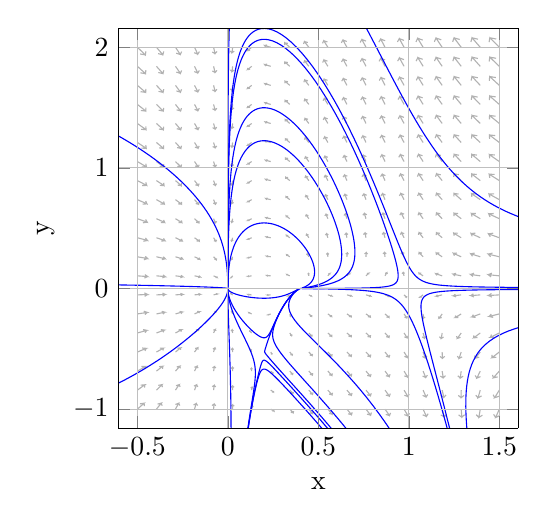
\begin{tikzpicture}

\begin{axis}[%
width=2in,
height=2in,
unbounded coords=jump,
view={0}{90},
scale only axis,
xmin=-0.605263157894737,
xmax=1.60526315789474,
xlabel={x},
xmajorgrids,
ymin=-1.15789473684211,
ymax=2.15789473684211,
ylabel={y},
ymajorgrids,
zmin=-1,
zmax=1
]
\addplot [color=white!70!black,solid,forget plot]
  table[row sep=crcr]{-0.5	-1\\
-0.462794067027861	-0.950392089370481\\
-0.486357824576882	-0.955972979316302\\
-0.462794067027861	-0.950392089370481\\
-0.461553869262123	-0.974575945802372\\
nan	0\\
-0.5	-0.842105263157895\\
-0.458903651429007	-0.797953790352607\\
-0.482270424201627	-0.800925145051445\\
-0.458903651429007	-0.797953790352607\\
-0.460194687798983	-0.821473319336942\\
nan	0\\
-0.5	-0.684210526315789\\
-0.454899309870645	-0.646471098253524\\
-0.477864373925018	-0.646517754139865\\
-0.454899309870645	-0.646471098253524\\
-0.458994659893885	-0.669068099204543\\
nan	0\\
-0.5	-0.526315789473684\\
-0.451017012851756	-0.496039329426204\\
-0.473281024008099	-0.492876520653387\\
-0.451017012851756	-0.496039329426204\\
-0.458142793984359	-0.517368014227509\\
nan	0\\
-0.5	-0.368421052631579\\
-0.447590843757503	-0.346611722220689\\
-0.468765923232975	-0.340052232283331\\
-0.447590843757503	-0.346611722220689\\
-0.45786125802753	-0.36625681040458\\
nan	0\\
-0.5	-0.210526315789474\\
-0.444975641753086	-0.197923599790181\\
-0.464633628226984	-0.18794832502824\\
-0.444975641753086	-0.197923599790181\\
-0.458332270227337	-0.215460504151697\\
nan	0\\
-0.5	-0.0526315789473685\\
-0.443408805718971	-0.0495062269949645\\
-0.461167501991381	-0.0362960340104284\\
-0.443408805718971	-0.0495062269949645\\
-0.459604826015179	-0.0645916311509429\\
nan	0\\
-0.5	0.105263157894737\\
-0.442904436178829	0.0991729644204785\\
-0.458510556956616	0.115273913418049\\
-0.442904436178829	0.0991729644204785\\
-0.461555653693745	0.0867261315074634\\
nan	0\\
-0.5	0.263157894736842\\
-0.443271213861528	0.248531688365965\\
-0.45663329811035	0.267101746811846\\
-0.443271213861528	0.248531688365965\\
-0.463946401295789	0.23873735374261\\
nan	0\\
-0.5	0.421052631578947\\
-0.444226679983219	0.398783070645331\\
-0.455391285754849	0.419407268929611\\
-0.444226679983219	0.398783070645331\\
-0.466526066221658	0.391520608921221\\
nan	0\\
-0.5	0.578947368421053\\
-0.445506989619522	0.549959722139209\\
-0.454607981163204	0.572279268618882\\
-0.445506989619522	0.549959722139209\\
-0.469101804304126	0.545032763428643\\
nan	0\\
-0.5	0.736842105263158\\
-0.446917591495257	0.701987324469424\\
-0.454128618848246	0.72571436083373\\
-0.446917591495257	0.701987324469424\\
-0.471556009245113	0.699173156581358\\
nan	0\\
-0.5	0.894736842105263\\
-0.44833560483932	0.854749440322363\\
-0.453838072941799	0.879661759647403\\
-0.44833560483932	0.854749440322363\\
-0.473831773833249	0.853829562067063\\
nan	0\\
-0.5	1.05263157894737\\
-0.449692493747639	1.00812572823438\\
-0.4536582829451	1.03405436001137\\
-0.449692493747639	1.00812572823438\\
-0.475911208301595	1.00890060688519\\
nan	0\\
-0.5	1.21052631578947\\
-0.450955085817027	1.16200876627513\\
-0.453539172693334	1.18882525967518\\
-0.450955085817027	1.16200876627513\\
-0.477797947450504	1.16430280258369\\
nan	0\\
-0.5	1.36842105263158\\
-0.452111165731261	1.31630883836007\\
-0.453449762444004	1.3439147112087\\
-0.452111165731261	1.31630883836007\\
-0.479505869579761	1.31997029407433\\
nan	0\\
-0.5	1.52631578947368\\
-0.453160072769805	1.47095331362082\\
-0.453371431975647	1.49927203818423\\
-0.453160072769805	1.47095331362082\\
-0.48105266990208	1.47585207456913\\
nan	0\\
-0.5	1.68421052631579\\
-0.454107036056096	1.62588414944524\\
-0.45329333102163	1.65485530349238\\
-0.454107036056096	1.62588414944524\\
-0.482456519456905	1.63190882152043\\
nan	0\\
-0.5	1.84210526315789\\
-0.45495993013346	1.78105509930007\\
-0.453209410128965	1.81063016592405\\
-0.45495993013346	1.78105509930007\\
-0.483734492057879	1.78811013099078\\
nan	0\\
-0.5	2\\
-0.455727491647339	1.93642921877567\\
-0.453116548847054	1.96656858023113\\
-0.455727491647339	1.93642921877567\\
-0.484901939459221	1.9444323260548\\
nan	0\\
-0.394736842105263	-1\\
-0.367847986338301	-0.949888545791711\\
-0.388442506620462	-0.958199768112457\\
-0.367847986338301	-0.949888545791711\\
-0.363386779516318	-0.971644195995938\\
nan	0\\
-0.394736842105263	-0.842105263157895\\
-0.364088981294229	-0.796668986971644\\
-0.384642408584102	-0.802637904624761\\
-0.364088981294229	-0.796668986971644\\
-0.361924270490976	-0.817961835030278\\
nan	0\\
-0.394736842105263	-0.684210526315789\\
-0.359924135750322	-0.644476029681418\\
-0.380301571815397	-0.647693202082994\\
-0.359924135750322	-0.644476029681418\\
-0.360434323498212	-0.665099555260465\\
nan	0\\
-0.394736842105263	-0.526315789473684\\
-0.355525110825069	-0.493604113507459\\
-0.375466549200684	-0.493614683477278\\
-0.355525110825069	-0.493604113507459\\
-0.359110711217571	-0.513220549117375\\
nan	0\\
-0.394736842105263	-0.368421052631579\\
-0.351295666894499	-0.344257187825007\\
-0.370368985659371	-0.340646053464287\\
-0.351295666894499	-0.344257187825007\\
-0.358287053256085	-0.362366641069669\\
nan	0\\
-0.394736842105263	-0.210526315789474\\
-0.347867573813421	-0.196303860029027\\
-0.365483968241085	-0.1888532796842\\
-0.347867573813421	-0.196303860029027\\
-0.358372740360862	-0.212287913830122\\
nan	0\\
-0.394736842105263	-0.0526315789473685\\
-0.345838371854821	-0.0490828396689572\\
-0.361395097749557	-0.0379228438898701\\
-0.345838371854821	-0.0490828396689572\\
-0.359620728110351	-0.0623720790150911\\
nan	0\\
-0.394736842105263	0.105263157894737\\
-0.345371248069937	0.0983955966980351\\
-0.358464035981359	0.112797263565877\\
-0.345371248069937	0.0983955966980351\\
-0.36189781657971	0.0881144665482139\\
nan	0\\
-0.394736842105263	0.263157894736842\\
-0.346119691311182	0.246923822999233\\
-0.356646318615004	0.263948332219036\\
-0.346119691311182	0.246923822999233\\
-0.364763354483808	0.239639756821995\\
nan	0\\
-0.394736842105263	0.421052631578947\\
-0.347547450768714	0.396808100321619\\
-0.355643135355347	0.415878807532955\\
-0.347547450768714	0.396808100321619\\
-0.367765400984011	0.39228411186468\\
nan	0\\
-0.394736842105263	0.578947368421053\\
-0.349223583667596	0.54798307834803\\
-0.355136488680641	0.568650679979354\\
-0.349223583667596	0.54798307834803\\
-0.370618633717152	0.54589405076052\\
nan	0\\
-0.394736842105263	0.736842105263158\\
-0.350896614505182	0.70023413745531\\
-0.354896690833244	0.722176584697685\\
-0.350896614505182	0.70023413745531\\
-0.373200674737168	0.700256470897644\\
nan	0\\
-0.394736842105263	0.894736842105263\\
-0.352449580427142	0.853334092174278\\
-0.354785071447832	0.876326732573103\\
-0.352449580427142	0.853334092174278\\
-0.375486446413325	0.855183101734043\\
nan	0\\
-0.394736842105263	1.05263157894737\\
-0.35384164327609	1.00709260296177\\
-0.354725458928442	1.03097809546474\\
-0.35384164327609	1.00709260296177\\
-0.377494946921242	1.01053049605016\\
nan	0\\
-0.394736842105263	1.21052631578947\\
-0.355068869234649	1.16136316803546\\
-0.354678474157331	1.18602910557932\\
-0.355068869234649	1.16136316803546\\
-0.379260048034335	1.16619511914401\\
nan	0\\
-0.394736842105263	1.36842105263158\\
-0.356142963699097	1.31603632316101\\
-0.354624944853305	1.34140021160372\\
-0.356142963699097	1.31603632316101\\
-0.380817309588589	1.32210327240064\\
nan	0\\
-0.394736842105263	1.52631578947368\\
-0.357080901022854	1.47103069242145\\
-0.354556409084518	1.49703020680772\\
-0.357080901022854	1.47103069242145\\
-0.382198957610636	1.47820223626652\\
nan	0\\
-0.394736842105263	1.68421052631579\\
-0.357900243198893	1.62628538818714\\
-0.354469938338642	1.65287207935233\\
-0.357900243198893	1.62628538818714\\
-0.383432507402966	1.63445377989914\\
nan	0\\
-0.394736842105263	1.84210526315789\\
-0.358617225808472	1.78175431251174\\
-0.354365373035971	1.80888950177979\\
-0.358617225808472	1.78175431251174\\
-0.384540848359047	1.79082969363139\\
nan	0\\
-0.394736842105263	2\\
-0.359246128928364	1.9374020737684\\
-0.354243861323534	1.9650541299321\\
-0.359246128928364	1.9374020737684\\
-0.385542824439334	1.94730877334366\\
nan	0\\
-0.289473684210526	-1\\
-0.272341044729943	-0.950820246219215\\
-0.289775775019314	-0.961291012483305\\
-0.272341044729943	-0.950820246219215\\
-0.265185898128922	-0.969857332223596\\
nan	0\\
-0.289473684210526	-0.842105263157895\\
-0.269178815969493	-0.796698080258658\\
-0.286619072166612	-0.80524651806817\\
-0.269178815969493	-0.796698080258658\\
-0.263915480716994	-0.815393952188687\\
nan	0\\
-0.289473684210526	-0.684210526315789\\
-0.265392666310422	-0.643466971180482\\
-0.28280286046428	-0.649669783246048\\
-0.265392666310422	-0.643466971180482\\
-0.262431082896627	-0.6617102921961\\
nan	0\\
-0.289473684210526	-0.526315789473684\\
-0.260935424965035	-0.491579800159742\\
-0.278180900067168	-0.494866032142551\\
-0.260935424965035	-0.491579800159742\\
-0.260812905410197	-0.509135161765297\\
nan	0\\
-0.289473684210526	-0.368421052631579\\
-0.256019799409099	-0.341651884990179\\
-0.272748256759877	-0.341319164082242\\
-0.256019799409099	-0.341651884990179\\
-0.259363672939177	-0.358046106482956\\
nan	0\\
-0.289473684210526	-0.210526315789474\\
-0.251457443354076	-0.194140494718726\\
-0.266958770878698	-0.189552180825837\\
-0.251457443354076	-0.194140494718726\\
-0.258765860343324	-0.208560301254063\\
nan	0\\
-0.289473684210526	-0.0526315789473685\\
-0.248621540073053	-0.0484683181188246\\
-0.261917998521431	-0.0395042603330195\\
-0.248621540073053	-0.0484683181188246\\
-0.259836368107159	-0.059930332401756\\
nan	0\\
-0.289473684210526	0.105263157894737\\
-0.24825965196162	0.0972950853552378\\
-0.258631843501417	0.109989015179314\\
-0.24825965196162	0.0972950853552378\\
-0.262615879771167	0.0893819990548609\\
nan	0\\
-0.289473684210526	0.263157894736842\\
-0.249674978582045	0.244863090474162\\
-0.257040889204919	0.260301208160087\\
-0.249674978582045	0.244863090474162\\
-0.266188291336259	0.240401855345846\\
nan	0\\
-0.289473684210526	0.421052631578947\\
-0.251747134748647	0.394599462437041\\
-0.256451807301734	0.411967050545083\\
-0.251747134748647	0.394599462437041\\
-0.269678391872688	0.393103775814143\\
nan	0\\
-0.289473684210526	0.578947368421053\\
-0.25381249533404	0.546097989693175\\
-0.256298507315017	0.56486810053066\\
-0.25381249533404	0.546097989693175\\
-0.272723196678955	0.547037506092417\\
nan	0\\
-0.289473684210526	0.736842105263158\\
-0.255633316418648	0.698861363770026\\
-0.256290241382928	0.718715678165935\\
-0.255633316418648	0.698861363770026\\
-0.275280612129494	0.701795494269996\\
nan	0\\
-0.289473684210526	0.894736842105263\\
-0.257169540469641	0.852512721930235\\
-0.25630475354815	0.873255993917965\\
-0.257169540469641	0.852512721930235\\
-0.277416813635664	0.857103922047523\\
nan	0\\
-0.289473684210526	1.05263157894737\\
-0.258447981204343	1.00679774875838\\
-0.256297234558951	1.02830432356662\\
-0.258447981204343	1.00679774875838\\
-0.279214149653445	1.01279147206353\\
nan	0\\
-0.289473684210526	1.21052631578947\\
-0.259510477896188	1.1615480383334\\
-0.256254870426471	1.18373232314881\\
-0.259510477896188	1.1615480383334\\
-0.280744009154508	1.16875071999164\\
nan	0\\
-0.289473684210526	1.36842105263158\\
-0.260396803540098	1.31665044033426\\
-0.256177214666896	1.33945084419106\\
-0.260396803540098	1.31665044033426\\
-0.282062520815556	1.32491240385585\\
nan	0\\
-0.289473684210526	1.52631578947368\\
-0.261140309623444	1.4720269513726\\
-0.256068112474297	1.4953969464497\\
-0.261140309623444	1.4720269513726\\
-0.28321253152484	1.48123025915615\\
nan	0\\
-0.289473684210526	1.68421052631579\\
-0.261767760614975	1.62762225884288\\
-0.255932470825413	1.65152521998364\\
-0.261767760614975	1.62762225884288\\
-0.284226604561867	1.63767225818587\\
nan	0\\
-0.289473684210526	1.84210526315789\\
-0.262300324310287	1.78339605371396\\
-0.255775029919375	1.8078021565222\\
-0.262300324310287	1.78339605371396\\
-0.285129634641343	1.79421547657208\\
nan	0\\
-0.289473684210526	2\\
-0.262754709966259	1.9393182115962\\
-0.255599955138588	1.9642024916784\\
-0.262754709966259	1.9393182115962\\
-0.28594084934049	1.95084300455627\\
nan	0\\
-0.184210526315789	-1\\
-0.175457976280789	-0.953409897273672\\
-0.189731266972871	-0.965198790582821\\
-0.175457976280789	-0.953409897273672\\
-0.166436215609707	-0.969575065600321\\
nan	0\\
-0.184210526315789	-0.842105263157895\\
-0.173303797674958	-0.798488175804228\\
-0.187480088105624	-0.80884661985012\\
-0.173303797674958	-0.798488175804228\\
-0.165671544428791	-0.814299984170536\\
nan	0\\
-0.184210526315789	-0.684210526315789\\
-0.170559860464155	-0.644173902189755\\
-0.184664216251154	-0.652772222964657\\
-0.170559860464155	-0.644173902189755\\
-0.164645904188136	-0.659597555890474\\
nan	0\\
-0.184210526315789	-0.526315789473684\\
-0.166966350735502	-0.490862505753308\\
-0.181002924339682	-0.497187446974349\\
-0.166966350735502	-0.490862505753308\\
-0.163276282479494	-0.505809534764493\\
nan	0\\
-0.184210526315789	-0.368421052631579\\
-0.162229102844122	-0.339363883839391\\
-0.176087822083669	-0.342585678609131\\
-0.162229102844122	-0.339363883839391\\
-0.161559237687575	-0.353576390344964\\
nan	0\\
-0.184210526315789	-0.210526315789474\\
-0.156529292981719	-0.191192229296235\\
-0.16966718460525	-0.190072146910689\\
-0.156529292981719	-0.191192229296235\\
-0.160000141358631	-0.203912763577724\\
nan	0\\
-0.184210526315789	-0.0526315789473685\\
-0.152114391514396	-0.0474198437678639\\
-0.16304616574969	-0.0409593306213668\\
-0.152114391514396	-0.0474198437678639\\
-0.160440298159938	-0.0570073980220637\\
nan	0\\
-0.184210526315789	0.105263157894737\\
-0.152054021181613	0.0955038903427328\\
-0.159261155833865	0.106470796891878\\
-0.152054021181613	0.0955038903427328\\
-0.164140789609867	0.09039254432479\\
nan	0\\
-0.184210526315789	0.263157894736842\\
-0.154710266284616	0.242150650140134\\
-0.158308533144791	0.25582788852694\\
-0.154710266284616	0.242150650140134\\
-0.168812155443145	0.241077758511353\\
nan	0\\
-0.184210526315789	0.421052631578947\\
-0.157487866121264	0.392368538854242\\
-0.158333640998445	0.407654431720285\\
-0.157487866121264	0.392368538854242\\
-0.172675687360798	0.394293101623022\\
nan	0\\
-0.184210526315789	0.578947368421053\\
-0.159688578717613	0.544735599268925\\
-0.158492220709034	0.561129616914107\\
-0.159688578717613	0.544735599268925\\
-0.175598105285098	0.548868643115019\\
nan	0\\
-0.184210526315789	0.736842105263158\\
-0.161347015616703	0.698351206352967\\
-0.158583344098881	0.715614353700796\\
-0.161347015616703	0.698351206352967\\
-0.177828793553976	0.704182598351253\\
nan	0\\
-0.184210526315789	0.894736842105263\\
-0.162601101278023	0.852740704958655\\
-0.158584894502701	0.870741902362079\\
-0.162601101278023	0.852740704958655\\
-0.179582963076005	0.859937189843196\\
nan	0\\
-0.184210526315789	1.05263157894737\\
-0.163564629977013	1.00764643102885\\
-0.158512111899017	1.0263034494891\\
-0.163564629977013	1.00764643102885\\
-0.181004685858276	1.01598050131971\\
nan	0\\
-0.184210526315789	1.21052631578947\\
-0.164317803023585	1.16291868880888\\
-0.158383713266097	1.18217415772611\\
-0.164317803023585	1.16291868880888\\
-0.182187526756396	1.17222779608\\
nan	0\\
-0.184210526315789	1.36842105263158\\
-0.164915765533056	1.31846447780366\\
-0.158215050060896	1.33827514044772\\
-0.164915765533056	1.31846447780366\\
-0.183193337474855	1.32862776005635\\
nan	0\\
-0.184210526315789	1.52631578947368\\
-0.165396784014482	1.47422257133573\\
-0.158017602170386	1.49455397235244\\
-0.165396784014482	1.47422257133573\\
-0.184064211239362	1.48514710120179\\
nan	0\\
-0.184210526315789	1.68421052631579\\
-0.165787920173155	1.63015066277405\\
-0.15779973613051	1.65097427337223\\
-0.165787920173155	1.63015066277405\\
-0.18482966790138	1.64176297030091\\
nan	0\\
-0.184210526315789	1.84210526315789\\
-0.166108718319349	1.78621832338925\\
-0.15756752577612	1.80750985731895\\
-0.166108718319349	1.78621832338925\\
-0.185510995660442	1.79845895332073\\
nan	0\\
-0.184210526315789	2\\
-0.166373584888497	1.94240292638166\\
-0.1573253989121	1.96414128382399\\
-0.166373584888497	1.94240292638166\\
-0.186123935721269	1.95522281311034\\
nan	0\\
-0.0789473684210527	-1\\
-0.0763519078836325	-0.957692058391941\\
-0.0877075314468733	-0.969735575740004\\
-0.0763519078836325	-0.957692058391941\\
-0.0665535606428438	-0.971033306008714\\
nan	0\\
-0.0789473684210527	-0.842105263157895\\
-0.0754056498773597	-0.802207224929626\\
-0.0864426749975347	-0.813291206762183\\
-0.0754056498773597	-0.802207224929626\\
-0.0664936558834004	-0.81506206603403\\
nan	0\\
-0.0789473684210527	-0.684210526315789\\
-0.074164117037595	-0.647087334461132\\
-0.0848798904162967	-0.657028479171665\\
-0.074164117037595	-0.647087334461132\\
-0.0663182944889679	-0.659420104863394\\
nan	0\\
-0.0789473684210527	-0.526315789473684\\
-0.0724272711391079	-0.49252838197121\\
-0.0828301521993099	-0.501034579901466\\
-0.0724272711391079	-0.49252838197121\\
-0.0659364484480728	-0.504294628542438\\
nan	0\\
-0.0789473684210527	-0.368421052631579\\
-0.0697596715937911	-0.338979491119877\\
-0.0798763710198951	-0.345515035366572\\
-0.0697596715937911	-0.338979491119877\\
-0.065155590264044	-0.350108883780203\\
nan	0\\
-0.0789473684210527	-0.210526315789474\\
-0.0651175804086584	-0.187846871061158\\
-0.0749363779944554	-0.191193257476554\\
-0.0651175804086584	-0.187846871061158\\
-0.0635966556302979	-0.198108151482752\\
nan	0\\
-0.0789473684210527	-0.0526315789473685\\
-0.0577887970362137	-0.0447773050981259\\
-0.066099936913976	-0.0418439444066889\\
-0.0577887970362137	-0.0447773050981259\\
-0.0621727999893547	-0.0524232300991084\\
nan	0\\
-0.0789473684210527	0.105263157894737\\
-0.058881303949289	0.0916526320561809\\
-0.0614984918311791	0.100752305925689\\
-0.058881303949289	0.0916526320561809\\
-0.0683037547504571	0.0907192736898067\\
nan	0\\
-0.0789473684210527	0.263157894736842\\
-0.0634395892642457	0.238952154039478\\
-0.0620404878369467	0.250090821037889\\
-0.0634395892642457	0.238952154039478\\
-0.0741433581856289	0.242336931459485\\
nan	0\\
-0.0789473684210527	0.421052631578947\\
-0.065984921317231	0.391064700250528\\
-0.0623766726162727	0.403301691425009\\
-0.065984921317231	0.391064700250528\\
-0.0773706382804823	0.396820467873099\\
nan	0\\
-0.0789473684210527	0.578947368421053\\
-0.0674517759292154	0.544888745075795\\
-0.0623857978404522	0.557980230202332\\
-0.0674517759292154	0.544888745075795\\
-0.0794151095130809	0.552232433956413\\
nan	0\\
-0.0789473684210527	0.736842105263158\\
-0.0683801486526937	0.699553659159829\\
-0.0622282030573692	0.713381997932917\\
-0.0683801486526937	0.699553659159829\\
-0.0808724261090336	0.708098388048738\\
nan	0\\
-0.0789473684210527	0.894736842105263\\
-0.0690096143155421	0.854724044426135\\
-0.0619877411274132	0.869212322256251\\
-0.0690096143155421	0.854724044426135\\
-0.0819941399669774	0.864243445203495\\
nan	0\\
-0.0789473684210527	1.05263157894737\\
-0.0694574637929203	1.01023670749823\\
-0.0617057173190751	1.02532764509\\
-0.0694574637929203	1.01023670749823\\
-0.082903153043645	1.02058269277594\\
nan	0\\
-0.0789473684210527	1.21052631578947\\
-0.0697871474388395	1.16599934623828\\
-0.0614034713457057	1.18164749234919\\
-0.0697871474388395	1.16599934623828\\
-0.0836669561213013	1.17706738185809\\
nan	0\\
-0.0789473684210527	1.36842105263158\\
-0.0700358368311151	1.32195419276845\\
-0.0610925813423137	1.33812213362487\\
-0.0700358368311151	1.32195419276845\\
-0.084326011273879	1.3336663678299\\
nan	0\\
-0.0789473684210527	1.52631578947368\\
-0.0702267135078294	1.47806240774267\\
-0.060779564549043	1.49471858599028\\
-0.0702267135078294	1.47806240774267\\
-0.0849062554145498	1.49035825853367\\
nan	0\\
-0.0789473684210527	1.68421052631579\\
-0.0703749710777165	1.6342964581057\\
-0.0604681732281961	1.65141377790456\\
-0.0703749710777165	1.6342964581057\\
-0.0854252073332386	1.6471275792329\\
nan	0\\
-0.0789473684210527	1.84210526315789\\
-0.0704909764931552	1.79063601763724\\
-0.06016058269136	1.80819088927541\\
-0.0704909764931552	1.79063601763724\\
-0.0858952054516888	1.80396269331146\\
nan	0\\
-0.0789473684210527	2\\
-0.0705820416034266	1.94706559245884\\
-0.0598580377634244	1.96503724642559\\
-0.0705820416034266	1.94706559245884\\
-0.0863252415340044	1.96085458301678\\
nan	0\\
0.0263157894736842	-1\\
0.0259658566979886	-0.963828640721377\\
0.0170279967110416	-0.974767531698888\\
0.0259658566979886	-0.963828640721377\\
0.035113676350353	-0.97459256531104\\
nan	0\\
0.0263157894736842	-0.842105263157895\\
0.0256323334470106	-0.807951186646864\\
0.0172988511272549	-0.818368273606841\\
0.0256323334470106	-0.807951186646864\\
0.0343758893827704	-0.818026545593505\\
nan	0\\
0.0263157894736842	-0.684210526315789\\
0.0251968726557147	-0.652349247771617\\
0.0175672280650623	-0.662187360539361\\
0.0251968726557147	-0.652349247771617\\
0.0334978673371487	-0.661627902130376\\
nan	0\\
0.0263157894736842	-0.526315789473684\\
0.0245862282406365	-0.497144709631831\\
0.0178123266500874	-0.506328423892649\\
0.0245862282406365	-0.497144709631831\\
0.0323978665710142	-0.505463643276125\\
nan	0\\
0.0263157894736842	-0.368421052631579\\
0.0236239330354876	-0.342582763058599\\
0.0179719175737016	-0.351007214040042\\
0.0236239330354876	-0.342582763058599\\
0.0308910623601915	-0.349661285820944\\
nan	0\\
0.0263157894736842	-0.210526315789474\\
0.0217295107001218	-0.189333525067973\\
0.0178071966518154	-0.196837931977814\\
0.0217295107001218	-0.189333525067973\\
0.0284035920125657	-0.194544792591033\\
nan	0\\
0.0263157894736842	-0.0526315789473685\\
0.0155422056286892	-0.0418794308044128\\
0.0160862437464488	-0.0477984712085483\\
0.0155422056286892	-0.0418794308044128\\
0.0214623178179266	-0.0424116792860508\\
nan	0\\
0.0263157894736842	0.105263157894737\\
0.0174627241692175	0.0897090508659435\\
0.0240071705177558	0.0921620166484648\\
0.0174627241692175	0.0897090508659435\\
0.0162301170033592	0.0965885493006981\\
nan	0\\
0.0263157894736842	0.263157894736842\\
0.0205288863286926	0.24045918799984\\
0.0279396339564405	0.245822074234693\\
0.0205288863286926	0.24045918799984\\
0.0165902805879396	0.248715525807189\\
nan	0\\
0.0263157894736842	0.421052631578947\\
0.0215822614285171	0.394216376507392\\
0.0297113836099559	0.401083871017567\\
0.0215822614285171	0.394216376507392\\
0.0162932560741785	0.403450635040151\\
nan	0\\
0.0263157894736842	0.578947368421053\\
0.0221022741802764	0.548995691040343\\
0.0308542481134761	0.556927815431204\\
0.0221022741802764	0.548995691040343\\
0.0158784094231214	0.559034573077908\\
nan	0\\
0.0263157894736842	0.736842105263158\\
0.0224050733955021	0.704326580059007\\
0.0317071695199944	0.713103558600707\\
0.0224050733955021	0.704326580059007\\
0.0154494069179191	0.715058916639798\\
nan	0\\
0.0263157894736842	0.894736842105263\\
0.0225979466016593	0.860013085546303\\
0.0323942386030068	0.869500751795985\\
0.0225979466016593	0.860013085546303\\
0.0150323603235268	0.871359673231997\\
nan	0\\
0.0263157894736842	1.05263157894737\\
0.0227275324451275	1.01595194321221\\
0.0329739184874832	1.02605876967562\\
0.0227275324451275	1.01595194321221\\
0.0146341006199057	1.0278528981899\\
nan	0\\
0.0263157894736842	1.21052631578947\\
0.0228174342162991	1.17208106437644\\
0.0334782536467724	1.18274005098601\\
0.0228174342162991	1.17208106437644\\
0.0142556279402568	1.1844892286147\\
nan	0\\
0.0263157894736842	1.36842105263158\\
0.0228808963928679	1.32835979203171\\
0.0339266794670801	1.33951944694147\\
0.0228808963928679	1.32835979203171\\
0.0138960491671455	1.34123689348187\\
nan	0\\
0.0263157894736842	1.52631578947368\\
0.0229259284959967	1.48475985341618\\
0.0343318708036788	1.49637916898901\\
0.0229259284959967	1.48475985341618\\
0.013553902774927	1.49807409947785\\
nan	0\\
0.0263157894736842	1.68421052631579\\
0.0229576574495631	1.64126068667788\\
0.034702556966276	1.65330610556322\\
0.0229576574495631	1.64126068667788\\
0.0132276371473229	1.65498517157529\\
nan	0\\
0.0263157894736842	1.84210526315789\\
0.0229795147779103	1.79784680875333\\
0.0350450107877845	1.81029027640075\\
0.0229795147779103	1.79784680875333\\
0.0129157835855004	1.81195841374864\\
nan	0\\
0.0263157894736842	2\\
0.0229938813645248	1.95450623215472\\
0.0353638957585933	1.96732388548101\\
0.0229938813645248	1.95450623215472\\
0.0126170118359519	1.96898483953559\\
nan	0\\
0.131578947368421	-1\\
0.134971696703002	-0.973627871424943\\
0.127360839758864	-0.980691322663815\\
0.134971696703002	-0.973627871424943\\
0.140546904046392	-0.982387697331106\\
nan	0\\
0.131578947368421	-0.842105263157895\\
0.13269495762937	-0.8170813054202\\
0.126104165116661	-0.824309490176271\\
0.13269495762937	-0.8170813054202\\
0.138616143985509	-0.824867495306745\\
nan	0\\
0.131578947368421	-0.684210526315789\\
0.129754350587146	-0.660891997899177\\
0.124472097517375	-0.66834370561948\\
0.129754350587146	-0.660891997899177\\
0.136131361725682	-0.667431407228842\\
nan	0\\
0.131578947368421	-0.526315789473684\\
0.12583675301468	-0.50541970099672\\
0.122335389201561	-0.513124076128245\\
0.12583675301468	-0.50541970099672\\
0.132783433440044	-0.510252978951374\\
nan	0\\
0.131578947368421	-0.368421052631579\\
0.120730867119136	-0.351466177376425\\
0.119746572380133	-0.359264660015293\\
0.120730867119136	-0.351466177376425\\
0.12822401000771	-0.35384061989065\\
nan	0\\
0.131578947368421	-0.210526315789474\\
0.115309419593618	-0.200045928867547\\
0.117570181195577	-0.207257426887826\\
0.115309419593618	-0.200045928867547\\
0.122810374656541	-0.199122663000424\\
nan	0\\
0.131578947368421	-0.0526315789473685\\
0.111857555318541	-0.0501478650728903\\
0.117153044464886	-0.0558233272477037\\
0.111857555318541	-0.0501478650728903\\
0.118394901402125	-0.0459626312227638\\
nan	0\\
0.131578947368421	0.105263157894737\\
0.110700457329991	0.100945429342572\\
0.118043436479562	0.0970211253986138\\
0.110700457329991	0.100945429342572\\
0.115884572203479	0.107460370417829\\
nan	0\\
0.131578947368421	0.263157894736842\\
0.110486228697269	0.253908180557038\\
0.119126472843566	0.251409915143191\\
0.110486228697269	0.253908180557038\\
0.114501615753664	0.261956274478767\\
nan	0\\
0.131578947368421	0.421052631578947\\
0.110474929534283	0.408196665724533\\
0.120020126348128	0.406777451022323\\
0.110474929534283	0.408196665724533\\
0.113592143420921	0.417329459939392\\
nan	0\\
0.131578947368421	0.578947368421053\\
0.110456412314418	0.563315110268727\\
0.1207012373687	0.562724153950924\\
0.110456412314418	0.563315110268727\\
0.112885108292537	0.573285421477925\\
nan	0\\
0.131578947368421	0.736842105263158\\
0.110390182636441	0.718965740897635\\
0.121215903147416	0.719031459024297\\
0.110390182636441	0.718965740897635\\
0.112277720964654	0.729625841390287\\
nan	0\\
0.131578947368421	0.894736842105263\\
0.110278055787478	0.874976014986041\\
0.121608530041566	0.875579040226572\\
0.110278055787478	0.874976014986041\\
0.111728116481955	0.886229486017043\\
nan	0\\
0.131578947368421	1.05263157894737\\
0.110129907993343	1.03124207513452\\
0.121911995759078	1.03229666643461\\
0.110129907993343	1.03124207513452\\
0.111217243852655	1.04302118612215\\
nan	0\\
0.131578947368421	1.21052631578947\\
0.109955284246392	1.18769815686799\\
0.122149422913372	1.18914068876393\\
0.109955284246392	1.18769815686799\\
0.110735343452629	1.19995252032494\\
nan	0\\
0.131578947368421	1.36842105263158\\
0.10976177464997	1.34430056488501\\
0.122337048402148	1.34608241802937\\
0.10976177464997	1.34430056488501\\
0.110276804528863	1.35699100438859\\
nan	0\\
0.131578947368421	1.52631578947368\\
0.109555076184453	1.50101901829056\\
0.122486430335425	1.5031020818495\\
0.109555076184453	1.50101901829056\\
0.109838044743862	1.51411401744149\\
nan	0\\
0.131578947368421	1.68421052631579\\
0.109339387069091	1.65783176291592\\
0.122605946008858	1.66018550186105\\
0.109339387069091	1.65783176291592\\
0.109416564308922	1.67130528201071\\
nan	0\\
0.131578947368421	1.84210526315789\\
0.109117788925764	1.81472268396004\\
0.122701781258024	1.81732216810873\\
0.109117788925764	1.81472268396004\\
0.109010491659098	1.82855274733006\\
nan	0\\
0.131578947368421	2\\
0.108892547462952	1.97167952791186\\
0.122778585456629	1.97450406956193\\
0.108892547462952	1.97167952791186\\
0.108618349412557	1.98584726951467\\
nan	0\\
0.236842105263158	-1\\
0.255352528129521	-1.01640825697915\\
0.253901465514399	-1.00685817416881\\
0.255352528129521	-1.01640825697915\\
0.245697337024826	-1.01611338560199\\
nan	0\\
0.236842105263158	-0.842105263157895\\
0.252772183537879	-0.858393170217886\\
0.25206513682046	-0.849524278531208\\
0.252772183537879	-0.858393170217886\\
0.243921183290465	-0.857489317668569\\
nan	0\\
0.236842105263158	-0.684210526315789\\
0.249236104566076	-0.70054688979568\\
0.249601995645173	-0.692547480925983\\
0.249236104566076	-0.70054688979568\\
0.241433813905228	-0.698744480577442\\
nan	0\\
0.236842105263158	-0.526315789473684\\
0.243588561464404	-0.542863114042901\\
0.245701455746334	-0.536212302621824\\
0.243588561464404	-0.542863114042901\\
0.237427793461726	-0.539585530722447\\
nan	0\\
0.236842105263158	-0.368421052631579\\
0.233139301449788	-0.383590735140919\\
0.238042563221134	-0.37996553134146\\
0.233139301449788	-0.383590735140919\\
0.230457721966464	-0.378114129434775\\
nan	0\\
0.236842105263158	-0.210526315789474\\
0.222289300086186	-0.218293651986262\\
0.228596975688475	-0.219601652421469\\
0.222289300086186	-0.218293651986262\\
0.22471330759008	-0.212325249832983\\
nan	0\\
0.236842105263158	-0.0526315789473685\\
0.2177331536617	-0.0540704978789998\\
0.223825568875045	-0.0584160600998749\\
0.2177331536617	-0.0540704978789998\\
0.223106109409229	-0.0488615842991459\\
nan	0\\
0.236842105263158	0.105263157894737\\
0.215323083849228	0.107520501755963\\
0.2212144543081	0.101463543244113\\
0.215323083849228	0.107520501755963\\
0.222343126238713	0.112223053951078\\
nan	0\\
0.236842105263158	0.263157894736842\\
0.213559677447559	0.267842204394923\\
0.219373328377718	0.260616304543599\\
0.213559677447559	0.267842204394923\\
0.221715483206759	0.272257518451399\\
nan	0\\
0.236842105263158	0.421052631578947\\
0.212095080766192	0.42751458238937\\
0.217903700412676	0.419389241022002\\
0.212095080766192	0.42751458238937\\
0.221134675817888	0.431762753270485\\
nan	0\\
0.236842105263158	0.578947368421053\\
0.210811900000606	0.58680868654029\\
0.216655632049562	0.577942739788881\\
0.210811900000606	0.58680868654029\\
0.220586291109181	0.590957842420157\\
nan	0\\
0.236842105263158	0.736842105263158\\
0.209656060536318	0.745859324640824\\
0.215557569109953	0.736357647645814\\
0.209656060536318	0.745859324640824\\
0.220066178798787	0.749950670009234\\
nan	0\\
0.236842105263158	0.894736842105263\\
0.208597111968248	0.904741452584218\\
0.214569457336982	0.894678821116804\\
0.208597111968248	0.904741452584218\\
0.21957176257646	0.908801317764259\\
nan	0\\
0.236842105263158	1.05263157894737\\
0.207615594517764	1.06350047812359\\
0.213666322947326	1.05293318068438\\
0.207615594517764	1.06350047812359\\
0.219100772535439	1.06754643605707\\
nan	0\\
0.236842105263158	1.21052631578947\\
0.206698010100631	1.22216578527127\\
0.212831371278939	1.2111379206361\\
0.206698010100631	1.22216578527127\\
0.218651106019838	1.22620996821736\\
nan	0\\
0.236842105263158	1.36842105263158\\
0.205834459929125	1.38075739888695\\
0.212052666965493	1.36930458367683\\
0.205834459929125	1.38075739888695\\
0.218220840093177	1.38480840634384\\
nan	0\\
0.236842105263158	1.52631578947368\\
0.205017390165378	1.53928954306144\\
0.211321366297773	1.52744123821067\\
0.205017390165378	1.53928954306144\\
0.21780824309165	1.54335359575956\\
nan	0\\
0.236842105263158	1.68421052631579\\
0.204240862249739	1.69777266890212\\
0.210630699507182	1.68555371537287\\
0.204240862249739	1.69777266890212\\
0.217411770800348	1.70185433687958\\
nan	0\\
0.236842105263158	1.84210526315789\\
0.203500098096368	1.85621467370415\\
0.209975347609842	1.84364634874857\\
0.203500098096368	1.85621467370415\\
0.217030052882968	1.86031735233197\\
nan	0\\
0.236842105263158	2\\
0.202791181113581	2.01462166746549\\
0.209351041492082	2.00172243618845\\
0.202791181113581	2.01462166746549\\
0.216661875224827	2.01874789826324\\
nan	0\\
0.342105263157895	-1\\
0.361185112111124	-1.03026014526252\\
0.363026193740784	-1.01641213944546\\
0.361185112111124	-1.03026014526252\\
0.347896121109525	-1.02595206392207\\
nan	0\\
0.342105263157895	-0.842105263157895\\
0.359721894785199	-0.870827975060743\\
0.36161758327272	-0.857807003583062\\
0.359721894785199	-0.870827975060743\\
0.347256227321296	-0.866615319396715\\
nan	0\\
0.342105263157895	-0.684210526315789\\
0.357987360641591	-0.711211407870508\\
0.359972951785162	-0.699140619033169\\
0.357987360641591	-0.711211407870508\\
0.346472511007803	-0.707081667775017\\
nan	0\\
0.342105263157895	-0.526315789473684\\
0.355819680184984	-0.551342008895283\\
0.357961909932257	-0.540405538812031\\
0.355819680184984	-0.551342008895283\\
0.345448800221458	-0.547262747325576\\
nan	0\\
0.342105263157895	-0.368421052631579\\
0.352837248461275	-0.391094127627573\\
0.35528592161926	-0.381609208802929\\
0.352837248461275	-0.391094127627573\\
0.343949384121263	-0.38697520145462\\
nan	0\\
0.342105263157895	-0.210526315789474\\
0.34772498885155	-0.230129676815195\\
0.350939911399884	-0.222843737084065\\
0.34772498885155	-0.230129676815195\\
0.341138230887023	-0.225653599930892\\
nan	0\\
0.342105263157895	-0.0526315789473685\\
0.331909179886826	-0.0626279300568917\\
0.337467092645528	-0.0621780455418018\\
0.331909179886826	-0.0626279300568917\\
0.332468917090766	-0.0570800039062677\\
nan	0\\
0.342105263157895	0.105263157894737\\
0.325402922526531	0.115745862582169\\
0.327792948544082	0.108425466018098\\
0.325402922526531	0.115745862582169\\
0.333034300887798	0.11677663633378\\
nan	0\\
0.342105263157895	0.263157894736842\\
0.324110129367051	0.279965366079041\\
0.325306801668754	0.27042434122867\\
0.324110129367051	0.279965366079041\\
0.333710537339854	0.279421908124092\\
nan	0\\
0.342105263157895	0.421052631578947\\
0.322804641375003	0.441585261167954\\
0.323461670512619	0.430600316845529\\
0.322804641375003	0.441585261167954\\
0.333727985307122	0.440250627736975\\
nan	0\\
0.342105263157895	0.578947368421053\\
0.321599078681201	0.602233860145554\\
0.321929311093084	0.59012136650903\\
0.321599078681201	0.602233860145554\\
0.333572556955335	0.600374458747377\\
nan	0\\
0.342105263157895	0.736842105263158\\
0.320498580440812	0.762361851227733\\
0.320600648764793	0.74930425675909\\
0.320498580440812	0.762361851227733\\
0.33336052174708	0.760107598117631\\
nan	0\\
0.342105263157895	0.894736842105263\\
0.319489550830536	0.922159641258087\\
0.319418564740537	0.9082788734304\\
0.319489550830536	0.922159641258087\\
0.333129964316949	0.919586729594079\\
nan	0\\
0.342105263157895	1.05263157894737\\
0.318557678211601	1.0817266530463\\
0.318348185170757	1.06711123458004\\
0.318557678211601	1.0817266530463\\
0.332895722220221	1.07888502705319\\
nan	0\\
0.342105263157895	1.21052631578947\\
0.317690920389421	1.24112187409384\\
0.31736633364387	1.22583962091041\\
0.317690920389421	1.24112187409384\\
0.332664112796056	1.23804679229465\\
nan	0\\
0.342105263157895	1.36842105263158\\
0.316879595543664	1.40038342987419\\
0.316456701517282	1.38448829979785\\
0.316879595543664	1.40038342987419\\
0.332437890138585	1.39710113360496\\
nan	0\\
0.342105263157895	1.52631578947368\\
0.316115961119858	1.55953752353335\\
0.315607318216354	1.54307367780594\\
0.316115961119858	1.55953752353335\\
0.332218185246185	1.55606832882496\\
nan	0\\
0.342105263157895	1.68421052631579\\
0.315393783180788	1.71860301678064\\
0.314809104557708	1.70160739964691\\
0.315393783180788	1.71860301678064\\
0.332005349790132	1.71496313963546\\
nan	0\\
0.342105263157895	1.84210526315789\\
0.314707989095755	1.87759398573239\\
0.314054990670773	1.86009805044451\\
0.314707989095755	1.87759398573239\\
0.331799351958021	1.87379668747558\\
nan	0\\
0.342105263157895	2\\
0.314054403882924	2.0365212436397\\
0.313339350755491	2.01855215572905\\
0.314054403882924	2.0365212436397\\
0.33159997257534	2.03257758536653\\
nan	0\\
0.447368421052632	-1\\
0.46910145651216	-1.03684220433539\\
0.471792096958148	-1.02035628416989\\
0.46910145651216	-1.03684220433539\\
0.453370994790454	-1.03122280189965\\
nan	0\\
0.447368421052632	-0.842105263157895\\
0.468146254377477	-0.876806023807249\\
0.470588094542362	-0.861201337281231\\
0.468146254377477	-0.876806023807249\\
0.453237714217685	-0.871590253943654\\
nan	0\\
0.447368421052632	-0.684210526315789\\
0.467101133961581	-0.716466951022376\\
0.469245426265543	-0.701856845383162\\
0.467101133961581	-0.716466951022376\\
0.45311721391225	-0.711723201837637\\
nan	0\\
0.447368421052632	-0.526315789473684\\
0.465946554338127	-0.55568820221028\\
0.467716217536627	-0.542231945067927\\
0.465946554338127	-0.55568820221028\\
0.45303001116833	-0.551521011710675\\
nan	0\\
0.447368421052632	-0.368421052631579\\
0.464664884104948	-0.394196174042874\\
0.465919725542077	-0.382139521856407\\
0.464664884104948	-0.394196174042874\\
0.453032164836429	-0.390787753382565\\
nan	0\\
0.447368421052632	-0.210526315789474\\
0.463290854044858	-0.23127412450748\\
0.463701076326692	-0.221069173644021\\
0.463290854044858	-0.23127412450748\\
0.453327171967689	-0.229030390140135\\
nan	0\\
0.447368421052632	-0.0526315789473685\\
0.462485744081521	-0.0631148012069674\\
0.460571352737754	-0.0561905037718653\\
0.462485744081521	-0.0631148012069674\\
0.455329741607955	-0.0637491652863101\\
nan	0\\
0.447368421052632	0.105263157894737\\
0.44559015908646	0.124424399955567\\
0.441333327161104	0.118231461845775\\
0.44559015908646	0.124424399955567\\
0.450913948191519	0.119120592828861\\
nan	0\\
0.447368421052632	0.263157894736842\\
0.438291948118438	0.288185809914346\\
0.43475791120432	0.278408317127547\\
0.438291948118438	0.288185809914346\\
0.447271868793072	0.282946553594643\\
nan	0\\
0.447368421052632	0.421052631578947\\
0.434970044594701	0.449878276820328\\
0.431483146221735	0.438130989133431\\
0.434970044594701	0.449878276820328\\
0.445895968842426	0.444330177362396\\
nan	0\\
0.447368421052632	0.578947368421053\\
0.432710418067846	0.610758594782731\\
0.429155012372862	0.597550726128031\\
0.432710418067846	0.610758594782731\\
0.445060625553701	0.604879727620424\\
nan	0\\
0.447368421052632	0.736842105263158\\
0.43095330343854	0.771161566847901\\
0.427297973326582	0.756761948968955\\
0.43095330343854	0.771161566847901\\
0.444457704118953	0.764969507776001\\
nan	0\\
0.447368421052632	0.894736842105263\\
0.429493729087869	0.931242502310026\\
0.425729721626107	0.915822131257407\\
0.429493729087869	0.931242502310026\\
0.443982551728489	0.924759477239788\\
nan	0\\
0.447368421052632	1.05263157894737\\
0.428233058482766	1.09108855990191\\
0.42435942201509	1.07476762497308\\
0.428233058482766	1.09108855990191\\
0.443587912492362	1.08433530625802\\
nan	0\\
0.447368421052632	1.21052631578947\\
0.427115869480899	1.25075427514556\\
0.423134645113396	1.2336227494458\\
0.427115869480899	1.25075427514556\\
0.443248624791441	1.24374902523167\\
nan	0\\
0.447368421052632	1.36842105263158\\
0.42610772543241	1.41027634301083\\
0.422022111523664	1.392404581992\\
0.42610772543241	1.41027634301083\\
0.44294975671329	1.40303492980211\\
nan	0\\
0.447368421052632	1.52631578947368\\
0.425185660316504	1.56968078634349\\
0.420999239319892	1.55112559709851\\
0.425185660316504	1.56968078634349\\
0.442681737754793	1.56221697746658\\
nan	0\\
0.447368421052632	1.68421052631579\\
0.424333532201063	1.72898681213947\\
0.420049927400615	1.70979520417947\\
0.424333532201063	1.72898681213947\\
0.442438070312453	1.72131264860526\\
nan	0\\
0.447368421052632	1.84210526315789\\
0.423539526332358	1.88820905036449\\
0.419162247946791	1.86842069052244\\
0.423539526332358	1.88820905036449\\
0.442214141550089	1.88033513788258\\
nan	0\\
0.447368421052632	2\\
0.422794711987959	2.04735893248147\\
0.418327091586994	2.02700782547086\\
0.422794711987959	2.04735893248147\\
0.442006557827728	2.0392946800032\\
nan	0\\
0.552631578947368	-1\\
0.576651523797469	-1.04161753656687\\
0.579849924484157	-1.02312728938429\\
0.576651523797469	-1.04161753656687\\
0.559041156200721	-1.03513726180934\\
nan	0\\
0.552631578947368	-0.842105263157895\\
0.57596610734345	-0.881176942412381\\
0.578733668638247	-0.863621806537015\\
0.57596610734345	-0.881176942412381\\
0.559197829011004	-0.875289070735056\\
nan	0\\
0.552631578947368	-0.684210526315789\\
0.575276889744894	-0.720353479746844\\
0.5775190348634	-0.703849266018147\\
0.575276889744894	-0.720353479746844\\
0.559447558147873	-0.715171921416909\\
nan	0\\
0.552631578947368	-0.526315789473684\\
0.574617953474402	-0.558962282662282\\
0.576183664413441	-0.543671741073944\\
0.574617953474402	-0.558962282662282\\
0.559860417819143	-0.554664928337461\\
nan	0\\
0.552631578947368	-0.368421052631579\\
0.574081345593044	-0.396621985179935\\
0.574696648736431	-0.382799263754009\\
0.574081345593044	-0.396621985179935\\
0.560596182462253	-0.393524147076847\\
nan	0\\
0.552631578947368	-0.210526315789474\\
0.573944739121866	-0.23230896652128\\
0.572996453752469	-0.220445881258114\\
0.573944739121866	-0.23230896652128\\
0.562105128386565	-0.231102461345363\\
nan	0\\
0.552631578947368	-0.0526315789473685\\
0.574816330311088	-0.0614936448408383\\
0.570376421375339	-0.0532888372318675\\
0.574816330311088	-0.0614936448408383\\
0.565945388428605	-0.0643812129137272\\
nan	0\\
0.552631578947368	0.105263157894737\\
0.563463666317429	0.125085975105284\\
0.555258335803774	0.121847151784635\\
0.563463666317429	0.125085975105284\\
0.565169744409048	0.116431108099605\\
nan	0\\
0.552631578947368	0.263157894736842\\
0.550769893413687	0.292470519157077\\
0.544000242968733	0.283211310447586\\
0.550769893413687	0.292470519157077\\
0.55865655517885	0.284142153214427\\
nan	0\\
0.552631578947368	0.421052631578947\\
0.545328078863383	0.454865039741378\\
0.539066026847971	0.442895442271652\\
0.545328078863383	0.454865039741378\\
0.555972230929186	0.446547192313645\\
nan	0\\
0.552631578947368	0.578947368421053\\
0.542020197962289	0.61613932585402\\
0.535905622899571	0.60232889337786\\
0.542020197962289	0.61613932585402\\
0.554501601616055	0.6076345838704\\
nan	0\\
0.552631578947368	0.736842105263158\\
0.539631701599757	0.776851398375299\\
0.533529341526005	0.761598641104754\\
0.539631701599757	0.776851398375299\\
0.553533988082076	0.768098579778559\\
nan	0\\
0.552631578947368	0.894736842105263\\
0.537745905905052	0.93720062201085\\
0.53159566284135	0.920740069778595\\
0.537745905905052	0.93720062201085\\
0.552827552794144	0.928182906299753\\
nan	0\\
0.552631578947368	1.05263157894737\\
0.536175832806685	1.09728884403563\\
0.529948240376824	1.07977772797398\\
0.536175832806685	1.09728884403563\\
0.552276872920955	1.08800560104432\\
nan	0\\
0.552631578947368	1.21052631578947\\
0.534822518254126	1.25717745878417\\
0.528502450713426	1.23872985071245\\
0.534822518254126	1.25717745878417\\
0.551828022210772	1.24763438105907\\
nan	0\\
0.552631578947368	1.36842105263158\\
0.53362747563034	1.4169071339626\\
0.527207186292694	1.39761028373404\\
0.53362747563034	1.4169071339626\\
0.551450226958204	1.40711233539255\\
nan	0\\
0.552631578947368	1.52631578947368\\
0.532553314022285	1.5765065233954\\
0.526029110019382	1.55642973698761\\
0.532553314022285	1.5765065233954\\
0.551124476980238	1.56646886945015\\
nan	0\\
0.552631578947368	1.68421052631579\\
0.531574683250668	1.73599672829908\\
0.524945201463855	1.71519664377992\\
0.531574683250668	1.73599672829908\\
0.550838302455502	1.72572509162827\\
nan	0\\
0.552631578947368	1.84210526315789\\
0.530673596660738	1.89539381801612\\
0.523938852632172	1.87391775598699\\
0.530673596660738	1.89539381801612\\
0.550583130061283	1.88489674713031\\
nan	0\\
0.552631578947368	2\\
0.529836821424458	2.05471035862084\\
0.522997659026122	2.03259856165386\\
0.529836821424458	2.05471035862084\\
0.55035283833654	2.04399594041531\\
nan	0\\
0.657894736842105	-1\\
0.683361513910656	-1.04565594391107\\
0.687135466767858	-1.02559246647061\\
0.683361513910656	-1.04565594391107\\
0.664307494812325	-1.03832585500488\\
nan	0\\
0.657894736842105	-0.842105263157895\\
0.682798140494092	-0.884926569604883\\
0.686032446010243	-0.86585432675779\\
0.682798140494092	-0.884926569604883\\
0.664621792786749	-0.878306028583783\\
nan	0\\
0.657894736842105	-0.684210526315789\\
0.682270765272093	-0.723762501770779\\
0.684845950606844	-0.705802902026785\\
0.682270765272093	-0.723762501770779\\
0.66506996287935	-0.717990916241779\\
nan	0\\
0.657894736842105	-0.526315789473684\\
0.681836619753638	-0.561949718525132\\
0.68356253714304	-0.545274069081815\\
0.681836619753638	-0.561949718525132\\
0.665745572617317	-0.557245010537581\\
nan	0\\
0.657894736842105	-0.368421052631579\\
0.681630941592153	-0.39904423035008\\
0.682165874596764	-0.383923225847018\\
0.681630941592153	-0.39904423035008\\
0.666854285737514	-0.395791328222042\\
nan	0\\
0.657894736842105	-0.210526315789474\\
0.68200342003665	-0.233861227157427\\
0.680604542920275	-0.220833582948405\\
0.68200342003665	-0.233861227157427\\
0.668937087236299	-0.232887924545677\\
nan	0\\
0.657894736842105	-0.0526315789473685\\
0.683399391728418	-0.0616135644657864\\
0.677993491642128	-0.052542805088683\\
0.683399391728418	-0.0616135644657864\\
0.673502498882919	-0.0652951325318391\\
nan	0\\
0.657894736842105	0.105263157894737\\
0.673499589287107	0.12544492500796\\
0.663772691775301	0.123291607985244\\
0.673499589287107	0.12544492500796\\
0.673863575331913	0.115489181762742\\
nan	0\\
0.657894736842105	0.263157894736842\\
0.659515774528544	0.295152823640531\\
0.65103073099669	0.285959604391034\\
0.659515774528544	0.295152823640531\\
0.667028195448535	0.285149085547815\\
nan	0\\
0.657894736842105	0.421052631578947\\
0.653053937277664	0.458297567398684\\
0.645194943192062	0.445913886761653\\
0.653053937277664	0.458297567398684\\
0.66381741110193	0.448334286543873\\
nan	0\\
0.657894736842105	0.578947368421053\\
0.649190638636792	0.61998895485015\\
0.641541471491112	0.605500454370093\\
0.649190638636792	0.61998895485015\\
0.662062264705661	0.609852503472749\\
nan	0\\
0.657894736842105	0.736842105263158\\
0.646455326170339	0.78100992036489\\
0.638845195596436	0.764899723166429\\
0.646455326170339	0.78100992036489\\
0.660929103147302	0.770619428502312\\
nan	0\\
0.657894736842105	0.894736842105263\\
0.644330125536413	0.941615137853304\\
0.63667993499111	0.924160496302469\\
0.644330125536413	0.941615137853304\\
0.660119082865131	0.930942801955315\\
nan	0\\
0.657894736842105	1.05263157894737\\
0.642583145253797	1.10192688927331\\
0.634852795148804	1.08331039827845\\
0.642583145253797	1.10192688927331\\
0.659500450311774	1.0909661940726\\
nan	0\\
0.657894736842105	1.21052631578947\\
0.641092652141152	1.26201636783949\\
0.633260764538933	1.24236883104925\\
0.641092652141152	1.26201636783949\\
0.659005790563943	1.25076987339973\\
nan	0\\
0.657894736842105	1.36842105263158\\
0.639787381469894	1.42192980513261\\
0.6318423999563	1.40135034053925\\
0.639787381469894	1.42192980513261\\
0.658596776206816	1.41040401822535\\
nan	0\\
0.657894736842105	1.52631578947368\\
0.638622197761567	1.58169939117642\\
0.630558059060045	1.56026617589546\\
0.638622197761567	1.58169939117642\\
0.658249859911412	1.56990244543573\\
nan	0\\
0.657894736842105	1.68421052631579\\
0.637566769069745	1.74134865628121\\
0.629380626910098	1.71912522534849\\
0.637566769069745	1.74134865628121\\
0.657949691892808	1.72928920923467\\
nan	0\\
0.657894736842105	1.84210526315789\\
0.636599749219713	1.9008954335793\\
0.628290702901081	1.87793463554728\\
0.636599749219713	1.9008954335793\\
0.657685788111781	1.88858212935847\\
nan	0\\
0.657894736842105	2\\
0.635705551437227	2.06035362347051\\
0.627273901191063	2.03670024007814\\
0.635705551437227	2.06035362347051\\
0.657450712926317	2.04779483278058\\
nan	0\\
0.763157894736842	-1\\
0.788994627065954	-1.04939165631944\\
0.793591521447081	-1.02811497634133\\
0.788994627065954	-1.04939165631944\\
0.768895693287359	-1.04103334250589\\
nan	0\\
0.763157894736842	-0.842105263157895\\
0.788422130057938	-0.888465607084254\\
0.792432945443199	-0.868241445076072\\
0.788422130057938	-0.888465607084254\\
0.76925277348002	-0.88087356273662\\
nan	0\\
0.763157894736842	-0.684210526315789\\
0.78788874114852	-0.727079435415384\\
0.791186714499915	-0.708036051082586\\
0.78788874114852	-0.727079435415384\\
0.769752259950118	-0.720401474288425\\
nan	0\\
0.763157894736842	-0.526315789473684\\
0.787456587664132	-0.565007945357826\\
0.78984001875698	-0.547325625360761\\
0.787456587664132	-0.565007945357826\\
0.77049394081491	-0.559474971824406\\
nan	0\\
0.763157894736842	-0.368421052631579\\
0.787275792354042	-0.401783235906869\\
0.788380968887704	-0.385745106519982\\
0.787275792354042	-0.401783235906869\\
0.771699877250059	-0.397804055328582\\
nan	0\\
0.763157894736842	-0.210526315789474\\
0.787754693192331	-0.236142960369249\\
0.786779814800628	-0.222308767381445\\
0.787754693192331	-0.236142960369249\\
0.77397149251074	-0.234607166609189\\
nan	0\\
0.763157894736842	-0.0526315789473685\\
0.789596665552537	-0.0627183762390988\\
0.784186733630761	-0.0530826443476559\\
0.789596665552537	-0.0627183762390988\\
0.779143334984896	-0.0663020297555034\\
nan	0\\
0.763157894736842	0.105263157894737\\
0.778663646634837	0.127390520259305\\
0.768480080474296	0.124628749524433\\
0.778663646634837	0.127390520259305\\
0.77954376165658	0.116875873575436\\
nan	0\\
0.763157894736842	0.263157894736842\\
0.76440532566829	0.297451702493891\\
0.755457644449593	0.287475417899638\\
0.76440532566829	0.297451702493891\\
0.772604548328118	0.286851702433914\\
nan	0\\
0.763157894736842	0.421052631578947\\
0.757981408593507	0.460958009294411\\
0.749558010007642	0.447692274443938\\
0.757981408593507	0.460958009294411\\
0.769510698865373	0.450280517515605\\
nan	0\\
0.763157894736842	0.578947368421053\\
0.754125810683195	0.62295989676266\\
0.745832303813887	0.607498117246766\\
0.754125810683195	0.62295989676266\\
0.767838567984691	0.612014159273589\\
nan	0\\
0.763157894736842	0.736842105263158\\
0.751385297948362	0.784243930167664\\
0.743066620758779	0.767080233499192\\
0.751385297948362	0.784243930167664\\
0.766767533211032	0.772966531893432\\
nan	0\\
0.763157894736842	0.894736842105263\\
0.749250164980013	0.945077485482402\\
0.740837323062777	0.926498360030053\\
0.749250164980013	0.945077485482402\\
0.766007644751347	0.933452224908468\\
nan	0\\
0.763157894736842	1.05263157894737\\
0.747491573723575	1.10559182607584\\
0.738951408245438	1.08578717168398\\
0.747491573723575	1.10559182607584\\
0.765431531809672	1.09362033219061\\
nan	0\\
0.763157894736842	1.21052631578947\\
0.745989015803909	1.26586413722531\\
0.73730522412483	1.24497057106132\\
0.745989015803909	1.26586413722531\\
0.764974134842748	1.25355501052779\\
nan	0\\
0.763157894736842	1.36842105263158\\
0.744671746725922	1.42594475855303\\
0.735836664648836	1.40406610977386\\
0.744671746725922	1.42594475855303\\
0.764598517609561	1.41330918377932\\
nan	0\\
0.763157894736842	1.52631578947368\\
0.743494855126418	1.58586880180589\\
0.734505513926494	1.56308713820362\\
0.743494855126418	1.58586880180589\\
0.764282020092596	1.57291865800883\\
nan	0\\
0.763157894736842	1.68421052631579\\
0.742428100194513	1.74566194692095\\
0.733284183405921	1.72204407210382\\
0.742428100194513	1.74566194692095\\
0.764009893708502	1.73240896937499\\
nan	0\\
0.763157894736842	1.84210526315789\\
0.741450164557062	1.90534365543401\\
0.732152885541967	1.88094520520623\\
0.741450164557062	1.90534365543401\\
0.763772081680026	1.89179907029612\\
nan	0\\
0.763157894736842	2\\
0.740545460500926	2.06492909224064\\
0.73109691771154	2.03979725600947\\
0.740545460500926	2.06492909224064\\
0.763561463831862	2.05110347312743\\
nan	0\\
0.868421052631579	-1\\
0.893341127710353	-1.05303950336625\\
0.899124981028283	-1.03089763358668\\
0.893341127710353	-1.05303950336625\\
0.872605229345158	-1.04335767112607\\
nan	0\\
0.868421052631579	-0.842105263157895\\
0.892611438171083	-0.891997347771817\\
0.897827343662712	-0.870982126002764\\
0.892611438171083	-0.891997347771817\\
0.872881301355751	-0.883077318772516\\
nan	0\\
0.868421052631579	-0.684210526315789\\
0.891878426024018	-0.730495965824363\\
0.896412573883429	-0.710745990623681\\
0.891878426024018	-0.730495965824363\\
0.873269854129143	-0.722474677319901\\
nan	0\\
0.868421052631579	-0.526315789473684\\
0.891182982720238	-0.56831906816898\\
0.894855223367464	-0.550027602038226\\
0.891182982720238	-0.56831906816898\\
0.873853584019817	-0.561408567082556\\
nan	0\\
0.868421052631579	-0.368421052631579\\
0.890642316089791	-0.405022565206012\\
0.893126315195936	-0.388486795569129\\
0.890642316089791	-0.405022565206012\\
0.874825558908719	-0.399597427298236\\
nan	0\\
0.868421052631579	-0.210526315789474\\
0.890657128364037	-0.239399635396602\\
0.891204635546082	-0.225178620581349\\
0.890657128364037	-0.239399635396602\\
0.876767975742518	-0.236296658447578\\
nan	0\\
0.868421052631579	-0.0526315789473685\\
0.892741026595468	-0.0653564875341013\\
0.888626261552984	-0.0554590214671091\\
0.892741026595468	-0.0653564875341013\\
0.882263807259618	-0.0676190084490537\\
nan	0\\
0.868421052631579	0.105263157894737\\
0.877932111952538	0.130902243096776\\
0.868669022855741	0.125588282366404\\
0.877932111952538	0.130902243096776\\
0.88148856545676	0.120832752705924\\
nan	0\\
0.868421052631579	0.263157894736842\\
0.86532365746547	0.299395540971127\\
0.857193464456731	0.287749898309315\\
0.86532365746547	0.299395540971127\\
0.875312287573874	0.289298595892369\\
nan	0\\
0.868421052631579	0.421052631578947\\
0.860051105718821	0.462989807674948\\
0.852077795768648	0.448316168117959\\
0.860051105718821	0.462989807674948\\
0.873046383816649	0.452501141574337\\
nan	0\\
0.868421052631579	0.578947368421053\\
0.856781621626988	0.62523652707631\\
0.848701161264551	0.608439921728585\\
0.856781621626988	0.62523652707631\\
0.87184574059218	0.614259637230881\\
nan	0\\
0.868421052631579	0.736842105263158\\
0.85438962911065	0.786760179073441\\
0.846119537714358	0.768276901050124\\
0.85438962911065	0.786760179073441\\
0.8710785746195	0.775292612810588\\
nan	0\\
0.868421052631579	0.894736842105263\\
0.852484875591855	0.947810208185071\\
0.84399738718382	0.927904154101198\\
0.852484875591855	0.947810208185071\\
0.870534070223724	0.93587224262106\\
nan	0\\
0.868421052631579	1.05263157894737\\
0.850889677339376	1.10851889934051\\
0.842177259828751	1.08736985939952\\
0.850889677339376	1.10851889934051\\
0.870120920025323	1.09613554704562\\
nan	0\\
0.868421052631579	1.21052631578947\\
0.84950885141381	1.26896694191578\\
0.840572355247565	1.24670670377344\\
0.84950885141381	1.26896694191578\\
0.869792668310717	1.25616280438233\\
nan	0\\
0.868421052631579	1.36842105263158\\
0.848285604544394	1.4292079325668\\
0.839129518986743	1.40593800656444\\
0.848285604544394	1.4292079325668\\
0.869522958954355	1.41600573060803\\
nan	0\\
0.868421052631579	1.52631578947368\\
0.847183348120661	1.58927961219134\\
0.837813703794522	1.56508103924831\\
0.847183348120661	1.58927961219134\\
0.86929561515335	1.57569989150377\\
nan	0\\
0.868421052631579	1.68421052631579\\
0.846177119721691	1.74920972303742\\
0.83660050041425	1.72414898079346\\
0.846177119721691	1.74920972303742\\
0.869100098775065	1.7352709472484\\
nan	0\\
0.868421052631579	1.84210526315789\\
0.845249115337351	1.90901934493535\\
0.835472176081255	1.88315213607856\\
0.845249115337351	1.90901934493535\\
0.868929216969984	1.89473810472567\\
nan	0\\
0.868421052631579	2\\
0.844386178936845	2.06872492484084\\
0.834415409835055	2.04209872896491\\
0.844386178936845	2.06872492484084\\
0.868777872255476	2.05411616581227\\
nan	0\\
0.973684210526316	-1\\
0.99616450936875	-1.05668961181688\\
1.00359282267024	-1.03406265356121\\
0.99616450936875	-1.05668961181688\\
0.9752480167618	-1.04530280298242\\
nan	0\\
0.973684210526316	-0.842105263157895\\
0.995086177606852	-0.895595069222966\\
1.00203803899896	-0.874197635633311\\
0.995086177606852	-0.895595069222966\\
0.975293135966423	-0.884898619173579\\
nan	0\\
0.973684210526316	-0.684210526315789\\
0.993890538997679	-0.73406335254894\\
1.00029184701456	-0.714055922561154\\
0.993890538997679	-0.73406335254894\\
0.975365433897982	-0.724159086796835\\
nan	0\\
0.973684210526316	-0.526315789473684\\
0.992542230104825	-0.571905081389619\\
0.998282147210256	-0.553513788920211\\
0.992542230104825	-0.571905081389619\\
0.975487501252289	-0.562942798709466\\
nan	0\\
0.973684210526316	-0.368421052631579\\
0.990990583656789	-0.408750848045493\\
0.995881120571125	-0.3923253161387\\
0.990990583656789	-0.408750848045493\\
0.975716222864169	-0.400978502703937\\
nan	0\\
0.973684210526316	-0.210526315789474\\
0.989189950048387	-0.243672476409533\\
0.99282476834678	-0.229852193342997\\
0.989189950048387	-0.243672476409533\\
0.976251688036751	-0.237605063104033\\
nan	0\\
0.973684210526316	-0.0526315789473685\\
0.987932172343202	-0.0719235713626219\\
0.98848078190195	-0.0625739831838243\\
0.987932172343202	-0.0719235713626219\\
0.978834785694323	-0.0696979640922675\\
nan	0\\
0.973684210526316	0.105263157894737\\
0.968216429152828	0.133010627122357\\
0.962919896257969	0.123319441010699\\
0.968216429152828	0.133010627122357\\
0.976793630871779	0.126053331697443\\
nan	0\\
0.973684210526316	0.263157894736842\\
0.962378926164437	0.300181590841346\\
0.956514587446875	0.286248160919525\\
0.962378926164437	0.300181590841346\\
0.975026435499127	0.291900803100464\\
nan	0\\
0.973684210526316	0.421052631578947\\
0.959364063965435	0.464130192718771\\
0.952890717648743	0.447626887736604\\
0.959364063965435	0.464130192718771\\
0.974429498218655	0.454786961017044\\
nan	0\\
0.973684210526316	0.578947368421053\\
0.957211945805992	0.626729961505202\\
0.950207976951052	0.608277117399876\\
0.957211945805992	0.626729961505202\\
0.974099273493127	0.616513249760038\\
nan	0\\
0.973684210526316	0.736842105263158\\
0.955495459928721	0.788549081098207\\
0.948025341149237	0.768489800698294\\
0.955495459928721	0.788549081098207\\
0.973878829066762	0.777584175997091\\
nan	0\\
0.973684210526316	0.894736842105263\\
0.954047117217638	0.949848264822702\\
0.946160389530882	0.928405564680301\\
0.954047117217638	0.949848264822702\\
0.973716100889601	0.93822411133464\\
nan	0\\
0.973684210526316	1.05263157894737\\
0.952782747617426	1.11077171703745\\
0.944518151967572	1.08810430988321\\
0.952782747617426	1.11077171703745\\
0.973588221012614	1.09855504133765\\
nan	0\\
0.973684210526316	1.21052631578947\\
0.951653598058222	1.27140862569528\\
0.943042204322199	1.24763627960651\\
0.951653598058222	1.27140862569528\\
0.973483359275101	1.25865158584056\\
nan	0\\
0.973684210526316	1.36842105263158\\
0.950628681180608	1.43181846561124\\
0.941695986739405	1.40703535938091\\
0.950628681180608	1.43181846561124\\
0.973394693229235	1.41856312405377\\
nan	0\\
0.973684210526316	1.52631578947368\\
0.949686963669843	1.5920431184268\\
0.940454305488507	1.56632560802674\\
0.949686963669843	1.5920431184268\\
0.973317969965063	1.57832423145498\\
nan	0\\
0.973684210526316	1.68421052631579\\
0.948813451433022	1.75211332263853\\
0.939298980080324	1.72552479396839\\
0.948813451433022	1.75211332263853\\
0.973250378241696	1.73796017351503\\
nan	0\\
0.973684210526316	1.84210526315789\\
0.947997041637805	1.91205238446813\\
0.9382164119768	1.88464645585293\\
0.947997041637805	1.91205238446813\\
0.973189972631916	1.89749004029719\\
nan	0\\
0.973684210526316	2\\
0.947229259735747	2.07187844550643\\
0.93719613359631	2.04370117415686\\
0.947229259735747	2.07187844550643\\
0.973135356349525	2.05692864955214\\
nan	0\\
1.07894736842105	-1\\
1.09719119930603	-1.06031702285814\\
1.10679730575507	-1.03766095827945\\
1.09719119930603	-1.06031702285814\\
1.076638794326	-1.04678287372194\\
nan	0\\
1.07894736842105	-0.842105263157895\\
1.09550985408539	-0.899191962902084\\
1.10481278332214	-0.877925331562743\\
1.09550985408539	-0.899191962902084\\
1.07626943345004	-0.886206574394912\\
nan	0\\
1.07894736842105	-0.684210526315789\\
1.09348724133589	-0.737646785842622\\
1.10248434434315	-0.717980939755862\\
1.09348724133589	-0.737646785842622\\
1.07576621457973	-0.725250876213282\\
nan	0\\
1.07894736842105	-0.526315789473684\\
1.09091261469287	-0.575505342054219\\
1.09962042895646	-0.557757164712104\\
1.09091261469287	-0.575505342054219\\
1.07502565266619	-0.563739787848012\\
nan	0\\
1.07894736842105	-0.368421052631579\\
1.08729266771125	-0.412420208179537\\
1.09578886681118	-0.397134136692599\\
1.08729266771125	-0.412420208179537\\
1.0737892890372	-0.4013067863377\\
nan	0\\
1.07894736842105	-0.210526315789474\\
1.08100393174981	-0.247432504221615\\
1.08961350985922	-0.235846506859783\\
1.08100393174981	-0.247432504221615\\
1.07116041564315	-0.236874788524163\\
nan	0\\
1.07894736842105	-0.0526315789473685\\
1.06200443490483	-0.0718435607384813\\
1.07189031040747	-0.0703156995802036\\
1.06200443490483	-0.0718435607384813\\
1.06228431951192	-0.0618442328220913\\
nan	0\\
1.07894736842105	0.105263157894737\\
1.05577747336291	0.128588345923919\\
1.05689714487306	0.115798315750629\\
1.05577747336291	0.128588345923919\\
1.06855973888765	0.127383263279699\\
nan	0\\
1.07894736842105	0.263157894736842\\
1.05685812553175	0.298883953144852\\
1.05455338379654	0.282643824900124\\
1.05685812553175	0.298883953144852\\
1.07241641300054	0.293688446344774\\
nan	0\\
1.07894736842105	0.421052631578947\\
1.05643200749215	0.463977201835181\\
1.05245547320676	0.445470990526086\\
1.05643200749215	0.463977201835181\\
1.07391775833488	0.456728670990536\\
nan	0\\
1.07894736842105	0.578947368421053\\
1.05568092380262	0.627226598308664\\
1.05059104971625	0.606926218187773\\
1.05568092380262	0.627226598308664\\
1.07473066466005	0.618559440496988\\
nan	0\\
1.07894736842105	0.736842105263158\\
1.05485753567364	0.789490521695779\\
1.04892238138971	0.767673538579141\\
1.05485753567364	0.789490521695779\\
1.07524658960602	0.779718454952845\\
nan	0\\
1.07894736842105	0.894736842105263\\
1.05403433499198	0.951126411943075\\
1.04741085256125	0.927981282634464\\
1.05403433499198	0.951126411943075\\
1.07560563748016	0.940437799348998\\
nan	0\\
1.07894736842105	1.05263157894737\\
1.05323493558524	1.11232086124175\\
1.04602634486238	1.08798596834448\\
1.05323493558524	1.11232086124175\\
1.07587098600958	1.10084218476239\\
nan	0\\
1.07894736842105	1.21052631578947\\
1.05246668334745	1.27318497123732\\
1.04474622500757	1.24776720333456\\
1.05246668334745	1.27318497123732\\
1.07607555273149	1.26100754587136\\
nan	0\\
1.07894736842105	1.36842105263158\\
1.05173087445145	1.4337908750946\\
1.04355336702658	1.40737580486329\\
1.05173087445145	1.4337908750946\\
1.07623827825809	1.42098405184809\\
nan	0\\
1.07894736842105	1.52631578947368\\
1.0510264638086	1.59418837319434\\
1.04243458926217	1.56684637192503\\
1.0510264638086	1.59418837319434\\
1.0763708811225	1.58080682423125\\
nan	0\\
1.07894736842105	1.68421052631579\\
1.05035154269492	1.75441346428971\\
1.04137955591928	1.726203626466\\
1.05035154269492	1.75441346428971\\
1.07648102490624	1.74050153932907\\
nan	0\\
1.07894736842105	1.84210526315789\\
1.049703959803	1.91449311638352\\
1.04038001908201	1.88546590826132\\
1.049703959803	1.91449311638352\\
1.07657394569482	1.90008761257035\\
nan	0\\
1.07894736842105	2\\
1.04908158612432	2.07444811756618\\
1.03942929142179	2.04464723672214\\
1.04908158612432	2.07444811756618\\
1.07665335020488	2.05958012787051\\
nan	0\\
1.18421052631579	-1\\
1.19614182130011	-1.06375351186356\\
1.2085008107707	-1.04164463455841\\
1.19614182130011	-1.06375351186356\\
1.17662405483892	-1.04761028205057\\
nan	0\\
1.18421052631579	-0.842105263157895\\
1.19354910178017	-0.902526869417546\\
1.20585293070577	-0.882065743673557\\
1.19354910178017	-0.902526869417546\\
1.17564212757594	-0.886735031405745\\
nan	0\\
1.18421052631579	-0.684210526315789\\
1.19026370701908	-0.740822090680143\\
1.20260064389918	-0.722325326195013\\
1.19026370701908	-0.740822090680143\\
1.17429486171701	-0.725351916546661\\
nan	0\\
1.18421052631579	-0.526315789473684\\
1.18580920905939	-0.578367288103899\\
1.19834247889387	-0.562352167828934\\
1.18580920905939	-0.578367288103899\\
1.17231672957876	-0.563151509200735\\
nan	0\\
1.18421052631579	-0.368421052631579\\
1.17910789713572	-0.414464586540872\\
1.19214956936706	-0.401927183663101\\
1.17910789713572	-0.414464586540872\\
1.16912780241242	-0.399375869073067\\
nan	0\\
1.18421052631579	-0.210526315789474\\
1.16750892454291	-0.246470009054085\\
1.18150532839093	-0.239862301517922\\
1.16750892454291	-0.246470009054085\\
1.16353348175862	-0.231511500631481\\
nan	0\\
1.18421052631579	-0.0526315789473685\\
1.15082218621276	-0.0639822568458063\\
1.16367635771828	-0.0689241385020313\\
1.15082218621276	-0.0639822568458063\\
1.15800101876906	-0.0522299684505187\\
nan	0\\
1.18421052631579	0.105263157894737\\
1.14849546866222	0.123012345738867\\
1.15477268899726	0.108758824972236\\
1.14849546866222	0.123012345738867\\
1.16364728291932	0.126616353799021\\
nan	0\\
1.18421052631579	0.263157894736842\\
1.15094470719354	0.295724803971905\\
1.15278272562145	0.277638276420824\\
1.15094470719354	0.295724803971905\\
1.16906618023898	0.294271185981949\\
nan	0\\
1.18421052631579	0.421052631578947\\
1.15222483086133	0.462389893646469\\
1.15148622398079	0.441992291162598\\
1.15222483086133	0.462389893646469\\
1.17215485501455	0.457985138889828\\
nan	0\\
1.18421052631579	0.578947368421053\\
1.15271926076705	0.626575603566071\\
1.15025958164542	0.604414316635382\\
1.15271926076705	0.626575603566071\\
1.17407369921793	0.620159949409749\\
nan	0\\
1.18421052631579	0.736842105263158\\
1.15280283366491	0.789464106790344\\
1.14906964107837	0.765825583169467\\
1.15280283366491	0.789464106790344\\
1.17538064184197	0.781529429494909\\
nan	0\\
1.18421052631579	0.894736842105263\\
1.15266363731914	0.951554871619188\\
1.14792319663966	0.926622740515849\\
1.15266363731914	0.951554871619188\\
1.17633221139662	0.942396185014172\\
nan	0\\
1.18421052631579	1.05263157894737\\
1.15239785765116	1.11310192328973\\
1.14682407216496	1.08700765282086\\
1.15239785765116	1.11310192328973\\
1.17705924433614	1.10291398715318\\
nan	0\\
1.18421052631579	1.21052631578947\\
1.15205782070987	1.2742519352992\\
1.14577222751421	1.2470960730448\\
1.15205782070987	1.2742519352992\\
1.17763503726907	1.26317242584776\\
nan	0\\
1.18421052631579	1.36842105263158\\
1.15167364750542	1.4350975197196\\
1.14476559437653	1.4069603598906\\
1.15167364750542	1.4350975197196\\
1.17810382792054	1.42322879929579\\
nan	0\\
1.18421052631579	1.52631578947368\\
1.15126348937176	1.59570111627887\\
1.14380126875367	1.56664875900131\\
1.15126348937176	1.59570111627887\\
1.17849393215626	1.58312227747332\\
nan	0\\
1.18421052631579	1.68421052631579\\
1.15083868376766	1.75610697124063\\
1.14287612530089	1.72619507712615\\
1.15083868376766	1.75610697124063\\
1.17882434776331	1.74288099840021\\
nan	0\\
1.18421052631579	1.84210526315789\\
1.15040650860859	1.91634768313236\\
1.14198710892713	1.88562395271322\\
1.15040650860859	1.91634768313236\\
1.17910831891436	1.90252596156682\\
nan	0\\
1.18421052631579	2\\
1.14997173030548	2.07644802984244\\
1.14113136164796	2.04495392188714\\
1.14997173030548	2.07644802984244\\
1.17935537656919	2.06207331989229\\
nan	0\\
1.28947368421053	-1\\
1.29282818505397	-1.0666547323082\\
1.30848551787799	-1.04581968740488\\
1.29282818505397	-1.0666547323082\\
1.27515815172389	-1.0474969378266\\
nan	0\\
1.28947368421053	-0.842105263157895\\
1.28904447128643	-0.905101206919089\\
1.30492222110396	-0.886309727021755\\
1.28904447128643	-0.905101206919089\\
1.27342424922336	-0.886095120559706\\
nan	0\\
1.28947368421053	-0.684210526315789\\
1.28417833907826	-0.742835698462758\\
1.30042323565468	-0.726571983101735\\
1.28417833907826	-0.742835698462758\\
1.2711106495812	-0.7239243105356\\
nan	0\\
1.28947368421053	-0.526315789473684\\
1.27760680862712	-0.579305964796035\\
1.29441441513273	-0.566375631095182\\
1.27760680862712	-0.579305964796035\\
1.26791932747155	-0.560442193303478\\
nan	0\\
1.28947368421053	-0.368421052631579\\
1.26836079828005	-0.413142733183375\\
1.28587508419714	-0.405004450500455\\
1.26836079828005	-0.413142733183375\\
1.26351424392125	-0.394448007535218\\
nan	0\\
1.28947368421053	-0.210526315789474\\
1.25610566531749	-0.241069942317195\\
1.27375197761733	-0.240248859082138\\
1.25610566531749	-0.241069942317195\\
1.25848016435347	-0.223564849635618\\
nan	0\\
1.28947368421053	-0.0526315789473685\\
1.24600307693612	-0.0606297029593084\\
1.26104379012143	-0.0690979175743275\\
1.24600307693612	-0.0606297029593084\\
1.25704472811546	-0.0473626139371254\\
nan	0\\
1.28947368421053	0.105263157894737\\
1.24420161002335	0.119192345794811\\
1.25430093530448	0.103695570877995\\
1.24420161002335	0.119192345794811\\
1.26126552925452	0.126331607971582\\
nan	0\\
1.28947368421053	0.263157894736842\\
1.24597968777821	0.291902719258281\\
1.25184168057754	0.27240577279377\\
1.24597968777821	0.291902719258281\\
1.26621409283826	0.294152771009929\\
nan	0\\
1.28947368421053	0.421052631578947\\
1.24776863642084	0.459709791335751\\
1.25061586081854	0.437686381461288\\
1.24776863642084	0.459709791335751\\
1.26994444069694	0.458538905356132\\
nan	0\\
1.28947368421053	0.578947368421053\\
1.24901145672559	0.624851440159209\\
1.24967410703653	0.600964661766528\\
1.24901145672559	0.624851440159209\\
1.27262614290561	0.621195775508996\\
nan	0\\
1.28947368421053	0.736842105263158\\
1.24979907371125	0.788457649805193\\
1.24879757072553	0.763054333817764\\
1.24979907371125	0.788457649805193\\
1.27460534299654	0.7828916390674\\
nan	0\\
1.28947368421053	0.894736842105263\\
1.25026710918694	0.951094779094222\\
1.24793959744678	0.924385754241639\\
1.25026710918694	0.951094779094222\\
1.27611856594126	0.94398904175343\\
nan	0\\
1.28947368421053	1.05263157894737\\
1.2505155203342	1.11307108509865\\
1.24709309295928	1.08519969228418\\
1.2505155203342	1.11307108509865\\
1.27731284603492	1.10467877422235\\
nan	0\\
1.28947368421053	1.21052631578947\\
1.2506114112054	1.27456891476786\\
1.24625944336234	1.24564056682306\\
1.2506114112054	1.27456891476786\\
1.27828074285153	1.26507170332562\\
nan	0\\
1.28947368421053	1.36842105263158\\
1.25059954701836	1.43570395337498\\
1.24544106299016	1.40580054885392\\
1.25059954701836	1.43570395337498\\
1.27908251336186	1.42523761745\\
nan	0\\
1.28947368421053	1.52631578947368\\
1.25051025642329	1.59655387838656\\
1.24463976253124	1.56574159476589\\
1.25051025642329	1.59655387838656\\
1.27975880698768	1.58522330865951\\
nan	0\\
1.28947368421053	1.68421052631579\\
1.25036451834784	1.75717329620516\\
1.2438565756343	1.72550717377268\\
1.25036451834784	1.75717329620516\\
1.28033796057899	1.74506175670402\\
nan	0\\
1.28947368421053	1.84210526315789\\
1.25017715098677	1.91760205878549\\
1.243091912047	1.88512888679127\\
1.25017715098677	1.91760205878549\\
1.2808403098608	1.90477715340315\\
nan	0\\
1.28947368421053	2\\
1.2499588258368	2.07787016232763\\
1.24234574276701	2.04463039903591\\
1.2499588258368	2.07787016232763\\
1.28128082393082	2.06438782822278\\
nan	0\\
1.39473684210526	-1\\
1.38732418495615	-1.06852751393499\\
1.40667986058463	-1.04982242404177\\
1.38732418495615	-1.06852751393499\\
1.37241610361714	-1.04611609546722\\
nan	0\\
1.39473684210526	-0.842105263157895\\
1.38228068833742	-0.906272947625837\\
1.40205945558476	-0.890136680727415\\
1.38228068833742	-0.906272947625837\\
1.36997561335079	-0.883908603843493\\
nan	0\\
1.39473684210526	-0.684210526315789\\
1.37597340978817	-0.742894757672363\\
1.39627349732244	-0.729980346344664\\
1.37597340978817	-0.742894757672363\\
1.36693138164415	-0.720598630186117\\
nan	0\\
1.39473684210526	-0.526315789473684\\
1.36803723825643	-0.577589966086377\\
1.38886566356425	-0.568882614064778\\
1.36803723825643	-0.577589966086377\\
1.3632285752579	-0.55553281214036\\
nan	0\\
1.39473684210526	-0.368421052631579\\
1.35848754444978	-0.408969122601904\\
1.37949935123901	-0.405867026024676\\
1.35848754444978	-0.408969122601904\\
1.35922531625385	-0.387742377196937\\
nan	0\\
1.39473684210526	-0.210526315789474\\
1.34888980340644	-0.235618612747356\\
1.36891698925556	-0.239552683334698\\
1.34888980340644	-0.235618612747356\\
1.35637084077662	-0.216629163985285\\
nan	0\\
1.39473684210526	-0.0526315789473685\\
1.34266186454859	-0.0588612358632345\\
1.35984177204456	-0.0700110831776438\\
1.34266186454859	-0.0588612358632345\\
1.35672694358662	-0.0439735943993056\\
nan	0\\
1.39473684210526	0.105263157894737\\
1.34110417971424	0.116662398885133\\
1.35434416818395	0.099834460990258\\
1.34110417971424	0.116662398885133\\
1.36004378867915	0.12665079218577\\
nan	0\\
1.39473684210526	0.263157894736842\\
1.34209142421894	0.28832174227999\\
1.35159408769905	0.267611233545465\\
1.34209142421894	0.28832174227999\\
1.36417601147062	0.293933942488627\\
nan	0\\
1.39473684210526	0.421052631578947\\
1.3436912469224	0.456528100581863\\
1.35013605822653	0.433124061085272\\
1.3436912469224	0.456528100581863\\
1.36787379272799	0.458646858676704\\
nan	0\\
1.39473684210526	0.578947368421053\\
1.34516286687334	0.622357679692033\\
1.34918248162517	0.596941092502758\\
1.34516286687334	0.622357679692033\\
1.37088763726066	0.621728080118721\\
nan	0\\
1.39473684210526	0.736842105263158\\
1.34634038512024	0.786616207376818\\
1.34841579668733	0.759584862496465\\
1.34634038512024	0.786616207376818\\
1.37330284774416	0.783783090988976\\
nan	0\\
1.39473684210526	0.894736842105263\\
1.34723471698242	0.949809255185628\\
1.34771725124918	0.921411999980809\\
1.34723471698242	0.949809255185628\\
1.37525345778937	0.945163062542228\\
nan	0\\
1.39473684210526	1.05263157894737\\
1.34789556974305	1.11224947162653\\
1.34704347828193	1.08265378573223\\
1.34789556974305	1.11224947162653\\
1.37685242462151	1.10607442191333\\
nan	0\\
1.39473684210526	1.21052631578947\\
1.34837244927341	1.27413582415197\\
1.34637939003234	1.24346187343526\\
1.34837244927341	1.27413582415197\\
1.37818414421359	1.26664406985118\\
nan	0\\
1.39473684210526	1.36842105263158\\
1.34870599920292	1.4355999307255\\
1.34572053255015	1.40393855657173\\
1.34870599920292	1.4355999307255\\
1.3793099715971	1.42695397802291\\
nan	0\\
1.39473684210526	1.52631578947368\\
1.34892774198856	1.5967322580016\\
1.3450663548916	1.56415504241405\\
1.34892774198856	1.5967322580016\\
1.38027458915555	1.5870595924724\\
nan	0\\
1.39473684210526	1.68421052631579\\
1.34906173183648	1.75759718947671\\
1.34441759912688	1.72416241296123\\
1.34906173183648	1.75759718947671\\
1.38111093070734	1.74699996809563\\
nan	0\\
1.39473684210526	1.84210526315789\\
1.34912631124958	1.91824197126842\\
1.34377529347865	1.88399832612134\\
1.34912631124958	1.91824197126842\\
1.38184364753391	1.90680359154919\\
nan	0\\
1.39473684210526	2\\
1.34913554857766	2.07870221114503\\
1.34314038384968	2.04369122441962\\
1.34913554857766	2.07870221114503\\
1.3824914894222	2.06649187118343\\
nan	0\\
1.5	-1\\
1.48012579633655	-1.06889723936661\\
1.50331236727724	-1.05319661847249\\
1.48012579633655	-1.06889723936661\\
1.46886374759393	-1.04325951664077\\
nan	0\\
1.5	-0.842105263157895\\
1.47413358476067	-0.905588618553526\\
1.49776434818138	-0.893010215744668\\
1.47413358476067	-0.905588618553526\\
1.46602267048356	-0.880077008125005\\
nan	0\\
1.5	-0.684210526315789\\
1.46710484880926	-0.740793534470854\\
1.49111914620525	-0.732042419822019\\
1.46710484880926	-0.740793534470854\\
1.46282764212772	-0.715594844226649\\
nan	0\\
1.5	-0.526315789473684\\
1.45916201758122	-0.573823062086135\\
1.48329023045997	-0.569780375907094\\
1.45916201758122	-0.573823062086135\\
1.45953659415374	-0.549361384697705\\
nan	0\\
1.5	-0.368421052631579\\
1.45101037263197	-0.404014314831103\\
1.47460557639226	-0.405583743013252\\
1.45101037263197	-0.404014314831103\\
1.4568089452925	-0.381088929329239\\
nan	0\\
1.5	-0.210526315789474\\
1.444119725174	-0.23146883320174\\
1.46611943697487	-0.23915614668456\\
1.444119725174	-0.23146883320174\\
1.45564817826873	-0.21121600927156\\
nan	0\\
1.5	-0.0526315789473685\\
1.43992765995302	-0.0577609084751898\\
1.45923169434907	-0.0712401946285895\\
1.43992765995302	-0.0577609084751898\\
1.45666702958516	-0.0412040246050973\\
nan	0\\
1.5	0.105263157894737\\
1.43855225409168	0.114902019998002\\
1.45457686233836	0.0966484248899433\\
1.43855225409168	0.114902019998002\\
1.45939629338999	0.127372297844102\\
nan	0\\
1.5	0.263157894736842\\
1.4389794751011	0.28528528172947\\
1.45175378582261	0.263391934406956\\
1.4389794751011	0.28528528172947\\
1.46281747931893	0.293902196856407\\
nan	0\\
1.5	0.421052631578947\\
1.44017502170671	0.453331737895429\\
1.45005273861558	0.428691761427163\\
1.44017502170671	0.453331737895429\\
1.46619229177382	0.458604250573806\\
nan	0\\
1.5	0.578947368421053\\
1.44154141868526	0.619478651465936\\
1.44894617231846	0.592704621223787\\
1.44154141868526	0.619478651465936\\
1.46921181384091	0.621933911881155\\
nan	0\\
1.5	0.736842105263158\\
1.44282105482972	0.784198501263118\\
1.44813563938081	0.75569684617056\\
1.44282105482972	0.784198501263118\\
1.47181383738079	0.784286318755701\\
nan	0\\
1.5	0.894736842105263\\
1.44392918745705	0.947862885286368\\
1.44746892042466	0.917907369196298\\
1.44392918745705	0.947862885286368\\
1.47403194201521	0.945942775467775\\
nan	0\\
1.5	1.05263157894737\\
1.4448541567219	1.11073864785235\\
1.44687114247909	1.07952006636133\\
1.4448541567219	1.11073864785235\\
1.47592467693158	1.10709298800038\\
nan	0\\
1.5	1.21052631578947\\
1.44561107770821	1.27301349260118\\
1.44630596019282	1.24067010898472\\
1.44561107770821	1.27301349260118\\
1.47754954859867	1.26786457013061\\
nan	0\\
1.5	1.36842105263158\\
1.44622252071904	1.43482027819127\\
1.4457559581134	1.40145614070312\\
1.44622252071904	1.43482027819127\\
1.47895557089325	1.42834488034361\\
nan	0\\
1.5	1.52631578947368\\
1.4467110620798	1.59625462183544\\
1.44521303536542	1.56195073764686\\
1.4467110620798	1.59625462183544\\
1.4801824515463	1.58859520660696\\
nan	0\\
1.5	1.68421052631579\\
1.44709676596301	1.75738673698708\\
1.44467368350628	1.72220806527644\\
1.44709676596301	1.75738673698708\\
1.48126178884193	1.74865968229494\\
nan	0\\
1.5	1.84210526315789\\
1.44739662903354	1.91826925294227\\
1.44413664287739	1.88226921326534\\
1.44739662903354	1.91826925294227\\
1.48221863776957	1.90857089874857\\
nan	0\\
1.5	2\\
1.44762475289891	2.07894240142773\\
1.4436017266723	2.04216586922414\\
1.44762475289891	2.07894240142773\\
1.48307292738617	2.06835349277469\\
nan	0\\
};
\addplot3 [color=blue,solid]
 table[row sep=crcr] {-3.25172090008316	0.0555839221644458	-2.19298600355425\\
-3.14285901844372	0.0551602168881353	-2.19073321956905\\
-3.0431405868655	0.0547525947321798	-2.18848043558385\\
-2.95140208592404	0.0543597343598406	-2.18622765159864\\
-2.86662387476652	0.0539804435223753	-2.18397486761344\\
-2.78793019111168	0.0536136590590382	-2.18172208362824\\
-2.71458915124988	0.0532584468970794	-2.17946929964303\\
-2.6460127500431	0.052914002051746	-2.17721651565783\\
-2.58175686092489	0.0525796486262812	-2.17496373167263\\
-2.49304881094824	0.0520983630145306	-2.17160389369314\\
-2.41179007506983	0.0516362147933563	-2.16824405571366\\
-2.33703381454826	0.0511916155627934	-2.16488421773417\\
-2.26795016971191	0.0507631324864602	-2.16152437975469\\
-2.20382625995889	0.0503494882915586	-2.1581645417752\\
-2.14406618375709	0.0499495612688739	-2.15480470379572\\
-2.08819101864415	0.049562385272775	-2.15144486581623\\
-2.03583882122746	0.049187149721214	-2.14808502783675\\
-1.96365242902497	0.0486486863084795	-2.14308011860206\\
-1.89752790381601	0.0481327642008626	-2.13807520936738\\
-1.83669590383762	0.0476374875865408	-2.13307030013269\\
-1.78048202592087	0.0471611469837477	-2.12806539089801\\
-1.72830680549097	0.0467022192407735	-2.12306048166332\\
-1.67968571656718	0.0462593675359646	-2.11805557242864\\
-1.63422917176285	0.0458314413777242	-2.11305066319395\\
-1.59164252228541	0.0454174766045115	-2.10804575395927\\
-1.53302238584045	0.0448257242068668	-2.10060273416255\\
-1.47932627599133	0.0442601681019264	-2.09315971436583\\
-1.42993048609221	0.043718568256423	-2.08571669456911\\
-1.38428815594217	0.0431989058746764	-2.07827367477239\\
-1.34192927178512	0.042699383398594	-2.07083065497568\\
-1.30246066630986	0.04221842450767	-2.06338763517896\\
-1.26556601865006	0.0417546741189863	-2.05594461538224\\
-1.23100585438426	0.0413069983872116	-2.04850159558552\\
-1.18355269300016	0.0406701727471834	-2.03745928045797\\
-1.1400883020771	0.0400632611386171	-2.02641696533043\\
-1.10010879598761	0.0394836538982493	-2.01537465020288\\
-1.06317223822133	0.0389290007585575	-2.00433233507533\\
-1.028898641385	0.0383972108477607	-1.99329001994778\\
-0.996969967202512	0.0378864526898188	-1.98224770482024\\
-0.967130126514852	0.0373951542044333	-1.97120538969269\\
-0.93918497928013	0.0369220027070466	-1.96016307456514\\
-0.900956809169607	0.0362531605532861	-1.943838988357\\
-0.865945946022063	0.0356177117698865	-1.92751490214885\\
-0.83374751595347	0.0350126751530798	-1.91119081594071\\
-0.804006267059162	0.0344353681700527	-1.89486672973257\\
-0.776416569413826	0.0338834069589461	-1.87854264352443\\
-0.750722415071504	0.0333547063288557	-1.86221855731628\\
-0.726717418065596	0.0328474797598311	-1.84589447110814\\
-0.704244814408857	0.0323602394028769	-1.8295703849\\
-0.673682909807291	0.0316773441627484	-1.80557369258694\\
-0.645697417038199	0.0310306449218341	-1.78157700027388\\
-0.619966023284077	0.0304168291960174	-1.75758030796082\\
-0.596205731181378	0.0298329192968006	-1.73358361564776\\
-0.574172858820517	0.0292762723313046	-1.7095869233347\\
-0.553663039745866	0.0287445802022691	-1.68559023102164\\
-0.53451122295576	0.0282358696080524	-1.66159353870858\\
-0.516591672902491	0.0277485020426316	-1.63759684639552\\
-0.492411528963357	0.0270724811871786	-1.60258219714848\\
-0.470276557380664	0.0264343530477759	-1.56756754790145\\
-0.449932995515045	0.0258305612472526	-1.53255289865441\\
-0.431157828145905	0.0252579122509532	-1.49753824940738\\
-0.413758787471416	0.0247135753667368	-1.46252360016035\\
-0.397574353108525	0.0241950827449777	-1.42750895091331\\
-0.382473752092944	0.023700329378565	-1.39249430166628\\
-0.368356958879158	0.0232275731029028	-1.35747965241924\\
-0.349913884391239	0.0225941929610684	-1.30802646569338\\
-0.333009018782267	0.0219973031218116	-1.25857327896752\\
-0.31745703880099	0.0214334646850015	-1.20912009224165\\
-0.3030945777832	0.0208995878027569	-1.15966690551579\\
-0.289780225651727	0.0203929316794461	-1.11021371878993\\
-0.277394528916444	0.0199111045716868	-1.06076053206406\\
-0.265839990674267	0.0194520637883466	-1.0113073453382\\
-0.255041070609151	0.0190141156905424	-0.961854158612333\\
-0.237365074795554	0.0182775373913741	-0.873298617786433\\
-0.221535573281248	0.0175955850309885	-0.784743076960533\\
-0.207287947948075	0.0169618930401196	-0.696187536134633\\
-0.194392923764724	0.0163708456121216	-0.607631995308733\\
-0.182656568786732	0.0158175767029697	-0.519076454482832\\
-0.171920294156483	0.0152979700312592	-0.430520913656932\\
-0.162060854103208	0.014808659078206	-0.341965372831032\\
-0.152990345942984	0.0143470270876467	-0.253409832005132\\
-0.14992359628021	0.0141881929269634	-0.22173360300449\\
-0.146942467238679	0.0140324612558405	-0.190057374003849\\
-0.144043564171225	0.0138797317279109	-0.158381145003207\\
-0.141223654488869	0.013729908148572	-0.126704916002566\\
-0.13847966766082	0.0135828984749861	-0.0950286870019245\\
-0.135808695214475	0.0134386148160804	-0.063352458001283\\
-0.133207990735416	0.0132969734325468	-0.0316762290006415\\
-0.130674969867417	0.013157894736842	0\\
-0.130674969867417	0.013157894736842	0\\
-0.128207156913106	0.0130213020448238	0.0316762290006415\\
-0.125802187007757	0.0128871216866694	0.063352458001283\\
-0.123457833480765	0.0127552836282068	0.0950286870019245\\
-0.121171962852214	0.0126257203926875	0.126704916002566\\
-0.118942534832875	0.0124983670607869	0.158381145003207\\
-0.116767602324214	0.0123731612706041	0.190057374003849\\
-0.114645311418383	0.0122500432176621	0.22173360300449\\
-0.112573901398224	0.0121289556549076	0.253409832005132\\
-0.10694279389684	0.0117950260911351	0.343538672815047\\
-0.101674279573822	0.0114759099106734	0.433667513624961\\
-0.0967382705886585	0.0111705837024081	0.523796354434876\\
-0.092107069648512	0.0108780985239098	0.613925195244791\\
-0.0877553700082154	0.0105975799014348	0.704054036054705\\
-0.0836602554702737	0.0103282278299247	0.79418287686462\\
-0.0798012003848631	0.0100693167730066	0.884311717674535\\
-0.0761600696498314	0.00982019566299297	0.97444055848445\\
-0.0724960007200508	0.00956442672425143	1.07064257223187\\
-0.0690449804286232	0.00931850127348259	1.16684458597928\\
-0.0657916275052252	0.00908183600683124	1.2630465997267\\
-0.062721647192726	0.00885388578510252	1.35924861347412\\
-0.0598218312471877	0.00863414363376191	1.45545062722154\\
-0.0570800579378652	0.00842214074293527	1.55165264096895\\
-0.0544852920472061	0.00821744646740879	1.64785465471637\\
-0.0520275848708508	0.00801966832662902	1.74405666846379\\
-0.0493652270637611	0.00780082698198813	1.85442003062298\\
-0.0468592870911564	0.00759011675032931	1.96478339278218\\
-0.0444989010503648	0.00738708746401928	2.07514675494137\\
-0.0422739241839081	0.00719131696679467	2.18551011710057\\
-0.040174930879502	0.00700241111376194	2.29587347925976\\
-0.038193214670056	0.00682000377139745	2.40623684141896\\
-0.0363207882336736	0.00664375681754739	2.51660020357815\\
-0.0345503833936518	0.00647336014142785	2.62696356573735\\
-0.0327102526818768	0.00629207668439442	2.74854197260507\\
-0.0309780584725519	0.00611719496166732	2.87012037947279\\
-0.0293466593807421	0.00594839371142249	2.99169878634052\\
-0.0278093502459322	0.00578537015977363	3.11327719320824\\
-0.026359862132027	0.00562784002077222	3.23485560007596\\
-0.0249923623273514	0.00547553749640746	3.35643400694368\\
-0.0237014543446499	0.00532821527660635	3.47801241381141\\
-0.0224821779210871	0.00518564453923361	3.59959082067913\\
-0.0212985052596537	0.0050437912489159	3.72459082067913\\
-0.0201813762417709	0.00490652220566525	3.84959082067913\\
-0.0191267279091919	0.00477363865124926	3.97459082067913\\
-0.0181307209812945	0.00464495190656061	4.09959082067913\\
-0.0171897398550808	0.00452028337161712	4.22459082067913\\
-0.0163003926051775	0.00439946452556171	4.34959082067913\\
-0.0154595109838355	0.0042823369266624	4.47459082067913\\
-0.0146641504209303	0.00416875221231236	4.59959082067913\\
-0.0139115968685248	0.00405857080482288	4.72459082067913\\
-0.0131994075427498	0.0039516624565424	4.84959082067913\\
-0.0125252980705749	0.00384790440675386	4.97459082067913\\
-0.0118870981360015	0.00374717929139395	5.09959082067913\\
-0.0112827514800625	0.00364937514305307	5.22459082067913\\
-0.0107103159008225	0.00355438539097538	5.34959082067913\\
-0.0101679632533778	0.00346210886105874	5.47459082067913\\
-0.00965397944985608	0.00337244977585476	5.59959082067913\\
-0.00916677041140883	0.00328531712158922	5.72459082067913\\
-0.00870488985352051	0.00320062508558374	5.84959082067913\\
-0.00826697815597404	0.0031182920909857	5.97459082067913\\
-0.00785173867639429	0.00303823969622466	6.09959082067913\\
-0.0074579377502481	0.00296039259501239	6.22459082067913\\
-0.00708440469084427	0.00288467861634282	6.34959082067913\\
-0.00673003178933356	0.00281102872449211	6.47459082067913\\
-0.00639377431470869	0.00273937701901858	6.59959082067913\\
-0.00607465520255794	0.00266966041487151	6.72459082067913\\
-0.00577178337589159	0.00260181896433232	6.84959082067913\\
-0.00548431794761769	0.00253579528926417	6.97459082067913\\
-0.00521145486984535	0.00247153396465685	7.09959082067913\\
-0.0049524269338848	0.00240898151862675	7.22459082067913\\
-0.00470650377024732	0.00234808643241688	7.34959082067913\\
-0.00447299184864531	0.0022887991403969	7.47459082067913\\
-0.00425123447799224	0.00223107203006304	7.59959082067913\\
-0.00404061525499639	0.002174859275098	7.72459082067913\\
-0.0038405700972533	0.00212011707159488	7.84959082067913\\
-0.00365056526898374	0.00206680327482105	7.97459082067913\\
-0.00347008949384267	0.00201487703245781	8.09959082067913\\
-0.00329865395491918	0.00196429878460042	8.22459082067913\\
-0.00313579229473651	0.00191503026375809	8.34959082067913\\
-0.00298106061525207	0.00186703449485398	8.47459082067913\\
-0.0028340374778574	0.00182027579522519	8.59959082067913\\
-0.00269432634535623	0.0017747196849812	8.72459082067913\\
-0.00256156350946054	0.00173033306340282	8.84959082067913\\
-0.00243540419409482	0.00168708396109915	8.97459082067913\\
-0.0023155177226435	0.00164494130895199	9.09959082067913\\
-0.00220158751795091	0.00160387493811575	9.22459082067913\\
-0.0020933111023213	0.00156385558001755	9.34959082067913\\
-0.00199040009751882	0.00152485486635715	9.47459082067913\\
-0.00189258022476757	0.00148684532910699	9.59959082067913\\
-0.00179959299739257	0.00144980035109472	9.72459082067913\\
-0.00171120096496034	0.00141369430052266	9.84959082067913\\
-0.00162717875341925	0.00137850235322971	9.97459082067913\\
-0.00154731002307388	0.00134420033918807	10.0995908206791\\
-0.00147138746858496	0.00131076474250325	10.2245908206791\\
-0.00139921281896944	0.00127817270141404	10.3495908206791\\
-0.00133059683760042	0.00124640200829253	10.4745908206791\\
-0.00126535932220722	0.00121543110964412	10.5995908206791\\
-0.00120333026353183	0.00118523907813783	10.7245908206791\\
-0.00114435332680396	0.00115580571713179	10.8495908206791\\
-0.00108828000087961	0.00112711142828729	10.9745908206791\\
-0.00103496764611872	0.00109913710462858	11.0995908206791\\
-0.000984279494385223	0.00107186413054284	11.2245908206791\\
-0.000936084649046985	0.00104527438178023	11.3495908206791\\
-0.000890258084975851	0.00101935022545389	11.4745908206791\\
-0.000846680648547625	0.000994074520039873	11.5995908206791\\
-0.000805239844772822	0.00096943059908862	11.7245908206791\\
-0.000765832154946071	0.000945402353668771	11.8495908206791\\
-0.000728359183493421	0.00092197413094662	11.9745908206791\\
-0.000692726388169042	0.000899130656609346	12.0995908206791\\
-0.000658843080055228	0.000876857034865017	12.2245908206791\\
-0.000626622423562395	0.000855138748442591	12.3495908206791\\
-0.000595981436429082	0.00083396165859191	12.4745908206791\\
-0.00056684098972195	0.000813312005083707	12.5995908206791\\
-0.000539126340044278	0.000793176396412525	12.7245908206791\\
-0.000512768675527409	0.000773541875557464	12.8495908206791\\
-0.000487702563862958	0.000754395840684198	12.9745908206791\\
-0.000463865118524893	0.000735725986994987	13.0995908206791\\
-0.000441195998769533	0.00071752030672868	13.2245908206791\\
-0.000419637409635549	0.000699767089160714	13.3495908206791\\
-0.000399134101943964	0.000682454920603113	13.4745908206791\\
-0.000379633372298152	0.00066557268440449	13.5995908206791\\
-0.000361085421846669	0.000649109554838196	13.7245908206791\\
-0.000343444389022345	0.000633055049982274	13.8495908206791\\
-0.000326666652896466	0.000617398968816083	13.9745908206791\\
-0.000310710282146648	0.000602131346513999	14.0995908206791\\
-0.000295535035056832	0.000587242454445416	14.2245908206791\\
-0.000281102359517285	0.000572722800174744	14.3495908206791\\
-0.0002673753930246	0.000558563127461411	14.4745908206791\\
-0.000254318962681696	0.000544754416259862	14.5995908206791\\
-0.000241899826570511	0.000531287878751297	14.7245908206791\\
-0.000230087364331746	0.000518155002108911	14.8495908206791\\
-0.000218852446258111	0.000505347498094253	14.9745908206791\\
-0.000208167067504842	0.000492857268032673	15.0995908206791\\
-0.000198004348089707	0.000480676402813327	15.2245908206791\\
-0.000188338532892997	0.000468797182889169	15.3495908206791\\
-0.000179144991657536	0.000457212078276958	15.4745908206791\\
-0.000170400218988673	0.000445913748557252	15.5995908206791\\
-0.000162081996542168	0.000434895040189369	15.7245908206791\\
-0.000154169855133862	0.000424149021233417	15.8495908206791\\
-0.00014664431960956	0.000413668940681243	15.9745908206791\\
-0.000139486665286315	0.000403448200641018	16.0995908206791\\
-0.000132678917952426	0.000393480356337235	16.2245908206791\\
-0.000126203853867436	0.000383759116110716	16.3495908206791\\
-0.00012004499976214	0.000374278341418603	16.4745908206791\\
-0.000114186632838576	0.000365032046834364	16.5995908206791\\
-0.000108613889660023	0.000356014398157253	16.7245908206791\\
-0.000103313075530654	0.000347219740680249	16.8495908206791\\
-9.82711596787155e-05	0.000338642566219621	16.9745908206791\\
-9.34756127476983e-05	0.000330277490811589	17.0995908206791\\
-8.89144067963358e-05	0.000322119254712332	17.2245908206791\\
-8.45760152986047e-05	0.00031416272239798	17.3495908206791\\
-8.04494131437255e-05	0.000306402882564619	17.4745908206791\\
-7.65240766361618e-05	0.000298834848128291	17.5995908206791\\
-7.27900565624663e-05	0.000291453854845438	17.7245908206791\\
-6.92381853911255e-05	0.000284255284368808	17.8495908206791\\
-6.58597395194983e-05	0.000277234637432166	17.9745908206791\\
-6.26463306896935e-05	0.000270387515847014	18.0995908206791\\
-5.95899059885696e-05	0.00026370962250259	18.2245908206791\\
-5.66827478477344e-05	0.000257196761365868	18.3495908206791\\
-5.39174740435459e-05	0.000250844837481557	18.4745908206791\\
-5.12870376971112e-05	0.000244649856972105	18.5995908206791\\
-4.87847762856245e-05	0.000238607926000335	18.7245908206791\\
-4.6404550443595e-05	0.000232715269597738	18.8495908206791\\
-4.41405178592444e-05	0.000226968209807775	18.9745908206791\\
-4.19870606508993e-05	0.000221363151086861	19.0995908206791\\
-3.99387853669916e-05	0.00021589658030436	19.2245908206791\\
-3.79905229860584e-05	0.00021056506674259	19.3495908206791\\
-3.61373289167417e-05	0.00020536526209682	19.4745908206791\\
-3.4374482997789e-05	0.000200293900475273	19.5995908206791\\
};
 \addplot3 [color=blue,solid]
 table[row sep=crcr] {0.400522462911588	0.000137652088995656	-40.1168692370591\\
0.400536256109689	0.000141146101861153	-39.9918692370591\\
0.400550415696046	0.000144729049223452	-39.8668692370591\\
0.400564951501434	0.00014840321431508	-39.7418692370591\\
0.400579873618443	0.000152170939191812	-39.6168692370591\\
0.400595192401476	0.000156034624732676	-39.4918692370591\\
0.400610918466752	0.000159996730639948	-39.3668692370591\\
0.400627062692306	0.000164059775439156	-39.2418692370591\\
0.400643636217987	0.000168226336479077	-39.1168692370591\\
0.400660650494507	0.000172499060550672	-38.9918692370591\\
0.400678117361104	0.000176880679132997	-38.8668692370591\\
0.400696048980103	0.000181373995214457	-38.7418692370591\\
0.400714457838268	0.000185981884436852	-38.6168692370591\\
0.400733356746801	0.000190707295095377	-38.4918692370591\\
0.400752758841343	0.000195553248138623	-38.3668692370591\\
0.400772677581969	0.000200522837168577	-38.2418692370591\\
0.400793126753197	0.000205619228440619	-38.1168692370591\\
0.400814120524854	0.000210845674067596	-37.9918692370591\\
0.400835673548418	0.000216205530755261	-37.8668692370591\\
0.400857800875852	0.000221702243609102	-37.7418692370591\\
0.400880517961312	0.000227339347695534	-37.6168692370591\\
0.400903840661142	0.000233120468041896	-37.4918692370591\\
0.400927785233877	0.000239049319636454	-37.3668692370591\\
0.400952368340242	0.000245129707428402	-37.2418692370591\\
0.400977607043155	0.000251365526327858	-37.1168692370591\\
0.401003518883297	0.000257760777688899	-36.9918692370591\\
0.401030121998627	0.000264319592365602	-36.8668692370591\\
0.401057435023693	0.000271046210787668	-36.7418692370591\\
0.401085477091807	0.000277944985116644	-36.6168692370591\\
0.401114267835047	0.000285020379245919	-36.4918692370591\\
0.401143827384258	0.000292276968800729	-36.3668692370591\\
0.40117417636905	0.000299719441138154	-36.2418692370591\\
0.401205335917797	0.000307352595347118	-36.1168692370591\\
0.401237327751506	0.000315181362921743	-35.9918692370591\\
0.401270174332043	0.000323210836183256	-35.8668692370591\\
0.401303898737233	0.000331446243723559	-35.7418692370591\\
0.401338524663665	0.000339892953419146	-35.6168692370591\\
0.401374076426696	0.000348556472431097	-35.4918692370591\\
0.401410578960451	0.000357442447205081	-35.3668692370591\\
0.401448057817821	0.000366556663471354	-35.2418692370591\\
0.401486539170466	0.000375905046244762	-35.1168692370591\\
0.401526049925422	0.000385493685899791	-34.9918692370591\\
0.401566617908939	0.000395328873280977	-34.8668692370591\\
0.401608271711515	0.000405417069375635	-34.7418692370591\\
0.401651040691583	0.000415764909576357	-34.6168692370591\\
0.401694954975507	0.000426379203681007	-34.4918692370591\\
0.401740045457582	0.000437266935892724	-34.3668692370591\\
0.401786343800036	0.00044843526481992	-34.2418692370591\\
0.401833882433029	0.000459891523476282	-34.1168692370591\\
0.401882694699569	0.000471643252388676	-33.9918692370591\\
0.401932815083409	0.000483698243081621	-33.8668692370591\\
0.401984279016834	0.000496064500529711	-33.7418692370591\\
0.402037122885537	0.000508750249254841	-33.6168692370591\\
0.402091384028615	0.000521763933326212	-33.4918692370591\\
0.402147100738574	0.000535114216360327	-33.3668692370591\\
0.402204312261328	0.000548809981520992	-33.2418692370591\\
0.402263058796197	0.000562860331519317	-33.1168692370591\\
0.402323381676038	0.000577274630981704	-32.9918692370591\\
0.402385323649631	0.000592062560474179	-32.8668692370591\\
0.402448928643303	0.000607234069875058	-32.7418692370591\\
0.402514241767464	0.000622799387192383	-32.6168692370591\\
0.402581309316612	0.000638769018563921	-32.4918692370591\\
0.402650178769327	0.000655153748257168	-32.3668692370591\\
0.402720898788276	0.000671964638669342	-32.2418692370591\\
0.402793519220211	0.00068921303032739	-32.1168692370591\\
0.402868091319894	0.000706910596602434	-31.9918692370591\\
0.402944668099751	0.000725069411083304	-31.8668692370591\\
0.403023304034345	0.000743701889462506	-31.7418692370591\\
0.403104055069244	0.000762820802421493	-31.6168692370591\\
0.403186978621019	0.00078243927563066	-31.4918692370591\\
0.403272133577248	0.000802570789749349	-31.3668692370591\\
0.403359580296513	0.000823229180425846	-31.2418692370591\\
0.4034493806084	0.00084442863829738	-31.1168692370591\\
0.403541598091854	0.000866183780394698	-30.9918692370591\\
0.403636298507676	0.000888509734548137	-30.8668692370591\\
0.403733549432351	0.000911422066639648	-30.7418692370591\\
0.403833420270172	0.000934936799622674	-30.6168692370591\\
0.403935982253242	0.00095907041352215	-30.4918692370591\\
0.404041308441473	0.000983839845434502	-30.3668692370591\\
0.404149473722585	0.00100926248952765	-30.2418692370591\\
0.404260554812107	0.001035356197041	-30.1168692370591\\
0.404374630599257	0.0010621393705921	-29.9918692370591\\
0.404491782681182	0.00108963107050278	-29.8668692370591\\
0.404612094909589	0.0011178509232556	-29.7418692370591\\
0.404735653407417	0.00114681914984395	-29.6168692370591\\
0.404862546568832	0.00117655656577201	-29.4918692370591\\
0.404992865059232	0.00120708458105474	-29.3668692370591\\
0.405126701815245	0.00123842520021794	-29.2418692370591\\
0.405264152044729	0.00127060102229818	-29.1168692370591\\
0.405405313656179	0.00130363536708322	-28.9918692370591\\
0.405550287917413	0.00133755240993002	-28.8668692370591\\
0.405699178894833	0.0013723770658552	-28.7418692370591\\
0.405852093476357	0.00140813503219965	-28.6168692370591\\
0.406009141371415	0.0014448527886285	-28.4918692370591\\
0.406170435110953	0.00148255759713114	-28.3668692370591\\
0.40633609004743	0.00152127750202119	-28.2418692370591\\
0.406506224354821	0.00156104132993656	-28.1168692370591\\
0.406680959560819	0.00160187886136911	-27.9918692370591\\
0.406860421356871	0.00164382100293874	-27.8668692370591\\
0.407044738905656	0.00168689963956405	-27.7418692370591\\
0.407234044872435	0.00173114769929091	-27.6168692370591\\
0.407428475425056	0.00177659915329256	-27.4918692370591\\
0.407628170233949	0.0018232890158695	-27.3668692370591\\
0.407833272472129	0.00187125334444958	-27.2418692370591\\
0.408043928815196	0.00192052923958794	-27.1168692370591\\
0.408260290098947	0.00197115508188145	-26.9918692370591\\
0.408482512312021	0.00202317075411665	-26.8668692370591\\
0.408710755742336	0.00207661745113535	-26.7418692370591\\
0.408945185019304	0.00213153777932158	-26.6168692370591\\
0.409185969113832	0.00218797575660165	-26.4918692370591\\
0.409433281338319	0.00224597681244406	-26.3668692370591\\
0.409687299346661	0.0023055877878596	-26.2418692370591\\
0.409948205134245	0.00236685693540127	-26.1168692370591\\
0.410216185846286	0.00242983425224368	-25.9918692370591\\
0.410491434988239	0.00249457176969076	-25.8668692370591\\
0.410774151376668	0.00256112330625464	-25.7418692370591\\
0.411064539194387	0.00262954462192547	-25.6168692370591\\
0.411362807990466	0.00269989341817138	-25.4918692370591\\
0.411669172680222	0.00277222933793851	-25.3668692370591\\
0.411983853545226	0.00284661396565098	-25.2418692370591\\
0.412307076233303	0.00292311082721092	-25.1168692370591\\
0.412639072743281	0.00300178586726448	-24.9918692370591\\
0.412980082890605	0.00308270783111831	-24.8668692370591\\
0.41333035302279	0.00316594794054448	-24.7418692370591\\
0.413690136087449	0.00325158013567606	-24.6168692370591\\
0.414059691632298	0.00333968107500709	-24.4918692370591\\
0.414439285805151	0.00343033013539256	-24.3668692370591\\
0.414829191353926	0.00352360941204846	-24.2418692370591\\
0.41522968762664	0.00361960371855173	-24.1168692370591\\
0.415641061752908	0.00371840128465279	-23.9918692370591\\
0.416063610400288	0.0038200942671334	-23.8668692370591\\
0.416497638210109	0.00392477831893017	-23.7418692370591\\
0.416943457872126	0.00403255297303566	-23.6168692370591\\
0.417401390124519	0.00414352164249836	-23.4918692370591\\
0.417871763753896	0.0042577916204227	-23.3668692370591\\
0.41835491559529	0.00437547407996906	-23.2418692370591\\
0.41885119053216	0.00449668407435373	-23.1168692370591\\
0.419360942876562	0.0046215415790422	-22.9918692370591\\
0.419884538440968	0.00475017218583078	-22.8668692370591\\
0.420422352648785	0.00488270652245763	-22.7418692370591\\
0.420974770594084	0.00501928086997238	-22.6168692370591\\
0.421542187041605	0.00516003716273615	-22.4918692370591\\
0.422125006426754	0.00530512298842155	-22.3668692370591\\
0.422723642855602	0.00545469158801267	-22.2418692370591\\
0.423338520104888	0.00560890185580509	-22.1168692370591\\
0.423970073156923	0.0057679199309174	-21.9918692370591\\
0.424618750582386	0.0059319201568234	-21.8668692370591\\
0.425285012285327	0.00610108428813421	-21.7418692370591\\
0.425969329492141	0.00627560249785981	-21.6168692370591\\
0.426672184751565	0.00645567337740903	-21.4918692370591\\
0.427394071934684	0.00664150393658953	-21.3668692370591\\
0.428135496234923	0.00683330960360783	-21.2418692370591\\
0.428896974168055	0.0070313142250693	-21.1168692370591\\
0.429679035116147	0.00723575255303454	-20.9918692370591\\
0.43048222395015	0.0074468715970557	-20.8668692370591\\
0.431307098390073	0.00766492952302586	-20.7418692370591\\
0.43215422879479	0.00789019732250638	-20.6168692370591\\
0.433024198162047	0.00812295881272694	-20.4918692370591\\
0.433917602128457	0.0083635106365855	-20.3668692370591\\
0.434835048969504	0.0086121622626483	-20.2418692370591\\
0.435777159599537	0.0088692359851499	-20.1168692370591\\
0.436744568767325	0.0091350709036221	-19.9918692370591\\
0.437737927704355	0.00941002486774015	-19.8668692370591\\
0.438757901135238	0.00969447292263582	-19.7418692370591\\
0.439805166593958	0.00998881012201538	-19.6168692370591\\
0.440880414423871	0.0102934515281595	-19.4918692370591\\
0.441984347777707	0.0106088322119235	-19.3668692370591\\
0.443117682617567	0.0109354072527369	-19.2418692370591\\
0.444281147714924	0.011273651738604	-19.1168692370591\\
0.445475484719867	0.0116240672880131	-18.9918692370591\\
0.446701450321086	0.0119871849096017	-18.8668692370591\\
0.447959813070015	0.0123635627649687	-18.7418692370591\\
0.449251351671459	0.012753790991633	-18.6168692370591\\
0.45057685498359	0.013158491703034	-18.4918692370591\\
0.45193712201795	0.013578318988531	-18.3668692370591\\
0.453332961939447	0.0140139589134036	-18.2418692370591\\
0.454765194066361	0.0144661295188517	-18.1168692370591\\
0.456234645240153	0.0149355917630938	-17.9918692370591\\
0.457742150353905	0.0154231538223342	-17.8668692370591\\
0.459288549451032	0.0159296677950737	-17.7418692370591\\
0.460874683951846	0.01645603811099	-17.6168692370591\\
0.462501396653563	0.0170032215309376	-17.4918692370591\\
0.464169531730301	0.0175722271469481	-17.3668692370591\\
0.465879934733078	0.0181641163822296	-17.2418692370591\\
0.467633452589813	0.0187800029911672	-17.1168692370591\\
0.469430925296024	0.0194210718140404	-16.9918692370591\\
0.471273182339875	0.0200885853890554	-16.8668692370591\\
0.473161041229975	0.0207838789334865	-16.7418692370591\\
0.475095299886992	0.0215083752214299	-16.6168692370591\\
0.477076736643659	0.022263584583803	-16.4918692370591\\
0.479106110244766	0.0230511049083453	-16.3668692370591\\
0.481184159847165	0.0238726216396176	-16.2418692370591\\
0.48331160501977	0.0247299077790025	-16.1168692370591\\
0.485489126555858	0.0256248565962267	-15.9918692370591\\
0.487717353512495	0.0265594919856859	-15.8668692370591\\
0.489996865950307	0.0275359604064741	-15.7418692370591\\
0.492328180979239	0.0285565574551403	-15.6168692370591\\
0.494711752758552	0.0296237278656889	-15.4918692370591\\
0.497147972496823	0.0307400655095792	-15.3668692370591\\
0.49963716845195	0.0319083133957257	-15.2418692370591\\
0.502179605931145	0.0331313636704981	-15.1168692370591\\
0.504775449274047	0.0344123151700052	-14.9918692370591\\
0.507424728392901	0.0357544898334719	-14.8668692370591\\
0.510127352244524	0.0371614185878394	-14.7418692370591\\
0.51288308645735	0.0386368887237889	-14.6168692370591\\
0.515691553331427	0.0401849438957425	-14.4918692370591\\
0.518552231838422	0.0418098841218626	-14.3668692370591\\
0.521464457621615	0.0435162657840521	-14.2418692370591\\
0.524427422995903	0.0453089016279543	-14.1168692370591\\
0.527440110786381	0.0471929611010325	-13.9918692370591\\
0.530501217941584	0.0491739964739777	-13.8668692370591\\
0.533609194175632	0.0512579148682798	-13.7418692370591\\
0.536762214149795	0.0534510605630273	-13.6168692370591\\
0.539958177472483	0.0557602149949078	-13.4918692370591\\
0.543194708699255	0.0581925967582074	-13.3668692370591\\
0.546469157332813	0.0607558616048112	-13.2418692370591\\
0.549778597823005	0.0634581024442031	-13.1168692370591\\
0.553119731082847	0.0663080161105811	-12.9918692370591\\
0.556488724252058	0.0693149455488029	-12.8668692370591\\
0.559881302984623	0.0724888166562534	-12.7418692370591\\
0.563292737139488	0.0758402699352663	-12.6168692370591\\
0.566717840780563	0.0793806604931243	-12.4918692370591\\
0.570150972176721	0.0831220580420594	-12.3668692370591\\
0.573586033801796	0.0870772468992524	-12.2418692370591\\
0.577016472334587	0.0912597259868333	-12.1168692370591\\
0.580435161902072	0.0956839484181764	-11.9918692370591\\
0.583834100268932	0.100365396385711	-11.8668692370591\\
0.587204600474831	0.105320426935515	-11.7418692370591\\
0.590537339226873	0.110566435182532	-11.6168692370591\\
0.59382235689961	0.116121854310573	-11.4918692370591\\
0.597049057535035	0.12200615557232	-11.3668692370591\\
0.600206208842585	0.128239848289321	-11.2418692370591\\
0.603281942199143	0.13484447985199	-11.1168692370591\\
0.606263659709085	0.141842835411812	-10.9918692370591\\
0.609137537958087	0.149259106654457	-10.8668692370591\\
0.611888871630305	0.157118524756519	-10.7418692370591\\
0.614502260522887	0.16544738147224	-10.6168692370591\\
0.616961609545977	0.174273029133516	-10.4918692370591\\
0.619250128722713	0.183623880649898	-10.3668692370591\\
0.621350333189224	0.193529409508588	-10.2418692370591\\
0.623244043194636	0.204020149774439	-10.1168692370591\\
0.624912380619353	0.215127338512701	-9.9918692370591\\
0.626335120709254	0.226883366178969	-9.8668692370591\\
0.627491221493892	0.23932105161496	-9.7418692370591\\
0.628359212866121	0.2524728926732	-9.6168692370591\\
0.628917196582092	0.266371066217021	-9.4918692370591\\
0.629142846261254	0.281047428120564	-9.3668692370591\\
0.629013407386356	0.296533513268777	-9.2418692370591\\
0.628505697303447	0.312860535557414	-9.1168692370591\\
0.627596330860967	0.330057275960305	-8.9918692370591\\
0.626261144417098	0.348150938243777	-8.8668692370591\\
0.624475870998029	0.367166364917056	-8.7418692370591\\
0.622216782987366	0.387123378711529	-8.6168692370591\\
0.619460692126125	0.408036782580741	-8.4918692370591\\
0.616184949512739	0.429916359700393	-8.3668692370591\\
0.612367445603055	0.452766873468349	-8.2418692370591\\
0.60798661021033	0.476588067504629	-8.1168692370591\\
0.603022274471147	0.501370605426776	-7.9918692370591\\
0.597455629953106	0.527095323745423	-7.8668692370591\\
0.59126966292302	0.553734338336805	-7.7418692370591\\
0.584450174699656	0.581247602077107	-7.6168692370591\\
0.57698578165374	0.609582904842467	-7.4918692370591\\
0.568867915207951	0.638675873508973	-7.3668692370591\\
0.560090821836926	0.668449971952666	-7.2418692370591\\
0.550651563067255	0.698816501049535	-7.1168692370591\\
0.540551741350646	0.729674252360141	-6.9918692370591\\
0.529798710574351	0.760902600313431	-6.8668692370591\\
0.518404467734646	0.792367215288811	-6.7418692370591\\
0.506386605864336	0.823923924266846	-6.6168692370591\\
0.493768314032753	0.855418710829257	-6.4918692370591\\
0.480578377345758	0.886687715158927	-6.3668692370591\\
0.466851176945741	0.917557234039892	-6.2418692370591\\
0.45262669001162	0.947843720857352	-6.1168692370591\\
0.437950561124765	0.977363471032262	-5.9918692370591\\
0.422876468710815	1.00592915219098	-5.8668692370591\\
0.407463050587746	1.0333529567668	-5.7418692370591\\
0.391772161700561	1.05945849491189	-5.6168692370591\\
0.375868874121285	1.08408079449725	-5.4918692370591\\
0.359821477048966	1.10706630111273	-5.3668692370591\\
0.343701476809674	1.12827287806707	-5.2418692370591\\
0.327583596856503	1.14756980638782	-5.1168692370591\\
0.311541022110362	1.16484764025393	-4.9918692370591\\
0.295644985273829	1.18002707438523	-4.8668692370591\\
0.279965749617416	1.19304781356979	-4.7418692370591\\
0.264568318811165	1.20387176214239	-4.6168692370591\\
0.249512436924652	1.21248302398445	-4.4918692370591\\
0.234852588426982	1.21888790252412	-4.3668692370591\\
0.220637998186794	1.22311490073623	-4.2418692370591\\
0.206912631472257	1.22521472114229	-4.1168692370591\\
0.193712721489476	1.2252535933951	-3.9918692370591\\
0.181064516540669	1.22331531076631	-3.8668692370591\\
0.168988401750099	1.21949807938741	-3.7418692370591\\
0.157498551458392	1.21390611675217	-3.6168692370591\\
0.146602929222535	1.20664965171665	-3.4918692370591\\
0.136303287815875	1.19784492449917	-3.3668692370591\\
0.126595169228123	1.18761418668033	-3.2418692370591\\
0.117467904665351	1.17608570120303	-3.1168692370591\\
0.108907489506301	1.16338484662998	-2.9918692370591\\
0.100897188929287	1.14963025810104	-2.8668692370591\\
0.0934166894445062	1.1349402762086	-2.7418692370591\\
0.0864444891521635	1.11942748722798	-2.6168692370591\\
0.0799578977424667	1.10319872311736	-2.4918692370591\\
0.0739330364956289	1.08635506151784	-2.3668692370591\\
0.0683448382818676	1.06899182575338	-2.2418692370591\\
0.0631670475614052	1.05119858483086	-2.1168692370591\\
0.0584568676975526	1.03338662833233	-1.99411389816963\\
0.0540950051530479	1.01531104833713	-1.87135855928015\\
0.0500586541158366	0.997037408466668	-1.74860322039068\\
0.0463259639204352	0.978625938784376	-1.62584788150121\\
0.0428760390479308	0.96013153579567	-1.50309254261174\\
0.0396889391259813	0.941603762447963	-1.38033720372227\\
0.0367456789288153	0.923086848130671	-1.2575818648328\\
0.0340282283772322	0.904619688675203	-1.13482652594333\\
0.0316878014432431	0.887513380678369	-1.0206151333845\\
0.029515455548488	0.870506191798814	-0.906403740825663\\
0.0274992237139275	0.8536205037843	-0.79219234826683\\
0.0256278539409088	0.836876473095452	-0.677980955707996\\
0.0238908092111652	0.820292030905762	-0.563769563149162\\
0.0222782674868165	0.803882883101582	-0.449558170590329\\
0.0207811217103686	0.78766251028213	-0.335346778031495\\
0.0193909798047141	0.771642167759489	-0.221135385472662\\
0.0190697294851424	0.767796017345456	-0.193493462288579\\
0.0187541737750152	0.763962313779981	-0.165851539104496\\
0.0184442078965733	0.760141180722013	-0.138209615920414\\
0.0181397289273706	0.756332737102892	-0.110567692736331\\
0.0178406358002734	0.752537097126352	-0.0829257695522481\\
0.0175468293034612	0.748754370268518	-0.0552838463681654\\
0.0172582120804257	0.74498466127791	-0.0276419231840827\\
0.0169746886299719	0.741228070175439	0\\
0.0169746886299719	0.741228070175439	0\\
0.0166961650092435	0.737484693049196	0.0276419231840827\\
0.016422549004944	0.73375462175783	0.0552838463681654\\
0.0161537502791857	0.730037943593048	0.0829257695522481\\
0.0158896800640592	0.726334742060783	0.110567692736331\\
0.0156302511616331	0.72264509688119	0.138209615920414\\
0.0153753779439541	0.71896908398865	0.165851539104496\\
0.0151249763530471	0.715306775531764	0.193493462288579\\
0.0148789639009152	0.71165823987336	0.221135385472662\\
0.0139421857188787	0.697283396300335	0.331085398350398\\
0.0130686689577122	0.683131070777447	0.441035411228134\\
0.0122540315298851	0.669203776377905	0.55098542410587\\
0.0114941371657049	0.655503505464966	0.660935436983606\\
0.0107850954133172	0.64203172969193	0.770885449861342\\
0.0101232616387055	0.628789400002143	0.880835462739078\\
0.00950523702569151	0.615776946628996	0.990785475616815\\
0.00892786857593469	0.602994279095924	1.10073548849455\\
0.00840648721003149	0.590875022957149	1.20684903776137\\
0.00791796038530991	0.578968374075874	1.3129625870282\\
0.00746012727405039	0.567273130876754	1.41907613629502\\
0.00703094615081218	0.55578791162044	1.52518968556184\\
0.00662849439243334	0.544511154403578	1.63130323482867\\
0.00625096847803075	0.533441117158809	1.73741678409549\\
0.00589668398900008	0.522575877654769	1.84353033336231\\
0.00556407560901581	0.511913333496088	1.94964388262914\\
0.00523675903031896	0.500939421202328	2.06100095312135\\
0.00493022153224722	0.490183483635215	2.17235802361356\\
0.00464307960708209	0.479642615361349	2.28371509410577\\
0.00437402728313741	0.469313849453674	2.39507216459798\\
0.00412183612475929	0.459194157491478	2.50642923509019\\
0.00388535523232615	0.4492804495604	2.6177863055824\\
0.00366351124224872	0.43956957425242	2.72914337607461\\
0.00345530832697001	0.430058318665869	2.84050044656683\\
0.00325021254974577	0.420275024514265	2.95751919167888\\
0.00305821465148636	0.41070475599845	3.07453793679093\\
0.00287843701054641	0.401343675549371	3.19155668190298\\
0.00271005144105511	0.392187956807799	3.30857542701503\\
0.00255227919291629	0.383233784624331	3.42559417212709\\
0.00240439095180833	0.374477355059385	3.54261291723914\\
0.00226570683918422	0.365914875383204	3.65963166235119\\
0.00213559641227155	0.357542564075856	3.77665040746324\\
0.002006488889164	0.348877887880597	3.90059570002786\\
0.00188573517166172	0.340417920004454	4.02454099259248\\
0.00177277005886938	0.332158284479823	4.1484862851571\\
0.0016670602517791	0.324094661512322	4.27243157772171\\
0.00156810435327049	0.31622278748079	4.39637687028633\\
0.00147543286811063	0.30853845493729	4.52032216285095\\
0.00138860820295407	0.301037512607109	4.64426745541557\\
0.00130722466634283	0.293715865388754	4.76821274798019\\
0.00123028169669396	0.286509409401119	4.89321274798019\\
0.00115815583625845	0.279477158218697	5.01821274798019\\
0.00109053248908709	0.272615131107004	5.14321274798019\\
0.00102711425931793	0.265919416351429	5.26821274798019\\
0.00096762095117633	0.259386171257231	5.39321274798019\\
0.000911789568974941	0.253011622149542	5.51821274798019\\
0.000859374317113695	0.246792064373363	5.64321274798019\\
0.000810146600079818	0.240723862293565	5.76821274798019\\
0.000763896187996973	0.234803452287726	5.89321274798019\\
0.000720435438437388	0.229027359458898	6.01821274798019\\
0.000679589444210607	0.223392182803735	6.14321274798019\\
0.000641192507571518	0.21789458769045	6.26821274798019\\
0.000605088140220352	0.212531305858814	6.39321274798019\\
0.000571129063302681	0.207299135420153	6.51821274798019\\
0.000539177207409422	0.202194940857352	6.64321274798019\\
0.000509103712576832	0.197215653024852	6.76821274798019\\
0.000480789563138002	0.192358270385445	6.89321274798019\\
0.000454127977851651	0.187619873248392	7.01821274798019\\
0.000429019154622016	0.182997609241849	7.14321274798019\\
0.000405368356880706	0.178488684961103	7.26821274798019\\
0.000383085913586701	0.174090365968563	7.39321274798019\\
0.000362087219226352	0.169799976793768	7.51821274798019\\
0.000342292733813382	0.165614900933385	7.64321274798019\\
0.000323627982888884	0.161532580851204	7.76821274798019\\
0.000306023924638436	0.15755051838887	7.89321274798019\\
0.000289418340305993	0.15366628669381	8.01821274798019\\
0.000273752932428325	0.149877517286822	8.14321274798019\\
0.000258972261225638	0.146181892186017	8.26821274798019\\
0.000245023744601577	0.142577143906816	8.39321274798019\\
0.000231857658143227	0.139061055461953	8.51821274798019\\
0.000219427135121109	0.135631460361473	8.64321274798019\\
0.000207688166489183	0.132286242612735	8.76821274798019\\
0.000196599822652967	0.129023336756689	8.89321274798019\\
0.000186125080875671	0.125840737768993	9.01821274798019\\
0.000176229173208745	0.122736490004322	9.14321274798019\\
0.00016687898176814	0.119708680247051	9.26821274798019\\
0.000158043038734305	0.116755437711254	9.39321274798019\\
0.000149691526352185	0.113874934040708	9.51821274798019\\
0.000141796276931229	0.111065383308889	9.64321274798019\\
0.000134330772845379	0.108325042018973	9.76821274798019\\
0.000127270284608941	0.105652208982792	9.89321274798019\\
0.000120592372786891	0.10304523349601	10.0182127479802\\
0.00011427592211092	0.100502506069462	10.1432127479802\\
0.000108300790290524	0.0980224524935039	10.2682127479802\\
0.000102647808013008	0.0956035338380088	10.3932127479802\\
9.72987789434855e-05	0.0932442464523691	10.5182127479802\\
9.22364797248779e-05	0.0909431219654959	10.6432127479802\\
8.74446599779149e-05	0.0886987272858187	10.7682127479802\\
8.29081300531612e-05	0.0865096644257012	10.8932127479802\\
7.86130704935516e-05	0.0843745772301755	11.0182127479802\\
7.45464543602412e-05	0.0822921436849314	11.1432127479802\\
7.06958392724032e-05	0.0802610709338157	11.2682127479802\\
6.70493674072294e-05	0.0782800952788323	11.3932127479802\\
6.35957654999298e-05	0.0763479821801421	11.5182127479802\\
6.03243448437328e-05	0.0744635262560632	11.6432127479802\\
5.72250012898851e-05	0.0726255512830705	11.7682127479802\\
5.4288271804718e-05	0.0708329100128532	11.8932127479802\\
5.15055279296419e-05	0.0690844896998095	12.0182127479802\\
4.8868623574466e-05	0.0673792057528694	12.1432127479802\\
4.63697696855739e-05	0.0657159975939944	12.2682127479802\\
4.40015342459231e-05	0.0640938286581775	12.3932127479802\\
4.17568422750452e-05	0.0625116863934428	12.5182127479802\\
3.96289758290458e-05	0.0609685822608459	12.6432127479802\\
3.76115740006046e-05	0.0594635517344736	12.7682127479802\\
3.56986697273713e-05	0.0579956541313961	12.8932127479802\\
3.38848121548637e-05	0.0565639771469028	13.0182127479802\\
3.21648483899402e-05	0.0551676316319272	13.1432127479802\\
3.05338467727222e-05	0.0538057481703941	13.2682127479802\\
2.89870968765932e-05	0.0524774770792203	13.3932127479802\\
2.75201095081994e-05	0.0511819884083139	13.5182127479802\\
2.61286167074495e-05	0.0499184719405746	13.6432127479802\\
2.48085717475144e-05	0.0486861371918939	13.7682127479802\\
2.35561732568572e-05	0.0474842132613579	13.8932127479802\\
2.23679433793037e-05	0.0463119525495222	14.0182127479802\\
2.12405906890097e-05	0.0451686264698131	14.1432127479802\\
2.01709625641232e-05	0.0440535226297731	14.2682127479802\\
1.91560451867845e-05	0.0429659448310602	14.3932127479802\\
1.8192963543126e-05	0.0419052130694488	14.5182127479802\\
1.72789814232722e-05	0.0408706635348289	14.6432127479802\\
1.64115014213399e-05	0.0398616486112067	14.7682127479802\\
1.55880808234821e-05	0.0388775367485022	14.8932127479802\\
1.48064819474921e-05	0.0379177155095508	15.0182127479802\\
1.40645850565808e-05	0.036981588052371	15.1432127479802\\
1.33603584388131e-05	0.0360685708137168	15.2682127479802\\
1.26918584071077e-05	0.0351780935090778	15.3932127479802\\
1.20572292992371e-05	0.0343095991326793	15.5182127479802\\
1.14547034778279e-05	0.0334625439574824	15.6432127479802\\
1.08826013303602e-05	0.0326363975351838	15.7682127479802\\
1.03393417732436e-05	0.0318306425883103	15.8932127479802\\
9.82347489832818e-06	0.0310447775063577	16.0182127479802\\
9.33362612615589e-06	0.0302783134623266	16.1432127479802\\
8.86847721228248e-06	0.029530772511616	16.2682127479802\\
8.42676624727748e-06	0.0288016875920232	16.3932127479802\\
8.00728765672425e-06	0.0280906025237441	16.5182127479802\\
7.60889220121993e-06	0.027397072009373	16.6432127479802\\
7.23048697637547e-06	0.0267206616339025	16.7682127479802\\
6.8710423772153e-06	0.0260609477748114	16.8932127479802\\
6.5296133926236e-06	0.0254175196465178	17.0182127479802\\
6.20530351109469e-06	0.0247899769378216	17.1432127479802\\
5.8972525555675e-06	0.0241779282529895	17.2682127479802\\
5.60463668342554e-06	0.0235809911117549	17.3932127479802\\
5.32666838649691e-06	0.0229987919493175	17.5182127479802\\
5.0625964910543e-06	0.0224309661163439	17.6432127479802\\
4.81170615781499e-06	0.0218771578789672	17.7682127479802\\
4.57332350964251e-06	0.0213370203443347	17.8932127479802\\
4.34682958803242e-06	0.0208102171348897	18.0182127479802\\
4.13163687381021e-06	0.0202964204531337	18.1432127479802\\
3.92718143623687e-06	0.0197953098040025	18.2682127479802\\
3.73292293300894e-06	0.0193065719948651	18.3932127479802\\
3.54834461025849e-06	0.0188299011355247	18.5182127479802\\
3.37295330255313e-06	0.018364998638218	18.6432127479802\\
3.206279432896e-06	0.0179115732176155	18.7682127479802\\
3.04788009303469e-06	0.0174693408294145	18.8932127479802\\
2.89734822701029e-06	0.0170380260413547	19.0182127479802\\
2.75429727610616e-06	0.0166173604482805	19.1432127479802\\
2.61835607962336e-06	0.0162070816254165	19.2682127479802\\
2.48916887488068e-06	0.0158069331283677	19.3932127479802\\
2.36639529721458e-06	0.0154166644931192	19.5182127479802\\
2.24971037997924e-06	0.0150360312360365	19.6432127479802\\
2.13880455454656e-06	0.0146647948538652	19.7682127479802\\
};
 \addplot3 [color=blue,solid]
 table[row sep=crcr] {0.000974488623414918	-4.88462850456274	-14.8553238175805\\
0.00106629055607608	-4.80230539669892	-14.7699026783721\\
0.00116428075658755	-4.72140785748668	-14.6844815391638\\
0.00126870541211328	-4.64191326863397	-14.5990603999554\\
0.00137977621809582	-4.56379928695898	-14.513639260747\\
0.00149767037825631	-4.48704384439014	-14.4282181215386\\
0.00162253060459448	-4.41162514796616	-14.3427969823302\\
0.00175446511738868	-4.33752167983597	-14.2573758431219\\
0.00189354764519583	-4.26471219725877	-14.1719547039135\\
0.00203259283954774	-4.19661473216754	-14.0906746394903\\
0.00217827855630805	-4.12965235746666	-14.009394575067\\
0.00233067780926078	-4.06380770935932	-13.9281145106438\\
0.00248983684222094	-3.99906360913755	-13.8468344462206\\
0.00265577512903459	-3.93540306318222	-13.7655543817973\\
0.00282848537357877	-3.87280926296305	-13.6842743173741\\
0.00300793350976157	-3.81126558503858	-13.6029942529509\\
0.00319405870152208	-3.75075559105618	-13.5217141885276\\
0.00349311037418938	-3.65967749384856	-13.3967141885276\\
0.00380744115585429	-3.57094771102027	-13.2717141885276\\
0.00413671290020997	-3.48450949053871	-13.1467141885276\\
0.00448045166747005	-3.40030688574448	-13.0217141885276\\
0.00483804772436863	-3.31828475535137	-12.8967141885276\\
0.00520875554416024	-3.2383887634464	-12.7717141885276\\
0.0055916938066199	-3.16056537948978	-12.6467141885276\\
0.00598584539804308	-3.08476187831493	-12.5217141885276\\
0.00639018276183691	-3.01092659040821	-12.3967141885276\\
0.0068036831665292	-2.93900884276365	-12.2717141885276\\
0.00722519815371467	-2.86895864648567	-12.1467141885276\\
0.00765353028195854	-2.80072686265153	-12.0217141885276\\
0.00808743312679657	-2.73426520231137	-11.8967141885276\\
0.00852561128073505	-2.66952622648817	-11.7717141885276\\
0.00896672035325081	-2.60646334617774	-11.6467141885276\\
0.00940936697079119	-2.54503082234878	-11.5217141885276\\
0.0098521704915884	-2.48518382992603	-11.3967141885276\\
0.0102937677224496	-2.42687836845765	-11.2717141885276\\
0.0107327741405742	-2.37007127554444	-11.1467141885276\\
0.0111678311100438	-2.31472032507707	-11.0217141885276\\
0.0115976058818222	-2.26078422723602	-10.8967141885276\\
0.0120207915937555	-2.20822262849163	-10.7717141885276\\
0.012436107270572	-2.15699611160404	-10.6467141885276\\
0.0128422978238821	-2.10706619562328	-10.5217141885276\\
0.0132381645396417	-2.05839532581104	-10.3967141885276\\
0.013622574951198	-2.01094682463057	-10.2717141885276\\
0.0139944435536218	-1.96468494918339	-10.1467141885276\\
0.0143527525716002	-1.91957491661354	-10.0217141885276\\
0.0146965519594364	-1.87558290410755	-9.89671418852764\\
0.0150249594010495	-1.83267604889444	-9.77171418852764\\
0.0153371603099747	-1.79082244824575	-9.64671418852764\\
0.0156324078293634	-1.74999115947551	-9.52171418852764\\
0.0159100315867779	-1.7101521351684	-9.39671418852764\\
0.0161694479275948	-1.67127619370288	-9.27171418852764\\
0.0164101470868368	-1.63333507491893	-9.14671418852764\\
0.016631694256778	-1.59630140372775	-9.02171418852764\\
0.0168337295869442	-1.56014869011177	-8.89671418852764\\
0.0170159681841124	-1.52485132912463	-8.77171418852764\\
0.017178200112311	-1.49038460089121	-8.64671418852764\\
0.0173202903928199	-1.4567246706076	-8.52171418852764\\
0.0174421728393562	-1.42384848412133	-8.39671418852764\\
0.0175438572719398	-1.39173373963601	-8.27171418852764\\
0.0176254226744393	-1.36035894732743	-8.14671418852764\\
0.0176870063443175	-1.32970335422764	-8.02171418852764\\
0.0177288038926317	-1.29974694422491	-7.89671418852764\\
0.0177510692440333	-1.27047043806377	-7.77171418852764\\
0.0177541146367679	-1.24185529334495	-7.64671418852764\\
0.0177383106226755	-1.21388370452545	-7.52171418852764\\
0.0177040720988776	-1.18653848139134	-7.39671418852764\\
0.0176518618822326	-1.15980301721761	-7.27171418852764\\
0.0175821893261689	-1.13366135451207	-7.14671418852764\\
0.0174955946998313	-1.10809809601637	-7.02171418852764\\
0.0173926491880813	-1.08309840470592	-6.89671418852764\\
0.0172739548914963	-1.05864800378995	-6.77171418852764\\
0.0171401448263705	-1.03473317671146	-6.64671418852764\\
0.0169918829247145	-1.01134076714728	-6.52171418852764\\
0.0168298488087598	-0.988458062366153	-6.39671418852764\\
0.0166547383267912	-0.966072759833357	-6.27171418852764\\
0.0164672658862249	-0.944173034058429	-6.14671418852764\\
0.0162681498271958	-0.922747453367637	-6.02171418852764\\
0.0160581124225578	-0.901784979903986	-5.89671418852764\\
0.0158378798778834	-0.881274969627212	-5.77171418852764\\
0.0156081823314639	-0.861207172313791	-5.64671418852764\\
0.0153697538543097	-0.841571731556931	-5.52171418852764\\
0.0151233207934354	-0.822359088330223	-5.39671418852764\\
0.0148696003965947	-0.803559949532999	-5.27171418852764\\
0.0146093045796314	-0.785165348842234	-5.14671418852764\\
0.0143431299839726	-0.767166581045037	-5.02171418852764\\
0.0140717579766279	-0.749555202038657	-4.89671418852764\\
0.0137958546501899	-0.73232302883048	-4.77171418852764\\
0.0135160708228337	-0.715462139538029	-4.64671418852764\\
0.0132330420383175	-0.698964873388965	-4.52171418852764\\
0.0129473826600724	-0.682823760850338	-4.39671418852764\\
0.0126596838160601	-0.667031496801579	-4.27171418852764\\
0.0123705166591664	-0.651580990197206	-4.14671418852764\\
0.0120804282331364	-0.636465319692656	-4.02171418852764\\
0.0117899414725747	-0.621677733644288	-3.89671418852764\\
0.0114995552029455	-0.607211650109375	-3.77171418852764\\
0.0112097441405721	-0.593060656846112	-3.64671418852764\\
0.0109209588926378	-0.579218511313612	-3.52171418852764\\
0.0106336253563056	-0.565679095767734	-3.39671418852764\\
0.0103481428740453	-0.552436396140565	-3.27171418852764\\
0.0100648860415195	-0.539484538926855	-3.14671418852764\\
0.00978420532422417	-0.526817765615495	-3.02171418852764\\
0.0095064270574885	-0.514430432689518	-2.89671418852764\\
0.00923185344647505	-0.502317011626099	-2.77171418852764\\
0.00896076256617966	-0.490472088896553	-2.64671418852764\\
0.00869340836143149	-0.478890365966337	-2.52171418852764\\
0.00843002335225023	-0.467566633111009	-2.39671418852764\\
0.0081708173464861	-0.456495753608223	-2.27171418852764\\
0.00791597787589613	-0.445672689426121	-2.14671418852764\\
0.00766567347598	-0.435092488871414	-2.02171418852764\\
0.00742005368598013	-0.424750286589385	-1.89671418852764\\
0.0071792490488816	-0.414641303563888	-1.77171418852764\\
0.00694337111141221	-0.40476084711735	-1.64671418852764\\
0.00671251242404246	-0.395104310910767	-1.52171418852764\\
0.00648675036908641	-0.385667160283687	-1.39671418852764\\
0.00626614636802588	-0.376444920562443	-1.27171418852764\\
0.00605074556440995	-0.367433194657087	-1.14671418852764\\
0.00584058081048095	-0.358627658164267	-1.02171418852764\\
0.00563567266717447	-0.350024059367228	-0.896714188527642\\
0.00543602940411933	-0.341618219235812	-0.771714188527642\\
0.00524164699963765	-0.33340603142646	-0.646714188527642\\
0.00505250914074477	-0.325383462282206	-0.521714188527642\\
0.00495590657244577	-0.321271915934059	-0.456499914961687\\
0.00486072014520932	-0.317210339571171	-0.391285641395732\\
0.00476694454870485	-0.31319818059248	-0.326071367829777\\
0.00467457390760635	-0.309234891306898	-0.260857094263821\\
0.00458360178159232	-0.305319928933304	-0.195642820697866\\
0.0044940211653458	-0.30145275560055	-0.130428547131911\\
0.00440582448855435	-0.297632838347454	-0.0652142735659553\\
0.00431900361591009	-0.293859649122807	0\\
0.00431900361591009	-0.293859649122807	0\\
0.00423354990615687	-0.290132664015099	0.0652142735659553\\
0.00414945427392322	-0.286451363877008	0.130428547131911\\
0.00406670720062618	-0.282815234836337	0.195642820697866\\
0.00398529877654223	-0.279223767487894	0.260857094263821\\
0.00390521870080724	-0.275676456893488	0.326071367829777\\
0.00382645628141649	-0.272172802581935	0.391285641395732\\
0.0037490004352247	-0.268712308549052	0.456499914961687\\
0.00367283968794599	-0.26529448325766	0.521714188527642\\
0.00353043462167067	-0.258860832455565	0.646714188527642\\
0.00339265815528721	-0.252578773855883	0.771714188527642\\
0.00325942220434064	-0.246444997247746	0.896714188527642\\
0.00313063604196079	-0.240456247464811	1.02171418852764\\
0.00300620629886231	-0.234609324385258	1.14671418852764\\
0.00288603696334461	-0.228901082931792	1.27171418852764\\
0.00277002938129192	-0.223328433071638	1.39671418852764\\
0.00265808225617326	-0.217888339816548	1.52171418852764\\
0.00255009397594157	-0.212577826782161	1.64671418852764\\
0.00244596515471211	-0.207393989327784	1.77171418852764\\
0.00234559571218178	-0.202333979450058	1.89671418852764\\
0.00224888537977533	-0.197394999926941	2.02171418852764\\
0.0021557337006453	-0.192574304317711	2.14671418852764\\
0.00206604002967207	-0.187869196962965	2.27171418852764\\
0.00197970353346382	-0.18327703298462	2.39671418852764\\
0.00189662319035658	-0.178795218285911	2.52171418852764\\
0.00181669953990529	-0.174421211924039	2.64671418852764\\
0.00173983701770135	-0.170152537607159	2.77171418852764\\
0.00166594109858415	-0.165986770677794	2.89671418852764\\
0.00159491831559682	-0.161921532314285	3.02171418852764\\
0.00152667625998624	-0.157954489530793	3.14671418852764\\
0.00146112358120306	-0.154083355177296	3.27171418852764\\
0.00139816998690169	-0.150305887939591	3.39671418852764\\
0.00133772624294029	-0.146619892339293	3.52171418852764\\
0.00127970543877595	-0.143023220181526	3.64671418852764\\
0.00122402495794029	-0.139513780461797	3.77171418852764\\
0.00117060394197915	-0.136089528209537	3.89671418852764\\
0.00111936305366912	-0.132748458914675	4.02171418852764\\
0.00107022447701745	-0.129488608527634	4.14671418852764\\
0.00102311191726216	-0.126308053459338	4.27171418852764\\
0.000977950600871961	-0.123204910581206	4.39671418852764\\
0.000934667275546272	-0.120177337225153	4.52171418852764\\
0.000893191103942614	-0.117223531992679	4.64671418852764\\
0.000853455234872767	-0.114341743178996	4.77171418852764\\
0.000815394694789321	-0.111530259281342	4.89671418852764\\
0.000778946054943174	-0.108787403836121	5.02171418852764\\
0.00074404743138353	-0.106111535418907	5.14671418852764\\
0.000710638484957897	-0.103501047644439	5.27171418852764\\
0.000678660421312092	-0.100954369166628	5.39671418852764\\
0.000648055990890237	-0.0984699636785494	5.52171418852764\\
0.000618770110860496	-0.0960463303158438	5.64671418852764\\
0.00059075106863413	-0.093682010745158	5.77171418852764\\
0.000563948849783018	-0.0913755811507689	5.89671418852764\\
0.00053831480143156	-0.0891256476040391	6.02171418852764\\
0.000513801632256678	-0.0869308460634174	6.14671418852764\\
0.000490363412487811	-0.0847898423744387	6.27171418852764\\
0.000467955573906922	-0.0827013322697234	6.39671418852764\\
0.000446534909848489	-0.0806640413689785	6.52171418852764\\
0.000426060003899015	-0.0786767253415974	6.64671418852764\\
0.000406492125074308	-0.0767381758241786	6.77171418852764\\
0.000387793947964339	-0.0748472137025084	6.89671418852764\\
0.000369929256421938	-0.0730026850623168	7.02171418852764\\
0.00035286294356279	-0.0712034611892774	7.14671418852764\\
0.000336561011765439	-0.0694484385690076	7.27171418852764\\
0.000320990572671285	-0.0677365388870685	7.39671418852764\\
0.000306119847184586	-0.0660667090289648	7.52171418852764\\
0.00029191845912411	-0.0644379211091641	7.64671418852764\\
0.000278358086530396	-0.0628491773826136	7.77171418852764\\
0.000265411508253438	-0.0612995046458322	7.89671418852764\\
0.000253052362697813	-0.0597879507624547	8.02171418852764\\
0.000241255147822681	-0.0583135846632314	8.14671418852764\\
0.000229995221141785	-0.0568754963460283	8.27171418852764\\
0.000219248799723453	-0.0554727968758273	8.39671418852764\\
0.000208992960190591	-0.0541046183847258	8.52171418852764\\
0.000199205838985325	-0.0527701140329291	8.64671418852764\\
0.000189867098322014	-0.051468462068415	8.77171418852764\\
0.000180957230786857	-0.0501988611826461	8.89671418852764\\
0.00017245737248471	-0.0489605275702445	9.02171418852764\\
0.00016434930303909	-0.0477526949289916	9.14671418852764\\
0.000156615445592172	-0.0465746144598281	9.27171418852764\\
0.000149238866804789	-0.0454255548668543	9.39671418852764\\
0.000142203276856436	-0.0443048023573296	9.52171418852764\\
0.00013549316558159	-0.0432116605726948	9.64671418852764\\
0.000129094131491079	-0.0421454539342993	9.77171418852764\\
0.000122992382906294	-0.0411055238049069	9.89671418852764\\
0.000117174598133125	-0.0400912260249766	10.0217141885276\\
0.000111627925461963	-0.039101930912663	10.1467141885276\\
0.000106339983167702	-0.0381370232638159	10.2717141885276\\
0.000101298859509733	-0.0371959023519809	10.3967141885276\\
9.64931127319508e-05	-0.0362779819283987	10.5217141885276\\
9.19118633760635e-05	-0.035382690144017	10.6467141885276\\
8.75450242451146e-05	-0.034509472301176	10.7717141885276\\
8.33829472008781e-05	-0.0336577876896901	10.8967141885276\\
7.94163210884631e-05	-0.032827107536991	11.0217141885276\\
7.56361717363131e-05	-0.0320169150081279	11.1467141885276\\
7.20338619562064e-05	-0.0312267052057674	11.2717141885276\\
6.86010915432559e-05	-0.0304559851701934	11.3967141885276\\
6.53298972759089e-05	-0.0297042738793072	11.5217141885276\\
6.22127153891285e-05	-0.0289711021724297	11.6467141885276\\
5.92425410072412e-05	-0.028256015010192	11.7717141885276\\
5.641268067876e-05	-0.0275585688718151	11.8967141885276\\
5.37166792168906e-05	-0.0268783300580426	12.0217141885276\\
5.1148319699531e-05	-0.0262148746911404	12.1467141885276\\
4.87016234692716e-05	-0.0255677887148966	12.2717141885276\\
4.63708501333955e-05	-0.0249366678946218	12.3967141885276\\
4.41504975638777e-05	-0.0243211178171489	12.5217141885276\\
4.20353441078166e-05	-0.0237207538214279	12.6467141885276\\
4.00205584114891e-05	-0.0231352028526895	12.7717141885276\\
3.81015274868662e-05	-0.0225641013244407	12.8967141885276\\
3.62738050028635e-05	-0.0220070937183368	13.0217141885276\\
3.45331112853407e-05	-0.0214638325841815	13.1467141885276\\
3.28753333171016e-05	-0.0209339785399269	13.2717141885276\\
3.12965247378946e-05	-0.0204172002716735	13.3967141885276\\
2.97929058444123e-05	-0.0199131745336701	13.5217141885276\\
2.8360892071858e-05	-0.019421586087527	13.6467141885276\\
2.69971692560472e-05	-0.0189421292224652	13.7717141885276\\
2.56985749807635e-05	-0.0184745060008356	13.8967141885276\\
2.44620624210785e-05	-0.0180184251057564	14.0217141885276\\
2.3284700343351e-05	-0.0175736018411122	14.1467141885276\\
2.21636731052272e-05	-0.0171397581315545	14.2717141885276\\
2.1096280655641e-05	-0.0167166225225019	14.3967141885276\\
2.00799385348138e-05	-0.0163039301801393	14.5217141885276\\
1.91121970707894e-05	-0.0159014228394263	14.6467141885276\\
1.81907927427987e-05	-0.0155088500499883	14.7717141885276\\
1.73135667423746e-05	-0.015125967737391	14.8967141885276\\
1.64784399024703e-05	-0.0147525372562746	15.0217141885276\\
1.56834126974592e-05	-0.014388325390354	15.1467141885276\\
1.49265652431352e-05	-0.0140331043524186	15.2717141885276\\
1.42060572967122e-05	-0.0136866517843324	15.3967141885276\\
1.35201282568245e-05	-0.0133487507570339	15.5217141885276\\
1.28671100898942e-05	-0.0130191897267252	15.6467141885276\\
1.22454622664255e-05	-0.012697763555597	15.7717141885276\\
1.16537161096339e-05	-0.0123842723326186	15.8967141885276\\
1.10904575259252e-05	-0.0120785205964131	16.0217141885276\\
1.0554327004896e-05	-0.0117803173352585	16.1467141885276\\
1.00440196193334e-05	-0.0114894759870869	16.2717141885276\\
9.55828502521496e-06	-0.0112058144394848	16.3967141885276\\
9.0959274617088e-06	-0.0109291550296934	16.5217141885276\\
8.65581444861583e-06	-0.010659324508046	16.6467141885276\\
8.23690048503688e-06	-0.010396154874042	16.7717141885276\\
7.838189155251e-06	-0.010139482410173	16.8967141885276\\
7.45872129522803e-06	-0.00988914704461139	17.0217141885276\\
7.09757499262864e-06	-0.00964499235121065	17.1467141885276\\
6.75386558680431e-06	-0.00940686554950497	17.2717141885276\\
6.42674566879732e-06	-0.00917461750470949	17.3967141885276\\
6.11540508134079e-06	-0.00894810272772025	17.5217141885276\\
5.81907676708443e-06	-0.00872717934479515	17.6467141885276\\
5.53705280906468e-06	-0.0085117097822801	17.7717141885276\\
5.26865870240461e-06	-0.00830155997517245	17.8967141885276\\
5.01324527961637e-06	-0.00809659884474782	18.0217141885276\\
4.77018871060114e-06	-0.00789669829856009	18.1467141885276\\
4.53889050264916e-06	-0.0077017332304414	18.2717141885276\\
4.31877750043973e-06	-0.00751158152050214	18.3967141885276\\
4.10930188604117e-06	-0.00732612403513096	18.5217141885276\\
3.90994510917304e-06	-0.00714524460195859	18.6467141885276\\
3.72022872486017e-06	-0.00696883057057836	18.7717141885276\\
3.53969696619365e-06	-0.00679677216435023	18.8967141885276\\
3.36791125296182e-06	-0.00662896205239241	19.0217141885276\\
3.20445019165037e-06	-0.00646529534958142	19.1467141885276\\
3.04890957544228e-06	-0.00630566961655205	19.2717141885276\\
2.90090238421785e-06	-0.00614998485969736	19.3967141885276\\
2.76005878455469e-06	-0.0059981435311687	19.5217141885276\\
2.62602876984673e-06	-0.00585005050825995	19.6467141885276\\
2.49848947208154e-06	-0.00570561355254966	19.7717141885276\\
2.37713337996668e-06	-0.00556474277907955	19.8967141885276\\
2.26166461449842e-06	-0.00542735030575097	20.0217141885276\\
2.15179892896176e-06	-0.00529335025332487	20.1467141885276\\
2.04726370893041e-06	-0.0051626587454218	20.2717141885276\\
1.9477979722668e-06	-0.00503519390852193	20.3967141885276\\
1.85315236912208e-06	-0.00491087587196499	20.5217141885276\\
};
 \addplot3 [color=blue,solid]
 table[row sep=crcr] {0.38851861668748	-0.00703052160160515	-20.7160565049413\\
0.388277748624012	-0.00719805385420341	-20.5910565049413\\
0.388032139769848	-0.00736935403589244	-20.4660565049413\\
0.387781704194199	-0.00754449703287602	-20.3410565049413\\
0.387526354471166	-0.00772355862837817	-20.2160565049413\\
0.387266001679736	-0.0079066155026431	-20.0910565049413\\
0.387000555403784	-0.00809374523293524	-19.9660565049413\\
0.386729923732074	-0.00828502629353924	-19.8410565049413\\
0.386454013258257	-0.00848053805575994	-19.7160565049413\\
0.386172728931167	-0.00868036081989925	-19.5910565049413\\
0.385885974011211	-0.00888457629330345	-19.4660565049413\\
0.385593650126596	-0.00909326718763021	-19.3410565049413\\
0.385295657156905	-0.0093065169572319	-19.2160565049413\\
0.384991893233095	-0.00952440979915564	-19.0910565049413\\
0.384682254737497	-0.00974703065314328	-18.9660565049413\\
0.384366636303818	-0.0099744652016314	-18.8410565049413\\
0.384044930817139	-0.0102067998697513	-18.7160565049413\\
0.38371702922529	-0.0104441217943606	-18.5910565049413\\
0.383382820445663	-0.0106865193473336	-18.4660565049413\\
0.383042191449443	-0.0109340816975321	-18.3410565049413\\
0.382695027132128	-0.0111868984593976	-18.2160565049413\\
0.382341210313525	-0.0114450596929513	-18.0910565049413\\
0.381980621737748	-0.0117086559037939	-17.9660565049413\\
0.381613140073224	-0.0119777780431058	-17.8410565049413\\
0.381238641912689	-0.0122525175076468	-17.7160565049413\\
0.380857001528719	-0.0125329660144135	-17.5910565049413\\
0.380468090689055	-0.0128192161576009	-17.4660565049413\\
0.380071778795791	-0.0131113609461668	-17.3410565049413\\
0.379667932748869	-0.0134094933386898	-17.2160565049413\\
0.379256416946079	-0.0137137062433692	-17.0910565049413\\
0.378837093283054	-0.014024092518025	-16.9660565049413\\
0.378409821153277	-0.0143407449700977	-16.8410565049413\\
0.377974457448076	-0.0146637563566486	-16.7160565049413\\
0.377530856234308	-0.0149932191245774	-16.5910565049413\\
0.377078868414992	-0.0153292259802256	-16.4660565049413\\
0.376618341965664	-0.0156718694215002	-16.3410565049413\\
0.37614912180397	-0.0160212411322651	-16.2160565049413\\
0.37567104978967	-0.0163774319823403	-16.0910565049413\\
0.375183964724633	-0.0167405320275026	-15.9660565049413\\
0.374687702352841	-0.0171106305094853	-15.8410565049413\\
0.374182095360387	-0.0174878158559783	-15.7160565049413\\
0.373666972949071	-0.0178721752374903	-15.5910565049413\\
0.373142160250782	-0.0182637951151912	-15.4660565049413\\
0.372607478724168	-0.0186627607977969	-15.3410565049413\\
0.372062746055669	-0.019069155668113	-15.2160565049413\\
0.371507776159518	-0.0194830611830345	-15.0910565049413\\
0.370942379177739	-0.0199045568735462	-14.9660565049413\\
0.370366361480147	-0.020333720344722	-14.8410565049413\\
0.369779525664351	-0.0207706272757258	-14.7160565049413\\
0.369181669998287	-0.0212153507370324	-14.5910565049413\\
0.368572587460587	-0.0216679616637122	-14.4660565049413\\
0.367952066388388	-0.022128528482547	-14.3410565049413\\
0.367319890455692	-0.0225971161471966	-14.2160565049413\\
0.366675838673361	-0.0230737861381988	-14.0910565049413\\
0.366019685389117	-0.023558596462969	-13.9660565049413\\
0.365351200287547	-0.024051601655801	-13.8410565049413\\
0.364670148390096	-0.0245528527778659	-13.7160565049413\\
0.363976289347449	-0.0250623964360056	-13.5910565049413\\
0.363269375934453	-0.0255802751041143	-13.4660565049413\\
0.362549155074673	-0.0261065268861851	-13.3410565049413\\
0.361815367975979	-0.0266411843489896	-13.2160565049413\\
0.361067750130542	-0.027184274522078	-13.0910565049413\\
0.360306031314839	-0.0277358188977795	-12.9660565049413\\
0.359529935589648	-0.0282958334312017	-12.8410565049413\\
0.358739181300054	-0.0288643285402311	-12.7160565049413\\
0.357933480224146	-0.029441307775805	-12.5910565049413\\
0.357112535302727	-0.0300267678825544	-12.4660565049413\\
0.356276042206976	-0.0306206987893659	-12.3410565049413\\
0.355423689766479	-0.0312230822562938	-12.2160565049413\\
0.354555159969223	-0.0318338918745599	-12.0910565049413\\
0.3536701279616	-0.0324530930665535	-11.9660565049413\\
0.352768262048404	-0.0330806430858315	-11.8410565049413\\
0.351849223692836	-0.0337164910171182	-11.7160565049413\\
0.35091266658647	-0.0343605760790483	-11.5910565049413\\
0.349958233348267	-0.035012827277169	-11.4660565049413\\
0.348985557843957	-0.0356731637448603	-11.3410565049413\\
0.347994266129463	-0.0363414932753838	-11.2160565049413\\
0.346983976450905	-0.0370177123218826	-11.0910565049413\\
0.3459542992446	-0.037701705997381	-10.9660565049413\\
0.344904837137058	-0.0383933480747851	-10.8410565049413\\
0.343835184944988	-0.0390925009868821	-10.7160565049413\\
0.342744928845462	-0.0397990138142683	-10.5910565049413\\
0.341633641751293	-0.0405127213425295	-10.4660565049413\\
0.340500886623056	-0.0412334449098485	-10.3410565049413\\
0.339346218284804	-0.041960990991741	-10.2160565049413\\
0.338169183424065	-0.0426951512010555	-10.0910565049413\\
0.336969320591847	-0.0434357022879734	-9.96605650494134\\
0.335746160202636	-0.0441824061400091	-9.84105650494134\\
0.334499224534395	-0.04493500978201	-9.71605650494134\\
0.333228027375709	-0.045693243240624	-9.59105650494134\\
0.331932067804475	-0.046456817782762	-9.46605650494134\\
0.33061083473145	-0.0472254274521047	-9.34105650494134\\
0.329263810135693	-0.0479987480329185	-9.21605650494134\\
0.327890469064557	-0.0487764370500564	-9.09105650494134\\
0.326490279633697	-0.0495581337689568	-8.96605650494134\\
0.325062703027062	-0.0503434591956447	-8.84105650494134\\
0.323607193496902	-0.0511320160767309	-8.71605650494134\\
0.322123199166596	-0.0519233870664015	-8.59105650494134\\
0.320610154057091	-0.0527171319173912	-8.46605650494134\\
0.31906748401734	-0.0535127898834444	-8.34105650494134\\
0.317494612161802	-0.0543098796234683	-8.21605650494134\\
0.315890958870448	-0.0551078992015323	-8.09105650494134\\
0.314255941788755	-0.0559063260868685	-7.96605650494134\\
0.312588975827711	-0.0567046171538713	-7.84105650494134\\
0.310889473163814	-0.0575022086820975	-7.71605650494134\\
0.309156846251802	-0.0582985155920583	-7.59105650494134\\
0.307390498237397	-0.059092927426555	-7.46605650494134\\
0.305589830184493	-0.0598848117136321	-7.34105650494134\\
0.303754249692718	-0.0606735156629078	-7.21605650494134\\
0.30188317089743	-0.061458366165574	-7.09105650494134\\
0.29997601446972	-0.0622386697943966	-6.96605650494134\\
0.298032207616408	-0.0630137128037151	-6.84105650494134\\
0.296051184080049	-0.0637827611294431	-6.71605650494134\\
0.294032390686867	-0.0645450618406794	-6.59105650494134\\
0.291975276861322	-0.0652998379609416	-6.46605650494134\\
0.289879302543361	-0.066046292653395	-6.34105650494134\\
0.287743950870594	-0.0667836137937967	-6.21605650494134\\
0.285568728178292	-0.0675109739704954	-6.09105650494134\\
0.283353163999384	-0.0682275304844314	-5.96605650494134\\
0.281096811064463	-0.0689324253491369	-5.84105650494134\\
0.278799245301779	-0.0696247852907355	-5.71605650494134\\
0.276460076936313	-0.0703037267484423	-5.59105650494134\\
0.274078940767904	-0.0709683500307612	-5.46605650494134\\
0.271655503314954	-0.0716177437300561	-5.34105650494134\\
0.269189479535349	-0.0722509931425088	-5.21605650494134\\
0.266680632826462	-0.0728671802681188	-5.09105650494134\\
0.264128775025148	-0.0734653838107031	-4.96605650494134\\
0.261533766407749	-0.0740446791778966	-4.84105650494134\\
0.258895515690092	-0.0746041384811517	-4.71605650494134\\
0.25621399496456	-0.0751428399304341	-4.59105650494134\\
0.253489233597915	-0.0756598625224671	-4.46605650494134\\
0.250721322137173	-0.0761542894513964	-4.34105650494134\\
0.247910430582694	-0.0766252204109582	-4.21605650494134\\
0.245056808388187	-0.0770717715944802	-4.09105650494134\\
0.242160784460706	-0.0774930756948806	-3.96605650494134\\
0.239222767160651	-0.0778882819046686	-3.84105650494134\\
0.236243244301768	-0.0782565559159447	-3.71605650494134\\
0.233222797347163	-0.078597092829859	-3.59105650494134\\
0.230162102458245	-0.0789091142788783	-3.46605650494134\\
0.227061928425451	-0.0791918691230848	-3.34105650494134\\
0.223923149824865	-0.0794446475509786	-3.21605650494134\\
0.220746747018216	-0.0796667810794783	-3.09105650494134\\
0.217533806152875	-0.0798576425539202	-2.96605650494134\\
0.214285519161862	-0.080016646148059	-2.84105650494134\\
0.211003183763839	-0.0801432473640675	-2.71605650494134\\
0.207688207373955	-0.0802369556612551	-2.59105650494134\\
0.20434211721689	-0.0802973358750878	-2.46605650494134\\
0.200966551655791	-0.0803240049437023	-2.34105650494134\\
0.19756325784174	-0.0803166429724548	-2.21605650494134\\
0.19413409171376	-0.0802749932339217	-2.09105650494134\\
0.190681017998814	-0.0801988621678986	-1.96605650494134\\
0.187206110211801	-0.0800881193814014	-1.84105650494134\\
0.183711550655562	-0.0799426976486655	-1.71605650494134\\
0.180199613145844	-0.0797625990135472	-1.59105650494134\\
0.176672678692816	-0.0795479007167303	-1.46605650494134\\
0.173133224957402	-0.0792987487323839	-1.34105650494134\\
0.169583800234528	-0.0790153597403807	-1.21605650494134\\
0.166027023453121	-0.0786980211262969	-1.09105650494134\\
0.162465584176112	-0.0783470909814123	-0.966056504941344\\
0.158902242600432	-0.0779629981027101	-0.841056504941344\\
0.155339829557016	-0.0775462419928771	-0.716056504941344\\
0.152791106957152	-0.0772280658102301	-0.626549441823676\\
0.150245390413571	-0.0768936612081489	-0.537042378706008\\
0.147703753079093	-0.0765432757314329	-0.44753531558834\\
0.145167269542764	-0.0761771726993453	-0.358028252470672\\
0.14263701582986	-0.0757956312056131	-0.268521189353004\\
0.140114069401885	-0.0753989461184266	-0.179014126235336\\
0.137599509156572	-0.0749874280804402	-0.089507063117668\\
0.135094415427883	-0.0745614035087718	0\\
0.135094415427883	-0.0745614035087718	0\\
0.132599859793209	-0.0741212118031126	0.089507063117668\\
0.130116906686416	-0.0736672063294709	0.179014126235336\\
0.127646615083642	-0.0731997540993558	0.268521189353004\\
0.125190028334749	-0.0727192325430322	0.358028252470672\\
0.122748174163321	-0.0722260295095211	0.44753531558834\\
0.120322064666667	-0.0717205432665999	0.537042378706008\\
0.117912696315821	-0.071203182500802	0.626549441823676\\
0.115521049955538	-0.0706743663174168	0.716056504941344\\
0.112212482598219	-0.0699174891788822	0.841056504941344\\
0.108942867538787	-0.0691402848464317	0.966056504941344\\
0.105714647452698	-0.0683439646074872	1.09105650494134\\
0.102530142975572	-0.0675297487638356	1.21605650494134\\
0.0993915527031899	-0.0666988666316295	1.34105650494134\\
0.0963009531914992	-0.0658525565413866	1.46605650494134\\
0.0932602989566103	-0.0649920658379901	1.59105650494134\\
0.0902714224747973	-0.0641186508806885	1.71605650494134\\
0.0873360126425846	-0.0632335586197377	1.84105650494134\\
0.0844556060798615	-0.0623380217975005	1.96605650494134\\
0.08163160339084	-0.0614332656600558	2.09105650494134\\
0.0788652559434221	-0.0605204933706783	2.21605650494134\\
0.0761576658691994	-0.059600886009838	2.34105650494134\\
0.0735097860634533	-0.0586756025752004	2.46605650494134\\
0.0709224201851548	-0.0577457799816264	2.59105650494134\\
0.0683962226569648	-0.0568125330611725	2.71605650494134\\
0.0659317071937662	-0.0558769430240314	2.84105650494134\\
0.06352924667371	-0.0549400483010784	2.96605650494134\\
0.0611890781953757	-0.0540028542569414	3.09105650494134\\
0.058911313335007	-0.0530663279411157	3.21605650494134\\
0.0566959381465126	-0.0521313980879644	3.34105650494134\\
0.0545428131614656	-0.0511989551167183	3.46605650494134\\
0.0524516733891039	-0.0502698511314759	3.59105650494134\\
0.0504221283163301	-0.0493448999212032	3.71605650494134\\
0.0484536902845041	-0.0484248733596842	3.84105650494134\\
0.0465457900539467	-0.0475104919595108	3.96605650494134\\
0.0446977634386516	-0.0466024342362225	4.09105650494134\\
0.0429088700398139	-0.0457013393783063	4.21605650494134\\
0.0411782932458302	-0.0448078072471967	4.34105650494134\\
0.0395051402322987	-0.0439223983772758	4.46605650494134\\
0.037888441962019	-0.043045633975873	4.59105650494134\\
0.0363271531849921	-0.0421779959232654	4.71605650494134\\
0.0348201858222602	-0.041319928363377	4.84105650494134\\
0.0333664365922157	-0.0404718305496573	4.96605650494134\\
0.0319647585506063	-0.0396340640327215	5.09105650494134\\
0.0306139757789394	-0.0388069590316365	5.21605650494134\\
0.0293128833844821	-0.0379908144339211	5.34105650494134\\
0.0280602475002612	-0.0371858977955459	5.46605650494134\\
0.0268548052850634	-0.0363924453409334	5.59105650494134\\
0.025695264923435	-0.0356106619629579	5.71605650494134\\
0.0245803344817121	-0.0348407247522648	5.84105650494134\\
0.023508753583065	-0.0340827786792312	5.96605650494134\\
0.0224792579464506	-0.0333369412986175	6.09105650494134\\
0.0214905858639446	-0.0326033092864507	6.21605650494134\\
0.020541478200742	-0.0318819584400245	6.34105650494134\\
0.0196306783951566	-0.0311729436778991	6.46605650494134\\
0.0187569324586213	-0.0304762990399014	6.59105650494134\\
0.0179189889756882	-0.0297920376871248	6.71605650494134\\
0.0171156205086288	-0.0291201553569751	6.84105650494134\\
0.0163456529759912	-0.0284606282969174	6.96605650494134\\
0.0156079303706222	-0.0278134159170714	7.09105650494134\\
0.0149013146107564	-0.0271784658182067	7.21605650494134\\
0.0142246855400161	-0.0265557137917425	7.34105650494134\\
0.013576940927411	-0.0259450838197479	7.46605650494134\\
0.0129569964673389	-0.0253464880749416	7.59105650494134\\
0.0123637857795849	-0.0247598269206922	7.71605650494134\\
0.0117962750918194	-0.0241849915435733	7.84105650494134\\
0.0112534873593481	-0.0236218633178256	7.96605650494134\\
0.0107344713813713	-0.0230703150073268	8.09105650494134\\
0.0102382981489834	-0.0225302140106487	8.21605650494134\\
0.00976406084517341	-0.0220014223610576	8.34105650494134\\
0.00931087484482486	-0.021483796726514	8.46605650494134\\
0.00887787771471563	-0.0209771884096728	8.59105650494134\\
0.00846422921351806	-0.0204814433478833	8.71605650494134\\
0.00806912100997162	-0.0199964038763728	8.84105650494134\\
0.00769179507934594	-0.0195219088703949	8.96605650494134\\
0.00733151879137028	-0.0190577940288545	9.09105650494134\\
0.00698758019222832	-0.0186038936846508	9.21605650494134\\
0.00665928800455814	-0.0181600408046772	9.34105650494134\\
0.00634597162745222	-0.0177260669898214	9.46605650494134\\
0.00604698113645744	-0.0173018024749655	9.59105650494134\\
0.0057616872835751	-0.0168870761289858	9.71605650494134\\
0.00548948785173381	-0.0164817165469382	9.84105650494134\\
0.005229821065094	-0.0160855525532093	9.96605650494134\\
0.0049821465713541	-0.0156984129637811	10.0910565049413\\
0.00474594098689078	-0.015320127431454	10.2160565049413\\
0.0045206978967589	-0.0149505264458474	10.3410565049413\\
0.00430592785469153	-0.014589441333399	10.4660565049413\\
0.00410115838309995	-0.0142367042573656	10.5910565049413\\
0.00390593397307363	-0.0138921482178222	10.7160565049413\\
0.00371982023691969	-0.0135556076935271	10.8410565049413\\
0.00354241341202878	-0.0132269192714833	10.9660565049413\\
0.00337332638588818	-0.0129059211535871	11.0910565049413\\
0.00321218502233701	-0.012592453424187	11.2160565049413\\
0.00305862816156622	-0.0122863580500838	11.3410565049413\\
0.00291230762011857	-0.0119874788805306	11.4660565049413\\
0.00277288819088867	-0.0116956616472331	11.5910565049413\\
0.00264004764312292	-0.011410753964349	11.7160565049413\\
0.00251347944696617	-0.0111326056908631	11.8410565049413\\
0.00239289938970833	-0.0108610695663358	11.9660565049413\\
0.0022780355764547	-0.0105960006246223	12.0910565049413\\
0.00216862561614717	-0.0103372561489038	12.2160565049413\\
0.00206441662156422	-0.0100846956716878	12.3410565049413\\
0.0019651652093209	-0.00983818097480809	12.4660565049413\\
0.00187063749986884	-0.00959757608942438	12.5910565049413\\
0.00178060911749624	-0.00936274729602264	12.7160565049413\\
0.0016948669870484	-0.009133563321665	12.8410565049413\\
0.00161321388711345	-0.0089098959265218	12.9660565049413\\
0.00153546142795547	-0.00869161931580691	13.0910565049413\\
0.00146142798981742	-0.00847860994549553	13.2160565049413\\
0.00139093872292108	-0.00827074652232419	13.3410565049413\\
0.00132382554746715	-0.00806791000379073	13.4660565049413\\
0.00125992715363514	-0.00786998359815431	13.5910565049413\\
0.00119908900158346	-0.00767685276443541	13.7160565049413\\
0.00114116451177782	-0.00748840531542624	13.8410565049413\\
0.00108601817461972	-0.00730453193405489	13.9660565049413\\
0.00103352068365813	-0.00712512562925915	14.0910565049413\\
0.000983547467112426	-0.00695008148550016	14.2160565049413\\
0.00093597868787233	-0.0067792966627624	14.3410565049413\\
0.00089069924349795	-0.00661267039655366	14.4660565049413\\
0.000847598766219765	-0.00645010399790512	14.5910565049413\\
0.000806571622938625	-0.00629150085337125	14.7160565049413\\
0.000767517706706646	-0.00613676647573891	14.8410565049413\\
0.000730344549543093	-0.00598580894658377	14.9660565049413\\
0.000694963980571838	-0.00583853843500393	15.0910565049413\\
0.000661291099276108	-0.00569486694038784	15.2160565049413\\
0.000629244275498486	-0.00555470829241433	15.3410565049413\\
0.000598745149440912	-0.00541797815105263	15.4660565049413\\
0.00056971863166468	-0.00528459400656235	15.5910565049413\\
0.000542092903090441	-0.00515447517949346	15.7160565049413\\
0.000515799942697259	-0.0050275428431494	15.8410565049413\\
0.000490776957948903	-0.00490372039676533	15.9660565049413\\
0.000466964105071123	-0.00478293305128162	16.0910565049413\\
0.000444303780034366	-0.00466510758933862	16.2160565049413\\
0.000422740618553775	-0.0045501723652766	16.3410565049413\\
0.000402221496089191	-0.00443805730513581	16.4660565049413\\
0.000382695527845151	-0.00432869390665646	16.5910565049413\\
0.000364114068770887	-0.00422201523927871	16.7160565049413\\
0.000346431066060789	-0.00411795595184314	16.8410565049413\\
0.000329604025151932	-0.0040164525840684	16.9660565049413\\
0.000313592461808557	-0.00391744321609578	17.0910565049413\\
0.000298357416651519	-0.00382086725554524	17.2160565049413\\
0.000283861455158282	-0.00372666543751541	17.3410565049413\\
0.000270068667662926	-0.00363477982458358	17.4660565049413\\
0.000256944669356141	-0.00354515380680576	17.5910565049413\\
0.000244456600285229	-0.00345773210171658	17.7160565049413\\
0.000232573361129727	-0.00337246075467516	17.8410565049413\\
0.000221266264381457	-0.00328928739714288	17.9660565049413\\
0.000210507986825986	-0.00320816095345111	18.0910565049413\\
0.000200272239085391	-0.00312903145731031	18.2160565049413\\
0.000190533765618253	-0.00305185005181001	18.3410565049413\\
0.000181268344719661	-0.0029765689894188	18.4660565049413\\
0.000172452788521212	-0.00290314163198436	18.5910565049413\\
0.000164064942991009	-0.00283152245073343	18.7160565049413\\
0.000156083845773061	-0.00276166702324855	18.8410565049413\\
0.000148490164569353	-0.00269353224671804	18.9660565049413\\
0.000141265489958171	-0.00262707609436009	19.0910565049413\\
0.000134392111378916	-0.00256225746012422	19.2160565049413\\
0.000127853017132113	-0.00249903615869121	19.3410565049413\\
0.000121631894379405	-0.00243737292547313	19.4660565049413\\
0.000115713129143553	-0.00237722941661336	19.5910565049413\\
0.000110081806308441	-0.00231856820898656	19.7160565049413\\
0.000104723815344117	-0.00226135279589452	19.8410565049413\\
9.96261451423841e-05	-0.00220554776264315	19.9660565049413\\
9.47764074309251e-05	-0.00215111858518428	20.0910565049413\\
9.01626853578731e-05	-0.00209803150016633	20.2160565049413\\
8.57735334918096e-05	-0.00204625350493437	20.3410565049413\\
8.15979778217651e-05	-0.00199575235753006	20.4660565049413\\
7.76255157572187e-05	-0.00194649657669172	20.5910565049413\\
7.38461161280983e-05	-0.00189845544185426	20.7160565049413\\
};
 \addplot3 [color=blue,solid]
 table[row sep=crcr] {4.74475550079137	0.00406367868549343	-1.976561336631\\
4.61783773154046	0.00409512091307686	-1.97484108304407\\
4.50169347826091	0.00412594463185497	-1.97312082945713\\
4.39493845414136	0.00415620263606451	-1.9714005758702\\
4.29636073447127	0.00418594253550759	-1.96968032228326\\
4.20492075664086	0.00421520675555176	-1.96796006869633\\
4.11975132014118	0.00424403253712995	-1.96623981510939\\
4.04015758656405	0.00427245193674051	-1.96451956152246\\
3.96561707960208	0.00430049182644719	-1.96279930793552\\
3.8620643768644	0.00434195397443184	-1.96021525214328\\
3.76732306980465	0.00438269406849035	-1.95763119635104\\
3.68025955676581	0.00442277647208213	-1.9550471405588\\
3.59988150224852	0.00446225921184172	-1.95246308476656\\
3.52533783691098	0.00450119397757876	-1.94987902897432\\
3.45591875756905	0.00453962612227802	-1.94729497318208\\
3.39105572719617	0.0045775946620994	-1.94471091738984\\
3.33032147492343	0.00461513227637792	-1.9421268615976\\
3.24591222140815	0.00467081415582966	-1.93824262676706\\
3.16870922241775	0.00472568599854911	-1.93435839193652\\
3.09778391198462	0.00477982616079001	-1.93047415710598\\
3.03232355890153	0.0048333052693696	-1.92658992227543\\
2.97163126672154	0.00488618622166859	-1.92270568744489\\
2.91512597375809	0.00493852418563116	-1.91882145261435\\
2.86234245308495	0.00499036659976498	-1.91493721778381\\
2.81293131253621	0.00504175317314117	-1.91105298295326\\
2.74417445105579	0.00511834270031885	-1.90520495352575\\
2.68131896580006	0.00519409875839424	-1.89935692409823\\
2.62360241519251	0.00526911701263205	-1.89350889467072\\
2.57035763480627	0.0053434837074263	-1.8876608652432\\
2.5210127373641	0.00541727566630036	-1.88181283581569\\
2.47509111273843	0.00549056029190695	-1.87596480638817\\
2.43221142795129	0.0055633955660281	-1.87011677696065\\
2.39208762717438	0.00563583004957519	-1.86426874753314\\
2.3363425861168	0.0057441088877912	-1.85547404665298\\
2.28540673782393	0.00585172561179328	-1.84667934577282\\
2.23865792149921	0.00595879740207488	-1.83788464489266\\
2.1955517808244	0.00606543011444807	-1.82908994401249\\
2.15562176395961	0.00617171828004352	-1.82029524313233\\
2.11847912354326	0.00627774510531055	-1.81150054225217\\
2.08381291669211	0.00638358247201708	-1.80270584137201\\
2.05139000500123	0.00648929093724967	-1.79391114049185\\
2.00572189298779	0.00665054391451501	-1.78048545152422\\
1.96407727319076	0.0068118154491231	-1.7670597625566\\
1.92592853193979	0.00697326094956278	-1.75363407358897\\
1.89081464769814	0.00713502173036736	-1.74020838462135\\
1.85834119106272	0.00729722501211467	-1.72678269565372\\
1.82818032476409	0.00745998392142702	-1.7133570066861\\
1.80007080366643	0.0076233974909712	-1.69993131771847\\
1.77381797476759	0.00778755065945853	-1.68650562875085\\
1.73877270755402	0.00802635671908293	-1.66709474260953\\
1.70672758386059	0.00826710746761456	-1.64768385646822\\
1.6773020168179	0.00851000172293156	-1.62827297032691\\
1.65016231283009	0.0087552244364717	-1.60886208418559\\
1.62502167157484	0.00900294669323242	-1.58945119804428\\
1.60164018600335	0.00925332571177079	-1.57004031190297\\
1.57982484234034	0.00950650484420354	-1.55062942576165\\
1.55942952008408	0.00976261357620704	-1.53121853962034\\
1.52528625494751	0.0102398185919566	-1.49565815838354\\
1.49472376616961	0.0107280197109559	-1.46009777714673\\
1.46720589987862	0.0112279043216177	-1.42453739590993\\
1.4422705234337	0.0117401336852573	-1.38897701467312\\
1.41952952542493	0.0122653429360928	-1.35341663343632\\
1.39866881567326	0.012804141081245	-1.31785625219951\\
1.37944832523057	0.0133571110007375	-1.28229587096271\\
1.36170200637965	0.0139248094474965	-1.2467354897259\\
1.33417437925704	0.0149365052919758	-1.18561530383144\\
1.30981522839467	0.0159962584265488	-1.12449511793697\\
1.28811944102004	0.0171072027519509	-1.06337493204251\\
1.268654235759	0.0182724818685725	-1.00225474614804\\
1.25105916263579	0.0194952490764596	-0.941134560253575\\
1.23504610307297	0.020778667375313	-0.880014374359108\\
1.22039926989148	0.0221259094644892	-0.818894188464642\\
1.20697520731062	0.0235401577429993	-0.757774002570176\\
1.1932874768089	0.0251997508825425	-0.6896401041769\\
1.18075487399645	0.0269520721042021	-0.621506205783624\\
1.16923703972479	0.0288027637386368	-0.553372307390348\\
1.15860975546612	0.0307576270969171	-0.485238408997072\\
1.14876494331333	0.0328226224705261	-0.417104510603796\\
1.13961066597996	0.0350038691313588	-0.34897061221052\\
1.13107112680027	0.0373076453317225	-0.280836713817244\\
1.12308666972917	0.0397403883043366	-0.212702815423968\\
1.12011023397496	0.0407261801520067	-0.186114963495972\\
1.11720618952354	0.041733161567181	-0.159527111567976\\
1.11437157334398	0.0427617794562615	-0.13293925963998\\
1.11160354851572	0.043812488672804	-0.106351407711984\\
1.1088994042286	0.0448857520175178	-0.0797635557839879\\
1.10625655578282	0.0459820402382661	-0.0531757038559919\\
1.10367254458895	0.0471018320300659	-0.026587851927996\\
1.10114503816794	0.0482456140350878	0\\
1.10114503816794	0.0482456140350878	0\\
1.09867178883824	0.0494138850917111	0.026587851927996\\
1.09625063713072	0.0506071540957725	0.0531757038559919\\
1.09387953276297	0.051825936537979	0.0797635557839879\\
1.09155649917958	0.0530707583116856	0.106351407711984\\
1.08927963355212	0.0543421557128947	0.13293925963998\\
1.08704710677916	0.0556406754402562	0.159527111567976\\
1.08485716348628	0.0569668745950677	0.186114963495972\\
1.08270812202603	0.0583213206812745	0.212702815423968\\
1.07696085499359	0.0622212394259173	0.28627207379599\\
1.07148223322126	0.0663546203450199	0.359841332168013\\
1.06624420607692	0.0707346524686147	0.433410590540035\\
1.06122041901202	0.0753752721358365	0.506979848912057\\
1.05638621356156	0.0802911629949231	0.58054910728408\\
1.05171862734414	0.0854977560032149	0.654118365656102\\
1.04719639406189	0.091011229427155	0.727687624028124\\
1.04279994350055	0.0968485088422894	0.801256882400147\\
1.03807076233999	0.103690018141788	0.882473431203174\\
1.03345027879426	0.110972821874484	0.9636899800062\\
1.0289173099879	0.118722976589995	1.04490652880923\\
1.02445131851154	0.12696787762807	1.12612307761225\\
1.02003241242191	0.135736259118587	1.20733962641528\\
1.01564134524183	0.145058193981561	1.28855617521831\\
1.01125951596019	0.154965093927133	1.36977272402133\\
1.006868969032	0.16548970945558	1.45098927282436\\
1.00208098748738	0.177631554206619	1.53899977534574\\
0.99724056503343	0.19058371115208	1.62701027786713\\
0.992326341672575	0.204392855304874	1.71502078038851\\
0.987316876483091	0.21910700413826	1.80303128290989\\
0.982190647619119	0.234775517585833	1.89104178543127\\
0.976926052310666	0.251449098041535	1.97905228795265\\
0.971501406863601	0.269179790359648	2.06706279047404\\
0.965894946659659	0.288020981854797	2.15507329299542\\
0.959603568354968	0.309702224494509	2.25022848448046\\
0.953046187431773	0.332812424552692	2.34538367596549\\
0.946194486351936	0.357421074899963	2.44053886745053\\
0.939019864254361	0.383594794639869	2.53569405893557\\
0.931493436954993	0.411397329108896	2.63084925042061\\
0.923586036946821	0.440889549876459	2.72600444190564\\
0.915268213399872	0.472129454744908	2.82115963339068\\
0.906510232161218	0.505172167749529	2.91631482487572\\
0.896210402396896	0.544120494520291	3.02221575394744\\
0.885288781943788	0.585414058755995	3.12811668301915\\
0.873704846058773	0.629098373672154	3.23401761209087\\
0.861420494782968	0.675194360729959	3.33991854116259\\
0.848400052941724	0.72369834963628	3.44581947023431\\
0.834610270144628	0.774582078343662	3.55172039930603\\
0.820020320785499	0.827792693050329	3.65762132837774\\
0.804601804042396	0.883252748200184	3.76352225744946\\
0.785307568979331	0.951459689867079	3.88852225744946\\
0.764801477424799	1.02238869621523	4.01352225744946\\
0.743067780257004	1.09570320552764	4.13852225744946\\
0.720111224637057	1.17099344194278	4.26352225744946\\
0.69595705400898	1.24777641545458	4.38852225744946\\
0.670651008099701	1.32549592191246	4.51352225744946\\
0.644259322919057	1.40352254302125	4.63852225744946\\
0.616868730759793	1.48115364634131	4.76352225744946\\
0.588587197238091	1.55766807912271	4.88852225744946\\
0.559564207713101	1.63227482693611	5.01352225744946\\
0.529973202416436	1.70415756909728	5.13852225744946\\
0.499999696396026	1.77256133809938	5.26352225744946\\
0.469841279516109	1.83679251961296	5.38852225744946\\
0.439707616457236	1.89621885248594	5.51352225744946\\
0.409820446716272	1.95026942874361	5.63852225744946\\
0.38041358460639	1.99843469358869	5.76352225744946\\
0.351711650049836	2.04030755364497	5.88852225744946\\
0.323910079841836	2.07569985392909	6.01352225744946\\
0.297186310334386	2.10454455750909	6.13852225744946\\
0.271688898702314	2.12686542131042	6.26352225744946\\
0.247537522943274	2.142776996116	6.38852225744946\\
0.224822981877748	2.15248462656615	6.51352225744946\\
0.203607195149046	2.15628445115866	6.63852225744946\\
0.183923203223307	2.15456340224873	6.76352225744946\\
0.168503271656018	2.14914111106286	6.86901832218559\\
0.154152894270213	2.14037322468741	6.97451438692172\\
0.140842949142021	2.12854134299516	7.08001045165785\\
0.128538948236671	2.11392145044482	7.18550651639397\\
0.1172010374085	2.09678391608099	7.2910025811301\\
0.106783996400948	2.07739349353418	7.39649864586623\\
0.09723723884656	2.0560093210208	7.50199471060236\\
0.0885048122669856	2.03288492134317	7.60749077533848\\
0.081701145095002	2.01211096265468	7.69686532368158\\
0.0754081587388122	1.99038705918425	7.78623987202468\\
0.0695937065838246	1.96783275780876	7.87561442036777\\
0.0642266009067387	1.9445604832916	7.96498896871087\\
0.0592766128755454	1.92067553828263	8.05436351705397\\
0.0547144725495267	1.89627610331819	8.14373806539707\\
0.050511868879256	1.87145323682114	8.23311261374016\\
0.0466414497065977	1.84629087510079	8.32248716208326\\
0.0437074220416414	1.82553113332158	8.39551708435253\\
0.0409653217300834	1.80463140034465	8.4685470066218\\
0.0384031092099778	1.78362523189339	8.54157692889107\\
0.036009293528192	1.76254402090872	8.61460685116034\\
0.0337729323404073	1.74141699754903	8.68763677342961\\
0.0316836319111186	1.72027122919024	8.76066669569888\\
0.0297315471136346	1.69913162042575	8.83369661796815\\
0.0279073814300775	1.67802091306648	8.90672654023742\\
0.0262268268185935	1.65727064282922	8.97867684522014\\
0.0246545039495868	1.63658577028577	9.05062715020287\\
0.023183389140545	1.6159819827562	9.12257745518559\\
0.0218068219437127	1.59547380866185	9.19452776016831\\
0.0205185051460916	1.57507461752528	9.26647806515104\\
0.0193125047694407	1.55479661997026	9.33842837013376\\
0.0181832500702761	1.53465086772184	9.41037867511649\\
0.017125533539871	1.51464725360626	9.48232898009921\\
0.0161157807234595	1.49440813332868	9.5556855792623\\
0.0151707419120022	1.47433392476	9.62904217842538\\
0.0142861264722269	1.45443166621555	9.70239877758846\\
0.0134578794541967	1.43470774399815	9.77575537675154\\
0.0126821815913098	1.41516789239812	9.84911197591462\\
0.011955449300299	1.39581719369322	9.9224685750777\\
0.0112743346812323	1.37666007814873	9.99582517424079\\
0.0106357255175126	1.35770032401739	10.0691817734039\\
0.0100144934673921	1.33822490049297	10.1453549182987\\
0.00943308526278495	1.31896852936755	10.2215280631935\\
0.00888881907703316	1.29993345303005	10.2977012080883\\
0.00837916562741981	1.28112154778571	10.3738743529832\\
0.00790174817516912	1.26253432385603	10.450047497878\\
0.00745434252544643	1.24417292537882	10.5262206427728\\
0.00703487702735819	1.22603813040819	10.6023937876676\\
0.00664143257395195	1.2081303509145	10.6785669325625\\
0.0062540800175357	1.18955676105552	10.7586131564668\\
0.00589165784695946	1.17123363201716	10.8386593803711\\
0.00555246498965124	1.15316031964481	10.9187056042755\\
0.00523489937762298	1.13533598513868	10.9987518281798\\
0.00493745794747048	1.11775959505382	11.0787980520842\\
0.00465873664037344	1.1004299213001	11.1588442759885\\
0.00439743040209546	1.08334554114224	11.2388904998928\\
0.00415233318298402	1.06650483719976	11.3189367237972\\
0.00390881355099515	1.04890475277876	11.4038489264873\\
0.00368109329504732	1.03157451120167	11.4887611291775\\
0.00346808007198547	1.01451159687132	11.5736733318677\\
0.00326874621424174	0.997713407485334	11.6585855345578\\
0.00308212872983552	0.981177254036125	11.743497737248\\
0.00290732930237345	0.964900360810906	11.8284099399382\\
0.00274351429104936	0.948879865391681	11.9133221426284\\
0.00258991473064437	0.93311281865525	11.9982343453185\\
0.00243603993574647	0.916515549915645	12.0891113469371\\
0.00229228058417987	0.900201340925264	12.1799883485557\\
0.00215792649081103	0.884166342224828	12.2708653501742\\
0.00203231014547825	0.868406689904102	12.3617423517928\\
0.00191480671299169	0.852918505601891	12.4526193534114\\
0.00180483403313336	0.837697896506043	12.54349635503\\
0.00170185262065709	0.822740955353448	12.6343733566485\\
0.00160536566528858	0.808043760430041	12.7252503582671\\
0.00150788522619608	0.792450983931918	12.823442201066\\
0.00141694193277926	0.77715191887016	12.921634043865\\
0.00133206776304718	0.762141632508075	13.0198258866639\\
0.00125282323121654	0.7474152309043	13.1180177294629\\
0.00117879738771169	0.732967858912804	13.2162095722618\\
0.00110960781916457	0.718794700182886	13.3144014150607\\
0.0010449006484148	0.704890977159176	13.4125932578597\\
0.000984350534509599	0.691251951081631	13.5107851006586\\
0.000922612524803794	0.676651396312893	13.6180370112892\\
0.000865134907351637	0.662354997786001	13.7252889219197\\
0.000811604742648239	0.64835679541369	13.8325408325503\\
0.00076172847108842	0.634650913267681	13.9397927431808\\
0.000715231912966706	0.621231559578675	14.0470446538114\\
0.000671860268477334	0.608093026736356	14.154296564442\\
0.000631378117714249	0.595229691289391	14.2615484750725\\
0.000593569420671099	0.58263601394543	14.3688003857031\\
0.000554636627837045	0.569017718799411	14.4873959959983\\
0.00051849768368297	0.555715249119274	14.6059916062936\\
0.000484940450317236	0.542721525489858	14.7245872165889\\
0.000453766147126908	0.530029598668852	14.8431828268841\\
0.000424789350777754	0.517632649586787	14.9617784371794\\
0.000397837995214245	0.505523989347036	15.0803740474747\\
0.000372753371659558	0.493697059225821	15.1989696577699\\
0.000349390128615571	0.482145430672206	15.3175652680652\\
0.000326483636405534	0.47026105531744	15.4425652680652\\
0.00030520921606749	0.458668336410598	15.5675652680652\\
0.000285444307796123	0.447360257898145	15.6925652680652\\
0.000267073949858685	0.436329949313791	15.8175652680652\\
0.000249990778594999	0.425570685778495	15.9425652680652\\
0.000234095028417457	0.415075888000461	16.0675652680652\\
0.000219294531811019	0.40483912227514	16.1925652680652\\
0.000205504719333215	0.394854100485231	16.3175652680652\\
0.000192649242140797	0.385114680311905	16.4425652680652\\
0.000180661415739422	0.375614894798693	16.5675652680652\\
0.000169479602944975	0.366348921828728	16.6925652680652\\
0.000159045816147423	0.357311064307101	16.8175652680652\\
0.000149305717310822	0.348495750160858	16.9425652680652\\
0.000140208617973315	0.339897532339001	17.0675652680652\\
0.000131707479247127	0.331511088812491	17.1925652680652\\
0.000123758911818573	0.323331222574242	17.3175652680652\\
0.000116323433961989	0.315352861321737	17.4425652680652\\
0.000109366231668523	0.307571081876863	17.5675652680652\\
0.000102855024735381	0.29998108332075	17.6925652680652\\
9.67593600999261e-05	0.292578169581374	17.8175652680652\\
9.10506118396714e-05	0.285357749433558	17.9425652680652\\
8.57019811722847e-05	0.278315336498975	18.0675652680652\\
8.0688496455587e-05	0.271446549246144	18.1925652680652\\
7.59870131875522e-05	0.264747110990433	18.3175652680652\\
7.15763346072871e-05	0.258212849376539	18.4425652680652\\
6.74376255717539e-05	0.251839716479503	18.5675652680652\\
6.3553366556332e-05	0.245623766102927	18.6925652680652\\
5.99069876304102e-05	0.239561138993848	18.8175652680652\\
5.64828684573868e-05	0.233648062842748	18.9425652680652\\
5.32663382946696e-05	0.227880852283544	19.0675652680652\\
5.02436759936758e-05	0.222255908893596	19.1925652680652\\
4.74021099998319e-05	0.216769721193704	19.3175652680652\\
4.47298808737447e-05	0.211418864095432	19.4425652680652\\
4.22164734729975e-05	0.206200015412225	19.5675652680652\\
3.985207765296e-05	0.201109936990989	19.6925652680652\\
3.76273936276302e-05	0.196145462366246	19.8175652680652\\
3.55336319696343e-05	0.191303496760131	19.9425652680652\\
3.35625136102269e-05	0.186581017082394	20.0675652680652\\
3.17062698392907e-05	0.181975071930399	20.1925652680652\\
2.99576423053368e-05	0.177482781589125	20.3175652680652\\
2.83099180949944e-05	0.173101337514961	20.4425652680652\\
2.67570634722535e-05	0.168828015880842	20.5675652680652\\
2.52934335993681e-05	0.164660162009961	20.6925652680652\\
2.39136662768989e-05	0.160595180155759	20.8175652680652\\
2.26126819437142e-05	0.156630533501923	20.9425652680652\\
2.13856836769893e-05	0.152763744162389	21.0675652680652\\
2.02281571922067e-05	0.148992393181342	21.1925652680652\\
1.91358708431559e-05	0.145314120533211	21.3175652680652\\
1.81048964278146e-05	0.141726624668525	21.4425652680652\\
1.71316880291634e-05	0.138227673617369	21.5675652680652\\
1.62129199735286e-05	0.134815092193069	21.6925652680652\\
1.53454273423057e-05	0.131486753571447	21.8175652680652\\
1.45262059719591e-05	0.128240579290825	21.9425652680652\\
1.37524124540223e-05	0.125074539252023	22.0675652680652\\
1.30213641350979e-05	0.121986651718355	22.1925652680652\\
1.23305391168578e-05	0.118974983315637	22.3175652680652\\
1.16775890640216e-05	0.116037648644642	22.4425652680652\\
1.106038662753e-05	0.113172819378809	22.5675652680652\\
1.04769321658351e-05	0.11037871376401	22.6925652680652\\
9.92531965225288e-06	0.107653589698367	22.8175652680652\\
9.40373667496324e-06	0.104995744732245	22.9425652680652\\
8.91046443700975e-06	0.102403516068259	23.0675652680652\\
8.44387775629979e-06	0.0998752805612704	23.1925652680652\\
8.00244506560451e-06	0.0974094547183867	23.3175652680652\\
7.58473649358886e-06	0.0950044943737611	23.4425652680652\\
7.18945288990073e-06	0.0926589021407544	23.5675652680652\\
6.81537072489704e-06	0.0903712188040564	23.6925652680652\\
6.46132212888599e-06	0.0881400176411359	23.8175652680652\\
6.126194892127e-06	0.0859639044222415	23.9425652680652\\
5.80893246483076e-06	0.0838415174104007	24.0675652680652\\
5.50853395715925e-06	0.0817715273614209	24.1925652680652\\
5.22405413922567e-06	0.0797526375238883	24.3175652680652\\
4.9546086241868e-06	0.0777835833688895	24.4425652680652\\
4.6993918990243e-06	0.0758631386931925	24.5675652680652\\
4.45764406452963e-06	0.073990108566408	24.6925652680652\\
4.22863892146421e-06	0.0721633246753699	24.8175652680652\\
4.01168397055946e-06	0.0703816453241352	24.9425652680652\\
3.80612041251675e-06	0.0686439554339841	25.0675652680652\\
3.61132314800744e-06	0.0669491665434199	25.1925652680652\\
3.42670077767283e-06	0.065296216808169	25.3175652680652\\
3.25169896397573e-06	0.0636840707778245	25.4425652680652\\
3.08581177473678e-06	0.0621117243936875	25.5675652680652\\
2.92856124017781e-06	0.0605781992117796	25.6925652680652\\
2.7794901192757e-06	0.0590825385878767	25.8175652680652\\
2.63816189976231e-06	0.0576238076775097	25.9425652680652\\
2.50416079812455e-06	0.0562010934359635	26.0675652680652\\
2.37709175960436e-06	0.0548135046182778	26.1925652680652\\
2.25658045819868e-06	0.0534601717792467	26.3175652680652\\
2.14227549441561e-06	0.0521402470894752	26.4425652680652\\
2.03385560847079e-06	0.0508529084277826	26.5675652680652\\
1.93101692442172e-06	0.0495973546500951	26.6925652680652\\
1.83346849156982e-06	0.0483728024643318	26.8175652680652\\
1.74093228446046e-06	0.0471784864304053	26.9425652680652\\
1.65314320288297e-06	0.046013658960221	27.0675652680652\\
1.56984907187058e-06	0.0448775903176775	27.1925652680652\\
1.4908106417005e-06	0.0437695686186664	27.3175652680652\\
1.41580303279697e-06	0.0426888996799096	27.4425652680652\\
1.34462036397258e-06	0.0416349103698103	27.5675652680652\\
1.27706769273679e-06	0.0406069447342823	27.6925652680652\\
1.21295823088817e-06	0.0396043614372466	27.8175652680652\\
1.15211334451435e-06	0.0386265337606309	27.9425652680652\\
1.09436255399208e-06	0.0376728496043705	28.0675652680652\\
1.03954353398719e-06	0.0367427114864073	28.1925652680652\\
9.8750211345462e-07	0.0358355365426905	28.3175652680652\\
9.38093229565142e-07	0.0349507564031178	28.4425652680652\\
8.91183919826985e-07	0.034087819935127	28.5675652680652\\
8.46648176409301e-07	0.033246190071449	28.6925652680652\\
8.04365187469571e-07	0.0324253417141025	28.8175652680652\\
7.64219337153602e-07	0.031624761734394	28.9425652680652\\
7.26100205595531e-07	0.0308439489729181	29.0675652680652\\
6.89902568917819e-07	0.0300824142395574	29.1925652680652\\
6.55526399231257e-07	0.0293396803134823	29.3175652680652\\
6.22877496412295e-07	0.028615281841423	29.4425652680652\\
5.91869434700461e-07	0.0279087675840115	29.5675652680652\\
5.62420249053253e-07	0.0272196978183845	29.6925652680652\\
5.3445131350929e-07	0.026547642621877	29.8175652680652\\
5.07887341188308e-07	0.0258921818720211	29.9425652680652\\
4.82656384291164e-07	0.025252905246547	30.0675652680652\\
4.58689834099836e-07	0.0246294122233824	30.1925652680652\\
4.35922420977419e-07	0.0240213120806526	30.3175652680652\\
4.14292633806993e-07	0.0234282238133088	30.4425652680652\\
3.9374399304784e-07	0.0228497779723191	30.5675652680652\\
3.7422290161432e-07	0.022285614538006	30.6925652680652\\
3.55677923588961e-07	0.0217353815147222	30.8175652680652\\
3.38059784222454e-07	0.0211987349308514	30.9425652680652\\
3.21321369933653e-07	0.0206753388388076	31.0675652680652\\
3.05417728309581e-07	0.0201648653150355	31.1925652680652\\
2.9030606810542e-07	0.0196669944600101	31.3175652680652\\
2.75946038239663e-07	0.0191814143299329	31.4425652680652\\
2.62300563986903e-07	0.0187078224425571	31.5675652680652\\
2.49334444914719e-07	0.0182459240359732	31.6925652680652\\
2.3701388779351e-07	0.0177954309179574	31.8175652680652\\
2.25306506596497e-07	0.0173560614659723	31.9425652680652\\
2.14181322499721e-07	0.016927540627166	32.0675652680652\\
2.03608763882042e-07	0.016509599918373	32.1925652680652\\
1.93560666325141e-07	0.0161019774261138	32.3175652680652\\
1.84010458468363e-07	0.0157044177506473	32.4425652680652\\
1.74933713232382e-07	0.01531667323885	32.5675652680652\\
1.66307228687306e-07	0.0149385025586022	32.6925652680652\\
1.58108723788999e-07	0.0145696697566776	32.8175652680652\\
1.50316838379078e-07	0.0142099442587434	32.9425652680652\\
1.42911133184916e-07	0.0138591008693598	33.0675652680652\\
1.35872089819639e-07	0.0135169197719806	33.1925652680652\\
1.29181110782129e-07	0.0131831865289527	33.3175652680652\\
1.22820643412997e-07	0.0128576920356978	33.4425652680652\\
1.16774544346722e-07	0.0125402335301139	33.5675652680652\\
1.11027474560509e-07	0.0122306134253684	33.6925652680652\\
1.0556470019584e-07	0.0119286385385422	33.8175652680652\\
1.00372092558475e-07	0.0116341200906303	33.9425652680652\\
9.54361281184485e-08	0.0113468737065412	34.0675652680652\\
9.07438885100759e-08	0.0110667194150975	34.1925652680652\\
8.62830605319478e-08	0.0107934816490355	34.3175652680652\\
8.20420188981476e-08	0.0105269892074847	34.4425652680652\\
7.80100677945623e-08	0.0102670760824006	34.5675652680652\\
7.41770414055861e-08	0.0100135805029277	34.6925652680652\\
7.0533172988799e-08	0.00976634430385663	34.8175652680652\\
6.70690948749672e-08	0.00952521292562385	34.9425652680652\\
6.37758384680427e-08	0.00929003541431186	35.0675652680652\\
6.06448342451637e-08	0.00906066442164916	35.1925652680652\\
5.76679117566543e-08	0.00883695620501017	35.3175652680652\\
};
 \addplot3 [color=blue,solid]
 table[row sep=crcr] {0.40924151745212	4.86758491289106e-05	-19.2147355817376\\
0.409524323052456	4.99666473798202e-05	-19.0897355817376\\
0.409815848046001	5.1293512271676e-05	-18.9647355817376\\
0.410116366240416	5.26575585651378e-05	-18.8397355817376\\
0.410426160142062	5.40599428226558e-05	-18.7147355817376\\
0.410745520956006	5.5501863408471e-05	-18.5897355817376\\
0.411074748586013	5.69845604886148e-05	-18.4647355817376\\
0.411414151634555	5.85093160309092e-05	-18.3397355817376\\
0.411764047402804	6.00774538049668e-05	-18.2147355817376\\
0.412124763809772	6.1690350227264e-05	-18.0897355817376\\
0.412496642408374	6.33494425027703e-05	-17.9647355817376\\
0.412880035976354	6.50562218851601e-05	-17.8397355817376\\
0.413275308627053	6.68122395614134e-05	-17.7147355817376\\
0.413682835809407	6.86191066518159e-05	-17.5897355817376\\
0.414103004307946	7.04784942099593e-05	-17.4647355817376\\
0.414536212242794	7.23921332227407e-05	-17.3397355817376\\
0.414982869069672	7.43618146103631e-05	-17.2147355817376\\
0.415443398092373	7.63894056350363e-05	-17.0897355817376\\
0.415918240385927	7.84768609981321e-05	-16.9647355817376\\
0.41640785167445	8.06262138066889e-05	-16.8397355817376\\
0.416912702495174	8.28395852718956e-05	-16.7147355817376\\
0.417433278198449	8.51191847090916e-05	-16.5897355817376\\
0.417970078947743	8.74673095377668e-05	-16.4647355817376\\
0.418523619719642	8.98863452815612e-05	-16.3397355817376\\
0.41909443030385	9.23787655682657e-05	-16.2147355817376\\
0.419683058587858	9.49471576531653e-05	-16.0897355817376\\
0.42029007569557	9.75942378778539e-05	-15.9647355817376\\
0.420916071917178	0.000100322839387417	-15.8397355817376\\
0.421561656924249	0.000103135928406563	-15.7147355817376\\
0.422227459769723	0.000106036604239626	-15.5897355817376\\
0.422914128887915	0.000109028099270562	-15.4647355817376\\
0.423622332094514	0.000112113778962954	-15.3397355817376\\
0.424352756586585	0.000115297141860005	-15.2147355817376\\
0.4251061132049	0.00011858186047816	-15.0897355817376\\
0.425883143226584	0.000121971803392025	-14.9647355817376\\
0.426684613017204	0.000125471018298073	-14.8397355817376\\
0.427511314246248	0.000129083759901196	-14.7147355817376\\
0.42836406388713	0.000132814489914696	-14.5897355817376\\
0.429243704217185	0.000136667877060293	-14.4647355817376\\
0.430151102817672	0.000140648797068118	-14.3397355817376\\
0.431087152573775	0.00014476233267672	-14.2147355817376\\
0.432052777099336	0.000149013841263796	-14.0897355817376\\
0.433048939825139	0.000153408987336649	-13.9647355817376\\
0.434076636896529	0.000157953718894996	-13.8397355817376\\
0.435136897201266	0.000162654316352494	-13.7147355817376\\
0.436230782369524	0.000167517392536737	-13.5897355817376\\
0.437359386773892	0.000172549892689258	-13.4647355817376\\
0.438523837529374	0.000177759094465531	-13.3397355817376\\
0.439725294493387	0.000183152607934966	-13.2147355817376\\
0.440964956872014	0.000188738491299742	-13.0897355817376\\
0.442244075572005	0.000194525300375002	-12.9647355817376\\
0.443563943631138	0.00020052205534524	-12.8397355817376\\
0.444925895517252	0.00020673832890852	-12.7147355817376\\
0.446331307128247	0.00021318424627648	-12.5897355817376\\
0.447781595792086	0.000219870485174326	-12.4647355817376\\
0.449278220266789	0.00022680827584084	-12.3397355817376\\
0.450822680740442	0.000234009401028371	-12.2147355817376\\
0.452416526092605	0.000241486401346812	-12.0897355817376\\
0.454061371011358	0.00024925265382154	-11.9647355817376\\
0.455758882854462	0.000257322325188473	-11.8397355817376\\
0.457510778825482	0.00026571053548374	-11.7147355817376\\
0.459318825973785	0.000274433358043681	-11.5897355817376\\
0.461184841194541	0.000283507819504849	-11.4647355817376\\
0.463110691228723	0.000292951899804008	-11.3397355817376\\
0.465098292663107	0.000302784532178133	-11.2147355817376\\
0.467149617871156	0.000313025981936467	-11.0897355817376\\
0.469266719244854	0.000323697977758126	-10.9647355817376\\
0.471451710757648	0.000334823647206842	-10.8397355817376\\
0.47370675968238	0.000346427830242052	-10.7147355817376\\
0.476034086591283	0.000358537079218908	-10.5897355817376\\
0.478435965355982	0.000371179658888269	-10.4647355817376\\
0.480914723147497	0.000384385546396707	-10.3397355817376\\
0.483472740436237	0.000398186431286504	-10.2147355817376\\
0.486112450251489	0.000412616443064468	-10.0897355817376\\
0.488836373043787	0.000427712385243518	-9.96473558173756\\
0.491647090365016	0.000443513650457743	-9.83973558173756\\
0.49454722373381	0.000460062841722387	-9.71473558173756\\
0.497539434635554	0.000477405772433846	-9.58973558173756\\
0.500626424522381	0.000495591466369667	-9.46473558173756\\
0.503810934813175	0.000514672157688554	-9.33973558173756\\
0.507095746893569	0.000534703290930359	-9.21473558173756\\
0.510483662517157	0.000555744977194535	-9.08973558173756\\
0.5139775535269	0.000577862446474225	-8.96473558173756\\
0.517580324685092	0.000601125946889242	-8.83973558173756\\
0.521294865110755	0.000625612016497461	-8.71473558173756\\
0.525124048279643	0.000651403483294824	-8.58973558173756\\
0.52907073202424	0.000678589465215337	-8.46473558173756\\
0.533137758533762	0.000707265370131074	-8.33973558173756\\
0.537327954354156	0.00073753289585217	-8.21473558173756\\
0.541644069562081	0.000769503059640714	-8.08973558173756\\
0.546088842885187	0.00080329716675133	-7.96473558173756\\
0.550664954253913	0.000839046710841839	-7.83973558173756\\
0.555374926452644	0.000876896047443835	-7.71473558173756\\
0.560221125119718	0.000917002393962684	-7.58973558173756\\
0.565205758747418	0.000959535829677524	-7.46473558173756\\
0.57033087868198	0.00100467929574127	-7.33973558173756\\
0.575598379123585	0.00105262859518059	-7.21473558173756\\
0.581009869770348	0.00110359888005739	-7.08973558173756\\
0.586566736366932	0.00115782703437571	-6.96473558173756\\
0.592270100982874	0.00121557156985499	-6.83973558173756\\
0.598120661233124	0.00127711828404691	-6.71473558173756\\
0.604118690278049	0.00134278026033544	-6.58973558173756\\
0.610264036823431	0.00141289786793678	-6.46473558173756\\
0.616556125120469	0.00148783876189943	-6.33973558173756\\
0.622993954965777	0.00156799788310412	-6.21473558173756\\
0.629575926331952	0.00165381134491452	-6.08973558173756\\
0.636299821677005	0.00174576359178385	-5.96473558173756\\
0.643162833107764	0.00184438697775337	-5.83973558173756\\
0.650161401961768	0.00195027312640034	-5.71473558173756\\
0.657291218807263	0.00206407293083806	-5.58973558173756\\
0.66454722344321	0.00218649655371584	-5.46473558173756\\
0.671923604899276	0.002318313427219	-5.33973558173756\\
0.67941380143584	0.00246035225306889	-5.21473558173756\\
0.686314178913232	0.00259908989470368	-5.10112295023357\\
0.6932961991163	0.00274780342921555	-4.98751031872958\\
0.700353012699559	0.0029073356179974	-4.87389768722559\\
0.707477213311975	0.00307861509832468	-4.76028505572159\\
0.714660837596974	0.00326265638335542	-4.6466724242176\\
0.721895365192434	0.00346055986213019	-4.53305979271361\\
0.72917171873069	0.00367351179957211	-4.41944716120962\\
0.736480263838531	0.00390278433648686	-4.30583452970563\\
0.743126466259762	0.00412594541926095	-4.2028197978716\\
0.749782980798114	0.0043648358551718	-4.09980506603757\\
0.756441608236038	0.00462071843653861	-3.99679033420354\\
0.763093990807024	0.0048949700140335	-3.89377560236951\\
0.769731612195596	0.00518908149668153	-3.79076087053548\\
0.776345797537319	0.00550465785186071	-3.68774613870145\\
0.782927713418793	0.00584341810530196	-3.58473140686742\\
0.789468367877656	0.00620719534108916	-3.48171667503339\\
0.795486450441435	0.00656846628864045	-3.38622900502844\\
0.801454250337106	0.00695470863564674	-3.29074133502349\\
0.807364617965706	0.00736783464591257	-3.19525366501854\\
0.813210547419941	0.00780991061151906	-3.09976599501359\\
0.818985176484188	0.00828315685282396	-3.00427832500864\\
0.824681786634496	0.00878994771846163	-2.9087906550037\\
0.830293803038586	0.00933281158534304	-2.81330298499875\\
0.835814794555848	0.00991443085865579	-2.7178153149938\\
0.840944664771002	0.0105024914515531	-2.62754822310132\\
0.845982674104675	0.0111304816031223	-2.53728113120884\\
0.850923989546347	0.0118013349627188	-2.44701403931636\\
0.855764029656625	0.0125181981980553	-2.35674694742388\\
0.860498464567252	0.013284430995202	-2.2664798555314\\
0.865123215981102	0.0141036060585867	-2.17621276363893\\
0.869634457172178	0.0149795091109944	-2.08594567174645\\
0.874028612985617	0.015916138893568	-1.99567857985397\\
0.878138621419788	0.0168775916590366	-1.9089183102019\\
0.88213466576106	0.017903321596934	-1.82215804054983\\
0.886014200394085	0.0189978872053488	-1.73539777089777\\
0.889774878710116	0.0201661482494655	-1.6486375012457\\
0.893414553107017	0.0214132657615646	-1.56187723159363\\
0.896931274989253	0.0227447020410226	-1.47511696194157\\
0.900323294767898	0.0241662206543118	-1.3883566922895\\
0.903589061860631	0.0256838864350008	-1.30159642263743\\
0.906676092986662	0.0272763608270216	-1.21627721833103\\
0.909638388025286	0.0289748812300758	-1.13095801402463\\
0.912474762390382	0.0307868135875251	-1.04563880971822\\
0.915184103224494	0.0327199708771753	-0.960319605411819\\
0.917765369398827	0.0347826131112768	-0.875000401105416\\
0.920217591513251	0.0369834473365242	-0.789681196799012\\
0.922539871896295	0.0393316276340567	-0.704361992492609\\
0.924731384605155	0.0418367551194578	-0.619042788186205\\
0.92660518158075	0.044253072249862	-0.54166243966293\\
0.928369953838667	0.0468153670549858	-0.464282091139654\\
0.930024915776287	0.0495326125018497	-0.386901742616378\\
0.93156922548266	0.0524142432785628	-0.309521394093103\\
0.933001984738507	0.0554701557943236	-0.232141045569827\\
0.934322239016218	0.0587107081794193	-0.154760697046551\\
0.935528977479851	0.0621467202852265	-0.0773803485232757\\
0.936621132985135	0.0657894736842106	0\\
0.936621132985135	0.0657894736842106	0\\
0.937597438784502	0.0696511899203521	0.0773803485232757\\
0.938456451950268	0.0737448698750393	0.154760697046551\\
0.939196652978681	0.0780839073393776	0.232141045569827\\
0.939816327888572	0.082682492000087	0.309521394093103\\
0.940313568221362	0.0875556094395022	0.386901742616378\\
0.940686271041057	0.0927190411355725	0.464282091139654\\
0.940932138934252	0.0981893644618619	0.54166243966293\\
0.941048680010126	0.103983952687549	0.619042788186205\\
0.941004028283883	0.11193768161783	0.718501663482682\\
0.940734707421657	0.120498104672032	0.817960538779159\\
0.940233663018604	0.129708105204383	0.917419414075636\\
0.939492968055209	0.139613193650478	1.01687828937211\\
0.93850382289728	0.150261507527283	1.11633716466859\\
0.937256555295949	0.161703811433131	1.21579603996507\\
0.935740620387678	0.173993497047723	1.31525491526154\\
0.933944600694252	0.18718658313213	1.41471379055802\\
0.931769117617871	0.201909213839328	1.51802335259159\\
0.929262870743531	0.217737487757288	1.62133291462517\\
0.926409615901767	0.234742485543406	1.72464247665874\\
0.923191841953148	0.252996734480815	1.82795203869231\\
0.919590770788273	0.272574208478384	1.93126160072589\\
0.915586357327777	0.293550328070716	2.03457116275946\\
0.911157289522325	0.316001960418152	2.13788072479303\\
0.906280988352617	0.340007419306767	2.24119028682661\\
0.900666558246217	0.366907508987136	2.34943209378343\\
0.894506700061867	0.395684105927678	2.45767390074026\\
0.887771332164621	0.426424532018279	2.56591570769708\\
0.880429870303239	0.459206796396245	2.67415751465391\\
0.872451227610193	0.494099595446307	2.78239932161073\\
0.86380381460166	0.531162312800622	2.89064112856756\\
0.854455539177531	0.570445019338766	2.99888293552438\\
0.844373806621401	0.611988473187745	3.10712474248121\\
0.832168821964265	0.661244701161757	3.22840809846575\\
0.818961628824765	0.713365934186991	3.3496914544503\\
0.804710566739448	0.768325721987908	3.47097481043485\\
0.789381554662584	0.826045202499215	3.5922581664194\\
0.772948090966168	0.886393101865868	3.71354152240395\\
0.755391253439917	0.949185734443074	3.83482487838849\\
0.736699699291273	1.01418700279628	3.95610823437304\\
0.716869665145401	1.08110839770121	4.07739159035759\\
0.695251441571786	1.1517388142803	4.20239159035759\\
0.672466193729561	1.22358422024983	4.32739159035759\\
0.648562809254218	1.29609787747498	4.45239159035759\\
0.62361145625599	1.36869968342392	4.57739159035759\\
0.597703583319853	1.44077617116777	4.70239159035759\\
0.570951919505528	1.5116805093806	4.82739159035759\\
0.543490474347478	1.58073250233946	4.95239159035759\\
0.515474537854909	1.64721858992434	5.07739159035759\\
0.487073837629369	1.71044830057487	5.20239159035759\\
0.458485125873095	1.76978117086462	5.32739159035759\\
0.429916029952297	1.82462434534325	5.45239159035759\\
0.401568630699745	1.87447925624915	5.57739159035759\\
0.373639462414769	1.91894162350941	5.70239159035759\\
0.346319512863252	1.95770145473983	5.82739159035759\\
0.31979422327764	1.9905430452449	5.95239159035759\\
0.294243488356932	2.01734497801785	6.07739159035759\\
0.269821397493385	2.03808899477076	6.20239159035759\\
0.246631651321507	2.05292183610505	6.32739159035759\\
0.224756123399134	2.06207138488292	6.45239159035759\\
0.204252316478162	2.06580697165782	6.57739159035759\\
0.185153362504541	2.06443937467447	6.70239159035759\\
0.167468022618279	2.05832081986888	6.82739159035759\\
0.151180687153439	2.0478449808683	6.95239159035759\\
0.136251375638141	2.03344697899127	7.07739159035759\\
0.12742769504387	2.02243965068984	7.1569770720485\\
0.119115382821375	2.01012204425883	7.2365625537394\\
0.111296129732305	1.99659834278257	7.31614803543031\\
0.103950953994575	1.98196937129975	7.39573351712121\\
0.0970602012823682	1.96633259680342	7.47531899881212\\
0.0906035447261317	1.94978212824099	7.55490448050302\\
0.084559984912581	1.93240871651418	7.63448996219393\\
0.078907849884697	1.91429975447911	7.71407544388484\\
0.0733268517356444	1.89441960069247	7.79832766788491\\
0.068136185936898	1.87389715066334	7.88257989188498\\
0.0633123006985524	1.85281509116395	7.96683211588505\\
0.0588323946786448	1.83125124636699	8.05108433988512\\
0.0546744169831551	1.80927857784559	8.1353365638852\\
0.0508170671660057	1.78696518457338	8.21958878788527\\
0.0472397952290615	1.76437430292442	8.30384101188534\\
0.04392280162213	1.74156430667324	8.38809323588541\\
0.0411699270407977	1.72108759392932	8.46320449700684\\
0.0385970905053704	1.70051208736435	8.53831575812827\\
0.0361929308605501	1.67986833339861	8.6134270192497\\
0.033946614469071	1.65918485832789	8.68853828037113\\
0.0318478352116994	1.63848816832351	8.76364954149255\\
0.0298868144872338	1.61780274943229	8.83876080261398\\
0.0280543012125049	1.59715106757661	8.91387206373541\\
0.0263415718223753	1.57655356855436	8.98898332485684\\
0.0247592595669622	1.55627712070917	9.06318384004458\\
0.023278806974049	1.53608720120544	9.13738435523232\\
0.0218935837569032	1.51599788304042	9.21158487042006\\
0.0205973054120286	1.4960221619292	9.2857853856078\\
0.0193840332191655	1.47617195630467	9.35998590079554\\
0.0182481742412903	1.45645810731754	9.43418641598327\\
0.017184481324616	1.43689037883634	9.50838693117101\\
0.0161880530985918	1.41747745744741	9.58258744635875\\
0.0152347073866805	1.39781050698055	9.65840066348033\\
0.0143424572958427	1.37832016394368	9.73421388060192\\
0.0135072435629472	1.35901249877392	9.8100270977235\\
0.0127252309794521	1.33989297901811	9.88584031484508\\
0.0119928083914055	1.32096646933289	9.96165353196666\\
0.0113065886994449	1.30223723148458	10.0374667490882\\
0.0106634088587979	1.28370892434929	10.1132799662098\\
0.0100603298792814	1.26538460391285	10.1890931833314\\
0.00947291715835412	1.24655214597176	10.2679147652643\\
0.0089231619142782	1.22794502962762	10.3467363471972\\
0.008408524674978	1.20956486111742	10.42555792913\\
0.00792661082469808	1.1914129125909	10.5043795110629\\
0.00747517060400323	1.17349012211056	10.5832010929958\\
0.00705209910977846	1.15579709365167	10.6620226749287\\
0.00665543629522902	1.13833409710225	10.7408442568615\\
0.00628336696988037	1.12110106826309	10.8196658387944\\
0.00591674416135934	1.10322423788238	10.9025651817704\\
0.00557372102637208	1.08560058970225	10.9854645247463\\
0.0052526858804876	1.06822903447215	11.0683638677223\\
0.00495212097772433	1.05110831039901	11.1512632106982\\
0.00467060251055002	1.03423698314724	11.2341625536742\\
0.00440680060988183	1.01761344583878	11.3170618966501\\
0.0041594793450863	1.00123591905301	11.3999612396261\\
0.0039274967239793	0.985102450826832	11.482860582602\\
0.00369686500638247	0.968242263734123	11.5708540563282\\
0.0034812016936505	0.951651986167766	11.6588475300544\\
0.00327947137604609	0.935328775578118	11.7468410037806\\
0.003090699968679	0.919269718925376	11.8348344775068\\
0.00291397471150616	0.903471832679577	11.9228279512329\\
0.00274844416933155	0.887932062820594	12.0108214249591\\
0.00259331823180629	0.872647284838139	12.0988148986853\\
0.00244786811342861	0.857614303731765	12.1868083724115\\
0.00230208876559159	0.84179270358853	12.281030390746\\
0.00216589957803589	0.826252026529354	12.3752524090805\\
0.00203862706302006	0.810988174307719	12.4694744274151\\
0.00191963817418897	0.795997046929325	12.5636964457496\\
0.00180834030657378	0.781274542652082	12.6579184640841\\
0.00170418129659198	0.766816557986115	12.7521404824187\\
0.00160664942204738	0.752618987693764	12.8463625007532\\
0.00151527340213009	0.738677724789581	12.9405845190877\\
0.00142292268721697	0.723891226024196	13.0424353910247\\
0.00133677335964834	0.709394273336619	13.1442862629617\\
0.00125638134936052	0.695181741678387	13.2461371348987\\
0.00118132961461756	0.681248555468212	13.3479880068357\\
0.00111122814201119	0.667589688591976	13.4498388787727\\
0.00104571394646084	0.654200164402732	13.5516897507097\\
0.000984451071213641	0.641075055720707	13.6535406226467\\
0.000927130587844436	0.628209484833298	13.7553914945837\\
0.000868670852037732	0.614442421753215	13.8666832214008\\
0.000814254255948841	0.600973282991496	13.9779749482178\\
0.000763583735956221	0.587795963213914	14.0892666750349\\
0.000716380570835955	0.574904450825455	14.2005584018519\\
0.000672384381761741	0.562292827970312	14.311850128669\\
0.0006313531323049	0.549955270531889	14.4231418554861\\
0.000593063128434376	0.537886048132801	14.5344335823031\\
0.000557309018516729	0.526079524134873	14.6457253091202\\
0.000520489396774065	0.513319720194496	14.7688242213005\\
0.000486320982663048	0.500867199259541	14.8919231334809\\
0.000454602370978098	0.488714785461395	15.0150220456612\\
0.000425144780944045	0.476855442126849	15.1381209578416\\
0.000397772056216132	0.465282271778098	15.2612198700219\\
0.00037232066488001	0.453988516132738	15.3843187822023\\
0.000348639699451745	0.442967556103768	15.5074176943826\\
0.000326590876877812	0.432212911799592	15.630516606563\\
0.000305743362396494	0.421558173228399	15.755516606563\\
0.000286336291278158	0.411165043127753	15.880516606563\\
0.000268264835355849	0.401027214325254	16.005516606563\\
0.000251430499673804	0.39113851164246	16.130516606563\\
0.000235741122487453	0.381492891894889	16.255516606563\\
0.000221110875263413	0.37208444389202	16.380516606563\\
0.000207460262679498	0.362907388437288	16.505516606563\\
0.000194716122624708	0.35395607832809	16.630516606563\\
0.000182812099998106	0.34522499850403	16.755516606563\\
0.000171689916679032	0.336708792570026	16.880516606563\\
0.000161295612521156	0.328402234785365	17.005516606563\\
0.000151578342825971	0.320300212033925	17.130516606563\\
0.000142490378342787	0.312397723824177	17.255516606563\\
0.000133987105268735	0.304689882289186	17.380516606563\\
0.000126027025248763	0.297171912186607	17.505516606563\\
0.00011857175537564	0.28983915089869	17.630516606563\\
0.000111586238476269	0.282687048117008	17.755516606563\\
0.000105039424135659	0.275711187743826	17.880516606563\\
9.89024712220886e-05	0.268907263593684	18.005516606563\\
9.31481320071639e-05	0.262271063678208	18.130516606563\\
8.77507521658172e-05	0.255798470206103	18.255516606563\\
8.26862707763066e-05	0.249485459583159	18.380516606563\\
7.79322203202165e-05	0.243328102412247	18.505516606563\\
7.34677266824569e-05	0.237322563493319	18.630516606563\\
6.92736135225466e-05	0.23146510134345	18.755516606563\\
6.53327792776416e-05	0.225752086220785	18.880516606563\\
6.16292900994834e-05	0.220179979699174	19.005516606563\\
5.81480562036546e-05	0.21474532137176	19.130516606563\\
5.4874831869579e-05	0.209444728850984	19.255516606563\\
5.17962154405215e-05	0.204274897768578	19.380516606563\\
4.88996493235878e-05	0.199232601775574	19.505516606563\\
4.61734199897251e-05	0.194314692542294	19.630516606563\\
4.36067146611963e-05	0.189518099255437	19.755516606563\\
4.11898359572252e-05	0.184839843421107	19.880516606563\\
3.89137225526019e-05	0.180277021923766	20.005516606563\\
3.67697745361455e-05	0.17582679594194	20.130516606563\\
3.47498534107044e-05	0.171486390948224	20.255516606563\\
3.28462820931556e-05	0.16725309670928	20.380516606563\\
3.10518449144052e-05	0.163124267285839	20.505516606563\\
2.93597876193882e-05	0.159097321032699	20.630516606563\\
2.77638502409014e-05	0.15516974013266	20.755516606563\\
2.62583923592589e-05	0.151339082739511	20.880516606563\\
2.48381296633071e-05	0.147602969014098	21.005516606563\\
2.34980372580415e-05	0.143959071955954	21.130516606563\\
2.22333496646074e-05	0.140405117403297	21.255516606563\\
2.10395608202997e-05	0.136938884033031	21.380516606563\\
1.99124240785627e-05	0.133558203360745	21.505516606563\\
1.88479522089905e-05	0.130260959740713	21.630516606563\\
1.78424373328981e-05	0.127045089957344	21.755516606563\\
1.68925256092951e-05	0.123908593178851	21.880516606563\\
1.59950675726732e-05	0.120849519482619	22.005516606563\\
1.51470632858497e-05	0.117865962303893	22.130516606563\\
1.43456623399673e-05	0.114956058435774	22.255516606563\\
1.35881638544942e-05	0.112117988029219	22.380516606563\\
1.2872016477224e-05	0.109349974593045	22.505516606563\\
1.21948183842757e-05	0.106650284993922	22.630516606563\\
1.15543297337374e-05	0.104017229108371	22.755516606563\\
1.09485180331739e-05	0.101449167978203	22.880516606563\\
1.03754707080363e-05	0.0989445043964963	23.005516606563\\
9.83336328894031e-06	0.0965016767030978	23.130516606563\\
9.32045941166581e-06	0.09411915878462	23.255516606563\\
8.83511081715691e-06	0.0917954600744423	23.380516606563\\
8.37575735152203e-06	0.0895291255527113	23.505516606563\\
7.94092696603382e-06	0.0873187357463398	23.630516606563\\
7.52924365161991e-06	0.0851629064372344	23.755516606563\\
7.13945544072526e-06	0.0830602953425537	23.880516606563\\
6.77038211948817e-06	0.0810095943979259	24.005516606563\\
6.42089639900201e-06	0.0790095246666609	24.130516606563\\
6.08992391531529e-06	0.0770588363397506	24.255516606563\\
5.77644322943159e-06	0.075156308735869	24.380516606563\\
5.47948582730964e-06	0.0733007503013717	24.505516606563\\
5.19813611986323e-06	0.0714909986102963	24.630516606563\\
4.93153656585308e-06	0.0697259201219742	24.755516606563\\
4.67890519230997e-06	0.0680044156520066	24.880516606563\\
4.43950370498877e-06	0.066325414049795	25.005516606563\\
4.21262614127056e-06	0.0646878680250051	25.130516606563\\
3.9975988701626e-06	0.063090754147566	25.255516606563\\
3.79378059229834e-06	0.0615330728476707	25.380516606563\\
3.60056233993744e-06	0.0600138484157758	25.505516606563\\
3.41736747696574e-06	0.0585321290026018	25.630516606563\\
3.24365503705757e-06	0.0570869864188706	25.755516606563\\
3.07893081331441e-06	0.0556775206154266	25.880516606563\\
2.9227275884366e-06	0.0543028545045968	26.005516606563\\
2.77459818639658e-06	0.0529621305403408	26.130516606563\\
2.63411547243895e-06	0.0516545107182509	26.255516606563\\
2.50087235308045e-06	0.0503791765755521	26.380516606563\\
2.37448177610995e-06	0.049135329191102	26.505516606563\\
2.25457673058845e-06	0.047922189185391	26.630516606563\\
2.14081243634339e-06	0.0467389965556362	26.755516606563\\
2.03287343189853e-06	0.0455850143442531	26.880516606563\\
1.93046115012147e-06	0.0444595243978094	27.005516606563\\
1.83328960362388e-06	0.0433618245656128	27.130516606563\\
1.74108538476146e-06	0.0422912286997116	27.255516606563\\
1.65358766563395e-06	0.0412470666548941	27.380516606563\\
1.57054819808516e-06	0.040228684288689	27.505516606563\\
1.49173131370292e-06	0.0392354434613652	27.630516606563\\
1.41691536679515e-06	0.0382667219004218	27.755516606563\\
1.34589730181505e-06	0.0373219162043223	27.880516606563\\
1.27848475642463e-06	0.0364004383696379	28.005516606563\\
1.21449334968351e-06	0.0355017134966732	28.130516606563\\
1.15374668204893e-06	0.0346251797894658	28.255516606563\\
1.09607633537573e-06	0.0337702885557865	28.380516606563\\
1.04132187291636e-06	0.0329365042071394	28.505516606563\\
9.89330839320885e-07	0.0321233042587618	28.630516606563\\
9.39959715036423e-07	0.0313301792184148	28.755516606563\\
8.93076879715438e-07	0.030556635045764	28.880516606563\\
8.48557545615271e-07	0.0298021903087425	29.005516606563\\
8.06282035328006e-07	0.0290663743046683	29.130516606563\\
7.66135781780469e-07	0.0283487270602442	29.255516606563\\
7.28009328234229e-07	0.0276487993315581	29.380516606563\\
6.91798328285596e-07	0.026966152604083	29.505516606563\\
6.57403545865621e-07	0.0263003590926765	29.630516606563\\
6.24731488217939e-07	0.0256510016503909	29.755516606563\\
5.93696339578235e-07	0.0250176757821137	29.880516606563\\
5.64216685168818e-07	0.0243999873162361	30.005516606563\\
5.36214407614822e-07	0.0237975508661375	30.130516606563\\
5.09614686944209e-07	0.0232099898301856	30.255516606563\\
4.84346000587769e-07	0.0226369363917364	30.380516606563\\
4.60340123379115e-07	0.0220780315191343	30.505516606563\\
4.37532127554688e-07	0.021532924965712	30.630516606563\\
4.15860803448671e-07	0.0210012751950548	30.755516606563\\
3.95269927238104e-07	0.020482751029669	30.880516606563\\
3.75706129095001e-07	0.0199770297446205	31.005516606563\\
3.57118180683594e-07	0.0194837958077897	31.130516606563\\
3.39456995160336e-07	0.0190027408798719	31.255516606563\\
3.22675627173896e-07	0.0185335638143763	31.380516606563\\
3.06729272865164e-07	0.0180759706576272	31.505516606563\\
2.91575269867248e-07	0.0176296746487629	31.630516606563\\
2.7717337737667e-07	0.0171943961585081	31.755516606563\\
2.63486610568174e-07	0.016769864039009	31.880516606563\\
2.50479845948896e-07	0.0163558140629923	32.005516606563\\
2.38119358409346e-07	0.0159519878923115	32.130516606563\\
2.26372821223412e-07	0.0155581330779463	32.255516606563\\
2.15209306048356e-07	0.015174003060003	32.380516606563\\
2.04599282924817e-07	0.0147993571677141	32.505516606563\\
1.94514620276812e-07	0.0144339606194387	32.630516606563\\
1.84928771610776e-07	0.014077584472511	32.755516606563\\
1.75817326501002e-07	0.0137300067284031	32.880516606563\\
1.67157094235521e-07	0.0133910110547932	33.005516606563\\
1.58925801401967e-07	0.0130603859410482	33.130516606563\\
1.51102091887573e-07	0.0127379246982242	33.255516606563\\
1.43665526879173e-07	0.0124234254590662	33.380516606563\\
1.365965848632e-07	0.0121166911780082	33.505516606563\\
1.29876661625687e-07	0.0118175296311734	33.630516606563\\
1.23488194839262e-07	0.0115257533753014	33.755516606563\\
1.17415028868077e-07	0.0112411806525859	33.880516606563\\
1.11641810513704e-07	0.010963634344379	34.005516606563\\
1.06153790582449e-07	0.0106929412797413	34.130516606563\\
1.00936823885355e-07	0.0104289322354419	34.255516606563\\
9.59773692381963e-08	0.0101714419359585	34.380516606563\\
9.12624894614838e-08	0.00992030905347727	34.505516606563\\
8.67798513804619e-08	0.00967537620789294	34.630516606563\\
8.25178090340758e-08	0.00943648993317516	34.755516606563\\
7.84656457442033e-08	0.00920350141818998	34.880516606563\\
7.46131744875008e-08	0.00897626565005859	35.005516606563\\
7.09506072052407e-08	0.00875464084803617	35.130516606563\\
6.74685548033109e-08	0.00853848846351193	35.255516606563\\
6.41580271522153e-08	0.00832767318000906	35.380516606563\\
6.10104330870732e-08	0.00812206291318479	35.505516606563\\
5.80175804076198e-08	0.00792152881083036	35.630516606563\\
5.51717314895341e-08	0.00772594522533072	35.755516606563\\
5.24657642035195e-08	0.00753519032019962	35.880516606563\\
4.98929069771827e-08	0.00734914536871733	36.005516606563\\
4.74466524539604e-08	0.00716769429042452	36.130516606563\\
4.51207574931194e-08	0.00699072365112224	36.255516606563\\
4.29092431697564e-08	0.00681812266287199	36.380516606563\\
4.08063947747985e-08	0.00664978318399562	36.505516606563\\
3.88067618150025e-08	0.00648559971907543	36.630516606563\\
};
 \addplot3 [color=blue,solid]
 table[row sep=crcr] {0.408171908131382	-0.000181017652233235	-18.7135433057663\\
0.408425304061072	-0.000185792741012738	-18.5885433057663\\
0.408686596033063	-0.000190699911824542	-18.4635433057663\\
0.408956034122001	-0.000195743177521974	-18.3385433057663\\
0.409233876397805	-0.00020092669744745	-18.2135433057663\\
0.409520388925669	-0.000206254777432474	-18.0885433057663\\
0.409815845766057	-0.000211731869797634	-17.9635433057663\\
0.41012052897471	-0.000217362573352608	-17.8385433057663\\
0.41043472860264	-0.000223151633396162	-17.7135433057663\\
0.41075874447458	-0.000229103978992622	-17.5885433057663\\
0.411092889003306	-0.000235224752127742	-17.4635433057663\\
0.411437484950019	-0.000241519283482803	-17.3385433057663\\
0.411792865518149	-0.000247993111917177	-17.2135433057663\\
0.412159374353353	-0.000254651984468323	-17.0885433057663\\
0.412537365543515	-0.000261501856351787	-16.9635433057663\\
0.412927203618748	-0.000268548890961205	-16.8385433057663\\
0.413329263551393	-0.0002757994598683	-16.7135433057663\\
0.413743933094478	-0.000283260198698599	-16.5885433057663\\
0.414171616448224	-0.000290938046575674	-16.4635433057663\\
0.414612731354147	-0.000298840213839599	-16.3385433057663\\
0.415067709242719	-0.00030697421401406	-16.2135433057663\\
0.41553699523337	-0.000315347863806361	-16.0885433057663\\
0.416021048134484	-0.000323969283107425	-15.9635433057663\\
0.416520340443402	-0.000332846894991788	-15.8385433057663\\
0.417035358346421	-0.000341989425717603	-15.7135433057663\\
0.417566604797436	-0.0003514059908042	-15.5885433057663\\
0.418114604328236	-0.000361106149522489	-15.4635433057663\\
0.418679899256482	-0.000371099861262498	-15.3385433057663\\
0.41926304989691	-0.00038139753890331	-15.2135433057663\\
0.419864634561337	-0.000392010048813066	-15.0885433057663\\
0.420485249558653	-0.000402948710848958	-14.9635433057663\\
0.421125509194828	-0.000414225298357236	-14.8385433057663\\
0.421786045772906	-0.000425852038173205	-14.7135433057663\\
0.422467513634682	-0.000437841747162644	-14.5885433057663\\
0.423170595530507	-0.000450207909347153	-14.4635433057663\\
0.423895997632857	-0.000462964616086377	-14.3385433057663\\
0.424644449792588	-0.000476126656971727	-14.2135433057663\\
0.425416705538942	-0.000489709519826375	-14.0885433057663\\
0.426213542079541	-0.000503729390705255	-13.9635433057663\\
0.427035760300391	-0.000518203153895067	-13.8385433057663\\
0.427884184765881	-0.000533148391914271	-13.7135433057663\\
0.428759668966712	-0.000548583609004081	-13.5885433057663\\
0.429663103859724	-0.000564528343418954	-13.4635433057663\\
0.430595411242356	-0.000581003084366797	-13.3385433057663\\
0.431557543945462	-0.00059802943038319	-13.2135433057663\\
0.432550485833303	-0.000615630089331386	-13.0885433057663\\
0.433575251803558	-0.000633828878402313	-12.9635433057663\\
0.434632887787312	-0.000652650724114571	-12.8385433057663\\
0.435724470749066	-0.000672121662314432	-12.7135433057663\\
0.436851115316507	-0.000692269216523734	-12.5885433057663\\
0.438013985418283	-0.000713122566957627	-12.4635433057663\\
0.439214285355102	-0.00073471243415648	-12.3385433057663\\
0.440453259573945	-0.000757071362205146	-12.2135433057663\\
0.441732192668069	-0.000780233718732966	-12.0885433057663\\
0.443052409377005	-0.000804235694913769	-11.9635433057663\\
0.444415274586558	-0.000829115305465869	-11.8385433057663\\
0.445822193328808	-0.000854912388652067	-11.7135433057663\\
0.447274618645025	-0.000881669270413917	-11.5885433057663\\
0.448774067783383	-0.000909431029152514	-11.4635433057663\\
0.450322109935135	-0.000938245332540342	-11.3385433057663\\
0.451920364610358	-0.00096816295899923	-11.2135433057663\\
0.453570501637954	-0.000999237797700348	-11.0885433057663\\
0.455274241165649	-0.00103152684856421	-10.9635433057663\\
0.457033353659992	-0.00106509022226067	-10.8385433057663\\
0.458849659906359	-0.00109999114020892	-10.7135433057663\\
0.460725038974497	-0.00113629714647738	-10.5885433057663\\
0.462661451346873	-0.00117408054358849	-10.4635433057663\\
0.464660921665398	-0.00121341816705352	-10.3385433057663\\
0.466725533236436	-0.00125439237684917	-10.2135433057663\\
0.468857428030808	-0.00129709105741749	-10.0885433057663\\
0.471058806683791	-0.00134160761766595	-9.96354330576632\\
0.473331928495114	-0.00138804099096741	-9.83854330576632\\
0.475679111428963	-0.00143649563516009	-9.71354330576632\\
0.478102736546179	-0.00148708383672751	-9.58854330576632\\
0.480605281917963	-0.00153992647433384	-9.46354330576632\\
0.483189297730944	-0.00159515272163328	-9.33854330576632\\
0.48585739111649	-0.00165290199787462	-9.21354330576632\\
0.488612226150713	-0.00171332396790114	-9.08854330576632\\
0.491456523854466	-0.00177657854215072	-8.96354330576632\\
0.494393062193348	-0.00184283587665575	-8.83854330576632\\
0.497424676077695	-0.00191227637304318	-8.71354330576632\\
0.500554249046629	-0.00198509524970323	-8.58854330576632\\
0.503784763820855	-0.00206150399050162	-8.46354330576632\\
0.50711926592423	-0.00214172999728943	-8.33854330576632\\
0.510560826390729	-0.00222602056233759	-8.21354330576632\\
0.514112541764444	-0.0023146428683369	-8.08854330576632\\
0.517777534099585	-0.00240788398839802	-7.96354330576632\\
0.521558950960479	-0.00250605088605151	-7.83854330576632\\
0.525459965421572	-0.00260947041524775	-7.71354330576632\\
0.529483735690621	-0.00271849877655876	-7.58854330576632\\
0.533633478887415	-0.00283352455978591	-7.46354330576632\\
0.537912419841887	-0.00295496845469935	-7.33854330576632\\
0.542323709057102	-0.00308329159661703	-7.21354330576632\\
0.546870422709258	-0.00321899556640466	-7.08854330576632\\
0.551555562647689	-0.00336262239047572	-6.96354330576632\\
0.556382056394862	-0.00351475454079145	-6.83854330576632\\
0.561352757146375	-0.00367601493486089	-6.71354330576632\\
0.566470341848061	-0.00384708720952872	-6.58854330576632\\
0.571737406277315	-0.00402872302483079	-6.46354330576632\\
0.577156405335247	-0.00422174208808222	-6.33854330576632\\
0.582729499527378	-0.0044270500010761	-6.21354330576632\\
0.588458554963644	-0.00464563826008356	-6.08854330576632\\
0.594345143358392	-0.0048785842558537	-5.96354330576632\\
0.600390542030381	-0.00512705127361364	-5.83854330576632\\
0.606595733902783	-0.00539228849306848	-5.71354330576632\\
0.612961232780906	-0.00567567508656311	-5.58854330576632\\
0.619487162458675	-0.00597874140795604	-5.46354330576632\\
0.626173228486485	-0.00630316949729489	-5.33854330576632\\
0.633018507669369	-0.00665083028424532	-5.21354330576632\\
0.640021448067	-0.00702378358809104	-5.08854330576632\\
0.647179868993692	-0.00742427811773376	-4.96354330576632\\
0.654490961018396	-0.00785475147169327	-4.83854330576632\\
0.661951285964706	-0.00831783013810737	-4.71354330576632\\
0.668759294113695	-0.00876284407257488	-4.60153966761684\\
0.675680177184819	-0.00923872694390705	-4.48953602946736\\
0.682709900865552	-0.00974803810740509	-4.37753239131787\\
0.689843898267126	-0.0102936016555998	-4.26552875316839\\
0.697077069924534	-0.0108785064182517	-4.15352511501891\\
0.704403783796528	-0.011506105962351	-4.04152147686943\\
0.711817875265621	-0.0121800185921175	-3.92951783871994\\
0.719312647138083	-0.0129041273490007	-3.81751420057046\\
0.726174145459143	-0.0136078728357035	-3.71592752037839\\
0.733090444415839	-0.0143599818477196	-3.61434084018632\\
0.74005556367526	-0.0151643174929751	-3.51275415999425\\
0.747063303407577	-0.0160251068421581	-3.41116747980218\\
0.754107244286036	-0.0169469409287191	-3.30958079961011\\
0.761180747486964	-0.0179347747488708	-3.20799411941804\\
0.768276954689764	-0.0189939272615879	-3.10640743922597\\
0.77538878807692	-0.0201300813886075	-3.0048207590339\\
0.781941651979386	-0.0212490727735448	-2.91132842615907\\
0.788496238131584	-0.0224439116189139	-2.81783609328425\\
0.795047039183371	-0.0237204315363277	-2.72434376040942\\
0.801588668479927	-0.0250849690746423	-2.6308514275346\\
0.808115860061763	-0.0265443637199563	-2.53735909465977\\
0.814623468664714	-0.0281059578956112	-2.44386676178495\\
0.821106469719945	-0.0297775969621912	-2.35037442891012\\
0.827559959353947	-0.0315676292175234	-2.2568820960353\\
0.833546391426465	-0.0333512146968057	-2.16971225678725\\
0.839499827157018	-0.0352537405036805	-2.0825424175392\\
0.845417171671791	-0.037284048260303	-1.99537257829115\\
0.851295670753906	-0.0394516893463852	-1.9082027390431\\
0.857132910843425	-0.0417669248991968	-1.82103289979505\\
0.862926819037353	-0.044240725813565	-1.733863060547\\
0.868675663089632	-0.046884772741874	-1.64669322129895\\
0.874378051411147	-0.0497114560940658	-1.5595233820509\\
0.879663523663319	-0.0525295518253676	-1.47807238195704\\
0.884907418369126	-0.0555309278682844	-1.39662138186317\\
0.89010992397724	-0.0587287366303423	-1.31517038176931\\
0.895271639299341	-0.0621371334622542	-1.23371938167545\\
0.900393573510117	-0.0657712766579201	-1.15226838158158\\
0.905477146147262	-0.069647327454427	-1.07081738148772\\
0.910524187111481	-0.073782450032049	-0.989366381393856\\
0.915536936666484	-0.0781948115142473	-0.907915381299992\\
0.920538112758947	-0.0829234481885346	-0.826136154097982\\
0.925510958404363	-0.0879732245517783	-0.744356926895972\\
0.9304596197243	-0.0933683345548413	-0.662577699693961\\
0.93538878566902	-0.0991348896546243	-0.580798472491951\\
0.940303688017475	-0.105300918814065	-0.499019245289941\\
0.945210101377313	-0.11189636850214	-0.417240018087931\\
0.950114343184874	-0.118953102693861	-0.335460790885921\\
0.955023273705194	-0.12650490287028	-0.253681563683911\\
0.956929600786325	-0.129574136247661	-0.221971368223422\\
0.958838299775	-0.132725856329888	-0.190261172762933\\
0.960749872742943	-0.135962469768959	-0.158550977302444\\
0.962664838998651	-0.139286463242484	-0.126840781841955\\
0.964583735087388	-0.142700403453689	-0.0951305863814665\\
0.966507114791188	-0.14620693713141	-0.0634203909209777\\
0.968435549128857	-0.1498087910301	-0.0317101954604888\\
0.970369626355966	-0.153508771929824	0\\
0.970369626355966	-0.153508771929824	0\\
0.972309957901726	-0.157309797312289	0.0317101954604888\\
0.974257174752244	-0.161214879885619	0.0634203909209777\\
0.976211924125734	-0.165227115038405	0.0951305863814665\\
0.978174875506702	-0.169349712492149	0.126840781841955\\
0.98014672064594	-0.173585996301262	0.158550977302444\\
0.982128173560531	-0.177939404853069	0.190261172762933\\
0.984119970533847	-0.182413490867804	0.221971368223422\\
0.986122870115549	-0.187011921398614	0.253681563683911\\
0.991612924013636	-0.20013059224202	0.339611404364326\\
0.997207038925499	-0.214271897630514	0.425541245044741\\
1.00292248367971	-0.229521187199442	0.511471085725155\\
1.00877845039444	-0.245975346239877	0.59740092640557\\
1.01479605447746	-0.263742795698621	0.683330767085985\\
1.02099833462614	-0.282943492178205	0.7692606077664\\
1.02741025282744	-0.303708927936887	0.855190448446815\\
1.03405869435792	-0.326182130888653	0.94112028912723\\
1.04118101686034	-0.351272257109356	1.02956749653477\\
1.04862023268071	-0.378536804259555	1.1180147039423\\
1.05641245132441	-0.408181889243213	1.20646191134984\\
1.06459880339417	-0.440450079547601	1.29490911875738\\
1.07322544059008	-0.475620393243301	1.38335632616492\\
1.08234353570957	-0.514008298984207	1.47180353357245\\
1.09200928264742	-0.555965716007522	1.56025074097999\\
1.10228389639578	-0.601881014133761	1.64869794838753\\
1.11246729814418	-0.64863023863758	1.73110363961694\\
1.1233002750556	-0.699617386852167	1.81350933084635\\
1.13484486948682	-0.755277995020872	1.89591502207576\\
1.14717386135452	-0.816141938724839	1.97832071330516\\
1.16037076813531	-0.882833432883004	2.06072640453457\\
1.17452984486571	-0.956071031752097	2.14313209576398\\
1.18975608414217	-1.03666762892664	2.22553778699339\\
1.20616521612105	-1.12553045733894	2.3079434782228\\
1.2220036476902	-1.21317389102634	2.38184435242793\\
1.23900836793106	-1.30922966682261	2.45574522663306\\
1.2572804949922	-1.41464456519808	2.52964610083818\\
1.27694508843054	-1.53061481853638	2.60354697504331\\
1.29815114921141	-1.65858611113447	2.67744784924844\\
1.32107161970851	-1.80025357920264	2.75134872345356\\
1.34590338370391	-1.95756181086449	2.82524959765869\\
1.3728672663881	-2.13270484615697	2.89915047186382\\
1.39075254526303	-2.25130430581158	2.94493626465251\\
1.40961461927563	-2.37849991346634	2.99072205744121\\
1.42951714687241	-2.51507459227357	3.0365078502299\\
1.45053436795809	-2.66195009448438	3.0822936430186\\
1.47275110389555	-2.82018700144861	3.12807943580729\\
1.49626275750585	-2.99098472361485	3.17386522859599\\
1.52117531306824	-3.17568150053044	3.21965102138468\\
1.54760533632014	-3.3757544008415	3.26543681417338\\
1.56862978996803	-3.53790601313312	3.2999791175212\\
1.59064871283958	-3.71060340277644	3.33452142086901\\
1.61371759530862	-3.89472929399367	3.36906372421683\\
1.63790119399543	-4.0913010071726	3.40360602756465\\
1.66327353176681	-4.30147045886662	3.43814833091246\\
1.68991789773605	-4.52652416179469	3.47269063426028\\
1.71792684726291	-4.76788322484134	3.5072329376081\\
1.74740220195367	-5.02710335305672	3.54177524095592\\
};
 \addplot3 [color=blue,solid]
 table[row sep=crcr] {4.44483167666668	-0.00360004896453571	-3.36366544277037\\
4.3269083891799	-0.00363019713202922	-3.36167279059228\\
4.21900346028823	-0.00365977509240906	-3.35968013841418\\
4.11982908506982	-0.00368883214977775	-3.35768748623608\\
4.02825785289213	-0.00371741276214097	-3.35569483405799\\
3.94332274741188	-0.00374555654140755	-3.35370218187989\\
3.86421714657508	-0.00377329825338953	-3.35170952970179\\
3.790294822617	-0.00380066781780205	-3.3497168775237\\
3.72106994206219	-0.00382769030826348	-3.3477242253456\\
3.62488422519574	-0.00386769213434476	-3.34473018141065\\
3.53689278125032	-0.00390703578168777	-3.3417361374757\\
3.45604080860047	-0.00394578133155193	-3.33874209354076\\
3.3814050010232	-0.00398398294486341	-3.33574804960581\\
3.31219354769796	-0.00402168886221501	-3.33275400567086\\
3.24774613320666	-0.00405894140386626	-3.32975996173591\\
3.18753393753365	-0.00409577696974335	-3.32676591780096\\
3.13115963606574	-0.00413222603943918	-3.32377187386601\\
3.05278914835966	-0.00418637192820275	-3.31926958718231\\
2.981121199206	-0.00423979665122912	-3.3147673004986\\
2.91529145252753	-0.00429257336309597	-3.31026501381489\\
2.85454345066156	-0.00434476800200512	-3.30576272713118\\
2.79822861435987	-0.0043964392897825	-3.30126044044748\\
2.74580624278874	-0.00444763873187815	-3.29675815376377\\
2.69684351352898	-0.00449841061736625	-3.29225586708006\\
2.65101548257587	-0.00454879201894505	-3.28775358039636\\
2.58722774872954	-0.00462402028835638	-3.28097191869877\\
2.52892907459358	-0.00469854950545864	-3.27419025700119\\
2.47540956603064	-0.00477246918422119	-3.26740859530361\\
2.42604809976962	-0.00484586005658215	-3.26062693360602\\
2.38031232340565	-0.00491879407244841	-3.25384527190844\\
2.33775865540008	-0.00499133439969563	-3.24706361021085\\
2.29803228508047	-0.00506353542416825	-3.24028194851327\\
2.26086717264064	-0.0051354427496795	-3.23350028681569\\
2.20918084092051	-0.00524326762225236	-3.22328792666731\\
2.16197401730057	-0.00535065718158158	-3.21307556651893\\
2.11866608109062	-0.00545772240830682	-3.20286320637055\\
2.07874911704395	-0.00556456373372744	-3.19265084622217\\
2.04178791535731	-0.00567127103980249	-3.1824384860738\\
2.00741997167094	-0.00577792365915072	-3.17222612592542\\
1.97535548706857	-0.00588459037505058	-3.16201376577704\\
1.94537736807739	-0.00599132942144022	-3.15180140562866\\
1.90321177910548	-0.00615438171587736	-3.13622657832607\\
1.86477982868215	-0.00631791006524268	-3.12065175102348\\
1.82959157127978	-0.00648206599260054	-3.10507692372089\\
1.79721893159983	-0.00664698809593806	-3.0895020964183\\
1.76729570457281	-0.00681280204816513	-3.07392726911571\\
1.73951755535831	-0.00697962059711441	-3.05835244181312\\
1.71364201934496	-0.00714754356554128	-3.04277761451053\\
1.68948850215048	-0.00731665785112392	-3.02720278720794\\
1.65682033770206	-0.00756704334586723	-3.00435782393482\\
1.62700996192903	-0.00782042109539646	-2.9815128606617\\
1.59969044759655	-0.00807701196002519	-2.95866789738858\\
1.57454048164594	-0.00833702400670251	-2.93582293411547\\
1.55128436519466	-0.00860065250901306	-2.91297797084235\\
1.52969201353629	-0.00886807994717699	-2.89013300756923\\
1.50957895614057	-0.00913947600805002	-2.86728804429611\\
1.4908063366534	-0.00941499758512338	-2.844443081023\\
1.44903730995268	-0.0101191350766467	-2.78761967441112\\
1.4131338414291	-0.0108519660187407	-2.73079626779925\\
1.38199290471882	-0.0116157894928308	-2.67397286118737\\
1.3546885857901	-0.0124128476138871	-2.6171494545755\\
1.33047208294329	-0.0132453255304235	-2.56032604796363\\
1.30877170681085	-0.0141153514244988	-2.50350264135175\\
1.28919288035732	-0.015024996511716	-2.44667923473988\\
1.27151813887935	-0.0159762750412223	-2.38985582812801\\
1.25388243501267	-0.0170826104477386	-2.32683337762604\\
1.23796854957749	-0.0182461580396801	-2.26381092712406\\
1.22355256088316	-0.0194704195912524	-2.20078847662209\\
1.21043880637009	-0.020758990993791	-2.13776602612012\\
1.1984598826097	-0.0221155622557608	-2.07474357561815\\
1.18747664530447	-0.0235439175027565	-2.01172112511618\\
1.17737820928791	-0.0250479349775024	-1.94869867461421\\
1.16808194852456	-0.0266315870398525	-1.88567622411224\\
1.15906026048315	-0.0283933340949504	-1.81918603278059\\
1.15075840938322	-0.0302540063904401	-1.75269584144894\\
1.14310791350263	-0.0322196054196128	-1.68620565011729\\
1.13604745288327	-0.0342963893302149	-1.61971545878564\\
1.12952286933107	-0.0364908729244479	-1.55322526745399\\
1.12348716641595	-0.0388098276589688	-1.48673507612234\\
1.11790050947188	-0.0412602816448895	-1.42024488479069\\
1.11273022559686	-0.043849519647777	-1.35375469345904\\
1.10784962608974	-0.046644538109759	-1.28586332044663\\
1.10334183796957	-0.0496015984509236	-1.21797194743423\\
1.0991817988652	-0.0527306967866536	-1.15008057442182\\
1.09534684291791	-0.0560423409994582	-1.08218920140941\\
1.0918167007815	-0.0595475507389732	-1.01429782839701\\
1.08857349962223	-0.0632578574219612	-0.946406455384603\\
1.08560176311884	-0.0671853042323113	-0.878515082372197\\
1.08288841146257	-0.0713424461210392	-0.810623709359791\\
1.08029860403719	-0.0759806572400552	-0.739165695097042\\
1.07796943434663	-0.0809055460510292	-0.667707680834292\\
1.07589060414095	-0.0861362202975941	-0.596249666571543\\
1.07405307979614	-0.0916929302871866	-0.524791652308793\\
1.07244909231406	-0.0975970688910474	-0.453333638046044\\
1.07107213732249	-0.103871171544221	-0.381875623783294\\
1.0699169750751	-0.110538916245556	-0.310417609520545\\
1.06897963045147	-0.117625123557706	-0.238959595257796\\
1.06865165086101	-0.120717606962716	-0.209089645850571\\
1.06836103586273	-0.123890242740604	-0.179219696443347\\
1.06810765179814	-0.127145225698279	-0.149349747036122\\
1.06789139397109	-0.130484817438078	-0.119479797628898\\
1.06771218664777	-0.133911346357766	-0.0896098482216733\\
1.0675699830567	-0.137427207650538	-0.0597398988144489\\
1.06746476538875	-0.14103486330502	-0.0298699494072244\\
1.06739654479711	-0.144736842105263	0\\
1.06739654479711	-0.144736842105263	0\\
1.06736536151084	-0.148535770203272	0.0298699494072244\\
1.06737128434931	-0.152434355993846	0.0597398988144489\\
1.0674144101681	-0.156435373948883	0.0896098482216733\\
1.06749486394965	-0.160541694843039	0.119479797628898\\
1.06761279880331	-0.164756285753736	0.149349747036122\\
1.06776839596532	-0.169082210061154	0.179219696443347\\
1.06796186479877	-0.173522627448239	0.209089645850571\\
1.06819344279365	-0.178080793900697	0.238959595257796\\
1.0689651659795	-0.190357400138345	0.315706096767301\\
1.0699956723468	-0.203494715672343	0.392452598276806\\
1.07129158160108	-0.217556532224718	0.469199099786311\\
1.07286092407349	-0.232614033782834	0.545945601295817\\
1.07471314072076	-0.248745796599388	0.622692102805322\\
1.07685908312519	-0.266037789192416	0.699438604314827\\
1.07931101349471	-0.284583372345285	0.776185105824333\\
1.08208260466279	-0.3044832991067	0.852931607333838\\
1.08536193517054	-0.327012788568376	0.933693363558015\\
1.08903311246308	-0.351308582140953	1.01445511978219\\
1.09311822851459	-0.377521707417567	1.09521687600637\\
1.09764263556854	-0.405826128659467	1.17597863223055\\
1.10263494613771	-0.436418746796021	1.25674038845472\\
1.10812703300416	-0.469519399424711	1.3375021446789\\
1.11415402921924	-0.505370860811137	1.41826390090308\\
1.12075432810358	-0.544238841889012	1.49902565712725\\
1.1277410231335	-0.585085927967431	1.57730578732946\\
1.13535097397815	-0.629359542367737	1.65558591753166\\
1.14362992129796	-0.677385799680313	1.73386604773387\\
1.15263076430475	-0.729553013147436	1.81214617793608\\
1.16241356076172	-0.786311694663271	1.89042630813828\\
1.17304552698348	-0.848174554773876	1.96870643834049\\
1.18460103783599	-0.915716502677199	2.04698656854269\\
1.19716162673663	-0.989574646223081	2.1252666987449\\
1.20980480975582	-1.06445631747483	2.19792497612993\\
1.22347755214375	-1.14610117341933	2.27058325351496\\
1.23826241393994	-1.23522699618233	2.34324153089999\\
1.25425821297938	-1.33272209490149	2.41589980828502\\
1.27158002489252	-1.43964530572641	2.48855808567005\\
1.29035918310524	-1.55722599181861	2.56121636305508\\
1.31074327883887	-1.68686404335153	2.6338746404401\\
1.3328961611102	-1.83012987751056	2.70653291782513\\
1.34988416136731	-1.94168443386171	2.75836033028786\\
1.36794147521177	-2.06191154255162	2.81018774275058\\
1.38714117395712	-2.1916489432815	2.86201515521331\\
1.40756941393414	-2.3318996188227	2.91384256767603\\
1.42932543649082	-2.48383179501673	2.96566998013875\\
1.45252156799238	-2.64877894077527	3.01749739260148\\
1.47728321982131	-2.82823976808017	3.0693248050642\\
1.50374888837729	-3.02387823198342	3.12115221752692\\
1.52374427651132	-3.17429859346707	3.15810143226608\\
1.54474243394605	-3.33472611594078	3.19505064700523\\
1.56680071423966	-3.50601508658694	3.23199986174439\\
1.58998582733094	-3.68915489811204	3.26894907648354\\
1.61437383953927	-3.88527004874673	3.30589829122269\\
1.64005017356461	-4.09562014224581	3.34284750596185\\
1.66710960848753	-4.32159988788822	3.379796720701\\
1.69565627976917	-4.56473910047705	3.41674593544016\\
1.71884147811344	-4.76576266638	3.44533733429806\\
1.74303907921188	-4.97900863404252	3.47392873315597\\
1.7682994994172	-5.20544490560334	3.50252013201388\\
1.79468207446798	-5.44617335691454	3.53111153087179\\
1.82225505948875	-5.70242983754153	3.5597029297297\\
1.85109562898993	-5.97558417076305	3.5882943285876\\
1.88128987686783	-6.26714015357115	3.61688572744551\\
1.9129328164047	-6.57873555667125	3.64547712630342\\
};
 \addplot3 [color=blue,solid]
 table[row sep=crcr] {0.39931451019019	-0.000330256916154153	-40.2703767333622\\
0.399298729100281	-0.000338588051329738	-40.1453767333622\\
0.39928259599397	-0.000347128642382938	-40.0203767333622\\
0.399266103378265	-0.000355883936802717	-39.8953767333622\\
0.399249243612374	-0.000364859309937004	-39.7703767333622\\
0.399232008907701	-0.000374060264992695	-39.6453767333622\\
0.399214391327848	-0.00038349243303565	-39.5203767333622\\
0.399196382788619	-0.000393161572990694	-39.3953767333622\\
0.399177975058011	-0.000403073571641621	-39.2703767333622\\
0.399159159738717	-0.000413234465377961	-39.1453767333622\\
0.399139928252254	-0.000423650474978936	-39.0203767333622\\
0.399120271857439	-0.00043432797555588	-38.8953767333622\\
0.399100181644332	-0.00044527349668518	-38.7703767333622\\
0.399079648534234	-0.000456493722408275	-38.6453767333622\\
0.399058663279687	-0.000467995491231658	-38.5203767333622\\
0.399037216464475	-0.00047978579612687	-38.3953767333622\\
0.399015298503621	-0.00049187178453051	-38.2703767333622\\
0.398992899624348	-0.000504260784471613	-38.1453767333622\\
0.398970009850651	-0.00051696034681046	-38.0203767333622\\
0.398946619022567	-0.000529978208747	-37.8953767333622\\
0.398922716788696	-0.000543322293704785	-37.7703767333622\\
0.398898292606201	-0.000557000711330969	-37.6453767333622\\
0.398873335740804	-0.000571021757496309	-37.5203767333622\\
0.398847835266792	-0.000585393914295161	-37.3953767333622\\
0.398821780067012	-0.000600125850045487	-37.2703767333622\\
0.398795158812501	-0.00061522645058357	-37.1453767333622\\
0.398767959948539	-0.000630704870500529	-37.0203767333622\\
0.398740171714091	-0.000646570488889511	-36.8953767333622\\
0.398711782132566	-0.000662832908810636	-36.7703767333622\\
0.39868277901182	-0.000679501957290993	-36.6453767333622\\
0.398653149944153	-0.000696587685324648	-36.5203767333622\\
0.398622882306312	-0.000714100367872633	-36.3953767333622\\
0.398591963259489	-0.000732050503862957	-36.2703767333622\\
0.398560379727999	-0.000750448853540114	-36.1453767333622\\
0.398528118388251	-0.000769306500538215	-36.0203767333622\\
0.398495165687435	-0.000788634798287411	-35.8953767333622\\
0.398461507832115	-0.00080844536880783	-35.7703767333622\\
0.398427130788221	-0.000828750102709581	-35.6453767333622\\
0.398392020281052	-0.000849561159192749	-35.5203767333622\\
0.398356161795277	-0.000870890966047401	-35.3953767333622\\
0.398319540574933	-0.000892752219653579	-35.2703767333622\\
0.39828214160174	-0.000915157929368995	-35.1453767333622\\
0.398243949588976	-0.000938121492620868	-35.0203767333622\\
0.398204948998084	-0.000961656630100871	-34.8953767333622\\
0.39816512402456	-0.000985777383520494	-34.7703767333622\\
0.398124458597958	-0.00101049811561106	-34.6453767333622\\
0.398082936381881	-0.0010358335101237	-34.5203767333622\\
0.39804054077399	-0.0010617985718294	-34.3953767333622\\
0.397997254905998	-0.00108840862651894	-34.2703767333622\\
0.397953061622488	-0.00111567937349352	-34.1453767333622\\
0.397907943482357	-0.00114362697625132	-34.0203767333622\\
0.397861882771485	-0.00117226798426799	-33.8953767333622\\
0.397814861485286	-0.00120161932918527	-33.7703767333622\\
0.397766861328703	-0.00123169832481096	-33.6453767333622\\
0.397717863716214	-0.00126252266711893	-33.5203767333622\\
0.397667849771827	-0.00129411043424915	-33.3953767333622\\
0.397616800329084	-0.00132648008650764	-33.2703767333622\\
0.397564695911585	-0.00135965052807774	-33.1453767333622\\
0.397511516745527	-0.00139364121632393	-33.0203767333622\\
0.397457242765912	-0.00142847206758132	-32.8953767333622\\
0.397401853594952	-0.00146416345102887	-32.7703767333622\\
0.397345328542068	-0.00150073618868931	-32.6453767333622\\
0.397287646603898	-0.0015382115554292	-32.5203767333622\\
0.397228786464289	-0.0015766112789589	-32.3953767333622\\
0.397168726494299	-0.0016159575398326	-32.2703767333622\\
0.397107444736084	-0.00165627304350396	-32.1453767333622\\
0.39704491893109	-0.00169758115176863	-32.0203767333622\\
0.396981126516441	-0.00173990576957329	-31.8953767333622\\
0.396916044598214	-0.00178327133552673	-31.7703767333622\\
0.396849649951437	-0.00182770282189989	-31.6453767333622\\
0.39678191902009	-0.00187322573462585	-31.5203767333622\\
0.396712827917105	-0.00191986611329982	-31.3953767333622\\
0.396642352424369	-0.00196765053117916	-31.2703767333622\\
0.396570467982125	-0.00201660617864233	-31.1453767333622\\
0.396497149738665	-0.00206676102083879	-31.0203767333622\\
0.396422372532509	-0.00211814366208154	-30.8953767333622\\
0.396346110859311	-0.0021707833315536	-30.7703767333622\\
0.396268338871856	-0.002224709883308	-30.6453767333622\\
0.396189030380065	-0.0022799537962678	-30.5203767333622\\
0.396108158850989	-0.00233654617422606	-30.3953767333622\\
0.396025697408816	-0.00239451874584587	-30.2703767333622\\
0.39594161883258	-0.00245390396041632	-30.1453767333622\\
0.395855895634682	-0.00251473517636511	-30.0203767333622\\
0.395768500023236	-0.00257704649933016	-29.8953767333622\\
0.395679403861076	-0.00264087276110185	-29.7703767333622\\
0.39558857866575	-0.00270624951962308	-29.6453767333622\\
0.395495995609522	-0.00277321305898923	-29.5203767333622\\
0.395401625519371	-0.00284180038944815	-29.3953767333622\\
0.395305438876993	-0.00291204924740021	-29.2703767333622\\
0.395207405828322	-0.00298399820404677	-29.1453767333622\\
0.395107496299963	-0.00305768689003156	-29.0203767333622\\
0.395005679934613	-0.00313315580281351	-28.8953767333622\\
0.394901926040256	-0.00321044627622569	-28.7703767333622\\
0.394796203590155	-0.00328960048047539	-28.6453767333622\\
0.394688481222862	-0.00337066142214407	-28.5203767333622\\
0.394578727242209	-0.00345367294418738	-28.3953767333622\\
0.394466909617313	-0.00353867972593516	-28.2703767333622\\
0.394352996008195	-0.00362572740476314	-28.1453767333622\\
0.394236953931229	-0.00371486284274074	-28.0203767333622\\
0.394118750658811	-0.00380613389847467	-27.8953767333622\\
0.393998353156386	-0.00389958938384587	-27.7703767333622\\
0.393875728082456	-0.00399527906400953	-27.6453767333622\\
0.393750841788569	-0.00409325365739506	-27.5203767333622\\
0.393623660319329	-0.00419356483570612	-27.3953767333622\\
0.393494149412392	-0.00429626522392061	-27.2703767333622\\
0.393362274545336	-0.00440140853445731	-27.1453767333622\\
0.393228001163464	-0.00450904988228878	-27.0203767333622\\
0.393091294532926	-0.00461924551602683	-26.8953767333622\\
0.392952119662704	-0.00473205275741323	-26.7703767333622\\
0.392810441304613	-0.00484753000131974	-26.6453767333622\\
0.392666223953301	-0.00496573671574809	-26.5203767333622\\
0.392519431846249	-0.00508673344183001	-26.3953767333622\\
0.392370028963768	-0.00521058179382722	-26.2703767333622\\
0.392217979103174	-0.00533734460440092	-26.1453767333622\\
0.392063246184697	-0.00546708629515871	-26.0203767333622\\
0.391905794045099	-0.00559987256144968	-25.8953767333622\\
0.391745586341085	-0.00573577028905001	-25.7703767333622\\
0.391582586549299	-0.00587484755416297	-25.6453767333622\\
0.391416757966329	-0.00601717362341894	-25.5203767333622\\
0.391248063708703	-0.00616281895387539	-25.3953767333622\\
0.391076466712891	-0.00631185519301688	-25.2703767333622\\
0.390901929843705	-0.00646435533268869	-25.1453767333622\\
0.390724416296646	-0.0066203941424396	-25.0203767333622\\
0.390543889316705	-0.00678004780233216	-24.8953767333622\\
0.390360312078922	-0.00694339379003223	-24.7703767333622\\
0.390173647688381	-0.00711051088080894	-24.6453767333622\\
0.389983859180214	-0.00728147914753473	-24.5203767333622\\
0.389790909519596	-0.00745637996068534	-24.3953767333622\\
0.389594761601752	-0.00763529598833977	-24.2703767333622\\
0.389395378402345	-0.00781831135518614	-24.1453767333622\\
0.389192723497193	-0.00800551214625224	-24.0203767333622\\
0.388986760688503	-0.00819698598205773	-23.8953767333622\\
0.388777453857436	-0.00839282186809373	-23.7703767333622\\
0.388564766964109	-0.00859311019482284	-23.6453767333622\\
0.388348664047598	-0.0087979427376791	-23.5203767333622\\
0.388129109225932	-0.00900741265706805	-23.3953767333622\\
0.387906066696099	-0.00922161449836666	-23.2703767333622\\
0.387679500934923	-0.00944064435130895	-23.1453767333622\\
0.387449377359655	-0.00966460043172829	-23.0203767333622\\
0.387215661841427	-0.00989358259361044	-22.8953767333622\\
0.386978320523757	-0.010127692131916	-22.7703767333622\\
0.38673731982255	-0.0103670317825804	-22.6453767333622\\
0.386492626426097	-0.0106117057225138	-22.5203767333622\\
0.386244207295079	-0.0108618195696014	-22.3953767333622\\
0.38599202966256	-0.0111174803827031	-22.2703767333622\\
0.385736061294462	-0.011378796815952	-22.1453767333622\\
0.385476271316997	-0.0116458797859603	-22.0203767333622\\
0.385212629594774	-0.0119188419157695	-21.8953767333622\\
0.384945106508157	-0.0121977972813978	-21.7703767333622\\
0.384673672953265	-0.0124828614118394	-21.6453767333622\\
0.384398300341972	-0.0127741512890651	-21.5203767333622\\
0.384118960601905	-0.0130717853480219	-21.3953767333622\\
0.383835626176448	-0.0133758834766333	-21.2703767333622\\
0.383548270354389	-0.0136865671595124	-21.1453767333622\\
0.383256868292539	-0.014003960237759	-21.0203767333622\\
0.382961396233716	-0.0143281882803797	-20.8953767333622\\
0.382661831234847	-0.0146593782652095	-20.7703767333622\\
0.382358151166973	-0.0149976585789123	-20.6453767333622\\
0.382050334715243	-0.0153431590169804	-20.5203767333622\\
0.381738361378919	-0.0156960107837348	-20.3953767333622\\
0.381422211471374	-0.0160563464923251	-20.2703767333622\\
0.381101866529019	-0.0164243002936599	-20.1453767333622\\
0.380777310559778	-0.0168000087355937	-20.0203767333622\\
0.380448529074158	-0.0171836100579389	-19.8953767333622\\
0.380115508755047	-0.0175752438000046	-19.7703767333622\\
0.379778237457707	-0.0179750508005968	-19.6453767333622\\
0.379436704209782	-0.0183831731980182	-19.5203767333622\\
0.379090899211293	-0.0187997544300681	-19.3953767333622\\
0.378740813834637	-0.0192249392340429	-19.2703767333622\\
0.378386441123632	-0.0196588737600755	-19.1453767333622\\
0.378027777301146	-0.0201017065364819	-19.0203767333622\\
0.37766482058454	-0.0205535876847075	-18.8953767333622\\
0.377297570787303	-0.0210146684492003	-18.7703767333622\\
0.376926029319054	-0.0214851011974111	-18.6453767333622\\
0.376550199185541	-0.0219650394197937	-18.5203767333622\\
0.376170084988641	-0.0224546377298043	-18.3953767333622\\
0.375785692926362	-0.0229540518639024	-18.2703767333622\\
0.37539703139425	-0.0234634387849017	-18.1453767333622\\
0.375004112789031	-0.0239829577610305	-18.0203767333622\\
0.374606952077517	-0.0245127694965637	-17.8953767333622\\
0.374205566319771	-0.0250530355856993	-17.7703767333622\\
0.373799974669103	-0.0256039185125585	-17.6453767333622\\
0.373390198372073	-0.0261655816511856	-17.5203767333622\\
0.372976260768488	-0.026738189265548	-17.3953767333622\\
0.372558187291408	-0.0273219065095363	-17.2703767333622\\
0.372136006186022	-0.0279168995364254	-17.1453767333622\\
0.371709750651642	-0.0285233367016263	-17.0203767333622\\
0.37127945713014	-0.0291413876026434	-16.8953767333622\\
0.370845164740321	-0.0297712224676038	-16.7703767333622\\
0.370406915277924	-0.0304130121552571	-16.6453767333622\\
0.369964753215618	-0.0310669281549756	-16.5203767333622\\
0.369518725703006	-0.0317331425867542	-16.3953767333622\\
0.369068882566623	-0.0324118282012105	-16.2703767333622\\
0.368615277166818	-0.0331031585270318	-16.1453767333622\\
0.368157968929553	-0.0338073092127064	-16.0203767333622\\
0.367697021315491	-0.0345244569648304	-15.8953767333622\\
0.367232501155977	-0.0352547788944142	-15.7703767333622\\
0.366764478653033	-0.0359984525168818	-15.6453767333622\\
0.366293027379359	-0.0367556557520712	-15.5203767333622\\
0.365818224278337	-0.0375265669242346	-15.3953767333622\\
0.365340149664026	-0.0383113647620377	-15.2703767333622\\
0.364858888246312	-0.0391102286383501	-15.1453767333622\\
0.364374532119289	-0.0399233400762439	-15.0203767333622\\
0.363887178363546	-0.0407508815662841	-14.8953767333622\\
0.363396928275931	-0.0415930359100819	-14.7703767333622\\
0.362903887369562	-0.0424499862202945	-14.6453767333622\\
0.362408165373819	-0.0433219159206254	-14.5203767333622\\
0.361909876234348	-0.0442090087458239	-14.3953767333622\\
0.361409138113061	-0.0451114487416856	-14.2703767333622\\
0.360906074628567	-0.0460294206826692	-14.1453767333622\\
0.360400818393156	-0.0469631117847845	-14.0203767333622\\
0.359893508186207	-0.0479127103686665	-13.8953767333622\\
0.359384288073418	-0.0488784052605874	-13.7703767333622\\
0.358873307406812	-0.0498603857924571	-13.6453767333622\\
0.358360720824735	-0.0508588418018228	-13.5203767333622\\
0.357846688251854	-0.0518739636318691	-13.3953767333622\\
0.357331374899161	-0.0529059421314183	-13.2703767333622\\
0.356814952794727	-0.0539549693789269	-13.1453767333622\\
0.356297605002076	-0.0550212406734402	-13.0203767333622\\
0.355779522278474	-0.0561049529888159	-12.8953767333622\\
0.355260902085664	-0.0572063045188116	-12.7703767333622\\
0.354741948589865	-0.0583254946770847	-12.6453767333622\\
0.354222872661773	-0.0594627240971924	-12.5203767333622\\
0.35370389187656	-0.0606181946325921	-12.3953767333622\\
0.353185230513875	-0.0617921093566406	-12.2703767333622\\
0.352667121500297	-0.0629846737829307	-12.1453767333622\\
0.352149811506821	-0.0641960982512899	-12.0203767333622\\
0.351633556967072	-0.0654265960865349	-11.8953767333622\\
0.351118622993341	-0.0666763834097258	-11.7703767333622\\
0.350605283376586	-0.0679456791381656	-11.6453767333622\\
0.35009382058643	-0.0692347049854006	-11.5203767333622\\
0.349584525771163	-0.0705436854612203	-11.3953767333622\\
0.349077698757741	-0.0718728478716573	-11.2703767333622\\
0.348573650604343	-0.0732224243185009	-11.1453767333622\\
0.348072709877822	-0.074592654670259	-11.0203767333622\\
0.347575217846308	-0.07598378429204	-10.8953767333622\\
0.347081527336819	-0.0773960642980403	-10.7703767333622\\
0.346592002735259	-0.0788297515515442	-10.6453767333622\\
0.346107019986422	-0.0802851086649237	-10.5203767333622\\
0.345626966593987	-0.0817624039996391	-10.3953767333622\\
0.345152241620524	-0.0832619116662382	-10.2703767333622\\
0.344683259179185	-0.0847839147375014	-10.1453767333622\\
0.344220456357596	-0.0863287091117479	-10.0203767333622\\
0.343764287305936	-0.0878966006125534	-9.89537673336216\\
0.343315222116708	-0.0894879059473637	-9.77037673336216\\
0.342873746824735	-0.0911029527074959	-9.64537673336216\\
0.342440363407164	-0.0927420793681375	-9.52037673336216\\
0.342015589783462	-0.0944056352883468	-9.39537673336216\\
0.341599959815421	-0.0960939807110529	-9.27037673336216\\
0.341194028295449	-0.0978074918914748	-9.14537673336216\\
0.340798381256703	-0.0995465663549728	-9.02037673336216\\
0.340413628534516	-0.101311619067131	-8.89537673336216\\
0.340040402838466	-0.103103084532921	-8.77037673336216\\
0.339679359752381	-0.104921416796697	-8.64537673336216\\
0.339331177734332	-0.106767089442202	-8.52037673336216\\
0.33899655811664	-0.108640595592565	-8.39537673336216\\
0.33867622510587	-0.110542447910298	-8.27037673336216\\
0.338370933239935	-0.112473186845835	-8.14537673336216\\
0.338081481295973	-0.114433388130909	-8.02037673336216\\
0.337808702682754	-0.116423657579765	-7.89537673336216\\
0.337553465059291	-0.118444635106963	-7.77037673336216\\
0.337316670334837	-0.120496994727379	-7.64537673336216\\
0.337099254668886	-0.122581444556204	-7.52037673336216\\
0.336902188471175	-0.124698726808942	-7.39537673336216\\
0.336726476401682	-0.126849617801416	-7.27037673336216\\
0.336573169053109	-0.129034941525451	-7.14537673336216\\
0.336443382535055	-0.131255580848481	-7.02037673336216\\
0.336338285715308	-0.133512470320582	-6.89537673336216\\
0.336259101121363	-0.135806603619305	-6.77037673336216\\
0.336207104940428	-0.138139033549674	-6.64537673336216\\
0.33618362701942	-0.140510872044191	-6.52037673336216\\
0.336190050864968	-0.142923290162827	-6.39537673336216\\
0.336227813643409	-0.145377518093031	-6.27037673336216\\
0.336298425389593	-0.147874868359758	-6.14537673336216\\
0.336403498078902	-0.150416753482299	-6.02037673336216\\
0.336544728216376	-0.153004675974976	-5.89537673336216\\
0.336723900551207	-0.155640242338451	-5.77037673336216\\
0.33694288807674	-0.158325163059733	-5.64537673336216\\
0.337203652030469	-0.161061252612173	-5.52037673336216\\
0.337508241894045	-0.163850429455462	-5.39537673336216\\
0.337858795393266	-0.16669471603564	-5.27037673336216\\
0.338257571680637	-0.169596280562395	-5.14537673336216\\
0.338706997571571	-0.172557466813655	-5.02037673336216\\
0.339209643230206	-0.175580780617636	-4.89537673336216\\
0.339768231835159	-0.178668917189288	-4.77037673336216\\
0.340385639579526	-0.181824761130303	-4.64537673336216\\
0.341064895670882	-0.185051386429111	-4.52037673336216\\
0.341809182331282	-0.188352056460882	-4.39537673336216\\
0.342621834797261	-0.191730223987524	-4.27037673336216\\
0.34350640142619	-0.195189611108041	-4.14537673336216\\
0.344466724705638	-0.19873426486736	-4.02037673336216\\
0.345506906919971	-0.202368541282249	-3.89537673336216\\
0.34663133180913	-0.206097161430701	-3.77037673336216\\
0.347844664568631	-0.209925211451933	-3.64537673336216\\
0.349151851849563	-0.213858142546386	-3.52037673336216\\
0.350558121758591	-0.217901770975726	-3.39537673336216\\
0.352068983857951	-0.222062278062843	-3.27037673336216\\
0.353690341856027	-0.226346373114676	-3.14537673336216\\
0.355428657560698	-0.230761415425829	-3.02037673336216\\
0.357290903469266	-0.235315407012005	-2.89537673336216\\
0.359284605004544	-0.240017112442767	-2.77037673336216\\
0.361417840514862	-0.244876058841541	-2.64537673336216\\
0.363699241274063	-0.249902535885613	-2.52037673336216\\
0.366137991481507	-0.25510759580613	-2.39537673336216\\
0.368743828262065	-0.260503053388101	-2.27037673336216\\
0.371527248645992	-0.266101830455922	-2.14537673336216\\
0.374499921422057	-0.271918305044711	-2.02037673336216\\
0.37767462967472	-0.277968377400968	-1.89537673336216\\
0.381065321325343	-0.284269720077874	-1.77037673336216\\
0.384687109132187	-0.290841777935289	-1.64537673336216\\
0.388556270690418	-0.297705768139754	-1.52037673336216\\
0.392690248432101	-0.304884680164489	-1.39537673336216\\
0.397107649626203	-0.312403275789396	-1.27037673336216\\
0.401828522113923	-0.320288724876736	-1.14537673336216\\
0.406875746273218	-0.328572082084182	-1.02037673336216\\
0.41227500211703	-0.337288805020224	-0.895376733362162\\
0.418054570073172	-0.346479070500638	-0.770376733362162\\
0.424245330984329	-0.356187774548482	-0.645376733362162\\
0.430880766108063	-0.366464532394096	-0.520376733362162\\
0.437996957116806	-0.377363678475106	-0.395376733362162\\
0.445632586097866	-0.38894426643642	-0.270376733362162\\
0.447791738254429	-0.392200856868145	-0.236579641691892\\
0.449993060051294	-0.395513854201515	-0.202782550021622\\
0.452237511309437	-0.398884798286447	-0.168985458351351\\
0.454526079314689	-0.402315286857644	-0.135188366681081\\
0.456859778817742	-0.405806975534593	-0.101391275010811\\
0.459239652034146	-0.409361577821574	-0.0675941833405405\\
0.461666768644307	-0.412980865107648	-0.0337970916702703\\
0.464142225793492	-0.416666666666667	0\\
0.464142225793492	-0.416666666666667	0\\
0.466667155364182	-0.420420887213763	0.0337970916702703\\
0.469242720480418	-0.424245498316427	0.0675941833405405\\
0.471870112847572	-0.42814253571653	0.101391275010811\\
0.474550560303193	-0.432114118857144	0.135188366681081\\
0.477285326817002	-0.436162450882539	0.168985458351351\\
0.480075712490891	-0.440289818638181	0.202782550021622\\
0.482923053558927	-0.444498592670736	0.236579641691892\\
0.48582872238735	-0.44879122722807	0.270376733362162\\
0.497108197781217	-0.465450156032057	0.395376733362162\\
0.509282755005776	-0.483436692434698	0.520376733362162\\
0.522434267134324	-0.502899783880088	0.645376733362162\\
0.53665618695341	-0.524028762874457	0.770376733362162\\
0.552053546962823	-0.547053346986172	0.895376733362162\\
0.568742959375603	-0.572243638845739	1.02037673336216\\
0.586852616118033	-0.599910126145797	1.14537673336216\\
0.606522288829644	-0.630403681641125	1.27037673336216\\
0.627907513964487	-0.66420393545633	1.39537673336216\\
0.651179164097277	-0.701776948113988	1.52037673336216\\
0.67651833514367	-0.743643403548766	1.64537673336216\\
0.704118970099592	-0.79053715474378	1.77037673336216\\
0.73418785904124	-0.843405223730597	1.89537673336216\\
0.766944639125082	-0.903407801589229	2.02037673336216\\
0.802621794587856	-0.971918248448139	2.14537673336216\\
0.841464656746569	-1.05052309348424	2.27037673336216\\
0.864395193675158	-1.09903362565419	2.33949883077682\\
0.888408175016838	-1.15165312527303	2.40862092819148\\
0.913540638606567	-1.20881845368215	2.47774302560614\\
0.939830349598367	-1.27105496675996	2.5468651230208\\
0.967315800465321	-1.33897651492192	2.61598722043546\\
0.996036210999571	-1.41328544312052	2.68510931785012\\
1.02603152831232	-1.49477259084532	2.75423141526478\\
1.05734242683384	-1.5843172921229	2.82335351267944\\
1.08319236491859	-1.66190274307584	2.87827908519705\\
1.10992359882611	-1.74580846149893	2.93320465771465\\
1.13755494079944	-1.83665987254544	2.98813023023226\\
1.16611235848144	-1.93519541550318	3.04305580274986\\
1.19562897491485	-2.04226654379447	3.09798137526747\\
1.22614506854223	-2.15883772497614	3.15290694778507\\
1.25770807320597	-2.28598644073957	3.20783252030268\\
1.29037257814833	-2.42490318691063	3.26275809282028\\
1.31539702477839	-2.53654905825721	3.30356761929046\\
1.34109849342538	-2.65608303695359	3.34437714576064\\
1.36750693571995	-2.78418367279258	3.38518667223082\\
1.39466126790903	-2.92163214178108	3.425996198701\\
1.42260937085592	-3.06931224614003	3.46680572517117\\
1.45140809004021	-3.22821041430444	3.50761525164135\\
1.48112323555781	-3.39941570092337	3.54842477811153\\
1.51182958212097	-3.58411978685992	3.58923430458171\\
1.53648843623429	-3.73818985173383	3.62101779533412\\
1.56184353724375	-3.90198115300662	3.65280128608653\\
1.58793521507613	-4.07625713117922	3.68458477683894\\
1.6148124047905	-4.26188426894542	3.71636826759134\\
1.64253264657824	-4.45983209119183	3.74815175834375\\
1.67116208576301	-4.67117316499791	3.77993524909616\\
1.70077547280076	-4.89708309963596	3.81171873984857\\
1.73145616327972	-5.13884054657113	3.84350223060098\\
};
 \addplot3 [color=blue,solid]
 table[row sep=crcr] {0.00276585147260499	-4.90211410499007	-20.0498335518369\\
0.00300538869924173	-4.82719305410681	-19.9716999729044\\
0.00326000709613547	-4.75350853705942	-19.8935663939718\\
0.00353028902631915	-4.68104485436801	-19.8154328150393\\
0.0038167579150522	-4.60978637557577	-19.7372992361067\\
0.00411987824982056	-4.53971753924893	-19.6591656571742\\
0.0044400555803366	-4.47082285297672	-19.5810320782416\\
0.0047776365185392	-4.40308689337147	-19.5028984993091\\
0.0051329087385937	-4.3364943060685	-19.4247649203765\\
0.00559603109426432	-4.2558728850362	-19.3283488038725\\
0.00608712096402349	-4.17694188524781	-19.2319326873684\\
0.0066069006173903	-4.09967474455961	-19.1355165708643\\
0.00715593681440349	-4.02404487060546	-19.0391004543602\\
0.0077346408056215	-3.95002564079682	-18.9426843378561\\
0.00834326833212247	-3.87759040232271	-18.846268221352\\
0.00898191962550424	-3.80671247214976	-18.7498521048479\\
0.00965053940788433	-3.73736513702217	-18.6534359883439\\
0.0103182653123473	-3.67242412194495	-18.5611877332979\\
0.0110134825542031	-3.60883816730828	-18.4689394782519\\
0.011736175241615	-3.54658518395365	-18.3766912232059\\
0.012486233364466	-3.48564309041537	-18.2844429681599\\
0.0132634527943588	-3.42598981292058	-18.1921947131139\\
0.0140675352846156	-3.36760328538926	-18.0999464580679\\
0.0148980884702785	-3.3104614494342	-18.0076982030219\\
0.0157546258681093	-3.25454225436104	-17.9154499479759\\
0.0169557267090174	-3.18068113497482	-17.7904499479759\\
0.0182022977525535	-3.10897130641972	-17.6654499479759\\
0.019493078892633	-3.0393603341145	-17.5404499479759\\
0.0208266131238915	-2.97179598913724	-17.4154499479759\\
0.0222012465416843	-2.90622624822533	-17.2904499479759\\
0.0236151283420868	-2.84259929377547	-17.1654499479759\\
0.0250662108218942	-2.78086351384367	-17.0404499479759\\
0.0265522493786215	-2.72096750214525	-16.9154499479759\\
0.0280710626559551	-2.66286089047003	-16.7904499479759\\
0.0296206912410033	-2.60649480738717	-16.6654499479759\\
0.0311990516477369	-2.55182075225754	-16.5404499479759\\
0.0328040282245043	-2.49879089941813	-16.4154499479759\\
0.0344334731540311	-2.447358098182	-16.2904499479759\\
0.0360852064534203	-2.39747587283831	-16.1654499479759\\
0.0377570159741523	-2.34909842265228	-16.0404499479759\\
0.0394466574020851	-2.30218062186524	-15.9154499479759\\
0.0411519756540577	-2.25667840043758	-15.7904499479759\\
0.0428709896289496	-2.21254896727886	-15.6654499479759\\
0.0446017268631223	-2.16975031035853	-15.5404499479759\\
0.0463422615618179	-2.12824133640908	-15.4154499479759\\
0.0480907145991593	-2.08798187092604	-15.2904499479759\\
0.04984525351815	-2.04893265816799	-15.1654499479759\\
0.0516040925306743	-2.01105536115655	-15.0404499479759\\
0.053365492517497	-1.97431256167636	-14.9154499479759\\
0.0551278078872942	-1.93866787517367	-14.7904499479759\\
0.0568895327845498	-1.90408606124487	-14.6654499479759\\
0.0586492206167944	-1.87053280860214	-14.5404499479759\\
0.0604054886867492	-1.83797474146434	-14.4154499479759\\
0.0621570181923264	-1.80637941955696	-14.2904499479759\\
0.0639025542266291	-1.7757153381122	-14.1654499479759\\
0.0656409057779512	-1.7459519278689	-14.0404499479759\\
0.0673709457297774	-1.71705955507255	-13.9154499479759\\
0.0690916232238939	-1.68900949714694	-13.7904499479759\\
0.0708019886548267	-1.66177399046152	-13.6654499479759\\
0.072501154570868	-1.63532615612463	-13.5404499479759\\
0.0741882866727172	-1.60963993499692	-13.4154499479759\\
0.0758626038134804	-1.58469008769142	-13.2904499479759\\
0.0775233779986704	-1.56045219457353	-13.1654499479759\\
0.0791699343862072	-1.53690265576097	-13.0404499479759\\
0.0808016512864171	-1.51401869112386	-12.9154499479759\\
0.0824179599255722	-1.49177826121447	-12.7904499479759\\
0.0840183582696816	-1.47016008229902	-12.6654499479759\\
0.0856023914279161	-1.44914361751049	-12.5404499479759\\
0.087169640276024	-1.42870898981878	-12.4154499479759\\
0.0887197214563307	-1.40883698203073	-12.2904499479759\\
0.090252287377739	-1.38950903679013	-12.1654499479759\\
0.091767026215729	-1.37070725657768	-12.0404499479759\\
0.0932636619123583	-1.35241440371103	-11.9154499479759\\
0.0947419509826485	-1.33461381223162	-11.7904499479759\\
0.0962016905281492	-1.31728938784629	-11.6654499479759\\
0.0976427076199472	-1.30042562465259	-11.5404499479759\\
0.0990648498948682	-1.28400752262015	-11.4154499479759\\
0.100467985555477	-1.26802058759073	-11.2904499479759\\
0.101852003370077	-1.25245083127821	-11.1654499479759\\
0.103216812672711	-1.23728477126856	-11.0404499479759\\
0.10456234336316	-1.22250943101989	-10.9154499479759\\
0.105888543024027	-1.20811226191482	-10.7904499479759\\
0.107195381724211	-1.19408113713894	-10.6654499479759\\
0.108482845706848	-1.18040437522442	-10.5404499479759\\
0.109750930801216	-1.1670706719908	-10.4154499479759\\
0.110999642422735	-1.15406910054503	-10.2904499479759\\
0.112228995572968	-1.14138911128145	-10.1654499479759\\
0.113439014839619	-1.12902053188179	-10.0404499479759\\
0.114629734396538	-1.11695356731516	-9.9154499479759\\
0.115801196068318	-1.10517873720526	-9.7904499479759\\
0.116953452118095	-1.09368686760174	-9.6654499479759\\
0.11808656128402	-1.08246911386899	-9.5404499479759\\
0.119200584593419	-1.07151690842571	-9.4154499479759\\
0.120295585362793	-1.06082196074495	-9.2904499479759\\
0.121371629197822	-1.05037625735407	-9.1654499479759\\
0.122428783993361	-1.04017206183478	-9.0404499479759\\
0.123467119933439	-1.03020191482311	-8.9154499479759\\
0.124486708300164	-1.02045858582889	-8.7904499479759\\
0.125487622779295	-1.01093506428866	-8.6654499479759\\
0.126469937051332	-1.00162457965122	-8.5404499479759\\
0.127433722362252	-0.992520562874709	-8.4154499479759\\
0.128379047523508	-0.983616646426592	-8.2904499479759\\
0.129305978912031	-0.97490666428368	-8.1654499479759\\
0.130214580470228	-0.966384651932115	-8.0404499479759\\
0.131104913705984	-0.958044846367375	-7.9154499479759\\
0.131977036897848	-0.949881649604819	-7.7904499479759\\
0.132831005142027	-0.941889619242283	-7.6654499479759\\
0.1336668691844	-0.934063485794369	-7.5404499479759\\
0.134484674220712	-0.926398125126891	-7.4154499479759\\
0.135284459896582	-0.91888855845688	-7.2904499479759\\
0.136066260307497	-0.911529952352578	-7.1654499479759\\
0.136830103998812	-0.904317618733441	-7.0404499479759\\
0.137576013965756	-0.897247014870139	-6.9154499479759\\
0.13830400698059	-0.890313715693269	-6.7904499479759\\
0.139014092449707	-0.88351340362479	-6.6654499479759\\
0.139706272378628	-0.87684188396645	-6.5404499479759\\
0.140380541068475	-0.870295065727483	-6.4154499479759\\
0.141036885115968	-0.863868961624617	-6.2904499479759\\
0.141675283413428	-0.857559688082067	-6.1654499479759\\
0.142295707148774	-0.851363465231539	-6.0404499479759\\
0.142898119805524	-0.845276616912228	-5.9154499479759\\
0.143482476463449	-0.839295549381637	-5.7904499479759\\
0.144048721452077	-0.833416740024187	-5.6654499479759\\
0.144596789438891	-0.827636751751322	-5.5404499479759\\
0.145126605874885	-0.821952220276152	-5.4154499479759\\
0.145638086994562	-0.816359854113458	-5.2904499479759\\
0.146131139815934	-0.810856434579687	-5.1654499479759\\
0.146605662140522	-0.805438815792956	-5.0404499479759\\
0.147061542553358	-0.800103924673049	-4.9154499479759\\
0.147498659689816	-0.79484874431769	-4.7904499479759\\
0.14791687863605	-0.78967030120363	-4.6654499479759\\
0.148316053178533	-0.784565679477257	-4.5404499479759\\
0.148696027020591	-0.779532013360713	-4.4154499479759\\
0.149056633782411	-0.774566487151893	-4.2904499479759\\
0.149397697001033	-0.769666335224443	-4.1654499479759\\
0.149719030130356	-0.764828842027762	-4.0404499479759\\
0.150020436541136	-0.760051342087001	-3.9154499479759\\
0.150301708912454	-0.755331206983769	-3.7904499479759\\
0.150562624342881	-0.750665830783543	-3.6654499479759\\
0.1508029478049	-0.746052644915282	-3.5404499479759\\
0.151022434317457	-0.741489114969536	-3.4154499479759\\
0.151220828945962	-0.736972740698447	-3.2904499479759\\
0.151397866802289	-0.732501056015743	-3.1654499479759\\
0.151553273044777	-0.728071628996746	-3.0404499479759\\
0.151686762878227	-0.723682061878365	-2.9154499479759\\
0.151798041434245	-0.719329981254396	-2.7904499479759\\
0.151886797638506	-0.715013021705126	-2.6654499479759\\
0.151952708857165	-0.710728841691669	-2.5404499479759\\
0.151995444370242	-0.706475124506171	-2.4154499479759\\
0.15201466537162	-0.70224957827181	-2.2904499479759\\
0.152010024969045	-0.698049935942791	-2.1654499479759\\
0.151981168184127	-0.693873955304353	-2.0404499479759\\
0.15192773195234	-0.689719418972764	-1.9154499479759\\
0.151849346091595	-0.685584128071501	-1.7904499479759\\
0.151745626150131	-0.681465884439657	-1.6654499479759\\
0.151616179076473	-0.677362507551124	-1.5404499479759\\
0.151460608462037	-0.673271839761036	-1.4154499479759\\
0.151278514541126	-0.66919174630576	-1.2904499479759\\
0.151069494190932	-0.665120115302906	-1.1654499479759\\
0.150833140931533	-0.661054857751319	-1.0404499479759\\
0.150569044925899	-0.656993907531082	-0.9154499479759\\
0.150302604251479	-0.653278342499848	-0.801018704478912\\
0.150012248034598	-0.649563102969627	-0.686587460981925\\
0.149697654406686	-0.645846636483072	-0.572156217484937\\
0.149358504938318	-0.642127410850805	-0.45772497398795\\
0.148994484639219	-0.638403914151422	-0.343293730490962\\
0.148605281958256	-0.634674654731493	-0.228862486993975\\
0.148190588783444	-0.630938161205561	-0.114431243496987\\
0.147750100441945	-0.62719298245614	0\\
0.147750100441945	-0.62719298245614	0\\
0.147283516978019	-0.623437683121087	0.114431243496987\\
0.146790542954773	-0.619670846025053	0.228862486993975\\
0.146270891378738	-0.615891083132097	0.343293730490962\\
0.145724286352104	-0.61209703387343	0.45772497398795\\
0.14515046307272	-0.608287365147418	0.572156217484937\\
0.144549167834093	-0.604460771319582	0.686587460981925\\
0.143920158025388	-0.600615974222598	0.801018704478912\\
0.143263202131431	-0.596751723156295	0.9154499479759\\
0.142513382997721	-0.592506914576182	1.0404499479759\\
0.141729707439576	-0.588235917287996	1.1654499479759\\
0.140911943381641	-0.58393725347181	1.2904499479759\\
0.140059891784341	-0.579609508924034	1.4154499479759\\
0.139173386643884	-0.575251333057419	1.5404499479759\\
0.138252294992258	-0.570861438901052	1.6654499479759\\
0.137296516897231	-0.566438603100362	1.7904499479759\\
0.136305985462354	-0.561981665917115	1.9154499479759\\
0.135280678025503	-0.557489550187131	2.0404499479759\\
0.134220616525416	-0.552961263526321	2.1654499479759\\
0.133125864695883	-0.548395891500751	2.2904499479759\\
0.131996538206844	-0.543792613572364	2.4154499479759\\
0.130832804664392	-0.539150703098984	2.5404499479759\\
0.129634883610773	-0.534469527334311	2.6654499479759\\
0.128403046524383	-0.529748547427924	2.7904499479759\\
0.127137616819771	-0.524987318425281	2.9154499479759\\
0.125838977979941	-0.520185505651657	3.0404499479759\\
0.124507577055257	-0.515342890554292	3.1654499479759\\
0.12314391995775	-0.510459361501119	3.2904499479759\\
0.121748576858563	-0.505534925150231	3.4154499479759\\
0.12032218218795	-0.500569706449889	3.5404499479759\\
0.118865434635275	-0.495563948638513	3.6654499479759\\
0.117379097149014	-0.490518013244689	3.7904499479759\\
0.115863996936752	-0.485432380087164	3.9154499479759\\
0.114321025259941	-0.480307653116937	4.0404499479759\\
0.112751144762544	-0.475144571663351	4.1654499479759\\
0.111155383306382	-0.469943999129016	4.2904499479759\\
0.109534829268111	-0.464706921314838	4.4154499479759\\
0.10789063153923	-0.459434446420028	4.5404499479759\\
0.106223999526075	-0.454127805042089	4.6654499479759\\
0.104536203149822	-0.448788350176828	4.7904499479759\\
0.102828572846488	-0.443417557218349	4.9154499479759\\
0.101102487485197	-0.438017012885049	5.0404499479759\\
0.0993593834074598	-0.432588430033819	5.1654499479759\\
0.0976007491397641	-0.427133636834878	5.2904499479759\\
0.0958281085362902	-0.421654557151311	5.4154499479759\\
0.0940430207789106	-0.416153210539071	5.5404499479759\\
0.0922470803771896	-0.410631712246975	5.6654499479759\\
0.0904419171683834	-0.405092273216711	5.7904499479759\\
0.0886291963174405	-0.39953720008283	5.9154499479759\\
0.0868105962556553	-0.393968867526255	6.0404499479759\\
0.0849878150108853	-0.388389730719098	6.1654499479759\\
0.0831625692014817	-0.382802319417422	6.2904499479759\\
0.0813365695295147	-0.377209204197391	6.4154499479759\\
0.0795115207807729	-0.371612996455275	6.5404499479759\\
0.0776891218247638	-0.366016348407441	6.6654499479759\\
0.0758710656147138	-0.360421953090362	6.7904499479759\\
0.0740590391875678	-0.354832544360611	6.9154499479759\\
0.0722546996638134	-0.34925086151359	7.0404499479759\\
0.0704596748196097	-0.343679652880801	7.1654499479759\\
0.0686755678722227	-0.33812167834523	7.2904499479759\\
0.0669039348842847	-0.332579673599447	7.4154499479759\\
0.065146284763794	-0.327056350145606	7.5404499479759\\
0.0634040792641152	-0.321554395295445	7.6654499479759\\
0.0616787329839789	-0.316076472170288	7.7904499479759\\
0.0599716133674819	-0.310625219701038	7.9154499479759\\
0.0582840245290476	-0.305203222189111	8.0404499479759\\
0.0566172037659346	-0.299813002018124	8.1654499479759\\
0.054972329365863	-0.294457030297086	8.2904499479759\\
0.0533505081970135	-0.289137702398482	8.4154499479759\\
0.0517527757080279	-0.283857337958265	8.5404499479759\\
0.0501800959280083	-0.278618180875867	8.6654499479759\\
0.0486333614665179	-0.273422399314189	8.7904499479759\\
0.0471133935135806	-0.268272085699607	8.9154499479759\\
0.0456209387419139	-0.263169239981744	9.0404499479759\\
0.0441566670244792	-0.25811575516543	9.1654499479759\\
0.0427211766593115	-0.253113432152974	9.2904499479759\\
0.041314993774179	-0.248163972774029	9.4154499479759\\
0.0399385723265828	-0.243268979785593	9.5404499479759\\
0.0385922941037571	-0.238429956872011	9.6654499479759\\
0.0372764687226693	-0.233648308644973	9.7904499479759\\
0.0359913336300196	-0.228925340643514	9.9154499479759\\
0.0347370625263292	-0.224262257123245	10.0404499479759\\
0.0335137686617245	-0.21966014554193	10.1654499479759\\
0.0323215031032183	-0.215119990916249	10.2904499479759\\
0.03116026148263	-0.210642683568095	10.4154499479759\\
0.0300299839965856	-0.206229019124575	10.5404499479759\\
0.0289305554065176	-0.201879698518011	10.6654499479759\\
0.0278618050386652	-0.197595327985934	10.7904499479759\\
0.0268235067840739	-0.193376419071091	10.9154499479759\\
0.0258153935583508	-0.189223396012982	11.0404499479759\\
0.0248371668760351	-0.185136583758193	11.1654499479759\\
0.0238884874588884	-0.181116218857869	11.2904499479759\\
0.0229689833736215	-0.177162464488285	11.4154499479759\\
0.0220782500318945	-0.173275410450854	11.5404499479759\\
0.0212158501903169	-0.169455073172122	11.6654499479759\\
0.0203813139504473	-0.165701395703769	11.7904499479759\\
0.019574138758794	-0.162014247722612	11.9154499479759\\
0.0187938046512988	-0.158393436502767	12.0404499479759\\
0.0180397878759505	-0.154838700019296	12.1654499479759\\
0.0173115460938021	-0.151349713546609	12.2904499479759\\
0.0166085241495897	-0.14792610512889	12.4154499479759\\
0.0159301540717325	-0.144567455580094	12.5404499479759\\
0.0152758550723326	-0.141273298483947	12.6654499479759\\
0.0146450335471752	-0.138043120193947	12.7904499479759\\
0.0140370830757285	-0.134876359833363	12.9154499479759\\
0.0134513974736983	-0.131772419726757	13.0404499479759\\
0.0128873855016593	-0.12873066298879	13.1654499479759\\
0.0123444538307391	-0.125750416324298	13.2904499479759\\
0.0118220095141899	-0.1228309821969	13.4154499479759\\
0.0113194599873886	-0.119971638829003	13.5404499479759\\
0.0108362130678366	-0.117171640201795	13.6654499479759\\
0.01037167695516	-0.11443021605525	13.7904499479759\\
0.00992526023110951	-0.111746571888128	13.9154499479759\\
0.00949638183655027	-0.109119897091754	14.0404499479759\\
0.00908448466565508	-0.106549365601049	14.1654499479759\\
0.00868901891987469	-0.104034135898417	14.2904499479759\\
0.00830944200485347	-0.101573358931825	14.4154499479759\\
0.00794521853042941	-0.0991661781148043	14.5404499479759\\
0.00759582031063416	-0.0968117293264452	14.6654499479759\\
0.00726072636369296	-0.0945091409114014	14.7904499479759\\
0.0069394229120247	-0.0922575336798881	14.9154499479759\\
0.00663141053634501	-0.0900560265444078	15.0404499479759\\
0.00633621556977897	-0.087903738877157	15.1654499479759\\
0.00605337542040418	-0.0857997887337832	15.2904499479759\\
0.00578243703483065	-0.0837432971122271	15.4154499479759\\
0.00552295689820078	-0.0817333879527218	15.5404499479759\\
0.00527450103418937	-0.0797691881377937	15.6654499479759\\
0.00503664500500362	-0.0778498274922618	15.7904499479759\\
0.00480897391138314	-0.075974438783238	15.9154499479759\\
0.00459108734761835	-0.0741421613300627	16.0404499479759\\
0.00438260835669875	-0.0723521440938014	16.1654499479759\\
0.00418317136603108	-0.0706035429468717	16.2904499479759\\
0.00399242013598104	-0.0688955223430217	16.4154499479759\\
0.00381000775987332	-0.0672272553173305	16.5404499479759\\
0.00363559666399154	-0.065597923486208	16.6654499479759\\
0.00346885860757832	-0.0640067170473948	16.7904499479759\\
0.00330947468283523	-0.0624528347799625	16.9154499479759\\
0.00315713868706625	-0.0609354862268728	17.0404499479759\\
0.00301156386164733	-0.0594538949227702	17.1654499479759\\
0.00287247346054304	-0.0580072952967508	17.2904499479759\\
0.00273959873229904	-0.056594932746582	17.4154499479759\\
0.00261267892004208	-0.055216063638702	17.5404499479759\\
0.00249146126147997	-0.0538699553082201	17.6654499479759\\
0.00237570098890163	-0.0525558860589163	17.7904499479759\\
0.00226516132917705	-0.0512731451632419	17.9154499479759\\
0.00215961578021743	-0.0500210341215666	18.0404499479759\\
0.00205885303240798	-0.0487988697120838	18.1654499479759\\
0.00196266986106555	-0.0476059808995376	18.2904499479759\\
0.00187086939324033	-0.0464417080474109	18.4154499479759\\
0.00178326110771591	-0.0453054029179259	18.5404499479759\\
0.00169966083500922	-0.0441964286720436	18.6654499479759\\
0.00161989075737058	-0.0431141598694642	18.7904499479759\\
0.00154377940878365	-0.0420579824686268	18.9154499479759\\
0.00147116320679894	-0.041027294521696	19.0404499479759\\
0.0014018899715118	-0.0400215089044749	19.1654499479759\\
0.00133581371339313	-0.0390400504402358	19.2904499479759\\
0.00127279325474041	-0.0380823547260113	19.4154499479759\\
0.00121269222967767	-0.037147868132595	19.5404499479759\\
0.00115537908415552	-0.0362360478045409	19.6654499479759\\
0.00110072707595114	-0.0353463616601637	19.7904499479759\\
0.00104861427466826	-0.0344782883915388	19.9154499479759\\
0.000998924591466664	-0.0336313178287967	20.0404499479759\\
0.000951550257321237	-0.0328049533067719	20.1654499479759\\
0.000906388078150291	-0.0319987091015711	20.2904499479759\\
0.000863338390168065	-0.0312121091515075	20.4154499479759\\
0.000822305059884723	-0.0304446870571007	20.5404499479759\\
0.000783195484106353	-0.029695986081077	20.6654499479759\\
0.000745920589934972	-0.0289655591483691	20.7904499479759\\
0.00071039483476852	-0.028252968846116	20.9154499479759\\
};
 \addplot3 [color=blue,solid]
 table[row sep=crcr] {0.392944622767789	-0.00462844645726301	-41\\
0.392801149285534	-0.00474139017616855	-40.875\\
0.392655044550798	-0.00485700189454771	-40.75\\
0.392506269351194	-0.00497534097153119	-40.625\\
0.392354784125585	-0.00509646786058353	-40.5\\
0.39220054896409	-0.00522044410950304	-40.375\\
0.392043523608076	-0.00534733236042182	-40.25\\
0.391883667450167	-0.0054771963498058	-40.125\\
0.391720939534234	-0.00561010090845467	-40\\
0.391555298616189	-0.00574611210323186	-39.875\\
0.391386703457408	-0.00588529762730736	-39.75\\
0.391215112628208	-0.00602772646857767	-39.625\\
0.391040484405323	-0.00617346881078798	-39.5\\
0.390862776771898	-0.00632259603353214	-39.375\\
0.390681947417494	-0.00647518071225273	-39.25\\
0.390497953738085	-0.00663129661824097	-39.125\\
0.390310752836059	-0.0067910187186368	-39\\
0.390120301610425	-0.00695442332191591	-38.875\\
0.389926557139641	-0.00712158853184131	-38.75\\
0.389729476414906	-0.00729259386333985	-38.625\\
0.389529016213853	-0.00746752010863089	-38.5\\
0.389325133100554	-0.00764644933722637	-38.375\\
0.389117783425514	-0.00782946489593076	-38.25\\
0.388906923325677	-0.00801665140884106	-38.125\\
0.388692508724421	-0.00820809477734684	-38\\
0.388474495456772	-0.00840388232356407	-37.875\\
0.388252839758557	-0.0086041033145639	-37.75\\
0.388027497914468	-0.00880884852096062	-37.625\\
0.387798426102905	-0.00901821003846526	-37.5\\
0.387565580395981	-0.00923228128788557	-37.375\\
0.387328916759516	-0.00945115701512603	-37.25\\
0.387088391053042	-0.00967493329118782	-37.125\\
0.3868439590298	-0.00990370751216888	-37\\
0.386595576502351	-0.0101375785329974	-36.875\\
0.386343199955698	-0.010376647267908	-36.75\\
0.386086786093947	-0.0106210161877512	-36.625\\
0.385826291650435	-0.0108707890860044	-36.5\\
0.385561673387727	-0.0111260710787724	-36.375\\
0.38529288809762	-0.0113869686047868	-36.25\\
0.38501989260114	-0.0116535894254063	-36.125\\
0.384742643748542	-0.0119260426246167	-36\\
0.384461098630089	-0.0122044387236858	-35.875\\
0.384175215330644	-0.0124888903627867	-35.75\\
0.383884952358265	-0.0127795117341988	-35.625\\
0.383590268412971	-0.0130764182808224	-35.5\\
0.383291122386745	-0.0133797266961789	-35.375\\
0.382987473363535	-0.0136895549244102	-35.25\\
0.382679280619248	-0.0140060221602795	-35.125\\
0.382366503621758	-0.0143292488491707	-35\\
0.382049102290435	-0.0146593567719877	-34.875\\
0.381727037908537	-0.0149964698112237	-34.75\\
0.381400272417403	-0.0153407133187954	-34.625\\
0.38106876813659	-0.0156922137348631	-34.5\\
0.380732487763875	-0.016051098587831	-34.375\\
0.380391394375255	-0.0164174964943474	-34.25\\
0.380045451424945	-0.0167915371593043	-34.125\\
0.37969462274538	-0.0171733513758375	-34\\
0.379338872857365	-0.0175630710693566	-33.875\\
0.378978168054041	-0.0179608301492204	-33.75\\
0.37861247554586	-0.0183667638118644	-33.625\\
0.378241763124395	-0.0187810080686483	-33.5\\
0.377865999162343	-0.0192036997458557	-33.375\\
0.377485152613526	-0.0196349764846943	-33.25\\
0.377099193012889	-0.0200749767412954	-33.125\\
0.376708090476501	-0.0205238397867147	-33\\
0.376311816061889	-0.0209817056999083	-32.875\\
0.375910343033412	-0.0214487163035548	-32.75\\
0.375503645845975	-0.0219250144052664	-32.625\\
0.375091699744809	-0.0224107432256961	-32.5\\
0.374674480765474	-0.0229060463985374	-32.375\\
0.374251965733853	-0.0234110679705245	-32.25\\
0.373824132266158	-0.0239259524014319	-32.125\\
0.373390958768928	-0.0244508445640749	-32\\
0.372952424846411	-0.0249858896788429	-31.875\\
0.372508512751732	-0.0255312343292533	-31.75\\
0.372059206201561	-0.0260870256461401	-31.625\\
0.371604489904653	-0.0266534106317314	-31.5\\
0.371144349561858	-0.0272305361596501	-31.375\\
0.370678771866114	-0.0278185489749135	-31.25\\
0.37020774450245	-0.0284175956939333	-31.125\\
0.369731256147986	-0.029027822804516	-31\\
0.369249296920347	-0.0296493765395899	-30.875\\
0.368761860012267	-0.0302824039650392	-30.75\\
0.368268940335012	-0.0309270521135197	-30.625\\
0.367770533969746	-0.0315834672068473	-30.5\\
0.367266638167523	-0.0322517946559977	-30.375\\
0.366757251349292	-0.032932179061107	-30.25\\
0.366242373105894	-0.033624764211471	-30.125\\
0.365722004198065	-0.0343296930855455	-30\\
0.365196147037124	-0.0350471076688529	-29.875\\
0.364664807492961	-0.0357771501038495	-29.75\\
0.364127993370809	-0.0365199617810756	-29.625\\
0.363585713781517	-0.0372756824708218	-29.5\\
0.363037979141556	-0.038044450323129	-29.375\\
0.362484801173016	-0.0388264018677888	-29.25\\
0.361926192903609	-0.0396216720143432	-29.125\\
0.361362168666664	-0.0404303940520845	-29\\
0.360792744603157	-0.041252699426431	-28.875\\
0.360217940624961	-0.0420887189384186	-28.75\\
0.359637778736962	-0.0429385818009109	-28.625\\
0.359052282325383	-0.0438024147005469	-28.5\\
0.358461476157773	-0.0446803417977409	-28.375\\
0.357865386383016	-0.0455724847266831	-28.25\\
0.357264040531326	-0.0464789625953386	-28.125\\
0.356657467514247	-0.0473998919854485	-28\\
0.356045698135835	-0.0483353867120044	-27.875\\
0.355428767185283	-0.0492855590587751	-27.75\\
0.354806711623934	-0.0502505188060927	-27.625\\
0.354179569794585	-0.051230372254415	-27.5\\
0.353547381421495	-0.0522252222243253	-27.375\\
0.352910187610375	-0.0532351680565328	-27.25\\
0.352268030848396	-0.0542603056118722	-27.125\\
0.351620955004185	-0.0553007272713038	-27\\
0.350969005836004	-0.0563565217130068	-26.875\\
0.350312233181188	-0.0574277751703987	-26.75\\
0.349650689034415	-0.0585145704356105	-26.625\\
0.348984426685492	-0.0596169858850654	-26.5\\
0.348313500719363	-0.0607350954794788	-26.375\\
0.3476379670161	-0.0618689687638579	-26.25\\
0.346957882750908	-0.0630186708675021	-26.125\\
0.346273306394125	-0.0641842625040031	-26\\
0.345584298205663	-0.0653657998080119	-25.875\\
0.344890922483799	-0.066563335603529	-25.75\\
0.344193245566464	-0.0677769183839303	-25.625\\
0.343491334909867	-0.0690065913859805	-25.5\\
0.342785259088485	-0.0702523925898331	-25.375\\
0.342075087795069	-0.0715143547190305	-25.25\\
0.34136089184064	-0.0727925052405038	-25.125\\
0.340642743154493	-0.0740868663645729	-25\\
0.339920715256864	-0.0753974549866813	-24.875\\
0.33919488552702	-0.0767242839560879	-24.75\\
0.338465333162715	-0.0780673610298705	-24.625\\
0.33773213821665	-0.0794266880430975	-24.5\\
0.336995381596475	-0.0808022609088277	-24.375\\
0.336255145064782	-0.0821940696181105	-24.25\\
0.335511511239115	-0.0836020982399858	-24.125\\
0.334764563591961	-0.0850263249214839	-24\\
0.334014386897209	-0.0864667219770004	-23.875\\
0.333261069477422	-0.0879232571504272	-23.75\\
0.332504701157574	-0.0893958925378132	-23.625\\
0.331745372280318	-0.0908845838969153	-23.5\\
0.330983173705983	-0.0923892806471979	-23.375\\
0.330218196812581	-0.0939099258698333	-23.25\\
0.329450533495801	-0.0954464563077014	-23.125\\
0.328680276169009	-0.0969988023653901	-23\\
0.327907518182929	-0.0985668883797416	-22.875\\
0.327132356014336	-0.100150633871236	-22.75\\
0.326354887248781	-0.101749952428833	-22.625\\
0.325575209598277	-0.10336475119167	-22.5\\
0.324793420901296	-0.104994930849066	-22.375\\
0.324009619122771	-0.106640385640516	-22.25\\
0.323223902354094	-0.108301003355695	-22.125\\
0.322436368813119	-0.109976665334456	-22\\
0.321647117239967	-0.111667246936973	-21.875\\
0.320856248993692	-0.113372618782121	-21.75\\
0.320063866095288	-0.115092645589137	-21.625\\
0.319270070272289	-0.116827185848853	-21.5\\
0.31847496295877	-0.118576091823693	-21.375\\
0.317678645295339	-0.120339209547674	-21.25\\
0.316881218129149	-0.122116378826406	-21.125\\
0.316082782013886	-0.123907433237092	-21\\
0.315283437587038	-0.125712200797407	-20.875\\
0.314483287546625	-0.127530505189163	-20.75\\
0.313682434781012	-0.129362164555045	-20.625\\
0.312880981463859	-0.131206991358503	-20.5\\
0.312079029054117	-0.133064792383762	-20.375\\
0.311276678296035	-0.134935368735813	-20.25\\
0.310474029219151	-0.136818515840421	-20.125\\
0.309671181138302	-0.138714023444118	-20\\
0.308868233018519	-0.140621676460297	-19.875\\
0.308065285310009	-0.142541256175269	-19.75\\
0.307262438185884	-0.144472539004145	-19.625\\
0.306459790707974	-0.146415296520194	-19.5\\
0.305657440826838	-0.148369295454849	-19.375\\
0.304855485381754	-0.150334297697699	-19.25\\
0.304054020100726	-0.152310060296498	-19.125\\
0.303253139600479	-0.154296335457157	-19\\
0.302452937744408	-0.156292871526556	-18.875\\
0.301653509319676	-0.158299414175302	-18.75\\
0.30085494839881	-0.160315705124051	-18.625\\
0.30005734759247	-0.162341482307504	-18.5\\
0.299260798049457	-0.164376479874408	-18.375\\
0.298465389456702	-0.166420428187559	-18.25\\
0.297671210039278	-0.168473053823795	-18.125\\
0.296878346560388	-0.170534079574002	-18\\
0.296086884675431	-0.172603225507658	-17.875\\
0.295296910439853	-0.174680210122475	-17.75\\
0.29450850880622	-0.176764749060005	-17.625\\
0.293721762974679	-0.178856555358844	-17.5\\
0.292936754392961	-0.180955339454636	-17.375\\
0.292153562756376	-0.183060809180066	-17.25\\
0.291372266007821	-0.185172669764865	-17.125\\
0.290592940337771	-0.187290623835812	-17\\
0.28981566053408	-0.189414372499802	-16.875\\
0.289040501312486	-0.191543616445593	-16.75\\
0.288267535957736	-0.193678054674348	-16.625\\
0.287496835776918	-0.195817384792315	-16.5\\
0.286728470099463	-0.197961303010828	-16.375\\
0.285962506277144	-0.200109504146306	-16.25\\
0.285199009684074	-0.202261681620255	-16.125\\
0.284438043716711	-0.204417527459265	-16\\
0.283679670134953	-0.206576733331895	-15.875\\
0.282923950208713	-0.208738991582312	-15.75\\
0.282170943510128	-0.210903994006784	-15.625\\
0.281420707469871	-0.21307143213818	-15.5\\
0.280673297377155	-0.215240997245968	-15.375\\
0.279928766379728	-0.217412380336216	-15.25\\
0.279187165483876	-0.219585272151592	-15.125\\
0.278448543554423	-0.221759363171365	-15\\
0.27771294763852	-0.223934344541716	-14.875\\
0.276980423921269	-0.22610990901539	-14.75\\
0.276251016676098	-0.228285749808838	-14.625\\
0.275524767920129	-0.230461560838362	-14.5\\
0.274801717414181	-0.232637036720114	-14.375\\
0.27408190266277	-0.234811872770094	-14.25\\
0.273365358914107	-0.236985765004156	-14.125\\
0.272652119160098	-0.239158410138003	-14\\
0.271942214430246	-0.241329506358901	-13.875\\
0.27123567454685	-0.24349875413927	-13.75\\
0.270532527242234	-0.245665855211633	-13.625\\
0.269832797906653	-0.24783051272745	-13.5\\
0.269136509588298	-0.249992431257117	-13.375\\
0.268443682993287	-0.252151316789971	-13.25\\
0.267754336485675	-0.254306876734284	-13.125\\
0.267068486087445	-0.256458819917265	-13\\
0.266386145726341	-0.258606857156116	-12.875\\
0.265707327776527	-0.260750701906244	-12.75\\
0.2650320423546	-0.26289006939331	-12.625\\
0.264360297152524	-0.265024676678887	-12.5\\
0.263692097437636	-0.267154242660462	-12.375\\
0.263027446052642	-0.269278488071437	-12.25\\
0.262366343415619	-0.271397135481126	-12.125\\
0.261708787520013	-0.27350990929476	-12\\
0.261054774116936	-0.275616536091042	-11.875\\
0.260404297020146	-0.277716745056438	-11.75\\
0.259757347597732	-0.279810267316725	-11.625\\
0.259113914683305	-0.281896835906963	-11.5\\
0.258473984575996	-0.283976185771501	-11.375\\
0.257837541040457	-0.28604805376397	-11.25\\
0.257204565306862	-0.288112178647289	-11.125\\
0.256575036070902	-0.290168301093664	-11\\
0.255948929587978	-0.292216163762381	-10.875\\
0.255326219711641	-0.294255511459164	-10.75\\
0.254706877604833	-0.296286090715257	-10.625\\
0.254090871724991	-0.298307649671794	-10.5\\
0.253478167824053	-0.300319938079801	-10.375\\
0.252868728948456	-0.302322707300191	-10.25\\
0.252262515439133	-0.30431571030377	-10.125\\
0.251659484931519	-0.306298701671232	-10\\
0.25105959233598	-0.308271437387672	-9.875\\
0.250462789566042	-0.310233674648966	-9.75\\
0.24986902550247	-0.312185171746145	-9.625\\
0.249278246052315	-0.314125687885892	-9.5\\
0.248690394148909	-0.316054983190551	-9.375\\
0.248105409751874	-0.317972818698119	-9.25\\
0.247523229847112	-0.319878956362253	-9.125\\
0.246943788446814	-0.321773159052264	-9\\
0.246367016427591	-0.323655190039619	-8.875\\
0.245792840888471	-0.325524812350334	-8.75\\
0.245221185413465	-0.327381789027702	-8.625\\
0.244651970211232	-0.329225882922226	-8.5\\
0.24408511211508	-0.331056856691616	-8.375\\
0.243520524582967	-0.332874472800798	-8.25\\
0.242958117697498	-0.334678493521903	-8.125\\
0.242397798165926	-0.336468680934277	-8\\
0.241839468985417	-0.338244796074252	-7.875\\
0.241283028350685	-0.340006597702573	-7.75\\
0.240728370276539	-0.341753843040781	-7.625\\
0.240175384834784	-0.343486287577302	-7.5\\
0.239623958154216	-0.345203685067453	-7.375\\
0.239073972420624	-0.346905787533438	-7.25\\
0.238525305876792	-0.348592345264349	-7.125\\
0.237977832822495	-0.350263106816166	-7\\
0.237431423076906	-0.351917817792379	-6.875\\
0.236885940332204	-0.353556218858171	-6.75\\
0.236341243217177	-0.355178047075841	-6.625\\
0.235797185662955	-0.356783035792502	-6.5\\
0.235253616903009	-0.358370914640085	-6.375\\
0.234710381473152	-0.359941409535337	-6.25\\
0.23416731921154	-0.36149424267982	-6.125\\
0.23362426525867	-0.363029132559913	-6\\
0.233081049293809	-0.3645457923282	-5.875\\
0.232537493205297	-0.366043926852977	-5.75\\
0.231993412699299	-0.367523234815943	-5.625\\
0.231448617849059	-0.368983408776324	-5.5\\
0.2309029130949	-0.370424135170872	-5.375\\
0.23035609724422	-0.371845094313862	-5.25\\
0.229807963471494	-0.373245960397096	-5.125\\
0.229258299318277	-0.374626401489902	-5\\
0.228706885700265	-0.375986077509876	-4.875\\
0.228153493740972	-0.377324636051941	-4.75\\
0.227597887054379	-0.378641715454965	-4.625\\
0.227039822568322	-0.379936945185029	-4.5\\
0.226479050524486	-0.381209945835425	-4.375\\
0.225915314478414	-0.382460329126657	-4.25\\
0.225348351299498	-0.383687697906441	-4.125\\
0.224777891170986	-0.384891646149704	-4\\
0.224203656407749	-0.386071756558823	-3.875\\
0.223625357284947	-0.387227594881561	-3.75\\
0.223042695144703	-0.388358714195698	-3.625\\
0.222455363639871	-0.389464655831506	-3.5\\
0.221863048734037	-0.390544949371748	-3.375\\
0.221265428701516	-0.391599112651677	-3.25\\
0.220662174127356	-0.392626651759038	-3.125\\
0.220052947907335	-0.393627061034066	-3\\
0.21943740399955	-0.394599820448316	-2.875\\
0.218815182086893	-0.395544388115396	-2.75\\
0.218185911665627	-0.39646020606922	-2.625\\
0.217549213938996	-0.397346702065339	-2.5\\
0.216904701817223	-0.398203289580943	-2.375\\
0.216251979917518	-0.399029367814861	-2.25\\
0.215590644564069	-0.399824321687562	-2.125\\
0.21492028378805	-0.40058752184115	-2\\
0.214240476277436	-0.401318322142661	-1.875\\
0.213550784763338	-0.402016050149312	-1.75\\
0.21285076122229	-0.402680014637052	-1.625\\
0.212139949764731	-0.403309508791622	-1.5\\
0.211417886635005	-0.403903810208552	-1.375\\
0.210684100211361	-0.404462180893163	-1.25\\
0.209938111005953	-0.404983867260564	-1.125\\
0.20917943166484	-0.405468100135655	-1\\
0.20840756659096	-0.405914093034956	-0.875\\
0.207622004071399	-0.406321030519117	-0.75\\
0.206822222630894	-0.406688077612625	-0.625\\
0.20600769539689	-0.407014385108032	-0.5\\
0.205177890099539	-0.407299089565962	-0.375\\
0.204332269071701	-0.407541313315102	-0.25\\
0.203470289248945	-0.407740164452209	-0.125\\
0.202591402169546	-0.407894736842105	0\\
0.202591402169546	-0.407894736842105	0\\
0.201695050030991	-0.408004102477932	0.125\\
0.200780666945843	-0.408067313814127	0.25\\
0.1998476868939	-0.408083415892447	0.375\\
0.198895542010787	-0.408051441966553	0.5\\
0.197923662587959	-0.407970413502013	0.625\\
0.196931477072699	-0.407839340176304	0.75\\
0.195918412068122	-0.407657219878809	0.875\\
0.194883892333167	-0.407423038710818	1\\
0.193827347165813	-0.407135778952783	1.125\\
0.192748210450648	-0.4067944194337	1.25\\
0.191645919290726	-0.406397933486794	1.375\\
0.190519919918866	-0.405945296112213	1.5\\
0.189369667697652	-0.405435483977029	1.625\\
0.188194627119431	-0.404867475415236	1.75\\
0.186994271806318	-0.404240250427751	1.875\\
0.185768084510188	-0.403552790682416	2\\
0.184515566904436	-0.402804092885894	2.125\\
0.183236238951707	-0.401993167594315	2.25\\
0.181929637244709	-0.401119036975771	2.375\\
0.180595324455662	-0.400180747832838	2.5\\
0.179232889336297	-0.399177371602579	2.625\\
0.177841946717853	-0.398108004356545	2.75\\
0.176422137511082	-0.39697176680077	2.875\\
0.174973128706245	-0.395767804275774	3\\
0.173494625832341	-0.394495305219877	3.125\\
0.171986372706354	-0.393153499341057	3.25\\
0.170448148836322	-0.391741654550018	3.375\\
0.168879781098505	-0.39025909501057	3.5\\
0.167281143737376	-0.388705201139632	3.625\\
0.165652158365629	-0.387079409607229	3.75\\
0.163992793964174	-0.385381213336491	3.875\\
0.162303066882139	-0.383610161503657	4\\
0.160583052926086	-0.381765879875207	4.125\\
0.158832889544533	-0.379848070679333	4.25\\
0.157052771344468	-0.377856507650095	4.375\\
0.155242959957879	-0.375791054755452	4.5\\
0.153403784041761	-0.373651666197263	4.625\\
0.151535639278114	-0.371438386411284	4.75\\
0.149638988373941	-0.369151350067169	4.875\\
0.14771436106125	-0.366790782068472	5\\
0.145762360240842	-0.364357012964184	5.125\\
0.143783668626768	-0.361850483419337	5.25\\
0.141779041879485	-0.359271736607552	5.375\\
0.139749310245865	-0.356621429596561	5.5\\
0.137695378559197	-0.353900333348202	5.625\\
0.135618226239185	-0.351109332718428	5.75\\
0.133518907291949	-0.348249426457296	5.875\\
0.131398550310025	-0.345321727208975	6\\
0.129258352586697	-0.342327463498423	6.125\\
0.127099590939656	-0.339267989743419	6.25\\
0.124923613774218	-0.336144776971093	6.375\\
0.122731828944183	-0.332959408372758	6.5\\
0.120525703751835	-0.32971357930391	6.625\\
0.118306764947938	-0.326409097284232	6.75\\
0.116076598731742	-0.323047881997591	6.875\\
0.113836850750979	-0.319631965292039	7\\
0.111589206115759	-0.316163474576512	7.125\\
0.109335400312368	-0.312644644861067	7.25\\
0.107077213875543	-0.30907781145378	7.375\\
0.104816446988518	-0.30546538690967	7.5\\
0.102554919483026	-0.301809861030693	7.625\\
0.100294470839301	-0.298113800865748	7.75\\
0.0980369601860739	-0.294379850710671	7.875\\
0.0957842663005777	-0.290610732108239	8\\
0.0935382592893524	-0.28680921194179	8.125\\
0.0913008061064122	-0.282978109477905	8.25\\
0.0890737716163305	-0.279120295901722	8.375\\
0.0868589887900227	-0.275238659908102	8.5\\
0.0846582587047458	-0.271336107701627	8.625\\
0.0824733505440988	-0.267415562996602	8.75\\
0.0803060015980226	-0.263479967017054	8.875\\
0.0781579172627998	-0.259532278496732	9\\
0.0760307461948062	-0.255575437947068	9.125\\
0.0739260789914432	-0.251612364246251	9.25\\
0.0718454553482696	-0.247645963429631	9.375\\
0.0697903420381527	-0.243679097024804	9.5\\
0.0677621329112683	-0.239714582051611	9.625\\
0.0657621488951006	-0.235755191022137	9.75\\
0.0637916379944424	-0.231803651940711	9.875\\
0.0618517752913947	-0.227862648303908	10\\
0.0599436518183855	-0.22393479219725	10.125\\
0.0580682711795937	-0.220022610955504	10.25\\
0.0562265571848504	-0.216128562990906	10.375\\
0.0544193463934821	-0.212255020612518	10.5\\
0.0526473881143102	-0.208404270026226	10.625\\
0.0509113444056517	-0.204578511334738	10.75\\
0.0492117900753187	-0.200779858537589	10.875\\
0.0475492126806186	-0.197010339531135	11\\
0.0459240173358893	-0.1932718841932	11.125\\
0.0443365280104898	-0.189566306671192	11.25\\
0.0427869887818316	-0.185895323180822	11.375\\
0.0412755686279279	-0.182260551927611	11.5\\
0.0398023614273934	-0.178663513106891	11.625\\
0.038367385959444	-0.175105628903806	11.75\\
0.0369705859038974	-0.171588223493312	11.875\\
0.0356118298411725	-0.168112523040173	12\\
0.0342909267631192	-0.164679656841512	12.125\\
0.0330076352318212	-0.161290641273086	12.25\\
0.031761655090916	-0.157946395136319	12.375\\
0.030552637160598	-0.154647751267779	12.5\\
0.0293801832376175	-0.151395456539174	12.625\\
0.0282438460952813	-0.148190171857353	12.75\\
0.0271431294834524	-0.145032472164303	12.875\\
0.02607748812855	-0.141922846437154	13\\
0.0250463466602694	-0.138861705937471	13.125\\
0.0240491151215651	-0.135849373068927	13.25\\
0.0230851726333766	-0.132886092244054	13.375\\
0.0221538757062615	-0.129972045469903	13.5\\
0.0212545582403958	-0.12710735234804	13.625\\
0.0203865315255734	-0.124292070074552	13.75\\
0.0195490842412064	-0.121526193440039	13.875\\
0.0187414824563251	-0.118809654829619	14\\
0.0179629868908956	-0.116142334152158	14.125\\
0.0172128710808761	-0.113524052923441	14.25\\
0.0164904008302102	-0.110954580617628	14.375\\
0.0157948385677913	-0.108433648685899	14.5\\
0.0151254433474623	-0.105960950556456	14.625\\
0.0144814708480158	-0.103536141634518	14.75\\
0.0138621733731939	-0.10115883930233	14.875\\
0.0132667998516882	-0.0988286229191546	15\\
0.0126946094050128	-0.0965450424069703	15.125\\
0.0121448888799474	-0.09430761633343	15.25\\
0.0116169318083651	-0.092115834659085	15.375\\
0.0111100391175659	-0.0899691688778355	15.5\\
0.0106235191302765	-0.0878670720169303	15.625\\
0.0101566875646506	-0.0858089786369672	15.75\\
0.0097088675342688	-0.0837943048318929	15.875\\
0.00927938954813865	-0.0818224482290025	16\\
0.00886760133349031	-0.079892794289014	16.125\\
0.00847288287718667	-0.07800471688072	16.25\\
0.00809462736818754	-0.0761575785397697	16.375\\
0.00773223965403017	-0.0743507366634525	16.5\\
0.00738513624082923	-0.0725835435106978	16.625\\
0.00705274529327679	-0.0708553462020752	16.75\\
0.00673450663464237	-0.0691654867197942	16.875\\
0.00642987174677286	-0.0675133019077045	17\\
0.00613831057452383	-0.0658981276525843	17.125\\
0.00585932348962789	-0.0643193007499353	17.25\\
0.00559242537546494	-0.0627761576521222	17.375\\
0.00533714313846071	-0.061268037610442	17.5\\
0.00509301570808673	-0.0597942826751242	17.625\\
0.00485959403686036	-0.0583542376953307	17.75\\
0.00463644110034473	-0.056947250319156	17.875\\
0.00442313189714881	-0.0555726709936272	18\\
0.00421925806093817	-0.0542298555572668	18.125\\
0.00402443691322017	-0.0529181676156078	18.25\\
0.00383829890576535	-0.0516369765113321	18.375\\
0.00366048502916366	-0.0503856584483754	18.5\\
0.00349064681282448	-0.0491635964919271	18.625\\
0.0033284463249766	-0.0479701805684304	18.75\\
0.00317355617266825	-0.0468048074655819	18.875\\
0.00302565950176705	-0.0456668808323323	19\\
0.00288445309388074	-0.0445558127070795	19.125\\
0.00274965399030261	-0.0434710259577034	19.25\\
0.0026209899803879	-0.0424119519647778	19.375\\
0.00249819731995152	-0.0413780305641566	19.5\\
0.00238102073126806	-0.0403687100469738	19.625\\
0.00226921340307176	-0.0393834471596439	19.75\\
0.00216253699055653	-0.0384217071038614	19.875\\
0.00206076161537596	-0.0374829635366011	20\\
0.00196366793887946	-0.0365666994332749	20.125\\
0.00187105189857155	-0.0356724093679939	20.25\\
0.00178271771576589	-0.0347995972068493	20.375\\
0.00169847605921963	-0.0339477754420748	20.5\\
0.00161814404513342	-0.0331164651920472	20.625\\
0.0015415452371514	-0.0323051962012861	20.75\\
0.00146850964636122	-0.0315135068404537	20.875\\
0.00139887373129402	-0.0307409441063553	21\\
0.00133248178551228	-0.0299870640889343	21.125\\
0.00126918927025822	-0.0292514339972992	21.25\\
0.00120885778637607	-0.0285336300224301	21.375\\
0.00115135367499125	-0.0278332364163998	21.5\\
0.00109654801751032	-0.0271498454923744	21.625\\
0.00104431663562099	-0.0264830576246129	21.75\\
0.000994540091292154	-0.0258324812484676	21.875\\
0.000947103686773842	-0.0251977328603836	22\\
0.000901898393969371	-0.0245784372573173	22.125\\
0.000858823172453933	-0.0239742292844277	22.25\\
0.000817781412783227	-0.02338475193783	22.375\\
0.000778679907628908	-0.0228096553890348	22.5\\
0.000741428851778594	-0.0222485969849479	22.625\\
0.000705941842135857	-0.0217012412478703	22.75\\
0.000672135877720234	-0.0211672598754983	22.875\\
0.000639931359667215	-0.0206463317409235	23\\
0.000609252714243692	-0.0201381430054148	23.125\\
0.000580029991626008	-0.0196423885987781	23.25\\
0.000552196380780769	-0.019158770580246	23.375\\
0.000525687471181212	-0.0186869972114361	23.5\\
0.000500441252807199	-0.0182267829563511	23.625\\
0.00047639811614522	-0.0177778484813789	23.75\\
0.000453500852188391	-0.0173399206552921	23.875\\
0.000431694652436457	-0.0169127325492486	24\\
0.000410927526835349	-0.0164960234814307	24.125\\
0.000391151399600336	-0.0160895402565054	24.25\\
0.000372320388851488	-0.0156930357743833	24.375\\
0.000354390285824005	-0.0153062681979568	24.5\\
0.000337318554868222	-0.0149290009531005	24.625\\
0.000321064333449602	-0.0145610027286712	24.75\\
0.000305588432148741	-0.0142020474765074	24.875\\
0.000290853334661363	-0.0138519144114299	25\\
0.000276823478294943	-0.0135103880207625	25.125\\
0.000263466001514326	-0.0131772590943107	25.25\\
0.00025074956134547	-0.0128523235573196	25.375\\
0.000238643970491423	-0.012535381747654	25.5\\
0.000227120197332322	-0.0122262384157984	25.625\\
0.000216150365925394	-0.0119247027248571	25.75\\
0.000205707756004958	-0.0116305882505539	25.875\\
0.000195766802982421	-0.0113437129812324	26\\
0.000186303286244543	-0.0110638993104599	26.125\\
0.000177294837266141	-0.010790974888703	26.25\\
0.000168720131044387	-0.0105247716520496	26.375\\
0.00016055863550427	-0.010265125207162	26.5\\
0.000152790611498592	-0.0100118748312764	26.625\\
0.000145397112807974	-0.00976486347220294	26.75\\
0.00013835998614085	-0.00952393774832599	26.875\\
0.00013166187113347	-0.00928894794860393	27\\
0.000125286326764803	-0.00905974801802464	27.125\\
0.000119218175755152	-0.00883619625953721	27.25\\
0.000113442954019135	-0.00861815452998825	27.375\\
0.000107946738765376	-0.00840548772357887	27.5\\
0.000102716148496499	-0.00819806377186463	27.625\\
9.7738343009134e-05	-0.00799575364375561	27.75\\
9.30010233939139e-05	-0.00779843134551633	27.875\\
8.84924320354746e-05	-0.0076059739207658	28\\
8.42014374788423e-05	-0.00741826143384561	28.125\\
8.01177673495211e-05	-0.0072351775470719	28.25\\
7.62316346924292e-05	-0.0070566088574857	28.375\\
7.25336206445677e-05	-0.0068824444667205	28.5\\
6.90146744350205e-05	-0.00671257598100222	28.625\\
6.56661133849547e-05	-0.00654689751114927	28.75\\
6.24796229076203e-05	-0.00638530567257249	28.875\\
5.94472565083499e-05	-0.00622769958527516	29\\
5.65614927524074e-05	-0.00607398085761572	29.125\\
5.38153925177553e-05	-0.00592405406033204	29.25\\
5.12023460235664e-05	-0.00577782618077259	29.375\\
4.87159930566515e-05	-0.00563520626672792	29.5\\
4.63502229714596e-05	-0.00549610542643067	29.625\\
4.40991746900783e-05	-0.00536043682855556	29.75\\
4.19572367022331e-05	-0.00522811570221941	29.875\\
3.99190470652877e-05	-0.00509905933698115	30\\
3.79795316396382e-05	-0.00497318706809772	30.125\\
3.61340101094021e-05	-0.00485042066539933	30.25\\
3.43780250560322e-05	-0.00473068388492867	30.375\\
3.27072878780173e-05	-0.00461390217511817	30.5\\
3.1117678790883e-05	-0.00450000267679	30.625\\
2.96052468271911e-05	-0.00438891422315603	30.75\\
2.81662098365399e-05	-0.0042805673398179	30.875\\
2.67969544855641e-05	-0.00417489424476696	31\\
2.54940619167914e-05	-0.00407182883551187	31.125\\
2.42543791496895e-05	-0.0039713070078904	31.25\\
2.30749037698579e-05	-0.00387326628813977	31.375\\
2.19527473505994e-05	-0.00377764559111047	31.5\\
2.088513545292e-05	-0.00368438522026618	31.625\\
1.98694076255288e-05	-0.00359342686768385	31.75\\
1.89030174048383e-05	-0.00350471361405363	31.875\\
1.7983532314964e-05	-0.00341818992867892	32\\
1.71086510842394e-05	-0.00333380165849543	32.125\\
1.62762516887353e-05	-0.00325149628932751	32.25\\
1.54843136571993e-05	-0.00317122264418716	32.375\\
1.47308933747103e-05	-0.00309293068464067	32.5\\
1.40141240826784e-05	-0.00301657151080859	32.625\\
1.33322158788448e-05	-0.00294209736136579	32.75\\
1.26834557172822e-05	-0.00286946161354139	32.875\\
1.20662074083941e-05	-0.0027986187831188	33\\
1.147892316921e-05	-0.00272952451520181	33.125\\
1.09201759273721e-05	-0.00266213579824258	33.25\\
1.03886070228027e-05	-0.0025964107167728	33.375\\
9.88290955722523e-06	-0.00253230828840417	33.5\\
9.40182839416499e-06	-0.00246978846382837	33.625\\
8.94416015894846e-06	-0.00240881212681711	33.75\\
8.50875323870359e-06	-0.00234934109422208	33.875\\
8.09450778235975e-06	-0.00229133811597496	34\\
7.70038344858774e-06	-0.00223476686739328	34.125\\
7.32542111420782e-06	-0.00217959212448288	34.25\\
6.96870769882885e-06	-0.00212577956134965	34.375\\
6.62936495153194e-06	-0.0020732956165418	34.5\\
6.30654945087046e-06	-0.00202210749304987	34.625\\
5.99945260487005e-06	-0.00197218315830673	34.75\\
5.70730065102859e-06	-0.00192349134418756	34.875\\
5.42935465631624e-06	-0.00187600154700987	35\\
5.16491571391566e-06	-0.00182968402116027	35.125\\
4.91333952457708e-06	-0.00178450992265913	35.25\\
4.67401275305567e-06	-0.00174045114321726	35.375\\
4.44634548321255e-06	-0.00169748020069352	35.5\\
4.22977121801481e-06	-0.00165557023909472	35.625\\
4.02374687953548e-06	-0.00161469502857566	35.75\\
3.82775280895354e-06	-0.00157482896543915	35.875\\
3.64129276655392e-06	-0.00153594707213595	36\\
3.46389741697484e-06	-0.00149802499200632	36.125\\
3.29513411968784e-06	-0.00146103910684223	36.25\\
3.13459104483256e-06	-0.00142496640098163	36.375\\
2.98187210024884e-06	-0.00138978437156054	36.5\\
2.83659693147681e-06	-0.0013554710285131	36.625\\
2.69840092175682e-06	-0.00132200489457154	36.75\\
2.5669351920295e-06	-0.00128936500526617	36.875\\
2.4418666009357e-06	-0.0012575309089254	37\\
2.3228800820385e-06	-0.00122648266234814	37.125\\
2.20968521551211e-06	-0.0011962009270674	37.25\\
2.10200556130415e-06	-0.00116666685805647	37.375\\
1.99957525018216e-06	-0.00113786203021547	37.5\\
1.90213898373358e-06	-0.00110976843837133	37.625\\
1.80945203436574e-06	-0.00108236849727781	37.75\\
1.72128024530585e-06	-0.00105564504161549	37.875\\
1.63740003060104e-06	-0.00102958132599178	38\\
1.5575999423583e-06	-0.00100416102138549	38.125\\
1.48168508077616e-06	-0.000979368293967343	38.25\\
1.40946993335408e-06	-0.00095518771396727	38.375\\
1.34077608519162e-06	-0.000931604195467957	38.5\\
1.27543221898839e-06	-0.000908602996404836	38.625\\
1.21327411504412e-06	-0.000886169718566083	38.75\\
1.15414465125862e-06	-0.000864290307592621	38.875\\
1.09789380313177e-06	-0.00084295105297812	39\\
1.04437969462391e-06	-0.000822138585151336	39.125\\
9.93471556973672e-07	-0.000801839940012434	39.25\\
9.4504492287495e-07	-0.000782042484312723	39.375\\
8.98980089123774e-07	-0.000762733866351455	39.5\\
8.55162116618272e-07	-0.000743902015975831	39.625\\
8.13480830358684e-07	-0.000725535144581	39.75\\
7.73830819447358e-07	-0.000707621745110056	39.875\\
7.36111437088746e-07	-0.00069015059205404	40\\
7.00227505173309e-07	-0.000673110739059466	40.125\\
6.66091299105215e-07	-0.000656491571768144	40.25\\
6.33619323184703e-07	-0.00064028274671935	40.375\\
6.02731278710198e-07	-0.000624474150978128	40.5\\
5.73350063978301e-07	-0.000609055902135286	40.625\\
5.45401774283799e-07	-0.000594018348307399	40.75\\
5.1881570191966e-07	-0.000579352068136806	40.875\\
4.93524336177031e-07	-0.000565047870791615	41\\
};
 \addplot3 [color=blue,solid]
 table[row sep=crcr] {0.00292952129122347	-4.85358865643661	-26.9727818763245\\
0.00318429294123369	-4.77816499928366	-26.8932583656644\\
0.00345507759406944	-4.70401140467104	-26.8137348550043\\
0.00374248083833872	-4.63111150090103	-26.7342113443442\\
0.00404704343570544	-4.55944898006179	-26.6546878336841\\
0.00436924132088944	-4.48900759802735	-26.5751643230241\\
0.00470948560166651	-4.41977117445767	-26.495640812364\\
0.00506812255886832	-4.35172359279853	-26.4161173017039\\
0.00544543364638251	-4.28484880028166	-26.3365937910438\\
0.0059390699438506	-4.20360547618727	-26.2380786369887\\
0.00646237993152294	-4.12410853130667	-26.1395634829335\\
0.00701608632595243	-4.04632986814258	-26.0410483288784\\
0.00760074197188404	-3.97024134167153	-25.9425331748233\\
0.0082167298422548	-3.89581475934384	-25.8440180207681\\
0.00886426303819386	-3.82302188108365	-25.745502866713\\
0.00954338478902244	-3.75183441928892	-25.6469877126578\\
0.0102539684522538	-3.6822240388314	-25.5484725586027\\
0.0109628773460558	-3.61710021328571	-25.454255214354\\
0.011700506343633	-3.55337006692229	-25.3600378701052\\
0.01246677715503	-3.49101018880889	-25.2658205258565\\
0.0132615123882285	-3.42999717752858	-25.1716031816078\\
0.0140844355491477	-3.37030764117968	-25.0773858373591\\
0.0149351710416439	-3.31191819737582	-24.9831684931103\\
0.0158132441675108	-3.25480547324591	-24.8889511488616\\
0.0167180811264792	-3.19894610543414	-24.7947338046129\\
0.0179587572048559	-3.12673106434972	-24.6697338046129\\
0.0192440889034008	-3.0566282852535	-24.5447338046129\\
0.0205726948204745	-2.98858560639185	-24.4197338046129\\
0.0219430152456428	-2.92255111898062	-24.2947338046129\\
0.0233533121596771	-2.85847316720515	-24.1697338046129\\
0.0248016692345543	-2.7963003482203	-24.0447338046129\\
0.0262859918334566	-2.7359815121504	-23.9197338046129\\
0.0278040070107718	-2.67746576208931	-23.7947338046129\\
0.0293535082522958	-2.62070323779053	-23.6697338046129\\
0.0309325066874303	-2.56564554943603	-23.5447338046129\\
0.0325389063110694	-2.51224472671103	-23.4197338046129\\
0.0341705900603648	-2.4604535075963	-23.2947338046129\\
0.0358254198147256	-2.41022533836812	-23.1697338046129\\
0.0375012363958188	-2.36151437359828	-23.0447338046129\\
0.0391958595675689	-2.31427547615409	-22.9197338046129\\
0.0409070880361581	-2.26846421719837	-22.7947338046129\\
0.0426328124132564	-2.22403722867305	-22.6697338046129\\
0.04437109691781	-2.18095241844195	-22.5447338046129\\
0.0461200229924002	-2.139168499924	-22.4197338046129\\
0.0478777229046631	-2.09864511607348	-22.2947338046129\\
0.0496423797472905	-2.05934283938007	-22.1697338046129\\
0.0514122274380288	-2.02122317186879	-22.0447338046129\\
0.0531855507196799	-1.98424854510006	-21.9197338046129\\
0.0549606851601006	-1.94838232016967	-21.7947338046129\\
0.056736059977657	-1.91358888694222	-21.6697338046129\\
0.0585102429863027	-1.87983377160024	-21.5447338046129\\
0.0602818640250538	-1.84708343437613	-21.4197338046129\\
0.0620496172782417	-1.81530526551316	-21.2947338046129\\
0.0638122612755131	-1.78446758526549	-21.1697338046129\\
0.0655686188918301	-1.75453964389817	-21.0447338046129\\
0.06731757734747	-1.72549162168711	-20.9197338046129\\
0.0690580882080253	-1.69729462891913	-20.7947338046129\\
0.0707891783794864	-1.66992067515018	-20.6697338046129\\
0.0725099749339351	-1.643342717019	-20.5447338046129\\
0.0742196673816739	-1.61753458851359	-20.4197338046129\\
0.0759174978151191	-1.5924709310471	-20.2947338046129\\
0.0776027609088008	-1.56812719345781	-20.1697338046129\\
0.0792748039193634	-1.54447963200913	-20.0447338046129\\
0.0809330266855649	-1.5215053103896	-19.9197338046129\\
0.0825768816282776	-1.49918209971291	-19.7947338046129\\
0.0842058734730809	-1.47748859867975	-19.6697338046129\\
0.0858195735953974	-1.45640415072858	-19.5447338046129\\
0.0874176004962312	-1.43590883503269	-19.4197338046129\\
0.088999608234962	-1.41598337794409	-19.2947338046129\\
0.090565286429345	-1.39660915299352	-19.1697338046129\\
0.0921143602555109	-1.37776818089044	-19.0447338046129\\
0.0936465904479661	-1.35944312952302	-18.9197338046129\\
0.0951617732995922	-1.34161731395817	-18.7947338046129\\
0.0966597379841285	-1.32427461032278	-18.6697338046129\\
0.0981403555478231	-1.30739945926986	-18.5447338046129\\
0.0996035276997488	-1.29097688006076	-18.4197338046129\\
0.101049177400507	-1.27499238798513	-18.2947338046129\\
0.102477248862226	-1.25943199436093	-18.1697338046129\\
0.103887707548563	-1.24428220653439	-18.0447338046129\\
0.105280540174703	-1.22953002788005	-17.9197338046129\\
0.10665575470736	-1.21516295780075	-17.7947338046129\\
0.108013378226687	-1.20116891686953	-17.6697338046129\\
0.10935346308454	-1.18753624528678	-17.5447338046129\\
0.110676079602717	-1.17425372243662	-17.4197338046129\\
0.111981309448201	-1.16131049906196	-17.2947338046129\\
0.113269245633159	-1.14869609726442	-17.1697338046129\\
0.114539992514944	-1.13640041050442	-17.0447338046129\\
0.115793665796093	-1.12441370360109	-16.9197338046129\\
0.117030392524324	-1.11272661273237	-16.7947338046129\\
0.118250310040704	-1.10133008625386	-16.6697338046129\\
0.119453570524343	-1.09021538204189	-16.5447338046129\\
0.120640335705866	-1.07937408550957	-16.4197338046129\\
0.121810772538498	-1.06879805731674	-16.2947338046129\\
0.122965053198062	-1.05847943336995	-16.1697338046129\\
0.124103355082977	-1.04841062482249	-16.0447338046129\\
0.12522586081426	-1.03858431807438	-15.9197338046129\\
0.126332758235526	-1.02899347477238	-15.7947338046129\\
0.127424240256261	-1.01963128723714	-15.6697338046129\\
0.128500508409657	-1.01049117622265	-15.5447338046129\\
0.129561768744308	-1.00156680529575	-15.4197338046129\\
0.130608229112108	-0.992852041803332	-15.2947338046129\\
0.131640099168251	-0.984340956872345	-15.1697338046129\\
0.132657590371226	-0.976027825409778	-15.0447338046129\\
0.133660915982827	-0.967907126102669	-14.9197338046129\\
0.134650291068141	-0.959973541418108	-14.7947338046129\\
0.135625932931622	-0.952221924913125	-14.6697338046129\\
0.136588064054029	-0.944647299914627	-14.5447338046129\\
0.137536908744786	-0.937244870141235	-14.4197338046129\\
0.138472691483194	-0.930009990993806	-14.2947338046129\\
0.139395636918428	-0.922938169555439	-14.1697338046129\\
0.140305969869539	-0.916025064591471	-14.0447338046129\\
0.14120391532545	-0.909266486549477	-13.9197338046129\\
0.14208969844496	-0.902658397559271	-13.7947338046129\\
0.142963545356871	-0.896196887850393	-13.6697338046129\\
0.143825685728706	-0.889878175479696	-13.5447338046129\\
0.144676349924714	-0.883698613699069	-13.4197338046129\\
0.145515768002421	-0.877654669919635	-13.2947338046129\\
0.146344169712632	-0.871742925711751	-13.1697338046129\\
0.147161784499427	-0.865960076805008	-13.0447338046129\\
0.147968841500165	-0.86030293308823	-12.9197338046129\\
0.148765569545482	-0.854768418609478	-12.7947338046129\\
0.149552198196507	-0.849353554813731	-12.6697338046129\\
0.150328960152156	-0.844055461358769	-12.5447338046129\\
0.151096088719534	-0.83887136080331	-12.4197338046129\\
0.151853817205524	-0.833798563135449	-12.2947338046129\\
0.152602378916782	-0.82883446577266	-12.1697338046129\\
0.153342007159745	-0.823976553561797	-12.0447338046129\\
0.154072935240621	-0.819222398779091	-11.9197338046129\\
0.154795396465399	-0.814569661130154	-11.7947338046129\\
0.155509625375934	-0.810016076102513	-11.6697338046129\\
0.15621586019318	-0.805559456950423	-11.5447338046129\\
0.156914340426434	-0.801197697150941	-11.4197338046129\\
0.157605306498104	-0.796928758913549	-11.2947338046129\\
0.158288999743705	-0.792750673180156	-11.1697338046129\\
0.158965662411861	-0.788661539625099	-11.0447338046129\\
0.159635537664307	-0.78465952665514	-10.9197338046129\\
0.160298869575885	-0.780742871409469	-10.7947338046129\\
0.160955904606659	-0.776909872049775	-10.6697338046129\\
0.161606894296548	-0.773158891097922	-10.5447338046129\\
0.162252092836696	-0.769488355923395	-10.4197338046129\\
0.162891756833837	-0.765896750083297	-10.2947338046129\\
0.163526145310291	-0.76238261332235	-10.1697338046129\\
0.164155519703968	-0.758944541572892	-10.0447338046129\\
0.164780143868365	-0.755581186954881	-9.91973380461286\\
0.165400284072567	-0.75229125777589	-9.79473380461286\\
0.166016210821751	-0.749073514033725	-9.66973380461286\\
0.166628202066822	-0.745926772445093	-9.54473380461286\\
0.167236540538829	-0.742849905030438	-9.41973380461286\\
0.167841513611062	-0.739841832468587	-9.29473380461286\\
0.16844341329905	-0.736901524096764	-9.16973380461286\\
0.169042536260564	-0.734027997910577	-9.04473380461286\\
0.169639183795612	-0.731220320564027	-8.91973380461286\\
0.170233661846444	-0.728477607369504	-8.79473380461286\\
0.170826283374728	-0.725799020697024	-8.66973380461286\\
0.171417372440194	-0.72318377725605	-8.54473380461286\\
0.172007261053704	-0.720631144633492	-8.41973380461286\\
0.172596289145901	-0.718140436111678	-8.29473380461286\\
0.173184804567214	-0.71571101066835	-8.16973380461286\\
0.173773163087856	-0.713342272976665	-8.04473380461286\\
0.17436172839782	-0.711033673405197	-7.91973380461286\\
0.174950872106885	-0.708784708017933	-7.79473380461286\\
0.175540977036297	-0.706594919985646	-7.66973380461286\\
0.176132442679497	-0.704463910027392	-7.54473380461286\\
0.176725681252062	-0.702391330513309	-7.41973380461286\\
0.177321117846457	-0.700376881429749	-7.29473380461286\\
0.177919190432037	-0.69842031037928	-7.16973380461286\\
0.178520349855047	-0.696521412580683	-7.04473380461286\\
0.179125059838619	-0.694680030868954	-6.91973380461286\\
0.179733796982777	-0.692896055695304	-6.79473380461286\\
0.18034705559142	-0.691169430230419	-6.66973380461286\\
0.180965355310313	-0.689500165440831	-6.54473380461286\\
0.181589235927225	-0.687888331052262	-6.41973380461286\\
0.18221925791964	-0.686334052615195	-6.29473380461286\\
0.182856002454757	-0.684837511504883	-6.16973380461286\\
0.183500071389486	-0.683398944921343	-6.04473380461286\\
0.184152087270451	-0.682018645889358	-5.91973380461286\\
0.18481269333399	-0.680696963258477	-5.79473380461286\\
0.185482560986196	-0.679434312080401	-5.66973380461286\\
0.18616240093547	-0.678231195805991	-5.54473380461286\\
0.186852956101105	-0.677088192961837	-5.41973380461286\\
0.187555003018679	-0.676005955687492	-5.29473380461286\\
0.188269351840055	-0.674985209735473	-5.16973380461286\\
0.188996846333378	-0.67402675447126	-5.04473380461286\\
0.189738363883077	-0.673131462873296	-4.91973380461286\\
0.190494815489863	-0.672300281532985	-4.79473380461286\\
0.191267158012261	-0.671534249554806	-4.66973380461286\\
0.192056411147042	-0.670834532306035	-4.54473380461286\\
0.192863647514842	-0.670202402020336	-4.41973380461286\\
0.193689995936743	-0.669639238982478	-4.29473380461286\\
0.194536641434274	-0.669146531528338	-4.16973380461286\\
0.195404825229412	-0.668725876044899	-4.04473380461286\\
0.196295844744579	-0.668378976970251	-3.91973380461286\\
0.197211053602644	-0.668107646793593	-3.79473380461286\\
0.198151882807132	-0.667913840109479	-3.66973380461286\\
0.19911986819201	-0.667799707482309	-3.54473380461286\\
0.200116636385815	-0.667767567336677	-3.41973380461286\\
0.201143912163301	-0.667819912686907	-3.29473380461286\\
0.202203518445443	-0.667959411137057	-3.16973380461286\\
0.203297376299431	-0.668188904880911	-3.04473380461286\\
0.204427504938677	-0.668511410701989	-2.91973380461286\\
0.205596021722806	-0.668930119973539	-2.79473380461286\\
0.206805180934063	-0.669448461822061	-2.66973380461286\\
0.208057422003238	-0.670070195611396	-2.54473380461286\\
0.209355349894085	-0.670799370815817	-2.41973380461286\\
0.210701751265876	-0.671640345979873	-2.29473380461286\\
0.212099594473399	-0.672597788718397	-2.16973380461286\\
0.213552029566961	-0.673676675716502	-2.04473380461286\\
0.215062388292388	-0.674882292729583	-1.91973380461286\\
0.216634184091021	-0.676220234583313	-1.79473380461286\\
0.218271186826573	-0.677696527718349	-1.66973380461286\\
0.219977519227288	-0.679317808255147	-1.54473380461286\\
0.221757631974821	-0.681091268963432	-1.41973380461286\\
0.223616337979989	-0.68302470477511	-1.29473380461286\\
0.225558812382779	-0.685126512784274	-1.16973380461286\\
0.227590592552341	-0.687405692247201	-1.04473380461286\\
0.229717578086992	-0.689871844582352	-0.919733804612863\\
0.231946030814215	-0.692535173370374	-0.794733804612863\\
0.233793941024432	-0.694799811770222	-0.695392079036256\\
0.235714035200449	-0.697202229365203	-0.596050353459648\\
0.237710315354458	-0.699748986901197	-0.49670862788304\\
0.239787083560554	-0.702447141994076	-0.397366902306432\\
0.241948941954741	-0.70530424912971	-0.298025176729824\\
0.244200792734925	-0.708328359663962	-0.198683451153216\\
0.246547838160919	-0.711528021822692	-0.0993417255766079\\
0.248995580554439	-0.714912280701754	0\\
0.248995580554439	-0.714912280701754	0\\
0.251550093478614	-0.718491140718166	0.0993417255766079\\
0.254217836829476	-0.722275248447341	0.198683451153216\\
0.257005619486584	-0.726275827116938	0.298025176729824\\
0.259920919678892	-0.730505222943573	0.397366902306432\\
0.262971884984751	-0.734976905132816	0.49670862788304\\
0.26616733233191	-0.739705465879196	0.596050353459648\\
0.269516747997514	-0.744706620366196	0.695392079036256\\
0.273030287608108	-0.749997206766255	0.794733804612863\\
0.277702475008307	-0.757095453342741	0.919733804612863\\
0.282676555353899	-0.76472187317531	1.04473380461286\\
0.287978246997371	-0.772919229451889	1.16973380461286\\
0.293637505966626	-0.781737686880362	1.29473380461286\\
0.299688525964977	-0.791234811688584	1.41973380461286\\
0.30616973837115	-0.801475571624368	1.54473380461286\\
0.313123812239286	-0.812532335955493	1.66973380461286\\
0.320597654298935	-0.824484875469704	1.79473380461286\\
0.328647419654727	-0.837430779439235	1.91973380461286\\
0.337331904381592	-0.851470539722094	2.04473380461286\\
0.346715495180616	-0.866714471411602	2.16973380461286\\
0.356876365765571	-0.883300408650339	2.29473380461286\\
0.367906476862919	-0.901393704630145	2.41973380461286\\
0.379911576211813	-0.921187231592124	2.54473380461286\\
0.393011198564092	-0.942901380826636	2.66973380461286\\
0.407338665684286	-0.966784062673308	2.79473380461286\\
0.423059018691866	-0.993173703443754	2.91973380461286\\
0.440347416533126	-1.02239454055531	3.04473380461286\\
0.459398374537605	-1.05480553750431	3.16973380461286\\
0.480453976788513	-1.09091458740199	3.29473380461286\\
0.503803876122737	-1.13137851297453	3.41973380461286\\
0.529785294130835	-1.17700306656298	3.54473380461286\\
0.558783021157041	-1.22874293012335	3.66973380461286\\
0.591229416299261	-1.28770171522653	3.79473380461286\\
0.611688205131274	-1.32550160936276	3.86678505559308\\
0.633564724949089	-1.3664957463804	3.93883630657329\\
0.656972687905977	-1.41103258873657	4.01088755755351\\
0.682032007317281	-1.45954243237293	4.08293880853373\\
0.70886879766042	-1.51253740671573	4.15499005951394\\
0.737615374574885	-1.57061147467573	4.22704131049416\\
0.76841025486224	-1.63444043264829	4.29909256147437\\
0.801398156486123	-1.70478191051331	4.37114381245459\\
0.828321224102668	-1.76380919351517	4.42649671028154\\
0.856686580715835	-1.82767688310797	4.48184960810849\\
0.88655483399559	-1.89688709562273	4.53720250593545\\
0.917981593383426	-1.97203692325765	4.5925554037624\\
0.951017470092365	-2.05381843407809	4.64790830158935\\
0.985708077106953	-2.14301867201661	4.7032611994163\\
1.02209402918326	-2.24051965687296	4.75861409724326\\
1.0602109428489	-2.34729838431405	4.81396699507021\\
1.09227925474107	-2.44107777853445	4.85866949354177\\
1.12550161075398	-2.54231294515059	4.90337199201332\\
1.1598760278632	-2.65172208891439	4.94807449048488\\
1.19540140996485	-2.77013896360119	4.99277698895644\\
1.2320775478756	-2.89851287200982	5.037479487428\\
1.26990511933265	-3.03790866596251	5.08218198589955\\
1.30888568899377	-3.18950674630494	5.12688448437111\\
1.34902170843726	-3.35460306290627	5.17158698284267\\
1.38023076970067	-3.48967450504698	5.20547978817223\\
1.41211660552708	-3.6340675266512	5.23937259350178\\
1.44468225019375	-3.78854786270585	5.27326539883134\\
1.47793997654581	-3.95398397330429	5.30715820416089\\
1.51191129599622	-4.13134704364628	5.34105100949045\\
1.5466269585258	-4.32171098403796	5.37494381482001\\
1.58212695268322	-4.52625242989189	5.40883662014956\\
1.61846050558498	-4.74625074172706	5.44272942547912\\
1.64686424145736	-4.92590896739103	5.46866225981661\\
1.67582209553806	-5.11616830143868	5.49459509415409\\
1.7053612283846	-5.31779043077347	5.52052792849157\\
1.73551743038368	-5.53162564730169	5.54646076282906\\
1.76633512175118	-5.75861284793248	5.57239359716654\\
1.79786735253214	-5.9997795345778	5.59832643150403\\
1.83017580260075	-6.25624181415245	5.62425926584151\\
1.86333078166041	-6.52920439857407	5.650192100179\\
};
 \addplot3 [color=blue,solid]
 table[row sep=crcr] {0.392205590033851	-0.00521764378277717	-40.5186814793827\\
0.392048674474818	-0.00534446692445499	-40.3936814793827\\
0.391888930275988	-0.00547426419014748	-40.2686814793827\\
0.391726316826687	-0.00560710082369484	-40.1436814793827\\
0.391560793200418	-0.0057430432284785	-40.0186814793827\\
0.391392318154862	-0.00588215896742113	-39.8936814793827\\
0.391220850131878	-0.00602451676298663	-39.7686814793827\\
0.391046347257505	-0.00617018649718014	-39.6436814793827\\
0.390868767341956	-0.00631923921154806	-39.5186814793827\\
0.390688067958364	-0.00647174725192367	-39.3936814793827\\
0.390504206790452	-0.00662778469756604	-39.2686814793827\\
0.390317141393607	-0.00678742699743472	-39.1436814793827\\
0.390126829078082	-0.00695075085064723	-39.0186814793827\\
0.389933226908997	-0.00711783420647911	-38.8936814793827\\
0.389736291706335	-0.00728875626436389	-38.7686814793827\\
0.389535980044948	-0.00746359747389311	-38.6436814793827\\
0.389332248254555	-0.00764243953481631	-38.5186814793827\\
0.38912505253146	-0.00782536554218835	-38.3936814793827\\
0.388914349386223	-0.00801246048337704	-38.2686814793827\\
0.388700095325208	-0.0082038108187527	-38.1436814793827\\
0.388482246706935	-0.00839950432139615	-38.0186814793827\\
0.388260759742076	-0.00859963007709874	-37.8936814793827\\
0.38803559049346	-0.0088042784843623	-37.7686814793827\\
0.38780669487607	-0.0090135412543992	-37.6436814793827\\
0.387574028657044	-0.00922751141113229	-37.5186814793827\\
0.387337547605923	-0.00944628342981435	-37.3936814793827\\
0.387097208059822	-0.00966995380816566	-37.2686814793827\\
0.386852966509609	-0.0098986205871463	-37.1436814793827\\
0.386604779423829	-0.0101323831394537	-37.0186814793827\\
0.386352603248705	-0.0103713421695226	-36.8936814793827\\
0.386096394408136	-0.0106155997135252	-36.7686814793827\\
0.385836109303701	-0.0108652591393709	-36.6436814793827\\
0.385571704314654	-0.0111204251467065	-36.5186814793827\\
0.385303135991805	-0.0113812038902848	-36.3936814793827\\
0.385030361757946	-0.0116477036306163	-36.2686814793827\\
0.384753339382028	-0.0119200341914909	-36.1436814793827\\
0.384472026764302	-0.0121983066856359	-36.0186814793827\\
0.384186381936312	-0.012482633514716	-35.8936814793827\\
0.383896363060899	-0.0127731283693334	-35.7686814793827\\
0.383601928432199	-0.0130699062290276	-35.6436814793827\\
0.383303036475644	-0.0133730833622757	-35.5186814793827\\
0.382999645989626	-0.0136827774243931	-35.3936814793827\\
0.382691716998195	-0.0139991081916994	-35.2686814793827\\
0.382379210096594	-0.014322196953865	-35.1436814793827\\
0.382062086190529	-0.0146521661645394	-35.0186814793827\\
0.381740306496172	-0.0149891394413509	-34.8936814793827\\
0.38141383254016	-0.0153332415659066	-34.7686814793827\\
0.381082626159593	-0.0156845984837928	-34.6436814793827\\
0.380746649502038	-0.0160433373045744	-34.5186814793827\\
0.380405865317625	-0.0164095863632137	-34.3936814793827\\
0.380060237979086	-0.0167834760398258	-34.2686814793827\\
0.379709732682987	-0.0171651380867152	-34.1436814793827\\
0.37935431513555	-0.0175547051922207	-34.0186814793827\\
0.378993951552659	-0.0179523109807157	-33.8936814793827\\
0.378628608659855	-0.0183580900126078	-33.7686814793827\\
0.378258253692341	-0.0187721777843394	-33.6436814793827\\
0.377882854394975	-0.019194710728387	-33.5186814793827\\
0.377502379365398	-0.0196258262275627	-33.3936814793827\\
0.377116799253114	-0.0200656635200088	-33.2686814793827\\
0.376726085803018	-0.0205143629628427	-33.1436814793827\\
0.37633021147999	-0.0209720654993414	-33.0186814793827\\
0.375929149468891	-0.021438912658941	-32.8936814793827\\
0.375522873674569	-0.021915046557237	-32.7686814793827\\
0.375111358721855	-0.0224006098959845	-32.6436814793827\\
0.374694579955563	-0.0228957459630977	-32.5186814793827\\
0.374272513832684	-0.0234005985912745	-32.3936814793827\\
0.37384513930742	-0.023915313145063	-32.2686814793827\\
0.373412436707232	-0.0244400357251529	-32.1436814793827\\
0.372974387288693	-0.0249749125327403	-32.0186814793827\\
0.372530973237493	-0.0255200898695285	-31.8936814793827\\
0.372082177668439	-0.0260757141377273	-31.7686814793827\\
0.371627984625449	-0.0266419318400535	-31.6436814793827\\
0.371168379081562	-0.0272188895797305	-31.5186814793827\\
0.370703347375436	-0.0278067339590847	-31.3936814793827\\
0.37023287878307	-0.0284056126425272	-31.2686814793827\\
0.369756964221623	-0.0290156735074197	-31.1436814793827\\
0.369275595729965	-0.0296370639052978	-31.0186814793827\\
0.368788766468674	-0.0302699306618715	-30.8936814793827\\
0.368296470720039	-0.0309144200770247	-30.7686814793827\\
0.367798703888058	-0.0315706779248156	-30.6436814793827\\
0.367295462498438	-0.0322388494534767	-30.5186814793827\\
0.366786744671895	-0.0329190792261925	-30.3936814793827\\
0.366272551876024	-0.0336115122509879	-30.2686814793827\\
0.365752887458428	-0.0343162930854018	-30.1436814793827\\
0.365227756047097	-0.035033565002193	-30.0186814793827\\
0.364697163550415	-0.0357634699893405	-29.8936814793827\\
0.364161117157155	-0.0365061487500432	-29.7686814793827\\
0.36361962533648	-0.0372617407027205	-29.6436814793827\\
0.363072697837945	-0.0380303839810117	-29.5186814793827\\
0.362520346191691	-0.038812215227693	-29.3936814793827\\
0.361962585626157	-0.0396073707801295	-29.2686814793827\\
0.361399433439142	-0.0404159857363495	-29.1436814793827\\
0.360830908315781	-0.0412381930425018	-29.0186814793827\\
0.360257030328543	-0.0420741234928563	-28.8936814793827\\
0.359677820937236	-0.0429239057298033	-28.7686814793827\\
0.359093302989	-0.043787666243854	-28.6436814793827\\
0.358503500718316	-0.0446655293736402	-28.5186814793827\\
0.357908440262675	-0.0455576170741664	-28.3936814793827\\
0.357308151724121	-0.0464640501450613	-28.2686814793827\\
0.356702667394247	-0.0473849472647885	-28.1436814793827\\
0.356092020991025	-0.0483204240275509	-28.0186814793827\\
0.3554762476588	-0.0492705929432914	-27.8936814793827\\
0.354855383968299	-0.050235563437692	-27.7686814793827\\
0.354229467916625	-0.0512154418521746	-27.6436814793827\\
0.353598538927256	-0.0522103314439007	-27.5186814793827\\
0.352962638369462	-0.0532203321600168	-27.3936814793827\\
0.35232181173485	-0.0542455418957563	-27.2686814793827\\
0.351676106739218	-0.0552860555013655	-27.1436814793827\\
0.351025572483739	-0.0563419638059574	-27.0186814793827\\
0.350370259454957	-0.0574133536175123	-26.8936814793827\\
0.349710219524792	-0.0585003077228774	-26.7686814793827\\
0.349045505950533	-0.0596029048877667	-26.6436814793827\\
0.348376173374846	-0.0607212198567617	-26.5186814793827\\
0.347702278338263	-0.0618553231741451	-26.3936814793827\\
0.347023881536786	-0.0630052824601105	-26.2686814793827\\
0.346341045829194	-0.06417116139173	-26.1436814793827\\
0.345653835332767	-0.0653530187587095	-26.0186814793827\\
0.344962315423291	-0.0665509084633877	-25.8936814793827\\
0.344266552735055	-0.067764879520737	-25.7686814793827\\
0.343566615160853	-0.0689949760583631	-25.6436814793827\\
0.342862571851981	-0.0702412373165049	-25.5186814793827\\
0.342154493715694	-0.0715036975615076	-25.3936814793827\\
0.341442455717074	-0.072782387370927	-25.2686814793827\\
0.340726534824085	-0.0740773325860292	-25.1436814793827\\
0.340006809052748	-0.0753885534477267	-25.0186814793827\\
0.339283357467145	-0.0767160645965795	-24.8936814793827\\
0.338556260179414	-0.0780598750727944	-24.7686814793827\\
0.337825598349755	-0.0794199883162256	-24.6436814793827\\
0.337091454186425	-0.0807964021663739	-24.5186814793827\\
0.336353911423718	-0.082189108914797	-24.3936814793827\\
0.335613057631208	-0.0835980965934221	-24.2686814793827\\
0.334868982130101	-0.0850233478924036	-24.1436814793827\\
0.334121775006904	-0.0864648394223796	-24.0186814793827\\
0.333371527113432	-0.0879225417144718	-23.8936814793827\\
0.332618330066801	-0.0893964192202857	-23.7686814793827\\
0.331862276249436	-0.0908864303119107	-23.6436814793827\\
0.331103458809062	-0.0923925272819197	-23.5186814793827\\
0.330341972117149	-0.0939146565750614	-23.3936814793827\\
0.329577914051319	-0.0954527600780923	-23.2686814793827\\
0.328811383915149	-0.0970067739941831	-23.1436814793827\\
0.328042481442385	-0.0985766282694679	-23.0186814793827\\
0.327271306796952	-0.100162246593045	-22.8936814793827\\
0.32649796057295	-0.101763546396975	-22.7686814793827\\
0.325722543794652	-0.103380438856285	-22.6436814793827\\
0.324945157916509	-0.105012828888962	-22.5186814793827\\
0.324165905266382	-0.106660615595271	-22.3936814793827\\
0.323384891272207	-0.108323693551297	-22.2686814793827\\
0.322602222413479	-0.110001951630179	-22.1436814793827\\
0.321818005239444	-0.111695272617306	-22.0186814793827\\
0.321032346369092	-0.113403533210323	-21.8936814793827\\
0.320245352491163	-0.115126604019125	-21.7686814793827\\
0.319457130364142	-0.116864349565862	-21.6436814793827\\
0.318667786816264	-0.118616628284936	-21.5186814793827\\
0.31787742918172	-0.120383293181652	-21.3936814793827\\
0.317086167450009	-0.122164193135021	-21.2686814793827\\
0.316294112271452	-0.123959171657159	-21.1436814793827\\
0.315501374012116	-0.12576806670414	-21.0186814793827\\
0.314708062753821	-0.127590710676	-20.8936814793827\\
0.313914288294133	-0.129426930416733	-20.7686814793827\\
0.313120160146368	-0.13127654721429	-20.6436814793827\\
0.312325787539592	-0.133139376800585	-20.5186814793827\\
0.311531279858762	-0.135015230222593	-20.3936814793827\\
0.310736748704147	-0.136903915162571	-20.2686814793827\\
0.309942305965784	-0.138805234629792	-20.1436814793827\\
0.30914806293531	-0.14071898695549	-20.0186814793827\\
0.308354130305964	-0.142644965792861	-19.8936814793827\\
0.307560618172579	-0.144582960117064	-19.7686814793827\\
0.306767636031591	-0.146532754225219	-19.6436814793827\\
0.305975292781034	-0.148494127736408	-19.5186814793827\\
0.305183697177192	-0.150466856651014	-19.3936814793827\\
0.304392959801349	-0.152450714698753	-19.2686814793827\\
0.303603191209948	-0.154445471960522	-19.1436814793827\\
0.30281450111905	-0.156450895019009	-19.0186814793827\\
0.30202699840433	-0.158466746958691	-18.8936814793827\\
0.301240791101082	-0.160492787365837	-18.7686814793827\\
0.300455986404214	-0.162528772328504	-18.6436814793827\\
0.299672690668254	-0.164574454436541	-18.5186814793827\\
0.298891009893747	-0.166629583992148	-18.3936814793827\\
0.29811105160914	-0.168693910398731	-18.2686814793827\\
0.297332923094815	-0.170767180713706	-18.1436814793827\\
0.296556730650221	-0.172849139913706	-18.0186814793827\\
0.295782579593871	-0.174939530894588	-17.8936814793827\\
0.295010574263343	-0.177038094471428	-17.7686814793827\\
0.29424081801528	-0.179144569378524	-17.6436814793827\\
0.293473413225389	-0.181258692269392	-17.5186814793827\\
0.292708461818153	-0.183380199035946	-17.3936814793827\\
0.291946067082752	-0.185508826255293	-17.2686814793827\\
0.291186331960407	-0.187644309675239	-17.1436814793827\\
0.290429358397905	-0.189786384546365	-17.0186814793827\\
0.289675247347591	-0.191934785622029	-16.8936814793827\\
0.288924098767377	-0.194089247158364	-16.7686814793827\\
0.288176011620735	-0.196249502914281	-16.6436814793827\\
0.287431083876699	-0.198415286151465	-16.5186814793827\\
0.286689413097278	-0.20058633102274	-16.3936814793827\\
0.285951098218389	-0.202762374101069	-16.2686814793827\\
0.285216237880786	-0.204943152796643	-16.1436814793827\\
0.284484929867467	-0.20712840570794	-16.0186814793827\\
0.283757271103677	-0.209317872621724	-15.8936814793827\\
0.283033357656904	-0.211511294513048	-15.7686814793827\\
0.282313284736882	-0.213708413545247	-15.6436814793827\\
0.281597146695591	-0.215908973069945	-15.5186814793827\\
0.280885037689234	-0.21811271905769	-15.3936814793827\\
0.280177053468965	-0.220319401745313	-15.2686814793827\\
0.279473289725563	-0.22252877397544	-15.1436814793827\\
0.278773841602724	-0.224740591524519	-15.0186814793827\\
0.278078803697064	-0.226954613102817	-14.8936814793827\\
0.27738827005812	-0.229170600354419	-14.7686814793827\\
0.276702334188347	-0.231388317857234	-14.6436814793827\\
0.276021089043119	-0.233607533122987	-14.5186814793827\\
0.275344627789592	-0.235828018064976	-14.3936814793827\\
0.274673045668889	-0.238049550818676	-14.2686814793827\\
0.274006438312656	-0.240271913980035	-14.1436814793827\\
0.273344901320041	-0.242494894879126	-14.0186814793827\\
0.272688530257693	-0.244718285580149	-13.8936814793827\\
0.272037420659765	-0.24694188288143	-13.7686814793827\\
0.27139166802791	-0.24916548831542	-13.6436814793827\\
0.270751367831285	-0.251388908148695	-13.5186814793827\\
0.270116616394684	-0.253611954912629	-13.3936814793827\\
0.269487512915929	-0.255834449480432	-13.2686814793827\\
0.268864157697113	-0.2580562191584	-13.1436814793827\\
0.26824665177068	-0.260277097887983	-13.0186814793827\\
0.267635096899424	-0.262496926245779	-12.8936814793827\\
0.267029595576495	-0.264715551443542	-12.7686814793827\\
0.266430251025393	-0.266932827328177	-12.6436814793827\\
0.265837167199971	-0.269148614381741	-12.5186814793827\\
0.26525044985137	-0.271362781382238	-12.3936814793827\\
0.264670208814706	-0.273575207862139	-12.2686814793827\\
0.264096556077257	-0.275785781975022	-12.1436814793827\\
0.263529605439235	-0.277994400625735	-12.0186814793827\\
0.262969472513784	-0.280200969470392	-11.8936814793827\\
0.26241627472698	-0.282405402916377	-11.7686814793827\\
0.261870131317835	-0.284607624122344	-11.6436814793827\\
0.261331163338293	-0.286807564998213	-11.5186814793827\\
0.260799494976592	-0.289005168119125	-11.3936814793827\\
0.260275256270865	-0.291200389752165	-11.2686814793827\\
0.259758580908008	-0.293393197376737	-11.1436814793827\\
0.259249605908809	-0.295583569763054	-11.0186814793827\\
0.258748471627945	-0.297771496972138	-10.8936814793827\\
0.258255321753983	-0.299956980355822	-10.7686814793827\\
0.25777030330938	-0.302140032556749	-10.6436814793827\\
0.257293566650482	-0.304320677508374	-10.5186814793827\\
0.256825267170936	-0.306498952804581	-10.3936814793827\\
0.256365568664519	-0.308674913573552	-10.2686814793827\\
0.255914640707844	-0.31084862946875	-10.1436814793827\\
0.255472658370406	-0.313020184744247	-10.0186814793827\\
0.255039802214574	-0.315189678254727	-9.89368147938269\\
0.254616258295597	-0.317357223455481	-9.76868147938269\\
0.254202218161603	-0.319522948402409	-9.64368147938269\\
0.253797878853595	-0.321686995752024	-9.51868147938269\\
0.253403445189376	-0.323849525911321	-9.39368147938269\\
0.253019134097619	-0.326010722179256	-9.26868147938269\\
0.252645171378594	-0.328170786938132	-9.14368147938269\\
0.25228179146364	-0.330329941820107	-9.01868147938269\\
0.251929237415163	-0.332488427707197	-8.89368147938269\\
0.251587760926634	-0.334646504731274	-8.76868147938269\\
0.251257622322593	-0.336804452274069	-8.64368147938269\\
0.250939090558646	-0.338962568967167	-8.51868147938269\\
0.25063244641904	-0.341121177148962	-8.39368147938269\\
0.25033798830383	-0.343280629919819	-8.26868147938269\\
0.250056028074503	-0.345441306137279	-8.14368147938269\\
0.249786890937712	-0.347603610853036	-8.01868147938269\\
0.249530915445275	-0.349767975312931	-7.89368147938269\\
0.249288453494171	-0.351934856956954	-7.76868147938269\\
0.249059870326547	-0.354104739419243	-7.64368147938269\\
0.24884554452971	-0.356278132528086	-7.51868147938269\\
0.248645872718973	-0.358455578954824	-7.39368147938269\\
0.248461277528356	-0.360637664205657	-7.26868147938269\\
0.248292202116715	-0.362825009836969	-7.14368147938269\\
0.248139110355729	-0.365018274512073	-7.01868147938269\\
0.248002486829897	-0.367218154001209	-6.89368147938269\\
0.247882836836538	-0.369425381181543	-6.76868147938269\\
0.247780686385792	-0.371640726037171	-6.64368147938269\\
0.247696582200621	-0.373864995659115	-6.51868147938269\\
0.247631098904034	-0.37609904464232	-6.39368147938269\\
0.247584850441964	-0.378343789704036	-6.26868147938269\\
0.247558482626494	-0.380600200256061	-6.14368147938269\\
0.247552674029873	-0.382869300786371	-6.01868147938269\\
0.247568135984509	-0.385152170859114	-5.89368147938269\\
0.247605612582978	-0.387449945114615	-5.76868147938269\\
0.247665880678016	-0.389763813269373	-5.64368147938269\\
0.247749749882526	-0.392095020116063	-5.51868147938269\\
0.247858074158598	-0.394444882551488	-5.39368147938269\\
0.247991768816422	-0.396814811778844	-5.26868147938269\\
0.248151800173885	-0.39920629996644	-5.14368147938269\\
0.248339188032503	-0.401620925427799	-5.01868147938269\\
0.248555005677417	-0.404060352621661	-4.89368147938269\\
0.248800379877393	-0.40652633215198	-4.76868147938269\\
0.249076490884824	-0.409020700767927	-4.64368147938269\\
0.24938457243573	-0.411545381363889	-4.51868147938269\\
0.249725931440143	-0.414102412283405	-4.39368147938269\\
0.250101974624703	-0.416693982700352	-4.26868147938269\\
0.250514193977961	-0.419322413570361	-4.14368147938269\\
0.250964172708329	-0.421990168791499	-4.01868147938269\\
0.251453585244087	-0.424699855204264	-3.89368147938269\\
0.251984197233375	-0.42745422259159	-3.76868147938269\\
0.252557865544198	-0.430256163678844	-3.64368147938269\\
0.253176538264427	-0.433108714133828	-3.51868147938269\\
0.253842290037078	-0.43601510584038	-3.39368147938269\\
0.254557366994736	-0.438978827249377	-3.26868147938269\\
0.255324166271092	-0.442003596520989	-3.14368147938269\\
0.256145249528595	-0.445093385728704	-3.01868147938269\\
0.257023342958458	-0.448252420859328	-2.89368147938269\\
0.257961337280653	-0.451485181812984	-2.76868147938269\\
0.258962287743915	-0.454796402403114	-2.64368147938269\\
0.260029414125737	-0.458191070356476	-2.51868147938269\\
0.261166167572773	-0.461674530011401	-2.39368147938269\\
0.262376315368644	-0.465252596617028	-2.26868147938269\\
0.263663913364754	-0.468931521503721	-2.14368147938269\\
0.265033335375016	-0.472718045071732	-2.01868147938269\\
0.266489273175853	-0.476619396791193	-1.89368147938269\\
0.268036736506198	-0.480643295202125	-1.76868147938269\\
0.269681053067494	-0.48479794791443	-1.64368147938269\\
0.271427868523695	-0.489092051607896	-1.51868147938269\\
0.273283277133519	-0.493535000175809	-1.39368147938269\\
0.275254013137514	-0.498137141951047	-1.26868147938269\\
0.277347421616271	-0.50290975220424	-1.14368147938269\\
0.279571515613056	-0.507865146378087	-1.01868147938269\\
0.281934976133808	-0.513016680087351	-0.893681479382692\\
0.284447152147143	-0.518378749118865	-0.768681479382692\\
0.287118060584351	-0.523966789431526	-0.643681479382692\\
0.289958386339397	-0.529797277156298	-0.518681479382692\\
0.291502177856415	-0.532922858672922	-0.453846294459855\\
0.293096560865114	-0.536121401082448	-0.389011109537019\\
0.294743406525095	-0.53939579514801	-0.324175924614182\\
0.296444683383126	-0.542749086301796	-0.259340739691346\\
0.298202457373144	-0.546184474645041	-0.194505554768509\\
0.300018891816257	-0.549705314948033	-0.129670369845673\\
0.301896247420741	-0.553315116650107	-0.0648351849228365\\
0.303836882282041	-0.557017543859649	0\\
0.303836882282041	-0.557017543859649	0\\
0.305843303050766	-0.560816498773063	0.0648351849228365\\
0.307918135573711	-0.564716072259528	0.129670369845673\\
0.310064114590712	-0.568720530916222	0.194505554768509\\
0.312284141254578	-0.572834412644119	0.259340739691346\\
0.3145812831311	-0.577062526647987	0.324175924614182\\
0.316958774199044	-0.58140995343639	0.389011109537019\\
0.319420014850154	-0.585882044821687	0.453846294459855\\
0.321968571889151	-0.590484423920031	0.518681479382692\\
0.327143718925633	-0.599749685330763	0.643681479382692\\
0.332687208064719	-0.609568702802353	0.768681479382692\\
0.338630162317263	-0.619990787866306	0.893681479382692\\
0.345008810046265	-0.631074263329856	1.01868147938269\\
0.35186448496688	-0.642886463275964	1.14368147938269\\
0.35924362614641	-0.655503733063319	1.26868147938269\\
0.367197778004311	-0.669011429326337	1.39368147938269\\
0.375783590312188	-0.683503919975164	1.51868147938269\\
0.385068422462888	-0.69909808309081	1.64368147938269\\
0.395123322495843	-0.715913657064015	1.76868147938269\\
0.406026091383965	-0.734082380695003	1.89368147938269\\
0.417870249056577	-0.753771088742263	2.01868147938269\\
0.430765034399413	-0.775181711922543	2.14368147938269\\
0.444835405254623	-0.798551276910852	2.26868147938269\\
0.460222038420768	-0.824151906340461	2.39368147938269\\
0.477081329652821	-0.852290818802902	2.51868147938269\\
0.495599894011017	-0.883394281322277	2.64368147938269\\
0.515982972048274	-0.917867125909397	2.76868147938269\\
0.53845782577878	-0.956158864778537	2.89368147938269\\
0.56329323562056	-0.998916509042624	3.01868147938269\\
0.590799500395478	-1.04698456871323	3.14368147938269\\
0.621328437329235	-1.10140505270059	3.26868147938269\\
0.655273382051372	-1.16341746881356	3.39368147938269\\
0.693069188595268	-1.23445882375967	3.51868147938269\\
0.715253181416727	-1.27721451400557	3.58620441965346\\
0.73877838112175	-1.32349386027409	3.65372735992423\\
0.763726474283062	-1.37367346259808	3.721250300195\\
0.79017895974114	-1.42820977591814	3.78877324046576\\
0.818217148604205	-1.48763911008259	3.85629618073653\\
0.847922164248231	-1.55257762984749	3.9238191210073\\
0.879374942316939	-1.62372135487664	3.99134206127807\\
0.912656230721798	-1.70184615974157	4.05886500154884\\
0.940742167384236	-1.77021371323379	4.11305619954445\\
0.97008843244601	-1.84419743019362	4.16724739754007\\
1.00072257322364	-1.92437129991038	4.22143859553569\\
1.03266982503153	-2.01141339992291	4.2756297935313\\
1.06595311118199	-2.10610589601963	4.32982099152692\\
1.10059304298524	-2.20933504223851	4.38401218952254\\
1.13660791974936	-2.32209118086708	4.43820338751815\\
1.17401372878036	-2.44546874244243	4.49239458551377\\
1.20445291564331	-2.55089255764858	4.53505547924397\\
1.23577147244974	-2.6643697179282	4.57771637297417\\
1.26797084105255	-2.78663979414564	4.62037726670436\\
1.30105968624834	-2.91855765643565	4.66303816043456\\
1.33505389577741	-3.06109347420331	4.70569905416476\\
1.36997658032372	-3.21533271612408	4.74835994789496\\
1.40585807351494	-3.38247615014376	4.79102084162516\\
1.44273593192245	-3.56383984347855	4.83368173535536\\
1.47079737917317	-3.70860003114277	4.86536130627393\\
1.49946048547089	-3.86270791525588	4.89704087719251\\
1.52874724139317	-4.02689352161992	4.92872044811108\\
1.55868852025126	-4.20198149600275	4.96040001902966\\
1.58932407809005	-4.38889110413804	4.99207958994823\\
1.6207025536881	-4.5886362317253	5.02375916086681\\
1.65288146855761	-4.80232538442983	5.05543873178539\\
1.68592722694445	-5.03116168788275	5.08711830270396\\
};
 \addplot3 [color=blue,solid]
 table[row sep=crcr] {0.00267730993472416	-4.93413453045223	-36.0418128498441\\
0.00290844985047712	-4.85957828390134	-35.9646073692848\\
0.00315415271905685	-4.78623643635825	-35.8874018887256\\
0.0034149882629431	-4.71409374395248	-35.8101964081663\\
0.00369147074142883	-4.64313503384602	-35.7329909276071\\
0.00398405895062017	-4.57334520423337	-35.6557854470478\\
0.00429315622343647	-4.50470922434154	-35.5785799664886\\
0.0046191104296103	-4.43721213443002	-35.5013744859293\\
0.0049622139756874	-4.3708390457908	-35.4241690053701\\
0.00540818189231143	-4.29070473594847	-35.3291883084294\\
0.00588114336734998	-4.21222286100238	-35.2342076114887\\
0.00638182156616251	-4.13536790322927	-35.1392269145481\\
0.00691079303421845	-4.06011432313252	-35.0442462176074\\
0.00746848769709726	-3.98643655944222	-34.9492655206667\\
0.00805518886048837	-3.91430902911511	-34.854284823726\\
0.00867103321019124	-3.84370612733461	-34.7593041267854\\
0.0093160108121153	-3.77460222751082	-34.6643234298447\\
0.0099607210125137	-3.70983187758254	-34.5734008098761\\
0.0106322604035324	-3.64639092307747	-34.4824781899075\\
0.0113306542689191	-3.58425815007753	-34.3915555699389\\
0.0120558369974087	-3.52341235041187	-34.3006329499703\\
0.0128076520827237	-3.46383232165688	-34.2097103300017\\
0.0135858521235739	-3.4054968671362	-34.1187877100331\\
0.0143900988236563	-3.34838479592068	-34.0278650900645\\
0.0152199629916555	-3.29247492282843	-33.9369424700958\\
0.0164017406639745	-3.21753393187769	-33.8119424700958\\
0.0176298532465529	-3.14477173151106	-33.6869424700958\\
0.018903137084199	-3.07413574321794	-33.5619424700958\\
0.0202202182171314	-3.0055735578805	-33.4369424700958\\
0.0215795123809789	-2.9390329357736	-33.3119424700958\\
0.0229792250067804	-2.87446180656484	-33.1869424700958\\
0.024417351220985	-2.81180826931455	-33.0619424700958\\
0.025891675845452	-2.75102059247577	-32.9369424700958\\
0.027400046506064	-2.69204808872396	-32.8119424700958\\
0.0289405411993151	-2.63484160421105	-32.6869424700958\\
0.0305111027219971	-2.57935232258388	-32.5619424700958\\
0.0321096340675114	-2.52553207806864	-32.4369424700958\\
0.0337339984258691	-2.47333335547089	-32.3119424700958\\
0.0353820191836909	-2.42270929017554	-32.1869424700958\\
0.037051479924207	-2.37361366814686	-32.0619424700958\\
0.0387401244272573	-2.32600092592849	-31.9369424700958\\
0.0404457853334455	-2.27982655624807	-31.8119424700958\\
0.0421664735889199	-2.23504734602211	-31.6869424700958\\
0.0439002037956091	-2.19162084455012	-31.5619424700958\\
0.04564503484386	-2.14950551251568	-31.4369424700958\\
0.0473990699124378	-2.10866072198648	-31.3119424700958\\
0.0491604564685262	-2.06904675641427	-31.1869424700958\\
0.0509273862677271	-2.03062481063488	-31.0619424700958\\
0.0526980953540608	-1.99335699086824	-30.9369424700958\\
0.0544709147278804	-1.95720644407504	-30.8119424700958\\
0.0562443195122291	-1.92213747777219	-30.6869424700958\\
0.0580168435338026	-1.88811532793454	-30.5619424700958\\
0.0597870851290643	-1.85510617104698	-30.4369424700958\\
0.0615537071442455	-1.82307712410444	-30.3119424700958\\
0.0633154369353453	-1.79199624461187	-30.1869424700958\\
0.0650710663681303	-1.76183253058426	-30.0619424700958\\
0.0668194518181353	-1.73255592054664	-29.9369424700958\\
0.0685595283243615	-1.70413727645043	-29.8119424700958\\
0.0702903365953348	-1.67654843791163	-29.6869424700958\\
0.072010981114596	-1.64976213824516	-29.5619424700958\\
0.0737206213275429	-1.62375194131322	-29.4369424700958\\
0.0754184716414312	-1.59849224152534	-29.3119424700958\\
0.0771038014253739	-1.57395826383834	-29.1869424700958\\
0.0787759350103416	-1.55012606375634	-29.0619424700958\\
0.0804342516891624	-1.52697252733077	-28.9369424700958\\
0.0820781863182398	-1.50447529510846	-28.8119424700958\\
0.0837072446835291	-1.48261278205758	-28.6869424700958\\
0.0853209821463041	-1.46136416281155	-28.5619424700958\\
0.0869189920048044	-1.44070928405641	-28.4369424700958\\
0.0885009054942359	-1.4206286645308	-28.3119424700958\\
0.0900663917867706	-1.401103495026	-28.1869424700958\\
0.0916151579915463	-1.38211563838588	-28.0619424700958\\
0.0931469491546671	-1.36364762950695	-27.9369424700958\\
0.0946615455766292	-1.34568258831943	-27.8119424700958\\
0.096158772218239	-1.32820422397869	-27.6869424700958\\
0.0976384867496143	-1.31119684746853	-27.5619424700958\\
0.0991005697486371	-1.2946452873864	-27.4369424700958\\
0.100544924700954	-1.27853488994331	-27.3119424700958\\
0.101971477999975	-1.26285151896389	-27.1869424700958\\
0.103380178946877	-1.24758155588638	-27.0619424700958\\
0.104770999750598	-1.23271189976259	-26.9369424700958\\
0.106143933128185	-1.21822988984806	-26.8119424700958\\
0.107498998558572	-1.20412330373596	-26.6869424700958\\
0.10883623472956	-1.19038037734343	-26.5619424700958\\
0.110155692535901	-1.17698973478571	-26.4369424700958\\
0.111457435079294	-1.16394038837623	-26.3119424700958\\
0.112741537668389	-1.15122173862652	-26.1869424700958\\
0.114008087818784	-1.13882357424629	-26.0619424700958\\
0.115257185253026	-1.12673607214336	-25.9369424700958\\
0.11648894054918	-1.11494973545034	-25.8119424700958\\
0.117703479586746	-1.10345539000516	-25.6869424700958\\
0.118900938246444	-1.09224420354891	-25.5619424700958\\
0.120081457810069	-1.08130763132488	-25.4369424700958\\
0.121245184960494	-1.07063741607858	-25.3119424700958\\
0.122392271781666	-1.06022558805772	-25.1869424700958\\
0.123522875758611	-1.05006446501223	-25.0619424700958\\
0.124637159777429	-1.04014665219422	-24.9369424700958\\
0.125735291675126	-1.03046499525576	-24.8119424700958\\
0.126817447543315	-1.02101257680715	-24.6869424700958\\
0.12788380775367	-1.01178273225458	-24.5619424700958\\
0.128934554081657	-1.00276900912439	-24.4369424700958\\
0.129969869706541	-0.993965167062999	-24.3119424700958\\
0.130989939211382	-0.985365177836968	-24.1869424700958\\
0.131994948583036	-0.976963225332953	-24.0619424700958\\
0.132985085212156	-0.968753705557727	-23.9369424700958\\
0.133960538023233	-0.960731191761658	-23.8119424700958\\
0.1349214999965	-0.952890431609189	-23.6869424700958\\
0.13586816508323	-0.945226359399585	-23.5619424700958\\
0.136800726466899	-0.937734066207156	-23.4369424700958\\
0.137719376563191	-0.930408799881263	-23.3119424700958\\
0.138624307019993	-0.923245965046318	-23.1869424700958\\
0.139515708717402	-0.916241123101779	-23.0619424700958\\
0.140393771767719	-0.909389992222155	-22.9369424700958\\
0.141258685957265	-0.902688421840157	-22.8119424700958\\
0.142110642705302	-0.89613239049115	-22.6869424700958\\
0.142949832630272	-0.889718014944176	-22.5619424700958\\
0.143776444527398	-0.883441528447305	-22.4369424700958\\
0.144590665368679	-0.877299280727633	-22.3119424700958\\
0.145392680302894	-0.871287737991284	-22.1869424700958\\
0.146182672655599	-0.865403482923409	-22.0619424700958\\
0.146960823929129	-0.859643214688187	-21.9369424700958\\
0.147727314378883	-0.854003730330639	-21.8119424700958\\
0.148482324556565	-0.848481923203603	-21.6869424700958\\
0.149226033372538	-0.843074789686118	-21.5619424700958\\
0.149958617511812	-0.837779413349042	-21.4369424700958\\
0.150680251434048	-0.832592964955054	-21.3119424700958\\
0.151391107373555	-0.827512702458656	-21.1869424700958\\
0.15209135533929	-0.82253597100617	-21.0619424700958\\
0.15278116311486	-0.817660202935737	-20.9369424700958\\
0.153460696866896	-0.812882904209965	-20.8119424700958\\
0.154130122379603	-0.808201653308186	-20.6869424700958\\
0.154789603499814	-0.803614106134147	-20.5619424700958\\
0.155439301815547	-0.7991179844538	-20.4369424700958\\
0.156079376656001	-0.794711075895299	-20.3119424700958\\
0.156709985091556	-0.790391233949003	-20.1869424700958\\
0.157331281933773	-0.786156377967472	-20.0619424700958\\
0.157943419735394	-0.782004493165471	-19.9369424700958\\
0.158546549379096	-0.77793362069049	-19.8119424700958\\
0.159140821085269	-0.77394185688132	-19.6869424700958\\
0.159726383150935	-0.770027356836111	-19.5619424700958\\
0.160303381782211	-0.766188325919379	-19.4369424700958\\
0.160871961094312	-0.762423019762004	-19.3119424700958\\
0.161432263111544	-0.75872974426123	-19.1869424700958\\
0.161984427767311	-0.755106855580666	-19.0619424700958\\
0.162528592904112	-0.751552760150287	-18.9369424700958\\
0.16306489482228	-0.748065907372103	-18.8119424700958\\
0.163593469126623	-0.744644789175443	-18.6869424700958\\
0.164114449686955	-0.741287942591216	-18.5619424700958\\
0.164627968558135	-0.737993943463899	-18.4369424700958\\
0.165134155980069	-0.734761406451541	-18.3119424700958\\
0.16563314037771	-0.731588985025759	-18.1869424700958\\
0.166125048361057	-0.728475371471741	-18.0619424700958\\
0.166610004725155	-0.725419296888245	-17.9369424700958\\
0.16708813295701	-0.722419525816586	-17.8119424700958\\
0.167559555976293	-0.719474856052152	-17.6869424700958\\
0.16802439525702	-0.716584120468176	-17.5619424700958\\
0.168482770794784	-0.713746182315469	-17.4369424700958\\
0.168934801106757	-0.710959935222424	-17.3119424700958\\
0.169380603231692	-0.708224303195013	-17.1869424700958\\
0.16982029272992	-0.705538240616788	-17.0619424700958\\
0.170253983683352	-0.702900732248882	-16.9369424700958\\
0.170681789169834	-0.700310789282015	-16.8119424700958\\
0.171103821947373	-0.697767449390277	-16.6869424700958\\
0.171520193684435	-0.6952697779682	-16.5619424700958\\
0.171931014949658	-0.692816864577193	-16.4369424700958\\
0.172336395211859	-0.690407822945542	-16.3119424700958\\
0.172736442840024	-0.688041790968407	-16.1869424700958\\
0.173131265103317	-0.685717930707829	-16.0619424700958\\
0.173520968171076	-0.683435428392724	-15.9369424700958\\
0.173905657571147	-0.681193491546647	-15.8119424700958\\
0.174285438865485	-0.678991349294653	-15.6869424700958\\
0.174660416941056	-0.676828253116082	-15.5619424700958\\
0.175030696006606	-0.674703474120975	-15.4369424700958\\
0.175396379592664	-0.672616303050064	-15.3119424700958\\
0.175757570551542	-0.670566050274782	-15.1869424700958\\
0.176114371057332	-0.668552045797258	-15.0619424700958\\
0.17646688260591	-0.666573639250315	-14.9369424700958\\
0.176815206479791	-0.664630197865778	-14.8119424700958\\
0.177159444465578	-0.662721107070433	-14.6869424700958\\
0.177499698158457	-0.660845770807982	-14.5619424700958\\
0.177836068956079	-0.659003609416	-14.4369424700958\\
0.178168658058562	-0.657194059625934	-14.3119424700958\\
0.178497566468488	-0.655416574563105	-14.1869424700958\\
0.178822894990908	-0.653670623746708	-14.0619424700958\\
0.179144744233334	-0.65195569308981	-13.9369424700958\\
0.179463215106333	-0.650271283557839	-13.8119424700958\\
0.179778409640684	-0.648616912118246	-13.6869424700958\\
0.180090430255721	-0.646992111643021	-13.5619424700958\\
0.18039937974365	-0.645396429218123	-13.4369424700958\\
0.180705361269545	-0.64382942614348	-13.3119424700958\\
0.181008478371355	-0.642290677932992	-13.1869424700958\\
0.181308834959896	-0.640779774314526	-13.0619424700958\\
0.181606535318856	-0.639296319229922	-12.9369424700958\\
0.181901684679434	-0.637839930101958	-12.8119424700958\\
0.182194390208473	-0.636410239237787	-12.6869424700958\\
0.182484760183712	-0.635006893283385	-12.5619424700958\\
0.182772903964136	-0.633629551840852	-12.4369424700958\\
0.183058931989974	-0.632277887468414	-12.3119424700958\\
0.183342955782702	-0.630951585680423	-12.1869424700958\\
0.18362508794504	-0.629650344947356	-12.0619424700958\\
0.183905442160954	-0.628373876695816	-11.9369424700958\\
0.184184133896493	-0.627121905164175	-11.8119424700958\\
0.184461281651628	-0.625894169407207	-11.6869424700958\\
0.18473700597273	-0.624690422230869	-11.5619424700958\\
0.185011429406945	-0.623510429024666	-11.4369424700958\\
0.185284676502197	-0.622353967761652	-11.3119424700958\\
0.185556873807187	-0.62122082899843	-11.1869424700958\\
0.185828149871391	-0.620110815875151	-11.0619424700958\\
0.186098635245065	-0.619023744115512	-10.9369424700958\\
0.186368463380277	-0.617959442516034	-10.8119424700958\\
0.186637772272405	-0.616917755765804	-10.6869424700958\\
0.186906703219868	-0.615898542738602	-10.5619424700958\\
0.187175400764575	-0.614901675472951	-10.4369424700958\\
0.187444012691927	-0.613927039172123	-10.3119424700958\\
0.187712690030818	-0.612974532204135	-10.1869424700958\\
0.187981587053631	-0.612044066101751	-10.0619424700958\\
0.188250861276245	-0.611135565562484	-9.93694247009584\\
0.188520674668878	-0.610248969696194	-9.81194247009584\\
0.188791195864235	-0.609384235971186	-9.68694247009584\\
0.189062598543676	-0.608541337673671	-9.56194247009584\\
0.189335061374079	-0.607720262993162	-9.43694247009584\\
0.189608768007836	-0.606921015022473	-9.31194247009584\\
0.189883907082861	-0.606143611757717	-9.18694247009584\\
0.190160672222581	-0.605388086098311	-9.06194247009584\\
0.190439262035944	-0.604654485846968	-8.93694247009584\\
0.190719881807351	-0.603942875953663	-8.81194247009584\\
0.1910027465281	-0.603253344046974	-8.68694247009584\\
0.191288078741753	-0.602585996778262	-8.56194247009584\\
0.191576108505386	-0.601940959003239	-8.43694247009584\\
0.191867073389583	-0.601318373781967	-8.31194247009584\\
0.192161218478444	-0.60071840237886	-8.18694247009584\\
0.192458796369579	-0.600141224262681	-8.06194247009584\\
0.192760067174108	-0.599587037106543	-7.93694247009584\\
0.193065300958182	-0.599056060445567	-7.81194247009584\\
0.193374781982141	-0.598548543485514	-7.68694247009584\\
0.193688805767932	-0.598064759915324	-7.56194247009584\\
0.194007679150029	-0.597605007232733	-7.43694247009584\\
0.194331720275439	-0.597169606744273	-7.31194247009584\\
0.194661258603702	-0.596758903565271	-7.18694247009584\\
0.194996634906888	-0.596373266619851	-7.06194247009584\\
0.195338201269598	-0.596013088640936	-6.93694247009584\\
0.19568632473969	-0.595678791965932	-6.81194247009584\\
0.196041393372844	-0.595370839699382	-6.68694247009584\\
0.196403812178831	-0.595089728378585	-6.56194247009584\\
0.196774003406138	-0.59483598760362	-6.43694247009584\\
0.197152406541971	-0.594610180037346	-6.31194247009584\\
0.197539478312254	-0.594412901405398	-6.18694247009584\\
0.197935692681626	-0.594244780496191	-6.06194247009584\\
0.198341540853449	-0.594106479160916	-5.93694247009584\\
0.198757536932907	-0.593998701530822	-5.81194247009584\\
0.199184226749521	-0.593922210279657	-5.68694247009584\\
0.199622182177642	-0.593877816225674	-5.56194247009584\\
0.200072001965562	-0.593866378662089	-5.43694247009584\\
0.200534311735512	-0.593888805357079	-5.31194247009584\\
0.201009763983663	-0.593946052553785	-5.18694247009584\\
0.201499038080125	-0.59403912497031	-5.06194247009584\\
0.20200284026895	-0.594169075799719	-4.93694247009584\\
0.202521912819799	-0.59433702170856	-4.81194247009584\\
0.203057047305433	-0.594544167186082	-4.68694247009584\\
0.203609076548905	-0.594791789708985	-4.56194247009584\\
0.204178876665136	-0.595081241678453	-4.43694247009584\\
0.204767367060913	-0.595413950420152	-4.31194247009584\\
0.205375510434891	-0.59579141818423	-4.18694247009584\\
0.206004312777588	-0.596215222145321	-4.06194247009584\\
0.206654823371392	-0.596687014402538	-3.93694247009584\\
0.207328150277142	-0.597208547302203	-3.81194247009584\\
0.208025481187518	-0.59778171135798	-3.68694247009584\\
0.208748071910751	-0.598408513944318	-3.56194247009584\\
0.209497251067321	-0.599091084876934	-3.43694247009584\\
0.210274420089964	-0.599831676412816	-3.31194247009584\\
0.211081053223661	-0.600632663250221	-3.18694247009584\\
0.211918697525648	-0.601496542528676	-3.06194247009584\\
0.21278897286541	-0.60242593382898	-2.93694247009584\\
0.213693599501524	-0.603423624025994	-2.81194247009584\\
0.21463443295214	-0.604492629851772	-2.68694247009584\\
0.215613447559528	-0.605636167321278	-2.56194247009584\\
0.216632746964949	-0.606857665539368	-2.43694247009584\\
0.21769456410865	-0.608160766700793	-2.31194247009584\\
0.218801261229869	-0.6095493260902	-2.18694247009584\\
0.219955329866828	-0.611027412082128	-2.06194247009584\\
0.221159390856742	-0.612599306141015	-1.93694247009584\\
0.222416246098482	-0.614269586795567	-1.81194247009584\\
0.223728942799399	-0.616043242365323	-1.68694247009584\\
0.225100750890242	-0.617925628500295	-1.56194247009584\\
0.226535185843858	-0.619922500426373	-1.43694247009584\\
0.228036008675195	-0.62204001294533	-1.31194247009584\\
0.229607225941297	-0.624284720434819	-1.18694247009584\\
0.231253089741312	-0.62666357684837	-1.06194247009584\\
0.232978097716481	-0.629183935715399	-0.936942470095843\\
0.23467045873737	-0.631680815667122	-0.819824661333863\\
0.236440948523712	-0.634316061857189	-0.702706852571882\\
0.238294282332116	-0.637097385840458	-0.585589043809902\\
0.240235560203023	-0.640033123384002	-0.468471235047922\\
0.242270266960699	-0.643132234467106	-0.351353426285941\\
0.244404272213239	-0.646404303281268	-0.234235617523961\\
0.246643830352569	-0.649859538230199	-0.11711780876198\\
0.248995580554439	-0.653508771929824	0\\
0.248995580554439	-0.653508771929824	0\\
0.251466962211118	-0.657364150553975	0.11711780876198\\
0.254065921351709	-0.661438643110237	0.234235617523961\\
0.256800852772627	-0.665745945409682	0.351353426285941\\
0.259681094040337	-0.670301300977195	0.468471235047922\\
0.262716925491355	-0.67512150105147	0.585589043809902\\
0.265919570232243	-0.680224884585015	0.702706852571882\\
0.269301194139616	-0.685631338244147	0.819824661333863\\
0.272874905860136	-0.691362296408997	0.936942470095843\\
0.27691786824417	-0.697864556670242	1.06194247009584\\
0.281215566299623	-0.704795338402854	1.18694247009584\\
0.285788507398275	-0.712188237006762	1.31194247009584\\
0.290660318429083	-0.720082158717687	1.43694247009584\\
0.295857745798178	-0.728521320607136	1.56194247009584\\
0.301410655428868	-0.737555250582407	1.68694247009584\\
0.307352032761632	-0.747238787386589	1.81194247009584\\
0.313717982754129	-0.757632080598557	1.93694247009584\\
0.32055110282328	-0.76880722427336	2.06194247009584\\
0.327896143159756	-0.780839136502872	2.18694247009584\\
0.335801946988184	-0.793809784584787	2.31194247009584\\
0.344326916824477	-0.807819267199112	2.43694247009584\\
0.353539014475832	-0.822985814408168	2.56194247009584\\
0.363515761040733	-0.839445787656588	2.68694247009584\\
0.374344236908948	-0.857353679771318	2.81194247009584\\
0.386121081761531	-0.876882114961619	2.93694247009584\\
0.398964754433933	-0.898257242747325	3.06194247009584\\
0.412999920833023	-0.921702603005125	3.18694247009584\\
0.428364244791744	-0.947465281689574	3.31194247009584\\
0.445228115578102	-0.975878734986274	3.43694247009584\\
0.463794647895163	-1.00736278931187	3.56194247009584\\
0.484299681881056	-1.04242364131405	3.68694247009584\\
0.507011783108969	-1.08165385787155	3.81194247009584\\
0.532232242587155	-1.12573237609415	3.93694247009584\\
0.5503843138003	-1.1578305801761	4.01929055323138\\
0.569890751491001	-1.19269400333983	4.10163863636692\\
0.59087375139642	-1.23063105130677	4.18398671950245\\
0.613467438222605	-1.27202947069609	4.26633480263799\\
0.637817865644493	-1.31735634902467	4.34868288577353\\
0.664083016305909	-1.36715811470713	4.43103096890906\\
0.692432801819562	-1.4220605370558	4.5133790520446\\
0.723049062767053	-1.48276872628071	4.59572713518014\\
0.747557132143804	-1.53250753968354	4.65735353121314\\
0.773522215385266	-1.58638224069351	4.71897992724614\\
0.801027184072715	-1.64483333170576	4.78060632327913\\
0.830152471379161	-1.70839206383412	4.84223271931213\\
0.86097607206935	-1.77768043691111	4.90385911534513\\
0.893573542499758	-1.85341119948795	4.96548551137813\\
0.928018000618595	-1.93638784883455	5.02711190741113\\
0.964380125965808	-2.02750463093951	5.08873830344413\\
0.994632456562211	-2.10626654552645	5.13762397466627\\
1.02615455623085	-2.19139643819216	5.18650964588842\\
1.05896227428702	-2.28352824680806	5.23539531711057\\
1.09306886190805	-2.38340388962777	5.28428098833271\\
1.12848497213334	-2.49187326528713	5.33316665955486\\
1.16521865986434	-2.60989425280419	5.38205233077701\\
1.20327538186454	-2.73853271157923	5.43093800199915\\
1.2426579967595	-2.87896248139472	5.4798236732213\\
1.27447548335807	-2.99820973693947	5.51816014555868\\
1.30711289249225	-3.12625676214749	5.55649661789606\\
1.34056644751238	-3.26387824982922	5.59483309023343\\
1.37484049130307	-3.41196171019648	5.63316956257081\\
1.40994748628318	-3.57150747086248	5.67150603490819\\
1.44590801440586	-3.74362867684182	5.70984250724557\\
1.48275077715853	-3.92955129055046	5.74817897958294\\
1.52051259556289	-4.13061409180576	5.78651545192032\\
1.54926206508942	-4.29107275723542	5.81506416841049\\
1.57857324315785	-4.46145841126118	5.84361288490066\\
1.60846781369165	-4.64251254089455	5.87216160139083\\
1.63897629300409	-4.83506688053299	5.900710317881\\
1.67013802979828	-5.04004341195995	5.92925903437117\\
1.70200120516715	-5.25845436434488	5.95780775086135\\
1.73462283259347	-5.49140221424319	5.98635646735152\\
1.76806875794982	-5.74007968559629	6.01490518384169\\
};
 \addplot3 [color=blue,solid]
 table[row sep=crcr] {0.398136203984783	-0.000991143832044276	-81\\
0.398094741830756	-0.00101599536899273	-80.875\\
0.39805240071675	-0.00104146452638879	-80.75\\
0.398009163411804	-0.00106756644119715	-80.625\\
0.397965012388866	-0.00109431660165854	-80.5\\
0.397919929824786	-0.00112173084728981	-80.375\\
0.397873897600321	-0.00114982536888387	-80.25\\
0.397826897300134	-0.00117861670850969	-80.125\\
0.397778910212789	-0.00120812175951233	-80\\
0.397729917306704	-0.00123835782346516	-79.875\\
0.397679899230617	-0.00126934271014942	-79.75\\
0.39762883632827	-0.001301094651345	-79.625\\
0.397576708619083	-0.00133363229571982	-79.5\\
0.397523495798149	-0.00136697470882979	-79.375\\
0.39746917723624	-0.00140114137311881	-79.25\\
0.397413731979803	-0.00143615218791882	-79.125\\
0.397357138750962	-0.00147202746944973	-79\\
0.397299375924986	-0.00150878801744712	-78.875\\
0.39724042154234	-0.00154645523548335	-78.75\\
0.397180253316657	-0.00158505102730014	-78.625\\
0.397118848610843	-0.00162459778877335	-78.5\\
0.397056184437073	-0.00166511840791298	-78.375\\
0.396992237456796	-0.00170663626486318	-78.25\\
0.396926983980734	-0.0017491752319022	-78.125\\
0.396860399968878	-0.00179275967344248	-78\\
0.396792461011111	-0.00183741452335897	-77.875\\
0.396723142355525	-0.00188316542941923	-77.75\\
0.396652418906209	-0.00193003862896706	-77.625\\
0.396580265193698	-0.00197806093666884	-77.5\\
0.396506655374974	-0.00202725974451346	-77.375\\
0.396431563233461	-0.00207766302181238	-77.25\\
0.396354962179031	-0.00212929931519959	-77.125\\
0.396276825248001	-0.00218219774863162	-77\\
0.396197125089019	-0.00223638811228961	-76.875\\
0.396115834013555	-0.00229190103543487	-76.75\\
0.396032923979035	-0.00234876783780988	-76.625\\
0.395948366552278	-0.00240702051138869	-76.5\\
0.395862132909495	-0.00246669172037697	-76.375\\
0.395774193836288	-0.00252781480121199	-76.25\\
0.395684519727652	-0.00259042376256261	-76.125\\
0.395593080587973	-0.00265455328532932	-76\\
0.395499846024856	-0.00272023882370363	-75.875\\
0.395404785329122	-0.00278751681133684	-75.75\\
0.395307867437602	-0.00285642448437603	-75.625\\
0.39520906088789	-0.00292699985481264	-75.5\\
0.395108333818344	-0.00299928171048245	-75.375\\
0.395005653968085	-0.00307330961506557	-75.25\\
0.394900988677	-0.00314912390808645	-75.125\\
0.394794304885737	-0.00322676570491389	-75\\
0.394685569140757	-0.0033062770100927	-74.875\\
0.394574747712777	-0.00338770096228061	-74.75\\
0.394461806532143	-0.00347108162441003	-74.625\\
0.394346711132841	-0.00355646394542811	-74.5\\
0.394229426652506	-0.00364389376029666	-74.375\\
0.394109917832415	-0.00373341778999219	-74.25\\
0.393988149017493	-0.00382508364150594	-74.125\\
0.393864084156306	-0.00391893980784381	-74\\
0.393737686821255	-0.00401503579305169	-73.875\\
0.393608920376146	-0.00411342240190338	-73.75\\
0.393477747875488	-0.00421415149230942	-73.625\\
0.393344131995262	-0.00431727592124914	-73.5\\
0.393208035032918	-0.00442284954477071	-73.375\\
0.393069418907378	-0.00453092721799116	-73.25\\
0.392928245159034	-0.00464156479509633	-73.125\\
0.392784474949748	-0.0047548191293409	-73\\
0.39263806910272	-0.00487074820823049	-72.875\\
0.392488988331671	-0.004989411494383	-72.75\\
0.392337193093746	-0.00511086963504178	-72.625\\
0.392182643503958	-0.00523518438680827	-72.5\\
0.392025299335191	-0.00536241861564204	-72.375\\
0.391865120018195	-0.00549263629686077	-72.25\\
0.391702064641591	-0.00562590251514026	-72.125\\
0.391536091951868	-0.00576228346451442	-72\\
0.391367160418007	-0.00590184659093092	-71.875\\
0.391195228536544	-0.00604466099099546	-71.75\\
0.391020254626	-0.00619079707334864	-71.625\\
0.390842196721303	-0.0063403264554324	-71.5\\
0.390661012573787	-0.00649332196349	-71.375\\
0.390476659651191	-0.00664985763256606	-71.25\\
0.390289095137664	-0.00681000870650656	-71.125\\
0.390098275933758	-0.0069738516379588	-71\\
0.389904158751276	-0.00714146423398983	-70.875\\
0.389706700510065	-0.00731292611948226	-70.75\\
0.389505858060215	-0.00748831834526956	-70.625\\
0.389301588052041	-0.00766772324866751	-70.5\\
0.389093846936087	-0.00785122445347423	-70.375\\
0.38888259096312	-0.00803890686997015	-70.25\\
0.388667776184135	-0.00823085669491806	-70.125\\
0.388449358450354	-0.00842716141156306	-70\\
0.388227293543867	-0.00862790993225404	-69.875\\
0.388001537683246	-0.00883319313300431	-69.75\\
0.387772047158273	-0.00904310340372032	-69.625\\
0.387538778170298	-0.00925773446271252	-69.5\\
0.387301686832238	-0.00947718135669534	-69.375\\
0.387060729168579	-0.00970154046078722	-69.25\\
0.386815861115375	-0.00993090947851056	-69.125\\
0.386567038520245	-0.0101653874417917	-69\\
0.386314217314172	-0.0104050748426906	-68.875\\
0.386057354143613	-0.0106500742449806	-68.75\\
0.385796405901467	-0.0109004897726148	-68.625\\
0.38553132953183	-0.011156426867084	-68.5\\
0.385262082029987	-0.0114179922874165	-68.375\\
0.384988620442417	-0.0116852941101787	-68.25\\
0.384710901866791	-0.0119584417294745	-68.125\\
0.384428883451972	-0.0122375458569455	-68\\
0.384142522615604	-0.0125227186330235	-67.875\\
0.383851777820169	-0.0128140743202447	-67.75\\
0.383556607983496	-0.0131117287273139	-67.625\\
0.383256972241159	-0.0134157988972738	-67.5\\
0.382952829946482	-0.0137264031075044	-67.375\\
0.382644140670537	-0.0140436608697239	-67.25\\
0.382330864202142	-0.0143676929299877	-67.125\\
0.382012960547866	-0.0146986212686891	-67\\
0.381690390198806	-0.0150365691805466	-66.875\\
0.381363115066672	-0.0153816620526945	-66.75\\
0.381031097757617	-0.0157340267233273	-66.625\\
0.380694301284942	-0.0160937910885399	-66.5\\
0.380352689069094	-0.0164610841023265	-66.375\\
0.380006224937666	-0.0168360357765814	-66.25\\
0.379654873125401	-0.0172187771810985	-66.125\\
0.379298598274186	-0.0176094404435716	-66\\
0.378937365750622	-0.0180081587872586	-65.875\\
0.378571142755489	-0.0184150673946823	-65.75\\
0.378199897446359	-0.0188303027017958	-65.625\\
0.37782359859287	-0.019254001912468	-65.5\\
0.377442215576724	-0.0196863029984839	-65.375\\
0.377055718391694	-0.0201273446995444	-65.25\\
0.376664077643617	-0.0205772665232662	-65.125\\
0.376267264550397	-0.0210362087451823	-65\\
0.375865251309591	-0.0215043123941936	-64.875\\
0.375458012390481	-0.0219817202000441	-64.75\\
0.375045523493885	-0.0224685758260818	-64.625\\
0.374627761142327	-0.0229650232831395	-64.5\\
0.374204702680037	-0.0234712069295348	-64.375\\
0.373776326272948	-0.0239872714710702	-64.25\\
0.373342610908697	-0.024513361961033	-64.125\\
0.372903536396627	-0.0250496238001953	-64\\
0.372459083781896	-0.0255962026632647	-63.875\\
0.37200923682375	-0.0261532455253244	-63.75\\
0.371553980785395	-0.0267208998383325	-63.625\\
0.371093301951969	-0.0272993128409255	-63.5\\
0.370627187630548	-0.0278886315584179	-63.375\\
0.370155626150138	-0.0284890028028027	-63.25\\
0.369678606861684	-0.0291005731727514	-63.125\\
0.369196120138061	-0.0297234890536133	-63\\
0.368708157828344	-0.0303578964834458	-62.875\\
0.368214714919013	-0.0310039422506002	-62.75\\
0.367715788152492	-0.0316617730207724	-62.625\\
0.367211375467198	-0.0323315345461871	-62.5\\
0.36670147599754	-0.033013371665598	-62.375\\
0.366186090073915	-0.0337074283042872	-62.25\\
0.365665219222714	-0.034413847474066	-62.125\\
0.365138866166317	-0.0351327712732743	-62\\
0.364607035308478	-0.0358643406986459	-61.875\\
0.364069734567446	-0.0366086968035155	-61.75\\
0.363526973828655	-0.0373659797831455	-61.625\\
0.362978764303293	-0.0381363280956306	-61.5\\
0.362425118528306	-0.0389198784618975	-61.375\\
0.361866050366391	-0.0397167658657051	-61.25\\
0.361301575006004	-0.0405271235536448	-61.125\\
0.360731708961353	-0.0413510830351397	-61\\
0.360156470577808	-0.0421887738559514	-60.875\\
0.359575882017911	-0.0430403248044694	-60.75\\
0.358989967561143	-0.0439058629628696	-60.625\\
0.358398752880579	-0.0447855127622433	-60.5\\
0.357802265042895	-0.0456793959825973	-60.375\\
0.357200532508361	-0.0465876317528539	-60.25\\
0.356593585130846	-0.0475103365508506	-60.125\\
0.355981454157816	-0.0484476242033402	-60\\
0.355364172743628	-0.0493996056473631	-59.875\\
0.354741778061819	-0.0503663901711101	-59.75\\
0.354114309472286	-0.0513480844370484	-59.625\\
0.353481807719553	-0.0523447915040463	-59.5\\
0.352844314932769	-0.0533566108273736	-59.375\\
0.352201874625709	-0.0543836382587015	-59.25\\
0.351554531696775	-0.0554259660461025	-59.125\\
0.350902332428992	-0.0564836828340504	-59\\
0.350245324999321	-0.0575568734486173	-58.875\\
0.349583561684236	-0.0586456201597046	-58.75\\
0.348917096921272	-0.0597500016796657	-58.625\\
0.34824598643699	-0.0608700921939662	-58.5\\
0.347570287246977	-0.062005961361184	-58.375\\
0.34689005765584	-0.0631576743130091	-58.25\\
0.346205357257214	-0.064325291654244	-58.125\\
0.345516246933758	-0.0655088694628032	-58\\
0.34482278935226	-0.0667084591418238	-57.875\\
0.344125051225094	-0.0679241086916448	-57.75\\
0.343423101298115	-0.0691558616840598	-57.625\\
0.342717009421251	-0.0704037563485177	-57.5\\
0.342006846548508	-0.0716678255721233	-57.375\\
0.341292684737965	-0.0729480968996368	-57.25\\
0.340574597151775	-0.0742445925334741	-57.125\\
0.339852658056168	-0.0755573293337067	-57\\
0.339126943295075	-0.076886318782776	-56.875\\
0.338397532567965	-0.0782315682582211	-56.75\\
0.337664507378995	-0.0795930799791889	-56.625\\
0.33692795006775	-0.0809708501957422	-56.5\\
0.336187943809245	-0.0823648691888603	-56.375\\
0.335444572613919	-0.083775121270438	-56.25\\
0.334697921327641	-0.0852015847832865	-56.125\\
0.333948075631707	-0.0866442321011329	-56\\
0.333195122491487	-0.0881030297482597	-55.875\\
0.332439152411701	-0.08957793966713	-55.75\\
0.331680257382178	-0.0910689181310492	-55.625\\
0.330918529890015	-0.0925759150788163	-55.5\\
0.330154062919569	-0.0940988741147242	-55.375\\
0.32938694995246	-0.0956377325085594	-55.25\\
0.328617284967571	-0.0971924211956024	-55.125\\
0.327845162441048	-0.0987628647766272	-55\\
0.327070677770476	-0.100348981824951	-54.875\\
0.326293929471639	-0.101950686146118	-54.75\\
0.325515017154305	-0.103567885649511	-54.625\\
0.324734040539415	-0.105200481859372	-54.5\\
0.323951099459086	-0.106848369914804	-54.375\\
0.323166293856604	-0.108511438569769	-54.25\\
0.322379723786433	-0.110189570193092	-54.125\\
0.321591489414207	-0.111882640768457	-54\\
0.3208016914205	-0.113590520405799	-53.875\\
0.320010433108101	-0.11531307459243	-53.75\\
0.319217818437247	-0.117050163017526	-53.625\\
0.31842395107204	-0.118801639274641	-53.5\\
0.317628934380445	-0.120567350861706	-53.375\\
0.316832871434294	-0.122347139181027	-53.25\\
0.316035865009282	-0.124140839539288	-53.125\\
0.315238017584969	-0.12594828114755	-53\\
0.314439431734662	-0.127769287834639	-52.875\\
0.313640212118542	-0.129603679290032	-52.75\\
0.3128404636024	-0.131451269838655	-52.625\\
0.312040290356054	-0.133311868331579	-52.5\\
0.311239795853349	-0.135185278146025	-52.375\\
0.310439082872157	-0.137071297185358	-52.25\\
0.309638253494376	-0.138969717879089	-52.125\\
0.308837409105933	-0.140880327182878	-52\\
0.3080366507803	-0.142802907471465	-51.875\\
0.307236081139665	-0.144737237773124	-51.75\\
0.306435802575241	-0.146683092497629	-51.625\\
0.305635916417173	-0.148640241493709	-51.5\\
0.304836522934534	-0.150608450049042	-51.375\\
0.304037721335327	-0.15258747889026	-51.25\\
0.303239609766484	-0.154577084182948	-51.125\\
0.302442285313868	-0.156577017531642	-51\\
0.301645844386387	-0.15858702701208	-50.875\\
0.300850384434093	-0.160606858395254	-50.75\\
0.300056002282267	-0.162636253837843	-50.625\\
0.299262793387533	-0.16467495206993	-50.5\\
0.298470851837857	-0.166722688395002	-50.375\\
0.297680270352552	-0.168779194689949	-50.25\\
0.29689114028227	-0.170844199405066	-50.125\\
0.296103551609011	-0.172917427564049	-50\\
0.295317593335903	-0.17499860188259	-49.875\\
0.294533355057126	-0.177087443977547	-49.75\\
0.293750925412734	-0.179183673035374	-49.625\\
0.292970391440092	-0.181287006083789	-49.5\\
0.292191838573869	-0.183397157991779	-49.375\\
0.29141535064604	-0.185513841469595	-49.25\\
0.290641009885886	-0.187636767068753	-49.125\\
0.289868896919995	-0.189765643182039	-49\\
0.28909909117006	-0.191900177189456	-48.875\\
0.288331672274474	-0.194040076645439	-48.75\\
0.287566718666631	-0.196185047945665	-48.625\\
0.286804307024953	-0.198334796632883	-48.5\\
0.286044512272896	-0.20048902739691	-48.375\\
0.285287407578947	-0.202647444074636	-48.25\\
0.284533064356624	-0.204809749650017	-48.125\\
0.283781552264478	-0.206975646254079	-48\\
0.283032939611234	-0.209144836280387	-47.875\\
0.282287294632746	-0.211317023541086	-47.75\\
0.281544684193284	-0.213491911955202	-47.625\\
0.280805173332126	-0.215669205841523	-47.5\\
0.280068825263553	-0.217848609918597	-47.375\\
0.279335701376857	-0.220029829304735	-47.25\\
0.278605861236332	-0.222212569518008	-47.125\\
0.277879362581282	-0.224396536476249	-47\\
0.277156261735118	-0.226581437531531	-46.875\\
0.276436614744064	-0.228766982584735	-46.75\\
0.275720476198706	-0.23095288281854	-46.625\\
0.275007898870709	-0.233138850938033	-46.5\\
0.274298933712825	-0.235324601170713	-46.375\\
0.273593629858886	-0.237509849266488	-46.25\\
0.272892034623808	-0.239694312497676	-46.125\\
0.272194193503587	-0.241877709659009	-46\\
0.271500150582952	-0.244059761982401	-45.875\\
0.270809949543974	-0.246240194199777	-45.75\\
0.270123632603639	-0.24841873334166	-45.625\\
0.269441240231153	-0.250595108897218	-45.5\\
0.268762811147941	-0.252769052814257	-45.375\\
0.268088382327641	-0.254940299499225	-45.25\\
0.267417988996112	-0.257108585817213	-45.125\\
0.266751664631429	-0.25927365109195	-45\\
0.266089441363526	-0.261435237876184	-44.875\\
0.265431350861925	-0.263593092953596	-44.75\\
0.264777423384106	-0.265746966219798	-44.625\\
0.264127687562015	-0.267896610745734	-44.5\\
0.263482170402066	-0.270041782777682	-44.375\\
0.262840897285145	-0.272182241737251	-44.25\\
0.262203891966603	-0.274317750221385	-44.125\\
0.261571176576262	-0.27644807400236	-44\\
0.260942772003285	-0.278572982643141	-43.875\\
0.260318698672734	-0.280692250431227	-43.75\\
0.259698975698809	-0.282805655353615	-43.625\\
0.25908362072861	-0.284912979059199	-43.5\\
0.258472649942134	-0.287014006858768	-43.375\\
0.257866078052278	-0.289108527725011	-43.25\\
0.257263918304838	-0.29119633429251	-43.125\\
0.25666618247851	-0.293277222857747	-43\\
0.256072881248799	-0.295350993841274	-42.875\\
0.255484024863242	-0.297417452648772	-42.75\\
0.254899622393114	-0.299476408746071	-42.625\\
0.25431968162283	-0.301527675525977	-42.5\\
0.253744209049949	-0.303571070308278	-42.375\\
0.253173209885172	-0.30560641433974	-42.25\\
0.25260668805234	-0.307633532794107	-42.125\\
0.25204464618844	-0.309652254772106	-42\\
0.251487085981487	-0.311662413622031	-41.875\\
0.250934008754117	-0.313663847725882	-41.75\\
0.250385414806985	-0.315656399675423	-41.625\\
0.249841303343256	-0.317639916056098	-41.5\\
0.249301672468609	-0.319614247447022	-41.375\\
0.248766519191232	-0.321579248420984	-41.25\\
0.248235839421823	-0.323534777544448	-41.125\\
0.247709627973595	-0.325480697377555	-41\\
0.247187878870513	-0.327416874671332	-40.875\\
0.246670585848665	-0.329343181079173	-40.75\\
0.246157741784302	-0.331259492430722	-40.625\\
0.245649338644309	-0.33316568844989	-40.5\\
0.245145367486202	-0.335061652754854	-40.375\\
0.244645818458132	-0.336947272858062	-40.25\\
0.244150680798882	-0.338822440166226	-40.125\\
0.243659942837867	-0.34068704998033	-40\\
0.243173592271636	-0.342541001591225	-39.875\\
0.242691616592009	-0.344384198918751	-39.75\\
0.242214002591538	-0.346216549877073	-39.625\\
0.241740736332445	-0.348037966045684	-39.5\\
0.241271803146624	-0.349848362669409	-39.375\\
0.240807187635636	-0.351647658658402	-39.25\\
0.240346873670718	-0.353435776588148	-39.125\\
0.239890844392772	-0.35521264269946	-39\\
0.239439082456459	-0.35697818691518	-38.875\\
0.238991570393608	-0.358732343410785	-38.75\\
0.238548290188804	-0.360475050062802	-38.625\\
0.238109223260869	-0.362206248091428	-38.5\\
0.237674350462859	-0.36392588206053	-38.375\\
0.23724365208207	-0.365633899877648	-38.25\\
0.236817107840032	-0.367330252793992	-38.125\\
0.23639469689251	-0.369014895404443	-38\\
0.235976398041737	-0.370687785607011	-37.875\\
0.235562190043025	-0.372348885109847	-37.75\\
0.23515205124327	-0.373998158953346	-37.625\\
0.23474595957047	-0.375635575141285	-37.5\\
0.23434389253373	-0.377261104640827	-37.375\\
0.233945827223253	-0.378874721382522	-37.25\\
0.233551740310352	-0.380476402260306	-37.125\\
0.233161608047438	-0.382066127131498	-37\\
0.232775406449914	-0.383643878738333	-36.875\\
0.23239311155333	-0.385209643156888	-36.75\\
0.232014699107767	-0.386763409383288	-36.625\\
0.231640144572122	-0.388305168967655	-36.5\\
0.231269423114109	-0.389834916014104	-36.375\\
0.230902509610257	-0.391352647180746	-36.25\\
0.230539378645915	-0.392858361679687	-36.125\\
0.230180004515245	-0.394352061277029	-36\\
0.22982436137497	-0.395833750192697	-35.875\\
0.229472423458786	-0.39730343549703	-35.75\\
0.229124164820893	-0.398761126751906	-35.625\\
0.228779559332763	-0.400206835658751	-35.5\\
0.22843858068315	-0.401640576058532	-35.375\\
0.228101202378078	-0.403062363931764	-35.25\\
0.227767397740852	-0.404472217398507	-35.125\\
0.22743713991205	-0.405870156718363	-35\\
0.227110401977752	-0.407256204181528	-34.875\\
0.226787157147297	-0.408630384458726	-34.75\\
0.226467378539617	-0.409992724288848	-34.625\\
0.226151039180992	-0.411343252149231	-34.5\\
0.225838112005049	-0.412681998255654	-34.375\\
0.225528569852762	-0.41400899456234	-34.25\\
0.225222385472452	-0.415324274761956	-34.125\\
0.224919531519786	-0.416627874285614	-34\\
0.224619980663331	-0.417919830194845	-33.875\\
0.224323705731104	-0.419200181490334	-33.75\\
0.224030679533853	-0.420468968838619	-33.625\\
0.223740874862853	-0.421726234270059	-33.5\\
0.2234542644899	-0.422972021178836	-33.375\\
0.223170821167316	-0.424206374322952	-33.25\\
0.222890517627947	-0.425429339824231	-33.125\\
0.222613326585165	-0.426640965168319	-33\\
0.222339220818625	-0.427841299104433	-32.875\\
0.222068173294484	-0.429030391917967	-32.75\\
0.221800157020254	-0.430208295189843	-32.625\\
0.221535145042111	-0.431375061525173	-32.5\\
0.221273110444896	-0.432530744553265	-32.375\\
0.221014026352112	-0.433675398927621	-32.25\\
0.220757865925928	-0.434809080325937	-32.125\\
0.220504602367176	-0.435931845450102	-32\\
0.220254208984127	-0.437043751938152	-31.875\\
0.220006659290672	-0.438144858605404	-31.75\\
0.219761926887909	-0.439235225231023	-31.625\\
0.219519985460714	-0.440314912318457	-31.5\\
0.219280808777746	-0.441383981095429	-31.375\\
0.219044370691443	-0.442442493513944	-31.25\\
0.218810645138023	-0.443490512250286	-31.125\\
0.218579606137488	-0.444528100705019	-31\\
0.218351227848046	-0.44555532292963	-30.875\\
0.218125484646067	-0.446572243840442	-30.75\\
0.217902351030053	-0.44757892902786	-30.625\\
0.217681801616412	-0.44857544454812	-30.5\\
0.217463811139461	-0.4495618569233	-30.375\\
0.217248354451426	-0.450538233141313	-30.25\\
0.217035406522439	-0.451504640655908	-30.125\\
0.216824942440542	-0.452461147386672	-30\\
0.216616937454202	-0.453407821661406	-29.875\\
0.216411367037375	-0.454344732406658	-29.75\\
0.216208206812013	-0.455271948975858	-29.625\\
0.216007432543081	-0.456189540970894	-29.5\\
0.215809020138551	-0.457097578242111	-29.375\\
0.215612945649404	-0.457996130888313	-29.25\\
0.215419185269632	-0.458885269256758	-29.125\\
0.215227715336235	-0.459765063943166	-29\\
0.215038512362043	-0.460635585749825	-28.875\\
0.214851553088843	-0.461496905856277	-28.75\\
0.214666814425023	-0.46234909566316	-28.625\\
0.214484273439901	-0.463192226641371	-28.5\\
0.214303907363729	-0.46402637033207	-28.375\\
0.21412569358769	-0.464851598346674	-28.25\\
0.213949609663896	-0.465667982366864	-28.125\\
0.213775633305394	-0.466475594144579	-28\\
0.213603742411274	-0.467274505475216	-27.875\\
0.213433915110513	-0.468064788351733	-27.75\\
0.213266129711725	-0.468846514821466	-27.625\\
0.213100364696917	-0.469619756860234	-27.5\\
0.212936598721484	-0.470384586372335	-27.375\\
0.212774810614215	-0.471141075190551	-27.25\\
0.212614979377287	-0.47188929507614	-27.125\\
0.212457084186267	-0.472629317718847	-27\\
0.212301104409319	-0.473361214724162	-26.875\\
0.212147019644171	-0.474085057753979	-26.75\\
0.211994809677268	-0.474800918393961	-26.625\\
0.211844454477042	-0.475508868049719	-26.5\\
0.211695934193906	-0.476208977946812	-26.375\\
0.211549229160258	-0.476901319130743	-26.25\\
0.211404319890481	-0.477585962466966	-26.125\\
0.21126118708094	-0.478262978640879	-26\\
0.211119811624922	-0.478932438158063	-25.875\\
0.210980174645002	-0.479594411474567	-25.75\\
0.210842257459135	-0.480248968872556	-25.625\\
0.2107060415735	-0.480896180375657	-25.5\\
0.2105715086825	-0.481536115748961	-25.375\\
0.210438640668759	-0.482168844499026	-25.25\\
0.210307419603129	-0.482794435873872	-25.125\\
0.210177827744683	-0.483412958862985	-25\\
0.210049847552919	-0.484024482209504	-24.875\\
0.209923461717758	-0.484629074533367	-24.75\\
0.209798653130262	-0.48522680421294	-24.625\\
0.209675404875083	-0.485817739316708	-24.5\\
0.20955370023046	-0.486401947603279	-24.375\\
0.209433522668217	-0.486979496521375	-24.25\\
0.209314855853769	-0.487550453209843	-24.125\\
0.209197683646115	-0.488114884497645	-24\\
0.2090819901088	-0.488672856927292	-23.875\\
0.20896775953984	-0.489224436874334	-23.75\\
0.208854976444829	-0.489769690432536	-23.625\\
0.208743625528949	-0.490308683359199	-23.5\\
0.208633691696969	-0.490841481075156	-23.375\\
0.20852516005325	-0.491368148664779	-23.25\\
0.20841801590174	-0.491888750875971	-23.125\\
0.208312244745978	-0.492403352120173	-23\\
0.208207832300321	-0.492912016506744	-22.875\\
0.208104764522341	-0.493414807962832	-22.75\\
0.20800302758599	-0.493911790119284	-22.625\\
0.207902607873091	-0.494403026267039	-22.5\\
0.207803491973334	-0.49488857935713	-22.375\\
0.207705666684282	-0.495368512000682	-22.25\\
0.207609119011363	-0.495842886468913	-22.125\\
0.207513836167879	-0.496311764693136	-22\\
0.207419805588152	-0.496775208310432	-21.875\\
0.207327014965318	-0.497233278788732	-21.75\\
0.207235452222039	-0.497686037310063	-21.625\\
0.207145105501288	-0.498133544735612	-21.5\\
0.207055963166355	-0.498575861605728	-21.375\\
0.206968013800845	-0.499013048139923	-21.25\\
0.206881246208676	-0.49944516423687	-21.125\\
0.206795649414082	-0.499872269474404	-21\\
0.20671121267858	-0.500294423167631	-20.875\\
0.206627925547726	-0.500711684505231	-20.75\\
0.206545777816463	-0.501124112425783	-20.625\\
0.206464759518939	-0.501531765589215	-20.5\\
0.206384860928515	-0.501934702376803	-20.375\\
0.206306072557759	-0.502332980891176	-20.25\\
0.20622838515845	-0.502726658956309	-20.125\\
0.206151789721576	-0.503115794117529	-20\\
0.206076277500405	-0.503500443714234	-19.875\\
0.206001840070726	-0.503880665035124	-19.75\\
0.205928469287294	-0.504256515182118	-19.625\\
0.205856157272306	-0.504628051045957	-19.5\\
0.205784896415398	-0.504995329306212	-19.375\\
0.205714679373649	-0.505358406431277	-19.25\\
0.205645499071576	-0.505717338678372	-19.125\\
0.20557734870114	-0.506072182093546	-19\\
0.205510221753806	-0.50642299260254	-18.875\\
0.205444112100118	-0.506769826195042	-18.75\\
0.205379013932812	-0.507112738768953	-18.625\\
0.205314921753397	-0.50745178610793	-18.5\\
0.205251830372158	-0.507787023881382	-18.375\\
0.205189734908154	-0.508118507644474	-18.25\\
0.205128630789215	-0.508446292838126	-18.125\\
0.20506851375195	-0.50877043478901	-18\\
0.205009379886566	-0.509090988823899	-17.875\\
0.204951225743506	-0.509408010496303	-17.75\\
0.204894048257482	-0.509721555401495	-17.625\\
0.20483784473144	-0.51003167915364	-17.5\\
0.204782612836558	-0.510338437385795	-17.375\\
0.204728350612248	-0.510641885749911	-17.25\\
0.204675056466152	-0.510942079916833	-17.125\\
0.204622729174147	-0.511239075576297	-17\\
0.204571367942941	-0.511532928582471	-16.875\\
0.20452097255412	-0.511823695240929	-16.75\\
0.204471543261524	-0.512111432081522	-16.625\\
0.204423080771617	-0.512396195832555	-16.5\\
0.204375586243491	-0.512678043420788	-16.375\\
0.204329061288864	-0.512957031971434	-16.25\\
0.204283507972082	-0.513233218808158	-16.125\\
0.204238928810116	-0.513506661453083	-16\\
0.204195326859717	-0.51377741781449	-15.875\\
0.204152705912848	-0.514045546558351	-15.75\\
0.204111070357254	-0.514311106821664	-15.625\\
0.204070425151994	-0.514574158180766	-15.5\\
0.204030775827436	-0.514834760651336	-15.375\\
0.203992128485263	-0.515092974688396	-15.25\\
0.20395448979847	-0.515348861186307	-15.125\\
0.203917867011361	-0.515602481478772	-15\\
0.203882268060551	-0.515853897584174	-14.875\\
0.203847701840769	-0.516103172694574	-14.75\\
0.203814178014954	-0.516350370805931	-14.625\\
0.203781706983336	-0.516595556677174	-14.5\\
0.203750299883437	-0.516838795830205	-14.375\\
0.203719968590072	-0.517080154549898	-14.25\\
0.203690725715346	-0.517319699884098	-14.125\\
0.203662584608658	-0.517557499643623	-14\\
0.203635559524402	-0.517793622726955	-13.875\\
0.203609665984121	-0.518028139771714	-13.75\\
0.203584920517539	-0.518261122669638	-13.625\\
0.203561340623242	-0.518492644512452	-13.5\\
0.203538944768666	-0.518722779591865	-13.375\\
0.203517752390108	-0.518951603399572	-13.25\\
0.203497783892716	-0.519179192627251	-13.125\\
0.203479060650497	-0.519405625166569	-13\\
0.203461605238765	-0.519630980543859	-12.875\\
0.203445441928304	-0.519855340795898	-12.75\\
0.203430596332023	-0.520078789825773	-12.625\\
0.203417095354914	-0.520301413330939	-12.5\\
0.203404967194049	-0.52052329880322	-12.375\\
0.20339424133858	-0.520744535528807	-12.25\\
0.203384948569741	-0.520965214588257	-12.125\\
0.203377120960845	-0.521185428856496	-12\\
0.2033707922001	-0.521405273591031	-11.875\\
0.203365998266114	-0.521624847617511	-11.75\\
0.203362776945434	-0.521844252466266	-11.625\\
0.203361167769359	-0.522063592277507	-11.5\\
0.203361212013938	-0.522282973801329	-11.375\\
0.203362952699974	-0.52250250639771	-11.25\\
0.20336643459302	-0.52272230203651	-11.125\\
0.203371704203383	-0.522942475297472	-11\\
0.203378810236208	-0.523163144174548	-10.875\\
0.203387804517136	-0.52338443169041	-10.75\\
0.20339874133279	-0.523606464730562	-10.625\\
0.203411677352478	-0.523829373920873	-10.5\\
0.203426671628193	-0.524053293627575	-10.375\\
0.203443785594611	-0.524278361957264	-10.25\\
0.203463083069095	-0.524504720756902	-10.125\\
0.203484630251691	-0.524732515613811	-10\\
0.203508496356725	-0.524961896967554	-9.875\\
0.203534754885439	-0.525193022321065	-9.75\\
0.203563482722952	-0.525426054657021	-9.625\\
0.20359476004463	-0.525661162284808	-9.5\\
0.203628670316091	-0.525898518840511	-9.375\\
0.203665300293202	-0.526138303286921	-9.25\\
0.20370474002208	-0.526380699913532	-9.125\\
0.203747082839089	-0.526625898336542	-9\\
0.203792426265407	-0.526874095054597	-8.875\\
0.20384087376475	-0.527125496495542	-8.75\\
0.203892533503828	-0.527380316853756	-8.625\\
0.203947518247815	-0.527638777909435	-8.5\\
0.204005945360355	-0.527901109028586	-8.375\\
0.204067936803554	-0.528167547163029	-8.25\\
0.204133619137986	-0.528438336850398	-8.125\\
0.20420312352269	-0.528713730214139	-8\\
0.204276586998348	-0.528993989171545	-7.875\\
0.204354154930436	-0.52927938966243	-7.75\\
0.204435979301903	-0.529570218679664	-7.625\\
0.204522218612867	-0.529866774077833	-7.5\\
0.204613037880615	-0.530169364573233	-7.375\\
0.204708608639605	-0.530478309743873	-7.25\\
0.20480910894146	-0.530793940029476	-7.125\\
0.204914723354976	-0.531116596731476	-7\\
0.205025644837813	-0.531446635201649	-6.875\\
0.205142078162069	-0.531784430765401	-6.75\\
0.205264237551764	-0.53213037462015	-6.625\\
0.205392346625184	-0.532484873682335	-6.5\\
0.205526638394883	-0.532848350587407	-6.375\\
0.205667355267681	-0.533221243689835	-6.25\\
0.205814749044666	-0.533604007063103	-6.125\\
0.20596908092119	-0.533997110499711	-6\\
0.206130624276472	-0.534401044215821	-5.875\\
0.206299669534644	-0.534816327249479	-5.75\\
0.206476520875947	-0.535243501755899	-5.625\\
0.206661496309716	-0.535683133011134	-5.5\\
0.20685492767438	-0.536135809412072	-5.375\\
0.207057160637463	-0.536602142476441	-5.25\\
0.207268554695582	-0.537082766842804	-5.125\\
0.207489483174449	-0.537578340270563	-5\\
0.207720337500657	-0.5380895507689	-4.875\\
0.20796153421531	-0.538617128700758	-4.75\\
0.208213510361528	-0.539161838783581	-4.625\\
0.208476723880857	-0.539724480517171	-4.5\\
0.208751653613275	-0.540305888183684	-4.375\\
0.20903879929719	-0.540906930847636	-4.25\\
0.209338681569439	-0.541528512355901	-4.125\\
0.209651841965289	-0.542171571337708	-4\\
0.209978849681214	-0.54283709236787	-3.875\\
0.210320311931823	-0.543526123809183	-3.75\\
0.210676867424856	-0.544239766491142	-3.625\\
0.211049187496647	-0.544979175151934	-3.5\\
0.211437976112127	-0.545745558438435	-3.375\\
0.211843969864821	-0.546540178906215	-3.25\\
0.212267937976848	-0.547364353019533	-3.125\\
0.212710682298922	-0.548219451151341	-3\\
0.213173048451846	-0.549106915775749	-2.875\\
0.213655941632327	-0.550028288611728	-2.75\\
0.214160317302897	-0.550985194449228	-2.625\\
0.214687183961433	-0.551979344902447	-2.5\\
0.215237603141158	-0.553012538409838	-2.375\\
0.215812689410641	-0.554086660234098	-2.25\\
0.216413610373796	-0.55520368246218	-2.125\\
0.217041586669885	-0.556365664005284	-2\\
0.217697911198099	-0.557574781689442	-1.875\\
0.218383974423492	-0.558833373457393	-1.75\\
0.219101251030058	-0.560143915126465	-1.625\\
0.219851306261021	-0.561509029331162	-1.5\\
0.220635795918845	-0.562931485523158	-1.375\\
0.221456466365224	-0.5644141999713	-1.25\\
0.222315154521089	-0.56596023576161	-1.125\\
0.223213787866605	-0.56757280279728	-1\\
0.224154419355883	-0.569255313918241	-0.875\\
0.225139270978612	-0.571011458429842	-0.75\\
0.226170714828281	-0.572845169010355	-0.625\\
0.227251287185752	-0.574760642290156	-0.5\\
0.228383688519264	-0.576762338851723	-0.375\\
0.229570783484428	-0.578854983229636	-0.25\\
0.230815600924228	-0.581043563910578	-0.125\\
0.232121333869024	-0.583333333333333	0\\
0.232121333869024	-0.583333333333333	0\\
0.233491497646175	-0.585730064311353	0.125\\
0.234929830245863	-0.588239889193913	0.25\\
0.2364402531483	-0.590869233141677	0.375\\
0.238027049587153	-0.593625101920721	0.5\\
0.239694864549545	-0.596515081902536	0.625\\
0.241448704776051	-0.599547340064025	0.75\\
0.243293938760703	-0.602730623987506	0.875\\
0.245236296750984	-0.606074261860713	1\\
0.247282086927314	-0.60958851156998	1.125\\
0.24943795862366	-0.613284174626945	1.25\\
0.251711009456918	-0.617172771826098	1.375\\
0.254109116142657	-0.621267079581596	1.5\\
0.256640934495111	-0.625581129927263	1.625\\
0.259315899427185	-0.630130210516586	1.75\\
0.262144224950452	-0.634930864622718	1.875\\
0.265136904175155	-0.640000891138477	2\\
0.268306286502075	-0.645360308547363	2.125\\
0.271665411048277	-0.651030222533654	2.25\\
0.275228307375557	-0.657033344117928	2.375\\
0.279010895116559	-0.663395503803217	2.5\\
0.28303098397477	-0.670145651575002	2.625\\
0.287308273724523	-0.677315856901221	2.75\\
0.291864354210999	-0.684941308732263	2.875\\
0.296722705350222	-0.69306031550097	3\\
0.30191047954991	-0.701717544886133	3.125\\
0.307456295309573	-0.710959839163802	3.25\\
0.313391227549241	-0.720838146691023	3.375\\
0.319751655606535	-0.73141280038013	3.5\\
0.32657926323666	-0.742753517698754	3.625\\
0.333921038612411	-0.754939400669821	3.75\\
0.341829274324169	-0.768058935871548	3.875\\
0.350361567379904	-0.782209994437448	4\\
0.35958712636232	-0.797514198896143	4.125\\
0.369578563172234	-0.814095811890761	4.25\\
0.380415522631103	-0.832091547773435	4.375\\
0.392194935591226	-0.851675247070154	4.5\\
0.405031018935748	-0.873057876480759	4.625\\
0.419055275578658	-0.896487528878952	4.75\\
0.434416494464788	-0.922249423312285	4.875\\
0.451280750569814	-0.950665905002169	5\\
0.46587237802256	-0.975391202323085	5.0992616770633\\
0.481645285113075	-1.00227063295279	5.1985233541266\\
0.498718713303035	-1.03154699894594	5.2977850311899\\
0.517230994845697	-1.06353163850621	5.3970467082532\\
0.537339552785898	-1.09860442598629	5.49630838531651\\
0.55922090096006	-1.13721377188791	5.59557006237981\\
0.583070643996185	-1.17987662286183	5.69483173944311\\
0.609103477313857	-1.22717846170784	5.79409341650641\\
0.629935890984457	-1.26563707527287	5.86763096739832\\
0.652202140614119	-1.30737329740965	5.94116851829023\\
0.676014057752446	-1.35274919190211	6.01470606918214\\
0.701488469796436	-1.40221276778149	6.08824362007405\\
0.728747199990475	-1.45629797932646	6.16178117096596\\
0.757917067426345	-1.515624726063	6.23531872185787\\
0.789129887043215	-1.58089885276449	6.30885627274979\\
0.82252246962765	-1.65291214945168	6.3823938236417\\
0.849443472291628	-1.71273081983905	6.43828452648884\\
0.877757259900034	-1.77745785615774	6.49417522933599\\
0.907516468803769	-1.8476019785875	6.55006593218313\\
0.938769170665748	-1.92376761714761	6.60595663503027\\
0.971558872460896	-2.00665491169691	6.66184733787742\\
1.00592451647615	-2.09705971193378	6.71773804072456\\
1.04190048031047	-2.19587357739613	6.77362874357171\\
1.07951657687481	-2.30408377746143	6.82951944641885\\
1.11106052877035	-2.39895754453533	6.87458470006637\\
1.14369267782811	-2.5013540040173	6.91964995371389\\
1.17741117297546	-2.61199487790764	6.96471520736141\\
1.21221682958755	-2.73171854905072	7.00978046100893\\
1.24811312948735	-2.861480061135	7.05484571465645\\
1.2851062209456	-3.00235111869302	7.09991096830397\\
1.32320491868086	-3.15552008710142	7.14497622195149\\
1.36242070385948	-3.32229199258091	7.19004147559901\\
1.39260935080638	-3.4573217945313	7.22387269555729\\
1.42345127547078	-3.6015551911998	7.25770391551557\\
1.45495518503944	-3.75574203705423	7.29153513547386\\
1.48713898847937	-3.92073272261376	7.32536635543214\\
1.52002979653785	-4.09747817444894	7.35919757539042\\
1.55366392174243	-4.28702985518167	7.39302879534871\\
1.58808687840091	-4.49053976348523	7.42686001530699\\
1.62335338260137	-4.70926043408424	7.46069123526527\\
1.65123172577358	-4.88960920044019	7.48683806055745\\
1.67968645436145	-5.08060170603333	7.51298488584963\\
1.70874738515292	-5.28300712419291	7.53913171114182\\
1.73845290603851	-5.49768519018805	7.565278536434\\
1.76884997601131	-5.72558620122772	7.59142536172618\\
1.79999412516699	-5.96775101646076	7.61757218701836\\
1.83194945470378	-6.22531105697589	7.64371901231054\\
1.86478863692249	-6.49948830580169	7.66986583760272\\
};
 \addplot3 [color=blue,solid]
 table[row sep=crcr] {4.24916661991014	0.287984201472245	-0.844705383071578\\
4.13674681210026	0.290522776484562	-0.842507034933712\\
4.03386012271495	0.293014448714645	-0.840308686795846\\
3.93928144309695	0.295463293330122	-0.838110338657979\\
3.85193821520042	0.297872984650773	-0.835911990520113\\
3.77091043159096	0.300246796148521	-0.833713642382247\\
3.69543063544558	0.302587600447441	-0.83151529424438\\
3.62488392055271	0.304897869323754	-0.829316946106514\\
3.5588079313122	0.307179673705831	-0.827118597968648\\
3.46702586584824	0.310557046260699	-0.823817367209349\\
3.3830346384134	0.313880570153095	-0.82051613645005\\
3.30583195285399	0.317155197281526	-0.817214905690752\\
3.23454039610924	0.32038539091777	-0.813913674931453\\
3.16840743821129	0.323575125706873	-0.810612444172154\\
3.10680543228519	0.326727887667148	-0.807311213412856\\
3.04923161454891	0.329846674190177	-0.804009982653557\\
2.99530810431332	0.332933994040809	-0.800708751894258\\
2.9203590988581	0.33751940673703	-0.79574791866472\\
2.85177735292497	0.342046314448333	-0.790787085435182\\
2.78874232206824	0.34652072022349	-0.785826252205643\\
2.73053578791905	0.350948032800244	-0.780865418976105\\
2.67654185818532	0.355333066605309	-0.775904585746566\\
2.62624696665177	0.359680041754371	-0.770943752517028\\
2.57923987317995	0.363992584052087	-0.76598291928749\\
2.53521166370816	0.368273724992085	-0.761022086057951\\
2.47411165846299	0.374643570098974	-0.753579960415182\\
2.41818847635706	0.380957860188656	-0.746137834772413\\
2.36677451045092	0.387223810852899	-0.738695709129644\\
2.31928538206982	0.393447923110382	-0.731253583486875\\
2.27521994080375	0.399635983406696	-0.723811457844106\\
2.2341602645074	0.405793063614341	-0.716369332201337\\
2.19577165930022	0.41192352103273	-0.708927206558568\\
2.15980265956634	0.418030998388185	-0.701485080915799\\
2.10948709867817	0.427229290934199	-0.690232879076327\\
2.06343542274634	0.436393607498302	-0.678980677236855\\
2.02109278639862	0.445532824556945	-0.667728475397383\\
1.98197380632301	0.45465493872666	-0.656476273557911\\
1.9456625612677	0.463767066764062	-0.645224071718438\\
1.91181259204108	0.472875445565845	-0.633971869878966\\
1.88014690151173	0.481985432168789	-0.622719668039494\\
1.85045795460845	0.491101503749754	-0.611467466200022\\
1.81059706037475	0.504313282592595	-0.595183761793516\\
1.77393653515589	0.517558302840683	-0.578900057387011\\
1.74006931626214	0.530846280621916	-0.562616352980506\\
1.70863817151558	0.544185989142378	-0.546332648574001\\
1.67933569925015	0.557585258686343	-0.530048944167495\\
1.6519043283116	0.571050976616272	-0.51376523976099\\
1.62613631805751	0.584589087372814	-0.497481535354485\\
1.60187375835729	0.598204592474806	-0.481197830947979\\
1.56355920101301	0.621605498567455	-0.453440619559321\\
1.52855041842317	0.645265812615577	-0.425683408170662\\
1.49636714206542	0.669202575966412	-0.397926196782003\\
1.46659242982679	0.693430757574459	-0.370168985393344\\
1.43887266600364	0.717963254001473	-0.342411774004686\\
1.4129175613017	0.74281088941647	-0.314654562616027\\
1.38850015283605	0.76798241559572	-0.286897351227368\\
1.36545680413116	0.793484511922754	-0.259140139838709\\
1.34284478775066	0.820294138874084	-0.230346790967742\\
1.32137762889246	0.847471890190474	-0.201553442096774\\
1.30092568421748	0.875022077180927	-0.172760093225806\\
1.28137270260565	0.902947896176317	-0.143966744354839\\
1.26261582515589	0.931251428529391	-0.115173395483871\\
1.24456558518616	0.959933640614766	-0.0863800466129031\\
1.22714590823338	0.988994383828933	-0.0575866977419354\\
1.21029411205354	1.01843239459025	-0.0287933488709677\\
1.20822488299958	1.02213857012007	-0.0251941802620967\\
1.20616347452677	1.0258506071998	-0.0215950116532258\\
1.20410978010709	1.02956850061511	-0.0179958430443548\\
1.202063694707	1.0332922449204	-0.0143966744354839\\
1.20002511478739	1.03702183443881	-0.0107975058266129\\
1.19799393830367	1.0407572632622	-0.00719833721774193\\
1.19597006470567	1.04449852525118	-0.00359916860887096\\
1.19395339493773	1.04824561403509	0\\
1.19395339493773	1.04824561403509	0\\
1.19194383130405	1.05199852302041	0.00359916860887096\\
1.189941277484	1.05575724538534	0.00719833721774193\\
1.18794563857148	1.05952177407338	0.0107975058266129\\
1.1859568209485	1.06329210180149	0.0143966744354839\\
1.1839747322851	1.06706822106003	0.0179958430443548\\
1.18199928153942	1.07085012411284	0.0215950116532258\\
1.18003037895765	1.07463780299715	0.0251941802620967\\
1.17806793607405	1.07843124952365	0.0287933488709677\\
1.16259015499926	1.10898542764049	0.0575866977419354\\
1.14747852054521	1.13990331819539	0.0863800466129031\\
1.13269599114569	1.17117913233793	0.115173395483871\\
1.11820846937293	1.20280616838387	0.143966744354839\\
1.10398480193766	1.2347768118151	0.172760093225806\\
1.08999677968907	1.26708253527965	0.201553442096774\\
1.07621913761485	1.29971389859174	0.230346790967742\\
1.06262955484114	1.3326605487317	0.259140139838709\\
1.03680772094667	1.39722056662746	0.314817423181838\\
1.0114837475966	1.46282470812068	0.370494706524966\\
0.986552912937168	1.52936852971818	0.426171989868094\\
0.961924290566848	1.59673543255412	0.481849273211223\\
0.937520749536337	1.66479666238997	0.537526556554351\\
0.913278954348561	1.73341130961456	0.593203839897479\\
0.88914936495868	1.80242630924405	0.648881123240608\\
0.865096236774083	1.87167644092194	0.704558406583736\\
0.83357553008639	1.96270043463049	0.777682397601384\\
0.802096612176519	2.05341658344598	0.850806388619032\\
0.770643157150126	2.14337491409888	0.92393037963668\\
0.739215403772439	2.23212502767218	0.997054370654328\\
0.707830155468264	2.31921609960135	1.07017836167198\\
0.676520780321981	2.40419687967438	1.14330235268962\\
0.645337211077549	2.48661569203173	1.21642634370727\\
0.6143459451385	2.56602043516636	1.28955033472492\\
0.570680539866446	2.67306686894747	1.39369380452263\\
0.527802730292176	2.77203553808838	1.49783727432034\\
0.485986283143783	2.86200770601605	1.60198074411804\\
0.445487072335638	2.9422711709575	1.70612421391575\\
0.406543078968395	3.01232026593992	1.81026768371346\\
0.369374391328983	3.07185585879058	1.91441115351117\\
0.334183204890617	3.12078535213691	2.01855462330888\\
0.301153822312787	3.15922268340641	2.12269809310659\\
0.273354648127412	3.18512736842156	2.21652520840465\\
0.247436189404663	3.20316705427773	2.31035232370271\\
0.223403983971801	3.2138014472306	2.40417943900077\\
0.201242328118609	3.21751556569564	2.49800655429884\\
0.180914276597398	3.21481974024807	2.5918336695969\\
0.162361642623004	3.20624961362289	2.68566078489496\\
0.145504997872788	3.19236614071486	2.77948790019302\\
0.130243672486639	3.1737555885785	2.87331501549108\\
0.122118725207265	3.16108915895909	2.92746226818042\\
0.114468590377222	3.1471303730162	2.98160952086976\\
0.107272331164135	3.13197449253748	3.0357567735591\\
0.100509095257964	3.11571332941944	3.08990402624844\\
0.0941581148710121	3.09843524566741	3.14405127893778\\
0.0881987067379224	3.08022515339557	3.19819853162712\\
0.0826102721156771	3.06116451482695	3.25234578431646\\
0.0773722967835984	3.04133134229339	3.3064930370058\\
0.0722393401434359	3.0198068103625	3.36321540759315\\
0.0674477971357096	2.99759229482932	3.41993777818051\\
0.0629772421794683	2.97475947923689	3.47666014876786\\
0.0588079988974262	2.95137623227581	3.53338251935521\\
0.0549211401159627	2.92750660778418	3.59010488994257\\
0.0512984878651226	2.90321084474765	3.64682726052992\\
0.0479226133786158	2.87854536729941	3.70354963111727\\
0.0447768370938176	2.85356278472016	3.76027200170463\\
0.0420206174935125	2.82987795183577	3.81349102098401\\
0.0394414842725399	2.80599197477857	3.8667100402634\\
0.0370283720006352	2.78193783223709	3.91992905954278\\
0.0347707330043726	2.75774655674197	3.97314807882217\\
0.0326585373671654	2.73344723466591	4.02636709810155\\
0.0306822729292657	2.70906700622373	4.07958611738094\\
0.0288329452877647	2.68463106547231	4.13280513666032\\
0.0271020777965923	2.66016266031066	4.18602415593971\\
0.0254839388348997	2.63571694511254	4.23916951952647\\
0.0239689555243178	2.61127882358718	4.29231488311324\\
0.0225504864151277	2.58686549747205	4.34546024670001\\
0.0212222325621582	2.56249304664858	4.39860561028677\\
0.0199782375247863	2.53817642914217	4.45175097387354\\
0.0188128873669371	2.51392948112217	4.50489633746031\\
0.0177209106570836	2.4897649169019	4.55804170104707\\
0.016697378468247	2.46569432893863	4.61118706463384\\
0.0157156043464927	2.44115886235237	4.66559800728085\\
0.0147963573620321	2.41674275719323	4.72000894992785\\
0.0139355280781864	2.39245490165658	4.77441989257486\\
0.0131292303758676	2.36830351638442	4.82883083522186\\
0.0123738014535791	2.34429615446535	4.88324177786887\\
0.0116658018274155	2.32043970143461	4.93765272051587\\
0.0110020153310623	2.29674037527403	4.99206366316288\\
0.0103794491157964	2.27320372641209	5.04647460580989\\
0.00977314372355144	2.24892057328988	5.10302200050689\\
0.00920557108698004	2.2248231030447	5.1595693952039\\
0.00867414342600608	2.20091539013178	5.21611678990091\\
0.0081764183742726	2.17720110886536	5.27266418459792\\
0.00771009897914183	2.15368353341867	5.32921157929492\\
0.00727303370169521	2.13036553782397	5.38575897399193\\
0.00686321641673339	2.10724959597251	5.44230636868894\\
0.0064787864127762	2.08433778161456	5.49885376338595\\
0.00610034195093926	2.06048668110893	5.55826670163726\\
0.00574623543085395	2.03686425947004	5.61767963988857\\
0.00541481567018379	2.01347161342768	5.67709257813988\\
0.00510452659612422	1.99030960344011	5.73650551639119\\
0.0048139072454027	1.96737885369411	5.7959184546425\\
0.0045415917642786	1.94467975210495	5.85533139289381\\
0.00428630940854331	1.92221245031639	5.91474433114513\\
0.00404688454352016	1.89997686370069	5.97415726939644\\
0.00380903211058041	1.87664286213801	6.0371809767455\\
0.00358664344947756	1.85356859478257	6.10020468409457\\
0.00337865189077632	1.83075318242865	6.16322839144363\\
0.00318405352249708	1.80819561372665	6.2262520987927\\
0.00300190719011594	1.78589474518306	6.28927580614177\\
0.00283133449656467	1.76384930116048	6.35229951349083\\
0.00267151980223071	1.74205787387762	6.4153232208399\\
0.00252171022495721	1.72051892340929	6.47834692818897\\
0.00237154542306139	1.69772450615318	6.54585820307386\\
0.0022313043890877	1.67521568973468	6.61336947795875\\
0.00210028880949681	1.65299014806043	6.68088075284365\\
0.00197784232084085	1.63104549245118	6.74839202772854\\
0.00186335050976346	1.60937927164184	6.81590330261343\\
0.00175624091299974	1.58798897178143	6.88341457749833\\
0.0016559830173763	1.56687201643313	6.95092585238322\\
0.0015620882598112	1.54602576657423	7.01843712726811\\
0.00146705007040513	1.52374978814471	7.09155749624534\\
0.00137844188372973	1.50178470866436	7.16467786522256\\
0.00129579962447516	1.48012698157395	7.23779823419979\\
0.00121868773565866	1.45877304839396	7.31091860317701\\
0.00114669917862453	1.43771933872459	7.38403897215423\\
0.00107945543304418	1.41696227024575	7.45715934113146\\
0.00101660649691608	1.3964982487171	7.53027971010868\\
0.000957830886565755	1.37632366797797	7.60340007908591\\
0.000897684886226779	1.35451909078745	7.68361939319378\\
0.000841742505918801	1.33305375787304	7.76383870730164\\
0.00078969030326766	1.31192290176931	7.84405802140951\\
0.000741234605120649	1.29112178580809	7.92427733551738\\
0.000696101507546512	1.27064570411846	8.00449664962525\\
0.000654036875835446	1.25048998162674	8.08471596373312\\
0.000614806344499099	1.2306499740565	8.16493527784099\\
0.000578195317270569	1.21112106792857	8.24515459194886\\
0.000540276404792536	1.18973863451879	8.33446816024066\\
0.000505124217906327	1.16872989856574	8.42378172853246\\
0.000472523777170347	1.14808866540292	8.51309529682426\\
0.000442274072637136	1.12780881512839	8.60240886511607\\
0.000414188063853371	1.10788430260472	8.69172243340787\\
0.000388092679859866	1.088309157459	8.78103600169967\\
0.000363828819191574	1.06907748408285	8.87034956999147\\
0.000341251349877582	1.05018346163241	8.95966313828327\\
0.000317571450053195	1.02920369099245	9.06072691503791\\
0.000295716257734979	1.00864071229565	9.16179069179255\\
0.000275536682570043	0.988486475259035	9.26285446854719\\
0.000256893644100296	0.968733059437071	9.36391824530183\\
0.000239658071762454	0.949372674221645	9.46498202205646\\
0.000223710904888034	0.930397658842078	9.5660457988111\\
0.000208943092703356	0.911800482365123	9.66710957556574\\
0.000195255594329542	0.893573743694966	9.76817335232038\\
0.000180722959140967	0.873044433750906	9.88449456006119\\
0.000167386929771754	0.852985372390484	10.000815767802\\
0.000155143839726423	0.833385958404887	10.1171369755428\\
0.000143897212942005	0.814235799656741	10.2334581832836\\
0.000133557763788041	0.795524713080112	10.3497793910244\\
0.000124043397066579	0.777242724680505	10.4661005987653\\
0.000115279208012177	0.759380069534864	10.5824218065061\\
0.000107197482291901	0.741927191791573	10.6987430142469\\
9.92051114777056e-05	0.723618240854053	10.8237430142469\\
9.18690135116254e-05	0.705760408851529	10.9487430142469\\
8.51326059618041e-05	0.688342691475975	11.0737430142469\\
7.89431964156412e-05	0.671354323204245	11.1987430142469\\
7.32519824797924e-05	0.654784777298073	11.3237430142469\\
6.80140517801698e-05	0.638623765804076	11.4487430142469\\
6.31883819619417e-05	0.62286123955375	11.5737430142469\\
5.87378406895324e-05	0.607487388163471	11.6987430142469\\
5.46297619425196e-05	0.592492638265409	11.8237430142469\\
5.08365038720284e-05	0.577867699810911	11.9487430142469\\
4.73326398838932e-05	0.56360351594123	12.0737430142469\\
4.40944126768086e-05	0.549691229074222	12.1987430142469\\
4.10997342423305e-05	0.536122180904342	12.3237430142469\\
3.83281858648751e-05	0.522887912402648	12.4487430142469\\
3.57610181217196e-05	0.509980163816797	12.5737430142469\\
3.33811508830018e-05	0.497390874671047	12.6987430142469\\
3.11733543303109e-05	0.485112182309843	12.8237430142469\\
2.91245234377472e-05	0.473136459860484	12.9487430142469\\
2.72225843045527e-05	0.461456273435241	13.0737430142469\\
2.54562191242256e-05	0.450064353754752	13.1987430142469\\
2.381486618452e-05	0.438953596148025	13.3237430142469\\
2.22887198674462e-05	0.428117060552436	13.4487430142469\\
2.08687306492707e-05	0.417547971513732	13.5737430142469\\
1.95466051005159e-05	0.407239718186028	13.6987430142469\\
1.83148700238405e-05	0.397185853068996	13.8237430142469\\
1.71670119195221e-05	0.387380123125695	13.9487430142469\\
1.60970135940757e-05	0.37781643418078	14.0737430142469\\
1.50992173458461e-05	0.368488827417803	14.1987430142469\\
1.41683249650077e-05	0.359391479379218	14.3237430142469\\
1.32993977335649e-05	0.350518701966382	14.4487430142469\\
1.24878564253518e-05	0.341864942439551	14.5737430142469\\
1.17294813060319e-05	0.333424783417883	14.6987430142469\\
1.10204379882587e-05	0.325192941798707	14.8237430142469\\
1.03573507094989e-05	0.317164294254777	14.9487430142469\\
9.73709117378572e-06	0.309333847891369	15.0737430142469\\
9.1567095948542e-06	0.301696720885514	15.1987430142469\\
8.61343469614163e-06	0.294248142485997	15.3237430142469\\
8.10467371078737e-06	0.286983453013358	15.4487430142469\\
7.62801238163286e-06	0.279898103859888	15.5737430142469\\
7.18121496122166e-06	0.272987657489634	15.6987430142469\\
6.76223603760369e-06	0.266247786528487	15.8237430142469\\
6.36926029346008e-06	0.259674294649902	15.9487430142469\\
6.00060011636344e-06	0.253263092478717	16.0737430142469\\
5.65466004162739e-06	0.247010181687285	16.1987430142469\\
5.32993675230651e-06	0.24091165499547	16.3237430142469\\
5.02501907919636e-06	0.234963696170655	16.4487430142469\\
4.73858800083345e-06	0.229162580027733	16.5737430142469\\
4.4694166434953e-06	0.223504672429111	16.6987430142469\\
4.21637631506699e-06	0.217986429527123	16.8237430142469\\
3.97845872550278e-06	0.212604414869009	16.9487430142469\\
3.75472364663571e-06	0.207355279640147	17.0737430142469\\
3.54428009249358e-06	0.202235749619207	17.1987430142469\\
3.34628631929894e-06	0.197242625178149	17.3237430142469\\
3.15994982546913e-06	0.192372781282229	17.4487430142469\\
2.98452735161624e-06	0.187623167489993	17.5737430142469\\
2.8193248805471e-06	0.18299080795328	17.6987430142469\\
2.66370098601034e-06	0.178472800790722	17.8237430142469\\
2.51707958589548e-06	0.174066332094738	17.9487430142469\\
2.37892196391056e-06	0.169768659744218	18.0737430142469\\
2.24871654115532e-06	0.165577102713251	18.1987430142469\\
2.12597887612117e-06	0.161489041071118	18.3237430142469\\
2.0102516646912e-06	0.157501915982302	18.4487430142469\\
1.9011047401402e-06	0.153613229706478	18.5737430142469\\
1.79813507313461e-06	0.149820545598522	18.6987430142469\\
1.70096874371304e-06	0.146121487592484	18.8237430142469\\
1.60926843497889e-06	0.142513751670882	18.9487430142469\\
1.52271790267374e-06	0.138995092606491	19.0737430142469\\
1.44101627245142e-06	0.135563315203834	19.1987430142469\\
1.363878039878e-06	0.13221627429918	19.3237430142469\\
1.29103307043178e-06	0.128951874760544	19.4487430142469\\
1.2222265995033e-06	0.125768071487687	19.5737430142469\\
1.15721923239536e-06	0.122662869412115	19.6987430142469\\
1.09578815264259e-06	0.119634323073066	19.8237430142469\\
1.03773161659397e-06	0.116680546008444	19.9487430142469\\
9.8286005474578e-07	0.113799699897592	20.0737430142469\\
9.30992815644639e-07	0.110989987387897	20.1987430142469\\
8.81958165887542e-07	0.108249652094788	20.3237430142469\\
8.35593290121843e-07	0.105576978601732	20.4487430142469\\
7.91744291045259e-07	0.102970292460243	20.5737430142469\\
7.50266189405865e-07	0.100427960189872	20.6987430142469\\
7.11023684068107e-07	0.0979483889302882	20.8237430142469\\
6.73893896071987e-07	0.095530034130273	20.9487430142469\\
6.38761132229992e-07	0.0931713906574905	21.0737430142469\\
6.05514985038996e-07	0.0908709869241569	21.1987430142469\\
5.74050332680263e-07	0.0886273848870405	21.3237430142469\\
5.44267339019446e-07	0.0864391800474614	21.4487430142469\\
5.16071453606588e-07	0.0843050014512917	21.5737430142469\\
4.8937341167612e-07	0.0822235116889553	21.6987430142469\\
4.64089720658158e-07	0.0801934066101792	21.8237430142469\\
4.40144361203708e-07	0.0782134216193908	21.9487430142469\\
4.17465636346979e-07	0.0762823243964958	22.0737430142469\\
3.95985040729057e-07	0.0743989100867557	22.1987430142469\\
3.75637260597896e-07	0.0725620013007882	22.3237430142469\\
3.56360173808328e-07	0.0707704481145673	22.4487430142469\\
3.38094849822056e-07	0.0690231280694229	22.5737430142469\\
3.20785549707654e-07	0.067318946172041	22.6987430142469\\
3.04380041260225e-07	0.0656568346607208	22.8237430142469\\
2.8883066722029e-07	0.0640357581597046	22.9487430142469\\
2.74092413711588e-07	0.0624547077191995	23.0737430142469\\
2.60122225433695e-07	0.0609126968768649	23.1987430142469\\
2.46879005662024e-07	0.0594087616578121	23.3237430142469\\
2.34323616247823e-07	0.0579419605746046	23.4487430142469\\
2.22418877618176e-07	0.0565113746272582	23.5737430142469\\
2.11129568776002e-07	0.0551161073032405	23.6987430142469\\
2.00422633099761e-07	0.0537552843859946	23.8237430142469\\
1.90267856574509e-07	0.0524280581749973	23.9487430142469\\
1.80636665159698e-07	0.0511336026060144	24.0737430142469\\
1.71501703634468e-07	0.0498711100263548	24.1987430142469\\
1.62836835597643e-07	0.0486397911948711	24.3237430142469\\
1.54617143467731e-07	0.0474388752819596	24.4487430142469\\
1.46818928482926e-07	0.0462676098695599	24.5737430142469\\
1.39419710701105e-07	0.0451252609511554	24.6987430142469\\
1.32398364203345e-07	0.0440111127749502	24.8237430142469\\
1.25735551714514e-07	0.0429244712989882	24.9487430142469\\
1.19412966091474e-07	0.0418646601958901	25.0737430142469\\
1.13413067815793e-07	0.0408310182125704	25.1987430142469\\
1.07719084993744e-07	0.0398228991702377	25.3237430142469\\
1.02315013356306e-07	0.0388396719643942	25.4487430142469\\
9.71856162591631e-08	0.0378807205648363	25.5737430142469\\
9.23164246827069e-08	0.0369454440156541	25.6987430142469\\
8.76938264448432e-08	0.0360332563068076	25.8237430142469\\
8.33053468794818e-08	0.0351435892029524	25.9487430142469\\
7.91391652848073e-08	0.0342758889723621	26.0737430142469\\
7.51839493926833e-08	0.0334296142252025	26.1987430142469\\
7.14288553686528e-08	0.0326042359135317	26.3237430142469\\
6.78635278119378e-08	0.0317992373313004	26.4487430142469\\
6.44780997554393e-08	0.0310141141143514	26.5737430142469\\
6.12631926657377e-08	0.0302483742404197	26.6987430142469\\
5.82099755032737e-08	0.0295015379239729	26.8237430142469\\
5.53103471619849e-08	0.0287731399322652	26.9487430142469\\
5.25566254585133e-08	0.0280627269071881	27.0737430142469\\
4.99414417089112e-08	0.0273698555953755	27.1987430142469\\
4.74577407286409e-08	0.0266940928482038	27.3237430142469\\
4.50987808325744e-08	0.0260350156217918	27.4487430142469\\
4.28581338349943e-08	0.0253922109770007	27.5737430142469\\
4.07296850495927e-08	0.0247652760794343	27.6987430142469\\
3.8707672486968e-08	0.0241538181133327	27.8237430142469\\
3.67868060801825e-08	0.023557456177802	27.9487430142469\\
3.49620661766101e-08	0.0229758190941214	28.0737430142469\\
3.32286358241951e-08	0.022408543956663	28.1987430142469\\
3.15819007714517e-08	0.0218552761328927	28.3237430142469\\
3.00174494674647e-08	0.0213156692633693	28.4487430142469\\
2.85310730618889e-08	0.0207893852617447	28.5737430142469\\
2.71187654049494e-08	0.0202760943147645	28.6987430142469\\
2.57767491134932e-08	0.0197754748117653	28.8237430142469\\
2.45015538349896e-08	0.0192872148971787	28.9487430142469\\
2.3289884894896e-08	0.018811010675301	29.0737430142469\\
2.21385794904983e-08	0.0183465650238806	29.1987430142469\\
2.10446066909107e-08	0.017893587594118	29.3237430142469\\
2.00050674370759e-08	0.0174517948106656	29.4487430142469\\
1.90171945417649e-08	0.0170209098716276	29.5737430142469\\
1.80783526895771e-08	0.0166006627485605	29.6987430142469\\
1.71860557975223e-08	0.0161907901287481	29.8237430142469\\
1.63380185810181e-08	0.0157910366862854	29.9487430142469\\
1.55320705035847e-08	0.015401153612266	30.0737430142469\\
1.47661272653272e-08	0.0150208976434256	30.1987430142469\\
1.40381908029347e-08	0.0146500310621422	30.3237430142469\\
1.3346349289681e-08	0.0142883216964359	30.4487430142469\\
1.26887771354244e-08	0.0139355429199691	30.5737430142469\\
1.20637349866075e-08	0.0135914736520461	30.6987430142469\\
1.14695813030249e-08	0.0132558983103516	30.8237430142469\\
1.0904806437419e-08	0.0129286078516264	30.9487430142469\\
1.03679760309786e-08	0.0126093985682849	31.0737430142469\\
9.85771236207424e-09	0.0122980712931342	31.1987430142469\\
9.37269434625828e-09	0.0119944313993742	31.3237430142469\\
8.91165753626489e-09	0.0116982888005969	31.4487430142469\\
8.47339412200997e-09	0.0114094579507874	31.5737430142469\\
8.05675293059124e-09	0.0111277578443229	31.6987430142469\\
};
 \addplot3 [color=blue,solid]
 table[row sep=crcr] {4.12026803481804	-0.143720292215277	-0.775522352402005\\
4.01226104939303	-0.1450442426896	-0.773150180856231\\
3.9134519536318	-0.146344524435184	-0.770778009310457\\
3.8226573792154	-0.147623229916306	-0.768405837764683\\
3.73884143473925	-0.148882245716993	-0.766033666218909\\
3.66111570571318	-0.150123252541023	-0.763661494673135\\
3.58873925456133	-0.151347725211924	-0.761289323127361\\
3.52111862062225	-0.152556932672974	-0.758917151581587\\
3.45780782014884	-0.153751937987203	-0.756544980035813\\
3.3698189358036	-0.15552388008025	-0.752978876171061\\
3.28935380354178	-0.157269050448102	-0.74941277230631\\
3.21544290777707	-0.15898999963709	-0.745846668441558\\
3.14723769066259	-0.16068902683419	-0.742280564576806\\
3.08401055209083	-0.162368179867024	-0.738714460712055\\
3.02515484969372	-0.164029255203858	-0.735148356847303\\
2.97018489884257	-0.165673797953604	-0.731582252982552\\
2.91873597264813	-0.16730310186582	-0.7280161491178\\
2.84708797573473	-0.169732625758558	-0.722641473263971\\
2.78161370575311	-0.172134061811661	-0.717266797410141\\
2.72151501245619	-0.174510537544016	-0.711892121556312\\
2.66609355649278	-0.17686487283566	-0.706517445702482\\
2.6147508094075	-0.179199579927788	-0.701142769848653\\
2.5669880536408	-0.181516863422744	-0.695768093994823\\
2.52240638252901	-0.18381862028403	-0.690393418140994\\
2.48070670030425	-0.186106439836298	-0.685018742287164\\
2.42288855888914	-0.189518778273835	-0.676948536726089\\
2.37008502074944	-0.19290766014785	-0.668878331165014\\
2.32164828223244	-0.196276907642674	-0.660808125603939\\
2.2770115270048	-0.199629975345621	-0.652737920042863\\
2.23568892605254	-0.202969950246984	-0.644667714481788\\
2.19727563768101	-0.206299551740034	-0.636597508920713\\
2.16144780751495	-0.209621131621022	-0.628527303359637\\
2.12796256849844	-0.21293667408918	-0.620457097798562\\
2.08014527243032	-0.218069184628241	-0.607946011402914\\
2.03665473194945	-0.223198058723385	-0.595434925007266\\
1.99691823159507	-0.228328627010099	-0.582923838611618\\
1.96043597397062	-0.233465740460099	-0.570412752215969\\
1.92678107974373	-0.238613770381325	-0.557901665820321\\
1.89559958764619	-0.243776608417945	-0.545390579424673\\
1.86661045447402	-0.248957666550351	-0.532879493029025\\
1.83960555508741	-0.254159877095161	-0.520368406633377\\
1.80552795642687	-0.261314615831736	-0.503256243238935\\
1.7743388940679	-0.268520939640527	-0.486144079844494\\
1.74568796239569	-0.275784772508304	-0.469031916450053\\
1.7192668727251	-0.283111665727696	-0.451919753055612\\
1.69480945330068	-0.290506797897195	-0.43480758966117\\
1.67209164929662	-0.297974974921152	-0.417695426266729\\
1.65093152281678	-0.305520630009782	-0.400583262872288\\
1.63118925289469	-0.31314782367916	-0.383471099477847\\
1.58807110263801	-0.33214834603154	-0.341666665329219\\
1.55108548175456	-0.351713719507886	-0.299862231180591\\
1.5191550263172	-0.371895946025093	-0.258057797031963\\
1.49137200384094	-0.392746142144472	-0.216253362883335\\
1.46699831328299	-0.414314539071749	-0.174448928734707\\
1.44546548504274	-0.436650482657069	-0.132644494586079\\
1.42637468096174	-0.459802433394993	-0.0908400604374514\\
1.40949669432375	-0.483817966424496	-0.0490356262888235\\
1.40719988341039	-0.487414663957094	-0.0429061730027205\\
1.4049438594101	-0.491031247906707	-0.0367767197166176\\
1.40272791188265	-0.494667887169862	-0.0306472664305147\\
1.40055134949583	-0.498324751645509	-0.0245178131444117\\
1.39841350002545	-0.502002012235023	-0.0183883598583088\\
1.39631371035535	-0.505699840842199	-0.0122589065722059\\
1.39425134647737	-0.509418410373258	-0.00612945328610293\\
1.39222579349136	-0.513157894736842	0\\
1.39222579349136	-0.513157894736842	0\\
1.39023645209267	-0.516918469176565	0.00612945328610293\\
1.38828273910235	-0.52070031007926	0.0122589065722059\\
1.38636408890357	-0.524503594784372	0.0183883598583088\\
1.38447995023109	-0.528328501916886	0.0245178131444117\\
1.38262978617129	-0.532175211387329	0.0306472664305147\\
1.38081307416216	-0.536043904391767	0.0367767197166176\\
1.37902930599331	-0.539934763411807	0.0429061730027205\\
1.37727798780595	-0.543847972214596	0.0490356262888235\\
1.36600069665675	-0.571557182218484	0.0914523214432093\\
1.35610844612935	-0.600409991642359	0.133869016597595\\
1.3474936438933	-0.630471257525448	0.176285711751981\\
1.34005882709681	-0.661811059370582	0.218702406906367\\
1.33371666236679	-0.694504699144197	0.261119102060753\\
1.3283899458088	-0.728632701276332	0.303535797215138\\
1.3240116030071	-0.76428081266063	0.345952492369524\\
1.32052468902459	-0.801540002654341	0.38836918752391\\
1.3177319137607	-0.843351479461583	0.433805198295892\\
1.31588210722961	-0.887251892025886	0.479241209067874\\
1.31494554773269	-0.933375629435571	0.524677219839857\\
1.31489704276124	-0.981871732535261	0.570113230611839\\
1.3157159289965	-1.03290389392589	0.615549241383821\\
1.31738607230966	-1.08665045796468	0.660985252155803\\
1.31989586776183	-1.14330442076516	0.706421262927785\\
1.32323823960409	-1.20307343019719	0.751857273699768\\
1.32806218484018	-1.27529251671514	0.803640179453376\\
1.33397900509276	-1.35222630810367	0.855423085206985\\
1.34100742708814	-1.43426546079031	0.907205990960594\\
1.34917195904022	-1.52186359263527	0.958988896714202\\
1.35850289065051	-1.61553728293144	1.01077180246781\\
1.36903629310811	-1.71586607240437	1.06255470822142\\
1.38081401908973	-1.8234924632123	1.11433761397503\\
1.3938837027597	-1.93912191894615	1.16612051972864\\
1.40867324514195	-2.0667136497618	1.21915110275968\\
1.42496098579322	-2.20452218749895	1.27218168579072\\
1.44282844181019	-2.35357853644353	1.32521226882177\\
1.46237209756722	-2.51514022926814	1.37824285185281\\
1.4837034047164	-2.69069132703214	1.43127343488385\\
1.50694878218754	-2.8819424191816	1.48430401791489\\
1.53224961618812	-3.09083062354931	1.53733460094594\\
1.55976226020338	-3.31951958635478	1.59036518397698\\
1.58039933554983	-3.49241862366786	1.62742021095715\\
1.60227597381953	-3.6772191005391	1.66447523793732\\
1.62545762788548	-3.87498378118834	1.70153026491749\\
1.65002142538055	-4.0869561017447	1.73858529189766\\
1.67605616869745	-4.31456017024652	1.77564031887783\\
1.70366233498881	-4.55940076664137	1.812695345858\\
1.73295207616709	-4.82326334278607	1.84975037283818\\
1.76404921890465	-5.1081140224467	1.88680539981835\\
};
 \addplot3 [color=blue,solid]
 table[row sep=crcr] {-3.22948101956137	2.1739379838038	-0.962356268052175\\
-3.11937516972212	2.15765948074236	-0.960128466901836\\
-3.01847799582681	2.14200591425583	-0.957900665751497\\
-2.92562070327338	2.1269259780163	-0.955672864601158\\
-2.83977881837464	2.11237337110686	-0.953445063450819\\
-2.76007218835825	2.09830679802156	-0.95121726230048\\
-2.68576498136676	2.08468996866546	-0.948989461150141\\
-2.61626568645758	2.0714915983546	-0.946761659999802\\
-2.55112711360298	2.05868540781601	-0.944533858849462\\
-2.46123566761899	2.04027474088437	-0.941213765866033\\
-2.37885812013413	2.02260667511438	-0.937893672882604\\
-2.30304260544326	2.00561955162607	-0.934573579899175\\
-2.2329546351291	1.98925774181053	-0.931253486915746\\
-2.16787709806223	1.97347164732996	-0.927933393932317\\
-2.10721026040114	1.95821770011759	-0.924613300948888\\
-2.05047176559218	1.94345836237777	-0.921293207965459\\
-1.99729663436959	1.92916212658588	-0.91797311498203\\
-1.92401886257313	1.90867964341519	-0.913032029647662\\
-1.85686771713598	1.88906950802807	-0.908090944313294\\
-1.79506887728869	1.87025819141663	-0.903149858978926\\
-1.73794334264116	1.85217938333171	-0.898208773644559\\
-1.68490743318262	1.8347739922829	-0.893267688310191\\
-1.63547278928168	1.8179901455385	-0.888326602975823\\
-1.5892463716863	1.80178318912559	-0.883385517641455\\
-1.54593046152378	1.78611568782994	-0.878444432307088\\
-1.48636583814948	1.76376509691076	-0.871105461778567\\
-1.43178915218069	1.7424234406519	-0.863766491250047\\
-1.38157177260442	1.72200403146807	-0.856427520721526\\
-1.3351622821586	1.70242873996682	-0.849088550193006\\
-1.2920864773321	1.68362799494854	-0.841749579664485\\
-1.2519473683647	1.66554078340649	-0.834410609135965\\
-1.21442517924711	1.64811465052677	-0.827071638607444\\
-1.17927734772094	1.63130569968834	-0.819732668078924\\
-1.13112960877762	1.60747259077806	-0.808870615964492\\
-1.08702605042373	1.58478111601424	-0.79800856385006\\
-1.04645896846822	1.56313093531613	-0.787146511735628\\
-1.00898281416872	1.54243168618069	-0.776284459621197\\
-0.974214194231518	1.52260298368254	-0.765422407506765\\
-0.941831870811598	1.503574420474	-0.754560355392333\\
-0.911576761512601	1.48528556678508	-0.743698303277901\\
-0.883251939386845	1.46768597042348	-0.732836251163469\\
-0.844571749861931	1.44286255687564	-0.716800079873328\\
-0.809165720691763	1.41930152237305	-0.700763908583187\\
-0.776624025408449	1.39688881140559	-0.684727737293047\\
-0.746586854720584	1.37552182842348	-0.668691566002906\\
-0.718744416513241	1.35510943783723	-0.652655394712765\\
-0.69283693584798	1.33557196401767	-0.636619223422624\\
-0.668654654962841	1.31684119129594	-0.620583052132483\\
-0.646037833272348	1.29886036396348	-0.604546880842342\\
-0.61636856597353	1.27455335656861	-0.581815104520813\\
-0.589160593667084	1.25150981210703	-0.559083328199283\\
-0.564115515432514	1.22961563507369	-0.536351551877753\\
-0.540970463183359	1.20876808000184	-0.513619775556224\\
-0.519498101667196	1.18887575146303	-0.490887999234694\\
-0.499506628465643	1.16985860406707	-0.468156222913164\\
-0.48083977399435	1.15164794246211	-0.445424446591635\\
-0.46337680150301	1.13418642133454	-0.422692670270105\\
-0.43231683191636	1.10205047770907	-0.378316576119689\\
-0.404701022159227	1.07221941321716	-0.333940481969273\\
-0.380000951394527	1.04441844501328	-0.289564387818857\\
-0.357762150424139	1.01840592376715	-0.245188293668441\\
-0.3376041016889	0.993973333663849	-0.200812199518026\\
-0.319220239268604	0.970945292403747	-0.15643610536761\\
-0.302377948882007	0.949179551202536	-0.112060011217194\\
-0.286918567886824	0.928566994791217	-0.067683917066778\\
-0.28411830349407	0.924760549488353	-0.0592234274334307\\
-0.281361093035033	0.920991359236825	-0.0507629378000835\\
-0.278645954183893	0.917258765580448	-0.0423024481667362\\
-0.275971933053513	0.91356212587387	-0.033841958533389\\
-0.273338104195437	0.909900813282568	-0.0253814689000417\\
-0.270743570599896	0.90627421678285	-0.0169209792666945\\
-0.268187463695799	0.902681741161853	-0.00846048963334724\\
-0.265668943350743	0.899122807017544	0\\
-0.265668943350743	0.899122807017544	0\\
-0.263187192218254	0.895596847854614	0.00846048963334724\\
-0.260741416287111	0.892103310590536	0.0169209792666945\\
-0.258330847205844	0.888641656781422	0.0253814689000417\\
-0.255954737221706	0.885211359957848	0.033841958533389\\
-0.253612359180675	0.881811905624857	0.0423024481667362\\
-0.251303006527453	0.878442791261954	0.0507629378000835\\
-0.249025993305467	0.875103526323113	0.0592234274334307\\
-0.246780654156865	0.871793632236771	0.067683917066778\\
-0.235199978363793	0.85444711504426	0.113261030675115\\
-0.224427065786059	0.837871297486175	0.158838144283452\\
-0.214385795250985	0.822008218117936	0.204415257891789\\
-0.205006781328608	0.806804405027714	0.249992371500126\\
-0.196227374331686	0.792210875836431	0.295569485108463\\
-0.187991660315692	0.778183137697758	0.3411465987168\\
-0.180250461078817	0.764681187298115	0.386723712325137\\
-0.172961334161969	0.751669510856675	0.432300825933474\\
-0.165544940471653	0.738112963605331	0.481591574591486\\
-0.158574581032433	0.725057501038517	0.530882323249499\\
-0.1520144049892	0.712471022058178	0.580173071907511\\
-0.145831406321129	0.700323661972796	0.629463820565523\\
-0.139995423841682	0.688587792497386	0.678754569223536\\
-0.134479141198606	0.677238021753499	0.728045317881548\\
-0.129258086873931	0.666251194269223	0.77733606653956\\
-0.124310634183974	0.655606390979178	0.826626815197573\\
-0.118587883920463	0.642990113841989	0.887078225128337\\
-0.113215769952295	0.630827736034442	0.947529635059101\\
-0.108166490993684	0.619090844839183	1.00798104498987\\
-0.103414395693907	0.607752981914336	1.06843245492063\\
-0.0989359826373045	0.596789643293497	1.12888386485139\\
-0.094709900343284	0.586178279385736	1.18933527478216\\
-0.0907169472663156	0.575898294975594	1.24978668471292\\
-0.0869400717959344	0.56593104922309	1.31023809464369\\
-0.0827656840680286	0.554618286705329	1.38112675127133\\
-0.0788455046097208	0.543687333870956	1.45201540789897\\
-0.0751601379173305	0.533115837588982	1.52290406452661\\
-0.0716916208251743	0.522882923708321	1.59379272115425\\
-0.0684234225055654	0.512969197057788	1.66468137778189\\
-0.0653404444688138	0.5033567414461	1.73557003440953\\
-0.0624290205632265	0.494029119661875	1.80645869103717\\
-0.0596769169751072	0.484971373473634	1.87734734766482\\
-0.0566910293244787	0.47485846950548	1.95896986503719\\
-0.0538867411707567	0.465066117825117	2.04059238240957\\
-0.0512506689455335	0.455577065898855	2.12221489978194\\
-0.0487703713878822	0.446375148668247	2.20383741715432\\
-0.0464343495443575	0.4374452885501	2.28545993452669\\
-0.044232046768995	0.428773495436465	2.36708245189907\\
-0.0421538487233117	0.420346866694644	2.44870496927144\\
-0.0401910833763058	0.412153587167185	2.53032748664382\\
-0.0381074259194558	0.403185203227322	2.62232222656853\\
-0.036150386911156	0.394485135500856	2.71431696649325\\
-0.0343109400219988	0.38604035917252	2.80631170641796\\
-0.0325806633240538	0.377838618838691	2.89830644634268\\
-0.0309517392908681	0.369868428507389	2.99030118626739\\
-0.0294169547974658	0.362119071598283	3.08229592619211\\
-0.0279697011203483	0.354580600942681	3.17429066611682\\
-0.0266039739374945	0.347243838783541	3.26628540604154\\
-0.0251822501670277	0.339356386883204	3.36800031580933\\
-0.02384691566573	0.33169450135897	3.46971522557713\\
-0.0225919944024548	0.324248412606779	3.57143013534492\\
-0.021411890898422	0.317008881327214	3.67314504511271\\
-0.0203013902272178	0.3099671985255	3.77485995488051\\
-0.0192556580147946	0.303115185511508	3.8765748646483\\
-0.0182702404394715	0.296445193899747	3.97828977441609\\
-0.0173410642319335	0.289950105609373	4.08000468418389\\
-0.016390254979527	0.283078786246494	4.19059757117598\\
-0.0154972614878436	0.276398419191765	4.30119045816807\\
-0.0146581871182687	0.269901612853805	4.41178334516017\\
-0.0138693717023684	0.263581336873153	4.52237623215226\\
-0.0131273915418891	0.257430922122268	4.63296911914435\\
-0.0124290594087577	0.251444060705533	4.74356200613644\\
-0.0117714245450817	0.24561480595925	4.85415489312854\\
-0.011151772663149	0.239937572451644	4.96474778012063\\
-0.0105265666779903	0.234011599745478	5.08336046123486\\
-0.00993945058136077	0.228248353625954	5.20197314234908\\
-0.00938791137731516	0.222642118411072	5.32058582346331\\
-0.00886958195953859	0.21718742621286	5.43919850457753\\
-0.00838224111134638	0.211879056937377	5.55781118569176\\
-0.00792381350568407	0.206712038284709	5.67642386680598\\
-0.00749236970512742	0.201681645748972	5.79503654792021\\
-0.0070861261618824	0.196783402618314	5.91364922903443\\
-0.00668347356855053	0.191759712285936	6.03864922903443\\
-0.00630527864378605	0.186873363533483	6.16364922903443\\
-0.00594996357300039	0.182119900113074	6.28864922903443\\
-0.00561603825062799	0.177495035894223	6.41364922903443\\
-0.0053021002801262	0.172994654863835	6.53864922903443\\
-0.00500683497397538	0.16861481112621	6.66364922903443\\
-0.00472901535367884	0.164351728903039	6.78864922903443\\
-0.00446750214976287	0.160201802533406	6.91364922903443\\
-0.00422124845263852	0.156161581470184	7.03864922903443\\
-0.00398931817105128	0.152227787189712	7.16364922903443\\
-0.00377083821268407	0.148397277304545	7.28864922903443\\
-0.00356498104240356	0.144667012960861	7.41364922903443\\
-0.00337096468226015	0.141034058838466	7.53864922903443\\
-0.00318805271148797	0.137495583150791	7.66364922903443\\
-0.00301555426650489	0.134048857644894	7.78864922903443\\
-0.00285282404091247	0.130691257601456	7.91364922903443\\
-0.00269926505815714	0.127420254221206	8.03864922903443\\
-0.00255433989731436	0.124233427338162	8.16364922903443\\
-0.00241754543999519	0.121128444129497	8.28864922903443\\
-0.00228840348338151	0.118103040167492	8.41364922903443\\
-0.00216646074022598	0.115155019419535	8.53864922903443\\
-0.00205128883885208	0.112282254248118	8.66364922903443\\
-0.00194248432315408	0.109482685410844	8.78864922903443\\
-0.00183966865259707	0.106754322060418	8.91364922903443\\
-0.00174248996170566	0.104095237771715	9.03864922903443\\
-0.00165062991229446	0.101503580209575	9.16364922903443\\
-0.0015637895734892	0.0989775570945744	9.28864922903443\\
-0.00148168419047908	0.096515424329403	9.41364922903443\\
-0.0014040431845167	0.0941154859988663	9.53864922903443\\
-0.00133061015291816	0.0917760943698845	9.66364922903443\\
-0.00126114286906295	0.0894956498914926	9.78864922903443\\
-0.00119541328239405	0.0872726011948407	9.91364922903443\\
-0.00113320865974255	0.0851054429495331	10.0386492290344\\
-0.00107433581484813	0.0829927233553633	10.1636492290344\\
-0.00101861288876274	0.080933034176393	10.2886492290344\\
-0.000965866341469768	0.0789250027780722	10.4136492290344\\
-0.000915930951883993	0.0769672921272394	10.5386492290344\\
-0.000868649817851606	0.0750586007921217	10.6636492290344\\
-0.000823874356150206	0.0731976629423348	10.7886492290344\\
-0.000781464302488799	0.0713832483488826	10.9136492290344\\
-0.000741288458662316	0.0696141611830801	11.0386492290344\\
-0.000703227335430123	0.0678892459183403	11.1636492290344\\
-0.00066716822353276	0.0662073798875606	11.2886492290344\\
-0.000633003416892535	0.0645674676339108	11.4136492290344\\
-0.000600630212613522	0.0629684409108332	11.5386492290344\\
-0.000569950910981561	0.0614092586820428	11.6636492290344\\
-0.000540872815464262	0.0598889071215269	11.7886492290344\\
-0.000513308232710995	0.0584063996135456	11.9136492290344\\
-0.000487174964086584	0.0569607760506588	12.0386492290344\\
-0.000462397976033029	0.0555511075406022	12.1636492290344\\
-0.00043890637696876	0.0541764906614676	12.2886492290344\\
-0.000416632344334827	0.0528360432758309	12.4136492290344\\
-0.000395511124594901	0.0515289045307526	12.5386492290344\\
-0.000375481033235271	0.0502542348577774	12.6636492290344\\
-0.000356483454764846	0.0490112159729346	12.7886492290344\\
-0.000338462842715154	0.0477990508767377	12.9136492290344\\
-0.000321367044089595	0.0466169634244298	13.0386492290344\\
-0.000305148365636284	0.0454642021124608	13.1636492290344\\
-0.00028976168699111	0.0443400355489866	13.2886492290344\\
-0.000275163800750392	0.0432437492521215	13.4136492290344\\
-0.00026131341247088	0.042174645649938	13.5386492290344\\
-0.000248171140669752	0.0411320440804668	13.6636492290344\\
-0.000235699516824618	0.0401152807916971	13.7886492290344\\
-0.000223862985373519	0.039123708941576	13.9136492290344\\
-0.000212628118431864	0.03815669832173	14.0386492290344\\
-0.000201964302233974	0.0372136384214851	14.1636492290344\\
-0.000191842543145309	0.0362939348079121	14.2886492290344\\
-0.000182235055569643	0.0353970066215556	14.4136492290344\\
-0.000173115261949065	0.0345222865764333	14.5386492290344\\
-0.000164457792763974	0.0336692209600369	14.6636492290344\\
-0.000156238486533082	0.0328372696333315	14.7886492290344\\
-0.000148434389813415	0.0320259060307556	14.9136492290344\\
-0.000141023899601274	0.0312346169738008	15.0386492290344\\
-0.00013398720839538	0.030462905160204	15.1636492290344\\
-0.000127305540339286	0.0297102862458708	15.2886492290344\\
-0.000120960890648748	0.0289762868560311	15.4136492290344\\
-0.000114936025611729	0.0282604445852388	15.5386492290344\\
-0.000109214482588397	0.0275623079973721	15.6636492290344\\
-0.000103780570011123	0.0268814366256331	15.7886492290344\\
-9.86193673844856e-05	0.0262174009725484	15.9136492290344\\
-9.37168198954022e-05	0.0255697823784402	16.0386492290344\\
-8.90600286840296e-05	0.0249381750489347	16.1636492290344\\
-8.46367578604522e-05	0.0243221836897166	16.2886492290344\\
-8.04352680300761e-05	0.0237214219107491	16.4136492290344\\
-7.64443162936296e-05	0.0231355122262743	16.5386492290344\\
-7.26531562471632e-05	0.0225640860548128	16.6636492290344\\
-6.90515379820491e-05	0.022006783719164	16.7886492290344\\
-6.56297080849818e-05	0.0214632544464057	16.9136492290344\\
};
 \addplot3 [color=blue,solid]
 table[row sep=crcr] {-3.04718031080199	-1.52708335815755	-1.18008536974266\\
-2.94597329344149	-1.51456812522603	-1.17751051601159\\
-2.8532968434042	-1.50253020425725	-1.17493566228052\\
-2.76806330575279	-1.49093025247463	-1.17236080854945\\
-2.68931966354024	-1.47973277783038	-1.16978595481838\\
-2.61624753780982	-1.4689061390056	-1.16721110108731\\
-2.5481631875951	-1.45842254541021	-1.16463624735625\\
-2.48451750991996	-1.44825805718296	-1.16206139362518\\
-2.42489603979858	-1.43839258519145	-1.15948653989411\\
-2.34257669521846	-1.42418795962988	-1.15564476116682\\
-2.26719692658346	-1.41055055745593	-1.15180298243954\\
-2.1978724209161	-1.39743315040881	-1.14796120371225\\
-2.13382827179001	-1.38479314563172	-1.14411942498497\\
-2.0743989793299	-1.37259258567187	-1.14027764625768\\
-2.0190284502116	-1.36079814848046	-1.1364358675304\\
-1.96726999766204	-1.34938114741267	-1.13259408880311\\
-1.91878634145927	-1.33831753122771	-1.12875231007583\\
-1.85192037194513	-1.32243562607895	-1.12302662848864\\
-1.79069008279611	-1.30722120524922	-1.11730094690146\\
-1.73437792086253	-1.29261798769896	-1.11157526531428\\
-1.68235504062637	-1.2785752365688	-1.10584958372709\\
-1.63408130420124	-1.26504775917953	-1.10012390213991\\
-1.58910528133244	-1.2519959070321	-1.09439822055273\\
-1.54706424939689	-1.23938557580764	-1.08867253896554\\
-1.50768419340321	-1.22718820536744	-1.08294685737836\\
-1.45344835203019	-1.20974201313818	-1.07442545025399\\
-1.40378027843981	-1.1930716279913	-1.06590404312962\\
-1.35809912588501	-1.17711061119943	-1.05738263600525\\
-1.31589578142506	-1.16179909995753	-1.04886122888088\\
-1.27673286592561	-1.1470838073828	-1.04033982175652\\
-1.24024473405867	-1.13291802251474	-1.03181841463215\\
-1.20613747430261	-1.11926161031513	-1.02329700750778\\
-1.17418890894216	-1.10608101166804	-1.01477560038341\\
-1.13030579047422	-1.0873290870397	-1.00212881761473\\
-1.09010970877371	-1.06946327172812	-0.98948203484605\\
-1.05313311709858	-1.05240629720577	-0.97683525207737\\
-1.01896609575666	-1.03608858427497	-0.96418846930869\\
-0.98725635210568	-1.02044824306778	-0.95154168654001\\
-0.957709220553231	-1.00543107304609	-0.93889490377133\\
-0.930087662556798	-0.99099056300158	-0.92624812100265\\
-0.904212266623748	-0.977087891055715	-0.913601338233969\\
-0.86854881464998	-0.957300758403002	-0.894766181791464\\
-0.835889085276991	-0.938517822491402	-0.875931025348959\\
-0.805851821966091	-0.920649110658553	-0.857095868906454\\
-0.778102802146747	-0.903613700593607	-0.838260712463949\\
-0.752354837216573	-0.887339720337233	-0.819425556021443\\
-0.728367772541339	-0.871764348281616	-0.800590399578938\\
-0.705948487454966	-0.856833813170454	-0.781755243136433\\
-0.684950895259527	-0.842503394098965	-0.762920086693928\\
-0.657653807659925	-0.823348865779547	-0.736521826623394\\
-0.632539892459102	-0.805186550132729	-0.710123566552861\\
-0.60934528363401	-0.787929195320793	-0.683725306482328\\
-0.587837566977752	-0.771498114544682	-0.657327046411794\\
-0.567815780099584	-0.755823186044002	-0.630928786341261\\
-0.54911041242491	-0.740842853097018	-0.604530526270727\\
-0.531583405195286	-0.726504124020658	-0.578132266200194\\
-0.515128151468419	-0.712762572170511	-0.55173400612966\\
-0.481994101869998	-0.68425100090158	-0.493288726077214\\
-0.452727938131705	-0.658078417091261	-0.434843446024767\\
-0.426685954346094	-0.633944995920186	-0.37639816597232\\
-0.403320141570106	-0.611588999369258	-0.317952885919873\\
-0.382178187825065	-0.590786776219655	-0.259507605867427\\
-0.362903478096684	-0.571352762052825	-0.20106232581498\\
-0.345235094335055	-0.553139479250491	-0.142617045762533\\
-0.32900781545466	-0.536037536994646	-0.0841717657100865\\
-0.326230795239156	-0.533070077921919	-0.0736502949963257\\
-0.323493461739384	-0.530134424993359	-0.0631288242825649\\
-0.320794919319538	-0.527230016029991	-0.0526073535688041\\
-0.31813429854236	-0.524356302285838	-0.0420858828550433\\
-0.315510756169138	-0.521512748447923	-0.0315644121412824\\
-0.312923475159706	-0.518698832636271	-0.0210429414275216\\
-0.310371664672445	-0.515914046403903	-0.0105214707137608\\
-0.307854560064283	-0.513157894736842	0\\
-0.307854560064283	-0.513157894736842	0\\
-0.305371417667887	-0.510429893653273	0.0105214707137608\\
-0.302921515228834	-0.507729570566262	0.0210429414275216\\
-0.300504154042161	-0.505056465273873	0.0315644121412824\\
-0.298118654296018	-0.502410127767465	0.0420858828550433\\
-0.295764355071665	-0.499790118231695	0.0526073535688041\\
-0.293440614343473	-0.497196007044511	0.0631288242825649\\
-0.291146808978924	-0.494627374777161	0.0736502949963257\\
-0.288882334738612	-0.492083812194185	0.0841717657100865\\
-0.276404358945773	-0.477930008804667	0.144640511040283\\
-0.264774227867453	-0.46452065652781	0.205109256370479\\
-0.253909755327541	-0.451796326933476	0.265578001700675\\
-0.243736289548695	-0.439702364106431	0.326046747030871\\
-0.234186713152344	-0.428188884646346	0.386515492361067\\
-0.225201443158687	-0.417210777667792	0.446984237691263\\
-0.216728430986692	-0.406727704800248	0.507452983021459\\
-0.208723162454098	-0.396704100188094	0.567921728351655\\
-0.200412347443871	-0.386171112547761	0.634439076093294\\
-0.192578546618357	-0.376119277971095	0.700956423834933\\
-0.185183076358819	-0.366515306997186	0.767473771576572\\
-0.178190421386382	-0.357328331796434	0.833991119318211\\
-0.171568234762033	-0.348529906170549	0.900508467059849\\
-0.165287337886623	-0.340094005552553	0.967025814801488\\
-0.159321720500866	-0.331997027006776	1.03354316254313\\
-0.153648540685336	-0.324217789228863	1.10006051028477\\
-0.146901471585555	-0.314861422870327	1.18366152393634\\
-0.140548344419743	-0.305942164295756	1.26726253758792\\
-0.134558047896714	-0.29742956758851	1.35086355123949\\
-0.128901931433406	-0.289295395271621	1.43446456489107\\
-0.123553805154871	-0.281513618307793	1.51806557854264\\
-0.118489939894284	-0.274060416099402	1.60166659219422\\
-0.113689067192936	-0.266914176488498	1.68526760584579\\
-0.109132379300237	-0.2600554957568	1.76886861949737\\
-0.104022345467803	-0.252270875996104	1.86800188986841\\
-0.0992072671996223	-0.244839418680657	1.96713516023945\\
-0.0946652749760149	-0.237737527648779	2.06626843061049\\
-0.0903761127521037	-0.230943259881027	2.16540170098154\\
-0.0863211379578165	-0.224436325500189	2.26453497135258\\
-0.0824833214978858	-0.21819808777129	2.36366824172362\\
-0.0788472477518488	-0.212211563101584	2.46280151209466\\
-0.0753991145740472	-0.206461421040561	2.5619347824657\\
-0.0716445115359855	-0.200113568308901	2.67610776249716\\
-0.0681058909406295	-0.194041455830756	2.79028074252861\\
-0.0647682092135915	-0.188227737266633	2.90445372256006\\
-0.0616174431986903	-0.182656225881573	3.01862670259152\\
-0.0586405901579506	-0.177311894545157	3.13279968262297\\
-0.0558256677716032	-0.172180875731502	3.24697266265442\\
-0.0531617141380849	-0.167250461519263	3.36114564268588\\
-0.0506387877740388	-0.162509103591629	3.47531862271733\\
-0.0480276637469688	-0.15752238793171	3.60031862271733\\
-0.0455642813369776	-0.152737005693076	3.72531862271733\\
-0.0432390908288848	-0.148141480897008	3.85031862271733\\
-0.0410431251323615	-0.143725049140806	3.97531862271733\\
-0.0389679997819306	-0.139477657597791	4.10031862271733\\
-0.0370059129369668	-0.135389965017303	4.22531862271733\\
-0.0351496453816965	-0.1314533417247	4.35031862271733\\
-0.0333925605251977	-0.127659869621364	4.47531862271733\\
-0.0317286029326202	-0.12400223818458	4.60031862271733\\
-0.0301523556971204	-0.120473746382508	4.72531862271733\\
-0.0286587775666414	-0.117068177154344	4.85031862271733\\
-0.0272430947267473	-0.113779650931949	4.97531862271733\\
-0.0259008008006237	-0.110602625639843	5.10031862271733\\
-0.0246276568490775	-0.107531896695208	5.22531862271733\\
-0.0234196913705366	-0.104562597007888	5.35031862271733\\
-0.0222732003010506	-0.101690196980385	5.47531862271733\\
-0.0211847526633568	-0.0989104556519607	5.60031862271733\\
-0.0201512407822211	-0.0962194345033343	5.72531862271733\\
-0.0191697498003105	-0.0936134429775272	5.85031862271733\\
-0.0182375030941045	-0.0910889668626645	5.97531862271733\\
-0.0173518622738947	-0.0886426682919747	6.10031862271733\\
-0.0165103271837849	-0.08627138574379	6.22531862271733\\
-0.0157105359016913	-0.0839721340415466	6.35031862271733\\
-0.0149502647393423	-0.0817421043537841	6.47531862271733\\
-0.0142274356718163	-0.0795786406709629	6.60031862271733\\
-0.0135401520839708	-0.0774792518112543	6.72531862271733\\
-0.0128866245598861	-0.0754415830508645	6.85031862271733\\
-0.0122651416600744	-0.0734633791423642	6.97531862271733\\
-0.01167406992148	-0.0715424843146885	7.10031862271733\\
-0.0111118538574794	-0.0696768422731365	7.22531862271733\\
-0.010577015957881	-0.0678644961993719	7.35031862271733\\
-0.0100681566889252	-0.0661035887514222	7.47531862271733\\
-0.00958396107828056	-0.0643923502722731	7.60031862271733\\
-0.00912322320017662	-0.0627291076923686	7.72531862271733\\
-0.00868480072874	-0.0611122680449052	7.85031862271733\\
-0.0082675982123907	-0.0595402982120233	7.97531862271733\\
-0.0078705670738421	-0.0580117249248068	8.10031862271733\\
-0.00749270561010102	-0.0565251347632831	8.22531862271733\\
-0.00713305899246764	-0.0550791741564237	8.35031862271733\\
-0.00679071926653557	-0.0536725493821431	8.47531862271733\\
-0.00646483047482284	-0.0523040204398851	8.60031862271733\\
-0.00615460531281515	-0.050972407489144	8.72531862271733\\
-0.00585929606586882	-0.0496765805137631	8.85031862271733\\
-0.00557818449212828	-0.048415447603113	8.97531862271733\\
-0.0053105818225261	-0.0471879549520907	9.10031862271733\\
-0.00505582876078294	-0.0459930868611204	9.22531862271733\\
-0.00481329548340762	-0.0448298657361528	9.35031862271733\\
-0.00458238163969703	-0.0436973520886657	9.47531862271733\\
-0.00436252010818994	-0.042594641256523	9.60031862271733\\
-0.00415318832587006	-0.0415208681064642	9.72531862271733\\
-0.00395388921347162	-0.0404752001615148	9.85031862271733\\
-0.00376414479730055	-0.0394568304634874	9.97531862271733\\
-0.00358349620923444	-0.0384649775729816	10.1003186227173\\
-0.00341150368672259	-0.0374988855693836	10.2253186227173\\
-0.00324774657278595	-0.0365578240508664	10.3503186227173\\
-0.00309182331601719	-0.0356410881343901	10.4753186227173\\
-0.00294335413975385	-0.0347479966575661	10.6003186227173\\
-0.00280198875323428	-0.0338778956821418	10.7253186227173\\
-0.00266739363766902	-0.0330301537003751	10.8503186227173\\
-0.00253924790705252	-0.0322041570711957	10.9753186227173\\
-0.00241724330816312	-0.0313993100202052	11.1003186227173\\
-0.00230108422056306	-0.0306150346396769	11.2253186227173\\
-0.00219048765659849	-0.0298507708885559	11.3503186227173\\
-0.00208518326139947	-0.0291059765924591	11.4753186227173\\
-0.00198491517437502	-0.0283801264359432	11.6003186227173\\
-0.00188944727808754	-0.0276727146281322	11.7253186227173\\
-0.00179855464852066	-0.0269832514256112	11.8503186227173\\
-0.0017120208170387	-0.0263112600771167	11.9753186227173\\
-0.0016296377703867	-0.0256562768235367	12.1003186227173\\
-0.00155120595069045	-0.0250178508979105	12.2253186227173\\
-0.00147653425545642	-0.0243955445254287	12.3503186227173\\
-0.00140544003757183	-0.0237889329234333	12.4753186227173\\
-0.00133775038818328	-0.0231976037242534	12.6003186227173\\
-0.00127330570721353	-0.0226211590414607	12.7253186227173\\
-0.00121195392662359	-0.0220592128670076	12.8503186227173\\
-0.00115354867753989	-0.0215113889376896	12.9753186227173\\
-0.00109794929025434	-0.0209773207351451	13.1003186227173\\
-0.00104502079422424	-0.0204566514858561	13.2253186227173\\
-0.000994633918072362	-0.0199490341611474	13.3503186227173\\
-0.00094666508958689	-0.019454131477187	13.4753186227173\\
-0.000900997312859653	-0.0189716155564371	13.6003186227173\\
-0.000857522594331126	-0.018501169553628	13.7253186227173\\
-0.000816138031168542	-0.0180424856587865	13.8503186227173\\
-0.000776744575848454	-0.0175952635510369	13.9753186227173\\
-0.00073924703615674	-0.0171592103986018	14.1003186227173\\
-0.000703554075188597	-0.0167340408588016	14.2253186227173\\
-0.000669578211348545	-0.0163194770780548	14.3503186227173\\
-0.000637235818350426	-0.0159152486918775	14.4753186227173\\
-0.000606447721680547	-0.0155210926207257	14.6003186227173\\
-0.000577140844697668	-0.0151367543643364	14.7253186227173\\
-0.000549245558297267	-0.0147619864407586	14.8503186227173\\
-0.000522694845229456	-0.014396547230424	14.9753186227173\\
-0.000497424300098969	-0.014040200976147	15.1003186227173\\
-0.000473372129365175	-0.0136927177831244	15.2253186227173\\
-0.000450479151342065	-0.0133538736189362	15.3503186227173\\
-0.000428688796198263	-0.0130234503135448	15.4753186227173\\
-0.000407947510008652	-0.0127012354321418	15.6003186227173\\
-0.000388205869992975	-0.0123870233142741	15.7253186227173\\
-0.000369416789272141	-0.0120806138367746	15.8503186227173\\
-0.00035153495075909	-0.0117818115278779	15.9753186227173\\
-0.000334516807158794	-0.0114904255672201	16.1003186227173\\
-0.000318320580968258	-0.0112062697858387	16.2253186227173\\
-0.000302906264476516	-0.0109291626661729	16.3503186227173\\
-0.000288235619764634	-0.0106589273420633	16.4753186227173\\
-0.000274272451669566	-0.0103953915166214	16.6003186227173\\
-0.00026098336226684	-0.0101383883015465	16.7253186227173\\
-0.000248336535766551	-0.00988775522696636	16.8503186227173\\
-0.000236301354948317	-0.00964333354948217	16.9753186227173\\
-0.000224848401161279	-0.0094049682521684	17.1003186227173\\
-0.000213949454324102	-0.00917250804457282	17.2253186227173\\
-0.000203577492924973	-0.00894580536271648	17.3503186227173\\
-0.0001937066940216	-0.00872471636909372	17.4753186227173\\
-0.000184312617284105	-0.00850910089752088	17.6003186227173\\
-0.000175372714731616	-0.00829882313396496	17.7253186227173\\
-0.000166865509108676	-0.00809375081841776	17.8503186227173\\
-0.000158770334141401	-0.00789375469675963	17.9753186227173\\
-0.000151067334537481	-0.0076987085207595	18.1003186227173\\
-0.000143737465986181	-0.00750848904807486	18.2253186227173\\
-0.00013676249515834	-0.00732297604225176	18.3503186227173\\
-0.00013012499970637	-0.00714205227272481	18.4753186227173\\
};
 \addplot3 [color=blue,solid]
 table[row sep=crcr] {0.41057801933187	0.00488077370311892	-20.2930861630491\\
0.410825600984479	0.00501102949026255	-20.1680861630491\\
0.411078736005761	0.00514492212288575	-20.0430861630491\\
0.411337537671481	0.00528256120142548	-19.9180861630491\\
0.411602120966749	0.00542406008824506	-19.7930861630491\\
0.411872602586024	0.00556953590763424	-19.6680861630491\\
0.412149100933112	0.00571910954580911	-19.5430861630491\\
0.412431736121167	0.00587290565091219	-19.4180861630491\\
0.412720629972689	0.00603105263301236	-19.2930861630491\\
0.413015906020816	0.00619368352313503	-19.1680861630491\\
0.413317689299047	0.0063609367256405	-19.0430861630491\\
0.413626106306618	0.00653295536192899	-18.9180861630491\\
0.413941285068338	0.00670988765991294	-18.7930861630491\\
0.414263355134591	0.00689188695401708	-18.6680861630491\\
0.414592447581331	0.00707911168517838	-18.5430861630491\\
0.414928695010088	0.00727172540084607	-18.4180861630491\\
0.415272231547966	0.00746989675498164	-18.2930861630491\\
0.415623192675932	0.00767380070366013	-18.1680861630491\\
0.415981714704526	0.00788361948864235	-18.0430861630491\\
0.416347934913126	0.00809954177608471	-17.9180861630491\\
0.416721991599429	0.00832176323718631	-17.7930861630491\\
0.417104024079448	0.00855048654818907	-17.6680861630491\\
0.417494172687518	0.00878592139037761	-17.5430861630491\\
0.417892578776291	0.00902828445007935	-17.4180861630491\\
0.41829938471674	0.00927779941866441	-17.2930861630491\\
0.418714733424707	0.0095346986722652	-17.1680861630491\\
0.419138767322862	0.00979922456778633	-17.0430861630491\\
0.419571628779955	0.0100716283012265	-16.9180861630491\\
0.420013460129806	0.0103521707748351	-16.7930861630491\\
0.420464403671302	0.0106411225971122	-16.6680861630491\\
0.4209246016684	0.0109387640828088	-16.5430861630491\\
0.421394196350127	0.0112453852529264	-16.4180861630491\\
0.421873329910577	0.0115612858347175	-16.2930861630491\\
0.422362143528834	0.0118867776397167	-16.1680861630491\\
0.422860775506132	0.0122221862844998	-16.0430861630491\\
0.423369362205235	0.0125678496606518	-15.9180861630491\\
0.423888038004436	0.0129241192292019	-15.7930861630491\\
0.424416935297548	0.0132913600206228	-15.6680861630491\\
0.424956184493913	0.0136699506348314	-15.5430861630491\\
0.425505914018397	0.0140602832411886	-15.4180861630491\\
0.42606625031139	0.0144627635784991	-15.2930861630491\\
0.426637316022021	0.014877814337944	-15.1680861630491\\
0.427219226838937	0.0153058774632944	-15.0430861630491\\
0.427812093246328	0.0157474120755106	-14.9180861630491\\
0.428416020358876	0.0162028963971368	-14.7930861630491\\
0.429031107921756	0.0166728277523005	-14.6680861630491\\
0.429657450310638	0.0171577225667128	-14.5430861630491\\
0.430295136531687	0.0176581163676683	-14.4180861630491\\
0.430944250221561	0.0181745637840453	-14.2930861630491\\
0.431604866525917	0.0187076433596384	-14.1680861630491\\
0.432277046884241	0.0192579606436043	-14.0430861630491\\
0.432960842101816	0.0198261453372542	-13.9180861630491\\
0.433656291990603	0.0204128541261686	-13.7930861630491\\
0.434363425369245	0.0210187706801976	-13.6680861630491\\
0.435082260063067	0.0216446056534608	-13.5430861630491\\
0.435812802904073	0.0222910966843475	-13.4180861630491\\
0.436555049730949	0.0229590083955163	-13.2930861630491\\
0.437308980234618	0.0236491391912217	-13.1680861630491\\
0.438074549576684	0.0243623254187972	-13.0430861630491\\
0.438851693562272	0.0250994373866378	-12.9180861630491\\
0.439640328003707	0.0258613834470259	-12.7930861630491\\
0.440440348720517	0.0266491099961309	-12.6680861630491\\
0.441251631539431	0.0274636014740093	-12.5430861630491\\
0.442074032294381	0.0283058803646051	-12.4180861630491\\
0.442907386826502	0.0291770071957493	-12.2930861630491\\
0.443751502796404	0.0300780899411139	-12.1680861630491\\
0.44460614647937	0.0310102896122114	-12.0430861630491\\
0.445471051263083	0.0319748146070077	-11.9180861630491\\
0.446345916694071	0.0329729263640808	-11.7930861630491\\
0.447230408477714	0.0340059393626209	-11.6680861630491\\
0.448124158478235	0.0350752211224299	-11.5430861630491\\
0.449026764718709	0.0361821922039221	-11.4180861630491\\
0.449937791381058	0.0373283262081236	-11.2930861630491\\
0.450856756317962	0.0385151622033785	-11.1680861630491\\
0.451783110679188	0.0397443121787814	-11.0430861630491\\
0.452716252608614	0.0410174528809703	-10.9180861630491\\
0.453655526113042	0.0423363330352855	-10.7930861630491\\
0.454600221062195	0.0437027733457695	-10.6680861630491\\
0.455549573188723	0.0451186664951674	-10.5430861630491\\
0.456502764088195	0.0465859771449263	-10.4180861630491\\
0.457458921219106	0.0481067419351957	-10.2930861630491\\
0.458417099792283	0.0496830843636267	-10.1680861630491\\
0.459376252166778	0.0513172245681413	-10.0430861630491\\
0.460335249508785	0.0530114673571037	-9.91808616304909\\
0.461292881102047	0.0547682098372528	-9.79308616304909\\
0.462247854347864	0.0565899414137017	-9.66808616304909\\
0.463198794765084	0.0584792437899383	-9.54308616304909\\
0.464144245990113	0.060438790967825	-9.41808616304909\\
0.465082669776905	0.0624713492475988	-9.29308616304909\\
0.466012421547504	0.0645797910191869	-9.16808616304909\\
0.466931706174788	0.0667671073263889	-9.04308616304909\\
0.467838611369157	0.06903639026038	-8.91808616304909\\
0.468731109097036	0.0713908366941353	-8.79308616304909\\
0.469607055580877	0.0738337482824287	-8.66808616304909\\
0.470464191299161	0.0763685314618339	-8.54308616304909\\
0.471300140986396	0.0789986974507236	-8.41808616304909\\
0.472112413633118	0.0817278622492701	-8.29308616304909\\
0.47289837312319	0.0845597486090275	-8.16808616304909\\
0.473655178065554	0.0874982017942401	-8.04308616304909\\
0.474379831246293	0.0905471644506424	-7.91808616304909\\
0.475069186806042	0.0937106649442041	-7.79308616304909\\
0.475719950239982	0.0969928173611304	-7.66808616304909\\
0.476328678397844	0.100397821507862	-7.54308616304909\\
0.476891779483903	0.103929962911076	-7.41808616304909\\
0.477405513056988	0.107593612817685	-7.29308616304909\\
0.47786596232586	0.111393193233103	-7.16808616304909\\
0.478268959708808	0.115333196118857	-7.04308616304909\\
0.478610155381509	0.119418151405353	-6.91808616304909\\
0.478885037235182	0.12365257496854	-6.79308616304909\\
0.479088930876578	0.128040968629907	-6.66808616304909\\
0.47921699962799	0.132587820156486	-6.54308616304909\\
0.479264244527247	0.137297603260846	-6.41808616304909\\
0.479225504327715	0.142174777601103	-6.29308616304909\\
0.479095446105393	0.147223671134738	-6.16808616304909\\
0.478868486646614	0.152448500522571	-6.04308616304909\\
0.478538877114088	0.157853343804057	-5.91808616304909\\
0.478100748080109	0.163442006841565	-5.79308616304909\\
0.477548109526558	0.169218023320375	-5.66808616304909\\
0.476874850844902	0.175184654748677	-5.54308616304909\\
0.476074740836192	0.181344890457576	-5.41808616304909\\
0.475141427711063	0.187701447601087	-5.29308616304909\\
0.474068480333856	0.194256519038509	-5.16808616304909\\
0.472849327263993	0.201011777290393	-5.04308616304909\\
0.471477340010048	0.207968391627159	-4.91808616304909\\
0.469945922344743	0.215126780329016	-4.79308616304909\\
0.468248510304957	0.222486610685964	-4.66808616304909\\
0.46637857219172	0.230046798997789	-4.54308616304909\\
0.464329608570217	0.237805510574072	-4.41808616304909\\
0.462095152269784	0.245760159734178	-4.29308616304909\\
0.459668905409584	0.253907046011929	-4.16808616304909\\
0.457044727956191	0.262241273751619	-4.04308616304909\\
0.454216677018242	0.270756895864387	-3.91808616304909\\
0.451179160784459	0.279446624752988	-3.79308616304909\\
0.447926938523647	0.288301832311797	-3.66808616304909\\
0.444455120584695	0.297312549926811	-3.54308616304909\\
0.440759168396576	0.306467468475641	-3.41808616304909\\
0.436834894468349	0.315753938327521	-3.29308616304909\\
0.432678714035392	0.325157744850092	-3.16808616304909\\
0.428287720792172	0.33466281974856	-3.04308616304909\\
0.423659613172112	0.34425158491822	-2.91808616304909\\
0.418792896176195	0.353904938789026	-2.79308616304909\\
0.413686881372965	0.363602256325592	-2.66808616304909\\
0.408341686898528	0.373321389027195	-2.54308616304909\\
0.402758237456548	0.383038664927772	-2.41808616304909\\
0.396938264318255	0.39272888859592	-2.29308616304909\\
0.39088456102422	0.402365725557913	-2.16808616304909\\
0.384601182218402	0.411921242319625	-2.04308616304909\\
0.378093201661764	0.421366311484167	-1.91808616304909\\
0.371366820993924	0.43067128454014	-1.79308616304909\\
0.364429369733157	0.439805991861638	-1.66808616304909\\
0.357289305276391	0.448739742708243	-1.54308616304909\\
0.349956212899211	0.457441325225031	-1.41808616304909\\
0.342440805755857	0.465879006442565	-1.29308616304909\\
0.334754883378473	0.474021651252122	-1.16808616304909\\
0.326911611034227	0.481838589600163	-1.04308616304909\\
0.318925200085137	0.489299579097618	-0.918086163049089\\
0.310810666821565	0.496375955800037	-0.793086163049089\\
0.302583832462218	0.50304063420759	-0.668086163049089\\
0.294261323154141	0.509268107265071	-0.543086163049089\\
0.285860569972727	0.515034446361893	-0.418086163049089\\
0.277399808921709	0.520317301332091	-0.293086163049089\\
0.274911418725069	0.52177102945101	-0.256450392667953\\
0.272419934364264	0.523181091182596	-0.219814622286817\\
0.269925830448879	0.524547055568766	-0.183178851905681\\
0.267429582660045	0.525868511945729	-0.146543081524545\\
0.264931667750446	0.527145069943988	-0.109907311143408\\
0.262432563544317	0.528376359488339	-0.0732715407622723\\
0.259932748937439	0.52956203079787	-0.0366357703811361\\
0.257432703897148	0.530701754385965	0\\
0.257432703897148	0.530701754385965	0\\
0.254932907821091	0.531795222338944	0.0366357703811361\\
0.252433839819579	0.532842148649444	0.0732715407622723\\
0.249935978990602	0.533842268491253	0.109907311143408\\
0.247439802776154	0.534795339145125	0.146543081524545\\
0.244945786962234	0.535701139998768	0.183178851905681\\
0.242454405678847	0.536559472546853	0.219814622286817\\
0.239966131399999	0.537370160391008	0.256450392667953\\
0.237481434943703	0.538133049239823	0.293086163049089\\
0.229036861756849	0.540374417137206	0.418086163049089\\
0.220657656735334	0.542054700228295	0.543086163049089\\
0.212361712727445	0.543173950038484	0.668086163049089\\
0.204165998104209	0.543734928557741	0.793086163049089\\
0.196086556759395	0.543743108240607	0.918086163049089\\
0.188138508109512	0.543206672006196	1.04308616304909\\
0.18033604709381	0.542136513238197	1.16808616304909\\
0.172692444174279	0.54054623578487	1.29308616304909\\
0.165219721759716	0.538451397432164	1.41808616304909\\
0.157928306449917	0.53586989577368	1.54308616304909\\
0.150827424556275	0.53282164442285	1.66808616304909\\
0.143925026284648	0.529327579933455	1.79308616304909\\
0.137227785735358	0.525409661799625	1.91808616304909\\
0.130741100903195	0.521090872455839	2.04308616304909\\
0.12446909367741	0.516395217276924	2.16808616304909\\
0.118414609841723	0.511347724578056	2.29308616304909\\
0.112579388364314	0.50597358535112	2.41808616304909\\
0.106963923299983	0.500297827240904	2.54308616304909\\
0.101567651021484	0.494345622979035	2.66808616304909\\
0.0963892279525783	0.488141641606258	2.79308616304909\\
0.091426530568037	0.481710048472433	2.91808616304909\\
0.086676655393638	0.475074505236535	3.04308616304909\\
0.0821359190061674	0.468258169866654	3.16808616304909\\
0.0777998580334194	0.461283696639994	3.29308616304909\\
0.0736635427772982	0.454172868082374	3.41808616304909\\
0.0697217303943659	0.446946097038735	3.54308616304909\\
0.0659687604626361	0.439622872831278	3.66808616304909\\
0.0623987827334236	0.432221707894818	3.79308616304909\\
0.0590057571313441	0.424760137776793	3.91808616304909\\
0.0557834537543142	0.41725472113726	4.04308616304909\\
0.052725452873552	0.409721039748895	4.16808616304909\\
0.049825144933576	0.402173698496995	4.29308616304909\\
0.0470759387022568	0.394626309046211	4.41808616304909\\
0.0444714926010895	0.387091155495129	4.54308616304909\\
0.0420055075027975	0.379579518099797	4.66808616304909\\
0.0396717887038271	0.372101876296772	4.79308616304909\\
0.0374642459243475	0.364667908703127	4.91808616304909\\
0.0353768933082506	0.357286493116444	5.04308616304909\\
0.0334038494231513	0.349965706514816	5.16808616304909\\
0.0315393372603871	0.342712825056849	5.29308616304909\\
0.0297777855488729	0.335534403443401	5.41808616304909\\
0.0281140082320144	0.328436113912156	5.54308616304909\\
0.0265430103322698	0.321422940768991	5.66808616304909\\
0.0250599647275544	0.314499378261975	5.79308616304909\\
0.0236602121512404	0.30766943058137	5.91808616304909\\
0.022339261192157	0.300936611859629	6.04308616304909\\
0.0210927882945903	0.294303946171397	6.16808616304909\\
0.0199166377582832	0.287773967533512	6.29308616304909\\
0.0188068686418129	0.281348789969285	6.41808616304909\\
0.0177598669312967	0.275030044069584	6.54308616304909\\
0.0167721987073578	0.268818982152194	6.66808616304909\\
0.0158405707145884	0.262716604525531	6.79308616304909\\
0.0149618303615495	0.256723659488631	6.91808616304909\\
0.0141329657207712	0.25084064333116	7.04308616304909\\
0.0133511055287527	0.245067800333408	7.16808616304909\\
0.0126135191859621	0.239405122766292	7.29308616304909\\
0.0119176397345242	0.233852395192181	7.41808616304909\\
0.0112611292182217	0.228409174640384	7.54308616304909\\
0.0106417792564522	0.223074840951136	7.66808616304909\\
0.0100574790932337	0.21784866446592	7.79308616304909\\
0.00950621559720488	0.212729806027473	7.91808616304909\\
0.00898607326162502	0.207717316979785	8.04308616304909\\
0.00849523420437397	0.202810139168096	8.16808616304909\\
0.00803197816795218	0.198007104938897	8.29308616304909\\
0.00759469460559432	0.193306962145276	8.41808616304909\\
0.00718192044248337	0.18870837186376	8.54308616304909\\
0.00679227683406485	0.184209928432495	8.66808616304909\\
0.00642444758452721	0.17981019189704	8.79308616304909\\
0.00607717914680185	0.175507688010363	8.91808616304909\\
0.00574928062256309	0.171300908232843	9.04308616304909\\
0.0054396237622282	0.167188309732269	9.16808616304909\\
0.00514714296495736	0.163168315383843	9.29308616304909\\
0.00487084201876033	0.159239327199274	9.41808616304909\\
0.00460981622187304	0.155399730534596	9.54308616304909\\
0.00436321338661988	0.151647898926381	9.66808616304909\\
0.00413022020701549	0.147982207730303	9.79308616304909\\
0.00391006225876475	0.144401034121143	9.91808616304909\\
0.00370200399926282	0.140902757092785	10.0430861630491\\
0.00350534876759509	0.137485757458217	10.1680861630491\\
0.00331943878453724	0.134148417849533	10.2930861630491\\
0.00314365908783057	0.130889129735124	10.4180861630491\\
0.00297745074173831	0.127706299612054	10.5430861630491\\
0.00282028705485789	0.124598346943023	10.6680861630491\\
0.00267166518481502	0.121563708421764	10.7930861630491\\
0.00253110613826369	0.118600837973042	10.9180861630491\\
0.00239815477088615	0.115708206752656	11.0430861630491\\
0.00227237978739295	0.112884303147435	11.1680861630491\\
0.0021533737415229	0.110127632775241	11.2930861630491\\
0.00204075541757928	0.107436722074722	11.4180861630491\\
0.00193417786361259	0.10481012467225	11.5430861630491\\
0.00183331387969209	0.102246416629414	11.6680861630491\\
0.00173785088447148	0.099744196326292	11.7930861630491\\
0.00164749091518891	0.0973020844614504	11.9180861630491\\
0.00156195062766698	0.0949187240519448	12.0430861630491\\
0.00148096129631274	0.0925927804333195	12.1680861630491\\
0.00140426881411768	0.0903229412596074	12.2930861630491\\
0.00133163517382603	0.0881079182949075	12.4180861630491\\
0.00126284343107288	0.0859464532619778	12.5430861630491\\
0.00119768879118861	0.0838373124042404	12.6680861630491\\
0.00113597546492252	0.0817792845151619	12.7930861630491\\
0.00107751666844289	0.0797711809382537	12.9180861630491\\
0.00102213462333691	0.077811835567072	13.0430861630491\\
0.000969660556610737	0.0759001048452177	13.1680861630491\\
0.000919934700689487	0.0740348677663363	13.2930861630491\\
0.000872807233377987	0.0722150267342462	13.4180861630491\\
0.000828141385492929	0.0704395126720629	13.5430861630491\\
0.000785807915713732	0.0687072797874132	13.6680861630491\\
0.000745683172949564	0.0670173029845928	13.7930861630491\\
0.000707649096339342	0.0653685778645665	13.9180861630491\\
0.000671593215251732	0.0637601207249681	14.0430861630491\\
0.000637408649285148	0.0621909685601005	14.1680861630491\\
0.000604994108267752	0.0606601790609352	14.2930861630491\\
0.00057425449750711	0.0591668309989681	14.4180861630491\\
0.000545102885609987	0.0577100285743781	14.5430861630491\\
0.000517457045329334	0.0562888967318063	14.6680861630491\\
0.000491238249823003	0.0549025785334159	14.7930861630491\\
0.000466371272653741	0.0535502351588927	14.9180861630491\\
0.000442784387789198	0.0522310459054448	15.0430861630491\\
0.00042040936960192	0.0509442081878028	15.1680861630491\\
0.000399181492869351	0.0496889375382195	15.2930861630491\\
0.000379039926572464	0.0484644677513066	15.4180861630491\\
0.000359928991804446	0.0472700545303442	15.5430861630491\\
0.000341795975089254	0.0461049714477135	15.6680861630491\\
0.000324590373983532	0.044968507527775	15.7930861630491\\
0.000308263897076611	0.043859967246868	15.9180861630491\\
0.000292770463990506	0.0427786705333109	16.0430861630491\\
0.00027806620537992	0.041723952767401	16.1680861630491\\
0.00026410946293224	0.0406951647814147	16.2930861630491\\
0.000250861047500053	0.0396916728882979	16.4180861630491\\
0.000238285049632034	0.0387128619126353	16.5430861630491\\
0.000226347444975599	0.0377581317774819	16.6680861630491\\
0.00021501561736667	0.036826895385008	16.7930861630491\\
0.000204258358829674	0.0359185786164989	16.9180861630491\\
0.000194045869577545	0.0350326203323554	17.0430861630491\\
0.000184349758011721	0.0341684723720934	17.1680861630491\\
0.000175143040722146	0.0333255995543442	17.2930861630491\\
0.000166400312601356	0.0325034796524784	17.4180861630491\\
0.000158098272613737	0.031701605900456	17.5430861630491\\
0.000150214827338579	0.0309194841430989	17.6680861630491\\
0.000142728787008766	0.0301566310265221	17.7930861630491\\
0.000135619865510778	0.0294125739981336	17.9180861630491\\
0.000128868680384685	0.0286868513066345	18.0430861630491\\
0.00012245675282415	0.0279790120020194	18.1680861630491\\
0.000116366507676431	0.0272886159355755	18.2930861630491\\
0.000110581385990857	0.0266152337143412	18.4180861630491\\
0.000105086187989722	0.0259584487657465	18.5430861630491\\
9.98664928646882e-05	0.0253178549753816	18.6680861630491\\
9.49084636004347e-05	0.0246930551658307	18.7930861630491\\
9.0198846974656e-05	0.0240836610966718	18.9180861630491\\
8.57249735580629e-05	0.023489293464477	19.0430861630491\\
8.14747577143827e-05	0.0229095819028119	19.1680861630491\\
7.74366976003582e-05	0.0223441649822363	19.2930861630491\\
7.35999498451405e-05	0.021792690159291	19.4180861630491\\
6.99545543301265e-05	0.0212548154738959	19.5430861630491\\
6.64910564640778e-05	0.0207302075999216	19.6680861630491\\
6.32003810276047e-05	0.0202185405785679	19.7930861630491\\
6.00738321731665e-05	0.0197194958183636	19.9180861630491\\
5.71030934250711e-05	0.0192327620951666	20.0430861630491\\
5.42802276794754e-05	0.0187580355521643	20.1680861630491\\
5.15976772043849e-05	0.0182950196998727	20.2930861630491\\
};
 \addplot3 [color=blue,solid]
 table[row sep=crcr] {0.413780809818035	0.00218052858301701	-20.1370497501873\\
0.414170281855869	0.00223963768006425	-20.0120497501873\\
0.414570888754881	0.00230046245962661	-19.8870497501873\\
0.414982954157773	0.00236305904092487	-19.7620497501873\\
0.415406811103945	0.00242748580881186	-19.6370497501873\\
0.415842802029488	0.00249380341377241	-19.5120497501873\\
0.416291278767186	0.0025620747719234	-19.3870497501873\\
0.416752602546518	0.00263236506501374	-19.2620497501873\\
0.417227143993655	0.00270474174042438	-19.1370497501873\\
0.417715284980114	0.00277927512397374	-19.0120497501873\\
0.418217421458696	0.00285603883116905	-18.8870497501873\\
0.418733961065972	0.00293510942705039	-18.7620497501873\\
0.419265323226451	0.00301656678852719	-18.6370497501873\\
0.419811939152578	0.00310049410437819	-18.5120497501873\\
0.420374251844739	0.00318697787525144	-18.3870497501873\\
0.420952716091256	0.00327610791366433	-18.2620497501873\\
0.421547798468391	0.00336797734400353	-18.1370497501873\\
0.422159979598644	0.00346268354523713	-18.0120497501873\\
0.422789757673095	0.00356032872105213	-17.8870497501873\\
0.423437645444324	0.00366101943608512	-17.7620497501873\\
0.42410417030824	0.00376486721399866	-17.6370497501873\\
0.424789874304077	0.00387198853748125	-17.5120497501873\\
0.425495314114402	0.00398250484824739	-17.3870497501873\\
0.426221061065106	0.00409654254703752	-17.2620497501873\\
0.42696770112541	0.00421423299361806	-17.1370497501873\\
0.427735837571365	0.00433571399515268	-17.0120497501873\\
0.42852609533124	0.00446113061384523	-16.8870497501873\\
0.4293391172193	0.00459063452508367	-16.7620497501873\\
0.430175563895428	0.00472438502264502	-16.6370497501873\\
0.431036113865132	0.00486254901869534	-16.5120497501873\\
0.431921463479541	0.00500530104378979	-16.3870497501873\\
0.432832326935405	0.00515282324687255	-16.2620497501873\\
0.433769436275098	0.00530530539527688	-16.1370497501873\\
0.434733544311161	0.00546294728966534	-16.0120497501873\\
0.435725429922517	0.00562595993612946	-15.8870497501873\\
0.4367458933512	0.00579456464429324	-15.7620497501873\\
0.437795755793743	0.00596899475092132	-15.6370497501873\\
0.438875859401173	0.00614949561991894	-15.5120497501873\\
0.439987067279019	0.006336324642332	-15.3870497501873\\
0.441130263487304	0.00652975123634701	-15.2620497501873\\
0.442306353040551	0.0067300568472911	-15.1370497501873\\
0.443516264619224	0.00693753897951926	-15.0120497501873\\
0.444760956876952	0.00715251294409521	-14.8870497501873\\
0.446041412604395	0.00737531057222082	-14.7620497501873\\
0.447358637392918	0.00760628323570624	-14.6370497501873\\
0.448713659634587	0.00784580184696988	-14.5120497501873\\
0.450107530522171	0.00809425685903845	-14.3870497501873\\
0.451541324049141	0.00835205826554689	-14.2620497501873\\
0.45301613700967	0.00861963560073843	-14.1370497501873\\
0.454533090303337	0.00889744487273918	-14.0120497501873\\
0.456093336088864	0.00918597124930473	-13.8870497501873\\
0.457698050651156	0.0094857271936025	-13.7620497501873\\
0.459348430943782	0.00979725788083163	-13.6370497501873\\
0.461045694588973	0.0101211411982229	-13.5120497501873\\
0.46279107987762	0.0104579877450389	-13.3870497501873\\
0.464585845769278	0.0108084408325738	-13.2620497501873\\
0.46643127189216	0.0111731764841534	-13.1370497501873\\
0.468328655786881	0.0115529157193522	-13.0120497501873\\
0.470279320100584	0.0119484288210093	-12.8870497501873\\
0.472284604205146	0.0123605325813909	-12.7620497501873\\
0.474345856248941	0.0127901002461225	-12.6370497501873\\
0.476464433156839	0.0132380615141885	-12.5120497501873\\
0.478641700630209	0.0137054025379328	-12.3870497501873\\
0.480879033146915	0.0141931659230583	-12.2620497501873\\
0.48317781396132	0.014702450728627	-12.1370497501873\\
0.485539422937115	0.0152344348727261	-12.0120497501873\\
0.487965241226832	0.0157903821577813	-11.8870497501873\\
0.490456642492553	0.0163716380664288	-11.7620497501873\\
0.49301497625248	0.0169796484240345	-11.6370497501873\\
0.495641567880938	0.0176159593986938	-11.5120497501873\\
0.498337718608372	0.0182822175012312	-11.3870497501873\\
0.501104705521347	0.0189801695852011	-11.2620497501873\\
0.503943781562551	0.0197116628468872	-11.1370497501873\\
0.506856144421327	0.0204786867611969	-11.0120497501873\\
0.509842931504408	0.021283385074304	-10.8870497501873\\
0.512905214193545	0.0221280489161277	-10.7620497501873\\
0.516043966498346	0.0230151524428394	-10.6370497501873\\
0.519260065056278	0.0239473528368626	-10.5120497501873\\
0.522554289132662	0.0249274903068729	-10.3870497501873\\
0.525927320620677	0.0259585880877979	-10.2620497501873\\
0.529379744041358	0.0270438524408172	-10.1370497501873\\
0.532911982889889	0.0281867525747659	-10.0120497501873\\
0.536524265994907	0.0293910418631743	-9.88704975018726\\
0.540216635501788	0.03066074481288	-9.76204975018726\\
0.543988897093595	0.0320002255692892	-9.63704975018726\\
0.547840619991082	0.0334141879163764	-9.51204975018726\\
0.551771136952692	0.0349076752766848	-9.38704975018726\\
0.555779544274555	0.0364860707113258	-9.26204975018726\\
0.559864701790494	0.0381550969199794	-9.13704975018726\\
0.56402512635039	0.0399209686683402	-9.01204975018726\\
0.568258884374935	0.0417904320433253	-8.88704975018726\\
0.572563640977937	0.043770733884638	-8.76204975018726\\
0.576936605633885	0.0458697509376645	-8.63704975018726\\
0.581374532177943	0.0480959898534744	-8.51204975018726\\
0.585873718805955	0.0504585871888209	-8.38704975018726\\
0.590430008074443	0.0529673094061403	-8.26204975018726\\
0.595038786900606	0.0556325528735522	-8.13704975018726\\
0.599694852263168	0.0584656238830421	-8.01204975018726\\
0.604392139421832	0.0614788179804107	-7.88704975018726\\
0.609123866616809	0.0646853331541352	-7.76204975018726\\
0.613882539596356	0.0680994944731876	-7.63704975018726\\
0.618659951616774	0.0717367540870357	-7.51204975018726\\
0.623447183442412	0.0756136912256422	-7.38704975018726\\
0.628234603345664	0.079748012199465	-7.26204975018726\\
0.633011867106968	0.0841585503994576	-7.13704975018726\\
0.63776781954371	0.0888657197966012	-7.01204975018726\\
0.642489928344866	0.0938917021600071	-6.88704975018726\\
0.647164597842776	0.099260181445398	-6.76204975018726\\
0.651777363854421	0.104996646351432	-6.63704975018726\\
0.656312893681426	0.111128390319706	-6.51204975018726\\
0.660754986110056	0.11768451153475	-6.38704975018726\\
0.665086571411218	0.124695912924033	-6.26204975018726\\
0.669289711340462	0.13219530215796	-6.13704975018726\\
0.673345605297324	0.140217676151593	-6.01204975018726\\
0.677233634488009	0.148800823646143	-5.88704975018726\\
0.680931910903762	0.157984556419299	-5.76204975018726\\
0.684417785085451	0.167810769996564	-5.63704975018726\\
0.687667846123566	0.178323443651255	-5.51204975018726\\
0.690657921658223	0.189568640404503	-5.38704975018726\\
0.693363077879155	0.201594507025255	-5.26204975018726\\
0.695757619525721	0.214451274030271	-5.13704975018726\\
0.69781516631829	0.228190831377784	-5.01204975018726\\
0.699507361351525	0.242868047917276	-4.88704975018726\\
0.700804764429363	0.258538968626214	-4.76204975018726\\
0.701677656810305	0.275259349566015	-4.63704975018726\\
0.702096041207412	0.293084657882056	-4.51204975018726\\
0.702029641788306	0.312070071803666	-4.38704975018726\\
0.701447904175174	0.332270480644131	-4.26204975018726\\
0.700319995444762	0.353740484800694	-4.13704975018726\\
0.698615012094332	0.376530485297095	-4.01204975018726\\
0.696300754012511	0.400688988581047	-3.88704975018726\\
0.693345119549813	0.42626025530359	-3.76204975018726\\
0.689717187184494	0.453278837855591	-3.63704975018726\\
0.685387215522549	0.481769580367746	-3.51204975018726\\
0.680326643297717	0.511747618710577	-3.38704975018726\\
0.674508089371475	0.543218380494435	-3.26204975018726\\
0.667905352733041	0.5761775850695	-3.13704975018726\\
0.660494700927073	0.610603958102551	-3.01204975018726\\
0.652254806206204	0.646455949418996	-2.88704975018726\\
0.643167852849536	0.683674137478826	-2.76204975018726\\
0.633221215978999	0.722175839498016	-2.63704975018726\\
0.622407461559349	0.761855111448525	-2.51204975018726\\
0.610724346398169	0.8025827480583	-2.38704975018726\\
0.598174818145866	0.844206282811272	-2.26204975018726\\
0.584767015295677	0.886549987947361	-2.13704975018726\\
0.570517242118804	0.929417871484856	-2.01204975018726\\
0.555452721710125	0.972575806369654	-1.88704975018726\\
0.539608798729224	1.0157655003045	-1.76204975018726\\
0.523030064233977	1.05871810633139	-1.63704975018726\\
0.505770355680548	1.10115422283155	-1.51204975018726\\
0.487892756923388	1.14278389352546	-1.38704975018726\\
0.469469598215241	1.18330660747282	-1.26204975018726\\
0.450582456207138	1.22241129907261	-1.13704975018726\\
0.431319815698773	1.25979790579958	-1.01204975018726\\
0.411780896004336	1.29518017479507	-0.887049750187264\\
0.392070375041694	1.3282847424781	-0.762049750187264\\
0.372293016990554	1.35887144995538	-0.637049750187264\\
0.352553672292452	1.38673334302135	-0.512049750187264\\
0.332957277650765	1.41169667215813	-0.387049750187264\\
0.313608856030702	1.43362089253557	-0.262049750187264\\
0.294613516659307	1.4523986640112	-0.137049750187264\\
0.292043445888055	1.45472264307918	-0.119918531413856\\
0.289482000506963	1.45698629768417	-0.102787312640448\\
0.286929407688345	1.45918955337416	-0.0856560938670399\\
0.28438589128336	1.4613323500305	-0.0685248750936319\\
0.281851671822013	1.46341464186791	-0.051393656320224\\
0.279326966513157	1.46543639743445	-0.034262437546816\\
0.276811989244492	1.46739759961156	-0.017131218773408\\
0.274306950582563	1.46929824561404	0\\
0.274306950582563	1.46929824561404	0\\
0.271812057456054	1.47113834644556	0.017131218773408\\
0.26932751314164	1.47291792719172	0.034262437546816\\
0.266853517367603	1.47463702699395	0.051393656320224\\
0.264390266036375	1.47629569839877	0.0685248750936319\\
0.26193795122453	1.4778940073577	0.0856560938670399\\
0.259496761182793	1.47943203322734	0.102787312640448\\
0.257066880336036	1.48090986876933	0.119918531413856\\
0.254648489283275	1.48232762015034	0.137049750187264\\
0.237367315866581	1.49085948827556	0.262049750187264\\
0.220768889215768	1.49626664887559	0.387049750187264\\
0.204901481427871	1.49865718628767	0.512049750187264\\
0.189802463515608	1.49815670231789	0.637049750187264\\
0.175498305407374	1.49490831624119	0.762049750187264\\
0.162004575947247	1.48907266480137	0.887049750187264\\
0.149325942894984	1.4808279022111	1.01204975018726\\
0.137456172926025	1.47036970015188	1.13704975018726\\
0.126381016976498	1.45789791900812	1.26204975018726\\
0.116078089786445	1.44360480684909	1.38704975018726\\
0.106519026399586	1.42768186557624	1.51204975018726\\
0.0976731264938464	1.41031274454557	1.63704975018726\\
0.0895073543813551	1.39167324056765	1.76204975018726\\
0.0819863390084449	1.37193129790763	1.88704975018726\\
0.0750723739556531	1.35124700828524	2.01204975018726\\
0.0687254174377207	1.32977261087478	2.13704975018726\\
0.0637071734152341	1.31085007644816	2.24416245752089\\
0.0590522556645095	1.29152913547587	2.35127516485451\\
0.0547378152040714	1.27188164612497	2.45838787218814\\
0.0507417886149659	1.25197461941605	2.56550057952177\\
0.0470428980407611	1.23187021922323	2.67261328685539\\
0.0436206511875468	1.21162576227416	2.77972599418902\\
0.0404553413239346	1.19129371815002	2.88683870152264\\
0.0375280472810579	1.17092170928552	2.99395140885627\\
0.0351856024942852	1.15338906112809	3.08613876148989\\
0.0329960403377978	1.13588206324385	3.17832611412351\\
0.0309496675390556	1.11842221875107	3.27051346675713\\
0.0290372486642869	1.10102941039223	3.36270081939075\\
0.0272500061184881	1.08372190053406	3.45488817202437\\
0.0255796201454241	1.06651633116754	3.54707552465799\\
0.0240182288276282	1.04942772390786	3.63926287729161\\
0.0225584280864017	1.03246947999447	3.73145022992524\\
0.0212050909897349	1.01580289184291	3.82281504885468\\
0.0199386848025229	0.999285960072219	3.91417986778413\\
0.0187535414508757	0.982927385709272	4.00554468671358\\
0.0176442903848263	0.966735044206165	4.09690950564303\\
0.0166058585783309	0.950715985440225	4.18827432457248\\
0.0156334705292689	0.934876433714005	4.27963914350192\\
0.014722648259443	0.91922178775529	4.37100396243137\\
0.0138692113145789	0.903756620717092	4.46236878136082\\
0.0130523421228118	0.888152730455119	4.55573320455365\\
0.0122876200134666	0.872753925293642	4.64909762774647\\
0.0115715884405287	0.857562750137778	4.7424620509393\\
0.0109009814128585	0.842581319382114	4.83582647413212\\
0.010272723494191	0.827811316910701	4.92919089732495\\
0.00968392980313618	0.813253996097059	5.02255532051777\\
0.00913190601317857	0.798910179804173	5.1159197437106\\
0.00861414835267761	0.784780260384497	5.20928416690342\\
0.00811017771782171	0.770330819636115	5.30625634155673\\
0.0076383429583262	0.756111710456634	5.40322851621004\\
0.0071964904963303	0.742122142463017	5.50020069086335\\
0.00678258861135394	0.728361113625746	5.59717286551665\\
0.0063947274402978	0.714827410268816	5.69414504016996\\
0.00603111897744331	0.701519607069739	5.79111721482327\\
0.00569009707445263	0.688436067059544	5.88808938947658\\
0.00537011744036864	0.675574941622774	5.98506156412989\\
0.00505538881075279	0.662314964437491	6.08682780543186\\
0.00476078797277667	0.649295150997331	6.18859404673384\\
0.00448495426253921	0.636512781164336	6.29036028803581\\
0.00422660514101282	0.623965051923642	6.39212652933778\\
0.00398453619404343	0.611649077383485	6.49389277063976\\
0.00375762113235045	0.599561888775192	6.59565901194173\\
0.0035448117915268	0.587700434453188	6.69742525324371\\
0.00334513813203892	0.576061579894993	6.79919149454568\\
0.00314719821028012	0.563986864777929	6.90685660463166\\
0.00296201433857402	0.552153872194274	7.01452171471763\\
0.0027887163488489	0.540558702536162	7.12218682480361\\
0.00262648446940208	0.529197452854198	7.22985193488959\\
0.00247454932489989	0.518066216857461	7.33751704497556\\
0.00233219193637772	0.507161084913501	7.44518215506154\\
0.00219874372123999	0.49647814404834	7.55284726514751\\
0.00207358649326013	0.486013477946474	7.66051237523349\\
0.00194863590288916	0.475092076686768	7.77530496646131\\
0.00183185007868657	0.464409654429541	7.89009755768913\\
0.00172266544797022	0.453961533114607	8.00489014891694\\
0.00162055126879699	0.443743083674903	8.11968274014476\\
0.00152500962996281	0.433749726036488	8.23447533137258\\
0.00143557545100263	0.423976929118548	8.3492679226004\\
0.00135181648219044	0.414420210833389	8.46406051382822\\
0.00127333330453924	0.405075138086443	8.57885310505603\\
0.00119440176397344	0.395256798563223	8.70229883844563\\
0.00112074332057374	0.385672801958127	8.82574457183523\\
0.00105198779711378	0.376317886383109	8.94919030522482\\
0.000987786688139113	0.367186877073278	9.07263603861442\\
0.000927813159967167	0.358274686386901	9.19608177200402\\
0.000871762050687279	0.349576313805397	9.31952750539361\\
0.000819349870160678	0.341086845933344	9.44297323878321\\
0.000770314800020486	0.332801456498474	9.56641897217281\\
0.000723859066381373	0.324614851711668	9.69141897217281\\
0.000680401968745398	0.316627842230953	9.81641897217281\\
0.000639740692818967	0.308835729972857	9.94141897217281\\
0.000601683900925891	0.301233907689352	10.0664189721728\\
0.00056605173200739	0.293817858967848	10.1914189721728\\
0.000532675801622091	0.286583158231198	10.3164189721728\\
0.000501399201946025	0.279525470737695	10.4414189721728\\
0.000472076501772633	0.272640552581076	10.5664189721728\\
0.000444574517317261	0.265924252317302	10.6914189721728\\
0.00041877494188446	0.259372530723157	10.8164189721728\\
0.000394567747949453	0.25298144143905	10.9414189721728\\
0.000371848882100683	0.246747119557209	11.0664189721728\\
0.000350520265039816	0.240665781621676	11.1914189721728\\
0.000330489791581739	0.234733725628313	11.3164189721728\\
0.000311671330654563	0.228947331024796	11.4414189721728\\
0.000293984725299618	0.223303058710621	11.5664189721728\\
0.000277356189807625	0.21779745154618	11.6914189721728\\
0.000261719774667842	0.212427150889633	11.8164189721728\\
0.000247013964905584	0.207188878924772	11.9414189721728\\
0.000233180455014508	0.202079427767096	12.0664189721728\\
0.000220164148956613	0.197095659463816	12.1914189721728\\
0.000207913160162239	0.192234505993848	12.3164189721728\\
0.000196378811530065	0.18749296926782	12.4414189721728\\
0.000185515635427114	0.182868121128069	12.5664189721728\\
0.000175281594731303	0.178357103358312	12.6914189721728\\
0.000165638922590996	0.173957141399635	12.8164189721728\\
0.000156552294986633	0.169665529115578	12.9414189721728\\
0.000147988162707305	0.165479619151505	13.0664189721728\\
0.000139914751350755	0.161396822934608	13.1914189721728\\
0.000132302061323379	0.157414610673903	13.3164189721728\\
0.000125121867840222	0.153530511360233	13.4414189721728\\
0.000118347720924986	0.149742112766267	13.5664189721728\\
0.000111955075605762	0.146047061252814	13.6914189721728\\
0.000105921785152586	0.142443073086908	13.8164189721728\\
0.000100227083652776	0.138927921633324	13.9414189721728\\
9.4851212652601e-05	0.135499429118712	14.0664189721728\\
8.97754211572825e-05	0.132155466631596	14.1914189721728\\
8.49819656309915e-05	0.128893954122369	14.3164189721728\\
8.04541099968509e-05	0.125712860403302	14.4414189721728\\
7.61761256369344e-05	0.122610203148536	14.5664189721728\\
7.21333711261637e-05	0.119584048634994	14.6914189721728\\
6.83125880454481e-05	0.11663252105367	14.8164189721728\\
6.47013169461989e-05	0.113753791870961	14.9414189721728\\
6.12876838013516e-05	0.110946072919586	15.0664189721728\\
5.80604000053652e-05	0.108207616398586	15.1914189721728\\
5.50087623742227e-05	0.105536714873327	15.3164189721728\\
5.21226531454306e-05	0.102931701275498	15.4414189721728\\
4.93925399780193e-05	0.10039094890311	15.5664189721728\\
4.6809526076664e-05	0.097912871157777	15.6914189721728\\
4.43655308015983e-05	0.0954959291911687	15.8164189721728\\
4.20529456006361e-05	0.0931386231237258	15.9414189721728\\
3.98645092406614e-05	0.0908394863060291	16.0664189721728\\
3.77933078076287e-05	0.0885970853187995	16.1914189721728\\
3.58327747065622e-05	0.086410019972898	16.3164189721728\\
3.39766906615568e-05	0.0842769233093257	16.4414189721728\\
3.22191837157771e-05	0.0821964615992234	16.5664189721728\\
3.05547612996878e-05	0.0801673341030456	16.6914189721728\\
2.89784221988663e-05	0.0781882793428803	16.8164189721728\\
2.74854493716385e-05	0.076258067878807	16.9414189721728\\
2.60713356339158e-05	0.0743754975694154	17.0664189721728\\
2.47317836591945e-05	0.0725393935718058	17.1914189721728\\
2.34627059785564e-05	0.0707486083415885	17.3164189721728\\
2.22602249806682e-05	0.0690020216328842	17.4414189721728\\
2.1120672911782e-05	0.0672985404983238	17.5664189721728\\
2.00406126394642e-05	0.0656370990786582	17.6914189721728\\
1.90169079722418e-05	0.0640166637443454	17.8164189721728\\
1.80465965908687e-05	0.0624362271645647	17.9414189721728\\
1.71268450159276e-05	0.0608948044059683	18.0664189721728\\
1.62549486078306e-05	0.059391432932681	18.1914189721728\\
1.54283315668189e-05	0.0579251726063007	18.3164189721728\\
1.46445469329626e-05	0.0564951056858977	18.4414189721728\\
1.39012765861612e-05	0.0551003368280155	18.5664189721728\\
1.31963448033958e-05	0.0537399929075617	18.6914189721728\\
1.25277629088714e-05	0.052413227230678	18.8164189721728\\
1.1893650134144e-05	0.0511192146704654	18.9414189721728\\
1.12922059120344e-05	0.0498571484621604	19.0664189721728\\
1.07217098766285e-05	0.0486262402031353	19.1914189721728\\
1.01805218632772e-05	0.0474257198528984	19.3164189721728\\
9.66708190859636e-06	0.0462548357330936	19.4414189721728\\
9.17991025046684e-06	0.0451128545275008	19.5664189721728\\
8.7176162333042e-06	0.0439990611318082	19.6914189721728\\
8.27892692203251e-06	0.0429127621045675	19.8164189721728\\
7.86263717775863e-06	0.0418532816803916	19.9414189721728\\
7.46759238360885e-06	0.0408199591404765	20.0664189721728\\
7.09268844472887e-06	0.0398121488126011	20.1914189721728\\
6.7368717882838e-06	0.0388292200711268	20.3164189721728\\
6.39913936345818e-06	0.0378705573369981	20.4414189721728\\
6.07853864145593e-06	0.036935560077742	20.5664189721728\\
5.77417349096437e-06	0.0360236426825835	20.6914189721728\\
5.48522265782689e-06	0.0351342372887807	20.8164189721728\\
5.21090793399496e-06	0.0342667905153073	20.9414189721728\\
4.95048326275177e-06	0.0334207613070837	21.0664189721728\\
4.70323473871228e-06	0.0325956209349764	21.1914189721728\\
4.46848060782316e-06	0.031790852995798	21.3164189721728\\
4.24557126736284e-06	0.0310059534123078	21.4414189721728\\
4.03388926594147e-06	0.0302404304332109	21.5664189721728\\
3.83285319288794e-06	0.0294938045299094	21.6914189721728\\
3.64192969030277e-06	0.0287656107110101	21.8164189721728\\
3.4606129781245e-06	0.0280553958469437	21.9414189721728\\
3.2884179145211e-06	0.027362716903418	22.0664189721728\\
3.12487999588997e-06	0.0266871409414181	22.1914189721728\\
2.96955535685796e-06	0.0260282451172064	22.3164189721728\\
2.82202077028135e-06	0.0253856166823225	22.4414189721728\\
2.68187364724586e-06	0.0247588529835833	22.5664189721728\\
2.54873461829405e-06	0.0241475613780147	22.6914189721728\\
2.42225538355675e-06	0.02355136112808	22.8164189721728\\
2.30210544595483e-06	0.02296988121066	22.9414189721728\\
2.18796765345011e-06	0.0224027588699016	23.0664189721728\\
2.07953819904531e-06	0.0218496396172175	23.1914189721728\\
1.97652662078411e-06	0.0213101772312863	23.3164189721728\\
1.87865580175109e-06	0.0207840337580529	23.4414189721728\\
1.78566197007179e-06	0.0202708795107278	23.5664189721728\\
1.69729641536331e-06	0.019770392999853	23.6914189721728\\
1.61333064192967e-06	0.0192822624851293	23.8164189721728\\
1.53354772046925e-06	0.0188061841812412	23.9414189721728\\
1.45773940402956e-06	0.0183418610725878	24.0664189721728\\
1.38570612800717e-06	0.0178890029132828	24.1914189721728\\
1.31725701014777e-06	0.0174473262271544	24.3164189721728\\
1.25220985054612e-06	0.0170165543077454	24.4414189721728\\
1.19039113164607e-06	0.0165964172183132	24.5664189721728\\
1.13163716141557e-06	0.0161866517344178	24.6914189721728\\
1.07579746868547e-06	0.0157870026145299	24.8164189721728\\
1.0227291374119e-06	0.0153972211309138	24.9414189721728\\
9.72294929492351e-07	0.0150170640989736	25.0664189721728\\
9.24363284765686e-07	0.0146462938772538	25.1914189721728\\
8.78808321012132e-07	0.0142846783674388	25.3164189721728\\
8.35509833953285e-07	0.0139319910143529	25.4414189721728\\
7.94353297252113e-07	0.0135880108059607	25.5664189721728\\
7.55230624821568e-07	0.0132525222262785	25.6914189721728\\
7.18042414799157e-07	0.012925316295703	25.8164189721728\\
6.82694222510032e-07	0.0126061893681091	25.9414189721728\\
6.4909533243845e-07	0.0122949423360172	26.0664189721728\\
6.17158758227776e-07	0.0119913806305939	26.1914189721728\\
5.86801242680479e-07	0.0116953142216516	26.3164189721728\\
5.57943257758137e-07	0.0114065576176488	26.4414189721728\\
5.30509004581432e-07	0.0111249298656896	26.5664189721728\\
5.04426922266173e-07	0.0108502545129266	26.6914189721728\\
4.79631174710881e-07	0.0105823604583329	26.8164189721728\\
4.56059190587036e-07	0.0103210809677998	26.9414189721728\\
4.33650856575976e-07	0.0100662530233139	27.0664189721728\\
4.12348517368898e-07	0.00981771732295743	27.1914189721728\\
3.92096975666858e-07	0.00957531828090784	27.3164189721728\\
3.72843492180772e-07	0.00933890402743816	27.4414189721728\\
3.54537785631414e-07	0.0091083264089168	27.5664189721728\\
3.37132372663702e-07	0.00888344095618208	27.6914189721728\\
3.20583554997106e-07	0.00866410758192709	27.8164189721728\\
3.04849791197129e-07	0.00845018977430318	27.9414189721728\\
2.89891164796619e-07	0.00824155406403384	28.0664189721728\\
2.75669384295764e-07	0.00803807002441469	28.1914189721728\\
2.62147783162098e-07	0.00783961027131351	28.3164189721728\\
2.49291319830496e-07	0.00764605046317024	28.4414189721728\\
2.37066577703177e-07	0.00745726930099693	28.5664189721728\\
2.25441992365702e-07	0.00727314850247167	28.6914189721728\\
2.14388508127289e-07	0.00709357337291599	28.8164189721728\\
2.03878497870204e-07	0.00691843214505874	28.9414189721728\\
1.9388541136879e-07	0.00674761554272554	29.0664189721728\\
1.84383775289466e-07	0.00658101678083868	29.1914189721728\\
1.75349193190727e-07	0.00641853156541718	29.3164189721728\\
1.66758345523146e-07	0.00626005809357676	29.4414189721728\\
1.5858898962937e-07	0.00610549705352984	29.5664189721728\\
1.50820111705529e-07	0.00595475160336818	29.6914189721728\\
1.43432364072611e-07	0.00580772783854338	29.8164189721728\\
1.3640734727214e-07	0.00566433425130356	29.9414189721728\\
1.29727376969019e-07	0.00552448137346122	30.0664189721728\\
1.23375483951525e-07	0.00538808177639326	30.1914189721728\\
1.17335414131314e-07	0.00525505007104099	30.3164189721728\\
1.11591628543415e-07	0.00512530290791014	30.4414189721728\\
1.06129303346236e-07	0.00499875897707081	30.5664189721728\\
1.00934431495607e-07	0.00487533899078224	30.6914189721728\\
9.59941143150715e-08	0.00475496606623557	30.8164189721728\\
9.1296083618681e-08	0.00463756528297368	30.9414189721728\\
8.68285469025429e-08	0.0045230633904083	31.0664189721728\\
8.25801873448206e-08	0.00441138880781994	31.1914189721728\\
7.85401638057333e-08	0.00430247162435794	31.3164189721728\\
7.4698110827556e-08	0.00419624359904044	31.4414189721728\\
7.10441386346196e-08	0.0040926381607544	31.5664189721728\\
6.75689011844138e-08	0.00399159039402775	31.6914189721728\\
6.42637907699906e-08	0.0038930373523938	31.8164189721728\\
6.11206195168672e-08	0.00379691769603497	31.9414189721728\\
5.81315163989619e-08	0.00370317145231469	32.0664189721728\\
5.52889272385943e-08	0.0036117400157774	32.1914189721728\\
5.25856147064848e-08	0.0035225661481485	32.3164189721728\\
5.00146583217552e-08	0.00343559397833444	32.4414189721728\\
4.75694544519282e-08	0.00335076900242263	32.5664189721728\\
4.52437618726315e-08	0.00326803807203155	32.6914189721728\\
4.30318317521876e-08	0.00318734965087244	32.8164189721728\\
4.09281951510535e-08	0.0031086535180758	32.9414189721728\\
3.89275944198076e-08	0.00303190057212966	33.0664189721728\\
3.70249831991501e-08	0.00295704283087961	33.1914189721728\\
3.52155264199026e-08	0.00288403343152877	33.3164189721728\\
3.34946003030082e-08	0.0028128266306378	33.4414189721728\\
3.18577923595314e-08	0.00274337780412492	33.5664189721728\\
3.03009318994455e-08	0.00267564343772706	33.6914189721728\\
2.88201769103564e-08	0.00260958133705518	33.8164189721728\\
2.74118721600274e-08	0.00254515038469786	33.9414189721728\\
2.60725034464324e-08	0.00248231037969855	34.0664189721728\\
2.47986975977557e-08	0.00242102203755556	34.1914189721728\\
2.35872224723927e-08	0.00236124699022206	34.3164189721728\\
2.2434986958949e-08	0.0023029477861061	34.4414189721728\\
2.1339040976241e-08	0.00224608789007059	34.5664189721728\\
2.02965959070975e-08	0.00219063167562323	34.6914189721728\\
1.93050826965913e-08	0.00213654459689543	34.8164189721728\\
1.8362057033987e-08	0.00208379298977518	34.9414189721728\\
1.74651688144481e-08	0.00203234394048158	35.0664189721728\\
1.6612162139038e-08	0.00198216528556485	35.1914189721728\\
1.58008753147189e-08	0.00193322561190632	35.3164189721728\\
1.50292408543525e-08	0.00188549425671844	35.4414189721728\\
1.42952854766998e-08	0.00183894130754477	35.5664189721728\\
1.35971437943856e-08	0.00179353759586545	35.6914189721728\\
1.2933097182529e-08	0.00174925483790171	35.8164189721728\\
1.23015103837902e-08	0.00170606547179707	35.9414189721728\\
1.17008111084751e-08	0.00166394255001492	36.0664189721728\\
1.11294900345346e-08	0.00162285973933855	36.1914189721728\\
1.05861008075649e-08	0.00158279132087114	36.3164189721728\\
1.00692600408074e-08	0.00154371219003578	36.4414189721728\\
9.57764731514896e-09	0.00150559785657543	36.5664189721728\\
9.11001434938949e-09	0.00146842443931745	36.6914189721728\\
8.66521101313849e-09	0.00143216878145462	36.8164189721728\\
8.24214292143568e-09	0.00139680831724027	36.9414189721728\\
7.83975779892713e-09	0.00136232098389072	37.0664189721728\\
7.45704547986527e-09	0.00132868522158527	37.1914189721728\\
7.09303790810883e-09	0.00129587997346623	37.3164189721728\\
6.74680913712293e-09	0.00126388468563891	37.4414189721728\\
6.41747532997899e-09	0.0012326793071716	37.5664189721728\\
6.10420090360452e-09	0.00120224428580906	37.6914189721728\\
5.80621594298953e-09	0.0011725606623567	37.8164189721728\\
5.5227878250533e-09	0.00114360996153967	37.9414189721728\\
5.25321209944746e-09	0.00111537411987463	38.0664189721728\\
4.99681248855597e-09	0.00108783548566972	38.1914189721728\\
4.75294088749519e-09	0.0010609768190246	38.3164189721728\\
4.52097736411379e-09	0.0010347812918304	38.4414189721728\\
4.30033015899282e-09	0.00100923248776978	38.5664189721728\\
};
 \end{axis}
\end{tikzpicture}%
\end{document}
\caption{Prediction of the topology of the predator prey model for $c = 0.2$. Eigenvector based predictions are shown in black, others in blue (left). Numerical simulation results using \texttt{pplane} for the same set of parameters (right).}
\label{fig:Top}
\end{figure}

\subsection{Numerical Analysis}
In order to fully graph the topology the topological analysis outlined above for $c = 0.2$ would have to be repeated five times. As this is a very tedious and error prone endeavor pplane will be used instead. Results are shown in figure~\ref{fig:NumTop}. A quick comparison with table~\ref{tab:class} and figure~\ref{fig:fixedPos} confirms the predictions made earlier. When $c$ is chosen greater then $0.7$, two attracting nodes will exist. Which raises the question, which areas of the phase plane will be attracted to which attractor. The separatrices which separate these areas are the answer to this question. These lines are trajectories, that run along the border of the basins of attraction of two different attractors separating them. Typically these trajectories end at a saddle point \footnote{Strogatz p.158}. For $c > 0.7$ $\mathbf{x}_4^*$ remains a saddle point at all times. Furthermore it lies between the stable nodes, for which the basin of attraction is to be determined. The stable eigenvectors of $\mathbf{x}_4^*$ are thus likely to point along the separatrices. $\mathbf{x}_4^*$ is located at:
\begin{equation}
\mathbf{x}_4^* = \begin{pmatrix} a \\ 0
\end{pmatrix} = \begin{pmatrix} 0.4 \\ 0
\end{pmatrix}
\end{equation}
From equations~\ref{eq:eig4} and \ref{eq:vec4} the stable eigenvector is determined to be:
\begin{equation}
\mathbf{v}_{4,2} = \begin{pmatrix}
\frac{-ab}{a^2-c} \\ 1
\end{pmatrix} 
= \begin{pmatrix}
0.1875 \\ 1
\end{pmatrix} 
\end{equation}
\begin{figure}
\centering
%\documentclass[tikz]{standalone}
%\usetikzlibrary{...}% tikz package already loaded by 'tikz' option
\usetikzlibrary{arrows}
\begin{document}
\usetikzlibrary{arrows,shapes,positioning}
\usetikzlibrary{decorations.markings}
\tikzstyle arrowstyle=[scale=1]
\tikzstyle directed=[postaction={decorate,decoration={markings,
    mark=at position .65 with {\arrow[arrowstyle]{stealth}}}}]
\tikzstyle reverse directed=[postaction={decorate,decoration={markings,
    mark=at position .65 with {\arrowreversed[arrowstyle]{stealth};}}}]
\begin{tikzpicture}[
    scale=5,
    axis/.style={thick, ->, >=stealth'},
    important line/.style={thick},
    dashed line/.style={dashed, thin},
    pile/.style={thick, ->, >=stealth', shorten <=2pt, shorten
    >=2pt},
    every node/.style={color=black}
    ]     
    
    \node (x4) at (0.4,0) [shift={(-0.3,-0.25)}]{$\mathbf{x}_4^*$};
    \draw[black,reverse directed] (0.6,0) -- (0.4,0);
    \draw[black,reverse directed] (0.2,0) -- (0.4,0);
    \draw[red,reverse directed] (0.4,0) -- (0.4625,0.333);
    \draw[red,reverse directed] (0.4,0) -- (0.3375,-0.333);
    \fill[white] (0.4,0) circle (.4pt);    
    \draw (0.4,0) circle (.4pt);
    
    \node (t1) at (0.65,0.1) {basin for $\mathbf{x}_2^*$};   
    \node (t2) at (0.2,0.2) {basin for $\mathbf{x}_1^*$};  
    
\end{tikzpicture}
\end{document}

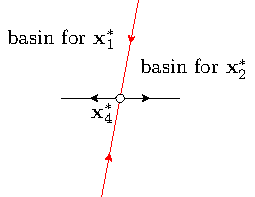
\includegraphics{./plots/zoomX4.pdf}
\caption{Idealized depiction of the separatrices at $\mathbf{x}_4^*$}
\label{fig:zX4}
\end{figure}
Thus one would expect a separatrice that is pointing upwards ($y = 1$) and slightly to the right ($x = 0.1875$). If the eigenvector found above is added and subtracted from $\mathbf{x}_4^*$ figure~\ref{fig:zX4} is obtained. Here the stable and unstable manifolds meet. The situation depicted comes form the one for $c = 0.8$ in figure~\ref{fig:NumTop} here only the top separatrices is drawn in red, however the idealization drawn earlier turns out to be true around $\mathbf{x}_4^*$.

\begin{figure}
\centering
% This file was created by matlab2tikz v0.4.7 running on MATLAB 7.8.
% Copyright (c) 2008--2014, Nico Schlömer <nico.schloemer@gmail.com>
% All rights reserved.
% Minimal pgfplots version: 1.3
% 
% The latest updates can be retrieved from
%   http://www.mathworks.com/matlabcentral/fileexchange/22022-matlab2tikz
% where you can also make suggestions and rate matlab2tikz.
% 
\documentclass[tikz]{standalone}
\usepackage{pgfplots}
\usepackage{grffile}
\pgfplotsset{compat=newest}
\usetikzlibrary{plotmarks}
\usepackage{amsmath}

\begin{document}
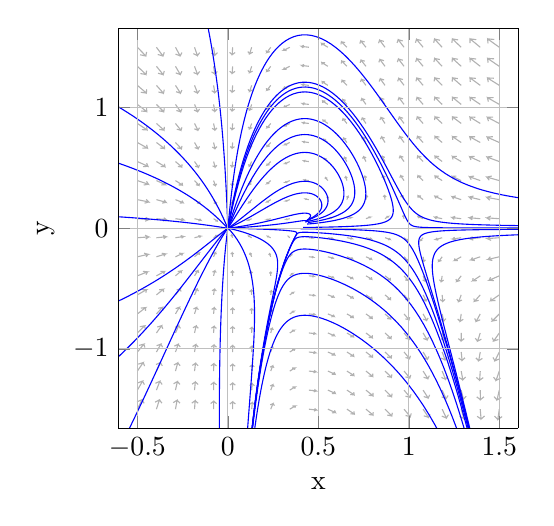
\begin{tikzpicture}
\begin{axis}[%
width=2in,
height=2in,
unbounded coords=jump,
view={0}{90},
scale only axis,
xmin=-0.605263157894737,
xmax=1.60526315789474,
xlabel={x},
xmajorgrids,
ymin=-1.65789473684211,
ymax=1.65789473684211,
ylabel={y},
ymajorgrids,
zmin=-100,
zmax=100
]
\addplot [color=white!70!black,solid,forget plot]
  table[row sep=crcr]{-0.5	-1.5\\
-0.474523585368499	-1.42144772155287\\
-0.501804579369731	-1.43864430142913\\
-0.474523585368499	-1.42144772155287\\
-0.462528440146167	-1.45138250874488\\
nan	0\\
-0.5	-1.34210526315789\\
-0.471462209190471	-1.26731246974459\\
-0.498721744786657	-1.2826158600662\\
-0.471462209190471	-1.26731246974459\\
-0.461325348080004	-1.29688475547096\\
nan	0\\
-0.5	-1.18421052631579\\
-0.467982422260411	-1.11369562296074\\
-0.495216421421049	-1.12684569953236\\
-0.467982422260411	-1.11369562296074\\
-0.459958969743526	-1.14285448840215\\
nan	0\\
-0.5	-1.02631578947368\\
-0.464021764921831	-0.960764535410808\\
-0.491203048961001	-0.971435352860129\\
-0.464021764921831	-0.960764535410808\\
-0.458427421929563	-0.989424470399213\\
nan	0\\
-0.5	-0.868421052631579\\
-0.45953674139031	-0.808752406783231\\
-0.486592880435304	-0.816537185885313\\
-0.45953674139031	-0.808752406783231\\
-0.45675855751113	-0.836768815190158\\
nan	0\\
-0.5	-0.710526315789474\\
-0.454546351059732	-0.657970534202289\\
-0.481321391138609	-0.662373856443378\\
-0.454546351059732	-0.657970534202289\\
-0.455043500345016	-0.685100680913511\\
nan	0\\
-0.5	-0.552631578947368\\
-0.449215380014975	-0.508787523693631\\
-0.475411779823917	-0.509244585273496\\
-0.449215380014975	-0.508787523693631\\
-0.453489752197048	-0.534636895266008\\
nan	0\\
-0.5	-0.394736842105263\\
-0.44396979120566	-0.36151380163426\\
-0.469084613961712	-0.357473161576976\\
-0.44396979120566	-0.36151380163426\\
-0.452473093726211	-0.385488265974146\\
nan	0\\
-0.5	-0.236842105263158\\
-0.439544630474736	-0.216130543481355\\
-0.462859131777766	-0.20723016963458\\
-0.439544630474736	-0.216130543481355\\
-0.452503350886864	-0.237457854397212\\
nan	0\\
-0.5	-0.0789473684210527\\
-0.43675584794232	-0.0719829826289867\\
-0.457470190007641	-0.0582612603521866\\
-0.43675584794232	-0.0719829826289867\\
-0.453987997111608	-0.0898833363810264\\
nan	0\\
-0.5	0.0789473684210527\\
-0.43599440143508	0.0721421754701848\\
-0.453494782766839	0.090185132996675\\
-0.43599440143508	0.0721421754701848\\
-0.456897379242273	0.0581823337142152\\
nan	0\\
-0.5	0.236842105263158\\
-0.43696151246951	0.21740523827459\\
-0.451013841981515	0.238995920253783\\
-0.43696151246951	0.21740523827459\\
-0.460732275475799	0.207476676488538\\
nan	0\\
-0.5	0.394736842105263\\
-0.438975068703043	0.364388421971024\\
-0.449695443058571	0.388749180835535\\
-0.438975068703043	0.364388421971024\\
-0.46486965312569	0.358236715187056\\
nan	0\\
-0.5	0.552631578947368\\
-0.441411012251381	0.513114527314836\\
-0.449108445667834	0.53961688974175\\
-0.441411012251381	0.513114527314836\\
-0.4688669714841	0.510322395867441\\
nan	0\\
-0.5	0.710526315789473\\
-0.443878595680053	0.663333316702245\\
-0.44891676720423	0.6915215675084\\
-0.443878595680053	0.663333316702245\\
-0.472513266747844	0.663460865348427\\
nan	0\\
-0.5	0.868421052631579\\
-0.446187433026129	0.814740379204213\\
-0.448911034761449	0.84429772297589\\
-0.446187433026129	0.814740379204213\\
-0.475751371475132	0.817391439488955\\
nan	0\\
-0.5	1.02631578947368\\
-0.448267170414549	0.967069382257965\\
-0.448975417486254	0.997776511819043\\
-0.448267170414549	0.967069382257965\\
-0.478598621094114	0.971910097026318\\
nan	0\\
-0.5	1.18421052631579\\
-0.45010731537158	1.12011228564733\\
-0.449050560592992	1.15181492900498\\
-0.45010731537158	1.12011228564733\\
-0.48109968092722	1.12686858669077\\
nan	0\\
-0.5	1.34210526315789\\
-0.451723249877543	1.27371320048441\\
-0.44910825924591	1.30630000681707\\
-0.451723249877543	1.27371320048441\\
-0.48330429058265	1.28216163175584\\
nan	0\\
-0.5	1.5\\
-0.453139374829738	1.42775653619585\\
-0.449136696429778	1.46114473162966\\
-0.453139374829738	1.42775653619585\\
-0.485258428331855	1.43771441904453\\
nan	0\\
-0.394736842105263	-1.5\\
-0.378485690335235	-1.42311878867197\\
-0.402581338698252	-1.44212036412787\\
-0.378485690335235	-1.42311878867197\\
-0.364140733034235	-1.45024594001288\\
nan	0\\
-0.394736842105263	-1.34210526315789\\
-0.376090788956982	-1.26847640466151\\
-0.400091819525561	-1.28590354892336\\
-0.376090788956982	-1.26847640466151\\
-0.363277390277371	-1.2952265754975\\
nan	0\\
-0.394736842105263	-1.18421052631579\\
-0.373305265656203	-1.11423473454652\\
-0.397228686533238	-1.12986957796504\\
-0.373305265656203	-1.11423473454652\\
-0.362240790648604	-1.14058536618957\\
nan	0\\
-0.394736842105263	-1.02631578947368\\
-0.370028245570237	-0.960534067269422\\
-0.39388625508181	-0.974091434796944\\
-0.370028245570237	-0.960534067269422\\
-0.360995393979679	-0.986445733064457\\
nan	0\\
-0.394736842105263	-0.868421052631579\\
-0.366136313008317	-0.807591436621679\\
-0.389923875739876	-0.818690189150413\\
-0.366136313008317	-0.807591436621679\\
-0.359509067734926	-0.832990453698886\\
nan	0\\
-0.394736842105263	-0.710526315789474\\
-0.361500268160972	-0.655749212880947\\
-0.385165516071391	-0.663873200267432\\
-0.361500268160972	-0.655749212880947\\
-0.357776964617127	-0.680491487239578\\
nan	0\\
-0.394736842105263	-0.552631578947368\\
-0.356055302720498	-0.505539106542398\\
-0.37943288263717	-0.509996463417698\\
-0.356055302720498	-0.505539106542398\\
-0.355886646434685	-0.529337233110081\\
nan	0\\
-0.394736842105263	-0.394736842105263\\
-0.350003773173732	-0.357698136387402\\
-0.372683370282656	-0.357626480869878\\
-0.350003773173732	-0.357698136387402\\
-0.354164017423726	-0.379993015335644\\
nan	0\\
-0.394736842105263	-0.236842105263158\\
-0.344198141385612	-0.212881093230374\\
-0.365350004609703	-0.207434721660296\\
-0.344198141385612	-0.212881093230374\\
-0.353369498593311	-0.232704072020122\\
nan	0\\
-0.394736842105263	-0.0789473684210527\\
-0.340265118466945	-0.0707147101893522\\
-0.358664800116365	-0.0595665767492827\\
-0.340265118466945	-0.0707147101893522\\
-0.354548471000515	-0.086802438568442\\
nan	0\\
-0.394736842105263	0.0789473684210527\\
-0.339449775479593	0.0709410923304231\\
-0.354034326444637	0.0871647418140295\\
-0.339449775479593	0.0709410923304231\\
-0.358037464489951	0.0595212085011945\\
nan	0\\
-0.394736842105263	0.236842105263158\\
-0.341236875172545	0.21453307137697\\
-0.351709606780814	0.234600773276006\\
-0.341236875172545	0.21453307137697\\
-0.362864123723907	0.207850789809647\\
nan	0\\
-0.394736842105263	0.394736842105263\\
-0.344174249401308	0.360953289958237\\
-0.350897139175738	0.383729003778333\\
-0.344174249401308	0.360953289958237\\
-0.367788915249251	0.358447707426356\\
nan	0\\
-0.394736842105263	0.552631578947368\\
-0.34722952269715	0.509844524829577\\
-0.350784954990136	0.534557470916942\\
-0.34722952269715	0.509844524829577\\
-0.372178482049032	0.510803811212886\\
nan	0\\
-0.394736842105263	0.710526315789473\\
-0.34997980962448	0.660556697876297\\
-0.350914514890421	0.686736841370446\\
-0.34997980962448	0.660556697876297\\
-0.375899323847009	0.664358325130055\\
nan	0\\
-0.394736842105263	0.868421052631579\\
-0.352328335972001	0.812554153015091\\
-0.351084162907858	0.839916349433353\\
-0.352328335972001	0.812554153015091\\
-0.379017612716102	0.818712096366722\\
nan	0\\
-0.394736842105263	1.02631578947368\\
-0.354299491789613	0.965465604612325\\
-0.351218150668968	0.993829997649645\\
-0.354299491789613	0.965465604612325\\
-0.381643243099648	0.97361132249182\\
nan	0\\
-0.394736842105263	1.18421052631579\\
-0.355949785579459	1.11904364685478\\
-0.351294182671949	1.14829047482454\\
-0.355949785579459	1.11904364685478\\
-0.383877622402452	1.12889694656163\\
nan	0\\
-0.394736842105263	1.34210526315789\\
-0.357336518203348	1.27312240542684\\
-0.351310900941158	1.30316734372163\\
-0.357336518203348	1.27312240542684\\
-0.385802329806687	1.28446718177068\\
nan	0\\
-0.394736842105263	1.5\\
-0.358508868361024	1.42758816229114\\
-0.351274301057081	1.45836870703986\\
-0.358508868361024	1.42758816229114\\
-0.38748021991151	1.44025472016774\\
nan	0\\
-0.289473684210526	-1.5\\
-0.280677709132432	-1.42582964915113\\
-0.301859089368077	-1.44588176063627\\
-0.280677709132432	-1.42582964915113\\
-0.264773913943643	-1.45027974817532\\
nan	0\\
-0.289473684210526	-1.34210526315789\\
-0.279004429514127	-1.27080975249523\\
-0.299969083588714	-1.28958109201993\\
-0.279004429514127	-1.27080975249523\\
-0.26432132825738	-1.29481571936813\\
nan	0\\
-0.289473684210526	-1.18421052631579\\
-0.277032830274608	-1.11608941185904\\
-0.297795365069572	-1.13341553271208\\
-0.277032830274608	-1.11608941185904\\
-0.263734807841195	-1.13963595968004\\
nan	0\\
-0.289473684210526	-1.02631578947368\\
-0.274664557167221	-0.961766816593394\\
-0.295244538500285	-0.977429226696655\\
-0.274664557167221	-0.961766816593394\\
-0.26297005206014	-0.984833790218308\\
nan	0\\
-0.289473684210526	-0.868421052631579\\
-0.27175588035591	-0.807999749512999\\
-0.29217654729194	-0.821696689484919\\
-0.27175588035591	-0.807999749512999\\
-0.26196589573265	-0.830555591412227\\
nan	0\\
-0.289473684210526	-0.710526315789474\\
-0.268096128820796	-0.655059564189177\\
-0.288376083337789	-0.666355200821834\\
-0.268096128820796	-0.655059564189177\\
-0.260642707537641	-0.677043978516699\\
nan	0\\
-0.289473684210526	-0.552631578947368\\
-0.263393069548634	-0.50344676878406\\
-0.283513456488029	-0.511682058167579\\
-0.263393069548634	-0.50344676878406\\
-0.258921051406375	-0.524722365498525\\
nan	0\\
-0.289473684210526	-0.394736842105263\\
-0.257350851510719	-0.354125370841468\\
-0.27714056913661	-0.358278104045655\\
-0.257350851510719	-0.354125370841468\\
-0.256834833504712	-0.374339520395558\\
nan	0\\
-0.289473684210526	-0.236842105263158\\
-0.250213166807023	-0.208785453918859\\
-0.269005484864149	-0.207387319971272\\
-0.250213166807023	-0.208785453918859\\
-0.254977159191999	-0.227017578673024\\
nan	0\\
-0.289473684210526	-0.0789473684210527\\
-0.244322329664742	-0.0687806272489934\\
-0.260409421321492	-0.0605428109641651\\
-0.244322329664742	-0.0687806272489934\\
-0.255326050735462	-0.0831184882370573\\
nan	0\\
-0.289473684210526	0.0789473684210527\\
-0.243438110515617	0.0691194815302323\\
-0.254791810901385	0.0835767410212057\\
-0.243438110515617	0.0691194815302323\\
-0.259705754346795	0.0605589541737512\\
nan	0\\
-0.289473684210526	0.236842105263158\\
-0.246695565820768	0.210796384319155\\
-0.253017571101695	0.229304630199795\\
-0.246695565820768	0.210796384319155\\
-0.266040431573696	0.207915571004916\\
nan	0\\
-0.289473684210526	0.394736842105263\\
-0.250724086378445	0.357264062263587\\
-0.25298077076765	0.37819329567411\\
-0.250724086378445	0.357264062263587\\
-0.271717160688488	0.358818496758069\\
nan	0\\
-0.289473684210526	0.552631578947368\\
-0.254138149659029	0.506940146381217\\
-0.25331595188294	0.529481459788936\\
-0.254138149659029	0.506940146381217\\
-0.276161668166016	0.511813692513188\\
nan	0\\
-0.289473684210526	0.710526315789473\\
-0.256800029390446	0.658540089162027\\
-0.253605569179608	0.682304370855281\\
-0.256800029390446	0.658540089162027\\
-0.279598682493332	0.665967543445241\\
nan	0\\
-0.289473684210526	0.868421052631579\\
-0.258856464268023	0.811334692725528\\
-0.253770040274261	0.836114905682969\\
-0.258856464268023	0.811334692725528\\
-0.282313220227286	0.820806295711718\\
nan	0\\
-0.289473684210526	1.02631578947368\\
-0.26046288391728	0.964919686728153\\
-0.253817098318871	0.990591217625124\\
-0.26046288391728	0.964919686728153\\
-0.284515149691637	0.976085817478501\\
nan	0\\
-0.289473684210526	1.18421052631579\\
-0.26173759952063	1.11905988801662\\
-0.253770765352807	1.14553910067884\\
-0.26173759952063	1.11905988801662\\
-0.286346084502392	1.1316710583339\\
nan	0\\
-0.289473684210526	1.34210526315789\\
-0.262764877490478	1.27361008493929\\
-0.253653724951841	1.30083584008488\\
-0.262764877490478	1.27361008493929\\
-0.287901314061144	1.28748143672486\\
nan	0\\
-0.289473684210526	1.5\\
-0.263604317957277	1.42847551273563\\
-0.253484006017159	1.45640020047825\\
-0.263604317957277	1.42847551273563\\
-0.289246249649344	1.44346551735163\\
nan	0\\
-0.184210526315789	-1.5\\
-0.180768625272059	-1.4293949845174\\
-0.199452449455828	-1.44971601390125\\
-0.180768625272059	-1.4293949845174\\
-0.164149941714529	-1.45143696442311\\
nan	0\\
-0.184210526315789	-1.34210526315789\\
-0.179780379669291	-1.2741122417255\\
-0.198107679021339	-1.29340261149359\\
-0.179780379669291	-1.2741122417255\\
-0.164111168305142	-1.29561768481684\\
nan	0\\
-0.184210526315789	-1.18421052631579\\
-0.17861191428645	-1.11906371411724\\
-0.196578200944889	-1.13720810476947\\
-0.17861191428645	-1.11906371411724\\
-0.164004794845615	-1.14000741078414\\
nan	0\\
-0.184210526315789	-1.02631578947368\\
-0.177197201567289	-0.964314333725132\\
-0.194801562928977	-0.981161439262573\\
-0.177197201567289	-0.964314333725132\\
-0.163800835054701	-0.984668101636823\\
nan	0\\
-0.184210526315789	-0.868421052631579\\
-0.175431862339976	-0.809964888514626\\
-0.192679502561958	-0.825307071755759\\
-0.175431862339976	-0.809964888514626\\
-0.163451420503482	-0.829696403743665\\
nan	0\\
-0.184210526315789	-0.710526315789474\\
-0.173141068710077	-0.65618590364804\\
-0.19004700902715	-0.669720662889042\\
-0.173141068710077	-0.65618590364804\\
-0.162876802956432	-0.675255391691898\\
nan	0\\
-0.184210526315789	-0.552631578947368\\
-0.170012285700858	-0.503302225594463\\
-0.186604096223563	-0.514551471446602\\
-0.170012285700858	-0.503302225594463\\
-0.161939419547111	-0.521650591754068\\
nan	0\\
-0.184210526315789	-0.394736842105263\\
-0.165457045429358	-0.352041611422566\\
-0.181756897365961	-0.360161810405767\\
-0.165457045429358	-0.352041611422566\\
-0.160409282024613	-0.369538550848983\\
nan	0\\
-0.184210526315789	-0.236842105263158\\
-0.158481185706605	-0.204377818209372\\
-0.174316059652807	-0.207684769173211\\
-0.158481185706605	-0.204377818209372\\
-0.158083916125913	-0.220549439477804\\
nan	0\\
-0.184210526315789	-0.0789473684210527\\
-0.149665758444823	-0.0654483313314608\\
-0.163403948078511	-0.0608618504905967\\
-0.149665758444823	-0.0654483313314608\\
-0.156654429533715	-0.07813423442608\\
nan	0\\
-0.184210526315789	0.0789473684210527\\
-0.148665884448293	0.0659771421680096\\
-0.156086720445282	0.0787543705107965\\
-0.148665884448293	0.0659771421680096\\
-0.162571833571803	0.0609820495770485\\
nan	0\\
-0.184210526315789	0.236842105263158\\
-0.154429617514988	0.206265231462895\\
-0.155719671705162	0.222883520803174\\
-0.154429617514988	0.206265231462895\\
-0.171008108605294	0.207993066402773\\
nan	0\\
-0.184210526315789	0.394736842105263\\
-0.158998809046451	0.354116425105562\\
-0.156407219977327	0.372605479522807\\
-0.158998809046451	0.354116425105562\\
-0.176717428477178	0.359999620888138\\
nan	0\\
-0.184210526315789	0.552631578947368\\
-0.161966033934835	0.505227315508595\\
-0.156788315789428	0.525009717635465\\
-0.161966033934835	0.505227315508595\\
-0.180490447508815	0.513887471444988\\
nan	0\\
-0.184210526315789	0.710526315789473\\
-0.16395255894886	0.657926156720146\\
-0.156879909391607	0.678770696282677\\
-0.16395255894886	0.657926156720146\\
-0.18317998892627	0.668641712599212\\
nan	0\\
-0.184210526315789	0.868421052631579\\
-0.165349213238411	0.811541450208285\\
-0.156787706555802	0.833320659204618\\
-0.165349213238411	0.811541450208285\\
-0.185227507767448	0.823890002665929\\
nan	0\\
-0.184210526315789	1.02631578947368\\
-0.166372601337225	0.965754011226635\\
-0.156583534269032	0.988382025945391\\
-0.166372601337225	0.965754011226635\\
-0.186864423392557	0.979463063456109\\
nan	0\\
-0.184210526315789	1.18421052631579\\
-0.167147111109417	1.12038958092019\\
-0.156310899322428	1.14380171834046\\
-0.167147111109417	1.12038958092019\\
-0.18822137202023	1.13527001073727\\
nan	0\\
-0.184210526315789	1.34210526315789\\
-0.167748129232411	1.27534273410317\\
-0.155996216093743	1.29948709209043\\
-0.167748129232411	1.27534273410317\\
-0.189377480621107	1.29125589354874\\
nan	0\\
-0.184210526315789	1.5\\
-0.168223696731071	1.43054463876901\\
-0.155655905298739	1.45537795453449\\
-0.168223696731071	1.43054463876901\\
-0.190383585914234	1.44738453974213\\
nan	0\\
-0.0789473684210527	-1.5\\
-0.0784848996087788	-1.43366978693837\\
-0.0952061935178695	-1.45345323365379\\
-0.0784848996087788	-1.43366978693837\\
-0.0620410869870525	-1.45368446805992\\
nan	0\\
-0.0789473684210527	-1.34210526315789\\
-0.0780959420599778	-1.27819197207646\\
-0.0943296927386591	-1.29715310281062\\
-0.0780959420599778	-1.27819197207646\\
-0.0623730471979415	-1.29757881599116\\
nan	0\\
-0.0789473684210527	-1.18421052631579\\
-0.077637835256449	-1.12291460325305\\
-0.0933546759715157	-1.14097599688072\\
-0.077637835256449	-1.12291460325305\\
-0.0627067144401445	-1.14163076346302\\
nan	0\\
-0.0789473684210527	-1.02631578947368\\
-0.0770845512891668	-0.967885960729144\\
-0.0922508536148677	-0.984949205069534\\
-0.0770845512891668	-0.967885960729144\\
-0.0630359392425974	-0.985880613635477\\
nan	0\\
-0.0789473684210527	-0.868421052631579\\
-0.0763938098683367	-0.813176538720971\\
-0.0909710059118036	-0.829111503255974\\
-0.0763938098683367	-0.813176538720971\\
-0.0633487489564995	-0.830388282532332\\
nan	0\\
-0.0789473684210527	-0.710526315789474\\
-0.07549134625155	-0.658896466348954\\
-0.0894356152625307	-0.673521415638734\\
-0.07549134625155	-0.658896466348954\\
-0.0636206905422709	-0.675249426723486\\
nan	0\\
-0.0789473684210527	-0.552631578947368\\
-0.0742318782035858	-0.505235691775398\\
-0.0874954970618184	-0.518275585372623\\
-0.0742318782035858	-0.505235691775398\\
-0.0637975534758332	-0.520633330481356\\
nan	0\\
-0.0789473684210527	-0.394736842105263\\
-0.0722826730750412	-0.352578472813778\\
-0.0848216740017161	-0.36355980976472\\
-0.0722826730750412	-0.352578472813778\\
-0.0637424893559732	-0.366892157437726\\
nan	0\\
-0.0789473684210527	-0.236842105263158\\
-0.0686675575738782	-0.201972846312775\\
-0.0804688155656263	-0.209863671286096\\
-0.0686675575738782	-0.201972846312775\\
-0.0630341860904348	-0.215003576709683\\
nan	0\\
-0.0789473684210527	-0.0789473684210527\\
-0.0595038638976126	-0.0590751236995536\\
-0.0703049764350194	-0.0601759209851433\\
-0.0595038638976126	-0.0590751236995536\\
-0.0603688540742698	-0.0698976732468633\\
nan	0\\
-0.0789473684210527	0.0789473684210527\\
-0.0582929199961765	0.0596877039941147\\
-0.0596743384169049	0.0706292154284151\\
-0.0582929199961765	0.0596877039941147\\
-0.0693041706303738	0.0603019912159771\\
nan	0\\
-0.0789473684210527	0.236842105263158\\
-0.0656471228161527	0.202634086672139\\
-0.0610851918498679	0.216221553650669\\
-0.0656471228161527	0.202634086672139\\
-0.0781892011453775	0.209571430848219\\
nan	0\\
-0.0789473684210527	0.394736842105263\\
-0.0684500049445791	0.353094172012427\\
-0.0611885464643123	0.368211313909396\\
-0.0684500049445791	0.353094172012427\\
-0.0820098815107301	0.36296263217116\\
nan	0\\
-0.0789473684210527	0.552631578947368\\
-0.0698587832009507	0.505658827067622\\
-0.0608421707970448	0.522022798936572\\
-0.0698587832009507	0.505658827067622\\
-0.0843285467369177	0.51747850632652\\
nan	0\\
-0.0789473684210527	0.710526315789473\\
-0.0706966420286007	0.659258305958273\\
-0.0603548574885362	0.676701390505746\\
-0.0706966420286007	0.659258305958273\\
-0.0859888624041364	0.67257602730952\\
nan	0\\
-0.0789473684210527	0.868421052631579\\
-0.0712457477967379	0.813494856434633\\
-0.0598246849347958	0.831898120449795\\
-0.0712457477967379	0.813494856434633\\
-0.0872877830332689	0.828047310137638\\
nan	0\\
-0.0789473684210527	1.02631578947368\\
-0.0716284148140962	0.968171656943311\\
-0.0592880677635899	0.987444635104162\\
-0.0716284148140962	0.968171656943311\\
-0.0883601340287765	0.983785158300684\\
nan	0\\
-0.0789473684210527	1.18421052631579\\
-0.071906358559738	1.12317483449465\\
-0.0587597385628472	1.14324579450632\\
-0.071906358559738	1.12317483449465\\
-0.0892775844734175	1.13972528957566\\
nan	0\\
-0.0789473684210527	1.34210526315789\\
-0.0721141529317433	1.27843169770392\\
-0.0582457262150424	1.29924207121244\\
-0.0721141529317433	1.27843169770392\\
-0.0900825089420298	1.29582546346779\\
nan	0\\
-0.0789473684210527	1.5\\
-0.0722727020550486	1.43389259342673\\
-0.0577482503215329	1.45539348199021\\
-0.0722727020550486	1.43389259342673\\
-0.0908019536081668	1.45205614880721\\
nan	0\\
0.0263157894736842	-1.5\\
0.0265483558515985	-1.43865239200466\\
0.0111416839393895	-1.45699853280878\\
0.0265483558515985	-1.43865239200466\\
0.0418154879370588	-1.45711481599774\\
nan	0\\
0.0263157894736842	-1.34210526315789\\
0.0264285401743101	-1.28299027216028\\
0.0116159672147186	-1.30069658178441\\
0.0264285401743101	-1.28299027216028\\
0.041173462713526	-1.30075295713472\\
nan	0\\
0.0263157894736842	-1.18421052631579\\
0.0262886505985771	-1.12751106922207\\
0.0121219279876805	-1.14452769106897\\
0.0262886505985771	-1.12751106922207\\
0.040471656534538	-1.14451412163141\\
nan	0\\
0.0263157894736842	-1.02631578947368\\
0.0261212482630422	-0.972257650566543\\
0.0126650758994495	-0.988523727541346\\
0.0261212482630422	-0.972257650566543\\
0.0396941453530201	-0.988426456936025\\
nan	0\\
0.0263157894736842	-0.868421052631579\\
0.0259142491779179	-0.817291678013634\\
0.0132523676121615	-0.832730875472959\\
0.0259142491779179	-0.817291678013634\\
0.0388170549211341	-0.832530105325076\\
nan	0\\
0.0263157894736842	-0.710526315789474\\
0.0256463676285301	-0.662707261474717\\
0.0138924306033872	-0.677220333230433\\
0.0256463676285301	-0.662707261474717\\
0.0378019577607654	-0.676885622307856\\
nan	0\\
0.0263157894736842	-0.552631578947368\\
0.0252755882089438	-0.508660525694461\\
0.0145948852751392	-0.522111891986519\\
0.0252755882089438	-0.508660525694461\\
0.0365804119015927	-0.521591791354148\\
nan	0\\
0.0263157894736842	-0.394736842105263\\
0.024703284281418	-0.355445677918428\\
0.0153642447923889	-0.367636153472545\\
0.024703284281418	-0.355445677918428\\
0.0350098268858068	-0.366829900876412\\
nan	0\\
0.0263157894736842	-0.236842105263158\\
0.0236160340965595	-0.203757331054322\\
0.0161547671574879	-0.214357702161254\\
0.0236160340965595	-0.203757331054322\\
0.032697154261906	-0.213007824472692\\
nan	0\\
0.0263157894736842	-0.0789473684210527\\
0.0199444724570866	-0.056545288577067\\
0.0162553476010694	-0.0648587417844121\\
0.0199444724570866	-0.056545288577067\\
0.0274563875230623	-0.0616730832761133\\
nan	0\\
0.0263157894736842	0.0789473684210527\\
0.0191104105689448	0.0567093235561932\\
0.0268315354565815	0.0615793922894662\\
0.0191104105689448	0.0567093235561932\\
0.0157125130241518	0.0651820817418359\\
nan	0\\
0.0263157894736842	0.236842105263158\\
0.0223163547427901	0.203844858175289\\
0.0317654969340255	0.212744173618926\\
0.0223163547427901	0.203844858175289\\
0.0152668733900911	0.214743890984373\\
nan	0\\
0.0263157894736842	0.394736842105263\\
0.023152263755682	0.355508487226159\\
0.0339084101908586	0.36648611226039\\
0.023152263755682	0.355508487226159\\
0.0142942327513067	0.368067875119391\\
nan	0\\
0.0263157894736842	0.552631578947368\\
0.0235373429685829	0.508710835337636\\
0.0353510628225463	0.52119244679428\\
0.0235373429685829	0.508710835337636\\
0.0133906910176803	0.522581670046831\\
nan	0\\
0.0263157894736842	0.710526315789473\\
0.0237548267088472	0.662749852610945\\
0.0364672313329304	0.676442550873294\\
0.0237548267088472	0.662749852610945\\
0.0125789997436662	0.677723032255713\\
nan	0\\
0.0263157894736842	0.868421052631579\\
0.0238910925045995	0.817328954707479\\
0.0373915260763497	0.832050409842438\\
0.0238910925045995	0.817328954707479\\
0.0118454771143001	0.83326275832698\\
nan	0\\
0.0263157894736842	1.02631578947368\\
0.0239817730126046	0.97229100824781\\
0.038188173257397	0.987914938500302\\
0.0239817730126046	0.97229100824781\\
0.0111757826444599	0.989081946730842\\
nan	0\\
0.0263157894736842	1.18421052631579\\
0.0240443431676548	1.12754139714866\\
0.0388930593512465	1.14397427432229\\
0.0240443431676548	1.12754139714866\\
0.0105584947676808	1.1451099974753\\
nan	0\\
0.0263157894736842	1.34210526315789\\
0.0240884042762781	1.28301817554904\\
0.0395283917377138	1.30018745553234\\
0.0240884042762781	1.28301817554904\\
0.00998484793328607	1.30130114813105\\
nan	0\\
0.0263157894736842	1.5\\
0.0241196755788737	1.43867830339788\\
0.0401089338978478	1.45652578390481\\
0.0241196755788737	1.43867830339788\\
0.00944808559678598	1.45762384085222\\
nan	0\\
0.131578947368421	-1.5\\
0.135165452907657	-1.4446888016427\\
0.120261701656561	-1.46038553476508\\
0.135165452907657	-1.4446888016427\\
0.147917300835211	-1.4621787875347\\
nan	0\\
0.131578947368421	-1.34210526315789\\
0.134598954293536	-1.28878955756743\\
0.120364025818385	-1.30402926751329\\
0.134598954293536	-1.28878955756743\\
0.147021878613618	-1.30553927097585\\
nan	0\\
0.131578947368421	-1.18421052631579\\
0.13394534560671	-1.13305527460339\\
0.120446613207123	-1.14781025055754\\
0.13394534560671	-1.13305527460339\\
0.146024239063323	-1.14899344967668\\
nan	0\\
0.131578947368421	-1.02631578947368\\
0.13317335690254	-0.977525971946583\\
0.120497579660529	-0.991764314821184\\
0.13317335690254	-0.977525971946583\\
0.144892488424079	-0.992561519588243\\
nan	0\\
0.131578947368421	-0.868421052631579\\
0.132232625435132	-0.822260486487346\\
0.12049638047906	-0.835945236813938\\
0.132232625435132	-0.822260486487346\\
0.143576663551177	-0.836272075847293\\
nan	0\\
0.131578947368421	-0.710526315789474\\
0.131035487569619	-0.667351831398424\\
0.120404904411497	-0.680440041665439\\
0.131035487569619	-0.667351831398424\\
0.141992146607022	-0.680168311766039\\
nan	0\\
0.131578947368421	-0.552631578947368\\
0.12941226194239	-0.512963848669183\\
0.120145335000653	-0.525405839109146\\
0.12941226194239	-0.512963848669183\\
0.139979200139746	-0.52432249639613\\
nan	0\\
0.131578947368421	-0.394736842105263\\
0.126980582958508	-0.359441063111055\\
0.11953614753293	-0.371179387911796\\
0.126980582958508	-0.359441063111055\\
0.137184037030034	-0.368880205706839\\
nan	0\\
0.131578947368421	-0.236842105263158\\
0.122664993266623	-0.207789471779066\\
0.118076021126139	-0.218733750349743\\
0.122664993266623	-0.207789471779066\\
0.132602337868185	-0.214276773298844\\
nan	0\\
0.131578947368421	-0.0789473684210527\\
0.113175266763342	-0.063475861531426\\
0.114828494222459	-0.0727182337495837\\
0.113175266763342	-0.063475861531426\\
0.122564247667273	-0.0635163934470444\\
nan	0\\
0.131578947368421	0.0789473684210527\\
0.110875833927998	0.0647533406464453\\
0.120635274903777	0.0638357706187217\\
0.110875833927998	0.0647533406464453\\
0.113538261016473	0.0741873273389333\\
nan	0\\
0.131578947368421	0.236842105263158\\
0.115908582482558	0.209630901975698\\
0.127412492770182	0.21387667174047\\
0.115908582482558	0.209630901975698\\
0.113806891126452	0.221711854183402\\
nan	0\\
0.131578947368421	0.394736842105263\\
0.118086799371545	0.36095065353389\\
0.130580990913451	0.367713473106083\\
0.118086799371545	0.36095065353389\\
0.113687896627765	0.374459547104521\\
nan	0\\
0.131578947368421	0.552631578947368\\
0.119146414569411	0.514221527875927\\
0.132478687176974	0.522636409997607\\
0.119146414569411	0.514221527875927\\
0.113273661641254	0.528852676397112\\
nan	0\\
0.131578947368421	0.710526315789473\\
0.119723915041703	0.668434328106535\\
0.133803421660453	0.678098166329737\\
0.119723915041703	0.668434328106535\\
0.112757427818984	0.684025682493096\\
nan	0\\
0.131578947368421	0.868421052631579\\
0.120056290558378	0.823215962905511\\
0.134814360032908	0.833896825620821\\
0.120056290558378	0.823215962905511\\
0.112211815169874	0.839658154025842\\
nan	0\\
0.131578947368421	1.02631578947368\\
0.120249152999754	0.978385190117267\\
0.135630741149458	0.989931921332025\\
0.120249152999754	0.978385190117267\\
0.11166544147125	0.995596818516359\\
nan	0\\
0.131578947368421	1.18421052631579\\
0.12035618349312	1.13383886260853\\
0.136315928582524	1.14614467075188\\
0.12035618349312	1.13383886260853\\
0.111130096728896	1.15175605268954\\
nan	0\\
0.131578947368421	1.34210526315789\\
0.120407376637682	1.28951199072885\\
0.136907165964165	1.30249707977488\\
0.120407376637682	1.28951199072885\\
0.110610529749642	1.30808286514025\\
nan	0\\
0.131578947368421	1.5\\
0.120420714871311	1.4453606331682\\
0.137428026328395	1.45896288509346\\
0.120420714871311	1.4453606331682\\
0.110108342912493	1.46454200134202\\
nan	0\\
0.236842105263158	-1.5\\
0.249578821684825	-1.45336826157193\\
0.234099872151308	-1.46417360399494\\
0.249578821684825	-1.45336826157193\\
0.257415741365342	-1.47054196220577\\
nan	0\\
0.236842105263158	-1.34210526315789\\
0.248586845834124	-1.29707888349053\\
0.233806828745994	-1.307650612248\\
0.248586845834124	-1.29707888349053\\
0.256320018579675	-1.31352298253348\\
nan	0\\
0.236842105263158	-1.18421052631579\\
0.247460656635816	-1.14091730290716\\
0.233451785371861	-1.15125063208658\\
0.247460656635816	-1.14091730290716\\
0.255098397076176	-1.15655990777291\\
nan	0\\
0.236842105263158	-1.02631578947368\\
0.246153686344007	-0.984914183814484\\
0.233009810604952	-0.995006770242032\\
0.246153686344007	-0.984914183814484\\
0.253710613434552	-0.999662560782457\\
nan	0\\
0.236842105263158	-0.868421052631579\\
0.244590966694891	-0.829115176594543\\
0.232439839256112	-0.83896972404772\\
0.244590966694891	-0.829115176594543\\
0.25209277727463	-0.842844154763587\\
nan	0\\
0.236842105263158	-0.710526315789474\\
0.242641726011527	-0.673594512102009\\
0.23166888886515	-0.683224148021156\\
0.242641726011527	-0.673594512102009\\
0.250134790708882	-0.686123958395341\\
nan	0\\
0.236842105263158	-0.552631578947368\\
0.240051710886507	-0.518490924948219\\
0.230553665699715	-0.527930719742127\\
0.240051710886507	-0.518490924948219\\
0.24762399269929	-0.529535522553801\\
nan	0\\
0.236842105263158	-0.394736842105263\\
0.236247366914713	-0.364132597924873\\
0.228774727374149	-0.373462555766101\\
0.236247366914713	-0.364132597924873\\
0.244076849464344	-0.373165186591879\\
nan	0\\
0.236842105263158	-0.236842105263158\\
0.229694265292058	-0.211685782463316\\
0.225549536583427	-0.221019639296043\\
0.229694265292058	-0.211685782463316\\
0.238127697983349	-0.217445719310493\\
nan	0\\
0.236842105263158	-0.0789473684210527\\
0.218039089518312	-0.0672514449369072\\
0.220756013370729	-0.0754609759183624\\
0.218039089518312	-0.0672514449369072\\
0.226603975112802	-0.0660594680459393\\
nan	0\\
0.236842105263158	0.0789473684210527\\
0.214274929572241	0.0693967428210182\\
0.223432738679525	0.0666201365782993\\
0.214274929572241	0.0693967428210182\\
0.218657425879507	0.0779037244237578\\
nan	0\\
0.236842105263158	0.236842105263158\\
0.215822778231154	0.216619190409775\\
0.227184305054101	0.217431233107789\\
0.215822778231154	0.216619190409775\\
0.21707284762741	0.227940896623791\\
nan	0\\
0.236842105263158	0.394736842105263\\
0.216569660432046	0.368567974466471\\
0.229193610791078	0.37135052355033\\
0.216569660432046	0.368567974466471\\
0.216109176971682	0.381486745965886\\
nan	0\\
0.236842105263158	0.552631578947368\\
0.216779294282836	0.522290087055292\\
0.230383510549951	0.526376831877835\\
0.216779294282836	0.522290087055292\\
0.215212764603914	0.536408237367996\\
nan	0\\
0.236842105263158	0.710526315789473\\
0.216728236037531	0.676902823570835\\
0.231168269859879	0.68196140393002\\
0.216728236037531	0.676902823570835\\
0.21435652375056	0.692018338542833\\
nan	0\\
0.236842105263158	0.868421052631579\\
0.216544852529091	0.832052707759693\\
0.231726114567283	0.837888898037742\\
0.216544852529091	0.832052707759693\\
0.21354194213134	0.848037524404776\\
nan	0\\
0.236842105263158	1.02631578947368\\
0.216291091476293	0.987564862825924\\
0.232144127274293	0.994052387373536\\
0.216291091476293	0.987564862825924\\
0.212768663950413	1.00432789426697\\
nan	0\\
0.236842105263158	1.18421052631579\\
0.215999132803969	1.14333988820117\\
0.232469684070381	1.15039033652076\\
0.215999132803969	1.14333988820117\\
0.212034365013071	1.16081182275035\\
nan	0\\
0.236842105263158	1.34210526315789\\
0.21568676304015	1.29931562828583\\
0.232730774425069	1.3068636831917\\
0.21568676304015	1.29931562828583\\
0.211335956989036	1.3174413543032\\
nan	0\\
0.236842105263158	1.5\\
0.215364289884431	1.45545044747284\\
0.23294502262984	1.4634458593863\\
0.215364289884431	1.45545044747284\\
0.210670246366259	1.47418476707567\\
nan	0\\
0.342105263157895	-1.5\\
0.373379646744447	-1.47240417053273\\
0.357098374301665	-1.47286432347628\\
0.373379646744447	-1.47240417053273\\
0.370896289035298	-1.48850151526955\\
nan	0\\
0.342105263157895	-1.34210526315789\\
0.372035410228971	-1.3154050982022\\
0.356381324868725	-1.31593261092114\\
0.372035410228971	-1.3154050982022\\
0.369731407346571	-1.33089768445668\\
nan	0\\
0.342105263157895	-1.18421052631579\\
0.37055934964916	-1.15846851474622\\
0.355587620809389	-1.15907759659428\\
0.37055934964916	-1.15846851474622\\
0.368458626594172	-1.17330463983991\\
nan	0\\
0.342105263157895	-1.02631578947368\\
0.368913864269129	-1.00160591098538\\
0.354693814313682	-1.00231672425406\\
0.368913864269129	-1.00160591098538\\
0.367048753557835	-1.01572102480968\\
nan	0\\
0.342105263157895	-0.868421052631579\\
0.367040850593126	-0.844832092020432\\
0.35366293420977	-0.845674883344968\\
0.367040850593126	-0.844832092020432\\
0.365457414515343	-0.858142677062584\\
nan	0\\
0.342105263157895	-0.710526315789474\\
0.364842625885533	-0.688166018017001\\
0.352431342624123	-0.689189766666833\\
0.364842625885533	-0.688166018017001\\
0.36361149151036	-0.700558448030652\\
nan	0\\
0.342105263157895	-0.552631578947368\\
0.36213313391495	-0.531630386421918\\
0.350874474556471	-0.532923776490289\\
0.36213313391495	-0.531630386421918\\
0.361375070819196	-0.542937711868817\\
nan	0\\
0.342105263157895	-0.394736842105263\\
0.358477656254058	-0.375243054436722\\
0.348692491408073	-0.376998092463244\\
0.358477656254058	-0.375243054436722\\
0.358439385242344	-0.385184289011325\\
nan	0\\
0.342105263157895	-0.236842105263158\\
0.352365526398911	-0.218979497652383\\
0.344821795523913	-0.221773214125362\\
0.352365526398911	-0.218979497652383\\
0.3537530993293	-0.22690334574587\\
nan	0\\
0.342105263157895	-0.0789473684210527\\
0.333275491000097	-0.0672211436360487\\
0.332992866451185	-0.0729464541109993\\
0.333275491000097	-0.0672211436360487\\
0.338855978843687	-0.0685315680321005\\
nan	0\\
0.342105263157895	0.0789473684210527\\
0.322578875732129	0.0729005197451366\\
0.329948504128838	0.0698329774914701\\
0.322578875732129	0.0729005197451366\\
0.32692507979088	0.0795961712043527\\
nan	0\\
0.342105263157895	0.236842105263158\\
0.319669692848171	0.225045033858108\\
0.329349631792351	0.222975262702192\\
0.319669692848171	0.225045033858108\\
0.323451096089826	0.234193047857054\\
nan	0\\
0.342105263157895	0.394736842105263\\
0.317415371731771	0.379648108253798\\
0.328594522622474	0.378002255552706\\
0.317415371731771	0.379648108253798\\
0.321050155696742	0.390347201265768\\
nan	0\\
0.342105263157895	0.552631578947368\\
0.315509183110559	0.535163308040442\\
0.327855074851491	0.533754769300686\\
0.315509183110559	0.535163308040442\\
0.319120939398028	0.547052809324354\\
nan	0\\
0.342105263157895	0.710526315789473\\
0.313840191856625	0.691157754187706\\
0.327161853647448	0.689902054842919\\
0.313840191856625	0.691157754187706\\
0.317477572846564	0.704034590493554\\
nan	0\\
0.342105263157895	0.868421052631579\\
0.312346241473537	0.847450753010596\\
0.32651652288409	0.846302087475801\\
0.312346241473537	0.847450753010596\\
0.316031373073598	0.86118159831798\\
nan	0\\
0.342105263157895	1.02631578947368\\
0.310987812200896	1.00394934303922\\
0.325914659096612	1.00287991423031\\
0.310987812200896	1.00394934303922\\
0.31473143587938	1.01843863970881\\
nan	0\\
0.342105263157895	1.18421052631579\\
0.309737951489429	1.1605991335338\\
0.325350993185465	1.15959072345128\\
0.309737951489429	1.1605991335338\\
0.313545296794472	1.17577437928552\\
nan	0\\
0.342105263157895	1.34210526315789\\
0.308577354169382	1.3173654011937\\
0.324820692356984	1.31640538253583\\
0.308577354169382	1.3173654011937\\
0.312450761374887	1.33316933703009\\
nan	0\\
0.342105263157895	1.5\\
0.307491666918009	1.47422453660775\\
0.324319611638036	1.47330377656546\\
0.307491666918009	1.47422453660775\\
0.311431879941913	1.4906105746854\\
nan	0\\
0.447368421052632	-1.5\\
0.490502795068568	-1.50679385210286\\
0.479260945889502	-1.49397210296802\\
0.490502795068568	-1.50679385210286\\
0.475864019838072	-1.51553928997599\\
nan	0\\
0.447368421052632	-1.34210526315789\\
0.489026581910279	-1.34862444240064\\
0.478158928463671	-1.3362541484134\\
0.489026581910279	-1.34862444240064\\
0.4748993388423	-1.35708322884223\\
nan	0\\
0.447368421052632	-1.18421052631579\\
0.487437566917918	-1.19043041006939\\
0.476971794096732	-1.17854715847699\\
0.487437566917918	-1.19043041006939\\
0.473861852219932	-1.19858173140963\\
nan	0\\
0.447368421052632	-1.02631578947368\\
0.485711356642915	-1.03220553144557\\
0.475680911458802	-1.02085287495644\\
0.485711356642915	-1.03220553144557\\
0.472736040472857	-1.04002434275158\\
nan	0\\
0.447368421052632	-0.868421052631579\\
0.483813829977109	-0.873940683403474\\
0.47426011499274	-0.863173441940786\\
0.483813829977109	-0.873940683403474\\
0.471500299606792	-0.881396146403025\\
nan	0\\
0.447368421052632	-0.710526315789474\\
0.481694840113466	-0.715621643618816\\
0.472670746352551	-0.705511440504805\\
0.481694840113466	-0.715621643618816\\
0.47012308243788	-0.722674650035222\\
nan	0\\
0.447368421052632	-0.552631578947368\\
0.479275574869299	-0.557224275330071\\
0.470851602819974	-0.547869677961093\\
0.479275574869299	-0.557224275330071\\
0.468555254628623	-0.563823254869427\\
nan	0\\
0.447368421052632	-0.394736842105263\\
0.476419587422387	-0.398702159354009\\
0.468695566823646	-0.390249772586946\\
0.476419587422387	-0.398702159354009\\
0.466712908199274	-0.404775355771824\\
nan	0\\
0.447368421052632	-0.236842105263158\\
0.472851370574078	-0.239945797833078\\
0.465982408860124	-0.23264395268174\\
0.472851370574078	-0.239945797833078\\
0.464430562575164	-0.245385427442463\\
nan	0\\
0.447368421052632	-0.0789473684210527\\
0.467823383964749	-0.0805667196515953\\
0.46209173289875	-0.074967173554403\\
0.467823383964749	-0.0805667196515953\\
0.461282057283478	-0.085194655010462\\
nan	0\\
0.447368421052632	0.0789473684210527\\
0.452338731677406	0.0868170269102795\\
0.448880223867667	0.0856987070197051\\
0.452338731677406	0.0868170269102795\\
0.45281505311228	0.0832135517073178\\
nan	0\\
0.447368421052632	0.236842105263158\\
0.428017343990393	0.241948639487915\\
0.432546033552875	0.235578909954928\\
0.428017343990393	0.241948639487915\\
0.435099300665254	0.245254448486048\\
nan	0\\
0.447368421052632	0.394736842105263\\
0.422578210770719	0.400041053764681\\
0.428689220940438	0.392252237696378\\
0.422578210770719	0.400041053764681\\
0.431341326770147	0.404647342837334\\
nan	0\\
0.447368421052632	0.552631578947368\\
0.418845533146713	0.558276733845414\\
0.425991110793977	0.549452465399521\\
0.418845533146713	0.558276733845414\\
0.428813688243	0.56371390935248\\
nan	0\\
0.447368421052632	0.710526315789473\\
0.415897241324472	0.716505839937824\\
0.423843714205832	0.706844187761279\\
0.415897241324472	0.716505839937824\\
0.426833476280008	0.722579777625358\\
nan	0\\
0.447368421052632	0.868421052631579\\
0.413417669089637	0.874711573163729\\
0.422030264545497	0.864336729013335\\
0.413417669089637	0.874711573163729\\
0.425175524811573	0.881312104994833\\
nan	0\\
0.447368421052632	1.02631578947368\\
0.411255662513139	1.03289385094806\\
0.420444974706393	1.02189224287087\\
0.411255662513139	1.03289385094806\\
0.423734005443581	1.03994862214062\\
nan	0\\
0.447368421052632	1.18421052631579\\
0.409325636722818	1.19105534546604\\
0.419027267234199	1.17949120363851\\
0.409325636722818	1.19105534546604\\
0.422449676809325	1.19851259580342\\
nan	0\\
0.447368421052632	1.34210526315789\\
0.407573854652603	1.34919888619719\\
0.417738818812787	1.3371221576854\\
0.407573854652603	1.34919888619719\\
0.421285630332436	1.35701944088541\\
nan	0\\
0.447368421052632	1.5\\
0.405964099549789	1.50732694120712\\
0.416553660698862	1.49477777846927\\
0.405964099549789	1.50732694120712\\
0.420217131302422	1.5154799392207\\
nan	0\\
0.552631578947368	-1.5\\
0.59507002687066	-1.52836655590841\\
0.589430131470775	-1.50924697715507\\
0.59507002687066	-1.52836655590841\\
0.575246853516569	-1.53046620111671\\
nan	0\\
0.552631578947368	-1.34210526315789\\
0.593864601440729	-1.3692454276062\\
0.588279735804798	-1.35079512264837\\
0.593864601440729	-1.3692454276062\\
0.574709653580644	-1.37141163389505\\
nan	0\\
0.552631578947368	-1.18421052631579\\
0.592584786519887	-1.21000951779814\\
0.587048572118719	-1.1922815184603\\
0.592584786519887	-1.21000951779814\\
0.574149076377545	-1.21225812224656\\
nan	0\\
0.552631578947368	-1.02631578947368\\
0.591217950401522	-1.05062914087464\\
0.585720376815515	-1.03368854259082\\
0.591217950401522	-1.05062914087464\\
0.573563701115036	-1.05298172831789\\
nan	0\\
0.552631578947368	-0.868421052631579\\
0.5897475776326	-0.89106073975836\\
0.584272699808726	-0.874989833949018\\
0.5897475776326	-0.89106073975836\\
0.572952856245335	-0.893547833291634\\
nan	0\\
0.552631578947368	-0.710526315789474\\
0.588151285395538	-0.731236572076587\\
0.582672937532865	-0.71614356857841\\
0.588151285395538	-0.731236572076587\\
0.572317809389309	-0.733903421802495\\
nan	0\\
0.552631578947368	-0.552631578947368\\
0.586397051858076	-0.571042752490101\\
0.580870203370547	-0.557078032199604\\
0.586397051858076	-0.571042752490101\\
0.571664616599181	-0.573960768654958\\
nan	0\\
0.552631578947368	-0.394736842105263\\
0.584434400228759	-0.410265826744306\\
0.578775800004102	-0.397656426032245\\
0.584434400228759	-0.410265826744306\\
0.571011307684581	-0.413557836672941\\
nan	0\\
0.552631578947368	-0.236842105263158\\
0.582164670741611	-0.248436003625155\\
0.576203217793837	-0.237574561167995\\
0.582164670741611	-0.248436003625155\\
0.570406268612839	-0.252341107065116\\
nan	0\\
0.552631578947368	-0.0789473684210527\\
0.57925930025137	-0.0842265089506649\\
0.572590768992573	-0.0759858364657808\\
0.57925930025137	-0.0842265089506649\\
0.569951198727767	-0.0892996971177817\\
nan	0\\
0.552631578947368	0.0789473684210527\\
0.572758158373318	0.087175692707216\\
0.564663103473992	0.0897388402778543\\
0.572758158373318	0.087175692707216\\
0.568777265617074	0.0796755505648797\\
nan	0\\
0.552631578947368	0.236842105263158\\
0.551483850135235	0.259505650271312\\
0.546162282526837	0.252419654565833\\
0.551483850135235	0.259505650271312\\
0.557494055030914	0.252993518971899\\
nan	0\\
0.552631578947368	0.394736842105263\\
0.539087996472285	0.419362752229157\\
0.536994593683836	0.408589083573218\\
0.539087996472285	0.419362752229157\\
0.549307548745783	0.41536087481076\\
nan	0\\
0.552631578947368	0.552631578947368\\
0.532912730474882	0.578442543247646\\
0.532375643941559	0.565769541839441\\
0.532912730474882	0.578442543247646\\
0.545281126091698	0.575628966075684\\
nan	0\\
0.552631578947368	0.710526315789473\\
0.52879724665028	0.737523042763784\\
0.529198364595829	0.723465441597219\\
0.52879724665028	0.737523042763784\\
0.542696728082984	0.735382607745763\\
nan	0\\
0.552631578947368	0.868421052631579\\
0.525651148696694	0.89656917235533\\
0.526708247840958	0.881379628875536\\
0.525651148696694	0.89656917235533\\
0.540782307702834	0.894869844000873\\
nan	0\\
0.552631578947368	1.02631578947368\\
0.523067945738688	1.05556083852599\\
0.524625773438217	1.03939641550813\\
0.523067945738688	1.05556083852599\\
0.539248297964368	1.05417823211247\\
nan	0\\
0.552631578947368	1.18421052631579\\
0.520854655662784	1.21449434609662\\
0.522816777702952	1.19746496934122\\
0.520854655662784	1.21449434609662\\
0.537958687593367	1.21335343098352\\
nan	0\\
0.552631578947368	1.34210526315789\\
0.518904624981255	1.37337225317779\\
0.521205963666116	1.35556041768029\\
0.518904624981255	1.37337225317779\\
0.536839458676062	1.37242389466335\\
nan	0\\
0.552631578947368	1.5\\
0.517152561094202	1.53219906614566\\
0.519746499913736	1.51366959183867\\
0.517152561094202	1.53219906614566\\
0.535846032986568	1.53140910076526\\
nan	0\\
0.657894736842105	-1.5\\
0.698965624154863	-1.5405194002052\\
0.696774208012335	-1.51809585831545\\
0.698965624154863	-1.5405194002052\\
0.676514507909736	-1.53863130197183\\
nan	0\\
0.657894736842105	-1.34210526315789\\
0.697972100512987	-1.38089639676559\\
0.695646674813647	-1.35923971576556\\
0.697972100512987	-1.38089639676559\\
0.676251108009798	-1.379278397601\\
nan	0\\
0.657894736842105	-1.18421052631579\\
0.696932457396997	-1.22111104749115\\
0.694446271524369	-1.20028146099982\\
0.696932457396997	-1.22111104749115\\
0.67599601093669	-1.21980032127726\\
nan	0\\
0.657894736842105	-1.02631578947368\\
0.695842479046066	-1.06112076866421\\
0.693159401182509	-1.04119233935606\\
0.695842479046066	-1.06112076866421\\
0.675756911587247	-1.06016621045804\\
nan	0\\
0.657894736842105	-0.868421052631579\\
0.694698095598659	-0.900862672579503\\
0.691767492958674	-0.881929346905987\\
0.694698095598659	-0.900862672579503\\
0.675546682984712	-0.900331026284264\\
nan	0\\
0.657894736842105	-0.710526315789474\\
0.693496161264527	-0.740238125890396\\
0.690243686463031	-0.722424226754514\\
0.693496161264527	-0.740238125890396\\
0.67538778141257	-0.740224938965725\\
nan	0\\
0.657894736842105	-0.552631578947368\\
0.692235894048065	-0.579079512920721\\
0.688545530379615	-0.562559843427226\\
0.692235894048065	-0.579079512920721\\
0.675321563392939	-0.579730422030205\\
nan	0\\
0.657894736842105	-0.394736842105263\\
0.69091980806734	-0.417068607761523\\
0.686595228113834	-0.402112810258336\\
0.69091980806734	-0.417068607761523\\
0.675429345285705	-0.418625345870953\\
nan	0\\
0.657894736842105	-0.236842105263158\\
0.689536408471867	-0.253497730919123\\
0.684207813396929	-0.240590625314893\\
0.689536408471867	-0.253497730919123\\
0.675880000568947	-0.256411461129774\\
nan	0\\
0.657894736842105	-0.0789473684210527\\
0.687804435297101	-0.0864166493050242\\
0.680698845981595	-0.0766984404260838\\
0.687804435297101	-0.0864166493050242\\
0.676964205539609	-0.0916532896535817\\
nan	0\\
0.657894736842105	0.0789473684210527\\
0.6818840423166	0.0893348406499014\\
0.672090382617039	0.0922159253498704\\
0.6818840423166	0.0893348406499014\\
0.677284118731464	0.0802212726126231\\
nan	0\\
0.657894736842105	0.236842105263158\\
0.663495376772536	0.264183164742892\\
0.654979919923473	0.25738100688158\\
0.663495376772536	0.264183164742892\\
0.668650449663341	0.254580686916364\\
nan	0\\
0.657894736842105	0.394736842105263\\
0.650900862143211	0.427104365883768\\
0.644907143608253	0.415645640075493\\
0.650900862143211	0.427104365883768\\
0.661090905497506	0.41914257742494\\
nan	0\\
0.657894736842105	0.552631578947368\\
0.644011147102892	0.587649463167099\\
0.639421752969723	0.573673200466376\\
0.644011147102892	0.587649463167099\\
0.656930695079589	0.580614995335983\\
nan	0\\
0.657894736842105	0.710526315789473\\
0.639445801416325	0.747670036090943\\
0.635694551968692	0.731914686144057\\
0.639445801416325	0.747670036090943\\
0.654266412119426	0.741139153856947\\
nan	0\\
0.657894736842105	0.868421052631579\\
0.636024143105211	0.907443184823327\\
0.632829788178342	0.890268896731579\\
0.636024143105211	0.907443184823327\\
0.652340854274217	0.901204193600026\\
nan	0\\
0.657894736842105	1.02631578947368\\
0.633267395105533	1.06704779779832\\
0.630472595545345	1.04867135986679\\
0.633267395105533	1.06704779779832\\
0.650838599707664	1.06098503073507\\
nan	0\\
0.657894736842105	1.18421052631579\\
0.630942851267399	1.2265213520777\\
0.628450710499333	1.20709013295545\\
0.630942851267399	1.2265213520777\\
0.649606123380288	1.2205660757428\\
nan	0\\
0.657894736842105	1.34210526315789\\
0.628921613156099	1.38588735445973\\
0.626668027436443	1.36550944614768\\
0.628921613156099	1.38588735445973\\
0.648559073087359	1.37999600799068\\
nan	0\\
0.657894736842105	1.5\\
0.627125249365192	1.54516258670702\\
0.625065448931511	1.52392143882569\\
0.627125249365192	1.54516258670702\\
0.647646742285021	1.53930618256414\\
nan	0\\
0.763157894736842	-1.5\\
0.802786997413051	-1.54914019325034\\
0.803183314922774	-1.52449085960619\\
0.802786997413051	-1.54914019325034\\
0.778613218297603	-1.54430541094429\\
nan	0\\
0.763157894736842	-1.34210526315789\\
0.801872682289224	-1.38922221761354\\
0.802037484637421	-1.36540843438875\\
0.801872682289224	-1.38922221761354\\
0.778479007409598	-1.38476582816494\\
nan	0\\
0.763157894736842	-1.18421052631579\\
0.800922755309806	-1.2291174555428\\
0.800820029444669	-1.20620416163145\\
0.800922755309806	-1.2291174555428\\
0.778366564831165	-1.22508659191794\\
nan	0\\
0.763157894736842	-1.02631578947368\\
0.799936768465675	-1.06877698046438\\
0.7995184040947	-1.04684390473497\\
0.799936768465675	-1.06877698046438\\
0.77828780859935	-1.06523334159938\\
nan	0\\
0.763157894736842	-0.868421052631579\\
0.798916738610298	-0.908128213405889\\
0.798115875641839	-0.887276354205232\\
0.798916738610298	-0.908128213405889\\
0.778262295254684	-0.90515577614196\\
nan	0\\
0.763157894736842	-0.710526315789474\\
0.797870070331934	-0.747056391959912\\
0.796588936696016	-0.727419325210008\\
0.797870070331934	-0.747056391959912\\
0.778323898610797	-0.744775413007553\\
nan	0\\
0.763157894736842	-0.552631578947368\\
0.796815943531694	-0.585363619628398\\
0.794901539063496	-0.567129495225376\\
0.796815943531694	-0.585363619628398\\
0.778535518722981	-0.583958519622802\\
nan	0\\
0.763157894736842	-0.394736842105263\\
0.795798827467176	-0.422663964778767\\
0.792988328316452	-0.406125594794132\\
0.795798827467176	-0.422663964778767\\
0.7790247669797	-0.4224460611593\\
nan	0\\
0.763157894736842	-0.236842105263158\\
0.794903835050236	-0.258053849454497\\
0.790682989004053	-0.243753841118747\\
0.794903835050236	-0.258053849454497\\
0.780077116908383	-0.259626811275444\\
nan	0\\
0.763157894736842	-0.0789473684210527\\
0.793999689552625	-0.088782823233322\\
0.787206014810958	-0.0781217380856954\\
0.793999689552625	-0.088782823233322\\
0.782288287404823	-0.093542635493587\\
nan	0\\
0.763157894736842	0.0789473684210527\\
0.787239142715619	0.0924633148440836\\
0.776635781716228	0.0944288429118687\\
0.787239142715619	0.0924633148440836\\
0.783393754927744	0.08238821892248\\
nan	0\\
0.763157894736842	0.236842105263158\\
0.767601785090169	0.268019571635706\\
0.758474251391034	0.259777304312273\\
0.767601785090169	0.268019571635706\\
0.774062984577308	0.25755535913561\\
nan	0\\
0.763157894736842	0.394736842105263\\
0.756339519995684	0.431534061226697\\
0.749185727637673	0.418790301804977\\
0.756339519995684	0.431534061226697\\
0.76758433719839	0.422199489175556\\
nan	0\\
0.763157894736842	0.552631578947368\\
0.750043382685101	0.592885452550148\\
0.743914267899929	0.577530662456379\\
0.750043382685101	0.592885452550148\\
0.764041204701318	0.584087918482249\\
nan	0\\
0.763157894736842	0.710526315789473\\
0.745774230771299	0.753571159168655\\
0.740228119116167	0.736311790163515\\
0.745774230771299	0.753571159168655\\
0.761750540805757	0.745003622146286\\
nan	0\\
0.763157894736842	0.868421052631579\\
0.742534354422996	0.913895281731646\\
0.737352859242133	0.895097127923164\\
0.742534354422996	0.913895281731646\\
0.760089973792166	0.905408898080087\\
nan	0\\
0.763157894736842	1.02631578947368\\
0.739906326090351	1.07397129528896\\
0.73496792023048	1.05386175138275\\
0.739906326090351	1.07397129528896\\
0.758795673138116	1.065487535706\\
nan	0\\
0.763157894736842	1.18421052631579\\
0.737681849771499	1.23385912448221\\
0.732912513719498	1.21259553379094\\
0.737681849771499	1.23385912448221\\
0.757736812802706	1.22533355627362\\
nan	0\\
0.763157894736842	1.34210526315789\\
0.735743332479763	1.39359657973682\\
0.731094872012155	1.37129554419888\\
0.735743332479763	1.39359657973682\\
0.756840530301619	1.38500282532741\\
nan	0\\
0.763157894736842	1.5\\
0.734018236016685	1.55320992987482\\
0.729457651164026	1.52996203623234\\
0.734018236016685	1.55320992987482\\
0.756062616101438	1.54453186559242\\
nan	0\\
0.868421052631579	-1.5\\
0.905967154189514	-1.55620596147603\\
0.90875481409114	-1.52995764764373\\
0.905967154189514	-1.55620596147603\\
0.880651833353127	-1.5487306984227\\
nan	0\\
0.868421052631579	-1.34210526315789\\
0.905006267890484	-1.39610744999543\\
0.907531250022196	-1.37076049012944\\
0.905006267890484	-1.39610744999543\\
0.880530156603429	-1.38905309775889\\
nan	0\\
0.868421052631579	-1.18421052631579\\
0.903999673227528	-1.23581349543596\\
0.906226829328787	-1.21143794955092\\
0.903999673227528	-1.23581349543596\\
0.8804253447687	-1.2292272598489\\
nan	0\\
0.868421052631579	-1.02631578947368\\
0.902944185940604	-1.07527434020133\\
0.904826883629808	-1.05195599165578\\
0.902944185940604	-1.07527434020133\\
0.880347608265985	-1.06921755831029\\
nan	0\\
0.868421052631579	-0.868421052631579\\
0.901838318534764	-0.914416485472958\\
0.903311996974153	-0.892263539144748\\
0.901838318534764	-0.914416485472958\\
0.880314280553464	-0.908972172096341\\
nan	0\\
0.868421052631579	-0.710526315789474\\
0.900685467281076	-0.753123947364954\\
0.901655550780097	-0.732278554229936\\
0.900685467281076	-0.753123947364954\\
0.880356734992357	-0.748410761554684\\
nan	0\\
0.868421052631579	-0.552631578947368\\
0.899502458091775	-0.591195959252192\\
0.899819131529922	-0.571856293795696\\
0.899502458091775	-0.591195959252192\\
0.88053694137751	-0.587396996525794\\
nan	0\\
0.868421052631579	-0.394736842105263\\
0.898344637780946	-0.428233470726137\\
0.897741719391354	-0.410703585852533\\
0.898344637780946	-0.428233470726137\\
0.880993405080917	-0.425665378427217\\
nan	0\\
0.868421052631579	-0.236842105263158\\
0.897386158200555	-0.263241360950881\\
0.895296440451793	-0.24808030785232\\
0.897386158200555	-0.263241360950881\\
0.882096812607931	-0.262562860636808\\
nan	0\\
0.868421052631579	-0.0789473684210527\\
0.89701765223953	-0.0924585864914269\\
0.891816476874738	-0.0812560711683268\\
0.89701765223953	-0.0924585864914269\\
0.885060867839551	-0.0955543709723024\\
nan	0\\
0.868421052631579	0.0789473684210527\\
0.886570523017497	0.0982259116992602\\
0.87630604608217	0.0969797163122775\\
0.886570523017497	0.0982259116992602\\
0.885945317721273	0.0879049811193184\\
nan	0\\
0.868421052631579	0.236842105263158\\
0.865750899713796	0.27112751127765\\
0.857980594085508	0.260174351243857\\
0.865750899713796	0.27112751127765\\
0.875123297092754	0.261509427702748\\
nan	0\\
0.868421052631579	0.394736842105263\\
0.857233649050646	0.434444683085703\\
0.850662909879816	0.419735479896338\\
0.857233649050646	0.434444683085703\\
0.870516830370036	0.425329181686804\\
nan	0\\
0.868421052631579	0.552631578947368\\
0.852303019638317	0.596298549256301\\
0.846221686959062	0.579168949915306\\
0.852303019638317	0.596298549256301\\
0.868055172113529	0.587227966411937\\
nan	0\\
0.868421052631579	0.710526315789473\\
0.848807193559274	0.757488583396242\\
0.842950784379273	0.738496438346135\\
0.848807193559274	0.757488583396242\\
0.866431918182658	0.748303367882287\\
nan	0\\
0.868421052631579	0.868421052631579\\
0.846067882852013	0.918256479546119\\
0.840314977057247	0.897717559026866\\
0.846067882852013	0.918256479546119\\
0.865232690514518	0.908894143916649\\
nan	0\\
0.868421052631579	1.02631578947368\\
0.843794625010624	1.07872092314637\\
0.83808126987874	1.05684277613932\\
0.843794625010624	1.07872092314637\\
0.864283836715081	1.0691559899498\\
nan	0\\
0.868421052631579	1.18421052631579\\
0.841837833963023	1.23895291990544\\
0.836127201166176	1.21588439716141\\
0.841837833963023	1.23895291990544\\
0.863498397961003	1.22917600649569\\
nan	0\\
0.868421052631579	1.34210526315789\\
0.840110607301179	1.3989995155148\\
0.834380177811073	1.37485362847513\\
0.840110607301179	1.3989995155148\\
0.862827303989525	1.38900885114033\\
nan	0\\
0.868421052631579	1.5\\
0.838558008740932	1.55889392313909\\
0.832793441123352	1.5337599852247\\
0.838558008740932	1.55889392313909\\
0.862240402692899	1.54869150717003\\
nan	0\\
0.973684210526316	-1.5\\
1.00806301949516	-1.56248027420291\\
1.01336944535524	-1.53514148969983\\
1.00806301949516	-1.56248027420291\\
0.982129308253781	-1.55233089418425\\
nan	0\\
0.973684210526316	-1.34210526315789\\
1.00691857496666	-1.40227583695576\\
1.01199090908402	-1.37591607370632\\
1.00691857496666	-1.40227583695576\\
0.98190562218509	-1.39253325592649\\
nan	0\\
0.973684210526316	-1.18421052631579\\
1.00569005809927	-1.24187898971925\\
1.01050541967825	-1.21657698880497\\
1.00569005809927	-1.24187898971925\\
0.981671187976518	-1.23257991259145\\
nan	0\\
0.973684210526316	-1.02631578947368\\
1.00436030966975	-1.08124383295233\\
1.00888949079638	-1.05709639512288\\
1.00436030966975	-1.08124383295233\\
0.981425469057056	-1.07243444469459\\
nan	0\\
0.973684210526316	-0.868421052631579\\
1.00290591191104	-0.920303959207354\\
1.00711012813957	-0.89743366188844\\
1.00290591191104	-0.920303959207354\\
0.981168674851679	-0.912044512580802\\
nan	0\\
0.973684210526316	-0.710526315789474\\
1.00129370043298	-0.758957253292123\\
1.00511858783664	-0.737525599564662\\
1.00129370043298	-0.758957253292123\\
0.980903119085317	-0.751330344517993\\
nan	0\\
0.973684210526316	-0.552631578947368\\
0.999474662394344	-0.597032604910264\\
1.00283778332466	-0.577264684154389\\
0.999474662394344	-0.597032604910264\\
0.980637270343211	-0.590159910088403\\
nan	0\\
0.973684210526316	-0.394736842105263\\
0.997373571997343	-0.434203060620798\\
1.00013331818492	-0.416440854698381\\
0.997373571997343	-0.434203060620798\\
0.980400208927151	-0.428285535433894\\
nan	0\\
0.973684210526316	-0.236842105263158\\
0.994881890223762	-0.269681745182029\\
0.996732496294246	-0.254530433282006\\
0.994881890223762	-0.269681745182029\\
0.98031267633481	-0.265129273130729\\
nan	0\\
0.973684210526316	-0.0789473684210527\\
0.992148346433776	-0.100128548265861\\
0.99190440062274	-0.0891581603355533\\
0.992148346433776	-0.100128548265861\\
0.981313810700336	-0.0983902282892835\\
nan	0\\
0.973684210526316	0.0789473684210527\\
0.968807842313059	0.104210314380271\\
0.963955016287232	0.0954123385391911\\
0.968807842313059	0.104210314380271\\
0.976586489266841	0.0978505226458193\\
nan	0\\
0.973684210526316	0.236842105263158\\
0.95903347762533	0.271786573117405\\
0.954692580532064	0.257640549535884\\
0.95903347762533	0.271786573117405\\
0.972164814459188	0.264965915986377\\
nan	0\\
0.973684210526316	0.394736842105263\\
0.954652572013062	0.435708783977367\\
0.950119078099012	0.418659291787422\\
0.954652572013062	0.435708783977367\\
0.970605049035064	0.428175111044049\\
nan	0\\
0.973684210526316	0.552631578947368\\
0.951615644981386	0.598237627003087\\
0.946834702630935	0.579038671200139\\
0.951615644981386	0.598237627003087\\
0.969637726658795	0.590072953972604\\
nan	0\\
0.973684210526316	0.710526315789473\\
0.949222492998116	0.75997703470225\\
0.944198328528382	0.739026389646367\\
0.949222492998116	0.75997703470225\\
0.96892368798477	0.751257248410467\\
nan	0\\
0.973684210526316	0.868421052631579\\
0.947216134077916	0.921196331749098\\
0.941962737233057	0.898746728901742\\
0.947216134077916	0.921196331749098\\
0.968350376791816	0.911980767125942\\
nan	0\\
0.973684210526316	1.02631578947368\\
0.945471532014023	1.08204230397331\\
0.940003706942805	1.05827117999535\\
0.945471532014023	1.08204230397331\\
0.967866964192616	1.07237751925149\\
nan	0\\
0.973684210526316	1.18421052631579\\
0.943917636744824	1.24260489082402\\
0.938249017752213	1.21764493802618\\
0.943917636744824	1.24260489082402\\
0.96744620000633	1.23252822491693\\
nan	0\\
0.973684210526316	1.34210526315789\\
0.942509855137248	1.40294367720425\\
0.936652558242378	1.37689856414308\\
0.942509855137248	1.40294367720425\\
0.967071765265558	1.39248574183761\\
nan	0\\
0.973684210526316	1.5\\
0.941218187051605	1.56310041886485\\
0.935182889377804	1.53605378733672\\
0.941218187051605	1.56310041886485\\
0.966733098810232	1.55228679907408\\
nan	0\\
1.07894736842105	-1.5\\
1.10871477358914	-1.56827195547684\\
1.11685254090792	-1.54034851754177\\
1.10871477358914	-1.56827195547684\\
1.0827165631695	-1.55523222012581\\
nan	0\\
1.07894736842105	-1.34210526315789\\
1.10722263759957	-1.40800330666103\\
1.1152145677218	-1.38116507631546\\
1.10722263759957	-1.40800330666103\\
1.08226554597023	-1.39530271090472\\
nan	0\\
1.07894736842105	-1.18421052631579\\
1.1055679622215	-1.24754913427224\\
1.11341643607048	-1.2218924034352\\
1.1055679622215	-1.24754913427224\\
1.08174713209225	-1.23520270033542\\
nan	0\\
1.07894736842105	-1.02631578947368\\
1.10370112967826	-1.08686789728042\\
1.11141302825278	-1.0625138246241\\
1.10370112967826	-1.08686789728042\\
1.08113697434941	-1.0748907052527\\
nan	0\\
1.07894736842105	-0.868421052631579\\
1.10154448696941	-0.925900494667357\\
1.10913521191384	-0.903007382419535\\
1.10154448696941	-0.925900494667357\\
1.08039549089595	-0.914305941693712\\
nan	0\\
1.07894736842105	-0.710526315789474\\
1.09896617902132	-0.76455765015447\\
1.10646836943249	-0.743343547194904\\
1.09896617902132	-0.76455765015447\\
1.07945270224999	-0.753352952495038\\
nan	0\\
1.07894736842105	-0.552631578947368\\
1.0957146584197	-0.602691860618564\\
1.1031995418379	-0.583481953617545\\
1.0957146584197	-0.602691860618564\\
1.0781694010023	-0.591865598616866\\
nan	0\\
1.07894736842105	-0.394736842105263\\
1.09121556011128	-0.440018476771769\\
1.09885551127084	-0.423366938449261\\
1.09121556011128	-0.440018476771769\\
1.07621469393758	-0.429501034294373\\
nan	0\\
1.07894736842105	-0.236842105263158\\
1.08367817111963	-0.275755842094783\\
1.09198736451797	-0.26289902037065\\
1.08367817111963	-0.275755842094783\\
1.07253049610215	-0.265264421719941\\
nan	0\\
1.07894736842105	-0.0789473684210527\\
1.06376089863146	-0.103236974488651\\
1.07438924108524	-0.0997467101157693\\
1.06376089863146	-0.103236974488651\\
1.06224443805144	-0.0921534752209742\\
nan	0\\
1.07894736842105	0.0789473684210527\\
1.05039662872706	0.0966240426231466\\
1.05454268208474	0.0841833554390212\\
1.05039662872706	0.0966240426231466\\
1.06338101918578	0.0984587252860156\\
nan	0\\
1.07894736842105	0.236842105263158\\
1.05079063263177	0.269266990148306\\
1.05113143214727	0.25250034073544\\
1.05079063263177	0.269266990148306\\
1.06734387458984	0.266578708630082\\
nan	0\\
1.07894736842105	0.394736842105263\\
1.04993490381843	0.435087481795761\\
1.04855098327659	0.415729173737955\\
1.04993490381843	0.435087481795761\\
1.06872630312184	0.430235406039268\\
nan	0\\
1.07894736842105	0.552631578947368\\
1.04878635743004	0.598679088821649\\
1.04632278325877	0.577324583111612\\
1.04878635743004	0.598679088821649\\
1.06934653819591	0.592405088607117\\
nan	0\\
1.07894736842105	0.710526315789473\\
1.04759649948371	0.761138281034851\\
1.04434876885357	0.738116974226903\\
1.04759649948371	0.761138281034851\\
1.06965475147626	0.753792408695573\\
nan	0\\
1.07894736842105	0.868421052631579\\
1.04643528224759	0.922897887176288\\
1.04256969946346	0.89842681526951\\
1.04643528224759	0.922897887176288\\
1.06980811673581	0.914682858356239\\
nan	0\\
1.07894736842105	1.02631578947368\\
1.04532264840937	1.08417585400851\\
1.04094504827917	1.05841165464514\\
1.04532264840937	1.08417585400851\\
1.06987508054658	1.07522401465098\\
nan	0\\
1.07894736842105	1.18421052631579\\
1.04426246330088	1.24509868051154\\
1.039445896288	1.21816100797277\\
1.04426246330088	1.24509868051154\\
1.06988997338587	1.23550346053286\\
nan	0\\
1.07894736842105	1.34210526315789\\
1.04325305751627	1.40574695563485\\
1.03805092766847	1.37773087016557\\
1.04325305751627	1.40574695563485\\
1.06987177390695	1.39557802561796\\
nan	0\\
1.07894736842105	1.5\\
1.04229093594724	1.56617551260921\\
1.03674398753708	1.537158750708\\
1.04229093594724	1.56617551260921\\
1.06983174384169	1.5554869669449\\
nan	0\\
1.18421052631579	-1.5\\
1.20760783476437	-1.57364141973274\\
1.21899899716298	-1.54569966670078\\
1.20760783476437	-1.57364141973274\\
1.18217828729661	-1.55739832092506\\
nan	0\\
1.18421052631579	-1.34210526315789\\
1.20557303031915	-1.41330253128396\\
1.21696359614966	-1.3866027248453\\
1.20557303031915	-1.41330253128396\\
1.18136496208662	-1.39728397684698\\
nan	0\\
1.18421052631579	-1.18421052631579\\
1.20324702724537	-1.25277069704215\\
1.21467611964809	-1.22744352059184\\
1.20324702724537	-1.25277069704215\\
1.18039603428491	-1.23696177105664\\
nan	0\\
1.18421052631579	-1.02631578947368\\
1.20052492424175	-1.0919969103214\\
1.21205088507589	-1.0682139745856\\
1.20052492424175	-1.0919969103214\\
1.17921032465203	-1.07637117354858\\
nan	0\\
1.18421052631579	-0.868421052631579\\
1.19723644680789	-0.930904538307955\\
1.20894954207936	-0.908903012482017\\
1.19723644680789	-0.930904538307955\\
1.17770779924117	-0.915415972728068\\
nan	0\\
1.18421052631579	-0.710526315789474\\
1.19308309034242	-0.769358928344309\\
1.20512947427314	-0.7494910035712\\
1.19308309034242	-0.769358928344309\\
1.17571316799572	-0.753927285584517\\
nan	0\\
1.18421052631579	-0.552631578947368\\
1.18748833082515	-0.607077898396092\\
1.20011656933453	-0.589924551434134\\
1.18748833082515	-0.607077898396092\\
1.17289340961016	-0.591563453688816\\
nan	0\\
1.18421052631579	-0.394736842105263\\
1.1792143463447	-0.443294573508695\\
1.19285263318688	-0.429976299080439\\
1.1792143463447	-0.443294573508695\\
1.16857376748517	-0.427478209094893\\
nan	0\\
1.18421052631579	-0.236842105263158\\
1.16568483450961	-0.275162323993555\\
1.18082259673407	-0.26829768132598\\
1.16568483450961	-0.275162323993555\\
1.16166248736887	-0.259034835422892\\
nan	0\\
1.18421052631579	-0.0789473684210527\\
1.14812999741489	-0.0940678133117482\\
1.16273426730783	-0.0985518120697652\\
1.14812999741489	-0.0940678133117482\\
1.15517404486248	-0.0805115476193139\\
nan	0\\
1.18421052631579	0.0789473684210527\\
1.14290198607512	0.0913818968850423\\
1.15218591603132	0.0773244032856771\\
1.14290198607512	0.0913818968850423\\
1.15840318026332	0.0979786734060138\\
nan	0\\
1.18421052631579	0.236842105263158\\
1.14382956845104	0.26529303335257\\
1.14883112378811	0.246662515459559\\
1.14382956845104	0.26529303335257\\
1.16305658783282	0.266852994391933\\
nan	0\\
1.18421052631579	0.394736842105263\\
1.14455105461073	0.432916222883504\\
1.14690405092768	0.411547540723766\\
1.14455105461073	0.432916222883504\\
1.16599374131681	0.431377276576298\\
nan	0\\
1.18421052631579	0.552631578947368\\
1.1447249886839	0.597723240307619\\
1.1452977346334	0.574324357491571\\
1.1447249886839	0.597723240307619\\
1.16784356531353	0.594067126307516\\
nan	0\\
1.18421052631579	0.710526315789473\\
1.14455811715189	0.761034762148549\\
1.14382672831129	0.735969125949853\\
1.14455811715189	0.761034762148549\\
1.16908095149083	0.7557953305318\\
nan	0\\
1.18421052631579	0.868421052631579\\
1.14419579223785	0.923431276373728\\
1.14244765652569	0.896924525731598\\
1.14419579223785	0.923431276373728\\
1.16995276839677	0.916931892770569\\
nan	0\\
1.18421052631579	1.02631578947368\\
1.1437212557958	1.08521036331772\\
1.14114439349079	1.05741967353451\\
1.1437212557958	1.08521036331772\\
1.1705916804128	1.07766430879451\\
nan	0\\
1.18421052631579	1.18421052631579\\
1.14318222271913	1.24654329964314\\
1.13990752046629	1.21758639174577\\
1.14318222271913	1.24654329964314\\
1.17107390712997	1.2381005435441\\
nan	0\\
1.18421052631579	1.34210526315789\\
1.14260686607385	1.40753746368912\\
1.13872991401363	1.37750688846927\\
1.14260686607385	1.40753746368912\\
1.17144601427924	1.39830871859024\\
nan	0\\
1.18421052631579	1.5\\
1.14201233524102	1.56826465211479\\
1.13760562953476	1.53723570871166\\
1.14201233524102	1.56826465211479\\
1.17173795559215	1.55833480424904\\
nan	0\\
1.28947368421053	-1.5\\
1.30449391906372	-1.57845663430719\\
1.31960200718456	-1.55116458530173\\
1.30449391906372	-1.57845663430719\\
1.28037369003096	-1.55867470272833\\
nan	0\\
1.28947368421053	-1.34210526315789\\
1.30171189467056	-1.41796646271976\\
1.31700573142301	-1.39214855023619\\
1.30171189467056	-1.41796646271976\\
1.27907513164208	-1.3982676554662\\
nan	0\\
1.28947368421053	-1.18421052631579\\
1.29846740670947	-1.25723025094929\\
1.31402422111816	-1.23307590293451\\
1.29846740670947	-1.25723025094929\\
1.27751435880141	-1.23757276418398\\
nan	0\\
1.28947368421053	-1.02631578947368\\
1.29459135808613	-1.09615972860172\\
1.31051704070545	-1.07392712839441\\
1.29459135808613	-1.09615972860172\\
1.27559507114144	-1.07648596533221\\
nan	0\\
1.28947368421053	-0.868421052631579\\
1.28982004777741	-0.934599467000464\\
1.30626074229957	-0.914659351798077\\
1.28982004777741	-0.934599467000464\\
1.27317153511512	-0.91483253358152\\
nan	0\\
1.28947368421053	-0.710526315789474\\
1.28373098998068	-0.772245812151804\\
1.30088367234021	-0.755165636800567\\
1.28373098998068	-0.772245812151804\\
1.27002392415905	-0.752294289685643\\
nan	0\\
1.28947368421053	-0.552631578947368\\
1.27566256251808	-0.608437869005675\\
1.29375747154039	-0.595148762411295\\
1.27566256251808	-0.608437869005675\\
1.26585432651124	-0.588243201565072\\
nan	0\\
1.28947368421053	-0.394736842105263\\
1.2648228440373	-0.441648649652993\\
1.2839460479762	-0.433737817431981\\
1.2648228440373	-0.441648649652993\\
1.26049014420233	-0.421412397345367\\
nan	0\\
1.28947368421053	-0.236842105263158\\
1.25172492392098	-0.268992998099448\\
1.27108727521692	-0.268784920320947\\
1.25172492392098	-0.268992998099448\\
1.25501182879877	-0.249910540176175\\
nan	0\\
1.28947368421053	-0.0789473684210527\\
1.24145535712948	-0.0898178487072141\\
1.25857847532534	-0.0985612863916264\\
1.24145535712948	-0.0898178487072141\\
1.25314323518226	-0.074552122851105\\
nan	0\\
1.28947368421053	0.0789473684210527\\
1.238151034895	0.088608481793009\\
1.25113255134667	0.0728794854525415\\
1.238151034895	0.088608481793009\\
1.25596310803265	0.0985408101103026\\
nan	0\\
1.28947368421053	0.236842105263158\\
1.23848190867643	0.26148665307405\\
1.24761830438394	0.241345344847259\\
1.23848190867643	0.26148665307405\\
1.25994057828938	0.266841232614306\\
nan	0\\
1.28947368421053	0.394736842105263\\
1.23945707341805	0.429948669996311\\
1.24565909968303	0.406880968930877\\
1.23945707341805	0.429948669996311\\
1.26326501362855	0.431889274327116\\
nan	0\\
1.28947368421053	0.552631578947368\\
1.24024411080427	0.595722414177611\\
1.24424027401859	0.570487770256975\\
1.24024411080427	0.595722414177611\\
1.26578569163371	0.595102556960101\\
nan	0\\
1.28947368421053	0.710526315789473\\
1.24074018838904	0.75985060668439\\
1.24302916441175	0.732869945460543\\
1.24074018838904	0.75985060668439\\
1.26769130985921	0.757236693371288\\
nan	0\\
1.28947368421053	0.868421052631579\\
1.24099309295397	0.922909337804651\\
1.24191519903767	0.89444270443859\\
1.24099309295397	0.922909337804651\\
1.26915934162421	0.918683000066868\\
nan	0\\
1.28947368421053	1.02631578947368\\
1.24106417475772	1.08522933813799\\
1.24085864042749	1.0554528961755\\
1.24106417475772	1.08522933813799\\
1.27031541475964	1.0796576509019\\
nan	0\\
1.28947368421053	1.18421052631579\\
1.24100288730383	1.24701208898966\\
1.23984373570737	1.21605392096082\\
1.24100288730383	1.24701208898966\\
1.27124451704431	1.24028931941417\\
nan	0\\
1.28947368421053	1.34210526315789\\
1.24084550901206	1.40838747701354\\
1.23886340810769	1.37634576905723\\
1.24084550901206	1.40838747701354\\
1.27200451503551	1.40065985665646\\
nan	0\\
1.28947368421053	1.5\\
1.24061808650551	1.56944343464962\\
1.23791390715461	1.53639650482848\\
1.24061808650551	1.56944343464962\\
1.27263562447942	1.56082430368099\\
nan	0\\
1.39473684210526	-1.5\\
1.39926840469747	-1.5824209699614\\
1.41851417841016	-1.55656178832493\\
1.39926840469747	-1.5824209699614\\
1.37730369342946	-1.55882756962104\\
nan	0\\
1.39473684210526	-1.34210526315789\\
1.39558642091576	-1.42160333132478\\
1.41520606431433	-1.39754151617209\\
1.39558642091576	-1.42160333132478\\
1.37545703023089	-1.39796630557734\\
nan	0\\
1.39473684210526	-1.18421052631579\\
1.39127592187057	-1.2604106301623\\
1.41136422390261	-1.23841582906702\\
1.39127592187057	-1.2604106301623\\
1.37326417197935	-1.23668536894968\\
nan	0\\
1.39473684210526	-1.02631578947368\\
1.38614114547712	-1.09867761052859\\
1.40681030972929	-1.07911798836916\\
1.38614114547712	-1.09867761052859\\
1.37062939920183	-1.07482014005508\\
nan	0\\
1.39473684210526	-0.868421052631579\\
1.37992183812536	-0.93612010057378\\
1.40129110130488	-0.919514137186094\\
1.37992183812536	-0.93612010057378\\
1.36744157733378	-0.912106635196145\\
nan	0\\
1.39473684210526	-0.710526315789474\\
1.37231462916711	-0.772235877065599\\
1.39446868336759	-0.759328561917299\\
1.37231462916711	-0.772235877065599\\
1.36361390272953	-0.748117455448224\\
nan	0\\
1.39473684210526	-0.552631578947368\\
1.36312825348283	-0.606165089648861\\
1.38599420774493	-0.598007183594022\\
1.36312825348283	-0.606165089648861\\
1.35922745239419	-0.582202889282805\\
nan	0\\
1.39473684210526	-0.394736842105263\\
1.35279547681168	-0.436711180170307\\
1.37587147091601	-0.434604220074191\\
1.35279547681168	-0.436711180170307\\
1.35488430188349	-0.413633537427397\\
nan	0\\
1.39473684210526	-0.236842105263158\\
1.34315951029109	-0.263251253185999\\
1.36523499681605	-0.268222841762689\\
1.34315951029109	-0.263251253185999\\
1.35203042285463	-0.242434175855604\\
nan	0\\
1.39473684210526	-0.0789473684210527\\
1.33680902419085	-0.0875650298422614\\
1.35634178492048	-0.0994616858945023\\
1.33680902419085	-0.0875650298422614\\
1.35203295420987	-0.0704977769372953\\
nan	0\\
1.39473684210526	0.0789473684210527\\
1.33433553872851	0.0869106818996108\\
1.3504651013719	0.0694213620118562\\
1.33433553872851	0.0869106818996108\\
1.35444675811118	0.0996220137002305\\
nan	0\\
1.39473684210526	0.236842105263158\\
1.33421022926529	0.258336175043999\\
1.34699469567207	0.236756300899754\\
1.33421022926529	0.258336175043999\\
1.35774173056249	0.267019607319739\\
nan	0\\
1.39473684210526	0.394736842105263\\
1.33495915087087	0.42683789327704\\
1.34486719544824	0.402263155116908\\
1.33495915087087	0.42683789327704\\
1.36091772103413	0.432152000734106\\
nan	0\\
1.39473684210526	0.552631578947368\\
1.33585998460217	0.593141240681637\\
1.34339562641953	0.566269127785582\\
1.33585998460217	0.593141240681637\\
1.36365045728666	0.59570755653713\\
nan	0\\
1.39473684210526	0.710526315789473\\
1.33665563319035	0.757888950802025\\
1.34223933711169	0.729159858069531\\
1.33665563319035	0.757888950802025\\
1.36592065461796	0.758200462526988\\
nan	0\\
1.39473684210526	0.868421052631579\\
1.33728192990541	0.921531814615351\\
1.34124071306942	0.891234857970256\\
1.33728192990541	0.921531814615351\\
1.36779609406131	0.919962314070183\\
nan	0\\
1.39473684210526	1.02631578947368\\
1.33774193940903	1.0843704409426\\
1.34032674735067	1.05270531982787\\
1.33774193940903	1.0843704409426\\
1.36935407308513	1.08120277117599\\
nan	0\\
1.39473684210526	1.18421052631579\\
1.33805805894425	1.24660620246387\\
1.33946277485554	1.2137178038292\\
1.33805805894425	1.24660620246387\\
1.37066061292958	1.2420571954097\\
nan	0\\
1.39473684210526	1.34210526315789\\
1.33825529359948	1.40837706923107\\
1.33863180663292	1.37437514028267\\
1.33825529359948	1.40837706923107\\
1.37176770966951	1.40261591453556\\
nan	0\\
1.39473684210526	1.5\\
1.33835603244393	1.56978019554569\\
1.3378252264559	1.53475093446665\\
1.33835603244393	1.56978019554569\\
1.37271532422875	1.56294133929732\\
nan	0\\
1.5	-1.5\\
1.4920797829323	-1.5851423334778\\
1.51574143142206	-1.56157968770139\\
1.4920797829323	-1.5851423334778\\
1.47317026468316	-1.55761957916753\\
nan	0\\
1.5	-1.34210526315789\\
1.48749070322056	-1.42375076267368\\
1.51165486713334	-1.4023844370138\\
1.48749070322056	-1.42375076267368\\
1.47083211737545	-1.39612978862408\\
nan	0\\
1.5	-1.18421052631579\\
1.48219893504069	-1.2617894918479\\
1.50693399591151	-1.2429660684281\\
1.48219893504069	-1.2617894918479\\
1.46814451314546	-1.23406553594844\\
nan	0\\
1.5	-1.02631578947368\\
1.47606847555362	-1.09902080124286\\
1.50142418582983	-1.08319217882371\\
1.47606847555362	-1.09902080124286\\
1.46507167994524	-1.07122641660051\\
nan	0\\
1.5	-0.868421052631579\\
1.46899132254124	-0.93508970916791\\
1.49496108991295	-0.9228412815717\\
1.46899132254124	-0.93508970916791\\
1.46162676164479	-0.907336942842321\\
nan	0\\
1.5	-0.710526315789474\\
1.4609871721288	-0.76950273917289\\
1.48743512633601	-0.761563019125665\\
1.4609871721288	-0.76950273917289\\
1.45794691464431	-0.742056605190065\\
nan	0\\
1.5	-0.552631578947368\\
1.452396171261	-0.601702648983118\\
1.47894508739164	-0.598882285157143\\
1.452396171261	-0.601702648983118\\
1.45440955237376	-0.575080370787643\\
nan	0\\
1.5	-0.394736842105263\\
1.44408451464947	-0.43138876085637\\
1.47002213994241	-0.43437205656867\\
1.44408451464947	-0.43138876085637\\
1.45169618056685	-0.406414313893407\\
nan	0\\
1.5	-0.236842105263158\\
1.4373061287729	-0.259060537648585\\
1.46166889823739	-0.268068475739732\\
1.4373061287729	-0.259060537648585\\
1.45055968204467	-0.236721540126183\\
nan	0\\
1.5	-0.0789473684210527\\
1.43295874185866	-0.0861543036712471\\
1.45487285311361	-0.100752537631525\\
1.43295874185866	-0.0861543036712471\\
1.45126938548851	-0.0672319085608529\\
nan	0\\
1.5	0.0789473684210527\\
1.43096334728642	0.0857560291244564\\
1.44997217792464	0.0664542677350398\\
1.43096334728642	0.0857560291244564\\
1.45337650827634	0.100972594091831\\
nan	0\\
1.5	0.236842105263158\\
1.43057151775585	0.255817262486666\\
1.44665627312321	0.232767594758575\\
1.43057151775585	0.255817262486666\\
1.45614385173497	0.267481835880652\\
nan	0\\
1.5	0.394736842105263\\
1.4310151380715	0.423933191149805\\
1.44441150938891	0.397928070954318\\
1.4310151380715	0.423933191149805\\
1.45900968391119	0.432420501918568\\
nan	0\\
1.5	0.552631578947368\\
1.43178905799656	0.590373295019123\\
1.44281691157966	0.561998044696737\\
1.43178905799656	0.590373295019123\\
1.46168776961553	0.596103515698456\\
nan	0\\
1.5	0.710526315789473\\
1.43262722889902	0.75548021650685\\
1.44160058504997	0.725150853516393\\
1.43262722889902	0.75548021650685\\
1.46407753540866	0.758837239066881\\
nan	0\\
1.5	0.868421052631579\\
1.43340892294779	0.919553486796672\\
1.44060313752218	0.88756598728409\\
1.43340892294779	0.919553486796672\\
1.46616935460472	0.920861525810198\\
nan	0\\
1.5	1.02631578947368\\
1.43408831588324	1.0828259603652\\
1.43973427839539	1.04939498806856\\
1.43408831588324	1.0828259603652\\
1.46798936384115	1.08235083012694\\
nan	0\\
1.5	1.18421052631579\\
1.43465486184574	1.24547159333541\\
1.43894313653711	1.21075698869096\\
1.43465486184574	1.24547159333541\\
1.46957367004692	1.24342955776809\\
nan	0\\
1.5	1.34210526315789\\
1.43511334443731	1.40761927588763\\
1.43820083792368	1.37174340817804\\
1.43511334443731	1.40761927588763\\
1.47095784428855	1.40418673595938\\
nan	0\\
1.5	1.5\\
1.43547436334426	1.56936505940492\\
1.43749078948975	1.53242413241951\\
1.43547436334426	1.56936505940492\\
1.47217331919221	1.56468695074738\\
nan	0\\
};
\addplot3 [color=blue,solid]
 table[row sep=crcr] {-3.17495353924327	0.191940615380651	-1.04909630379157\\
-3.06827144518929	0.190350813194994	-1.046750784093\\
-2.970547029081	0.188819406437096	-1.04440526439442\\
-2.88064074145688	0.18734163971934	-1.04205974469585\\
-2.79755392121481	0.185913220990906	-1.03971422499727\\
-2.72042879561201	0.184530321537768	-1.0373687052987\\
-2.6485484802651	0.183189575982694	-1.03502318560012\\
-2.58133697915006	0.181888082285249	-1.03267766590155\\
-2.51835918460225	0.180623401741791	-1.03033214620297\\
-2.43142795777804	0.178800964225553	-1.02683457133113\\
-2.35179468873647	0.177048446014078	-1.02333699645929\\
-2.27853212260241	0.175360110992692	-1.01983942158745\\
-2.21082753631872	0.173730782721762	-1.01634184671561\\
-2.14798273864627	0.172155844436705	-1.01284427184377\\
-2.08941407016393	0.170631239047981	-1.00934669697193\\
-2.03465240326858	0.169153469141099	-1.00584912210009\\
-1.98334314217508	0.167719596976612	-1.00235154722825\\
-1.91260989503104	0.165659566013469	-0.997142652757729\\
-1.84781511025901	0.163682570045219	-0.991933758287212\\
-1.78820547075204	0.161781729864822	-0.986724863816694\\
-1.73312059056741	0.159950838887259	-0.981515969346177\\
-1.68199301492667	0.158184363149522	-0.97630707487566\\
-1.6343482202156	0.156477441310623	-0.971098180405143\\
-1.58980461398423	0.154825884651589	-0.965889285934625\\
-1.54807353494685	0.153226177075464	-0.960680391464108\\
-1.49064557463422	0.150936530972826	-0.952935960734733\\
-1.43804149054738	0.148744428881986	-0.945191530005359\\
-1.38965059954562	0.14664168685579	-0.937447099275984\\
-1.34493743100765	0.144620923590994	-0.92970266854661\\
-1.30344172683156	0.142675560428265	-0.921958237817235\\
-1.26477844143484	0.140799821352175	-0.914213807087861\\
-1.22863774175437	0.13898873299121	-0.906469376358486\\
-1.19478500724645	0.137238124617764	-0.898724945629111\\
-1.14834751698835	0.134746305516336	-0.88724632934992\\
-1.1058128770776	0.132367277624471	-0.875767713070729\\
-1.06668859814618	0.130091434063532	-0.864289096791538\\
-1.03054268911513	0.127910113681383	-0.852810480512347\\
-0.997003657194473	0.125815601052385	-0.841331864233155\\
-0.9657605078833	0.123801126477399	-0.829853247953964\\
-0.936562744969717	0.121860865983786	-0.818374631674773\\
-0.909220370530863	0.119989941325406	-0.806896015395582\\
-0.871696520081475	0.1173325245241	-0.789868581541961\\
-0.837344120072823	0.114804173421823	-0.77284114768834\\
-0.805763194266875	0.112393652758534	-0.755813713834719\\
-0.776602858192555	0.110090841828843	-0.738786279981098\\
-0.749561319145746	0.107886734482013	-0.721758846127477\\
-0.724385876189285	0.105773439121958	-0.704731412273857\\
-0.700872920152966	0.103744178707243	-0.687703978420236\\
-0.678867933633539	0.101793290751086	-0.670676544566615\\
-0.650138985905871	0.0991668621686473	-0.646680969785878\\
-0.623751831476327	0.0966720999100581	-0.62268539500514\\
-0.599422824134514	0.0942977252692253	-0.598689820224403\\
-0.576902115413764	0.0920335548587171	-0.574694245443665\\
-0.555973654591129	0.0898705006097625	-0.550698670662928\\
-0.536455188687384	0.0878005697722511	-0.526703095882191\\
-0.518198262467026	0.0858168649147332	-0.502707521101453\\
-0.501088218438274	0.08391358392442	-0.478711946320716\\
-0.468265841474052	0.0801382003156937	-0.428103063534611\\
-0.43922629119412	0.0766525737188156	-0.377494180748506\\
-0.413357643344803	0.0734220134164458	-0.326885297962401\\
-0.390136951674059	0.070416070720496	-0.276276415176296\\
-0.369130247931487	0.0676085389721292	-0.22566753239019\\
-0.34999254186832	0.0649774535417598	-0.175058649604085\\
-0.332467821237431	0.0625050918290537	-0.12444976681798\\
-0.316389051793328	0.060177973262928	-0.0738408840318752\\
-0.313603144140803	0.0597683453093597	-0.0646107735278908\\
-0.310858203024272	0.0593630208854863	-0.0553806630239064\\
-0.308153302443708	0.0589619282005142	-0.046150552519922\\
-0.305487543220097	0.0585649971161963	-0.0369204420159376\\
-0.302860052995433	0.0581721591468318	-0.0276903315119532\\
-0.300269986232722	0.0577833474592666	-0.0184602210079688\\
-0.297716524215976	0.0573984968728927	-0.0092301105039844\\
-0.295198875050221	0.057017543859649	0\\
-0.295198875050221	0.057017543859649	0\\
-0.292716268363455	0.0566404262542516	0.0092301105039844\\
-0.290267955777986	0.0562670833004055	0.0184602210079688\\
-0.287853213074379	0.0558974557701917	0.0276903315119532\\
-0.285471335457636	0.0555314856986906	0.0369204420159376\\
-0.283121637557187	0.0551691163839821	0.046150552519922\\
-0.280803453426899	0.0548102923871455	0.0553806630239064\\
-0.278516136545071	0.0544549595322596	0.0646107735278908\\
-0.276259059814434	0.0541030649064026	0.0738408840318752\\
-0.264017755249689	0.0521728291226218	0.126101236931491\\
-0.252625338135645	0.0503424087968035	0.178361589831107\\
-0.241999689504319	0.0486043501944746	0.230621942730723\\
-0.232066146096887	0.0469517736502115	0.282882295630339\\
-0.222757500363685	0.0453783735676408	0.335142648529955\\
-0.214014000464204	0.0438784184194383	0.387403001429571\\
-0.205783350267097	0.0424467507473298	0.439663354329187\\
-0.198020709350173	0.0410787871620909	0.491923707228803\\
-0.190011666041726	0.0396489987486245	0.549153276254001\\
-0.182474856129259	0.0382859520007647	0.6063828452792\\
-0.175371635087693	0.0369853298651871	0.663612414304399\\
-0.168666509785734	0.0357431128197266	0.720841983329598\\
-0.16232713848587	0.0345555788733766	0.778071552354796\\
-0.156324330844376	0.0334193035662896	0.835301121379995\\
-0.150632047911312	0.0323311599697772	0.892530690405194\\
-0.145227402130521	0.0312883186863095	0.949760259430393\\
-0.138843336030898	0.0300442285035687	1.02131379997141\\
-0.132841649540893	0.0288623406940593	1.09286734051242\\
-0.12719160614235	0.0277385786744136	1.16442088105344\\
-0.121864910503466	0.0266691425152377	1.23597442159445\\
-0.116835708478789	0.0256505089411108	1.30752796213547\\
-0.112080587109219	0.024679431330586	1.37908150267648\\
-0.107578574622009	0.0237529397161896	1.4506350432175\\
-0.103311140430761	0.0228683407844215	1.52218858375851\\
-0.0985214864095526	0.0218680795011792	1.6072285813069\\
-0.0940152354497541	0.0209197920619778	1.69226857885529\\
-0.0897707283219512	0.0200201286909745	1.77730857640368\\
-0.0857679357613986	0.019165957088736	1.86234857395208\\
-0.0819884584680203	0.0183543624322383	1.94738857150047\\
-0.078415527106409	0.017582647374867	2.03242856904886\\
-0.0750340023058264	0.0168483320464169	2.11746856659725\\
-0.0718303746602033	0.0161491540530922	2.20250856414564\\
-0.0683162622065259	0.0153783497918602	2.30129122652933\\
-0.0650089284394246	0.01464923226394	2.40007388891302\\
-0.061893346888698	0.0139591513992186	2.49885655129671\\
-0.0589555529460848	0.0133056205935822	2.5976392136804\\
-0.0561826438652635	0.012686316708917	2.69642187606409\\
-0.0535627787618531	0.0120990800731085	2.79520453844779\\
-0.0510851786134123	0.0115419144800418	2.89398720083148\\
-0.04874012625944	0.0110129871896015	2.99276986321517\\
-0.0462394578933409	0.0104473417429756	3.10435831441802\\
-0.0438854668364547	0.00991340102545447	3.21594676562088\\
-0.0416680251170862	0.00940917604226195	3.32753521682373\\
-0.0395776696926601	0.0089327935625691	3.43912366802659\\
-0.0376056024497205	0.00848249611949424	3.55071211922944\\
-0.0357436902039311	0.00805664201010294	3.66230057043229\\
-0.0339844647000753	0.00765370529540799	3.77388902163515\\
-0.0323211226120557	0.00727227580036942	3.885477472838\\
-0.0305938930489011	0.00687578589855006	4.00829091051429\\
-0.0289679727089212	0.0065022254206605	4.13110434819057\\
-0.0274366851703344	0.00615017075077344	4.25391778586685\\
-0.0259937588191406	0.00581827635704106	4.37673122354314\\
-0.0246333268491215	0.00550527479169508	4.49954466121942\\
-0.0233499272618404	0.00520997669104675	4.62235809889571\\
-0.0221385028666427	0.0049312707754868	4.74517153657199\\
-0.020994401280655	0.00466812384948551	4.86798497424827\\
-0.019894674307225	0.00441528725091724	4.99298497424827\\
-0.0188562934480828	0.00417668812424655	5.11798497424827\\
-0.0178755526683197	0.00395149019543967	5.24298497424827\\
-0.0169489475738099	0.0037388993710272	5.36798497424827\\
-0.016073175411211	0.00353816373810412	5.49298497424827\\
-0.0152451350679639	0.00334857356432974	5.61798497424827\\
-0.0144619270722924	0.00316946129792776	5.74298497424827\\
-0.0137208535932039	0.00300020156768623	5.86798497424827\\
-0.0130194249813158	0.00284021536597289	5.99298497424827\\
-0.0123553978885293	0.00268898163336712	6.11798497424827\\
-0.0117266730065496	0.00254601081289937	6.24298497424827\\
-0.0111312548139965	0.00241083635626913	6.36798497424827\\
-0.0105672515764038	0.00228301472384486	6.49298497424827\\
-0.0100328753462196	0.00216212538466405	6.61798497424827\\
-0.0095264419628066	0.00204777081643316	6.74298497424827\\
-0.00904637105244132	0.00193957650552769	6.86798497424827\\
-0.00859119169384063	0.00183719368355573	6.99298497424827\\
-0.0081595682786709	0.00174030681854749	7.11798497424827\\
-0.00775024452747892	0.00164861847135443	7.24298497424827\\
-0.00736202187369149	0.00156184448728275	7.36798497424827\\
-0.00699375946361541	0.00147971399609343	7.49298497424827\\
-0.00664437415643751	0.00140196941200222	7.61798497424827\\
-0.00631284052422462	0.0013283664336796	7.74298497424827\\
-0.00599819085192355	0.00125867404425084	7.86798497424827\\
-0.00569951957386032	0.00119267632712065	7.99298497424827\\
-0.00541600033005878	0.00113017728416362	8.11798497424827\\
-0.00514685295774365	0.00107099172354416	8.24298497424827\\
-0.00489133123956785	0.00101494243208442	8.36798497424827\\
-0.00464872290361244	0.000961860175264261	8.49298497424827\\
-0.00441834962338666	0.000911583697221234	8.61798497424827\\
-0.00419956701782792	0.000863959720750616	8.74298497424827\\
-0.00399176465130179	0.000818842947305393	8.86798497424827\\
-0.00379436928691169	0.000776097259751905	8.99298497424827\\
-0.00360685610612424	0.000735598828235217	9.11798497424827\\
-0.00342872834916967	0.000697230462222806	9.24298497424827\\
-0.00325951004194331	0.000660879895319643	9.36798497424827\\
-0.00309874599600559	0.00062643978526819	9.49298497424827\\
-0.002946001808582	0.000593807713948404	9.61798497424827\\
-0.00280086386256314	0.000562886187377735	9.74298497424827\\
-0.00266293932650469	0.000533582635711125	9.86798497424827\\
-0.00253185845524448	0.000505810207032112	9.99298497424827\\
-0.00240728199397637	0.000479489776319328	10.1179849742483\\
-0.00228888825683391	0.000454546379277557	10.2429849742483\\
-0.00217636865234391	0.000430908147750357	10.3679849742483\\
-0.00206942768342656	0.000408506309720063	10.4929849742483\\
-0.00196778294739533	0.000387275189307778	10.6179849742483\\
-0.00187116513595703	0.000367152206773384	10.7429849742483\\
-0.00177931803521176	0.000348077878515534	10.8679849742483\\
-0.00169200011944212	0.000329996339398924	10.9929849742483\\
-0.00160898945659015	0.00031285664614971	11.1179849742483\\
-0.00153007535451948	0.000296610498760192	11.2429849742483\\
-0.00145505553506614	0.000281211568819164	11.3679849742483\\
-0.00138373613403854	0.000266615499511923	11.4929849742483\\
-0.00131593170121751	0.000252779905620258	11.6179849742483\\
-0.00125146520035626	0.00023966437352246	11.7429849742483\\
-0.00119016800918041	0.000227230461193315	11.8679849742483\\
-0.00113188101018977	0.000215442041178237	11.9929849742483\\
-0.00107645785163479	0.000204266148180944	12.1179849742483\\
-0.0010237594808766	0.000193671511860935	12.2429849742483\\
-0.000973652325983375	0.000183628128210887	12.3679849742483\\
-0.000926008295730341	0.000174107259556658	12.4929849742483\\
-0.000880704779599761	0.000165081434557284	12.6179849742483\\
-0.000837624647780943	0.000156524448204978	12.7429849742483\\
-0.000796656251170236	0.000148411361825135	12.8679849742483\\
-0.000757694162404664	0.000140718727958564	12.9929849742483\\
-0.000720641349136112	0.000133425142462164	13.1179849742483\\
-0.00068540556788184	0.000126510294949762	13.2429849742483\\
-0.000651898178583547	0.000119954693121079	13.3679849742483\\
-0.000620034144607367	0.000113739662761728	13.4929849742483\\
-0.000589732032743873	0.000107847347743214	13.6179849742483\\
-0.000560914013208074	0.000102260710022936	13.7429849742483\\
-0.000533505859639416	9.69635296441845e-05	13.8679849742483\\
-0.000507437450180001	9.1940552045143e-05	13.9929849742483\\
-0.000482644218488242	8.71778481065294e-05	14.1179849742483\\
-0.000459064762181294	8.26621975327192e-05	14.2429849742483\\
-0.000436640063056192	7.83809106052408e-05	14.3679849742483\\
-0.000415313487089852	7.4321828182776e-05	14.4929849742483\\
-0.000395030784439068	7.04733217011595e-05	14.6179849742483\\
-0.000375740089440515	6.68242931733791e-05	14.7429849742483\\
-0.000357391920610746	6.33641751895755e-05	14.8679849742483\\
-0.000339939518459057	6.00830273493821e-05	14.9929849742483\\
-0.000323339815507229	5.69717712531944e-05	15.1179849742483\\
-0.000307551844596843	5.40217891881826e-05	15.2429849742483\\
-0.000292536222797987	5.12248084588778e-05	15.3679849742483\\
-0.000278255151409262	4.85729013871725e-05	15.4929849742483\\
-0.000264672415957776	4.60584853123201e-05	15.6179849742483\\
-0.00025175338619915	4.36743225909354e-05	15.7429849742483\\
-0.000239465016117513	4.1413520596994e-05	15.8679849742483\\
-0.000227776071228048	3.92695948217073e-05	15.9929849742483\\
-0.000216657777613958	3.72366223289704e-05	16.1179849742483\\
-0.000206082760069282	3.53089801778986e-05	16.2429849742483\\
-0.000196024699103379	3.34812701783985e-05	16.3679849742483\\
-0.000186458330940929	3.17483188911682e-05	16.4929849742483\\
-0.000177359447521934	3.01051776276967e-05	16.6179849742483\\
-0.000168704896501715	2.85471224502645e-05	16.7429849742483\\
-0.000160472581250916	2.7069654171943e-05	16.8679849742483\\
-0.000152641613604976	2.56685396336632e-05	16.9929849742483\\
-0.000145192748391436	2.4339911952009e-05	17.1179849742483\\
-0.000138107673917284	2.30800998522227e-05	17.2429849742483\\
-0.000131368783371777	2.18855786403432e-05	17.3679849742483\\
-0.000124959174826438	2.07529702032061e-05	17.4929849742483\\
-0.000118862651235061	1.96790430084435e-05	17.6179849742483\\
-0.000113063720433706	1.86607121044842e-05	17.7429849742483\\
-0.000107547595140703	1.76950391205533e-05	17.8679849742483\\
};
 \addplot3 [color=blue,solid]
 table[row sep=crcr] {0.433773407847055	0.0595233722837892	-40.5083209278455\\
0.433842542224994	0.0595889428284646	-40.3833209278455\\
0.433912625556663	0.0596551046436103	-40.2583209278455\\
0.433983675768033	0.0597218666990198	-40.1333209278455\\
0.434055711149498	0.0597892381512333	-40.0083209278455\\
0.434128750355882	0.0598572283435381	-39.8833209278455\\
0.434202812406431	0.0599258468059679	-39.7583209278455\\
0.434277916684821	0.0599951032553035	-39.6333209278455\\
0.434354082939151	0.0600650075950725	-39.5083209278455\\
0.434431331337925	0.0601355699438397	-39.3833209278455\\
0.434509682563505	0.0602068006642633	-39.2583209278455\\
0.434589157728984	0.0602787103353702	-39.1333209278455\\
0.434669778375292	0.060351309761921	-39.0083209278455\\
0.434751566471201	0.0604246099744094	-38.8833209278455\\
0.434834544413322	0.0604986222290625	-38.7583209278455\\
0.434918735026108	0.0605733580078408	-38.6333209278455\\
0.435004161561849	0.0606488290184381	-38.5083209278455\\
0.435090847765686	0.0607250472287991	-38.3833209278455\\
0.435178817984985	0.0608020249014298	-38.2583209278455\\
0.435268097071867	0.0608797745604042	-38.1333209278455\\
0.435358710379262	0.0609583090034472	-38.0083209278455\\
0.435450683760907	0.0610376413019353	-37.8833209278455\\
0.435544043571348	0.0611177848008957	-37.7583209278455\\
0.435638816665937	0.0611987531190072	-37.6333209278455\\
0.435735030400835	0.0612805601485994	-37.5083209278455\\
0.435832712708089	0.0613632200978784	-37.3833209278455\\
0.435931892223298	0.0614467475313381	-37.2583209278455\\
0.436032598171607	0.0615311573305332	-37.1333209278455\\
0.436134860362236	0.0616164647097594	-37.0083209278455\\
0.436238709188473	0.061702685216053	-36.8833209278455\\
0.436344175627678	0.0617898347291909	-36.7583209278455\\
0.436451291241285	0.0618779294616906	-36.6333209278455\\
0.436560088174797	0.0619669859588106	-36.5083209278455\\
0.436670599243898	0.0620570211503505	-36.3833209278455\\
0.436782858082953	0.0621480523980924	-36.2583209278455\\
0.436896899012078	0.062240097449224	-36.1333209278455\\
0.437012757029452	0.0623331744568001	-36.0083209278455\\
0.437130467811309	0.0624273019797431	-35.8833209278455\\
0.437250067711944	0.0625224989828424	-35.7583209278455\\
0.437371593763712	0.0626187848367549	-35.6333209278455\\
0.437495083677025	0.0627161793180049	-35.5083209278455\\
0.437620575938232	0.0628147026727287	-35.3833209278455\\
0.437748109981633	0.0629143756721347	-35.2583209278455\\
0.437877726035082	0.0630152195572919	-35.1333209278455\\
0.438009465109059	0.0631172560659853	-35.0083209278455\\
0.43814336899667	0.0632205074327155	-34.8833209278455\\
0.438279480273644	0.0633249963886989	-34.7583209278455\\
0.438417842298339	0.0634307461618678	-34.6333209278455\\
0.438558499211736	0.0635377804768701	-34.5083209278455\\
0.438701496047385	0.0636461236337765	-34.3833209278455\\
0.438846878929657	0.0637558005725649	-34.2583209278455\\
0.438994694895232	0.0638668368078174	-34.1333209278455\\
0.439144991877445	0.063979258464165	-34.0083209278455\\
0.439297818706294	0.0640930922762876	-33.8833209278455\\
0.439453225108432	0.0642083655889138	-33.7583209278455\\
0.439611261707173	0.0643251063568211	-33.6333209278455\\
0.439771980022489	0.0644433431448361	-33.5083209278455\\
0.439935432592538	0.0645631052253667	-33.3833209278455\\
0.440101673200741	0.0646844226528569	-33.2583209278455\\
0.440270756670559	0.0648073261867625	-33.1333209278455\\
0.440442738842932	0.0649318473385922	-33.0083209278455\\
0.440617676576271	0.0650580183719073	-32.8833209278455\\
0.440795627746467	0.0651858723023219	-32.7583209278455\\
0.440976651246882	0.0653154428975025	-32.6333209278455\\
0.441160806988357	0.0654467646771685	-32.5083209278455\\
0.441348156030556	0.0655798730344186	-32.3833209278455\\
0.441538760840028	0.0657148043209049	-32.2583209278455\\
0.441732685055982	0.0658515957563126	-32.1333209278455\\
0.441929993457545	0.0659902854911213	-32.0083209278455\\
0.442130751963764	0.0661309126066052	-31.8833209278455\\
0.442335027633603	0.066273517114833	-31.7583209278455\\
0.442542888665946	0.0664181399586681	-31.6333209278455\\
0.442754404399597	0.0665648230117683	-31.5083209278455\\
0.442969645450623	0.0667136092301154	-31.3833209278455\\
0.443188684002733	0.0668645427482513	-31.2583209278455\\
0.443411593542387	0.0670176687733891	-31.1333209278455\\
0.443638448811055	0.0671730336695681	-31.0083209278455\\
0.443869325805213	0.0673306849576535	-30.8833209278455\\
0.444104301776349	0.0674906713153366	-30.7583209278455\\
0.444343455230958	0.0676530425771344	-30.6333209278455\\
0.444586865930546	0.0678178497343903	-30.5083209278455\\
0.444834615027927	0.0679851451252898	-30.3833209278455\\
0.445086785389804	0.0681549825417478	-30.2583209278455\\
0.445343461300734	0.0683274171062938	-30.1333209278455\\
0.445604728393225	0.0685025053854218	-30.0083209278455\\
0.445870673647737	0.06868030538959	-29.8833209278455\\
0.446141385392679	0.0688608765732212	-29.7583209278455\\
0.446416953304411	0.0690442798347029	-29.6333209278455\\
0.446697468407244	0.0692305775163865	-29.5083209278455\\
0.446983023196736	0.0694198336437975	-29.3833209278455\\
0.447273711991999	0.0696121140414712	-29.2583209278455\\
0.447569630610056	0.0698074861909583	-29.1333209278455\\
0.447870876263157	0.0700060193840909	-29.0083209278455\\
0.448177547558774	0.0702077847229821	-28.8833209278455\\
0.448489744499609	0.0704128551200266	-28.7583209278455\\
0.448807568483587	0.0706213052979001	-28.6333209278455\\
0.449131122303859	0.0708332117895597	-28.5083209278455\\
0.449460510239757	0.0710486532404292	-28.3833209278455\\
0.44979583843267	0.0712677105293689	-28.2583209278455\\
0.450137214535566	0.0714904666066729	-28.1333209278455\\
0.450484747561833	0.0717170067019302	-28.0083209278455\\
0.450838547885275	0.0719474183240245	-27.8833209278455\\
0.451198727240115	0.0721817912611345	-27.7583209278455\\
0.451565398720993	0.0724202175807337	-27.6333209278455\\
0.451938676782966	0.0726627916295906	-27.5083209278455\\
0.452318677269896	0.0729096104165199	-27.3833209278455\\
0.452705517802177	0.0731607737313017	-27.2583209278455\\
0.453099317411249	0.0734163839625932	-27.1333209278455\\
0.453500196316904	0.0736765463803457	-27.0083209278455\\
0.453908275927285	0.073941369135804	-26.8833209278455\\
0.454323678838889	0.074210963261507	-26.7583209278455\\
0.454746528836562	0.0744854426712872	-26.6333209278455\\
0.455176950893505	0.0747649241602709	-26.5083209278455\\
0.455615071091113	0.0750495278902608	-26.3833209278455\\
0.456061016998664	0.0753393774941781	-26.2583209278455\\
0.456514917310307	0.075634599875704	-26.1333209278455\\
0.456976901517339	0.0759353255930628	-26.0083209278455\\
0.457447099908208	0.0762416888590218	-25.8833209278455\\
0.457925643568507	0.076553827540891	-25.7583209278455\\
0.458412664380984	0.0768718831605236	-25.6333209278455\\
0.458908295025532	0.0771960008943156	-25.5083209278455\\
0.459412668722378	0.077526330188043	-25.3833209278455\\
0.459925919571968	0.0778630248264288	-25.2583209278455\\
0.460448182223412	0.0782062427195189	-25.1333209278455\\
0.460979591393859	0.078556146423123	-25.0083209278455\\
0.461520281868495	0.0789129031388139	-24.8833209278455\\
0.462070388500544	0.0792766847139281	-24.7583209278455\\
0.462630046211268	0.0796476676415654	-24.6333209278455\\
0.463199389989966	0.0800260330605891	-24.5083209278455\\
0.463778554362343	0.0804119675306765	-24.3833209278455\\
0.464367673642053	0.0808056630347721	-24.2583209278455\\
0.464966881676476	0.0812073167623702	-24.1333209278455\\
0.4655763111465	0.0816171318115079	-24.0083209278455\\
0.466196093566517	0.0820353171887655	-23.8833209278455\\
0.466826359284424	0.0824620878092663	-23.7583209278455\\
0.467467237481621	0.0828976644966764	-23.6333209278455\\
0.468118856173016	0.083342273983205	-23.5083209278455\\
0.468781341263929	0.0837961498761404	-23.3833209278455\\
0.469454816641516	0.0842595325439063	-23.2583209278455\\
0.470139404068155	0.0847326689145109	-23.1333209278455\\
0.47083522217234	0.0852158134128796	-23.0083209278455\\
0.471542386448683	0.0857092279608552	-22.8833209278455\\
0.472261009257906	0.0862131819771977	-22.7583209278455\\
0.472991199826853	0.0867279523775847	-22.6333209278455\\
0.47373306424848	0.0872538235746109	-22.5083209278455\\
0.474486703945842	0.0877910886586266	-22.3833209278455\\
0.475252215500405	0.0883400490946483	-22.2583209278455\\
0.476029690797717	0.0889010145665149	-22.1333209278455\\
0.476819215597181	0.0894743042068077	-22.0083209278455\\
0.477620869532057	0.0900602465968506	-21.8833209278455\\
0.47843472610946	0.0906591797667098	-21.7583209278455\\
0.479260852710357	0.0912714511951944	-21.6333209278455\\
0.480099310589574	0.0918974178098556	-21.5083209278455\\
0.480950152522283	0.0925374473764313	-21.3833209278455\\
0.481813422226297	0.0931919179037864	-21.2583209278455\\
0.482689154911352	0.0938612175823908	-21.1333209278455\\
0.483577375301277	0.0945457463516089	-21.0083209278455\\
0.484478097633988	0.0952459158996998	-20.8833209278455\\
0.485391325661491	0.0959621496638172	-20.7583209278455\\
0.486317052649884	0.0966948828300093	-20.6333209278455\\
0.487255261379352	0.097444562333219	-20.5083209278455\\
0.488205920726569	0.0982116483801011	-20.3833209278455\\
0.489168984491344	0.0989966134253913	-20.2583209278455\\
0.490144392559815	0.0997999422790432	-20.1333209278455\\
0.491132068265704	0.100622134005969	-20.0083209278455\\
0.492131918390316	0.10146370192604	-19.8833209278455\\
0.49314383316254	0.102325173614086	-19.7583209278455\\
0.49416768625885	0.103207090899894	-19.6333209278455\\
0.495203334803302	0.104110009868211	-19.5083209278455\\
0.49625061467569	0.105034502291916	-19.3833209278455\\
0.497309338508047	0.105981154015735	-19.2583209278455\\
0.498379297736773	0.106950565341788	-19.1333209278455\\
0.499460259262663	0.107943353130036	-19.0083209278455\\
0.500551965450907	0.108960150798281	-18.8833209278455\\
0.50165413413109	0.110001608322163	-18.7583209278455\\
0.502766458597191	0.111068392235165	-18.6333209278455\\
0.503888607607584	0.112161185628608	-18.5083209278455\\
0.505020219364137	0.113280688985426	-18.3833209278455\\
0.506160898424315	0.114427617809602	-18.2583209278455\\
0.507310218965564	0.115602703447369	-18.1333209278455\\
0.508467720881841	0.116806694984898	-18.0083209278455\\
0.509632909783611	0.118040359248298	-17.8833209278455\\
0.510805256997851	0.119304480803617	-17.7583209278455\\
0.511984199568048	0.12059986195684	-17.6333209278455\\
0.5131691402542	0.121927322753889	-17.5083209278455\\
0.514359440479381	0.123287700193615	-17.3833209278455\\
0.515554415958561	0.124681845018394	-17.2583209278455\\
0.516753341478564	0.126110623192127	-17.1333209278455\\
0.51795544689503	0.127574916675697	-17.0083209278455\\
0.519159917132412	0.129075623426966	-16.8833209278455\\
0.520365892183975	0.13061365740078	-16.7583209278455\\
0.5215724671118	0.132189948548964	-16.6333209278455\\
0.522778692046779	0.133805442820326	-16.5083209278455\\
0.523983565007028	0.135461097906008	-16.3833209278455\\
0.52518602626346	0.137157879324204	-16.2583209278455\\
0.526384964754953	0.138896762867456	-16.1333209278455\\
0.527579214923288	0.140678732468871	-16.0083209278455\\
0.528767556713151	0.142504780202128	-15.8833209278455\\
0.529948715572136	0.14437590628147	-15.7583209278455\\
0.53112136245074	0.146293119061708	-15.6333209278455\\
0.532284113802364	0.148257435038221	-15.5083209278455\\
0.533435526013962	0.150269868133726	-15.3833209278455\\
0.534574089029365	0.1523314256253	-15.2583209278455\\
0.535698234039567	0.154443112020222	-15.1333209278455\\
0.536806332602361	0.15660592099235	-15.0083209278455\\
0.537896696642339	0.158820835382114	-14.8833209278455\\
0.538967578450889	0.161088827196525	-14.7583209278455\\
0.540017170686198	0.163410857609166	-14.6333209278455\\
0.54104360637325	0.1657878769602	-14.5083209278455\\
0.542044957543301	0.168220803428532	-14.3833209278455\\
0.543019229500425	0.170710519912595	-14.2583209278455\\
0.543964368544794	0.173257880051085	-14.1333209278455\\
0.544878265097745	0.175863689941774	-14.0083209278455\\
0.545758753701774	0.178528708141513	-13.8833209278455\\
0.546603613020539	0.181253645666234	-13.7583209278455\\
0.547410565838861	0.184039165990945	-13.6333209278455\\
0.54817727906272	0.186885885049731	-13.5083209278455\\
0.548901369628739	0.189794334944753	-13.3833209278455\\
0.549580401915127	0.192764963258463	-13.2583209278455\\
0.550211893031299	0.195798142362718	-13.1333209278455\\
0.550793321353583	0.198894136460062	-13.0083209278455\\
0.551322126525223	0.202053101583733	-12.8833209278455\\
0.551795709456375	0.205275085597655	-12.7583209278455\\
0.552211432324112	0.208560028196446	-12.6333209278455\\
0.552566618572419	0.211907760905412	-12.5083209278455\\
0.552858568757342	0.215317954359069	-12.3833209278455\\
0.553084564476732	0.218790120895198	-12.2583209278455\\
0.553241867572729	0.222323628811465	-12.1333209278455\\
0.553327734401148	0.22591765353147	-12.0083209278455\\
0.553339415831489	0.229571177604738	-11.8833209278455\\
0.553274157246926	0.233282990706729	-11.7583209278455\\
0.553129198544315	0.23705168963883	-11.6333209278455\\
0.552901774134191	0.240875678328358	-11.5083209278455\\
0.552589139866615	0.244753106087519	-11.3833209278455\\
0.55218858660801	0.248681871817508	-11.2583209278455\\
0.551697429264299	0.252659644856639	-11.1333209278455\\
0.551113025522195	0.256683808787312	-11.0083209278455\\
0.550432775849201	0.260751461436013	-10.8833209278455\\
0.549654123493608	0.264859414873314	-10.7583209278455\\
0.548774554484496	0.269004195413871	-10.6333209278455\\
0.547791597631731	0.27318204361643	-10.5083209278455\\
0.546702861028417	0.27738886709326	-10.3833209278455\\
0.545506056200599	0.281620240793973	-10.2583209278455\\
0.544198974004056	0.285871433844735	-10.1333209278455\\
0.542779505042438	0.290137371209506	-10.0083209278455\\
0.541245639667265	0.294412633690035	-9.88332092784554\\
0.539595467977929	0.298691457925863	-9.75832092784554\\
0.537827179821694	0.302967736394326	-9.63332092784554\\
0.535939064793693	0.307235017410548	-9.50832092784554\\
0.533929553059629	0.311486513585042	-9.38332092784554\\
0.531797246841141	0.315715091792704	-9.25832092784554\\
0.5295408836564	0.319913298480636	-9.13332092784554\\
0.52715935439455	0.32407337990535	-9.00832092784554\\
0.524651703315704	0.328187282132767	-8.88332092784554\\
0.522017128050952	0.332246651038215	-8.75832092784554\\
0.519254979602354	0.336242832306433	-8.63332092784554\\
0.516364762342942	0.340166871431568	-8.50832092784554\\
0.513346169424554	0.344009620052738	-8.38332092784554\\
0.510199113778689	0.347761718210019	-8.25832092784554\\
0.506923684927496	0.351413599083328	-8.13332092784554\\
0.503520159661643	0.354955602822279	-8.00832092784554\\
0.499989002040319	0.358377976546188	-7.88332092784554\\
0.496330863391235	0.361670874344071	-7.75832092784554\\
0.492546582310621	0.364824357274644	-7.63332092784554\\
0.488637184663229	0.367828393366323	-7.50832092784554\\
0.484603900974843	0.370673067438276	-7.38332092784554\\
0.480448187106128	0.37334857624372	-7.25832092784554\\
0.476171687073271	0.375845186156777	-7.13332092784554\\
0.471776231156099	0.378153430508045	-7.00832092784554\\
0.467263835898069	0.380264109584602	-6.88332092784554\\
0.462636704106277	0.382168290630005	-6.75832092784554\\
0.457897224851451	0.383857307844288	-6.63332092784554\\
0.453047973467955	0.385322762383961	-6.50832092784554\\
0.448091701805836	0.386556770074839	-6.38332092784554\\
0.443031342033761	0.387551998203899	-6.25832092784554\\
0.437869989515127	0.388301563080277	-6.13332092784554\\
0.432610886084499	0.388799231337796	-6.00832092784554\\
0.427257420047613	0.389039419934961	-5.88332092784554\\
0.421813126181372	0.389017196154966	-5.75832092784554\\
0.416281685733848	0.38872827760569	-5.63332092784554\\
0.410666926424284	0.388169032219695	-5.50832092784554\\
0.404972788115207	0.387336641899405	-5.38332092784554\\
0.399203311603904	0.386229187433807	-5.25832092784554\\
0.393362647435257	0.384845512314706	-5.13332092784554\\
0.38745502824764	0.38318531268174	-5.00832092784554\\
0.381484768772919	0.381249137322378	-4.88332092784554\\
0.375456265836454	0.379038387671928	-4.75832092784554\\
0.369373998357099	0.376555317813528	-4.63332092784554\\
0.3632425273472	0.373803034478152	-4.50832092784554\\
0.357066451443057	0.370785476369776	-4.38332092784554\\
0.350850391287846	0.367507513982713	-4.25832092784554\\
0.344599015045324	0.363974842371857	-4.13332092784554\\
0.338317007640543	0.360193891462161	-4.00832092784554\\
0.332009070759853	0.356171826048632	-3.88332092784554\\
0.325679922850901	0.351916545796335	-3.75832092784554\\
0.319334299122631	0.347436685240391	-3.63332092784554\\
0.312976951545282	0.342741613785978	-3.50832092784554\\
0.306612608257038	0.337841232941031	-3.38332092784554\\
0.30024596577913	0.332746040976274	-3.25832092784554\\
0.293881713041836	0.327467108893804	-3.13332092784554\\
0.287524501394755	0.322015848095972	-3.00832092784554\\
0.28117894460681	0.316404010385385	-2.88332092784554\\
0.274849618866248	0.310643687964905	-2.75832092784554\\
0.268541062780635	0.304747313437652	-2.63332092784554\\
0.262257777376864	0.298727659806997	-2.50832092784554\\
0.256004191440358	0.292597562912043	-2.38332092784554\\
0.249784664463937	0.286369923166287	-2.25832092784554\\
0.2436034987158	0.280057767576383	-2.13332092784554\\
0.237464907618445	0.273673992270974	-2.00832092784554\\
0.231373015748662	0.267231362500697	-1.88332092784554\\
0.225331858837538	0.260742512638177	-1.75832092784554\\
0.219345383770455	0.254219946178035	-1.63332092784554\\
0.213417448587092	0.247676035736877	-1.50832092784554\\
0.207551789583469	0.241122804321647	-1.38332092784554\\
0.201752024783033	0.234571874825021	-1.25832092784554\\
0.19602166029533	0.228034573247218	-1.13332092784554\\
0.190364058380592	0.221521761206469	-1.00832092784554\\
0.184782437449732	0.215043835939015	-0.883320927845537\\
0.179279872064351	0.208610730299114	-0.758320927845537\\
0.173859292936733	0.202231912759033	-0.633320927845537\\
0.168523486929846	0.195916387409054	-0.508320927845537\\
0.165844531232644	0.192733073794064	-0.444780811864845\\
0.163188484146871	0.189569350007525	-0.381240695884152\\
0.160555660877056	0.186426231445776	-0.31770057990346\\
0.157946364720814	0.18330469601513	-0.254160463922768\\
0.155360887068848	0.180205684131876	-0.190620347942076\\
0.152799507404948	0.177130098722275	-0.127080231961384\\
0.150262493305992	0.174078805222562	-0.0635401159806921\\
0.147750100441945	0.171052631578947	0\\
0.147750100441945	0.171052631578947	0\\
0.145262571808375	0.168052368195213	0.0635401159806921\\
0.142800137818946	0.165078766838368	0.127080231961384\\
0.140363016735519	0.162132541813075	0.190620347942076\\
0.1379514140132	0.159214370665511	0.254160463922768\\
0.13556552230035	0.156324894183366	0.31770057990346\\
0.133205521438577	0.153464716395844	0.381240695884152\\
0.130871578462737	0.150634404573665	0.444780811864845\\
0.12856384760094	0.14783448922906	0.508320927845537\\
0.124100973233776	0.142416938208606	0.633320927845537\\
0.119741003339904	0.137122278248427	0.758320927845537\\
0.115484682625301	0.13195334778494	0.883320927845537\\
0.111332567666434	0.126912527223555	1.00832092784554\\
0.10728502691026	0.122001738938671	1.13332092784554\\
0.10334224067423	0.117222447273679	1.25832092784554\\
0.0995042011462829	0.112575658540959	1.38332092784554\\
0.0957707123848503	0.108061921021886	1.50832092784554\\
0.0921414122320804	0.10368141502807	1.63332092784554\\
0.0886157884135125	0.0994339837398708	1.75832092784554\\
0.0851931717786801	0.0953191165263137	1.88332092784554\\
0.0818727505946461	0.0913360231668123	2.00832092784554\\
0.0786535705460032	0.0874836338511672	2.13332092784554\\
0.0755345347348739	0.0837605991795663	2.25832092784554\\
0.0725144036809102	0.080165290162585	2.38332092784554\\
0.0695917953212938	0.0766957982211856	2.50832092784554\\
0.0667652284099584	0.0733500402816744	2.63332092784554\\
0.0640331584993398	0.0701258347625905	2.75832092784554\\
0.0613939452243151	0.0670208280740857	2.88332092784554\\
0.0588458728021537	0.0640325498837108	3.00832092784554\\
0.0563871500325176	0.061158413116416	3.13332092784554\\
0.054015910297461	0.0583957139545504	3.25832092784554\\
0.0517302115614305	0.0557416318378623	3.38332092784554\\
0.0495280363712652	0.0531932294634991	3.50832092784554\\
0.0474073394220385	0.0507475421788788	3.63332092784554\\
0.0453660964495692	0.0484016694098778	3.75832092784554\\
0.043402252530243	0.0461526741560084	3.88332092784554\\
0.0415137361159576	0.0439976084056187	4.00832092784554\\
0.0396984590341225	0.0419335131358929	4.13332092784554\\
0.0379543164876594	0.0399574183128514	4.25832092784554\\
0.0362791870550017	0.0380663428913508	4.38332092784554\\
0.0346709326900948	0.0362572948150835	4.50832092784554\\
0.0331274388310333	0.0345273360225146	4.63332092784554\\
0.0316466650611595	0.0328736672280762	4.75832092784554\\
0.0302265868120897	0.031293526015458	4.88332092784554\\
0.0288651991529934	0.0297841896142418	5.00832092784554\\
0.0275605167905932	0.0283429748999016	5.13332092784554\\
0.0263105740691651	0.0269672383938036	5.25832092784554\\
0.0251134249705382	0.025654376263206	5.38332092784554\\
0.0239671431140948	0.0244018243212595	5.50832092784554\\
0.0228698510699437	0.0232071016853463	5.63332092784554\\
0.0218197648301112	0.0220678791310423	5.75832092784554\\
0.0208151389300322	0.020981890352395	5.88332092784554\\
0.0198542626451566	0.0199469232557026	6.00832092784554\\
0.0189354599909494	0.0189608199595137	6.13332092784554\\
0.0180570897228906	0.0180214767946274	6.25832092784554\\
0.0172175453364751	0.0171268443040937	6.38332092784554\\
0.0164152550672131	0.0162749272432128	6.50832092784554\\
0.0156487017606838	0.0154638128974014	6.63332092784554\\
0.0149164580787732	0.0146917218445903	6.75832092784554\\
0.0142171402633248	0.0139569375321868	6.88332092784554\\
0.0135494008586649	0.0132577941997953	7.00832092784554\\
0.0129119287116026	0.0125926768792177	7.13332092784554\\
0.0123034489714303	0.011960021394453	7.25832092784554\\
0.011722723089923	0.0113583143616976	7.38332092784554\\
0.0111685488213387	0.0107860931893453	7.50832092784554\\
0.0106397732406534	0.0102419642487309	7.63332092784554\\
0.0101353188911108	0.0097246387587203	7.75832092784554\\
0.00965414755711832	0.00923288021955903	7.88332092784554\\
0.00919525249093192	0.00876549310003619	8.00832092784554\\
0.00875765841265544	0.00832132283748427	8.13332092784554\\
0.00834042151024087	0.00789925583777912	8.25832092784554\\
0.0079426294394883	0.00749821947534004	8.38332092784554\\
0.00756340132404595	0.00711718209312972	8.50832092784554\\
0.00720189619422258	0.00675516466224207	8.63332092784554\\
0.00685733166279533	0.00641126540583638	8.75832092784554\\
0.00652895690081105	0.00608462216831887	8.88332092784554\\
0.00621604584306323	0.00577440332334612	9.00832092784554\\
0.00591789718809202	0.00547980777382519	9.13332092784554\\
0.00563383439818421	0.00520006495191353	9.25832092784554\\
0.00536320569937326	0.00493443481901902	9.38332092784554\\
0.00510538408143926	0.00468220786579996	9.50832092784554\\
0.00485977277310142	0.00444271262042765	9.63332092784554\\
0.00462581826750149	0.00421533224332423	9.75832092784554\\
0.00440299083126047	0.00399947835310192	9.88332092784554\\
0.00419077914086204	0.00379458427855939	10.0083209278455\\
0.00398869028265261	0.00360010505868175	10.1333209278455\\
0.00379624975284131	0.00341551744264055	10.2583209278455\\
0.00361300145749995	0.00324031988979376	10.3833209278455\\
0.00343850771256307	0.0030740325696858	10.5083209278455\\
0.003272352815378	0.00291620221617487	10.6333209278455\\
0.00311415199806876	0.00276641318804852	10.7583209278455\\
0.00296353769240038	0.00262426962115701	10.8833209278455\\
0.0028201555384957	0.0024893906463799	11.0083209278455\\
0.00268366438483538	0.00236141038962601	11.1333209278455\\
0.00255373628825791	0.00223997797183347	11.2583209278455\\
0.00243005651395961	0.00212475750896966	11.3833209278455\\
0.00231232353549461	0.00201542811203127	11.5083209278455\\
0.00220025137915261	0.00191168703558148	11.6333209278455\\
0.00209357572309339	0.00181325699927455	11.7583209278455\\
0.00199204437145282	0.00171987418178714	11.8833209278455\\
0.00189541439037785	0.00163128492682439	12.0083209278455\\
0.00180345210802648	0.00154724574312001	12.1333209278455\\
0.00171593311456778	0.00146752330443618	12.2583209278455\\
0.00163264226218186	0.00139189444956361	12.3833209278455\\
0.00155337366505991	0.00132014618232153	12.5083209278455\\
0.00147793224684582	0.0012520777188022	12.6333209278455\\
0.00140613787202257	0.00118750531282747	12.7583209278455\\
0.0013378188110706	0.00112625425403904	12.8833209278455\\
0.00127280973250011	0.00106815663935417	13.0083209278455\\
0.00121095170285103	0.0010130513729657	13.1333209278455\\
0.00115209218669306	0.000960784166342063	13.2583209278455\\
0.00109608504662566	0.000911207538227245	13.3833209278455\\
0.00104279054327803	0.000864180814640819	13.5083209278455\\
0.00099207636124483	0.000819571462351322	13.6333209278455\\
0.000943820397513189	0.000777258260400585	13.7583209278455\\
0.000897906311788379	0.000737126000323957	13.8833209278455\\
0.000854222139729118	0.000699063995855658	14.0083209278455\\
0.000812660292947576	0.000662966082928781	14.1333209278455\\
0.000773117559009367	0.000628730619675287	14.2583209278455\\
0.000735495101433555	0.000596260486426007	14.3833209278455\\
0.000699698459692647	0.000565463085710645	14.5083209278455\\
0.000665638231645171	0.000536251211858702	14.6333209278455\\
0.000633231951174582	0.000508545131727043	14.7583209278455\\
0.00060240107365394	0.000482269089458707	14.8833209278455\\
0.000573070027653733	0.000457350317427586	15.0083209278455\\
0.000545166214941871	0.000433719036238424	15.1333209278455\\
0.000518620010483693	0.000411308454726816	15.2583209278455\\
0.000493364762441961	0.000390054769959209	15.3833209278455\\
0.000469336792176865	0.000369897167232903	15.5083209278455\\
0.000446475849267589	0.000350778387635041	15.6333209278455\\
0.00042472637393382	0.000332646091527666	15.7583209278455\\
0.000404035461779002	0.000315450560005979	15.8833209278455\\
0.000384352219585827	0.000299144041781734	16.0083209278455\\
0.000365627765316235	0.000283680753183234	16.1333209278455\\
0.000347815228111415	0.000269016878155336	16.2583209278455\\
0.000330869748291801	0.000255110568259447	16.3833209278455\\
0.000314748477357079	0.000241921942673527	16.5083209278455\\
0.000299410881886533	0.000229413458823892	16.6333209278455\\
0.000284819591471443	0.000217550805172695	16.7583209278455\\
0.000270939027812245	0.000206301392561862	16.8833209278455\\
0.000257734969007135	0.000195633924363719	17.0083209278455\\
0.000245174549552068	0.000185518396480984	17.1333209278455\\
0.000233226260340759	0.000175926097346774	17.2583209278455\\
0.000221859948664682	0.000166829607924602	17.3833209278455\\
0.000211046818213073	0.000158202801708377	17.5083209278455\\
0.000200759632278094	0.000150021086845756	17.6333209278455\\
0.000190973282907947	0.000142261990419782	17.7583209278455\\
0.000181663868950975	0.000134904169519766	17.8833209278455\\
0.000172808402224508	0.000127927128961053	18.0083209278455\\
0.000164384807514853	0.000121311221285019	18.1333209278455\\
0.000156371922577304	0.000115037646759076	18.2583209278455\\
0.000148749498136133	0.000109088453376668	18.3833209278455\\
0.000141498197884597	0.00010344653685727	18.5083209278455\\
0.000134599734467996	9.8095798858565e-05	18.6333209278455\\
0.000128037251343842	9.30215292266438e-05	18.7583209278455\\
0.000121794703410022	8.82097583137336e-05	18.8833209278455\\
0.000115856659243864	8.36470718795438e-05	19.0083209278455\\
0.000110208301102139	7.93206110912652e-05	19.1333209278455\\
0.000104835424921056	7.52180725235703e-05	19.2583209278455\\
9.97244403162647e-05	7.13277081586135e-05	19.3833209278455\\
9.4862370582857e-05	6.76383253860306e-05	19.5083209278455\\
9.02369437435847e-05	6.4139390401977e-05	19.6333209278455\\
8.58368486731488e-05	6.08212782287594e-05	19.7583209278455\\
8.16513193017985e-05	5.76748487741601e-05	19.8833209278455\\
7.76700016899882e-05	5.46913255770386e-05	20.0083209278455\\
7.3882954028377e-05	5.18622958073316e-05	20.1333209278455\\
7.02806466378294e-05	4.91797102660527e-05	20.2583209278455\\
6.68539619694145e-05	4.6635883385293e-05	20.3833209278455\\
6.35941946044066e-05	4.42234932282207e-05	20.5083209278455\\
};
 \addplot3 [color=blue,solid]
 table[row sep=crcr] {4.70855877643496	0.0105032796456976	-10.911637489252\\
4.58271766459283	0.0105811271215106	-10.9098875703132\\
4.46755918054068	0.010657306399325	-10.9081376513745\\
4.3617106649002	0.010731956521908	-10.9063877324357\\
4.26397037674955	0.0108052028999214	-10.904637813497\\
4.1733074936233	0.0108771573119211	-10.9028878945583\\
4.08886211151245	0.0109479179043575	-10.9011379756195\\
4.00994524486443	0.0110175691915751	-10.8993880566808\\
3.93603882658309	0.0110861820558128	-10.897638137742\\
3.83336672307495	0.0111874437589286	-10.8950095044936\\
3.73943144101076	0.0112867165666227	-10.8923808712451\\
3.65310893313497	0.0113841703881612	-10.8897522379967\\
3.57341523069758	0.0114799584351422	-10.8871236047482\\
3.49950644345412	0.0115742172214958	-10.8844949714998\\
3.43067875966564	0.0116670665634846	-10.8818663382513\\
3.36636844609875	0.0117586095797033	-10.8792377050029\\
3.30615184802559	0.0118489326910786	-10.8766090717544\\
3.22245607404928	0.0119825965918685	-10.8726575266016\\
3.14590630900491	0.0121139365415845	-10.8687059814488\\
3.07558166247272	0.0122431599370895	-10.864754436296\\
3.01067612821544	0.0123704537381945	-10.8608028911433\\
2.95049858417832	0.0124959844676594	-10.8568513459905\\
2.8944727924891	0.0126198982111921	-10.8528998008377\\
2.84213739945806	0.0127423206174494	-10.8489482556849\\
2.79314593557796	0.0128633568980361	-10.8449967105321\\
2.72499211532531	0.0130431398807816	-10.839049054565\\
2.66268660354463	0.0132203114731004	-10.8331013985978\\
2.6054739266237	0.0133951248426213	-10.8271537426307\\
2.55269300615007	0.0135678081529606	-10.8212060866635\\
2.50377715891109	0.0137385645637226	-10.8152584306964\\
2.45825409689392	0.0139075722304993	-10.8093107747292\\
2.41574592728552	0.0140749843048705	-10.8033631187621\\
2.37596915247261	0.0142409289344038	-10.7974154627949\\
2.32062659474553	0.0144883579445346	-10.7884576274481\\
2.27006381180273	0.0147331041617808	-10.7794997921013\\
2.22366175245608	0.0149754766220481	-10.7705419567546\\
2.18087884024102	0.0152157539111187	-10.7615841214078\\
2.14125097341655	0.0154541841646516	-10.752626286061\\
2.10439152496528	0.0156909850681822	-10.7436684507142\\
2.06999134259338	0.0159263438571225	-10.7347106153674\\
2.0378187487306	0.0161604173167613	-10.7257527800207\\
1.99280799354564	0.0165131303646481	-10.7121736012451\\
1.95173978557675	0.0168636956282557	-10.6985944224696\\
1.91409957257978	0.0172125001114752	-10.685015243694\\
1.87943752438566	0.0175598932788656	-10.6714360649184\\
1.8473685329004	0.0179061870556536	-10.6578568861429\\
1.81757221210512	0.0182516558277339	-10.6442777073673\\
1.78979289805602	0.0185965364416691	-10.6306985285918\\
1.7638396488844	0.0189410282046894	-10.6171193498162\\
1.72810491348001	0.0194549667653182	-10.5968486018932\\
1.69550493604826	0.0199690332427399	-10.5765778539703\\
1.66563295325638	0.0204837092026658	-10.5563071060473\\
1.63813312019257	0.0209994331574357	-10.5360363581243\\
1.61270051036604	0.021516600566018	-10.5157656102013\\
1.58908111570701	0.0220355638340096	-10.4954948622783\\
1.56707184656664	0.022556632313636	-10.4752241143553\\
1.54652053171713	0.0230800723037513	-10.4549533664323\\
1.51587727292966	0.0239359370442393	-10.422030502403\\
1.48816301563823	0.024799742183436	-10.3891076383736\\
1.46297199798699	0.0256723592210348	-10.3561847743442\\
1.43995154074215	0.0265545961148124	-10.3232619103148\\
1.41880204729199	0.0274471972806286	-10.2903390462855\\
1.39927700364688	0.0283508435924268	-10.2574161822561\\
1.38118297843925	0.0292661523822335	-10.2244933182267\\
1.36437962292361	0.0301936774401585	-10.1915704541973\\
1.33838789570325	0.0318004574108324	-10.1355872407369\\
1.31517039137049	0.0334467124027761	-10.0796040272764\\
1.29430888158642	0.0351348602779342	-10.023620813816\\
1.27544278832638	0.0368672321690978	-9.96763760035557\\
1.25826918387996	0.0386460724799057	-9.91165438689513\\
1.24254279085106	0.0404735388848436	-9.85567117343469\\
1.22807598215779	0.0423517023292444	-9.79968795997425\\
1.21473878103257	0.0442825470292882	-9.74370474651382\\
1.19479072530313	0.0476022041415971	-9.65096302104161\\
1.1770941340802	0.0510812888104272	-9.55822129556941\\
1.16128827273532	0.0547299329639635	-9.4654795700972\\
1.14706281780186	0.0585582284114242	-9.372737844625\\
1.13415785697504	0.0625762268430612	-9.2799961191528\\
1.1223638891119	0.0667939398301594	-9.18725439368059\\
1.11152182423133	0.0712213388250372	-9.09451266820839\\
1.10152298351406	0.0758683551610463	-9.00177094273618\\
1.09075379704688	0.081600044881344	-8.89322338128254\\
1.08083155855589	0.0876656095618879	-8.78467581982889\\
1.07163321123859	0.0940850329531328	-8.67612825837524\\
1.06304942567727	0.100878406360922	-8.5675806969216\\
1.05498459983902	0.108065928646487	-8.45903313546795\\
1.04735685907568	0.11566790622645	-8.3504855740143\\
1.0400980561239	0.123704753072819	-8.24193801256066\\
1.0331537711051	0.132196990712993	-8.13339045110701\\
1.02548040736026	0.142567506096878	-8.00839045110701\\
1.01808039992598	0.153605658694827	-7.88339045110701\\
1.01088963323276	0.16534917250066	-7.75839045110701\\
1.00384899982683	0.177834808058603	-7.63339045110701\\
0.996904400370223	0.191098362463287	-7.50839045110701\\
0.990006743640701	0.205174669359752	-7.38339045110701\\
0.98311194653181	0.220097598943447	-7.25839045110701\\
0.976180934052853	0.235900057960224	-7.13339045110701\\
0.96917603714602	0.25261386133853	-7.00839045110701\\
0.962058769663294	0.270272789815995	-6.88339045110701\\
0.95479375218585	0.288908334247721	-6.75839045110701\\
0.947347158788673	0.308547129465696	-6.63339045110701\\
0.93968671704056	0.329210954278794	-6.50839045110701\\
0.931781708004118	0.350916731472775	-6.38339045110701\\
0.923602966235766	0.373676527810286	-6.25839045110701\\
0.915122879785732	0.397497554030862	-6.13339045110701\\
0.90631469001465	0.422379836725128	-6.00839045110701\\
0.897151798876923	0.448316383548161	-5.88339045110701\\
0.88760934926469	0.475291358262309	-5.75839045110701\\
0.877664282511283	0.503277089221216	-5.63339045110701\\
0.867295338391234	0.532234069369823	-5.50839045110701\\
0.856483055120269	0.56211095624437	-5.38339045110701\\
0.845209769355311	0.59284457197239	-5.25839045110701\\
0.833459616194479	0.624359903272718	-5.13339045110701\\
0.821219467336594	0.65656904008376	-5.00839045110701\\
0.808478812419125	0.689364077124776	-4.88339045110701\\
0.795229881606204	0.722621048723821	-4.75839045110701\\
0.781468664164813	0.756202545201572	-4.63339045110701\\
0.767194908464786	0.789957712871326	-4.50839045110701\\
0.752412121978809	0.823722254039004	-4.38339045110701\\
0.737127571282421	0.857318427003149	-4.25839045110701\\
0.721352282054008	0.890555046054925	-4.13339045110701\\
0.705102415250541	0.923235013038821	-4.00839045110701\\
0.688398967746474	0.955145560509964	-3.88339045110701\\
0.671266505167719	0.98606523845367	-3.75839045110701\\
0.653734215465733	1.01577702703356	-3.63339045110701\\
0.635835908917514	1.04406833659155	-3.50839045110701\\
0.617610018125604	1.07073100764788	-3.38339045110701\\
0.59909959801809	1.09556131090106	-3.25839045110701\\
0.580352325848599	1.11835994722792	-3.13339045110701\\
0.561418683522448	1.13894477451907	-3.00839045110701\\
0.542351374934063	1.15715556901084	-2.88339045110701\\
0.523205310374311	1.17284935967032	-2.75839045110701\\
0.504035977879951	1.18591001271525	-2.63339045110701\\
0.484899443233636	1.196248231614	-2.50839045110701\\
0.46585234996391	1.20380155708557	-2.38339045110701\\
0.446951919345209	1.2085343670996	-2.25839045110701\\
0.428255950397862	1.21043787687634	-2.13339045110701\\
0.409818623366027	1.20952992524164	-2.00839045110701\\
0.391689121069854	1.20586372937005	-1.88339045110701\\
0.373914804141937	1.19951774211817	-1.75839045110701\\
0.356538532466692	1.19058913924292	-1.63339045110701\\
0.339598665180357	1.17919381940158	-1.50839045110701\\
0.323129060670986	1.16546640415178	-1.38339045110701\\
0.307159076578458	1.14956023795148	-1.25839045110701\\
0.291713569794469	1.131647388159	-1.13339045110701\\
0.276812127466132	1.11190493424448	-1.00839045110701\\
0.262468145932814	1.09051242431822	-0.883390451107009\\
0.248690898381407	1.06765681497842	-0.758390451107009\\
0.235485762089404	1.0435212549625	-0.633390451107009\\
0.222854218424895	1.01828508514714	-0.508390451107009\\
0.210793852846569	0.992123838548228	-0.383390451107009\\
0.199298354903717	0.965209240320907	-0.258390451107009\\
0.188357518236225	0.937709207759543	-0.133390451107009\\
0.186939351066207	0.934005493957015	-0.116716644718633\\
0.185530815707699	0.930294485389056	-0.100042838330257\\
0.184131880092537	0.92657653421531	-0.0833690319418809\\
0.182742511529134	0.922851989338205	-0.0666952255535047\\
0.181362676702475	0.91912119640295	-0.0500214191651285\\
0.179992341674118	0.915384497797536	-0.0333476127767524\\
0.178631471882199	0.911642232652737	-0.0166738063883762\\
0.177280032141422	0.907894736842105	0\\
0.177280032141422	0.907894736842105	0\\
0.175937986727562	0.904142342921304	0.0166738063883762\\
0.174605299363217	0.900385380071277	0.0333476127767524\\
0.173281933197452	0.896624174109515	0.0500214191651285\\
0.171967850888237	0.892859047452084	0.0666952255535047\\
0.17066301460245	0.889090319113624	0.0833690319418809\\
0.169367386015881	0.885318304707347	0.100042838330257\\
0.168080926313223	0.88154331644504	0.116716644718633\\
0.166803596188082	0.877765663137062	0.133390451107009\\
0.157514803305685	0.849391958422827	0.258390451107009\\
0.14871935035743	0.821007997035269	0.383390451107009\\
0.14039825082547	0.792723596301668	0.508390451107009\\
0.132532358167177	0.764638659947828	0.633390451107009\\
0.125102365815143	0.736843178098082	0.758390451107009\\
0.118088807177179	0.709417227275287	0.883390451107009\\
0.111472055636317	0.682430970400829	1.00839045110701\\
0.105232324550805	0.655944656794619	1.13339045110701\\
0.0993499645442173	0.63001031275872	1.25839045110701\\
0.0938060622682238	0.604670048148986	1.38339045110701\\
0.0885823185427625	0.579957679624949	1.50839045110701\\
0.0836611054386066	0.555901526792857	1.63339045110701\\
0.0790254662773648	0.532524412205672	1.75839045110701\\
0.0746591156314812	0.509843661363076	1.88339045110701\\
0.0705464393242356	0.487871102711464	2.00839045110701\\
0.066672494429743	0.466613067643948	2.13339045110701\\
0.0630229614288148	0.446071923775445	2.25839045110701\\
0.0595845452471063	0.426246309695727	2.38339045110701\\
0.056344791746549	0.407131347213128	2.50839045110701\\
0.0532918450323061	0.388720167126512	2.63339045110701\\
0.0504144474527729	0.371003909225271	2.75839045110701\\
0.0477019395995765	0.353971722289334	2.88339045110701\\
0.0451442603075757	0.337610764089155	3.00839045110701\\
0.0427319466548614	0.321906201385722	3.13339045110701\\
0.0404560987070739	0.306842051843525	3.25839045110701\\
0.0383085849863055	0.292401865030227	3.38339045110701\\
0.0362818301822465	0.278568363788156	3.50839045110701\\
0.0343686406439171	0.265323939604553	3.63339045110701\\
0.0325622043796675	0.252650652611572	3.75839045110701\\
0.0308560910571777	0.240530231586279	3.88339045110701\\
0.0292442520034578	0.228944073950651	4.00839045110701\\
0.0277210202048478	0.217873245771581	4.13339045110701\\
0.0262811053418278	0.207298942425265	4.25839045110701\\
0.0249197006267672	0.197203107825435	4.38339045110701\\
0.023632317117218	0.187567874771996	4.50839045110701\\
0.02241468790924	0.178375632655564	4.63339045110701\\
0.0212627681374008	0.169609027457457	4.75839045110701\\
0.020172734974776	0.1612509617497	4.88339045110701\\
0.0191409876329487	0.153284594695023	5.00839045110701\\
0.0181641473620102	0.145693342046862	5.13339045110701\\
0.0172390628221971	0.138461146640411	5.25839045110701\\
0.016362870490114	0.131572942688594	5.38339045110701\\
0.0155328853377225	0.125014112098723	5.50839045110701\\
0.0147465496282349	0.11877041897044	5.63339045110701\\
0.0140014329161142	0.112828009595719	5.75839045110701\\
0.0132952320470738	0.107173412458862	5.88339045110701\\
0.0126257711580782	0.101793538236505	6.00839045110701\\
0.0119910016773421	0.0966756797976129	6.13339045110701\\
0.0113890091239537	0.0918076789845122	6.25839045110701\\
0.0108180496980869	0.087178252668188	6.38339045110701\\
0.0102764819485736	0.0827765513418462	6.50839045110701\\
0.00976273859831232	0.0785920700813643	6.63339045110701\\
0.00927532654426872	0.0746146485452916	6.75839045110701\\
0.00881282685747507	0.0708344709748492	6.88339045110701\\
0.00837389478303052	0.0672420661939301	7.00839045110701\\
0.00795725974010107	0.0638283076090987	7.13339045110701\\
0.00756173105273626	0.0605845186806524	7.25839045110701\\
0.00718622106805355	0.0575026953356383	7.38339045110701\\
0.00682970268301455	0.0545751782044399	7.50839045110701\\
0.00649119321143913	0.0517945746996942	7.63339045110701\\
0.00616975438400538	0.0491537590162921	7.75839045110701\\
0.00586449234824966	0.046645872131378	7.88339045110701\\
0.00557455766856656	0.0442643218043502	8.00839045110701\\
0.00529914532620889	0.0420027825768605	8.13339045110701\\
0.00503749901252581	0.0398552633450695	8.25839045110701\\
0.00478892609108347	0.0378162567320042	8.38339045110701\\
0.00455277088158121	0.0358805073848839	8.50839045110701\\
0.00432840506035482	0.0340429525223641	8.63339045110701\\
0.00411522766037654	0.0322987219345365	8.75839045110701\\
0.00391266507125503	0.0306431379829291	8.88339045110701\\
0.00372017103923539	0.0290717156005065	9.00839045110701\\
0.00353722666719917	0.0275801622916693	9.13339045110701\\
0.00336334347436835	0.0261644217398554	9.25839045110701\\
0.00319807321515658	0.0248207731932451	9.38339045110701\\
0.0030409908098619	0.0235456723142965	9.50839045110701\\
0.00289168844165122	0.0223357086086233	9.63339045110701\\
0.00274977555656033	0.0211876054249951	9.75839045110701\\
0.00261487886349388	0.0200982199553374	9.88339045110701\\
0.0024866423342254	0.0190645432347314	10.008390451107\\
0.00236472720339727	0.0180837001414142	10.133390451107\\
0.00224881409473166	0.0171529776637287	10.258390451107\\
0.00213860951783459	0.0162698906350969	10.383390451107\\
0.00203383480901808	0.0154320743202954	10.508390451107\\
0.001934222405517	0.0146372549661727	10.633390451107\\
0.00183951584548906	0.013883249801649	10.758390451107\\
0.00174946976801487	0.0131679670377164	10.883390451107\\
0.00166384991309787	0.0124894058674389	11.008390451107\\
0.00158243312166437	0.0118456564659522	11.133390451107\\
0.00150500879236277	0.0112349183656361	11.258390451107\\
0.00143138320173444	0.0106555437654515	11.383390451107\\
0.00136137226109719	0.0101059658313365	11.508390451107\\
0.00129479911891552	0.00958467873506376	11.633390451107\\
0.00123149416080052	0.00909023765424032	11.758390451107\\
0.00117129500950995	0.0086212587723078	11.883390451107\\
0.0011140465249482	0.00817641927854234	12.008390451107\\
0.0010596008041663	0.00775445736805461	12.133390451107\\
0.00100781817120365	0.00735418420918943	12.258390451107\\
0.000958570058652492	0.00697451240450162	12.383390451107\\
0.000911734226829963	0.00661440846876526	12.508390451107\\
0.000867193199488991	0.0062728794687178	12.633390451107\\
0.000824834263818306	0.00594897302306008	12.758390451107\\
0.000784549470442439	0.00564177730245629	12.883390451107\\
0.000746235633421718	0.00535042102953402	13.008390451107\\
0.000709794330252272	0.00507407347888422	13.133390451107\\
0.000675132571011133	0.00481195228098905	13.258390451107\\
0.00064216472399716	0.00456334209353096	13.383390451107\\
0.000610809343231056	0.00432756324930638	13.508390451107\\
0.000580988138220164	0.00410396288568842	13.633390451107\\
0.000552625973958462	0.0038919149446268	13.758390451107\\
0.00052565087092657	0.00369082017264794	13.883390451107\\
0.000499994005091742	0.00350010612085488	14.008390451107\\
0.000475589707907871	0.00331922714492733	14.133390451107\\
0.000452375917240486	0.00314766949834098	14.258390451107\\
0.000430295465706973	0.00298496356736101	14.383390451107\\
0.000409293967907848	0.00283066324962352	14.508390451107\\
0.000389319137648763	0.00268434009521733	14.633390451107\\
0.000370320787940503	0.00254558330668411	14.758390451107\\
0.000352250830998986	0.00241399973901826	14.883390451107\\
0.00033506327824527	0.002289213899667	15.008390451107\\
0.000318714240305542	0.0021708679485303	15.133390451107\\
0.000303162230282659	0.0020586250239218	15.258390451107\\
0.00028836902634044	0.00195217725383615	15.383390451107\\
0.000274298261373427	0.00185123221974909	15.508390451107\\
0.000260914968640238	0.00175550910008915	15.633390451107\\
0.000248185581763567	0.00166473867023762	15.758390451107\\
0.000236077934730186	0.00157866330252858	15.883390451107\\
0.000224561261890943	0.00149703696624887	16.008390451107\\
0.00021360619796076	0.00141962522763814	16.133390451107\\
0.000203184981732808	0.00134620742262427	16.258390451107\\
0.000193272033866665	0.00127658189978867	16.383390451107\\
0.000183843014022883	0.00121055714688857	16.508390451107\\
0.000174874517692625	0.00114794925811152	16.633390451107\\
0.000166344076197668	0.00108858193407546	16.758390451107\\
0.000158230156690401	0.00103228648182865	16.883390451107\\
0.000150512162153826	0.000978901814849722	17.008390451107\\
0.000143170431401557	0.000928274453047635	17.133390451107\\
0.000136186375810619	0.000880259942496937	17.258390451107\\
0.000129542866451978	0.000834726285518265	17.383390451107\\
0.000123223603129604	0.000791548128975116	17.508390451107\\
0.000117212911749447	0.000750605103414482	17.633390451107\\
0.000111495744319443	0.000711781823066846	17.758390451107\\
0.000106057678949508	0.000674967885846186	17.883390451107\\
0.000100884919851541	0.000640057873349972	18.008390451107\\
9.59642973394212e-05	0.000606951350859167	18.133390451107\\
9.12833595590409e-05	0.000575553795197676	18.258390451107\\
8.6830631919115e-05	0.000545778838264425	18.383390451107\\
8.2595194592285e-05	0.000517544462914353	18.508390451107\\
7.85665469352408e-05	0.000490771914934157	18.633390451107\\
7.47346074887203e-05	0.000465385703042299	18.758390451107\\
7.10897139775097e-05	0.000441313598888996	18.883390451107\\
6.76226233104438e-05	0.000418486637056231	19.008390451107\\
6.4324511580405e-05	0.000396839115057743	19.133390451107\\
6.11870355843796e-05	0.000376309199805665	19.258390451107\\
5.82025066964939e-05	0.00035684039482531	19.383390451107\\
5.53636078460056e-05	0.000338379051216832	19.508390451107\\
5.266330273901e-05	0.000320873655370807	19.633390451107\\
5.00948358584403e-05	0.000304274828968233	19.758390451107\\
4.76517324640669e-05	0.000288535328980528	19.883390451107\\
4.53277985924984e-05	0.000273610047669533	20.008390451107\\
4.31171210571805e-05	0.000259456012587513	20.133390451107\\
};
 \addplot3 [color=blue,solid]
 table[row sep=crcr] {0.443706553819949	0.0472934560131147	-20.2155514774429\\
0.444275636500093	0.0474058511567767	-20.0905514774429\\
0.44485994225836	0.0475219384731424	-19.9655514774429\\
0.445459868406371	0.047641835701083	-19.8405514774429\\
0.446075821786666	0.0477656650037527	-19.7155514774429\\
0.44670821877271	0.0478935529685882	-19.5905514774429\\
0.447357485268883	0.048025630607309	-19.4655514774429\\
0.448024056710489	0.0481620333559171	-19.3405514774429\\
0.44870837806375	0.0483029010746973	-19.2155514774429\\
0.449410905174271	0.0484483791460456	-19.0905514774429\\
0.450132107648801	0.0485986189742141	-18.9655514774429\\
0.450872466372155	0.048753777445113	-18.8405514774429\\
0.451632473067392	0.0489140176774917	-18.7155514774429\\
0.452412630295814	0.0490795090229388	-18.5905514774429\\
0.453213451456966	0.0492504270658817	-18.4655514774429\\
0.454035460788639	0.0494269536235871	-18.3405514774429\\
0.454879193366866	0.0496092767461608	-18.2155514774429\\
0.455745196338694	0.0497975923219832	-18.0905514774429\\
0.456634032425806	0.049992104618621	-17.9655514774429\\
0.45754627690457	0.0501930256289126	-17.8405514774429\\
0.458482516664297	0.050400576278128	-17.7155514774429\\
0.45944335020723	0.0506149864239689	-17.5905514774429\\
0.460429387648557	0.050836494856569	-17.4655514774429\\
0.461441250716399	0.0510653492984936	-17.3405514774429\\
0.462479572751817	0.0513018064047399	-17.2155514774429\\
0.463544999425567	0.0515461341522224	-17.0905514774429\\
0.464638192966593	0.0517986123650004	-16.9655514774429\\
0.46575982852144	0.0520595319358966	-16.8405514774429\\
0.46691059224797	0.0523291967814462	-16.7155514774429\\
0.468091181315362	0.0526079238418974	-16.5905514774429\\
0.469302303904115	0.0528960430812113	-16.4655514774429\\
0.470544679206044	0.0531938974870616	-16.3405514774429\\
0.471819037424285	0.0535018430708349	-16.2155514774429\\
0.47312611918735	0.0538202524824739	-16.0905514774429\\
0.474466680581057	0.0541495153901285	-15.9655514774429\\
0.475841488835445	0.0544900375797139	-15.8405514774429\\
0.477251318623838	0.0548422441430562	-15.7155514774429\\
0.478696952062845	0.0552065794778924	-15.5905514774429\\
0.480179178712358	0.0555835072878707	-15.4655514774429\\
0.481698795575555	0.0559735105825501	-15.3405514774429\\
0.483256607098898	0.0563770916774004	-15.2155514774429\\
0.484853421846011	0.0567947777362099	-15.0905514774429\\
0.486490058310667	0.0572271207334122	-14.9655514774429\\
0.488167339993063	0.0576746964621674	-14.8405514774429\\
0.489886088494799	0.0581381097586865	-14.7155514774429\\
0.491647123518875	0.0586179945022317	-14.5905514774429\\
0.493451262869692	0.0591150136151165	-14.4655514774429\\
0.495299322453055	0.0596298590627052	-14.3405514774429\\
0.497192116276167	0.0601632518534134	-14.2155514774429\\
0.499130447969425	0.0607159506051285	-14.0905514774429\\
0.501115117056915	0.0612887505547198	-13.9655514774429\\
0.503146913803304	0.061882482555629	-13.8405514774429\\
0.505226606927758	0.062498021640318	-13.7155514774429\\
0.507354943603943	0.0631362870202688	-13.5905514774429\\
0.509532649460027	0.0637982420859835	-13.4655514774429\\
0.511760428578674	0.0644848944069845	-13.3405514774429\\
0.514038963497052	0.0651972957318141	-13.2155514774429\\
0.516368898029747	0.0659365552082535	-13.0905514774429\\
0.518750842888936	0.066703836448062	-12.9655514774429\\
0.521185371472121	0.0675003566662636	-12.8405514774429\\
0.52367299940756	0.0683274005928824	-12.7155514774429\\
0.526214184554272	0.0691863204729418	-12.5905514774429\\
0.528809327002032	0.0700785360664649	-12.4655514774429\\
0.531458769071375	0.0710055346484743	-12.3405514774429\\
0.534162795313594	0.0719688710089924	-12.2155514774429\\
0.536921602639938	0.072970187479945	-12.0905514774429\\
0.539735302387978	0.0740112073793885	-11.9655514774429\\
0.542603919908299	0.0750937344966288	-11.8405514774429\\
0.545527363867144	0.0762196751327543	-11.7155514774429\\
0.548505426246415	0.0773910381006367	-11.5905514774429\\
0.551537782343672	0.0786099347249304	-11.4655514774429\\
0.554623990772133	0.0798785788420728	-11.3405514774429\\
0.557763493460673	0.0811992868002842	-11.2155514774429\\
0.56095557155334	0.0825745063088447	-11.0905514774429\\
0.564199337652532	0.0840068038948058	-10.9655514774429\\
0.567493744902281	0.0854988648211245	-10.8405514774429\\
0.570837548501124	0.0870535260897464	-10.7155514774429\\
0.574229305702109	0.0886737764416059	-10.5905514774429\\
0.577667375812795	0.0903627563566261	-10.4655514774429\\
0.581149920195246	0.0921237580537189	-10.3405514774429\\
0.584674902266038	0.0939602254907851	-10.2155514774429\\
0.588240036392191	0.0958757913287409	-10.0905514774429\\
0.59184275994226	0.0978742563941408	-9.96555147744286\\
0.595480260211308	0.0999595894600753	-9.84055147744286\\
0.599149441608133	0.102135970982956	-9.71555147744286\\
0.602846925655272	0.104407793102515	-9.59055147744286\\
0.606569050988997	0.106779659641807	-9.46555147744286\\
0.610311873359317	0.109256386107205	-9.34055147744286\\
0.614071165629979	0.111842999688406	-9.21555147744286\\
0.61784238225431	0.114544773925117	-9.09055147744286\\
0.621620601308845	0.117367202414651	-8.96555147744286\\
0.625400574882803	0.120315996072116	-8.84055147744286\\
0.629176729672542	0.123397125647964	-8.71555147744286\\
0.63294316698156	0.126616821728	-8.59055147744286\\
0.636693662720494	0.129981574733374	-8.46555147744286\\
0.640421667407122	0.133498134920588	-8.34055147744286\\
0.644120306166359	0.137173512381491	-8.21555147744286\\
0.647782391250773	0.141014975127141	-8.09055147744286\\
0.65140033849704	0.145030031821906	-7.96555147744286\\
0.654966232424591	0.149226420951876	-7.84055147744286\\
0.658471888303519	0.15361211105348	-7.71555147744286\\
0.661908852154574	0.158195300713486	-7.59055147744286\\
0.665268400749168	0.162984418569008	-7.46555147744286\\
0.668541541609372	0.167988123307497	-7.34055147744286\\
0.671719013007918	0.173215303666749	-7.21555147744286\\
0.674791359269101	0.178674962485818	-7.09055147744286\\
0.677748849974699	0.184376244073366	-6.96555147744286\\
0.68058153342889	0.1903284083404	-6.84055147744286\\
0.683279356712159	0.196540697105991	-6.71555147744286\\
0.685832165681294	0.203022334097273	-6.59055147744286\\
0.688229704969394	0.209782524949446	-6.46555147744286\\
0.690461617985857	0.21683045720577	-6.34055147744286\\
0.692517446916393	0.224175300317574	-6.21555147744286\\
0.694386745882964	0.231825851428829	-6.09055147744286\\
0.696059036193222	0.23979064976984	-5.96555147744286\\
0.697523828936127	0.248077943997842	-5.84055147744286\\
0.698770760590627	0.256695288963883	-5.71555147744286\\
0.699789593025655	0.265649545712827	-5.59055147744286\\
0.700570213500132	0.274946881483352	-5.46555147744286\\
0.701102634662962	0.284592769707951	-5.34055147744286\\
0.70137699455304	0.294591990012933	-5.21555147744286\\
0.701383679533287	0.304947942485194	-5.09055147744286\\
0.70111332884736	0.31566281443047	-4.96555147744286\\
0.700556832514771	0.326737612709146	-4.84055147744286\\
0.699705452044395	0.338171433195552	-4.71555147744286\\
0.698550820434473	0.349961460777958	-4.59055147744286\\
0.697084942172612	0.362102969358577	-4.46555147744286\\
0.69530019323578	0.374589321853566	-4.34055147744286\\
0.693189321090313	0.387411970193022	-4.21555147744286\\
0.690745609793983	0.400559641734921	-4.09055147744286\\
0.687962936093306	0.414018282935389	-3.96555147744286\\
0.684835728658881	0.42777133765617	-3.84055147744286\\
0.681359100900135	0.441799045124293	-3.71555147744286\\
0.677528850965327	0.45607843993207	-3.59055147744286\\
0.673341461741546	0.470583352037098	-3.46555147744286\\
0.668794100854712	0.48528440676226	-3.34055147744286\\
0.663884620669575	0.500149024795723	-3.21555147744286\\
0.658611816568687	0.515141316729438	-3.09055147744286\\
0.652975514774255	0.530221359588136	-2.96555147744286\\
0.646976425615176	0.54534585084475	-2.84055147744286\\
0.640616323621069	0.560468462121065	-2.71555147744286\\
0.633898047522282	0.575539839187713	-2.59055147744286\\
0.626825500249883	0.590507601964176	-2.46555147744286\\
0.619403648935669	0.605316344518787	-2.34055147744286\\
0.611638524912159	0.619907635068727	-2.21555147744286\\
0.60353745168183	0.634221652211765	-2.09055147744286\\
0.595109086271091	0.648196087439814	-1.96555147744286\\
0.586363173035165	0.661766703642818	-1.84055147744286\\
0.57731067577763	0.674869523337267	-1.71555147744286\\
0.567963777750417	0.687440828666198	-1.59055147744286\\
0.558335881653808	0.699417161399195	-1.46555147744286\\
0.548441609636439	0.71073532293239	-1.34055147744286\\
0.538296803295301	0.72133237428846	-1.21555147744286\\
0.527918359187392	0.731148546344358	-1.09055147744286\\
0.517324142285525	0.740127264812534	-0.96555147744286\\
0.50653289249113	0.748214460689508	-0.84055147744286\\
0.495564057831576	0.755361242306053	-0.71555147744286\\
0.484437794460173	0.761523895327193	-0.59055147744286\\
0.473174966656172	0.766663882752201	-0.46555147744286\\
0.461797146824762	0.770747844914604	-0.34055147744286\\
0.450326615497071	0.77374759948218	-0.21555147744286\\
0.447844166514061	0.774249895557061	-0.188607542762502\\
0.445358654164564	0.774700666226361	-0.161663608082145\\
0.442870301355865	0.775099759407298	-0.134719673401787\\
0.440379330998727	0.775447038008297	-0.10777573872143\\
0.437885966007388	0.775742379928991	-0.0808318040410723\\
0.43539042929956	0.775985678060221	-0.0538878693607149\\
0.43289294379643	0.776176840284033	-0.0269439346803574\\
0.43039373242266	0.776315789473684	0\\
0.43039373242266	0.776315789473684	0\\
0.42789301768575	0.776402463724148	0.0269439346803574\\
0.425391021787776	0.776436816498555	0.0538878693607149\\
0.422887966775058	0.776418816378395	0.0808318040410723\\
0.420384074130164	0.776348447161958	0.10777573872143\\
0.417879564771913	0.776225707864331	0.134719673401787\\
0.415374659055371	0.776050612717402	0.161663608082145\\
0.412869576771853	0.775823191169858	0.188607542762502\\
0.410364537148924	0.775543487887185	0.21555147744286\\
0.398749736064681	0.773563491355082	0.34055147744286\\
0.387162086036107	0.770470156333986	0.46555147744286\\
0.375622785789308	0.766281345087266	0.59055147744286\\
0.364152194114278	0.761020646032209	0.71555147744286\\
0.352769829864894	0.754717373740023	0.84055147744286\\
0.341494371958923	0.747406568935832	0.96555147744286\\
0.330343659378016	0.739128998498679	1.09055147744286\\
0.319334691167709	0.729931155461526	1.21555147744286\\
0.308483306122806	0.719863045269707	1.34055147744286\\
0.297803881958124	0.708978926854231	1.46555147744286\\
0.287309671068114	0.697336846697119	1.59055147744286\\
0.27701269240852	0.684996022753872	1.71555147744286\\
0.266923731496383	0.67201684445347	1.84055147744286\\
0.257052340410036	0.65846087269837	1.96555147744286\\
0.247406837789111	0.644390839864511	2.09055147744286\\
0.237994308834532	0.629870649801307	2.21555147744286\\
0.228820707147197	0.614963231751316	2.34055147744286\\
0.219890598687284	0.599729738852044	2.46555147744286\\
0.211207379454338	0.584230518585409	2.59055147744286\\
0.202773535232862	0.568523557346616	2.71555147744286\\
0.194590641592323	0.552664480444156	2.84055147744286\\
0.186659363887146	0.53670655209981	2.96555147744286\\
0.178979457256721	0.520700675448642	3.09055147744286\\
0.171549766625396	0.504695392539007	3.21555147744286\\
0.164368457988515	0.488736174920863	3.34055147744286\\
0.157432973858147	0.472864411022708	3.46555147744286\\
0.150740092687575	0.457118473611334	3.59055147744286\\
0.144286194816922	0.441533703741083	3.71555147744286\\
0.138067262473145	0.426142410753847	3.84055147744286\\
0.13207887977004	0.410973872279068	3.96555147744286\\
0.126316232708239	0.396054334233735	4.09055147744286\\
0.120774109175209	0.38140701082239	4.21555147744286\\
0.115447063219241	0.367052343246355	4.34055147744286\\
0.110329516962765	0.35300754208333	4.46555147744286\\
0.105415719524925	0.339287120839317	4.59055147744286\\
0.100699863631973	0.325903485048617	4.71555147744286\\
0.0961760856172661	0.312866932273828	4.84055147744286\\
0.0918384654212714	0.30018565210585	4.96555147744286\\
0.087681026591563	0.287865726163881	5.09055147744286\\
0.083697736282823	0.275911128095421	5.21555147744286\\
0.0798825972469415	0.264324205380393	5.34055147744286\\
0.0762297866396758	0.253105718405749	5.46555147744286\\
0.0727335569206363	0.24225491259985	5.59055147744286\\
0.0693882485411612	0.23177001125653	5.71555147744286\\
0.0661882899443171	0.221648215535097	5.84055147744286\\
0.0631281975648986	0.21188570446033	5.96555147744286\\
0.0602025758294286	0.202477634922479	6.09055147744286\\
0.057406117156158	0.193418141677268	6.21555147744286\\
0.0547336574677461	0.184700731340976	6.34055147744286\\
0.0521802971194021	0.17631854086615	6.46555147744286\\
0.0497412817543267	0.168264151149335	6.59055147744286\\
0.0474119777921595	0.160529832736833	6.71555147744286\\
0.0451878724289786	0.153107545824703	6.84055147744286\\
0.043064573637301	0.145988940258761	6.96555147744286\\
0.0410378101660824	0.139165355534579	7.09055147744286\\
0.0391034315407173	0.132627820797487	7.21555147744286\\
0.0372574455346891	0.126367320706364	7.34055147744286\\
0.0354961092901091	0.120375086072174	7.46555147744286\\
0.0338158189631557	0.114642308607678	7.59055147744286\\
0.0322130800373596	0.109160214828292	7.71555147744286\\
0.0306845073236027	0.103920066052077	7.84055147744286\\
0.0292268249601189	0.0989131583997512	7.96555147744286\\
0.0278368664124937	0.0941308227946796	8.09055147744286\\
0.0265115744736642	0.0895644249628798	8.21555147744286\\
0.0252480273628222	0.0852055350168454	8.34055147744286\\
0.024043503684023	0.0810461735900329	8.46555147744286\\
0.0228953935137475	0.0770785253065608	8.59055147744286\\
0.0218011732094549	0.0732949308101062	8.71555147744286\\
0.0207584054095835	0.0696878867639044	8.84055147744286\\
0.0197647390335502	0.0662500458507495	8.96555147744286\\
0.0188179092817506	0.0629742167729938	9.09055147744286\\
0.017915737635559	0.0598533642525482	9.21555147744286\\
0.0170561498286411	0.0568807160518848	9.34055147744286\\
0.0162372210776486	0.0540499483794243	9.46555147744286\\
0.0154571097465243	0.0513549433261774	9.59055147744286\\
0.0147140381290178	0.0487897532304984	9.71555147744286\\
0.0140062924486856	0.0463486006780857	9.84055147744286\\
0.0133322228588915	0.0440258785019816	9.96555147744286\\
0.0126902434428058	0.0418161497825722	10.0905514774429\\
0.0120788322134061	0.0397141478475877	10.2155514774429\\
0.0114965432865884	0.0377148440716625	10.3405514774429\\
0.0109420379958309	0.035813579544652	10.4655514774429\\
0.0104140374616044	0.0340058781641611	10.5905514774429\\
0.00991130858273374	0.0322874082431756	10.7155514774429\\
0.00943266403639727	0.0306539825100618	10.8405514774429\\
0.00897696227812732	0.0291015581085671	10.9655514774429\\
0.00854310754180995	0.0276262365978193	11.0905514774429\\
0.00813004983968504	0.026224263952327	11.2155514774429\\
0.0077367931207464	0.0248920738213146	11.3405514774429\\
0.00736241651288578	0.0236263780498561	11.4655514774429\\
0.00700604121262197	0.0224240306747419	11.5905514774429\\
0.00666682052602925	0.0212819956753902	11.7155514774429\\
0.00634393986873743	0.0201973469738476	11.8405514774429\\
0.00603661676593182	0.0191672684347887	11.9655514774429\\
0.00574410085235327	0.0181890538655163	12.0905514774429\\
0.0054656738722981	0.0172601070159612	12.2155514774429\\
0.00520065512059792	0.0163779693647979	12.3405514774429\\
0.00494841586821616	0.0155403811891619	12.4655514774429\\
0.00470835657033663	0.0147451861431033	12.5905514774429\\
0.00447989990150715	0.0139903068799484	12.7155514774429\\
0.00426249075563959	0.0132737450522994	12.8405514774429\\
0.00405559624600981	0.0125935813120348	12.9655514774429\\
0.00385870570525772	0.0119479753103089	13.0905514774429\\
0.00367133068538725	0.0113351656975522	13.2155514774429\\
0.00349300858147309	0.0107534880649921	13.3405514774429\\
0.00332331239095742	0.0102014156783759	13.4655514774429\\
0.00316183515901013	0.00967749409898147	13.5905514774429\\
0.00300818516425673	0.00918032375423385	13.7155514774429\\
0.00286198591877839	0.00870855993770519	13.8405514774429\\
0.0027228761681119	0.00826091280911487	13.9655514774429\\
0.00259050989124971	0.00783614739432945	14.0905514774429\\
0.00246455630063988	0.00743308358536264	14.2155514774429\\
0.00234470225644157	0.00705060776997696	14.3405514774429\\
0.00223065885095329	0.00668769980966248	14.4655514774429\\
0.00212215085193793	0.00634338893931141	14.5905514774429\\
0.00201891340317719	0.00601674170405165	14.7155514774429\\
0.00192069202447159	0.00570686195924681	14.8405514774429\\
0.00182724261164041	0.00541289087049618	14.9655514774429\\
0.00173833143652176	0.00513400691363473	15.0905514774429\\
0.00165373514697253	0.00486942587473312	15.2155514774429\\
0.00157324237695397	0.00461840840889761	15.3405514774429\\
0.00149665818030673	0.00438027782779793	15.4655514774429\\
0.00142379689276561	0.0041543906594703	15.5905514774429\\
0.00135447988479166	0.00394012846454235	15.7155514774429\\
0.00128853556157219	0.00373689783623309	15.8405514774429\\
0.00122579936302075	0.00354413040035296	15.9655514774429\\
0.00116611376377716	0.00336128281530378	16.0905514774429\\
0.0011093282732075	0.00318783677207878	16.2155514774429\\
0.00105530051037445	0.00302330391645754	16.3405514774429\\
0.0010038991855252	0.00286723754308041	16.4655514774429\\
0.00095499928606688	0.00271921307734097	16.5905514774429\\
0.000908480553032788	0.00257882259352026	16.7155514774429\\
0.000864227481082398	0.00244567481478683	16.8405514774429\\
0.000822129318501352	0.00231939511319666	16.9655514774429\\
0.000782080067201465	0.00219962550969325	17.0905514774429\\
0.00074397848272072	0.00208602467410756	17.2155514774429\\
0.000707728792635112	0.00197827113455769	17.3405514774429\\
0.000673242699525624	0.00187607095101811	17.4655514774429\\
0.000640436140123391	0.0017791448349228	17.5905514774429\\
0.000609228255780915	0.00168722450724279	17.7155514774429\\
0.000579541392472077	0.00160005269848615	17.8405514774429\\
0.000551301100792127	0.00151738314869803	17.9655514774429\\
0.000524436135957689	0.00143898060746063	18.0905514774429\\
0.000498878457806762	0.00136462083389319	18.2155514774429\\
0.000474563711303816	0.00129409269109293	18.3405514774429\\
0.000451432571228642	0.00122720317524123	18.4655514774429\\
0.00042942856316516	0.00116376894178689	18.5905514774429\\
0.000408497369439834	0.00110361389891268	18.7155514774429\\
0.000388586829121675	0.00104656920753539	18.8405514774429\\
0.00036964693802224	0.000992473281305774	18.9655514774429\\
0.000351629848695632	0.0009411717866086	19.0905514774429\\
0.000334489870438498	0.000892517642562614	19.2155514774429\\
0.000318183790870225	0.000846372388650705	19.3405514774429\\
0.000302671778263657	0.000802609477997221	19.4655514774429\\
0.00028791591778741	0.000761108714093717	19.5905514774429\\
0.000273879744389915	0.000721754666245243	19.7155514774429\\
0.000260528242799426	0.00068443666957034	19.8405514774429\\
0.000247827847524014	0.000649048825001048	19.9655514774429\\
0.000235746442851574	0.000615489999282897	20.0905514774429\\
0.000224253362849815	0.000583663824974912	20.2155514774429\\
};
 \addplot3 [color=blue,solid]
 table[row sep=crcr] {0.415771267906905	0.0067290365048257	-20.1944726162419\\
0.416151028907331	0.00672143710252352	-20.0694726162419\\
0.416542650659384	0.0067141699017416	-19.9444726162419\\
0.41694650232579	0.00670724397848244	-19.8194726162419\\
0.417362964769177	0.00670066873540979	-19.6944726162419\\
0.417792430552067	0.00669445390184871	-19.5694726162419\\
0.418235303936882	0.00668860953378553	-19.4444726162419\\
0.418692000885942	0.00668314601386785	-19.3194726162419\\
0.419162949061466	0.00667807405140454	-19.1944726162419\\
0.419648590366648	0.00667340477133672	-19.0694726162419\\
0.420149384895693	0.00666914981663984	-18.9444726162419\\
0.42066580777072	0.00666532126535428	-18.8194726162419\\
0.421198349311807	0.00666193165776577	-18.6944726162419\\
0.421747515036983	0.00665899399640537	-18.5694726162419\\
0.422313825662234	0.0066565217460495	-18.4444726162419\\
0.422897817101502	0.00665452883371989	-18.3194726162419\\
0.423500040466681	0.00665302964868364	-18.1944726162419\\
0.424121065355164	0.0066520391731682	-18.0694726162419\\
0.424761485012947	0.0066515731115067	-17.9444726162419\\
0.425421912219099	0.00665164778473091	-17.8194726162419\\
0.426102979480417	0.0066522801831023	-17.6944726162419\\
0.426805339031433	0.00665348796611198	-17.5694726162419\\
0.427529662834409	0.00665528946248075	-17.4444726162419\\
0.428276642579337	0.00665770367015904	-17.3194726162419\\
0.429046989683944	0.00666075025632694	-17.1944726162419\\
0.429841439494062	0.0066644497547691	-17.0694726162419\\
0.430660758094597	0.0066688237282784	-16.9444726162419\\
0.431505736912017	0.00667389463460084	-16.8194726162419\\
0.432377192845235	0.00667968592499075	-16.6944726162419\\
0.433275968265611	0.00668622204421079	-16.5694726162419\\
0.434202931016956	0.00669352843053198	-16.4444726162419\\
0.435158974415524	0.00670163151573365	-16.3194726162419\\
0.436145017250019	0.00671055872510349	-16.1944726162419\\
0.437162008997443	0.0067203387844213	-16.0694726162419\\
0.438210938916681	0.00673100192232551	-15.9444726162419\\
0.439292828893494	0.00674257970018031	-15.8194726162419\\
0.440408733240171	0.00675510519489294	-15.6944726162419\\
0.441559738695534	0.0067686129989137	-15.5694726162419\\
0.442746964424933	0.00678313922023595	-15.4444726162419\\
0.44397156202025	0.00679872148239612	-15.3194726162419\\
0.445234715499896	0.0068153989244737	-15.1944726162419\\
0.446537647391697	0.00683321269385803	-15.0694726162419\\
0.447881631062516	0.00685220619282025	-14.9444726162419\\
0.44926798109798	0.00687242486443613	-14.8194726162419\\
0.450698052068744	0.00689391653180312	-14.6944726162419\\
0.452173238530485	0.0069167313980404	-14.5694726162419\\
0.45369497502391	0.00694092204628885	-14.4444726162419\\
0.455264736074748	0.00696654343971104	-14.3194726162419\\
0.456884036193754	0.00699365292149126	-14.1944726162419\\
0.458554435971327	0.00702231103237751	-14.0694726162419\\
0.4602775591054	0.00705258179572723	-13.9444726162419\\
0.462055079236246	0.00708453245387503	-13.8194726162419\\
0.463888715976728	0.00711823410278204	-13.6944726162419\\
0.465780234912302	0.00715376169203593	-13.5694726162419\\
0.467731447601012	0.00719119402485092	-13.4444726162419\\
0.469744211573495	0.00723061375806775	-13.3194726162419\\
0.471820430332978	0.00727210740215369	-13.1944726162419\\
0.473962056883304	0.00731576672402738	-13.0694726162419\\
0.476171117683514	0.00736168903506054	-12.9444726162419\\
0.47844969430117	0.00740997688173635	-12.8194726162419\\
0.480799912839959	0.00746073924935981	-12.6944726162419\\
0.483223943939689	0.00751409156205775	-12.5694726162419\\
0.485724002776291	0.0075701556827788	-12.4444726162419\\
0.488302349061821	0.00762905991329345	-12.3194726162419\\
0.490961287044455	0.00769093899419397	-12.1944726162419\\
0.493703160160081	0.00775593659236147	-12.0694726162419\\
0.496530385033372	0.00782420547655291	-11.9444726162419\\
0.499445425714118	0.00789590719231599	-11.8194726162419\\
0.502450768407228	0.00797121438256543	-11.6944726162419\\
0.505548921472735	0.00805031078758298	-11.5694726162419\\
0.50874241542579	0.00813339124501739	-11.4444726162419\\
0.512033802936669	0.00822066168988444	-11.3194726162419\\
0.515425658830764	0.00831233915456693	-11.1944726162419\\
0.518920552749019	0.00840865631052107	-11.0694726162419\\
0.522521096184634	0.00850986121597058	-10.9444726162419\\
0.526229907492617	0.00861621706408468	-10.8194726162419\\
0.530049557207826	0.00872800672484585	-10.6944726162419\\
0.533982568044972	0.00884553274504977	-10.5694726162419\\
0.538031414898616	0.00896911734830537	-10.4444726162419\\
0.542198524843171	0.00909910243503483	-10.3194726162419\\
0.546486277132898	0.00923584958247353	-10.1944726162419\\
0.550896932586492	0.00937974850952364	-10.0694726162419\\
0.555432690856784	0.00953121562260857	-9.94447261624186\\
0.560095649889472	0.00969069403410537	-9.81947261624186\\
0.564887702704033	0.00985866251805755	-9.69447261624186\\
0.569810537393727	0.0100356355101751	-9.56947261624186\\
0.574865637125594	0.0102221631078343	-9.44447261624186\\
0.580054280140453	0.0104188310700781	-9.31947261624186\\
0.585377539752907	0.0106262608176159	-9.19447261624186\\
0.590836153747068	0.0108451252490489	-9.06947261624186\\
0.596430565932414	0.0110761444570625	-8.94447261624186\\
0.602160903284458	0.0113200863483088	-8.81947261624186\\
0.608026823868738	0.0115777840941969	-8.69447261624186\\
0.614027516840823	0.0118501361308921	-8.56947261624186\\
0.620161702446313	0.0121381061593167	-8.44447261624186\\
0.626427632020835	0.0124427231451493	-8.31947261624186\\
0.632823087990046	0.0127650813188253	-8.19447261624186\\
0.639345232060852	0.0131063688131578	-8.06947261624186\\
0.645990559170749	0.0134678582276872	-7.94447261624186\\
0.652754949668552	0.0138509081901692	-7.81947261624186\\
0.65963355024941	0.014256995659908	-7.69447261624186\\
0.666620773954803	0.0146877159277564	-7.56947261624186\\
0.673710300172546	0.0151447826161162	-7.44447261624186\\
0.680895074636785	0.0156300276789375	-7.31947261624186\\
0.688167309427999	0.0161454014017194	-7.19447261624186\\
0.695518470840327	0.0166930199628329	-7.06947261624186\\
0.702939081458623	0.0172751518709728	-6.94447261624186\\
0.710418886631146	0.0178942202474955	-6.81947261624186\\
0.717946963802099	0.0185528556693714	-6.69447261624186\\
0.725511722511631	0.0192538961691845	-6.56947261624186\\
0.733100904395831	0.0200003872351327	-6.44447261624186\\
0.740701583186735	0.0207955818110275	-6.31947261624186\\
0.74830016471232	0.0216429402962942	-6.19447261624186\\
0.755882691869355	0.0225461979770691	-6.06947261624186\\
0.763434633655844	0.0235093674061588	-5.94447261624186\\
0.770941019608258	0.0245367381244063	-5.81947261624186\\
0.778386859909314	0.0256329432055886	-5.69447261624186\\
0.785757145387976	0.0268029592564173	-5.56947261624186\\
0.793036847519452	0.0280521064165383	-5.44447261624186\\
0.800210918425198	0.0293860483585319	-5.31947261624186\\
0.807264290872913	0.0308107922879128	-5.19447261624186\\
0.814182334702159	0.0323327650825032	-5.06947261624186\\
0.820950878564363	0.0339589023745041	-4.94447261624186\\
0.82755607183081	0.0356966275086851	-4.81947261624186\\
0.833984787740919	0.037553890973796	-4.69447261624186\\
0.840224623402245	0.0395391704025667	-4.56947261624186\\
0.846263899790473	0.0416614705717075	-4.44447261624186\\
0.852091661749427	0.043930323401909	-4.31947261624186\\
0.857697677991061	0.0463557879578418	-4.19447261624186\\
0.863072572428507	0.0489485154239833	-4.06947261624186\\
0.868207924246836	0.0517200712891521	-3.94447261624186\\
0.873096044265538	0.0546828259562485	-3.81947261624186\\
0.877729998368802	0.0578498758598148	-3.69447261624186\\
0.882103607505518	0.0612350434660361	-3.56947261624186\\
0.886211447689276	0.0648528772727397	-3.44447261624186\\
0.890048849998366	0.0687186518093955	-3.31947261624186\\
0.893611900575776	0.0728483676371159	-3.19447261624186\\
0.89689715473258	0.0772587796101591	-3.06947261624186\\
0.899901473202474	0.0819681409707454	-2.94447261624186\\
0.902622091767494	0.0869958436100791	-2.81947261624186\\
0.90505641315179	0.0923620783852541	-2.69447261624186\\
0.907202007021623	0.0980878351192534	-2.56947261624186\\
0.909056609985372	0.10419490260095	-2.44447261624186\\
0.910618125593525	0.110705868585106	-2.31947261624186\\
0.911884624338685	0.117644119792373	-2.19447261624186\\
0.912853990134714	0.125033739055224	-2.06947261624186\\
0.913523444672525	0.132900779486557	-1.94447261624186\\
0.913889912586385	0.141272413154795	-1.81947261624186\\
0.913949948203217	0.150176119731973	-1.69447261624186\\
0.913699735542602	0.159639686493746	-1.56947261624186\\
0.913135088316781	0.169691208319381	-1.44447261624186\\
0.912251449930652	0.180359087691762	-1.31947261624186\\
0.911043893481773	0.191672034697388	-1.19447261624186\\
0.909506919508626	0.203658464709606	-1.06947261624186\\
0.907633819631945	0.216348137589749	-0.944472616241862\\
0.90541722951368	0.229770716663623	-0.819472616241862\\
0.902849323044482	0.243954139663177	-0.694472616241862\\
0.899921812343706	0.258924618726504	-0.569472616241862\\
0.896625947759409	0.274706640397844	-0.444472616241862\\
0.89295251786835	0.291322965627578	-0.319472616241862\\
0.888891849475991	0.308794629772233	-0.194472616241862\\
0.888056323170374	0.312293385556717	-0.170163539211629\\
0.887205676064849	0.315825310728589	-0.145854462181397\\
0.886339829681196	0.319390517500158	-0.121545385151164\\
0.885458705104114	0.32298911230461	-0.0972363081209311\\
0.884562222981217	0.326621195796005	-0.0729272310906983\\
0.883650303523037	0.330286862849283	-0.0486181540604656\\
0.88272286650302	0.333986202560256	-0.0243090770302328\\
0.881779831257533	0.337719298245614	0\\
0.881779831257533	0.337719298245614	0\\
0.880821116752875	0.341486226722242	0.0243090770302328\\
0.879846641583974	0.345287058388979	0.0486181540604656\\
0.878856324027704	0.349121857170001	0.0729272310906983\\
0.877850082128104	0.352990679748007	0.0972363081209311\\
0.876827833696376	0.356893575564225	0.121545385151164\\
0.875789496310885	0.360830586818407	0.145854462181397\\
0.874734987317164	0.364801748468831	0.170163539211629\\
0.873664223827907	0.368807088232301	0.194472616241862\\
0.867898657451196	0.389942091858852	0.319472616241862\\
0.86168982384474	0.411979932393044	0.444472616241862\\
0.855026195454173	0.434914746859828	0.569472616241862\\
0.847896821697252	0.458731922683023	0.694472616241862\\
0.840291328963858	0.48340809768532	0.819472616241862\\
0.832199920615995	0.508911160088281	0.944472616241862\\
0.82361337698779	0.535200248512337	1.06947261624186\\
0.814523055385491	0.562225751976789	1.19447261624186\\
0.804921884288711	0.589927463252914	1.31947261624186\\
0.794804110581615	0.618231847316304	1.44447261624186\\
0.784165311258632	0.647053971975306	1.56947261624186\\
0.773003475783869	0.67629721528284	1.69447261624186\\
0.761319006091114	0.705853265536393	1.81947261624186\\
0.749114716583833	0.735602121278023	1.94447261624186\\
0.736395834135171	0.765412091294357	2.06947261624186\\
0.723169998087952	0.795139794616592	2.19447261624186\\
0.709448021435381	0.824634968396197	2.31947261624186\\
0.695244531508451	0.853733172007719	2.44447261624186\\
0.68057733454231	0.882260336244015	2.56947261624186\\
0.665467751483281	0.910041519556097	2.69447261624186\\
0.64994061798886	0.936900908053128	2.81947261624186\\
0.634024284427717	0.962661815502428	2.94447261624186\\
0.617750615879697	0.987146683329469	3.06947261624186\\
0.601154992135818	1.01017708061788	3.19447261624186\\
0.584275376543776	1.03158392457691	3.31947261624186\\
0.567153521179754	1.0512078107589	3.44447261624186\\
0.549834088606385	1.06889805049259	3.56947261624186\\
0.532363026246958	1.08452246042261	3.69447261624186\\
0.51478756638542	1.09796736250944	3.81947261624186\\
0.497156226166377	1.10913758402945	3.94447261624186\\
0.479518807595092	1.11795645757489	4.06947261624186\\
0.461926397537488	1.12436582105384	4.19447261624186\\
0.44442884305004	1.12832925200769	4.31947261624186\\
0.42707441818103	1.12984171564614	4.44447261624186\\
0.409910666966023	1.12892030368255	4.56947261624186\\
0.392982270822511	1.12560116558464	4.69447261624186\\
0.376331048549913	1.11993950857456	4.81947261624186\\
0.359995956329574	1.11200959762886	4.94447261624186\\
0.344013087724766	1.10190475547845	5.06947261624186\\
0.328415673680688	1.08973736260869	5.19447261624186\\
0.313232938076509	1.0756310177229	5.31947261624186\\
0.298488483691721	1.0597226748494	5.44447261624186\\
0.284202197056065	1.04216030693175	5.56947261624186\\
0.270390276962768	1.02309357512023	5.69447261624186\\
0.257065234468543	1.00267382877177	5.81947261624186\\
0.244235892893589	0.981054105449989	5.94447261624186\\
0.231907387821592	0.958389130925183	6.06947261624186\\
0.220081167099724	0.934835319174321	6.19447261624186\\
0.20875596307313	0.910544094697939	6.31947261624186\\
0.197927101183358	0.885657462702799	6.44447261624186\\
0.187587046950829	0.860312800642991	6.56947261624186\\
0.177726791003996	0.83463925432296	6.69447261624186\\
0.168335849079348	0.808757737897507	6.81947261624186\\
0.159402262021407	0.782780933871789	6.94447261624186\\
0.15091259578273	0.756813293101317	7.06947261624186\\
0.142851941423908	0.730951034791957	7.19447261624186\\
0.13520468585224	0.705281769517487	7.31947261624186\\
0.127954819627202	0.679881404388878	7.44447261624186\\
0.121085840645076	0.654817089896123	7.56947261624186\\
0.114581390170684	0.630148856816633	7.69447261624186\\
0.108425252837386	0.605929616215241	7.81947261624186\\
0.10260135664708	0.582205159444198	7.94447261624186\\
0.0970937729702014	0.559014158143176	8.06947261624186\\
0.091886716545726	0.536388164239265	8.19447261624186\\
0.0869646873029554	0.514353084719202	8.31947261624186\\
0.0823129157544901	0.492928540201323	8.44447261624186\\
0.0779172185367765	0.472128689223333	8.56947261624186\\
0.073763943614422	0.451964191586477	8.69447261624186\\
0.0698399702801951	0.432442208355535	8.81947261624186\\
0.0661327091550251	0.413566401858825	8.94447261624186\\
0.0626301021880025	0.395336935688198	9.06947261624186\\
0.0593206226563784	0.377750474699046	9.19447261624186\\
0.0561932645872824	0.360801266708436	9.31947261624186\\
0.05323782629873	0.344481556361505	9.44447261624186\\
0.0504447139659902	0.328781532766883	9.56947261624186\\
0.0478047710517545	0.313690255784506	9.69447261624186\\
0.0453092783061372	0.299195656025618	9.81947261624186\\
0.0429499537666754	0.285284534852768	9.94447261624186\\
0.0407189527583287	0.271942564379814	10.0694726162419\\
0.0386088678934794	0.259154287471919	10.1944726162419\\
0.0366127242190569	0.24690372998447	10.3194726162419\\
0.0347241343384226	0.235174998759497	10.4444726162419\\
0.0329371120138735	0.223951858894433	10.5694726162419\\
0.0312459534739728	0.213218005738481	10.6944726162419\\
0.02964523741355	0.202957064892609	10.8194726162419\\
0.0281298249937005	0.193152592209557	10.9444726162419\\
0.0266948598417862	0.183788073793829	11.0694726162419\\
0.0253357680514348	0.1748469260017	11.1944726162419\\
0.0240482646258762	0.166312846537978	11.3194726162419\\
0.0228284405722661	0.15817032179461	11.4444726162419\\
0.0216726254159511	0.150404110645684	11.5694726162419\\
0.0205773187837848	0.142999254362985	11.6944726162419\\
0.0195391904041279	0.135941076616004	11.8194726162419\\
0.0185550801068478	0.129215183471931	11.9444726162419\\
0.0176219978233193	0.122807463395658	12.0694726162419\\
0.0167371235864238	0.116704087249778	12.1944726162419\\
0.0158978164982955	0.110891719891565	12.3194726162419\\
0.0151016667058724	0.105357894799823	12.4444726162419\\
0.014346404489034	0.100090549396678	12.5694726162419\\
0.0136298615992089	0.0950779568762054	12.6944726162419\\
0.0129499712593744	0.0903087262044249	12.8194726162419\\
0.0123047681640572	0.0857718021193046	12.9444726162419\\
0.0116923884793326	0.0814564651307599	13.0694726162419\\
0.0111110698428251	0.0773523315206527	13.1944726162419\\
0.0105591591926917	0.0734494852684531	13.3194726162419\\
0.0100351452889844	0.0697387399606345	13.4444726162419\\
0.00953760067311822	0.0662112736576981	13.5694726162419\\
0.00906515930955636	0.0628585518057088	13.6944726162419\\
0.00861651658581048	0.0596723272362956	13.8194726162419\\
0.00819042931244047	0.0566446401666518	13.9444726162419\\
0.00778571572305453	0.0537678181995342	14.0694726162419\\
0.00740125547430916	0.051034476323264	14.1944726162419\\
0.00703599559332452	0.0484376007234617	14.3194726162419\\
0.00668897142548104	0.045970727093155	14.4444726162419\\
0.00635926968077088	0.0436276737344208	14.5694726162419\\
0.00604601508073146	0.0414024769672981	14.6944726162419\\
0.00574837035844554	0.0392893911297881	14.8194726162419\\
0.00546553625854114	0.0372828885778547	14.9444726162419\\
0.00519675153719162	0.0353776596854237	15.0694726162419\\
0.00494129296211563	0.0335686128443833	15.1944726162419\\
0.00469847957552708	0.0318509282711749	15.3194726162419\\
0.00446768641399504	0.030220177617211	15.4444726162419\\
0.00424832077271927	0.0286721368238697	15.5694726162419\\
0.00403981398328537	0.0272027376772779	15.6944726162419\\
0.0038416214136648	0.0258080678083114	15.8194726162419\\
0.00365322246821487	0.0244843706925945	15.9444726162419\\
0.00347412058767875	0.0232280456505004	16.0694726162419\\
0.00330384324918546	0.0220356478471512	16.1944726162419\\
0.00314194493572041	0.0209039230532445	16.3194726162419\\
0.00298801620823698	0.0198298871618701	16.4444726162419\\
0.00284166829208309	0.0188106982188082	16.5694726162419\\
0.00270252788457669	0.017843622021184	16.6944726162419\\
0.00257023715500573	0.0169260321174675	16.8194726162419\\
0.00244445374462819	0.0160554098074733	16.9444726162419\\
0.00232485076667205	0.0152293441423613	17.0694726162419\\
0.00221111680633534	0.0144455319246359	17.1944726162419\\
0.0021029579573514	0.0137018002543403	17.3194726162419\\
0.00200010385416936	0.0129961590908604	17.4444726162419\\
0.00190229756658081	0.0123267151077142	17.5694726162419\\
0.00180929225710044	0.0116916480030743	17.6944726162419\\
0.00172085118096611	0.0110892104997682	17.8194726162419\\
0.00163674768613879	0.0105177283452779	17.9444726162419\\
0.00155676521330259	0.00997560031174008	18.0694726162419\\
0.00148069729586476	0.00946129819594613	18.1944726162419\\
0.00140834894421756	0.0089733814812888	18.3194726162419\\
0.00133954066973289	0.00851053195320597	18.4444726162419\\
0.0012741018112242	0.00807149628649344	18.5694726162419\\
0.00121186835336415	0.00765507003120786	18.6944726162419\\
0.00115268292668456	0.00726009761266676	18.8194726162419\\
0.00109639480757648	0.00688547233144853	18.9444726162419\\
0.00104285991829013	0.00653013636339244	19.0694726162419\\
0.00099194082693495	0.0061930807595986	19.1944726162419\\
0.000943507683329038	0.00587335499784052	19.3194726162419\\
0.000897440908573933	0.00557008972351998	19.4444726162419\\
0.00085362676517079	0.00528245873402308	19.5694726162419\\
0.000811955919717036	0.00500966827793307	19.6944726162419\\
0.000772323442906363	0.00475095705503029	19.8194726162419\\
0.000734628809528733	0.00450559621629221	19.9444726162419\\
0.000698775898470377	0.00427288936389344	20.0694726162419\\
0.000664672992713794	0.00405217255120568	20.1944726162419\\
};
 \addplot3 [color=blue,solid]
 table[row sep=crcr] {0.434946142752622	0.0621255047147397	-40.659995968505\\
0.435006670121348	0.0622030263847201	-40.534995968505\\
0.435067688107415	0.0622811179048443	-40.409995968505\\
0.435129201379798	0.0623597850215137	-40.284995968505\\
0.435191214639203	0.0624390335533959	-40.159995968505\\
0.435253732618067	0.0625188693914251	-40.034995968505\\
0.435316760080553	0.0625992984988016	-39.909995968505\\
0.435380301822554	0.0626803269109921	-39.784995968505\\
0.435444362671695	0.0627619607357297	-39.659995968505\\
0.435508947488611	0.0628442061589082	-39.534995968505\\
0.435574061177416	0.0629270694484563	-39.409995968505\\
0.435639708675768	0.063010556949525	-39.284995968505\\
0.435705894949352	0.0630946750874868	-39.159995968505\\
0.43577262499188	0.0631794303679351	-39.034995968505\\
0.435839903825094	0.0632648293766844	-38.909995968505\\
0.435907736498765	0.0633508787797705	-38.784995968505\\
0.435976128090691	0.0634375853234504	-38.659995968505\\
0.436045083706728	0.0635249558405585	-38.534995968505\\
0.436114608490697	0.0636129972542934	-38.409995968505\\
0.436184707614844	0.0637017165732536	-38.284995968505\\
0.436255386273387	0.0637911208948782	-38.159995968505\\
0.436326649682517	0.063881217405446	-38.034995968505\\
0.436398503080397	0.0639720133800761	-37.909995968505\\
0.436470951727162	0.064063516182728	-37.784995968505\\
0.43654400090492	0.064155733266201	-37.659995968505\\
0.436617655916035	0.0642486721789118	-37.534995968505\\
0.436691922091973	0.0643423405684276	-37.409995968505\\
0.436766804784593	0.0644367461764593	-37.284995968505\\
0.436842309358577	0.0645318968427911	-37.159995968505\\
0.436918441191431	0.0646278005052809	-37.034995968505\\
0.436995205673482	0.0647244651998598	-36.909995968505\\
0.437072608207883	0.0648218990605327	-36.784995968505\\
0.437150654210608	0.0649201103193778	-36.659995968505\\
0.437229349106367	0.0650191073136626	-36.534995968505\\
0.437308698335732	0.0651188984888997	-36.409995968505\\
0.437388707347833	0.0652194923939524	-36.284995968505\\
0.43746938159146	0.0653208976854994	-36.159995968505\\
0.43755072651506	0.0654231231280352	-36.034995968505\\
0.437632747566739	0.0655261775938702	-35.909995968505\\
0.437715450194263	0.06563007006313	-35.784995968505\\
0.437798839845056	0.0657348096237564	-35.659995968505\\
0.437882921958952	0.0658404054788227	-35.534995968505\\
0.437967701972753	0.0659468669488103	-35.409995968505\\
0.438053185315079	0.0660542034670462	-35.284995968505\\
0.43813937739589	0.0661624245847387	-35.159995968505\\
0.43822628360648	0.0662715399709775	-35.034995968505\\
0.438313909319484	0.0663815594127339	-34.909995968505\\
0.438402259888872	0.0664924928148605	-34.784995968505\\
0.438491340649954	0.0666043502000914	-34.659995968505\\
0.438581156907985	0.0667171417163411	-34.534995968505\\
0.438671713939064	0.0668308776378012	-34.409995968505\\
0.43876301698811	0.0669455683610122	-34.284995968505\\
0.438855071256501	0.067061224410487	-34.159995968505\\
0.438947881902073	0.0671778564387112	-34.034995968505\\
0.439041454039123	0.067295475226143	-33.909995968505\\
0.439135792738403	0.0674140916812131	-33.784995968505\\
0.439230903027128	0.067533716840325	-33.659995968505\\
0.439326789872222	0.0676543618748099	-33.534995968505\\
0.439423458176187	0.0677760380903204	-33.409995968505\\
0.439520912779427	0.067898756923946	-33.284995968505\\
0.439619158445671	0.0680225299504097	-33.159995968505\\
0.439718199861963	0.0681473688820678	-33.034995968505\\
0.439818041638671	0.0682732855689101	-32.909995968505\\
0.439918688309481	0.0684002919985599	-32.784995968505\\
0.440020144331397	0.0685284002962736	-32.659995968505\\
0.440122414061164	0.0686576227310773	-32.534995968505\\
0.440225501744372	0.0687879717127782	-32.409995968505\\
0.440329411523692	0.0689194597906722	-32.284995968505\\
0.440434147421674	0.0690520996602457	-32.159995968505\\
0.440539713340739	0.0691859041631756	-32.034995968505\\
0.440646113063186	0.0693208862873291	-31.909995968505\\
0.440753350251187	0.0694570591667638	-31.784995968505\\
0.44086142844679	0.0695944360817278	-31.659995968505\\
0.440970351039705	0.0697330304632986	-31.534995968505\\
0.441080121247551	0.069872855887144	-31.409995968505\\
0.441190742131919	0.0700139260745452	-31.284995968505\\
0.441302216578096	0.0701562548994554	-31.159995968505\\
0.441414547295064	0.0702998563885005	-31.034995968505\\
0.441527736815502	0.0704447447209788	-30.909995968505\\
0.441641787495785	0.0705909342288608	-30.784995968505\\
0.441756701515983	0.0707384393967898	-30.659995968505\\
0.441872480836884	0.0708872748642731	-30.534995968505\\
0.441989127168806	0.0710374554150917	-30.409995968505\\
0.44210664199784	0.0711889959815812	-30.284995968505\\
0.442225026562025	0.071341911651782	-30.159995968505\\
0.442344281851349	0.0714962176694389	-30.034995968505\\
0.442464408607745	0.0716519294340014	-29.909995968505\\
0.442585407325092	0.0718090625006237	-29.784995968505\\
0.442707278249218	0.0719676325801647	-29.659995968505\\
0.442830021321646	0.0721276555376209	-29.534995968505\\
0.442953636133862	0.0722891473757993	-29.409995968505\\
0.443078121966635	0.07245212424408	-29.284995968505\\
0.44320347776211	0.0726166024452143	-29.159995968505\\
0.443329702123805	0.0727825984353238	-29.034995968505\\
0.443456793316617	0.0729501288239012	-28.909995968505\\
0.443584749266818	0.0731192103738097	-28.784995968505\\
0.443713567562055	0.0732898600012832	-28.659995968505\\
0.443843245378935	0.0734620947688112	-28.534995968505\\
0.443973779419082	0.0736359318613532	-28.409995968505\\
0.444105165964961	0.0738113886011535	-28.284995968505\\
0.444237400847381	0.0739884824534922	-28.159995968505\\
0.444370479445497	0.0741672310266848	-28.034995968505\\
0.44450439668681	0.0743476520720826	-27.909995968505\\
0.444639147047165	0.0745297634840724	-27.784995968505\\
0.444774724550751	0.0747135833000769	-27.659995968505\\
0.444911122678265	0.0748991296854758	-27.534995968505\\
0.445048334280468	0.0750864209002499	-27.409995968505\\
0.445186351654591	0.0752754753218414	-27.284995968505\\
0.445325166506778	0.0754663114488144	-27.159995968505\\
0.445464769952081	0.0756589479008548	-27.034995968505\\
0.445605152514468	0.0758534034187707	-26.909995968505\\
0.445746304126815	0.076049696864492	-26.784995968505\\
0.445888214130908	0.0762478472210707	-26.659995968505\\
0.446030871162623	0.0764478735664214	-26.534995968505\\
0.446174263038084	0.0766497950278267	-26.409995968505\\
0.446318376855377	0.0768536308153588	-26.284995968505\\
0.446463198951573	0.0770594002219254	-26.159995968505\\
0.446608714902731	0.07726712262327	-26.034995968505\\
0.446754909523896	0.0774768174779717	-25.909995968505\\
0.4469017668691	0.0776885043274454	-25.784995968505\\
0.447049270231363	0.0779022027959416	-25.659995968505\\
0.447197402001141	0.0781179325488703	-25.534995968505\\
0.447346143519625	0.078335713232094	-25.409995968505\\
0.447495475211127	0.0785555645190507	-25.284995968505\\
0.447645376534572	0.0787775061050203	-25.159995968505\\
0.447795825983491	0.0790015577071242	-25.034995968505\\
0.447946801086021	0.0792277390643257	-24.909995968505\\
0.448098278404913	0.0794560699374301	-24.784995968505\\
0.44825023353752	0.0796865701090841	-24.659995968505\\
0.448402640943832	0.0799192593211848	-24.534995968505\\
0.448555473760978	0.0801541571953393	-24.409995968505\\
0.448708703972249	0.080391283297568	-24.284995968505\\
0.448862302353283	0.0806306571237924	-24.159995968505\\
0.449016238472066	0.0808722980998355	-24.034995968505\\
0.449170480688936	0.0811162255814216	-23.909995968505\\
0.449324996156575	0.0813624588541764	-23.784995968505\\
0.449479750820018	0.0816110171336273	-23.659995968505\\
0.449634709210897	0.0818619194746785	-23.534995968505\\
0.449789834217053	0.0821151846690504	-23.409995968505\\
0.449945087294517	0.0823708313322975	-23.284995968505\\
0.450100428409223	0.0826288778764771	-23.159995968505\\
0.450255816037005	0.082889342510149	-23.034995968505\\
0.450411207163599	0.0831522432383757	-22.909995968505\\
0.450566557284642	0.0834175978627225	-22.784995968505\\
0.450721820405673	0.0836854239812575	-22.659995968505\\
0.450876948800098	0.0839557388613254	-22.534995968505\\
0.451031892727943	0.0842285593092249	-22.409995968505\\
0.451186600697249	0.0845039017852447	-22.284995968505\\
0.45134101940292	0.084781782358225	-22.159995968505\\
0.451495093726727	0.0850622167055573	-22.034995968505\\
0.451648766737303	0.0853452201131844	-21.909995968505\\
0.451801979690147	0.0856308074756005	-21.784995968505\\
0.451954672027622	0.085918993295851	-21.659995968505\\
0.452106781099572	0.0862097915109402	-21.534995968505\\
0.452258241826009	0.0865032153285161	-21.409995968505\\
0.452408987013983	0.0867992773766836	-21.284995968505\\
0.452558947296261	0.0870979896337878	-21.159995968505\\
0.452708051131323	0.0873993634284135	-21.034995968505\\
0.452856224803365	0.0877034094393853	-20.909995968505\\
0.4530033924223	0.0880101376957681	-20.784995968505\\
0.453149475923753	0.0883195575768663	-20.659995968505\\
0.453294394753479	0.0886316775777612	-20.534995968505\\
0.453438065470325	0.0889465051074124	-20.409995968505\\
0.453580402123539	0.0892640466810936	-20.284995968505\\
0.453721316195296	0.0895843078173745	-20.159995968505\\
0.453860716600698	0.0899072930381199	-20.034995968505\\
0.453998509687772	0.0902330058684907	-19.909995968505\\
0.454134599237474	0.090561448836943	-19.784995968505\\
0.454268886463684	0.0908926234752288	-19.659995968505\\
0.454401269665635	0.0912265300101587	-19.534995968505\\
0.454531643770097	0.091563167117353	-19.409995968505\\
0.454659900772014	0.0919025321651849	-19.284995968505\\
0.454785929686426	0.0922446210699415	-19.159995968505\\
0.454909616548462	0.0925894282958239	-19.034995968505\\
0.455030844413346	0.0929369468549468	-18.909995968505\\
0.45514949335639	0.093287168307339	-18.784995968505\\
0.455265440473002	0.0936400827609431	-18.659995968505\\
0.45537855950725	0.0939956784753838	-18.534995968505\\
0.455488720336088	0.0943539415656659	-18.409995968505\\
0.45559578947292	0.0947148563073544	-18.284995968505\\
0.45569963003597	0.0950784049408368	-18.159995968505\\
0.455800101748274	0.0954445676713232	-18.034995968505\\
0.455897060937686	0.0958133226688463	-17.909995968505\\
0.455990360536872	0.0961846460682611	-17.784995968505\\
0.456079850083317	0.0965585119692455	-17.659995968505\\
0.456165375336727	0.0969348919396082	-17.534995968505\\
0.456246777713411	0.0973137546635523	-17.409995968505\\
0.456323894847604	0.0976950663182616	-17.284995968505\\
0.456396560584531	0.0980787903199829	-17.159995968505\\
0.456464604980412	0.098464887324027	-17.034995968505\\
0.456527854302452	0.0988533152247674	-16.909995968505\\
0.456586131028852	0.0992440291556414	-16.784995968505\\
0.456639253848799	0.0996369814891496	-16.659995968505\\
0.456687037286111	0.100032121232495	-16.534995968505\\
0.456729291098574	0.100429393615538	-16.409995968505\\
0.456765820885544	0.1008287405487	-16.284995968505\\
0.456796428114335	0.101230100308584	-16.159995968505\\
0.456820910120219	0.101633407537973	-16.034995968505\\
0.456839060106426	0.102038593245832	-15.909995968505\\
0.456850667144145	0.102445584807309	-15.784995968505\\
0.456855516172519	0.102854305963729	-15.659995968505\\
0.456853387649899	0.103264676113972	-15.534995968505\\
0.456844056940626	0.103676609837756	-15.409995968505\\
0.456827294949777	0.104090017443415	-15.284995968505\\
0.456802868190394	0.104504804600766	-15.159995968505\\
0.456770538783485	0.104920872341106	-15.034995968505\\
0.456730064458021	0.105338117057215	-14.909995968505\\
0.45668119855094	0.105756430503351	-14.784995968505\\
0.456623690007145	0.106175699795259	-14.659995968505\\
0.456557283081803	0.106595806618768	-14.534995968505\\
0.456481716744769	0.107016626684245	-14.409995968505\\
0.456396725315055	0.10743803036987	-14.284995968505\\
0.456302038573151	0.10785988232653	-14.159995968505\\
0.456197381761022	0.108282041477814	-14.034995968505\\
0.45608247558211	0.108704361020016	-13.909995968505\\
0.455957036201331	0.109126688422135	-13.784995968505\\
0.455820775245079	0.109548865425871	-13.659995968505\\
0.455673399576722	0.109970727220585	-13.534995968505\\
0.455514610754925	0.110392101824093	-13.409995968505\\
0.455344105632859	0.110812810822068	-13.284995968505\\
0.455161576513992	0.111232668995859	-13.159995968505\\
0.454966711152092	0.111651484322488	-13.034995968505\\
0.454759192751224	0.112069057974651	-12.909995968505\\
0.454538699965752	0.112485184320719	-12.784995968505\\
0.454304906900338	0.112899650924738	-12.659995968505\\
0.4540574829749	0.113312237774944	-12.534995968505\\
0.453796092474993	0.113722716584199	-12.409995968505\\
0.45352039507606	0.11413085161852	-12.284995968505\\
0.453230046033014	0.114536399434957	-12.159995968505\\
0.452924696180235	0.114939108881594	-12.034995968505\\
0.452603991931573	0.115338721097547	-11.909995968505\\
0.45226757528035	0.115734969512967	-11.784995968505\\
0.451915083799353	0.116127579849037	-11.659995968505\\
0.451546150600855	0.11651626953462	-11.534995968505\\
0.451160404011411	0.116900746916102	-11.409995968505\\
0.450757467982699	0.117280712157694	-11.284995968505\\
0.45033696229689	0.117655857221557	-11.159995968505\\
0.449898502566642	0.118025865867805	-11.034995968505\\
0.449441700235103	0.118390413654504	-10.909995968505\\
0.448966162575912	0.118749167937672	-10.784995968505\\
0.448471492693195	0.119101787871279	-10.659995968505\\
0.44795728956899	0.11944792419795	-10.534995968505\\
0.447423147877093	0.119787218353262	-10.409995968505\\
0.446868658252904	0.120119303407627	-10.284995968505\\
0.446293407492851	0.120443804469524	-10.159995968505\\
0.445696978554389	0.120760338685499	-10.034995968505\\
0.445078950556001	0.121068515240167	-9.90999596850495\\
0.444438898777198	0.121367935356209	-9.78499596850495\\
0.443776394658518	0.121658192294376	-9.65999596850495\\
0.443091005919416	0.121938871748747	-9.53499596850495\\
0.442382296491554	0.122209550826146	-9.40999596850495\\
0.441649826644271	0.122469798985334	-9.28499596850495\\
0.440893153166532	0.122719179085547	-9.15999596850495\\
0.44011182936693	0.122957247386488	-9.03499596850495\\
0.439305405073684	0.123183553548335	-8.90999596850495\\
0.438473426634641	0.123397640631733	-8.78499596850495\\
0.437615436917275	0.1235990450978	-8.65999596850495\\
0.436730975488131	0.12378729805914	-8.53499596850495\\
0.435819578591124	0.123961924114504	-8.40999596850495\\
0.434880779165513	0.124122442227881	-8.28499596850495\\
0.433914107038559	0.124268367660994	-8.15999596850495\\
0.432919088925534	0.124399211973302	-8.03499596850495\\
0.431895248429715	0.124514483021996	-7.90999596850495\\
0.430842106042387	0.124613684962004	-7.78499596850495\\
0.429759179142842	0.124696318245986	-7.65999596850495\\
0.428645982278529	0.124761881956732	-7.53499596850495\\
0.427502027036423	0.12480987248671	-7.40999596850495\\
0.426326822046567	0.124839784290106	-7.28499596850495\\
0.42511987330628	0.124851112906055	-7.15999596850495\\
0.423880684180159	0.124843354958636	-7.03499596850495\\
0.422608755400075	0.124816008156874	-6.90999596850495\\
0.421303585065178	0.124768571294741	-6.78499596850495\\
0.419964668641893	0.124700544251154	-6.65999596850495\\
0.418591499505235	0.124611431533242	-6.53499596850495\\
0.417183568454211	0.124500740819502	-6.40999596850495\\
0.415740363860221	0.124367983513711	-6.28499596850495\\
0.414261372419372	0.124212678958452	-6.15999596850495\\
0.412746079152475	0.124034354435107	-6.03499596850495\\
0.411193967405047	0.12383254516386	-5.90999596850495\\
0.409604518847314	0.1236067943037	-5.78499596850495\\
0.407977213474203	0.123356652952414	-5.65999596850495\\
0.406311530801982	0.123081684842095	-5.53499596850495\\
0.404606948677843	0.122781464826231	-5.40999596850495\\
0.402862943791126	0.12245557916397	-5.28499596850495\\
0.401078993437176	0.122103630814678	-5.15999596850495\\
0.399254575517338	0.121725239437942	-5.03499596850495\\
0.397389168538963	0.121320041393567	-4.90999596850495\\
0.395482251615399	0.120887689741578	-4.78499596850495\\
0.393533304466	0.12042785424222	-4.65999596850495\\
0.39154181003297	0.119940226850993	-4.53499596850495\\
0.389507252176126	0.119424520337582	-4.40999596850495\\
0.38742911677555	0.118880468225395	-4.28499596850495\\
0.385306895484403	0.118307830726803	-4.15999596850495\\
0.383140085728924	0.117706394743141	-4.03499596850495\\
0.380928190708431	0.117075973864706	-3.90999596850495\\
0.37867071939532	0.116416408370756	-3.78499596850495\\
0.376367186535067	0.115727565229517	-3.65999596850495\\
0.374017117908416	0.115009343638085	-3.53499596850495\\
0.371620046590588	0.114261674116116	-3.40999596850495\\
0.369175514753655	0.113484518011452	-3.28499596850495\\
0.366683080776447	0.112677873177344	-3.15999596850495\\
0.364142319244558	0.111841773972455	-3.03499596850495\\
0.361552820950339	0.110976291260857	-2.90999596850495\\
0.358914192892902	0.110081532412034	-2.78499596850495\\
0.35622605827812	0.109157641300882	-2.65999596850495\\
0.353488065955491	0.108204802650986	-2.53499596850495\\
0.35069988535796	0.107223242105896	-2.40999596850495\\
0.347861208719987	0.106213225197996	-2.28499596850495\\
0.344971762940498	0.105175061324311	-2.15999596850495\\
0.342031309582888	0.104109103746509	-2.03499596850495\\
0.339039644875019	0.103015749590902	-1.90999596850495\\
0.335996599709222	0.101895439848444	-1.78499596850495\\
0.332902039642294	0.10074865937473	-1.65999596850495\\
0.329755879548687	0.0995759383152832	-1.53499596850495\\
0.326558078410099	0.0983778536817669	-1.40999596850495\\
0.323308640849804	0.0971550277351763	-1.28499596850495\\
0.320007634034093	0.0959081283467751	-1.15999596850495\\
0.316655187672263	0.0946378689980964	-1.03499596850495\\
0.313251494016627	0.0933450087809421	-0.909995968504954\\
0.30979680786251	0.0920303523973832	-0.784995968504954\\
0.306291446548245	0.0906947501597598	-0.659995968504954\\
0.303950350226053	0.0898022164391289	-0.577496472441835\\
0.301587485099918	0.0889012143370978	-0.494996976378716\\
0.299202999100874	0.0879920194193798	-0.412497480315596\\
0.296797057331362	0.0870749149079437	-0.329997984252477\\
0.294369842065229	0.0861501916810137	-0.247498488189358\\
0.291921552747724	0.0852181482730694	-0.164998992126239\\
0.289452405995502	0.0842790908748458	-0.0824994960631193\\
0.286962635596625	0.083333333333333	0\\
0.286962635596625	0.083333333333333	0\\
0.284452494774544	0.0823811960547574	0.0824994960631193\\
0.281922256259024	0.0814230065668503	0.164998992126239\\
0.279372211788859	0.0804590994587106	0.247498488189358\\
0.276802674186447	0.0794898150763167	0.329997984252477\\
0.274213977357797	0.0785154995225259	0.412497480315596\\
0.271606476292524	0.0775365046570746	0.494996976378716\\
0.268980547063854	0.0765531880965784	0.577496472441835\\
0.266336586828617	0.0755659132145322	0.659995968504954\\
0.262297149058461	0.0740633090769292	0.784995968504954\\
0.258218847566893	0.0725537617024366	0.909995968504954\\
0.254103364714557	0.0710385971057484	1.03499596850495\\
0.249952507138531	0.0695191520995328	1.15999596850495\\
0.245768205752331	0.0679967742944318	1.28499596850495\\
0.241552515745902	0.0664728220990618	1.40999596850495\\
0.237307616585629	0.0649486647200133	1.53499596850495\\
0.233035812014327	0.0634256821618506	1.65999596850495\\
0.228739522286596	0.0619052485195385	1.78499596850495\\
0.224421303961851	0.0603887374250465	1.90999596850495\\
0.220083835253493	0.0588775215895254	2.03499596850495\\
0.215729896782965	0.0573729541275909	2.15999596850495\\
0.211362371579757	0.0558763685573237	2.28499596850495\\
0.206984245081403	0.054389078800269	2.40999596850495\\
0.202598605133478	0.0529123791814369	2.53499596850495\\
0.198208641989604	0.0514475444293025	2.65999596850495\\
0.193817610890264	0.049995812690567	2.78499596850495\\
0.189428855542361	0.0485583889399954	2.90999596850495\\
0.185045795734631	0.047136447026252	3.03499596850495\\
0.180671877961754	0.045731112231994	3.15999596850495\\
0.176310575424351	0.0443434612738721	3.28499596850495\\
0.171965388028981	0.0429745223025301	3.40999596850495\\
0.167639842388147	0.0416252749026049	3.53499596850495\\
0.163337491820291	0.0402966500927268	3.65999596850495\\
0.159061857683374	0.0389895200368921	3.78499596850495\\
0.154816441485368	0.0377047002402373	3.90999596850495\\
0.150604726240817	0.0364429520294986	4.03499596850495\\
0.146430114219763	0.0352049723592804	4.15999596850495\\
0.142295926947747	0.0339913938120554	4.28499596850495\\
0.138205405205808	0.0328027845981642	4.40999596850495\\
0.134161709030484	0.0316396485558159	4.53499596850495\\
0.130167917713811	0.0305024251510873	4.65999596850495\\
0.126226977540885	0.0293914906875386	4.78499596850495\\
0.122341696099899	0.0283071626041174	4.90999596850495\\
0.118514759842357	0.0272496980365302	5.03499596850495\\
0.114748689570695	0.0262192931146796	5.15999596850495\\
0.111045840438279	0.0252160829626638	5.28499596850495\\
0.107408401949404	0.0242401416987767	5.40999596850495\\
0.103838397959294	0.0232914824355083	5.53499596850495\\
0.100337686674104	0.0223700572795441	5.65999596850495\\
0.0969079416674477	0.021475769137256	5.78499596850495\\
0.0935506413516441	0.0206084812330723	5.90999596850495\\
0.0902670882508424	0.0197680082141543	6.03499596850495\\
0.0870583999515036	0.0189541218179887	6.15999596850495\\
0.0839255091024017	0.0181665508723873	6.28499596850495\\
0.0808691634146234	0.0174049812954873	6.40999596850495\\
0.077889925661568	0.0166690560957509	6.53499596850495\\
0.0749881736789474	0.0159583753719657	6.65999596850495\\
0.0721641190198907	0.0152725132404141	6.78499596850495\\
0.0694178107399769	0.0146110325953365	6.90999596850495\\
0.0667491372061644	0.0139734689383732	7.03499596850495\\
0.0641578440931944	0.0133593369953936	7.15999596850495\\
0.0616435343835911	0.012768130716496	7.28499596850495\\
0.0592056683676612	0.0121993232760077	7.40999596850495\\
0.0568435636434944	0.0116523670724847	7.53499596850495\\
0.0545563951169629	0.0111266937287122	7.65999596850495\\
0.0523432348711505	0.0106217304806671	7.78499596850495\\
0.0502030767564789	0.0101369173624905	7.90999596850495\\
0.0481348139646414	0.00967168709861178	8.03499596850495\\
0.0461372632259676	0.00922546906176269	8.15999596850495\\
0.0442091648094227	0.00879768927297713	8.28499596850495\\
0.0423491825226079	0.00838777040159128	8.40999596850495\\
0.0405559037117602	0.00799513176524352	8.53499596850495\\
0.0388278392617526	0.00761918932987446	8.65999596850495\\
0.0371634655797763	0.0072593686260744	8.78499596850495\\
0.0355612625535065	0.00691512112262153	8.90999596850495\\
0.0340196738057976	0.00658590401536669	9.03499596850495\\
0.032537122777209	0.00627118094869617	9.15999596850495\\
0.0311120127260051	0.00597042201553172	9.28499596850495\\
0.0297427267281548	0.00568310375733057	9.40999596850495\\
0.0284276276773321	0.00540870916408543	9.53499596850495\\
0.0271650582849157	0.00514672767432446	9.65999596850495\\
0.0259533749695261	0.00489666424436535	9.78499596850495\\
0.0247909881918636	0.00465805296545448	9.90999596850495\\
0.0236763166171162	0.00443043930178222	10.034995968505\\
0.0226077922803517	0.00421337870002899	10.159995968505\\
0.0215838605865181	0.00400643658936531	10.284995968505\\
0.0206029803104432	0.00380918838145174	10.409995968505\\
0.0196636235968347	0.00362121947043892	10.534995968505\\
0.0187642759602807	0.00344212523296753	10.659995968505\\
0.0179034602273658	0.00327151703417641	10.784995968505\\
0.0170797719803441	0.00310903258314973	10.909995968505\\
0.0162918362116852	0.00295432165874372	11.034995968505\\
0.0155383050031487	0.00280704390572108	11.159995968505\\
0.0148178575257841	0.00266686883475104	11.284995968505\\
0.0141292000399312	0.00253347582240932	11.409995968505\\
0.0134710658952198	0.00240655411117813	11.534995968505\\
0.0128422155305697	0.0022858028094462	11.659995968505\\
0.0122414523392247	0.00217093477468664	11.784995968505\\
0.0116676506035253	0.00206168405131067	11.909995968505\\
0.0111197189797803	0.00195779508782951	12.034995968505\\
0.0105965948800007	0.00185902054646828	12.159995968505\\
0.0100972444718995	0.001765121303166	12.284995968505\\
0.009620662678892	0.00167586644757559	12.409995968505\\
0.00916587318009556	0.00159103328306385	12.534995968505\\
0.00873192841032971	0.00151040732671148	12.659995968505\\
0.00831791981541729	0.00143378480482835	12.784995968505\\
0.0079229985017134	0.00136097780840971	12.909995968505\\
0.00754634666846346	0.00129180649623186	13.034995968505\\
0.00718717145738078	0.00122609727291389	13.159995968505\\
0.00684470495264648	0.00116368278891768	13.284995968505\\
0.00651820418090955	0.0011044019405479	13.409995968505\\
0.00620695111128686	0.00104809986995203	13.534995968505\\
0.00591025265536308	0.000994627965120314	13.659995968505\\
0.00562744726812843	0.000943845465833622	13.784995968505\\
0.00535791964233091	0.000895622959689663	13.909995968505\\
0.00510107943749095	0.000849836916444641	14.034995968505\\
0.00485635589239308	0.000806368306732888	14.159995968505\\
0.00462319782508603	0.000765102602066864	14.284995968505\\
0.00440107363288266	0.000725929774837158	14.409995968505\\
0.00418947129235998	0.000688744298312486	14.534995968505\\
0.00398789835935914	0.000653445146639692	14.659995968505\\
0.00379588623799545	0.000619936831908454	14.784995968505\\
0.00361300040228271	0.000588131743194636	14.909995968505\\
0.00343882508241069	0.000557946397887342	15.034995968505\\
0.00327295902197285	0.000529300449514847	15.159995968505\\
0.00311501547796638	0.000502116687744603	15.284995968505\\
0.00296462222079212	0.00047632103838323	15.409995968505\\
0.00282142153425466	0.000451842563376525	15.534995968505\\
0.00268507021556224	0.000428613460809456	15.659995968505\\
0.00255524235687815	0.00040656973687792	15.784995968505\\
0.00243163635869575	0.000385652757863556	15.909995968505\\
0.00231396415551709	0.000365806717908597	16.034995968505\\
0.00220194806817211	0.00034697794958765	16.159995968505\\
0.00209532080381861	0.000329114923907689	16.284995968505\\
0.00199382545594228	0.000312168250308057	16.409995968505\\
0.00189721550435666	0.000296090676660465	16.534995968505\\
0.00180525481520321	0.000280837089268997	16.659995968505\\
0.00171771946647769	0.000266364949450392	16.784995968505\\
0.00163440251976627	0.000252635317921111	16.909995968505\\
0.00155510655759481	0.000239611162150261	17.034995968505\\
0.00147964143082635	0.000227256887261839	17.159995968505\\
0.00140782425866114	0.00021553833603473	17.284995968505\\
0.00133947942863664	0.000204422788902713	17.409995968505\\
0.00127443859662749	0.000193878963954454	17.534995968505\\
0.00121254068684556	0.000183877016933512	17.659995968505\\
0.00115363309709253	0.000174388825441759	17.784995968505\\
0.00109757492831309	0.000165388662850712	17.909995968505\\
0.00104423187045972	0.000156852074965397	18.034995968505\\
0.000993474626515979	0.000148755565145281	18.159995968505\\
0.000945178912496449	0.000141076594304275	18.284995968505\\
0.000899225457446768	0.000133793580910732	18.409995968505\\
0.000855500003443617	0.000126885900987448	18.534995968505\\
0.000813893305594726	0.000120333888111658	18.659995968505\\
0.000774301931387792	0.000114119018679327	18.784995968505\\
0.000736630439198316	0.00010822435430379	18.909995968505\\
0.000700787898766004	0.000102633799940721	19.034995968505\\
0.000666686804533196	9.73318943945158e-05	19.159995968505\\
0.000634243075644874	9.23038103182975e-05	19.284995968505\\
0.000603376055948656	8.75353542139131e-05	19.409995968505\\
0.000574008513994798	8.30129664319349e-05	19.534995968505\\
0.000546066643036198	7.87237211716601e-05	19.659995968505\\
0.000519480592921085	7.4655447363857e-05	19.784995968505\\
0.000494185936459541	7.07970186861249e-05	19.909995968505\\
0.000470121313548075	6.71378652311332e-05	20.034995968505\\
0.000447227688981676	6.3667834940327e-05	20.159995968505\\
0.000425448352453815	6.03771936039267e-05	20.284995968505\\
0.000404728918556445	5.72566248609285e-05	20.409995968505\\
0.000385017326779998	5.42972301991038e-05	20.534995968505\\
0.000366263841513388	5.14905289549999e-05	20.659995968505\\
};
 \addplot3 [color=blue,solid]
 table[row sep=crcr] {0.433277191053181	0.0595622659849891	-40.5097136860057\\
0.433331102186181	0.0596241244572089	-40.3847136860057\\
0.433385576637869	0.0596864514818142	-40.2597136860057\\
0.433440623055171	0.0597492526375148	-40.1347136860057\\
0.43349625023843	0.0598125335978499	-40.0097136860057\\
0.433552467141404	0.0598763001311882	-39.8847136860057\\
0.433609282871269	0.0599405581007275	-39.7597136860057\\
0.433666706688615	0.0600053134644949	-39.6347136860057\\
0.433724748007448	0.0600705722753471	-39.5097136860057\\
0.433783416417819	0.0601363406933926	-39.3847136860057\\
0.433842721725936	0.0602026249986978	-39.2597136860057\\
0.433902673918307	0.0602694315789313	-39.1347136860057\\
0.433963283159056	0.0603367669334319	-39.0097136860057\\
0.434024559789922	0.0604046376732096	-38.8847136860057\\
0.434086514330254	0.0604730505209447	-38.7597136860057\\
0.43414915747702	0.0605420123109883	-38.6347136860057\\
0.434212500104798	0.0606115299893622	-38.5097136860057\\
0.434276553291749	0.06068161062856	-38.3847136860057\\
0.434341328365892	0.0607522614423415	-38.2597136860057\\
0.434406836863679	0.0608234897712662	-38.1347136860057\\
0.434473090526733	0.0608953030877396	-38.0097136860057\\
0.434540101301847	0.0609677089960139	-37.8847136860057\\
0.434607881340986	0.0610407152321872	-37.7597136860057\\
0.434676443001284	0.0611143296642042	-37.6347136860057\\
0.434745798845045	0.0611885602918561	-37.5097136860057\\
0.434815961669415	0.0612634152644432	-37.3847136860057\\
0.434886944559657	0.061338902897975	-37.2597136860057\\
0.43495876084138	0.0614150316582395	-37.1347136860057\\
0.435031424076533	0.0614918101670887	-37.0097136860057\\
0.435104948063401	0.0615692472024397	-36.8847136860057\\
0.435179346836608	0.0616473516982739	-36.7597136860057\\
0.435254634667115	0.0617261327446373	-36.6347136860057\\
0.435330826062221	0.0618055995876407	-36.5097136860057\\
0.435407935799282	0.061885761650572	-36.3847136860057\\
0.435485978986887	0.0619666285538485	-36.2597136860057\\
0.435564971009901	0.0620482100952192	-36.1347136860057\\
0.435644927524478	0.0621305162576274	-36.0097136860057\\
0.435725864458057	0.0622135572092101	-35.8847136860057\\
0.43580779800937	0.0622973433032987	-35.7597136860057\\
0.435890744648434	0.0623818850784186	-35.6347136860057\\
0.435974721116554	0.0624671932582894	-35.5097136860057\\
0.436059744464392	0.0625532787771008	-35.3847136860057\\
0.436145832121979	0.0626401528025943	-35.2597136860057\\
0.436233001835685	0.0627278267129397	-35.1347136860057\\
0.436321271661933	0.0628163121066091	-35.0097136860057\\
0.4364106599672	0.0629056208023776	-34.8847136860057\\
0.436501185428019	0.0629957648393229	-34.7597136860057\\
0.436592867030978	0.0630867564768254	-34.6347136860057\\
0.436685724072718	0.0631786081945678	-34.5097136860057\\
0.436779776202553	0.0632713327228447	-34.3847136860057\\
0.436875043502283	0.0633649430691682	-34.2597136860057\\
0.436971546414153	0.0634594524913048	-34.1347136860057\\
0.437069305732854	0.0635548745097261	-34.0097136860057\\
0.437168342605525	0.0636512229076091	-33.8847136860057\\
0.437268678531749	0.0637485117308363	-33.7597136860057\\
0.437370335363555	0.0638467552879955	-33.6347136860057\\
0.43747333530542	0.06394596815038	-33.5097136860057\\
0.43757770096146	0.0640461651883887	-33.3847136860057\\
0.43768345542598	0.0641473616020593	-33.2597136860057\\
0.437790622201509	0.0642495728896906	-33.1347136860057\\
0.437899225188499	0.0643528148636068	-33.0097136860057\\
0.438009288685318	0.0644571036501571	-32.8847136860057\\
0.438120837388262	0.0645624556897161	-32.7597136860057\\
0.438233896391541	0.0646688877366837	-32.6347136860057\\
0.438348491187292	0.0647764168594847	-32.5097136860057\\
0.438464647717106	0.0648850604843539	-32.3847136860057\\
0.438582392474135	0.0649948364301725	-32.2597136860057\\
0.438701752410355	0.065105762872055	-32.1347136860057\\
0.438822754923156	0.0652178583613835	-32.0097136860057\\
0.438945427855344	0.0653311418258076	-31.8847136860057\\
0.439069799495142	0.0654456325692444	-31.7597136860057\\
0.439195898576187	0.0655613502718789	-31.6347136860057\\
0.439323754277532	0.0656783149901631	-31.5097136860057\\
0.439453396278864	0.0657965472095619	-31.3847136860057\\
0.439584854874786	0.0659160678840093	-31.2597136860057\\
0.439718160870609	0.0660368983937966	-31.1347136860057\\
0.439853345564735	0.0661590605711271	-31.0097136860057\\
0.439990440748662	0.0662825767001161	-30.8847136860057\\
0.440129478706979	0.0664074695167909	-30.7597136860057\\
0.440270492217368	0.0665337622090907	-30.6347136860057\\
0.440413514550604	0.066661478416867	-30.5097136860057\\
0.440558579528165	0.0667906422955099	-30.3847136860057\\
0.440705721648973	0.0669212785602157	-30.2597136860057\\
0.440854975973286	0.0670534124374964	-30.1347136860057\\
0.441006378099361	0.0671870696978871	-30.0097136860057\\
0.441159964163452	0.0673222766559457	-29.8847136860057\\
0.441315770839811	0.0674590601702536	-29.7597136860057\\
0.441473835340689	0.0675974476434152	-29.6347136860057\\
0.441634195416333	0.0677374670220579	-29.5097136860057\\
0.441796889412776	0.0678791468736785	-29.3847136860057\\
0.441961956410754	0.0680225164356893	-29.2597136860057\\
0.442129436097743	0.0681676055598936	-29.1347136860057\\
0.442299368736792	0.0683144447544752	-29.0097136860057\\
0.442471795166524	0.068463065183998	-28.8847136860057\\
0.442646756801134	0.0686134986694067	-28.7597136860057\\
0.44282429563039	0.068765777688026	-28.6347136860057\\
0.443004454219635	0.0689199353735612	-28.5097136860057\\
0.443187275764209	0.0690760056089924	-28.3847136860057\\
0.443372804239405	0.069234023080007	-28.2597136860057\\
0.443561084261421	0.069394023211875	-28.1347136860057\\
0.443752161045454	0.0695560422234901	-28.0097136860057\\
0.443946080405697	0.0697201171273701	-27.8847136860057\\
0.444142888755345	0.0698862857296567	-27.7597136860057\\
0.444342633106589	0.0700545866301157	-27.6347136860057\\
0.444545361070616	0.0702250592221366	-27.5097136860057\\
0.444751120903247	0.0703977438050719	-27.3847136860057\\
0.444959961663543	0.0705726816410982	-27.2597136860057\\
0.445171933065521	0.0707499148841133	-27.1347136860057\\
0.445387085421487	0.0709294866494195	-27.0097136860057\\
0.445605469642033	0.071111441013724	-26.8847136860057\\
0.44582713723604	0.0712958230151387	-26.7597136860057\\
0.446052140310672	0.0714826786531803	-26.6347136860057\\
0.446280531571383	0.0716720548887703	-26.5097136860057\\
0.446512364350667	0.0718639997800397	-26.3847136860057\\
0.446747692771182	0.0720585625408022	-26.2597136860057\\
0.446986571591649	0.0722557934614409	-26.1347136860057\\
0.447229056129871	0.0724557439988508	-26.0097136860057\\
0.447475202262731	0.072658466776439	-25.8847136860057\\
0.447725066426193	0.0728640155841244	-25.7597136860057\\
0.447978705615302	0.0730724453783383	-25.6347136860057\\
0.448236177384183	0.0732838122820236	-25.5097136860057\\
0.448497539846183	0.0734981737485622	-25.3847136860057\\
0.44876285183486	0.0737155886187651	-25.2597136860057\\
0.44903217274976	0.0739361170342962	-25.1347136860057\\
0.4493055624515	0.0741598205537424	-25.0097136860057\\
0.449583081261764	0.0743867621526141	-24.8847136860057\\
0.449864789963302	0.0746170062233453	-24.7597136860057\\
0.450150749799934	0.0748506185752931	-24.6347136860057\\
0.450441022476547	0.0750876664347382	-24.5097136860057\\
0.450735670113928	0.0753282186421203	-24.3847136860057\\
0.451034755397563	0.0755723457025935	-24.2597136860057\\
0.451338341432171	0.0758201196934557	-24.1347136860057\\
0.451646491598444	0.0760716144136766	-24.0097136860057\\
0.451959269553054	0.0763269053838974	-23.8847136860057\\
0.452276739228651	0.0765860698464307	-23.7597136860057\\
0.452598964833861	0.076849186765261	-23.6347136860057\\
0.45292601085329	0.0771163368260443	-23.5097136860057\\
0.453257941933765	0.0773876026720478	-23.3847136860057\\
0.453594823006293	0.0776630689406556	-23.2597136860057\\
0.453936719162598	0.0779428221677019	-23.1347136860057\\
0.454283695459561	0.078226950979354	-23.0097136860057\\
0.454635816919217	0.0785155460921118	-22.8847136860057\\
0.45499314852876	0.0788087003128084	-22.7597136860057\\
0.455355755240539	0.0791065085386097	-22.6347136860057\\
0.45572370197206	0.0794090677570142	-22.5097136860057\\
0.456097053391863	0.0797164773253547	-22.3847136860057\\
0.456475873993931	0.0800288389819078	-22.2597136860057\\
0.456860228015446	0.0803462567521802	-22.1347136860057\\
0.457250179170456	0.0806688371934687	-22.0097136860057\\
0.457645790649874	0.0809966893948599	-21.8847136860057\\
0.458047125121478	0.0813299249772304	-21.7597136860057\\
0.458454244729911	0.0816686580932465	-21.6347136860057\\
0.458867211096682	0.0820130054273645	-21.5097136860057\\
0.459286084963375	0.0823630865217061	-21.3847136860057\\
0.459710926190001	0.0827190237453127	-21.2597136860057\\
0.460141793741142	0.083080942210614	-21.1347136860057\\
0.460578745325104	0.0834489700817077	-21.0097136860057\\
0.461021837393911	0.08382323857436	-20.8847136860057\\
0.461471125143308	0.0842038819560054	-20.7597136860057\\
0.46192666251276	0.0845910375457464	-20.6347136860057\\
0.462388502185453	0.0849848457143542	-20.5097136860057\\
0.462856695034312	0.0853854502544426	-20.3847136860057\\
0.463331290006082	0.0857929982846039	-20.2597136860057\\
0.463812334213366	0.0862076401889066	-20.1347136860057\\
0.464299872449965	0.0866295299988583	-20.0097136860057\\
0.464793947190878	0.0870588253934051	-19.8847136860057\\
0.465294598592304	0.087495687698932	-19.7597136860057\\
0.465801864491639	0.0879402818892628	-19.6347136860057\\
0.466315780407476	0.0883927765856599	-19.5097136860057\\
0.466836378721187	0.0888533444592116	-19.3847136860057\\
0.467363688397017	0.0893221620379139	-19.2597136860057\\
0.467897735230499	0.0897994096886341	-19.1347136860057\\
0.468438541206126	0.0902852720777911	-19.0097136860057\\
0.468986124497355	0.0907799381713552	-18.8847136860057\\
0.469540499466607	0.0912836012348481	-18.7597136860057\\
0.470101676665265	0.0917964588333431	-18.6347136860057\\
0.470669662833677	0.092318712831465	-18.5097136860057\\
0.471244459740636	0.0928505697970152	-18.3847136860057\\
0.471826063677203	0.0933922406687166	-18.2597136860057\\
0.472414465927385	0.093943940809302	-18.1347136860057\\
0.473009651933241	0.0945058905375875	-18.0097136860057\\
0.473611601294879	0.0950783151284715	-17.8847136860057\\
0.474220287770458	0.0956614448129356	-17.7597136860057\\
0.47483567927619	0.0962555147780443	-17.6347136860057\\
0.475457737886334	0.0968607651669448	-17.5097136860057\\
0.476086418250274	0.0974774414190772	-17.3847136860057\\
0.476721666785962	0.0981057937452631	-17.2597136860057\\
0.477363422455469	0.0987460772932453	-17.1347136860057\\
0.47801161570942	0.0993985527180487	-17.0097136860057\\
0.478666168486993	0.10006348618198	-16.8847136860057\\
0.479326994215921	0.100741149354626	-16.7597136860057\\
0.479993997812489	0.101431819412857	-16.6347136860057\\
0.480667075681537	0.102135779040826	-16.5097136860057\\
0.481346113645036	0.102853316584851	-16.3847136860057\\
0.48203098575413	0.103584725273344	-16.2597136860057\\
0.482721555466839	0.10433030355314	-16.1347136860057\\
0.483417674365197	0.105090355616533	-16.0097136860057\\
0.48411918215525	0.105865191401268	-15.8847136860057\\
0.484825906667057	0.106655126590548	-15.7597136860057\\
0.485537663854689	0.107460482613028	-15.6347136860057\\
0.486254257796229	0.108281586642822	-15.5097136860057\\
0.486975478112562	0.109118771354519	-15.3847136860057\\
0.487701098322381	0.109972373823088	-15.2597136860057\\
0.488430877525168	0.110842736111728	-15.1347136860057\\
0.48916455892931	0.111730205589551	-15.0097136860057\\
0.489901869852097	0.112635134931579	-14.8847136860057\\
0.490642521719723	0.113557882118747	-14.7597136860057\\
0.491386210067284	0.114498810437898	-14.6347136860057\\
0.492132614538778	0.115458288481792	-14.5097136860057\\
0.4928813958673	0.116436689148611	-14.3847136860057\\
0.493632193727881	0.117434388169879	-14.2597136860057\\
0.494384629013117	0.11845176505934	-14.1347136860057\\
0.495138302287617	0.119489202919465	-14.0097136860057\\
0.495892793788004	0.120547088441447	-13.8847136860057\\
0.496647663422912	0.121625811905206	-13.7597136860057\\
0.497402450772989	0.122725767179389	-13.6347136860057\\
0.498156675090895	0.123847351721364	-13.5097136860057\\
0.498909832070426	0.124990964268146	-13.3847136860057\\
0.49966139122649	0.126157002979952	-13.2597136860057\\
0.500410798793057	0.127345866895952	-13.1347136860057\\
0.501157476331606	0.128557954729247	-13.0097136860057\\
0.501900820731124	0.129793664866866	-12.8847136860057\\
0.502640204208107	0.131053395369773	-12.7597136860057\\
0.503374974306557	0.132337543972858	-12.6347136860057\\
0.504104453897986	0.133646508084946	-12.5097136860057\\
0.504827938191959	0.134980680377863	-12.3847136860057\\
0.50554469181396	0.136340446610321	-12.2597136860057\\
0.506253952228286	0.137726187781302	-12.1347136860057\\
0.506954928863588	0.139138277162299	-12.0097136860057\\
0.507646803112875	0.140577080297322	-11.8847136860057\\
0.508328728333511	0.14204295500289	-11.7597136860057\\
0.508999829847219	0.143536251368038	-11.6347136860057\\
0.509659204940075	0.145057311754314	-11.5097136860057\\
0.510305920837726	0.146606463274241	-11.3847136860057\\
0.510939011878857	0.14818401547392	-11.2597136860057\\
0.51155748314191	0.149790263427916	-11.1347136860057\\
0.512160310571377	0.151425482021822	-11.0097136860057\\
0.512746440977799	0.153089925952263	-10.8847136860057\\
0.513314792037764	0.154783829726894	-10.7597136860057\\
0.513864252293911	0.156507407664397	-10.6347136860057\\
0.514393681154927	0.158260853894486	-10.5097136860057\\
0.514901908808265	0.16004433069751	-10.3847136860057\\
0.515387734192535	0.161857966342492	-10.2597136860057\\
0.515849928178274	0.163701859421102	-10.1347136860057\\
0.516287235216794	0.16557606935257	-10.0097136860057\\
0.516698373340181	0.167480616383683	-9.88471368600573\\
0.5170820341613	0.169415481588789	-9.75971368600573\\
0.517436882873786	0.171380606869795	-9.63471368600573\\
0.517761558252052	0.173375894956168	-9.50971368600573\\
0.518054675587803	0.175401193080068	-9.38471368600573\\
0.518314826485328	0.177456291304898	-9.25971368600573\\
0.518540580554297	0.179540928419406	-9.13471368600573\\
0.518730488978787	0.181654778134682	-9.00971368600573\\
0.518883084517279	0.183797449084157	-8.88471368600573\\
0.518996881502659	0.1859684848236	-8.75971368600573\\
0.519070375842218	0.18816736383112	-8.63471368600573\\
0.519102045017654	0.190393499507167	-8.50971368600573\\
0.519090354969276	0.192646220150727	-8.38471368600573\\
0.519033762926567	0.194924767943728	-8.25971368600573\\
0.518930716237573	0.19722830663195	-8.13471368600573\\
0.518779657919395	0.199555904400061	-8.00971368600573\\
0.518579026658186	0.20190653387162	-7.88471368600573\\
0.518327256809154	0.204279072109074	-7.75971368600573\\
0.518022778396561	0.20667230061376	-7.63471368600573\\
0.517664017113722	0.209084905325902	-7.50971368600573\\
0.517249405527672	0.211515456740207	-7.38471368600573\\
0.51677738999504	0.213962409260353	-7.25971368600573\\
0.516246425188077	0.216424110493112	-7.13471368600573\\
0.515654981169371	0.218898784677165	-7.00971368600573\\
0.515001543391851	0.221384532683097	-6.88471368600573\\
0.514284612698783	0.223879332013401	-6.75971368600573\\
0.513502705323772	0.226381036802473	-6.63471368600573\\
0.512654352890763	0.228887377816615	-6.50971368600573\\
0.511738117347769	0.23139595056374	-6.38471368600573\\
0.510752602306158	0.233904214199968	-6.25971368600573\\
0.50969644227884	0.236409501273964	-6.13471368600573\\
0.508568310246969	0.238909009449224	-6.00971368600573\\
0.507366917659946	0.241399801504067	-5.88471368600573\\
0.506091014435419	0.243878805331641	-5.75971368600573\\
0.504739388959279	0.24634281393992	-5.63471368600573\\
0.503310868085665	0.248788485451707	-5.50971368600573\\
0.501804333957987	0.25121235054483	-5.38471368600573\\
0.500218738834449	0.253610810145288	-5.25971368600573\\
0.498553089206811	0.255980142692257	-5.13471368600573\\
0.496806452385831	0.25831651476891	-5.00971368600573\\
0.494977956501273	0.260615981102422	-4.88471368600573\\
0.493066790501897	0.262874484563968	-4.75971368600573\\
0.491072204155465	0.265087856168723	-4.63471368600573\\
0.488993508048742	0.26725181507586	-4.50971368600573\\
0.486830089285138	0.269362006203245	-4.38471368600573\\
0.484581427351913	0.27141399742809	-4.25971368600573\\
0.482247075056696	0.273403279305573	-4.13471368600573\\
0.479826662581577	0.275325303522835	-4.00971368600573\\
0.47731989748311	0.277175482898987	-3.88471368600573\\
0.474726564692307	0.278949191385107	-3.75971368600573\\
0.472046526514647	0.280641764064238	-3.63471368600573\\
0.469279722630065	0.282248497151391	-3.50971368600573\\
0.466426181264903	0.28376471848435	-3.38471368600573\\
0.463486032601874	0.285185787806328	-3.25971368600573\\
0.460459490296872	0.286507082917397	-3.13471368600573\\
0.457346852019859	0.28772406545488	-3.00971368600573\\
0.454148499454863	0.288832280893348	-2.88471368600573\\
0.450864898299976	0.289827358544625	-2.75971368600573\\
0.447496598267358	0.290705011557784	-2.63471368600573\\
0.444044233083235	0.291461036919149	-2.50971368600573\\
0.440508524947487	0.292091405682814	-2.38471368600573\\
0.436890292182127	0.292592272064924	-2.25971368600573\\
0.433190435870599	0.292959942581291	-2.13471368600573\\
0.429409937314292	0.293190952959029	-2.00971368600573\\
0.425549858032553	0.293282068136555	-1.88471368600573\\
0.421611339762675	0.293230282263585	-1.75971368600573\\
0.417595604459907	0.29303281870114	-1.63471368600573\\
0.413503954297447	0.292687130021541	-1.50971368600573\\
0.409337770157821	0.292190978341292	-1.38471368600573\\
0.405098512145007	0.291542457389002	-1.25971368600573\\
0.400787714433804	0.290739948220143	-1.13471368600573\\
0.396406981873626	0.289782177432204	-1.00971368600573\\
0.391957989988501	0.288668217164694	-0.884713686005727\\
0.387442484977072	0.287397485099137	-0.759713686005727\\
0.382862283712594	0.285969744459076	-0.634713686005727\\
0.378219273742941	0.284385104010071	-0.509713686005727\\
0.375829128214718	0.283517163425031	-0.445999475255011\\
0.373423435626197	0.282608690590226	-0.382285264504295\\
0.371002465461731	0.281659816014069	-0.318571053753579\\
0.368566491506488	0.280670695985916	-0.254856843002863\\
0.366115791846453	0.279641512576074	-0.191142632252147\\
0.363650648868423	0.278572473635795	-0.127428421501432\\
0.361171349260011	0.277463812797283	-0.0637142107507158\\
0.358678184009642	0.276315789473684	0\\
0.358678184009642	0.276315789473684	0\\
0.356171448278392	0.275128688720093	0.0637142107507158\\
0.353651441346372	0.273902821901276	0.127428421501432\\
0.351118466695418	0.27263852593792	0.191142632252147\\
0.348572831926335	0.271336162693815	0.254856843002863\\
0.346014848758908	0.269996118975846	0.318571053753579\\
0.343444833031894	0.268618806533999	0.382285264504295\\
0.34086310470303	0.267204662061355	0.445999475255011\\
0.338269987849023	0.265754147194096	0.509713686005727\\
0.333150763403138	0.26280459331301	0.634713686005727\\
0.327991494759677	0.259720866720217	0.759713686005727\\
0.32279476416946	0.256507267509912	0.884713686005727\\
0.317563213316138	0.253168389341956	1.00971368600573\\
0.312299543316186	0.249709119441872	1.13471368600573\\
0.307006514718908	0.246134638600844	1.25971368600573\\
0.301686947506436	0.24245042117572	1.38471368600573\\
0.296343721093726	0.23866223508901	1.50971368600573\\
0.29097977014417	0.234776052646685	1.63471368600573\\
0.285598088360874	0.230798084455021	1.75971368600573\\
0.280201726702026	0.226734765885237	1.88471368600573\\
0.274793787337859	0.222592652073886	2.00971368600573\\
0.269377423650649	0.218378417922853	2.13471368600573\\
0.263955840234723	0.214098858099358	2.25971368600573\\
0.258532292896449	0.209760887035958	2.38471368600573\\
0.253110088654244	0.205371538930539	2.50971368600573\\
0.247692568555664	0.200937854987789	2.63471368600573\\
0.242283119645081	0.196466891296505	2.75971368600573\\
0.236885169025962	0.191965732153829	2.88471368600573\\
0.231502160709499	0.187441379122342	3.00971368600573\\
0.226137555614613	0.182900751030064	3.13471368600573\\
0.220794831567947	0.178350683970458	3.25971368600573\\
0.215477483303873	0.173797931302425	3.38471368600573\\
0.210189022464488	0.16924916365031	3.50971368600573\\
0.204932939754534	0.164710871020312	3.63471368600573\\
0.199712719025573	0.160189345022653	3.75971368600573\\
0.194531834482684	0.155690716402073	3.88471368600573\\
0.189393707213557	0.151220875590362	4.00971368600573\\
0.184301705188498	0.146785472706358	4.13471368600573\\
0.179259143260422	0.142389917555949	4.25971368600573\\
0.174269283164856	0.138039379632071	4.38471368600573\\
0.16933533351994	0.133738788114707	4.50971368600573\\
0.164460401632866	0.129492780892648	4.63471368600573\\
0.159647499070939	0.125305679460072	4.75971368600573\\
0.154899549900536	0.121181531387861	4.88471368600573\\
0.150219343382826	0.117124081870273	5.00971368600573\\
0.145609533973781	0.113136773724939	5.13471368600573\\
0.141072641324166	0.109222747392868	5.25971368600573\\
0.136611050279546	0.105384840938442	5.38471368600573\\
0.132227010880281	0.101625590049417	5.50971368600573\\
0.127922605385856	0.0979472341559452	5.63471368600573\\
0.123699744888752	0.0943517083940764	5.75971368600573\\
0.119560185119236	0.0908406648675878	5.88471368600573\\
0.115505499866651	0.0874154885331115	6.00971368600573\\
0.111537080979417	0.0840772972001341	6.13471368600573\\
0.10765613836503	0.0808269415309971	6.25971368600573\\
0.103863699990065	0.0776650050408965	6.38471368600573\\
0.100160611880174	0.0745918040978834	6.50971368600573\\
0.0965475393746	0.0716074362015381	6.63471368600573\\
0.0930249687717566	0.068711802278961	6.75971368600573\\
0.0895932145091468	0.0659045912586813	6.88471368600573\\
0.0862524222626655	0.0631853157753039	7.00971368600573\\
0.083002568946599	0.06055331216951	7.13471368600573\\
0.0798434627136251	0.0580077404880566	7.25971368600573\\
0.076774742954813	0.0555475844837769	7.38471368600573\\
0.0737958802996234	0.0531716516155802	7.50971368600573\\
0.0709062087760821	0.0508786368295739	7.63471368600573\\
0.0681049456520924	0.04866717047582	7.75971368600573\\
0.0653911760767907	0.0465357699032851	7.88471368600573\\
0.0627638735074023	0.0444828711336924	8.00971368600573\\
0.0602218997092412	0.0425068288615219	8.13471368600573\\
0.0577640047557103	0.0406059164540108	8.25971368600573\\
0.0553888270283012	0.0387783259511531	8.38471368600573\\
0.0530948932165943	0.0370221680656996	8.50971368600573\\
0.0508806634063098	0.0353355304983487	8.63471368600573\\
0.0487445687823481	0.0337165366630858	8.75971368600573\\
0.0466849737352219	0.0321632798717091	8.88471368600573\\
0.0447001957502382	0.0306738401354143	9.00971368600573\\
0.0427885054074975	0.0292462841647951	9.13471368600573\\
0.0409481263818941	0.0278786653698426	9.25971368600573\\
0.0391772354431165	0.0265690238599459	9.38471368600573\\
0.0374739624556467	0.0253153864438915	9.50971368600573\\
0.0358364324436857	0.0241158109045607	9.63471368600573\\
0.0342628111776954	0.0229684419990548	9.75971368600573\\
0.0327512548851686	0.0218714438352842	9.88471368600573\\
0.031299920356963	0.0208230029388189	10.0097136860057\\
0.0299069649473016	0.0198213282528892	10.1347136860057\\
0.028570546573772	0.0188646511383852	10.2597136860057\\
0.0272888237173273	0.0179512253738571	10.3847136860057\\
0.0260599554222853	0.0170793271555151	10.5097136860057\\
0.0248821335312642	0.0162472855234788	10.6347136860057\\
0.0237536262134557	0.0154535285309	10.7597136860057\\
0.0226727263290376	0.0146965235481364	10.8847136860057\\
0.0216377519428219	0.0139747724006852	11.0097136860057\\
0.0206470463242546	0.0132868113691829	11.1347136860057\\
0.0196989779474164	0.0126312111894052	11.2597136860057\\
0.018791940491022	0.0120065770522671	11.3847136860057\\
0.0179243528384202	0.0114115486038232	11.5097136860057\\
0.0170946813666313	0.0108448198829899	11.6347136860057\\
0.0163014761127642	0.0103051741396886	11.7597136860057\\
0.0155433249049001	0.00979143590934286	11.8847136860057\\
0.0148188483059512	0.00930246336938441	12.0097136860057\\
0.0141266996136608	0.00883714833925368	12.1347136860057\\
0.0134655648606032	0.00839441628039963	12.2597136860057\\
0.0128341628141839	0.00797322629627975	12.3847136860057\\
0.0122312449766397	0.00757257113236007	12.5097136860057\\
0.0116556102659963	0.00719149001258871	12.6347136860057\\
0.0111061326452283	0.00682909349704699	12.7597136860057\\
0.0105817239246399	0.00648452737590051	12.8847136860057\\
0.0100813268338967	0.00615696518463925	13.0097136860057\\
0.00960391502202581	0.00584560820407763	13.1347136860057\\
0.00914849305741569	0.0055496854603545	13.2597136860057\\
0.00871409642781631	0.0052684537249331	13.3847136860057\\
0.00829979154033905	0.00500119751460112	13.5097136860057\\
0.00790468522339689	0.00474723733114211	13.6347136860057\\
0.00752794479020034	0.00450594682347543	13.7597136860057\\
0.00716876964395681	0.00427672675563977	13.8847136860057\\
0.00682638462704532	0.00405899884841255	14.0097136860057\\
0.00650004002101646	0.00385220577930993	14.1347136860057\\
0.00618901154659242	0.00365581118258678	14.2597136860057\\
0.00589260036366698	0.0034692996492367	14.3847136860057\\
0.0056101330713055	0.00329217672699201	14.5097136860057\\
0.00534096784796475	0.00312397422289206	14.6347136860057\\
0.00508450858251355	0.00296426181285598	14.7597136860057\\
0.00484018407330336	0.00281262883934504	14.8847136860057\\
0.00460744252440478	0.00266867967662752	15.0097136860057\\
0.00438575154560756	0.00253203373077868	15.1347136860057\\
0.0041745981524206	0.00240232543968076	15.2597136860057\\
0.00397348876607195	0.00227920427302302	15.3847136860057\\
0.0037819492135088	0.00216233473230166	15.5097136860057\\
0.003599528715571	0.00205139977621643	15.6347136860057\\
0.00342580965739163	0.00194610857649348	15.7597136860057\\
0.00326039277487921	0.0018461840585838	15.8847136860057\\
0.00310289294825175	0.00175135958868485	16.0097136860057\\
0.00295293920203674	0.00166137897374063	16.1347136860057\\
0.00281017470507117	0.00157599646144164	16.2597136860057\\
0.00267425677050152	0.00149497674022487	16.3847136860057\\
0.00254485685578376	0.00141809493927383	16.5097136860057\\
0.0024216631708971	0.0013451388488295	16.6347136860057\\
0.00230438735784928	0.00127591406149147	16.7597136860057\\
0.00219275414361978	0.00121023556848532	16.8847136860057\\
0.00208649827285283	0.00114792546496236	17.0097136860057\\
0.00198536450785747	0.00108881294999965	17.1347136860057\\
0.00188910762860753	0.00103273432659998	17.2597136860057\\
0.00179749243274164	0.000979533001691851	17.3847136860057\\
0.00171029373556318	0.000929059486129522	17.5097136860057\\
0.00162729808671971	0.000881172837651587	17.6347136860057\\
0.00154830830473094	0.000835744052464512	17.7597136860057\\
0.00147313634484806	0.000792650453823658	17.8847136860057\\
0.00140160112684347	0.000751774133991041	18.0097136860057\\
0.00133352853501077	0.000713001954235333	18.1347136860057\\
0.00126875141816477	0.000676225544831866	18.2597136860057\\
0.00120710958964149	0.000641341305062627	18.3847136860057\\
0.00114844982729815	0.000608250403216262	18.5097136860057\\
0.00109262700927431	0.0005768597161207	18.6347136860057\\
0.00103950717877917	0.000547084059545207	18.7597136860057\\
0.000988962672148144	0.000518842466931219	18.8847136860057\\
0.000940870609026964	0.00049205714503456	19.0097136860057\\
0.000895112892371736	0.00046665347392544	19.1347136860057\\
0.000851576208448916	0.000442560006988458	19.2597136860057\\
0.000810152026835316	0.000419708470922596	19.3847136860057\\
0.000770736600418102	0.000398033765741226	19.5097136860057\\
0.000733231719764658	0.000377474577318908	19.6347136860057\\
0.000697546778690676	0.000357974841228728	19.7597136860057\\
0.000663595466585992	0.000339481286405991	19.8847136860057\\
0.000631294731703686	0.000321942740970467	20.0097136860057\\
0.000600564781160086	0.000305310132226392	20.1347136860057\\
0.000571329080934766	0.000289536486662472	20.2597136860057\\
0.000543514355870545	0.000274576929951876	20.3847136860057\\
0.000517050589673491	0.000260388686952244	20.5097136860057\\
};
 \addplot3 [color=blue,solid]
 table[row sep=crcr] {0.427211820418803	0.0508519506047802	-40.2675067034531\\
0.427229643931081	0.0508660684750839	-40.1425067034531\\
0.42724776463258	0.0508803045594505	-40.0175067034531\\
0.427266189392457	0.0508946608718511	-39.8925067034531\\
0.42728492524811	0.0509091394732989	-39.7675067034531\\
0.427303979405169	0.0509237424718486	-39.6425067034531\\
0.427323359237499	0.0509384720225969	-39.5175067034531\\
0.427343072287201	0.0509533303276825	-39.3925067034531\\
0.427363126264613	0.0509683196362858	-39.2675067034531\\
0.427383529077626	0.0509834422527595	-39.1425067034531\\
0.42740428887669	0.0509987005480313	-39.0175067034531\\
0.427425414015862	0.0510140969496284	-38.8925067034531\\
0.427446913054156	0.0510296339426811	-38.7675067034531\\
0.427468794755535	0.0510453140699237	-38.6425067034531\\
0.427491068088912	0.0510611399316936	-38.5175067034531\\
0.427513742228155	0.0510771141859319	-38.3925067034531\\
0.427536826552081	0.0510932395481828	-38.2675067034531\\
0.427560330680156	0.051109518801595	-38.1425067034531\\
0.427584264527272	0.0511259548108312	-38.0175067034531\\
0.427608638256327	0.0511425505098858	-37.8925067034531\\
0.427633462279853	0.0511593089033869	-37.7675067034531\\
0.427658747260017	0.0511762330665969	-37.6425067034531\\
0.427684504108621	0.0511933261454122	-37.5175067034531\\
0.4277107439871	0.0512105913563631	-37.3925067034531\\
0.427737478306527	0.0512280319866142	-37.2675067034531\\
0.427764718771048	0.0512456514062817	-37.1425067034531\\
0.427792477444552	0.0512634530853997	-37.0175067034531\\
0.427820766692938	0.0512814405790412	-36.8925067034531\\
0.427849599186092	0.0512996175290196	-36.7675067034531\\
0.427878987897887	0.0513179876638891	-36.6425067034531\\
0.427908946106183	0.0513365547989449	-36.5175067034531\\
0.427939487392826	0.0513553228362226	-36.3925067034531\\
0.427970625643651	0.0513742957644989	-36.2675067034531\\
0.428002375101322	0.0513934776744869	-36.1425067034531\\
0.428034750446437	0.0514128727795259	-36.0175067034531\\
0.428067766727269	0.0514324853974065	-35.8925067034531\\
0.42810143936215	0.051452319952613	-35.7675067034531\\
0.428135784139477	0.0514723809763232	-35.6425067034531\\
0.428170817217706	0.0514926731064085	-35.5175067034531\\
0.428206555125357	0.0515132010874338	-35.3925067034531\\
0.428243014761012	0.0515339697706575	-35.2675067034531\\
0.42828021345756	0.0515549841328145	-35.1425067034531\\
0.428318169080829	0.0515762493013359	-35.0175067034531\\
0.428356899944104	0.0515977705321508	-34.8925067034531\\
0.428396424810997	0.0516195532126636	-34.7675067034531\\
0.428436762895455	0.0516416028617534	-34.6425067034531\\
0.428477933861754	0.0516639251297741	-34.5175067034531\\
0.428519957824502	0.051686525798555	-34.3925067034531\\
0.428562855348637	0.0517094107814001	-34.2675067034531\\
0.428606647527488	0.0517325861463567	-34.1425067034531\\
0.428651356102658	0.0517560581469466	-34.0175067034531\\
0.428697003360065	0.0517798331950522	-33.8925067034531\\
0.428743612133385	0.0518039178649037	-33.7675067034531\\
0.428791205804051	0.0518283188930789	-33.6425067034531\\
0.428839808301254	0.0518530431785033	-33.5175067034531\\
0.428889444101943	0.0518780977824502	-33.3925067034531\\
0.428940138230824	0.0519034899285405	-33.2675067034531\\
0.42899191635512	0.0519292270316452	-33.1425067034531\\
0.429044804930214	0.0519553167353123	-33.0175067034531\\
0.429098831073279	0.0519817668786493	-32.8925067034531\\
0.429154022567365	0.0520085855017113	-32.7675067034531\\
0.429210407861399	0.0520357808455009	-32.6425067034531\\
0.429268016070186	0.0520633613519683	-32.5175067034531\\
0.429326876974409	0.0520913356640113	-32.3925067034531\\
0.429387021020627	0.0521197126254752	-32.2675067034531\\
0.429448479436193	0.052148501317167	-32.1425067034531\\
0.429511284406064	0.0521777111024072	-32.0175067034531\\
0.429575468919283	0.0522073515865804	-31.8925067034531\\
0.429641066773773	0.0522374326244839	-31.7675067034531\\
0.429708112576344	0.0522679643203268	-31.6425067034531\\
0.429776641742685	0.0522989570277308	-31.5175067034531\\
0.429846690497372	0.0523304213497296	-31.3925067034531\\
0.42991829587386	0.0523623681387694	-31.2675067034531\\
0.429991495853659	0.0523948085417526	-31.1425067034531\\
0.43006632958082	0.0524277540554311	-31.0175067034531\\
0.430142837175548	0.0524612164770058	-30.8925067034531\\
0.430221059739749	0.0524952079142404	-30.7675067034531\\
0.430301039357025	0.0525297407854607	-30.6425067034531\\
0.430382819092677	0.0525648278195552	-30.5175067034531\\
0.430466442993704	0.0526004820559749	-30.3925067034531\\
0.430551956088804	0.0526367168447332	-30.2675067034531\\
0.430639404556618	0.0526735459029924	-30.1425067034531\\
0.430728835985681	0.0527109833823517	-30.0175067034531\\
0.43082029914832	0.05274904380852	-29.8925067034531\\
0.430913844006888	0.0527877420953647	-29.7675067034531\\
0.431009521713767	0.0528270935449121	-29.6425067034531\\
0.431107384611364	0.0528671138473467	-29.5175067034531\\
0.431207486232114	0.0529078190810115	-29.3925067034531\\
0.431309881298476	0.0529492257124084	-29.2675067034531\\
0.431414625925868	0.0529913506676509	-29.1425067034531\\
0.431521777937337	0.0530342114140854	-29.0175067034531\\
0.431631396589565	0.0530778258866328	-28.8925067034531\\
0.431743542579573	0.0531222125074824	-28.7675067034531\\
0.431858278044724	0.0531673901860916	-28.6425067034531\\
0.431975666562719	0.0532133783191861	-28.5175067034531\\
0.4320957731516	0.0532601967907599	-28.3925067034531\\
0.43221866426975	0.0533078659720751	-28.2675067034531\\
0.43234440805989	0.053356406812429	-28.1425067034531\\
0.432473074729476	0.0534058409379779	-28.0175067034531\\
0.432604736219052	0.0534561905618233	-27.8925067034531\\
0.432739466208903	0.0535074785118656	-27.7675067034531\\
0.432877340119057	0.0535597282308047	-27.6425067034531\\
0.433018435109284	0.0536129637761397	-27.5175067034531\\
0.433162830079094	0.0536672098201688	-27.3925067034531\\
0.43331060566774	0.0537224916499896	-27.2675067034531\\
0.43346184454634	0.0537788352835963	-27.1425067034531\\
0.433616631876937	0.0538362675892369	-27.0175067034531\\
0.433775054911668	0.0538948161756963	-26.8925067034531\\
0.433937202998263	0.0539545094320363	-26.7675067034531\\
0.434103167580043	0.0540153765275961	-26.6425067034531\\
0.43427304219592	0.0540774474119914	-26.5175067034531\\
0.434446922480395	0.0541407528151152	-26.3925067034531\\
0.434624906163563	0.0542053242471373	-26.2675067034531\\
0.434807093418756	0.0542711941481728	-26.1425067034531\\
0.434993587415366	0.0543383960319547	-26.0175067034531\\
0.435184493835303	0.0544069643520311	-25.8925067034531\\
0.43537992087517	0.0544769345589413	-25.7675067034531\\
0.435579979246266	0.0545483431002155	-25.6425067034531\\
0.435784782174588	0.0546212274203752	-25.5175067034531\\
0.435994445400831	0.0546956259609329	-25.3925067034531\\
0.436209087180384	0.0547715781603923	-25.2675067034531\\
0.436428828693512	0.0548491246489101	-25.1425067034531\\
0.436653794709368	0.0549283074204413	-25.0175067034531\\
0.436884113003989	0.0550091696697048	-24.8925067034531\\
0.437119914355135	0.0550917558751185	-24.7675067034531\\
0.437361332542288	0.0551761117987991	-24.6425067034531\\
0.437608504346653	0.0552622844865625	-24.5175067034531\\
0.437861569551158	0.0553503222679234	-24.3925067034531\\
0.438120670940453	0.0554402747560955	-24.2675067034531\\
0.438385954778804	0.0555321931036798	-24.1425067034531\\
0.438657571605026	0.0556261302075876	-24.0175067034531\\
0.438935675534049	0.0557221405106539	-23.8925067034531\\
0.439220424237013	0.0558202801228889	-23.7675067034531\\
0.439511978941275	0.055920606821478	-23.6425067034531\\
0.439810504430401	0.0560231800507815	-23.5175067034531\\
0.440116169044173	0.0561280609223353	-23.3925067034531\\
0.440429144678583	0.05623531221485	-23.2675067034531\\
0.440749607332079	0.0563449987137015	-23.1425067034531\\
0.441077738053237	0.0564571874525982	-23.0175067034531\\
0.441413722105798	0.0565719474726684	-22.8925067034531\\
0.441757748920694	0.0566893500010904	-22.7675067034531\\
0.442110012096042	0.0568094684510918	-22.6425067034531\\
0.442470709397148	0.0569323784219501	-22.5175067034531\\
0.442840042756507	0.0570581576989923	-22.3925067034531\\
0.443218218273804	0.0571868862535949	-22.2675067034531\\
0.443605446821656	0.0573186466992039	-22.1425067034531\\
0.444001945169237	0.0574535245724051	-22.0175067034531\\
0.444407934989119	0.0575916080412788	-21.8925067034531\\
0.444823642757439	0.0577329881705135	-21.7675067034531\\
0.445249299753899	0.0578777589214056	-21.6425067034531\\
0.445685142061763	0.05802601715186	-21.5175067034531\\
0.44613141056786	0.0581778626163896	-21.3925067034531\\
0.44658835096258	0.0583333979661156	-21.2675067034531\\
0.447056214378107	0.0584927293688451	-21.1425067034531\\
0.447535258711004	0.0586559668290605	-21.0175067034531\\
0.448025747449002	0.0588232238365266	-20.8925067034531\\
0.448527949477291	0.0589946177625739	-20.7675067034531\\
0.449042139078522	0.0591702698600992	-20.6425067034531\\
0.449568595932806	0.0593503052635653	-20.5175067034531\\
0.450107605117716	0.059534852989001	-20.3925067034531\\
0.450659457108282	0.059724045934001	-20.2675067034531\\
0.451224448387405	0.0599180217315	-20.1425067034531\\
0.451802882987331	0.0601169231016745	-20.0175067034531\\
0.452395071117007	0.0603208974316189	-19.8925067034531\\
0.453001328801121	0.0605300973717105	-19.7675067034531\\
0.453621977880101	0.0607446808356097	-19.6425067034531\\
0.454257346010112	0.0609648110002593	-19.5175067034531\\
0.454907766663059	0.0611906563058853	-19.3925067034531\\
0.455573579126588	0.0614223904559963	-19.2675067034531\\
0.456255128967705	0.0616601936075272	-19.1425067034531\\
0.456952769804352	0.061904252735043	-19.0175067034531\\
0.457666861721908	0.0621547611335237	-18.8925067034531\\
0.458397770618462	0.0624119193213681	-18.7675067034531\\
0.459145868204814	0.0626759350403941	-18.6425067034531\\
0.459911532004471	0.0629470232558378	-18.5175067034531\\
0.460695145353652	0.0632254061563546	-18.3925067034531\\
0.461497097401284	0.0635113131540183	-18.2675067034531\\
0.462317783206894	0.0638049825625462	-18.1425067034531\\
0.463157605734419	0.064106661930812	-18.0175067034531\\
0.464016974064887	0.0644166074647239	-17.8925067034531\\
0.464896302233914	0.0647350854015707	-17.7675067034531\\
0.465796009231712	0.0650623720100214	-17.6425067034531\\
0.466716519003085	0.0653987535901257	-17.5175067034531\\
0.467658260447428	0.0657445264733137	-17.3925067034531\\
0.46862166741873	0.0660999970223959	-17.2675067034531\\
0.469607178075122	0.0664654840210197	-17.1425067034531\\
0.470615237048693	0.066841318891468	-17.0175067034531\\
0.471646293500118	0.0672278450404539	-16.8925067034531\\
0.472700799096468	0.067625419957909	-16.7675067034531\\
0.473779208011214	0.0680344152169833	-16.6425067034531\\
0.474881976924222	0.0684552164740454	-16.5175067034531\\
0.476009565021759	0.0688882234686826	-16.3925067034531\\
0.477162433996489	0.0693338500237004	-16.2675067034531\\
0.47834104601318	0.0697925274688368	-16.1425067034531\\
0.479545865933237	0.0702647045845889	-16.0175067034531\\
0.480777359335204	0.0707508468937118	-15.8925067034531\\
0.482035989079123	0.0712514398674887	-15.7675067034531\\
0.483322215306534	0.0717669889257315	-15.6425067034531\\
0.484636495440476	0.0722980194367808	-15.5175067034531\\
0.485979284185488	0.0728450767175054	-15.3925067034531\\
0.487351033527604	0.0734087260333028	-15.2675067034531\\
0.488752188325107	0.0739895575067428	-15.1425067034531\\
0.490183188321709	0.0745881855067698	-15.0175067034531\\
0.491644466410307	0.0752052479367044	-14.8925067034531\\
0.493136442973934	0.0758414111091532	-14.7675067034531\\
0.494659525885749	0.0764973697460082	-14.6425067034531\\
0.496214110509047	0.0771738469784474	-14.5175067034531\\
0.49780057969725	0.0778715943469348	-14.3925067034531\\
0.499419303793912	0.0785913918012198	-14.2675067034531\\
0.501070632441916	0.0793340546741529	-14.1425067034531\\
0.502754895844803	0.0801004320444604	-14.0175067034531\\
0.504472403842313	0.0808914061155884	-13.8925067034531\\
0.506223436990983	0.0817078995282067	-13.7675067034531\\
0.508008246564145	0.0825508753602093	-13.6425067034531\\
0.509827054551926	0.0834213371267145	-13.5175067034531\\
0.511680053661252	0.0843203287800643	-13.3925067034531\\
0.513567407315841	0.0852489347098249	-13.2675067034531\\
0.515489235998156	0.0862082893950973	-13.1425067034531\\
0.517445616721377	0.0871995740070579	-13.0175067034531\\
0.519436584001476	0.0882240160256788	-12.8925067034531\\
0.521462116699186	0.089282899896763	-12.7675067034531\\
0.523522138020004	0.0903775670319452	-12.6425067034531\\
0.52561651551419	0.0915094158086916	-12.5175067034531\\
0.527745061076765	0.0926799015702997	-12.3925067034531\\
0.529907530947516	0.0938905366258985	-12.2675067034531\\
0.532103605259661	0.0951429028523851	-12.1425067034531\\
0.534332883877453	0.0964386455450195	-12.0175067034531\\
0.536594891145432	0.0977794734540213	-11.8925067034531\\
0.53888905840764	0.0991671734485067	-11.7675067034531\\
0.541214724007625	0.100603610516489	-11.6425067034531\\
0.543571133288436	0.102090727764878	-11.5175067034531\\
0.54595743859263	0.103630546419479	-11.3925067034531\\
0.548372699262266	0.105225165824998	-11.2675067034531\\
0.550815854961893	0.106876777882018	-11.1425067034531\\
0.55328571502444	0.10858765719284	-11.0175067034531\\
0.555780969742533	0.110360161651277	-10.8925067034531\\
0.558300171006616	0.112196750360973	-10.7675067034531\\
0.560841732304955	0.114099983635396	-10.6425067034531\\
0.563403928723633	0.116072522997841	-10.5175067034531\\
0.565984896946557	0.118117131181428	-10.3925067034531\\
0.568582635255451	0.120236672129107	-10.2675067034531\\
0.571194975506074	0.12243412236795	-10.1425067034531\\
0.573819562677998	0.124712557574035	-10.0175067034531\\
0.576453875580765	0.127075153624254	-9.89250670345309\\
0.579095212548876	0.129525202799587	-9.76750670345309\\
0.581740691441802	0.132066113785096	-9.64250670345309\\
0.584387249643974	0.134701411669929	-9.51750670345309\\
0.587031644064789	0.137434737947322	-9.39250670345309\\
0.58967045113861	0.140269850514594	-9.26750670345309\\
0.59230004843922	0.143210618785548	-9.14250670345309\\
0.594916583159941	0.146261010191078	-9.01750670345309\\
0.597516002679972	0.149425091248166	-8.89250670345309\\
0.600094056874268	0.152707027528403	-8.76750670345309\\
0.602646298113532	0.156111083657995	-8.64250670345309\\
0.605168081264222	0.159641623317758	-8.51750670345309\\
0.607654563688546	0.163303109243119	-8.39250670345309\\
0.610100705244463	0.167100103224118	-8.26750670345309\\
0.612501274388199	0.171037217282984	-8.14250670345309\\
0.614850810856458	0.17511911018816	-8.01750670345309\\
0.617143660297362	0.179350488392094	-7.89250670345309\\
0.619374004355865	0.183736058683417	-7.76750670345309\\
0.621535860673759	0.188280528186935	-7.64250670345309\\
0.623623082889672	0.192988604363635	-7.51750670345309\\
0.625629360639066	0.197864995010681	-7.39250670345309\\
0.627548219554241	0.202914408261417	-7.26750670345309\\
0.629373062680815	0.208141415255402	-7.14250670345309\\
0.631097141927492	0.213550473136001	-7.01750670345309\\
0.632713583546055	0.219145929432622	-6.89250670345309\\
0.634215447557916	0.224931878525644	-6.76750670345309\\
0.635595727754128	0.230912161646417	-6.64250670345309\\
0.636847351695375	0.237090366877261	-6.51750670345309\\
0.637963180711978	0.243469829151465	-6.39250670345309\\
0.638936009903894	0.250053630253289	-6.26750670345309\\
0.639758645185595	0.256844329278999	-6.14250670345309\\
0.640423902426205	0.263844020452776	-6.01750670345309\\
0.64092460833914	0.271054357156584	-5.89250670345309\\
0.641253678110143	0.278476271129195	-5.76750670345309\\
0.641404115397293	0.28610997246619	-5.64250670345309\\
0.641369012330998	0.293954949619956	-5.51750670345309\\
0.641141549513998	0.302009969399687	-5.39250670345309\\
0.640714996021367	0.310273076971386	-5.26750670345309\\
0.640082817595803	0.318741216786723	-5.14250670345309\\
0.639238715573555	0.327410285944436	-5.01750670345309\\
0.638176591039937	0.336275217118173	-4.89250670345309\\
0.636890628101144	0.345329609340831	-4.76750670345309\\
0.635375293884256	0.354565728004548	-4.64250670345309\\
0.633625338537236	0.363974504860713	-4.51750670345309\\
0.631635795228929	0.373545538019958	-4.39250670345309\\
0.629401980149065	0.383267091952165	-4.26750670345309\\
0.626919631114364	0.393125811031481	-4.14250670345309\\
0.624184981425238	0.403106649423717	-4.01750670345309\\
0.621194676267682	0.413193057660593	-3.89250670345309\\
0.617945858834435	0.423366781747049	-3.76750670345309\\
0.614436170324987	0.433607863161245	-3.64250670345309\\
0.61066374994557	0.443894638854563	-3.51750670345309\\
0.606627234909169	0.454203741251605	-3.39250670345309\\
0.602325760435511	0.464510098250193	-3.26750670345309\\
0.597759110453262	0.474787146796141	-3.14250670345309\\
0.592927796965426	0.485006544133211	-3.01750670345309\\
0.587832926883189	0.495138410812252	-2.89250670345309\\
0.582476281884255	0.505151721519011	-2.76750670345309\\
0.57686031841284	0.515014305074145	-2.64250670345309\\
0.570988167679677	0.524692844433214	-2.51750670345309\\
0.564863635662014	0.534152876686685	-2.39250670345309\\
0.558491203103614	0.543358793059928	-2.26750670345309\\
0.55187610556925	0.552274839330165	-2.14250670345309\\
0.545024369954102	0.560864813486156	-2.01750670345309\\
0.537942678983637	0.569092099322383	-1.89250670345309\\
0.530638393931602	0.576920778834171	-1.76750670345309\\
0.523119554620022	0.584315632217685	-1.64250670345309\\
0.515394879419203	0.591242137869929	-1.51750670345309\\
0.507473765247727	0.597666472388748	-1.39250670345309\\
0.499366287572458	0.603555510572829	-1.26750670345309\\
0.491083087686033	0.608878203831737	-1.14250670345309\\
0.482635332889149	0.61360572477293	-1.01750670345309\\
0.474034688972569	0.617710970452951	-0.892506703453093\\
0.465293211594533	0.621169727008854	-0.767506703453093\\
0.456423346280751	0.623960669658209	-0.642506703453093\\
0.44743792842441	0.626065362699101	-0.517506703453093\\
0.438350183286166	0.627468259510128	-0.392506703453093\\
0.429173725994152	0.628156702550401	-0.267506703453093\\
0.426705690929759	0.62821846196935	-0.234068365521456\\
0.424232539388372	0.628228325274996	-0.20063002758982\\
0.421754534245236	0.628186185251535	-0.167191689658183\\
0.419271938646012	0.628091953251902	-0.133753351726547\\
0.416785016006773	0.627945559197768	-0.10031501379491\\
0.414294030014004	0.627746951579543	-0.0668766758632733\\
0.411799244624606	0.627496097456373	-0.0334383379316366\\
0.40930092406589	0.62719298245614	0\\
0.40930092406589	0.62719298245614	0\\
0.406799332278929	0.62683761097955	0.0334383379316366\\
0.404294733056608	0.626430006432958	0.0668766758632733\\
0.40178739024354	0.6259702108615	0.10031501379491\\
0.399277567200027	0.625458284953268	0.133753351726547\\
0.396765526802061	0.624894308039312	0.167191689658183\\
0.394251531441322	0.624278378093638	0.20063002758982\\
0.39173584302518	0.623610611733208	0.234068365521456\\
0.389218722976696	0.622891144217944	0.267506703453093\\
0.37980083114399	0.619746261670936	0.392506703453093\\
0.370380066870371	0.615891538711566	0.517506703453093\\
0.360969788930858	0.611341121840612	0.642506703453093\\
0.351582982770868	0.606112090489903	0.767506703453093\\
0.342232260506212	0.600224457022313	0.892506703453093\\
0.332929860923097	0.593701166731762	1.01750670345309\\
0.323687649478128	0.586568097843217	1.14250670345309\\
0.314517118298302	0.578854061512692	1.26750670345309\\
0.30542922163947	0.570589723994225	1.39250670345309\\
0.296434268603294	0.561807983129331	1.51750670345309\\
0.287542047873503	0.552543772099241	1.64250670345309\\
0.278761740514101	0.54283279067947	1.76750670345309\\
0.270101919969372	0.532711505239818	1.89250670345309\\
0.261570552063877	0.522217148744371	2.01750670345309\\
0.253174995002456	0.511387720751498	2.14250670345309\\
0.244921999370226	0.500261987413856	2.26750670345309\\
0.236817700498865	0.488878367736954	2.39250670345309\\
0.228867502569333	0.477274659955722	2.51750670345309\\
0.221076182718801	0.465488427679267	2.64250670345309\\
0.213447956741677	0.453556106072177	2.76750670345309\\
0.205986479089601	0.441513001854521	2.89250670345309\\
0.198694842871445	0.42939329330185	3.01750670345309\\
0.191575579853317	0.417230030245197	3.14250670345309\\
0.184630660458556	0.405055134071074	3.26750670345309\\
0.177861564732142	0.392898877851461	3.39250670345309\\
0.171269231839579	0.380789400340592	3.51750670345309\\
0.164854117687247	0.368753245561219	3.64250670345309\\
0.158616301927294	0.35681518479776	3.76750670345309\\
0.15255548795763	0.344998216596302	3.89250670345309\\
0.146671002921935	0.333323566764597	4.01750670345309\\
0.140961797709653	0.321810688372064	4.14250670345309\\
0.135426446955995	0.31047726174979	4.26750670345309\\
0.130063232051921	0.299339220789034	4.39250670345309\\
0.12487016572932	0.288410458631153	4.51750670345309\\
0.119844996023259	0.277703173901199	4.64250670345309\\
0.11498528240766	0.267228110520981	4.76750670345309\\
0.110288395795294	0.256994557709068	4.89250670345309\\
0.105751518537785	0.247010349980785	5.01750670345309\\
0.101371644425609	0.237281867148217	5.14250670345309\\
0.0971455786880929	0.227814034320204	5.26750670345309\\
0.0930700123539308	0.218610581676146	5.39250670345309\\
0.0891415929297449	0.209674023121643	5.51750670345309\\
0.0853568781171123	0.20100573829834	5.64250670345309\\
0.0817123711859032	0.192606266809121	5.76750670345309\\
0.0782045209742809	0.184475308218111	5.89250670345309\\
0.0748297218887014	0.176611722050674	6.01750670345309\\
0.0715843139039141	0.169013527793414	6.14250670345309\\
0.0684645825629612	0.161677904894173	6.26750670345309\\
0.0654668213727685	0.154601466935882	6.39250670345309\\
0.0625874168770697	0.147780409702976	6.51750670345309\\
0.0598227700709456	0.141210404027411	6.64250670345309\\
0.0571693042436188	0.134886784889041	6.76750670345309\\
0.0546234649784537	0.128804551415625	6.89250670345309\\
0.0521817201529565	0.122958366882821	7.01750670345309\\
0.0498405599387753	0.117342558714188	7.14250670345309\\
0.0475964968017	0.111951118481189	7.26750670345309\\
0.0454461145861369	0.10677791276411	7.39250670345309\\
0.0433861479821638	0.101816884126468	7.51750670345309\\
0.0414133944179292	0.0970618543768214	7.64250670345309\\
0.0395247072859085	0.0925066028588431	7.76750670345309\\
0.0377169959429039	0.0881448664513182	7.89250670345309\\
0.0359872257100441	0.083970339568145	8.01750670345309\\
0.0343324178727848	0.0799766741583341	8.14250670345309\\
0.0327496496809083	0.0761574797060091	8.26750670345309\\
0.0312360903383462	0.0725064666646519	8.39250670345309\\
0.0297890663278777	0.0690176330491418	8.51750670345309\\
0.0284059801827457	0.0656850519919849	8.64250670345309\\
0.0270842976254517	0.0625028821656236	8.76750670345309\\
0.0258215475677561	0.0594653677824361	8.89250670345309\\
0.0246153221106779	0.0565668385947366	9.01750670345309\\
0.023463276544495	0.0538017098947755	9.14250670345309\\
0.0223631293487439	0.0511644825147389	9.26750670345309\\
0.0213126871702804	0.0486498357583808	9.39250670345309\\
0.0203098946320402	0.0462527755903307	9.51750670345309\\
0.0193527674316205	0.0439684463683593	9.64250670345309\\
0.0184393784159489	0.0417921116226624	9.76750670345309\\
0.0175678575812826	0.0397191540558613	9.89250670345309\\
0.0167363920732092	0.0377450755430022	10.0175067034531\\
0.015943226186646	0.0358654971315569	10.1425067034531\\
0.0151866613658406	0.0340761590414221	10.2675067034531\\
0.0144650729688061	0.0323729799866241	10.3925067034531\\
0.0137769465139328	0.0307521657474593	10.5175067034531\\
0.0131208262804263	0.0292100593388536	10.6425067034531\\
0.012495302857351	0.027743114197473	10.7675067034531\\
0.0118990131436307	0.0263478941817233	10.8925067034531\\
0.0113306403480485	0.0250210735717506	11.0175067034531\\
0.0107889139892466	0.0237594370694406	11.1425067034531\\
0.0102726098957265	0.0225598797984195	11.2675067034531\\
0.009780561278208	0.0214194451543753	11.3925067034531\\
0.00931168434230929	0.0203354008410133	11.5175067034531\\
0.00886494052041036	0.0193051272892069	11.6425067034531\\
0.00843932641707298	0.0183260929683855	11.7675067034531\\
0.00803387380904077	0.0173958543865343	11.8925067034531\\
0.00764764964523913	0.0165120560901946	12.0175067034531\\
0.00727975604677533	0.0156724306644637	12.1425067034531\\
0.00692933030693841	0.0148747987329945	12.2675067034531\\
0.00659555216763024	0.0141170932150404	12.3925067034531\\
0.00627766158378302	0.0133974111936417	12.5175067034531\\
0.00597493177456346	0.0127139343301347	12.6425067034531\\
0.00568666159539926	0.0120649093033043	12.7675067034531\\
0.00541217553797909	0.0114486478093836	12.8925067034531\\
0.00515082373025257	0.0108635265620537	13.0175067034531\\
0.00490198193643031	0.0103079872924444	13.1425067034531\\
0.0046650515569839	0.00978053674913327	13.2675067034531\\
0.00443946441412332	0.00927976232279802	13.3925067034531\\
0.00422469492755309	0.00880436687565217	13.5175067034531\\
0.00402024126116626	0.00835311357981813	13.6425067034531\\
0.0038256197655012	0.00792481154495775	13.7675067034531\\
0.00364036497774155	0.00751831581827224	13.8925067034531\\
0.00346402962171625	0.00713252738450225	14.0175067034531\\
0.00329618460789952	0.00676639316592783	14.1425067034531\\
0.00313641903341089	0.00641890602236843	14.2675067034531\\
0.00298434333897535	0.00608911485881108	14.3925067034531\\
0.00283959759095102	0.00577614778887489	14.5175067034531\\
0.00270183846734188	0.00547917462800066	14.6425067034531\\
0.00257073531608638	0.00519739677765398	14.7675067034531\\
0.00244597015505736	0.00493004722532524	14.8925067034531\\
0.00232723767206213	0.00467639054452967	15.0175067034531\\
0.00221424522484244	0.00443572289480729	15.1425067034531\\
0.00210671284107445	0.00420737202172293	15.2675067034531\\
0.00200437530839762	0.00399070381675615	15.3925067034531\\
0.00190698778020748	0.00378513762967276	15.5175067034531\\
0.00181431687454982	0.00359012109244127	15.6425067034531\\
0.00172613792851677	0.00340512318297107	15.7675067034531\\
0.00164223499824674	0.00322963422511241	15.8925067034531\\
0.00156240085892447	0.00306316588865643	16.0175067034531\\
0.001486437004781	0.00290525118933513	16.1425067034531\\
0.0014141536490937	0.00275544448882138	16.2675067034531\\
0.00134537111228	0.00261332576200064	16.3925067034531\\
0.00127992360402865	0.00247851068058706	16.5175067034531\\
0.00121765317356073	0.00235063385963483	16.6425067034531\\
0.00115840782043339	0.00222934417910826	16.7675067034531\\
0.00110204149453982	0.00211430478388181	16.8925067034531\\
0.00104841409610932	0.00200519308374003	17.0175067034531\\
0.000997391475707231	0.00190170075337762	17.1425067034531\\
0.000948845434234953	0.00180353373239943	17.2675067034531\\
0.000902654647200298	0.00171041500569559	17.3925067034531\\
0.000858707211023527	0.00162209122737847	17.5175067034531\\
0.000816896549072501	0.00153832163683204	17.6425067034531\\
0.000777120122509381	0.00145887493645806	17.7675067034531\\
0.000739279430290625	0.00138352929167597	17.8925067034531\\
0.000703280009166992	0.00131207233092298	18.0175067034531\\
0.00066903143368354	0.00124430114565403	18.1425067034531\\
0.000636447316179623	0.00118002229034175	18.2675067034531\\
0.000605445923417034	0.0011190535960503	18.3925067034531\\
0.000575951888439805	0.00106122851469481	18.5175067034531\\
0.000547893448374075	0.00100638881462185	18.6425067034531\\
0.000521201569702901	0.000954382511290062	18.7675067034531\\
0.000495809948266266	0.000905063867270155	18.8925067034531\\
0.000471655009261071	0.00085829339224493	19.0175067034531\\
0.000448675907241141	0.000813937843009262	19.1425067034531\\
0.000426814526117222	0.000771870223470107	19.2675067034531\\
0.000406015891126092	0.000731970968483601	19.3925067034531\\
0.000386229318605087	0.000694130789986579	19.5175067034531\\
0.000367406556153303	0.00065824587594324	19.6425067034531\\
0.000349501191396277	0.000624216525120622	19.7675067034531\\
0.000332468651985978	0.000591947147088602	19.8925067034531\\
0.000316266205600813	0.000561346262219899	20.0175067034531\\
0.000300852959945626	0.000532326501690071	20.1425067034531\\
0.000286189862751696	0.000504804607477515	20.2675067034531\\
};
 \addplot3 [color=blue,solid]
 table[row sep=crcr] {0.437976373888251	0.0346985413079293	-20.1818822616246\\
0.438583593255187	0.0347561822470329	-20.0568822616246\\
0.439208360385144	0.0348165991870991	-19.9318822616246\\
0.439851170950329	0.0348798839869455	-19.8068822616246\\
0.44051253414981	0.0349461321156074	-19.6818822616246\\
0.441192972709512	0.0350154426523381	-19.5568822616246\\
0.441893022882223	0.0350879182866087	-19.4318822616246\\
0.442613234447587	0.0351636653181082	-19.3068822616246\\
0.443354170712111	0.0352427936567436	-19.1818822616246\\
0.444116410816984	0.0353254177895837	-19.0568822616246\\
0.444900554002536	0.035411657318128	-18.9318822616246\\
0.445707216045397	0.0355016364399212	-18.8068822616246\\
0.446537028957231	0.0355954845636124	-18.6818822616246\\
0.447390640984724	0.0356933363089556	-18.5568822616246\\
0.448268716609597	0.0357953315068094	-18.4318822616246\\
0.449171936548595	0.0359016151991369	-18.3068822616246\\
0.450100997753495	0.0360123376390059	-18.1818822616246\\
0.451056615868019	0.0361276557478519	-18.0568822616246\\
0.452039530639719	0.0362477337333017	-17.9318822616246\\
0.453050501408504	0.0363727424488042	-17.8068822616246\\
0.454090306255787	0.0365028604314965	-17.6818822616246\\
0.455159742004474	0.0366382739022038	-17.5568822616246\\
0.456259624218972	0.0367791767654396	-17.4318822616246\\
0.457390787205184	0.0369257706094053	-17.3068822616246\\
0.458554084010514	0.0370782647059905	-17.1818822616246\\
0.459750388586662	0.0372368782583879	-17.0568822616246\\
0.460980602679627	0.0374018410638914	-16.9318822616246\\
0.462245650105826	0.0375733927341711	-16.8068822616246\\
0.463546474710255	0.0377517844620479	-16.6818822616246\\
0.464884040366497	0.0379372790214929	-16.5568822616246\\
0.466259330976721	0.0381301507676273	-16.4318822616246\\
0.467673350471678	0.0383306856367231	-16.3068822616246\\
0.469127122810704	0.0385391811462025	-16.1818822616246\\
0.470621692824015	0.0387559499410979	-16.0568822616246\\
0.472158134991963	0.0389813203966044	-15.9318822616246\\
0.473737546192719	0.0392156356940878	-15.8068822616246\\
0.475361041200705	0.0394592568586965	-15.6818822616246\\
0.477029752686597	0.0397125627593612	-15.5568822616246\\
0.478744831217318	0.0399759501087949	-15.4318822616246\\
0.480507445256046	0.0402498334634931	-15.3068822616246\\
0.482318781162212	0.0405346452237337	-15.1818822616246\\
0.484180040585216	0.0408308413487003	-15.0568822616246\\
0.486092451567195	0.0411389016413696	-14.9318822616246\\
0.488057259463414	0.0414593287073422	-14.8068822616246\\
0.490075717608521	0.0417926532279478	-14.6818822616246\\
0.492149087316552	0.0421394339602451	-14.5568822616246\\
0.494278637880927	0.0425002577370213	-14.4318822616246\\
0.496465646574454	0.0428757394667931	-14.3068822616246\\
0.498711398649324	0.0432665221338055	-14.1818822616246\\
0.50101717729773	0.0436732861678966	-14.0568822616246\\
0.503384277256799	0.0440967488357643	-13.9318822616246\\
0.505813993905826	0.0445376631752468	-13.8068822616246\\
0.508307605057652	0.0449968272128567	-13.6818822616246\\
0.51086637095867	0.0454750839637811	-13.5568822616246\\
0.513491534288816	0.0459733214318817	-13.4318822616246\\
0.516184320161578	0.0464924726096946	-13.3068822616246\\
0.518945936123991	0.0470335154784305	-13.1818822616246\\
0.521777548213649	0.0475974885186709	-13.0568822616246\\
0.524680296056345	0.0481854880048131	-12.9318822616246\\
0.527655281330734	0.0487986671136213	-12.8068822616246\\
0.530703534947685	0.0494382520396251	-12.6818822616246\\
0.533826017050287	0.0501055419951196	-12.5568822616246\\
0.537023617013842	0.0508019092101654	-12.4318822616246\\
0.540297153445873	0.0515287989325885	-12.3068822616246\\
0.543647374186117	0.0522877294279803	-12.1818822616246\\
0.547074910539889	0.0530803175444888	-12.0568822616246\\
0.550580289200833	0.0539082716089368	-11.9318822616246\\
0.554163924599465	0.0547733910086246	-11.8068822616246\\
0.557826066611795	0.055677593984683	-11.6818822616246\\
0.56156680055933	0.0566229176320729	-11.5568822616246\\
0.565386047209075	0.0576115178995854	-11.4318822616246\\
0.569283562773529	0.058645669589842	-11.3068822616246\\
0.573258938910692	0.0597277663592944	-11.1818822616246\\
0.577311532203845	0.0608603616125471	-11.0568822616246\\
0.581440459913946	0.0620461532612281	-10.9318822616246\\
0.585644607484436	0.0632879839359923	-10.8068822616246\\
0.589922561938511	0.064588887031887	-10.6818822616246\\
0.59427261187912	0.0659520867083522	-10.5568822616246\\
0.598692747488966	0.0673809978892207	-10.4318822616246\\
0.603180660530505	0.0688792262627179	-10.3068822616246\\
0.607733744345946	0.0704505682814618	-10.1818822616246\\
0.612349016149295	0.072099071664843	-10.0568822616246\\
0.617023072320597	0.0738290080489892	-9.93188226162458\\
0.621752129416582	0.0756448728928423	-9.80688226162458\\
0.62653197503484	0.077551455065909	-9.68188226162458\\
0.631357967813824	0.0795538368482609	-9.55688226162458\\
0.636225037432851	0.0816573939305346	-9.43188226162458\\
0.641127684612097	0.0838677954139318	-9.30688226162458\\
0.646059981112601	0.0861910038102189	-9.18188226162458\\
0.651015537008065	0.0886333496283264	-9.05688226162458\\
0.655987394417042	0.0912014940993568	-8.93188226162458\\
0.66096811190364	0.0939024242154254	-8.80688226162458\\
0.665949795305479	0.0967435380875375	-8.68188226162458\\
0.6709240977337	0.0997326449455885	-8.55688226162458\\
0.675882219572958	0.102877965138364	-8.43188226162458\\
0.680814908481426	0.106188130133539	-8.30688226162458\\
0.685712459390794	0.10967218251768	-8.18188226162458\\
0.690564785954846	0.113339628383887	-8.05688226162458\\
0.695361274500903	0.117200414107545	-7.93188226162458\\
0.700090881217286	0.121264903230039	-7.80688226162458\\
0.704742284680573	0.125543928882394	-7.68188226162458\\
0.709303885855592	0.130048793785272	-7.55688226162458\\
0.713763808095428	0.134791270248976	-7.43188226162458\\
0.71810989714142	0.13978360017345	-7.30688226162458\\
0.72232972112316	0.145038495048275	-7.18188226162458\\
0.726410728131532	0.150569064833469	-7.05688226162458\\
0.730340125199573	0.156388872520445	-6.93188226162458\\
0.734104930511467	0.162511865404881	-6.80688226162458\\
0.73769218871829	0.168952262871499	-6.68188226162458\\
0.741088970938007	0.175724556394061	-6.55688226162458\\
0.744282374755477	0.182843509535372	-6.43188226162458\\
0.747259524222451	0.19032415794728	-6.30688226162458\\
0.750007569857569	0.198181809370673	-6.18188226162458\\
0.752513818502491	0.206431650895418	-6.05688226162458\\
0.754765654725415	0.215088967495538	-5.93188226162458\\
0.756750561935768	0.224169002560155	-5.80688226162458\\
0.758456285477374	0.233686445818685	-5.68188226162458\\
0.75987083262846	0.243655433340833	-5.55688226162458\\
0.76098247260165	0.254089547536598	-5.43188226162458\\
0.761779736543972	0.265001817156271	-5.30688226162458\\
0.762251417536853	0.276404717290435	-5.18188226162458\\
0.76238662158478	0.288309209505665	-5.05688226162458\\
0.762174694170043	0.300725095236988	-4.93188226162458\\
0.761605297796112	0.313660886938316	-4.80688226162458\\
0.760668513305836	0.327122687470814	-4.68188226162458\\
0.759354839881445	0.341114190102897	-4.55688226162458\\
0.75765519504455	0.355636678510228	-4.43188226162458\\
0.755560914656143	0.370689026775724	-4.30688226162458\\
0.753063752916596	0.386267699389549	-4.18188226162458\\
0.750155999091748	0.402365326097732	-4.05688226162458\\
0.746830441674423	0.418970687516966	-3.93188226162458\\
0.74308047328927	0.436068983368897	-3.80688226162458\\
0.738900254333298	0.453640501535235	-3.68188226162458\\
0.73428471297587	0.471660618057753	-3.55688226162458\\
0.729229545158705	0.490099797138284	-3.43188226162458\\
0.723731214595876	0.508923591138727	-3.30688226162458\\
0.717786952773815	0.528092640581039	-3.18188226162458\\
0.71139513952342	0.547562095256991	-3.05688226162458\\
0.704555349522195	0.567280153294619	-2.93188226162458\\
0.697268263649798	0.58718927172519	-2.80688226162458\\
0.689536004511302	0.607226478093114	-2.68188226162458\\
0.681362136437191	0.627323370455941	-2.55688226162458\\
0.672751665483361	0.647406117384369	-2.43188226162458\\
0.66371103943112	0.667395457962233	-2.30688226162458\\
0.654248147787191	0.687206701786516	-2.18188226162458\\
0.644372788631276	0.706752176511142	-2.05688226162458\\
0.634096684116129	0.72593868319962	-1.93188226162458\\
0.623433094126294	0.744669037306339	-1.80688226162458\\
0.612397149178585	0.762845878096595	-1.68188226162458\\
0.601005850422079	0.780371668646587	-1.55688226162458\\
0.589278069638117	0.797148695843418	-1.43188226162458\\
0.577234549240306	0.813079070385096	-1.30688226162458\\
0.564897902274519	0.828064726780535	-1.18188226162458\\
0.552292367454227	0.84201241257033	-1.05688226162458\\
0.53944364666485	0.854833610878072	-0.93188226162458\\
0.526378714576651	0.866443688220736	-0.80688226162458\\
0.513125564382929	0.8767666254825	-0.68188226162458\\
0.499713207800015	0.885735017914738	-0.55688226162458\\
0.486171675067271	0.893290075136027	-0.43188226162458\\
0.472532014947096	0.899381621132143	-0.30688226162458\\
0.458826294724919	0.903968094256062	-0.18188226162458\\
0.456328906096404	0.904637877990046	-0.159146978921508\\
0.453830555739057	0.905256746877139	-0.136411696218435\\
0.451331433241317	0.905824577866842	-0.113676413515363\\
0.448831727927671	0.906341260469444	-0.0909411308122902\\
0.446331628858652	0.906806696756018	-0.0682058481092176\\
0.443831324830838	0.907220801358424	-0.0454705654061451\\
0.441331004376853	0.907583501469309	-0.0227352827030725\\
0.438830855765368	0.907894736842105	0\\
0.438830855765368	0.907894736842105	0\\
0.436331066683454	0.908154459863262	0.0227352827030725\\
0.433831824319272	0.908362635689079	0.0454705654061451\\
0.431333315474329	0.908519242103005	0.0682058481092176\\
0.428835726255679	0.90862426949469	0.0909411308122902\\
0.426339242075927	0.908677720859984	0.113676413515363\\
0.423844047653227	0.90867961180094	0.136411696218435\\
0.421350327011285	0.90862997052581	0.159146978921508\\
0.418858263479355	0.908528837849047	0.18188226162458\\
0.405194266048092	0.90705478377675	0.30688226162458\\
0.391615639181717	0.904042013016392	0.43188226162458\\
0.378151364070983	0.89951877333902	0.55688226162458\\
0.364828852633951	0.893522165669076	0.68188226162458\\
0.351673947515998	0.886098144084399	0.80688226162458\\
0.338710922089814	0.877301515816226	0.93188226162458\\
0.325962480455402	0.867195941249188	1.05688226162458\\
0.313449757440077	0.855853933921314	1.18188226162458\\
0.301191879971194	0.843352885132374	1.30688226162458\\
0.289205337816595	0.829775885348438	1.43188226162458\\
0.277504665892464	0.815211192914479	1.55688226162458\\
0.266102442825185	0.799747807765394	1.68188226162458\\
0.255009290951335	0.783475471425997	1.80688226162458\\
0.244233876317693	0.766484667011025	1.93188226162458\\
0.233782908681232	0.748866619225135	2.05688226162458\\
0.223661141509126	0.730713294362907	2.18188226162458\\
0.213871723268295	0.712114164586321	2.30688226162458\\
0.204415825883268	0.693154410635474	2.43188226162458\\
0.195292947635038	0.673916924243603	2.55688226162458\\
0.186501489264284	0.65448033898269	2.68188226162458\\
0.17803875397137	0.634919030263448	2.80688226162458\\
0.169900947416345	0.615303115335334	2.93188226162458\\
0.162083177718945	0.59569845328654	3.05688226162458\\
0.154579455458586	0.576166645043995	3.18188226162458\\
0.147383102294419	0.556764476296978	3.30688226162458\\
0.140486802186899	0.537542343739387	3.43188226162458\\
0.133882608699107	0.518545855688513	3.55688226162458\\
0.127562338976704	0.499816333134139	3.68188226162458\\
0.12151757374793	0.481390809738546	3.80688226162458\\
0.115739657323602	0.463302031836508	3.93188226162458\\
0.110219697597119	0.445578458435293	4.05688226162458\\
0.104948566044459	0.428244261214664	4.18188226162458\\
0.0999170858785259	0.411319977447517	4.30688226162458\\
0.0951162469882974	0.394822027731443	4.43188226162458\\
0.0905371065745518	0.378763316957648	4.55688226162458\\
0.0861708725364042	0.363154248310698	4.68188226162458\\
0.0820089034713072	0.348002723268518	4.80688226162458\\
0.0780427086750504	0.333314141602392	4.93188226162458\\
0.0742639481417612	0.319091401376965	5.05688226162458\\
0.0706644325639039	0.305334898950242	5.18188226162458\\
0.0672361927293837	0.292043219453183	5.30688226162458\\
0.063971675245704	0.279213319207555	5.43188226162458\\
0.0608635966466404	0.266840522592982	5.55688226162458\\
0.0579048989168485	0.254919150676276	5.68188226162458\\
0.0550887494918646	0.243442521211432	5.80688226162458\\
0.0524085412581052	0.232402948639638	5.93188226162458\\
0.0498578925528674	0.221791744089266	6.05688226162458\\
0.0474306471643285	0.211599215375874	6.18188226162458\\
0.0451209091850221	0.201815135857354	6.30688226162458\\
0.0429231799559528	0.192429127751491	6.43188226162458\\
0.0408322105234752	0.183430375651372	6.55688226162458\\
0.0388429416636914	0.174807872113133	6.68188226162458\\
0.0369505038824508	0.166550417655962	6.80688226162458\\
0.0351502174153499	0.1586466207621	6.93188226162458\\
0.0334375922277327	0.15108489787684	7.05688226162458\\
0.0318083280146903	0.143853473408524	7.18188226162458\\
0.0302583383738641	0.136940670490111	7.30688226162458\\
0.0287838406585212	0.130335278149826	7.43188226162458\\
0.0273812350112193	0.124026179596095	7.55688226162458\\
0.0260470582634716	0.118002396683875	7.68188226162458\\
0.0247779839357473	0.112253089914649	7.80688226162458\\
0.0235708222374711	0.10676755843643	7.93188226162458\\
0.0224225200670237	0.101535240043757	8.05688226162458\\
0.0213301610117413	0.0965457111776983	8.18188226162458\\
0.0202909831670699	0.0917888664113104	8.30688226162458\\
0.0193024379137801	0.0872552070827691	8.43188226162458\\
0.0183621012237252	0.082935492723511	8.55688226162458\\
0.0174676423218419	0.0788207081420307	8.68188226162458\\
0.0166168236861506	0.0749020634238804	8.80688226162458\\
0.0158075010477554	0.0711709939316704	8.93188226162458\\
0.015037623390844	0.0676191603050685	9.05688226162458\\
0.0143052329526878	0.0642384484608006	9.18188226162458\\
0.0136084780032733	0.0610210818592581	9.30688226162458\\
0.0129456516728379	0.057959830336191	9.43188226162458\\
0.0123151303126269	0.0550477273528911	9.55688226162458\\
0.0117153527855992	0.0522780184022976	9.68188226162458\\
0.0111448204664278	0.0496441610089966	9.80688226162458\\
0.0106020972414989	0.0471398247292211	9.93188226162458\\
0.0100858095089128	0.0447588911508512	10.0568822616246\\
0.00959464617848328	0.042495453893414	10.1818822616246\\
0.00912736757422405	0.0403438897424094	10.3068822616246\\
0.0086828312945217	0.0382990036038228	10.4318822616246\\
0.00825995035847439	0.0363558168622489	10.5568822616246\\
0.00785767953709943	0.0345095196497537	10.6818822616246\\
0.00747501535333335	0.0327554708458743	10.8068822616246\\
0.00711099608203184	0.0310891980776187	10.9318822616246\\
0.0067647017499698	0.0295063977194665	11.0568822616246\\
0.0064352541358413	0.0280029348933682	11.1818822616246\\
0.00612182285906765	0.0265748889783662	11.3068822616246\\
0.00582364268345799	0.0252186519469084	11.4318822616246\\
0.00553998535069853	0.0239307774156582	11.5568822616246\\
0.00527015051243674	0.022707943059947	11.6818822616246\\
0.00501346573028135	0.0215469506137744	11.8068822616246\\
0.00476928647580234	0.020444725869808	11.9318822616246\\
0.00453699613053098	0.0193983186793835	12.0568822616246\\
0.00431600598595976	0.0184049029525047	12.1818822616246\\
0.00410575936565314	0.0174618059724634	12.3068822616246\\
0.00390574322831167	0.016566574211774	12.4318822616246\\
0.00371546926664667	0.0157168688746745	12.5568822616246\\
0.00353446786142775	0.0149104384539352	12.6818822616246\\
0.0033622880814828	0.0141451187308589	12.8068822616246\\
0.00319849768369803	0.0134188327752805	12.9318822616246\\
0.00304268311301792	0.0127295909455672	13.0568822616246\\
0.00289444950244526	0.0120754908886184	13.1818822616246\\
0.00275342344871912	0.0114547365120002	13.3068822616246\\
0.00261926079887697	0.0108656816699728	13.4318822616246\\
0.0024916339745467	0.010306759265205	13.5568822616246\\
0.00237022792686781	0.00977646202613639	13.6818822616246\\
0.00225474013649145	0.00927334250697809	13.8068822616246\\
0.00214488061358037	0.00879601308771219	13.9318822616246\\
0.002040371897809	0.00834314597409196	14.0568822616246\\
0.00194094905836334	0.00791347319764183	14.1818822616246\\
0.00184636155788378	0.00750579893420555	14.3068822616246\\
0.00175637847858694	0.00711902834921675	14.4318822616246\\
0.00167078002120372	0.00675212008036005	14.5568822616246\\
0.001589354793194	0.00640407310191594	14.6818822616246\\
0.00151189980874666	0.00607392672476085	14.8068822616246\\
0.00143822048877952	0.00576076059636712	14.9318822616246\\
0.00136813066093941	0.00546369470080298	15.0568822616246\\
0.00130145255960212	0.00518188935873259	15.1818822616246\\
0.00123801807590707	0.00491455324360835	15.3068822616246\\
0.00117767226495869	0.00466096236352145	15.4318822616246\\
0.00112026764380249	0.00442042847754586	15.5568822616246\\
0.0010656623717178	0.00419229025676183	15.6818822616246\\
0.00101372025021779	0.0039759132842559	15.8068822616246\\
0.000964310723049483	0.00377069005512087	15.9318822616246\\
0.000917308876193737	0.00357603997645585	16.0568822616246\\
0.000872595437865253	0.0033914093673662	16.1818822616246\\
0.00083005761633975	0.00321627668332647	16.3068822616246\\
0.000789591453128764	0.00305016497982218	16.4318822616246\\
0.000751097998165646	0.00289262103459764	16.5568822616246\\
0.000714482088303131	0.00274320945822084	16.6818822616246\\
0.000679652347313346	0.00260151269408347	16.8068822616246\\
0.000646521185887803	0.00246713101840088	16.9318822616246\\
0.000615004801637405	0.00233968254021211	17.0568822616246\\
0.000585023179092441	0.00221880320137988	17.1818822616246\\
0.000556500651124005	0.00210415018493342	17.3068822616246\\
0.000529367477495891	0.00199541008693952	17.4318822616246\\
0.000503557279299864	0.00189228516609322	17.5568822616246\\
0.000479006219004872	0.00179448944463392	17.6818822616246\\
0.000455653000457041	0.00170174870834536	17.8068822616246\\
0.000433438868879679	0.00161380050655563	17.9318822616246\\
0.000412307610873275	0.00153039415213713	18.0568822616246\\
0.000392205554415498	0.00145129072150666	18.1818822616246\\
0.000373081945046642	0.00137626527974554	18.3068822616246\\
0.000354890004602431	0.00130511223340284	18.4318822616246\\
0.000337585210435457	0.00123763629634991	18.5568822616246\\
0.000321124745096828	0.00117364991925109	18.6818822616246\\
0.000305467496336167	0.00111297328956366	18.8068822616246\\
0.000290574057101617	0.00105543433153789	18.9318822616246\\
0.000276406725539835	0.00100086870621699	19.0568822616246\\
0.000262929504995995	0.000949119811437162	19.1818822616246\\
0.000250108356087245	0.000900040235163291	19.3068822616246\\
0.00023791190669151	0.000853495259489449	19.4318822616246\\
0.000226310297892041	0.000809356934800535	19.5568822616246\\
0.00021527481470278	0.000767502389828395	19.6818822616246\\
0.000204777886068366	0.000727813831651823	19.8068822616246\\
0.000194793084864128	0.000690178545696565	19.9318822616246\\
0.000185295127896091	0.000654488895735313	20.0568822616246\\
0.000176259875900971	0.000620642323887709	20.1818822616246\\
};
 \addplot3 [color=blue,solid]
 table[row sep=crcr] {0.0154072587071204	-5.59525425970148	-19.3339795661849\\
0.0164652924560321	-5.47800215838123	-19.2822074702179\\
0.017565595158493	-5.36350656522549	-19.2304353742509\\
0.0187080462814649	-5.25170902744438	-19.1786632782838\\
0.0198923882428407	-5.14255182437689	-19.1268911823168\\
0.0211182264114436	-5.03597796749081	-19.0751190863497\\
0.0223850291070276	-4.93193120038279	-19.0233469903827\\
0.0236921276002775	-4.83035599877828	-18.9715748944156\\
0.0250387161128086	-4.73119757053159	-18.9198027984486\\
0.0267345765524476	-4.61336494462946	-18.8566115528545\\
0.0284865758832797	-4.49895679878937	-18.7934203072604\\
0.0302932033947883	-4.38787936465248	-18.7302290616663\\
0.0321527772525255	-4.28004051399636	-18.6670378160722\\
0.0340634444981116	-4.17534975873494	-18.6038465704781\\
0.0360231810492358	-4.07371825091858	-18.540655324884\\
0.0380297916996557	-3.975058782734	-18.4774640792899\\
0.0400809101191978	-3.87928578650435	-18.4142728336958\\
0.0426875230091021	-3.76419813360895	-18.3357680033941\\
0.0453549880680198	-3.65328082423915	-18.2572631730924\\
0.0480790719976192	-3.54638253508743	-18.1787583427908\\
0.0508554670839183	-3.44335603290402	-18.1002535124891\\
0.0536797911972839	-3.34405817449687	-18.0217486821875\\
0.0565475877924328	-3.2483499067317	-17.9432438518858\\
0.0594543259084306	-3.1560962665319	-17.8647390215841\\
0.0623954001686927	-3.06716638087866	-17.7862341912825\\
0.0661189606413891	-2.96032798466447	-17.6879549173722\\
0.0698816822289312	-2.85826236876995	-17.5896756434619\\
0.0736761535975756	-2.7607414569334	-17.4913963695515\\
0.0774952265199152	-2.66754643060937	-17.3931170956412\\
0.0813320158748791	-2.57846772896865	-17.2948378217309\\
0.0851798996477325	-2.49330504889828	-17.1965585478206\\
0.0890325189300768	-2.41186734500156	-17.0982792739103\\
0.0928837779198497	-2.33397282959801	-17\\
0.0977713649434357	-2.23974605937858	-16.875\\
0.102638132237045	-2.15063448006442	-16.75\\
0.107475603648977	-2.0663231702212	-16.625\\
0.112276007769789	-1.98651496978242	-16.5\\
0.117032277932303	-1.91093048004941	-16.375\\
0.121738052211603	-1.83930806369131	-16.25\\
0.126387673425032	-1.77140384474513	-16.125\\
0.130976189132198	-1.70699170861568	-16\\
0.135499546443516	-1.64585927152674	-15.875\\
0.139954842136611	-1.5878072656439	-15.75\\
0.144339647705768	-1.53265068883135	-15.625\\
0.148651895814826	-1.48021536231434	-15.5\\
0.152889880297181	-1.43033793067922	-15.375\\
0.157052256155781	-1.38286586187341	-15.25\\
0.161138039563131	-1.33765744720543	-15.125\\
0.16514660786129	-1.29458180134486	-15\\
0.169077688713952	-1.25351577644571	-14.875\\
0.172931445915793	-1.21434330426505	-14.75\\
0.176708271461815	-1.17695687146727	-14.625\\
0.180408676786083	-1.14125514480929	-14.5\\
0.184033292761728	-1.10714297114055	-14.375\\
0.187582869700945	-1.074531377403	-14.25\\
0.191058277354996	-1.04333757063112	-14.125\\
0.194460504914205	-1.01348493795192	-14\\
0.197790656626495	-0.984901195827517	-13.875\\
0.201049998615759	-0.957517970258592	-13.75\\
0.204239862060304	-0.931271770411231	-13.625\\
0.207361590931403	-0.906102602333973	-13.5\\
0.210416541993295	-0.88195396895781	-13.375\\
0.213406084803186	-0.858772870096183	-13.25\\
0.216331601711244	-0.83650980244499	-13.125\\
0.219194487860605	-0.81511875958258	-13\\
0.221996161722637	-0.794556196296031	-12.875\\
0.224738097218827	-0.774780794671386	-12.75\\
0.227421764653741	-0.755754019557003	-12.625\\
0.230048610853988	-0.737439346014217	-12.5\\
0.232620059168222	-0.719802259317339	-12.375\\
0.235137509467141	-0.702810254953654	-12.25\\
0.237602338143484	-0.686432838623426	-12.125\\
0.240015898112035	-0.67064152623989	-12\\
0.242379533849641	-0.655409270185556	-11.875\\
0.24469460471925	-0.640710334172175	-11.75\\
0.246962445398591	-0.626520598396474	-11.625\\
0.24918435995507	-0.612817129228375	-11.5\\
0.251361621845767	-0.599578179210995	-11.375\\
0.253495473917442	-0.586783187060645	-11.25\\
0.255587128406526	-0.574412777666832	-11.125\\
0.257637766939132	-0.562448762092255	-11\\
0.259648554682755	-0.550873815371189	-10.875\\
0.261620657744914	-0.539671410218755	-10.75\\
0.263555215720113	-0.528825984568921	-10.625\\
0.265453340890993	-0.518322697315799	-10.5\\
0.26731611822833	-0.508147428313642	-10.375\\
0.269144605391038	-0.498286778376846	-10.25\\
0.27093983272617	-0.488728069279949	-10.125\\
0.272702803268912	-0.479459343757629	-10\\
0.274434504512941	-0.470469180393567	-9.875\\
0.276135921956126	-0.46174665878077	-9.75\\
0.277808019415101	-0.453281452572338	-9.625\\
0.279451739718573	-0.445063687000474	-9.5\\
0.281068004707317	-0.43708393887648	-9.375\\
0.282657715234182	-0.429333236590756	-9.25\\
0.284221751164088	-0.421803060112804	-9.125\\
0.285760971374027	-0.414485340991226	-9\\
0.287276223264425	-0.407372353306477	-8.875\\
0.288768354033764	-0.400456695949667	-8.75\\
0.290238195859451	-0.393731344860261	-8.625\\
0.291686566711278	-0.387189567298457	-8.5\\
0.293114270351422	-0.38082492184519	-8.375\\
0.29452209633444	-0.374631258402129	-8.25\\
0.295910820007275	-0.368602718191677	-8.125\\
0.297281202509252	-0.362733733756976	-8\\
0.29863399864136	-0.357018963210124	-7.875\\
0.29996996709967	-0.35145328221167	-7.75\\
0.301289858518794	-0.346031813247968	-7.625\\
0.302594415944504	-0.340749872312021	-7.5\\
0.303884374833732	-0.335602968903482	-7.375\\
0.305160463054575	-0.330586806028654	-7.25\\
0.306423400886288	-0.325697280200491	-7.125\\
0.307673901019291	-0.320930481438595	-7\\
0.308912675490905	-0.316282652907871	-6.875\\
0.310140445898036	-0.311750188776246	-6.75\\
0.311357932860936	-0.307329650083824	-6.625\\
0.312565856042649	-0.30301773038536	-6.5\\
0.313764934149009	-0.298811255750255	-6.375\\
0.314955884928638	-0.294707184762557	-6.25\\
0.316139425172948	-0.290702608520963	-6.125\\
0.317316270716142	-0.286794750638818	-6\\
0.318487143148427	-0.282980942302146	-5.875\\
0.319652780962462	-0.27925862408954	-5.75\\
0.320813929313287	-0.275625353597209	-5.625\\
0.321971339602697	-0.272078782432068	-5.5\\
0.323125769479244	-0.268616656211739	-5.375\\
0.324277982838233	-0.265236814564549	-5.25\\
0.325428749821725	-0.261937191129531	-5.125\\
0.326578846818539	-0.258715813556423	-5\\
0.327729063708701	-0.255570788368429	-4.875\\
0.328880216983503	-0.252500305900195	-4.75\\
0.330033138807281	-0.24950264246233	-4.625\\
0.331188676242447	-0.246576144279668	-4.5\\
0.332347691249489	-0.243719227491267	-4.375\\
0.333511060686969	-0.240930378150414	-4.25\\
0.334679676311526	-0.238208152224621	-4.125\\
0.335854444777874	-0.235551175595625	-4\\
0.337036296319324	-0.232958135623638	-3.875\\
0.338226201155309	-0.230427789044882	-3.75\\
0.339425156824684	-0.227958960107134	-3.625\\
0.340634187174842	-0.225550528879986	-3.5\\
0.341854342361717	-0.223201431254845	-3.375\\
0.343086698849777	-0.220910658944929	-3.25\\
0.344332359412032	-0.218677259485272	-3.125\\
0.345592453130029	-0.216500336232721	-3\\
0.346868146738283	-0.214379045129422	-2.875\\
0.348160666194684	-0.21231260595821	-2.75\\
0.349471281035968	-0.210300297049571	-2.625\\
0.350801303317165	-0.20834144652898	-2.5\\
0.352152087611604	-0.2064354323169	-2.375\\
0.353525031010908	-0.204581682128789	-2.25\\
0.354921573124998	-0.202779673475093	-2.125\\
0.356343196082092	-0.201028933661248	-2\\
0.357791440343098	-0.199329041519276	-1.875\\
0.359267934385698	-0.197679643040275	-1.75\\
0.360774374351798	-0.196080442672697	-1.625\\
0.362312523183038	-0.194531196942535	-1.5\\
0.363884210620795	-0.193031714453325	-1.375\\
0.365491333206185	-0.191581855886142	-1.25\\
0.367135854280055	-0.190181533999607	-1.125\\
0.368819803982992	-0.188830713629878	-1\\
0.370545302265651	-0.187529419617398	-0.875\\
0.372314601743102	-0.186277758743196	-0.75\\
0.37413005995414	-0.185075907171246	-0.625\\
0.375994138839942	-0.183924106877225	-0.5\\
0.377909404744071	-0.18282266564851	-0.375\\
0.37987852841247	-0.181771957084181	-0.25\\
0.381904284993465	-0.180772420595019	-0.125\\
0.383989554037766	-0.179824561403509	0\\
0.383989554037766	-0.179824561403509	0\\
0.386137406809731	-0.178928996323648	0.125\\
0.388351064030148	-0.178086428896774	0.25\\
0.390633848751088	-0.177297628162419	0.375\\
0.392989272044529	-0.176563475649793	0.5\\
0.395421033002352	-0.17588496537779	0.625\\
0.397933018736346	-0.175263203854985	0.75\\
0.4005293043782	-0.174699410079633	0.875\\
0.403214153079513	-0.174194915539671	1\\
0.405992069724448	-0.173751206183356	1.125\\
0.408867739988646	-0.173369875925555	1.25\\
0.411846058368763	-0.173052649503179	1.375\\
0.414932211552013	-0.172801447562214	1.5\\
0.418131678416166	-0.172618386657718	1.625\\
0.421450230029547	-0.172505779253819	1.75\\
0.424893929651037	-0.172466133723721	1.875\\
0.428469132730075	-0.172502154349698	2\\
0.43218256363247	-0.172616835076974	2.125\\
0.436041230472734	-0.17281336018627	2.25\\
0.440052461702464	-0.173095152200306	2.375\\
0.444224023421515	-0.173466014715647	2.5\\
0.448564119378001	-0.173930132402711	2.625\\
0.45308139096829	-0.174492071005765	2.75\\
0.45778491723701	-0.175156777342926	2.875\\
0.462684214877045	-0.175929579306162	3\\
0.46778931403933	-0.176816406924668	3.125\\
0.473110674597143	-0.177823558846499	3.25\\
0.478659213784436	-0.178957814031245	3.375\\
0.484446419130302	-0.180226767883762	3.5\\
0.490484348458982	-0.181638832254171	3.625\\
0.496785629889858	-0.183203235437855	3.75\\
0.50336346183746	-0.184930022175462	3.875\\
0.510231613011461	-0.186830053652906	4\\
0.517404362357336	-0.188915565260148	4.125\\
0.524896540060168	-0.191199566130492	4.25\\
0.532723472283771	-0.193696125691727	4.375\\
0.54090088902313	-0.196421227095528	4.5\\
0.549444924104396	-0.199392767217457	4.625\\
0.558372115184891	-0.202630556656964	4.75\\
0.567699403753101	-0.206156319737387	4.875\\
0.577444135128685	-0.209993694505951	5\\
0.587623494719399	-0.214169736747856	5.125\\
0.598254814478108	-0.21871325769825	5.25\\
0.609355332396488	-0.223655616864967	5.375\\
0.620941446440858	-0.22903304441288	5.5\\
0.63302871455218	-0.234886641163898	5.625\\
0.645631854646056	-0.241262378596969	5.75\\
0.658764744612735	-0.248211098848079	5.875\\
0.672440422317103	-0.255788514710252	6\\
0.686670110310429	-0.264059546185786	6.125\\
0.701462224937829	-0.273093350165056	6.25\\
0.71682273181306	-0.2829656805551	6.375\\
0.73275461931936	-0.293765668315127	6.5\\
0.749257898609447	-0.305595821456512	6.625\\
0.76632960360552	-0.3185720250428	6.75\\
0.783963790999259	-0.332823541189704	6.875\\
0.802151540251824	-0.348493009065107	7\\
0.820883675768794	-0.365750747088484	7.125\\
0.840142556724098	-0.384776707353724	7.25\\
0.859906237129096	-0.405769024474057	7.375\\
0.880155311422561	-0.428967182588854	7.5\\
0.90087291447068	-0.454652015363629	7.625\\
0.922044721567052	-0.483145705990037	7.75\\
0.943658948432689	-0.514811787185874	7.875\\
0.96570635121602	-0.550055141195076	8\\
0.988203479010188	-0.589382472086844	8.125\\
1.01115712621504	-0.633315035259837	8.25\\
1.03456970113571	-0.682435890216923	8.375\\
1.0584761172455	-0.737495213954485	8.5\\
1.08294379318583	-0.799410300962419	8.625\\
1.10807265276626	-0.869265563224134	8.75\\
1.13399512496452	-0.948312530216553	8.875\\
1.16087614392646	-1.03796984891011	9\\
1.17586174330765	-1.09139441226105	9.06750653755593\\
1.19121840916358	-1.14874424937729	9.13501307511186\\
1.20698167864867	-1.21036365365269	9.20251961266779\\
1.22319446250322	-1.27665305074024	9.27002615022372\\
1.23990704505336	-1.34806899855206	9.33753268777964\\
1.25717708421106	-1.42512418725938	9.40503922533557\\
1.27506961147416	-1.50838743929256	9.4725457628915\\
1.29365703192632	-1.59848370934108	9.54005230044743\\
1.30957973975523	-1.67849698092503	9.59576390630833\\
1.32607754810135	-1.76410666694773	9.65147551216924\\
1.34319520316212	-1.85579922681872	9.70718711803014\\
1.36098592966155	-1.95414012869748	9.76289872389104\\
1.3795114308502	-2.05977384949345	9.81861032975195\\
1.39884188850524	-2.17342387486602	9.87432193561285\\
1.41905596293035	-2.29589269922451	9.93003354147375\\
1.44024079295583	-2.42806182572821	9.98574514733466\\
1.45786608062509	-2.54089281577674	10.0300973409896\\
1.47621499952443	-2.66108722876572	10.0744495346445\\
1.49533325016552	-2.78926089600597	10.1188017282995\\
1.51527521372227	-2.92612328238772	10.1631539219544\\
1.53610395203084	-3.07247748638056	10.2075061156093\\
1.55789120758966	-3.22922024003347	10.2518583092643\\
1.58071740355938	-3.3973419089748	10.2962105029192\\
1.60467164376294	-3.57792649241231	10.3405626965742\\
1.6244858784826	-3.73041933099221	10.3756472062749\\
1.64511272991456	-3.89216873685934	10.4107317159756\\
1.66659557275148	-4.06390921423535	10.4458162256763\\
1.68898643575198	-4.2464770594433	10.480900735377\\
1.71234600174061	-4.44081036090763	10.5159852450778\\
1.73674360760793	-4.64794899915421	10.5510697547785\\
1.76225724431042	-4.86903464681027	10.5861542644792\\
1.78897355687054	-5.10531076860448	10.6212387741799\\
1.81111292048867	-5.30471203898198	10.649102559071\\
1.83411286878433	-5.51536421158167	10.676966343962\\
1.85801290129147	-5.73810762448676	10.704830128853\\
1.88286116968421	-5.97388748865792	10.732693913744\\
1.90871447777676	-6.2237538879333	10.760557698635\\
1.93563828152348	-6.4888617790285	10.788421483526\\
1.96370668901887	-6.77047099153661	10.8162852684171\\
1.99300246049754	-7.06994622792818	10.8441490533081\\
};
 \addplot3 [color=blue,solid]
 table[row sep=crcr] {0.0146910688194096	-5.67147867418002	-15.4881469320851\\
0.015700731003122	-5.55430081046226	-15.437202829604\\
0.0167512232702852	-5.43982916926703	-15.3862587271229\\
0.0178424924500616	-5.32800749696398	-15.3353146246418\\
0.0189743534483182	-5.21878023202852	-15.2843705221607\\
0.0201464892476266	-5.11209250504179	-15.2334264196796\\
0.0213584509072629	-5.00789013869067	-15.1824823171985\\
0.0226096575632082	-4.90611964776781	-15.1315382147174\\
0.023899396428148	-4.80672823917157	-15.0805941122363\\
0.0255218495996084	-4.68876413094529	-15.0185208718002\\
0.0271991240464144	-4.57416319117911	-14.9564476313642\\
0.0289298768816897	-4.46283544301678	-14.8943743909281\\
0.0307125941772626	-4.3546924317753	-14.8323011504921\\
0.0325455909636655	-4.24964722494491	-14.770227910056\\
0.0344270112301351	-4.14761441218908	-14.70815466962\\
0.0363548279246125	-4.04851010534453	-14.6460814291839\\
0.038326842953743	-3.95225193842124	-14.5840081887479\\
0.0408182615769133	-3.83725909920624	-14.5074005022241\\
0.0433698042148312	-3.72633155325809	-14.4307928157002\\
0.0459775705058757	-3.6193261067681	-14.3541851291764\\
0.048637570459666	-3.51610327519479	-14.2775774426526\\
0.0513457244570617	-3.41652728326393	-14.2009697561288\\
0.0540978632501625	-3.32046606496849	-14.1243620696049\\
0.0568897279623085	-3.22779126356864	-14.0477543830811\\
0.05971697008808	-3.1383782315918	-13.9711466965573\\
0.0643947478234267	-2.99917317830862	-13.8461466965573\\
0.0691385728027508	-2.86783025829293	-13.7211466965573\\
0.0739335193430818	-2.74387688574905	-13.5961466965573\\
0.0787652027498351	-2.62686403554218	-13.4711466965573\\
0.0836197793168117	-2.51636624319835	-13.3461466965573\\
0.0884839463261984	-2.41198160490446	-13.2211466965573\\
0.0933449420485678	-2.31333177750824	-13.0961466965573\\
0.0981905457428785	-2.22006197851829	-12.9711466965573\\
0.103010346168501	-2.13183901388873	-12.8461466965573\\
0.107796493748087	-2.04835175307898	-12.7211466965573\\
0.112541511577475	-1.96930864797282	-12.5961466965573\\
0.117238583553391	-1.89443477528279	-12.4711466965573\\
0.121881554373453	-1.82347183655018	-12.3461466965573\\
0.126464929536166	-1.75617815814507	-12.2211466965573\\
0.130983875340926	-1.6923286912663	-12.0961466965573\\
0.135434218888016	-1.63171501194148	-11.9711466965573\\
0.139812564846656	-1.57414129981496	-11.8461466965573\\
0.144116483877864	-1.51942362765109	-11.7211466965573\\
0.148343981587845	-1.46739136312051	-11.5961466965573\\
0.152493375472873	-1.41788385168255	-11.4711466965573\\
0.156563294919294	-1.37075041658521	-11.3461466965573\\
0.160552681203524	-1.32585035886516	-11.2211466965573\\
0.16446078749205	-1.28305295734772	-11.0961466965573\\
0.168287178841432	-1.24223746864691	-10.9711466965573\\
0.172031711507207	-1.20329022913838	-10.8461466965573\\
0.175694593006232	-1.16610400070161	-10.7211466965573\\
0.179276217814382	-1.13057941866349	-10.5961466965573\\
0.182777071887241	-1.09662279450508	-10.4711466965573\\
0.186197732660104	-1.06414611586157	-10.3461466965573\\
0.189538869047978	-1.03306704652234	-10.2211466965573\\
0.192801241445581	-1.00330892643092	-10.0961466965573\\
0.195985701727341	-0.974800771685013	-9.9711466965573\\
0.199093186055805	-0.947475563158253	-9.8461466965573\\
0.202124742993296	-0.921269834360179	-9.7211466965573\\
0.205081458964632	-0.896124599736077	-9.5961466965573\\
0.207964416849213	-0.871984090102087	-9.4711466965573\\
0.210774695981029	-0.848795752645201	-9.3461466965573\\
0.213513372148651	-0.826510250923261	-9.2211466965573\\
0.216181517595237	-0.805081464864964	-9.0961466965573\\
0.218780201018532	-0.784466490769857	-8.9711466965573\\
0.221310493926578	-0.764624684434786	-8.8461466965573\\
0.223773484721273	-0.745517423756649	-8.7211466965573\\
0.226170237390231	-0.727108642254167	-8.5961466965573\\
0.228501779398604	-0.709364129167335	-8.4711466965573\\
0.23076910168908	-0.692251529457423	-8.3461466965573\\
0.232973158681881	-0.675740343806973	-8.2211466965573\\
0.235114868274765	-0.6598019286198	-8.0961466965573\\
0.237195111843025	-0.644409496020995	-7.9711466965573\\
0.239214743774534	-0.629537580247865	-7.8461466965573\\
0.241174595798121	-0.615161900274356	-7.7211466965573\\
0.243075454553236	-0.601259662264175	-7.5961466965573\\
0.244918062205428	-0.587809172571303	-7.4711466965573\\
0.246703116446347	-0.574789837739995	-7.3461466965573\\
0.248431270493744	-0.562182164504778	-7.2211466965573\\
0.250103133091468	-0.549967759790452	-7.0961466965573\\
0.25171926850947	-0.538129330712089	-6.9711466965573\\
0.253280204478819	-0.526650381266097	-6.8461466965573\\
0.254786428902326	-0.515515128615282	-6.7211466965573\\
0.256238380324571	-0.504708679374232	-6.5961466965573\\
0.257636453786723	-0.494216812967141	-6.4711466965573\\
0.258981000826539	-0.484025981627809	-6.3461466965573\\
0.260272329478365	-0.474123310399642	-6.2211466965573\\
0.261510704273133	-0.464496597135653	-6.0961466965573\\
0.262696346238368	-0.455134312498464	-5.9711466965573\\
0.263829438204469	-0.446025422704195	-5.8461466965573\\
0.264910115507453	-0.437159334438948	-5.7211466965573\\
0.265938465803998	-0.428526002973667	-5.5961466965573\\
0.266914537415156	-0.420115809307507	-5.4711466965573\\
0.267838339326364	-0.411919560167827	-5.3461466965573\\
0.268709841187436	-0.403928488010194	-5.2211466965573\\
0.269528973312565	-0.396134251018383	-5.0961466965573\\
0.270295626680326	-0.388528933104377	-4.9711466965573\\
0.271009656299374	-0.381104937286364	-4.8461466965573\\
0.271670867267213	-0.373854946418425	-4.7211466965573\\
0.272279021503922	-0.36677199384354	-4.5961466965573\\
0.272833848009519	-0.359849393412704	-4.4711466965573\\
0.273335042863956	-0.35308073948492	-4.3461466965573\\
0.273782269227125	-0.346459906927208	-4.2211466965573\\
0.274175157338853	-0.339981051114599	-4.0961466965573\\
0.274513304518906	-0.333638607930135	-3.9711466965573\\
0.274796278142317	-0.32742722812225	-3.8461466965573\\
0.275023598386313	-0.321341747588363	-3.7211466965573\\
0.275194749990861	-0.315377236563623	-3.5961466965573\\
0.275309194905206	-0.309528960280006	-3.4711466965573\\
0.27536637228787	-0.303792378966309	-3.3461466965573\\
0.275365698506656	-0.298163147848154	-3.2211466965573\\
0.275306567138642	-0.29263711714799	-3.0961466965573\\
0.275188348970186	-0.287210332085086	-2.9711466965573\\
0.275010396738153	-0.281878992003104	-2.8461466965573\\
0.274772026110102	-0.276639427473816	-2.7211466965573\\
0.274472530617596	-0.271488136133997	-2.5961466965573\\
0.274111197715144	-0.26642176139072	-2.4711466965573\\
0.2736873087802	-0.261437092421354	-2.3461466965573\\
0.273200139113162	-0.256531064173566	-2.2211466965573\\
0.272648957937374	-0.25170075736532	-2.0961466965573\\
0.272033028399125	-0.246943398484875	-1.9711466965573\\
0.271351616599066	-0.242256334300543	-1.8461466965573\\
0.270603972829672	-0.237637014937934	-1.7211466965573\\
0.269789347385318	-0.233083020193861	-1.5961466965573\\
0.268907011117903	-0.228592048458322	-1.4711466965573\\
0.267956255436843	-0.224161916714491	-1.3461466965573\\
0.266936392309078	-0.219790560538722	-1.2211466965573\\
0.265846754259069	-0.215476034100549	-1.0961466965573\\
0.264686694368798	-0.211216510162686	-0.9711466965573\\
0.263492122339128	-0.207130896383049	-0.849753359487638\\
0.262230015138724	-0.203094030913208	-0.728360022417975\\
0.260899861764328	-0.199104513611704	-0.606966685348313\\
0.259501202999219	-0.195161036004583	-0.48557334827865\\
0.258033631413205	-0.191262381285396	-0.364180011208988\\
0.256496791362626	-0.187407424315197	-0.242786674139325\\
0.254890378990354	-0.183595131622546	-0.121393337069663\\
0.253214142225794	-0.179824561403509	0\\
0.253214142225794	-0.179824561403509	0\\
0.251467896797933	-0.176094842508976	0.121393337069663\\
0.249651523374841	-0.172405190085255	0.242786674139325\\
0.247764974288327	-0.168754916692473	0.364180011208988\\
0.245808292742042	-0.165143409784498	0.48557334827865\\
0.243781612811483	-0.16157013170894	0.606966685348313\\
0.241685159443991	-0.158034619707152	0.728360022417975\\
0.239519248458751	-0.154536485914227	0.849753359487638\\
0.237284286546793	-0.151075417359004	0.9711466965573\\
0.234911313825259	-0.147549994233162	1.0961466965573\\
0.232466371988731	-0.14406344261018	1.2211466965573\\
0.229950277330079	-0.140615675727816	1.3461466965573\\
0.227363990322202	-0.137206670509138	1.4711466965573\\
0.224708615618025	-0.133836467562526	1.5961466965573\\
0.2219854020505	-0.130505171181674	1.7211466965573\\
0.219195742632606	-0.127212949345587	1.8461466965573\\
0.21634117455735	-0.123960033718584	1.9711466965573\\
0.213423389171015	-0.12074670626193	2.0961466965573\\
0.210444245446202	-0.117573323656824	2.2211466965573\\
0.207405756817166	-0.114440299835982	2.3461466965573\\
0.204310092273838	-0.111348078631483	2.4711466965573\\
0.201159576361826	-0.108297133774763	2.5961466965573\\
0.197956689182414	-0.105287968896615	2.7211466965573\\
0.194704066392562	-0.102321117527193	2.8461466965573\\
0.191404499204905	-0.0993971430960086	2.9711466965573\\
0.188060913580256	-0.0965166203376468	3.0961466965573\\
0.184676393319696	-0.0936801602207213	3.2211466965573\\
0.181254164682953	-0.0908883928578167	3.3461466965573\\
0.177797562756326	-0.0881419349048688	3.4711466965573\\
0.174310031452687	-0.0854413895611635	3.5961466965573\\
0.170795123511482	-0.0827873465693376	3.7211466965573\\
0.167256500498726	-0.0801803822153785	3.8461466965573\\
0.16369793280701	-0.0776210593286242	3.9711466965573\\
0.160123244729934	-0.0751099110300347	4.0961466965573\\
0.156536333344297	-0.0726474629543406	4.2211466965573\\
0.152941162577008	-0.0702342174413336	4.3461466965573\\
0.149341700007757	-0.0678706246071853	4.4711466965573\\
0.145741916869021	-0.0655570823444472	4.5961466965573\\
0.142145788046064	-0.0632939363220506	4.7211466965573\\
0.138557292076934	-0.0610814799853069	4.8461466965573\\
0.134980411152464	-0.0589199545559071	4.9711466965573\\
0.131419061950659	-0.0568095447603819	5.0961466965573\\
0.127877094612736	-0.0547503986649036	5.2211466965573\\
0.124358307242309	-0.052742610802692	5.3461466965573\\
0.120866381914163	-0.0507862056666749	5.4711466965573\\
0.117404884674249	-0.048881137709488	5.5961466965573\\
0.113977265539684	-0.0470272913434751	5.7211466965573\\
0.110586858498756	-0.0452244809406882	5.8461466965573\\
0.107236881510918	-0.0434724508328873	5.9711466965573\\
0.103930386983991	-0.0417708874275415	6.0961466965573\\
0.10067024285378	-0.0401194406548492	6.2211466965573\\
0.0974591625146705	-0.0385177014217308	6.3461466965573\\
0.0942996715804865	-0.0369651990634889	6.4711466965573\\
0.0911941078844876	-0.0354614013438079	6.5961466965573\\
0.0881446214793705	-0.0340057144547542	6.7211466965573\\
0.0851531746372688	-0.0325974830167761	6.8461466965573\\
0.0822215418497529	-0.0312359900787041	6.9711466965573\\
0.0793513010799666	-0.0299204813074292	7.0961466965573\\
0.0765438174720447	-0.0286501911481698	7.2211466965573\\
0.0738002678710522	-0.0274243122595138	7.3461466965573\\
0.0711216456786274	-0.0262420007946905	7.4711466965573\\
0.0685087608529821	-0.0251023764015704	7.5961466965573\\
0.0659622399089018	-0.0240045222226652	7.7211466965573\\
0.0634825259177455	-0.0229474848951278	7.8461466965573\\
0.0610698785074455	-0.0219302745507525	7.9711466965573\\
0.0587243999161128	-0.0209518922345662	8.0961466965573\\
0.0564460388650546	-0.0200113595794237	8.2211466965573\\
0.0542345922610905	-0.0191076826720322	8.3461466965573\\
0.0520897305265891	-0.0182398575353524	8.4711466965573\\
0.0500109975994681	-0.0174068701285982	8.5961466965573\\
0.0479978109331944	-0.0166076963472372	8.7211466965573\\
0.0460494614967841	-0.0158413020229903	8.8461466965573\\
0.0441651137748024	-0.0151066429238319	8.9711466965573\\
0.0423438459088811	-0.0144026885183052	9.0961466965573\\
0.0405846743714663	-0.0137284511672163	9.2211466965573\\
0.0388865315748141	-0.0130829494714987	9.3461466965573\\
0.0372482903242565	-0.0124652100885862	9.4711466965573\\
0.0356687638182015	-0.0118742677324135	9.5961466965573\\
0.0341467056481334	-0.0113091651734152	9.7211466965573\\
0.0326808097986126	-0.0107689532385268	9.8461466965573\\
0.0312697106472754	-0.0102526908111839	9.9711466965573\\
0.0299120204687588	-0.00975946246229127	10.0961466965573\\
0.0286063645857858	-0.00928840365934859	10.2211466965573\\
0.0273513445725252	-0.00883866788876713	10.3461466965573\\
0.0261455517759404	-0.00840942492456866	10.4711466965573\\
0.0249875673157894	-0.0079998608283854	10.5961466965573\\
0.0238759620846247	-0.00760917794946003	10.7211466965573\\
0.0228092967477936	-0.00723659492464571	10.8461466965573\\
0.0217861217434378	-0.00688134667840605	10.9711466965573\\
0.020805005621105	-0.00654269642880735	11.0961466965573\\
0.0198645703642531	-0.00621995543682738	11.2211466965573\\
0.0189634509412124	-0.00591245605333265	11.3461466965573\\
0.0181002983866156	-0.00561954815762673	11.4711466965573\\
0.0172737798013979	-0.0053405991574502	11.5961466965573\\
0.0164825783527972	-0.0050749939889807	11.7211466965573\\
0.0157253932743539	-0.00482213511683292	11.8461466965573\\
0.0150009398659109	-0.00458144253405857	11.9711466965573\\
0.0143079687952337	-0.00435236161377413	12.0961466965573\\
0.0136452960154266	-0.00413437758713438	12.2211466965573\\
0.0130117657192098	-0.003926994837315	12.3461466965573\\
0.0124062473194925	-0.00372973302314329	12.4711466965573\\
0.011827635449373	-0.00354212707909818	12.5961466965573\\
0.0112748499621385	-0.00336372721531021	12.7211466965573\\
0.0107468359312656	-0.00319409891756156	12.8461466965573\\
0.0102425636504197	-0.00303282294728602	12.9711466965573\\
0.009761041194142	-0.00287950040305279	13.0961466965573\\
0.00930133745088036	-0.00273376288854821	13.2211466965573\\
0.00886255159698151	-0.00259525733819046	13.3461466965573\\
0.00844380780436423	-0.00246364263115776	13.4711466965573\\
0.0080442552405194	-0.00233858959138832	13.5961466965573\\
0.00766306806850998	-0.00221978098758037	13.7211466965573\\
0.00729944544697103	-0.00210691153319212	13.8461466965573\\
0.00695261153010967	-0.00199968788644183	13.9711466965573\\
0.0066218235292026	-0.00189783190664263	14.0961466965573\\
0.0063063884922885	-0.00180108760598417	14.2211466965573\\
0.00600563979224224	-0.00170921040271422	14.3461466965573\\
0.00571893175773281	-0.00162196447794018	14.4711466965573\\
0.00544563967322336	-0.00153912277562913	14.5961466965573\\
0.00518515977897115	-0.00146046700260779	14.7211466965573\\
0.00493690927102765	-0.00138578762856255	14.8461466965573\\
0.0047003263012384	-0.00131488388603945	14.9711466965573\\
0.00447487515875683	-0.00124756587067255	15.0961466965573\\
0.00426005810396911	-0.00118365921584832	15.2211466965573\\
0.00405539805539413	-0.00112299766605019	15.3461466965573\\
0.00386043405552206	-0.00106542114331363	15.4711466965573\\
0.00367472127081441	-0.00101077574722616	15.5961466965573\\
0.003497830991704	-0.000958913754927321	15.7211466965573\\
0.003329350632595	-0.000909693621108694	15.8461466965573\\
0.00316888373186286	-0.000862979978013896	15.9711466965573\\
0.00301605330652836	-0.000818644994586789	16.0961466965573\\
0.00287051003878784	-0.000776571487848259	16.2211466965573\\
0.00273191990952151	-0.000736647878984624	16.3461466965573\\
0.00259996070196019	-0.000698766834066365	16.4711466965573\\
0.00247432200168524	-0.000662825264048129	16.5961466965573\\
0.00235470519662859	-0.000628724324768728	16.7211466965573\\
0.00224082347707274	-0.000596369416951136	16.8461466965573\\
0.00213240183565077	-0.000565670186202494	16.9711466965573\\
0.00202917925721971	-0.000536541405167478	17.0961466965573\\
0.00193091431664164	-0.000508905031221597	17.2211466965573\\
0.00183737652614085	-0.000482686822077334	17.3461466965573\\
0.0017483437750359	-0.000457815403908465	17.4711466965573\\
0.00166360232973963	-0.000434222271350058	17.5961466965573\\
0.00158294683375918	-0.000411841787498474	17.7211466965573\\
0.00150618030769597	-0.000390611183911368	17.8461466965573\\
0.0014331141492457	-0.000370470560607686	17.9711466965573\\
0.00136356957306198	-0.000351363459907847	18.0961466965573\\
0.00129738141111531	-0.00033323822180386	18.2211466965573\\
0.00123439214272212	-0.000316045731975955	18.3461466965573\\
0.00117445007763177	-0.000299738793181588	18.4711466965573\\
0.00111740935602659	-0.000284272125255451	18.5961466965573\\
0.00106312994852184	-0.000269602365109463	18.7211466965573\\
0.00101147765616571	-0.000255688066732775	18.8461466965573\\
0.000962324110439347	-0.000242489701191768	18.9711466965573\\
0.000915547725352345	-0.00022997003050839	19.0961466965573\\
0.000871036265991837	-0.000218094998122037	19.2211466965573\\
0.000828682768271274	-0.000206832238954001	19.3461466965573\\
0.000788384274759188	-0.000196150659819986	19.4711466965573\\
0.000750041834679187	-0.000186020439430107	19.5961466965573\\
0.000713560503909958	-0.000176413028388893	19.7211466965573\\
0.000678849344985269	-0.000167301149195285	19.8461466965573\\
0.000645821427093962	-0.000158658796242637	19.9711466965573\\
0.000614394458278823	-0.00015046147968389	20.0961466965573\\
0.000584492516498987	-0.000142686809478637	20.2211466965573\\
0.00055604327866145	-0.000135313513457631	20.3461466965573\\
0.000528977152142967	-0.000128321159193772	20.4711466965573\\
0.000503227274790051	-0.000121690154002109	20.5961466965573\\
0.000478729514918974	-0.000115401744939839	20.7211466965573\\
0.000455422471315767	-0.000109438018806306	20.8461466965573\\
0.000433247473236217	-0.000103781902143002	20.9711466965573\\
};
 \addplot3 [color=blue,solid]
 table[row sep=crcr] {0.0115760170441998	-5.89224119980839	-9.82148785733087\\
0.012376044828441	-5.77441281511457	-9.77258104382036\\
0.0132094154748512	-5.65916651729195	-9.72367423030986\\
0.014076182126834	-5.54645098478384	-9.67476741679935\\
0.0149762873192499	-5.43621553769234	-9.62586060328884\\
0.0159095629784166	-5.32841013777836	-9.57695378977833\\
0.0168757304221088	-5.22298538846157	-9.52804697626783\\
0.0178744003595585	-5.11989253482046	-9.47914016275732\\
0.018905072891455	-5.01908346359229	-9.43023334924681\\
0.0202021640545448	-4.89937613083054	-9.37069605811467\\
0.0215449642770009	-4.78289951390309	-9.31115876698252\\
0.0229324767540577	-4.66957161874183	-9.25162147585037\\
0.0243635448626323	-4.55931178523597	-9.19208418471822\\
0.0258368521613239	-4.45204068723201	-9.13254689358608\\
0.0273509223904146	-4.34768033253378	-9.07300960245393\\
0.0289041194718686	-4.24615406290241	-9.01347231132178\\
0.0304946475093328	-4.14738655405634	-8.95393502018963\\
0.0325173900506748	-4.02855723635268	-8.88005918584382\\
0.0345914986865781	-3.91372465763135	-8.80618335149801\\
0.0367135477538498	-3.80275488784602	-8.73230751715219\\
0.038879989994901	-3.69551724574157	-8.65843168280638\\
0.0410871565577462	-3.59188429885416	-8.58455584846056\\
0.0433312569960038	-3.49173186351114	-8.51068001411475\\
0.0456083792688958	-3.39493900483114	-8.43680417976894\\
0.0479144897412478	-3.30138803672402	-8.36292834542312\\
0.0518712140079675	-3.15016080597565	-8.23792834542312\\
0.0558814590777394	-3.00735803504859	-8.11292834542312\\
0.0599283118199881	-2.87247693578388	-7.98792834542312\\
0.0639953553634527	-2.74503928936966	-7.86292834542312\\
0.0680666690961869	-2.6245914463412	-7.73792834542312\\
0.0721268286655595	-2.51070432658083	-7.61292834542312\\
0.0761609059782536	-2.40297341931801	-7.48792834542312\\
0.0801544692002672	-2.30101878312929	-7.36292834542312\\
0.0840947856544713	-2.20448271808342	-7.23792834542312\\
0.0879713030613666	-2.11302961718253	-7.11292834542312\\
0.0917738135496161	-2.02634453407916	-6.98792834542312\\
0.0954928841435271	-1.94413042731329	-6.86292834542312\\
0.0991198567630517	-1.8661081603123	-6.73792834542312\\
0.102646848223786	-1.79201650139104	-6.61292834542312\\
0.106066750236972	-1.72161212375177	-6.48792834542312\\
0.109373229409495	-1.65466960548419	-6.36292834542312\\
0.11256073976106	-1.59097690549246	-6.23792834542312\\
0.115624540466231	-1.53033427475439	-6.11292834542312\\
0.118560422950284	-1.47255640900489	-5.98792834542312\\
0.121364626524321	-1.41746900513785	-5.86292834542312\\
0.124033838385272	-1.36490876120614	-5.73792834542312\\
0.126565193615889	-1.31472337642163	-5.61292834542312\\
0.128956275184753	-1.26677155115513	-5.48792834542312\\
0.131205113946269	-1.22092298693646	-5.36292834542312\\
0.133310102615347	-1.17705507403103	-5.23792834542312\\
0.135269953366884	-1.13505198430771	-5.11292834542312\\
0.137083698418011	-1.09480663562587	-4.98792834542312\\
0.138750618330354	-1.05621833658519	-4.86292834542312\\
0.140270242010032	-1.01919278652564	-4.73792834542312\\
0.141642346707658	-0.983642075527461	-4.61292834542312\\
0.142866958018341	-0.9494846844112	-4.48792834542312\\
0.143944349881682	-0.916645484737688	-4.36292834542312\\
0.14487501466591	-0.885053751668326	-4.23792834542312\\
0.145659645314595	-0.854642601477817	-4.11292834542312\\
0.146299147095435	-0.825350236062297	-3.98792834542312\\
0.146794617551742	-0.797118558131418	-3.86292834542312\\
0.147147346502447	-0.769893171208349	-3.73792834542312\\
0.147358816042093	-0.743623379629775	-3.61292834542312\\
0.147430700540843	-0.718262188545894	-3.48792834542312\\
0.147364866644474	-0.693766303920424	-3.36292834542312\\
0.147163374671595	-0.67009498786397	-3.23792834542312\\
0.146828491379591	-0.647209735565117	-3.11292834542312\\
0.14636267555245	-0.62507499201251	-2.98792834542312\\
0.145768570338608	-0.60365735392523	-2.86292834542312\\
0.145049003250953	-0.5829255697528	-2.73792834542312\\
0.14420698616682	-0.562850539675176	-2.61292834542312\\
0.143245715327995	-0.543405315602754	-2.48792834542312\\
0.142168571340711	-0.524565101176367	-2.36292834542312\\
0.140979109945547	-0.506306565075019	-2.23792834542312\\
0.139681094545675	-0.488607643315338	-2.11292834542312\\
0.138278464294881	-0.471447960386468	-1.98792834542312\\
0.136775303387383	-0.454808348836273	-1.86292834542312\\
0.13517584105783	-0.438670849271336	-1.73792834542312\\
0.133484451581299	-0.423018710356958	-1.61292834542312\\
0.1317056542733	-0.407836388817164	-1.48792834542312\\
0.129844113489773	-0.393109549434695	-1.36292834542312\\
0.127904593544554	-0.378824625008547	-1.23792834542312\\
0.125891990992163	-0.364968669672994	-1.11292834542312\\
0.123811307985495	-0.351529638752937	-0.987928345423121\\
0.121667587551577	-0.338496090900216	-0.862928345423121\\
0.119465913591569	-0.325857188093608	-0.737928345423121\\
0.117211410880766	-0.313602695638829	-0.612928345423121\\
0.114909245068593	-0.301722982168534	-0.487928345423121\\
0.112564622678612	-0.290209019642313	-0.362928345423121\\
0.111704208246314	-0.2861190450814	-0.317562302245231\\
0.110839131079514	-0.282075671071168	-0.272196259067341\\
0.109969637577445	-0.278078495918868	-0.226830215889451\\
0.10909597320673	-0.274127123446674	-0.18146417271156\\
0.108218382501376	-0.270221162991677	-0.13609812953367\\
0.107337109062782	-0.266360229405887	-0.0907320863557802\\
0.106452395559734	-0.262543943056233	-0.0453660431778901\\
0.105564483728405	-0.258771929824562	0\\
0.105564483728405	-0.258771929824562	0\\
0.104673613993065	-0.255043818609921	0.0453660431778901\\
0.103780025377894	-0.251359242754864	0.0907320863557802\\
0.102883955504845	-0.247717841348716	0.13609812953367\\
0.101985640243032	-0.244119256688836	0.18146417271156\\
0.101085313708737	-0.240563134280619	0.226830215889451\\
0.100183208265403	-0.237049122837496	0.272196259067341\\
0.0992795545236375	-0.233576874280931	0.317562302245231\\
0.0983745813412106	-0.230146043740427	0.362928345423121\\
0.0958760724936428	-0.220904199233518	0.487928345423121\\
0.0933739189449957	-0.211967075290867	0.612928345423121\\
0.0908726316379957	-0.203327969365567	0.737928345423121\\
0.0883765503737386	-0.194980196970048	0.862928345423121\\
0.0858898438116899	-0.186917091676069	0.987928345423121\\
0.0834165094696847	-0.179132005114723	1.11292834542312\\
0.0809603737239275	-0.171618306976438	1.23792834542312\\
0.0785250918089924	-0.164369385010972	1.36292834542312\\
0.0761141023228784	-0.157378733167382	1.48792834542312\\
0.0737305847992912	-0.150640132806233	1.61292834542312\\
0.071377516773167	-0.144147401035351	1.73792834542312\\
0.0690576614501416	-0.13789433455762	1.86292834542312\\
0.0667735677065509	-0.131874709670989	1.98792834542312\\
0.0645275700894305	-0.126082282268469	2.11292834542312\\
0.0623217888165161	-0.120510787838133	2.23792834542312\\
0.0601581297762429	-0.115153941463116	2.36292834542312\\
0.0580382852930844	-0.110005555441018	2.48792834542312\\
0.0559637078084087	-0.105059706573064	2.61292834542312\\
0.0539356477228224	-0.100310504582339	2.73792834542312\\
0.0519551755486701	-0.0957520767762282	2.86292834542312\\
0.0500231819100346	-0.0913785680464105	2.98792834542312\\
0.0481403775427368	-0.0871841408688608	3.11292834542312\\
0.0463072932943356	-0.0831629753038497	3.23792834542312\\
0.0445242801241281	-0.0793092689959435	3.36292834542312\\
0.0427915385868441	-0.0756173490746454	3.48792834542312\\
0.0411091192563163	-0.0720818246172003	3.61292834542312\\
0.0394769306579329	-0.0686973780513207	3.73792834542312\\
0.037894771255259	-0.0654587567024669	3.86292834542312\\
0.0363623294500366	-0.0623607727938474	3.98792834542312\\
0.0348791835821848	-0.0593983034464188	4.11292834542312\\
0.0334448019297996	-0.0565662906788857	4.23792834542312\\
0.0320585427091539	-0.0538597414077008	4.36292834542312\\
0.0307196900784091	-0.0512738153628808	4.48792834542312\\
0.0294274746597162	-0.0488039545883469	4.61292834542312\\
0.0281810573227344	-0.04644570579937	4.73792834542312\\
0.026979552942147	-0.044194705917422	4.86292834542312\\
0.0258220303976624	-0.0420466820701757	4.98792834542312\\
0.0247075125740132	-0.0399974515915046	5.11292834542312\\
0.0236349763609568	-0.0380429220214835	5.23792834542312\\
0.0226033526532751	-0.0361790911063877	5.36292834542312\\
0.0216115564326683	-0.0344021086351499	5.48792834542312\\
0.020658515164793	-0.0327083782001218	5.61292834542312\\
0.0197431402732845	-0.0310944147084518	5.73792834542312\\
0.0188643382473127	-0.0295568248020803	5.86292834542312\\
0.018021010641582	-0.0280923068577398	5.98792834542312\\
0.0172120540763314	-0.026697650986955	6.11292834542312\\
0.0164363602373341	-0.0253697390360426	6.23792834542312\\
0.0156928158758982	-0.0241055445861113	6.36292834542312\\
0.01498032410967	-0.0229021740405344	6.48792834542312\\
0.0142978318261895	-0.0217569417328062	6.61292834542312\\
0.0136442986410599	-0.0206672613557453	6.73792834542312\\
0.0130186987169573	-0.0196306258227494	6.86292834542312\\
0.0124200207636299	-0.0186446072677953	6.98792834542312\\
0.0118472680378983	-0.0177068570454392	7.11292834542312\\
0.0112994583436556	-0.0168151057308162	7.23792834542312\\
0.0107756240318674	-0.0159671631196409	7.36292834542312\\
0.0102748259951791	-0.0151609448890293	7.48792834542312\\
0.0097961761917415	-0.0143945256512482	7.61292834542312\\
0.00933880967343846	-0.0136660595485924	7.73792834542312\\
0.00890188174862908	-0.0129737627612498	7.86292834542312\\
0.00848456798214767	-0.0123159135073016	7.98792834542312\\
0.00808606419530377	-0.0116908520427215	8.11292834542312\\
0.00770558646588212	-0.0110969806613768	8.23792834542312\\
0.00734237112814267	-0.0105327636950275	8.36292834542312\\
0.00699568372094891	-0.00999674470187088	8.48792834542312\\
0.0066648359870776	-0.00948758288281151	8.61292834542312\\
0.00634916315404437	-0.00900399681469876	8.73792834542312\\
0.00604801964273743	-0.00854475074452631	8.86292834542312\\
0.00576077906741757	-0.00810865458943215	8.98792834542312\\
0.0054868342357181	-0.00769456393669865	9.11292834542312\\
0.00522559714864491	-0.00730138004375248	9.23792834542312\\
0.00497649900057644	-0.00692804983816466	9.36292834542312\\
0.00473899588288113	-0.00657357700749659	9.48792834542312\\
0.00451258101301761	-0.00623704654830608	9.61292834542312\\
0.00429676743605772	-0.00591758582954348	9.73792834542312\\
0.00409108388577837	-0.00561435452052785	9.86292834542312\\
0.00389507478466145	-0.00532654459094689	9.98792834542312\\
0.00370830024389388	-0.00505338031085698	10.1129283454231\\
0.00353033606336757	-0.00479411825068319	10.2379283454231\\
0.00336077373167946	-0.00454804728121923	10.3629283454231\\
0.00319922408705632	-0.00431449574883796	10.4879283454231\\
0.00304532587461393	-0.00409284783985677	10.6129283454231\\
0.00289873311999916	-0.00388251709862171	10.7379283454231\\
0.00275911172910894	-0.00368293932062417	10.8629283454231\\
0.00262613948809031	-0.00349357255250089	10.9879283454231\\
0.00249950606334038	-0.00331389709203392	11.1129283454231\\
0.00237891300150637	-0.00314341548815066	11.2379283454231\\
0.00226407372948559	-0.00298165254092383	11.3629283454231\\
0.00215471592691483	-0.00282815995720114	11.4879283454231\\
0.00205058741713659	-0.00268252718316705	11.6129283454231\\
0.0019514472068145	-0.00254436361404971	11.7379283454231\\
0.00185706290797236	-0.00241329370879907	11.8629283454231\\
0.00176721073799418	-0.00228895699008684	11.9879283454231\\
0.00168167551962418	-0.00217100804430649	12.1129283454231\\
0.00160025068096679	-0.00205911652157328	12.2379283454231\\
0.00152273825548664	-0.00195296713572423	12.3629283454231\\
0.00144895043333839	-0.00185226269199594	12.4879283454231\\
0.00137871357714649	-0.00175673122634787	12.6129283454231\\
0.00131186198198027	-0.00166611415688261	12.7379283454231\\
0.00124823600808217	-0.00158016298222279	12.8629283454231\\
0.00118768208086781	-0.00149863928151102	12.9879283454231\\
0.00113005269092596	-0.00142131471440991	13.1129283454231\\
0.00107520639401853	-0.00134797102110208	13.2379283454231\\
0.00102300781108058	-0.00127840002229015	13.3629283454231\\
0.000973328649941184	-0.00121240559144811	13.4879283454231\\
0.000926050426319873	-0.00114980834694988	13.6129283454231\\
0.000881060172858629	-0.00109043780768044	13.7379283454231\\
0.00083824912352131	-0.00103413018644813	13.8629283454231\\
0.00079751271359365	-0.000980728389984596	13.9879283454231\\
0.000758750579683252	-0.000930082018944795	14.1129283454231\\
0.000721866559719594	-0.000882047367907019	14.2379283454231\\
0.000686768692954025	-0.000836487425372876	14.3629283454231\\
0.000653369896508073	-0.000793273160002364	14.4879283454231\\
0.000621589802080339	-0.000752286598844711	14.6129283454231\\
0.000591351830137575	-0.000713415655084607	14.7379283454231\\
0.000562582278957702	-0.000676552664115731	14.8629283454231\\
0.000535210324629812	-0.000641594383540758	14.9879283454231\\
0.000509168021054167	-0.000608441993171352	15.1129283454231\\
0.000484390299942202	-0.00057700109502817	15.2379283454231\\
0.00046081497081652	-0.000547181713340861	15.3629283454231\\
0.000438383170729538	-0.00051889913405718	15.4879283454231\\
0.000417040601071967	-0.000492075921924752	15.6129283454231\\
0.000396735543874921	-0.000466638519572746	15.7379283454231\\
0.000377418238026428	-0.000442516281020973	15.8629283454231\\
0.000359040879271432	-0.000419641471679877	15.9879283454231\\
0.000341557620211792	-0.000397949268350542	16.1129283454231\\
0.000324924570306282	-0.000377377759224686	16.2379283454231\\
0.000309099795870588	-0.000357867943884667	16.3629283454231\\
0.000294043619823066	-0.000339364281537755	16.4879283454231\\
0.000279719453233132	-0.000321816011738693	16.6129283454231\\
0.000266092455459134	-0.000305174922371188	16.7379283454231\\
0.000253129110090594	-0.000289394713635169	16.8629283454231\\
0.000240797224948204	-0.000274430998046785	16.9879283454231\\
0.000229065932083831	-0.000260241300438406	17.1129283454231\\
0.000217905687780512	-0.000246785057958624	17.2379283454231\\
0.000207288272552458	-0.000234023620072248	17.3629283454231\\
0.000197186991301306	-0.000221920606711309	17.4879283454231\\
0.000187577231825998	-0.000210442772603566	17.6129283454231\\
0.000178435562117307	-0.000199558544254002	17.7379283454231\\
0.000169739443442308	-0.000189237602313472	17.8629283454231\\
0.000161467230344383	-0.000179450881578706	17.9879283454231\\
0.000153598170643215	-0.000170170570992307	18.1129283454231\\
0.000146112405434793	-0.000161370113642752	18.2379283454231\\
0.000138990969091409	-0.000153024206764393	18.3629283454231\\
0.000132215923085058	-0.000145109035768434	18.4879283454231\\
0.000125770730860402	-0.000137602839699826	18.6129283454231\\
0.000119639650680948	-0.000130484953090707	18.7379283454231\\
0.00011380754211019	-0.000123735532123564	18.8629283454231\\
0.000108259866011611	-0.000117335554631236	18.9879283454231\\
0.000102982684548681	-0.000111266820096911	19.1129283454231\\
9.79626611848568e-05	-0.000105511949654126	19.2379283454231\\
9.31870606835836e-05	-0.00010005438608677	19.3629283454231\\
8.86438386580265e-05	-9.4878546780182e-05	19.4879283454231\\
8.43218930756815e-05	-8.99701935685438e-05	19.6129283454231\\
8.02106563504966e-05	-8.53158055935459e-05	19.7379283454231\\
7.62999650884398e-05	-8.09023999259139e-05	19.8629283454231\\
7.25800600874994e-05	-7.67175315654083e-05	19.9879283454231\\
6.90415863376841e-05	-7.27492934408245e-05	20.1129283454231\\
6.56755930210227e-05	-6.89863164099927e-05	20.2379283454231\\
6.24735335115642e-05	-6.5417769259778e-05	20.3629283454231\\
};
 \addplot3 [color=blue,solid]
 table[row sep=crcr] {-0.0125467385016469	-5.40997789506403	-6.94959197702063\\
-0.0140436891790275	-5.18638128733621	-6.85328800360906\\
-0.0156163254902605	-4.97129281687538	-6.75698403019749\\
-0.0172555207040807	-4.76438859868659	-6.66068005678592\\
-0.0189510933905351	-4.56536174203569	-6.56437608337435\\
-0.0206918074209829	-4.37392235044935	-6.46807210996278\\
-0.0224653719680955	-4.189797521715	-6.37176813655121\\
-0.0242584415058569	-4.01273134788091	-6.27546416313964\\
-0.026056615809563	-3.84248491525613	-6.17916018972807\\
-0.0280887017124495	-3.65699307762875	-6.06971378519782\\
-0.0300895786357652	-3.47968866820172	-5.96026738066757\\
-0.0320394846886054	-3.3102666295797	-5.85082097613731\\
-0.0339202149685543	-3.1484334623278	-5.74137457160706\\
-0.0357151215616855	-2.99390722497151	-5.6319281670768\\
-0.0374091135425614	-2.84641753399675	-5.52248176254655\\
-0.0389886569742337	-2.70570556384986	-5.41303535801629\\
-0.0404417749082433	-2.57152404693757	-5.30358895348604\\
-0.0419345532145854	-2.42595126288432	-5.17858895348604\\
-0.0432410251452644	-2.28821976296428	-5.05358895348604\\
-0.0443554764442544	-2.15798089045285	-4.92858895348604\\
-0.0452750533274341	-2.03489476682604	-4.80358895348604\\
-0.0459997624825866	-1.91863029176048	-4.67858895348604\\
-0.0465324710693995	-1.80886514313347	-4.55358895348604\\
-0.0468789067194651	-1.70528577702291	-4.42858895348604\\
-0.0470476575362801	-1.60758742770733	-4.30358895348604\\
-0.0470487489579038	-1.51547265254049	-4.17858895348604\\
-0.0468931214024741	-1.42865044794749	-4.05358895348604\\
-0.0465929405771872	-1.34684029220806	-3.92858895348604\\
-0.0461604518954444	-1.26977233259345	-3.80358895348604\\
-0.0456079804768518	-1.19718738536652	-3.67858895348604\\
-0.0449479311472203	-1.12883693578168	-3.55358895348604\\
-0.0441927884385654	-1.0644831380849	-3.42858895348604\\
-0.0433551165891077	-1.00389881551373	-3.30358895348604\\
-0.0424468115721464	-0.946866773543812	-3.17858895348604\\
-0.0414786185696186	-0.893180086680913	-3.05358895348604\\
-0.0404608748237189	-0.842642426926414	-2.92858895348604\\
-0.0394031701251271	-0.795067390914925	-2.80358895348604\\
-0.0383143468130083	-0.750278499914297	-2.67858895348604\\
-0.0372024997750123	-0.708109199825613	-2.55358895348604\\
-0.0360749764472744	-0.668402861183195	-2.42858895348604\\
-0.0349383768144148	-0.631012779154599	-2.30358895348604\\
-0.0337986506441793	-0.595799948240549	-2.17858895348604\\
-0.0326610320770399	-0.562632616401963	-2.05358895348604\\
-0.0315301072731761	-0.531387562612884	-1.92858895348604\\
-0.0304099559995763	-0.501948446035713	-1.80358895348604\\
-0.0293041516300371	-0.474205806021209	-1.67858895348604\\
-0.0282157611451639	-0.448057062108491	-1.55358895348604\\
-0.0271473451323707	-0.423406514025034	-1.42858895348604\\
-0.02610095778588	-0.400165341686673	-1.30358895348604\\
-0.0250783426380044	-0.378249557026513	-1.17858895348604\\
-0.0240809665341958	-0.357579430482123	-1.05358895348604\\
-0.0231099256473231	-0.338080846777793	-0.928588953486039\\
-0.0221660985553645	-0.319683899851812	-0.803588953486039\\
-0.0212501462414075	-0.30232289285647	-0.678588953486039\\
-0.0203625120936483	-0.285936338158056	-0.553588953486039\\
-0.0195034219053927	-0.270466957336858	-0.428588953486039\\
-0.0186728838750553	-0.255861681187165	-0.303588953486039\\
-0.0184263722565456	-0.251591037966829	-0.265640334300284\\
-0.0181824816767268	-0.247393979835983	-0.227691715114529\\
-0.0179412065121285	-0.243269177363551	-0.189743095928774\\
-0.0177025402770642	-0.239215325986119	-0.15179447674302\\
-0.0174664756236314	-0.235231146007937	-0.113845857557265\\
-0.017233004341712	-0.231315382600915	-0.0758972383715098\\
-0.0170021173589715	-0.22746680580463	-0.0379486191857549\\
-0.0167738047408598	-0.223684210526316	0\\
-0.0167738047408598	-0.223684210526316	0\\
-0.0165480558831501	-0.219966411715286	0.0379486191857549\\
-0.0163248595039424	-0.216312247001376	0.0758972383715098\\
-0.0161042035819453	-0.212720579107994	0.113845857557265\\
-0.0158860755311092	-0.209190290951401	0.15179447674302\\
-0.0156704622006264	-0.205720285640707	0.189743095928774\\
-0.0154573498749306	-0.202309486477877	0.227691715114529\\
-0.0152467242736974	-0.198956836957725	0.265640334300284\\
-0.0150385705518442	-0.195661300767916	0.303588953486039\\
-0.0143702205973987	-0.185196753273454	0.428588953486039\\
-0.0137279393620893	-0.175305718296898	0.553588953486039\\
-0.0131110974430801	-0.165956267922899	0.678588953486039\\
-0.0125190447207221	-0.157117948219764	0.803588953486039\\
-0.0119511103585533	-0.148761779239453	0.928588953486039\\
-0.0114066028032986	-0.140860255017582	1.05358895348604\\
-0.0108848097848699	-0.13338734357342	1.17858895348604\\
-0.0103849983163659	-0.126318486909891	1.30358895348604\\
-0.00990643170186312	-0.119630771447486	1.42858895348604\\
-0.00944839173167026	-0.113303439998896	1.55358895348604\\
-0.00901016355772509	-0.107316929515211	1.67858895348604\\
-0.00859104026143259	-0.101652550110349	1.80358895348604\\
-0.00819032285366498	-0.0962924850610559	1.92858895348604\\
-0.00780732027476169	-0.0912197908069071	2.05358895348604\\
-0.0074413493945294	-0.0864183969503051	2.17858895348604\\
-0.00709173501224202	-0.0818731062564812	2.30358895348604\\
-0.00675781943886043	-0.0775697103376855	2.42858895348604\\
-0.00643897941534559	-0.0734953105642147	2.55358895348604\\
-0.00613460849311456	-0.0696377250272094	2.67858895348604\\
-0.00584411510364113	-0.0659852995734341	2.80358895348604\\
-0.0055669225584559	-0.0625269078052766	2.92858895348604\\
-0.00530246904914624	-0.0592519510807487	3.05358895348604\\
-0.0050502076473563	-0.0561503585134856	3.17858895348604\\
-0.00480960630478697	-0.0532125869727462	3.30358895348604\\
-0.00458015361115884	-0.0504296983608582	3.42858895348604\\
-0.00436137087795904	-0.0477935639773903	3.55358895348604\\
-0.00415279687357353	-0.0452964945588546	3.67858895348604\\
-0.00395398446504514	-0.0429311261146605	3.80358895348604\\
-0.00376450061807351	-0.040690419927115	3.92858895348604\\
-0.00358392639701512	-0.0385676625514227	4.05358895348604\\
-0.00341185696488328	-0.0365564658156857	4.17858895348604\\
-0.00324790158334814	-0.0346507668209039	4.30358895348604\\
-0.00309168720930376	-0.0328448791345433	4.42858895348604\\
-0.00294286688889456	-0.0311336241673437	4.55358895348604\\
-0.00280110800578061	-0.0295120975684097	4.67858895348604\\
-0.00266608916245102	-0.0279755987582067	4.80358895348604\\
-0.00253750018022394	-0.026519630928561	4.92858895348604\\
-0.00241504209924651	-0.0251399010426599	5.05358895348604\\
-0.00229842717849494	-0.0238323198350513	5.17858895348604\\
-0.00218737889577441	-0.0225930018116443	5.30358895348604\\
-0.00208163424961953	-0.0214182990026655	5.42858895348604\\
-0.00198094950773622	-0.0203048859135359	5.55358895348604\\
-0.00188509167369787	-0.0192496105434946	5.67858895348604\\
-0.00179383602826363	-0.0182494501611378	5.80358895348604\\
-0.00170696612937845	-0.0173015113044186	5.92858895348604\\
-0.00162427381217303	-0.016403029780647	6.05358895348604\\
-0.00154555918896388	-0.0155513706664901	6.17858895348604\\
-0.00147063064925326	-0.014744028307972	6.30358895348604\\
-0.00139930635661011	-0.0139786485096108	6.42858895348604\\
-0.00133141815346785	-0.0132530836707274	6.55358895348604\\
-0.00126680555984097	-0.0125652970563294	6.67858895348604\\
-0.00120531396817894	-0.0119133346977727	6.80358895348604\\
-0.00114679464336617	-0.0112953253927617	6.92858895348604\\
-0.00109110472272201	-0.0107094807053492	7.05358895348604\\
-0.00103810721600075	-0.0101540949659366	7.17858895348604\\
-0.000987671005391672	-0.00962754527127367	7.30358895348604\\
-0.000939671829188572	-0.00912830604432368	7.42858895348604\\
-0.000893994921233168	-0.00865498490702793	7.55358895348604\\
-0.000850530867764947	-0.0082062608351908	7.67858895348604\\
-0.000809174330226296	-0.00778086614571839	7.80358895348604\\
-0.000769824045262499	-0.00737758649661854	7.92858895348604\\
-0.000732382824721739	-0.00699526088700083	8.05358895348604\\
-0.000696757555655098	-0.0066327816570766	8.17858895348604\\
-0.000662859200316557	-0.00628909448815888	8.30358895348604\\
-0.000630603447075334	-0.00596320794473964	8.42858895348604\\
-0.000599912489096229	-0.00565421685156193	8.55358895348604\\
-0.000570712195591459	-0.00536126218724225	8.67858895348604\\
-0.000542931226923495	-0.00508351946519767	8.80358895348604\\
-0.000516501034605057	-0.00482019873364588	8.92858895348604\\
-0.000491355861299119	-0.00457054457560513	9.05358895348604\\
-0.000467432740818909	-0.00433383610889432	9.17858895348604\\
-0.000444671498127904	-0.0041093869861329	9.30358895348604\\
-0.000423015182025244	-0.003896551643254	9.42858895348604\\
-0.000402411261460066	-0.00369474054984218	9.55358895348604\\
-0.000382809707313423	-0.00350339413217865	9.67858895348604\\
-0.000364162386906213	-0.00332197524599007	9.80358895348604\\
-0.000346423063999181	-0.00314996917644856	9.92858895348604\\
-0.000329547398792918	-0.00298688363817171	10.053588953486\\
-0.000313492947927864	-0.00283224877522259	10.178588953486\\
-0.000298219164484302	-0.00268561716110973	10.303588953486\\
-0.00028368768645936	-0.00254656788834336	10.428588953486\\
-0.000269863140404807	-0.00241471652428824	10.553588953486\\
-0.000256711846164272	-0.00228969812578604	10.678588953486\\
-0.000244201405716713	-0.00217116234830146	10.803588953486\\
-0.000232300703176413	-0.00205877344592221	10.928588953486\\
-0.000220979904792984	-0.00195221027135902	11.053588953486\\
-0.000210210458951364	-0.00185116627594567	11.178588953486\\
-0.000199965096171817	-0.00175534950963893	11.303588953486\\
-0.000190218021812066	-0.00166448529660672	11.428588953486\\
-0.000180945455498881	-0.00157832273779053	11.553588953486\\
-0.000172124758843587	-0.00149662363398606	11.678588953486\\
-0.000163734157572166	-0.00141915930160412	11.803588953486\\
-0.000155752741525256	-0.0013457105726706	11.928588953486\\
-0.000148160464658151	-0.00127606779482649	12.053588953486\\
-0.000140938145040801	-0.00121003083132788	12.178588953486\\
-0.000134067464857813	-0.00114740906104597	12.303588953486\\
-0.000127531099293397	-0.00108802312854627	12.428588953486\\
-0.000121313078437826	-0.00103170919252584	12.553588953486\\
-0.000115398200846074	-0.000978311696157389	12.678588953486\\
-0.000109771846306828	-0.000927681291137474	12.803588953486\\
-0.000104419975842484	-0.000879674837686474	12.928588953486\\
-9.93291317091484e-05	-0.00083415540454861	13.053588953486\\
-9.44864373966383e-05	-0.00079099226899194	13.178588953486\\
-8.98795976284812e-05	-0.000750060916808354	13.303588953486\\
-8.54969846331194e-05	-0.000711244186840813	13.428588953486\\
-8.1327880871216e-05	-0.000674435047285521	13.553588953486\\
-7.73620851910386e-05	-0.000639531874460777	13.678588953486\\
-7.35897869090224e-05	-0.000606437098156416	13.803588953486\\
-7.00015658097701e-05	-0.000575057201633814	13.928588953486\\
-6.6588392146052e-05	-0.000545302721625887	14.053588953486\\
-6.33416266388057e-05	-0.000517088248337091	14.178588953486\\
-6.02530204771364e-05	-0.000490332425443421	14.303588953486\\
-5.73147730950572e-05	-0.000464958698516304	14.428588953486\\
-5.4519694933604e-05	-0.000440897129562348	14.553588953486\\
-5.18609431217541e-05	-0.000418081312744703	14.678588953486\\
-4.93319368927685e-05	-0.000396447489867495	14.803588953486\\
-4.69263575841915e-05	-0.000375934550375825	14.928588953486\\
-4.46381486378508e-05	-0.00035648403135577	15.053588953486\\
-4.24615155998577e-05	-0.000338040117534383	15.178588953486\\
-4.03909261206067e-05	-0.000320549641279689	15.303588953486\\
-3.84211486612405e-05	-0.000303962571971136	15.428588953486\\
-3.65473616206733e-05	-0.000288233202063083	15.553588953486\\
-3.47649760215905e-05	-0.000273318131691161	15.678588953486\\
-3.30695787365705e-05	-0.000259175690890327	15.803588953486\\
-3.14569324880843e-05	-0.00024576593959487	15.928588953486\\
-2.99229758484963e-05	-0.00023305066763841	16.053588953486\\
-2.84638232400635e-05	-0.000220993394753894	16.178588953486\\
-2.7075764934936e-05	-0.000209559370573602	16.303588953486\\
-2.57552929913156e-05	-0.000198715894597309	16.428588953486\\
-2.44991744138355e-05	-0.000188433091505786	16.553588953486\\
-2.33043322384603e-05	-0.000178682594000568	16.678588953486\\
-2.21678074434846e-05	-0.000169437165280867	16.803588953486\\
-2.10867589495326e-05	-0.000160670699043577	16.928588953486\\
-2.00584636195588e-05	-0.000152358219483273	17.053588953486\\
-1.90803162588471e-05	-0.000144475881292209	17.178588953486\\
-1.81498296150117e-05	-0.00013700096966032	17.303588953486\\
-1.72646517594618e-05	-0.00012991210947523	17.428588953486\\
-1.64226151326791e-05	-0.000123189772155962	17.553588953486\\
-1.56216568082703e-05	-0.000116815414726705	17.678588953486\\
-1.48597929473584e-05	-0.00011077123309684	17.803588953486\\
-1.41351187985824e-05	-0.000105040162060945	17.928588953486\\
-1.34458086980973e-05	-9.96058752987905e-05	18.053588953486\\
-1.27901160695741e-05	-9.44527853753408e-05	18.178588953486\\
-1.21663734241999e-05	-8.95660437407548e-05	18.303588953486\\
-1.1573004010103e-05	-8.49316775055255e-05	18.428588953486\\
-1.10085546902674e-05	-8.0536920774628e-05	18.553588953486\\
-1.04716424833437e-05	-7.63696518840896e-05	18.678588953486\\
-9.96093743403925e-06	-7.24182321436038e-05	18.803588953486\\
-9.47516261311814e-06	-6.86715058365306e-05	18.928588953486\\
-9.01309411740121e-06	-6.51188002198967e-05	19.053588953486\\
-8.57356106976608e-06	-6.1749925524395e-05	19.178588953486\\
-8.15544561914713e-06	-5.85551749543846e-05	19.303588953486\\
-7.75769074865417e-06	-5.55254141102872e-05	19.428588953486\\
-7.379322315106e-06	-5.26522975970001e-05	19.553588953486\\
-7.0194132097369e-06	-4.99279011426472e-05	19.678588953486\\
-6.67707187337299e-06	-4.73446161910866e-05	19.803588953486\\
-6.3514422964322e-06	-4.48951499019108e-05	19.928588953486\\
-6.04170401892426e-06	-4.25725251504464e-05	20.053588953486\\
-5.74707213045074e-06	-4.03700805277543e-05	20.178588953486\\
-5.466797270205e-06	-3.82814703406296e-05	20.303588953486\\
};
 \addplot3 [color=blue,solid]
 table[row sep=crcr] {-3.70196533936952	-2.53706013790393	-2.59466483521567\\
-3.58175981539816	-2.51821521021083	-2.59283128166321\\
-3.47170143624327	-2.50003758740937	-2.59099772811076\\
-3.37049455286926	-2.48247308106048	-2.58916417455831\\
-3.27700405969095	-2.46547278853267	-2.58733062100586\\
-3.19025539457359	-2.44899309300208	-2.58549706745341\\
-3.10943453883285	-2.43299566345238	-2.58366351390095\\
-3.03388801723484	-2.41744745467488	-2.5818299603485\\
-2.96312289799607	-2.40232070726847	-2.57999640679605\\
-2.86532123105138	-2.38045434116133	-2.57725764666648\\
-2.7757791363423	-2.35939181113076	-2.5745188865369\\
-2.69344202193615	-2.33906752794622	-2.57178012640733\\
-2.6173859421789	-2.31942230794302	-2.56904136627776\\
-2.54681759769515	-2.30040337302234	-2.56630260614818\\
-2.48107433538816	-2.2819643506512	-2.56356384601861\\
-2.4196241484398	-2.26406527386249	-2.56082508588904\\
-2.36206567631062	-2.24667258125494	-2.55808632575946\\
-2.28257538231118	-2.22158569114736	-2.55399841851755\\
-2.20979811535852	-2.19746230645224	-2.54991051127563\\
-2.14287685140752	-2.17422334192193	-2.54582260403372\\
-2.08106070710145	-2.15179744704669	-2.5417346967918\\
-2.023704939772	-2.13012100605473	-2.53764678954989\\
-1.97027094743923	-2.1091381379122	-2.53355888230797\\
-1.92032626881161	-2.08880069632317	-2.52947097506606\\
-1.87354458328599	-2.06906826972964	-2.52538306782414\\
-1.80899801086724	-2.04068603440155	-2.51928741945812\\
-1.74989700188681	-2.01345134590354	-2.51319177109211\\
-1.69554661409691	-1.98726931340907	-2.50709612272609\\
-1.64533793569213	-1.96205434141612	-2.50100047436007\\
-1.59874808530939	-1.9377301297472	-2.49490482599406\\
-1.55534021202797	-1.91422967354936	-2.48880917762804\\
-1.51476349536948	-1.89149526329418	-2.48271352926202\\
-1.47675314529789	-1.86947848477776	-2.47661788089601\\
-1.42436956452842	-1.83792398933423	-2.46754049239241\\
-1.37639346393666	-1.80772494438825	-2.45846310388881\\
-1.33226295654048	-1.77876818678246	-2.44938571538522\\
-1.29148566562542	-1.750951656802	-2.44030832688162\\
-1.25363872474471	-1.72418439817449	-2.43123093837803\\
-1.21836877771928	-1.69838655807004	-2.42215354987443\\
-1.18539197863771	-1.67348938710125	-2.41307616137083\\
-1.15449399185629	-1.64943523932319	-2.40399877286724\\
-1.11197174415672	-1.61511916911499	-2.39050471806449\\
-1.07300893618472	-1.58238646158065	-2.37701066326174\\
-1.03715285907577	-1.55110315519437	-2.363516608459\\
-1.00400674048431	-1.5211484561586	-2.35002255365625\\
-0.973229744583707	-1.49241473840399	-2.3365284988535\\
-0.944536972066314	-1.46480754358943	-2.32303444405076\\
-0.917699460143422	-1.43824558110201	-2.30954038924801\\
-0.89254418254528	-1.41266072805707	-2.29604633444526\\
-0.857981540975355	-1.37637312690108	-2.27603035863927\\
-0.826289825338556	-1.34190698672787	-2.25601438283327\\
-0.797105627321853	-1.30910514065816	-2.23599840702728\\
-0.7701103459768	-1.27782591274055	-2.21598243122128\\
-0.745030187719542	-1.24794311795153	-2.19596645541529\\
-0.721636166330807	-1.21934606219545	-2.17595047960929\\
-0.699744102955911	-1.19193954230455	-2.15593450380329\\
-0.679214626104757	-1.16564384603894	-2.1359185279973\\
-0.651066112326937	-1.12862320017323	-2.10630933983137\\
-0.625235095821256	-1.09365201371056	-2.07670015166544\\
-0.601430764960099	-1.06054813329596	-2.0470909634995\\
-0.579398026757355	-1.02914746175145	-2.01748177533357\\
-0.55891750686841	-0.999303958076079	-1.98787258716764\\
-0.539805549590151	-0.970889637445927	-1.95826339900171\\
-0.521914217860962	-0.943794571214077	-1.92865421083578\\
-0.505131293260729	-0.917926886910632	-1.89904502266985\\
-0.482165943636624	-0.881812951644009	-1.85534964814315\\
-0.46108295561367	-0.847935812464714	-1.81165427361645\\
-0.441649216108722	-0.816087757701735	-1.76795889908975\\
-0.423660064477524	-0.786081929692843	-1.72426352456305\\
-0.406939292514712	-0.757752324784595	-1.68056815003635\\
-0.391339144453808	-0.730953793332332	-1.63687277550965\\
-0.376740316967225	-0.70556203970018	-1.59317740098295\\
-0.363051959166267	-0.68147362226105	-1.54948202645625\\
-0.344672847591165	-0.648709080847075	-1.48621614890738\\
-0.327791870903729	-0.618209649454771	-1.4229502713585\\
-0.312228967241665	-0.589755139131036	-1.35968439380963\\
-0.297825630358862	-0.563147762908817	-1.29641851626075\\
-0.284444909625397	-0.538212135807105	-1.23315263871188\\
-0.271971410027531	-0.514795274830942	-1.169886761163\\
-0.260311292167712	-0.492766598971414	-1.10662088361413\\
-0.249392272264574	-0.472017929205655	-1.04335500606525\\
-0.232929261073487	-0.440531264393736	-0.939726438121531\\
-0.218011375747691	-0.411815567782699	-0.836097870177808\\
-0.204437705251768	-0.385551607243818	-0.732469302234085\\
-0.192032674174319	-0.361456268792983	-0.628840734290363\\
-0.180646042727959	-0.339282556590697	-0.52521216634664\\
-0.170152906749318	-0.318819592942083	-0.421583598402918\\
-0.16045369769904	-0.299892618296875	-0.317955030459195\\
-0.151474182661786	-0.282362991249426	-0.214326462515473\\
-0.149262333508969	-0.278043883190518	-0.187535654701039\\
-0.147092389373622	-0.273806913160181	-0.160744846886605\\
-0.144963247099727	-0.269650039629862	-0.13395403907217\\
-0.142873840364798	-0.265571282985588	-0.107163231257736\\
-0.140823139679887	-0.261568725527975	-0.0803724234433023\\
-0.138810152389578	-0.25764051147222	-0.0535816156288682\\
-0.136833922671988	-0.253784846948106	-0.0267908078144341\\
-0.134893531538771	-0.25	0\\
-0.134893531538771	-0.25	0\\
-0.132988087941214	-0.246284286368945	0.0267908078144341\\
-0.131116729766526	-0.242636072100869	0.0535816156288682\\
-0.129278627837652	-0.239053779963094	0.0803724234433023\\
-0.127472978020553	-0.235535876495867	0.107163231257736\\
-0.125699001224204	-0.232080872012354	0.13395403907217\\
-0.123955943400593	-0.228687320598644	0.160744846886605\\
-0.122243075544726	-0.22535382011375	0.187535654701039\\
-0.120559693694621	-0.222079012189604	0.214326462515473\\
-0.114350756973204	-0.210012802068853	0.317300181914124\\
-0.108531349869416	-0.198724030833868	0.420273901312776\\
-0.103070846136058	-0.188152648360993	0.523247620711427\\
-0.0979409530578755	-0.178242914528468	0.626221340110079\\
-0.0931157114515669	-0.168943399216422	0.72919505950873\\
-0.0885714956657776	-0.160206982306878	0.832168778907382\\
-0.0842870135811025	-0.151990853683753	0.935142498306033\\
-0.0802433066100855	-0.144256513232854	1.03811621770468\\
-0.0763548570139707	-0.13683890058003	1.14299463073449\\
-0.0726829057601674	-0.129853703925336	1.24787304376429\\
-0.0692130600302665	-0.123271702639135	1.3527514567941\\
-0.0659318649984247	-0.117065533208837	1.4576298698239\\
-0.0628268038313646	-0.111209689238908	1.56250828285371\\
-0.0598862976883746	-0.105680521450864	1.66738669588351\\
-0.0570997057213091	-0.100456237683273	1.77226510891332\\
-0.054457325074588	-0.095516902891758	1.87714352194312\\
-0.0516942002832797	-0.0903678239351739	1.99304716023741\\
-0.0490855683129657	-0.0855225872385156	2.1089507985317\\
-0.0466216217544784	-0.0809612229668627	2.22485443682599\\
-0.0442931414109762	-0.0766649558069897	2.34075807512027\\
-0.0420914962979433	-0.0726162049673657	2.45666171341456\\
-0.0400086436431904	-0.0687985841781544	2.57256535170885\\
-0.0380371288868536	-0.0651969016912144	2.68846899000313\\
-0.0361700856813954	-0.0617971602800986	2.80437262829742\\
-0.0342851926080024	-0.058376351079221	2.92809834636361\\
-0.0325052398281592	-0.0551571676504812	3.0518240644298\\
-0.030823866667584	-0.052126832288404	3.17554978249599\\
-0.0292350628038595	-0.0492732797977167	3.29927550056218\\
-0.027733168266433	-0.046585157493349	3.42300121862837\\
-0.026312873436616	-0.0440518252004331	3.54672693669456\\
-0.0249692190475849	-0.0416633552543037	3.67045265476075\\
-0.0236975961843803	-0.0394105325004976	3.79417837282694\\
-0.0224816880050163	-0.0372636375809244	3.91917837282694\\
-0.0213310012566683	-0.0352387775877493	4.04417837282694\\
-0.020241841719746	-0.0333286894624405	4.16917837282694\\
-0.0192107002200851	-0.0315264821359933	4.29417837282694\\
-0.0182342526289468	-0.0298256365289309	4.41917837282694\\
-0.0173093598630182	-0.0282200055513039	4.54417837282694\\
-0.0164330678844119	-0.0267038141026907	4.66917837282694\\
-0.0156026077006665	-0.0252716590721972	4.79417837282694\\
-0.0148154037269027	-0.0239185434299892	4.91917837282694\\
-0.0140691182689012	-0.0226399754520616	5.04417837282694\\
-0.0133615543860783	-0.0214317397678784	5.16917837282694\\
-0.0126906170469421	-0.0202898220595287	5.29417837282694\\
-0.0120543131290922	-0.0192104090617271	5.41917837282694\\
-0.01145075141922	-0.0181898885618132	5.54417837282694\\
-0.0108781426131081	-0.017224849399752	5.66917837282694\\
-0.0103347993156313	-0.0163120814681337	5.79417837282694\\
-0.00981914323238398	-0.0154485983489715	5.91917837282694\\
-0.00932973464377652	-0.0146317009315126	6.04417837282694\\
-0.00886521511532492	-0.0138588470667989	6.16917837282694\\
-0.00842428576801122	-0.0131276095500483	6.29417837282694\\
-0.00800570727828347	-0.0124356761206546	6.41917837282694\\
-0.00760829987805569	-0.0117808494621874	6.54417837282694\\
-0.00723094335470792	-0.0111610472023922	6.66917837282694\\
-0.00687257705108617	-0.0105743019131903	6.79417837282694\\
-0.00653220530623423	-0.0100187762167301	6.91917837282694\\
-0.00620891684881062	-0.00949280351847379	7.04417837282694\\
-0.00590184949338666	-0.00899481010905126	7.16917837282694\\
-0.00561017734880535	-0.00852329072656624	7.29417837282694\\
-0.00533311081818133	-0.00807680855659636	7.41917837282694\\
-0.00506989659890089	-0.00765399523219313	7.54417837282694\\
-0.004819817682622	-0.00725355083388198	7.66917837282694\\
-0.00458219335527426	-0.0068742438896622	7.79417837282694\\
-0.00435638309334169	-0.00651492140942587	7.91917837282694\\
-0.00414179935069554	-0.00617453506840597	8.04417837282694\\
-0.00393788518478506	-0.00585209319831123	8.16917837282694\\
-0.00374410643270604	-0.00554664609097398	8.29417837282694\\
-0.00355995171120091	-0.00525728599835016	8.41917837282694\\
-0.00338493241665869	-0.00498314713251927	8.54417837282694\\
-0.00321858272511497	-0.00472340566568444	8.66917837282694\\
-0.00306045959225198	-0.00447727973017235	8.79417837282694\\
-0.00291014546851449	-0.00424403605198581	8.91917837282694\\
-0.00276725676168377	-0.00402300685572612	9.04417837282694\\
-0.00263142939387455	-0.00381355968058725	9.16917837282694\\
-0.00250231388145861	-0.00361508831759903	9.29417837282694\\
-0.00237957533506481	-0.00342701280962715	9.41917837282694\\
-0.00226289345957909	-0.00324877945137311	9.54417837282694\\
-0.00215196255414446	-0.00307986078937427	9.66917837282694\\
-0.00204649151216098	-0.00291975562200383	9.79417837282694\\
-0.00194620568527605	-0.00276799336904453	9.91917837282694\\
-0.00185085250346675	-0.00262414502577644	10.0441783728269\\
-0.0017601920365361	-0.00248780393570045	10.1691783728269\\
-0.00167399383857457	-0.00235858009965713	10.2941783728269\\
-0.00159203694796007	-0.00223610017582668	10.4191783728269\\
-0.00151410988735798	-0.00212000747972902	10.5441783728269\\
-0.00144001066372113	-0.0020099619842237	10.6691783728269\\
-0.00136954676828981	-0.00190564031950997	10.7941783728269\\
-0.00130253644516238	-0.00180673864426612	10.9191783728269\\
-0.00123881243380188	-0.00171297976301772	11.0441783728269\\
-0.00117821574996498	-0.00162410077181254	11.1691783728269\\
-0.00112059363374673	-0.00153984943879552	11.2941783728269\\
-0.00106579954958062	-0.0014599842042088	11.4191783728269\\
-0.00101369318623852	-0.00138427418039166	11.5441783728269\\
-0.000964140456830697	-0.00131249915178056	11.6691783728269\\
-0.000917013498805836	-0.00124444957490915	11.7941783728269\\
-0.00087219153271206	-0.00117992846181254	11.9191783728269\\
-0.000829563359386081	-0.00111875601349636	12.0441783728269\\
-0.000789023239364505	-0.0010607616359668	12.1691783728269\\
-0.000750469545718931	-0.00100578161782189	12.2941783728269\\
-0.000713804764055952	-0.000953659130251511	12.4191783728269\\
-0.000678935492517153	-0.000904244227037389	12.5441783728269\\
-0.000645772441779113	-0.000857393844553097	12.6691783728269\\
-0.000614230435053402	-0.000812971801764053	12.7941783728269\\
-0.000584228987474021	-0.000770850034319346	12.9191783728269\\
-0.000555693974725629	-0.000730911615069605	13.0441783728269\\
-0.000528554892587915	-0.000693045574614095	13.1691783728269\\
-0.00050274396662841	-0.000657145402068944	13.2941783728269\\
-0.000478196152202495	-0.000623109045067144	13.4191783728269\\
-0.000454849134453393	-0.000590838909758548	13.5441783728269\\
-0.000432643328312174	-0.000560241860809873	13.6691783728269\\
-0.000411521878497752	-0.0005312292214047	13.7941783728269\\
-0.000391431049568448	-0.000503717581273287	13.9191783728269\\
-0.000372321342016152	-0.000477630767576067	14.0441783728269\\
-0.00035414566505268	-0.000452896476216588	14.1691783728269\\
-0.000336858745558725	-0.000429445300014472	14.2941783728269\\
-0.000320417128083854	-0.000407210728705415	14.4191783728269\\
-0.000304779174846512	-0.000386129148941187	14.5441783728269\\
-0.000289905065734019	-0.000366139844289631	14.6691783728269\\
-0.00027575679830257	-0.000347184995234665	14.7941783728269\\
-0.000262298449991109	-0.000329210207975669	14.9191783728269\\
-0.000249496925157326	-0.000312165801242232	15.0441783728269\\
-0.000237320734675345	-0.00029600461156609	15.1691783728269\\
-0.000225739602336821	-0.000280681361566237	15.2941783728269\\
-0.000214724464850937	-0.000266152659948925	15.4191783728269\\
-0.000204247471844405	-0.000252377001507667	15.5441783728269\\
-0.000194281985861469	-0.000239314767123233	15.6691783728269\\
-0.000184802582363899	-0.000226928223763651	15.7941783728269\\
-0.000175785225838803	-0.000215181870431486	15.9191783728269\\
-0.000167207770049363	-0.00020404327870269	16.0441783728269\\
-0.000159049141973194	-0.000193481661204388	16.1691783728269\\
-0.000151289079139346	-0.000183467460208468	16.2941783728269\\
-0.000143908129628307	-0.000173972347631581	16.4191783728269\\
-0.000136887652071999	-0.00016496922503514	16.5441783728269\\
-0.00013020981565378	-0.000156432223625323	16.6691783728269\\
-0.000123857600108447	-0.000148336704253069	16.7941783728269\\
-0.000117814913924889	-0.000140659483686795	16.9191783728269\\
-0.00011206692944601	-0.000133379383806144	17.0441783728269\\
-0.000106599536751372	-0.000126476297168442	17.1691783728269\\
-0.000101399168120749	-0.000119930918738986	17.2941783728269\\
-9.64527980341305e-05	-0.000113724745891045	17.4191783728269\\
-9.17479431717211e-05	-0.000107840078405859	17.5441783728269\\
-8.7272662413941e-05	-0.000102260018472638	17.6691783728269\\
-8.30155568414248e-05	-9.69684706885649e-05	17.7941783728269\\
-7.89658490384239e-05	-9.19502900342692e-05	17.9191783728269\\
-7.51136076135534e-05	-8.71916407777902e-05	18.0441783728269\\
-7.14493815364029e-05	-8.26793862049702e-05	18.1691783728269\\
-6.79640827128926e-05	-7.84009135370732e-05	18.2941783728269\\
-6.46489859852731e-05	-7.43441339307854e-05	18.4191783728269\\
-6.14957291321254e-05	-7.04974824782148e-05	18.5441783728269\\
-5.84963128683612e-05	-6.68499182068914e-05	18.6691783728269\\
-5.56431008452225e-05	-6.33909240797671e-05	18.7941783728269\\
-5.29288728405892e-05	-6.01106037570229e-05	18.9191783728269\\
-5.03469752129113e-05	-5.69999161744591e-05	19.0441783728269\\
-4.7891075975436e-05	-5.40502768451272e-05	19.1691783728269\\
-4.555508619328e-05	-5.12534435288846e-05	19.2941783728269\\
-4.33331599834297e-05	-4.86015162323946e-05	19.4191783728269\\
-4.12196945147409e-05	-4.60869372091267e-05	19.5441783728269\\
-3.92093300079392e-05	-4.37024909593562e-05	19.6691783728269\\
-3.72969497356197e-05	-4.14413042301641e-05	19.7941783728269\\
};
 \addplot3 [color=blue,solid]
 table[row sep=crcr] {-3.37878582510211	1.93101153581779	-1.85667483785118\\
-3.26447736564158	1.91612628100287	-1.85460906407211\\
-3.15973643352386	1.90178570911478	-1.85254329029305\\
-3.06334797703244	1.88794555750307	-1.85047751651399\\
-2.97424703270524	1.87456587022772	-1.84841174273493\\
-2.89151872533455	1.86161099805908	-1.84634596895587\\
-2.81439826796705	1.84904959847792	-1.84428019517681\\
-2.74227096190379	1.83685463567537	-1.84221442139775\\
-2.67467219670021	1.82500338055298	-1.84014864761868\\
-2.58136546754869	1.80792844230579	-1.8370691662461\\
-2.49586469425781	1.79150610484043	-1.83398968487352\\
-2.417180295587	1.77568292151959	-1.83091020350094\\
-2.34444477516476	1.76041065241824	-1.82783072212836\\
-2.27691272148872	1.74564626432366	-1.82475124075578\\
-2.2139608079256	1.73135193073543	-1.82167175938319\\
-2.15508779271123	1.71749503186545	-1.81859227801061\\
-2.09991451895057	1.7040481546379	-1.81551279663803\\
-2.02386022733249	1.68473279774155	-1.81092812337493\\
-1.95417022992641	1.66619262433593	-1.80634345011182\\
-1.89003944986845	1.64836346455838	-1.80175877684871\\
-1.83076197468364	1.63118741341579	-1.79717410358561\\
-1.77573105628592	1.61461283078468	-1.7925894303225\\
-1.72443911097818	1.59859434141113	-1.78800475705939\\
-1.67647771945222	1.58309283491082	-1.78342008379629\\
-1.63153762678878	1.568075465769	-1.77883541053318\\
-1.5697136629248	1.54658763358275	-1.7720225749529\\
-1.51307099707001	1.52600962603875	-1.76520973937261\\
-1.46095592315605	1.50626506514606	-1.75839690379233\\
-1.41279508669665	1.48728505515669	-1.75158406821205\\
-1.36809548478763	1.46900818256561	-1.74477123263177\\
-1.3264444661069	1.45138051611073	-1.73795839705148\\
-1.28750973091444	1.43435560677292	-1.7311455614712\\
-1.25103933105232	1.41789448777599	-1.72433272589092\\
-1.20102719406273	1.39446254106505	-1.7142381467272\\
-1.15522017159687	1.37208095372198	-1.70414356756349\\
-1.11308946085145	1.3506600319313	-1.69404898839977\\
-1.07417107222524	1.33011891114846	-1.68395440923606\\
-1.03806582931905	1.3103855560998	-1.67385983007234\\
-1.00443936893571	1.29139676078259	-1.66376525090862\\
-0.973022141080077	1.27309814846502	-1.65367067174491\\
-0.943609408959065	1.25544417168617	-1.64357609258119\\
-0.903487148764738	1.23049650119691	-1.62869003411916\\
-0.866756387241663	1.20673443518774	-1.61380397565714\\
-0.832992492552535	1.18405480916254	-1.59891791719511\\
-0.801822662649743	1.16236467420099	-1.58403185873308\\
-0.772925925275367	1.14158129695859	-1.56914580027105\\
-0.74603313796118	1.12163215966666	-1.55425974180903\\
-0.72092698802865	1.10245496013231	-1.539373683347\\
-0.697441992588933	1.08399761173848	-1.52448762488497\\
-0.665685283257367	1.0581929450476	-1.50271193227837\\
-0.636631456185896	1.03368661200403	-1.48093623967176\\
-0.609944249673519	1.0103636472503	-1.45916054706516\\
-0.585328184053804	0.988120533734404	-1.43738485445855\\
-0.562528561694887	0.966865202709857	-1.41560916185194\\
-0.541331466999477	0.946517033735662	-1.39383346924534\\
-0.52156376640485	0.927006854676317	-1.37205777663873\\
-0.503093108382852	0.908276941701816	-1.35028208403213\\
-0.47843774790489	0.882475400944951	-1.31880923321837\\
-0.455897599423282	0.858043838284914	-1.2873363824046\\
-0.43521188907778	0.834859454512762	-1.25586353159084\\
-0.416151174171796	0.812811717435001	-1.22439068077707\\
-0.398517343172392	0.791802361873582	-1.19291782996331\\
-0.382143615710288	0.771745389665902	-1.16144497914955\\
-0.366894542579856	0.752567069664804	-1.12997212833578\\
-0.352666005739126	0.73420593773858	-1.09849927752202\\
-0.334279610152994	0.709769318275647	-1.05444731633498\\
-0.317461291234986	0.686678419367578	-1.01039535514793\\
-0.302022512443159	0.664813865197901	-0.96634339396089\\
-0.287796892716073	0.644068057547953	-0.922291432773847\\
-0.27464020647279	0.62434517579688	-0.878239471586803\\
-0.262430383612877	0.605561176921633	-0.83418751039976\\
-0.251067509516403	0.58764379549697	-0.790135549212717\\
-0.24047382504394	0.570532543695457	-0.746083588025674\\
-0.224056547418727	0.543190790851246	-0.671361323493096\\
-0.209334923140976	0.517761842492684	-0.596639058960518\\
-0.196072668977125	0.494046268798926	-0.52191679442794\\
-0.184064185147232	0.471866659152513	-0.447194529895362\\
-0.173134555324967	0.451067622139369	-0.372472265362784\\
-0.16313954663762	0.431515785548803	-0.297750000830206\\
-0.153965609666093	0.413099796373509	-0.223027736297628\\
-0.145529878444906	0.395730320809564	-0.14830547176505\\
-0.143543549668266	0.391574132963685	-0.129767287794418\\
-0.141596292175391	0.387475723233227	-0.111229103823787\\
-0.139687019000636	0.383433917030584	-0.092690919853156\\
-0.137814680260735	0.379447572044588	-0.0741527358825248\\
-0.135978263154793	0.375515578240519	-0.0556145519118936\\
-0.134176791964293	0.371636857860097	-0.0370763679412624\\
-0.13240932805309	0.367810365421488	-0.0185381839706312\\
-0.130674969867417	0.364035087719298	0\\
-0.130674969867417	0.364035087719298	0\\
-0.128972844157526	0.360310036928558	0.0185381839706312\\
-0.127302106842674	0.356634251726861	0.0370763679412624\\
-0.12566194691283	0.353006800345543	0.0556145519118936\\
-0.124051578662564	0.349426774316677	0.0741527358825248\\
-0.122470241691047	0.345893288473074	0.092690919853156\\
-0.120917200902054	0.342405480948282	0.111229103823787\\
-0.119391746503961	0.338962513176586	0.129767287794418\\
-0.117893194009747	0.335563569893007	0.14830547176505\\
-0.112010016880163	0.322058087806066	0.224383256029445\\
-0.106526548435124	0.309229152929703	0.30046104029384\\
-0.101407481063165	0.297031904715615	0.376538824558235\\
-0.0966204363199326	0.285424581419869	0.45261660882263\\
-0.092135964928177	0.274368520102904	0.528694393087025\\
-0.0879275467777586	0.26382815662953	0.604772177351421\\
-0.0839715909256453	0.253771025668925	0.680849961615816\\
-0.0802474355959125	0.24416776069464	0.756927745880211\\
-0.0765269521465526	0.234438733444831	0.837701606992027\\
-0.0730285936244012	0.225162695849219	0.918475468103843\\
-0.0697353921305343	0.216313373969001	0.999249329215659\\
-0.0666316436015165	0.207866086744069	1.08002319032748\\
-0.0637029078094007	0.199797745993008	1.16079705143929\\
-0.060936008361728	0.192086856413095	1.24157091255111\\
-0.0583190327015281	0.184713515580304	1.32234477366292\\
-0.0558413321073189	0.177659413949301	1.40311863477474\\
-0.0530964217474914	0.169759983491976	1.49797625975564\\
-0.0505165350504974	0.1622524680741	1.59283388473654\\
-0.0480894029582525	0.155114098649907	1.68769150971744\\
-0.0458036343558194	0.148323421350944	1.78254913469834\\
-0.0436487160714081	0.141860297486075	1.87740675967924\\
-0.0416150128763762	0.13570590354148	1.97226438466014\\
-0.0396937674852284	0.129842731180653	2.06712200964104\\
-0.0378771005556168	0.124254587244405	2.16197963462195\\
-0.0359446564098473	0.118262953147606	2.26896962119677\\
-0.034127138353205	0.112582563204778	2.37595960777159\\
-0.0324164054637366	0.107195458280147	2.48294959434642\\
-0.03080486448631	0.102084655471599	2.58993958092124\\
-0.0292854698326147	0.0972341481106746	2.69692956749606\\
-0.0278517235811618	0.0926289057625763	2.80391955407089\\
-0.0264976754772837	0.0882548742261622	2.91090954064571\\
-0.0252179229331345	0.0840989755339486	3.01789952722053\\
-0.0238832376332912	0.0797423196272763	3.13621964657288\\
-0.0226275227918255	0.0756227187227724	3.25453976592523\\
-0.0214454350443765	0.0717264377793007	3.37285988527758\\
-0.0203319665227859	0.0680404500736451	3.49118000462993\\
-0.0192824448550982	0.0645524372005092	3.60950012398228\\
-0.0182925331655606	0.0612507890725165	3.72782024333462\\
-0.0173582300746231	0.0581246039202105	3.84614036268697\\
-0.0164758696989382	0.0551636882920545	3.96446048203932\\
-0.015596418964535	0.0522046650496348	4.08946048203932\\
-0.014767704964773	0.0494094769760926	4.21446048203932\\
-0.0139865051224105	0.0467687501657595	4.33946048203932\\
-0.0132497823048319	0.0442735674969106	4.46446048203932\\
-0.0125546848240483	0.0419154686317642	4.58946048203932\\
-0.011898546436697	0.0396864500164818	4.71446048203932\\
-0.0112788863440417	0.0375789648811683	4.83946048203932\\
-0.0106934091919727	0.0355859232398717	4.96446048203932\\
-0.0101400097736124	0.0337007429051702	5.08946048203932\\
-0.00961680208958051	0.0319174849652845	5.21446048203932\\
-0.00912202713040434	0.0302305584995823	5.33946048203932\\
-0.00865401715317352	0.0286346280059626	5.46446048203932\\
-0.00821119568154001	0.027124613400856	5.58946048203932\\
-0.00779207750571806	0.0256956900192244	5.71446048203932\\
-0.00739526868248424	0.024343288614561	5.83946048203932\\
-0.00701946653517742	0.0230630953588904	5.96446048203932\\
-0.00666346362151538	0.021851085039503	6.08946048203932\\
-0.00632616786574338	0.0207036091447655	6.21446048203932\\
-0.00600655477163932	0.0196172233567163	6.33946048203932\\
-0.00570364875061577	0.0185886338833941	6.46446048203932\\
-0.00541652312172006	0.0176146974588383	6.58946048203932\\
-0.00514430011163419	0.0166924213430885	6.71446048203932\\
-0.0048861508546749	0.0158189633221847	6.83946048203932\\
-0.00464129539279361	0.0149916317081676	6.96446048203932\\
-0.00440900588492328	0.0142079072632007	7.08946048203932\\
-0.00418861990550325	0.0134655001149782	7.21446048203932\\
-0.00397951326315333	0.0127622443985198	7.33946048203932\\
-0.00378108971673707	0.0120960660890891	7.46446048203932\\
-0.00359278097536173	0.0114649830021938	7.58946048203932\\
-0.00341404669837828	0.0108671047935859	7.71446048203932\\
-0.0032443744953814	0.0103006329592614	7.83946048203932\\
-0.00308327992620948	0.00976386083546023	7.96446048203932\\
-0.00293030891111042	0.00925518807184703	8.08946048203932\\
-0.00278504645673195	0.00877315744824245	8.21446048203932\\
-0.00264710028077356	0.00831638887934524	8.33946048203932\\
-0.00251609485503945	0.00788355961724253	8.46446048203932\\
-0.00239167140543849	0.00747340425140983	8.58946048203932\\
-0.00227348791198424	0.00708471470871104	8.71446048203932\\
-0.00216121910879497	0.00671634025339845	8.83946048203932\\
-0.0020545564840936	0.0063671874871127	8.96446048203932\\
-0.00195321000987946	0.00603622987906274	9.08946048203932\\
-0.00185691388415719	0.00572253164054421	9.21446048203932\\
-0.00176541629686405	0.00542520575052289	9.33946048203932\\
-0.00167847583410765	0.0051434015361695	9.46446048203932\\
-0.001595861478166	0.00487630467285974	9.58946048203932\\
-0.00151735260748747	0.00462313718417423	9.71446048203932\\
-0.00144273899669083	0.00438315744189858	9.83946048203932\\
-0.00137182081656521	0.00415566016602333	9.96446048203932\\
-0.00130440984315342	0.00393998268619419	10.0894604820393\\
-0.00124033325352812	0.00373552045888078	10.2144604820393\\
-0.00117942707536877	0.00354170011438819	10.3394604820393\\
-0.00112153394731195	0.00335797156158798	10.4644604820393\\
-0.0010665031189513	0.00318380798791819	10.5894604820393\\
-0.00101419045083758	0.00301870585938334	10.7144604820393\\
-0.000964458414478589	0.00286218492055445	10.8394604820393\\
-0.000917176092339251	0.00271378819456899	10.9644604820393\\
-0.000872220009947125	0.00257308609039235	11.0894604820393\\
-0.000829476655029247	0.00243968650597293	11.2144604820393\\
-0.000788838218686137	0.00231321741453778	11.3394604820393\\
-0.000750201168176434	0.00219332179956748	11.4644604820393\\
-0.000713466246916897	0.00207965765479616	11.5894604820393\\
-0.000678538474482402	0.00197189798421148	11.7144604820393\\
-0.000645327146605942	0.00186973080205463	11.8394604820393\\
-0.000613745835178632	0.00177285913282034	11.9644604820393\\
-0.000583712955493682	0.00168100370249571	12.0894604820393\\
-0.000555153443229243	0.00159390952510664	12.2144604820393\\
-0.00052799595680045	0.00151133460712273	12.3394604820393\\
-0.000502171953059794	0.00143304667798218	12.4644604820393\\
-0.000477615687297123	0.0013588231900919	12.5894604820393\\
-0.000454264213239641	0.0012884513188274	12.7144604820393\\
-0.000432057383051909	0.00122172796253287	12.8394604820393\\
-0.000410937847335845	0.00115845974252116	12.9644604820393\\
-0.000390851439526907	0.00109846476517304	13.0894604820393\\
-0.000371748294712516	0.00104157691976546	13.2144604820393\\
-0.000353580999261288	0.000987638532191394	13.3394604820393\\
-0.000336303985489481	0.000936498245689776	13.4644604820393\\
-0.000319873531661003	0.000888011020845489	13.5894604820393\\
-0.000304247761987406	0.000842038135589367	13.7144604820393\\
-0.000289386646627887	0.000798447185198192	13.8394604820393\\
-0.000275252001689291	0.000757112082294695	13.9644604820393\\
-0.00026180774873021	0.000717914210016486	14.0894604820393\\
-0.00024902066233752	0.000680745228158564	14.2144604820393\\
-0.000236859140749148	0.000645502287083249	14.3394604820393\\
-0.000225292806373576	0.000612086650144914	14.4644604820393\\
-0.000214292505789846	0.000580403693689981	14.5894604820393\\
-0.000203830309747559	0.000550362907056927	14.7144604820393\\
-0.000193879513166876	0.000521877892576277	14.8394604820393\\
-0.000184414635138514	0.00049486636557061	14.9644604820393\\
-0.000175411593686539	0.000469250908771173	15.0894604820393\\
-0.000166848205810893	0.000444960805283284	15.2144604820393\\
-0.00015870336824881	0.000421928916849815	15.3394604820393\\
-0.000150956792477224	0.000400090786700502	15.4644604820393\\
-0.000143589004712771	0.000379384639551943	15.5894604820393\\
-0.000136581345911789	0.000359751381607599	15.7144604820393\\
-0.000129915971770317	0.000341134600557797	15.8394604820393\\
-0.000123575852724096	0.000323480565579722	15.9644604820393\\
-0.000117544891455482	0.000306738720775969	16.0894604820393\\
-0.000111808257601721	0.000290862882806848	16.2144604820393\\
-0.000106351840743377	0.000275809203161931	16.3394604820393\\
-0.000101162074004616	0.000261535583145	16.4644604820393\\
-9.62259340532082e-05	0.000248001673874048	16.5894604820393\\
-9.15309411005305e-05	0.000235168876281274	16.7144604820393\\
-8.70651589015631e-05	0.00022300034111309	16.8394604820393\\
-8.28171947548909e-05	0.000211460968930116	16.9644604820393\\
-7.87762784297167e-05	0.000200517732800752	17.0894604820393\\
-7.49324863130297e-05	0.000190140460968075	17.2144604820393\\
-7.12763756855773e-05	0.000180300506027971	17.3394604820393\\
-6.7798867025146e-05	0.000170970363126449	17.4644604820393\\
-6.44912440065614e-05	0.000162123669959636	17.5894604820393\\
-6.13451535016878e-05	0.000153735206773782	17.7144604820393\\
-5.83526055794286e-05	0.000145780896365258	17.8394604820393\\
-5.55059735057263e-05	0.000138237804080554	17.9644604820393\\
-5.27980467209347e-05	0.000131084348826908	18.0894604820393\\
-5.02221809944996e-05	0.000124300814621213	18.2144604820393\\
-4.77720536938768e-05	0.000117868481143151	18.3394604820393\\
-4.54415851333173e-05	0.000111769374413882	18.4644604820393\\
-4.32249385738672e-05	0.000105986266796052	18.5894604820393\\
-4.11165202233678e-05	0.000100502676993789	18.7144604820393\\
-3.91109792364552e-05	9.53028700527022e-05	18.8394604820393\\
-3.72032077145609e-05	9.03718573598835e-05	18.9644604820393\\
};
 \addplot3 [color=blue,solid]
 table[row sep=crcr] {0.0162948248301652	-5.49554876283368	-49.5824771649833\\
0.0174127999334863	-5.37814387265652	-49.5295674666542\\
0.0185746865065184	-5.26356438657688	-49.476657768325\\
0.0197802612236333	-5.15174872977047	-49.4237480699958\\
0.0210291575448248	-5.04263612173332	-49.3708383716666\\
0.022320865715709	-4.93616657628179	-49.3179286733374\\
0.0236547327675237	-4.83228090155256	-49.2650189750082\\
0.0250299625171288	-4.73092070000263	-49.212109276679\\
0.0264456155670063	-4.63202836840935	-49.1591995783498\\
0.0282319212125526	-4.51426152899478	-49.0944387769128\\
0.0300756454617302	-4.40000573084479	-49.0296779754757\\
0.0319750314447665	-4.28916171775917	-48.9649171740387\\
0.0339281526318658	-4.18163205523645	-48.9001563726016\\
0.0359329128332101	-4.0773211304739	-48.8353955711646\\
0.0379870461989584	-3.97613515236748	-48.7706347697275\\
0.0400881172192472	-3.87798215151191	-48.7058739682905\\
0.0422335207241903	-3.7827719802006	-48.6411131668534\\
0.0449458867055834	-3.66889550097115	-48.5609740209968\\
0.0477176510517347	-3.55922901064802	-48.4808348751401\\
0.0505442639347669	-3.4536154515719	-48.4006957292834\\
0.053421128465037	-3.35190220856143	-48.3205565834267\\
0.0563436006911371	-3.25394110891318	-48.24041743757\\
0.0593069895998941	-3.15958842240163	-48.1602782917134\\
0.0623065571163696	-3.06870486127922	-48.0801391458567\\
0.0653375181038601	-2.98115558027631	-48\\
0.0701166703224549	-2.85094526353723	-47.875\\
0.0749452291832029	-2.72805957886357	-47.75\\
0.0798092289091915	-2.61205483481892	-47.625\\
0.0846953546508389	-2.50251012775812	-47.5\\
0.089590942485894	-2.39902734182728	-47.375\\
0.0944839794194365	-2.30123114896377	-47.25\\
0.0993631033838765	-2.20876900889624	-47.125\\
0.104217603238955	-2.12131116914458	-47\\
0.109038394705433	-2.0385479771881	-46.875\\
0.113818660336458	-1.96019008616942	-46.75\\
0.118552036886943	-1.88596695841067	-46.625\\
0.123232773713259	-1.81562361018578	-46.5\\
0.127855732773232	-1.7489206117205	-46.375\\
0.132416388626146	-1.68563408719234	-46.25\\
0.136910828432739	-1.62555571473064	-46.125\\
0.141335751955209	-1.56849272641653	-46\\
0.14568854985842	-1.51426399527261	-45.875\\
0.149967476187346	-1.46269932583338	-45.75\\
0.15417118995546	-1.41364092718588	-45.625\\
0.158298623149608	-1.36694022744951	-45.5\\
0.162348980730006	-1.322457873776	-45.375\\
0.166321740630244	-1.28006373234945	-45.25\\
0.170216653757278	-1.23963688838629	-45.125\\
0.174033743991441	-1.2010656461353	-45\\
0.177773292785234	-1.16424483383516	-44.875\\
0.18143590621556	-1.12907520875014	-44.75\\
0.185022357296915	-1.09546480496334	-44.625\\
0.18853349566718	-1.06332688592008	-44.5\\
0.191970247587622	-1.03257994442791	-44.375\\
0.195333615942893	-1.0031477026566	-44.25\\
0.198624680241032	-0.974959112138115	-44.125\\
0.20184459661346	-0.947948353766672	-44\\
0.204994598199793	-0.922053269343887	-43.875\\
0.208076034655266	-0.897215001918371	-43.75\\
0.211090291495233	-0.873378831915148	-43.625\\
0.214038750425657	-0.850493007277469	-43.5\\
0.21692278934311	-0.828508743466813	-43.375\\
0.219743782334774	-0.807380223462885	-43.25\\
0.222503099678442	-0.787064597763621	-43.125\\
0.225202107842513	-0.767521984385179	-43\\
0.227842181537062	-0.748714596746952	-42.875\\
0.230424730782174	-0.730606545418051	-42.75\\
0.232951150354539	-0.713164308047531	-42.625\\
0.2354228059646	-0.696356079977304	-42.5\\
0.237841034256556	-0.680151774242143	-42.375\\
0.240207142808358	-0.66452302156968	-42.25\\
0.242522410131711	-0.649443170380403	-42.125\\
0.244788085672075	-0.634887286787662	-42\\
0.247005404120393	-0.620831669877816	-41.875\\
0.249175604345307	-0.607253744608544	-41.75\\
0.251299895823842	-0.594132320611026	-41.625\\
0.253379455452623	-0.581447229438053	-41.5\\
0.255415427547875	-0.569179324564019	-41.375\\
0.257408923845423	-0.557310481384932	-41.25\\
0.25936102350069	-0.545823597218401	-41.125\\
0.2612727730887	-0.534702591303649	-41\\
0.26314519914307	-0.523932130476175	-40.875\\
0.264979321372469	-0.513497570820702	-40.75\\
0.266776130037139	-0.503385101547224	-40.625\\
0.268536586541247	-0.493581538073377	-40.5\\
0.270261623432879	-0.484074322024441	-40.375\\
0.271952144404045	-0.474851521233337	-40.25\\
0.273609024290676	-0.465901829740627	-40.125\\
0.275233109072625	-0.45721456779452	-40\\
0.276825225717201	-0.448779522600298	-39.875\\
0.278386191419687	-0.440586915882347	-39.75\\
0.27991679822009	-0.432627485606248	-39.625\\
0.281417814638769	-0.42489236478158	-39.5\\
0.282889985676428	-0.417373081461922	-39.375\\
0.284334032814124	-0.410061558744845	-39.25\\
0.285750654013257	-0.402950114771919	-39.125\\
0.287140523715579	-0.396031462728713	-39\\
0.288504300223939	-0.389298615804137	-38.875\\
0.289842632210614	-0.382744868702834	-38.75\\
0.291156148141837	-0.376363845286163	-38.625\\
0.29244545796395	-0.370149425574422	-38.5\\
0.293711153103398	-0.364095745746843	-38.375\\
0.294953806466733	-0.358197198141593	-38.25\\
0.296173972440615	-0.352448431255775	-38.125\\
0.297372186891808	-0.346844349745426	-38\\
0.298548972601958	-0.341380056121883	-37.875\\
0.299704843904053	-0.336050839937742	-37.75\\
0.30084029931377	-0.330852206320775	-37.625\\
0.301955822962548	-0.325779830786283	-37.5\\
0.303051884597589	-0.320829559237094	-37.375\\
0.304128939581856	-0.315997407963567	-37.25\\
0.305187428894073	-0.311279563643587	-37.125\\
0.306227779128726	-0.306672383342567	-37\\
0.307250406480247	-0.302172357792466	-36.875\\
0.308255720091129	-0.297776104903142	-36.75\\
0.309244116840326	-0.2934803873102	-36.625\\
0.310215982474198	-0.289282083666168	-36.5\\
0.311171691606511	-0.285178188640494	-36.375\\
0.312111607718437	-0.281165812919549	-36.25\\
0.313036083158553	-0.277242183206624	-36.125\\
0.313945459142844	-0.273404642221934	-36\\
0.314840068683439	-0.269650624997336	-35.875\\
0.315720239041666	-0.265977654887641	-35.75\\
0.316586287984266	-0.262383354636611	-35.625\\
0.317438524646517	-0.258865427689923	-35.5\\
0.318277249532239	-0.255421658195164	-35.375\\
0.319102754513787	-0.252049911001833	-35.25\\
0.319915322832057	-0.24874813166134	-35.125\\
0.320715229096485	-0.245514346427008	-35\\
0.321502741452047	-0.24234664659705	-34.875\\
0.322278123402946	-0.239243186006489	-34.75\\
0.323041631081178	-0.236202188171471	-34.625\\
0.323793513895161	-0.23322193384971	-34.5\\
0.324534014529741	-0.230300761040491	-34.375\\
0.325263368946188	-0.227437064984666	-34.25\\
0.325981806382197	-0.224629298164656	-34.125\\
0.326689549351889	-0.221875970304453	-34\\
0.327386815262907	-0.219175637807831	-33.875\\
0.328073817791593	-0.216526902147772	-33.75\\
0.328750764859898	-0.213928414580616	-33.625\\
0.329417859119725	-0.211378867692519	-33.5\\
0.330075297952933	-0.20887699539945	-33.375\\
0.330723273471331	-0.206421572947193	-33.25\\
0.331361972516683	-0.204011416911345	-33.125\\
0.331991576660707	-0.20164538519732	-33\\
0.332612263423271	-0.199322369775907	-32.875\\
0.333224207323482	-0.197041295628719	-32.75\\
0.333827578359537	-0.194801123922232	-32.625\\
0.33442254236985	-0.192600846152874	-32.5\\
0.335009261033053	-0.190439484147026	-32.375\\
0.335587891867991	-0.188316090061023	-32.25\\
0.33615858823373	-0.186229746381155	-32.125\\
0.336721499329547	-0.184179565923663	-32\\
0.337276771121646	-0.182164686748111	-31.875\\
0.337824547156767	-0.180184271454342	-31.75\\
0.338364967404381	-0.178237509359815	-31.625\\
0.338898168526252	-0.176323612373097	-31.5\\
0.339424283876441	-0.174441814993862	-31.375\\
0.339943443501299	-0.172591374312891	-31.25\\
0.340455774139474	-0.170771570012073	-31.125\\
0.340961399221905	-0.168981704364405	-31\\
0.341460439583664	-0.167221098613153	-30.875\\
0.341953014101176	-0.165489092495241	-30.75\\
0.342439238799163	-0.163785045760881	-30.625\\
0.342919227052396	-0.162108335218152	-30.5\\
0.343393089585694	-0.160458354733005	-30.375\\
0.343860934473921	-0.158834515229258	-30.25\\
0.34432286714199	-0.1572362446886	-30.125\\
0.34477899036486	-0.155662988150591	-30\\
0.345229404819486	-0.154114205095788	-29.875\\
0.345674209589239	-0.152589369117517	-29.75\\
0.346113501466987	-0.151087968999601	-29.625\\
0.346547375106598	-0.149609506568148	-29.5\\
0.34697592302294	-0.148153496691553	-29.375\\
0.34739923559188	-0.146719467280496	-29.25\\
0.347817401050287	-0.145306959287944	-29.125\\
0.348230505496026	-0.143915526709151	-29\\
0.348638633319764	-0.142544734663652	-28.875\\
0.349041867608077	-0.141194159165809	-28.75\\
0.349440289593776	-0.139863387900638	-28.625\\
0.349833978770105	-0.138552018640894	-28.5\\
0.35022301289074	-0.13725965924708	-28.375\\
0.350607467969791	-0.135985927667443	-28.25\\
0.350987418281799	-0.13473045193797	-28.125\\
0.351362936361739	-0.133492870182397	-28\\
0.351734093345611	-0.132272829188028	-27.875\\
0.352100959295261	-0.131069984242978	-27.75\\
0.352463602760673	-0.129883999702533	-27.625\\
0.352822090866395	-0.128714547808013	-27.5\\
0.353176489311536	-0.127561308686772	-27.375\\
0.353526862369763	-0.126423970352199	-27.25\\
0.353873272889309	-0.125302228703719	-27.125\\
0.354215782292965	-0.124195787526791	-27\\
0.354554450848727	-0.123104357422565	-26.875\\
0.354889337933283	-0.122027655690732	-26.75\\
0.355220501680566	-0.120965406748463	-26.625\\
0.355547999047425	-0.119917341238766	-26.5\\
0.355871885813622	-0.118883196030488	-26.375\\
0.356192216581835	-0.117862714218313	-26.25\\
0.356509044777656	-0.116855645122763	-26.125\\
0.356822422649589	-0.115861744290196	-26\\
0.357132401485468	-0.114880772679277	-25.875\\
0.35743903182721	-0.113912496575334	-25.75\\
0.357742363186696	-0.112956687904202	-25.625\\
0.358042444095891	-0.112013123551845	-25.5\\
0.358339322106839	-0.111081585364358	-25.375\\
0.358633043791669	-0.110161860147965	-25.25\\
0.358923654742591	-0.109253739669022	-25.125\\
0.359211199571897	-0.108357020654012	-25\\
0.359495722085841	-0.107471504164649	-24.875\\
0.35977726546007	-0.106596995534194	-24.75\\
0.360055872008773	-0.105733304605461	-24.625\\
0.360331583223125	-0.104880245206487	-24.5\\
0.360604439771291	-0.104037635150525	-24.375\\
0.360874481498426	-0.103205296236053	-24.25\\
0.361141747426671	-0.102383054246765	-24.125\\
0.361406275755159	-0.101570738951576	-24\\
0.361668104000092	-0.100768183619817	-23.875\\
0.36192726913786	-0.0999752249729112	-23.75\\
0.362183807416976	-0.0991917033671059	-23.625\\
0.362437754387764	-0.0984174623856827	-23.5\\
0.362689144902359	-0.0976523488389574	-23.375\\
0.36293801311471	-0.0968962127642803	-23.25\\
0.363184392480575	-0.0961489074260355	-23.125\\
0.363428315757526	-0.0954102893156419	-23\\
0.363669815117761	-0.0946802177718633	-22.875\\
0.36390892226408	-0.0939585549432271	-22.75\\
0.364145668276795	-0.0932451659300893	-22.625\\
0.364380083636868	-0.0925399184648268	-22.5\\
0.364612198225904	-0.0918426829118376	-22.375\\
0.364842041326156	-0.0911533322675408	-22.25\\
0.365069641620524	-0.0904717421603766	-22.125\\
0.365295027192553	-0.0897977908508062	-22\\
0.36551822561684	-0.0891313589312336	-21.875\\
0.365739264051583	-0.0884723292958548	-21.75\\
0.365958169114703	-0.0878205872526013	-21.625\\
0.366174966902103	-0.0871760202704277	-21.5\\
0.366389682987665	-0.0865385179793119	-21.375\\
0.366602342423255	-0.0859079721702544	-21.25\\
0.366812969738717	-0.085284276795279	-21.125\\
0.367021588941877	-0.0846673279674323	-21\\
0.367228223590087	-0.0840570237215117	-20.875\\
0.367432896861891	-0.0834532639889172	-20.75\\
0.36763563145817	-0.0828559506871903	-20.625\\
0.367836449616838	-0.0822649875189717	-20.5\\
0.36803537311284	-0.081680279972001	-20.375\\
0.368232423258154	-0.0811017353191166	-20.25\\
0.36842762090179	-0.080529262618256	-20.125\\
0.36862098642979	-0.0799627727124556	-20\\
0.368812539820413	-0.0794021780373685	-19.875\\
0.36900230069645	-0.078847392599281	-19.75\\
0.369190288248491	-0.0782983320479812	-19.625\\
0.369376521247102	-0.0777549135158942	-19.5\\
0.369561018042821	-0.0772170556180821	-19.375\\
0.369743796566164	-0.0766846784522442	-19.25\\
0.36992487432762	-0.0761577035987167	-19.125\\
0.370104268417654	-0.075636054120473	-19\\
0.370281995547167	-0.0751196544068713	-18.875\\
0.370458072081034	-0.0746084301533856	-18.75\\
0.370632513981725	-0.0741023084221422	-18.625\\
0.3708053368198	-0.0736012175126039	-18.5\\
0.370976555773912	-0.0731050869615694	-18.375\\
0.371146185630804	-0.0726138475431735	-18.25\\
0.371314240785312	-0.0721274312688872	-18.125\\
0.371480735240362	-0.0716457713875178	-18\\
0.371645682633582	-0.0711688022571429	-17.875\\
0.371809096251733	-0.0706964593253485	-17.75\\
0.371970988993896	-0.0702286791807895	-17.625\\
0.372131373381011	-0.0697653994488992	-17.5\\
0.372290261555874	-0.0693065587918894	-17.375\\
0.372447665283138	-0.0688520969087502	-17.25\\
0.372603595949314	-0.0684019545352499	-17.125\\
0.37275806456277	-0.0679560734439353	-17\\
0.372911081766643	-0.0675143963380536	-16.875\\
0.373062657832889	-0.0670768668312268	-16.75\\
0.37321280264523	-0.066643429492704	-16.625\\
0.37336152570835	-0.066214029763143	-16.5\\
0.373508836147902	-0.0657886139546097	-16.375\\
0.373654742710505	-0.0653671292505786	-16.25\\
0.373799253763746	-0.0649495237059328	-16.125\\
0.373942377296177	-0.0645357462469635	-16\\
0.374084120915973	-0.0641257465824407	-15.875\\
0.374224491822305	-0.0637194751817103	-15.75\\
0.37436349680918	-0.0633168833158309	-15.625\\
0.374501142274922	-0.0629179229896576	-15.5\\
0.37463743422217	-0.0625225469418416	-15.375\\
0.374772378257877	-0.0621307086448304	-15.25\\
0.374905979593311	-0.0617423623048675	-15.125\\
0.375038243044056	-0.061357462861993	-15\\
0.375169173013097	-0.0609759659144264	-14.875\\
0.375298773436024	-0.0605978276940608	-14.75\\
0.375427047808004	-0.0602230051053674	-14.625\\
0.375553999194133	-0.0598514556709155	-14.5\\
0.375679630229431	-0.0594831375313728	-14.375\\
0.375803943118843	-0.0591180094455052	-14.25\\
0.375926939637243	-0.0587560307901769	-14.125\\
0.376048621129427	-0.0583971615603505	-14\\
0.376168988475496	-0.0580413623036915	-13.875\\
0.376288042004965	-0.0576885940923596	-13.75\\
0.376405781550331	-0.0573388185613786	-13.625\\
0.376522206458929	-0.0569919978654339	-13.5\\
0.376637315592929	-0.0566480946788725	-13.375\\
0.376751107329342	-0.0563070721957031	-13.25\\
0.376863579560013	-0.0559688941295957	-13.125\\
0.376974729691627	-0.0556335247138821	-13\\
0.377084554590254	-0.0553009286438348	-12.875\\
0.37719305045776	-0.0549710710435273	-12.75\\
0.377300212916845	-0.0546439175052859	-12.625\\
0.377406037025147	-0.054319434056167	-12.5\\
0.377510517275236	-0.0539975871579562	-12.375\\
0.377613647594615	-0.0536783437071687	-12.25\\
0.377715421345721	-0.0533616710350491	-12.125\\
0.377815831325925	-0.0530475369075719	-12\\
0.377914869686999	-0.0527359094732442	-11.875\\
0.378012527765068	-0.0524267572236189	-11.75\\
0.378108796203779	-0.0521200490354545	-11.625\\
0.378203664971505	-0.0518157541457335	-11.5\\
0.378297123361349	-0.0515138421516623	-11.375\\
0.378389159991138	-0.0512142830106716	-11.25\\
0.378479762803427	-0.0509170470404159	-11.125\\
0.378568919065497	-0.0506221049187737	-11\\
0.378656615258103	-0.0503294276353082	-10.875\\
0.378742836847607	-0.0500389864437669	-10.75\\
0.378827568456056	-0.049750752908663	-10.625\\
0.378910793882586	-0.0494646988880955	-10.5\\
0.378992496103415	-0.0491807965337491	-10.375\\
0.379072657271848	-0.0488990182908945	-10.25\\
0.379151258718276	-0.0486193368983884	-10.125\\
0.379228280950174	-0.0483417253886731	-10\\
0.379303703502829	-0.0480661570412251	-9.875\\
0.379377504639003	-0.0477926053250596	-9.75\\
0.379449661577383	-0.0475210439516135	-9.625\\
0.379520150519574	-0.0472514468649876	-9.5\\
0.379588946650095	-0.046983788241946	-9.375\\
0.37965602413638	-0.0467180424919166	-9.25\\
0.37972135612878	-0.0464541842569903	-9.125\\
0.379784914760561	-0.0461921884119221	-9\\
0.379846670951302	-0.0459320300180339	-8.875\\
0.379906594015355	-0.0456736842533482	-8.75\\
0.379964651963439	-0.0454171264739028	-8.625\\
0.380020811537083	-0.0451623322113821	-8.5\\
0.380075038208628	-0.0449092771731172	-8.375\\
0.380127296181224	-0.0446579372420857	-8.25\\
0.38017754838883	-0.044408288476912	-8.125\\
0.38022575649622	-0.0441603071118671	-8\\
0.380271880643346	-0.0439139695097971	-7.875\\
0.380315878938767	-0.0436692520770339	-7.75\\
0.380357707853302	-0.0434261313355976	-7.625\\
0.380397322264473	-0.0431845839285564	-7.5\\
0.380434675456505	-0.042944586620026	-7.375\\
0.380469719120324	-0.0427061162951699	-7.25\\
0.380502403353561	-0.0424691499601994	-7.125\\
0.380532676660549	-0.0422336647423735	-7\\
0.380560485623177	-0.0419996378406161	-6.875\\
0.380585774249145	-0.0417670464217883	-6.75\\
0.380608484481728	-0.0415358677066478	-6.625\\
0.380628556257801	-0.0413060789836952	-6.5\\
0.38064592750784	-0.0410776576091741	-6.375\\
0.380660534155915	-0.0408505810070712	-6.25\\
0.380672310119699	-0.0406248266691162	-6.125\\
0.380681187310462	-0.0404003721547816	-6\\
0.380687095212772	-0.0401771950383815	-5.875\\
0.380689960049671	-0.0399552727826328	-5.75\\
0.380689705438989	-0.0397345828417395	-5.625\\
0.380686252470091	-0.0395151026849992	-5.5\\
0.380679519703877	-0.0392968097968024	-5.375\\
0.380669423172777	-0.0390796816766331	-5.25\\
0.380655876380759	-0.0388636958390688	-5.125\\
0.380638790303322	-0.0386488298137799	-5\\
0.380618072855086	-0.0384350610881238	-4.875\\
0.380593627824514	-0.0382223669531804	-4.75\\
0.380565355715034	-0.03801072462791	-4.625\\
0.380533153848095	-0.0378001112944536	-4.5\\
0.380496916363166	-0.0375905040981326	-4.375\\
0.380456534217738	-0.0373818801474487	-4.25\\
0.380411895187322	-0.0371742165140844	-4.125\\
0.38036288386545	-0.0369674902329026	-4\\
0.380309380995091	-0.0367616782394461	-3.875\\
0.380251262114163	-0.0365567571828315	-3.75\\
0.380188398629228	-0.0363527035755732	-3.625\\
0.380120657956313	-0.0361494938433942	-3.5\\
0.380047903520901	-0.0359471043252251	-3.375\\
0.379969994757939	-0.0357455112732049	-3.25\\
0.379886787111834	-0.0355446908526806	-3.125\\
0.379798132036452	-0.0353446191422071	-3\\
0.379703876164258	-0.0351452720660638	-2.875\\
0.37960385959044	-0.0349466251675752	-2.75\\
0.379497917238311	-0.0347486537898717	-2.625\\
0.379385879055533	-0.0345513331442181	-2.5\\
0.379267570014117	-0.0343546383100139	-2.375\\
0.379142810110426	-0.0341585442347932	-2.25\\
0.379011414365171	-0.0339630257342249	-2.125\\
0.378873192823414	-0.0337680574921123	-2\\
0.378727949535875	-0.0335736139892093	-1.875\\
0.378575480394111	-0.0333796692298242	-1.75\\
0.378415574859994	-0.0331861969594076	-1.625\\
0.378248016245117	-0.0329931707570305	-1.5\\
0.378072581710792	-0.0328005640353846	-1.375\\
0.37788904226805	-0.0326083500407816	-1.25\\
0.377697162777642	-0.0324165018531539	-1.125\\
0.377496701950041	-0.0322249923860541	-1\\
0.377287411119397	-0.0320337943149247	-0.875\\
0.377069031525234	-0.0318428797494062	-0.75\\
0.3768412964933	-0.0316522204940829	-0.625\\
0.376603931842582	-0.0314617881728978	-0.5\\
0.376356655885311	-0.0312715542291531	-0.375\\
0.376099179426954	-0.0310814899255095	-0.25\\
0.37583120576622	-0.0308915663439872	-0.125\\
0.375552430695058	-0.0307017543859649	0\\
0.375552430695058	-0.0307017543859649	0\\
0.375262538516576	-0.0305120244459153	0.125\\
0.374961203843597	-0.0303223465515275	0.25\\
0.37464809464929	-0.0301326907068982	0.375\\
0.374322868702441	-0.0299430266339551	0.5\\
0.373985173567452	-0.0297533237724576	0.625\\
0.373634646604343	-0.0295635512799961	0.75\\
0.373270914968752	-0.0293736780319925	0.875\\
0.372893595611931	-0.0291836726217002	1\\
0.372502294570553	-0.0289935034161383	1.125\\
0.3720966088762	-0.0288031386877568	1.25\\
0.371676125352758	-0.0286125465113088	1.375\\
0.371240418868865	-0.0284216947415198	1.5\\
0.370789052337903	-0.0282305510130882	1.625\\
0.370321576718004	-0.0280390827406853	1.75\\
0.369837531012047	-0.027847257118955	1.875\\
0.369336442267658	-0.0276550411225141	2\\
0.368817825052309	-0.0274624016152231	2.125\\
0.36828118358674	-0.0272693054838072	2.25\\
0.367726010337494	-0.027075719522736	2.375\\
0.3671517843117	-0.0268816104605809	2.5\\
0.36655797105708	-0.026686944960015	2.625\\
0.365944022661949	-0.0264916896178133	2.75\\
0.365309377755211	-0.0262958109648525	2.875\\
0.364653461506361	-0.0260992754661113	3\\
0.363975685581228	-0.025902049707209	3.125\\
0.363275450375048	-0.0257041005223567	3.25\\
0.362552143421916	-0.0255053948677372	3.375\\
0.361805138075996	-0.0253058999231869	3.5\\
0.36103379351151	-0.0251055830921966	3.625\\
0.360237454722746	-0.0249044120019106	3.75\\
0.359415452524056	-0.0247023545031271	3.875\\
0.358567103549854	-0.0244993786702984	4\\
0.357691711203627	-0.0242954530921001	4.125\\
0.356788567742345	-0.0240905469865635	4.25\\
0.355856952566412	-0.0238846300624497	4.375\\
0.354896131903859	-0.023677672725233	4.5\\
0.353905358810348	-0.0234696460771005	4.625\\
0.352883873169167	-0.0232605219169528	4.75\\
0.351830901691231	-0.0230502727404034	4.875\\
0.350745657915084	-0.0228388717397788	5\\
0.349627344979023	-0.022626293220648	5.125\\
0.348475157143844	-0.0224125127031047	5.25\\
0.34728827807833	-0.0221975067670735	5.375\\
0.346065882552284	-0.0219812533835125	5.5\\
0.344807136436534	-0.021763731914414	5.625\\
0.343511196702929	-0.021544923112804	5.75\\
0.342177211424342	-0.0213248091227422	5.875\\
0.340804319774666	-0.0211033734793223	6\\
0.339391657846931	-0.0208806016517959	6.125\\
0.337938359050254	-0.0206564811465008	6.25\\
0.3364435525356	-0.020431001324199	6.375\\
0.33490636835683	-0.020204153848005	6.5\\
0.333325937470692	-0.0199759326833852	6.625\\
0.33170139173683	-0.0197463340981583	6.75\\
0.330031863917779	-0.0195153566624949	6.875\\
0.328316487678966	-0.0192830012489181	7\\
0.326554407988201	-0.0190492716533311	7.125\\
0.324744779856608	-0.0188141747460281	7.25\\
0.322886766968671	-0.0185777202363671	7.375\\
0.320979552044765	-0.0183399211650181	7.5\\
0.31902233684115	-0.0181007939039636	7.625\\
0.317014342149975	-0.0178603581564982	7.75\\
0.314954807799276	-0.0176186369572288	7.875\\
0.312842992652977	-0.0173756566720747	8\\
0.310678190911582	-0.0171314475632057	8.125\\
0.30845972924768	-0.0168860440765846	8.25\\
0.306186965339282	-0.0166394845154283	8.375\\
0.303859304636462	-0.016391811400452	8.5\\
0.30147620036135	-0.0161430714698694	8.625\\
0.299037153508132	-0.0158933156793925	8.75\\
0.296541712843055	-0.0156425992022319	8.875\\
0.293989474904425	-0.0153909814290964	9\\
0.291380105898253	-0.0151385262345968	9.125\\
0.288713338871102	-0.0148853025206164	9.25\\
0.285988971007376	-0.0146313837590143	9.375\\
0.283206885566457	-0.0143768479244719	9.5\\
0.280367051882709	-0.0141217774944933	9.625\\
0.277469525365471	-0.013866259449405	9.75\\
0.274514447499063	-0.0136103852723562	9.875\\
0.271502045842783	-0.0133542509493184	10\\
0.268432657138455	-0.0130979566235917	10.125\\
0.265306728675615	-0.0128416074865307	10.25\\
0.262124812089494	-0.0125853131859969	10.375\\
0.258887583946166	-0.0123291869867731	10.5\\
0.255595845742549	-0.0120733457705639	10.625\\
0.2522505239064	-0.0118179100359951	10.75\\
0.24885266979632	-0.0115630038986143	10.875\\
0.245403459701751	-0.0113087550908903	11\\
0.241904208548188	-0.0110552937776018	11.125\\
0.238356380963872	-0.0108027537556365	11.25\\
0.234761579274768	-0.0105512718095405	11.375\\
0.231121549519204	-0.0103009859121572	11.5\\
0.227438181447871	-0.0100520352246267	11.625\\
0.223713508523821	-0.00980456009638618	11.75\\
0.219949707922468	-0.00955870206516968	11.875\\
0.216149100531592	-0.00931460385700823	12\\
0.212314140580975	-0.00907240748734163	12.125\\
0.208447437750058	-0.00883225554895984	12.25\\
0.204551740696159	-0.00859429067280953	12.375\\
0.200629913824307	-0.00835865302006088	12.5\\
0.196684937287243	-0.00812548028210758	12.625\\
0.19271990698542	-0.00789490768056684	12.75\\
0.188738034567004	-0.00766706796727939	12.875\\
0.18474264742787	-0.00744209142430945	13\\
0.180737146002867	-0.00722010390760285	13.125\\
0.176725027443325	-0.00700122796703291	13.25\\
0.172709873493248	-0.00678558249241148	13.375\\
0.168695295846809	-0.00657328026580201	13.5\\
0.164684936148344	-0.00636442796151953	13.625\\
0.160682465992356	-0.00615912614613069	13.75\\
0.156691586923512	-0.00595746927845369	13.875\\
0.152716030436648	-0.00575954570955834	14\\
0.148759494467618	-0.00556543663681605	14.125\\
0.14482565250782	-0.00537521707461139	14.25\\
0.140918157889773	-0.0051889554573937	14.375\\
0.137040578668326	-0.00500671213784044	14.5\\
0.13319639762066	-0.00482853938685715	14.625\\
0.129389012246288	-0.00465448139357746	14.75\\
0.125621734767054	-0.00448457426536311	14.875\\
0.121897792127132	-0.00431884602780392	15\\
0.118220271933581	-0.00415731713011675	15.125\\
0.114592112236973	-0.00400000164740631	15.25\\
0.111016123232756	-0.00384690632511695	15.375\\
0.107494943842048	-0.00369803036516181	15.5\\
0.104031041711632	-0.0035533654259228	15.625\\
0.100626713213963	-0.00341289562225062	15.75\\
0.0972840834471624	-0.00327659752546473	15.875\\
0.0940051062350198	-0.0031444401633534	16\\
0.0907915459706276	-0.00301638690375118	16.125\\
0.0876449635549192	-0.00289239726466236	16.25\\
0.0845667389533829	-0.00277242501055797	16.375\\
0.0815580652457533	-0.0026564187980112	16.5\\
0.0786199486260117	-0.00254432217569734	16.625\\
0.0757532084023861	-0.00243607358439381	16.75\\
0.0729584769973506	-0.00233160635698016	16.875\\
0.070236199947626	-0.00223084871843807	17\\
0.0675866555888761	-0.00213372626797246	17.125\\
0.0650099568577881	-0.00204016437126543	17.25\\
0.062506055141937	-0.00195008540680635	17.375\\
0.0600747606470762	-0.001863409532705	17.5\\
0.057715742397138	-0.00178005468669158	17.625\\
0.0554285282342329	-0.00169993658611672	17.75\\
0.0532125048186499	-0.00162296872795147	17.875\\
0.0510669176288567	-0.00154906238878729	18\\
0.0489909105353286	-0.00147812894700635	18.125\\
0.046983548904474	-0.00141008247507858	18.25\\
0.0450437989304231	-0.00134483661196666	18.375\\
0.0431705526181445	-0.00128230497866552	18.5\\
0.0413626277834453	-0.00122240117820241	18.625\\
0.0396187680529713	-0.00116503879563686	18.75\\
0.0379376428642068	-0.00111013139806068	18.875\\
0.0363178474654747	-0.00105759253459799	19\\
0.0347579434977335	-0.001007337534362	19.125\\
0.033256495178549	-0.000959285886292785	19.25\\
0.0318120316950846	-0.000913358235926915	19.375\\
0.0304230631889057	-0.000869476388998153	19.5\\
0.0290880807559796	-0.000827563311437466	19.625\\
0.0278055564466753	-0.000787543129373027	19.75\\
0.0265739432657634	-0.000749341129130212	19.875\\
0.0253916751724166	-0.000712883757231601	20\\
0.0242571992943863	-0.00067809987168707	20.125\\
0.0231690142214739	-0.000644922680013437	20.25\\
0.0221256266247458	-0.000613287168180897	20.375\\
0.0211255562459589	-0.000583129848878708	20.5\\
0.0201673358975598	-0.000554388761515193	20.625\\
0.0192495114626855	-0.000527003472217738	20.75\\
0.0183706418951631	-0.000500915073832792	20.875\\
0.0175292992195097	-0.000476066185925871	21\\
};
 \addplot3 [color=blue,solid]
 table[row sep=crcr] {0.0121362975322279	-6.01326950477712	-43.2835052589328\\
0.0129721576898007	-5.89673221574669	-43.2360563684654\\
0.0138435456828402	-5.78268742482207	-43.188607477998\\
0.0147506517177178	-5.67108766400741	-43.1411585875305\\
0.0156935558020797	-5.56188600701751	-43.0937096970631\\
0.0166722277448469	-5.45503606927786	-43.0462608065956\\
0.017686527156215	-5.35049200792458	-42.9988119161282\\
0.0187362034476546	-5.24820852180447	-42.9513630256607\\
0.0198208958319109	-5.14814085147498	-42.9039141351933\\
0.0211749641940341	-5.03034867082614	-42.84669304655\\
0.0225787464882243	-4.91563922139065	-42.7894719579068\\
0.0240315550557091	-4.80393826858077	-42.7322508692635\\
0.0255325403076434	-4.69517265984959	-42.6750297806203\\
0.0270806907251097	-4.58927032469105	-42.617808691977\\
0.0286748328591177	-4.48616027463994	-42.5605876033337\\
0.0303136313306047	-4.38577260327189	-42.5033665146905\\
0.0319955888304351	-4.2880384862034	-42.4461454260472\\
0.0341284776294727	-4.17098403557335	-42.3755297595192\\
0.0363220909029919	-4.05774447848473	-42.3049140929911\\
0.0385736672557757	-3.94819909904318	-42.2342984264631\\
0.0408802978119536	-3.84222981788108	-42.163682759935\\
0.0432389262150019	-3.73972119215755	-42.093067093407\\
0.0456463486277437	-3.64056041555843	-42.0224514268789\\
0.0480992137323488	-3.54463731829632	-41.9518357603509\\
0.0505940227303339	-3.45184436711054	-41.8812200938228\\
0.0537470494272409	-3.34075486641605	-41.7934819442907\\
0.056953570239544	-3.23414256291594	-41.7057437947585\\
0.0602076935217883	-3.13182042918679	-41.6180056452263\\
0.0635035976352422	-3.03360770742238	-41.5302674956941\\
0.0668355309478977	-2.93932990943373	-41.442529346162\\
0.07019781183447	-2.84881881664908	-41.3547911966298\\
0.0735848286763978	-2.76191248011389	-41.2670530470976\\
0.0769910398618434	-2.67845522049083	-41.1793148975654\\
0.0818665949087373	-2.56521683796904	-41.0543148975654\\
0.0867573346579254	-2.45826606783992	-40.9293148975654\\
0.0916515573289582	-2.35721767039435	-40.8043148975654\\
0.0965383122944404	-2.26170720613499	-40.6793148975654\\
0.101407400080032	-2.17139103577631	-40.5543148975654\\
0.106249372364446	-2.08594632024457	-40.4293148975654\\
0.111055531979453	-2.00507102067784	-40.3043148975654\\
0.115817932909876	-1.92848389842599	-40.1793148975654\\
0.120529899527505	-1.85592085202442	-40.0543148975654\\
0.125186450886982	-1.78713463404333	-39.9293148975654\\
0.129783123091906	-1.72189493466261	-39.8043148975654\\
0.134315954552154	-1.65998484088735	-39.6793148975654\\
0.138781485983879	-1.6012008365479	-39.5543148975654\\
0.143176760409509	-1.54535280229986	-39.4293148975654\\
0.147499323157752	-1.49226401562405	-39.3043148975654\\
0.151747221863589	-1.44177115082653	-39.1793148975654\\
0.155919024656785	-1.39372066807868	-39.0543148975654\\
0.160013943088664	-1.34796809343094	-38.9293148975654\\
0.164031514532525	-1.30437958300931	-38.8043148975654\\
0.16797147353003	-1.26282907344965	-38.6793148975654\\
0.171833751791203	-1.2231982818977	-38.5543148975654\\
0.175618478194427	-1.18537670600907	-38.4293148975654\\
0.179325978786446	-1.14926162394924	-38.3043148975654\\
0.182956776782369	-1.11475809439355	-38.1793148975654\\
0.186511580051874	-1.08177664668347	-38.0543148975654\\
0.189991336499889	-1.05023276080734	-37.9293148975654\\
0.19339710977132	-1.02004805676737	-37.8043148975654\\
0.196730006845286	-0.991148554531151	-37.6793148975654\\
0.199991178035118	-0.963464674031753	-37.5543148975654\\
0.203181816988362	-0.93693123516766	-37.4293148975654\\
0.206303160686777	-0.911487457802798	-37.3043148975654\\
0.209356489446334	-0.887076961766528	-37.1793148975654\\
0.212343132099439	-0.863646451069351	-37.0543148975654\\
0.215264501028183	-0.841145412069182	-36.9293148975654\\
0.218122022958263	-0.81952681948668	-36.8043148975654\\
0.22091710939475	-0.798746156570646	-36.6793148975654\\
0.223651156622091	-0.778761415098013	-36.5543148975654\\
0.226325545704105	-0.759533095373851	-36.4293148975654\\
0.228941642483989	-0.741024206231365	-36.3043148975654\\
0.231500797584313	-0.723200265031897	-36.1793148975654\\
0.234004359876839	-0.706028568384096	-36.0543148975654\\
0.236453700799886	-0.689478027575099	-35.9293148975654\\
0.238850169799821	-0.673519560959703	-35.8043148975654\\
0.241195084842255	-0.658125550332204	-35.6793148975654\\
0.243489732412044	-0.643269840926398	-35.5543148975654\\
0.245735367513292	-0.628927741415579	-35.4293148975654\\
0.247933213669345	-0.615076023912539	-35.3043148975654\\
0.250084462922794	-0.601692923969571	-35.1793148975654\\
0.252190289852117	-0.588757733540449	-35.0543148975654\\
0.254251868587702	-0.576250712044138	-34.9293148975654\\
0.256270343025326	-0.564153302625585	-34.8043148975654\\
0.258246825241954	-0.552447826850071	-34.6793148975654\\
0.260182395495737	-0.541117484703212	-34.5543148975654\\
0.262078102226009	-0.530146354590961	-34.4293148975654\\
0.263934962053293	-0.519519393339602	-34.3043148975654\\
0.265753959779296	-0.509222436195757	-34.1793148975654\\
0.267536060140988	-0.499241964799217	-34.0543148975654\\
0.269282219702565	-0.489565058493584	-33.9293148975654\\
0.270993366715421	-0.480179515221106	-33.8043148975654\\
0.272670402194888	-0.471073676023575	-33.6793148975654\\
0.274314199920236	-0.462236425042327	-33.5543148975654\\
0.275925606434678	-0.453657189518243	-33.4293148975654\\
0.277505441045365	-0.445325939791749	-33.3043148975654\\
0.279054495823388	-0.437233189302816	-33.1793148975654\\
0.280573544670096	-0.429369858781494	-33.0543148975654\\
0.282063351664558	-0.421727249004815	-32.9293148975654\\
0.283524657312671	-0.414297109970855	-32.8043148975654\\
0.284958180247359	-0.407071537228337	-32.6793148975654\\
0.286364617228574	-0.400042971876625	-32.5543148975654\\
0.287744643143297	-0.393204200565727	-32.4293148975654\\
0.289098911005535	-0.386548355496294	-32.3043148975654\\
0.290428051956321	-0.380068914419619	-32.1793148975654\\
0.291732682018719	-0.373759618908344	-32.0543148975654\\
0.293013408019074	-0.36761445873232	-31.9293148975654\\
0.29427081807902	-0.361627712495163	-31.8043148975654\\
0.295505483227403	-0.355793884658518	-31.6793148975654\\
0.296717957400282	-0.350107705542061	-31.5543148975654\\
0.297908777440925	-0.344564131323493	-31.4293148975654\\
0.299078463099811	-0.339158344038548	-31.3043148975654\\
0.300227517034631	-0.333885751580987	-31.1793148975654\\
0.301356429783076	-0.328741937163106	-31.0543148975654\\
0.302465684026939	-0.323722650132872	-30.9293148975654\\
0.303555747915336	-0.318823830488581	-30.8043148975654\\
0.304627076390533	-0.31404156957186	-30.6793148975654\\
0.30568011118795	-0.309372110067671	-30.5543148975654\\
0.306715280836159	-0.304811846004307	-30.4293148975654\\
0.307733000656882	-0.300357322753396	-30.3043148975654\\
0.308733672764995	-0.296005237029896	-30.1793148975654\\
0.309717689728877	-0.291752404824647	-30.0543148975654\\
0.310685437699166	-0.287595755884522	-29.9293148975654\\
0.311637291636317	-0.28353234888119	-29.8043148975654\\
0.312573616337228	-0.279559346239862	-29.6793148975654\\
0.313494766435234	-0.275674014139292	-29.5543148975654\\
0.314401086400111	-0.271873722511777	-29.4293148975654\\
0.315292910538073	-0.268155945043158	-29.3043148975654\\
0.316170562991776	-0.264518259172817	-29.1793148975654\\
0.317034360453454	-0.260958325253753	-29.0543148975654\\
0.317884614512312	-0.257473883171227	-28.9293148975654\\
0.318721628175159	-0.254062761950618	-28.8043148975654\\
0.319545696637302	-0.250722863247221	-28.6793148975654\\
0.320357107282545	-0.247452161346256	-28.5543148975654\\
0.321156139683189	-0.244248703162863	-28.4293148975654\\
0.321943065600033	-0.241110608242101	-28.3043148975654\\
0.322718148982372	-0.238036068758951	-28.1793148975654\\
0.323481648003415	-0.235023335673462	-28.0543148975654\\
0.324233816868841	-0.232070716631579	-27.9293148975654\\
0.324974903223169	-0.229176582178664	-27.8043148975654\\
0.325705148717778	-0.226339354685546	-27.6793148975654\\
0.326424789010907	-0.223557508348516	-27.5543148975654\\
0.327134053767655	-0.220829569189328	-27.4293148975654\\
0.327833166659981	-0.2181541150552	-27.3043148975654\\
0.328522345366707	-0.215529775618817	-27.1793148975654\\
0.329201803126286	-0.212955222994346	-27.0543148975654\\
0.329871750175872	-0.210429170428547	-26.9293148975654\\
0.330532391767625	-0.207950376390391	-26.8043148975654\\
0.331183928580579	-0.2055176369866	-26.6793148975654\\
0.331826556720635	-0.203129785961636	-26.5543148975654\\
0.332460467720568	-0.200785694697712	-26.4293148975654\\
0.333085848540021	-0.198484272214781	-26.3043148975654\\
0.33370288156551	-0.196224465170544	-26.1793148975654\\
0.334311745821636	-0.194005251384215	-26.0543148975654\\
0.334912618162317	-0.191825639029607	-25.9293148975654\\
0.33550567170626	-0.189684669362993	-25.8043148975654\\
0.336091076129592	-0.187581411425131	-25.6793148975654\\
0.336668997665862	-0.18551496204126	-25.5543148975654\\
0.33723959910604	-0.183484445821103	-25.4293148975654\\
0.337803039798517	-0.181489015158865	-25.3043148975654\\
0.338359475649106	-0.179527850233236	-25.1793148975654\\
0.338909060093996	-0.177600154466094	-25.0543148975654\\
0.339451945134233	-0.175705154045948	-24.9293148975654\\
0.339988280054467	-0.173842099760829	-24.8043148975654\\
0.340518211624004	-0.17201026322682	-24.6793148975654\\
0.341041884096809	-0.170208936888056	-24.5543148975654\\
0.341559439211506	-0.168437434016723	-24.4293148975654\\
0.342071016191374	-0.166695088713056	-24.3043148975654\\
0.342576751744351	-0.164981255905343	-24.1793148975654\\
0.34307678087533	-0.163295308121941	-24.0543148975654\\
0.343571237836032	-0.161636635242029	-23.9293148975654\\
0.344060255026356	-0.160004645724636	-23.8043148975654\\
0.344543963123825	-0.158398763873414	-23.6793148975654\\
0.345022491083586	-0.156818429836636	-23.5543148975654\\
0.345495966138416	-0.155263099607199	-23.4293148975654\\
0.345964513798717	-0.153732245022621	-23.3043148975654\\
0.346428257852514	-0.152225353765042	-23.1793148975654\\
0.346887321077861	-0.150741927042114	-23.0543148975654\\
0.347341826169638	-0.149281479503578	-22.9293148975654\\
0.347791894744729	-0.147843540050453	-22.8043148975654\\
0.348237647413877	-0.146427649813455	-22.6793148975654\\
0.348679203781685	-0.145033362152996	-22.5543148975654\\
0.349116682446616	-0.143660242659186	-22.4293148975654\\
0.349550201000995	-0.14230786915183	-22.3043148975654\\
0.349979876031004	-0.140975831680431	-22.1793148975654\\
0.350405823779741	-0.139663730846709	-22.0543148975654\\
0.350828161108117	-0.138371177851593	-21.9293148975654\\
0.351247004537767	-0.137097795001735	-21.8043148975654\\
0.351662470274777	-0.135843214185199	-21.6793148975654\\
0.352074674209679	-0.134607076871463	-21.5543148975654\\
0.352483731917457	-0.133389034111422	-21.4293148975654\\
0.352889758657543	-0.132188746537385	-21.3043148975654\\
0.35329286937382	-0.131005884363074	-21.1793148975654\\
0.353693179353885	-0.129840126169111	-21.0543148975654\\
0.354090805282112	-0.128691159062163	-20.9293148975654\\
0.354485864259936	-0.127558678953023	-20.8043148975654\\
0.354878473787537	-0.12644238938173	-20.6793148975654\\
0.355268751763834	-0.125342001517573	-20.5543148975654\\
0.355656816486491	-0.12425723415909	-20.4293148975654\\
0.356042786651914	-0.123187813734068	-20.3043148975654\\
0.356426781355252	-0.12213347429954	-20.1793148975654\\
0.356808920790944	-0.121093956670086	-20.0543148975654\\
0.357189327461807	-0.120069008683016	-19.9293148975654\\
0.357568125116429	-0.11905838529374	-19.8043148975654\\
0.357945438692489	-0.118061847647457	-19.6793148975654\\
0.358321394316747	-0.117079163079156	-19.5543148975654\\
0.358696119305058	-0.116110105113617	-19.4293148975654\\
0.359069742162358	-0.115154453465408	-19.3043148975654\\
0.359442392582676	-0.114211994038886	-19.1793148975654\\
0.359814202239922	-0.113282518318986	-19.0543148975654\\
0.360185306227953	-0.112365823745779	-18.9293148975654\\
0.360555841849662	-0.111461713653049	-18.8043148975654\\
0.360925948524131	-0.11056999651374	-18.6793148975654\\
0.361295767786627	-0.109690485939958	-18.5543148975654\\
0.361665443288603	-0.10882300068297	-18.4293148975654\\
0.3620351207977	-0.107967364633204	-18.3043148975654\\
0.362404948197743	-0.107123406820251	-18.1793148975654\\
0.362775076427591	-0.106290961014101	-18.0543148975654\\
0.363145661244401	-0.105469866220819	-17.9293148975654\\
0.363516861788476	-0.104659966475512	-17.8043148975654\\
0.363888840455974	-0.103861110209332	-17.6793148975654\\
0.364261762898914	-0.103073150249472	-17.5543148975654\\
0.364635798025169	-0.102295943819171	-17.4293148975654\\
0.365011117998471	-0.101529352537712	-17.3043148975654\\
0.365387898238409	-0.100773242420423	-17.1793148975654\\
0.365766318580156	-0.100027483659874	-17.0543148975654\\
0.366146565478551	-0.0992919512629147	-16.9293148975654\\
0.366528830255834	-0.0985665246972871	-16.8043148975654\\
0.366913308942589	-0.0978510873426787	-16.6793148975654\\
0.367300202277745	-0.0971455264907252	-16.5543148975654\\
0.367689715708578	-0.0964497333450095	-16.4293148975654\\
0.368082059390709	-0.0957636030210622	-16.3043148975654\\
0.368477448188105	-0.0950870345463612	-16.1793148975654\\
0.368876103150049	-0.09441993080938	-16.0543148975654\\
0.369278254310142	-0.0937621993680318	-15.9293148975654\\
0.369684138499001	-0.0931137519382703	-15.8043148975654\\
0.370093999159124	-0.0924745039031888	-15.6793148975654\\
0.370508086344891	-0.091844374313021	-15.5543148975654\\
0.370926656722562	-0.0912232858851403	-15.4293148975654\\
0.371349973570281	-0.0906111650040602	-15.3043148975654\\
0.371778306778072	-0.0900079417214343	-15.1793148975654\\
0.372211934774205	-0.0894135498793192	-15.0543148975654\\
0.372651148125808	-0.0888279281324159	-14.9293148975654\\
0.373096246762407	-0.0882510192557523	-14.8043148975654\\
0.373547539776606	-0.0876827696964277	-14.6793148975654\\
0.374005345424084	-0.0871231295736129	-14.5543148975654\\
0.374469991123601	-0.0865720526785499	-14.4293148975654\\
0.374941813456989	-0.0860294964745524	-14.3043148975654\\
0.37542115816916	-0.0854954220970051	-14.1793148975654\\
0.375908382729957	-0.0849697946796238	-14.0543148975654\\
0.376403861019878	-0.0844525846494648	-13.9293148975654\\
0.376907979758147	-0.0839437668178016	-13.8043148975654\\
0.377421138312006	-0.0834433199716737	-13.6793148975654\\
0.37794374869672	-0.0829512268738859	-13.5543148975654\\
0.378476235575578	-0.0824674742630089	-13.4293148975654\\
0.379019036259887	-0.0819920528533791	-13.3043148975654\\
0.379572600708979	-0.0815249573350985	-13.1793148975654\\
0.38013739499459	-0.0810661869641178	-13.0543148975654\\
0.380713907470145	-0.080615747212276	-12.9293148975654\\
0.381302644120638	-0.0801736485892311	-12.8043148975654\\
0.381904128420551	-0.0797399062898406	-12.6793148975654\\
0.382518901333853	-0.0793145401941616	-12.5543148975654\\
0.383147521314002	-0.0788975748674506	-12.4293148975654\\
0.383790564303943	-0.0784890395601637	-12.3043148975654\\
0.384448623736108	-0.0780889682079564	-12.1793148975654\\
0.385122315286704	-0.0776974003979788	-12.0543148975654\\
0.385812285104331	-0.0773143834899114	-11.9293148975654\\
0.38651920368451	-0.0769399710954608	-11.8043148975654\\
0.387243765839278	-0.0765742228308099	-11.6793148975654\\
0.387986690697184	-0.0762172043166166	-11.5543148975654\\
0.388748721703292	-0.0758689871780149	-11.4293148975654\\
0.389530626619179	-0.0755296490446142	-11.3043148975654\\
0.390333197522936	-0.0751992735504997	-11.1793148975654\\
0.391157257414923	-0.0748779518789495	-11.0543148975654\\
0.392003671365956	-0.0745657855202291	-10.9293148975654\\
0.392873338341561	-0.0742628843066885	-10.8043148975654\\
0.393767191366426	-0.073969366383247	-10.6793148975654\\
0.394686197524393	-0.0736853582073937	-10.5543148975654\\
0.395631357958462	-0.073410994549187	-10.4293148975654\\
0.396603707870793	-0.073146418491255	-10.3043148975654\\
0.397604316522701	-0.0728917814287956	-10.1793148975654\\
0.398634296488997	-0.0726472455607354	-10.0543148975654\\
0.399694819063628	-0.0724129875243797	-9.92931489756543\\
0.400787103169124	-0.0721891958471976	-9.80431489756543\\
0.401912415778872	-0.071976071377027	-9.67931489756543\\
0.403072071917116	-0.0717738272820747	-9.55431489756543\\
0.404267434658956	-0.0715826890509165	-9.42931489756543\\
0.405499915130349	-0.0714028944924968	-9.30431489756543\\
0.406770972508108	-0.0712346937361292	-9.17931489756543\\
0.408082126982858	-0.0710783533585269	-9.05431489756543\\
0.409434981604789	-0.0709341612457933	-8.92931489756543\\
0.41083120691152	-0.0708024232802443	-8.80431489756543\\
0.41227254148509	-0.070683464742383	-8.67931489756543\\
0.413760791951957	-0.0705776303109003	-8.55431489756543\\
0.415297832982998	-0.0704852840626742	-8.42931489756543\\
0.416885607293506	-0.0704068094727703	-8.30431489756543\\
0.418526125643196	-0.0703426094144416	-8.17931489756543\\
0.42022148467017	-0.0702931132640427	-8.05431489756543\\
0.421973898936675	-0.0702587834987787	-7.92931489756543\\
0.423785678969948	-0.0702401114059738	-7.80431489756543\\
0.425659231094545	-0.0702376205584912	-7.67931489756543\\
0.427597057432344	-0.0702518668147332	-7.55431489756543\\
0.429601755902541	-0.0702834383186413	-7.42931489756543\\
0.431676020221654	-0.070332955499696	-7.30431489756543\\
0.43382263990352	-0.0704010710729171	-7.17931489756543\\
0.436044523389095	-0.0704884828518587	-7.05431489756543\\
0.438344747140115	-0.0705959427897213	-6.92931489756543\\
0.440726522894689	-0.0707242515450927	-6.80431489756543\\
0.443193193517748	-0.0708742664698195	-6.67931489756543\\
0.44574823300104	-0.0710469016090074	-6.55431489756543\\
0.448395246463133	-0.0712431277010209	-6.42931489756543\\
0.451137970149416	-0.0714639721774837	-6.30431489756543\\
0.453980271432097	-0.0717105191632783	-6.17931489756543\\
0.456926173983418	-0.0719839338241615	-6.05431489756543\\
0.459979936944562	-0.0722854747000336	-5.92931489756543\\
0.463146003192268	-0.0726164872961615	-5.80431489756543\\
0.466428980877948	-0.0729784221834454	-5.67931489756543\\
0.469833643427693	-0.0733728349984191	-5.55431489756543\\
0.473364929542265	-0.0738013864432497	-5.42931489756543\\
0.477027943197103	-0.0742658422857379	-5.30431489756543\\
0.480827953642322	-0.0747680733593178	-5.17931489756543\\
0.484770407086705	-0.0753101045098629	-5.05431489756543\\
0.488861060745115	-0.0758941306689535	-4.92931489756543\\
0.493105895790419	-0.0765225108835561	-4.80431489756543\\
0.497511055338978	-0.0771978099149666	-4.67931489756543\\
0.502082844450648	-0.0779227982388103	-4.55431489756543\\
0.506827730128782	-0.0787004520450425	-4.42931489756543\\
0.511752341320228	-0.0795339532379474	-4.30431489756543\\
0.516863468915332	-0.0804266894361393	-4.17931489756543\\
0.52216801583643	-0.0813823582004922	-4.05431489756543\\
0.527673227603296	-0.0824049844788443	-3.92931489756543\\
0.533386542077129	-0.0834989203243058	-3.80431489756543\\
0.539315412608554	-0.0846689432143907	-3.67931489756543\\
0.545467308037633	-0.0859202560510162	-3.55431489756543\\
0.551849712693858	-0.0872584871605034	-3.42931489756543\\
0.55847012639615	-0.0886896902935767	-3.30431489756543\\
0.565336064452865	-0.0902203446253642	-3.17931489756543\\
0.572454840719419	-0.0918575881913134	-3.05431489756543\\
0.579833927683542	-0.0936092241649003	-2.92931489756543\\
0.587480728356465	-0.0954837422851193	-2.80431489756543\\
0.595402163265849	-0.0974905573423255	-2.67931489756543\\
0.603604670455786	-0.0996400091782355	-2.55431489756543\\
0.612094205486803	-0.101943362685926	-2.42931489756543\\
0.620876241435854	-0.104412807809837	-2.30431489756543\\
0.629955768896328	-0.107061459545766	-2.17931489756543\\
0.6393368319402	-0.10990388774093	-2.05431489756543\\
0.649022878393944	-0.112956094118061	-1.92931489756543\\
0.659016601302921	-0.116235603859232	-1.80431489756543\\
0.669319305289697	-0.119762033592475	-1.67931489756543\\
0.679930906554042	-0.123557091391783	-1.55431489756543\\
0.690849932872929	-0.127644576777113	-1.42931489756543\\
0.702073523600535	-0.132050380714379	-1.30431489756543\\
0.713597429668242	-0.136802485615461	-1.17931489756543\\
0.725415750736357	-0.141932024319688	-1.05431489756543\\
0.737520785331218	-0.147473527591545	-0.929314897565429\\
0.749903430152581	-0.15346528253739	-0.804314897565429\\
0.762553100282105	-0.159950428559948	-0.679314897565429\\
0.77545772918335	-0.166976957358309	-0.554314897565429\\
0.788603768701779	-0.17459771292793	-0.429314897565429\\
0.801976189064757	-0.182870391560634	-0.304314897565429\\
0.81555847888155	-0.191857541844608	-0.179314897565429\\
0.818014845665838	-0.193549784625195	-0.15690053536975\\
0.820477341862367	-0.195267717568688	-0.134486173174072\\
0.822945871150631	-0.197011785640043	-0.112071810978393\\
0.825420337354731	-0.198782442721202	-0.0896574487827145\\
0.827900644443369	-0.200580151611093	-0.0672430865870359\\
0.830386696529856	-0.202405384025627	-0.0448287243913572\\
0.832878397872106	-0.2042586205977	-0.0224143621956786\\
0.83537565287264	-0.206140350877193	0\\
0.83537565287264	-0.206140350877193	0\\
0.837878366706258	-0.208051074598018	0.0224143621956786\\
0.84038644507656	-0.20999130116257	0.0448287243913572\\
0.842899794066096	-0.211961549359353	0.0672430865870359\\
0.845418320795257	-0.213962348707754	0.0896574487827145\\
0.847941933422276	-0.215994239458043	0.112071810978393\\
0.850470541143227	-0.21805777259137	0.134486173174072\\
0.853004054192025	-0.220153509819769	0.15690053536975\\
0.855542383840426	-0.222282023586153	0.179314897565429\\
0.869784084520502	-0.234785123745375	0.304314897565429\\
0.884159443727362	-0.248435984396768	0.429314897565429\\
0.89865436270445	-0.263350091608417	0.554314897565429\\
0.913259522639588	-0.279662876365239	0.679314897565429\\
0.927970384664975	-0.297529714568981	0.804314897565429\\
0.942787189857188	-0.317125927038225	0.929314897565429\\
0.957714959237179	-0.338646779508381	1.05431489756543\\
0.97276349377028	-0.362307482631695	1.17931489756543\\
0.987955835096595	-0.388367227367117	1.30431489756543\\
1.00331642364882	-0.417096848549478	1.42931489756543\\
1.01887173909775	-0.448795492616446	1.55431489756543\\
1.03466292185854	-0.483830987717667	1.67931489756543\\
1.05074577309074	-0.522639843714761	1.80431489756543\\
1.06719075469827	-0.565727252181326	1.92931489756543\\
1.08408298932942	-0.613667086402933	2.05431489756543\\
1.10152226037689	-0.667101901377133	2.17931489756543\\
1.1139591183122	-0.707649755366732	2.26572047886907\\
1.12675445355951	-0.751480787684679	2.35212606017271\\
1.13994978029113	-0.798906520782935	2.43853164147635\\
1.15359485828156	-0.850296334789685	2.52493722277999\\
1.16774769290751	-0.90607746750934	2.61134280408363\\
1.18247453514789	-0.966735014422536	2.69774838538727\\
1.19784988158379	-1.03281192868613	2.78415396669091\\
1.21395647439852	-1.10490902113321	2.87055954799455\\
1.22742290435332	-1.16735064702595	2.93963678490108\\
1.24146464386089	-1.23449294910337	3.00871402180761\\
1.25612945004572	-1.30677002437338	3.07779125871414\\
1.27147398966882	-1.3846944649148	3.14686849562067\\
1.2875638391277	-1.46885735787735	3.2159457325272\\
1.3044734844564	-1.55992828548161	3.28502296943373\\
1.32228632132548	-1.65865532501907	3.35410020634026\\
1.34109465504201	-1.76586504885212	3.42317744324679\\
1.35655835420753	-1.85619914126861	3.47717507060891\\
1.37274246229584	-1.95282138966332	3.53117269797103\\
1.38969526980797	-2.05628741543239	3.58517032533315\\
1.40747405892025	-2.16724597999007	3.63916795269527\\
1.42614510348434	-2.28643898476881	3.69316558005739\\
1.44578366902716	-2.4147014712192	3.74716320741951\\
1.46647401275098	-2.55296162080998	3.80116083478163\\
1.48830938353335	-2.70224075502807	3.85515846214375\\
1.5061599488947	-2.82677378307548	3.89717519058735\\
1.52481396568728	-2.95931285135593	3.93919191903096\\
1.54431748380804	-3.10052603161897	3.98120864747456\\
1.56472532081689	-3.25118250928812	4.02322537591816\\
1.58610106193667	-3.41215258346087	4.06524210436177\\
1.60851706005316	-3.58440766690866	4.10725883280537\\
1.63205443571506	-3.7690202860769	4.14927556124897\\
1.65680307713404	-3.96716408108498	4.19129228969257\\
1.6771272188446	-4.13290428740222	4.22424632235466\\
1.69830213461314	-4.30851074046122	4.25720035501675\\
1.72037031321363	-4.49475664182627	4.29015438767883\\
1.74338285358803	-4.69252001678416	4.32310842034092\\
1.76739946484633	-4.90278371434418	4.35606245300301\\
1.79248846626653	-5.12663540723808	4.38901648566509\\
1.81872678729462	-5.36526759192012	4.42197051832718\\
1.84619996754464	-5.61997758856704	4.45492455098927\\
};
 \addplot3 [color=blue,solid]
 table[row sep=crcr] {0.0156894831806133	-5.56239268095055	-59.8241515034379\\
0.016766603520795	-5.44508536232848	-59.7720082921172\\
0.0178865189167915	-5.33055706638147	-59.7198650807966\\
0.0190490760978814	-5.21874833124692	-59.667721869476\\
0.0202539827106972	-5.10960044702686	-59.6155786581554\\
0.0215008073192249	-5.00305545578789	-59.5634354468348\\
0.0227889794048046	-4.8990561515612	-59.5112922355142\\
0.0241177893661301	-4.79754608034256	-59.4591490241936\\
0.0254863885192489	-4.69846954009236	-59.407005812873\\
0.0272112566524411	-4.58063920716064	-59.3432962458995\\
0.0289926863026696	-4.4662624235599	-59.279586678926\\
0.0308290869837447	-4.35524361708971	-59.2158771119525\\
0.0327186973318771	-4.24748891408487	-59.152167544979\\
0.0346595851056778	-4.14290613941546	-59.0884579780054\\
0.0366496471861577	-4.04140481648679	-59.0247484110319\\
0.0386866095767281	-3.94289616723943	-58.9610388440584\\
0.0407680274032006	-3.8472931121492	-58.8973292770849\\
0.043398714564875	-3.7330052708329	-58.8185766298763\\
0.0460893513960962	-3.62287130473633	-58.7398239826678\\
0.0488356446155666	-3.51673964305693	-58.6610713354592\\
0.0516332363215016	-3.41446285967673	-58.5823186882506\\
0.0544777039916294	-3.31589767316231	-58.503566041042\\
0.0573645604831909	-3.22090494676483	-58.4248133938335\\
0.06028925403294	-3.12934968842002	-58.3460607466249\\
0.0632471682571437	-3.04110105074818	-58.2673080994163\\
0.0679990658901118	-2.90750738886675	-58.1423080994163\\
0.0728072187853222	-2.78144338627226	-58.0173080994163\\
0.0776572989125298	-2.66245424803745	-57.8923080994163\\
0.0825355911756263	-2.55010827826129	-57.7673080994163\\
0.0874289934126398	-2.44399688006897	-57.6423080994163\\
0.092325016395735	-2.34373455561191	-57.5173080994163\\
0.0972117838312134	-2.24895890606776	-57.3923080994163\\
0.102078032359513	-2.15933063164039	-57.2673080994163\\
0.106914199168725	-2.07453111338184	-57.1423080994163\\
0.111713111634001	-1.99426273599473	-57.0173080994163\\
0.116468025216571	-1.91824700249873	-56.8923080994163\\
0.121172827163796	-1.84622138000712	-56.7673080994163\\
0.125822036509165	-1.77793929972685	-56.6423080994163\\
0.1304108040723	-1.71317015695846	-56.5173080994163\\
0.134934912458951	-1.65169931109618	-56.3923080994163\\
0.139390776061001	-1.59332808562781	-56.2673080994163\\
0.143775535875145	-1.53786981603453	-56.1423080994163\\
0.14808724376944	-1.48514915017973	-56.0173080994163\\
0.15232437064352	-1.43500348230378	-55.8923080994163\\
0.156485675878499	-1.38727971212563	-55.7673080994163\\
0.16057020733697	-1.34183424484276	-55.6423080994163\\
0.164577301363004	-1.29853299113126	-55.5173080994163\\
0.168506582782153	-1.25725136714575	-55.3923080994163\\
0.17235796490145	-1.21787429451942	-55.2673080994163\\
0.176131634156949	-1.18029343214318	-55.1423080994163\\
0.179828119840712	-1.14440656792243	-55.0173080994163\\
0.183448128737262	-1.11011899383169	-54.8923080994163\\
0.186992451407628	-1.07734139879314	-54.7673080994163\\
0.190461962189345	-1.04598986867658	-54.6423080994163\\
0.193857619196453	-1.01598588629943	-54.5173080994163\\
0.197180464319494	-0.987256331426753	-54.3923080994163\\
0.200431623225521	-0.959733480771248	-54.2673080994163\\
0.20361230476253	-0.933353389041375	-54.1423080994163\\
0.20672384139379	-0.908055517879627	-54.0173080994163\\
0.209767606109963	-0.883783597509904	-53.8923080994163\\
0.212744970659488	-0.860484418688693	-53.7673080994163\\
0.21565730554858	-0.838107832705069	-53.6423080994163\\
0.218505980041232	-0.816606751380697	-53.5173080994163\\
0.221292362159213	-0.795937147069825	-53.3923080994163\\
0.224017818682068	-0.776058052659294	-53.2673080994163\\
0.226683726851012	-0.756930660502581	-53.1423080994163\\
0.229291501980226	-0.738518117354026	-53.0173080994163\\
0.231842545698789	-0.720786009938808	-52.8923080994163\\
0.234338231198125	-0.703701694098914	-52.7673080994163\\
0.236779903231995	-0.68723429479314	-52.6423080994163\\
0.239168878116503	-0.671354706097092	-52.5173080994163\\
0.241506443730092	-0.656035591203183	-52.3923080994163\\
0.243793859513547	-0.641251382420636	-52.2673080994163\\
0.246032370803793	-0.626977780669181	-52.1423080994163\\
0.248223228144537	-0.613191644681727	-52.0173080994163\\
0.250367652967468	-0.599871258447322	-51.8923080994163\\
0.252466834049574	-0.586995956784937	-51.7673080994163\\
0.254521927513144	-0.574546125343467	-51.6423080994163\\
0.25653405682577	-0.562503200601734	-51.5173080994163\\
0.258504312800341	-0.550849669868485	-51.3923080994163\\
0.26043375359505	-0.539569071282392	-51.2673080994163\\
0.262323417391817	-0.528645710908044	-51.1423080994163\\
0.264174335878293	-0.518064602428339	-51.0173080994163\\
0.265987511131064	-0.507811615685161	-50.8923080994163\\
0.267763916094471	-0.497873263391466	-50.7673080994163\\
0.269504494580613	-0.488236701131282	-50.6423080994163\\
0.271210161269349	-0.478889727359713	-50.5173080994163\\
0.272881801708291	-0.469820783402931	-50.3923080994163\\
0.274520272312811	-0.461018953458185	-50.2673080994163\\
0.276126410357709	-0.452473800608139	-50.1423080994163\\
0.27770104340132	-0.44417533333624	-50.0173080994163\\
0.279244973574884	-0.436114089784378	-49.8923080994163\\
0.280758979195973	-0.428281013014651	-49.7673080994163\\
0.28224381476849	-0.420667451009367	-49.6423080994163\\
0.283700210982672	-0.413265156671047	-49.5173080994163\\
0.285128874715084	-0.406066287822422	-49.3923080994163\\
0.286530489028628	-0.399063407206432	-49.2673080994163\\
0.287905720676615	-0.392249384770143	-49.1423080994163\\
0.289255226737224	-0.385617378608084	-49.0173080994163\\
0.290579643820013	-0.379160884008286	-48.8923080994163\\
0.291879589760684	-0.372873658437103	-48.7673080994163\\
0.293155663621088	-0.366749721539208	-48.6423080994163\\
0.294408445689222	-0.360783355137596	-48.5173080994163\\
0.29563849747923	-0.354969103233581	-48.3923080994163\\
0.296846361731403	-0.349301772006797	-48.2673080994163\\
0.298032567941006	-0.343776369959911	-48.1423080994163\\
0.299197637081689	-0.338388096788054	-48.0173080994163\\
0.300342074090556	-0.333132372710331	-47.8923080994163\\
0.301466369317549	-0.328004792101889	-47.7673080994163\\
0.30257099852545	-0.32300112349392	-47.6423080994163\\
0.30365642288988	-0.318117309573658	-47.5173080994163\\
0.3047230889993	-0.313349467184378	-47.3923080994163\\
0.305771428855009	-0.308693887325402	-47.2673080994163\\
0.306801863924537	-0.304146997507141	-47.1423080994163\\
0.307814808550379	-0.299705355082183	-47.0173080994163\\
0.308810664639056	-0.295365665257524	-46.8923080994163\\
0.309789822807948	-0.291124751676671	-46.7673080994163\\
0.310752662385297	-0.28697955641965	-46.6423080994163\\
0.3116995514102	-0.282927140002998	-46.5173080994163\\
0.312630846632616	-0.278964681379766	-46.3923080994163\\
0.313546893513362	-0.27508947793952	-46.2673080994163\\
0.314448029203163	-0.271298921238661	-46.1423080994163\\
0.315334585038721	-0.267590492906726	-46.0173080994163\\
0.316206882730378	-0.263961775989586	-45.8923080994163\\
0.317065235238355	-0.260410435825393	-45.7673080994163\\
0.317909946772758	-0.256934220044582	-45.6423080994163\\
0.318741312793572	-0.253530958569868	-45.5173080994163\\
0.319559620010666	-0.250198563616251	-45.3923080994163\\
0.32036514638379	-0.246935029691011	-45.2673080994163\\
0.321158163326182	-0.24373841758353	-45.1423080994163\\
0.321938937559523	-0.24060685179487	-45.0173080994163\\
0.322707728334243	-0.237538527851429	-44.8923080994163\\
0.323464788088247	-0.234531699589444	-44.7673080994163\\
0.324210362446914	-0.231584679154997	-44.6423080994163\\
0.324944690223098	-0.22869583700401	-44.5173080994163\\
0.325668003417125	-0.225863601902245	-44.3923080994163\\
0.326380527216799	-0.223086460925311	-44.2673080994163\\
0.327082481641385	-0.220362948670893	-44.1423080994163\\
0.327774082940259	-0.21769164561067	-44.0173080994163\\
0.328455541534999	-0.215071182910083	-43.8923080994163\\
0.329127062511198	-0.212500233796535	-43.7673080994163\\
0.329788845618462	-0.209977513559383	-43.6423080994163\\
0.330441085270411	-0.207501779549945	-43.5173080994163\\
0.331083970544678	-0.205071831181496	-43.3923080994163\\
0.331717685182913	-0.202686509929268	-43.2673080994163\\
0.332342408829088	-0.200344691918427	-43.1423080994163\\
0.332958318098945	-0.19804528684685	-43.0173080994163\\
0.333565585033958	-0.195787241226199	-42.8923080994163\\
0.334164377467807	-0.193569532409339	-42.7673080994163\\
0.33475485902639	-0.191391168590336	-42.6423080994163\\
0.335337189127813	-0.189251188804453	-42.5173080994163\\
0.335911522982396	-0.187148662928156	-42.3923080994163\\
0.336478011592669	-0.185082691679107	-42.2673080994163\\
0.337036802695534	-0.18305240143135	-42.1423080994163\\
0.337588041591028	-0.181056943498738	-42.0173080994163\\
0.338131869964476	-0.179095496355376	-41.8923080994163\\
0.338668426159773	-0.177167261429795	-41.7673080994163\\
0.339197845179386	-0.175271463104952	-41.6423080994163\\
0.339720258684355	-0.17340734871823	-41.5173080994163\\
0.340235794994288	-0.171574188561437	-41.3923080994163\\
0.340744579087368	-0.16977127588081	-41.2673080994163\\
0.341246733324516	-0.167997923189775	-41.1423080994163\\
0.341742378099948	-0.166253461784659	-41.0173080994163\\
0.342231630931815	-0.16453724329218	-40.8923080994163\\
0.342714606666394	-0.162848636659481	-40.7673080994163\\
0.343191417478085	-0.161187028154126	-40.6423080994163\\
0.343662172869416	-0.159551821364103	-40.5173080994163\\
0.344126979671041	-0.157942437197822	-40.3923080994163\\
0.344585942041737	-0.156358313884117	-40.2673080994163\\
0.345039162030715	-0.154798904309862	-40.1423080994163\\
0.345486740094654	-0.153263675687967	-40.0173080994163\\
0.345928774386653	-0.151752110653005	-39.8923080994163\\
0.34636536090917	-0.150263705074705	-39.7673080994163\\
0.346796593514023	-0.148797968057949	-39.6423080994163\\
0.347222563902387	-0.147354421942774	-39.5173080994163\\
0.347643361624797	-0.145932602304373	-39.3923080994163\\
0.348059074081146	-0.144532057953091	-39.2673080994163\\
0.348469786961753	-0.14315234898491	-39.1423080994163\\
0.348875584663324	-0.141793046551002	-39.0173080994163\\
0.349276549726119	-0.140453733644713	-38.8923080994163\\
0.349672762948757	-0.13913400349119	-38.7673080994163\\
0.350064303388219	-0.137833459547374	-38.6423080994163\\
0.350451248359848	-0.136551715502001	-38.5173080994163\\
0.350833673437346	-0.135288395275607	-38.3923080994163\\
0.351211652452777	-0.134043133020522	-38.2673080994163\\
0.351585257846082	-0.132815571674758	-38.1423080994163\\
0.35195456100384	-0.13160536280041	-38.0173080994163\\
0.35231963180839	-0.130412167156437	-37.8923080994163\\
0.352680538724142	-0.129235653497343	-37.7673080994163\\
0.353037348797577	-0.128075498573178	-37.6423080994163\\
0.353390127657246	-0.126931387129534	-37.5173080994163\\
0.353738939513769	-0.125803011907549	-37.3923080994163\\
0.354083847159838	-0.124690073643908	-37.2673080994163\\
0.354424912250103	-0.123592279985256	-37.1423080994163\\
0.354762195580587	-0.122509345374023	-37.0173080994163\\
0.355095756723132	-0.121440991470292	-36.8923080994163\\
0.355425654090295	-0.120386946244899	-36.7673080994163\\
0.355751944935342	-0.119346943979438	-36.6423080994163\\
0.356074685352254	-0.118320725266255	-36.5173080994163\\
0.356393930275725	-0.117308037008454	-36.3923080994163\\
0.356709733481159	-0.116308632419893	-36.2673080994163\\
0.3570221478113	-0.11532227020123	-36.1423080994163\\
0.357331225409907	-0.114348714458949	-36.0173080994163\\
0.357637017421649	-0.113387735019368	-35.8923080994163\\
0.357939574040795	-0.11243910673634	-35.7673080994163\\
0.358238944511214	-0.111502609491257	-35.6423080994163\\
0.358535177126379	-0.110578028193047	-35.5173080994163\\
0.358828319229362	-0.109665152778178	-35.3923080994163\\
0.359118417212836	-0.108763778210651	-35.2673080994163\\
0.359405516704831	-0.107873703850258	-35.1423080994163\\
0.359689662767237	-0.106994733395283	-35.0173080994163\\
0.359970899646072	-0.10612667511833	-34.8923080994163\\
0.360249270807822	-0.105269341332284	-34.7673080994163\\
0.360524818939439	-0.10442254839031	-34.6423080994163\\
0.360797585948342	-0.10358611668585	-34.5173080994163\\
0.361067612962416	-0.102759870652631	-34.3923080994163\\
0.361334940330015	-0.101943638764655	-34.2673080994163\\
0.361599607774365	-0.101137253047318	-34.1423080994163\\
0.361861654565326	-0.100340549037348	-34.0173080994163\\
0.362121119308368	-0.0995533659611777	-33.8923080994163\\
0.362378039971398	-0.0987755463188682	-33.7673080994163\\
0.362632453884758	-0.0980069358841043	-33.6423080994163\\
0.362884397741223	-0.0972473837041975	-33.5173080994163\\
0.363133907596005	-0.0964967421000847	-33.3923080994163\\
0.36338101886675	-0.0957548666663292	-33.2673080994163\\
0.363625766464076	-0.0950216158895971	-33.1423080994163\\
0.363868184943496	-0.0942968511214792	-33.0173080994163\\
0.364108308323885	-0.093580436714022	-32.8923080994163\\
0.364346170106875	-0.0928722396924431	-32.7673080994163\\
0.364581803276853	-0.0921721297551308	-32.6423080994163\\
0.364815240300962	-0.0914799792736443	-32.5173080994163\\
0.365046513129102	-0.0907956632927137	-32.3923080994163\\
0.365275653193927	-0.0901190595302398	-32.2673080994163\\
0.365502691523529	-0.0894500480773338	-32.1423080994163\\
0.365727658879443	-0.0887885113810801	-32.0173080994163\\
0.365950585597073	-0.0881343343476253	-31.8923080994163\\
0.366171501599181	-0.0874874040823261	-31.7673080994163\\
0.366390436395882	-0.0868476098897495	-31.6423080994163\\
0.366607419084654	-0.0862148432736733	-31.5173080994163\\
0.366822478350329	-0.0855889979370852	-31.3923080994163\\
0.367035642465096	-0.0849699697821836	-31.2673080994163\\
0.367246939388331	-0.0843576566730356	-31.1423080994163\\
0.367456396896013	-0.083751958426347	-31.0173080994163\\
0.367664042436707	-0.0831527768895412	-30.8923080994163\\
0.367869903140253	-0.0825600157325213	-30.7673080994163\\
0.368074005817769	-0.0819735804476703	-30.6423080994163\\
0.368276376961647	-0.0813933783498505	-30.5173080994163\\
0.368477042745555	-0.0808193185764041	-30.3923080994163\\
0.368676029024438	-0.0802513120871526	-30.2673080994163\\
0.368873361425843	-0.0796892714756514	-30.1423080994163\\
0.369069065475799	-0.0791331109667558	-30.0173080994163\\
0.369263166464685	-0.0785827464750097	-29.8923080994163\\
0.369455689451887	-0.0780380954361728	-29.7673080994163\\
0.369646659265798	-0.0774990768072208	-29.6423080994163\\
0.369836100503816	-0.0769656110663453	-29.5173080994163\\
0.370024037532349	-0.0764376202129539	-29.3923080994163\\
0.370210494486809	-0.0759150277676703	-29.2673080994163\\
0.370395495358428	-0.0753977586217301	-29.1423080994163\\
0.370579064121699	-0.0748857390406843	-29.0173080994163\\
0.370761224604792	-0.0743788967068734	-28.8923080994163\\
0.370942000490678	-0.0738771605817492	-28.7673080994163\\
0.37112141531714	-0.0733804609058744	-28.6423080994163\\
0.371299492476762	-0.0728887291989223	-28.5173080994163\\
0.371476255216939	-0.0724018982596774	-28.3923080994163\\
0.371651726639867	-0.0719199021660349	-28.2673080994163\\
0.371825929788729	-0.0714426761547132	-28.1423080994163\\
0.37199888778215	-0.0709701566308676	-28.0173080994163\\
0.372170623683824	-0.0705022811972835	-27.8923080994163\\
0.372341160500414	-0.0700389885406152	-27.7673080994163\\
0.372510521181553	-0.069580218431386	-27.6423080994163\\
0.372678728619842	-0.0691259117239881	-27.5173080994163\\
0.372845805650852	-0.0686760103566827	-27.3923080994163\\
0.373011775053123	-0.0682304573515996	-27.2673080994163\\
0.373176659637727	-0.0677891967188979	-27.1423080994163\\
0.373340482395865	-0.0673521734724401	-27.0173080994163\\
0.373503266362075	-0.0669193336474521	-26.8923080994163\\
0.373665034609004	-0.0664906242053445	-26.7673080994163\\
0.373825810247409	-0.066065993033713	-26.6423080994163\\
0.373985616426155	-0.0656453889463377	-26.5173080994163\\
0.374144476332217	-0.0652287616831838	-26.3923080994163\\
0.37430241319068	-0.0648160619104011	-26.2673080994163\\
0.374459450362108	-0.06440724114455	-26.1423080994163\\
0.374615611510422	-0.0640022517748327	-26.0173080994163\\
0.374770920453422	-0.0636010470702619	-25.8923080994163\\
0.374925401154369	-0.0632035810988653	-25.7673080994163\\
0.37507907772199	-0.0628098087276854	-25.6423080994163\\
0.37523197441047	-0.0624196856227801	-25.5173080994163\\
0.375384115619461	-0.0620331682492218	-25.3923080994163\\
0.375535525894075	-0.0616502138710983	-25.2673080994163\\
0.37568623003516	-0.0612707804925742	-25.1423080994163\\
0.37583625329608	-0.0608948268875202	-25.0173080994163\\
0.375985621213249	-0.0605223125966388	-24.8923080994163\\
0.376134359594319	-0.0601531978576916	-24.7673080994163\\
0.376282494518185	-0.0597874436054996	-24.6423080994163\\
0.376430052334978	-0.0594250114719427	-24.5173080994163\\
0.376577059666071	-0.0590658637859601	-24.3923080994163\\
0.376723543404073	-0.0587099635735503	-24.2673080994163\\
0.376869530842119	-0.05835727451336	-24.1423080994163\\
0.377015049910163	-0.0580077609749228	-24.0173080994163\\
0.377160128976772	-0.0576613880056586	-23.8923080994163\\
0.377304796833569	-0.057318121269383	-23.7673080994163\\
0.377449082695232	-0.0569779270463071	-23.6423080994163\\
0.377593016199495	-0.0566407722330381	-23.5173080994163\\
0.377736627407148	-0.0563066243425784	-23.3923080994163\\
0.377879946802035	-0.0559754515043265	-23.2673080994163\\
0.378023005446887	-0.0556472224326502	-23.1423080994163\\
0.378165835272419	-0.0553219064753658	-23.0173080994163\\
0.378308468839609	-0.054999473590018	-22.8923080994163\\
0.378450939319922	-0.0546798942883865	-22.7673080994163\\
0.378593280495309	-0.0543631396364866	-22.6423080994163\\
0.378735526758204	-0.0540491812545688	-22.5173080994163\\
0.378877713111529	-0.0537379913171193	-22.3923080994163\\
0.379019875168693	-0.0534295425528594	-22.2673080994163\\
0.37916204934546	-0.0531238082254369	-22.1423080994163\\
0.379304273218652	-0.0528207621942723	-22.0173080994163\\
0.379446585235459	-0.0525203788790017	-21.8923080994163\\
0.379589024688866	-0.0522226332080331	-21.7673080994163\\
0.37973163171764	-0.0519275006185467	-21.6423080994163\\
0.379874447306342	-0.0516349570564949	-21.5173080994163\\
0.38001751328532	-0.051344978976602	-21.3923080994163\\
0.380160872330709	-0.0510575433423646	-21.2673080994163\\
0.380304568204512	-0.0507726276186341	-21.1423080994163\\
0.380448646204299	-0.0504902098475581	-21.0173080994163\\
0.380593152802571	-0.0502102685994988	-20.8923080994163\\
0.380738135616717	-0.0499327829239403	-20.7673080994163\\
0.380883643409016	-0.049657732349489	-20.6423080994163\\
0.381029726086637	-0.0493850968838736	-20.5173080994163\\
0.381176434701637	-0.0491148570139449	-20.3923080994163\\
0.381323821450967	-0.048846993705676	-20.2673080994163\\
0.381471939980506	-0.0485814884090768	-20.1423080994163\\
0.381620845953268	-0.0483183231527068	-20.0173080994163\\
0.381770596597118	-0.0480574804787236	-19.8923080994163\\
0.38192125066865	-0.0477989433946418	-19.7673080994163\\
0.382072868453189	-0.0475426953733335	-19.6423080994163\\
0.382225511764787	-0.0472887203530277	-19.5173080994163\\
0.38237924394623	-0.047037002737311	-19.3923080994163\\
0.38253412986903	-0.0467875273951269	-19.2673080994163\\
0.382690236322095	-0.0465402796792234	-19.1423080994163\\
0.382847632733907	-0.0462952455436566	-19.0173080994163\\
0.383006390600763	-0.0460524114598395	-18.8923080994163\\
0.383166583444115	-0.0458117643678365	-18.7673080994163\\
0.383328286810572	-0.0455732916763638	-18.6423080994163\\
0.383491578271903	-0.0453369812627893	-18.5173080994163\\
0.383656537425032	-0.0451028214731324	-18.3923080994163\\
0.383823245892042	-0.0448708011220643	-18.2673080994163\\
0.383991787820798	-0.0446409095270349	-18.1423080994163\\
0.384162250807176	-0.0444131366543968	-18.0173080994163\\
0.384334725167862	-0.0441874730123561	-17.8923080994163\\
0.384509303891161	-0.043963909600709	-17.7673080994163\\
0.384686082636995	-0.0437424379108416	-17.6423080994163\\
0.384865159736908	-0.0435230499257297	-17.5173080994163\\
0.385046636194062	-0.0433057381199393	-17.3923080994163\\
0.385230615683237	-0.0430904954596262	-17.2673080994163\\
0.385417205199967	-0.0428773154557633	-17.1423080994163\\
0.38560651624299	-0.0426661923460812	-17.0173080994163\\
0.385798663884885	-0.0424571209596022	-16.8923080994163\\
0.385993766717271	-0.0422500966640643	-16.7673080994163\\
0.386191946850803	-0.0420451153659218	-16.6423080994163\\
0.386393329915174	-0.0418421735103451	-16.5173080994163\\
0.386598045059115	-0.0416412680812206	-16.3923080994163\\
0.386806224950395	-0.0414423966011508	-16.2673080994163\\
0.387018006622823	-0.0412455572090123	-16.1423080994163\\
0.387233532998073	-0.0410507488869745	-16.0173080994163\\
0.387452951693094	-0.0408579712897204	-15.8923080994163\\
0.387676414962295	-0.0406672246894057	-15.7673080994163\\
0.387904079697554	-0.0404785099756588	-15.6423080994163\\
0.388136107428211	-0.0402918286555807	-15.5173080994163\\
0.388372664321072	-0.0401071828537452	-15.3923080994163\\
0.388613921180409	-0.0399245753121985	-15.2673080994163\\
0.38886005456017	-0.0397440095002823	-15.1423080994163\\
0.389111248730222	-0.0395654898987391	-15.0173080994163\\
0.38936769414008	-0.0393890217846649	-14.8923080994163\\
0.389629587363625	-0.0392146111749461	-14.7673080994163\\
0.389897131099103	-0.0390422648262602	-14.6423080994163\\
0.390170534169125	-0.0388719902350753	-14.5173080994163\\
0.39045001152067	-0.0387037956376502	-14.3923080994163\\
0.390735784225078	-0.0385376900100348	-14.2673080994163\\
0.391028080948292	-0.0383736832222781	-14.1423080994163\\
0.391327140502338	-0.0382117863953437	-14.0173080994163\\
0.391633209858539	-0.0380520116300976	-13.8923080994163\\
0.391946544104984	-0.0378943719522072	-13.7673080994163\\
0.392267406446529	-0.0377388813121413	-13.6423080994163\\
0.392596068204798	-0.0375855545851703	-13.5173080994163\\
0.392932808818179	-0.037434407571366	-13.3923080994163\\
0.393277915841827	-0.0372854569956016	-13.2673080994163\\
0.393631686904895	-0.0371387207249773	-13.1423080994163\\
0.393994433038674	-0.0369942182193398	-13.0173080994163\\
0.394366476095763	-0.0368519701889318	-12.8923080994163\\
0.394748148737627	-0.0367119985475275	-12.7673080994163\\
0.395139794434601	-0.0365743264124326	-12.6423080994163\\
0.395541767465891	-0.0364389781044841	-12.5173080994163\\
0.39595443291957	-0.0363059791480506	-12.3923080994163\\
0.396378166692582	-0.036175356271032	-12.2673080994163\\
0.396813358115168	-0.0360471377154143	-12.1423080994163\\
0.397260414320155	-0.0359213538091957	-12.0173080994163\\
0.397719756872622	-0.0357980365323472	-11.8923080994163\\
0.398191821814469	-0.0356772194920457	-11.7673080994163\\
0.398677059664413	-0.035558937922674	-11.6423080994163\\
0.39917593541799	-0.0354432286858208	-11.5173080994163\\
0.399688928547554	-0.0353301302702807	-11.3923080994163\\
0.400216533002276	-0.035219682792054	-11.2673080994163\\
0.400759260751249	-0.0351119284468099	-11.1423080994163\\
0.401317647567077	-0.0350069122407544	-11.0173080994163\\
0.401892248595154	-0.0349046814378189	-10.8923080994163\\
0.402483638491987	-0.0348052855842297	-10.7673080994163\\
0.403092411425199	-0.0347087765085077	-10.6423080994163\\
0.403719181073525	-0.034615208321469	-10.5173080994163\\
0.404364580626817	-0.0345246374162246	-10.3923080994163\\
0.405029262786039	-0.0344371224681801	-10.2673080994163\\
0.405713904571083	-0.0343527251113207	-10.1423080994163\\
0.406419215059234	-0.0342715108790335	-10.0173080994163\\
0.407145929509665	-0.0341935484964599	-9.89230809941632\\
0.407894809633261	-0.0341189100072886	-9.76730809941632\\
0.408666643592622	-0.0340476707737563	-9.64230809941632\\
0.409462246002059	-0.0339799094766474	-9.51730809941632\\
0.410282457927596	-0.0339157081152937	-9.39230809941632\\
0.41112814688697	-0.033855152007575	-9.26730809941632\\
0.412000213379623	-0.0337983308320513	-9.14230809941632\\
0.412899601388822	-0.0337453398480158	-9.01730809941632\\
0.413827290499042	-0.0336962789854818	-8.89230809941632\\
0.414784296297721	-0.0336512531772943	-8.76730809941632\\
0.415771670375259	-0.0336103723591298	-8.64230809941632\\
0.416790500325017	-0.0335737514694961	-8.51730809941632\\
0.417841909743318	-0.0335415104497328	-8.39230809941632\\
0.418927058229447	-0.0335137742440105	-8.26730809941632\\
0.420047150183466	-0.0334906744622205	-8.14230809941632\\
0.42120344933009	-0.0334723509717422	-8.01730809941632\\
0.42239726797255	-0.0334589507245457	-7.89230809941632\\
0.423629967367058	-0.0334506284985253	-7.76730809941632\\
0.42490295772281	-0.0334475468975001	-7.64230809941632\\
0.426217698201987	-0.0334498763512138	-7.51730809941632\\
0.427575696919753	-0.0334577951153344	-7.39230809941632\\
0.428978510944257	-0.0334714892714544	-7.26730809941632\\
0.430427757832976	-0.0334911554854308	-7.14230809941632\\
0.431925136223552	-0.0335170030877094	-7.01730809941632\\
0.433472410852203	-0.0335492525673624	-6.89230809941632\\
0.435071412232582	-0.0335881371349997	-6.76730809941632\\
0.436724036655782	-0.0336339027227689	-6.64230809941632\\
0.438432246190333	-0.0336868079843553	-6.51730809941632\\
0.440198068682204	-0.0337471242949818	-6.39230809941632\\
0.442023597754803	-0.0338151357514089	-6.26730809941632\\
0.443911006904805	-0.0338911439447493	-6.14230809941632\\
0.445862579634094	-0.0339754706540602	-6.01730809941632\\
0.447880687907082	-0.0340684559470765	-5.89230809941632\\
0.449967789021661	-0.0341704614220738	-5.76730809941632\\
0.452126425609203	-0.0342818702078675	-5.64230809941632\\
0.454359225634563	-0.0344030869638132	-5.51730809941632\\
0.456668902396073	-0.0345345378798065	-5.39230809941632\\
0.459058254525549	-0.0346766706762833	-5.26730809941632\\
0.46153018014638	-0.0348299632434049	-5.14230809941632\\
0.464087722634241	-0.034994927002025	-5.01730809941632\\
0.46673403838338	-0.0351721046275551	-4.89230809941632\\
0.469472384966579	-0.0353620768101154	-4.76730809941632\\
0.472306121135151	-0.0355654622545352	-4.64230809941632\\
0.475238706818942	-0.0357829176803523	-4.51730809941632\\
0.478273703126332	-0.0360151378218133	-4.39230809941632\\
0.481414772344231	-0.0362628554278739	-4.26730809941632\\
0.48466568310349	-0.0365268576493154	-4.14230809941632\\
0.488030382318575	-0.0368079897729313	-4.01730809941632\\
0.491512944956448	-0.0371071528529084	-3.89230809941632\\
0.495117538478383	-0.0374253180636754	-3.76730809941632\\
0.498848422839963	-0.0377635266999026	-3.64230809941632\\
0.502709950491084	-0.0381228901765021	-3.51730809941632\\
0.506706566375948	-0.0385045900286277	-3.39230809941632\\
0.510842807933073	-0.0389098779116751	-3.26730809941632\\
0.515123276774826	-0.039340108159393	-3.14230809941632\\
0.519552752798584	-0.0397967403709843	-3.01730809941632\\
0.524136114968033	-0.0402813379905158	-2.89230809941632\\
0.528878248549418	-0.0407955995291333	-2.76730809941632\\
0.533784045111543	-0.0413413585650607	-2.64230809941632\\
0.538858402525775	-0.0419205837436008	-2.51730809941632\\
0.544106224966044	-0.0425353787771349	-2.39230809941632\\
0.549532422908836	-0.0431879824451228	-2.26730809941632\\
0.555141800858379	-0.0438808359642735	-2.14230809941632\\
0.560939225175261	-0.0446165792619807	-2.01730809941632\\
0.566929510546062	-0.0453980534069912	-1.89230809941632\\
0.573117213922203	-0.0462283700319867	-1.76730809941632\\
0.579506634519942	-0.0471109113335838	-1.64230809941632\\
0.586101813820373	-0.0480493300723338	-1.51730809941632\\
0.592906535569432	-0.0490475495727232	-1.39230809941632\\
0.59992432577789	-0.0501097637231729	-1.26730809941632\\
0.607158203118879	-0.0512405794347246	-1.14230809941632\\
0.614610853775307	-0.0524449937135076	-1.01730809941632\\
0.622284530864178	-0.0537284070960731	-0.892308099416319\\
0.630180713026418	-0.0550967782290365	-0.767308099416319\\
0.638300104426873	-0.0565566238690766	-0.642308099416319\\
0.64664263475431	-0.0581150188829362	-0.517308099416319\\
0.655207459221416	-0.0597795962474217	-0.392308099416319\\
0.663992958564802	-0.0615585470494035	-0.267308099416319\\
0.666378473976162	-0.0620545671361832	-0.233894586989279\\
0.668779510835067	-0.0625595865127696	-0.20048107456224\\
0.67119600036856	-0.0630737920316382	-0.1670675621352\\
0.673627868112291	-0.0635973751465124	-0.13365404970816\\
0.676075033910518	-0.0641305319123634	-0.10024053728112\\
0.678537411916109	-0.0646734629854106	-0.0668270248540798\\
0.68101491059054	-0.0652263736231213	-0.0334135124270399\\
0.683507432703897	-0.0657894736842106	0\\
0.683507432703897	-0.0657894736842106	0\\
0.6860148751792	-0.0663629783321822	0.0334135124270399\\
0.688537128919588	-0.066947107766222	0.0668270248540798\\
0.691074078826067	-0.0675420871029904	0.10024053728112\\
0.693625603705355	-0.0681481471304622	0.13365404970816\\
0.696191576269883	-0.0687655243079265	0.1670675621352\\
0.698771863137794	-0.0693944607659872	0.20048107456224\\
0.701366324832944	-0.0700352043065624	0.233894586989279\\
0.7039748157849	-0.0706880084028847	0.267308099416319\\
0.713855107423162	-0.0732418634564129	0.392308099416319\\
0.723920859969042	-0.0759827062950624	0.517308099416319\\
0.734161916865119	-0.0789258982433842	0.642308099416319\\
0.744567131956428	-0.0820886399746683	0.767308099416319\\
0.755124369490453	-0.085489971510944	0.892308099416319\\
0.76582050411713	-0.0891507722229797	1.01730809941632\\
0.776641420888846	-0.0930937608302831	1.14230809941632\\
0.787572015260442	-0.0973434954011011	1.26730809941632\\
0.798597036310748	-0.10192755360446	1.39230809941632\\
0.809700193356303	-0.106875328308559	1.51730809941632\\
0.820864708020556	-0.112218542968751	1.64230809941632\\
0.832074639273898	-0.117993005142787	1.76730809941632\\
0.843314883433658	-0.124238606490811	1.89230809941632\\
0.854571174164107	-0.130999322775364	2.01730809941632\\
0.865830082476455	-0.13832321386138	2.14230809941632\\
0.877079016728855	-0.146262423716191	2.26730809941632\\
0.888308029838198	-0.154876311017854	2.39230809941632\\
0.899508972336793	-0.164227845578645	2.51730809941632\\
0.910675402580893	-0.174385231812109	2.64230809941632\\
0.921804646346445	-0.185426781689255	2.76730809941632\\
0.932897796829094	-0.197440914738555	2.89230809941632\\
0.943959714644178	-0.210526158045941	3.01730809941632\\
0.954999027826732	-0.224791146254809	3.14230809941632\\
0.966028131831488	-0.24035462156602	3.26730809941632\\
0.977066332463433	-0.257355485630666	3.39230809941632\\
0.988135023215948	-0.275940089600037	3.51730809941632\\
0.999257959059108	-0.29626851462549	3.64230809941632\\
1.01046609818697	-0.318530953901198	3.76730809941632\\
1.02179760201758	-0.342947712664147	3.89230809941632\\
1.03329783519297	-0.36976920819414	4.01730809941632\\
1.04501936557914	-0.399275969813795	4.14230809941632\\
1.05702196426609	-0.431778638888543	4.26730809941632\\
1.06936795650669	-0.467610800736225	4.39214307138449\\
1.08214264100788	-0.507208636694926	4.51697804335267\\
1.09541244138329	-0.551012096589502	4.64181301532084\\
1.10926374250487	-0.599578377804651	4.76664798728902\\
1.12380289050286	-0.653581925284912	4.89148295925719\\
1.13915619276584	-0.713814431534664	5.01631793122537\\
1.15546991794068	-0.78118483661813	5.14115290319354\\
1.17291029593254	-0.856719328159375	5.26598787516171\\
1.18466554216315	-0.909533867932446	5.3453311152174\\
1.19699702622881	-0.966527412674094	5.42467435527309\\
1.20995407390317	-1.02810033223768	5.50401759532878\\
1.22359518946457	-1.09473049975335	5.58336083538447\\
1.23798805569608	-1.16697329162809	5.66270407544016\\
1.25320953388543	-1.24546158754564	5.74204731549585\\
1.26934566382507	-1.33090577046659	5.82139055555153\\
1.28649166381216	-1.42409372662831	5.90073379560722\\
1.30051744463258	-1.50208071816929	5.96211216924569\\
1.31526188783683	-1.58573767354377	6.02349054288415\\
1.33077483559095	-1.67558331052193	6.08486891652262\\
1.34711540456199	-1.77222903677874	6.14624729016108\\
1.36435198591801	-1.87637894989397	6.20762566379955\\
1.38256224532814	-1.98882983735216	6.26900403743801\\
1.4018331229625	-2.11047117654266	6.33038241107647\\
1.42226083349225	-2.2422851347596	6.39176078471494\\
1.43882472790009	-2.35127825624613	6.43895855750228\\
1.45618487260883	-2.46754294129555	6.48615633028963\\
1.4743888452441	-2.59170527117897	6.53335410307697\\
1.49349311840992	-2.72449155719278	6.58055187586432\\
1.5135630596887	-2.86672834065861	6.62774964865166\\
1.53467293164121	-3.01934239292337	6.67494742143901\\
1.5569058918066	-3.18336071535922	6.72214519422636\\
1.58035399270243	-3.35991053936361	6.7693429670137\\
1.59950069081401	-3.5067332191784	6.80605658263468\\
1.61949050416629	-3.66259986446726	6.84277019825566\\
1.64036766282956	-3.82824086648644	6.87948381387664\\
1.66218503652897	-4.00449096951986	6.91619742949762\\
1.68500413464452	-4.19228927087902	6.9529110451186\\
1.70889510621108	-4.39267922090309	6.98962466073958\\
1.73393673991835	-4.60680862295884	7.02633827636055\\
1.76021646411092	-4.83592963344069	7.06305189198153\\
1.78187252875725	-5.02806050509058	7.09199631710197\\
1.80440073334523	-5.23116462178468	7.12094074222241\\
1.82784124430332	-5.44607226453221	7.14988516734284\\
1.85224281597287	-5.67371965060975	7.17882959246328\\
1.87766279060808	-5.91514893356132	7.20777401758371\\
1.90416709837601	-6.17150820319828	7.23671844270415\\
1.9318302573566	-6.44405148559943	7.26566286782458\\
1.96073537354263	-6.73413874311095	7.29460729294502\\
};
 \addplot3 [color=blue,solid]
 table[row sep=crcr] {0.431556489079636	0.0588993093935104	-21\\
0.431570778883417	0.0589476536460634	-20.875\\
0.431584694083611	0.0589961415983688	-20.75\\
0.431598221238997	0.0590447707152815	-20.625\\
0.431611346560124	0.0590935383527529	-20.5\\
0.431624055909312	0.0591424417578308	-20.375\\
0.43163633480065	0.059191478068659	-20.25\\
0.431648168399999	0.0592406443144779	-20.125\\
0.431659541524988	0.0592899374156239	-20\\
0.431670438587027	0.0593393541629782	-19.875\\
0.431680843504278	0.0593888911912562	-19.75\\
0.431690739778128	0.0594385450028297	-19.625\\
0.431700110489691	0.0594883119640195	-19.5\\
0.43170893829981	0.0595381883050953	-19.375\\
0.431717205449056	0.0595881701202755	-19.25\\
0.431724893757727	0.0596382533677277	-19.125\\
0.431731984625852	0.0596884338695681	-19\\
0.431738458963593	0.0597387072868309	-18.875\\
0.431744297086407	0.0597890690869171	-18.75\\
0.431749478807286	0.0598395145726991	-18.625\\
0.431753983432852	0.0598900388780417	-18.5\\
0.431757789763367	0.0599406369678025	-18.375\\
0.431760876092728	0.0599913036378313	-18.25\\
0.431763220208466	0.0600420335149706	-18.125\\
0.431764799391748	0.0600928210570551	-18\\
0.431765590333985	0.0601436605225642	-17.875\\
0.431765569010751	0.0601945459310088	-17.75\\
0.431764710792836	0.0602454710984212	-17.625\\
0.431762990441898	0.0602964296320416	-17.5\\
0.431760382110466	0.0603474149303178	-17.375\\
0.431756859341938	0.0603984201829055	-17.25\\
0.431752395070584	0.0604494383706681	-17.125\\
0.431746961621541	0.0605004622656768	-17\\
0.431740530611018	0.0605514843946054	-16.875\\
0.431733072794929	0.0606024969905839	-16.75\\
0.431724558202357	0.0606534920363932	-16.625\\
0.43171495613071	0.0607044612583075	-16.5\\
0.431704235145709	0.0607553961260943	-16.375\\
0.431692363081397	0.0608062878530145	-16.25\\
0.431679307040136	0.0608571273958223	-16.125\\
0.431665033392605	0.0609079054547651	-16\\
0.4316495076585	0.0609586124296944	-15.875\\
0.431632694325089	0.061009238361608	-15.75\\
0.431614557007358	0.0610597729851283	-15.625\\
0.431595058442573	0.0611102057215914	-15.5\\
0.431574160490274	0.0611605256790466	-15.375\\
0.431551824132282	0.061210721652257	-15.25\\
0.431528009472693	0.061260782122699	-15.125\\
0.431502675737883	0.0613106952585628	-15\\
0.43147578113401	0.061360448862497	-14.875\\
0.431447282629818	0.0614100303006937	-14.75\\
0.4314171361485	0.061459426566532	-14.625\\
0.431385296561567	0.0615086242731758	-14.5\\
0.43135171768885	0.061557609653574	-14.375\\
0.431316352298496	0.0616063685604604	-14.25\\
0.431279152106971	0.061654886466354	-14.125\\
0.431240067779056	0.0617031484635586	-14\\
0.431199048757777	0.0617511392024717	-13.875\\
0.431156043004664	0.0617988428056101	-13.75\\
0.431110997229351	0.0618462429446605	-13.625\\
0.431063856882594	0.0618933228331303	-13.5\\
0.431014566156272	0.0619400652263476	-13.375\\
0.430963067983392	0.061986452421461	-13.25\\
0.430909304038083	0.06203246625744	-13.125\\
0.430853214735602	0.0620780881150745	-13\\
0.430794739029401	0.0621232988448931	-12.875\\
0.430733814100793	0.0621680786629698	-12.75\\
0.430670375633391	0.0622124072440471	-12.625\\
0.430604357805102	0.0622562637152258	-12.5\\
0.430535693288133	0.0622996266559656	-12.375\\
0.430464313248984	0.0623424740980842	-12.25\\
0.430390147348453	0.0623847835257581	-12.125\\
0.430313123741635	0.0624265318755221	-12\\
0.430233168835837	0.0624676954531282	-11.875\\
0.430150206919909	0.0625082498072864	-11.75\\
0.430064160492067	0.0625481698420201	-11.625\\
0.429974950250638	0.0625874298130638	-11.5\\
0.429882495094058	0.0626260033278624	-11.375\\
0.429786712120873	0.0626638633455717	-11.25\\
0.429687516629742	0.0627009821770582	-11.125\\
0.429584822119432	0.0627373314848991	-11\\
0.429478540000016	0.0627728821890591	-10.875\\
0.42936857915008	0.062807604313865	-10.75\\
0.429254846308206	0.0628414671233326	-10.625\\
0.429137246062248	0.0628744391229614	-10.5\\
0.429015680849335	0.0629064880597342	-10.375\\
0.42889005095587	0.0629375809221172	-10.25\\
0.428760254517529	0.0629676839400598	-10.125\\
0.428626187519263	0.062996762584995	-10\\
0.428487743450739	0.0630247814651387	-9.875\\
0.428344812776991	0.0630517041399451	-9.75\\
0.428197283406016	0.0630774932828124	-9.625\\
0.428045040676536	0.063102110692467	-9.5\\
0.42788796735799	0.0631255172929626	-9.375\\
0.427725943650543	0.0631476731336807	-9.25\\
0.427558847185081	0.0631685373893305	-9.125\\
0.42738655302321	0.0631880683599488	-9\\
0.42720893324631	0.063206223358104	-8.875\\
0.427025856321705	0.0632229584837815	-8.75\\
0.426837187661653	0.0632382288196409	-8.625\\
0.42664278961001	0.0632519884583438	-8.5\\
0.426442521442223	0.0632641905025533	-8.375\\
0.426236239365336	0.0632747870649341	-8.25\\
0.426023796517984	0.0632837292681526	-8.125\\
0.425805042970399	0.063290967244877	-8\\
0.42557982523485	0.0632964500214037	-7.875\\
0.425347985504802	0.0633001252443539	-7.75\\
0.425109362324235	0.0633019394145051	-7.625\\
0.424863790574812	0.0633018379394639	-7.5\\
0.424611101475877	0.0632997651336656	-7.375\\
0.424351122584457	0.0632956642183743	-7.25\\
0.424083677795263	0.063289477321683	-7.125\\
0.423808587340685	0.0632811454785136	-7\\
0.423525667209368	0.0632706085184488	-6.875\\
0.423234728229569	0.0632578047337663	-6.75\\
0.422935576872548	0.0632426711587812	-6.625\\
0.422628015244485	0.0632251436614475	-6.5\\
0.422311841086474	0.0632051569433586	-6.375\\
0.421986847774527	0.0631826445397468	-6.25\\
0.421652824319576	0.0631575388194838	-6.125\\
0.421309555367465	0.0631297709850801	-6\\
0.420956820512844	0.0630992709770899	-5.875\\
0.420594393189431	0.0630659670709402	-5.75\\
0.420222041637608	0.0630297862096124	-5.625\\
0.419839528910736	0.0629906541533293	-5.5\\
0.419446612875156	0.0629484954795557	-5.375\\
0.419043046210194	0.0629032335829984	-5.25\\
0.418628576408154	0.0628547906756056	-5.125\\
0.418202945774322	0.0628030877865678	-5\\
0.417765890627344	0.0627480447018439	-4.875\\
0.417317139947418	0.0626895794751669	-4.75\\
0.416856416546682	0.0626276088226	-4.625\\
0.416383437110316	0.0625620483565801	-4.5\\
0.415897912196543	0.0624928125859179	-4.375\\
0.415399546236628	0.0624198149157977	-4.25\\
0.41488803753488	0.0623429676477778	-4.125\\
0.414363078268649	0.0622621819797899	-4\\
0.413824353577698	0.0621773680072666	-3.875\\
0.413271539905323	0.0620884341321012	-3.75\\
0.412704306421304	0.0619952875278122	-3.625\\
0.412122315138534	0.0618978344927375	-3.5\\
0.41152522091303	0.0617959804500349	-3.375\\
0.410912671443924	0.0616896299476816	-3.25\\
0.410284307273468	0.0615786866584747	-3.125\\
0.409639761787032	0.061463053380031	-3\\
0.408978660219505	0.0613426321334149	-2.875\\
0.408300617602711	0.0612173234536996	-2.75\\
0.407605240505009	0.0610870269335416	-2.625\\
0.406892127301745	0.0609516417394812	-2.5\\
0.406160868175258	0.060811066611942	-2.375\\
0.405411045114877	0.0606651998652312	-2.25\\
0.404642231916921	0.0605139393875393	-2.125\\
0.403853994184699	0.0603571826409405	-2\\
0.403045888331587	0.0601948269032244	-1.875\\
0.402217459019809	0.0600267684268503	-1.75\\
0.401368241298137	0.0598529030656038	-1.625\\
0.400497761171281	0.0596731270056634	-1.5\\
0.399605535599892	0.0594873367656005	-1.375\\
0.398691072500559	0.0592954291963794	-1.25\\
0.397753870745812	0.0590973014813572	-1.125\\
0.396793420164118	0.0588928511362839	-1\\
0.395809200715964	0.0586819764473485	-0.875\\
0.39480067927464	0.0584645754947995	-0.75\\
0.393767312261822	0.0582405468602565	-0.625\\
0.39270854677526	0.0580097906259866	-0.5\\
0.391623820588777	0.0577722083749046	-0.375\\
0.390512562152267	0.057527703190573	-0.25\\
0.389374190591701	0.0572761796572019	-0.125\\
0.38820811570912	0.057017543859649	0\\
0.38820811570912	0.057017543859649	0\\
0.387013735033537	0.0567517034648434	0.125\\
0.385790435162466	0.0564785678600135	0.25\\
0.384537595323217	0.0561980489995138	0.375\\
0.383254585163722	0.0559100617224484	0.5\\
0.381940764752531	0.0556145237526708	0.625\\
0.380595484578814	0.0553113556987843	0.75\\
0.379218085552361	0.0550004810541416	0.875\\
0.37780789900358	0.054681826196845	1\\
0.376364248769276	0.054355321678142	1.125\\
0.374886451871775	0.0540209022905433	1.25\\
0.373373817590174	0.0536785067590543	1.375\\
0.371825649010151	0.0533280789039412	1.5\\
0.370241243023967	0.0529695676407315	1.625\\
0.368619890330464	0.0526029269802141	1.75\\
0.366960875435067	0.0522281160284387	1.875\\
0.365263476649781	0.0518450989867164	2\\
0.363526970629191	0.0514538467291221	2.125\\
0.361750632114781	0.0510543368947494	2.25\\
0.359933733175474	0.0506465534960716	2.375\\
0.358075547575693	0.0502304883351467	2.5\\
0.356175350775362	0.0498061410036177	2.625\\
0.354232419929906	0.0493735188827124	2.75\\
0.352246033890252	0.0489326371432433	2.875\\
0.350215473202824	0.0484835187456079	3\\
0.348140028525868	0.048026196146904	3.125\\
0.346018998962485	0.047560711533274	3.25\\
0.343851691521115	0.0470871162865816	3.375\\
0.341637429907658	0.0466054724363047	3.5\\
0.339375554525477	0.0461158526595353	3.625\\
0.337065422475394	0.0456183402809795	3.75\\
0.334706407555693	0.0451130292729576	3.875\\
0.332297900262123	0.0446000242554039	4\\
0.329839321514781	0.0440794419629602	4.125\\
0.327330119519373	0.0435514118174223	4.25\\
0.324769769198242	0.0430160751736062	4.375\\
0.32215778677385	0.0424735863442474	4.5\\
0.31949372976878	0.0419241126000009	4.625\\
0.31677719700574	0.0413678341694412	4.75\\
0.314007828607555	0.0408049442390624	4.875\\
0.311185305997172	0.0402356489532779	5\\
0.308309371200218	0.039660168008991	5.125\\
0.305379823484285	0.0390787358250606	5.25\\
0.302396517778683	0.0384916005025124	5.375\\
0.299359384570479	0.0378990236826899	5.5\\
0.2962684299045	0.0373012805472544	5.625\\
0.293123735383332	0.0366986598181853	5.75\\
0.28992545816732	0.0360914637577796	5.875\\
0.286673830974569	0.0354800081686525	6\\
0.283369183804306	0.0348646213046574	6.125\\
0.280011943927879	0.0342456458243317	6.25\\
0.276602631217083	0.0336234375018196	6.375\\
0.273141878313295	0.0329983630569522	6.5\\
0.269630430627474	0.032370800155247	6.625\\
0.266069146340164	0.0317411374079087	6.75\\
0.26245899640149	0.0311097743718285	6.875\\
0.25880106453116	0.0304771215495842	7\\
0.255096562344012	0.0298435969947751	7.125\\
0.251346838070581	0.0292096289400531	7.25\\
0.24755336631867	0.0285756545086176	7.375\\
0.243717756879238	0.0279421150140369	7.5\\
0.239841754726396	0.0273094559602484	7.625\\
0.235927240017411	0.0266781270415588	7.75\\
0.231976228092702	0.0260485821426436	7.875\\
0.227990869475842	0.0254212793385477	8\\
0.223973444397484	0.0247966754253747	8.125\\
0.219926382884011	0.0241752286838347	8.25\\
0.215852249223759	0.0235573980357594	8.375\\
0.211753724616786	0.0229436363724486	8.5\\
0.207633607174875	0.0223343905546696	8.625\\
0.203494811921535	0.021730101412658	8.75\\
0.199340370791999	0.0211312037461169	8.875\\
0.195173432633224	0.0205381263242172	9\\
0.190997226865846	0.0199512859635726	9.125\\
0.186815087863715	0.0193710897834345	9.25\\
0.182630441333046	0.0187979350624504	9.375\\
0.178446755307568	0.0182322025171601	9.5\\
0.174267540148522	0.017674256301995	9.625\\
0.170096348544666	0.0171244440092791	9.75\\
0.165936775512271	0.0165830966692279	9.875\\
0.161792458395122	0.0160505287499494	10\\
0.157667016876021	0.0155270343919511	10.125\\
0.153564066089094	0.0150128891846393	10.25\\
0.149487216914722	0.0145083501566356	10.375\\
0.145440011718577	0.0140136514148905	10.5\\
0.141425924351631	0.0135290041446829	10.625\\
0.137448360150148	0.0130545966096207	10.75\\
0.133510655935689	0.0125905941516405	10.875\\
0.129616080015109	0.0121371391910076	11\\
0.125767776026553	0.0116943516173777	11.125\\
0.121968756888474	0.0112623311249542	11.25\\
0.118221922823413	0.0108411558773259	11.375\\
0.114530013228912	0.010430881675088	11.5\\
0.110895606677516	0.0100315419558424	11.625\\
0.10732112091677	0.00964314779419761	11.75\\
0.103808812869223	0.00926568790176868	11.875\\
0.100360778632424	0.00889912862717728	12\\
0.0969789296883811	0.00854341839576701	12.125\\
0.0936649798388645	0.008198491772472	12.25\\
0.0904204672217332	0.00786426549570035	12.375\\
0.087246742214063	0.00754064024072093	12.5\\
0.0841449674321474	0.00722750061966345	12.625\\
0.0811161177314971	0.00692471518151844	12.75\\
0.0781609802068403	0.00663213641213725	12.875\\
0.0752801541921225	0.00634960073423202	13\\
0.072474066329126	0.00607693502532409	13.125\\
0.0697429706297051	0.00581396253458114	13.25\\
0.0670869543846434	0.00556049627966972	13.375\\
0.0645059551811467	0.00531634139137545	13.5\\
0.0619997609028431	0.00508129511360298	13.625\\
0.0595680097297832	0.004855146803376	13.75\\
0.0572101901384395	0.00463767793083723	13.875\\
0.0549256409017072	0.00442866207924845	14\\
0.0527135893753068	0.00422787135207429	14.125\\
0.0505731728206044	0.00403508317043123	14.25\\
0.0485034198317075	0.00385007223425872	14.375\\
0.0465032753232928	0.00367261198397705	14.5\\
0.0445716005306062	0.00350247460048735	14.625\\
0.0427071730094632	0.00333943100517155	14.75\\
0.0409086866362485	0.00318325085989244	14.875\\
0.0391747516079162	0.00303370256699363	15\\
0.037503936249796	0.00289055836850741	15.125\\
0.0358948029656803	0.0027536008181119	15.25\\
0.0343458712003989	0.00262261474699923	15.375\\
0.0328556349184539	0.00249738752772042	15.5\\
0.0314225626040201	0.00237770907418539	15.625\\
0.0300450972609444	0.00226337184166293	15.75\\
0.0287216564127468	0.00215417082678073	15.875\\
0.0274506321026193	0.00204990356752536	16\\
0.0262304251504461	0.00195037374419902	16.125\\
0.0250594846002635	0.00185539657296534	16.25\\
0.0239362634095724	0.00176479175396418	16.375\\
0.0228592247869756	0.00167838292379143	16.5\\
0.0218268421921772	0.00159599765549893	16.625\\
0.020837599335983	0.00151746745859451	16.75\\
0.0198899901803006	0.001442627779042	16.875\\
0.0189825189381391	0.00137131799926119	17\\
0.0181137244304406	0.00130338382968086	17.125\\
0.0172822153018729	0.00123868141906585	17.25\\
0.0164866273603375	0.00117707168615826	17.375\\
0.0157256219750398	0.0011184194516685	17.5\\
0.0149978860764894	0.00106259343827525	17.625\\
0.0143021321564996	0.00100946627062547	17.75\\
0.013637098268188	0.000958914475334415	17.875\\
0.013001548025976	0.000910818480985614	18\\
0.0123942867788087	0.000865064166217982	18.125\\
0.011814189604296	0.000821545816620999	18.25\\
0.0112601649935367	0.000780161839942936	18.375\\
0.0107311495878998	0.000740813900282298	18.5\\
0.0102261081790243	0.000703406918087826	18.625\\
0.00974403370881923	0.000667849070158495	18.75\\
0.00928394726946365	0.000634051789643516	18.875\\
0.00884489810340676	0.000601929766042334	19\\
0.00842597405753098	0.000571401940428116	19.125\\
0.008026322376772	0.000542393557100003	19.25\\
0.00764512110525501	0.000514833063029699	19.375\\
0.00728157307629661	0.000488651385683058	19.5\\
0.00693490591240486	0.00046378193302009	19.625\\
0.00660437202527922	0.000440160593494955	19.75\\
0.00628924861581057	0.000417725736055969	19.875\\
0.00598883767408123	0.0003964182101456	20\\
0.00570247270247038	0.000376181986170907	20.125\\
0.00542953355367582	0.000356965547672339	20.25\\
0.00516942504457196	0.000338719716408269	20.375\\
0.00492157160459386	0.000321397103797336	20.5\\
0.00468541727573731	0.000304952110918453	20.625\\
0.00446042571255876	0.000289340928510801	20.75\\
0.00424608018217538	0.000274521536973833	20.875\\
0.004041883564265	0.00026045370636727	21\\
};
 \addplot3 [color=blue,solid]
 table[row sep=crcr] {4.46517397926798	0.00072035806004397	-6.86558933742605\\
4.34663557279313	0.000726034614468922	-6.86361723201937\\
4.23816689394685	0.00073159229208934	-6.86164512661269\\
4.13847358181746	0.000737041061372695	-6.85967302120601\\
4.04642248233344	0.000742389912826824	-6.85770091579932\\
3.96104164826342	0.000747646858999928	-6.85572881039264\\
3.88152033921618	0.000752818934480575	-6.85375670498596\\
3.80720902164066	0.000757912195897696	-6.85178459957928\\
3.73761936882597	0.000762931721920591	-6.84981249417259\\
3.64092968742946	0.000770345362990699	-6.84684944219174\\
3.55247598470439	0.000777617947212645	-6.84388639021089\\
3.47119815563974	0.000784761652940901	-6.84092333823004\\
3.39616824612886	0.000791787460792887	-6.83796028624919\\
3.32659045296947	0.000798705153648979	-6.83499723426834\\
3.26180112386368	0.000805523316652504	-6.83203418228748\\
3.20126875741793	0.000812249337209742	-6.82907113030663\\
3.14459400314309	0.000818889404989925	-6.82610807832578\\
3.06580307438228	0.000828725633029537	-6.82165230313719\\
2.99374947622277	0.000838398520739153	-6.81719652794859\\
2.9275644118701	0.000847922932621031	-6.81274075276\\
2.86648751730582	0.000857312267345186	-6.8082849775714\\
2.80986686128749	0.00086657845774939	-6.80382920238281\\
2.75715894534866	0.000875731970839178	-6.79937342719421\\
2.70792870379893	0.000884781807787841	-6.79491765200561\\
2.66184950372386	0.000893735503936431	-6.79046187681702\\
2.59773478356582	0.000907051247965757	-6.78375290085108\\
2.5391337611351	0.000920186952907057	-6.77704392488515\\
2.48533359473978	0.000933160768324568	-6.77033494891921\\
2.43571056040729	0.000945989051486156	-6.76362597295327\\
2.3897300518844	0.000958686367363317	-6.75691699698734\\
2.34694658063718	0.000971265488631177	-6.7502080210214\\
2.30700377585107	0.000983737395668491	-6.74349904505547\\
2.26963438443082	0.000996111276557645	-6.73679006908953\\
2.21758977967024	0.00101460535426448	-6.72667270638804\\
2.17005824675416	0.00103292299845208	-6.71655534368655\\
2.12645427116323	0.00105108646761127	-6.70643798098506\\
2.08626570264831	0.00106911583402852	-6.69632061828357\\
2.04905375523041	0.0010870289837859	-6.68620325558208\\
2.01445300720072	0.00110484161676113	-6.6760858928806\\
1.9821714011206	0.00112256724662755	-6.66596853017911\\
1.95199024382157	0.00114021720085411	-6.65585116747762\\
1.90983776434937	0.00116681647340225	-6.64053504401199\\
1.87139194231816	0.00119330045993576	-6.62521892054637\\
1.83616889694045	0.00121969714482303	-6.60990279708075\\
1.80374562230283	0.0012460318437041	-6.59458667361513\\
1.77375998736605	0.00127232720349072	-6.5792705501495\\
1.74591073596493	0.0012986032023663	-6.56395442668388\\
1.71995748680843	0.00132487714978593	-6.54863830321826\\
1.6957207334796	0.00135116368647639	-6.53332217975263\\
1.66192363771451	0.00139100647191586	-6.51013948706781\\
1.63114991067552	0.00143095419032901	-6.486956794383\\
1.60300278025017	0.00147104419673023	-6.46377410169818\\
1.57713554884362	0.00151131067317215	-6.44059140901336\\
1.55325159337864	0.00155178462874567	-6.41740871632854\\
1.53110436529566	0.00159249389957993	-6.39422602364372\\
1.51049739055269	0.00163346314884235	-6.37104333095891\\
1.49128426962539	0.00167471386673858	-6.34786063827409\\
1.46384452643412	0.00173948229034915	-6.31180307490759\\
1.43898293135703	0.00180505523923906	-6.27574551154109\\
1.41635179833677	0.00187149761000697	-6.23968794817459\\
1.3956481200705	0.00193887047195119	-6.2036303848081\\
1.37661356800989	0.00200723106706964	-6.1675728214416\\
1.3590344923611	0.00207663281005988	-6.1315152580751\\
1.34274192208482	0.00214712528831909	-6.0954576947086\\
1.32761156489624	0.00221875426194409	-6.0594001313421\\
1.30252678194584	0.0023529805064314	-5.99338823527902\\
1.28032284053713	0.00249143980630565	-5.92737633921594\\
1.26054949391864	0.00263440022671084	-5.86136444315286\\
1.24282032637592	0.00278212508473437	-5.79535254708978\\
1.2268127532315	0.00293487294940707	-5.7293406510267\\
1.21226802084493	0.00309289764170319	-5.66332875496362\\
1.19899120661276	0.00325644823454041	-5.59731685890053\\
1.18685121896853	0.00342576905277982	-5.53130496283745\\
1.17142546835875	0.00367471771334757	-5.438253603211\\
1.15767463079424	0.00393638927598224	-5.34520224358455\\
1.14536019738627	0.00421160672474425	-5.2521508839581\\
1.13427508617217	0.00450121042024577	-5.15909952433165\\
1.1242436421154	0.00480605809965074	-5.0660481647052\\
1.11512163710549	0.0051270248766749	-4.97299680507874\\
1.10679626995804	0.00546500324158574	-4.87994544545229\\
1.09918616641478	0.00582090306120255	-4.78689408582584\\
1.09179578290733	0.0062200258130553	-4.68796293029228\\
1.08503710787904	0.00664182202453408	-4.58903177475871\\
1.0788406767295	0.007087702692266	-4.49010061922515\\
1.0731443810379	0.00755913347646513	-4.39116946369158\\
1.06789346856306	0.0080576347009324	-4.29223830815802\\
1.06304054324346	0.0085847813530557	-4.19330715262446\\
1.05854556519718	0.0091422030838098	-4.09437599709089\\
1.05437585072196	0.00973158420775641	-3.99544484155733\\
1.05035897578241	0.0103791635069929	-3.89273978941339\\
1.04662775269874	0.0110653590542191	-3.79003473726945\\
1.043155024381	0.0117925889517453	-3.68732968512551\\
1.0399159832616	0.0125633786292703	-3.58462463298157\\
1.03688817129538	0.013380360843882	-3.48191958083763\\
1.0340514799596	0.0142462756800569	-3.37921452869369\\
1.03138815025389	0.0151639705496604	-3.27650947654975\\
1.02888277270034	0.0161364001919465	-3.17380442440582\\
1.02645573936846	0.0171968718362244	-3.06817678312523\\
1.02416559344044	0.0183223520378336	-2.96254914184465\\
1.021999065591	0.0195169432830457	-2.85692150056407\\
1.01994379014577	0.0207849357977693	-2.75129385928349\\
1.01798830508128	0.0221308075475492	-2.64566621800291\\
1.01612205202499	0.0235592242375671	-2.54003857672233\\
1.01433537625524	0.0250750393126416	-2.43441093544175\\
1.01261952670131	0.0266832939572276	-2.32878329416117\\
1.01092210476667	0.0284370010852802	-2.22028879931884\\
1.00928181984248	0.0303002842230879	-2.11179430447652\\
1.00769048499997	0.0322800746403816	-2.00329980963419\\
1.00614027380997	0.0343836100061545	-1.89480531479187\\
1.00462372034291	0.0366184343886625	-1.78631081994954\\
1.00313371916877	0.0389923982554236	-1.67781632510722\\
1.00166352535711	0.0415136584732184	-1.5693218302649\\
1.00020675447711	0.0441906783080897	-1.46082733542257\\
0.99866395204949	0.0472210618376085	-1.34534825936583\\
0.997121651041671	0.0504498861866074	-1.22986918330909\\
0.995572345339021	0.0538900522483503	-1.11439010725235\\
0.994008626227454	0.0575549672191406	-0.998911031195604\\
0.992423182393417	0.0614585445983207	-0.883431955138862\\
0.990808799923897	0.0656152041882726	-0.767952879082119\\
0.989158362306417	0.0700398720944176	-0.652473803025377\\
0.987464850429038	0.0747479807252163	-0.536994726968635\\
0.9864578325433	0.0776214041720453	-0.469870386097556\\
0.985432302126925	0.0805997634416434	-0.402746045226476\\
0.984386784200367	0.0836865982571829	-0.335621704355397\\
0.98331978938505	0.0868855254439422	-0.268497363484318\\
0.982229813903371	0.0902002389293058	-0.201373022613238\\
0.981115339578695	0.093634509742764	-0.134248681742159\\
0.97997483383536	0.0971921860159132	-0.0671243408710794\\
0.978806749698674	0.100877192982456	0\\
0.978806749698674	0.100877192982456	0\\
0.977609500681514	0.104693584417546	0.0671243408710794\\
0.976381469437699	0.108645525474225	0.134248681742159\\
0.975121027823939	0.112737229415453	0.201373022613238\\
0.973826515589285	0.116972993685331	0.268497363484318\\
0.972496240375129	0.121357199909093	0.335621704355397\\
0.971128477715207	0.125894313893113	0.402746045226476\\
0.969721471035595	0.1305888856249	0.469870386097556\\
0.968273431654711	0.135445549273099	0.536994726968635\\
0.965461218231018	0.144937612621732	0.661994726968635\\
0.96248829274593	0.155038970123517	0.786994726968635\\
0.959342195543866	0.165781387944799	0.911994726968635\\
0.956009995562812	0.177196668050633	1.03699472696864\\
0.952478290334324	0.189316648204785	1.16199472696864\\
0.948733205983532	0.202173201969735	1.28699472696864\\
0.944760397229133	0.21579823870667	1.41199472696864\\
0.940545047383396	0.230223703575492	1.53699472696864\\
0.936072031340416	0.245479759347585	1.66199472696864\\
0.931325694044013	0.261596162155285	1.78699472696864\\
0.926289922359254	0.278601585018777	1.91199472696864\\
0.920948405861909	0.296521115584677	2.03699472696864\\
0.915284636838454	0.315376256126033	2.16199472696864\\
0.90928191028607	0.335184923542327	2.28699472696864\\
0.902923323912639	0.355961449359471	2.41199472696864\\
0.896191778136752	0.377716579729811	2.53699472696864\\
0.889070563107459	0.400454078827082	2.66199472696864\\
0.881542906555047	0.424171917571995	2.78699472696864\\
0.873592170762266	0.448861861214242	2.91199472696864\\
0.865202655957562	0.474505539012916	3.03699472696864\\
0.85635960031508	0.501074444236518	3.16199472696864\\
0.847049179954663	0.52852993416295	3.28699472696864\\
0.837258508941856	0.556823230079521	3.41199472696864\\
0.826975639287898	0.585895417282943	3.53699472696864\\
0.816190646541537	0.615675639362206	3.66199472696864\\
0.804895392918728	0.646077544184737	3.78699472696864\\
0.79308353223181	0.677001651414083	3.91199472696864\\
0.780751676081142	0.708335520636616	4.03699472696863\\
0.767899393855103	0.739953751361541	4.16199472696863\\
0.754529212730092	0.771717983020888	4.28699472696863\\
0.740646617670526	0.803476894969519	4.41199472696863\\
0.72626005142884	0.835066206485121	4.53699472696863\\
0.711381661458275	0.866314862999666	4.66199472696863\\
0.696028157924144	0.897036628947863	4.78699472696863\\
0.680220005726113	0.927035323401294	4.91199472696863\\
0.663981616081306	0.956115553895101	5.03699472696863\\
0.647341346524309	0.984082716427978	5.16199472696863\\
0.630331500907169	1.01074299546218	5.28699472696863\\
0.612988329399393	1.03590336392352	5.41199472696863\\
0.595352028487947	1.05937158320136	5.53699472696863\\
0.577465451302226	1.08096773268546	5.66199472696863\\
0.559375419323713	1.10052628869596	5.78699472696863\\
0.541131767212998	1.11789382744875	5.91199472696863\\
0.5227852975072	1.13293909593748	6.03699472696863\\
0.504387780619965	1.14555301193352	6.16199472696863\\
0.485991954841469	1.15564866398597	6.28699472696863\\
0.467651526338414	1.16316131142169	6.41199472696863\\
0.449421169154032	1.16804838434525	6.53699472696863\\
0.43135362111239	1.17029164468659	6.66199472696863\\
0.413498966050448	1.16990828020876	6.78699472696863\\
0.395905923506838	1.16694000584069	6.91199472696863\\
0.378619613778412	1.16144789383314	7.03699472696863\\
0.361681557920244	1.15351237375871	7.16199472696863\\
0.345129677745632	1.14323323251183	7.28699472696863\\
0.328998295826093	1.13072961430875	7.41199472696863\\
0.313318135491367	1.11614002068759	7.53699472696863\\
0.298115416308952	1.0996127344831	7.66199472696863\\
0.283410007935127	1.08130657999896	7.78699472696863\\
0.269217550260733	1.06138990426368	7.91199472696863\\
0.255549870988973	1.04003040803324	8.03699472696863\\
0.24241498563541	1.01739514579119	8.16199472696863\\
0.229817097527968	0.993650525748566	8.28699472696863\\
0.21775659780693	0.968962309843924	8.41199472696863\\
0.206230065424939	0.943495613743343	8.53699472696863\\
0.195231510212362	0.917408517043495	8.66199472696863\\
0.184751837419919	0.890846801281348	8.78699472696863\\
0.174779236395259	0.863949539795104	8.91199472696863\\
0.165300731692976	0.836846325211028	9.03699472696863\\
0.156302183074601	0.809657269443445	9.16199472696863\\
0.147768285508607	0.78249300369474	9.28699472696863\\
0.139682569170407	0.755454678455356	9.41199472696863\\
0.132027399442353	0.7286339635038	9.53699472696863\\
0.124784675442245	0.702113379626883	9.66199472696863\\
0.117936276560127	0.675963326870458	9.78699472696863\\
0.111463937356084	0.650244842920573	9.91199472696863\\
0.105349755542415	0.62501184486719	10.0369947269686\\
0.0995761919836334	0.600311129204186	10.1619947269686\\
0.0941260706964634	0.576182371829348	10.2869947269686\\
0.0889825788498438	0.552658128044382	10.4119947269686\\
0.0841292667649264	0.529763832554902	10.5369947269686\\
0.0795501125647351	0.507519447421758	10.6619947269686\\
0.0752299924797319	0.485939059868845	10.7869947269686\\
0.0711545299763276	0.46503154924746	10.9119947269686\\
0.0673099533475207	0.444802591373122	11.0369947269686\\
0.0636830957128982	0.425254658525578	11.1619947269686\\
0.0602613950186355	0.406387019448798	11.2869947269686\\
0.0570328940374958	0.388195739350979	11.4119947269686\\
0.0539862403688309	0.370673679904544	11.5369947269686\\
0.0511106543804469	0.353811562762585	11.6619947269686\\
0.0483962008788677	0.337598498665888	11.7869947269686\\
0.0458335829199236	0.322021846341937	11.9119947269686\\
0.043413950464059	0.307068052618692	12.0369947269686\\
0.0411289003763325	0.292722652424584	12.1619947269686\\
0.0389704764264167	0.27897026878852	12.2869947269686\\
0.0369311692885985	0.265794612839881	12.4119947269686\\
0.0350039165417787	0.25317848380852	12.5369947269686\\
0.0331820932804445	0.241104352597487	12.6619947269686\\
0.0314596549508226	0.229554995050836	12.7869947269686\\
0.0298309511969211	0.218513015159051	12.9119947269686\\
0.0282906068081304	0.207961058610966	13.0369947269686\\
0.0268335217192236	0.197881812793763	13.1619947269686\\
0.0254548710103559	0.188258006792979	13.2869947269686\\
0.0241501049070653	0.179072411392496	13.4119947269686\\
0.0229149487802719	0.170307839074551	13.5369947269686\\
0.0217454078612669	0.161947478324836	13.6619947269686\\
0.0206378464256283	0.153975406154935	13.7869947269686\\
0.0195888557325743	0.146376046313059	13.9119947269686\\
0.0185951883250954	0.139134152151905	14.0369947269686\\
0.0176537580299556	0.132234806628662	14.1619947269686\\
0.0167616399576913	0.125663422305006	14.2869947269686\\
0.0159160705026122	0.119405741347106	14.4119947269686\\
0.0151144473428009	0.113447835525619	14.5369947269686\\
0.014354337201301	0.107776308653216	14.6619947269686\\
0.0136335229491167	0.102378667758306	14.7869947269686\\
0.0129499184100718	0.0972428506740549	14.9119947269686\\
0.0123015320226178	0.0923571472810097	15.0369947269686\\
0.0116864668398335	0.0877101995070961	15.1619947269686\\
0.0111029205294253	0.0832910013276205	15.2869947269686\\
0.0105491853737272	0.0790888987652689	15.4119947269686\\
0.0100236482697007	0.0750935898901074	15.5369947269686\\
0.00952479765327398	0.071295251540018	15.6619947269686\\
0.00905125293638052	0.0676847963572769	15.7869947269686\\
0.00860171092612801	0.0642535081950223	15.9119947269686\\
0.00817492507651434	0.0609929616276526	16.0369947269686\\
0.00776970548842758	0.0578950219508269	16.1619947269686\\
0.00738491890964606	0.0549518451814644	16.2869947269686\\
0.00701948873483829	0.0521558780577448	16.4119947269686\\
0.00667239500556297	0.0494998580391083	16.5369947269686\\
0.00634267970752872	0.0469768940254128	16.6619947269686\\
0.0060294657119335	0.0445806404429262	16.7869947269686\\
0.00573192297057713	0.0423050336389243	16.9119947269686\\
0.00544925623104522	0.0401442267037168	17.0369947269686\\
0.00518070503670923	0.0380925894706478	17.1619947269686\\
0.00492554372672642	0.036144708516095	17.2869947269686\\
0.00468308143603987	0.0342953871594704	17.4119947269686\\
0.0044526620953785	0.0325396454632199	17.5369947269686\\
0.00423366824187318	0.0308727721438086	17.6619947269686\\
0.00402553341214561	0.0292904409931391	17.7869947269686\\
0.00382772055065918	0.0277885273119544	17.9119947269686\\
0.00363971449208908	0.0263630598248182	18.0369947269686\\
0.00346102196132239	0.0250102206801152	18.1619947269686\\
0.003291171573458	0.0237263454500509	18.2869947269686\\
0.00312971383380667	0.0225079231306514	18.4119947269686\\
0.00297622113789097	0.021351596141764	18.5369947269686\\
0.00283029043181083	0.0202541939017453	18.6619947269686\\
0.00269155139976457	0.0192128100791622	18.7869947269686\\
0.00255965249233679	0.0182246776256845	18.9119947269686\\
0.00243425620045266	0.0172871349445058	19.0369947269686\\
0.002315039055378	0.0163976258903429	19.1619947269686\\
0.00220169162871922	0.0155536997694365	19.2869947269686\\
0.00209391853242335	0.0147530113395508	19.4119947269686\\
0.00199143841877802	0.0139933208099734	19.5369947269686\\
0.00189398580773832	0.0132725156351423	19.6619947269686\\
0.00180131652708609	0.0125886615184487	19.7869947269686\\
0.00171319857323063	0.011939918531593	19.9119947269686\\
0.00162940907874924	0.0113245179467279	20.0369947269686\\
0.00154973431238724	0.0107407622364593	20.1619947269686\\
0.001473969679058	0.0101870250738456	20.2869947269686\\
0.0014019197198429	0.00966175133239811	20.4119947269686\\
0.00133339811199132	0.00916345708608093	20.5369947269686\\
};
 \addplot3 [color=blue,solid]
 table[row sep=crcr] {4.26353310776095	-0.0269050416111782	-1.78618149979436\\
4.15107590229018	-0.0271288463258459	-1.78399091418263\\
4.04817986922473	-0.0273480679719662	-1.78180032857089\\
3.95361555789814	-0.0275630933788618	-1.77960974295917\\
3.8663066787613	-0.0277742714031612	-1.77741915734743\\
3.78533010338241	-0.0279819129287981	-1.77522857173571\\
3.70991586444698	-0.0281862908670117	-1.77303798612397\\
3.63944715575788	-0.0283876401563463	-1.77084740051224\\
3.57346033223527	-0.028586157762652	-1.76865681490051\\
3.48176054945773	-0.0288795890240385	-1.76536461921256\\
3.39788168683389	-0.029167610183709	-1.76207242352461\\
3.32081654508655	-0.0294506938040718	-1.75878022783665\\
3.24968352476403	-0.0297292659407536	-1.7554880321487\\
3.18372662624018	-0.0300037061425997	-1.75219583646074\\
3.12231544971438	-0.0302743474516741	-1.74890364077279\\
3.06494519521154	-0.0305414764032594	-1.74561144508483\\
3.01123666258209	-0.030805333025857	-1.74231924939688\\
2.93655134331523	-0.0311966041885425	-1.73736658446379\\
2.86826508120102	-0.0315816743269266	-1.7324139195307\\
2.80555210483716	-0.0319611204159227	-1.72746125459761\\
2.74768975754032	-0.0323354625129037	-1.72250858966453\\
2.69405849734608	-0.0327051637577014	-1.71755592473144\\
2.64414189700901	-0.0330706303726069	-1.71260325979835\\
2.5975266440026	-0.0334322116623702	-1.70765059486526\\
2.5539025405193	-0.0337902000142008	-1.70269792993217\\
2.49317702267622	-0.0343234114044699	-1.69523567395524\\
2.43769123477419	-0.0348499406005044	-1.68777341797831\\
2.38676701164545	-0.035370493420029	-1.68031116200139\\
2.33981103850461	-0.0358857060635809	-1.67284890602446\\
2.29631485094862	-0.0363961451145103	-1.66538665004753\\
2.25585483495678	-0.0369023075389798	-1.6579243940706\\
2.21809222689076	-0.0374046206859649	-1.65046213809367\\
2.18277311349454	-0.0379034422872539	-1.64299988211674\\
2.13356026205912	-0.0386504955655601	-1.63173644459646\\
2.08863878477337	-0.0393914105249576	-1.62047300707619\\
2.04745111868252	-0.0401270577919097	-1.60920956955591\\
2.00950964432476	-0.0408582231157552	-1.59794613203563\\
1.97439668573133	-0.0415856073687094	-1.58668269451535\\
1.94176451042641	-0.0423098265458633	-1.57541925699508\\
1.91133532942724	-0.0430314117651837	-1.5641558194748\\
1.88290129724402	-0.0437508092675136	-1.55289238195452\\
1.84310014480436	-0.0448399665959546	-1.53578910968579\\
1.80683897027296	-0.045926395292219	-1.51868583741706\\
1.77365420314826	-0.0470112164394455	-1.50158256514833\\
1.74314075178648	-0.0480954472655982	-1.4844792928796\\
1.71495200340155	-0.0491800011434665	-1.46737602061087\\
1.68879982406521	-0.0502656875906652	-1.45027274834214\\
1.66445455870691	-0.0513532122696345	-1.43316947607341\\
1.64174503111387	-0.0524431769876398	-1.41606620380468\\
1.61012031970412	-0.0540990557623859	-1.39017590016729\\
1.58137609208988	-0.0557636842733934	-1.3642855965299\\
1.55513401711733	-0.0574386397505419	-1.33839529289251\\
1.53106362608041	-0.0591253795103588	-1.31250498925513\\
1.50888231272081	-0.0608252409560199	-1.28661468561774\\
1.48835533322794	-0.0625394415773491	-1.26072438198035\\
1.469295806239	-0.0642690789508187	-1.23483407834297\\
1.45156471283891	-0.066015130739549	-1.20894377470558\\
1.42211521859014	-0.0692560746335278	-1.16156465457225\\
1.39598506008015	-0.072560718908038	-1.11418553443891\\
1.37266934308769	-0.0759341108917373	-1.06680641430558\\
1.35173412918397	-0.0793810973266881	-1.01942729417224\\
1.33281643573271	-0.0829063243683572	-0.972048174038908\\
1.3156242358901	-0.0865142375856164	-0.924669053905574\\
1.29993645860481	-0.0902090819607421	-0.877289933772239\\
1.28560298861801	-0.0939949018894154	-0.829910813638905\\
1.26527189565468	-0.100201324394552	-0.754700071692653\\
1.24746472758313	-0.106664340740026	-0.679489329746401\\
1.23181092337935	-0.113401794476873	-0.604278587800149\\
1.21799215598603	-0.120431945255652	-0.529067845853896\\
1.20574233231263	-0.127773468826444	-0.453857103907644\\
1.19484759323529	-0.135445457038855	-0.378646361961392\\
1.1851463135969	-0.143467417842015	-0.30343562001514\\
1.17652910220705	-0.151859275284578	-0.228224878068888\\
1.17352584409995	-0.155143546928638	-0.199696768310277\\
1.17065631590366	-0.158485569414467	-0.171168658551666\\
1.16791550269526	-0.161886629745968	-0.142640548793055\\
1.16529867099076	-0.165348043743877	-0.114112439034444\\
1.16280136874514	-0.168871156045763	-0.0855843292758331\\
1.16041942535232	-0.172457340106032	-0.0570562195172221\\
1.15814895164518	-0.176107998195923	-0.028528109758611\\
1.15598633989554	-0.179824561403509	0\\
1.15598633989554	-0.179824561403509	0\\
1.15392815810584	-0.183608505056014	0.028528109758611\\
1.15197116266609	-0.187461339851739	0.0570562195172221\\
1.15011235479974	-0.191384603207086	0.0855843292758331\\
1.14834888945161	-0.195379874750572	0.114112439034444\\
1.14667807528792	-0.199448776322824	0.142640548793055\\
1.14509737469629	-0.203592971976587	0.171168658551666\\
1.14360440378569	-0.207814167976717	0.199696768310277\\
1.14219693238651	-0.212114112800185	0.228224878068888\\
1.13874407036615	-0.22437617295479	0.306773731751004\\
1.13588344846039	-0.237288748125669	0.38532258543312\\
1.13358569717408	-0.250892878566635	0.463871439115236\\
1.13182453685777	-0.265233743904821	0.542420292797352\\
1.13057677770768	-0.280360663140681	0.620969146479468\\
1.12982231976576	-0.29632709464799	0.699518000161584\\
1.12954415291963	-0.313190636173845	0.7780668538437\\
1.12972835690261	-0.33101302483866	0.856615707525816\\
1.13042937459469	-0.351266743107626	0.940838989782354\\
1.13164764114317	-0.372790653002323	1.02506227203889\\
1.1333815790297	-0.395679732040496	1.10928555429543\\
1.13563207877805	-0.420041587161133	1.19350883655197\\
1.1384024989542	-0.445996454724468	1.27773211880851\\
1.1416986661663	-0.473677200511977	1.36195540106504\\
1.14552887506469	-0.503229319726382	1.44617868332158\\
1.14990388834187	-0.534810936991649	1.53040196557812\\
1.15511215722926	-0.570428635217343	1.61900816381697\\
1.16096494836628	-0.608718204295464	1.70761436205582\\
1.16748912179462	-0.649921625615243	1.79622056029468\\
1.17471663465847	-0.694324856285691	1.88482675853353\\
1.18268454120454	-0.742257829135589	1.97343295677238\\
1.19143499278202	-0.794094452713497	2.06203915501123\\
1.20101523784262	-0.850252611287747	2.15064535325008\\
1.21147762194053	-0.911194164846449	2.23925155148893\\
1.22259012664568	-0.975742405975149	2.32562918435905\\
1.23466858625051	-1.0459115787633	2.41200681722916\\
1.24777792509944	-1.12229900777817	2.49838445009928\\
1.26199786656949	-1.20564501955063	2.58476208296939\\
1.27742293307026	-1.29683294257518	2.67113971583951\\
1.29416244604396	-1.39688910730995	2.75751734870962\\
1.31234052596542	-1.50698284617665	2.84389498157973\\
1.33209609234204	-1.62842649356065	2.93027261444985\\
1.34665665663007	-1.71917678704598	2.98957209610027\\
1.36209258360562	-1.81659942020452	3.04887157775069\\
1.37845819810139	-1.92132037287378	3.10817105940111\\
1.39581861906157	-2.03408237787882	3.16747054105153\\
1.41424975954186	-2.15574492103227	3.22677002270196\\
1.43383832670945	-2.28728424113429	3.28606950435238\\
1.45468182184303	-2.42979332997259	3.3453689860028\\
1.47688854033279	-2.58448193232244	3.40466846765322\\
1.49403512001439	-2.70592689276288	3.44796663057107\\
1.51202045109332	-2.83523313296954	3.49126479348893\\
1.53089084935443	-2.97306413782782	3.53456295640678\\
1.5507012336495	-3.12018604222667	3.57786111932463\\
1.57151512589725	-3.27746763105863	3.62115928224249\\
1.59340465108338	-3.44588033921984	3.66445744516034\\
1.6164505372605	-3.62649825161001	3.70775560807819\\
1.64074211554817	-3.82049810313243	3.75105377099605\\
1.66066117665509	-3.98230856023959	3.78489524169143\\
1.68144698060623	-4.15382954848447	3.81873671238681\\
1.70314243399123	-4.33582951449945	3.85257818308219\\
1.72579899620129	-4.52918287576869	3.88641965377758\\
1.7494766794292	-4.73487002062812	3.92026112447296\\
1.77424404866933	-4.95397730826544	3.95410259516834\\
1.80017822171764	-5.18769706872015	3.98794406586372\\
1.82736486917167	-5.4373276028835	4.02178553655911\\
};
 \addplot3 [color=blue,solid]
 table[row sep=crcr] {0.401502370026113	-0.00601686567588502	-20.3567807278644\\
0.401640031807623	-0.00599927020520101	-20.2317807278644\\
0.401781660940382	-0.00598183058447881	-20.1067807278644\\
0.401927383275153	-0.00596454877131578	-19.9817807278644\\
0.402077328593727	-0.00594742679240666	-19.8567807278644\\
0.402231630608919	-0.00593046674354358	-19.7317807278644\\
0.40239042696457	-0.00591367078961608	-19.6067807278644\\
0.402553859235547	-0.00589704116461106	-19.4817807278644\\
0.402722072927742	-0.00588058017161282	-19.3567807278644\\
0.402895218341456	-0.00586429019980362	-19.2317807278644\\
0.403073451994977	-0.00584817375760127	-19.1067807278644\\
0.403256935486715	-0.00583223344657666	-18.9817807278644\\
0.403445835504773	-0.0058164719587142	-18.8567807278644\\
0.403640323826947	-0.0058008920764118	-18.7317807278644\\
0.403840577320729	-0.00578549667248089	-18.6067807278644\\
0.404046777943301	-0.00577028871014642	-18.4817807278644\\
0.404259112741541	-0.00575527124304687	-18.3567807278644\\
0.404477774977335	-0.00574044743805694	-18.2317807278644\\
0.404702965960899	-0.00572582061688629	-18.1067807278644\\
0.40493489358801	-0.00571139422332257	-17.9817807278644\\
0.405173772366628	-0.00569717182126903	-17.8567807278644\\
0.405419823416894	-0.00568315709474446	-17.7317807278644\\
0.405673274471133	-0.00566935384788326	-17.6067807278644\\
0.405934359873852	-0.0056557660049354	-17.4817807278644\\
0.406203320581742	-0.00564239761026641	-17.3567807278644\\
0.406480405636329	-0.00562925285951192	-17.2317807278644\\
0.406765874532646	-0.00561633615194531	-17.1067807278644\\
0.407059995333755	-0.00560365204921862	-16.9817807278644\\
0.407363044725364	-0.00559120527530809	-16.8567807278644\\
0.407675308015824	-0.00557900071651416	-16.7317807278644\\
0.40799707913613	-0.00556704342146152	-16.6067807278644\\
0.408328660639922	-0.00555533860109904	-16.4817807278644\\
0.408670363703483	-0.00554389162869982	-16.3567807278644\\
0.409022510060477	-0.00553270808322482	-16.2317807278644\\
0.409385435075244	-0.00552179381545666	-16.1067807278644\\
0.409759485304015	-0.00551115489585698	-15.9817807278644\\
0.410145018592285	-0.00550079761850448	-15.8567807278644\\
0.410542404074818	-0.00549072850109498	-15.7317807278644\\
0.410952022175643	-0.00548095428494139	-15.6067807278644\\
0.411374264608055	-0.0054714819349737	-15.4817807278644\\
0.411809534374615	-0.00546231863973901	-15.3567807278644\\
0.412258248316621	-0.00545347187312117	-15.2317807278644\\
0.412720841123797	-0.00544494947813764	-15.1067807278644\\
0.413197762165384	-0.00543675960080032	-14.9817807278644\\
0.413689475646738	-0.00542891070185646	-14.8567807278644\\
0.414196460609331	-0.00542141155678869	-14.7317807278644\\
0.414719210930751	-0.00541427125581503	-14.6067807278644\\
0.415258235324701	-0.00540749920388885	-14.4817807278644\\
0.415814057341001	-0.0054011051206989	-14.3567807278644\\
0.416387218727603	-0.00539509913075676	-14.2317807278644\\
0.416978284700348	-0.00538949186989732	-14.1067807278644\\
0.417587839800299	-0.00538429440107872	-13.9817807278644\\
0.41821648811829	-0.00537951824090303	-13.8567807278644\\
0.418864853294922	-0.00537517535961623	-13.7317807278644\\
0.419533578520569	-0.00537127818110821	-13.6067807278644\\
0.420223326535373	-0.00536783958291279	-13.4817807278644\\
0.420934779629247	-0.00536487289620772	-13.3567807278644\\
0.421668644057465	-0.00536239204104602	-13.2317807278644\\
0.42242565703378	-0.00536041166195971	-13.1067807278644\\
0.423206581270439	-0.00535894702044835	-12.9817807278644\\
0.424012205242736	-0.00535801404917212	-12.8567807278644\\
0.424843343189014	-0.00535762935195183	-12.7317807278644\\
0.425700835110665	-0.00535781020376892	-12.6067807278644\\
0.426585546772128	-0.00535857455076541	-12.4817807278644\\
0.427498369700892	-0.00535994101024398	-12.3567807278644\\
0.428440226907993	-0.00536192908000362	-12.2317807278644\\
0.42941208228784	-0.00536455931078637	-12.1067807278644\\
0.430414933341647	-0.00536785316887171	-11.9817807278644\\
0.431449811339136	-0.00537183314212814	-11.8567807278644\\
0.432517781318535	-0.00537652274001322	-11.7317807278644\\
0.433619942086584	-0.00538194649357352	-11.6067807278644\\
0.434757426218526	-0.00538812995544467	-11.4817807278644\\
0.435931400058114	-0.00539509969985134	-11.3567807278644\\
0.43714307088555	-0.00540288365761973	-11.2317807278644\\
0.438393699766568	-0.00541151133369746	-11.1067807278644\\
0.439684591706714	-0.00542101363218929	-10.9817807278644\\
0.441017095254359	-0.00543142306054177	-10.8567807278644\\
0.442392602500699	-0.00544277372954321	-10.7317807278644\\
0.443812549079751	-0.00545510135332366	-10.6067807278644\\
0.44527841416836	-0.00546844324935492	-10.4817807278644\\
0.44679172048619	-0.00548283833845058	-10.3567807278644\\
0.448354042606606	-0.00549832770028213	-10.2317807278644\\
0.449967024899233	-0.00551495484136608	-10.1067807278644\\
0.45163236793531	-0.00553276547525955	-9.98178072786439\\
0.45335182628617	-0.00555180791547935	-9.85678072786439\\
0.455127208523235	-0.00557213307550192	-9.73178072786439\\
0.456960377218017	-0.0055937944687634	-9.60678072786439\\
0.458853248942116	-0.00561684820865959	-9.48178072786439\\
0.460807794267226	-0.00564135300854595	-9.35678072786439\\
0.462826045613581	-0.00566737113778897	-9.23178072786439\\
0.464910122933987	-0.00569496873255166	-9.10678072786439\\
0.467062214468172	-0.00572421552893122	-8.98178072786439\\
0.469284569614679	-0.00575518562646117	-8.85678072786439\\
0.471579498930863	-0.00578795748811137	-8.73178072786439\\
0.473949374132898	-0.00582261394028795	-8.60678072786439\\
0.476396628095768	-0.00585924217283337	-8.48178072786439\\
0.478923754853275	-0.00589793373902641	-8.35678072786439\\
0.481533312135282	-0.00593878626445221	-8.23178072786439\\
0.484227958981257	-0.00598190375102956	-8.10678072786439\\
0.487010427830831	-0.0060273962783308	-7.98178072786439\\
0.489883505220054	-0.00607538151154951	-7.85678072786439\\
0.492850031781392	-0.00612598470150044	-7.73178072786439\\
0.495912902243733	-0.00617933868461954	-7.60678072786439\\
0.499075065432378	-0.00623558388296397	-7.48178072786439\\
0.502339524269049	-0.00629486830421206	-7.35678072786439\\
0.505709321145294	-0.00635735071006969	-7.23178072786439\\
0.509187593271687	-0.00642320074500915	-7.10678072786439\\
0.512777532044979	-0.00649259866720734	-6.98178072786439\\
0.516482336427473	-0.00656573838435178	-6.85678072786439\\
0.520305212947029	-0.00664282745364063	-6.73178072786439\\
0.524249375697061	-0.00672408708178267	-6.60678072786439\\
0.528318046336538	-0.00680975212499733	-6.48178072786439\\
0.532514454089988	-0.00690007108901467	-6.35678072786439\\
0.536841780335714	-0.00699531219226385	-6.23178072786439\\
0.541303235766187	-0.00709576284062597	-6.10678072786439\\
0.545902005092724	-0.00720172955217333	-5.98178072786439\\
0.550641147481804	-0.00731354417035339	-5.85678072786439\\
0.555523596555067	-0.00743156386398876	-5.73178072786439\\
0.560552160389318	-0.00755617112727724	-5.60678072786439\\
0.565729521516524	-0.00768777377979174	-5.48178072786439\\
0.571058236923817	-0.00782680496648036	-5.35678072786439\\
0.576540610417472	-0.00797373498365777	-5.23178072786439\\
0.58217877779927	-0.00812906892367326	-5.10678072786439\\
0.587974651031728	-0.00829334714498951	-4.98178072786439\\
0.593929743598385	-0.00846715803997762	-4.85678072786439\\
0.6000451705038	-0.00865113803491707	-4.73178072786439\\
0.606321648273548	-0.00884597158999578	-4.60678072786439\\
0.612759494954225	-0.00905239119931007	-4.48178072786439\\
0.619358630113446	-0.00927117739086465	-4.35678072786439\\
0.626118381188237	-0.00950318161127267	-4.23178072786439\\
0.633037506286254	-0.00974931988415658	-4.10678072786439\\
0.640114198101149	-0.0100105744455852	-3.98178072786439\\
0.647345883965675	-0.0102880192877856	-3.85678072786439\\
0.654729225851686	-0.0105828201591433	-3.73178072786439\\
0.66226012037014	-0.0108962345642024	-3.60678072786439\\
0.669933698771094	-0.0112296117636649	-3.48178072786439\\
0.67774432694371	-0.0115843927743916	-3.35678072786439\\
0.685685501169168	-0.011962152188154	-3.23178072786439\\
0.693749688228407	-0.0123645872848154	-3.10678072786439\\
0.701928482739848	-0.0127935218314089	-2.98178072786439\\
0.710212608655633	-0.0132509527961899	-2.85678072786439\\
0.718591919261628	-0.0137390503486361	-2.73178072786439\\
0.727055397177424	-0.0142601578594471	-2.60678072786439\\
0.735591154356331	-0.0148167919005449	-2.48178072786439\\
0.744186432085387	-0.0154116422450736	-2.35678072786439\\
0.752827889340268	-0.0160476390827529	-2.23178072786439\\
0.761501344628049	-0.0167279547284878	-2.10678072786439\\
0.770191992137256	-0.017456011133795	-1.98178072786439\\
0.778884848195207	-0.0182355490364284	-1.85678072786439\\
0.787564751268016	-0.019070627960379	-1.73178072786439\\
0.796216361960589	-0.0199656262158754	-1.60678072786439\\
0.804824163016628	-0.0209252408993834	-1.48178072786439\\
0.813372459318628	-0.0219544878936059	-1.35678072786439\\
0.821846058469967	-0.0230587906427181	-1.23178072786439\\
0.830230332190842	-0.0242440816121631	-1.10678072786439\\
0.838511071730804	-0.0255168118508779	-0.981780727864389\\
0.846675099789722	-0.0268840091340055	-0.856780727864389\\
0.854710270517775	-0.0283532779628952	-0.731780727864389\\
0.86260546951546	-0.0299327995651021	-0.606780727864389\\
0.870350613833583	-0.0316313318943875	-0.481780727864389\\
0.877936651973267	-0.0334582096307187	-0.356780727864389\\
0.88060318670581	-0.0341429664914368	-0.31218313688134\\
0.883248231818949	-0.0348458639193243	-0.267585545898292\\
0.88587152153838	-0.0355674094026238	-0.222987954915243\\
0.888472814958566	-0.0363081256363169	-0.178390363932195\\
0.891051896042738	-0.0370685505221243	-0.133792772949146\\
0.89360857362289	-0.0378492371685058	-0.0891951819660973\\
0.896142681399785	-0.0386507538906605	-0.0445975909830486\\
0.898654077942949	-0.0394736842105265	0\\
0.898654077942949	-0.0394736842105265	0\\
0.901142648739469	-0.0403186309953851	0.0445975909830486\\
0.903608305409227	-0.0411862143927704	0.0891951819660973\\
0.90605098391344	-0.0420770703899908	0.133792772949146\\
0.908470646267888	-0.042991855160936	0.178390363932195\\
0.910867280542909	-0.0439312450660778	0.222987954915243\\
0.913240900863406	-0.0448959366524692	0.267585545898292\\
0.915591547408841	-0.0458866466537452	0.31218313688134\\
0.917919286413238	-0.0469041119901223	0.356780727864389\\
0.924322534694321	-0.0499054026329192	0.481780727864389\\
0.930549931169373	-0.0531407376786454	0.606780727864389\\
0.936605855102025	-0.0566288586430935	0.731780727864389\\
0.942496175038803	-0.0603905987891008	0.856780727864389\\
0.948228248809129	-0.0644488831265487	0.981780727864389\\
0.953810923525316	-0.0688287284123634	1.10678072786439\\
0.959254535582571	-0.0735572431505152	1.23178072786439\\
0.964570910658998	-0.078663627592019	1.35678072786439\\
0.969773366682564	-0.0841805245853774	1.48178072786439\\
0.974875470842783	-0.090142483678329	1.60678072786439\\
0.97989157178453	-0.0965866727615663	1.73178072786439\\
0.98483739430239	-0.103554978099836	1.85678072786439\\
0.989730039340662	-0.111094004331939	1.98178072786439\\
0.994587983993356	-0.119255074470729	2.10678072786439\\
0.999431081504194	-0.128094229903118	2.23178072786439\\
1.00428056126661	-0.137672230390067	2.35678072786439\\
1.00915948334557	-0.148058397447474	2.48178072786439\\
1.01409023379658	-0.159325974132341	2.60678072786439\\
1.01909582107982	-0.17155430876201	2.73178072786439\\
1.02420159761366	-0.184834972939395	2.85678072786439\\
1.0294352597747	-0.199271761552982	2.98178072786439\\
1.03482684789775	-0.214980692776832	3.10678072786439\\
1.0404087462758	-0.232090008070574	3.23178072786439\\
1.04621568316007	-0.250740172179412	3.35678072786439\\
1.05220979597567	-0.270833592368006	3.48023214560469\\
1.05849799763459	-0.292759445665834	3.60368356334499\\
1.06511787962179	-0.316701242913947	3.72713498108529\\
1.0721128952947	-0.342878978712207	3.85058639882559\\
1.07953235988322	-0.371549131419281	3.97403781656589\\
1.08743145048971	-0.403004663152647	4.09748923430619\\
1.09587120608897	-0.437575019788588	4.22094065204649\\
1.10491852752832	-0.475626130962198	4.34439206978679\\
1.11372141712493	-0.513544080856241	4.45642298457375\\
1.12314755005358	-0.555051531764948	4.56845389936071\\
1.13325554730055	-0.600537921637684	4.68048481414767\\
1.14411686312093	-0.650487362465886	4.79251572893463\\
1.15581578503867	-0.705478640283061	4.90454664372159\\
1.16844943384652	-0.766185215164791	5.01657755850855\\
1.18212776360609	-0.833375221228729	5.12860847329551\\
1.1969735616478	-0.907911466634601	5.24063938808247\\
1.21110247771793	-0.98029836877583	5.33903596221087\\
1.22635195243572	-1.05998224585561	5.43743253633928\\
1.24281130739932	-1.14783491628947	5.53582911046768\\
1.26060150910489	-1.24498608221153	5.63422568459609\\
1.27987516894653	-1.35282332947456	5.73262225872449\\
1.30081654321637	-1.47299212764993	5.8310188328529\\
1.3236415331045	-1.60739583002763	5.9294154069813\\
1.34859768469901	-1.7581956736163	6.02781198110971\\
1.36327206418066	-1.84869016102252	6.08171839304222\\
1.37871156366958	-1.94542063681406	6.13562480497473\\
1.39496359362391	-2.04893730058708	6.18953121690724\\
1.41208403155276	-2.15988288403767	6.24343762883975\\
1.43013722201622	-2.27899265096184	6.29734404077226\\
1.44919597662536	-2.40709439725559	6.35125045270477\\
1.46934157404225	-2.54510845091481	6.40515686463728\\
1.4906637599799	-2.69404767203538	6.45906327656979\\
1.50827303889983	-2.81923528517557	6.50133328257859\\
1.52671551537467	-2.95248756636803	6.5436032885874\\
1.54603751840205	-3.09448142471952	6.5858732945962\\
1.56629413676757	-3.24599731012195	6.628143300605\\
1.58754921904477	-3.40791921325238	6.67041330661381\\
1.60987537359511	-3.58123466557303	6.71268331262261\\
1.63335396856804	-3.76703473933126	6.75495331863142\\
1.65807513190092	-3.96651404755962	6.79722332464022\\
1.67830574395418	-4.13264109279187	6.83022542550367\\
1.69939931137574	-4.30866004037706	6.86322752636713\\
1.72139833102253	-4.49534767086445	6.89622962723058\\
1.7443538691685	-4.69358644917584	6.92923172809403\\
1.76832556150464	-4.90436452460554	6.96223382895748\\
1.79338161313893	-5.12877573082042	6.99523592982094\\
1.81959879859639	-5.36801958585989	7.02823803068439\\
1.84706246181904	-5.6234012921359	7.06124013154784\\
};
 \addplot3 [color=blue,solid]
 table[row sep=crcr] {4.52611108680048	-0.00446713050629246	-4.01820462118396\\
4.40575231597733	-0.00450178675278149	-4.01629180513702\\
4.29561655515156	-0.00453571290353664	-4.01437898909008\\
4.19438984531377	-0.00456897008716496	-4.01246617304314\\
4.10092186659292	-0.00460161343622759	-4.01055335699619\\
4.01422593825626	-0.00463369208723977	-4.00864054094925\\
3.93347901870942	-0.00466524918067084	-4.00672772490231\\
3.85802170549631	-0.00469632186094424	-4.00481490885537\\
3.78735823529921	-0.00472694127643751	-4.00290209280842\\
3.68917943632561	-0.00477215687609575	-4.00002824258149\\
3.59936202947029	-0.00481650508556405	-3.99715439235455\\
3.5168298744446	-0.0048600605933096	-3.99428054212761\\
3.44064097223669	-0.00490289074371042	-3.99140669190067\\
3.36998746511146	-0.00494505553705539	-3.98853284167373\\
3.30419563661055	-0.00498660762954423	-3.98565899144679\\
3.24272591155238	-0.00502759233328749	-3.98278514121985\\
3.18517285603214	-0.00506804761630658	-3.97991129099291\\
3.10516538227339	-0.0051279611688378	-3.97558997374771\\
3.03199762311934	-0.00518686798687889	-3.9712686565025\\
2.96478770859039	-0.00524485923893473	-3.9669473392573\\
2.90276382301125	-0.00530201710512466	-3.96262602201209\\
2.84526420501093	-0.00535841477718249	-3.95830470476688\\
2.79173714752275	-0.00541411645845648	-3.95398338752168\\
2.74174099778432	-0.00546917736390938	-3.94966207027647\\
2.69494415733756	-0.00552364372011841	-3.94534075303127\\
2.62982857801092	-0.00560462877417517	-3.93883411582142\\
2.57031155499797	-0.0056844985122054	-3.93232747861158\\
2.51566936320624	-0.00576336428494478	-3.92582084140174\\
2.4652687501911	-0.00584132644754479	-3.9193142041919\\
2.4185669361557	-0.00591847435957274	-3.91280756698205\\
2.37511161395097	-0.00599488638501178	-3.90630092977221\\
2.33454094907565	-0.00607062989226089	-3.89979429256237\\
2.29658357967628	-0.00614576125413485	-3.89328765535252\\
2.24374501053197	-0.00625796502359744	-3.8834804487265\\
2.195485277929	-0.00636906295097755	-3.87367324210047\\
2.15121066625923	-0.00647919138812726	-3.86386603547445\\
2.11040182604226	-0.00658847329088111	-3.85405882884843\\
2.07261377392542	-0.00669701821905611	-3.8442516222224\\
2.03747589268378	-0.00680492233645171	-3.83444441559638\\
2.00469193122016	-0.00691226841084983	-3.82463720897035\\
1.97404000456509	-0.00701912581401483	-3.81483000234433\\
1.93115105059676	-0.0071804115727324	-3.79995536783774\\
1.89203828562076	-0.00734093082536077	-3.78508073333116\\
1.85620826505751	-0.00750085571949779	-3.77020609882457\\
1.82322967264168	-0.007660341928186	-3.75533146431799\\
1.79273332042222	-0.0078195286499127	-3.7404568298114\\
1.76441214876236	-0.00797853860860985	-3.72558219530482\\
1.73802122633961	-0.00813747805365417	-3.71070756079823\\
1.71337775014575	-0.00829643675986709	-3.69583292629164\\
1.6793063453236	-0.00853513974537465	-3.67351711717271\\
1.648262092346	-0.00877434189106027	-3.65120130805377\\
1.61985039168199	-0.00901426606208505	-3.62888549893483\\
1.59372622356173	-0.00925511611585106	-3.6065696898159\\
1.56959414797649	-0.00949707690200144	-3.58425388069696\\
1.54720830467861	-0.00974031426242031	-3.56193807157802\\
1.52637241318156	-0.00998497503123282	-3.53962226245909\\
1.50693977275993	-0.0102311870348051	-3.51730645334015\\
1.47822868825589	-0.0106314717251893	-3.48135029091444\\
1.45229327010052	-0.0110365861529879	-3.44539412848873\\
1.42875074316172	-0.011446954664862	-3.40943796606303\\
1.40726833995112	-0.0118629756775119	-3.37348180363732\\
1.38756330062411	-0.0122850216776768	-3.33752564121161\\
1.36940287297982	-0.0127134392221354	-3.3015694787859\\
1.35260431246113	-0.013148548937705	-3.2656133163602\\
1.33703488215466	-0.0135906455212424	-3.22965715393449\\
1.30621941732909	-0.0145979188924728	-3.14987595606149\\
1.27969839930146	-0.0156440510008231	-3.0700947581885\\
1.25669263931125	-0.0167321619921053	-2.9903135603155\\
1.23654520427722	-0.0178653108600144	-2.91053236244251\\
1.2187214167975	-0.0190464954461279	-2.83075116456951\\
1.20280885514951	-0.0202786524399063	-2.75096996669651\\
1.18851735328998	-0.0215646573786932	-2.67118876882352\\
1.17567900085501	-0.0229073246477148	-2.59140757095052\\
1.16294996451087	-0.024465368494803	-2.5029783516338\\
1.15154576324831	-0.0261013998981766	-2.41454913231707\\
1.14129808440629	-0.0278202888433837	-2.32611991300035\\
1.13205964308597	-0.0296270666549095	-2.23769069368362\\
1.12370418215072	-0.0315269259961764	-2.1492614743669\\
1.11612647222609	-0.0335252208695439	-2.06083225505018\\
1.10924231169986	-0.0356274666163087	-1.97240303573345\\
1.102988526722	-0.0378393399167046	-1.88397381641673\\
1.09708098444694	-0.0402670296156544	-1.79183874887915\\
1.09173002568709	-0.0428280219236664	-1.69970368134158\\
1.08688535812292	-0.0455305929780052	-1.607568613804\\
1.08250202569508	-0.0483834400054022	-1.51543354626643\\
1.07854040860445	-0.0513956813220562	-1.42329847872885\\
1.07496622331207	-0.0545768563336327	-1.33116341119127\\
1.0717505225392	-0.0579369255352642	-1.2390283436537\\
1.06886969526732	-0.0614862705115504	-1.14689327611612\\
1.06618693566625	-0.0654205627946061	-1.05034890368514\\
1.06382530862093	-0.0695891485641917	-0.953804531254146\\
1.06176609448224	-0.0740076557554157	-0.857260158823157\\
1.05999268752491	-0.0786926945873652	-0.760715786392168\\
1.05849059594756	-0.0836618575631061	-0.664171413961179\\
1.05724744187269	-0.088933719469683	-0.56762704153019\\
1.05625296134668	-0.0945278373781191	-0.471082669099201\\
1.05549900433978	-0.100464750643416	-0.374538296668212\\
1.05521797111054	-0.103473785438616	-0.327721009584685\\
1.0549911609597	-0.106571663757733	-0.280903722501159\\
1.05481798364205	-0.109761258248213	-0.234086435417632\\
1.05469791932401	-0.113045548222134	-0.187269148334106\\
1.05463051858362	-0.116427619656215	-0.140451861250579\\
1.05461540241053	-0.119910665191809	-0.093634574167053\\
1.05465226220604	-0.123497984134909	-0.0468172870835265\\
1.05474085978305	-0.12719298245614	0\\
1.05474085978305	-0.12719298245614	0\\
1.05488101744193	-0.130999231483675	0.0468172870835265\\
1.05507262333794	-0.134920437936952	0.093634574167053\\
1.05531563562275	-0.138960415659047	0.140451861250579\\
1.05561007211175	-0.143123144875787	0.187269148334106\\
1.05595601028403	-0.14741277219575	0.234086435417632\\
1.05635358728236	-0.151833610610269	0.280903722501159\\
1.05680299991321	-0.156390139493425	0.327721009584685\\
1.05730450464676	-0.161087004602054	0.374538296668212\\
1.0586054454064	-0.172040626961514	0.478462667161254\\
1.06016915989969	-0.183766754326292	0.582387037654296\\
1.06200194357026	-0.196325006345115	0.686311408147339\\
1.06411160990809	-0.209782676168449	0.790235778640381\\
1.06650749044961	-0.224214730448493	0.894160149133423\\
1.06920043477759	-0.239703809339184	0.998084519626466\\
1.07220281052122	-0.256340226496194	1.10200889011951\\
1.07552850335611	-0.274221969076934	1.20593326061255\\
1.07933034064958	-0.29416850558248	1.31353135560317\\
1.08351733671636	-0.315702264506677	1.42112945059379\\
1.088111855117	-0.338965671707296	1.52872754558441\\
1.09313985195991	-0.364125399953965	1.63632564057504\\
1.0986308759014	-0.39137236892817	1.74392373556566\\
1.10461806814566	-0.420921745223256	1.85152183055628\\
1.11113816244476	-0.453012942344424	1.9591199255469\\
1.11823148509865	-0.487909620708732	2.06671802053752\\
1.12561308386965	-0.524281875663225	2.16984751038161\\
1.13360984486553	-0.563813479098264	2.2729770002257\\
1.14226783460774	-0.606824451151685	2.37610649006979\\
1.1516418567796	-0.653704100587926	2.47923597991388\\
1.16179545222629	-0.704911024798025	2.58236546975797\\
1.17280089895488	-0.760973109799621	2.68549495960206\\
1.1847392121343	-0.822487530236956	2.78862444944615\\
1.19770014409536	-0.890120749380871	2.89175393929023\\
1.21054432546917	-0.958022808072887	2.98605396277629\\
1.22442230344571	-1.03240301542794	3.08035398626235\\
1.23941410772993	-1.1140007623295	3.1746540097484\\
1.25562294995623	-1.2037563531101	3.26895403323446\\
1.27317522368845	-1.30281100555136	3.36325405672051\\
1.29222050441985	-1.41250685088397	3.45755408020657\\
1.31293154957312	-1.53438693378769	3.55185410369262\\
1.33550429850039	-1.67019521239135	3.64615412717868\\
1.34993318925649	-1.75860728848841	3.70235299327763\\
1.36514902268085	-1.85324252495432	3.75855185937658\\
1.38120089578655	-1.95466056163992	3.81475072547553\\
1.39814688656475	-2.06351826783324	3.87094959157449\\
1.4160540539847	-2.18056974225948	3.92714845767344\\
1.43499843799376	-2.306666313081	3.98334732377239\\
1.45506505951735	-2.44275653789737	4.03954618987134\\
1.47634792045899	-2.58988620374532	4.09574505597029\\
1.49364868321987	-2.7115741947823	4.1390583659296\\
1.51178248844753	-2.84115806031843	4.18237167588891\\
1.53079593680884	-2.97930479007719	4.22568498584822\\
1.55074437932021	-3.12678460393977	4.26899829580753\\
1.57169191734752	-3.28447095194504	4.31231160576684\\
1.59371140260616	-3.45334051428954	4.35562491572615\\
1.61688443716102	-3.63447320132753	4.39893822568546\\
1.64130137342647	-3.82905215357092	4.44225153564477\\
1.66127123958939	-3.99098455579553	4.47602778549028\\
1.68210349686749	-4.16262977979279	4.50980403533579\\
1.70384102856156	-4.34475560450592	4.5435802851813\\
1.72653528664306	-4.53823547972376	4.57735653502681\\
1.75024629175407	-4.7440485260808	4.61113278487233\\
1.77504263320738	-4.96327953505716	4.64490903471784\\
1.80100146898641	-5.19711896897859	4.67868528456335\\
1.82820852574524	-5.44686296101647	4.71246153440886\\
};
 \addplot3 [color=blue,solid]
 table[row sep=crcr] {4.00391664012695	0.131388949698944	-1.28029678916644\\
3.89904517231325	0.132562788663299	-1.27777414040839\\
3.80308446274899	0.133713274679449	-1.27525149165035\\
3.71488858779683	0.134842391382358	-1.2727288428923\\
3.63345438340708	0.135951927512476	-1.27020619413426\\
3.55792144511767	0.137043476915747	-1.26768354537622\\
3.48757212805423	0.138118438543601	-1.26516089661817\\
3.42183154692999	0.13917801645296	-1.26263824786013\\
3.36026757604586	0.140223219806232	-1.26011559910208\\
3.27471260604901	0.141768968427042	-1.25632466424206\\
3.19644444640205	0.1432873044727	-1.25253372938204\\
3.12452461237533	0.144780647390435	-1.24874279452202\\
3.05813164532357	0.146251178179654	-1.244951859662\\
2.99656111268588	0.147700839391948	-1.24116092480198\\
2.93922560798573	0.14913133513109	-1.23736998994196\\
2.88565475083099	0.150544131053029	-1.23357905508194\\
2.83549518691388	0.151940454365901	-1.22978812022192\\
2.76578178091753	0.154010978203247	-1.22408954059355\\
2.70202092147754	0.156050426550652	-1.21839096096517\\
2.64344473239776	0.158061740556844	-1.2126923813368\\
2.58938117589659	0.160047570551761	-1.20699380170843\\
2.53925405260705	0.162010276046552	-1.20129522208006\\
2.49258300157674	0.163951925733576	-1.19559664245169\\
2.44898350026787	0.165874297486404	-1.18989806282332\\
2.4081668645572	0.167778878359816	-1.18419948319495\\
2.35129442223525	0.170619520803981	-1.17560885520072\\
2.29930137783533	0.173427238990206	-1.16701822720649\\
2.25155574079711	0.176205621450317	-1.15842759921227\\
2.20750458601505	0.178957900421894	-1.14983697121804\\
2.16667405383832	0.181686951848273	-1.14124634322381\\
2.12866935007086	0.184395295378543	-1.13265571522959\\
2.09317474597135	0.187085094367551	-1.12406508723536\\
2.05995357825324	0.189758155875894	-1.11547445924113\\
2.01407797713847	0.193723795539022	-1.10264149390788\\
1.97211696535748	0.197661013395038	-1.08980852857464\\
1.93356509590766	0.201574062467136	-1.07697556324139\\
1.89797994338425	0.205466775592519	-1.06414259790814\\
1.86498210398031	0.209342565422401	-1.05130963257489\\
1.83425519548677	0.213204424422009	-1.03847666724165\\
1.80554585729237	0.217054924870579	-1.0256437019084\\
1.77866375038372	0.220896218861355	-1.01281073657515\\
1.73991766682037	0.226880358134796	-0.992773692596662\\
1.70458721733346	0.232853976220527	-0.972736648618172\\
1.67221497516848	0.238822822596053	-0.952699604639683\\
1.64240185365454	0.244792068408663	-0.932662560661193\\
1.61480710620434	0.250766306475426	-0.912625516682704\\
1.58914832631417	0.256749551283193	-0.892588472704214\\
1.56520144756395	0.262745238988598	-0.872551428725724\\
1.54280074361718	0.268756227418054	-0.852514384747235\\
1.5163231581221	0.276421003664662	-0.827052301379802\\
1.49179474073007	0.284119988520748	-0.80159021801237\\
1.4689868106633	0.291857513004493	-0.776128134644937\\
1.44769697824325	0.299637510723609	-0.750666051277505\\
1.42774914489073	0.307463517875339	-0.725203967910072\\
1.4089935031258	0.31533867324646	-0.69974188454264\\
1.39130653656784	0.323265718213284	-0.674279801175207\\
1.37459101993553	0.331246996741651	-0.648817717807775\\
1.33171169072098	0.354148600742576	-0.576753918620208\\
1.29426302644726	0.377542887147603	-0.504690119432642\\
1.26114135413152	0.401461775090953	-0.432626320245075\\
1.23142207724252	0.425930359856989	-0.360562521057508\\
1.20435967570066	0.450966912880218	-0.288498721869941\\
1.17938770587796	0.476582881745286	-0.216434922682375\\
1.15611880059806	0.502782890186986	-0.144371123494808\\
1.13434466913623	0.529564738090251	-0.0723073243072414\\
1.13171388573008	0.532964527129913	-0.0632689087688362\\
1.12910187940746	0.536373434280162	-0.0542304932304311\\
1.12650821921818	0.539791446394785	-0.0451920776920259\\
1.1239324841573	0.543218549221049	-0.0361536621536207\\
1.12137426316511	0.546654727399701	-0.0271152466152155\\
1.11883315512713	0.550099964464968	-0.0180768310768104\\
1.1163087688741	0.553554242844555	-0.00903841553840518\\
1.113800723182	0.557017543859649	0\\
1.113800723182	0.557017543859649	0\\
1.11130864527789	0.560489847794464	0.00903841553840518\\
1.10883217093614	0.563971133848768	0.0180768310768104\\
1.10637094501034	0.567461380079188	0.0271152466152155\\
1.10392462008439	0.570960563465021	0.0361536621536207\\
1.10149285647251	0.574468659908235	0.0451920776920259\\
1.09907532221924	0.577985644233467	0.0542304932304311\\
1.09667169309941	0.581511490188026	0.0632689087688362\\
1.09428165261819	0.585046170441888	0.0723073243072414\\
1.07561059713856	0.613637656768536	0.144614648614483\\
1.05764755455967	0.642775153092735	0.216921972921724\\
1.04027660063092	0.672437682449013	0.289229297228966\\
1.02339418899793	0.702599407122528	0.361536621536207\\
1.00690915120251	0.733229628649071	0.433843945843448\\
0.990742696682672	0.764292787815065	0.50615127015069\\
0.974828412772631	0.795748464657565	0.578458594457931\\
0.959112264702805	0.827551378464257	0.650765918765173\\
0.940835960064362	0.865298770040477	0.735730620559245\\
0.922703643488137	0.903369948803438	0.820695322353316\\
0.904660739965682	0.941667408299177	0.905660024147388\\
0.886660209702024	0.980086217472804	0.99062472594146\\
0.868662548115662	1.0185140206685	1.07558942773553\\
0.850635785838571	1.05683103762952	1.1605541295296\\
0.832555488716198	1.09491006349819	1.24551883132368\\
0.814404757807463	1.13261646881591	1.33048353311775\\
0.787546701848714	1.18713382912592	1.45548353311775\\
0.760488799734884	1.24009034262915	1.58048353311775\\
0.733234887704245	1.29100035000809	1.70548353311775\\
0.7058040549092	1.33939866017818	1.83048353311775\\
0.678230643416289	1.38484055028778	1.95548353311775\\
0.650564248206189	1.42690176571818	2.08048353311775\\
0.622869717173713	1.46517852008362	2.20548353311775\\
0.595227151127808	1.49928749523125	2.33048353311775\\
0.567722152855585	1.52889530211062	2.45548353311775\\
0.540445698511162	1.55375488355956	2.58048353311775\\
0.513495069934742	1.57367783258461	2.70548353311775\\
0.48696445736005	1.58854249172865	2.83048353311775\\
0.460944959414335	1.59829395307084	2.95548353311775\\
0.435524583118364	1.60294405822669	3.08048353311775\\
0.410788243886429	1.60257139834799	3.20548353311775\\
0.386817765526343	1.59732131412287	3.33048353311775\\
0.363683841384009	1.58739200256414	3.45548353311775\\
0.34143845407892	1.57305354328889	3.58048353311775\\
0.320125131514341	1.55461971786921	3.70548353311775\\
0.299776853446776	1.53241838097754	3.83048353311775\\
0.280416051485965	1.50679146038665	3.95548353311775\\
0.262054609094885	1.47809495696963	4.08048353311775\\
0.244693861589751	1.44669894469992	4.20548353311775\\
0.228324596140016	1.41298757065132	4.33048353311775\\
0.212930636421275	1.37733352836777	4.45548353311775\\
0.198486325436571	1.34007985482293	4.58048353311775\\
0.184958724987942	1.30155925267314	4.70548353311775\\
0.172312772546064	1.26208107205833	4.83048353311775\\
0.160511281250259	1.22193131060208	4.95548353311775\\
0.149514939908487	1.1813726134116	5.08048353311775\\
0.13928231299735	1.14064427307772	5.20548353311775\\
0.129769840662094	1.09996222967489	5.33048353311775\\
0.120933313164846	1.05952083176836	5.45548353311775\\
0.112729591131271	1.01948274902087	5.58048353311775\\
0.105116581213996	0.979986340977614	5.70548353311775\\
0.0980541290131092	0.941153236799532	5.83048353311775\\
0.0915040190761564	0.903088335263278	5.95548353311775\\
0.0854299748981444	0.865879804761232	6.08048353311775\\
0.0797976589215399	0.829599083301498	6.20548353311775\\
0.074574672536269	0.794300878507904	6.33048353311775\\
0.0697297058451321	0.760028104209598	6.45548353311775\\
0.065233775870014	0.726810809854813	6.58048353311775\\
0.0610606541997215	0.694667196503047	6.70548353311775\\
0.0571857465692717	0.663609248940806	6.83048353311775\\
0.0535860928598925	0.633642735681592	6.95548353311775\\
0.0502403670990224	0.604767208965914	7.08048353311775\\
0.0471288774603103	0.576976004761278	7.20548353311775\\
0.044233566263616	0.550256242762196	7.33048353311775\\
0.0416088222995988	0.52527866038791	7.45206614060421\\
0.0391587188417259	0.501280247269645	7.57364874809067\\
0.0368706065894728	0.478239938812696	7.69523135557713\\
0.0347326297291073	0.45613543377224	7.81681396306359\\
0.0327337259336901	0.434943194253341	7.93839657055005\\
0.0308636263630745	0.414638445710946	8.05997917803651\\
0.029112855663906	0.395195176949886	8.18156178552297\\
0.0274727319696231	0.376586140124878	8.30314439300943\\
0.0259037950396152	0.358415577243969	8.42729883315855\\
0.0244343020836166	0.341057139287092	8.55145327330767\\
0.0230573209100877	0.324481912120998	8.67560771345678\\
0.0217663448114997	0.308661225531066	8.7997621536059\\
0.0205552925643349	0.293566653221301	8.92391659375502\\
0.0194185084290862	0.279170012814336	9.04807103390414\\
0.0183507621502577	0.265443365851427	9.17222547405325\\
0.0173472489563641	0.252359017792461	9.29637991420237\\
0.0163973343242261	0.239807103043042	9.42137991420237\\
0.0155040583570761	0.227852919563126	9.54637991420237\\
0.0146637297757998	0.216471214653868	9.67137991420237\\
0.013872870930494	0.205637367741502	9.79637991420237\\
0.0131282178004666	0.195327390377339	9.92137991420237\\
0.0124267199942363	0.185517926237769	10.0463799142024\\
0.0117655407495332	0.176186251124259	10.1713799142024\\
0.0111420569332981	0.167310272963353	10.2963799142024\\
0.010553857021679	0.158868819596541	10.4213799142024\\
0.00999877950015006	0.150842221015195	10.5463799142024\\
0.00947481740416802	0.14321156256202	10.6713799142024\\
0.00898007167934755	0.135958529709746	10.7963799142024\\
0.00851275118146104	0.129065408061131	10.9213799142024\\
0.0080711726764386	0.122515083348958	11.0463799142024\\
0.00765376084036814	0.116291041436041	11.1713799142024\\
0.00725904825949529	0.110377368315215	11.2963799142024\\
0.00688567762600974	0.104758931395788	11.4213799142024\\
0.00653242469474559	0.0994217704921404	11.5463799142024\\
0.00619814543685298	0.0943525312299588	11.6713799142024\\
0.00588175296790805	0.0895383271385465	11.7963799142024\\
0.00558221754791297	0.084966739650824	11.9213799142024\\
0.00529856658129591	0.0806258181033289	12.0463799142024\\
0.00502988461691104	0.0765040797362161	12.1713799142024\\
0.00477531334803856	0.0725905096932578	12.2963799142024\\
0.00453405426220252	0.0688746772062337	12.4213799142024\\
0.00430538297863659	0.0653469960375559	12.5463799142024\\
0.00408861909570622	0.0619983218787854	12.6713799142024\\
0.00388311401071208	0.0588198475203199	12.7963799142024\\
0.00368825091989008	0.0558031028513939	12.9213799142024\\
0.0035034448184113	0.0529399548600783	13.0463799142024\\
0.00332814250038206	0.050222607633281	13.1713799142024\\
0.00316182255884387	0.0476436023567463	13.2963799142024\\
0.00300399760606008	0.0451958923639429	13.4213799142024\\
0.00285422344438656	0.0428730156730773	13.5463799142024\\
0.0027120811939897	0.0406688184440569	13.6713799142024\\
0.00257717049874886	0.0385773803340269	13.7963799142024\\
0.00244910952625639	0.0365930144973703	13.9213799142024\\
0.00232753496781757	0.0347102675857078	14.0463799142024\\
0.00221210203845067	0.0329239197478983	14.1713799142024\\
0.00210248447688691	0.031228984630038	14.2963799142024\\
0.00199837621384209	0.0296207580623723	14.4213799142024\\
0.00189949732832749	0.0280949319064271	14.5463799142024\\
0.00180558308567685	0.0266474076572958	14.6713799142024\\
0.00171637996638995	0.0252742450489365	14.7963799142024\\
0.00163164566613265	0.0239716620541718	14.9213799142024\\
0.00155114909573687	0.0227360348846885	15.0463799142024\\
0.00147467038120058	0.0215638979910381	15.1713799142024\\
0.00140200086368781	0.0204519440626365	15.2963799142024\\
0.0013329442934011	0.0193970556961495	15.4213799142024\\
0.00126732073843326	0.0183963803014581	15.5463799142024\\
0.00120495967752052	0.0174472058573184	15.6713799142024\\
0.00114569758854878	0.0165469261963116	15.7963799142024\\
0.00108937794855358	0.0156930410048447	15.9213799142024\\
0.00103585123372011	0.0148831558231498	16.0463799142024\\
0.000984974919383248	0.0141149820452847	16.1713799142024\\
0.00093661348002749	0.0133863369191327	16.2963799142024\\
0.000890639221856932	0.0126951641801884	16.4213799142024\\
0.000846934866271297	0.0120395832366167	16.5463799142024\\
0.000805389110492985	0.0114178069185394	16.6713799142024\\
0.000765895119187328	0.0108281182998964	16.7963799142024\\
0.00072835052446259	0.0102688706984465	16.9213799142024\\
0.000692657425869964	0.00973848767576711	17.0463799142024\\
0.000658722390403574	0.00923546303725395	17.1713799142024\\
0.000626456452500477	0.00875836083212145	17.2963799142024\\
0.000595775686031939	0.00830582881262419	17.4213799142024\\
0.000566602920027674	0.00787663068497835	17.5463799142024\\
0.000538864845414796	0.00746959189372874	17.6713799142024\\
0.000512491050680669	0.00708358425878557	17.7963799142024\\
0.000487414021872907	0.00671752597542437	17.9213799142024\\
0.000463569142599374	0.00637038161428605	18.0463799142024\\
0.000440894694028184	0.00604116212137689	18.1713799142024\\
0.000419331854887703	0.00572892481806853	18.2963799142024\\
0.000398825090890765	0.00543278218699673	18.4213799142024\\
0.000379323297838874	0.00515192299891726	18.5463799142024\\
0.000360777897957896	0.00488557667586237	18.6713799142024\\
0.00034314221373277	0.00463300315580655	18.7963799142024\\
0.000326371467907504	0.00439349289266647	18.9213799142024\\
0.000310422783485182	0.00416636685630099	19.0463799142024\\
0.000295255183727958	0.00395097653251121	19.1713799142024\\
0.000280829592157058	0.00374670392304039	19.2963799142024\\
};
 \addplot3 [color=blue,solid]
 table[row sep=crcr] {-2.01609772798068	5.28000041288164	-2.76476862876146\\
-1.93849498453291	5.22278807542214	-2.76023268657912\\
-1.86734845869118	5.16793781097832	-2.75569674439678\\
-1.80184693148555	5.11525289365695	-2.75116080221444\\
-1.74127871813978	5.06455578143653	-2.74662486003211\\
-1.68503166807131	5.01568811616737	-2.74208891784977\\
-1.63259316489126	4.96851072357151	-2.73755297566743\\
-1.58355012640443	4.92290361324279	-2.7330170334851\\
-1.53758900460933	4.8787659786468	-2.72848109130276\\
-1.47446638345912	4.81580554519985	-2.72175347761626\\
-1.41662021434525	4.75559134335551	-2.71502586392976\\
-1.36339013877978	4.69789020452623	-2.70829825024325\\
-1.31419656299751	4.64249181133355	-2.70157063655675\\
-1.26854065795589	4.5892086976081	-2.69484302287025\\
-1.22600435933507	4.53787624838957	-2.68811540918375\\
-1.18625036753786	4.48835269992675	-2.68138779549725\\
-1.14902214768979	4.4405191396775	-2.67466018181075\\
-1.09818586630645	4.37277791184273	-2.66473162170895\\
-1.05163623672103	4.3081514565752	-2.65480306160716\\
-1.00883952197905	4.24636934518541	-2.64487450150537\\
-0.969326947533475	4.18718783018282	-2.63494594140357\\
-0.932694701244699	4.13038984527584	-2.62501738130178\\
-0.898603933380557	4.0757850053718	-2.61508882119998\\
-0.866780756616323	4.02320960657696	-2.60516026109819\\
-0.837016246034706	3.97252662619655	-2.5952317009964\\
-0.79682427007572	3.90161276694963	-2.58072571191032\\
-0.760062570750174	3.83410345374767	-2.56621972282425\\
-0.726307364359916	3.76969688570991	-2.55171373373817\\
-0.695186025684859	3.7081212363995	-2.5372077446521\\
-0.666377087982976	3.6491346538236	-2.52270175556602\\
-0.639610242990307	3.5925252604333	-2.50819576647994\\
-0.614666340920953	3.53811115312367	-2.49368977739387\\
-0.591377390467078	3.48574040323374	-2.47918378830779\\
-0.560542719307705	3.41389257517189	-2.45837323823142\\
-0.532373840725234	3.34557858870794	-2.43756268815505\\
-0.506545631045172	3.28048176152557	-2.41675213807868\\
-0.482771668379071	3.21831694873181	-2.39594158800231\\
-0.460804232624523	3.1588305428571	-2.37513103792594\\
-0.440434305465162	3.10180047385529	-2.35432048784957\\
-0.421491570370667	3.04703620910358	-2.3335099377732\\
-0.403844412596755	2.9943787534026	-2.31269938769683\\
-0.381149577326147	2.9241306912086	-2.28365609376684\\
-0.360437408512285	2.85733100137336	-2.25461279983685\\
-0.341470775559027	2.7936737393931	-2.22556950590687\\
-0.324040169848714	2.73288323707834	-2.19652621197688\\
-0.307963704742172	2.6747141025539	-2.16748291804689\\
-0.293087115578707	2.61895122025886	-2.1384396241169\\
-0.27928375967611	2.56540975094663	-2.10939633018692\\
-0.266454616330656	2.51393513168491	-2.08035303625693\\
-0.250521382264029	2.44748337458752	-2.04115402343448\\
-0.23598934666095	2.38421142177156	-2.00195501061202\\
-0.222694988718514	2.32384831585454	-1.96275599778957\\
-0.210493304545998	2.26614937980621	-1.92355698496712\\
-0.19925780716486	2.21089621694861	-1.88435797214466\\
-0.18888052650874	2.15789671095604	-1.84515895932221\\
-0.179272009423458	2.10698502585506	-1.80595994649976\\
-0.170361319667018	2.05802160602449	-1.76676093367731\\
-0.159722168098778	1.99712333426974	-1.71584942162641\\
-0.150017694820919	1.93903118087543	-1.66493790957551\\
-0.141141978826545	1.88352405238546	-1.61402639752461\\
-0.133000695109187	1.83040141275505	-1.56311488547371\\
-0.125511114662797	1.77948328335069	-1.51220337342281\\
-0.118602104481752	1.73061024295017	-1.46129186137191\\
-0.11221412756085	1.68364342774257	-1.41038034932101\\
-0.106299242895316	1.63846453132827	-1.35946883727011\\
-0.0975539412059779	1.56835244095299	-1.27646564951219\\
-0.0897790687193388	1.5022708065362	-1.19346246175426\\
-0.0828416912348933	1.43986246860424	-1.11045927399634\\
-0.0766254123086534	1.38080684997945	-1.02745608623841\\
-0.071030373253147	1.32481995578016	-0.944452898480486\\
-0.0659732531374183	1.27165437342076	-0.861449710722561\\
-0.0613872687870277	1.22109927261164	-0.778446522964636\\
-0.0572221747840521	1.17298040535921	-0.695443335206711\\
-0.0536831735065183	1.13023295660371	-0.618171853517076\\
-0.0504319841701943	1.08932934940087	-0.540900371827442\\
-0.0474395414297066	1.05016079070155	-0.463628890137807\\
-0.0446796263720751	1.01262643837215	-0.386357408448173\\
-0.0421288665167128	0.976633401194571	-0.309085926758538\\
-0.0397667358154262	0.942096738866275	-0.231814445068904\\
-0.0375755546524149	0.908939462000238	-0.154542963379269\\
-0.0355404898442719	0.877092532124971	-0.0772714816896345\\
-0.0352964389767121	0.873200630113622	-0.0676125464784302\\
-0.0350545792863096	0.869328037581812	-0.0579536112672259\\
-0.0348148856191566	0.865474632556126	-0.0482946760560216\\
-0.0345773331667868	0.861640294164865	-0.0386357408448173\\
-0.0343418974661756	0.857824902638047	-0.028976805633613\\
-0.0341085543997404	0.854028339307405	-0.0193178704224086\\
-0.0338772801953401	0.850250486606392	-0.00965893521120432\\
-0.0336480514262756	0.846491228070176	0\\
-0.0336480514262756	0.846491228070176	0\\
-0.0334208449767476	0.842750448238996	0.00965893521120432\\
-0.0331956380504122	0.839028032688217	0.0193178704224086\\
-0.0329724081830546	0.835323868066918	0.028976805633613\\
-0.0327511332094206	0.831637842004099	0.0386357408448173\\
-0.0325317912632166	0.827969843108673	0.0482946760560216\\
-0.0323143607771094	0.824319760969477	0.0579536112672259\\
-0.0320988204827264	0.820687486155263	0.0676125464784302\\
-0.0318851494106554	0.817072910214702	0.0772714816896345\\
-0.030240423827566	0.788780025081507	0.154542963379269\\
-0.0287040359262842	0.761559980183617	0.231814445068904\\
-0.027267313546685	0.735364206792723	0.309085926758538\\
-0.0259222319838264	0.71014655396705	0.386357408448173\\
-0.0246614139879498	0.685863288551349	0.463628890137807\\
-0.0234781297644795	0.662473095176902	0.540900371827442\\
-0.0223662969740231	0.639937076261522	0.618171853517076\\
-0.0213204807323712	0.618218752009549	0.695443335206711\\
-0.0202275402236922	0.594953182760381	0.781494117385958\\
-0.0192043742528924	0.572614926737996	0.867544899565206\\
-0.01824560675177	0.551162719960208	0.953595681744453\\
-0.0173462491465021	0.530557173941503	1.0396464639237\\
-0.0165017003576449	0.510760775693034	1.12569724610295\\
-0.0157077468001334	0.491737887722629	1.2117480282822\\
-0.0149605623832818	0.473454748034781	1.29779881046144\\
-0.0142567085107831	0.455879470130657	1.38384959264069\\
-0.0135119490350594	0.436894380178479	1.48076837523997\\
-0.012814241418972	0.418728807356388	1.57768715783925\\
-0.0121600409324885	0.401345111627296	1.67460594043853\\
-0.0115460516420926	0.384707286467918	1.77152472303781\\
-0.0109692264107843	0.368780958868765	1.86844350563709\\
-0.01042676689808	0.353533389334147	1.96536228823637\\
-0.00991612356001199	0.338933471882173	2.06228107083565\\
-0.00943499564912907	0.324951734044751	2.15919985343493\\
-0.008932855178615	0.310118571958066	2.2668052631366\\
-0.0084619880772587	0.295977598811294	2.37441067283827\\
-0.00802011243983559	0.282495547017483	2.48201608253994\\
-0.00760510055724838	0.269640563123034	2.58962149224161\\
-0.00721497891652711	0.257382207807697	2.69722690194328\\
-0.00684792820082913	0.245691455884573	2.80483231164496\\
-0.0065022832894391	0.234540696300115	2.91243772134663\\
-0.00617653325776897	0.223903732134122	3.0200431310483\\
-0.00584000214296066	0.212782071986775	3.13824383613206\\
-0.00552420602166673	0.202220229739675	3.25644454121583\\
-0.00522768492079682	0.19218980854778	3.37464524629959\\
-0.0049490728795258	0.182663619147377	3.49284595138336\\
-0.00468709794929385	0.173615679856089	3.61104665646713\\
-0.00444058219380643	0.165021216572871	3.72924736155089\\
-0.00420844168903426	0.156856662778012	3.84744806663466\\
-0.00398968652321335	0.149099659533134	3.96564877171842\\
-0.00377191144373238	0.1413164903581	4.09064877171842\\
-0.00356715440858555	0.13394280215953	4.21564877171842\\
-0.00337455116713079	0.126957173561789	4.34064877171842\\
-0.00319328924002707	0.120339090803908	4.46564877171842\\
-0.00302260791923444	0.114068947739587	4.59064877171842\\
-0.00286179826801395	0.108128045837194	4.71564877171842\\
-0.00271020312092771	0.102498594179766	4.84064877171842\\
-0.00256721708383889	0.0971637094650082	4.96564877171842\\
-0.00243228720442545	0.0921075617331238	5.09064877171842\\
-0.0023049202749393	0.0873157365995204	5.21564877171842\\
-0.00218465798845834	0.0827745788447441	5.34064877171842\\
-0.00207106689389787	0.0784709985947171	5.46564877171842\\
-0.00196373839601059	0.0743924713207379	5.59064877171842\\
-0.00186228875538656	0.0705270378394815	5.71564877171842\\
-0.00176635908845325	0.0668633043129988	5.84064877171842\\
-0.0016756153674755	0.0633904422487174	5.96564877171842\\
-0.00158974918359242	0.0600982839114595	6.09064877171842\\
-0.00150848267909259	0.0569775586692722	6.21564877171842\\
-0.00143155598766324	0.0540194768468629	6.34064877171842\\
-0.00135872216675176	0.0512156076401538	6.46564877171842\\
-0.00128974719756569	0.0485578791162816	6.59064877171842\\
-0.0012244099850727	0.0460385782135977	6.71564877171842\\
-0.00116250235800064	0.0436503507416681	6.84064877171842\\
-0.00110382906883748	0.0413862013812732	6.96564877171842\\
-0.0010482084774837	0.0392395562420435	7.09064877171842\\
-0.000995475769088305	0.0372044169166704	7.21564877171842\\
-0.000945476008495368	0.0352750932068118	7.34064877171842\\
-0.000898061436099944	0.0334461252379568	7.46564877171842\\
-0.000853091467848065	0.0317122834594259	7.59064877171842\\
-0.000810432695236735	0.0300685686443714	7.71564877171842\\
-0.000769958885313936	0.0285102118897768	7.84064877171842\\
-0.000731550980678626	0.0270326746164572	7.96564877171842\\
-0.000695097636724708	0.0256316895648455	8.09064877171842\\
-0.000660497316193971	0.0243033612503385	8.21564877171842\\
-0.000627654203091079	0.0230439931048243	8.34064877171842\\
-0.000596476679714881	0.021850037367862	8.46564877171842\\
-0.000566877326658413	0.0207180950866819	8.59064877171842\\
-0.000538772922808898	0.0196449161161853	8.71564877171842\\
-0.000512084445347744	0.0186273991189446	8.84064877171842\\
-0.000486737069750548	0.0176625915652033	8.96564877171842\\
-0.000462660564623218	0.0167477165803929	9.09064877171842\\
-0.000439790662548811	0.0158802384912843	9.21564877171842\\
-0.000418066551506628	0.015057750581411	9.34064877171842\\
-0.000397429976565752	0.0142779426750092	9.46564877171842\\
-0.000377825239885049	0.0135386011370176	9.59064877171842\\
-0.000359199200713167	0.0128376088730779	9.71564877171842\\
-0.000341501275388538	0.0121729453295342	9.84064877171842\\
-0.000324683437339373	0.0115426864934335	9.96564877171842\\
-0.000308700496854554	0.0109450224651374	10.0906487717184\\
-0.000293511003937002	0.0103783002504317	10.2156487717184\\
-0.000279075662676152	0.00984095069815769	10.3406487717184\\
-0.000265356781525191	0.00933146745466418	10.4656487717184\\
-0.000252318273301066	0.0088484069638077	10.5906487717184\\
-0.00023992565518448	0.00839038846695242	10.7156487717184\\
-0.000228146048719889	0.00795609400297015	10.8406487717184\\
-0.00021694817981551	0.00754426840824034	10.9656487717184\\
-0.000206302572848584	0.00715373081416461	11.0906487717184\\
-0.000196182148418233	0.0067834025961066	11.2156487717184\\
-0.000186561201158162	0.00643225974324029	11.3406487717184\\
-0.000177415053861876	0.00609931916303381	11.4656487717184\\
-0.000168720057482687	0.00578363868124952	11.5906487717184\\
-0.000160453591133708	0.00548431704194398	11.7156487717184\\
-0.000152594062087858	0.00520049390746795	11.8406487717184\\
-0.000145120905777858	0.00493134985846638	11.9656487717184\\
-0.000138014718771618	0.00467611391459769	12.0906487717184\\
-0.000131257656077108	0.00443408179451301	12.2156487717184\\
-0.000124832763421818	0.00420458483499982	12.3406487717184\\
-0.000118723755219673	0.00398698106475598	12.4656487717184\\
-0.000112915014571031	0.00378065520438974	12.5906487717184\\
-0.000107391593262685	0.00358501866641975	12.7156487717184\\
-0.000102139211767863	0.00339950955527504	12.8406487717184\\
-9.71442592462267e-05	0.00322359266729502	12.9656487717184\\
-9.23938839302428e-05	0.00305676440930326	13.0906487717184\\
-8.78762579307534e-05	0.00289856473102389	13.2156487717184\\
-8.35801372127397e-05	0.00274855683054759	13.3406487717184\\
-7.94947170384268e-05	0.00260632133058862	13.4656487717184\\
-7.56096319672837e-05	0.00247145627848483	13.5906487717184\\
-7.19149558560234e-05	0.00234357714619761	13.7156487717184\\
-6.84012018586027e-05	0.00222231683031193	13.8406487717184\\
-6.50593224262223e-05	0.00210732565203634	13.9656487717184\\
-6.18807704422336e-05	0.00199827457358995	14.0906487717184\\
-5.88576760519501e-05	0.00189486299687355	14.2156487717184\\
-5.59825549957462e-05	0.00179680550644651	14.3406487717184\\
-5.32482135783928e-05	0.0017038280673491	14.4656487717184\\
-5.0647748669057e-05	0.00161566802510244	14.5906487717184\\
-4.81745477013021e-05	0.00153207410570858	14.7156487717184\\
-4.58222886730881e-05	0.00145280641565043	14.8406487717184\\
-4.3584940146771e-05	0.00137763644189179	14.9656487717184\\
-4.1456802468809e-05	0.00130634915499442	15.0906487717184\\
-3.94326260034209e-05	0.00123874810660899	15.2156487717184\\
-3.75074170587939e-05	0.00117464676718744	15.3406487717184\\
-3.56763750043071e-05	0.00111386604250722	15.4656487717184\\
-3.39348922705315e-05	0.00105623427367126	15.5906487717184\\
-3.22785543492296e-05	0.00100158723710802	15.7156487717184\\
-3.07031397933558e-05	0.000949768144571433	15.8406487717184\\
-2.92046202170563e-05	0.000900627643140957	15.9656487717184\\
-2.77791880312421e-05	0.000854025190326531	16.0906487717184\\
-2.64233355659379e-05	0.000809832386198199	16.2156487717184\\
-2.51337256072085e-05	0.00076792731231353	16.3406487717184\\
-2.39071496042581e-05	0.000728192909088552	16.4656487717184\\
-2.27405276694304e-05	0.000690516975797754	16.5906487717184\\
-2.16309085782086e-05	0.000654792170574082	16.7156487717184\\
-2.05754697692154e-05	0.000620916010408943	16.8406487717184\\
-1.95715173442128e-05	0.000588790871152203	16.9656487717184\\
-1.86165047059924e-05	0.000558324886581214	17.0906487717184\\
-1.77080855374576e-05	0.000529434126648485	17.2156487717184\\
-1.68440272953155e-05	0.00050203889734417	17.3406487717184\\
-1.60221833528364e-05	0.000476062680303377	17.4656487717184\\
-1.52404929998533e-05	0.000451432132806163	17.5906487717184\\
-1.44969814427627e-05	0.000428077087777534	17.7156487717184\\
-1.37897598045241e-05	0.000405930553787451	17.8406487717184\\
-1.31170251246599e-05	0.000384928715050821	17.9656487717184\\
-1.2477072872896e-05	0.000365011519241622	18.0906487717184\\
-1.18683324364752e-05	0.000346124101480011	18.2156487717184\\
-1.12893092540207e-05	0.000328214365685734	18.3406487717184\\
-1.07385662113596e-05	0.00031123229151433	18.4656487717184\\
-1.02147236415224e-05	0.000295129934357134	18.5906487717184\\
-9.71645932474338e-06	0.000279861425341276	18.7156487717184\\
-9.24250848846062e-06	0.000265382971329682	18.8406487717184\\
-8.79166380731578e-06	0.000251652854921073	18.9656487717184\\
};
 \addplot3 [color=blue,solid]
 table[row sep=crcr] {-3.13174897225888	1.05006310772065	-1.04991579180223\\
-3.02557320035195	1.04135065869928	-1.04753740254629\\
-2.9282970237789	1.0329602162694	-1.04515901329035\\
-2.8387896271196	1.02486555092736	-1.04278062403441\\
-2.75605990834989	1.0170429875016	-1.04040223477848\\
-2.67925647884154	1.0094714051526	-1.03802384552254\\
-2.60766766336231	1.00213223737293	-1.0356454562666\\
-2.54072150007589	0.995009471987241	-1.03326706701067\\
-2.47798574054196	0.988089651152232	-1.03088867775473\\
-2.39141073504142	0.978124452606332	-1.02734348787685\\
-2.3120906773215	0.968544349450087	-1.02379829799897\\
-2.23910519226248	0.959317717480481	-1.0202531081211\\
-2.17164748524394	0.950416016695688	-1.01670791824322\\
-2.10902434214477	0.941813791295073	-1.01316272836534\\
-2.05065612934318	0.933488669679193	-1.00961753848747\\
-1.99607679371666	0.925421364449793	-1.00607234860959\\
-1.94493386264205	0.917595672409812	-1.00252715873171\\
-1.87445742503414	0.906361601326591	-0.997250041380061\\
-1.80988887210621	0.895583947326564	-0.991972924028411\\
-1.75048020360032	0.885224819190886	-0.98669580667676\\
-1.69557558767664	0.875250029782678	-0.98141868932511\\
-1.64461136091346	0.865629096047027	-0.97614157197346\\
-1.59711602830713	0.856335239010982	-0.97086445462181\\
-1.55271026327212	0.847345383783558	-0.96558733727016\\
-1.51110690764099	0.838640159555733	-0.96031021991851\\
-1.45389363724655	0.82619354500218	-0.952470140263828\\
-1.40148275200497	0.814281329279544	-0.944630060609146\\
-1.35326770554153	0.802858522830572	-0.936789980954464\\
-1.30871654184299	0.791884549592211	-0.928949901299782\\
-1.26737189525757	0.781323246995606	-0.9211098216451\\
-1.22885099049492	0.771142865966103	-0.913269741990418\\
-1.19284564262619	0.761316070923249	-0.905429662335736\\
-1.15912225708394	0.751819939780788	-0.897589582681054\\
-1.11291466443953	0.738321344616965	-0.885981559305914\\
-1.07059414423203	0.725437609794384	-0.874373535930773\\
-1.03167149421532	0.713116113860673	-0.862765512555633\\
-0.99571749101245	0.701309420712976	-0.851157489180492\\
-0.962362890115668	0.689975279597947	-0.839549465805352\\
-0.93129842588639	0.679076625111756	-0.827941442430211\\
-0.902274811555214	0.668581577200082	-0.816333419055071\\
-0.875102739221914	0.65846344115812	-0.80472539567993\\
-0.837926218085027	0.644134248453584	-0.787554440088109\\
-0.80389961696461	0.630502092216644	-0.770383484496288\\
-0.772627134347341	0.617506019192049	-0.753212528904466\\
-0.743761398507406	0.605091129662488	-0.736041573312645\\
-0.717003467506487	0.593208577448587	-0.718870617720824\\
-0.692102829193772	0.581815569908915	-0.701699662129003\\
-0.668857401205949	0.570875367939979	-0.684528706537182\\
-0.647113530967209	0.560357285976227	-0.66735775094536\\
-0.618692378614077	0.546170224785333	-0.643114570613722\\
-0.592612410502669	0.532694121585391	-0.618871390282083\\
-0.568589905146044	0.519867606929089	-0.594628209950444\\
-0.5463749188114	0.507635299538907	-0.570385029618805\\
-0.525751285520077	0.495947806307118	-0.546141849287167\\
-0.506536617047556	0.484761722295792	-0.521898668955528\\
-0.488582302923458	0.474039630736791	-0.497655488623889\\
-0.471773510431546	0.463750103031772	-0.47341230829225\\
-0.44047443820209	0.443910537053351	-0.423786738659554\\
-0.412750132022188	0.425542479679342	-0.374161169026857\\
-0.388032772151906	0.408472920150825	-0.324535599394161\\
-0.365835934115971	0.39254977652712	-0.274910029761465\\
-0.34575458870376	0.377641895685777	-0.225284460128768\\
-0.327465101969306	0.363639053322587	-0.175658890496072\\
-0.310725235231297	0.350451953951575	-0.126033320863375\\
-0.295374145073073	0.338012230905001	-0.076407751230679\\
-0.292569177186372	0.335699105531673	-0.0668567823268442\\
-0.289808048538009	0.333410671715224	-0.0573058134230093\\
-0.287089723272998	0.331146503255029	-0.0477548445191744\\
-0.284413196592351	0.32890618415504	-0.0382038756153395\\
-0.281777494753073	0.32668930862379	-0.0286529067115046\\
-0.279181675068166	0.324495481074391	-0.0191019378076698\\
-0.276624825906628	0.322324316124534	-0.00955096890383488\\
-0.274106066693451	0.320175438596491	0\\
-0.274106066693451	0.320175438596491	0\\
-0.271624541564508	0.318048481654495	0.00955096890383488\\
-0.269179419915226	0.315943087097376	0.0191019378076698\\
-0.266769899030867	0.313858906136494	0.0286529067115046\\
-0.26439519843529	0.311795597694884	0.0382038756153395\\
-0.262054559890946	0.309752828407253	0.0477548445191744\\
-0.259747247398879	0.307730272619983	0.0573058134230093\\
-0.257472547198727	0.305727612391131	0.0668567823268442\\
-0.255229767768722	0.303744537490427	0.076407751230679\\
-0.243713221091903	0.293427674588762	0.127641011307592\\
-0.233001137339557	0.283622050194747	0.178874271384504\\
-0.223016176495676	0.274290397649582	0.230107531461417\\
-0.213687959373276	0.265398293465817	0.281340791538329\\
-0.204953067614399	0.256914157327361	0.332574051615242\\
-0.196755043690113	0.248809252089475	0.383807311692154\\
-0.189044390900509	0.241057683778774	0.435040571769067\\
-0.181778573374704	0.23363640159323	0.48627383184598\\
-0.174303750748143	0.225879244690659	0.542265972400639\\
-0.167275838722968	0.218468071357685	0.598258112955299\\
-0.160658206740735	0.21138116375583	0.654250253509959\\
-0.154417194779403	0.204598281372564	0.710242394064618\\
-0.148522113353336	0.198100661021312	0.766234534619278\\
-0.142945243513304	0.191871016841448	0.822226675173938\\
-0.137661836846483	0.185893540298297	0.878218815728597\\
-0.132650115476451	0.180153900183136	0.934210956283257\\
-0.126769937198396	0.173331346904796	1.00380748306587\\
-0.121246396257066	0.166833108259438	1.07340400984849\\
-0.116050688143865	0.160638741623811	1.14300053663111\\
-0.111156290065649	0.154729165005355	1.21259706341373\\
-0.106538960944732	0.149086657042212	1.28219359019634\\
-0.102176741418881	0.143694857003216	1.35179011697896\\
-0.098049953841318	0.138538764787899	1.42138664376158\\
-0.0941412022807198	0.133604740926487	1.4909831705442\\
-0.089767989426292	0.128025380377027	1.57349744783729\\
-0.0856565168880899	0.122721751583312	1.65601172513039\\
-0.0817865851956763	0.117676839183802	1.73852600242348\\
-0.0781395197818478	0.112874705560977	1.82104027971658\\
-0.0746981709826339	0.108300490841349	1.90355455700967\\
-0.071446914037298	0.10394041289545	1.98606883430277\\
-0.0683716490883366	0.0997817673378419	2.06858311159586\\
-0.0654598011814798	0.0958129275271099	2.15109738888896\\
-0.0622681661050657	0.0914276510387964	2.24692745359667\\
-0.0592660176369712	0.0872687919124366	2.34275751830438\\
-0.0564393980949704	0.0833225741178872	2.43858758301209\\
-0.0537753461885184	0.0795760477700052	2.53441764771981\\
-0.0512618970187511	0.0760170891286486	2.63024771242752\\
-0.0488880820784852	0.0726344005986756	2.72607777713523\\
-0.046643929252218	0.0694175107299451	2.82190784184294\\
-0.0445204628161278	0.0663567742173168	2.91773790655066\\
-0.0422516674312076	0.0630685980999088	3.02623866010218\\
-0.0401167406913037	0.059957520474497	3.13473941365371\\
-0.0381062949370454	0.0570128663627098	3.24324016720524\\
-0.0362115694912054	0.0542245646284618	3.35174092075677\\
-0.034424430658699	0.051583147977953	3.46024167430829\\
-0.0327373717265853	0.0490797529596691	3.56874242785982\\
-0.031143512964066	0.0467061199643816	3.67724318141135\\
-0.0296366016224863	0.0444545932251476	3.78574393496288\\
-0.0280654405232147	0.0420996898744603	3.90566073724881\\
-0.026586732663498	0.0398766880512008	4.02557753953474\\
-0.0251942924722906	0.0377776655370729	4.14549434182067\\
-0.0238823178539998	0.0357951236586039	4.2654111441066\\
-0.022645390188486	0.0339219872871449	4.38532794639253\\
-0.0214784743310626	0.0321516048388706	4.50524474867846\\
-0.020376918612496	0.0304777482747794	4.62516155096439\\
-0.0193364548390056	0.0288946131006935	4.74507835325032\\
-0.0183127142185694	0.0273351496271136	4.87007835325032\\
-0.0173471964702383	0.0258629769032495	4.99507835325032\\
-0.0164362786798065	0.0244730128935138	5.12007835325032\\
-0.0155765419054479	0.0231604290956717	5.24507835325032\\
-0.0147647711777157	0.0219206505408409	5.37007835325032\\
-0.0139979554995428	0.0207493557934918	5.49507835325032\\
-0.0132732878462418	0.0196424769514471	5.62007835325032\\
-0.0125881651655045	0.0185961996458822	5.74507835325032\\
-0.0119401941103351	0.0176069893588317	5.87007835325032\\
-0.0113272254519139	0.0166716626692536	5.99507835325032\\
-0.0107472518754786	0.0157872264855193	6.12007835325032\\
-0.0101983681742621	0.0149508270250609	6.24507835325032\\
-0.00967877124949227	0.0141597498143714	6.37007835325032\\
-0.00918676011039214	0.0134114196890048	6.49507835325032\\
-0.0087207358741799	0.0127034007935758	6.62007835325032\\
-0.00827920176606885	0.0120333965817603	6.74507835325032\\
-0.00786076801469153	0.0113992669420828	6.87007835325032\\
-0.00746417553724533	0.0107990744391176	6.99507835325032\\
-0.00708824182871291	0.0102309917571914	7.12007835325032\\
-0.00673183992531121	0.00969327256033834	7.24507835325032\\
-0.00639389840449139	0.00918425149230024	7.37007835325032\\
-0.00607340138493887	0.00870234417652632	7.49507835325032\\
-0.00576938852657332	0.00824604721617334	7.62007835325032\\
-0.00548095503054866	0.00781393819410556	7.74507835325032\\
-0.0052072555432586	0.00740468700765607	7.87007835325032\\
-0.00494751980333895	0.00701708567702679	7.99507835325032\\
-0.00470102140167228	0.00664999238374093	8.12007835325032\\
-0.00446706605639417	0.00630231421542164	8.24507835325032\\
-0.00424499161289317	0.00597300716579206	8.37007835325032\\
-0.00403416804381083	0.0056610761346753	8.49507835325032\\
-0.0038339974490417	0.00536557492799445	8.62007835325032\\
-0.00364391405573329	0.00508560625777254	8.74507835325032\\
-0.00346338711951564	0.00482032923891854	8.87007835325032\\
-0.00329193120530385	0.00456897863314202	8.99507835325032\\
-0.00312908717590712	0.00433083003461859	9.12007835325032\\
-0.00297441532919365	0.00410518934735925	9.24507835325032\\
-0.00282749539809068	0.00389139278521044	9.37007835325032\\
-0.00268792655058446	0.00368880687185401	9.49507835325032\\
-0.00255532738972026	0.00349682844080723	9.62007835325032\\
-0.00242933595360239	0.00331488463542278	9.74507835325032\\
-0.00230961178396494	0.00314243785201529	9.87007835325032\\
-0.00219584270052855	0.00297899820030815	9.99507835325032\\
-0.00208773283932968	0.00282410146306534	10.1200783532503\\
-0.0019849984759488	0.00267730253894622	10.2450783532503\\
-0.00188736802551046	0.00253817544250557	10.3700783532503\\
-0.00179458204268322	0.00240631330419354	10.4950783532503\\
-0.00170639322167974	0.00228132837035569	10.6200783532503\\
-0.00162256639625667	0.00216285200323298	10.7450783532503\\
-0.00154287997994943	0.00205053793166493	10.8700783532503\\
-0.00146713044870335	0.001944070341041	10.9950783532503\\
-0.00139512465077125	0.0018431497646052	11.1200783532503\\
-0.00132667718937028	0.00174748893461039	11.2450783532503\\
-0.00126161042268196	0.00165681278231834	11.3700783532503\\
-0.0011997544638521	0.00157085843799967	11.4950783532503\\
-0.00114094718099086	0.00148937523093389	11.6200783532503\\
-0.00108503419717273	0.00141212468940938	11.7450783532503\\
-0.0010318698791938	0.00133888267437884	11.8700783532503\\
-0.000981320314702957	0.00126944464284517	11.9950783532503\\
-0.000933258298003514	0.00120361655164148	12.1200783532503\\
-0.000887561655033951	0.00114121220455129	12.2450783532503\\
-0.000844113243367909	0.00108205325230859	12.3700783532503\\
-0.000802800952214195	0.00102596919259778	12.4950783532503\\
-0.000763517702416779	0.000972797370053681	12.6200783532503\\
-0.000726161446454793	0.000922382976261568	12.7450783532503\\
-0.000690635841448092	0.000874580448391769	12.8700783532503\\
-0.000656852231990003	0.000829256898789149	12.9950783532503\\
-0.000624726350170564	0.000786286222902647	13.1200783532503\\
-0.000594177227645575	0.000745547390699931	13.2450783532503\\
-0.000565127195636598	0.000706924446667396	13.3700783532503\\
-0.000537501884930956	0.000670306509810167	13.4950783532503\\
-0.000511230225881734	0.000635587773652097	13.6200783532503\\
-0.000486244448407778	0.000602667506235766	13.7450783532503\\
-0.000462480537624819	0.000571450966137641	13.8700783532503\\
-0.000439879557136649	0.000541851639544543	13.9950783532503\\
-0.000418385463821464	0.000513787411861393	14.1200783532503\\
-0.000397944393961379	0.000487179461903453	14.2450783532503\\
-0.000378504663242422	0.000461952261896327	14.3700783532503\\
-0.000360016766754537	0.000438033577475962	14.4950783532503\\
-0.000342433378991584	0.000415354467688647	14.6200783532503\\
-0.000325709353851339	0.000393849284991013	14.7450783532503\\
-0.000309802032045698	0.000373456274827829	14.8700783532503\\
-0.000294672125483863	0.000354119035918472	14.9950783532503\\
-0.000280282264322231	0.000335784027643306	15.1200783532503\\
-0.000266596525263496	0.000318399851988113	15.2450783532503\\
-0.000253580431556653	0.000301917253544088	15.3700783532503\\
-0.000241200952996996	0.000286289119507845	15.4950783532503\\
-0.000229426505926118	0.000271470479681412	15.6200783532503\\
-0.00021822695323191	0.000257418506472232	15.7450783532503\\
-0.000207573811295631	0.000244092907192494	15.8700783532503\\
-0.000197440841619357	0.000231456877761243	15.9950783532503\\
-0.000187803082133094	0.000219475477582012	16.1200783532503\\
-0.000178636534035065	0.000208115162233981	16.2450783532503\\
-0.00016991816179171	0.000197343783471983	16.3700783532503\\
-0.000161625893137681	0.000187130589226497	16.4950783532503\\
-0.000153738619075851	0.000177446223603653	16.6200783532503\\
-0.000146236193877305	0.000168262726885231	16.7450783532503\\
-0.000139099574195289	0.00015955379213969	16.8700783532503\\
-0.000132311215109205	0.000151295388289413	16.9950783532503\\
-0.000125854423122823	0.000143464699605989	17.1200783532503\\
-0.000119713147596308	0.000136039821130588	17.2450783532503\\
-0.000113871980746211	0.00012899975867396	17.3700783532503\\
-0.000108316157645476	0.000122324428816436	17.4950783532503\\
-0.000103031556223437	0.000115994658907927	17.6200783532503\\
-9.80046972658161e-05	0.000109992187067924	17.7450783532503\\
};
 \addplot3 [color=blue,solid]
 table[row sep=crcr] {-3.3564764524988	-1.32501459671606	-0.99073396344083\\
-3.24569734887565	-1.31438457190883	-0.988571843029828\\
-3.14424900086968	-1.30413879450128	-0.986409722618827\\
-3.05094183444026	-1.29424600834979	-0.984247602207825\\
-2.96473353509367	-1.28467800513054	-0.982085481796823\\
-2.88472904788308	-1.27540962433952	-0.979923361385821\\
-2.81018057740856	-1.26641875329252	-0.977761240974819\\
-2.74048758781711	-1.25768632712516	-0.975599120563817\\
-2.67519680280258	-1.24919632879284	-0.973437000152816\\
-2.58501768152983	-1.23694359358942	-0.970210111000158\\
-2.50243460166511	-1.22515227122853	-0.9669832218475\\
-2.42647969694555	-1.21378460339214	-0.963756332694843\\
-2.35630485041214	-1.20280651833022	-0.960529443542185\\
-2.29118169440979	-1.19218763086074	-0.957302554389527\\
-2.23050161058727	-1.18190124236971	-0.954075665236869\\
-2.17377572989728	-1.17192434081112	-0.950848776084212\\
-2.12063493259636	-1.16223760070699	-0.947621886931554\\
-2.04731127005448	-1.14829454636821	-0.942810698841453\\
-1.98016241965016	-1.13490197650263	-0.937999510751352\\
-1.918402244084	-1.12201449625054	-0.933188322661251\\
-1.86134180034887	-1.10959115038276	-0.92837713457115\\
-1.80838933972986	-1.09759542330066	-0.923565946481049\\
-1.75905030780437	-1.08599523903613	-0.918754758390948\\
-1.712927344442	-1.07476296125163	-0.913943570300847\\
-1.66972028380463	-1.06387539324015	-0.909132382210746\\
-1.61017546110524	-1.04825430080709	-0.901967917186459\\
-1.55564178524605	-1.03328452758424	-0.894803452162172\\
-1.50548200019338	-1.01891182731805	-0.887638987137885\\
-1.45913756349249	-1.00508727078485	-0.880474522113599\\
-1.4161286462676	-0.991767245790843	-0.873310057089312\\
-1.37605413322183	-0.978913457172093	-0.866145592065025\\
-1.33859162263728	-0.966492926794545	-0.858981127040738\\
-1.30349742637496	-0.954477993554017	-0.851816662016451\\
-1.25525762961663	-0.937327075578701	-0.841176525313828\\
-1.2110682926672	-0.920936889838471	-0.830536388611205\\
-1.17041567516622	-0.905243313021839	-0.819896251908582\\
-1.13284937459432	-0.890188520701547	-0.80925611520596\\
-1.09798232627324	-0.875720987334567	-0.798615978503337\\
-1.06549080336583	-0.861795486262096	-0.787975841800714\\
-1.03511441687601	-0.848373089709561	-0.777335705098091\\
-1.00665611564882	-0.835421168786618	-0.766695568395468\\
-0.967371519243642	-0.816910102761306	-0.750824764505913\\
-0.931395862194516	-0.799286266418433	-0.734953960616357\\
-0.898308713844739	-0.782473224799672	-0.719083156726802\\
-0.867741553368882	-0.766402106324309	-0.703212352837247\\
-0.839377769772789	-0.751011602789236	-0.687341548947691\\
-0.812952661893576	-0.736247969368952	-0.671470745058136\\
-0.788253438399631	-0.722065024615569	-0.655599941168581\\
-0.765119217790613	-0.708424150458802	-0.639729137279025\\
-0.7351062239361	-0.690188655917311	-0.617534811989627\\
-0.707486157860244	-0.672852715482806	-0.595340486700229\\
-0.681970211192948	-0.656340854702807	-0.573146161410831\\
-0.658303968731518	-0.640584839126579	-0.550951836121432\\
-0.636267408440662	-0.625523674305131	-0.528757510832034\\
-0.615674901452492	-0.611103605791216	-0.506563185542636\\
-0.596375212066523	-0.597278119139329	-0.484368860253237\\
-0.578251497749673	-0.584007939905711	-0.462174534963839\\
-0.541284893896826	-0.556061304683021	-0.412378378525238\\
-0.508667904715234	-0.530370010391169	-0.362582222086636\\
-0.479670570263261	-0.506655331790866	-0.312786065648035\\
-0.453672063645268	-0.484673321971651	-0.262989909209433\\
-0.430160691011621	-0.464214812351886	-0.213193752770832\\
-0.408733891558689	-0.445105412678758	-0.163397596332231\\
-0.389098237528839	-0.427205511028276	-0.113601439893629\\
-0.371069434210445	-0.410410273805276	-0.063805283455028\\
-0.368322821220467	-0.407817236316144	-0.0558296230231495\\
-0.365611284076868	-0.405249402605984	-0.047853962591271\\
-0.362934112168139	-0.40270639128489	-0.0398783021593925\\
-0.360290613697529	-0.400187828896162	-0.031902641727514\\
-0.357680115683047	-0.3976933499163	-0.0239269812956355\\
-0.35510196395746	-0.395222596755009	-0.015951320863757\\
-0.35255552316829	-0.3927752197552	-0.00797566043187849\\
-0.350040176777822	-0.390350877192982	0\\
-0.350040176777822	-0.390350877192982	0\\
-0.347555323662657	-0.387949234020046	0.00797566043187849\\
-0.345100378439957	-0.385569962073571	0.015951320863757\\
-0.342674772804257	-0.383212740577966	0.0239269812956355\\
-0.340277952463883	-0.380877254984518	0.031902641727514\\
-0.337909377140951	-0.378563196971393	0.0398783021593925\\
-0.335568520571367	-0.376270264443633	0.047853962591271\\
-0.333254870504828	-0.373998161533158	0.0558296230231495\\
-0.330967928704823	-0.371746598598767	0.063805283455028\\
-0.316825436707021	-0.357699703624621	0.115237192895553\\
-0.303654869148156	-0.344424342947514	0.166669102336079\\
-0.291360657375394	-0.331860536296426	0.218101011776604\\
-0.279856089025167	-0.319953011928168	0.26953292121713\\
-0.269063308023173	-0.30865120662738	0.320964830657655\\
-0.258913314584377	-0.297909265706531	0.37239674009818\\
-0.249345965213008	-0.28768604300592	0.423828649538706\\
-0.240309972702564	-0.277945100893674	0.475260558979231\\
-0.230915024135471	-0.267729635445821	0.531943645379058\\
-0.222062933236467	-0.258022608682441	0.588626731778885\\
-0.213709122009916	-0.24878946085745	0.645309818178712\\
-0.205812708097787	-0.239998078825407	0.701992904578539\\
-0.198336504779648	-0.231618796041512	0.758675990978365\\
-0.19124702097267	-0.223624392561603	0.815359077378192\\
-0.184514461231628	-0.21599009504216	0.872042163778019\\
-0.178112725748896	-0.208693576740305	0.928725250177846\\
-0.170416510111744	-0.199874757237655	1.00077127339457\\
-0.163174878903478	-0.191531182505342	1.0728172966113\\
-0.156351216842518	-0.183629561630537	1.14486331982803\\
-0.14991186024177	-0.176138955803755	1.21690934304475\\
-0.143826097008628	-0.169030778318851	1.28895536626148\\
-0.138066166644967	-0.162278794573025	1.36100138947821\\
-0.132607260247152	-0.155859122066815	1.43304741269493\\
-0.12742752050603	-0.149750230404106	1.50509343591166\\
-0.121554061566183	-0.142803691904141	1.59152899263526\\
-0.116024560366467	-0.136246121602853	1.67796454935887\\
-0.110812818980559	-0.130050527000622	1.76440010608248\\
-0.105894626514866	-0.12419175799808	1.85083566280608\\
-0.101247759108521	-0.118646506896107	1.93727121952969\\
-0.096851979933383	-0.113393308395835	2.02370677625329\\
-0.0926890391940412	-0.108412539598646	2.1101423329769\\
-0.0887426741278106	-0.103686420006172	2.1965778897005\\
-0.0843901283612274	-0.0984696846121282	2.29748183684611\\
-0.0802921590894999	-0.09355496300444	2.39838578399172\\
-0.0764304041236965	-0.0889215961974359	2.49928973113733\\
-0.0727877976706915	-0.0845502725438766	2.60019367828294\\
-0.0693485703331649	-0.0804230277349554	2.70109762542856\\
-0.0660982491096023	-0.0765232448002977	2.80200157257417\\
-0.0630236573942951	-0.0728356541079613	2.90290551971978\\
-0.0601129149773404	-0.0693463333644365	3.00380946686539\\
-0.0570426838294804	-0.0656682631943115	3.11649760107104\\
-0.0541500758492963	-0.0622059219869137	3.2291857352767\\
-0.0514230664868499	-0.058945011798277	3.34187386948236\\
-0.0488504083551207	-0.0558721089600164	3.45456200368802\\
-0.0464216312300061	-0.0529746640793279	3.56725013789368\\
-0.0441270420503206	-0.050241002038989	3.67993827209933\\
-0.0419577249177969	-0.0476603219973581	3.79262640630499\\
-0.0399055410970848	-0.0452226973883747	3.90531454051065\\
-0.0378131581319328	-0.042741427216451	4.02695919678581\\
-0.0358402847695403	-0.0404061160137862	4.14860385306098\\
-0.0339793012883137	-0.0382074358537185	4.27024850933614\\
-0.0322230368047711	-0.0361365894686772	4.39189316561131\\
-0.0305647692735418	-0.034185310250182	4.51353782188647\\
-0.0289982254873669	-0.0323458622488436	4.63518247816163\\
-0.0275175810770985	-0.0306110401743633	4.7568271344368\\
-0.0261174605117006	-0.0289741693955333	4.87847179071196\\
-0.0247574194477397	-0.0273877530575398	5.00347179071196\\
-0.0234723976633257	-0.0258923774902319	5.12847179071196\\
-0.0222579437166205	-0.0244825364627375	5.25347179071196\\
-0.0211098433030041	-0.0231530120687517	5.37847179071196\\
-0.0200241192550748	-0.0218988747265366	5.50347179071196\\
-0.0189970315426491	-0.0207154831789214	5.62847179071196\\
-0.0180250772727618	-0.0195984844933022	5.75347179071196\\
-0.0171049906896661	-0.0185438140616422	5.87847179071196\\
-0.0162337508742573	-0.0175477209262555	6.00347179071196\\
-0.0154086295041595	-0.0166068399199989	6.12847179071196\\
-0.0146270707014319	-0.0157180160076799	6.25347179071196\\
-0.0138866427612002	-0.0148782470122454	6.37847179071196\\
-0.0131850381516562	-0.0140846836147818	6.50347179071196\\
-0.0125200735140584	-0.0133346293545148	6.62847179071196\\
-0.0118896896627312	-0.0126255406288098	6.75347179071196\\
-0.0112919515850656	-0.0119550266931715	6.87847179071196\\
-0.0107250555527037	-0.0113208661990234	7.00347179071196\\
-0.0101873613744715	-0.0107210537969749	7.12847179071196\\
-0.00967732497790968	-0.010153702093836	7.25347179071196\\
-0.00919347229665814	-0.00961700997498002	7.37847179071196\\
-0.0087343992704557	-0.00910926260434307	7.50347179071196\\
-0.00829877184514021	-0.00862883142442452	7.62847179071196\\
-0.0078853259726485	-0.00817417415628678	7.75347179071196\\
-0.00749286761101642	-0.00774383479955532	7.87847179071196\\
-0.00712027832629599	-0.00733645464406377	8.00347179071196\\
-0.0067665365634622	-0.00695080214648796	8.12847179071196\\
-0.00643067730318653	-0.00658571496970176	8.25347179071196\\
-0.00611177712570972	-0.00624008171532931	8.37847179071196\\
-0.00580895421084178	-0.00591284192374499	8.50347179071196\\
-0.00552136833796196	-0.00560298607407347	8.62847179071196\\
-0.00524822088601877	-0.00530955558418966	8.75347179071196\\
-0.00498875483352998	-0.00503164281071874	8.87847179071196\\
-0.00474225885842236	-0.00476839836706325	9.00347179071196\\
-0.00450808134058331	-0.00451905032192787	9.12847179071196\\
-0.00428560525347364	-0.00428286870445408	9.25347179071196\\
-0.00407423922698775	-0.00405915459111721	9.37847179071196\\
-0.00387341754745362	-0.00384724010572641	9.50347179071196\\
-0.0036826001576328	-0.00364648841942467	9.62847179071196\\
-0.00350127265672042	-0.0034562937506888	9.75347179071196\\
-0.00332894630034518	-0.00327608136532947	9.87847179071196\\
-0.00316516089261941	-0.00310531241791094	10.003471790712\\
-0.00300949403341565	-0.00294349633911174	10.128471790712\\
-0.00286154509536918	-0.00279016860631841	10.253471790712\\
-0.00272092969250339	-0.00264488404612293	10.378471790712\\
-0.00258727968022975	-0.00250721683432276	10.503471790712\\
-0.00246024315534784	-0.00237676049592083	10.628471790712\\
-0.00233948445604535	-0.00225312790512552	10.753471790712\\
-0.00222468416189804	-0.00213595128535066	10.878471790712\\
-0.00211554109361141	-0.00202488540021733	11.003471790712\\
-0.00201177844290385	-0.00191961557566647	11.128471790712\\
-0.00191313337877227	-0.00181984357461496	11.253471790712\\
-0.00181935353936131	-0.00172528340547177	11.378471790712\\
-0.0017301970319633	-0.00163566132213801	11.503471790712\\
-0.00164543243301823	-0.00155071582400691	11.628471790712\\
-0.00156483878811382	-0.0014701976559638	11.753471790712\\
-0.00148820561198548	-0.00139386980838614	11.878471790712\\
-0.00141533425541864	-0.00132150961476496	12.003471790712\\
-0.0013460419815495	-0.00125291396166982	12.128471790712\\
-0.00128015515033188	-0.00118789022702662	12.253471790712\\
-0.00121750695482838	-0.00112625362051009	12.378471790712\\
-0.00115793742121032	-0.00106782718354373	12.503471790712\\
-0.00110129340875777	-0.00101244178929983	12.628471790712\\
-0.00104742860985954	-0.000959936142699477	12.753471790712\\
-0.000996203550013156	-0.000910156780412556	12.878471790712\\
-0.000947486515670491	-0.000862959447249601	13.003471790712\\
-0.000901156271442435	-0.000818212486772987	13.128471790712\\
-0.000857097558545097	-0.000775790991238349	13.253471790712\\
-0.000815199616392516	-0.000735575097763193	13.378471790712\\
-0.000775356182596664	-0.000697449988326895	13.503471790712\\
-0.000737465492967443	-0.0006613058897707	13.628471790712\\
-0.000701430281512688	-0.000627038073797724	13.753471790712\\
-0.000667157780438165	-0.000594546856972953	13.878471790712\\
-0.000634560347226857	-0.000563738502772789	14.003471790712\\
-0.000603557279027898	-0.000534527431379865	14.128471790712\\
-0.000574071825040815	-0.000506832427158238	14.253471790712\\
-0.000546030212926591	-0.000480575539929721	14.378471790712\\
-0.000519361648807666	-0.000455682084973881	14.503471790712\\
-0.000493998317267931	-0.000432080643028041	14.628471790712\\
-0.000469875381352736	-0.000409703060287278	14.753471790712\\
-0.000446930982568884	-0.000388484448404425	14.878471790712\\
-0.000425106663512481	-0.000368363775189739	15.003471790712\\
-0.000404348580886091	-0.000349285306266584	15.128471790712\\
-0.000384605516211709	-0.000331196139551476	15.253471790712\\
-0.00036582823102388	-0.000314045493561873	15.378471790712\\
-0.0003479694668697	-0.000297784707416177	15.503471790712\\
-0.000330983945308813	-0.000282367240833734	15.628471790712\\
-0.000314828367913416	-0.000267748674134829	15.753471790712\\
-0.000299461416268253	-0.000253886708240692	15.878471790712\\
-0.000284844036289201	-0.000240741551278967	16.003471790712\\
-0.000270940249874463	-0.000228276859755296	16.128471790712\\
-0.0002577158274515	-0.000216458132730172	16.253471790712\\
-0.000245137859260866	-0.000205252249426159	16.378471790712\\
-0.000233174755356205	-0.000194627469227891	16.503471790712\\
-0.00022179624560425	-0.000184553431682072	16.628471790712\\
-0.000210973379684826	-0.000175001156497478	16.753471790712\\
-0.000200678527090847	-0.000165943043544955	16.878471790712\\
-0.000190885568172167	-0.000157353125794312	17.003471790712\\
-0.000181570437539688	-0.000149207684035401	17.128471790712\\
-0.000172710236949999	-0.000141484199682516	17.253471790712\\
-0.000164282949509399	-0.000134161053739051	17.378471790712\\
-0.000156267439673896	-0.000127217526797505	17.503471790712\\
-0.000148643453249213	-0.000120633799039475	17.628471790712\\
-0.00014139161739078	-0.000114390950235662	17.753471790712\\
-0.000134493440603738	-0.00010847095974587	17.878471790712\\
};
 \addplot3 [color=blue,solid]
 table[row sep=crcr] {-3.02394530830356	-4.80905332612294	-1.47023476660898\\
-2.92665312130762	-4.76463379465182	-1.46750529288747\\
-2.83762596434314	-4.72182422939075	-1.46477581916595\\
-2.75580422097723	-4.68049333076396	-1.46204634544443\\
-2.68025985185011	-4.64052264704871	-1.45931687172292\\
-2.61019639467518	-4.60180657437521	-1.4565873980014\\
-2.54494896423897	-4.56425235672669	-1.45385792427988\\
-2.48398425240116	-4.52778008593937	-1.45112845055837\\
-2.42690052809454	-4.49232270170248	-1.44839897683685\\
-2.34797898270908	-4.44107078138244	-1.44431850397226\\
-2.27576361071669	-4.3917567380053	-1.44023803110767\\
-2.20939356383608	-4.34422194296359	-1.43615755824308\\
-2.14811494796619	-4.2983233105515	-1.4320770853785\\
-2.09128082318629	-4.2539332979649	-1.42799661251391\\
-2.03835120375591	-4.21093990530131	-1.42391613964932\\
-1.98889305811487	-4.16924667555995	-1.41983566678473\\
-1.94258030888328	-4.12877269464169	-1.41575519392014\\
-1.87857525267168	-4.07040339406192	-1.40965815747878\\
-1.81999765173786	-4.01435829126905	-1.40356112103742\\
-1.76614997729442	-3.96044636473006	-1.39746408459605\\
-1.71642141731564	-3.90849532485018	-1.39136704815469\\
-1.6702878765374	-3.85835161397296	-1.38527001171333\\
-1.62731197645726	-3.80988040638021	-1.37917297527197\\
-1.58714305533438	-3.76296560829206	-1.3730759388306\\
-1.54951716818959	-3.71750985786689	-1.36697890238924\\
-1.49753459004561	-3.65215923396792	-1.35787571056396\\
-1.44993228629905	-3.58958332985635	-1.34877251873868\\
-1.4061470785721	-3.52955283393395	-1.3396693269134\\
-1.36568584003414	-3.47186091444587	-1.33056613508812\\
-1.32812549540181	-3.41632321948068	-1.32146294326283\\
-1.29311302093896	-3.36277787697032	-1.31235975143755\\
-1.26036544445666	-3.31108549469011	-1.30325655961227\\
-1.22966984531323	-3.26112916025877	-1.29415336778699\\
-1.18727776142453	-3.18962609853219	-1.28057959726206\\
-1.14841189390343	-3.12141115798369	-1.26700582673714\\
-1.11261979790836	-3.05620990185382	-1.25343205621221\\
-1.07950530159066	-2.99377475111366	-1.23985828568728\\
-1.04872850609459	-2.93388498446484	-1.22628451516235\\
-1.02000578555732	-2.87634673833951	-1.21271074463743\\
-0.993109787108948	-2.82099300690037	-1.1991369741125\\
-0.967869430872474	-2.76768364204066	-1.18556320358757\\
-0.932978509926127	-2.69174592059656	-1.165334157219\\
-0.90093354877722	-2.61966441948285	-1.14510511085042\\
-0.87137169401078	-2.55111048578753	-1.12487606448184\\
-0.843975176871678	-2.48578760652862	-1.10464701811326\\
-0.81847131326463	-2.42343140865415	-1.08441797174469\\
-0.794632503754193	-2.3638096590422	-1.06418892537611\\
-0.77227623356477	-2.30672226450084	-1.04395987900753\\
-0.751265072580607	-2.25200127176817	-1.02373083263896\\
-0.722405521326262	-2.17513858316418	-0.993838725588443\\
-0.695829331215564	-2.10264090370182	-0.963946618537932\\
-0.671251419114269	-2.03412388446621	-0.93405451148742\\
-0.648421821530065	-1.96924077904613	-0.904162404436908\\
-0.627125694612574	-1.907682443534	-0.874270297386396\\
-0.607183314153349	-1.84917733652593	-0.844378190335885\\
-0.588450075585877	-1.79349151912165	-0.814486083285373\\
-0.570816493985577	-1.74042865492457	-0.784593976234861\\
-0.545142081813213	-1.66209154772677	-0.7377394219131\\
-0.521567138827669	-1.58911394688674	-0.69088486759134\\
-0.499824844066857	-1.52096960324919	-0.644030313269579\\
-0.479681903261481	-1.4571865868232	-0.597175758947818\\
-0.460938548835041	-1.39734728678225	-0.550321204626057\\
-0.443428539903828	-1.34108841146421	-0.503466650304296\\
-0.427019162276932	-1.28810098837133	-0.456612095982536\\
-0.411611228456232	-1.23813036417027	-0.409757541660775\\
-0.397512970616102	-1.19224169212415	-0.364228925920689\\
-0.384189695093905	-1.14877104474332	-0.318700310180603\\
-0.371575308088421	-1.10754184196098	-0.273171694440517\\
-0.359609933203347	-1.06839163592772	-0.22764307870043\\
-0.348239911447302	-1.03117211101144	-0.182114462960344\\
-0.337417801233822	-0.995749083797394	-0.136585847220258\\
-0.327102378381361	-0.962002503088197	-0.0910572314801722\\
-0.317258636113293	-0.929826449903796	-0.0455286157400861\\
-0.316059796235845	-0.925910075513186	-0.0398375387725753\\
-0.314867740354168	-0.922016469461525	-0.0341464618050646\\
-0.31368240844768	-0.918145447873386	-0.0284553848375538\\
-0.312503741242106	-0.914296828812941	-0.022764307870043\\
-0.31133168020948	-0.910470432283963	-0.0170732309025323\\
-0.310166167568146	-0.906666080229822	-0.0113821539350215\\
-0.30900714628276	-0.902883596533492	-0.00569107696751076\\
-0.307854560064283	-0.899122807017544	0\\
-0.307854560064283	-0.899122807017544	0\\
-0.306708353304707	-0.895383539290328	0.00569107696751076\\
-0.305568471087436	-0.891665622781318	0.0113821539350215\\
-0.30443485920748	-0.88796888879371	0.0170732309025323\\
-0.303307464109438	-0.884293170356354	0.022764307870043\\
-0.302186232887507	-0.880638302223749	0.0284553848375538\\
-0.301071113285472	-0.877004120876048	0.0341464618050646\\
-0.299962053696714	-0.873390464519058	0.0398375387725753\\
-0.298859003164207	-0.869797173084236	0.0455286157400861\\
-0.290244671368501	-0.841764334057458	0.0910572314801722\\
-0.281987388648325	-0.814947460995917	0.136585847220258\\
-0.274065346646242	-0.789276368807214	0.182114462960344\\
-0.266458244346109	-0.764685184990346	0.22764307870043\\
-0.259147288073077	-0.741112349635707	0.273171694440517\\
-0.25211519149359	-0.718500615425085	0.318700310180603\\
-0.245346175615384	-0.696797047631666	0.364228925920689\\
-0.238825968787491	-0.675953024120033	0.409757541660775\\
-0.228513412380989	-0.643118685935654	0.485350345038707\\
-0.218795434828967	-0.6123402296196	0.560943148416638\\
-0.209625090207277	-0.58345485049295	0.63653595179457\\
-0.200959271604927	-0.556312105301394	0.712128755172502\\
-0.192758711124081	-0.530773912215232	0.787721558550434\\
-0.184987979880057	-0.506714550829374	0.863314361928365\\
-0.17761548800133	-0.48402066216334	0.938907165306297\\
-0.170613484629528	-0.462591248661262	1.01449996868423\\
-0.163177427053252	-0.439971406757669	1.09919568994186\\
-0.156143329344395	-0.418712710568619	1.18389141119949\\
-0.149483061476348	-0.39871427919345	1.26858713245712\\
-0.143170536937297	-0.379882417601068	1.35328285371475\\
-0.13718171273022	-0.362130616629942	1.43797857497238\\
-0.131494589372885	-0.345379552988107	1.52267429623002\\
-0.126089210897856	-0.329557089253165	1.60737001748765\\
-0.120947664852487	-0.314598273872282	1.69206573874528\\
-0.115393432835946	-0.298541571011192	1.78850637518485\\
-0.110138049150296	-0.283451038558203	1.88494701162443\\
-0.105161839968899	-0.269257326705204	1.981387648064\\
-0.100446441820656	-0.25589580170411	2.07782828450358\\
-0.0959748015900101	-0.243306545866862	2.17426892094316\\
-0.0917311765169414	-0.231434357565427	2.27070955738273\\
-0.087701134196972	-0.220228751231799	2.36715019382231\\
-0.0838715525811634	-0.209643957357998	2.46359083026188\\
-0.0798559556686601	-0.1986128540973	2.57022551022032\\
-0.0760558484560413	-0.188239881617728	2.67686019017876\\
-0.0724577867085307	-0.178479767047336	2.7834948701372\\
-0.0690491463410528	-0.169290137132078	2.89012955009564\\
-0.0658181234182323	-0.160631518235811	2.99676423005408\\
-0.0627537341543944	-0.152467336340295	3.10339891001253\\
-0.0598458149135651	-0.14476391704519	3.21003358997097\\
-0.0570850222094706	-0.137490485568062	3.31666826992941\\
-0.0542470567744893	-0.130055461069511	3.43231923403436\\
-0.0515619901393418	-0.12306128990752	3.54797019813932\\
-0.04902065888968	-0.116478867112919	3.66362116224428\\
-0.0466144154232638	-0.110280833247904	3.77927212634924\\
-0.0443351279499616	-0.10444157440604	3.89492309045419\\
-0.0421751804917503	-0.0989372222122613	4.01057405455915\\
-0.0401274728827147	-0.0937456538228709	4.12622501866411\\
-0.0381854207690482	-0.0888464919255398	4.24187598276906\\
-0.0362255052038465	-0.0839270714739671	4.36510537221435\\
-0.034371917945071	-0.0792983277098776	4.48833476165964\\
-0.032618471073959	-0.0749417597067414	4.61156415110494\\
-0.0309593010891779	-0.0708399038345533	4.73479354055023\\
-0.0293888689068246	-0.0669763337598331	4.85802292999552\\
-0.0279019598604263	-0.0633356604456254	4.98125231944081\\
-0.0264936837009396	-0.0599035321514996	5.1044817088861\\
-0.0251594745967514	-0.0566666344335501	5.22771109833139\\
-0.0238774135290634	-0.0535701381112863	5.35271109833139\\
-0.0226631900833066	-0.0506505592666397	5.47771109833139\\
-0.0215130536286127	-0.0478972907210819	5.60271109833139\\
-0.0204234350618223	-0.0453002733389757	5.72771109833139\\
-0.0193909468074843	-0.0428499960275757	5.85271109833139\\
-0.0184123828178562	-0.0405374957370279	5.97771109833139\\
-0.0174847185729042	-0.0383543574603702	6.10271109833139\\
-0.0166051110803028	-0.0362927142335315	6.22771109833139\\
-0.0157709080882326	-0.0343452953482566	6.35271109833139\\
-0.0149796957708657	-0.0325055698316279	6.47771109833139\\
-0.014229202059325	-0.0307674122207726	6.60271109833139\\
-0.0135172577363053	-0.0291249915408481	6.72771109833139\\
-0.0128417964360736	-0.0275727713050416	6.85271109833139\\
-0.0122008546444689	-0.0261055095145704	6.97771109833139\\
-0.0115925716989024	-0.0247182586586816	7.10271109833139\\
-0.0110151897883573	-0.0234063657146524	7.22771109833139\\
-0.0104670618502907	-0.0221655043633617	7.35271109833139\\
-0.00994668296000284	-0.0209917666779504	7.47771109833139\\
-0.00945263161039505	-0.019881473664535	7.60271109833139\\
-0.00898354757233481	-0.0188311137617982	7.72771109833139\\
-0.00853813189465554	-0.0178373428409879	7.85271109833139\\
-0.00811514690415669	-0.0168969842059184	7.97771109833139\\
-0.00771341620560371	-0.0160070285929692	8.10271109833139\\
-0.00733182468172804	-0.0151646341710859	8.22771109833139\\
-0.00696932441330893	-0.0143671480968245	8.35271109833139\\
-0.00662495532026074	-0.0136121651055288	8.47771109833139\\
-0.00629780837640619	-0.0128974147421897	8.60271109833139\\
-0.0059870123874533	-0.0122207257963848	8.72771109833139\\
-0.0056917339909954	-0.0115800263022779	8.85271109833139\\
-0.00541117765651113	-0.010973343538619	8.97771109833139\\
-0.00514458568536447	-0.0103988040287447	9.10271109833139\\
-0.00489123821080469	-0.00985463354057774	9.22771109833139\\
-0.00465045740969926	-0.00933917142513953	9.35271109833139\\
-0.00442162112231025	-0.00885090822992848	9.47771109833139\\
-0.00420413931382818	-0.00838841641850882	9.60271109833139\\
-0.00399744590002409	-0.00795032907775952	9.72771109833139\\
-0.00380099874724945	-0.00753533991787433	9.85271109833139\\
-0.00361427967243625	-0.00714220327236174	9.97771109833139\\
-0.00343679444309694	-0.00676973409804505	10.1027110983314\\
-0.00326807277732444	-0.00641680797506228	10.2277110983314\\
-0.00310767126627014	-0.00608237059386955	10.3527110983314\\
-0.00295518239601815	-0.00576546201781379	10.4777110983314\\
-0.00281021926395621	-0.00546517322561159	10.6027110983314\\
-0.0026724103994192	-0.00518063302498774	10.7277110983314\\
-0.00254139976368912	-0.00491100805267526	10.8527110983314\\
-0.00241684674999514	-0.00465550277441541	10.9777110983314\\
-0.00229842618351354	-0.00441335948495764	11.1027110983314\\
-0.00218582832136775	-0.00418385830805966	11.2277110983314\\
-0.0020787608535854	-0.00396632344905528	11.3527110983314\\
-0.00197695489895957	-0.00376013890679321	11.4777110983314\\
-0.00188015498122864	-0.00356472083594592	11.6027110983314\\
-0.00178811569013961	-0.00337950934970085	11.7277110983314\\
-0.00170060168144809	-0.00320396851976045	11.8527110983314\\
-0.00161738767691833	-0.00303758637634215	11.9777110983314\\
-0.00153825846432318	-0.00287987490817835	12.1027110983314\\
-0.0014630088974441	-0.00273037006251648	12.2277110983314\\
-0.00139144525554561	-0.00258863585498748	12.3527110983314\\
-0.00132338923820844	-0.00245427457401223	12.4777110983314\\
-0.00125867134574518	-0.00232690904229222	12.6027110983314\\
-0.00119712870053552	-0.00220617741237295	12.7277110983314\\
-0.0011386050470262	-0.00209173316664389	12.8527110983314\\
-0.00108295075173109	-0.00198324511733849	12.9777110983314\\
-0.00103002280323113	-0.00188039740653418	13.1027110983314\\
-0.000979684812174314	-0.0017828895061524	13.2277110983314\\
-0.00093180793058603	-0.00169043891457422	13.3527110983314\\
-0.000886273518377156	-0.00160278779786634	13.4777110983314\\
-0.00084296875118306	-0.00151969153503682	13.6027110983314\\
-0.000801785186784135	-0.00144091538266071	13.7277110983314\\
-0.000762618765105799	-0.00136623447488005	13.8527110983314\\
-0.000725369808218488	-0.00129543382340386	13.9777110983314\\
-0.000689943020337666	-0.00122830831750815	14.1027110983314\\
-0.000656247487823814	-0.00116466272403591	14.2277110983314\\
-0.000624197298998857	-0.00110431345461698	14.3527110983314\\
-0.000593713326337167	-0.00104709289417058	14.4777110983314\\
-0.000564720302785063	-0.000992841973696792	14.6027110983314\\
-0.000537145872953385	-0.00094140801892616	14.7277110983314\\
-0.000510920593117494	-0.000892644750319638	14.8527110983314\\
-0.000485977931217267	-0.000846412283068615	14.9777110983314\\
-0.000462254266857107	-0.00080257712709491	15.1027110983314\\
-0.000439688891305932	-0.000761012187050767	15.2277110983314\\
-0.000418224424585708	-0.000721597919537826	15.3527110983314\\
-0.000397808007708968	-0.000684225157071729	15.4777110983314\\
-0.000378389352194006	-0.00064879027915493	15.6027110983314\\
-0.00035992010957929	-0.000615193818531721	15.7277110983314\\
-0.000342353871423463	-0.000583340461188235	15.8527110983314\\
-0.000325646169305341	-0.000553139046352443	15.9777110983314\\
-0.000309754474823917	-0.000524502566494154	16.1027110983314\\
-0.000294638199598355	-0.000497348167325018	16.2277110983314\\
-0.000280258975580573	-0.000471597905170398	16.3527110983314\\
-0.000266581453135989	-0.000447180590605591	16.4777110983314\\
-0.000253571997839231	-0.000424028643108998	16.6027110983314\\
-0.000241198270358364	-0.000402077185439651	16.7277110983314\\
-0.00022942922645489	-0.000381264043637207	16.8527110983314\\
-0.000218235116983752	-0.000361529747021953	16.9777110983314\\
-0.000207587487893329	-0.000342817528194803	17.1027110983314\\
-0.000197459180225442	-0.0003250733230373	17.2277110983314\\
-0.000187824518345731	-0.000308246266216853	17.3527110983314\\
-0.00017865984441048	-0.000292289895364703	17.4777110983314\\
-0.000169942646737624	-0.000277160099832326	17.6027110983314\\
-0.000161651279338532	-0.000262814531056154	17.7277110983314\\
-0.000153764961918007	-0.000249212602557573	17.8527110983314\\
-0.000146263779874286	-0.000236315489942925	17.9777110983314\\
-0.000139128684299041	-0.000224086130903504	18.1027110983314\\
-0.000132341491977375	-0.000212489225215562	18.2277110983314\\
};
 \addplot3 [color=blue,solid]
 table[row sep=crcr] {0.013243184261583	-5.87451401750575	-7.4199722149399\\
0.0141542494455065	-5.75780155032571	-7.37118216393775\\
0.0151033149509323	-5.64366374798463	-7.32239211293559\\
0.016090491827942	-5.53204990681536	-7.27360206193344\\
0.0171157715647365	-5.42290991396591	-7.22481201093129\\
0.0181790260876354	-5.31619424739946	-7.17602195992913\\
0.0192800077610775	-5.21185397589436	-7.12723190892698\\
0.0204183493876206	-5.10984075904413	-7.07844185792482\\
0.0215935642079413	-5.01010684725747	-7.02965180692267\\
0.0230646301704663	-4.8923675657742	-6.97059473705375\\
0.0245880962601018	-4.77781738307297	-6.91153766718483\\
0.0261630452464893	-4.66637632561715	-6.85248059731591\\
0.0277883923204137	-4.55796564847329	-6.79342352744699\\
0.0294628850938039	-4.4525078353112	-6.73436645757807\\
0.0311851035997323	-4.34992659840387	-6.67530938770915\\
0.0329534602924152	-4.25014687862751	-6.61625231784023\\
0.0347662000472125	-4.15309484546155	-6.55719524797131\\
0.0370660961634202	-4.03676666663217	-6.48417941130304\\
0.0394279966412264	-3.92436442451582	-6.41116357463477\\
0.0418487074627544	-3.81575835794012	-6.3381477379665\\
0.0443249048666848	-3.71082173771871	-6.26513190129824\\
0.0468531353482556	-3.60943086665133	-6.19211606462997\\
0.0494298156592621	-3.51146507952373	-6.1191002279617\\
0.0520512328080571	-3.41680674310772	-6.04608439129344\\
0.0547135440595507	-3.32534125616118	-5.97306855462517\\
0.0580717008501008	-3.21601184287584	-5.88237659397802\\
0.0614807329174328	-3.11123140585718	-5.79168463333088\\
0.0649343340625591	-3.01080205797139	-5.70099267268374\\
0.0684263236910932	-2.91453295954359	-5.61030071203659\\
0.071950646813249	-2.82224031835781	-5.51960875138945\\
0.0755013740438416	-2.73374738965701	-5.4289167907423\\
0.0790727016022866	-2.64888447614304	-5.33822483009516\\
0.0826589513126006	-2.56748892797668	-5.24753286944802\\
0.0876164367068665	-2.46069750900929	-5.12253286944802\\
0.0925802863913466	-2.35981092737485	-4.99753286944802\\
0.0975400052201386	-2.26446678193273	-4.87253286944802\\
0.10248584860684	-2.17432254553454	-4.74753286944802\\
0.107408822524547	-2.08905556502405	-4.62253286944802\\
0.112300683505855	-2.00836306123724	-4.49753286944802\\
0.117153938642861	-1.93196212900227	-4.37253286944802\\
0.12196184558716	-1.85958973713952	-4.24753286944802\\
0.126718828158537	-1.7909989239567	-4.12253286944802\\
0.131420877430053	-1.72595846523038	-3.99753286944802\\
0.136064510608279	-1.6642532568006	-3.87253286944802\\
0.140646705907054	-1.60568074827037	-3.74753286944802\\
0.14516490254748	-1.55005094300572	-3.62253286944802\\
0.149617000757922	-1.49718639813566	-3.49753286944802\\
0.154001361774011	-1.44692222455217	-3.37253286944802\\
0.15831680783864	-1.39910608691027	-3.24753286944802\\
0.16256264201264	-1.35359478001308	-3.12253286944802\\
0.166738792291026	-1.31025358702935	-2.99753286944802\\
0.170845499731583	-1.26895775378544	-2.87253286944802\\
0.174883186269635	-1.2295897705087	-2.74753286944802\\
0.178852454718048	-1.19203937182742	-2.62253286944802\\
0.182754088767231	-1.15620353677083	-2.49753286944802\\
0.186589052985133	-1.12198648876917	-2.37253286944802\\
0.190358492817248	-1.08929969565359	-2.24753286944802\\
0.194063737116576	-1.05805973372738	-2.12253286944802\\
0.197706385441162	-1.02818785885744	-1.99753286944802\\
0.201288163460601	-0.999611065125266	-1.87253286944802\\
0.204810848189006	-0.972260444751253	-1.74753286944802\\
0.208276267985001	-0.946071188094684	-1.62253286944802\\
0.211686302551726	-0.920982583653739	-1.49753286944802\\
0.215042882936836	-0.896938018065485	-1.37253286944802\\
0.218347991532498	-0.873884976105884	-1.24753286944802\\
0.221603682390008	-0.851773839528266	-1.12253286944802\\
0.224812154335905	-0.830557667729708	-0.997532869448016\\
0.227975655066036	-0.810192797401866	-0.872532869448016\\
0.231096445119479	-0.790637914364287	-0.747532869448016\\
0.234176797878547	-0.771854053564406	-0.622532869448016\\
0.237218999568784	-0.753804599077545	-0.497532869448016\\
0.240225349258967	-0.736455284106914	-0.372532869448016\\
0.243198158861107	-0.719774190983611	-0.247532869448016\\
0.243929120492007	-0.715744751488426	-0.216591260767014\\
0.244658212846966	-0.711753946635323	-0.185649652086012\\
0.24538547272295	-0.707801340806584	-0.15470804340501\\
0.24611093702753	-0.703886504681915	-0.123766434724008\\
0.246834642778884	-0.700009015238451	-0.0928248260430059\\
0.247556627105795	-0.696168455750757	-0.0618832173620039\\
0.248276927247649	-0.692364415790824	-0.030941608681002\\
0.248995580554439	-0.68859649122807	0\\
0.248995580554439	-0.68859649122807	0\\
0.249712624558331	-0.68486428368936	0.030941608681002\\
0.250428096925567	-0.681167400677437	0.0618832173620039\\
0.251142035399738	-0.677505455736125	0.0928248260430059\\
0.251854477870472	-0.673878067925927	0.123766434724008\\
0.25256546237343	-0.670284861824026	0.15470804340501\\
0.253275027090311	-0.666725467524285	0.185649652086012\\
0.253983210348848	-0.663199520637246	0.216591260767014\\
0.254690050622808	-0.659706662290133	0.247532869448016\\
0.257532730407147	-0.645925524448223	0.372532869448016\\
0.260356705826572	-0.632656233370877	0.497532869448016\\
0.263164565714951	-0.619877795082945	0.622532869448016\\
0.265958957417754	-0.60757028287485	0.747532869448016\\
0.268742586792056	-0.59571483730259	0.872532869448016\\
0.271518218206535	-0.584293666187741	0.997532869448016\\
0.274288674541472	-0.573290044617452	1.12253286944802\\
0.277056837188756	-0.562688314944447	1.24753286944802\\
0.279825666149041	-0.552473727850954	1.37253286944802\\
0.282598158910684	-0.542632432084661	1.49753286944802\\
0.285377378387016	-0.533151448896516	1.62253286944802\\
0.288166496032963	-0.524018508005257	1.74753286944802\\
0.29096879184504	-0.515222047597417	1.87253286944802\\
0.29378765436136	-0.506751214327322	1.99753286944802\\
0.296626580661624	-0.498595863317089	2.12253286944802\\
0.299489176367128	-0.490746558156629	2.24753286944802\\
0.302379198623392	-0.483194493404052	2.37253286944802\\
0.305300495921522	-0.475931456854086	2.49753286944802\\
0.308257041830929	-0.468949839677059	2.62253286944802\\
0.311253009285744	-0.462242574876149	2.74753286944802\\
0.314292770584826	-0.455803137287389	2.87253286944802\\
0.317380897391755	-0.449625543579662	2.99753286944802\\
0.320522160734835	-0.443704352254708	3.12253286944802\\
0.323721531007094	-0.438034663647116	3.24753286944802\\
0.326984259876203	-0.432612117187939	3.37253286944802\\
0.33031578000263	-0.427432810682828	3.49753286944802\\
0.333721754855393	-0.422493339349525	3.62253286944802\\
0.337208210654502	-0.417790833001258	3.74753286944802\\
0.340781536370965	-0.413322956046735	3.87253286944802\\
0.344448483726783	-0.409087907490149	3.99753286944802\\
0.348216167194954	-0.405084420931175	4.12253286944802\\
0.352092063999472	-0.401311764564971	4.24753286944802\\
0.356084168365375	-0.397769847470282	4.37253286944802\\
0.360200813615614	-0.394459042994162	4.49753286944802\\
0.364450754134281	-0.391380276166139	4.62253286944802\\
0.368843406238791	-0.388535217996139	4.74753286944802\\
0.373388848179873	-0.385926285474484	4.87253286944802\\
0.378097820141581	-0.383556641571891	4.99753286944802\\
0.382981724241284	-0.381430195239474	5.12253286944802\\
0.388052624529673	-0.379551601408743	5.24753286944802\\
0.393323526022229	-0.377926609530184	5.37253286944802\\
0.398808067940026	-0.37656162594911	5.49753286944802\\
0.404520654347378	-0.375463925972518	5.62253286944802\\
0.410476878982258	-0.374642218971332	5.74753286944802\\
0.416693525256293	-0.374106648380404	5.87253286944802\\
0.423188566254772	-0.373868791698512	5.99753286944802\\
0.42998116473664	-0.373941660488364	6.12253286944802\\
0.4370916731345	-0.374339700376593	6.24753286944802\\
0.444542033408191	-0.375079829473285	6.37253286944802\\
0.452355392111631	-0.376180181571144	6.49753286944802\\
0.460556224322555	-0.377660708424465	6.62253286944802\\
0.469170903117059	-0.379544837861925	6.74753286944802\\
0.478227699569598	-0.381859473786591	6.87253286944802\\
0.487756782752987	-0.38463499617591	6.99753286944802\\
0.497790219738401	-0.387905261081715	7.12253286944802\\
0.508361975595375	-0.391707600630226	7.24753286944802\\
0.519507872275263	-0.396086138925686	7.37253286944802\\
0.531265879983647	-0.401087660468536	7.49753286944802\\
0.543675729888549	-0.406763589600383	7.62253286944802\\
0.556778646782488	-0.413175343416577	7.74753286944802\\
0.570617349082476	-0.42039433176621	7.87253286944802\\
0.58523604883002	-0.428501957252117	7.99753286944802\\
0.600680451691122	-0.437589615230873	8.12253286944802\\
0.616997756956282	-0.447758693812798	8.24753286944802\\
0.634234320617891	-0.459132128164664	8.37253286944802\\
0.652436787675343	-0.471839491460982	8.49753286944802\\
0.671650374172417	-0.486024233296446	8.62253286944802\\
0.691915580185429	-0.501862616475698	8.74753286944802\\
0.713268189823239	-0.519563717013333	8.87253286944802\\
0.735739271227249	-0.539369424133896	8.99753286944802\\
0.7593551765714	-0.561554440271882	9.12253286944802\\
0.784137542062177	-0.58642628107174	9.24753286944802\\
0.810108277062589	-0.614370656315426	9.37253286944802\\
0.837261475466688	-0.645789002317581	9.49753286944802\\
0.865573186974027	-0.681129952657321	9.62253286944802\\
0.895019026180291	-0.720966031884665	9.74753286944802\\
0.9255741725773	-0.765993655520544	9.87253286944802\\
0.957213370553007	-0.817033130056795	9.99753286944802\\
0.989910929391499	-0.875028652956159	10.122532869448\\
1.02364072327299	-0.941048312652291	10.247532869448\\
1.04464268115897	-0.985634964348861	10.3235120880203\\
1.06602324293808	-1.03399795065533	10.3994913065927\\
1.08778276376846	-1.08649677128442	10.475470525165\\
1.10993085131451	-1.14355267319531	10.5514497437373\\
1.13248636574691	-1.20564865059361	10.6274289623096\\
1.15547741974266	-1.27332944493139	10.7034081808819\\
1.17894137848501	-1.34720154490716	10.7793873994542\\
1.20292485966352	-1.42793318646589	10.8553666180266\\
1.22136428133089	-1.49371367041798	10.9125766076758\\
1.24016192203171	-1.5641887965341	10.9697865973249\\
1.25934642154519	-1.63975481268179	11.0269965869741\\
1.27895445400935	-1.72086786492139	11.0842065766233\\
1.29903072792107	-1.80804399750597	11.1414165662725\\
1.31962798613609	-1.9018591528814	11.1986265559217\\
1.34080700586895	-2.00294917168634	11.2558365455709\\
1.36263659869306	-2.11200979275219	11.3130465352201\\
1.38090837477352	-2.20704173046761	11.3595308298738\\
1.39970334347892	-2.30833551582811	11.4060151245275\\
1.41906172002828	-2.41640226364545	11.4524994191812\\
1.43903180036422	-2.53182766756416	11.4989837138349\\
1.45966996115293	-2.65527200006152	11.5454680084885\\
1.48104065978418	-2.78747011244759	11.5919523031422\\
1.50321643437132	-2.92923143486522	11.6384365977959\\
1.52627790375129	-3.08143997629002	11.6849208924496\\
1.54575302292294	-3.21365042003443	11.7227321051092\\
1.56591800213431	-3.35404299901274	11.7605433177688\\
1.58681568828945	-3.50326676342673	11.7983545304284\\
1.60849736536266	-3.66206097688727	11.836165743088\\
1.63102275439843	-3.83125511641434	11.8739769557475\\
1.65446001351153	-4.01176887243697	11.9117881684071\\
1.67888573788692	-4.2046121487933	11.9495993810667\\
1.70438495977982	-4.41088506273056	11.9874105937263\\
1.72577422550928	-4.58768379844247	12.0178733384924\\
1.74796399012123	-4.77473297939767	12.0483360832585\\
1.77099521908194	-4.97281106963335	12.0787988280246\\
1.79491751603279	-5.18279665447697	12.1092615727907\\
1.81978912279017	-5.40566844054622	12.1397243175567\\
1.84567691934552	-5.64250525574907	12.1701870623228\\
1.87265642386537	-5.89448604928371	12.2006498070889\\
1.90081179269126	-6.16288989163862	12.231112551855\\
};
 \addplot3 [color=blue,solid]
 table[row sep=crcr] {0.0164313633356144	-5.57138220401505	-9.44185934801\\
0.0175570933738655	-5.45468187470373	-9.38997619496945\\
0.0187277320564177	-5.34074388238191	-9.3380930419289\\
0.0199431734542034	-5.22950963410406	-9.28620988888834\\
0.0212031699806805	-5.12092125309981	-9.23432673584779\\
0.022507332391832	-5.01492157877402	-9.18244358280724\\
0.0238551297861664	-4.91145416670669	-9.13056042976669\\
0.0252458896047176	-4.81046328865304	-9.07867727672613\\
0.0266787976310449	-4.71189393254346	-9.02679412368558\\
0.0284784681613956	-4.5951094613055	-8.96364462697458\\
0.0303379016556386	-4.48173695936698	-8.90049513026357\\
0.032255617447898	-4.37168312326744	-8.83734563355257\\
0.0342299625321368	-4.26485626002416	-8.77419613684156\\
0.0362591115621572	-4.16116628713217	-8.71104664013056\\
0.0383410668516006	-4.06052473256423	-8.64789714341955\\
0.0404736583739471	-3.96284473477087	-8.58474764670855\\
0.0426545437625164	-3.86804104268033	-8.52159814999754\\
0.0454108519145403	-3.75481436081971	-8.44361564469375\\
0.0482332361177915	-3.64569473446343	-8.36563313938995\\
0.0511176797977862	-3.54053424962921	-8.28765063408616\\
0.054060096242017	-3.43918895183121	-8.20966812878237\\
0.0570563285999531	-3.34151884608007	-8.13168562347857\\
0.0601021498830401	-3.24738789688289	-8.05370311817478\\
0.0631932629647	-3.15666402824324	-7.97572061287099\\
0.0663253005803316	-3.06921912366115	-7.89773810756719\\
0.0702391285488418	-2.96568186263129	-7.801540020718\\
0.0742020529340709	-2.86672307384965	-7.70534193386881\\
0.0782076031549298	-2.77212926664724	-7.60914384701962\\
0.0822495575204178	-2.68169544284028	-7.51294576017043\\
0.086321943229623	-2.59522509673011	-7.41674767332124\\
0.090419036371722	-2.51253021510326	-7.32054958647205\\
0.0945353619259802	-2.43343127723142	-7.22435149962286\\
0.0986656937617513	-2.35775725487141	-7.12815341277367\\
0.104045689093561	-2.26427465311896	-7.00315341277367\\
0.109433057377099	-2.17596224819015	-6.87815341277367\\
0.114821052491199	-2.09250506255308	-6.75315341277367\\
0.120203652258328	-2.01360588699966	-6.62815341277367\\
0.125575558444581	-1.93898528064559	-6.50315341277367\\
0.130932196759685	-1.86838157093034	-6.37815341277367\\
0.136269716856998	-1.8015508536172	-6.25315341277367\\
0.14158499233351	-1.73826699279321	-6.12815341277367\\
0.146875971223433	-1.67831795618669	-6.00315341277367\\
0.152142296235168	-1.62150593468138	-5.87815341277367\\
0.157384269157678	-1.56764761033477	-5.75315341277367\\
0.162602649410556	-1.51657054119688	-5.62815341277367\\
0.167798654044023	-1.46811316131032	-5.50315341277367\\
0.172973957738932	-1.42212478071025	-5.37815341277367\\
0.178130692806762	-1.3784655854244	-5.25315341277367\\
0.183271449189624	-1.33700663747305	-5.12815341277367\\
0.188399382652735	-1.2976270118689	-5.00315341277367\\
0.193518708662644	-1.2602138702225	-4.87815341277367\\
0.198634207890838	-1.22466329885585	-4.75315341277367\\
0.203751004948005	-1.19087770063844	-4.62815341277367\\
0.208874568384039	-1.15876579498715	-4.50315341277367\\
0.214010710688038	-1.12824261786631	-4.37815341277367\\
0.219165588288306	-1.0992295217877	-4.25315341277367\\
0.224345701552347	-1.07165417581051	-4.12815341277367\\
0.229558018549571	-1.04544890901082	-4.00315341277367\\
0.234810603349054	-1.02055123681673	-3.87815341277367\\
0.240112228260541	-0.996904237483218	-3.75315341277367\\
0.245472158911563	-0.974454845608209	-3.62815341277367\\
0.250900154247442	-0.953153852132547	-3.50315341277367\\
0.256406466531281	-0.932955904340003	-3.37815341277367\\
0.262001841343973	-0.913819505857278	-3.25315341277367\\
0.267697517584197	-0.895707016653999	-3.12815341277367\\
0.27350538993133	-0.878583814637723	-3.00315341277367\\
0.279439110926055	-0.862419631526853	-2.87815341277367\\
0.285513681828977	-0.847188466180146	-2.75315341277367\\
0.291745111342874	-0.832867272010585	-2.62815341277367\\
0.298150415612695	-0.819435956985379	-2.50315341277367\\
0.304747618225561	-0.806877383625962	-2.37815341277367\\
0.311555750210765	-0.795177369007996	-2.25315341277367\\
0.318594850039774	-0.784324684761366	-2.12815341277367\\
0.32588602841157	-0.774310580364852	-2.00315341277367\\
0.333454102294182	-0.765132162433589	-1.87815341277367\\
0.341327061488218	-0.756792064867038	-1.75315341277367\\
0.349535077586216	-0.749296735763825	-1.62815341277367\\
0.358110503972643	-0.742656437421736	-1.50315341277367\\
0.367087875823895	-0.736885246337721	-1.37815341277367\\
0.376503910108298	-0.732001053207891	-1.25315341277367\\
0.386397505586108	-0.72802556292752	-1.12815341277367\\
0.396642844647232	-0.72502333253137	-1.00509800349287\\
0.407437321204338	-0.722961420663654	-0.882042594212068\\
0.418835689148433	-0.721888381949049	-0.758987184931266\\
0.430896584882027	-0.72186115321323	-0.635931775650464\\
0.443682527319135	-0.72294505348287	-0.512876366369662\\
0.457259917885276	-0.725213783985639	-0.38982095708886\\
0.471699040517474	-0.728749428150203	-0.266765547808057\\
0.487074061664258	-0.733642451606228	-0.143710138527255\\
0.489401531152157	-0.734476310919141	-0.125746371211348\\
0.491751074681984	-0.735342007377306	-0.107782603895441\\
0.494122973198154	-0.736239944945449	-0.0898188365795345\\
0.496517510771914	-0.737170537330782	-0.0718550692636276\\
0.498934974601346	-0.738134207983011	-0.0538913019477207\\
0.501375655011369	-0.739131390094327	-0.0359275346318138\\
0.503839845453735	-0.740162526599413	-0.0179637673159069\\
0.506327842507031	-0.741228070175439	0\\
0.506327842507031	-0.741228070175439	0\\
0.508839946234575	-0.742328484889341	0.0179637673159069\\
0.511376459953537	-0.743464245512502	0.0359275346318138\\
0.513937689898461	-0.744635837077436	0.0538913019477207\\
0.516523945543947	-0.745843756605736	0.0718550692636276\\
0.519135539604656	-0.747088513108065	0.0898188365795345\\
0.521772788035307	-0.748370627584165	0.107782603895441\\
0.524436010030679	-0.749690633022852	0.125746371211348\\
0.527125528025608	-0.751049074402016	0.143710138527255\\
0.546261114468985	-0.761438190175783	0.266639001861566\\
0.566753885378885	-0.77385582866441	0.389567865195877\\
0.588720363501995	-0.788510358873242	0.512496728530187\\
0.612278387133665	-0.80567218652577	0.635425591864498\\
0.637547110117907	-0.825673754063633	0.758354455198809\\
0.664647001847394	-0.848909540646615	0.88128331853312\\
0.693699847263461	-0.875836062152647	1.00421218186743\\
0.724828746856107	-0.906971871177809	1.12714104520174\\
0.748008728838913	-0.931707296597387	1.21353154160802\\
0.772299684859016	-0.959083303939384	1.2999220380143\\
0.797727299100757	-0.989372382872462	1.38631253442058\\
0.824309635448073	-1.0229000535481	1.47270303082686\\
0.852057137484503	-1.06004486660058	1.55909352723314\\
0.880972628493186	-1.101238403147	1.64548402363942\\
0.91105131145686	-1.14696527478729	1.7318745200457\\
0.942280769057863	-1.19776312360416	1.81826501645198\\
0.969059405888762	-1.24421778034803	1.88995667574688\\
0.996597901765521	-1.29499421227836	1.96164833504179\\
1.02486815646376	-1.3505230074923	2.0333399943367\\
1.05384574807254	-1.41130912391722	2.1050316536316\\
1.08350993299436	-1.47793188931075	2.17672331292651\\
1.11384364594517	-1.55104500126071	2.24841497222141\\
1.14483349995436	-1.63137652718521	2.32010663151632\\
1.17646978636476	-1.71972890433255	2.39179829081122\\
1.20012199672668	-1.79026740004771	2.44445736426166\\
1.22413033461009	-1.86603862248802	2.4971164377121\\
1.24849896013563	-1.94748100436577	2.54977551116253\\
1.27324119110897	-2.03509568121121	2.60243458461297\\
1.2983795030208	-2.12944649137256	2.6550936580634\\
1.32394552904683	-2.23115997601602	2.70775273151384\\
1.34998006004778	-2.34092537912576	2.76041180496427\\
1.37653304456941	-2.45949464750392	2.81307087841471\\
1.39768695073796	-2.55883552018518	2.85422477131589\\
1.41922658683472	-2.66452619696704	2.89537866421706\\
1.44118165711803	-2.7770526402963	2.93653255711824\\
1.4635897752487	-2.89696439821031	2.97768645001942\\
1.48649646428998	-3.02487460433698	3.0188403429206\\
1.50995515670758	-3.16145997789478	3.05999423582177\\
1.53402719436965	-3.30746082369275	3.10114812872295\\
1.55878182854678	-3.46368103213049	3.14230202162413\\
1.57989344168855	-3.60168452052134	3.17644311842092\\
1.6015694708857	-3.7479189818004	3.21058421521772\\
1.62384857111094	-3.9030015642691	3.24472531201452\\
1.64677747459401	-4.06762793533354	3.27886640881131\\
1.67041099082164	-4.24257228150441	3.31300750560811\\
1.69481200653755	-4.42868730839703	3.34714860240491\\
1.72005148574246	-4.62690424073135	3.3812896992017\\
1.74620846969411	-4.83823282233195	3.4154307959985\\
1.76858982381006	-5.02365896719147	3.44365726007013\\
1.79169924352285	-5.2195360980755	3.47188372414176\\
1.81557593625524	-5.42662913720115	3.50011018821338\\
1.8402676486777	-5.64579580395554	3.52833665228501\\
1.86583066670837	-5.8779866148958	3.55656311635664\\
1.89232981551313	-6.12424488374907	3.58478958042827\\
1.91983845950554	-6.38570672141249	3.6130160444999\\
1.94843850234687	-6.66360103595321	3.64124250857153\\
};
 \end{axis}
\end{tikzpicture}%
\end{document}
% This file was created by matlab2tikz v0.4.7 running on MATLAB 7.8.
% Copyright (c) 2008--2014, Nico Schlömer <nico.schloemer@gmail.com>
% All rights reserved.
% Minimal pgfplots version: 1.3
% 
% The latest updates can be retrieved from
%   http://www.mathworks.com/matlabcentral/fileexchange/22022-matlab2tikz
% where you can also make suggestions and rate matlab2tikz.
% 
\documentclass[tikz]{standalone}
\usepackage{pgfplots}
\usepackage{grffile}
\pgfplotsset{compat=newest}
\usetikzlibrary{plotmarks}
\usepackage{amsmath}

\begin{document}
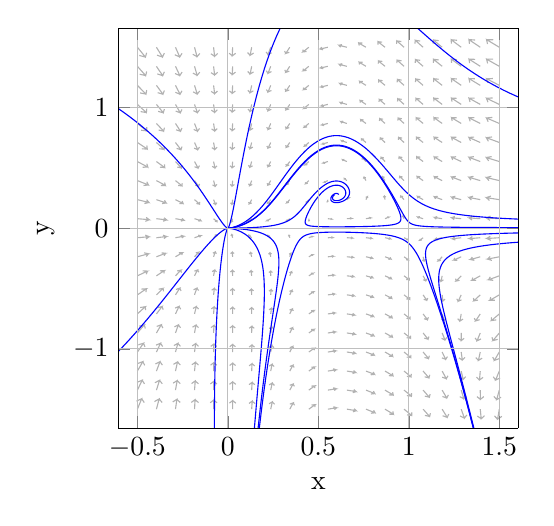
\begin{tikzpicture}
\begin{axis}[%
width=2in,
height=2in,
unbounded coords=jump,
view={0}{90},
scale only axis,
xmin=-0.605263157894737,
xmax=1.60526315789474,
xlabel={x},
xmajorgrids,
ymin=-1.65789473684211,
ymax=1.65789473684211,
ylabel={y},
ymajorgrids,
zmin=-1,
zmax=1
]
\addplot [color=white!70!black,solid,forget plot]
  table[row sep=crcr]{-0.5	-1.5\\
-0.47641083260371	-1.4135063862136\\
-0.505110986269196	-1.43355717850045\\
-0.47641083260371	-1.4135063862136\\
-0.461864179375997	-1.44535176219859\\
nan	0\\
-0.5	-1.34210526315789\\
-0.47349101707077	-1.25948559969513\\
-0.502098627815231	-1.27764425300165\\
-0.47349101707077	-1.25948559969513\\
-0.460788796083847	-1.29089874446627\\
nan	0\\
-0.5	-1.18421052631579\\
-0.470125214101787	-1.10596703943952\\
-0.498648521590319	-1.12197138902785\\
-0.470125214101787	-1.10596703943952\\
-0.459526778152183	-1.13690878197695\\
nan	0\\
-0.5	-1.02631578947368\\
-0.466217991532836	-0.953121437794829\\
-0.494651181992699	-0.966634241181695\\
-0.466217991532836	-0.953121437794829\\
-0.458054006153272	-0.983525245415277\\
nan	0\\
-0.5	-0.868421052631579\\
-0.461668583776836	-0.801202192298205\\
-0.489972723727129	-0.811784996342426\\
-0.461668583776836	-0.801202192298205\\
-0.456363293560442	-0.830950704454008\\
nan	0\\
-0.5	-0.710526315789474\\
-0.456405183360008	-0.650583442909484\\
-0.484469346572003	-0.657667600613483\\
-0.456405183360008	-0.650583442909484\\
-0.454497910132008	-0.679465008933479\\
nan	0\\
-0.5	-0.552631578947368\\
-0.450477212300549	-0.501788183575932\\
-0.478044897453244	-0.504660505262501\\
-0.450477212300549	-0.501788183575932\\
-0.452623199767526	-0.529421899112226\\
nan	0\\
-0.5	-0.394736842105263\\
-0.444248189328464	-0.355424667913796\\
-0.470801776077792	-0.353280367503352\\
-0.444248189328464	-0.355424667913796\\
-0.451145688982058	-0.38115627283912\\
nan	0\\
-0.5	-0.236842105263158\\
-0.438635224669077	-0.211841641239449\\
-0.463294773274281	-0.204000586613831\\
-0.438635224669077	-0.211841641239449\\
-0.450794541262427	-0.234682974279292\\
nan	0\\
-0.5	-0.0789473684210527\\
-0.434994079557102	-0.0704346883630541\\
-0.456624025704471	-0.0567370122697292\\
-0.434994079557102	-0.0704346883630541\\
-0.452367685675472	-0.0892399724911781\\
nan	0\\
-0.5	0.0789473684210527\\
-0.434204163301337	0.0706283545855895\\
-0.45186316085207	0.0895730179108942\\
-0.434204163301337	0.0706283545855895\\
-0.456022667769802	0.0566750995615627\\
nan	0\\
-0.5	0.236842105263158\\
-0.435858216197989	0.21332345120242\\
-0.449221087823408	0.236414493371144\\
-0.435858216197989	0.21332345120242\\
-0.460980414853776	0.204343601470139\\
nan	0\\
-0.5	0.394736842105263\\
-0.438802878688591	0.358544996168408\\
-0.4481140535978	0.384701830277317\\
-0.438802878688591	0.358544996168408\\
-0.466209976566227	0.354103269621613\\
nan	0\\
-0.5	0.552631578947368\\
-0.442078995927557	0.50617410693093\\
-0.44784092914518	0.534591599553972\\
-0.442078995927557	0.50617410693093\\
-0.4710696651534	0.50563109751775\\
nan	0\\
-0.5	0.710526315789473\\
-0.445190436801902	0.655716752591375\\
-0.447930914961807	0.685862012350329\\
-0.445190436801902	0.655716752591375\\
-0.475335696560856	0.65845723075128\\
nan	0\\
-0.5	0.868421052631579\\
-0.447958744216589	0.806685837437533\\
-0.448137317153101	0.838216715941599\\
-0.447958744216589	0.806685837437533\\
-0.479004924750124	0.812196088049894\\
nan	0\\
-0.5	1.02631578947368\\
-0.450356781872545	0.958706454309626\\
-0.448347413519767	0.991400059390707\\
-0.450356781872545	0.958706454309626\\
-0.482152081101796	0.96657845032698\\
nan	0\\
-0.5	1.18421052631579\\
-0.452415069618617	1.11151132712201\\
-0.448515748934587	1.14521731947549\\
-0.452415069618617	1.11151132712201\\
-0.484865348531477	1.1214248542848\\
nan	0\\
-0.5	1.34210526315789\\
-0.454180063589301	1.26491311803356\\
-0.448628008231428	1.29952574567354\\
-0.454180063589301	1.26491311803356\\
-0.487224080793593	1.27661577746819\\
nan	0\\
-0.5	1.5\\
-0.455697948128533	1.41877957156898\\
-0.448683456582218	1.45422121306615\\
-0.455697948128533	1.41877957156898\\
-0.489293670797729	1.43207018713042\\
nan	0\\
-0.394736842105263	-1.5\\
-0.37996238846352	-1.41518332372549\\
-0.405598893624669	-1.43693471319741\\
-0.37996238846352	-1.41518332372549\\
-0.363190555487416	-1.44432194001828\\
nan	0\\
-0.394736842105263	-1.34210526315789\\
-0.377752814374384	-1.26072190830021\\
-0.40319386140807	-1.28089090782479\\
-0.377752814374384	-1.26072190830021\\
-0.362502183979226	-1.28938292169023\\
nan	0\\
-0.394736842105263	-1.18421052631579\\
-0.37516099893472	-1.10664871738741\\
-0.400424204117978	-1.12502329927329\\
-0.37516099893472	-1.10664871738741\\
-0.361643299653788	-1.13481122085856\\
nan	0\\
-0.394736842105263	-1.02631578947368\\
-0.372072893195111	-0.95309633431987\\
-0.39717694165661	-0.969396183638476\\
-0.372072893195111	-0.95309633431987\\
-0.360567214079703	-0.980728158093552\\
nan	0\\
-0.394736842105263	-0.868421052631579\\
-0.368333114515262	-0.800275110551695\\
-0.393290718312234	-0.81411796127816\\
-0.368333114515262	-0.800275110551695\\
-0.359217747272291	-0.82731982507316\\
nan	0\\
-0.394736842105263	-0.710526315789474\\
-0.363740068493648	-0.648534686683423\\
-0.388537007853645	-0.659382982012335\\
-0.363740068493648	-0.648534686683423\\
-0.35754119330062	-0.674881368818142\\
nan	0\\
-0.394736842105263	-0.552631578947368\\
-0.3580786205328	-0.498474792837053\\
-0.382615283532118	-0.505557273277032\\
-0.3580786205328	-0.498474792837053\\
-0.35553689047696	-0.523886384063264\\
nan	0\\
-0.394736842105263	-0.394736842105263\\
-0.351302977074701	-0.351096380626598\\
-0.375243251953536	-0.353330052812557\\
-0.351302977074701	-0.351096380626598\\
-0.353423021214203	-0.375046985327838\\
nan	0\\
-0.394736842105263	-0.236842105263158\\
-0.344127193063746	-0.207725002506188\\
-0.366589363465444	-0.2038077210729\\
-0.344127193063746	-0.207725002506188\\
-0.352030812086959	-0.229112545593658\\
nan	0\\
-0.394736842105263	-0.0789473684210527\\
-0.338851160888191	-0.0686978545676049\\
-0.358179243716674	-0.0578012884193711\\
-0.338851160888191	-0.0686978545676049\\
-0.35305448678995	-0.0857441290279073\\
nan	0\\
-0.394736842105263	0.0789473684210527\\
-0.337998800539597	0.0689769105173429\\
-0.352527598533369	0.0861525582798725\\
-0.337998800539597	0.0689769105173429\\
-0.357512827485224	0.0577835374970392\\
nan	0\\
-0.394736842105263	0.236842105263158\\
-0.340883998419798	0.209591908690893\\
-0.350227302382372	0.231230178583939\\
-0.340883998419798	0.209591908690893\\
-0.363852400668504	0.204303756741206\\
nan	0\\
-0.394736842105263	0.394736842105263\\
-0.344989523250446	0.354402088886105\\
-0.349830030602101	0.378939344565557\\
-0.344989523250446	0.354402088886105\\
-0.36999740721168	0.354065685138148\\
nan	0\\
-0.394736842105263	0.552631578947368\\
-0.348857307808933	0.502489237486201\\
-0.350085582732541	0.529001823498634\\
-0.348857307808933	0.502489237486201\\
-0.375156753463124	0.506062056350469\\
nan	0\\
-0.394736842105263	0.710526315789473\\
-0.352098376296392	0.652759282610814\\
-0.350448157744388	0.68074900901663\\
-0.352098376296392	0.652759282610814\\
-0.379331674333718	0.659429776112194\\
nan	0\\
-0.394736842105263	0.868421052631579\\
-0.354729091010869	0.804465319083232\\
-0.350742482952101	0.833653976921334\\
-0.354729091010869	0.804465319083232\\
-0.382720349726274	0.813650101374137\\
nan	0\\
-0.394736842105263	1.02631578947368\\
-0.356858668071961	0.957148302738045\\
-0.350930248598042	0.987368092267062\\
-0.356858668071961	0.957148302738045\\
-0.385513991965862	0.968429005250411\\
nan	0\\
-0.394736842105263	1.18421052631579\\
-0.358595346578458	1.11052537655987\\
-0.35101650779752	1.14166629536835\\
-0.358595346578458	1.11052537655987\\
-0.387859082675479	1.12359554760495\\
nan	0\\
-0.394736842105263	1.34210526315789\\
-0.360026436139421	1.26441631162731\\
-0.351017320046526	1.29640059857794\\
-0.360026436139421	1.26441631162731\\
-0.38986179581182	1.27904539559502\\
nan	0\\
-0.394736842105263	1.5\\
-0.361218467743771	1.41870155832527\\
-0.350949369633536	1.45147068441806\\
-0.361218467743771	1.41870155832527\\
-0.391598590470902	1.43471149723731\\
nan	0\\
-0.289473684210526	-1.5\\
-0.281635491860239	-1.41771718776622\\
-0.304557652623771	-1.44044248334878\\
-0.281635491860239	-1.41771718776622\\
-0.26341624650688	-1.44436157952392\\
nan	0\\
-0.289473684210526	-1.34210526315789\\
-0.280136373703685	-1.26294356788399\\
-0.302727990674215	-1.28435774883945\\
-0.280136373703685	-1.26294356788399\\
-0.26314714303726	-1.28902640409287\\
nan	0\\
-0.289473684210526	-1.18421052631579\\
-0.278363139659717	-1.10847253816326\\
-0.300630800063092	-1.12841629847132\\
-0.278363139659717	-1.10847253816326\\
-0.262761805986828	-1.13397157074672\\
nan	0\\
-0.289473684210526	-1.02631578947368\\
-0.276219940622711	-0.954396513290372\\
-0.298175882744884	-0.972658860248412\\
-0.276219940622711	-0.954396513290372\\
-0.262216244653228	-0.97928573204232\\
nan	0\\
-0.289473684210526	-0.868421052631579\\
-0.27356066310702	-0.800862598559267\\
-0.29522418295615	-0.817151879505084\\
-0.27356066310702	-0.800862598559267\\
-0.261444955919994	-0.825108390056837\\
nan	0\\
-0.289473684210526	-0.710526315789474\\
-0.270155087455032	-0.648124513147481\\
-0.291551117142179	-0.662015404751205\\
-0.270155087455032	-0.648124513147481\\
-0.260350215821182	-0.671674703128952\\
nan	0\\
-0.289473684210526	-0.552631578947368\\
-0.265635649833881	-0.496664777789624\\
-0.286778760436311	-0.507495309542786\\
-0.265635649833881	-0.496664777789624\\
-0.258795359857439	-0.519414326731109\\
nan	0\\
-0.289473684210526	-0.394736842105263\\
-0.259462399248792	-0.347501578391064\\
-0.280274600665862	-0.35416933626489\\
-0.259462399248792	-0.347501578391064\\
-0.256656968808763	-0.369174978745757\\
nan	0\\
-0.289473684210526	-0.236842105263158\\
-0.251285893355132	-0.202867750433554\\
-0.271235819319151	-0.203513109168586\\
-0.251285893355132	-0.202867750433554\\
-0.254248641904349	-0.222607004596283\\
nan	0\\
-0.289473684210526	-0.0789473684210527\\
-0.243391949892726	-0.0660296246577139\\
-0.260445906128901	-0.0583845142072654\\
-0.243391949892726	-0.0660296246577139\\
-0.253987034247231	-0.0814253813661657\\
nan	0\\
-0.289473684210526	0.0789473684210527\\
-0.242450302495155	0.0664497484441132\\
-0.253432912015532	0.0819548798660378\\
-0.242450302495155	0.0664497484441132\\
-0.259681722004001	0.0584431890083522\\
nan	0\\
-0.289473684210526	0.236842105263158\\
-0.247420331903556	0.204966224543462\\
-0.252067367415723	0.225042326836113\\
-0.247420331903556	0.204966224543462\\
-0.268005307775571	0.204015650682628\\
nan	0\\
-0.289473684210526	0.394736842105263\\
-0.252592631562048	0.35033521486968\\
-0.252556540547696	0.372875966202475\\
-0.252592631562048	0.35033521486968\\
-0.274757354165487	0.354435439878235\\
nan	0\\
-0.289473684210526	0.552631578947368\\
-0.256508734617232	0.499564841074339\\
-0.253131535026963	0.523726099834571\\
-0.256508734617232	0.499564841074339\\
-0.279664903963477	0.507243625037924\\
nan	0\\
-0.289473684210526	0.710526315789473\\
-0.259361493284075	0.650880525007171\\
-0.253483702866435	0.676302309973475\\
-0.259361493284075	0.650880525007171\\
-0.283306598257586	0.661246214510249\\
nan	0\\
-0.289473684210526	0.868421052631579\\
-0.261475022960115	0.803430425203816\\
-0.253626964478298	0.829927278744748\\
-0.261475022960115	0.803430425203816\\
-0.286122278192179	0.815927948119542\\
nan	0\\
-0.289473684210526	1.02631578947368\\
-0.263081874551491	0.956781802564269\\
-0.253615920721848	0.984239951051853\\
-0.263081874551491	0.956781802564269\\
-0.288382914176555	0.971044046222335\\
nan	0\\
-0.289473684210526	1.18421052631579\\
-0.264333650112543	1.11069378489694\\
-0.253496474987226	1.13903381584709\\
-0.264333650112543	1.11069378489694\\
-0.29025484569665	1.1264637987981\\
nan	0\\
-0.289473684210526	1.34210526315789\\
-0.265329372815495	1.26502073742608\\
-0.253301534801052	1.29418217299439\\
-0.265329372815495	1.26502073742608\\
-0.291843797666957	1.28211001729687\\
nan	0\\
-0.289473684210526	1.5\\
-0.266135315067722	1.41966841521984\\
-0.253053929615524	1.44960248293959\\
-0.266135315067722	1.41966841521984\\
-0.293219722005602	1.43793329836819\\
nan	0\\
-0.184210526315789	-1.5\\
-0.181214997809328	-1.42090010661068\\
-0.201888629708596	-1.44388119250086\\
-0.181214997809328	-1.42090010661068\\
-0.162338683013937	-1.44537895675409\\
nan	0\\
-0.184210526315789	-1.34210526315789\\
-0.180353968147875	-1.26591290891026\\
-0.200559024160158	-1.28780647564257\\
-0.180353968147875	-1.26591290891026\\
-0.162462847036341	-1.28973475472653\\
nan	0\\
-0.184210526315789	-1.18421052631579\\
-0.179334784131361	-1.11117758386014\\
-0.199055742400602	-1.13186853105073\\
-0.179334784131361	-1.11117758386014\\
-0.162539271172777	-1.13430640214294\\
nan	0\\
-0.184210526315789	-1.02631578947368\\
-0.178098434495069	-0.956760033358042\\
-0.197321001070196	-0.976098737237554\\
-0.178098434495069	-0.956760033358042\\
-0.162543123012374	-0.979154783147915\\
nan	0\\
-0.184210526315789	-0.868421052631579\\
-0.176550347526692	-0.802760268796926\\
-0.195263597122084	-0.820543459250047\\
-0.176550347526692	-0.802760268796926\\
-0.162433205204758	-0.824373548644596\\
nan	0\\
-0.184210526315789	-0.710526315789474\\
-0.174528404728302	-0.649343087632827\\
-0.19272884824371	-0.665277525682949\\
-0.174528404728302	-0.649343087632827\\
-0.162137234165386	-0.670118586476693\\
nan	0\\
-0.184210526315789	-0.552631578947368\\
-0.171729999342212	-0.496814245831734\\
-0.189428490713194	-0.51043931402303\\
-0.171729999342212	-0.496814245831734\\
-0.161519824155377	-0.516679577509819\\
nan	0\\
-0.184210526315789	-0.394736842105263\\
-0.167529788535354	-0.345851574345003\\
-0.18475532680955	-0.356346970227972\\
-0.167529788535354	-0.345851574345003\\
-0.16031269292942	-0.36468733911819\\
nan	0\\
-0.184210526315789	-0.236842105263158\\
-0.160551235052571	-0.198414421059961\\
-0.177255943482336	-0.204027903505115\\
-0.160551235052571	-0.198414421059961\\
-0.158042101380737	-0.215857549136725\\
nan	0\\
-0.184210526315789	-0.0789473684210527\\
-0.149620588768282	-0.061547916893513\\
-0.164347432914419	-0.0581202679648981\\
-0.149620588768282	-0.061547916893513\\
-0.155647707150649	-0.0754152367386517\\
nan	0\\
-0.184210526315789	0.0789473684210527\\
-0.148511435634152	0.0621788059986676\\
-0.155029022233047	0.0761341473957924\\
-0.148511435634152	0.0621788059986676\\
-0.16341330344424	0.0582846020549739\\
nan	0\\
-0.184210526315789	0.236842105263158\\
-0.156379838556385	0.200059342869659\\
-0.155533354285832	0.21805184352756\\
-0.156379838556385	0.200059342869659\\
-0.173924735482581	0.204136499647858\\
nan	0\\
-0.184210526315789	0.394736842105263\\
-0.161404218105338	0.347436725955968\\
-0.15642108153115	0.36732833785337\\
-0.161404218105338	0.347436725955968\\
-0.180071139605797	0.355925183748144\\
nan	0\\
-0.184210526315789	0.552631578947368\\
-0.164372007131723	0.498210214790303\\
-0.156718221847677	0.519496253833439\\
-0.164372007131723	0.498210214790303\\
-0.183928903926209	0.509576994241406\\
nan	0\\
-0.184210526315789	0.710526315789473\\
-0.166273695606753	0.650574523891855\\
-0.156666796845059	0.6730442691384\\
-0.166273695606753	0.650574523891855\\
-0.186642692793868	0.664075853783881\\
nan	0\\
-0.184210526315789	0.868421052631579\\
-0.16757976969438	0.803861292977213\\
-0.156429056767211	0.827386910028875\\
-0.16757976969438	0.803861292977213\\
-0.188708936594394	0.81907153171817\\
nan	0\\
-0.184210526315789	1.02631578947368\\
-0.168523537312171	0.957757630549545\\
-0.156090094282222	0.982246825477691\\
-0.168523537312171	0.957757630549545\\
-0.190369173744291	0.974403330975882\\
nan	0\\
-0.184210526315789	1.18421052631579\\
-0.16923141967686	1.112091732277\\
-0.155695453158841	1.13747214714837\\
-0.16923141967686	1.112091732277\\
-0.191754850178237	1.1299825938289\\
nan	0\\
-0.184210526315789	1.34210526315789\\
-0.169777412846202	1.26675843031802\\
-0.155270638677109	1.29297075853738\\
-0.169777412846202	1.26675843031802\\
-0.192944055097048	1.28575420180258\\
nan	0\\
-0.184210526315789	1.5\\
-0.170207607753374	1.42168819021067\\
-0.154830530874766	1.44868246278807\\
-0.170207607753374	1.42168819021067\\
-0.193986435769431	1.44168100350686\\
nan	0\\
-0.0789473684210527	-1.5\\
-0.0785570364738179	-1.42457523464409\\
-0.0975303273969665	-1.44710508126405\\
-0.0785570364738179	-1.42457523464409\\
-0.0598179447190102	-1.44730024723767\\
nan	0\\
-0.0789473684210527	-1.34210526315789\\
-0.0782287354891096	-1.26942740302374\\
-0.0966137904022319	-1.291051102831\\
-0.0782287354891096	-1.26942740302374\\
-0.060274860335153	-1.29141041929697\\
nan	0\\
-0.0789473684210527	-1.18421052631579\\
-0.0778420315664336	-1.114506050398\\
-0.0955997516022657	-1.13514105895968\\
-0.0778420315664336	-1.114506050398\\
-0.0607475136433729	-1.13569372738699\\
nan	0\\
-0.0789473684210527	-1.02631578947368\\
-0.0773748898514188	-0.959865014056916\\
-0.0944593272765009	-0.979407127039538\\
-0.0773748898514188	-0.959865014056916\\
-0.061233939568117	-0.980193366324355\\
nan	0\\
-0.0789473684210527	-0.868421052631579\\
-0.0767914467693066	-0.805582345979984\\
-0.0931478999277292	-0.823894977562526\\
-0.0767914467693066	-0.805582345979984\\
-0.0617285466019316	-0.824972938388399\\
nan	0\\
-0.0789473684210527	-0.710526315789474\\
-0.0760284948155699	-0.651778658067445\\
-0.0915910713277219	-0.668673236982683\\
-0.0760284948155699	-0.651778658067445\\
-0.0622172424667076	-0.670132673785424\\
nan	0\\
-0.0789473684210527	-0.552631578947368\\
-0.0749615828252039	-0.498658316541704\\
-0.0896506341053747	-0.513853848864441\\
-0.0749615828252039	-0.498658316541704\\
-0.0626640029025424	-0.515846741662365\\
nan	0\\
-0.0789473684210527	-0.394736842105263\\
-0.0733016060035223	-0.346622225674919\\
-0.0870239888363674	-0.35964516999964\\
-0.0733016060035223	-0.346622225674919\\
-0.0629666806211954	-0.362468051208405\\
nan	0\\
-0.0789473684210527	-0.236842105263158\\
-0.0701646777950382	-0.196705918704373\\
-0.0828335316225387	-0.206551102015505\\
-0.0701646777950382	-0.196705918704373\\
-0.0627654383431463	-0.210942447328512\\
nan	0\\
-0.0789473684210527	-0.0789473684210527\\
-0.061122586945705	-0.0544032451648296\\
-0.0726060522023651	-0.0573102867728596\\
-0.061122586945705	-0.0544032451648296\\
-0.0603339905742536	-0.0662226775105334\\
nan	0\\
-0.0789473684210527	0.0789473684210527\\
-0.0598431014019969	0.054947082176201\\
-0.0595743099465007	0.0669232348044204\\
-0.0598431014019969	0.054947082176201\\
-0.0715744530689266	0.0573711012948926\\
nan	0\\
-0.0789473684210527	0.236842105263158\\
-0.0674920517657032	0.197147975495587\\
-0.0610051143204154	0.211920043589696\\
-0.0674920517657032	0.197147975495587\\
-0.0808521792042007	0.206192385262021\\
nan	0\\
-0.0789473684210527	0.394736842105263\\
-0.0700067823260557	0.346953639927249\\
-0.0607431576100512	0.363523747104402\\
-0.0700067823260557	0.346953639927249\\
-0.0846347586990584	0.359053454056904\\
nan	0\\
-0.0789473684210527	0.552631578947368\\
-0.0712346067662408	0.4989270936748\\
-0.0601223139445424	0.516966629670274\\
-0.0712346067662408	0.4989270936748\\
-0.0869745565808263	0.513110248842868\\
nan	0\\
-0.0789473684210527	0.710526315789473\\
-0.0719571419294164	0.652007376063097\\
-0.0594244749453131	0.671310614603919\\
-0.0719571419294164	0.652007376063097\\
-0.0886839448085015	0.667815501358101\\
nan	0\\
-0.0789473684210527	0.868421052631579\\
-0.0724282395229727	0.805783050414496\\
-0.058724477638126	0.826204233304141\\
-0.0724282395229727	0.805783050414496\\
-0.0900434787466674	0.822944668855101\\
nan	0\\
-0.0789473684210527	1.02631578947368\\
-0.0727555952191575	0.960044889395758\\
-0.0580454021602445	0.98147410271961\\
-0.0727555952191575	0.960044889395758\\
-0.0911808521992075	0.978378216118662\\
nan	0\\
-0.0789473684210527	1.18421052631579\\
-0.0729929448141193	1.11466974362554\\
-0.0573940762236371	1.13702058433435\\
-0.0729929448141193	1.11466974362554\\
-0.0921644675687616	1.13404337253088\\
nan	0\\
-0.0789473684210527	1.34210526315789\\
-0.0731701913755875	1.26957810559435\\
-0.0567715550983416	1.29278054712478\\
-0.0731701913755875	1.26957810559435\\
-0.0930351338801125	1.28989195860205\\
nan	0\\
-0.0789473684210527	1.5\\
-0.0733053359803532	1.42471524105131\\
-0.05617675597539	1.44871117684609\\
-0.0733053359803532	1.42471524105131\\
-0.093819135449736	1.44589016062574\\
nan	0\\
0.0263157894736842	-1.5\\
0.0265036495684208	-1.42869350288305\\
0.00862066726076205	-1.45003848699445\\
0.0265036495684208	-1.42869350288305\\
0.0442739158192376	-1.45013241704182\\
nan	0\\
0.0263157894736842	-1.34210526315789\\
0.0264068659152086	-1.27339394294185\\
0.00920171292874035	-1.29398456989628\\
0.0264068659152086	-1.27339394294185\\
0.0435573730367621	-1.29403010811705\\
nan	0\\
0.0263157894736842	-1.18421052631579\\
0.0262938675636125	-1.11830690021468\\
0.00982453761135546	-1.13808346852253\\
0.0262938675636125	-1.11830690021468\\
0.0427763506619125	-1.13807250756749\\
nan	0\\
0.0263157894736842	-1.02631578947368\\
0.0261586449988793	-0.963482115783002\\
0.0104973699186503	-0.982371504008908\\
0.0261586449988793	-0.963482115783002\\
0.0419142067639912	-0.982292931771506\\
nan	0\\
0.0263157894736842	-0.868421052631579\\
0.0259914347082147	-0.80899108550964\\
0.0112312493573708	-0.826901164337589\\
0.0259914347082147	-0.80899108550964\\
0.0409462329183403	-0.826738986954854\\
nan	0\\
0.0263157894736842	-0.710526315789474\\
0.0257750338070731	-0.654942796285992\\
0.012041380631186	-0.671753041053689\\
0.0257750338070731	-0.654942796285992\\
0.0398331403829268	-0.671482663220384\\
nan	0\\
0.0263157894736842	-0.552631578947368\\
0.0254754673837997	-0.501517665645041\\
0.0129490856851833	-0.517061920158211\\
0.0254754673837997	-0.501517665645041\\
0.0385060423363469	-0.516641759113268\\
nan	0\\
0.0263157894736842	-0.394736842105263\\
0.0250128820368633	-0.349054201558039\\
0.0139830941311035	-0.363084720581411\\
0.0250128820368633	-0.349054201558039\\
0.0368244144047157	-0.362433266863001\\
nan	0\\
0.0263157894736842	-0.236842105263158\\
0.0241325222265895	-0.198342655671296\\
0.0151626400027525	-0.210438307360628\\
0.0241325222265895	-0.198342655671296\\
0.0344123647986833	-0.209346673737081\\
nan	0\\
0.0263157894736842	-0.0789473684210527\\
0.0211011021798004	-0.0525639383258573\\
0.0160696508441667	-0.0617826391778869\\
0.0211011021798004	-0.0525639383258573\\
0.0292613658917644	-0.059175295530945\\
nan	0\\
0.0263157894736842	0.0789473684210527\\
0.0203969672994594	0.0526617056844847\\
0.0287440296358688	0.0590676989618989\\
0.0203969672994594	0.0526617056844847\\
0.0156011982675849	0.0620271100490113\\
nan	0\\
0.0263157894736842	0.236842105263158\\
0.023077073334707	0.198392149776282\\
0.0336611770481191	0.2091174573876\\
0.023077073334707	0.198392149776282\\
0.0144361993046812	0.210736815457089\\
nan	0\\
0.0263157894736842	0.394736842105263\\
0.0237575432506286	0.349089559555452\\
0.0359368377549981	0.362144182764631\\
0.0237575432506286	0.349089559555452\\
0.0131131964800925	0.363423305876159\\
nan	0\\
0.0263157894736842	0.552631578947368\\
0.0240699059814971	0.501545951876913\\
0.037515077796767	0.516310169125003\\
0.0240699059814971	0.501545951876913\\
0.0119722642615394	0.517433110871096\\
nan	0\\
0.0263157894736842	0.710526315789473\\
0.0242461037608964	0.6549667305749\\
0.0387569057783761	0.671117184711075\\
0.0242461037608964	0.6549667305749\\
0.0109771131710893	0.672152027567469\\
nan	0\\
0.0263157894736842	0.868421052631579\\
0.024356438233924	0.809012027884936\\
0.0397964997925127	0.826344897498989\\
0.024356438233924	0.809012027884936\\
0.0100919874191913	0.827324573118869\\
nan	0\\
0.0263157894736842	1.02631578947368\\
0.02442984041603	0.963500853623099\\
0.0406993590959725	0.981873847113861\\
0.02442984041603	0.963500853623099\\
0.00929189117068005	0.982816821642688\\
nan	0\\
0.0263157894736842	1.18421052631579\\
0.0244804807964542	1.11832393456908\\
0.0415027213362997	1.13763108492379\\
0.0244804807964542	1.11832393456908\\
0.00855942546294663	1.1385487392624\\
nan	0\\
0.0263157894736842	1.34210526315789\\
0.0245161392167752	1.27340961451858\\
0.0422299464536767	1.29356839654615\\
0.0245161392167752	1.27340961451858\\
0.00788212213401911	1.2944682216746\\
nan	0\\
0.0263157894736842	1.5\\
0.0245414476074172	1.42870805504179\\
0.0428967364068494	1.44965205306269\\
0.0245414476074172	1.42870805504179\\
0.00725076392774519	1.45053922399582\\
nan	0\\
0.131578947368421	-1.5\\
0.134284520514481	-1.43338899646762\\
0.116820097687568	-1.45269590424082\\
0.134284520514481	-1.43338899646762\\
0.150125599453758	-1.45404869081385\\
nan	0\\
0.131578947368421	-1.34210526315789\\
0.13385671046949	-1.27791030642611\\
0.117124642356223	-1.29659935267038\\
0.13385671046949	-1.27791030642611\\
0.149222120722115	-1.29773823422091\\
nan	0\\
0.131578947368421	-1.18421052631579\\
0.133363357988785	-1.12263015164159\\
0.117432941134127	-1.14065816138876\\
0.133363357988785	-1.12263015164159\\
0.148223128471225	-1.14155036669894\\
nan	0\\
0.131578947368421	-1.02631578947368\\
0.132780970334952	-0.967595631977562\\
0.117740324070962	-0.984911173484766\\
0.132780970334952	-0.967595631977562\\
0.147100402819023	-0.985512184968031\\
nan	0\\
0.131578947368421	-0.868421052631579\\
0.132071667793742	-0.812875036683778\\
0.118037347679195	-0.829415661361788\\
0.132071667793742	-0.812875036683778\\
0.145810355653096	-0.829662021574449\\
nan	0\\
0.131578947368421	-0.710526315789474\\
0.131169309237903	-0.658573959886528\\
0.118304111701322	-0.674262076190041\\
0.131169309237903	-0.658573959886528\\
0.144280289652795	-0.674057257124782\\
nan	0\\
0.131578947368421	-0.552631578947368\\
0.129944854395178	-0.504871681356553\\
0.118495107889447	-0.519608173877109\\
0.129944854395178	-0.504871681356553\\
0.142375056684855	-0.518791127390487\\
nan	0\\
0.131578947368421	-0.394736842105263\\
0.12810120056573	-0.3521218432404\\
0.118490774890321	-0.365775779600532\\
0.12810120056573	-0.3521218432404\\
0.139798274322753	-0.364036906199186\\
nan	0\\
0.131578947368421	-0.236842105263158\\
0.124738845356861	-0.201252528335318\\
0.117893481728369	-0.21363942691656\\
0.124738845356861	-0.201252528335318\\
0.135688270192289	-0.21021937591078\\
nan	0\\
0.131578947368421	-0.0789473684210527\\
0.115515784139255	-0.0573895834841326\\
0.114945286873775	-0.0678727097725\\
0.115515784139255	-0.0573895834841326\\
0.125724179342235	-0.0598411281579172\\
nan	0\\
0.131578947368421	0.0789473684210527\\
0.1129384584221	0.0585453834319073\\
0.123631101353282	0.0600058566920705\\
0.1129384584221	0.0585453834319073\\
0.11343010885871	0.0693261011652312\\
nan	0\\
0.131578947368421	0.236842105263158\\
0.119103653673737	0.202258955037402\\
0.131492029338581	0.209515076681458\\
0.119103653673737	0.202258955037402\\
0.114200454225703	0.2157527235288\\
nan	0\\
0.131578947368421	0.394736842105263\\
0.121109258302889	0.352882836881116\\
0.134713666328586	0.362821616181978\\
0.121109258302889	0.352882836881116\\
0.113786663716512	0.368056460714743\\
nan	0\\
0.131578947368421	0.552631578947368\\
0.122020876334442	0.505490376101863\\
0.136673598356012	0.51724321919702\\
0.122020876334442	0.505490376101863\\
0.113102996933259	0.522022254714009\\
nan	0\\
0.131578947368421	0.710526315789473\\
0.122506274673824	0.659100987767474\\
0.138084408487703	0.672260418000425\\
0.122506274673824	0.659100987767474\\
0.112371744476703	0.676796754347723\\
nan	0\\
0.131578947368421	0.868421052631579\\
0.122783861829975	0.813337757648203\\
0.139193211237353	0.827663974758604\\
0.122783861829975	0.813337757648203\\
0.111651563745665	0.832061517527827\\
nan	0\\
0.131578947368421	1.02631578947368\\
0.122945737437829	0.968010458013102\\
0.140112033282152	0.983343754968629\\
0.122945737437829	0.968010458013102\\
0.110959367551861	0.987660359933925\\
nan	0\\
0.131578947368421	1.18421052631579\\
0.123037339028343	1.12300773096379\\
0.140900520368366	1.13923316748437\\
0.123037339028343	1.12300773096379\\
0.110299122692368	1.14350397165441\\
nan	0\\
0.131578947368421	1.34210526315789\\
0.123083594360655	1.27825796566398\\
0.141594024636465	1.29528831666021\\
0.123083594360655	1.27825796566398\\
0.109670375889506	1.29953599316409\\
nan	0\\
0.131578947368421	1.5\\
0.123099267300652	1.43371200951403\\
0.142215168942476	1.45147848664288\\
0.123099267300652	1.43371200951403\\
0.109071173699489	1.45571832667676\\
nan	0\\
0.236842105263158	-1.5\\
0.245449465471676	-1.43917709633078\\
0.227661531491817	-1.45527212737942\\
0.245449465471676	-1.43917709633078\\
0.258072983326425	-1.45957580748368\\
nan	0\\
0.236842105263158	-1.34210526315789\\
0.244767469636199	-1.28346230307092\\
0.227729120302542	-1.29907385000375\\
0.244767469636199	-1.28346230307092\\
0.257050600346032	-1.30303653219027\\
nan	0\\
0.236842105263158	-1.18421052631579\\
0.243994805706397	-1.12792487036689\\
0.227777581586201	-1.14302239204075\\
0.243994805706397	-1.12792487036689\\
0.25592040956065	-1.14659874226237\\
nan	0\\
0.236842105263158	-1.02631578947368\\
0.243100768162072	-0.972606629460491\\
0.2277958792891	-0.987154711739721\\
0.243100768162072	-0.972606629460491\\
0.254650459295696	-0.990284043189178\\
nan	0\\
0.236842105263158	-0.868421052631579\\
0.242036347229851	-0.817568260098192\\
0.227764876506496	-0.831525537366535\\
0.242036347229851	-0.817568260098192\\
0.25319127277319	-0.834122658349881\\
nan	0\\
0.236842105263158	-0.710526315789474\\
0.240716805723664	-0.662903825442061\\
0.227648772998659	-0.676221897431158\\
0.240716805723664	-0.662903825442061\\
0.251460018172366	-0.678159247661411\\
nan	0\\
0.236842105263158	-0.552631578947368\\
0.238978342703963	-0.508774194172716\\
0.227373125278058	-0.52139735024491\\
0.238978342703963	-0.508774194172716\\
0.249301817665385	-0.522465468965313\\
nan	0\\
0.236842105263158	-0.394736842105263\\
0.236447072602632	-0.355502916502988\\
0.226757101000221	-0.367371852348802\\
0.236447072602632	-0.355502916502988\\
0.246374063801358	-0.367174336018539\\
nan	0\\
0.236842105263158	-0.236842105263158\\
0.232005088742948	-0.203985480092202\\
0.225242037406272	-0.215051721773541\\
0.232005088742948	-0.203985480092202\\
0.24167034999175	-0.212633213513436\\
nan	0\\
0.236842105263158	-0.0789473684210527\\
0.220808977840046	-0.0596988061026462\\
0.220806775487378	-0.0694816566539461\\
0.220808977840046	-0.0596988061026462\\
0.230431056646581	-0.0614650929423901\\
nan	0\\
0.236842105263158	0.0789473684210527\\
0.216141577587343	0.0620387131045461\\
0.226578899719214	0.0619361777805444\\
0.216141577587343	0.0620387131045461\\
0.218124572060961	0.0722864416184517\\
nan	0\\
0.236842105263158	0.236842105263158\\
0.220471483379545	0.206442834314975\\
0.232982487681674	0.211469960128527\\
0.220471483379545	0.206442834314975\\
0.217782852207583	0.219655271070333\\
nan	0\\
0.236842105263158	0.394736842105263\\
0.221859016658794	0.357407254191312\\
0.235686340218591	0.364860358414406\\
0.221859016658794	0.357407254191312\\
0.217021546261615	0.372351902716588\\
nan	0\\
0.236842105263158	0.552631578947368\\
0.222350993916675	0.510333573595372\\
0.237272828658619	0.51940019736435\\
0.222350993916675	0.510333573595372\\
0.216123825982621	0.526645753037592\\
nan	0\\
0.236842105263158	0.710526315789473\\
0.222494863080993	0.664236157050791\\
0.238371575420313	0.674536394126855\\
0.222494863080993	0.664236157050791\\
0.215226496050972	0.681710015217937\\
nan	0\\
0.236842105263158	0.868421052631579\\
0.222476197245249	0.818739815335111\\
0.239206278974738	0.830052709519574\\
0.222476197245249	0.818739815335111\\
0.214365660326504	0.837235663528529\\
nan	0\\
0.236842105263158	1.02631578947368\\
0.222372989859202	0.973657849300799\\
0.23987820952361	0.985837952501675\\
0.222372989859202	0.973657849300799\\
0.213549239437167	0.993072510203653\\
nan	0\\
0.236842105263158	1.18421052631579\\
0.222222944140589	1.12888223465387\\
0.240440765392839	1.14182593187181\\
0.222222944140589	1.12888223465387\\
0.21277661956188	1.14913551243309\\
nan	0\\
0.236842105263158	1.34210526315789\\
0.22204611222781	1.28434413217545\\
0.240925192884026	1.29797347321134\\
0.22204611222781	1.28434413217545\\
0.212044627392803	1.30537146972902\\
nan	0\\
0.236842105263158	1.5\\
0.221853908266639	1.43999662504238\\
0.241351211104999	1.45425058828054\\
0.221853908266639	1.43999662504238\\
0.21134952362619	1.4617446867788\\
nan	0\\
0.342105263157895	-1.5\\
0.361194060273645	-1.44759788957935\\
0.342366893533758	-1.45854632342661\\
0.361194060273645	-1.44759788957935\\
0.368567948744082	-1.46809072198448\\
nan	0\\
0.342105263157895	-1.34210526315789\\
0.360314596622652	-1.2915676572285\\
0.342217395100875	-1.30217660564113\\
0.360314596622652	-1.2915676572285\\
0.367486198065574	-1.31128127237351\\
nan	0\\
0.342105263157895	-1.18421052631579\\
0.359345493647256	-1.13568654537177\\
0.342042429264442	-1.14593368203263\\
0.359345493647256	-1.13568654537177\\
0.366304419736453	-1.15455379727731\\
nan	0\\
0.342105263157895	-1.02631578947368\\
0.358260885954664	-0.979988628825454\\
0.341832408953576	-0.989847871320731\\
0.358260885954664	-0.979988628825454\\
0.364995989277691	-0.997925682719116\\
nan	0\\
0.342105263157895	-0.868421052631579\\
0.357021010570637	-0.824522546284067\\
0.341571659759936	-0.833963161335135\\
0.357021010570637	-0.824522546284067\\
0.363520912933692	-0.841421035041506\\
nan	0\\
0.342105263157895	-0.710526315789474\\
0.355559826009047	-0.669361838380832\\
0.34123233780154	-0.678347540890636\\
0.355559826009047	-0.669361838380832\\
0.361814576505861	-0.685074822316212\\
nan	0\\
0.342105263157895	-0.552631578947368\\
0.353754819461329	-0.514627161245309\\
0.340758848144784	-0.523116097480068\\
0.353754819461329	-0.514627161245309\\
0.359761056995814	-0.528940875631785\\
nan	0\\
0.342105263157895	-0.394736842105263\\
0.351336126048987	-0.360543473332291\\
0.340018524988416	-0.368493768241409\\
0.351336126048987	-0.360543473332291\\
0.357115209374903	-0.373109199686956\\
nan	0\\
0.342105263157895	-0.236842105263158\\
0.347495669869569	-0.20764610148997\\
0.33857954691277	-0.215057300944008\\
0.347495669869569	-0.20764610148997\\
0.353177548799364	-0.217752504299845\\
nan	0\\
0.342105263157895	-0.0789473684210527\\
0.337243767225271	-0.058861335669843\\
0.333680707817256	-0.0661025194783618\\
0.337243767225271	-0.058861335669843\\
0.343723724192861	-0.06367177151205\\
nan	0\\
0.342105263157895	0.0789473684210527\\
0.325452874212037	0.0629038629620041\\
0.334459467260556	0.0635538173632542\\
0.325452874212037	0.0629038629620041\\
0.326437714531032	0.0718800118361832\\
nan	0\\
0.342105263157895	0.236842105263158\\
0.325869906292706	0.210282937911846\\
0.33738030519009	0.214191848900942\\
0.325869906292706	0.210282937911846\\
0.324100721514434	0.222309527333537\\
nan	0\\
0.342105263157895	0.394736842105263\\
0.325133728937987	0.362468976158223\\
0.338292155690719	0.367906452387358\\
0.325133728937987	0.362468976158223\\
0.322158222717199	0.376392219497312\\
nan	0\\
0.342105263157895	0.552631578947368\\
0.324264851629858	0.516176950416365\\
0.33873063222102	0.522653236093657\\
0.324264851629858	0.516176950416365\\
0.320503317955519	0.531573441857675\\
nan	0\\
0.342105263157895	0.710526315789473\\
0.323412919943724	0.670676478508954\\
0.338983082228105	0.677958343889567\\
0.323412919943724	0.670676478508954\\
0.319058163587845	0.687304515496652\\
nan	0\\
0.342105263157895	0.868421052631579\\
0.322606749583633	0.825674311334159\\
0.339142988980266	0.833623705329819\\
0.322606749583633	0.825674311334159\\
0.317769618331556	0.84337296211695\\
nan	0\\
0.342105263157895	1.02631578947368\\
0.321849423544203	0.981019904733058\\
0.339250146613467	0.989544710251823\\
0.321849423544203	0.981019904733058\\
0.316602204243154	0.999672630058669\\
nan	0\\
0.342105263157895	1.18421052631579\\
0.321137651014794	1.13662449648181\\
0.339324442116218	1.14565840239623\\
0.321137651014794	1.13662449648181\\
0.315531427199229	1.15614220846778\\
nan	0\\
0.342105263157895	1.34210526315789\\
0.320466793173961	1.29243083520706\\
0.33937694115685	1.30192354609633\\
0.320466793173961	1.29243083520706\\
0.314539727181432	1.31274278108829\\
nan	0\\
0.342105263157895	1.5\\
0.319832303568561	1.44839958323028\\
0.339414295637791	1.45831146836386\\
0.319832303568561	1.44839958323028\\
0.313614087252932	1.46944794815853\\
nan	0\\
0.447368421052632	-1.5\\
0.4820315013467	-1.46274635175048\\
0.462319165196099	-1.46525667615182\\
0.4820315013467	-1.46274635175048\\
0.48094598932086	-1.48258821629885\\
nan	0\\
0.447368421052632	-1.34210526315789\\
0.480918709137947	-1.30627927723734\\
0.461897126232212	-1.30863950099217\\
0.480918709137947	-1.30627927723734\\
0.479810119192492	-1.32541464503483\\
nan	0\\
0.447368421052632	-1.18421052631579\\
0.479727511041905	-1.14993551942596\\
0.461451032322665	-1.15212824899559\\
0.479727511041905	-1.14993551942596\\
0.47858853576758	-1.16830779399023\\
nan	0\\
0.447368421052632	-1.02631578947368\\
0.478442665663628	-0.993745579618758\\
0.460977839816597	-0.995748081422487\\
0.478442665663628	-0.993745579618758\\
0.477262944744061	-1.01128520372798\\
nan	0\\
0.447368421052632	-0.868421052631579\\
0.477043684980649	-0.837754083378771\\
0.460474363489042	-0.839535358172609\\
0.477043684980649	-0.837754083378771\\
0.475807848115446	-0.854372990136618\\
nan	0\\
0.447368421052632	-0.710526315789474\\
0.475502105590438	-0.68203061692857\\
0.45993807551387	-0.68354590545239\\
0.475502105590438	-0.68203061692857\\
0.474185924944322	-0.697612747721293\\
nan	0\\
0.447368421052632	-0.552631578947368\\
0.473776867234044	-0.526693871557068\\
0.459369906532045	-0.527873072228805\\
0.473776867234044	-0.526693871557068\\
0.472338760227195	-0.541077295319512\\
nan	0\\
0.447368421052632	-0.394736842105263\\
0.471806565587003	-0.371975825136977\\
0.45878486798462	-0.37269459409387\\
0.471806565587003	-0.371975825136977\\
0.470165376468763	-0.384913666361055\\
nan	0\\
0.447368421052632	-0.236842105263158\\
0.469499882701652	-0.218449291735842\\
0.458262240825117	-0.218434270381782\\
0.469499882701652	-0.218449291735842\\
0.467458647588775	-0.229500001206292\\
nan	0\\
0.447368421052632	-0.0789473684210527\\
0.466745390234108	-0.0684800056573337\\
0.458315458788735	-0.0667759721910804\\
0.466745390234108	-0.0684800056573337\\
0.463549140170594	-0.0764644567818184\\
nan	0\\
0.447368421052632	0.0789473684210527\\
0.448954724893615	0.0618090661390504\\
0.452763409311821	0.067347132783897\\
0.448954724893615	0.0618090661390504\\
0.44419425817082	0.0665539808634051\\
nan	0\\
0.447368421052632	0.236842105263158\\
0.434782138194403	0.214178569789682\\
0.444223906920241	0.217831059717167\\
0.434782138194403	0.214178569789682\\
0.432892139183503	0.224124201146281\\
nan	0\\
0.447368421052632	0.394736842105263\\
0.4296609920177	0.368884183392367\\
0.441436385406404	0.372213123747503\\
0.4296609920177	0.368884183392367\\
0.428510056049956	0.381066838264968\\
nan	0\\
0.447368421052632	0.552631578947368\\
0.426324544512598	0.524212029992568\\
0.439742594713308	0.527476925544\\
0.426324544512598	0.524212029992568\\
0.425532820235908	0.537998863814017\\
nan	0\\
0.447368421052632	0.710526315789473\\
0.423766939160755	0.679927688677887\\
0.438497040506214	0.683206906338394\\
0.423766939160755	0.679927688677887\\
0.423197726950421	0.695007647284332\\
nan	0\\
0.447368421052632	0.868421052631579\\
0.421655696053635	0.835912745118246\\
0.437496590431667	0.839237056122497\\
0.421655696053635	0.835912745118246\\
0.421242436675001	0.852093418621995\\
nan	0\\
0.447368421052632	1.02631578947368\\
0.419837986483265	0.992097413138377\\
0.436651710937902	0.995480317396628\\
0.419837986483265	0.992097413138377\\
0.419542522770248	1.00924553468131\\
nan	0\\
0.447368421052632	1.18421052631579\\
0.418230051297422	1.14843681478477\\
0.435914990106739	1.15188433580527\\
0.418230051297422	1.14843681478477\\
0.41802813434123	1.16645352068288\\
nan	0\\
0.447368421052632	1.34210526315789\\
0.416780626082517	1.30490024101985\\
0.435258220108062	1.30841479891874\\
0.416780626082517	1.30490024101985\\
0.416655709039041	1.32370869640379\\
nan	0\\
0.447368421052632	1.5\\
0.415455856155832	1.4614656699072\\
0.434663208148073	1.46504782771084\\
0.415455856155832	1.4614656699072\\
0.415396043101672	1.48100411015924\\
nan	0\\
0.552631578947368	-1.5\\
0.601074545285542	-1.48798265269659\\
0.583537318558238	-1.47947711530307\\
0.601074545285542	-1.48798265269659\\
0.589545992209942	-1.50369859847216\\
nan	0\\
0.552631578947368	-1.34210526315789\\
0.59957883658951	-1.33063671879103\\
0.582627523205151	-1.32234046769055\\
0.59957883658951	-1.33063671879103\\
0.588361795388584	-1.34581409651162\\
nan	0\\
0.552631578947368	-1.18421052631579\\
0.597980788654813	-1.17334247783409\\
0.581659013622155	-1.16526558995174\\
0.597980788654813	-1.17334247783409\\
0.587093037863004	-1.18794019480546\\
nan	0\\
0.552631578947368	-1.02631578947368\\
0.596260749856716	-1.01611300734329\\
0.580621303051315	-1.00826654925507\\
0.596260749856716	-1.01611300734329\\
0.585722694116509	-1.03008113470975\\
nan	0\\
0.552631578947368	-0.868421052631579\\
0.594392174315028	-0.858967245929621\\
0.579500544029241	-0.851363239098293\\
0.594392174315028	-0.858967245929621\\
0.58422744738022	-0.872243536782123\\
nan	0\\
0.552631578947368	-0.710526315789474\\
0.592337736072131	-0.701934108841356\\
0.578277837197673	-0.694585231644601\\
0.592337736072131	-0.701934108841356\\
0.582573940671732	-0.714438310206982\\
nan	0\\
0.552631578947368	-0.552631578947368\\
0.59004207849095	-0.545060933477602\\
0.576926267260434	-0.537979502232637\\
0.59004207849095	-0.545060933477602\\
0.580711589995317	-0.556684752004428\\
nan	0\\
0.552631578947368	-0.394736842105263\\
0.587416714219484	-0.388433050104912\\
0.575405225637761	-0.381627903886988\\
0.587416714219484	-0.388433050104912\\
0.578557121637937	-0.399020471523046\\
nan	0\\
0.552631578947368	-0.236842105263158\\
0.584302937197869	-0.232227675617459\\
0.573647922311294	-0.225694164948543\\
0.584302937197869	-0.232227675617459\\
0.575955137134144	-0.241529844073794\\
nan	0\\
0.552631578947368	-0.0789473684210527\\
0.580350900903138	-0.0769077797573536\\
0.571525207150482	-0.0705898258675209\\
0.580350900903138	-0.0769077797573536\\
0.572545001482332	-0.0844494868454057\\
nan	0\\
0.552631578947368	0.0789473684210527\\
0.574283603535056	0.075662101158857\\
0.568609312974298	0.0820606874844375\\
0.574283603535056	0.075662101158857\\
0.566966679343201	0.0712346751905939\\
nan	0\\
0.552631578947368	0.236842105263158\\
0.550355601002206	0.220162438322181\\
0.555208311120999	0.224597343918183\\
0.550355601002206	0.220162438322181\\
0.54686847765051	0.225735332890764\\
nan	0\\
0.552631578947368	0.394736842105263\\
0.532613683415106	0.381228317495883\\
0.54199618322713	0.380276400995632\\
0.532613683415106	0.381228317495883\\
0.53524192092244	0.390285348761763\\
nan	0\\
0.552631578947368	0.552631578947368\\
0.526246406104816	0.53981378191306\\
0.537366407216158	0.537062827812714\\
0.526246406104816	0.53981378191306\\
0.530957508699004	0.55025541423399\\
nan	0\\
0.552631578947368	0.710526315789473\\
0.522026408545681	0.697660607718401\\
0.534424386683956	0.693869027539301\\
0.522026408545681	0.697660607718401\\
0.527991532648419	0.709171612740145\\
nan	0\\
0.552631578947368	0.868421052631579\\
0.518740761969286	0.85529865108037\\
0.532188607450513	0.850762667301212\\
0.518740761969286	0.85529865108037\\
0.525627406674908	0.867708075790253\\
nan	0\\
0.552631578947368	1.02631578947368\\
0.515997492263646	1.01286614873084\\
0.530350128454473	1.00774251928276\\
0.515997492263646	1.01286614873084\\
0.523625308083052	1.02605956262462\\
nan	0\\
0.552631578947368	1.18421052631579\\
0.513615732846814	1.17041079586241\\
0.528770419290326	1.16479675347328\\
0.513615732846814	1.17041079586241\\
0.521870554063635	1.18430467652356\\
nan	0\\
0.552631578947368	1.34210526315789\\
0.511495381768574	1.32795176272012\\
0.527374616031656	1.32191376355675\\
0.511495381768574	1.32795176272012\\
0.520297865812769	1.34248186214615\\
nan	0\\
0.552631578947368	1.5\\
0.509574518882822	1.48549736801268\\
0.526117294899016	1.47908389259274\\
0.509574518882822	1.48549736801268\\
0.518865978905355	1.50061242262501\\
nan	0\\
0.657894736842105	-1.5\\
0.70990958220661	-1.51275662074786\\
0.697494283784224	-1.49592592318238\\
0.70990958220661	-1.51275662074786\\
0.691115973410293	-1.52193334586463\\
nan	0\\
0.657894736842105	-1.34210526315789\\
0.708372386767932	-1.35425066429919\\
0.696265442075508	-1.33798763147534\\
0.708372386767932	-1.35425066429919\\
0.69019274150486	-1.36322645643826\\
nan	0\\
0.657894736842105	-1.18421052631579\\
0.706734695569892	-1.19568684891004\\
0.694951788600118	-1.18003396244982\\
0.706734695569892	-1.19568684891004\\
0.689213627302994	-1.20445394181371\\
nan	0\\
0.657894736842105	-1.02631578947368\\
0.704978094522638	-1.03705079502485\\
0.693536838606268	-1.02205945393936\\
0.704978094522638	-1.03705079502485\\
0.688169335830688	-1.04560113277963\\
nan	0\\
0.657894736842105	-0.868421052631579\\
0.703078009635492	-0.878321895600792\\
0.691998238539779	-0.864055824511682\\
0.703078009635492	-0.878321895600792\\
0.687047817055172	-0.886647460908375\\
nan	0\\
0.657894736842105	-0.710526315789474\\
0.701000396734066	-0.719469155450148\\
0.690304408681646	-0.706009888578955\\
0.701000396734066	-0.719469155450148\\
0.685832988851309	-0.727562718524936\\
nan	0\\
0.657894736842105	-0.552631578947368\\
0.698695698526265	-0.560442938634687\\
0.688408249942847	-0.547899290307451\\
0.698695698526265	-0.560442938634687\\
0.684502570099188	-0.568299771149531\\
nan	0\\
0.657894736842105	-0.394736842105263\\
0.696086606723984	-0.401156762324013\\
0.686234025814108	-0.389682818787919\\
0.696086606723984	-0.401156762324013\\
0.683024065704733	-0.408778753728858\\
nan	0\\
0.657894736842105	-0.236842105263158\\
0.693039181310449	-0.241440832222807\\
0.683645529709858	-0.231275103017826\\
0.693039181310449	-0.241440832222807\\
0.681346166230034	-0.248847325251998\\
nan	0\\
0.657894736842105	-0.0789473684210527\\
0.689275397839301	-0.0808954549997895\\
0.680348221184827	-0.0724658637768694\\
0.689275397839301	-0.0808954549997895\\
0.679374177895458	-0.0881561942754675\\
nan	0\\
0.657894736842105	0.0789473684210527\\
0.683948839815898	0.0817518186467296\\
0.675431496367341	0.0874240093224748\\
0.683948839815898	0.0817518186467296\\
0.67683372148018	0.0743969578355782\\
nan	0\\
0.657894736842105	0.236842105263158\\
0.67033506673683	0.251939047541853\\
0.662828732198739	0.250520047331926\\
0.67033506673683	0.251939047541853\\
0.670377203338087	0.244299882384563\\
nan	0\\
0.657894736842105	0.394736842105263\\
0.642565649818366	0.412372323873859\\
0.642755505483339	0.403249407587345\\
0.642565649818366	0.412372323873859\\
0.651573246367637	0.410913951099215\\
nan	0\\
0.657894736842105	0.552631578947368\\
0.632997717412971	0.568242010129435\\
0.636564215446194	0.557334625917532\\
0.632997717412971	0.568242010129435\\
0.644369431037228	0.569783135632099\\
nan	0\\
0.657894736842105	0.710526315789473\\
0.627640180305338	0.725668352378119\\
0.632931038119207	0.713562102267334\\
0.627640180305338	0.725668352378119\\
0.640502056413529	0.728689380535717\\
nan	0\\
0.657894736842105	0.868421052631579\\
0.623721158255016	0.883578298388181\\
0.630183920391992	0.870487730014428\\
0.623721158255016	0.883578298388181\\
0.637762543270293	0.887574519307972\\
nan	0\\
0.657894736842105	1.02631578947368\\
0.620549136448814	1.04167034124194\\
0.627914178624737	1.02772757561314\\
0.620549136448814	1.04167034124194\\
0.635591454508866	1.04640037580979\\
nan	0\\
0.657894736842105	1.18421052631579\\
0.617845306965728	1.19983977477999\\
0.62595282381259	1.18513864277164\\
0.617845306965728	1.19983977477999\\
0.633767448044692	1.20516335770983\\
nan	0\\
0.657894736842105	1.34210526315789\\
0.615467204913231	1.35804306272899\\
0.624211014599119	1.34265483987544\\
0.615467204913231	1.35804306272899\\
0.632179914384667	1.36386860583988\\
nan	0\\
0.657894736842105	1.5\\
0.613331204721655	1.51625988845792\\
0.622635292243311	1.50024103889043\\
0.613331204721655	1.51625988845792\\
0.630765236472269	1.52252280495065\\
nan	0\\
0.763157894736842	-1.5\\
0.813412614063011	-1.53006685720284\\
0.805852912565871	-1.50848312021045\\
0.813412614063011	-1.53006685720284\\
0.79081948396445	-1.53361047987353\\
nan	0\\
0.763157894736842	-1.34210526315789\\
0.812044571486744	-1.37081170781522\\
0.804555179626106	-1.34997810523055\\
0.812044571486744	-1.37081170781522\\
0.790201957297441	-1.3744214436055\\
nan	0\\
0.763157894736842	-1.18421052631579\\
0.810595441841339	-1.21142727601825\\
0.803168365135606	-1.19140286433139\\
0.810595441841339	-1.21142727601825\\
0.789559990284374	-1.21512163788364\\
nan	0\\
0.763157894736842	-1.02631578947368\\
0.80905184368262	-1.0518803149413\\
0.80167479036579	-1.03273747006457\\
0.80905184368262	-1.0518803149413\\
0.788892527631983	-1.05568444453746\\
nan	0\\
0.763157894736842	-0.868421052631579\\
0.807396267075298	-0.892122401707975\\
0.800050092642861	-0.873952403900442\\
0.807396267075298	-0.892122401707975\\
0.788199418104662	-0.89607159006967\\
nan	0\\
0.763157894736842	-0.710526315789474\\
0.805604830537789	-0.732079113364265\\
0.798258949191203	-0.715001540141591\\
0.805604830537789	-0.732079113364265\\
0.787482550403807	-0.736225008042064\\
nan	0\\
0.763157894736842	-0.552631578947368\\
0.803642794401919	-0.571627737058113\\
0.796246364030082	-0.55580766470862\\
0.803642794401919	-0.571627737058113\\
0.78674828497471	-0.576050114541159\\
nan	0\\
0.763157894736842	-0.394736842105263\\
0.801453603867813	-0.410545766045649\\
0.793917122113618	-0.39622916158079\\
0.801453603867813	-0.410545766045649\\
0.786012660143426	-0.415377016146276\\
nan	0\\
0.763157894736842	-0.236842105263158\\
0.798922867757266	-0.248372247085287\\
0.791075911306671	-0.235971961283542\\
0.798922867757266	-0.248372247085287\\
0.785310840395607	-0.253854447793754\\
nan	0\\
0.763157894736842	-0.0789473684210527\\
0.795698241487106	-0.0839542295067123\\
0.787187852733441	-0.0743170844934485\\
0.795698241487106	-0.0839542295067123\\
0.784684422190612	-0.0905872578685804\\
nan	0\\
0.763157894736842	0.0789473684210527\\
0.789687259219793	0.0861316422971254\\
0.77993238140589	0.0906087012550414\\
0.789687259219793	0.0861316422971254\\
0.783524518343926	0.0773440190135658\\
nan	0\\
0.763157894736842	0.236842105263158\\
0.770439365844252	0.261490303437092\\
0.762092874968546	0.255916211761764\\
0.770439365844252	0.261490303437092\\
0.774416974055513	0.252275476208059\\
nan	0\\
0.763157894736842	0.394736842105263\\
0.752134670273469	0.423440110049237\\
0.748265820626487	0.412073323550202\\
0.752134670273469	0.423440110049237\\
0.762617454598474	0.417584935781888\\
nan	0\\
0.763157894736842	0.552631578947368\\
0.743130200082013	0.582291846570162\\
0.741723441572763	0.568386842619617\\
0.743130200082013	0.582291846570162\\
0.75655357538416	0.578400689947031\\
nan	0\\
0.763157894736842	0.710526315789473\\
0.737524665561583	0.741151005412654\\
0.737558461908365	0.725555291231885\\
0.737524665561583	0.741151005412654\\
0.752870806719956	0.738371905819514\\
nan	0\\
0.763157894736842	0.868421052631579\\
0.733411083490545	0.900067947551901\\
0.734423403134354	0.88313717626423\\
0.733411083490545	0.900067947551901\\
0.750246850594514	0.898010581887378\\
nan	0\\
0.763157894736842	1.02631578947368\\
0.730116898248979	1.05898980601864\\
0.7318606930591	1.04092735193318\\
0.730116898248979	1.05898980601864\\
0.748197701331576	1.05744785017712\\
nan	0\\
0.763157894736842	1.18421052631579\\
0.727340454890819	1.21788944085811\\
0.729665958209046	1.19883140653391\\
0.727340454890819	1.21788944085811\\
0.746505415480205	1.21674012645692\\
nan	0\\
0.763157894736842	1.34210526315789\\
0.724922203779995	1.37675581737555\\
0.727730272512634	1.35680172837104\\
0.724922203779995	1.37675581737555\\
0.745055549621463	1.37591957384947\\
nan	0\\
0.763157894736842	1.5\\
0.722767690348456	1.53558548081487\\
0.725988381461255	1.51481228547331\\
0.722767690348456	1.53558548081487\\
0.743781121868688	1.5350073876675\\
nan	0\\
0.868421052631579	-1.5\\
0.915265148340423	-1.54244950760917\\
0.911824296530062	-1.51800363139921\\
0.915265148340423	-1.54244950760917\\
0.890599542725477	-1.54142567925363\\
nan	0\\
0.868421052631579	-1.34210526315789\\
0.913963210552666	-1.38279825336369\\
0.910473810727789	-1.35920481682168\\
0.913963210552666	-1.38279825336369\\
0.890127315624891	-1.38197589578222\\
nan	0\\
0.868421052631579	-1.18421052631579\\
0.912584985965295	-1.22298568614699\\
0.909029595922981	-1.2003121548642\\
0.912584985965295	-1.22298568614699\\
0.88964201600738	-1.22239412153106\\
nan	0\\
0.868421052631579	-1.02631578947368\\
0.911118907062435	-1.06297006726198\\
0.907473120180253	-1.04129932031778\\
0.911118907062435	-1.06297006726198\\
0.889145981286104	-1.06264824753321\\
nan	0\\
0.868421052631579	-0.868421052631579\\
0.909550635163399	-0.902689810562218\\
0.905778949886512	-0.882126787550071\\
0.909550635163399	-0.902689810562218\\
0.888644570921193	-0.902691578815981\\
nan	0\\
0.868421052631579	-0.710526315789474\\
0.907862272758897	-0.742048207352005\\
0.903910379611334	-0.722731334851416\\
0.907862272758897	-0.742048207352005\\
0.888149433830069	-0.742451944915075\\
nan	0\\
0.868421052631579	-0.552631578947368\\
0.906031405724124	-0.580879948455367\\
0.90181039217336	-0.563002849329831\\
0.906031405724124	-0.580879948455367\\
0.887686207419361	-0.581808025876104\\
nan	0\\
0.868421052631579	-0.394736842105263\\
0.904029419047204	-0.418865868019068\\
0.899379165600967	-0.40272506864102\\
0.904029419047204	-0.418865868019068\\
0.887314652644065	-0.420529251848833\\
nan	0\\
0.868421052631579	-0.236842105263158\\
0.901809190470753	-0.255262928322273\\
0.896397954883779	-0.241389646944745\\
0.901809190470753	-0.255262928322273\\
0.887187543354222	-0.258083715864332\\
nan	0\\
0.868421052631579	-0.0789473684210527\\
0.8990936693577	-0.0877200265106665\\
0.892085048862267	-0.077420074902252\\
0.8990936693577	-0.0877200265106665\\
0.88769871981746	-0.0927563832653128\\
nan	0\\
0.868421052631579	0.0789473684210527\\
0.889838284143242	0.0927186340712194\\
0.879970298277201	0.0939415622540851\\
0.889838284143242	0.0927186340712194\\
0.886855931102284	0.0832329464982537\\
nan	0\\
0.868421052631579	0.236842105263158\\
0.864592653219143	0.26659920978709\\
0.858301896911891	0.256714978576802\\
0.864592653219143	0.26659920978709\\
0.873180449173857	0.25862917828302\\
nan	0\\
0.868421052631579	0.394736842105263\\
0.852954833184526	0.427966923356248\\
0.849287178705895	0.414131344119189\\
0.852954833184526	0.427966923356248\\
0.865902219331388	0.421864453842716\\
nan	0\\
0.868421052631579	0.552631578947368\\
0.846642925259719	0.588347497217031\\
0.844247383903861	0.572188189893167\\
0.846642925259719	0.588347497217031\\
0.862105343038693	0.583077253579097\\
nan	0\\
0.868421052631579	0.710526315789473\\
0.842271935007946	0.748426673907423\\
0.840641580765548	0.73051928706613\\
0.842271935007946	0.748426673907423\\
0.859591759824523	0.743593845877947\\
nan	0\\
0.868421052631579	0.868421052631579\\
0.838874660019515	0.908296337368472\\
0.837769756618911	0.888947153794388\\
0.838874660019515	0.908296337368472\\
0.857707398987358	0.90372035010042\\
nan	0\\
0.868421052631579	1.02631578947368\\
0.836062407877345	1.06799917713797\\
0.835349154387543	1.04740449965013\\
0.836062407877345	1.06799917713797\\
0.856190848219687	1.06358382202725\\
nan	0\\
0.868421052631579	1.18421052631579\\
0.833642213161014	1.22756476574158\\
0.833237305145737	1.2058637840462\\
0.833642213161014	1.22756476574158\\
0.85491442485863	1.22325320378148\\
nan	0\\
0.868421052631579	1.34210526315789\\
0.831504418316343	1.38701536707008\\
0.831351882632868	1.36431317731761\\
0.831504418316343	1.38701536707008\\
0.85380693458896	1.38277149447523\\
nan	0\\
0.868421052631579	1.5\\
0.829580648975317	1.5463682188896\\
0.829640715349795	1.52274765230866\\
0.829580648975317	1.5463682188896\\
0.852824824794596	1.54216785413679\\
nan	0\\
0.973684210526316	-1.5\\
1.01592246972058	-1.55228057988547\\
1.01632113693367	-1.52603684112126\\
1.01592246972058	-1.55228057988547\\
0.990180846990937	-1.54715597071839\\
nan	0\\
0.973684210526316	-1.34210526315789\\
1.01449950509538	-1.39243237354317\\
1.01483669432098	-1.36713041678532\\
1.01449950509538	-1.39243237354317\\
0.989673139128339	-1.38753806406985\\
nan	0\\
0.973684210526316	-1.18421052631579\\
1.0129701930309	-1.23241961823074\\
1.01323667125826	-1.20813539503011\\
1.0129701930309	-1.23241961823074\\
0.989132125300787	-1.2277783862824\\
nan	0\\
0.973684210526316	-1.02631578947368\\
1.0113122561448	-1.07220260760993\\
1.01149554699332	-1.04902955076444\\
1.0113122561448	-1.07220260760993\\
0.988552137925192	-1.06784357357368\\
nan	0\\
0.973684210526316	-0.868421052631579\\
1.00949494218908	-0.911723683120004\\
1.00957738031236	-0.889780211057785\\
1.00949494218908	-0.911723683120004\\
0.987926065068146	-0.907685576889168\\
nan	0\\
0.973684210526316	-0.710526315789474\\
1.00747392621899	-0.750893765759114\\
1.0074288740036	-0.730336101845053\\
1.00747392621899	-0.750893765759114\\
0.98724514901878	-0.747230959691392\\
nan	0\\
0.973684210526316	-0.552631578947368\\
1.00518168493791	-0.589562664275215\\
1.00496521394639	-0.570608970073962\\
1.00518168493791	-0.589562664275215\\
0.986499671282471	-0.58635770727976\\
nan	0\\
0.973684210526316	-0.394736842105263\\
1.00250780924303	-0.427440975784342\\
1.00203676304778	-0.41042383600144\\
1.00250780924303	-0.427440975784342\\
0.985684696208245	-0.424835635359797\\
nan	0\\
0.973684210526316	-0.236842105263158\\
0.999257324124178	-0.263824218080717\\
0.998330918249209	-0.249336305835984\\
0.999257324124178	-0.263824218080717\\
0.98483986184043	-0.262122862634915\\
nan	0\\
0.973684210526316	-0.0789473684210527\\
0.995141659403986	-0.0957115181523137\\
0.9928954621735	-0.0853179110135178\\
0.995141659403986	-0.0957115181523137\\
0.98451338730787	-0.096046635452353\\
nan	0\\
0.973684210526316	0.0789473684210527\\
0.967285860102185	0.101522890798085\\
0.963561484635166	0.0931506464789429\\
0.967285860102185	0.101522890798085\\
0.974849245823682	0.0963498216910082\\
nan	0\\
0.973684210526316	0.236842105263158\\
0.955206662912971	0.266857613100142\\
0.953246050237728	0.253233573845711\\
0.955206662912971	0.266857613100142\\
0.96825380415622	0.262472347652383\\
nan	0\\
0.973684210526316	0.394736842105263\\
0.949898075336395	0.429612028364812\\
0.948315119328484	0.413202938689467\\
0.949898075336395	0.429612028364812\\
0.965752712458259	0.425096006284427\\
nan	0\\
0.973684210526316	0.552631578947368\\
0.946209709209431	0.591300356163487\\
0.944784865300467	0.57283109766943\\
0.946209709209431	0.591300356163487\\
0.964119253908526	0.586568348327872\\
nan	0\\
0.973684210526316	0.710526315789473\\
0.943296087260297	0.752364403626109\\
0.941953002280944	0.732215946458614\\
0.943296087260297	0.752364403626109\\
0.962872046199262	0.747410008091623\\
nan	0\\
0.973684210526316	0.868421052631579\\
0.940848776779094	0.913010614102053\\
0.939552016535642	0.891424887224105\\
0.940848776779094	0.913010614102053\\
0.961846797270879	0.907842604097716\\
nan	0\\
0.973684210526316	1.02631578947368\\
0.938717708418884	1.07335413467234\\
0.93744807275145	1.05050100558588\\
0.938717708418884	1.07335413467234\\
0.960967245350777	1.0679842566396\\
nan	0\\
0.973684210526316	1.18421052631579\\
0.936817490198961	1.23346649641598\\
0.93556351377212	1.20947302530408\\
0.936817490198961	1.23346649641598\\
0.960191498822214	1.22790638546776\\
nan	0\\
0.973684210526316	1.34210526315789\\
0.935094438472309	1.39339552314174\\
0.933848805092551	1.36836100213308\\
0.935094438472309	1.39339552314174\\
0.959493935084472	1.38765588816009\\
nan	0\\
0.973684210526316	1.5\\
0.93351237850201	1.5531749471483\\
0.932270191322226	1.52717950499774\\
0.93351237850201	1.5531749471483\\
0.958857664896377	1.54726542100989\\
nan	0\\
1.07894736842105	-1.5\\
1.11507492154851	-1.56068549612876\\
1.11940802964247	-1.53344795900827\\
1.11507492154851	-1.56068549612876\\
1.08906528157808	-1.551511735572\\
nan	0\\
1.07894736842105	-1.34210526315789\\
1.1133010427467	-1.40074391295195\\
1.11765460289752	-1.37456389943233\\
1.1133010427467	-1.40074391295195\\
1.08833527800049	-1.39174073659515\\
nan	0\\
1.07894736842105	-1.18421052631579\\
1.11133477236877	-1.24064856443875\\
1.11572806071519	-1.21562030201493\\
1.11133477236877	-1.24064856443875\\
1.08750904165371	-1.23181400398879\\
nan	0\\
1.07894736842105	-1.02631578947368\\
1.10911698737696	-1.08036668420284\\
1.11357882537248	-1.05660901104512\\
1.10911698737696	-1.08036668420284\\
1.0865533780079	-1.07169382052307\\
nan	0\\
1.07894736842105	-0.868421052631579\\
1.10655464305297	-0.919852412825967\\
1.11113030071199	-0.897521186109671\\
1.10655464305297	-0.919852412825967\\
1.0854146206148	-0.911324823425631\\
nan	0\\
1.07894736842105	-0.710526315789474\\
1.10348836798238	-0.759037811492457\\
1.10825394203973	-0.738349112891229\\
1.10348836798238	-0.759037811492457\\
1.08399819418824	-0.750619612671895\\
nan	0\\
1.07894736842105	-0.552631578947368\\
1.09960980742002	-0.59781269894818\\
1.10470635572053	-0.579092753198195\\
1.09960980742002	-0.59781269894818\\
1.08211579572013	-0.589423972697678\\
nan	0\\
1.07894736842105	-0.394736842105263\\
1.09419797076315	-0.435963063883685\\
1.09992934550512	-0.419782546764636\\
1.09419797076315	-0.435963063883685\\
1.07931623461591	-0.427407847935682\\
nan	0\\
1.07894736842105	-0.236842105263158\\
1.08491693874054	-0.272805126456194\\
1.09211682294296	-0.26052382751841\\
1.08491693874054	-0.272805126456194\\
1.07413531234644	-0.263508612678156\\
nan	0\\
1.07894736842105	-0.0789473684210527\\
1.06104966720594	-0.0999129005355091\\
1.07166036059908	-0.0980976662049514\\
1.06104966720594	-0.0999129005355091\\
1.06117759454186	-0.0891488155973929\\
nan	0\\
1.07894736842105	0.0789473684210527\\
1.0481742502214	0.0929013997263774\\
1.05391767785496	0.0810219107848663\\
1.0481742502214	0.0929013997263774\\
1.06089469350763	0.0964084698846937\\
nan	0\\
1.07894736842105	0.236842105263158\\
1.04683558337395	0.263925654700448\\
1.04969823152876	0.247772643607485\\
1.04683558337395	0.263925654700448\\
1.0632400062474	0.263828536131037\\
nan	0\\
1.07894736842105	0.394736842105263\\
1.04521614820758	0.429096026592772\\
1.04674571814974	0.410355466193151\\
1.04521614820758	0.429096026592772\\
1.0639253103935	0.427221076299888\\
nan	0\\
1.07894736842105	0.552631578947368\\
1.04355833619002	0.592202297451815\\
1.04428236623322	0.571483823842724\\
1.04355833619002	0.592202297451815\\
1.06406772548544	0.589178339958238\\
nan	0\\
1.07894736842105	0.710526315789473\\
1.04196732841862	0.754249923606349\\
1.04213043846513	0.731887831260678\\
1.04196732841862	0.754249923606349\\
1.06399224237357	0.750377851261895\\
nan	0\\
1.07894736842105	0.868421052631579\\
1.04046599268821	0.915645035407616\\
1.04020440971405	0.891857496641593\\
1.04046599268821	0.915645035407616\\
1.06381640110207	0.911098184508017\\
nan	0\\
1.07894736842105	1.02631578947368\\
1.03905356300865	1.07659294474447\\
1.03845241581467	1.05153634681014\\
1.03905356300865	1.07659294474447\\
1.06359099345007	1.07148324951634\\
nan	0\\
1.07894736842105	1.18421052631579\\
1.03772283482822	1.23721262222745\\
1.03683967092816	1.21100586005574\\
1.03772283482822	1.23721262222745\\
1.06334071888399	1.23161812685216\\
nan	0\\
1.07894736842105	1.34210526315789\\
1.03646541681338	1.39757960691392\\
1.03534141635668	1.37031681588519\\
1.03646541681338	1.39757960691392\\
1.06307858823469	1.39155779168903\\
nan	0\\
1.07894736842105	1.5\\
1.03527336034684	1.55774510340682\\
1.0339392869174	1.52950307036622\\
1.03527336034684	1.55774510340682\\
1.06281183862081	1.55134007440333\\
nan	0\\
1.18421052631579	-1.5\\
1.21231729190768	-1.5680729044444\\
1.22090348834121	-1.54062434171311\\
1.21231729190768	-1.5680729044444\\
1.18686703611901	-1.55467772450905\\
nan	0\\
1.18421052631579	-1.34210526315789\\
1.20992353821651	-1.40804865483718\\
1.21869548256611	-1.38183738435822\\
1.20992353821651	-1.40804865483718\\
1.18572378672647	-1.39469389030857\\
nan	0\\
1.18421052631579	-1.18421052631579\\
1.20717893627318	-1.24786410923319\\
1.21620180901531	-1.22302593186862\\
1.20717893627318	-1.24786410923319\\
1.18437501755661	-1.23451013684732\\
nan	0\\
1.18421052631579	-1.02631578947368\\
1.20395294104883	-1.08747712108226\\
1.21332054953106	-1.06419311791643\\
1.20395294104883	-1.08747712108226\\
1.18273988372678	-1.07406432528295\\
nan	0\\
1.18421052631579	-0.868421052631579\\
1.20003118872661	-0.926817798418153\\
1.20988417645001	-0.905343609079476\\
1.20003118872661	-0.926817798418153\\
1.18068580355672	-0.913253940284886\\
nan	0\\
1.18421052631579	-0.710526315789474\\
1.19503381956188	-0.765751296731412\\
1.20559307682354	-0.746477979137308\\
1.19503381956188	-0.765751296731412\\
1.17798058635257	-0.751889625760352\\
nan	0\\
1.18421052631579	-0.552631578947368\\
1.18822597785874	-0.603956350487239\\
1.19985253528082	-0.587555056139541\\
1.18822597785874	-0.603956350487239\\
1.17419014951089	-0.589562781911015\\
nan	0\\
1.18421052631579	-0.394736842105263\\
1.17809958375302	-0.440438891271476\\
1.19135837881341	-0.428256012162304\\
1.17809958375302	-0.440438891271476\\
1.1685073542303	-0.425200540880921\\
nan	0\\
1.18421052631579	-0.236842105263158\\
1.1624068646147	-0.271546952453799\\
1.17762417492269	-0.266586413721879\\
1.1624068646147	-0.271546952453799\\
1.16027175132737	-0.255684582871334\\
nan	0\\
1.18421052631579	-0.0789473684210527\\
1.14627702889708	-0.0911800513042411\\
1.16071524884349	-0.0969936207939613\\
1.14627702889708	-0.0911800513042411\\
1.1545989074019	-0.0780268720846079\\
nan	0\\
1.18421052631579	0.0789473684210527\\
1.14118960889233	0.0889123453398965\\
1.15160463988966	0.0751676229083788\\
1.14118960889233	0.0889123453398965\\
1.15658712834908	0.0966780816201079\\
nan	0\\
1.18421052631579	0.236842105263158\\
1.14057185976007	0.260501217799406\\
1.14774868159273	0.242493817399603\\
1.14057185976007	0.260501217799406\\
1.15957823786085	0.264313150677461\\
nan	0\\
1.18421052631579	0.394736842105263\\
1.14029576883422	0.427268005972008\\
1.14533740511201	0.406529967441593\\
1.14029576883422	0.427268005972008\\
1.16160298704538	0.428487346182376\\
nan	0\\
1.18421052631579	0.552631578947368\\
1.13984105407994	0.591621252674618\\
1.14340447731888	0.568831982497481\\
1.13984105407994	0.591621252674618\\
1.16289931418251	0.591016718615405\\
nan	0\\
1.18421052631579	0.710526315789473\\
1.13923062702198	0.754614282146083\\
1.14170260522097	0.730142917415649\\
1.13923062702198	0.754614282146083\\
1.16374658839928	0.752632867062552\\
nan	0\\
1.18421052631579	0.868421052631579\\
1.13852458153996	0.916750657412909\\
1.14014796377737	0.890830289784551\\
1.13852458153996	0.916750657412909\\
1.16431276616804	0.913673262172468\\
nan	0\\
1.18421052631579	1.02631578947368\\
1.13776578548869	1.07830090722247\\
1.13870292829962	1.05109418669106\\
1.13776578548869	1.07830090722247\\
1.16469548717402	1.07431655710461\\
nan	0\\
1.18421052631579	1.18421052631579\\
1.13698112867958	1.2394249385191\\
1.13734634491961	1.21105326544905\\
1.13698112867958	1.2394249385191\\
1.16495355102127	1.23466796426716\\
nan	0\\
1.18421052631579	1.34210526315789\\
1.13618709834206	1.40022455305299\\
1.1360643042604	1.37078290909103\\
1.13618709834206	1.40022455305299\\
1.16512394920795	1.39479462307789\\
nan	0\\
1.18421052631579	1.5\\
1.13539378794854	1.5607684225882\\
1.13484670381166	1.53033371121993\\
1.13539378794854	1.5607684225882\\
1.16523091510576	1.55474208040355\\
nan	0\\
1.28947368421053	-1.5\\
1.30733512494258	-1.57441069390628\\
1.32057936619953	-1.54762212555138\\
1.30733512494258	-1.57441069390628\\
1.28337401924639	-1.55655284591741\\
nan	0\\
1.28947368421053	-1.34210526315789\\
1.30405413397052	-1.41418922141013\\
1.31770098860558	-1.38891892149446\\
1.30405413397052	-1.41418922141013\\
1.28165900947947	-1.39620914637446\\
nan	0\\
1.28947368421053	-1.18421052631579\\
1.30020976301783	-1.2537309348729\\
1.31436904151492	-1.23019079260394\\
1.30020976301783	-1.2537309348729\\
1.27960883723636	-1.2355588320076\\
nan	0\\
1.28947368421053	-1.02631578947368\\
1.29559393937738	-1.09293378558287\\
1.31041236185462	-1.0714183229584\\
1.29559393937738	-1.09293378558287\\
1.27710336380003	-1.07447845054183\\
nan	0\\
1.28947368421053	-0.868421052631579\\
1.28988832156943	-0.931606708935921\\
1.30556034443784	-0.912547352704893\\
1.28988832156943	-0.931606708935921\\
1.27396751628567	-0.912754671384344\\
nan	0\\
1.28947368421053	-0.710526315789474\\
1.28261019222846	-0.769358873400539\\
1.29937737922585	-0.753424979112736\\
1.28261019222846	-0.769358873400539\\
1.26996110042031	-0.749993233121703\\
nan	0\\
1.28947368421053	-0.552631578947368\\
1.27311813200252	-0.605340645989753\\
1.29120206442552	-0.59361681392904\\
1.27311813200252	-0.605340645989753\\
1.26484753090432	-0.585439037825035\\
nan	0\\
1.28947368421053	-0.394736842105263\\
1.26108948751227	-0.437818555404283\\
1.2803751748465	-0.43199009058914\\
1.26108948751227	-0.437818555404283\\
1.25883431819699	-0.417797992240014\\
nan	0\\
1.28947368421053	-0.236842105263158\\
1.24839762293825	-0.26474472977601\\
1.26769609744814	-0.266642957740224\\
1.24839762293825	-0.26474472977601\\
1.25374478519172	-0.246104927104085\\
nan	0\\
1.28947368421053	-0.0789473684210527\\
1.23974038361539	-0.087926925330423\\
1.25690526302127	-0.0976663834063971\\
1.23974038361539	-0.087926925330423\\
1.25241548456658	-0.0727997331088266\\
nan	0\\
1.28947368421053	0.0789473684210527\\
1.23641306783001	0.0869136622284985\\
1.2503396792923	0.0712586199911355\\
1.23641306783001	0.0869136622284985\\
1.25432282619603	0.097788928181394\\
nan	0\\
1.28947368421053	0.236842105263158\\
1.2357105714851	0.257565983987085\\
1.24665853562174	0.23790804218855\\
1.2357105714851	0.257565983987085\\
1.25702047498371	0.264789598551264\\
nan	0\\
1.28947368421053	0.394736842105263\\
1.23572527248711	0.424915912859983\\
1.24430502831546	0.402425088702714\\
1.23572527248711	0.424915912859983\\
1.25939456369282	0.42929929456442\\
nan	0\\
1.28947368421053	0.552631578947368\\
1.23580187008841	0.590100486581045\\
1.24253618741663	0.565441860760414\\
1.23580187008841	0.590100486581045\\
1.26127064123347	0.59227776782147\\
nan	0\\
1.28947368421053	0.710526315789473\\
1.23577820715338	0.753871106178438\\
1.24105065267328	0.727443799797461\\
1.23577820715338	0.753871106178438\\
1.26272304786776	0.754291538326036\\
nan	0\\
1.28947368421053	0.868421052631579\\
1.23563639337948	0.916680722575804\\
1.23972266314274	0.888743498884776\\
1.23563639337948	0.916680722575804\\
1.26385249811485	0.915662144300297\\
nan	0\\
1.28947368421053	1.02631578947368\\
1.2353940596368	1.07880669766191\\
1.23849521996186	1.04953951906201\\
1.2353940596368	1.07880669766191\\
1.26474067405597	1.07657933134887\\
nan	0\\
1.28947368421053	1.18421052631579\\
1.23507369583658	1.24042588869745\\
1.23733985175335	1.20996128288947\\
1.23507369583658	1.24042588869745\\
1.26544753294418	1.23716127707644\\
nan	0\\
1.28947368421053	1.34210526315789\\
1.23469489237934	1.40165603569002\\
1.23624083679566	1.37009610597259\\
1.23469489237934	1.40165603569002\\
1.26601622306173	1.39748550188818\\
nan	0\\
1.28947368421053	1.5\\
1.23427309983978	1.5625786881437\\
1.23518860311508	1.5300049356079\\
1.23427309983978	1.5625786881437\\
1.26647794718693	1.55760522779328\\
nan	0\\
1.39473684210526	-1.5\\
1.4000616545837	-1.579371302437\\
1.41830703644942	-1.55422870858629\\
1.4000616545837	-1.579371302437\\
1.37862138523092	-1.55689111482551\\
nan	0\\
1.39473684210526	-1.34210526315789\\
1.3957356111248	-1.41869796974587\\
1.41458415706593	-1.39547046551459\\
1.3957356111248	-1.41869796974587\\
1.37628780377195	-1.39596985002436\\
nan	0\\
1.39473684210526	-1.18421052631579\\
1.39066945563254	-1.25760255015378\\
1.41023767753386	-1.23660178962056\\
1.39066945563254	-1.25760255015378\\
1.37354166561486	-1.2345680963842\\
nan	0\\
1.39473684210526	-1.02631578947368\\
1.38465432116924	-1.09587697766291\\
1.40506937449735	-1.07752925144015\\
1.38465432116924	-1.09587697766291\\
1.37028878040274	-1.07248799097214\\
nan	0\\
1.39473684210526	-0.868421052631579\\
1.37744773933925	-0.933168506552634\\
1.39882133364931	-0.918066546067821\\
1.37744773933925	-0.933168506552634\\
1.36644760668879	-0.909421994684813\\
nan	0\\
1.39473684210526	-0.710526315789474\\
1.36885944176036	-0.768892873642879\\
1.39121430132718	-0.757852256373083\\
1.36885944176036	-0.768892873642879\\
1.36203102240048	-0.744913556200631\\
nan	0\\
1.39473684210526	-0.552631578947368\\
1.35902218968609	-0.602203585619164\\
1.38212958707979	-0.596260646722418\\
1.35902218968609	-0.602203585619164\\
1.35734358374389	-0.578403320512832\\
nan	0\\
1.39473684210526	-0.394736842105263\\
1.34889351628827	-0.432336756847671\\
1.37204649271897	-0.432517613879196\\
1.34889351628827	-0.432336756847671\\
1.35324653534777	-0.409595950970701\\
nan	0\\
1.39473684210526	-0.236842105263158\\
1.34036994623778	-0.259656003792311\\
1.36238348963031	-0.266403558200437\\
1.34036994623778	-0.259656003792311\\
1.35097654036573	-0.239220110266693\\
nan	0\\
1.39473684210526	-0.0789473684210527\\
1.33495501733871	-0.0862359140293831\\
1.35471170117076	-0.0989948065385214\\
1.33495501733871	-0.0862359140293831\\
1.3510674283666	-0.0691038941552465\\
nan	0\\
1.39473684210526	0.0789473684210527\\
1.332433718389	0.0856790997486603\\
1.34944172267198	0.0680837994213116\\
1.332433718389	0.0856790997486603\\
1.35280758833578	0.0992353612794444\\
nan	0\\
1.39473684210526	0.236842105263158\\
1.33163834498788	0.255205828962667\\
1.34597696319822	0.233922087573469\\
1.33163834498788	0.255205828962667\\
1.35515882504798	0.265471336132159\\
nan	0\\
1.39473684210526	0.394736842105263\\
1.33160635792564	0.422520452952226\\
1.34359960046778	0.39840274865323\\
1.33160635792564	0.422520452952226\\
1.35749140589126	0.429967990743044\\
nan	0\\
1.39473684210526	0.552631578947368\\
1.33182482230677	0.588106143570377\\
1.34182978709057	0.561735769233852\\
1.33182482230677	0.588106143570377\\
1.35956706940207	0.593191779133097\\
nan	0\\
1.39473684210526	0.710526315789473\\
1.33207039593971	0.752406128053387\\
1.34040037672339	0.724175572832824\\
1.33207039593971	0.752406128053387\\
1.36134028285535	0.755508795915602\\
nan	0\\
1.39473684210526	0.868421052631579\\
1.33225924222899	0.915752431346236\\
1.33916967751321	0.885933617762771\\
1.33225924222899	0.915752431346236\\
1.36283536687054	0.917172417700906\\
nan	0\\
1.39473684210526	1.02631578947368\\
1.33236738203811	1.07838037803038\\
1.33806207291908	1.04716863644658\\
1.33236738203811	1.07838037803038\\
1.36409436719743	1.07835336648016\\
nan	0\\
1.39473684210526	1.18421052631579\\
1.33239467939495	1.24045570393085\\
1.33703603380428	1.20799660996875\\
1.33239467939495	1.24045570393085\\
1.36515862261181	1.23916769132391\\
nan	0\\
1.39473684210526	1.34210526315789\\
1.3323494829753	1.402096561966\\
1.33606786601226	1.36850233254108\\
1.3323494829753	1.402096561966\\
1.36606351541631	1.39969601210606\\
nan	0\\
1.39473684210526	1.5\\
1.33224229885548	1.56338878432304\\
1.33514346574965	1.52874851321368\\
1.33224229885548	1.56338878432304\\
1.36683785791117	1.55999578483858\\
nan	0\\
1.5	-1.5\\
1.49083143874433	-1.58251705130104\\
1.51421126994629	-1.56005407622465\\
1.49083143874433	-1.58251705130104\\
1.47295274429577	-1.55546979559681\\
nan	0\\
1.5	-1.34210526315789\\
1.48554839561365	-1.42107295855471\\
1.50962580077876	-1.40099555103225\\
1.48554839561365	-1.42107295855471\\
1.47014195308035	-1.39376974883908\\
nan	0\\
1.5	-1.18421052631579\\
1.47951283032978	-1.25896101024767\\
1.50434660221382	-1.24165765748566\\
1.47951283032978	-1.25896101024767\\
1.46697136024788	-1.23141407265055\\
nan	0\\
1.5	-1.02631578947368\\
1.47263801463248	-1.09591040443019\\
1.49824526398187	-1.08187251628512\\
1.47263801463248	-1.09591040443019\\
1.46344795650361	-1.06819152360136\\
nan	0\\
1.5	-0.868421052631579\\
1.4649258717505	-0.931554483480681\\
1.49123146793762	-0.921382986288325\\
1.4649258717505	-0.931554483480681\\
1.45966475251307	-0.903845922163575\\
nan	0\\
1.5	-0.710526315789474\\
1.45658668726696	-0.765471289717231\\
1.48334692456881	-0.759841125722165\\
1.45658668726696	-0.765471289717231\\
1.45587443760493	-0.738134469355643\\
nan	0\\
1.5	-0.552631578947368\\
1.44817798597403	-0.597354686942387\\
1.47490536718057	-0.596893258050375\\
1.44817798597403	-0.597354686942387\\
1.45254381318306	-0.570982251037388\\
nan	0\\
1.5	-0.394736842105263\\
1.44059600472193	-0.427336595611519\\
1.46656714168192	-0.432407668379158\\
1.44059600472193	-0.427336595611519\\
1.45026726492879	-0.402705670740126\\
nan	0\\
1.5	-0.236842105263158\\
1.43471885897538	-0.256211235017714\\
1.45914548372141	-0.266720781347501\\
1.43471885897538	-0.256211235017714\\
1.44946091884413	-0.234080210835193\\
nan	0\\
1.5	-0.0789473684210527\\
1.43089861748074	-0.0851664928477864\\
1.4531838133432	-0.100576101149582\\
1.43089861748074	-0.0851664928477864\\
1.45007425112983	-0.0660254098899504\\
nan	0\\
1.5	0.0789473684210527\\
1.42885465223186	0.0848217549340184\\
1.44872965993406	0.0652731020380935\\
1.42885465223186	0.0848217549340184\\
1.45166685319054	0.100845775922164\\
nan	0\\
1.5	0.236842105263158\\
1.42801736084906	0.253312709136679\\
1.44549450162596	0.230375868186887\\
1.42801736084906	0.253312709136679\\
1.45372980356272	0.266367187762358\\
nan	0\\
1.5	0.394736842105263\\
1.42786696282796	0.420295792284333\\
1.4431171364348	0.394594847937602\\
1.42786696282796	0.420295792284333\\
1.45589661152434	0.430661366523623\\
nan	0\\
1.5	0.552631578947368\\
1.42805100885046	0.585960891023995\\
1.44130337817616	0.557974849613621\\
1.42805100885046	0.585960891023995\\
1.45796803421448	0.593949345188393\\
nan	0\\
1.5	0.710526315789473\\
1.4283648183825	0.750543210348217\\
1.43985114922806	0.720629346576218\\
1.4283648183825	0.750543210348217\\
1.45985959650743	0.75644693738497\\
nan	0\\
1.5	0.868421052631579\\
1.4287004236978	0.914256494540136\\
1.43863143611132	0.882680967892019\\
1.4287004236978	0.914256494540136\\
1.4615491570656	0.918330756043119\\
nan	0\\
1.5	1.02631578947368\\
1.42900548217666	1.07727504459842\\
1.43756402374248	1.04423863860516\\
1.42900548217666	1.07727504459842\\
1.46304365130484	1.07973589751683\\
nan	0\\
1.5	1.18421052631579\\
1.42925759260168	1.23973509026215\\
1.43659917383459	1.20539211922866\\
1.42925759260168	1.23973509026215\\
1.46436145580776	1.24076332292782\\
nan	0\\
1.5	1.34210526315789\\
1.42944977958432	1.40174163732142\\
1.43570575216814	1.36621316996845\\
1.42944977958432	1.40174163732142\\
1.46552393924991	1.40148828017629\\
nan	0\\
1.5	1.5\\
1.42958265982922	1.56337560615371\\
1.43486396034202	1.5267585892649\\
1.42958265982922	1.56337560615371\\
1.46655176341888	1.56196725935029\\
nan	0\\
};
\addplot3 [color=blue,solid]
 table[row sep=crcr] {-3.29372177536847	2.02634574172551	-1.3516513495466\\
-3.18185959879188	2.00964619662384	-1.34949472265989\\
-3.07935860541136	1.99354471891291	-1.34733809577318\\
-2.98503033976776	1.97799303071351	-1.34518146888647\\
-2.89783311897172	1.96294754193603	-1.34302484199976\\
-2.81687203270363	1.94836935028041	-1.34086821511305\\
-2.74139894321368	1.93422424123619	-1.33871158822634\\
-2.67081248532183	1.92048268808244	-1.33655496133963\\
-2.60465806641782	1.90711985188783	-1.33439833445292\\
-2.51336075682745	1.88785554714944	-1.33118397239578\\
-2.42970123554175	1.86931105701927	-1.32796961033864\\
-2.35271164107927	1.8514279435309	-1.32475524828149\\
-2.28154348487155	1.83415344552047	-1.32154088622435\\
-2.21546765126306	1.81744047862663	-1.31832652416721\\
-2.15387439751124	1.80124763529057	-1.31511216211006\\
-2.09627335378647	1.78553918475601	-1.31189780005292\\
-2.0422935231721	1.77028507306923	-1.30868343799577\\
-1.96790440373842	1.74836112197529	-1.30389912193312\\
-1.89974227397604	1.72729726767322	-1.29911480587046\\
-1.83701982166301	1.70702310959256	-1.29433048980781\\
-1.77904667602461	1.68747509366141	-1.28954617374515\\
-1.72522940773339	1.66859651230647	-1.2847618576825\\
-1.67507152890918	1.65033750445298	-1.27997754161985\\
-1.62817349311905	1.63265505552477	-1.27519322555719\\
-1.58423269537735	1.61551299744425	-1.27040890949454\\
-1.52381058086322	1.59097412194224	-1.26330208225308\\
-1.46845685181741	1.56745238097677	-1.25619525501163\\
-1.41753241910129	1.54486360248766	-1.24908842777018\\
-1.37047671030021	1.5231318170451	-1.24198160052872\\
-1.32680766972356	1.50218925784969	-1.23487477328727\\
-1.28612175840473	1.4819763607324	-1.22776794604581\\
-1.2480939541011	1.4624417641546	-1.22066111880436\\
-1.21247775129409	1.44354230920805	-1.21355429156291\\
-1.16367323567156	1.41663601307163	-1.20303041096559\\
-1.11897956508363	1.39091509901732	-1.19250653036828\\
-1.07788009828896	1.36628014281652	-1.18198264977097\\
-1.03992147502297	1.34264143893275	-1.17145876917365\\
-1.00471361599787	1.31991900052156	-1.16093488857634\\
-0.971929722902602	1.29804255943061	-1.15041100797903\\
-0.941306278402872	1.27695156619959	-1.13988712738171\\
-0.912643046141152	1.2565951900603	-1.1293632467844\\
-0.873599458994692	1.22785009317313	-1.11386290132759\\
-0.837864929750824	1.20045789868312	-1.09836255587078\\
-0.80502541870742	1.17430348065209	-1.08286221041397\\
-0.774717372373198	1.14928300461311	-1.06736186495716\\
-0.746627723467726	1.12530392757057	-1.05186151950035\\
-0.72049389092142	1.10228499800013	-1.03636117404353\\
-0.696103779875541	1.08015625584875	-1.02086082858672\\
-0.673295781682201	1.05885903253466	-1.00536048312991\\
-0.642461557087681	1.02908340097707	-0.982682272772217\\
-0.614265577329916	1.0008147155872	-0.960004062414521\\
-0.588379230372324	0.973922833718943	-0.937325852056825\\
-0.564513752214455	0.948290419047066	-0.914647641699129\\
-0.542420226891989	0.923812941567223	-0.891969431341433\\
-0.52188958647674	0.900398677595945	-0.869291220983737\\
-0.502752611076652	0.877968709770649	-0.846613010626042\\
-0.484879928835798	0.856456927049629	-0.823934800268346\\
-0.461578018812663	0.827545568262196	-0.791935370665014\\
-0.440245920532534	0.800181533620324	-0.759935941061682\\
-0.420644684318698	0.774232411793079	-0.72793651145835\\
-0.402563693186189	0.749578614673265	-0.695937081855019\\
-0.385820662841783	0.726113377377419	-0.663937652251687\\
-0.370261641684003	0.703742758245816	-0.631938222648355\\
-0.355761010803116	0.682385638842465	-0.599938793045024\\
-0.342221483981133	0.661973723955111	-0.567939363441692\\
-0.319319693556103	0.626367325495738	-0.508536776692921\\
-0.298918227388225	0.593439621275292	-0.44913418994415\\
-0.280643473799582	0.562899820412401	-0.389731603195379\\
-0.264172903204313	0.534490147638703	-0.330329016446608\\
-0.249235068108608	0.507985843298844	-0.270926429697837\\
-0.235609603110715	0.483195163350482	-0.211523842949066\\
-0.223127224900936	0.459959379364284	-0.152121256200295\\
-0.211669732261625	0.438152778523927	-0.0927186694515245\\
-0.209546079074434	0.434055705662352	-0.081128835770084\\
-0.207455884877425	0.430007443834493	-0.0695390020886434\\
-0.205398374879797	0.42600717831865	-0.0579491684072028\\
-0.203372796772698	0.422054112742166	-0.0463593347257623\\
-0.201378420729221	0.418147469081433	-0.0347695010443217\\
-0.199414539404409	0.414286487661883	-0.0231796673628811\\
-0.197480467935251	0.410470427157998	-0.0115898336814406\\
-0.195575543940683	0.406698564593301	0\\
-0.195575543940683	0.406698564593301	0\\
-0.193699123039524	0.402970192059215	0.0115898336814406\\
-0.191850579319511	0.399284617333234	0.0231796673628811\\
-0.190029307189712	0.395641165262339	0.0347695010443217\\
-0.188234717359594	0.392039174736939	0.0463593347257623\\
-0.186466236839016	0.388477998690869	0.0579491684072028\\
-0.184723308938234	0.384957004101392	0.0695390020886434\\
-0.183005393267899	0.381475571989194	0.081128835770084\\
-0.181311965739056	0.378033097418389	0.0927186694515245\\
-0.172791851431824	0.360554672669774	0.153635145797689\\
-0.164866280256804	0.344055430055676	0.214551622143854\\
-0.157479355821382	0.328465905549645	0.275468098490018\\
-0.150580078067981	0.313721549298556	0.336384574836183\\
-0.144122343274053	0.29976272562261	0.397301051182348\\
-0.138064944052083	0.286534713015329	0.458217527528512\\
-0.13237156934959	0.273987704143562	0.519134003874677\\
-0.127010804449123	0.26207680584748	0.580050480220841\\
-0.121579690345215	0.249917105682626	0.645640137392538\\
-0.116473690793666	0.238403374114277	0.711229794564234\\
-0.111666645800037	0.227494671399301	0.77681945173593\\
-0.107134460380812	0.217152623494017	0.842409108907626\\
-0.102855104563397	0.207341422054194	0.907998766079322\\
-0.0988086133861189	0.198027824435051	0.973588423251019\\
-0.0949770868982302	0.189181153691258	1.03917808042271\\
-0.0913446901599038	0.180773298576934	1.10476773759441\\
-0.0872249056072513	0.171217935262823	1.18354874340227\\
-0.0833502329547534	0.16221809132122	1.26232974921014\\
-0.0797015684570666	0.153737425962038	1.341110755018\\
-0.0762612646308088	0.145741799945741	1.41989176082586\\
-0.0730131302545593	0.138199275583351	1.49867276663372\\
-0.0699424303688587	0.131080116736445	1.57745377244158\\
-0.0670358862762091	0.124356788817154	1.65623477824945\\
-0.0642816755410738	0.118003958788166	1.73501578405731\\
-0.0614671970541	0.111535016782855	1.82006240768822\\
-0.0588060772853766	0.105444816363975	1.90510903131913\\
-0.0562876570799829	0.0997094318966145	1.99015565495003\\
-0.0539020165009784	0.0943062795510629	2.07520227858094\\
-0.0516399748294032	0.0892141173028135	2.16024890221185\\
-0.0494930905642775	0.0844130449325619	2.24529552584276\\
-0.0474536614226019	0.0798845040262063	2.33034214947367\\
-0.0455147243393571	0.0756112779748476	2.41538877310458\\
-0.0435643321858582	0.0713475993752147	2.50543289983385\\
-0.0417127250302564	0.0673355756797811	2.59547702656312\\
-0.0399537393269537	0.0635596658590732	2.6855211532924\\
-0.0382815985261399	0.0600051478609742	2.77556528002167\\
-0.0366909130737923	0.0566581186107242	2.86560940675094\\
-0.035176680411676	0.0535054940109199	2.95565353348022\\
-0.0337342849773437	0.0505350089415149	3.04569766020949\\
-0.0323594982041358	0.0477352172598195	3.13574178693876\\
-0.0309983338000739	0.0449953140720708	3.22931154389089\\
-0.0297020013034585	0.0424177525775642	3.32288130084301\\
-0.0284668410124059	0.0399926859754705	3.41645105779513\\
-0.0272894004958939	0.0377107608867356	3.51002081474725\\
-0.0261664345937616	0.0355631173540806	3.60359057169937\\
-0.0250949054167094	0.033541388842002	3.69716032865149\\
-0.0240719823462993	0.0316377022367713	3.79073008560361\\
-0.0230950420349543	0.0298446778464353	3.88429984255573\\
-0.0221361682072036	0.0281097246236517	3.9804838526337\\
-0.0212208761232147	0.0264778872145393	4.07666786271167\\
-0.0203469058000664	0.0249429884579185	4.17285187278963\\
-0.0195121131634556	0.0234991491031186	4.2690358828676\\
-0.0187144700476971	0.0221407878099771	4.36521989294557\\
-0.0179520641957238	0.0208626211488404	4.46140390302354\\
-0.0172230992590864	0.0196596636005635	4.5575879131015\\
-0.0165258947979539	0.0185272275565098	4.65377192317947\\
-0.0158447920260622	0.017438645584753	4.7520331834028\\
-0.0151936434790886	0.0164150154851153	4.85029444362614\\
-0.0145709964084994	0.0154524745409969	4.94855570384948\\
-0.0139754662067669	0.0145473412061669	5.04681696407281\\
-0.0134057364073699	0.0136961151047631	5.14507822429615\\
-0.0128605586847932	0.0128954770312918	5.24333948451948\\
-0.0123387528545277	0.0121422889506282	5.34160074474282\\
-0.0118392068730706	0.0114335939980164	5.43986200496615\\
-0.0113520449985997	0.0107544549436606	5.53997716024509\\
-0.010885874523963	0.01011608463435	5.64009231552402\\
-0.0104397258548801	0.00951606380437987	5.74020747080296\\
-0.0100126715881576	0.00895208451103519	5.8403226260819\\
-0.00960382651168862	0.00842195013459023	5.94043778136083\\
-0.00921234760445337	0.00792357537830876	6.04055293663977\\
-0.00883743403651881	0.00745498626844397	6.1406680919187\\
-0.00847832716903878	0.00701432015423847	6.24078324719764\\
-0.00812785363296657	0.00659214775562849	6.34281856808091\\
-0.00779234560846438	0.00619556619966724	6.44485388896418\\
-0.00747113330581719	0.00582305176338233	6.54688920984746\\
-0.00716357443202676	0.00547315003210484	6.64892453073073\\
-0.00686905419081166	0.00514447589946926	6.750959851614\\
-0.00658698528260724	0.00483571356741356	6.85299517249727\\
-0.00631680790456566	0.00454561654617914	6.95503049338054\\
-0.00605798975055587	0.00427300765431087	7.05706581426382\\
-0.00580457011116158	0.00401121570777589	7.16139577376764\\
-0.00556199449198917	0.00376553653517407	7.26572573327146\\
-0.00532978491113007	0.00353500114312431	7.37005569277528\\
-0.00510748223114012	0.00331868440347135	7.4743856522791\\
-0.00489464615903962	0.00311570505328584	7.57871561178292\\
-0.00469085524631332	0.0029252256948643	7.68304557128674\\
-0.00449570688891041	0.00274645279572912	7.78737553079056\\
-0.00430881732724453	0.00257863668862857	7.89170549029438\\
-0.00412474428844297	0.00241666091619403	7.99906142849471\\
-0.00394865891230634	0.00226488691955614	8.10641736669504\\
-0.00378020886748756	0.00212268993902971	8.21377330489538\\
-0.00361905540226664	0.00198947354045067	8.32112924309571\\
-0.00346487334455068	0.00186466961517606	8.42848518129605\\
-0.00331735110187386	0.00174773838008408	8.53584111949638\\
-0.00317619066139743	0.001638168377574	8.64319705769671\\
-0.00304110758990972	0.00153547647556624	8.75055299589705\\
-0.00290691671545538	0.0014355968200662	8.8620845673732\\
-0.00277871044370177	0.00134222185609349	8.97361613884935\\
-0.00265622025865952	0.00125494182770999	9.0851477103255\\
-0.00253918793913672	0.00117336569158041	9.19667928180166\\
-0.00242736555873887	0.00109712111697222	9.30821085327781\\
-0.00232051548586895	0.00102585448575571	9.41974242475396\\
-0.00221841038372735	0.00095923089240392	9.53127399623011\\
-0.00212083321031192	0.000896934143992697	9.64280556770626\\
-0.00202284475873308	0.000835750293841118	9.76013421175344\\
-0.00192941560575581	0.000778739681556233	9.87746285580062\\
-0.00184033410661967	0.000725628707494316	9.99479149984779\\
-0.00175539682253615	0.000676156409323771	10.112120143895\\
-0.00167440852068865	0.000630074462025134	10.2294487879421\\
-0.00159718217423247	0.00058714717789107	10.3467774319893\\
-0.00152353896229486	0.000547151506526375	10.4641060760365\\
-0.00145330826997495	0.000509877034847976	10.5814347200837\\
-0.00138205808945976	0.000472943136263711	10.7064347200837\\
-0.00131431647415729	0.000438681096460904	10.8314347200837\\
-0.00124991230394744	0.000406906644113681	10.9564347200837\\
-0.00118868125955448	0.000377444115605132	11.0814347200837\\
-0.00113046582254703	0.000350126455027308	11.2064347200837\\
-0.00107511527533809	0.000324795214181221	11.3314347200837\\
-0.00102248570118505	0.000301300552576847	11.4564347200837\\
-0.000972439984189647	0.000279501237433121	11.5814347200837\\
-0.000924848709669994	0.000259270265787404	11.7064347200837\\
-0.00087959282144736	0.000240501059395174	11.8314347200837\\
-0.000836559174286036	0.00022309299264257	11.9564347200837\\
-0.000795639065982987	0.000206950125660129	12.0814347200837\\
-0.000756728237367853	0.000191981204322786	12.2064347200837\\
-0.000719726872302949	0.000178099660249873	12.3314347200837\\
-0.000684539597683265	0.000165223610805122	12.4564347200837\\
-0.000651075483436464	0.00015327585909666	12.5814347200837\\
-0.000619248652112327	0.000142186964045726	12.7064347200837\\
-0.000588980051733727	0.000131898633734808	12.8314347200837\\
-0.000560194518795535	0.000122355827559441	12.9564347200837\\
-0.000532819817903374	0.000113506062564807	13.0814347200837\\
-0.000506786641773622	0.000105299413445724	13.2064347200837\\
-0.000482028611233408	9.76885125466575e-05	13.3314347200837\\
-0.000458482275220617	9.06285498617119e-05	13.4564347200837\\
-0.000436087110783884	8.4077273034635e-05	13.5814347200837\\
-0.000414785934408366	7.79966666560847e-05	13.7064347200837\\
-0.000394526086573103	7.23548121897763e-05	13.8314347200837\\
-0.000375257482050834	6.71215697616488e-05	13.9564347200837\\
-0.000356931976481249	6.22681980781384e-05	14.0814347200837\\
-0.00033950336637099	5.7767354426179e-05	14.2064347200837\\
-0.000322927389093653	5.35930946732016e-05	14.3314347200837\\
-0.000307161722889781	4.97208732671348e-05	14.4564347200837\\
-0.000292165986866873	4.61275432364043e-05	14.5814347200837\\
-0.000277902017930539	4.27922757746395e-05	14.7064347200837\\
-0.00026433466308806	3.96975801201879e-05	14.8314347200837\\
-0.00025143048078122	3.68269395792057e-05	14.9564347200837\\
-0.000239157320827216	3.41646031582218e-05	15.0814347200837\\
-0.000227484324418663	3.16955855641381e-05	15.2064347200837\\
-0.000216381924123588	2.94056672042291e-05	15.3314347200837\\
-0.000205821843885436	2.72813941861425e-05	15.4564347200837\\
-0.000195777099023065	2.53100783178985e-05	15.5814347200837\\
-0.000186222182406204	2.34803010475841e-05	15.7064347200837\\
-0.000177133594772983	2.17824728702935e-05	15.8314347200837\\
-0.000168488977814894	2.02075381010379e-05	15.9564347200837\\
-0.000160266834608054	1.87468606030967e-05	16.0814347200837\\
-0.000152446529613201	1.73922237880172e-05	16.2064347200837\\
-0.000145008288675697	1.61358306156143e-05	16.3314347200837\\
-0.000137933199025529	1.49703035939711e-05	16.4564347200837\\
-0.000131203209277306	1.38886847794386e-05	16.5814347200837\\
};
 \addplot3 [color=blue,solid]
 table[row sep=crcr] {-3.40872898163208	-2.62104316772286	-1.97612315680768\\
-3.29751202305654	-2.59904302074163	-1.97399056458303\\
-3.19568660544088	-2.57781265500284	-1.97185797235838\\
-3.1020533204251	-2.55728995041145	-1.96972538013373\\
-3.01556138430218	-2.53741883677993	-1.96759278790908\\
-2.93530863801801	-2.51814929382825	-1.96546019568443\\
-2.86054154717143	-2.49943735118387	-1.96332760345978\\
-2.79065520201421	-2.48124508838176	-1.96119501123513\\
-2.72519331745107	-2.46354063486441	-1.95906241901048\\
-2.63473758731596	-2.43794338635588	-1.95587752424587\\
-2.55192169441336	-2.41327746779762	-1.95269262948127\\
-2.47576992851525	-2.3894675494665	-1.94950773471666\\
-2.40542746154897	-2.36644564025568	-1.94632283995206\\
-2.3401603475972	-2.3441510876746	-1.94313794518745\\
-2.27935552289797	-2.322530577849	-1.93995305042285\\
-2.22252080584466	-2.30153813552091	-1.93676815565824\\
-2.16928489698601	-2.28113512404864	-1.93358326089364\\
-2.0957793790597	-2.2517059269162	-1.92883056453465\\
-2.0284782116457	-2.22339980244048	-1.92407786817566\\
-1.96658911439582	-2.19612564720653	-1.91932517181667\\
-1.90941793714981	-2.16980123344769	-1.91457247545768\\
-1.85636865993539	-2.14435320904562	-1.9098197790987\\
-1.80694339296822	-2.11971709753024	-1.90506708273971\\
-1.76074237665193	-2.09583729807982	-1.90031438638072\\
-1.71746398157807	-2.07266708552088	-1.89556169002173\\
-1.65776384743848	-2.03935075649277	-1.88847707947481\\
-1.60309185644978	-2.00738265991714	-1.88139246892789\\
-1.55280628619311	-1.97665295811793	-1.87430785838097\\
-1.50634486113382	-1.94706250898786	-1.86722324783404\\
-1.46322475262141	-1.91852286598839	-1.86013863728712\\
-1.42304257888956	-1.89095627814972	-1.8530540267402\\
-1.38547440505611	-1.86429569007084	-1.84596941619328\\
-1.35027574312308	-1.83848474191945	-1.83888480564636\\
-1.30177640187014	-1.8015249427811	-1.82833944179761\\
-1.25734305374859	-1.76617304997787	-1.81779407794886\\
-1.21645759444914	-1.73229709011933	-1.80724871410011\\
-1.17866601041622	-1.69977792610414	-1.79670335025136\\
-1.14357837884803	-1.66850925712007	-1.78615798640262\\
-1.11086886769648	-1.63839761864398	-1.77561262255387\\
-1.08027573566721	-1.60936238244184	-1.76506725870512\\
-1.05160133221961	-1.58133575656871	-1.75452189485637\\
-1.01214581742686	-1.54142406491292	-1.73885532662838\\
-0.975972776328028	-1.50340990706485	-1.72318875840039\\
-0.942665491514771	-1.46713533434441	-1.7075221901724\\
-0.911858714124614	-1.43245774172273	-1.69185562194441\\
-0.88323866384096	-1.39924986782222	-1.67618905371641\\
-0.856543028893086	-1.36739979491651	-1.66052248548842\\
-0.831560966056146	-1.33681094893049	-1.64485591726043\\
-0.808133100651171	-1.30740209944031	-1.62918934903244\\
-0.775939248922333	-1.26580912820262	-1.6059620387879\\
-0.746397814066835	-1.22641839649633	-1.58273472854337\\
-0.719174474742157	-1.18904173532301	-1.55950741829883\\
-0.69397608405993	-1.15350927666458	-1.53628010805429\\
-0.670550669585934	-1.11966945348333	-1.51305279780976\\
-0.648687433340099	-1.0873889997219	-1.48982548756522\\
-0.628216751796502	-1.05655295030328	-1.46659817732068\\
-0.609010175883373	-1.02706464113086	-1.44337086707615\\
-0.582718294474782	-0.985814642363483	-1.409090764556\\
-0.55857118775659	-0.94704010937101	-1.37481066203586\\
-0.536302308613418	-0.910520386268872	-1.34053055951571\\
-0.515677718941473	-0.876056429240582	-1.30625045699557\\
-0.496496089648543	-0.843470806537734	-1.27197035447543\\
-0.478588700654001	-0.81260769848	-1.23769025195528\\
-0.461819440888804	-0.783332897455133	-1.20341014943514\\
-0.44608480829549	-0.755533807918962	-1.16913004691499\\
-0.424195413267828	-0.716345033336901	-1.11767411426465\\
-0.404125891370286	-0.679923367251717	-1.0662181816143\\
-0.38565071080677	-0.646001155764403	-1.01476224896396\\
-0.368571949546799	-0.614337845194813	-0.963306316313615\\
-0.352719295325501	-0.584719982081655	-0.91185038366327\\
-0.337950045643621	-0.556961213182495	-0.860394451012925\\
-0.324149107767513	-0.530902285473755	-0.80893851836258\\
-0.311228998729145	-0.506411046150715	-0.757482585712235\\
-0.29339114216833	-0.47247786341354	-0.680617678569744\\
-0.277090985503478	-0.441398568440401	-0.603752771427254\\
-0.262139574317334	-0.412868359342915	-0.526887864284764\\
-0.248370893466366	-0.386614747969841	-0.450022957142274\\
-0.235641867080761	-0.362397559907086	-0.373158049999783\\
-0.223832358564427	-0.340008934477699	-0.296293142857293\\
-0.212845170594994	-0.319273324741875	-0.219428235714803\\
-0.202606045123812	-0.300047497496952	-0.142563328572313\\
-0.200332468979122	-0.295792537531465	-0.124742912500774\\
-0.198094277795144	-0.291609640176923	-0.106922496429235\\
-0.195890675578574	-0.287497274388295	-0.0891020803576954\\
-0.19372088950019	-0.283453948425897	-0.0712816642861563\\
-0.191584169894849	-0.279478209855392	-0.0534612482146173\\
-0.189479790261491	-0.275568645547788	-0.0356408321430782\\
-0.187407047263133	-0.271723881679443	-0.0178204160715391\\
-0.185365260726875	-0.267942583732058	0\\
-0.185365260726875	-0.267942583732058	0\\
-0.183353768906855	-0.264223448597855	0.0178204160715391\\
-0.181371928951251	-0.260565206367013	0.0356408321430782\\
-0.179419118877997	-0.256966623794162	0.0534612482146173\\
-0.177494733340647	-0.253426496963245	0.0712816642861563\\
-0.175598183628376	-0.249943651287515	0.0891020803576954\\
-0.173728897665976	-0.246516941509538	0.106922496429235\\
-0.171886320013862	-0.243145251701187	0.124742912500774\\
-0.170069911868065	-0.23982749526365	0.142563328572313\\
-0.162613779189708	-0.226274305711744	0.218463412972503\\
-0.155585234811828	-0.213603131052462	0.294363497372693\\
-0.148951751069847	-0.201747430106894	0.370263581772883\\
-0.142683315983125	-0.1906452581005	0.446163666173073\\
-0.136752433254963	-0.180239266663108	0.522063750573263\\
-0.131134122272602	-0.170476703828912	0.597963834973453\\
-0.125805918107222	-0.161309414036473	0.673863919373643\\
-0.120747871513944	-0.152693838128719	0.749764003773833\\
-0.115935940133942	-0.144580777189589	0.825762160961707\\
-0.111360476611942	-0.136947125316838	0.901760318149581\\
-0.107006634176609	-0.129760994802145	0.977758475337455\\
-0.10286053924297	-0.122992450552549	1.05375663252533\\
-0.0989092914124193	-0.116613510090448	1.1297547897132\\
-0.095140963472716	-0.1105981435536	1.20575294690108\\
-0.0915446013979848	-0.10492227369512	1.28175110408895\\
-0.0881102243487154	-0.0995637758834869	1.35774926127682\\
-0.0845471652885756	-0.0940710087989107	1.44042690116447\\
-0.0811540008665357	-0.0889064616585562	1.52310454105212\\
-0.0779207944100165	-0.0840487507504991	1.60578218093977\\
-0.0748382083583765	-0.0794777347733521	1.68845982082742\\
-0.0718975042629127	-0.0751745148362656	1.77113746071507\\
-0.0690905427868599	-0.0711214344589269	1.85381510060272\\
-0.0664097837053908	-0.0673020795715608	1.93649274049037\\
-0.0638482859056161	-0.0637012785149294	2.01917038037802\\
-0.0612656497869243	-0.0601206478980186	2.1064784690323\\
-0.0588018006113005	-0.0567535383232701	2.19378655768658\\
-0.0564502786476938	-0.0535864301881354	2.28109464634087\\
-0.0542049808198448	-0.0506065456185202	2.36840273499515\\
-0.0520601607062855	-0.0478018484687842	2.45571082364943\\
-0.0500104285403389	-0.0451610443217417	2.54301891230371\\
-0.0480507512101196	-0.0426735804886608	2.630327000958\\
-0.0461764522585332	-0.0403296460092642	2.71763508961228\\
-0.0443066258493313	-0.0380266488962377	2.80875548657874\\
-0.0425204262308243	-0.0358609721865843	2.8998758835452\\
-0.0408135738760523	-0.033824109606144	2.99099628051166\\
-0.0391820073775644	-0.0319079987341493	3.08211667747812\\
-0.0376218834474185	-0.0301050210032251	3.17323707444457\\
-0.0361295769171808	-0.0284080016993887	3.26435747141103\\
-0.0347016807379269	-0.0268102099620502	3.35547786837749\\
-0.0333350059802406	-0.0253053587840119	3.44659826534395\\
-0.0319833010724144	-0.0238411708147799	3.5407990996379\\
-0.0306907471611739	-0.0224643922439796	3.63499993393186\\
-0.0294544662175466	-0.021169695766308	3.72920076822581\\
-0.0282717167245737	-0.0199520205820846	3.82340160251977\\
-0.0271398936773101	-0.0188065723972513	3.91760243681372\\
-0.0260565285828247	-0.017728823423373	4.01180327110767\\
-0.0250192894602	-0.0167145123776369	4.10600410540163\\
-0.0240259808405323	-0.0157596444828528	4.20020493969558\\
-0.023048947137188	-0.0148365638099241	4.29699525297156\\
-0.0221140131131231	-0.0139687724813222	4.39378556624754\\
-0.0212192108935329	-0.0131529355632561	4.49057587952352\\
-0.0203626602783975	-0.0123858794787198	4.5873661927995\\
-0.0195425687424824	-0.0116645920074926	4.68415650607548\\
-0.018757231435338	-0.010986222286139	4.78094681935146\\
-0.0180050311812998	-0.0103480808080085	4.87773713262744\\
-0.0172844384794886	-0.00974763942323595	4.97452744590342\\
-0.0165775958536758	-0.00916925275639691	5.07366906282515\\
-0.0159009454700593	-0.00862573074502444	5.17281067974689\\
-0.0152531171424419	-0.00811497950734191	5.27195229666862\\
-0.0146327986226826	-0.00763500400108375	5.37109391359035\\
-0.0140387356006964	-0.00718390802349547	5.47023553051208\\
-0.0134697317044543	-0.00675989421133361	5.56937714743381\\
-0.0129246484999838	-0.00636126404086582	5.66851876435554\\
-0.0124024054913679	-0.00598641782787076	5.76766038127728\\
-0.0118901261803583	-0.00562560633045532	5.86920178647155\\
-0.0113997028694414	-0.00528678005827723	5.97074319166581\\
-0.0109301618453161	-0.00496861560883167	6.07228459686008\\
-0.0104805689245196	-0.00466985103587915	6.17382600205435\\
-0.0100500294534274	-0.00438928584944549	6.27536740724862\\
-0.00963768830825306	-0.00412578101582183	6.37690881244289\\
-0.00924272989504814	-0.00387825895756464	6.47845021763716\\
-0.00886437814970252	-0.00364570355349569	6.57999162283143\\
-0.00849218170235209	-0.00342137709075408	6.68431477470055\\
-0.00813598925994139	-0.00321095498604618	6.78863792656967\\
-0.00779509239933155	-0.00301359184564514	6.89296107843878\\
-0.00746881066091193	-0.0028284812036558	6.9972842303079\\
-0.0071564915486001	-0.00265485552201472	7.10160738217702\\
-0.00685751052984184	-0.00249198619049014	7.20593053404614\\
-0.00657127103561116	-0.00233918352668201	7.31025368591526\\
-0.0062972044604103	-0.00219579677602197	7.41457683778438\\
-0.00602602092215237	-0.0020567849260498	7.52245691992325\\
-0.00576671843064923	-0.00192661410482028	7.63033700206213\\
-0.00551876737851353	-0.00180473628852216	7.73821708420101\\
-0.00528165876528596	-0.00169062866139424	7.84609716633988\\
-0.00505490419743528	-0.00158379361572539	7.95397724847876\\
-0.00483803588835834	-0.00148375875185452	8.06185733061764\\
-0.00463060665838001	-0.00139007687817062	8.16973741275652\\
-0.00443218993475325	-0.00130232601111273	8.27761749489539\\
-0.00423415246665443	-0.00121659258316805	8.39028349233074\\
-0.00404507220286729	-0.00113651700693913	8.50294948976609\\
-0.00386454098020184	-0.0010617377592751	8.61561548720143\\
-0.00369216651865317	-0.000991910035574019	8.72828148463678\\
-0.0035275724214015	-0.000926705749782829	8.84094748207213\\
-0.00337039817481212	-0.000865813534397397	8.95361347950747\\
-0.00322029914843545	-0.000808938740462497	9.06627947694282\\
-0.003076946595007	-0.000755803437571809	9.17894547437817\\
-0.0029323019692039	-0.000703383047424291	9.2981256493515\\
-0.00279451408583712	-0.000654600928554156	9.41730582432483\\
-0.00266325826948139	-0.000609214454230075	9.53648599929817\\
-0.00253822266501441	-0.000566992324351149	9.6556661742715\\
-0.00241910823761688	-0.000527714565446911	9.77484634924483\\
-0.00230562877277243	-0.00049117253067732	9.89402652421817\\
-0.00219751087626769	-0.000457168899832766	10.0132066991915\\
-0.00209449397419225	-0.000425517679334067	10.1323868741648\\
-0.00199165767991516	-0.00039466360661545	10.2573868741648\\
-0.00189389832255379	-0.000366045179067019	10.3823868741648\\
-0.00180096724963376	-0.000339507825880319	10.5073868741648\\
-0.00171262575699312	-0.000314904226528652	10.6323868741648\\
-0.00162864508878236	-0.000292094310767067	10.7573868741648\\
-0.00154880643746438	-0.000270945258632365	10.8823868741648\\
-0.00147290094381454	-0.000251331500443098	11.0073868741648\\
-0.00140072969692062	-0.000233134716799571	11.1323868741648\\
-0.00133210500983633	-0.000216248554637603	11.2573868741648\\
-0.00126685426377885	-0.000200583802240017	11.3823868741648\\
-0.00120481346711988	-0.000186056239492429	11.5073868741648\\
-0.00114582510263707	-0.000172585579018456	11.6323868741648\\
-0.00108973812751398	-0.000160095466179712	11.7573868741648\\
-0.0010364079733401	-0.000148513479075807	11.8823868741648\\
-0.000985696546110845	-0.000137771128544352	12.0073868741648\\
-0.00093747222622755	-0.000127803858160955	12.1323868741648\\
-0.000891610736990407	-0.000118553613763663	12.2573868741648\\
-0.000847997704942871	-0.000109971675787771	12.3823868741648\\
-0.000806524410754877	-0.000102012045379662	12.5073868741648\\
-0.000767086387895379	-9.46308651809239e-05	12.6323868741648\\
-0.000729583422632339	-8.77864193283527e-05	12.7573868741648\\
-0.000693919554032739	-8.14391334539524e-05	12.8823868741648\\
-0.000660003073962572	-7.55515746849341e-05	13.0073868741648\\
-0.000627746527086845	-7.00884516437166e-05	13.1323868741648\\
-0.000597067298910187	-6.5018017860794e-05	13.2573868741648\\
-0.000567889324457575	-6.03136233255453e-05	13.3823868741648\\
-0.000540140270924418	-5.59501043239955e-05	13.5073868741648\\
-0.000513750617040268	-5.19034662806667e-05	13.6323868741648\\
-0.000488653653068825	-4.81508837585782e-05	13.7573868741648\\
-0.000464785480807938	-4.46707004592467e-05	13.8823868741648\\
-0.000442085013589599	-4.1442429222686e-05	14.0073868741648\\
-0.000420493976279947	-3.84467520274071e-05	14.1323868741648\\
-0.000399957302049246	-3.5666287739237e-05	14.2573868741648\\
-0.000380424274285044	-3.30864425686819e-05	14.3823868741648\\
-0.000361846652053271	-3.06934359119538e-05	14.5073868741648\\
-0.000344178061384201	-2.84741265610097e-05	14.6323868741648\\
-0.000327373995272451	-2.64160127035516e-05	14.7573868741648\\
-0.000311391813676983	-2.45072319230263e-05	14.8823868741648\\
-0.000296190743521101	-2.27365611986258e-05	15.0073868741648\\
-0.000281731878692452	-2.10934169052867e-05	15.1323868741648\\
-0.000267978447158491	-1.95682752680683e-05	15.2573868741648\\
-0.000254896574848533	-1.81531387196952e-05	15.3823868741648\\
-0.000242454035441715	-1.68404550607143e-05	15.5073868741648\\
-0.000230619846117752	-1.56230221814105e-05	15.6323868741648\\
-0.000219364267556941	-1.44939880618068e-05	15.7573868741648\\
-0.000208658803940159	-1.34468507716638e-05	15.8823868741648\\
-0.000198476202948864	-1.24754584704804e-05	16.0073868741648\\
-0.000188790455765095	-1.15740094074931e-05	16.1323868741648\\
-0.000179576976638256	-1.07372823464881e-05	16.2573868741648\\
-0.00017081311422262	-9.96089236963261e-06	16.3823868741648\\
-0.000162477316397855	-9.24069864734413e-06	16.5073868741648\\
-0.000154548860996813	-8.57275218511523e-06	16.6323868741648\\
-0.000147007855805532	-7.95329582351334e-06	16.7573868741648\\
-0.000139835238563235	-7.37876423818082e-06	16.8823868741648\\
-0.000133012776962331	-6.84578393983493e-06	17.0073868741648\\
-0.000126523068648413	-6.35117327426781e-06	17.1323868741648\\
};
 \addplot3 [color=blue,solid]
 table[row sep=crcr] {4.24598485985268	0.628412884401191	-4.69123101222256\\
4.13324344143724	0.633376415128468	-4.68903884539509\\
4.03003628448882	0.63822822123036	-4.68684667856761\\
3.93513905024324	0.642977425123146	-4.68465451174014\\
3.84747977529743	0.647632255570702	-4.68246234491267\\
3.76613887160947	0.652200047684508	-4.68027017808519\\
3.69034912649853	0.65668724292364	-4.67807801125772\\
3.61949570264492	0.661099389094776	-4.67588584443025\\
3.55311613809008	0.665441140352196	-4.67369367760277\\
3.46094935006838	0.67183379936141	-4.67040416908432\\
3.37656949992084	0.678091149270039	-4.66711466056586\\
3.29897600184162	0.684224315714759	-4.6638251520474\\
3.22729283294551	0.690243331431031	-4.66053564352894\\
3.160768533268	0.696157136253096	-4.65724613501049\\
3.09877620576522	0.701973577113981	-4.65395662649203\\
3.04081351631397	0.707699408045492	-4.65066711797357\\
2.98650269371171	0.713340290178223	-4.64737760945511\\
2.91110292001655	0.721654355801212	-4.64244314483339\\
2.84205392613578	0.729805465672295	-4.63750868021167\\
2.77853923289968	0.737807117631995	-4.63257421558995\\
2.71984400606811	0.745671476860048	-4.62763975096823\\
2.66535505633051	0.753409375875397	-4.62270528634651\\
2.61456083930588	0.761030314536199	-4.6177708217248\\
2.56705145554278	0.768542460039821	-4.61283635710307\\
2.52251865051937	0.775952646922839	-4.60790189248136\\
2.46073928656467	0.78687741889732	-4.60050937678745\\
2.40412245035509	0.797607265148629	-4.59311686109354\\
2.3520043138582	0.808158367143667	-4.58572434539963\\
2.30380363308447	0.81854529114359	-4.57833182970572\\
2.2590217480873	0.828780988203812	-4.57093931401181\\
2.21724258296296	0.838876794174005	-4.5635467983179\\
2.17813264585065	0.848842429698098	-4.55615428262399\\
2.14144102893247	0.85868600021428	-4.54876176693008\\
2.09064909141743	0.873171976760727	-4.53772464224833\\
2.0440228679298	0.887425655191083	-4.52668751756658\\
2.00102708723653	0.901465880682728	-4.51565039288483\\
1.96119291229492	0.915309564170326	-4.50461326820308\\
1.92411794025259	0.928971682345817	-4.49357614352133\\
1.8894662024475	0.942465277658421	-4.48253901883957\\
1.85696816440792	0.955801458314641	-4.47150189415782\\
1.82642072585246	0.968989398278258	-4.46046476947607\\
1.78438734292917	0.988252255753959	-4.4441311927878\\
1.74565653194089	1.00723420859505	-4.42779761609953\\
1.70980529569409	1.02595554767073	-4.41146403941126\\
1.6764628039693	1.0444343068764	-4.39513046272299\\
1.64531039352113	1.06268626313367	-4.37879688603472\\
1.61608156807826	1.08072493639036	-4.36246330934645\\
1.58856199834347	1.09856158962047	-4.34612973265818\\
1.56258952199357	1.11620522882424	-4.32979615596991\\
1.52730405169906	1.14150927049089	-4.30606850885977\\
1.49454573848677	1.16644590242141	-4.28234086174962\\
1.46399349312534	1.19103234403029	-4.25861321463947\\
1.43536530338529	1.2152833196351	-4.23488556752932\\
1.40841823403907	1.2392110584565	-4.21115792041917\\
1.38294842686107	1.26282529461824	-4.18743027330902\\
1.35879110062757	1.28613326714712	-4.16370262619887\\
1.33582055111679	1.30913971997307	-4.13997497908873\\
1.30531928775222	1.34097058591857	-4.10662865643316\\
1.27663776689942	1.37222180261401	-4.0732823337776\\
1.2495491078212	1.40289629054397	-4.03993601112204\\
1.22385353044968	1.43299465505328	-4.00658968846648\\
1.19937835538622	1.46251518634698	-3.97324336581092\\
1.17597800390148	1.49145385949035	-3.93989704315535\\
1.15353399793536	1.51980433440888	-3.90655072049979\\
1.13195496009706	1.5475579558883	-3.87320439784423\\
1.09420120353201	1.59706138115604	-3.81181580662505\\
1.05864304721533	1.64444787179314	-3.75042721540588\\
1.02495147165187	1.68964376516047	-3.6890386241867\\
0.992845118217095	1.73257675465988	-3.62765003296752\\
0.962090289157041	1.77317588973423	-3.56626144174835\\
0.932500947588326	1.8113715758674	-3.50487285052917\\
0.90393871749815	1.84709557458424	-3.44348425930999\\
0.876312883744299	1.88028100345063	-3.38209566809082\\
0.83432664426936	1.92744154899254	-3.28500797148706\\
0.794193913061246	1.96792554646863	-3.1879202748833\\
0.755739890463358	2.00160957927255	-3.09083257827954\\
0.71882275452645	2.02843490786075	-2.99374488167578\\
0.683333661008626	2.04840746975245	-2.89665718507202\\
0.649196743375341	2.06159787952969	-2.79956948846827\\
0.616369112799402	2.06814142883728	-2.70248179186451\\
0.584840858160968	2.06823808638284	-2.60539409526075\\
0.546137526644622	2.0592670233922	-2.48039409526075\\
0.509518914722894	2.04071906098016	-2.35539409526075\\
0.474965543787214	2.01340884732189	-2.23039409526075\\
0.44244785141244	1.97818313229394	-2.10539409526075\\
0.411926191356859	1.93592076747421	-1.98039409526075\\
0.383350833562187	1.88753270614198	-1.85539409526075\\
0.356661964153568	1.83396200327789	-1.73039409526075\\
0.331789685439573	1.77618381556395	-1.60539409526075\\
0.308658156109409	1.7151086994929	-1.48039409526075\\
0.287183989816016	1.65152488796645	-1.35539409526075\\
0.2672779848	1.5861934626323	-1.23039409526075\\
0.248850374433791	1.51980261723974	-1.10539409526075\\
0.23181082722164	1.45296765763966	-0.980394095260748\\
0.216068446799618	1.38623100178452	-0.855394095260748\\
0.201531771935616	1.32006217972841	-0.730394095260748\\
0.188108776529348	1.25485783362699	-0.605394095260748\\
0.181315494978683	1.22028701328404	-0.538128084676221\\
0.174807658850411	1.18613787174492	-0.470862074091693\\
0.168572915532655	1.15245003799336	-0.403596063507165\\
0.162599317141093	1.11925910764984	-0.336330052922638\\
0.156875320518963	1.08659664297157	-0.26906404233811\\
0.151389787237063	1.05449017285251	-0.201798031753583\\
0.146131983593747	1.02296319282338	-0.134532021169055\\
0.14109158061493	0.992035165051621	-0.0672660105845276\\
0.14047631761273	0.988212098270965	-0.0588577592614616\\
0.139864277128774	0.984398685435709	-0.0504495079383957\\
0.139255440350176	0.980594955051775	-0.0420412566153297\\
0.13864978856293	0.976800934916931	-0.0336330052922638\\
0.138047303151907	0.973016652120786	-0.0252247539691978\\
0.137447965600858	0.969242133044791	-0.0168165026461319\\
0.136851757492414	0.965477403362242	-0.00840825132306595\\
0.136258660508083	0.961722488038277	0\\
0.136258660508083	0.961722488038277	0\\
0.135668656426363	0.957977411366505	0.00840825132306595\\
0.135081727123843	0.954242196961427	0.0168165026461319\\
0.134497854575996	0.950516867749464	0.0252247539691978\\
0.133917020855182	0.946801446005119	0.0336330052922638\\
0.133339208130647	0.943095953350979	0.0420412566153297\\
0.132764398668526	0.939400410757715	0.0504495079383957\\
0.132192574831837	0.93571483854408	0.0588577592614616\\
0.131623719080488	0.93203925637691	0.0672660105845276\\
0.127177622327112	0.902996661000141	0.134532021169055\\
0.122911672710241	0.874602823902735	0.201798031753583\\
0.118817579767403	0.846863394903242	0.26906404233811\\
0.114887398796602	0.819782242887538	0.336330052922638\\
0.111113530856318	0.793361455808835	0.403596063507165\\
0.107488722765505	0.76760134068767	0.470862074091693\\
0.104006067103595	0.742500423611915	0.538128084676221\\
0.100659002210493	0.71805544973677	0.605394095260748\\
0.0947774867148242	0.674356558669253	0.730394095260748\\
0.0893051602577263	0.632866996193941	0.855394095260748\\
0.0842088955426388	0.593535117780495	0.980394095260748\\
0.0794579537025116	0.556303460440181	1.10539409526075\\
0.0750239842998053	0.521108742725877	1.23039409526075\\
0.0708810253264911	0.487881864732066	1.35539409526075\\
0.0670055032040512	0.456547908094842	1.48039409526075\\
0.0633762327834783	0.427026135991908	1.60539409526075\\
0.0599738889244104	0.399234065754765	1.73039409526075\\
0.0567813808171257	0.373094625943656	1.85539409526075\\
0.0537834303417901	0.348531295180272	1.98039409526075\\
0.050965778326676	0.325468168679196	2.10539409526075\\
0.048315184548162	0.303829958247901	2.23039409526075\\
0.0458194277307334	0.283541992286755	2.35539409526075\\
0.0434673055469816	0.264530215789016	2.48039409526075\\
0.0412486346176048	0.246721190340834	2.60539409526075\\
0.0392881770316525	0.231107021416167	2.72218403842553\\
0.0374296272562167	0.216431331818679	2.83897398159031\\
0.0356668687724718	0.202644864355593	2.9557639247551\\
0.033994135980775	0.189699736332909	3.07255386791988\\
0.0324060142006664	0.177549439555413	3.18934381108466\\
0.0308974396708692	0.16614884032667	3.30613375424945\\
0.0294636995492894	0.155454179449025	3.42292369741423\\
0.0281004319130158	0.145423072223608	3.53971364057901\\
0.026878213918399	0.136553175332606	3.64962779670119\\
0.025711872437578	0.128206731492427	3.75954195282336\\
0.0245985838469797	0.120355518798295	3.86945610894553\\
0.0235356621503591	0.112972287393212	3.9793702650677\\
0.0225205589787996	0.106030759467954	4.08928442118988\\
0.0215508635907129	0.0995056292610733	4.19919857731205\\
0.0206243028718392	0.0933725630588954	4.30911273343422\\
0.019738741335247	0.0876081991955223	4.4190268895564\\
0.0189139900222803	0.0823291160320677	4.5260472402762\\
0.0181245298731988	0.0773610371372771	4.633067590996\\
0.0173687635426141	0.0726868550738004	4.7400879417158\\
0.0166451614945927	0.0682901050684418	4.8471082924356\\
0.0159522620026566	0.0641549650121604	4.9541286431554\\
0.0152886711497829	0.0602662554600695	5.0611489938752\\
0.0146530628284041	0.0566094396314374	5.16816934459499\\
0.0140441787404076	0.0531706234096867	5.2751896953148\\
0.0134693955494952	0.0499839051383111	5.38060534944412\\
0.0129183368793159	0.0469851400905725	5.48602100357345\\
0.0123900007739873	0.0441638470777238	5.59143665770277\\
0.0118834234279227	0.0415099575843444	5.6968523118321\\
0.0113976791858312	0.0390138157683399	5.80226796596143\\
0.0109318805427177	0.0366661784609422	5.90768362009076\\
0.0104851781438829	0.0344582151667096	6.01309927422008\\
0.0100567607849232	0.0323815080635266	6.11851492834941\\
0.00964918366144949	0.030443883158583	6.22305946070738\\
0.00925813060643898	0.0286208531629409	6.32760399306535\\
0.00888293051830628	0.0269059599578625	6.43214852542332\\
0.00852293603043016	0.0252930072473349	6.53669305778129\\
0.00817752351115357	0.0237760605580707	6.64123759013926\\
0.00784609306378363	0.0223494472395072	6.74578212249723\\
0.00752806852659163	0.0210077564638073	6.8503266548552\\
0.00722289747281303	0.0197458392258588	6.95487118721317\\
0.00693099387734294	0.0185626849976141	7.05907282608037\\
0.00665084682563916	0.0174498099492036	7.16327446494757\\
0.00638198756642423	0.0164032161133668	7.26747610381477\\
0.00612396324000333	0.0154190709103791	7.37167774268197\\
0.00587633687826423	0.0144937071480519	7.47587938154917\\
0.00563868740467731	0.0136236230217319	7.58008102041637\\
0.00541060963429557	0.0128054821143021	7.68428265928357\\
0.0051917142737546	0.012036113396181	7.78848429815077\\
0.00498134542166147	0.0113116041070949	7.89282961632809\\
0.00477946002205079	0.0106304184871126	7.99717493450542\\
0.00458572136550479	0.00999006759222552	8.10152025268275\\
0.00439980394627406	0.00938816704179364	8.20586557086008\\
0.00422139346227759	0.0088224370185462	8.31021088903741\\
0.00405018681510276	0.00829070226858138	8.41455620721473\\
0.00388589211000535	0.00779089210136639	8.51890152539206\\
0.00372822865590949	0.00732104038973745	8.62324684356939\\
0.00357594288406839	0.00687647643531648	8.72828573242775\\
0.00342984703292611	0.00645876906134955	8.83332462128611\\
0.00328969407107103	0.00606635671502634	8.93836351014447\\
0.00315524516697592	0.00569774432822137	9.04340239900284\\
0.003026269688998	0.00535150331749393	9.1484412878612\\
0.0029025452053789	0.00502627158408811	9.25348017671956\\
0.00278385748424468	0.00472075351393282	9.35851906557792\\
0.00267000049360581	0.00443371997764175	9.46355795443628\\
0.00255935068641913	0.00416054652978368	9.56999782437999\\
0.00245326601714427	0.00390413398075484	9.6764376943237\\
0.00235156169523945	0.0036634919449607	9.78287756426741\\
0.00225405912024394	0.00343767276485632	9.88931743421111\\
0.00216058588177804	0.00322577151094627	9.99575730415482\\
0.0020709757595431	0.0030269259817847	10.1021971740985\\
0.00198506872332151	0.00284031670397529	10.2086370440422\\
0.00190271093297669	0.00266516693217128	10.3150769139859\\
0.0018220409154543	0.00249722633071734	10.4238783311484\\
0.00174477809148414	0.00233983097872757	10.5326797483109\\
0.00167078128827307	0.00219234359695045	10.6414811654733\\
0.00159991415021457	0.0020541548034517	10.7502825826358\\
0.00153204513888875	0.00192468311361423	10.8590839997983\\
0.00146704753306233	0.00180337494013815	10.9678854169607\\
0.00140479942868869	0.00168970459304079	11.0766868341232\\
0.00134518373890781	0.00158317427965665	11.1854882512856\\
0.00128620663335533	0.00148006963116056	11.2979570778068\\
0.00122980712531535	0.00138365843831197	11.410425904328\\
0.00117587472129863	0.00129352336743829	11.5228947308492\\
0.001124302802709	0.00120926566130052	11.6353635573704\\
0.00107498862584343	0.00113050513909323	11.7478323838915\\
0.00102783332189197	0.0010568801964446	11.8603012104127\\
0.000982741896937803	0.000988047805416366	11.9727700369339\\
0.000939623231957192	0.000923683514503858	12.0852388634551\\
0.000896459110172282	0.000860702055105559	12.2031007251549\\
0.00085527271993099	0.000802001674528666	12.3209625868546\\
0.000815975245259553	0.000747304009931033	12.4388244485544\\
0.000778481100118966	0.000696343317446288	12.5566863102542\\
0.000742707928404984	0.000648866472183827	12.6745481719539\\
0.000708576603948122	0.000604632968228823	12.7924100336537\\
0.000676011230513657	0.000563414918642216	12.9102718953535\\
0.000644939141801622	0.000524997055460721	13.0281337570533\\
0.00061353980833524	0.000487092716829684	13.1531337570533\\
0.00058366587749876	0.000451915928389941	13.2781337570533\\
0.000555244826338669	0.000419280112694768	13.4031337570533\\
0.000528206884120095	0.000389007288524763	13.5281337570533\\
0.000502485032326812	0.000360928070887845	13.6531337570533\\
0.000478015004661241	0.000334881671019256	13.7781337570533\\
0.000454735287044444	0.000310715896381561	13.9031337570533\\
0.000432587117616131	0.000288287150664642	14.0281337570533\\
0.000411514906884248	0.000267466127148208	14.1531337570533\\
0.000391467401067687	0.000248144165444749	14.2781337570533\\
0.00037239579912538	0.000230218637225186	14.4031337570533\\
0.000354253157468022	0.000213591649242255	14.5281337570533\\
0.000336994389958068	0.000198170043330515	14.6531337570533\\
0.000320576267909732	0.000183865396406343	14.7781337570533\\
0.000304957420088992	0.000170594020467934	14.9031337570533\\
0.000290098332713585	0.000158276962595306	15.0281337570533\\
0.000275961629875137	0.000146843136518727	15.1531337570533\\
0.000262512854944003	0.000136232814521529	15.2781337570533\\
0.000249719204625083	0.000126389586653936	15.4031337570533\\
0.000237549126930267	0.000117259648071852	15.5281337570533\\
0.000225972321178442	0.000108791799036853	15.6531337570533\\
0.000214959737995487	0.000100937444916192	15.7781337570533\\
0.000204483579314276	9.36505961827982e-05	15.9031337570533\\
0.000194517298374675	8.68878684152751e-05	16.0281337570533\\
0.000185035787150205	8.06102035365653e-05	16.1531337570533\\
0.00017601590086568	7.47847874247843e-05	16.2781337570533\\
0.000167435607452079	6.93806294962341e-05	16.4031337570533\\
0.000159273716618945	6.43681712681248e-05	16.5281337570533\\
0.000151509879854388	5.9719286358575e-05	16.6531337570533\\
0.000144124590425079	5.54072804866117e-05	16.7781337570533\\
0.000137099183376259	5.14068914721703e-05	16.9031337570533\\
0.00013041583553173	4.76942892360946e-05	17.0281337570533\\
0.000124057690884512	4.42480214041559e-05	17.1531337570533\\
0.00011800921252173	4.10500661717316e-05	17.2781337570533\\
0.000112255611507049	3.80834035213557e-05	17.4031337570533\\
0.000106782664590507	3.53318002776952e-05	17.5281337570533\\
0.000101576714208519	3.27798101075505e-05	17.6531337570533\\
9.66246684838698e-05	3.0412773519855e-05	17.7781337570533\\
9.19140012257233e-05	2.82168178656752e-05	17.9031337570533\\
8.74327519296152e-05	2.61788573382108e-05	18.0281337570533\\
};
 \addplot3 [color=blue,solid]
 table[row sep=crcr] {-0.0241564895736671	-6.20300870908836	-3.43237692541772\\
-0.026697398026702	-5.92877647949117	-3.36007887874766\\
-0.0293258546514584	-5.66561068707727	-3.28778083207761\\
-0.0320239188165725	-5.4130859038408	-3.21548278540755\\
-0.0347729258157124	-5.17079806353316	-3.1431847387375\\
-0.0375534868675789	-4.93836446166298	-3.07088669206744\\
-0.0403454891159046	-4.71542375549615	-2.99858864539738\\
-0.0431280956294548	-4.50163596405582	-2.92629059872733\\
-0.0458797454020267	-4.29668246812237	-2.85399255205727\\
-0.0490859235991745	-4.06385603582843	-2.76795123032813\\
-0.0521878165922722	-3.84260473673287	-2.68190990859898\\
-0.0551556866894093	-3.63245260216415	-2.59586858686984\\
-0.0579633216343565	-3.43293995877891	-2.50982726514069\\
-0.0605880346065656	-3.243623428562	-2.42378594341155\\
-0.0630106642211699	-3.06407592882647	-2.3377446216824\\
-0.0652155745289836	-2.89388667221357	-2.25170329995326\\
-0.0671906550165024	-2.73266116669276	-2.16566197822411\\
-0.0688646854993751	-2.58581255157045	-2.0829783067863\\
-0.0703166290875897	-2.44653983688047	-2.00029463534848\\
-0.0715464175038461	-2.31451123085207	-1.91761096391067\\
-0.0725560163437478	-2.18940375273373	-1.83492729247286\\
-0.0733494250758022	-2.0709032327931	-1.75224362103504\\
-0.0739326770414207	-1.95870431231704	-1.66955994959723\\
-0.0743138394549185	-1.85251044361162	-1.58687627815942\\
-0.0745030134035148	-1.75203389000209	-1.5041926067216\\
-0.0744788996119755	-1.62894987628833	-1.39620043989323\\
-0.0741715371796436	-1.51454096114291	-1.28820827306485\\
-0.0736082783047537	-1.40823357586651	-1.18021610623647\\
-0.0728159362261126	-1.30948303781809	-1.07222393940809\\
-0.0718207852230994	-1.21777355041498	-0.964231772579716\\
-0.0706485606156655	-1.13261820313282	-0.856239605751338\\
-0.069324458764335	-1.05355897150556	-0.74824743892296\\
-0.067873137070204	-0.980166717125495	-0.640255272094583\\
-0.0668587095914273	-0.934719464291809	-0.569115797417407\\
-0.0658045575335834	-0.891445315805537	-0.497976322740231\\
-0.0647162306791421	-0.850239602491459	-0.426836848063055\\
-0.0635989398085567	-0.811002165555785	-0.355697373385879\\
-0.0624575567002645	-0.773637356586152	-0.284557898708703\\
-0.0612966141306863	-0.738054037551626	-0.213418424031528\\
-0.0601203058742269	-0.704165580802701	-0.142278949354352\\
-0.0589324867032746	-0.671889869071301	-0.0711394746771759\\
-0.0587833792888767	-0.667964875654576	-0.0622470403425289\\
-0.0586341550798185	-0.66406369181637	-0.0533546060078819\\
-0.0584848206539052	-0.660186168838036	-0.0444621716732349\\
-0.0583353825183646	-0.656332158910459	-0.0355697373385879\\
-0.0581858471098469	-0.65250151513405	-0.026677303003941\\
-0.058036220794425	-0.648694091518746	-0.017784868669294\\
-0.0578865098675943	-0.644909742984016	-0.00889243433464698\\
-0.0577367205542726	-0.641148325358852	0\\
-0.0577367205542726	-0.641148325358852	0\\
-0.0575868590126842	-0.637409695324293	0.00889243433464698\\
-0.0574369313324146	-0.633693710447317	0.017784868669294\\
-0.0572869435326586	-0.630000229212165	0.026677303003941\\
-0.0571369015661683	-0.626329110961989	0.0355697373385879\\
-0.0569868113192532	-0.622680215898858	0.0444621716732349\\
-0.0568366786117802	-0.619053405083755	0.0533546060078819\\
-0.0566865091971737	-0.615448540436579	0.0622470403425289\\
-0.0565363087624151	-0.611865484736142	0.0711394746771759\\
-0.0553342909102752	-0.583969212363299	0.142278949354352\\
-0.054133379895252	-0.557391835559932	0.213418424031528\\
-0.0529360036334617	-0.532069742967096	0.284557898708703\\
-0.0517443922848249	-0.507941923537745	0.355697373385879\\
-0.0505605782530668	-0.484949966536736	0.426836848063055\\
-0.0493863961857165	-0.463038061540824	0.497976322740231\\
-0.0482234829741078	-0.442152998438668	0.569115797417407\\
-0.0470732777533789	-0.422244167430826	0.640255272094583\\
-0.0455575396023274	-0.397066415372792	0.73537042132321\\
-0.0440693790786909	-0.373441376647282	0.830485570551837\\
-0.0426108154105925	-0.351272103876539	0.925600719780464\\
-0.0411835749951237	-0.33046650587208	1.02071586900909\\
-0.0397890913983438	-0.310937347634689	1.11583101823772\\
-0.0384285053552804	-0.292602250354422	1.21094616746635\\
-0.0371026647699291	-0.275383691410606	1.30606131669497\\
-0.0358121247152535	-0.259209004371838	1.4011764659236\\
-0.0345679593230142	-0.244139047219351	1.49546576665951\\
-0.0333589156590508	-0.229970755152113	1.58975506739541\\
-0.0321849220935695	-0.216649541341278	1.68404436813132\\
-0.03104581417698	-0.204123487963897	1.77833366886723\\
-0.0299413346398955	-0.192343346202909	1.87262296960314\\
-0.0288711333931325	-0.181262536247149	1.96691227033904\\
-0.0278347675277112	-0.170837147291346	2.06120157107495\\
-0.0268317013148549	-0.161025937536119	2.15549087181086\\
-0.0258465741517068	-0.151652176076751	2.251238778721\\
-0.024894470772878	-0.142836655580746	2.34698668563114\\
-0.0239746537969753	-0.134545945331772	2.44273459254129\\
-0.0230863689857437	-0.126748217679182	2.53848249945143\\
-0.0222288452440665	-0.119413248038012	2.63423040636157\\
-0.0214012946199648	-0.112512414888983	2.72997831327172\\
-0.0206029123045981	-0.106018699778497	2.82572622018186\\
-0.019832876632264	-0.099906687318641	2.921474127092\\
-0.019080506669119	-0.0940774068836347	3.01851632514512\\
-0.0183555469891454	-0.0885941730924301	3.11555852319824\\
-0.0176571462932531	-0.0834364740949175	3.21260072125136\\
-0.0169844647209325	-0.0785847607789485	3.30964291930447\\
-0.016336673850254	-0.0740204467703371	3.40668511735759\\
-0.0157129566978687	-0.0697259084328587	3.50372731541071\\
-0.0151125077190077	-0.0656844848682507	3.60076951346382\\
-0.0145345328074825	-0.0618804779162124	3.69781171151694\\
-0.0139715751291048	-0.0582568254296018	3.79604181912808\\
-0.0134300674779381	-0.0548480767759486	3.89427192673922\\
-0.0129092506798271	-0.0516415893741922	3.99250203435036\\
-0.0124083843900927	-0.0486253028100871	4.0907321419615\\
-0.011926747093532	-0.0457877388362029	4.18896224957264\\
-0.0114636361044181	-0.0431180013719245	4.28719235718378\\
-0.0110183675665005	-0.0406057765034515	4.38542246479492\\
-0.0105902764530048	-0.0382413324837992	4.48365257240606\\
-0.0101743472087276	-0.0359922588591511	4.58294706351618\\
-0.0097746764726064	-0.0338766616376558	4.6822415546263\\
-0.00939065152879676	-0.0318867267258024	4.78153604573642\\
-0.00902167785939139	-0.0300149943173609	4.88083053684655\\
-0.00866717914441998	-0.0282543588933819	4.98012502795667\\
-0.00832659726184928	-0.0265980692221966	5.07941951906679\\
-0.0079993922875831	-0.0250397283594174	5.17871401017692\\
-0.00768504249546224	-0.023573293647937	5.27800850128704\\
-0.00738005230361468	-0.022179625098738	5.37830729591349\\
-0.0070871750083375	-0.0208688697992232	5.47860609053994\\
-0.00680593872286409	-0.0196361838873825	5.57890488516639\\
-0.00653588669528902	-0.0184769406002161	5.67920367979284\\
-0.00627657730856802	-0.0173867302737341	5.7795024744193\\
-0.006027584080518	-0.0163613603429573	5.87980126904575\\
-0.00578849566381706	-0.0153968553419165	5.9801000636722\\
-0.00555891584600448	-0.0144894569036527	6.08039885829865\\
-0.00533619836740669	-0.0136269944915252	6.18174996592495\\
-0.00512243089296832	-0.0128160841401826	6.28310107355124\\
-0.00491725783097002	-0.0120537110634168	6.38445218117753\\
-0.00472033543094026	-0.0113369945767248	6.48580328880383\\
-0.00453133178365525	-0.0106631880973089	6.58715439643012\\
-0.00434992682113901	-0.010029679144077	6.68850550405642\\
-0.00417581231666331	-0.00943398933764197	6.78985661168271\\
-0.00400869188474769	-0.00887377440032236	6.891207719309\\
-0.00384633932841083	-0.0083405467968777	6.99381171553086\\
-0.00369058598506827	-0.00783944499349134	7.09641571175271\\
-0.00354116581208586	-0.0073685812053575	7.19901970797456\\
-0.00339782181327705	-0.00692615131422719	7.30162370419641\\
-0.00326030603890288	-0.00651043486840818	7.40422770041826\\
-0.00312837958567194	-0.00611979508276501	7.50683169664011\\
-0.00300181259674045	-0.00575267883871901	7.60943569286196\\
-0.00288038426171216	-0.00540761668424827	7.71203968908382\\
-0.00276203722167093	-0.0050781604922485	7.81630413901165\\
-0.00264856958198884	-0.00476880497985496	7.92056858893948\\
-0.00253978168670957	-0.00447835740985708	8.02483303886731\\
-0.00243548077154869	-0.00420567792928413	8.12909748879514\\
-0.00233548096389366	-0.00394967956940528	8.23336193872298\\
-0.00223960328280381	-0.00370932824572951	8.33762638865081\\
-0.00214767563901036	-0.0034836427580057	8.44189083857864\\
-0.00205953283491643	-0.00327169479022255	8.54615528850647\\
-0.00197315764990716	-0.00306829193510306	8.65276333329444\\
-0.00189041562498932	-0.00287754108662664	8.75937137808241\\
-0.00181115520487417	-0.00269867911761787	8.86597942287038\\
-0.00173523014637843	-0.00253097689705144	8.97258746765835\\
-0.00166249951842433	-0.00237373929005211	9.07919551244632\\
-0.0015928277020396	-0.00222630515789472	9.18580355723428\\
-0.00152608439035748	-0.00208804735800418	9.29241160202225\\
-0.00146214458861668	-0.00195837274395548	9.39901964681022\\
-0.00139898956622611	-0.00183300251932155	9.50900732255158\\
-0.00133856868785924	-0.00171565600892905	9.61899499829294\\
-0.00128076474949324	-0.00160583700598612	9.7289826740343\\
-0.00122546473729937	-0.00150307161229949	9.83897034977566\\
-0.00117255982764304	-0.0014069082382745	9.94895802551702\\
-0.00112194538708375	-0.00131691760291513	10.0589457012584\\
-0.00107352097237518	-0.00123269273382396	10.1689333769997\\
-0.00102719033046508	-0.00115384896720217	10.2789210527411\\
-0.0009809555587356	-0.00107689365803809	10.3937485956904\\
-0.000936805265527198	-0.00100506575566845	10.5085761386396\\
-0.000894646605969804	-0.000938036678288824	10.6234036815889\\
-0.000854390145585827	-0.000875492809940126	10.7382312245382\\
-0.000815949860290165	-0.000817135500508601	10.8530587674875\\
-0.000779243136390199	-0.000762681065725828	10.9678863104367\\
-0.000744190770585797	-0.000711860787168718	11.082713853386\\
-0.000710716969969312	-0.000664420912259516	11.1975413963353\\
-0.000676908930667121	-0.000617608762202828	11.3191440621736\\
-0.000644710721756087	-0.000574088965949587	11.4407467280119\\
-0.000614046838205907	-0.000533640267863554	11.5623493938502\\
-0.000584844649324022	-0.000496051637483811	11.6839520596885\\
-0.000557034398755612	-0.000461122269524771	11.8055547255268\\
-0.000530549204483599	-0.000428661583876171	11.9271573913651\\
-0.000505325058828648	-0.000398489225603072	12.0487600572035\\
-0.000481300828449164	-0.000370435064945865	12.1703627230418\\
-0.000457795122891014	-0.000343642695318539	12.2953627230418\\
-0.000435437971968381	-0.0003187837752619	12.4203627230418\\
-0.000414174198976029	-0.000295725463913492	12.5453627230418\\
-0.000393950759937056	-0.000274341086445832	12.6703627230418\\
-0.000374716743602904	-0.000254510134066407	12.7953627230418\\
-0.000356423371453352	-0.00023611826401767	12.9203627230418\\
-0.000339023997696522	-0.000219057299577048	13.0453627230418\\
-0.000322474109268871	-0.000203225230056935	13.1703627230418\\
-0.000306731631087144	-0.000188530263833834	13.2953627230418\\
-0.000291757800699552	-0.000174895322163926	13.4203627230418\\
-0.000277515740219971	-0.000162247619419541	13.5453627230418\\
-0.000263969994007565	-0.000150517744925259	13.6703627230418\\
-0.000251086528666787	-0.000139639662957916	13.7953627230418\\
-0.000238832733047373	-0.000129550712746598	13.9203627230418\\
-0.00022717741824435	-0.000120191608472644	14.0453627230418\\
-0.000216090817598028	-0.000111506439269645	14.1703627230418\\
-0.000205544792013515	-0.000103444889973136	14.2953627230418\\
-0.000195513415384524	-9.59647058381728e-05	14.4203627230418\\
-0.000185972019553923	-8.90259845278901e-05	14.5453627230418\\
-0.000176896886145491	-8.25906726201742e-05	14.6703627230418\\
-0.000168265246563917	-7.66225656076657e-05	14.7953627230418\\
-0.000160055281994799	-7.10873078977585e-05	14.9203627230418\\
-0.000152246123404647	-6.59523928126004e-05	15.0453627230418\\
-0.000144817851540881	-6.11871625890926e-05	15.1703627230418\\
-0.000137751634873008	-5.67640258446651e-05	15.2953627230418\\
-0.000131030121616299	-5.26598096900252e-05	15.4203627230418\\
-0.000124636800685029	-4.88526309170503e-05	15.5453627230418\\
-0.000118555795943511	-4.5321619822945e-05	15.6703627230418\\
-0.000112771866206091	-4.20469202102414e-05	15.7953627230418\\
-0.000107270405237154	-3.90096893867985e-05	15.9203627230418\\
-0.000102037441751122	-3.61920981658025e-05	16.0453627230418\\
-9.7059639412451e-05	-3.35773308657669e-05	16.1703627230418\\
-9.23243894388619e-05	-3.11502529970808e-05	16.2953627230418\\
-8.78200732019535e-05	-2.88981531216478e-05	16.4203627230418\\
-8.35356344216522e-05	-2.68090271054886e-05	16.5453627230418\\
-7.94604416340496e-05	-2.48714266029441e-05	16.6703627230418\\
-7.55842881914023e-05	-2.30744590566759e-05	16.7953627230418\\
-7.18973922621317e-05	-2.14077876976656e-05	16.9203627230418\\
-6.83903968308244e-05	-1.98616315452154e-05	17.0453627230418\\
-6.50543696982317e-05	-1.84267654069477e-05	17.1703627230418\\
};
 \addplot3 [color=blue,solid]
 table[row sep=crcr] {0.611906376684705	0.278320163095607	-40.8517716314399\\
0.611804860959372	0.278732956741678	-40.7267716314399\\
0.611692485542156	0.279142630044906	-40.6017716314399\\
0.611569183678056	0.279548787681802	-40.4767716314399\\
0.611434897098969	0.279951030150472	-40.3517716314399\\
0.611289576023691	0.280348953770618	-40.2267716314399\\
0.611133179157915	0.280742150683538	-40.1017716314399\\
0.610965673694229	0.281130208852127	-39.9767716314399\\
0.610787035312122	0.281512712060877	-39.8517716314399\\
0.610597249163157	0.281889242378163	-39.7267716314399\\
0.610396310059652	0.282259382167778	-39.6017716314399\\
0.610184221601495	0.282622711782393	-39.4767716314399\\
0.609960996807374	0.282978810586493	-39.3517716314399\\
0.609726658114777	0.28332725695637	-39.2267716314399\\
0.609481237379992	0.283667628280128	-39.1017716314399\\
0.609224775878106	0.283999500957681	-38.9767716314399\\
0.608957324303005	0.284322450400752	-38.8517716314399\\
0.608678943299999	0.284636054051558	-38.7267716314399\\
0.608389703227703	0.284939893391681	-38.6017716314399\\
0.608089683715785	0.285233551329326	-38.4767716314399\\
0.607778974129543	0.285516613677466	-38.3517716314399\\
0.607457673569905	0.285788669153837	-38.2267716314399\\
0.60712589087343	0.286049309380943	-38.1017716314399\\
0.606783744612305	0.286298128886052	-37.9767716314399\\
0.606431363094348	0.286534725101197	-37.8517716314399\\
0.60606888438025	0.28675870170019	-37.7267716314399\\
0.605696455572043	0.286969670506165	-37.6017716314399\\
0.60531423289484	0.287167248708954	-37.4767716314399\\
0.604922381978512	0.287351060638697	-37.3517716314399\\
0.604521077857682	0.287520737765851	-37.2267716314399\\
0.604110504971727	0.287675918701184	-37.1017716314399\\
0.603690857164779	0.287816249195776	-36.9767716314399\\
0.603262337685723	0.28794138214102	-36.8517716314399\\
0.602825158682024	0.288050980889381	-36.7267716314399\\
0.602379540005897	0.288144720963235	-36.6017716314399\\
0.601925709871717	0.288222287283608	-36.4767716314399\\
0.601463904966909	0.28828337599756	-36.3517716314399\\
0.600994370451952	0.288327694478187	-36.2267716314399\\
0.600517359960382	0.288354961324619	-36.1017716314399\\
0.600033135598785	0.288364906362023	-35.9767716314399\\
0.599541967946805	0.288357270641602	-35.8517716314399\\
0.599044135076202	0.28833180936428	-35.7267716314399\\
0.598539920907745	0.288288293298439	-35.6017716314399\\
0.598029616444414	0.288226506230437	-35.4767716314399\\
0.597513519749234	0.288146246565884	-35.3517716314399\\
0.596991935945281	0.288047327329639	-35.2267716314399\\
0.596465177215675	0.287929576165813	-35.1017716314399\\
0.595933562803584	0.287792835337771	-34.9767716314399\\
0.595397419012224	0.287636961728125	-34.8517716314399\\
0.594857077846954	0.287461829009855	-34.7267716314399\\
0.594312874994901	0.287267328689635	-34.6017716314399\\
0.593765151580454	0.287053367993483	-34.4767716314399\\
0.593214254065978	0.286819870985301	-34.3517716314399\\
0.59266053425182	0.286566778566885	-34.2267716314399\\
0.592104349276303	0.286294048477916	-34.1017716314399\\
0.59154606161573	0.286001655295966	-33.9767716314399\\
0.590986039084383	0.285689590436494	-33.8517716314399\\
0.590424653230246	0.285357863315731	-33.7267716314399\\
0.5898622770389	0.285006501951186	-33.6017716314399\\
0.589299287111062	0.284635551466315	-33.4767716314399\\
0.588736063549519	0.284245074554787	-33.3517716314399\\
0.58817298995913	0.283835151480487	-33.2267716314399\\
0.587610453446824	0.283405880077515	-33.1017716314399\\
0.587048844621602	0.282957375750186	-32.9767716314399\\
0.586488557594533	0.282489771473029	-32.8517716314399\\
0.58592998826902	0.282003217845081	-32.7267716314399\\
0.585373531886018	0.281497883201253	-32.6017716314399\\
0.584819585491605	0.280973952859703	-32.4767716314399\\
0.584268547868023	0.280431628888147	-32.3517716314399\\
0.583720819533676	0.279871130103849	-32.2267716314399\\
0.583176802743133	0.279292692073627	-32.1017716314399\\
0.582636901487123	0.278696567113851	-31.9767716314399\\
0.582101521492541	0.278083024290444	-31.8517716314399\\
0.581571068533894	0.27745234843865	-31.7267716314399\\
0.581045945937348	0.276804839767678	-31.6017716314399\\
0.580526557194354	0.276140813893991	-31.4767716314399\\
0.58001330597628	0.275460601003966	-31.3517716314399\\
0.579506596134418	0.274764545853891	-31.2267716314399\\
0.579006831699984	0.274053007769965	-31.1017716314399\\
0.578514416884113	0.273326360648298	-30.9767716314399\\
0.578029756077865	0.272584992954914	-30.8517716314399\\
0.577553252275131	0.271829305937034	-30.7267716314399\\
0.577085304640875	0.271059712735207	-30.6017716314399\\
0.576626311135007	0.270276639161716	-30.4767716314399\\
0.576176668620505	0.269480522467296	-30.3517716314399\\
0.575736772863419	0.268671811341133	-30.2267716314399\\
0.575307018532867	0.267850965910861	-30.1017716314399\\
0.574887799201041	0.267018457742568	-29.9767716314399\\
0.5744795073432	0.266174769840791	-29.8517716314399\\
0.574082532909887	0.265320394373934	-29.7267716314399\\
0.573697261045197	0.264455831337065	-29.6017716314399\\
0.573324074609354	0.263581589964963	-29.4767716314399\\
0.572963354352364	0.262698187374285	-29.3517716314399\\
0.572615478914013	0.261806148563566	-29.2267716314399\\
0.572280824823866	0.260906006413213	-29.1017716314399\\
0.571959766501272	0.259998301685515	-28.9767716314399\\
0.571652676255358	0.259083583024635	-28.8517716314399\\
0.571359922983647	0.258162404545224	-28.7267716314399\\
0.571081870105445	0.257235324109218	-28.6017716314399\\
0.570818877904932	0.25630290522082	-28.4767716314399\\
0.570571303699672	0.255365715821167	-28.3517716314399\\
0.570339501840612	0.254424328288338	-28.2267716314399\\
0.570123823712091	0.253479319437348	-28.1017716314399\\
0.569924617731829	0.252531270520151	-27.9767716314399\\
0.569742229350934	0.251580767225639	-27.8517716314399\\
0.569576999794373	0.250628397442151	-27.7267716314399\\
0.569429264257895	0.249674749218913	-27.6017716314399\\
0.569299354028344	0.248720412980338	-27.4767716314399\\
0.569187596531929	0.247765980706139	-27.3517716314399\\
0.569094315334218	0.246812045931335	-27.2267716314399\\
0.569019830140144	0.245859203746246	-27.1017716314399\\
0.568964456794003	0.2449080507965	-26.9767716314399\\
0.568928507279452	0.243959185283025	-26.8517716314399\\
0.568912288360765	0.243013205125357	-26.7267716314399\\
0.568916100082115	0.242070705672384	-26.6017716314399\\
0.568940237652456	0.241132282092185	-26.4767716314399\\
0.568984991215299	0.240198529095044	-26.3517716314399\\
0.569050645848715	0.239270040933444	-26.2267716314399\\
0.569137481565335	0.238347411402066	-26.1017716314399\\
0.569245773312347	0.237431233837797	-25.9767716314399\\
0.569375790971501	0.23652210111972	-25.8517716314399\\
0.569527797714292	0.23562060435478	-25.7267716314399\\
0.56970204883966	0.234727330386151	-25.6017716314399\\
0.569898793434321	0.233842864253313	-25.4767716314399\\
0.570118273668843	0.232967789528287	-25.3517716314399\\
0.570360724797637	0.232102688315628	-25.2267716314399\\
0.570626375158964	0.231248141252434	-25.1017716314399\\
0.570915446174931	0.230404727508338	-24.9767716314399\\
0.571228152351494	0.229573024785511	-24.8517716314399\\
0.571564699134334	0.228753608540424	-24.7267716314399\\
0.571925282121092	0.227947049317595	-24.6017716314399\\
0.572310088525031	0.227153915221478	-24.4767716314399\\
0.572719295781396	0.226374772850926	-24.3517716314399\\
0.573153071547409	0.225610187299201	-24.2267716314399\\
0.573611573702274	0.224860722153965	-24.1017716314399\\
0.574094950347172	0.224126939497286	-23.9767716314399\\
0.574603339805266	0.223409399905633	-23.8517716314399\\
0.575136867774848	0.222708662119584	-23.7267716314399\\
0.575695646947691	0.222025280214578	-23.6017716314399\\
0.576279778316815	0.221359806071531	-23.4767716314399\\
0.576889348892775	0.220712790813155	-23.3517716314399\\
0.577524431703665	0.220084784803959	-23.2267716314399\\
0.57818508579511	0.219476337650247	-23.1017716314399\\
0.578871356230275	0.218887998200117	-22.9767716314399\\
0.579583274089859	0.218320314543466	-22.8517716314399\\
0.580320852795814	0.217773833941456	-22.7267716314399\\
0.581084088148624	0.217249099846026	-22.6017716314399\\
0.581872959530301	0.216746654392299	-22.4767716314399\\
0.582687426616676	0.216267040152362	-22.3517716314399\\
0.583527429377395	0.215810800135262	-22.2267716314399\\
0.584392888075927	0.215378477787008	-22.1017716314399\\
0.585283703269557	0.214970616990568	-21.9767716314399\\
0.586199755809387	0.214587762065875	-21.8517716314399\\
0.587140902396917	0.214230457658673	-21.7267716314399\\
0.588106976012946	0.213899245652625	-21.6017716314399\\
0.58909778706964	0.213594667727592	-21.4767716314399\\
0.59011311920815	0.213317267130545	-21.3517716314399\\
0.591152729298619	0.213067588675569	-21.2267716314399\\
0.592216347440179	0.212846178743855	-21.1017716314399\\
0.593303676960953	0.212653585283709	-20.9767716314399\\
0.59441439441805	0.212490357810547	-20.8517716314399\\
0.595548144797117	0.212357046812623	-20.7267716314399\\
0.596704542249733	0.212254200682818	-20.6017716314399\\
0.597883171223655	0.212182368387008	-20.4767716314399\\
0.599083581793302	0.212142100781984	-20.3517716314399\\
0.600305289659761	0.21213395061545	-20.2267716314399\\
0.601547776150781	0.212158472526027	-20.1017716314399\\
0.602810488220777	0.212216223043249	-19.9767716314399\\
0.604092838450829	0.212307760587566	-19.8517716314399\\
0.605394200814381	0.212433643769662	-19.7267716314399\\
0.60671391160155	0.21259442862031	-19.6017716314399\\
0.608051270464188	0.212790671385832	-19.4767716314399\\
0.609405536221829	0.213022928682631	-19.3517716314399\\
0.610775926861688	0.213291757497189	-19.2267716314399\\
0.612161619538666	0.213597715186066	-19.1017716314399\\
0.613561750575344	0.213941359475902	-18.9767716314399\\
0.614975415461985	0.214323248463417	-18.8517716314399\\
0.616401666684448	0.214743936986949	-18.7267716314399\\
0.617839514759667	0.215203974651761	-18.6017716314399\\
0.619287928922059	0.215703908708784	-18.4767716314399\\
0.620745834835067	0.216244282043975	-18.3517716314399\\
0.622212114591163	0.216825633178319	-18.2267716314399\\
0.623685606711848	0.217448496267829	-18.1017716314399\\
0.625165106147651	0.218113401103543	-17.9767716314399\\
0.626649364278129	0.21882087311153	-17.8517716314399\\
0.628137090650028	0.219571426840413	-17.7267716314399\\
0.629626954245884	0.220365565523987	-17.6017716314399\\
0.631117583201234	0.221203783903318	-17.4767716314399\\
0.632607566025643	0.222086562800783	-17.3517716314399\\
0.634095451602706	0.223014369120063	-17.2267716314399\\
0.635579749190048	0.223987655846146	-17.1017716314399\\
0.637058928419321	0.225006862045328	-16.9767716314399\\
0.638531419296206	0.22607241286521	-16.8517716314399\\
0.639995619421487	0.227184709276222	-16.7267716314399\\
0.641449895936716	0.228344130076214	-16.6017716314399\\
0.642892583316873	0.229551034394253	-16.4767716314399\\
0.644321989207106	0.230805751598552	-16.3517716314399\\
0.645736394422726	0.232108581296458	-16.2267716314399\\
0.647134052949208	0.233459793334461	-16.1017716314399\\
0.648513191942192	0.234859627798193	-15.9767716314399\\
0.649872011727484	0.236308295012422	-15.8517716314399\\
0.65120869890845	0.237805961245752	-15.7267716314399\\
0.652521429657707	0.239352753977817	-15.6017716314399\\
0.653808364567834	0.240948763699003	-15.4767716314399\\
0.655067658945115	0.242594028459319	-15.3517716314399\\
0.656297462809539	0.244288533868387	-15.2267716314399\\
0.657495920894802	0.246032213095451	-15.1017716314399\\
0.658661172648302	0.247824946869373	-14.9767716314399\\
0.659791352231144	0.249666563478633	-14.8517716314399\\
0.660884606108261	0.251556821456911	-14.7267716314399\\
0.661939098137037	0.253495418446394	-14.6017716314399\\
0.662953000990268	0.255481991803703	-14.4767716314399\\
0.663924509191062	0.257516098533016	-14.3517716314399\\
0.664851839112836	0.259597215286063	-14.2267716314399\\
0.665733228979317	0.261724738362129	-14.1017716314399\\
0.666566938864546	0.263897983708052	-13.9767716314399\\
0.667351250692873	0.266116186918227	-13.8517716314399\\
0.668084487321893	0.268378486068388	-13.7267716314399\\
0.668765019066802	0.270683933603099	-13.6017716314399\\
0.669391252322658	0.273031495156736	-13.4767716314399\\
0.66996164267995	0.275420028031777	-13.3517716314399\\
0.670474694924598	0.277848281198802	-13.2267716314399\\
0.670928963037955	0.280314895296487	-13.1017716314399\\
0.671323050196803	0.282818402631612	-12.9767716314399\\
0.671655608773355	0.285357227179058	-12.8517716314399\\
0.671925357441389	0.287929673389788	-12.7267716314399\\
0.672131087686224	0.290533939479769	-12.6017716314399\\
0.672271651444457	0.293168113679364	-12.4767716314399\\
0.672345971920007	0.295830157361475	-12.3517716314399\\
0.672353043584118	0.298517905041541	-12.2267716314399\\
0.672291932175356	0.301229064377544	-12.1017716314399\\
0.672161774699613	0.303961216170002	-11.9767716314399\\
0.671961779430103	0.306711814361974	-11.8517716314399\\
0.6716912382812	0.309478188733713	-11.7267716314399\\
0.671349531076279	0.312257557378143	-11.6017716314399\\
0.670936114681955	0.315047019172501	-11.4767716314399\\
0.67045053033739	0.317843549805061	-11.3517716314399\\
0.669892403654288	0.320644001775133	-11.2267716314399\\
0.669261444616901	0.323445104393063	-11.1017716314399\\
0.668557447582022	0.326243463780232	-10.9767716314399\\
0.667780291278992	0.329035562869057	-10.8517716314399\\
0.66692994479709	0.331817785534822	-10.7267716314399\\
0.666006467275457	0.334586426595734	-10.6017716314399\\
0.665010001009018	0.337337678717305	-10.4767716314399\\
0.663940775241212	0.34006764884561	-10.3517716314399\\
0.662799106163997	0.342772358207291	-10.2267716314399\\
0.661585396917846	0.345447742309556	-10.1017716314399\\
0.660300137591749	0.348089650940179	-9.9767716314399\\
0.658943905223212	0.350693848167501	-9.8517716314399\\
0.657517362433812	0.353256060751514	-9.7267716314399\\
0.656021250744057	0.355771985836888	-9.6017716314399\\
0.654456389817477	0.358237270319056	-9.4767716314399\\
0.652823678072594	0.360647549812979	-9.3517716314399\\
0.651124092682917	0.362998448653149	-9.2267716314399\\
0.649358689576945	0.365285579893585	-9.1017716314399\\
0.647528603438165	0.367504545307837	-8.9767716314399\\
0.645635047705053	0.369650935388984	-8.8517716314399\\
0.643679305252908	0.371720395738853	-8.7267716314399\\
0.641662714602994	0.373708634683464	-8.6017716314399\\
0.639586677025415	0.375611394382765	-8.4767716314399\\
0.637452654185531	0.37742450505127	-8.3517716314399\\
0.635262168143953	0.379143884958068	-8.2267716314399\\
0.633016801356543	0.380765540426815	-8.1017716314399\\
0.630718196674417	0.382285565835739	-7.97677163143989\\
0.628368057343942	0.383700143617637	-7.85177163143989\\
0.625968129956134	0.385005612226436	-7.72677163143989\\
0.623520184323669	0.386198476331995	-7.60177163143989\\
0.621026029230006	0.387275372243209	-7.47677163143989\\
0.618487507336153	0.388233120950661	-7.35177163143989\\
0.615906495180666	0.389068728126624	-7.22677163143989\\
0.613284903179651	0.389779384125059	-7.10177163143989\\
0.610624675626764	0.390362463981619	-6.97677163143989\\
0.607927790693209	0.390815527413642	-6.85177163143989\\
0.605196237575977	0.39113636717959	-6.72677163143989\\
0.602431992444329	0.391323022361978	-6.60177163143989\\
0.599637041842467	0.391373744823051	-6.47677163143989\\
0.596813375656487	0.391287031955139	-6.35177163143989\\
0.593962987114381	0.391061626680653	-6.22677163143989\\
0.591087872786038	0.390696517452086	-6.10177163143989\\
0.588190032583243	0.390190938252017	-5.97677163143989\\
0.585271469759678	0.389544368593102	-5.85177163143989\\
0.582334166113712	0.388756546311652	-5.72677163143989\\
0.579380057506477	0.387827481192599	-5.60177163143989\\
0.576411061719079	0.386757431200699	-5.47677163143989\\
0.573429071101778	0.385546902809516	-5.35177163143989\\
0.570435952573981	0.384196651001416	-5.22677163143989\\
0.567433547624248	0.382707679267569	-5.10177163143989\\
0.564423672310287	0.38108123960795	-4.97677163143989\\
0.561408117258959	0.379318832531337	-4.85177163143989\\
0.558388625594669	0.377422181942575	-4.72677163143989\\
0.555366871508255	0.375393244835874	-4.60177163143989\\
0.552344487922648	0.37323420352448	-4.47677163143989\\
0.549323060786859	0.370947434706712	-4.35177163143989\\
0.546304129075978	0.368535509465964	-4.22677163143989\\
0.543289184791175	0.366001193270705	-4.10177163143989\\
0.540279672959701	0.36334744597448	-3.97677163143989\\
0.537276991634885	0.360577421815908	-3.85177163143989\\
0.534282476189942	0.357694418368738	-3.72677163143989\\
0.531297383249774	0.354701879540857	-3.60177163143989\\
0.528322913796574	0.351603403878301	-3.47677163143989\\
0.52536021052157	0.348402695283638	-3.35177163143989\\
0.52241035782503	0.345103563015975	-3.22677163143989\\
0.519474381816255	0.341709921690952	-3.10177163143989\\
0.516553250313587	0.338225791280745	-2.97677163143989\\
0.513647872844402	0.334655297114066	-2.85177163143989\\
0.510759092618738	0.331002611968416	-2.72677163143989\\
0.507887676430382	0.327271952713448	-2.60177163143989\\
0.50503433068898	0.323467598886326	-2.47677163143989\\
0.502199702104011	0.319593842094648	-2.35177163143989\\
0.499384377684783	0.315654986016449	-2.22677163143989\\
0.496588884740435	0.311655346400197	-2.10177163143989\\
0.493813690879934	0.307599251064794	-1.97677163143989\\
0.491059204012081	0.303491039899579	-1.85177163143989\\
0.488325771004033	0.299335016829243	-1.72677163143989\\
0.485613672685801	0.295135442703409	-1.60177163143989\\
0.482923132638359	0.290896556154433	-1.47677163143989\\
0.480254320446729	0.286622534885062	-1.35177163143989\\
0.477607351699969	0.282317495668429	-1.22677163143989\\
0.474982287991183	0.277985494348061	-1.10177163143989\\
0.472379136917513	0.273630525837872	-0.976771631439895\\
0.469797852080145	0.269256524122164	-0.851771631439895\\
0.467616359407798	0.265518748818103	-0.745300177509908\\
0.465450570654972	0.261772272235008	-0.638828723579921\\
0.463300369698544	0.258019370822376	-0.532357269649934\\
0.461165616452292	0.254262267925594	-0.425885815719947\\
0.459046146866896	0.250503133785934	-0.31941436178996\\
0.456941772929934	0.24674408554056	-0.212942907859974\\
0.454852282665888	0.242987187222523	-0.106471453929987\\
0.452777440136137	0.239234449760765	0\\
0.452777440136137	0.239234449760765	0\\
0.45071698785316	0.235487825408735	0.106471453929987\\
0.448670646406791	0.231749204891912	0.212942907859974\\
0.446638114415598	0.228020421904863	0.31941436178996\\
0.444619071049463	0.224303249989714	0.425885815719947\\
0.442613176029583	0.220599402536148	0.532357269649934\\
0.440620069628466	0.216910532781406	0.638828723579921\\
0.438639372669932	0.213238233810289	0.745300177509908\\
0.436670686529115	0.209584038555154	0.851771631439895\\
0.434374168569907	0.205319016478674	0.976771631439895\\
0.432092928486916	0.201083248887258	1.10177163143989\\
0.42982622985833	0.196878894939878	1.22677163143989\\
0.427573307624749	0.192708003963923	1.35177163143989\\
0.425333368089186	0.188572515455195	1.47677163143989\\
0.423105588917065	0.184474259077915	1.60177163143989\\
0.420889119136226	0.180414954664716	1.72677163143989\\
0.418683079136918	0.17639621221665	1.85177163143989\\
0.416486564686051	0.172419539958703	1.97677163143989\\
0.41429864820961	0.168486342382801	2.10177163143989\\
0.412118377614335	0.164597922194102	2.22677163143989\\
0.409944779481723	0.160755489667603	2.35177163143989\\
0.407776859068029	0.156960162648143	2.47677163143989\\
0.405613600304266	0.153212966550403	2.60177163143989\\
0.403453965796201	0.149514834358906	2.72677163143989\\
0.401296896824363	0.145866606628018	2.85177163143989\\
0.399141317085603	0.142269043454839	2.97677163143989\\
0.396986134945828	0.138722827413804	3.10177163143989\\
0.394830241552123	0.135228560853473	3.22677163143989\\
0.392672513194133	0.131786775990163	3.35177163143989\\
0.390511811304057	0.128397934907947	3.47677163143989\\
0.388346982456651	0.125062429558651	3.60177163143989\\
0.386176858369227	0.121780581761861	3.72677163143989\\
0.384000255901652	0.118552643204914	3.85177163143989\\
0.381815981677283	0.115378808158264	3.97677163143989\\
0.379622834815069	0.112259221533015	4.10177163143989\\
0.377419604281378	0.109193971805908	4.22677163143989\\
0.375205071717511	0.106183098690491	4.35177163143989\\
0.372978011439703	0.103226593137114	4.47677163143989\\
0.370737190439118	0.100324397332937	4.60177163143989\\
0.368481368381853	0.0974764047019224	4.72677163143989\\
0.366209297608938	0.0946824599048402	4.85177163143989\\
0.363919730212266	0.091942370648199	4.97677163143989\\
0.361611420579792	0.0892559207645379	5.10177163143989\\
0.359283122061756	0.0866228589751782	5.22677163143989\\
0.356933592086951	0.0840429025933111	5.35177163143989\\
0.354561592162733	0.0815157375239978	5.47677163143989\\
0.352165887875013	0.0790410182641692	5.60177163143989\\
0.349745248888258	0.0766183679026265	5.72677163143989\\
0.347298448945495	0.0742473781200405	5.85177163143989\\
0.344824277248953	0.0719276195516255	5.97677163143989\\
0.342321540186855	0.0696586597179836	6.10177163143989\\
0.339789057365344	0.0674400476948851	6.22677163143989\\
0.337225671090835	0.0652713133889205	6.35177163143989\\
0.334630246370016	0.0631519675375001	6.47677163143989\\
0.332001670909848	0.0610815017088541	6.60177163143989\\
0.329338855117564	0.0590593883020326	6.72677163143989\\
0.32664073210067	0.0570850805469058	6.85177163143989\\
0.323906274915921	0.0551580215799029	6.97677163143989\\
0.321134497429334	0.0532776670812657	7.10177163143989\\
0.318324449431389	0.0514434657689801	7.22677163143989\\
0.31547523197106	0.0496548544267417	7.35177163143989\\
0.312585997355825	0.0479112579039559	7.47677163143989\\
0.309655949151656	0.0462120891157376	7.60177163143989\\
0.306684342183027	0.0445567490429119	7.72677163143989\\
0.303670482532907	0.0429446267320133	7.85177163143989\\
0.300613750496412	0.0413751076902921	7.97677163143989\\
0.297513602106222	0.039847601063222	8.1017716314399\\
0.294369562239529	0.0383615157522329	8.2267716314399\\
0.291181244765515	0.0369162517897918	8.3517716314399\\
0.287948352545352	0.0355112003394029	8.4767716314399\\
0.284670677432206	0.0341457436956072	8.6017716314399\\
0.28134810027123	0.032819255283983	8.7267716314399\\
0.277980590899573	0.0315310996611458	8.8517716314399\\
0.274568232435457	0.0302806411852093	8.9767716314399\\
0.271111227460622	0.0290672753794947	9.1017716314399\\
0.267609886967098	0.0278904004411848	9.2267716314399\\
0.264064648901053	0.0267494059601005	9.3517716314399\\
0.260476078162804	0.0256436729187017	9.4767716314399\\
0.256844866606811	0.0245725736920863	9.6017716314399\\
0.253171833041676	0.023535472047991	9.7267716314399\\
0.249457923230147	0.0225317231467906	9.8517716314399\\
0.245704224825403	0.0215606837278688	9.9767716314399\\
0.241911983415291	0.0206217469135177	10.1017716314399\\
0.238082585254236	0.0197143089835063	10.2267716314399\\
0.234217561095417	0.0188377568850069	10.3517716314399\\
0.230318586190772	0.0179914682325956	10.4767716314399\\
0.226387480290991	0.0171748113082514	10.6017716314399\\
0.222426207645523	0.0163871450613571	10.7267716314399\\
0.218436877002571	0.0156278191086987	10.8517716314399\\
0.214421732541489	0.0148961867046284	10.9767716314399\\
0.210383180615389	0.0141916417262789	11.1017716314399\\
0.20632376803288	0.0135135809031359	11.2267716314399\\
0.202246156836842	0.0128613918686549	11.3517716314399\\
0.198153124304427	0.0122344531602603	11.4767716314399\\
0.194047562947057	0.0116321342193461	11.6017716314399\\
0.189932480510426	0.0110537953912754	11.7267716314399\\
0.185810999974499	0.0104987879253809	11.8517716314399\\
0.181686318531372	0.00996647041187045	11.9767716314399\\
0.17756173507696	0.00945624621710795	12.1017716314399\\
0.173440633288363	0.00896752197621169	12.2267716314399\\
0.169326425796943	0.00849969771573371	12.3517716314399\\
0.165222554188321	0.0080521668536597	12.4767716314399\\
0.161132489002384	0.00762431619940904	12.6017716314399\\
0.157059729733276	0.00721552595383479	12.7267716314399\\
0.153007804829408	0.00682516970922367	12.8517716314399\\
0.148980210648536	0.0064526337173312	12.9767716314399\\
0.144980423608215	0.0060973527232891	13.1017716314399\\
0.141011900167997	0.00575876652467456	13.2267716314399\\
0.137078011728449	0.00543631281459927	13.3517716314399\\
0.133182044631152	0.00512942718170943	13.4767716314399\\
0.129327200158698	0.00483754311018578	13.6017716314399\\
0.125516594534694	0.00456009197974353	13.7267716314399\\
0.121753258923758	0.0042965030656324	13.8517716314399\\
0.118040088452134	0.00404622355441614	13.9767716314399\\
0.114379834808532	0.00380875063675985	14.1017716314399\\
0.110775123794845	0.00358358905352564	14.2267716314399\\
0.10722841266339	0.00337024626265475	14.3517716314399\\
0.103741990116904	0.00316823243916761	14.4767716314399\\
0.100317976308549	0.00297706047516378	14.6017716314399\\
0.0969583228419086	0.002796245979822	14.7267716314399\\
0.0936648127709887	0.00262530727940018	14.8517716314399\\
0.0904390452546536	0.00246378358384153	14.9767716314399\\
0.0872824243715155	0.00231126155029037	15.1017716314399\\
0.0841961775918177	0.00216733720449812	15.2267716314399\\
0.0811813503175354	0.00203161256005967	15.3517716314399\\
0.078238805882375	0.00190369561841333	15.4767716314399\\
0.0753692255517746	0.00178320036884088	15.6017716314399\\
0.0725731085229038	0.00166974678846753	15.7267716314399\\
0.0698507719246638	0.00156296084226193	15.8517716314399\\
0.0672023722280149	0.00146248901126049	15.9767716314399\\
0.0646279095764453	0.00136801846677225	16.1017716314399\\
0.0621272280877591	0.00127924594316622	16.2267716314399\\
0.0597000359215109	0.0011958751656232	16.3517716314399\\
0.0573459052790059	0.00111761685013581	16.4767716314399\\
0.0550642724032994	0.00104418870350848	16.6017716314399\\
0.0528544375791976	0.000975315423357418	16.7267716314399\\
0.0507155651332568	0.00091072869811065	16.8517716314399\\
0.0486467235974725	0.000850177679670337	16.9767716314399\\
0.0466469105155381	0.000793443080317407	17.1017716314399\\
0.0447150292450369	0.00074031386777322	17.2267716314399\\
0.0428499131197752	0.000690585270580921	17.3517716314399\\
0.0410503254497821	0.000644058778105437	17.4767716314399\\
0.0393149595213098	0.00060054214053348	17.6017716314399\\
0.0376424385968332	0.000559849368873542	17.7267716314399\\
0.0360313159150503	0.000521800734955901	17.8517716314399\\
0.0344801152062701	0.00048622976065908	17.9767716314399\\
0.0329873677127329	0.000452992387681719	18.1017716314399\\
0.0315515731148254	0.000421950795962567	18.2267716314399\\
0.0301712146817678	0.000392971942456319	18.3517716314399\\
0.0288447592716136	0.000365927561133619	18.4767716314399\\
0.02757065733125	0.000340694162981054	18.6017716314399\\
0.0263473428963976	0.000317153036001162	18.7267716314399\\
0.0251732335916103	0.000295190245212425	18.8517716314399\\
0.024046762576058	0.000274701049913902	18.9767716314399\\
0.0229664170865592	0.000255595546364818	19.1017716314399\\
0.0219306943805738	0.000237788096070362	19.2267716314399\\
0.0209381061486381	0.000221196338248391	19.3517716314399\\
0.0199871785143645	0.000205741189829423	19.4767716314399\\
0.0190764520344418	0.000191346845456644	19.6017716314399\\
0.0182044816986351	0.000177940777485903	19.7267716314399\\
0.0173698369297857	0.000165453735985714	19.8517716314399\\
0.0165711238562735	0.000153822434558777	19.9767716314399\\
0.0158070187448576	0.000142992887557501	20.1017716314399\\
0.0150762268846687	0.000132913823953856	20.2267716314399\\
0.0143774800100539	0.000123536065379007	20.3517716314399\\
0.0137095363005771	0.00011481252612331	20.4767716314399\\
0.0130711803810185	0.000106698213136314	20.6017716314399\\
0.0124612233213752	9.91502260267613e-05	20.7267716314399\\
0.0118785026368607	9.21277570625853e-05	20.8517716314399\\
};
 \addplot3 [color=blue,solid]
 table[row sep=crcr] {4.45387857897977	0.0399789381091962	-10.309435420344\\
4.33563289630944	0.0402807783862101	-10.3074529234292\\
4.22742951632733	0.0405757979831955	-10.3054704265143\\
4.12797767748198	0.0408645574065623	-10.3034879295994\\
4.03614737000063	0.0411475622666704	-10.3015054326845\\
3.95096933588919	0.0414252632778293	-10.2995229357697\\
3.87163506893226	0.0416980562582985	-10.2975404388548\\
3.79749681469311	0.0419662821302874	-10.2955579419399\\
3.72806757051369	0.042230226919955	-10.293575445025\\
3.63160436248745	0.0426193159004292	-10.2905969901389\\
3.5433540851808	0.0430001722166776	-10.2876185352528\\
3.46225970479696	0.0433734821811099	-10.2846400803667\\
3.38739594547471	0.0437398647520938	-10.2816616254806\\
3.31796928928843	0.0440998715339556	-10.2786831705945\\
3.25331797624806	0.0444539867769803	-10.2757047157084\\
3.19291200429911	0.0448026273774113	-10.2727262608222\\
3.13635312932267	0.0451461428774503	-10.2697478059361\\
3.05772973009626	0.0456537193333102	-10.2652695094699\\
2.98582363768407	0.046151461292276	-10.2607912130038\\
2.9197687902687	0.0466402086383637	-10.2563129165376\\
2.85880720165949	0.0471207186124759	-10.2518346200714\\
2.80228896129247	0.0475936658124023	-10.2473563236052\\
2.74967223423044	0.0480596421928197	-10.2428780271391\\
2.70052326116288	0.0485191570652914	-10.2383997306729\\
2.65451635840604	0.048972637098268	-10.2339214342067\\
2.59051113001833	0.0496447681594894	-10.2271802636303\\
2.53200146265262	0.0503053701655732	-10.220439093054\\
2.47827706434733	0.0509554706071037	-10.2136979224776\\
2.42871641861413	0.0515959955411942	-10.2069567519013\\
2.38278678443802	0.0522277695914869	-10.2002155813249\\
2.34004419627726	0.0528515159481526	-10.1934744107485\\
2.30013346406342	0.0534678563678912	-10.1867332401722\\
2.26278817320135	0.0540773111739314	-10.1799920695958\\
2.2108004420224	0.0549838433738282	-10.1698330734429\\
2.16330626424244	0.0558773635129213	-10.15967407729\\
2.11972301639285	0.0567591274209215	-10.1495150811371\\
2.07954103316484	0.0576302665775538	-10.1393560849842\\
2.0423236074094	0.0584917881125577	-10.1291970888312\\
2.00770699013736	0.0593445748056871	-10.1190380926783\\
1.97540039051933	0.0601893850867106	-10.1088790965254\\
1.94518597588575	0.0610268530354108	-10.0987201003725\\
1.90299843600148	0.0622811151816926	-10.0833520687988\\
1.86449819388963	0.0635218101588436	-10.067984037225\\
1.82920418937059	0.0647504845804599	-10.0526160056512\\
1.79669582863728	0.0659685316445663	-10.0372479740775\\
1.76661298425515	0.067177191133616	-10.0218799425037\\
1.73865599516219	0.0683775494144912	-10.00651191093\\
1.71258566666894	0.0695705394385026	-9.99114387935624\\
1.68822327045845	0.0707569407413897	-9.97577584778248\\
1.65438332265878	0.0725329377598077	-9.95263057602335\\
1.62352350000523	0.0742979360012717	-9.92948530426422\\
1.59525397318408	0.0760538202889047	-9.90634003250509\\
1.56923393553884	0.0778022906966794	-9.88319476074595\\
1.54517160307025	0.0795448625494188	-9.86004948898682\\
1.5228242144363	0.081282866422796	-9.83690421722769\\
1.50199803095224	0.0830174481433342	-9.81375894546855\\
1.48254833659053	0.0847495687884067	-9.79061367370942\\
1.45464071447776	0.0874479537331578	-9.7545202385782\\
1.42929141829262	0.090145704727554	-9.71842680344698\\
1.40615426847127	0.0928454177436855	-9.68233336831575\\
1.38492750796038	0.0955494384876705	-9.64623993318453\\
1.36535380221706	0.098259862399655	-9.61014649805331\\
1.34722023920889	0.100978534653813	-9.57405306292208\\
1.33035832941392	0.103707050158347	-9.53795962779086\\
1.31464400582068	0.106446753555486	-9.50186619265963\\
1.29021991833637	0.111135091161559	-9.44048796066708\\
1.26827200194504	0.115865244245045	-9.37910972867453\\
1.24842923226802	0.120641984174335	-9.31773149668198\\
1.23037110508042	0.125469618474055	-9.25635326468943\\
1.21382763631119	0.130351990825066	-9.19497503269688\\
1.19857936204306	0.135292481064462	-9.13359680070433\\
1.18445733851258	0.140294005185574	-9.07221856871178\\
1.1713431421101	0.145359015337968	-9.01084033671923\\
1.15254997915562	0.153427933571227	-8.91467508488044\\
1.13556091229929	0.16166686223403	-8.81850983304164\\
1.12009206594473	0.170082903842158	-8.72234458120285\\
1.10589784355965	0.178682233829157	-8.62617932936406\\
1.09277092767583	0.187470100546338	-8.53001407752526\\
1.08054227988912	0.196450825262772	-8.43384882568647\\
1.06908114085946	0.2056278021653	-8.33768357384768\\
1.05829503031084	0.215003498358523	-8.24151832200888\\
1.04514021549343	0.227490595843729	-8.11651832200888\\
1.03279528703289	0.240320018012391	-7.99151832200888\\
1.02112414482036	0.253492783654217	-7.86651832200888\\
1.01000696987257	0.26700749312052	-7.74151832200888\\
0.999340224331847	0.280860328324223	-7.61651832200888\\
0.989036651466099	0.295045052739852	-7.49151832200888\\
0.97902527566883	0.309553011403543	-7.36651832200888\\
0.969251402459134	0.324373130913037	-7.24151832200888\\
0.959665153764191	0.339491924824505	-7.11651832200888\\
0.950216906678047	0.354893195898942	-6.99151832200888\\
0.940867531040262	0.370557755090556	-6.86651832200888\\
0.931581857658363	0.386463432524254	-6.74151832200888\\
0.922328678307849	0.402585077495634	-6.61651832200888\\
0.913080745732187	0.418894558470994	-6.49151832200888\\
0.903814773642814	0.435360763087327	-6.36651832200888\\
0.894511436719134	0.451949598152319	-6.24151832200888\\
0.885153671357174	0.468624267923699	-6.11651832200888\\
0.875726036687414	0.485344215303784	-5.99151832200888\\
0.866216009706252	0.502065760422039	-5.86651832200888\\
0.856612930729183	0.518742944710423	-5.74151832200888\\
0.846908003390807	0.535327530903383	-5.61651832200888\\
0.837094294644825	0.55176900303786	-5.49151832200888\\
0.827166734764041	0.568014566453286	-5.36651832200888\\
0.81712211734036	0.584009147791584	-5.24151832200888\\
0.806958814722167	0.599696851731471	-5.11651832200888\\
0.796676434644227	0.615019718047648	-4.99151832200888\\
0.786275952555762	0.629918396094094	-4.86651832200888\\
0.775759585623898	0.644334240679737	-4.74151832200888\\
0.765130792733662	0.658209312068454	-4.61651832200888\\
0.754394274487986	0.67148637597907	-4.49151832200888\\
0.743555973207706	0.68410890358536	-4.36651832200888\\
0.732623072931558	0.696021071516046	-4.24151832200888\\
0.721603699066754	0.707169875984384	-4.11651832200888\\
0.710506435418211	0.71750481578013	-3.99151832200888\\
0.699340526076361	0.726977700373725	-3.86651832200888\\
0.688115803353911	0.735544805749947	-3.74151832200888\\
0.676842687785845	0.743166874407906	-3.61651832200888\\
0.665532188129422	0.749809115361051	-3.49151832200888\\
0.654195901364177	0.755441204137164	-3.36651832200888\\
0.642846012691921	0.760037282778363	-3.24151832200888\\
0.631494718153462	0.763576918138797	-3.11651832200888\\
0.620153703792283	0.766045819039286	-2.99151832200888\\
0.608834693722083	0.76743495659485	-2.86651832200888\\
0.597549229044784	0.767740990236703	-2.74151832200888\\
0.586308667850537	0.766966267712249	-2.61651832200888\\
0.575124185217719	0.765118825085083	-2.49151832200888\\
0.564006773212932	0.762212386734996	-2.36651832200888\\
0.552967240891003	0.758266365357967	-2.24151832200888\\
0.542015691203192	0.753304668366149	-2.11651832200888\\
0.531161144177192	0.747356265978713	-1.99151832200888\\
0.52041216443509	0.740454934368333	-1.86651832200888\\
0.509776672880883	0.732637787079713	-1.74151832200888\\
0.499261946700486	0.72394527502959	-1.61651832200888\\
0.488874619361724	0.714421186506732	-1.49151832200888\\
0.478620680614336	0.704112647171935	-1.36651832200888\\
0.468505476489975	0.69307012005803	-1.24151832200888\\
0.458533547147526	0.681345214577097	-1.11651832200888\\
0.448708457940173	0.668990496341535	-0.991518322008885\\
0.439033158338209	0.656060291478262	-0.866518322008885\\
0.429509995726273	0.642608827133644	-0.741518322008885\\
0.420140715403349	0.628690231473493	-0.616518322008885\\
0.410926460582767	0.614358533683071	-0.491518322008885\\
0.401867772392201	0.599667663967084	-0.366518322008885\\
0.392964589873671	0.584671453549689	-0.241518322008885\\
0.390837563741632	0.581009777659328	-0.211328531757774\\
0.388719565599001	0.577334038445045	-0.181138741506664\\
0.386610582072019	0.573644950916225	-0.150948951255553\\
0.384510598364676	0.569943224504571	-0.120759161004442\\
0.382419598258707	0.566229563064112	-0.0905693707533318\\
0.380337564113592	0.562504664871194	-0.0603795805022212\\
0.378264476866558	0.558769222624485	-0.0301897902511106\\
0.376200316032576	0.555023923444976	0\\
0.376200316032576	0.555023923444976	0\\
0.374145059878907	0.551269448047252	0.0301897902511106\\
0.372098685389575	0.547506470741619	0.0603795805022212\\
0.370061168243725	0.543735659740812	0.0905693707533318\\
0.368032482994807	0.539957676432805	0.120759161004442\\
0.366012603070575	0.536173175380805	0.150948951255553\\
0.364001500773082	0.532382804323258	0.181138741506664\\
0.361999147278686	0.528587204173847	0.211328531757774\\
0.360005512638047	0.52478700902149	0.241518322008885\\
0.351843083782536	0.5090170558679	0.366518322008885\\
0.343827223891541	0.493222105620217	0.491518322008885\\
0.335955239714666	0.47744299458793	0.616518322008885\\
0.328224321891195	0.461718183669176	0.741518322008885\\
0.320631544950091	0.446083758350735	0.866518322008885\\
0.313173867310002	0.430573428708033	0.991518322008885\\
0.305848131279254	0.415218529405141	1.11651832200888\\
0.298651063055855	0.400048019694774	1.24151832200888\\
0.291579390441942	0.385088428314219	1.36651832200888\\
0.284629879789798	0.370363574784134	1.49151832200888\\
0.277799308450795	0.35589499565167	1.61651832200888\\
0.271084560990802	0.341702124367831	1.74151832200888\\
0.264482629190191	0.327802291287478	1.86651832200888\\
0.257990612043835	0.314210723669327	1.99151832200888\\
0.251605715761105	0.30094054567595	2.11651832200888\\
0.245325253765875	0.288002778373772	2.24151832200888\\
0.239146686443025	0.275406620202703	2.36651832200888\\
0.233067709038483	0.263159592278106	2.49151832200888\\
0.227086196900296	0.251267569850697	2.61651832200888\\
0.22120019767215	0.239735024828807	2.74151832200888\\
0.215407931293368	0.228565025778385	2.86651832200888\\
0.209707789998914	0.217759237922997	2.99151832200888\\
0.204098338319387	0.207317923143828	3.11651832200888\\
0.198578313081026	0.197239939979676	3.24151832200888\\
0.193146613578179	0.187523122818677	3.36651832200888\\
0.187802400808024	0.178164741164726	3.49151832200888\\
0.182545020766562	0.169161181357962	3.61651832200888\\
0.177373935974843	0.160508066584496	3.74151832200888\\
0.172288725478968	0.152200256876419	3.86651832200888\\
0.167289084850091	0.144231849111793	3.99151832200888\\
0.162374826184415	0.13659617701466	4.11651832200888\\
0.157545878103194	0.129285811155034	4.24151832200888\\
0.152802254753052	0.122292967433064	4.36651832200888\\
0.1481441336038	0.115610110665981	4.49151832200888\\
0.143571781438162	0.109229377790813	4.61651832200888\\
0.139085472749401	0.103142592887125	4.74151832200888\\
0.134685489741313	0.0973412671770243	4.86651832200888\\
0.130372122328234	0.0918165990251528	4.99151832200888\\
0.126145668135034	0.0865594739386932	5.11651832200888\\
0.122006432497123	0.0815604645673665	5.24151832200888\\
0.117954705630665	0.0768102328196967	5.36651832200888\\
0.113990808811053	0.0723001352531542	5.49151832200888\\
0.110115039114154	0.0680215206000755	5.61651832200888\\
0.106327612774125	0.0639656959291864	5.74151832200888\\
0.102628665183408	0.060123926645602	5.86651832200888\\
0.0990182508927321	0.056487436490826	5.99151832200888\\
0.0954963436111163	0.0530474075427515	6.11651832200888\\
0.0920628362058657	0.0497949802156607	6.24151832200888\\
0.0887175456877205	0.0467216088440974	6.36651832200888\\
0.0854602418061162	0.0438195795665114	6.49151832200888\\
0.0822906050536533	0.0410813178583473	6.61651832200888\\
0.0792082081209808	0.0384993406657317	6.74151832200888\\
0.0762125158967961	0.0360662564054731	6.86651832200888\\
0.0733028854678449	0.033774764965062	6.99151832200888\\
0.0704785661189216	0.031617657702671	7.11651832200888\\
0.0677386993328687	0.0295878174471546	7.24151832200888\\
0.0651635821709174	0.0277360497633805	7.36263719634345\\
0.0626659890397368	0.0259920187820146	7.48375607067801\\
0.0602449490246301	0.0243504194367653	7.60487494501257\\
0.0578994193524202	0.0228060673418452	7.72599381934713\\
0.0556282853914492	0.0213538987919714	7.8471126936817\\
0.0534303606515785	0.0199889707623653	7.96823156801626\\
0.0513043867841892	0.0187064609087529	8.08935044235082\\
0.0492490335821816	0.0175016675673646	8.21046931668538\\
0.0473490369185944	0.0164185766869063	8.32624969584705\\
0.0455111329176626	0.015399084268672	8.44203007500872\\
0.0437340873509886	0.0144398913594833	8.55781045417039\\
0.0420166383574825	0.0135377961931696	8.67359083333206\\
0.0403574964433617	0.0126896941905675	8.78937121249373\\
0.0387553444821511	0.0118925779595211	8.9051515916554\\
0.0372088377146831	0.0111435372948823	9.02093197081707\\
0.0357166037490974	0.0104397591785103	9.13671234997874\\
0.0343141235608176	0.00979532893601528	9.24947516771642\\
0.0329605805284553	0.0091891932152961	9.36223798545409\\
0.0316547245610014	0.00861928548637482	9.47500080319177\\
0.0303953048427296	0.00808360909587087	9.58776362092945\\
0.0291810698331967	0.00758023726700107	9.70052643866713\\
0.0280107672672424	0.00710731309957966	9.81328925640481\\
0.0268831441549892	0.00666304957001828	9.92605207414248\\
0.0257969467818428	0.00624572953132598	10.0388148918802\\
0.0247637275495261	0.00585848690918412	10.1501730333079\\
0.0237685534967042	0.00549459777082395	10.2615311747357\\
0.0228102856715734	0.0051527594445625	10.3728893161635\\
0.0218877981782679	0.0048317172748331	10.4842474575912\\
0.0209999781768596	0.0045302646221853	10.595605599019\\
0.0201457258833584	0.00424724286328493	10.7069637404468\\
0.0193239545697118	0.00398154139091409	10.8183218818745\\
0.0185335905638055	0.00373209761397113	10.9296800233023\\
0.0177730483200684	0.00349776043356276	11.041118479902\\
0.0170419033611154	0.00327784180820601	11.1525569365017\\
0.0163391706096386	0.00307151125519145	11.2639953931013\\
0.0156638837880944	0.00287797080314166	11.375433849701\\
0.0150150954187032	0.00269645499201128	11.4868723063007\\
0.0143918768234501	0.00252623087308694	11.5983107629004\\
0.0137933181240843	0.00236659800898731	11.7097492195001\\
0.0132185282421193	0.00221688847366308	11.8211876760997\\
0.0126586644190402	0.00207447736076987	11.9342709813829\\
0.0121215284956831	0.0019410785835319	12.047354286666\\
0.0116062870069042	0.00181615436652717	12.1604375919491\\
0.0111121268499245	0.00169918898604121	12.2735208972322\\
0.0106382552843302	0.00158968877006708	12.3866042025153\\
0.0101838999320722	0.00148718209830533	12.4996875077984\\
0.00974830877746653	0.00139121940216406	12.6127708130816\\
0.00933075016719405	0.00130137316475888	12.7258541183647\\
0.0089185863427282	0.00121477052218916	12.8423835091006\\
0.00852409270354935	0.00113386644742107	12.9589128998365\\
0.00814656624874784	0.00105830623426898	13.0754422905724\\
0.00778532406743444	0.000987750295215544	13.1919716813083\\
0.00743970333874039	0.00092187416141165	13.3085010720443\\
0.00710906133181735	0.000860368482676431	13.4250304627802\\
0.00679277540583745	0.000802939027497268	13.5415598535161\\
0.00649024300999324	0.000749306683029789	13.658089244252\\
0.00618732433484748	0.000696896177371621	13.7802094277647\\
0.00589825164954096	0.000648119416718969	13.9023296112774\\
0.00562242732102903	0.000602738237469861	14.02444979479\\
0.00535927291945459	0.000560524968103814	14.1465699783027\\
0.00510822921814809	0.000521262429181835	14.2686901618154\\
0.00486875619362754	0.00048474393334642	14.390810345328\\
0.00464033302559851	0.000450773285321555	14.5129305288407\\
0.00442245809695409	0.000419164781912714	14.6350507123534\\
0.00420986999531417	0.000389080982772932	14.7600507123534\\
0.00400735480148053	0.000361141290675664	14.8850507123534\\
0.00381445631189821	0.000335201206824022	15.0100507123534\\
0.0036307340622108	0.000311122721946382	15.1350507123534\\
0.00345576332726053	0.000288774316296388	15.2600507123534\\
0.00328913512108819	0.000268030959652954	15.3850507123534\\
0.00313045619693317	0.000248774111320258	15.5100507123534\\
0.00297934904723343	0.000230891720127748	15.6350507123534\\
0.00283545502359732	0.000214282639677428	15.7600507123534\\
0.00269844207898278	0.000198861666974888	15.8850507123534\\
0.00256799292472802	0.000184548272516871	16.0100507123534\\
0.0024438016221404	0.000171265579357409	16.1350507123534\\
0.0023255735824964	0.000158940363107823	16.2600507123534\\
0.00221302556704163	0.00014750305193672	16.3850507123534\\
0.00210588568699086	0.000136887726569998	16.5100507123534\\
0.00200389340352797	0.000127032120290838	16.6350507123534\\
0.00190680157003708	0.000117880077943433	16.7600507123534\\
0.00181438171139175	0.000109384339528892	16.8850507123534\\
0.00172641579688665	0.000101500249607451	17.0100507123534\\
0.00164269378034947	9.41851915709549e-05	17.1350507123534\\
0.00156301360014095	8.7398587642857e-05	17.2600507123534\\
0.00148718117915484	8.11018988782182e-05	17.3850507123534\\
0.00141501042481793	7.52586251637076e-05	17.5100507123534\\
0.00134632322909001	6.98343052176027e-05	17.6350507123534\\
0.00128095081400744	6.4797879696107e-05	17.7600507123534\\
0.00121873730986423	6.01232255393305e-05	17.8850507123534\\
0.00115953410455729	5.57856638226351e-05	18.0100507123534\\
0.0011031981128513	5.17616473647396e-05	18.1350507123534\\
0.00104959177637875	4.802876072772e-05	18.2600507123534\\
0.000998583063639875	4.45657202170098e-05	18.3850507123534\\
0.000950045470002718	4.13523738813993e-05	18.5100507123534\\
0.000903858017703088	3.83697015130363e-05	18.6350507123534\\
0.000859906146884482	3.56005678336857e-05	18.7600507123534\\
0.000818084131513525	3.30305670036767e-05	18.8850507123534\\
0.000778291228492117	3.06460911911025e-05	19.0100507123534\\
0.000740430479762908	2.84341584448311e-05	19.1350507123534\\
0.000704408712309296	2.63824126945052e-05	19.2600507123534\\
0.000670136538155425	2.44791237505422e-05	19.3850507123534\\
0.00063752835436619	2.27131873041344e-05	19.5100507123534\\
0.000606502343047232	2.10741249272486e-05	19.6350507123534\\
};
 \addplot3 [color=blue,solid]
 table[row sep=crcr] {0.0331327991216637	-5.61597201717194	-27.9634984875262\\
0.0353604553446136	-5.4601066287516	-27.913748868724\\
0.0376570576344349	-5.30916437790482	-27.8639992499218\\
0.0400202010885485	-5.16299347295128	-27.8142496311196\\
0.042447290508507	-5.0214456074658	-27.7645000123175\\
0.0449355403999941	-4.88437596027827	-27.7147503935153\\
0.0474819749728255	-4.75164319547374	-27.6650007747131\\
0.0500834281409479	-4.62310946239234	-27.6152511559109\\
0.0527365435224399	-4.49864039562934	-27.5655015371087\\
0.0561149119789135	-4.34881325950519	-27.5034169154074\\
0.059562627704139	-4.20486701843811	-27.4413322937061\\
0.0630737356622596	-4.06656421256528	-27.3792476720048\\
0.0666422666213795	-3.93367525907886	-27.3171630503035\\
0.0702622371535641	-3.80597845222589	-27.2550784286022\\
0.0739276496348396	-3.6832599633084	-27.1929938069009\\
0.0776324922451934	-3.56531384068333	-27.1309091851996\\
0.081370738968574	-3.45194200976258	-27.0688245634983\\
0.086043778163103	-3.31743474617461	-26.9918435082459\\
0.0907497367759822	-3.18932021826331	-26.9148624529935\\
0.0954794200330238	-3.06726824962794	-26.8378813977411\\
0.100224063184791	-2.95096390265526	-26.7609003424887\\
0.104975331506599	-2.84010747851955	-26.6839192872363\\
0.109725320298515	-2.73441451718255	-26.6069382319839\\
0.114466554885356	-2.6336157973935	-26.5299571767315\\
0.119191990616691	-2.53745733668916	-26.4529761214791\\
0.126814342339731	-2.39058086239381	-26.3279761214791\\
0.134355292367518	-2.25434377966826	-26.2029761214791\\
0.141796967836796	-2.12787241316519	-26.0779761214791\\
0.149123537959025	-2.01035841222739	-25.9529761214791\\
0.156321214020383	-1.90105875088778	-25.8279761214791\\
0.163378249381762	-1.79929572786945	-25.7029761214791\\
0.170284939478771	-1.7044569665856	-25.5779761214791\\
0.177033621821733	-1.61599541513958	-25.4529761214791\\
0.183619281881768	-1.53340696270886	-25.3279761214791\\
0.190039821555651	-1.45622405636241	-25.2029761214791\\
0.196293989930092	-1.38402701074372	-25.0779761214791\\
0.202381209934296	-1.31642752207663	-24.9529761214791\\
0.208301578339959	-1.25306866816531	-24.8279761214791\\
0.214055865761272	-1.19362490839428	-24.7029761214791\\
0.219645516654914	-1.13780208372838	-24.5779761214791\\
0.22507264932006	-1.08533741671282	-24.4529761214791\\
0.230340019427672	-1.03598723745936	-24.3279761214791\\
0.235451049770019	-0.989523312025178	-24.2029761214791\\
0.240409410089721	-0.94574048458133	-24.0779761214791\\
0.245218830635558	-0.904448174662143	-23.9529761214791\\
0.249883102162471	-0.86547037716523	-23.8279761214791\\
0.254406075931561	-0.828645662351486	-23.7029761214791\\
0.258791663710087	-0.793827175845091	-23.5779761214791\\
0.263043837771471	-0.76088263863351	-23.4529761214791\\
0.267166662559503	-0.729688672345279	-23.3279761214791\\
0.271164336042573	-0.700129111656454	-23.2029761214791\\
0.275041002089708	-0.672098659529647	-23.0779761214791\\
0.278800705808725	-0.645498993436023	-22.9529761214791\\
0.282447393546231	-0.620238765355298	-22.8279761214791\\
0.285984912887626	-0.596233601775741	-22.7029761214791\\
0.289417012657096	-0.573406103694171	-22.5779761214791\\
0.29274734291762	-0.551685846615959	-22.4529761214791\\
0.29597951075811	-0.531006786124156	-22.3279761214791\\
0.299117120619789	-0.51130650280266	-22.2029761214791\\
0.302163661010709	-0.492527869689818	-22.0779761214791\\
0.305122509088941	-0.474617265357691	-21.9529761214791\\
0.307996930662577	-0.457524573912061	-21.8279761214791\\
0.310790080189728	-0.441203184992424	-21.7029761214791\\
0.313505000778526	-0.425609993771993	-21.5779761214791\\
0.31614462418712	-0.410705400957699	-21.4529761214791\\
0.318711819109493	-0.396452084708909	-21.3279761214791\\
0.321209422740018	-0.382814652224118	-21.2029761214791\\
0.323640169476587	-0.369760419142038	-21.0779761214791\\
0.326006704919275	-0.357258557398448	-20.9529761214791\\
0.328311585870338	-0.345280095226197	-20.8279761214791\\
0.330557280334212	-0.333797917155201	-20.7029761214791\\
0.332746167517516	-0.322786764012446	-20.5779761214791\\
0.33488053782905	-0.312223232921986	-20.4529761214791\\
0.336962628371948	-0.302085167726187	-20.3279761214791\\
0.338994646529255	-0.292351490441789	-20.2029761214791\\
0.340978724107475	-0.283002582247438	-20.0779761214791\\
0.342916929681376	-0.274019857082089	-19.9529761214791\\
0.344811268593991	-0.265385761645005	-19.8279761214791\\
0.346663682956618	-0.257083775395757	-19.7029761214791\\
0.348476051648821	-0.249098410554222	-19.5779761214791\\
0.350250190318426	-0.241415212100587	-19.4529761214791\\
0.351987876550975	-0.234020440153927	-19.3279761214791\\
0.353690868081247	-0.22690098446079	-19.2029761214791\\
0.355360871989386	-0.220044559767481	-19.0779761214791\\
0.356999553531887	-0.21343948182654	-18.9529761214791\\
0.358608536141595	-0.207074667396741	-18.8279761214791\\
0.360189401427704	-0.200939634243092	-18.7029761214791\\
0.361743689175759	-0.195024501136836	-18.5779761214791\\
0.363272897347654	-0.18931998785545	-18.4529761214791\\
0.364778500308047	-0.183817242020466	-18.3279761214791\\
0.366261963970938	-0.178507793952659	-18.2029761214791\\
0.367724723651783	-0.173383661360878	-18.0779761214791\\
0.369168189862411	-0.168437226124412	-17.9529761214791\\
0.37059374831103	-0.163661234292988	-17.8279761214791\\
0.372002759902223	-0.159048796086772	-17.7029761214791\\
0.373396560736947	-0.154593385896368	-17.5779761214791\\
0.374776462112539	-0.150288842282822	-17.4529761214791\\
0.376143764517525	-0.146129269681472	-17.3279761214791\\
0.377499771458234	-0.142109013972608	-17.2029761214791\\
0.378845772045784	-0.138222720641529	-17.0779761214791\\
0.380183044577696	-0.134465264012206	-16.9529761214791\\
0.381512856537889	-0.130831747247281	-16.8279761214791\\
0.382836464596687	-0.127317502348069	-16.7029761214791\\
0.384155114610811	-0.123918090154555	-16.5779761214791\\
0.385470041623388	-0.120629300345395	-16.4529761214791\\
0.386782481591993	-0.117447093670668	-16.3279761214791\\
0.388093685255107	-0.114367588757751	-16.2029761214791\\
0.389404902954481	-0.111387095229146	-16.0779761214791\\
0.390717386681829	-0.108502071372546	-15.9529761214791\\
0.392032390078824	-0.105709124140839	-15.8279761214791\\
0.393351168437101	-0.103005009152101	-15.7029761214791\\
0.394674978698258	-0.100386630689602	-15.5779761214791\\
0.396005079453852	-0.0978510417018021	-15.4529761214791\\
0.397342741835328	-0.095395408891658	-15.3279761214791\\
0.398689264631391	-0.0930170059851402	-15.2029761214791\\
0.400045959592547	-0.0907132327292227	-15.0779761214791\\
0.40141415238341	-0.0884815885576759	-14.9529761214791\\
0.4027951825827	-0.0863196725910654	-14.8279761214791\\
0.404190403683249	-0.0842251836367531	-14.7029761214791\\
0.405601183091992	-0.0821959201888964	-14.5779761214791\\
0.407028902129974	-0.0802297804284484	-14.4529761214791\\
0.408474967144746	-0.0783247407263188	-14.3279761214791\\
0.409940827176063	-0.0764788528895732	-14.2029761214791\\
0.411427958292036	-0.0746902548156672	-14.0779761214791\\
0.41293786359167	-0.0729571534649519	-13.9529761214791\\
0.414472073204869	-0.0712778248606744	-13.8279761214791\\
0.416032144292432	-0.0696506140889773	-13.7029761214791\\
0.417619661046053	-0.0680739352988991	-13.5779761214791\\
0.419236234688327	-0.0665462717023738	-13.4529761214791\\
0.420883515502699	-0.0650661622973512	-13.3279761214791\\
0.422563214701878	-0.0636322017750811	-13.2029761214791\\
0.424277086301397	-0.0622430459879509	-13.0779761214791\\
0.42602692581795	-0.0608974005261241	-12.9529761214791\\
0.427814570269399	-0.0595940207175399	-12.8279761214791\\
0.429641898174771	-0.0583317116279132	-12.7029761214791\\
0.431510829554255	-0.057109328060735	-12.5779761214791\\
0.433423325929206	-0.0559257745572717	-12.4529761214791\\
0.435381403263401	-0.0547799974560856	-12.3279761214791\\
0.437387160427096	-0.0536709867684715	-12.2029761214791\\
0.439442756700764	-0.0525977782273334	-12.0779761214791\\
0.441550407729581	-0.0515594454045172	-11.9529761214791\\
0.44371238552342	-0.0505550997108109	-11.8279761214791\\
0.445931018456856	-0.0495838903959441	-11.7029761214791\\
0.448208691269164	-0.0486450045485888	-11.5779761214791\\
0.450547845064318	-0.0477376670963587	-11.4529761214791\\
0.452950989376579	-0.0468611366816375	-11.3279761214791\\
0.455420740942646	-0.0460147091406548	-11.2029761214791\\
0.457959794007118	-0.0451977171349598	-11.0779761214791\\
0.460570909565832	-0.0444095247447157	-10.9529761214791\\
0.463256915365868	-0.0436495274686989	-10.8279761214791\\
0.466020705905548	-0.0429171522242999	-10.7029761214791\\
0.468865242434438	-0.0422118573475229	-10.5779761214791\\
0.471793552953342	-0.0415331325929856	-10.4529761214791\\
0.474808737174741	-0.0408804982541108	-10.3279761214791\\
0.477914021367175	-0.040253509987179	-10.2029761214791\\
0.481112717066975	-0.0396517565991224	-10.0779761214791\\
0.48440819399447	-0.039074856822296	-9.95297612147908\\
0.487803880053995	-0.038522459314478	-9.82797612147908\\
0.491303261333882	-0.0379942426588696	-9.70297612147908\\
0.494909882106466	-0.037489915364095	-9.57797612147908\\
0.498627344828082	-0.0370092158642015	-9.45297612147908\\
0.502459291955113	-0.0365519151853268	-9.32797612147908\\
0.506409484580121	-0.0361178226658184	-9.20297612147908\\
0.510481743650456	-0.0357067822574217	-9.07797612147908\\
0.514679885978464	-0.0353186720523029	-8.95297612147908\\
0.519007724241483	-0.0349534042830493	-8.82797612147908\\
0.523469066981845	-0.034610925322669	-8.70297612147908\\
0.528067718606877	-0.0342912156845915	-8.57797612147908\\
0.532807479388899	-0.0339942900226669	-8.45297612147908\\
0.537692071568903	-0.0337202046837261	-8.32797612147908\\
0.542725245543798	-0.0334690631756414	-8.20297612147908\\
0.547910701432638	-0.0332410112986579	-8.07797612147908\\
0.553251953639962	-0.0330362412523753	-7.95297612147908\\
0.558752330855797	-0.0328549916357477	-7.82797612147908\\
0.564414976055653	-0.0326975474470839	-7.70297612147908\\
0.57024284650053	-0.0325642400840472	-7.57797612147908\\
0.576238713736912	-0.0324554473436556	-7.45297612147908\\
0.582404993225969	-0.0323716083364776	-7.32797612147908\\
0.588743850427408	-0.03231322625299	-7.20297612147908\\
0.595257127794738	-0.0322808628160922	-7.07797612147908\\
0.601946114708284	-0.0322751504240212	-6.95297612147908\\
0.608811547475177	-0.0322967921503512	-6.82797612147908\\
0.615853609329363	-0.0323465617439942	-6.70297612147908\\
0.623071930431597	-0.0324253036291995	-6.57797612147908\\
0.630465587869445	-0.032533932905554	-6.45297612147908\\
0.63803286676904	-0.032673460319845	-6.32797612147908\\
0.645771247568735	-0.0328449890351243	-6.20297612147908\\
0.653677437304316	-0.0330497094567904	-6.07797612147908\\
0.661747145391281	-0.0332889235567912	-5.95297612147908\\
0.669975083624837	-0.0335640448736238	-5.82797612147908\\
0.678354966179904	-0.0338765985123346	-5.70297612147908\\
0.68687950961111	-0.0342282211445191	-5.57797612147908\\
0.695540432852797	-0.0346206610083223	-5.45297612147908\\
0.704328407486027	-0.0350558133324397	-5.32797612147908\\
0.713232770679852	-0.0355357102100842	-5.20297612147908\\
0.722241779738501	-0.0360625182675319	-5.07797612147908\\
0.731342742903695	-0.0366385766863164	-4.95297612147908\\
0.740522019354652	-0.037266397203229	-4.82797612147908\\
0.749765019208086	-0.0379486641103185	-4.70297612147908\\
0.759056203518204	-0.0386882342548914	-4.57797612147908\\
0.768379084276708	-0.0394881370395119	-4.45297612147908\\
0.77771674509713	-0.0403516185203171	-4.32797612147908\\
0.7870515212355	-0.0412821310826009	-4.20297612147908\\
0.796365227322554	-0.0422833389285873	-4.07797612147908\\
0.80563986061857	-0.0433591674464754	-3.95297612147908\\
0.814857601013375	-0.0445138032104399	-3.82797612147908\\
0.824000811026341	-0.0457516939806308	-3.70297612147908\\
0.833052035806385	-0.0470775487031734	-3.57797612147908\\
0.841994003131971	-0.0484963375101686	-3.45297612147908\\
0.850810475002194	-0.0500133475688196	-3.32797612147908\\
0.859486400385891	-0.0516342021296831	-3.20297612147908\\
0.868007568064318	-0.0533648786689633	-3.07797612147908\\
0.876361291586757	-0.0552117644356526	-2.95297612147908\\
0.88453640927052	-0.0571816564515317	-2.82797612147908\\
0.892523284200946	-0.0592817615111698	-2.70297612147908\\
0.900313804231401	-0.0615196961819243	-2.57797612147908\\
0.90790138198328	-0.0639034868039413	-2.45297612147908\\
0.915281220815618	-0.0664416552485322	-2.32797612147908\\
0.922450606648004	-0.0691433579042631	-2.20297612147908\\
0.929408405889845	-0.0720184067961469	-2.07797612147908\\
0.936155066778759	-0.0750773160550552	-1.95297612147908\\
0.942692619380583	-0.0783313019177184	-1.82797612147908\\
0.949024675589365	-0.0817922827267255	-1.70297612147908\\
0.955156429127371	-0.0854728789305242	-1.57797612147908\\
0.96109465554508	-0.0893864130834211	-1.45297612147908\\
0.966847324953296	-0.0935470765052027	-1.32797612147908\\
0.97242357783668	-0.097970389946	-1.20297612147908\\
0.97783373318433	-0.102673190785857	-1.07797612147908\\
0.983088911994226	-0.107673641872587	-0.952976121479077\\
0.988201037273236	-0.112991231521773	-0.827976121479077\\
0.993182834037112	-0.118646773516768	-0.702976121479077\\
0.998047829310495	-0.124662407108692	-0.577976121479077\\
1.00281035212691	-0.131061597016439	-0.452976121479077\\
1.00493793920691	-0.134093277458002	-0.396354106294192\\
1.00704893906994	-0.137211542303568	-0.339732091109307\\
1.00914478662817	-0.14041903672693	-0.283110075924423\\
1.0112269338899	-0.143718508805434	-0.226488060739538\\
1.01329684995955	-0.147112809519978	-0.169866045554654\\
1.01535602103771	-0.150604892755011	-0.113244030369769\\
1.01740595042108	-0.154197815298535	-0.0566220151848846\\
1.01944815850249	-0.157894736842106	0\\
1.01944815850249	-0.157894736842106	0\\
1.02148420132044	-0.161698959844884	0.0566220151848846\\
1.02351564312417	-0.165613911191355	0.113244030369769\\
1.02554404832603	-0.169643130807908	0.169866045554654\\
1.02757100651338	-0.173790313846501	0.226488060739538\\
1.02959813244859	-0.178059310684666	0.283110075924423\\
1.03162706606905	-0.182454126925506	0.339732091109307\\
1.03365947248718	-0.186978923397697	0.396354106294192\\
1.03569704199038	-0.191638016155489	0.452976121479077\\
1.0402232653245	-0.202422742368536	0.577976121479077\\
1.04480264167254	-0.213936061013648	0.702976121479077\\
1.04945274345495	-0.226233061967957	0.827976121479077\\
1.05419260095964	-0.239375949880242	0.952976121479077\\
1.05904270234202	-0.253434044170924	1.07797612147908\\
1.06402499362498	-0.268483779032071	1.20297612147908\\
1.06916287869886	-0.284608703427393	1.32797612147908\\
1.0744812193215	-0.301899481092245	1.45297612147908\\
1.08000711593682	-0.320460493657492	1.57797612147908\\
1.08576505790411	-0.340402578090967	1.70297612147908\\
1.0917797694832	-0.361846403113342	1.82797612147908\\
1.09807955590506	-0.384932618646794	1.95297612147908\\
1.10469630337181	-0.409821855815004	2.07797612147908\\
1.11166547905671	-0.436694726943157	2.20297612147908\\
1.11902613110417	-0.465751825557942	2.32797612147908\\
1.12682088862972	-0.497213726387553	2.45297612147908\\
1.13510139763613	-0.531345653640589	2.57797612147908\\
1.14391219068822	-0.568426416556178	2.70297612147908\\
1.15329643727606	-0.608764174929657	2.82797612147908\\
1.16330867329378	-0.652736717383334	2.95297612147908\\
1.17401480103958	-0.700791461366482	3.07797612147908\\
1.18549208921572	-0.753445453155342	3.20297612147908\\
1.19782917292854	-0.811285367853123	3.32797612147908\\
1.21112605368846	-0.87496750939	3.45297612147908\\
1.22113381724143	-0.923774374575783	3.54106143598498\\
1.23171097856762	-0.976187796218859	3.62914675049088\\
1.2428958044808	-1.03254618538715	3.71723206499678\\
1.25473485213034	-1.09325120452577	3.80531737950268\\
1.2672829690012	-1.15876776745705	3.89340269400858\\
1.28060329291396	-1.22962403938052	3.98148800851448\\
1.29476725202477	-1.30641143687292	4.06957332302039\\
1.30985456482541	-1.38978462788817	4.15765863752629\\
1.32210281281834	-1.458634524316	4.22518440381625\\
1.33498558901918	-1.53219363318228	4.29271017010622\\
1.34854129521738	-1.61088083598602	4.36023593639619\\
1.3628165192832	-1.69518586550943	4.42776170268616\\
1.37786603516774	-1.78566930581797	4.49528746897612\\
1.3937528029029	-1.88296259226031	4.56281323526609\\
1.41054796860143	-1.98776801146832	4.63033900155606\\
1.4283308644569	-2.10085870135713	4.69786476784603\\
1.44288352184418	-2.19499058355224	4.75031662424483\\
1.45812479998508	-2.29513083985575	4.80276848064364\\
1.47409258018077	-2.40178565259329	4.85522033704245\\
1.49083290359388	-2.51553873169496	4.90767219344125\\
1.50839997124851	-2.63705131469537	4.96012404984006\\
1.52685614403027	-2.76706216673361	5.01257590623887\\
1.5462719426862	-2.90638758055327	5.06502776263768\\
1.56672604782482	-3.05592137650242	5.11747961903648\\
1.58359583737029	-3.18132854713708	5.15872085940134\\
1.60119978978805	-3.31423406270717	5.1999620997662\\
1.61957444677108	-3.45523553703899	5.24120334013106\\
1.63876455713764	-3.60501350614047	5.28244458049592\\
1.65882307683122	-3.76433142820124	5.32368582086078\\
1.67981116892059	-3.93403568359255	5.36492706122564\\
1.70179820359975	-4.11505557486734	5.4061683015905\\
1.72486175818795	-4.30840332676023	5.44740954195535\\
1.74402793693064	-4.47170843056251	5.4802037435903\\
1.76396545786917	-4.64417550612547	5.51299794522524\\
1.78470869647689	-4.82649459121593	5.54579214686019\\
1.80630037055572	-5.01944246134378	5.57858634849513\\
1.82879154023608	-5.22388262976195	5.61138055013008\\
1.85224160797696	-5.44076534746644	5.64417475176502\\
1.87671831856587	-5.67112760319628	5.67696895339997\\
1.90229775911889	-5.91609312343355	5.70976315503491\\
};
 \addplot3 [color=blue,solid]
 table[row sep=crcr] {4.07650922642326	-0.0620391181522112	-0.836483228844007\\
3.96970668409462	-0.0625568200983433	-0.834055091795544\\
3.87199430443908	-0.0630631983359965	-0.83162695474708\\
3.78220264288474	-0.0635591911149903	-0.829198817698616\\
3.69930798803436	-0.0640456447008199	-0.826770680650152\\
3.62243236166538	-0.0645233133746562	-0.824342543601688\\
3.55084351872992	-0.064992859433346	-0.821914406553224\\
3.48395494735478	-0.0654548531894115	-0.81948626950476\\
3.42132586884143	-0.0659097729710509	-0.817058132456297\\
3.33430918649046	-0.0665810887100533	-0.813409267908969\\
3.25472319589017	-0.0672388235212484	-0.809760403361641\\
3.18161066114142	-0.0678841255648773	-0.806111538814313\\
3.11413373972511	-0.068518030222817	-0.802462674266985\\
3.05157398250214	-0.0691414600985809	-0.798813809719657\\
2.9933323337134	-0.0697552250173182	-0.795164945172329\\
2.93892913097984	-0.0703600220258145	-0.791516080625001\\
2.88800410530239	-0.0709564353924915	-0.787867216077673\\
2.81702294481848	-0.0718413629455889	-0.782363661743253\\
2.75214915836123	-0.072710170475699	-0.776860107408833\\
2.69259275369464	-0.0735642738760666	-0.771356553074414\\
2.63766254968924	-0.0744049494504094	-0.765852998739994\\
2.5867661763222	-0.0752333339129173	-0.760349444405574\\
2.53941007467724	-0.0760504243882524	-0.754845890071154\\
2.49519949694468	-0.0768570784115496	-0.749342335736734\\
2.45383850642141	-0.0776540139284159	-0.743838781402315\\
2.39681268024139	-0.0788266511058146	-0.735626003358127\\
2.34468733910696	-0.0799811807866913	-0.72741322531394\\
2.29683204428751	-0.0811192913478049	-0.719200447269753\\
2.2526949026416	-0.0822425055914461	-0.710987669225566\\
2.21180256661695	-0.0833521807454383	-0.702774891181378\\
2.17376023425041	-0.0844495084631369	-0.694562113137191\\
2.13825164916796	-0.0855355148234292	-0.686349335093004\\
2.10503910058475	-0.0866110603307351	-0.678136557048816\\
2.0565016345221	-0.0882981381244096	-0.665105556789865\\
2.01239428114208	-0.0899638331676511	-0.652074556530914\\
1.97212059608231	-0.0916105479492394	-0.639043556271962\\
1.93516086137251	-0.0932404433591355	-0.626012556013011\\
1.90107208543451	-0.094855438688482	-0.612981555754059\\
1.86948800308228	-0.0964572116296027	-0.599950555495108\\
1.8401190755219	-0.098047198276003	-0.586919555236156\\
1.81275249035156	-0.0996265931223696	-0.573888554977205\\
1.7824568818634	-0.10149800462824	-0.558346822533091\\
1.75440556857285	-0.103357733670285	-0.542805090088978\\
1.72835128809593	-0.105207295059866	-0.527263357644865\\
1.70407433466017	-0.107048076719226	-0.511721625200751\\
1.68138255910467	-0.108881339681486	-0.496179892756638\\
1.66011136888006	-0.11070821809065	-0.480638160312524\\
1.64012372804854	-0.112529719201604	-0.465096427868411\\
1.62131015728385	-0.114346723380112	-0.449554695424297\\
1.56845213001248	-0.120057087726158	-0.400544531141572\\
1.5237796777445	-0.125753337395368	-0.351534366858846\\
1.48564341718493	-0.131452513993838	-0.30252420257612\\
1.45267123698544	-0.137169759798265	-0.253514038293395\\
1.42376829774436	-0.142918317755945	-0.204503874010669\\
1.39811703200663	-0.148709531484776	-0.155493709727943\\
1.37517714426387	-0.154552845273254	-0.106483545445218\\
1.35468561095431	-0.16045580408048	-0.057473381162492\\
1.35188067852121	-0.161326494944101	-0.0502892085171805\\
1.34911925665893	-0.162198667396003	-0.043105035871869\\
1.3464004185642	-0.163072344913894	-0.0359208632265575\\
1.34372326344573	-0.163947550755762	-0.028736690581246\\
1.34108691652417	-0.164824307959875	-0.0215525179359345\\
1.33849052903216	-0.165702639344779	-0.014368345290623\\
1.33593327821428	-0.166582567509298	-0.0071841726453115\\
1.33341436732709	-0.167464114832536	0\\
1.33341436732709	-0.167464114832536	0\\
1.33093302053917	-0.168347303569931	0.0071841726453115\\
1.32848848352248	-0.169232155800027	0.014368345290623\\
1.32608002555299	-0.170118693368599	0.0215525179359345\\
1.32370693491372	-0.171006937983815	0.028736690581246\\
1.32136851889483	-0.171896911216241	0.0359208632265575\\
1.31906410379353	-0.172788634498837	0.043105035871869\\
1.31679303491415	-0.17368212912696	0.0502892085171805\\
1.31455467656811	-0.174577416258364	0.057473381162492\\
1.29993055894669	-0.180811022417293	0.107085874020038\\
1.28665165038303	-0.187138126484303	0.156698366877584\\
1.27457896036235	-0.193564951599378	0.206310859735129\\
1.26358588786577	-0.200097783883136	0.255923352592675\\
1.25355822137031	-0.206742972436832	0.305535845450221\\
1.24439413884889	-0.213506929342353	0.355148338307767\\
1.23600420777035	-0.220396129662223	0.404760831165312\\
1.22831138509942	-0.227417111439601	0.454373324022858\\
1.22064688457447	-0.235232823245031	0.508485867374764\\
1.21368403107119	-0.243221159130121	0.562598410726669\\
1.20736705393041	-0.251390414161987	0.616710954078575\\
1.20164474507544	-0.259749245618182	0.67082349743048\\
1.19647045901217	-0.268306672986692	0.724936040782386\\
1.19180211282902	-0.27707207796594	0.779048584134291\\
1.18760218619693	-0.286055204464781	0.833161127486197\\
1.18383772136939	-0.295266158602509	0.887273670838102\\
1.17961485318586	-0.307388576881359	0.956441998635011\\
1.17601062851913	-0.319922658110601	1.02561032643192\\
1.17298556505619	-0.332891249781427	1.09477865422883\\
1.17050329607237	-0.346318983613457	1.16394698202574\\
1.16853057043127	-0.360232275554733	1.23311530982264\\
1.16703725258485	-0.374659325781723	1.30228363761955\\
1.16599632257332	-0.389630118699317	1.37145196541646\\
1.16538387602525	-0.405176422940834	1.44062029321337\\
1.16518627675772	-0.424355338540322	1.52243370194038\\
1.16554037922265	-0.444445998057595	1.6042471106674\\
1.16642943657712	-0.465510062753337	1.68606051939441\\
1.16783859865307	-0.487616249937457	1.76787392812142\\
1.16975491195723	-0.510840332969087	1.84968733684844\\
1.17216731967119	-0.535265141256586	1.93150074557545\\
1.17506666165136	-0.560980560257537	2.01331415430247\\
1.17844567442896	-0.588083531478749	2.09512756302948\\
1.18278627344503	-0.620147105497393	2.18654995326144\\
1.18773004426317	-0.654238508899154	2.27797234349341\\
1.19328716023401	-0.690528138810207	2.36939473372538\\
1.19947058729468	-0.729214008005467	2.46081712395734\\
1.20629608396881	-0.770521744908597	2.55223951418931\\
1.21378220136656	-0.814704593591999	2.64366190442127\\
1.22195028318459	-0.862043413776821	2.73508429465324\\
1.23082446570608	-0.912846680832954	2.8265066848852\\
1.24082142081792	-0.969633705373305	2.92139366388842\\
1.25166536144753	-1.03097400524652	3.01628064289164\\
1.26340233711632	-1.09733603497788	3.11116762189486\\
1.27608969553859	-1.16929324589757	3.20605460089808\\
1.28979608262162	-1.24752408614066	3.3009415799013\\
1.30460144246563	-1.33281200064714	3.39582855890452\\
1.32059701736376	-1.42604543116188	3.49071553790774\\
1.33788534780212	-1.52821781623466	3.58560251691096\\
1.35062580931371	-1.60449298874984	3.6510372811078\\
1.36408255748129	-1.68601869492421	3.71647204530464\\
1.37829562113609	-1.77326924542712	3.78190680950148\\
1.39331396774656	-1.86680106225779	3.84734157369831\\
1.40919550341835	-1.96725267874527	3.91277633789515\\
1.42600707289433	-2.0753447395485	3.97821110209199\\
1.44382445955457	-2.19188000065627	4.04364586628883\\
1.46273238541634	-2.31774332938723	4.10908063048567\\
1.47772041197448	-2.41909998390751	4.15826270087682\\
1.49341666519873	-2.52679297066326	4.20744477126797\\
1.50985830505892	-2.64134790702016	4.25662684165911\\
1.52709043290804	-2.76336884360585	4.30580891205026\\
1.54516609148223	-2.89353826430995	4.35499098244141\\
1.5641462649008	-3.03261708628405	4.40417305283256\\
1.58409987866621	-3.18144465994171	4.45335512322371\\
1.60510379966407	-3.34093876895846	4.50253719361486\\
1.6225156447721	-3.475311512641	4.54143171536235\\
1.64067585779787	-3.61758699371621	4.58032623710985\\
1.65962043215084	-3.7683864936799	4.61922075885734\\
1.67939354958737	-3.9284154698994	4.65811528060483\\
1.70004758021069	-4.09846355561355	4.69700980235232\\
1.72164308247095	-4.27940455993275	4.73590432409982\\
1.74424880316516	-4.47219646783892	4.77479884584731\\
1.76794167743725	-4.67788144018552	4.8136933675948\\
1.78766763967857	-4.85188512460123	4.84470208919079\\
1.80817453617064	-5.0354961712298	4.87571081078678\\
1.82949604869344	-5.22942796806116	4.90671953238277\\
1.85167423584404	-5.43448140448823	4.93772825397876\\
1.87475953303652	-5.65154487130698	4.96873697557475\\
1.89881075250204	-5.88159426071633	4.99974569717074\\
1.92389508328877	-6.12569296631825	5.03075441876674\\
1.95008809126194	-6.3849918831177	5.06176314036273\\
};
 \addplot3 [color=blue,solid]
 table[row sep=crcr] {4.3211871549571	-0.0206710218222569	-1.78307681183191\\
4.2069920795688	-0.0208325345566054	-1.78095223472467\\
4.10250357310509	-0.0209904375744789	-1.77882765761743\\
4.00647362266425	-0.0211450283736721	-1.77670308051019\\
3.91780967758202	-0.0212965753054263	-1.77457850340295\\
3.83557464943168	-0.0214453175744299	-1.77245392629571\\
3.75898691202398	-0.0215914652388181	-1.77032934918846\\
3.68742030140719	-0.0217351992101727	-1.76820477208122\\
3.62040411586707	-0.0218766712535227	-1.76608019497398\\
3.52727892232687	-0.0220853307169094	-1.76288746311978\\
3.44209324961697	-0.0222896415365655	-1.75969473126558\\
3.36382477880044	-0.0224899680923211	-1.75650199941138\\
3.29157866298242	-0.0226866389910082	-1.75330926755718\\
3.2245875273101	-0.0228799470664608	-1.75011653570298\\
3.1622114689727	-0.023070149379515	-1.74692380384878\\
3.10393805720146	-0.0232574672180088	-1.74373107199458\\
3.04938233326969	-0.0234420860967822	-1.74053834014038\\
2.97352254831039	-0.0237150972525261	-1.73573573650207\\
2.90415876815509	-0.0239829323466258	-1.73093313286377\\
2.84045286801481	-0.024246037662202	-1.72613052922547\\
2.78167136633784	-0.0245048155578306	-1.72132792558717\\
2.72718542480977	-0.0247596244675426	-1.71652532194886\\
2.67647084835348	-0.0250107789008242	-1.71172271831056\\
2.62910808512916	-0.0252585494426167	-1.70692011467226\\
2.58478222653429	-0.0255031627533164	-1.70211751103396\\
2.5230943512781	-0.0258661236906557	-1.69488360741853\\
2.46672349813394	-0.0262230633707717	-1.68764970380311\\
2.41498176054472	-0.0265745286912082	-1.68041580018769\\
2.36726727632285	-0.0269210125912059	-1.67318189657227\\
2.32306422765033	-0.027262954051702	-1.66594799295684\\
2.28194284107869	-0.0276007380953306	-1.65871408934142\\
2.243559387529	-0.0279346957864223	-1.651480185726\\
2.20765618229189	-0.0282651042310046	-1.64424628211058\\
2.15761010871232	-0.028757814377379	-1.63332446695114\\
2.11192254721123	-0.0292438396994232	-1.62240265179171\\
2.07002720969206	-0.0297238532095535	-1.61148083663228\\
2.03142884056978	-0.0301984614983328	-1.60055902147284\\
1.99570321677084	-0.0306682047344706	-1.58963720631341\\
1.9624971477332	-0.0311335566648233	-1.57871539115397\\
1.93152847540634	-0.0315949246143937	-1.56779357599454\\
1.90258607425126	-0.0320526494863316	-1.55687176083511\\
1.86219632872956	-0.032739136491248	-1.54034329080936\\
1.82537906831004	-0.0334190242837421	-1.5238148207836\\
1.79166762613313	-0.0340931488704055	-1.50728635075785\\
1.76065408474623	-0.0347622646304718	-1.4907578807321\\
1.73198927610367	-0.0354270443158169	-1.47422941070635\\
1.70538278156673	-0.0360880790509589	-1.4577009406806\\
1.68060293190361	-0.036745878333058	-1.44117247065485\\
1.65747680728949	-0.0374008700319168	-1.42464400062909\\
1.6249242668581	-0.038398448539433	-1.39935680388319\\
1.59534299286988	-0.0393917215835741	-1.37406960713728\\
1.56833973844651	-0.0403817865776862	-1.34878241039138\\
1.54357122035126	-0.0413696386865483	-1.32349521364547\\
1.52074411898894	-0.0423561708263719	-1.29820801689957\\
1.49961507840598	-0.0433421736648011	-1.27292082015366\\
1.47999070629038	-0.0443283356209125	-1.24763362340776\\
1.4617275739717	-0.0453152428652153	-1.22234642666185\\
1.43633340225206	-0.0468140973770781	-1.18401052060877\\
1.41333663969885	-0.0483177589529865	-1.14567461455568\\
1.39241930888812	-0.049827768299069	-1.10733870850259\\
1.37330392228687	-0.0513455486706721	-1.06900280244951\\
1.35575348225311	-0.0528724058723599	-1.03066689639642\\
1.33957148103578	-0.0544095282579145	-0.992330990343335\\
1.32460190077483	-0.0559579867303361	-0.953995084290248\\
1.31072921350116	-0.0575187347418424	-0.915659178237162\\
1.28293770715864	-0.0610802861524617	-0.829401701344039\\
1.25912342963113	-0.0647186488553342	-0.743144224450916\\
1.23857762977439	-0.0684428134094662	-0.656886747557793\\
1.22070207273504	-0.072261433653845	-0.570629270664671\\
1.20500903995061	-0.0761828267074383	-0.484371793771548\\
1.19112132914952	-0.0802149729691948	-0.398114316878425\\
1.17877225435103	-0.0843655161180438	-0.311856839985302\\
1.16780564586533	-0.0886417631128952	-0.225599363092179\\
1.16450117029156	-0.090068302309524	-0.197399442705657\\
1.16131880800134	-0.0915094296022065	-0.169199522319134\\
1.15825349631575	-0.0929654266149499	-0.140999601932612\\
1.15530043862266	-0.0944365771800426	-0.11279968154609\\
1.15245510437678	-0.0959231673380542	-0.0845997611595672\\
1.14971322909961	-0.0974254853378361	-0.0563998407730448\\
1.14707081437951	-0.0989438216365207	-0.0281999203865224\\
1.14452412787164	-0.100478468899522	0\\
1.14452412787164	-0.100478468899522	0\\
1.14206960352244	-0.102029724964713	0.0281999203865224\\
1.13970385081556	-0.103597890758968	0.0563998407730448\\
1.13742370811731	-0.105183268541294	0.0845997611595672\\
1.13522615760098	-0.106786164975863	0.11279968154609\\
1.13310832524677	-0.10840689113202	0.140999601932612\\
1.13106748084186	-0.110045762484278	0.169199522319134\\
1.12910103798038	-0.111703098912316	0.197399442705657\\
1.1272065540634	-0.113379224700987	0.225599363092179\\
1.12173053329266	-0.118732180110715	0.313563093328316\\
1.11686709010059	-0.124281654177339	0.401526823564453\\
1.11256708587542	-0.130038020252966	0.48949055380059\\
1.10878519340843	-0.136012395979993	0.577454284036727\\
1.10547989689401	-0.142216643291105	0.665418014272864\\
1.10261349192964	-0.148663368409277	0.753381744509001\\
1.10015208551588	-0.155365921847772	0.841345474745137\\
1.09806559605637	-0.162338398410141	0.929309204981274\\
1.09619501698271	-0.170243397387876	1.0249509173666\\
1.0947186003446	-0.178505085550408	1.12059262975193\\
1.09361660462369	-0.18714430803468	1.21623434213726\\
1.09287094822435	-0.196183812932428	1.31187605452259\\
1.09246520947376	-0.20564825129018	1.40751776690792\\
1.09238462662181	-0.215564177109261	1.50315947929325\\
1.0926160978412	-0.225960047345785	1.59880119167858\\
1.09314818122734	-0.236866221910663	1.6944429040639\\
1.09412531352038	-0.250137347824991	1.80487073670001\\
1.09548553558933	-0.264186794310566	1.91529856933613\\
1.09722508176586	-0.27907145147353	2.02572640197224\\
1.09934166798142	-0.294855560165083	2.13615423460835\\
1.10183449176728	-0.311610711981485	2.24658206724446\\
1.10470423225446	-0.329415849264055	2.35700989988057\\
1.10795305017381	-0.348357265099171	2.46743773251668\\
1.11158458785593	-0.368528603318272	2.57786556515279\\
1.11589729624347	-0.391564367064978	2.69586347449019\\
1.12067204375075	-0.416264310344949	2.81386138382758\\
1.12592633119704	-0.442776839160489	2.93185929316497\\
1.13168111339523	-0.47127666942526	3.04985720250237\\
1.13796079915179	-0.50196482696428	3.16785511183976\\
1.14479325126676	-0.535068647513924	3.28585302117715\\
1.15220978653381	-0.570841776721922	3.40385093051455\\
1.16024517574018	-0.609564170147364	3.52184883985194\\
1.1689332756808	-0.651506442116837	3.63966234150116\\
1.17833382824812	-0.697077235230554	3.75747584315038\\
1.18849326125498	-0.746664110663268	3.8752893447996\\
1.19947056414957	-0.80074764216	3.99310284644882\\
1.21133728801538	-0.859901416036038	4.11091634809804\\
1.22417754557124	-0.924792031176938	4.22872984974726\\
1.2380880111713	-0.996179099038524	4.34654335139648\\
1.25317792080504	-1.07491524364689	4.4643568530457\\
1.26418770819513	-1.13321856129236	4.5445346557181\\
1.27584393754616	-1.19576964120497	4.62471245839049\\
1.28818666980855	-1.26296687299702	4.70489026106289\\
1.30126497719872	-1.33528274045416	4.78506806373528\\
1.31513694319912	-1.41326382153541	4.86524586640767\\
1.32986966255819	-1.49753078837315	4.94542366908007\\
1.34553924129039	-1.58877840727312	5.02560147175246\\
1.36223079667618	-1.68777553871444	5.10577927442485\\
1.37543905151187	-1.76740457443784	5.16573631498917\\
1.38931113756197	-1.85229230439087	5.22569335555349\\
1.40388499805746	-1.94289443699059	5.28565039611781\\
1.41920660059293	-2.03974023274786	5.34560743668213\\
1.4353299371265	-2.14343250426735	5.40556447724645\\
1.45231702397991	-2.25464761624751	5.46552151781077\\
1.47023790183842	-2.3741354854806	5.52547855837509\\
1.48917063575089	-2.50271958085264	5.58543559893941\\
1.5047578238796	-2.61035368270751	5.63237848156065\\
1.52105762529846	-2.72465280207217	5.67932136418189\\
1.53810737182084	-2.84616462863334	5.72626424680312\\
1.55595254445425	-2.97551708579868	5.77320712942436\\
1.57464677340035	-3.11341833069686	5.8201500120456\\
1.59425183805495	-3.26065675417752	5.86709289466684\\
1.614837667008	-3.41810098081125	5.91403577728808\\
1.6364823380436	-3.58669986888965	5.96097865990931\\
1.65439564399526	-3.72854571564948	5.99807822668631\\
1.67306189536348	-3.87862832739198	6.03517779346331\\
1.69251672885585	-4.03758758383962	6.07227736024031\\
1.71280402874732	-4.20614825867711	6.10937692701731\\
1.73397592688014	-4.38512001955138	6.14647649379431\\
1.75609280266393	-4.57539742807159	6.18357606057131\\
1.77922328307562	-4.7779599398091	6.22067562734831\\
1.80344424265949	-4.99387190429753	6.25777519412531\\
1.82364180240161	-5.17681269151851	6.28742257604058\\
1.84462526871093	-5.36972655776366	6.31706995795584\\
1.86642777437147	-5.57334535236926	6.34671733987111\\
1.88909088917977	-5.78848886970239	6.37636472178637\\
1.9126646199449	-6.016064849161	6.40601210370164\\
1.9372074104885	-6.25706897517383	6.4356594856169\\
1.96278614164469	-6.51258487720045	6.46530686753217\\
1.98947613126016	-6.78378412973129	6.49495424944743\\
};
 \addplot3 [color=blue,solid]
 table[row sep=crcr] {4.45554596236176	0.00258390695164686	-5.04936249916658\\
4.33729392962667	0.00260341613118	-5.047380797725\\
4.22908744003246	0.00262248470081489	-5.04539909628342\\
4.12963522692187	0.00264114888699649	-5.04341739484184\\
4.037806846266	0.00265944136809427	-5.04143569340026\\
3.9526326766643	0.00267739127440221	-5.03945399195868\\
3.87330391934459	0.00269502418813884	-5.0374722905171\\
3.79917259816301	0.0027123621434472	-5.03549058907552\\
3.7297515596041	0.00272942362639485	-5.03350888763394\\
3.63329606934029	0.00275457675572982	-5.03053141217285\\
3.54505670972964	0.00277919821919215	-5.02755393671175\\
3.46397591908051	0.0028033323830653	-5.02457646125066\\
3.38912797041286	0.00282701925963718	-5.02159898578956\\
3.31971897145821	0.00285029450720014	-5.01862151032847\\
3.2550868646597	0.00287318943005096	-5.01564403486737\\
3.19470142717202	0.00289573097849085	-5.01266655940628\\
3.13816427086145	0.00291794174882548	-5.00968908394518\\
3.05956306401977	0.00295076672036621	-5.00521152249751\\
2.98768314047054	0.00298295695226328	-5.00073396104983\\
2.92165774878127	0.00301456676686232	-4.99625639960215\\
2.8607283168918	0.00304564514192478	-4.99177883815447\\
2.80424445211429	0.00307623571062793	-4.98730127670679\\
2.75166394113326	0.00310637676156486	-4.98282371525912\\
2.70255275000555	0.00313610123874447	-4.97834615381144\\
2.65658502416033	0.00316543674159146	-4.97386859236376\\
2.59263037863813	0.00320892690174034	-4.96712735423039\\
2.53417531281699	0.00325167421910604	-4.96038611609701\\
2.48050883840471	0.00329374520217159	-4.95364487796363\\
2.43100885023221	0.00333519979767118	-4.94690363983026\\
2.38514212625356	0.00337609139059009	-4.94016240169688\\
2.34246432754593	0.00341646680416478	-4.93342116356351\\
2.30261999830962	0.0034563662998828	-4.92667992543013\\
2.26534256586805	0.00349582357748286	-4.91993868729675\\
2.21340571733536	0.0035545841982299	-4.90976857074293\\
2.16597391824015	0.00361250888968174	-4.89959845418911\\
2.12246251535848	0.0036696792829028	-4.88942833763528\\
2.0823601269779	0.00372616893972703	-4.87925822108146\\
2.04522864289749	0.0037820433527579	-4.86908810452763\\
2.0107032244278	0.00383735994536844	-4.85891798797381\\
1.97849230439089	0.00389216807170123	-4.84874787141999\\
1.94837758712033	0.00394650901666836	-4.83857775486616\\
1.90639452061141	0.00402781758000004	-4.82321093052442\\
1.86809733488238	0.00410826971311497	-4.80784410618268\\
1.83300547637052	0.0041879659929309	-4.79247728184094\\
1.80069879193307	0.00426699710117611	-4.7771104574992\\
1.77081752884722	0.00434544382438947	-4.76174363315746\\
1.74306233481015	0.00442337705392039	-4.74637680881571\\
1.717194257939	0.00450085778592886	-4.73100998447397\\
1.69303474677087	0.00457793712138542	-4.71564316013223\\
1.65907813574944	0.00469489793780489	-4.69219313199432\\
1.62817772433018	0.0048111920382597	-4.6687431038564\\
1.59993014134735	0.00492694847456549	-4.64529307571849\\
1.57398312440318	0.00504228390274266	-4.62184304758058\\
1.55003551986785	0.00515730258301635	-4.59839301944266\\
1.5278372828795	0.00527209637981643	-4.57494299130475\\
1.50718947734424	0.00538674476177755	-4.55149296316683\\
1.48794427593613	0.00550131480173909	-4.52804293502892\\
1.46134162973363	0.00567356785186475	-4.49278514883651\\
1.43717195205305	0.00584598716180653	-4.4575273626441\\
1.41511456813556	0.00601874036638449	-4.4222695764517\\
1.39488934810575	0.00619198075715835	-4.38701179025929\\
1.37625670697161	0.0063658472824274	-4.35175400406689\\
1.35901760462453	0.0065404645472306	-4.31649621787448\\
1.34301354583932	0.00671594281334651	-4.28123843168207\\
1.32812658027416	0.00689237799929331	-4.24598064548967\\
1.30384790854664	0.00721177473253209	-4.18269352086732\\
1.28225501610647	0.0075350515445225	-4.11940639624498\\
1.26294015257369	0.00786264129693989	-4.05611927162264\\
1.24555223950937	0.00819494905612168	-3.9928321470003\\
1.22979687041563	0.00853235209306741	-3.92954502237796\\
1.21543631073563	0.00887519988343873	-3.86625789775562\\
1.20228949785356	0.00922381410755938	-3.80297077313328\\
1.19023204109466	0.00957848865041521	-3.73968364851094\\
1.17432682892885	0.0101081611498067	-3.64722319244707\\
1.16014856950839	0.0106523198341678	-3.5547627363832\\
1.14744898336045	0.0112118518355092	-3.46230228031933\\
1.13601270876248	0.0117876325721174	-3.36984182425547\\
1.12565730174223	0.0123805257485547	-3.2773813681916\\
1.11623323607774	0.0129913833556589	-3.18492091212773\\
1.10762390329736	0.0136210456705437	-3.09246045606387\\
1.09974561267972	0.0142703412565984	-3\\
1.09011672906058	0.0151808549302113	-2.875\\
1.08149721959233	0.0161310392597751	-2.75\\
1.07375042987056	0.0171232219592055	-2.625\\
1.06675650611008	0.0181597775263085	-2.5\\
1.06041239514496	0.0192431272427806	-2.375\\
1.05463184442849	0.0203757391742087	-2.25\\
1.04934540203322	0.0215601281700699	-2.125\\
1.0445004166509	0.0227988558637318	-2\\
1.04004871513186	0.0240946161846455	-1.875\\
1.0359414316264	0.0254503615671991	-1.75\\
1.03214022110597	0.0268691442330713	-1.625\\
1.02861039836234	0.0283541067279241	-1.5\\
1.02532093800758	0.0299084819214029	-1.375\\
1.02224447447409	0.0315355930071367	-1.25\\
1.01935730201457	0.0332388535027377	-1.125\\
1.01663937470204	0.0350217672498015	-1\\
1.01407212111184	0.0368879841629841	-0.875\\
1.0116375776495	0.0388414479437639	-0.75\\
1.00932021324124	0.0408862544101031	-0.625\\
1.0071056411368	0.0430266107841569	-0.5\\
1.00498061890943	0.045266835692273	-0.375\\
1.00293304845588	0.0476113591649924	-0.25\\
1.00095197599643	0.0500647226370485	-0.125\\
0.999027592074875	0.0526315789473681	0\\
0.999027592074875	0.0526315789473681	0\\
0.997150388063121	0.0553168444240418	0.125\\
0.995311373622243	0.0581256465262471	0.25\\
0.993502596632356	0.0610631522002226	0.375\\
0.991716400520189	0.0641346802022563	0.5\\
0.989945424259078	0.0673457010986855	0.625\\
0.988182602368974	0.0707018372658969	0.75\\
0.986421164916439	0.0742088628903265	0.875\\
0.984654637514643	0.0778727039684597	1\\
0.982876932850335	0.0816993816745219	1.125\\
0.981082393403889	0.0856950016335084	1.25\\
0.979265480947625	0.0898657771205794	1.375\\
0.977420750332195	0.0942179837375387	1.5\\
0.975542849486586	0.0987579594128347	1.625\\
0.973626519418115	0.103492104401559	1.75\\
0.971666594212436	0.108426881285449	1.875\\
0.969658001033532	0.113568814972883	2\\
0.967595791094991	0.118924357493411	2.125\\
0.965475136036753	0.124499928939919	2.25\\
0.963291228964976	0.130301918955048	2.375\\
0.961039283644351	0.136336538373797	2.5\\
0.958714534498095	0.142609819223526	2.625\\
0.956312236607956	0.149127614723952	2.75\\
0.95382766571421	0.155895599287152	2.875\\
0.951256118215664	0.162919268517563	3\\
0.948592940014377	0.170203683886891	3.125\\
0.94583348799224	0.177753570466133	3.25\\
0.942973117553481	0.185573301900338	3.375\\
0.940007220158042	0.19366660749776	3.5\\
0.936931223321571	0.202036572229862	3.625\\
0.933740590615429	0.210685636731314	3.75\\
0.930430821666684	0.21961559729999	3.875\\
0.926997452158117	0.228827605896976	4\\
0.923436107047686	0.238321803632437	4.125\\
0.91974244509532	0.24809741661905	4.25\\
0.915912182909798	0.258152760834621	4.375\\
0.911941174674918	0.26848484527769	4.5\\
0.907825412149499	0.279089371967528	4.625\\
0.903561024667381	0.289960735944144	4.75\\
0.899144279137422	0.301092025268278	4.875\\
0.894571580043501	0.312475021021406	5\\
0.889839551044017	0.324099873464126	5.125\\
0.884945003581138	0.33595502401511	5.25\\
0.879884960080481	0.348027314598419	5.375\\
0.874656753747414	0.360301726258018	5.5\\
0.869258028567064	0.372761379157769	5.625\\
0.863686739304308	0.385387532581435	5.75\\
0.85794115150378	0.39815958493268	5.875\\
0.852019841489869	0.411055073735069	6\\
0.845921778289243	0.424049739936028	6.125\\
0.839646380850462	0.437117072608424	6.25\\
0.833193494195743	0.450228599175487	6.375\\
0.826563444320867	0.463354198222548	6.5\\
0.819757038195183	0.476462099497043	6.625\\
0.812775563761607	0.489518883908513	6.75\\
0.805620789936621	0.5024894835286	6.875\\
0.798294966610274	0.515337181591054	7\\
0.790800846737059	0.528024384304454	7.125\\
0.783141872920036	0.540511872918006	7.25\\
0.775322069165125	0.552759169283733	7.375\\
0.767345964695377	0.564725678834663	7.5\\
0.759218593950974	0.576370690584837	7.625\\
0.750945496589226	0.5876533771293	7.75\\
0.742532717484576	0.598532794644107	7.875\\
0.733986806728596	0.608967882886323	8\\
0.725314729543453	0.618918740163328	8.125\\
0.716524130298176	0.628346136778925	8.25\\
0.707623160472233	0.63721160439713	8.375\\
0.6986202432181	0.645478902984045	8.5\\
0.689524073361258	0.653114020807859	8.625\\
0.680343617400197	0.660085174438845	8.75\\
0.671088113506411	0.666362808749363	8.875\\
0.661767071524403	0.671919596913858	9\\
0.652390099530554	0.676731347461931	9.125\\
0.642967113950928	0.680777223807431	9.25\\
0.633508185693043	0.68403936980738	9.375\\
0.624023245376069	0.686503618824978	9.5\\
0.614522083330822	0.688159493729611	9.625\\
0.605014349599768	0.689000206896846	9.75\\
0.595509553937023	0.689022660208433	9.875\\
0.586017065808352	0.688227445052303	10\\
0.576545980055446	0.686618630106495	10.125\\
0.567105184662218	0.68420434721794	10.25\\
0.557703280692521	0.680996349831903	10.375\\
0.548348398678235	0.677009458292782	10.5\\
0.539048198619265	0.672261559844112	10.625\\
0.529809869983547	0.666773608628563	10.75\\
0.52064013170704	0.660569625687939	10.875\\
0.511545232193731	0.65367669896318	11\\
0.502530953734018	0.646123881746943	11.125\\
0.493602567842093	0.637942489163198	11.25\\
0.484764807447564	0.629166095851203	11.375\\
0.4760218769319	0.619829334819545	11.5\\
0.467377452128434	0.609967897446134	11.625\\
0.458834680322365	0.599618533478206	11.75\\
0.450396180250756	0.588819051032323	11.875\\
0.442064042102534	0.577608316594371	12\\
0.433839944754745	0.566025139590742	12.125\\
0.4257250851278	0.554108117072154	12.25\\
0.41772016590854	0.541896032807407	12.375\\
0.409825532242434	0.52942692665788	12.5\\
0.402041171733576	0.51673809457753	12.625\\
0.394366714444691	0.503866088612891	12.75\\
0.386801432897126	0.490846716903077	12.875\\
0.379344242070859	0.47771504367978	13\\
0.371993836503202	0.464504804248792	13.125\\
0.364748653046783	0.451248084310522	13.25\\
0.357606862019272	0.437975768675297	13.375\\
0.350566513766017	0.424717212709813	13.5\\
0.343625538660041	0.411500242337144	13.625\\
0.33678174710204	0.398351154036732	13.75\\
0.33003282952039	0.385294714844395	13.875\\
0.323376356371136	0.372354162352323	14\\
0.316809877629658	0.359551104500934	14.125\\
0.310330935015863	0.34690532984255	14.25\\
0.303937046021049	0.334435086083707	14.375\\
0.297625794000105	0.322157135969898	14.5\\
0.29139482817152	0.310086757285574	14.625\\
0.285241863617376	0.298237742854139	14.75\\
0.279164681283352	0.286622400537956	14.875\\
0.273161127978722	0.275251553238343	15\\
0.267229168567787	0.264134679737258	15.125\\
0.261366940079847	0.253279971824594	15.25\\
0.255572714448763	0.242694386749868	15.375\\
0.249844920247595	0.232383786505359	15.5\\
0.244182142688593	0.222352937826109	15.625\\
0.238583123623204	0.212605512189928	15.75\\
0.233046761542067	0.203144085817389	15.875\\
0.227572111575017	0.193970139671828	16\\
0.222158395226267	0.185084288045977	16.125\\
0.216805077903621	0.176486556669541	16.25\\
0.211511809257139	0.168176211960326	16.375\\
0.206278387184138	0.160151839992056	16.5\\
0.201104757829191	0.152411346494372	16.625\\
0.195991015584127	0.144951956852833	16.75\\
0.190937403088034	0.137770216108913	16.875\\
0.185944311227255	0.130861988960005	17\\
0.181012254741362	0.124222727060199	17.125\\
0.176141947514045	0.117847882588553	17.25\\
0.171334237357985	0.11173254592219	17.375\\
0.166590034785486	0.105871454305355	17.5\\
0.161910313008481	0.10025899184942	17.625\\
0.15729610793853	0.0948891895328786	17.75\\
0.152748518186817	0.0897557252013485	17.875\\
0.148268705064155	0.0848519235675716	18\\
0.143857853965838	0.0801710441258638	18.125\\
0.139517225449262	0.075706738413994	18.25\\
0.135248105053413	0.071452560039977	18.375\\
0.131051730931016	0.0674019368514948	18.5\\
0.126929293848539	0.0635481709358966	18.625\\
0.122881937186192	0.0598844386201989	18.75\\
0.118910756937925	0.0564037904710856	18.875\\
0.115016801711428	0.0530991512949074	19\\
0.111201048259471	0.0499636019434936	19.125\\
0.107464426545527	0.046990807061477	19.25\\
0.103807789339946	0.0441744829817226	19.375\\
0.10023186926148	0.0415083595805051	19.5\\
0.0967372787772802	0.0389861802775094	19.625\\
0.0933245102028966	0.0366017020358299	19.75\\
0.0899939357022796	0.0343486953619713	19.875\\
0.0867458072877786	0.0322209443058477	20\\
0.0835802638267502	0.0302124912197915	20.125\\
0.0804973477257872	0.0283179899464443	20.25\\
0.0774969808406752	0.0265322121734069	20.375\\
0.0745789578915755	0.0248500099145002	20.5\\
0.0717429464630249	0.0232663155097647	20.625\\
0.0689884870039358	0.021776141625461	20.75\\
0.0663149928275966	0.0203745812540693	20.875\\
0.0637217501116708	0.01905680771429	21\\
0.061306507234168	0.017866119342155	21.1200243589539\\
0.0589637393335014	0.0167449345041731	21.2400487179079\\
0.0566925855222548	0.0156897802698908	21.3600730768618\\
0.0544921108979253	0.014697269062843	21.4800974358157\\
0.0523613065429242	0.0137640986605526	21.6001217947696\\
0.0502990895245765	0.0128870521945309	21.7201461537236\\
0.0483043028951211	0.0120629981502772	21.8401705126775\\
0.0463757156917105	0.0112888903672793	21.9601948716314\\
0.0445797382069468	0.010587921448675	22.0757871042259\\
0.0428428428681249	0.00992838738653944	22.1913793368203\\
0.0411638467085202	0.0093081107657215	22.3069715694148\\
0.0395415393253361	0.00872498068481035	22.4225638020092\\
0.0379746828797043	0.00817695275613564	22.5381560346036\\
0.0364620120966847	0.00766204910576744	22.6537482671981\\
0.0350022342652656	0.00717835837351624	22.7693404997925\\
0.0335940292383635	0.00672403571293297	22.884932732387\\
0.0322628971624932	0.00630567908861704	22.9982004836089\\
0.0309787978753013	0.00591243742695921	23.1114682348309\\
0.0297405056993313	0.00554293646711107	23.2247359860529\\
0.0285467950198777	0.00519584949323949	23.3380037372749\\
0.0273964402849861	0.00486989733452662	23.4512714884968\\
0.0262882160054528	0.00456384836516988	23.5645392397188\\
0.0252208967548253	0.00427651850438199	23.6778069909408\\
0.0241932571694022	0.00400677121639092	23.7910747421627\\
0.0232094102647687	0.00375489411562435	23.9037215541474\\
0.0222624688721668	0.00351844343760618	24.0163683661321\\
0.0213512990740856	0.00329654364022566	24.1290151781168\\
0.0204747810048209	0.00308835204576734	24.2416619901015\\
0.0196318088504751	0.00289305884091107	24.3543088020862\\
0.0188212908489567	0.00270988707673199	24.4669556140709\\
0.0180421492899809	0.00253809266870055	24.5796024260556\\
0.0172933205150692	0.00237696439668249	24.6922492380403\\
0.0165670302432099	0.00222444467829252	24.8059723011601\\
0.0158695573280705	0.00208152640810535	24.9196953642799\\
0.0151999043941304	0.00194764357741244	25.0334184273997\\
0.0145570941734504	0.00182225272011094	25.1471414905195\\
0.013940169505673	0.00170483291270373	25.2608645536393\\
0.0133481933380222	0.00159488577429941	25.3745876167592\\
0.0127802487253039	0.00149193546661225	25.488310679879\\
0.0122354388299053	0.00139552869396228	25.6020337429988\\
0.0116996387597172	0.00130298383374179	25.7187045862705\\
0.0111863855645933	0.00121648983452185	25.8353754295422\\
0.0106948180967259	0.00113567414549142	25.9520462728139\\
0.0102240973333749	0.00106017976671105	26.0687171160856\\
0.00977340637686734	0.000989665249112877	26.1853879593573\\
0.0093419504545977	0.000923804694500592	26.302058802629\\
0.00892895691902766	0.000862287755549476	26.4187296459007\\
0.00853367524768617	0.00080481963580638	26.5354004891724\\
0.00813915670694273	0.000748854750225032	26.6571922751092\\
0.00776237915142346	0.000696739772196371	26.778984061046\\
0.00740259983156623	0.00064822501147417	26.9007758469828\\
0.0070590983505928	0.000603071612222517	27.0225676329196\\
0.00673117666450875	0.000561051553015823	27.1443594188564\\
0.00641815908210358	0.000521947646838816	27.2661512047932\\
0.0061193922649506	0.000485553541086545	27.38794299073\\
0.00583424522740701	0.000451673717564377	27.5097347766668\\
0.00555511646147096	0.00041932907999863	27.6347347766668\\
0.00528909052974189	0.000389281386826834	27.7597347766668\\
0.0050355849302259	0.000361376705852622	27.8847347766668\\
0.00479403648328749	0.000335467950554042	28.0097347766668\\
0.00456390133164955	0.000311414880083557	28.1347347766668\\
0.00434465494039331	0.000289084099268039	28.2597347766668\\
0.00413579209695841	0.000268349058608778	28.3847347766668\\
0.00393682691114283	0.000249090054281475	28.5097347766668\\
0.00374729704088431	0.000231198935502968	28.6347347766668\\
0.00356677377562322	0.000214584517415823	28.7597347766668\\
0.00339484690020953	0.000199160592785279	28.8847347766668\\
0.00323112051419877	0.0001848448389701	29.0097347766668\\
0.00307521303185208	0.000171558817922566	29.1347347766668\\
0.00292675718213616	0.000159227976188479	29.2597347766668\\
0.00278540000872335	0.000147781644907159	29.3847347766668\\
0.00265080286999154	0.000137153039811448	29.5097347766668\\
0.00252264419035814	0.000127281894712019	29.6347347766668\\
0.00240062638055742	0.000118117458721354	29.7597347766668\\
0.00228446519759714	0.000109611769186088	29.8847347766668\\
0.00217388664265226	0.000101719043740778	30.0097347766668\\
0.00206862696106487	9.43956803079038e-05	30.1347347766668\\
0.00196843264234429	8.76002570978702e-05	30.2597347766668\\
0.00187306042016696	8.12935326090033e-05	30.3847347766668\\
0.00178227727237653	7.54384456275527e-05	30.5097347766668\\
0.00169586222564016	7.0001579607211e-05	30.6347347766668\\
0.00161361106479317	6.49548172212143e-05	30.7597347766668\\
0.00153532896566978	6.02715923532368e-05	30.8847347766668\\
0.00146082827425489	5.59265536231755e-05	31.0097347766668\\
0.00138992850668408	5.18955643871495e-05	31.1347347766668\\
0.00132245634924359	4.81557027375003e-05	31.2597347766668\\
0.00125824565837034	4.4685261502792e-05	31.3847347766668\\
0.00119713746065193	4.14637482478107e-05	31.5097347766668\\
0.00113898114380953	3.84726961506195e-05	31.6347347766668\\
0.0010836376444834	3.56965755544943e-05	31.7597347766668\\
0.00103097440000408	3.31207159064293e-05	31.8847347766668\\
0.000980863794037297	3.07311200963813e-05	32.0097347766668\\
0.000933183156583956	2.85144644572698e-05	32.1347347766668\\
0.00088781476398012	2.64580987649767e-05	32.2597347766668\\
0.00084464583889703	2.45500462383465e-05	32.3847347766668\\
0.000803568550341093	2.27790035391861e-05	32.5097347766668\\
0.000764480803315903	2.11347884929472e-05	32.6347347766668\\
0.000727288389367157	1.96088416462279e-05	32.7597347766668\\
0.000691901551878346	1.81930779108934e-05	32.8847347766668\\
0.00065823391398302	1.68797843136297e-05	33.0097347766668\\
0.00062620247856479	1.56616199959443e-05	33.1347347766668\\
0.000595727628257329	1.45316162141656e-05	33.2597347766668\\
0.00056673312544437	1.34831763394433e-05	33.3847347766668\\
0.000539146112259708	1.25100758577483e-05	33.5097347766668\\
0.000512897635935251	1.1606709092323e-05	33.6347347766668\\
0.000487924096440614	1.0768364937916e-05	33.7597347766668\\
0.0004641649208595	9.99059369119731e-06	33.8847347766668\\
0.000441561830983359	9.26915080526851e-06	34.0097347766668\\
0.000420058843311379	8.59999688966292e-06	34.1347347766668\\
0.000399602269050495	7.97929771034548e-06	34.2597347766668\\
0.000380140714115382	7.40342418971284e-06	34.3847347766668\\
0.000361625079128456	6.86895240659329e-06	34.5097347766668\\
0.000344008909760454	6.37279937563397e-06	34.6347347766668\\
0.000327249369824269	5.91237454861452e-06	34.7597347766668\\
0.000311305671757385	5.4852312316527e-06	34.8847347766668\\
0.000296138579425294	5.08903566988871e-06	35.0097347766668\\
0.000281710408121504	4.72156704748521e-06	35.1347347766668\\
0.000267985024567537	4.38071748762734e-06	35.2597347766668\\
0.000254927846912927	4.06449205252267e-06	35.3847347766668\\
0.000242505844735224	3.77100874340125e-06	35.5097347766668\\
0.000230687773059889	3.49857315740099e-06	35.6347347766668\\
0.000219444825856448	3.24576169840981e-06	35.7597347766668\\
0.000208749579145657	3.01122986518914e-06	35.8847347766668\\
0.000198575654889754	2.7936952673531e-06	36.0097347766668\\
0.00018889772099245	2.59193762536846e-06	36.1347347766668\\
0.000179691491298935	2.40479877055467e-06	36.2597347766668\\
0.000170933725595877	2.23118264508389e-06	36.3847347766668\\
0.000162602229611418	2.07005530198092e-06	36.5097347766668\\
0.00015467601151283	1.92048592966606e-06	36.6347347766668\\
0.000147135720500709	1.78169254345565e-06	36.7597347766668\\
0.000139962936173616	1.65293662105442e-06	36.8847347766668\\
0.00013313994194921	1.53351377509567e-06	37.0097347766668\\
0.000126649725064242	1.42275375314124e-06	37.1347347766668\\
0.000120475976574564	1.32002043768152e-06	37.2597347766668\\
0.00011460309135512	1.22471184613543e-06	37.3847347766668\\
0.000109016168099952	1.13626013085047e-06	37.5097347766668\\
0.000103701114058662	1.05415411326039e-06	37.6347347766668\\
9.86449392782631e-05	9.77964369158618e-07	37.7597347766668\\
9.38352792656257e-05	9.07285347212868e-07	37.8847347766668\\
8.92602425308004e-05	8.41730247536565e-07	38.0097347766668\\
8.49084105870202e-05	7.80931021688865e-07	38.1347347766668\\
8.07688379506994e-05	7.24538372674654e-07	38.2597347766668\\
7.68310521414341e-05	6.72221754944545e-07	38.3847347766668\\
7.30850536820021e-05	6.23669374394876e-07	38.5097347766668\\
6.95213862301235e-05	5.78600562662756e-07	38.6347347766668\\
6.61313339239711e-05	5.36779547764687e-07	38.7597347766668\\
6.29066009690185e-05	4.97983667008484e-07	38.8847347766668\\
5.98392091835798e-05	4.62000555379411e-07	39.0097347766668\\
5.6921497998809e-05	4.28628145540178e-07	39.1347347766668\\
5.41461244587009e-05	3.97674667830944e-07	39.2597347766668\\
5.15060632200903e-05	3.68958650269315e-07	39.3847347766668\\
4.89946065526522e-05	3.42308918550344e-07	39.5097347766668\\
4.66054113158221e-05	3.17571389961222e-07	39.6347347766668\\
4.4332631292594e-05	2.94616632255121e-07	39.7597347766668\\
4.21707022098601e-05	2.73322410584463e-07	39.8847347766668\\
4.01142729441766e-05	2.53572144102079e-07	40.0097347766668\\
3.81582055217635e-05	2.3525490596121e-07	40.1347347766668\\
3.62975751185054e-05	2.18265423315503e-07	40.2597347766668\\
3.45276700599504e-05	2.02504077319016e-07	40.3847347766668\\
3.28439918213111e-05	1.87876903126216e-07	40.5097347766668\\
};
 \addplot3 [color=blue,solid]
 table[row sep=crcr] {0.590076779765524	0.277770900846303	-60.5875562259817\\
0.589678176001582	0.277419650841128	-60.4625562259817\\
0.589281287003723	0.277055069189593	-60.3375562259817\\
0.588886409073067	0.27667727405119	-60.2125562259817\\
0.588493840305729	0.27628639531532	-60.0875562259817\\
0.588103880592819	0.275882574601303	-59.9625562259817\\
0.587716831620443	0.275465965258371	-59.8375562259817\\
0.587332996869702	0.275036732365668	-59.7125562259817\\
0.586952681616692	0.274595052732256	-59.5875562259817\\
0.586576191665654	0.274141114554989	-59.4625562259817\\
0.58620383156855	0.273675117054403	-59.3375562259817\\
0.585835906471793	0.273197270448343	-59.2125562259817\\
0.585472722058445	0.272707795722425	-59.0875562259817\\
0.585114584548219	0.272206924630033	-58.9625562259817\\
0.584761800697475	0.271694899692323	-58.8375562259817\\
0.584414677799228	0.271171974198223	-58.7125562259817\\
0.584073523683136	0.270638412204428	-58.5875562259817\\
0.583738645438692	0.270094487642069	-58.4625562259817\\
0.583410347648075	0.269540483574518	-58.3375562259817\\
0.583088934295564	0.268976692695078	-58.2125562259817\\
0.582774708716226	0.268403416846942	-58.0875562259817\\
0.58246797359592	0.26782096702319	-57.9625562259817\\
0.582169030971295	0.267229663366791	-57.8375562259817\\
0.581878182229793	0.266629835170606	-57.7125562259817\\
0.581595728109644	0.26602182087738	-57.5875562259817\\
0.581321967442072	0.265405966785331	-57.4625562259817\\
0.581057195466085	0.264782625945758	-57.3375562259817\\
0.580801705721592	0.264152159143121	-57.2125562259817\\
0.580555789984378	0.263514934294784	-57.0875562259817\\
0.58031973826611	0.262871326451011	-56.9625562259817\\
0.580093838814335	0.262221717794966	-56.8375562259817\\
0.579878378112477	0.261566497642714	-56.7125562259817\\
0.579673640879841	0.260906062443222	-56.5875562259817\\
0.57947990882969	0.260240814263225	-56.4625562259817\\
0.579297459125499	0.25957115935681	-56.3375562259817\\
0.579126566193392	0.258897509555968	-56.2125562259817\\
0.578967501598949	0.258220281695784	-56.0875562259817\\
0.578820534047209	0.257539897614435	-55.9625562259817\\
0.57868592938267	0.256856784153189	-55.8375562259817\\
0.578563950589288	0.256171373156409	-55.7125562259817\\
0.578454857790474	0.255484101471548	-55.5875562259817\\
0.578358906986824	0.254795409389591	-55.4625562259817\\
0.578276348704324	0.254105738927667	-55.3375562259817\\
0.578207429679415	0.253415535542921	-55.2125562259817\\
0.578152392609	0.252725247716706	-55.0875562259817\\
0.578111476150449	0.252035326954581	-54.9625562259817\\
0.578084914921592	0.25134622778631	-54.8375562259817\\
0.578072939500724	0.250658407765864	-54.7125562259817\\
0.578075776426604	0.249972327471421	-54.5875562259817\\
0.578093646850974	0.249288449043866	-54.4625562259817\\
0.57812676542198	0.248607234226657	-54.3375562259817\\
0.578175341812598	0.247929146315946	-54.2125562259817\\
0.578239580254827	0.247254650002508	-54.0875562259817\\
0.578319679539686	0.246584211371735	-53.9625562259817\\
0.578415833017219	0.245918297903643	-53.8375562259817\\
0.578528228596492	0.245257378472867	-53.7125562259817\\
0.578657048745592	0.244601923348663	-53.5875562259817\\
0.578802468976167	0.243952402919198	-53.4625562259817\\
0.578964657000178	0.243309285531886	-53.3375562259817\\
0.579143774087042	0.242673039605082	-53.2125562259817\\
0.579339974281637	0.242044133776172	-53.0875562259817\\
0.579553404404301	0.241423036901567	-52.9625562259817\\
0.579784204050835	0.240810218056707	-52.8375562259817\\
0.580032505592498	0.240206146536061	-52.7125562259817\\
0.580298434176014	0.239611291853124	-52.5875562259817\\
0.58058210595798	0.23902612267153	-52.4625562259817\\
0.580883627568877	0.238451104487424	-52.3375562259817\\
0.581203097294488	0.237886701847691	-52.2125562259817\\
0.581540603882789	0.237333378793021	-52.0875562259817\\
0.581896226543945	0.236791598857908	-51.9625562259817\\
0.582270034950312	0.236261825070652	-51.8375562259817\\
0.582662089236438	0.235744519953354	-51.7125562259817\\
0.583072439999061	0.235240145521923	-51.5875562259817\\
0.583501126229154	0.234749162372768	-51.4625562259817\\
0.583948175111479	0.2342720272518	-51.3375562259817\\
0.584413603030447	0.233809195345237	-51.2125562259817\\
0.58489741390426	0.233361120940233	-51.0875562259817\\
0.585399599184917	0.232928257424882	-50.9625562259817\\
0.585920137858211	0.232511057288211	-50.8375562259817\\
0.58645899644373	0.232109972120186	-50.7125562259817\\
0.587016128994853	0.231725452611711	-50.5875562259817\\
0.587591474748763	0.231357947670429	-50.4625562259817\\
0.58818495828044	0.231007901935404	-50.3375562259817\\
0.58879649033006	0.230675758123453	-50.2125562259817\\
0.589425965677447	0.230361957755504	-50.0875562259817\\
0.590073263142081	0.230066941156601	-49.9625562259817\\
0.590738245583095	0.229791147455894	-49.8375562259817\\
0.591420759899275	0.22953501458665	-49.7125562259817\\
0.592120637029059	0.229298979286245	-49.5875562259817\\
0.592837689466951	0.229083476036327	-49.4625562259817\\
0.593571711777683	0.22888893461568	-49.3375562259817\\
0.594322481226785	0.228715782492718	-49.2125562259817\\
0.595089755335796	0.228564445378858	-49.0875562259817\\
0.595873271882262	0.228435347228526	-48.9625562259817\\
0.596672748899738	0.22832891023915	-48.8375562259817\\
0.597487884677787	0.228245554851161	-48.7125562259817\\
0.598318357761978	0.228185699748	-48.5875562259817\\
0.599163824671845	0.22814976033589	-48.4625562259817\\
0.600023920769116	0.228138146486263	-48.3375562259817\\
0.60089826063693	0.228151264958917	-48.2125562259817\\
0.601786435634783	0.228189519442058	-48.0875562259817\\
0.602688013898531	0.228253310552298	-47.9625562259817\\
0.60360254034039	0.228343035834654	-47.8375562259817\\
0.604529536648935	0.228459089762547	-47.7125562259817\\
0.6054685012891	0.228601863737805	-47.5875562259817\\
0.606418907979158	0.228771743752957	-47.4625562259817\\
0.607380206908813	0.22896910856011	-47.3375562259817\\
0.608351824745464	0.22919433208554	-47.2125562259817\\
0.609333162707235	0.229447782507218	-47.0875562259817\\
0.610323596562977	0.229729822254812	-46.9625562259817\\
0.611322476632269	0.230040808009689	-46.8375562259817\\
0.612329127785416	0.230381090704909	-46.7125562259817\\
0.613342849443447	0.230751015525232	-46.5875562259817\\
0.614362915563254	0.231150918356221	-46.4625562259817\\
0.615388576232425	0.231581124718357	-46.3375562259817\\
0.616419057079731	0.23204195208995	-46.2125562259817\\
0.61745355853214	0.232533707485835	-46.0875562259817\\
0.618491255814818	0.233056687457382	-45.9625562259817\\
0.619531298951127	0.233611178092489	-45.8375562259817\\
0.620572812762628	0.234197455015587	-45.7125562259817\\
0.621614896869077	0.234815783387637	-45.5875562259817\\
0.622656627979741	0.235466412792648	-45.4625562259817\\
0.623697061956212	0.236149577364927	-45.3375562259817\\
0.624735232289086	0.236865497873694	-45.2125562259817\\
0.625770151193896	0.237614377262063	-45.0875562259817\\
0.626800809611111	0.23839640064704	-44.9625562259817\\
0.627826177206136	0.239211735319521	-44.8375562259817\\
0.628845202369313	0.240060530744297	-44.7125562259817\\
0.629856812215922	0.24094291856005	-44.5875562259817\\
0.630859917766561	0.241859005761863	-44.4625562259817\\
0.631853416636975	0.24280887647594	-44.3375562259817\\
0.632836190173266	0.24379259358069	-44.2125562259817\\
0.633807106780737	0.244810191838024	-44.0875562259817\\
0.634765021923892	0.245861677893353	-43.9625562259817\\
0.635708778126439	0.246947030275595	-43.8375562259817\\
0.636637204971286	0.248066199397166	-43.7125562259817\\
0.637549119100541	0.249219107553985	-43.5875562259817\\
0.638443332340359	0.250405640717579	-43.4625562259817\\
0.639318655174251	0.251625652315778	-43.3375562259817\\
0.640173892197041	0.252878964079069	-43.2125562259817\\
0.641007847566587	0.254165356854571	-43.0875562259817\\
0.641819325003782	0.255484570606044	-42.9625562259817\\
0.642607127792549	0.256836304413883	-42.8375562259817\\
0.643370058779849	0.25822021647512	-42.7125562259817\\
0.644106920375672	0.259635924103424	-42.5875562259817\\
0.644816524946269	0.261082995194659	-42.4625562259817\\
0.645497699068913	0.262560954115465	-42.3375562259817\\
0.64614927724329	0.264069281376602	-42.2125562259817\\
0.64677010877026	0.265607403026757	-42.0875562259817\\
0.647359057751855	0.267174690652545	-41.9625562259817\\
0.647915003091278	0.268770461378512	-41.8375562259817\\
0.648436838492908	0.270393977867131	-41.7125562259817\\
0.648923472462296	0.272044448318803	-41.5875562259817\\
0.649373839616696	0.273721019654095	-41.4625562259817\\
0.649786905381509	0.275422785222007	-41.3375562259817\\
0.650161658365474	0.277148782811861	-41.2125562259817\\
0.650497117564123	0.278897984603412	-41.0875562259817\\
0.650792332359777	0.280669297166847	-40.9625562259817\\
0.65104638252155	0.282461561462785	-40.8375562259817\\
0.651258378205348	0.284273552842278	-40.7125562259817\\
0.651427459953865	0.286103981046812	-40.5875562259817\\
0.651552809224947	0.287951488089651	-40.4625562259817\\
0.651633652767285	0.289814657098644	-40.3375562259817\\
0.651669254580262	0.291692008077206	-40.2125562259817\\
0.6516589223037	0.293581991425045	-40.0875562259817\\
0.651602007217857	0.295482987938166	-39.9625562259817\\
0.651497904243429	0.297393308808871	-39.8375562259817\\
0.65134605194155	0.299311195625758	-39.7125562259817\\
0.651145932513791	0.30123482037372	-39.5875562259817\\
0.650897079920719	0.30316229138269	-39.4625562259817\\
0.65059908284478	0.305091662422237	-39.3375562259817\\
0.650251577530972	0.307020925525501	-39.2125562259817\\
0.64985425253134	0.30894801151439	-39.0875562259817\\
0.649406848704969	0.310870789999576	-38.9625562259817\\
0.648909159217989	0.312787069380496	-38.8375562259817\\
0.648361029543576	0.314694596845353	-38.7125562259817\\
0.647762357461946	0.316591058371117	-38.5875562259817\\
0.647113097506316	0.318474095295995	-38.4625562259817\\
0.646413261342217	0.320341312961378	-38.3375562259817\\
0.645662912911988	0.322190269913546	-38.2125562259817\\
0.644862171135797	0.324018487996078	-38.0875562259817\\
0.644011209911635	0.325823452349844	-37.9625562259817\\
0.643110258115321	0.32760261141301	-37.8375562259817\\
0.642159599600497	0.329353376921037	-37.7125562259817\\
0.641159573198634	0.331073123906679	-37.5875562259817\\
0.640110572699266	0.33275921802454	-37.4625562259817\\
0.639013043712945	0.334409023564121	-37.3375562259817\\
0.637867482416688	0.336019888645192	-37.2125562259817\\
0.636674436161706	0.337589164936455	-37.0875562259817\\
0.635434503473406	0.339114207655547	-36.9625562259817\\
0.634148334051387	0.340592375569032	-36.8375562259817\\
0.632816628769446	0.34202103099241	-36.7125562259817\\
0.631440139675575	0.343397539790112	-36.5875562259817\\
0.630019665231871	0.34471930586699	-36.4625562259817\\
0.628556043259071	0.345983778926892	-36.3375562259817\\
0.627050154216644	0.347188436099346	-36.2125562259817\\
0.625502919887886	0.348330807720421	-36.0875562259817\\
0.623915303379918	0.349408477332729	-35.9625562259817\\
0.62228830912369	0.35041908168542	-35.8375562259817\\
0.620622982873977	0.351360310734188	-35.7125562259817\\
0.618920411709382	0.352229907641268	-35.5875562259817\\
0.617181714902444	0.353025703227472	-35.4625562259817\\
0.615408033271043	0.353745623954862	-35.3375562259817\\
0.613600537301129	0.354387671748848	-35.2125562259817\\
0.611760424273952	0.354949949063353	-35.0875562259817\\
0.60988891826606	0.355430658880816	-34.9625562259817\\
0.607987270149299	0.355828104712192	-34.8375562259817\\
0.606056757590813	0.356140690596955	-34.7125562259817\\
0.604098685053042	0.356366921103092	-34.5875562259817\\
0.602114371452417	0.356505426987454	-34.4625562259817\\
0.600105136988422	0.356554973336818	-34.3375562259817\\
0.598072315546902	0.356514440685404	-34.2125562259817\\
0.596017250883501	0.356382841667378	-34.0875562259817\\
0.593941296623665	0.356159321016854	-33.9625562259817\\
0.591845816262643	0.355843155567886	-33.8375562259817\\
0.58973218316548	0.355433754254479	-33.7125562259817\\
0.587601780567025	0.354930658110579	-33.5875562259817\\
0.585455987899459	0.354333550273286	-33.4625562259817\\
0.583296166692168	0.353642263381127	-33.3375562259817\\
0.581123675773637	0.352856765576879	-33.2125562259817\\
0.578939867366308	0.35197716337895	-33.0875562259817\\
0.576746087086587	0.351003701681379	-32.9625562259817\\
0.574543673944839	0.349936763753836	-32.8375562259817\\
0.572333960345393	0.348776871241624	-32.7125562259817\\
0.570118272086538	0.347524684165675	-32.5875562259817\\
0.567897915541342	0.346180993268876	-32.4625562259817\\
0.565674164320359	0.344746725334414	-32.3375562259817\\
0.563448275174575	0.343222936692528	-32.2125562259817\\
0.561221484922979	0.341610801629631	-32.0875562259817\\
0.558995010452565	0.339911612388306	-31.9625562259817\\
0.556770048718332	0.338126779167309	-31.8375562259817\\
0.554547776743282	0.336257830121566	-31.7125562259817\\
0.552329351618422	0.334306411362177	-31.5875562259817\\
0.550115900389492	0.332274265240085	-31.4625562259817\\
0.547908508818132	0.330163232620876	-31.3375562259817\\
0.54570823587224	0.327975254329663	-31.2125562259817\\
0.543516112189092	0.325712349158118	-31.0875562259817\\
0.54133314007535	0.323376613864472	-30.9625562259817\\
0.539160293507059	0.320970223173516	-30.8375562259817\\
0.536998518129644	0.3184954297766	-30.7125562259817\\
0.534848731257917	0.315954564331634	-30.5875562259817\\
0.532711815469004	0.313350006973944	-30.4625562259817\\
0.530588610153648	0.310684186530832	-30.3375562259817\\
0.528479923071565	0.307959588013621	-30.2125562259817\\
0.5263865306124	0.305178726887681	-30.0875562259817\\
0.524309177795725	0.302344149072427	-29.9625562259817\\
0.522248578271042	0.299458430941323	-29.8375562259817\\
0.520205414317777	0.296524179321879	-29.7125562259817\\
0.518180336845286	0.293544031495651	-29.5875562259817\\
0.5161739626983	0.290520627695261	-29.4625562259817\\
0.514186869023238	0.287456608136956	-29.3375562259817\\
0.512219601273863	0.284354623337091	-29.2125562259817\\
0.510272675063178	0.281217311037132	-29.0875562259817\\
0.508346576163426	0.278047296203655	-28.9625562259817\\
0.506441760506087	0.274847191028344	-28.8375562259817\\
0.504558654181885	0.271619594927993	-28.7125562259817\\
0.50269765344078	0.268367094544508	-28.5875562259817\\
0.500859124964609	0.265092242763341	-28.4625562259817\\
0.499043402597028	0.261797554816236	-28.3375562259817\\
0.497250792023907	0.258485518284186	-28.2125562259817\\
0.495481573696126	0.255158576749269	-28.0875562259817\\
0.493736002829565	0.251819129794656	-27.9625562259817\\
0.492014309405113	0.248469533004605	-27.8375562259817\\
0.490316698168662	0.245112097964463	-27.7125562259817\\
0.488643348631111	0.24174909226067	-27.5875562259817\\
0.48699441723471	0.238382727269739	-27.4625562259817\\
0.485370035787244	0.235015154402068	-27.3375562259817\\
0.483770313558243	0.231648472750664	-27.2125562259817\\
0.482195340665993	0.228284720681772	-27.0875562259817\\
0.480645188077545	0.224925875834879	-26.9625562259817\\
0.47911990760871	0.221573855122709	-26.8375562259817\\
0.47761953192406	0.218230514731229	-26.7125562259817\\
0.476144074536929	0.214897650119644	-26.5875562259817\\
0.474693532845645	0.21157699201694	-26.4625562259817\\
0.473267887628852	0.208270203411216	-26.3375562259817\\
0.47186710344992	0.204978884156358	-26.2125562259817\\
0.470491131996211	0.20170456950768	-26.0875562259817\\
0.469139912079082	0.19844873012193	-25.9625562259817\\
0.467813369633883	0.195212772057291	-25.8375562259817\\
0.466511417719959	0.191998036773376	-25.7125562259817\\
0.465233956520646	0.188805801131233	-25.5875562259817\\
0.463980876489107	0.1856372794449	-25.4625562259817\\
0.462752058403972	0.182493621365908	-25.3375562259817\\
0.461547372864983	0.179375913784316	-25.2125562259817\\
0.460366683252164	0.176285184219104	-25.0875562259817\\
0.45920984572582	0.17322240081818	-24.9625562259817\\
0.458076709226536	0.170188472358381	-24.8375562259817\\
0.456967115475176	0.167184248245465	-24.7125562259817\\
0.455880898972887	0.164210518514121	-24.5875562259817\\
0.454817889811099	0.16126801938754	-24.4625562259817\\
0.453777913964044	0.158357431920848	-24.3375562259817\\
0.452760792432095	0.155479382025452	-24.2125562259817\\
0.451766343668703	0.152634446488922	-24.0875562259817\\
0.450794383580399	0.149823152974987	-23.9625562259817\\
0.449844725526792	0.147045980023539	-23.8375562259817\\
0.448917180320575	0.144303357050633	-23.7125562259817\\
0.448011556227517	0.141595664348485	-23.5875562259817\\
0.447127661261027	0.138923239980916	-23.4625562259817\\
0.446265303544907	0.136286378945486	-23.3375562259817\\
0.445424290426622	0.133685332200472	-23.2125562259817\\
0.444604430355363	0.131120313515266	-23.0875562259817\\
0.443805532882044	0.128591499470374	-22.9625562259817\\
0.443027408659306	0.12609902945742	-22.8375562259817\\
0.442269869441512	0.12364300567914	-22.7125562259817\\
0.441532728084753	0.121223493149387	-22.5875562259817\\
0.440815800327686	0.118840526433836	-22.4625562259817\\
0.440118905173415	0.116494109107621	-22.3375562259817\\
0.439441864108427	0.114184212470923	-22.2125562259817\\
0.438784502495785	0.111910782042324	-22.0875562259817\\
0.438146649575129	0.109673737558811	-21.9625562259817\\
0.437528138462678	0.107472972975774	-21.8375562259817\\
0.436928806151224	0.105308356467005	-21.7125562259817\\
0.436348493510138	0.103179730424703	-21.5875562259817\\
0.435787046657092	0.101086917225265	-21.4625562259817\\
0.435244317383662	0.099029718827857	-21.3375562259817\\
0.434720162489643	0.0970079156019826	-21.2125562259817\\
0.434214444791012	0.0950212718362844	-21.0875562259817\\
0.433727033119929	0.0930695357385427	-20.9625562259817\\
0.433257802324732	0.091152439435676	-20.8375562259817\\
0.432806633269943	0.0892696989737408	-20.7125562259817\\
0.432373412836262	0.0874210143179317	-20.5875562259817\\
0.431958035034891	0.0856060738342166	-20.4625562259817\\
0.43156040154839	0.0838245539470776	-20.3375562259817\\
0.431180421114733	0.0820761182731932	-20.2125562259817\\
0.430818010256028	0.0803604219283869	-20.0875562259817\\
0.43047309327851	0.0786771115276278	-19.9625562259817\\
0.430145602272547	0.07702582518503	-19.8375562259817\\
0.429835477112634	0.075406192513853	-19.7125562259817\\
0.429542665457398	0.0738178346265015	-19.5875562259817\\
0.4292671237736	0.0722603673457636	-19.4625562259817\\
0.429008818094617	0.0707334008952079	-19.3375562259817\\
0.428767723346766	0.0692365393748268	-19.2125562259817\\
0.428543823895911	0.0677693839006901	-19.0875562259817\\
0.428337113547465	0.0663315326049455	-18.9625562259817\\
0.428147595546387	0.0649225806358181	-18.8375562259817\\
0.427975282577189	0.0635421201576107	-18.7125562259817\\
0.427820196763928	0.0621897403507035	-18.5875562259817\\
0.427682370773381	0.0608650295330157	-18.4625562259817\\
0.427561848919295	0.0595675748899257	-18.3375562259817\\
0.427458686298792	0.0582969622389134	-18.2125562259817\\
0.427372949239586	0.0570527781625944	-18.0875562259817\\
0.427304715299983	0.0558346100087204	-17.9625562259817\\
0.427254073268879	0.0546420458901789	-17.8375562259817\\
0.427221123165763	0.0534746746849935	-17.7125562259817\\
0.427205976240716	0.0523320860363236	-17.5875562259817\\
0.427208756327871	0.0512138716247368	-17.4625562259817\\
0.427229601453324	0.0501196249601892	-17.3375562259817\\
0.427268662628854	0.0490489413456907	-17.2125562259817\\
0.427326104267329	0.0480014192068056	-17.0875562259817\\
0.427402104182707	0.0469766600916526	-16.9625562259817\\
0.427496853590033	0.0459742686709044	-16.8375562259817\\
0.427610557105442	0.0449938527377885	-16.7125562259817\\
0.427743432746157	0.0440350232080864	-16.5875562259817\\
0.427895713712622	0.0430973947816446	-16.4625562259817\\
0.42806765069981	0.042180585823282	-16.3375562259817\\
0.428259510168975	0.0412842184305079	-16.2125562259817\\
0.428471574783254	0.0404079191573015	-16.0875562259817\\
0.428704143407668	0.0395513190141128	-15.9625562259817\\
0.428957531109126	0.0387140534678619	-15.8375562259817\\
0.429232069156422	0.0378957624419392	-15.7125562259817\\
0.429528105020234	0.0370960903162055	-15.5875562259817\\
0.429846004775539	0.0363146861845887	-15.4625562259817\\
0.430186156379451	0.0355512038504041	-15.3375562259817\\
0.430548967200197	0.0348053019143476	-15.2125562259817\\
0.430934864503245	0.0340766440629832	-15.0875562259817\\
0.4313442954513	0.0333648990687431	-14.9625562259817\\
0.431777727104307	0.0326697407899277	-14.8375562259817\\
0.43223564641945	0.0319908481707055	-14.7125562259817\\
0.432718560251149	0.0313279052411134	-14.5875562259817\\
0.433226998575962	0.0306806011373566	-14.4625562259817\\
0.433761519098445	0.0300486302338254	-14.3375562259817\\
0.4343227037496	0.029431692184465	-14.2125562259817\\
0.434911159209295	0.0288294919128594	-14.0875562259817\\
0.435527516906266	0.0282417396122323	-13.9625562259817\\
0.436172433018115	0.0276681507454466	-13.8375562259817\\
0.436846588471312	0.0271084460450044	-13.7125562259817\\
0.437550688941191	0.0265623515130471	-13.5875562259817\\
0.438285469081919	0.0260295983339319	-13.4625562259817\\
0.439051698977679	0.0255099231623755	-13.3375562259817\\
0.439850179214313	0.0250030680678899	-13.2125562259817\\
0.440681741316114	0.0245087803327899	-13.0875562259817\\
0.441547247745816	0.0240268124521925	-12.9625562259817\\
0.442447591904604	0.0235569221340177	-12.8375562259817\\
0.443383698132104	0.0230988722989878	-12.7125562259817\\
0.444356521706393	0.0226524310806278	-12.5875562259817\\
0.445367054140852	0.0222173717322565	-12.4625562259817\\
0.446416332249959	0.0217934730887827	-12.3375562259817\\
0.44750543122041	0.0213805193774584	-12.2125562259817\\
0.448635464576426	0.0209782999078552	-12.0875562259817\\
0.449807584179753	0.0205866090718649	-11.9625562259817\\
0.45102298022966	0.0202052463436991	-11.8375562259817\\
0.452282881262943	0.0198340162798894	-11.7125562259817\\
0.45358855415392	0.0194727285192873	-11.5875562259817\\
0.454941310149328	0.0191211977729609	-11.4625562259817\\
0.456342517731526	0.0187792444750108	-11.3375562259817\\
0.457793592822316	0.0184466944328235	-11.2125562259817\\
0.459295997264707	0.0181233784834475	-11.0875562259817\\
0.460851238822915	0.0178091324935933	-10.9625562259817\\
0.462460871182367	0.0175037973596337	-10.8375562259817\\
0.464126493949693	0.0172072190076035	-10.7125562259817\\
0.465849752652735	0.0169192483931995	-10.5875562259817\\
0.467632344148889	0.0166397416679477	-10.4625562259817\\
0.469476035137857	0.0163685610277469	-10.3375562259817\\
0.471382648156463	0.0161055741830757	-10.2125562259817\\
0.47335405614769	0.0158506540657138	-10.0875562259817\\
0.475392182460683	0.0156036788287418	-9.96255622598173\\
0.477499000850744	0.0153645318465412	-9.83755622598173\\
0.479676535479339	0.0151331017147945	-9.71255622598173\\
0.48192686091409	0.0149092822504853	-9.58755622598173\\
0.484252103114926	0.014692972958988	-9.46255622598173\\
0.486654466433346	0.0144840800675021	-9.33755622598173\\
0.489136213374133	0.0142825158028531	-9.21255622598173\\
0.491699649835643	0.0140881982733713	-9.08755622598173\\
0.494347125109807	0.0139010514688919	-8.96255622598173\\
0.497081031882131	0.0137210052607553	-8.83755622598173\\
0.499903806231693	0.0135479954018064	-8.71255622598173\\
0.502817927631146	0.0133819635263955	-8.58755622598173\\
0.505825906701538	0.0132228581131899	-8.46255622598173\\
0.508930324496118	0.0130706356324506	-8.33755622598173\\
0.5121338034653	0.0129252596309916	-8.21255622598173\\
0.515438972438542	0.0127867010075535	-8.08755622598173\\
0.518848466624347	0.0126549380128036	-7.96255622598173\\
0.522364927610255	0.0125299562493363	-7.83755622598173\\
0.525991003362853	0.0124117486716724	-7.71255622598173\\
0.529729348227768	0.0123003155862596	-7.58755622598173\\
0.533582580429514	0.0121956664246731	-7.46255622598173\\
0.537553336236666	0.0120978208038134	-7.33755622598173\\
0.541644231121182	0.0120068074420264	-7.21255622598173\\
0.545857786256289	0.0119226652176118	-7.08755622598173\\
0.550196428516485	0.0118454431688227	-6.96255622598173\\
0.554662490477537	0.0117752004938658	-6.83755622598173\\
0.559258210416485	0.0117120065509017	-6.71255622598173\\
0.563985732311637	0.0116559408580443	-6.58755622598173\\
0.568847009852053	0.0116070961359328	-6.46255622598173\\
0.573843867177396	0.0115655788600463	-6.33755622598173\\
0.578977959180491	0.0115315080795262	-6.21255622598173\\
0.58425064203772	0.0115050178819182	-6.08755622598173\\
0.589662973209016	0.0114862573931711	-5.96255622598173\\
0.595215711437868	0.011475390777638	-5.83755622598173\\
0.600909316751319	0.0114725972380754	-5.71255622598173\\
0.606743950459964	0.0114780710156438	-5.58755622598173\\
0.612719322780166	0.0114920261763018	-5.46255622598173\\
0.618834717079946	0.0115146960447529	-5.33755622598173\\
0.625088986559974	0.011546332080875	-5.21255622598173\\
0.631480392687476	0.0115872084802781	-5.08755622598173\\
0.638006605196239	0.011637622174303	-4.96255622598173\\
0.644664702086607	0.0116978928300225	-4.83755622598173\\
0.65145116962548	0.0117683628502405	-4.71255622598173\\
0.658361902346317	0.0118493973734923	-4.58755622598173\\
0.665392082772757	0.0119413908420559	-4.46255622598173\\
0.672536083298765	0.0120447649400836	-4.33755622598173\\
0.679787565118073	0.0121599678164387	-4.21255622598173\\
0.687139423630899	0.0122874810809417	-4.08755622598173\\
0.69458378844395	0.0124278198043698	-3.96255622598173\\
0.702112023370416	0.0125815325184575	-3.83755622598173\\
0.709714726429977	0.012749201215896	-3.71255622598173\\
0.717381729848797	0.0129314413503336	-3.58755622598173\\
0.725102222026408	0.0131289093327086	-3.46255622598173\\
0.732864527970503	0.013342299517492	-3.33755622598173\\
0.740656291152464	0.0135723442252366	-3.21255622598173\\
0.748464729281159	0.0138198222510121	-3.08755622598173\\
0.756276634302942	0.0140855588644048	-2.96255622598173\\
0.764078372401651	0.014370425809518	-2.83755622598173\\
0.771855883998611	0.0146753413049717	-2.71255622598173\\
0.779594683752632	0.0150012700439027	-2.58755622598173\\
0.787280312187171	0.0153492304047969	-2.46255622598173\\
0.794898251120031	0.0157202925064451	-2.33755622598173\\
0.802433936212073	0.0161155793925072	-2.21255622598173\\
0.809873240967382	0.0165362752855479	-2.08755622598173\\
0.817202476733275	0.0169836255870367	-1.96255622598173\\
0.824408392700297	0.0174589368773476	-1.83755622598173\\
0.831478175902218	0.0179635769157596	-1.71255622598173\\
0.838399451216042	0.0184989746404563	-1.58755622598173\\
0.845160699562521	0.019066626532318	-1.46255622598173\\
0.851751452910548	0.019668101201396	-1.33755622598173\\
0.858162007356274	0.0203050406536311	-1.21255622598173\\
0.864383680681885	0.0209791655480601	-1.08755622598173\\
0.870408812355602	0.0216922751968165	-0.962556225981727\\
0.876230763531681	0.0224462475651302	-0.837556225981727\\
0.88184391705041	0.0232430392713273	-0.712556225981727\\
0.887243677438113	0.0240846855868305	-0.587556225981727\\
0.890315341977242	0.0246009709752215	-0.514111697734011\\
0.893311551460642	0.0251339230638306	-0.440667169486296\\
0.896231876804726	0.0256840004718423	-0.36722264123858\\
0.899075994503684	0.0262516734612539	-0.293778112990864\\
0.901843686629476	0.0268374239368753	-0.220333584743148\\
0.904534840831834	0.0274417454463296	-0.146889056495432\\
0.907149450338267	0.0280651431800521	-0.0734445282477159\\
0.909687613954053	0.0287081339712913	0\\
0.909687613954053	0.0287081339712913	0\\
0.912149522136594	0.0293712483238854	0.0734445282477159\\
0.914535452222728	0.030055029762085	0.146889056495432\\
0.916845764698945	0.0307600337912494	0.220333584743148\\
0.919080889623367	0.0314868297959142	0.293778112990864\\
0.921241326625747	0.0322360010397917	0.36722264123858\\
0.923327644907465	0.0330081446657706	0.440667169486296\\
0.925340483241536	0.0338038716959161	0.514111697734011\\
0.927280549972604	0.03462380703147	0.587556225981727\\
0.930417328647701	0.0360767960271543	0.712556225981727\\
0.933349550017292	0.0376050190339581	0.837556225981727\\
0.936081457917458	0.0392118488598295	0.962556225981727\\
0.938617466558036	0.040900794046776	1.08755622598173\\
0.94096216052262	0.0426754988708642	1.21255622598173\\
0.943120294768559	0.0445397433422201	1.33755622598173\\
0.94509679462696	0.0464974432050293	1.46255622598173\\
0.946896755802683	0.0485526499375366	1.58755622598173\\
0.948525159785551	0.0507095589017347	1.71255622598173\\
0.949986596724975	0.0529725138742028	1.83755622598173\\
0.951285586884993	0.05534599952464	1.96255622598173\\
0.952426495582273	0.057834645548119	2.08755622598173\\
0.953413533186113	0.0604432266650862	2.21255622598173\\
0.954250755118441	0.0631766626213618	2.33755622598173\\
0.954942061853813	0.0660400181881398	2.46255622598173\\
0.95549119891942	0.0690385031619877	2.58755622598173\\
0.955901585597383	0.0721774560671891	2.71255622598173\\
0.956176129800547	0.0754623600191034	2.83755622598173\\
0.956317505079007	0.0788988284179827	2.96255622598173\\
0.956328133366002	0.0824925785947994	3.08755622598173\\
0.956210184977908	0.0862494318112469	3.21255622598173\\
0.955965578614244	0.0901753132597392	3.33755622598173\\
0.95559598135767	0.0942762520634108	3.46255622598173\\
0.955102808673985	0.0985583812761171	3.58755622598173\\
0.954487149275932	0.10302786264977	3.71255622598173\\
0.953749672034381	0.107690929543802	3.83755622598173\\
0.952890799744278	0.112553864817872	3.96255622598173\\
0.951910722940028	0.117622903926959	4.08755622598173\\
0.950809399895494	0.122904234921357	4.21255622598173\\
0.949586556624002	0.128403998446677	4.33755622598173\\
0.948241686878338	0.134128287743846	4.46255622598173\\
0.946774052150746	0.140083148649108	4.58755622598173\\
0.94518267693705	0.146274401871567	4.71255622598173\\
0.943466297984206	0.152707729314708	4.83755622598173\\
0.941623453470646	0.159388643811681	4.96255622598173\\
0.939652524914662	0.166322272540768	5.08755622598173\\
0.937551737174406	0.173513357025376	5.21255622598173\\
0.935319158447886	0.180966253134043	5.33755622598173\\
0.932952700272971	0.188684931080436	5.46255622598173\\
0.93045011752739	0.19667297542335	5.58755622598173\\
0.927809057092862	0.204933281545523	5.71255622598173\\
0.925027012734315	0.21346816838568	5.83755622598173\\
0.922101369276204	0.222279356000254	5.96255622598173\\
0.919029481032343	0.231367616985426	6.08755622598173\\
0.915808671805911	0.24073277647713	6.21255622598173\\
0.912436234889448	0.250373712151046	6.33755622598173\\
0.908909433064855	0.260288354222605	6.46255622598173\\
0.905225498603397	0.270473685446986	6.58755622598173\\
0.901381722018425	0.280925381430668	6.71255622598173\\
0.897375413318327	0.291637843216097	6.83755622598173\\
0.893203925148674	0.302604238785595	6.96255622598173\\
0.888864762174684	0.31381614634598	7.08755622598173\\
0.884355581081217	0.325263554328569	7.21255622598173\\
0.879674190572781	0.336934861389174	7.33755622598173\\
0.874818551373526	0.348816876408108	7.46255622598173\\
0.869786776227248	0.360894818490177	7.58755622598173\\
0.864577234194693	0.373152149126747	7.71255622598173\\
0.859188562140686	0.385570324400546	7.83755622598173\\
0.853619657883336	0.398128987715299	7.96255622598173\\
0.847869778378703	0.410805948799402	8.08755622598173\\
0.841938539720802	0.423577183705914	8.21255622598173\\
0.835825917141596	0.436416834812564	8.33755622598173\\
0.829532245011002	0.449297210821748	8.46255622598173\\
0.823058216836889	0.462188786760529	8.58755622598173\\
0.816404955844994	0.475060594825086	8.71255622598173\\
0.809574134824835	0.487879599263765	8.83755622598173\\
0.802567906114936	0.500611044746214	8.96255622598173\\
0.795388908895838	0.513219171703186	9.08755622598173\\
0.788040269190108	0.525667216326542	9.21255622598173\\
0.780525599862329	0.537917410569249	9.33755622598173\\
0.77284900061911	0.549930982145378	9.46255622598173\\
0.765015058009078	0.561668154530112	9.58755622598173\\
0.757028821050041	0.573089206546975	9.71255622598173\\
0.748896031761463	0.584153794258085	9.83755622598173\\
0.740622980079749	0.594821217983246	9.96255622598173\\
0.732216354279678	0.605051796930153	10.0875562259817\\
0.723683240974402	0.614806869194381	10.2125562259817\\
0.715031125115447	0.624048791759394	10.3375562259817\\
0.706267889992711	0.63274094049654	10.4625562259817\\
0.697401817234465	0.640847710165052	10.5875562259817\\
0.688441451162999	0.648335688683611	10.7125562259817\\
0.679395844379129	0.655173510816518	10.8375562259817\\
0.670274389873085	0.661331714937911	10.9625562259817\\
0.661086547555622	0.666783918329347	11.0875562259817\\
0.65184184425802	0.671506817179798	11.2125562259817\\
0.642549873732083	0.675480186585653	11.3375562259817\\
0.633220296650136	0.678686880550715	11.4625562259817\\
0.62386284060503	0.681112831986206	11.5875562259817\\
0.61448713480604	0.682747432137425	11.7125562259817\\
0.605102849686088	0.683583992879878	11.8375562259817\\
0.595719581919709	0.683619286162574	11.9625562259817\\
0.586346604255847	0.682853615817069	12.0875562259817\\
0.57699286551786	0.681290817557468	12.2125562259817\\
0.56766699060352	0.678938258980426	12.3375562259817\\
0.55837728048501	0.675806839565148	12.4625562259817\\
0.549131712208927	0.671910990673389	12.5875562259817\\
0.539937869924724	0.667267961213074	12.7125562259817\\
0.530802949081301	0.661898302567797	12.8375562259817\\
0.52173370860382	0.655825620971982	12.9625562259817\\
0.512736384582212	0.649075618989724	13.0875562259817\\
0.503816690271177	0.641676095514795	13.2125562259817\\
0.49497981609019	0.63365694577064	13.3375562259817\\
0.486230429623494	0.625050161310377	13.4625562259817\\
0.477572675620103	0.6158898300168	13.5875562259817\\
0.469010243178304	0.606210963618672	13.7125562259817\\
0.460546301115903	0.596049556985725	13.8375562259817\\
0.452183480742507	0.585442809692007	13.9625562259817\\
0.443923958844702	0.574428007621631	14.0875562259817\\
0.435769457686052	0.563042522968779	14.2125562259817\\
0.427721245007099	0.551323814237693	14.3375562259817\\
0.419780134025364	0.539309426242686	14.4625562259817\\
0.411946483435348	0.527036990108132	14.5875562259817\\
0.404220330748401	0.51454336766161	14.7125562259817\\
0.396601335178655	0.501864384846032	14.8375562259817\\
0.389088768227053	0.489035276635078	14.9625562259817\\
0.381681662920593	0.476090068594106	15.0875562259817\\
0.374378813812329	0.463061576880152	15.2125562259817\\
0.367178776981366	0.44998140824193	15.3375562259817\\
0.360079870032866	0.436879960019831	15.4625562259817\\
0.353080172098044	0.423786420145923	15.5875562259817\\
0.346177643404303	0.41072845168826	15.7125562259817\\
0.339370111470725	0.397731919872081	15.8375562259817\\
0.33265526126762	0.384821258811217	15.9625562259817\\
0.326030756107998	0.372019369289119	16.0875562259817\\
0.319494237647574	0.35934761875886	16.2125562259817\\
0.31304332588477	0.346825841343137	16.3375562259817\\
0.306675619160706	0.33447233783427	16.4625562259817\\
0.30038869415921	0.322303875694199	16.5875562259817\\
0.294180181762021	0.310335727858467	16.7125562259817\\
0.288047799302757	0.298581599409413	16.8375562259817\\
0.281989326606849	0.287053794005127	16.9625562259817\\
0.276002663108756	0.275763332602018	17.0875562259817\\
0.270085827851955	0.26471995345481	17.2125562259817\\
0.264236959488948	0.253932112116547	17.3375562259817\\
0.258454316281258	0.243406981438586	17.4625562259817\\
0.252736276099432	0.233150451570604	17.5875562259817\\
0.247081368565968	0.223167315807841	17.7125562259817\\
0.241488341120935	0.213461435119889	17.8375562259817\\
0.235956111189489	0.204035684961029	17.9625562259817\\
0.230483760358773	0.194892068544674	18.0875562259817\\
0.225070534377919	0.186031716843362	18.2125562259817\\
0.219715843158046	0.177454888588763	18.3375562259817\\
0.21441926077226	0.169160970271673	18.4625562259817\\
0.209180525455657	0.161148476142017	18.5875562259817\\
0.203999532798088	0.153415289042906	18.7125562259817\\
0.198876414373064	0.145959003893423	18.8375562259817\\
0.193811473598082	0.138776669372588	18.9625562259817\\
0.188805131337876	0.131864828153792	19.0875562259817\\
0.183857925904412	0.1252195169048	19.2125562259817\\
0.178970513056896	0.118836266287749	19.3375562259817\\
0.174143666001766	0.112710100959152	19.4625562259817\\
0.169378275392699	0.106835539569894	19.5875562259817\\
0.164675315196858	0.101206865769692	19.7125562259817\\
0.16003590825839	0.095818561817012	19.8375562259817\\
0.155461266677258	0.0906648888936265	19.9625562259817\\
0.150952615947273	0.0857398736772958	20.0875562259817\\
0.146511194956099	0.0810373083417661	20.2125562259817\\
0.142138255985247	0.07655075055677	20.3375562259817\\
0.137835064710084	0.0722735234880267	20.4625562259817\\
0.133602900199821	0.0681987157972414	20.5875562259817\\
0.129443018474336	0.0643194635482606	20.7125562259817\\
0.125356690249904	0.0606293918371014	20.8375562259817\\
0.121345161197421	0.0571221067291705	20.9625562259817\\
0.11740958967005	0.05379116060115	21.0875562259817\\
0.113551046703211	0.0506300521409966	21.2125562259817\\
0.109770516014588	0.0476322263479423	21.3375562259817\\
0.106068894004126	0.0447910745324939	21.4625562259817\\
0.102446989754031	0.0420999343164333	21.5875562259817\\
0.0989055126438905	0.0395523524729053	21.7125562259817\\
0.0954450904026484	0.037142475132054	21.8375562259817\\
0.0920662447773536	0.0348645353417481	21.9625562259817\\
0.0887693650205383	0.0327128150260313	22.0875562259817\\
0.0855547078902179	0.0306816449851226	22.2125562259817\\
0.0824223976498908	0.0287654048954163	22.3375562259817\\
0.0793724260685384	0.0269585233094817	22.4625562259817\\
0.0764046524206253	0.0252554776560635	22.5875562259817\\
0.0735431827025812	0.0236643472813656	22.7114860814395\\
0.0707619225226835	0.0221655568279524	22.8354159368972\\
0.0680604171689804	0.0207546576858455	22.959345792355\\
0.0654381009331318	0.0194272888544594	23.0832756478128\\
0.0628942971104093	0.0181791769426019	23.2072055032705\\
0.0604282179996963	0.0170061361684734	23.3311353587283\\
0.0580389649034879	0.0159040683596676	23.455065214186\\
0.055725528127891	0.0148689629531713	23.5789950696438\\
0.0535952236875198	0.0139434522932655	23.6968284552225\\
0.0515315171086176	0.0130722347961863	23.8146618408013\\
0.0495333739004939	0.0122525343016266	23.93249522638\\
0.0475997073245609	0.0114816507946692	24.0503286119587\\
0.0457293783943334	0.0107569604057875	24.1681619975375\\
0.0439211958754289	0.0100759154108451	24.2859953831162\\
0.0421739162855674	0.00943604423109602	24.4038287686949\\
0.0404862438945716	0.00883495143318437	24.5216621542737\\
0.0389028171163844	0.00828610979838199	24.6361143535336\\
0.037373186088712	0.00776992877305346	24.7505665527936\\
0.0358961270890723	0.00728465999657511	24.8650187520536\\
0.0344704023544593	0.0068286118360162	24.9794709513136\\
0.0330947600813435	0.00640014938613891	25.0939231505736\\
0.0317679344256718	0.00599769446939835	25.2083753498336\\
0.0304886455028673	0.00561972563594258	25.3228275490936\\
0.0292555993878295	0.00526477816361255	25.4372797483536\\
0.0280833694432195	0.00493587977309438	25.5501757732213\\
0.0269536825545693	0.00462689581032761	25.663071798089\\
0.0258653406938795	0.00433671858632661	25.7759678229567\\
0.0248171530170795	0.00406428024135261	25.8888638478245\\
0.0238079358640277	0.00380855274491375	26.0017598726922\\
0.0228365127585114	0.00356854789576497	26.1146558975599\\
0.0219017144082466	0.00334331732190813	26.2275519224276\\
0.0210023787048784	0.00313195248059193	26.3404479472954\\
0.0201363434624524	0.00293337745139428	26.4534801059881\\
0.0193036152138463	0.0027471086057558	26.5665122646808\\
0.0185031127260578	0.00257243567305922	26.6795444233735\\
0.0177337721109298	0.00240867578908124	26.7925765820662\\
0.0169945468251511	0.00225517349599259	26.9056087407589\\
0.0162844076702558	0.00211130074235798	27.0186408994516\\
0.0156023427926237	0.00197645688313611	27.1316730581443\\
0.0149473576834802	0.0018500686796797	27.244705216837\\
0.0143080931924412	0.00172967118670872	27.3596445430139\\
0.0136948624769999	0.00161697841774809	27.4745838691907\\
0.0131067230899661	0.00151152737770864	27.5895231953675\\
0.0125427539932401	0.00141287391641929	27.7044625215443\\
0.0120020555578132	0.00132059272862708	27.8194018477211\\
0.011483749563768	0.00123427735399712	27.934341173898\\
0.0109869792002775	0.00115354017711263	28.0492805000748\\
0.010510909065606	0.00107801242747492	28.1642198262516\\
0.010039527820026	0.00100502768274018	28.2830759931212\\
0.0095885765011971	0.000936922556945337	28.4019321599907\\
0.00915724164149292	0.000873389588372796	28.5207883268602\\
0.00874473231113432	0.000814134384556922	28.6396444937298\\
0.00835028011818929	0.000758875622284044	28.7585006605993\\
0.00797313920857292	0.000707345047592455	28.8773568274689\\
0.00761258626604741	0.000659287475772413	28.9962129943384\\
0.00726792051222211	0.00061446079136614	29.1150691612079\\
0.00692184014562664	0.000570558864341582	29.2400691612079\\
0.0065918547353269	0.000529763196541465	29.3650691612079\\
0.00627726203029493	0.000491866808470548	29.4900691612079\\
0.00597738213357609	0.00045667183274122	29.6150691612079\\
0.00569155750228908	0.000423989514073507	29.7400691612079\\
0.00541915294762596	0.000393640209295069	29.8650691612079\\
0.00515955563485212	0.0003654533873412	29.9900691612079\\
0.0049121750833063	0.000339267629254829	30.1150691612079\\
0.00467644856274514	0.000314936964110252	30.2400691612079\\
0.00445185348234611	0.000292338208708771	30.3650691612079\\
0.00423788910922329	0.000271354870321903	30.4900691612079\\
0.00403407174127612	0.000251875670297644	30.6150691612079\\
0.00383993470718945	0.000233794544060467	30.7400691612079\\
0.00365502836643349	0.000217010641111324	30.8650691612079\\
0.00347892010926384	0.000201428325027645	30.9900691612079\\
0.00331119435672148	0.000186957173463336	31.1150691612079\\
0.00315145605878835	0.000173515538614898	31.2400691612079\\
0.00299933925585466	0.000161034621195627	31.3650691612079\\
0.00285449408057589	0.000149449389425027	31.4900691612079\\
0.00271658306949167	0.000138697754499995	31.6150691612079\\
0.00258528116302571	0.000128720570594822	31.7400691612079\\
0.00246027570548586	0.000119461634861192	31.8650691612079\\
0.00234126644506407	0.000110867687428183	31.9900691612079\\
0.00222796553383644	0.000102888411402266	32.1150691612079\\
0.00212009981301492	9.54784189153146e-05	32.2400691612079\\
0.00201741666408517	8.85995035693507e-05	32.3650691612079\\
0.00191967493793842	8.22155623119806e-05	32.4900691612079\\
0.00182664226612121	7.62921379612987e-05	32.6150691612079\\
0.00173809506083545	7.07964192058878e-05	32.7400691612079\\
0.00165381851493838	6.5697240604819e-05	32.8650691612079\\
0.00157360660194261	6.09650825876517e-05	32.9900691612079\\
0.00149726207601606	5.65720714544336e-05	33.1150691612079\\
0.00142459797522596	5.24930814999207e-05	33.2400691612079\\
0.00135544159287035	4.87069772169769e-05	33.3650691612079\\
0.00128962822826233	4.5193790689964e-05	33.4900691612079\\
0.00122699928312496	4.19344687822916e-05	33.6150691612079\\
0.00116740226159128	3.89108731364166e-05	33.7400691612079\\
0.00111069077020427	3.61057801738437e-05	33.8650691612079\\
0.0010567245179169	3.35028810951248e-05	33.9900691612079\\
0.00100536931609208	3.10867818798597e-05	34.1150691612079\\
0.000956498072769567	2.88436127192933e-05	34.2400691612079\\
0.000909993476408384	2.67617119567419e-05	34.3650691612079\\
0.000865743728418897	2.48300636300628e-05	34.4900691612079\\
0.000823641220359552	2.30381581049331e-05	34.6150691612079\\
0.000783582533936874	2.13759920748493e-05	34.7400691612079\\
0.000745468441005468	1.98340685611273e-05	34.8650691612079\\
0.000709203903568018	1.84033969129031e-05	34.9900691612079\\
0.000674698073775291	1.70754928071316e-05	35.1150691612079\\
0.000641864954230462	1.58427144228085e-05	35.2400691612079\\
0.000610625206556579	1.46986386045655e-05	35.3650691612079\\
0.000580903254700591	1.36371983765882e-05	35.4900691612079\\
0.000552626376816521	1.265260623361e-05	35.6150691612079\\
0.000525724705265468	1.17393541409115e-05	35.7400691612079\\
0.000500131226615607	1.08922135343213e-05	35.8650691612079\\
0.000475781781642189	1.01062353202157e-05	35.9900691612079\\
0.00045261506532754	9.3767498755183e-06	36.1150691612079\\
0.00043057306665648	8.69955218141745e-06	36.2400691612079\\
0.000409602285205196	8.07110856468798e-06	36.3650691612079\\
0.000389651772917232	7.48808149880036e-06	36.4900691612079\\
0.000370672515627943	6.94728742423287e-06	36.6150691612079\\
0.000352617433064499	6.44569674847161e-06	36.7400691612079\\
0.000335441378845881	5.98043384601052e-06	36.8650691612079\\
0.00031910114048288	5.54877705835133e-06	36.9900691612079\\
0.000303555439378103	5.14815869400363e-06	37.1150691612079\\
0.000288765224349066	4.7762668691507e-06	37.2400691612079\\
0.000274694489037212	4.43115908029959e-06	37.3650691612079\\
0.00026130895176222	4.11100071999265e-06	37.4900691612079\\
0.000248575636526872	3.81404189849384e-06	37.6150691612079\\
0.000236462873017055	3.5386174437888e-06	37.7400691612079\\
0.000224940296601758	3.28314690158481e-06	37.8650691612079\\
0.000213978848333075	3.04613453531079e-06	37.9900691612079\\
0.0002035507749462	2.82616932611733e-06	38.1150691612079\\
0.000193629825034508	2.62198095244744e-06	38.2400691612079\\
0.000184191797827303	2.43250216129971e-06	38.3650691612079\\
0.000175213654866258	2.25672500640209e-06	38.4900691612079\\
0.000166673237146713	2.09368811675295e-06	38.6150691612079\\
0.000158549265117684	1.94247669662104e-06	38.7400691612079\\
0.000150821338681854	1.80222252554551e-06	38.8650691612079\\
0.000143469937195576	1.6721039583359e-06	38.9900691612079\\
0.000136476419468877	1.55134592507214e-06	39.1150691612079\\
0.000129823155004104	1.4392506862327e-06	39.2400691612079\\
0.000123493892234494	1.3352320783011e-06	39.3650691612079\\
0.00011747316152402	1.23873652025293e-06	39.4900691612079\\
0.000111746084659801	1.14923602231087e-06	39.6150691612079\\
0.000106298374852107	1.06622818594468e-06	39.7400691612079\\
0.000101116336734354	9.89236203871226e-07	39.8650691612079\\
9.61868663631075e-05	9.17808860054438e-07	39.9900691612079\\
9.14974512180804e-05	8.51520529705342e-07	40.1150691612079\\
};
 \addplot3 [color=blue,solid]
 table[row sep=crcr] {0.0328825300240629	-5.57999887121833	-7.69814116460316\\
0.0350944020223833	-5.42367225270359	-7.647938821431\\
0.0373738248260332	-5.27231937549508	-7.59773647825884\\
0.0397182767992016	-5.12578524316712	-7.54753413508668\\
0.042125049051231	-4.98391848107073	-7.49733179191452\\
0.044591245436617	-4.84657133633358	-7.44712944874235\\
0.0471137825550085	-4.71359967786	-7.39692710557019\\
0.0496893897512078	-4.58486299633103	-7.34672476239803\\
0.0523146091151702	-4.46022440420434	-7.29652241922587\\
0.0556634307558474	-4.30986802357108	-7.23371898666617\\
0.0590783710629153	-4.16546489967016	-7.17091555410648\\
0.0625532344320033	-4.02677159788009	-7.10811212154678\\
0.0660818248119085	-3.89355290456849	-7.04530868898708\\
0.0696579457045955	-3.76558182709198	-6.98250525642739\\
0.0732754001651966	-3.64263959379627	-6.91970182386769\\
0.0769279908020116	-3.52451565401609	-6.856898391308\\
0.0806095197765082	-3.41100767807524	-6.7940949587483\\
0.0852527453328746	-3.27504616749454	-6.7154295593565\\
0.0899218885822787	-3.14565653578126	-6.6367641599647\\
0.0946071792438702	-3.02249196740488	-6.55809876057289\\
0.099299322456178	-2.90522204564824	-6.47943336118109\\
0.103989498777111	-2.79353275260746	-6.40076796178929\\
0.108669364183957	-2.68712646919197	-6.32210256239749\\
0.113331050073385	-2.58572197512455	-6.24343716300569\\
0.117967163261441	-2.48905444894126	-6.16477176361388\\
0.123812647452497	-2.37262365633729	-6.06478134460546\\
0.129594605837522	-2.26295548844914	-5.96479092559704\\
0.135303011634546	-2.15960000421923	-5.86480050658862\\
0.140928815036818	-2.06213533073647	-5.7648100875802\\
0.146463943212804	-1.97016766323627	-5.66481966857178\\
0.151901300306188	-1.88333126510053	-5.56482924956336\\
0.157234767435873	-1.80128846785763	-5.46483883055494\\
0.162459202695981	-1.72372967118247	-5.36484841154652\\
0.168830635865538	-1.63263655564325	-5.23984841154652\\
0.175019464572134	-1.5475735643626	-5.11484841154652\\
0.181021692723629	-1.46806624485201	-4.98984841154652\\
0.186834213525845	-1.39367585796383	-4.86484841154652\\
0.192454809482568	-1.32399937789126	-4.73984841154652\\
0.197882152395546	-1.25866949216836	-4.61484841154652\\
0.203115803364489	-1.19735460167007	-4.48984841154652\\
0.208156212787068	-1.13975882061215	-4.36484841154652\\
0.213004588702421	-1.08560796118389	-4.23984841154652\\
0.217662802490322	-1.03464525452302	-4.11484841154652\\
0.222133069616006	-0.986640180918347	-3.98984841154652\\
0.226417742988904	-0.941378824184995	-3.86484841154652\\
0.230519312962636	-0.898663871664369	-3.73984841154652\\
0.234440407335012	-0.858314614224169	-3.61484841154652\\
0.238183791348035	-0.820166946258387	-3.48984841154652\\
0.241752367687898	-0.784073365687309	-3.36484841154652\\
0.245149144751405	-0.749896402418369	-3.23984841154652\\
0.248377191084412	-0.71750659298329	-3.11484841154652\\
0.251439546199113	-0.686786829203784	-2.98984841154652\\
0.254339174300075	-0.657627911328604	-2.86484841154652\\
0.257078964284234	-0.629928548033537	-2.73984841154652\\
0.259661729740899	-0.603595356421411	-2.61484841154652\\
0.262090208951746	-0.578542862022086	-2.48984841154652\\
0.264367064890824	-0.554693498792464	-2.36484841154652\\
0.266494908076079	-0.531974594426569	-2.23984841154652\\
0.268476276641086	-0.510317442187325	-2.11484841154652\\
0.270313593717431	-0.489659320784872	-1.98984841154652\\
0.272009182723111	-0.469941462368826	-1.86484841154652\\
0.273565267362537	-0.451109052528284	-1.73984841154652\\
0.27498397162653	-0.43311123029182	-1.61484841154652\\
0.276267319792325	-0.415901088127488	-1.48984841154652\\
0.27741723642357	-0.399435671942819	-1.36484841154652\\
0.278435577941415	-0.383674549328887	-1.23984841154652\\
0.279324120103328	-0.368579366506153	-1.11484841154652\\
0.280084538717152	-0.354114814494838	-0.989848411546524\\
0.280718438957294	-0.340247667100506	-0.864848411546524\\
0.281227355364719	-0.326946780914063	-0.739848411546524\\
0.28161275184695	-0.314183095311757	-0.614848411546524\\
0.281876021678073	-0.301929632455175	-0.489848411546524\\
0.28201848749873	-0.290161497291247	-0.364848411546524\\
0.282040638142597	-0.285984135553414	-0.319242360103208\\
0.282046939614689	-0.281867097468745	-0.273636308659893\\
0.282037451447602	-0.27780930905866	-0.228030257216577\\
0.282012232411637	-0.273809720385505	-0.182424205773262\\
0.281971340514807	-0.269867305552555	-0.136818154329946\\
0.281914833002829	-0.265981062704014	-0.0912121028866309\\
0.281842766359131	-0.262150014025017	-0.0456060514433155\\
0.28175519630485	-0.258373205741627	0\\
0.28175519630485	-0.258373205741627	0\\
0.281652178135223	-0.254649703257919	0.0456060514433155\\
0.281533766500398	-0.250978593210081	0.0912121028866309\\
0.281400015283551	-0.24735898572762	0.136818154329946\\
0.281250977969711	-0.243790009639466	0.182424205773262\\
0.281086707645765	-0.240270812473977	0.228030257216577\\
0.280907257000457	-0.236800560458937	0.273636308659893\\
0.280712678324388	-0.233378438521555	0.319242360103208\\
0.280503023510017	-0.23000365028847	0.364848411546524\\
0.279851539665084	-0.220990005989051	0.489848411546524\\
0.279088250051272	-0.212310660876264	0.614848411546524\\
0.278214163342318	-0.20395143730304	0.739848411546524\\
0.277230305635014	-0.195898813946348	0.864848411546524\\
0.276137720449208	-0.188139925807202	0.989848411546524\\
0.274937468727805	-0.180662564210656	1.11484841154652\\
0.273630628836768	-0.173455176805806	1.23984841154652\\
0.272218296565113	-0.166506867565791	1.36484841154652\\
0.270701597336433	-0.159807365407655	1.48984841154652\\
0.269081655868104	-0.153347231380763	1.61484841154652\\
0.267359630417531	-0.147117582466179	1.73984841154652\\
0.265536746522679	-0.14110989906685	1.86484841154652\\
0.263614297002073	-0.135316025007599	1.98984841154652\\
0.261593641954797	-0.129728167535135	2.11484841154652\\
0.259476208760496	-0.124338897318043	2.23984841154652\\
0.257263492079375	-0.119141148446792	2.36484841154652\\
0.254957067301877	-0.114128221095014	2.48984841154652\\
0.252558569131683	-0.109293966460088	2.61484841154652\\
0.250069715476021	-0.104632561288723	2.73984841154652\\
0.247492335997786	-0.100138373733249	2.86484841154652\\
0.244828372115539	-0.0958059633516157	2.98984841154652\\
0.242079877003507	-0.0916300811073936	3.11484841154652\\
0.239249015591582	-0.0876056693697728	3.23984841154652\\
0.236338064565323	-0.0837278619135635	3.36484841154652\\
0.233349415498309	-0.0799920087665844	3.48984841154652\\
0.230285566477841	-0.0763938469042874	3.61484841154652\\
0.227149135883212	-0.072929300286316	3.73984841154652\\
0.22394287290225	-0.0695943811512049	3.86484841154652\\
0.220669657531317	-0.0663851900163802	3.98984841154652\\
0.217332500575311	-0.063297915678159	4.11484841154652\\
0.213934543647665	-0.0603288352117497	4.23984841154652\\
0.210479059170346	-0.0574743139712519	4.36484841154652\\
0.206969428702678	-0.0547308485011582	4.48984841154652\\
0.203409148021404	-0.0520952263073023	4.61484841154652\\
0.1998018335724	-0.0495643384726204	4.73984841154652\\
0.196151201256717	-0.0471351068502565	4.86484841154652\\
0.192461066430579	-0.0448044840635624	4.98984841154652\\
0.188735343905385	-0.0425694535060977	5.11484841154652\\
0.184978047947707	-0.0404270293416299	5.23984841154652\\
0.181193292279288	-0.0383742565041343	5.36484841154652\\
0.177385236609678	-0.0364082696307606	5.48984841154652\\
0.17355809501403	-0.0345264419736592	5.61484841154652\\
0.169716144612509	-0.0327262046723657	5.73984841154652\\
0.16586367220345	-0.0310049958069543	5.86484841154652\\
0.162004974263358	-0.0293602603980374	5.98984841154652\\
0.158144356946908	-0.0277894504067658	6.11484841154652\\
0.154286136086943	-0.0262900247348287	6.23984841154652\\
0.150434637194478	-0.0248594492244535	6.36484841154652\\
0.146594123627489	-0.0234952670756585	6.48984841154652\\
0.142768792234632	-0.0221952345838759	6.61484841154652\\
0.138962796127649	-0.0209571469389099	6.73984841154652\\
0.135180181893063	-0.0197788053293003	6.86484841154652\\
0.131424889592174	-0.0186580169423228	6.98984841154652\\
0.127700752761064	-0.0175925949639889	7.11484841154652\\
0.124011498410591	-0.016580358579046	7.23984841154652\\
0.120360747026394	-0.0156191329709771	7.36484841154652\\
0.116751953856816	-0.0147068226589002	7.48984841154652\\
0.113188388181061	-0.0138415300057223	7.61484841154652\\
0.109673169976121	-0.0130213929132018	7.73984841154652\\
0.106209230337632	-0.0122445645544852	7.86484841154652\\
0.102799311479864	-0.011509213374106	7.98984841154652\\
0.0994459667357288	-0.0108135230879854	8.11484841154652\\
0.0961515605567744	-0.0101556926834319	8.23984841154652\\
0.0929182685131887	-0.00953393641914178	8.36484841154652\\
0.0897480576356719	-0.0089465502866898	8.48984841154652\\
0.0866426657562614	-0.00839200899248413	8.61484841154652\\
0.0836036344209947	-0.00786882407465534	8.73984841154652\\
0.0806323070890609	-0.00737553074285942	8.86484841154652\\
0.0777298291328015	-0.00691068787827775	8.98984841154652\\
0.0748971478377098	-0.00647287803361709	9.11484841154652\\
0.072135012402431	-0.00606070743310964	9.23984841154652\\
0.0694439739387626	-0.00567280597251293	9.36484841154652\\
0.0668420642523822	-0.00531029980630396	9.48899415219518\\
0.0643108404988998	-0.00496933733136354	9.61313989284384\\
0.0618503268774504	-0.0046488320133698	9.7372856334925\\
0.0594604048233086	-0.00434772285597345	9.86143137414116\\
0.057140813007889	-0.00406497440079781	9.98557711478982\\
0.0548911473387461	-0.00379957672743877	10.1097228554385\\
0.0527108609595746	-0.00355054545346484	10.2338685960871\\
0.0505992642502088	-0.0033169217344171	10.3580143367358\\
0.0486066596678207	-0.00310320571582997	10.4790055557248\\
0.0466777345404971	-0.00290254803993327	10.5999967747138\\
0.0448115866768159	-0.00271424606532662	10.7209879937029\\
0.0430072460531084	-0.00253761804125426	10.8419792126919\\
0.0412636748134595	-0.00237200310760511	10.9629704316809\\
0.0395797672697073	-0.00221676129491273	11.0839616506699\\
0.0379543499014437	-0.0020712735243553	11.2049528696589\\
0.0363861813560138	-0.00193494160775568	11.325944088648\\
0.0348779705530832	-0.00180754093312911	11.4466106975366\\
0.0334241665047808	-0.00168821147282344	11.5672773064253\\
0.0320234679781891	-0.00157649151161231	11.6879439153139\\
0.0306745550125146	-0.00147193521195248	11.8086105242026\\
0.0293760889190883	-0.00137411261398388	11.9292771330913\\
0.0281267122813653	-0.00128260963552954	12.0499437419799\\
0.0269250489549252	-0.00119702807209567	12.1706103508686\\
0.0257697040674715	-0.00111698559687158	12.2912769597572\\
0.0246388854045794	-0.00104077170443293	12.4142066599999\\
0.0235532754496156	-0.000969614917519372	12.5371363602425\\
0.022511456808244	-0.00090320744028399	12.6600660604852\\
0.0215120227810942	-0.000841253167758347	12.7829957607278\\
0.0205535773637622	-0.000783467685852482	12.9059254609705\\
0.0196347352468099	-0.000729578271354915	13.0288551612131\\
0.0187541218157653	-0.000679323891932645	13.1517848614558\\
0.0179103731511225	-0.000632455206131147	13.2747145616984\\
0.0170888417040393	-0.000588032911707735	13.3997145616984\\
0.0163027142263026	-0.000546668393412905	13.5247145616984\\
0.0155506841009863	-0.00050816654091527	13.6497145616984\\
0.0148314699635432	-0.000472340174291872	13.7747145616984\\
0.0141438157018049	-0.000439010044028178	13.8997145616984\\
0.0134864904559818	-0.000408004831018085	14.0247145616984\\
0.0128582886186632	-0.000379161146563913	14.1497145616984\\
0.0122580298348172	-0.000352323532376411	14.2747145616984\\
0.0116845742019739	-0.000327350506835259	14.3997145616984\\
0.0111368489533947	-0.000304121897287147	14.5247145616984\\
0.0106138138276042	-0.000282523783933484	14.6497145616984\\
0.0101144558306941	-0.000262447083287439	14.7747145616984\\
0.00963778923632384	-0.000243787548173944	14.8997145616984\\
0.00918285558572004	-0.000226445767729688	15.0247145616984\\
0.00874872368767672	-0.000210327167403122	15.1497145616984\\
0.00833448961855526	-0.000195342008954456	15.2747145616984\\
0.00793928652415502	-0.000181408894520702	15.3997145616984\\
0.00756230434902504	-0.000168458921260262	15.5247145616984\\
0.00720276264471606	-0.000156426858239251	15.6497145616984\\
0.00685990473129783	-0.00014525032457711	15.7747145616984\\
0.00653299769735913	-0.000134869789446608	15.8997145616984\\
0.00622133240000776	-0.000125228572073842	16.0247145616984\\
0.00592422346487052	-0.000116272841738237	16.1497145616984\\
0.00564100928609326	-0.000107951617772545	16.2747145616984\\
0.00537105832762332	-0.000100218768173291	16.3997145616984\\
0.00511378316012624	-9.30353368725802e-05	16.5247145616984\\
0.00486862018014084	-8.63644753770937e-05	16.6497145616984\\
0.00463502447210796	-8.01709761676014e-05	16.7747145616984\\
0.00441246980837036	-7.44212726989599e-05	16.8997145616984\\
0.0042004486491728	-6.90834394001136e-05	17.0247145616984\\
0.003998472142662	-6.41271916740941e-05	17.1497145616984\\
0.00380607012488665	-5.95238858980205e-05	17.2747145616984\\
0.00362279519282273	-5.52476461667814e-05	17.3997145616984\\
0.00344823246620055	-5.12766585129289e-05	17.5247145616984\\
0.00328198497555828	-4.75903005320243e-05	17.6497145616984\\
0.00312366961067598	-4.41688799281363e-05	17.7747145616984\\
0.0029729171205756	-4.09936345138417e-05	17.8997145616984\\
0.00282937211352102	-3.80467322102245e-05	18.0247145616984\\
0.00269269305701798	-3.53112710468767e-05	18.1497145616984\\
0.00256255227781415	-3.27712791618977e-05	18.2747145616984\\
0.00243863861528948	-3.04123447477414e-05	18.3997145616984\\
0.00232066411788833	-2.82223324687223e-05	18.5247145616984\\
0.00220835375943706	-2.61897739829184e-05	18.6497145616984\\
0.00210144243249619	-2.43037225894841e-05	18.7747145616984\\
0.00199967494836046	-2.25537532286495e-05	18.8997145616984\\
0.00190280603705876	-2.09299624817206e-05	19.0247145616984\\
0.00181060034735418	-1.94229685710797e-05	19.1497145616984\\
0.00172283244674397	-1.80239113601847e-05	19.2747145616984\\
0.00163928856285621	-1.67248024910781e-05	19.3997145616984\\
0.00155977113879046	-1.55189207881718e-05	19.5247145616984\\
0.00148409170966966	-1.43999159810361e-05	19.6497145616984\\
0.00141206875110709	-1.33617282815757e-05	19.7747145616984\\
0.00134352767920639	-1.23985883840298e-05	19.8997145616984\\
0.00127830085056157	-1.15050174649721e-05	20.0247145616984\\
0.00121622756225697	-1.06758271833105e-05	20.1497145616984\\
0.00115715405186731	-9.90611968028762e-06	20.2747145616984\\
};
 \addplot3 [color=blue,solid]
 table[row sep=crcr] {0.0253513518046352	-6.01923334858146	-7.50964518923078\\
0.0270785632082817	-5.86079613065151	-7.46315709269469\\
0.0288635905666506	-5.70699499210341	-7.4166689961586\\
0.0307048476671119	-5.55769856116429	-7.37018089962251\\
0.0326005601467529	-5.41277822062894	-7.32369280308642\\
0.0345487654923782	-5.27210810785978	-7.27720470655033\\
0.0365473130405101	-5.13556511478691	-7.23071661001424\\
0.0385938639773883	-5.00302888790806	-7.18422851347815\\
0.0406858913389698	-4.87438182828862	-7.13774041694206\\
0.0433706873278577	-4.71832235457014	-7.07942272508618\\
0.0461183336645852	-4.56798286115917	-7.02110503323029\\
0.0489239941279435	-4.42315011840892	-6.96278734137441\\
0.0517827322236629	-4.2836172839875	-6.90446964951852\\
0.0546895111844126	-4.14918390287787	-6.84615195766264\\
0.0576391939698011	-4.01965590737786	-6.78783426580675\\
0.0606265432663761	-3.89484561710016	-6.72951657395086\\
0.0636462214876243	-3.77457173897231	-6.67119888209498\\
0.0675044560993136	-3.62865108344022	-6.59742676244487\\
0.071396650157537	-3.48936944943904	-6.52365464279477\\
0.0753134847306298	-3.35640156353533	-6.44988252314467\\
0.0792459509630905	-3.22943612990212	-6.37611040349456\\
0.0831853500755815	-3.10817583031888	-6.30233828384446\\
0.0871232933649289	-2.99233732417154	-6.22856616419435\\
0.0910517022041224	-2.88165124845246	-6.15479404454425\\
0.0949628080423154	-2.77586221776045	-6.08102192489415\\
0.0998712303847222	-2.64875644918753	-5.9877613454446\\
0.104727921202126	-2.52862318333224	-5.89450076599505\\
0.109521289587686	-2.41502755372439	-5.8012401865455\\
0.114240665386007	-2.30755991318119	-5.70797960709595\\
0.118876299193138	-2.20583583380724	-5.6147190276464\\
0.123419362356573	-2.10949610699456	-5.52145844819685\\
0.127861946975252	-2.01820674342255	-5.4281978687473\\
0.132197065899559	-1.93165897305802	-5.33493728929775\\
0.137828451832064	-1.82258603243961	-5.20993728929775\\
0.143244330145297	-1.72086223804224	-5.08493728929775\\
0.148435357829559	-1.62590022385117	-4.95993728929775\\
0.153393656638614	-1.53715728188853	-4.83493728929775\\
0.15811281308969	-1.4541353622134	-4.70993728929775\\
0.162587878463483	-1.37638107292173	-4.58493728929775\\
0.166815368804151	-1.3034856801464	-4.45993728929775\\
0.170793264919322	-1.23508510805719	-4.33493728929775\\
0.174520665485049	-1.17084238657474	-4.20993728929775\\
0.177997544930772	-1.11044229342396	-4.08493728929775\\
0.181224643511441	-1.05360254128677	-3.95993728929775\\
0.184203164474876	-1.00006174054922	-3.83493728929775\\
0.186934774061768	-0.949579399301431	-3.70993728929775\\
0.189421601505677	-0.901935923337643	-3.58493728929775\\
0.191666239033035	-0.856932616156195	-3.45993728929775\\
0.193671741863142	-0.814391678959532	-3.33493728929775\\
0.195441481983242	-0.77414773213525	-3.20993728929775\\
0.196979054643531	-0.736045158015197	-3.08493728929775\\
0.198288313391957	-0.699943850683442	-2.95993728929775\\
0.199373266695895	-0.665713539806959	-2.83493728929775\\
0.200238077942148	-0.633233790635619	-2.70993728929775\\
0.200887065436945	-0.602394004002194	-2.58493728929775\\
0.201324702405942	-0.57309341632236	-2.45993728929775\\
0.201555616994225	-0.545241099594687	-2.33493728929775\\
0.201584580895612	-0.518752040139347	-2.20993728929775\\
0.201416506308271	-0.493545872932201	-2.08493728929775\\
0.201056423557857	-0.469549595721312	-1.95993728929775\\
0.200509463282671	-0.446694974359786	-1.83493728929775\\
0.199780856433657	-0.424918542805767	-1.70993728929775\\
0.198875934274405	-0.404161603122439	-1.58493728929775\\
0.197800128381148	-0.384370225478023	-1.45993728929775\\
0.196558970642764	-0.365495248145782	-1.33493728929775\\
0.19515810647224	-0.347490400349731	-1.20993728929775\\
0.193603328145376	-0.330311644207302	-1.08493728929775\\
0.191900524223381	-0.313918516278154	-0.959937289297753\\
0.1900556647923	-0.298272916945262	-0.834937289297753\\
0.188074801463014	-0.283339110414922	-0.709937289297753\\
0.185964067371238	-0.269083724716747	-0.584937289297753\\
0.183729677177522	-0.255475751703667	-0.459937289297753\\
0.181377927067251	-0.242486547051933	-0.334937289297753\\
0.180565109902935	-0.238269585426183	-0.293070128135534\\
0.179740086033786	-0.234117932609298	-0.251202966973315\\
0.178903097920449	-0.230030616043457	-0.209335805811096\\
0.178054388634229	-0.226006681432745	-0.167468644648877\\
0.177194201857097	-0.222045192743148	-0.125601483486657\\
0.176322781881683	-0.218145232202556	-0.0837343223244383\\
0.175440373611286	-0.214305900300766	-0.0418671611622191\\
0.174547222559864	-0.210526315789474	0\\
0.174547222559864	-0.210526315789474	0\\
0.17364357496765	-0.206805610075211	0.0418671611622191\\
0.172729677541098	-0.203142930708188	0.0837343223244383\\
0.17180577722406	-0.19953744429678	0.125601483486657\\
0.170872121323804	-0.195988330708994	0.167468644648877\\
0.169928957511014	-0.192494783072471	0.209335805811096\\
0.16897653381979	-0.189056007774483	0.251202966973315\\
0.168015098647649	-0.185671224461932	0.293070128135534\\
0.167044900755524	-0.182339666041356	0.334937289297753\\
0.16409858792912	-0.172701567268988	0.459937289297753\\
0.161083034699896	-0.163511451712436	0.584937289297753\\
0.158004827999257	-0.154751598312977	0.709937289297753\\
0.154870521425223	-0.146404740516049	0.834937289297753\\
0.151686635242431	-0.138454066271257	0.959937289297753\\
0.148459656382133	-0.130883218032372	1.08493728929775\\
0.145196038442198	-0.123676292757327	1.20993728929775\\
0.141902201687109	-0.116817841908222	1.33493728929775\\
0.138584423025871	-0.110293223306181	1.45993728929775\\
0.135248782073856	-0.104089312918491	1.58493728929775\\
0.131901256225543	-0.0981934390288313	1.70993728929775\\
0.128547660302724	-0.0925931415531572	1.83493728929775\\
0.125193646554503	-0.0872761720397031	1.95993728929775\\
0.121844704657296	-0.0822304936689819	2.08493728929775\\
0.118506161714831	-0.0774442812537847	2.20993728929775\\
0.115183182258148	-0.0729059212391806	2.33493728929775\\
0.111880685391347	-0.0686043716029221	2.45993728929775\\
0.108603285355385	-0.0645297457097132	2.58493728929775\\
0.105355384526449	-0.0606724312061661	2.70993728929775\\
0.102141141373228	-0.0570229616014333	2.83493728929775\\
0.0989644704569087	-0.0535720162672083	2.95993728929775\\
0.0958290424311822	-0.0503104204377255	3.08493728929775\\
0.0927382840422386	-0.04722914520976	3.20993728929775\\
0.0896953781287686	-0.0443193075426276	3.33493728929775\\
0.086703232286079	-0.0415724911816722	3.45993728929775\\
0.0837644317050775	-0.0389812093113979	3.58493728929775\\
0.0808813124583391	-0.0365381866187251	3.70993728929775\\
0.0780559703132477	-0.0342362866865196	3.83493728929775\\
0.0752902607319955	-0.032068511993592	3.95993728929775\\
0.0725857988715838	-0.0300280039146983	4.08493728929775\\
0.0699439595838222	-0.0281080427205391	4.20993728929775\\
0.067365877415329	-0.0263020475777605	4.33493728929775\\
0.0649599597297512	-0.0246752432488173	4.45452388568693\\
0.0626138191918719	-0.0231423351243045	4.5741104820761\\
0.060327874077391	-0.0216986698671615	4.69369707846527\\
0.0581023963522543	-0.0203397105291637	4.81328367485444\\
0.055937511672653	-0.0190610365509218	4.93287027124362\\
0.0538331993850242	-0.0178583437618825	5.05245686763279\\
0.0517892925260504	-0.016727444380328	5.17204346402196\\
0.0498054778226602	-0.0156642670133762	5.29163006041113\\
0.0479449953579317	-0.0146975709071001	5.40719977559958\\
0.0461397580898164	-0.0137875263904803	5.52276949078804\\
0.0443891937636126	-0.0129311895033817	5.63833920597649\\
0.0426926602070081	-0.0121257047168563	5.75390892116494\\
0.0410494453300795	-0.0113683049331437	5.8694786363534\\
0.039458767125293	-0.0106563114856704	5.98504835154185\\
0.0379197736675037	-0.00998713413905052	6.1006180667303\\
0.0364315431139561	-0.00935827108908514	6.21618778191876\\
0.0350247640900258	-0.00878021163524782	6.32917122799744\\
0.0336646607099047	-0.0082365196362125	6.44215467407612\\
0.0323502756773138	-0.00772533880219499	6.5551381201548\\
0.0310806292125889	-0.00724487577349247	6.66812156623348\\
0.0298547190526811	-0.00679340012048354	6.78110501231216\\
0.0286715204511565	-0.00636924434362816	6.89408845839084\\
0.0275299861781964	-0.00597080387346771	7.00707190446953\\
0.0264290465205969	-0.00559653707062492	7.12005535054821\\
0.0253784224345124	-0.00524853687807115	7.23186879643823\\
0.024365486450144	-0.00492157564973272	7.34368224232825\\
0.0233892143487408	-0.00461447767877602	7.45549568821827\\
0.0224485845316641	-0.00432611056204633	7.56730913410829\\
0.0215425780203879	-0.0040553852000678	7.67912257999831\\
0.0206701784564988	-0.00380125579704342	7.79093602588833\\
0.0198303721016959	-0.00356271986085506	7.90274947177836\\
0.0190221478377907	-0.00333881820306344	8.01456291766838\\
0.0182425361404733	-0.00312813256412437	8.12666590012375\\
0.0174927032424805	-0.00293046921709146	8.23876888257911\\
0.0167716957704078	-0.0027450754289173	8.35087186503448\\
0.0160785745937891	-0.00257122791982876	8.46297484748985\\
0.0154124148250967	-0.00240823286332694	8.57507782994522\\
0.0147723058197411	-0.00225542588618719	8.68718081240059\\
0.0141573511760715	-0.00211217206845911	8.79928379485595\\
0.0135666687353752	-0.00197786594346655	8.91138677731132\\
0.0129899431293132	-0.00184987291334064	9.02539761181461\\
0.0124365729240171	-0.00173003665111822	9.13940844631791\\
0.0119057184111221	-0.00161786757783777	9.2534192808212\\
0.0113965586760662	-0.00151289620384947	9.36743011532449\\
0.0109082915980896	-0.00141467312881519	9.48144094982778\\
0.0104401338502354	-0.00132276904170849	9.59545178433107\\
0.00999132089934929	-0.00123677472081463	9.70946261883437\\
0.00956110700607938	-0.00115630103373056	9.82347345333766\\
0.00913533027426152	-0.00107856379560035	9.94128354794705\\
0.00872789152747835	-0.00100599275531616	10.0590936425564\\
0.00833806461535742	-0.000938263584018957	10.1769037371658\\
0.00796514343652967	-0.000875065801745817	10.2947138317752\\
0.00760844193862944	-0.000816102777429988	10.4125239263846\\
0.00726729411829445	-0.00076109172890086	10.530334020994\\
0.0069410540211658	-0.000709763722883971	10.6481441156034\\
0.00662909574188798	-0.000661863675001008	10.7659542102128\\
0.00631585664318186	-0.000614943155667623	10.8898150002722\\
0.00601708449710732	-0.000571318947284232	11.0136757903315\\
0.00573215162203381	-0.000530772525130706	11.1375365803908\\
0.00546045029198738	-0.000493095011995593	11.2613973704502\\
0.00520139273665078	-0.000458087178176122	11.3852581605095\\
0.00495441114136338	-0.0004255594414782	11.5091189505689\\
0.00471895764712119	-0.000395331867216415	11.6329797406282\\
0.00449450435057689	-0.000367234168214035	11.7568405306876\\
0.00427862706694557	-0.000340880475694435	11.8818405306876\\
0.00407295954623545	-0.000316404700241679	12.0068405306876\\
0.00387704136503402	-0.00029368031767959	12.1318405306876\\
0.00369042782868135	-0.000272586483399188	12.2568405306876\\
0.00351268997127017	-0.000253008032358687	12.3818405306876\\
0.00334341455564578	-0.000234835479083499	12.5068405306876\\
0.00318220407340612	-0.00021796501766623	12.6318405306876\\
0.00302867674490174	-0.000202298521766684	12.7568405306876\\
0.00288246969571523	-0.000187747410885383	12.8818405306876\\
0.00274324681492037	-0.000174237063962011	13.0068405306876\\
0.00261068683834631	-0.00016169695193139	13.1318405306876\\
0.00248447993339198	-0.000150059743649517	13.2568405306876\\
0.00236432769902607	-0.000139261305893561	13.3818405306876\\
0.00224994316578708	-0.000129240703361864	13.5068405306876\\
0.0021410507957833	-0.000119940198673941	13.6318405306876\\
0.00203738648269276	-0.00011130525237048	13.7568405306876\\
0.00193869963018482	-0.000103286676614229	13.8818405306876\\
0.001844758515014	-9.58430738079409e-05	14.0068405306876\\
0.0017553419709352	-8.89353274503825e-05	14.1318405306876\\
0.00167023690739889	-8.25261065832482e-05	14.2568405306876\\
0.00158923830955111	-7.65798657911584e-05	14.3818405306876\\
0.00151214923823351	-7.1062845201659e-05	14.5068405306876\\
0.00143878082998329	-6.59430704852223e-05	14.6318405306876\\
0.00136895229703324	-6.11903528552464e-05	14.7568405306876\\
0.00130249229637386	-5.67774831155401e-05	14.8818405306876\\
0.00123924256637987	-5.2681575960965e-05	15.0068405306876\\
0.00117905220031091	-4.88810110959541e-05	15.1318405306876\\
0.00112177589433174	-4.53551595546213e-05	15.2568405306876\\
0.00106727394751226	-4.20843837007621e-05	15.3818405306876\\
0.00101541226182747	-3.90500372278533e-05	15.5068405306876\\
0.000966062342157511	-3.62344651590526e-05	15.6318405306876\\
0.000919101296287652	-3.36210038471995e-05	15.7568405306876\\
0.00087441274138027	-3.1194640818213e-05	15.8818405306876\\
0.000831889259959051	-2.8942754716951e-05	16.0068405306876\\
0.000791428491621506	-2.68534232956886e-05	16.1318405306876\\
0.00075293191808707	-2.49152726050577e-05	16.2568405306876\\
0.000716304863197098	-2.31174769940463e-05	16.3818405306876\\
0.00068145649291487	-2.14497591099991e-05	16.5068405306876\\
0.00064829981532559	-1.99023898986171e-05	16.6318405306876\\
0.000616751680636381	-1.84661886039577e-05	16.7568405306876\\
0.000586733383636911	-1.71328865933126e-05	16.8818405306876\\
0.000558172318071967	-1.5895534248061e-05	17.0068405306876\\
0.00053099932512575	-1.47475674235443e-05	17.1318405306876\\
0.000505147860586403	-1.36827244636175e-05	17.2568405306876\\
0.000480553994846011	-1.26950462006491e-05	17.3818405306876\\
0.000457156412900596	-1.17788759555211e-05	17.5068405306876\\
0.000434896414350123	-1.09288595376292e-05	17.6318405306876\\
0.000413717913398495	-1.01399452448825e-05	17.7568405306876\\
0.000393567840339007	-9.40758416645158e-06	17.8818405306876\\
0.000374397254100085	-8.72795378447222e-06	18.0068405306876\\
0.000356159550522502	-8.09744379784837e-06	18.1318405306876\\
0.000338809895755326	-7.51261049903254e-06	18.2568405306876\\
0.000322305226255922	-6.97017677402588e-06	18.3818405306876\\
0.000306604248789948	-6.46703210237816e-06	18.5068405306876\\
0.000291667440431358	-6.00023255718778e-06	18.6318405306876\\
0.000277457048562401	-5.56700080510173e-06	18.7568405306876\\
0.000263937358928315	-5.16483626969039e-06	18.8818405306876\\
0.000251075442997625	-4.79163795626124e-06	19.0068405306876\\
0.000238839950453316	-4.44542158307017e-06	19.1318405306876\\
0.000227200725624501	-4.12429451349536e-06	19.2568405306876\\
0.000216128807486416	-3.82645575603722e-06	19.3818405306876\\
0.000205596429660421	-3.55019596431844e-06	19.5068405306876\\
0.000195577020414	-3.29389743708397e-06	19.6318405306876\\
0.000186045202660762	-3.05603411820102e-06	19.7568405306876\\
};
 \end{axis}
\end{tikzpicture}%
\end{document}
% This file was created by matlab2tikz v0.4.7 running on MATLAB 7.8.
% Copyright (c) 2008--2014, Nico Schlömer <nico.schloemer@gmail.com>
% All rights reserved.
% Minimal pgfplots version: 1.3
% 
% The latest updates can be retrieved from
%   http://www.mathworks.com/matlabcentral/fileexchange/22022-matlab2tikz
% where you can also make suggestions and rate matlab2tikz.
% 
\documentclass[tikz]{standalone}
\usepackage{pgfplots}
\usepackage{grffile}
\pgfplotsset{compat=newest}
\usetikzlibrary{plotmarks}
\usepackage{amsmath}

\begin{document}
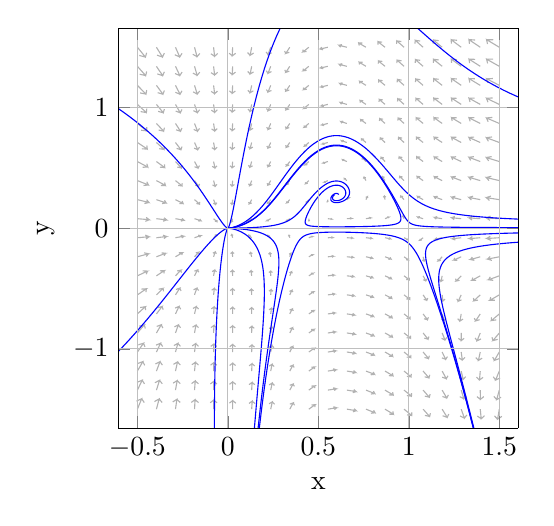
\begin{tikzpicture}
\begin{axis}[%
width=2in,
height=2in,
unbounded coords=jump,
view={0}{90},
scale only axis,
xmin=-0.605263157894737,
xmax=1.60526315789474,
xlabel={x},
xmajorgrids,
ymin=-1.65789473684211,
ymax=1.65789473684211,
ylabel={y},
ymajorgrids,
zmin=-1,
zmax=1
]
\addplot [color=white!70!black,solid,forget plot]
  table[row sep=crcr]{-0.5	-1.5\\
-0.47641083260371	-1.4135063862136\\
-0.505110986269196	-1.43355717850045\\
-0.47641083260371	-1.4135063862136\\
-0.461864179375997	-1.44535176219859\\
nan	0\\
-0.5	-1.34210526315789\\
-0.47349101707077	-1.25948559969513\\
-0.502098627815231	-1.27764425300165\\
-0.47349101707077	-1.25948559969513\\
-0.460788796083847	-1.29089874446627\\
nan	0\\
-0.5	-1.18421052631579\\
-0.470125214101787	-1.10596703943952\\
-0.498648521590319	-1.12197138902785\\
-0.470125214101787	-1.10596703943952\\
-0.459526778152183	-1.13690878197695\\
nan	0\\
-0.5	-1.02631578947368\\
-0.466217991532836	-0.953121437794829\\
-0.494651181992699	-0.966634241181695\\
-0.466217991532836	-0.953121437794829\\
-0.458054006153272	-0.983525245415277\\
nan	0\\
-0.5	-0.868421052631579\\
-0.461668583776836	-0.801202192298205\\
-0.489972723727129	-0.811784996342426\\
-0.461668583776836	-0.801202192298205\\
-0.456363293560442	-0.830950704454008\\
nan	0\\
-0.5	-0.710526315789474\\
-0.456405183360008	-0.650583442909484\\
-0.484469346572003	-0.657667600613483\\
-0.456405183360008	-0.650583442909484\\
-0.454497910132008	-0.679465008933479\\
nan	0\\
-0.5	-0.552631578947368\\
-0.450477212300549	-0.501788183575932\\
-0.478044897453244	-0.504660505262501\\
-0.450477212300549	-0.501788183575932\\
-0.452623199767526	-0.529421899112226\\
nan	0\\
-0.5	-0.394736842105263\\
-0.444248189328464	-0.355424667913796\\
-0.470801776077792	-0.353280367503352\\
-0.444248189328464	-0.355424667913796\\
-0.451145688982058	-0.38115627283912\\
nan	0\\
-0.5	-0.236842105263158\\
-0.438635224669077	-0.211841641239449\\
-0.463294773274281	-0.204000586613831\\
-0.438635224669077	-0.211841641239449\\
-0.450794541262427	-0.234682974279292\\
nan	0\\
-0.5	-0.0789473684210527\\
-0.434994079557102	-0.0704346883630541\\
-0.456624025704471	-0.0567370122697292\\
-0.434994079557102	-0.0704346883630541\\
-0.452367685675472	-0.0892399724911781\\
nan	0\\
-0.5	0.0789473684210527\\
-0.434204163301337	0.0706283545855895\\
-0.45186316085207	0.0895730179108942\\
-0.434204163301337	0.0706283545855895\\
-0.456022667769802	0.0566750995615627\\
nan	0\\
-0.5	0.236842105263158\\
-0.435858216197989	0.21332345120242\\
-0.449221087823408	0.236414493371144\\
-0.435858216197989	0.21332345120242\\
-0.460980414853776	0.204343601470139\\
nan	0\\
-0.5	0.394736842105263\\
-0.438802878688591	0.358544996168408\\
-0.4481140535978	0.384701830277317\\
-0.438802878688591	0.358544996168408\\
-0.466209976566227	0.354103269621613\\
nan	0\\
-0.5	0.552631578947368\\
-0.442078995927557	0.50617410693093\\
-0.44784092914518	0.534591599553972\\
-0.442078995927557	0.50617410693093\\
-0.4710696651534	0.50563109751775\\
nan	0\\
-0.5	0.710526315789473\\
-0.445190436801902	0.655716752591375\\
-0.447930914961807	0.685862012350329\\
-0.445190436801902	0.655716752591375\\
-0.475335696560856	0.65845723075128\\
nan	0\\
-0.5	0.868421052631579\\
-0.447958744216589	0.806685837437533\\
-0.448137317153101	0.838216715941599\\
-0.447958744216589	0.806685837437533\\
-0.479004924750124	0.812196088049894\\
nan	0\\
-0.5	1.02631578947368\\
-0.450356781872545	0.958706454309626\\
-0.448347413519767	0.991400059390707\\
-0.450356781872545	0.958706454309626\\
-0.482152081101796	0.96657845032698\\
nan	0\\
-0.5	1.18421052631579\\
-0.452415069618617	1.11151132712201\\
-0.448515748934587	1.14521731947549\\
-0.452415069618617	1.11151132712201\\
-0.484865348531477	1.1214248542848\\
nan	0\\
-0.5	1.34210526315789\\
-0.454180063589301	1.26491311803356\\
-0.448628008231428	1.29952574567354\\
-0.454180063589301	1.26491311803356\\
-0.487224080793593	1.27661577746819\\
nan	0\\
-0.5	1.5\\
-0.455697948128533	1.41877957156898\\
-0.448683456582218	1.45422121306615\\
-0.455697948128533	1.41877957156898\\
-0.489293670797729	1.43207018713042\\
nan	0\\
-0.394736842105263	-1.5\\
-0.37996238846352	-1.41518332372549\\
-0.405598893624669	-1.43693471319741\\
-0.37996238846352	-1.41518332372549\\
-0.363190555487416	-1.44432194001828\\
nan	0\\
-0.394736842105263	-1.34210526315789\\
-0.377752814374384	-1.26072190830021\\
-0.40319386140807	-1.28089090782479\\
-0.377752814374384	-1.26072190830021\\
-0.362502183979226	-1.28938292169023\\
nan	0\\
-0.394736842105263	-1.18421052631579\\
-0.37516099893472	-1.10664871738741\\
-0.400424204117978	-1.12502329927329\\
-0.37516099893472	-1.10664871738741\\
-0.361643299653788	-1.13481122085856\\
nan	0\\
-0.394736842105263	-1.02631578947368\\
-0.372072893195111	-0.95309633431987\\
-0.39717694165661	-0.969396183638476\\
-0.372072893195111	-0.95309633431987\\
-0.360567214079703	-0.980728158093552\\
nan	0\\
-0.394736842105263	-0.868421052631579\\
-0.368333114515262	-0.800275110551695\\
-0.393290718312234	-0.81411796127816\\
-0.368333114515262	-0.800275110551695\\
-0.359217747272291	-0.82731982507316\\
nan	0\\
-0.394736842105263	-0.710526315789474\\
-0.363740068493648	-0.648534686683423\\
-0.388537007853645	-0.659382982012335\\
-0.363740068493648	-0.648534686683423\\
-0.35754119330062	-0.674881368818142\\
nan	0\\
-0.394736842105263	-0.552631578947368\\
-0.3580786205328	-0.498474792837053\\
-0.382615283532118	-0.505557273277032\\
-0.3580786205328	-0.498474792837053\\
-0.35553689047696	-0.523886384063264\\
nan	0\\
-0.394736842105263	-0.394736842105263\\
-0.351302977074701	-0.351096380626598\\
-0.375243251953536	-0.353330052812557\\
-0.351302977074701	-0.351096380626598\\
-0.353423021214203	-0.375046985327838\\
nan	0\\
-0.394736842105263	-0.236842105263158\\
-0.344127193063746	-0.207725002506188\\
-0.366589363465444	-0.2038077210729\\
-0.344127193063746	-0.207725002506188\\
-0.352030812086959	-0.229112545593658\\
nan	0\\
-0.394736842105263	-0.0789473684210527\\
-0.338851160888191	-0.0686978545676049\\
-0.358179243716674	-0.0578012884193711\\
-0.338851160888191	-0.0686978545676049\\
-0.35305448678995	-0.0857441290279073\\
nan	0\\
-0.394736842105263	0.0789473684210527\\
-0.337998800539597	0.0689769105173429\\
-0.352527598533369	0.0861525582798725\\
-0.337998800539597	0.0689769105173429\\
-0.357512827485224	0.0577835374970392\\
nan	0\\
-0.394736842105263	0.236842105263158\\
-0.340883998419798	0.209591908690893\\
-0.350227302382372	0.231230178583939\\
-0.340883998419798	0.209591908690893\\
-0.363852400668504	0.204303756741206\\
nan	0\\
-0.394736842105263	0.394736842105263\\
-0.344989523250446	0.354402088886105\\
-0.349830030602101	0.378939344565557\\
-0.344989523250446	0.354402088886105\\
-0.36999740721168	0.354065685138148\\
nan	0\\
-0.394736842105263	0.552631578947368\\
-0.348857307808933	0.502489237486201\\
-0.350085582732541	0.529001823498634\\
-0.348857307808933	0.502489237486201\\
-0.375156753463124	0.506062056350469\\
nan	0\\
-0.394736842105263	0.710526315789473\\
-0.352098376296392	0.652759282610814\\
-0.350448157744388	0.68074900901663\\
-0.352098376296392	0.652759282610814\\
-0.379331674333718	0.659429776112194\\
nan	0\\
-0.394736842105263	0.868421052631579\\
-0.354729091010869	0.804465319083232\\
-0.350742482952101	0.833653976921334\\
-0.354729091010869	0.804465319083232\\
-0.382720349726274	0.813650101374137\\
nan	0\\
-0.394736842105263	1.02631578947368\\
-0.356858668071961	0.957148302738045\\
-0.350930248598042	0.987368092267062\\
-0.356858668071961	0.957148302738045\\
-0.385513991965862	0.968429005250411\\
nan	0\\
-0.394736842105263	1.18421052631579\\
-0.358595346578458	1.11052537655987\\
-0.35101650779752	1.14166629536835\\
-0.358595346578458	1.11052537655987\\
-0.387859082675479	1.12359554760495\\
nan	0\\
-0.394736842105263	1.34210526315789\\
-0.360026436139421	1.26441631162731\\
-0.351017320046526	1.29640059857794\\
-0.360026436139421	1.26441631162731\\
-0.38986179581182	1.27904539559502\\
nan	0\\
-0.394736842105263	1.5\\
-0.361218467743771	1.41870155832527\\
-0.350949369633536	1.45147068441806\\
-0.361218467743771	1.41870155832527\\
-0.391598590470902	1.43471149723731\\
nan	0\\
-0.289473684210526	-1.5\\
-0.281635491860239	-1.41771718776622\\
-0.304557652623771	-1.44044248334878\\
-0.281635491860239	-1.41771718776622\\
-0.26341624650688	-1.44436157952392\\
nan	0\\
-0.289473684210526	-1.34210526315789\\
-0.280136373703685	-1.26294356788399\\
-0.302727990674215	-1.28435774883945\\
-0.280136373703685	-1.26294356788399\\
-0.26314714303726	-1.28902640409287\\
nan	0\\
-0.289473684210526	-1.18421052631579\\
-0.278363139659717	-1.10847253816326\\
-0.300630800063092	-1.12841629847132\\
-0.278363139659717	-1.10847253816326\\
-0.262761805986828	-1.13397157074672\\
nan	0\\
-0.289473684210526	-1.02631578947368\\
-0.276219940622711	-0.954396513290372\\
-0.298175882744884	-0.972658860248412\\
-0.276219940622711	-0.954396513290372\\
-0.262216244653228	-0.97928573204232\\
nan	0\\
-0.289473684210526	-0.868421052631579\\
-0.27356066310702	-0.800862598559267\\
-0.29522418295615	-0.817151879505084\\
-0.27356066310702	-0.800862598559267\\
-0.261444955919994	-0.825108390056837\\
nan	0\\
-0.289473684210526	-0.710526315789474\\
-0.270155087455032	-0.648124513147481\\
-0.291551117142179	-0.662015404751205\\
-0.270155087455032	-0.648124513147481\\
-0.260350215821182	-0.671674703128952\\
nan	0\\
-0.289473684210526	-0.552631578947368\\
-0.265635649833881	-0.496664777789624\\
-0.286778760436311	-0.507495309542786\\
-0.265635649833881	-0.496664777789624\\
-0.258795359857439	-0.519414326731109\\
nan	0\\
-0.289473684210526	-0.394736842105263\\
-0.259462399248792	-0.347501578391064\\
-0.280274600665862	-0.35416933626489\\
-0.259462399248792	-0.347501578391064\\
-0.256656968808763	-0.369174978745757\\
nan	0\\
-0.289473684210526	-0.236842105263158\\
-0.251285893355132	-0.202867750433554\\
-0.271235819319151	-0.203513109168586\\
-0.251285893355132	-0.202867750433554\\
-0.254248641904349	-0.222607004596283\\
nan	0\\
-0.289473684210526	-0.0789473684210527\\
-0.243391949892726	-0.0660296246577139\\
-0.260445906128901	-0.0583845142072654\\
-0.243391949892726	-0.0660296246577139\\
-0.253987034247231	-0.0814253813661657\\
nan	0\\
-0.289473684210526	0.0789473684210527\\
-0.242450302495155	0.0664497484441132\\
-0.253432912015532	0.0819548798660378\\
-0.242450302495155	0.0664497484441132\\
-0.259681722004001	0.0584431890083522\\
nan	0\\
-0.289473684210526	0.236842105263158\\
-0.247420331903556	0.204966224543462\\
-0.252067367415723	0.225042326836113\\
-0.247420331903556	0.204966224543462\\
-0.268005307775571	0.204015650682628\\
nan	0\\
-0.289473684210526	0.394736842105263\\
-0.252592631562048	0.35033521486968\\
-0.252556540547696	0.372875966202475\\
-0.252592631562048	0.35033521486968\\
-0.274757354165487	0.354435439878235\\
nan	0\\
-0.289473684210526	0.552631578947368\\
-0.256508734617232	0.499564841074339\\
-0.253131535026963	0.523726099834571\\
-0.256508734617232	0.499564841074339\\
-0.279664903963477	0.507243625037924\\
nan	0\\
-0.289473684210526	0.710526315789473\\
-0.259361493284075	0.650880525007171\\
-0.253483702866435	0.676302309973475\\
-0.259361493284075	0.650880525007171\\
-0.283306598257586	0.661246214510249\\
nan	0\\
-0.289473684210526	0.868421052631579\\
-0.261475022960115	0.803430425203816\\
-0.253626964478298	0.829927278744748\\
-0.261475022960115	0.803430425203816\\
-0.286122278192179	0.815927948119542\\
nan	0\\
-0.289473684210526	1.02631578947368\\
-0.263081874551491	0.956781802564269\\
-0.253615920721848	0.984239951051853\\
-0.263081874551491	0.956781802564269\\
-0.288382914176555	0.971044046222335\\
nan	0\\
-0.289473684210526	1.18421052631579\\
-0.264333650112543	1.11069378489694\\
-0.253496474987226	1.13903381584709\\
-0.264333650112543	1.11069378489694\\
-0.29025484569665	1.1264637987981\\
nan	0\\
-0.289473684210526	1.34210526315789\\
-0.265329372815495	1.26502073742608\\
-0.253301534801052	1.29418217299439\\
-0.265329372815495	1.26502073742608\\
-0.291843797666957	1.28211001729687\\
nan	0\\
-0.289473684210526	1.5\\
-0.266135315067722	1.41966841521984\\
-0.253053929615524	1.44960248293959\\
-0.266135315067722	1.41966841521984\\
-0.293219722005602	1.43793329836819\\
nan	0\\
-0.184210526315789	-1.5\\
-0.181214997809328	-1.42090010661068\\
-0.201888629708596	-1.44388119250086\\
-0.181214997809328	-1.42090010661068\\
-0.162338683013937	-1.44537895675409\\
nan	0\\
-0.184210526315789	-1.34210526315789\\
-0.180353968147875	-1.26591290891026\\
-0.200559024160158	-1.28780647564257\\
-0.180353968147875	-1.26591290891026\\
-0.162462847036341	-1.28973475472653\\
nan	0\\
-0.184210526315789	-1.18421052631579\\
-0.179334784131361	-1.11117758386014\\
-0.199055742400602	-1.13186853105073\\
-0.179334784131361	-1.11117758386014\\
-0.162539271172777	-1.13430640214294\\
nan	0\\
-0.184210526315789	-1.02631578947368\\
-0.178098434495069	-0.956760033358042\\
-0.197321001070196	-0.976098737237554\\
-0.178098434495069	-0.956760033358042\\
-0.162543123012374	-0.979154783147915\\
nan	0\\
-0.184210526315789	-0.868421052631579\\
-0.176550347526692	-0.802760268796926\\
-0.195263597122084	-0.820543459250047\\
-0.176550347526692	-0.802760268796926\\
-0.162433205204758	-0.824373548644596\\
nan	0\\
-0.184210526315789	-0.710526315789474\\
-0.174528404728302	-0.649343087632827\\
-0.19272884824371	-0.665277525682949\\
-0.174528404728302	-0.649343087632827\\
-0.162137234165386	-0.670118586476693\\
nan	0\\
-0.184210526315789	-0.552631578947368\\
-0.171729999342212	-0.496814245831734\\
-0.189428490713194	-0.51043931402303\\
-0.171729999342212	-0.496814245831734\\
-0.161519824155377	-0.516679577509819\\
nan	0\\
-0.184210526315789	-0.394736842105263\\
-0.167529788535354	-0.345851574345003\\
-0.18475532680955	-0.356346970227972\\
-0.167529788535354	-0.345851574345003\\
-0.16031269292942	-0.36468733911819\\
nan	0\\
-0.184210526315789	-0.236842105263158\\
-0.160551235052571	-0.198414421059961\\
-0.177255943482336	-0.204027903505115\\
-0.160551235052571	-0.198414421059961\\
-0.158042101380737	-0.215857549136725\\
nan	0\\
-0.184210526315789	-0.0789473684210527\\
-0.149620588768282	-0.061547916893513\\
-0.164347432914419	-0.0581202679648981\\
-0.149620588768282	-0.061547916893513\\
-0.155647707150649	-0.0754152367386517\\
nan	0\\
-0.184210526315789	0.0789473684210527\\
-0.148511435634152	0.0621788059986676\\
-0.155029022233047	0.0761341473957924\\
-0.148511435634152	0.0621788059986676\\
-0.16341330344424	0.0582846020549739\\
nan	0\\
-0.184210526315789	0.236842105263158\\
-0.156379838556385	0.200059342869659\\
-0.155533354285832	0.21805184352756\\
-0.156379838556385	0.200059342869659\\
-0.173924735482581	0.204136499647858\\
nan	0\\
-0.184210526315789	0.394736842105263\\
-0.161404218105338	0.347436725955968\\
-0.15642108153115	0.36732833785337\\
-0.161404218105338	0.347436725955968\\
-0.180071139605797	0.355925183748144\\
nan	0\\
-0.184210526315789	0.552631578947368\\
-0.164372007131723	0.498210214790303\\
-0.156718221847677	0.519496253833439\\
-0.164372007131723	0.498210214790303\\
-0.183928903926209	0.509576994241406\\
nan	0\\
-0.184210526315789	0.710526315789473\\
-0.166273695606753	0.650574523891855\\
-0.156666796845059	0.6730442691384\\
-0.166273695606753	0.650574523891855\\
-0.186642692793868	0.664075853783881\\
nan	0\\
-0.184210526315789	0.868421052631579\\
-0.16757976969438	0.803861292977213\\
-0.156429056767211	0.827386910028875\\
-0.16757976969438	0.803861292977213\\
-0.188708936594394	0.81907153171817\\
nan	0\\
-0.184210526315789	1.02631578947368\\
-0.168523537312171	0.957757630549545\\
-0.156090094282222	0.982246825477691\\
-0.168523537312171	0.957757630549545\\
-0.190369173744291	0.974403330975882\\
nan	0\\
-0.184210526315789	1.18421052631579\\
-0.16923141967686	1.112091732277\\
-0.155695453158841	1.13747214714837\\
-0.16923141967686	1.112091732277\\
-0.191754850178237	1.1299825938289\\
nan	0\\
-0.184210526315789	1.34210526315789\\
-0.169777412846202	1.26675843031802\\
-0.155270638677109	1.29297075853738\\
-0.169777412846202	1.26675843031802\\
-0.192944055097048	1.28575420180258\\
nan	0\\
-0.184210526315789	1.5\\
-0.170207607753374	1.42168819021067\\
-0.154830530874766	1.44868246278807\\
-0.170207607753374	1.42168819021067\\
-0.193986435769431	1.44168100350686\\
nan	0\\
-0.0789473684210527	-1.5\\
-0.0785570364738179	-1.42457523464409\\
-0.0975303273969665	-1.44710508126405\\
-0.0785570364738179	-1.42457523464409\\
-0.0598179447190102	-1.44730024723767\\
nan	0\\
-0.0789473684210527	-1.34210526315789\\
-0.0782287354891096	-1.26942740302374\\
-0.0966137904022319	-1.291051102831\\
-0.0782287354891096	-1.26942740302374\\
-0.060274860335153	-1.29141041929697\\
nan	0\\
-0.0789473684210527	-1.18421052631579\\
-0.0778420315664336	-1.114506050398\\
-0.0955997516022657	-1.13514105895968\\
-0.0778420315664336	-1.114506050398\\
-0.0607475136433729	-1.13569372738699\\
nan	0\\
-0.0789473684210527	-1.02631578947368\\
-0.0773748898514188	-0.959865014056916\\
-0.0944593272765009	-0.979407127039538\\
-0.0773748898514188	-0.959865014056916\\
-0.061233939568117	-0.980193366324355\\
nan	0\\
-0.0789473684210527	-0.868421052631579\\
-0.0767914467693066	-0.805582345979984\\
-0.0931478999277292	-0.823894977562526\\
-0.0767914467693066	-0.805582345979984\\
-0.0617285466019316	-0.824972938388399\\
nan	0\\
-0.0789473684210527	-0.710526315789474\\
-0.0760284948155699	-0.651778658067445\\
-0.0915910713277219	-0.668673236982683\\
-0.0760284948155699	-0.651778658067445\\
-0.0622172424667076	-0.670132673785424\\
nan	0\\
-0.0789473684210527	-0.552631578947368\\
-0.0749615828252039	-0.498658316541704\\
-0.0896506341053747	-0.513853848864441\\
-0.0749615828252039	-0.498658316541704\\
-0.0626640029025424	-0.515846741662365\\
nan	0\\
-0.0789473684210527	-0.394736842105263\\
-0.0733016060035223	-0.346622225674919\\
-0.0870239888363674	-0.35964516999964\\
-0.0733016060035223	-0.346622225674919\\
-0.0629666806211954	-0.362468051208405\\
nan	0\\
-0.0789473684210527	-0.236842105263158\\
-0.0701646777950382	-0.196705918704373\\
-0.0828335316225387	-0.206551102015505\\
-0.0701646777950382	-0.196705918704373\\
-0.0627654383431463	-0.210942447328512\\
nan	0\\
-0.0789473684210527	-0.0789473684210527\\
-0.061122586945705	-0.0544032451648296\\
-0.0726060522023651	-0.0573102867728596\\
-0.061122586945705	-0.0544032451648296\\
-0.0603339905742536	-0.0662226775105334\\
nan	0\\
-0.0789473684210527	0.0789473684210527\\
-0.0598431014019969	0.054947082176201\\
-0.0595743099465007	0.0669232348044204\\
-0.0598431014019969	0.054947082176201\\
-0.0715744530689266	0.0573711012948926\\
nan	0\\
-0.0789473684210527	0.236842105263158\\
-0.0674920517657032	0.197147975495587\\
-0.0610051143204154	0.211920043589696\\
-0.0674920517657032	0.197147975495587\\
-0.0808521792042007	0.206192385262021\\
nan	0\\
-0.0789473684210527	0.394736842105263\\
-0.0700067823260557	0.346953639927249\\
-0.0607431576100512	0.363523747104402\\
-0.0700067823260557	0.346953639927249\\
-0.0846347586990584	0.359053454056904\\
nan	0\\
-0.0789473684210527	0.552631578947368\\
-0.0712346067662408	0.4989270936748\\
-0.0601223139445424	0.516966629670274\\
-0.0712346067662408	0.4989270936748\\
-0.0869745565808263	0.513110248842868\\
nan	0\\
-0.0789473684210527	0.710526315789473\\
-0.0719571419294164	0.652007376063097\\
-0.0594244749453131	0.671310614603919\\
-0.0719571419294164	0.652007376063097\\
-0.0886839448085015	0.667815501358101\\
nan	0\\
-0.0789473684210527	0.868421052631579\\
-0.0724282395229727	0.805783050414496\\
-0.058724477638126	0.826204233304141\\
-0.0724282395229727	0.805783050414496\\
-0.0900434787466674	0.822944668855101\\
nan	0\\
-0.0789473684210527	1.02631578947368\\
-0.0727555952191575	0.960044889395758\\
-0.0580454021602445	0.98147410271961\\
-0.0727555952191575	0.960044889395758\\
-0.0911808521992075	0.978378216118662\\
nan	0\\
-0.0789473684210527	1.18421052631579\\
-0.0729929448141193	1.11466974362554\\
-0.0573940762236371	1.13702058433435\\
-0.0729929448141193	1.11466974362554\\
-0.0921644675687616	1.13404337253088\\
nan	0\\
-0.0789473684210527	1.34210526315789\\
-0.0731701913755875	1.26957810559435\\
-0.0567715550983416	1.29278054712478\\
-0.0731701913755875	1.26957810559435\\
-0.0930351338801125	1.28989195860205\\
nan	0\\
-0.0789473684210527	1.5\\
-0.0733053359803532	1.42471524105131\\
-0.05617675597539	1.44871117684609\\
-0.0733053359803532	1.42471524105131\\
-0.093819135449736	1.44589016062574\\
nan	0\\
0.0263157894736842	-1.5\\
0.0265036495684208	-1.42869350288305\\
0.00862066726076205	-1.45003848699445\\
0.0265036495684208	-1.42869350288305\\
0.0442739158192376	-1.45013241704182\\
nan	0\\
0.0263157894736842	-1.34210526315789\\
0.0264068659152086	-1.27339394294185\\
0.00920171292874035	-1.29398456989628\\
0.0264068659152086	-1.27339394294185\\
0.0435573730367621	-1.29403010811705\\
nan	0\\
0.0263157894736842	-1.18421052631579\\
0.0262938675636125	-1.11830690021468\\
0.00982453761135546	-1.13808346852253\\
0.0262938675636125	-1.11830690021468\\
0.0427763506619125	-1.13807250756749\\
nan	0\\
0.0263157894736842	-1.02631578947368\\
0.0261586449988793	-0.963482115783002\\
0.0104973699186503	-0.982371504008908\\
0.0261586449988793	-0.963482115783002\\
0.0419142067639912	-0.982292931771506\\
nan	0\\
0.0263157894736842	-0.868421052631579\\
0.0259914347082147	-0.80899108550964\\
0.0112312493573708	-0.826901164337589\\
0.0259914347082147	-0.80899108550964\\
0.0409462329183403	-0.826738986954854\\
nan	0\\
0.0263157894736842	-0.710526315789474\\
0.0257750338070731	-0.654942796285992\\
0.012041380631186	-0.671753041053689\\
0.0257750338070731	-0.654942796285992\\
0.0398331403829268	-0.671482663220384\\
nan	0\\
0.0263157894736842	-0.552631578947368\\
0.0254754673837997	-0.501517665645041\\
0.0129490856851833	-0.517061920158211\\
0.0254754673837997	-0.501517665645041\\
0.0385060423363469	-0.516641759113268\\
nan	0\\
0.0263157894736842	-0.394736842105263\\
0.0250128820368633	-0.349054201558039\\
0.0139830941311035	-0.363084720581411\\
0.0250128820368633	-0.349054201558039\\
0.0368244144047157	-0.362433266863001\\
nan	0\\
0.0263157894736842	-0.236842105263158\\
0.0241325222265895	-0.198342655671296\\
0.0151626400027525	-0.210438307360628\\
0.0241325222265895	-0.198342655671296\\
0.0344123647986833	-0.209346673737081\\
nan	0\\
0.0263157894736842	-0.0789473684210527\\
0.0211011021798004	-0.0525639383258573\\
0.0160696508441667	-0.0617826391778869\\
0.0211011021798004	-0.0525639383258573\\
0.0292613658917644	-0.059175295530945\\
nan	0\\
0.0263157894736842	0.0789473684210527\\
0.0203969672994594	0.0526617056844847\\
0.0287440296358688	0.0590676989618989\\
0.0203969672994594	0.0526617056844847\\
0.0156011982675849	0.0620271100490113\\
nan	0\\
0.0263157894736842	0.236842105263158\\
0.023077073334707	0.198392149776282\\
0.0336611770481191	0.2091174573876\\
0.023077073334707	0.198392149776282\\
0.0144361993046812	0.210736815457089\\
nan	0\\
0.0263157894736842	0.394736842105263\\
0.0237575432506286	0.349089559555452\\
0.0359368377549981	0.362144182764631\\
0.0237575432506286	0.349089559555452\\
0.0131131964800925	0.363423305876159\\
nan	0\\
0.0263157894736842	0.552631578947368\\
0.0240699059814971	0.501545951876913\\
0.037515077796767	0.516310169125003\\
0.0240699059814971	0.501545951876913\\
0.0119722642615394	0.517433110871096\\
nan	0\\
0.0263157894736842	0.710526315789473\\
0.0242461037608964	0.6549667305749\\
0.0387569057783761	0.671117184711075\\
0.0242461037608964	0.6549667305749\\
0.0109771131710893	0.672152027567469\\
nan	0\\
0.0263157894736842	0.868421052631579\\
0.024356438233924	0.809012027884936\\
0.0397964997925127	0.826344897498989\\
0.024356438233924	0.809012027884936\\
0.0100919874191913	0.827324573118869\\
nan	0\\
0.0263157894736842	1.02631578947368\\
0.02442984041603	0.963500853623099\\
0.0406993590959725	0.981873847113861\\
0.02442984041603	0.963500853623099\\
0.00929189117068005	0.982816821642688\\
nan	0\\
0.0263157894736842	1.18421052631579\\
0.0244804807964542	1.11832393456908\\
0.0415027213362997	1.13763108492379\\
0.0244804807964542	1.11832393456908\\
0.00855942546294663	1.1385487392624\\
nan	0\\
0.0263157894736842	1.34210526315789\\
0.0245161392167752	1.27340961451858\\
0.0422299464536767	1.29356839654615\\
0.0245161392167752	1.27340961451858\\
0.00788212213401911	1.2944682216746\\
nan	0\\
0.0263157894736842	1.5\\
0.0245414476074172	1.42870805504179\\
0.0428967364068494	1.44965205306269\\
0.0245414476074172	1.42870805504179\\
0.00725076392774519	1.45053922399582\\
nan	0\\
0.131578947368421	-1.5\\
0.134284520514481	-1.43338899646762\\
0.116820097687568	-1.45269590424082\\
0.134284520514481	-1.43338899646762\\
0.150125599453758	-1.45404869081385\\
nan	0\\
0.131578947368421	-1.34210526315789\\
0.13385671046949	-1.27791030642611\\
0.117124642356223	-1.29659935267038\\
0.13385671046949	-1.27791030642611\\
0.149222120722115	-1.29773823422091\\
nan	0\\
0.131578947368421	-1.18421052631579\\
0.133363357988785	-1.12263015164159\\
0.117432941134127	-1.14065816138876\\
0.133363357988785	-1.12263015164159\\
0.148223128471225	-1.14155036669894\\
nan	0\\
0.131578947368421	-1.02631578947368\\
0.132780970334952	-0.967595631977562\\
0.117740324070962	-0.984911173484766\\
0.132780970334952	-0.967595631977562\\
0.147100402819023	-0.985512184968031\\
nan	0\\
0.131578947368421	-0.868421052631579\\
0.132071667793742	-0.812875036683778\\
0.118037347679195	-0.829415661361788\\
0.132071667793742	-0.812875036683778\\
0.145810355653096	-0.829662021574449\\
nan	0\\
0.131578947368421	-0.710526315789474\\
0.131169309237903	-0.658573959886528\\
0.118304111701322	-0.674262076190041\\
0.131169309237903	-0.658573959886528\\
0.144280289652795	-0.674057257124782\\
nan	0\\
0.131578947368421	-0.552631578947368\\
0.129944854395178	-0.504871681356553\\
0.118495107889447	-0.519608173877109\\
0.129944854395178	-0.504871681356553\\
0.142375056684855	-0.518791127390487\\
nan	0\\
0.131578947368421	-0.394736842105263\\
0.12810120056573	-0.3521218432404\\
0.118490774890321	-0.365775779600532\\
0.12810120056573	-0.3521218432404\\
0.139798274322753	-0.364036906199186\\
nan	0\\
0.131578947368421	-0.236842105263158\\
0.124738845356861	-0.201252528335318\\
0.117893481728369	-0.21363942691656\\
0.124738845356861	-0.201252528335318\\
0.135688270192289	-0.21021937591078\\
nan	0\\
0.131578947368421	-0.0789473684210527\\
0.115515784139255	-0.0573895834841326\\
0.114945286873775	-0.0678727097725\\
0.115515784139255	-0.0573895834841326\\
0.125724179342235	-0.0598411281579172\\
nan	0\\
0.131578947368421	0.0789473684210527\\
0.1129384584221	0.0585453834319073\\
0.123631101353282	0.0600058566920705\\
0.1129384584221	0.0585453834319073\\
0.11343010885871	0.0693261011652312\\
nan	0\\
0.131578947368421	0.236842105263158\\
0.119103653673737	0.202258955037402\\
0.131492029338581	0.209515076681458\\
0.119103653673737	0.202258955037402\\
0.114200454225703	0.2157527235288\\
nan	0\\
0.131578947368421	0.394736842105263\\
0.121109258302889	0.352882836881116\\
0.134713666328586	0.362821616181978\\
0.121109258302889	0.352882836881116\\
0.113786663716512	0.368056460714743\\
nan	0\\
0.131578947368421	0.552631578947368\\
0.122020876334442	0.505490376101863\\
0.136673598356012	0.51724321919702\\
0.122020876334442	0.505490376101863\\
0.113102996933259	0.522022254714009\\
nan	0\\
0.131578947368421	0.710526315789473\\
0.122506274673824	0.659100987767474\\
0.138084408487703	0.672260418000425\\
0.122506274673824	0.659100987767474\\
0.112371744476703	0.676796754347723\\
nan	0\\
0.131578947368421	0.868421052631579\\
0.122783861829975	0.813337757648203\\
0.139193211237353	0.827663974758604\\
0.122783861829975	0.813337757648203\\
0.111651563745665	0.832061517527827\\
nan	0\\
0.131578947368421	1.02631578947368\\
0.122945737437829	0.968010458013102\\
0.140112033282152	0.983343754968629\\
0.122945737437829	0.968010458013102\\
0.110959367551861	0.987660359933925\\
nan	0\\
0.131578947368421	1.18421052631579\\
0.123037339028343	1.12300773096379\\
0.140900520368366	1.13923316748437\\
0.123037339028343	1.12300773096379\\
0.110299122692368	1.14350397165441\\
nan	0\\
0.131578947368421	1.34210526315789\\
0.123083594360655	1.27825796566398\\
0.141594024636465	1.29528831666021\\
0.123083594360655	1.27825796566398\\
0.109670375889506	1.29953599316409\\
nan	0\\
0.131578947368421	1.5\\
0.123099267300652	1.43371200951403\\
0.142215168942476	1.45147848664288\\
0.123099267300652	1.43371200951403\\
0.109071173699489	1.45571832667676\\
nan	0\\
0.236842105263158	-1.5\\
0.245449465471676	-1.43917709633078\\
0.227661531491817	-1.45527212737942\\
0.245449465471676	-1.43917709633078\\
0.258072983326425	-1.45957580748368\\
nan	0\\
0.236842105263158	-1.34210526315789\\
0.244767469636199	-1.28346230307092\\
0.227729120302542	-1.29907385000375\\
0.244767469636199	-1.28346230307092\\
0.257050600346032	-1.30303653219027\\
nan	0\\
0.236842105263158	-1.18421052631579\\
0.243994805706397	-1.12792487036689\\
0.227777581586201	-1.14302239204075\\
0.243994805706397	-1.12792487036689\\
0.25592040956065	-1.14659874226237\\
nan	0\\
0.236842105263158	-1.02631578947368\\
0.243100768162072	-0.972606629460491\\
0.2277958792891	-0.987154711739721\\
0.243100768162072	-0.972606629460491\\
0.254650459295696	-0.990284043189178\\
nan	0\\
0.236842105263158	-0.868421052631579\\
0.242036347229851	-0.817568260098192\\
0.227764876506496	-0.831525537366535\\
0.242036347229851	-0.817568260098192\\
0.25319127277319	-0.834122658349881\\
nan	0\\
0.236842105263158	-0.710526315789474\\
0.240716805723664	-0.662903825442061\\
0.227648772998659	-0.676221897431158\\
0.240716805723664	-0.662903825442061\\
0.251460018172366	-0.678159247661411\\
nan	0\\
0.236842105263158	-0.552631578947368\\
0.238978342703963	-0.508774194172716\\
0.227373125278058	-0.52139735024491\\
0.238978342703963	-0.508774194172716\\
0.249301817665385	-0.522465468965313\\
nan	0\\
0.236842105263158	-0.394736842105263\\
0.236447072602632	-0.355502916502988\\
0.226757101000221	-0.367371852348802\\
0.236447072602632	-0.355502916502988\\
0.246374063801358	-0.367174336018539\\
nan	0\\
0.236842105263158	-0.236842105263158\\
0.232005088742948	-0.203985480092202\\
0.225242037406272	-0.215051721773541\\
0.232005088742948	-0.203985480092202\\
0.24167034999175	-0.212633213513436\\
nan	0\\
0.236842105263158	-0.0789473684210527\\
0.220808977840046	-0.0596988061026462\\
0.220806775487378	-0.0694816566539461\\
0.220808977840046	-0.0596988061026462\\
0.230431056646581	-0.0614650929423901\\
nan	0\\
0.236842105263158	0.0789473684210527\\
0.216141577587343	0.0620387131045461\\
0.226578899719214	0.0619361777805444\\
0.216141577587343	0.0620387131045461\\
0.218124572060961	0.0722864416184517\\
nan	0\\
0.236842105263158	0.236842105263158\\
0.220471483379545	0.206442834314975\\
0.232982487681674	0.211469960128527\\
0.220471483379545	0.206442834314975\\
0.217782852207583	0.219655271070333\\
nan	0\\
0.236842105263158	0.394736842105263\\
0.221859016658794	0.357407254191312\\
0.235686340218591	0.364860358414406\\
0.221859016658794	0.357407254191312\\
0.217021546261615	0.372351902716588\\
nan	0\\
0.236842105263158	0.552631578947368\\
0.222350993916675	0.510333573595372\\
0.237272828658619	0.51940019736435\\
0.222350993916675	0.510333573595372\\
0.216123825982621	0.526645753037592\\
nan	0\\
0.236842105263158	0.710526315789473\\
0.222494863080993	0.664236157050791\\
0.238371575420313	0.674536394126855\\
0.222494863080993	0.664236157050791\\
0.215226496050972	0.681710015217937\\
nan	0\\
0.236842105263158	0.868421052631579\\
0.222476197245249	0.818739815335111\\
0.239206278974738	0.830052709519574\\
0.222476197245249	0.818739815335111\\
0.214365660326504	0.837235663528529\\
nan	0\\
0.236842105263158	1.02631578947368\\
0.222372989859202	0.973657849300799\\
0.23987820952361	0.985837952501675\\
0.222372989859202	0.973657849300799\\
0.213549239437167	0.993072510203653\\
nan	0\\
0.236842105263158	1.18421052631579\\
0.222222944140589	1.12888223465387\\
0.240440765392839	1.14182593187181\\
0.222222944140589	1.12888223465387\\
0.21277661956188	1.14913551243309\\
nan	0\\
0.236842105263158	1.34210526315789\\
0.22204611222781	1.28434413217545\\
0.240925192884026	1.29797347321134\\
0.22204611222781	1.28434413217545\\
0.212044627392803	1.30537146972902\\
nan	0\\
0.236842105263158	1.5\\
0.221853908266639	1.43999662504238\\
0.241351211104999	1.45425058828054\\
0.221853908266639	1.43999662504238\\
0.21134952362619	1.4617446867788\\
nan	0\\
0.342105263157895	-1.5\\
0.361194060273645	-1.44759788957935\\
0.342366893533758	-1.45854632342661\\
0.361194060273645	-1.44759788957935\\
0.368567948744082	-1.46809072198448\\
nan	0\\
0.342105263157895	-1.34210526315789\\
0.360314596622652	-1.2915676572285\\
0.342217395100875	-1.30217660564113\\
0.360314596622652	-1.2915676572285\\
0.367486198065574	-1.31128127237351\\
nan	0\\
0.342105263157895	-1.18421052631579\\
0.359345493647256	-1.13568654537177\\
0.342042429264442	-1.14593368203263\\
0.359345493647256	-1.13568654537177\\
0.366304419736453	-1.15455379727731\\
nan	0\\
0.342105263157895	-1.02631578947368\\
0.358260885954664	-0.979988628825454\\
0.341832408953576	-0.989847871320731\\
0.358260885954664	-0.979988628825454\\
0.364995989277691	-0.997925682719116\\
nan	0\\
0.342105263157895	-0.868421052631579\\
0.357021010570637	-0.824522546284067\\
0.341571659759936	-0.833963161335135\\
0.357021010570637	-0.824522546284067\\
0.363520912933692	-0.841421035041506\\
nan	0\\
0.342105263157895	-0.710526315789474\\
0.355559826009047	-0.669361838380832\\
0.34123233780154	-0.678347540890636\\
0.355559826009047	-0.669361838380832\\
0.361814576505861	-0.685074822316212\\
nan	0\\
0.342105263157895	-0.552631578947368\\
0.353754819461329	-0.514627161245309\\
0.340758848144784	-0.523116097480068\\
0.353754819461329	-0.514627161245309\\
0.359761056995814	-0.528940875631785\\
nan	0\\
0.342105263157895	-0.394736842105263\\
0.351336126048987	-0.360543473332291\\
0.340018524988416	-0.368493768241409\\
0.351336126048987	-0.360543473332291\\
0.357115209374903	-0.373109199686956\\
nan	0\\
0.342105263157895	-0.236842105263158\\
0.347495669869569	-0.20764610148997\\
0.33857954691277	-0.215057300944008\\
0.347495669869569	-0.20764610148997\\
0.353177548799364	-0.217752504299845\\
nan	0\\
0.342105263157895	-0.0789473684210527\\
0.337243767225271	-0.058861335669843\\
0.333680707817256	-0.0661025194783618\\
0.337243767225271	-0.058861335669843\\
0.343723724192861	-0.06367177151205\\
nan	0\\
0.342105263157895	0.0789473684210527\\
0.325452874212037	0.0629038629620041\\
0.334459467260556	0.0635538173632542\\
0.325452874212037	0.0629038629620041\\
0.326437714531032	0.0718800118361832\\
nan	0\\
0.342105263157895	0.236842105263158\\
0.325869906292706	0.210282937911846\\
0.33738030519009	0.214191848900942\\
0.325869906292706	0.210282937911846\\
0.324100721514434	0.222309527333537\\
nan	0\\
0.342105263157895	0.394736842105263\\
0.325133728937987	0.362468976158223\\
0.338292155690719	0.367906452387358\\
0.325133728937987	0.362468976158223\\
0.322158222717199	0.376392219497312\\
nan	0\\
0.342105263157895	0.552631578947368\\
0.324264851629858	0.516176950416365\\
0.33873063222102	0.522653236093657\\
0.324264851629858	0.516176950416365\\
0.320503317955519	0.531573441857675\\
nan	0\\
0.342105263157895	0.710526315789473\\
0.323412919943724	0.670676478508954\\
0.338983082228105	0.677958343889567\\
0.323412919943724	0.670676478508954\\
0.319058163587845	0.687304515496652\\
nan	0\\
0.342105263157895	0.868421052631579\\
0.322606749583633	0.825674311334159\\
0.339142988980266	0.833623705329819\\
0.322606749583633	0.825674311334159\\
0.317769618331556	0.84337296211695\\
nan	0\\
0.342105263157895	1.02631578947368\\
0.321849423544203	0.981019904733058\\
0.339250146613467	0.989544710251823\\
0.321849423544203	0.981019904733058\\
0.316602204243154	0.999672630058669\\
nan	0\\
0.342105263157895	1.18421052631579\\
0.321137651014794	1.13662449648181\\
0.339324442116218	1.14565840239623\\
0.321137651014794	1.13662449648181\\
0.315531427199229	1.15614220846778\\
nan	0\\
0.342105263157895	1.34210526315789\\
0.320466793173961	1.29243083520706\\
0.33937694115685	1.30192354609633\\
0.320466793173961	1.29243083520706\\
0.314539727181432	1.31274278108829\\
nan	0\\
0.342105263157895	1.5\\
0.319832303568561	1.44839958323028\\
0.339414295637791	1.45831146836386\\
0.319832303568561	1.44839958323028\\
0.313614087252932	1.46944794815853\\
nan	0\\
0.447368421052632	-1.5\\
0.4820315013467	-1.46274635175048\\
0.462319165196099	-1.46525667615182\\
0.4820315013467	-1.46274635175048\\
0.48094598932086	-1.48258821629885\\
nan	0\\
0.447368421052632	-1.34210526315789\\
0.480918709137947	-1.30627927723734\\
0.461897126232212	-1.30863950099217\\
0.480918709137947	-1.30627927723734\\
0.479810119192492	-1.32541464503483\\
nan	0\\
0.447368421052632	-1.18421052631579\\
0.479727511041905	-1.14993551942596\\
0.461451032322665	-1.15212824899559\\
0.479727511041905	-1.14993551942596\\
0.47858853576758	-1.16830779399023\\
nan	0\\
0.447368421052632	-1.02631578947368\\
0.478442665663628	-0.993745579618758\\
0.460977839816597	-0.995748081422487\\
0.478442665663628	-0.993745579618758\\
0.477262944744061	-1.01128520372798\\
nan	0\\
0.447368421052632	-0.868421052631579\\
0.477043684980649	-0.837754083378771\\
0.460474363489042	-0.839535358172609\\
0.477043684980649	-0.837754083378771\\
0.475807848115446	-0.854372990136618\\
nan	0\\
0.447368421052632	-0.710526315789474\\
0.475502105590438	-0.68203061692857\\
0.45993807551387	-0.68354590545239\\
0.475502105590438	-0.68203061692857\\
0.474185924944322	-0.697612747721293\\
nan	0\\
0.447368421052632	-0.552631578947368\\
0.473776867234044	-0.526693871557068\\
0.459369906532045	-0.527873072228805\\
0.473776867234044	-0.526693871557068\\
0.472338760227195	-0.541077295319512\\
nan	0\\
0.447368421052632	-0.394736842105263\\
0.471806565587003	-0.371975825136977\\
0.45878486798462	-0.37269459409387\\
0.471806565587003	-0.371975825136977\\
0.470165376468763	-0.384913666361055\\
nan	0\\
0.447368421052632	-0.236842105263158\\
0.469499882701652	-0.218449291735842\\
0.458262240825117	-0.218434270381782\\
0.469499882701652	-0.218449291735842\\
0.467458647588775	-0.229500001206292\\
nan	0\\
0.447368421052632	-0.0789473684210527\\
0.466745390234108	-0.0684800056573337\\
0.458315458788735	-0.0667759721910804\\
0.466745390234108	-0.0684800056573337\\
0.463549140170594	-0.0764644567818184\\
nan	0\\
0.447368421052632	0.0789473684210527\\
0.448954724893615	0.0618090661390504\\
0.452763409311821	0.067347132783897\\
0.448954724893615	0.0618090661390504\\
0.44419425817082	0.0665539808634051\\
nan	0\\
0.447368421052632	0.236842105263158\\
0.434782138194403	0.214178569789682\\
0.444223906920241	0.217831059717167\\
0.434782138194403	0.214178569789682\\
0.432892139183503	0.224124201146281\\
nan	0\\
0.447368421052632	0.394736842105263\\
0.4296609920177	0.368884183392367\\
0.441436385406404	0.372213123747503\\
0.4296609920177	0.368884183392367\\
0.428510056049956	0.381066838264968\\
nan	0\\
0.447368421052632	0.552631578947368\\
0.426324544512598	0.524212029992568\\
0.439742594713308	0.527476925544\\
0.426324544512598	0.524212029992568\\
0.425532820235908	0.537998863814017\\
nan	0\\
0.447368421052632	0.710526315789473\\
0.423766939160755	0.679927688677887\\
0.438497040506214	0.683206906338394\\
0.423766939160755	0.679927688677887\\
0.423197726950421	0.695007647284332\\
nan	0\\
0.447368421052632	0.868421052631579\\
0.421655696053635	0.835912745118246\\
0.437496590431667	0.839237056122497\\
0.421655696053635	0.835912745118246\\
0.421242436675001	0.852093418621995\\
nan	0\\
0.447368421052632	1.02631578947368\\
0.419837986483265	0.992097413138377\\
0.436651710937902	0.995480317396628\\
0.419837986483265	0.992097413138377\\
0.419542522770248	1.00924553468131\\
nan	0\\
0.447368421052632	1.18421052631579\\
0.418230051297422	1.14843681478477\\
0.435914990106739	1.15188433580527\\
0.418230051297422	1.14843681478477\\
0.41802813434123	1.16645352068288\\
nan	0\\
0.447368421052632	1.34210526315789\\
0.416780626082517	1.30490024101985\\
0.435258220108062	1.30841479891874\\
0.416780626082517	1.30490024101985\\
0.416655709039041	1.32370869640379\\
nan	0\\
0.447368421052632	1.5\\
0.415455856155832	1.4614656699072\\
0.434663208148073	1.46504782771084\\
0.415455856155832	1.4614656699072\\
0.415396043101672	1.48100411015924\\
nan	0\\
0.552631578947368	-1.5\\
0.601074545285542	-1.48798265269659\\
0.583537318558238	-1.47947711530307\\
0.601074545285542	-1.48798265269659\\
0.589545992209942	-1.50369859847216\\
nan	0\\
0.552631578947368	-1.34210526315789\\
0.59957883658951	-1.33063671879103\\
0.582627523205151	-1.32234046769055\\
0.59957883658951	-1.33063671879103\\
0.588361795388584	-1.34581409651162\\
nan	0\\
0.552631578947368	-1.18421052631579\\
0.597980788654813	-1.17334247783409\\
0.581659013622155	-1.16526558995174\\
0.597980788654813	-1.17334247783409\\
0.587093037863004	-1.18794019480546\\
nan	0\\
0.552631578947368	-1.02631578947368\\
0.596260749856716	-1.01611300734329\\
0.580621303051315	-1.00826654925507\\
0.596260749856716	-1.01611300734329\\
0.585722694116509	-1.03008113470975\\
nan	0\\
0.552631578947368	-0.868421052631579\\
0.594392174315028	-0.858967245929621\\
0.579500544029241	-0.851363239098293\\
0.594392174315028	-0.858967245929621\\
0.58422744738022	-0.872243536782123\\
nan	0\\
0.552631578947368	-0.710526315789474\\
0.592337736072131	-0.701934108841356\\
0.578277837197673	-0.694585231644601\\
0.592337736072131	-0.701934108841356\\
0.582573940671732	-0.714438310206982\\
nan	0\\
0.552631578947368	-0.552631578947368\\
0.59004207849095	-0.545060933477602\\
0.576926267260434	-0.537979502232637\\
0.59004207849095	-0.545060933477602\\
0.580711589995317	-0.556684752004428\\
nan	0\\
0.552631578947368	-0.394736842105263\\
0.587416714219484	-0.388433050104912\\
0.575405225637761	-0.381627903886988\\
0.587416714219484	-0.388433050104912\\
0.578557121637937	-0.399020471523046\\
nan	0\\
0.552631578947368	-0.236842105263158\\
0.584302937197869	-0.232227675617459\\
0.573647922311294	-0.225694164948543\\
0.584302937197869	-0.232227675617459\\
0.575955137134144	-0.241529844073794\\
nan	0\\
0.552631578947368	-0.0789473684210527\\
0.580350900903138	-0.0769077797573536\\
0.571525207150482	-0.0705898258675209\\
0.580350900903138	-0.0769077797573536\\
0.572545001482332	-0.0844494868454057\\
nan	0\\
0.552631578947368	0.0789473684210527\\
0.574283603535056	0.075662101158857\\
0.568609312974298	0.0820606874844375\\
0.574283603535056	0.075662101158857\\
0.566966679343201	0.0712346751905939\\
nan	0\\
0.552631578947368	0.236842105263158\\
0.550355601002206	0.220162438322181\\
0.555208311120999	0.224597343918183\\
0.550355601002206	0.220162438322181\\
0.54686847765051	0.225735332890764\\
nan	0\\
0.552631578947368	0.394736842105263\\
0.532613683415106	0.381228317495883\\
0.54199618322713	0.380276400995632\\
0.532613683415106	0.381228317495883\\
0.53524192092244	0.390285348761763\\
nan	0\\
0.552631578947368	0.552631578947368\\
0.526246406104816	0.53981378191306\\
0.537366407216158	0.537062827812714\\
0.526246406104816	0.53981378191306\\
0.530957508699004	0.55025541423399\\
nan	0\\
0.552631578947368	0.710526315789473\\
0.522026408545681	0.697660607718401\\
0.534424386683956	0.693869027539301\\
0.522026408545681	0.697660607718401\\
0.527991532648419	0.709171612740145\\
nan	0\\
0.552631578947368	0.868421052631579\\
0.518740761969286	0.85529865108037\\
0.532188607450513	0.850762667301212\\
0.518740761969286	0.85529865108037\\
0.525627406674908	0.867708075790253\\
nan	0\\
0.552631578947368	1.02631578947368\\
0.515997492263646	1.01286614873084\\
0.530350128454473	1.00774251928276\\
0.515997492263646	1.01286614873084\\
0.523625308083052	1.02605956262462\\
nan	0\\
0.552631578947368	1.18421052631579\\
0.513615732846814	1.17041079586241\\
0.528770419290326	1.16479675347328\\
0.513615732846814	1.17041079586241\\
0.521870554063635	1.18430467652356\\
nan	0\\
0.552631578947368	1.34210526315789\\
0.511495381768574	1.32795176272012\\
0.527374616031656	1.32191376355675\\
0.511495381768574	1.32795176272012\\
0.520297865812769	1.34248186214615\\
nan	0\\
0.552631578947368	1.5\\
0.509574518882822	1.48549736801268\\
0.526117294899016	1.47908389259274\\
0.509574518882822	1.48549736801268\\
0.518865978905355	1.50061242262501\\
nan	0\\
0.657894736842105	-1.5\\
0.70990958220661	-1.51275662074786\\
0.697494283784224	-1.49592592318238\\
0.70990958220661	-1.51275662074786\\
0.691115973410293	-1.52193334586463\\
nan	0\\
0.657894736842105	-1.34210526315789\\
0.708372386767932	-1.35425066429919\\
0.696265442075508	-1.33798763147534\\
0.708372386767932	-1.35425066429919\\
0.69019274150486	-1.36322645643826\\
nan	0\\
0.657894736842105	-1.18421052631579\\
0.706734695569892	-1.19568684891004\\
0.694951788600118	-1.18003396244982\\
0.706734695569892	-1.19568684891004\\
0.689213627302994	-1.20445394181371\\
nan	0\\
0.657894736842105	-1.02631578947368\\
0.704978094522638	-1.03705079502485\\
0.693536838606268	-1.02205945393936\\
0.704978094522638	-1.03705079502485\\
0.688169335830688	-1.04560113277963\\
nan	0\\
0.657894736842105	-0.868421052631579\\
0.703078009635492	-0.878321895600792\\
0.691998238539779	-0.864055824511682\\
0.703078009635492	-0.878321895600792\\
0.687047817055172	-0.886647460908375\\
nan	0\\
0.657894736842105	-0.710526315789474\\
0.701000396734066	-0.719469155450148\\
0.690304408681646	-0.706009888578955\\
0.701000396734066	-0.719469155450148\\
0.685832988851309	-0.727562718524936\\
nan	0\\
0.657894736842105	-0.552631578947368\\
0.698695698526265	-0.560442938634687\\
0.688408249942847	-0.547899290307451\\
0.698695698526265	-0.560442938634687\\
0.684502570099188	-0.568299771149531\\
nan	0\\
0.657894736842105	-0.394736842105263\\
0.696086606723984	-0.401156762324013\\
0.686234025814108	-0.389682818787919\\
0.696086606723984	-0.401156762324013\\
0.683024065704733	-0.408778753728858\\
nan	0\\
0.657894736842105	-0.236842105263158\\
0.693039181310449	-0.241440832222807\\
0.683645529709858	-0.231275103017826\\
0.693039181310449	-0.241440832222807\\
0.681346166230034	-0.248847325251998\\
nan	0\\
0.657894736842105	-0.0789473684210527\\
0.689275397839301	-0.0808954549997895\\
0.680348221184827	-0.0724658637768694\\
0.689275397839301	-0.0808954549997895\\
0.679374177895458	-0.0881561942754675\\
nan	0\\
0.657894736842105	0.0789473684210527\\
0.683948839815898	0.0817518186467296\\
0.675431496367341	0.0874240093224748\\
0.683948839815898	0.0817518186467296\\
0.67683372148018	0.0743969578355782\\
nan	0\\
0.657894736842105	0.236842105263158\\
0.67033506673683	0.251939047541853\\
0.662828732198739	0.250520047331926\\
0.67033506673683	0.251939047541853\\
0.670377203338087	0.244299882384563\\
nan	0\\
0.657894736842105	0.394736842105263\\
0.642565649818366	0.412372323873859\\
0.642755505483339	0.403249407587345\\
0.642565649818366	0.412372323873859\\
0.651573246367637	0.410913951099215\\
nan	0\\
0.657894736842105	0.552631578947368\\
0.632997717412971	0.568242010129435\\
0.636564215446194	0.557334625917532\\
0.632997717412971	0.568242010129435\\
0.644369431037228	0.569783135632099\\
nan	0\\
0.657894736842105	0.710526315789473\\
0.627640180305338	0.725668352378119\\
0.632931038119207	0.713562102267334\\
0.627640180305338	0.725668352378119\\
0.640502056413529	0.728689380535717\\
nan	0\\
0.657894736842105	0.868421052631579\\
0.623721158255016	0.883578298388181\\
0.630183920391992	0.870487730014428\\
0.623721158255016	0.883578298388181\\
0.637762543270293	0.887574519307972\\
nan	0\\
0.657894736842105	1.02631578947368\\
0.620549136448814	1.04167034124194\\
0.627914178624737	1.02772757561314\\
0.620549136448814	1.04167034124194\\
0.635591454508866	1.04640037580979\\
nan	0\\
0.657894736842105	1.18421052631579\\
0.617845306965728	1.19983977477999\\
0.62595282381259	1.18513864277164\\
0.617845306965728	1.19983977477999\\
0.633767448044692	1.20516335770983\\
nan	0\\
0.657894736842105	1.34210526315789\\
0.615467204913231	1.35804306272899\\
0.624211014599119	1.34265483987544\\
0.615467204913231	1.35804306272899\\
0.632179914384667	1.36386860583988\\
nan	0\\
0.657894736842105	1.5\\
0.613331204721655	1.51625988845792\\
0.622635292243311	1.50024103889043\\
0.613331204721655	1.51625988845792\\
0.630765236472269	1.52252280495065\\
nan	0\\
0.763157894736842	-1.5\\
0.813412614063011	-1.53006685720284\\
0.805852912565871	-1.50848312021045\\
0.813412614063011	-1.53006685720284\\
0.79081948396445	-1.53361047987353\\
nan	0\\
0.763157894736842	-1.34210526315789\\
0.812044571486744	-1.37081170781522\\
0.804555179626106	-1.34997810523055\\
0.812044571486744	-1.37081170781522\\
0.790201957297441	-1.3744214436055\\
nan	0\\
0.763157894736842	-1.18421052631579\\
0.810595441841339	-1.21142727601825\\
0.803168365135606	-1.19140286433139\\
0.810595441841339	-1.21142727601825\\
0.789559990284374	-1.21512163788364\\
nan	0\\
0.763157894736842	-1.02631578947368\\
0.80905184368262	-1.0518803149413\\
0.80167479036579	-1.03273747006457\\
0.80905184368262	-1.0518803149413\\
0.788892527631983	-1.05568444453746\\
nan	0\\
0.763157894736842	-0.868421052631579\\
0.807396267075298	-0.892122401707975\\
0.800050092642861	-0.873952403900442\\
0.807396267075298	-0.892122401707975\\
0.788199418104662	-0.89607159006967\\
nan	0\\
0.763157894736842	-0.710526315789474\\
0.805604830537789	-0.732079113364265\\
0.798258949191203	-0.715001540141591\\
0.805604830537789	-0.732079113364265\\
0.787482550403807	-0.736225008042064\\
nan	0\\
0.763157894736842	-0.552631578947368\\
0.803642794401919	-0.571627737058113\\
0.796246364030082	-0.55580766470862\\
0.803642794401919	-0.571627737058113\\
0.78674828497471	-0.576050114541159\\
nan	0\\
0.763157894736842	-0.394736842105263\\
0.801453603867813	-0.410545766045649\\
0.793917122113618	-0.39622916158079\\
0.801453603867813	-0.410545766045649\\
0.786012660143426	-0.415377016146276\\
nan	0\\
0.763157894736842	-0.236842105263158\\
0.798922867757266	-0.248372247085287\\
0.791075911306671	-0.235971961283542\\
0.798922867757266	-0.248372247085287\\
0.785310840395607	-0.253854447793754\\
nan	0\\
0.763157894736842	-0.0789473684210527\\
0.795698241487106	-0.0839542295067123\\
0.787187852733441	-0.0743170844934485\\
0.795698241487106	-0.0839542295067123\\
0.784684422190612	-0.0905872578685804\\
nan	0\\
0.763157894736842	0.0789473684210527\\
0.789687259219793	0.0861316422971254\\
0.77993238140589	0.0906087012550414\\
0.789687259219793	0.0861316422971254\\
0.783524518343926	0.0773440190135658\\
nan	0\\
0.763157894736842	0.236842105263158\\
0.770439365844252	0.261490303437092\\
0.762092874968546	0.255916211761764\\
0.770439365844252	0.261490303437092\\
0.774416974055513	0.252275476208059\\
nan	0\\
0.763157894736842	0.394736842105263\\
0.752134670273469	0.423440110049237\\
0.748265820626487	0.412073323550202\\
0.752134670273469	0.423440110049237\\
0.762617454598474	0.417584935781888\\
nan	0\\
0.763157894736842	0.552631578947368\\
0.743130200082013	0.582291846570162\\
0.741723441572763	0.568386842619617\\
0.743130200082013	0.582291846570162\\
0.75655357538416	0.578400689947031\\
nan	0\\
0.763157894736842	0.710526315789473\\
0.737524665561583	0.741151005412654\\
0.737558461908365	0.725555291231885\\
0.737524665561583	0.741151005412654\\
0.752870806719956	0.738371905819514\\
nan	0\\
0.763157894736842	0.868421052631579\\
0.733411083490545	0.900067947551901\\
0.734423403134354	0.88313717626423\\
0.733411083490545	0.900067947551901\\
0.750246850594514	0.898010581887378\\
nan	0\\
0.763157894736842	1.02631578947368\\
0.730116898248979	1.05898980601864\\
0.7318606930591	1.04092735193318\\
0.730116898248979	1.05898980601864\\
0.748197701331576	1.05744785017712\\
nan	0\\
0.763157894736842	1.18421052631579\\
0.727340454890819	1.21788944085811\\
0.729665958209046	1.19883140653391\\
0.727340454890819	1.21788944085811\\
0.746505415480205	1.21674012645692\\
nan	0\\
0.763157894736842	1.34210526315789\\
0.724922203779995	1.37675581737555\\
0.727730272512634	1.35680172837104\\
0.724922203779995	1.37675581737555\\
0.745055549621463	1.37591957384947\\
nan	0\\
0.763157894736842	1.5\\
0.722767690348456	1.53558548081487\\
0.725988381461255	1.51481228547331\\
0.722767690348456	1.53558548081487\\
0.743781121868688	1.5350073876675\\
nan	0\\
0.868421052631579	-1.5\\
0.915265148340423	-1.54244950760917\\
0.911824296530062	-1.51800363139921\\
0.915265148340423	-1.54244950760917\\
0.890599542725477	-1.54142567925363\\
nan	0\\
0.868421052631579	-1.34210526315789\\
0.913963210552666	-1.38279825336369\\
0.910473810727789	-1.35920481682168\\
0.913963210552666	-1.38279825336369\\
0.890127315624891	-1.38197589578222\\
nan	0\\
0.868421052631579	-1.18421052631579\\
0.912584985965295	-1.22298568614699\\
0.909029595922981	-1.2003121548642\\
0.912584985965295	-1.22298568614699\\
0.88964201600738	-1.22239412153106\\
nan	0\\
0.868421052631579	-1.02631578947368\\
0.911118907062435	-1.06297006726198\\
0.907473120180253	-1.04129932031778\\
0.911118907062435	-1.06297006726198\\
0.889145981286104	-1.06264824753321\\
nan	0\\
0.868421052631579	-0.868421052631579\\
0.909550635163399	-0.902689810562218\\
0.905778949886512	-0.882126787550071\\
0.909550635163399	-0.902689810562218\\
0.888644570921193	-0.902691578815981\\
nan	0\\
0.868421052631579	-0.710526315789474\\
0.907862272758897	-0.742048207352005\\
0.903910379611334	-0.722731334851416\\
0.907862272758897	-0.742048207352005\\
0.888149433830069	-0.742451944915075\\
nan	0\\
0.868421052631579	-0.552631578947368\\
0.906031405724124	-0.580879948455367\\
0.90181039217336	-0.563002849329831\\
0.906031405724124	-0.580879948455367\\
0.887686207419361	-0.581808025876104\\
nan	0\\
0.868421052631579	-0.394736842105263\\
0.904029419047204	-0.418865868019068\\
0.899379165600967	-0.40272506864102\\
0.904029419047204	-0.418865868019068\\
0.887314652644065	-0.420529251848833\\
nan	0\\
0.868421052631579	-0.236842105263158\\
0.901809190470753	-0.255262928322273\\
0.896397954883779	-0.241389646944745\\
0.901809190470753	-0.255262928322273\\
0.887187543354222	-0.258083715864332\\
nan	0\\
0.868421052631579	-0.0789473684210527\\
0.8990936693577	-0.0877200265106665\\
0.892085048862267	-0.077420074902252\\
0.8990936693577	-0.0877200265106665\\
0.88769871981746	-0.0927563832653128\\
nan	0\\
0.868421052631579	0.0789473684210527\\
0.889838284143242	0.0927186340712194\\
0.879970298277201	0.0939415622540851\\
0.889838284143242	0.0927186340712194\\
0.886855931102284	0.0832329464982537\\
nan	0\\
0.868421052631579	0.236842105263158\\
0.864592653219143	0.26659920978709\\
0.858301896911891	0.256714978576802\\
0.864592653219143	0.26659920978709\\
0.873180449173857	0.25862917828302\\
nan	0\\
0.868421052631579	0.394736842105263\\
0.852954833184526	0.427966923356248\\
0.849287178705895	0.414131344119189\\
0.852954833184526	0.427966923356248\\
0.865902219331388	0.421864453842716\\
nan	0\\
0.868421052631579	0.552631578947368\\
0.846642925259719	0.588347497217031\\
0.844247383903861	0.572188189893167\\
0.846642925259719	0.588347497217031\\
0.862105343038693	0.583077253579097\\
nan	0\\
0.868421052631579	0.710526315789473\\
0.842271935007946	0.748426673907423\\
0.840641580765548	0.73051928706613\\
0.842271935007946	0.748426673907423\\
0.859591759824523	0.743593845877947\\
nan	0\\
0.868421052631579	0.868421052631579\\
0.838874660019515	0.908296337368472\\
0.837769756618911	0.888947153794388\\
0.838874660019515	0.908296337368472\\
0.857707398987358	0.90372035010042\\
nan	0\\
0.868421052631579	1.02631578947368\\
0.836062407877345	1.06799917713797\\
0.835349154387543	1.04740449965013\\
0.836062407877345	1.06799917713797\\
0.856190848219687	1.06358382202725\\
nan	0\\
0.868421052631579	1.18421052631579\\
0.833642213161014	1.22756476574158\\
0.833237305145737	1.2058637840462\\
0.833642213161014	1.22756476574158\\
0.85491442485863	1.22325320378148\\
nan	0\\
0.868421052631579	1.34210526315789\\
0.831504418316343	1.38701536707008\\
0.831351882632868	1.36431317731761\\
0.831504418316343	1.38701536707008\\
0.85380693458896	1.38277149447523\\
nan	0\\
0.868421052631579	1.5\\
0.829580648975317	1.5463682188896\\
0.829640715349795	1.52274765230866\\
0.829580648975317	1.5463682188896\\
0.852824824794596	1.54216785413679\\
nan	0\\
0.973684210526316	-1.5\\
1.01592246972058	-1.55228057988547\\
1.01632113693367	-1.52603684112126\\
1.01592246972058	-1.55228057988547\\
0.990180846990937	-1.54715597071839\\
nan	0\\
0.973684210526316	-1.34210526315789\\
1.01449950509538	-1.39243237354317\\
1.01483669432098	-1.36713041678532\\
1.01449950509538	-1.39243237354317\\
0.989673139128339	-1.38753806406985\\
nan	0\\
0.973684210526316	-1.18421052631579\\
1.0129701930309	-1.23241961823074\\
1.01323667125826	-1.20813539503011\\
1.0129701930309	-1.23241961823074\\
0.989132125300787	-1.2277783862824\\
nan	0\\
0.973684210526316	-1.02631578947368\\
1.0113122561448	-1.07220260760993\\
1.01149554699332	-1.04902955076444\\
1.0113122561448	-1.07220260760993\\
0.988552137925192	-1.06784357357368\\
nan	0\\
0.973684210526316	-0.868421052631579\\
1.00949494218908	-0.911723683120004\\
1.00957738031236	-0.889780211057785\\
1.00949494218908	-0.911723683120004\\
0.987926065068146	-0.907685576889168\\
nan	0\\
0.973684210526316	-0.710526315789474\\
1.00747392621899	-0.750893765759114\\
1.0074288740036	-0.730336101845053\\
1.00747392621899	-0.750893765759114\\
0.98724514901878	-0.747230959691392\\
nan	0\\
0.973684210526316	-0.552631578947368\\
1.00518168493791	-0.589562664275215\\
1.00496521394639	-0.570608970073962\\
1.00518168493791	-0.589562664275215\\
0.986499671282471	-0.58635770727976\\
nan	0\\
0.973684210526316	-0.394736842105263\\
1.00250780924303	-0.427440975784342\\
1.00203676304778	-0.41042383600144\\
1.00250780924303	-0.427440975784342\\
0.985684696208245	-0.424835635359797\\
nan	0\\
0.973684210526316	-0.236842105263158\\
0.999257324124178	-0.263824218080717\\
0.998330918249209	-0.249336305835984\\
0.999257324124178	-0.263824218080717\\
0.98483986184043	-0.262122862634915\\
nan	0\\
0.973684210526316	-0.0789473684210527\\
0.995141659403986	-0.0957115181523137\\
0.9928954621735	-0.0853179110135178\\
0.995141659403986	-0.0957115181523137\\
0.98451338730787	-0.096046635452353\\
nan	0\\
0.973684210526316	0.0789473684210527\\
0.967285860102185	0.101522890798085\\
0.963561484635166	0.0931506464789429\\
0.967285860102185	0.101522890798085\\
0.974849245823682	0.0963498216910082\\
nan	0\\
0.973684210526316	0.236842105263158\\
0.955206662912971	0.266857613100142\\
0.953246050237728	0.253233573845711\\
0.955206662912971	0.266857613100142\\
0.96825380415622	0.262472347652383\\
nan	0\\
0.973684210526316	0.394736842105263\\
0.949898075336395	0.429612028364812\\
0.948315119328484	0.413202938689467\\
0.949898075336395	0.429612028364812\\
0.965752712458259	0.425096006284427\\
nan	0\\
0.973684210526316	0.552631578947368\\
0.946209709209431	0.591300356163487\\
0.944784865300467	0.57283109766943\\
0.946209709209431	0.591300356163487\\
0.964119253908526	0.586568348327872\\
nan	0\\
0.973684210526316	0.710526315789473\\
0.943296087260297	0.752364403626109\\
0.941953002280944	0.732215946458614\\
0.943296087260297	0.752364403626109\\
0.962872046199262	0.747410008091623\\
nan	0\\
0.973684210526316	0.868421052631579\\
0.940848776779094	0.913010614102053\\
0.939552016535642	0.891424887224105\\
0.940848776779094	0.913010614102053\\
0.961846797270879	0.907842604097716\\
nan	0\\
0.973684210526316	1.02631578947368\\
0.938717708418884	1.07335413467234\\
0.93744807275145	1.05050100558588\\
0.938717708418884	1.07335413467234\\
0.960967245350777	1.0679842566396\\
nan	0\\
0.973684210526316	1.18421052631579\\
0.936817490198961	1.23346649641598\\
0.93556351377212	1.20947302530408\\
0.936817490198961	1.23346649641598\\
0.960191498822214	1.22790638546776\\
nan	0\\
0.973684210526316	1.34210526315789\\
0.935094438472309	1.39339552314174\\
0.933848805092551	1.36836100213308\\
0.935094438472309	1.39339552314174\\
0.959493935084472	1.38765588816009\\
nan	0\\
0.973684210526316	1.5\\
0.93351237850201	1.5531749471483\\
0.932270191322226	1.52717950499774\\
0.93351237850201	1.5531749471483\\
0.958857664896377	1.54726542100989\\
nan	0\\
1.07894736842105	-1.5\\
1.11507492154851	-1.56068549612876\\
1.11940802964247	-1.53344795900827\\
1.11507492154851	-1.56068549612876\\
1.08906528157808	-1.551511735572\\
nan	0\\
1.07894736842105	-1.34210526315789\\
1.1133010427467	-1.40074391295195\\
1.11765460289752	-1.37456389943233\\
1.1133010427467	-1.40074391295195\\
1.08833527800049	-1.39174073659515\\
nan	0\\
1.07894736842105	-1.18421052631579\\
1.11133477236877	-1.24064856443875\\
1.11572806071519	-1.21562030201493\\
1.11133477236877	-1.24064856443875\\
1.08750904165371	-1.23181400398879\\
nan	0\\
1.07894736842105	-1.02631578947368\\
1.10911698737696	-1.08036668420284\\
1.11357882537248	-1.05660901104512\\
1.10911698737696	-1.08036668420284\\
1.0865533780079	-1.07169382052307\\
nan	0\\
1.07894736842105	-0.868421052631579\\
1.10655464305297	-0.919852412825967\\
1.11113030071199	-0.897521186109671\\
1.10655464305297	-0.919852412825967\\
1.0854146206148	-0.911324823425631\\
nan	0\\
1.07894736842105	-0.710526315789474\\
1.10348836798238	-0.759037811492457\\
1.10825394203973	-0.738349112891229\\
1.10348836798238	-0.759037811492457\\
1.08399819418824	-0.750619612671895\\
nan	0\\
1.07894736842105	-0.552631578947368\\
1.09960980742002	-0.59781269894818\\
1.10470635572053	-0.579092753198195\\
1.09960980742002	-0.59781269894818\\
1.08211579572013	-0.589423972697678\\
nan	0\\
1.07894736842105	-0.394736842105263\\
1.09419797076315	-0.435963063883685\\
1.09992934550512	-0.419782546764636\\
1.09419797076315	-0.435963063883685\\
1.07931623461591	-0.427407847935682\\
nan	0\\
1.07894736842105	-0.236842105263158\\
1.08491693874054	-0.272805126456194\\
1.09211682294296	-0.26052382751841\\
1.08491693874054	-0.272805126456194\\
1.07413531234644	-0.263508612678156\\
nan	0\\
1.07894736842105	-0.0789473684210527\\
1.06104966720594	-0.0999129005355091\\
1.07166036059908	-0.0980976662049514\\
1.06104966720594	-0.0999129005355091\\
1.06117759454186	-0.0891488155973929\\
nan	0\\
1.07894736842105	0.0789473684210527\\
1.0481742502214	0.0929013997263774\\
1.05391767785496	0.0810219107848663\\
1.0481742502214	0.0929013997263774\\
1.06089469350763	0.0964084698846937\\
nan	0\\
1.07894736842105	0.236842105263158\\
1.04683558337395	0.263925654700448\\
1.04969823152876	0.247772643607485\\
1.04683558337395	0.263925654700448\\
1.0632400062474	0.263828536131037\\
nan	0\\
1.07894736842105	0.394736842105263\\
1.04521614820758	0.429096026592772\\
1.04674571814974	0.410355466193151\\
1.04521614820758	0.429096026592772\\
1.0639253103935	0.427221076299888\\
nan	0\\
1.07894736842105	0.552631578947368\\
1.04355833619002	0.592202297451815\\
1.04428236623322	0.571483823842724\\
1.04355833619002	0.592202297451815\\
1.06406772548544	0.589178339958238\\
nan	0\\
1.07894736842105	0.710526315789473\\
1.04196732841862	0.754249923606349\\
1.04213043846513	0.731887831260678\\
1.04196732841862	0.754249923606349\\
1.06399224237357	0.750377851261895\\
nan	0\\
1.07894736842105	0.868421052631579\\
1.04046599268821	0.915645035407616\\
1.04020440971405	0.891857496641593\\
1.04046599268821	0.915645035407616\\
1.06381640110207	0.911098184508017\\
nan	0\\
1.07894736842105	1.02631578947368\\
1.03905356300865	1.07659294474447\\
1.03845241581467	1.05153634681014\\
1.03905356300865	1.07659294474447\\
1.06359099345007	1.07148324951634\\
nan	0\\
1.07894736842105	1.18421052631579\\
1.03772283482822	1.23721262222745\\
1.03683967092816	1.21100586005574\\
1.03772283482822	1.23721262222745\\
1.06334071888399	1.23161812685216\\
nan	0\\
1.07894736842105	1.34210526315789\\
1.03646541681338	1.39757960691392\\
1.03534141635668	1.37031681588519\\
1.03646541681338	1.39757960691392\\
1.06307858823469	1.39155779168903\\
nan	0\\
1.07894736842105	1.5\\
1.03527336034684	1.55774510340682\\
1.0339392869174	1.52950307036622\\
1.03527336034684	1.55774510340682\\
1.06281183862081	1.55134007440333\\
nan	0\\
1.18421052631579	-1.5\\
1.21231729190768	-1.5680729044444\\
1.22090348834121	-1.54062434171311\\
1.21231729190768	-1.5680729044444\\
1.18686703611901	-1.55467772450905\\
nan	0\\
1.18421052631579	-1.34210526315789\\
1.20992353821651	-1.40804865483718\\
1.21869548256611	-1.38183738435822\\
1.20992353821651	-1.40804865483718\\
1.18572378672647	-1.39469389030857\\
nan	0\\
1.18421052631579	-1.18421052631579\\
1.20717893627318	-1.24786410923319\\
1.21620180901531	-1.22302593186862\\
1.20717893627318	-1.24786410923319\\
1.18437501755661	-1.23451013684732\\
nan	0\\
1.18421052631579	-1.02631578947368\\
1.20395294104883	-1.08747712108226\\
1.21332054953106	-1.06419311791643\\
1.20395294104883	-1.08747712108226\\
1.18273988372678	-1.07406432528295\\
nan	0\\
1.18421052631579	-0.868421052631579\\
1.20003118872661	-0.926817798418153\\
1.20988417645001	-0.905343609079476\\
1.20003118872661	-0.926817798418153\\
1.18068580355672	-0.913253940284886\\
nan	0\\
1.18421052631579	-0.710526315789474\\
1.19503381956188	-0.765751296731412\\
1.20559307682354	-0.746477979137308\\
1.19503381956188	-0.765751296731412\\
1.17798058635257	-0.751889625760352\\
nan	0\\
1.18421052631579	-0.552631578947368\\
1.18822597785874	-0.603956350487239\\
1.19985253528082	-0.587555056139541\\
1.18822597785874	-0.603956350487239\\
1.17419014951089	-0.589562781911015\\
nan	0\\
1.18421052631579	-0.394736842105263\\
1.17809958375302	-0.440438891271476\\
1.19135837881341	-0.428256012162304\\
1.17809958375302	-0.440438891271476\\
1.1685073542303	-0.425200540880921\\
nan	0\\
1.18421052631579	-0.236842105263158\\
1.1624068646147	-0.271546952453799\\
1.17762417492269	-0.266586413721879\\
1.1624068646147	-0.271546952453799\\
1.16027175132737	-0.255684582871334\\
nan	0\\
1.18421052631579	-0.0789473684210527\\
1.14627702889708	-0.0911800513042411\\
1.16071524884349	-0.0969936207939613\\
1.14627702889708	-0.0911800513042411\\
1.1545989074019	-0.0780268720846079\\
nan	0\\
1.18421052631579	0.0789473684210527\\
1.14118960889233	0.0889123453398965\\
1.15160463988966	0.0751676229083788\\
1.14118960889233	0.0889123453398965\\
1.15658712834908	0.0966780816201079\\
nan	0\\
1.18421052631579	0.236842105263158\\
1.14057185976007	0.260501217799406\\
1.14774868159273	0.242493817399603\\
1.14057185976007	0.260501217799406\\
1.15957823786085	0.264313150677461\\
nan	0\\
1.18421052631579	0.394736842105263\\
1.14029576883422	0.427268005972008\\
1.14533740511201	0.406529967441593\\
1.14029576883422	0.427268005972008\\
1.16160298704538	0.428487346182376\\
nan	0\\
1.18421052631579	0.552631578947368\\
1.13984105407994	0.591621252674618\\
1.14340447731888	0.568831982497481\\
1.13984105407994	0.591621252674618\\
1.16289931418251	0.591016718615405\\
nan	0\\
1.18421052631579	0.710526315789473\\
1.13923062702198	0.754614282146083\\
1.14170260522097	0.730142917415649\\
1.13923062702198	0.754614282146083\\
1.16374658839928	0.752632867062552\\
nan	0\\
1.18421052631579	0.868421052631579\\
1.13852458153996	0.916750657412909\\
1.14014796377737	0.890830289784551\\
1.13852458153996	0.916750657412909\\
1.16431276616804	0.913673262172468\\
nan	0\\
1.18421052631579	1.02631578947368\\
1.13776578548869	1.07830090722247\\
1.13870292829962	1.05109418669106\\
1.13776578548869	1.07830090722247\\
1.16469548717402	1.07431655710461\\
nan	0\\
1.18421052631579	1.18421052631579\\
1.13698112867958	1.2394249385191\\
1.13734634491961	1.21105326544905\\
1.13698112867958	1.2394249385191\\
1.16495355102127	1.23466796426716\\
nan	0\\
1.18421052631579	1.34210526315789\\
1.13618709834206	1.40022455305299\\
1.1360643042604	1.37078290909103\\
1.13618709834206	1.40022455305299\\
1.16512394920795	1.39479462307789\\
nan	0\\
1.18421052631579	1.5\\
1.13539378794854	1.5607684225882\\
1.13484670381166	1.53033371121993\\
1.13539378794854	1.5607684225882\\
1.16523091510576	1.55474208040355\\
nan	0\\
1.28947368421053	-1.5\\
1.30733512494258	-1.57441069390628\\
1.32057936619953	-1.54762212555138\\
1.30733512494258	-1.57441069390628\\
1.28337401924639	-1.55655284591741\\
nan	0\\
1.28947368421053	-1.34210526315789\\
1.30405413397052	-1.41418922141013\\
1.31770098860558	-1.38891892149446\\
1.30405413397052	-1.41418922141013\\
1.28165900947947	-1.39620914637446\\
nan	0\\
1.28947368421053	-1.18421052631579\\
1.30020976301783	-1.2537309348729\\
1.31436904151492	-1.23019079260394\\
1.30020976301783	-1.2537309348729\\
1.27960883723636	-1.2355588320076\\
nan	0\\
1.28947368421053	-1.02631578947368\\
1.29559393937738	-1.09293378558287\\
1.31041236185462	-1.0714183229584\\
1.29559393937738	-1.09293378558287\\
1.27710336380003	-1.07447845054183\\
nan	0\\
1.28947368421053	-0.868421052631579\\
1.28988832156943	-0.931606708935921\\
1.30556034443784	-0.912547352704893\\
1.28988832156943	-0.931606708935921\\
1.27396751628567	-0.912754671384344\\
nan	0\\
1.28947368421053	-0.710526315789474\\
1.28261019222846	-0.769358873400539\\
1.29937737922585	-0.753424979112736\\
1.28261019222846	-0.769358873400539\\
1.26996110042031	-0.749993233121703\\
nan	0\\
1.28947368421053	-0.552631578947368\\
1.27311813200252	-0.605340645989753\\
1.29120206442552	-0.59361681392904\\
1.27311813200252	-0.605340645989753\\
1.26484753090432	-0.585439037825035\\
nan	0\\
1.28947368421053	-0.394736842105263\\
1.26108948751227	-0.437818555404283\\
1.2803751748465	-0.43199009058914\\
1.26108948751227	-0.437818555404283\\
1.25883431819699	-0.417797992240014\\
nan	0\\
1.28947368421053	-0.236842105263158\\
1.24839762293825	-0.26474472977601\\
1.26769609744814	-0.266642957740224\\
1.24839762293825	-0.26474472977601\\
1.25374478519172	-0.246104927104085\\
nan	0\\
1.28947368421053	-0.0789473684210527\\
1.23974038361539	-0.087926925330423\\
1.25690526302127	-0.0976663834063971\\
1.23974038361539	-0.087926925330423\\
1.25241548456658	-0.0727997331088266\\
nan	0\\
1.28947368421053	0.0789473684210527\\
1.23641306783001	0.0869136622284985\\
1.2503396792923	0.0712586199911355\\
1.23641306783001	0.0869136622284985\\
1.25432282619603	0.097788928181394\\
nan	0\\
1.28947368421053	0.236842105263158\\
1.2357105714851	0.257565983987085\\
1.24665853562174	0.23790804218855\\
1.2357105714851	0.257565983987085\\
1.25702047498371	0.264789598551264\\
nan	0\\
1.28947368421053	0.394736842105263\\
1.23572527248711	0.424915912859983\\
1.24430502831546	0.402425088702714\\
1.23572527248711	0.424915912859983\\
1.25939456369282	0.42929929456442\\
nan	0\\
1.28947368421053	0.552631578947368\\
1.23580187008841	0.590100486581045\\
1.24253618741663	0.565441860760414\\
1.23580187008841	0.590100486581045\\
1.26127064123347	0.59227776782147\\
nan	0\\
1.28947368421053	0.710526315789473\\
1.23577820715338	0.753871106178438\\
1.24105065267328	0.727443799797461\\
1.23577820715338	0.753871106178438\\
1.26272304786776	0.754291538326036\\
nan	0\\
1.28947368421053	0.868421052631579\\
1.23563639337948	0.916680722575804\\
1.23972266314274	0.888743498884776\\
1.23563639337948	0.916680722575804\\
1.26385249811485	0.915662144300297\\
nan	0\\
1.28947368421053	1.02631578947368\\
1.2353940596368	1.07880669766191\\
1.23849521996186	1.04953951906201\\
1.2353940596368	1.07880669766191\\
1.26474067405597	1.07657933134887\\
nan	0\\
1.28947368421053	1.18421052631579\\
1.23507369583658	1.24042588869745\\
1.23733985175335	1.20996128288947\\
1.23507369583658	1.24042588869745\\
1.26544753294418	1.23716127707644\\
nan	0\\
1.28947368421053	1.34210526315789\\
1.23469489237934	1.40165603569002\\
1.23624083679566	1.37009610597259\\
1.23469489237934	1.40165603569002\\
1.26601622306173	1.39748550188818\\
nan	0\\
1.28947368421053	1.5\\
1.23427309983978	1.5625786881437\\
1.23518860311508	1.5300049356079\\
1.23427309983978	1.5625786881437\\
1.26647794718693	1.55760522779328\\
nan	0\\
1.39473684210526	-1.5\\
1.4000616545837	-1.579371302437\\
1.41830703644942	-1.55422870858629\\
1.4000616545837	-1.579371302437\\
1.37862138523092	-1.55689111482551\\
nan	0\\
1.39473684210526	-1.34210526315789\\
1.3957356111248	-1.41869796974587\\
1.41458415706593	-1.39547046551459\\
1.3957356111248	-1.41869796974587\\
1.37628780377195	-1.39596985002436\\
nan	0\\
1.39473684210526	-1.18421052631579\\
1.39066945563254	-1.25760255015378\\
1.41023767753386	-1.23660178962056\\
1.39066945563254	-1.25760255015378\\
1.37354166561486	-1.2345680963842\\
nan	0\\
1.39473684210526	-1.02631578947368\\
1.38465432116924	-1.09587697766291\\
1.40506937449735	-1.07752925144015\\
1.38465432116924	-1.09587697766291\\
1.37028878040274	-1.07248799097214\\
nan	0\\
1.39473684210526	-0.868421052631579\\
1.37744773933925	-0.933168506552634\\
1.39882133364931	-0.918066546067821\\
1.37744773933925	-0.933168506552634\\
1.36644760668879	-0.909421994684813\\
nan	0\\
1.39473684210526	-0.710526315789474\\
1.36885944176036	-0.768892873642879\\
1.39121430132718	-0.757852256373083\\
1.36885944176036	-0.768892873642879\\
1.36203102240048	-0.744913556200631\\
nan	0\\
1.39473684210526	-0.552631578947368\\
1.35902218968609	-0.602203585619164\\
1.38212958707979	-0.596260646722418\\
1.35902218968609	-0.602203585619164\\
1.35734358374389	-0.578403320512832\\
nan	0\\
1.39473684210526	-0.394736842105263\\
1.34889351628827	-0.432336756847671\\
1.37204649271897	-0.432517613879196\\
1.34889351628827	-0.432336756847671\\
1.35324653534777	-0.409595950970701\\
nan	0\\
1.39473684210526	-0.236842105263158\\
1.34036994623778	-0.259656003792311\\
1.36238348963031	-0.266403558200437\\
1.34036994623778	-0.259656003792311\\
1.35097654036573	-0.239220110266693\\
nan	0\\
1.39473684210526	-0.0789473684210527\\
1.33495501733871	-0.0862359140293831\\
1.35471170117076	-0.0989948065385214\\
1.33495501733871	-0.0862359140293831\\
1.3510674283666	-0.0691038941552465\\
nan	0\\
1.39473684210526	0.0789473684210527\\
1.332433718389	0.0856790997486603\\
1.34944172267198	0.0680837994213116\\
1.332433718389	0.0856790997486603\\
1.35280758833578	0.0992353612794444\\
nan	0\\
1.39473684210526	0.236842105263158\\
1.33163834498788	0.255205828962667\\
1.34597696319822	0.233922087573469\\
1.33163834498788	0.255205828962667\\
1.35515882504798	0.265471336132159\\
nan	0\\
1.39473684210526	0.394736842105263\\
1.33160635792564	0.422520452952226\\
1.34359960046778	0.39840274865323\\
1.33160635792564	0.422520452952226\\
1.35749140589126	0.429967990743044\\
nan	0\\
1.39473684210526	0.552631578947368\\
1.33182482230677	0.588106143570377\\
1.34182978709057	0.561735769233852\\
1.33182482230677	0.588106143570377\\
1.35956706940207	0.593191779133097\\
nan	0\\
1.39473684210526	0.710526315789473\\
1.33207039593971	0.752406128053387\\
1.34040037672339	0.724175572832824\\
1.33207039593971	0.752406128053387\\
1.36134028285535	0.755508795915602\\
nan	0\\
1.39473684210526	0.868421052631579\\
1.33225924222899	0.915752431346236\\
1.33916967751321	0.885933617762771\\
1.33225924222899	0.915752431346236\\
1.36283536687054	0.917172417700906\\
nan	0\\
1.39473684210526	1.02631578947368\\
1.33236738203811	1.07838037803038\\
1.33806207291908	1.04716863644658\\
1.33236738203811	1.07838037803038\\
1.36409436719743	1.07835336648016\\
nan	0\\
1.39473684210526	1.18421052631579\\
1.33239467939495	1.24045570393085\\
1.33703603380428	1.20799660996875\\
1.33239467939495	1.24045570393085\\
1.36515862261181	1.23916769132391\\
nan	0\\
1.39473684210526	1.34210526315789\\
1.3323494829753	1.402096561966\\
1.33606786601226	1.36850233254108\\
1.3323494829753	1.402096561966\\
1.36606351541631	1.39969601210606\\
nan	0\\
1.39473684210526	1.5\\
1.33224229885548	1.56338878432304\\
1.33514346574965	1.52874851321368\\
1.33224229885548	1.56338878432304\\
1.36683785791117	1.55999578483858\\
nan	0\\
1.5	-1.5\\
1.49083143874433	-1.58251705130104\\
1.51421126994629	-1.56005407622465\\
1.49083143874433	-1.58251705130104\\
1.47295274429577	-1.55546979559681\\
nan	0\\
1.5	-1.34210526315789\\
1.48554839561365	-1.42107295855471\\
1.50962580077876	-1.40099555103225\\
1.48554839561365	-1.42107295855471\\
1.47014195308035	-1.39376974883908\\
nan	0\\
1.5	-1.18421052631579\\
1.47951283032978	-1.25896101024767\\
1.50434660221382	-1.24165765748566\\
1.47951283032978	-1.25896101024767\\
1.46697136024788	-1.23141407265055\\
nan	0\\
1.5	-1.02631578947368\\
1.47263801463248	-1.09591040443019\\
1.49824526398187	-1.08187251628512\\
1.47263801463248	-1.09591040443019\\
1.46344795650361	-1.06819152360136\\
nan	0\\
1.5	-0.868421052631579\\
1.4649258717505	-0.931554483480681\\
1.49123146793762	-0.921382986288325\\
1.4649258717505	-0.931554483480681\\
1.45966475251307	-0.903845922163575\\
nan	0\\
1.5	-0.710526315789474\\
1.45658668726696	-0.765471289717231\\
1.48334692456881	-0.759841125722165\\
1.45658668726696	-0.765471289717231\\
1.45587443760493	-0.738134469355643\\
nan	0\\
1.5	-0.552631578947368\\
1.44817798597403	-0.597354686942387\\
1.47490536718057	-0.596893258050375\\
1.44817798597403	-0.597354686942387\\
1.45254381318306	-0.570982251037388\\
nan	0\\
1.5	-0.394736842105263\\
1.44059600472193	-0.427336595611519\\
1.46656714168192	-0.432407668379158\\
1.44059600472193	-0.427336595611519\\
1.45026726492879	-0.402705670740126\\
nan	0\\
1.5	-0.236842105263158\\
1.43471885897538	-0.256211235017714\\
1.45914548372141	-0.266720781347501\\
1.43471885897538	-0.256211235017714\\
1.44946091884413	-0.234080210835193\\
nan	0\\
1.5	-0.0789473684210527\\
1.43089861748074	-0.0851664928477864\\
1.4531838133432	-0.100576101149582\\
1.43089861748074	-0.0851664928477864\\
1.45007425112983	-0.0660254098899504\\
nan	0\\
1.5	0.0789473684210527\\
1.42885465223186	0.0848217549340184\\
1.44872965993406	0.0652731020380935\\
1.42885465223186	0.0848217549340184\\
1.45166685319054	0.100845775922164\\
nan	0\\
1.5	0.236842105263158\\
1.42801736084906	0.253312709136679\\
1.44549450162596	0.230375868186887\\
1.42801736084906	0.253312709136679\\
1.45372980356272	0.266367187762358\\
nan	0\\
1.5	0.394736842105263\\
1.42786696282796	0.420295792284333\\
1.4431171364348	0.394594847937602\\
1.42786696282796	0.420295792284333\\
1.45589661152434	0.430661366523623\\
nan	0\\
1.5	0.552631578947368\\
1.42805100885046	0.585960891023995\\
1.44130337817616	0.557974849613621\\
1.42805100885046	0.585960891023995\\
1.45796803421448	0.593949345188393\\
nan	0\\
1.5	0.710526315789473\\
1.4283648183825	0.750543210348217\\
1.43985114922806	0.720629346576218\\
1.4283648183825	0.750543210348217\\
1.45985959650743	0.75644693738497\\
nan	0\\
1.5	0.868421052631579\\
1.4287004236978	0.914256494540136\\
1.43863143611132	0.882680967892019\\
1.4287004236978	0.914256494540136\\
1.4615491570656	0.918330756043119\\
nan	0\\
1.5	1.02631578947368\\
1.42900548217666	1.07727504459842\\
1.43756402374248	1.04423863860516\\
1.42900548217666	1.07727504459842\\
1.46304365130484	1.07973589751683\\
nan	0\\
1.5	1.18421052631579\\
1.42925759260168	1.23973509026215\\
1.43659917383459	1.20539211922866\\
1.42925759260168	1.23973509026215\\
1.46436145580776	1.24076332292782\\
nan	0\\
1.5	1.34210526315789\\
1.42944977958432	1.40174163732142\\
1.43570575216814	1.36621316996845\\
1.42944977958432	1.40174163732142\\
1.46552393924991	1.40148828017629\\
nan	0\\
1.5	1.5\\
1.42958265982922	1.56337560615371\\
1.43486396034202	1.5267585892649\\
1.42958265982922	1.56337560615371\\
1.46655176341888	1.56196725935029\\
nan	0\\
};
\addplot3 [color=blue,solid]
 table[row sep=crcr] {-3.29372177536847	2.02634574172551	-1.3516513495466\\
-3.18185959879188	2.00964619662384	-1.34949472265989\\
-3.07935860541136	1.99354471891291	-1.34733809577318\\
-2.98503033976776	1.97799303071351	-1.34518146888647\\
-2.89783311897172	1.96294754193603	-1.34302484199976\\
-2.81687203270363	1.94836935028041	-1.34086821511305\\
-2.74139894321368	1.93422424123619	-1.33871158822634\\
-2.67081248532183	1.92048268808244	-1.33655496133963\\
-2.60465806641782	1.90711985188783	-1.33439833445292\\
-2.51336075682745	1.88785554714944	-1.33118397239578\\
-2.42970123554175	1.86931105701927	-1.32796961033864\\
-2.35271164107927	1.8514279435309	-1.32475524828149\\
-2.28154348487155	1.83415344552047	-1.32154088622435\\
-2.21546765126306	1.81744047862663	-1.31832652416721\\
-2.15387439751124	1.80124763529057	-1.31511216211006\\
-2.09627335378647	1.78553918475601	-1.31189780005292\\
-2.0422935231721	1.77028507306923	-1.30868343799577\\
-1.96790440373842	1.74836112197529	-1.30389912193312\\
-1.89974227397604	1.72729726767322	-1.29911480587046\\
-1.83701982166301	1.70702310959256	-1.29433048980781\\
-1.77904667602461	1.68747509366141	-1.28954617374515\\
-1.72522940773339	1.66859651230647	-1.2847618576825\\
-1.67507152890918	1.65033750445298	-1.27997754161985\\
-1.62817349311905	1.63265505552477	-1.27519322555719\\
-1.58423269537735	1.61551299744425	-1.27040890949454\\
-1.52381058086322	1.59097412194224	-1.26330208225308\\
-1.46845685181741	1.56745238097677	-1.25619525501163\\
-1.41753241910129	1.54486360248766	-1.24908842777018\\
-1.37047671030021	1.5231318170451	-1.24198160052872\\
-1.32680766972356	1.50218925784969	-1.23487477328727\\
-1.28612175840473	1.4819763607324	-1.22776794604581\\
-1.2480939541011	1.4624417641546	-1.22066111880436\\
-1.21247775129409	1.44354230920805	-1.21355429156291\\
-1.16367323567156	1.41663601307163	-1.20303041096559\\
-1.11897956508363	1.39091509901732	-1.19250653036828\\
-1.07788009828896	1.36628014281652	-1.18198264977097\\
-1.03992147502297	1.34264143893275	-1.17145876917365\\
-1.00471361599787	1.31991900052156	-1.16093488857634\\
-0.971929722902602	1.29804255943061	-1.15041100797903\\
-0.941306278402872	1.27695156619959	-1.13988712738171\\
-0.912643046141152	1.2565951900603	-1.1293632467844\\
-0.873599458994692	1.22785009317313	-1.11386290132759\\
-0.837864929750824	1.20045789868312	-1.09836255587078\\
-0.80502541870742	1.17430348065209	-1.08286221041397\\
-0.774717372373198	1.14928300461311	-1.06736186495716\\
-0.746627723467726	1.12530392757057	-1.05186151950035\\
-0.72049389092142	1.10228499800013	-1.03636117404353\\
-0.696103779875541	1.08015625584875	-1.02086082858672\\
-0.673295781682201	1.05885903253466	-1.00536048312991\\
-0.642461557087681	1.02908340097707	-0.982682272772217\\
-0.614265577329916	1.0008147155872	-0.960004062414521\\
-0.588379230372324	0.973922833718943	-0.937325852056825\\
-0.564513752214455	0.948290419047066	-0.914647641699129\\
-0.542420226891989	0.923812941567223	-0.891969431341433\\
-0.52188958647674	0.900398677595945	-0.869291220983737\\
-0.502752611076652	0.877968709770649	-0.846613010626042\\
-0.484879928835798	0.856456927049629	-0.823934800268346\\
-0.461578018812663	0.827545568262196	-0.791935370665014\\
-0.440245920532534	0.800181533620324	-0.759935941061682\\
-0.420644684318698	0.774232411793079	-0.72793651145835\\
-0.402563693186189	0.749578614673265	-0.695937081855019\\
-0.385820662841783	0.726113377377419	-0.663937652251687\\
-0.370261641684003	0.703742758245816	-0.631938222648355\\
-0.355761010803116	0.682385638842465	-0.599938793045024\\
-0.342221483981133	0.661973723955111	-0.567939363441692\\
-0.319319693556103	0.626367325495738	-0.508536776692921\\
-0.298918227388225	0.593439621275292	-0.44913418994415\\
-0.280643473799582	0.562899820412401	-0.389731603195379\\
-0.264172903204313	0.534490147638703	-0.330329016446608\\
-0.249235068108608	0.507985843298844	-0.270926429697837\\
-0.235609603110715	0.483195163350482	-0.211523842949066\\
-0.223127224900936	0.459959379364284	-0.152121256200295\\
-0.211669732261625	0.438152778523927	-0.0927186694515245\\
-0.209546079074434	0.434055705662352	-0.081128835770084\\
-0.207455884877425	0.430007443834493	-0.0695390020886434\\
-0.205398374879797	0.42600717831865	-0.0579491684072028\\
-0.203372796772698	0.422054112742166	-0.0463593347257623\\
-0.201378420729221	0.418147469081433	-0.0347695010443217\\
-0.199414539404409	0.414286487661883	-0.0231796673628811\\
-0.197480467935251	0.410470427157998	-0.0115898336814406\\
-0.195575543940683	0.406698564593301	0\\
-0.195575543940683	0.406698564593301	0\\
-0.193699123039524	0.402970192059215	0.0115898336814406\\
-0.191850579319511	0.399284617333234	0.0231796673628811\\
-0.190029307189712	0.395641165262339	0.0347695010443217\\
-0.188234717359594	0.392039174736939	0.0463593347257623\\
-0.186466236839016	0.388477998690869	0.0579491684072028\\
-0.184723308938234	0.384957004101392	0.0695390020886434\\
-0.183005393267899	0.381475571989194	0.081128835770084\\
-0.181311965739056	0.378033097418389	0.0927186694515245\\
-0.172791851431824	0.360554672669774	0.153635145797689\\
-0.164866280256804	0.344055430055676	0.214551622143854\\
-0.157479355821382	0.328465905549645	0.275468098490018\\
-0.150580078067981	0.313721549298556	0.336384574836183\\
-0.144122343274053	0.29976272562261	0.397301051182348\\
-0.138064944052083	0.286534713015329	0.458217527528512\\
-0.13237156934959	0.273987704143562	0.519134003874677\\
-0.127010804449123	0.26207680584748	0.580050480220841\\
-0.121579690345215	0.249917105682626	0.645640137392538\\
-0.116473690793666	0.238403374114277	0.711229794564234\\
-0.111666645800037	0.227494671399301	0.77681945173593\\
-0.107134460380812	0.217152623494017	0.842409108907626\\
-0.102855104563397	0.207341422054194	0.907998766079322\\
-0.0988086133861189	0.198027824435051	0.973588423251019\\
-0.0949770868982302	0.189181153691258	1.03917808042271\\
-0.0913446901599038	0.180773298576934	1.10476773759441\\
-0.0872249056072513	0.171217935262823	1.18354874340227\\
-0.0833502329547534	0.16221809132122	1.26232974921014\\
-0.0797015684570666	0.153737425962038	1.341110755018\\
-0.0762612646308088	0.145741799945741	1.41989176082586\\
-0.0730131302545593	0.138199275583351	1.49867276663372\\
-0.0699424303688587	0.131080116736445	1.57745377244158\\
-0.0670358862762091	0.124356788817154	1.65623477824945\\
-0.0642816755410738	0.118003958788166	1.73501578405731\\
-0.0614671970541	0.111535016782855	1.82006240768822\\
-0.0588060772853766	0.105444816363975	1.90510903131913\\
-0.0562876570799829	0.0997094318966145	1.99015565495003\\
-0.0539020165009784	0.0943062795510629	2.07520227858094\\
-0.0516399748294032	0.0892141173028135	2.16024890221185\\
-0.0494930905642775	0.0844130449325619	2.24529552584276\\
-0.0474536614226019	0.0798845040262063	2.33034214947367\\
-0.0455147243393571	0.0756112779748476	2.41538877310458\\
-0.0435643321858582	0.0713475993752147	2.50543289983385\\
-0.0417127250302564	0.0673355756797811	2.59547702656312\\
-0.0399537393269537	0.0635596658590732	2.6855211532924\\
-0.0382815985261399	0.0600051478609742	2.77556528002167\\
-0.0366909130737923	0.0566581186107242	2.86560940675094\\
-0.035176680411676	0.0535054940109199	2.95565353348022\\
-0.0337342849773437	0.0505350089415149	3.04569766020949\\
-0.0323594982041358	0.0477352172598195	3.13574178693876\\
-0.0309983338000739	0.0449953140720708	3.22931154389089\\
-0.0297020013034585	0.0424177525775642	3.32288130084301\\
-0.0284668410124059	0.0399926859754705	3.41645105779513\\
-0.0272894004958939	0.0377107608867356	3.51002081474725\\
-0.0261664345937616	0.0355631173540806	3.60359057169937\\
-0.0250949054167094	0.033541388842002	3.69716032865149\\
-0.0240719823462993	0.0316377022367713	3.79073008560361\\
-0.0230950420349543	0.0298446778464353	3.88429984255573\\
-0.0221361682072036	0.0281097246236517	3.9804838526337\\
-0.0212208761232147	0.0264778872145393	4.07666786271167\\
-0.0203469058000664	0.0249429884579185	4.17285187278963\\
-0.0195121131634556	0.0234991491031186	4.2690358828676\\
-0.0187144700476971	0.0221407878099771	4.36521989294557\\
-0.0179520641957238	0.0208626211488404	4.46140390302354\\
-0.0172230992590864	0.0196596636005635	4.5575879131015\\
-0.0165258947979539	0.0185272275565098	4.65377192317947\\
-0.0158447920260622	0.017438645584753	4.7520331834028\\
-0.0151936434790886	0.0164150154851153	4.85029444362614\\
-0.0145709964084994	0.0154524745409969	4.94855570384948\\
-0.0139754662067669	0.0145473412061669	5.04681696407281\\
-0.0134057364073699	0.0136961151047631	5.14507822429615\\
-0.0128605586847932	0.0128954770312918	5.24333948451948\\
-0.0123387528545277	0.0121422889506282	5.34160074474282\\
-0.0118392068730706	0.0114335939980164	5.43986200496615\\
-0.0113520449985997	0.0107544549436606	5.53997716024509\\
-0.010885874523963	0.01011608463435	5.64009231552402\\
-0.0104397258548801	0.00951606380437987	5.74020747080296\\
-0.0100126715881576	0.00895208451103519	5.8403226260819\\
-0.00960382651168862	0.00842195013459023	5.94043778136083\\
-0.00921234760445337	0.00792357537830876	6.04055293663977\\
-0.00883743403651881	0.00745498626844397	6.1406680919187\\
-0.00847832716903878	0.00701432015423847	6.24078324719764\\
-0.00812785363296657	0.00659214775562849	6.34281856808091\\
-0.00779234560846438	0.00619556619966724	6.44485388896418\\
-0.00747113330581719	0.00582305176338233	6.54688920984746\\
-0.00716357443202676	0.00547315003210484	6.64892453073073\\
-0.00686905419081166	0.00514447589946926	6.750959851614\\
-0.00658698528260724	0.00483571356741356	6.85299517249727\\
-0.00631680790456566	0.00454561654617914	6.95503049338054\\
-0.00605798975055587	0.00427300765431087	7.05706581426382\\
-0.00580457011116158	0.00401121570777589	7.16139577376764\\
-0.00556199449198917	0.00376553653517407	7.26572573327146\\
-0.00532978491113007	0.00353500114312431	7.37005569277528\\
-0.00510748223114012	0.00331868440347135	7.4743856522791\\
-0.00489464615903962	0.00311570505328584	7.57871561178292\\
-0.00469085524631332	0.0029252256948643	7.68304557128674\\
-0.00449570688891041	0.00274645279572912	7.78737553079056\\
-0.00430881732724453	0.00257863668862857	7.89170549029438\\
-0.00412474428844297	0.00241666091619403	7.99906142849471\\
-0.00394865891230634	0.00226488691955614	8.10641736669504\\
-0.00378020886748756	0.00212268993902971	8.21377330489538\\
-0.00361905540226664	0.00198947354045067	8.32112924309571\\
-0.00346487334455068	0.00186466961517606	8.42848518129605\\
-0.00331735110187386	0.00174773838008408	8.53584111949638\\
-0.00317619066139743	0.001638168377574	8.64319705769671\\
-0.00304110758990972	0.00153547647556624	8.75055299589705\\
-0.00290691671545538	0.0014355968200662	8.8620845673732\\
-0.00277871044370177	0.00134222185609349	8.97361613884935\\
-0.00265622025865952	0.00125494182770999	9.0851477103255\\
-0.00253918793913672	0.00117336569158041	9.19667928180166\\
-0.00242736555873887	0.00109712111697222	9.30821085327781\\
-0.00232051548586895	0.00102585448575571	9.41974242475396\\
-0.00221841038372735	0.00095923089240392	9.53127399623011\\
-0.00212083321031192	0.000896934143992697	9.64280556770626\\
-0.00202284475873308	0.000835750293841118	9.76013421175344\\
-0.00192941560575581	0.000778739681556233	9.87746285580062\\
-0.00184033410661967	0.000725628707494316	9.99479149984779\\
-0.00175539682253615	0.000676156409323771	10.112120143895\\
-0.00167440852068865	0.000630074462025134	10.2294487879421\\
-0.00159718217423247	0.00058714717789107	10.3467774319893\\
-0.00152353896229486	0.000547151506526375	10.4641060760365\\
-0.00145330826997495	0.000509877034847976	10.5814347200837\\
-0.00138205808945976	0.000472943136263711	10.7064347200837\\
-0.00131431647415729	0.000438681096460904	10.8314347200837\\
-0.00124991230394744	0.000406906644113681	10.9564347200837\\
-0.00118868125955448	0.000377444115605132	11.0814347200837\\
-0.00113046582254703	0.000350126455027308	11.2064347200837\\
-0.00107511527533809	0.000324795214181221	11.3314347200837\\
-0.00102248570118505	0.000301300552576847	11.4564347200837\\
-0.000972439984189647	0.000279501237433121	11.5814347200837\\
-0.000924848709669994	0.000259270265787404	11.7064347200837\\
-0.00087959282144736	0.000240501059395174	11.8314347200837\\
-0.000836559174286036	0.00022309299264257	11.9564347200837\\
-0.000795639065982987	0.000206950125660129	12.0814347200837\\
-0.000756728237367853	0.000191981204322786	12.2064347200837\\
-0.000719726872302949	0.000178099660249873	12.3314347200837\\
-0.000684539597683265	0.000165223610805122	12.4564347200837\\
-0.000651075483436464	0.00015327585909666	12.5814347200837\\
-0.000619248652112327	0.000142186964045726	12.7064347200837\\
-0.000588980051733727	0.000131898633734808	12.8314347200837\\
-0.000560194518795535	0.000122355827559441	12.9564347200837\\
-0.000532819817903374	0.000113506062564807	13.0814347200837\\
-0.000506786641773622	0.000105299413445724	13.2064347200837\\
-0.000482028611233408	9.76885125466575e-05	13.3314347200837\\
-0.000458482275220617	9.06285498617119e-05	13.4564347200837\\
-0.000436087110783884	8.4077273034635e-05	13.5814347200837\\
-0.000414785934408366	7.79966666560847e-05	13.7064347200837\\
-0.000394526086573103	7.23548121897763e-05	13.8314347200837\\
-0.000375257482050834	6.71215697616488e-05	13.9564347200837\\
-0.000356931976481249	6.22681980781384e-05	14.0814347200837\\
-0.00033950336637099	5.7767354426179e-05	14.2064347200837\\
-0.000322927389093653	5.35930946732016e-05	14.3314347200837\\
-0.000307161722889781	4.97208732671348e-05	14.4564347200837\\
-0.000292165986866873	4.61275432364043e-05	14.5814347200837\\
-0.000277902017930539	4.27922757746395e-05	14.7064347200837\\
-0.00026433466308806	3.96975801201879e-05	14.8314347200837\\
-0.00025143048078122	3.68269395792057e-05	14.9564347200837\\
-0.000239157320827216	3.41646031582218e-05	15.0814347200837\\
-0.000227484324418663	3.16955855641381e-05	15.2064347200837\\
-0.000216381924123588	2.94056672042291e-05	15.3314347200837\\
-0.000205821843885436	2.72813941861425e-05	15.4564347200837\\
-0.000195777099023065	2.53100783178985e-05	15.5814347200837\\
-0.000186222182406204	2.34803010475841e-05	15.7064347200837\\
-0.000177133594772983	2.17824728702935e-05	15.8314347200837\\
-0.000168488977814894	2.02075381010379e-05	15.9564347200837\\
-0.000160266834608054	1.87468606030967e-05	16.0814347200837\\
-0.000152446529613201	1.73922237880172e-05	16.2064347200837\\
-0.000145008288675697	1.61358306156143e-05	16.3314347200837\\
-0.000137933199025529	1.49703035939711e-05	16.4564347200837\\
-0.000131203209277306	1.38886847794386e-05	16.5814347200837\\
};
 \addplot3 [color=blue,solid]
 table[row sep=crcr] {-3.40872898163208	-2.62104316772286	-1.97612315680768\\
-3.29751202305654	-2.59904302074163	-1.97399056458303\\
-3.19568660544088	-2.57781265500284	-1.97185797235838\\
-3.1020533204251	-2.55728995041145	-1.96972538013373\\
-3.01556138430218	-2.53741883677993	-1.96759278790908\\
-2.93530863801801	-2.51814929382825	-1.96546019568443\\
-2.86054154717143	-2.49943735118387	-1.96332760345978\\
-2.79065520201421	-2.48124508838176	-1.96119501123513\\
-2.72519331745107	-2.46354063486441	-1.95906241901048\\
-2.63473758731596	-2.43794338635588	-1.95587752424587\\
-2.55192169441336	-2.41327746779762	-1.95269262948127\\
-2.47576992851525	-2.3894675494665	-1.94950773471666\\
-2.40542746154897	-2.36644564025568	-1.94632283995206\\
-2.3401603475972	-2.3441510876746	-1.94313794518745\\
-2.27935552289797	-2.322530577849	-1.93995305042285\\
-2.22252080584466	-2.30153813552091	-1.93676815565824\\
-2.16928489698601	-2.28113512404864	-1.93358326089364\\
-2.0957793790597	-2.2517059269162	-1.92883056453465\\
-2.0284782116457	-2.22339980244048	-1.92407786817566\\
-1.96658911439582	-2.19612564720653	-1.91932517181667\\
-1.90941793714981	-2.16980123344769	-1.91457247545768\\
-1.85636865993539	-2.14435320904562	-1.9098197790987\\
-1.80694339296822	-2.11971709753024	-1.90506708273971\\
-1.76074237665193	-2.09583729807982	-1.90031438638072\\
-1.71746398157807	-2.07266708552088	-1.89556169002173\\
-1.65776384743848	-2.03935075649277	-1.88847707947481\\
-1.60309185644978	-2.00738265991714	-1.88139246892789\\
-1.55280628619311	-1.97665295811793	-1.87430785838097\\
-1.50634486113382	-1.94706250898786	-1.86722324783404\\
-1.46322475262141	-1.91852286598839	-1.86013863728712\\
-1.42304257888956	-1.89095627814972	-1.8530540267402\\
-1.38547440505611	-1.86429569007084	-1.84596941619328\\
-1.35027574312308	-1.83848474191945	-1.83888480564636\\
-1.30177640187014	-1.8015249427811	-1.82833944179761\\
-1.25734305374859	-1.76617304997787	-1.81779407794886\\
-1.21645759444914	-1.73229709011933	-1.80724871410011\\
-1.17866601041622	-1.69977792610414	-1.79670335025136\\
-1.14357837884803	-1.66850925712007	-1.78615798640262\\
-1.11086886769648	-1.63839761864398	-1.77561262255387\\
-1.08027573566721	-1.60936238244184	-1.76506725870512\\
-1.05160133221961	-1.58133575656871	-1.75452189485637\\
-1.01214581742686	-1.54142406491292	-1.73885532662838\\
-0.975972776328028	-1.50340990706485	-1.72318875840039\\
-0.942665491514771	-1.46713533434441	-1.7075221901724\\
-0.911858714124614	-1.43245774172273	-1.69185562194441\\
-0.88323866384096	-1.39924986782222	-1.67618905371641\\
-0.856543028893086	-1.36739979491651	-1.66052248548842\\
-0.831560966056146	-1.33681094893049	-1.64485591726043\\
-0.808133100651171	-1.30740209944031	-1.62918934903244\\
-0.775939248922333	-1.26580912820262	-1.6059620387879\\
-0.746397814066835	-1.22641839649633	-1.58273472854337\\
-0.719174474742157	-1.18904173532301	-1.55950741829883\\
-0.69397608405993	-1.15350927666458	-1.53628010805429\\
-0.670550669585934	-1.11966945348333	-1.51305279780976\\
-0.648687433340099	-1.0873889997219	-1.48982548756522\\
-0.628216751796502	-1.05655295030328	-1.46659817732068\\
-0.609010175883373	-1.02706464113086	-1.44337086707615\\
-0.582718294474782	-0.985814642363483	-1.409090764556\\
-0.55857118775659	-0.94704010937101	-1.37481066203586\\
-0.536302308613418	-0.910520386268872	-1.34053055951571\\
-0.515677718941473	-0.876056429240582	-1.30625045699557\\
-0.496496089648543	-0.843470806537734	-1.27197035447543\\
-0.478588700654001	-0.81260769848	-1.23769025195528\\
-0.461819440888804	-0.783332897455133	-1.20341014943514\\
-0.44608480829549	-0.755533807918962	-1.16913004691499\\
-0.424195413267828	-0.716345033336901	-1.11767411426465\\
-0.404125891370286	-0.679923367251717	-1.0662181816143\\
-0.38565071080677	-0.646001155764403	-1.01476224896396\\
-0.368571949546799	-0.614337845194813	-0.963306316313615\\
-0.352719295325501	-0.584719982081655	-0.91185038366327\\
-0.337950045643621	-0.556961213182495	-0.860394451012925\\
-0.324149107767513	-0.530902285473755	-0.80893851836258\\
-0.311228998729145	-0.506411046150715	-0.757482585712235\\
-0.29339114216833	-0.47247786341354	-0.680617678569744\\
-0.277090985503478	-0.441398568440401	-0.603752771427254\\
-0.262139574317334	-0.412868359342915	-0.526887864284764\\
-0.248370893466366	-0.386614747969841	-0.450022957142274\\
-0.235641867080761	-0.362397559907086	-0.373158049999783\\
-0.223832358564427	-0.340008934477699	-0.296293142857293\\
-0.212845170594994	-0.319273324741875	-0.219428235714803\\
-0.202606045123812	-0.300047497496952	-0.142563328572313\\
-0.200332468979122	-0.295792537531465	-0.124742912500774\\
-0.198094277795144	-0.291609640176923	-0.106922496429235\\
-0.195890675578574	-0.287497274388295	-0.0891020803576954\\
-0.19372088950019	-0.283453948425897	-0.0712816642861563\\
-0.191584169894849	-0.279478209855392	-0.0534612482146173\\
-0.189479790261491	-0.275568645547788	-0.0356408321430782\\
-0.187407047263133	-0.271723881679443	-0.0178204160715391\\
-0.185365260726875	-0.267942583732058	0\\
-0.185365260726875	-0.267942583732058	0\\
-0.183353768906855	-0.264223448597855	0.0178204160715391\\
-0.181371928951251	-0.260565206367013	0.0356408321430782\\
-0.179419118877997	-0.256966623794162	0.0534612482146173\\
-0.177494733340647	-0.253426496963245	0.0712816642861563\\
-0.175598183628376	-0.249943651287515	0.0891020803576954\\
-0.173728897665976	-0.246516941509538	0.106922496429235\\
-0.171886320013862	-0.243145251701187	0.124742912500774\\
-0.170069911868065	-0.23982749526365	0.142563328572313\\
-0.162613779189708	-0.226274305711744	0.218463412972503\\
-0.155585234811828	-0.213603131052462	0.294363497372693\\
-0.148951751069847	-0.201747430106894	0.370263581772883\\
-0.142683315983125	-0.1906452581005	0.446163666173073\\
-0.136752433254963	-0.180239266663108	0.522063750573263\\
-0.131134122272602	-0.170476703828912	0.597963834973453\\
-0.125805918107222	-0.161309414036473	0.673863919373643\\
-0.120747871513944	-0.152693838128719	0.749764003773833\\
-0.115935940133942	-0.144580777189589	0.825762160961707\\
-0.111360476611942	-0.136947125316838	0.901760318149581\\
-0.107006634176609	-0.129760994802145	0.977758475337455\\
-0.10286053924297	-0.122992450552549	1.05375663252533\\
-0.0989092914124193	-0.116613510090448	1.1297547897132\\
-0.095140963472716	-0.1105981435536	1.20575294690108\\
-0.0915446013979848	-0.10492227369512	1.28175110408895\\
-0.0881102243487154	-0.0995637758834869	1.35774926127682\\
-0.0845471652885756	-0.0940710087989107	1.44042690116447\\
-0.0811540008665357	-0.0889064616585562	1.52310454105212\\
-0.0779207944100165	-0.0840487507504991	1.60578218093977\\
-0.0748382083583765	-0.0794777347733521	1.68845982082742\\
-0.0718975042629127	-0.0751745148362656	1.77113746071507\\
-0.0690905427868599	-0.0711214344589269	1.85381510060272\\
-0.0664097837053908	-0.0673020795715608	1.93649274049037\\
-0.0638482859056161	-0.0637012785149294	2.01917038037802\\
-0.0612656497869243	-0.0601206478980186	2.1064784690323\\
-0.0588018006113005	-0.0567535383232701	2.19378655768658\\
-0.0564502786476938	-0.0535864301881354	2.28109464634087\\
-0.0542049808198448	-0.0506065456185202	2.36840273499515\\
-0.0520601607062855	-0.0478018484687842	2.45571082364943\\
-0.0500104285403389	-0.0451610443217417	2.54301891230371\\
-0.0480507512101196	-0.0426735804886608	2.630327000958\\
-0.0461764522585332	-0.0403296460092642	2.71763508961228\\
-0.0443066258493313	-0.0380266488962377	2.80875548657874\\
-0.0425204262308243	-0.0358609721865843	2.8998758835452\\
-0.0408135738760523	-0.033824109606144	2.99099628051166\\
-0.0391820073775644	-0.0319079987341493	3.08211667747812\\
-0.0376218834474185	-0.0301050210032251	3.17323707444457\\
-0.0361295769171808	-0.0284080016993887	3.26435747141103\\
-0.0347016807379269	-0.0268102099620502	3.35547786837749\\
-0.0333350059802406	-0.0253053587840119	3.44659826534395\\
-0.0319833010724144	-0.0238411708147799	3.5407990996379\\
-0.0306907471611739	-0.0224643922439796	3.63499993393186\\
-0.0294544662175466	-0.021169695766308	3.72920076822581\\
-0.0282717167245737	-0.0199520205820846	3.82340160251977\\
-0.0271398936773101	-0.0188065723972513	3.91760243681372\\
-0.0260565285828247	-0.017728823423373	4.01180327110767\\
-0.0250192894602	-0.0167145123776369	4.10600410540163\\
-0.0240259808405323	-0.0157596444828528	4.20020493969558\\
-0.023048947137188	-0.0148365638099241	4.29699525297156\\
-0.0221140131131231	-0.0139687724813222	4.39378556624754\\
-0.0212192108935329	-0.0131529355632561	4.49057587952352\\
-0.0203626602783975	-0.0123858794787198	4.5873661927995\\
-0.0195425687424824	-0.0116645920074926	4.68415650607548\\
-0.018757231435338	-0.010986222286139	4.78094681935146\\
-0.0180050311812998	-0.0103480808080085	4.87773713262744\\
-0.0172844384794886	-0.00974763942323595	4.97452744590342\\
-0.0165775958536758	-0.00916925275639691	5.07366906282515\\
-0.0159009454700593	-0.00862573074502444	5.17281067974689\\
-0.0152531171424419	-0.00811497950734191	5.27195229666862\\
-0.0146327986226826	-0.00763500400108375	5.37109391359035\\
-0.0140387356006964	-0.00718390802349547	5.47023553051208\\
-0.0134697317044543	-0.00675989421133361	5.56937714743381\\
-0.0129246484999838	-0.00636126404086582	5.66851876435554\\
-0.0124024054913679	-0.00598641782787076	5.76766038127728\\
-0.0118901261803583	-0.00562560633045532	5.86920178647155\\
-0.0113997028694414	-0.00528678005827723	5.97074319166581\\
-0.0109301618453161	-0.00496861560883167	6.07228459686008\\
-0.0104805689245196	-0.00466985103587915	6.17382600205435\\
-0.0100500294534274	-0.00438928584944549	6.27536740724862\\
-0.00963768830825306	-0.00412578101582183	6.37690881244289\\
-0.00924272989504814	-0.00387825895756464	6.47845021763716\\
-0.00886437814970252	-0.00364570355349569	6.57999162283143\\
-0.00849218170235209	-0.00342137709075408	6.68431477470055\\
-0.00813598925994139	-0.00321095498604618	6.78863792656967\\
-0.00779509239933155	-0.00301359184564514	6.89296107843878\\
-0.00746881066091193	-0.0028284812036558	6.9972842303079\\
-0.0071564915486001	-0.00265485552201472	7.10160738217702\\
-0.00685751052984184	-0.00249198619049014	7.20593053404614\\
-0.00657127103561116	-0.00233918352668201	7.31025368591526\\
-0.0062972044604103	-0.00219579677602197	7.41457683778438\\
-0.00602602092215237	-0.0020567849260498	7.52245691992325\\
-0.00576671843064923	-0.00192661410482028	7.63033700206213\\
-0.00551876737851353	-0.00180473628852216	7.73821708420101\\
-0.00528165876528596	-0.00169062866139424	7.84609716633988\\
-0.00505490419743528	-0.00158379361572539	7.95397724847876\\
-0.00483803588835834	-0.00148375875185452	8.06185733061764\\
-0.00463060665838001	-0.00139007687817062	8.16973741275652\\
-0.00443218993475325	-0.00130232601111273	8.27761749489539\\
-0.00423415246665443	-0.00121659258316805	8.39028349233074\\
-0.00404507220286729	-0.00113651700693913	8.50294948976609\\
-0.00386454098020184	-0.0010617377592751	8.61561548720143\\
-0.00369216651865317	-0.000991910035574019	8.72828148463678\\
-0.0035275724214015	-0.000926705749782829	8.84094748207213\\
-0.00337039817481212	-0.000865813534397397	8.95361347950747\\
-0.00322029914843545	-0.000808938740462497	9.06627947694282\\
-0.003076946595007	-0.000755803437571809	9.17894547437817\\
-0.0029323019692039	-0.000703383047424291	9.2981256493515\\
-0.00279451408583712	-0.000654600928554156	9.41730582432483\\
-0.00266325826948139	-0.000609214454230075	9.53648599929817\\
-0.00253822266501441	-0.000566992324351149	9.6556661742715\\
-0.00241910823761688	-0.000527714565446911	9.77484634924483\\
-0.00230562877277243	-0.00049117253067732	9.89402652421817\\
-0.00219751087626769	-0.000457168899832766	10.0132066991915\\
-0.00209449397419225	-0.000425517679334067	10.1323868741648\\
-0.00199165767991516	-0.00039466360661545	10.2573868741648\\
-0.00189389832255379	-0.000366045179067019	10.3823868741648\\
-0.00180096724963376	-0.000339507825880319	10.5073868741648\\
-0.00171262575699312	-0.000314904226528652	10.6323868741648\\
-0.00162864508878236	-0.000292094310767067	10.7573868741648\\
-0.00154880643746438	-0.000270945258632365	10.8823868741648\\
-0.00147290094381454	-0.000251331500443098	11.0073868741648\\
-0.00140072969692062	-0.000233134716799571	11.1323868741648\\
-0.00133210500983633	-0.000216248554637603	11.2573868741648\\
-0.00126685426377885	-0.000200583802240017	11.3823868741648\\
-0.00120481346711988	-0.000186056239492429	11.5073868741648\\
-0.00114582510263707	-0.000172585579018456	11.6323868741648\\
-0.00108973812751398	-0.000160095466179712	11.7573868741648\\
-0.0010364079733401	-0.000148513479075807	11.8823868741648\\
-0.000985696546110845	-0.000137771128544352	12.0073868741648\\
-0.00093747222622755	-0.000127803858160955	12.1323868741648\\
-0.000891610736990407	-0.000118553613763663	12.2573868741648\\
-0.000847997704942871	-0.000109971675787771	12.3823868741648\\
-0.000806524410754877	-0.000102012045379662	12.5073868741648\\
-0.000767086387895379	-9.46308651809239e-05	12.6323868741648\\
-0.000729583422632339	-8.77864193283527e-05	12.7573868741648\\
-0.000693919554032739	-8.14391334539524e-05	12.8823868741648\\
-0.000660003073962572	-7.55515746849341e-05	13.0073868741648\\
-0.000627746527086845	-7.00884516437166e-05	13.1323868741648\\
-0.000597067298910187	-6.5018017860794e-05	13.2573868741648\\
-0.000567889324457575	-6.03136233255453e-05	13.3823868741648\\
-0.000540140270924418	-5.59501043239955e-05	13.5073868741648\\
-0.000513750617040268	-5.19034662806667e-05	13.6323868741648\\
-0.000488653653068825	-4.81508837585782e-05	13.7573868741648\\
-0.000464785480807938	-4.46707004592467e-05	13.8823868741648\\
-0.000442085013589599	-4.1442429222686e-05	14.0073868741648\\
-0.000420493976279947	-3.84467520274071e-05	14.1323868741648\\
-0.000399957302049246	-3.5666287739237e-05	14.2573868741648\\
-0.000380424274285044	-3.30864425686819e-05	14.3823868741648\\
-0.000361846652053271	-3.06934359119538e-05	14.5073868741648\\
-0.000344178061384201	-2.84741265610097e-05	14.6323868741648\\
-0.000327373995272451	-2.64160127035516e-05	14.7573868741648\\
-0.000311391813676983	-2.45072319230263e-05	14.8823868741648\\
-0.000296190743521101	-2.27365611986258e-05	15.0073868741648\\
-0.000281731878692452	-2.10934169052867e-05	15.1323868741648\\
-0.000267978447158491	-1.95682752680683e-05	15.2573868741648\\
-0.000254896574848533	-1.81531387196952e-05	15.3823868741648\\
-0.000242454035441715	-1.68404550607143e-05	15.5073868741648\\
-0.000230619846117752	-1.56230221814105e-05	15.6323868741648\\
-0.000219364267556941	-1.44939880618068e-05	15.7573868741648\\
-0.000208658803940159	-1.34468507716638e-05	15.8823868741648\\
-0.000198476202948864	-1.24754584704804e-05	16.0073868741648\\
-0.000188790455765095	-1.15740094074931e-05	16.1323868741648\\
-0.000179576976638256	-1.07372823464881e-05	16.2573868741648\\
-0.00017081311422262	-9.96089236963261e-06	16.3823868741648\\
-0.000162477316397855	-9.24069864734413e-06	16.5073868741648\\
-0.000154548860996813	-8.57275218511523e-06	16.6323868741648\\
-0.000147007855805532	-7.95329582351334e-06	16.7573868741648\\
-0.000139835238563235	-7.37876423818082e-06	16.8823868741648\\
-0.000133012776962331	-6.84578393983493e-06	17.0073868741648\\
-0.000126523068648413	-6.35117327426781e-06	17.1323868741648\\
};
 \addplot3 [color=blue,solid]
 table[row sep=crcr] {4.24598485985268	0.628412884401191	-4.69123101222256\\
4.13324344143724	0.633376415128468	-4.68903884539509\\
4.03003628448882	0.63822822123036	-4.68684667856761\\
3.93513905024324	0.642977425123146	-4.68465451174014\\
3.84747977529743	0.647632255570702	-4.68246234491267\\
3.76613887160947	0.652200047684508	-4.68027017808519\\
3.69034912649853	0.65668724292364	-4.67807801125772\\
3.61949570264492	0.661099389094776	-4.67588584443025\\
3.55311613809008	0.665441140352196	-4.67369367760277\\
3.46094935006838	0.67183379936141	-4.67040416908432\\
3.37656949992084	0.678091149270039	-4.66711466056586\\
3.29897600184162	0.684224315714759	-4.6638251520474\\
3.22729283294551	0.690243331431031	-4.66053564352894\\
3.160768533268	0.696157136253096	-4.65724613501049\\
3.09877620576522	0.701973577113981	-4.65395662649203\\
3.04081351631397	0.707699408045492	-4.65066711797357\\
2.98650269371171	0.713340290178223	-4.64737760945511\\
2.91110292001655	0.721654355801212	-4.64244314483339\\
2.84205392613578	0.729805465672295	-4.63750868021167\\
2.77853923289968	0.737807117631995	-4.63257421558995\\
2.71984400606811	0.745671476860048	-4.62763975096823\\
2.66535505633051	0.753409375875397	-4.62270528634651\\
2.61456083930588	0.761030314536199	-4.6177708217248\\
2.56705145554278	0.768542460039821	-4.61283635710307\\
2.52251865051937	0.775952646922839	-4.60790189248136\\
2.46073928656467	0.78687741889732	-4.60050937678745\\
2.40412245035509	0.797607265148629	-4.59311686109354\\
2.3520043138582	0.808158367143667	-4.58572434539963\\
2.30380363308447	0.81854529114359	-4.57833182970572\\
2.2590217480873	0.828780988203812	-4.57093931401181\\
2.21724258296296	0.838876794174005	-4.5635467983179\\
2.17813264585065	0.848842429698098	-4.55615428262399\\
2.14144102893247	0.85868600021428	-4.54876176693008\\
2.09064909141743	0.873171976760727	-4.53772464224833\\
2.0440228679298	0.887425655191083	-4.52668751756658\\
2.00102708723653	0.901465880682728	-4.51565039288483\\
1.96119291229492	0.915309564170326	-4.50461326820308\\
1.92411794025259	0.928971682345817	-4.49357614352133\\
1.8894662024475	0.942465277658421	-4.48253901883957\\
1.85696816440792	0.955801458314641	-4.47150189415782\\
1.82642072585246	0.968989398278258	-4.46046476947607\\
1.78438734292917	0.988252255753959	-4.4441311927878\\
1.74565653194089	1.00723420859505	-4.42779761609953\\
1.70980529569409	1.02595554767073	-4.41146403941126\\
1.6764628039693	1.0444343068764	-4.39513046272299\\
1.64531039352113	1.06268626313367	-4.37879688603472\\
1.61608156807826	1.08072493639036	-4.36246330934645\\
1.58856199834347	1.09856158962047	-4.34612973265818\\
1.56258952199357	1.11620522882424	-4.32979615596991\\
1.52730405169906	1.14150927049089	-4.30606850885977\\
1.49454573848677	1.16644590242141	-4.28234086174962\\
1.46399349312534	1.19103234403029	-4.25861321463947\\
1.43536530338529	1.2152833196351	-4.23488556752932\\
1.40841823403907	1.2392110584565	-4.21115792041917\\
1.38294842686107	1.26282529461824	-4.18743027330902\\
1.35879110062757	1.28613326714712	-4.16370262619887\\
1.33582055111679	1.30913971997307	-4.13997497908873\\
1.30531928775222	1.34097058591857	-4.10662865643316\\
1.27663776689942	1.37222180261401	-4.0732823337776\\
1.2495491078212	1.40289629054397	-4.03993601112204\\
1.22385353044968	1.43299465505328	-4.00658968846648\\
1.19937835538622	1.46251518634698	-3.97324336581092\\
1.17597800390148	1.49145385949035	-3.93989704315535\\
1.15353399793536	1.51980433440888	-3.90655072049979\\
1.13195496009706	1.5475579558883	-3.87320439784423\\
1.09420120353201	1.59706138115604	-3.81181580662505\\
1.05864304721533	1.64444787179314	-3.75042721540588\\
1.02495147165187	1.68964376516047	-3.6890386241867\\
0.992845118217095	1.73257675465988	-3.62765003296752\\
0.962090289157041	1.77317588973423	-3.56626144174835\\
0.932500947588326	1.8113715758674	-3.50487285052917\\
0.90393871749815	1.84709557458424	-3.44348425930999\\
0.876312883744299	1.88028100345063	-3.38209566809082\\
0.83432664426936	1.92744154899254	-3.28500797148706\\
0.794193913061246	1.96792554646863	-3.1879202748833\\
0.755739890463358	2.00160957927255	-3.09083257827954\\
0.71882275452645	2.02843490786075	-2.99374488167578\\
0.683333661008626	2.04840746975245	-2.89665718507202\\
0.649196743375341	2.06159787952969	-2.79956948846827\\
0.616369112799402	2.06814142883728	-2.70248179186451\\
0.584840858160968	2.06823808638284	-2.60539409526075\\
0.546137526644622	2.0592670233922	-2.48039409526075\\
0.509518914722894	2.04071906098016	-2.35539409526075\\
0.474965543787214	2.01340884732189	-2.23039409526075\\
0.44244785141244	1.97818313229394	-2.10539409526075\\
0.411926191356859	1.93592076747421	-1.98039409526075\\
0.383350833562187	1.88753270614198	-1.85539409526075\\
0.356661964153568	1.83396200327789	-1.73039409526075\\
0.331789685439573	1.77618381556395	-1.60539409526075\\
0.308658156109409	1.7151086994929	-1.48039409526075\\
0.287183989816016	1.65152488796645	-1.35539409526075\\
0.2672779848	1.5861934626323	-1.23039409526075\\
0.248850374433791	1.51980261723974	-1.10539409526075\\
0.23181082722164	1.45296765763966	-0.980394095260748\\
0.216068446799618	1.38623100178452	-0.855394095260748\\
0.201531771935616	1.32006217972841	-0.730394095260748\\
0.188108776529348	1.25485783362699	-0.605394095260748\\
0.181315494978683	1.22028701328404	-0.538128084676221\\
0.174807658850411	1.18613787174492	-0.470862074091693\\
0.168572915532655	1.15245003799336	-0.403596063507165\\
0.162599317141093	1.11925910764984	-0.336330052922638\\
0.156875320518963	1.08659664297157	-0.26906404233811\\
0.151389787237063	1.05449017285251	-0.201798031753583\\
0.146131983593747	1.02296319282338	-0.134532021169055\\
0.14109158061493	0.992035165051621	-0.0672660105845276\\
0.14047631761273	0.988212098270965	-0.0588577592614616\\
0.139864277128774	0.984398685435709	-0.0504495079383957\\
0.139255440350176	0.980594955051775	-0.0420412566153297\\
0.13864978856293	0.976800934916931	-0.0336330052922638\\
0.138047303151907	0.973016652120786	-0.0252247539691978\\
0.137447965600858	0.969242133044791	-0.0168165026461319\\
0.136851757492414	0.965477403362242	-0.00840825132306595\\
0.136258660508083	0.961722488038277	0\\
0.136258660508083	0.961722488038277	0\\
0.135668656426363	0.957977411366505	0.00840825132306595\\
0.135081727123843	0.954242196961427	0.0168165026461319\\
0.134497854575996	0.950516867749464	0.0252247539691978\\
0.133917020855182	0.946801446005119	0.0336330052922638\\
0.133339208130647	0.943095953350979	0.0420412566153297\\
0.132764398668526	0.939400410757715	0.0504495079383957\\
0.132192574831837	0.93571483854408	0.0588577592614616\\
0.131623719080488	0.93203925637691	0.0672660105845276\\
0.127177622327112	0.902996661000141	0.134532021169055\\
0.122911672710241	0.874602823902735	0.201798031753583\\
0.118817579767403	0.846863394903242	0.26906404233811\\
0.114887398796602	0.819782242887538	0.336330052922638\\
0.111113530856318	0.793361455808835	0.403596063507165\\
0.107488722765505	0.76760134068767	0.470862074091693\\
0.104006067103595	0.742500423611915	0.538128084676221\\
0.100659002210493	0.71805544973677	0.605394095260748\\
0.0947774867148242	0.674356558669253	0.730394095260748\\
0.0893051602577263	0.632866996193941	0.855394095260748\\
0.0842088955426388	0.593535117780495	0.980394095260748\\
0.0794579537025116	0.556303460440181	1.10539409526075\\
0.0750239842998053	0.521108742725877	1.23039409526075\\
0.0708810253264911	0.487881864732066	1.35539409526075\\
0.0670055032040512	0.456547908094842	1.48039409526075\\
0.0633762327834783	0.427026135991908	1.60539409526075\\
0.0599738889244104	0.399234065754765	1.73039409526075\\
0.0567813808171257	0.373094625943656	1.85539409526075\\
0.0537834303417901	0.348531295180272	1.98039409526075\\
0.050965778326676	0.325468168679196	2.10539409526075\\
0.048315184548162	0.303829958247901	2.23039409526075\\
0.0458194277307334	0.283541992286755	2.35539409526075\\
0.0434673055469816	0.264530215789016	2.48039409526075\\
0.0412486346176048	0.246721190340834	2.60539409526075\\
0.0392881770316525	0.231107021416167	2.72218403842553\\
0.0374296272562167	0.216431331818679	2.83897398159031\\
0.0356668687724718	0.202644864355593	2.9557639247551\\
0.033994135980775	0.189699736332909	3.07255386791988\\
0.0324060142006664	0.177549439555413	3.18934381108466\\
0.0308974396708692	0.16614884032667	3.30613375424945\\
0.0294636995492894	0.155454179449025	3.42292369741423\\
0.0281004319130158	0.145423072223608	3.53971364057901\\
0.026878213918399	0.136553175332606	3.64962779670119\\
0.025711872437578	0.128206731492427	3.75954195282336\\
0.0245985838469797	0.120355518798295	3.86945610894553\\
0.0235356621503591	0.112972287393212	3.9793702650677\\
0.0225205589787996	0.106030759467954	4.08928442118988\\
0.0215508635907129	0.0995056292610733	4.19919857731205\\
0.0206243028718392	0.0933725630588954	4.30911273343422\\
0.019738741335247	0.0876081991955223	4.4190268895564\\
0.0189139900222803	0.0823291160320677	4.5260472402762\\
0.0181245298731988	0.0773610371372771	4.633067590996\\
0.0173687635426141	0.0726868550738004	4.7400879417158\\
0.0166451614945927	0.0682901050684418	4.8471082924356\\
0.0159522620026566	0.0641549650121604	4.9541286431554\\
0.0152886711497829	0.0602662554600695	5.0611489938752\\
0.0146530628284041	0.0566094396314374	5.16816934459499\\
0.0140441787404076	0.0531706234096867	5.2751896953148\\
0.0134693955494952	0.0499839051383111	5.38060534944412\\
0.0129183368793159	0.0469851400905725	5.48602100357345\\
0.0123900007739873	0.0441638470777238	5.59143665770277\\
0.0118834234279227	0.0415099575843444	5.6968523118321\\
0.0113976791858312	0.0390138157683399	5.80226796596143\\
0.0109318805427177	0.0366661784609422	5.90768362009076\\
0.0104851781438829	0.0344582151667096	6.01309927422008\\
0.0100567607849232	0.0323815080635266	6.11851492834941\\
0.00964918366144949	0.030443883158583	6.22305946070738\\
0.00925813060643898	0.0286208531629409	6.32760399306535\\
0.00888293051830628	0.0269059599578625	6.43214852542332\\
0.00852293603043016	0.0252930072473349	6.53669305778129\\
0.00817752351115357	0.0237760605580707	6.64123759013926\\
0.00784609306378363	0.0223494472395072	6.74578212249723\\
0.00752806852659163	0.0210077564638073	6.8503266548552\\
0.00722289747281303	0.0197458392258588	6.95487118721317\\
0.00693099387734294	0.0185626849976141	7.05907282608037\\
0.00665084682563916	0.0174498099492036	7.16327446494757\\
0.00638198756642423	0.0164032161133668	7.26747610381477\\
0.00612396324000333	0.0154190709103791	7.37167774268197\\
0.00587633687826423	0.0144937071480519	7.47587938154917\\
0.00563868740467731	0.0136236230217319	7.58008102041637\\
0.00541060963429557	0.0128054821143021	7.68428265928357\\
0.0051917142737546	0.012036113396181	7.78848429815077\\
0.00498134542166147	0.0113116041070949	7.89282961632809\\
0.00477946002205079	0.0106304184871126	7.99717493450542\\
0.00458572136550479	0.00999006759222552	8.10152025268275\\
0.00439980394627406	0.00938816704179364	8.20586557086008\\
0.00422139346227759	0.0088224370185462	8.31021088903741\\
0.00405018681510276	0.00829070226858138	8.41455620721473\\
0.00388589211000535	0.00779089210136639	8.51890152539206\\
0.00372822865590949	0.00732104038973745	8.62324684356939\\
0.00357594288406839	0.00687647643531648	8.72828573242775\\
0.00342984703292611	0.00645876906134955	8.83332462128611\\
0.00328969407107103	0.00606635671502634	8.93836351014447\\
0.00315524516697592	0.00569774432822137	9.04340239900284\\
0.003026269688998	0.00535150331749393	9.1484412878612\\
0.0029025452053789	0.00502627158408811	9.25348017671956\\
0.00278385748424468	0.00472075351393282	9.35851906557792\\
0.00267000049360581	0.00443371997764175	9.46355795443628\\
0.00255935068641913	0.00416054652978368	9.56999782437999\\
0.00245326601714427	0.00390413398075484	9.6764376943237\\
0.00235156169523945	0.0036634919449607	9.78287756426741\\
0.00225405912024394	0.00343767276485632	9.88931743421111\\
0.00216058588177804	0.00322577151094627	9.99575730415482\\
0.0020709757595431	0.0030269259817847	10.1021971740985\\
0.00198506872332151	0.00284031670397529	10.2086370440422\\
0.00190271093297669	0.00266516693217128	10.3150769139859\\
0.0018220409154543	0.00249722633071734	10.4238783311484\\
0.00174477809148414	0.00233983097872757	10.5326797483109\\
0.00167078128827307	0.00219234359695045	10.6414811654733\\
0.00159991415021457	0.0020541548034517	10.7502825826358\\
0.00153204513888875	0.00192468311361423	10.8590839997983\\
0.00146704753306233	0.00180337494013815	10.9678854169607\\
0.00140479942868869	0.00168970459304079	11.0766868341232\\
0.00134518373890781	0.00158317427965665	11.1854882512856\\
0.00128620663335533	0.00148006963116056	11.2979570778068\\
0.00122980712531535	0.00138365843831197	11.410425904328\\
0.00117587472129863	0.00129352336743829	11.5228947308492\\
0.001124302802709	0.00120926566130052	11.6353635573704\\
0.00107498862584343	0.00113050513909323	11.7478323838915\\
0.00102783332189197	0.0010568801964446	11.8603012104127\\
0.000982741896937803	0.000988047805416366	11.9727700369339\\
0.000939623231957192	0.000923683514503858	12.0852388634551\\
0.000896459110172282	0.000860702055105559	12.2031007251549\\
0.00085527271993099	0.000802001674528666	12.3209625868546\\
0.000815975245259553	0.000747304009931033	12.4388244485544\\
0.000778481100118966	0.000696343317446288	12.5566863102542\\
0.000742707928404984	0.000648866472183827	12.6745481719539\\
0.000708576603948122	0.000604632968228823	12.7924100336537\\
0.000676011230513657	0.000563414918642216	12.9102718953535\\
0.000644939141801622	0.000524997055460721	13.0281337570533\\
0.00061353980833524	0.000487092716829684	13.1531337570533\\
0.00058366587749876	0.000451915928389941	13.2781337570533\\
0.000555244826338669	0.000419280112694768	13.4031337570533\\
0.000528206884120095	0.000389007288524763	13.5281337570533\\
0.000502485032326812	0.000360928070887845	13.6531337570533\\
0.000478015004661241	0.000334881671019256	13.7781337570533\\
0.000454735287044444	0.000310715896381561	13.9031337570533\\
0.000432587117616131	0.000288287150664642	14.0281337570533\\
0.000411514906884248	0.000267466127148208	14.1531337570533\\
0.000391467401067687	0.000248144165444749	14.2781337570533\\
0.00037239579912538	0.000230218637225186	14.4031337570533\\
0.000354253157468022	0.000213591649242255	14.5281337570533\\
0.000336994389958068	0.000198170043330515	14.6531337570533\\
0.000320576267909732	0.000183865396406343	14.7781337570533\\
0.000304957420088992	0.000170594020467934	14.9031337570533\\
0.000290098332713585	0.000158276962595306	15.0281337570533\\
0.000275961629875137	0.000146843136518727	15.1531337570533\\
0.000262512854944003	0.000136232814521529	15.2781337570533\\
0.000249719204625083	0.000126389586653936	15.4031337570533\\
0.000237549126930267	0.000117259648071852	15.5281337570533\\
0.000225972321178442	0.000108791799036853	15.6531337570533\\
0.000214959737995487	0.000100937444916192	15.7781337570533\\
0.000204483579314276	9.36505961827982e-05	15.9031337570533\\
0.000194517298374675	8.68878684152751e-05	16.0281337570533\\
0.000185035787150205	8.06102035365653e-05	16.1531337570533\\
0.00017601590086568	7.47847874247843e-05	16.2781337570533\\
0.000167435607452079	6.93806294962341e-05	16.4031337570533\\
0.000159273716618945	6.43681712681248e-05	16.5281337570533\\
0.000151509879854388	5.9719286358575e-05	16.6531337570533\\
0.000144124590425079	5.54072804866117e-05	16.7781337570533\\
0.000137099183376259	5.14068914721703e-05	16.9031337570533\\
0.00013041583553173	4.76942892360946e-05	17.0281337570533\\
0.000124057690884512	4.42480214041559e-05	17.1531337570533\\
0.00011800921252173	4.10500661717316e-05	17.2781337570533\\
0.000112255611507049	3.80834035213557e-05	17.4031337570533\\
0.000106782664590507	3.53318002776952e-05	17.5281337570533\\
0.000101576714208519	3.27798101075505e-05	17.6531337570533\\
9.66246684838698e-05	3.0412773519855e-05	17.7781337570533\\
9.19140012257233e-05	2.82168178656752e-05	17.9031337570533\\
8.74327519296152e-05	2.61788573382108e-05	18.0281337570533\\
};
 \addplot3 [color=blue,solid]
 table[row sep=crcr] {-0.0241564895736671	-6.20300870908836	-3.43237692541772\\
-0.026697398026702	-5.92877647949117	-3.36007887874766\\
-0.0293258546514584	-5.66561068707727	-3.28778083207761\\
-0.0320239188165725	-5.4130859038408	-3.21548278540755\\
-0.0347729258157124	-5.17079806353316	-3.1431847387375\\
-0.0375534868675789	-4.93836446166298	-3.07088669206744\\
-0.0403454891159046	-4.71542375549615	-2.99858864539738\\
-0.0431280956294548	-4.50163596405582	-2.92629059872733\\
-0.0458797454020267	-4.29668246812237	-2.85399255205727\\
-0.0490859235991745	-4.06385603582843	-2.76795123032813\\
-0.0521878165922722	-3.84260473673287	-2.68190990859898\\
-0.0551556866894093	-3.63245260216415	-2.59586858686984\\
-0.0579633216343565	-3.43293995877891	-2.50982726514069\\
-0.0605880346065656	-3.243623428562	-2.42378594341155\\
-0.0630106642211699	-3.06407592882647	-2.3377446216824\\
-0.0652155745289836	-2.89388667221357	-2.25170329995326\\
-0.0671906550165024	-2.73266116669276	-2.16566197822411\\
-0.0688646854993751	-2.58581255157045	-2.0829783067863\\
-0.0703166290875897	-2.44653983688047	-2.00029463534848\\
-0.0715464175038461	-2.31451123085207	-1.91761096391067\\
-0.0725560163437478	-2.18940375273373	-1.83492729247286\\
-0.0733494250758022	-2.0709032327931	-1.75224362103504\\
-0.0739326770414207	-1.95870431231704	-1.66955994959723\\
-0.0743138394549185	-1.85251044361162	-1.58687627815942\\
-0.0745030134035148	-1.75203389000209	-1.5041926067216\\
-0.0744788996119755	-1.62894987628833	-1.39620043989323\\
-0.0741715371796436	-1.51454096114291	-1.28820827306485\\
-0.0736082783047537	-1.40823357586651	-1.18021610623647\\
-0.0728159362261126	-1.30948303781809	-1.07222393940809\\
-0.0718207852230994	-1.21777355041498	-0.964231772579716\\
-0.0706485606156655	-1.13261820313282	-0.856239605751338\\
-0.069324458764335	-1.05355897150556	-0.74824743892296\\
-0.067873137070204	-0.980166717125495	-0.640255272094583\\
-0.0668587095914273	-0.934719464291809	-0.569115797417407\\
-0.0658045575335834	-0.891445315805537	-0.497976322740231\\
-0.0647162306791421	-0.850239602491459	-0.426836848063055\\
-0.0635989398085567	-0.811002165555785	-0.355697373385879\\
-0.0624575567002645	-0.773637356586152	-0.284557898708703\\
-0.0612966141306863	-0.738054037551626	-0.213418424031528\\
-0.0601203058742269	-0.704165580802701	-0.142278949354352\\
-0.0589324867032746	-0.671889869071301	-0.0711394746771759\\
-0.0587833792888767	-0.667964875654576	-0.0622470403425289\\
-0.0586341550798185	-0.66406369181637	-0.0533546060078819\\
-0.0584848206539052	-0.660186168838036	-0.0444621716732349\\
-0.0583353825183646	-0.656332158910459	-0.0355697373385879\\
-0.0581858471098469	-0.65250151513405	-0.026677303003941\\
-0.058036220794425	-0.648694091518746	-0.017784868669294\\
-0.0578865098675943	-0.644909742984016	-0.00889243433464698\\
-0.0577367205542726	-0.641148325358852	0\\
-0.0577367205542726	-0.641148325358852	0\\
-0.0575868590126842	-0.637409695324293	0.00889243433464698\\
-0.0574369313324146	-0.633693710447317	0.017784868669294\\
-0.0572869435326586	-0.630000229212165	0.026677303003941\\
-0.0571369015661683	-0.626329110961989	0.0355697373385879\\
-0.0569868113192532	-0.622680215898858	0.0444621716732349\\
-0.0568366786117802	-0.619053405083755	0.0533546060078819\\
-0.0566865091971737	-0.615448540436579	0.0622470403425289\\
-0.0565363087624151	-0.611865484736142	0.0711394746771759\\
-0.0553342909102752	-0.583969212363299	0.142278949354352\\
-0.054133379895252	-0.557391835559932	0.213418424031528\\
-0.0529360036334617	-0.532069742967096	0.284557898708703\\
-0.0517443922848249	-0.507941923537745	0.355697373385879\\
-0.0505605782530668	-0.484949966536736	0.426836848063055\\
-0.0493863961857165	-0.463038061540824	0.497976322740231\\
-0.0482234829741078	-0.442152998438668	0.569115797417407\\
-0.0470732777533789	-0.422244167430826	0.640255272094583\\
-0.0455575396023274	-0.397066415372792	0.73537042132321\\
-0.0440693790786909	-0.373441376647282	0.830485570551837\\
-0.0426108154105925	-0.351272103876539	0.925600719780464\\
-0.0411835749951237	-0.33046650587208	1.02071586900909\\
-0.0397890913983438	-0.310937347634689	1.11583101823772\\
-0.0384285053552804	-0.292602250354422	1.21094616746635\\
-0.0371026647699291	-0.275383691410606	1.30606131669497\\
-0.0358121247152535	-0.259209004371838	1.4011764659236\\
-0.0345679593230142	-0.244139047219351	1.49546576665951\\
-0.0333589156590508	-0.229970755152113	1.58975506739541\\
-0.0321849220935695	-0.216649541341278	1.68404436813132\\
-0.03104581417698	-0.204123487963897	1.77833366886723\\
-0.0299413346398955	-0.192343346202909	1.87262296960314\\
-0.0288711333931325	-0.181262536247149	1.96691227033904\\
-0.0278347675277112	-0.170837147291346	2.06120157107495\\
-0.0268317013148549	-0.161025937536119	2.15549087181086\\
-0.0258465741517068	-0.151652176076751	2.251238778721\\
-0.024894470772878	-0.142836655580746	2.34698668563114\\
-0.0239746537969753	-0.134545945331772	2.44273459254129\\
-0.0230863689857437	-0.126748217679182	2.53848249945143\\
-0.0222288452440665	-0.119413248038012	2.63423040636157\\
-0.0214012946199648	-0.112512414888983	2.72997831327172\\
-0.0206029123045981	-0.106018699778497	2.82572622018186\\
-0.019832876632264	-0.099906687318641	2.921474127092\\
-0.019080506669119	-0.0940774068836347	3.01851632514512\\
-0.0183555469891454	-0.0885941730924301	3.11555852319824\\
-0.0176571462932531	-0.0834364740949175	3.21260072125136\\
-0.0169844647209325	-0.0785847607789485	3.30964291930447\\
-0.016336673850254	-0.0740204467703371	3.40668511735759\\
-0.0157129566978687	-0.0697259084328587	3.50372731541071\\
-0.0151125077190077	-0.0656844848682507	3.60076951346382\\
-0.0145345328074825	-0.0618804779162124	3.69781171151694\\
-0.0139715751291048	-0.0582568254296018	3.79604181912808\\
-0.0134300674779381	-0.0548480767759486	3.89427192673922\\
-0.0129092506798271	-0.0516415893741922	3.99250203435036\\
-0.0124083843900927	-0.0486253028100871	4.0907321419615\\
-0.011926747093532	-0.0457877388362029	4.18896224957264\\
-0.0114636361044181	-0.0431180013719245	4.28719235718378\\
-0.0110183675665005	-0.0406057765034515	4.38542246479492\\
-0.0105902764530048	-0.0382413324837992	4.48365257240606\\
-0.0101743472087276	-0.0359922588591511	4.58294706351618\\
-0.0097746764726064	-0.0338766616376558	4.6822415546263\\
-0.00939065152879676	-0.0318867267258024	4.78153604573642\\
-0.00902167785939139	-0.0300149943173609	4.88083053684655\\
-0.00866717914441998	-0.0282543588933819	4.98012502795667\\
-0.00832659726184928	-0.0265980692221966	5.07941951906679\\
-0.0079993922875831	-0.0250397283594174	5.17871401017692\\
-0.00768504249546224	-0.023573293647937	5.27800850128704\\
-0.00738005230361468	-0.022179625098738	5.37830729591349\\
-0.0070871750083375	-0.0208688697992232	5.47860609053994\\
-0.00680593872286409	-0.0196361838873825	5.57890488516639\\
-0.00653588669528902	-0.0184769406002161	5.67920367979284\\
-0.00627657730856802	-0.0173867302737341	5.7795024744193\\
-0.006027584080518	-0.0163613603429573	5.87980126904575\\
-0.00578849566381706	-0.0153968553419165	5.9801000636722\\
-0.00555891584600448	-0.0144894569036527	6.08039885829865\\
-0.00533619836740669	-0.0136269944915252	6.18174996592495\\
-0.00512243089296832	-0.0128160841401826	6.28310107355124\\
-0.00491725783097002	-0.0120537110634168	6.38445218117753\\
-0.00472033543094026	-0.0113369945767248	6.48580328880383\\
-0.00453133178365525	-0.0106631880973089	6.58715439643012\\
-0.00434992682113901	-0.010029679144077	6.68850550405642\\
-0.00417581231666331	-0.00943398933764197	6.78985661168271\\
-0.00400869188474769	-0.00887377440032236	6.891207719309\\
-0.00384633932841083	-0.0083405467968777	6.99381171553086\\
-0.00369058598506827	-0.00783944499349134	7.09641571175271\\
-0.00354116581208586	-0.0073685812053575	7.19901970797456\\
-0.00339782181327705	-0.00692615131422719	7.30162370419641\\
-0.00326030603890288	-0.00651043486840818	7.40422770041826\\
-0.00312837958567194	-0.00611979508276501	7.50683169664011\\
-0.00300181259674045	-0.00575267883871901	7.60943569286196\\
-0.00288038426171216	-0.00540761668424827	7.71203968908382\\
-0.00276203722167093	-0.0050781604922485	7.81630413901165\\
-0.00264856958198884	-0.00476880497985496	7.92056858893948\\
-0.00253978168670957	-0.00447835740985708	8.02483303886731\\
-0.00243548077154869	-0.00420567792928413	8.12909748879514\\
-0.00233548096389366	-0.00394967956940528	8.23336193872298\\
-0.00223960328280381	-0.00370932824572951	8.33762638865081\\
-0.00214767563901036	-0.0034836427580057	8.44189083857864\\
-0.00205953283491643	-0.00327169479022255	8.54615528850647\\
-0.00197315764990716	-0.00306829193510306	8.65276333329444\\
-0.00189041562498932	-0.00287754108662664	8.75937137808241\\
-0.00181115520487417	-0.00269867911761787	8.86597942287038\\
-0.00173523014637843	-0.00253097689705144	8.97258746765835\\
-0.00166249951842433	-0.00237373929005211	9.07919551244632\\
-0.0015928277020396	-0.00222630515789472	9.18580355723428\\
-0.00152608439035748	-0.00208804735800418	9.29241160202225\\
-0.00146214458861668	-0.00195837274395548	9.39901964681022\\
-0.00139898956622611	-0.00183300251932155	9.50900732255158\\
-0.00133856868785924	-0.00171565600892905	9.61899499829294\\
-0.00128076474949324	-0.00160583700598612	9.7289826740343\\
-0.00122546473729937	-0.00150307161229949	9.83897034977566\\
-0.00117255982764304	-0.0014069082382745	9.94895802551702\\
-0.00112194538708375	-0.00131691760291513	10.0589457012584\\
-0.00107352097237518	-0.00123269273382396	10.1689333769997\\
-0.00102719033046508	-0.00115384896720217	10.2789210527411\\
-0.0009809555587356	-0.00107689365803809	10.3937485956904\\
-0.000936805265527198	-0.00100506575566845	10.5085761386396\\
-0.000894646605969804	-0.000938036678288824	10.6234036815889\\
-0.000854390145585827	-0.000875492809940126	10.7382312245382\\
-0.000815949860290165	-0.000817135500508601	10.8530587674875\\
-0.000779243136390199	-0.000762681065725828	10.9678863104367\\
-0.000744190770585797	-0.000711860787168718	11.082713853386\\
-0.000710716969969312	-0.000664420912259516	11.1975413963353\\
-0.000676908930667121	-0.000617608762202828	11.3191440621736\\
-0.000644710721756087	-0.000574088965949587	11.4407467280119\\
-0.000614046838205907	-0.000533640267863554	11.5623493938502\\
-0.000584844649324022	-0.000496051637483811	11.6839520596885\\
-0.000557034398755612	-0.000461122269524771	11.8055547255268\\
-0.000530549204483599	-0.000428661583876171	11.9271573913651\\
-0.000505325058828648	-0.000398489225603072	12.0487600572035\\
-0.000481300828449164	-0.000370435064945865	12.1703627230418\\
-0.000457795122891014	-0.000343642695318539	12.2953627230418\\
-0.000435437971968381	-0.0003187837752619	12.4203627230418\\
-0.000414174198976029	-0.000295725463913492	12.5453627230418\\
-0.000393950759937056	-0.000274341086445832	12.6703627230418\\
-0.000374716743602904	-0.000254510134066407	12.7953627230418\\
-0.000356423371453352	-0.00023611826401767	12.9203627230418\\
-0.000339023997696522	-0.000219057299577048	13.0453627230418\\
-0.000322474109268871	-0.000203225230056935	13.1703627230418\\
-0.000306731631087144	-0.000188530263833834	13.2953627230418\\
-0.000291757800699552	-0.000174895322163926	13.4203627230418\\
-0.000277515740219971	-0.000162247619419541	13.5453627230418\\
-0.000263969994007565	-0.000150517744925259	13.6703627230418\\
-0.000251086528666787	-0.000139639662957916	13.7953627230418\\
-0.000238832733047373	-0.000129550712746598	13.9203627230418\\
-0.00022717741824435	-0.000120191608472644	14.0453627230418\\
-0.000216090817598028	-0.000111506439269645	14.1703627230418\\
-0.000205544792013515	-0.000103444889973136	14.2953627230418\\
-0.000195513415384524	-9.59647058381728e-05	14.4203627230418\\
-0.000185972019553923	-8.90259845278901e-05	14.5453627230418\\
-0.000176896886145491	-8.25906726201742e-05	14.6703627230418\\
-0.000168265246563917	-7.66225656076657e-05	14.7953627230418\\
-0.000160055281994799	-7.10873078977585e-05	14.9203627230418\\
-0.000152246123404647	-6.59523928126004e-05	15.0453627230418\\
-0.000144817851540881	-6.11871625890926e-05	15.1703627230418\\
-0.000137751634873008	-5.67640258446651e-05	15.2953627230418\\
-0.000131030121616299	-5.26598096900252e-05	15.4203627230418\\
-0.000124636800685029	-4.88526309170503e-05	15.5453627230418\\
-0.000118555795943511	-4.5321619822945e-05	15.6703627230418\\
-0.000112771866206091	-4.20469202102414e-05	15.7953627230418\\
-0.000107270405237154	-3.90096893867985e-05	15.9203627230418\\
-0.000102037441751122	-3.61920981658025e-05	16.0453627230418\\
-9.7059639412451e-05	-3.35773308657669e-05	16.1703627230418\\
-9.23243894388619e-05	-3.11502529970808e-05	16.2953627230418\\
-8.78200732019535e-05	-2.88981531216478e-05	16.4203627230418\\
-8.35356344216522e-05	-2.68090271054886e-05	16.5453627230418\\
-7.94604416340496e-05	-2.48714266029441e-05	16.6703627230418\\
-7.55842881914023e-05	-2.30744590566759e-05	16.7953627230418\\
-7.18973922621317e-05	-2.14077876976656e-05	16.9203627230418\\
-6.83903968308244e-05	-1.98616315452154e-05	17.0453627230418\\
-6.50543696982317e-05	-1.84267654069477e-05	17.1703627230418\\
};
 \addplot3 [color=blue,solid]
 table[row sep=crcr] {0.611906376684705	0.278320163095607	-40.8517716314399\\
0.611804860959372	0.278732956741678	-40.7267716314399\\
0.611692485542156	0.279142630044906	-40.6017716314399\\
0.611569183678056	0.279548787681802	-40.4767716314399\\
0.611434897098969	0.279951030150472	-40.3517716314399\\
0.611289576023691	0.280348953770618	-40.2267716314399\\
0.611133179157915	0.280742150683538	-40.1017716314399\\
0.610965673694229	0.281130208852127	-39.9767716314399\\
0.610787035312122	0.281512712060877	-39.8517716314399\\
0.610597249163157	0.281889242378163	-39.7267716314399\\
0.610396310059652	0.282259382167778	-39.6017716314399\\
0.610184221601495	0.282622711782393	-39.4767716314399\\
0.609960996807374	0.282978810586493	-39.3517716314399\\
0.609726658114777	0.28332725695637	-39.2267716314399\\
0.609481237379992	0.283667628280128	-39.1017716314399\\
0.609224775878106	0.283999500957681	-38.9767716314399\\
0.608957324303005	0.284322450400752	-38.8517716314399\\
0.608678943299999	0.284636054051558	-38.7267716314399\\
0.608389703227703	0.284939893391681	-38.6017716314399\\
0.608089683715785	0.285233551329326	-38.4767716314399\\
0.607778974129543	0.285516613677466	-38.3517716314399\\
0.607457673569905	0.285788669153837	-38.2267716314399\\
0.60712589087343	0.286049309380943	-38.1017716314399\\
0.606783744612305	0.286298128886052	-37.9767716314399\\
0.606431363094348	0.286534725101197	-37.8517716314399\\
0.60606888438025	0.28675870170019	-37.7267716314399\\
0.605696455572043	0.286969670506165	-37.6017716314399\\
0.60531423289484	0.287167248708954	-37.4767716314399\\
0.604922381978512	0.287351060638697	-37.3517716314399\\
0.604521077857682	0.287520737765851	-37.2267716314399\\
0.604110504971727	0.287675918701184	-37.1017716314399\\
0.603690857164779	0.287816249195776	-36.9767716314399\\
0.603262337685723	0.28794138214102	-36.8517716314399\\
0.602825158682024	0.288050980889381	-36.7267716314399\\
0.602379540005897	0.288144720963235	-36.6017716314399\\
0.601925709871717	0.288222287283608	-36.4767716314399\\
0.601463904966909	0.28828337599756	-36.3517716314399\\
0.600994370451952	0.288327694478187	-36.2267716314399\\
0.600517359960382	0.288354961324619	-36.1017716314399\\
0.600033135598785	0.288364906362023	-35.9767716314399\\
0.599541967946805	0.288357270641602	-35.8517716314399\\
0.599044135076202	0.28833180936428	-35.7267716314399\\
0.598539920907745	0.288288293298439	-35.6017716314399\\
0.598029616444414	0.288226506230437	-35.4767716314399\\
0.597513519749234	0.288146246565884	-35.3517716314399\\
0.596991935945281	0.288047327329639	-35.2267716314399\\
0.596465177215675	0.287929576165813	-35.1017716314399\\
0.595933562803584	0.287792835337771	-34.9767716314399\\
0.595397419012224	0.287636961728125	-34.8517716314399\\
0.594857077846954	0.287461829009855	-34.7267716314399\\
0.594312874994901	0.287267328689635	-34.6017716314399\\
0.593765151580454	0.287053367993483	-34.4767716314399\\
0.593214254065978	0.286819870985301	-34.3517716314399\\
0.59266053425182	0.286566778566885	-34.2267716314399\\
0.592104349276303	0.286294048477916	-34.1017716314399\\
0.59154606161573	0.286001655295966	-33.9767716314399\\
0.590986039084383	0.285689590436494	-33.8517716314399\\
0.590424653230246	0.285357863315731	-33.7267716314399\\
0.5898622770389	0.285006501951186	-33.6017716314399\\
0.589299287111062	0.284635551466315	-33.4767716314399\\
0.588736063549519	0.284245074554787	-33.3517716314399\\
0.58817298995913	0.283835151480487	-33.2267716314399\\
0.587610453446824	0.283405880077515	-33.1017716314399\\
0.587048844621602	0.282957375750186	-32.9767716314399\\
0.586488557594533	0.282489771473029	-32.8517716314399\\
0.58592998826902	0.282003217845081	-32.7267716314399\\
0.585373531886018	0.281497883201253	-32.6017716314399\\
0.584819585491605	0.280973952859703	-32.4767716314399\\
0.584268547868023	0.280431628888147	-32.3517716314399\\
0.583720819533676	0.279871130103849	-32.2267716314399\\
0.583176802743133	0.279292692073627	-32.1017716314399\\
0.582636901487123	0.278696567113851	-31.9767716314399\\
0.582101521492541	0.278083024290444	-31.8517716314399\\
0.581571068533894	0.27745234843865	-31.7267716314399\\
0.581045945937348	0.276804839767678	-31.6017716314399\\
0.580526557194354	0.276140813893991	-31.4767716314399\\
0.58001330597628	0.275460601003966	-31.3517716314399\\
0.579506596134418	0.274764545853891	-31.2267716314399\\
0.579006831699984	0.274053007769965	-31.1017716314399\\
0.578514416884113	0.273326360648298	-30.9767716314399\\
0.578029756077865	0.272584992954914	-30.8517716314399\\
0.577553252275131	0.271829305937034	-30.7267716314399\\
0.577085304640875	0.271059712735207	-30.6017716314399\\
0.576626311135007	0.270276639161716	-30.4767716314399\\
0.576176668620505	0.269480522467296	-30.3517716314399\\
0.575736772863419	0.268671811341133	-30.2267716314399\\
0.575307018532867	0.267850965910861	-30.1017716314399\\
0.574887799201041	0.267018457742568	-29.9767716314399\\
0.5744795073432	0.266174769840791	-29.8517716314399\\
0.574082532909887	0.265320394373934	-29.7267716314399\\
0.573697261045197	0.264455831337065	-29.6017716314399\\
0.573324074609354	0.263581589964963	-29.4767716314399\\
0.572963354352364	0.262698187374285	-29.3517716314399\\
0.572615478914013	0.261806148563566	-29.2267716314399\\
0.572280824823866	0.260906006413213	-29.1017716314399\\
0.571959766501272	0.259998301685515	-28.9767716314399\\
0.571652676255358	0.259083583024635	-28.8517716314399\\
0.571359922983647	0.258162404545224	-28.7267716314399\\
0.571081870105445	0.257235324109218	-28.6017716314399\\
0.570818877904932	0.25630290522082	-28.4767716314399\\
0.570571303699672	0.255365715821167	-28.3517716314399\\
0.570339501840612	0.254424328288338	-28.2267716314399\\
0.570123823712091	0.253479319437348	-28.1017716314399\\
0.569924617731829	0.252531270520151	-27.9767716314399\\
0.569742229350934	0.251580767225639	-27.8517716314399\\
0.569576999794373	0.250628397442151	-27.7267716314399\\
0.569429264257895	0.249674749218913	-27.6017716314399\\
0.569299354028344	0.248720412980338	-27.4767716314399\\
0.569187596531929	0.247765980706139	-27.3517716314399\\
0.569094315334218	0.246812045931335	-27.2267716314399\\
0.569019830140144	0.245859203746246	-27.1017716314399\\
0.568964456794003	0.2449080507965	-26.9767716314399\\
0.568928507279452	0.243959185283025	-26.8517716314399\\
0.568912288360765	0.243013205125357	-26.7267716314399\\
0.568916100082115	0.242070705672384	-26.6017716314399\\
0.568940237652456	0.241132282092185	-26.4767716314399\\
0.568984991215299	0.240198529095044	-26.3517716314399\\
0.569050645848715	0.239270040933444	-26.2267716314399\\
0.569137481565335	0.238347411402066	-26.1017716314399\\
0.569245773312347	0.237431233837797	-25.9767716314399\\
0.569375790971501	0.23652210111972	-25.8517716314399\\
0.569527797714292	0.23562060435478	-25.7267716314399\\
0.56970204883966	0.234727330386151	-25.6017716314399\\
0.569898793434321	0.233842864253313	-25.4767716314399\\
0.570118273668843	0.232967789528287	-25.3517716314399\\
0.570360724797637	0.232102688315628	-25.2267716314399\\
0.570626375158964	0.231248141252434	-25.1017716314399\\
0.570915446174931	0.230404727508338	-24.9767716314399\\
0.571228152351494	0.229573024785511	-24.8517716314399\\
0.571564699134334	0.228753608540424	-24.7267716314399\\
0.571925282121092	0.227947049317595	-24.6017716314399\\
0.572310088525031	0.227153915221478	-24.4767716314399\\
0.572719295781396	0.226374772850926	-24.3517716314399\\
0.573153071547409	0.225610187299201	-24.2267716314399\\
0.573611573702274	0.224860722153965	-24.1017716314399\\
0.574094950347172	0.224126939497286	-23.9767716314399\\
0.574603339805266	0.223409399905633	-23.8517716314399\\
0.575136867774848	0.222708662119584	-23.7267716314399\\
0.575695646947691	0.222025280214578	-23.6017716314399\\
0.576279778316815	0.221359806071531	-23.4767716314399\\
0.576889348892775	0.220712790813155	-23.3517716314399\\
0.577524431703665	0.220084784803959	-23.2267716314399\\
0.57818508579511	0.219476337650247	-23.1017716314399\\
0.578871356230275	0.218887998200117	-22.9767716314399\\
0.579583274089859	0.218320314543466	-22.8517716314399\\
0.580320852795814	0.217773833941456	-22.7267716314399\\
0.581084088148624	0.217249099846026	-22.6017716314399\\
0.581872959530301	0.216746654392299	-22.4767716314399\\
0.582687426616676	0.216267040152362	-22.3517716314399\\
0.583527429377395	0.215810800135262	-22.2267716314399\\
0.584392888075927	0.215378477787008	-22.1017716314399\\
0.585283703269557	0.214970616990568	-21.9767716314399\\
0.586199755809387	0.214587762065875	-21.8517716314399\\
0.587140902396917	0.214230457658673	-21.7267716314399\\
0.588106976012946	0.213899245652625	-21.6017716314399\\
0.58909778706964	0.213594667727592	-21.4767716314399\\
0.59011311920815	0.213317267130545	-21.3517716314399\\
0.591152729298619	0.213067588675569	-21.2267716314399\\
0.592216347440179	0.212846178743855	-21.1017716314399\\
0.593303676960953	0.212653585283709	-20.9767716314399\\
0.59441439441805	0.212490357810547	-20.8517716314399\\
0.595548144797117	0.212357046812623	-20.7267716314399\\
0.596704542249733	0.212254200682818	-20.6017716314399\\
0.597883171223655	0.212182368387008	-20.4767716314399\\
0.599083581793302	0.212142100781984	-20.3517716314399\\
0.600305289659761	0.21213395061545	-20.2267716314399\\
0.601547776150781	0.212158472526027	-20.1017716314399\\
0.602810488220777	0.212216223043249	-19.9767716314399\\
0.604092838450829	0.212307760587566	-19.8517716314399\\
0.605394200814381	0.212433643769662	-19.7267716314399\\
0.60671391160155	0.21259442862031	-19.6017716314399\\
0.608051270464188	0.212790671385832	-19.4767716314399\\
0.609405536221829	0.213022928682631	-19.3517716314399\\
0.610775926861688	0.213291757497189	-19.2267716314399\\
0.612161619538666	0.213597715186066	-19.1017716314399\\
0.613561750575344	0.213941359475902	-18.9767716314399\\
0.614975415461985	0.214323248463417	-18.8517716314399\\
0.616401666684448	0.214743936986949	-18.7267716314399\\
0.617839514759667	0.215203974651761	-18.6017716314399\\
0.619287928922059	0.215703908708784	-18.4767716314399\\
0.620745834835067	0.216244282043975	-18.3517716314399\\
0.622212114591163	0.216825633178319	-18.2267716314399\\
0.623685606711848	0.217448496267829	-18.1017716314399\\
0.625165106147651	0.218113401103543	-17.9767716314399\\
0.626649364278129	0.21882087311153	-17.8517716314399\\
0.628137090650028	0.219571426840413	-17.7267716314399\\
0.629626954245884	0.220365565523987	-17.6017716314399\\
0.631117583201234	0.221203783903318	-17.4767716314399\\
0.632607566025643	0.222086562800783	-17.3517716314399\\
0.634095451602706	0.223014369120063	-17.2267716314399\\
0.635579749190048	0.223987655846146	-17.1017716314399\\
0.637058928419321	0.225006862045328	-16.9767716314399\\
0.638531419296206	0.22607241286521	-16.8517716314399\\
0.639995619421487	0.227184709276222	-16.7267716314399\\
0.641449895936716	0.228344130076214	-16.6017716314399\\
0.642892583316873	0.229551034394253	-16.4767716314399\\
0.644321989207106	0.230805751598552	-16.3517716314399\\
0.645736394422726	0.232108581296458	-16.2267716314399\\
0.647134052949208	0.233459793334461	-16.1017716314399\\
0.648513191942192	0.234859627798193	-15.9767716314399\\
0.649872011727484	0.236308295012422	-15.8517716314399\\
0.65120869890845	0.237805961245752	-15.7267716314399\\
0.652521429657707	0.239352753977817	-15.6017716314399\\
0.653808364567834	0.240948763699003	-15.4767716314399\\
0.655067658945115	0.242594028459319	-15.3517716314399\\
0.656297462809539	0.244288533868387	-15.2267716314399\\
0.657495920894802	0.246032213095451	-15.1017716314399\\
0.658661172648302	0.247824946869373	-14.9767716314399\\
0.659791352231144	0.249666563478633	-14.8517716314399\\
0.660884606108261	0.251556821456911	-14.7267716314399\\
0.661939098137037	0.253495418446394	-14.6017716314399\\
0.662953000990268	0.255481991803703	-14.4767716314399\\
0.663924509191062	0.257516098533016	-14.3517716314399\\
0.664851839112836	0.259597215286063	-14.2267716314399\\
0.665733228979317	0.261724738362129	-14.1017716314399\\
0.666566938864546	0.263897983708052	-13.9767716314399\\
0.667351250692873	0.266116186918227	-13.8517716314399\\
0.668084487321893	0.268378486068388	-13.7267716314399\\
0.668765019066802	0.270683933603099	-13.6017716314399\\
0.669391252322658	0.273031495156736	-13.4767716314399\\
0.66996164267995	0.275420028031777	-13.3517716314399\\
0.670474694924598	0.277848281198802	-13.2267716314399\\
0.670928963037955	0.280314895296487	-13.1017716314399\\
0.671323050196803	0.282818402631612	-12.9767716314399\\
0.671655608773355	0.285357227179058	-12.8517716314399\\
0.671925357441389	0.287929673389788	-12.7267716314399\\
0.672131087686224	0.290533939479769	-12.6017716314399\\
0.672271651444457	0.293168113679364	-12.4767716314399\\
0.672345971920007	0.295830157361475	-12.3517716314399\\
0.672353043584118	0.298517905041541	-12.2267716314399\\
0.672291932175356	0.301229064377544	-12.1017716314399\\
0.672161774699613	0.303961216170002	-11.9767716314399\\
0.671961779430103	0.306711814361974	-11.8517716314399\\
0.6716912382812	0.309478188733713	-11.7267716314399\\
0.671349531076279	0.312257557378143	-11.6017716314399\\
0.670936114681955	0.315047019172501	-11.4767716314399\\
0.67045053033739	0.317843549805061	-11.3517716314399\\
0.669892403654288	0.320644001775133	-11.2267716314399\\
0.669261444616901	0.323445104393063	-11.1017716314399\\
0.668557447582022	0.326243463780232	-10.9767716314399\\
0.667780291278992	0.329035562869057	-10.8517716314399\\
0.66692994479709	0.331817785534822	-10.7267716314399\\
0.666006467275457	0.334586426595734	-10.6017716314399\\
0.665010001009018	0.337337678717305	-10.4767716314399\\
0.663940775241212	0.34006764884561	-10.3517716314399\\
0.662799106163997	0.342772358207291	-10.2267716314399\\
0.661585396917846	0.345447742309556	-10.1017716314399\\
0.660300137591749	0.348089650940179	-9.9767716314399\\
0.658943905223212	0.350693848167501	-9.8517716314399\\
0.657517362433812	0.353256060751514	-9.7267716314399\\
0.656021250744057	0.355771985836888	-9.6017716314399\\
0.654456389817477	0.358237270319056	-9.4767716314399\\
0.652823678072594	0.360647549812979	-9.3517716314399\\
0.651124092682917	0.362998448653149	-9.2267716314399\\
0.649358689576945	0.365285579893585	-9.1017716314399\\
0.647528603438165	0.367504545307837	-8.9767716314399\\
0.645635047705053	0.369650935388984	-8.8517716314399\\
0.643679305252908	0.371720395738853	-8.7267716314399\\
0.641662714602994	0.373708634683464	-8.6017716314399\\
0.639586677025415	0.375611394382765	-8.4767716314399\\
0.637452654185531	0.37742450505127	-8.3517716314399\\
0.635262168143953	0.379143884958068	-8.2267716314399\\
0.633016801356543	0.380765540426815	-8.1017716314399\\
0.630718196674417	0.382285565835739	-7.97677163143989\\
0.628368057343942	0.383700143617637	-7.85177163143989\\
0.625968129956134	0.385005612226436	-7.72677163143989\\
0.623520184323669	0.386198476331995	-7.60177163143989\\
0.621026029230006	0.387275372243209	-7.47677163143989\\
0.618487507336153	0.388233120950661	-7.35177163143989\\
0.615906495180666	0.389068728126624	-7.22677163143989\\
0.613284903179651	0.389779384125059	-7.10177163143989\\
0.610624675626764	0.390362463981619	-6.97677163143989\\
0.607927790693209	0.390815527413642	-6.85177163143989\\
0.605196237575977	0.39113636717959	-6.72677163143989\\
0.602431992444329	0.391323022361978	-6.60177163143989\\
0.599637041842467	0.391373744823051	-6.47677163143989\\
0.596813375656487	0.391287031955139	-6.35177163143989\\
0.593962987114381	0.391061626680653	-6.22677163143989\\
0.591087872786038	0.390696517452086	-6.10177163143989\\
0.588190032583243	0.390190938252017	-5.97677163143989\\
0.585271469759678	0.389544368593102	-5.85177163143989\\
0.582334166113712	0.388756546311652	-5.72677163143989\\
0.579380057506477	0.387827481192599	-5.60177163143989\\
0.576411061719079	0.386757431200699	-5.47677163143989\\
0.573429071101778	0.385546902809516	-5.35177163143989\\
0.570435952573981	0.384196651001416	-5.22677163143989\\
0.567433547624248	0.382707679267569	-5.10177163143989\\
0.564423672310287	0.38108123960795	-4.97677163143989\\
0.561408117258959	0.379318832531337	-4.85177163143989\\
0.558388625594669	0.377422181942575	-4.72677163143989\\
0.555366871508255	0.375393244835874	-4.60177163143989\\
0.552344487922648	0.37323420352448	-4.47677163143989\\
0.549323060786859	0.370947434706712	-4.35177163143989\\
0.546304129075978	0.368535509465964	-4.22677163143989\\
0.543289184791175	0.366001193270705	-4.10177163143989\\
0.540279672959701	0.36334744597448	-3.97677163143989\\
0.537276991634885	0.360577421815908	-3.85177163143989\\
0.534282476189942	0.357694418368738	-3.72677163143989\\
0.531297383249774	0.354701879540857	-3.60177163143989\\
0.528322913796574	0.351603403878301	-3.47677163143989\\
0.52536021052157	0.348402695283638	-3.35177163143989\\
0.52241035782503	0.345103563015975	-3.22677163143989\\
0.519474381816255	0.341709921690952	-3.10177163143989\\
0.516553250313587	0.338225791280745	-2.97677163143989\\
0.513647872844402	0.334655297114066	-2.85177163143989\\
0.510759092618738	0.331002611968416	-2.72677163143989\\
0.507887676430382	0.327271952713448	-2.60177163143989\\
0.50503433068898	0.323467598886326	-2.47677163143989\\
0.502199702104011	0.319593842094648	-2.35177163143989\\
0.499384377684783	0.315654986016449	-2.22677163143989\\
0.496588884740435	0.311655346400197	-2.10177163143989\\
0.493813690879934	0.307599251064794	-1.97677163143989\\
0.491059204012081	0.303491039899579	-1.85177163143989\\
0.488325771004033	0.299335016829243	-1.72677163143989\\
0.485613672685801	0.295135442703409	-1.60177163143989\\
0.482923132638359	0.290896556154433	-1.47677163143989\\
0.480254320446729	0.286622534885062	-1.35177163143989\\
0.477607351699969	0.282317495668429	-1.22677163143989\\
0.474982287991183	0.277985494348061	-1.10177163143989\\
0.472379136917513	0.273630525837872	-0.976771631439895\\
0.469797852080145	0.269256524122164	-0.851771631439895\\
0.467616359407798	0.265518748818103	-0.745300177509908\\
0.465450570654972	0.261772272235008	-0.638828723579921\\
0.463300369698544	0.258019370822376	-0.532357269649934\\
0.461165616452292	0.254262267925594	-0.425885815719947\\
0.459046146866896	0.250503133785934	-0.31941436178996\\
0.456941772929934	0.24674408554056	-0.212942907859974\\
0.454852282665888	0.242987187222523	-0.106471453929987\\
0.452777440136137	0.239234449760765	0\\
0.452777440136137	0.239234449760765	0\\
0.45071698785316	0.235487825408735	0.106471453929987\\
0.448670646406791	0.231749204891912	0.212942907859974\\
0.446638114415598	0.228020421904863	0.31941436178996\\
0.444619071049463	0.224303249989714	0.425885815719947\\
0.442613176029583	0.220599402536148	0.532357269649934\\
0.440620069628466	0.216910532781406	0.638828723579921\\
0.438639372669932	0.213238233810289	0.745300177509908\\
0.436670686529115	0.209584038555154	0.851771631439895\\
0.434374168569907	0.205319016478674	0.976771631439895\\
0.432092928486916	0.201083248887258	1.10177163143989\\
0.42982622985833	0.196878894939878	1.22677163143989\\
0.427573307624749	0.192708003963923	1.35177163143989\\
0.425333368089186	0.188572515455195	1.47677163143989\\
0.423105588917065	0.184474259077915	1.60177163143989\\
0.420889119136226	0.180414954664716	1.72677163143989\\
0.418683079136918	0.17639621221665	1.85177163143989\\
0.416486564686051	0.172419539958703	1.97677163143989\\
0.41429864820961	0.168486342382801	2.10177163143989\\
0.412118377614335	0.164597922194102	2.22677163143989\\
0.409944779481723	0.160755489667603	2.35177163143989\\
0.407776859068029	0.156960162648143	2.47677163143989\\
0.405613600304266	0.153212966550403	2.60177163143989\\
0.403453965796201	0.149514834358906	2.72677163143989\\
0.401296896824363	0.145866606628018	2.85177163143989\\
0.399141317085603	0.142269043454839	2.97677163143989\\
0.396986134945828	0.138722827413804	3.10177163143989\\
0.394830241552123	0.135228560853473	3.22677163143989\\
0.392672513194133	0.131786775990163	3.35177163143989\\
0.390511811304057	0.128397934907947	3.47677163143989\\
0.388346982456651	0.125062429558651	3.60177163143989\\
0.386176858369227	0.121780581761861	3.72677163143989\\
0.384000255901652	0.118552643204914	3.85177163143989\\
0.381815981677283	0.115378808158264	3.97677163143989\\
0.379622834815069	0.112259221533015	4.10177163143989\\
0.377419604281378	0.109193971805908	4.22677163143989\\
0.375205071717511	0.106183098690491	4.35177163143989\\
0.372978011439703	0.103226593137114	4.47677163143989\\
0.370737190439118	0.100324397332937	4.60177163143989\\
0.368481368381853	0.0974764047019224	4.72677163143989\\
0.366209297608938	0.0946824599048402	4.85177163143989\\
0.363919730212266	0.091942370648199	4.97677163143989\\
0.361611420579792	0.0892559207645379	5.10177163143989\\
0.359283122061756	0.0866228589751782	5.22677163143989\\
0.356933592086951	0.0840429025933111	5.35177163143989\\
0.354561592162733	0.0815157375239978	5.47677163143989\\
0.352165887875013	0.0790410182641692	5.60177163143989\\
0.349745248888258	0.0766183679026265	5.72677163143989\\
0.347298448945495	0.0742473781200405	5.85177163143989\\
0.344824277248953	0.0719276195516255	5.97677163143989\\
0.342321540186855	0.0696586597179836	6.10177163143989\\
0.339789057365344	0.0674400476948851	6.22677163143989\\
0.337225671090835	0.0652713133889205	6.35177163143989\\
0.334630246370016	0.0631519675375001	6.47677163143989\\
0.332001670909848	0.0610815017088541	6.60177163143989\\
0.329338855117564	0.0590593883020326	6.72677163143989\\
0.32664073210067	0.0570850805469058	6.85177163143989\\
0.323906274915921	0.0551580215799029	6.97677163143989\\
0.321134497429334	0.0532776670812657	7.10177163143989\\
0.318324449431389	0.0514434657689801	7.22677163143989\\
0.31547523197106	0.0496548544267417	7.35177163143989\\
0.312585997355825	0.0479112579039559	7.47677163143989\\
0.309655949151656	0.0462120891157376	7.60177163143989\\
0.306684342183027	0.0445567490429119	7.72677163143989\\
0.303670482532907	0.0429446267320133	7.85177163143989\\
0.300613750496412	0.0413751076902921	7.97677163143989\\
0.297513602106222	0.039847601063222	8.1017716314399\\
0.294369562239529	0.0383615157522329	8.2267716314399\\
0.291181244765515	0.0369162517897918	8.3517716314399\\
0.287948352545352	0.0355112003394029	8.4767716314399\\
0.284670677432206	0.0341457436956072	8.6017716314399\\
0.28134810027123	0.032819255283983	8.7267716314399\\
0.277980590899573	0.0315310996611458	8.8517716314399\\
0.274568232435457	0.0302806411852093	8.9767716314399\\
0.271111227460622	0.0290672753794947	9.1017716314399\\
0.267609886967098	0.0278904004411848	9.2267716314399\\
0.264064648901053	0.0267494059601005	9.3517716314399\\
0.260476078162804	0.0256436729187017	9.4767716314399\\
0.256844866606811	0.0245725736920863	9.6017716314399\\
0.253171833041676	0.023535472047991	9.7267716314399\\
0.249457923230147	0.0225317231467906	9.8517716314399\\
0.245704224825403	0.0215606837278688	9.9767716314399\\
0.241911983415291	0.0206217469135177	10.1017716314399\\
0.238082585254236	0.0197143089835063	10.2267716314399\\
0.234217561095417	0.0188377568850069	10.3517716314399\\
0.230318586190772	0.0179914682325956	10.4767716314399\\
0.226387480290991	0.0171748113082514	10.6017716314399\\
0.222426207645523	0.0163871450613571	10.7267716314399\\
0.218436877002571	0.0156278191086987	10.8517716314399\\
0.214421732541489	0.0148961867046284	10.9767716314399\\
0.210383180615389	0.0141916417262789	11.1017716314399\\
0.20632376803288	0.0135135809031359	11.2267716314399\\
0.202246156836842	0.0128613918686549	11.3517716314399\\
0.198153124304427	0.0122344531602603	11.4767716314399\\
0.194047562947057	0.0116321342193461	11.6017716314399\\
0.189932480510426	0.0110537953912754	11.7267716314399\\
0.185810999974499	0.0104987879253809	11.8517716314399\\
0.181686318531372	0.00996647041187045	11.9767716314399\\
0.17756173507696	0.00945624621710795	12.1017716314399\\
0.173440633288363	0.00896752197621169	12.2267716314399\\
0.169326425796943	0.00849969771573371	12.3517716314399\\
0.165222554188321	0.0080521668536597	12.4767716314399\\
0.161132489002384	0.00762431619940904	12.6017716314399\\
0.157059729733276	0.00721552595383479	12.7267716314399\\
0.153007804829408	0.00682516970922367	12.8517716314399\\
0.148980210648536	0.0064526337173312	12.9767716314399\\
0.144980423608215	0.0060973527232891	13.1017716314399\\
0.141011900167997	0.00575876652467456	13.2267716314399\\
0.137078011728449	0.00543631281459927	13.3517716314399\\
0.133182044631152	0.00512942718170943	13.4767716314399\\
0.129327200158698	0.00483754311018578	13.6017716314399\\
0.125516594534694	0.00456009197974353	13.7267716314399\\
0.121753258923758	0.0042965030656324	13.8517716314399\\
0.118040088452134	0.00404622355441614	13.9767716314399\\
0.114379834808532	0.00380875063675985	14.1017716314399\\
0.110775123794845	0.00358358905352564	14.2267716314399\\
0.10722841266339	0.00337024626265475	14.3517716314399\\
0.103741990116904	0.00316823243916761	14.4767716314399\\
0.100317976308549	0.00297706047516378	14.6017716314399\\
0.0969583228419086	0.002796245979822	14.7267716314399\\
0.0936648127709887	0.00262530727940018	14.8517716314399\\
0.0904390452546536	0.00246378358384153	14.9767716314399\\
0.0872824243715155	0.00231126155029037	15.1017716314399\\
0.0841961775918177	0.00216733720449812	15.2267716314399\\
0.0811813503175354	0.00203161256005967	15.3517716314399\\
0.078238805882375	0.00190369561841333	15.4767716314399\\
0.0753692255517746	0.00178320036884088	15.6017716314399\\
0.0725731085229038	0.00166974678846753	15.7267716314399\\
0.0698507719246638	0.00156296084226193	15.8517716314399\\
0.0672023722280149	0.00146248901126049	15.9767716314399\\
0.0646279095764453	0.00136801846677225	16.1017716314399\\
0.0621272280877591	0.00127924594316622	16.2267716314399\\
0.0597000359215109	0.0011958751656232	16.3517716314399\\
0.0573459052790059	0.00111761685013581	16.4767716314399\\
0.0550642724032994	0.00104418870350848	16.6017716314399\\
0.0528544375791976	0.000975315423357418	16.7267716314399\\
0.0507155651332568	0.00091072869811065	16.8517716314399\\
0.0486467235974725	0.000850177679670337	16.9767716314399\\
0.0466469105155381	0.000793443080317407	17.1017716314399\\
0.0447150292450369	0.00074031386777322	17.2267716314399\\
0.0428499131197752	0.000690585270580921	17.3517716314399\\
0.0410503254497821	0.000644058778105437	17.4767716314399\\
0.0393149595213098	0.00060054214053348	17.6017716314399\\
0.0376424385968332	0.000559849368873542	17.7267716314399\\
0.0360313159150503	0.000521800734955901	17.8517716314399\\
0.0344801152062701	0.00048622976065908	17.9767716314399\\
0.0329873677127329	0.000452992387681719	18.1017716314399\\
0.0315515731148254	0.000421950795962567	18.2267716314399\\
0.0301712146817678	0.000392971942456319	18.3517716314399\\
0.0288447592716136	0.000365927561133619	18.4767716314399\\
0.02757065733125	0.000340694162981054	18.6017716314399\\
0.0263473428963976	0.000317153036001162	18.7267716314399\\
0.0251732335916103	0.000295190245212425	18.8517716314399\\
0.024046762576058	0.000274701049913902	18.9767716314399\\
0.0229664170865592	0.000255595546364818	19.1017716314399\\
0.0219306943805738	0.000237788096070362	19.2267716314399\\
0.0209381061486381	0.000221196338248391	19.3517716314399\\
0.0199871785143645	0.000205741189829423	19.4767716314399\\
0.0190764520344418	0.000191346845456644	19.6017716314399\\
0.0182044816986351	0.000177940777485903	19.7267716314399\\
0.0173698369297857	0.000165453735985714	19.8517716314399\\
0.0165711238562735	0.000153822434558777	19.9767716314399\\
0.0158070187448576	0.000142992887557501	20.1017716314399\\
0.0150762268846687	0.000132913823953856	20.2267716314399\\
0.0143774800100539	0.000123536065379007	20.3517716314399\\
0.0137095363005771	0.00011481252612331	20.4767716314399\\
0.0130711803810185	0.000106698213136314	20.6017716314399\\
0.0124612233213752	9.91502260267613e-05	20.7267716314399\\
0.0118785026368607	9.21277570625853e-05	20.8517716314399\\
};
 \addplot3 [color=blue,solid]
 table[row sep=crcr] {4.45387857897977	0.0399789381091962	-10.309435420344\\
4.33563289630944	0.0402807783862101	-10.3074529234292\\
4.22742951632733	0.0405757979831955	-10.3054704265143\\
4.12797767748198	0.0408645574065623	-10.3034879295994\\
4.03614737000063	0.0411475622666704	-10.3015054326845\\
3.95096933588919	0.0414252632778293	-10.2995229357697\\
3.87163506893226	0.0416980562582985	-10.2975404388548\\
3.79749681469311	0.0419662821302874	-10.2955579419399\\
3.72806757051369	0.042230226919955	-10.293575445025\\
3.63160436248745	0.0426193159004292	-10.2905969901389\\
3.5433540851808	0.0430001722166776	-10.2876185352528\\
3.46225970479696	0.0433734821811099	-10.2846400803667\\
3.38739594547471	0.0437398647520938	-10.2816616254806\\
3.31796928928843	0.0440998715339556	-10.2786831705945\\
3.25331797624806	0.0444539867769803	-10.2757047157084\\
3.19291200429911	0.0448026273774113	-10.2727262608222\\
3.13635312932267	0.0451461428774503	-10.2697478059361\\
3.05772973009626	0.0456537193333102	-10.2652695094699\\
2.98582363768407	0.046151461292276	-10.2607912130038\\
2.9197687902687	0.0466402086383637	-10.2563129165376\\
2.85880720165949	0.0471207186124759	-10.2518346200714\\
2.80228896129247	0.0475936658124023	-10.2473563236052\\
2.74967223423044	0.0480596421928197	-10.2428780271391\\
2.70052326116288	0.0485191570652914	-10.2383997306729\\
2.65451635840604	0.048972637098268	-10.2339214342067\\
2.59051113001833	0.0496447681594894	-10.2271802636303\\
2.53200146265262	0.0503053701655732	-10.220439093054\\
2.47827706434733	0.0509554706071037	-10.2136979224776\\
2.42871641861413	0.0515959955411942	-10.2069567519013\\
2.38278678443802	0.0522277695914869	-10.2002155813249\\
2.34004419627726	0.0528515159481526	-10.1934744107485\\
2.30013346406342	0.0534678563678912	-10.1867332401722\\
2.26278817320135	0.0540773111739314	-10.1799920695958\\
2.2108004420224	0.0549838433738282	-10.1698330734429\\
2.16330626424244	0.0558773635129213	-10.15967407729\\
2.11972301639285	0.0567591274209215	-10.1495150811371\\
2.07954103316484	0.0576302665775538	-10.1393560849842\\
2.0423236074094	0.0584917881125577	-10.1291970888312\\
2.00770699013736	0.0593445748056871	-10.1190380926783\\
1.97540039051933	0.0601893850867106	-10.1088790965254\\
1.94518597588575	0.0610268530354108	-10.0987201003725\\
1.90299843600148	0.0622811151816926	-10.0833520687988\\
1.86449819388963	0.0635218101588436	-10.067984037225\\
1.82920418937059	0.0647504845804599	-10.0526160056512\\
1.79669582863728	0.0659685316445663	-10.0372479740775\\
1.76661298425515	0.067177191133616	-10.0218799425037\\
1.73865599516219	0.0683775494144912	-10.00651191093\\
1.71258566666894	0.0695705394385026	-9.99114387935624\\
1.68822327045845	0.0707569407413897	-9.97577584778248\\
1.65438332265878	0.0725329377598077	-9.95263057602335\\
1.62352350000523	0.0742979360012717	-9.92948530426422\\
1.59525397318408	0.0760538202889047	-9.90634003250509\\
1.56923393553884	0.0778022906966794	-9.88319476074595\\
1.54517160307025	0.0795448625494188	-9.86004948898682\\
1.5228242144363	0.081282866422796	-9.83690421722769\\
1.50199803095224	0.0830174481433342	-9.81375894546855\\
1.48254833659053	0.0847495687884067	-9.79061367370942\\
1.45464071447776	0.0874479537331578	-9.7545202385782\\
1.42929141829262	0.090145704727554	-9.71842680344698\\
1.40615426847127	0.0928454177436855	-9.68233336831575\\
1.38492750796038	0.0955494384876705	-9.64623993318453\\
1.36535380221706	0.098259862399655	-9.61014649805331\\
1.34722023920889	0.100978534653813	-9.57405306292208\\
1.33035832941392	0.103707050158347	-9.53795962779086\\
1.31464400582068	0.106446753555486	-9.50186619265963\\
1.29021991833637	0.111135091161559	-9.44048796066708\\
1.26827200194504	0.115865244245045	-9.37910972867453\\
1.24842923226802	0.120641984174335	-9.31773149668198\\
1.23037110508042	0.125469618474055	-9.25635326468943\\
1.21382763631119	0.130351990825066	-9.19497503269688\\
1.19857936204306	0.135292481064462	-9.13359680070433\\
1.18445733851258	0.140294005185574	-9.07221856871178\\
1.1713431421101	0.145359015337968	-9.01084033671923\\
1.15254997915562	0.153427933571227	-8.91467508488044\\
1.13556091229929	0.16166686223403	-8.81850983304164\\
1.12009206594473	0.170082903842158	-8.72234458120285\\
1.10589784355965	0.178682233829157	-8.62617932936406\\
1.09277092767583	0.187470100546338	-8.53001407752526\\
1.08054227988912	0.196450825262772	-8.43384882568647\\
1.06908114085946	0.2056278021653	-8.33768357384768\\
1.05829503031084	0.215003498358523	-8.24151832200888\\
1.04514021549343	0.227490595843729	-8.11651832200888\\
1.03279528703289	0.240320018012391	-7.99151832200888\\
1.02112414482036	0.253492783654217	-7.86651832200888\\
1.01000696987257	0.26700749312052	-7.74151832200888\\
0.999340224331847	0.280860328324223	-7.61651832200888\\
0.989036651466099	0.295045052739852	-7.49151832200888\\
0.97902527566883	0.309553011403543	-7.36651832200888\\
0.969251402459134	0.324373130913037	-7.24151832200888\\
0.959665153764191	0.339491924824505	-7.11651832200888\\
0.950216906678047	0.354893195898942	-6.99151832200888\\
0.940867531040262	0.370557755090556	-6.86651832200888\\
0.931581857658363	0.386463432524254	-6.74151832200888\\
0.922328678307849	0.402585077495634	-6.61651832200888\\
0.913080745732187	0.418894558470994	-6.49151832200888\\
0.903814773642814	0.435360763087327	-6.36651832200888\\
0.894511436719134	0.451949598152319	-6.24151832200888\\
0.885153671357174	0.468624267923699	-6.11651832200888\\
0.875726036687414	0.485344215303784	-5.99151832200888\\
0.866216009706252	0.502065760422039	-5.86651832200888\\
0.856612930729183	0.518742944710423	-5.74151832200888\\
0.846908003390807	0.535327530903383	-5.61651832200888\\
0.837094294644825	0.55176900303786	-5.49151832200888\\
0.827166734764041	0.568014566453286	-5.36651832200888\\
0.81712211734036	0.584009147791584	-5.24151832200888\\
0.806958814722167	0.599696851731471	-5.11651832200888\\
0.796676434644227	0.615019718047648	-4.99151832200888\\
0.786275952555762	0.629918396094094	-4.86651832200888\\
0.775759585623898	0.644334240679737	-4.74151832200888\\
0.765130792733662	0.658209312068454	-4.61651832200888\\
0.754394274487986	0.67148637597907	-4.49151832200888\\
0.743555973207706	0.68410890358536	-4.36651832200888\\
0.732623072931558	0.696021071516046	-4.24151832200888\\
0.721603699066754	0.707169875984384	-4.11651832200888\\
0.710506435418211	0.71750481578013	-3.99151832200888\\
0.699340526076361	0.726977700373725	-3.86651832200888\\
0.688115803353911	0.735544805749947	-3.74151832200888\\
0.676842687785845	0.743166874407906	-3.61651832200888\\
0.665532188129422	0.749809115361051	-3.49151832200888\\
0.654195901364177	0.755441204137164	-3.36651832200888\\
0.642846012691921	0.760037282778363	-3.24151832200888\\
0.631494718153462	0.763576918138797	-3.11651832200888\\
0.620153703792283	0.766045819039286	-2.99151832200888\\
0.608834693722083	0.76743495659485	-2.86651832200888\\
0.597549229044784	0.767740990236703	-2.74151832200888\\
0.586308667850537	0.766966267712249	-2.61651832200888\\
0.575124185217719	0.765118825085083	-2.49151832200888\\
0.564006773212932	0.762212386734996	-2.36651832200888\\
0.552967240891003	0.758266365357967	-2.24151832200888\\
0.542015691203192	0.753304668366149	-2.11651832200888\\
0.531161144177192	0.747356265978713	-1.99151832200888\\
0.52041216443509	0.740454934368333	-1.86651832200888\\
0.509776672880883	0.732637787079713	-1.74151832200888\\
0.499261946700486	0.72394527502959	-1.61651832200888\\
0.488874619361724	0.714421186506732	-1.49151832200888\\
0.478620680614336	0.704112647171935	-1.36651832200888\\
0.468505476489975	0.69307012005803	-1.24151832200888\\
0.458533547147526	0.681345214577097	-1.11651832200888\\
0.448708457940173	0.668990496341535	-0.991518322008885\\
0.439033158338209	0.656060291478262	-0.866518322008885\\
0.429509995726273	0.642608827133644	-0.741518322008885\\
0.420140715403349	0.628690231473493	-0.616518322008885\\
0.410926460582767	0.614358533683071	-0.491518322008885\\
0.401867772392201	0.599667663967084	-0.366518322008885\\
0.392964589873671	0.584671453549689	-0.241518322008885\\
0.390837563741632	0.581009777659328	-0.211328531757774\\
0.388719565599001	0.577334038445045	-0.181138741506664\\
0.386610582072019	0.573644950916225	-0.150948951255553\\
0.384510598364676	0.569943224504571	-0.120759161004442\\
0.382419598258707	0.566229563064112	-0.0905693707533318\\
0.380337564113592	0.562504664871194	-0.0603795805022212\\
0.378264476866558	0.558769222624485	-0.0301897902511106\\
0.376200316032576	0.555023923444976	0\\
0.376200316032576	0.555023923444976	0\\
0.374145059878907	0.551269448047252	0.0301897902511106\\
0.372098685389575	0.547506470741619	0.0603795805022212\\
0.370061168243725	0.543735659740812	0.0905693707533318\\
0.368032482994807	0.539957676432805	0.120759161004442\\
0.366012603070575	0.536173175380805	0.150948951255553\\
0.364001500773082	0.532382804323258	0.181138741506664\\
0.361999147278686	0.528587204173847	0.211328531757774\\
0.360005512638047	0.52478700902149	0.241518322008885\\
0.351843083782536	0.5090170558679	0.366518322008885\\
0.343827223891541	0.493222105620217	0.491518322008885\\
0.335955239714666	0.47744299458793	0.616518322008885\\
0.328224321891195	0.461718183669176	0.741518322008885\\
0.320631544950091	0.446083758350735	0.866518322008885\\
0.313173867310002	0.430573428708033	0.991518322008885\\
0.305848131279254	0.415218529405141	1.11651832200888\\
0.298651063055855	0.400048019694774	1.24151832200888\\
0.291579390441942	0.385088428314219	1.36651832200888\\
0.284629879789798	0.370363574784134	1.49151832200888\\
0.277799308450795	0.35589499565167	1.61651832200888\\
0.271084560990802	0.341702124367831	1.74151832200888\\
0.264482629190191	0.327802291287478	1.86651832200888\\
0.257990612043835	0.314210723669327	1.99151832200888\\
0.251605715761105	0.30094054567595	2.11651832200888\\
0.245325253765875	0.288002778373772	2.24151832200888\\
0.239146686443025	0.275406620202703	2.36651832200888\\
0.233067709038483	0.263159592278106	2.49151832200888\\
0.227086196900296	0.251267569850697	2.61651832200888\\
0.22120019767215	0.239735024828807	2.74151832200888\\
0.215407931293368	0.228565025778385	2.86651832200888\\
0.209707789998914	0.217759237922997	2.99151832200888\\
0.204098338319387	0.207317923143828	3.11651832200888\\
0.198578313081026	0.197239939979676	3.24151832200888\\
0.193146613578179	0.187523122818677	3.36651832200888\\
0.187802400808024	0.178164741164726	3.49151832200888\\
0.182545020766562	0.169161181357962	3.61651832200888\\
0.177373935974843	0.160508066584496	3.74151832200888\\
0.172288725478968	0.152200256876419	3.86651832200888\\
0.167289084850091	0.144231849111793	3.99151832200888\\
0.162374826184415	0.13659617701466	4.11651832200888\\
0.157545878103194	0.129285811155034	4.24151832200888\\
0.152802254753052	0.122292967433064	4.36651832200888\\
0.1481441336038	0.115610110665981	4.49151832200888\\
0.143571781438162	0.109229377790813	4.61651832200888\\
0.139085472749401	0.103142592887125	4.74151832200888\\
0.134685489741313	0.0973412671770243	4.86651832200888\\
0.130372122328234	0.0918165990251528	4.99151832200888\\
0.126145668135034	0.0865594739386932	5.11651832200888\\
0.122006432497123	0.0815604645673665	5.24151832200888\\
0.117954705630665	0.0768102328196967	5.36651832200888\\
0.113990808811053	0.0723001352531542	5.49151832200888\\
0.110115039114154	0.0680215206000755	5.61651832200888\\
0.106327612774125	0.0639656959291864	5.74151832200888\\
0.102628665183408	0.060123926645602	5.86651832200888\\
0.0990182508927321	0.056487436490826	5.99151832200888\\
0.0954963436111163	0.0530474075427515	6.11651832200888\\
0.0920628362058657	0.0497949802156607	6.24151832200888\\
0.0887175456877205	0.0467216088440974	6.36651832200888\\
0.0854602418061162	0.0438195795665114	6.49151832200888\\
0.0822906050536533	0.0410813178583473	6.61651832200888\\
0.0792082081209808	0.0384993406657317	6.74151832200888\\
0.0762125158967961	0.0360662564054731	6.86651832200888\\
0.0733028854678449	0.033774764965062	6.99151832200888\\
0.0704785661189216	0.031617657702671	7.11651832200888\\
0.0677386993328687	0.0295878174471546	7.24151832200888\\
0.0651635821709174	0.0277360497633805	7.36263719634345\\
0.0626659890397368	0.0259920187820146	7.48375607067801\\
0.0602449490246301	0.0243504194367653	7.60487494501257\\
0.0578994193524202	0.0228060673418452	7.72599381934713\\
0.0556282853914492	0.0213538987919714	7.8471126936817\\
0.0534303606515785	0.0199889707623653	7.96823156801626\\
0.0513043867841892	0.0187064609087529	8.08935044235082\\
0.0492490335821816	0.0175016675673646	8.21046931668538\\
0.0473490369185944	0.0164185766869063	8.32624969584705\\
0.0455111329176626	0.015399084268672	8.44203007500872\\
0.0437340873509886	0.0144398913594833	8.55781045417039\\
0.0420166383574825	0.0135377961931696	8.67359083333206\\
0.0403574964433617	0.0126896941905675	8.78937121249373\\
0.0387553444821511	0.0118925779595211	8.9051515916554\\
0.0372088377146831	0.0111435372948823	9.02093197081707\\
0.0357166037490974	0.0104397591785103	9.13671234997874\\
0.0343141235608176	0.00979532893601528	9.24947516771642\\
0.0329605805284553	0.0091891932152961	9.36223798545409\\
0.0316547245610014	0.00861928548637482	9.47500080319177\\
0.0303953048427296	0.00808360909587087	9.58776362092945\\
0.0291810698331967	0.00758023726700107	9.70052643866713\\
0.0280107672672424	0.00710731309957966	9.81328925640481\\
0.0268831441549892	0.00666304957001828	9.92605207414248\\
0.0257969467818428	0.00624572953132598	10.0388148918802\\
0.0247637275495261	0.00585848690918412	10.1501730333079\\
0.0237685534967042	0.00549459777082395	10.2615311747357\\
0.0228102856715734	0.0051527594445625	10.3728893161635\\
0.0218877981782679	0.0048317172748331	10.4842474575912\\
0.0209999781768596	0.0045302646221853	10.595605599019\\
0.0201457258833584	0.00424724286328493	10.7069637404468\\
0.0193239545697118	0.00398154139091409	10.8183218818745\\
0.0185335905638055	0.00373209761397113	10.9296800233023\\
0.0177730483200684	0.00349776043356276	11.041118479902\\
0.0170419033611154	0.00327784180820601	11.1525569365017\\
0.0163391706096386	0.00307151125519145	11.2639953931013\\
0.0156638837880944	0.00287797080314166	11.375433849701\\
0.0150150954187032	0.00269645499201128	11.4868723063007\\
0.0143918768234501	0.00252623087308694	11.5983107629004\\
0.0137933181240843	0.00236659800898731	11.7097492195001\\
0.0132185282421193	0.00221688847366308	11.8211876760997\\
0.0126586644190402	0.00207447736076987	11.9342709813829\\
0.0121215284956831	0.0019410785835319	12.047354286666\\
0.0116062870069042	0.00181615436652717	12.1604375919491\\
0.0111121268499245	0.00169918898604121	12.2735208972322\\
0.0106382552843302	0.00158968877006708	12.3866042025153\\
0.0101838999320722	0.00148718209830533	12.4996875077984\\
0.00974830877746653	0.00139121940216406	12.6127708130816\\
0.00933075016719405	0.00130137316475888	12.7258541183647\\
0.0089185863427282	0.00121477052218916	12.8423835091006\\
0.00852409270354935	0.00113386644742107	12.9589128998365\\
0.00814656624874784	0.00105830623426898	13.0754422905724\\
0.00778532406743444	0.000987750295215544	13.1919716813083\\
0.00743970333874039	0.00092187416141165	13.3085010720443\\
0.00710906133181735	0.000860368482676431	13.4250304627802\\
0.00679277540583745	0.000802939027497268	13.5415598535161\\
0.00649024300999324	0.000749306683029789	13.658089244252\\
0.00618732433484748	0.000696896177371621	13.7802094277647\\
0.00589825164954096	0.000648119416718969	13.9023296112774\\
0.00562242732102903	0.000602738237469861	14.02444979479\\
0.00535927291945459	0.000560524968103814	14.1465699783027\\
0.00510822921814809	0.000521262429181835	14.2686901618154\\
0.00486875619362754	0.00048474393334642	14.390810345328\\
0.00464033302559851	0.000450773285321555	14.5129305288407\\
0.00442245809695409	0.000419164781912714	14.6350507123534\\
0.00420986999531417	0.000389080982772932	14.7600507123534\\
0.00400735480148053	0.000361141290675664	14.8850507123534\\
0.00381445631189821	0.000335201206824022	15.0100507123534\\
0.0036307340622108	0.000311122721946382	15.1350507123534\\
0.00345576332726053	0.000288774316296388	15.2600507123534\\
0.00328913512108819	0.000268030959652954	15.3850507123534\\
0.00313045619693317	0.000248774111320258	15.5100507123534\\
0.00297934904723343	0.000230891720127748	15.6350507123534\\
0.00283545502359732	0.000214282639677428	15.7600507123534\\
0.00269844207898278	0.000198861666974888	15.8850507123534\\
0.00256799292472802	0.000184548272516871	16.0100507123534\\
0.0024438016221404	0.000171265579357409	16.1350507123534\\
0.0023255735824964	0.000158940363107823	16.2600507123534\\
0.00221302556704163	0.00014750305193672	16.3850507123534\\
0.00210588568699086	0.000136887726569998	16.5100507123534\\
0.00200389340352797	0.000127032120290838	16.6350507123534\\
0.00190680157003708	0.000117880077943433	16.7600507123534\\
0.00181438171139175	0.000109384339528892	16.8850507123534\\
0.00172641579688665	0.000101500249607451	17.0100507123534\\
0.00164269378034947	9.41851915709549e-05	17.1350507123534\\
0.00156301360014095	8.7398587642857e-05	17.2600507123534\\
0.00148718117915484	8.11018988782182e-05	17.3850507123534\\
0.00141501042481793	7.52586251637076e-05	17.5100507123534\\
0.00134632322909001	6.98343052176027e-05	17.6350507123534\\
0.00128095081400744	6.4797879696107e-05	17.7600507123534\\
0.00121873730986423	6.01232255393305e-05	17.8850507123534\\
0.00115953410455729	5.57856638226351e-05	18.0100507123534\\
0.0011031981128513	5.17616473647396e-05	18.1350507123534\\
0.00104959177637875	4.802876072772e-05	18.2600507123534\\
0.000998583063639875	4.45657202170098e-05	18.3850507123534\\
0.000950045470002718	4.13523738813993e-05	18.5100507123534\\
0.000903858017703088	3.83697015130363e-05	18.6350507123534\\
0.000859906146884482	3.56005678336857e-05	18.7600507123534\\
0.000818084131513525	3.30305670036767e-05	18.8850507123534\\
0.000778291228492117	3.06460911911025e-05	19.0100507123534\\
0.000740430479762908	2.84341584448311e-05	19.1350507123534\\
0.000704408712309296	2.63824126945052e-05	19.2600507123534\\
0.000670136538155425	2.44791237505422e-05	19.3850507123534\\
0.00063752835436619	2.27131873041344e-05	19.5100507123534\\
0.000606502343047232	2.10741249272486e-05	19.6350507123534\\
};
 \addplot3 [color=blue,solid]
 table[row sep=crcr] {0.0331327991216637	-5.61597201717194	-27.9634984875262\\
0.0353604553446136	-5.4601066287516	-27.913748868724\\
0.0376570576344349	-5.30916437790482	-27.8639992499218\\
0.0400202010885485	-5.16299347295128	-27.8142496311196\\
0.042447290508507	-5.0214456074658	-27.7645000123175\\
0.0449355403999941	-4.88437596027827	-27.7147503935153\\
0.0474819749728255	-4.75164319547374	-27.6650007747131\\
0.0500834281409479	-4.62310946239234	-27.6152511559109\\
0.0527365435224399	-4.49864039562934	-27.5655015371087\\
0.0561149119789135	-4.34881325950519	-27.5034169154074\\
0.059562627704139	-4.20486701843811	-27.4413322937061\\
0.0630737356622596	-4.06656421256528	-27.3792476720048\\
0.0666422666213795	-3.93367525907886	-27.3171630503035\\
0.0702622371535641	-3.80597845222589	-27.2550784286022\\
0.0739276496348396	-3.6832599633084	-27.1929938069009\\
0.0776324922451934	-3.56531384068333	-27.1309091851996\\
0.081370738968574	-3.45194200976258	-27.0688245634983\\
0.086043778163103	-3.31743474617461	-26.9918435082459\\
0.0907497367759822	-3.18932021826331	-26.9148624529935\\
0.0954794200330238	-3.06726824962794	-26.8378813977411\\
0.100224063184791	-2.95096390265526	-26.7609003424887\\
0.104975331506599	-2.84010747851955	-26.6839192872363\\
0.109725320298515	-2.73441451718255	-26.6069382319839\\
0.114466554885356	-2.6336157973935	-26.5299571767315\\
0.119191990616691	-2.53745733668916	-26.4529761214791\\
0.126814342339731	-2.39058086239381	-26.3279761214791\\
0.134355292367518	-2.25434377966826	-26.2029761214791\\
0.141796967836796	-2.12787241316519	-26.0779761214791\\
0.149123537959025	-2.01035841222739	-25.9529761214791\\
0.156321214020383	-1.90105875088778	-25.8279761214791\\
0.163378249381762	-1.79929572786945	-25.7029761214791\\
0.170284939478771	-1.7044569665856	-25.5779761214791\\
0.177033621821733	-1.61599541513958	-25.4529761214791\\
0.183619281881768	-1.53340696270886	-25.3279761214791\\
0.190039821555651	-1.45622405636241	-25.2029761214791\\
0.196293989930092	-1.38402701074372	-25.0779761214791\\
0.202381209934296	-1.31642752207663	-24.9529761214791\\
0.208301578339959	-1.25306866816531	-24.8279761214791\\
0.214055865761272	-1.19362490839428	-24.7029761214791\\
0.219645516654914	-1.13780208372838	-24.5779761214791\\
0.22507264932006	-1.08533741671282	-24.4529761214791\\
0.230340019427672	-1.03598723745936	-24.3279761214791\\
0.235451049770019	-0.989523312025178	-24.2029761214791\\
0.240409410089721	-0.94574048458133	-24.0779761214791\\
0.245218830635558	-0.904448174662143	-23.9529761214791\\
0.249883102162471	-0.86547037716523	-23.8279761214791\\
0.254406075931561	-0.828645662351486	-23.7029761214791\\
0.258791663710087	-0.793827175845091	-23.5779761214791\\
0.263043837771471	-0.76088263863351	-23.4529761214791\\
0.267166662559503	-0.729688672345279	-23.3279761214791\\
0.271164336042573	-0.700129111656454	-23.2029761214791\\
0.275041002089708	-0.672098659529647	-23.0779761214791\\
0.278800705808725	-0.645498993436023	-22.9529761214791\\
0.282447393546231	-0.620238765355298	-22.8279761214791\\
0.285984912887626	-0.596233601775741	-22.7029761214791\\
0.289417012657096	-0.573406103694171	-22.5779761214791\\
0.29274734291762	-0.551685846615959	-22.4529761214791\\
0.29597951075811	-0.531006786124156	-22.3279761214791\\
0.299117120619789	-0.51130650280266	-22.2029761214791\\
0.302163661010709	-0.492527869689818	-22.0779761214791\\
0.305122509088941	-0.474617265357691	-21.9529761214791\\
0.307996930662577	-0.457524573912061	-21.8279761214791\\
0.310790080189728	-0.441203184992424	-21.7029761214791\\
0.313505000778526	-0.425609993771993	-21.5779761214791\\
0.31614462418712	-0.410705400957699	-21.4529761214791\\
0.318711819109493	-0.396452084708909	-21.3279761214791\\
0.321209422740018	-0.382814652224118	-21.2029761214791\\
0.323640169476587	-0.369760419142038	-21.0779761214791\\
0.326006704919275	-0.357258557398448	-20.9529761214791\\
0.328311585870338	-0.345280095226197	-20.8279761214791\\
0.330557280334212	-0.333797917155201	-20.7029761214791\\
0.332746167517516	-0.322786764012446	-20.5779761214791\\
0.33488053782905	-0.312223232921986	-20.4529761214791\\
0.336962628371948	-0.302085167726187	-20.3279761214791\\
0.338994646529255	-0.292351490441789	-20.2029761214791\\
0.340978724107475	-0.283002582247438	-20.0779761214791\\
0.342916929681376	-0.274019857082089	-19.9529761214791\\
0.344811268593991	-0.265385761645005	-19.8279761214791\\
0.346663682956618	-0.257083775395757	-19.7029761214791\\
0.348476051648821	-0.249098410554222	-19.5779761214791\\
0.350250190318426	-0.241415212100587	-19.4529761214791\\
0.351987876550975	-0.234020440153927	-19.3279761214791\\
0.353690868081247	-0.22690098446079	-19.2029761214791\\
0.355360871989386	-0.220044559767481	-19.0779761214791\\
0.356999553531887	-0.21343948182654	-18.9529761214791\\
0.358608536141595	-0.207074667396741	-18.8279761214791\\
0.360189401427704	-0.200939634243092	-18.7029761214791\\
0.361743689175759	-0.195024501136836	-18.5779761214791\\
0.363272897347654	-0.18931998785545	-18.4529761214791\\
0.364778500308047	-0.183817242020466	-18.3279761214791\\
0.366261963970938	-0.178507793952659	-18.2029761214791\\
0.367724723651783	-0.173383661360878	-18.0779761214791\\
0.369168189862411	-0.168437226124412	-17.9529761214791\\
0.37059374831103	-0.163661234292988	-17.8279761214791\\
0.372002759902223	-0.159048796086772	-17.7029761214791\\
0.373396560736947	-0.154593385896368	-17.5779761214791\\
0.374776462112539	-0.150288842282822	-17.4529761214791\\
0.376143764517525	-0.146129269681472	-17.3279761214791\\
0.377499771458234	-0.142109013972608	-17.2029761214791\\
0.378845772045784	-0.138222720641529	-17.0779761214791\\
0.380183044577696	-0.134465264012206	-16.9529761214791\\
0.381512856537889	-0.130831747247281	-16.8279761214791\\
0.382836464596687	-0.127317502348069	-16.7029761214791\\
0.384155114610811	-0.123918090154555	-16.5779761214791\\
0.385470041623388	-0.120629300345395	-16.4529761214791\\
0.386782481591993	-0.117447093670668	-16.3279761214791\\
0.388093685255107	-0.114367588757751	-16.2029761214791\\
0.389404902954481	-0.111387095229146	-16.0779761214791\\
0.390717386681829	-0.108502071372546	-15.9529761214791\\
0.392032390078824	-0.105709124140839	-15.8279761214791\\
0.393351168437101	-0.103005009152101	-15.7029761214791\\
0.394674978698258	-0.100386630689602	-15.5779761214791\\
0.396005079453852	-0.0978510417018021	-15.4529761214791\\
0.397342741835328	-0.095395408891658	-15.3279761214791\\
0.398689264631391	-0.0930170059851402	-15.2029761214791\\
0.400045959592547	-0.0907132327292227	-15.0779761214791\\
0.40141415238341	-0.0884815885576759	-14.9529761214791\\
0.4027951825827	-0.0863196725910654	-14.8279761214791\\
0.404190403683249	-0.0842251836367531	-14.7029761214791\\
0.405601183091992	-0.0821959201888964	-14.5779761214791\\
0.407028902129974	-0.0802297804284484	-14.4529761214791\\
0.408474967144746	-0.0783247407263188	-14.3279761214791\\
0.409940827176063	-0.0764788528895732	-14.2029761214791\\
0.411427958292036	-0.0746902548156672	-14.0779761214791\\
0.41293786359167	-0.0729571534649519	-13.9529761214791\\
0.414472073204869	-0.0712778248606744	-13.8279761214791\\
0.416032144292432	-0.0696506140889773	-13.7029761214791\\
0.417619661046053	-0.0680739352988991	-13.5779761214791\\
0.419236234688327	-0.0665462717023738	-13.4529761214791\\
0.420883515502699	-0.0650661622973512	-13.3279761214791\\
0.422563214701878	-0.0636322017750811	-13.2029761214791\\
0.424277086301397	-0.0622430459879509	-13.0779761214791\\
0.42602692581795	-0.0608974005261241	-12.9529761214791\\
0.427814570269399	-0.0595940207175399	-12.8279761214791\\
0.429641898174771	-0.0583317116279132	-12.7029761214791\\
0.431510829554255	-0.057109328060735	-12.5779761214791\\
0.433423325929206	-0.0559257745572717	-12.4529761214791\\
0.435381403263401	-0.0547799974560856	-12.3279761214791\\
0.437387160427096	-0.0536709867684715	-12.2029761214791\\
0.439442756700764	-0.0525977782273334	-12.0779761214791\\
0.441550407729581	-0.0515594454045172	-11.9529761214791\\
0.44371238552342	-0.0505550997108109	-11.8279761214791\\
0.445931018456856	-0.0495838903959441	-11.7029761214791\\
0.448208691269164	-0.0486450045485888	-11.5779761214791\\
0.450547845064318	-0.0477376670963587	-11.4529761214791\\
0.452950989376579	-0.0468611366816375	-11.3279761214791\\
0.455420740942646	-0.0460147091406548	-11.2029761214791\\
0.457959794007118	-0.0451977171349598	-11.0779761214791\\
0.460570909565832	-0.0444095247447157	-10.9529761214791\\
0.463256915365868	-0.0436495274686989	-10.8279761214791\\
0.466020705905548	-0.0429171522242999	-10.7029761214791\\
0.468865242434438	-0.0422118573475229	-10.5779761214791\\
0.471793552953342	-0.0415331325929856	-10.4529761214791\\
0.474808737174741	-0.0408804982541108	-10.3279761214791\\
0.477914021367175	-0.040253509987179	-10.2029761214791\\
0.481112717066975	-0.0396517565991224	-10.0779761214791\\
0.48440819399447	-0.039074856822296	-9.95297612147908\\
0.487803880053995	-0.038522459314478	-9.82797612147908\\
0.491303261333882	-0.0379942426588696	-9.70297612147908\\
0.494909882106466	-0.037489915364095	-9.57797612147908\\
0.498627344828082	-0.0370092158642015	-9.45297612147908\\
0.502459291955113	-0.0365519151853268	-9.32797612147908\\
0.506409484580121	-0.0361178226658184	-9.20297612147908\\
0.510481743650456	-0.0357067822574217	-9.07797612147908\\
0.514679885978464	-0.0353186720523029	-8.95297612147908\\
0.519007724241483	-0.0349534042830493	-8.82797612147908\\
0.523469066981845	-0.034610925322669	-8.70297612147908\\
0.528067718606877	-0.0342912156845915	-8.57797612147908\\
0.532807479388899	-0.0339942900226669	-8.45297612147908\\
0.537692071568903	-0.0337202046837261	-8.32797612147908\\
0.542725245543798	-0.0334690631756414	-8.20297612147908\\
0.547910701432638	-0.0332410112986579	-8.07797612147908\\
0.553251953639962	-0.0330362412523753	-7.95297612147908\\
0.558752330855797	-0.0328549916357477	-7.82797612147908\\
0.564414976055653	-0.0326975474470839	-7.70297612147908\\
0.57024284650053	-0.0325642400840472	-7.57797612147908\\
0.576238713736912	-0.0324554473436556	-7.45297612147908\\
0.582404993225969	-0.0323716083364776	-7.32797612147908\\
0.588743850427408	-0.03231322625299	-7.20297612147908\\
0.595257127794738	-0.0322808628160922	-7.07797612147908\\
0.601946114708284	-0.0322751504240212	-6.95297612147908\\
0.608811547475177	-0.0322967921503512	-6.82797612147908\\
0.615853609329363	-0.0323465617439942	-6.70297612147908\\
0.623071930431597	-0.0324253036291995	-6.57797612147908\\
0.630465587869445	-0.032533932905554	-6.45297612147908\\
0.63803286676904	-0.032673460319845	-6.32797612147908\\
0.645771247568735	-0.0328449890351243	-6.20297612147908\\
0.653677437304316	-0.0330497094567904	-6.07797612147908\\
0.661747145391281	-0.0332889235567912	-5.95297612147908\\
0.669975083624837	-0.0335640448736238	-5.82797612147908\\
0.678354966179904	-0.0338765985123346	-5.70297612147908\\
0.68687950961111	-0.0342282211445191	-5.57797612147908\\
0.695540432852797	-0.0346206610083223	-5.45297612147908\\
0.704328407486027	-0.0350558133324397	-5.32797612147908\\
0.713232770679852	-0.0355357102100842	-5.20297612147908\\
0.722241779738501	-0.0360625182675319	-5.07797612147908\\
0.731342742903695	-0.0366385766863164	-4.95297612147908\\
0.740522019354652	-0.037266397203229	-4.82797612147908\\
0.749765019208086	-0.0379486641103185	-4.70297612147908\\
0.759056203518204	-0.0386882342548914	-4.57797612147908\\
0.768379084276708	-0.0394881370395119	-4.45297612147908\\
0.77771674509713	-0.0403516185203171	-4.32797612147908\\
0.7870515212355	-0.0412821310826009	-4.20297612147908\\
0.796365227322554	-0.0422833389285873	-4.07797612147908\\
0.80563986061857	-0.0433591674464754	-3.95297612147908\\
0.814857601013375	-0.0445138032104399	-3.82797612147908\\
0.824000811026341	-0.0457516939806308	-3.70297612147908\\
0.833052035806385	-0.0470775487031734	-3.57797612147908\\
0.841994003131971	-0.0484963375101686	-3.45297612147908\\
0.850810475002194	-0.0500133475688196	-3.32797612147908\\
0.859486400385891	-0.0516342021296831	-3.20297612147908\\
0.868007568064318	-0.0533648786689633	-3.07797612147908\\
0.876361291586757	-0.0552117644356526	-2.95297612147908\\
0.88453640927052	-0.0571816564515317	-2.82797612147908\\
0.892523284200946	-0.0592817615111698	-2.70297612147908\\
0.900313804231401	-0.0615196961819243	-2.57797612147908\\
0.90790138198328	-0.0639034868039413	-2.45297612147908\\
0.915281220815618	-0.0664416552485322	-2.32797612147908\\
0.922450606648004	-0.0691433579042631	-2.20297612147908\\
0.929408405889845	-0.0720184067961469	-2.07797612147908\\
0.936155066778759	-0.0750773160550552	-1.95297612147908\\
0.942692619380583	-0.0783313019177184	-1.82797612147908\\
0.949024675589365	-0.0817922827267255	-1.70297612147908\\
0.955156429127371	-0.0854728789305242	-1.57797612147908\\
0.96109465554508	-0.0893864130834211	-1.45297612147908\\
0.966847324953296	-0.0935470765052027	-1.32797612147908\\
0.97242357783668	-0.097970389946	-1.20297612147908\\
0.97783373318433	-0.102673190785857	-1.07797612147908\\
0.983088911994226	-0.107673641872587	-0.952976121479077\\
0.988201037273236	-0.112991231521773	-0.827976121479077\\
0.993182834037112	-0.118646773516768	-0.702976121479077\\
0.998047829310495	-0.124662407108692	-0.577976121479077\\
1.00281035212691	-0.131061597016439	-0.452976121479077\\
1.00493793920691	-0.134093277458002	-0.396354106294192\\
1.00704893906994	-0.137211542303568	-0.339732091109307\\
1.00914478662817	-0.14041903672693	-0.283110075924423\\
1.0112269338899	-0.143718508805434	-0.226488060739538\\
1.01329684995955	-0.147112809519978	-0.169866045554654\\
1.01535602103771	-0.150604892755011	-0.113244030369769\\
1.01740595042108	-0.154197815298535	-0.0566220151848846\\
1.01944815850249	-0.157894736842106	0\\
1.01944815850249	-0.157894736842106	0\\
1.02148420132044	-0.161698959844884	0.0566220151848846\\
1.02351564312417	-0.165613911191355	0.113244030369769\\
1.02554404832603	-0.169643130807908	0.169866045554654\\
1.02757100651338	-0.173790313846501	0.226488060739538\\
1.02959813244859	-0.178059310684666	0.283110075924423\\
1.03162706606905	-0.182454126925506	0.339732091109307\\
1.03365947248718	-0.186978923397697	0.396354106294192\\
1.03569704199038	-0.191638016155489	0.452976121479077\\
1.0402232653245	-0.202422742368536	0.577976121479077\\
1.04480264167254	-0.213936061013648	0.702976121479077\\
1.04945274345495	-0.226233061967957	0.827976121479077\\
1.05419260095964	-0.239375949880242	0.952976121479077\\
1.05904270234202	-0.253434044170924	1.07797612147908\\
1.06402499362498	-0.268483779032071	1.20297612147908\\
1.06916287869886	-0.284608703427393	1.32797612147908\\
1.0744812193215	-0.301899481092245	1.45297612147908\\
1.08000711593682	-0.320460493657492	1.57797612147908\\
1.08576505790411	-0.340402578090967	1.70297612147908\\
1.0917797694832	-0.361846403113342	1.82797612147908\\
1.09807955590506	-0.384932618646794	1.95297612147908\\
1.10469630337181	-0.409821855815004	2.07797612147908\\
1.11166547905671	-0.436694726943157	2.20297612147908\\
1.11902613110417	-0.465751825557942	2.32797612147908\\
1.12682088862972	-0.497213726387553	2.45297612147908\\
1.13510139763613	-0.531345653640589	2.57797612147908\\
1.14391219068822	-0.568426416556178	2.70297612147908\\
1.15329643727606	-0.608764174929657	2.82797612147908\\
1.16330867329378	-0.652736717383334	2.95297612147908\\
1.17401480103958	-0.700791461366482	3.07797612147908\\
1.18549208921572	-0.753445453155342	3.20297612147908\\
1.19782917292854	-0.811285367853123	3.32797612147908\\
1.21112605368846	-0.87496750939	3.45297612147908\\
1.22113381724143	-0.923774374575783	3.54106143598498\\
1.23171097856762	-0.976187796218859	3.62914675049088\\
1.2428958044808	-1.03254618538715	3.71723206499678\\
1.25473485213034	-1.09325120452577	3.80531737950268\\
1.2672829690012	-1.15876776745705	3.89340269400858\\
1.28060329291396	-1.22962403938052	3.98148800851448\\
1.29476725202477	-1.30641143687292	4.06957332302039\\
1.30985456482541	-1.38978462788817	4.15765863752629\\
1.32210281281834	-1.458634524316	4.22518440381625\\
1.33498558901918	-1.53219363318228	4.29271017010622\\
1.34854129521738	-1.61088083598602	4.36023593639619\\
1.3628165192832	-1.69518586550943	4.42776170268616\\
1.37786603516774	-1.78566930581797	4.49528746897612\\
1.3937528029029	-1.88296259226031	4.56281323526609\\
1.41054796860143	-1.98776801146832	4.63033900155606\\
1.4283308644569	-2.10085870135713	4.69786476784603\\
1.44288352184418	-2.19499058355224	4.75031662424483\\
1.45812479998508	-2.29513083985575	4.80276848064364\\
1.47409258018077	-2.40178565259329	4.85522033704245\\
1.49083290359388	-2.51553873169496	4.90767219344125\\
1.50839997124851	-2.63705131469537	4.96012404984006\\
1.52685614403027	-2.76706216673361	5.01257590623887\\
1.5462719426862	-2.90638758055327	5.06502776263768\\
1.56672604782482	-3.05592137650242	5.11747961903648\\
1.58359583737029	-3.18132854713708	5.15872085940134\\
1.60119978978805	-3.31423406270717	5.1999620997662\\
1.61957444677108	-3.45523553703899	5.24120334013106\\
1.63876455713764	-3.60501350614047	5.28244458049592\\
1.65882307683122	-3.76433142820124	5.32368582086078\\
1.67981116892059	-3.93403568359255	5.36492706122564\\
1.70179820359975	-4.11505557486734	5.4061683015905\\
1.72486175818795	-4.30840332676023	5.44740954195535\\
1.74402793693064	-4.47170843056251	5.4802037435903\\
1.76396545786917	-4.64417550612547	5.51299794522524\\
1.78470869647689	-4.82649459121593	5.54579214686019\\
1.80630037055572	-5.01944246134378	5.57858634849513\\
1.82879154023608	-5.22388262976195	5.61138055013008\\
1.85224160797696	-5.44076534746644	5.64417475176502\\
1.87671831856587	-5.67112760319628	5.67696895339997\\
1.90229775911889	-5.91609312343355	5.70976315503491\\
};
 \addplot3 [color=blue,solid]
 table[row sep=crcr] {4.07650922642326	-0.0620391181522112	-0.836483228844007\\
3.96970668409462	-0.0625568200983433	-0.834055091795544\\
3.87199430443908	-0.0630631983359965	-0.83162695474708\\
3.78220264288474	-0.0635591911149903	-0.829198817698616\\
3.69930798803436	-0.0640456447008199	-0.826770680650152\\
3.62243236166538	-0.0645233133746562	-0.824342543601688\\
3.55084351872992	-0.064992859433346	-0.821914406553224\\
3.48395494735478	-0.0654548531894115	-0.81948626950476\\
3.42132586884143	-0.0659097729710509	-0.817058132456297\\
3.33430918649046	-0.0665810887100533	-0.813409267908969\\
3.25472319589017	-0.0672388235212484	-0.809760403361641\\
3.18161066114142	-0.0678841255648773	-0.806111538814313\\
3.11413373972511	-0.068518030222817	-0.802462674266985\\
3.05157398250214	-0.0691414600985809	-0.798813809719657\\
2.9933323337134	-0.0697552250173182	-0.795164945172329\\
2.93892913097984	-0.0703600220258145	-0.791516080625001\\
2.88800410530239	-0.0709564353924915	-0.787867216077673\\
2.81702294481848	-0.0718413629455889	-0.782363661743253\\
2.75214915836123	-0.072710170475699	-0.776860107408833\\
2.69259275369464	-0.0735642738760666	-0.771356553074414\\
2.63766254968924	-0.0744049494504094	-0.765852998739994\\
2.5867661763222	-0.0752333339129173	-0.760349444405574\\
2.53941007467724	-0.0760504243882524	-0.754845890071154\\
2.49519949694468	-0.0768570784115496	-0.749342335736734\\
2.45383850642141	-0.0776540139284159	-0.743838781402315\\
2.39681268024139	-0.0788266511058146	-0.735626003358127\\
2.34468733910696	-0.0799811807866913	-0.72741322531394\\
2.29683204428751	-0.0811192913478049	-0.719200447269753\\
2.2526949026416	-0.0822425055914461	-0.710987669225566\\
2.21180256661695	-0.0833521807454383	-0.702774891181378\\
2.17376023425041	-0.0844495084631369	-0.694562113137191\\
2.13825164916796	-0.0855355148234292	-0.686349335093004\\
2.10503910058475	-0.0866110603307351	-0.678136557048816\\
2.0565016345221	-0.0882981381244096	-0.665105556789865\\
2.01239428114208	-0.0899638331676511	-0.652074556530914\\
1.97212059608231	-0.0916105479492394	-0.639043556271962\\
1.93516086137251	-0.0932404433591355	-0.626012556013011\\
1.90107208543451	-0.094855438688482	-0.612981555754059\\
1.86948800308228	-0.0964572116296027	-0.599950555495108\\
1.8401190755219	-0.098047198276003	-0.586919555236156\\
1.81275249035156	-0.0996265931223696	-0.573888554977205\\
1.7824568818634	-0.10149800462824	-0.558346822533091\\
1.75440556857285	-0.103357733670285	-0.542805090088978\\
1.72835128809593	-0.105207295059866	-0.527263357644865\\
1.70407433466017	-0.107048076719226	-0.511721625200751\\
1.68138255910467	-0.108881339681486	-0.496179892756638\\
1.66011136888006	-0.11070821809065	-0.480638160312524\\
1.64012372804854	-0.112529719201604	-0.465096427868411\\
1.62131015728385	-0.114346723380112	-0.449554695424297\\
1.56845213001248	-0.120057087726158	-0.400544531141572\\
1.5237796777445	-0.125753337395368	-0.351534366858846\\
1.48564341718493	-0.131452513993838	-0.30252420257612\\
1.45267123698544	-0.137169759798265	-0.253514038293395\\
1.42376829774436	-0.142918317755945	-0.204503874010669\\
1.39811703200663	-0.148709531484776	-0.155493709727943\\
1.37517714426387	-0.154552845273254	-0.106483545445218\\
1.35468561095431	-0.16045580408048	-0.057473381162492\\
1.35188067852121	-0.161326494944101	-0.0502892085171805\\
1.34911925665893	-0.162198667396003	-0.043105035871869\\
1.3464004185642	-0.163072344913894	-0.0359208632265575\\
1.34372326344573	-0.163947550755762	-0.028736690581246\\
1.34108691652417	-0.164824307959875	-0.0215525179359345\\
1.33849052903216	-0.165702639344779	-0.014368345290623\\
1.33593327821428	-0.166582567509298	-0.0071841726453115\\
1.33341436732709	-0.167464114832536	0\\
1.33341436732709	-0.167464114832536	0\\
1.33093302053917	-0.168347303569931	0.0071841726453115\\
1.32848848352248	-0.169232155800027	0.014368345290623\\
1.32608002555299	-0.170118693368599	0.0215525179359345\\
1.32370693491372	-0.171006937983815	0.028736690581246\\
1.32136851889483	-0.171896911216241	0.0359208632265575\\
1.31906410379353	-0.172788634498837	0.043105035871869\\
1.31679303491415	-0.17368212912696	0.0502892085171805\\
1.31455467656811	-0.174577416258364	0.057473381162492\\
1.29993055894669	-0.180811022417293	0.107085874020038\\
1.28665165038303	-0.187138126484303	0.156698366877584\\
1.27457896036235	-0.193564951599378	0.206310859735129\\
1.26358588786577	-0.200097783883136	0.255923352592675\\
1.25355822137031	-0.206742972436832	0.305535845450221\\
1.24439413884889	-0.213506929342353	0.355148338307767\\
1.23600420777035	-0.220396129662223	0.404760831165312\\
1.22831138509942	-0.227417111439601	0.454373324022858\\
1.22064688457447	-0.235232823245031	0.508485867374764\\
1.21368403107119	-0.243221159130121	0.562598410726669\\
1.20736705393041	-0.251390414161987	0.616710954078575\\
1.20164474507544	-0.259749245618182	0.67082349743048\\
1.19647045901217	-0.268306672986692	0.724936040782386\\
1.19180211282902	-0.27707207796594	0.779048584134291\\
1.18760218619693	-0.286055204464781	0.833161127486197\\
1.18383772136939	-0.295266158602509	0.887273670838102\\
1.17961485318586	-0.307388576881359	0.956441998635011\\
1.17601062851913	-0.319922658110601	1.02561032643192\\
1.17298556505619	-0.332891249781427	1.09477865422883\\
1.17050329607237	-0.346318983613457	1.16394698202574\\
1.16853057043127	-0.360232275554733	1.23311530982264\\
1.16703725258485	-0.374659325781723	1.30228363761955\\
1.16599632257332	-0.389630118699317	1.37145196541646\\
1.16538387602525	-0.405176422940834	1.44062029321337\\
1.16518627675772	-0.424355338540322	1.52243370194038\\
1.16554037922265	-0.444445998057595	1.6042471106674\\
1.16642943657712	-0.465510062753337	1.68606051939441\\
1.16783859865307	-0.487616249937457	1.76787392812142\\
1.16975491195723	-0.510840332969087	1.84968733684844\\
1.17216731967119	-0.535265141256586	1.93150074557545\\
1.17506666165136	-0.560980560257537	2.01331415430247\\
1.17844567442896	-0.588083531478749	2.09512756302948\\
1.18278627344503	-0.620147105497393	2.18654995326144\\
1.18773004426317	-0.654238508899154	2.27797234349341\\
1.19328716023401	-0.690528138810207	2.36939473372538\\
1.19947058729468	-0.729214008005467	2.46081712395734\\
1.20629608396881	-0.770521744908597	2.55223951418931\\
1.21378220136656	-0.814704593591999	2.64366190442127\\
1.22195028318459	-0.862043413776821	2.73508429465324\\
1.23082446570608	-0.912846680832954	2.8265066848852\\
1.24082142081792	-0.969633705373305	2.92139366388842\\
1.25166536144753	-1.03097400524652	3.01628064289164\\
1.26340233711632	-1.09733603497788	3.11116762189486\\
1.27608969553859	-1.16929324589757	3.20605460089808\\
1.28979608262162	-1.24752408614066	3.3009415799013\\
1.30460144246563	-1.33281200064714	3.39582855890452\\
1.32059701736376	-1.42604543116188	3.49071553790774\\
1.33788534780212	-1.52821781623466	3.58560251691096\\
1.35062580931371	-1.60449298874984	3.6510372811078\\
1.36408255748129	-1.68601869492421	3.71647204530464\\
1.37829562113609	-1.77326924542712	3.78190680950148\\
1.39331396774656	-1.86680106225779	3.84734157369831\\
1.40919550341835	-1.96725267874527	3.91277633789515\\
1.42600707289433	-2.0753447395485	3.97821110209199\\
1.44382445955457	-2.19188000065627	4.04364586628883\\
1.46273238541634	-2.31774332938723	4.10908063048567\\
1.47772041197448	-2.41909998390751	4.15826270087682\\
1.49341666519873	-2.52679297066326	4.20744477126797\\
1.50985830505892	-2.64134790702016	4.25662684165911\\
1.52709043290804	-2.76336884360585	4.30580891205026\\
1.54516609148223	-2.89353826430995	4.35499098244141\\
1.5641462649008	-3.03261708628405	4.40417305283256\\
1.58409987866621	-3.18144465994171	4.45335512322371\\
1.60510379966407	-3.34093876895846	4.50253719361486\\
1.6225156447721	-3.475311512641	4.54143171536235\\
1.64067585779787	-3.61758699371621	4.58032623710985\\
1.65962043215084	-3.7683864936799	4.61922075885734\\
1.67939354958737	-3.9284154698994	4.65811528060483\\
1.70004758021069	-4.09846355561355	4.69700980235232\\
1.72164308247095	-4.27940455993275	4.73590432409982\\
1.74424880316516	-4.47219646783892	4.77479884584731\\
1.76794167743725	-4.67788144018552	4.8136933675948\\
1.78766763967857	-4.85188512460123	4.84470208919079\\
1.80817453617064	-5.0354961712298	4.87571081078678\\
1.82949604869344	-5.22942796806116	4.90671953238277\\
1.85167423584404	-5.43448140448823	4.93772825397876\\
1.87475953303652	-5.65154487130698	4.96873697557475\\
1.89881075250204	-5.88159426071633	4.99974569717074\\
1.92389508328877	-6.12569296631825	5.03075441876674\\
1.95008809126194	-6.3849918831177	5.06176314036273\\
};
 \addplot3 [color=blue,solid]
 table[row sep=crcr] {4.3211871549571	-0.0206710218222569	-1.78307681183191\\
4.2069920795688	-0.0208325345566054	-1.78095223472467\\
4.10250357310509	-0.0209904375744789	-1.77882765761743\\
4.00647362266425	-0.0211450283736721	-1.77670308051019\\
3.91780967758202	-0.0212965753054263	-1.77457850340295\\
3.83557464943168	-0.0214453175744299	-1.77245392629571\\
3.75898691202398	-0.0215914652388181	-1.77032934918846\\
3.68742030140719	-0.0217351992101727	-1.76820477208122\\
3.62040411586707	-0.0218766712535227	-1.76608019497398\\
3.52727892232687	-0.0220853307169094	-1.76288746311978\\
3.44209324961697	-0.0222896415365655	-1.75969473126558\\
3.36382477880044	-0.0224899680923211	-1.75650199941138\\
3.29157866298242	-0.0226866389910082	-1.75330926755718\\
3.2245875273101	-0.0228799470664608	-1.75011653570298\\
3.1622114689727	-0.023070149379515	-1.74692380384878\\
3.10393805720146	-0.0232574672180088	-1.74373107199458\\
3.04938233326969	-0.0234420860967822	-1.74053834014038\\
2.97352254831039	-0.0237150972525261	-1.73573573650207\\
2.90415876815509	-0.0239829323466258	-1.73093313286377\\
2.84045286801481	-0.024246037662202	-1.72613052922547\\
2.78167136633784	-0.0245048155578306	-1.72132792558717\\
2.72718542480977	-0.0247596244675426	-1.71652532194886\\
2.67647084835348	-0.0250107789008242	-1.71172271831056\\
2.62910808512916	-0.0252585494426167	-1.70692011467226\\
2.58478222653429	-0.0255031627533164	-1.70211751103396\\
2.5230943512781	-0.0258661236906557	-1.69488360741853\\
2.46672349813394	-0.0262230633707717	-1.68764970380311\\
2.41498176054472	-0.0265745286912082	-1.68041580018769\\
2.36726727632285	-0.0269210125912059	-1.67318189657227\\
2.32306422765033	-0.027262954051702	-1.66594799295684\\
2.28194284107869	-0.0276007380953306	-1.65871408934142\\
2.243559387529	-0.0279346957864223	-1.651480185726\\
2.20765618229189	-0.0282651042310046	-1.64424628211058\\
2.15761010871232	-0.028757814377379	-1.63332446695114\\
2.11192254721123	-0.0292438396994232	-1.62240265179171\\
2.07002720969206	-0.0297238532095535	-1.61148083663228\\
2.03142884056978	-0.0301984614983328	-1.60055902147284\\
1.99570321677084	-0.0306682047344706	-1.58963720631341\\
1.9624971477332	-0.0311335566648233	-1.57871539115397\\
1.93152847540634	-0.0315949246143937	-1.56779357599454\\
1.90258607425126	-0.0320526494863316	-1.55687176083511\\
1.86219632872956	-0.032739136491248	-1.54034329080936\\
1.82537906831004	-0.0334190242837421	-1.5238148207836\\
1.79166762613313	-0.0340931488704055	-1.50728635075785\\
1.76065408474623	-0.0347622646304718	-1.4907578807321\\
1.73198927610367	-0.0354270443158169	-1.47422941070635\\
1.70538278156673	-0.0360880790509589	-1.4577009406806\\
1.68060293190361	-0.036745878333058	-1.44117247065485\\
1.65747680728949	-0.0374008700319168	-1.42464400062909\\
1.6249242668581	-0.038398448539433	-1.39935680388319\\
1.59534299286988	-0.0393917215835741	-1.37406960713728\\
1.56833973844651	-0.0403817865776862	-1.34878241039138\\
1.54357122035126	-0.0413696386865483	-1.32349521364547\\
1.52074411898894	-0.0423561708263719	-1.29820801689957\\
1.49961507840598	-0.0433421736648011	-1.27292082015366\\
1.47999070629038	-0.0443283356209125	-1.24763362340776\\
1.4617275739717	-0.0453152428652153	-1.22234642666185\\
1.43633340225206	-0.0468140973770781	-1.18401052060877\\
1.41333663969885	-0.0483177589529865	-1.14567461455568\\
1.39241930888812	-0.049827768299069	-1.10733870850259\\
1.37330392228687	-0.0513455486706721	-1.06900280244951\\
1.35575348225311	-0.0528724058723599	-1.03066689639642\\
1.33957148103578	-0.0544095282579145	-0.992330990343335\\
1.32460190077483	-0.0559579867303361	-0.953995084290248\\
1.31072921350116	-0.0575187347418424	-0.915659178237162\\
1.28293770715864	-0.0610802861524617	-0.829401701344039\\
1.25912342963113	-0.0647186488553342	-0.743144224450916\\
1.23857762977439	-0.0684428134094662	-0.656886747557793\\
1.22070207273504	-0.072261433653845	-0.570629270664671\\
1.20500903995061	-0.0761828267074383	-0.484371793771548\\
1.19112132914952	-0.0802149729691948	-0.398114316878425\\
1.17877225435103	-0.0843655161180438	-0.311856839985302\\
1.16780564586533	-0.0886417631128952	-0.225599363092179\\
1.16450117029156	-0.090068302309524	-0.197399442705657\\
1.16131880800134	-0.0915094296022065	-0.169199522319134\\
1.15825349631575	-0.0929654266149499	-0.140999601932612\\
1.15530043862266	-0.0944365771800426	-0.11279968154609\\
1.15245510437678	-0.0959231673380542	-0.0845997611595672\\
1.14971322909961	-0.0974254853378361	-0.0563998407730448\\
1.14707081437951	-0.0989438216365207	-0.0281999203865224\\
1.14452412787164	-0.100478468899522	0\\
1.14452412787164	-0.100478468899522	0\\
1.14206960352244	-0.102029724964713	0.0281999203865224\\
1.13970385081556	-0.103597890758968	0.0563998407730448\\
1.13742370811731	-0.105183268541294	0.0845997611595672\\
1.13522615760098	-0.106786164975863	0.11279968154609\\
1.13310832524677	-0.10840689113202	0.140999601932612\\
1.13106748084186	-0.110045762484278	0.169199522319134\\
1.12910103798038	-0.111703098912316	0.197399442705657\\
1.1272065540634	-0.113379224700987	0.225599363092179\\
1.12173053329266	-0.118732180110715	0.313563093328316\\
1.11686709010059	-0.124281654177339	0.401526823564453\\
1.11256708587542	-0.130038020252966	0.48949055380059\\
1.10878519340843	-0.136012395979993	0.577454284036727\\
1.10547989689401	-0.142216643291105	0.665418014272864\\
1.10261349192964	-0.148663368409277	0.753381744509001\\
1.10015208551588	-0.155365921847772	0.841345474745137\\
1.09806559605637	-0.162338398410141	0.929309204981274\\
1.09619501698271	-0.170243397387876	1.0249509173666\\
1.0947186003446	-0.178505085550408	1.12059262975193\\
1.09361660462369	-0.18714430803468	1.21623434213726\\
1.09287094822435	-0.196183812932428	1.31187605452259\\
1.09246520947376	-0.20564825129018	1.40751776690792\\
1.09238462662181	-0.215564177109261	1.50315947929325\\
1.0926160978412	-0.225960047345785	1.59880119167858\\
1.09314818122734	-0.236866221910663	1.6944429040639\\
1.09412531352038	-0.250137347824991	1.80487073670001\\
1.09548553558933	-0.264186794310566	1.91529856933613\\
1.09722508176586	-0.27907145147353	2.02572640197224\\
1.09934166798142	-0.294855560165083	2.13615423460835\\
1.10183449176728	-0.311610711981485	2.24658206724446\\
1.10470423225446	-0.329415849264055	2.35700989988057\\
1.10795305017381	-0.348357265099171	2.46743773251668\\
1.11158458785593	-0.368528603318272	2.57786556515279\\
1.11589729624347	-0.391564367064978	2.69586347449019\\
1.12067204375075	-0.416264310344949	2.81386138382758\\
1.12592633119704	-0.442776839160489	2.93185929316497\\
1.13168111339523	-0.47127666942526	3.04985720250237\\
1.13796079915179	-0.50196482696428	3.16785511183976\\
1.14479325126676	-0.535068647513924	3.28585302117715\\
1.15220978653381	-0.570841776721922	3.40385093051455\\
1.16024517574018	-0.609564170147364	3.52184883985194\\
1.1689332756808	-0.651506442116837	3.63966234150116\\
1.17833382824812	-0.697077235230554	3.75747584315038\\
1.18849326125498	-0.746664110663268	3.8752893447996\\
1.19947056414957	-0.80074764216	3.99310284644882\\
1.21133728801538	-0.859901416036038	4.11091634809804\\
1.22417754557124	-0.924792031176938	4.22872984974726\\
1.2380880111713	-0.996179099038524	4.34654335139648\\
1.25317792080504	-1.07491524364689	4.4643568530457\\
1.26418770819513	-1.13321856129236	4.5445346557181\\
1.27584393754616	-1.19576964120497	4.62471245839049\\
1.28818666980855	-1.26296687299702	4.70489026106289\\
1.30126497719872	-1.33528274045416	4.78506806373528\\
1.31513694319912	-1.41326382153541	4.86524586640767\\
1.32986966255819	-1.49753078837315	4.94542366908007\\
1.34553924129039	-1.58877840727312	5.02560147175246\\
1.36223079667618	-1.68777553871444	5.10577927442485\\
1.37543905151187	-1.76740457443784	5.16573631498917\\
1.38931113756197	-1.85229230439087	5.22569335555349\\
1.40388499805746	-1.94289443699059	5.28565039611781\\
1.41920660059293	-2.03974023274786	5.34560743668213\\
1.4353299371265	-2.14343250426735	5.40556447724645\\
1.45231702397991	-2.25464761624751	5.46552151781077\\
1.47023790183842	-2.3741354854806	5.52547855837509\\
1.48917063575089	-2.50271958085264	5.58543559893941\\
1.5047578238796	-2.61035368270751	5.63237848156065\\
1.52105762529846	-2.72465280207217	5.67932136418189\\
1.53810737182084	-2.84616462863334	5.72626424680312\\
1.55595254445425	-2.97551708579868	5.77320712942436\\
1.57464677340035	-3.11341833069686	5.8201500120456\\
1.59425183805495	-3.26065675417752	5.86709289466684\\
1.614837667008	-3.41810098081125	5.91403577728808\\
1.6364823380436	-3.58669986888965	5.96097865990931\\
1.65439564399526	-3.72854571564948	5.99807822668631\\
1.67306189536348	-3.87862832739198	6.03517779346331\\
1.69251672885585	-4.03758758383962	6.07227736024031\\
1.71280402874732	-4.20614825867711	6.10937692701731\\
1.73397592688014	-4.38512001955138	6.14647649379431\\
1.75609280266393	-4.57539742807159	6.18357606057131\\
1.77922328307562	-4.7779599398091	6.22067562734831\\
1.80344424265949	-4.99387190429753	6.25777519412531\\
1.82364180240161	-5.17681269151851	6.28742257604058\\
1.84462526871093	-5.36972655776366	6.31706995795584\\
1.86642777437147	-5.57334535236926	6.34671733987111\\
1.88909088917977	-5.78848886970239	6.37636472178637\\
1.9126646199449	-6.016064849161	6.40601210370164\\
1.9372074104885	-6.25706897517383	6.4356594856169\\
1.96278614164469	-6.51258487720045	6.46530686753217\\
1.98947613126016	-6.78378412973129	6.49495424944743\\
};
 \addplot3 [color=blue,solid]
 table[row sep=crcr] {4.45554596236176	0.00258390695164686	-5.04936249916658\\
4.33729392962667	0.00260341613118	-5.047380797725\\
4.22908744003246	0.00262248470081489	-5.04539909628342\\
4.12963522692187	0.00264114888699649	-5.04341739484184\\
4.037806846266	0.00265944136809427	-5.04143569340026\\
3.9526326766643	0.00267739127440221	-5.03945399195868\\
3.87330391934459	0.00269502418813884	-5.0374722905171\\
3.79917259816301	0.0027123621434472	-5.03549058907552\\
3.7297515596041	0.00272942362639485	-5.03350888763394\\
3.63329606934029	0.00275457675572982	-5.03053141217285\\
3.54505670972964	0.00277919821919215	-5.02755393671175\\
3.46397591908051	0.0028033323830653	-5.02457646125066\\
3.38912797041286	0.00282701925963718	-5.02159898578956\\
3.31971897145821	0.00285029450720014	-5.01862151032847\\
3.2550868646597	0.00287318943005096	-5.01564403486737\\
3.19470142717202	0.00289573097849085	-5.01266655940628\\
3.13816427086145	0.00291794174882548	-5.00968908394518\\
3.05956306401977	0.00295076672036621	-5.00521152249751\\
2.98768314047054	0.00298295695226328	-5.00073396104983\\
2.92165774878127	0.00301456676686232	-4.99625639960215\\
2.8607283168918	0.00304564514192478	-4.99177883815447\\
2.80424445211429	0.00307623571062793	-4.98730127670679\\
2.75166394113326	0.00310637676156486	-4.98282371525912\\
2.70255275000555	0.00313610123874447	-4.97834615381144\\
2.65658502416033	0.00316543674159146	-4.97386859236376\\
2.59263037863813	0.00320892690174034	-4.96712735423039\\
2.53417531281699	0.00325167421910604	-4.96038611609701\\
2.48050883840471	0.00329374520217159	-4.95364487796363\\
2.43100885023221	0.00333519979767118	-4.94690363983026\\
2.38514212625356	0.00337609139059009	-4.94016240169688\\
2.34246432754593	0.00341646680416478	-4.93342116356351\\
2.30261999830962	0.0034563662998828	-4.92667992543013\\
2.26534256586805	0.00349582357748286	-4.91993868729675\\
2.21340571733536	0.0035545841982299	-4.90976857074293\\
2.16597391824015	0.00361250888968174	-4.89959845418911\\
2.12246251535848	0.0036696792829028	-4.88942833763528\\
2.0823601269779	0.00372616893972703	-4.87925822108146\\
2.04522864289749	0.0037820433527579	-4.86908810452763\\
2.0107032244278	0.00383735994536844	-4.85891798797381\\
1.97849230439089	0.00389216807170123	-4.84874787141999\\
1.94837758712033	0.00394650901666836	-4.83857775486616\\
1.90639452061141	0.00402781758000004	-4.82321093052442\\
1.86809733488238	0.00410826971311497	-4.80784410618268\\
1.83300547637052	0.0041879659929309	-4.79247728184094\\
1.80069879193307	0.00426699710117611	-4.7771104574992\\
1.77081752884722	0.00434544382438947	-4.76174363315746\\
1.74306233481015	0.00442337705392039	-4.74637680881571\\
1.717194257939	0.00450085778592886	-4.73100998447397\\
1.69303474677087	0.00457793712138542	-4.71564316013223\\
1.65907813574944	0.00469489793780489	-4.69219313199432\\
1.62817772433018	0.0048111920382597	-4.6687431038564\\
1.59993014134735	0.00492694847456549	-4.64529307571849\\
1.57398312440318	0.00504228390274266	-4.62184304758058\\
1.55003551986785	0.00515730258301635	-4.59839301944266\\
1.5278372828795	0.00527209637981643	-4.57494299130475\\
1.50718947734424	0.00538674476177755	-4.55149296316683\\
1.48794427593613	0.00550131480173909	-4.52804293502892\\
1.46134162973363	0.00567356785186475	-4.49278514883651\\
1.43717195205305	0.00584598716180653	-4.4575273626441\\
1.41511456813556	0.00601874036638449	-4.4222695764517\\
1.39488934810575	0.00619198075715835	-4.38701179025929\\
1.37625670697161	0.0063658472824274	-4.35175400406689\\
1.35901760462453	0.0065404645472306	-4.31649621787448\\
1.34301354583932	0.00671594281334651	-4.28123843168207\\
1.32812658027416	0.00689237799929331	-4.24598064548967\\
1.30384790854664	0.00721177473253209	-4.18269352086732\\
1.28225501610647	0.0075350515445225	-4.11940639624498\\
1.26294015257369	0.00786264129693989	-4.05611927162264\\
1.24555223950937	0.00819494905612168	-3.9928321470003\\
1.22979687041563	0.00853235209306741	-3.92954502237796\\
1.21543631073563	0.00887519988343873	-3.86625789775562\\
1.20228949785356	0.00922381410755938	-3.80297077313328\\
1.19023204109466	0.00957848865041521	-3.73968364851094\\
1.17432682892885	0.0101081611498067	-3.64722319244707\\
1.16014856950839	0.0106523198341678	-3.5547627363832\\
1.14744898336045	0.0112118518355092	-3.46230228031933\\
1.13601270876248	0.0117876325721174	-3.36984182425547\\
1.12565730174223	0.0123805257485547	-3.2773813681916\\
1.11623323607774	0.0129913833556589	-3.18492091212773\\
1.10762390329736	0.0136210456705437	-3.09246045606387\\
1.09974561267972	0.0142703412565984	-3\\
1.09011672906058	0.0151808549302113	-2.875\\
1.08149721959233	0.0161310392597751	-2.75\\
1.07375042987056	0.0171232219592055	-2.625\\
1.06675650611008	0.0181597775263085	-2.5\\
1.06041239514496	0.0192431272427806	-2.375\\
1.05463184442849	0.0203757391742087	-2.25\\
1.04934540203322	0.0215601281700699	-2.125\\
1.0445004166509	0.0227988558637318	-2\\
1.04004871513186	0.0240946161846455	-1.875\\
1.0359414316264	0.0254503615671991	-1.75\\
1.03214022110597	0.0268691442330713	-1.625\\
1.02861039836234	0.0283541067279241	-1.5\\
1.02532093800758	0.0299084819214029	-1.375\\
1.02224447447409	0.0315355930071367	-1.25\\
1.01935730201457	0.0332388535027377	-1.125\\
1.01663937470204	0.0350217672498015	-1\\
1.01407212111184	0.0368879841629841	-0.875\\
1.0116375776495	0.0388414479437639	-0.75\\
1.00932021324124	0.0408862544101031	-0.625\\
1.0071056411368	0.0430266107841569	-0.5\\
1.00498061890943	0.045266835692273	-0.375\\
1.00293304845588	0.0476113591649924	-0.25\\
1.00095197599643	0.0500647226370485	-0.125\\
0.999027592074875	0.0526315789473681	0\\
0.999027592074875	0.0526315789473681	0\\
0.997150388063121	0.0553168444240418	0.125\\
0.995311373622243	0.0581256465262471	0.25\\
0.993502596632356	0.0610631522002226	0.375\\
0.991716400520189	0.0641346802022563	0.5\\
0.989945424259078	0.0673457010986855	0.625\\
0.988182602368974	0.0707018372658969	0.75\\
0.986421164916439	0.0742088628903265	0.875\\
0.984654637514643	0.0778727039684597	1\\
0.982876932850335	0.0816993816745219	1.125\\
0.981082393403889	0.0856950016335084	1.25\\
0.979265480947625	0.0898657771205794	1.375\\
0.977420750332195	0.0942179837375387	1.5\\
0.975542849486586	0.0987579594128347	1.625\\
0.973626519418115	0.103492104401559	1.75\\
0.971666594212436	0.108426881285449	1.875\\
0.969658001033532	0.113568814972883	2\\
0.967595791094991	0.118924357493411	2.125\\
0.965475136036753	0.124499928939919	2.25\\
0.963291228964976	0.130301918955048	2.375\\
0.961039283644351	0.136336538373797	2.5\\
0.958714534498095	0.142609819223526	2.625\\
0.956312236607956	0.149127614723952	2.75\\
0.95382766571421	0.155895599287152	2.875\\
0.951256118215664	0.162919268517563	3\\
0.948592940014377	0.170203683886891	3.125\\
0.94583348799224	0.177753570466133	3.25\\
0.942973117553481	0.185573301900338	3.375\\
0.940007220158042	0.19366660749776	3.5\\
0.936931223321571	0.202036572229862	3.625\\
0.933740590615429	0.210685636731314	3.75\\
0.930430821666684	0.21961559729999	3.875\\
0.926997452158117	0.228827605896976	4\\
0.923436107047686	0.238321803632437	4.125\\
0.91974244509532	0.24809741661905	4.25\\
0.915912182909798	0.258152760834621	4.375\\
0.911941174674918	0.26848484527769	4.5\\
0.907825412149499	0.279089371967528	4.625\\
0.903561024667381	0.289960735944144	4.75\\
0.899144279137422	0.301092025268278	4.875\\
0.894571580043501	0.312475021021406	5\\
0.889839551044017	0.324099873464126	5.125\\
0.884945003581138	0.33595502401511	5.25\\
0.879884960080481	0.348027314598419	5.375\\
0.874656753747414	0.360301726258018	5.5\\
0.869258028567064	0.372761379157769	5.625\\
0.863686739304308	0.385387532581435	5.75\\
0.85794115150378	0.39815958493268	5.875\\
0.852019841489869	0.411055073735069	6\\
0.845921778289243	0.424049739936028	6.125\\
0.839646380850462	0.437117072608424	6.25\\
0.833193494195743	0.450228599175487	6.375\\
0.826563444320867	0.463354198222548	6.5\\
0.819757038195183	0.476462099497043	6.625\\
0.812775563761607	0.489518883908513	6.75\\
0.805620789936621	0.5024894835286	6.875\\
0.798294966610274	0.515337181591054	7\\
0.790800846737059	0.528024384304454	7.125\\
0.783141872920036	0.540511872918006	7.25\\
0.775322069165125	0.552759169283733	7.375\\
0.767345964695377	0.564725678834663	7.5\\
0.759218593950974	0.576370690584837	7.625\\
0.750945496589226	0.5876533771293	7.75\\
0.742532717484576	0.598532794644107	7.875\\
0.733986806728596	0.608967882886323	8\\
0.725314729543453	0.618918740163328	8.125\\
0.716524130298176	0.628346136778925	8.25\\
0.707623160472233	0.63721160439713	8.375\\
0.6986202432181	0.645478902984045	8.5\\
0.689524073361258	0.653114020807859	8.625\\
0.680343617400197	0.660085174438845	8.75\\
0.671088113506411	0.666362808749363	8.875\\
0.661767071524403	0.671919596913858	9\\
0.652390099530554	0.676731347461931	9.125\\
0.642967113950928	0.680777223807431	9.25\\
0.633508185693043	0.68403936980738	9.375\\
0.624023245376069	0.686503618824978	9.5\\
0.614522083330822	0.688159493729611	9.625\\
0.605014349599768	0.689000206896846	9.75\\
0.595509553937023	0.689022660208433	9.875\\
0.586017065808352	0.688227445052303	10\\
0.576545980055446	0.686618630106495	10.125\\
0.567105184662218	0.68420434721794	10.25\\
0.557703280692521	0.680996349831903	10.375\\
0.548348398678235	0.677009458292782	10.5\\
0.539048198619265	0.672261559844112	10.625\\
0.529809869983547	0.666773608628563	10.75\\
0.52064013170704	0.660569625687939	10.875\\
0.511545232193731	0.65367669896318	11\\
0.502530953734018	0.646123881746943	11.125\\
0.493602567842093	0.637942489163198	11.25\\
0.484764807447564	0.629166095851203	11.375\\
0.4760218769319	0.619829334819545	11.5\\
0.467377452128434	0.609967897446134	11.625\\
0.458834680322365	0.599618533478206	11.75\\
0.450396180250756	0.588819051032323	11.875\\
0.442064042102534	0.577608316594371	12\\
0.433839944754745	0.566025139590742	12.125\\
0.4257250851278	0.554108117072154	12.25\\
0.41772016590854	0.541896032807407	12.375\\
0.409825532242434	0.52942692665788	12.5\\
0.402041171733576	0.51673809457753	12.625\\
0.394366714444691	0.503866088612891	12.75\\
0.386801432897126	0.490846716903077	12.875\\
0.379344242070859	0.47771504367978	13\\
0.371993836503202	0.464504804248792	13.125\\
0.364748653046783	0.451248084310522	13.25\\
0.357606862019272	0.437975768675297	13.375\\
0.350566513766017	0.424717212709813	13.5\\
0.343625538660041	0.411500242337144	13.625\\
0.33678174710204	0.398351154036732	13.75\\
0.33003282952039	0.385294714844395	13.875\\
0.323376356371136	0.372354162352323	14\\
0.316809877629658	0.359551104500934	14.125\\
0.310330935015863	0.34690532984255	14.25\\
0.303937046021049	0.334435086083707	14.375\\
0.297625794000105	0.322157135969898	14.5\\
0.29139482817152	0.310086757285574	14.625\\
0.285241863617376	0.298237742854139	14.75\\
0.279164681283352	0.286622400537956	14.875\\
0.273161127978722	0.275251553238343	15\\
0.267229168567787	0.264134679737258	15.125\\
0.261366940079847	0.253279971824594	15.25\\
0.255572714448763	0.242694386749868	15.375\\
0.249844920247595	0.232383786505359	15.5\\
0.244182142688593	0.222352937826109	15.625\\
0.238583123623204	0.212605512189928	15.75\\
0.233046761542067	0.203144085817389	15.875\\
0.227572111575017	0.193970139671828	16\\
0.222158395226267	0.185084288045977	16.125\\
0.216805077903621	0.176486556669541	16.25\\
0.211511809257139	0.168176211960326	16.375\\
0.206278387184138	0.160151839992056	16.5\\
0.201104757829191	0.152411346494372	16.625\\
0.195991015584127	0.144951956852833	16.75\\
0.190937403088034	0.137770216108913	16.875\\
0.185944311227255	0.130861988960005	17\\
0.181012254741362	0.124222727060199	17.125\\
0.176141947514045	0.117847882588553	17.25\\
0.171334237357985	0.11173254592219	17.375\\
0.166590034785486	0.105871454305355	17.5\\
0.161910313008481	0.10025899184942	17.625\\
0.15729610793853	0.0948891895328786	17.75\\
0.152748518186817	0.0897557252013485	17.875\\
0.148268705064155	0.0848519235675716	18\\
0.143857853965838	0.0801710441258638	18.125\\
0.139517225449262	0.075706738413994	18.25\\
0.135248105053413	0.071452560039977	18.375\\
0.131051730931016	0.0674019368514948	18.5\\
0.126929293848539	0.0635481709358966	18.625\\
0.122881937186192	0.0598844386201989	18.75\\
0.118910756937925	0.0564037904710856	18.875\\
0.115016801711428	0.0530991512949074	19\\
0.111201048259471	0.0499636019434936	19.125\\
0.107464426545527	0.046990807061477	19.25\\
0.103807789339946	0.0441744829817226	19.375\\
0.10023186926148	0.0415083595805051	19.5\\
0.0967372787772802	0.0389861802775094	19.625\\
0.0933245102028966	0.0366017020358299	19.75\\
0.0899939357022796	0.0343486953619713	19.875\\
0.0867458072877786	0.0322209443058477	20\\
0.0835802638267502	0.0302124912197915	20.125\\
0.0804973477257872	0.0283179899464443	20.25\\
0.0774969808406752	0.0265322121734069	20.375\\
0.0745789578915755	0.0248500099145002	20.5\\
0.0717429464630249	0.0232663155097647	20.625\\
0.0689884870039358	0.021776141625461	20.75\\
0.0663149928275966	0.0203745812540693	20.875\\
0.0637217501116708	0.01905680771429	21\\
0.061306507234168	0.017866119342155	21.1200243589539\\
0.0589637393335014	0.0167449345041731	21.2400487179079\\
0.0566925855222548	0.0156897802698908	21.3600730768618\\
0.0544921108979253	0.014697269062843	21.4800974358157\\
0.0523613065429242	0.0137640986605526	21.6001217947696\\
0.0502990895245765	0.0128870521945309	21.7201461537236\\
0.0483043028951211	0.0120629981502772	21.8401705126775\\
0.0463757156917105	0.0112888903672793	21.9601948716314\\
0.0445797382069468	0.010587921448675	22.0757871042259\\
0.0428428428681249	0.00992838738653944	22.1913793368203\\
0.0411638467085202	0.0093081107657215	22.3069715694148\\
0.0395415393253361	0.00872498068481035	22.4225638020092\\
0.0379746828797043	0.00817695275613564	22.5381560346036\\
0.0364620120966847	0.00766204910576744	22.6537482671981\\
0.0350022342652656	0.00717835837351624	22.7693404997925\\
0.0335940292383635	0.00672403571293297	22.884932732387\\
0.0322628971624932	0.00630567908861704	22.9982004836089\\
0.0309787978753013	0.00591243742695921	23.1114682348309\\
0.0297405056993313	0.00554293646711107	23.2247359860529\\
0.0285467950198777	0.00519584949323949	23.3380037372749\\
0.0273964402849861	0.00486989733452662	23.4512714884968\\
0.0262882160054528	0.00456384836516988	23.5645392397188\\
0.0252208967548253	0.00427651850438199	23.6778069909408\\
0.0241932571694022	0.00400677121639092	23.7910747421627\\
0.0232094102647687	0.00375489411562435	23.9037215541474\\
0.0222624688721668	0.00351844343760618	24.0163683661321\\
0.0213512990740856	0.00329654364022566	24.1290151781168\\
0.0204747810048209	0.00308835204576734	24.2416619901015\\
0.0196318088504751	0.00289305884091107	24.3543088020862\\
0.0188212908489567	0.00270988707673199	24.4669556140709\\
0.0180421492899809	0.00253809266870055	24.5796024260556\\
0.0172933205150692	0.00237696439668249	24.6922492380403\\
0.0165670302432099	0.00222444467829252	24.8059723011601\\
0.0158695573280705	0.00208152640810535	24.9196953642799\\
0.0151999043941304	0.00194764357741244	25.0334184273997\\
0.0145570941734504	0.00182225272011094	25.1471414905195\\
0.013940169505673	0.00170483291270373	25.2608645536393\\
0.0133481933380222	0.00159488577429941	25.3745876167592\\
0.0127802487253039	0.00149193546661225	25.488310679879\\
0.0122354388299053	0.00139552869396228	25.6020337429988\\
0.0116996387597172	0.00130298383374179	25.7187045862705\\
0.0111863855645933	0.00121648983452185	25.8353754295422\\
0.0106948180967259	0.00113567414549142	25.9520462728139\\
0.0102240973333749	0.00106017976671105	26.0687171160856\\
0.00977340637686734	0.000989665249112877	26.1853879593573\\
0.0093419504545977	0.000923804694500592	26.302058802629\\
0.00892895691902766	0.000862287755549476	26.4187296459007\\
0.00853367524768617	0.00080481963580638	26.5354004891724\\
0.00813915670694273	0.000748854750225032	26.6571922751092\\
0.00776237915142346	0.000696739772196371	26.778984061046\\
0.00740259983156623	0.00064822501147417	26.9007758469828\\
0.0070590983505928	0.000603071612222517	27.0225676329196\\
0.00673117666450875	0.000561051553015823	27.1443594188564\\
0.00641815908210358	0.000521947646838816	27.2661512047932\\
0.0061193922649506	0.000485553541086545	27.38794299073\\
0.00583424522740701	0.000451673717564377	27.5097347766668\\
0.00555511646147096	0.00041932907999863	27.6347347766668\\
0.00528909052974189	0.000389281386826834	27.7597347766668\\
0.0050355849302259	0.000361376705852622	27.8847347766668\\
0.00479403648328749	0.000335467950554042	28.0097347766668\\
0.00456390133164955	0.000311414880083557	28.1347347766668\\
0.00434465494039331	0.000289084099268039	28.2597347766668\\
0.00413579209695841	0.000268349058608778	28.3847347766668\\
0.00393682691114283	0.000249090054281475	28.5097347766668\\
0.00374729704088431	0.000231198935502968	28.6347347766668\\
0.00356677377562322	0.000214584517415823	28.7597347766668\\
0.00339484690020953	0.000199160592785279	28.8847347766668\\
0.00323112051419877	0.0001848448389701	29.0097347766668\\
0.00307521303185208	0.000171558817922566	29.1347347766668\\
0.00292675718213616	0.000159227976188479	29.2597347766668\\
0.00278540000872335	0.000147781644907159	29.3847347766668\\
0.00265080286999154	0.000137153039811448	29.5097347766668\\
0.00252264419035814	0.000127281894712019	29.6347347766668\\
0.00240062638055742	0.000118117458721354	29.7597347766668\\
0.00228446519759714	0.000109611769186088	29.8847347766668\\
0.00217388664265226	0.000101719043740778	30.0097347766668\\
0.00206862696106487	9.43956803079038e-05	30.1347347766668\\
0.00196843264234429	8.76002570978702e-05	30.2597347766668\\
0.00187306042016696	8.12935326090033e-05	30.3847347766668\\
0.00178227727237653	7.54384456275527e-05	30.5097347766668\\
0.00169586222564016	7.0001579607211e-05	30.6347347766668\\
0.00161361106479317	6.49548172212143e-05	30.7597347766668\\
0.00153532896566978	6.02715923532368e-05	30.8847347766668\\
0.00146082827425489	5.59265536231755e-05	31.0097347766668\\
0.00138992850668408	5.18955643871495e-05	31.1347347766668\\
0.00132245634924359	4.81557027375003e-05	31.2597347766668\\
0.00125824565837034	4.4685261502792e-05	31.3847347766668\\
0.00119713746065193	4.14637482478107e-05	31.5097347766668\\
0.00113898114380953	3.84726961506195e-05	31.6347347766668\\
0.0010836376444834	3.56965755544943e-05	31.7597347766668\\
0.00103097440000408	3.31207159064293e-05	31.8847347766668\\
0.000980863794037297	3.07311200963813e-05	32.0097347766668\\
0.000933183156583956	2.85144644572698e-05	32.1347347766668\\
0.00088781476398012	2.64580987649767e-05	32.2597347766668\\
0.00084464583889703	2.45500462383465e-05	32.3847347766668\\
0.000803568550341093	2.27790035391861e-05	32.5097347766668\\
0.000764480803315903	2.11347884929472e-05	32.6347347766668\\
0.000727288389367157	1.96088416462279e-05	32.7597347766668\\
0.000691901551878346	1.81930779108934e-05	32.8847347766668\\
0.00065823391398302	1.68797843136297e-05	33.0097347766668\\
0.00062620247856479	1.56616199959443e-05	33.1347347766668\\
0.000595727628257329	1.45316162141656e-05	33.2597347766668\\
0.00056673312544437	1.34831763394433e-05	33.3847347766668\\
0.000539146112259708	1.25100758577483e-05	33.5097347766668\\
0.000512897635935251	1.1606709092323e-05	33.6347347766668\\
0.000487924096440614	1.0768364937916e-05	33.7597347766668\\
0.0004641649208595	9.99059369119731e-06	33.8847347766668\\
0.000441561830983359	9.26915080526851e-06	34.0097347766668\\
0.000420058843311379	8.59999688966292e-06	34.1347347766668\\
0.000399602269050495	7.97929771034548e-06	34.2597347766668\\
0.000380140714115382	7.40342418971284e-06	34.3847347766668\\
0.000361625079128456	6.86895240659329e-06	34.5097347766668\\
0.000344008909760454	6.37279937563397e-06	34.6347347766668\\
0.000327249369824269	5.91237454861452e-06	34.7597347766668\\
0.000311305671757385	5.4852312316527e-06	34.8847347766668\\
0.000296138579425294	5.08903566988871e-06	35.0097347766668\\
0.000281710408121504	4.72156704748521e-06	35.1347347766668\\
0.000267985024567537	4.38071748762734e-06	35.2597347766668\\
0.000254927846912927	4.06449205252267e-06	35.3847347766668\\
0.000242505844735224	3.77100874340125e-06	35.5097347766668\\
0.000230687773059889	3.49857315740099e-06	35.6347347766668\\
0.000219444825856448	3.24576169840981e-06	35.7597347766668\\
0.000208749579145657	3.01122986518914e-06	35.8847347766668\\
0.000198575654889754	2.7936952673531e-06	36.0097347766668\\
0.00018889772099245	2.59193762536846e-06	36.1347347766668\\
0.000179691491298935	2.40479877055467e-06	36.2597347766668\\
0.000170933725595877	2.23118264508389e-06	36.3847347766668\\
0.000162602229611418	2.07005530198092e-06	36.5097347766668\\
0.00015467601151283	1.92048592966606e-06	36.6347347766668\\
0.000147135720500709	1.78169254345565e-06	36.7597347766668\\
0.000139962936173616	1.65293662105442e-06	36.8847347766668\\
0.00013313994194921	1.53351377509567e-06	37.0097347766668\\
0.000126649725064242	1.42275375314124e-06	37.1347347766668\\
0.000120475976574564	1.32002043768152e-06	37.2597347766668\\
0.00011460309135512	1.22471184613543e-06	37.3847347766668\\
0.000109016168099952	1.13626013085047e-06	37.5097347766668\\
0.000103701114058662	1.05415411326039e-06	37.6347347766668\\
9.86449392782631e-05	9.77964369158618e-07	37.7597347766668\\
9.38352792656257e-05	9.07285347212868e-07	37.8847347766668\\
8.92602425308004e-05	8.41730247536565e-07	38.0097347766668\\
8.49084105870202e-05	7.80931021688865e-07	38.1347347766668\\
8.07688379506994e-05	7.24538372674654e-07	38.2597347766668\\
7.68310521414341e-05	6.72221754944545e-07	38.3847347766668\\
7.30850536820021e-05	6.23669374394876e-07	38.5097347766668\\
6.95213862301235e-05	5.78600562662756e-07	38.6347347766668\\
6.61313339239711e-05	5.36779547764687e-07	38.7597347766668\\
6.29066009690185e-05	4.97983667008484e-07	38.8847347766668\\
5.98392091835798e-05	4.62000555379411e-07	39.0097347766668\\
5.6921497998809e-05	4.28628145540178e-07	39.1347347766668\\
5.41461244587009e-05	3.97674667830944e-07	39.2597347766668\\
5.15060632200903e-05	3.68958650269315e-07	39.3847347766668\\
4.89946065526522e-05	3.42308918550344e-07	39.5097347766668\\
4.66054113158221e-05	3.17571389961222e-07	39.6347347766668\\
4.4332631292594e-05	2.94616632255121e-07	39.7597347766668\\
4.21707022098601e-05	2.73322410584463e-07	39.8847347766668\\
4.01142729441766e-05	2.53572144102079e-07	40.0097347766668\\
3.81582055217635e-05	2.3525490596121e-07	40.1347347766668\\
3.62975751185054e-05	2.18265423315503e-07	40.2597347766668\\
3.45276700599504e-05	2.02504077319016e-07	40.3847347766668\\
3.28439918213111e-05	1.87876903126216e-07	40.5097347766668\\
};
 \addplot3 [color=blue,solid]
 table[row sep=crcr] {0.590076779765524	0.277770900846303	-60.5875562259817\\
0.589678176001582	0.277419650841128	-60.4625562259817\\
0.589281287003723	0.277055069189593	-60.3375562259817\\
0.588886409073067	0.27667727405119	-60.2125562259817\\
0.588493840305729	0.27628639531532	-60.0875562259817\\
0.588103880592819	0.275882574601303	-59.9625562259817\\
0.587716831620443	0.275465965258371	-59.8375562259817\\
0.587332996869702	0.275036732365668	-59.7125562259817\\
0.586952681616692	0.274595052732256	-59.5875562259817\\
0.586576191665654	0.274141114554989	-59.4625562259817\\
0.58620383156855	0.273675117054403	-59.3375562259817\\
0.585835906471793	0.273197270448343	-59.2125562259817\\
0.585472722058445	0.272707795722425	-59.0875562259817\\
0.585114584548219	0.272206924630033	-58.9625562259817\\
0.584761800697475	0.271694899692323	-58.8375562259817\\
0.584414677799228	0.271171974198223	-58.7125562259817\\
0.584073523683136	0.270638412204428	-58.5875562259817\\
0.583738645438692	0.270094487642069	-58.4625562259817\\
0.583410347648075	0.269540483574518	-58.3375562259817\\
0.583088934295564	0.268976692695078	-58.2125562259817\\
0.582774708716226	0.268403416846942	-58.0875562259817\\
0.58246797359592	0.26782096702319	-57.9625562259817\\
0.582169030971295	0.267229663366791	-57.8375562259817\\
0.581878182229793	0.266629835170606	-57.7125562259817\\
0.581595728109644	0.26602182087738	-57.5875562259817\\
0.581321967442072	0.265405966785331	-57.4625562259817\\
0.581057195466085	0.264782625945758	-57.3375562259817\\
0.580801705721592	0.264152159143121	-57.2125562259817\\
0.580555789984378	0.263514934294784	-57.0875562259817\\
0.58031973826611	0.262871326451011	-56.9625562259817\\
0.580093838814335	0.262221717794966	-56.8375562259817\\
0.579878378112477	0.261566497642714	-56.7125562259817\\
0.579673640879841	0.260906062443222	-56.5875562259817\\
0.57947990882969	0.260240814263225	-56.4625562259817\\
0.579297459125499	0.25957115935681	-56.3375562259817\\
0.579126566193392	0.258897509555968	-56.2125562259817\\
0.578967501598949	0.258220281695784	-56.0875562259817\\
0.578820534047209	0.257539897614435	-55.9625562259817\\
0.57868592938267	0.256856784153189	-55.8375562259817\\
0.578563950589288	0.256171373156409	-55.7125562259817\\
0.578454857790474	0.255484101471548	-55.5875562259817\\
0.578358906986824	0.254795409389591	-55.4625562259817\\
0.578276348704324	0.254105738927667	-55.3375562259817\\
0.578207429679415	0.253415535542921	-55.2125562259817\\
0.578152392609	0.252725247716706	-55.0875562259817\\
0.578111476150449	0.252035326954581	-54.9625562259817\\
0.578084914921592	0.25134622778631	-54.8375562259817\\
0.578072939500724	0.250658407765864	-54.7125562259817\\
0.578075776426604	0.249972327471421	-54.5875562259817\\
0.578093646850974	0.249288449043866	-54.4625562259817\\
0.57812676542198	0.248607234226657	-54.3375562259817\\
0.578175341812598	0.247929146315946	-54.2125562259817\\
0.578239580254827	0.247254650002508	-54.0875562259817\\
0.578319679539686	0.246584211371735	-53.9625562259817\\
0.578415833017219	0.245918297903643	-53.8375562259817\\
0.578528228596492	0.245257378472867	-53.7125562259817\\
0.578657048745592	0.244601923348663	-53.5875562259817\\
0.578802468976167	0.243952402919198	-53.4625562259817\\
0.578964657000178	0.243309285531886	-53.3375562259817\\
0.579143774087042	0.242673039605082	-53.2125562259817\\
0.579339974281637	0.242044133776172	-53.0875562259817\\
0.579553404404301	0.241423036901567	-52.9625562259817\\
0.579784204050835	0.240810218056707	-52.8375562259817\\
0.580032505592498	0.240206146536061	-52.7125562259817\\
0.580298434176014	0.239611291853124	-52.5875562259817\\
0.58058210595798	0.23902612267153	-52.4625562259817\\
0.580883627568877	0.238451104487424	-52.3375562259817\\
0.581203097294488	0.237886701847691	-52.2125562259817\\
0.581540603882789	0.237333378793021	-52.0875562259817\\
0.581896226543945	0.236791598857908	-51.9625562259817\\
0.582270034950312	0.236261825070652	-51.8375562259817\\
0.582662089236438	0.235744519953354	-51.7125562259817\\
0.583072439999061	0.235240145521923	-51.5875562259817\\
0.583501126229154	0.234749162372768	-51.4625562259817\\
0.583948175111479	0.2342720272518	-51.3375562259817\\
0.584413603030447	0.233809195345237	-51.2125562259817\\
0.58489741390426	0.233361120940233	-51.0875562259817\\
0.585399599184917	0.232928257424882	-50.9625562259817\\
0.585920137858211	0.232511057288211	-50.8375562259817\\
0.58645899644373	0.232109972120186	-50.7125562259817\\
0.587016128994853	0.231725452611711	-50.5875562259817\\
0.587591474748763	0.231357947670429	-50.4625562259817\\
0.58818495828044	0.231007901935404	-50.3375562259817\\
0.58879649033006	0.230675758123453	-50.2125562259817\\
0.589425965677447	0.230361957755504	-50.0875562259817\\
0.590073263142081	0.230066941156601	-49.9625562259817\\
0.590738245583095	0.229791147455894	-49.8375562259817\\
0.591420759899275	0.22953501458665	-49.7125562259817\\
0.592120637029059	0.229298979286245	-49.5875562259817\\
0.592837689466951	0.229083476036327	-49.4625562259817\\
0.593571711777683	0.22888893461568	-49.3375562259817\\
0.594322481226785	0.228715782492718	-49.2125562259817\\
0.595089755335796	0.228564445378858	-49.0875562259817\\
0.595873271882262	0.228435347228526	-48.9625562259817\\
0.596672748899738	0.22832891023915	-48.8375562259817\\
0.597487884677787	0.228245554851161	-48.7125562259817\\
0.598318357761978	0.228185699748	-48.5875562259817\\
0.599163824671845	0.22814976033589	-48.4625562259817\\
0.600023920769116	0.228138146486263	-48.3375562259817\\
0.60089826063693	0.228151264958917	-48.2125562259817\\
0.601786435634783	0.228189519442058	-48.0875562259817\\
0.602688013898531	0.228253310552298	-47.9625562259817\\
0.60360254034039	0.228343035834654	-47.8375562259817\\
0.604529536648935	0.228459089762547	-47.7125562259817\\
0.6054685012891	0.228601863737805	-47.5875562259817\\
0.606418907979158	0.228771743752957	-47.4625562259817\\
0.607380206908813	0.22896910856011	-47.3375562259817\\
0.608351824745464	0.22919433208554	-47.2125562259817\\
0.609333162707235	0.229447782507218	-47.0875562259817\\
0.610323596562977	0.229729822254812	-46.9625562259817\\
0.611322476632269	0.230040808009689	-46.8375562259817\\
0.612329127785416	0.230381090704909	-46.7125562259817\\
0.613342849443447	0.230751015525232	-46.5875562259817\\
0.614362915563254	0.231150918356221	-46.4625562259817\\
0.615388576232425	0.231581124718357	-46.3375562259817\\
0.616419057079731	0.23204195208995	-46.2125562259817\\
0.61745355853214	0.232533707485835	-46.0875562259817\\
0.618491255814818	0.233056687457382	-45.9625562259817\\
0.619531298951127	0.233611178092489	-45.8375562259817\\
0.620572812762628	0.234197455015587	-45.7125562259817\\
0.621614896869077	0.234815783387637	-45.5875562259817\\
0.622656627979741	0.235466412792648	-45.4625562259817\\
0.623697061956212	0.236149577364927	-45.3375562259817\\
0.624735232289086	0.236865497873694	-45.2125562259817\\
0.625770151193896	0.237614377262063	-45.0875562259817\\
0.626800809611111	0.23839640064704	-44.9625562259817\\
0.627826177206136	0.239211735319521	-44.8375562259817\\
0.628845202369313	0.240060530744297	-44.7125562259817\\
0.629856812215922	0.24094291856005	-44.5875562259817\\
0.630859917766561	0.241859005761863	-44.4625562259817\\
0.631853416636975	0.24280887647594	-44.3375562259817\\
0.632836190173266	0.24379259358069	-44.2125562259817\\
0.633807106780737	0.244810191838024	-44.0875562259817\\
0.634765021923892	0.245861677893353	-43.9625562259817\\
0.635708778126439	0.246947030275595	-43.8375562259817\\
0.636637204971286	0.248066199397166	-43.7125562259817\\
0.637549119100541	0.249219107553985	-43.5875562259817\\
0.638443332340359	0.250405640717579	-43.4625562259817\\
0.639318655174251	0.251625652315778	-43.3375562259817\\
0.640173892197041	0.252878964079069	-43.2125562259817\\
0.641007847566587	0.254165356854571	-43.0875562259817\\
0.641819325003782	0.255484570606044	-42.9625562259817\\
0.642607127792549	0.256836304413883	-42.8375562259817\\
0.643370058779849	0.25822021647512	-42.7125562259817\\
0.644106920375672	0.259635924103424	-42.5875562259817\\
0.644816524946269	0.261082995194659	-42.4625562259817\\
0.645497699068913	0.262560954115465	-42.3375562259817\\
0.64614927724329	0.264069281376602	-42.2125562259817\\
0.64677010877026	0.265607403026757	-42.0875562259817\\
0.647359057751855	0.267174690652545	-41.9625562259817\\
0.647915003091278	0.268770461378512	-41.8375562259817\\
0.648436838492908	0.270393977867131	-41.7125562259817\\
0.648923472462296	0.272044448318803	-41.5875562259817\\
0.649373839616696	0.273721019654095	-41.4625562259817\\
0.649786905381509	0.275422785222007	-41.3375562259817\\
0.650161658365474	0.277148782811861	-41.2125562259817\\
0.650497117564123	0.278897984603412	-41.0875562259817\\
0.650792332359777	0.280669297166847	-40.9625562259817\\
0.65104638252155	0.282461561462785	-40.8375562259817\\
0.651258378205348	0.284273552842278	-40.7125562259817\\
0.651427459953865	0.286103981046812	-40.5875562259817\\
0.651552809224947	0.287951488089651	-40.4625562259817\\
0.651633652767285	0.289814657098644	-40.3375562259817\\
0.651669254580262	0.291692008077206	-40.2125562259817\\
0.6516589223037	0.293581991425045	-40.0875562259817\\
0.651602007217857	0.295482987938166	-39.9625562259817\\
0.651497904243429	0.297393308808871	-39.8375562259817\\
0.65134605194155	0.299311195625758	-39.7125562259817\\
0.651145932513791	0.30123482037372	-39.5875562259817\\
0.650897079920719	0.30316229138269	-39.4625562259817\\
0.65059908284478	0.305091662422237	-39.3375562259817\\
0.650251577530972	0.307020925525501	-39.2125562259817\\
0.64985425253134	0.30894801151439	-39.0875562259817\\
0.649406848704969	0.310870789999576	-38.9625562259817\\
0.648909159217989	0.312787069380496	-38.8375562259817\\
0.648361029543576	0.314694596845353	-38.7125562259817\\
0.647762357461946	0.316591058371117	-38.5875562259817\\
0.647113097506316	0.318474095295995	-38.4625562259817\\
0.646413261342217	0.320341312961378	-38.3375562259817\\
0.645662912911988	0.322190269913546	-38.2125562259817\\
0.644862171135797	0.324018487996078	-38.0875562259817\\
0.644011209911635	0.325823452349844	-37.9625562259817\\
0.643110258115321	0.32760261141301	-37.8375562259817\\
0.642159599600497	0.329353376921037	-37.7125562259817\\
0.641159573198634	0.331073123906679	-37.5875562259817\\
0.640110572699266	0.33275921802454	-37.4625562259817\\
0.639013043712945	0.334409023564121	-37.3375562259817\\
0.637867482416688	0.336019888645192	-37.2125562259817\\
0.636674436161706	0.337589164936455	-37.0875562259817\\
0.635434503473406	0.339114207655547	-36.9625562259817\\
0.634148334051387	0.340592375569032	-36.8375562259817\\
0.632816628769446	0.34202103099241	-36.7125562259817\\
0.631440139675575	0.343397539790112	-36.5875562259817\\
0.630019665231871	0.34471930586699	-36.4625562259817\\
0.628556043259071	0.345983778926892	-36.3375562259817\\
0.627050154216644	0.347188436099346	-36.2125562259817\\
0.625502919887886	0.348330807720421	-36.0875562259817\\
0.623915303379918	0.349408477332729	-35.9625562259817\\
0.62228830912369	0.35041908168542	-35.8375562259817\\
0.620622982873977	0.351360310734188	-35.7125562259817\\
0.618920411709382	0.352229907641268	-35.5875562259817\\
0.617181714902444	0.353025703227472	-35.4625562259817\\
0.615408033271043	0.353745623954862	-35.3375562259817\\
0.613600537301129	0.354387671748848	-35.2125562259817\\
0.611760424273952	0.354949949063353	-35.0875562259817\\
0.60988891826606	0.355430658880816	-34.9625562259817\\
0.607987270149299	0.355828104712192	-34.8375562259817\\
0.606056757590813	0.356140690596955	-34.7125562259817\\
0.604098685053042	0.356366921103092	-34.5875562259817\\
0.602114371452417	0.356505426987454	-34.4625562259817\\
0.600105136988422	0.356554973336818	-34.3375562259817\\
0.598072315546902	0.356514440685404	-34.2125562259817\\
0.596017250883501	0.356382841667378	-34.0875562259817\\
0.593941296623665	0.356159321016854	-33.9625562259817\\
0.591845816262643	0.355843155567886	-33.8375562259817\\
0.58973218316548	0.355433754254479	-33.7125562259817\\
0.587601780567025	0.354930658110579	-33.5875562259817\\
0.585455987899459	0.354333550273286	-33.4625562259817\\
0.583296166692168	0.353642263381127	-33.3375562259817\\
0.581123675773637	0.352856765576879	-33.2125562259817\\
0.578939867366308	0.35197716337895	-33.0875562259817\\
0.576746087086587	0.351003701681379	-32.9625562259817\\
0.574543673944839	0.349936763753836	-32.8375562259817\\
0.572333960345393	0.348776871241624	-32.7125562259817\\
0.570118272086538	0.347524684165675	-32.5875562259817\\
0.567897915541342	0.346180993268876	-32.4625562259817\\
0.565674164320359	0.344746725334414	-32.3375562259817\\
0.563448275174575	0.343222936692528	-32.2125562259817\\
0.561221484922979	0.341610801629631	-32.0875562259817\\
0.558995010452565	0.339911612388306	-31.9625562259817\\
0.556770048718332	0.338126779167309	-31.8375562259817\\
0.554547776743282	0.336257830121566	-31.7125562259817\\
0.552329351618422	0.334306411362177	-31.5875562259817\\
0.550115900389492	0.332274265240085	-31.4625562259817\\
0.547908508818132	0.330163232620876	-31.3375562259817\\
0.54570823587224	0.327975254329663	-31.2125562259817\\
0.543516112189092	0.325712349158118	-31.0875562259817\\
0.54133314007535	0.323376613864472	-30.9625562259817\\
0.539160293507059	0.320970223173516	-30.8375562259817\\
0.536998518129644	0.3184954297766	-30.7125562259817\\
0.534848731257917	0.315954564331634	-30.5875562259817\\
0.532711815469004	0.313350006973944	-30.4625562259817\\
0.530588610153648	0.310684186530832	-30.3375562259817\\
0.528479923071565	0.307959588013621	-30.2125562259817\\
0.5263865306124	0.305178726887681	-30.0875562259817\\
0.524309177795725	0.302344149072427	-29.9625562259817\\
0.522248578271042	0.299458430941323	-29.8375562259817\\
0.520205414317777	0.296524179321879	-29.7125562259817\\
0.518180336845286	0.293544031495651	-29.5875562259817\\
0.5161739626983	0.290520627695261	-29.4625562259817\\
0.514186869023238	0.287456608136956	-29.3375562259817\\
0.512219601273863	0.284354623337091	-29.2125562259817\\
0.510272675063178	0.281217311037132	-29.0875562259817\\
0.508346576163426	0.278047296203655	-28.9625562259817\\
0.506441760506087	0.274847191028344	-28.8375562259817\\
0.504558654181885	0.271619594927993	-28.7125562259817\\
0.50269765344078	0.268367094544508	-28.5875562259817\\
0.500859124964609	0.265092242763341	-28.4625562259817\\
0.499043402597028	0.261797554816236	-28.3375562259817\\
0.497250792023907	0.258485518284186	-28.2125562259817\\
0.495481573696126	0.255158576749269	-28.0875562259817\\
0.493736002829565	0.251819129794656	-27.9625562259817\\
0.492014309405113	0.248469533004605	-27.8375562259817\\
0.490316698168662	0.245112097964463	-27.7125562259817\\
0.488643348631111	0.24174909226067	-27.5875562259817\\
0.48699441723471	0.238382727269739	-27.4625562259817\\
0.485370035787244	0.235015154402068	-27.3375562259817\\
0.483770313558243	0.231648472750664	-27.2125562259817\\
0.482195340665993	0.228284720681772	-27.0875562259817\\
0.480645188077545	0.224925875834879	-26.9625562259817\\
0.47911990760871	0.221573855122709	-26.8375562259817\\
0.47761953192406	0.218230514731229	-26.7125562259817\\
0.476144074536929	0.214897650119644	-26.5875562259817\\
0.474693532845645	0.21157699201694	-26.4625562259817\\
0.473267887628852	0.208270203411216	-26.3375562259817\\
0.47186710344992	0.204978884156358	-26.2125562259817\\
0.470491131996211	0.20170456950768	-26.0875562259817\\
0.469139912079082	0.19844873012193	-25.9625562259817\\
0.467813369633883	0.195212772057291	-25.8375562259817\\
0.466511417719959	0.191998036773376	-25.7125562259817\\
0.465233956520646	0.188805801131233	-25.5875562259817\\
0.463980876489107	0.1856372794449	-25.4625562259817\\
0.462752058403972	0.182493621365908	-25.3375562259817\\
0.461547372864983	0.179375913784316	-25.2125562259817\\
0.460366683252164	0.176285184219104	-25.0875562259817\\
0.45920984572582	0.17322240081818	-24.9625562259817\\
0.458076709226536	0.170188472358381	-24.8375562259817\\
0.456967115475176	0.167184248245465	-24.7125562259817\\
0.455880898972887	0.164210518514121	-24.5875562259817\\
0.454817889811099	0.16126801938754	-24.4625562259817\\
0.453777913964044	0.158357431920848	-24.3375562259817\\
0.452760792432095	0.155479382025452	-24.2125562259817\\
0.451766343668703	0.152634446488922	-24.0875562259817\\
0.450794383580399	0.149823152974987	-23.9625562259817\\
0.449844725526792	0.147045980023539	-23.8375562259817\\
0.448917180320575	0.144303357050633	-23.7125562259817\\
0.448011556227517	0.141595664348485	-23.5875562259817\\
0.447127661261027	0.138923239980916	-23.4625562259817\\
0.446265303544907	0.136286378945486	-23.3375562259817\\
0.445424290426622	0.133685332200472	-23.2125562259817\\
0.444604430355363	0.131120313515266	-23.0875562259817\\
0.443805532882044	0.128591499470374	-22.9625562259817\\
0.443027408659306	0.12609902945742	-22.8375562259817\\
0.442269869441512	0.12364300567914	-22.7125562259817\\
0.441532728084753	0.121223493149387	-22.5875562259817\\
0.440815800327686	0.118840526433836	-22.4625562259817\\
0.440118905173415	0.116494109107621	-22.3375562259817\\
0.439441864108427	0.114184212470923	-22.2125562259817\\
0.438784502495785	0.111910782042324	-22.0875562259817\\
0.438146649575129	0.109673737558811	-21.9625562259817\\
0.437528138462678	0.107472972975774	-21.8375562259817\\
0.436928806151224	0.105308356467005	-21.7125562259817\\
0.436348493510138	0.103179730424703	-21.5875562259817\\
0.435787046657092	0.101086917225265	-21.4625562259817\\
0.435244317383662	0.099029718827857	-21.3375562259817\\
0.434720162489643	0.0970079156019826	-21.2125562259817\\
0.434214444791012	0.0950212718362844	-21.0875562259817\\
0.433727033119929	0.0930695357385427	-20.9625562259817\\
0.433257802324732	0.091152439435676	-20.8375562259817\\
0.432806633269943	0.0892696989737408	-20.7125562259817\\
0.432373412836262	0.0874210143179317	-20.5875562259817\\
0.431958035034891	0.0856060738342166	-20.4625562259817\\
0.43156040154839	0.0838245539470776	-20.3375562259817\\
0.431180421114733	0.0820761182731932	-20.2125562259817\\
0.430818010256028	0.0803604219283869	-20.0875562259817\\
0.43047309327851	0.0786771115276278	-19.9625562259817\\
0.430145602272547	0.07702582518503	-19.8375562259817\\
0.429835477112634	0.075406192513853	-19.7125562259817\\
0.429542665457398	0.0738178346265015	-19.5875562259817\\
0.4292671237736	0.0722603673457636	-19.4625562259817\\
0.429008818094617	0.0707334008952079	-19.3375562259817\\
0.428767723346766	0.0692365393748268	-19.2125562259817\\
0.428543823895911	0.0677693839006901	-19.0875562259817\\
0.428337113547465	0.0663315326049455	-18.9625562259817\\
0.428147595546387	0.0649225806358181	-18.8375562259817\\
0.427975282577189	0.0635421201576107	-18.7125562259817\\
0.427820196763928	0.0621897403507035	-18.5875562259817\\
0.427682370773381	0.0608650295330157	-18.4625562259817\\
0.427561848919295	0.0595675748899257	-18.3375562259817\\
0.427458686298792	0.0582969622389134	-18.2125562259817\\
0.427372949239586	0.0570527781625944	-18.0875562259817\\
0.427304715299983	0.0558346100087204	-17.9625562259817\\
0.427254073268879	0.0546420458901789	-17.8375562259817\\
0.427221123165763	0.0534746746849935	-17.7125562259817\\
0.427205976240716	0.0523320860363236	-17.5875562259817\\
0.427208756327871	0.0512138716247368	-17.4625562259817\\
0.427229601453324	0.0501196249601892	-17.3375562259817\\
0.427268662628854	0.0490489413456907	-17.2125562259817\\
0.427326104267329	0.0480014192068056	-17.0875562259817\\
0.427402104182707	0.0469766600916526	-16.9625562259817\\
0.427496853590033	0.0459742686709044	-16.8375562259817\\
0.427610557105442	0.0449938527377885	-16.7125562259817\\
0.427743432746157	0.0440350232080864	-16.5875562259817\\
0.427895713712622	0.0430973947816446	-16.4625562259817\\
0.42806765069981	0.042180585823282	-16.3375562259817\\
0.428259510168975	0.0412842184305079	-16.2125562259817\\
0.428471574783254	0.0404079191573015	-16.0875562259817\\
0.428704143407668	0.0395513190141128	-15.9625562259817\\
0.428957531109126	0.0387140534678619	-15.8375562259817\\
0.429232069156422	0.0378957624419392	-15.7125562259817\\
0.429528105020234	0.0370960903162055	-15.5875562259817\\
0.429846004775539	0.0363146861845887	-15.4625562259817\\
0.430186156379451	0.0355512038504041	-15.3375562259817\\
0.430548967200197	0.0348053019143476	-15.2125562259817\\
0.430934864503245	0.0340766440629832	-15.0875562259817\\
0.4313442954513	0.0333648990687431	-14.9625562259817\\
0.431777727104307	0.0326697407899277	-14.8375562259817\\
0.43223564641945	0.0319908481707055	-14.7125562259817\\
0.432718560251149	0.0313279052411134	-14.5875562259817\\
0.433226998575962	0.0306806011373566	-14.4625562259817\\
0.433761519098445	0.0300486302338254	-14.3375562259817\\
0.4343227037496	0.029431692184465	-14.2125562259817\\
0.434911159209295	0.0288294919128594	-14.0875562259817\\
0.435527516906266	0.0282417396122323	-13.9625562259817\\
0.436172433018115	0.0276681507454466	-13.8375562259817\\
0.436846588471312	0.0271084460450044	-13.7125562259817\\
0.437550688941191	0.0265623515130471	-13.5875562259817\\
0.438285469081919	0.0260295983339319	-13.4625562259817\\
0.439051698977679	0.0255099231623755	-13.3375562259817\\
0.439850179214313	0.0250030680678899	-13.2125562259817\\
0.440681741316114	0.0245087803327899	-13.0875562259817\\
0.441547247745816	0.0240268124521925	-12.9625562259817\\
0.442447591904604	0.0235569221340177	-12.8375562259817\\
0.443383698132104	0.0230988722989878	-12.7125562259817\\
0.444356521706393	0.0226524310806278	-12.5875562259817\\
0.445367054140852	0.0222173717322565	-12.4625562259817\\
0.446416332249959	0.0217934730887827	-12.3375562259817\\
0.44750543122041	0.0213805193774584	-12.2125562259817\\
0.448635464576426	0.0209782999078552	-12.0875562259817\\
0.449807584179753	0.0205866090718649	-11.9625562259817\\
0.45102298022966	0.0202052463436991	-11.8375562259817\\
0.452282881262943	0.0198340162798894	-11.7125562259817\\
0.45358855415392	0.0194727285192873	-11.5875562259817\\
0.454941310149328	0.0191211977729609	-11.4625562259817\\
0.456342517731526	0.0187792444750108	-11.3375562259817\\
0.457793592822316	0.0184466944328235	-11.2125562259817\\
0.459295997264707	0.0181233784834475	-11.0875562259817\\
0.460851238822915	0.0178091324935933	-10.9625562259817\\
0.462460871182367	0.0175037973596337	-10.8375562259817\\
0.464126493949693	0.0172072190076035	-10.7125562259817\\
0.465849752652735	0.0169192483931995	-10.5875562259817\\
0.467632344148889	0.0166397416679477	-10.4625562259817\\
0.469476035137857	0.0163685610277469	-10.3375562259817\\
0.471382648156463	0.0161055741830757	-10.2125562259817\\
0.47335405614769	0.0158506540657138	-10.0875562259817\\
0.475392182460683	0.0156036788287418	-9.96255622598173\\
0.477499000850744	0.0153645318465412	-9.83755622598173\\
0.479676535479339	0.0151331017147945	-9.71255622598173\\
0.48192686091409	0.0149092822504853	-9.58755622598173\\
0.484252103114926	0.014692972958988	-9.46255622598173\\
0.486654466433346	0.0144840800675021	-9.33755622598173\\
0.489136213374133	0.0142825158028531	-9.21255622598173\\
0.491699649835643	0.0140881982733713	-9.08755622598173\\
0.494347125109807	0.0139010514688919	-8.96255622598173\\
0.497081031882131	0.0137210052607553	-8.83755622598173\\
0.499903806231693	0.0135479954018064	-8.71255622598173\\
0.502817927631146	0.0133819635263955	-8.58755622598173\\
0.505825906701538	0.0132228581131899	-8.46255622598173\\
0.508930324496118	0.0130706356324506	-8.33755622598173\\
0.5121338034653	0.0129252596309916	-8.21255622598173\\
0.515438972438542	0.0127867010075535	-8.08755622598173\\
0.518848466624347	0.0126549380128036	-7.96255622598173\\
0.522364927610255	0.0125299562493363	-7.83755622598173\\
0.525991003362853	0.0124117486716724	-7.71255622598173\\
0.529729348227768	0.0123003155862596	-7.58755622598173\\
0.533582580429514	0.0121956664246731	-7.46255622598173\\
0.537553336236666	0.0120978208038134	-7.33755622598173\\
0.541644231121182	0.0120068074420264	-7.21255622598173\\
0.545857786256289	0.0119226652176118	-7.08755622598173\\
0.550196428516485	0.0118454431688227	-6.96255622598173\\
0.554662490477537	0.0117752004938658	-6.83755622598173\\
0.559258210416485	0.0117120065509017	-6.71255622598173\\
0.563985732311637	0.0116559408580443	-6.58755622598173\\
0.568847009852053	0.0116070961359328	-6.46255622598173\\
0.573843867177396	0.0115655788600463	-6.33755622598173\\
0.578977959180491	0.0115315080795262	-6.21255622598173\\
0.58425064203772	0.0115050178819182	-6.08755622598173\\
0.589662973209016	0.0114862573931711	-5.96255622598173\\
0.595215711437868	0.011475390777638	-5.83755622598173\\
0.600909316751319	0.0114725972380754	-5.71255622598173\\
0.606743950459964	0.0114780710156438	-5.58755622598173\\
0.612719322780166	0.0114920261763018	-5.46255622598173\\
0.618834717079946	0.0115146960447529	-5.33755622598173\\
0.625088986559974	0.011546332080875	-5.21255622598173\\
0.631480392687476	0.0115872084802781	-5.08755622598173\\
0.638006605196239	0.011637622174303	-4.96255622598173\\
0.644664702086607	0.0116978928300225	-4.83755622598173\\
0.65145116962548	0.0117683628502405	-4.71255622598173\\
0.658361902346317	0.0118493973734923	-4.58755622598173\\
0.665392082772757	0.0119413908420559	-4.46255622598173\\
0.672536083298765	0.0120447649400836	-4.33755622598173\\
0.679787565118073	0.0121599678164387	-4.21255622598173\\
0.687139423630899	0.0122874810809417	-4.08755622598173\\
0.69458378844395	0.0124278198043698	-3.96255622598173\\
0.702112023370416	0.0125815325184575	-3.83755622598173\\
0.709714726429977	0.012749201215896	-3.71255622598173\\
0.717381729848797	0.0129314413503336	-3.58755622598173\\
0.725102222026408	0.0131289093327086	-3.46255622598173\\
0.732864527970503	0.013342299517492	-3.33755622598173\\
0.740656291152464	0.0135723442252366	-3.21255622598173\\
0.748464729281159	0.0138198222510121	-3.08755622598173\\
0.756276634302942	0.0140855588644048	-2.96255622598173\\
0.764078372401651	0.014370425809518	-2.83755622598173\\
0.771855883998611	0.0146753413049717	-2.71255622598173\\
0.779594683752632	0.0150012700439027	-2.58755622598173\\
0.787280312187171	0.0153492304047969	-2.46255622598173\\
0.794898251120031	0.0157202925064451	-2.33755622598173\\
0.802433936212073	0.0161155793925072	-2.21255622598173\\
0.809873240967382	0.0165362752855479	-2.08755622598173\\
0.817202476733275	0.0169836255870367	-1.96255622598173\\
0.824408392700297	0.0174589368773476	-1.83755622598173\\
0.831478175902218	0.0179635769157596	-1.71255622598173\\
0.838399451216042	0.0184989746404563	-1.58755622598173\\
0.845160699562521	0.019066626532318	-1.46255622598173\\
0.851751452910548	0.019668101201396	-1.33755622598173\\
0.858162007356274	0.0203050406536311	-1.21255622598173\\
0.864383680681885	0.0209791655480601	-1.08755622598173\\
0.870408812355602	0.0216922751968165	-0.962556225981727\\
0.876230763531681	0.0224462475651302	-0.837556225981727\\
0.88184391705041	0.0232430392713273	-0.712556225981727\\
0.887243677438113	0.0240846855868305	-0.587556225981727\\
0.890315341977242	0.0246009709752215	-0.514111697734011\\
0.893311551460642	0.0251339230638306	-0.440667169486296\\
0.896231876804726	0.0256840004718423	-0.36722264123858\\
0.899075994503684	0.0262516734612539	-0.293778112990864\\
0.901843686629476	0.0268374239368753	-0.220333584743148\\
0.904534840831834	0.0274417454463296	-0.146889056495432\\
0.907149450338267	0.0280651431800521	-0.0734445282477159\\
0.909687613954053	0.0287081339712913	0\\
0.909687613954053	0.0287081339712913	0\\
0.912149522136594	0.0293712483238854	0.0734445282477159\\
0.914535452222728	0.030055029762085	0.146889056495432\\
0.916845764698945	0.0307600337912494	0.220333584743148\\
0.919080889623367	0.0314868297959142	0.293778112990864\\
0.921241326625747	0.0322360010397917	0.36722264123858\\
0.923327644907465	0.0330081446657706	0.440667169486296\\
0.925340483241536	0.0338038716959161	0.514111697734011\\
0.927280549972604	0.03462380703147	0.587556225981727\\
0.930417328647701	0.0360767960271543	0.712556225981727\\
0.933349550017292	0.0376050190339581	0.837556225981727\\
0.936081457917458	0.0392118488598295	0.962556225981727\\
0.938617466558036	0.040900794046776	1.08755622598173\\
0.94096216052262	0.0426754988708642	1.21255622598173\\
0.943120294768559	0.0445397433422201	1.33755622598173\\
0.94509679462696	0.0464974432050293	1.46255622598173\\
0.946896755802683	0.0485526499375366	1.58755622598173\\
0.948525159785551	0.0507095589017347	1.71255622598173\\
0.949986596724975	0.0529725138742028	1.83755622598173\\
0.951285586884993	0.05534599952464	1.96255622598173\\
0.952426495582273	0.057834645548119	2.08755622598173\\
0.953413533186113	0.0604432266650862	2.21255622598173\\
0.954250755118441	0.0631766626213618	2.33755622598173\\
0.954942061853813	0.0660400181881398	2.46255622598173\\
0.95549119891942	0.0690385031619877	2.58755622598173\\
0.955901585597383	0.0721774560671891	2.71255622598173\\
0.956176129800547	0.0754623600191034	2.83755622598173\\
0.956317505079007	0.0788988284179827	2.96255622598173\\
0.956328133366002	0.0824925785947994	3.08755622598173\\
0.956210184977908	0.0862494318112469	3.21255622598173\\
0.955965578614244	0.0901753132597392	3.33755622598173\\
0.95559598135767	0.0942762520634108	3.46255622598173\\
0.955102808673985	0.0985583812761171	3.58755622598173\\
0.954487149275932	0.10302786264977	3.71255622598173\\
0.953749672034381	0.107690929543802	3.83755622598173\\
0.952890799744278	0.112553864817872	3.96255622598173\\
0.951910722940028	0.117622903926959	4.08755622598173\\
0.950809399895494	0.122904234921357	4.21255622598173\\
0.949586556624002	0.128403998446677	4.33755622598173\\
0.948241686878338	0.134128287743846	4.46255622598173\\
0.946774052150746	0.140083148649108	4.58755622598173\\
0.94518267693705	0.146274401871567	4.71255622598173\\
0.943466297984206	0.152707729314708	4.83755622598173\\
0.941623453470646	0.159388643811681	4.96255622598173\\
0.939652524914662	0.166322272540768	5.08755622598173\\
0.937551737174406	0.173513357025376	5.21255622598173\\
0.935319158447886	0.180966253134043	5.33755622598173\\
0.932952700272971	0.188684931080436	5.46255622598173\\
0.93045011752739	0.19667297542335	5.58755622598173\\
0.927809057092862	0.204933281545523	5.71255622598173\\
0.925027012734315	0.21346816838568	5.83755622598173\\
0.922101369276204	0.222279356000254	5.96255622598173\\
0.919029481032343	0.231367616985426	6.08755622598173\\
0.915808671805911	0.24073277647713	6.21255622598173\\
0.912436234889448	0.250373712151046	6.33755622598173\\
0.908909433064855	0.260288354222605	6.46255622598173\\
0.905225498603397	0.270473685446986	6.58755622598173\\
0.901381722018425	0.280925381430668	6.71255622598173\\
0.897375413318327	0.291637843216097	6.83755622598173\\
0.893203925148674	0.302604238785595	6.96255622598173\\
0.888864762174684	0.31381614634598	7.08755622598173\\
0.884355581081217	0.325263554328569	7.21255622598173\\
0.879674190572781	0.336934861389174	7.33755622598173\\
0.874818551373526	0.348816876408108	7.46255622598173\\
0.869786776227248	0.360894818490177	7.58755622598173\\
0.864577234194693	0.373152149126747	7.71255622598173\\
0.859188562140686	0.385570324400546	7.83755622598173\\
0.853619657883336	0.398128987715299	7.96255622598173\\
0.847869778378703	0.410805948799402	8.08755622598173\\
0.841938539720802	0.423577183705914	8.21255622598173\\
0.835825917141596	0.436416834812564	8.33755622598173\\
0.829532245011002	0.449297210821748	8.46255622598173\\
0.823058216836889	0.462188786760529	8.58755622598173\\
0.816404955844994	0.475060594825086	8.71255622598173\\
0.809574134824835	0.487879599263765	8.83755622598173\\
0.802567906114936	0.500611044746214	8.96255622598173\\
0.795388908895838	0.513219171703186	9.08755622598173\\
0.788040269190108	0.525667216326542	9.21255622598173\\
0.780525599862329	0.537917410569249	9.33755622598173\\
0.77284900061911	0.549930982145378	9.46255622598173\\
0.765015058009078	0.561668154530112	9.58755622598173\\
0.757028821050041	0.573089206546975	9.71255622598173\\
0.748896031761463	0.584153794258085	9.83755622598173\\
0.740622980079749	0.594821217983246	9.96255622598173\\
0.732216354279678	0.605051796930153	10.0875562259817\\
0.723683240974402	0.614806869194381	10.2125562259817\\
0.715031125115447	0.624048791759394	10.3375562259817\\
0.706267889992711	0.63274094049654	10.4625562259817\\
0.697401817234465	0.640847710165052	10.5875562259817\\
0.688441451162999	0.648335688683611	10.7125562259817\\
0.679395844379129	0.655173510816518	10.8375562259817\\
0.670274389873085	0.661331714937911	10.9625562259817\\
0.661086547555622	0.666783918329347	11.0875562259817\\
0.65184184425802	0.671506817179798	11.2125562259817\\
0.642549873732083	0.675480186585653	11.3375562259817\\
0.633220296650136	0.678686880550715	11.4625562259817\\
0.62386284060503	0.681112831986206	11.5875562259817\\
0.61448713480604	0.682747432137425	11.7125562259817\\
0.605102849686088	0.683583992879878	11.8375562259817\\
0.595719581919709	0.683619286162574	11.9625562259817\\
0.586346604255847	0.682853615817069	12.0875562259817\\
0.57699286551786	0.681290817557468	12.2125562259817\\
0.56766699060352	0.678938258980426	12.3375562259817\\
0.55837728048501	0.675806839565148	12.4625562259817\\
0.549131712208927	0.671910990673389	12.5875562259817\\
0.539937869924724	0.667267961213074	12.7125562259817\\
0.530802949081301	0.661898302567797	12.8375562259817\\
0.52173370860382	0.655825620971982	12.9625562259817\\
0.512736384582212	0.649075618989724	13.0875562259817\\
0.503816690271177	0.641676095514795	13.2125562259817\\
0.49497981609019	0.63365694577064	13.3375562259817\\
0.486230429623494	0.625050161310377	13.4625562259817\\
0.477572675620103	0.6158898300168	13.5875562259817\\
0.469010243178304	0.606210963618672	13.7125562259817\\
0.460546301115903	0.596049556985725	13.8375562259817\\
0.452183480742507	0.585442809692007	13.9625562259817\\
0.443923958844702	0.574428007621631	14.0875562259817\\
0.435769457686052	0.563042522968779	14.2125562259817\\
0.427721245007099	0.551323814237693	14.3375562259817\\
0.419780134025364	0.539309426242686	14.4625562259817\\
0.411946483435348	0.527036990108132	14.5875562259817\\
0.404220330748401	0.51454336766161	14.7125562259817\\
0.396601335178655	0.501864384846032	14.8375562259817\\
0.389088768227053	0.489035276635078	14.9625562259817\\
0.381681662920593	0.476090068594106	15.0875562259817\\
0.374378813812329	0.463061576880152	15.2125562259817\\
0.367178776981366	0.44998140824193	15.3375562259817\\
0.360079870032866	0.436879960019831	15.4625562259817\\
0.353080172098044	0.423786420145923	15.5875562259817\\
0.346177643404303	0.41072845168826	15.7125562259817\\
0.339370111470725	0.397731919872081	15.8375562259817\\
0.33265526126762	0.384821258811217	15.9625562259817\\
0.326030756107998	0.372019369289119	16.0875562259817\\
0.319494237647574	0.35934761875886	16.2125562259817\\
0.31304332588477	0.346825841343137	16.3375562259817\\
0.306675619160706	0.33447233783427	16.4625562259817\\
0.30038869415921	0.322303875694199	16.5875562259817\\
0.294180181762021	0.310335727858467	16.7125562259817\\
0.288047799302757	0.298581599409413	16.8375562259817\\
0.281989326606849	0.287053794005127	16.9625562259817\\
0.276002663108756	0.275763332602018	17.0875562259817\\
0.270085827851955	0.26471995345481	17.2125562259817\\
0.264236959488948	0.253932112116547	17.3375562259817\\
0.258454316281258	0.243406981438586	17.4625562259817\\
0.252736276099432	0.233150451570604	17.5875562259817\\
0.247081368565968	0.223167315807841	17.7125562259817\\
0.241488341120935	0.213461435119889	17.8375562259817\\
0.235956111189489	0.204035684961029	17.9625562259817\\
0.230483760358773	0.194892068544674	18.0875562259817\\
0.225070534377919	0.186031716843362	18.2125562259817\\
0.219715843158046	0.177454888588763	18.3375562259817\\
0.21441926077226	0.169160970271673	18.4625562259817\\
0.209180525455657	0.161148476142017	18.5875562259817\\
0.203999532798088	0.153415289042906	18.7125562259817\\
0.198876414373064	0.145959003893423	18.8375562259817\\
0.193811473598082	0.138776669372588	18.9625562259817\\
0.188805131337876	0.131864828153792	19.0875562259817\\
0.183857925904412	0.1252195169048	19.2125562259817\\
0.178970513056896	0.118836266287749	19.3375562259817\\
0.174143666001766	0.112710100959152	19.4625562259817\\
0.169378275392699	0.106835539569894	19.5875562259817\\
0.164675315196858	0.101206865769692	19.7125562259817\\
0.16003590825839	0.095818561817012	19.8375562259817\\
0.155461266677258	0.0906648888936265	19.9625562259817\\
0.150952615947273	0.0857398736772958	20.0875562259817\\
0.146511194956099	0.0810373083417661	20.2125562259817\\
0.142138255985247	0.07655075055677	20.3375562259817\\
0.137835064710084	0.0722735234880267	20.4625562259817\\
0.133602900199821	0.0681987157972414	20.5875562259817\\
0.129443018474336	0.0643194635482606	20.7125562259817\\
0.125356690249904	0.0606293918371014	20.8375562259817\\
0.121345161197421	0.0571221067291705	20.9625562259817\\
0.11740958967005	0.05379116060115	21.0875562259817\\
0.113551046703211	0.0506300521409966	21.2125562259817\\
0.109770516014588	0.0476322263479423	21.3375562259817\\
0.106068894004126	0.0447910745324939	21.4625562259817\\
0.102446989754031	0.0420999343164333	21.5875562259817\\
0.0989055126438905	0.0395523524729053	21.7125562259817\\
0.0954450904026484	0.037142475132054	21.8375562259817\\
0.0920662447773536	0.0348645353417481	21.9625562259817\\
0.0887693650205383	0.0327128150260313	22.0875562259817\\
0.0855547078902179	0.0306816449851226	22.2125562259817\\
0.0824223976498908	0.0287654048954163	22.3375562259817\\
0.0793724260685384	0.0269585233094817	22.4625562259817\\
0.0764046524206253	0.0252554776560635	22.5875562259817\\
0.0735431827025812	0.0236643472813656	22.7114860814395\\
0.0707619225226835	0.0221655568279524	22.8354159368972\\
0.0680604171689804	0.0207546576858455	22.959345792355\\
0.0654381009331318	0.0194272888544594	23.0832756478128\\
0.0628942971104093	0.0181791769426019	23.2072055032705\\
0.0604282179996963	0.0170061361684734	23.3311353587283\\
0.0580389649034879	0.0159040683596676	23.455065214186\\
0.055725528127891	0.0148689629531713	23.5789950696438\\
0.0535952236875198	0.0139434522932655	23.6968284552225\\
0.0515315171086176	0.0130722347961863	23.8146618408013\\
0.0495333739004939	0.0122525343016266	23.93249522638\\
0.0475997073245609	0.0114816507946692	24.0503286119587\\
0.0457293783943334	0.0107569604057875	24.1681619975375\\
0.0439211958754289	0.0100759154108451	24.2859953831162\\
0.0421739162855674	0.00943604423109602	24.4038287686949\\
0.0404862438945716	0.00883495143318437	24.5216621542737\\
0.0389028171163844	0.00828610979838199	24.6361143535336\\
0.037373186088712	0.00776992877305346	24.7505665527936\\
0.0358961270890723	0.00728465999657511	24.8650187520536\\
0.0344704023544593	0.0068286118360162	24.9794709513136\\
0.0330947600813435	0.00640014938613891	25.0939231505736\\
0.0317679344256718	0.00599769446939835	25.2083753498336\\
0.0304886455028673	0.00561972563594258	25.3228275490936\\
0.0292555993878295	0.00526477816361255	25.4372797483536\\
0.0280833694432195	0.00493587977309438	25.5501757732213\\
0.0269536825545693	0.00462689581032761	25.663071798089\\
0.0258653406938795	0.00433671858632661	25.7759678229567\\
0.0248171530170795	0.00406428024135261	25.8888638478245\\
0.0238079358640277	0.00380855274491375	26.0017598726922\\
0.0228365127585114	0.00356854789576497	26.1146558975599\\
0.0219017144082466	0.00334331732190813	26.2275519224276\\
0.0210023787048784	0.00313195248059193	26.3404479472954\\
0.0201363434624524	0.00293337745139428	26.4534801059881\\
0.0193036152138463	0.0027471086057558	26.5665122646808\\
0.0185031127260578	0.00257243567305922	26.6795444233735\\
0.0177337721109298	0.00240867578908124	26.7925765820662\\
0.0169945468251511	0.00225517349599259	26.9056087407589\\
0.0162844076702558	0.00211130074235798	27.0186408994516\\
0.0156023427926237	0.00197645688313611	27.1316730581443\\
0.0149473576834802	0.0018500686796797	27.244705216837\\
0.0143080931924412	0.00172967118670872	27.3596445430139\\
0.0136948624769999	0.00161697841774809	27.4745838691907\\
0.0131067230899661	0.00151152737770864	27.5895231953675\\
0.0125427539932401	0.00141287391641929	27.7044625215443\\
0.0120020555578132	0.00132059272862708	27.8194018477211\\
0.011483749563768	0.00123427735399712	27.934341173898\\
0.0109869792002775	0.00115354017711263	28.0492805000748\\
0.010510909065606	0.00107801242747492	28.1642198262516\\
0.010039527820026	0.00100502768274018	28.2830759931212\\
0.0095885765011971	0.000936922556945337	28.4019321599907\\
0.00915724164149292	0.000873389588372796	28.5207883268602\\
0.00874473231113432	0.000814134384556922	28.6396444937298\\
0.00835028011818929	0.000758875622284044	28.7585006605993\\
0.00797313920857292	0.000707345047592455	28.8773568274689\\
0.00761258626604741	0.000659287475772413	28.9962129943384\\
0.00726792051222211	0.00061446079136614	29.1150691612079\\
0.00692184014562664	0.000570558864341582	29.2400691612079\\
0.0065918547353269	0.000529763196541465	29.3650691612079\\
0.00627726203029493	0.000491866808470548	29.4900691612079\\
0.00597738213357609	0.00045667183274122	29.6150691612079\\
0.00569155750228908	0.000423989514073507	29.7400691612079\\
0.00541915294762596	0.000393640209295069	29.8650691612079\\
0.00515955563485212	0.0003654533873412	29.9900691612079\\
0.0049121750833063	0.000339267629254829	30.1150691612079\\
0.00467644856274514	0.000314936964110252	30.2400691612079\\
0.00445185348234611	0.000292338208708771	30.3650691612079\\
0.00423788910922329	0.000271354870321903	30.4900691612079\\
0.00403407174127612	0.000251875670297644	30.6150691612079\\
0.00383993470718945	0.000233794544060467	30.7400691612079\\
0.00365502836643349	0.000217010641111324	30.8650691612079\\
0.00347892010926384	0.000201428325027645	30.9900691612079\\
0.00331119435672148	0.000186957173463336	31.1150691612079\\
0.00315145605878835	0.000173515538614898	31.2400691612079\\
0.00299933925585466	0.000161034621195627	31.3650691612079\\
0.00285449408057589	0.000149449389425027	31.4900691612079\\
0.00271658306949167	0.000138697754499995	31.6150691612079\\
0.00258528116302571	0.000128720570594822	31.7400691612079\\
0.00246027570548586	0.000119461634861192	31.8650691612079\\
0.00234126644506407	0.000110867687428183	31.9900691612079\\
0.00222796553383644	0.000102888411402266	32.1150691612079\\
0.00212009981301492	9.54784189153146e-05	32.2400691612079\\
0.00201741666408517	8.85995035693507e-05	32.3650691612079\\
0.00191967493793842	8.22155623119806e-05	32.4900691612079\\
0.00182664226612121	7.62921379612987e-05	32.6150691612079\\
0.00173809506083545	7.07964192058878e-05	32.7400691612079\\
0.00165381851493838	6.5697240604819e-05	32.8650691612079\\
0.00157360660194261	6.09650825876517e-05	32.9900691612079\\
0.00149726207601606	5.65720714544336e-05	33.1150691612079\\
0.00142459797522596	5.24930814999207e-05	33.2400691612079\\
0.00135544159287035	4.87069772169769e-05	33.3650691612079\\
0.00128962822826233	4.5193790689964e-05	33.4900691612079\\
0.00122699928312496	4.19344687822916e-05	33.6150691612079\\
0.00116740226159128	3.89108731364166e-05	33.7400691612079\\
0.00111069077020427	3.61057801738437e-05	33.8650691612079\\
0.0010567245179169	3.35028810951248e-05	33.9900691612079\\
0.00100536931609208	3.10867818798597e-05	34.1150691612079\\
0.000956498072769567	2.88436127192933e-05	34.2400691612079\\
0.000909993476408384	2.67617119567419e-05	34.3650691612079\\
0.000865743728418897	2.48300636300628e-05	34.4900691612079\\
0.000823641220359552	2.30381581049331e-05	34.6150691612079\\
0.000783582533936874	2.13759920748493e-05	34.7400691612079\\
0.000745468441005468	1.98340685611273e-05	34.8650691612079\\
0.000709203903568018	1.84033969129031e-05	34.9900691612079\\
0.000674698073775291	1.70754928071316e-05	35.1150691612079\\
0.000641864954230462	1.58427144228085e-05	35.2400691612079\\
0.000610625206556579	1.46986386045655e-05	35.3650691612079\\
0.000580903254700591	1.36371983765882e-05	35.4900691612079\\
0.000552626376816521	1.265260623361e-05	35.6150691612079\\
0.000525724705265468	1.17393541409115e-05	35.7400691612079\\
0.000500131226615607	1.08922135343213e-05	35.8650691612079\\
0.000475781781642189	1.01062353202157e-05	35.9900691612079\\
0.00045261506532754	9.3767498755183e-06	36.1150691612079\\
0.00043057306665648	8.69955218141745e-06	36.2400691612079\\
0.000409602285205196	8.07110856468798e-06	36.3650691612079\\
0.000389651772917232	7.48808149880036e-06	36.4900691612079\\
0.000370672515627943	6.94728742423287e-06	36.6150691612079\\
0.000352617433064499	6.44569674847161e-06	36.7400691612079\\
0.000335441378845881	5.98043384601052e-06	36.8650691612079\\
0.00031910114048288	5.54877705835133e-06	36.9900691612079\\
0.000303555439378103	5.14815869400363e-06	37.1150691612079\\
0.000288765224349066	4.7762668691507e-06	37.2400691612079\\
0.000274694489037212	4.43115908029959e-06	37.3650691612079\\
0.00026130895176222	4.11100071999265e-06	37.4900691612079\\
0.000248575636526872	3.81404189849384e-06	37.6150691612079\\
0.000236462873017055	3.5386174437888e-06	37.7400691612079\\
0.000224940296601758	3.28314690158481e-06	37.8650691612079\\
0.000213978848333075	3.04613453531079e-06	37.9900691612079\\
0.0002035507749462	2.82616932611733e-06	38.1150691612079\\
0.000193629825034508	2.62198095244744e-06	38.2400691612079\\
0.000184191797827303	2.43250216129971e-06	38.3650691612079\\
0.000175213654866258	2.25672500640209e-06	38.4900691612079\\
0.000166673237146713	2.09368811675295e-06	38.6150691612079\\
0.000158549265117684	1.94247669662104e-06	38.7400691612079\\
0.000150821338681854	1.80222252554551e-06	38.8650691612079\\
0.000143469937195576	1.6721039583359e-06	38.9900691612079\\
0.000136476419468877	1.55134592507214e-06	39.1150691612079\\
0.000129823155004104	1.4392506862327e-06	39.2400691612079\\
0.000123493892234494	1.3352320783011e-06	39.3650691612079\\
0.00011747316152402	1.23873652025293e-06	39.4900691612079\\
0.000111746084659801	1.14923602231087e-06	39.6150691612079\\
0.000106298374852107	1.06622818594468e-06	39.7400691612079\\
0.000101116336734354	9.89236203871226e-07	39.8650691612079\\
9.61868663631075e-05	9.17808860054438e-07	39.9900691612079\\
9.14974512180804e-05	8.51520529705342e-07	40.1150691612079\\
};
 \addplot3 [color=blue,solid]
 table[row sep=crcr] {0.0328825300240629	-5.57999887121833	-7.69814116460316\\
0.0350944020223833	-5.42367225270359	-7.647938821431\\
0.0373738248260332	-5.27231937549508	-7.59773647825884\\
0.0397182767992016	-5.12578524316712	-7.54753413508668\\
0.042125049051231	-4.98391848107073	-7.49733179191452\\
0.044591245436617	-4.84657133633358	-7.44712944874235\\
0.0471137825550085	-4.71359967786	-7.39692710557019\\
0.0496893897512078	-4.58486299633103	-7.34672476239803\\
0.0523146091151702	-4.46022440420434	-7.29652241922587\\
0.0556634307558474	-4.30986802357108	-7.23371898666617\\
0.0590783710629153	-4.16546489967016	-7.17091555410648\\
0.0625532344320033	-4.02677159788009	-7.10811212154678\\
0.0660818248119085	-3.89355290456849	-7.04530868898708\\
0.0696579457045955	-3.76558182709198	-6.98250525642739\\
0.0732754001651966	-3.64263959379627	-6.91970182386769\\
0.0769279908020116	-3.52451565401609	-6.856898391308\\
0.0806095197765082	-3.41100767807524	-6.7940949587483\\
0.0852527453328746	-3.27504616749454	-6.7154295593565\\
0.0899218885822787	-3.14565653578126	-6.6367641599647\\
0.0946071792438702	-3.02249196740488	-6.55809876057289\\
0.099299322456178	-2.90522204564824	-6.47943336118109\\
0.103989498777111	-2.79353275260746	-6.40076796178929\\
0.108669364183957	-2.68712646919197	-6.32210256239749\\
0.113331050073385	-2.58572197512455	-6.24343716300569\\
0.117967163261441	-2.48905444894126	-6.16477176361388\\
0.123812647452497	-2.37262365633729	-6.06478134460546\\
0.129594605837522	-2.26295548844914	-5.96479092559704\\
0.135303011634546	-2.15960000421923	-5.86480050658862\\
0.140928815036818	-2.06213533073647	-5.7648100875802\\
0.146463943212804	-1.97016766323627	-5.66481966857178\\
0.151901300306188	-1.88333126510053	-5.56482924956336\\
0.157234767435873	-1.80128846785763	-5.46483883055494\\
0.162459202695981	-1.72372967118247	-5.36484841154652\\
0.168830635865538	-1.63263655564325	-5.23984841154652\\
0.175019464572134	-1.5475735643626	-5.11484841154652\\
0.181021692723629	-1.46806624485201	-4.98984841154652\\
0.186834213525845	-1.39367585796383	-4.86484841154652\\
0.192454809482568	-1.32399937789126	-4.73984841154652\\
0.197882152395546	-1.25866949216836	-4.61484841154652\\
0.203115803364489	-1.19735460167007	-4.48984841154652\\
0.208156212787068	-1.13975882061215	-4.36484841154652\\
0.213004588702421	-1.08560796118389	-4.23984841154652\\
0.217662802490322	-1.03464525452302	-4.11484841154652\\
0.222133069616006	-0.986640180918347	-3.98984841154652\\
0.226417742988904	-0.941378824184995	-3.86484841154652\\
0.230519312962636	-0.898663871664369	-3.73984841154652\\
0.234440407335012	-0.858314614224169	-3.61484841154652\\
0.238183791348035	-0.820166946258387	-3.48984841154652\\
0.241752367687898	-0.784073365687309	-3.36484841154652\\
0.245149144751405	-0.749896402418369	-3.23984841154652\\
0.248377191084412	-0.71750659298329	-3.11484841154652\\
0.251439546199113	-0.686786829203784	-2.98984841154652\\
0.254339174300075	-0.657627911328604	-2.86484841154652\\
0.257078964284234	-0.629928548033537	-2.73984841154652\\
0.259661729740899	-0.603595356421411	-2.61484841154652\\
0.262090208951746	-0.578542862022086	-2.48984841154652\\
0.264367064890824	-0.554693498792464	-2.36484841154652\\
0.266494908076079	-0.531974594426569	-2.23984841154652\\
0.268476276641086	-0.510317442187325	-2.11484841154652\\
0.270313593717431	-0.489659320784872	-1.98984841154652\\
0.272009182723111	-0.469941462368826	-1.86484841154652\\
0.273565267362537	-0.451109052528284	-1.73984841154652\\
0.27498397162653	-0.43311123029182	-1.61484841154652\\
0.276267319792325	-0.415901088127488	-1.48984841154652\\
0.27741723642357	-0.399435671942819	-1.36484841154652\\
0.278435577941415	-0.383674549328887	-1.23984841154652\\
0.279324120103328	-0.368579366506153	-1.11484841154652\\
0.280084538717152	-0.354114814494838	-0.989848411546524\\
0.280718438957294	-0.340247667100506	-0.864848411546524\\
0.281227355364719	-0.326946780914063	-0.739848411546524\\
0.28161275184695	-0.314183095311757	-0.614848411546524\\
0.281876021678073	-0.301929632455175	-0.489848411546524\\
0.28201848749873	-0.290161497291247	-0.364848411546524\\
0.282040638142597	-0.285984135553414	-0.319242360103208\\
0.282046939614689	-0.281867097468745	-0.273636308659893\\
0.282037451447602	-0.27780930905866	-0.228030257216577\\
0.282012232411637	-0.273809720385505	-0.182424205773262\\
0.281971340514807	-0.269867305552555	-0.136818154329946\\
0.281914833002829	-0.265981062704014	-0.0912121028866309\\
0.281842766359131	-0.262150014025017	-0.0456060514433155\\
0.28175519630485	-0.258373205741627	0\\
0.28175519630485	-0.258373205741627	0\\
0.281652178135223	-0.254649703257919	0.0456060514433155\\
0.281533766500398	-0.250978593210081	0.0912121028866309\\
0.281400015283551	-0.24735898572762	0.136818154329946\\
0.281250977969711	-0.243790009639466	0.182424205773262\\
0.281086707645765	-0.240270812473977	0.228030257216577\\
0.280907257000457	-0.236800560458937	0.273636308659893\\
0.280712678324388	-0.233378438521555	0.319242360103208\\
0.280503023510017	-0.23000365028847	0.364848411546524\\
0.279851539665084	-0.220990005989051	0.489848411546524\\
0.279088250051272	-0.212310660876264	0.614848411546524\\
0.278214163342318	-0.20395143730304	0.739848411546524\\
0.277230305635014	-0.195898813946348	0.864848411546524\\
0.276137720449208	-0.188139925807202	0.989848411546524\\
0.274937468727805	-0.180662564210656	1.11484841154652\\
0.273630628836768	-0.173455176805806	1.23984841154652\\
0.272218296565113	-0.166506867565791	1.36484841154652\\
0.270701597336433	-0.159807365407655	1.48984841154652\\
0.269081655868104	-0.153347231380763	1.61484841154652\\
0.267359630417531	-0.147117582466179	1.73984841154652\\
0.265536746522679	-0.14110989906685	1.86484841154652\\
0.263614297002073	-0.135316025007599	1.98984841154652\\
0.261593641954797	-0.129728167535135	2.11484841154652\\
0.259476208760496	-0.124338897318043	2.23984841154652\\
0.257263492079375	-0.119141148446792	2.36484841154652\\
0.254957067301877	-0.114128221095014	2.48984841154652\\
0.252558569131683	-0.109293966460088	2.61484841154652\\
0.250069715476021	-0.104632561288723	2.73984841154652\\
0.247492335997786	-0.100138373733249	2.86484841154652\\
0.244828372115539	-0.0958059633516157	2.98984841154652\\
0.242079877003507	-0.0916300811073936	3.11484841154652\\
0.239249015591582	-0.0876056693697728	3.23984841154652\\
0.236338064565323	-0.0837278619135635	3.36484841154652\\
0.233349415498309	-0.0799920087665844	3.48984841154652\\
0.230285566477841	-0.0763938469042874	3.61484841154652\\
0.227149135883212	-0.072929300286316	3.73984841154652\\
0.22394287290225	-0.0695943811512049	3.86484841154652\\
0.220669657531317	-0.0663851900163802	3.98984841154652\\
0.217332500575311	-0.063297915678159	4.11484841154652\\
0.213934543647665	-0.0603288352117497	4.23984841154652\\
0.210479059170346	-0.0574743139712519	4.36484841154652\\
0.206969428702678	-0.0547308485011582	4.48984841154652\\
0.203409148021404	-0.0520952263073023	4.61484841154652\\
0.1998018335724	-0.0495643384726204	4.73984841154652\\
0.196151201256717	-0.0471351068502565	4.86484841154652\\
0.192461066430579	-0.0448044840635624	4.98984841154652\\
0.188735343905385	-0.0425694535060977	5.11484841154652\\
0.184978047947707	-0.0404270293416299	5.23984841154652\\
0.181193292279288	-0.0383742565041343	5.36484841154652\\
0.177385236609678	-0.0364082696307606	5.48984841154652\\
0.17355809501403	-0.0345264419736592	5.61484841154652\\
0.169716144612509	-0.0327262046723657	5.73984841154652\\
0.16586367220345	-0.0310049958069543	5.86484841154652\\
0.162004974263358	-0.0293602603980374	5.98984841154652\\
0.158144356946908	-0.0277894504067658	6.11484841154652\\
0.154286136086943	-0.0262900247348287	6.23984841154652\\
0.150434637194478	-0.0248594492244535	6.36484841154652\\
0.146594123627489	-0.0234952670756585	6.48984841154652\\
0.142768792234632	-0.0221952345838759	6.61484841154652\\
0.138962796127649	-0.0209571469389099	6.73984841154652\\
0.135180181893063	-0.0197788053293003	6.86484841154652\\
0.131424889592174	-0.0186580169423228	6.98984841154652\\
0.127700752761064	-0.0175925949639889	7.11484841154652\\
0.124011498410591	-0.016580358579046	7.23984841154652\\
0.120360747026394	-0.0156191329709771	7.36484841154652\\
0.116751953856816	-0.0147068226589002	7.48984841154652\\
0.113188388181061	-0.0138415300057223	7.61484841154652\\
0.109673169976121	-0.0130213929132018	7.73984841154652\\
0.106209230337632	-0.0122445645544852	7.86484841154652\\
0.102799311479864	-0.011509213374106	7.98984841154652\\
0.0994459667357288	-0.0108135230879854	8.11484841154652\\
0.0961515605567744	-0.0101556926834319	8.23984841154652\\
0.0929182685131887	-0.00953393641914178	8.36484841154652\\
0.0897480576356719	-0.0089465502866898	8.48984841154652\\
0.0866426657562614	-0.00839200899248413	8.61484841154652\\
0.0836036344209947	-0.00786882407465534	8.73984841154652\\
0.0806323070890609	-0.00737553074285942	8.86484841154652\\
0.0777298291328015	-0.00691068787827775	8.98984841154652\\
0.0748971478377098	-0.00647287803361709	9.11484841154652\\
0.072135012402431	-0.00606070743310964	9.23984841154652\\
0.0694439739387626	-0.00567280597251293	9.36484841154652\\
0.0668420642523822	-0.00531029980630396	9.48899415219518\\
0.0643108404988998	-0.00496933733136354	9.61313989284384\\
0.0618503268774504	-0.0046488320133698	9.7372856334925\\
0.0594604048233086	-0.00434772285597345	9.86143137414116\\
0.057140813007889	-0.00406497440079781	9.98557711478982\\
0.0548911473387461	-0.00379957672743877	10.1097228554385\\
0.0527108609595746	-0.00355054545346484	10.2338685960871\\
0.0505992642502088	-0.0033169217344171	10.3580143367358\\
0.0486066596678207	-0.00310320571582997	10.4790055557248\\
0.0466777345404971	-0.00290254803993327	10.5999967747138\\
0.0448115866768159	-0.00271424606532662	10.7209879937029\\
0.0430072460531084	-0.00253761804125426	10.8419792126919\\
0.0412636748134595	-0.00237200310760511	10.9629704316809\\
0.0395797672697073	-0.00221676129491273	11.0839616506699\\
0.0379543499014437	-0.0020712735243553	11.2049528696589\\
0.0363861813560138	-0.00193494160775568	11.325944088648\\
0.0348779705530832	-0.00180754093312911	11.4466106975366\\
0.0334241665047808	-0.00168821147282344	11.5672773064253\\
0.0320234679781891	-0.00157649151161231	11.6879439153139\\
0.0306745550125146	-0.00147193521195248	11.8086105242026\\
0.0293760889190883	-0.00137411261398388	11.9292771330913\\
0.0281267122813653	-0.00128260963552954	12.0499437419799\\
0.0269250489549252	-0.00119702807209567	12.1706103508686\\
0.0257697040674715	-0.00111698559687158	12.2912769597572\\
0.0246388854045794	-0.00104077170443293	12.4142066599999\\
0.0235532754496156	-0.000969614917519372	12.5371363602425\\
0.022511456808244	-0.00090320744028399	12.6600660604852\\
0.0215120227810942	-0.000841253167758347	12.7829957607278\\
0.0205535773637622	-0.000783467685852482	12.9059254609705\\
0.0196347352468099	-0.000729578271354915	13.0288551612131\\
0.0187541218157653	-0.000679323891932645	13.1517848614558\\
0.0179103731511225	-0.000632455206131147	13.2747145616984\\
0.0170888417040393	-0.000588032911707735	13.3997145616984\\
0.0163027142263026	-0.000546668393412905	13.5247145616984\\
0.0155506841009863	-0.00050816654091527	13.6497145616984\\
0.0148314699635432	-0.000472340174291872	13.7747145616984\\
0.0141438157018049	-0.000439010044028178	13.8997145616984\\
0.0134864904559818	-0.000408004831018085	14.0247145616984\\
0.0128582886186632	-0.000379161146563913	14.1497145616984\\
0.0122580298348172	-0.000352323532376411	14.2747145616984\\
0.0116845742019739	-0.000327350506835259	14.3997145616984\\
0.0111368489533947	-0.000304121897287147	14.5247145616984\\
0.0106138138276042	-0.000282523783933484	14.6497145616984\\
0.0101144558306941	-0.000262447083287439	14.7747145616984\\
0.00963778923632384	-0.000243787548173944	14.8997145616984\\
0.00918285558572004	-0.000226445767729688	15.0247145616984\\
0.00874872368767672	-0.000210327167403122	15.1497145616984\\
0.00833448961855526	-0.000195342008954456	15.2747145616984\\
0.00793928652415502	-0.000181408894520702	15.3997145616984\\
0.00756230434902504	-0.000168458921260262	15.5247145616984\\
0.00720276264471606	-0.000156426858239251	15.6497145616984\\
0.00685990473129783	-0.00014525032457711	15.7747145616984\\
0.00653299769735913	-0.000134869789446608	15.8997145616984\\
0.00622133240000776	-0.000125228572073842	16.0247145616984\\
0.00592422346487052	-0.000116272841738237	16.1497145616984\\
0.00564100928609326	-0.000107951617772545	16.2747145616984\\
0.00537105832762332	-0.000100218768173291	16.3997145616984\\
0.00511378316012624	-9.30353368725802e-05	16.5247145616984\\
0.00486862018014084	-8.63644753770937e-05	16.6497145616984\\
0.00463502447210796	-8.01709761676014e-05	16.7747145616984\\
0.00441246980837036	-7.44212726989599e-05	16.8997145616984\\
0.0042004486491728	-6.90834394001136e-05	17.0247145616984\\
0.003998472142662	-6.41271916740941e-05	17.1497145616984\\
0.00380607012488665	-5.95238858980205e-05	17.2747145616984\\
0.00362279519282273	-5.52476461667814e-05	17.3997145616984\\
0.00344823246620055	-5.12766585129289e-05	17.5247145616984\\
0.00328198497555828	-4.75903005320243e-05	17.6497145616984\\
0.00312366961067598	-4.41688799281363e-05	17.7747145616984\\
0.0029729171205756	-4.09936345138417e-05	17.8997145616984\\
0.00282937211352102	-3.80467322102245e-05	18.0247145616984\\
0.00269269305701798	-3.53112710468767e-05	18.1497145616984\\
0.00256255227781415	-3.27712791618977e-05	18.2747145616984\\
0.00243863861528948	-3.04123447477414e-05	18.3997145616984\\
0.00232066411788833	-2.82223324687223e-05	18.5247145616984\\
0.00220835375943706	-2.61897739829184e-05	18.6497145616984\\
0.00210144243249619	-2.43037225894841e-05	18.7747145616984\\
0.00199967494836046	-2.25537532286495e-05	18.8997145616984\\
0.00190280603705876	-2.09299624817206e-05	19.0247145616984\\
0.00181060034735418	-1.94229685710797e-05	19.1497145616984\\
0.00172283244674397	-1.80239113601847e-05	19.2747145616984\\
0.00163928856285621	-1.67248024910781e-05	19.3997145616984\\
0.00155977113879046	-1.55189207881718e-05	19.5247145616984\\
0.00148409170966966	-1.43999159810361e-05	19.6497145616984\\
0.00141206875110709	-1.33617282815757e-05	19.7747145616984\\
0.00134352767920639	-1.23985883840298e-05	19.8997145616984\\
0.00127830085056157	-1.15050174649721e-05	20.0247145616984\\
0.00121622756225697	-1.06758271833105e-05	20.1497145616984\\
0.00115715405186731	-9.90611968028762e-06	20.2747145616984\\
};
 \addplot3 [color=blue,solid]
 table[row sep=crcr] {0.0253513518046352	-6.01923334858146	-7.50964518923078\\
0.0270785632082817	-5.86079613065151	-7.46315709269469\\
0.0288635905666506	-5.70699499210341	-7.4166689961586\\
0.0307048476671119	-5.55769856116429	-7.37018089962251\\
0.0326005601467529	-5.41277822062894	-7.32369280308642\\
0.0345487654923782	-5.27210810785978	-7.27720470655033\\
0.0365473130405101	-5.13556511478691	-7.23071661001424\\
0.0385938639773883	-5.00302888790806	-7.18422851347815\\
0.0406858913389698	-4.87438182828862	-7.13774041694206\\
0.0433706873278577	-4.71832235457014	-7.07942272508618\\
0.0461183336645852	-4.56798286115917	-7.02110503323029\\
0.0489239941279435	-4.42315011840892	-6.96278734137441\\
0.0517827322236629	-4.2836172839875	-6.90446964951852\\
0.0546895111844126	-4.14918390287787	-6.84615195766264\\
0.0576391939698011	-4.01965590737786	-6.78783426580675\\
0.0606265432663761	-3.89484561710016	-6.72951657395086\\
0.0636462214876243	-3.77457173897231	-6.67119888209498\\
0.0675044560993136	-3.62865108344022	-6.59742676244487\\
0.071396650157537	-3.48936944943904	-6.52365464279477\\
0.0753134847306298	-3.35640156353533	-6.44988252314467\\
0.0792459509630905	-3.22943612990212	-6.37611040349456\\
0.0831853500755815	-3.10817583031888	-6.30233828384446\\
0.0871232933649289	-2.99233732417154	-6.22856616419435\\
0.0910517022041224	-2.88165124845246	-6.15479404454425\\
0.0949628080423154	-2.77586221776045	-6.08102192489415\\
0.0998712303847222	-2.64875644918753	-5.9877613454446\\
0.104727921202126	-2.52862318333224	-5.89450076599505\\
0.109521289587686	-2.41502755372439	-5.8012401865455\\
0.114240665386007	-2.30755991318119	-5.70797960709595\\
0.118876299193138	-2.20583583380724	-5.6147190276464\\
0.123419362356573	-2.10949610699456	-5.52145844819685\\
0.127861946975252	-2.01820674342255	-5.4281978687473\\
0.132197065899559	-1.93165897305802	-5.33493728929775\\
0.137828451832064	-1.82258603243961	-5.20993728929775\\
0.143244330145297	-1.72086223804224	-5.08493728929775\\
0.148435357829559	-1.62590022385117	-4.95993728929775\\
0.153393656638614	-1.53715728188853	-4.83493728929775\\
0.15811281308969	-1.4541353622134	-4.70993728929775\\
0.162587878463483	-1.37638107292173	-4.58493728929775\\
0.166815368804151	-1.3034856801464	-4.45993728929775\\
0.170793264919322	-1.23508510805719	-4.33493728929775\\
0.174520665485049	-1.17084238657474	-4.20993728929775\\
0.177997544930772	-1.11044229342396	-4.08493728929775\\
0.181224643511441	-1.05360254128677	-3.95993728929775\\
0.184203164474876	-1.00006174054922	-3.83493728929775\\
0.186934774061768	-0.949579399301431	-3.70993728929775\\
0.189421601505677	-0.901935923337643	-3.58493728929775\\
0.191666239033035	-0.856932616156195	-3.45993728929775\\
0.193671741863142	-0.814391678959532	-3.33493728929775\\
0.195441481983242	-0.77414773213525	-3.20993728929775\\
0.196979054643531	-0.736045158015197	-3.08493728929775\\
0.198288313391957	-0.699943850683442	-2.95993728929775\\
0.199373266695895	-0.665713539806959	-2.83493728929775\\
0.200238077942148	-0.633233790635619	-2.70993728929775\\
0.200887065436945	-0.602394004002194	-2.58493728929775\\
0.201324702405942	-0.57309341632236	-2.45993728929775\\
0.201555616994225	-0.545241099594687	-2.33493728929775\\
0.201584580895612	-0.518752040139347	-2.20993728929775\\
0.201416506308271	-0.493545872932201	-2.08493728929775\\
0.201056423557857	-0.469549595721312	-1.95993728929775\\
0.200509463282671	-0.446694974359786	-1.83493728929775\\
0.199780856433657	-0.424918542805767	-1.70993728929775\\
0.198875934274405	-0.404161603122439	-1.58493728929775\\
0.197800128381148	-0.384370225478023	-1.45993728929775\\
0.196558970642764	-0.365495248145782	-1.33493728929775\\
0.19515810647224	-0.347490400349731	-1.20993728929775\\
0.193603328145376	-0.330311644207302	-1.08493728929775\\
0.191900524223381	-0.313918516278154	-0.959937289297753\\
0.1900556647923	-0.298272916945262	-0.834937289297753\\
0.188074801463014	-0.283339110414922	-0.709937289297753\\
0.185964067371238	-0.269083724716747	-0.584937289297753\\
0.183729677177522	-0.255475751703667	-0.459937289297753\\
0.181377927067251	-0.242486547051933	-0.334937289297753\\
0.180565109902935	-0.238269585426183	-0.293070128135534\\
0.179740086033786	-0.234117932609298	-0.251202966973315\\
0.178903097920449	-0.230030616043457	-0.209335805811096\\
0.178054388634229	-0.226006681432745	-0.167468644648877\\
0.177194201857097	-0.222045192743148	-0.125601483486657\\
0.176322781881683	-0.218145232202556	-0.0837343223244383\\
0.175440373611286	-0.214305900300766	-0.0418671611622191\\
0.174547222559864	-0.210526315789474	0\\
0.174547222559864	-0.210526315789474	0\\
0.17364357496765	-0.206805610075211	0.0418671611622191\\
0.172729677541098	-0.203142930708188	0.0837343223244383\\
0.17180577722406	-0.19953744429678	0.125601483486657\\
0.170872121323804	-0.195988330708994	0.167468644648877\\
0.169928957511014	-0.192494783072471	0.209335805811096\\
0.16897653381979	-0.189056007774483	0.251202966973315\\
0.168015098647649	-0.185671224461932	0.293070128135534\\
0.167044900755524	-0.182339666041356	0.334937289297753\\
0.16409858792912	-0.172701567268988	0.459937289297753\\
0.161083034699896	-0.163511451712436	0.584937289297753\\
0.158004827999257	-0.154751598312977	0.709937289297753\\
0.154870521425223	-0.146404740516049	0.834937289297753\\
0.151686635242431	-0.138454066271257	0.959937289297753\\
0.148459656382133	-0.130883218032372	1.08493728929775\\
0.145196038442198	-0.123676292757327	1.20993728929775\\
0.141902201687109	-0.116817841908222	1.33493728929775\\
0.138584423025871	-0.110293223306181	1.45993728929775\\
0.135248782073856	-0.104089312918491	1.58493728929775\\
0.131901256225543	-0.0981934390288313	1.70993728929775\\
0.128547660302724	-0.0925931415531572	1.83493728929775\\
0.125193646554503	-0.0872761720397031	1.95993728929775\\
0.121844704657296	-0.0822304936689819	2.08493728929775\\
0.118506161714831	-0.0774442812537847	2.20993728929775\\
0.115183182258148	-0.0729059212391806	2.33493728929775\\
0.111880685391347	-0.0686043716029221	2.45993728929775\\
0.108603285355385	-0.0645297457097132	2.58493728929775\\
0.105355384526449	-0.0606724312061661	2.70993728929775\\
0.102141141373228	-0.0570229616014333	2.83493728929775\\
0.0989644704569087	-0.0535720162672083	2.95993728929775\\
0.0958290424311822	-0.0503104204377255	3.08493728929775\\
0.0927382840422386	-0.04722914520976	3.20993728929775\\
0.0896953781287686	-0.0443193075426276	3.33493728929775\\
0.086703232286079	-0.0415724911816722	3.45993728929775\\
0.0837644317050775	-0.0389812093113979	3.58493728929775\\
0.0808813124583391	-0.0365381866187251	3.70993728929775\\
0.0780559703132477	-0.0342362866865196	3.83493728929775\\
0.0752902607319955	-0.032068511993592	3.95993728929775\\
0.0725857988715838	-0.0300280039146983	4.08493728929775\\
0.0699439595838222	-0.0281080427205391	4.20993728929775\\
0.067365877415329	-0.0263020475777605	4.33493728929775\\
0.0649599597297512	-0.0246752432488173	4.45452388568693\\
0.0626138191918719	-0.0231423351243045	4.5741104820761\\
0.060327874077391	-0.0216986698671615	4.69369707846527\\
0.0581023963522543	-0.0203397105291637	4.81328367485444\\
0.055937511672653	-0.0190610365509218	4.93287027124362\\
0.0538331993850242	-0.0178583437618825	5.05245686763279\\
0.0517892925260504	-0.016727444380328	5.17204346402196\\
0.0498054778226602	-0.0156642670133762	5.29163006041113\\
0.0479449953579317	-0.0146975709071001	5.40719977559958\\
0.0461397580898164	-0.0137875263904803	5.52276949078804\\
0.0443891937636126	-0.0129311895033817	5.63833920597649\\
0.0426926602070081	-0.0121257047168563	5.75390892116494\\
0.0410494453300795	-0.0113683049331437	5.8694786363534\\
0.039458767125293	-0.0106563114856704	5.98504835154185\\
0.0379197736675037	-0.00998713413905052	6.1006180667303\\
0.0364315431139561	-0.00935827108908514	6.21618778191876\\
0.0350247640900258	-0.00878021163524782	6.32917122799744\\
0.0336646607099047	-0.0082365196362125	6.44215467407612\\
0.0323502756773138	-0.00772533880219499	6.5551381201548\\
0.0310806292125889	-0.00724487577349247	6.66812156623348\\
0.0298547190526811	-0.00679340012048354	6.78110501231216\\
0.0286715204511565	-0.00636924434362816	6.89408845839084\\
0.0275299861781964	-0.00597080387346771	7.00707190446953\\
0.0264290465205969	-0.00559653707062492	7.12005535054821\\
0.0253784224345124	-0.00524853687807115	7.23186879643823\\
0.024365486450144	-0.00492157564973272	7.34368224232825\\
0.0233892143487408	-0.00461447767877602	7.45549568821827\\
0.0224485845316641	-0.00432611056204633	7.56730913410829\\
0.0215425780203879	-0.0040553852000678	7.67912257999831\\
0.0206701784564988	-0.00380125579704342	7.79093602588833\\
0.0198303721016959	-0.00356271986085506	7.90274947177836\\
0.0190221478377907	-0.00333881820306344	8.01456291766838\\
0.0182425361404733	-0.00312813256412437	8.12666590012375\\
0.0174927032424805	-0.00293046921709146	8.23876888257911\\
0.0167716957704078	-0.0027450754289173	8.35087186503448\\
0.0160785745937891	-0.00257122791982876	8.46297484748985\\
0.0154124148250967	-0.00240823286332694	8.57507782994522\\
0.0147723058197411	-0.00225542588618719	8.68718081240059\\
0.0141573511760715	-0.00211217206845911	8.79928379485595\\
0.0135666687353752	-0.00197786594346655	8.91138677731132\\
0.0129899431293132	-0.00184987291334064	9.02539761181461\\
0.0124365729240171	-0.00173003665111822	9.13940844631791\\
0.0119057184111221	-0.00161786757783777	9.2534192808212\\
0.0113965586760662	-0.00151289620384947	9.36743011532449\\
0.0109082915980896	-0.00141467312881519	9.48144094982778\\
0.0104401338502354	-0.00132276904170849	9.59545178433107\\
0.00999132089934929	-0.00123677472081463	9.70946261883437\\
0.00956110700607938	-0.00115630103373056	9.82347345333766\\
0.00913533027426152	-0.00107856379560035	9.94128354794705\\
0.00872789152747835	-0.00100599275531616	10.0590936425564\\
0.00833806461535742	-0.000938263584018957	10.1769037371658\\
0.00796514343652967	-0.000875065801745817	10.2947138317752\\
0.00760844193862944	-0.000816102777429988	10.4125239263846\\
0.00726729411829445	-0.00076109172890086	10.530334020994\\
0.0069410540211658	-0.000709763722883971	10.6481441156034\\
0.00662909574188798	-0.000661863675001008	10.7659542102128\\
0.00631585664318186	-0.000614943155667623	10.8898150002722\\
0.00601708449710732	-0.000571318947284232	11.0136757903315\\
0.00573215162203381	-0.000530772525130706	11.1375365803908\\
0.00546045029198738	-0.000493095011995593	11.2613973704502\\
0.00520139273665078	-0.000458087178176122	11.3852581605095\\
0.00495441114136338	-0.0004255594414782	11.5091189505689\\
0.00471895764712119	-0.000395331867216415	11.6329797406282\\
0.00449450435057689	-0.000367234168214035	11.7568405306876\\
0.00427862706694557	-0.000340880475694435	11.8818405306876\\
0.00407295954623545	-0.000316404700241679	12.0068405306876\\
0.00387704136503402	-0.00029368031767959	12.1318405306876\\
0.00369042782868135	-0.000272586483399188	12.2568405306876\\
0.00351268997127017	-0.000253008032358687	12.3818405306876\\
0.00334341455564578	-0.000234835479083499	12.5068405306876\\
0.00318220407340612	-0.00021796501766623	12.6318405306876\\
0.00302867674490174	-0.000202298521766684	12.7568405306876\\
0.00288246969571523	-0.000187747410885383	12.8818405306876\\
0.00274324681492037	-0.000174237063962011	13.0068405306876\\
0.00261068683834631	-0.00016169695193139	13.1318405306876\\
0.00248447993339198	-0.000150059743649517	13.2568405306876\\
0.00236432769902607	-0.000139261305893561	13.3818405306876\\
0.00224994316578708	-0.000129240703361864	13.5068405306876\\
0.0021410507957833	-0.000119940198673941	13.6318405306876\\
0.00203738648269276	-0.00011130525237048	13.7568405306876\\
0.00193869963018482	-0.000103286676614229	13.8818405306876\\
0.001844758515014	-9.58430738079409e-05	14.0068405306876\\
0.0017553419709352	-8.89353274503825e-05	14.1318405306876\\
0.00167023690739889	-8.25261065832482e-05	14.2568405306876\\
0.00158923830955111	-7.65798657911584e-05	14.3818405306876\\
0.00151214923823351	-7.1062845201659e-05	14.5068405306876\\
0.00143878082998329	-6.59430704852223e-05	14.6318405306876\\
0.00136895229703324	-6.11903528552464e-05	14.7568405306876\\
0.00130249229637386	-5.67774831155401e-05	14.8818405306876\\
0.00123924256637987	-5.2681575960965e-05	15.0068405306876\\
0.00117905220031091	-4.88810110959541e-05	15.1318405306876\\
0.00112177589433174	-4.53551595546213e-05	15.2568405306876\\
0.00106727394751226	-4.20843837007621e-05	15.3818405306876\\
0.00101541226182747	-3.90500372278533e-05	15.5068405306876\\
0.000966062342157511	-3.62344651590526e-05	15.6318405306876\\
0.000919101296287652	-3.36210038471995e-05	15.7568405306876\\
0.00087441274138027	-3.1194640818213e-05	15.8818405306876\\
0.000831889259959051	-2.8942754716951e-05	16.0068405306876\\
0.000791428491621506	-2.68534232956886e-05	16.1318405306876\\
0.00075293191808707	-2.49152726050577e-05	16.2568405306876\\
0.000716304863197098	-2.31174769940463e-05	16.3818405306876\\
0.00068145649291487	-2.14497591099991e-05	16.5068405306876\\
0.00064829981532559	-1.99023898986171e-05	16.6318405306876\\
0.000616751680636381	-1.84661886039577e-05	16.7568405306876\\
0.000586733383636911	-1.71328865933126e-05	16.8818405306876\\
0.000558172318071967	-1.5895534248061e-05	17.0068405306876\\
0.00053099932512575	-1.47475674235443e-05	17.1318405306876\\
0.000505147860586403	-1.36827244636175e-05	17.2568405306876\\
0.000480553994846011	-1.26950462006491e-05	17.3818405306876\\
0.000457156412900596	-1.17788759555211e-05	17.5068405306876\\
0.000434896414350123	-1.09288595376292e-05	17.6318405306876\\
0.000413717913398495	-1.01399452448825e-05	17.7568405306876\\
0.000393567840339007	-9.40758416645158e-06	17.8818405306876\\
0.000374397254100085	-8.72795378447222e-06	18.0068405306876\\
0.000356159550522502	-8.09744379784837e-06	18.1318405306876\\
0.000338809895755326	-7.51261049903254e-06	18.2568405306876\\
0.000322305226255922	-6.97017677402588e-06	18.3818405306876\\
0.000306604248789948	-6.46703210237816e-06	18.5068405306876\\
0.000291667440431358	-6.00023255718778e-06	18.6318405306876\\
0.000277457048562401	-5.56700080510173e-06	18.7568405306876\\
0.000263937358928315	-5.16483626969039e-06	18.8818405306876\\
0.000251075442997625	-4.79163795626124e-06	19.0068405306876\\
0.000238839950453316	-4.44542158307017e-06	19.1318405306876\\
0.000227200725624501	-4.12429451349536e-06	19.2568405306876\\
0.000216128807486416	-3.82645575603722e-06	19.3818405306876\\
0.000205596429660421	-3.55019596431844e-06	19.5068405306876\\
0.000195577020414	-3.29389743708397e-06	19.6318405306876\\
0.000186045202660762	-3.05603411820102e-06	19.7568405306876\\
};
 \end{axis}
\end{tikzpicture}%
\end{document}
% This file was created by matlab2tikz v0.4.7 running on MATLAB 7.8.
% Copyright (c) 2008--2014, Nico Schlömer <nico.schloemer@gmail.com>
% All rights reserved.
% Minimal pgfplots version: 1.3
% 
% The latest updates can be retrieved from
%   http://www.mathworks.com/matlabcentral/fileexchange/22022-matlab2tikz
% where you can also make suggestions and rate matlab2tikz.
% 
\documentclass[tikz]{standalone}
\usepackage{pgfplots}
\usepackage{grffile}
\pgfplotsset{compat=newest}
\usetikzlibrary{plotmarks}
\usepackage{amsmath}

\begin{document}
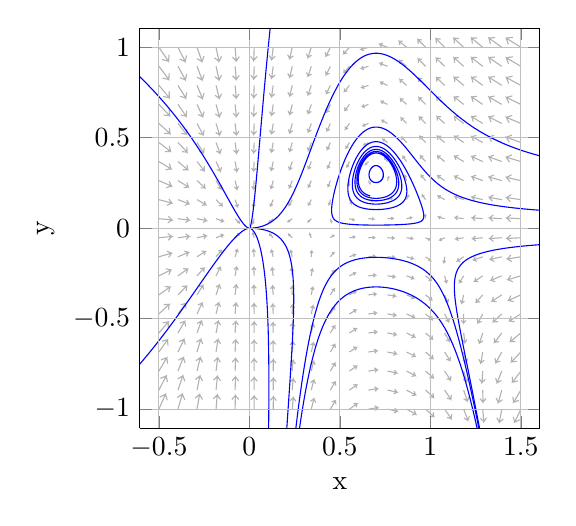
\begin{tikzpicture}
\begin{axis}[%
width=2in,
height=2in,
unbounded coords=jump,
view={0}{90},
scale only axis,
xmin=-0.605263157894737,
xmax=1.60526315789474,
xlabel={x},
xmajorgrids,
ymin=-1.10526315789474,
ymax=1.10526315789474,
ylabel={y},
ymajorgrids,
zmin=-1,
zmax=1
]
\addplot [color=white!70!black,solid,forget plot]
  table[row sep=crcr]{-0.5	-1\\
-0.463747378718074	-0.917136865641312\\
-0.495338948692324	-0.932932650628437\\
-0.463747378718074	-0.917136865641312\\
-0.45390738151298	-0.9510589612694\\
nan	0\\
-0.5	-0.894736842105263\\
-0.46046017899312	-0.816234423755838\\
-0.491947729882541	-0.829900194008946\\
-0.46046017899312	-0.816234423755838\\
-0.452696520707828	-0.849670104512385\\
nan	0\\
-0.5	-0.789473684210526\\
-0.456790673821287	-0.715925894970164\\
-0.488140418984992	-0.727187900197594\\
-0.456790673821287	-0.715925894970164\\
-0.45136652436481	-0.748792563286951\\
nan	0\\
-0.5	-0.684210526315789\\
-0.452712549574631	-0.616377493981467\\
-0.483857042785822	-0.624905541075422\\
-0.452712549574631	-0.616377493981467\\
-0.449940526618661	-0.648549266288106\\
nan	0\\
-0.5	-0.578947368421053\\
-0.448235131980357	-0.517802289417984\\
-0.479050862137017	-0.523204596113994\\
-0.448235131980357	-0.517802289417984\\
-0.448478322635483	-0.549087030123815\\
nan	0\\
-0.5	-0.473684210526316\\
-0.443442824722747	-0.420453927912431\\
-0.473717547959394	-0.422283718877283\\
-0.443442824722747	-0.420453927912431\\
-0.447102406652452	-0.450562306515909\\
nan	0\\
-0.5	-0.368421052631579\\
-0.438552714442426	-0.324586046373946\\
-0.467945651674106	-0.322374726861843\\
-0.438552714442426	-0.324586046373946\\
-0.44602814854529	-0.35309836964063\\
nan	0\\
-0.5	-0.263157894736842\\
-0.43396800785378	-0.230346966962323\\
-0.461980337441276	-0.223682247258123\\
-0.43396800785378	-0.230346966962323\\
-0.445574873554016	-0.256698243331234\\
nan	0\\
-0.5	-0.157894736842105\\
-0.430258521317961	-0.137606306680058\\
-0.456253072463085	-0.126257466058162\\
-0.430258521317961	-0.137606306680058\\
-0.446108857382061	-0.161128205399182\\
nan	0\\
-0.5	-0.0526315789473685\\
-0.42798429177531	-0.0458135237308298\\
-0.451293518046852	-0.029855013239619\\
-0.42798429177531	-0.0458135237308298\\
-0.447884490438583	-0.0658628673519638\\
nan	0\\
-0.5	0.0526315789473684\\
-0.427410718676561	0.0459181194030041\\
-0.447509138187502	0.066079477597173\\
-0.427410718676561	0.0459181194030041\\
-0.450865867959684	0.0297848369354537\\
nan	0\\
-0.5	0.157894736842105\\
-0.428362319203988	0.13846756916861\\
-0.444996831524418	0.162205139669662\\
-0.428362319203988	0.13846756916861\\
-0.454710415361165	0.126386299271656\\
nan	0\\
-0.5	0.263157894736842\\
-0.430366626243459	0.232380712965995\\
-0.443562342927709	0.259022210936384\\
-0.430366626243459	0.232380712965995\\
-0.458950933813133	0.224205524058114\\
nan	0\\
-0.5	0.368421052631579\\
-0.432917513183898	0.327808952505074\\
-0.442889234197102	0.356763204247051\\
-0.432917513183898	0.327808952505074\\
-0.463195284260355	0.323221960839\\
nan	0\\
-0.5	0.473684210526316\\
-0.435635560436018	0.424644637525187\\
-0.442684999054931	0.455447619316521\\
-0.435635560436018	0.424644637525187\\
-0.467204785555495	0.42326539953453\\
nan	0\\
-0.5	0.578947368421053\\
-0.438293215744646	0.522675896768502\\
-0.442737383108115	0.554984034328106\\
-0.438293215744646	0.522675896768502\\
-0.47087311893439	0.524130642200429\\
nan	0\\
-0.5	0.684210526315789\\
-0.440777112676526	0.621680777263593\\
-0.442911541610519	0.655245423810121\\
-0.440777112676526	0.621680777263593\\
-0.474176416136617	0.625633980148384\\
nan	0\\
-0.5	0.789473684210526\\
-0.443043581129808	0.721466019887908\\
-0.443128590710211	0.756107423902242\\
-0.443043581129808	0.721466019887908\\
-0.47713242287152	0.727629214467146\\
nan	0\\
-0.5	0.894736842105263\\
-0.445086378378136	0.821875841709424\\
-0.443345214765735	0.857462547233642\\
-0.445086378378136	0.821875841709424\\
-0.479775714963655	0.83000573642271\\
nan	0\\
-0.5	1\\
-0.446917232659882	0.922788702050737\\
-0.443539238374602	0.959222783270546\\
-0.446917232659882	0.922788702050737\\
-0.482144887349233	0.932681399600487\\
nan	0\\
-0.394736842105263	-1\\
-0.37056733807326	-0.91708801467626\\
-0.398546185613796	-0.935919234265381\\
-0.37056733807326	-0.91708801467626\\
-0.357090192951926	-0.948003986281382\\
nan	0\\
-0.394736842105263	-0.894736842105263\\
-0.367932065885748	-0.815556755904354\\
-0.39576852030183	-0.832609587709748\\
-0.367932065885748	-0.815556755904354\\
-0.356178477201375	-0.846011975819505\\
nan	0\\
-0.394736842105263	-0.789473684210526\\
-0.364890674470993	-0.714500186997347\\
-0.392587899064569	-0.729530694252733\\
-0.364890674470993	-0.714500186997347\\
-0.355101150457979	-0.744453778069868\\
nan	0\\
-0.394736842105263	-0.684210526315789\\
-0.361354989550451	-0.614077067976843\\
-0.388902909901632	-0.626771642339824\\
-0.361354989550451	-0.614077067976843\\
-0.353836180732158	-0.64346256861723\\
nan	0\\
-0.394736842105263	-0.578947368421053\\
-0.357229933923404	-0.514522996909943\\
-0.384588099255739	-0.524473581317811\\
-0.357229933923404	-0.514522996909943\\
-0.352375913500184	-0.543227035408741\\
nan	0\\
-0.394736842105263	-0.473684210526316\\
-0.352442367356295	-0.416187487851955\\
-0.379504890449575	-0.422862885967021\\
-0.352442367356295	-0.416187487851955\\
-0.350756529112395	-0.444010123341505\\
nan	0\\
-0.394736842105263	-0.368421052631579\\
-0.347021779655251	-0.319566479876839\\
-0.37354994157894	-0.322294086090758\\
-0.347021779655251	-0.319566479876839\\
-0.34912265520157	-0.346151617315764\\
nan	0\\
-0.394736842105263	-0.263157894736842\\
-0.341277653375738	-0.22526010311227\\
-0.366789857900739	-0.223264643417261\\
-0.341277653375738	-0.22526010311227\\
-0.347840962088453	-0.249994237782023\\
nan	0\\
-0.394736842105263	-0.157894736842105\\
-0.336045716948165	-0.133673634988995\\
-0.359708329958572	-0.126267184255653\\
-0.336045716948165	-0.133673634988995\\
-0.347597779032017	-0.155612746834202\\
nan	0\\
-0.394736842105263	-0.0526315789473685\\
-0.332646446487744	-0.0443371185263456\\
-0.353347180278256	-0.0313028577482728\\
-0.332646446487744	-0.0443371185263456\\
-0.349199950067744	-0.0623480555570322\\
nan	0\\
-0.394736842105263	0.0526315789473684\\
-0.332033655985884	0.0444905418961167\\
-0.348809352558885	0.062608649541337\\
-0.332033655985884	0.0444905418961167\\
-0.352879871084511	0.0312570564816474\\
nan	0\\
-0.394736842105263	0.157894736842105\\
-0.333880869549824	0.134838746089406\\
-0.346373663628281	0.156969536454076\\
-0.333880869549824	0.134838746089406\\
-0.357901659004631	0.126541550176356\\
nan	0\\
-0.394736842105263	0.263157894736842\\
-0.337029896498758	0.227688732010934\\
-0.345474689499232	0.252756217230332\\
-0.337029896498758	0.227688732010934\\
-0.363209270862186	0.22390274442708\\
nan	0\\
-0.394736842105263	0.368421052631579\\
-0.340488703460635	0.32294984080065\\
-0.345395342096291	0.350153239011086\\
-0.340488703460635	0.32294984080065\\
-0.368130948011755	0.323029169688772\\
nan	0\\
-0.394736842105263	0.473684210526316\\
-0.343747906906588	0.420121263071183\\
-0.345653850602408	0.448937381107392\\
-0.343747906906588	0.420121263071183\\
-0.372435324329974	0.423442913508054\\
nan	0\\
-0.394736842105263	0.578947368421053\\
-0.346632029152072	0.518705751519937\\
-0.346003068812751	0.548804439828569\\
-0.346632029152072	0.518705751519937\\
-0.376123877263309	0.524752033351974\\
nan	0\\
-0.394736842105263	0.684210526315789\\
-0.349121672232018	0.618323336931629\\
-0.346334425847951	0.649493286215189\\
-0.349121672232018	0.618323336931629\\
-0.379278020540032	0.626685701278566\\
nan	0\\
-0.394736842105263	0.789473684210526\\
-0.351254525877624	0.718705800454064\\
-0.3466072498068	0.750806744637912\\
-0.351254525877624	0.718705800454064\\
-0.381991191685031	0.729065586524093\\
nan	0\\
-0.394736842105263	0.894736842105263\\
-0.353082396604775	0.819666935885103\\
-0.346811253699881	0.852601519126273\\
-0.353082396604775	0.819666935885103\\
-0.384346206809961	0.831774296376029\\
nan	0\\
-0.394736842105263	1\\
-0.354655160758425	0.921076388003504\\
-0.346948762163353	0.954773891939163\\
-0.354655160758425	0.921076388003504\\
-0.386410568161601	0.934733051265744\\
nan	0\\
-0.289473684210526	-1\\
-0.275415947807323	-0.918425885111034\\
-0.300026797450525	-0.939383685476923\\
-0.275415947807323	-0.918425885111034\\
-0.259239740006042	-0.946412553678525\\
nan	0\\
-0.289473684210526	-0.894736842105263\\
-0.273581168791023	-0.816421765816781\\
-0.297927692488995	-0.83594315984845\\
-0.273581168791023	-0.816421765816781\\
-0.258770154344754	-0.843889417558201\\
nan	0\\
-0.289473684210526	-0.789473684210526\\
-0.271418233088879	-0.714768684415326\\
-0.295511118374173	-0.732666321573474\\
-0.271418233088879	-0.714768684415326\\
-0.258158618476573	-0.741694047134298\\
nan	0\\
-0.289473684210526	-0.684210526315789\\
-0.268823741591266	-0.613582376319068\\
-0.292675761876224	-0.62960833566327\\
-0.268823741591266	-0.613582376319068\\
-0.257361686877864	-0.6399333069729\\
nan	0\\
-0.289473684210526	-0.578947368421053\\
-0.265651142534915	-0.513046792339515\\
-0.289273049057982	-0.526861329745073\\
-0.265651142534915	-0.513046792339515\\
-0.256322761017214	-0.538772600582879\\
nan	0\\
-0.289473684210526	-0.473684210526316\\
-0.261696046278678	-0.413471779986183\\
-0.285082445293265	-0.424591099665261\\
-0.261696046278678	-0.413471779986183\\
-0.254976230023199	-0.438479918631185\\
nan	0\\
-0.289473684210526	-0.368421052631579\\
-0.256700508142977	-0.31540813067379\\
-0.279785691452689	-0.32311871324424\\
-0.256700508142977	-0.31540813067379\\
-0.253279230473795	-0.339505301278014\\
nan	0\\
-0.289473684210526	-0.263157894736842\\
-0.250472200443643	-0.219851875055061\\
-0.272999150494153	-0.223093310017874\\
-0.250472200443643	-0.219851875055061\\
-0.251346140653263	-0.242594051901316\\
nan	0\\
-0.289473684210526	-0.157894736842105\\
-0.24344292363567	-0.128378640064678\\
-0.264631176002483	-0.125725778954192\\
-0.24344292363567	-0.128378640064678\\
-0.24987312761377	-0.148741159241621\\
nan	0\\
-0.289473684210526	-0.0526315789473685\\
-0.237924391764522	-0.0420117780610804\\
-0.256044129719895	-0.0323103952154657\\
-0.237924391764522	-0.0420117780610804\\
-0.250734229276751	-0.0580850414384679\\
nan	0\\
-0.289473684210526	0.0526315789473684\\
-0.23726172318005	0.0422506527516426\\
-0.250330079940262	0.0584179208679793\\
-0.23726172318005	0.0422506527516426\\
-0.255520543038125	0.0323119403527414\\
nan	0\\
-0.289473684210526	0.157894736842105\\
-0.240852318827391	0.129871633673092\\
-0.248432952650078	0.15043390596958\\
-0.240852318827391	0.129871633673092\\
-0.262444504234585	0.126123223278012\\
nan	0\\
-0.289473684210526	0.263157894736842\\
-0.245515546013035	0.222309686606809\\
-0.248490935439774	0.245553683595192\\
-0.245515546013035	0.222309686606809\\
-0.268915039504791	0.223574614496446\\
nan	0\\
-0.289473684210526	0.368421052631579\\
-0.249645972621695	0.318243965674413\\
-0.249050014359053	0.34325401965877\\
-0.249645972621695	0.318243965674413\\
-0.274138557837636	0.323340163864355\\
nan	0\\
-0.289473684210526	0.473684210526316\\
-0.252966707372528	0.416360745533924\\
-0.249587934175829	0.442684529241141\\
-0.252966707372528	0.416360745533924\\
-0.278249666672025	0.424431040822142\\
nan	0\\
-0.289473684210526	0.578947368421053\\
-0.255590872742714	0.515853714015721\\
-0.249982302581725	0.543252513204274\\
-0.255590872742714	0.515853714015721\\
-0.28152912978439	0.526311107470368\\
nan	0\\
-0.289473684210526	0.684210526315789\\
-0.257679204591181	0.61626016534404\\
-0.250229958234047	0.644593893540401\\
-0.257679204591181	0.61626016534404\\
-0.284205138719922	0.628696653730728\\
nan	0\\
-0.289473684210526	0.789473684210526\\
-0.259364189250898	0.717307064591122\\
-0.250355382833936	0.74648442421685\\
-0.259364189250898	0.717307064591122\\
-0.286438692643638	0.731429676737036\\
nan	0\\
-0.289473684210526	0.894736842105263\\
-0.260743937478228	0.818825079921265\\
-0.250384920951918	0.848781045259539\\
-0.260743937478228	0.818825079921265\\
-0.288340802043917	0.83441617189339\\
nan	0\\
-0.289473684210526	1\\
-0.261889469650968	0.920703744428312\\
-0.250340670125914	0.951388674739708\\
-0.261889469650968	0.920703744428312\\
-0.289988797911758	0.937596567459929\\
nan	0\\
-0.184210526315789	-1\\
-0.177748046739626	-0.920832911915338\\
-0.199478562633641	-0.942967418446696\\
-0.177748046739626	-0.920832911915338\\
-0.15989501859131	-0.946198658234778\\
nan	0\\
-0.184210526315789	-0.894736842105263\\
-0.176697308082406	-0.818528182968611\\
-0.198003438336584	-0.839512476151261\\
-0.176697308082406	-0.818528182968611\\
-0.159899108768258	-0.843269085267953\\
nan	0\\
-0.184210526315789	-0.789473684210526\\
-0.175447933607796	-0.716492090149427\\
-0.196322109935469	-0.736195920190758\\
-0.175447933607796	-0.716492090149427\\
-0.159831312904919	-0.740577216544755\\
nan	0\\
-0.184210526315789	-0.684210526315789\\
-0.173927138163078	-0.614799851713713\\
-0.194364823259411	-0.633052207056158\\
-0.173927138163078	-0.614799851713713\\
-0.159659485958372	-0.638193901132514\\
nan	0\\
-0.184210526315789	-0.578947368421053\\
-0.172020383677657	-0.513568319532657\\
-0.192022188691196	-0.530134498539642\\
-0.172020383677657	-0.513568319532657\\
-0.159332664246998	-0.536229569858709\\
nan	0\\
-0.184210526315789	-0.473684210526316\\
-0.169537311439486	-0.412994995255618\\
-0.189111579720051	-0.427533456117752\\
-0.169537311439486	-0.412994995255618\\
-0.158766972084703	-0.434870063555903\\
nan	0\\
-0.184210526315789	-0.368421052631579\\
-0.166142238190448	-0.313454194689152\\
-0.185304439113657	-0.325427180040545\\
-0.166142238190448	-0.313454194689152\\
-0.157821010142443	-0.334461324103216\\
nan	0\\
-0.184210526315789	-0.263157894736842\\
-0.161219471335572	-0.215772940743715\\
-0.179963026327919	-0.224240663196599\\
-0.161219471335572	-0.215772940743715\\
-0.156270549331355	-0.235736190686708\\
nan	0\\
-0.184210526315789	-0.157894736842105\\
-0.153793583230625	-0.122123941105587\\
-0.171861365090304	-0.125250944055252\\
-0.153793583230625	-0.122123941105587\\
-0.153975967222045	-0.140459415597834\\
nan	0\\
-0.184210526315789	-0.0526315789473685\\
-0.144689690996867	-0.0378628832658043\\
-0.160238115512935	-0.0324132831405429\\
-0.144689690996867	-0.0378628832658043\\
-0.152853767672153	-0.0521737008000042\\
nan	0\\
-0.184210526315789	0.0526315789473684\\
-0.143939618566973	0.0382541791169041\\
-0.152426540934002	0.0526351260032476\\
-0.143939618566973	0.0382541791169041\\
-0.159615240849234	0.0324996721288392\\
nan	0\\
-0.184210526315789	0.157894736842105\\
-0.150739097011607	0.123576644064798\\
-0.152201002608535	0.142239929224036\\
-0.150739097011607	0.123576644064798\\
-0.169360048997188	0.125504214571945\\
nan	0\\
-0.184210526315789	0.263157894736842\\
-0.156291864603787	0.217404400610434\\
-0.153229089585786	0.238110114276357\\
-0.156291864603787	0.217404400610434\\
-0.17610583664899	0.224150783420356\\
nan	0\\
-0.184210526315789	0.368421052631579\\
-0.159964723396641	0.314982348735207\\
-0.153878788298293	0.337075410633906\\
-0.159964723396641	0.314982348735207\\
-0.180598140246479	0.324952509174331\\
nan	0\\
-0.184210526315789	0.473684210526316\\
-0.162460203521316	0.414382882010442\\
-0.15415996823069	0.437610861263823\\
-0.162460203521316	0.414382882010442\\
-0.183810632488627	0.426735699866586\\
nan	0\\
-0.184210526315789	0.578947368421053\\
-0.16424061222257	0.514828892446279\\
-0.154201967456842	0.539056913762016\\
-0.16424061222257	0.514828892446279\\
-0.186261205444229	0.529071956715406\\
nan	0\\
-0.184210526315789	0.684210526315789\\
-0.165565723465172	0.615952758028952\\
-0.154094722248648	0.641091289227658\\
-0.165565723465172	0.615952758028952\\
-0.188223606392066	0.631768887802349\\
nan	0\\
-0.184210526315789	0.789473684210526\\
-0.166585696620205	0.717554916056732\\
-0.153893453490432	0.743536753926766\\
-0.166585696620205	0.717554916056732\\
-0.189852837567329	0.734724339078974\\
nan	0\\
-0.184210526315789	0.894736842105263\\
-0.167391916167167	0.819515226139812\\
-0.153632095220391	0.846286363466602\\
-0.167391916167167	0.819515226139812\\
-0.191242903203117	0.837877058392291\\
nan	0\\
-0.184210526315789	1\\
-0.16804280736396	0.921755555370117\\
-0.153332011892038	0.949270818497039\\
-0.16804280736396	0.921755555370117\\
-0.19245423420698	0.941186959021125\\
nan	0\\
-0.0789473684210527	-1\\
-0.0772766864934021	-0.923952124361651\\
-0.0967898599812844	-0.946348816571243\\
-0.0772766864934021	-0.923952124361651\\
-0.0587659221621101	-0.947184157535069\\
nan	0\\
-0.0789473684210527	-0.894736842105263\\
-0.0768861776829661	-0.821464366148029\\
-0.0958226538937006	-0.842930811250677\\
-0.0768861776829661	-0.821464366148029\\
-0.0591864159150834	-0.843961406619721\\
nan	0\\
-0.0789473684210527	-0.789473684210526\\
-0.0764223163536314	-0.719207020048344\\
-0.0947464980144034	-0.739655756280143\\
-0.0764223163536314	-0.719207020048344\\
-0.0596131659333122	-0.740918282313854\\
nan	0\\
-0.0789473684210527	-0.684210526315789\\
-0.0758570419958169	-0.617235590610488\\
-0.093527873849713	-0.63655548971577\\
-0.0758570419958169	-0.617235590610488\\
-0.0600404059970623	-0.638100652928387\\
nan	0\\
-0.0789473684210527	-0.578947368421053\\
-0.0751446457079612	-0.515631088533369\\
-0.0921145324938095	-0.533675291821401\\
-0.0751446457079612	-0.515631088533369\\
-0.0604563925499678	-0.535576653177947\\
nan	0\\
-0.0789473684210527	-0.473684210526316\\
-0.0742046209981742	-0.414519970586349\\
-0.0904185052100295	-0.431083555712619\\
-0.0742046209981742	-0.414519970586349\\
-0.0608363852400459	-0.433454929424058\\
nan	0\\
-0.0789473684210527	-0.368421052631579\\
-0.0728790506539103	-0.314119987997675\\
-0.0882748121425289	-0.328893227946061\\
-0.0728790506539103	-0.314119987997675\\
-0.0611242798255772	-0.331927386829632\\
nan	0\\
-0.0789473684210527	-0.263157894736842\\
-0.0708052444551205	-0.214870111140509\\
-0.0853198275439834	-0.227320915227926\\
-0.0708052444551205	-0.214870111140509\\
-0.0611759357458169	-0.231391977210892\\
nan	0\\
-0.0789473684210527	-0.157894736842105\\
-0.0669146626796385	-0.117958509583496\\
-0.080508531216715	-0.126931201325725\\
-0.0669146626796385	-0.117958509583496\\
-0.0605404175874104	-0.132947554196432\\
nan	0\\
-0.0789473684210527	-0.0526315789473685\\
-0.0568640024314072	-0.0297402601148616\\
-0.0692118419364276	-0.0310868142672023\\
-0.0568640024314072	-0.0297402601148616\\
-0.0577661825201741	-0.042128497262025\\
nan	0\\
-0.0789473684210527	0.0526315789473684\\
-0.0559429466495634	0.0301995255372503\\
-0.0572362598284806	0.0426802470031581\\
-0.0559429466495634	0.0301995255372503\\
-0.0684522865335396	0.0311780361174134\\
nan	0\\
-0.0789473684210527	0.157894736842105\\
-0.0646601174783518	0.118439053413797\\
-0.059082371904085	0.133847571177965\\
-0.0646601174783518	0.118439053413797\\
-0.0788102136182391	0.126703945706614\\
nan	0\\
-0.0789473684210527	0.263157894736842\\
-0.0679544015410229	0.215243110784825\\
-0.0592735956170276	0.232365787690438\\
-0.0679544015410229	0.215243110784825\\
-0.083230987593036	0.226869304250423\\
nan	0\\
-0.0789473684210527	0.368421052631579\\
-0.0696296969368555	0.31442560242331\\
-0.0589261358300474	0.33295365535684\\
-0.0696296969368555	0.31442560242331\\
-0.0859238609341818	0.328294819614741\\
nan	0\\
-0.0789473684210527	0.473684210526316\\
-0.070643615823244	0.414781156572048\\
-0.0584089781140196	0.43452801090778\\
-0.070643615823244	0.414781156572048\\
-0.0878605050911537	0.430376134608876\\
nan	0\\
-0.0789473684210527	0.578947368421053\\
-0.0713220952225475	0.51586078852773\\
-0.0578380322087683	0.536693080795353\\
-0.0713220952225475	0.51586078852773\\
-0.0893813221554298	0.5328804441961\\
nan	0\\
-0.0789473684210527	0.684210526315789\\
-0.0718062872357413	0.61744171403617\\
-0.0572564085214299	0.639257628016384\\
-0.0718062872357413	0.61744171403617\\
-0.0906408146612395	0.635687087423728\\
nan	0\\
-0.0789473684210527	0.789473684210526\\
-0.072167505673331	0.719394750019777\\
-0.0566817309499603	0.742113395963932\\
-0.072167505673331	0.719394750019777\\
-0.0917211980453347	0.738723464590071\\
nan	0\\
-0.0789473684210527	0.894736842105263\\
-0.0724457991223735	0.821637290449108\\
-0.0561213819979385	0.845192548270624\\
-0.0724457991223735	0.821637290449108\\
-0.092671157826016	0.841941763621285\\
nan	0\\
-0.0789473684210527	1\\
-0.0726654571395298	0.924112835690645\\
-0.0555782394466478	0.948449462803832\\
-0.0726654571395298	0.924112835690645\\
-0.0935218216013255	0.94530850716307\\
nan	0\\
0.0263157894736842	-1\\
0.026135046030676	-0.927533249331711\\
0.00807258139650618	-0.94931846039295\\
0.026135046030676	-0.927533249331711\\
0.0443059567306508	-0.949228088671445\\
nan	0\\
0.0263157894736842	-0.894736842105263\\
0.0260248635948092	-0.82490787527677\\
0.00865489965134848	-0.845929296795037\\
0.0260248635948092	-0.82490787527677\\
0.0435693830655949	-0.845783833855599\\
nan	0\\
0.0263157894736842	-0.789473684210526\\
0.0258949003471349	-0.7224986118593\\
0.00927739899729304	-0.742696355846305\\
0.0258949003471349	-0.7224986118593\\
0.0427649351729063	-0.74248591128303\\
nan	0\\
0.0263157894736842	-0.684210526315789\\
0.0257376539634778	-0.620356090365794\\
0.00994748562904082	-0.639656955028344\\
0.0257376539634778	-0.620356090365794\\
0.0418747036040386	-0.639367887273241\\
nan	0\\
0.0263157894736842	-0.578947368421053\\
0.0255408820111953	-0.518553123886448\\
0.0106747931162907	-0.536865124112451\\
0.0255408820111953	-0.518553123886448\\
0.0408719153835932	-0.536477670381207\\
nan	0\\
0.0263157894736842	-0.473684210526316\\
0.0252829182303063	-0.417200798221368\\
0.0114719265270826	-0.434404039723697\\
0.0252829182303063	-0.417200798221368\\
0.0397136326795567	-0.433887604102008\\
nan	0\\
0.0263157894736842	-0.368421052631579\\
0.0249207851898512	-0.316483266020377\\
0.0123548398222006	-0.332413353074696\\
0.0249207851898512	-0.316483266020377\\
0.0383237331278016	-0.331715850932779\\
nan	0\\
0.0263157894736842	-0.263157894736842\\
0.0243530595697427	-0.21674701358579\\
0.013339158253162	-0.231160960407091\\
0.0243530595697427	-0.21674701358579\\
0.0365445988286882	-0.23017959545512\\
nan	0\\
0.0263157894736842	-0.157894736842105\\
0.0232553376328503	-0.1188066727183\\
0.0144014571541491	-0.13129820491565\\
0.0232553376328503	-0.1188066727183\\
0.0339454892160519	-0.129767978995233\\
nan	0\\
0.0263157894736842	-0.0526315789473685\\
0.0194497615790416	-0.0260527013671525\\
0.0148648505523804	-0.0357428716148779\\
0.0194497615790416	-0.0260527013671525\\
0.0281542893424884	-0.0323098576675566\\
nan	0\\
0.0263157894736842	0.0526315789473684\\
0.0188562095277127	0.026157009916208\\
0.0277127257692942	0.0322344856390632\\
0.0188562095277127	0.026157009916208\\
0.014475441253714	0.035964275612049\\
nan	0\\
0.0263157894736842	0.157894736842105\\
0.022344754560788	0.118861162272229\\
0.0332944586771259	0.129578475914968\\
0.022344754560788	0.118861162272229\\
0.0137776713921879	0.131563993371416\\
nan	0\\
0.0263157894736842	0.263157894736842\\
0.0232678699039675	0.21678604366677\\
0.0357752085424004	0.229935619095363\\
0.0232678699039675	0.21678604366677\\
0.0125892830073646	0.231459578880221\\
nan	0\\
0.0263157894736842	0.368421052631579\\
0.0237050649267358	0.316514512850849\\
0.0374649172360026	0.331433793648331\\
0.0237050649267358	0.316514512850849\\
0.011511647345638	0.332739155921805\\
nan	0\\
0.0263157894736842	0.473684210526316\\
0.0239601917396437	0.417227245617827\\
0.0387811122869781	0.433575435656863\\
0.0239601917396437	0.417227245617827\\
0.0105526298327337	0.434753234523884\\
nan	0\\
0.0263157894736842	0.578947368421053\\
0.0241262313307946	0.518576268767785\\
0.0398758736869784	0.536140209128043\\
0.0241262313307946	0.518576268767785\\
0.00969032386034449	0.537234988199488\\
nan	0\\
0.0263157894736842	0.684210526315789\\
0.0242417385295467	0.620376800689261\\
0.0408223852194201	0.639008405641185\\
0.0242417385295467	0.620376800689261\\
0.00890552240615576	0.640045431113254\\
nan	0\\
0.0263157894736842	0.789473684210526\\
0.0243257317069213	0.722517440418496\\
0.0416618099849577	0.742106799114414\\
0.0243257317069213	0.722517440418496\\
0.00818368808894269	0.743101827997796\\
nan	0\\
0.0263157894736842	0.894736842105263\\
0.0243887253615434	0.824925198160161\\
0.0424197555814611	0.845386925315657\\
0.0243887253615434	0.824925198160161\\
0.00751393360891015	0.846350457371727\\
nan	0\\
0.0263157894736842	1\\
0.0244370236967176	0.927549335262199\\
0.0431133196142578	0.948814843239298\\
0.0244370236967176	0.927549335262199\\
0.00688798724535736	0.949754226127781\\
nan	0\\
0.131578947368421	-1\\
0.132639264455029	-0.931528542322727\\
0.115203304909728	-0.951804900354257\\
0.132639264455029	-0.931528542322727\\
0.149439033748365	-0.95233505889756\\
nan	0\\
0.131578947368421	-0.894736842105263\\
0.132181860237304	-0.828754057734718\\
0.115505290284003	-0.848398164828661\\
0.132181860237304	-0.828754057734718\\
0.148496682469275	-0.848699621263102\\
nan	0\\
0.131578947368421	-0.789473684210526\\
0.131648342418143	-0.726185398863849\\
0.115805452566557	-0.745154535705421\\
0.131648342418143	-0.726185398863849\\
0.147449595239896	-0.745189233230283\\
nan	0\\
0.131578947368421	-0.684210526315789\\
0.131010644229294	-0.623872000786075\\
0.116096503788604	-0.642115634229771\\
0.131010644229294	-0.623872000786075\\
0.146265766553461	-0.641831482660207\\
nan	0\\
0.131578947368421	-0.578947368421053\\
0.130223322400809	-0.521885985168962\\
0.11636466407807	-0.539343306386492\\
0.130223322400809	-0.521885985168962\\
0.144895355704115	-0.538665493902686\\
nan	0\\
0.131578947368421	-0.473684210526316\\
0.129206790249566	-0.420339921124777\\
0.116582365034838	-0.436936247224953\\
0.129206790249566	-0.420339921124777\\
0.143254509735607	-0.435750168665525\\
nan	0\\
0.131578947368421	-0.368421052631579\\
0.127805709372038	-0.319427795610063\\
0.116689366515574	-0.335069082215614\\
0.127805709372038	-0.319427795610063\\
0.141185995026332	-0.333182463217422\\
nan	0\\
0.131578947368421	-0.263157894736842\\
0.125664648626337	-0.219541934202228\\
0.116534948115309	-0.234105297048133\\
0.125664648626337	-0.219541934202228\\
0.138342928382616	-0.231148147677091\\
nan	0\\
0.131578947368421	-0.157894736842105\\
0.121738396448985	-0.121755478700393\\
0.115655747189388	-0.135057393872765\\
0.121738396448985	-0.121755478700393\\
0.133725376260244	-0.130137118413048\\
nan	0\\
0.131578947368421	-0.0526315789473685\\
0.111822655186388	-0.0319611332838728\\
0.112581931425124	-0.0431013400284296\\
0.111822655186388	-0.0319611332838728\\
0.122917154256872	-0.0332231939374133\\
nan	0\\
0.131578947368421	0.0526315789473684\\
0.109974379973205	0.032895319717548\\
0.121389814999225	0.03341505563769\\
0.109974379973205	0.032895319717548\\
0.111521685384314	0.0442173393352982\\
nan	0\\
0.131578947368421	0.157894736842105\\
0.117132664238453	0.122761376270023\\
0.130249889320464	0.129689813659156\\
0.117132664238453	0.122761376270023\\
0.112683209034423	0.13691295522414\\
nan	0\\
0.131578947368421	0.263157894736842\\
0.119822092774913	0.220325998374873\\
0.134057123243457	0.230236353635087\\
0.119822092774913	0.220325998374873\\
0.112641175062473	0.236114780931841\\
nan	0\\
0.131578947368421	0.368421052631579\\
0.121139964055612	0.320071014322772\\
0.136359168626656	0.331966279987212\\
0.121139964055612	0.320071014322772\\
0.112184149472253	0.337185771643616\\
nan	0\\
0.131578947368421	0.473684210526316\\
0.121898707963169	0.420889921464317\\
0.138001352050244	0.434308148331603\\
0.121898707963169	0.420889921464317\\
0.111604207519245	0.439148268034229\\
nan	0\\
0.131578947368421	0.578947368421053\\
0.122376823040041	0.522369812999822\\
0.139281849193863	0.537042548544096\\
0.122376823040041	0.522369812999822\\
0.110993071483247	0.541643610708286\\
nan	0\\
0.131578947368421	0.684210526315789\\
0.122694693743838	0.624306235715\\
0.14033604248141	0.640056459489091\\
0.122694693743838	0.624306235715\\
0.110383897181016	0.644498586301383\\
nan	0\\
0.131578947368421	0.789473684210526\\
0.122912803073914	0.726580923494955\\
0.141235836541159	0.743282215636\\
0.122912803073914	0.726580923494955\\
0.109789456183374	0.747615287783253\\
nan	0\\
0.131578947368421	0.894736842105263\\
0.123064860190661	0.829118412476101\\
0.142023693751279	0.846675419570409\\
0.123064860190661	0.829118412476101\\
0.109214478936698	0.850932463159289\\
nan	0\\
0.131578947368421	1\\
0.123171128765421	0.931867179694721\\
0.142726679422641	0.950205071135555\\
0.123171128765421	0.931867179694721\\
0.108660269270001	0.954408980437055\\
nan	0\\
0.236842105263158	-1\\
0.242566181961891	-0.936212411272351\\
0.224902061770359	-0.953917668715962\\
0.242566181961891	-0.936212411272351\\
0.256795856134183	-0.956779707065329\\
nan	0\\
0.236842105263158	-0.894736842105263\\
0.241899567232823	-0.833244681255832\\
0.225009288429566	-0.850427964018245\\
0.241899567232823	-0.833244681255832\\
0.255755368854281	-0.852956695003078\\
nan	0\\
0.236842105263158	-0.789473684210526\\
0.241135373359333	-0.73046551111719\\
0.225095349657146	-0.747094646021147\\
0.241135373359333	-0.73046551111719\\
0.254599436203814	-0.749241280069235\\
nan	0\\
0.236842105263158	-0.684210526315789\\
0.240239184486003	-0.627920140199718\\
0.225147464190131	-0.643957986228828\\
0.240239184486003	-0.627920140199718\\
0.253292657248167	-0.64565652584025\\
nan	0\\
0.236842105263158	-0.578947368421053\\
0.239155693571548	-0.525674734720996\\
0.225143458654017	-0.541078127753915\\
0.239155693571548	-0.525674734720996\\
0.251779775504046	-0.54223492190811\\
nan	0\\
0.236842105263158	-0.473684210526316\\
0.237788739391447	-0.423833115644464\\
0.225041975432497	-0.438551785576947\\
0.237788739391447	-0.423833115644464\\
0.249967522873423	-0.439025102641092\\
nan	0\\
0.236842105263158	-0.368421052631579\\
0.235951960961807	-0.32257617297037\\
0.22475778433691	-0.33655217294407\\
0.235951960961807	-0.32257617297037\\
0.247680224167515	-0.336107100793395\\
nan	0\\
0.236842105263158	-0.263157894736842\\
0.233222363464782	-0.222278406139178\\
0.224088413854879	-0.235447188168071\\
0.233222363464782	-0.222278406139178\\
0.244528158153711	-0.233637317268883\\
nan	0\\
0.236842105263158	-0.157894736842105\\
0.228377620444679	-0.12401653548604\\
0.222447415551207	-0.136296117097479\\
0.228377620444679	-0.12401653548604\\
0.239386516229239	-0.13206387468824\\
nan	0\\
0.236842105263158	-0.0526315789473685\\
0.21711958408017	-0.033961483877047\\
0.218368816667486	-0.0444931426938904\\
0.21711958408017	-0.033961483877047\\
0.227703864202647	-0.0346318821023966\\
nan	0\\
0.236842105263158	0.0526315789473684\\
0.213818847612429	0.0357423009866275\\
0.224948144397833	0.0350532699621675\\
0.213818847612429	0.0357423009866275\\
0.216503505417462	0.046564898787532\\
nan	0\\
0.236842105263158	0.157894736842105\\
0.219254525658975	0.126300395613856\\
0.232429384847292	0.131381803081285\\
0.219254525658975	0.126300395613856\\
0.216632214233168	0.140175592883376\\
nan	0\\
0.236842105263158	0.263157894736842\\
0.221403469753403	0.224108808325359\\
0.2357973320092	0.231963875371365\\
0.221403469753403	0.224108808325359\\
0.216272788803458	0.239683193126243\\
nan	0\\
0.236842105263158	0.368421052631579\\
0.222379908594904	0.324090390730119\\
0.237801233070745	0.333774040133493\\
0.222379908594904	0.324090390730119\\
0.215635902120015	0.341005138467621\\
nan	0\\
0.236842105263158	0.473684210526316\\
0.222867511358745	0.425132478561269\\
0.23919782252133	0.43620434967468\\
0.222867511358745	0.425132478561269\\
0.214921956538807	0.443191646626886\\
nan	0\\
0.236842105263158	0.578947368421053\\
0.223112289771915	0.526819842691594\\
0.240263115851653	0.539025646537621\\
0.223112289771915	0.526819842691594\\
0.214199352986923	0.545890554283242\\
nan	0\\
0.236842105263158	0.684210526315789\\
0.223221841145679	0.628948953520508\\
0.241123313579743	0.642122359329723\\
0.223221841145679	0.628948953520508\\
0.213492527182102	0.648932491388462\\
nan	0\\
0.236842105263158	0.789473684210526\\
0.223250076431016	0.731403230122521\\
0.24184529860266	0.745426359140887\\
0.223250076431016	0.731403230122521\\
0.212810071558657	0.752222373556958\\
nan	0\\
0.236842105263158	0.894736842105263\\
0.223226730675908	0.834108884988123\\
0.242468332331368	0.848893428476453\\
0.223226730675908	0.834108884988123\\
0.212154353772798	0.855701115770078\\
nan	0\\
0.236842105263158	1\\
0.223169405413723	0.937015866765727\\
0.243017248677122	0.95249293177365\\
0.223169405413723	0.937015866765727\\
0.211525182059985	0.959329281698368\\
nan	0\\
0.342105263157895	-1\\
0.356504213515165	-0.942486200484844\\
0.337806078529195	-0.956140602750073\\
0.356504213515165	-0.942486200484844\\
0.366562978286773	-0.963340077928708\\
nan	0\\
0.342105263157895	-0.894736842105263\\
0.355751868508412	-0.839279320495796\\
0.33779350650089	-0.852504925641006\\
0.355751868508412	-0.839279320495796\\
0.365522267305624	-0.859328228316265\\
nan	0\\
0.342105263157895	-0.789473684210526\\
0.354916280905479	-0.736238085400944\\
0.337764075878808	-0.749006010606923\\
0.354916280905479	-0.736238085400944\\
0.364381875283599	-0.755411519480715\\
nan	0\\
0.342105263157895	-0.684210526315789\\
0.353972020502132	-0.633400748391168\\
0.337709548817705	-0.645676992432496\\
0.353972020502132	-0.633400748391168\\
0.363114437780016	-0.651610371104614\\
nan	0\\
0.342105263157895	-0.578947368421053\\
0.352879422795267	-0.530822167897334\\
0.337615874773126	-0.542566188145107\\
0.352879422795267	-0.530822167897334\\
0.361678475034985	-0.547953267963793\\
nan	0\\
0.342105263157895	-0.473684210526316\\
0.351571532858765	-0.428585866131471\\
0.337457065849793	-0.439748802024707\\
0.351571532858765	-0.428585866131471\\
0.360006238047215	-0.444481936875142\\
nan	0\\
0.342105263157895	-0.368421052631579\\
0.349921903376373	-0.32683041039836\\
0.337179250752524	-0.337353443013706\\
0.349921903376373	-0.32683041039836\\
0.357974571869134	-0.341261763122945\\
nan	0\\
0.342105263157895	-0.263157894736842\\
0.347646800655109	-0.225819347428366\\
0.336649702578825	-0.235635527246605\\
0.347646800655109	-0.225819347428366\\
0.355318976233064	-0.238406295995212\\
nan	0\\
0.342105263157895	-0.157894736842105\\
0.343885509542761	-0.126205942409309\\
0.335429237019102	-0.135267519142931\\
0.343885509542761	-0.126205942409309\\
0.3512736342355	-0.136157642335364\\
nan	0\\
0.342105263157895	-0.0526315789473685\\
0.333637249753746	-0.0317225042829439\\
0.330950385108884	-0.0401122300333085\\
0.333637249753746	-0.0317225042829439\\
0.341404922441097	-0.0358782233312341\\
nan	0\\
0.342105263157895	0.0526315789473684\\
0.324900145377983	0.0350488127447609\\
0.334457372262608	0.0360223631605651\\
0.324900145377983	0.0350488127447609\\
0.325665989161304	0.0446249220505212\\
nan	0\\
0.342105263157895	0.157894736842105\\
0.32694127750415	0.128583873660998\\
0.33881818899555	0.133586136201894\\
0.32694127750415	0.128583873660998\\
0.324162757404996	0.141168129028766\\
nan	0\\
0.342105263157895	0.263157894736842\\
0.326977678345232	0.227573298327266\\
0.340412102891425	0.234466781046973\\
0.326977678345232	0.227573298327266\\
0.322619804686637	0.242030573453304\\
nan	0\\
0.342105263157895	0.368421052631579\\
0.326614339423624	0.328246154286825\\
0.341305341130094	0.336425892856684\\
0.326614339423624	0.328246154286825\\
0.321217891957717	0.344171354723819\\
nan	0\\
0.342105263157895	0.473684210526316\\
0.326143515142684	0.42978822378928\\
0.341906036231506	0.438966582806588\\
0.326143515142684	0.42978822378928\\
0.319958042862988	0.446947456814193\\
nan	0\\
0.342105263157895	0.578947368421053\\
0.325646747691264	0.531876196350468\\
0.342352095348899	0.541882919104986\\
0.325646747691264	0.531876196350468\\
0.318816509313607	0.550112176838301\\
nan	0\\
0.342105263157895	0.684210526315789\\
0.325152087680141	0.634344839993064\\
0.342704461904149	0.645066252020443\\
0.325152087680141	0.634344839993064\\
0.317771618742786	0.65354283975932\\
nan	0\\
0.342105263157895	0.789473684210526\\
0.324669992758668	0.737096929265825\\
0.342994762614612	0.748451138149429\\
0.324669992758668	0.737096929265825\\
0.316806385142261	0.757168773349042\\
nan	0\\
0.342105263157895	0.894736842105263\\
0.32420420050085	0.840069812983733\\
0.343241276578346	0.851994656055931\\
0.32420420050085	0.840069812983733\\
0.315907762017581	0.860945187384453\\
nan	0\\
0.342105263157895	1\\
0.32375565113162	0.943220461220685\\
0.343455419434331	0.955666919847911\\
0.32375565113162	0.943220461220685\\
0.315065650044673	0.964841725861048\\
nan	0\\
0.447368421052632	-1\\
0.474790681590168	-0.952524248223361\\
0.454695065484747	-0.959911408621969\\
0.474790681590168	-0.952524248223361\\
0.478432941373067	-0.973622538890737\\
nan	0\\
0.447368421052632	-0.894736842105263\\
0.474000034511458	-0.849061183479124\\
0.454591635817275	-0.856105977702259\\
0.474000034511458	-0.849061183479124\\
0.477429465130345	-0.869421784431672\\
nan	0\\
0.447368421052632	-0.789473684210526\\
0.473162533786869	-0.745752411441036\\
0.454493981774225	-0.752420265088324\\
0.473162533786869	-0.745752411441036\\
0.47635461815897	-0.765317321455442\\
nan	0\\
0.447368421052632	-0.684210526315789\\
0.472271623596182	-0.642635932820337\\
0.454407014459254	-0.648882510233085\\
0.472271623596182	-0.642635932820337\\
0.47519431120698	-0.66133411150486\\
nan	0\\
0.447368421052632	-0.578947368421053\\
0.471319906632241	-0.539767342603167\\
0.454339454503887	-0.54553347895363\\
0.471319906632241	-0.539767342603167\\
0.47392946741283	-0.557509221743435\\
nan	0\\
0.447368421052632	-0.473684210526316\\
0.4703000606139	-0.437233395223698\\
0.454307864919865	-0.442435729924166\\
0.4703000606139	-0.437233395223698\\
0.472533272571174	-0.4539015497048\\
nan	0\\
0.447368421052632	-0.368421052631579\\
0.469208606844508	-0.335182421939561\\
0.454346893433941	-0.339693964699198\\
0.469208606844508	-0.335182421939561\\
0.470966208779949	-0.350614057595136\\
nan	0\\
0.447368421052632	-0.263157894736842\\
0.468061136569677	-0.233906160176593\\
0.454540388274501	-0.237508501665406\\
0.468061136569677	-0.233906160176593\\
0.469166255554625	-0.247854859423929\\
nan	0\\
0.447368421052632	-0.157894736842105\\
0.46696467791431	-0.13413696182336\\
0.45514635710112	-0.136365230113564\\
0.46696467791431	-0.13413696182336\\
0.467025244610493	-0.146163358544403\\
nan	0\\
0.447368421052632	-0.0526315789473685\\
0.466554954406619	-0.0390434458323719\\
0.457401961121674	-0.038323252428374\\
0.466554954406619	-0.0390434458323719\\
0.464196027679172	-0.0479165191053678\\
nan	0\\
0.447368421052632	0.0526315789473684\\
0.453955153198824	0.0337857759126139\\
0.456690584313655	0.0410861998595885\\
0.453955153198824	0.0337857759126139\\
0.447267682796278	0.037792833786492\\
nan	0\\
0.447368421052632	0.157894736842105\\
0.440777452581157	0.130162495799502\\
0.449687803383251	0.136834425994414\\
0.440777452581157	0.130162495799502\\
0.435821682861949	0.140129910230151\\
nan	0\\
0.447368421052632	0.263157894736842\\
0.435938419501188	0.230969655073676\\
0.447414479882413	0.237768626584765\\
0.435938419501188	0.230969655073676\\
0.43132036005083	0.243483627360487\\
nan	0\\
0.447368421052632	0.368421052631579\\
0.432931284241911	0.332811400782013\\
0.446164838247519	0.339885012134203\\
0.432931284241911	0.332811400782013\\
0.428360012322736	0.347103580539563\\
nan	0\\
0.447368421052632	0.473684210526316\\
0.430698280374393	0.43521952159892\\
0.445315494809714	0.442591393107579\\
0.430698280374393	0.43521952159892\\
0.426083150346016	0.450926463446698\\
nan	0\\
0.447368421052632	0.578947368421053\\
0.428894558916598	0.538001820793616\\
0.444673104464267	0.545667019547838\\
0.428894558916598	0.538001820793616\\
0.424200330650549	0.554903950615855\\
nan	0\\
0.447368421052632	0.684210526315789\\
0.42736563093622	0.64105451346466\\
0.444155471183926	0.649000619790896\\
0.42736563093622	0.64105451346466\\
0.422577464758361	0.659002014849101\\
nan	0\\
0.447368421052632	0.789473684210526\\
0.426028872982427	0.744313763477201\\
0.44372071758682	0.752526852679647\\
0.426028872982427	0.744313763477201\\
0.421140757220157	0.763196626714749\\
nan	0\\
0.447368421052632	0.894736842105263\\
0.424834787326401	0.847737016014189\\
0.443344833967039	0.856203555409954\\
0.424834787326401	0.847737016014189\\
0.419844920921502	0.867470372273069\\
nan	0\\
0.447368421052632	1\\
0.423751283863042	0.95129426603336\\
0.443012858511579	0.960001701925954\\
0.423751283863042	0.95129426603336\\
0.418659991528259	0.971810270520749\\
nan	0\\
0.552631578947368	-1\\
0.5948825697643	-0.96940682926431\\
0.574558979835298	-0.968022032780784\\
0.5948825697643	-0.96940682926431\\
0.589855565203143	-0.98914752818925\\
nan	0\\
0.552631578947368	-0.894736842105263\\
0.593839216505858	-0.865536091947266\\
0.574176737698812	-0.863994407605042\\
0.593839216505858	-0.865536091947266\\
0.588777112777811	-0.884598226384287\\
nan	0\\
0.552631578947368	-0.789473684210526\\
0.592742035529702	-0.761798743672557\\
0.57379016342051	-0.760073611688364\\
0.592742035529702	-0.761798743672557\\
0.587627633689494	-0.780128839979531\\
nan	0\\
0.552631578947368	-0.684210526315789\\
0.591583663782707	-0.658229321375831\\
0.573402737097115	-0.656285661648984\\
0.591583663782707	-0.658229321375831\\
0.586393339567095	-0.675761704066653\\
nan	0\\
0.552631578947368	-0.578947368421053\\
0.590354855990861	-0.55487817581784\\
0.57302057472701	-0.552668114337931\\
0.590354855990861	-0.55487817581784\\
0.585055171028616	-0.571529752859677\\
nan	0\\
0.552631578947368	-0.473684210526316\\
0.589043441324631	-0.451822710534174\\
0.572654507613417	-0.449278194937501\\
0.589043441324631	-0.451822710534174\\
0.583585257609488	-0.467484126126132\\
nan	0\\
0.552631578947368	-0.368421052631579\\
0.587631824128592	-0.349190347300919\\
0.57232407424156	-0.346209497604811\\
0.587631824128592	-0.349190347300919\\
0.58193942690689	-0.363709620195423\\
nan	0\\
0.552631578947368	-0.263157894736842\\
0.586089187981732	-0.247210712004878\\
0.572065109588432	-0.243630464565877\\
0.586089187981732	-0.247210712004878\\
0.580038700954414	-0.260359269083058\\
nan	0\\
0.552631578947368	-0.157894736842105\\
0.584339198977697	-0.146350884759207\\
0.571940949947874	-0.141887135376494\\
0.584339198977697	-0.146350884759207\\
0.577712875989323	-0.157740945391659\\
nan	0\\
0.552631578947368	-0.0526315789473685\\
0.582078325655697	-0.0477157025062197\\
0.572015332532911	-0.0418287787614822\\
0.582078325655697	-0.0477157025062197\\
0.574473270753486	-0.0565521521156465\\
nan	0\\
0.552631578947368	0.0526315789473684\\
0.577453640758396	0.0459948975132853\\
0.571666192573609	0.0541914173962672\\
0.577453640758396	0.0459948975132853\\
0.568347851856567	0.0417803864907533\\
nan	0\\
0.552631578947368	0.157894736842105\\
0.56352318252551	0.135967270035779\\
0.565737568153649	0.145268410972213\\
0.56352318252551	0.135967270035779\\
0.554773834750486	0.139822609183142\\
nan	0\\
0.552631578947368	0.263157894736842\\
0.548411465685381	0.235389184095191\\
0.55661967732439	0.242664768972189\\
0.548411465685381	0.235389184095191\\
0.542735322003564	0.244774825603183\\
nan	0\\
0.552631578947368	0.368421052631579\\
0.539912331936201	0.338840115320362\\
0.551123340367356	0.344534584760935\\
0.539912331936201	0.338840115320362\\
0.536332871711747	0.350894208266519\\
nan	0\\
0.552631578947368	0.473684210526316\\
0.534595261316151	0.442822819007235\\
0.547721504485286	0.447572157055155\\
0.534595261316151	0.442822819007235\\
0.532290808725746	0.456590315870763\\
nan	0\\
0.552631578947368	0.578947368421053\\
0.530761324804749	0.546913145971242\\
0.545330956659988	0.551055849170531\\
0.530761324804749	0.546913145971242\\
0.529313845435082	0.56199097624184\\
nan	0\\
0.552631578947368	0.684210526315789\\
0.527744492853417	0.651061296709017\\
0.543497926083296	0.654784294067561\\
0.527744492853417	0.651061296709017\\
0.52692331127991	0.667227837114536\\
nan	0\\
0.552631578947368	0.789473684210526\\
0.525238487683818	0.755260456009543\\
0.542009722113129	0.75867615165395\\
0.525238487683818	0.755260456009543\\
0.524903108012637	0.772372697285726\\
nan	0\\
0.552631578947368	0.894736842105263\\
0.523081145483628	0.859508090054373\\
0.540753463535473	0.862689107303705\\
0.523081145483628	0.859508090054373\\
0.523139087510028	0.877464324035575\\
nan	0\\
0.552631578947368	1\\
0.521177140367892	0.96380138728132\\
0.539663125121405	0.966797361452055\\
0.521177140367892	0.96380138728132\\
0.521563818762065	0.982524580741793\\
nan	0\\
0.657894736842105	-1\\
0.709876781653905	-0.991430658841728\\
0.692139832920797	-0.98100594998626\\
0.709876781653905	-0.991430658841728\\
0.696424503499933	-1.00699697239216\\
nan	0\\
0.657894736842105	-0.894736842105263\\
0.708450236864896	-0.886619690288012\\
0.691254298903746	-0.876415960827489\\
0.708450236864896	-0.886619690288012\\
0.695312874812372	-0.901693710838885\\
nan	0\\
0.657894736842105	-0.789473684210526\\
0.706937602251156	-0.781850830652273\\
0.690319029238877	-0.771876970367486\\
0.706937602251156	-0.781850830652273\\
0.694130456018004	-0.796398403072011\\
nan	0\\
0.657894736842105	-0.684210526315789\\
0.705324429046542	-0.677133899847005\\
0.689326364768015	-0.667399464736531\\
0.705324429046542	-0.677133899847005\\
0.692864678002407	-0.691114310838749\\
nan	0\\
0.657894736842105	-0.578947368421053\\
0.703591888614598	-0.57248258680171\\
0.688266547678014	-0.56299773334439\\
0.703591888614598	-0.57248258680171\\
0.691498938487686	-0.585846309230636\\
nan	0\\
0.657894736842105	-0.473684210526316\\
0.701714672989043	-0.467916737511378\\
0.687126823891227	-0.458691995379125\\
0.701714672989043	-0.467916737511378\\
0.690010560398696	-0.480601963452594\\
nan	0\\
0.657894736842105	-0.368421052631579\\
0.699657386663631	-0.363466576321045\\
0.68588997263954	-0.354512256758824\\
0.699657386663631	-0.363466576321045\\
0.688367210794807	-0.375393581669587\\
nan	0\\
0.657894736842105	-0.263157894736842\\
0.697367829122635	-0.259181152382814\\
0.684531715849969	-0.25050590201889\\
0.697367829122635	-0.259181152382814\\
0.686520087026983	-0.270242448159155\\
nan	0\\
0.657894736842105	-0.157894736842105\\
0.694763033373314	-0.155147126101639\\
0.683015641728835	-0.146754335190976\\
0.694763033373314	-0.155147126101639\\
0.684389447099068	-0.165188483456581\\
nan	0\\
0.657894736842105	-0.0526315789473685\\
0.691695166119788	-0.0515370031284161\\
0.681281393381745	-0.0434152685546811\\
0.691695166119788	-0.0515370031284161\\
0.681828681291221	-0.0603154831935225\\
nan	0\\
0.657894736842105	0.0526315789473684\\
0.687843703423579	0.0512389233694306\\
0.679207177343621	0.0591439616881804\\
0.687843703423579	0.0512389233694306\\
0.678510849554653	0.0441694783974435\\
nan	0\\
0.657894736842105	0.157894736842105\\
0.682172382522797	0.151890340134094\\
0.676390187995592	0.159761070566671\\
0.682172382522797	0.151890340134094\\
0.673387989641587	0.147622247726325\\
nan	0\\
0.657894736842105	0.263157894736842\\
0.667190101651193	0.246287501292289\\
0.668619090569605	0.253672460527927\\
0.667190101651193	0.246287501292289\\
0.660183893847328	0.249024778123383\\
nan	0\\
0.657894736842105	0.368421052631579\\
0.642137185728499	0.351759155106235\\
0.651029925443917	0.352818336585436\\
0.642137185728499	0.351759155106235\\
0.642698976681245	0.360697112142239\\
nan	0\\
0.657894736842105	0.473684210526316\\
0.633119048818998	0.459743586890075\\
0.64403691113499	0.45773185197517\\
0.633119048818998	0.459743586890075\\
0.63706659931687	0.470119695986724\\
nan	0\\
0.657894736842105	0.578947368421053\\
0.627993829184839	0.565982877632605\\
0.640205224179131	0.562396997954823\\
0.627993829184839	0.565982877632605\\
0.633722978784907	0.577347451783456\\
nan	0\\
0.657894736842105	0.684210526315789\\
0.624229703139317	0.671614624474992\\
0.637478188710353	0.666977136601534\\
0.624229703139317	0.671614624474992\\
0.631180237789954	0.683809653452929\\
nan	0\\
0.657894736842105	0.789473684210526\\
0.621175581054539	0.776989855663178\\
0.635312284927646	0.771555215280491\\
0.621175581054539	0.776989855663178\\
0.629070370653972	0.789914793174274\\
nan	0\\
0.657894736842105	0.894736842105263\\
0.618567612707449	0.882239220120457\\
0.633490155444047	0.876156725682235\\
0.618567612707449	0.882239220120457\\
0.627241344451644	0.895820287749563\\
nan	0\\
0.657894736842105	1\\
0.616270693050858	0.987420772952871\\
0.631902712950014	0.980788530119198\\
0.616270693050858	0.987420772952871\\
0.62561309942645	1.00160055201482\\
nan	0\\
0.763157894736842	-1\\
0.817343830454195	-1.01161716212106\\
0.803992340269254	-0.994585529555403\\
0.817343830454195	-1.01161716212106\\
0.798183759208725	-1.02167849741408\\
nan	0\\
0.763157894736842	-0.894736842105263\\
0.815862945303268	-0.905747866131107\\
0.802804186139801	-0.889268296281747\\
0.815862945303268	-0.905747866131107\\
0.797298674126879	-0.91562082156496\\
nan	0\\
0.763157894736842	-0.789473684210526\\
0.814292739325878	-0.799821835425456\\
0.8015393237529	-0.783933678913718\\
0.814292739325878	-0.799821835425456\\
0.796365248145435	-0.809501101208236\\
nan	0\\
0.763157894736842	-0.684210526315789\\
0.812618139538319	-0.693825701063954\\
0.800183859784917	-0.678576087439135\\
0.812618139538319	-0.693825701063954\\
0.795376272410835	-0.703306209839874\\
nan	0\\
0.763157894736842	-0.578947368421053\\
0.810819436643439	-0.587740758552675\\
0.798719321604365	-0.573187356036539\\
0.810819436643439	-0.587740758552675\\
0.794322626538554	-0.597018126989838\\
nan	0\\
0.763157894736842	-0.473684210526316\\
0.808870000733556	-0.481539767464134\\
0.797120258168997	-0.46775507388361\\
0.808870000733556	-0.481539767464134\\
0.793192479700087	-0.490611126881967\\
nan	0\\
0.763157894736842	-0.368421052631579\\
0.806732281623207	-0.375181007089127\\
0.795349954171685	-0.362259424030271\\
0.806732281623207	-0.375181007089127\\
0.791969976942911	-0.384046617473454\\
nan	0\\
0.763157894736842	-0.263157894736842\\
0.804350156171056	-0.26859628936726\\
0.793352076398396	-0.256666705619581\\
0.804350156171056	-0.26859628936726\\
0.790632879083187	-0.277262836336688\\
nan	0\\
0.763157894736842	-0.157894736842105\\
0.801632357128968	-0.161664068639465\\
0.79103235136067	-0.150914653502225\\
0.801632357128968	-0.161664068639465\\
0.78914768546199	-0.170151884698288\\
nan	0\\
0.763157894736842	-0.0526315789473685\\
0.798409397364277	-0.0541398768782256\\
0.788211021058761	-0.0448745118421098\\
0.798409397364277	-0.0541398768782256\\
0.787456872093332	-0.0625002631558272\\
nan	0\\
0.763157894736842	0.0526315789473684\\
0.794284138024646	0.0545622824689951\\
0.784463589157898	0.0617646322344581\\
0.794284138024646	0.0545622824689951\\
0.785428940918712	0.046201510590556\\
nan	0\\
0.763157894736842	0.157894736842105\\
0.787792245225538	0.166224928775991\\
0.778319392095458	0.169884458818\\
0.787792245225538	0.166224928775991\\
0.782484488062401	0.157567283573652\\
nan	0\\
0.763157894736842	0.263157894736842\\
0.769775876654338	0.283562220324252\\
0.762689400682236	0.279095418127403\\
0.769775876654338	0.283562220324252\\
0.772891563475941	0.275786427168655\\
nan	0\\
0.763157894736842	0.368421052631579\\
0.747088324066569	0.388407052857378\\
0.746912695211201	0.37839386012207\\
0.747088324066569	0.388407052857378\\
0.7569056953241	0.386428645457206\\
nan	0\\
0.763157894736842	0.473684210526316\\
0.737830383278811	0.491384356464801\\
0.741003600231599	0.479742434818748\\
0.737830383278811	0.491384356464801\\
0.749853673200842	0.492406190547763\\
nan	0\\
0.763157894736842	0.578947368421053\\
0.732398121306203	0.595757416198803\\
0.737423541390957	0.583024458507818\\
0.732398121306203	0.595757416198803\\
0.745828565279833	0.598404345223138\\
nan	0\\
0.763157894736842	0.684210526315789\\
0.728411131346027	0.700709289853036\\
0.73471046947896	0.687072969944158\\
0.728411131346027	0.700709289853036\\
0.742959851247583	0.704446351639566\\
nan	0\\
0.763157894736842	0.789473684210526\\
0.725186088942914	0.805922001339842\\
0.732465551398764	0.791494554752565\\
0.725186088942914	0.805922001339842\\
0.740689709963422	0.810480457649529\\
nan	0\\
0.763157894736842	0.894736842105263\\
0.722439261290546	0.911266093354219\\
0.730522538512196	0.896127659617958\\
0.722439261290546	0.911266093354219\\
0.738787164136674	0.916486976341106\\
nan	0\\
0.763157894736842	1\\
0.720024760880211	1.01668141822269\\
0.728794346481527	1.00089370929173\\
0.720024760880211	1.01668141822269\\
0.737135055592873	1.02246027622004\\
nan	0\\
0.868421052631579	-1\\
0.92006985991112	-1.02769852589595\\
0.911499849201246	-1.00647676630728\\
0.92006985991112	-1.02769852589595\\
0.897650586253269	-1.03230116994705\\
nan	0\\
0.868421052631579	-0.894736842105263\\
0.918666521626975	-0.92115310719187\\
0.910196947200008	-0.900666860417039\\
0.918666521626975	-0.92115310719187\\
0.896988814656705	-0.925789594914737\\
nan	0\\
0.868421052631579	-0.789473684210526\\
0.917179573047681	-0.814485437353737\\
0.908804955208653	-0.794792281306748\\
0.917179573047681	-0.814485437353737\\
0.896299078637047	-0.819171541514799\\
nan	0\\
0.868421052631579	-0.684210526315789\\
0.915594997871755	-0.707664339791177\\
0.907306267668549	-0.688834709438517\\
0.915594997871755	-0.707664339791177\\
0.895579360930855	-0.712421682058605\\
nan	0\\
0.868421052631579	-0.578947368421053\\
0.913894339872952	-0.600644648109304\\
0.905676673622603	-0.582767142392486\\
0.913894339872952	-0.600644648109304\\
0.894828033778477	-0.605503786013172\\
nan	0\\
0.868421052631579	-0.473684210526316\\
0.912052235385527	-0.493357476045925\\
0.903881196939245	-0.476547700701556\\
0.912052235385527	-0.493357476045925\\
0.89404456417944	-0.49836329207853\\
nan	0\\
0.868421052631579	-0.368421052631579\\
0.910031515303756	-0.385690525717981\\
0.901865744773703	-0.370107068124016\\
0.910031515303756	-0.385690525717981\\
0.893231008230502	-0.390912299460105\\
nan	0\\
0.868421052631579	-0.263157894736842\\
0.907771624797472	-0.27744369732043\\
0.899537903793601	-0.26332031350388\\
0.907771624797472	-0.27744369732043\\
0.892395002501807	-0.282995599586827\\
nan	0\\
0.868421052631579	-0.157894736842105\\
0.905153256274658	-0.168213868095423\\
0.896713377995064	-0.155935077808658\\
0.905153256274658	-0.168213868095423\\
0.891553812368405	-0.174301179630197\\
nan	0\\
0.868421052631579	-0.0526315789473685\\
0.901842711698309	-0.0570377953972133\\
0.892917768090751	-0.0473605156955774\\
0.901842711698309	-0.0570377953972133\\
0.890714659865829	-0.0640713452289423\\
nan	0\\
0.868421052631579	0.0526315789473684\\
0.89619624611434	0.0588157106465422\\
0.886317655144718	0.0639042695074803\\
0.89619624611434	0.0588157106465422\\
0.889409720994305	0.0500166727660997\\
nan	0\\
0.868421052631579	0.157894736842105\\
0.87918754046218	0.181005150261365\\
0.870179990758184	0.176763648193238\\
0.87918754046218	0.181005150261365\\
0.881735197467814	0.171380404277937\\
nan	0\\
0.868421052631579	0.263157894736842\\
0.858851003094716	0.291369240765508\\
0.854669181448608	0.280513324572693\\
0.858851003094716	0.291369240765508\\
0.868774854462942	0.285298349341124\\
nan	0\\
0.868421052631579	0.368421052631579\\
0.848718126721639	0.39721516463182\\
0.847430476494561	0.383651199554263\\
0.848718126721639	0.39721516463182\\
0.861827532494681	0.393502662509232\\
nan	0\\
0.868421052631579	0.473684210526316\\
0.842638287570202	0.503117953897902\\
0.843014681245719	0.487842139621082\\
0.842638287570202	0.503117953897902\\
0.857731552931511	0.50073352215177\\
nan	0\\
0.868421052631579	0.578947368421053\\
0.838263699694413	0.609166850227063\\
0.83975603512406	0.592561667450969\\
0.838263699694413	0.609166850227063\\
0.854865776027065	0.607640343919552\\
nan	0\\
0.868421052631579	0.684210526315789\\
0.834797506835728	0.715274552027535\\
0.837118564146547	0.697549457865048\\
0.834797506835728	0.715274552027535\\
0.852650577002419	0.714361230762974\\
nan	0\\
0.868421052631579	0.789473684210526\\
0.831894355590226	0.821393528696537\\
0.834872403581129	0.802685901090396\\
0.831894355590226	0.821393528696537\\
0.850832325824135	0.820949249611072\\
nan	0\\
0.868421052631579	0.894736842105263\\
0.829375858831194	0.927501552013788\\
0.832898239494178	0.907910840591134\\
0.829375858831194	0.927501552013788\\
0.849280594448441	0.927433437491327\\
nan	0\\
0.868421052631579	1\\
0.827138140386114	1.03358866073351\\
0.831125848876375	1.01319133445209\\
0.827138140386114	1.03358866073351\\
0.847920179243132	1.03383279057483\\
nan	0\\
0.973684210526316	-1\\
1.01955399019815	-1.04091796870803\\
1.01602254847361	-1.01717513317767\\
1.01955399019815	-1.04091796870803\\
0.995563564119592	-1.04011002301358\\
nan	0\\
0.973684210526316	-0.894736842105263\\
1.0180407542774	-0.93408315028695\\
1.0145703681975	-0.911190121894673\\
1.0180407542774	-0.93408315028695\\
0.994897214106652	-0.933368393770215\\
nan	0\\
0.973684210526316	-0.789473684210526\\
1.01641698428359	-0.827112405045127\\
1.01300683236506	-0.805137595355429\\
1.01641698428359	-0.827112405045127\\
0.994187471947756	-0.826503982234065\\
nan	0\\
0.973684210526316	-0.684210526315789\\
1.01466009344859	-0.719972106845027\\
1.01130772370421	-0.698999661955688\\
1.01466009344859	-0.719972106845027\\
0.993426933439596	-0.719487603416823\\
nan	0\\
0.973684210526316	-0.578947368421053\\
1.01273912467525	-0.61261307459151\\
1.00943907697318	-0.59274963420314\\
1.01273912467525	-0.61261307459151\\
0.992606223887953	-0.612277091277605\\
nan	0\\
0.973684210526316	-0.473684210526316\\
1.01060984104292	-0.504958667633457\\
1.00735076616472	-0.486344922872165\\
1.01060984104292	-0.504958667633457\\
0.99171353761115	-0.504807738130465\\
nan	0\\
0.973684210526316	-0.368421052631579\\
1.00820552087574	-0.396878322797746\\
1.00496344531245	-0.379710814160541\\
1.00820552087574	-0.396878322797746\\
0.990734810229369	-0.396971469335252\\
nan	0\\
0.973684210526316	-0.263157894736842\\
1.00541800107006	-0.288117481615176\\
1.00213776062652	-0.27269615791574\\
1.00541800107006	-0.288117481615176\\
0.989657967187353	-0.288563053187612\\
nan	0\\
0.973684210526316	-0.157894736842105\\
1.0020534094733	-0.178050859735106\\
0.998581680512458	-0.164911723130458\\
1.0020534094733	-0.178050859735106\\
0.988503619065958	-0.179096322603953\\
nan	0\\
0.973684210526316	-0.0526315789473685\\
0.997680829945748	-0.0641252936420232\\
0.993355272793582	-0.0546780243787687\\
0.997680829945748	-0.0641252936420232\\
0.987608415446255	-0.0666763340884848\\
nan	0\\
0.973684210526316	0.0526315789473684\\
0.972743352290744	0.0727303451472655\\
0.968000918211441	0.0664655007284034\\
0.972743352290744	0.0727303451472655\\
0.97805030131139	0.0669359298461893\\
nan	0\\
0.973684210526316	0.157894736842105\\
0.95537363541085	0.183076291020154\\
0.954571419400978	0.170944180987873\\
0.95537363541085	0.183076291020154\\
0.967162196490002	0.180099468545606\\
nan	0\\
0.973684210526316	0.263157894736842\\
0.949024792719821	0.291725057535478\\
0.949280827362111	0.276990054244264\\
0.949024792719821	0.291725057535478\\
0.963564408761428	0.289319763147511\\
nan	0\\
0.973684210526316	0.368421052631579\\
0.94479759445681	0.399767671191451\\
0.945626924637694	0.383142031606113\\
0.94479759445681	0.399767671191451\\
0.96130023391763	0.397585339640865\\
nan	0\\
0.973684210526316	0.473684210526316\\
0.94151770919372	0.507404571261904\\
0.942737569409601	0.489246837708079\\
0.94151770919372	0.507404571261904\\
0.959597749777396	0.505330088374377\\
nan	0\\
0.973684210526316	0.578947368421053\\
0.938789675565007	0.614753699681244\\
0.940306453238352	0.595288166562859\\
0.938789675565007	0.614753699681244\\
0.958209618868448	0.612735434043514\\
nan	0\\
0.973684210526316	0.684210526315789\\
0.936428783536236	0.721887635369594\\
0.938186134369809	0.701270645905933\\
0.936428783536236	0.721887635369594\\
0.957024688896711	0.719898359400973\\
nan	0\\
0.973684210526316	0.789473684210526\\
0.934332534234405	0.828853925792383\\
0.936292976726514	0.807201934244848\\
0.934332534234405	0.828853925792383\\
0.955983097517442	0.826877772390804\\
nan	0\\
0.973684210526316	0.894736842105263\\
0.932437578085793	0.935685429486997\\
0.934574420972517	0.913089195162346\\
0.932437578085793	0.935685429486997\\
0.955048714663383	0.933712511382607\\
nan	0\\
0.973684210526316	1\\
0.930701750777793	1.04240585131321\\
0.932995025874048	1.01893848098212\\
0.930701750777793	1.04240585131321\\
0.954197951530652	1.04042971085638\\
nan	0\\
1.07894736842105	-1\\
1.11567283469919	-1.05234885696274\\
1.11774240905643	-1.02746283330438\\
1.11567283469919	-1.05234885696274\\
1.09156798057506	-1.04582556644345\\
nan	0\\
1.07894736842105	-0.894736842105263\\
1.11362419862819	-0.945463791723745\\
1.11590288697067	-0.921576499286416\\
1.11362419862819	-0.945463791723745\\
1.09053941216143	-0.938914914389985\\
nan	0\\
1.07894736842105	-0.789473684210526\\
1.11132718736814	-0.838470523234498\\
1.11386245144001	-0.815676516790533\\
1.11132718736814	-0.838470523234498\\
1.08936403192802	-0.831866426264079\\
nan	0\\
1.07894736842105	-0.684210526315789\\
1.10869722583289	-0.73134909089644\\
1.1115569097545	-0.709770057169286\\
1.10869722583289	-0.73134909089644\\
1.08798762746417	-0.724644985875204\\
nan	0\\
1.07894736842105	-0.578947368421053\\
1.10559627338065	-0.624072157779595\\
1.10888279923241	-0.603872494732133\\
1.10559627338065	-0.624072157779595\\
1.08632040455314	-0.617196947211932\\
nan	0\\
1.07894736842105	-0.473684210526316\\
1.10177689851565	-0.516598394201221\\
1.105656585406	-0.4980167565751\\
1.10177689851565	-0.516598394201221\\
1.08419949356855	-0.509431521622399\\
nan	0\\
1.07894736842105	-0.368421052631579\\
1.09673282345046	-0.408849161909757\\
1.10150421426119	-0.392274365368951\\
1.09673282345046	-0.408849161909757\\
1.0812901596221	-0.401167092883656\\
nan	0\\
1.07894736842105	-0.263157894736842\\
1.08920880040233	-0.30057663110999\\
1.09548505490123	-0.286785652202727\\
1.08920880040233	-0.30057663110999\\
1.07677568671466	-0.291916368193365\\
nan	0\\
1.07894736842105	-0.157894736842105\\
1.07532870420669	-0.190092022339663\\
1.08446362484539	-0.181337502743986\\
1.07532870420669	-0.190092022339663\\
1.06836498209661	-0.179528170636805\\
nan	0\\
1.07894736842105	-0.0526315789473685\\
1.05245185829206	-0.0655846238348744\\
1.06363877255263	-0.068322587900871\\
1.05245185829206	-0.0655846238348744\\
1.05716225010888	-0.0550748328363742\\
nan	0\\
1.07894736842105	0.0526315789473684\\
1.04489379980918	0.0617032467066881\\
1.05284195345291	0.0504683542259231\\
1.04489379980918	0.0617032467066881\\
1.05737778733257	0.0674951385318612\\
nan	0\\
1.07894736842105	0.157894736842105\\
1.04278815076455	0.177754542022915\\
1.0486709647663	0.162756796054545\\
1.04278815076455	0.177754542022915\\
1.0586008673567	0.180836404882799\\
nan	0\\
1.07894736842105	0.263157894736842\\
1.04106672466809	0.289572106146505\\
1.04582736494157	0.272177681785367\\
1.04106672466809	0.289572106146505\\
1.0590344706464	0.291118003661846\\
nan	0\\
1.07894736842105	0.368421052631579\\
1.03943464822138	0.399572544543246\\
1.04350059130336	0.380348916919827\\
1.03943464822138	0.399572544543246\\
1.0590763372592	0.400105277019665\\
nan	0\\
1.07894736842105	0.473684210526316\\
1.03788373670045	0.508591806110462\\
1.04147592732059	0.487853619505067\\
1.03788373670045	0.508591806110462\\
1.05892972511267	0.508385435365369\\
nan	0\\
1.07894736842105	0.578947368421053\\
1.03641457426386	0.616998734273373\\
1.03966157104794	0.594950125978378\\
1.03641457426386	0.616998734273373\\
1.0586872539741	0.616216523056976\\
nan	0\\
1.07894736842105	0.684210526315789\\
1.03502327291993	0.724986008934219\\
1.03800663091566	0.70177234027341\\
1.03502327291993	0.724986008934219\\
1.05839437222488	0.72373438802397\\
nan	0\\
1.07894736842105	0.789473684210526\\
1.03370374674344	0.832666590072544\\
1.03647860678122	0.808397812894535\\
1.03370374674344	0.832666590072544\\
1.05807505971223	0.831019623733343\\
nan	0\\
1.07894736842105	0.894736842105263\\
1.03244943722078	0.940112384218808\\
1.03505493105248	0.914875238784678\\
1.03244943722078	0.940112384218808\\
1.05774270210925	0.938124204384812\\
nan	0\\
1.07894736842105	1\\
1.03125408581291	1.04737205589028\\
1.03371905662278	1.02123711847116\\
1.03125408581291	1.04737205589028\\
1.05740508456792	1.04508375977523\\
nan	0\\
1.18421052631579	-1\\
1.2078156028005	-1.06205376869183\\
1.21624752202805	-1.0375363689631\\
1.2078156028005	-1.06205376869183\\
1.18522063768213	-1.04933890720546\\
nan	0\\
1.18421052631579	-0.894736842105263\\
1.20465060941861	-0.955061858565449\\
1.21359983860281	-0.931854332851687\\
1.20465060941861	-0.955061858565449\\
1.18343733037272	-0.942074374403099\\
nan	0\\
1.18421052631579	-0.789473684210526\\
1.20093534052573	-0.847914414323406\\
1.21052807879096	-0.826200991737058\\
1.20093534052573	-0.847914414323406\\
1.18130771373452	-0.834563398842026\\
nan	0\\
1.18421052631579	-0.684210526315789\\
1.19645235870099	-0.740537207990564\\
1.20686147940412	-0.720578745391832\\
1.19645235870099	-0.740537207990564\\
1.17869813856674	-0.726699661584432\\
nan	0\\
1.18421052631579	-0.578947368421053\\
1.19085595818587	-0.632777116287507\\
1.20231976559146	-0.614966833960049\\
1.19085595818587	-0.632777116287507\\
1.17540489165824	-0.618289549895092\\
nan	0\\
1.18421052631579	-0.473684210526316\\
1.18359540885126	-0.524283049491196\\
1.19642965383184	-0.509257177167865\\
1.18359540885126	-0.524283049491196\\
1.1711302343494	-0.508949618435599\\
nan	0\\
1.18421052631579	-0.368421052631579\\
1.17389967845398	-0.414194670567923\\
1.18843633729661	-0.403040297152471\\
1.17389967845398	-0.414194670567923\\
1.16554952832844	-0.397884873221569\\
nan	0\\
1.18421052631579	-0.263157894736842\\
1.16141091186977	-0.300605605379676\\
1.17761272386429	-0.29507119579833\\
1.16141091186977	-0.300605605379676\\
1.15888886854287	-0.283671388575322\\
nan	0\\
1.18421052631579	-0.157894736842105\\
1.14863217361966	-0.181552734184128\\
1.165220178764	-0.183349923155555\\
1.14863217361966	-0.181552734184128\\
1.15339118009299	-0.165560746807488\\
nan	0\\
1.18421052631579	-0.0526315789473685\\
1.14046206918661	-0.059948627440305\\
1.1554158684486	-0.0686906271747185\\
1.14046206918661	-0.059948627440305\\
1.15175734420213	-0.0468163986101296\\
nan	0\\
1.18421052631579	0.0526315789473684\\
1.13698881530843	0.058973155887029\\
1.14956993437573	0.0452652550532918\\
1.13698881530843	0.058973155887029\\
1.15274072284556	0.0688761105569698\\
nan	0\\
1.18421052631579	0.157894736842105\\
1.13554355019801	0.174274014676788\\
1.14604882357467	0.157193487296938\\
1.13554355019801	0.174274014676788\\
1.15423846249201	0.181526975355828\\
nan	0\\
1.18421052631579	0.263157894736842\\
1.13470787414472	0.287000461657012\\
1.143598028066	0.267472028538194\\
1.13470787414472	0.287000461657012\\
1.15551931152608	0.292223354623728\\
nan	0\\
1.18421052631579	0.368421052631579\\
1.13401921302692	0.39807358009383\\
1.14166347514802	0.376629993532939\\
1.13401921302692	0.39807358009383\\
1.15648973887915	0.401725650177371\\
nan	0\\
1.18421052631579	0.473684210526316\\
1.13334736549825	0.508061708876848\\
1.14001193915588	0.485032669167303\\
1.13334736549825	0.508061708876848\\
1.15720068833114	0.510464249576074\\
nan	0\\
1.18421052631579	0.578947368421053\\
1.13266155039965	0.617304015600101\\
1.13853708137973	0.592909777467351\\
1.13266155039965	0.617304015600101\\
1.15771540496925	0.618684265425422\\
nan	0\\
1.18421052631579	0.684210526315789\\
1.13195940406342	0.726009584694238\\
1.13718497614452	0.700407086617611\\
1.13195940406342	0.726009584694238\\
1.15808450533374	0.726532647743795\\
nan	0\\
1.18421052631579	0.789473684210526\\
1.13124573333246	0.834313232889478\\
1.13592528405772	0.807620170039959\\
1.13124573333246	0.834313232889478\\
1.15834505839719	0.834102566531626\\
nan	0\\
1.18421052631579	0.894736842105263\\
1.13052621782803	0.942305753686677\\
1.13473928247901	0.914614003090313\\
1.13052621782803	0.942305753686677\\
1.15852373826971	0.941456157334192\\
nan	0\\
1.18421052631579	1\\
1.12980570645515	1.05005070121427\\
1.13361447710977	1.02143428588483\\
1.12980570645515	1.05005070121427\\
1.15863982771691	1.04863669581515\\
nan	0\\
1.28947368421053	-1\\
1.29590220737496	-1.06911335467249\\
1.31125198909376	-1.04677221747963\\
1.29590220737496	-1.06911335467249\\
1.27669531175751	-1.04998647906185\\
nan	0\\
1.28947368421053	-0.894736842105263\\
1.29125995195046	-0.961510308144927\\
1.3074174381384	-0.941031701398044\\
1.29125995195046	-0.961510308144927\\
1.27403070511856	-0.941924835268012\\
nan	0\\
1.28947368421053	-0.789473684210526\\
1.28581457681402	-0.853464210492586\\
1.30290994060349	-0.835181829457094\\
1.28581457681402	-0.853464210492586\\
1.27091467746246	-0.833352275758843\\
nan	0\\
1.28947368421053	-0.684210526315789\\
1.27937056527991	-0.744729701781914\\
1.29753129482563	-0.729099728874729\\
1.27937056527991	-0.744729701781914\\
1.26727170709257	-0.724048169409424\\
nan	0\\
1.28947368421053	-0.578947368421053\\
1.27175684092795	-0.634904982529151\\
1.29106129743974	-0.622546909117367\\
1.27175684092795	-0.634904982529151\\
1.2630824903857	-0.613688487476077\\
nan	0\\
1.28947368421053	-0.473684210526316\\
1.26298679914112	-0.523396518912453\\
1.28336094175848	-0.515104547663963\\
1.26298679914112	-0.523396518912453\\
1.25850478756541	-0.501861105129261\\
nan	0\\
1.28947368421053	-0.368421052631579\\
1.25357376855888	-0.409565536545243\\
1.27462986423279	-0.406197170284055\\
1.25357376855888	-0.409565536545243\\
1.25405762227596	-0.388247212458233\\
nan	0\\
1.28947368421053	-0.263157894736842\\
1.24475348898192	-0.293291862041499\\
1.26570303937667	-0.295431720657254\\
1.24475348898192	-0.293291862041499\\
1.25063605572434	-0.273071623042951\\
nan	0\\
1.28947368421053	-0.157894736842105\\
1.23793597291806	-0.175599753396858\\
1.25782354044449	-0.183172676253549\\
1.23793597291806	-0.175599753396858\\
1.24897103216711	-0.157403820607316\\
nan	0\\
1.28947368421053	-0.0526315789473685\\
1.23361163116558	-0.0581926314649823\\
1.25176051020847	-0.0704898289709344\\
1.23361163116558	-0.0581926314649823\\
1.24897998394966	-0.0425588024484619\\
nan	0\\
1.28947368421053	0.0526315789473684\\
1.23123604089663	0.0577591565499818\\
1.24742543949015	0.0416614724407244\\
1.23123604089663	0.0577591565499818\\
1.24998922829145	0.0707802940976712\\
nan	0\\
1.28947368421053	0.157894736842105\\
1.23000941077712	0.171974419420482\\
1.24432877216255	0.152884446288619\\
1.23000941077712	0.171974419420482\\
1.25136861345174	0.18261658300532\\
nan	0\\
1.28947368421053	0.263157894736842\\
1.22935594666977	0.284655033138761\\
1.24201698333151	0.263176457232995\\
1.22935594666977	0.284655033138761\\
1.25276555253247	0.293235326003375\\
nan	0\\
1.28947368421053	0.368421052631579\\
1.22895627494918	0.39611739047945\\
1.24018741326562	0.372679136809753\\
1.22895627494918	0.39611739047945\\
1.25403558218955	0.402937841440424\\
nan	0\\
1.28947368421053	0.473684210526316\\
1.22865275331032	0.506644065330569\\
1.23865906887932	0.48155087616424\\
1.22865275331032	0.506644065330569\\
1.25513899628144	0.511961341614345\\
nan	0\\
1.28947368421053	0.578947368421053\\
1.22837246062587	0.616453217930869\\
1.23732636532381	0.589926157181759\\
1.22837246062587	0.616453217930869\\
1.25607929007872	0.62047676897409\\
nan	0\\
1.28947368421053	0.684210526315789\\
1.22808382843581	0.725705837389751\\
1.23612695739973	0.697909780123883\\
1.22808382843581	0.725705837389751\\
1.25687461293671	0.728604708011242\\
nan	0\\
1.28947368421053	0.789473684210526\\
1.2277748532942	0.83451978259398\\
1.23502297797323	0.805581245349862\\
1.2277748532942	0.83451978259398\\
1.25754602716496	0.836430660808026\\
nan	0\\
1.28947368421053	0.894736842105263\\
1.2274425557204	0.942981978797685\\
1.23399061009433	0.913000655667427\\
1.2274425557204	0.942981978797685\\
1.25811317844054	0.94401621991249\\
nan	0\\
1.28947368421053	1\\
1.22708793657543	1.05115742017254\\
1.23301430582283	1.020213757212\\
1.22708793657543	1.05115742017254\\
1.25859301590909	1.05140663102955\\
nan	0\\
1.39473684210526	-1\\
1.38127109235812	-1.07238851645099\\
1.40340794639501	-1.05403839895248\\
1.38127109235812	-1.07238851645099\\
1.36721368816952	-1.04730552407891\\
nan	0\\
1.39473684210526	-0.894736842105263\\
1.37555496975696	-0.96354804165447\\
1.39851233134875	-0.947700149876783\\
1.37555496975696	-0.96354804165447\\
1.36410673157415	-0.938109213702632\\
nan	0\\
1.39473684210526	-0.789473684210526\\
1.36919736085977	-0.853929552350097\\
1.39297317226831	-0.8409776622196\\
1.36919736085977	-0.853929552350097\\
1.36074523819852	-0.828207921596853\\
nan	0\\
1.39473684210526	-0.684210526315789\\
1.36225357525865	-0.743287319034534\\
1.38676775349232	-0.733685097930565\\
1.36225357525865	-0.743287319034534\\
1.35722935713294	-0.717443464507256\\
nan	0\\
1.39473684210526	-0.578947368421053\\
1.35492642013808	-0.631376087823895\\
1.37997672657895	-0.625600077494838\\
1.35492642013808	-0.631376087823895\\
1.35376236687753	-0.605694866511247\\
nan	0\\
1.39473684210526	-0.473684210526316\\
1.34761640671314	-0.518057833717323\\
1.37284594312853	-0.516525855608053\\
1.34761640671314	-0.518057833717323\\
1.35065913153302	-0.49296563791199\\
nan	0\\
1.39473684210526	-0.368421052631579\\
1.34088196665928	-0.403451339247289\\
1.365796000947	-0.406405972124072\\
1.34088196665928	-0.403451339247289\\
1.34828085763915	-0.37947853440108\\
nan	0\\
1.39473684210526	-0.263157894736842\\
1.3352574958072	-0.288010941596862\\
1.35931456141162	-0.295424864113373\\
1.3352574958072	-0.288010941596862\\
1.34688803798161	-0.265685190964339\\
nan	0\\
1.39473684210526	-0.157894736842105\\
1.33102439763028	-0.172406991751467\\
1.35376619470011	-0.183981426397405\\
1.33102439763028	-0.172406991751467\\
1.34651006724543	-0.152125204159913\\
nan	0\\
1.39473684210526	-0.0526315789473685\\
1.32813034505895	-0.0572649780054882\\
1.34927064393737	-0.0725265825496307\\
1.32813034505895	-0.0572649780054882\\
1.34695394440831	-0.0392233340264738\\
nan	0\\
1.39473684210526	0.0526315789473684\\
1.32630330176439	0.0570240194721365\\
1.34573525373546	0.0385979022294866\\
1.32630330176439	0.0570240194721365\\
1.34793147399784	0.0728146723999255\\
nan	0\\
1.39473684210526	0.157894736842105\\
1.32521960255696	0.170320074863888\\
1.342968439916	0.149213163570277\\
1.32521960255696	0.170320074863888\\
1.34918110892689	0.18397178334443\\
nan	0\\
1.39473684210526	0.263157894736842\\
1.32460659038821	0.282650502312423\\
1.34077251400943	0.259270157110486\\
1.32460659038821	0.282650502312423\\
1.35051881779722	0.294335282969011\\
nan	0\\
1.39473684210526	0.368421052631579\\
1.32427029771291	0.394120706295887\\
1.33898534761454	0.368794174098505\\
1.32427029771291	0.394120706295887\\
1.35183517444669	0.404027446294683\\
nan	0\\
1.39473684210526	0.473684210526316\\
1.32408513185146	0.504857098649907\\
1.33748742289671	0.47784230464938\\
1.32408513185146	0.504857098649907\\
1.3530738669585	0.51316815977628\\
nan	0\\
1.39473684210526	0.578947368421053\\
1.3239742359332	0.614979590703106\\
1.3361949622143	0.586479272475474\\
1.3239742359332	0.614979590703106\\
1.35421107335533	0.621860575561506\\
nan	0\\
1.39473684210526	0.684210526315789\\
1.32389238371913	0.724591691104778\\
1.33505043003773	0.694766227071549\\
1.32389238371913	0.724591691104778\\
1.35524101243222	0.730188456264614\\
nan	0\\
1.39473684210526	0.789473684210526\\
1.32381390585415	0.833778989426987\\
1.33401446042537	0.802756663799271\\
1.32381390585415	0.833778989426987\\
1.3561671130336	0.838218131924826\\
nan	0\\
1.39473684210526	0.894736842105263\\
1.32372490335595	0.942610929768428\\
1.33305996306495	0.91049571878215\\
1.32372490335595	0.942610929768428\\
1.35699700689653	0.946001688156807\\
nan	0\\
1.39473684210526	1\\
1.32361843763198	1.0511434952249\\
1.33216808516774	1.01802084553911\\
1.32361843763198	1.0511434952249\\
1.35773983278019	1.05358004777575\\
nan	0\\
1.5	-1\\
1.46633297961634	-1.07182297681848\\
1.49438882993606	-1.05869283886885\\
1.46633297961634	-1.07182297681848\\
1.45847734152682	-1.04185932867702\\
nan	0\\
1.5	-0.894736842105263\\
1.46050227204166	-0.961673801635915\\
1.48908583031182	-0.951467145766305\\
1.46050227204166	-0.961673801635915\\
1.4556173505465	-0.931718281787133\\
nan	0\\
1.5	-0.789473684210526\\
1.45445039147221	-0.850716855340329\\
1.483426066813	-0.843731306133336\\
1.45445039147221	-0.850716855340329\\
1.4528044812481	-0.820956501869441\\
nan	0\\
1.5	-0.684210526315789\\
1.44835404956043	-0.738879013295077\\
1.47751495643712	-0.735389954811183\\
1.44835404956043	-0.738879013295077\\
1.45018071294748	-0.709566979591399\\
nan	0\\
1.5	-0.578947368421053\\
1.44245389393066	-0.626164686221536\\
1.47152205520158	-0.626386017398726\\
1.44245389393066	-0.626164686221536\\
1.44791339630134	-0.597612964364056\\
nan	0\\
1.5	-0.473684210526316\\
1.43702080212923	-0.512690681465634\\
1.46566617922529	-0.516733539651532\\
1.43702080212923	-0.512690681465634\\
1.44616294375563	-0.485243940716145\\
nan	0\\
1.5	-0.368421052631579\\
1.4322961300655	-0.398691844777941\\
1.46017498908244	-0.406536574617657\\
1.4322961300655	-0.398691844777941\\
1.44503959300926	-0.372684639650408\\
nan	0\\
1.5	-0.263157894736842\\
1.42843043166801	-0.284482160906523\\
1.45523236871003	-0.295977273138617\\
1.42843043166801	-0.284482160906523\\
1.44457023562518	-0.260192488972621\\
nan	0\\
1.5	-0.157894736842105\\
1.42545352752029	-0.170384198199962\\
1.45093983460367	-0.185273977912532\\
1.42545352752029	-0.170384198199962\\
1.44469510392474	-0.148000741672678\\
nan	0\\
1.5	-0.0526315789473685\\
1.42328923350316	-0.0566623581393206\\
1.4473101582502	-0.0746308160059445\\
1.42328923350316	-0.0566623581393206\\
1.44529476865423	-0.0362754327575254\\
nan	0\\
1.5	0.0526315789473684\\
1.42179874516137	0.0565113311254091\\
1.44428918356845	0.0357970917623385\\
1.42179874516137	0.0565113311254091\\
1.44622905965747	0.0748977191816552\\
nan	0\\
1.5	0.157894736842105\\
1.42082583840555	0.169055852132953\\
1.44178780806117	0.145913977147086\\
1.42082583840555	0.169055852132953\\
1.4473683657066	0.185501057944311\\
nan	0\\
1.5	0.263157894736842\\
1.42022729190434	0.280959335873949\\
1.43970874404876	0.255675726508902\\
1.42022729190434	0.280959335873949\\
1.44860946461732	0.295562080556732\\
nan	0\\
1.5	0.368421052631579\\
1.41988640436379	0.392252985463598\\
1.43796249984665	0.36507500670494\\
1.41988640436379	0.392252985463598\\
1.44987846626266	0.405131804523044\\
nan	0\\
1.5	0.473684210526316\\
1.41971491321089	0.502989793536788\\
1.43647404349501	0.47412684693637\\
1.41971491321089	0.502989793536788\\
1.45112683500024	0.514269390330923\\
nan	0\\
1.5	0.578947368421053\\
1.41964928429802	0.613230340453898\\
1.4351837560004	0.582857769918549\\
1.41964928429802	0.613230340453898\\
1.45232524201682	0.62303312776954\\
nan	0\\
1.5	0.684210526315789\\
1.41964533608188	0.723034614805843\\
1.43404571313481	0.691298722279298\\
1.41964533608188	0.723034614805843\\
1.45345775737983	0.731476054238356\\
nan	0\\
1.5	0.789473684210526\\
1.41967314387619	0.832457955046011\\
1.43302513300446	0.799480959764412\\
1.41967314387619	0.832457955046011\\
1.4545172684222	0.839644387826319\\
nan	0\\
1.5	0.894736842105263\\
1.41971290591503	0.941549467166597\\
1.43209587787519	0.907433906126954\\
1.41971290591503	0.941549467166597\\
1.45550219040585	0.947577453169439\\
nan	0\\
1.5	1\\
1.41975184157291	1.05035178567974\\
1.4312383426811	1.01518421036905\\
1.41975184157291	1.05035178567974\\
1.45641423552097	1.05530828958259\\
nan	0\\
};
\addplot3 [color=blue,solid]
 table[row sep=crcr] {0.727483073332345	0.262402276964084	-17\\
0.72842584124139	0.263320869321309	-16.875\\
0.729339431249615	0.264273336552032	-16.75\\
0.730222814172325	0.265259043223167	-16.625\\
0.731075000960773	0.266277315829231	-16.5\\
0.731895042702161	0.267327442792346	-16.375\\
0.732682030619634	0.268408674462232	-16.25\\
0.733435096072287	0.269520223116218	-16.125\\
0.734153410555161	0.27066126295923	-16\\
0.734836192531531	0.271830930969892	-15.875\\
0.73548270761586	0.273028334275985	-15.75\\
0.73609226450288	0.274252544262449	-15.625\\
0.736664220381916	0.27550259299497	-15.5\\
0.737197980936888	0.276777473219989	-15.375\\
0.737693000346312	0.278076138364697	-15.25\\
0.738148781283301	0.279397502537035	-15.125\\
0.73856487491556	0.280740440525698	-15\\
0.738940883365274	0.282103792105837	-14.875\\
0.739276458080217	0.283486368763366	-14.75\\
0.73957129841974	0.284886946709674	-14.625\\
0.73982515418628	0.286304266617483	-14.5\\
0.740037825625362	0.287737033620841	-14.375\\
0.740209163425598	0.289183917315128	-14.25\\
0.740339068718688	0.290643551757051	-14.125\\
0.740427493079418	0.292114535464648	-14\\
0.74047443698243	0.293595439991495	-13.875\\
0.740479946015146	0.295084815336718	-13.75\\
0.740444112523128	0.296581182119502	-13.625\\
0.740367075877647	0.298083035741467	-13.5\\
0.740249022475687	0.299588846386666	-13.375\\
0.74009018573994	0.301097059021585	-13.25\\
0.739890846118811	0.302606093395147	-13.125\\
0.739651331086415	0.304114344038705	-13\\
0.739372010575017	0.305620193139718	-12.875\\
0.739053291066825	0.307122014219749	-12.75\\
0.738695620149024	0.308618163802849	-12.625\\
0.738299485433948	0.310106990286008	-12.5\\
0.737865414559087	0.31158683393916	-12.375\\
0.737393975187085	0.31305602690518	-12.25\\
0.73688577500574	0.314512893199886	-12.125\\
0.736341461728001	0.315955748712037	-12\\
0.735761716514443	0.317382917284055	-11.875\\
0.735147246286427	0.318792732534911	-11.75\\
0.734498790721017	0.320183529501232	-11.625\\
0.733817120567361	0.321553657324106	-11.5\\
0.733103037646696	0.322901479249078	-11.375\\
0.732357374852345	0.324225372626152	-11.25\\
0.731580996149716	0.325523728909792	-11.125\\
0.730774796576306	0.32679495365892	-11\\
0.729939694415219	0.328037483538199	-10.875\\
0.729076622246797	0.329249786392404	-10.75\\
0.728186535824843	0.330430353572745	-10.625\\
0.727270412191668	0.331577714355457	-10.5\\
0.726329249678096	0.332690435941806	-10.375\\
0.725364067903461	0.333767123458087	-10.25\\
0.724375907775608	0.334806419955624	-10.125\\
0.723365831490893	0.335807006410768	-10\\
0.722334913996452	0.336767616554672	-9.875\\
0.721284233388093	0.337687035383536	-9.75\\
0.720214881104793	0.338564093143225	-9.625\\
0.71912795998983	0.33939767865048	-9.5\\
0.718024584290786	0.340186739292924	-9.375\\
0.716905879659546	0.340930281029059	-9.25\\
0.715772983152298	0.341627368388266	-9.125\\
0.714627043229535	0.342277124470807	-9\\
0.713469210988471	0.34287874054615	-8.875\\
0.712300630568618	0.34343147311405	-8.75\\
0.711122450058163	0.343934640651009	-8.625\\
0.709935819559985	0.344387633103742	-8.5\\
0.708741891191658	0.344789911889173	-8.375\\
0.707541819085446	0.345141009894438	-8.25\\
0.706336759388307	0.34544053147688	-8.125\\
0.705127870261892	0.345688152464056	-8\\
0.703916303419731	0.34588362248985	-7.875\\
0.702703195215025	0.346026760609844	-7.75\\
0.701489677560172	0.346117455741271	-7.625\\
0.700276876074524	0.346155670607338	-7.5\\
0.699065910084398	0.346141441737221	-7.375\\
0.697857892623066	0.346074879466069	-7.25\\
0.696653930430763	0.345956167935	-7.125\\
0.695455123954679	0.345785565091106	-7\\
0.694262559748504	0.345563397460533	-6.875\\
0.693077302857031	0.345290054300824	-6.75\\
0.691900406987652	0.344965992135915	-6.625\\
0.690732912838855	0.344591732990101	-6.5\\
0.689575848100221	0.344167864388042	-6.375\\
0.688430227452428	0.343695039354757	-6.25\\
0.687297052567251	0.343173976415626	-6.125\\
0.686177312107556	0.342605459596393	-6\\
0.68507197543911	0.341990327118899	-5.875\\
0.683981986778114	0.341329464201774	-5.75\\
0.682908273906281	0.340623811342424	-5.625\\
0.681851746738487	0.339874358173218	-5.5\\
0.68081329732277	0.339082143461481	-5.375\\
0.679793799840327	0.3382482551095	-5.25\\
0.67879411060552	0.337373830154519	-5.125\\
0.677815068065869	0.336460054768743	-5\\
0.676857488035631	0.335508149550508	-4.875\\
0.675922159860107	0.3345193613064	-4.75\\
0.675009853157829	0.333494974039075	-4.625\\
0.674121316580082	0.332436300640343	-4.5\\
0.673257277810903	0.331344682891169	-4.375\\
0.672418443567085	0.330221491461667	-4.25\\
0.671605499598176	0.329068125911106	-4.125\\
0.670819110686474	0.327886014687906	-4\\
0.670059917319072	0.32667659994235	-3.875\\
0.669328533899227	0.325441328817751	-3.75\\
0.66862555328052	0.324181665720389	-3.625\\
0.66795154554649	0.322899084125154	-3.5\\
0.667307058010632	0.321595066575545	-3.375\\
0.666692615216396	0.320271104683668	-3.25\\
0.666108718937192	0.318928699130237	-3.125\\
0.665555848176384	0.317569359664574	-3\\
0.665034456955355	0.316194591782794	-2.875\\
0.664544974416508	0.314805888129381	-2.75\\
0.664087807199438	0.313404740647509	-2.625\\
0.66366333798672	0.311992634173474	-2.5\\
0.663271925503906	0.31057104643669	-2.375\\
0.66291390451953	0.309141448059692	-2.25\\
0.662589585845106	0.307705302558136	-2.125\\
0.662299256335124	0.306264066340796	-2\\
0.662043177363803	0.304819178568188	-1.875\\
0.661821586538488	0.303372053204864	-1.75\\
0.661634698184608	0.301924089986281	-1.625\\
0.661482701412938	0.300476670582267	-1.5\\
0.661365760119598	0.299031158597029	-1.375\\
0.66128401298606	0.297588899569147	-1.25\\
0.661237573479136	0.296151220971578	-1.125\\
0.66122652985099	0.294719432211653	-1\\
0.661250943941752	0.293294817939357	-0.875\\
0.661310854148079	0.291878631148796	-0.75\\
0.661406274400491	0.290472102365009	-0.625\\
0.661537191635581	0.289076438314038	-0.5\\
0.661703565796013	0.287692821922925	-0.375\\
0.661905329830527	0.286322412319711	-0.25\\
0.662142389693936	0.284966344833439	-0.125\\
0.662414624347127	0.283625730994152	0\\
0.662414624347127	0.283625730994152	0\\
0.662721885980219	0.282301648895423	0.125\\
0.663064001403599	0.28099514974935	0.25\\
0.663440769695894	0.279707265703702	0.375\\
0.663851961179449	0.278439000625155	0.5\\
0.664297317420322	0.277191330099301	0.625\\
0.664776551228288	0.275965201430641	0.75\\
0.665289346656836	0.274761533642587	0.875\\
0.665835359003171	0.273581217477462	1\\
0.666414214770497	0.272425118386911	1.125\\
0.667025511490511	0.271294082251209	1.25\\
0.667668816595051	0.27018892903719	1.375\\
0.66834366706143	0.269110451768195	1.5\\
0.669049569412434	0.268059416524077	1.625\\
0.669785999716326	0.267036562441195	1.75\\
0.670552403586842	0.266042601712418	1.875\\
0.671348196183195	0.265078219587125	2\\
0.672172762435985	0.264144078080017	2.125\\
0.673025455117675	0.26324082137514	2.25\\
0.673905595214872	0.262369069266576	2.375\\
0.674812472921499	0.261529416879481	2.5\\
0.675745347638805	0.260722434670084	2.625\\
0.676703447975358	0.259948668425688	2.75\\
0.677685971747047	0.25920863926467	2.875\\
0.678692085977083	0.258502843636477	3\\
0.679720928334381	0.257831756833404	3.125\\
0.680771603204979	0.257195837876541	3.25\\
0.681843183535786	0.256595523170318	3.375\\
0.682934714197084	0.256031226270459	3.5\\
0.684045211982524	0.255503337883987	3.625\\
0.685173665609128	0.255012225869222	3.75\\
0.686319035717287	0.254558235235782	3.875\\
0.687480254870763	0.254141688144581	4\\
0.688656231083156	0.2537628865437	4.125\\
0.689845841931765	0.253422116237107	4.25\\
0.691047937668867	0.253119641199626	4.375\\
0.692261347747317	0.25285570296156	4.5\\
0.69348488082055	0.25263052060869	4.625\\
0.694717324742585	0.252444290782273	4.75\\
0.695957446568018	0.252297187679048	4.875\\
0.697203992552027	0.25218936305123	5\\
0.69845569411989	0.252120947567739	5.125\\
0.69971126052238	0.25209205367681	5.25\\
0.700969382795124	0.252102771048607	5.375\\
0.702228743496105	0.252153165463124	5.5\\
0.703488016705662	0.252243278810178	5.625\\
0.704745868026486	0.252373129089414	5.75\\
0.706000954583629	0.252542710410302	5.875\\
0.707251925024496	0.252751992992142	6\\
0.708497427369443	0.253000923166069	6.125\\
0.709736101136969	0.253289424580191	6.25\\
0.710966581610481	0.253617395245259	6.375\\
0.712187511736086	0.253984706150186	6.5\\
0.713397542122593	0.254391201262051	6.625\\
0.714595331041514	0.254836697526095	6.75\\
0.715779544427059	0.255320984865725	6.875\\
0.716948855876143	0.255843826182512	7\\
0.718101954863101	0.256404956262724	7.125\\
0.719237539411563	0.257004080861466	7.25\\
0.720354320224658	0.257640875788802	7.375\\
0.721451032719175	0.258314985816948	7.5\\
0.722526437025569	0.259026024680278	7.625\\
0.723579317987954	0.259773575075317	7.75\\
0.72460848516411	0.260557188660748	7.875\\
0.725612772825478	0.261376386057405	8\\
0.726591046560593	0.262230655286504	8.125\\
0.727542197346106	0.263119448324998	8.25\\
0.728465145376213	0.264042182554936	8.375\\
0.729358849918892	0.264998240833009	8.5\\
0.730222309315897	0.26598697149056	8.625\\
0.731054560982763	0.267007688333576	8.75\\
0.731854681408803	0.268059670642692	8.875\\
0.732621786157109	0.269142163173191	9\\
0.73335503325319	0.270254375068149	9.125\\
0.734053619093603	0.271395473614286	9.25\\
0.734716782048913	0.272564588178973	9.375\\
0.735343808417113	0.273760812517099	9.5\\
0.73593403242362	0.274983204771079	9.625\\
0.736486836221278	0.276230787470843	9.75\\
0.737001649890357	0.277502547533845	9.875\\
0.737477951438553	0.278797436265059	10\\
0.737915266398884	0.280114369843757	10.125\\
0.738313165711682	0.281452220247247	10.25\\
0.738671269147075	0.282809821538705	10.375\\
0.73898924674971	0.284185975475306	10.5\\
0.739266818838753	0.285579451508231	10.625\\
0.739503756007894	0.286988986782663	10.75\\
0.739699879125337	0.288413286137786	10.875\\
0.739855059333812	0.289851022106787	11\\
0.739969214390392	0.291300837932521	11.125\\
0.740042308601542	0.292761335987724	11.25\\
0.740074355819104	0.294231085990736	11.375\\
0.740065416800449	0.295708634619675	11.5\\
0.740015599208471	0.297192505512432	11.625\\
0.739925057611594	0.298681199266674	11.75\\
0.739793993483765	0.300173193439843	11.875\\
0.739622655204459	0.301666942549156	12\\
0.739411332338511	0.303160884031772	12.125\\
0.739160357774508	0.304653424959649	12.25\\
0.738870109723668	0.306142951497764	12.375\\
0.738541005953161	0.307627842445394	12.5\\
0.738173503786118	0.309106469236119	12.625\\
0.737768100101623	0.31057719593782	12.75\\
0.737325331334718	0.312038379252682	12.875\\
0.736845773476401	0.313488368517189	13\\
0.736330035583112	0.314925514120691	13.125\\
0.735778764256388	0.316348153791377	13.25\\
0.735192643956701	0.31775462243578	13.375\\
0.734572389124338	0.319143268408516	13.5\\
0.7339187441794	0.320512453512282	13.625\\
0.733232483521803	0.321860552997857	13.75\\
0.732514411531278	0.323185955564102	13.875\\
0.731765362567371	0.324487063357959	14\\
0.730986194734137	0.325762301333072	14.125\\
0.730177796641858	0.327010104685945	14.25\\
0.72934108550942	0.328228928197379	14.375\\
0.728476998042562	0.329417262892836	14.5\\
0.727586490433872	0.330573636042444	14.625\\
0.726670538362792	0.331696611160996	14.75\\
0.725730136995615	0.33278478800795	14.875\\
0.724766300985486	0.333836802587429	15\\
0.723780059184519	0.334851335166968	15.125\\
0.722772463305636	0.335827100384502	15.25\\
0.72174458363691	0.336762855389451	15.375\\
0.720697499437855	0.337657413872845	15.5\\
0.719632298939425	0.338509646067325	15.625\\
0.718550079344013	0.339318478747139	15.75\\
0.717451946825454	0.340082895228145	15.875\\
0.71633901652902	0.340801935367811	16\\
0.715212408665752	0.341474699880862	16.125\\
0.71407325839001	0.342100344159479	16.25\\
0.712922709341233	0.342678084837075	16.375\\
0.711761904293	0.343207208351809	16.5\\
0.710591985153031	0.343687070946587	16.625\\
0.709414092963187	0.344117098669058	16.75\\
0.708229367899468	0.344496787371617	16.875\\
0.707038949272015	0.344825702711404	17\\
0.705843973244791	0.345103479167625	17.125\\
0.704645583092515	0.345329817860313	17.25\\
0.7034449211002	0.345504491499026	17.375\\
0.702243120163688	0.345627345776811	17.5\\
0.70104130378965	0.345698299370204	17.625\\
0.69984058609559	0.34571734393923	17.75\\
0.698642071809839	0.345684544127405	17.875\\
0.69744685627156	0.345600037561732	18\\
0.696256024828369	0.345464028376001	18.125\\
0.695070662684264	0.345276788561424	18.25\\
0.693891845860859	0.345038661467886	18.375\\
0.692720634299442	0.344750056044114	18.5\\
0.691558071860974	0.344411446837673	18.625\\
0.690405186326084	0.344023373994967	18.75\\
0.689262989395077	0.343586443261241	18.875\\
0.688132476687928	0.343101325980579	19\\
0.68701462865478	0.342568748419114	19.125\\
0.685910419433687	0.341989495700939	19.25\\
0.684820807598639	0.341364414039142	19.375\\
0.683746731033488	0.340694399490731	19.5\\
0.682689106931942	0.339980397956638	19.625\\
0.68164883179757	0.33922340518171	19.75\\
0.680626781443799	0.33842446675472	19.875\\
0.679623810993915	0.337584678108359	20\\
0.678640756925502	0.336705171936288	20.125\\
0.677678444629197	0.335787123666674	20.25\\
0.676737679567516	0.334831752475668	20.375\\
0.675819243852656	0.33384030721778	20.5\\
0.674923896246491	0.332814066425872	20.625\\
0.674052372160575	0.331754338311165	20.75\\
0.673205383656141	0.330662460763235	20.875\\
0.672383619444102	0.329539801350015	21\\
0.671587747532873	0.32838774531806	21.125\\
0.670818421420876	0.327207701754688	21.25\\
0.670076272121329	0.326001103306961	21.375\\
0.6693619060875	0.324769392034232	21.5\\
0.668675905212704	0.32351401940815	21.625\\
0.668018826830305	0.322236446312655	21.75\\
0.667391203713718	0.320938143043981	21.875\\
0.666793544076405	0.319620589310656	22\\
0.666226334247822	0.318285264765748	22.125\\
0.665690043581817	0.316933655330243	22.25\\
0.665185117624844	0.315567251507081	22.375\\
0.664711976878511	0.314187536243618	22.5\\
0.664271016799584	0.312795984931631	22.625\\
0.663862607799984	0.311394065407317	22.75\\
0.663487095246789	0.30998323795129	22.875\\
0.663144799462233	0.308564955288585	23\\
0.662836017927492	0.307140656664075	23.125\\
0.662561029027998	0.305711774085819	23.25\\
0.662320086502286	0.304279729204549	23.375\\
0.662113418546959	0.302845924267798	23.5\\
0.66194122781669	0.301411742119905	23.625\\
0.66180369142422	0.29997854620201	23.75\\
0.661700960940358	0.298547680552056	23.875\\
0.661633162393984	0.297120469804792	24\\
0.661600397686831	0.295698216874436	24.125\\
0.661602747238243	0.294282209049569	24.25\\
0.661640265772629	0.292873713553604	24.375\\
0.661712981448484	0.291473971715986	24.5\\
0.661820895858394	0.290084198972191	24.625\\
0.661963984029033	0.288705584863728	24.75\\
0.662142194421166	0.287339293038133	24.875\\
0.662355448929644	0.285986461248977	25\\
0.662603643464936	0.284648202014774	25.125\\
0.662886649435094	0.283325608554846	25.25\\
0.663204310909729	0.282019749288879	25.375\\
0.663556443762213	0.280731664683736	25.5\\
0.663942835669677	0.279462367253456	25.625\\
0.664363246113008	0.278212841559257	25.75\\
0.664817406376853	0.27698404420953	25.875\\
0.665305019549618	0.275776903859847	26\\
0.665825760564207	0.274592323858036	26.125\\
0.66637927631018	0.273431187988501	26.25\\
0.666965184225664	0.272294354267223	26.375\\
0.66758307183135	0.271182653603733	26.5\\
0.668232496730494	0.270096889801113	26.625\\
0.668912986608912	0.269037839555994	26.75\\
0.669624039234985	0.26800625245856	26.875\\
0.670365122459658	0.267002850992542	27\\
0.671135674359307	0.26602833410596	27.125\\
0.671935101673554	0.265083382666075	27.25\\
0.672762779878632	0.264168652955341	27.375\\
0.673618053875434	0.263284776255801	27.5\\
0.67450023798951	0.262432358849084	27.625\\
0.675408615971072	0.261611982016413	27.75\\
0.676342440994992	0.260824202038596	27.875\\
0.6773009356608	0.260069550196034	28\\
0.678283293138282	0.259348536323492	28.125\\
0.679288673662832	0.258661653791963	28.25\\
0.680316206082462	0.258009373131019	28.375\\
0.681364990687297	0.257392141797085	28.5\\
0.682434099209573	0.256810384173432	28.625\\
0.683522574823635	0.256264501570184	28.75\\
0.68462943214594	0.255754872224315	28.875\\
0.685753657235054	0.255281851299649	29\\
0.686894210638588	0.254845773703509	29.125\\
0.688050021918442	0.254446958317395	29.25\\
0.689219992509637	0.25408570218589	29.375\\
0.69040300154512	0.253762279986056	29.5\\
0.691597905855758	0.253476944027429	29.625\\
0.692803539970343	0.253229924252022	29.75\\
0.694018716115589	0.253021428234323	29.875\\
0.695242224216133	0.252851641181297	30\\
0.696472837321636	0.252720727558067	30.125\\
0.697709304559175	0.252628834198616	30.25\\
0.698950354931727	0.252576085520944	30.375\\
0.700194706360641	0.252562582520902	30.5\\
0.701441065685638	0.2525884027722	30.625\\
0.702688128664814	0.252653600426399	30.75\\
0.703934579974633	0.252758206212914	30.875\\
0.705179093209934	0.252902227439015	31\\
0.706420338333604	0.253085648275655	31.125\\
0.707656973897551	0.253308431311251	31.25\\
0.708887651260974	0.253570514264588	31.375\\
0.710111026039139	0.253871808657026	31.5\\
0.711325758103384	0.254212199812498	31.625\\
0.712530511581118	0.254591546857517	31.75\\
0.713723954855816	0.255009682721166	31.875\\
0.714904760567026	0.255466414135107	32\\
0.716071613762555	0.255961520768572	32.125\\
0.717223204444877	0.256494754765639	32.25\\
0.718358231736606	0.257065839400512	32.375\\
0.719475415905711	0.257674467918515	32.5\\
0.720573498365512	0.258320303536098	32.625\\
0.721651241674685	0.259002979440836	32.75\\
0.722707429537258	0.259722098791425	32.875\\
0.723740866802612	0.260477234717686	33\\
0.724750386419789	0.26126792885184	33.125\\
0.725734843216928	0.262093688431413	33.25\\
0.726693117788511	0.262953987244015	33.375\\
0.727624126818948	0.263848265439234	33.5\\
0.728526823082571	0.264775929528641	33.625\\
0.729400195443638	0.265736352385786	33.75\\
0.730243268856332	0.266728873246203	33.875\\
0.73105510436476	0.267752797707406	34\\
0.731834803154546	0.268807396529665	34.125\\
0.732581502085565	0.269891900006265	34.25\\
0.733294377334382	0.271005501364351	34.375\\
0.733972651149082	0.272147358575898	34.5\\
0.734615591849272	0.273316594357717	34.625\\
0.735222513826081	0.274512296171451	34.75\\
0.735792777542155	0.275733516223576	34.875\\
0.736325789531665	0.2769792714654	35\\
0.736821002752646	0.278248543728726	35.125\\
0.737277914057591	0.279540271280097	35.25\\
0.737696067657324	0.280853354596118	35.375\\
0.738075057471108	0.282186661239467	35.5\\
0.738414527126643	0.283539025858897	35.625\\
0.738714169960069	0.284909250189237	35.75\\
0.738973729015964	0.286296103051388	35.875\\
0.739192997047345	0.287698320352327	36\\
0.739371813486297	0.28911460754542	36.125\\
0.739510063932479	0.290543628617657	36.25\\
0.739607683260743	0.291984013877131	36.375\\
0.739664653798145	0.293434368680097	36.5\\
0.739681005323943	0.294893273430969	36.625\\
0.7396568150696	0.296359283582325	36.75\\
0.739592207718776	0.297830929634902	36.875\\
0.739487355407339	0.299306717137597	37\\
};
 \addplot3 [color=blue,solid]
 table[row sep=crcr] {4.38367410444485	0.055097301082042	-0.630043630709527\\
4.26751098335134	0.0555091931433189	-0.627988956695849\\
4.16121434584049	0.0559113980595373	-0.625934282682171\\
4.06351590535625	0.0563047040853804	-0.623879608668493\\
3.97330533821499	0.0566898223463555	-0.621824934654815\\
3.88963028360554	0.0570673868387937	-0.619770260641137\\
3.81169634358915	0.0574379544298502	-0.617715586627459\\
3.73886708309952	0.0578020048575039	-0.615660912613781\\
3.67066402994282	0.0581599407305577	-0.613606238600103\\
3.57591892638994	0.0586869544143819	-0.610519821266999\\
3.48923983805205	0.0592021837581992	-0.607433403933895\\
3.40958868686824	0.0597065948996196	-0.604346986600792\\
3.33605678466784	0.0602010592979512	-0.601260569267688\\
3.26786483317035	0.0606863537342003	-0.598174151934585\\
3.20436292398548	0.0611631603110717	-0.595087734601481\\
3.14503053861313	0.061632066452968	-0.592001317268378\\
3.08947654844342	0.0620935649059903	-0.588914899935274\\
3.01217756034241	0.0627751933213029	-0.584269755823269\\
2.94148791590765	0.0634425185132843	-0.579624611711265\\
2.87655481859411	0.0640967285027395	-0.57497946759926\\
2.81663194826439	0.0647388945612031	-0.570334323487255\\
2.76107946118871	0.0653699712109397	-0.56568917937525\\
2.70936399004487	0.0659907962249436	-0.561044035263245\\
2.66105864391831	0.0666020906269388	-0.556398891151241\\
2.61584300830208	0.0672044586913792	-0.551753747039236\\
2.55322896359019	0.0680914040672824	-0.544794889785423\\
2.49596993361592	0.068961318742597	-0.53783603253161\\
2.44337605877141	0.0698156398741377	-0.530877175277797\\
2.39484349899205	0.0706556633875458	-0.523918318023984\\
2.34985443375654	0.0714825439772899	-0.516959460770171\\
2.30797706208685	0.0722972951066654	-0.510000603516358\\
2.26886560254822	0.0731007890077948	-0.503041746262545\\
2.23226029324921	0.0738937566816274	-0.496082889008732\\
2.18016428290167	0.075097366887234	-0.485353382999552\\
2.13265170908822	0.0762798604994612	-0.474623876990372\\
2.08911867120231	0.0774431186722336	-0.463894370981191\\
2.04903774787653	0.0785888342796918	-0.453164864972011\\
2.01195799698272	0.0797185119161923	-0.44243535896283\\
1.97750495563187	0.0808334678963077	-0.43170585295365\\
1.94538064017418	0.0819348302548265	-0.42097634694447\\
1.91536354619904	0.0830235387467532	-0.410246840935289\\
1.87774724878533	0.0844775486042942	-0.395734270393739\\
1.84313466700241	0.0859120286867185	-0.38122169985219\\
1.81116376704428	0.0873286565035919	-0.36670912931064\\
1.78151551896198	0.088728952180322	-0.35219655876909\\
1.75391389666363	0.090114278458158	-0.337683988227541\\
1.72812587791438	0.0914858406941909	-0.323171417685991\\
1.70396144433645	0.0928446868613534	-0.308658847144441\\
1.68127358140914	0.09419170754842	-0.294146276602891\\
1.63484760010815	0.0971864658961883	-0.261463356980348\\
1.59391642918618	0.100133813740898	-0.228780437357805\\
1.55755183306395	0.103040211646179	-0.196097517735261\\
1.52496447015523	0.105911342752843	-0.163414598112717\\
1.49550389286685	0.108752112778888	-0.130731678490174\\
1.46865854759868	0.111566650019496	-0.0980487588676305\\
1.44405577474366	0.114358305347034	-0.065365839245087\\
1.42146180868776	0.117129652211054	-0.0326829196225435\\
1.41877123965093	0.117474746777306	-0.0285975546697256\\
1.41610742971338	0.117819569462925	-0.0245121897169076\\
1.41346994611064	0.118164124729546	-0.0204268247640897\\
1.41085836522784	0.118508416967386	-0.0163414598112718\\
1.40827227259968	0.118852450495246	-0.0122560948584538\\
1.40571126291048	0.119196229560507	-0.00817072990563588\\
1.40317493999412	0.119539758339134	-0.00408536495281794\\
1.40066291683407	0.119883040935672	0\\
1.40066291683407	0.119883040935672	0\\
1.39817481424384	0.120226081397245	0.00408536495281794\\
1.39571026102503	0.12056888370721	0.00817072990563588\\
1.39326889444417	0.120911451777735	0.0122560948584538\\
1.39085035901931	0.121253789463437	0.0163414598112718\\
1.38845430652005	0.121595900561378	0.0204268247640897\\
1.38608039596755	0.12193778881107	0.0245121897169076\\
1.3837282936345	0.12227945789447	0.0285975546697256\\
1.38139767304515	0.122620911435983	0.0326829196225435\\
1.36348348598836	0.125345275685464	0.065365839245087\\
1.34677448373715	0.128057819114716	0.0980487588676305\\
1.33114982009528	0.130759969969752	0.130731678490174\\
1.31649997812236	0.133453056604883	0.163414598112717\\
1.30272677013385	0.136138307482713	0.196097517735261\\
1.28974333770108	0.13881685117414	0.228780437357805\\
1.27747415165122	0.14148971635836	0.261463356980348\\
1.26585501206731	0.144157831822862	0.294146276602891\\
1.25118248570959	0.147733562386956	0.338020618049386\\
1.23746946020034	0.151303895898333	0.381894959495881\\
1.22462016112427	0.15487027346543	0.425769300942376\\
1.21254768975994	0.15843402715831	0.46964364238887\\
1.20117402307978	0.161996380008668	0.513517983835365\\
1.19043001375013	0.165558446009827	0.55739232528186\\
1.18025539013119	0.169121230116741	0.601266666728355\\
1.17059875627704	0.172685628245993	0.645141008174849\\
1.15858199603301	0.177389575777042	0.702995502932312\\
1.14730270061865	0.182099087311981	0.760849997689774\\
1.13668708726711	0.186815316001738	0.818704492447237\\
1.1266681244397	0.191539284039905	0.876558987204699\\
1.11718553182584	0.196271882662743	0.934413481962162\\
1.1081857803431	0.201013872149177	0.992267976719624\\
1.09962209213713	0.205765881820799	1.05012247147709\\
1.09145444058177	0.210528410041869	1.10797696623455\\
1.08127726793502	0.216795687198253	1.18390995013378\\
1.07165522039364	0.223081997515259	1.25984293403301\\
1.06253057755598	0.229387330573735	1.33577591793224\\
1.05385090360394	0.23571146274776	1.41170890183147\\
1.04556904730295	0.242053957204647	1.4876418857307\\
1.037643142002	0.248414163904937	1.56357486962993\\
1.0300366056336	0.254791219602404	1.63950785352916\\
1.0227181407138	0.261184047844054	1.71544083742839\\
1.01350949351308	0.269591199875027	1.81504192956266\\
1.00469604782638	0.27801955940337	1.91464302169693\\
0.996231935218254	0.286464917851282	2.01424411383121\\
0.988075661275879	0.294922610120923	2.11384520596548\\
0.98019010560909	0.303387514594414	2.21344629809976\\
0.97254252185036	0.311854053133834	2.31304739023403\\
0.965104537654807	0.320316191081223	2.41264848236831\\
0.957852154700192	0.328767437258578	2.51224957450258\\
0.948980684655767	0.339347790385729	2.63724957450258\\
0.940331750637157	0.349885452952817	2.76224957450258\\
0.93187413083492	0.360364837690415	2.88724957450258\\
0.923579974380487	0.370769671885736	3.01224957450258\\
0.915424801346164	0.381082997382628	3.13724957450258\\
0.907387502745125	0.39128717058158	3.26224957450258\\
0.89945034053142	0.401363862439717	3.38724957450258\\
0.89159894759997	0.411294058470803	3.51224957450258\\
0.883820788916972	0.42105851624477	3.63724957450258\\
0.876104588878188	0.430637609559652	3.76224957450258\\
0.868441332524672	0.44001132016201	3.88724957450258\\
0.860823251292322	0.449159744429288	4.01224957450258\\
0.853243823011881	0.458063093369818	4.13724957450258\\
0.845697771908936	0.466701692622813	4.26224957450258\\
0.838181068603918	0.475055982458377	4.38724957450258\\
0.830690930112105	0.483106517777495	4.51224957450258\\
0.823225263175078	0.490834500570108	4.63724957450258\\
0.815782720393583	0.498221697625688	4.76224957450258\\
0.808362939102164	0.505250358618842	4.88724957450258\\
0.800966045614551	0.511903748692391	5.01224957450258\\
0.79359265522366	0.518166148457372	5.13724957450258\\
0.786243872201596	0.524022853993034	5.26224957450258\\
0.778921289799645	0.529460176846841	5.38724957450258\\
0.771626990248284	0.534465444034471	5.51224957450258\\
0.764363346725474	0.539027333792983	5.63724957450258\\
0.757133187306881	0.543135954154359	5.76224957450258\\
0.749939713308183	0.546782691161301	5.88724957450258\\
0.742786219384082	0.549960467834476	6.01224957450258\\
0.735676093528294	0.552663744172521	6.13724957450258\\
0.728612817073557	0.554888517152039	6.26224957450258\\
0.721599964691624	0.556632320727603	6.38724957450258\\
0.71464120439327	0.557894225831751	6.51224957450258\\
0.707740247830854	0.558674781555258	6.63724957450258\\
0.700900982508008	0.558976194119272	6.76224957450258\\
0.694127310530051	0.558802205956465	6.88724957450258\\
0.687423001086796	0.558157936927638	7.01224957450258\\
0.68079169045255	0.557049884321724	7.13724957450258\\
0.674236881986117	0.555485922855787	7.26224957450258\\
0.667761946130796	0.553475304675022	7.38724957450258\\
0.661370120414381	0.551028659352754	7.51224957450258\\
0.655064539840133	0.548157608228689	7.63724957450258\\
0.648848306285812	0.544874905221191	7.76224957450258\\
0.642724342566253	0.541194441070905	7.88724957450258\\
0.636695351045518	0.537130812156121	8.01224957450258\\
0.630763813636902	0.532699320492777	8.13724957450258\\
0.624931991802931	0.527915973734455	8.26224957450258\\
0.619201926555362	0.522797485172381	8.38724957450258\\
0.613575438455181	0.517361273735428	8.51224957450258\\
0.60805419696641	0.511625007156471	8.63724957450258\\
0.602639743430929	0.505606633212733	8.76224957450258\\
0.597333388222218	0.499324495766121	8.88724957450258\\
0.592136238158806	0.492796906196241	9.01224957450258\\
0.587049196504266	0.486042143400401	9.13724957450258\\
0.582072962967224	0.479078453793613	9.26224957450258\\
0.577208033701348	0.471924051308588	9.38724957450258\\
0.572454701305358	0.464597117395739	9.51224957450258\\
0.567813128170607	0.457115488055731	9.63724957450258\\
0.563283348948018	0.449496602965378	9.76224957450258\\
0.558865209735345	0.441757647498518	9.88724957450258\\
0.554558420331536	0.433915304056886	10.0122495745026\\
0.550362554236732	0.425985752070118	10.1372495745026\\
0.546277048652268	0.417984667995746	10.2622495745026\\
0.542301204480674	0.409927225319201	10.3872495745026\\
0.538434186325674	0.401828094553814	10.5122495745026\\
0.53467507929528	0.393701328727615	10.6372495745026\\
0.531022887981528	0.385560291684322	10.7622495745026\\
0.527476505526411	0.377417760344347	10.8872495745026\\
0.524034760453712	0.369285868178279	11.0122495745026\\
0.520696416668995	0.361176105206878	11.1372495745026\\
0.517460173459615	0.353099318001077	11.2622495745026\\
0.51432466549471	0.345065709681984	11.3872495745026\\
0.511288462825204	0.337084839920879	11.5122495745026\\
0.508350106993524	0.32916565019614	11.6372495745026\\
0.505508112944182	0.321316411848208	11.7622495745026\\
0.50276095423276	0.313544773680808	11.8872495745026\\
0.500107093568412	0.305857820399946	12.0122495745026\\
0.497544982813872	0.298262072613914	12.1372495745026\\
0.49507306298545	0.290763486833286	12.2622495745026\\
0.492689764253033	0.283367455470923	12.3872495745026\\
0.490393505940084	0.276078806841967	12.5122495745026\\
0.488182716773348	0.268901890119248	12.6372495745026\\
0.486055840099511	0.26184055371699	12.7622495745026\\
0.484011325335708	0.254898151699917	12.8872495745026\\
0.482047643630512	0.248077638080442	13.0122495745026\\
0.480163287863937	0.241381566818668	13.1372495745026\\
0.478356772647431	0.234812091822389	13.2622495745026\\
0.476626634323884	0.228370966947087	13.3872495745026\\
0.474971430967621	0.222059545995934	13.5122495745026\\
0.473389753180445	0.215878873790859	13.6372495745026\\
0.471880230948734	0.209829688406562	13.7622495745026\\
0.470441526489241	0.203912404246742	13.8872495745026\\
0.469072340374692	0.198127196729226	14.0122495745026\\
0.467771411533787	0.192474002285974	14.1372495745026\\
0.4665375172512	0.186952518363073	14.2622495745026\\
0.465369473167578	0.181562203420742	14.3872495745026\\
0.464266133279543	0.176302276933328	14.5122495745026\\
0.46322639602134	0.171171793394761	14.6372495745026\\
0.46224921101378	0.166169657651137	14.7622495745026\\
0.461333572017283	0.161294597911738	14.8872495745026\\
0.460478518414897	0.15654522564729	15.0122495745026\\
0.459683135212292	0.151920035589963	15.1372495745026\\
0.458946553037763	0.147417405733373	15.2622495745026\\
0.458267948142233	0.143035597332581	15.3872495745026\\
0.457646542399248	0.138772754904093	15.5122495745026\\
0.45708160743918	0.134626958540949	15.6372495745026\\
0.456572470051624	0.130596243562067	15.7622495745026\\
0.456118505573628	0.126678571635533	15.8872495745026\\
0.455719138019183	0.122871866918335	16.0122495745026\\
0.455373840079221	0.119174016056368	16.1372495745026\\
0.455082133121615	0.115582868184429	16.2622495745026\\
0.454843587191183	0.112096234926221	16.3872495745026\\
0.45465782100968	0.108711890394351	16.5122495745026\\
0.454524505589981	0.105427604959109	16.6372495745026\\
0.454443367580312	0.102241163860089	16.7622495745026\\
0.45441418377631	0.0991503409721076	16.8872495745026\\
0.454436781791142	0.0961529176254128	17.0122495745026\\
0.454511040055504	0.0932466826056827	17.1372495745026\\
0.454636887817624	0.0904294321540264	17.2622495745026\\
0.454814305143258	0.0876989699669835	17.3872495745026\\
0.455043322915691	0.0850531071965243	17.5122495745026\\
0.455324026585849	0.082489682649736	17.6372495745026\\
0.455656557154425	0.0800065778560903	17.7622495745026\\
0.456041107321728	0.0776016956052086	17.8872495745026\\
0.456477923627018	0.0752729679700468	18.0122495745026\\
0.456967306448514	0.0730183563068958	18.1372495745026\\
0.457509610003386	0.0708358512553812	18.2622495745026\\
0.45810524234776	0.0687234727384631	18.3872495745026\\
0.458754665376719	0.0666792699624364	18.5122495745026\\
0.459458398821044	0.0647013324927298	18.6372495745026\\
0.460217018925035	0.0627878011055229	18.7622495745026\\
0.461031156424448	0.0609368516903974	18.8872495745026\\
0.461901500309937	0.0591466973431461	19.0122495745026\\
0.462828797827062	0.0574155883657731	19.1372495745026\\
0.463813854476281	0.0557418122664939	19.2622495745026\\
0.464857534012955	0.054123693759735	19.3872495745026\\
0.465960758447347	0.0525595947661344	19.5122495745026\\
0.467124511660834	0.051047919696829	19.6372495745026\\
0.468349836364678	0.049587122412263	19.7622495745026\\
0.469637833709205	0.0481756951631252	19.8872495745026\\
0.470989667783474	0.0468121678686786	20.0122495745026\\
0.472406565615285	0.0454951081167608	20.1372495745026\\
0.473889817171174	0.0442231211637839	20.2622495745026\\
0.475440775356415	0.0429948499347344	20.3872495745026\\
0.47706085601502	0.0418089750231734	20.5122495745026\\
0.478751539019969	0.0406642165015499	20.6372495745026\\
0.48051436516695	0.0395593377470414	20.7622495745026\\
0.482350936653599	0.0384931386165118	20.8872495745026\\
0.484262919364902	0.0374644537065302	21.0122495745026\\
0.486252042873198	0.0364721523533712	21.1372495745026\\
0.488320100438173	0.0355151386330151	21.2622495745026\\
0.490468949006868	0.0345923513611473	21.3872495745026\\
0.49270050921367	0.0337027640931588	21.5122495745026\\
0.495016758575018	0.0328453850307198	21.6372495745026\\
0.497419732095096	0.032019258584205	21.7622495745026\\
0.499911521913634	0.0312234618003897	21.8872495745026\\
0.502494270181306	0.0304571025574469	22.0122495745026\\
0.505170169059736	0.0297193195649471	22.1372495745026\\
0.507941460721489	0.0290092823638586	22.2622495745026\\
0.510810437350078	0.0283261913265475	22.3872495745026\\
0.51377944113996	0.0276692776567773	22.5122495745026\\
0.516850838220932	0.0270378024628582	22.6372495745026\\
0.520027029962669	0.0264310568598395	22.7622495745026\\
0.523310448887474	0.0258483606793338	22.8872495745026\\
0.526703527464074	0.0252890610785414	23.0122495745026\\
0.530208698107623	0.0247525325402508	23.1372495745026\\
0.533828393179701	0.0242381768728384	23.2622495745026\\
0.537565044988314	0.023745423210269	23.3872495745026\\
0.541421085787894	0.0232737280120951	23.5122495745026\\
0.545398883110081	0.0228225740389999	23.6372495745026\\
0.549500769810697	0.0223914696545817	23.7622495745026\\
0.553729033835677	0.0219799489576678	23.8872495745026\\
0.55808584012484	0.0215875710347007	24.0122495745026\\
0.562573230611885	0.0212139199597379	24.1372495745026\\
0.567193124224394	0.0208586047944519	24.2622495745026\\
0.571947316883831	0.0205212595881301	24.3872495745026\\
0.576837481505543	0.0202015433776751	24.5122495745026\\
0.581865045649431	0.0198991395193147	24.6372495745026\\
0.587031234248215	0.0196137547119001	24.7622495745026\\
0.592337060247099	0.0193451198303513	24.8872495745026\\
0.597783184891581	0.01909298986075	25.0122495745026\\
0.603369917727451	0.0188571439003395	25.1372495745026\\
0.609097216600791	0.0186373851575247	25.2622495745026\\
0.614964687657978	0.0184335409518724	25.3872495745026\\
0.620971585345679	0.0182454627141109	25.5122495745026\\
0.62711665249526	0.0180730257774307	25.6372495745026\\
0.633398120233171	0.0179161285511165	25.7622495745026\\
0.639813735640239	0.017774693450166	25.8872495745026\\
0.646360611085719	0.01764866727192	26.0122495745026\\
0.653035224227288	0.0175380211960624	26.1372495745026\\
0.659833418011051	0.0174427507846199	26.2622495745026\\
0.666750400671534	0.0173628759819623	26.3872495745026\\
0.67378074573169	0.0172984411148025	26.5122495745026\\
0.680918320450702	0.0172495148437009	26.6372495745026\\
0.688156142734976	0.0172161896617311	26.7622495745026\\
0.695486504794501	0.0171985824974138	26.8872495745026\\
0.70290099050577	0.0171968350343119	27.0122495745026\\
0.710390475411788	0.01721111371103	27.1372495745026\\
0.717945126722068	0.0172416097212148	27.2622495745026\\
0.725554403312629	0.0172885390135548	27.3872495745026\\
0.733207055726002	0.0173521422917806	27.5122495745026\\
0.74089133593223	0.0174326846889184	27.6372495745026\\
0.748594756434616	0.0175304550083864	27.7622495745026\\
0.756304262252574	0.0176457661721859	27.8872495745026\\
0.764006578308334	0.0177789552975182	28.0122495745026\\
0.771688209426944	0.0179303836967857	28.1372495745026\\
0.779335440336265	0.0181004368775911	28.2622495745026\\
0.78693433566698	0.0182895245427377	28.3872495745026\\
0.794470739952585	0.0184980805902297	28.5122495745026\\
0.801930735749485	0.0187265622203232	28.6372495745026\\
0.809300607095608	0.0189754485125631	28.7622495745026\\
0.816566810093629	0.0192452417443163	28.8872495745026\\
0.823716433405939	0.0195364674116565	29.0122495745026\\
0.830737198254644	0.0198496742293639	29.1372495745026\\
0.837617458421563	0.0201854341309256	29.2622495745026\\
0.844346200248231	0.0205443422685352	29.3872495745026\\
0.850913042635898	0.0209270170130933	29.5122495745026\\
0.857308548622146	0.0213340982820607	29.6372495745026\\
0.863524415806889	0.0217662487485182	29.7622495745026\\
0.869553208725071	0.0222241559038557	29.8872495745026\\
0.875388517738843	0.0227085306701701	30.0122495745026\\
0.881024959037561	0.0232201074002657	30.1372495745026\\
0.886458174637793	0.0237596438776533	30.2622495745026\\
0.891684832383311	0.0243279213165511	30.3872495745026\\
0.896702625945098	0.024925744361884	30.5122495745026\\
0.901510183605259	0.0255539400314463	30.6372495745026\\
0.906107092982548	0.0262133668768675	30.7622495745026\\
0.910493779792915	0.0269049133029859	30.8872495745026\\
0.914671367978425	0.0276294928961463	31.0122495745026\\
0.91864167970726	0.0283880444242002	31.1372495745026\\
0.922407235373721	0.0291815318365053	31.2622495745026\\
0.925971253598228	0.0300109442639263	31.3872495745026\\
0.929337651227315	0.0308772960188339	31.5122495745026\\
0.932510744943978	0.0317816292194914	31.6372495745026\\
0.93549500835391	0.0327250307750702	31.7622495745026\\
0.938295262221979	0.0337086214310412	31.8872495745026\\
0.940916520465988	0.0347335490803515	32.0122495745026\\
0.943363990156671	0.0358009887634249	32.1372495745026\\
0.945643071517699	0.0369121426681614	32.2622495745026\\
0.947759357925673	0.0380682401299378	32.3872495745026\\
0.949718635910129	0.0392705376316072	32.5122495745026\\
0.951526624645906	0.0405203248947503	32.6372495745026\\
0.953188674756683	0.0418189445822165	32.7622495745026\\
0.954710094266837	0.043167772812696	32.8872495745026\\
0.956096097143249	0.0445682121893131	33.0122495745026\\
0.95735180329531	0.0460216917996272	33.1372495745026\\
0.958482238574914	0.047529667215632	33.2622495745026\\
0.959492334776462	0.0490936204937559	33.3872495745026\\
0.960386929636863	0.050715060174862	33.5122495745026\\
0.961170605081388	0.0523955259319225	33.6372495745026\\
0.961847469904393	0.0541366069492365	33.7622495745026\\
0.962421453674063	0.055939919772444	33.8872495745026\\
0.96289631538628	0.0578070994464664	34.0122495745026\\
0.963275643464623	0.059739799515506	34.1372495745026\\
0.963562855760365	0.0617396920230468	34.2622495745026\\
0.96376119955248	0.0638084675118535	34.3872495745026\\
0.963873751547634	0.0659478350239725	34.5122495745026\\
0.963903333067136	0.0681595189240644	34.6372495745026\\
0.963852387931718	0.0704452754139898	34.7622495745026\\
0.963723184764369	0.0728068727566812	34.8872495745026\\
0.963517840316615	0.0752460760025711	35.0122495745026\\
0.963238319468521	0.0777646469895919	35.1372495745026\\
0.962886435228694	0.0803643443431761	35.2622495745026\\
0.962463848734277	0.0830469234762564	35.3872495745026\\
0.961972069250955	0.0858141365892655	35.5122495745026\\
0.96141241815725	0.0886677160754965	35.6372495745026\\
0.960785967472027	0.0916093909706898	35.7622495745026\\
0.960093657351001	0.094640871560687	35.8872495745026\\
0.959336319727368	0.0977638221728131	36.0122495745026\\
0.958514678311804	0.100979861175877	36.1372495745026\\
0.957629348592465	0.104290560980172	36.2622495745026\\
0.956680837834989	0.107697448037475	36.3872495745026\\
0.955669545082493	0.111202002841045	36.5122495745026\\
0.954595753581777	0.114805626316676	36.6372495745026\\
0.953459598605888	0.118509657941941	36.7622495745026\\
0.952261128700314	0.122315364983062	36.8872495745026\\
0.951000329250393	0.126223899258505	37.0122495745026\\
0.949677122481312	0.130236297138971	37.1372495745026\\
0.94829136745811	0.134353479547403	37.2622495745026\\
0.946842860085674	0.138576251958981	37.3872495745026\\
0.945331333108742	0.142905304401128	37.5122495745026\\
0.943756464089158	0.147341161686666	37.6372495745026\\
0.942117854730441	0.151884201881173	37.7622495745026\\
0.94041506206201	0.156534650742091	37.8872495745026\\
0.938647623702992	0.161292523942483	38.0122495745026\\
0.936815057862218	0.166157627071034	38.1372495745026\\
0.934916863338225	0.171129555632051	38.2622495745026\\
0.932952519519256	0.176207695045462	38.3872495745026\\
0.930921486383259	0.181391220646815	38.5122495745026\\
0.928823220217279	0.186679041529252	38.6372495745026\\
0.926657158826163	0.192069811990629	38.7622495745026\\
0.924422738590108	0.197561933620341	38.8872495745026\\
0.922119420800324	0.203153496021204	39.0122495745026\\
0.919746691659036	0.20884227680945	39.1372495745026\\
0.917304062279483	0.214625741614726	39.2622495745026\\
0.914791068685919	0.220501044080099	39.3872495745026\\
0.912207271813611	0.22646502586205	39.5122495745026\\
0.909552275517012	0.232514177020059	39.6372495745026\\
0.906825721566021	0.238644626503195	39.7622495745026\\
0.904027297883173	0.244852155950602	39.8872495745026\\
0.901156760965444	0.251132167852365	40.0122495745026\\
0.898213935884252	0.257479685549506	40.1372495745026\\
0.895198716285452	0.263889353233993	40.2622495745026\\
0.892111064389345	0.270355435948731	40.3872495745026\\
0.888951010990668	0.276871819587568	40.5122495745026\\
0.885718670734948	0.283432021912059	40.6372495745026\\
0.882414256835042	0.29002914772054	40.7622495745026\\
0.879038077362315	0.296655916520273	40.8872495745026\\
0.875590544381185	0.303304697711902	41.0122495745026\\
0.872072173949132	0.309967510589453	41.1372495745026\\
0.868483586116694	0.31663602434034	41.2622495745026\\
0.864825504927468	0.323301558045357	41.3872495745026\\
0.861098758418108	0.329955080678683	41.5122495745026\\
0.857304286440688	0.336587302282472	41.6372495745026\\
0.853443185018153	0.343188593021656	41.7622495745026\\
0.84951668310278	0.349749018871944	41.8872495745026\\
0.845526127866217	0.356258471672167	42.0122495745026\\
0.841472984699479	0.362706669124266	42.1372495745026\\
0.837358837212952	0.369083154793302	42.2622495745026\\
0.833185387236391	0.375377298107449	42.3872495745026\\
0.82895445481892	0.381578294357997	42.5122495745026\\
0.824667976105465	0.387675333109231	42.6372495745026\\
0.820328079392808	0.393657505900442	42.7622495745026\\
0.815937036140934	0.399513833630718	42.8872495745026\\
0.811497217167886	0.405233474863079	43.0122495745026\\
0.807011092649772	0.410805725824476	43.1372495745026\\
0.802481232120761	0.416220020405793	43.2622495745026\\
0.797910304473081	0.421465930161843	43.3872495745026\\
0.793301077957027	0.426533164311373	43.5122495745026\\
0.788656410596397	0.431411760634283	43.6372495745026\\
0.783979347361039	0.436092024028417	43.7622495745026\\
0.779273046225111	0.440564528437855	43.8872495745026\\
0.774540711544442	0.444820328873967	44.0122495745026\\
0.769785594056533	0.44885096141542	44.1372495745026\\
0.765010990880556	0.452648443208171	44.2622495745026\\
0.760220245517354	0.456205272465472	44.3872495745026\\
0.755416747849438	0.459514428467868	44.5122495745026\\
0.75060392525098	0.462569496723163	44.6372495745026\\
0.745785341050905	0.465364667038785	44.7622495745026\\
0.740964604980499	0.467894710193827	44.8872495745026\\
0.736145301611563	0.470155095965584	45.0122495745026\\
0.731330990356412	0.472141993129545	45.1372495745026\\
0.726525205467874	0.473852269459398	45.2622495745026\\
0.721731456039295	0.475283491727029	45.3872495745026\\
0.716953226004532	0.476433925702521	45.5122495745026\\
0.712193976079637	0.477302530207048	45.6372495745026\\
0.707457224714638	0.47788900490279	45.7622495745026\\
0.702746456792547	0.478193764974239	45.8872495745026\\
0.698065068153434	0.478217910811561	46.0122495745026\\
0.693416365594431	0.477963228010594	46.1372495745026\\
0.688803566869728	0.477432187372848	46.2622495745026\\
0.684229800690575	0.476627944905507	46.3872495745026\\
0.679698106725286	0.475554341821426	46.5122495745026\\
0.675211454070697	0.474215773018798	46.6372495745026\\
0.670772795848818	0.472617246666055	46.7622495745026\\
0.666384988415526	0.470764383745822	46.8872495745026\\
0.662050764702717	0.468663266520927	47.0122495745026\\
0.657772734218308	0.466320438534405	47.1372495745026\\
0.653553383046236	0.463742904609497	47.2622495745026\\
0.649395073846459	0.460938130849649	47.3872495745026\\
0.645300045854956	0.457914044638512	47.5122495745026\\
0.641270447434898	0.454678846617555	47.6372495745026\\
0.637308366518277	0.451241048965651	47.7622495745026\\
0.633415767259564	0.447609505995852	47.8872495745026\\
0.629594491324223	0.443793223572059	48.0122495745026\\
0.62584625788871	0.439801359109024	48.1372495745026\\
0.622172663640477	0.435643221572352	48.2622495745026\\
0.618575182777968	0.431328271478496	48.3872495745026\\
0.61505516701062	0.42686612089476	48.5122495745026\\
0.611613883952862	0.422266368645165	48.6372495745026\\
0.608252531386451	0.417538608650252	48.7622495745026\\
0.604972192642742	0.412692475610353	48.8872495745026\\
0.601773855369996	0.407737492659277	49.0122495745026\\
0.598658411533378	0.402683071364314	49.1372495745026\\
0.595626657414957	0.397538511726229	49.2622495745026\\
0.59267929361371	0.392313002179268	49.3872495745026\\
0.589816925045513	0.387015619591154	49.5122495745026\\
0.587040096776733	0.381655232035069	49.6372495745026\\
0.584349300079178	0.376240487515546	49.7622495745026\\
0.5817449437651	0.370779854257777	49.8872495745026\\
0.579227378447455	0.365281540667395	50.0122495745026\\
0.576796896539907	0.359753495330471	50.1372495745026\\
0.574453732256823	0.354203407013521	50.2622495745026\\
0.572198061613276	0.348638704663499	50.3872495745026\\
0.570030002425047	0.343066557407802	50.5122495745026\\
0.567949642787822	0.337493846164371	50.6372495745026\\
0.56595704414497	0.331927147003051	50.7622495745026\\
0.564052223959356	0.326372755192148	50.8872495745026\\
0.562235177393893	0.32083667037026	51.0122495745026\\
0.560505877311539	0.315324596546283	51.1372495745026\\
0.558864274275298	0.309841942099405	51.2622495745026\\
0.557310296548222	0.304393819779111	51.3872495745026\\
0.555843850093408	0.29898504670518	51.5122495745026\\
0.554464838659135	0.293620162233574	51.6372495745026\\
0.553173166360968	0.288303414868353	51.7622495745026\\
0.551968727205593	0.283038770040924	51.8872495745026\\
0.550851420823195	0.277829934931715	52.0122495745026\\
0.549821152467457	0.272680358470168	52.1372495745026\\
0.548877833015563	0.267593231334743	52.2622495745026\\
0.548021378968192	0.26257148595292	52.3872495745026\\
0.547251712449525	0.257617796501192	52.5122495745026\\
0.546568773748362	0.252734617543049	52.6372495745026\\
0.545972524362943	0.247924176981134	52.7622495745026\\
0.545462940084344	0.243188472886065	52.8872495745026\\
0.545040020217123	0.238529313426634	53.0122495745026\\
0.544703787579325	0.233948316869799	53.1372495745026\\
0.544454288502478	0.229446911580692	53.2622495745026\\
0.544291592831592	0.225026336022616	53.3872495745026\\
0.544215793925162	0.220687638757043	53.5122495745026\\
0.544227014451694	0.21643171995282	53.6372495745026\\
0.544325410459999	0.212259329146454	53.7622495745026\\
0.544511165990998	0.208171056939354	53.8872495745026\\
0.544784495721418	0.204167374486007	54.0122495745026\\
0.545145644963788	0.200248633493983	54.1372495745026\\
0.545594889666445	0.196415066223936	54.2622495745026\\
0.546132536413527	0.192666785489599	54.3872495745026\\
0.546758922424979	0.189003784657787	54.5122495745026\\
0.547474414038535	0.185425973045005	54.6372495745026\\
0.548279412781077	0.181933176266093	54.7622495745026\\
0.54917435026915	0.178525126995667	54.8872495745026\\
0.55015968296732	0.175201497168987	55.0122495745026\\
0.551235892188172	0.171961897981958	55.1372495745026\\
0.552403484092318	0.168805879891126	55.2622495745026\\
0.553662989688388	0.165732932613682	55.3872495745026\\
0.555014964833034	0.162742485127461	55.5122495745026\\
0.556459978708436	0.159833932299359	55.6372495745026\\
0.55799862356478	0.157006636096858	55.7622495745026\\
0.55963150903967	0.154259917684407	55.8872495745026\\
0.561359245494609	0.151593081013468	56.0122495745026\\
0.563182444014997	0.149005412822512	56.1372495745026\\
0.565101716410136	0.146496182637021	56.2622495745026\\
0.567117675213225	0.14406464276949	56.3872495745026\\
0.569230933681362	0.141710028319423	56.5122495745026\\
0.571442079546601	0.139431575718942	56.6372495745026\\
0.573751690006861	0.137228523986824	56.7622495745026\\
0.576160325191604	0.135100108902656	56.8872495745026\\
0.57866849473782	0.13304557919249	57.0122495745026\\
0.581276657790027	0.131064196528843	57.1372495745026\\
0.583985223000271	0.129155235530696	57.2622495745026\\
0.586794548528124	0.127317983763494	57.3872495745026\\
0.589704942040688	0.125551741739146	57.5122495745026\\
0.592716615496817	0.123855835235121	57.6372495745026\\
0.595829703710613	0.122229616547039	57.7622495745026\\
0.599044258892163	0.120672460468758	57.8872495745026\\
0.602360197424173	0.119183774853964	58.0122495745026\\
0.605777299861968	0.117763000616171	58.1372495745026\\
0.60929521093349	0.116409611728723	58.2622495745026\\
0.612913439539301	0.115123115224791	58.3872495745026\\
0.616631358752581	0.113903051197377	58.5122495745026\\
0.620448145825305	0.112749000570939	58.6372495745026\\
0.624362793267364	0.111660586782864	58.7622495745026\\
0.628374111650781	0.110637472731492	58.8872495745026\\
0.632480666857583	0.109679366969927	59.0122495745026\\
0.636680780079795	0.108786023706044	59.1372495745026\\
0.640972527819447	0.107957242802484	59.2622495745026\\
0.645353741888568	0.107192869776657	59.3872495745026\\
0.64982200940919	0.106492795800741	59.5122495745026\\
0.654374624081037	0.105856961658875	59.6372495745026\\
0.659008566868859	0.105285360325592	59.7622495745026\\
0.663720529753162	0.10477803392169	59.8872495745026\\
0.668506881352376	0.104335075797247	60.0122495745026\\
0.673363666922854	0.10395663053162	60.1372495745026\\
0.67828660835887	0.103642893933444	60.2622495745026\\
0.68327110419262	0.103394113040635	60.3872495745026\\
0.688312229594222	0.103210586120385	60.5122495745026\\
0.693404750205695	0.103092662381443	60.6372495745026\\
0.698543058122453	0.10304074524807	60.7622495745026\\
0.703721220370779	0.103055288904745	60.8872495745026\\
0.708933030240467	0.103136795765359	61.0122495745026\\
0.714172007284819	0.103285816473213	61.1372495745026\\
0.719431397320649	0.103502949901023	61.2622495745026\\
0.724704172428281	0.103788843150913	61.3872495745026\\
0.729983030951546	0.104144191554422	61.5122495745026\\
0.735260512075473	0.104569732877203	61.6372495745026\\
0.740528923665702	0.105066250062865	61.7622495745026\\
0.745780382637538	0.10563456832001	61.8872495745026\\
0.751006967043519	0.106275547441339	62.0122495745026\\
0.756200716073423	0.106990081803651	62.1372495745026\\
0.761353630054261	0.107779100367845	62.2622495745026\\
0.766457670450279	0.108643566678916	62.3872495745026\\
0.771504759862959	0.109584478865959	62.5122495745026\\
0.776486953868231	0.110602856670566	62.6372495745026\\
0.78139643363686	0.111699743273808	62.7622495745026\\
0.78622548302635	0.112876205001609	62.8872495745026\\
0.790966655241995	0.114133317645943	63.0122495745026\\
0.795612772836881	0.11547216646483	63.1372495745026\\
0.800156927711881	0.11689384618234	63.2622495745026\\
0.804592481115658	0.118399460988589	63.3872495745026\\
0.808913063644667	0.119990124539744	63.5122495745026\\
0.813112687008203	0.121666938335676	63.6372495745026\\
0.817185808429839	0.123430996000028	63.7622495745026\\
0.821127250289812	0.125283385995046	63.8872495745026\\
0.824932263637062	0.127225169477504	64.0122495745026\\
0.828596528189227	0.129257380298705	64.1372495745026\\
0.832116152332649	0.131381025004476	64.2622495745026\\
0.835487673122371	0.133597082835171	64.3872495745026\\
0.838708056282134	0.135906505725672	64.5122495745026\\
0.841774680119296	0.138310188402204	64.6372495745026\\
0.844685398181135	0.140808979727123	64.7622495745026\\
0.847438478947609	0.14340368472047	64.8872495745026\\
0.850032548758406	0.146095031549031	65.0122495745026\\
0.852466591812948	0.148883671526343	65.1372495745026\\
0.85473995017039	0.15177017911269	65.2622495745026\\
0.856852323749619	0.154755051915103	65.3872495745026\\
0.858803770329254	0.157838710687365	65.5122495745026\\
0.860594611379566	0.16102146411708	65.6372495745026\\
0.86222544874809	0.164303526036575	65.7622495745026\\
0.863697164979971	0.167685012829111	65.8872495745026\\
0.865010823694789	0.171165901614387	66.0122495745026\\
0.866167669586563	0.17474603024855	66.1372495745026\\
0.867169128423744	0.178425097324185	66.2622495745026\\
0.868016807049222	0.182202662170323	66.3872495745026\\
0.868712493380324	0.186078144852438	66.5122495745026\\
0.869258070703725	0.190050790417445	66.6372495745026\\
0.869655506948742	0.194119683196885	66.7622495745026\\
0.869906885184379	0.198283742003093	66.8872495745026\\
0.870014331655496	0.202541678005191	67.0122495745026\\
0.869980015782812	0.206891994729081	67.1372495745026\\
0.869806150162899	0.211332988057453	67.2622495745026\\
0.869494990568189	0.215862746229779	67.3872495745026\\
0.869048835946968	0.220479149842319	67.5122495745026\\
0.86846999034695	0.225179844245901	67.6372495745026\\
0.867760754339691	0.229962238883153	67.7622495745026\\
0.866923446584136	0.23482350839208	67.8872495745026\\
0.865960375796558	0.239760565592629	68.0122495745026\\
0.864873840750566	0.244770061486693	68.1372495745026\\
0.863666130277097	0.249848385258113	68.2622495745026\\
0.862339523264423	0.254991664272671	68.3872495745026\\
0.860896288658147	0.260195764078099	68.5122495745026\\
0.859338686971176	0.265456284941088	68.6372495745026\\
0.857668977505894	0.27076853591052	68.7622495745026\\
0.855889417417035	0.276127548762665	68.8872495745026\\
0.854002260501879	0.28152808783219	69.0122495745026\\
0.852009757200253	0.286964650012163	69.1372495745026\\
0.849914154594534	0.292431464754048	69.2622495745026\\
0.847717696409644	0.297922494067708	69.3872495745026\\
0.845422623013055	0.303431432521404	69.5122495745026\\
0.843031189473618	0.308951747376293	69.6372495745026\\
0.840545692601055	0.314476624407142	69.7622495745026\\
0.837968449761334	0.319998994513241	69.8872495745026\\
0.83530180086078	0.325511600782968	70.0122495745026\\
0.832548108346084	0.331006998493786	70.1372495745026\\
0.8297097572043	0.336477555112245	70.2622495745026\\
0.826789154962842	0.341915450293981	70.3872495745026\\
0.823788731689489	0.347312675883718	70.5122495745026\\
0.820710956545046	0.352661128468464	70.6372495745026\\
0.81755838566296	0.357952537402199	70.7622495745026\\
0.81433362459489	0.363178495196853	70.8872495745026\\
0.811039316385356	0.368330584197602	71.0122495745026\\
0.80767814157174	0.373400376582867	71.1372495745026\\
0.804252818184283	0.378379434364319	71.2622495745026\\
0.800766101746088	0.383259309386871	71.3872495745026\\
0.797220785273118	0.388031543328685	71.5122495745026\\
0.7936197068122	0.392687794680042	71.6372495745026\\
0.789965814997353	0.397219773020536	71.7622495745026\\
0.786262117190432	0.40161925979455	71.8872495745026\\
0.782511647880571	0.40587826412289	72.0122495745026\\
0.778717468684179	0.409989022802783	72.1372495745026\\
0.774882668344946	0.413944000307879	72.2622495745026\\
0.771010362733836	0.417735888788247	72.3872495745026\\
0.767103694849095	0.421357608070382	72.5122495745026\\
0.763165835209346	0.424802420384238	72.6372495745026\\
0.759200055876189	0.428063896492899	72.7622495745026\\
0.755209667338136	0.431135918684084	72.8872495745026\\
0.751197973190825	0.434012807784472	73.0122495745026\\
0.747168270137023	0.436689323159701	73.1372495745026\\
0.743123847986625	0.43916066271437	73.2622495745026\\
0.739067989656654	0.441422462892036	73.3872495745026\\
0.735003971171262	0.443470798675215	73.5122495745026\\
0.730935062160935	0.445302233199711	73.6372495745026\\
0.726864595805392	0.446913825006006	73.7622495745026\\
0.722795900441755	0.448303118557213	73.8872495745026\\
0.718732253952173	0.44946818827558	74.0122495745026\\
0.714676883763821	0.450407638542485	74.1372495745026\\
0.710632966848903	0.451120603698445	74.2622495745026\\
0.706603629724649	0.451606748043108	74.3872495745026\\
0.702591948453317	0.451866265835258	74.5122495745026\\
0.698600956584644	0.451899840944217	74.6372495745026\\
0.694633700915064	0.451708681693079	74.7622495745026\\
0.690693175414606	0.451294514492595	74.8872495745026\\
0.686782288558576	0.450659529756123	75.0122495745026\\
0.682903863327552	0.449806381899629	75.1372495745026\\
0.679060637207387	0.448738189341687	75.2622495745026\\
0.675255262189209	0.447458534503478	75.3872495745026\\
0.671490304769421	0.445971463808794	75.5122495745026\\
0.667768264340272	0.444281377300987	75.6372495745026\\
0.664091611075746	0.442393066851638	75.7622495745026\\
0.660462728631723	0.440311725263623	75.8872495745026\\
0.656883900807968	0.438042826186194	76.0122495745026\\
0.653357311548137	0.435592124114985	76.1372495745026\\
0.64988504493977	0.432965654392008	76.2622495745026\\
0.646469085214298	0.430169733205656	76.3872495745026\\
0.643111316747039	0.427210957590701	76.5122495745026\\
0.639813550472109	0.424096074052807	76.6372495745026\\
0.636577546214527	0.4208320028425	76.7622495745026\\
0.633404967657395	0.417425861898793	76.8872495745026\\
0.630297386301824	0.413884835363578	77.0122495745026\\
0.62725628146694	0.410216173581626	77.1372495745026\\
0.624283040289881	0.406427193100592	77.2622495745026\\
0.621378957725798	0.40252527667101	77.3872495745026\\
0.618545236547853	0.398517873246294	77.5122495745026\\
0.615783016315912	0.39441239173133	77.6372495745026\\
0.613093385280249	0.390216208129146	77.7622495745026\\
0.610477347924538	0.385936693832293	77.8872495745026\\
0.607935839147624	0.381581116419672	78.0122495745026\\
0.605469724263528	0.377156639656531	78.1372495745026\\
0.603079799001442	0.37267032349447	78.2622495745026\\
0.600766789505735	0.368129124071436	78.3872495745026\\
0.598531352335947	0.363539893711729	78.5122495745026\\
0.596374100825958	0.358909321737634	78.6372495745026\\
0.594295611472528	0.35424393068851	78.7622495745026\\
0.592296402057609	0.34955009834486	78.8872495745026\\
0.590376948585428	0.344834007141631	79.0122495745026\\
0.588537685282489	0.340101644168215	79.1372495745026\\
0.586779004597568	0.335358801168451	79.2622495745026\\
0.585101257201719	0.330611074540621	79.3872495745026\\
0.583504751988269	0.325863865337451	79.5122495745026\\
0.581989776792929	0.321122364704721	79.6372495745026\\
0.580556602633008	0.316391546890785	79.7622495745026\\
0.579205469408446	0.311676180302547	79.8872495745026\\
0.577936600442517	0.306980818959546	80.0122495745026\\
0.576750202481834	0.30230980249396	80.1372495745026\\
0.575646465696343	0.297667256150602	80.2622495745026\\
0.57462556367933	0.293057090786923	80.3872495745026\\
0.573687653447414	0.288483002873007	80.5122495745026\\
0.572832889458524	0.283948489590296	80.6372495745026\\
0.572061427610894	0.279456843423309	80.7622495745026\\
0.571373415631802	0.275011153206953	80.8872495745026\\
0.570769002558775	0.27061432137711	81.0122495745026\\
0.570248338739592	0.266269063970628	81.1372495745026\\
0.569811575832285	0.261977910625326	81.2622495745026\\
0.569458866805135	0.257743204579992	81.3872495745026\\
0.569190365936676	0.253567102674384	81.5122495745026\\
0.569006235859448	0.249451604066305	81.6372495745026\\
0.56890665244257	0.245398547848406	81.7622495745026\\
0.568891797651634	0.241409607657889	81.8872495745026\\
0.568961862584893	0.237486319391218	82.0122495745026\\
0.569117047473268	0.233630081204114	82.1372495745026\\
0.569357561680339	0.229842153511562	82.2622495745026\\
0.569683623702354	0.226123658987805	82.3872495745026\\
0.570095461168224	0.222475582566346	82.5122495745026\\
0.570593310251968	0.218898802350857	82.6372495745026\\
0.571177422390095	0.215394089760791	82.7622495745026\\
0.571848058134659	0.21196210132594	82.8872495745026\\
0.572605482277591	0.208603406813646	83.0122495745026\\
0.573449963850706	0.205318489228802	83.1372495745026\\
0.574381776125698	0.202107744813855	83.2622495745026\\
0.575401196614142	0.198971483048805	83.3872495745026\\
0.576508507067494	0.195909926651203	83.5122495745026\\
0.577703983576718	0.192923238669681	83.6372495745026\\
0.578987906054502	0.190011524148529	83.7622495745026\\
0.580360552269285	0.187174821618228	83.8872495745026\\
0.581822182795499	0.184413126797626	84.0122495745026\\
0.583373041013568	0.181726392593937	84.1372495745026\\
0.585013353109905	0.179114529102745	84.2622495745026\\
0.586743328076913	0.176577403608004	84.3872495745026\\
0.588563157712989	0.174114840582032	84.5122495745026\\
0.590472995091051	0.171726642903303	84.6372495745026\\
0.592472966946591	0.169412594307577	84.7622495745026\\
0.594563168018243	0.16717245180208	84.8872495745026\\
0.596743633500491	0.16500596353763	85.0122495745026\\
0.599014339043666	0.16291286880864	85.1372495745026\\
0.601375200753945	0.160892898053115	85.2622495745026\\
0.603826075193358	0.158945772852654	85.3872495745026\\
0.60636675937978	0.157071205932449	85.5122495745026\\
0.608996957066403	0.15526891653942	85.6372495745026\\
0.611716291191051	0.153538633443079	85.7622495745026\\
0.614524300567705	0.151880088481892	85.8872495745026\\
0.617420400913378	0.150293028789922	86.0122495745026\\
0.620403884848116	0.148777216796825	86.1372495745026\\
0.623473921894992	0.147332430227852	86.2622495745026\\
0.626629558480114	0.145958462103849	86.3872495745026\\
0.629869717932618	0.144655120741256	86.5122495745026\\
0.633193161212891	0.143422239920278	86.6372495745026\\
0.636598490691544	0.142259682561617	86.7622495745026\\
0.640084154319447	0.141167334994107	86.8872495745026\\
0.643648406486305	0.140145113986514	87.0122495745026\\
0.647289308020658	0.139192966747538	87.1372495745026\\
0.651004726189879	0.138310870925814	87.2622495745026\\
0.654792334700179	0.13749883460991	87.3872495745026\\
0.6586496136966	0.136756896328328	87.5122495745026\\
0.662573825153896	0.136085130265864	87.6372495745026\\
0.666561994749564	0.135483650724348	87.7622495745026\\
0.670610929986202	0.134952606568229	87.8872495745026\\
0.674717207665505	0.134492183102546	88.0122495745026\\
0.678877173888257	0.134102602072933	88.1372495745026\\
0.683086944054334	0.133784121665617	88.2622495745026\\
0.687342402862702	0.133537036507416	88.3872495745026\\
0.691639204311422	0.133361677665744	88.5122495745026\\
0.695972792554553	0.133258412420077	88.6372495745026\\
0.700338357908513	0.133227649049256	88.7622495745026\\
0.704730867380459	0.133269831420874	88.8872495745026\\
0.709145110365876	0.133385435363448	89.0122495745026\\
0.713575698648573	0.133574968666415	89.1372495745026\\
0.718017066400687	0.133838971080133	89.2622495745026\\
0.722463470182681	0.134178014315884	89.3872495745026\\
0.726908988943346	0.13459270204587	89.5122495745026\\
0.73134760649542	0.135083663135406	89.6372495745026\\
0.735773165634828	0.135651555600579	89.7622495745026\\
0.740179390242194	0.136297062416796	89.8872495745026\\
0.744559990419234	0.137020882034615	90.0122495745026\\
0.748908662488754	0.137823728379741	90.1372495745026\\
0.753219088994648	0.138706330853027	90.2622495745026\\
0.757484938701903	0.139669434330474	90.3872495745026\\
0.761699866596596	0.140713799163232	90.5122495745026\\
0.76585762669186	0.141840186604345	90.6372495745026\\
0.76995206292949	0.143049361290429	90.7622495745026\\
0.773977095564144	0.144342090151379	90.8872495745026\\
0.777926832463517	0.145719126646468	91.0122495745026\\
0.781795569108342	0.147181210764339	91.1372495745026\\
0.785577788592386	0.148729069023007	91.2622495745026\\
0.789268161622451	0.150363414469863	91.3872495745026\\
0.792861546518378	0.152084946681669	91.5122495745026\\
0.796353064866541	0.153894328740281	91.6372495745026\\
0.799738134555341	0.155792189545354	91.7622495745026\\
0.803012425214023	0.1577791267179	91.8872495745026\\
0.806171908000621	0.15985568377297	92.0122495745026\\
0.809212855601958	0.162022350119645	92.1372495745026\\
0.812131842233646	0.164279561061042	92.2622495745026\\
0.814925743640087	0.166627697794314	92.3872495745026\\
0.81759173709447	0.169067087410645	92.5122495745026\\
0.820127300362787	0.171597972840802	92.6372495745026\\
0.822530251820578	0.174220516561054	92.7622495745026\\
0.824798713468314	0.176934806089738	92.8872495745026\\
0.826931084194951	0.179740824529682	93.0122495745026\\
0.828926039777934	0.182638450568206	93.1372495745026\\
0.830782532883193	0.18562745847712	93.2622495745026\\
0.832499793065143	0.188707518112727	93.3872495745026\\
0.834077326766687	0.191878194915821	93.5122495745026\\
0.8355148636879	0.195138917417579	93.6372495745026\\
0.836812377147753	0.198488980077546	93.7622495745026\\
0.837970077640097	0.201927549805575	93.8872495745026\\
0.838988350267104	0.205453634695703	94.0122495745026\\
0.839867754739264	0.209066084026156	94.1372495745026\\
0.840609025375384	0.21276358825934	94.2622495745026\\
0.841213071102591	0.216544679041851	94.3872495745026\\
0.841680975456329	0.220407729204467	94.5122495745026\\
0.842013940487864	0.224350925773377	94.6372495745026\\
0.842213291425549	0.228372264817086	94.7622495745026\\
0.84228048815831	0.232469560608932	94.8872495745026\\
0.842217071417229	0.236640423410176	95.0122495745026\\
0.842024662775536	0.240882259470004	95.1372495745026\\
0.841704964648617	0.245192271025524	95.2622495745026\\
0.841259760294009	0.249567456301768	95.3872495745026\\
0.8406909138114	0.254004609511693	95.5122495745026\\
0.840000339763234	0.258500310931345	95.6372495745026\\
0.839190007997842	0.263050905282642	95.7622495745026\\
0.838261951294056	0.26765251759175	95.8872495745026\\
0.837218235922304	0.272301055756129	96.0122495745026\\
0.836060961644609	0.276992210544527	96.1372495745026\\
0.834792261714594	0.281721455596985	96.2622495745026\\
0.833414302877476	0.286484047424836	96.3872495745026\\
0.831929285370071	0.291275025410704	96.5122495745026\\
0.83033943717485	0.29608923253712	96.6372495745026\\
0.828647030136547	0.300921272894645	96.7622495745026\\
0.826854373114093	0.305765536117762	96.8872495745026\\
0.824963798579796	0.310616240422754	97.0122495745026\\
0.822977662619336	0.315467432607704	97.1372495745026\\
0.820898344931766	0.32031298805249	97.2622495745026\\
0.818728248829516	0.325146610718794	97.3872495745026\\
0.816469801238386	0.329961833150093	97.5122495745026\\
0.814125458132497	0.334752076320571	97.6372495745026\\
0.811697736549965	0.339510590927008	97.7622495745026\\
0.8091891922052	0.344230486481261	97.8872495745026\\
0.806602406789394	0.348904820426042	98.0122495745026\\
0.803939987970523	0.353526598134917	98.1372495745026\\
0.801204569393343	0.358088772912305	98.2622495745026\\
0.798398810679396	0.362584245993478	98.3872495745026\\
0.795525397427005	0.367005866544564	98.5122495745026\\
0.792587046530464	0.371346523154234	98.6372495745026\\
0.789586553653332	0.375599084085164	98.7622495745026\\
0.786526757238497	0.379756422218614	98.8872495745026\\
0.783410516006293	0.383811534777148	99.0122495745026\\
0.780240708954505	0.387757543324645	99.1372495745026\\
0.777020235358364	0.39158769376629	99.2622495745026\\
0.773752014770552	0.39529535634858	99.3872495745026\\
0.770438987021194	0.398874025659322	99.5122495745026\\
0.767084113595843	0.402317415349504	99.6372495745026\\
0.763690435262187	0.405619417044887	99.7622495745026\\
0.76026102521044	0.408774113240504	99.8872495745026\\
0.756798955602547	0.411775890016841	100.012249574503\\
0.753307297572179	0.414619437039832	100.137249574503\\
0.749789121224733	0.417299747560861	100.262249574503\\
0.746247495637335	0.419812118416766	100.387249574503\\
0.742685488858837	0.422152150029831	100.512249574503\\
0.739106167992122	0.424315805112042	100.637249574503\\
0.735512658129647	0.426299398560292	100.762249574503\\
0.731908088778208	0.42809959808822	100.887249574503\\
0.72829555643764	0.429713486509318	101.012249574503\\
0.724678124600819	0.431138561736936	101.137249574503\\
0.721058823753659	0.432372736784285	101.262249574503\\
0.717440651375119	0.43341433976443	101.387249574503\\
0.713826571937193	0.434262113890294	101.512249574503\\
0.710219520916598	0.43491521243651	101.637249574503\\
0.706622456219206	0.435373216292108	101.762249574503\\
0.703038303421901	0.435636130899857	101.887249574503\\
0.699469924390066	0.435704374346999	102.012249574503\\
0.695920117277584	0.435578777365253	102.137249574503\\
0.692391616526837	0.435260583330813	102.262249574503\\
0.688887092868705	0.434751448264347	102.387249574503\\
0.68540915332257	0.434053440830999	102.512249574503\\
0.681960352795678	0.433168975207913	102.637249574503\\
0.678543232801321	0.432100840822556	102.762249574503\\
0.67516027100546	0.430852205983657	102.887249574503\\
0.671813863102239	0.429426542046272	103.012249574503\\
0.668506322813987	0.427827623411782	103.137249574503\\
0.665239881891215	0.426059527527891	103.262249574503\\
0.662016690112618	0.424126634888633	103.387249574503\\
0.658838815285076	0.422033629034364	103.512249574503\\
0.655708262313071	0.419785396360347	103.637249574503\\
0.652626998777569	0.417387052053682	103.762249574503\\
0.649596912655235	0.414843954167243	103.887249574503\\
0.646619808767956	0.412161599473927	104.012249574503\\
0.643697408782843	0.409345623466659	104.137249574503\\
0.640831351212229	0.406401800358387	104.262249574503\\
0.638023191413673	0.403336043082086	104.387249574503\\
0.635274401589955	0.400154403290753	104.512249574503\\
0.632586394009582	0.396862975283796	104.637249574503\\
0.629960536315646	0.393467910444403	104.762249574503\\
0.627398118946493	0.389975437185629	104.887249574503\\
0.624900362393487	0.386391766713019	105.012249574503\\
0.622468417201018	0.382723093024602	105.137249574503\\
0.620103363966494	0.3789755929109	105.262249574503\\
0.617806213340349	0.375155425954919	105.387249574503\\
0.615577906026035	0.371268734532156	105.512249574503\\
0.61341933584844	0.367321577505617	105.637249574503\\
0.611331358649801	0.363319934177782	105.762249574503\\
0.609314768834281	0.359269722347113	105.887249574503\\
0.607370311652585	0.355176736704578	106.012249574503\\
0.605498683201969	0.351046648833664	106.137249574503\\
0.603700530426235	0.346885007210363	106.262249574503\\
0.601976451115733	0.342697237203186	106.387249574503\\
0.600326993907358	0.33848864107315	106.512249574503\\
0.598752677823749	0.334264368403443	106.637249574503\\
0.597253998012387	0.330029414558074	106.762249574503\\
0.595831409537194	0.325788631516634	106.887249574503\\
0.594485339601897	0.321546702429311	107.012249574503\\
0.593216187550018	0.317308141616896	107.137249574503\\
0.592024324864885	0.313077294570775	107.262249574503\\
0.590910095169626	0.308858337952939	107.387249574503\\
0.589873814227168	0.304655279595975	107.512249574503\\
0.588915784068047	0.300471958755041	107.637249574503\\
0.588036297763195	0.296312043619394	107.762249574503\\
0.587235628198716	0.292179033861851	107.887249574503\\
0.586514036871029	0.288076262570067	108.012249574503\\
0.585871773886866	0.284006896246537	108.137249574503\\
0.585309077963271	0.279973934808597	108.262249574503\\
0.584826176427602	0.275980211588422	108.387249574503\\
0.584423285217527	0.272028393333028	108.512249574503\\
0.584100616691368	0.268120998221049	108.637249574503\\
0.58385838480426	0.264260394785043	108.762249574503\\
0.583696796866522	0.260448798068731	108.887249574503\\
0.583616056881399	0.256688286722103	109.012249574503\\
0.58361636554506	0.252980803001413	109.137249574503\\
0.583697920246599	0.249328152769183	109.262249574503\\
0.583860915068034	0.245732005494198	109.387249574503\\
0.584105540784309	0.242193894251512	109.512249574503\\
0.584431985585728	0.238715240683691	109.637249574503\\
0.584840441599559	0.235297355820775	109.762249574503\\
0.5853310981851	0.231941432648053	109.887249574503\\
0.585904138247281	0.228648568316573	110.012249574503\\
0.586559738236651	0.225419764143147	110.137249574503\\
0.58729806814939	0.222255925610348	110.262249574503\\
0.588119291527299	0.219157862366515	110.387249574503\\
0.589023565457809	0.216126288225743	110.512249574503\\
0.590011033056561	0.213161845983495	110.637249574503\\
0.591081831948273	0.210265109731367	110.762249574503\\
0.592236088311979	0.207436576190242	110.887249574503\\
0.59347390455174	0.204676685865349	111.012249574503\\
0.594795359296645	0.201985823046264	111.137249574503\\
0.596200507400812	0.199364315806907	111.262249574503\\
0.597689379943384	0.196812436005542	111.387249574503\\
0.599261984228535	0.19433039928478	111.512249574503\\
0.600918286833866	0.19191838621544	111.637249574503\\
0.602658223765707	0.189576545594421	111.762249574503\\
0.604481695379457	0.187304985954218	111.887249574503\\
0.606388544349662	0.185103792777335	112.012249574503\\
0.608378555670016	0.182973028496282	112.137249574503\\
0.61045145665336	0.180912732493572	112.262249574503\\
0.612606916931682	0.17892292110173	112.387249574503\\
0.614844548456119	0.177003587603282	112.512249574503\\
0.617163879716864	0.175154718512175	112.637249574503\\
0.619564364932864	0.17337629758677	112.762249574503\\
0.622045381482511	0.171668298027383	112.887249574503\\
0.624606200203872	0.170030694819205	113.012249574503\\
0.627245985394699	0.168463464732304	113.137249574503\\
0.629963794812418	0.166966586321622	113.262249574503\\
0.632758579674139	0.165540039926979	113.387249574503\\
0.635629184656649	0.164183807673067	113.512249574503\\
0.638574319382097	0.16289788472517	113.637249574503\\
0.641592560096004	0.161682283985244	113.762249574503\\
0.644682353218382	0.160537028887178	113.887249574503\\
0.647841987453772	0.159462160685561	114.012249574503\\
0.651069593791249	0.15845773845568	114.137249574503\\
0.654363145504417	0.157523839093525	114.262249574503\\
0.657720458151415	0.15666055731578	114.387249574503\\
0.66113918957491	0.155868005659834	114.512249574503\\
0.664616823820727	0.155146320612167	114.637249574503\\
0.668150656492816	0.154495667917221	114.762249574503\\
0.671737808374497	0.153916235715137	114.887249574503\\
0.675375218769174	0.153408236613118	115.012249574503\\
0.679059645500335	0.152971907685426	115.137249574503\\
0.682787664911552	0.152607510473379	115.262249574503\\
0.686555671866479	0.152315330985359	115.387249574503\\
0.690359879748854	0.152095679696804	115.512249574503\\
0.694196337903938	0.151948892043517	115.637249574503\\
0.698060898586734	0.151875333823492	115.762249574503\\
0.701949238936492	0.151875394812704	115.887249574503\\
0.705856896760243	0.151949485329722	116.012249574503\\
0.7097792705328	0.152098036235718	116.137249574503\\
0.713711619396754	0.152321498934461	116.262249574503\\
0.717649063162476	0.152620345372318	116.387249574503\\
0.72158658230812	0.152995068038257	116.512249574503\\
0.725519079306648	0.153446173935745	116.637249574503\\
0.729441342681288	0.153974188993021	116.762249574503\\
0.733348063798212	0.154579653164215	116.887249574503\\
0.737233915772644	0.155263111298215	117.012249574503\\
0.741093553468861	0.15602511313866	117.137249574503\\
0.744921613500189	0.156866213323943	117.262249574503\\
0.748712714229007	0.157786971387212	117.387249574503\\
0.752461455766745	0.158787951756367	117.512249574503\\
0.756162504595746	0.159869710321395	117.637249574503\\
0.759810580199951	0.161032796944254	117.762249574503\\
0.76340044925713	0.162277753746051	117.887249574503\\
0.766927012781251	0.163605100266808	118.012249574503\\
0.770385306122478	0.165015333465464	118.137249574503\\
0.773770498967174	0.166508927719873	118.262249574503\\
0.777077895337901	0.168086334826803	118.387249574503\\
0.780302933593416	0.169747984001941	118.512249574503\\
0.783441248979875	0.171494260911519	118.637249574503\\
0.786488690130292	0.173325508461953	118.762249574503\\
0.78944129167734	0.175242029474219	118.887249574503\\
0.792295322175659	0.177244066343739	119.012249574503\\
0.795047284101854	0.179331801040373	119.137249574503\\
0.797693913854497	0.181505355108424	119.262249574503\\
0.800232181754128	0.183764789666638	119.387249574503\\
0.802659292043253	0.186110105408203	119.512249574503\\
0.804972692390406	0.18854121593162	119.637249574503\\
0.807170101053413	0.191057947135729	119.762249574503\\
0.809249480728561	0.19366004398025	119.887249574503\\
0.811209030283308	0.196347146271834	120.012249574503\\
0.81304718475628	0.199118788664058	120.137249574503\\
0.814762615357267	0.20197440065743	120.262249574503\\
0.816354229467231	0.204913306599384	120.387249574503\\
0.8178211706383	0.207934725684284	120.512249574503\\
0.819162785273867	0.21103774443005	120.637249574503\\
0.820378640889514	0.214221312597599	120.762249574503\\
0.821468518425564	0.217484253262038	120.887249574503\\
0.822432370277719	0.220825240006541	121.012249574503\\
0.823270320297062	0.224242796922348	121.137249574503\\
0.823982663790056	0.227735298608765	121.262249574503\\
0.824569867518544	0.231300970173168	121.387249574503\\
0.825032569699749	0.234937887230998	121.512249574503\\
0.825371537133833	0.238643955556191	121.637249574503\\
0.825587673316004	0.242416898281656	121.762249574503\\
0.825682024336693	0.246254270005892	121.887249574503\\
0.825655735271806	0.250153445412133	122.012249574503\\
0.825510050182726	0.254111619268345	122.137249574503\\
0.825246312116309	0.258125806427228	122.262249574503\\
0.824865963104887	0.262192841826219	122.387249574503\\
0.824370544166266	0.266309380487484	122.512249574503\\
0.823761666505991	0.270471894829922	122.637249574503\\
0.823041019263042	0.274676647442385	122.762249574503\\
0.822210374453275	0.278919711074424	122.887249574503\\
0.821271557237589	0.283196981687448	123.012249574503\\
0.820226445921923	0.287504178454727	123.137249574503\\
0.819076971957263	0.291836843761392	123.262249574503\\
0.817825119939635	0.296190343204433	123.387249574503\\
0.81647292761011	0.300559865592699	123.512249574503\\
0.815022474565318	0.304940448082907	123.637249574503\\
0.813475898653936	0.30932693283917	123.762249574503\\
0.811835390451196	0.313713992900614	123.887249574503\\
0.81010317466207	0.318096180386761	124.012249574503\\
0.808281510121269	0.322467926497518	124.137249574503\\
0.806372689793249	0.326823541513186	124.262249574503\\
0.804379040772203	0.331157214794458	124.387249574503\\
0.802302924282067	0.335463014782414	124.512249574503\\
0.800146734127172	0.339734945454537	124.637249574503\\
0.797912925990141	0.343966892845216	124.762249574503\\
0.795603998958447	0.348152652652641	124.887249574503\\
0.793222478051281	0.352286013723618	125.012249574503\\
0.79077091421955	0.356360758053566	125.137249574503\\
0.788251884345883	0.360370660786515	125.262249574503\\
0.785667991244624	0.364309490215111	125.387249574503\\
0.783021863661836	0.368171007780611	125.512249574503\\
0.780316156551795	0.371949045396406	125.637249574503\\
0.777553592706213	0.375637455278897	125.762249574503\\
0.774736932360913	0.37923013231548	125.887249574503\\
0.771868949464813	0.382721115567096	126.012249574503\\
0.768952431679927	0.38610458826823	126.137249574503\\
0.765990180381363	0.389374877826912	126.262249574503\\
0.762985010657324	0.392526455824715	126.387249574503\\
0.759939751309108	0.39555393801676	126.512249574503\\
0.756857244038172	0.398452157071521	126.637249574503\\
0.753740392606342	0.40121613068734	126.762249574503\\
0.750592123086648	0.403841073584596	126.887249574503\\
0.747415353413937	0.406322484870734	127.012249574503\\
0.744212993384875	0.40865614804027	127.137249574503\\
0.740987944657944	0.410838130974785	127.262249574503\\
0.737743100753443	0.412864785942932	127.387249574503\\
0.734481347053486	0.414732749600428	127.512249574503\\
0.731205560727753	0.416438980990268	127.637249574503\\
0.727918660133714	0.417980755531269	127.762249574503\\
0.724623559565496	0.419355667773347	127.887249574503\\
0.721323137629174	0.420561672319955	128.012249574503\\
0.718020237242776	0.421597083828091	128.137249574503\\
0.714717665636276	0.422460577008294	128.262249574503\\
0.7114181943516	0.423151186624645	128.387249574503\\
0.708124559242622	0.423668307494766	128.512249574503\\
0.704839464746721	0.42401167993928	128.637249574503\\
0.701565626715087	0.424181405196214	128.762249574503\\
0.698305726365454	0.424177945932854	128.887249574503\\
0.695062384927786	0.424002106727686	129.012249574503\\
0.691838163644282	0.423655034070396	129.137249574503\\
0.688635563769372	0.423138216361868	129.262249574503\\
0.685457026569718	0.422453483914186	129.387249574503\\
0.682304933324217	0.421603008950633	129.512249574503\\
0.679181616186038	0.420589244005931	129.637249574503\\
0.676089390660488	0.41941494625863	129.762249574503\\
0.673030513190559	0.418083183009608	129.887249574503\\
0.670007167054862	0.416597263797682	130.012249574503\\
0.667021462367625	0.414960740399612	130.137249574503\\
0.664075436078698	0.413177406830098	130.262249574503\\
0.661171051973545	0.411251299341779	130.387249574503\\
0.658310200673253	0.409186696425236	130.512249574503\\
0.655494716467617	0.406988034818166	130.637249574503\\
0.652726399290229	0.404659930838133	130.762249574503\\
0.65000697897826	0.402207192727896	130.887249574503\\
0.64733811286711	0.399634733668767	131.012249574503\\
0.644721385790409	0.396947571780613	131.137249574503\\
0.642158310080019	0.394150830121861	131.262249574503\\
0.639650325566027	0.391249736689491	131.387249574503\\
0.637198799576755	0.38824962441904	131.512249574503\\
0.63480504684267	0.38515585346017	131.637249574503\\
0.632470343257848	0.381973823986811	131.762249574503\\
0.630195897991007	0.378708991603607	131.887249574503\\
0.627982859505958	0.375366790486918	132.012249574503\\
0.62583231556161	0.37195263338482	132.137249574503\\
0.623745293211961	0.368471911617102	132.262249574503\\
0.621722758806107	0.364929995075271	132.387249574503\\
0.619765617988236	0.36133223222255	132.512249574503\\
0.617874735154141	0.357683897455508	132.637249574503\\
0.616050942021267	0.35399019615135	132.762249574503\\
0.614295017120855	0.350256277528389	132.887249574503\\
0.612607695561818	0.346487184612065	133.012249574503\\
0.610989669030745	0.342687854234945	133.137249574503\\
0.609441585791898	0.338863117036725	133.262249574503\\
0.607964050687212	0.335017697464232	133.387249574503\\
0.606557625136296	0.331156213771417	133.512249574503\\
0.605222843351067	0.327283155066545	133.637249574503\\
0.603960218317897	0.323402882183431	133.762249574503\\
0.602770227191687	0.31951963438912	133.887249574503\\
0.601653320647808	0.315637508376561	134.012249574503\\
0.6006099228821	0.311760458264606	134.137249574503\\
0.599640431610875	0.307892295598008	134.262249574503\\
0.598745218070913	0.304036689347422	134.387249574503\\
0.597924627019465	0.300197165909405	134.512249574503\\
0.59717898799702	0.296377110143786	134.637249574503\\
0.596508620553544	0.29257976537011	134.762249574503\\
0.595913823761779	0.288808233422464	134.887249574503\\
0.595394882242368	0.285065475706293	135.012249574503\\
0.594952066163854	0.281354313198408	135.137249574503\\
0.594585631242685	0.277677426446978	135.262249574503\\
0.594295818743207	0.274037355571537	135.387249574503\\
0.594082855477671	0.270436500262981	135.512249574503\\
0.593946959103229	0.266877135300723	135.637249574503\\
0.593888343786636	0.263361411451801	135.762249574503\\
0.593907212263524	0.259891350470893	135.887249574503\\
0.594003756600267	0.256468858651106	136.012249574503\\
0.59417815819398	0.253095726823977	136.137249574503\\
0.594430587772515	0.249773630359474	136.262249574503\\
0.594761205394469	0.246504129165996	136.387249574503\\
0.595170160449178	0.243288667690371	136.512249574503\\
0.595657590123008	0.240128596312599	136.637249574503\\
0.596223626245344	0.237025173598296	136.762249574503\\
0.596868388803636	0.233979558455587	136.887249574503\\
0.597591979966036	0.230992828164653	137.012249574503\\
0.598394484081398	0.228065978377734	137.137249574503\\
0.599275967679278	0.225199923119126	137.262249574503\\
0.600236479469934	0.222395494785183	137.387249574503\\
0.601276050344326	0.219653444144317	137.512249574503\\
0.602394684141491	0.216974461814991	137.637249574503\\
0.603592365834973	0.21435918167301	137.762249574503\\
0.604869056086592	0.211808171996646	137.887249574503\\
0.606224677469585	0.209321952857233	138.012249574503\\
0.607659114468607	0.206900996119167	138.137249574503\\
0.609172213479731	0.204545725439907	138.262249574503\\
0.610763782810449	0.202256516269974	138.387249574503\\
0.612433592679671	0.200033695852952	138.512249574503\\
0.61418135815575	0.197877561715831	138.637249574503\\
0.616006747551558	0.195788385930771	138.762249574503\\
0.617909378587504	0.193766406333391	138.887249574503\\
0.619888797252212	0.191811840665282	139.012249574503\\
0.62194447780252	0.18992488657401	139.137249574503\\
0.62407582276348	0.188105721613111	139.262249574503\\
0.626282162928356	0.186354503242098	139.387249574503\\
0.62856275735863	0.184671368826454	139.512249574503\\
0.63091677112577	0.183056449865432	139.637249574503\\
0.633343280360026	0.181509876938207	139.762249574503\\
0.635841271974922	0.180031771390475	139.887249574503\\
0.638409619634276	0.178622255142398	140.012249574503\\
0.641047083752197	0.1772814506886	140.137249574503\\
0.64375231149309	0.176009481098171	140.262249574503\\
0.646523836771647	0.174806470014667	140.387249574503\\
0.649360080252857	0.173672541656105	140.512249574503\\
0.652259330127465	0.172607830289306	140.637249574503\\
0.655219737635331	0.171612485760796	140.762249574503\\
0.658239323369649	0.170686665644104	140.887249574503\\
0.66131596164604	0.169830540252902	141.012249574503\\
0.664447380502544	0.169044292641008	141.137249574503\\
0.667631161699629	0.16832811860238	141.262249574503\\
0.670864740720183	0.167682226671125	141.387249574503\\
0.674145406769519	0.167106838121489	141.512249574503\\
0.677470301104462	0.166602191259771	141.637249574503\\
0.680836397785073	0.166168547239997	141.762249574503\\
0.684240518026212	0.16580618269039	141.887249574503\\
0.687679339726591	0.16551538960887	142.012249574503\\
0.691149397468768	0.165296475363058	142.137249574503\\
0.694647082519149	0.165149762690275	142.262249574503\\
0.698168642827987	0.16507558969754	142.387249574503\\
0.701710183029384	0.165074309861573	142.512249574503\\
0.705267694387695	0.165146290485594	142.637249574503\\
0.708837024380277	0.165291918021628	142.762249574503\\
0.712413894134522	0.165511591702541	142.887249574503\\
0.715993944325698	0.165805718102092	143.012249574503\\
0.719572735176942	0.166174711134931	143.137249574503\\
0.723145746459266	0.166618992056604	143.262249574503\\
0.726708377491553	0.167138989463547	143.387249574503\\
0.730255947140557	0.167735139293089	143.512249574503\\
0.73378375424987	0.168407876699767	143.637249574503\\
0.737287052051999	0.169157639763489	143.762249574503\\
0.740761056385661	0.169984865401167	143.887249574503\\
0.744201017393145	0.170889978644193	144.012249574503\\
0.747602219520311	0.171873392638437	144.137249574503\\
0.750959981516594	0.172935508644249	144.262249574503\\
0.754269656434998	0.174076716036455	144.387249574503\\
0.757526631632101	0.175297392304361	144.512249574503\\
0.760726394675844	0.1765978879784	144.637249574503\\
0.763864528534866	0.177978527949968	144.762249574503\\
0.766936701710135	0.17943961123174	144.887249574503\\
0.769938732456847	0.180981395364463	145.012249574503\\
0.772866588784421	0.182604096416962	145.137249574503\\
0.775716388456506	0.184307888986139	145.262249574503\\
0.778484398990973	0.186092906196972	145.387249574503\\
0.781167037659921	0.187959239702513	145.512249574503\\
0.783760909245011	0.18990691851091	145.637249574503\\
0.78626282045984	0.191935907751753	145.762249574503\\
0.788669759346885	0.194046113140402	145.887249574503\\
0.7909789213577	0.196237361704318	146.012249574503\\
0.793187709352919	0.198509401783065	146.137249574503\\
0.795293733602253	0.200861903028309	146.262249574503\\
0.797294811784489	0.203294456403821	146.387249574503\\
0.799188968987495	0.205806574185473	146.512249574503\\
0.800974433837419	0.208397665812655	146.637249574503\\
0.80264965673693	0.21106703332139	146.762249574503\\
0.8042132953822	0.213813880313645	146.887249574503\\
0.805664199985021	0.216637292320812	147.012249574503\\
0.807001413272803	0.219536236803708	147.137249574503\\
0.808224170488575	0.222509563152577	147.262249574503\\
0.809331899390985	0.225556002687086	147.387249574503\\
0.810324220254303	0.228674168656329	147.512249574503\\
0.811200915457754	0.23186253509547	147.637249574503\\
0.811961941278418	0.235119426047338	147.762249574503\\
0.812607426704123	0.238443028824021	147.887249574503\\
0.813137638696127	0.241831380876844	148.012249574503\\
0.813552982189113	0.245282369796369	148.137249574503\\
0.813854000091191	0.248793733312396	148.262249574503\\
0.814041373283901	0.252363059293962	148.387249574503\\
0.814115920622208	0.255987785749341	148.512249574503\\
0.814078566337834	0.259665191119451	148.637249574503\\
0.813930347521163	0.263392372939418	148.762249574503\\
0.813672419302406	0.267166266004716	148.887249574503\\
0.813306021488002	0.270983645832762	149.012249574503\\
0.812832478560627	0.274841128662914	149.137249574503\\
0.812253199679191	0.278735171456477	149.262249574503\\
0.811569678678834	0.282662071896696	149.387249574503\\
0.810783494070934	0.28661796838876	149.512249574503\\
0.809896287941819	0.290598850874318	149.637249574503\\
0.808909776715189	0.294600526132848	149.762249574503\\
0.807825752318842	0.298618641145091	149.887249574503\\
0.80664605788483	0.302648713261584	150.012249574503\\
0.805372587749461	0.306686130202663	150.137249574503\\
0.8040072874533	0.31072615005846	150.262249574503\\
0.802552153741165	0.314763901288906	150.387249574503\\
0.801009234562133	0.31879438272373	150.512249574503\\
0.799380619564261	0.322812500553156	150.637249574503\\
0.797668460086617	0.326813022539488	150.762249574503\\
0.795874960396045	0.330790604433731	150.887249574503\\
0.7940023585968	0.334739851034645	151.012249574503\\
0.792052926630553	0.338655316188738	151.137249574503\\
0.79002897027639	0.342531502790276	151.262249574503\\
0.787932829150808	0.346362862781273	151.387249574503\\
0.785766876707722	0.350143797151498	151.512249574503\\
0.783533516534211	0.353868715532512	151.637249574503\\
0.78123521347811	0.357531988124426	151.762249574503\\
0.778874473710485	0.36112797015635	151.887249574503\\
0.776453823999692	0.364651085658319	152.012249574503\\
0.773975811711371	0.368095827461299	152.137249574503\\
0.771443004808449	0.371456757197182	152.262249574503\\
0.768857991851143	0.37472850529879	152.387249574503\\
0.766223381996952	0.377905770999875	152.512249574503\\
0.763541802597079	0.380983388368663	152.637249574503\\
0.760815939262672	0.383956288540451	152.762249574503\\
0.758048506069225	0.386819516889535	152.887249574503\\
0.755242219865701	0.389568317375865	153.012249574503\\
0.752399800274533	0.392198132545045	153.137249574503\\
0.749523969691626	0.394704603528336	153.262249574503\\
0.746617453286353	0.397083570042654	153.387249574503\\
0.743682979001559	0.399331070390569	153.512249574503\\
0.740723275834412	0.401443389442967	153.637249574503\\
0.737741117568824	0.403417041030573	153.762249574503\\
0.734739285920514	0.405248776089396	153.887249574503\\
0.731720541955404	0.406935639228035	154.012249574503\\
0.728687626089625	0.408474968727674	154.137249574503\\
0.725643258089512	0.409864396542086	154.262249574503\\
0.722590137071608	0.411101848297628	154.387249574503\\
0.719530941502658	0.412185543293249	154.512249574503\\
0.716468330328167	0.413114003615594	154.637249574503\\
0.713404984160034	0.413886057936677	154.762249574503\\
0.710343565185438	0.414500844189924	154.887249574503\\
0.707286691202471	0.414957818311424	155.012249574503\\
0.704236935620136	0.415256754239926	155.137249574503\\
0.701196827458349	0.41539774391684	155.262249574503\\
0.698168851347938	0.415381197286235	155.387249574503\\
0.695155447530643	0.415207842294843	155.512249574503\\
0.692159018214525	0.414878690098148	155.637249574503\\
0.689181961518296	0.414395052721844	155.762249574503\\
0.686226632232906	0.413758546440793	155.887249574503\\
0.683295323782697	0.412971052224286	156.012249574503\\
0.680390268225401	0.412034715736041	156.137249574503\\
0.677513636252144	0.410951947334206	156.262249574503\\
0.67466753718744	0.409725422071357	156.387249574503\\
0.671854018989197	0.4083580796945	156.512249574503\\
0.669075080405448	0.406853059425871	156.637249574503\\
0.666332695873179	0.405213720727537	156.762249574503\\
0.663628780499971	0.403443651317428	156.887249574503\\
0.660965182248324	0.401546597700624	157.012249574503\\
0.658343681935664	0.399526465169351	157.137249574503\\
0.655765993234338	0.39738731780298	157.262249574503\\
0.653233762671616	0.395133378468031	157.387249574503\\
0.650748569629694	0.392769028818171	157.512249574503\\
0.648311942657226	0.390298737096442	157.637249574503\\
0.645925376170471	0.387727074289596	157.762249574503\\
0.643590301610109	0.385058725966816	157.887249574503\\
0.641308088571343	0.382298418643415	158.012249574503\\
0.639080044803899	0.379450919780828	158.137249574503\\
0.636907416212024	0.376521037786619	158.262249574503\\
0.634791386854485	0.373513622014479	158.387249574503\\
0.632733078944574	0.370433562764224	158.512249574503\\
0.630733570410859	0.367285732911516	158.637249574503\\
0.62879390565705	0.364074997211871	158.762249574503\\
0.62691507331271	0.360806223967194	158.887249574503\\
0.625098012790965	0.357484227443015	159.012249574503\\
0.623343614288504	0.354113767868486	159.137249574503\\
0.621652718785579	0.350699551436388	159.262249574503\\
0.620026118046001	0.347246230303121	159.387249574503\\
0.618464554617148	0.343758402588714	159.512249574503\\
0.616968737768007	0.340240578166388	159.637249574503\\
0.615539350744768	0.336697182818653	159.762249574503\\
0.614177034354479	0.333132565862251	159.887249574503\\
0.612882395012455	0.329550967094014	160.012249574503\\
0.611656004742273	0.32595651679086	160.137249574503\\
0.61049840117578	0.322353235709795	160.262249574503\\
0.609410087553084	0.318745035087914	160.387249574503\\
0.608391532722562	0.3151357166424	160.512249574503\\
0.607443183354648	0.311528962200391	160.637249574503\\
0.606565469649867	0.307928335564861	160.762249574503\\
0.605758793393076	0.304337284415177	160.887249574503\\
0.605023534282664	0.300759129948532	161.012249574503\\
0.604360049930552	0.297197066879943	161.137249574503\\
0.603768675862192	0.293654163442254	161.262249574503\\
0.60324972551657	0.290133361386134	161.387249574503\\
0.602803490246202	0.286637475980077	161.512249574503\\
0.602430246481861	0.283169202965145	161.637249574503\\
0.602130261244147	0.279731120291093	161.762249574503\\
0.601903783242366	0.276325684816182	161.887249574503\\
0.601751045235034	0.272955237583148	162.012249574503\\
0.601672264029878	0.269622003819203	162.137249574503\\
0.601667640483832	0.266328092936034	162.262249574503\\
0.601737359503043	0.263075498529805	162.387249574503\\
0.601881590042863	0.259866098381153	162.512249574503\\
0.602100486314102	0.256701670831196	162.637249574503\\
0.602394193935305	0.253583897382711	162.762249574503\\
0.602762842950525	0.250514355869468	162.887249574503\\
0.603206544657407	0.247494533688297	163.012249574503\\
0.603725391607191	0.244525827799084	163.137249574503\\
0.604319457604706	0.241609544724773	163.262249574503\\
0.604988797708376	0.238746900551364	163.387249574503\\
0.605733448230215	0.235939020927915	163.512249574503\\
0.606553421262707	0.233186960454532	163.637249574503\\
0.607448711760648	0.230491706315946	163.762249574503\\
0.608419291884725	0.227854169687406	163.887249574503\\
0.609465101282313	0.225275201046773	164.012249574503\\
0.610586047087469	0.222755590174519	164.137249574503\\
0.611782003920936	0.220296066153729	164.262249574503\\
0.613052813890144	0.217897297370098	164.387249574503\\
0.614398286589203	0.215559891511934	164.512249574503\\
0.61581818677871	0.213284413894731	164.637249574503\\
0.617312241725631	0.211071391962358	164.762249574503\\
0.618880137053946	0.208921306213635	164.887249574503\\
0.620521500594696	0.206834604002038	165.012249574503\\
0.62223590238598	0.204811699535698	165.137249574503\\
0.624022854672953	0.202852973877404	165.262249574503\\
0.625881811907834	0.200958774944598	165.387249574503\\
0.627812170749897	0.199129417509378	165.512249574503\\
0.629813252581516	0.197365198330041	165.637249574503\\
0.631884308702274	0.195666401337814	165.762249574503\\
0.634024518922942	0.19403328875527	165.887249574503\\
0.636232971881468	0.192466111538438	166.012249574503\\
0.638508665042984	0.190965109376801	166.137249574503\\
0.640850504699798	0.189530510693295	166.262249574503\\
0.643257305971402	0.188162532644311	166.387249574503\\
0.645727792804466	0.186861381119694	166.512249574503\\
0.648260580909006	0.185627261685772	166.637249574503\\
0.650854176294189	0.184460385315487	166.762249574503\\
0.653506978802673	0.183360959917481	166.887249574503\\
0.656217266712954	0.182329196545427	167.012249574503\\
0.658983196739362	0.181365309398036	167.137249574503\\
0.661802804032063	0.180469515819054	167.262249574503\\
0.664674002177058	0.179642036297262	167.387249574503\\
0.667594583196183	0.178883094466477	167.512249574503\\
};
 \addplot3 [color=blue,solid]
 table[row sep=crcr] {4.59039977080778	0.224137092254514	-0.862583780546852\\
4.46785868810856	0.225728731857868	-0.860735447507553\\
4.35570828928843	0.22728242283903	-0.858887114468254\\
4.25261373074866	0.228801242127383	-0.857038781428956\\
4.15740635100938	0.230287965724182	-0.855190448389657\\
4.06908367070962	0.231745068702556	-0.853342115350359\\
3.9868093926073	0.233174725207506	-0.85149378231106\\
3.90991340157921	0.234578808455907	-0.849645449271762\\
3.83789176462104	0.235958890736507	-0.847797116232463\\
3.73784994972228	0.237989587263732	-0.845021393539442\\
3.64630384481619	0.239974010407084	-0.842245670846422\\
3.56216084758202	0.241915930816173	-0.839469948153401\\
3.48446447445538	0.243818749777154	-0.836694225460381\\
3.41239436062823	0.24568549921273	-0.83391850276736\\
3.34526626004889	0.247518841682151	-0.831142780074339\\
3.28253204542205	0.249321070381216	-0.828367057381319\\
3.22377970820875	0.25109410914227	-0.825591334688298\\
3.14216300244532	0.253706407748702	-0.82142210191087\\
3.06748700032488	0.256262467895362	-0.817252869133441\\
2.99885808477046	0.258766902621627	-0.813083636356013\\
2.93549403926479	0.261223872098199	-0.808914403578585\\
2.8767240478503	0.263637083627102	-0.804745170801156\\
2.82198869512917	0.266009791641685	-0.800575938023728\\
2.77083996626324	0.268344797706621	-0.7964067052463\\
2.72294124697409	0.270644450517908	-0.792237472468872\\
2.65628905304565	0.274043290473567	-0.785963486039225\\
2.59531963594311	0.277373871069811	-0.779689499609579\\
2.53929940479677	0.280641846876343	-0.773415513179933\\
2.48758636501104	0.283852314803202	-0.767141526750287\\
2.43963011826442	0.287009814100759	-0.76086754032064\\
2.39497186250949	0.290118326359718	-0.754593553890994\\
2.35324439197297	0.293181275511115	-0.748319567461348\\
2.31417209715564	0.29620152782632	-0.742045581031702\\
2.26016297324098	0.300641714758527	-0.73266882999387\\
2.21073429974305	0.305000684987325	-0.723292078956038\\
2.16529652902355	0.30928519460232	-0.713915327918206\\
2.12333352863001	0.313501331070996	-0.704538576880374\\
2.08440258129582	0.317654513238722	-0.695161825842542\\
2.04813438494019	0.321749491328751	-0.68578507480471\\
2.01423305266817	0.325790346942216	-0.676408323766878\\
1.98247611277069	0.329780493058135	-0.667031572729046\\
1.9371723696246	0.335848553790322	-0.652555380441144\\
1.89579923923639	0.341814030135423	-0.638079188153241\\
1.85783780000549	0.347685682351742	-0.623602995865339\\
1.82283483731384	0.35347137418269	-0.609126803577436\\
1.79040284352587	0.359178072856785	-0.594650611289534\\
1.7602200179885	0.364811849087652	-0.580174419001631\\
1.73203026703115	0.370377877074023	-0.565698226713728\\
1.70564320396574	0.375880434499737	-0.551222034425826\\
1.67339432334421	0.383025312113358	-0.532188841580628\\
1.64357934890038	0.390075757576925	-0.513155648735431\\
1.61591017717484	0.397038710689107	-0.494122455890233\\
1.59013235573204	0.403920429334261	-0.475089263045035\\
1.56602508316024	0.410726489482433	-0.456056070199838\\
1.54340120907152	0.417461785189357	-0.43702287735464\\
1.52210723410178	0.424130528596456	-0.417989684509442\\
1.50202330991075	0.43073624993084	-0.398956491664245\\
1.45928878269593	0.4458959901909	-0.35462799259044\\
1.42135074503876	0.460767040651387	-0.310299493516635\\
1.38738108525379	0.475375451835097	-0.26597099444283\\
1.35667646291548	0.489743364835758	-0.221642495369025\\
1.32865830885813	0.503889011318036	-0.17731399629522\\
1.30287282517595	0.517826713517531	-0.132985497221415\\
1.27899098522302	0.531566884240782	-0.0886569981476099\\
1.25680853361328	0.545116026865263	-0.044328499073805\\
1.2541487019046	0.546796441263837	-0.0387874366895793\\
1.25151136251918	0.548473986466165	-0.0332463743053537\\
1.24889613649965	0.550148672342052	-0.0277053119211281\\
1.24630265300675	0.551820508402671	-0.0221642495369025\\
1.24373054931937	0.553489503800561	-0.0166231871526769\\
1.24117947083453	0.555155667329626	-0.0110821247684512\\
1.2386490710674	0.55681900742514	-0.00554106238422562\\
1.23613901165127	0.558479532163743	0\\
1.23613901165127	0.558479532163743	0\\
1.23364896120444	0.56013724932794	0.00554106238422562\\
1.23117859542871	0.561792166380065	0.0110821247684512\\
1.22872759750008	0.563444290429319	0.0166231871526769\\
1.22629565703318	0.565093628293965	0.0221642495369025\\
1.22388247008119	0.566740186501333	0.0277053119211281\\
1.22148773913589	0.568383971287816	0.0332463743053537\\
1.21911117312763	0.570024988598871	0.0387874366895793\\
1.21675248742534	0.571663244089019	0.044328499073805\\
1.19849049760891	0.584670680631064	0.0886569981476099\\
1.18122592932006	0.597503895848008	0.132985497221415\\
1.16485268932028	0.610163848947027	0.17731399629522\\
1.14927526653266	0.622650922358931	0.221642495369025\\
1.13440873204177	0.634964921738163	0.26597099444283\\
1.12017873909379	0.647105075962799	0.310299493516635\\
1.10652152309641	0.659070037134549	0.35462799259044\\
1.09338390161886	0.670857880578759	0.398956491664245\\
1.07629807091665	0.686571997690202	0.459130927620069\\
1.0599831968273	0.701948874151664	0.519305363575894\\
1.04435480783307	0.716980894113015	0.579479799531719\\
1.02933730122559	0.731659973416761	0.639654235487544\\
1.01486394310581	0.745977559598049	0.699828671443368\\
1.00087686838406	0.759924631884665	0.760003107399193\\
0.98732708077999	0.773491701197032	0.820177543355018\\
0.974174452822597	0.786668810148214	0.880351979310843\\
0.956423017669431	0.804380592586185	0.964293492034633\\
0.939291188752935	0.821288157077514	1.04823500475842\\
0.922710639738616	0.837365459900385	1.13217651748221\\
0.906621269886377	0.852587768376033	1.216118030206\\
0.890971204050511	0.866931660868744	1.30005954292979\\
0.875716792679708	0.880375026785851	1.38400105565358\\
0.860822611817051	0.892897066577741	1.46794256837737\\
0.846261463100016	0.904478291737849	1.55188408110117\\
0.825209701780726	0.919898477025114	1.67647704523635\\
0.804771308584792	0.933166835049908	1.80107000937153\\
0.784898866968175	0.944252674536722	1.92566297350672\\
0.765552411161979	0.953139006653929	2.0502559376419\\
0.746699426172457	0.95982254501379	2.17484890177709\\
0.728314847781005	0.964313705672446	2.29944186591227\\
0.710381062544165	0.966636607129925	2.42403483004746\\
0.692887907793625	0.966829070330138	2.54862779418264\\
0.675772191628932	0.96493121138365	2.67362779418264\\
0.65908387424215	0.961004577179477	2.79862779418264\\
0.642818825475954	0.95512683200443	2.92362779418264\\
0.626972939769573	0.947383396005158	3.04862779418264\\
0.61154213615879	0.937867445188144	3.17362779418264\\
0.596522358275946	0.926679911419708	3.29862779418264\\
0.581909574349936	0.913929482426001	3.42362779418264\\
0.567699777206209	0.899732601793013	3.54862779418264\\
0.553888999784441	0.884207261909557	3.67362779418264\\
0.540472691887269	0.867472445364261	3.79862779418264\\
0.527445423781943	0.849650382855908	3.92362779418264\\
0.514801010668965	0.830861284974215	4.04862779418264\\
0.502532512682091	0.811223342199825	4.17362779418264\\
0.490632234888329	0.790852724904311	4.29862779418264\\
0.479091727287938	0.769863583350178	4.42362779418264\\
0.467901784814433	0.748368047690859	4.54862779418264\\
0.457052980361109	0.726472863045003	4.67362779418264\\
0.446535424140777	0.704277421958052	4.79862779418264\\
0.436338504903447	0.681876900496501	4.92362779418264\\
0.42645141691551	0.659360594533095	5.04862779418264\\
0.41686315995974	0.636811919746826	5.17362779418264\\
0.407562539335291	0.61430841162293	5.29862779418264\\
0.398538165857702	0.591921725452893	5.42362779418264\\
0.389778455858889	0.569717636334447	5.54862779418264\\
0.381271881592102	0.547755900839922	5.67362779418264\\
0.373006993012858	0.526089219429326	5.79862779418264\\
0.364972359217486	0.504764705330066	5.92362779418264\\
0.357156792067274	0.483824581694184	6.04862779418264\\
0.349549346188467	0.46330618159836	6.17362779418264\\
0.342139318972267	0.443241948043907	6.29862779418264\\
0.334916250574836	0.423659433956775	6.42362779418264\\
0.327869923917291	0.404581302187548	6.54862779418264\\
0.320990425505026	0.386026216493734	6.67362779418264\\
0.314268285608717	0.368009042992578	6.79862779418264\\
0.307694429157621	0.350541000426034	6.92362779418264\\
0.301260173462994	0.333630534080442	7.04862779418264\\
0.294957228218086	0.317283315786528	7.17362779418264\\
0.288777695498141	0.301502243919404	7.29862779418264\\
0.282714069760402	0.286287443398564	7.42362779418264\\
0.276759237844106	0.271636265687892	7.54862779418264\\
0.270906500971726	0.257544162008227	7.67362779418264\\
0.2651497455985	0.244005636435977	7.79862779418264\\
0.259483320062151	0.231013618192259	7.92362779418264\\
0.253901958517522	0.218559807918987	8.04862779418264\\
0.248400780936576	0.206634677678875	8.17362779418264\\
0.242975293108397	0.19522747095543	8.29862779418264\\
0.237621386639191	0.18432620265296	8.42362779418264\\
0.232335338952283	0.173917659096568	8.54862779418264\\
0.227113829038316	0.163988139875686	8.67362779418264\\
0.221954099489253	0.154524682613353	8.79862779418264\\
0.216853787934513	0.14551395390809	8.92362779418264\\
0.211810832591873	0.136942213234954	9.04862779418264\\
0.206823472267468	0.128795312945532	9.17362779418264\\
0.201890246355791	0.121058698267949	9.29862779418264\\
0.197009994839693	0.113717407306863	9.42362779418264\\
0.192181858290386	0.106756071043465	9.54862779418264\\
0.187405272664913	0.100159590843674	9.67362779418264\\
0.182680099692256	0.0939143350277763	9.79862779418264\\
0.178006466249214	0.088006800833146	9.92362779418264\\
0.17338466215448	0.0824234470534689	10.0486277941826\\
0.168815140168638	0.0771506940387404	10.1736277941826\\
0.164298515994165	0.0721749236952661	10.2986277941826\\
0.159835568275429	0.0674824794856615	10.4236277941826\\
0.15542723859869	0.0630596664288521	10.5486277941826\\
0.15125938449936	0.059066327086387	10.6682882952124\\
0.147143709684913	0.0552980506238409	10.7879487962421\\
0.143081429021204	0.0517448959580267	10.9076092972718\\
0.139073768479844	0.0483970265432893	11.0272697983015\\
0.135121965138203	0.0452447103715049	11.1469302993313\\
0.131227267179403	0.0422783199720818	11.266590800361\\
0.127390933892325	0.0394883324119596	11.3862513013907\\
0.123614235671608	0.0368653292956098	11.5059118024204\\
0.120157610189339	0.0345687460904604	11.6171611747167\\
0.116754649435868	0.0324026488370056	11.7284105470129\\
0.113406351686466	0.0303609067380397	11.8396599193092\\
0.110113655456319	0.028437506221117	11.9509092916054\\
0.106877439500533	0.0266265509385524	12.0621586639016\\
0.103698522814127	0.0249222617674207	12.1734080361979\\
0.10057766463204	0.0233189768095569	12.2846574084941\\
0.0975155644291279	0.0218111513915564	12.3959067807903\\
0.0946628031646004	0.020462974033548	12.5015477399902\\
0.0918640967510709	0.019192276751274	12.60718869919\\
0.0891198818128044	0.0179952378311694	12.7128296583899\\
0.0864305242304811	0.0168681307066623	12.8184706175897\\
0.083796319141197	0.015807323958174	12.9241115767895\\
0.0812174909384634	0.0148092813131189	13.0297525359894\\
0.078694193272207	0.0138705616459047	13.1353934951892\\
0.07622650904877	0.0129878189779321	13.241034454389\\
0.0739038333735231	0.0121881037705179	13.3427171368289\\
0.0716326701847429	0.0114348880819596	13.4443998192687\\
0.0694129298320902	0.0107257854441215	13.5460825017085\\
0.0672444666314278	0.0100584791564281	13.6477651841484\\
0.0651270788648203	0.00943072228586425	13.7494478665882\\
0.0630605087805342	0.00884033766697477	13.851130549028\\
0.0610444425930377	0.00828521790186486	13.9528132314679\\
0.0590785104830012	0.00776332536019987	14.0544959139077\\
0.057211894091016	0.00728523230333056	14.1535134391633\\
0.0553920149702528	0.00683529154928498	14.252530964419\\
0.0536184189730201	0.00641200813016551	14.3515484896746\\
0.0518906169066784	0.00601393584799141	14.4505660149303\\
0.0502080845336402	0.0056396772746988	14.5495835401859\\
0.0485702625713698	0.00528788375214069	14.6486010654415\\
0.0469765566923834	0.00495725539208697	14.7476185906972\\
0.0454263375242491	0.00464654107622441	14.8466361159528\\
0.0439416803966219	0.00435890344418303	14.9441398324122\\
0.0424979266905663	0.0040884614885411	15.0416435488716\\
0.0410944207247704	0.00383427293203624	15.1391472653309\\
0.0397304901808881	0.00359542879119612	15.2366509817903\\
0.0384054461035398	0.00337105337633844	15.3341546982497\\
0.0371185829003119	0.00316030429157091	15.4316584147091\\
0.0358691783417571	0.00296237243479134	15.5291621311684\\
0.0346564935613944	0.00277648199768751	15.6266658476278\\
0.033484068450819	0.00260253684284252	15.723809179277\\
0.0323466226869066	0.0024391986356912	15.8209525109262\\
0.0312434179987202	0.00228586738118784	15.9180958425753\\
0.030173712831333	0.00214196562647456	16.0152391742245\\
0.0291367623458289	0.00200693846088136	16.1123825058737\\
0.028131818419302	0.00188025351592607	16.2095258375229\\
0.027158129644857	0.00176140096531437	16.3066691691721\\
0.0262149413316089	0.00164989352493978	16.4038125008212\\
0.0252930538238218	0.00154432670576888	16.5018693095421\\
0.024400725610939	0.00144537450595799	16.5999261182631\\
0.0235372064517665	0.00135264929728905	16.697982926984\\
0.0227017515962484	0.0012657787628939	16.7960397357049\\
0.0218936217854673	0.00118440589725436	16.8940965444258\\
0.0211120832516439	0.00110818900620215	16.9921533531467\\
0.0203564077181371	0.00103680170691896	17.0902101618677\\
0.0196258723994442	0.000969932927936393	17.1882669705886\\
};
 \addplot3 [color=blue,solid]
 table[row sep=crcr] {4.66172804681347	-0.0488877670139699	-3.12190811802971\\
4.5373548246553	-0.0492302797378173	-3.1201173780735\\
4.42354485450577	-0.0495646315674055	-3.11832663811729\\
4.3189405959557	-0.0498914860605607	-3.11653589816109\\
4.22235356344594	-0.0502114418736897	-3.11474515820488\\
4.13276432626732	-0.0505250327617787	-3.11295441824868\\
4.0493225085607	-0.0508327275783943	-3.11116367829247\\
3.97134678931695	-0.0511349302756829	-3.10937293833626\\
3.89832490237693	-0.0514319799043711	-3.10758219838006\\
3.79687342108983	-0.0518692700270439	-3.1048918679135\\
3.70406196656656	-0.052296624806573	-3.10220153744694\\
3.61877867624796	-0.0527148583267607	-3.09951120698037\\
3.54005027148747	-0.0531247049320391	-3.09682087651381\\
3.46704205755112	-0.0535268192274697	-3.09413054604725\\
3.39905792361752	-0.0539217760787434	-3.09144021558069\\
3.33554034277787	-0.0543100706121809	-3.08874988511413\\
3.27607037203594	-0.0546921182147323	-3.08605955464757\\
3.19339804330815	-0.0552557008311185	-3.0820141407025\\
3.11779450020491	-0.0558072411616532	-3.07796872675744\\
3.04834843695195	-0.0563477385384004	-3.07392331281237\\
2.98426227030574	-0.0568780942300811	-3.0698778988673\\
2.92485213955344	-0.0573991114420739	-3.06583248492224\\
2.86954790651295	-0.0579114953164143	-3.06178707097717\\
2.81789315553289	-0.0584158529317952	-3.05774165703211\\
2.76954519349259	-0.0589126933035668	-3.05369624308704\\
2.702277250886	-0.0596476291447001	-3.04760536230365\\
2.64079559758171	-0.0603680853390467	-3.04151448152026\\
2.58435237976603	-0.0610752901987596	-3.03542360073687\\
2.53229322641756	-0.061770351250907	-3.02933271995348\\
2.48405724930716	-0.0624542552374715	-3.0232418391701\\
2.43917704299796	-0.0631278681153504	-3.01715095838671\\
2.39727868484537	-0.0637919350563558	-3.01106007760332\\
2.35808173499707	-0.0644470804472144	-3.00496919681993\\
2.30348170596339	-0.0654197538744566	-2.99578147977892\\
2.25362212707436	-0.0663752862627821	-2.98659376273791\\
2.20788811548374	-0.0673151916673405	-2.9774060456969\\
2.16574183587753	-0.0682408350336478	-2.9682183286559\\
2.126722500474	-0.0691534321975867	-2.95903061161489\\
2.09044636902366	-0.0700540498854068	-2.94984289457388\\
2.05660674880928	-0.0709436057137239	-2.94065517753287\\
2.02497399464588	-0.0718228681895206	-2.93146746049187\\
1.98080443281947	-0.0731359422599609	-2.91755898752903\\
1.94052976311293	-0.0744293567231157	-2.90365051456618\\
1.90364186478284	-0.0757049951703389	-2.88974204160334\\
1.86969654145203	-0.0769645560285398	-2.8758335686405\\
1.8383135211096	-0.0782095525601834	-2.86192509567766\\
1.80917645611092	-0.07944131286329	-2.84801662271482\\
1.78203292317764	-0.0806609798714357	-2.83410814975198\\
1.75669442339769	-0.0818695113537519	-2.82019967678914\\
1.72124138023195	-0.0836869678470234	-2.79906147208695\\
1.68899316801172	-0.085483666213352	-2.77792326738476\\
1.65952852267627	-0.087261992185059	-2.75678506268257\\
1.6324794681035	-0.0890241010470119	-2.73564685798038\\
1.60753131610989	-0.0907719176366244	-2.7145086532782\\
1.58442266645057	-0.0925071363438568	-2.69337044857601\\
1.56294540681923	-0.0942312211112155	-2.67223224387382\\
1.54294471284822	-0.0959454054337533	-2.65109403917163\\
1.51458092992147	-0.0985795652590011	-2.61840477518202\\
1.48892022216548	-0.101196788705938	-2.58571551119242\\
1.4656004707654	-0.103800365960584	-2.55302624720281\\
1.44430602194491	-0.106393290624432	-2.5203369832132\\
1.42476768696623	-0.108978259714452	-2.4876477192236\\
1.40676274213014	-0.111557673663085	-2.45495845523399\\
1.39011492877591	-0.114133636318248	-2.42226919124438\\
1.37469445328138	-0.116707954943333	-2.38957992725478\\
1.35215285954625	-0.120849885164816	-2.33699735387775\\
1.33201872422724	-0.124998764583106	-2.28441478050072\\
1.31395590005032	-0.129160338690129	-2.23183220712369\\
1.29767280583435	-0.133339964015946	-2.17924963374666\\
1.28292242649114	-0.137542608128749	-2.12666706036963\\
1.26950231302539	-0.141772849634865	-2.0740844869926\\
1.25725458253472	-0.146034878178751	-2.02150191361557\\
1.24606591820967	-0.150332494442999	-1.96891934023854\\
1.22499935121208	-0.15974603554072	-1.8554467861971\\
1.20745869991382	-0.169379139659363	-1.74197423215565\\
1.19282612884696	-0.179265938029313	-1.6285016781142\\
1.18058090034237	-0.189440601818396	-1.51502912407276\\
1.17029937452965	-0.199937342131867	-1.40155657003131\\
1.16165500933718	-0.210790410012422	-1.28808401598987\\
1.15441836049209	-0.222034096440189	-1.17461146194842\\
1.14845708152028	-0.233702732332733	-1.06113890790698\\
1.14350726518313	-0.246235846614934	-0.943976847013006\\
1.13961442971794	-0.259306225755573	-0.826814786119032\\
1.13667246509133	-0.272960943749863	-0.709652725225059\\
1.13458925157771	-0.287250785752118	-0.592490664331085\\
1.13328665975922	-0.302230248075753	-0.475328603437112\\
1.13270055052577	-0.317957538193288	-0.358166542543138\\
1.13278077507502	-0.334494574736345	-0.241004481649165\\
1.13349117491239	-0.351906987495646	-0.123842420755191\\
1.13363072961325	-0.354276804764865	-0.108362118160792\\
1.13378062053444	-0.356663379925212	-0.0928818155663935\\
1.13394078280061	-0.359066893872386	-0.0774015129719946\\
1.13411115350596	-0.361487529680363	-0.0619212103775956\\
1.13429167171429	-0.363925472601407	-0.0464409077831967\\
1.13448227845898	-0.366380910066058	-0.0309606051887978\\
1.13468291674297	-0.368854031683142	-0.0154803025943989\\
1.13489353153877	-0.371345029239766	0\\
1.13489353153877	-0.371345029239766	0\\
1.13511406946777	-0.373854097012129	0.0154803025943989\\
1.13534447898585	-0.376381431604993	0.0309606051887978\\
1.13558471055118	-0.378927231830698	0.0464409077831967\\
1.13583471629764	-0.381491699033156	0.0619212103775956\\
1.13609445003477	-0.384075037087847	0.0774015129719946\\
1.13636386724777	-0.386677452401821	0.0928818155663935\\
1.13664292509755	-0.3892991539137	0.108362118160792\\
1.13693158242066	-0.391940353093674	0.123842420755191\\
1.13940855808108	-0.412516486380086	0.240599915498395\\
1.1424112397299	-0.434314146087324	0.357357410241598\\
1.1459378488434	-0.457433733756649	0.474114904984802\\
1.1499877318145	-0.481991593593317	0.590872399728005\\
1.15456135995274	-0.508120012466586	0.707629894471208\\
1.15966032948431	-0.535967219909714	0.824387389214412\\
1.16528736155204	-0.565697388119958	0.941144883957615\\
1.17144630221539	-0.597490631958573	1.05790237870082\\
1.17798260922438	-0.630691759981764	1.17179794431814\\
1.18506692098165	-0.666256060651086	1.28569350993547\\
1.19272285678336	-0.704404504033011	1.39958907555279\\
1.20097900866028	-0.745400278476696	1.51348464117012\\
1.20986894137772	-0.789548790613982	1.62738020678744\\
1.21943119243556	-0.837197665359396	1.74127577240477\\
1.22970927206826	-0.888736745910147	1.85517133802209\\
1.24075166324484	-0.944598093746134	1.96906690363942\\
1.25307843465768	-1.00755075484904	2.08698196173571\\
1.26638323709756	-1.0763137721127	2.20489701983201\\
1.28071419498844	-1.15157680134153	2.3228120779283\\
1.29615162453811	-1.23421823100122	2.4407271360246\\
1.31280803373815	-1.32530518221876	2.55864219412089\\
1.330828122364	-1.42609350878239	2.67655725221719\\
1.35038878197488	-1.53802779714164	2.79447231031348\\
1.37169909591385	-1.66274136640729	2.91238736840978\\
1.38370327295811	-1.73423397658548	2.9745037372345\\
1.39627700314388	-1.81018012389496	3.03662010605921\\
1.40945070846871	-1.89095017559893	3.09873647488393\\
1.42326159691705	-1.976970072421	3.16085284370865\\
1.43775366246019	-2.06872132854518	3.22296921253337\\
1.45297768505636	-2.16674103161587	3.28508558135809\\
1.46899123065062	-2.27162184273786	3.3472019501828\\
1.48585865117494	-2.38401199647636	3.40931831900752\\
1.5002255075475	-2.48124909834383	3.4597273851477\\
1.51523642211517	-2.58436202235638	3.51013645128787\\
1.53092364625473	-2.69382773198098	3.56054551742804\\
1.5473272997411	-2.81019107891763	3.61095458356822\\
1.56449537074736	-2.93406480309937	3.66136364970839\\
1.58248371584476	-3.06612953269223	3.71177271584856\\
1.60135606000271	-3.20713378409525	3.76218178198874\\
1.62118399658878	-3.35789396194053	3.81259084812891\\
1.63769461379713	-3.48541719758166	3.85269442595385\\
1.65489336289631	-3.62022524518647	3.8927980037788\\
1.67281174216487	-3.76288029047457	3.93290158160374\\
1.69148930753561	-3.91401774643431	3.97300515942869\\
1.71097367259557	-4.07434625332279	4.01310873725363\\
1.73132050858601	-4.24464767866584	4.05321231507858\\
1.75259354440244	-4.42577711725801	4.09331589290352\\
1.77486456659458	-4.61866289116261	4.13341947072846\\
};
 \addplot3 [color=blue,solid]
 table[row sep=crcr] {0.070134311516702	-4.53976100317543	-7.91363268570574\\
0.0744854897075738	-4.3767529582649	-7.85537658703106\\
0.0789113606158825	-4.22067707007457	-7.79712048835638\\
0.0834043447113945	-4.07122513934251	-7.73886438968169\\
0.0879569849658421	-3.92810074427168	-7.68060829100701\\
0.0925619468529237	-3.79101924052989	-7.62235219233232\\
0.0972120183483038	-3.65970776124983	-7.56409609365764\\
0.101900109929613	-3.53390521702906	-7.50583999498295\\
0.106619254576447	-3.41336229593002	-7.44758389630827\\
0.11251727063874	-3.27053322845769	-7.37518886660725\\
0.118442542883411	-3.13502279839849	-7.30279383690624\\
0.124385213322757	-3.00642024407319	-7.23039880720522\\
0.130336062876372	-2.8843359440542	-7.15800377750421\\
0.136286511371142	-2.7684014171655	-7.0856087478032\\
0.142228617541245	-2.65826932248269	-7.01321371810218\\
0.148155079028153	-2.55361345933296	-6.94081868840117\\
0.154059232380633	-2.45412876729511	-6.86842365870015\\
0.161345008622778	-2.33744928426065	-6.77860017085161\\
0.168579054927916	-2.22777069699041	-6.68877668300306\\
0.175754548818578	-2.12461692300032	-6.59895319515452\\
0.182865621438197	-2.02754262875771	-6.50912970730597\\
0.189907357551113	-1.93613322968133	-6.41930621945743\\
0.196875795542571	-1.85000489014132	-6.32948273160888\\
0.203767927418722	-1.76880452345925	-6.23965924376034\\
0.210581698806622	-1.69220979190807	-6.14983575591179\\
0.219930829728612	-1.59271519849561	-6.02483575591179\\
0.229126733064813	-1.50081105901524	-5.89983575591179\\
0.238173937769159	-1.41583366795668	-5.77483575591179\\
0.247077897865636	-1.33717431842441	-5.64983575591179\\
0.255844992448277	-1.2642793021377	-5.52483575591179\\
0.264482525681171	-1.19664990943063	-5.39983575591179\\
0.272998726798455	-1.13384242925202	-5.27483575591179\\
0.281402750104317	-1.07546814916552	-5.14983575591179\\
0.289705122161397	-1.02116989878634	-5.02483575591179\\
0.297918633138594	-0.970615115323734	-4.89983575591179\\
0.30605658152895	-0.923510439346262	-4.77483575591179\\
0.314132339128067	-0.879585434959623	-4.64983575591179\\
0.322159351034114	-0.838592589806643	-4.52483575591179\\
0.330151135647821	-0.800307315067281	-4.39983575591179\\
0.338121284672483	-0.764527945458621	-4.27483575591179\\
0.346083463113959	-0.73107573923488	-4.14983575591179\\
0.354051781299406	-0.699785371831206	-4.02483575591179\\
0.362041809523585	-0.670502660594431	-3.89983575591179\\
0.370069452239259	-0.643090347584901	-3.77483575591179\\
0.378150606590615	-0.617421279243958	-3.64983575591179\\
0.386301162413274	-0.593378406393946	-3.52483575591179\\
0.394537002234283	-0.570854784238209	-3.39983575591179\\
0.402874001272116	-0.549753572361088	-3.27483575591179\\
0.411328027436681	-0.529988034727927	-3.14983575591179\\
0.41991519764958	-0.511477777794016	-3.02483575591179\\
0.428653108853722	-0.494148443043956	-2.89983575591179\\
0.437559768528831	-0.477933637914632	-2.77483575591179\\
0.446653084180355	-0.462771920032029	-2.64983575591179\\
0.455950863339467	-0.448606797211234	-2.52483575591179\\
0.465470813563064	-0.435386727456432	-2.39983575591179\\
0.475230542433766	-0.423065118960909	-2.27483575591179\\
0.48524755755992	-0.411600330107051	-2.14983575591179\\
0.49553915986848	-0.400954309171064	-2.02483575591179\\
0.506123959622139	-0.391093082519121	-1.89983575591179\\
0.517020579206404	-0.38198710275474	-1.77483575591179\\
0.528246608679135	-0.373609841740565	-1.64983575591179\\
0.539818605770541	-0.36593779059837	-1.52483575591179\\
0.551752095883185	-0.358950459709057	-1.39983575591179\\
0.564061572091979	-0.352630378712659	-1.27483575591179\\
0.57676049514419	-0.346963096508336	-1.14983575591179\\
0.589860347372298	-0.341937095123463	-1.02483575591179\\
0.603371855678862	-0.337544374061915	-0.899835755911795\\
0.617303721866446	-0.333780095006441	-0.774835755911795\\
0.631660845665508	-0.330642182472438	-0.649835755911795\\
0.646444324734394	-0.328131323807948	-0.524835755911795\\
0.66165145465934	-0.326250969193661	-0.399835755911795\\
0.677275728954474	-0.325007331642916	-0.274835755911795\\
0.693306839061815	-0.324409387001697	-0.149835755911795\\
0.695743081266847	-0.324376117839203	-0.13110628642282\\
0.69818805442187	-0.324357678577232	-0.112376816933846\\
0.700641692730147	-0.324354119531881	-0.0936473474448717\\
0.703103927619496	-0.324365492660544	-0.0749178779558974\\
0.705574687742289	-0.324391851561919	-0.056188408466923\\
0.708053898975453	-0.324433251476001	-0.0374589389779487\\
0.710541484420469	-0.324489749284087	-0.0187294694889743\\
0.713037364403375	-0.324561403508772	0\\
0.713037364403375	-0.324561403508772	0\\
0.715541456447485	-0.324648274382141	0.0187294694889743\\
0.71805367521905	-0.324750423814548	0.0374589389779487\\
0.720573932536246	-0.324867915365705	0.056188408466923\\
0.723102137363018	-0.325000814313641	0.0749178779558974\\
0.725638195809077	-0.325149187654705	0.0936473474448717\\
0.728182011129901	-0.325313104103564	0.112376816933846\\
0.730733483726737	-0.325492634093203	0.13110628642282\\
0.733292511146598	-0.325687849774924	0.149835755911795\\
0.750558181267961	-0.32739841933653	0.274835755911795\\
0.768121145361122	-0.32983533048497	0.399835755911795\\
0.785939335347829	-0.333025672965507	0.524835755911795\\
0.803967240256671	-0.337000768072031	0.649835755911795\\
0.822155906223076	-0.341796168647058	0.774835755911795\\
0.84045293648931	-0.347451659081737	0.899835755911795\\
0.858802491404479	-0.354011255315843	1.02483575591179\\
0.877145288424526	-0.361523204837779	1.14983575591179\\
0.895424444303902	-0.370041381789278	1.27483575591179\\
0.913581993636728	-0.379623704891598	1.39983575591179\\
0.93156046611145	-0.390333510666815	1.52483575591179\\
0.949310414940328	-0.402241933640887	1.64983575591179\\
0.96679041685944	-0.415427906343655	1.77483575591179\\
0.983967072128678	-0.42997815930884	1.89983575591179\\
1.00081500453175	-0.445987221074045	2.02483575591179\\
1.01731686137618	-0.463557418180756	2.14983575591179\\
1.03347449375988	-0.482801789600988	2.27483575591179\\
1.04929288250589	-0.503846352730634	2.39983575591179\\
1.06477646046322	-0.526833855403172	2.52483575591179\\
1.07994442489551	-0.551927185656428	2.64983575591179\\
1.09483073748098	-0.579309371732579	2.77483575591179\\
1.10948412431247	-0.609183582078151	2.89983575591179\\
1.12396807589741	-0.641773125344017	3.02483575591179\\
1.13836084715787	-0.677321450385404	3.14983575591179\\
1.15130684533739	-0.712044118485077	3.26222731914377\\
1.16430834080743	-0.749628666111478	3.37461888237575\\
1.17740319384145	-0.790344496835134	3.48701044560773\\
1.19064558508608	-0.834505874543137	3.59940200883971\\
1.20410601556112	-0.882471923439152	3.71179357207168\\
1.21787130665952	-0.934646628043409	3.82418513530366\\
1.23204460014745	-0.991478833192708	3.93657669853564\\
1.2467453581642	-1.05346224404042	4.04896826176762\\
1.25925945865595	-1.10844411358414	4.14096096013099\\
1.27225135991993	-1.16765572192195	4.23295365849437\\
1.28576070709628	-1.23150974995916	4.32494635685774\\
1.29984322462384	-1.30049492482237	4.41693905522111\\
1.31457071624012	-1.37517601985952	4.50893175358448\\
1.33003106498127	-1.45619385463983	4.60092445194786\\
1.34632823318215	-1.54426529495387	4.69291715031123\\
1.36358226247629	-1.64018325281349	4.7849098486746\\
1.37618298331638	-1.71185182002785	4.84875105544401\\
1.38933001817687	-1.78811789487621	4.91259226221342\\
1.40305640467954	-1.86937018344713	4.97643346898283\\
1.4174032738864	-1.95605673267069	5.04027467575224\\
1.43241985029969	-2.04868493031843	5.10411588252165\\
1.44816345186194	-2.14782150500337	5.16795708929105\\
1.46469948995587	-2.25409252618004	5.23179829606046\\
1.4821014694045	-2.36818340414445	5.29563950282987\\
1.49656691417844	-2.46470870008551	5.34625148048008\\
1.51166056227305	-2.56708430375934	5.3968634581303\\
1.52741504366085	-2.67578469774203	5.44747543578051\\
1.54387104721459	-2.79135171088944	5.49808741343073\\
1.56107732070725	-2.91439451833719	5.54869939108094\\
1.57909067081202	-3.04558964150069	5.59931136873116\\
1.59797596310236	-3.1856809480751	5.64992334638137\\
1.61780612205192	-3.33547965203538	5.70053532403158\\
1.63432187987348	-3.46228046163421	5.74082526679188\\
1.65152030233418	-3.5963388986647	5.78111520955217\\
1.66943304495523	-3.73821542510305	5.82140515231247\\
1.68809989439726	-3.88854355144282	5.86169509507276\\
1.70756876846032	-4.04802983669496	5.90198503783306\\
1.72789571608388	-4.21745388838778	5.94227498059335\\
1.74914491734682	-4.39766836256701	5.98256492335365\\
1.77138868346746	-4.58959896379572	6.02285486611394\\
};
 \addplot3 [color=blue,solid]
 table[row sep=crcr] {0.0484294373187952	-3.99009347812926	-5.21334701064646\\
0.0513550501303034	-3.81249552515263	-5.14331139513442\\
0.0542738698242035	-3.64354927645916	-5.07327577962239\\
0.0571753613476998	-3.48280093179435	-5.00324016411035\\
0.0600495397577231	-3.32981846692333	-4.93320454859832\\
0.0628869702209308	-3.18419163363081	-4.86316893308628\\
0.065678768013707	-3.04553195972114	-4.79313331757425\\
0.0684165985221624	-2.91347274901825	-4.72309770206221\\
0.0710926772421344	-2.78766908136568	-4.65306208655018\\
0.0743301396022112	-2.6391721873206	-4.56579606140564\\
0.0774491893476902	-2.49928077900278	-4.4785300362611\\
0.0804395738377662	-2.36743904718063	-4.39126401111656\\
0.0832923524722402	-2.24312567526138	-4.30399798597202\\
0.0859998966915193	-2.12585383929115	-4.21673196082748\\
0.0885558899766168	-2.01517120795488	-4.12946593568294\\
0.0909553278491522	-1.9106599425764	-4.0421999105384\\
0.0931945178713511	-1.81193669711836	-3.95493388539386\\
0.0960584863077543	-1.68261064023532	-3.83261226712444\\
0.0985991699790511	-1.56303590832516	-3.71029064885502\\
0.100816753734379	-1.45239251442859	-3.58796903058559\\
0.102713640016128	-1.34992738954979	-3.46564741231617\\
0.104294448859942	-1.25495438265646	-3.34332579404675\\
0.105566017894714	-1.16685426067981	-3.22100417577732\\
0.106537402342595	-1.08507470851452	-3.0986825575079\\
0.107219875018983	-1.00913032901878	-2.97636093923848\\
0.107624081100564	-0.939005478764157	-2.85481769943576\\
0.107768012695517	-0.873784640986008	-2.73327445963304\\
0.107665435640631	-0.813100339240843	-2.61173121983033\\
0.107330332513389	-0.756612673051434	-2.49018798002761\\
0.10677690263197	-0.70400931790682	-2.36864474022489\\
0.106019562055247	-0.655005525262303	-2.24710150042218\\
0.105072943582788	-0.609344122539448	-2.12555826061946\\
0.103951896754857	-0.566795513126086	-2.00401502081674\\
0.102703463018795	-0.528061930207442	-1.88538079430103\\
0.101315992501204	-0.491899245945661	-1.76674656778532\\
0.099802523707729	-0.458135718544163	-1.64811234126961\\
0.0981756514258595	-0.426610798208833	-1.5294781147539\\
0.0964475267249274	-0.397175127148019	-1.41084388823819\\
0.0946298569561089	-0.369690539572531	-1.29220966172248\\
0.0927339057524239	-0.344030061695642	-1.17357543520677\\
0.0907704930287361	-0.320077911733089	-1.05494120869106\\
0.0889333068259362	-0.299668055860892	-0.946951911350963\\
0.0870561271836446	-0.280503702368832	-0.838962614010862\\
0.0851459585665571	-0.262511639696983	-0.730973316670762\\
0.0832094258981533	-0.245622656919981	-0.622984019330661\\
0.0812527745606965	-0.229771543747024	-0.514994721990561\\
0.0792818703952337	-0.214897090521867	-0.407005424650461\\
0.0773021997015953	-0.200942088222829	-0.29901612731036\\
0.0753188692383958	-0.187853328462786	-0.19102682997026\\
0.0748803069848285	-0.185071067237158	-0.167148476223977\\
0.0744418505957147	-0.1823281047324	-0.143270122477695\\
0.0740035485120317	-0.179623915813566	-0.119391768731412\\
0.0735654483497322	-0.176957982079734	-0.0955134149851299\\
0.0731275968997447	-0.174329791863999	-0.0716350612388474\\
0.0726900401279733	-0.17173884023348	-0.047756707492565\\
0.0722528231752976	-0.169184628989316	-0.0238783537462825\\
0.0718159903575731	-0.166666666666667	0\\
0.0718159903575731	-0.166666666666667	0\\
0.0713795852358196	-0.164184467105322	0.0238783537462825\\
0.0709436505692696	-0.161737550468403	0.047756707492565\\
0.0705082282800539	-0.159325444072589	0.0716350612388474\\
0.0700733595272697	-0.156947680895898	0.0955134149851299\\
0.0696390847069804	-0.154603799577689	0.119391768731412\\
0.0692054434522158	-0.152293344418657	0.143270122477695\\
0.068772474632972	-0.150015865380841	0.167148476223977\\
0.0683402163562114	-0.147770918087615	0.19102682997026\\
0.0664851820840063	-0.138450789315969	0.294001591851533\\
0.0646469014297379	-0.129692851775839	0.396976353732806\\
0.0628279070424446	-0.121466288919814	0.499951115614079\\
0.0610305289272983	-0.113741344734468	0.602925877495352\\
0.0592568944456045	-0.106489323740361	0.705900639376625\\
0.057508928314802	-0.0996825909920338	0.808875401257898\\
0.0557883526084636	-0.0932945720780144	0.911850163139172\\
0.054096686756295	-0.0872997531208138	1.01482492502044\\
0.0525565235287616	-0.0820766781325977	1.11021775741213\\
0.0510431833718193	-0.0771544406380769	1.20561058980381\\
0.0495574259415684	-0.0725171327120348	1.3010034221955\\
0.0480999138990394	-0.0681493997149676	1.39639625458718\\
0.046671212910193	-0.0640364402930843	1.49178908697886\\
0.04527179164592	-0.0601640063783068	1.58718191937055\\
0.0439020217820417	-0.0565184031882698	1.68257475176223\\
0.0425621779993095	-0.0530864892263211	1.77796758415391\\
0.0412695363913148	-0.0498973789681169	1.87210164740067\\
0.0400063183504311	-0.0468939520822919	1.96623571064742\\
0.0387725504179765	-0.0440661985266132	2.06036977389417\\
0.0375682076541302	-0.041404470320446	2.15450383714093\\
0.0363932136379319	-0.0388994815447535	2.24863790038768\\
0.0352474404672821	-0.0365423083420968	2.34277196363443\\
0.0341307087589423	-0.0343243889166351	2.43690602688119\\
0.0330427876485345	-0.0322375235341255	2.53104009012794\\
0.0319988121514134	-0.0303021503472182	2.62378692243204\\
0.0309822462525123	-0.0284800901543356	2.71653375473614\\
0.0299927617933616	-0.0267651441223943	2.80928058704024\\
0.0290300085646995	-0.0251513462524391	2.90202741934434\\
0.0280936143064719	-0.0236329633796421	2.99477425164844\\
0.0271831847078329	-0.0222044951733034	3.08752108395254\\
0.0262983034071443	-0.020860674136851	3.18026791625664\\
0.0254385319919759	-0.0195964656078404	3.27301474856075\\
0.0246123013170608	-0.0184196350713091	3.36476061748734\\
0.0238097533509925	-0.0173120888559533	3.45650648641394\\
0.0230304310225368	-0.016269985270673	3.54825235534053\\
0.0222738715721521	-0.0152896317093211	3.63999822426713\\
0.0215396065519898	-0.0143674846507031	3.73174409319372\\
0.020827161825894	-0.0135001496585775	3.82348996212032\\
0.0201360575694014	-0.0126843813816553	3.91523583104691\\
0.0194658082697419	-0.0119170835536007	4.00698169997351\\
0.0188200917766447	-0.0111999305047299	4.0981306743797\\
0.018194010030997	-0.010525266315053	4.18927964878589\\
0.017587092790449	-0.0098907049181859	4.28042862319208\\
0.016998872345515	-0.00929395537944055	4.37157759759828\\
0.0164288835195734	-0.00873282189582539	4.46272657200447\\
0.0158766636688666	-0.00820520379604512	4.55387554641066\\
0.0153417526825008	-0.0077090955405007	4.64502452081685\\
0.0148236929824463	-0.00724258672128942	4.73617349522304\\
0.0143227842495446	-0.00680454903836517	4.82718380305584\\
0.0138377877798685	-0.0063926808902629	4.91819411088864\\
0.0133682715609812	-0.00600549318851713	5.00920441872144\\
0.012913809718456	-0.005641557571958	5.10021472655424\\
0.0124739825158762	-0.00529950640671121	5.19122503438704\\
0.0120483763548348	-0.00497803278619808	5.28223534221984\\
0.0116365837749352	-0.00467589053113553	5.37324565005264\\
0.0112382034537906	-0.00439189418953607	5.46425595788544\\
0.0108511291675735	-0.00412377313398261	5.55567777897917\\
0.0104768074928303	-0.0038718624394676	5.64709960007291\\
0.0101148616249881	-0.00363522553083019	5.73852142116665\\
0.00976492209710905	-0.00341296479588177	5.82994324226038\\
0.00942662677989032	-0.00320422158540605	5.92136506335411\\
0.00909962088166433	-0.00300817621315896	6.01278688444785\\
0.00878355694839853	-0.00282404795586876	6.10420870554159\\
0.00847809486369551	-0.00265109505323596	6.19563052663532\\
0.00817936168148148	-0.00248670820840011	6.2881684709205\\
0.00789082121475622	-0.00233243566683365	6.38070641520567\\
0.00761215190986976	-0.0021876816158545	6.47324435949085\\
0.00734303962319776	-0.00205187550325615	6.56578230377602\\
0.00708317762114151	-0.00192447203730769	6.6583202480612\\
0.00683226658012792	-0.00180495118675377	6.75085819234637\\
0.00659001458660955	-0.00169281818081463	6.84339613663155\\
0.00635613713706458	-0.00158760350918609	6.93593408091672\\
0.00612544486567815	-0.00148675499563382	7.03052253280436\\
0.00590293178818474	-0.00139227213458882	7.125110984692\\
0.0056883243275433	-0.00130377009357414	7.21969943657964\\
0.00548135595805854	-0.00122088067576003	7.31428788846728\\
0.00528176720538095	-0.00114325231996387	7.40887634035492\\
0.00508930564650676	-0.00107055010065024	7.50346479224256\\
0.00490372590977797	-0.00100245572793087	7.5980532441302\\
0.00472478967488235	-0.000938667547564639	7.69264169601784\\
0.00454637935043858	-0.000876897980415294	7.79051953142849\\
0.00437459230216005	-0.000819171439043766	7.88839736683914\\
0.00420919342063149	-0.000765234836545901	7.98627520224978\\
0.00404995421261733	-0.000714846254853611	8.08415303766043\\
0.00389665280106165	-0.000667774944734877	8.18203087307107\\
0.00374907392508822	-0.00062380132579375	8.27990870848172\\
0.00360700894000051	-0.000582716986470348	8.37778654389236\\
0.00347025581728163	-0.000544324684040854	8.47566437930301\\
0.00333217181746392	-0.000506712514162378	8.57843373686284\\
0.00319951504756215	-0.000471686807366955	8.68120309442268\\
0.00307207972179217	-0.000439078087938052	8.78397245198251\\
0.00294966631927372	-0.000408724518462076	8.88674180954235\\
0.00283208158403048	-0.000380471899828369	8.98951116710218\\
0.00271913852499002	-0.00035417367122921	9.09228052466202\\
0.00261065641598381	-0.000329690910159814	9.19504988222185\\
0.00250646079574725	-0.000306892332418336	9.29781923978169\\
0.00239981145074731	-0.000284286101430239	9.40748505087776\\
0.00229765993204352	-0.000263337229137039	9.51715086197384\\
0.00219982224937984	-0.000243930720204627	9.62681667306991\\
0.00210612046125239	-0.000225956855461989	9.73648248416599\\
0.0020163826749094	-0.000209311191901207	9.84614829526206\\
0.00193044304635125	-0.000193894562677462	9.95581410635814\\
0.00184814178033043	-0.000179613077109026	10.0654799174542\\
0.00176932513035156	-0.000166378120677271	10.1751457285503\\
0.0016875611615881	-0.000153105789694537	10.2941600298586\\
0.00160955161020959	-0.00014088670350563	10.413174331167\\
0.00153512885503039	-0.000129642645839563	10.5321886324753\\
0.00146413123202963	-0.000119299010457388	10.6512029337837\\
0.00139640303435119	-0.000109784801152202	10.770217235092\\
0.00133179451230379	-0.000101032631749141	10.8892315364003\\
0.00127016187336089	-9.29787261053853e-05	11.0082458377087\\
0.00121136728216074	-8.55629181101552e-05	11.127260139017\\
0.00115252775881375	-7.84028868908596e-05	11.252260139017\\
0.00109653317985761	-7.18386563655206e-05	11.377260139017\\
0.0010432495675602	-6.58242068261314e-05	11.502260139017\\
0.000992547935559824	-6.03156299676856e-05	11.627260139017\\
0.000944304288865262	-5.52711288881777e-05	11.752260139017\\
0.00089839962385573	-5.06510180886025e-05	11.877260139017\\
0.000854719928280895	-4.64177234729558e-05	12.002260139017\\
0.000813156181260869	-4.25357823482335e-05	12.127260139017\\
0.000773605151784453	-3.89744267861907e-05	12.252260139017\\
0.000735971574652374	-3.57096579441624e-05	12.377260139017\\
0.000700164682450783	-3.27185410501803e-05	12.502260139017\\
0.000666097122726236	-2.99791956528305e-05	12.627260139017\\
0.000633684957985697	-2.74707956212528e-05	12.752260139017\\
0.000602847665696535	-2.51735691451411e-05	12.877260139017\\
0.000573508138286526	-2.30687987347433e-05	13.002260139017\\
0.000545592683143852	-2.11388212208611e-05	13.127260139017\\
0.000519031554075675	-1.93683160631513e-05	13.252260139017\\
0.000493760416145632	-1.77453369939443e-05	13.377260139017\\
0.000469717995009908	-1.62584671394326e-05	13.502260139017\\
0.000446845336541993	-1.48968151537613e-05	13.627260139017\\
0.000425085806832682	-1.36500152190278e-05	13.752260139017\\
0.00040438509219008	-1.25082270452819e-05	13.877260139017\\
0.000384691199139595	-1.14621358705259e-05	14.002260139017\\
0.000365954454423942	-1.05029524607144e-05	14.127260139017\\
0.000348127859492935	-9.6230547113184e-06	14.252260139017\\
0.000331168075197825	-8.81650048220593e-06	14.377260139017\\
0.000315033834493699	-8.07761085834627e-06	14.502260139017\\
0.000299685439598618	-7.40096855998117e-06	14.627260139017\\
0.000285084761993618	-6.78141794262489e-06	14.752260139017\\
0.00027119524242271	-6.21406499706418e-06	14.877260139017\\
0.000257981890892884	-5.69427734935827e-06	15.002260139017\\
0.000245411286674102	-5.21768426083889e-06	15.127260139017\\
0.000233451815113595	-4.78049586564676e-06	15.252260139017\\
0.000222074328939289	-4.37975802295342e-06	15.377260139017\\
0.000211251079078103	-4.01264742100377e-06	15.502260139017\\
0.000200955374641862	-3.67647089859276e-06	15.627260139017\\
0.000191161582927294	-3.36866544506539e-06	15.752260139017\\
0.000181845129416034	-3.08679820031673e-06	15.877260139017\\
0.000172982497774619	-2.82856645479192e-06	16.002260139017\\
0.000164551229854495	-2.59179764948613e-06	16.127260139017\\
0.000156530084064954	-2.3746081192071e-06	16.252260139017\\
0.000148899479214432	-2.17552971425641e-06	16.377260139017\\
0.000141640775497589	-1.99315929305632e-06	16.502260139017\\
0.000134736045250184	-1.82615842239404e-06	16.627260139017\\
0.000128168072949073	-1.67325337742176e-06	16.752260139017\\
0.000121920355212213	-1.53323514165661e-06	16.877260139017\\
0.000115977100798659	-1.40495940698072e-06	17.002260139017\\
0.000110323230608566	-1.28734657364114e-06	17.127260139017\\
};
 \addplot3 [color=blue,solid]
 table[row sep=crcr] {-3.54825671121749	-1.96825488530042	-1.77740815323301\\
-3.43222403288635	-1.95207919005	-1.77543845450032\\
-3.3259751057529	-1.93646000790856	-1.77346875576763\\
-3.22826147386367	-1.92135264707508	-1.77149905703493\\
-3.13798931579762	-1.90671676105524	-1.76952935830224\\
-3.05421944466615	-1.89251634866142	-1.76755965956954\\
-2.97616730811308	-1.87871975401265	-1.76558996083685\\
-2.90320298831463	-1.86529966653468	-1.76362026210416\\
-2.83485120197948	-1.85223312095993	-1.76165056337146\\
-2.74040719043205	-1.83333377443963	-1.75870946448107\\
-2.6539272392936	-1.81510981422085	-1.75576836559067\\
-2.5743953625592	-1.79750694329603	-1.75282726670027\\
-2.50092137104655	-1.78047614257858	-1.74988616780988\\
-2.43274087239606	-1.7639736709029	-1.74694506891948\\
-2.36921527107077	-1.74796106502436	-1.74400397002909\\
-2.3098317683564	-1.73240513961929	-1.74106287113869\\
-2.25420336236134	-1.71727798728501	-1.73812177224829\\
-2.17740274579992	-1.69544961478319	-1.73373386289462\\
-2.10707546780435	-1.67443879387938	-1.72934595354095\\
-2.04239607103131	-1.65417969342873	-1.72495804418728\\
-1.98264125675595	-1.6346128776292	-1.72057013483361\\
-1.92718988487196	-1.61568530602161	-1.71618222547994\\
-1.87552297389152	-1.5973503334896	-1.71179431612627\\
-1.82722370094532	-1.57956771025966	-1.70740640677259\\
-1.78197740178257	-1.5623035819011	-1.70301849741892\\
-1.7195761370793	-1.53746938197023	-1.6964794919718\\
-1.66242673906582	-1.51362116088802	-1.68994048652468\\
-1.60986006259666	-1.49067929588248	-1.68340148107757\\
-1.56128972062336	-1.46857189030286	-1.67686247563045\\
-1.51621208419442	-1.44723477361956	-1.67032347018333\\
-1.47420628245537	-1.42661150142425	-1.66378446473621\\
-1.4349342026487	-1.40665335542977	-1.65724545928909\\
-1.39814049011392	-1.38731934347016	-1.65070645384197\\
-1.34746444048654	-1.35962379978919	-1.64097679605653\\
-1.30104019060879	-1.3331104894091	-1.63124713827109\\
-1.25832692324059	-1.30768337194166	-1.62151748048565\\
-1.21885063886556	-1.28325570869377	-1.61178782270022\\
-1.18220415569101	-1.25975006266746	-1.60205816491478\\
-1.14804710964793	-1.2370982985599	-1.59232850712934\\
-1.11610595439099	-1.21524158276339	-1.5825988493439\\
-1.08617396129856	-1.19413038336535	-1.57286919155846\\
-1.0450204973939	-1.16405963068773	-1.55842240144043\\
-1.00730198628463	-1.13539265854316	-1.54397561132241\\
-0.972582985770996	-1.1080140216081	-1.52952882120438\\
-0.940481758982503	-1.08181943165563	-1.51508203108635\\
-0.910670274377945	-1.0567157575554	-1.50063524096832\\
-0.882874205745399	-1.03262102527366	-1.48618845085029\\
-0.856872932202223	-1.00946441787323	-1.47174166073226\\
-0.83249953819506	-0.987186275513533	-1.45729487061424\\
-0.799053273158394	-0.955681311973376	-1.43589532595299\\
-0.768380702045364	-0.925816765444228	-1.41449578129175\\
-0.740132332237445	-0.897454458424035	-1.39309623663051\\
-0.714001653959989	-0.870469564069391	-1.37169669196927\\
-0.689725140282223	-0.844750606195536	-1.35029714730803\\
-0.667082247117247	-0.820199459276356	-1.32889760264679\\
-0.645895413222036	-0.796731348444383	-1.30749805798555\\
-0.62603006019744	-0.774274849490795	-1.28609851332431\\
-0.598925217377425	-0.74291674138829	-1.25459674295938\\
-0.57405052860972	-0.713412750968057	-1.22309497259444\\
-0.551128533011436	-0.685600482198359	-1.19159320222951\\
-0.529915663035467	-0.659333291233551	-1.16009143186458\\
-0.510202244470489	-0.634480286414076	-1.12858966149964\\
-0.491812496440958	-0.61092632826647	-1.09708789113471\\
-0.474604531407111	-0.588572029503359	-1.06558612076978\\
-0.458470355164966	-0.567333755023459	-1.03408435040485\\
-0.435997975555529	-0.537313241221498	-0.986693988488756\\
-0.415419562190205	-0.509401271575591	-0.939303626572667\\
-0.39649845541201	-0.483396882455393	-0.891913264656577\\
-0.379027046095649	-0.459119255326322	-0.844522902740488\\
-0.362826775647506	-0.43640771674957	-0.797132540824398\\
-0.347748136005653	-0.415121738382092	-0.749742178908309\\
-0.333670669639842	-0.395140936976613	-0.702351816992219\\
-0.320502969551512	-0.376365074381628	-0.65496145507613\\
-0.30300845101931	-0.35131523749688	-0.586887411288162\\
-0.286985454599405	-0.32830789866365	-0.518813367500194\\
-0.272256598286388	-0.307134342260159	-0.450739323712227\\
-0.258665685443865	-0.287607192859029	-0.382665279924259\\
-0.246077704804456	-0.26956041522728	-0.314591236136291\\
-0.234378830469795	-0.252849314326336	-0.246517192348324\\
-0.22347642191053	-0.237350535312019	-0.178443148560356\\
-0.213299023966325	-0.222962063534554	-0.110369104772388\\
-0.211319484392381	-0.220173379205819	-0.0965729666758399\\
-0.209366269393735	-0.217425472694773	-0.0827768285792914\\
-0.207438865521626	-0.21471761006192	-0.0689806904827428\\
-0.205536772388102	-0.212049073350288	-0.0551845523861942\\
-0.203659502666017	-0.20941916058543	-0.0413884142896457\\
-0.201806582089035	-0.206827185775426	-0.0275922761930971\\
-0.199977549451629	-0.204272478910877	-0.0137961380965486\\
-0.19817195660908	-0.201754385964912	0\\
-0.19817195660908	-0.201754385964912	0\\
-0.196389366145541	-0.199272266083308	0.0137961380965486\\
-0.19462935164317	-0.196825492310506	0.0275922761930971\\
-0.192891498605844	-0.194413452800452	0.0413884142896457\\
-0.191175402345422	-0.192035548168332	0.0551845523861942\\
-0.189480667981741	-0.189691191490572	0.0689806904827428\\
-0.187806910442619	-0.187379808304835	0.0827768285792914\\
-0.186153754463852	-0.185100836610026	0.0965729666758399\\
-0.184520834589218	-0.182853726866289	0.110369104772388\\
-0.17685263139635	-0.172356613593695	0.177491887433397\\
-0.169616809910775	-0.162542385187201	0.244614670094406\\
-0.162780337930844	-0.15336036697886	0.311737452755415\\
-0.156312761248181	-0.144763295242086	0.378860235416424\\
-0.15018620364768	-0.136707317191656	0.445983018077433\\
-0.144375366907509	-0.129151990983707	0.513105800738441\\
-0.138857530799105	-0.12206028571574	0.58022858339945\\
-0.133612553087179	-0.115398581426615	0.647351366060459\\
-0.128667096683174	-0.109192575262951	0.713856456135932\\
-0.123955649705703	-0.103353118483364	0.780361546211404\\
-0.11946366075586	-0.0978562140386107	0.846866636286877\\
-0.11517753685328	-0.0926792938241086	0.91337172636235\\
-0.111084643436147	-0.0878012186799338	0.979876816437822\\
-0.107173304361191	-0.0832022783908223	1.04638190651329\\
-0.103432801903688	-0.0788641916861695	1.11288699658877\\
-0.0998533767574573	-0.0747701062400307	1.17939208666424\\
-0.0961590393849356	-0.0706057370371959	1.25119877973479\\
-0.0926314993300379	-0.0666903141822085	1.32300547280534\\
-0.0892612116036873	-0.0630078210087276	1.39481216587589\\
-0.0860392077604637	-0.0595431479337948	1.46661885894644\\
-0.0829570958986036	-0.056282092457834	1.53842555201699\\
-0.0800070606600002	-0.0532113591646514	1.61023224508754\\
-0.0771818632302033	-0.0503185597214361	1.68203893815809\\
-0.0744748413384195	-0.0475922128787591	1.75384563122864\\
-0.0717541545733841	-0.0448984038513198	1.82920589706841\\
-0.0691501475072285	-0.042365382753333	1.90456616290818\\
-0.0666566895611694	-0.0399830594790206	1.97992642874795\\
-0.0642679879593105	-0.0377418860483464	2.05528669458772\\
-0.0619785877286428	-0.0356328566070159	2.13064696042749\\
-0.059783371699044	-0.033647507426476	2.20600722626726\\
-0.0576775605032793	-0.0317779169039159	2.28136749210703\\
-0.0556567125770005	-0.0300167055622659	2.3567277579468\\
-0.0536431658318736	-0.0282948030029415	2.43500366878379\\
-0.0517124436395793	-0.0266756724318105	2.51327957962077\\
-0.0498605019713275	-0.0251529844907379	2.59155549045776\\
-0.0480835015551453	-0.0237207350757223	2.66983140129475\\
-0.0463778078758768	-0.0223732453368961	2.74810731213174\\
-0.0447399911751836	-0.0211051616785251	2.82638322296872\\
-0.0431668264515444	-0.0199114557590086	2.90465913380571\\
-0.0416552934602551	-0.0187874244908798	2.9829350446427\\
-0.0401594720873191	-0.0176976612608585	3.06357940923009\\
-0.0387231351345452	-0.0166730011662812	3.14422377381748\\
-0.0373435548683501	-0.0157094899093653	3.22486813840487\\
-0.0360181313694579	-0.0148033690786928	3.30551250299226\\
-0.034744392532901	-0.0139510761492109	3.38615686757965\\
-0.0335199940680193	-0.013149244482232	3.46680123216704\\
-0.0323427194984608	-0.0123947033254332	3.54744559675443\\
-0.0312104801621809	-0.0116844778128567	3.62808996134182\\
-0.0300945878338181	-0.0109996001122915	3.71075154216814\\
-0.0290219365770366	-0.010355750971009	3.79341312299446\\
-0.0279906440589666	-0.00975046031700115	3.87607470382079\\
-0.0269989102342488	-0.00918137696186441	3.95873628464711\\
-0.0260450173450349	-0.00864626860079944	4.04139786547343\\
-0.0251273299209874	-0.00814302181261125	4.12405944629975\\
-0.0242442947792793	-0.00766964205970925	4.20672102712608\\
-0.0233944410245946	-0.00722425368810712	4.2893826079524\\
-0.0225583257086553	-0.00679598270002584	4.37390336761952\\
-0.0217540352762439	-0.00639351008233713	4.45842412728665\\
-0.0209802401014897	-0.00601528837582006	4.54294488695377\\
-0.0202356652825434	-0.00565984302399724	4.6274656466209\\
-0.0195190906415771	-0.00532577237313478	4.71198640628802\\
-0.0188293507247845	-0.00501174767224233	4.79650716595514\\
-0.0181653348023808	-0.00471651307307307	4.88102792562227\\
-0.0175259868686027	-0.00443888563012369	4.96554868528939\\
-0.016896601341236	-0.00417203065737496	5.05198666411687\\
-0.0162909495944244	-0.00392140536896247	5.13842464294436\\
-0.0157080689020188	-0.00368603420620372	5.22486262177184\\
-0.0151470342315222	-0.00346498691633661	5.31130060059932\\
-0.0146069582440898	-0.00325737855251941	5.39773857942681\\
-0.0140869912945293	-0.00306236947383084	5.48417655825429\\
-0.0135863214313001	-0.00287916534527	5.57061453708177\\
-0.013104174396514	-0.00270701713775638	5.65705251590925\\
-0.012628059105467	-0.00254118893034629	5.74572058694871\\
-0.0121699044414464	-0.00238560289688052	5.83438865798818\\
-0.0117289941480174	-0.00223963779463646	5.92305672902764\\
-0.0113046389650823	-0.00210270101540336	6.0117248000671\\
-0.0108961766288815	-0.00197422858548233	6.10039287110656\\
-0.0105029718719929	-0.00185368516568632	6.18906094214602\\
-0.0101244164233321	-0.00174056405134017	6.27772901318548\\
-0.00975992900815246	-0.00163438717228053	6.36639708422494\\
-0.00939788662205984	-0.0015316108586889	6.45791618527967\\
-0.00904966303009483	-0.00143533364544918	6.5494352863344\\
-0.0087147088410428	-0.00134515432434061	6.64095438738913\\
-0.00839249486784711	-0.00126069016194591	6.73247348844386\\
-0.00808251212760911	-0.00118157689965128	6.82399258949859\\
-0.00778427184158814	-0.00110746875364638	6.91551169055332\\
-0.00749730543520151	-0.00103803841492436	7.00703079160805\\
-0.00722116453802454	-0.000972977049281812	7.09854989266278\\
-0.00694449848672128	-0.000909528202509866	7.19390631452429\\
-0.00667866176789306	-0.000850231238904478	7.2892627363858\\
-0.00642321840777581	-0.000794822561643546	7.38461915824731\\
-0.00617774831215091	-0.000743050773296242	7.47997558010883\\
-0.00594184726634523	-0.000694676675823004	7.57533200197034\\
-0.0057151269352311	-0.00064947327057554	7.67068842383185\\
-0.00549721486322633	-0.000607225758296827	7.76604484569336\\
-0.00528775447429421	-0.000567731539121111	7.86140126755487\\
-0.00507557777745137	-0.000528847694250597	7.9619931926243\\
-0.00487205010465657	-0.000492631377741141	8.06258511769372\\
-0.00467681276735142	-0.000458906316423737	8.16317704276315\\
-0.00448952022369739	-0.000427504471562955	8.26376896783258\\
-0.00430984007857578	-0.000398266038856945	8.364360892902\\
-0.00413745308358775	-0.000371039448437434	8.46495281797143\\
-0.0039720531370543	-0.00034568136486973	8.56554474304085\\
-0.00381334728401627	-0.000322056687152719	8.66613666811028\\
-0.00365057773984866	-0.00029855093455228	8.77380410980479\\
-0.00349483475067456	-0.000276760687686185	8.8814715514993\\
-0.00334581268202465	-0.000256566464208929	8.98913899319381\\
-0.00320321735148821	-0.000237854416519377	9.09680643488833\\
-0.00306676602871312	-0.000220516331760761	9.20447387658284\\
-0.00293618743540589	-0.000204449631820679	9.31214131827735\\
-0.00281122174533165	-0.000189557373331097	9.41980875997186\\
-0.00269162058431414	-0.000175748247668348	9.52747620166638\\
-0.00256739841254167	-0.000161867181504302	9.64453402005156\\
-0.00244895388760576	-0.000149080420375188	9.76159183843675\\
-0.00233601865944505	-0.000137306692578833	9.87864965682193\\
-0.00222833480544832	-0.00012646856317796	9.99570747520712\\
-0.00212565483045449	-0.00011649243400019	10.1127652935923\\
-0.00202774166675262	-0.000107308543638044	10.2298231119775\\
-0.00193436867408189	-9.88509674489393e-05	10.3468809303627\\
-0.00184531963963163	-9.10576175551915e-05	10.4639387487479\\
-0.00175477100676134	-8.34065950762351e-05	10.5889387487479\\
-0.00166868796175451	-7.63961771774517e-05	10.7139387487479\\
-0.00158685218560493	-6.99764456246504e-05	10.8389387487479\\
-0.00150905406850104	-6.40998068112041e-05	10.9639387487479\\
-0.00143509270982588	-5.87209917580492e-05	11.0889387487479\\
-0.00136477591815714	-5.37970561136861e-05	11.2139387487479\\
-0.00129792021126711	-4.92873801541788e-05	11.3389387487479\\
-0.00123435081612271	-4.51536687831549e-05	11.4639387487479\\
-0.0011739027989418	-4.13627684298735e-05	11.5889387487479\\
-0.00111642444741221	-3.78888811441757e-05	11.7139387487479\\
-0.00106177161137707	-3.47073474649988e-05	11.8389387487479\\
-0.00100980581904656	-3.17946529096318e-05	11.9639387487479\\
-0.000960394276997896	-2.91284279737148e-05	12.0889387487479\\
-0.000913409870175304	-2.66874481312395e-05	12.2139387487479\\
-0.00086873116189006	-2.44516338345492e-05	12.3389387487479\\
-0.000826242393820463	-2.24020505143383e-05	12.4639387487479\\
-0.00078583425418019	-2.05222986126562e-05	12.5889387487479\\
-0.000747406131764075	-1.87996109177805e-05	12.7139387487479\\
-0.000710862379341111	-1.72217842345312e-05	12.8389387487479\\
-0.000676111084938533	-1.57771808624214e-05	12.9639387487479\\
-0.000643064071841822	-1.44547285956564e-05	13.0889387487479\\
-0.000611636898594694	-1.32439207231344e-05	13.2139387487479\\
-0.000581748858999114	-1.21348160284463e-05	13.3389387487479\\
-0.000553322982115283	-1.11180387898753e-05	13.4639387487479\\
-0.000526286551830553	-1.01854661740069e-05	13.5889387487479\\
-0.000500572611795875	-9.33077245141432e-06	13.7139387487479\\
-0.000476117486208381	-8.54791153038734e-06	13.8389387487479\\
-0.000452859971328997	-7.8311171232227e-06	13.9639387487479\\
-0.00043074133548244	-7.1749027462241e-06	14.0889387487479\\
-0.000409705319057223	-6.57406171970218e-06	14.2139387487479\\
-0.000389698134505651	-6.0236671679745e-06	14.3389387487479\\
-0.000370668466343821	-5.51907201936559e-06	14.4639387487479\\
-0.000352567821474282	-5.05624941570938e-06	14.5889387487479\\
-0.00033535153525231	-4.63206273462006e-06	14.7139387487479\\
-0.000318977121061604	-4.24351407249418e-06	14.8389387487479\\
-0.000303403735140085	-3.88774414092364e-06	14.9639387487479\\
-0.000288592176579896	-3.56203226669568e-06	15.0889387487479\\
-0.000274504887327404	-3.26379639179284e-06	15.2139387487479\\
-0.000261105952183198	-2.99059307339302e-06	15.3389387487479\\
-0.000248361098802089	-2.74011748386944e-06	15.4639387487479\\
};
 \addplot3 [color=blue,solid]
 table[row sep=crcr] {-3.5950356882581	1.83614035275714	-0.757556342953987\\
-3.47439978078509	1.82176867801345	-0.755700460486177\\
-3.36386628884162	1.80789699676762	-0.753844578018366\\
-3.26215157382422	1.79448517089115	-0.751988695550555\\
-3.16813061183582	1.78149695587339	-0.750132813082744\\
-3.08083699368574	1.76890000082158	-0.748276930614933\\
-2.99946292488969	1.7566658484608	-0.746421048147123\\
-2.92335922566975	1.74476993513401	-0.744565165679312\\
-2.8520353309544	1.73319159080201	-0.742709283211501\\
-2.7535602981765	1.71647409894735	-0.739941840985475\\
-2.66332805515595	1.70036150601302	-0.737174398759449\\
-2.58029298006629	1.68480508678584	-0.734406956533423\\
-2.50353850530931	1.66976084160126	-0.731639514307396\\
-2.43227711751503	1.65518949634342	-0.72887207208137\\
-2.36585035754171	1.64105650244509	-0.726104629855344\\
-2.30372882047589	1.6273320368877	-0.723337187629318\\
-2.2455121556323	1.61399100220133	-0.720569745403292\\
-2.16523301362059	1.59478103767772	-0.716447967814189\\
-2.09167512172235	1.57629909173119	-0.712326190225086\\
-2.02398758811341	1.55848621016384	-0.708204412635982\\
-1.96142438535265	1.54128915709333	-0.704082635046879\\
-1.90334435038198	1.52466041495289	-0.699960857457776\\
-1.84921118452637	1.50855818449126	-0.695839079868673\\
-1.79859345349384	1.49294638477276	-0.69171730227957\\
-1.75116458737546	1.47779465317723	-0.687595524690467\\
-1.68587895650261	1.45605476690007	-0.681466835692106\\
-1.62606726053743	1.43518447601473	-0.675338146693746\\
-1.57103818014877	1.41511281843127	-0.669209457695385\\
-1.52018543179581	1.39577572001842	-0.663080768697024\\
-1.47298776772803	1.37711599460361	-0.656952079698664\\
-1.42900897598521	1.35908334397293	-0.650823390700303\\
-1.38789788039747	1.34163435787115	-0.644694701701942\\
-1.34938834058523	1.32473251400173	-0.638566012703582\\
-1.29654312722782	1.30060523344396	-0.629478755768524\\
-1.24814208144288	1.27750469175766	-0.620391498833466\\
-1.203625677251	1.25534626116547	-0.611304241898408\\
-1.16250302624451	1.23405353854802	-0.60221698496335\\
-1.12435187758741	1.21355834544397	-0.593129728028292\\
-1.08881861801545	1.19380072804998	-0.584042471093234\\
-1.05561827183607	1.17472895722073	-0.574955214158176\\
-1.02453450092842	1.15629952846892	-0.565867957223118\\
-0.981991861006075	1.13012169563707	-0.552421894418591\\
-0.943052192291804	1.10514158912171	-0.538975831614063\\
-0.907262833604878	1.08125910370702	-0.525529768809535\\
-0.87422651025488	1.05838389183693	-0.512083706005007\\
-0.84360133404171	1.03643536361514	-0.498637643200479\\
-0.81510080325558	1.01534268680511	-0.485191580395952\\
-0.788493802677014	0.995044786830077	-0.471745517591424\\
-0.763604603576851	0.975490346773048	-0.458299454786896\\
-0.730427527510285	0.948522149326957	-0.438923112614983\\
-0.700033373309172	0.922867685370034	-0.41954677044307\\
-0.672079328704101	0.898417392312565	-0.400170428271157\\
-0.646263862995548	0.875072274974061	-0.380794086099243\\
-0.622326727053883	0.852743905583252	-0.36141774392733\\
-0.600048953319366	0.831354423778094	-0.342041401755417\\
-0.579252855802146	0.81083653660576	-0.322665059583504\\
-0.559802030082264	0.791133518522651	-0.303288717411591\\
-0.528793861270885	0.758648491831116	-0.269589971032525\\
-0.50088604779625	0.728220079718174	-0.23589122465346\\
-0.475638643702882	0.699644984556322	-0.202192478274394\\
-0.45267006593365	0.672741844889892	-0.168493731895328\\
-0.43165709432977	0.647351235435053	-0.134794985516263\\
-0.4123348716308	0.62333566707981	-0.101096239137197\\
-0.394496903474645	0.600579586884002	-0.0673974927581313\\
-0.377995058397555	0.578989378079306	-0.0336987463790657\\
-0.376020680108974	0.57636861443203	-0.0294864030816825\\
-0.374064513541738	0.573764463332424	-0.0252740597842993\\
-0.372126300979991	0.571176763241814	-0.021061716486916\\
-0.370205789473496	0.56860535488001	-0.0168493731895328\\
-0.368302730837631	0.566050081225296	-0.0126370298921496\\
-0.366416881653395	0.563510787514439	-0.00842468659476642\\
-0.364548003267401	0.56098732124268	-0.00421234329738321\\
-0.362695861791884	0.558479532163743	0\\
-0.362695861791884	0.558479532163743	0\\
-0.360860227497929	0.555987272037538	0.00421234329738321\\
-0.359040874901653	0.553510394684081	0.00842468659476642\\
-0.357237582976907	0.551048756077201	0.0126370298921496\\
-0.355450134590681	0.54860221410551	0.0168493731895328\\
-0.353678316503105	0.546170628572408	0.021061716486916\\
-0.351921919367449	0.543753861196079	0.0252740597842993\\
-0.350180737730124	0.541351775609493	0.0294864030816825\\
-0.34845457003068	0.538964237360406	0.0336987463790657\\
-0.335159901876458	0.520370689274598	0.0673974927581313\\
-0.322720155668956	0.502635752179557	0.101096239137197\\
-0.311057423580776	0.485703529011551	0.134794985516263\\
-0.3001006663801	0.469522064373559	0.168493731895328\\
-0.289785713430695	0.454043344535271	0.202192478274394\\
-0.280055262691909	0.439223297433087	0.23589122465346\\
-0.270858880718673	0.42502179267012	0.269589971032525\\
-0.2621530026615	0.411402641516193	0.303288717411591\\
-0.251950470295095	0.395224682635281	0.345206170907713\\
-0.242383452347945	0.379839593884362	0.387123624403835\\
-0.23339638526573	0.365196308243585	0.429041077899957\\
-0.224938444040568	0.351247219452797	0.470958531396079\\
-0.216963542211012	0.337948182011543	0.5128759848922\\
-0.209430331862049	0.325258511179065	0.554793438388322\\
-0.202302203625104	0.313140982974302	0.596710891884444\\
-0.195547286678035	0.301561834175891	0.638628345380566\\
-0.187573941048331	0.287777999532602	0.691102242492669\\
-0.180092700994684	0.274734864387123	0.743576139604772\\
-0.173061536977095	0.262383636695699	0.796050036716875\\
-0.166441919955609	0.25067873839888	0.848523933828979\\
-0.160198821390312	0.23957780542152	0.900997830941082\\
-0.15430071324133	0.229041687672773	0.953471728053185\\
-0.148719567968833	0.219034449046103	1.00594562516529\\
-0.14343085853303	0.209523367419271	1.05841952227739\\
-0.137455777633584	0.198751737762841	1.12121396322002\\
-0.131835544222517	0.188601839750276	1.18400840416265\\
-0.126541435700229	0.179032299978493	1.24680284510528\\
-0.121547018065964	0.17000434962566	1.30959728604791\\
-0.116828145917817	0.1614818244512	1.37239172699054\\
-0.112362962452726	0.153431164795791	1.43518616793317\\
-0.108131899466475	0.145821415581363	1.49798060887581\\
-0.104117677353698	0.138624226311101	1.56077504981844\\
-0.0999337512630663	0.131152325209085	1.62985427705328\\
-0.0959753567613565	0.1241175767891	1.69893350428813\\
-0.0922261989005799	0.117491823383522	1.76801273152298\\
-0.0886711728320577	0.111248552580337	1.83709195875783\\
-0.0852963638064211	0.10536289722314	1.90617118599268\\
-0.0820890471736114	0.0998116354111354	1.97525041322753\\
-0.07903768838288	0.0945731904991368	2.04432964046238\\
-0.0761319429827883	0.0896276310975674	2.11340886769723\\
-0.073170745487796	0.0846349985274879	2.1873921160402\\
-0.0703554365729316	0.0799372177281637	2.26137536438317\\
-0.0676766282837918	0.0755157643261592	2.33535861272615\\
-0.0651255557502129	0.0713531285591747	2.40934186106912\\
-0.0626940771862708	0.0674328152760464	2.4833251094121\\
-0.0603746738902812	0.0637393439367463	2.55730835775507\\
-0.0581604502447993	0.0602582486123823	2.63129160609804\\
-0.0560451337166199	0.056976077985198	2.70527485444102\\
-0.0539286777267865	0.0537371395387289	2.78278913057255\\
-0.0519084368344133	0.0506902263838495	2.86030340670408\\
-0.0499788840920233	0.0478235234699734	2.93781768283561\\
-0.0481348237699449	0.0451258286537053	3.01533195896714\\
-0.0463713913563122	0.0425865526988404	3.09284623509867\\
-0.0446840535570651	0.0401957192763654	3.1703605112302\\
-0.0430686082959488	0.0379439649644575	3.24787478736173\\
-0.0415211847145146	0.0358225392484849	3.32538906349326\\
-0.0399894234886159	0.0337581990282936	3.40550847135642\\
-0.03852284502054	0.0318164935492414	3.48562787921957\\
-0.037118071533474	0.0299899956039494	3.56574728708273\\
-0.03577190794434	0.0282716470428955	3.64586669494588\\
-0.0344813418637946	0.0266547587744136	3.72598610280904\\
-0.0332435435962295	0.0251330107646945	3.8061055106722\\
-0.0320558661397712	0.0237004520377852	3.88622491853535\\
-0.0309158451862809	0.0223515006755892	3.96634432639851\\
-0.0297944307185702	0.0210502653942273	4.04846193176846\\
-0.0287183524392572	0.0198264770510129	4.13057953713842\\
-0.0276854593465361	0.0186754969481488	4.21269714250838\\
-0.0266937059070721	0.017592909412919	4.29481474787834\\
-0.0257411520560006	0.0165745217976891	4.3769323532483\\
-0.0248259631969278	0.0156163644799061	4.45904995861826\\
-0.0239464102019302	0.0147146908620984	4.54116756398821\\
-0.0231008694115549	0.0138659773718759	4.62328516935817\\
-0.0222718691266139	0.0130514665230335	4.70704513010884\\
-0.0214751469830021	0.0122855761837023	4.79080509085951\\
-0.0207092772959929	0.0115654136442504	4.87456505161018\\
-0.0199728983039736	0.0108882219184601	4.95832501236085\\
-0.0192647121684461	0.0102513797435274	5.04208497311152\\
-0.0185834849740263	0.00965240158006201	5.1258449338622\\
-0.0179280467284445	0.00908893761208765	5.20960489461287\\
-0.0172972913625453	0.00855877374704173	5.29336485536354\\
-0.0166795224051171	0.00805120988199439	5.37862260588642\\
-0.016085204246128	0.00757409776428633	5.46388035640931\\
-0.0155133563407675	0.00712562976635776	5.54913810693219\\
-0.0149630388316697	0.00670408162539658	5.63439585745507\\
-0.0144333525489128	0.00630781244333841	5.71965360797796\\
-0.0139234390100198	0.00593526468686659	5.80491135850084\\
-0.0134324804199579	0.00558496418741215	5.89016910902373\\
-0.0129596996711387	0.00525552014115385	5.97542685954661\\
-0.0124961862915933	0.00494015086073628	6.06224403464893\\
-0.0120500203174285	0.00464386339647387	6.14906120975124\\
-0.0116205038965938	0.00436552206113417	6.23587838485356\\
-0.0112069663615426	0.00410404297664879	6.32269555995588\\
-0.010808764229232	0.00385839407411343	6.4095127350582\\
-0.0104252812011224	0.00362759509378781	6.49632991016051\\
-0.010055928163178	0.00341071758509575	6.58314708526283\\
-0.00970014318586646	0.00320688490662512	6.66996426036515\\
-0.00935021795398561	0.00301132660378856	6.75863298556038\\
-0.00901334747306951	0.0028277623844432	6.84730171075561\\
-0.00868901850173637	0.00265547224301075	6.93597043595084\\
-0.00837673686542221	0.00249376885664252	7.02463916114606\\
-0.00807602745638082	0.00234199758521942	7.11330788634129\\
-0.00778643423368378	0.00219953647135194	7.20197661153652\\
-0.00750752022322047	0.00206579624038017	7.29064533673175\\
-0.00723886751769805	0.0019402203003738	7.37931406192698\\
-0.00697314469061183	0.00181917639496683	7.47040388068475\\
-0.00671742044608648	0.00170571263594443	7.56149369944253\\
-0.00647130454005987	0.00159936658285014	7.6525835182003\\
-0.00623442078621418	0.00149969680216982	7.74367333695808\\
-0.00600640705597598	0.00140628286733163	7.83476315571585\\
-0.00578691527851611	0.00131872535870602	7.92585297447363\\
-0.0055756114407498	0.00123664586360578	8.0169427932314\\
-0.00537217558733655	0.00115968697628597	8.10803261198918\\
-0.00516928820217206	0.00108497000823154	8.20244858927784\\
-0.00497420293257781	0.00101507749566609	8.29686456656651\\
-0.00478661248164875	0.000949707475015439	8.39128054385517\\
-0.00460622047284086	0.000888571785252449	8.48569652114384\\
-0.00443274144997118	0.000831396067897005	8.58011249843251\\
-0.00426590087721781	0.000777919767016027	8.67452847572117\\
-0.00410543513911989	0.000727896129223474	8.76894445300984\\
-0.00395109154057761	0.000681092203680331	8.8633604302985\\
-0.00379551046209845	0.000635223952644875	8.96239619003657\\
-0.00364613599357454	0.000592447212236979	9.06143194977465\\
-0.00350271714174687	0.000552561208795154	9.16046770951272\\
-0.00336501186703787	0.000515374443559708	9.2595034692508\\
-0.00323278708355142	0.000480704692672747	9.35853922898887\\
-0.00310581865907289	0.000448379007178172	9.45757498872694\\
-0.00298389141506906	0.000418233713021685	9.55661074846501\\
-0.0028667991266882	0.00039011441105078	9.65564650820309\\
-0.0027473006630047	0.000362261581232863	9.76102056557084\\
-0.00263282926124283	0.000336396337069076	9.8663946229386\\
-0.0025231724052272	0.000312383085657278	9.97176868030635\\
-0.00241812531843271	0.000290092573110172	10.0771427376741\\
-0.00231749096398453	0.00026940188455531	10.1825167950419\\
-0.00222108004465813	0.000250194444135087	10.2878908524096\\
-0.0021287110028793	0.000232360015006743	10.3932649097774\\
-0.00204021002072406	0.000215794699342367	10.4986389671451\\
-0.00194871834587372	0.000199209414684823	10.6125242066952\\
-0.00186135516466536	0.00018389632325698	10.7264094462452\\
-0.00177793472764471	0.000169763160508862	10.8402946857952\\
-0.00169827829771846	0.000156722003706925	10.9541799253452\\
-0.00162221415015418	0.000144689271934055	11.0680651648953\\
-0.0015495775725804	0.000133585726089569	11.1819504044453\\
-0.00148021086498653	0.000123336468889215	11.2958356439953\\
-0.00141396333972294	0.00011387094486517	11.4097208835453\\
-0.00134467042626734	0.000104308557911955	11.5347208835453\\
-0.00127878663122173	9.55461133299069e-05	11.6597208835453\\
-0.00121614599839221	8.75213539162708e-05	11.7847208835453\\
-0.00115658914345432	8.0174915682992e-05	11.9097208835453\\
-0.00109996325395314	7.34503278567137e-05	12.0347208835453\\
-0.0010461220893032	6.72940128787776e-05	12.1597208835453\\
-0.000994925980788542	6.16552864052238e-05	12.2847208835453\\
-0.000946241831562685	5.64863573067906e-05	12.4097208835453\\
-0.000899943994575688	5.17458381719605e-05	12.5347208835453\\
-0.000855916857033085	4.74015130661623e-05	12.6597208835453\\
-0.000814050531652717	4.34225888237898e-05	12.7847208835453\\
-0.000774239436857742	3.97797000621851e-05	12.9097208835453\\
-0.000736382296776636	3.64449091816395e-05	13.0347208835453\\
-0.000700382141243188	3.33917063653927e-05	13.1597208835453\\
-0.000666146305796505	3.05950095796332e-05	13.2847208835453\\
-0.000633586431681012	2.8031164573498e-05	13.4097208835453\\
};
 \addplot3 [color=blue,solid]
 table[row sep=crcr] {0.0760484910251822	-4.22993763171274	-10.3164210129348\\
0.0806590321809364	-4.06982956013881	-10.2543508464599\\
0.0853303627202515	-3.91691026792807	-10.1922806799851\\
0.0900536996928743	-3.77083700109636	-10.1302105135103\\
0.0948205165905598	-3.63128135019609	-10.0681403470355\\
0.0996225433470707	-3.49792925031614	-10.0060701805607\\
0.104451766338178	-3.37048098108194	-9.94400001408588\\
0.109300428381662	-3.24865116665542	-9.88192984761107\\
0.114161028737308	-3.13216877573503	-9.81985968113625\\
0.120182370616107	-2.99503641820487	-9.74304642165777\\
0.126200289379087	-2.86523344827149	-9.66623316217929\\
0.132204637203762	-2.74232436644789	-9.5894199027008\\
0.138186041608454	-2.62589769874636	-9.51260664322232\\
0.144135905452289	-2.51556599667846	-9.43579338374384\\
0.150046406935202	-2.41096583725503	-9.35898012426535\\
0.155910499597931	-2.3117578229862	-9.28216686478687\\
0.161721912322023	-2.21762658188135	-9.20535360530839\\
0.171051532259099	-2.07452727578822	-9.08035360530839\\
0.180209779494534	-1.94290932310006	-8.95535360530839\\
0.189185682886468	-1.8217216031419	-8.83035360530839\\
0.197970480708195	-1.71000146766246	-8.70535360530839\\
0.206557620648167	-1.60687474083416	-8.58035360530839\\
0.214942759809991	-1.51155571925309	-8.45535360530839\\
0.223123764712428	-1.42334717193908	-8.33035360530839\\
0.231100711289396	-1.34164034033561	-8.20535360530839\\
0.238876353874462	-1.26587800743871	-8.08035360530839\\
0.246456306173411	-1.19554256859636	-7.95535360530839\\
0.25384686299559	-1.13017868124391	-7.83035360530839\\
0.261054682824664	-1.06936786034497	-7.70535360530839\\
0.268086787818609	-1.01272847839131	-7.58035360530839\\
0.274950563809717	-0.959915765402961	-7.45535360530839\\
0.281653760304594	-0.910621808928133	-7.33035360530839\\
0.288204490484162	-0.864575554043265	-7.20535360530839\\
0.294611376778734	-0.821526769352336	-7.08035360530839\\
0.300883766358472	-0.781240996956096	-6.95535360530839\\
0.307031043999267	-0.743510221647663	-6.83035360530839\\
0.313062476782958	-0.708142076653981	-6.70535360530839\\
0.318987214097332	-0.674959843635817	-6.58035360530839\\
0.324814287636124	-0.643802452687764	-6.45535360530839\\
0.330552611399019	-0.614524482338241	-6.33035360530839\\
0.336210981691647	-0.586996159549491	-6.20535360530839\\
0.341798272040839	-0.561096853337359	-6.08035360530839\\
0.347323697622831	-0.536713155968248	-5.95535360530839\\
0.352796379242886	-0.513743167168958	-5.83035360530839\\
0.358225304767677	-0.492092055417421	-5.70535360530839\\
0.363619329125284	-0.471672057942704	-5.58035360530839\\
0.368987174305195	-0.452402480725009	-5.45535360530839\\
0.374337429358307	-0.434209698495671	-5.33035360530839\\
0.379678550396927	-0.41702715473716	-5.20535360530839\\
0.385019030774056	-0.400792642336003	-5.08035360530839\\
0.390367682863022	-0.385447606527447	-4.95535360530839\\
0.395733300944106	-0.3709388461896	-4.83035360530839\\
0.401124625086174	-0.357216593946165	-4.70535360530839\\
0.406550341146673	-0.344234516166451	-4.58035360530839\\
0.412019080771631	-0.331949712965364	-4.45535360530839\\
0.417539421395661	-0.320322718203411	-4.33035360530839\\
0.423119886241956	-0.309317499486701	-4.20535360530839\\
0.428769062440393	-0.298900270968638	-4.08035360530839\\
0.434495917514605	-0.289039284375252	-3.95535360530839\\
0.440309491698095	-0.279705496166707	-3.83035360530839\\
0.446218807995341	-0.270871672384403	-3.70535360530839\\
0.452232872181801	-0.262512388650977	-3.58035360530839\\
0.458360672803908	-0.254604030170304	-3.45535360530839\\
0.464611181179076	-0.24712479172749	-3.33035360530839\\
0.470993351395694	-0.240054677688882	-3.20535360530839\\
0.477516143257153	-0.233374978606527	-3.08035360530839\\
0.484188904873176	-0.227068269469533	-2.95535360530839\\
0.491021035901579	-0.221118639890611	-2.83035360530839\\
0.498021770709112	-0.215511248022269	-2.70535360530839\\
0.505200178371447	-0.21023232055681	-2.58035360530839\\
0.512565162673191	-0.205269152726334	-2.45535360530839\\
0.520125462107875	-0.200610108302735	-2.33035360530839\\
0.52788964987796	-0.196244619597705	-2.20535360530839\\
0.535865949926349	-0.192162990120016	-2.08035360530839\\
0.544062677021779	-0.188356469547501	-1.95535360530839\\
0.552487849081801	-0.184817285430597	-1.83035360530839\\
0.561148727283482	-0.181538431426818	-1.70535360530839\\
0.570051816063413	-0.178513667300755	-1.58035360530839\\
0.579202863117706	-0.175737518924077	-1.45535360530839\\
0.58860685940199	-0.173205278275527	-1.33035360530839\\
0.598268039131418	-0.170913003440927	-1.20535360530839\\
0.608189384590852	-0.168857512478287	-1.08035360530839\\
0.618372866559131	-0.167036446414137	-0.955353605308385\\
0.628819205168918	-0.165448211378801	-0.830353605308385\\
0.639527214862077	-0.164091932184482	-0.705353605308385\\
0.650493804389678	-0.162967452325266	-0.580353605308385\\
0.661713976811996	-0.16207533397712	-0.455353605308385\\
0.673180829498508	-0.16141685799789	-0.330353605308385\\
0.684885554127898	-0.160994023927306	-0.205353605308385\\
0.687317648083506	-0.160936594540022	-0.179684404644837\\
0.68975919451737	-0.160889249174429	-0.154015203981289\\
0.692210078661068	-0.160852017737786	-0.128346003317741\\
0.69467018135944	-0.160824931526029	-0.102676802654193\\
0.69713937907059	-0.160808023223771	-0.0770076019906445\\
0.699617543865881	-0.160801326904303	-0.0513384013270963\\
0.702104543429943	-0.160804878029595	-0.0256692006635482\\
0.704600241060667	-0.160818713450292	0\\
0.704600241060667	-0.160818713450292	0\\
0.707104495663429	-0.160842871450777	0.0256692006635482\\
0.709617161648822	-0.160877391727026	0.0513384013270963\\
0.712138088974254	-0.160922315367338	0.0770076019906445\\
0.714667123186127	-0.160977684898357	0.102676802654193\\
0.717204105419837	-0.16104354428506	0.128346003317741\\
0.719748872399774	-0.161119938930769	0.154015203981289\\
0.722301256439325	-0.161206915677142	0.179684404644837\\
0.724861085440868	-0.161304522804177	0.205353605308385\\
0.737427508867046	-0.161933491316715	0.330353605308385\\
0.750144377766509	-0.162822051945704	0.455353605308385\\
0.762986873808832	-0.163977207167654	0.580353605308385\\
0.775928644485873	-0.165406883149962	0.705353605308385\\
0.788941803111773	-0.167119929750912	0.830353605308385\\
0.801996928822958	-0.169126120519674	0.955353605308385\\
0.815063066578132	-0.171436152696304	1.08035360530839\\
0.828107727158287	-0.174061647211745	1.20535360530839\\
0.841098787857115	-0.177015318162665	1.33035360530839\\
0.85400364859294	-0.180310759503856	1.45535360530839\\
0.866789715658128	-0.183962600889616	1.58035360530839\\
0.879426744955337	-0.187986800198246	1.70535360530839\\
0.891886841997516	-0.192400643532051	1.83035360530839\\
0.90414446190791	-0.19722274521734	1.95535360530839\\
0.916176409420053	-0.202473047804426	2.08035360530839\\
0.927961838877773	-0.208172822067627	2.20535360530839\\
0.939484356485828	-0.214345061622018	2.33035360530839\\
0.950731637156149	-0.221014405305319	2.45535360530839\\
0.961694046650861	-0.228207466710318	2.58035360530839\\
0.972366412265187	-0.235953364518477	2.70535360530839\\
0.98274802282744	-0.244283722499933	2.83035360530839\\
0.992842628699031	-0.253232669513501	2.95535360530839\\
1.00265844177446	-0.262836839506665	3.08035360530839\\
1.01220813548133	-0.27313537151559	3.20535360530839\\
1.02150981441145	-0.284171255944913	3.33035360530839\\
1.03058100130074	-0.295991739507384	3.45535360530839\\
1.03943969515132	-0.308648580107547	3.58035360530839\\
1.04810769791011	-0.32219934310289	3.70535360530839\\
1.05661061446882	-0.336707401303846	3.83035360530839\\
1.06497785266395	-0.352241934973793	3.95535360530839\\
1.0732426232768	-0.368877931829052	4.08035360530839\\
1.08144194003345	-0.386696187038893	4.20535360530839\\
1.08961752446579	-0.405788633783465	4.33035360530839\\
1.09780141696219	-0.426257086863452	4.45535360530839\\
1.10602289604463	-0.448213672069319	4.58035360530839\\
1.11431648597183	-0.471786718659115	4.70535360530839\\
1.12272195673931	-0.497120759358471	4.83035360530839\\
1.13128432407936	-0.524376530360602	4.95535360530839\\
1.140053849461	-0.553730971326305	5.08035360530839\\
1.14908604009006	-0.585377225383963	5.20535360530839\\
1.15844564847691	-0.619544315392355	5.33035360530839\\
1.16817520788576	-0.656482879422104	5.45535360530839\\
1.17831098478526	-0.696472005656176	5.58035360530839\\
1.18890278408333	-0.739845941792394	5.70535360530839\\
1.20001394912722	-0.786994095043428	5.83035360530839\\
1.21172136170348	-0.838361032136804	5.95535360530839\\
1.22411544203798	-0.8944464793149	6.08035360530839\\
1.23730014879589	-0.955805322334945	6.20535360530839\\
1.24976568769072	-1.01521197637229	6.3162658364733\\
1.26300944590506	-1.07983623145489	6.42717806763821\\
1.27707343303874	-1.15026854465495	6.53809029880313\\
1.29202829601932	-1.22724023165701	6.64900252996804\\
1.30797331910202	-1.31162346675795	6.75991476113296\\
1.32503642386979	-1.40443128286694	6.87082699229787\\
1.34337416923327	-1.50681757150548	6.98173922346279\\
1.36317175143078	-1.62007708280739	7.0926514546277\\
1.37540871456519	-1.69142595797254	7.15704230122661\\
1.38822247145281	-1.76733959375597	7.22143314782551\\
1.40164522548199	-1.84820602117057	7.28582399442441\\
1.41571688366982	-1.93447326438022	7.35021484102332\\
1.43048505666212	-2.02664934069989	7.41460568762222\\
1.44600505873347	-2.12530226059555	7.47899653422112\\
1.46233990778717	-2.23106002768422	7.54338738082003\\
1.47956032535527	-2.34461063873396	7.60777822741893\\
1.49386872546444	-2.44051569018701	7.65873596881851\\
1.50881452046543	-2.54223469969878	7.70969371021808\\
1.52443008834224	-2.6502404562461	7.76065145161766\\
1.54075572535494	-2.76507323083738	7.81160919301723\\
1.55783964603968	-2.88734077651256	7.86256693441681\\
1.57573798320868	-3.01771832834313	7.91352467581638\\
1.59451478795023	-3.15694860343214	7.96448241721596\\
1.6142420296287	-3.30584180091417	8.01544015861553\\
1.63066604359494	-3.43178587142926	8.05597300868015\\
1.64777488329749	-3.56494562328825	8.09650585874476\\
1.66560014348209	-3.70587921002017	8.13703870880938\\
1.684181491116	-3.85521777117097	8.177571558874\\
1.703566665388	-4.01366543230347	8.21810440893861\\
1.7238114777084	-4.1819993049974	8.25863725900323\\
1.74497981170901	-4.36106948684939	8.29917010906784\\
1.76714362324316	-4.55179906147298	8.33970295913246\\
};
 \addplot3 [color=blue,solid]
 table[row sep=crcr] {0.0839010591052141	-3.65702379408056	-6.56959219885272\\
0.0887063033264889	-3.50158855807265	-6.49881995652507\\
0.0935242602123877	-3.35390262967197	-6.42804771419742\\
0.0983437142817998	-3.21354304409483	-6.35727547186977\\
0.103154045842571	-3.08010782163591	-6.28650322954212\\
0.107945230991501	-2.95321596766816	-6.21573098721447\\
0.11270784161435	-2.8325074726429	-6.14495874488681\\
0.11743304538583	-2.71764331208976	-6.07418650255916\\
0.122112605769611	-2.60830544661669	-6.00341426023151\\
0.127928686029608	-2.4780240082118	-5.9142990952805\\
0.133648210921385	-2.35546209657523	-5.82518393032949\\
0.139260207320523	-2.24009675717899	-5.73606876537848\\
0.144754846852506	-2.13143854560076	-5.64695360042747\\
0.150123445892718	-2.02903152752387	-5.55783843547646\\
0.15535846556645	-1.93245327873729	-5.46872327052545\\
0.160453511748891	-1.84131488513567	-5.37960810557444\\
0.165403335065135	-1.75526094271929	-5.29049294062343\\
0.172093498584875	-1.64248611964622	-5.16549294062343\\
0.178481555729747	-1.53821744277104	-5.04049294062343\\
0.184562375002524	-1.44170222306389	-4.91549294062343\\
0.190332404392247	-1.35225092446791	-4.79049294062343\\
0.195789671374227	-1.26923716389914	-4.66549294062343\\
0.200933782910046	-1.19209771124659	-4.54049294062343\\
0.205765925447555	-1.12033248937223	-4.41549294062343\\
0.210288864920876	-1.05350457411095	-4.29049294062343\\
0.21450645327864	-0.991212005003591	-4.16549294062343\\
0.218423201690606	-0.933078508567589	-4.04049294062343\\
0.222044228277514	-0.878772793030314	-3.91549294062343\\
0.225374889480412	-0.827989882882924	-3.79049294062343\\
0.228420780060653	-0.780451118880374	-3.66549294062343\\
0.231187733099895	-0.735904158041407	-3.54049294062343\\
0.2336818200001	-0.694122973648561	-3.41549294062343\\
0.235909350483539	-0.654907855248166	-3.29049294062343\\
0.237876750539748	-0.618073685802235	-3.16549294062343\\
0.239590441502888	-0.583446078998165	-3.04049294062343\\
0.241056852688064	-0.550869708610551	-2.91549294062343\\
0.242282343857952	-0.520200649670451	-2.79049294062343\\
0.243273205222799	-0.491306378465384	-2.66549294062343\\
0.244035657440418	-0.464065772539333	-2.54049294062343\\
0.244575851616193	-0.438369110692743	-2.41549294062343\\
0.244899869303075	-0.41411807298252	-2.29049294062343\\
0.245013750924963	-0.391220856154931	-2.16549294062343\\
0.244923484478685	-0.369590537967079	-2.04049294062343\\
0.244634963525836	-0.349148601399778	-1.91549294062343\\
0.244154005379438	-0.329821770054251	-1.79049294062343\\
0.243486351103937	-0.311542008152129	-1.66549294062343\\
0.242637665515208	-0.294246520535453	-1.54049294062343\\
0.241613537180551	-0.277877752666674	-1.41549294062343\\
0.240419478418692	-0.262383390628651	-1.29049294062343\\
0.239060981550326	-0.247714207103402	-1.16549294062343\\
0.237543540175122	-0.233823294976712	-1.04049294062343\\
0.235872594015406	-0.220667670334288	-0.915492940623429\\
0.234053559688915	-0.208206908237688	-0.790492940623429\\
0.232091830708805	-0.196403142724325	-0.665492940623429\\
0.229992777483643	-0.185221066807465	-0.540492940623429\\
0.227761747317415	-0.174627932476224	-0.415492940623429\\
0.22540406440952	-0.164593550695575	-0.290492940623429\\
0.224696197288946	-0.161779280534004	-0.254181323045501\\
0.223978228150909	-0.159009013805828	-0.217869705467572\\
0.223250288669804	-0.156282081928873	-0.181558087889643\\
0.222512510579069	-0.153597827876176	-0.145246470311715\\
0.221765025671179	-0.150955606175988	-0.108934852733786\\
0.221007965797652	-0.148354782911772	-0.0726232351558573\\
0.220241462869047	-0.145794735722203	-0.0363116175779287\\
0.219465648854962	-0.14327485380117	0\\
0.219465648854962	-0.14327485380117	0\\
0.218680656016611	-0.14079453473966	0.0363116175779287\\
0.217886616713361	-0.138353186591202	0.0726232351558573\\
0.217083663243736	-0.135950229557034	0.108934852733786\\
0.216271928089485	-0.133585092701233	0.145246470311715\\
0.215451543915583	-0.131257213950723	0.181558087889643\\
0.214622643570228	-0.128966040095266	0.217869705467572\\
0.213785360084845	-0.126711026787468	0.254181323045501\\
0.212939826674083	-0.124491638542778	0.290492940623429\\
0.209967959841818	-0.117116014357601	0.415492940623429\\
0.206905406863475	-0.110135154062703	0.540492940623429\\
0.203757576105645	-0.103530398137256	0.665492940623429\\
0.200529919000759	-0.0972836427012061	0.790492940623429\\
0.19722793004708	-0.0913773395152741	0.915492940623429\\
0.193857146808712	-0.0857944959809528	1.04049294062343\\
0.190423149915595	-0.080518675140509	1.16549294062343\\
0.186931563063503	-0.0755339956769823	1.29049294062343\\
0.183495399608667	-0.0709635719513769	1.41172820676117\\
0.180015323070588	-0.0666413236099515	1.53296347289892\\
0.176496361097853	-0.0625558866759719	1.65419873903666\\
0.172943524723734	-0.0586961584544366	1.7754340051744\\
0.169361808366184	-0.0550512975320775	1.89666927131214\\
0.16575618982784	-0.0516107237773596	2.01790453744989\\
0.162131630296021	-0.0483641183404809	2.13913980358763\\
0.15849307434273	-0.0453014236533723	2.26037506972537\\
0.154994880187491	-0.0425282171492538	2.37664515823584\\
0.151492436102672	-0.0399082712554659	2.49291524674631\\
0.147989863297871	-0.0374345296957618	2.60918533525677\\
0.144491197845303	-0.0351000828686689	2.72545542376724\\
0.141000390679794	-0.032898167847488	2.84172551227771\\
0.137521307598785	-0.030822168380294	2.95799560078817\\
0.134057729262331	-0.0288656148899356	3.07426568929864\\
0.130613351193101	-0.027022184474035	3.1905357778091\\
0.127340157551105	-0.0253593888262056	3.30174441556075\\
0.124090748506174	-0.0237901278058594	3.41295305331239\\
0.120867997386145	-0.0223099717639807	3.52416169106404\\
0.117674656369193	-0.0209145890188076	3.63537032881568\\
0.114513356483836	-0.0195997458558321	3.74657896656733\\
0.111386607608932	-0.0183613065277997	3.85778760431897\\
0.108296798473681	-0.0171952332547099	3.96899624207062\\
0.105246196657622	-0.016097586223816	4.08020487982226\\
0.102357843633569	-0.0151052577393428	4.18691430377092\\
0.0995092760340244	-0.0141696719663844	4.29362372771958\\
0.0967021158458038	-0.0132880407358201	4.40033315166824\\
0.0939378671361874	-0.012457646011526	4.5070425756169\\
0.0912179160529185	-0.0116758398903751	4.61375199956556\\
0.088543530824204	-0.010940044602237	4.72046142351421\\
0.0859158617587144	-0.0102477525099782	4.82717084746287\\
0.083335941245584	-0.00959652610946223	4.93388027141153\\
0.0808889727850778	-0.00900406870665187	5.03700260796132\\
0.0784881615926098	-0.00844602216377024	5.14012494451111\\
0.0761341217534353	-0.00792063041907518	5.2432472810609\\
0.0738273756334535	-0.007426187622157	5.3463696176107\\
0.0715683538792071	-0.00696103813393852	5.44949195416049\\
0.0693573954178824	-0.00652357652667508	5.55261429071028\\
0.0671947474573092	-0.00611224758395449	5.65573662726007\\
0.0650805654859609	-0.00572554630069707	5.75885896380986\\
0.0630647334546606	-0.00537066908627278	5.85946584419632\\
0.0610950991484198	-0.00503674494134633	5.96007272458279\\
0.0591715877656509	-0.00472266488463186	6.06067960496925\\
0.0572940643873914	-0.00442735521772399	6.16128648535571\\
0.0554623339773038	-0.00414977752509777	6.26189336574218\\
0.0536761413816759	-0.00388892867410871	6.36250024612864\\
0.0519351713294203	-0.00364384081499279	6.4631071265151\\
0.0502390484320748	-0.0034135813808664	6.56371400690157\\
0.0486091265624835	-0.00320008312985633	6.66297683149268\\
0.0470220098287989	-0.00299943832271642	6.76223965608379\\
0.0454772133275549	-0.00281094182242342	6.8615024806749\\
0.0439742192693063	-0.00263391291671354	6.96076530526601\\
0.0425124769786287	-0.00246769531808242	7.06002812985712\\
0.0410914028941181	-0.00231165716378517	7.15929095444823\\
0.0397103805683916	-0.00216519101583632	7.25855377903934\\
0.0383687606680868	-0.00202771386100987	7.35781660363045\\
0.0370664737065606	-0.00189874221465275	7.45703309437624\\
0.0358022064865101	-0.00177773388661607	7.55624958512203\\
0.0345752612632924	-0.00166423522594612	7.65546607586782\\
0.0333849274538713	-0.00155780940521945	7.75468256661361\\
0.0322304816368179	-0.00145803642054286	7.8538990573594\\
0.03111118755231	-0.00136451309155339	7.9531155481052\\
0.0300262961021323	-0.00127685306141839	8.05233203885099\\
0.0289750453496764	-0.00119468679683542	8.15154852959678\\
0.027942080900404	-0.00111658672611179	8.25220983456533\\
0.0269421698512476	-0.00104347617804509	8.35287113953389\\
0.0259745213795538	-0.000975058548185894	8.45353244450244\\
0.0250383454742406	-0.000911048872018693	8.554193749471\\
0.0241328529357969	-0.000851173824961887	8.65485505443955\\
0.023257255376283	-0.000795171722367785	8.75551635940811\\
0.0224107652193303	-0.000742792519522606	8.85617766437666\\
0.0215925957001411	-0.000693797811646475	8.95683896934522\\
0.0207772748971595	-0.000646559871418376	9.06070078204851\\
0.0199904462284042	-0.000602481178041241	9.16456259475181\\
0.0192312890320474	-0.000561364244338192	9.26842440745511\\
0.0184989925875059	-0.00052301971580007	9.3722862201584\\
0.0177927561154403	-0.000487266370585438	9.4761480328617\\
0.0171117887777555	-0.000453931119520576	9.580009845565\\
0.0164553096776007	-0.000422849006099486	9.6838716582683\\
0.0158225478593691	-0.000393863206483887	9.78773347097159\\
0.0151823729363555	-0.000365506113245741	9.89687102275447\\
0.014566712055776	-0.000339162012036753	10.0060085745373\\
0.0139747437166881	-0.000314697314856007	10.1151461263202\\
0.0134056627053348	-0.000291984158697529	10.2242836781031\\
0.0128586800951447	-0.000270900405550282	10.333421229886\\
0.0123330232467318	-0.00025132964239817	10.4425587816688\\
0.0118279358078959	-0.000233161181220037	10.5516963334517\\
0.011342677713622	-0.000216290058989666	10.6608338852346\\
0.0108442684903194	-0.000199555610998315	10.7776898563876\\
0.010366931065073	-0.000184100900823515	10.8945458275406\\
0.00990985536477593	-0.000169834888179092	11.0114017986936\\
0.0094722523524614	-0.000156670540877938	11.1282577698466\\
0.00905335402730312	-0.000144524834832017	11.2451137409997\\
0.00865241342461509	-0.000133318754052363	11.3619697121527\\
0.00826870461585169	-0.000122977290649079	11.4788256833057\\
0.00790152270860763	-0.000113429444831338	11.5956816544587\\
0.00752627653509677	-0.00010402263754819	11.7206816544587\\
0.00716838421922085	-9.53880098807129e-05	11.8456816544587\\
0.0068270977222956	-8.746706918911e-05	11.9706816544587\\
0.00650169213262806	-8.02039173071416e-05	12.0956816544587\\
0.00619146566551667	-7.35452505421256e-05	12.2206816544587\\
0.00589573966325116	-6.7440359674938e-05	12.3456816544587\\
0.00561385859511264	-6.18411299600121e-05	12.4706816544587\\
0.00534519005737352	-5.6702041125339e-05	12.5956816544587\\
0.00508913069935025	-5.1983418651923e-05	12.7206816544587\\
0.00484511959443208	-4.76541595365782e-05	12.8456816544587\\
0.00461261881803695	-4.36845482190315e-05	12.9706816544587\\
0.00439110844263972	-4.00462045828141e-05	13.0956816544587\\
0.0041800865377722	-3.67120839552611e-05	13.2206816544587\\
0.00397906917002313	-3.36564771075115e-05	13.3456816544587\\
0.00378759040303821	-3.08550102545087e-05	13.4706816544587\\
0.00360520229752007	-2.82846450549996e-05	13.5956816544587\\
0.00343147874744082	-2.59253361772354e-05	13.7206816544587\\
0.00326602475643807	-2.37613989696097e-05	13.8456816544587\\
0.00310846249603903	-2.17778472699217e-05	13.9706816544587\\
0.00295842740248238	-1.99603743506169e-05	14.0956816544587\\
0.00281556817671823	-1.82953529187869e-05	14.2206816544587\\
0.00267954678440818	-1.676983511617e-05	14.3456816544587\\
0.00255003845592529	-1.53715525191505e-05	14.4706816544587\\
0.00242673168635405	-1.4088916138759e-05	14.5956816544587\\
0.00230933073796374	-1.29118545168256e-05	14.7206816544587\\
0.00219756199439538	-1.18324975215762e-05	14.8456816544587\\
0.00209116417378092	-1.08433249496191e-05	14.9706816544587\\
0.00198988545086062	-9.93715955756126e-06	15.0956816544587\\
0.00189348345698304	-9.1071670620081e-06	15.2206816544587\\
0.00180172528010502	-8.34685613956351e-06	15.3456816544587\\
0.00171438746479172	-7.65007842682992e-06	15.4706816544587\\
0.00163125601221656	-7.0110285204082e-06	15.5956816544587\\
0.00155212802425418	-6.42466530864566e-06	15.7206816544587\\
0.00147681602213896	-5.88705306513369e-06	15.8456816544587\\
0.00140514117909533	-5.39443083205149e-06	15.9706816544587\\
0.00133693126908785	-4.94320984852921e-06	16.0956816544587\\
0.00127202066682122	-4.5299735506479e-06	16.2206816544587\\
0.00121025034774029	-4.15147757143957e-06	16.3456816544587\\
0.00115146788803007	-3.80464974088714e-06	16.4706816544587\\
0.00109552746461569	-3.48659008592446e-06	16.5956816544587\\
0.00104229094153539	-3.19478181152341e-06	16.7206816544587\\
0.000991630790859335	-2.92726119236541e-06	16.8456816544587\\
0.000943425460619601	-2.68215161920289e-06	16.9706816544587\\
0.000897557943520188	-2.45766263150961e-06	17.0956816544587\\
0.000853915776937012	-2.25208991748061e-06	17.2206816544587\\
0.000812391042917906	-2.06381531403229e-06	17.3456816544587\\
0.000772880368182619	-1.89130680680233e-06	17.4706816544587\\
0.000735284924122819	-1.73311853014974e-06	17.5956816544587\\
0.000699511147756827	-1.58799613236372e-06	17.7206816544587\\
0.000665472711176655	-1.45496131246374e-06	17.8456816544587\\
0.000633087372695917	-1.33307913914665e-06	17.9706816544587\\
0.000602275991704856	-1.22145767671119e-06	18.0956816544587\\
0.000572962528670341	-1.119247985058e-06	18.2206816544587\\
0.000545074045135872	-1.02564411968964e-06	18.3456816544587\\
0.000518540703721577	-9.39883131710531e-07	18.4706816544587\\
0.00049329576812421	-8.61245067827021e-07	18.5956816544587\\
};
 \addplot3 [color=blue,solid]
 table[row sep=crcr] {4.47966530267193	1.31317812720889	-4.28163521864906\\
4.35918341617647	1.32262822240332	-4.27970695655194\\
4.24884287141212	1.33185019728801	-4.27777869445482\\
4.14734328513355	1.34086230443764	-4.2758504323577\\
4.0535459526844	1.34968101227273	-4.27392217026058\\
3.9664738479973	1.35832100505964	-4.27199390816346\\
3.8853116235939	1.36679518291055	-4.27006564606634\\
3.80940561058483	1.37511466178352	-4.26813738396922\\
3.73826381866972	1.38328877348243	-4.26620912187211\\
3.63955936218179	1.39528556903534	-4.26331942518788\\
3.54912994651512	1.40700226296572	-4.26042972850366\\
3.46591470975722	1.41846110114965	-4.25754003181944\\
3.38898464827764	1.42968215075257	-4.25465033513522\\
3.31754261672801	1.44068330022924	-4.251760638451\\
3.25092332804195	1.45148025932377	-4.24887094176678\\
3.18859335343516	1.46208655906957	-4.24598124508256\\
3.13015112240537	1.47251355178944	-4.24309154839834\\
3.04912314887853	1.48780765136443	-4.23876661968331\\
2.97483149800106	1.50275631284645	-4.23444169096829\\
2.90641334667821	1.51738646437034	-4.23011676225326\\
2.84311300835931	1.53172238612085	-4.22579183353823\\
2.7842819330377	1.54578571033266	-4.2214669048232\\
2.72937870725078	1.55959542129035	-4.21714197610818\\
2.67796905408	1.57316785532843	-4.21281704739315\\
2.62972583315086	1.58651670083132	-4.20849211867812\\
2.5629565497771	1.60604881710745	-4.20203820083925\\
2.50164388587908	1.62515027481478	-4.19558428300037\\
2.44509056112136	1.64385317418711	-4.1891303651615\\
2.39268566745181	1.66218642912706	-4.18267644732262\\
2.34390466910161	1.6801757672061	-4.17622252948375\\
2.29830940258525	1.6978437296645	-4.16976861164487\\
2.25554807670057	1.71520967141139	-4.163314693806\\
2.21535527252869	1.7322897610247	-4.15686077596712\\
2.15997973071832	1.75710989006389	-4.1472958164872\\
2.10897491326098	1.78138005933766	-4.13773085700727\\
2.06178551817973	1.8051371759275	-4.12816589752735\\
2.01792465111264	1.82841440049006	-4.11860093804742\\
1.97697382531279	1.85124114725716	-4.1090359785675\\
1.93858296164823	1.8736430840358	-4.09947101908757\\
1.90247038860203	1.8956421322081	-4.08990605960765\\
1.86842284227223	1.91725646673139	-4.08034110012772\\
1.82191632662598	1.94822032443111	-4.06634769551277\\
1.77884237217088	1.97844505858142	-4.05235429089782\\
1.73877019210284	2.00796992210001	-4.03836088628287\\
1.70132151856827	2.03682997204937	-4.02436748166792\\
1.66617060266399	2.06505606963678	-4.01037407705297\\
1.63304421443733	2.09267488021429	-3.99638067243802\\
1.60172164288604	2.11970887327874	-3.98238726782307\\
1.57203469595836	2.14617632247177	-3.96839386320812\\
1.53243609188233	2.18276906977534	-3.94855129218586\\
1.49540805559733	2.21830008408642	-3.92870872116359\\
1.46063870236609	2.25280401083836	-3.90886615014132\\
1.42785336995865	2.28631146588024	-3.88902357911906\\
1.39681461865235	2.31884903547691	-3.86918100809679\\
1.36732223123179	2.35043927630891	-3.84933843707452\\
1.33921321298889	2.38110071547254	-3.82949586605226\\
1.31236179172287	2.41084785047983	-3.80965329502999\\
1.27528864623302	2.45253554588214	-3.7807748546679\\
1.2403109514227	2.49235174819184	-3.7518964143058\\
1.20718003903485	2.53032460455208	-3.72301797394371\\
1.17567739651077	2.56647931012247	-3.69413953358162\\
1.14561466699006	2.60083810807899	-3.66526109321952\\
1.11683364931067	2.6334202896141	-3.63638265285743\\
1.08920629800884	2.66424219393666	-3.60750421249534\\
1.06263472331917	2.69331720827194	-3.57862577213324\\
1.02762219102707	2.73050489102334	-3.53887774957773\\
0.99422855961123	2.76444727350111	-3.49912972702221\\
0.962292192368744	2.79518030714488	-3.4593817044667\\
0.931671318042412	2.82274317144313	-3.41963368191118\\
0.902244030820729	2.84717827393317	-3.37988565935567\\
0.873908290337892	2.86853125020115	-3.34013763680015\\
0.846581921673796	2.88685096388206	-3.30038961424464\\
0.820202615354034	2.90218950665973	-3.26064159168912\\
0.748077855074882	2.93037349462418	-3.14471632217414\\
0.682429348922501	2.93537211646909	-3.02879105265917\\
0.62260593394133	2.91923688697222	-2.91286578314419\\
0.568038238499292	2.88409888039944	-2.79694051362921\\
0.518238682287785	2.83216873050472	-2.68101524411423\\
0.472801476321689	2.76573663053016	-2.56508997459925\\
0.431402622939358	2.68717233320595	-2.44916470508427\\
0.393799915802628	2.5989251507504	-2.33323943556929\\
0.357218038277465	2.49551899790748	-2.20823943556929\\
0.324367705167223	2.38585421689664	-2.08323943556929\\
0.294911171328235	2.27213468293344	-1.95823943556929\\
0.268528288489976	2.15629096647624	-1.83323943556929\\
0.244916505255055	2.03998033322617	-1.70823943556929\\
0.223790867099221	1.92458674412718	-1.58323943556929\\
0.204884016371362	1.81122085536601	-1.45823943556929\\
0.187946192293501	1.70072001837219	-1.33323943556929\\
0.173270041780373	1.59751069633613	-1.21271533847025\\
0.160044273339832	1.49804176201868	-1.09219124137122\\
0.148109730108257	1.40261443651943	-0.971667144272187\\
0.137322071120938	1.31145204402606	-0.851143047173154\\
0.127551771312074	1.22470001181435	-0.730618950074121\\
0.118684121514776	1.14242587024817	-0.610094852975088\\
0.11061922846106	1.06461925277951	-0.489570755876055\\
0.103272014781854	0.991191895948434	-0.369046658777022\\
0.100922476439391	0.967186010537506	-0.328041474468464\\
0.0986440120566434	0.943671995292946	-0.287036290159906\\
0.0964339255516624	0.920644878673048	-0.246031105851348\\
0.0942896266616791	0.898099442587166	-0.20502592154279\\
0.0922086309431062	0.876030222395705	-0.164020737234232\\
0.0901885597715374	0.85443150691013	-0.123015552925674\\
0.0882271403417478	0.833297338392961	-0.0820103686171159\\
0.0863222056676934	0.812621512557777	-0.041005184308558\\
0.0860879563963513	0.810068943807309	-0.0358795362699882\\
0.0858545529777883	0.80752342524154	-0.0307538882314185\\
0.0856219914571553	0.804984944278821	-0.0256282401928487\\
0.0853902679005805	0.80245348830415	-0.020502592154279\\
0.0851593783951695	0.799929044669178	-0.0153769441157092\\
0.0849293190490051	0.797411600692206	-0.0102512960771395\\
0.0847000859911478	0.794901143658184	-0.00512564803856975\\
0.0844716753716351	0.792397660818713	0\\
0.0844716753716351	0.792397660818713	0\\
0.0842440833607431	0.789901139393938	0.00512564803856975\\
0.0840173061492204	0.787411566573125	0.0102512960771395\\
0.0837913399485426	0.784928929514933	0.0153769441157092\\
0.0835661809901799	0.782453215349208	0.020502592154279\\
0.0833418255255968	0.779984411176986	0.0256282401928487\\
0.0831182698262519	0.777522504070489	0.0307538882314185\\
0.0828955101835986	0.775067481073128	0.0358795362699882\\
0.0826735429090846	0.772619329199502	0.041005184308558\\
0.0809258872237895	0.753279907515817	0.0820103686171159\\
0.0792268783174924	0.734372660422517	0.123015552925674\\
0.0775747672746235	0.715890779497607	0.164020737234232\\
0.0759678710718359	0.697827403225326	0.20502592154279\\
0.0744045725780064	0.680175616996147	0.246031105851348\\
0.0728833205542345	0.662928453106777	0.287036290159906\\
0.0714026296538434	0.646078890760159	0.328041474468464\\
0.0699610804223791	0.629619856065468	0.369046658777022\\
0.0662001524055758	0.586461647491124	0.481402884132371\\
0.0626968382039607	0.546034151837506	0.59375910948772\\
0.0594289976350799	0.508199338288306	0.706115334843069\\
0.0563761993392273	0.472820998049402	0.818471560198418\\
0.0535197207794435	0.439764744348857	0.930827785553767\\
0.0508425482415169	0.408898012436916	1.04318401090912\\
0.048329376833983	0.380090059586013	1.15554023626447\\
0.0459666104881243	0.353211965090764	1.26789646161981\\
0.0440066848379443	0.331108211452307	1.36654543254486\\
0.0421465533063098	0.310327272616276	1.4651944034699\\
0.0403797298772237	0.290798824699385	1.56384337439495\\
0.038700146642211	0.272454684002142	1.66249234532\\
0.0371021538003194	0.255228807008851	1.76114131624504\\
0.0355805196581186	0.23905729038761	1.85979028717009\\
0.0341304306297008	0.223878370990312	1.95843925809513\\
0.0327474912366806	0.209632425852647	2.05708822902018\\
0.0314925931133296	0.196915628743845	2.15077916654658\\
0.0302915955101753	0.184947956971482	2.24447010407298\\
0.0291416460154977	0.173688741209704	2.33816104159938\\
0.02804005000261	0.163098761925867	2.43185197912578\\
0.0269842706298585	0.153140249380539	2.52554291665218\\
0.0259719288406223	0.143776883627497	2.61923385417858\\
0.0250008033633137	0.134973794513732	2.71292479170499\\
0.0240688307113779	0.126697561679444	2.80661572923139\\
0.0231946313119617	0.119093734835206	2.89811350312794\\
0.0223543219896147	0.111936877167399	2.98961127702449\\
0.0215463755364985	0.105202341238034	3.08110905092105\\
0.0207693372096576	0.0988664202154581	3.1726068248176\\
0.0200218247310186	0.0929063478743558	3.26410459871415\\
0.0193025282873914	0.0873002985957494	3.3556023726107\\
0.0186102105304681	0.0820273873669984	3.44710014650726\\
0.0179437065768236	0.0770676697817995	3.53859792040381\\
0.0173107057845603	0.0724656873849299	3.62881986571588\\
0.0167007672324582	0.0681343270062877	3.71904181102794\\
0.0161129695661679	0.0640585056711506	3.80926375634001\\
0.0155464290224467	0.06022373802562	3.89948570165208\\
0.015000299429158	0.0566161363366211	3.98970764696414\\
0.0144737722052713	0.0532224104919029	4.07992959227621\\
0.0139660763608625	0.050029868000038	4.17015153758828\\
0.0134764784971136	0.0470264139904226	4.26037348290035\\
0.0130082917903002	0.0442244940621384	4.34981549311753\\
0.0125565719139562	0.041587589440818	4.43925750333472\\
0.0121207122816084	0.039106429032779	4.5286995135519\\
0.0117001280122565	0.0367721179013581	4.61814152376909\\
0.0112942559303733	0.0345761372669113	4.70758353398627\\
0.0109025545659043	0.0325103445068137	4.79702554420346\\
0.0105245041542682	0.0305669731554595	4.88646755442064\\
0.0101596066363562	0.0287386329042622	4.97590956463783\\
0.00980912375094147	0.0270268324639151	5.0649024258244\\
0.00947074797529118	0.0254160822637755	5.15389528701098\\
0.00914405451206236	0.0239006667335353	5.24288814819756\\
0.00882863234496318	0.0224751060493313	5.33188100938414\\
0.00852408423875294	0.0211341561337454	5.42087387057072\\
0.00823002673924205	0.0198728086558043	5.5098667317573\\
0.00794609017329208	0.0186862910309796	5.59885959294387\\
0.00767191864881573	0.0175700664211879	5.68785245413045\\
0.00740767884199678	0.0165219095052816	5.77667140538471\\
0.00715250335895364	0.0155358405686793	5.86549035663896\\
0.00690608203815108	0.0146083251477198	5.95430930789322\\
0.0066681141715321	0.0137359763825564	6.04312825914748\\
0.00643830850451792	0.0129155550171564	6.13194721040173\\
0.006216383236008	0.0121439693993014	6.22076616165599\\
0.00600206601838004	0.0114182754805875	6.30958511291025\\
0.00579509395748994	0.0107356768164248	6.3984040641645\\
0.00559497355587859	0.0100928138903206	6.4873317352571\\
0.00540172106420059	0.0094882287874446	6.5762594063497\\
0.00521510358717389	0.00891972682926497	6.66518707744229\\
0.0050348950998783	0.00838520593609323	6.75411474853489\\
0.00486087644775552	0.00788265662708442	6.84304241962749\\
0.00469283534660909	0.00741016202023708	6.93197009072008\\
0.00453056638260444	0.00696589783239323	7.02089776181268\\
0.00437387101226885	0.00654813237923837	7.10982543290528\\
0.00422180176517878	0.00615332109345667	7.19920535956355\\
0.00407498461873785	0.00578220452075851	7.28858528622181\\
0.00393324109708901	0.0054334117499071	7.37796521288008\\
0.00379639793092878	0.00510563026597783	7.46734513953835\\
0.00366428705750728	0.00479760595035827	7.55672506619662\\
0.00353674562062825	0.00450814308074816	7.64610499285488\\
0.00341361597064899	0.0042361043311594	7.73548491951315\\
0.00329474566448041	0.00398041077191608	7.82486484617142\\
0.0031788336931692	0.00373767716733192	7.91515974169948\\
0.00306697435003964	0.00350968864528808	8.00545463722755\\
0.00295902841829252	0.00329558139210738	8.09574953275562\\
0.00285486075776843	0.00309452876022261	8.18604442828368\\
0.00275434030494774	0.0029057412681765	8.27633932381175\\
0.00265734007295059	0.00272846660062176	8.36663421933981\\
0.0025637371515369	0.00256198960832102	8.45692911486788\\
0.00247341270710637	0.00240563230814688	8.54722401039594\\
0.00238476876771508	0.00225630120647647	8.63908383355295\\
0.00229928452728612	0.00211620880137073	8.73094365670996\\
0.00221684932995094	0.00198480414769072	8.82280347986697\\
0.00213735580899379	0.00186156028206575	8.91466330302397\\
0.00206069988685178	0.00174597422289346	9.00652312618098\\
0.00198678077511485	0.00163756697033974	9.09838294933799\\
0.00191550097452578	0.00153588350633875	9.190242772495\\
0.0018467662749802	0.00144049279459296	9.28210259565201\\
0.00177873184083147	0.00134866094976273	9.37643932502298\\
0.0017131924156885	0.00126266555659072	9.47077605439394\\
0.0016500580630821	0.00118214962964134	9.56511278376491\\
0.00158924158691027	0.00110677194278635	9.65944951313588\\
0.00153065853143816	0.00103620702920488	9.75378624250684\\
0.00147422718129809	0.000970145181383433	9.84812297187781\\
0.00141986856148954	0.000908292451115859	9.94245970124878\\
0.00136750643737915	0.00085037064950338	10.0367964306197\\
0.00131511629945078	0.000794055261970859	10.1348541925794\\
0.0012647258356172	0.000741458328172655	10.232911954539\\
0.00121625999806988	0.000692344282302222	10.3309697164987\\
0.0011696461062798	0.000646488132327482	10.4290274784583\\
0.00112481384699741	0.000603675459990829	10.5270852404179\\
0.00108169527425267	0.000563702420809124	10.6251430023776\\
0.00104022480935502	0.0005263757440737	10.7232007643372\\
0.00100033924089339	0.000491512732850357	10.8212585262968\\
0.000959927641088294	0.000457231678634312	10.9246658647348\\
0.000921143720624361	0.000425334189325343	11.0280732031729\\
0.00088392302652871	0.000395662075880991	11.1314805416109\\
0.000848203232037481	0.000368064376628928	11.2348878800489\\
0.000813924136595841	0.000342397357266959	11.3382952184869\\
0.000781027665857984	0.000318524510863025	11.4417025569249\\
0.000749457871687128	0.000296316557855197	11.5451098953629\\
0.00071916093215552	0.000275651446051681	11.648517233801\\
0.00068805056187489	0.000255093784360501	11.7593224883557\\
0.000658282769326205	0.000236063807498935	11.8701277429105\\
0.000629800646047422	0.000218454040330607	11.9809329974653\\
0.000602549266293284	0.000202161988190378	12.09173825202\\
0.000576475687035323	0.00018709013688434	12.2025435065748\\
0.000551528947961856	0.000173145952689821	12.3133487611296\\
0.000527660071477989	0.000160241882355382	12.4241540156843\\
0.000504822062705612	0.000148295353100815	12.5349592702391\\
0.000481061425448471	0.00013628247310919	12.6556782632066\\
0.000458416904578916	0.000125238286064413	12.7763972561741\\
0.00043683711452383	0.000115089784285745	12.8971162491417\\
0.000416272576270235	0.000105767345153682	13.0178352421092\\
0.000396675717365297	9.72047311099565e-05	13.1385542350767\\
0.000378000871916323	8.93390896575368e-05	13.2592732280443\\
0.000360204280590761	8.21109533606281e-05	13.3799922210118\\
0.000343244090616203	7.54642398446715e-05	13.5007112139793\\
0.000326521501614839	6.91419383478553e-05	13.6257112139793\\
0.000310612290141258	6.33466539460177e-05	13.7507112139793\\
0.000295477706983619	5.80375775618492e-05	13.8757112139793\\
0.000281080478440558	5.31757804561835e-05	14.0007112139793\\
0.000267384806321194	4.87242142279979e-05	14.1257112139793\\
0.000254356367945125	4.4647710814413e-05	14.2507112139793\\
0.000241962316142428	4.0912982490693e-05	14.3757112139793\\
0.000230171279253661	3.74886218702452e-05	14.5007112139793\\
0.000218953583367214	3.43473960545393e-05	14.6257112139793\\
0.000208281872645483	3.14680778019201e-05	14.7507112139793\\
0.000198130104568345	2.8830379924309e-05	14.8757112139793\\
0.000188473230476283	2.64149505130836e-05	15.0007112139793\\
0.000179287195570383	2.42033729390783e-05	15.1257112139793\\
0.000170548938912337	2.21781658525839e-05	15.2507112139793\\
0.000162236393424439	2.03227831833478e-05	15.3757112139793\\
0.00015432848588959	1.86216141405738e-05	15.5007112139793\\
};
 \end{axis}
\end{tikzpicture}%
\end{document}
% This file was created by matlab2tikz v0.4.7 running on MATLAB 7.8.
% Copyright (c) 2008--2014, Nico Schlömer <nico.schloemer@gmail.com>
% All rights reserved.
% Minimal pgfplots version: 1.3
% 
% The latest updates can be retrieved from
%   http://www.mathworks.com/matlabcentral/fileexchange/22022-matlab2tikz
% where you can also make suggestions and rate matlab2tikz.
% 
\documentclass[tikz]{standalone}
\usepackage{pgfplots}
\usepackage{grffile}
\pgfplotsset{compat=newest}
\usetikzlibrary{plotmarks}
\usepackage{amsmath}

\begin{document}
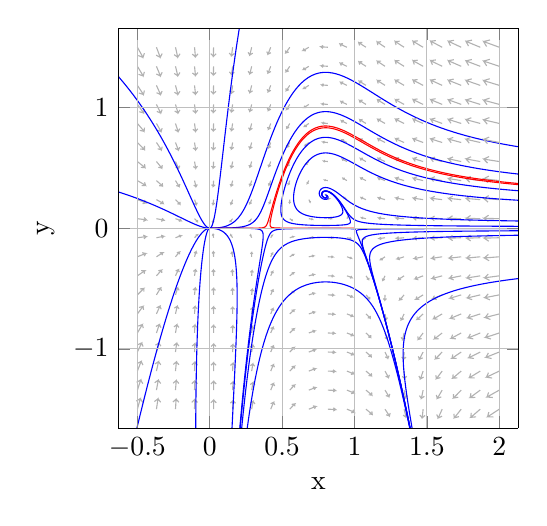
\begin{tikzpicture}

\begin{axis}[%
width=2in,
height=2in,
unbounded coords=jump,
view={0}{90},
scale only axis,
xmin=-0.631578947368421,
xmax=2.13157894736842,
xlabel={x},
xmajorgrids,
ymin=-1.65789473684211,
ymax=1.65789473684211,
ylabel={y},
ymajorgrids,
zmin=-20,
zmax=20
]
\addplot3 [color=blue,solid]
 table[row sep=crcr] {4.59308234657444	0.49518166451166	-5.87300721322471\\
4.47015798046918	0.498593482670799	-5.87116677583169\\
4.35763839065268	0.501920161203756	-5.86932633843868\\
4.25418756682112	0.505168522860809	-5.86748590104566\\
4.15863577054971	0.508344723972994	-5.86564546365264\\
4.06997953529271	0.511454254452104	-5.86380502625963\\
3.98738166638343	0.514501937790692	-5.86196458886661\\
3.9101712410342	0.51749193106207	-5.86012415147359\\
3.83784360833639	0.520427724920308	-5.85828371408058\\
3.7374089808293	0.52473962457008	-5.85552135186903\\
3.64547714063648	0.52894684014158	-5.85275898965749\\
3.56095548552136	0.533057735204053	-5.84999662744594\\
3.48288745118116	0.537079855552979	-5.84723426523439\\
3.41045251124695	0.541019929210073	-5.84447190302285\\
3.34296617728361	0.544883866423282	-5.8417095408113\\
3.27987999878984	0.548676759666789	-5.83894717859976\\
3.22078156319819	0.552402883641011	-5.83618481638821\\
3.13871216198785	0.557879116169052	-5.8320386555383\\
3.06358564913839	0.563226260076247	-5.82789249468838\\
2.99450921922409	0.568454552768592	-5.82374633383846\\
2.93070126562058	0.57357322895545	-5.81960017298854\\
2.8714913805049	0.578590520649545	-5.81545401213863\\
2.81632035485542	0.583513657166969	-5.81130785128871\\
2.76474017845191	0.588348865127174	-5.80716169043879\\
2.7164140398755	0.593101368452981	-5.80301552958887\\
2.64930473631554	0.600088835750999	-5.79679358800878\\
2.58785739993764	0.606916115544715	-5.79057164642868\\
2.53134340198531	0.613595699076279	-5.78434970484858\\
2.47912487927967	0.620138849957921	-5.77812776326849\\
2.4306547342194	0.626555604171945	-5.77190582168839\\
2.38547663478078	0.632854770070731	-5.76568388010829\\
2.34322501451767	0.639043928376736	-5.7594619385282\\
2.30362507256154	0.64512943218249	-5.7532399969481\\
2.24873822815493	0.654058475812215	-5.74392605853955\\
2.19844252317309	0.662786735412336	-5.734612120131\\
2.15214752758759	0.671329263995257	-5.72529818172245\\
2.10933627327015	0.679699625220281	-5.7159842433139\\
2.06956525399264	0.687909893393618	-5.70667030490534\\
2.03246442542708	0.695970653468382	-5.69735636649679\\
1.99773720514564	0.703891001044587	-5.68804242808824\\
1.96516047262065	0.711678542369153	-5.67872848967969\\
1.91993383116683	0.723109433545167	-5.66477871770071\\
1.87843337394471	0.734280126188658	-5.65082894572173\\
1.84017917244348	0.745208568721694	-5.63687917374275\\
1.80475099216416	0.755910899244575	-5.62292940176377\\
1.77178829261954	0.766401445535837	-5.60897962978479\\
1.74099022733422	0.776692725052252	-5.59502985780581\\
1.71211564384458	0.786795444928826	-5.58108008582682\\
1.68498308369881	0.796718501978804	-5.56713031384784\\
1.64838541062382	0.810805685927062	-5.54690202622622\\
1.61462693362353	0.824555621157849	-5.5266737386046\\
1.58334997512269	0.837987241371597	-5.50644545098298\\
1.55424054956937	0.851117520359353	-5.48621716336136\\
1.5270283634349	0.863961472002782	-5.46598887573974\\
1.50148681521393	0.876532150274163	-5.44576058811812\\
1.47743299542438	0.888840649236393	-5.4255323004965\\
1.45472768660746	0.900896103042987	-5.40530401287488\\
1.42172932918902	0.91919510453411	-5.37378749906941\\
1.39125273992021	0.936929251756993	-5.34227098526394\\
1.36296532593091	0.954121513973346	-5.31075447145846\\
1.33657639718866	0.970792194210158	-5.27923795765299\\
1.31183716649868	0.986958929259696	-5.24772144384752\\
1.28854074950383	1.00263668967951	-5.21620493004205\\
1.26652216468464	1.01783777979241	-5.18468841623657\\
1.24565833335932	1.03257183768651	-5.1531719024311\\
1.22055975726416	1.05068823641978	-5.11300281434282\\
1.19693107359299	1.06807745122659	-5.07283372625454\\
1.17460294947133	1.08475280670335	-5.03266463816626\\
1.15342560719155	1.10072623734699	-4.99249555007797\\
1.13326882421289	1.11600828755489	-4.95232646198969\\
1.11402193316142	1.13060811162496	-4.91215737390141\\
1.0955938218301	1.14453347375556	-4.87198828581313\\
1.0779129331787	1.15779074804556	-4.83181919772484\\
1.04298522900686	1.18343193593808	-4.74765061099402\\
1.01054029012059	1.20622068208488	-4.6634820242632\\
0.980211746003441	1.22620465125645	-4.57931343753237\\
0.951687036960542	1.24343466739926	-4.49514485080155\\
0.924707414118588	1.25796471363585	-4.41097626407073\\
0.89906793942584	1.26985193226475	-4.3268076773399\\
0.874617485652126	1.27915662476053	-4.24263909060908\\
0.851258736388845	1.28594225177377	-4.15847050387826\\
0.818383109936498	1.2915193706293	-4.03347050387826\\
0.787435792194694	1.29196088186099	-3.90847050387826\\
0.75823082879891	1.28756218039809	-3.78347050387826\\
0.730607058022136	1.27863432429788	-3.65847050387826\\
0.704428110774872	1.26550403474564	-3.53347050387826\\
0.679582410605132	1.24851369605469	-3.40847050387826\\
0.655983173698438	1.22802135566635	-3.28347050387826\\
0.633568408877825	1.20440072414997	-3.15847050387826\\
0.612279392968106	1.17801940384979	-3.03347050387826\\
0.592049769268327	1.14923182170038	-2.90847050387826\\
0.572826282561853	1.11839096549347	-2.78347050387826\\
0.554557799993181	1.08583288034205	-2.65847050387826\\
0.537195311067938	1.05187666868036	-2.53347050387826\\
0.520691927652885	1.0168244902639	-2.40847050387826\\
0.505002883975911	0.980961562169392	-2.28347050387826\\
0.490085536626038	0.944556158794839	-2.15847050387826\\
0.475898602886635	0.907853186510004	-2.03347050387826\\
0.462401464854046	0.871068144325889	-1.90847050387826\\
0.449555055869283	0.834397545480827	-1.78347050387826\\
0.437321626288943	0.798017979063235	-1.65847050387826\\
0.425664743485201	0.762086110011612	-1.53347050387826\\
0.414549291845812	0.726738679114534	-1.40847050387826\\
0.403941472774114	0.69209250301066	-1.28347050387826\\
0.393808804689022	0.658244474188727	-1.15847050387826\\
0.384120337128825	0.625276809541627	-1.03347050387826\\
0.374846618036971	0.593256750974029	-0.908470503878255\\
0.365959439800697	0.562236125017165	-0.783470503878255\\
0.35743197960577	0.532256544385299	-0.658470503878255\\
0.349238799436482	0.503349407975717	-0.533470503878255\\
0.341355846075654	0.475535900868735	-0.408470503878255\\
0.333760451104635	0.448826994327696	-0.283470503878255\\
0.326431330903301	0.423223445798968	-0.158470503878255\\
0.325292986781376	0.419267089775553	-0.138661690893473\\
0.324160743951735	0.415338377868428	-0.118852877908691\\
0.323034525984655	0.411437276146823	-0.0990440649239095\\
0.321914257214783	0.407563747320868	-0.0792352519391276\\
0.320799862741132	0.403717750741595	-0.0594264389543457\\
0.319691268427085	0.399899242400931	-0.0396176259695638\\
0.318588400900394	0.396108174931708	-0.0198088129847819\\
0.317491187553178	0.392344497607655	0\\
0.317491187553178	0.392344497607655	0\\
0.316399556498622	0.388608156603261	0.0198088129847819\\
0.315313436596959	0.384899095083159	0.0396176259695638\\
0.314232757476066	0.381217253209804	0.0594264389543457\\
0.313157449486365	0.377562568376094	0.0792352519391276\\
0.312087443700828	0.373934975205366	0.0990440649239095\\
0.311022671914971	0.370334405551402	0.118852877908691\\
0.30996306664686	0.366760788498425	0.138661690893473\\
0.308908561137105	0.363214050361101	0.158470503878255\\
0.30236750539829	0.341447303037344	0.283470503878255\\
0.296010858441424	0.32072520600656	0.408470503878255\\
0.289824085703032	0.301024032490396	0.533470503878255\\
0.283793507325433	0.282317785428587	0.658470503878255\\
0.277906298156736	0.264578197478957	0.783470503878255\\
0.272150487750842	0.247774731017417	0.908470503878255\\
0.266514960367442	0.231874578137967	1.03347050387826\\
0.260989454972018	0.216842660652695	1.15847050387826\\
0.255564599132247	0.202643666331092	1.28347050387826\\
0.250232264350411	0.189245607882697	1.40847050387826\\
0.244985126813149	0.176616482028334	1.53347050387826\\
0.239816436426982	0.164724005768965	1.65847050387826\\
0.234720016818314	0.153535616385691	1.78347050387826\\
0.229690265333427	0.143018471439749	1.90847050387826\\
0.224722153038486	0.133139448772513	2.03347050387826\\
0.219811224719533	0.123865146505495	2.15847050387826\\
0.215423689650952	0.115985537790547	2.27131867251613\\
0.211077547952499	0.108552862387247	2.38416684115401\\
0.20677094469578	0.101546976848227	2.49701500979189\\
0.202502276392498	0.0949479885462607	2.60986317842977\\
0.198270190994452	0.0887362556742667	2.72271134706765\\
0.19407358789354	0.0828923872453051	2.83555951570553\\
0.189911617921756	0.0773972430925798	2.94840768434341\\
0.185783683351191	0.0722319338694378	3.06125585298129\\
0.18200245466536	0.0677405146595569	3.1654443214855\\
0.178249982685883	0.0635030180879112	3.26963278998971\\
0.174526420238087	0.059507480785893	3.37382125849392\\
0.170832018962893	0.0557421819739206	3.47800972699813\\
0.167167129316812	0.0521956434614386	3.58219819550234\\
0.163532200571948	0.0488566296469182	3.68638666400655\\
0.159927780815994	0.0457141475178567	3.79057513251076\\
0.156354516952236	0.0427574466507779	3.89476360101497\\
0.153001645014999	0.0401208486122841	3.99338234874369\\
0.149678083529188	0.0376341990443091	4.09200109647241\\
0.14638461485638	0.0352901964635885	4.19061984420112\\
0.143122040608311	0.033081718170515	4.28923859192984\\
0.139891181646875	0.0310018202491379	4.38785733965856\\
0.136692878084122	0.0290437375671637	4.48647608738728\\
0.133527989282262	0.0272008837759557	4.58509483511599\\
0.130397393853662	0.0254668513105339	4.68371358284471\\
0.127429667980595	0.0239013461685664	4.77824160076192\\
0.124495067956513	0.0224256772189154	4.87276961867913\\
0.1215943930782	0.0210353419118822	4.96729763659634\\
0.118728420342014	0.0197259617298305	5.06182565451355\\
0.115897904443892	0.0184932821871861	5.15635367243076\\
0.113103577779346	0.0173331728304367	5.25088169034797\\
0.110346150443467	0.0162416272381323	5.34540970826518\\
0.10762631023092	0.015214763020885	5.43993772618239\\
0.10503029605711	0.0142790813016966	5.53142784012003\\
0.102470688735029	0.0133976975074503	5.62291795405767\\
0.0999480370999834	0.0125678135754067	5.7144080679953\\
0.0974628513012903	0.0117867157847122	5.80589818193294\\
0.0950156028022812	0.0110517747563994	5.89738829587058\\
0.0926067243803002	0.010360445453387	5.98887840980821\\
0.0902366101267045	0.00971026718047965	6.08036852374585\\
0.0879056154468643	0.009098863584368	6.17185863768349\\
0.0856666140851055	0.00853691844092152	6.26123256457085\\
0.0834655088534037	0.00800803816077315	6.35060649145822\\
0.0813025246151881	0.00751047019964039	6.43998041834559\\
0.07917784674496	0.007042518930257	6.52935434523295\\
0.0770916211282927	0.00660254564237301	6.61872827212032\\
0.0750439541618319	0.00618896854275471	6.70810219900769\\
0.0730349127532952	0.00580026275518463	6.79747612589505\\
0.0710645243214721	0.00543496032046156	6.88685005278242\\
0.0691581384862114	0.00509610696676524	6.97503912720513\\
0.067289342578504	0.0047775521657145	7.06322820162783\\
0.0654580638457593	0.00447818726061895	7.15141727605054\\
0.0636641971399461	0.00419694197315996	7.23960635047324\\
0.0619076049175932	0.00393278440339069	7.32779542489595\\
0.0601881172397885	0.00368472102973611	7.41598449931865\\
0.0585055317721798	0.00345179670899294	7.50417357374136\\
0.0568596137849741	0.0032330946763297	7.59236264816407\\
0.0552527795059927	0.00302809755572939	7.68040340975191\\
0.0536819495060205	0.00283568044263932	7.76844417133974\\
0.0521468163778774	0.00265513260557891	7.85648493292758\\
0.0506470501172467	0.00248576933158934	7.94452569451542\\
0.0491822981226752	0.00232693192623365	8.03256645610326\\
0.0477521851955729	0.00217798771359664	8.1206072176911\\
0.0463563135402132	0.00203833003628493	8.20864797927894\\
0.0449942627637329	0.00190737825542694	8.29668874086678\\
0.0436495972100041	0.00178314490520445	8.38580325248606\\
0.0423386741149009	0.00166679133594026	8.47491776410534\\
0.0410610142959904	0.00155785416158588	8.56403227572461\\
0.0398161257355081	0.00145588783272138	8.65314678734389\\
0.0386035035803574	0.0013604646365554	8.74226129896316\\
0.0374226301421102	0.00127117469692509	8.83137581058244\\
0.0362729748970064	0.0011876259742962	8.92049032220172\\
0.0351539944859543	0.001109444265763	9.009604833821\\
0.0340344668884144	0.00103426407189339	9.10126548928792\\
0.032946214424082	0.000964070091359231	9.19292614475485\\
0.0318886332434693	0.000898554474993435	9.28458680022177\\
0.0308611154325297	0.000837421774782759	9.3762474556887\\
0.029863049012658	0.000780388943867829	9.46790811115562\\
0.0288938179406907	0.000727185336543139	9.55956876662255\\
0.0279528021089055	0.000677552708257044	9.65122942208947\\
0.0270393773450217	0.000631245215611765	9.7428900775564\\
0.0261118669035318	0.000586076612435338	9.83886350256246\\
0.0252132215993466	0.000544083984514802	9.93483692756853\\
0.0243427421953557	0.000505059365315215	10.0308103525746\\
0.0234997332091284	0.000468803504513134	10.1267837775807\\
0.0226835029129136	0.000435125867996617	10.2227572025867\\
0.0218933633336397	0.000403844637865219	10.3187306275928\\
0.021128630252915	0.000374786712429998	10.4147040525988\\
0.0203886232070273	0.000347787706213508	10.5106774776049\\
0.019625712620448	0.000321087094893517	10.613058359457\\
0.0188893855965445	0.000296406659065037	10.7154392413091\\
0.0181788638264049	0.000273604653584308	10.8178201231612\\
0.0174933800303401	0.000252545446611101	10.9202010050133\\
0.0168321779578837	0.000233099519608723	11.0225818868655\\
0.016194512387792	0.000215143467344014	11.1249627687176\\
0.015579649128044	0.000198559997887352	11.2273436505697\\
0.0149868650158415	0.000183237932612646	11.3297245324218\\
0.0143668195567628	0.000167899058085107	11.4409957342014\\
0.0137711488648701	0.000153827706248468	11.5522669359809\\
0.0131990058315277	0.000140927763867315	11.6635381377605\\
0.0126495614881005	0.000129107284092525	11.77480933954\\
0.0121220050059535	0.000118278486461264	11.8860805413196\\
0.0116155436964522	0.000108357756896992	11.9973517430992\\
0.0111294030109626	9.92656477094558e-05	12.1086229448787\\
0.0106628265408507	9.09268775946943e-05	12.2198941466583\\
0.0101682847133806	8.24945516330579e-05	12.3430642331542\\
0.0096958752388384	7.4834208809784e-05	12.4662343196501\\
0.00924469259895612	6.78822930902522e-05	12.589404406146\\
0.00881385650861206	6.1577873264507e-05	12.7125744926419\\
0.00840251191583093	5.58626429472573e-05	12.8357445791378\\
0.00800982900178387	5.0680920577877e-05	12.9589146656336\\
0.00763500318078841	4.59796494204049e-05	13.0820847521295\\
0.00727725510030847	4.17083975635443e-05	13.2052548386254\\
0.00693088499300459	3.77698930145808e-05	13.3302548386254\\
0.00660060595086278	3.41990148458358e-05	13.4552548386254\\
0.0062857177457658	3.0964969863236e-05	13.5802548386254\\
0.00598554228781503	2.80382340252894e-05	13.7052548386254\\
0.00569942362533042	2.53905524430857e-05	13.8302548386254\\
0.00542672794485051	2.29949393802958e-05	13.9552548386254\\
0.00516684357113245	2.08256782531721e-05	14.0802548386254\\
0.00491918096715198	1.88583216305485e-05	14.2052548386254\\
0.00468317814696619	1.70725998626572e-05	14.3302548386254\\
0.00445831307016996	1.54542203469101e-05	14.4552548386254\\
0.00424408544020427	1.39890927376574e-05	14.5802548386254\\
0.0040400119185031	1.26637128896636e-05	14.7052548386254\\
0.00384562612449333	1.14651628581079e-05	14.8302548386254\\
0.00366047863559481	1.03811108985836e-05	14.9552548386254\\
0.00348413698722032	9.39981146709851e-06	15.0802548386254\\
0.00331618567277557	8.51010522007487e-06	15.2052548386254\\
0.00315622964987194	7.70275659071863e-06	15.3302548386254\\
0.00300390291075834	6.97126882528897e-06	15.4552548386254\\
0.00285885550777921	6.30923172472255e-06	15.5802548386254\\
0.00272074987792917	5.71050345612106e-06	15.7052548386254\\
0.00258926084285301	5.16921055275129e-06	15.8302548386254\\
0.00246407560884576	4.67974791404506e-06	15.9552548386254\\
0.00234489376685262	4.23677880559925e-06	16.0802548386254\\
0.00223142729246897	3.8352348591758e-06	16.2052548386254\\
0.00212340283562332	3.47092669575003e-06	16.3302548386254\\
0.00202056757950274	3.14091211960007e-06	16.4552548386254\\
0.00192268017279508	2.84228640385061e-06	16.5802548386254\\
0.00182950804381063	2.57226694400612e-06	16.7052548386254\\
0.00174082740048221	2.32819325795075e-06	16.8302548386254\\
0.0016564232303651	2.1075269859484e-06	16.9552548386254\\
0.00157608930063707	1.90785189064269e-06	17.0802548386254\\
0.00149962815809839	1.72687385705698e-06	17.2052548386254\\
};
 \addplot [color=white!70!black,solid,forget plot]
  table[row sep=crcr]{-0.5	-1.5\\
-0.479641074117765	-1.41177798784365\\
-0.507804254921524	-1.43315486001999\\
-0.479641074117765	-1.41177798784365\\
-0.463693248843347	-1.44333432296111\\
nan	0\\
-0.5	-1.34210526315789\\
-0.477067573907351	-1.25763749371664\\
-0.50506424409546	-1.27724471802585\\
-0.477067573907351	-1.25763749371664\\
-0.462830359374832	-1.28871093107218\\
nan	0\\
-0.5	-1.18421052631579\\
-0.474070117914049	-1.10395136747832\\
-0.501913872249201	-1.12154664460808\\
-0.474070117914049	-1.10395136747832\\
-0.461784292830468	-1.13451158565105\\
nan	0\\
-0.5	-1.02631578947368\\
-0.470538178534836	-0.950875670873492\\
-0.498236754624433	-0.966142251087258\\
-0.470538178534836	-0.950875670873492\\
-0.460516695324337	-0.98087316181984\\
nan	0\\
-0.5	-0.868421052631579\\
-0.466334850361149	-0.798651249756859\\
-0.493876845971484	-0.811165903209562\\
-0.466334850361149	-0.798651249756859\\
-0.458991944534124	-0.827998478028988\\
nan	0\\
-0.5	-0.710526315789474\\
-0.461312150461462	-0.647658560289349\\
-0.488635444198054	-0.656846924554752\\
-0.461312150461462	-0.647658560289349\\
-0.457201566447992	-0.676190849324021\\
nan	0\\
-0.5	-0.552631578947368\\
-0.455381366836847	-0.498494304042743\\
-0.482301275511949	-0.503580828223342\\
-0.455381366836847	-0.498494304042743\\
-0.455232638059636	-0.525890144804919\\
nan	0\\
-0.5	-0.394736842105263\\
-0.448728247377675	-0.352010381586659\\
-0.474791388294024	-0.352010381586659\\
-0.448728247377675	-0.352010381586659\\
-0.453428158034722	-0.377646257897822\\
nan	0\\
-0.5	-0.236842105263158\\
-0.442256760640436	-0.209039804830775\\
-0.466530307556401	-0.202944685120599\\
-0.442256760640436	-0.209039804830775\\
-0.45262915734021	-0.231816304800381\\
nan	0\\
-0.5	-0.0789473684210527\\
-0.437838367811572	-0.0693271158204626\\
-0.458891920618248	-0.0566727835535325\\
-0.437838367811572	-0.0693271158204626\\
-0.454081794317953	-0.0877535996477466\\
nan	0\\
-0.5	0.0789473684210527\\
-0.437073716216086	0.0695445903843758\\
-0.453600906842091	0.0880969947413575\\
-0.437073716216086	0.0695445903843758\\
-0.458302295860429	0.0566338528494002\\
nan	0\\
-0.5	0.236842105263158\\
-0.439462449418699	0.210609166677927\\
-0.451065479946782	0.233613435898822\\
-0.439462449418699	0.210609166677927\\
-0.464181949239397	0.203344660608171\\
nan	0\\
-0.5	0.394736842105263\\
-0.443232358130143	0.355060533271492\\
-0.450343573482657	0.381155336389088\\
-0.443232358130143	0.355060533271492\\
-0.470181727899543	0.352771515454159\\
nan	0\\
-0.5	0.552631578947368\\
-0.447097957168275	0.502484850846462\\
-0.450431887992566	0.530754379984665\\
-0.447097957168275	0.502484850846462\\
-0.475505252043019	0.504303358568802\\
nan	0\\
-0.5	0.710526315789473\\
-0.450546549823823	0.652081329217628\\
-0.450771338233715	0.681978187733226\\
-0.450546549823823	0.652081329217628\\
-0.479993831519638	0.657251462645137\\
nan	0\\
-0.5	0.868421052631579\\
-0.453474600347026	0.803194266843586\\
-0.45112552379592	0.834393652493227\\
-0.453474600347026	0.803194266843586\\
-0.483738916689917	0.811130952666741\\
nan	0\\
-0.5	1.02631578947368\\
-0.455924440634638	0.955375127257054\\
-0.451411942890089	0.987676215763383\\
-0.455924440634638	0.955375127257054\\
-0.486882273998404	0.965638436080702\\
nan	0\\
-0.5	1.18421052631579\\
-0.457973223831373	1.10832884712244\\
-0.451610836883623	1.1416000449226\\
-0.457973223831373	1.10832884712244\\
-0.4895516764803	1.12058665683828\\
nan	0\\
-0.5	1.34210526315789\\
-0.459695689770138	1.26185974459213\\
-0.451725603197656	1.29600947771933\\
-0.459695689770138	1.26185974459213\\
-0.491848362480537	1.2758573226044\\
nan	0\\
-0.5	1.5\\
-0.4611545427959	1.41583484272445\\
-0.451766890638242	1.45079575420814\\
-0.4611545427959	1.41583484272445\\
-0.493849469276017	1.43137302560609\\
nan	0\\
-0.368421052631579	-1.5\\
-0.357525476180043	-1.41383244419799\\
-0.382336038066007	-1.43695881682571\\
-0.357525476180043	-1.41383244419799\\
-0.339252260165001	-1.44240660505148\\
nan	0\\
-0.368421052631579	-1.34210526315789\\
-0.355792797176955	-1.25927053051914\\
-0.38028995697303	-1.28096388644711\\
-0.355792797176955	-1.25927053051914\\
-0.338872590653654	-1.28727801417442\\
nan	0\\
-0.368421052631579	-1.18421052631579\\
-0.353744799581368	-1.10504659464792\\
-0.377938658413398	-1.12512671088573\\
-0.353744799581368	-1.10504659464792\\
-0.338356692579465	-1.13246483741084\\
nan	0\\
-0.368421052631579	-1.02631578947368\\
-0.351275243935678	-0.951268033251641\\
-0.375180925599959	-0.969495907944279\\
-0.351275243935678	-0.951268033251641\\
-0.337657047488938	-0.978068812292229\\
nan	0\\
-0.368421052631579	-0.868421052631579\\
-0.348226447259276	-0.798106424215431\\
-0.371863485975004	-0.814152161397199\\
-0.348226447259276	-0.798106424215431\\
-0.33670617176693	-0.824249464083351\\
nan	0\\
-0.368421052631579	-0.710526315789474\\
-0.344360773854834	-0.645856402198377\\
-0.367746335885632	-0.65924230658152\\
-0.344360773854834	-0.645856402198377\\
-0.335411379090083	-0.671272445969892\\
nan	0\\
-0.368421052631579	-0.552631578947368\\
-0.339329074845711	-0.495066311253486\\
-0.362447985104942	-0.505062897115184\\
-0.339329074845711	-0.495066311253486\\
-0.333665351258	-0.519608886008118\\
nan	0\\
-0.368421052631579	-0.394736842105263\\
-0.332711610825434	-0.346827930061438\\
-0.355401671378234	-0.352273243223049\\
-0.332711610825434	-0.346827930061438\\
-0.331447215356321	-0.370127964126122\\
nan	0\\
-0.368421052631579	-0.236842105263158\\
-0.324552452837561	-0.203234860789957\\
-0.346114843894067	-0.202349884183413\\
-0.324552452837561	-0.203234860789957\\
-0.329311221657466	-0.224284184080422\\
nan	0\\
-0.368421052631579	-0.0789473684210527\\
-0.317430678984725	-0.0665263972749367\\
-0.33583303386531	-0.0575050952070581\\
-0.317430678984725	-0.0665263972749367\\
-0.329622548292252	-0.0830002820304849\\
nan	0\\
-0.368421052631579	0.0789473684210527\\
-0.316575559212855	0.0668744791897075\\
-0.329110984930636	0.0834577193137919\\
-0.316575559212855	0.0668744791897075\\
-0.335147429546309	0.0575349726044301\\
nan	0\\
-0.368421052631579	0.236842105263158\\
-0.321101987068179	0.205180408481316\\
-0.327382282541739	0.226508683906719\\
-0.321101987068179	0.205180408481316\\
-0.343213130932659	0.202849151125019\\
nan	0\\
-0.368421052631579	0.394736842105263\\
-0.326338125731464	0.3497067082459\\
-0.327705470336658	0.373736480128738\\
-0.326338125731464	0.3497067082459\\
-0.350220537266339	0.35269501667868\\
nan	0\\
-0.368421052631579	0.552631578947368\\
-0.330593378003207	0.498169024077938\\
-0.328326041674361	0.52396470919586\\
-0.330593378003207	0.498169024077938\\
-0.355557319109076	0.505050871881674\\
nan	0\\
-0.368421052631579	0.710526315789473\\
-0.333829082162188	0.64889105210568\\
-0.328797857382057	0.676029623828166\\
-0.333829082162188	0.64889105210568\\
-0.359615489223954	0.65873363859347\\
nan	0\\
-0.368421052631579	0.868421052631579\\
-0.33629363115021	0.800982101240744\\
-0.329072119746912	0.829245642028336\\
-0.33629363115021	0.800982101240744\\
-0.362791595442329	0.813181931287652\\
nan	0\\
-0.368421052631579	1.02631578947368\\
-0.338204555686613	0.953967719021158\\
-0.329182487156971	0.983226264393158\\
-0.338204555686613	0.953967719021158\\
-0.365356522383234	0.968118015920675\\
nan	0\\
-0.368421052631579	1.18421052631579\\
-0.339716152774924	1.10757826648384\\
-0.329169557773933	1.13774416939759\\
-0.339716152774924	1.10757826648384\\
-0.367485687689908	1.12339171946926\\
nan	0\\
-0.368421052631579	1.34210526315789\\
-0.340934103664934	1.26164947161575\\
-0.329066240469391	1.29265794632006\\
-0.340934103664934	1.26164947161575\\
-0.369294136240463	1.27891447183673\\
nan	0\\
-0.368421052631579	1.5\\
-0.341931311818216	1.41607492159667\\
-0.328896964461392	1.44787488032101\\
-0.341931311818216	1.41607492159667\\
-0.370859503663058	1.43463000991433\\
nan	0\\
-0.236842105263158	-1.5\\
-0.23256535663226	-1.41683086344448\\
-0.25464066536041	-1.44071241725341\\
-0.23256535663226	-1.41683086344448\\
-0.213056097082649	-1.44285079156886\\
nan	0\\
-0.236842105263158	-1.34210526315789\\
-0.23159294495476	-1.26200710498436\\
-0.253192232590663	-1.28472426235932\\
-0.23159294495476	-1.26200710498436\\
-0.213143153503896	-1.28734884251352\\
nan	0\\
-0.236842105263158	-1.18421052631579\\
-0.230439847991191	-1.10745316254586\\
-0.251549866115263	-1.12887980735885\\
-0.230439847991191	-1.10745316254586\\
-0.213171184230299	-1.13208093599483\\
nan	0\\
-0.236842105263158	-1.02631578947368\\
-0.229038912950402	-0.953241206189156\\
-0.249648516465361	-0.973212783096325\\
-0.229038912950402	-0.953241206189156\\
-0.213111224823096	-0.977114379252703\\
nan	0\\
-0.236842105263158	-0.868421052631579\\
-0.227283052954924	-0.799481683094544\\
-0.247385611031653	-0.817773730878596\\
-0.227283052954924	-0.799481683094544\\
-0.212915926263135	-0.822553257032713\\
nan	0\\
-0.236842105263158	-0.710526315789474\\
-0.224990269627933	-0.646358397588924\\
-0.244587799868638	-0.662645814140282\\
-0.224990269627933	-0.646358397588924\\
-0.212503840768363	-0.668571731957895\\
nan	0\\
-0.236842105263158	-0.552631578947368\\
-0.22182626194699	-0.494215823828301\\
-0.240934953721607	-0.507986589534979\\
-0.22182626194699	-0.494215823828301\\
-0.211727076162073	-0.515494511193063\\
nan	0\\
-0.236842105263158	-0.394736842105263\\
-0.217123303292327	-0.343821088947965\\
-0.235767882172901	-0.354166114402447\\
-0.217123303292327	-0.343821088947965\\
-0.210310005594252	-0.364025515387862\\
nan	0\\
-0.236842105263158	-0.236842105263158\\
-0.209540903546951	-0.197341371585631\\
-0.227606447481195	-0.202366291259838\\
-0.209540903546951	-0.197341371585631\\
-0.207856080642432	-0.216016892117941\\
nan	0\\
-0.236842105263158	-0.0789473684210527\\
-0.19865016455906	-0.0616700619120558\\
-0.214427073397538	-0.0573052686887303\\
-0.19865016455906	-0.0616700619120558\\
-0.20578842014304	-0.0764012390407794\\
nan	0\\
-0.236842105263158	0.0789473684210527\\
-0.197623239762985	0.0622413010980588\\
-0.205212382582288	0.0770578376700002\\
-0.197623239762985	0.0622413010980588\\
-0.213565416243785	0.0574484049199137\\
nan	0\\
-0.236842105263158	0.236842105263158\\
-0.205533634618456	0.199039651836345\\
-0.205475562455163	0.218207505525564\\
-0.205533634618456	0.199039651836345\\
-0.22437678916857	0.202553270203213\\
nan	0\\
-0.236842105263158	0.394736842105263\\
-0.211047255196778	0.345541833545974\\
-0.20648695807687	0.366749048630356\\
-0.211047255196778	0.345541833545974\\
-0.231084462356514	0.353851623597166\\
nan	0\\
-0.236842105263158	0.552631578947368\\
-0.214428791643113	0.495760454585679\\
-0.206935004638704	0.518425120299197\\
-0.214428791643113	0.495760454585679\\
-0.235370566819549	0.507218463489174\\
nan	0\\
-0.236842105263158	0.710526315789473\\
-0.216637982140743	0.64773304190583\\
-0.207000900606556	0.671622054851527\\
-0.216637982140743	0.64773304190583\\
-0.238397537548378	0.661519993290319\\
nan	0\\
-0.236842105263158	0.868421052631579\\
-0.218174979325283	0.800716544506128\\
-0.206848990075283	0.825694678428232\\
-0.218174979325283	0.800716544506128\\
-0.240701244138008	0.816361115459294\\
nan	0\\
-0.236842105263158	1.02631578947368\\
-0.219297198296734	0.954363187022843\\
-0.206572519773951	0.980335194499701\\
-0.219297198296734	0.954363187022843\\
-0.242548820999371	0.971562741016489\\
nan	0\\
-0.236842105263158	1.18421052631579\\
-0.22014687220495	1.10848311800644\\
-0.206223590045075	1.1353751487638\\
-0.22014687220495	1.10848311800644\\
-0.244087294199749	1.12702753223469\\
nan	0\\
-0.236842105263158	1.34210526315789\\
-0.220808250793513	1.26296088384225\\
-0.205832312305495	1.29071266125435\\
-0.220808250793513	1.26296088384225\\
-0.245404501963318	1.28269573401953\\
nan	0\\
-0.236842105263158	1.5\\
-0.221334237734502	1.4177206046676\\
-0.20541674916	1.44628139014949\\
-0.221334237734502	1.4177206046676\\
-0.246556446826198	1.43852745638516\\
nan	0\\
-0.105263157894737	-1.5\\
-0.104594316445534	-1.42044118148672\\
-0.124684673508614	-1.44414161667841\\
-0.104594316445534	-1.42044118148672\\
-0.0849052642519754	-1.44447603740301\\
nan	0\\
-0.105263157894737	-1.34210526315789\\
-0.104228251883055	-1.26544494531122\\
-0.123703803148228	-1.2881843141623\\
-0.104228251883055	-1.26544494531122\\
-0.0853736442248907	-1.28870176716814\\
nan	0\\
-0.105263157894737	-1.18421052631579\\
-0.103796307871938	-1.11068804357797\\
-0.122616983563234	-1.13237807589361\\
-0.103796307871938	-1.11068804357797\\
-0.0858557421943218	-1.13311150090501\\
nan	0\\
-0.105263157894737	-1.02631578947368\\
-0.103273551788587	-0.95622754253035\\
-0.121392495356266	-0.976756615086813\\
-0.103273551788587	-0.95622754253035\\
-0.0863483718845987	-0.977751418139888\\
nan	0\\
-0.105263157894737	-0.868421052631579\\
-0.102619395081421	-0.802146306736821\\
-0.119981210399105	-0.821367789801919\\
-0.102619395081421	-0.802146306736821\\
-0.0868438374517262	-0.822689671208577\\
nan	0\\
-0.105263157894737	-0.710526315789474\\
-0.101762310807277	-0.648572696934865\\
-0.118300969647167	-0.666283570819383\\
-0.101762310807277	-0.648572696934865\\
-0.0873241602198631	-0.668033994363113\\
nan	0\\
-0.105263157894737	-0.552631578947368\\
-0.100561580195707	-0.495725075538373\\
-0.116198679357665	-0.511621632136314\\
-0.100561580195707	-0.495725075538373\\
-0.0877454276531672	-0.513972420985829\\
nan	0\\
-0.105263157894737	-0.394736842105263\\
-0.0986911329575941	-0.344034817802661\\
-0.113338246514388	-0.357602418859156\\
-0.0986911329575941	-0.344034817802661\\
-0.0879872343630864	-0.360888431327727\\
nan	0\\
-0.105263157894737	-0.236842105263158\\
-0.0951624476347296	-0.194630952923383\\
-0.108745448797675	-0.204769121060314\\
-0.0951624476347296	-0.194630952923383\\
-0.0876398726277881	-0.209819476190318\\
nan	0\\
-0.105263157894737	-0.0789473684210527\\
-0.0852690435504802	-0.0535624555706134\\
-0.097613506066367	-0.056179400839681\\
-0.0852690435504802	-0.0535624555706134\\
-0.0849210496411474	-0.0661764580118093\\
nan	0\\
-0.105263157894737	0.0789473684210527\\
-0.0839888732062175	0.0541349621533577\\
-0.0841680570458496	0.066897255205796\\
-0.0839888732062175	0.0541349621533577\\
-0.096574260179697	0.0562601128615364\\
nan	0\\
-0.105263157894737	0.236842105263158\\
-0.0923711434078652	0.195128141557122\\
-0.0858102568274177	0.21086533429065\\
-0.0923711434078652	0.195128141557122\\
-0.106667238680436	0.204419327047215\\
nan	0\\
-0.105263157894737	0.394736842105263\\
-0.0952287296399136	0.344410704080766\\
-0.0856575236102363	0.362017152551821\\
-0.0952287296399136	0.344410704080766\\
-0.110820592622485	0.356999938424409\\
nan	0\\
-0.105263157894737	0.552631578947368\\
-0.0966379266872205	0.496030664115715\\
-0.085075267341562	0.51516724636709\\
-0.0966379266872205	0.496030664115715\\
-0.113375724757389	0.510854630763332\\
nan	0\\
-0.105263157894737	0.710526315789473\\
-0.0974728357786777	0.648833005590892\\
-0.08438660486385	0.669288579179481\\
-0.0974728357786777	0.648833005590892\\
-0.115233259963141	0.665393418121451\\
nan	0\\
-0.105263157894737	0.868421052631579\\
-0.0980206374607469	0.802374851576006\\
-0.0836818433270507	0.823999342001175\\
-0.0980206374607469	0.802374851576006\\
-0.116704943854837	0.82037808178418\\
nan	0\\
-0.105263157894737	1.02631578947368\\
-0.0984037848017159	0.956432430604643\\
-0.082990757012362	0.979112281538611\\
-0.0984037848017159	0.956432430604643\\
-0.117932436446882	0.9756825949921\\
nan	0\\
-0.105263157894737	1.18421052631579\\
-0.0986835640225944	1.11087453458945\\
-0.0823234442526534	1.13452023057539\\
-0.0986835640225944	1.11087453458945\\
-0.118991440115821	1.13123043363932\\
nan	0\\
-0.105263157894737	1.34210526315789\\
-0.0988941556870106	1.26561665817466\\
-0.0816827051035202	1.29015549022156\\
-0.0988941556870106	1.26561665817466\\
-0.119927007595137	1.2869709891177\\
nan	0\\
-0.105263157894737	1.5\\
-0.0990561731054014	1.42060072114969\\
-0.0810684488296239	1.44597225100211\\
-0.0990561731054014	1.42060072114969\\
-0.12076808825478	1.44286875860745\\
nan	0\\
0.0263157894736842	-1.5\\
0.02646328388465	-1.42449756360072\\
0.00754342646153954	-1.44711142091776\\
0.02646328388465	-1.42449756360072\\
0.045294644661181	-1.44718516812324\\
nan	0\\
0.0263157894736842	-1.34210526315789\\
0.0263872961747997	-1.26935077010795\\
0.00817722090197838	-1.29115924134765\\
0.0263872961747997	-1.26935077010795\\
0.0445544674269517	-1.29119499469821\\
nan	0\\
0.0263157894736842	-1.18421052631579\\
0.0262985779636835	-1.11442895746301\\
0.00885834920348828	-1.13536773099634\\
0.0262985779636835	-1.11442895746301\\
0.0437491336298791	-1.13535912524134\\
nan	0\\
0.0263157894736842	-1.02631578947368\\
0.0261924107998133	-0.95978475576709\\
0.00959666597532595	-0.979774910547536\\
0.0261924107998133	-0.95978475576709\\
0.0428621828286232	-0.9797132212106\\
nan	0\\
0.0263157894736842	-0.868421052631579\\
0.0260611282634175	-0.805493789658198\\
0.0104057108831521	-0.824435633852779\\
0.0260611282634175	-0.805493789658198\\
0.0418693423698429	-0.824308303247645\\
nan	0\\
0.0263157894736842	-0.710526315789474\\
0.0258912209228688	-0.651671280889593\\
0.0113048327631432	-0.669433933497261\\
0.0258912209228688	-0.651671280889593\\
0.0407323502130837	-0.669221649221853\\
nan	0\\
0.0263157894736842	-0.552631578947368\\
0.0256560021531302	-0.498507794734147\\
0.0123229922959909	-0.514909876828252\\
0.0256560021531302	-0.498507794734147\\
0.0393848844026018	-0.514579983167975\\
nan	0\\
0.0263157894736842	-0.394736842105263\\
0.0252927153122005	-0.346360214570998\\
0.0135054806770793	-0.361128971371649\\
0.0252927153122005	-0.346360214570998\\
0.0376937944442119	-0.360617434290907\\
nan	0\\
0.0263157894736842	-0.236842105263158\\
0.0246008194376014	-0.196057619173268\\
0.0149191889259538	-0.208721707509256\\
0.0246008194376014	-0.196057619173268\\
0.0353114319708986	-0.207864222491215\\
nan	0\\
0.0263157894736842	-0.0789473684210527\\
0.0221982286257067	-0.0508520570650239\\
0.0164096690410928	-0.0603100406838269\\
0.0221982286257067	-0.0508520570650239\\
0.0304573247191071	-0.0582512602598382\\
nan	0\\
0.0263157894736842	0.0789473684210527\\
0.021634608682398	0.0509104750327846\\
0.0300481862668509	0.0581512478514435\\
0.021634608682398	0.0509104750327846\\
0.0160297395727168	0.0604918382470866\\
nan	0\\
0.0263157894736842	0.236842105263158\\
0.0237702881955407	0.196086522060169\\
0.034722834379731	0.207676821701529\\
0.0237702881955407	0.196086522060169\\
0.0143450427782365	0.208949572340601\\
nan	0\\
0.0263157894736842	0.394736842105263\\
0.0243062936223856	0.346380823328609\\
0.0369981470719387	0.36038525499878\\
0.0243062936223856	0.346380823328609\\
0.0128201376836116	0.36139000292443\\
nan	0\\
0.0263157894736842	0.552631578947368\\
0.0245519722953222	0.498524273004657\\
0.0386079439345086	0.51431551049288\\
0.0245519722953222	0.498524273004657\\
0.0115542909631531	0.515197419082061\\
nan	0\\
0.0263157894736842	0.710526315789473\\
0.0246904828123044	0.651685220906463\\
0.039888348531471	0.668931222706021\\
0.0246904828123044	0.651685220906463\\
0.0104678010899657	0.669743876036711\\
nan	0\\
0.0263157894736842	0.868421052631579\\
0.0247771966635554	0.805505985765227\\
0.040967541223182	0.8239958576226\\
0.0247771966635554	0.805505985765227\\
0.00951000779000606	0.824765154027665\\
nan	0\\
0.0263157894736842	1.02631578947368\\
0.0248348775219602	0.959795667343606\\
0.0419091816399968	0.979381475994699\\
0.0248348775219602	0.959795667343606\\
0.00864912057495796	0.980121931970561\\
nan	0\\
0.0263157894736842	1.18421052631579\\
0.024874669192771	1.11443887665994\\
0.0427499176910063	1.13501009148647\\
0.024874669192771	1.11443887665994\\
0.00786409286308354	1.13573065162693\\
nan	0\\
0.0263157894736842	1.34210526315789\\
0.0249026878661779	1.26935989551134\\
0.0435129602600684	1.29083023040343\\
0.0249026878661779	1.26935989551134\\
0.00714027643679113	1.29153678120718\\
nan	0\\
0.0263157894736842	1.5\\
0.0249225742097656	1.42450603702141\\
0.044214029533589	1.44680592209901\\
0.0249225742097656	1.42450603702141\\
0.00646704804429333	1.44750252973097\\
nan	0\\
0.157894736842105	-1.5\\
0.160756018435251	-1.42908465732958\\
0.142168798289702	-1.44964393973242\\
0.160756018435251	-1.42908465732958\\
0.177626469624913	-1.45107458052899\\
nan	0\\
0.157894736842105	-1.34210526315789\\
0.160383432702598	-1.27376411397422\\
0.142551536648531	-1.2936442847642\\
0.160383432702598	-1.27376411397422\\
0.176722111240369	-1.29488863269444\\
nan	0\\
0.157894736842105	-1.18421052631579\\
0.159955496733926	-1.11865460551193\\
0.142948288565414	-1.13780619178013\\
0.159955496733926	-1.11865460551193\\
0.175726248967346	-1.13883657172604\\
nan	0\\
0.157894736842105	-1.02631578947368\\
0.159452610381799	-0.963805854393619\\
0.143357764549874	-0.982169366532715\\
0.159452610381799	-0.963805854393619\\
0.174612732089907	-0.982948303302562\\
nan	0\\
0.157894736842105	-0.868421052631579\\
0.158843232456468	-0.809289656115643\\
0.143775834643175	-0.826791951166833\\
0.158843232456468	-0.809289656115643\\
0.173341532901143	-0.827266198974014\\
nan	0\\
0.157894736842105	-0.710526315789474\\
0.158072369448646	-0.655216294331913\\
0.144191574302294	-0.671764892617546\\
0.158072369448646	-0.655216294331913\\
0.171846585031074	-0.671853708920816\\
nan	0\\
0.157894736842105	-0.552631578947368\\
0.157032744363378	-0.501770888184387\\
0.144576169416251	-0.517244593532963\\
0.157032744363378	-0.501770888184387\\
0.170006514797742	-0.5168135972936\\
nan	0\\
0.157894736842105	-0.394736842105263\\
0.15547645716326	-0.349310810536673\\
0.144845433174766	-0.363543189926962\\
0.15547645716326	-0.349310810536673\\
0.167558448959061	-0.362334050087539\\
nan	0\\
0.157894736842105	-0.236842105263158\\
0.152639146343045	-0.198732223792389\\
0.14468835312507	-0.211479085858385\\
0.152639146343045	-0.198732223792389\\
0.163743293860455	-0.208851290608854\\
nan	0\\
0.157894736842105	-0.0789473684210527\\
0.144272605622851	-0.0546767303224883\\
0.142291585463986	-0.0653634545568713\\
0.144272605622851	-0.0546767303224883\\
0.154426904513268	-0.0585523889472439\\
nan	0\\
0.157894736842105	0.0789473684210527\\
0.141438889765503	0.0557309024907036\\
0.152179760371071	0.0585818805006578\\
0.141438889765503	0.0557309024907036\\
0.140571527405897	0.0668098040389588\\
nan	0\\
0.157894736842105	0.236842105263158\\
0.147229973727832	0.199480511965093\\
0.15976980098663	0.208022799175944\\
0.147229973727832	0.199480511965093\\
0.141089004337597	0.213355180733081\\
nan	0\\
0.157894736842105	0.394736842105263\\
0.148885119647677	0.349862985945649\\
0.162806468845909	0.361072738494926\\
0.148885119647677	0.349862985945649\\
0.140369540766102	0.36557754709214\\
nan	0\\
0.157894736842105	0.552631578947368\\
0.149602033467208	0.502216665136545\\
0.164693572932383	0.515267963436068\\
0.149602033467208	0.502216665136545\\
0.139486116026971	0.519414315123516\\
nan	0\\
0.157894736842105	0.710526315789473\\
0.14996651997593	0.655594910853526\\
0.16607783626977	0.670092278117767\\
0.14996651997593	0.655594910853526\\
0.138612133801796	0.674056386550854\\
nan	0\\
0.157894736842105	0.868421052631579\\
0.150162575915847	0.809621577744094\\
0.167182092915595	0.825328379978775\\
0.150162575915847	0.809621577744094\\
0.137782355471853	0.829194460441904\\
nan	0\\
0.157894736842105	1.02631578947368\\
0.150266288752548	0.964103163024233\\
0.168107979791778	0.980859838936679\\
0.150266288752548	0.964103163024233\\
0.137001666567052	0.984674062981458\\
nan	0\\
0.157894736842105	1.18421052631579\\
0.150314714478218	1.11892507236673\\
0.168910084674649	1.13661570296048\\
0.150314714478218	1.11892507236673\\
0.136267357700119	1.14040571414242\\
nan	0\\
0.157894736842105	1.34210526315789\\
0.150327976301911	1.2740130581232\\
0.169621055722642	1.29254902949856\\
0.150327976301911	1.2740130581232\\
0.135574953205296	1.29633240976866\\
nan	0\\
0.157894736842105	1.5\\
0.15031788605585	1.42931589444435\\
0.17026196768064	1.44862691341448\\
0.15031788605585	1.42931589444435\\
0.134919914902813	1.45241533880761\\
nan	0\\
0.289473684210526	-1.5\\
0.298643790291957	-1.43469399946035\\
0.279566258332615	-1.45199327310189\\
0.298643790291957	-1.43469399946035\\
0.312219258602441	-1.4565783261426\\
nan	0\\
0.289473684210526	-1.34210526315789\\
0.298092986976303	-1.27915622470695\\
0.279769936533834	-1.29588611055079\\
0.298092986976303	-1.27915622470695\\
0.311244455759305	-1.30019576193368\\
nan	0\\
0.289473684210526	-1.18421052631579\\
0.297476810479768	-1.12381019169575\\
0.279975788943987	-1.13992951051445\\
0.297476810479768	-1.12381019169575\\
0.310175956254005	-1.14393107364907\\
nan	0\\
0.289473684210526	-1.02631578947368\\
0.296774475758267	-0.968700616650129\\
0.280180445088056	-0.984159970610261\\
0.296774475758267	-0.968700616650129\\
0.308988031499833	-0.987810366384131\\
nan	0\\
0.289473684210526	-0.868421052631579\\
0.295953286202824	-0.813891799335671\\
0.280377092281157	-0.828630674826369\\
0.295953286202824	-0.813891799335671\\
0.307641718929111	-0.831870475822517\\
nan	0\\
0.289473684210526	-0.710526315789474\\
0.294957562931906	-0.659481929509156\\
0.280551302745413	-0.673424275712907\\
0.294957562931906	-0.659481929509156\\
0.306073495885572	-0.676166215073596\\
nan	0\\
0.289473684210526	-0.552631578947368\\
0.293681247971243	-0.505634366759488\\
0.280669675796058	-0.518681639475673\\
0.293681247971243	-0.505634366759488\\
0.304168281889998	-0.520785421356031\\
nan	0\\
0.289473684210526	-0.394736842105263\\
0.291884602794106	-0.352659920234636\\
0.280642096751376	-0.364680267149929\\
0.291884602794106	-0.352659920234636\\
0.301680557686689	-0.365885726441719\\
nan	0\\
0.289473684210526	-0.236842105263158\\
0.288837605194328	-0.201318055964563\\
0.280147416574539	-0.212134290508191\\
0.288837605194328	-0.201318055964563\\
0.297909441223836	-0.211816251000092\\
nan	0\\
0.289473684210526	-0.0789473684210527\\
0.280225486480449	-0.0554701942935966\\
0.277130652267608	-0.0648253959643528\\
0.280225486480449	-0.0554701942935966\\
0.288869239331336	-0.060201297099314\\
nan	0\\
0.289473684210526	0.0789473684210527\\
0.273810027455086	0.0576109904459772\\
0.283843218975487	0.0600959896496397\\
0.273810027455086	0.0576109904459772\\
0.273175029987949	0.06792781802736\\
nan	0\\
0.289473684210526	0.236842105263158\\
0.277252317179415	0.202714863689918\\
0.289450537682058	0.209897694404112\\
0.277252317179415	0.202714863689918\\
0.272386916895439	0.216008377919668\\
nan	0\\
0.289473684210526	0.394736842105263\\
0.277858718851313	0.353681258758447\\
0.291607104295781	0.363094192422689\\
0.277858718851313	0.353681258758447\\
0.271079312622373	0.368901675102295\\
nan	0\\
0.289473684210526	0.552631578947368\\
0.277898661139722	0.506456757476606\\
0.292914873428654	0.517415448150134\\
0.277898661139722	0.506456757476606\\
0.269827462693273	0.523202959685536\\
nan	0\\
0.289473684210526	0.710526315789473\\
0.27775436022691	0.660179662871515\\
0.293856820651485	0.672353827750999\\
0.27775436022691	0.660179662871515\\
0.268683494192506	0.678213489742807\\
nan	0\\
0.289473684210526	0.868421052631579\\
0.277537435320333	0.814503144041808\\
0.294597787134834	0.827694454396191\\
0.277537435320333	0.814503144041808\\
0.267638832839948	0.833662578841288\\
nan	0\\
0.289473684210526	1.02631578947368\\
0.277290305979903	0.969248035998122\\
0.295212257817981	0.983322517483135\\
0.277290305979903	0.969248035998122\\
0.2666783810802	0.989414206598446\\
nan	0\\
0.289473684210526	1.18421052631579\\
0.277031658756528	1.12430808924234\\
0.295739875661091	1.13916831400087\\
0.277031658756528	1.12430808924234\\
0.265788657124364	1.14538932672787\\
nan	0\\
0.289473684210526	1.34210526315789\\
0.276770481288533	1.27961444030517\\
0.296204147878311	1.29518588643049\\
0.276770481288533	1.27961444030517\\
0.264958736451951	1.30153748789149\\
nan	0\\
0.289473684210526	1.5\\
0.276511311720633	1.43511958297905\\
0.296620127722839	1.45134311496286\\
0.276511311720633	1.43511958297905\\
0.264179919212363	1.45782430120781\\
nan	0\\
0.421052631578947	-1.5\\
0.440689550107304	-1.44264277947381\\
0.42045916941725	-1.45494071599958\\
0.440689550107304	-1.44264277947381\\
0.449137779680344	-1.46475917526376\\
nan	0\\
0.421052631578947	-1.34210526315789\\
0.440029420307501	-1.28684764228921\\
0.420521978471763	-1.29868073136768\\
0.440029420307501	-1.28684764228921\\
0.448150788906106	-1.30816912573195\\
nan	0\\
0.421052631578947	-1.18421052631579\\
0.439320241929171	-1.1312255049645\\
0.420593703486282	-1.14255410878233\\
0.439320241929171	-1.1312255049645\\
0.447086214161927	-1.15168791395744\\
nan	0\\
0.421052631578947	-1.02631578947368\\
0.438551867741214	-0.975817128302695\\
0.420677431599787	-0.986591917613425\\
0.438551867741214	-0.975817128302695\\
0.445926762185281	-0.995341535694558\\
nan	0\\
0.421052631578947	-0.868421052631579\\
0.437710387269814	-0.820681227662784\\
0.420778104320355	-0.830838736230706\\
0.437710387269814	-0.820681227662784\\
0.444648016804753	-0.839167614076139\\
nan	0\\
0.421052631578947	-0.710526315789474\\
0.436775983414397	-0.665907560150709\\
0.420904288954071	-0.675362348883476\\
0.436775983414397	-0.665907560150709\\
0.443213666773453	-0.683224024801201\\
nan	0\\
0.421052631578947	-0.552631578947368\\
0.435719131402458	-0.511645274771317\\
0.421072605411392	-0.520274541068254\\
0.435719131402458	-0.511645274771317\\
0.441565757499418	-0.52760779098001\\
nan	0\\
0.421052631578947	-0.394736842105263\\
0.434494015486457	-0.358175707722695\\
0.421321316718562	-0.365783702060588\\
0.434494015486457	-0.358175707722695\\
0.439601883909846	-0.372504394014343\\
nan	0\\
0.421052631578947	-0.236842105263158\\
0.433034133154061	-0.20616068941607\\
0.421769328719755	-0.212369738776418\\
0.433034133154061	-0.20616068941607\\
0.437110036643299	-0.218360489563975\\
nan	0\\
0.421052631578947	-0.0789473684210527\\
0.431492501139607	-0.0582691711831431\\
0.423190990961932	-0.061862662964351\\
0.431492501139607	-0.0582691711831431\\
0.433530089580887	-0.0670825977446809\\
nan	0\\
0.421052631578947	0.0789473684210527\\
0.417474947454398	0.0568346942536562\\
0.424076421233612	0.0625740754727377\\
0.417474947454398	0.0568346942536562\\
0.413020084149914	0.0643629175350125\\
nan	0\\
0.421052631578947	0.236842105263158\\
0.412384338021999	0.205452684594584\\
0.422832181256227	0.212702437405919\\
0.412384338021999	0.205452684594584\\
0.40713747092194	0.217036584184393\\
nan	0\\
0.421052631578947	0.394736842105263\\
0.409968999580308	0.357670980206292\\
0.422560554654642	0.366019830776324\\
0.409968999580308	0.357670980206292\\
0.404027623705157	0.371561646775643\\
nan	0\\
0.421052631578947	0.552631578947368\\
0.408270302795026	0.511241729837303\\
0.422452463707719	0.520463102374342\\
0.408270302795026	0.511241729837303\\
0.401757539152686	0.526854266766303\\
nan	0\\
0.421052631578947	0.710526315789473\\
0.406922860867934	0.665566183899226\\
0.4224018250538	0.675521780788547\\
0.406922860867934	0.665566183899226\\
0.399921759108676	0.682586666144053\\
nan	0\\
0.421052631578947	0.868421052631579\\
0.405788939462853	0.820382561493197\\
0.422377669882277	0.830978185805688\\
0.405788939462853	0.820382561493197\\
0.398358424313086	0.838610031863735\\
nan	0\\
0.421052631578947	1.02631578947368\\
0.404800550233247	0.975549920389622\\
0.422367641907973	0.986716660778415\\
0.404800550233247	0.975549920389622\\
0.396984707365942	0.994842701451265\\
nan	0\\
0.421052631578947	1.18421052631579\\
0.403918703890514	1.1309825999684\\
0.422365863783892	1.14266749595051\\
0.403918703890514	1.1309825999684\\
0.395751900610196	1.15123445979472\\
nan	0\\
0.421052631578947	1.34210526315789\\
0.403118772748379	1.28662417665155\\
0.422369202024136	1.29878503789581\\
0.403118772748379	1.28662417665155\\
0.394628658770963	1.3077519673111\\
nan	0\\
0.421052631578947	1.5\\
0.402384110057656	1.44243528020626\\
0.42237584646248	1.45503756576406\\
0.402384110057656	1.44243528020626\\
0.393593486565608	1.4643718265247\\
nan	0\\
0.552631578947368	-1.5\\
0.586734496013987	-1.45582009667334\\
0.565458645062335	-1.46054833840468\\
0.586734496013987	-1.45582009667334\\
0.587548596725668	-1.47759979693799\\
nan	0\\
0.552631578947368	-1.34210526315789\\
0.585873874680478	-1.29969759160123\\
0.565299268071378	-1.30410931913495\\
0.585873874680478	-1.29969759160123\\
0.586503103849712	-1.32073046700151\\
nan	0\\
0.552631578947368	-1.18421052631579\\
0.584972532555813	-1.14373523213798\\
0.565151422928827	-1.14779258198921\\
0.584972532555813	-1.14373523213798\\
0.585389070017733	-1.16396305879343\\
nan	0\\
0.552631578947368	-1.02631578947368\\
0.584027373865089	-0.98797434373417\\
0.565023273954894	-0.991627828726594\\
0.584027373865089	-0.98797434373417\\
0.584193996824652	-1.00732572618545\\
nan	0\\
0.552631578947368	-0.868421052631579\\
0.583036402350737	-0.832476103745878\\
0.564928718108301	-0.835658382560746\\
0.583036402350737	-0.832476103745878\\
0.582901192551152	-0.85086079426243\\
nan	0\\
0.552631578947368	-0.710526315789474\\
0.582000886938157	-0.677337180761076\\
0.564892810783821	-0.679951594271898\\
0.582000886938157	-0.677337180761076\\
0.58148737829802	-0.694636248267292\\
nan	0\\
0.552631578947368	-0.552631578947368\\
0.580930888194453	-0.522724734973822\\
0.564964384426941	-0.524621960854115\\
0.580930888194453	-0.522724734973822\\
0.579917806413714	-0.538771615477657\\
nan	0\\
0.552631578947368	-0.394736842105263\\
0.579859953086668	-0.36896857365847\\
0.56524937373318	-0.369891960657683\\
0.579859953086668	-0.36896857365847\\
0.578133507956576	-0.383506147727333\\
nan	0\\
0.552631578947368	-0.236842105263158\\
0.578881173843171	-0.216869749476206\\
0.566013206427693	-0.216299057488341\\
0.578881173843171	-0.216869749476206\\
0.575999384321168	-0.229423854936243\\
nan	0\\
0.552631578947368	-0.0789473684210527\\
0.57805080636041	-0.069179997474475\\
0.567983195399853	-0.0657554019051878\\
0.57805080636041	-0.069179997474475\\
0.572866880873142	-0.0784650156117088\\
nan	0\\
0.552631578947368	0.0789473684210527\\
0.570405774540138	0.0648636446727442\\
0.568594446799384	0.0735323106954292\\
0.570405774540138	0.0648636446727442\\
0.56155258492523	0.0646452128990442\\
nan	0\\
0.552631578947368	0.236842105263158\\
0.55190261826926	0.208943738739562\\
0.559095898103592	0.217131008527114\\
0.55190261826926	0.208943738739562\\
0.545146714841794	0.217495488866168\\
nan	0\\
0.552631578947368	0.394736842105263\\
0.543482629804546	0.362495280998157\\
0.554287704824169	0.369880512044583\\
0.543482629804546	0.362495280998157\\
0.538166924270616	0.374454986615994\\
nan	0\\
0.552631578947368	0.552631578947368\\
0.538728211573013	0.517359683875496\\
0.551717195553288	0.524465410553469\\
0.538728211573013	0.517359683875496\\
0.534081248017352	0.531417094240646\\
nan	0\\
0.552631578947368	0.710526315789473\\
0.535415730924742	0.67273233311866\\
0.550028980999233	0.679766565914247\\
0.535415730924742	0.67273233311866\\
0.531131989663826	0.68837448992556\\
nan	0\\
0.552631578947368	0.868421052631579\\
0.532847913063587	0.828417975238334\\
0.548783782177033	0.835472981985362\\
0.532847913063587	0.828417975238334\\
0.52878224348041	0.845364814927252\\
nan	0\\
0.552631578947368	1.02631578947368\\
0.530731940950163	0.984328523163269\\
0.547798648926928	0.991449793557092\\
0.530731940950163	0.984328523163269\\
0.526805015771721	1.0023996125557\\
nan	0\\
0.552631578947368	1.18421052631579\\
0.528919432451754	1.14041237376356\\
0.546982614538495	1.14762378290533\\
0.528919432451754	1.14041237376356\\
0.525083538262381	1.15947985615313\\
nan	0\\
0.552631578947368	1.34210526315789\\
0.527325256231927	1.29663535131707\\
0.546284631006765	1.30394974419046\\
0.527325256231927	1.29663535131707\\
0.523549675086353	1.31660290554818\\
nan	0\\
0.552631578947368	1.5\\
0.525896118707618	1.45297319574043\\
0.545673457844436	1.46039737195836\\
0.525896118707618	1.45297319574043\\
0.52216005571465	1.47376510207824\\
nan	0\\
0.684210526315789	-1.5\\
0.732436063680072	-1.47731940440889\\
0.712298253573009	-1.47206719874515\\
0.732436063680072	-1.47731940440889\\
0.723638551368565	-1.49617996742729\\
nan	0\\
0.684210526315789	-1.34210526315789\\
0.731089718668239	-1.32048088530288\\
0.711619866498751	-1.31524840057127\\
0.731089718668239	-1.32048088530288\\
0.722432055426258	-1.3386879967475\\
nan	0\\
0.684210526315789	-1.18421052631579\\
0.729660439450695	-1.16374288605465\\
0.710908555444938	-1.15852069984926\\
0.729660439450695	-1.16374288605465\\
0.721142375575509	-1.18124565641672\\
nan	0\\
0.684210526315789	-1.02631578947368\\
0.72813381143355	-1.0071309063188\\
0.710160605109501	-1.00190554998583\\
0.72813381143355	-1.0071309063188\\
0.719753046686943	-1.02386719254471\\
nan	0\\
0.684210526315789	-0.868421052631579\\
0.726490727643007	-0.850681809479599\\
0.709371856456847	-0.845433532093389\\
0.726490727643007	-0.850681809479599\\
0.718241478032837	-0.866573632756998\\
nan	0\\
0.684210526315789	-0.710526315789474\\
0.724704792601096	-0.694451668774034\\
0.708537850961644	-0.689150496307339\\
0.724704792601096	-0.694451668774034\\
0.716575174469364	-0.709397629449992\\
nan	0\\
0.684210526315789	-0.552631578947368\\
0.722737309452964	-0.538531595525308\\
0.707654278656296	-0.533129894767633\\
0.722737309452964	-0.538531595525308\\
0.714704270367326	-0.55239328633622\\
nan	0\\
0.684210526315789	-0.394736842105263\\
0.720526011648827	-0.383083323857751\\
0.706717986487038	-0.377500507998745\\
0.720526011648827	-0.383083323857751\\
0.712544745610794	-0.395658250665264\\
nan	0\\
0.684210526315789	-0.236842105263158\\
0.717953175583629	-0.228431593996636\\
0.705727752986646	-0.222519085059633\\
0.717953175583629	-0.228431593996636\\
0.709933008619907	-0.239390409693553\\
nan	0\\
0.684210526315789	-0.0789473684210527\\
0.714717160171091	-0.0753543075724992\\
0.704666904802362	-0.0688055673632398\\
0.714717160171091	-0.0753543075724992\\
0.706463435226639	-0.0840588842908907\\
nan	0\\
0.684210526315789	0.0789473684210527\\
0.709464584274002	0.0738403552490483\\
0.703165120179539	0.0816859736902028\\
0.709464584274002	0.0738403552490483\\
0.700611613593537	0.0690589447110965\\
nan	0\\
0.684210526315789	0.236842105263158\\
0.693675931152397	0.21655216053648\\
0.695908795883085	0.225005495163635\\
0.693675931152397	0.21655216053648\\
0.685763823519746	0.220272792745331\\
nan	0\\
0.684210526315789	0.394736842105263\\
0.673789597393015	0.370456193890549\\
0.682986038123526	0.37513515612427\\
0.673789597393015	0.370456193890549\\
0.670845714016169	0.380345620585657\\
nan	0\\
0.684210526315789	0.552631578947368\\
0.664481610850333	0.528366422725457\\
0.676466574545447	0.530713740725666\\
0.664481610850333	0.528366422725457\\
0.664333996434492	0.540578198458394\\
nan	0\\
0.684210526315789	0.710526315789473\\
0.658978346030283	0.685941114485647\\
0.672694300441892	0.687008629805418\\
0.658978346030283	0.685941114485647\\
0.660401699789978	0.699624719948171\\
nan	0\\
0.684210526315789	0.868421052631579\\
0.655010425024458	0.843292460878343\\
0.670052603350167	0.843531013081481\\
0.655010425024458	0.843292460878343\\
0.657488307473549	0.858131063727146\\
nan	0\\
0.684210526315789	1.02631578947368\\
0.651852847514725	1.00055291378065\\
0.668000870078304	1.00019235678829\\
0.651852847514725	1.00055291378065\\
0.655119432231785	1.01637119618882\\
nan	0\\
0.684210526315789	1.18421052631579\\
0.649197541367747	1.15778324623583\\
0.666308256872149	1.15695818402281\\
0.649197541367747	1.15778324623583\\
0.653094616832169	1.17446467649683\\
nan	0\\
0.684210526315789	1.34210526315789\\
0.646886311712105	1.31501098703431\\
0.664857145124107	1.31380821622046\\
0.646886311712105	1.31501098703431\\
0.651310007062314	1.33247032352231\\
nan	0\\
0.684210526315789	1.5\\
0.644827097644258	1.47224885187567\\
0.663579913276799	1.47072833914509\\
0.644827097644258	1.47224885187567\\
0.649704339214635	1.49042005348085\\
nan	0\\
0.81578947368421	-1.5\\
0.8699465033408	-1.50298580016213\\
0.854445844484355	-1.48855080269934\\
0.8699465033408	-1.50298580016213\\
0.852952944403292	-1.51562931752764\\
nan	0\\
0.81578947368421	-1.34210526315789\\
0.868273136439344	-1.34495012624999\\
0.853239253385829	-1.33097575163358\\
0.868273136439344	-1.34495012624999\\
0.85181682183978	-1.35721758301115\\
nan	0\\
0.81578947368421	-1.18421052631579\\
0.866485624712652	-1.18690115983579\\
0.851949437784119	-1.17341993202268\\
0.866485624712652	-1.18690115983579\\
0.85060412102412	-1.1987680075369\\
nan	0\\
0.81578947368421	-1.02631578947368\\
0.864562243576812	-1.0288355874534\\
0.850560362103961	-1.01588645558634\\
0.864562243576812	-1.0288355874534\\
0.849300463114102	-1.04027284053264\\
nan	0\\
0.81578947368421	-0.868421052631579\\
0.862473782146528	-0.870748647834421\\
0.849050388408543	-0.858379292157989\\
0.862473782146528	-0.870748647834421\\
0.847886590807122	-0.881721446389148\\
nan	0\\
0.81578947368421	-0.710526315789474\\
0.860179456710971	-0.712633149314367\\
0.847389170184166	-0.700903603500209\\
0.860179456710971	-0.712633149314367\\
0.846335753421719	-0.723098595013589\\
nan	0\\
0.81578947368421	-0.552631578947368\\
0.857619473918858	-0.554477496377078\\
0.845531953205891	-0.543466221089503\\
0.857619473918858	-0.554477496377078\\
0.844608994491037	-0.564381221206827\\
nan	0\\
0.81578947368421	-0.394736842105263\\
0.854700171411883	-0.396261248564077\\
0.843408063708285	-0.386076252194515\\
0.854700171411883	-0.396261248564077\\
0.842645860478878	-0.405531601058351\\
nan	0\\
0.81578947368421	-0.236842105263158\\
0.851260172348448	-0.237943386411542\\
0.840894283036273	-0.228745327400968\\
0.851260172348448	-0.237943386411542\\
0.84034364246208	-0.246480676733086\\
nan	0\\
0.81578947368421	-0.0789473684210527\\
0.846976172056434	-0.079422589007548\\
0.837738967691391	-0.0714833482385435\\
0.846976172056434	-0.079422589007548\\
0.837501357398143	-0.0870766974246553\\
nan	0\\
0.81578947368421	0.0789473684210527\\
0.840985027851938	0.0796750224934528\\
0.83324444808352	0.0857556148136646\\
0.840985027851938	0.0796750224934528\\
0.83360827511972	0.0731578377298009\\
nan	0\\
0.81578947368421	0.236842105263158\\
0.825772815190633	0.245102515251536\\
0.820712710241611	0.245120227631628\\
0.825772815190633	0.245102515251536\\
0.8248429152358	0.240128556878417\\
nan	0\\
0.81578947368421	0.394736842105263\\
0.792739260736008	0.39894703908683\\
0.798601775375077	0.391921426755309\\
0.792739260736008	0.39894703908683\\
0.80070687386586	0.40344653322941\\
nan	0\\
0.81578947368421	0.552631578947368\\
0.785936661792711	0.556211404216265\\
0.793997549042937	0.547674253662721\\
0.785936661792711	0.556211404216265\\
0.795787461677385	0.56260065960847\\
nan	0\\
0.81578947368421	0.710526315789473\\
0.781334240316373	0.713995962073129\\
0.79080339875581	0.704341259846073\\
0.781334240316373	0.713995962073129\\
0.792538221897638	0.721568876529991\\
nan	0\\
0.81578947368421	0.868421052631579\\
0.77771630778618	0.871900241567364\\
0.788268460321643	0.86133819341212\\
0.77771630778618	0.871900241567364\\
0.790008054789535	0.880374776361136\\
nan	0\\
0.81578947368421	1.02631578947368\\
0.774680950842994	1.02984618338043\\
0.786130909218673	1.0185099344981\\
0.774680950842994	1.02984618338043\\
0.787896106172045	1.03906419591871\\
nan	0\\
0.81578947368421	1.18421052631579\\
0.772038256704748	1.18780899587111\\
0.784264004409756	1.17579165075965\\
0.772038256704748	1.18780899587111\\
0.786063239187418	1.19766725924938\\
nan	0\\
0.81578947368421	1.34210526315789\\
0.769681472763917	1.34577878958307\\
0.782595491433712	1.33314973142544\\
0.769681472763917	1.34577878958307\\
0.784432254646298	1.35620373188559\\
nan	0\\
0.81578947368421	1.5\\
0.767543880778875	1.50375107522134\\
0.78107978984514	1.49056435442861\\
0.767543880778875	1.50375107522134\\
0.782955327455811	1.51468715088127\\
nan	0\\
0.947368421052631	-1.5\\
0.998787467074285	-1.52505755072736\\
0.989626140949629	-1.50468552400374\\
0.998787467074285	-1.52505755072736\\
0.977097365585949	-1.53039504701456\\
nan	0\\
0.947368421052631	-1.34210526315789\\
0.997077219252281	-1.36615910857885\\
0.988178041147625	-1.34651575540265\\
0.997077219252281	-1.36615910857885\\
0.976151118437148	-1.37137015450247\\
nan	0\\
0.947368421052631	-1.18421052631579\\
0.995240316504605	-1.207171082014\\
0.986618886793564	-1.18831494144154\\
0.995240316504605	-1.207171082014\\
0.975138608944461	-1.21225088916753\\
nan	0\\
0.947368421052631	-1.02631578947368\\
0.993250296347417	-1.04807083194857\\
0.984924494377704	-1.03007385038241\\
0.993250296347417	-1.04807083194857\\
0.974046973140259	-1.0530147880298\\
nan	0\\
0.947368421052631	-0.868421052631579\\
0.991070533702719	-0.888825134586926\\
0.98306092039653	-0.8717783818378\\
0.991070533702719	-0.888825134586926\\
0.972858879418856	-0.893629438162844\\
nan	0\\
0.947368421052631	-0.710526315789474\\
0.988647922955954	-0.72938209284663\\
0.980978016649246	-0.713405484253652\\
0.988647922955954	-0.72938209284663\\
0.971550128120668	-0.734045235205313\\
nan	0\\
0.947368421052631	-0.552631578947368\\
0.985900457580649	-0.569653323197705\\
0.978596282684828	-0.5549137907906\\
0.985900457580649	-0.569653323197705\\
0.97008541055966	-0.574179809054609\\
nan	0\\
0.947368421052631	-0.394736842105263\\
0.982689432844974	-0.409467775214017\\
0.975775862584459	-0.396218242333305\\
0.982689432844974	-0.409467775214017\\
0.968410396030083	-0.413878748229476\\
nan	0\\
0.947368421052631	-0.236842105263158\\
0.978742809966271	-0.248417122532268\\
0.972224247609457	-0.237101020123125\\
0.978742809966271	-0.248417122532268\\
0.966436738974902	-0.252788214579945\\
nan	0\\
0.947368421052631	-0.0789473684210527\\
0.97332432159032	-0.085019725099175\\
0.967055640598544	-0.0767090429613162\\
0.97332432159032	-0.085019725099175\\
0.964019462259483	-0.0896869932301603\\
nan	0\\
0.947368421052631	0.0789473684210527\\
0.953808028322105	0.0943792200758271\\
0.948018183227569	0.0913595663967632\\
0.953808028322105	0.0943792200758271\\
0.955734109054956	0.0881397627620264\\
nan	0\\
0.947368421052631	0.236842105263158\\
0.927016015108577	0.254592072414365\\
0.928684245103992	0.24417898078299\\
0.927016015108577	0.254592072414365\\
0.937559228679596	0.254355183755017\\
nan	0\\
0.947368421052631	0.394736842105263\\
0.919593880482896	0.413768340795499\\
0.923168367981258	0.401115256045994\\
0.919593880482896	0.413768340795499\\
0.932684117326376	0.415002526330862\\
nan	0\\
0.947368421052631	0.552631578947368\\
0.914804917291021	0.573067454917749\\
0.919464999426909	0.558795816186232\\
0.914804917291021	0.573067454917749\\
0.929682937412099	0.575077568067037\\
nan	0\\
0.947368421052631	0.710526315789473\\
0.911115663804811	0.732261627798309\\
0.916557662976949	0.716677844883703\\
0.911115663804811	0.732261627798309\\
0.927425318981366	0.734804223507613\\
nan	0\\
0.947368421052631	0.868421052631579\\
0.908054346011028	0.891340555236028\\
0.914118692872397	0.874636185694292\\
0.908054346011028	0.891340555236028\\
0.925578444174621	0.894293223215094\\
nan	0\\
0.947368421052631	1.02631578947368\\
0.905407369765592	1.05031931558627\\
0.911994803623557	1.03262799493073\\
0.905407369765592	1.05031931558627\\
0.92399656667985	1.05360852057425\\
nan	0\\
0.947368421052631	1.18421052631579\\
0.903057885843102	1.20921392547942\\
0.910100196615053	1.19063527192795\\
0.903057885843102	1.20921392547942\\
0.922601896196868	1.21279053953271\\
nan	0\\
0.947368421052631	1.34210526315789\\
0.900934216689674	1.36803776558216\\
0.908381352392495	1.34864946376414\\
0.900934216689674	1.36803776558216\\
0.921347603604628	1.37186656594562\\
nan	0\\
0.947368421052631	1.5\\
0.898988860940105	1.52680152327181\\
0.906802348155911	1.50666617626213\\
0.898988860940105	1.52680152327181\\
0.920203109791815	1.5308559563184\\
nan	0\\
1.07894736842105	-1.5\\
1.12222356013328	-1.54233795449353\\
1.119825191243	-1.51881752021742\\
1.12222356013328	-1.54233795449353\\
1.09865621399623	-1.54045561607353\\
nan	0\\
1.07894736842105	-1.34210526315789\\
1.12020808858609	-1.38312397793753\\
1.11808455123149	-1.36050318346238\\
1.12020808858609	-1.38312397793753\\
1.09757519384167	-1.3811335435449\\
nan	0\\
1.07894736842105	-1.18421052631579\\
1.1179787764556	-1.22382414039641\\
1.11617275756539	-1.20218220416358\\
1.1179787764556	-1.22382414039641\\
1.09636595052508	-1.22169790818086\\
nan	0\\
1.07894736842105	-1.02631578947368\\
1.1154696930458	-1.06442464900362\\
1.11404021054086	-1.04386140998845\\
1.1154696930458	-1.06442464900362\\
1.09498578077589	-1.06212257230083\\
nan	0\\
1.07894736842105	-0.868421052631579\\
1.1125760609356	-0.904908958105533\\
1.11160942954972	-0.885555413334711\\
1.1125760609356	-0.904908958105533\\
1.09336547681274	-0.902369759591983\\
nan	0\\
1.07894736842105	-0.710526315789474\\
1.10911519684331	-0.745258407886895\\
1.10874787134099	-0.727296823152105\\
1.10911519684331	-0.745258407886895\\
1.09138182529228	-0.742380737363232\\
nan	0\\
1.07894736842105	-0.552631578947368\\
1.10472173855376	-0.585456065860728\\
1.10519554924229	-0.569165127253544\\
1.10472173855376	-0.585456065860728\\
1.08878330578561	-0.582052312319897\\
nan	0\\
1.07894736842105	-0.394736842105263\\
1.09848339376384	-0.425494780692173\\
1.10031207080773	-0.411383392780403\\
1.09848339376384	-0.425494780692173\\
1.08493310151428	-0.421151405451797\\
nan	0\\
1.07894736842105	-0.236842105263158\\
1.08701260174329	-0.26514067653664\\
1.09166767456499	-0.254634796824037\\
1.08701260174329	-0.26514067653664\\
1.07751838892825	-0.258667413485154\\
nan	0\\
1.07894736842105	-0.0789473684210527\\
1.05880747998255	-0.0926877936633093\\
1.06828455282467	-0.0936006382002576\\
1.05880747998255	-0.0926877936633093\\
1.06141434020354	-0.083530693981007\\
nan	0\\
1.07894736842105	0.0789473684210527\\
1.04825607060401	0.0870528331212252\\
1.05543709377408	0.0769483692569138\\
1.04825607060401	0.0870528331212252\\
1.05948982612417	0.0922940181654331\\
nan	0\\
1.07894736842105	0.236842105263158\\
1.04469532215467	0.253667378721817\\
1.05076461766992	0.240056785117623\\
1.04469532215467	0.253667378721817\\
1.05917725439925	0.257182808250816\\
nan	0\\
1.07894736842105	0.394736842105263\\
1.04188353237101	0.41672534387408\\
1.04750555774382	0.400862834330925\\
1.04188353237101	0.41672534387408\\
1.05849980862823	0.419394752355945\\
nan	0\\
1.07894736842105	0.552631578947368\\
1.03944395151887	0.578357704755154\\
1.04486344513758	0.560764012787273\\
1.03944395151887	0.578357704755154\\
1.05772650804147	0.580515721238364\\
nan	0\\
1.07894736842105	0.710526315789473\\
1.03726711631568	0.739228399584857\\
1.04259567099844	0.720197711419897\\
1.03726711631568	0.739228399584857\\
1.05694671289613	0.741037837472586\\
nan	0\\
1.07894736842105	0.868421052631579\\
1.03529195011725	0.899623212171601\\
1.04058803572338	0.879348709733643\\
1.03529195011725	0.899623212171601\\
1.05618911549339	0.901176418885546\\
nan	0\\
1.07894736842105	1.02631578947368\\
1.03347785856549	1.0596906901476\\
1.03877498635368	1.03831084248153\\
1.03347785856549	1.0596906901476\\
1.05546243669063	1.06104559740931\\
nan	0\\
1.07894736842105	1.18421052631579\\
1.03179592835578	1.21951800709042\\
1.0371144901817	1.19713790284172\\
1.03179592835578	1.21951800709042\\
1.05476823056902	1.22071362287435\\
nan	0\\
1.07894736842105	1.34210526315789\\
1.03022469802898	1.37916081402386\\
1.03557761143011	1.35586348116605\\
1.03022469802898	1.37916081402386\\
1.05410538686309	1.38022481636209\\
nan	0\\
1.07894736842105	1.5\\
1.0287477484889	1.53865689962818\\
1.0341434095615	1.51450992475669\\
1.0287477484889	1.53865689962818\\
1.05347185937559	1.53960973472276\\
nan	0\\
1.21052631578947	-1.5\\
1.24127120088477	-1.55598377753314\\
1.24604367973946	-1.53150242299937\\
1.24127120088477	-1.55598377753314\\
1.21805179097289	-1.54687486554702\\
nan	0\\
1.21052631578947	-1.34210526315789\\
1.23832401186831	-1.39664142058894\\
1.24361874240242	-1.37333114933992\\
1.23832401186831	-1.39664142058894\\
1.2163506636869	-1.38722999737934\\
nan	0\\
1.21052631578947	-1.18421052631579\\
1.23488988973215	-1.23720660401686\\
1.24082983697462	-1.21521688722087\\
1.23488988973215	-1.23720660401686\\
1.21433179812408	-1.22739867419221\\
nan	0\\
1.21052631578947	-1.02631578947368\\
1.23076802188401	-1.07764427316832\\
1.2375276309793	-1.05718530153629\\
1.23076802188401	-1.07764427316832\\
1.21186338913199	-1.06730615458356\\
nan	0\\
1.21052631578947	-0.868421052631579\\
1.22562073341945	-0.917875570526115\\
1.23345603760409	-0.89926561075026\\
1.22562073341945	-0.917875570526115\\
1.20872877865682	-0.906812819565249\\
nan	0\\
1.21052631578947	-0.710526315789474\\
1.21884903759551	-0.75769037050508\\
1.2281432347326	-0.741460473638888\\
1.21884903759551	-0.75769037050508\\
1.2045612073748	-0.745621834541908\\
nan	0\\
1.21052631578947	-0.552631578947368\\
1.20939313210183	-0.596441445688808\\
1.22068555389348	-0.583581781588287\\
1.20939313210183	-0.596441445688808\\
1.19878062052276	-0.583015189744465\\
nan	0\\
1.21052631578947	-0.394736842105263\\
1.19595205034443	-0.432101150817457\\
1.20966540715599	-0.424535424565061\\
1.19595205034443	-0.432101150817457\\
1.19098325279989	-0.417248291842536\\
nan	0\\
1.21052631578947	-0.236842105263158\\
1.18049387670438	-0.261064919105876\\
1.19555931189058	-0.261306184724335\\
1.18049387670438	-0.261064919105876\\
1.18344790496923	-0.246289965181786\\
nan	0\\
1.21052631578947	-0.0789473684210527\\
1.17055638043835	-0.086229519491458\\
1.18436789881129	-0.0940373580081177\\
1.17055638043835	-0.086229519491458\\
1.18072682327608	-0.0740523903325551\\
nan	0\\
1.21052631578947	0.0789473684210527\\
1.16645198176908	0.0850198989938837\\
1.17815614933199	0.0721795563169351\\
1.16645198176908	0.0850198989938837\\
1.1811924146184	0.0942167233271337\\
nan	0\\
1.21052631578947	0.236842105263158\\
1.1644665176964	0.252149083884447\\
1.174457712469	0.236042040774791\\
1.1644665176964	0.252149083884447\\
1.18211120177964	0.25907193982133\\
nan	0\\
1.21052631578947	0.394736842105263\\
1.16307298245655	0.416713209264092\\
1.17181489066672	0.398256965783212\\
1.16307298245655	0.416713209264092\\
1.18280307424613	0.421983632449675\\
nan	0\\
1.21052631578947	0.552631578947368\\
1.16185895803413	0.579742852294096\\
1.16968134702405	0.559442630851243\\
1.16185895803413	0.579742852294096\\
1.18323698369742	0.583776309728913\\
nan	0\\
1.21052631578947	0.710526315789473\\
1.160714997753	0.7417997546659\\
1.16784003344484	0.719964893493855\\
1.160714997753	0.7417997546659\\
1.18347675288305	0.74487055251209\\
nan	0\\
1.21052631578947	0.868421052631579\\
1.15961101379491	0.903198965163124\\
1.16619112626039	0.88003676590502\\
1.15961101379491	0.903198965163124\\
1.18358008252617	0.905494416902301\\
nan	0\\
1.21052631578947	1.02631578947368\\
1.15853865303591	1.06412844827731\\
1.16468178716107	1.03978773494783\\
1.15853865303591	1.06412844827731\\
1.18358811656289	1.06578156632461\\
nan	0\\
1.21052631578947	1.18421052631579\\
1.1574955558232	1.22470727297105\\
1.16328059714927	1.1993005589829\\
1.1574955558232	1.22470727297105\\
1.1835289704769	1.22581593896604\\
nan	0\\
1.21052631578947	1.34210526315789\\
1.1564808454816	1.38501485838474\\
1.16196708776725	1.35863061223972\\
1.1564808454816	1.38501485838474\\
1.18342188538067	1.38565334739365\\
nan	0\\
1.21052631578947	1.5\\
1.15549384653964	1.54510651550421\\
1.16072695843854	1.51781644354049\\
1.15549384653964	1.54510651550421\\
1.18328021619064	1.54533267816541\\
nan	0\\
1.34210526315789	-1.5\\
1.35603623403921	-1.56609611972439\\
1.36838097270592	-1.54278454108675\\
1.35603623403921	-1.56609611972439\\
1.33533291284372	-1.5497500265274\\
nan	0\\
1.34210526315789	-1.34210526315789\\
1.35161195151403	-1.40625901871978\\
1.36479838389766	-1.38463621996218\\
1.35161195151403	-1.40625901871978\\
1.33272150611671	-1.38938956414025\\
nan	0\\
1.34210526315789	-1.18421052631579\\
1.34636983333111	-1.24609211674322\\
1.360560859886	-1.22646149707169\\
1.34636983333111	-1.24609211674322\\
1.32962006467229	-1.2285937821583\\
nan	0\\
1.34210526315789	-1.02631578947368\\
1.34005280265448	-1.08538439543223\\
1.35543569229514	-1.06817692877052\\
1.34005280265448	-1.08538439543223\\
1.32590138931587	-1.06715069851881\\
nan	0\\
1.34210526315789	-0.868421052631579\\
1.33236217193232	-0.923746698849689\\
1.34911651085452	-0.909584777790649\\
1.33236217193232	-0.923746698849689\\
1.32145368774547	-0.904713232177863\\
nan	0\\
1.34210526315789	-0.710526315789474\\
1.32310078206849	-0.760500326752096\\
1.34129562913597	-0.75025924373566\\
1.32310078206849	-0.760500326752096\\
1.31630862365466	-0.740757003190959\\
nan	0\\
1.34210526315789	-0.552631578947368\\
1.31260403409406	-0.594707303772509\\
1.3319733340195	-0.589459893590926\\
1.31260403409406	-0.594707303772509\\
1.31093547160693	-0.574709279059008\\
nan	0\\
1.34210526315789	-0.394736842105263\\
1.30232114445496	-0.425849981611991\\
1.32203466494253	-0.426462069435705\\
1.30232114445496	-0.425849981611991\\
1.30647809518916	-0.40657001008424\\
nan	0\\
1.34210526315789	-0.236842105263158\\
1.2943040093289	-0.255043101516485\\
1.31319463454093	-0.261533116097736\\
1.2943040093289	-0.255043101516485\\
1.30409413641427	-0.237632489183237\\
nan	0\\
1.34210526315789	-0.0789473684210527\\
1.28933356708364	-0.0845827612627701\\
1.30657392411635	-0.0960850674288184\\
1.28933356708364	-0.0845827612627701\\
1.30375622769549	-0.0696992193916914\\
nan	0\\
1.34210526315789	0.0789473684210527\\
1.28662576095047	0.0840607949655787\\
1.30199125497657	0.0686568914503657\\
1.28662576095047	0.0840607949655787\\
1.30454796824883	0.0963966425540761\\
nan	0\\
1.34210526315789	0.236842105263158\\
1.28513957255298	0.250696519908619\\
1.29876567607309	0.232298772863753\\
1.28513957255298	0.250696519908619\\
1.30569288339582	0.260781618166208\\
nan	0\\
1.34210526315789	0.394736842105263\\
1.28421745047789	0.415679358727211\\
1.29634816512641	0.394924650570626\\
1.28421745047789	0.415679358727211\\
1.30681942343738	0.423868556910627\\
nan	0\\
1.34210526315789	0.552631578947368\\
1.28353493831729	0.579417813840587\\
1.29440947704616	0.55673936216247\\
1.28353493831729	0.579417813840587\\
1.30780259449277	0.586024524582773\\
nan	0\\
1.34210526315789	0.710526315789473\\
1.28294601973941	0.742234777319245\\
1.29276667738251	0.717932428005692\\
1.28294601973941	0.742234777319245\\
1.3086209081474	0.747512049714936\\
nan	0\\
1.34210526315789	0.868421052631579\\
1.28238770977494	0.90436211088686\\
1.29131771122601	0.878650405064536\\
1.28238770977494	0.90436211088686\\
1.30928824035365	0.908509181756014\\
nan	0\\
1.34210526315789	1.02631578947368\\
1.28183409652488	1.06596307454959\\
1.29000362524581	1.03900109736856\\
1.28183409652488	1.06596307454959\\
1.30982726778376	1.06913668068507\\
nan	0\\
1.34210526315789	1.18421052631579\\
1.28127561958024	1.22715348690504\\
1.28878877250622	1.19906318783385\\
1.28127561958024	1.22715348690504\\
1.31026025280085	1.22947800962268\\
nan	0\\
1.34210526315789	1.34210526315789\\
1.28070982492079	1.38801694547735\\
1.28765053581206	1.35889458122224\\
1.28070982492079	1.38801694547735\\
1.31060637697179	1.38959230034079\\
nan	0\\
1.34210526315789	1.5\\
1.28013721970324	1.54861502573581\\
1.28657387630569	1.5185385071514\\
1.28013721970324	1.54861502573581\\
1.31088138917359	1.54952252887873\\
nan	0\\
1.47368421052632	-1.5\\
1.46753905660931	-1.57192382781077\\
1.4873635597371	-1.55188296794679\\
1.46753905660931	-1.57192382781077\\
1.45140164583172	-1.54881039098829\\
nan	0\\
1.47368421052632	-1.34210526315789\\
1.46180314201139	-1.41090230751102\\
1.48256672365414	-1.39323346133381\\
1.46180314201139	-1.41090230751102\\
1.44816820147758	-1.38729292707635\\
nan	0\\
1.47368421052632	-1.18421052631579\\
1.4552907111574	-1.2491538922641\\
1.47704460245515	-1.23426925732184\\
1.4552907111574	-1.2491538922641\\
1.444572919481	-1.22507250763738\\
nan	0\\
1.47368421052632	-1.02631578947368\\
1.44798843158006	-1.08638660780885\\
1.47071486984773	-1.07478930704487\\
1.44798843158006	-1.08638660780885\\
1.44067946068014	-1.06194141757174\\
nan	0\\
1.47368421052632	-0.868421052631579\\
1.44004356586098	-0.922258963979214\\
1.46359523709749	-0.914517751741257\\
1.44004356586098	-0.922258963979214\\
1.43667628142367	-0.897697429408589\\
nan	0\\
1.47368421052632	-0.710526315789474\\
1.43187134099973	-0.756497788976027\\
1.45590807015434	-0.753159564401708\\
1.43187134099973	-0.756497788976027\\
1.43292233356107	-0.732253129638415\\
nan	0\\
1.47368421052632	-0.552631578947368\\
1.42416690251671	-0.589124334425962\\
1.44814528378924	-0.590555834784785\\
1.42416690251671	-0.589124334425962\\
1.42989890604994	-0.565797180779983\\
nan	0\\
1.47368421052632	-0.394736842105263\\
1.41767840583439	-0.420639420267968\\
1.44095579178264	-0.426870097992138\\
1.41767840583439	-0.420639420267968\\
1.42800450270129	-0.398867195646175\\
nan	0\\
1.47368421052632	-0.236842105263158\\
1.41283172230339	-0.251900433647178\\
1.43485205086627	-0.262596057187703\\
1.41283172230339	-0.251900433647178\\
1.42732288667426	-0.232169813076241\\
nan	0\\
1.47368421052632	-0.0789473684210527\\
1.40956867718579	-0.0837193410334944\\
1.42999633034106	-0.0983166325848921\\
1.40956867718579	-0.0837193410334944\\
1.42761034403484	-0.0662588659146317\\
nan	0\\
1.47368421052632	0.0789473684210527\\
1.40752478746181	0.0834332532457675\\
1.42625114317498	0.0655476320322272\\
1.40752478746181	0.0834332532457675\\
1.42849408558734	0.098627343564479\\
nan	0\\
1.47368421052632	0.236842105263158\\
1.40628844014043	0.249430931190845\\
1.42335996477427	0.228805340816066\\
1.40628844014043	0.249430931190845\\
1.42965437773811	0.262503226009011\\
nan	0\\
1.47368421052632	0.394736842105263\\
1.40553679539641	0.414349465601895\\
1.42107786406122	0.391428824770428\\
1.40553679539641	0.414349465601895\\
1.43088417580954	0.425502532335382\\
nan	0\\
1.47368421052632	0.552631578947368\\
1.4050562325783	0.578340642775089\\
1.41921736000578	0.55347092913977\\
1.4050562325783	0.578340642775089\\
1.43207189191964	0.587784918113776\\
nan	0\\
1.47368421052632	0.710526315789473\\
1.40471738262142	0.741563940782944\\
1.41764802474452	0.715010946308678\\
1.40471738262142	0.741563940782944\\
1.43316683724125	0.749494360261127\\
nan	0\\
1.47368421052632	0.868421052631579\\
1.40444569855947	0.904159816854335\\
1.41628256109384	0.876128559595797\\
1.40444569855947	0.904159816854335\\
1.43415194320521	0.910747815579219\\
nan	0\\
1.47368421052632	1.02631578947368\\
1.40419966025883	1.06624351650489\\
1.41506309358128	1.03689406082865\\
1.40419966025883	1.06624351650489\\
1.43502695709688	1.0716363359624\\
nan	0\\
1.47368421052632	1.18421052631579\\
1.4039569249351	1.2279068669048\\
1.41395102546522	1.19736614333029\\
1.4039569249351	1.2279068669048\\
1.43579919575972	1.2322297861259\\
nan	0\\
1.47368421052632	1.34210526315789\\
1.40370607618193	1.38922232371314\\
1.41292025134643	1.35759267196047\\
1.40370607618193	1.38922232371314\\
1.43647878162406	1.39258173913267\\
nan	0\\
1.47368421052632	1.5\\
1.40344184240821	1.55024706399779\\
1.41195278684419	1.51761235276893\\
1.40344184240821	1.55024706399779\\
1.43707631884309	1.55273353682798\\
nan	0\\
1.60526315789474	-1.5\\
1.5780397169901	-1.57328952435388\\
1.60452913034996	-1.55810852727388\\
1.5780397169901	-1.57328952435388\\
1.56788436817302	-1.54449680682156\\
nan	0\\
1.60526315789474	-1.34210526315789\\
1.57190453341723	-1.41081392652497\\
1.59908928660225	-1.39854098363422\\
1.57190453341723	-1.41081392652497\\
1.56473495491871	-1.38186167139547\\
nan	0\\
1.60526315789474	-1.18421052631579\\
1.56540898979699	-1.24747299127443\\
1.59318085646598	-1.23845779381127\\
1.56540898979699	-1.24747299127443\\
1.56154962398666	-1.2185307097624\\
nan	0\\
1.60526315789474	-1.02631578947368\\
1.5587303419545	-1.08313883229474\\
1.58689594744183	-1.07772512343348\\
1.5587303419545	-1.08313883229474\\
1.55848442603131	-1.05445871546336\\
nan	0\\
1.60526315789474	-0.868421052631579\\
1.55214441041631	-0.917763422509017\\
1.5804156271292	-0.916240398415392\\
1.55214441041631	-0.917763422509017\\
1.55574444219048	-0.88968102467618\\
nan	0\\
1.60526315789474	-0.710526315789474\\
1.54599428418285	-0.751439165194704\\
1.57400315864772	-0.753982528801107\\
1.54599428418285	-0.751439165194704\\
1.55354673394511	-0.724348091945163\\
nan	0\\
1.60526315789474	-0.552631578947368\\
1.54061020838492	-0.584426549010006\\
1.56795483575353	-0.591051295368668\\
1.54061020838492	-0.584426549010006\\
1.55205735072221	-0.558724820613762\\
nan	0\\
1.60526315789474	-0.394736842105263\\
1.53621211998422	-0.417112260175863\\
1.56252128587502	-0.427662394232313\\
1.53621211998422	-0.417112260175863\\
1.55133357683972	-0.393136875277053\\
nan	0\\
1.60526315789474	-0.236842105263158\\
1.53285384126029	-0.249907513175785\\
1.55784298822878	-0.264090219960609\\
1.53285384126029	-0.249907513175785\\
1.55131028427247	-0.227885561643384\\
nan	0\\
1.60526315789474	-0.0789473684210527\\
1.5304402993512	-0.083145647684494\\
1.55393672673012	-0.100591878541345\\
1.5304402993512	-0.083145647684494\\
1.5518375870984	-0.0631804492695781\\
nan	0\\
1.60526315789474	0.0789473684210527\\
1.52879283617331	0.0829682396172648\\
1.55072871489069	0.0626443978280447\\
1.52879283617331	0.0829682396172648\\
1.55273915048879	0.100879558688758\\
nan	0\\
1.60526315789474	0.236842105263158\\
1.52771557239688	0.248350854933477\\
1.54810266062865	0.225511333657916\\
1.52771557239688	0.248350854933477\\
1.55385703546381	0.264285126406846\\
nan	0\\
1.60526315789474	0.394736842105263\\
1.52703613755095	0.413005216964497\\
1.54593714993928	0.387967949420779\\
1.52703613755095	0.413005216964497\\
1.55507133736889	0.427081459592674\\
nan	0\\
1.60526315789474	0.552631578947368\\
1.52662034581326	0.576982880223226\\
1.54412536411874	0.550016786820099\\
1.52662034581326	0.576982880223226\\
1.55630101475667	0.589338192860839\\
nan	0\\
1.60526315789474	0.710526315789473\\
1.52637126800131	0.740356049177299\\
1.54258140162238	0.711684156687595\\
1.52637126800131	0.740356049177299\\
1.5574962683163	0.751130101634307\\
nan	0\\
1.60526315789474	0.868421052631579\\
1.52622216089369	0.903200846054511\\
1.54123951163827	0.87300665877737\\
1.52622216089369	0.903200846054511\\
1.55862940834974	0.912527157277892\\
nan	0\\
1.60526315789474	1.02631578947368\\
1.52612854200304	1.06558882590473\\
1.54005066766279	1.03402326100249\\
1.52612854200304	1.06558882590473\\
1.55968718587831	1.07359056894834\\
nan	0\\
1.60526315789474	1.18421052631579\\
1.52606149998999	1.2275835101183\\
1.53897875141079	1.19477120050136\\
1.52606149998999	1.2275835101183\\
1.56066524331205	1.23437202945373\\
nan	0\\
1.60526315789474	1.34210526315789\\
1.52600268150946	1.38923960133312\\
1.53799723988124	1.35528418078424\\
1.52600268150946	1.38923960133312\\
1.56156440896885	1.39491441897687\\
nan	0\\
1.60526315789474	1.5\\
1.52594075594422	1.55060346457122\\
1.53708661038657	1.51559182471222\\
1.52594075594422	1.55060346457122\\
1.56238834267218	1.55525302568748\\
nan	0\\
1.73684210526316	-1.5\\
1.68968613371357	-1.57130935494865\\
1.72166026391561	-1.56170554135145\\
1.68968613371357	-1.57130935494865\\
1.68600558644129	-1.53812755557666\\
nan	0\\
1.73684210526316	-1.34210526315789\\
1.68401658266496	-1.40776628566921\\
1.71627949507225	-1.40127435956537\\
1.68401658266496	-1.40776628566921\\
1.68344898381659	-1.37486159826627\\
nan	0\\
1.73684210526316	-1.18421052631579\\
1.67836502971655	-1.24352120153581\\
1.71073582118553	-1.24034726785645\\
1.67836502971655	-1.24352120153581\\
1.68108048357553	-1.21110873008315\\
nan	0\\
1.73684210526316	-1.02631578947368\\
1.67289887247112	-1.07859136493873\\
1.70515073617499	-1.07889450049723\\
1.67289887247112	-1.07859136493873\\
1.67901294844247	-1.04692288410121\\
nan	0\\
1.73684210526316	-0.868421052631579\\
1.6677990101578	-0.913059505632216\\
1.69967155193956	-0.916928743508366\\
1.6677990101578	-0.913059505632216\\
1.67735232543925	-0.882407195955685\\
nan	0\\
1.73684210526316	-0.710526315789474\\
1.66323048046724	-0.747075760931442\\
1.69445132919151	-0.754513833587831\\
1.66323048046724	-0.747075760931442\\
1.67617660662052	-0.717708021189873\\
nan	0\\
1.73684210526316	-0.552631578947368\\
1.65931193467744	-0.580841050375113\\
1.68962335371009	-0.591760751593218\\
1.65931193467744	-0.580841050375113\\
1.67551861799622	-0.552995666300361\\
nan	0\\
1.73684210526316	-0.394736842105263\\
1.65609602378026	-0.414575222942375\\
1.6852794434344	-0.428810229061967\\
1.65609602378026	-0.414575222942375\\
1.67536025301585	-0.388437188320516\\
nan	0\\
1.73684210526316	-0.236842105263158\\
1.65356812121303	-0.248481580144649\\
1.68146018514844	-0.265808233692733\\
1.65356812121303	-0.248481580144649\\
1.6756404477077	-0.224171241667671\\
nan	0\\
1.73684210526316	-0.0789473684210527\\
1.6516614152689	-0.0827204832926403\\
1.67815890098507	-0.102883721329729\\
1.6516614152689	-0.0827204832926403\\
1.67627234354928	-0.060293376332599\\
nan	0\\
1.73684210526316	0.0789473684210527\\
1.65027958144987	0.0826016374602416\\
1.67533477133406	0.0598647257951628\\
1.65027958144987	0.0826016374602416\\
1.67716190585365	0.103145987701807\\
nan	0\\
1.73684210526316	0.236842105263158\\
1.64931795595826	0.247429527246437\\
1.67292834525391	0.222372263325228\\
1.64931795595826	0.247429527246437\\
1.67822205624555	0.266134337977678\\
nan	0\\
1.73684210526316	0.394736842105263\\
1.64867824695182	0.411748502066749\\
1.67087448945485	0.384604039500468\\
1.64867824695182	0.411748502066749\\
1.67938031943559	0.428685968656139\\
nan	0\\
1.73684210526316	0.552631578947368\\
1.64827616252938	0.575571765692076\\
1.66911089866333	0.546548223985218\\
1.64827616252938	0.575571765692076\\
1.68058099203569	0.590831195352109\\
nan	0\\
1.73684210526316	0.710526315789473\\
1.64804369129114	0.738929192224991\\
1.66758249637387	0.708208725801331\\
1.64804369129114	0.738929192224991\\
1.68178393459162	0.75260793278734\\
nan	0\\
1.73684210526316	0.868421052631579\\
1.64792824134006	0.901858914055787\\
1.66624293516094	0.869599089647751\\
1.64792824134006	0.901858914055787\\
1.68296186587304	0.914056021609298\\
nan	0\\
1.73684210526316	1.02631578947368\\
1.64789037060518	1.06440170237209\\
1.66505441277797	1.03073799483807\\
1.64789037060518	1.06440170237209\\
1.68409736922717	1.07521386216706\\
nan	0\\
1.73684210526316	1.18421052631579\\
1.6479011735343	1.22659756837996\\
1.66398669253691	1.1916462228285\\
1.6479011735343	1.22659756837996\\
1.685180213569	1.23611668869293\\
nan	0\\
1.73684210526316	1.34210526315789\\
1.64793985883678	1.38848392330396\\
1.66301586772818	1.35234476365355\\
1.64793985883678	1.38848392330396\\
1.68620519780121	1.39679588686674\\
nan	0\\
1.73684210526316	1.5\\
1.6479917223701	1.55009474255681\\
1.66212315159881	1.5128537240665\\
1.6479917223701	1.55009474255681\\
1.68717052287722	1.55727891551303\\
nan	0\\
1.86842105263158	-1.5\\
1.80340223080518	-1.56758257549188\\
1.83980352122607	-1.56356250830091\\
1.80340223080518	-1.56758257549188\\
1.80601223348013	-1.53105309738772\\
nan	0\\
1.86842105263158	-1.34210526315789\\
1.79856252035213	-1.40354797413082\\
1.83488075777919	-1.4025797939088\\
1.79856252035213	-1.40354797413082\\
1.80415940229273	-1.36765052776908\\
nan	0\\
1.86842105263158	-1.18421052631579\\
1.79392343783867	-1.23904798199277\\
1.82998208619579	-1.2412211489879\\
1.79392343783867	-1.23904798199277\\
1.8025633583573	-1.20397234159145\\
nan	0\\
1.86842105263158	-1.02631578947368\\
1.78958623656004	-1.07414571678411\\
1.82519416320911	-1.07950544260887\\
1.78958623656004	-1.07414571678411\\
1.80127919955389	-1.0400880345731\\
nan	0\\
1.86842105263158	-0.868421052631579\\
1.78564072070685	-0.908934152521654\\
1.82060309525679	-0.917475305535813\\
1.78564072070685	-0.908934152521654\\
1.80034654531175	-0.876085139573449\\
nan	0\\
1.86842105263158	-0.710526315789474\\
1.78215430294295	-0.743528780930226\\
1.81628494413472	-0.755194728810158\\
1.78215430294295	-0.743528780930226\\
1.79978371156435	-0.712061353965842\\
nan	0\\
1.86842105263158	-0.552631578947368\\
1.77916458307001	-0.578055806638384\\
1.81229758086123	-0.592742655721473\\
1.77916458307001	-0.578055806638384\\
1.79958546701572	-0.548114420940686\\
nan	0\\
1.86842105263158	-0.394736842105263\\
1.77667735520452	-0.412638707947104\\
1.8086759308931	-0.430204072551317\\
1.77667735520452	-0.412638707947104\\
1.79972499797218	-0.384332223837787\\
nan	0\\
1.86842105263158	-0.236842105263158\\
1.77467007512821	-0.24738645892806\\
1.80543145679545	-0.267660897204432\\
1.77467007512821	-0.24738645892806\\
1.80015927996299	-0.220785408452747\\
nan	0\\
1.86842105263158	-0.0789473684210527\\
1.77309911261039	-0.0823857905322486\\
1.80255530014454	-0.105184748904188\\
1.77309911261039	-0.0823857905322486\\
1.80083608908895	-0.0575237788935921\\
nan	0\\
1.86842105263158	0.0789473684210527\\
1.77190837920312	0.0823017823903385\\
1.80002357773934	0.0571672898424383\\
1.77190837920312	0.0823017823903385\\
1.80170078472398	0.105423626556667\\
nan	0\\
1.86842105263158	0.236842105263158\\
1.77103724400747	0.246638906250722\\
1.79780318634781	0.219353913798424\\
1.77103724400747	0.246638906250722\\
1.80270158684159	0.268045818110481\\
nan	0\\
1.86842105263158	0.394736842105263\\
1.7704265426133	0.410608780809544\\
1.79585691094271	0.381348571693689\\
1.7704265426133	0.410608780809544\\
1.80379288029485	0.430345826702831\\
nan	0\\
1.86842105263158	0.552631578947368\\
1.77002238115409	0.574210487367374\\
1.79414725549234	0.543137146972001\\
1.77002238115409	0.574210487367374\\
1.80493670970234	0.592336482710744\\
nan	0\\
1.86842105263158	0.710526315789473\\
1.76977802337548	0.737454347769146\\
1.79263892415739	0.704715180861218\\
1.76977802337548	0.737454347769146\\
1.80610294014722	0.75403669548927\\
nan	0\\
1.86842105263158	0.868421052631579\\
1.76965438747105	0.900357926166469\\
1.79130016863548	0.866085197815869\\
1.76965438747105	0.900357926166469\\
1.80726860540293	0.915468530396135\\
nan	0\\
1.86842105263158	1.02631578947368\\
1.769619679771	1.0629428985388\\
1.7901033143629	1.02725442260412\\
1.769619679771	1.0629428985388\\
1.80841686889545	1.07665510903441\\
nan	0\\
1.86842105263158	1.18421052631579\\
1.76964858154446	1.22523277520486\\
1.78902476064833	1.18823298276636\\
1.76964858154446	1.22523277520486\\
1.80953588509287	1.23761921830992\\
nan	0\\
1.86842105263158	1.34210526315789\\
1.76972127129732	1.38725134692762\\
1.78804468475516	1.34903257646314\\
1.76972127129732	1.38725134692762\\
1.81061772664003	1.39838246713027\\
nan	0\\
1.86842105263158	1.5\\
1.769822450965	1.54902169208073\\
1.78714660844479	1.50966553403987\\
1.769822450965	1.54902169208073\\
1.81165745448516	1.55896483487316\\
nan	0\\
2	-1.5\\
1.91912368657776	-1.56329450615653\\
1.95921020714357	-1.56452523266513\\
1.91912368657776	-1.56329450615653\\
1.9275629540653	-1.52408707595401\\
nan	0\\
2	-1.34210526315789\\
1.91511889627548	-1.39919013731109\\
1.95485444593113	-1.40328495099626\\
1.91511889627548	-1.39919013731109\\
1.92631200885453	-1.360844399134\\
nan	0\\
2	-1.18421052631579\\
1.91136295707412	-1.23480672418046\\
1.95060311941805	-1.24178712555253\\
1.91136295707412	-1.23480672418046\\
1.92530502048571	-1.19746860408959\\
nan	0\\
2	-1.02631578947368\\
1.90790784208224	-1.07020492379702\\
1.9465077730384	-1.08006122297946\\
1.90790784208224	-1.07020492379702\\
1.92456320587673	-1.03401514402058\\
nan	0\\
2	-0.868421052631579\\
1.90479363918901	-0.90545613994116\\
1.9426143192597	-0.918147203951034\\
1.90479363918901	-0.90545613994116\\
1.92409677560491	-0.870544023545537\\
nan	0\\
2	-0.710526315789474\\
1.90204552845245	-0.740637557517563\\
1.93895968034874	-0.756092802886024\\
1.90204552845245	-0.740637557517563\\
1.92390405948469	-0.707115567112249\\
nan	0\\
2	-0.552631578947368\\
1.89967261193463	-0.575826534720279\\
1.93556956729747	-0.593949895004747\\
1.89967261193463	-0.575826534720279\\
1.92397208941102	-0.543786200972064\\
nan	0\\
2	-0.394736842105263\\
1.89766869079142	-0.411095310717647\\
1.93245770070709	-0.431770597436077\\
1.89766869079142	-0.411095310717647\\
1.9242784664009	-0.380604942831787\\
nan	0\\
2	-0.236842105263158\\
1.89601464155827	-0.246506837373061\\
1.92962643211826	-0.269603757350523\\
1.89601464155827	-0.246506837373061\\
1.92479406606331	-0.217611078129657\\
nan	0\\
2	-0.0789473684210527\\
1.89468175906664	-0.0821121903522721\\
1.92706843682945	-0.107492304006246\\
1.89468175906664	-0.0821121903522721\\
1.92548602586384	-0.0548331835395664\\
nan	0\\
2	0.0789473684210527\\
1.89363537333193	0.0820503883238489\\
1.92476900635665	0.0545283256859922\\
1.89363537333193	0.0820503883238489\\
1.92632051630805	0.107710639020028\\
nan	0\\
2	0.236842105263158\\
1.89283817495052	0.245955079361853\\
1.92270847894069	0.216430730869876\\
1.89283817495052	0.245955079361853\\
1.92726496599004	0.270011643394614\\
nan	0\\
2	0.394736842105263\\
1.89225290335646	0.409587131076042\\
1.92086446010683	0.378195270223923\\
1.89225290335646	0.409587131076042\\
1.92828960459222	0.432068818545694\\
nan	0\\
2	0.552631578947368\\
1.89184427156741	0.572941000381804\\
1.91921363473858	0.539809241843325\\
1.89184427156741	0.572941000381804\\
1.9293683454558	0.593887106059621\\
nan	0\\
2	0.710526315789473\\
1.89158016359639	0.736018352795838\\
1.91773310526588	0.701265782593026\\
1.89158016359639	0.736018352795838\\
1.93047912376906	0.755475700794832\\
nan	0\\
2	0.868421052631579\\
1.89143223135405	0.898826170300458\\
1.91640128253062	0.862562692838307\\
1.89143223135405	0.898826170300458\\
1.93160384136506	0.916846577161282\\
nan	0\\
2	1.02631578947368\\
1.89137604824595	1.06137510631568\\
1.91519840456166	1.02370132332457\\
1.89137604824595	1.06137510631568\\
1.93272806298266	1.0780132992016\\
nan	0\\
2	1.18421052631579\\
1.89139096825573	1.22367814215826\\
1.91410677381839	1.18468559946945\\
1.89139096825573	1.22367814215826\\
1.93384058173963	1.23899011534158\\
nan	0\\
2	1.34210526315789\\
1.89145981211168	1.38574954370169\\
1.91311079834223	1.34552121256647\\
1.89145981211168	1.38574954370169\\
1.93493293861413	1.39979130651063\\
nan	0\\
2	1.5\\
1.89156847010893	1.54760408629364\\
1.91219690750284	1.50621497793278\\
1.89156847010893	1.54760408629364\\
1.93599895064966	1.56043074287832\\
nan	0\\
};
\addplot3 [color=blue,solid]
 table[row sep=crcr] {5.45029530459147	0.0417039095928732	-0.57657037458723\\
5.3022386298655	0.0419457856555363	-0.575306408730547\\
5.16673082983234	0.0421815121686999	-0.574042442873864\\
5.04216077521506	0.0424115839200415	-0.57277847701718\\
4.92711783805841	0.0426364473876648	-0.571514511160497\\
4.82039189172885	0.0428565007400998	-0.570250545303814\\
4.72097331091454	0.043072093836303	-0.568986579447131\\
4.62805297162535	0.0432835282256573	-0.567722613590447\\
4.54102225119284	0.043491057147972	-0.566458647733764\\
4.42015965148804	0.043795827136614	-0.564560952489773\\
4.30955925241889	0.0440930578403767	-0.562663257245782\\
4.20790217990521	0.044383356664241	-0.560765562001792\\
4.11403380056234	0.0446672716602271	-0.558867866757801\\
4.02696372170111	0.0449452915273949	-0.55697017151381\\
3.94586579132784	0.0452178456118439	-0.55507247626982\\
3.87007809814437	0.045485303906713	-0.553174781025829\\
3.79910297154801	0.0457479770521806	-0.551277085781838\\
3.70050788211267	0.0461341862342472	-0.548426578418762\\
3.61030360353447	0.0465111517913967	-0.545576071055686\\
3.52741048056966	0.0468796196030402	-0.542725563692609\\
3.45088341316362	0.0472402625951601	-0.539875056329533\\
3.37991185645088	0.0475936807403101	-0.537024548966457\\
3.31381982075507	0.0479404010576147	-0.534174041603381\\
3.25206587158901	0.04828087761277	-0.531323534240305\\
3.19424312965462	0.0486154915180428	-0.528473026877228\\
3.11382428302024	0.0491085867161549	-0.524185123144566\\
3.04027594828979	0.0495903287435316	-0.519897219411904\\
2.97271216681411	0.0500616360949588	-0.515609315679242\\
2.91035755346245	0.0505233372777422	-0.51132141194658\\
2.85254729662244	0.0509761708117077	-0.507033508213918\\
2.79872715820009	0.0514207852292008	-0.502745604481255\\
2.7484534736198	0.0518577390750873	-0.498457700748593\\
2.70139315182438	0.0522875009067526	-0.494169797015931\\
2.63611238655065	0.0529199193144581	-0.487734927642078\\
2.57641987081029	0.0535384792873406	-0.481300058268225\\
2.52159506429045	0.0541443022468537	-0.474865188894372\\
2.47100733407594	0.0547383997555536	-0.468430319520518\\
2.42411595464912	0.0553216735170986	-0.461995450146665\\
2.38047010788999	0.0558949153762497	-0.455560580772812\\
2.33970888307614	0.0564588073188701	-0.449125711398959\\
2.30156127688278	0.0570139214719258	-0.442690842025106\\
2.24773984498779	0.0578464006678825	-0.432858493745476\\
2.19861810127532	0.0586613761544181	-0.423026145465846\\
2.15358102108033	0.0594602868604684	-0.413193797186217\\
2.1120911077591	0.0602444292064	-0.403361448906587\\
2.0736883926893	0.06101495710401	-0.393529100626958\\
2.03799043526994	0.0617728819565263	-0.383696752347328\\
2.00469232292136	0.0625190726586075	-0.373864404067698\\
1.9735666710853	0.0632542555963429	-0.364032055788069\\
1.93286366528364	0.0642759515313644	-0.350134550914864\\
1.89552797715398	0.0652787800782883	-0.33623704604166\\
1.86114111003594	0.0662642113821925	-0.322339541168456\\
1.82933540145169	0.0672335755905497	-0.308442036295252\\
1.79979402310591	0.0681880628532276	-0.294544531422048\\
1.77225098088586	0.0691287233224891	-0.280647026548843\\
1.74649111486132	0.0700564671529917	-0.266749521675639\\
1.72235009928461	0.0709720645017882	-0.252852016802435\\
1.67913012201404	0.0727340580601246	-0.225615841104337\\
1.64055341080357	0.0744569966511561	-0.19837966540624\\
1.60589905950627	0.076144723875589	-0.171143489708143\\
1.57454824657678	0.07780065322793	-0.143907314010045\\
1.54598423507123	0.0794277680964853	-0.116671138311948\\
1.51979237264732	0.0810286217633617	-0.0894349626138508\\
1.49566009156426	0.0826053374044655	-0.0621987869157534\\
1.4733769086828	0.0841596080895033	-0.0349626112176561\\
1.46996326154803	0.0844070133486328	-0.0305922848154491\\
1.46659053906479	0.0846538905599948	-0.0262219584132421\\
1.46325795374754	0.0849002458847929	-0.0218516320110351\\
1.45996473779695	0.0851460853708222	-0.017481305608828\\
1.45671014309995	0.0853914149524701	-0.013110979206621\\
1.45349344122965	0.0856362404507157	-0.00874065280441402\\
1.45031392344542	0.08588056757313	-0.00437032640220701\\
1.44717090069284	0.086124401913876	0\\
1.44717090069284	0.086124401913876	0\\
1.44406370026866	0.0863677489782985	0.00437032640220701\\
1.4409916661479	0.0866106141725952	0.00874065280441402\\
1.43795416025803	0.0868530027909618	0.013110979206621\\
1.43495055945949	0.0870949200393391	0.017481305608828\\
1.43198025554573	0.0873363710354138	0.0218516320110351\\
1.42904265524319	0.0875773608086178	0.0262219584132421\\
1.42613718021129	0.0878178943001287	0.0305922848154491\\
1.42326326704248	0.0880579763628693	0.0349626112176561\\
1.40133184706038	0.089963043598763	0.0699252224353122\\
1.38113187265159	0.0918418342769107	0.104887833652968\\
1.3624693714544	0.0936962149442069	0.139850444870624\\
1.34516929202575	0.0955279087299521	0.17481305608828\\
1.32907550384121	0.0973384953458527	0.209775667305937\\
1.31405079729501	0.0991294110860214	0.244738278523593\\
1.29997688370003	0.100901948826976	0.279700889741249\\
1.28675439528779	0.102657258027642	0.314663500958905\\
1.27221974849211	0.104696278484803	0.355687519902826\\
1.25864654818849	0.106714357837877	0.396711538846747\\
1.24594138800231	0.108712734409318	0.437735557790668\\
1.23401942160907	0.110692565922195	0.478759576734589\\
1.22280436273442	0.112654929500194	0.519783595678511\\
1.21222848515412	0.114600821667613	0.560807614622432\\
1.20223262269406	0.116531158349367	0.601831633566353\\
1.19276616923027	0.118446774870985	0.642855652510274\\
1.18070360754385	0.12102068493244	0.698451572568299\\
1.16944048718997	0.123570517743902	0.754047492626324\\
1.15889838995673	0.126097639571893	0.809643412684348\\
1.14900604510748	0.128603324892133	0.865239332742373\\
1.13969932938079	0.131088756389538	0.920835252800398\\
1.13092126699043	0.133555024958228	0.976431172858422\\
1.12262202962542	0.136003129701517	1.03202709291645\\
1.11475893644999	0.138433977931919	1.08762301297447\\
1.10508528239431	0.141584063602433	1.16023230481518\\
1.09602350850505	0.14470753305659	1.23284159665588\\
1.08751405221683	0.147805619033692	1.30545088849658\\
1.07950269683016	0.150879458019622	1.37806018033729\\
1.0719405715114	0.153930090246848	1.45066947217799\\
1.0647841512928	0.156958459694421	1.5232787640187\\
1.05799525707246	0.159965414087976	1.5958880558594\\
1.05154105561434	0.16295170489973	1.6684973477001\\
1.04358172524471	0.166815198325012	1.76316412396315\\
1.0360893323748	0.170645634002359	1.85783090022619\\
1.02901771723697	0.174443762264647	1.95249767648924\\
1.02232486854624	0.178210220506507	2.04716445275228\\
1.01597292350029	0.181945533184329	2.14183122901533\\
1.00992816777949	0.185650111816256	2.23649800527837\\
1.00416103554686	0.189324254982189	2.33116478154142\\
0.998646109448098	0.192968148323785	2.42583155780446\\
0.99181832126805	0.19765943037925	2.54888195081859\\
0.985337878874042	0.202299267249273	2.67193234383271\\
0.9791690711585	0.206886982176154	2.79498273684683\\
0.973279528344919	0.211421760935637	2.91803312986096\\
0.967640221987868	0.215902651836909	3.04108352287508\\
0.962225464972988	0.220328565722603	3.16413391588921\\
0.95701291151699	0.224698275968792	3.28718430890333\\
0.951983557167658	0.229010418484997	3.41023470191745\\
0.94704521425038	0.233330355442727	3.53523470191745\\
0.942263714608694	0.237587472152076	3.66023470191745\\
0.93762553657646	0.241779879975522	3.78523470191745\\
0.933118371631949	0.245905651404963	3.91023470191745\\
0.928731124397841	0.249962820061714	4.03523470191745\\
0.924453912641224	0.253949380696513	4.16023470191745\\
0.920278067273596	0.257863289189514	4.28523470191745\\
0.916196132350862	0.261702462550292	4.41023470191745\\
0.912201427755435	0.265464798145838	4.53523470191745\\
0.908287861607992	0.269148176428894	4.66023470191745\\
0.904450140355342	0.272750492315597	4.78523470191745\\
0.90068346401123	0.276269683963231	4.91023470191745\\
0.896983526156335	0.279703732770235	5.03523470191745\\
0.893346513938273	0.283050663376196	5.16023470191745\\
0.889769108071592	0.286308543661855	5.28523470191745\\
0.886248482837777	0.289475484749102	5.41023470191745\\
0.882782113794026	0.292549674039596	5.53523470191745\\
0.879367730140133	0.295529392629906	5.66023470191745\\
0.876003421703317	0.298413002767974	5.78523470191745\\
0.872687498186314	0.301198970905506	5.91023470191745\\
0.869418489167375	0.303885867697974	6.03523470191745\\
0.866195144100267	0.306472368004616	6.16023470191745\\
0.863016432314274	0.308957250888435	6.28523470191745\\
0.859881543014194	0.311339399616199	6.41023470191745\\
0.856789799233494	0.313617825327434	6.53523470191745\\
0.853740651714578	0.315791692592407	6.66023470191745\\
0.850733717441792	0.317860294272697	6.78523470191745\\
0.847768708478802	0.319823058291053	6.91023470191745\\
0.844845431968603	0.321679547631395	7.03523470191745\\
0.841963790133514	0.323429460338813	7.16023470191745\\
0.839123780275179	0.325072629519566	7.28523470191745\\
0.836325494774568	0.326609023341085	7.41023470191745\\
0.833569083002254	0.328038750928078	7.53523470191745\\
0.830854758326933	0.329362092232797	7.66023470191745\\
0.828182803338718	0.330579471946926	7.78523470191745\\
0.825553531164342	0.331691446744895	7.91023470191745\\
0.822967285467153	0.332698705283878	8.03523470191745\\
0.82042444044712	0.333602068203793	8.16023470191745\\
0.817925400840828	0.334402488127305	8.28523470191745\\
0.815470601921481	0.335101049659824	8.41023470191745\\
0.813060494527503	0.335698958721553	8.53523470191745\\
0.810695554063749	0.336197573153853	8.66023470191745\\
0.808376272149008	0.336598379916493	8.78523470191745\\
0.806103135860027	0.336902966616651	8.91023470191745\\
0.803876627731514	0.337113021508919	9.03523470191745\\
0.801697225756137	0.337230333495302	9.16023470191745\\
0.799565403384526	0.337256792125216	9.28523470191745\\
0.797481629525269	0.337194387595493	9.41023470191745\\
0.795446364893769	0.33704519050696	9.53523470191745\\
0.793460068461433	0.33681138013566	9.66023470191745\\
0.791523185980883	0.336495225638146	9.78523470191745\\
0.789636140360155	0.336099050119418	9.91023470191745\\
0.787799331662698	0.33562523063293	10.0352347019175\\
0.786013137107371	0.335076198180582	10.1602347019175\\
0.784277911068446	0.334454437712729	10.2852347019175\\
0.782593985075609	0.333762488128172	10.4102347019175\\
0.780961669214516	0.333002920965633	10.5352347019175\\
0.77938125468104	0.332178364474784	10.6602347019175\\
0.777853004287261	0.331291487807234	10.7852347019175\\
0.776377149845934	0.330344966414654	10.9102347019175\\
0.774953892170495	0.329341482048778	11.0352347019175\\
0.773583401075059	0.328283722761397	11.1602347019175\\
0.772265815374419	0.327174382904368	11.2852347019175\\
0.771001242884047	0.326016163129605	11.4102347019175\\
0.76978976338108	0.324811754524448	11.5352347019175\\
0.768631427451453	0.323563857950847	11.6602347019175\\
0.767526250948659	0.322275169771895	11.7852347019175\\
0.766474216491946	0.320948354782971	11.9102347019175\\
0.765475273466318	0.319586046211733	12.0352347019175\\
0.764529338022536	0.318190845718128	12.1602347019175\\
0.763636293077113	0.316765323394384	12.2852347019175\\
0.762795988312321	0.315312017765014	12.4102347019175\\
0.762008242923888	0.313833428282465	12.5352347019175\\
0.761272841501557	0.312332030297291	12.6602347019175\\
0.760589532674005	0.310810261343986	12.7852347019175\\
0.759958032778013	0.30927050407518	12.9102347019175\\
0.759378025858465	0.307715086261641	13.0352347019175\\
0.758849163668348	0.306146280792276	13.1602347019175\\
0.75837106566875	0.304566305674128	13.2852347019175\\
0.757943319028863	0.302977324032378	13.4102347019175\\
0.757565480585554	0.301381444621126	13.5352347019175\\
0.757237070543787	0.299780733104456	13.6602347019175\\
0.756957574703944	0.298177198714405	13.7852347019175\\
0.756726449263703	0.296572786554051	13.9102347019175\\
0.756543120818039	0.294969377597516	14.0352347019175\\
0.756406986359219	0.29336878868996	14.1602347019175\\
0.756317413276808	0.291772772547588	14.2852347019175\\
0.756273739357666	0.290183017757643	14.4102347019175\\
0.756275274192473	0.288601155043963	14.5352347019175\\
0.756321291369984	0.287028765466241	14.6602347019175\\
0.756411033371893	0.285467367890371	14.7852347019175\\
0.756543717212894	0.283918418344355	14.9102347019175\\
0.756718534440692	0.282383310018313	15.0352347019175\\
0.756934651135991	0.280863373264474	15.1602347019175\\
0.757191207912503	0.279359875597178	15.2852347019175\\
0.757487319916944	0.277874021692881	15.4102347019175\\
0.75782207833922	0.276406962629457	15.5352347019175\\
0.758194541718264	0.274959801408079	15.6602347019175\\
0.758603742518841	0.273533581949353	15.7852347019175\\
0.759048693732051	0.272129292824054	15.9102347019175\\
0.759528388875332	0.270747867253126	16.0352347019175\\
0.76004180199246	0.269390183107686	16.1602347019175\\
0.760587887653547	0.268057062909016	16.2852347019175\\
0.761165580955043	0.266749273828569	16.4102347019175\\
0.761773799801215	0.265467537520116	16.5352347019175\\
0.762411436011023	0.264212533210494	16.6602347019175\\
0.763077362594666	0.262984888892819	16.7852347019175\\
0.76377044142494	0.261785187192781	16.9102347019175\\
0.764489523237246	0.260613965368645	17.0352347019175\\
0.765233447629582	0.259471715311253	17.1602347019175\\
0.766001043062551	0.258358883544021	17.2852347019175\\
0.766791126859355	0.257275871222939	17.4102347019175\\
0.767602508553835	0.256223042960764	17.5352347019175\\
0.768433981621555	0.255200727684869	17.6602347019175\\
0.769284330517082	0.254209212468745	17.7852347019175\\
0.770152339124082	0.253248749014066	17.9102347019175\\
0.771036790755319	0.252319553650694	18.0352347019175\\
0.771936468152655	0.251421807336676	18.1602347019175\\
0.772850153487051	0.250555655658245	18.2852347019175\\
0.773776628358569	0.249721208829819	18.4102347019175\\
0.774714677900886	0.248918548695122	18.5352347019175\\
0.775663083999084	0.248147727602038	18.6602347019175\\
0.776620631287692	0.247408765010799	18.7852347019175\\
0.777586115515304	0.246701653739543	18.9102347019175\\
0.778558343544573	0.246026359964319	19.0352347019175\\
0.779536133352213	0.245382823219083	19.1602347019175\\
0.780518314028998	0.244770956395699	19.2852347019175\\
0.781503725779765	0.24419064574394	19.4102347019175\\
0.782491223922452	0.243641755849136	19.5352347019175\\
0.783479674263429	0.243124126876492	19.6602347019175\\
0.784467957541859	0.242637573793721	19.7852347019175\\
0.785454976451744	0.242181892008141	19.9102347019175\\
0.786439655641928	0.241756857366672	20.0352347019175\\
0.787420941716096	0.241362226155834	20.1602347019175\\
0.788397803232775	0.240997735101752	20.2852347019175\\
0.789369230705334	0.240663101370151	20.4102347019175\\
0.790334239441776	0.240358025722884	20.5352347019175\\
0.791291867332521	0.240082188577677	20.6602347019175\\
0.792241177610641	0.239835251433072	20.7852347019175\\
0.793181263349139	0.239616861813348	20.9102347019175\\
0.794111247460948	0.239426653268527	21.0352347019175\\
0.795030282698937	0.239264245374367	21.1602347019175\\
0.795937551655904	0.239129243732365	21.2852347019175\\
0.796832266764579	0.239021239969759	21.4102347019175\\
0.797713671221141	0.238939813490129	21.5352347019175\\
0.798581038970909	0.238884526832324	21.6602347019175\\
0.799433675989935	0.238854928723041	21.7852347019175\\
0.800270921640486	0.238850558391983	21.9102347019175\\
0.801092148671044	0.238870945571858	22.0352347019175\\
0.801896763216306	0.238915610498381	22.1602347019175\\
0.802684204797184	0.23898406391027	22.2852347019175\\
0.803453946320806	0.239075807049251	22.4102347019175\\
0.804205492957635	0.23919033248285	22.5352347019175\\
0.804938383797179	0.239327119213709	22.6602347019175\\
0.805652192008823	0.23948563673149	22.7852347019175\\
0.80634652322065	0.239665348816545	22.9102347019175\\
0.807021015519444	0.239865713539911	23.0352347019175\\
0.807675339450689	0.240086183263311	23.1602347019175\\
0.808309198018571	0.240326204639157	23.2852347019175\\
0.808922326685975	0.240585218610547	23.4102347019175\\
0.809514490693872	0.240862660738947	23.5352347019175\\
0.810085487793103	0.241157956432013	23.6602347019175\\
0.810635147598302	0.241470525415727	23.7852347019175\\
0.811163327781346	0.241799785143523	23.9102347019175\\
0.811669914071348	0.242145150796285	24.0352347019175\\
0.812154820254657	0.242506035282348	24.1602347019175\\
0.812617988174862	0.242881849237497	24.2852347019175\\
0.813059387732789	0.243272001024967	24.4102347019175\\
0.813479013466821	0.243675896888731	24.5352347019175\\
0.813876887883256	0.244092936570619	24.6602347019175\\
0.814253060181339	0.244522517740761	24.7852347019175\\
0.814607601298461	0.244964039088638	24.9102347019175\\
0.814940603910171	0.245416900323081	25.0352347019175\\
0.815252182430165	0.245880502172274	25.1602347019175\\
0.815542473010294	0.246354246383751	25.2852347019175\\
0.815811633540561	0.246837535724399	25.4102347019175\\
0.81605984028508	0.247329774142001	25.5352347019175\\
0.816287291501618	0.247830362959928	25.6602347019175\\
0.816494205608107	0.24833870494209	25.7852347019175\\
0.816680816000943	0.248854207077905	25.9102347019175\\
0.816847371054979	0.2493762805823	26.0352347019175\\
0.816994134123527	0.24990434089571	26.1602347019175\\
0.817121383538362	0.25043780768408	26.2852347019175\\
0.817229412609716	0.250976104838861	26.4102347019175\\
0.817318526857764	0.251518660699459	26.5352347019175\\
0.817389047737764	0.252064904955117	26.6602347019175\\
0.817441310291465	0.252614272143053	26.7852347019175\\
0.817475658354021	0.253166204069666	26.9102347019175\\
0.817492444553988	0.253720149810536	27.0352347019175\\
0.817492030313326	0.254275565710421	27.1602347019175\\
0.817474785847401	0.254831915383259	27.2852347019175\\
0.817441090164979	0.255388669712168	27.4102347019175\\
0.817391329126891	0.255945307086732	27.5352347019175\\
0.817325899152883	0.256501311099571	27.6602347019175\\
0.817245204436366	0.257056173367932	27.7852347019175\\
0.81714965283905	0.257609395479322	27.9102347019175\\
0.817039655890939	0.258160488991502	28.0352347019175\\
0.816915628790335	0.258708975432492	28.1602347019175\\
0.816777990403836	0.259254386300567	28.2852347019175\\
0.816627163266335	0.25979626306426	28.4102347019175\\
0.816463572459615	0.260334157312821	28.5352347019175\\
0.81628764919095	0.260867629296608	28.6602347019175\\
0.816099827702334	0.261396250025667	28.7852347019175\\
0.815900541925943	0.261919602606253	28.9102347019175\\
0.815690225484133	0.262437282240837	29.0352347019175\\
0.815469311689444	0.262948896228096	29.1602347019175\\
0.815238233544596	0.263454063962922	29.2852347019175\\
0.81499742374249	0.263952416936416	29.4102347019175\\
0.814747314227007	0.264443598687298	29.5352347019175\\
0.8144883395308	0.264927264192142	29.6602347019175\\
0.814220933547697	0.265403081238963	29.7852347019175\\
0.813945526905022	0.265870731039744	29.9102347019175\\
0.8136625469636	0.26632990823043	30.0352347019175\\
0.813372417817753	0.266780320870936	30.1602347019175\\
0.813075560295301	0.267221690445141	30.2852347019175\\
0.812772391957565	0.267653751860889	30.4102347019175\\
0.812463327164632	0.268076253118521	30.5352347019175\\
0.812148780060388	0.268488955508344	30.6602347019175\\
0.811829161388076	0.268891634290962	30.7852347019175\\
0.81150487649909	0.269284078526759	30.9102347019175\\
0.811176325352967	0.269666091075896	31.0352347019175\\
0.810843902517393	0.270037488598312	31.1602347019175\\
0.810507997168202	0.270398101553727	31.2852347019175\\
0.810168993089372	0.270747774201638	31.4102347019175\\
0.809827269078247	0.271086363957818	31.5352347019175\\
0.80948320147767	0.271413742307636	31.6602347019175\\
0.809137161202834	0.271729794851622	31.7852347019175\\
0.808789512311387	0.272034420372707	31.9102347019175\\
0.808440612003446	0.272327530836229	32.0352347019175\\
0.808090810621583	0.272609051389924	32.1602347019175\\
0.807740451650839	0.272878920363934	32.2852347019175\\
0.80738987171871	0.273137089270805	32.4102347019175\\
0.807039401209879	0.273383521884766	32.5352347019175\\
0.806689366268815	0.273618195738276	32.6602347019175\\
0.806340086178494	0.273841101611939	32.7852347019175\\
0.805991872433834	0.274052241944911	32.9102347019175\\
0.80564502874169	0.274251630834901	33.0352347019175\\
0.805299851020855	0.274439294038169	33.1602347019175\\
0.804956627402061	0.274615268969528	33.2852347019175\\
0.80461563822798	0.274779604702341	33.4102347019175\\
0.804277156782687	0.274932360861269	33.5352347019175\\
0.803941450719815	0.275073609542078	33.6602347019175\\
0.803608779897528	0.275203434339578	33.7852347019175\\
0.803279395910254	0.275321928276394	33.9102347019175\\
0.802953542088682	0.275429193802978	34.0352347019175\\
0.802631453499768	0.275525342797599	34.1602347019175\\
0.802313356946732	0.275610496566349	34.2852347019175\\
0.801999470969058	0.27568478584314	34.4102347019175\\
0.801690006621277	0.275748349620933	34.5352347019175\\
0.80138516831728	0.275801337324411	34.6602347019175\\
0.801085152185816	0.275843907478468	34.7852347019175\\
0.800790146019665	0.275876225371375	34.9102347019175\\
0.800500329275644	0.275898463054774	35.0352347019175\\
0.8002158730746	0.275910799343686	35.1602347019175\\
0.799936940201417	0.275913419816503	35.2852347019175\\
0.799663685105011	0.275906516814996	35.4102347019175\\
0.799396254682687	0.275890288345732	35.5352347019175\\
0.799134788566148	0.275864940340876	35.6602347019175\\
0.798879418021494	0.275830685073916	35.7852347019175\\
0.79863026627158	0.275787738779395	35.9102347019175\\
0.798387448496019	0.275736321652919	36.0352347019175\\
0.798151071831175	0.275676657851149	36.1602347019175\\
0.797921235370168	0.275608975491805	36.2852347019175\\
0.797698030162874	0.275533506653666	36.4102347019175\\
0.797481539977361	0.275450486460814	36.5352347019175\\
0.797271841083957	0.275360155285161	36.6602347019175\\
0.797069001686168	0.2752627570163	36.7852347019175\\
0.796873082564397	0.275158536834869	36.9102347019175\\
0.796684137075944	0.275047741212546	37.0352347019175\\
0.796502211155006	0.274930617912053	37.1602347019175\\
0.796327343312676	0.274807415987151	37.2852347019175\\
0.796159564636947	0.274678385782646	37.4102347019175\\
};
 \addplot3 [color=blue,solid]
 table[row sep=crcr] {5.7990833518201	0.15999109892062	-0.547563272587622\\
5.64050966588843	0.160860821160681	-0.546461108584364\\
5.49536405842472	0.161708230006072	-0.545358944581106\\
5.36192321804051	0.162535118890214	-0.544256780577848\\
5.23867823724695	0.163343106193111	-0.543154616574591\\
5.12433461245477	0.164133635241345	-0.542052452571333\\
5.01781224397427	0.164907974308083	-0.540950288568075\\
4.91824543601536	0.165667216613068	-0.539848124564817\\
4.82498289668751	0.166412280322627	-0.538745960561559\\
4.69548594300911	0.167505905637483	-0.537091610242118\\
4.57696959475087	0.168572166869274	-0.535437259922678\\
4.46802340143127	0.169613264909834	-0.533782909603237\\
4.36741249455613	0.170631185666777	-0.532128559283796\\
4.27407758761866	0.171627700063496	-0.530474208964356\\
4.18713497609939	0.172604364039165	-0.528819858644915\\
4.10587653746625	0.173562518548734	-0.527165508325474\\
4.0297697311745	0.174503289562934	-0.525511158006034\\
3.9240906125413	0.175885278013469	-0.523027625913958\\
3.82738489466793	0.177233710525822	-0.520544093821882\\
3.7384990062993	0.178551286540203	-0.518060561729807\\
3.65642305432571	0.179840441612869	-0.515577029637731\\
3.58029082378286	0.181103347416129	-0.513093497545656\\
3.50937977785182	0.182341911738337	-0.51060996545358\\
3.44311105785909	0.1835577784839	-0.508126433361504\\
3.38104948327655	0.18475232767327	-0.505642901269429\\
3.29469698027746	0.186512343255736	-0.50190618517163\\
3.21570190548436	0.18823102908341	-0.498169469073832\\
3.1431160255123	0.189911713367052	-0.494432752976034\\
3.07610940958853	0.191557398248494	-0.490696036878235\\
3.01397042955248	0.193170759800647	-0.486959320780437\\
2.95610575985578	0.194754148027498	-0.483222604682639\\
2.90204037756221	0.196309586864111	-0.479485888584841\\
2.85141756234778	0.197838774176627	-0.475749172487042\\
2.7815488737656	0.200075410340104	-0.470172922901616\\
2.71760552200178	0.202261940078019	-0.46459667331619\\
2.65882731332835	0.20440236374385	-0.459020423730764\\
2.60454857360649	0.206500290854429	-0.453444174145339\\
2.5541981482865	0.20855894008994	-0.447867924559913\\
2.50729940240784	0.210581139293919	-0.442291674974487\\
2.46347022059907	0.212569325473256	-0.436715425389061\\
2.42242300707791	0.21452554479819	-0.431139175803635\\
2.36332708132092	0.217516632993792	-0.422444260550712\\
2.30943136590585	0.220441247070952	-0.413749345297789\\
2.26004669319775	0.223304828582573	-0.405054430044866\\
2.21457153648801	0.226112273467463	-0.396359514791943\\
2.17249200999431	0.228867932050334	-0.38766459953902\\
2.13338186886064	0.231575609041799	-0.378969684286097\\
2.09690250915733	0.234238563538379	-0.370274769033174\\
2.06280296788098	0.236859509022495	-0.361579853780251\\
2.02322412577249	0.240075947923584	-0.350726658436519\\
1.98656010289469	0.243235488421654	-0.339873463092786\\
1.95248084305566	0.246342003164551	-0.329020267749054\\
1.92069376102244	0.249399018675795	-0.318167072405322\\
1.89094374252103	0.252409715354588	-0.307313877061589\\
1.86301314423638	0.255376927475809	-0.296460681717857\\
1.83672179381239	0.258303143190014	-0.285607486374125\\
1.81192698985195	0.261190504523439	-0.274754291030392\\
1.74900311681299	0.269122113463176	-0.24422603647146\\
1.69452400436231	0.276800130408981	-0.213697781912527\\
1.64688378668515	0.284252910922194	-0.183169527353595\\
1.6047359782824	0.291505068395334	-0.152641272794662\\
1.56699347397052	0.298577474052088	-0.12211301823573\\
1.53282854888164	0.30548725694732	-0.0915847636767974\\
1.50167285846346	0.312247803967068	-0.0610565091178649\\
1.47321743847933	0.318868759828543	-0.0305282545589325\\
1.46984236685636	0.319686930618555	-0.0267122227390659\\
1.46650258421149	0.320503094443543	-0.0228961909191993\\
1.46319746431701	0.321317268123901	-0.0190801590993328\\
1.45992639541039	0.322129468174374	-0.0152641272794662\\
1.45668878019426	0.322939710804059	-0.0114480954595997\\
1.45348403583644	0.323748011916406	-0.00763206363973312\\
1.45031159396992	0.324554387109216	-0.00381603181986656\\
1.44717090069284	0.325358851674642	0\\
1.44717090069284	0.325358851674642	0\\
1.44406141433092	0.326161420657997	0.00381603181986656\\
1.44098260565397	0.326962108834423	0.00763206363973312\\
1.43793395869392	0.327760930679006	0.0114480954595997\\
1.43491496870767	0.328557900423404	0.0152641272794662\\
1.43192514217705	0.329353032055852	0.0190801590993328\\
1.42896399680886	0.330146339321154	0.0228961909191993\\
1.42603106153485	0.33093783572069	0.0267122227390659\\
1.42312587651173	0.331727534512413	0.0305282545589325\\
1.40082304996397	0.337982181035395	0.0610565091178649\\
1.38005965167398	0.344128872449114	0.0915847636767974\\
1.36067046663116	0.35017271740568	0.12211301823573\\
1.34250656235875	0.356118393322987	0.152641272794662\\
1.32543528891383	0.361970146384711	0.183169527353595\\
1.30934027888728	0.36773179154031	0.213697781912527\\
1.29412144740386	0.373406712505023	0.24422603647146\\
1.27969499212212	0.378997861759871	0.274754291030392\\
1.26216701462563	0.38608033225893	0.314076408889002\\
1.24571030348733	0.393032802096718	0.353398526747613\\
1.23021602214231	0.399859263471195	0.392720644606223\\
1.21558583540347	0.406563339668101	0.432042762464833\\
1.20173190946155	0.413148285060954	0.471364880323443\\
1.18857691188511	0.419616985111051	0.510686998182053\\
1.17605401162053	0.425971956367468	0.550009116040663\\
1.16410687899204	0.432215346467062	0.589331233899274\\
1.14868927791613	0.440533593871232	0.642828552231698\\
1.13414114779376	0.448652555005711	0.696325870564122\\
1.12037332641202	0.456575301721349	0.749823188896547\\
1.10730544693035	0.464304519607101	0.803320507228971\\
1.09486593788055	0.471842507990027	0.856817825561395\\
1.08299202316675	0.47919117993529	0.91031514389382\\
1.07162972206546	0.48635206224616	0.963812462226244\\
1.06073384922552	0.493326295464012	1.01730978055867\\
1.04665008618347	0.502475912792915	1.08976395103738\\
1.03326424987672	0.511286515469504	1.16221812151609\\
1.02050484419533	0.519759220738498	1.23467229199481\\
1.00830777200771	0.527894923212135	1.30712646247352\\
0.99661633516062	0.535694294870173	1.37958063295223\\
0.985381234479179	0.543157785059889	1.45203480343095\\
0.974560569766866	0.550285620496077	1.52448897390966\\
0.964119839805517	0.557077805261053	1.59694314438837\\
0.950209282137715	0.565943769345596	1.69744425292552\\
0.936899651910629	0.574165138153222	1.79794536146268\\
0.924132417711794	0.581743369887051	1.89844646999983\\
0.911855757147272	0.588680645406053	1.99894757853699\\
0.900024556841649	0.594979868225045	2.09944868707414\\
0.888600412438035	0.600644664514696	2.1999497956113\\
0.877551628598067	0.605679383101521	2.30045090414845\\
0.866853219001903	0.610089095467883	2.4009520126856\\
0.854001827479388	0.614711278981638	2.5259520126856\\
0.841619019815948	0.618392396106313	2.6509520126856\\
0.82967436903885	0.62115087461054	2.7759520126856\\
0.818141000032151	0.623007369499317	2.9009520126856\\
0.806995589536702	0.623984763014001	3.0259520126856\\
0.796218366150142	0.624108164632314	3.1509520126856\\
0.785793110326907	0.623404911068341	3.2759520126856\\
0.775707154378219	0.621904566272529	3.4009520126856\\
0.765949143611566	0.619638424666096	3.5259520126856\\
0.756508386938755	0.616640102952155	3.6509520126856\\
0.747376359020588	0.61294482579115	3.7759520126856\\
0.738545178585192	0.608588493656705	3.9009520126856\\
0.730007608428025	0.603607682835624	4.0259520126856\\
0.721757055411875	0.59803964542789	4.1509520126856\\
0.713787570466858	0.591922309346668	4.2759520126856\\
0.706093848590417	0.585294278318299	4.4009520126856\\
0.698670981287736	0.578193914119089	4.5259520126856\\
0.691514323747141	0.570659396246579	4.6509520126856\\
0.684619503627494	0.562728910637055	4.7759520126856\\
0.677982220702584	0.554439774917733	4.9009520126856\\
0.671598246861135	0.545828438406761	5.0259520126856\\
0.665463426106802	0.536930482113216	5.1509520126856\\
0.659573674558168	0.527780618737109	5.2759520126856\\
0.653924980448753	0.518412692669379	5.4009520126856\\
0.648513455915238	0.508859239889224	5.5259520126856\\
0.643335287798421	0.499151345398078	5.6509520126856\\
0.63838665246791	0.489318914233311	5.7759520126856\\
0.633663755618281	0.479390369225462	5.9009520126856\\
0.629162832269076	0.46939265099824	6.0259520126856\\
0.624880146764798	0.459351217968524	6.1509520126856\\
0.62081199277492	0.449290046346363	6.2759520126856\\
0.616954693293877	0.439231630134975	6.4009520126856\\
0.613304653540796	0.429197019733178	6.5259520126856\\
0.60985834523178	0.419205695021545	6.6509520126856\\
0.606612271103907	0.409275678437472	6.7759520126856\\
0.603563011232204	0.399423653573905	6.9009520126856\\
0.600707223029641	0.389664965179339	7.0259520126856\\
0.59804164124714	0.380013619157821	7.1509520126856\\
0.595563077973565	0.370482282568947	7.2759520126856\\
0.59326842263573	0.361082283627863	7.4009520126856\\
0.591154662949921	0.351823854932487	7.5259520126856\\
0.58921888817903	0.342716079273912	7.6509520126856\\
0.587458278929206	0.333766877971094	7.7759520126856\\
0.585870123614556	0.324983268272819	7.9009520126856\\
0.584451818457144	0.316371363357709	8.0259520126856\\
0.583200867486992	0.307936372334216	8.1509520126856\\
0.582114882542081	0.299682600240629	8.2759520126856\\
0.58119158326835	0.291613448045067	8.4009520126856\\
0.580428796369759	0.283731660816427	8.5259520126856\\
0.579824468488362	0.276039324687017	8.6509520126856\\
0.579376659182724	0.268537808632759	8.7759520126856\\
0.579083533544097	0.261227994249988	8.9009520126856\\
0.578943362196426	0.254110275755448	9.0259520126856\\
0.578954521296344	0.247184559986298	9.1509520126856\\
0.579115492533177	0.240450266400104	9.2759520126856\\
0.579424863128937	0.233906327074847	9.4009520126856\\
0.579881309742157	0.227551365830895	9.5259520126856\\
0.580483616575846	0.221383714267389	9.6509520126856\\
0.581230665358108	0.215401353326369	9.7759520126856\\
0.58212140987018	0.209602067590659	9.9009520126856\\
0.583154875946435	0.20398344528387	10.0259520126856\\
0.58433016147438	0.1985428782704	10.1509520126856\\
0.585646436394656	0.193277562055433	10.2759520126856\\
0.587102942701041	0.188184495784939	10.4009520126856\\
0.588698960916967	0.183260588693308	10.5259520126856\\
0.590433832735571	0.17850267642053	10.6509520126856\\
0.592306948932641	0.173907479068714	10.7759520126856\\
0.594317704267444	0.169471688229517	10.9009520126856\\
0.596465497482722	0.165191966984134	11.0259520126856\\
0.598749731304694	0.161064949903304	11.1509520126856\\
0.601169812443053	0.157087243047309	11.2759520126856\\
0.603725151590969	0.153255423965972	11.4009520126856\\
0.606415107401669	0.149566094614387	11.5259520126856\\
0.60923901161933	0.146015892089694	11.6509520126856\\
0.612196158868507	0.142601464551991	11.7759520126856\\
0.615285738850227	0.139319512534787	11.9009520126856\\
0.618506836341983	0.136166788944994	12.0259520126856\\
0.621858431197741	0.13314009906293	12.1509520126856\\
0.625339398347936	0.130236300542319	12.2759520126856\\
0.628948507799471	0.127452303410292	12.4009520126856\\
0.632684349705629	0.124785089643956	12.5259520126856\\
0.636545349398397	0.122231718999914	12.6509520126856\\
0.640529768516189	0.119789318174156	12.7759520126856\\
0.644635625438882	0.117455094822086	12.9009520126856\\
0.648860695287818	0.115226337558527	13.0259520126856\\
0.653202509925801	0.113100415957716	13.1509520126856\\
0.657658357957102	0.111074780553307	13.2759520126856\\
0.662225284727453	0.10914696283837	13.4009520126856\\
0.666900029406148	0.107314576376237	13.5259520126856\\
0.67167900176192	0.105575319622614	13.6509520126856\\
0.676558310974179	0.103926972790653	13.7759520126856\\
0.681533720060246	0.102367396976113	13.9009520126856\\
0.686600645875342	0.100894534157366	14.0259520126856\\
0.691754159112597	0.0995064071953906	14.1509520126856\\
0.696988984303044	0.0982011198337765	14.2759520126856\\
0.702299499815622	0.0969768566987226	14.4009520126856\\
0.707679751855011	0.0958318752837952	14.5259520126856\\
0.713123375740941	0.0947645061066179	14.6509520126856\\
0.718623657230481	0.0937731536443894	14.7759520126856\\
0.724173593196876	0.0928562885782517	14.9009520126856\\
0.729765891629545	0.0920124477932897	15.0259520126856\\
0.735392971634079	0.0912402343785311	15.1509520126856\\
0.741046963432243	0.0905383176269464	15.2759520126856\\
0.746719708361976	0.0899054330354493	15.4009520126856\\
0.752402898781342	0.0893403704547313	15.5259520126856\\
0.75808799571911	0.0888419707021477	15.6509520126856\\
0.763766276893276	0.0884091298053324	15.7759520126856\\
0.769429020070992	0.0880407896956086	15.9009520126856\\
0.77506750306856	0.0877359382079892	16.0259520126856\\
0.780673003751439	0.0874936090811767	16.1509520126856\\
0.78623680003424	0.0873128819575635	16.2759520126856\\
0.79175016988073	0.0871928823832311	16.4009520126856\\
0.797204598493398	0.0871327686210494	16.5259520126856\\
0.8025917869035	0.0871317264409464	16.6509520126856\\
0.807903611730183	0.0871889769889002	16.7759520126856\\
0.813132316093087	0.0873037679596116	16.9009520126856\\
0.818270509612338	0.0874753735965038	17.0259520126856\\
0.823311168408555	0.0877030946917228	17.1509520126856\\
0.828247635102846	0.0879862585861369	17.2759520126856\\
0.833073618816808	0.088324219169337	17.4009520126856\\
0.837783319442473	0.0887163436932587	17.5259520126856\\
0.842371516732707	0.0891620125111901	17.6509520126856\\
0.846833458683172	0.0896606276255084	17.7759520126856\\
0.851164918899458	0.0902116024375445	17.9009520126856\\
0.855362196597084	0.0908143617475832	18.0259520126856\\
0.859422116601497	0.0914683417548634	18.1509520126856\\
0.863342029348072	0.0921729900575779	18.2759520126856\\
0.867119810882111	0.0929277656528732	18.4009520126856\\
0.870753828942128	0.0937321285545016	18.5259520126856\\
0.874242999334854	0.0945855505607131	18.6509520126856\\
0.877586716126409	0.0954875168750211	18.7759520126856\\
0.880784775664304	0.0964375126748123	18.9009520126856\\
0.883837376577434	0.0974350231113468	19.0259520126856\\
0.886745119776088	0.0984795333097578	19.1509520126856\\
0.889509008451939	0.0995705283690519	19.2759520126856\\
0.892130448078051	0.100707493362109	19.4009520126856\\
0.894611124356947	0.101889909262052	19.5259520126856\\
0.896952977900568	0.103117273226821	19.6509520126856\\
0.899158228162973	0.104389087486766	19.7759520126856\\
0.901229267806005	0.105704844805348	19.9009520126856\\
0.903168662699283	0.107064028479145	20.0259520126856\\
0.904979151920207	0.108466112337845	20.1509520126856\\
0.906663647753959	0.109910560744253	20.2759520126856\\
0.908225235693498	0.111396828594288	20.4009520126856\\
0.909667062348823	0.112924363797783	20.5259520126856\\
0.910992270112958	0.114492630332199	20.6509520126856\\
0.912204071910819	0.116101086668114	20.7759520126856\\
0.91330568580277	0.117749173373959	20.9009520126856\\
0.914300334984619	0.119436313116011	21.0259520126856\\
0.915191247787621	0.121161910658399	21.1509520126856\\
0.915981657678477	0.122925352863101	21.2759520126856\\
0.916674803259336	0.124726008689945	21.4009520126856\\
0.917273863434244	0.126563235238513	21.5259520126856\\
0.917781898771118	0.128436397799191	21.6509520126856\\
0.918201924605257	0.13034484525547	21.7759520126856\\
0.918536890119644	0.13228790124295	21.9009520126856\\
0.918789678344947	0.134264864149332	22.0259520126856\\
0.918963106159516	0.136275007114424	22.1509520126856\\
0.919059924289386	0.138317578030137	22.2759520126856\\
0.919082817308277	0.140391799540486	22.4009520126856\\
0.919034378426396	0.142496875809632	22.5259520126856\\
0.918917072862352	0.144632007158026	22.6509520126856\\
0.918733287546704	0.146796368637655	22.7759520126856\\
0.918485334687976	0.148989104779768	22.9009520126856\\
0.918175451772655	0.151209329594885	23.0259520126856\\
0.917805801565195	0.153456126572789	23.1509520126856\\
0.917378472108011	0.155728548682532	23.2759520126856\\
0.916895476721485	0.15802561837243	23.4009520126856\\
0.916358750842701	0.160346334219578	23.5259520126856\\
0.915770133829173	0.162689680200879	23.6509520126856\\
0.91513139553366	0.165054609874645	23.7759520126856\\
0.9144442480666	0.167440044666959	23.9009520126856\\
0.913710345796109	0.169844873871676	24.0259520126856\\
0.912931285347985	0.172267954650426	24.1509520126856\\
0.912108605605704	0.174708112032608	24.2759520126856\\
0.911243787710423	0.177164138915396	24.4009520126856\\
0.910338260834898	0.179634803312154	24.5259520126856\\
0.909393395311508	0.182118853391856	24.6509520126856\\
0.908410513512047	0.184615006874506	24.7759520126856\\
0.90739090153892	0.187121953064891	24.9009520126856\\
0.906335809225136	0.189638352852573	25.0259520126856\\
0.905246450134309	0.192162838711899	25.1509520126856\\
0.90412400156066	0.194694014701992	25.2759520126856\\
0.902969604529017	0.197230456466759	25.4009520126856\\
0.901784371354709	0.199770720198051	25.5259520126856\\
0.900569385171661	0.202313344894266	25.6509520126856\\
0.899325701923468	0.20485684535085	25.7759520126856\\
0.898054358744285	0.207399718034109	25.9009520126856\\
0.896756373958832	0.209940441081205	26.0259520126856\\
0.895432747082389	0.212477474300161	26.1509520126856\\
0.894084458820801	0.215009259169859	26.2759520126856\\
0.892712471070472	0.217534218840038	26.4009520126856\\
0.891317733223915	0.220050769353528	26.5259520126856\\
0.889901185619403	0.222557320637841	26.6509520126856\\
0.888463756757741	0.225052271295366	26.7759520126856\\
0.887006367530181	0.227534017758461	26.9009520126856\\
0.88552993121842	0.230000954289458	27.0259520126856\\
0.884035353494602	0.23245147298066	27.1509520126856\\
0.882523532421316	0.23488396375434	27.2759520126856\\
0.880995358451599	0.237296814362745	27.4009520126856\\
0.879451718716399	0.239688423325644	27.5259520126856\\
0.877893503247344	0.242057201146241	27.6509520126856\\
0.876321599332241	0.244401565423949	27.7759520126856\\
0.874736891846795	0.246719951757572	27.9009520126856\\
0.873140263254612	0.2490108137453	28.0259520126856\\
0.871532593607193	0.25127262298471	28.1509520126856\\
0.869914760543938	0.253503869072771	28.2759520126856\\
0.868287639292146	0.255703059605836	28.4009520126856\\
0.866652105250409	0.257868733198516	28.5259520126856\\
0.865009042218374	0.259999462252269	28.6509520126856\\
0.863359334671748	0.262093847426157	28.7759520126856\\
0.861703865027439	0.264150527889773	28.9009520126856\\
0.860043513643558	0.266168181323241	29.0259520126856\\
0.858379158819413	0.268145523917214	29.1509520126856\\
0.856711676795516	0.270081310372877	29.2759520126856\\
0.855041941753579	0.271974333901942	29.4009520126856\\
0.853370827396978	0.27382343709336	29.5259520126856\\
0.851699216330841	0.27562751716831	29.6509520126856\\
0.850027990745313	0.277385519396886	29.7759520126856\\
0.848358027763753	0.279096444018704	29.9009520126856\\
0.846690199442735	0.280759346242897	30.0259520126856\\
0.845025372772043	0.28237333624812	30.1509520126856\\
0.843364409674675	0.283937579182544	30.2759520126856\\
0.841708167006845	0.285451295163863	30.4009520126856\\
0.840057497839283	0.286913765967989	30.5259520126856\\
0.838413260964617	0.288324343093692	30.6509520126856\\
0.836776310613102	0.289682440184846	30.7759520126856\\
0.835147491136703	0.290987534505008	30.9009520126856\\
0.833527637009101	0.292239166937413	31.0259520126856\\
0.831917572825692	0.293436941984977	31.1509520126856\\
0.830318113303584	0.294580527770296	31.2759520126856\\
0.828730063281601	0.295669656035646	31.4009520126856\\
0.827154219203879	0.2967041236168	31.5259520126856\\
0.825591377716319	0.297683802971667	31.6509520126856\\
0.824042325253057	0.298608633952061	31.7759520126856\\
0.822507833183412	0.29947861902523	31.9009520126856\\
0.820988657811874	0.300293823273861	32.0259520126856\\
0.819485540378116	0.301054374396072	32.1509520126856\\
0.817999207056984	0.30176046270542	32.2759520126856\\
0.816530368958504	0.302412341130896	32.4009520126856\\
0.815079724033324	0.303010321820533	32.5259520126856\\
0.813647963912089	0.303554788276259	32.6509520126856\\
0.812235764286234	0.304046186872761	32.7759520126856\\
0.810843781327238	0.30448501658908	32.9009520126856\\
0.809472651686622	0.30487182900862	33.0259520126856\\
0.80812299249595	0.305207228319144	33.1509520126856\\
0.80679540136683	0.305491871312772	33.2759520126856\\
0.80549045639091	0.305726467385987	33.4009520126856\\
0.804208718426559	0.305911771829538	33.5259520126856\\
0.802950735668408	0.306048598499615	33.6509520126856\\
0.801717035638536	0.306137811361061	33.7759520126856\\
0.800508123280344	0.306180310734622	33.9009520126856\\
0.799324480958559	0.306177033296955	34.0259520126856\\
0.798166568459233	0.306128952080622	34.1509520126856\\
0.797034822989744	0.306037076474092	34.2759520126856\\
0.795929659178793	0.305902452221743	34.4009520126856\\
0.79485147153802	0.305726153556416	34.5259520126856\\
0.793800636610399	0.305509295423678	34.6509520126856\\
0.792777507128639	0.305253025159242	34.7759520126856\\
0.791782411813458	0.304958507772569	34.9009520126856\\
0.790815655373584	0.304626925946873	35.0259520126856\\
0.789877518505758	0.304259480039118	35.1509520126856\\
0.788968257894731	0.30385738808002	35.2759520126856\\
0.788088106213266	0.303421885774043	35.4009520126856\\
0.787237274511304	0.302954219499164	35.5259520126856\\
0.786415952087443	0.302455657369269	35.6509520126856\\
0.785624303049453	0.301927481058217	35.7759520126856\\
0.784862467599803	0.301370972386809	35.9009520126856\\
0.784130562035656	0.300787413322794	36.0259520126856\\
0.78342867874887	0.300178085980866	36.1509520126856\\
0.782756886225997	0.299544272622662	36.2759520126856\\
0.782115229048288	0.298887255656767	36.4009520126856\\
0.781503730028529	0.298208312865221	36.5259520126856\\
0.780922388138668	0.297508726893792	36.6509520126856\\
0.780371177407454	0.296789777251556	36.7759520126856\\
0.779850049380614	0.296052729707181	36.9009520126856\\
0.779358933120861	0.295298836288926	37.0259520126856\\
0.778897735207888	0.294529335284638	37.1509520126856\\
0.778466339738373	0.293745451241758	37.2759520126856\\
0.778064608325972	0.292948394967313	37.4009520126856\\
0.777692381932803	0.292139361491452	37.5259520126856\\
0.777349477277882	0.291319537817863	37.6509520126856\\
0.777035687779526	0.290490095224301	37.7759520126856\\
0.776750786898148	0.289652182076141	37.9009520126856\\
0.776494528136252	0.288806923826378	38.0259520126856\\
0.77626664503844	0.287955423015631	38.1509520126856\\
0.776066851191405	0.287098759272138	38.2759520126856\\
0.775894840223937	0.286237989311762	38.4009520126856\\
0.775750287404958	0.28537414742309	38.5259520126856\\
0.775632844987806	0.284508251461196	38.6509520126856\\
0.775542144762842	0.283641295682005	38.7759520126856\\
0.775477802058265	0.282774246840939	38.9009520126856\\
0.775439415740119	0.281908044192912	39.0259520126856\\
0.775426568212286	0.28104359949233	39.1509520126856\\
0.775438825416489	0.280181796993096	39.2759520126856\\
0.775475736832293	0.279323493448604	39.4009520126856\\
0.775536836984111	0.278469520461523	39.5259520126856\\
0.775621640180945	0.277620688782484	39.6509520126856\\
0.775729644176238	0.276777781971995	39.7759520126856\\
0.775860334648245	0.275941555204638	39.9009520126856\\
0.776013185200035	0.275112735269066	40.0259520126856\\
0.776187657359489	0.274292020568002	40.1509520126856\\
0.776383200579302	0.273480081118241	40.2759520126856\\
0.776599252236981	0.272677558550649	40.4009520126856\\
0.776835239180373	0.271885069522615	40.5259520126856\\
0.777090572318492	0.271103208424549	40.6509520126856\\
0.777364650874192	0.270332542153303	40.7759520126856\\
0.777656867150313	0.269573610880264	40.9009520126856\\
0.777966606529682	0.268826928051353	41.0259520126856\\
0.778293247475112	0.268092980387028	41.1509520126856\\
0.778636161529402	0.26737222788228	41.2759520126856\\
0.778994713315337	0.266665103806637	41.4009520126856\\
0.779368262157642	0.26597201845084	41.5259520126856\\
0.779756156962246	0.265293360376446	41.6509520126856\\
0.78015774058236	0.264629492511316	41.7759520126856\\
0.780572354602705	0.263980754178257	41.9009520126856\\
0.780999339339502	0.26334746109502	42.0259520126856\\
0.781438033840481	0.262729905374303	42.1509520126856\\
0.781887775884878	0.262128355523749	42.2759520126856\\
0.782347901983432	0.261543056445948	42.4009520126856\\
0.782817748982891	0.260974232980349	42.5259520126856\\
0.78329664961997	0.260422089867321	42.6509520126856\\
0.783783936598229	0.259886809262837	42.7759520126856\\
0.784278947033544	0.25936855346393	42.9009520126856\\
0.784781022454107	0.258867464908691	43.0259520126856\\
0.785289508800427	0.258383666176269	43.1509520126856\\
0.78580375642533	0.257917259986874	43.2759520126856\\
0.786323120093957	0.257468329201776	43.4009520126856\\
0.786846960365165	0.257036939840456	43.5259520126856\\
0.787374640109081	0.256623139968767	43.6509520126856\\
0.78790552800346	0.256226958603878	43.7759520126856\\
0.788439002241363	0.255848408737025	43.9009520126856\\
0.788974450531152	0.255487487333513	44.0259520126856\\
0.789511270096494	0.255144175332715	44.1509520126856\\
0.790048867676359	0.254818437648072	44.2759520126856\\
0.790586659525022	0.254510223167091	44.4009520126856\\
0.791124072328236	0.254219467117092	44.5259520126856\\
0.791660540836908	0.253946089118683	44.6509520126856\\
0.792195510619255	0.253689993337481	44.7759520126856\\
0.79272844068315	0.253451071549266	44.9009520126856\\
0.79325880347612	0.253229203139984	45.0259520126856\\
0.793786084885343	0.253024255105744	45.1509520126856\\
0.794309784237654	0.252836082052821	45.2759520126856\\
0.794829414299542	0.252664526197652	45.4009520126856\\
0.795344501546477	0.252509419095896	45.5259520126856\\
0.795854584919004	0.252370579118136	45.6509520126856\\
0.796359217784134	0.252247812619407	45.7759520126856\\
0.79685796927311	0.25214091689953	45.9009520126856\\
0.797350424281407	0.252049680203113	46.0259520126856\\
0.797836183468731	0.251973881719551	46.1509520126856\\
0.798314863259019	0.251913291583025	46.2759520126856\\
0.798786095840441	0.251867670872504	46.4009520126856\\
0.799249528739313	0.251836772802425	46.5259520126856\\
0.799704824584854	0.251820339872873	46.6509520126856\\
0.800151662316481	0.251818105780914	46.7759520126856\\
0.800589737238584	0.251829798198332	46.9009520126856\\
0.80101876102052	0.251855138771624	47.0259520126856\\
0.801438461696619	0.251893843122006	47.1509520126856\\
0.801848583666179	0.251945620845406	47.2759520126856\\
0.802248887693469	0.252010175512472	47.4009520126856\\
0.80263914988687	0.252087205451469	47.5259520126856\\
0.803019162287935	0.252176400802231	47.6509520126856\\
0.803388733402926	0.252277445885055	47.7759520126856\\
0.803747687162786	0.252390021755247	47.9009520126856\\
0.804095862923138	0.252513806203128	48.0259520126856\\
0.804433115464281	0.252648473754031	48.1509520126856\\
0.804759314991195	0.252793695668302	48.2759520126856\\
0.805074347133539	0.252949139941299	48.4009520126856\\
0.805378111539176	0.253114471803002	48.5259520126856\\
0.805670523082978	0.253289350870189	48.6509520126856\\
0.805951511810867	0.253473433711851	48.7759520126856\\
0.806221021111748	0.253666376153218	48.9009520126856\\
0.806479007717507	0.253867833275756	49.0259520126856\\
0.806725441703017	0.254077459417172	49.1509520126856\\
0.806960306486131	0.25429490817141	49.2759520126856\\
0.807183598827688	0.254519832388651	49.4009520126856\\
0.807395327286613	0.254751884486811	49.5259520126856\\
0.807595513857921	0.254990713856923	49.6509520126856\\
0.807784193413909	0.255235969406957	49.7759520126856\\
0.807961411426988	0.255487301586127	49.9009520126856\\
0.808127223969687	0.255744362384892	50.0259520126856\\
0.808281697714649	0.256006805334953	50.1509520126856\\
0.808424909934635	0.256274285509258	50.2759520126856\\
0.808556948502521	0.256546459521996	50.4009520126856\\
0.808677910427174	0.256822985709155	50.5259520126856\\
0.808787903758018	0.257103521903071	50.6509520126856\\
0.808887046605563	0.257387727787268	50.7759520126856\\
0.808975464715938	0.257675266603766	50.9009520126856\\
0.809053291470887	0.257965805153086	51.0259520126856\\
0.809120667887775	0.258259013794246	51.1509520126856\\
0.809177742619584	0.258554566444765	51.2759520126856\\
0.809224671954913	0.258852140580658	51.4009520126856\\
0.809261618586478	0.259151417308156	51.5259520126856\\
0.809288753647113	0.259452079586855	51.6509520126856\\
0.809306255395856	0.259753814277938	51.7759520126856\\
0.809314306869799	0.260056313490917	51.9009520126856\\
0.809313095884094	0.260359274583633	52.0259520126856\\
0.809302815031947	0.260662400162257	52.1509520126856\\
0.809283661684623	0.260965398081287	52.2759520126856\\
0.809255837991445	0.261267981443553	52.4009520126856\\
0.809219549956681	0.261569868560718	52.5259520126856\\
0.809175009493462	0.261870781670374	52.6509520126856\\
0.809122432869721	0.262170448604056	52.7759520126856\\
0.809062038582442	0.262468603731409	52.9009520126856\\
0.808994047357653	0.262764987960179	53.0259520126856\\
0.808918682150432	0.26305934873622	53.1509520126856\\
0.808836168144902	0.263351440043489	53.2759520126856\\
0.808746732754232	0.263641022404049	53.4009520126856\\
0.808650605018431	0.263927862714494	53.5259520126856\\
0.808548017578991	0.26421173347012	53.6509520126856\\
0.808439204985919	0.264492414015999	53.7759520126856\\
0.808324401872991	0.264769691059045	53.9009520126856\\
0.808203842957748	0.265043358668011	54.0259520126856\\
0.8080777630415	0.265313218273491	54.1509520126856\\
0.807946397009326	0.265579078667915	54.2759520126856\\
0.807809979830069	0.265840756005557	54.4009520126856\\
0.807668746245918	0.266098073504977	54.5259520126856\\
0.807522932584872	0.266350861163267	54.6509520126856\\
0.807372775031525	0.266598956583327	54.7759520126856\\
0.80721850813608	0.266842205047317	54.9009520126856\\
0.807060364814352	0.267080459516659	55.0259520126856\\
0.806898576347763	0.267313580632038	55.1509520126856\\
0.806733372383349	0.2675414367134	55.2759520126856\\
0.806564980933751	0.267763903759952	55.4009520126856\\
0.806393628308645	0.267980865021727	55.5259520126856\\
0.806219540696963	0.268192211159882	55.6509520126856\\
0.806042942498441	0.268397840667086	55.7759520126856\\
0.805864055171468	0.268597659525766	55.9009520126856\\
0.805683097233093	0.268791581208105	56.0259520126856\\
0.805500284259019	0.268979526676046	56.1509520126856\\
0.805315828883607	0.26916142438129	56.2759520126856\\
0.805129940799874	0.269337210265299	56.4009520126856\\
0.804942826877227	0.269506827220806	56.5259520126856\\
0.804754692462205	0.269670225632034	56.6509520126856\\
0.804565739855421	0.269827363423469	56.7759520126856\\
0.804376167488025	0.269978205357577	56.9009520126856\\
0.804186169921703	0.270122723034795	57.0259520126856\\
0.803995937848677	0.270260894893539	57.1509520126856\\
0.803805658091708	0.270392706210197	57.2759520126856\\
0.803615513604093	0.270518149099136	57.4009520126856\\
};
 \addplot3 [color=blue,solid]
 table[row sep=crcr] {5.92940503441968	0.213932563454765	-0.497205684179405\\
5.76689829744328	0.21506885585056	-0.496156102699276\\
5.61814834738864	0.216175904408439	-0.495106521219146\\
5.48138993183072	0.217256058731717	-0.494056939739016\\
5.35507739997009	0.218311439107197	-0.493007358258887\\
5.23788470263287	0.219343936505176	-0.491957776778757\\
5.1287053922708	0.220355212579438	-0.490908195298627\\
5.02665262296118	0.221346699667261	-0.489858613818498\\
4.93105915040691	0.222319600789412	-0.488809032338368\\
4.79833612310554	0.223747364686094	-0.48723378894438\\
4.67686170734546	0.225139263420955	-0.485658545550391\\
4.56519132449394	0.226498179866524	-0.484083302156403\\
4.46206020150972	0.227826715335288	-0.482508058762415\\
4.36638337094296	0.229127189579688	-0.480932815368426\\
4.2772556709353	0.230401640792122	-0.479357571974438\\
4.19395174521982	0.231651825604943	-0.47778232858045\\
4.11592604312104	0.232879219090459	-0.476207085186461\\
4.00758352349233	0.234681947244068	-0.47384245582752\\
3.90843430880805	0.236440679639642	-0.471477826468579\\
3.81729681535993	0.238158952181494	-0.469113197109638\\
3.73313660513901	0.239839955164465	-0.466748567750698\\
3.65506638583558	0.241486533273917	-0.464383938391757\\
3.58234601083921	0.243101185585735	-0.462019309032816\\
3.51438247923876	0.24468606556633	-0.459654679673875\\
3.45072993582232	0.246242981072632	-0.457290050314934\\
3.36221326756571	0.248535077449631	-0.453734588440714\\
3.28122675991698	0.250773013079365	-0.450179126566495\\
3.20680061243728	0.252961140120711	-0.446623664692276\\
3.13808595772197	0.255103384527757	-0.443068202818057\\
3.07435486140064	0.257203246049804	-0.439512740943837\\
3.01500032213708	0.259263798231364	-0.435957279069618\\
2.9595362716293	0.261287688412162	-0.432401817195399\\
2.90759757460953	0.263277137727134	-0.428846355321179\\
2.83577459747105	0.266191800747842	-0.423530728323838\\
2.77004145623702	0.26904045972065	-0.418215101326496\\
2.70961610993424	0.271828374979436	-0.412899474329154\\
2.65381381916972	0.274560292394209	-0.407583847331812\\
2.60204714613058	0.277240443371107	-0.40226822033447\\
2.55382595458411	0.279872544852401	-0.396952593337128\\
2.50875740987778	0.282459799316494	-0.391636966339787\\
2.46654597893917	0.285004894777919	-0.386321339342445\\
2.40641389307888	0.288852456763536	-0.378125141459607\\
2.35151146867626	0.292614149716709	-0.369928943576769\\
2.30115137469172	0.296296902670192	-0.36173274569393\\
2.25473317641245	0.29990695362505	-0.353536547811092\\
2.21174333545243	0.30344984955066	-0.345340349928254\\
2.17175520975241	0.306930446384711	-0.337144152045416\\
2.13442905357989	0.310352909033202	-0.328947954162578\\
2.09951201752918	0.313720711370445	-0.32075175627974\\
2.05669003758018	0.318090207823652	-0.309927349146511\\
2.01715390800295	0.322376963493861	-0.299102942013283\\
1.98051611213469	0.326586782995512	-0.288278534880055\\
1.94643444595086	0.330724934579545	-0.277454127746826\\
1.9146120180652	0.334796150133401	-0.266629720613598\\
1.88479724972967	0.33880462518102	-0.25580531348037\\
1.8567838748345	0.342754018882844	-0.244980906347141\\
1.83041093990818	0.346647454035814	-0.234156499213913\\
1.77279221832923	0.355795105601033	-0.208139110412367\\
1.722079937909	0.364671459377625	-0.182121721610821\\
1.67706855570947	0.373303485761071	-0.156104332809275\\
1.63673682511188	0.381714782926163	-0.130086944007729\\
1.60024779581663	0.389925576827011	-0.104069555206184\\
1.56694881384335	0.397952721197039	-0.0780521664046377\\
1.53637152153089	0.405809697548985	-0.0520347776030918\\
1.50823185753729	0.413506615174903	-0.0260173888015459\\
1.50487701393876	0.414457875103014	-0.0227652152013527\\
1.5015544858348	0.415406812923967	-0.0195130416011594\\
1.4982637373978	0.416353446082745	-0.0162608680009662\\
1.4950042444143	0.417297791725194	-0.0130086944007729\\
1.49177549428494	0.418239866698029	-0.00975652080057971\\
1.48857698602453	0.419179687548826	-0.00650434720038647\\
1.48540823026197	0.42011727052603	-0.00325217360019324\\
1.48226874924031	0.421052631578948	0\\
1.48226874924031	0.421052631578948	0\\
1.47915807513408	0.421985786410778	0.00325217360019324\\
1.47607575022019	0.422916750458057	0.00650434720038647\\
1.47302132747658	0.423845538864233	0.00975652080057971\\
1.46999436904212	0.424772166530727	0.0130086944007729\\
1.46699444621664	0.425696648116932	0.0162608680009662\\
1.46402113946094	0.426618998040216	0.0195130416011594\\
1.46107403839673	0.42753923047592	0.0227652152013527\\
1.45815274180671	0.428457359357356	0.0260173888015459\\
1.43565942023526	0.435728504427394	0.0520347776030918\\
1.41461004149941	0.442872491557337	0.0780521664046377\\
1.39485661528451	0.449894774936555	0.104069555206184\\
1.37626548455672	0.456800363143756	0.130086944007729\\
1.35871732556302	0.463593819146989	0.156104332809275\\
1.3421071478312	0.470279260303644	0.182121721610821\\
1.32634429416985	0.47686035836045	0.208139110412367\\
1.31135244066839	0.483340339453477	0.234156499213913\\
1.29174433782555	0.492151026433077	0.270180537322862\\
1.27333953384879	0.500779778529795	0.306204575431811\\
1.2560132109205	0.509232051078453	0.34222861354076\\
1.23965281758417	0.517512780340576	0.378252651649709\\
1.22415806874446	0.525626383504387	0.414276689758658\\
1.20944094566717	0.53357675868481	0.450300727867607\\
1.19542569597926	0.54136728492347	0.486324765976556\\
1.1820488336688	0.549000822188691	0.522348804085505\\
1.16487521045868	0.559079389145022	0.571069040639496\\
1.14865220010656	0.568880433626132	0.619789277193486\\
1.13328153988119	0.578408092524277	0.668509513747477\\
1.11867481191115	0.587666003173414	0.717229750301468\\
1.10475344318488	0.596657303349201	0.765949986855458\\
1.09144870555072	0.605384631268998	0.814670223409449\\
1.07870171571683	0.613850125591866	0.863390459963439\\
1.06646343525127	0.622055425418568	0.91211069651743\\
1.05045743620881	0.632867935439905	0.978801352754424\\
1.03522830084075	0.643198512001591	1.04549200899142\\
1.02069608047775	0.65304949863609	1.11218266522841\\
1.00678927849204	0.662423024870107	1.17887332146541\\
0.993444850297449	0.671321006224586	1.2455639777024\\
0.980608203349375	0.679745144214713	1.31225463393939\\
0.968233197144804	0.687696926349912	1.37894529017639\\
0.9562821432223	0.695177626133851	1.44563594641338\\
0.940147878511751	0.704892109382969	1.53930582833609\\
0.92470264847386	0.713686195877008	1.63297571025881\\
0.909880435506912	0.721566762388669	1.72664559218152\\
0.895622928499774	0.728541955073176	1.82031547410423\\
0.881879522831892	0.734621189468279	1.91398535602695\\
0.868607320373292	0.739815150494249	2.00765523794966\\
0.855771129484582	0.744135792453884	2.10132511987237\\
0.843343465016947	0.747596339032503	2.19499500179509\\
0.827351962637866	0.750900754351431	2.31999500179509\\
0.811991007410691	0.75274324939688	2.44499500179509\\
0.797220026025028	0.75317166028407	2.56999500179509\\
0.783003096962159	0.752237398554024	2.69499500179509\\
0.769308950495035	0.749995451173566	2.81999500179509\\
0.756110968688281	0.746504380535323	2.94499500179509\\
0.743387185398197	0.741826324457724	3.06999500179509\\
0.731120286272751	0.736026996184999	3.19499500179509\\
0.719294621141663	0.729173849427576	3.31999500179509\\
0.707895075472054	0.721336608647305	3.44499500179509\\
0.696909088406152	0.712586766971943	3.56999500179509\\
0.686324714012058	0.702995407111983	3.69499500179509\\
0.676130621283742	0.692633201360651	3.81999500179509\\
0.666316094141048	0.681570411593903	3.94499500179509\\
0.656871031429691	0.669876889270429	4.06999500179509\\
0.647785946921255	0.657622075431652	4.19499500179509\\
0.639051857983807	0.644873252335222	4.31999500179509\\
0.630660015547847	0.631695073942807	4.44499500179509\\
0.62260181329751	0.618150597879172	4.56999500179509\\
0.614868736082935	0.604300037556108	4.69499500179509\\
0.607452359920261	0.590200762172431	4.81999500179509\\
0.600344351991629	0.575907296713983	4.94499500179509\\
0.593536470645182	0.561471321953632	5.06999500179509\\
0.587020565395064	0.54694167445127	5.19499500179509\\
0.580788679797721	0.532364034603333	5.31999500179509\\
0.574832976623017	0.5177804357124	5.44499500179509\\
0.569145656360254	0.503229910525582	5.56999500179509\\
0.56371905787278	0.488748558440314	5.69499500179509\\
0.558545658397986	0.474369545504345	5.81999500179509\\
0.553618073547305	0.460123104415747	5.94499500179509\\
0.548929057306216	0.44603653452291	6.06999500179509\\
0.544471502034242	0.432134201824542	6.19499500179509\\
0.540238473614574	0.418437990486677	6.31999500179509\\
0.536223216335578	0.404967102186739	6.44499500179509\\
0.532419141169026	0.391738195403606	6.56999500179509\\
0.528819855385314	0.378765950249929	6.69499500179509\\
0.525419162553457	0.366063068472137	6.81999500179509\\
0.522211062541092	0.353640273450434	6.94499500179509\\
0.519189751514476	0.341506310198802	7.06999500179509\\
0.516349621938487	0.329667945364998	7.19499500179509\\
0.513685261042203	0.318130507826964	7.31999500179509\\
0.511191484210766	0.306897907729514	7.44499500179509\\
0.508863324798822	0.295972542118948	7.56999500179509\\
0.506696018069963	0.285355797738763	7.69499500179509\\
0.50468500119672	0.275048051029652	7.81999500179509\\
0.50282591326057	0.265048668129503	7.94499500179509\\
0.501114595251934	0.255356004873402	8.06999500179509\\
0.499547090070174	0.24596740679363	8.19499500179509\\
0.498119636455315	0.236879597978828	8.31999500179509\\
0.49682870543566	0.228088787441737	8.44499500179509\\
0.495670975565657	0.219590513246249	8.56999500179509\\
0.49464330645437	0.21137994395301	8.69499500179509\\
0.493742738765475	0.203451878619415	8.81999500179509\\
0.492966494217263	0.195800746799611	8.94499500179509\\
0.492311975582637	0.188420608544496	9.06999500179509\\
0.491776766689116	0.18130515440172	9.19499500179509\\
0.491358630276155	0.174447934776137	9.31999500179509\\
0.491055537386372	0.167842471246207	9.44499500179509\\
0.490865636640757	0.16148210857876	9.56999500179509\\
0.490787232057329	0.155360157655571	9.69499500179509\\
0.490818783051129	0.149469895473363	9.81999500179509\\
0.490958904434223	0.143804565143808	9.94499500179509\\
0.491206366415703	0.138357375893521	10.0699950017951\\
0.491560094601686	0.133121503064068	10.1949950017951\\
0.492019170104935	0.128090207748995	10.3199950017951\\
0.492582849992467	0.123256921127805	10.4449950017951\\
0.4932505396121	0.118615128470421	10.5699950017951\\
0.494021776661725	0.114158421997728	10.6949950017951\\
0.494896231189302	0.109880500881564	10.8199950017951\\
0.495873705592866	0.105775171244728	10.9449950017951\\
0.496954134620523	0.101836346160977	11.0699950017951\\
0.498137585370449	0.0980580456550236	11.1949950017951\\
0.499424254788568	0.0944344512622639	11.3199950017951\\
0.500814483843513	0.0909599590965692	11.4449950017951\\
0.502308736274206	0.0876291004956642	11.5699950017951\\
0.503907584278382	0.0844365524400449	11.6949950017951\\
0.505611708512595	0.0813771375529788	11.8199950017951\\
0.507421898092216	0.0784458241005048	11.9449950017951\\
0.509339050591433	0.0756377259914329	12.0699950017951\\
0.511364172043252	0.0729481027773445	12.1949950017951\\
0.513498363810079	0.0703723784835222	12.3199950017951\\
0.51574283663423	0.0679061698789047	12.4449950017951\\
0.518098894425273	0.0655452391123356	12.5699950017951\\
0.520567911042879	0.0632854873322579	12.6949950017951\\
0.523151330296826	0.0611229546867135	12.8199950017951\\
0.525850665946995	0.0590538203233439	12.9449950017951\\
0.528667501703375	0.0570744023893893	13.0699950017951\\
0.531603491226058	0.0551811580316895	13.1949950017951\\
0.534660320536048	0.0533706839798287	13.3199950017951\\
0.537839731014299	0.0516397287018952	13.4449950017951\\
0.541143504269758	0.0499851686786544	13.5699950017951\\
0.544573411839838	0.0484039970261667	13.6949950017951\\
0.548131215190419	0.046893323495787	13.8199950017951\\
0.551818665715848	0.0454503744741647	13.9449950017951\\
0.555637504738938	0.0440724929832439	14.0699950017951\\
0.559589463510969	0.0427571386802633	14.1949950017951\\
0.563676181430997	0.041501880201592	14.3199950017951\\
0.567899244498669	0.0403043986704854	14.4449950017951\\
0.572260169326781	0.0391624789806467	14.5699950017951\\
0.576760303213831	0.0380739980653309	14.6949950017951\\
0.581400824144025	0.0370369248973447	14.8199950017951\\
0.586182740787272	0.0360493204890467	14.9449950017951\\
0.591106892499187	0.0351093378923473	15.0699950017951\\
0.59617394932109	0.0342152221987086	15.1949950017951\\
0.601384275818718	0.0333653001347473	15.3199950017951\\
0.606737967741363	0.0325579801377197	15.4449950017951\\
0.612234847935361	0.031791751523578	15.5699950017951\\
0.61787431660092	0.0310651737800965	15.6949950017951\\
0.623655351292118	0.030376876566872	15.8199950017951\\
0.629576506916908	0.0297255597153232	15.9449950017951\\
0.635635915737115	0.0291099932286914	16.0699950017951\\
0.641831287368434	0.0285290172820399	16.1949950017951\\
0.64815976661292	0.0279815317711384	16.3199950017951\\
0.654617896354959	0.027466495785977	16.4449950017951\\
0.661201669639801	0.026982929744568	16.5699950017951\\
0.667906417233565	0.0265299058285936	16.6949950017951\\
0.674726807623237	0.0261065479834057	16.8199950017951\\
0.681656847016671	0.0257120319180256	16.9449950017951\\
0.688689879342591	0.0253455851051446	17.0699950017951\\
0.695818586250586	0.0250064867811232	17.1949950017951\\
0.703034994051453	0.0246940585312453	17.3199950017951\\
0.710330289497307	0.0244076636988069	17.4449950017951\\
0.717694966561453	0.0241467099920633	17.5699950017951\\
0.725118943711958	0.0239106411354331	17.6949950017951\\
0.73259156391166	0.0236989368694986	17.8199950017951\\
0.740101594618163	0.0235111129510059	17.9449950017951\\
0.747637227783836	0.0233467211528646	18.0699950017951\\
0.75518607985582	0.0232053492641483	18.1949950017951\\
0.762735492972284	0.0230866130891321	18.3199950017951\\
0.770272341993457	0.0229901550125468	18.4449950017951\\
0.777783159100396	0.0229156468709476	18.5699950017951\\
0.785254540847169	0.0228627833871243	18.6949950017951\\
0.792673148160856	0.0228312821701015	18.8199950017951\\
0.800025706341551	0.0228208837151382	18.9449950017951\\
0.807299005062358	0.0228313514037282	19.0699950017951\\
0.814479898369391	0.0228624715035999	19.1949950017951\\
0.821555741058989	0.0229140463839968	19.3199950017951\\
0.828514451372325	0.0229858937385837	19.4449950017951\\
0.835344386407762	0.0230778501640185	19.5699950017951\\
0.842034716070637	0.0231897658271215	19.6949950017951\\
0.848575423073266	0.0233215044648754	19.8199950017951\\
0.854957302934942	0.0234729433844251	19.9449950017951\\
0.861171963981934	0.0236439734630778	20.0699950017951\\
0.867211827347488	0.0238344991483031	20.1949950017951\\
0.873070306040116	0.0240444327983988	20.3199950017951\\
0.878741970272921	0.0242737002593115	20.4449950017951\\
0.884222296564671	0.0245222425273811	20.5699950017951\\
0.889507708065348	0.0247900087853145	20.6949950017951\\
0.894595574556143	0.0250769564021852	20.8199950017951\\
0.899484212449455	0.0253830509334337	20.9449950017951\\
0.904172884788896	0.0257082661208671	21.0699950017951\\
0.908661801249287	0.0260525838926596	21.1949950017951\\
0.912951944732456	0.02641599217479	21.3199950017951\\
0.917044996083865	0.0267984999154118	21.4449950017951\\
0.920943316397615	0.027200130649886	21.5699950017951\\
0.92464979280836	0.027620913159107	21.6949950017951\\
0.92816783849131	0.0280608814695022	21.8199950017951\\
0.931501392662232	0.0285200748530325	21.9449950017951\\
0.934654920577444	0.0289985378271918	22.0699950017951\\
0.937633413533825	0.0294963201550072	22.1949950017951\\
0.940442105890841	0.0300134805956053	22.3199950017951\\
0.943086187373516	0.0305501072895294	22.4449950017951\\
0.945571050031433	0.0311063006206893	22.5699950017951\\
0.947902183479456	0.0316821644591392	22.6949950017951\\
0.950085174897728	0.0322778061610767	22.8199950017951\\
0.952125709031671	0.0328933365688435	22.9449950017951\\
0.954029568191988	0.0335288700109251	23.0699950017951\\
0.955802632254661	0.034184524301951	23.1949950017951\\
0.957450658350355	0.0348604288719304	23.3199950017951\\
0.958978983918236	0.0355567445331123	23.4449950017951\\
0.960392855710285	0.036273640361374	23.5699950017951\\
0.961697418130866	0.0370112875302994	23.6949950017951\\
0.962897713236725	0.0377698593111793	23.8199950017951\\
0.963998680736995	0.0385495310730112	23.9449950017951\\
0.965005157993188	0.0393504802824991	24.0699950017951\\
0.965921880019204	0.0401728865040542	24.1949950017951\\
0.966753341883978	0.041016940225135	24.3199950017951\\
0.967503589823244	0.0418828588123335	24.4449950017951\\
0.96817650516068	0.0427708639975899	24.5699950017951\\
0.968775830980358	0.0436811778802437	24.6949950017951\\
0.969305172126751	0.0446140229270339	24.8199950017951\\
0.969767995204725	0.0455696219720991	24.9449950017951\\
0.970167628579543	0.0465481982169771	25.0699950017951\\
0.970507262376865	0.0475499752306053	25.1949950017951\\
0.970789869602365	0.0485751838877892	25.3199950017951\\
0.97101808276212	0.0496240740622824	25.4449950017951\\
0.971194393582158	0.0506968964065414	25.5699950017951\\
0.971321181827805	0.0517938993190849	25.6949950017951\\
0.971400715303678	0.0529153289444941	25.8199950017951\\
0.971435149853689	0.0540614291734128	25.9449950017951\\
0.971426529361044	0.0552324416425471	26.0699950017951\\
0.971376785748243	0.0564286057346659	26.1949950017951\\
0.971287696725473	0.0576501627209954	26.3199950017951\\
0.971160818317078	0.0588973639916854	26.4449950017951\\
0.970997608929954	0.0601704578346611	26.5699950017951\\
0.970799450949252	0.0614696864274821	26.6949950017951\\
0.970567650738379	0.0627952858373418	26.8199950017951\\
0.970303438638996	0.0641474860210678	26.9449950017951\\
0.97000796897102	0.0655265108251213	27.0699950017951\\
0.969682320032622	0.0669325779855979	27.1949950017951\\
0.969327473186244	0.0683659005557986	27.3199950017951\\
0.968944276600271	0.069826692727044	27.4449950017951\\
0.968533516635713	0.0713151608459489	27.5699950017951\\
0.968095932813889	0.0728314999074807	27.6949950017951\\
0.967632217816426	0.0743758935549592	27.8199950017951\\
0.967143017485258	0.0759485140800568	27.9449950017951\\
0.966628930822629	0.0775495224227984	28.0699950017951\\
0.96609050999109	0.0791790681715613	28.1949950017951\\
0.965528250974624	0.0808372887769395	28.3199950017951\\
0.964942573338039	0.0825243138497172	28.4449950017951\\
0.964333859847219	0.0842402592889311	28.5699950017951\\
0.96370246708386	0.0859852231057635	28.6949950017951\\
0.96304872544547	0.0877592854235427	28.8199950017951\\
0.962372939145375	0.0895625084777428	28.9449950017951\\
0.96167538621271	0.0913949366159834	29.0699950017951\\
0.960956318492426	0.0932565962980302	29.1949950017951\\
0.96021595811344	0.0951474937935297	29.3199950017951\\
0.959454484958883	0.0970676185555637	29.4449950017951\\
0.958672058922552	0.0990169394433957	29.5699950017951\\
0.957868827972453	0.100995400036604	29.6949950017951\\
0.957044928150805	0.10300291863508	29.8199950017951\\
0.956200483574038	0.10503938825903	29.9449950017951\\
0.955335606432793	0.107104676648976	30.0699950017951\\
0.954450396991922	0.109198626265752	30.1949950017951\\
0.953544942678802	0.111321051347364	30.3199950017951\\
0.952619309092027	0.113471740663464	30.4449950017951\\
0.951673553478536	0.115650455054079	30.5699950017951\\
0.950707731311395	0.117856922747883	30.6949950017951\\
0.9497218962898	0.120090839362197	30.8199950017951\\
0.948716100339073	0.122351867902989	30.9449950017951\\
0.947690393610665	0.124639638764875	31.0699950017951\\
0.946644824482156	0.126953749731115	31.1949950017951\\
0.945579439582139	0.129293763475044	31.3199950017951\\
0.944494276534323	0.131659209757912	31.4449950017951\\
0.94338937323379	0.134049583718937	31.5699950017951\\
0.94226477338259	0.13646434207412	31.6949950017951\\
0.941120526489745	0.138902903116252	31.8199950017951\\
0.939956687871245	0.141364646714905	31.9449950017951\\
0.938773318650053	0.143848914316441	32.0699950017951\\
0.937570485756098	0.146355008944006	32.1949950017951\\
0.936348262015945	0.148882194410057	32.3199950017951\\
0.935106720188082	0.151429696876806	32.4449950017951\\
0.933845940126756	0.153996703470182	32.5699950017951\\
0.932566013247811	0.156582360510202	32.6949950017951\\
0.931267042528689	0.159185773510963	32.8199950017951\\
0.929949142508427	0.161806007180646	32.9449950017951\\
0.928612439287661	0.164442085421518	33.0699950017951\\
0.927257070528625	0.167092991329926	33.1949950017951\\
0.925883185166832	0.169757669398723	33.3199950017951\\
0.924490939049596	0.17243502637001	33.4449950017951\\
0.92308050059826	0.175123929794711	33.5699950017951\\
0.921652053861118	0.177823209470602	33.6949950017951\\
0.920205798513412	0.18053165744231	33.8199950017951\\
0.918741949857337	0.183248028001316	33.9449950017951\\
0.917260738822034	0.185971037685949	34.0699950017951\\
0.915762411963598	0.188699365281392	34.1949950017951\\
0.914247230607553	0.191431657969233	34.3199950017951\\
0.912715468732037	0.194166531599211	34.4449950017951\\
0.91116741691533	0.196902568795436	34.5699950017951\\
0.909603383499792	0.19963832438409	34.6949950017951\\
0.908023694591861	0.202372325393436	34.8199950017951\\
0.906428694062056	0.205103071053811	34.9449950017951\\
0.904818743544973	0.207829032797631	35.0699950017951\\
0.903194222439287	0.210548654259389	35.1949950017951\\
0.901555526480457	0.213260361575134	35.3199950017951\\
0.899903068478232	0.215962563549793	35.4449950017951\\
0.89823727997605	0.218653648872109	35.5699950017951\\
0.896558610131041	0.221331995430004	35.6949950017951\\
0.894867525714021	0.223995970310583	35.8199950017951\\
0.893164511109495	0.226643929800128	35.9449950017951\\
0.891450068315659	0.229274219384103	36.0699950017951\\
0.889724716944397	0.231885173747149	36.1949950017951\\
0.887988992399091	0.234475130315493	36.3199950017951\\
0.886243449739053	0.237042430168889	36.4449950017951\\
0.884488662487941	0.239585413946059	36.5699950017951\\
0.882725219126231	0.242102433718251	36.6949950017951\\
0.880953723091211	0.244591852989243	36.8199950017951\\
0.879174792776988	0.24705204669534	36.9449950017951\\
0.877389061534483	0.249481401205377	37.0699950017951\\
0.875597177671435	0.251878314320716	37.1949950017951\\
0.873799802561269	0.254241210003148	37.3199950017951\\
0.871997617374726	0.256568541076931	37.4449950017951\\
0.87019131877988	0.258858783551611	37.5699950017951\\
0.86838161337381	0.261110448556843	37.6949950017951\\
0.866569217682597	0.26332208234239	37.8199950017951\\
0.864754858161325	0.265492266278126	37.9449950017951\\
0.862939271194083	0.267619616854031	38.0699950017951\\
0.861123203093962	0.269702785680194	38.1949950017951\\
0.859307408553808	0.271740472628819	38.3199950017951\\
0.857492659430929	0.273731431224808	38.4449950017951\\
0.855679737568079	0.275674461386895	38.5699950017951\\
0.85386942792297	0.277568418353167	38.6949950017951\\
0.852062518568272	0.279412212681065	38.8199950017951\\
0.850259800691611	0.281204810247379	38.9449950017951\\
0.848462068595574	0.282945232248253	39.0699950017951\\
0.846670119697701	0.284632555199181	39.1949950017951\\
0.844884753710187	0.286265919852938	39.3199950017951\\
0.843106782273974	0.287844539670275	39.4449950017951\\
0.841337019640937	0.289367692294323	39.5699950017951\\
0.83957627553626	0.290834722803083	39.6949950017951\\
0.837825355158445	0.292245043709426	39.8199950017951\\
0.836085059179307	0.293598134961095	39.9449950017951\\
0.834356183743971	0.2948935439407	40.0699950017951\\
0.832639520470879	0.296130885465723	40.1949950017951\\
0.830935856605176	0.297309844900936	40.3199950017951\\
0.82924598419733	0.298430189409873	40.4449950017951\\
0.827570689760385	0.29949175868885	40.5699950017951\\
0.82591074791623	0.300494461240237	40.6949950017951\\
0.824266921395598	0.301438274372463	40.8199950017951\\
0.822639961038068	0.302323244200009	40.9449950017951\\
0.82103060579206	0.303149485643412	41.0699950017951\\
0.819439582714841	0.303917182429263	41.1949950017951\\
0.817867608122802	0.304626584428789	41.3199950017951\\
0.816315395204668	0.305278020793674	41.4449950017951\\
0.81478364389684	0.305871890484282	41.5699950017951\\
0.813273036121043	0.306408652072359	41.6949950017951\\
0.811784235784332	0.306888823741035	41.8199950017951\\
0.810317888779087	0.307312983284825	41.9449950017951\\
0.808874622983018	0.307681768109627	42.0699950017951\\
0.807455048259159	0.307995875232725	42.1949950017951\\
0.806059758402154	0.308256054404353	42.3199950017951\\
0.80468933646741	0.30846312194399	42.4449950017951\\
0.803344345976289	0.308617951421296	42.5699950017951\\
0.802025328154396	0.308721459059243	42.6949950017951\\
0.800732801931579	0.308774603734106	42.8199950017951\\
0.799467263941928	0.308778386975469	42.9449950017951\\
0.798229188523779	0.308733852966221	43.0699950017951\\
0.797019027719709	0.308642088542559	43.1949950017951\\
0.795837213670693	0.308504214519606	43.3199950017951\\
0.79468416138357	0.308321399107693	43.4449950017951\\
0.793560262055916	0.308094848870437	43.5699950017951\\
0.792465882322667	0.307825792564287	43.6949950017951\\
0.79140136425612	0.307515481138529	43.8199950017951\\
0.790367025365933	0.307165187735282	43.9449950017951\\
0.789363158599124	0.306776207689498	44.0699950017951\\
0.788390032340074	0.306349858528967	44.1949950017951\\
0.787447892879571	0.305887471913622	44.3199950017951\\
0.786536964711282	0.30539040580733	44.4449950017951\\
0.785657446366296	0.304860035685875	44.5699950017951\\
0.784809511394863	0.304297739488336	44.6949950017951\\
0.7839933083664	0.303704897617095	44.8199950017951\\
0.783208960869488	0.303082892937828	44.9449950017951\\
0.782456567511871	0.302433110779514	45.0699950017951\\
0.781736201920458	0.301756938934426	45.1949950017951\\
0.781047915004755	0.301055761920662	45.3199950017951\\
0.780391733111369	0.300330971440046	45.4449950017951\\
0.77976765638511	0.299583957803873	45.5699950017951\\
0.779175661101273	0.298816097851376	45.6949950017951\\
0.778615699665642	0.298028754949724	45.8199950017951\\
0.77808770061449	0.297223278994025	45.9449950017951\\
0.777591568614578	0.296401006407325	46.0699950017951\\
0.777127184463155	0.295563260140606	46.1949950017951\\
0.776694407027698	0.294711346986217	46.3199950017951\\
0.776293069702988	0.293846566139537	46.4449950017951\\
0.775922981032185	0.29297020091916	46.5699950017951\\
0.775583928034558	0.292083510466511	46.6949950017951\\
0.775275676205491	0.291187729745838	46.8199950017951\\
0.774997969516478	0.290284069544215	46.9449950017951\\
0.774750530415125	0.289373716471544	47.0699950017951\\
0.774533059825152	0.288457832960551	47.1949950017951\\
0.774345238810274	0.287537557481519	47.3199950017951\\
0.774186723814618	0.286614011200885	47.4449950017951\\
0.774057149099003	0.285688290210913	47.5699950017951\\
0.773956130803447	0.28476146093477	47.6949950017951\\
0.773883266947166	0.283834560126534	47.8199950017951\\
0.773838137428576	0.282908594871187	47.9449950017951\\
0.773820304025294	0.281984542584622	48.0699950017951\\
0.773829310394135	0.281063351013635	48.1949950017951\\
0.773864683614722	0.280145940646337	48.3199950017951\\
0.773925928697915	0.279233209545348	48.4449950017951\\
0.77401253230394	0.278326026393936	48.5699950017951\\
0.774123967355899	0.277425228977399	48.6949950017951\\
0.774259693039774	0.276531624183062	48.8199950017951\\
0.77441915480442	0.275645988000281	48.9449950017951\\
0.774601784361574	0.274769065520441	49.0699950017951\\
0.774806999685845	0.273901570936953	49.1949950017951\\
0.775034206604758	0.273044191242788	49.3199950017951\\
0.775282793057846	0.272197589353054	49.4449950017951\\
0.77555213354072	0.271362398285	49.5699950017951\\
0.775841594090102	0.270539221874681	49.6949950017951\\
0.776150532283817	0.269728634776953	49.8199950017951\\
0.776478297240796	0.26893118246548	49.9449950017951\\
0.77682422962108	0.26814738123273	50.0699950017951\\
0.777187661625812	0.267377718189974	50.1949950017951\\
0.777567918712174	0.266622655407984	50.3199950017951\\
0.777964314075563	0.265882631470234	50.4449950017951\\
0.778376153291975	0.265158057037094	50.5699950017951\\
0.778802739419667	0.264449316990183	50.6949950017951\\
0.779243372999161	0.263756770432371	50.8199950017951\\
0.779697352053241	0.263080750687776	50.9449950017951\\
0.780163972086952	0.26242156530177	51.0699950017951\\
0.780642526087605	0.261779496040971	51.1949950017951\\
0.781132306292927	0.26115480284334	51.3199950017951\\
0.781632599327994	0.260547723976635	51.4449950017951\\
0.782142690592646	0.259958473118663	51.5699950017951\\
0.782661869113144	0.259387242281303	51.6949950017951\\
0.783189427542172	0.258834201810509	51.8199950017951\\
0.783724662158833	0.258299500386306	51.9449950017951\\
0.784266872868651	0.257783265022792	52.0699950017951\\
0.784815363203573	0.25728560106814	52.1949950017951\\
0.785369441927563	0.256806595581552	52.3199950017951\\
0.785928419167379	0.256346316311825	52.4449950017951\\
0.786491610207475	0.255904810287324	52.5699950017951\\
0.787058339650297	0.255482107063413	52.6949950017951\\
0.787627941416293	0.255078218722458	52.8199950017951\\
0.788199758743903	0.254693139873823	52.9449950017951\\
0.788773144189567	0.254326847653873	53.0699950017951\\
0.789347459627721	0.253979301725973	53.1949950017951\\
0.789922077410515	0.253650446926803	53.3199950017951\\
0.790496377688197	0.253340211316609	53.4449950017951\\
0.791069751414276	0.253048506142763	53.5699950017951\\
0.791641603400162	0.25277522912385	53.6949950017951\\
0.792211352315169	0.252520264449661	53.8199950017951\\
0.792778430686514	0.252283482781201	53.9449950017951\\
0.793342284899318	0.252064741250682	54.0699950017951\\
0.793902375196604	0.25186388346153	54.1949950017951\\
0.794458176156108	0.251680741413064	54.3199950017951\\
0.795009175231545	0.251515132895338	54.4449950017951\\
0.795554874905856	0.251366862589807	54.5699950017951\\
0.796094794372008	0.251235725229308	54.6949950017951\\
0.796628469532993	0.251121505598052	54.8199950017951\\
0.797155453001832	0.251023978531625	54.9449950017951\\
0.79767531410157	0.250942908916993	55.0699950017951\\
0.798187638865279	0.250878051692495	55.1949950017951\\
0.798692029735306	0.250829153160256	55.3199950017951\\
0.799188105214482	0.250795947997505	55.4449950017951\\
0.799675501204904	0.250778161199263	55.5699950017951\\
0.800153871269708	0.250775511034535	55.6949950017951\\
0.800622886633062	0.250787709046307	55.8199950017951\\
0.801082236180171	0.250814460051548	55.9449950017951\\
0.801531626457276	0.250855462141212	56.0699950017951\\
0.801970781671654	0.250910406680232	56.1949950017951\\
0.802399442694596	0.250978979157908	56.3199950017951\\
0.802817367623877	0.251060856065291	56.4449950017951\\
0.803224332396304	0.251155707369989	56.5699950017951\\
0.803620129807385	0.251263199232349	56.6949950017951\\
0.804004569511329	0.251382994005454	56.8199950017951\\
0.804377478021047	0.251514750235129	56.9449950017951\\
0.804738698708154	0.251658122659937	57.0699950017951\\
0.805088091802963	0.251812762211178	57.1949950017951\\
};
 \addplot3 [color=blue,solid]
 table[row sep=crcr] {5.90829707573743	0.310202519565474	-0.486271376263129\\
5.74634038083086	0.311855205000014	-0.485214217216222\\
5.59808974203029	0.313465343393008	-0.484157058169316\\
5.4617865540183	0.315036351473423	-0.483099899122409\\
5.33589097467773	0.316571312518472	-0.482042740075503\\
5.21908192509175	0.318072976353611	-0.480985581028597\\
5.11025708954382	0.319543759352541	-0.47992842198169\\
5.0085329155177	0.320985744437207	-0.478871262934784\\
4.91324461369743	0.322400681077797	-0.477814103887877\\
4.78095159930116	0.324476935987067	-0.476227624376281\\
4.65986482879391	0.326500997866629	-0.474641144864685\\
4.5485453632275	0.328477058113817	-0.473054665353089\\
4.4457333500586	0.330408898791359	-0.471468185841493\\
4.35034802314869	0.332299892627373	-0.469881706329897\\
4.26148770276409	0.334153003015367	-0.468295226818301\\
4.17842979557595	0.335970784014244	-0.466708747306705\\
4.10063079466023	0.337755380348296	-0.465122267795109\\
3.99260720401397	0.340376142941582	-0.462741017185807\\
3.89374181667511	0.342932844313991	-0.460359766576505\\
3.8028577910164	0.345430624131292	-0.457978515967203\\
3.71892481980051	0.347874119709911	-0.4555972653579\\
3.6410591301801	0.35026746601693	-0.453216014748598\\
3.56852348369771	0.352614295670091	-0.450834764139296\\
3.50072717628585	0.354917738937794	-0.448453513529994\\
3.43722603826697	0.357180423739094	-0.446072262920691\\
3.3489514345517	0.360509751932385	-0.442493533124884\\
3.26817297342319	0.363760177515579	-0.438914803329077\\
3.19392575402922	0.366938018180812	-0.43533607353327\\
3.12536514987227	0.370048972999021	-0.431757343737463\\
3.06176680880943	0.373098122419949	-0.428178613941656\\
3.00252665305247	0.376089928272142	-0.424599884145849\\
2.94716087916781	0.37902823376295	-0.421021154350042\\
2.89530595807651	0.381916263478528	-0.417442424554234\\
2.82354416727578	0.386149339479298	-0.412088864810653\\
2.75785449399185	0.39028586721472	-0.406735305067071\\
2.69745709337987	0.394333494991577	-0.40138174532349\\
2.64166915091643	0.39829912247979	-0.396028185579908\\
2.58990488239959	0.402188900712411	-0.390674625836326\\
2.54167553394881	0.406008232085625	-0.385321066092745\\
2.49658938200502	0.40976177035875	-0.379967506349163\\
2.45435173333058	0.413453420654239	-0.374613946605582\\
2.39452825865822	0.418997964556122	-0.366411487943594\\
2.33985735077275	0.424417758829922	-0.358209029281606\\
2.28966514649198	0.429722689900129	-0.350006570619618\\
2.24336266939127	0.434921659914754	-0.34180411195763\\
2.20044582980347	0.440022586745331	-0.333601653295642\\
2.16049542481896	0.44503240398692	-0.325399194633654\\
2.12317713828562	0.449957060958101	-0.317196735971666\\
2.08824154080884	0.454801522700977	-0.308994277309679\\
2.04426602628625	0.461249683227966	-0.297873770215443\\
2.00370724266746	0.467569647599935	-0.286753263121208\\
1.96615482669826	0.47377033257289	-0.275632756026972\\
1.9312470196991	0.479859815259495	-0.264512248932737\\
1.89867066756515	0.485845333129074	-0.253391741838501\\
1.86816122076627	0.491733284007613	-0.242271234744266\\
1.83950273434703	0.497529226077754	-0.23115072765003\\
1.81252786792669	0.503237877878803	-0.220030220555795\\
1.75834911983108	0.515503654970562	-0.195582418271818\\
1.71017288418861	0.527409780423724	-0.17113461598784\\
1.66700532933134	0.538988104296393	-0.146686813703863\\
1.6279993128703	0.550266590024163	-0.122239011419886\\
1.59245438169551	0.561269314420115	-0.0977912091359088\\
1.55981677197593	0.572016467674815	-0.0733434068519316\\
1.52967940915954	0.582524353356323	-0.0488956045679544\\
1.50178190797327	0.592805388410184	-0.0244478022839772\\
1.49844357305099	0.59407506489173	-0.0213918269984801\\
1.49513516912518	0.595341414444614	-0.0183358517129829\\
1.49185621996923	0.596604458360869	-0.0152798764274858\\
1.4886062592769	0.59786421757229	-0.0122239011419886\\
1.4853848306623	0.599120712650431	-0.00916792585649145\\
1.48219148765994	0.600373963806607	-0.0061119505709943\\
1.47902579372466	0.601623990891895	-0.00305597528549715\\
1.47588732223168	0.60287081339713	0\\
1.47588732223168	0.60287081339713	0\\
1.47277565510493	0.604114450513229	0.00305597528549715\\
1.4696903829546	0.605354921108552	0.0061119505709943\\
1.46663110555363	0.60659224369937	0.00916792585649145\\
1.4635974305791	0.607826436507879	0.0122239011419886\\
1.46058897361218	0.609057517462207	0.0152798764274858\\
1.45760535813817	0.610285504196409	0.0183358517129829\\
1.45464621554647	0.611510414050468	0.0213918269984801\\
1.4517111851306	0.612732264070298	0.0244478022839772\\
1.4290528157386	0.622399140163162	0.0488956045679544\\
1.40775052533985	0.631879306136261	0.0733434068519316\\
1.3876690678203	0.641179466149528	0.0977912091359088\\
1.36868619615667	0.650305765096408	0.122239011419886\\
1.35069266241642	0.659263788603852	0.146686813703863\\
1.3335922177578	0.668058563032321	0.17113461598784\\
1.3173016124298	0.676694555475786	0.195582418271818\\
1.30175059577216	0.685175673761727	0.220030220555795\\
1.28034643698851	0.697229630448232	0.255552096356623\\
1.26021204150035	0.708973013359494	0.291073972157451\\
1.24121326871794	0.720413419352884	0.32659584795828\\
1.22322949534505	0.731557669277582	0.362117723759108\\
1.20615361537893	0.74241180797458	0.397639599559936\\
1.18989204011035	0.752981104276676	0.433161475360765\\
1.17436469812357	0.763270051008483	0.468683351161593\\
1.15950503529634	0.773282364986418	0.504205226962421\\
1.14032388063284	0.786419348581144	0.55235923370125\\
1.12213961034419	0.799060863672255	0.600513240440078\\
1.10484831897183	0.81121258559485	0.648667247178907\\
1.08835687125272	0.82287958381292	0.696821253917736\\
1.07258290211942	0.83406632191935	0.744975260656564\\
1.05745481670002	0.844776657635916	0.793129267395393\\
1.04291179031816	0.855013842813286	0.841283274134221\\
1.02890376849305	0.86478052343102	0.88943728087305\\
1.01017427325346	0.877622756068098	0.956605706477866\\
0.992295014550756	0.889561730203819	1.02377413208268\\
0.975179889414366	0.900604377495426	1.0909425576875\\
0.958752384822378	0.910757951386057	1.15811098329232\\
0.942945577701545	0.920030027104744	1.22527940889713\\
0.927702134927285	0.928428501666413	1.29244783450195\\
0.912974313323686	0.93596159387188	1.35961626010677\\
0.898723959663495	0.94263784430786	1.42678468571158\\
0.878790179333843	0.950834362779915	1.52442072337003\\
0.859700618483838	0.957276812673929	1.62205676102848\\
0.841382647186298	0.962005649264574	1.71969279868693\\
0.823772414798937	0.965065073264969	1.81732883634538\\
0.806814849964368	0.966503030826688	1.91496487400383\\
0.790463660610102	0.966371213539751	2.01260091166228\\
0.774681333948547	0.964725058432632	2.11023694932073\\
0.759439136477012	0.961623747972255	2.20787298697918\\
0.74067084407863	0.955628561415208	2.33287298697918\\
0.722693469491604	0.947492267340917	2.45787298697918\\
0.705467390923409	0.937363223018433	2.58287298697918\\
0.688956150874155	0.92539120901616	2.70787298697918\\
0.673126456136589	0.91172742920185	2.83287298697918\\
0.657948177796095	0.896524510742608	2.95787298697918\\
0.643394351230693	0.87993650410489	3.08287298697918\\
0.629441176111039	0.862118883054504	3.20787298697918\\
0.616066641002484	0.843222457516573	3.33287298697918\\
0.603249049974395	0.823391419750949	3.45787298697918\\
0.590967749266904	0.802767282608296	3.58287298697918\\
0.579202485245438	0.781484756416948	3.70787298697918\\
0.567933404400723	0.759671748982901	3.83287298697918\\
0.557141053348781	0.73744936558982	3.95787298697918\\
0.546806378830932	0.71493190899904	4.08287298697918\\
0.536910727713792	0.692226879449557	4.20787298697918\\
0.527436030474941	0.669433540328036	4.33287298697918\\
0.518364514493318	0.646641066267496	4.45787298697918\\
0.509678570772493	0.623931383775605	4.58287298697918\\
0.501360988570633	0.601379301081204	4.70787298697918\\
0.493394955400496	0.579052508134315	4.83287298697918\\
0.485764057029432	0.557011576606135	4.95787298697918\\
0.478452277479385	0.535309959889039	5.08287298697918\\
0.47144399902689	0.513993993096576	5.20787298697918\\
0.464723987811648	0.493104062541781	5.33287298697918\\
0.458277451389682	0.472674166790066	5.45787298697918\\
0.452090064924597	0.452732516334735	5.58287298697918\\
0.446147946342178	0.433303049282837	5.70787298697918\\
0.440437656330389	0.414405431355163	5.83287298697918\\
0.434946198339374	0.396055055886249	5.95787298697918\\
0.429661018581457	0.378263043824376	6.08287298697918\\
0.424570006031142	0.361036243731565	6.20787298697918\\
0.419661429984284	0.344378532752453	6.33287298697918\\
0.414924086308301	0.328291298342528	6.45787298697918\\
0.41034725988382	0.312773079140013	6.58287298697918\\
0.405920600894326	0.297820585649282	6.70787298697918\\
0.40163412482616	0.283428700240858	6.83287298697918\\
0.397478212468521	0.269590477151415	6.95787298697918\\
0.393443609913464	0.256297142483773	7.08287298697918\\
0.389521428555902	0.243538094206907	7.20787298697918\\
0.385703125419714	0.231301771710506	7.33287298697918\\
0.381980649208224	0.219576458936234	7.45787298697918\\
0.378346321930385	0.208349574836345	7.58287298697918\\
0.374792731085466	0.19760803870404	7.70787298697918\\
0.371312729663044	0.187338270173465	7.83287298697918\\
0.367899436143006	0.177526189219716	7.95787298697918\\
0.364546234495554	0.168157216158833	8.08287298697918\\
0.361246774181196	0.159216271647801	8.20787298697918\\
0.357994988970025	0.150688331922834	8.33287298697918\\
0.354785217194002	0.142559239271181	8.45787298697918\\
0.351612058428038	0.134814873520535	8.58287298697918\\
0.348470304452192	0.127441160949846	8.70787298697918\\
0.345354939251671	0.120424074289316	8.83287298697918\\
0.34226113901683	0.113749632720401	8.95787298697918\\
0.339184272143173	0.107403901875811	9.08287298697918\\
0.336119899231352	0.101372993839511	9.20787298697918\\
0.333063811717503	0.0956434551868222	9.33287298697918\\
0.330012122802521	0.0902029726693524	9.45787298697918\\
0.32696113613611	0.0850395541704096	9.58287298697918\\
0.323907310365365	0.0801414085019324	9.70787298697918\\
0.320847259134779	0.0754969454044892	9.83287298697918\\
0.317777751086236	0.0710947755472787	9.95787298697918\\
0.314695709859017	0.0669237105281301	10.0828729869792\\
0.311598214089796	0.0629727628735025	10.2078729869792\\
0.308482543992281	0.0592314445570718	10.3328729869792\\
0.305346247280825	0.0556903461317891	10.4578729869792\\
0.302187031920897	0.0523403979078144	10.5828729869792\\
0.299002754984335	0.0491727291530617	10.7078729869792\\
0.295791422649348	0.0461786680931989	10.8328729869792\\
0.292551190200513	0.0433497419116474	10.9578729869792\\
0.289280362028778	0.0406776767495829	11.0828729869792\\
0.28597739163146	0.0381543977059346	11.2078729869792\\
0.282675538723918	0.035796169103075	11.3315828996222\\
0.279339808329818	0.0335696816509577	11.4552928122652\\
0.275969279812187	0.0314686645997979	11.5790027249081\\
0.272563188244573	0.0294869950780481	11.7027126375511\\
0.269120924411047	0.0276186980923987	11.8264225501941\\
0.265642034806197	0.0258579465277771	11.9501324628371\\
0.262126221635136	0.0241990611473486	12.0738423754801\\
0.258573342813499	0.0226365105925158	12.1975522881231\\
0.255173979153426	0.0212406442856077	12.3147282197819\\
0.251741639621221	0.0199227418217157	12.4319041514407\\
0.248276686139144	0.0186790865679248	12.5490800830995\\
0.244779614473701	0.0175060511498646	12.6662560147583\\
0.241251054235646	0.0164000974517092	12.7834319464171\\
0.23769176887998	0.0153577766161772	12.9006078780759\\
0.23410265570595	0.0143757290445318	13.0177838097347\\
0.230484745857051	0.0134506843965806	13.1349597413935\\
0.227001446933626	0.0126171159668037	13.2469394099852\\
0.223494094253985	0.0118304914625445	13.358919078577\\
0.219963969448586	0.0110885557123039	13.4708987471688\\
0.216412454978534	0.010389107828921	13.5828784157605\\
0.212841034135574	0.00973000120957277	13.6948580843523\\
0.209251291042096	0.0091091435357742	13.806837752944\\
0.205644910651131	0.00852449677337816	13.9188174215358\\
0.202023678746356	0.00797407717257549	14.0307970901276\\
0.19852955809065	0.00747539377754895	14.1384670135766\\
0.195025206175559	0.00700520606379994	14.2461369370256\\
0.191512462379005	0.00656212273495256	14.3538068604746\\
0.187993220300693	0.00614478649361796	14.4614767839237\\
0.184469427762102	0.0057518740413943	14.5691467073727\\
0.18094308680649	0.00538209607886678	14.6768166308217\\
0.177416253698891	0.00503419730560764	14.7844865542707\\
0.173891038926119	0.00470695642017613	14.8921564777198\\
0.170477014963246	0.00440835080043068	14.996539344967\\
0.167068516461344	0.00412718617814109	15.1009222122142\\
0.163667564347916	0.00386258748729171	15.2053050794614\\
0.160276182667615	0.00361370189504155	15.3096879467085\\
0.156896398582251	0.00337969880172424	15.4140708139557\\
0.153530242370786	0.00315976984084805	15.5184536812029\\
0.150179747429339	0.00295312887909589	15.6228365484501\\
0.146846950271179	0.00275901201632529	15.7272194156973\\
0.143598134576549	0.00258014705674857	15.8295710991718\\
0.140370155043175	0.00241205687854269	15.9319227826462\\
0.137164878219813	0.00225417918822651	16.0342744661207\\
0.133984129256002	0.00210596688343719	16.1366261495951\\
0.13082969190206	0.00196688805293012	16.2389778330696\\
0.127703308509086	0.00183642597657903	16.341329516544\\
0.124606680028962	0.00171407912537587	16.4436812000185\\
0.121541466014349	0.0015993611614309	16.5460328834929\\
0.118523448012875	0.00149231011874198	16.6479031666604\\
0.115539651145255	0.0013919841005788	16.7497734498278\\
0.112591536608748	0.00129801344646342	16.8516437329953\\
0.109680493463286	0.00121003926580519	16.9535140161627\\
0.106807838631476	0.00112771343790071	17.0553842993302\\
0.103974816898601	0.00105069861193382	17.1572545824976\\
0.101182600912615	0.00097866820697565	17.2591248656651\\
0.098432291184148	0.000911306411984546	17.3609951488325\\
0.0956884379719892	0.000847494556095263	17.4642489869793\\
0.0929896617861999	0.000787918750864675	17.5675028251262\\
0.0903368568749415	0.000732330612877494	17.670756663273\\
0.0877308305816563	0.000680489593091818	17.7740105014199\\
0.0851723033450673	0.000632162976839128	17.8772643395667\\
0.0826619086991782	0.000587125883824293	17.9805181777135\\
0.0802001932732736	0.000545161268125566	18.0837720158604\\
0.0777876167919184	0.000506059918194585	18.1870258540072\\
0.0753439477670945	0.000468418626662604	18.2938406690781\\
0.0729535935484186	0.000433456752069072	18.400655484149\\
0.0706167859906195	0.000401004695571947	18.5074702992199\\
0.0683336707175787	0.000370898611488103	18.6142851142908\\
0.0661043071223303	0.000342980407293338	18.7210999293617\\
0.0639286683670615	0.000317097743622366	18.8279147444326\\
0.061806641383112	0.000293104034268825	18.9347295595035\\
0.0597380268709743	0.000270858446185268	19.0415443745744\\
0.0576097997190036	0.000249108748581968	19.154419034934\\
0.0555405191382118	0.000229044196689327	19.2672936952937\\
0.0535297031398114	0.00021054851070554	19.3801683556533\\
0.0515767986103689	0.000193509569685547	19.4930430160129\\
0.0496811813118048	0.000177819411541037	19.6059176763725\\
0.0478421558813934	0.000163374233040442	19.7187923367322\\
0.0460589558317629	0.00015007438980894	19.8316669970918\\
0.0443307435508955	0.000137824396328456	19.9445416574514\\
0.0425260958682488	0.000125682087999274	20.0663721419072\\
0.0407833274053571	0.000114578539634799	20.188202626363\\
0.0391012304455228	0.000104435135972722	20.3100331108188\\
0.0374785545912712	9.51761018481912e-05	20.4318635952745\\
0.03591400676435	8.67285021938089e-05	20.5536940797303\\
0.0344062512057295	7.90222420396347e-05	20.6755245641861\\
0.0329539094756028	7.19900665131838e-05	20.7973550486419\\
0.0315555604533851	6.5567560839427e-05	20.9191855330976\\
0.0301754497513467	5.95534426927681e-05	21.0441855330976\\
0.0288491507443185	5.40780632982847e-05	21.1691855330976\\
0.0275751317096594	4.9098691565725e-05	21.2941855330976\\
0.0263518582749106	4.45741852976947e-05	21.4191855330976\\
0.0251777934177968	4.04649911896569e-05	21.5441855330976\\
0.0240513974662249	3.67331448299324e-05	21.6691855330976\\
0.0229711280982852	3.3342270699699e-05	21.7941855330976\\
0.0219354403422505	3.02575821729923e-05	21.9191855330976\\
0.0209428148056883	2.74497391438853e-05	22.0441855330976\\
0.0199917947486664	2.48975789599383e-05	22.1691855330976\\
0.0190809425767104	2.2580375697756e-05	22.2941855330976\\
0.0182088412098321	2.0478207237536e-05	22.4191855330976\\
0.0173740940825299	1.85719552630686e-05	22.5441855330976\\
0.0165753251437883	1.68433052617376e-05	22.6691855330976\\
0.0158111788570784	1.52747465245193e-05	22.7941855330976\\
0.0150803202003576	1.38495721459833e-05	22.9191855330976\\
0.0143814538068945	1.25537819552473e-05	23.0441855330976\\
0.0137133547192853	1.13773646005892e-05	23.1691855330976\\
0.0130748296264292	1.03104934922862e-05	23.2941855330976\\
0.0124647128320059	9.34373435297777e-06	23.4191855330976\\
0.011881866254476	8.46804521766629e-06	23.5441855330976\\
0.011325179427081	7.67477643371672e-06	23.6691855330976\\
0.0107935694978429	6.9556706608567e-06	23.7941855330976\\
0.0102859812295647	6.30286287117652e-06	23.9191855330976\\
0.00980139945566778	5.7097941719339e-06	24.0441855330976\\
0.00933887249964884	5.17180436974254e-06	24.1691855330976\\
0.00889748073229407	4.68431067393017e-06	24.2941855330976\\
0.00847633074010291	4.24291689906632e-06	24.4191855330976\\
0.00807455532528802	3.84341346496235e-06	24.5441855330976\\
0.0076913135057753	3.48177739667144e-06	24.6691855330976\\
0.00732579051520384	3.15417232448861e-06	24.7941855330976\\
0.00697719780292598	2.85694848395069e-06	24.9191855330976\\
0.00664478104210662	2.5870729314673e-06	25.0441855330976\\
0.00632783708859111	2.34240068476996e-06	25.1691855330976\\
0.00602568999622167	2.12081925389967e-06	25.2941855330976\\
0.0057376853770862	1.92030332035074e-06	25.4191855330976\\
0.0054631904015183	1.73891473707082e-06	25.5441855330976\\
0.00520159379809723	1.57480252846085e-06	25.6691855330976\\
0.00495230585364798	1.42620289037513e-06	25.7941855330976\\
0.00471475841324119	1.29143919012124e-06	25.9191855330976\\
0.00448841003823733	1.16912163098922e-06	26.0441855330976\\
0.00427275792595819	1.05827052953031e-06	26.1691855330976\\
0.0040673203572814	9.5791996472071e-07	26.2941855330976\\
0.00387163203065896	8.67144233118972e-07	26.4191855330976\\
0.00368524406211724	7.8505784886602e-07	26.5441855330976\\
0.00350772398525695	7.10815543685144e-07	26.6691855330976\\
0.00333865575125315	6.43612266882002e-07	26.7941855330976\\
0.00317763972885528	5.82683185344615e-07	26.9191855330976\\
0.00302429605014023	5.27395417277383e-07	27.0441855330976\\
0.0028782728401297	4.77303854904588e-07	27.1691855330976\\
0.00273923372949363	4.31969287619258e-07	27.2941855330976\\
0.00260685429466531	3.90970902532295e-07	27.4191855330976\\
0.00248082205784141	3.53906284472473e-07	27.5441855330976\\
0.00236083648698199	3.20391415986438e-07	27.6691855330976\\
0.00224660899581045	2.90060677338713e-07	27.7941855330976\\
0.00213786294381359	2.62566846511689e-07	27.9191855330976\\
0.00203433582350447	2.37622950216826e-07	28.0441855330976\\
0.00193578488109713	2.15027476153672e-07	28.1691855330976\\
0.00184197840213982	1.94581467843502e-07	28.2941855330976\\
0.00175269312043062	1.76094336498717e-07	28.4191855330976\\
0.00166771421801746	1.59383861022846e-07	28.5441855330976\\
0.00158683532519813	1.44276188010541e-07	28.6691855330976\\
0.00150985852052026	1.30605831747582e-07	28.7941855330976\\
0.00143659433078133	1.18215674210874e-07	28.9191855330976\\
0.00136686317072161	1.06975966413271e-07	29.0441855330976\\
0.00130049915622717	9.67956964242409e-08	29.1691855330976\\
0.001237344102033	8.75849708236783e-08	29.2941855330976\\
0.00117724568958249	7.92576871911026e-08	29.4191855330976\\
0.00112005746702749	7.17315341056579e-08	29.5441855330976\\
0.00106563884922826	6.49279911461138e-08	29.6691855330976\\
0.00101385511775352	5.87723288908648e-08	29.7941855330976\\
0.000964577420880405	5.31936089179304e-08	29.9191855330976\\
0.000917683726294875	4.81332824709503e-08	30.0441855330976\\
0.000873061397196608	4.35503106210458e-08	30.1691855330976\\
0.000830603094533979	3.94041476965652e-08	30.2941855330976\\
0.000790205505081141	3.56559610383727e-08	30.4191855330976\\
0.00075176934143802	3.22686309998482e-08	30.5441855330976\\
0.00071519934203032	2.92067509468881e-08	30.6691855330976\\
0.00068040427110952	2.64366272579043e-08	30.7941855330976\\
0.000647296918752872	2.3926279323825e-08	30.9191855330976\\
0.000615794733790162	2.1649322004576e-08	31.0441855330976\\
0.000585821559483186	1.95872700993969e-08	31.1691855330976\\
0.000557304852695291	1.77218571774472e-08	31.2941855330976\\
0.000530174811314812	1.60355894877174e-08	31.4191855330976\\
0.000504364374255071	1.45117459590296e-08	31.5441855330976\\
0.000479809221454382	1.31343782000368e-08	31.6691855330976\\
0.000456447773876044	1.18883104992237e-08	31.7941855330976\\
0.000434221193508347	1.0759139824906e-08	31.9191855330976\\
0.000413073805032181	9.73498617878179e-09	32.0441855330976\\
0.000392954263221336	8.80752929532493e-09	32.1691855330976\\
0.000373813673416971	7.96854633815121e-09	32.2941855330976\\
0.000355604997553291	7.21016258589371e-09	32.4191855330976\\
0.000338283054157545	6.52485143220273e-09	32.5441855330976\\
0.000321804518350025	5.90543438574588e-09	32.6691855330976\\
0.000306127921844069	5.34508107020799e-09	32.7941855330976\\
0.000291213652946059	4.83730922429118e-09	32.9191855330976\\
0.000277024238029329	4.376773021805e-09	33.0441855330976\\
0.000263525125822852	3.95972929938347e-09	33.1691855330976\\
0.000250683420512377	3.58247840951166e-09	33.2941855330976\\
0.000238467479485156	3.24147741571913e-09	33.4191855330976\\
0.000226846913329939	2.9333400925799e-09	33.5441855330976\\
0.000215792585836984	2.65483692571245e-09	33.6691855330976\\
0.000205276613998047	2.40289511177971e-09	33.7941855330976\\
0.000195272368006387	2.17459855848908e-09	33.9191855330976\\
0.000185754659401402	1.96754268310049e-09	34.0441855330976\\
0.00017670026757858	1.78004404196995e-09	34.1691855330976\\
0.000168087087391055	1.61043866642084e-09	34.2941855330976\\
0.000159893857658105	1.45713309669461e-09	34.4191855330976\\
0.000152100161165159	1.31860438195081e-09	34.5441855330976\\
0.000144686424663794	1.19340008026702e-09	34.6691855330976\\
0.000137633918871732	1.08013825863894e-09	34.7941855330976\\
0.000130924758472847	9.77507492980305e-10	34.9191855330976\\
0.000124542027993802	8.84426478445899e-10	35.0441855330976\\
0.000118470135086136	8.00138271820452e-10	35.1691855330976\\
0.000112694237715919	7.23894657642442e-10	35.2941855330976\\
0.000107200061342928	6.54979133105355e-10	35.4191855330976\\
0.000101973898920641	5.92706908057679e-10	35.5441855330976\\
9.70026108962406e-05	5.36424905002912e-10	35.6691855330976\\
9.22736252106129e-05	4.85511759099556e-10	35.7941855330976\\
8.7774937298347e-05	4.39377818161119e-10	35.9191855330976\\
};
 \addplot3 [color=red,solid]
 table[row sep=crcr] {5.91754343625088	0.249023860805324	-0.493945797459685\\
5.75536154053283	0.250348975251882	-0.492891845190492\\
5.60690747078008	0.25163998533961	-0.491837892921299\\
5.47041973604785	0.252899630695384	-0.490783940652107\\
5.34435597528544	0.25413038356755	-0.489729988382914\\
5.22739295733627	0.255334448825924	-0.488676036113721\\
5.11842658093784	0.256513763961793	-0.487622083844528\\
5.01657187472177	0.257669999087912	-0.486568131575336\\
4.92116299721376	0.258804556938507	-0.485514179306143\\
4.78869841329805	0.260469502189987	-0.483932423243827\\
4.66745843701336	0.262092617511225	-0.482350667181511\\
4.55600163993032	0.263677264090276	-0.480768911119194\\
4.45306600122717	0.265226474845922	-0.479187155056878\\
4.35756890768972	0.266742954427666	-0.477605398994562\\
4.26860715371136	0.268229079215738	-0.476023642932246\\
4.18545694129307	0.269686897321089	-0.47444188686993\\
4.10757388004341	0.271118128585397	-0.472860130807613\\
3.99943076719926	0.273220148702406	-0.47048580944186\\
3.90046117001782	0.275270845396103	-0.468111488076107\\
3.80948612706925	0.277274340900217	-0.465737166710354\\
3.72547348890678	0.279234354532575	-0.4633628453446\\
3.64753791806669	0.281154202695099	-0.460988523978847\\
3.57494088906834	0.28303679887381	-0.458614202613094\\
3.50709068841413	0.284884653638824	-0.456239881247341\\
3.44354241458955	0.286699874644355	-0.453865559881587\\
3.35518220272782	0.289371732309962	-0.450296148004354\\
3.27433399701339	0.291980396588694	-0.446726736127122\\
3.20003051982884	0.294530938835908	-0.443157324249889\\
3.13142509490562	0.29702793378857	-0.439587912372656\\
3.06779164732415	0.299475459565256	-0.436018500495423\\
3.00852470351371	0.301877097666154	-0.43244908861819\\
2.95313939125253	0.304235932973058	-0.428879676740957\\
2.90127143966775	0.306554553749376	-0.425310264863725\\
2.82952582501979	0.309952079498681	-0.419972593422795\\
2.763859001837	0.313272477300145	-0.414634921981866\\
2.70349030939745	0.316521880448438	-0.409297250540936\\
2.64773621823816	0.319705822206345	-0.403959579100007\\
2.59601033015513	0.322829235804772	-0.398621907659077\\
2.54782337820334	0.325896454442739	-0.393284236218148\\
2.50278322669673	0.328911211287387	-0.387946564777218\\
2.46059487120823	0.331876639473973	-0.382608893336289\\
2.4006234135744	0.336348877315286	-0.374397947499075\\
2.3458491401459	0.340721027052625	-0.366187001661861\\
2.2955902229596	0.345001111531898	-0.357976055824647\\
2.24925092056871	0.349196353974283	-0.349765109987433\\
2.20632157804274	0.353313177976221	-0.341554164150218\\
2.16637862696755	0.35735720750942	-0.333343218313004\\
2.12908458544531	0.361333266920855	-0.32513227247579\\
2.0941880580945	0.365245380932764	-0.316921326638576\\
2.05097244841159	0.370369905067217	-0.305970567178892\\
2.01108868910197	0.375395639956954	-0.295019807719207\\
1.97414113398693	0.380329494593104	-0.284069048259523\\
1.93978062446698	0.385177734997209	-0.273118288799838\\
1.90770448952183	0.389945984221217	-0.262167529340153\\
1.87765654571041	0.394639222347489	-0.251216769880469\\
1.84942709717084	0.399261786488792	-0.240266010420784\\
1.82285293562045	0.403817370788306	-0.2293152509611\\
1.76654492590316	0.414177873506214	-0.203835778632089\\
1.71679659189561	0.424232255765443	-0.178356306303077\\
1.67248440063184	0.434009682169714	-0.152876833974066\\
1.63265443771223	0.443535700838937	-0.127397361645055\\
1.5965224073035	0.452832243409203	-0.101917889316044\\
1.56347363213868	0.461917625032792	-0.0764384169870332\\
1.53306305351717	0.470806544378169	-0.0509589446580221\\
1.50501523130468	0.479510083629984	-0.0254794723290111\\
1.50166663048251	0.480585431473299	-0.0222945382878847\\
1.49834944351759	0.481658078095798	-0.0191096042467583\\
1.49506315710977	0.482728042571405	-0.0159246702056319\\
1.49180726892765	0.483795343648025	-0.0127397361645055\\
1.48858128760864	0.484859999747541	-0.00955480212337915\\
1.48538473275891	0.485922028965814	-0.00636986808225277\\
1.48221713495345	0.486981449072681	-0.00318493404112638\\
1.47907803573599	0.488038277511962	0\\
1.47907803573599	0.488038277511962	0\\
1.47596698605661	0.489092531458047	0.00318493404112638\\
1.47288354642939	0.490144227794228	0.00636986808225277\\
1.46982728748348	0.491193383084672	0.00955480212337915\\
1.46679778853176	0.492240013628892	0.0127397361645055\\
1.46379463757083	0.493284135461748	0.0159246702056319\\
1.46081743128097	0.49432576435345	0.0191096042467583\\
1.45786577502622	0.495364915809551	0.0222945382878847\\
1.45493928285429	0.496401605070957	0.0254794723290111\\
1.43238352790619	0.504608486961005	0.0509589446580221\\
1.41123843956954	0.512665950731317	0.0764384169870332\\
1.39136078691531	0.520579969684025	0.101917889316044\\
1.37262118295805	0.528356023621517	0.127397361645055\\
1.35490408465587	0.535999098846439	0.152876833974066\\
1.33810779291051	0.543513688161692	0.178356306303077\\
1.32214445256724	0.550903790870437	0.203835778632089\\
1.30694005241496	0.558172912776089	0.2293152509611\\
1.28668300610068	0.568214632636241	0.265211587340649\\
1.26765162714475	0.578029775984978	0.301107923720198\\
1.24971786533352	0.587624562977019	0.337004260099747\\
1.2327663765391	0.597004600872651	0.372900596479296\\
1.21669452271937	0.606174884037726	0.408796932858845\\
1.20141237191798	0.615139793943666	0.444693269238394\\
1.18684269826433	0.623903099167459	0.480589605617943\\
1.17292098197359	0.63246795539166	0.516485941997492\\
1.15500502274628	0.643752688377493	0.565086456473051\\
1.13805513350753	0.654684344872325	0.61368697094861\\
1.12197102523418	0.665267533040506	0.662287485424169\\
1.10666259446153	0.67550630981211	0.710887999899728\\
1.09204992328327	0.685404180882941	0.759488514375287\\
1.07806327935153	0.694964100714525	0.808089028850846\\
1.06464311587683	0.704188472534118	0.856689543326405\\
1.05174007162814	0.713079148334699	0.905290057801964\\
1.03471630019548	0.724793963029049	0.972303579715332\\
1.01849414635124	0.735881432985714	1.0393171016287\\
1.00299139334924	0.746344958668141	1.10633062354207\\
0.988134708304776	0.756187873741516	1.17334414545543\\
0.97385964219456	0.765413445072762	1.2403576673688\\
0.96011062985677	0.774024872730543	1.30737118928217\\
0.946840989991026	0.782025289985264	1.37438471119554\\
0.934012925158396	0.789417763309064	1.44139823310891\\
0.916447087691195	0.798899511988853	1.53679222860268\\
0.899622452153355	0.807170179422287	1.63218622409645\\
0.883470616900217	0.814245316708211	1.72758021959022\\
0.867931340830278	0.820142610600715	1.82297421508399\\
0.852952543385193	0.824881883509144	1.91836821057776\\
0.838490304549775	0.82848509349809	2.01376220607154\\
0.824508864851993	0.830976334287398	2.10915620156531\\
0.810980625362976	0.832381835252163	2.20455019705908\\
0.79389740129174	0.832628053712689	2.32955019705908\\
0.777498224275009	0.831133195184201	2.45455019705908\\
0.761744112459863	0.827977148363902	2.57955019705908\\
0.746600123060469	0.823243311486129	2.70455019705908\\
0.732035352358084	0.817018592322355	2.82955019705908\\
0.718022935701047	0.809393408181193	2.95455019705908\\
0.704540047504787	0.80046168590839	3.07955019705908\\
0.691567901251819	0.790320861886831	3.20455019705908\\
0.679089377732704	0.779068510059102	3.32955019705908\\
0.667087796245107	0.766802239492571	3.45455019705908\\
0.655548392090212	0.753620411514908	3.57955019705908\\
0.644456846912801	0.739619040926794	3.70455019705908\\
0.633799288701254	0.724891796001922	3.82955019705908\\
0.62356229178755	0.709529998486994	3.95455019705908\\
0.613732876847266	0.693622623601726	4.07955019705908\\
0.604298510899576	0.677256300038842	4.20455019705908\\
0.595247167187167	0.660513395355134	4.32955019705908\\
0.586567021162566	0.643471000416983	4.45455019705908\\
0.578246295543811	0.626202690338284	4.57955019705908\\
0.570273369884141	0.608777535368967	4.70455019705908\\
0.562636780571997	0.591260100895005	4.82955019705908\\
0.555325220831022	0.573710447438406	4.95455019705908\\
0.548327540720061	0.556184130657219	5.07955019705908\\
0.541632747133161	0.53873220134553	5.20455019705908\\
0.535230090193786	0.521401357450444	5.32955019705908\\
0.529109016275788	0.5042333276969	5.45455019705908\\
0.523259126002713	0.487265606552142	5.57955019705908\\
0.517670262301467	0.470532056689258	5.70455019705908\\
0.512332510402311	0.454062908987172	5.82955019705908\\
0.507236197838865	0.437884762530652	5.95455019705908\\
0.502371894448108	0.422020584610304	6.07955019705908\\
0.497730412370373	0.406489710722576	6.20455019705908\\
0.493302801180462	0.391308649376287	6.32955019705908\\
0.4890803952344	0.3764910018885	6.45455019705908\\
0.485054811715146	0.362047489965702	6.57955019705908\\
0.481217929330017	0.347986796438771	6.70455019705908\\
0.477561888310688	0.334315565262973	6.82955019705908\\
0.474079090413188	0.321038401517963	6.95455019705908\\
0.470762198917904	0.308157871407786	7.07955019705908\\
0.467604138629582	0.295674502260876	7.20455019705908\\
0.464598074679712	0.283587468193968	7.32955019705908\\
0.46173748380316	0.271894795865652	7.45455019705908\\
0.459016121039674	0.260593128715742	7.57955019705908\\
0.456427963677895	0.249678265457795	7.70455019705908\\
0.453967211255362	0.239145160079111	7.82955019705908\\
0.451628285558507	0.228987921840735	7.95455019705908\\
0.449405830622655	0.219199815277452	8.07955019705908\\
0.44729471273203	0.209773260197794	8.20455019705908\\
0.445290010403703	0.200700266730128	8.32955019705908\\
0.443387081242764	0.191972717079438	8.45455019705908\\
0.441581503456442	0.18358206125642	8.57955019705908\\
0.43986902405771	0.175519556781022	8.70455019705908\\
0.438245558865289	0.167776268682439	8.82955019705908\\
0.436707192503648	0.160343069499113	8.95455019705908\\
0.435250178403001	0.153210639278739	9.07955019705908\\
0.433870938799308	0.146369465578257	9.20455019705908\\
0.432566065065916	0.139810095338998	9.32955019705908\\
0.431332371462975	0.133523392101275	9.45455019705908\\
0.430166832646166	0.127500240781341	9.57955019705908\\
0.429066545251442	0.121731615400647	9.70455019705908\\
0.428028727895034	0.116208579085848	9.82955019705908\\
0.427050721173443	0.1109222840688	9.95455019705908\\
0.426129987663447	0.105863971686559	10.0795501970591\\
0.425264111922096	0.101024972381384	10.2045501970591\\
0.424450805561148	0.0963968494732651	10.3295501970591\\
0.423687947222421	0.0919716012818039	10.4545501970591\\
0.422973528577114	0.0877414088014254	10.5795501970591\\
0.422305628074903	0.0836986279916929	10.7045501970591\\
0.421682410943947	0.0798357897773071	10.8295501970591\\
0.42110212919088	0.0761456000481063	10.9545501970591\\
0.420563121600816	0.0726209396590664	11.0795501970591\\
0.420063813737346	0.0692548644303005	11.2045501970591\\
0.41960272410196	0.066040688443276	11.3295501970591\\
0.419178492399641	0.062972131434712	11.4545501970591\\
0.418789837779946	0.0600431201511316	11.5795501970591\\
0.41843554165492	0.0572477562986299	11.7045501970591\\
0.4181144476991	0.0545803165428734	11.8295501970591\\
0.417825461849513	0.0520352525091003	11.9545501970591\\
0.417567552305673	0.0496071907821206	12.0795501970591\\
0.417339749529585	0.0472909329063159	12.2045501970591\\
0.417141151941617	0.0450815046160472	12.3295501970591\\
0.416970945070052	0.0429742587775944	12.4545501970591\\
0.416828371335082	0.0409647278474342	12.5795501970591\\
0.416712719289502	0.0390485896080944	12.7045501970591\\
0.41662332361871	0.0372216671681537	12.8295501970591\\
0.416559565140704	0.035479928962242	12.9545501970591\\
0.416520870806086	0.0338194887510403	13.0795501970591\\
0.416506713698058	0.0322366056212803	13.2045501970591\\
0.41651661789987	0.0307277134964461	13.3295501970591\\
0.416550170825612	0.0292894910283484	13.4545501970591\\
0.4166070023667	0.0279187565600292	13.5795501970591\\
0.416686778697887	0.0266124393269041	13.7045501970591\\
0.416789202277262	0.0253675794567633	13.8295501970591\\
0.416914011846251	0.0241813279697708	13.9545501970591\\
0.417060982429617	0.023050946778465	14.0795501970591\\
0.417229925335459	0.0219738086877581	14.2045501970591\\
0.4174206923467	0.0209474151608503	14.3295501970591\\
0.41763318300166	0.0199694427742484	14.4545501970591\\
0.417867330831268	0.0190376707919618	14.5795501970591\\
0.418123100536094	0.0181499593044747	14.7045501970591\\
0.418400487986347	0.0173042492287464	14.8295501970591\\
0.418699520221878	0.016498562308211	14.9545501970591\\
0.419020255452176	0.0157310011127776	15.0795501970591\\
0.419362783056372	0.0149997490388303	15.2045501970591\\
0.419727227432614	0.0143030809266756	15.3295501970591\\
0.420113751472672	0.0136393933692127	15.4545501970591\\
0.420522548017664	0.0130071560353468	15.5795501970591\\
0.42095383970114	0.012404895959017	15.7045501970591\\
0.421407878949079	0.0118311975391961	15.8295501970591\\
0.421884947979892	0.011284702539891	15.9545501970591\\
0.422385358804418	0.0107641100901424	16.0795501970591\\
0.42290945322593	0.0102681766840246	16.2045501970591\\
0.423457606717166	0.00979572239135393	16.3295501970591\\
0.424030228894393	0.00934565026192965	16.4545501970591\\
0.42462775880835	0.00891691433894372	16.5795501970591\\
0.42525066709357	0.00850850873941098	16.7045501970591\\
0.425899455968389	0.00811946765416914	16.8295501970591\\
0.426574659234937	0.00774886534787882	16.9545501970591\\
0.427276842279146	0.00739581615902351	17.0795501970591\\
0.428006602070744	0.00705947449990959	17.2045501970591\\
0.42876457140034	0.00673903834079572	17.3295501970591\\
0.429551416831305	0.00643376136599402	17.4545501970591\\
0.430367836868663	0.00614293241583802	17.5795501970591\\
0.431214566268503	0.00586586806610085	17.7045501970591\\
0.432092376037977	0.00560191262799524	17.8295501970591\\
0.433002073435301	0.00535043814817355	17.9545501970591\\
0.433944501969757	0.00511084440872778	18.0795501970591\\
0.434920541401688	0.0048825589271895	18.2045501970591\\
0.435931112539818	0.00466503876309379	18.3295501970591\\
0.436977172966936	0.00445777792804308	18.4545501970591\\
0.438059717436504	0.00426029449303555	18.5795501970591\\
0.439179784226949	0.00407212562745051	18.7045501970591\\
0.440338455141661	0.00389282759904834	18.8295501970591\\
0.441536855508996	0.00372197577397054	18.9545501970591\\
0.442776154182272	0.00355916461673969	19.0795501970591\\
0.444057563539772	0.00340400769025949	19.2045501970591\\
0.445382344676895	0.0032561384471878	19.3295501970591\\
0.44675180126264	0.003115214583991	19.4545501970591\\
0.448167281654535	0.00298091019407016	19.5795501970591\\
0.449630186843599	0.00285291249215806	19.7045501970591\\
0.451141970454348	0.00273092181431919	19.8295501970591\\
0.45270413874479	0.00261465161794978	19.9545501970591\\
0.454318250606428	0.00250382848177774	20.0795501970591\\
0.455985917564259	0.00239819210586271	20.2045501970591\\
0.457708808246736	0.00229749550816254	20.3295501970591\\
0.459488641284891	0.00220150745280416	20.4545501970591\\
0.461327188509255	0.00211000785974139	20.5795501970591\\
0.463226282852417	0.00202278566178371	20.7045501970591\\
0.465187818349029	0.00193963880459628	20.8295501970591\\
0.4672137501358	0.00186037424669991	20.9545501970591\\
0.469306094451501	0.00178480795947111	21.0795501970591\\
0.471466928636961	0.00171276492714201	21.2045501970591\\
0.473698391472602	0.0016440790153196	21.3295501970591\\
0.476002677584406	0.00157859422267237	21.4545501970591\\
0.478382040489188	0.00151616214237369	21.5795501970591\\
0.480838795811891	0.00145664056720653	21.7045501970591\\
0.483375321285584	0.00139989348956347	21.8295501970591\\
0.485994056751467	0.00134579110144669	21.9545501970591\\
0.488697504158867	0.00129420979446798	22.0795501970591\\
0.49148822756524	0.00124503215984873	22.2045501970591\\
0.494368840972464	0.00119814669723359	22.3295501970591\\
0.497342009894897	0.00115344838140903	22.4545501970591\\
0.500410451737995	0.00111083737436933	22.5795501970591\\
0.50357692323813	0.00107021811591268	22.7045501970591\\
0.506844220462593	0.00103149932364112	22.8295501970591\\
0.510215178809591	0.000994593992960629	22.9545501970591\\
0.51369267300825	0.000959419397081037	23.0795501970591\\
0.51727961711861	0.000925897087016087	23.2045501970591\\
0.52097892266085	0.000893952545399787	23.3295501970591\\
0.524793517179188	0.000863515385723709	23.4545501970591\\
0.528726338054892	0.000834518789361947	23.5795501970591\\
0.532780282385205	0.000806898905316729	23.7045501970591\\
0.536958206983349	0.00078059485021841	23.8295501970591\\
0.541262928378516	0.00075554870832548	23.9545501970591\\
0.545697222815878	0.000731705531524555	24.0795501970591\\
0.550263826256582	0.000709013339330385	24.2045501970591\\
0.554965336329942	0.000687422780212724	24.3295501970591\\
0.559804255299855	0.000666887162025088	24.4545501970591\\
0.564782976357558	0.000647362275614821	24.5795501970591\\
0.569903666682602	0.000628805987210404	24.7045501970591\\
0.575168267442859	0.000611178238421456	24.8295501970591\\
0.580578493794514	0.000594441046238733	24.9545501970591\\
0.586135834882072	0.000578558503034131	25.0795501970591\\
0.591841553838355	0.000563496776560681	25.2045501970591\\
0.597696519141989	0.000549223811285202	25.3295501970591\\
0.603701246326235	0.000535709305809541	25.4545501970591\\
0.60985589643103	0.000522924712609883	25.5795501970591\\
0.616160092941551	0.000510842946808762	25.7045501970591\\
0.622612921788217	0.000499438386175059	25.8295501970591\\
0.629212931346686	0.000488686871124007	25.9545501970591\\
0.635958132437853	0.000478565704717184	26.0795501970591\\
0.642845998327858	0.000469053652662519	26.2045501970591\\
0.649873294014847	0.000460130694421033	26.3295501970591\\
0.657036012074355	0.000451778002115764	26.4545501970591\\
0.664329448926627	0.000443977995584816	26.5795501970591\\
0.671748080930702	0.000436714118869467	26.7045501970591\\
0.679285564384411	0.000429970840214177	26.8295501970591\\
0.686934735524382	0.000423733652066582	26.9545501970591\\
0.694687610526036	0.000417989071077495	27.0795501970591\\
0.702535385503587	0.00041272463810091	27.2045501970591\\
0.710468479590278	0.000407928715971845	27.3295501970591\\
0.718476273550149	0.000403590473703322	27.4545501970591\\
0.72654731333447	0.000399699944284052	27.5795501970591\\
0.73466950814351	0.000396247846989859	27.7045501970591\\
0.742830130426545	0.000393225587383679	27.8295501970591\\
0.751015815881854	0.000390625257315561	27.9545501970591\\
0.759212563456721	0.000388439634922665	28.0795501970591\\
0.767405735347433	0.000386662184629263	28.2045501970591\\
0.775580482371948	0.000385286896868863	28.3295501970591\\
0.783721523967044	0.000384308259182275	28.4545501970591\\
0.791813284504838	0.000383721316923883	28.5795501970591\\
0.799840437438578	0.000383521542853172	28.7045501970591\\
0.807787905302641	0.000383704837134724	28.8295501970591\\
0.815640859712536	0.000384267527338219	28.9545501970591\\
0.823384721364901	0.000385206368438435	29.0795501970591\\
0.831005160037508	0.00038651854281525	29.2045501970591\\
0.838488620228864	0.000388201529730079	29.3295501970591\\
0.845822457283108	0.000390253115753674	29.4545501970591\\
0.852994718266148	0.000392671463229757	29.5795501970591\\
0.85999454918903	0.000395454999096728	29.7045501970591\\
0.866812195007934	0.000398602414887667	29.8295501970591\\
0.873438999624177	0.000402112666730336	29.9545501970591\\
0.87986740588421	0.000405984975347173	30.0795501970591\\
0.886090955579622	0.0004102188260553	30.2045501970591\\
0.892104413809277	0.000414813870553971	30.3295501970591\\
0.897903907488663	0.000419770117046179	30.4545501970591\\
0.903486642010784	0.000425087925414965	30.5795501970591\\
0.908850884992147	0.000430767844029123	30.7045501970591\\
0.913995966272764	0.00043681060974319	30.8295501970591\\
0.918922277916147	0.000443217147897455	30.9545501970591\\
0.923631274209315	0.000449988572317952	31.0795501970591\\
0.92812547166279	0.000457126185316465	31.2045501970591\\
0.932408168839388	0.000464631482437008	31.3295501970591\\
0.93648318839992	0.000472506556070768	31.4545501970591\\
0.940354986565242	0.000480753870336995	31.5795501970591\\
0.944028495417172	0.000489376056251473	31.7045501970591\\
0.947509122898488	0.000498375911726518	31.8295501970591\\
0.950802752812929	0.000507756401570981	31.9545501970591\\
0.953915744825195	0.000517520657490246	32.0795501970591\\
0.956854934460947	0.00052767197808623	32.2045501970591\\
0.959627280950663	0.000538213985153178	32.3295501970591\\
0.962239386677798	0.000549151111969905	32.4545501970591\\
0.964697928784168	0.00056048813674752	32.5795501970591\\
0.967009611066224	0.000572230020643701	32.7045501970591\\
0.969181163975048	0.000584381907762699	32.8295501970591\\
0.971219344616353	0.000596949125155338	32.9545501970591\\
0.973130936750483	0.000609937182819013	33.0795501970591\\
0.974922750792417	0.000623351773697695	33.2045501970591\\
0.976601354834814	0.000637199026598502	33.3295501970591\\
0.978172648539156	0.000651485945137811	33.4545501970591\\
0.979642359907197	0.000666219841517637	33.5795501970591\\
0.981016083930793	0.000681408254385654	33.7045501970591\\
0.982299282591905	0.000697058948835186	33.8295501970591\\
0.983497284862595	0.000713179916405213	33.9545501970591\\
0.984615286705026	0.000729779375080368	34.0795501970591\\
0.985658351071466	0.000746865769290937	34.2045501970591\\
0.986631224905722	0.000764448036186686	34.3295501970591\\
0.987538054323254	0.000782535937422079	34.4545501970591\\
0.988382798144919	0.000801139540100343	34.5795501970591\\
0.989169277682942	0.000820269199433587	34.7045501970591\\
0.989901176740921	0.000839935558742794	34.8295501970591\\
0.990582041613826	0.000860149549457828	34.9545501970591\\
0.991215281087997	0.000880922391117429	35.0795501970591\\
0.991804166441147	0.000902265591369216	35.2045501970591\\
0.992351713056998	0.000924191179262384	35.3295501970591\\
0.992860511938267	0.000946711926861083	35.4545501970591\\
0.993333020260189	0.000969840944837614	35.5795501970591\\
0.993771595998665	0.000993591707091733	35.7045501970591\\
0.994178497930261	0.00101797805075066	35.8295501970591\\
0.994555885632206	0.00104301417616906	35.9545501970591\\
0.994905819482395	0.00106871464692909	36.0795501970591\\
0.995230260659388	0.00109509438984031	36.2045501970591\\
0.995530998359205	0.00112216888495491	36.3295501970591\\
0.995809554940184	0.00114995429420995	36.4545501970591\\
0.996067370056675	0.0011784671782595	36.5795501970591\\
0.996305820872105	0.00120772454921956	36.7045501970591\\
0.99652622205898	0.00123774387066805	36.8295501970591\\
0.996729825798881	0.00126854305764487	36.9545501970591\\
0.996917821782471	0.00130014047665185	37.0795501970591\\
0.997091337209487	0.00133255494565278	37.2045501970591\\
};
 \addplot3 [color=red,solid]
 table[row sep=crcr] {6.00485157646761	0.254891107878654	-0.47135041055168\\
5.84006140651777	0.256227150355508	-0.470329617657711\\
5.68921850760035	0.257528746039527	-0.469308824763742\\
5.55053333651722	0.258798661890214	-0.468288031869773\\
5.42243896089327	0.260039394834252	-0.467267238975804\\
5.30359105917648	0.261253171765506	-0.466246446081835\\
5.19286792063789	0.26244194954502	-0.465225653187866\\
5.08937044537156	0.26360741500102	-0.464204860293897\\
4.99242214429464	0.264750984928911	-0.463184067399928\\
4.85782429778048	0.266429009367635	-0.461652136939066\\
4.73463034743761	0.268064785507458	-0.460120206478203\\
4.62137595677902	0.269661707910913	-0.458588276017341\\
4.51677903870868	0.271222839634077	-0.457056345556479\\
4.41973975552159	0.272750912226569	-0.455524415095617\\
4.32934051890375	0.274248325731553	-0.453992484634755\\
4.24484598993216	0.275717148685734	-0.452460554173893\\
4.16570307907483	0.277159118119362	-0.450928623713031\\
4.055811280616	0.279276755826795	-0.448629133433825\\
3.95523999300526	0.281342556552788	-0.44632964315462\\
3.86279145760813	0.283360683620784	-0.444030152875414\\
3.77741706116013	0.285334893452269	-0.441730662596209\\
3.69821733576675	0.287268535566772	-0.439431172317003\\
3.62444195890341	0.289164552581867	-0.437131682037798\\
3.55548975341553	0.291025480213171	-0.434832191758592\\
3.49090868751848	0.292853447274347	-0.432532701479387\\
3.40112687905517	0.295543414238665	-0.429076411911444\\
3.31897552472153	0.298169577104798	-0.425620122343501\\
3.24347230795923	0.300737055723346	-0.422163832775559\\
3.17375737116623	0.303250468675015	-0.418707543207616\\
3.10909331569675	0.305713933270623	-0.415251253639673\\
3.04886520186128	0.308131065551091	-0.411794964071731\\
2.99258054892661	0.310504980287452	-0.408338674503788\\
2.93986933511578	0.312838290980846	-0.404882384935845\\
2.86691328965523	0.316259157870529	-0.399710741569992\\
2.80014025478321	0.31960205980814	-0.394539098204139\\
2.73875594138049	0.322873200643025	-0.389367454838286\\
2.68206491062394	0.32607817719368	-0.384195811472432\\
2.62947057398657	0.329221979247753	-0.379024168106579\\
2.58047519323749	0.332308989562038	-0.373852524740726\\
2.53467988044194	0.335342983862483	-0.368680881374873\\
2.4917845979613	0.338327130844184	-0.36350923800902\\
2.43099758688064	0.342812825589636	-0.355579448661896\\
2.37546361734416	0.347198018889205	-0.347649659314772\\
2.32449520400919	0.351490752678936	-0.339719869967648\\
2.27749151709074	0.355698268967986	-0.331790080620524\\
2.23393838236152	0.359827009838628	-0.3238602912734\\
2.19340828115191	0.363882617446245	-0.315930501926276\\
2.15556035035001	0.367869934019337	-0.308000712579152\\
2.12014038240158	0.371793001859517	-0.300070923232028\\
2.0755656188656	0.377016724528721	-0.289318368742525\\
2.03447320430868	0.382137964888714	-0.278565814253022\\
1.99644472221309	0.387163992447864	-0.267813259763519\\
1.96111134211711	0.392101394427227	-0.257060705274017\\
1.92815381961506	0.396956075760536	-0.246308150784514\\
1.89730249635729	0.401733259094211	-0.235555596295011\\
1.86833730005017	0.406437484787351	-0.224803041805508\\
1.8410877444561	0.411072610911739	-0.214050487316005\\
1.78608738523271	0.421098196118437	-0.190267099836449\\
1.73727193503473	0.430837465163746	-0.166483712356893\\
1.69361296172221	0.44031697783416	-0.142700324877337\\
1.65423432380532	0.449560073292857	-0.118916937397781\\
1.61841217044441	0.458586870079687	-0.0951335499182246\\
1.58557494145	0.467414266111182	-0.0713501624386685\\
1.55530336728273	0.476055938680551	-0.0475667749591123\\
1.52733046905344	0.484522344457684	-0.0237833874795562\\
1.52398667510186	0.485568742361608	-0.0208104640446116\\
1.52067358181605	0.486612585012553	-0.0178375406096671\\
1.51739069951436	0.487653890388751	-0.0148646171747226\\
1.5141375487488	0.488692676170154	-0.0118916937397781\\
1.51091366030503	0.489728959738438	-0.00891877030483356\\
1.5077185752024	0.490762758177002	-0.00594584686988904\\
1.5045518446939	0.491794088270967	-0.00297292343494452\\
1.5014130302662	0.492822966507178	0\\
1.5014130302662	0.492822966507178	0\\
1.49830170221209	0.493849409124648	0.00297292343494452\\
1.49521743977896	0.49487343209528	0.00594584686988904\\
1.49215983166869	0.495895051099009	0.00891877030483356\\
1.48912847472734	0.496914281572384	0.0118916937397781\\
1.48612297394515	0.497931138708572	0.0148646171747226\\
1.48314294245651	0.498945637457357	0.0178375406096671\\
1.48018800154	0.499957792525139	0.0208104640446116\\
1.47725778061832	0.500967618374935	0.0237833874795562\\
1.45465833559976	0.508964273532621	0.0475667749591123\\
1.43344868964376	0.516819621346966	0.0713501624386685\\
1.41349024240923	0.524539375220145	0.0951335499182246\\
1.3946576521477	0.532128789710536	0.118916937397781\\
1.37683883570326	0.539592660532715	0.142700324877337\\
1.35993496851258	0.546935324557461	0.166483712356893\\
1.34386048460494	0.55416065981175	0.190267099836449\\
1.32854307660219	0.561272085478763	0.214050487316005\\
1.30763810944357	0.571343177120038	0.248383326678794\\
1.28801710475493	0.581191041027471	0.282716166041584\\
1.26954528410615	0.590822260894652	0.317049005404373\\
1.25210125854059	0.600242784315523	0.351381844767162\\
1.23557702857512	0.609457922784381	0.385714684129951\\
1.21987798420012	0.618472351695877	0.42004752349274\\
1.20492290487945	0.627290110345013	0.454380362855529\\
1.19064395955046	0.635914601927148	0.488713202218318\\
1.1723582845973	0.647242386787444	0.535004578697674\\
1.15507208033003	0.658230293662727	0.581295955177031\\
1.13868157591887	0.668883299344487	0.627587331656387\\
1.12309349789278	0.679205800770589	0.673878708135743\\
1.10822507013936	0.68920161502527	0.7201700846151\\
1.0940040139049	0.69887397933914	0.766461461094456\\
1.08036854779441	0.708225551089185	0.812752837573812\\
1.06726738777153	0.717258407798762	0.859044214053169\\
1.05000887403384	0.729185013442066	0.922823517579197\\
1.03357674989765	0.740514337178653	0.986602821105224\\
1.01788588075189	0.751249939230124	1.05038212463125\\
1.00286025296075	0.761395199091341	1.11416142815728\\
0.98843297386371	0.770953315530424	1.17794073168331\\
0.974546271775517	0.779927306588756	1.24172003520934\\
0.961151495986206	0.788320009580977	1.30549933873536\\
0.948209116761089	0.79613408109499	1.36927864226139\\
0.93058977149897	0.806213953006727	1.45957914803766\\
0.913719172801256	0.815151262202652	1.54987965381393\\
0.897526676461702	0.822958703384261	1.6401801595902\\
0.881949966943337	0.82965072025689	1.73048066536647\\
0.866935057378458	0.835243505529713	1.82078117114274\\
0.852436289568636	0.839755000915741	1.91108167691901\\
0.838416333984711	0.843204897131825	2.00138218269528\\
0.824846189766794	0.84561463389865	2.09168268847155\\
0.806754037488573	0.847277923627394	2.21668268847155\\
0.789411052188557	0.847066355237291	2.34168268847155\\
0.772769756064912	0.845059857991962	2.46668268847155\\
0.756787909179977	0.84134265782747	2.59168268847155\\
0.741428509460255	0.836003277352322	2.71668268847155\\
0.72665979269642	0.829134535847468	2.84168268847155\\
0.712455232543315	0.820833549266306	2.96668268847155\\
0.69879354051995	0.811201730234674	3.09168268847155\\
0.685655366293561	0.800341320732006	3.21668268847155\\
0.673021725772576	0.788355437689857	3.34168268847155\\
0.660876242072225	0.775348433539088	3.46668268847155\\
0.649203116756142	0.761422533873911	3.59168268847155\\
0.637987129836365	0.746677837451889	3.71668268847155\\
0.62721363977334	0.73121231619393	3.84168268847155\\
0.616868583475916	0.715121815184298	3.96668268847155\\
0.606938476301346	0.698500052670601	4.09168268847155\\
0.597410430020949	0.681436335395979	4.21668268847155\\
0.58827178230735	0.664014440166565	4.34168268847155\\
0.579509947418369	0.646314611511079	4.46668268847155\\
0.571112507894896	0.628412315710384	4.59168268847155\\
0.563067214560885	0.610378240797485	4.71668268847155\\
0.55536198652336	0.592278296557532	4.84168268847155\\
0.547984911172412	0.574173614527817	4.96668268847155\\
0.540924244181199	0.556120547997772	5.09168268847155\\
0.534168506206621	0.53817072687103	5.21668268847155\\
0.527706421118662	0.520370343632845	5.34168268847155\\
0.521526866284562	0.502761040984528	5.46668268847155\\
0.515618973287766	0.485380500594496	5.59168268847155\\
0.509972127927927	0.468262443098274	5.71668268847155\\
0.5045759702209	0.451436628098494	5.84168268847155\\
0.499420394398748	0.434928854164892	5.96668268847155\\
0.494495548909739	0.418760958834316	6.09168268847155\\
0.489791830562428	0.402951668675313	6.21668268847155\\
0.485299934113245	0.387516493846041	6.34168268847155\\
0.481010852373354	0.372467792164702	6.46668268847155\\
0.476915853859152	0.357815675678318	6.59168268847155\\
0.473006482792271	0.34356801066273	6.71668268847155\\
0.46927455909958	0.3297304176226	6.84168268847155\\
0.46571217841318	0.316306271291407	6.96668268847155\\
0.46231171207041	0.303296700631451	7.09168268847155\\
0.459065782320363	0.290701333215711	7.21668268847155\\
0.455967340908135	0.278518524320504	7.34168268847155\\
0.453009634448823	0.266745106637912	7.46668268847155\\
0.450186141897294	0.255376974864232	7.59168268847155\\
0.447490574548182	0.24440908569998	7.71668268847155\\
0.444916876035891	0.233835457849886	7.84168268847155\\
0.442459222334596	0.223649172022895	7.96668268847155\\
0.440112021758239	0.21384237093217	8.09168268847155\\
0.437869903287342	0.204406735448822	8.21668268847155\\
0.435727791423948	0.195333808168047	8.34168268847155\\
0.433680841806508	0.18661465409239	8.46668268847155\\
0.431724383123338	0.178240115824513	8.59168268847155\\
0.429853917112621	0.170200813567199	8.71668268847155\\
0.428065118562402	0.16248714512335	8.84168268847155\\
0.426353835310596	0.155089285895988	8.96668268847155\\
0.42471608824498	0.147997188888255	9.09168268847155\\
0.423148071668024	0.141200864015711	9.21668268847155\\
0.421646214431938	0.134690679221862	9.34168268847155\\
0.420207109676024	0.128457022038243	9.46668268847155\\
0.418827471392253	0.122490365711566	9.59168268847155\\
0.417504134425272	0.116781269203719	9.71668268847155\\
0.416234054472399	0.111320377191764	9.84168268847155\\
0.415014308083627	0.106098420067942	9.96668268847155\\
0.413842092661621	0.10110621393967	10.0916826884716\\
0.412714732208398	0.0963348246096229	10.2166826884716\\
0.411629723880193	0.0917758094240469	10.3416826884716\\
0.410584676234084	0.0874209206603945	10.4666826884716\\
0.40957727887192	0.0832620900205178	10.5916826884716\\
0.408605302440321	0.0792914286306682	10.7166826884716\\
0.407666598630683	0.075501227041496	10.8416826884716\\
0.406759100179172	0.071883955228051	10.9666826884716\\
0.405880820866728	0.0684322625897821	11.0916826884716\\
0.405029862294451	0.0651390776087215	11.2166826884716\\
0.404204448100928	0.0619977892638167	11.3416826884716\\
0.403402875167804	0.0590020071221487	11.4666826884716\\
0.40262349272459	0.0561455205560776	11.5916826884716\\
0.401864702348668	0.0534222987432425	11.7166826884716\\
0.401124957965285	0.0508264906665616	11.8416826884716\\
0.400402765847558	0.0483524251142323	11.9666826884716\\
0.399696684616472	0.0459946106797309	12.0916826884716\\
0.399005331153845	0.0437477988890897	12.2166826884716\\
0.398327405358782	0.0416071156884475	12.3416826884716\\
0.397661653667646	0.0395678774440203	12.4666826884716\\
0.397006854554863	0.0376255489068506	12.5916826884716\\
0.396361818532923	0.0357757432128074	12.7166826884716\\
0.395725388152385	0.0340142218825867	12.8416826884716\\
0.395096438001868	0.0323368948217111	12.9666826884716\\
0.394473874708061	0.0307398203205298	13.0916826884716\\
0.393856641467526	0.0292192465495078	13.2166826884716\\
0.393243735936588	0.0277717052583257	13.3416826884716\\
0.392634183693464	0.0263938754275015	13.4666826884716\\
0.39202702796083	0.0250825480811861	13.5916826884716\\
0.391421329605814	0.0238346262871637	13.7166826884716\\
0.390816167140005	0.0226471251568518	13.8416826884716\\
0.390210636719447	0.0215171718453008	13.9666826884716\\
0.389603852144638	0.0204420055511945	14.0916826884716\\
0.388994948096919	0.0194190056324661	14.2166826884716\\
0.388383093213767	0.0184457579152464	14.3416826884716\\
0.387767470965668	0.0175199557470716	14.4666826884716\\
0.387147272159674	0.0166393730272525	14.5916826884716\\
0.386521694939405	0.0158018642068747	14.7166826884716\\
0.38588994478505	0.0150053642887985	14.8416826884716\\
0.385251234513369	0.0142478888276588	14.9666826884716\\
0.384604784277686	0.0135275339298654	15.0916826884716\\
0.383949823829281	0.012842495783991	15.2166826884716\\
0.383285602282209	0.0121911175613588	15.3416826884716\\
0.38261137428003	0.0115718184033479	15.4666826884716\\
0.381926394391171	0.0109830736473536	15.5916826884716\\
0.38122991710892	0.0104234148267883	15.7166826884716\\
0.380521196851431	0.00989142967108044	15.8416826884716\\
0.379799487961722	0.00938576210567554	15.9666826884716\\
0.379064044707672	0.00890511225203549	16.0916826884716\\
0.378314122997528	0.00844825028910121	16.2166826884716\\
0.37754898785955	0.00801404975947621	16.3416826884716\\
0.376767903289056	0.00760143679818278	16.4666826884716\\
0.375970128086373	0.0072093759683153	16.5916826884716\\
0.375154915856845	0.00683687026104023	16.7166826884716\\
0.374321515010827	0.00648296109559608	16.8416826884716\\
0.373469168763691	0.00614672831929345	16.9666826884716\\
0.372597115135819	0.00582729020751502	17.0916826884716\\
0.371704588664645	0.00552381349803153	17.2166826884716\\
0.370790826214192	0.00523553722124059	17.3416826884716\\
0.369855059362937	0.00496173633605234	17.4666826884716\\
0.368896511641958	0.00470171169942104	17.5916826884716\\
0.367914398534934	0.00445479006634509	17.7166826884716\\
0.366907927478147	0.00422032408986701	17.8416826884716\\
0.365876297860479	0.00399769232107344	17.9666826884716\\
0.364818701023415	0.00378629920909517	18.0916826884716\\
0.363734322701313	0.00358558250525674	18.2166826884716\\
0.362622347410742	0.00339503048987084	18.3416826884716\\
0.361481952626627	0.00321415576469841	18.4666826884716\\
0.360312307818134	0.0030424881789869	18.5916826884716\\
0.359112574448667	0.00287957482947025	18.7166826884716\\
0.357881905975873	0.00272498006036892	18.8416826884716\\
0.356619447851637	0.00257828546338987	18.9666826884716\\
0.355324337522084	0.00243908987772656	19.0916826884716\\
0.353995708623416	0.00230701495886169	19.2166826884716\\
0.352632693872688	0.00218171778791327	19.3416826884716\\
0.351234420578856	0.00206287179800429	19.4666826884716\\
0.349800012378714	0.00195016178207328	19.5916826884716\\
0.348328589236893	0.00184328389287434	19.7166826884716\\
0.346819267445861	0.00174194564297714	19.8416826884716\\
0.345271159625921	0.0016458659047669	19.9666826884716\\
0.343683374725214	0.0015547749104444	20.0916826884716\\
0.342055025359004	0.00146841852194534	20.2166826884716\\
0.340385228889409	0.00138656758884206	20.3416826884716\\
0.338673104004886	0.0013090038905556	20.4666826884716\\
0.336917776559435	0.00123551660104523	20.5916826884716\\
0.335118379572596	0.00116590228880846	20.7166826884716\\
0.333274053229451	0.00109996491688104	20.8416826884716\\
0.331383944880623	0.00103751584283694	20.9666826884716\\
0.329447209042276	0.000978373818788367	21.0916826884716\\
0.327463019478338	0.0009223683290389	21.2166826884716\\
0.325430568216355	0.000869346632510352	21.3416826884716\\
0.323349062913082	0.000819163250240976	21.4666826884716\\
0.321217738386613	0.000771677451395738	21.5916826884716\\
0.319035856616383	0.000726753253266314	21.7166826884716\\
0.316802706743162	0.000684259421271091	21.8416826884716\\
0.314517605069063	0.000644069468955169	21.9666826884716\\
0.312179895057537	0.000606061657990357	22.0916826884716\\
0.309788965264085	0.000570121656194222	22.2166826884716\\
0.307344246787044	0.000536147902925647	22.3416826884716\\
0.304845210742368	0.000504043627740756	22.4666826884716\\
0.302291386202356	0.000473715059498741	22.5916826884716\\
0.299682360195645	0.00044507142636186	22.7166826884716\\
0.297017777707215	0.000418024955795439	22.8416826884716\\
0.294297341678386	0.000392490874567873	22.9666826884716\\
0.291520813006817	0.000368387408750622	23.0916826884716\\
0.288688033242419	0.00034563793636514	23.2166826884716\\
0.285798922820332	0.000324175108395737	23.3416826884716\\
0.282853477063474	0.000303934704210672	23.4666826884716\\
0.279851788134969	0.000284854362345152	23.5916826884716\\
0.276794045038145	0.000266873580501327	23.7166826884716\\
0.273680533616534	0.000249933715548296	23.8416826884716\\
0.270511636553874	0.000233977983522101	23.9666826884716\\
0.267287833374109	0.000218951459625731	24.0916826884716\\
0.264009722035543	0.000204802843941905	24.2166826884716\\
0.26067802276415	0.000191487629181081	24.3416826884716\\
0.257293570019885	0.000178963322285728	24.4666826884716\\
0.253857330135178	0.000167188561428522	24.5916826884716\\
0.25037040131493	0.000156123116012347	24.7166826884716\\
0.246834013636517	0.000145727886670296	24.8416826884716\\
0.243249529049787	0.00013596490526567	24.9666826884716\\
0.239618441377064	0.00012679733489198	25.0916826884716\\
0.235942384675925	0.000118190925440073	25.2166826884716\\
0.232223147770805	0.000110116424590862	25.3416826884716\\
0.228462660355009	0.000102545851256146	25.4666826884716\\
0.224662991876981	9.54519052951078e-05	25.5916826884716\\
0.220826351540298	8.8807967514314e-05	25.7166826884716\\
0.216955088303671	8.25880996677144e-05	25.8416826884716\\
0.213051690880948	7.67670444566423e-05	25.9666826884716\\
0.20911878774111	7.13202255298144e-05	26.0916826884716\\
0.205159128065805	6.62249379264808e-05	26.2166826884716\\
0.201175605833087	6.14621405683075e-05	26.3416826884716\\
0.197171243173675	5.70135737660371e-05	26.4666826884716\\
0.193149157752657	5.28613913342297e-05	26.5916826884716\\
0.189112562769491	4.89881605912638e-05	26.7166826884716\\
0.185064766958	4.53768623593356e-05	26.8416826884716\\
0.181009174586378	4.20108909644595e-05	26.9666826884716\\
0.176949285457188	3.88740542364678e-05	27.0916826884716\\
0.172888644630226	3.59515220160514e-05	27.2166826884716\\
0.168830863698237	3.32311086490409e-05	27.3416826884716\\
0.164779611972601	3.07010936328326e-05	27.4666826884716\\
0.160738556176199	2.83500161741456e-05	27.5916826884716\\
0.156711360443413	2.61666751890208e-05	27.7166826884716\\
0.152701686320124	2.41401293028218e-05	27.8416826884716\\
0.14871319276371	2.2259696850234e-05	27.9666826884716\\
0.144749536143051	2.05149558752654e-05	28.0916826884716\\
0.140814306499043	1.88964651167369e-05	28.2166826884716\\
0.136911031154672	1.73966347353893e-05	28.3416826884716\\
0.133043184180654	1.60081421127794e-05	28.4666826884716\\
0.129214124607806	1.47238345273667e-05	28.5916826884716\\
0.12542709642705	1.35367291545134e-05	28.7166826884716\\
0.121685228589406	1.2440013066484e-05	28.8416826884716\\
0.117991535005999	1.1427043232446e-05	28.9666826884716\\
0.114348914548055	1.04913465184695e-05	29.0916826884716\\
0.110760105683463	9.627132975688e-06	29.2166826884716\\
0.107227673498811	8.82985083238042e-06	29.3416826884716\\
0.103754033292179	8.09509614831525e-06	29.4666826884716\\
0.100341417399957	7.41857765699903e-06	29.5916826884716\\
0.0969918751968424	6.79611676567631e-06	29.7166826884716\\
0.0937072730958416	6.22364755532967e-06	29.8416826884716\\
0.090489294548269	5.69721678067976e-06	29.9666826884716\\
0.0873394400437471	5.2129838701852e-06	30.0916826884716\\
0.0842590208247422	4.76755960622363e-06	30.2166826884716\\
0.0812491482276565	4.35833651323155e-06	30.3416826884716\\
0.0783107519819368	3.98278558668909e-06	30.4666826884716\\
0.0754445835772796	3.63845042024915e-06	30.5916826884716\\
0.072651216263632	3.32294720573735e-06	30.7166826884716\\
0.0699310450511911	3.03396473315209e-06	30.8416826884716\\
0.0672842867104043	2.76926439066453e-06	30.9666826884716\\
0.0647109797719692	2.52668016461857e-06	31.0916826884716\\
0.0622110121610585	2.30432566980682e-06	31.2166826884716\\
0.0597841296357689	2.10077811471831e-06	31.3416826884716\\
0.0574299320938566	1.91465441335862e-06	31.4666826884716\\
0.0551478971630577	1.74461559771672e-06	31.5916826884716\\
0.0529373802010887	1.5893668177649e-06	31.7166826884716\\
0.050797614295646	1.44765734145884e-06	31.8416826884716\\
0.0487277102644062	1.31828055473755e-06	31.9666826884716\\
0.0467266566550259	1.20007396152342e-06	32.0916826884716\\
0.0447933612989621	1.09203730143999e-06	32.2166826884716\\
0.0429266795883872	9.93429084212392e-07	32.3416826884716\\
0.0411253875091153	9.03526860920848e-07	32.4666826884716\\
0.0393882047797593	8.21633254002735e-07	32.5916826884716\\
0.0377137948517299	7.47075957252602e-07	32.7166826884716\\
0.0361007649092368	6.79207735822169e-07	32.8416826884716\\
0.0345476658692879	6.1740642622033e-07	32.9666826884716\\
0.0330529923816896	5.61074936313146e-07	33.0916826884716\\
0.0316152216923474	5.09704836481882e-07	33.2166826884716\\
0.0302328516884651	4.62924640404305e-07	33.3416826884716\\
0.0289043602353911	4.20371525340835e-07	33.4666826884716\\
0.0276282178038009	3.81696069794201e-07	33.5916826884716\\
0.0264028874696977	3.46562253509432e-07	33.7166826884716\\
0.025226824914412	3.14647457473861e-07	33.8416826884716\\
0.0240984784246019	2.85642463917128e-07	33.9666826884716\\
0.0230162888922527	2.59251456311173e-07	34.0916826884716\\
0.0219787193183846	2.35224690822755e-07	34.2166826884716\\
0.0209842924421737	2.13381794657543e-07	34.3416826884716\\
0.0200315471139506	1.9354617158201e-07	34.4666826884716\\
0.0191190407135342	1.7554804243522e-07	34.5916826884716\\
0.0182453491502309	1.59224445128825e-07	34.7166826884716\\
0.0174090668628353	1.44419234647068e-07	34.8416826884716\\
0.0166088068196298	1.30983083046782e-07	34.9666826884716\\
0.0158432005183847	1.18773479457389e-07	35.0916826884716\\
0.0151109181741385	1.07670912561978e-07	35.2166826884716\\
0.0144107004132153	9.75898366639399e-08	35.3416826884716\\
0.0137413187205249	8.84463076545582e-08	35.4666826884716\\
0.013101571878437	8.01597221277414e-08	35.5916826884716\\
0.0124902859667815	7.26528173800218e-08	35.7166826884716\\
0.0119063143628479	6.58516714105561e-08	35.8416826884716\\
0.0113485377413861	5.96857029211253e-08	35.9666826884716\\
0.0108158640746056	5.40876713161342e-08	36.0916826884716\\
0.0103072418162491	4.90014716932329e-08	36.2166826884716\\
0.00982168425050704	4.43872117220276e-08	36.3416826884716\\
0.00935823706455022	4.02056703841062e-08	36.4666826884716\\
0.00891597260714198	3.64192202507633e-08	36.5916826884716\\
0.00849398988863834	3.29918274830001e-08	36.7166826884716\\
0.00809141458098788	2.98890518315247e-08	36.8416826884716\\
0.00770739901773184	2.70780466367518e-08	36.9666826884716\\
0.00734112219400405	2.45275588288028e-08	37.0916826884716\\
};
 \addplot3 [color=blue,solid]
 table[row sep=crcr] {5.30114048920139	-0.0406273988249663	-0.616310956809588\\
5.15761846283428	-0.0408700457157728	-0.614966315770099\\
5.02626832591914	-0.0411065521448386	-0.613621674730609\\
4.90552697823501	-0.0413374125613053	-0.61227703369112\\
4.79402587497654	-0.0415630731300045	-0.61093239265163\\
4.69059102675397	-0.0417839317314577	-0.609587751612141\\
4.59424299959311	-0.0420003379618764	-0.608243110572652\\
4.50419691493535	-0.0422125931331619	-0.606898469533162\\
4.41986244963766	-0.0424209502729057	-0.605553828493673\\
4.30273108584226	-0.0427270321882223	-0.603534642193606\\
4.19555456300138	-0.0430255879507054	-0.601515455893538\\
4.09705307293034	-0.0433172247379376	-0.599496269593471\\
4.00610622024016	-0.043602490384934	-0.597477083293404\\
3.92175302233757	-0.0438818733841423	-0.595457896993337\\
3.84319190942496	-0.0441558028854427	-0.59343871069327\\
3.76978072450045	-0.0444246486961479	-0.591419524393203\\
3.70103672335785	-0.0446887212810034	-0.589400338093135\\
3.60552341042522	-0.0450771687416442	-0.58636643821049\\
3.51815126966797	-0.0454563934462528	-0.583332538327845\\
3.43787222958052	-0.0458271414437782	-0.5802986384452\\
3.36376888435896	-0.0461900857968292	-0.577264738562555\\
3.29505449390103	-0.0465458265816748	-0.57423083867991\\
3.23107298380617	-0.0468948908882438	-0.571196938797264\\
3.17129894537546	-0.0472377328201252	-0.568163038914619\\
3.11533763561164	-0.047574733494568	-0.565129139031974\\
3.03748871246658	-0.0480716711679157	-0.560563396816773\\
2.96630778670908	-0.0485572949657134	-0.555997654601572\\
2.90093437356442	-0.0490325245066026	-0.551431912386371\\
2.84061544002759	-0.0494981893014184	-0.54686617017117\\
2.7847054048633	-0.0499550287531892	-0.542300427955968\\
2.73266613860597	-0.0504036921571363	-0.537734685740767\\
2.68406696355971	-0.0508447387006747	-0.533168943525566\\
2.63858465379837	-0.0512786374634123	-0.528603201310365\\
2.57544368373616	-0.0519180560329766	-0.521743703783182\\
2.51773354630756	-0.0525436893746812	-0.514884206255998\\
2.46475298733972	-0.0531566638571257	-0.508024708728815\\
2.41588834760362	-0.053757995519954	-0.501165211201631\\
2.37061356281398	-0.0543485900738544	-0.494305713674448\\
2.32849016362934	-0.0549292429005597	-0.487446216147265\\
2.28916727565202	-0.0555006390528468	-0.480586718620081\\
2.25238161942812	-0.0560633532545371	-0.473727221092898\\
2.2005000536501	-0.0569078063588965	-0.463243915766993\\
2.15318116257621	-0.0577349876986846	-0.452760610441089\\
2.10982718638811	-0.0585463445619767	-0.442277305115184\\
2.06991578924451	-0.0593431812626463	-0.43179399978928\\
2.03300005928118	-0.0601266591403655	-0.421310694463375\\
1.998708508611	-0.0608977965606048	-0.410827389137471\\
1.96674507332386	-0.0616574689146333	-0.400344083811566\\
1.93688911348678	-0.0624064086195186	-0.389860778485662\\
1.89747870619512	-0.0634591877402966	-0.374883012714673\\
1.86140049589434	-0.0644932983562455	-0.359905246943685\\
1.82823652374914	-0.0655102712745921	-0.344927481172696\\
1.7976199591917	-0.0665114918774268	-0.329949715401708\\
1.7692350999217	-0.0674982001217035	-0.314971949630719\\
1.74281737190627	-0.0684714905392396	-0.29999418385973\\
1.71815332938003	-0.0694323122367159	-0.285016418088742\\
1.69508065484507	-0.0703814688956768	-0.270038652317753\\
1.65477642277037	-0.0721691269454701	-0.241360162516378\\
1.61883784179573	-0.0739215110153108	-0.212681672715002\\
1.58659552381885	-0.0756424137017698	-0.184003182913627\\
1.55747418619594	-0.0773352187981291	-0.155324693112252\\
1.53099265174177	-0.0790029012943826	-0.126646203310876\\
1.50676384872962	-0.0806480273772355	-0.097967713509501\\
1.4844948108913	-0.0822727544301046	-0.0692892237081257\\
1.46398667741715	-0.0838788310331183	-0.0406107339067503\\
1.46052889035823	-0.0841612916389814	-0.0355343921684065\\
1.45711853275336	-0.0844432313843226	-0.0304580504300627\\
1.45375461304116	-0.0847246588638499	-0.0253817086917189\\
1.45043616654537	-0.0850055825126258	-0.0203053669533752\\
1.44716225547484	-0.0852860106060674	-0.0152290252150314\\
1.44393196892351	-0.0855659512599464	-0.0101526834766876\\
1.44074442287047	-0.0858454124303887	-0.00507634173834379\\
1.4375987601799	-0.0861244019138752	0\\
1.4375987601799	-0.0861244019138752	0\\
1.43449414561039	-0.0864029273865382	0.00507634173834379\\
1.43142976630525	-0.0866809963867718	0.0101526834766876\\
1.42840483378163	-0.0869586162941903	0.0152290252150314\\
1.42541857943939	-0.0872357943677085	0.0203053669533752\\
1.42247025456119	-0.0875125377455418	0.0253817086917189\\
1.41955913031241	-0.0877888534452062	0.0304580504300627\\
1.41668449774117	-0.0880647483635185	0.0355343921684065\\
1.41384566777837	-0.0883402292765958	0.0406107339067503\\
1.3932991234969	-0.0904273390833639	0.0793057954415075\\
1.37452616773544	-0.0924936052034885	0.118000856976265\\
1.35732712016259	-0.0945413059596141	0.156695918511022\\
1.34152110977816	-0.0965725742996133	0.195390980045779\\
1.32694607491312	-0.0985893977965869	0.234086041580536\\
1.31345876322963	-0.100593618648863	0.272781103115294\\
1.300934731721	-0.102586933679998	0.311476164650051\\
1.28926834671174	-0.104570894338777	0.350171226184808\\
1.27720030897878	-0.106768816526061	0.393221026685918\\
1.26601069870096	-0.108958490611731	0.436270827187027\\
1.25561805888067	-0.111141435940169	0.479320627688137\\
1.24594803084453	-0.113319115465912	0.522370428189247\\
1.2369333542434	-0.115492935753659	0.565420228690357\\
1.22851386705242	-0.117664246978267	0.608470029191466\\
1.22063650557096	-0.119834342924753	0.651519829692576\\
1.21325530442265	-0.122004460988293	0.694569630193686\\
1.20406341227187	-0.124917617223341	0.752318092505077\\
1.19561325844077	-0.127835379957713	0.810066554816467\\
1.18783701100649	-0.130760024512311	0.867815017127858\\
1.18067248253603	-0.13369379518162	0.925563479439249\\
1.17406313008623	-0.136638905233705	0.98331194175064\\
1.16795805520373	-0.139597536910217	1.04106040406203\\
1.16231200392504	-0.142571841426384	1.09880886637342\\
1.15708536677648	-0.14556393897102	1.15655732868481\\
1.15101928048039	-0.149379461215755	1.22964403595206\\
1.14551594437695	-0.15323045218417	1.30273074321931\\
1.14052734016494	-0.157120461488939	1.37581745048656\\
1.13600907067881	-0.161053099608095	1.44890415775381\\
1.13192035988868	-0.165032037885029	1.52199086502106\\
1.12822405290039	-0.169061008528494	1.59507757228831\\
1.12488661595544	-0.173143804612597	1.66816427955555\\
1.12187813643101	-0.177284280076807	1.7412509868228\\
1.11856299281973	-0.182510249408757	1.83197960176527\\
1.11567815265183	-0.187837820378674	1.92270821670774\\
1.11319082404781	-0.193273735357378	2.0134368316502\\
1.11107030678914	-0.198825073928001	2.10416544659267\\
1.10928799231825	-0.204499252885984	2.19489406153514\\
1.10781736373853	-0.210304026239084	2.28562267647761\\
1.10663399581433	-0.216247485207365	2.37635129142007\\
1.10571555497096	-0.222338058223204	2.46707990636254\\
1.10493634410988	-0.229862229590458	2.57608208881641\\
1.10449064353787	-0.237625787830067	2.68508427127028\\
1.10435926087494	-0.245643573970368	2.79408645372415\\
1.10452393371365	-0.253931654969658	2.90308863617802\\
1.10496732961912	-0.262507323716189	3.01209081863189\\
1.10567304612906	-0.271389099028175	3.12109300108576\\
1.10662561075375	-0.280596725653787	3.23009518353963\\
1.10781048097601	-0.290151174271153	3.3390973659935\\
1.10944117462936	-0.301563951631291	3.4640973659935\\
1.11135598286449	-0.31349603533441	3.5890973659935\\
1.11354935162452	-0.325982980364952	3.7140973659935\\
1.11601616023434	-0.339064458853798	3.8390973659935\\
1.11875172140058	-0.352784260078269	3.9640973659935\\
1.12175178121158	-0.367190290462124	4.0890973659935\\
1.12501251913747	-0.382334573575559	4.2140973659935\\
1.12853054803008	-0.39827325013521	4.3390973659935\\
1.13230754774458	-0.415068268856911	4.4640973659935\\
1.13635097686642	-0.432783648426434	4.5890973659935\\
1.14066743091416	-0.451488749894234	4.7140973659935\\
1.14526482478632	-0.471262304336218	4.8390973659935\\
1.15015239276138	-0.492192412853743	4.9640973659935\\
1.15534068849774	-0.514376546573614	5.0890973659935\\
1.1608415850338	-0.537921546648091	5.2140973659935\\
1.16666827478787	-0.562943624254882	5.3390973659935\\
1.17284016595224	-0.589575556294056	5.4640973659935\\
1.17937701328539	-0.617957825497138	5.5890973659935\\
1.18629697196186	-0.648244558424455	5.7140973659935\\
1.19362280165208	-0.680615653791461	5.8390973659935\\
1.20138186652239	-0.715276782468739	5.9640973659935\\
1.20960613523508	-0.752459387482002	6.0890973659935\\
1.21833218094831	-0.79242068401209	6.2140973659935\\
1.22760118131619	-0.835443659394973	6.3390973659935\\
1.23747518387819	-0.881864528426615	6.4640973659935\\
1.24799611344261	-0.932044329267015	6.5890973659935\\
1.25919318831365	-0.986389494643165	6.7140973659935\\
1.27111532196204	-1.04539563225356	6.8390973659935\\
1.28383112302503	-1.10964752476817	6.9640973659935\\
1.29742889530645	-1.17981912982851	7.0890973659935\\
1.31201663777665	-1.25667358004755	7.2140973659935\\
1.32772204457251	-1.34106318300977	7.3390973659935\\
1.33791708730093	-1.39672292673007	7.41541781155662\\
1.34859682027612	-1.45584966915631	7.49173825711973\\
1.35978634079072	-1.51873562412793	7.56805870268285\\
1.37151761376305	-1.58571705720555	7.64437914824596\\
1.38382947173714	-1.65717428567106	7.72069959380908\\
1.39676761488274	-1.73353167852755	7.79702003937219\\
1.41038461099531	-1.81525765649935	7.87334048493531\\
1.42473989549601	-1.90286469203203	7.94966093049842\\
1.43684486583319	-1.97785252642531	8.01093459676933\\
1.44949636442686	-2.05735197951961	8.07220826304024\\
1.46272113875145	-2.14173195037489	8.13348192931115\\
1.47655341403028	-2.23141387144455	8.19475559558207\\
1.49103489323559	-2.32687170857542	8.25602926185298\\
1.50621475708849	-2.42863196100778	8.31730292812389\\
1.52214966405898	-2.53727366137533	8.3785765943948\\
1.53890375036597	-2.65342837570522	8.43985026066571\\
1.55293307209615	-2.75215803341717	8.48882772262092\\
1.56755950103093	-2.85656081891359	8.53780518457613\\
1.58281025791014	-2.96708135035275	8.58678264653134\\
1.59872030263092	-3.08422307737097	8.63576010848655\\
1.61533233424766	-3.20854828108261	8.68473757044176\\
1.63269679097205	-3.34067807408006	8.73371503239697\\
1.65087185017303	-3.48129240043376	8.78269249435218\\
1.66992342837683	-3.63113003569218	8.83166995630739\\
1.68594476001733	-3.75900063533258	8.87109209409828\\
1.70260932014687	-3.89387658472316	8.91051423188916\\
1.71994402195287	-4.0362828935898	8.94993636968005\\
1.73798379538327	-4.18680888571112	8.98935850747093\\
1.75677158714652	-4.34610819891855	9.02878064526181\\
1.77635836071159	-4.51489878509627	9.0682027830527\\
1.79680309630797	-4.69396291018125	9.10762492084358\\
1.81817279092563	-4.88414715416327	9.14704705863447\\
1.83622644324873	-5.04713662664637	9.17900530292463\\
1.85496372774263	-5.21862524637578	9.2109635472148\\
1.87441047124351	-5.39922085068097	9.24292179150496\\
1.89460083347812	-5.58959997631681	9.27488003579513\\
1.91557730706374	-5.79050785946352	9.30683828008529\\
1.93739071750822	-6.00275843572669	9.33879652437546\\
1.96010022320997	-6.22723434013725	9.37075476866562\\
1.98377331545794	-6.46488690715154	9.40271301295578\\
};
 \addplot3 [color=blue,solid]
 table[row sep=crcr] {5.91112370087586	-0.0143701769563415	-0.746362070329697\\
5.7493494507353	-0.0144468555105748	-0.745303905238813\\
5.601280886634	-0.0145215648209924	-0.744245740147929\\
5.46515889623481	-0.0145944633033255	-0.743187575057044\\
5.33944323995589	-0.0146656939100475	-0.74212940996616\\
5.22281255097069	-0.0147353841303737	-0.741071244875275\\
5.11416433520799	-0.0148036459902619	-0.740013079784391\\
5.01261497135187	-0.0148705760524118	-0.738954914693506\\
4.91749971084172	-0.0149362554162653	-0.737896749602622\\
4.78543037363314	-0.0150326657791013	-0.736308348888504\\
4.66456872344598	-0.0151266626095134	-0.734719948174387\\
4.55347494429988	-0.0152184403381967	-0.73313154746027\\
4.45088847531158	-0.0153081744034741	-0.731543146746153\\
4.35572801069499	-0.015396021251296	-0.729954746032036\\
4.26709149976115	-0.0154821183352402	-0.728366345317919\\
4.18425614691821	-0.0155665841165121	-0.726777944603802\\
4.10667841167147	-0.0156495180639445	-0.725189543889685\\
3.99891371778739	-0.0157714119230144	-0.722803774086856\\
3.9003156145448	-0.0158903471214425	-0.720418004284027\\
3.80970506487626	-0.0160065624785639	-0.718032234481198\\
3.72604993898464	-0.0161202734637408	-0.715646464678369\\
3.6484650143431	-0.0162316721963625	-0.71326069487554\\
3.57621197569509	-0.0163409274458453	-0.710874925072711\\
3.50869941505437	-0.0164481846316326	-0.708489155269882\\
3.44548283170497	-0.0165535658231947	-0.706103385467054\\
3.35763335100787	-0.0167086715484279	-0.702517724383376\\
3.27728035438115	-0.0168601509781851	-0.698932063299698\\
3.20345817427097	-0.0170082976312328	-0.695346402216021\\
3.13532158299283	-0.0171533762975441	-0.691760741132343\\
3.07214579273151	-0.0172956230382991	-0.688175080048666\\
3.01332645554111	-0.0174352451858848	-0.684589418964988\\
2.95837966334504	-0.0175724213438948	-0.681003757881311\\
2.90694194793599	-0.0177073013871299	-0.677418096797633\\
2.83536248881077	-0.0179063553779057	-0.672019589618021\\
2.76992412334282	-0.0181009586843413	-0.666621082438409\\
2.70983365858545	-0.018291473349219	-0.661222575258797\\
2.65439700661175	-0.0184782259176476	-0.655824068079185\\
2.60301918451457	-0.0186615074370612	-0.650425560899572\\
2.55520431440653	-0.0188415734572199	-0.64502705371996\\
2.51055562342002	-0.0190186440302097	-0.639628546540348\\
2.4687754437072	-0.0191929037104425	-0.634230039360736\\
2.41077483547902	-0.0194498422217526	-0.62611829932416\\
2.35777244382509	-0.0197013588773293	-0.618006559287585\\
2.30912229865369	-0.0199478969375683	-0.609894819251009\\
2.26425916216808	-0.020189856219976	-0.601783079214434\\
2.22269852886644	-0.0204275930991698	-0.593671339177858\\
2.18403662554195	-0.0206614205068782	-0.585559599141283\\
2.1479504112827	-0.0208916079319406	-0.577447859104707\\
2.11419757747179	-0.0211183814203073	-0.569336119068132\\
2.06650496208752	-0.0214595681139165	-0.556912523918797\\
2.02302402475573	-0.0217939361094235	-0.544488928769462\\
1.98320154942468	-0.0221220579470471	-0.532065333620127\\
1.94655423966458	-0.022444449516542	-0.519641738470793\\
1.91266871866753	-0.0227615700571986	-0.507218143321458\\
1.88120152924753	-0.0230738221578434	-0.494794548172123\\
1.85187913384051	-0.0233815517568384	-0.482370953022788\\
1.8244979145043	-0.023685048142082	-0.469947357873453\\
1.78853129841164	-0.0241098393046495	-0.452282157400421\\
1.75560463581019	-0.0245273366405209	-0.434616956927388\\
1.72533721512365	-0.0249381367358786	-0.416951756454355\\
1.69739482961438	-0.0253427796144147	-0.399286555981323\\
1.67148977738338	-0.0257417487373314	-0.38162135550829\\
1.64738086137032	-0.0261354710033406	-0.363956155035257\\
1.62487338935349	-0.0265243167486644	-0.346290954562225\\
1.60381917394985	-0.0269085997470346	-0.328625754089192\\
1.56649054805304	-0.0276441979143389	-0.294262563604203\\
1.53326631484842	-0.028365579916701	-0.259899373119214\\
1.50350959800338	-0.0290742923711954	-0.225536182634225\\
1.47667371626454	-0.029771714134867	-0.191172992149236\\
1.45230218345769	-0.0304590563047313	-0.156809801664247\\
1.43002870848778	-0.0311373622177742	-0.122446611179258\\
1.40957719533897	-0.0318075074509522	-0.0880834206942696\\
1.39076174307459	-0.0324701998211922	-0.0537202302092807\\
1.38726426868583	-0.0325988805586215	-0.0470052014331206\\
1.38382027797322	-0.0327273085281123	-0.0402901726569605\\
1.38042852543844	-0.032855488398489	-0.0335751438808004\\
1.37708780282015	-0.032983424742776	-0.0268601151046403\\
1.37379693909404	-0.0331111220381975	-0.0201450863284802\\
1.37055480047279	-0.0332385846661772	-0.0134300575523202\\
1.36736029040609	-0.033365816912339	-0.00671502877616008\\
1.36421234958065	-0.0334928229665066	0\\
1.36421234958065	-0.0334928229665066	0\\
1.36110994831356	-0.0336196069493886	0.00671502877616008\\
1.35805208720569	-0.0337461729004023	0.0134300575523202\\
1.35503780029204	-0.03387252476307	0.0201450863284802\\
1.35206614826739	-0.0339986664108956	0.0268601151046403\\
1.34913621848639	-0.0341246016473641	0.0335751438808004\\
1.34624712496348	-0.0342503342059423	0.0402901726569605\\
1.34339800837294	-0.0343758677500783	0.0470052014331206\\
1.34058803604887	-0.0345012058732016	0.0537202302092807\\
1.32246817986816	-0.0353475011367295	0.0993204617603264\\
1.30588784584076	-0.036186008335973	0.144920693311372\\
1.29067550919521	-0.0370175815015182	0.190520924862418\\
1.27667572418101	-0.0378430219832278	0.236121156413464\\
1.26374912406863	-0.0386630784502406	0.281721387964509\\
1.25177242114948	-0.0394784468909724	0.327321619515555\\
1.24063840673593	-0.0402897706131148	0.372921851066601\\
1.23025595116129	-0.0410976402436364	0.418522082617647\\
1.21949248140409	-0.0419939918198839	0.469309925963663\\
1.20950023413814	-0.0428873296002692	0.52009776930968\\
1.20020782477708	-0.0437782312421951	0.570885612655697\\
1.19155004234322	-0.0446672534775534	0.621673456001714\\
1.18346784946752	-0.0455549321127248	0.67246129934773\\
1.17590838238961	-0.0464417820285785	0.723249142693747\\
1.16882495095777	-0.0473282971804728	0.774036986039764\\
1.16217703862896	-0.0482149505982546	0.824824829385781\\
1.15392256379703	-0.0493992316458024	0.892604182789382\\
1.14631192984175	-0.0505854705513761	0.960383536192983\\
1.13928586153622	-0.0517745114090765	1.02816288959658\\
1.1327899883959	-0.052967185613686	1.09594224300018\\
1.1267748446786	-0.0541643118606684	1.16372159640379\\
1.12119586938449	-0.0553666961461689	1.23150094980739\\
1.11601340625608	-0.0565751317670143	1.29928030321099\\
1.11119270377826	-0.0577903993207131	1.36705965661459\\
1.10557664110567	-0.0593357651614955	1.45264038986058\\
1.10044164039334	-0.0608945357214247	1.53822112310657\\
1.09574541062272	-0.0624679705715369	1.62380185635256\\
1.09144885824282	-0.064057343913889	1.70938258959855\\
1.08751608717019	-0.0656639445815587	1.79496332284453\\
1.08391439878895	-0.0672890760386448	1.88054405609052\\
1.08061429195077	-0.0689340563802667	1.96612478933651\\
1.07758946297488	-0.0706002183325649	2.0517055225825\\
1.07418208591822	-0.0727011480911595	2.15800091029558\\
1.0711311153071	-0.0748390544162235	2.26429629800866\\
1.06840696597842	-0.0770161705533736	2.37059168572174\\
1.06598198965823	-0.0792348177048122	2.47688707343482\\
1.06383047496168	-0.0814974050293275	2.5831824611479\\
1.06192864739309	-0.0838064296422929	2.68947784886098\\
1.06025466934591	-0.0861644766156677	2.79577323657405\\
1.05878864010273	-0.0885742189779966	2.90206862428713\\
1.05730827396325	-0.0914778097058335	3.02706862428713\\
1.05607284804434	-0.0944607456570302	3.15206862428713\\
1.05506468300466	-0.0975272193138372	3.27706862428713\\
1.05426704074776	-0.100681684760729	3.40206862428713\\
1.0536641244221	-0.103928857684404	3.52706862428713\\
1.05324107842104	-0.107273715373783	3.65206862428713\\
1.05298398838285	-0.110721496720013	3.77706862428713\\
1.0528798811907	-0.114277702216463	3.90206862428713\\
1.05291870293796	-0.11794798203606	4.02706862428713\\
1.05309408138991	-0.121737892165122	4.15206862428713\\
1.05339955431039	-0.125653285444944	4.27706862428713\\
1.0538290360489	-0.129700411285041	4.40206862428713\\
1.05437681754053	-0.133885915663152	4.52706862428713\\
1.05503756630596	-0.13821684112524	4.65206862428713\\
1.0558063264515	-0.142700626785488	4.77706862428713\\
1.05667851866906	-0.147345108326303	4.90206862428713\\
1.05765078493382	-0.152158548080191	5.02706862428713\\
1.05872146468511	-0.157149383964268	5.15206862428713\\
1.05988898924249	-0.162326514649283	5.27706862428713\\
1.06115203258171	-0.167699508386316	5.40206862428713\\
1.06250951133474	-0.17327860300678	5.52706862428713\\
1.06396058478973	-0.179074705922423	5.65206862428713\\
1.06550465489104	-0.185099394125325	5.77706862428713\\
1.06714136623926	-0.191364914187902	5.90206862428713\\
1.06887109946522	-0.19788439734018	6.02706862428713\\
1.07069513069043	-0.204671512787939	6.15206862428713\\
1.0726148478312	-0.211740742603847	6.27706862428713\\
1.07463192958734	-0.219107803995733	6.40206862428713\\
1.07674834544212	-0.226789649306584	6.52706862428713\\
1.07896635566233	-0.234804466014551	6.65206862428713\\
1.08128851129823	-0.243171676732947	6.77706862428713\\
1.08371765418357	-0.251911939210244	6.90206862428713\\
1.08625731700705	-0.261047733449588	7.02706862428713\\
1.08891146785579	-0.270602726628991	7.15206862428713\\
1.09168420934524	-0.280602153814745	7.27706862428713\\
1.09458016355281	-0.291073743678679	7.40206862428713\\
1.09760447201787	-0.302047718498157	7.52706862428713\\
1.1007627957418	-0.313556794156076	7.65206862428713\\
1.1040613151879	-0.325636180140871	7.77706862428713\\
1.10750673028148	-0.33832357954651	7.90206862428713\\
1.11110680428135	-0.351660712916032	8.02706862428713\\
1.11486920991765	-0.36569185510856	8.15206862428713\\
1.1188017451489	-0.380464608838666	8.27706862428713\\
1.12291333357329	-0.396032174077365	8.40206862428713\\
1.12721402442869	-0.412453348052111	8.52706862428713\\
1.13171499259262	-0.429792525246798	8.65206862428713\\
1.1364285385823	-0.448119697401763	8.77706862428713\\
1.1413680885546	-0.46751045351378	8.90206862428713\\
1.14654954524659	-0.488050283048514	9.02706862428713\\
1.1519872477021	-0.509830491824472	9.15206862428713\\
1.15769527607762	-0.532950378343029	9.27706862428713\\
1.16369058427606	-0.55752362381623	9.40206862428713\\
1.16999299994677	-0.583678292166793	9.52706862428713\\
1.17662522448545	-0.61155683002811	9.65206862428713\\
1.18361283303427	-0.641316066744244	9.77706862428713\\
1.19098427448177	-0.673127214369933	9.90206862428713\\
1.19877647407374	-0.707189912585341	10.0270686242871\\
1.20701764539023	-0.743718659396756	10.1520686242871\\
1.21573232191029	-0.782951002293137	10.2770686242871\\
1.22495436615211	-0.825168836646169	10.4020686242871\\
1.23472696967303	-0.870698405710262	10.5270686242871\\
1.2451026530695	-0.919910300622552	10.6520686242871\\
1.25614326597714	-0.973219460402895	10.7770686242871\\
1.26791998707067	-1.03108517195388	10.9020686242871\\
1.27702597074863	-1.07650703544517	10.9933075392169\\
1.28658943976673	-1.12488531014942	11.0845464541467\\
1.29663493564572	-1.17647908369265	11.1757853690765\\
1.30719416891121	-1.23158906153753	11.2670242840062\\
1.31830601909368	-1.29055756698333	11.358263198936\\
1.33001653472847	-1.35376854116599	11.4495021138658\\
1.3423789333558	-1.42164754305805	11.5407410287956\\
1.35545360152074	-1.4946617494687	11.6319799437253\\
1.3662832745805	-1.55605510406875	11.7037492683876\\
1.37762191389807	-1.62125662848225	11.7755185930498\\
1.3894955064211	-1.69058632914798	11.8472879177121\\
1.401937328795	-1.7644120147465	11.9190572423744\\
1.41498794736293	-1.8431492962001	11.9908265670366\\
1.42869521816584	-1.92726158667282	12.0625958916989\\
1.44311428694243	-2.01726010157044	12.1343652163611\\
1.45830758912918	-2.11370385854049	12.2061345410234\\
1.47100086683465	-2.19550014117472	12.2632590804709\\
1.48425651619097	-2.28214898757453	12.3203836199184\\
1.49810151625445	-2.37404208503879	12.3775081593659\\
1.5125704064604	-2.47162566092864	12.4346326988133\\
1.52770528662315	-2.5754004826675	12.4917572382608\\
1.54355581693604	-2.68592185774105	12.5488817777083\\
1.56017921797139	-2.80379963369724	12.6060063171558\\
1.57764027068058	-2.92969819814631	12.6631308566033\\
1.59228107769793	-3.03684630813557	12.7088919940924\\
1.60753379554338	-3.15006233740893	12.7546531315815\\
1.62342563660881	-3.26981542443983	12.8004142690707\\
1.63999163743143	-3.39663534319218	12.8461754065598\\
1.65727465869383	-3.53111250312029	12.8919365440489\\
1.67532538522392	-3.67389794916894	12.937697681538\\
1.69420232599498	-3.82570336177332	12.9834588190271\\
1.71397181412564	-3.98730105685908	13.0292199565162\\
1.73061947152405	-4.12538066502224	13.0661328891946\\
1.74792350099527	-4.27091140448235	13.103045821873\\
1.76591056124144	-4.42444376928274	13.1399587545513\\
1.7846154205376	-4.58659405115085	13.1768716872297\\
1.80408095673178	-4.75804433949825	13.2137846199081\\
1.82435815724495	-4.93954252142063	13.2506975525865\\
1.845506119071	-5.13190228169784	13.2876104852648\\
1.86759204877682	-5.33600310279381	13.3245234179432\\
};
 \addplot3 [color=blue,solid]
 table[row sep=crcr] {5.19992341028525	0.0110327439187988	-1.01727308816606\\
5.05937851804268	0.0110999370738671	-1.01587041366324\\
4.93075238994133	0.0111654335695999	-1.01446773916043\\
4.81251437586279	0.0112293699933716	-1.01306506465761\\
4.70332434657878	0.011291869593808	-1.0116623901548\\
4.6020326937512	0.0113530422807867	-1.01025971565199\\
4.50768032993211	0.0114129846254369	-1.00885704114917\\
4.41949868856371	0.0114717798601394	-1.00745436664636\\
4.33690972397839	0.0115294978785265	-1.00605169214354\\
4.22220441963316	0.01161428929279	-1.00394541713467\\
4.11724606950823	0.0116970008284304	-1.0018391421258\\
4.02078158565167	0.011777800189951	-0.999732867116936\\
3.93171396425655	0.0118568386904689	-0.997626592108068\\
3.849102285661	0.0119342512517146	-0.9955203170992\\
3.77216171434816	0.0120101564040321	-0.993414042090332\\
3.70026349894623	0.012084656286379	-0.991307767081464\\
3.63293497222843	0.0121578366463263	-0.989201492072596\\
3.53937771711106	0.0122654993763271	-0.986036445715842\\
3.45379291448886	0.0123706117122065	-0.982871399359089\\
3.37515412668113	0.012473379752219	-0.979706353002335\\
3.30256289046491	0.0125739894285186	-0.976541306645581\\
3.23524871707501	0.0126726065071592	-0.973376260288828\\
3.17256909220399	0.0127693765880945	-0.970211213932074\\
3.11400947600215	0.012864425105178	-0.967046167575321\\
3.05918330307755	0.0129578573261628	-0.963881121218567\\
2.98296651341314	0.0130955314741387	-0.959121694581385\\
2.91326952252573	0.0132300787193901	-0.954362267944202\\
2.84925142368378	0.013361752505122	-0.94960284130702\\
2.79017627379003	0.0134907814446789	-0.944843414669838\\
2.73541309338144	0.013617369321545	-0.940083988032655\\
2.6844358666292	0.0137416950893442	-0.935324561395473\\
2.63682354133875	0.0138639128718399	-0.93056513475829\\
2.59226002894976	0.0139841519629348	-0.925805708121108\\
2.53020387868792	0.0141618862172436	-0.918633169376945\\
2.47349105774935	0.0143357789947846	-0.911460630632783\\
2.42143012306974	0.0145061433714219	-0.90428809188862\\
2.37341612607524	0.0146732616859489	-0.897115553144457\\
2.32893061268241	0.0148373855400889	-0.889943014400294\\
2.28754162329824	0.0149987357984948	-0.882770475656132\\
2.24890369282016	0.0151575025887491	-0.875597936911969\\
2.21275785063602	0.015313845301364	-0.868425398167806\\
2.16258240150934	0.015544599709629	-0.857645069055642\\
2.11674933953799	0.0157706775023597	-0.846864739943477\\
2.07469638565781	0.0159924616903986	-0.836084410831312\\
2.03593161215631	0.0162102977057386	-0.825304081719148\\
2.00003344267274	0.0164244934015234	-0.814523752606983\\
1.96665065219803	0.0166353190520475	-0.803743423494819\\
1.9355023670748	0.0168430073527558	-0.792963094382654\\
1.90637806499737	0.0170477534202441	-0.782182765270489\\
1.86505893429047	0.0173574820966168	-0.765594724333468\\
1.82742280037906	0.0176612839433998	-0.749006683396446\\
1.79298312455663	0.0179596595028912	-0.732418642459424\\
1.76131508268842	0.018253059630471	-0.715830601522402\\
1.73205556521137	0.0185418854946016	-0.69924256058538\\
1.70490317713412	0.0188264885768271	-0.682654519648358\\
1.67961823803707	0.0191071706717738	-0.666066478711337\\
1.6560227820723	0.01938418388715	-0.649478437774315\\
1.62534488401845	0.0197684298777044	-0.626124172810414\\
1.59726049933638	0.0201464800798708	-0.602769907846513\\
1.5714457514962	0.0205188402172446	-0.579415642882613\\
1.54761621422226	0.0208859682691875	-0.556061377918712\\
1.52552691149317	0.0212482744708279	-0.532707112954811\\
1.50497231754179	0.0216061213130606	-0.50935284799091\\
1.48578635685523	0.0219598235425469	-0.48599858302701\\
1.46784240417487	0.0223096481617146	-0.462644318063109\\
1.4350742634805	0.0230013404610923	-0.415755252011224\\
1.40602294322362	0.0236802219756314	-0.368866185959339\\
1.3800975303628	0.0243477281790862	-0.321977119907454\\
1.35679202887916	0.0250051367788462	-0.275088053855569\\
1.33568535977638	0.0256535677159362	-0.228198987803684\\
1.31644136108069	0.0262939831650162	-0.181309921751799\\
1.29880878784086	0.0269271875343819	-0.134420855699915\\
1.28262131212822	0.0275538274659639	-0.0875317896480296\\
1.27903864652984	0.0276991681110925	-0.0765903159420259\\
1.27552274385363	0.0278441941029707	-0.0656488422360222\\
1.27207171171068	0.027988912657616	-0.0547073685300185\\
1.26868372506992	0.028133330813022	-0.0437658948240148\\
1.26535702625821	0.0282774554291585	-0.0328244211180111\\
1.26208992496025	0.0284212931879717	-0.0218829474120074\\
1.25888079821867	0.0285648505933835	-0.0109414737060037\\
1.25572809043394	0.0287081339712925	0\\
1.25572809043394	0.0287081339712925	0\\
1.25263029702959	0.0288511495314462	0.0109414737060037\\
1.24958596547859	0.0289939033372768	0.0218829474120074\\
1.24659370258496	0.0291364012708152	0.0328244211180111\\
1.24365216023401	0.0292786490929252	0.0437658948240148\\
1.24076003539234	0.0294206524433033	0.0547073685300185\\
1.23791607010781	0.0295624168404783	0.0656488422360222\\
1.2351190515096	0.0297039476818118	0.0765903159420259\\
1.23236781180813	0.0298452502434979	0.0875317896480296\\
1.21804301212919	0.030616003230793	0.147506564492235\\
1.20489197083067	0.0313808741616258	0.207481339336439\\
1.19278671854749	0.0321405186092601	0.267456114180644\\
1.18161112908047	0.032895554211304	0.327430889024849\\
1.17126091939632	0.0336465606697091	0.387405663869054\\
1.16164364962768	0.0343940797507714	0.447380438713259\\
1.15267872307308	0.0351386152851305	0.507355213557464\\
1.14429738619697	0.0358806331677699	0.567329988401669\\
1.13555932107371	0.0367070362848923	0.634324848613212\\
1.1274230553575	0.037531295596596	0.701319708824755\\
1.1198328782226	0.0383538582082845	0.768314569036298\\
1.11273782280904	0.0391751544234034	0.835309429247841\\
1.10609166622267	0.0399955977434404	0.902304289459384\\
1.09985292953511	0.0408155848679251	0.969299149670927\\
1.09398487778378	0.0416354956944294	1.03629400988247\\
1.08845551997191	0.0424556933185673	1.10328887009401\\
1.08161691710926	0.0435412250702943	1.19187351959931\\
1.07526817068134	0.0446285030470056	1.28045816910461\\
1.06936313324765	0.045718116855437	1.36904281860991\\
1.06385945088977	0.04681064113557	1.45762746811522\\
1.05871856321142	0.0479066355606328	1.54621211762052\\
1.05390570333839	0.0490066448371	1.63479676712582\\
1.0493898979186	0.0501111987046925	1.72338141663112\\
1.04514396712208	0.0512208119363773	1.81196606613642\\
1.04014445385435	0.0526262405945559	1.92353312091506\\
1.03549780323386	0.0540412304916347	2.03510017569371\\
1.03117049688811	0.0554664952955602	2.14666723047235\\
1.02713161026889	0.0569027375257395	2.258234285251\\
1.02335281265226	0.0583506485530401	2.36980134002964\\
1.01980836713857	0.0598109085997904	2.48136839480829\\
1.01647513065242	0.0612841867397791	2.59293544958693\\
1.0133325539427	0.062771140898256	2.70450250436557\\
1.01001660231597	0.0644541057082477	2.82950250436557\\
1.0068980382065	0.0661556488002909	2.95450250436557\\
1.00395850519474	0.067876405655775	3.07950250436557\\
1.00118095292764	0.0696169978396127	3.20450250436557\\
0.998549637118618	0.071378033000239	3.32950250436557\\
0.996050119547586	0.0731601048696121	3.45450250436557\\
0.993669268060925	0.074963793263213	3.57950250436557\\
0.991395256571505	0.0767896640800453	3.70450250436557\\
0.989217866836947	0.0786382109426979	3.82950250436557\\
0.98712846181556	0.080509816369555	3.95450250436557\\
0.985118956278322	0.0824048532382702	4.07950250436557\\
0.983181784339184	0.0843236731895834	4.20450250436557\\
0.981309899455067	0.0862666066273202	4.32950250436557\\
0.979496774425863	0.0882339627183927	4.45450250436557\\
0.977736401394437	0.0902260293927989	4.57950250436557\\
0.976023291846622	0.092243073343623	4.70450250436557\\
0.974352526141379	0.0942853094412326	4.82950250436557\\
0.972719782672333	0.0963528804795709	4.95450250436557\\
0.971121040541526	0.0984459073705544	5.07950250436557\\
0.969552520260297	0.100564482040972	5.20450250436557\\
0.968010683749288	0.102708667432486	5.32950250436557\\
0.96649223433844	0.104878497501631	5.45450250436557\\
0.964994116766994	0.107073977219813	5.57950250436557\\
0.963513517183493	0.109295082573312	5.70450250436557\\
0.962047868239487	0.111541742912312	5.82950250436557\\
0.960594863510152	0.113813830719603	5.95450250436557\\
0.959152357081991	0.116111187774176	6.07950250436557\\
0.957718330368914	0.118433619631877	6.20450250436557\\
0.95629089211224	0.120780895625411	6.32950250436557\\
0.954868278380694	0.123152748864335	6.45450250436557\\
0.953448852570409	0.125548876235067	6.57950250436557\\
0.952031105404926	0.127968938400878	6.70450250436557\\
0.950613650108829	0.130412549593831	6.82950250436557\\
0.949195224917847	0.13287927273787	6.95450250436557\\
0.947774660376566	0.135368633219323	7.07950250436557\\
0.946350862774609	0.137880114894642	7.20450250436557\\
0.944922814146641	0.140413160090401	7.32950250436557\\
0.943489572272362	0.1429671696033	7.45450250436557\\
0.942050270676514	0.145541502700159	7.57950250436557\\
0.940604118628873	0.148135477117924	7.70450250436557\\
0.939150394560049	0.150748364469167	7.82950250436557\\
0.937688443210601	0.153379388033201	7.95450250436557\\
0.93621766840199	0.156027729666375	8.07950250436557\\
0.934737524992981	0.158692528247307	8.20450250436557\\
0.933247518879642	0.161372879676885	8.32950250436557\\
0.931747206995345	0.164067836878269	8.45450250436557\\
0.930236197310762	0.166776409796889	8.57950250436557\\
0.928714148833871	0.169497565400445	8.70450250436557\\
0.92718076541135	0.172230228350852	8.82950250436557\\
0.925635791839849	0.174973279932414	8.95450250436557\\
0.924079015711099	0.177725560881957	9.07950250436557\\
0.922510263124587	0.180485873361439	9.20450250436557\\
0.92092939868755	0.183252980957942	9.32950250436557\\
0.919336325514981	0.186025608683674	9.45450250436557\\
0.917730985229628	0.188802442975972	9.57950250436557\\
0.91611335796199	0.1915821316973	9.70450250436557\\
0.91448345694488	0.194363290065729	9.82950250436557\\
0.912841326124862	0.197144500045766	9.95450250436557\\
0.911187043961598	0.199924310450532	10.0795025043656\\
0.909520720085044	0.202701243109361	10.2045025043656\\
0.907842495295447	0.205473792867805	10.3295025043656\\
0.906152541563349	0.20824042758763	10.4545025043656\\
0.904451062029584	0.210999588146818	10.5795025043656\\
0.902738291005277	0.213749688439567	10.7045025043656\\
0.901014489299463	0.216489126101727	10.8295025043656\\
0.899279944695822	0.21921628242904	10.9545025043656\\
0.897534974364054	0.221929520306488	11.0795025043656\\
0.895779920832377	0.22462719427077	11.2045025043656\\
0.894015151987524	0.227307650510299	11.3295025043656\\
0.892241061074747	0.229969226865206	11.4545025043656\\
0.890458066697816	0.232610252827336	11.5795025043656\\
0.888666612819017	0.23522904954025	11.7045025043656\\
0.886867164751535	0.237823943895629	11.8295025043656\\
0.885060212968254	0.240393269628447	11.9545025043656\\
0.883246272566423	0.242935363231855	12.0795025043656\\
0.881425877812005	0.245448576326827	12.2045025043656\\
0.87959958213967	0.247931275662159	12.3295025043656\\
0.8777679581528	0.250381843114469	12.4545025043656\\
0.875931597623486	0.252798675688199	12.5795025043656\\
0.874091111492531	0.255180185515613	12.7045025043656\\
0.872247126597203	0.257524814876968	12.8295025043656\\
0.870400292498323	0.259831039402831	12.9545025043656\\
0.868551277504821	0.262097362053703	13.0795025043656\\
0.866700761800643	0.264322325065961	13.2045025043656\\
0.864849437444749	0.266504509951864	13.3295025043656\\
0.862998008371115	0.268642537499549	13.4545025043656\\
0.861147190388732	0.27073506777303	13.5795025043656\\
0.85929771118161	0.272780800112201	13.7045025043656\\
0.857450307964137	0.274778486087391	13.8295025043656\\
0.855605736380857	0.276726935594197	13.9545025043656\\
0.853764763387696	0.278625009128567	14.0795025043656\\
0.851928159567816	0.280471626134772	14.2045025043656\\
0.850096699131614	0.282265765005403	14.3295025043656\\
0.848271159916726	0.28400646308137	14.4545025043656\\
0.846452323388022	0.285692816651907	14.5795025043656\\
0.844640974637609	0.287323980954568	14.7045025043656\\
0.842837901175213	0.288899178422744	14.8295025043656\\
0.841043902581362	0.290417707925774	14.9545025043656\\
0.839259781141173	0.291878935802873	15.0795025043656\\
0.837486334294933	0.293282298041913	15.2045025043656\\
0.835724354638102	0.294627300279427	15.3295025043656\\
0.833974629921306	0.295913517800608	15.4545025043656\\
0.832237943050345	0.297140595539309	15.5795025043656\\
0.830515072086187	0.298308248078041	15.7045025043656\\
0.828806790265902	0.299416261800666	15.8295025043656\\
0.827113875047045	0.300464506834474	15.9545025043656\\
0.825437097748741	0.301452927445646	16.0795025043656\\
0.823777217104847	0.302381537009743	16.2045025043656\\
0.822134979263953	0.303250418011696	16.3295025043656\\
0.820511117789382	0.304059722045815	16.4545025043656\\
0.818906353659191	0.304809669815783	16.5795025043656\\
0.81732139526617	0.305500551134661	16.7045025043656\\
0.815756939570118	0.306132721310805	16.8295025043656\\
0.814213679428441	0.30670661478782	16.9545025043656\\
0.812692293570885	0.307222735447258	17.0795025043656\\
0.811193441966534	0.307681645215462	17.2045025043656\\
0.809717765823803	0.308083964063565	17.3295025043656\\
0.80826588759044	0.308430370007489	17.4545025043656\\
0.806838410953529	0.308721599107944	17.5795025043656\\
0.805435920839486	0.308958445470431	17.7045025043656\\
0.804058985404489	0.309141753690214	17.8295025043656\\
0.802708160979522	0.309272432962948	17.9545025043656\\
0.80138398351079	0.309351447620994	18.0795025043656\\
0.800086966048603	0.309379801720288	18.2045025043656\\
0.798817598747369	0.309358539040345	18.3295025043656\\
0.797576348865602	0.309288743084259	18.4545025043656\\
0.796363660765915	0.309171537078699	18.5795025043656\\
0.795179955915026	0.309008083973914	18.7045025043656\\
0.794025635306862	0.308799577510083	18.8295025043656\\
0.792901081805174	0.30854725569672	18.9545025043656\\
0.791806653812632	0.308252391664659	19.0795025043656\\
0.790742684802755	0.307916277189937	19.2045025043656\\
0.789709483319916	0.30754022269379	19.3295025043656\\
0.78870733297934	0.307125557242663	19.4545025043656\\
0.787736492467102	0.306673628548197	19.5795025043656\\
0.78679719554013	0.306185802967239	19.7045025043656\\
0.785889653487001	0.305663457585833	19.8295025043656\\
0.785014055011402	0.305107992297255	19.9545025043656\\
0.784170562469778	0.304520820917345	20.0795025043656\\
0.783359313116872	0.303903356280929	20.2045025043656\\
0.782580419105717	0.303257010241816	20.3295025043656\\
0.781833967487643	0.302583193672805	20.4545025043656\\
0.781120020212273	0.30188331646568	20.5795025043656\\
0.780438614127525	0.30115878753121	20.7045025043656\\
0.77978976320418	0.300411009484466	20.8295025043656\\
0.779173456323905	0.299641388912163	20.9545025043656\\
0.778589656049771	0.298851327720404	21.0795025043656\\
0.778038301178336	0.29804221151346	21.2045025043656\\
0.777519306739641	0.297215409593772	21.3295025043656\\
0.777032563997214	0.296372274961951	21.4545025043656\\
0.776577940448064	0.295514144316779	21.5795025043656\\
0.776155279822687	0.294642338055206	21.7045025043656\\
0.77576440397833	0.293758158121164	21.8295025043656\\
0.775405109054087	0.292862896326496	21.9545025043656\\
0.775077166464959	0.291957826027175	22.0795025043656\\
0.774780326408107	0.291044194423883	22.2045025043656\\
0.774514317862854	0.290123222562012	22.3295025043656\\
0.774278848590684	0.289196105331662	22.4545025043656\\
0.774073605135239	0.288264011467641	22.5795025043656\\
0.773898252822323	0.287328083549469	22.7045025043656\\
0.773752437395005	0.28638943872142	22.8295025043656\\
0.773635780024778	0.285449175088746	22.9545025043656\\
0.773547880055068	0.284508363959776	23.0795025043656\\
0.773488319213786	0.283568045847923	23.2045025043656\\
0.773456661613332	0.282629230471685	23.3295025043656\\
0.773452453750588	0.281692896754647	23.4545025043656\\
0.773475224506924	0.280759992825481	23.5795025043656\\
0.773524485148194	0.279831436017941	23.7045025043656\\
0.773599730872536	0.278908115668469	23.8295025043656\\
0.773700435167529	0.277990897680346	23.9545025043656\\
0.773826053752505	0.277080617651983	24.0795025043656\\
0.773976029321401	0.276178079862572	24.2045025043656\\
0.774149791542755	0.275284057272081	24.3295025043656\\
0.77434675705971	0.274399291521261	24.4545025043656\\
0.774566329490008	0.273524492931638	24.5795025043656\\
0.774807899425996	0.27266034050552	24.7045025043656\\
0.77507084605958	0.271807485861324	24.8295025043656\\
0.775354531373138	0.27096655608912	24.9545025043656\\
0.775658304717096	0.270138148081856	25.0795025043656\\
0.775981507897107	0.269322829629265	25.2045025043656\\
0.776323475174052	0.268521139417859	25.3295025043656\\
0.77668353326404	0.267733587030935	25.4545025043656\\
0.777061001338405	0.266960652948567	25.5795025043656\\
0.777455191023712	0.266202788547616	25.7045025043656\\
0.777865408162304	0.265460420341465	25.8295025043656\\
0.778290947312103	0.264733951275995	25.9545025043656\\
0.778731096433043	0.26402375650065	26.0795025043656\\
0.779185142043152	0.263330185766544	26.2045025043656\\
0.779652369218566	0.262653563426459	26.3295025043656\\
0.780132061593517	0.261994188434848	26.4545025043656\\
0.780623501360341	0.261352334347833	26.5795025043656\\
0.781125969269472	0.260728249323203	26.7045025043656\\
0.781638746423871	0.260122160064058	26.8295025043656\\
0.782161109514606	0.259534271739043	26.9545025043656\\
0.782692335173323	0.258964765303212	27.0795025043656\\
0.783231704805636	0.258413800575199	27.2045025043656\\
0.783778504591125	0.25788151623722	27.3295025043656\\
0.78433202548334	0.257368029835075	27.4545025043656\\
0.784891563209795	0.256873437778143	27.5795025043656\\
0.785456418271973	0.256397815339388	27.7045025043656\\
0.786025897531147	0.255941219960186	27.8295025043656\\
0.786599310502815	0.255503690019743	27.9545025043656\\
0.787175973056727	0.255085243674139	28.0795025043656\\
0.787755211471234	0.254685882184387	28.2045025043656\\
0.788336362433292	0.254305589916428	28.3295025043656\\
0.788918773038455	0.253944334341131	28.4545025043656\\
0.789501800790883	0.253602066034294	28.5795025043656\\
0.790084813603337	0.253278718676644	28.7045025043656\\
0.790667190880661	0.252974211598451	28.8295025043656\\
0.791248321042847	0.252688447658533	28.9545025043656\\
0.791827604399351	0.25242131344147	29.0795025043656\\
0.792404456016321	0.252172682574938	29.2045025043656\\
0.792978305716603	0.251942415729718	29.3295025043656\\
0.793548598079738	0.25173036061969	29.4545025043656\\
0.794114792441962	0.251536352001837	29.5795025043656\\
0.794676362896206	0.251360211676242	29.7045025043656\\
0.795232798647487	0.251201750306714	29.8295025043656\\
0.795783602766485	0.251060764687878	29.9545025043656\\
0.796328294198713	0.250937039045193	30.0795025043656\\
0.796866409205104	0.250830348199881	30.2045025043656\\
0.79739750136201	0.250740457568931	30.3295025043656\\
0.797921141561201	0.250667123165095	30.4545025043656\\
0.798436918009867	0.25061009159689	30.5795025043656\\
0.798944436230617	0.250569100068596	30.7045025043656\\
0.79944331862196	0.250543877603081	30.8295025043656\\
0.799933204306803	0.250534141970237	30.9545025043656\\
0.800413750330069	0.250539601783047	31.0795025043656\\
0.800884631668883	0.250559959442949	31.2045025043656\\
0.801345541232566	0.250594911139836	31.3295025043656\\
0.801796189862641	0.250644146852057	31.4545025043656\\
0.802236306332829	0.250707350346415	31.5795025043656\\
0.802665637349054	0.250784199178169	31.7045025043656\\
0.803083946428292	0.250874365473579	31.8295025043656\\
0.803491014628515	0.250977512766755	31.9545025043656\\
0.803886641030788	0.251093298577848	32.0795025043656\\
0.804270641535513	0.251221377109372	32.2045025043656\\
0.80464284886243	0.251361399246208	32.3295025043656\\
0.805003112550613	0.251513012555604	32.4545025043656\\
0.805351298958477	0.251675861287173	32.5795025043656\\
0.80568729126377	0.251849586372892	32.7045025043656\\
0.806010987904452	0.25203382591518	32.8295025043656\\
0.806322303958908	0.252228212139888	32.9545025043656\\
0.806621171013223	0.252432374171016	33.0795025043656\\
0.806907535097737	0.25264594045936	33.2045025043656\\
0.807181356687046	0.252868538782519	33.3295025043656\\
0.807442610699998	0.253099796244887	33.4545025043656\\
0.807691286499699	0.253339339277659	33.5795025043656\\
0.80792738789351	0.253586793638827	33.7045025043656\\
0.808150931423513	0.253841784715483	33.8295025043656\\
0.808361948187534	0.254103934756948	33.9545025043656\\
0.808560483182422	0.254372865610317	34.0795025043656\\
0.808746592768588	0.254648200856892	34.2045025043656\\
0.808920344670012	0.254929565812178	34.3295025043656\\
0.809081817974237	0.255216587525887	34.4545025043656\\
0.809231103132373	0.255508894781935	34.5795025043656\\
0.809368301959096	0.255806118098445	34.7045025043656\\
0.809493526024404	0.256107889907044	34.8295025043656\\
0.809606898741634	0.256413842187907	34.9545025043656\\
0.809708554271527	0.256723608987941	35.0795025043656\\
0.809798634852662	0.257036828227801	35.2045025043656\\
0.809877290801463	0.257353141701891	35.3295025043656\\
0.809944680512192	0.257672195078362	35.4545025043656\\
0.810000970456951	0.257993637899113	35.5795025043656\\
0.810046335185684	0.25831712357979	35.7045025043656\\
0.810080955989196	0.258642309487312	35.8295025043656\\
0.810105023112908	0.258968855059843	35.9545025043656\\
0.810118734310328	0.25929642398461	36.0795025043656\\
0.810122292285968	0.259624685628038	36.2045025043656\\
0.810115904695343	0.259953315035748	36.3295025043656\\
0.810099784144976	0.260281992932557	36.4545025043656\\
0.810074148192394	0.260610405722481	36.5795025043656\\
0.81003921934613	0.26093824548873	36.7045025043656\\
0.809995224080093	0.261265209962018	36.8295025043656\\
0.809942395055573	0.261591001172716	36.9545025043656\\
0.809880969422602	0.26191532721306	37.0795025043656\\
0.809811186527456	0.262237903242133	37.2045025043656\\
0.809733287912645	0.262558451485864	37.3295025043656\\
0.809647517316924	0.262876701237031	37.4545025043656\\
0.809554120675284	0.263192388855258	37.5795025043656\\
0.809453346118958	0.263505257767018	37.7045025043656\\
0.809345443348652	0.263815058305174	37.8295025043656\\
0.809230665764044	0.264121546906661	37.9545025043656\\
0.809109268620467	0.264424487423067	38.0795025043656\\
0.808981507077874	0.264723651664482	38.2045025043656\\
0.808847636200836	0.265018819399498	38.3295025043656\\
0.808707910958542	0.265309778355202	38.4545025043656\\
0.808562586224801	0.265596324217185	38.5795025043656\\
0.808411916778041	0.265878260629535	38.7045025043656\\
};
 \addplot3 [color=blue,solid]
 table[row sep=crcr] {5.32702672419611	-0.00197067227002731	-2.90473720265614\\
5.18269399930869	-0.00198237933573042	-2.90340736100404\\
5.05059927467228	-0.0019937898189771	-2.90207751935193\\
4.92917107118105	-0.00200492759378875	-2.90074767769982\\
4.81703349867689	-0.00201581420292279	-2.89941783604772\\
4.71300625594948	-0.00202646885787268	-2.89808799439561\\
4.61610463073627	-0.00203690843886791	-2.8967581527435\\
4.52553949972245	-0.00204714749487403	-2.8954283110914\\
4.44071732854096	-0.0020571982435926	-2.89409846943929\\
4.32291511894642	-0.00207196135931428	-2.89210167099112\\
4.21512101400614	-0.00208636092797706	-2.89010487254296\\
4.11604851831275	-0.00210042626136445	-2.88810807409479\\
4.02457136831793	-0.00211418380665329	-2.88611127564662\\
3.93972353233249	-0.00212765714641379	-2.88411447719846\\
3.86069921052632	-0.00214086699860946	-2.88211767875029\\
3.78685283492842	-0.00215383121659716	-2.88012088030212\\
3.71769906942685	-0.00216656478912708	-2.87812408185395\\
3.6216129660493	-0.00218529476041918	-2.87512383473684\\
3.53371255418975	-0.00220357901928196	-2.87212358761973\\
3.45294413821571	-0.00222145358344693	-2.86912334050262\\
3.37838537972982	-0.00223895094699693	-2.86612309338551\\
3.30924529756983	-0.00225610008036611	-2.8631228462684\\
3.24486426780857	-0.00227292643033997	-2.86012259915129\\
3.18471402375401	-0.00228945192005535	-2.85712235203418\\
3.12839765594919	-0.00230569494900039	-2.85412210491707\\
3.05010349549088	-0.00232962810810238	-2.84961024397537\\
2.97850553370184	-0.00235301476890957	-2.84509838303368\\
2.91274021227065	-0.00237589923918783	-2.84058652209198\\
2.85205175738294	-0.00239832148645243	-2.83607466115028\\
2.79579217972135	-0.002420317137968	-2.83156280020858\\
2.74342127446557	-0.00244191748074854	-2.82705093926688\\
2.69450662129231	-0.00246314946155744	-2.82253907832518\\
2.64872358437529	-0.00248403568690747	-2.81802721738348\\
2.58501538107907	-0.00251488198178504	-2.81123302354526\\
2.52678793980036	-0.0025450580742619	-2.80443882970703\\
2.47333256860156	-0.00257461859096952	-2.79764463586881\\
2.42402918387744	-0.00260361279903908	-2.79085044203058\\
2.37834631035513	-0.00263208460610148	-2.78405624819236\\
2.3358410810941	-0.00266007256028728	-2.77726205435414\\
2.29615923748619	-0.00268760985022675	-2.77046786051591\\
2.25903512925557	-0.00271472430504988	-2.76367366667769\\
2.20733976780339	-0.00275486782103016	-2.75342896732502\\
2.16012886695508	-0.00279419066192631	-2.74318426797235\\
2.11682060997175	-0.00283276031212633	-2.73293956861968\\
2.07690608242255	-0.00287063762694403	-2.72269486926701\\
2.03994927218468	-0.00290787683261907	-2.71245016991434\\
2.00558706944336	-0.00294452552631691	-2.70220547056167\\
1.97352926669188	-0.00298062467612886	-2.691960771209\\
1.94355855873156	-0.00301620862107205	-2.68171607185633\\
1.90165258150397	-0.0030692344162476	-2.66618794044382\\
1.8634381703525	-0.00312125268859316	-2.65065980903131\\
1.82843292588514	-0.00317234794572722	-2.63513167761879\\
1.79621518140937	-0.00322259638034471	-2.61960354620628\\
1.76642400293209	-0.00327206587021696	-2.60407541479377\\
1.73875918915966	-0.0033208159781917	-2.58854728338126\\
1.71298127149785	-0.0033688979521931	-2.57301915196874\\
1.6889115140519	-0.00341635472522172	-2.55749102055623\\
1.65548686915374	-0.00348679408657757	-2.53408573475557\\
1.62504691132388	-0.00355603064984566	-2.51068044895491\\
1.59720098994549	-0.00362416862980187	-2.48727516315425\\
1.57160766621977	-0.00369130207938934	-2.46386987735359\\
1.54797471316595	-0.0037575148897185	-2.44046459155292\\
1.52605911562132	-0.00382288079006702	-2.41705930575226\\
1.50566707024116	-0.00388746334787987	-2.3936540199516\\
1.48665398549883	-0.00395131596876927	-2.37024873415094\\
1.45900598188662	-0.00405115863124778	-2.33314882291428\\
1.4340013571625	-0.00414947595494709	-2.29604891167762\\
1.41127894563769	-0.00424641791263022	-2.25894900044096\\
1.39052442502466	-0.00434211980182728	-2.2218490892043\\
1.37147031643706	-0.00443670224483554	-2.18474917796764\\
1.35389598438978	-0.00453027118871939	-2.14764926673098\\
1.33762763679891	-0.00462291790531035	-2.11054935549431\\
1.32253832498175	-0.00471471899120706	-2.07344944425765\\
1.30374314880849	-0.00483801130177147	-2.02312940661924\\
1.28662211831594	-0.00496004956247671	-1.97280936898083\\
1.2709665485109	-0.00508097529257743	-1.92248933134242\\
1.25659307119406	-0.00520091796650517	-1.87216929370401\\
1.24334363495993	-0.00531999501386832	-1.8218492560656\\
1.23108550519693	-0.00543831181945216	-1.77152921842719\\
1.21971126408731	-0.00555596172321884	-1.72120918078878\\
1.2091388106072	-0.00567302602030737	-1.67088914315037\\
1.18582367348048	-0.00596182201768622	-1.54588914315037\\
1.16602614961428	-0.00624854694879041	-1.42088914315037\\
1.1490880542661	-0.00653404414637228	-1.29588914315037\\
1.13445556910383	-0.00681907994967259	-1.17088914315037\\
1.1216792422057	-0.0071043437044205	-1.04588914315037\\
1.11041398806031	-0.00739044776283358	-0.92088914315037\\
1.1004190875666	-0.00767792748361778	-0.79588914315037\\
1.0915581880339	-0.00796724123196748	-0.67088914315037\\
1.08619038046829	-0.00816258407296973	-0.587028000256574\\
1.0812164799288	-0.0083590931321977	-0.503166857362778\\
1.07660136294891	-0.00855689327926376	-0.419305714468981\\
1.07231312953427	-0.00875610577266356	-0.335444571575185\\
1.06832310316267	-0.00895684825977612	-0.251583428681389\\
1.06460583078406	-0.00915923477686376	-0.167722285787593\\
1.06113908282055	-0.00936337574907213	-0.0838611428937963\\
1.0579038531664	-0.00956937799043023	0\\
1.0579038531664	-0.00956937799043023	0\\
1.05488220951576	-0.00977735062885379	0.0838611428937963\\
1.05205742833791	-0.00998739881301924	0.167722285787593\\
1.0494154266853	-0.0101996211263781	0.251583428681389\\
1.0469430447989	-0.0104141167478741	0.335444571575185\\
1.04462804610817	-0.0106309854519427	0.419305714468981\\
1.04245911723106	-0.0108503276085117	0.503166857362778\\
1.04042586797401	-0.0110722441830009	0.587028000256574\\
1.03851883133198	-0.011296836736322	0.67088914315037\\
1.03589133840868	-0.0116367979480073	0.79588914315037\\
1.03350031886255	-0.0119832499943752	0.92088914315037\\
1.03132538711625	-0.0123364933967362	1.04588914315037\\
1.02934744661787	-0.0126968384008098	1.17088914315037\\
1.02754868984089	-0.0130646049767245	1.29588914315037\\
1.02591259828418	-0.0134401228190175	1.42088914315037\\
1.02442394247202	-0.0138237313466349	1.54588914315037\\
1.02306878195408	-0.0142157797029321	1.67088914315037\\
1.02183559853482	-0.01461661032966	1.79588914315037\\
1.02071556882852	-0.015026543123031	1.92088914315037\\
1.01970012508178	-0.0154459090391492	2.04588914315037\\
1.01878118449201	-0.015875050151119	2.17088914315037\\
1.01795114920745	-0.0163143196490452	2.29588914315037\\
1.01720290632715	-0.0167640818400332	2.42088914315037\\
1.01652982790097	-0.0172247121481884	2.54588914315037\\
1.01592577092961	-0.0176965971146169	2.67088914315037\\
1.01538545483951	-0.0181801264376101	2.79588914315037\\
1.01490469087604	-0.0186756819925889	2.92088914315037\\
1.01447949632611	-0.0191836572596018	3.04588914315037\\
1.01410610026958	-0.0197044594993619	3.17088914315037\\
1.01378094357924	-0.0202385097532468	3.29588914315037\\
1.01350067892085	-0.0207862428432988	3.42088914315037\\
1.01326217075311	-0.0213481073722247	3.54588914315037\\
1.01306249532766	-0.0219245657233958	3.67088914315037\\
1.01289910874558	-0.0225160905815257	3.79588914315037\\
1.01276998417145	-0.0231231564845111	3.92088914315037\\
1.01267320986442	-0.0237462524089388	4.04588914315037\\
1.01260697750694	-0.0243858853019851	4.17088914315037\\
1.0125695822048	-0.0250425800814159	4.29588914315037\\
1.01255942248708	-0.0257168796355869	4.42088914315037\\
1.01257500030619	-0.0264093448234435	4.54588914315037\\
1.01261492103786	-0.0271205544745204	4.67088914315037\\
1.01267797895527	-0.0278511049859026	4.79588914315037\\
1.01276323461279	-0.0286016029081962	4.92088914315037\\
1.01286981239638	-0.0293726739757996	5.04588914315037\\
1.01299689272005	-0.0301649681852961	5.17088914315037\\
1.01314371202587	-0.0309791597954542	5.29588914315037\\
1.01330956278394	-0.0318159473272275	5.42088914315037\\
1.01349379349241	-0.0326760535637546	5.54588914315037\\
1.01369580867748	-0.0335602255503594	5.67088914315037\\
1.01391511566515	-0.0344692369938974	5.79588914315037\\
1.01415136660556	-0.0354038807005542	5.92088914315037\\
1.01440425145194	-0.0363649758410425	6.04588914315037\\
1.01467349505069	-0.0373533752924148	6.17088914315037\\
1.01495885714133	-0.0383699656380633	6.29588914315037\\
1.01526013235655	-0.0394156671677199	6.42088914315037\\
1.01557715022218	-0.0404914338774566	6.54588914315037\\
1.01590977515717	-0.041598253469685	6.67088914315037\\
1.01625793361124	-0.0427371530511783	6.79588914315037\\
1.01662163480211	-0.0439091901948508	6.92088914315037\\
1.01700091358597	-0.0451154596723445	7.04588914315037\\
1.01739583163941	-0.0463571043756538	7.17088914315037\\
1.01780647745944	-0.0476353153171253	7.29588914315037\\
1.01823296636349	-0.0489513316294577	7.42088914315037\\
1.01867544048942	-0.0503064405657022	7.54588914315037\\
1.0191340687955	-0.0517019774992621	7.67088914315037\\
1.0196090640875	-0.0531393363014049	7.79588914315037\\
1.02010068963309	-0.0546199573882722	7.92088914315037\\
1.02060923013278	-0.0561453350502703	8.04588914315037\\
1.02113499686588	-0.0577170342570436	8.17088914315037\\
1.02167832769043	-0.0593366906574746	8.29588914315037\\
1.0222395870433	-0.0610060105796836	8.42088914315037\\
1.0228191659401	-0.0627267710310291	8.54588914315037\\
1.02341748197523	-0.0645008196981073	8.67088914315037\\
1.02403499160708	-0.0663300928011932	8.79588914315037\\
1.02467218516021	-0.0682165975149966	8.92088914315037\\
1.02532957542869	-0.0701624212938472	9.04588914315037\\
1.0260077078282	-0.0721697586942784	9.17088914315037\\
1.02670716039611	-0.074240911375027	9.29588914315037\\
1.02742854379141	-0.0763782880970338	9.42088914315037\\
1.02817250129477	-0.0785844047234428	9.54588914315037\\
1.02893970880851	-0.0808618842196021	9.67088914315037\\
1.02973088606333	-0.0832134874316664	9.79588914315037\\
1.0305467784992	-0.0856420852136383	9.92088914315037\\
1.03138815945708	-0.0881506719564285	10.0458891431504\\
1.0322558481559	-0.0907424101671326	10.1708891431504\\
1.03315070969265	-0.0934206304690309	10.2958891431504\\
1.03407365504233	-0.0961888316015884	10.4208891431504\\
1.03502564105792	-0.0990506804204549	10.5458891431504\\
1.03600767047045	-0.102010011897465	10.6708891431504\\
1.03702080556944	-0.105070883671866	10.7958891431504\\
1.03806613019491	-0.108237528816977	10.9208891431504\\
1.03914476638763	-0.11151437767351	11.0458891431504\\
1.04025790628911	-0.114906135423021	11.1708891431504\\
1.04140681214151	-0.118417782087913	11.2958891431504\\
1.04259281628772	-0.122054572531429	11.4208891431504\\
1.04381732117131	-0.125822036457659	11.5458891431504\\
1.04508179933655	-0.129725978411537	11.6708891431504\\
1.04638781490249	-0.133772578757821	11.7958891431504\\
1.04773694906205	-0.137968308111792	11.9208891431504\\
1.04913083802707	-0.142319966013352	12.0458891431504\\
1.05057123198435	-0.146834823320472	12.1708891431504\\
1.05205999509568	-0.151520622209193	12.2958891431504\\
1.05359910549782	-0.156385576173621	12.4208891431504\\
1.05519065530249	-0.161438370025933	12.5458891431504\\
1.05683685059639	-0.166688159896373	12.6708891431504\\
1.0585400516748	-0.172144771055407	12.7958891431504\\
1.06030262274907	-0.177818531057112	12.9208891431504\\
1.0621270089925	-0.183720344878649	13.0458891431504\\
1.06401585255332	-0.189861973407762	13.1708891431504\\
1.06597199255473	-0.196256033442784	13.2958891431504\\
1.06799846509487	-0.202915997692631	13.4208891431504\\
1.07009850324687	-0.20985619477681	13.5458891431504\\
1.07227553705877	-0.217091809225411	13.6708891431504\\
1.07453328001787	-0.224639297550781	13.7958891431504\\
1.07687540337035	-0.23251603379402	13.9208891431504\\
1.0793056957646	-0.240740471192897	14.0458891431504\\
1.08182831148988	-0.249332730293998	14.1708891431504\\
1.08444777047637	-0.258314598952726	14.2958891431504\\
1.08716895829515	-0.2677095323333	14.4208891431504\\
1.08999712615821	-0.277542652908758	14.5458891431504\\
1.09293789091843	-0.287840750460952	14.6708891431504\\
1.09599744852543	-0.298633238552688	14.7958891431504\\
1.09918178898212	-0.309951320083599	14.9208891431504\\
1.10249705241366	-0.321828379667148	15.0458891431504\\
1.10595012289409	-0.334301349043128	15.1708891431504\\
1.10954862844635	-0.347410707077671	15.2958891431504\\
1.11330094104227	-0.361200479763238	15.4208891431504\\
1.11721617660253	-0.375718240218626	15.5458891431504\\
1.12130419499674	-0.391015108688965	15.6708891431504\\
1.12557622623556	-0.407148212908153	15.7958891431504\\
1.13004266989559	-0.4241784623594	15.9208891431504\\
1.13471398597162	-0.442171653498221	16.0458891431504\\
1.13960235154467	-0.461202040435666	16.1708891431504\\
1.14472166078191	-0.48135233493833	16.2958891431504\\
1.15008752493671	-0.502713706428347	16.4208891431504\\
1.15571727234863	-0.525385781983391	16.5458891431504\\
1.16162994844342	-0.549476646336679	16.6708891431504\\
1.16784865711343	-0.575110139623861	16.7958891431504\\
1.17439286133479	-0.602418972098961	16.9208891431504\\
1.1812810198841	-0.631548495177079	17.0458891431504\\
1.18853637408541	-0.6626675512902	17.1708891431504\\
1.19618694781019	-0.695968473887197	17.2958891431504\\
1.20426554747731	-0.731667087433828	17.4208891431504\\
1.21280976205312	-0.770002707412742	17.5458891431504\\
1.22186196305134	-0.811238140323474	17.6708891431504\\
1.23148206481617	-0.85568525065963	17.7958891431504\\
1.24170920519744	-0.90368056620705	17.9208891431504\\
1.25257187343574	-0.955601933208454	18.0458891431504\\
1.26411681951543	-1.01190776662947	18.1708891431504\\
1.27640905416466	-1.07313705015862	18.2958891431504\\
1.28953184885532	-1.13990933620735	18.4208891431504\\
1.30358673580309	-1.21292474590999	18.5458891431504\\
1.31869350796743	-1.29296396912381	18.6708891431504\\
1.32875859429548	-1.34714995039817	18.7492753574484\\
1.33930509316356	-1.40473870781714	18.8276615717464\\
1.35035816171228	-1.46601909147416	18.9060477860445\\
1.36194994923301	-1.5313239668892	18.9844340003425\\
1.37411959716791	-1.60103021500882	19.0628202146406\\
1.38691323910991	-1.67555873220613	19.1412064289386\\
1.40038400080273	-1.75537443028078	19.2195926432366\\
1.41459200014084	-1.840986236459	19.2979788575347\\
1.42652055065756	-1.91395237146509	19.3606140961292\\
1.43899027059318	-1.99132819841394	19.4232493347238\\
1.45202783731126	-2.07347571669658	19.4858845733184\\
1.46566739073814	-2.16080882861372	19.5485198119129\\
1.47995053336295	-2.25379333937575	19.6111550505075\\
1.49492633023761	-2.35294695710273	19.6737902891021\\
1.51065130897685	-2.45883929282443	19.7364255276966\\
1.52718945975815	-2.57209186048026	19.7990607662912\\
1.54103172037095	-2.66831435764097	19.8490910404423\\
1.55546630938067	-2.77009108051001	19.8991213145935\\
1.57052044007574	-2.87785915840262	19.9491515887446\\
1.58622904257298	-2.99211397999513	19.9991818628957\\
1.6026347638175	-3.11340919332497	20.0492121370469\\
1.61978796758277	-3.24235670579064	20.099242411198\\
1.63774673447059	-3.37962668415174	20.1492726853491\\
1.65657686191112	-3.52594755452897	20.1993029595003\\
1.67240486785223	-3.65076531678279	20.2395444332638\\
1.68887187612361	-3.7824532256226	20.2797859070273\\
1.70600486508164	-3.9215284290254	20.3200273807908\\
1.72383880280855	-4.06857190700823	20.3602688545543\\
1.74241664711247	-4.22422847162813	20.4005103283178\\
1.76178934552737	-4.38920676698218	20.4407518020813\\
1.78201583531312	-4.56427926920748	20.4809932758448\\
1.80316304345545	-4.75028228648116	20.5212347496083\\
1.821020351085	-4.90962019545152	20.5538341885791\\
1.8395576637945	-5.0773069300767	20.5864336275498\\
1.85880094576788	-5.25394231573927	20.6190330665205\\
1.87878446149434	-5.44019450777311	20.6516325054912\\
1.89955077576836	-5.6367999914634	20.684231944462\\
1.9211507536897	-5.84456358204658	20.7168313834327\\
1.9436435606634	-6.06435842471041	20.7494308224034\\
1.96709666239977	-6.29712599459394	20.7820302613742\\
};
 \addplot3 [color=blue,solid]
 table[row sep=crcr] {0.0444020166000007	-6.42722644368828	-13.2782104986793\\
0.0473578111938902	-6.23013111502618	-13.2369102114679\\
0.0503972432158102	-6.0398274757623	-13.1956099242564\\
0.0535165185058239	-5.85608184431173	-13.1543096370449\\
0.056711653114431	-5.67866702037228	-13.1130093498334\\
0.0599784733025674	-5.50736228492447	-13.0717090626219\\
0.0633126155416054	-5.34195340023152	-13.0304087754104\\
0.0667095265133539	-5.18223260983938	-12.989108488199\\
0.070164463110058	-5.0279986385767	-12.9478082009875\\
0.0745579288968643	-4.84261612772334	-12.8961802322054\\
0.0790265755887247	-4.66513610913083	-12.8445522634234\\
0.0835622259601249	-4.49520622127576	-12.7929242946413\\
0.0881568163336564	-4.33248773218074	-12.7412963258593\\
0.0928023965800165	-4.17665553941432	-12.6896683570772\\
0.0974911301180082	-4.02739817009106	-12.6380403882952\\
0.10221529391454	-3.88441778087146	-12.5864124195132\\
0.106967278484628	-3.747430157962	-12.5347844507311\\
0.112935661526731	-3.58420638298354	-12.4702485742214\\
0.11892426004812	-3.42941592949715	-12.4057126977116\\
0.124921727429722	-3.28258192128374	-12.3411768212019\\
0.130917417310878	-3.14325226664697	-12.2766409446921\\
0.136901383589345	-3.0109996584132	-12.2121050681824\\
0.142864380421293	-2.88542157393156	-12.1475691916726\\
0.148797862221309	-2.76614027507391	-12.0830333151629\\
0.154693983662392	-2.65280280823484	-12.0184974386531\\
0.161970373151754	-2.51952879162656	-11.9381683129642\\
0.169167493360552	-2.39434356102613	-11.8578391872752\\
0.176276302359063	-2.27669061093414	-11.7775100615862\\
0.18328886203472	-2.16604974707181	-11.6971809358972\\
0.190198338092113	-2.06193708638095	-11.6168518102083\\
0.196999000052986	-1.96390505702398	-11.5365226845193\\
0.203686221256237	-1.87154239838393	-11.4561935588303\\
0.210256478857922	-1.78447416106442	-11.3758644331413\\
0.220241281972027	-1.6586876476477	-11.2508644331413\\
0.229932505341529	-1.54366990679873	-11.1258644331413\\
0.239331260680799	-1.43836256422826	-11.0008644331413\\
0.248440257624313	-1.34180351869226	-10.8758644331413\\
0.257263803726647	-1.25312694199193	-10.7508644331413\\
0.265807804462478	-1.17156327897369	-10.6258644331413\\
0.274079763226587	-1.09643924752917	-10.5008644331413\\
0.282088781333858	-1.02717783859524	-10.3758644331413\\
0.28984568356254	-0.963252221851506	-10.2508644331413\\
0.29736281431563	-0.90416967381551	-10.1258644331413\\
0.304652665961068	-0.849503680423073	-10.0008644331413\\
0.311727615101282	-0.798863900887549	-9.87586443314135\\
0.318599922573186	-0.751896167699828	-9.75086443314135\\
0.32528173344818	-0.708282486628334	-9.62586443314135\\
0.331785077032151	-0.667741036719026	-9.50086443314135\\
0.338121866865474	-0.630026170295397	-9.37586443314135\\
0.344304134225656	-0.59491143102799	-9.25086443314135\\
0.350344158942148	-0.562183864257625	-9.12586443314135\\
0.356253884194695	-0.531656108037286	-9.00086443314135\\
0.362044911343844	-0.503155338107861	-8.87586443314135\\
0.36772849993094	-0.47652326789814	-8.75086443314135\\
0.373315567678129	-0.451616148524815	-8.62586443314135\\
0.378816690488354	-0.428304768792483	-8.50086443314135\\
0.384242102445357	-0.406474455193641	-8.37586443314135\\
0.389601935637545	-0.386018690119256	-8.25086443314135\\
0.394906416806584	-0.366837078871799	-8.12586443314135\\
0.400165476221497	-0.348839812393891	-8.00086443314135\\
0.405388791577693	-0.331943450717407	-7.87586443314135\\
0.410585787996965	-0.316070922963476	-7.75086443314135\\
0.415765638027495	-0.301151527342484	-7.62586443314135\\
0.42093726164385	-0.287120931154068	-7.50086443314135\\
0.426109326246982	-0.273921170787121	-7.37586443314135\\
0.431290415970831	-0.261498080056006	-7.25086443314135\\
0.436489232100731	-0.249800530274819	-7.12586443314135\\
0.441714305543243	-0.2387821646902	-7.00086443314135\\
0.446974003483236	-0.228399658270406	-6.87586443314135\\
0.452276529383882	-0.218612717705304	-6.75086443314135\\
0.457629922986658	-0.209384081406374	-6.62586443314135\\
0.46304206031135	-0.200679519506712	-6.50086443314135\\
0.468520653656044	-0.192467833861024	-6.37586443314135\\
0.474073333800525	-0.184719744604408	-6.25086443314135\\
0.479707857397055	-0.177407603120489	-6.12586443314135\\
0.485431866013397	-0.170506099146911	-6.00086443314135\\
0.491252818886937	-0.163991478713223	-5.87586443314135\\
0.497177992924686	-0.157841544140882	-5.75086443314135\\
0.503214482703283	-0.152035654043252	-5.62586443314135\\
0.509369200468991	-0.146554723325601	-5.50086443314135\\
0.5156488761377	-0.141381223185107	-5.37586443314135\\
0.522060017452732	-0.136498671656302	-5.25086443314135\\
0.528609126930866	-0.131891532240476	-5.12586443314135\\
0.535302478359202	-0.127545505371636	-5.00086443314135\\
0.542145930136595	-0.123447149907477	-4.87586443314135\\
0.549144925273652	-0.119583883129379	-4.75086443314135\\
0.556304491392732	-0.115943980742411	-4.62586443314135\\
0.563629240727948	-0.112516576875328	-4.50086443314135\\
0.571123370125164	-0.109291664080573	-4.37586443314135\\
0.57879045072998	-0.106259853869966	-4.25086443314135\\
0.58663359146688	-0.103412343676046	-4.12586443314135\\
0.594655275612655	-0.100741031198448	-4.00086443314135\\
0.602857041515816	-0.0982383240679326	-3.87586443314135\\
0.611239482596595	-0.0958971398463893	-3.75086443314135\\
0.619802247346945	-0.0937109060268334	-3.62586443314135\\
0.628544039330537	-0.091673560033408	-3.50086443314135\\
0.637462617182765	-0.0897795492213831	-3.37586443314135\\
0.646554510791894	-0.0880237139566372	-3.25086443314135\\
0.655814904419164	-0.0864012716580562	-3.12586443314135\\
0.665237723521122	-0.0849078596646106	-3.00086443314135\\
0.674815418831504	-0.0835394379230615	-2.87586443314135\\
0.684538966361242	-0.082292288987961	-2.75086443314135\\
0.694397867398462	-0.081163018021652	-2.62586443314135\\
0.704380148508483	-0.0801485527942684	-2.50086443314135\\
0.714472361533815	-0.0792461436837348	-2.37586443314135\\
0.724659726054047	-0.0784532934374404	-2.25086443314135\\
0.734925590180782	-0.0777677421123067	-2.12586443314135\\
0.745251879517656	-0.0771874923430817	-2.00086443314135\\
0.755619569008577	-0.0767107525467569	-1.87586443314135\\
0.766008682937725	-0.0763359369225665	-1.75086443314135\\
0.776398294929556	-0.0760616654519881	-1.62586443314135\\
0.786766527948798	-0.0758867638987424	-1.50086443314135\\
0.797090554300451	-0.075810263808793	-1.37586443314135\\
0.807347592560431	-0.0758313567861751	-1.25086443314135\\
0.81751465703869	-0.0759493681329366	-1.12586443314135\\
0.827568647096341	-0.0761637858051226	-1.00086443314135\\
0.837487457360974	-0.0764742331272862	-0.875864433141349\\
0.847249977726649	-0.0768804687924875	-0.750864433141349\\
0.856836093353903	-0.0773823868622942	-0.625864433141349\\
0.866226684669744	-0.0779800167667814	-0.500864433141349\\
0.875403627367657	-0.0786735233045316	-0.375864433141349\\
0.87879422432318	-0.0789590327964927	-0.32888137899868\\
0.882151583271937	-0.0792581417066894	-0.281898324856012\\
0.885474959778678	-0.0795708708181842	-0.234915270713343\\
0.888763649993962	-0.0798972432871302	-0.187932216570675\\
0.892016990654155	-0.080237284642771	-0.140949162428006\\
0.895234359081432	-0.0805910227874412	-0.0939661082853373\\
0.898415173183773	-0.0809584879965655	-0.0469830541426686\\
0.901558891454965	-0.0813397129186597	0\\
0.901558891454965	-0.0813397129186597	0\\
0.904665016566402	-0.0817347323359207	0.0469830541426686\\
0.907733095173961	-0.0821435834697126	0.0939661082853373\\
0.910762714580728	-0.0825663061843841	0.140949162428006\\
0.913753505280728	-0.0830029427139698	0.187932216570675\\
0.91670514095893	-0.0834535376621899	0.234915270713343\\
0.919617338491243	-0.0839181380024504	0.281898324856012\\
0.922489857944521	-0.0843967930778433	0.32888137899868\\
0.925322502576556	-0.0848895546011463	0.375864433141349\\
0.932663786825372	-0.0862696130432518	0.500864433141349\\
0.939720639541827	-0.0877509737938128	0.625864433141349\\
0.946493318367044	-0.0893349676573273	0.750864433141349\\
0.952983797859193	-0.0910230432831901	0.875864433141349\\
0.95919576949349	-0.0928167671656921	1.00086443314135\\
0.965134641662195	-0.0947178236440206	1.12586443314135\\
0.970807539674615	-0.0967280149022596	1.25086443314135\\
0.976223305757102	-0.0988492609693892	1.37586443314135\\
0.981391914227093	-0.101083655487119	1.50086443314135\\
0.986323081194356	-0.103433699693403	1.62586443314135\\
0.991027023364079	-0.105902145014171	1.75086443314135\\
0.995514589578178	-0.108491918367238	1.87586443314135\\
0.999797260815302	-0.111206122162298	2.00086443314135\\
1.00388715019083	-0.114048034300931	2.12586443314135\\
1.00779700295686	-0.117021108176598	2.25086443314135\\
1.01154019650225	-0.120128972674642	2.37586443314135\\
1.01513001255354	-0.123375605783894	2.50086443314135\\
1.01857786115427	-0.126765576961348	2.62586443314135\\
1.0218948741844	-0.130303768025831	2.75086443314135\\
1.0250923007413	-0.133995372945941	2.87586443314135\\
1.02818150713982	-0.137845897840053	3.00086443314135\\
1.03117397691223	-0.14186116097631	3.12586443314135\\
1.03408131080825	-0.146047292772631	3.25086443314135\\
1.03691522679505	-0.150410735796708	3.37586443314135\\
1.0396868507505	-0.154958530853138	3.50086443314135\\
1.04240521626688	-0.159698477035028	3.62586443314135\\
1.04507905840075	-0.164638831141754	3.75086443314135\\
1.04771720234841	-0.169788440221499	3.87586443314135\\
1.05032856344581	-0.17515674157124	4.00086443314135\\
1.05292214716861	-0.180753762736759	4.12586443314135\\
1.05550704913217	-0.186590121512636	4.25086443314135\\
1.05809245509152	-0.192677025942252	4.37586443314135\\
1.06068703962272	-0.199026709308653	4.50086443314135\\
1.06329776894668	-0.205652422316439	4.62586443314135\\
1.06593152450303	-0.212568211038129	4.75086443314135\\
1.06859544188153	-0.219789280493175	4.87586443314135\\
1.07129691082202	-0.227331994647967	5.00086443314135\\
1.07404357521446	-0.23521387641583	5.12586443314135\\
1.07684333309888	-0.243453607657027	5.25086443314135\\
1.07970433666544	-0.252071029178756	5.37586443314135\\
1.08263460094768	-0.261087906801632	5.50086443314135\\
1.08564082469824	-0.270527582507004	5.62586443314135\\
1.08872979232613	-0.280414939200872	5.75086443314135\\
1.09190884294388	-0.290777271319236	5.87586443314135\\
1.09518587036756	-0.301644284828095	6.00086443314135\\
1.09856932311679	-0.313048097223452	6.12586443314135\\
1.1020682044147	-0.325023237531308	6.25086443314135\\
1.10569207218798	-0.337606646307667	6.37586443314135\\
1.10945100978139	-0.35083933606245	6.50086443314135\\
1.11335382311517	-0.364765190059911	6.62586443314135\\
1.1174094635106	-0.379431376820458	6.75086443314135\\
1.12162807362738	-0.394890549111715	6.87586443314135\\
1.12602098746364	-0.411200843948517	7.00086443314135\\
1.13060073035591	-0.428425882592917	7.12586443314135\\
1.13538101897913	-0.446634770554179	7.25086443314135\\
1.14037676134667	-0.465902097588782	7.37586443314135\\
1.1456049734525	-0.486312317625989	7.50086443314135\\
1.1510802810348	-0.507955952723926	7.62586443314135\\
1.15681710139738	-0.530931425173977	7.75086443314135\\
1.16283278673797	-0.555351313475795	7.87586443314135\\
1.16914762414811	-0.581342352337302	8.00086443314135\\
1.17578483561325	-0.609045432674686	8.12586443314135\\
1.18277057801269	-0.638615601612406	8.25086443314135\\
1.19013394311959	-0.670222062483188	8.37586443314135\\
1.19791213899718	-0.704062133672568	8.50086443314135\\
1.20613315058641	-0.740348138615751	8.62586443314135\\
1.21482141059636	-0.779315148040437	8.75086443314135\\
1.22401065100134	-0.821241889560018	8.87586443314135\\
1.2337439030409	-0.866450747673579	9.00086443314135\\
1.24407349721987	-0.915307763765898	9.12586443314135\\
1.2550610633083	-0.968222636107443	9.25086443314135\\
1.26677753034149	-1.02564871985438	9.37586443314135\\
1.27586562326355	-1.07087211986909	9.46740752124542\\
1.28540984210684	-1.1190412820416	9.55895060934949\\
1.29543472182241	-1.1704144841933	9.65049369745357\\
1.30597197701061	-1.22529151845534	9.74203678555764\\
1.31706050192115	-1.28401369126862	9.83357987366171\\
1.32874637045305	-1.34696382338381	9.92512296176579\\
1.34108283615471	-1.41456624986131	10.0166660498699\\
1.35413033222381	-1.4872868200713	10.1082091379739\\
1.36493755606253	-1.5484350581712	10.1802163404241\\
1.3762529412146	-1.61337911057816	10.2522235428743\\
1.38810246657645	-1.68243814632253	10.3242307453246\\
1.40051940432615	-1.75597906026979	10.3962379477748\\
1.41354431992347	-1.83441647312059	10.468245150225\\
1.4272250721098	-1.91821273141067	10.5402523526752\\
1.44161681290822	-2.00787790751093	10.6122595551254\\
1.45678198762348	-2.10396979962741	10.6842667575756\\
1.46944967979756	-2.18545488749352	10.7415690046553\\
1.48267900602439	-2.27177721732787	10.798871251735\\
1.49649693893385	-2.36332746761516	10.8561734988147\\
1.51093800943679	-2.46055077069739	10.9134757458944\\
1.52604430672503	-2.56394671277387	10.9707779929742\\
1.54186547827137	-2.67406933390125	11.0280802400539\\
1.55845872982961	-2.79152712799348	11.0853824871336\\
1.57588882543448	-2.91698304282183	11.1426847342133\\
1.59050262947598	-3.02374731891412	11.18858327515\\
1.6057276868964	-3.13656173792821	11.2344818160868\\
1.62159121272609	-3.25589434888381	11.2803803570235\\
1.63812824281134	-3.38227375879987	11.3262788979603\\
1.6553816338144	-3.51628913269454	11.372177438897\\
1.67340206321349	-3.65859019358518	11.4180759798338\\
1.69224802930279	-3.80988722248837	11.4639745207705\\
1.71198585119245	-3.97095105841993	11.5098730617072\\
1.72860575946222	-4.10856627301386	11.5468931277697\\
1.74588146569956	-4.25361256732539	11.5839131938322\\
1.7638396416113	-4.40663930380663	11.6209332598947\\
1.78251506440186	-4.56826157926076	11.6579533259571\\
1.80195061677328	-4.73916022484205	11.6949733920196\\
1.82219728692521	-4.92008180605582	11.7319934580821\\
1.84331416855491	-5.11183862275848	11.7690135241445\\
1.86536846085725	-5.3153087091575	11.806033590207\\
};
 \addplot3 [color=blue,solid]
 table[row sep=crcr] {0.0610976680332669	-5.33795473468073	-8.21848516998664\\
0.0650045194318948	-5.1474325193004	-8.1691681260691\\
0.0689873189248735	-4.96467645221725	-8.11985108215157\\
0.0730388060248791	-4.78935842111211	-8.07053403823403\\
0.0771517376921792	-4.62116217690441	-8.02121699431649\\
0.081318888334633	-4.45978333375212	-7.97189995039895\\
0.0855330498076911	-4.30492936905183	-7.92258290648141\\
0.0897870314143956	-4.15631962343867	-7.87326586256387\\
0.0940736599053802	-4.0136853007864	-7.82394881864634\\
0.0994864813287911	-3.84282212262679	-7.76208694291586\\
0.10492808680196	-3.68046902036368	-7.70022506718539\\
0.110387141197413	-3.52616561470541	-7.63836319145492\\
0.115852894231914	-3.37947420766019	-7.57650131572444\\
0.121315180466465	-3.23997978253611	-7.51463943999397\\
0.126764419306306	-3.10729000394113	-7.4527775642635\\
0.132191615000916	-2.98103521778308	-7.39091568853302\\
0.137588356644012	-2.86086845126966	-7.32905381280255\\
0.144311098081056	-2.71807581224818	-7.25136492382561\\
0.150961455912245	-2.58375392628755	-7.17367603484867\\
0.157528505938407	-2.4573354970015	-7.09598714587172\\
0.164002461013319	-2.33828910128371	-7.01829825689478\\
0.170374671043707	-2.22611918930774	-6.94060936791784\\
0.176637622989242	-2.12036608452711	-6.8629204789409\\
0.182784940862542	-2.02060598367523	-6.78523158996395\\
0.188811385729173	-1.92645095676544	-6.70754270098701\\
0.196373906282033	-1.81306645512515	-6.60767621580042\\
0.203723966368271	-1.70762922195977	-6.50780973061383\\
0.210857868695139	-1.60949516816887	-6.40794324542723\\
0.217773085043771	-1.51807001730582	-6.30807676024064\\
0.224468256269187	-1.43280930557784	-6.20821027505404\\
0.230943192300292	-1.35321838184598	-6.10834378986745\\
0.237198872139875	-1.27885240762512	-6.00847730468086\\
0.24323744386461	-1.20931635708398	-5.90861081949426\\
0.250494383668417	-1.12852636635767	-5.78361081949426\\
0.257423637469803	-1.05407074968639	-5.65861081949426\\
0.264034154420399	-0.985370671805038	-5.53361081949426\\
0.27033517036162	-0.921897839153014	-5.40861081949426\\
0.276336207824675	-0.863174499874173	-5.28361081949426\\
0.282047076030559	-0.80877344381684	-5.15861081949426\\
0.287477870890055	-0.758318002533813	-5.03361081949426\\
0.292638975003738	-0.71148204928236	-4.90861081949426\\
0.297540983557934	-0.667965626910845	-4.78361081949426\\
0.302194489698475	-0.627486583360373	-4.65861081949426\\
0.306609836667412	-0.589798230966087	-4.53361081949426\\
0.310797032619968	-0.554673648943681	-4.40861081949426\\
0.314765750624533	-0.521905683389399	-4.28361081949426\\
0.318525328662672	-0.491306947280038	-4.15861081949426\\
0.322084769629115	-0.462709820472942	-4.03361081949426\\
0.325452741331767	-0.43596644970601	-3.90861081949426\\
0.328637691506984	-0.410939695335881	-3.78361081949426\\
0.331647834943331	-0.387500102059215	-3.65861081949426\\
0.334490978732233	-0.365532472985664	-3.53361081949426\\
0.337174583325552	-0.344930017493287	-3.40861081949426\\
0.339705762535579	-0.325594351228555	-3.28361081949426\\
0.342091283535045	-0.30743549610635	-3.15861081949426\\
0.344337566857114	-0.290371880309963	-3.03361081949426\\
0.346450686395383	-0.274330338291094	-2.90861081949426\\
0.348436483307925	-0.259242516355701	-2.78361081949426\\
0.350300587664801	-0.245043688936093	-2.65861081949426\\
0.352048302008939	-0.231675358932954	-2.53361081949426\\
0.353684669231285	-0.21908292465783	-2.40861081949426\\
0.355214472570805	-0.207215679833135	-2.28361081949426\\
0.356642235614482	-0.196026813592143	-2.15861081949426\\
0.357972222297318	-0.185473410478995	-2.03361081949426\\
0.359208436902334	-0.175516450448692	-1.90861081949426\\
0.360354703977677	-0.166119257955929	-1.78361081949426\\
0.361414688062195	-0.157246992588316	-1.65861081949426\\
0.362391822627428	-0.148867772969361	-1.53361081949426\\
0.363289359733528	-0.140951670270556	-1.40861081949426\\
0.364110370029253	-0.133470708211374	-1.28361081949426\\
0.36485774275197	-0.126398863059268	-1.15861081949426\\
0.365534185727655	-0.119712063629673	-1.03361081949426\\
0.366142225370889	-0.113388191286005	-0.908610819494263\\
0.366637400245107	-0.107939380175288	-0.79503446705748\\
0.367079800079949	-0.102757925067641	-0.681458114620697\\
0.367471030438801	-0.0978298987594457	-0.567881762183915\\
0.367812609762515	-0.09314210657337	-0.454305409747132\\
0.368105969369409	-0.0886820863583615	-0.340729057310349\\
0.368352453455267	-0.0844381084896498	-0.227152704873566\\
0.368553319093342	-0.0803991758687464	-0.113576352436783\\
0.368709736234351	-0.0765550239234443	0\\
0.368709736234351	-0.0765550239234443	0\\
0.368822828068787	-0.0728957369505664	0.113576352436783\\
0.368893636212769	-0.0694119696089167	0.227152704873566\\
0.368923103015994	-0.0660951337675802	0.340729057310349\\
0.368912117631422	-0.0629370033004537	0.454305409747132\\
0.368861516015274	-0.0599297140862456	0.567881762183915\\
0.368772080927033	-0.0570657640084765	0.681458114620697\\
0.368644541929441	-0.0543380129554784	0.79503446705748\\
0.368479575388505	-0.0517396828203955	0.908610819494263\\
0.3682554904687	-0.0490219528951487	1.03361081949426\\
0.367987526812412	-0.0464454180915148	1.15861081949426\\
0.36767631368034	-0.044002768242767	1.28361081949426\\
0.367322423567655	-0.0416870012989564	1.40861081949426\\
0.366926372203999	-0.0394914233269115	1.53361081949426\\
0.366488618553482	-0.0374096485102389	1.65861081949426\\
0.366009564814688	-0.0354355991493231	1.78361081949426\\
0.365489556420668	-0.033563505661326	1.90861081949426\\
0.36492887150786	-0.0317879627833244	2.03361081949426\\
0.364327699536619	-0.0301040750840392	2.15861081949426\\
0.363686178643427	-0.0285072077768058	2.28361081949426\\
0.363004404687022	-0.0269929113564581	2.40861081949426\\
0.362282431248403	-0.0255569215993281	2.53361081949426\\
0.361520269630825	-0.0241951595632464	2.65861081949426\\
0.360717888859801	-0.0229037315875416	2.78361081949426\\
0.359875215683104	-0.0216789292930408	2.90861081949426\\
0.35899212884299	-0.020517271904631	3.03361081949426\\
0.358068444843658	-0.0194156092615386	3.15861081949426\\
0.357103942567592	-0.0183709534015312	3.28361081949426\\
0.356098370497414	-0.0173804304081193	3.40861081949426\\
0.355051446715884	-0.0164412804105565	3.53361081949426\\
0.3539628589059	-0.0155508575838393	3.65861081949426\\
0.352832264350499	-0.014706630148707	3.78361081949426\\
0.351659289932853	-0.0139061803716421	3.90861081949426\\
0.350443530827846	-0.0131472367922433	4.03361081949426\\
0.34918454043474	-0.012427748647244	4.15861081949426\\
0.347881846819037	-0.0117457681716472	4.28361081949426\\
0.346534960240453	-0.011099418785137	4.40861081949426\\
0.345143373152909	-0.0104868950920784	4.53361081949426\\
0.343706560204541	-0.0099064628815176	4.65861081949426\\
0.342223978237693	-0.0093564591271821	4.78361081949426\\
0.340695066288919	-0.00883529198748032	4.90861081949426\\
0.339119249264784	-0.00834146568443806	5.03361081949426\\
0.337495929874823	-0.00787363531665041	5.15861081949426\\
0.335824499790696	-0.00743052225640272	5.28361081949426\\
0.334104349730725	-0.00701089255666315	5.40861081949426\\
0.33233486945989	-0.00661355695108262	5.53361081949426\\
0.330515447789831	-0.00623737085399479	5.65861081949426\\
0.328645472578845	-0.00588123436041615	5.78361081949426\\
0.326724330731891	-0.0055440922460459	5.90861081949426\\
0.324751417924037	-0.00522495348160483	6.03361081949426\\
0.322726131124289	-0.00492293231076962	6.15861081949426\\
0.320647876192341	-0.00463718592197193	6.28361081949426\\
0.318516082626339	-0.00436689949402536	6.40861081949426\\
0.316330203562876	-0.0041112861961255	6.53361081949426\\
0.314089715776999	-0.00386958718784991	6.65861081949426\\
0.311794119682201	-0.00364107161915808	6.78361081949426\\
0.309442939330429	-0.0034250366303915	6.90861081949426\\
0.307035738807221	-0.00322082291876312	7.03361081949426\\
0.304572115207673	-0.00302784596453465	7.15861081949426\\
0.302051703238023	-0.00284554911329151	7.28361081949426\\
0.299474195486008	-0.00267339309446492	7.40861081949426\\
0.296839342420864	-0.00251085602133189	7.53361081949426\\
0.294146952393324	-0.00235743339101523	7.65861081949426\\
0.29139689163562	-0.00221263808448352	7.78361081949426\\
0.288589084261481	-0.00207600036655117	7.90861081949426\\
0.285723533614338	-0.00194708050145328	8.03361081949426\\
0.282800317795916	-0.00182549270185313	8.15861081949426\\
0.279819590437274	-0.00171086918018418	8.28361081949426\\
0.276781603794491	-0.00160285279833646	8.40861081949426\\
0.273686708748666	-0.00150109706765663	8.53361081949426\\
0.270535354805916	-0.00140526614894794	8.65861081949426\\
0.267328090097379	-0.00131503485247026	8.78361081949426\\
0.264065561379213	-0.00123008863794004	8.90861081949426\\
0.260748533605587	-0.00115013396198984	9.03361081949426\\
0.257377892693217	-0.00107491665710451	9.15861081949426\\
0.253954640433128	-0.00100419405559753	9.28361081949426\\
0.250479911446066	-0.000937729918750591	9.40861081949426\\
0.246954973182502	-0.000875294436813558	9.53361081949426\\
0.243381225922626	-0.000816664229004515	9.65861081949426\\
0.239760202776353	-0.000761622343509743	9.78361081949426\\
0.236093569683318	-0.00070995825748372	9.90861081949426\\
0.232383130364081	-0.000661476397877146	10.0336108194943\\
0.228630840829886	-0.000616010093795509	10.1586108194943\\
0.224838797341131	-0.00057339988833021	10.2836108194943\\
0.221009232508149	-0.000533490179210763	10.4086108194943\\
0.217144515291208	-0.000496129218804794	10.5336108194943\\
0.21324715100051	-0.000461169114118042	10.6586108194943\\
0.209319781296194	-0.000428465826794358	10.7836108194943\\
0.20536518418833	-0.000397879173115706	10.9086108194943\\
0.201386250571448	-0.000369279774166129	11.0336108194943\\
0.19738600792082	-0.000342559387605155	11.1586108194943\\
0.193367605572568	-0.000317614181930482	11.2836108194943\\
0.189334278452787	-0.000294342667471703	11.4086108194943\\
0.18528934707755	-0.000272645696390309	11.5336108194943\\
0.181236217552908	-0.00025242646267969	11.6586108194943\\
0.177178381574885	-0.000233590502165128	11.7836108194943\\
0.173119416429483	-0.000216045692503805	11.9086108194943\\
0.16906293138851	-0.000199707764133265	12.0336108194943\\
0.165012586993348	-0.000184507651335223	12.1586108194943\\
0.160972089078053	-0.000170378901200074	12.2836108194943\\
0.156945126744957	-0.00015725653720892	12.4086108194943\\
0.152935372364671	-0.000145077059233572	12.5336108194943\\
0.14894648157608	-0.000133778443536547	12.6586108194943\\
0.144982093286347	-0.000123300142771072	12.7836108194943\\
0.141045829670913	-0.000113583085981081	12.9086108194943\\
0.137141232676477	-0.000104573838088731	13.0336108194943\\
0.133271764887514	-9.62295560409729e-05	13.1586108194943\\
0.129440821898861	-8.85088907445038e-05	13.2836108194943\\
0.125651672654066	-8.1371461816072e-05	13.4086108194943\\
0.121907459445385	-7.4777857582477e-05	13.5336108194943\\
0.118211197913781	-6.86896350805698e-05	13.6586108194943\\
0.114565777048924	-6.30693200572527e-05	13.7836108194943\\
0.110973959189195	-5.78804069694793e-05	13.9086108194943\\
0.107438338521095	-5.30902946058658e-05	14.0336108194943\\
0.103961327064953	-4.86734202830932e-05	14.1586108194943\\
0.100545179161638	-4.46050438977763e-05	14.2836108194943\\
0.0971919628056456	-4.08610668332293e-05	14.4086108194943\\
0.0939035596450975	-3.74180319594662e-05	14.5336108194943\\
0.0906816649817432	-3.42531236332002e-05	14.6586108194943\\
0.0875277877709588	-3.13441676978442e-05	14.7836108194943\\
0.0844432506217469	-2.86696314835106e-05	14.9086108194943\\
0.0814291881712857	-2.6210543076519e-05	15.0336108194943\\
0.0784865379953966	-2.39523421577445e-05	15.1586108194943\\
0.0756160571238963	-2.1880902751891e-05	15.2836108194943\\
0.0728183289501055	-1.99825098006395e-05	15.4086108194943\\
0.0700937632308495	-1.82438591626487e-05	15.5336108194943\\
0.0674425960864577	-1.66520576135543e-05	15.6586108194943\\
0.0648648900007641	-1.51946228459695e-05	15.7836108194943\\
0.0623605338211068	-1.38594834694849e-05	15.9086108194943\\
0.0599292731108124	-1.26361421639061e-05	16.0336108194943\\
0.0575707211641715	-1.1516698607613e-05	16.1586108194943\\
0.0552843524337144	-1.0493470922597e-05	16.2836108194943\\
0.0530695270201297	-9.55902499992474e-06	16.4086108194943\\
0.0509254906722639	-8.70617449973792e-06	16.5336108194943\\
0.0488513747871214	-7.9279808512535e-06	16.6586108194943\\
0.0468461964098649	-7.21775325276355e-06	16.7836108194943\\
0.0449088582338145	-6.5690486716353e-06	16.9086108194943\\
0.0430381905015832	-5.97633055683786e-06	17.0336108194943\\
0.041232981027385	-5.43550226115578e-06	17.1586108194943\\
0.0394919460648223	-4.94257122810669e-06	17.2836108194943\\
0.0378137524898462	-4.49368462603594e-06	17.4086108194943\\
0.0361970178007561	-4.08512934811663e-06	17.5336108194943\\
0.0346403101182	-3.71333201234957e-06	17.6586108194943\\
0.0331421481851744	-3.37485896156331e-06	17.7836108194943\\
0.0317010013670243	-3.06641626341412e-06	17.9086108194943\\
0.0303153275810266	-2.78520219821202e-06	18.0336108194943\\
0.0289836117429916	-2.52917276128456e-06	18.1586108194943\\
0.0277043242662582	-2.2963310399534e-06	18.2836108194943\\
0.0264759323420757	-2.08475432623131e-06	18.4086108194943\\
0.0252968999396037	-1.8925941168221e-06	18.5336108194943\\
0.0241656878059121	-1.71807611312067e-06	18.6586108194943\\
0.0230807534659813	-1.55950022121297e-06	18.7836108194943\\
0.0220405512227018	-1.41524055187605e-06	18.9086108194943\\
0.0210435604860654	-1.28392565251407e-06	19.0336108194943\\
0.020088322894757	-1.16456618711266e-06	19.1586108194943\\
0.0191733988939243	-1.05619326420968e-06	19.2836108194943\\
0.0182973692164272	-9.57875551503349e-07	19.4086108194943\\
0.017458834882838	-8.68719275852335e-07	19.5336108194943\\
0.0166564172014412	-7.87868223275702e-07	19.6586108194943\\
0.0158887577682339	-7.14503738952927e-07	19.7836108194943\\
0.0151545184669251	-6.47844727223899e-07	19.9086108194943\\
0.0144524007022734	-5.87236592813609e-07	20.0336108194943\\
0.0137811762460595	-5.32211197720775e-07	20.1586108194943\\
0.0131396484300218	-4.82309055568879e-07	20.2836108194943\\
0.0125266481615133	-4.37089018651658e-07	20.4086108194943\\
0.0119410339235022	-3.96128277933107e-07	20.5336108194943\\
0.0113816917745716	-3.59022363047475e-07	20.6586108194943\\
0.0108475353489194	-3.25385142299267e-07	20.7836108194943\\
0.0103375058563587	-2.94848822663243e-07	20.9086108194943\\
};
 \addplot3 [color=blue,solid]
 table[row sep=crcr] {0.0616429730812263	-5.33573645113139	-11.5033782827891\\
0.0655819663957439	-5.14557655895438	-11.4540983783994\\
0.0695978731094738	-4.96316673841225	-11.4048184740097\\
0.0736834499287392	-4.78817970061766	-11.35553856962\\
0.0778314705852621	-4.62029997923598	-11.3062586652303\\
0.0820347258361639	-4.45922393048533	-11.2569787608406\\
0.0862860234639648	-4.30465973313654	-11.2076988564508\\
0.0905781882765843	-4.15632738851319	-11.1584189520611\\
0.0949040621073408	-4.01395872049156	-11.1091390476714\\
0.100364953737796	-3.84349443993461	-11.0473540180083\\
0.105856344870537	-3.68151574105933	-10.9855689883452\\
0.111366966171978	-3.52756397507093	-10.9237839586821\\
0.116886129004954	-3.38120306251428	-10.8619989290191\\
0.122403725428719	-3.24201949327394	-10.800213899356\\
0.127910228198945	-3.10962232657409	-10.7384288696929\\
0.133396690767725	-2.98364319097863	-10.6766438400298\\
0.138854747283569	-2.86373628439107	-10.6148588103667\\
0.145593332986043	-2.72255859519428	-10.5380014590709\\
0.152264352464172	-2.58967660456965	-10.461144107775\\
0.158857260780665	-2.46454018500569	-10.3842867564792\\
0.165362603424854	-2.3466336785299	-10.3074294051834\\
0.171772016312691	-2.2354758967087	-10.2305720538875\\
0.178078225786747	-2.13062012064752	-10.1537147025917\\
0.184275048616211	-2.0316541009907	-10.0768573512958\\
0.190357391996896	-1.93820005792157	-10\\
0.199994057044798	-1.79706268587173	-9.875\\
0.209305820030579	-1.66818314133361	-9.75\\
0.218287597548863	-1.55034070410281	-9.625\\
0.226936598327271	-1.44242655288457	-9.5\\
0.235252323226423	-1.34344376529372	-9.375\\
0.243236565239934	-1.25250731785469	-9.25\\
0.250893409494421	-1.16884408600153	-9.125\\
0.258229233249494	-1.09179284407789	-9\\
0.265252490336032	-1.02075054384428	-8.875\\
0.271973077374488	-0.955153449712767	-8.75\\
0.278401289475422	-0.894514623947129	-8.625\\
0.284547467838517	-0.838388988492011	-8.5\\
0.290421999752572	-0.786373324972902	-8.375\\
0.296035318595504	-0.738106274696137	-8.25\\
0.30139790383435	-0.693268338648901	-8.125\\
0.306520281025265	-0.651581877499228	-8\\
0.31141305290192	-0.612791116923972	-7.875\\
0.316086783734391	-0.576655328396097	-7.75\\
0.320551706651339	-0.54296330244176	-7.625\\
0.324817695716175	-0.511520451458218	-7.5\\
0.328894265927053	-0.482148809713825	-7.375\\
0.332790573216874	-0.454687033348036	-7.25\\
0.336515414453286	-0.428990400371401	-7.125\\
0.340077227438684	-0.404930810665572	-7\\
0.343484234298065	-0.382389293493046	-6.875\\
0.346744462562759	-0.361253519324702	-6.75\\
0.349865546663465	-0.341423209074878	-6.625\\
0.352854798121216	-0.322805274080306	-6.5\\
0.355719205547381	-0.305313816100111	-6.375\\
0.358465434643661	-0.288870127315808	-6.25\\
0.361099828202095	-0.273402690331307	-6.125\\
0.363628406105052	-0.258847178172909	-6\\
0.366056985797	-0.245143437501044	-5.875\\
0.368391219913271	-0.232234504991968	-5.75\\
0.370636468144992	-0.220068769880772	-5.625\\
0.372797862456227	-0.208598005893553	-5.5\\
0.374880307083981	-0.197777371247422	-5.375\\
0.376888478538193	-0.187565408650499	-5.25\\
0.378826825601746	-0.177924045301914	-5.125\\
0.380699569330457	-0.168818592891806	-5\\
0.382510785818803	-0.16021642858919	-4.875\\
0.384264437592131	-0.152086568496842	-4.75\\
0.385964293357843	-0.14440060985506	-4.625\\
0.387613973557434	-0.137131868279151	-4.5\\
0.389216950366494	-0.130255377759432	-4.375\\
0.390776547694708	-0.123747890661228	-4.25\\
0.392295941185855	-0.117587877724875	-4.125\\
0.393778158217808	-0.111755528065718	-4\\
0.395226132786578	-0.10623212536423	-3.875\\
0.3966427295554	-0.100999846105545	-3.75\\
0.398030692479691	-0.0960422055801566	-3.625\\
0.399392674549726	-0.0913436499944291	-3.5\\
0.400731237790629	-0.0868895564705963	-3.375\\
0.402048853262381	-0.0826662330467613	-3.25\\
0.403347901059814	-0.0786609186768967	-3.125\\
0.404630670312615	-0.0748617832308446	-3\\
0.405899396298981	-0.0712576109485663	-2.875\\
0.407156279622742	-0.0678376976014683	-2.75\\
0.408403451495424	-0.0645920775490804	-2.625\\
0.409642992884881	-0.0615113171584226	-2.5\\
0.410876934515296	-0.058586514804005	-2.375\\
0.412107256867183	-0.0558093008678277	-2.25\\
0.413335890177381	-0.0531718377393813	-2.125\\
0.414564714439062	-0.0506668198156461	-2\\
0.415795585781618	-0.0482873028231672	-1.875\\
0.41703035327274	-0.0460266481604473	-1.75\\
0.418270833469739	-0.0438786456448699	-1.625\\
0.419518822715851	-0.0418374023029498	-1.5\\
0.420776097140239	-0.039897342370333	-1.375\\
0.422044412657991	-0.0380532072917969	-1.25\\
0.423325504970121	-0.0363000557212505	-1.125\\
0.424621089563567	-0.0346332635217336	-1\\
0.425932881856167	-0.0330484270049339	-0.875\\
0.427262613761292	-0.0315413314457976	-0.75\\
0.428612012885687	-0.0301080205953519	-0.625\\
0.429982810218842	-0.0287447335862902	-0.5\\
0.431376740132993	-0.0274479049329723	-0.375\\
0.432795540383121	-0.0262141645314245	-0.25\\
0.434240952106954	-0.0250403376593394	-0.125\\
0.435714719824967	-0.0239234449760761	0\\
0.435714719824967	-0.0239234449760761	0\\
0.437218625627881	-0.0228606171540899	0.125\\
0.43875447136063	-0.0218491357684948	0.25\\
0.440324057345209	-0.0208864759703225	0.375\\
0.441929215414474	-0.0199702217125175	0.5\\
0.443571808912144	-0.0190980657499373	0.625\\
0.445253732692797	-0.0182678096393523	0.75\\
0.446976913121874	-0.0174773637394458	0.875\\
0.448743308075678	-0.0167247472108139	1\\
0.450554910496779	-0.0160080879292747	1.125\\
0.45241373514767	-0.0153256409951313	1.25\\
0.454321831735197	-0.0146757512571664	1.375\\
0.456281297256228	-0.0140568345641952	1.5\\
0.458294275997648	-0.013467377765065	1.625\\
0.460362959536366	-0.0129059387086561	1.75\\
0.46248958673931	-0.0123711462438807	1.875\\
0.464676443763427	-0.0118617002196838	2\\
0.466925865223633	-0.0113763698845187	2.125\\
0.46924022410548	-0.0109140034443694	2.25\\
0.471621941095411	-0.0104735077558019	2.375\\
0.474073492221231	-0.0100538367704495	2.5\\
0.476597408852107	-0.0096539915350127	2.625\\
0.479196277698565	-0.00927302019125954	2.75\\
0.481872740812493	-0.00891001797602521	2.875\\
0.484629495587141	-0.00856412722121229	3\\
0.48746928591235	-0.00823453501639478	3.125\\
0.490394899390314	-0.00792047760256332	3.25\\
0.493409172076327	-0.00762123010581013	3.375\\
0.496514982142351	-0.00733609931324635	3.5\\
0.499715249877011	-0.00706442367300201	3.625\\
0.503012937685596	-0.00680557329422609	3.75\\
0.506411050090063	-0.00655894994708646	3.875\\
0.509912633729031	-0.00632398706276992	4\\
0.513520742635082	-0.00610014718904923	4.125\\
0.517238451634008	-0.00588692360330735	4.25\\
0.521068853562777	-0.00568383573881639	4.375\\
0.525015019153072	-0.00549042457805615	4.5\\
0.529079997031287	-0.00530625265271416	4.625\\
0.533266813718529	-0.00513090404368567	4.75\\
0.537578473630621	-0.00496398438107363	4.875\\
0.542017959078097	-0.00480512084418872	5\\
0.546588143392638	-0.0046539597471251	5.125\\
0.551291829812009	-0.004510166843385	5.25\\
0.556131739288121	-0.00437342577602838	5.375\\
0.561110406587851	-0.00424343504509029	5.5\\
0.566230180293035	-0.0041199080075809	5.625\\
0.571493222800472	-0.00400257287748551	5.75\\
0.576901510321921	-0.00389117272576452	5.875\\
0.582456832884106	-0.00378546548035344	6\\
0.588160633879285	-0.00368522182454656	6.125\\
0.594014058307568	-0.00359022505462077	6.25\\
0.600017945509967	-0.00350027093811758	6.375\\
0.606172650215888	-0.00341516561244619	6.5\\
0.612478042543129	-0.0033347255848835	6.625\\
0.618933507997882	-0.00325877773257408	6.75\\
0.625537947474728	-0.00318715930253022	6.875\\
0.632289777256643	-0.00311971791163186	7\\
0.639186741727628	-0.0030563098108047	7.125\\
0.646225878302372	-0.00299679972313335	7.25\\
0.653403574397457	-0.00294106118433131	7.375\\
0.660715410824505	-0.00288897497437124	7.5\\
0.668156161790178	-0.00284042911748492	7.625\\
0.675719794896175	-0.00279531888216329	7.75\\
0.683399471139234	-0.00275354678115644	7.875\\
0.691187544911134	-0.0027150225714736	8\\
0.699075548175261	-0.00267966185290337	8.125\\
0.707053952142586	-0.00264738596470092	8.25\\
0.715112358373799	-0.00261812237573654	8.375\\
0.723239626097933	-0.00259180344750303	8.5\\
0.731423872212366	-0.00256836643411565	8.625\\
0.739652471282818	-0.00254775348231214	8.75\\
0.747912055543353	-0.00252991163145273	8.875\\
0.756188514896381	-0.00251479281352012	9\\
0.764467369202903	-0.00250235274601441	9.125\\
0.772733498872374	-0.00249255075536028	9.25\\
0.780971327077377	-0.00248535016658934	9.375\\
0.789165342585475	-0.00248071738499338	9.5\\
0.797300099759214	-0.00247862189612444	9.625\\
0.805360218556121	-0.00247903626579477	9.75\\
0.813330384528703	-0.00248193614007682	9.875\\
0.821195348824452	-0.00248730024530329	10\\
0.828940492282546	-0.00249510950193284	10.125\\
0.836551907430953	-0.00250534699508497	10.25\\
0.844016235757991	-0.00251799843190519	10.375\\
0.85132115023387	-0.00253305141770754	10.5\\
0.858455355310685	-0.00255049545597462	10.625\\
0.865408586922418	-0.00257032194835758	10.75\\
0.872171612484939	-0.0025925241946761	10.875\\
0.878736230896005	-0.00261709739291842	11\\
0.885095489827427	-0.00264403793794572	11.125\\
0.891243868207734	-0.00267334445306265	11.25\\
0.897176952142988	-0.0027050179003354	11.375\\
0.902891483354996	-0.00273906057221202	11.5\\
0.90838535918131	-0.00277547609152235	11.625\\
0.91365763257523	-0.00281426941147807	11.75\\
0.9187085121058	-0.00285544681567269	11.875\\
0.923539361957812	-0.00289901591808152	12\\
0.928152459825004	-0.00294498555924839	12.125\\
0.932550789210033	-0.00299336833282496	12.25\\
0.936738080607725	-0.00304417935428803	12.375\\
0.940718652359364	-0.00309743490451896	12.5\\
0.9444974106527	-0.00315315242980366	12.625\\
0.948079849521945	-0.0032113505418326	12.75\\
0.951472050847774	-0.00327204901770076	12.875\\
0.954680684357324	-0.00333526879990772	13\\
0.957712639332181	-0.00340103291899188	13.125\\
0.960574531043002	-0.00346936976126453	13.25\\
0.963273119129323	-0.00354031013732253	13.375\\
0.965815243289262	-0.00361388613827551	13.5\\
0.968207823279531	-0.0036901311357459	13.625\\
0.970457858915426	-0.00376907978186893	13.75\\
0.972572430070833	-0.00385076800929259	13.875\\
0.974558696678228	-0.00393523303117769	14\\
0.976423603521903	-0.0040225150229782	14.125\\
0.97817341038848	-0.00411266016433391	14.25\\
0.979814218334107	-0.00420571684788324	14.375\\
0.981352006516599	-0.00430173508335049	14.5\\
0.982792632195436	-0.00440076649754578	14.625\\
0.98414183073176	-0.00450286433436511	14.75\\
0.98540521558838	-0.0046080834547903	14.875\\
0.986588278329769	-0.00471648033688904	15\\
0.987696183027027	-0.00482811494834437	15.125\\
0.988733441665217	-0.00494305308508796	15.25\\
0.989704370659626	-0.00506136277264197	15.375\\
0.990613145630359	-0.00518311415955144	15.5\\
0.991463801402348	-0.00530837951738423	15.625\\
0.992260232005344	-0.00543723324073109	15.75\\
0.993006190673921	-0.00556975184720559	15.875\\
0.993705289847477	-0.00570601397744418	16\\
0.994360865199442	-0.00584610210843143	16.125\\
0.994975780064785	-0.00599010411892774	16.25\\
0.995552754896082	-0.00613811043010166	16.375\\
0.996094406302249	-0.00629021424392341	16.5\\
0.996603247048539	-0.00644651154316492	16.625\\
0.997081686056545	-0.00660710109139977	16.75\\
0.997532028404196	-0.00677208443300324	16.875\\
0.997956475325763	-0.00694156589315229	17\\
0.998357038840107	-0.00711565404822463	17.125\\
0.998735430087235	-0.0072944626096187	17.25\\
0.999093272288096	-0.00747810840200576	17.375\\
0.999432123580579	-0.00766671186520644	17.5\\
0.999753477019519	-0.00786039705419067	17.625\\
1.00005876057669	-0.00805929163907773	17.75\\
1.00034933714081	-0.00826352690513623	17.875\\
1.00062650451754	-0.00847323775278412	18\\
1.0008914442004	-0.00868856398385707	18.125\\
1.00114515868858	-0.00890965061456101	18.25\\
1.00138860043185	-0.0091366465926225	18.375\\
1.00162268447707	-0.00936970555162296	18.5\\
1.00184828846826	-0.00960898581099871	18.625\\
1.00206625264653	-0.00985465037604095	18.75\\
1.00227737985014	-0.0101068669378958	18.875\\
1.00248243551445	-0.0103658078735642	19\\
1.0026821178944	-0.010631651460814	19.125\\
1.00287702288749	-0.0109045816961891	19.25\\
1.00306771933157	-0.011184787614805	19.375\\
1.00325475605207	-0.0114724643391899	19.5\\
1.00343866186206	-0.0117678130792843	19.625\\
1.00361994556223	-0.0120710411324412	19.75\\
1.00379909594088	-0.0123823618834261	19.875\\
1.00397658177395	-0.0127019948044169	20\\
1.00415283488683	-0.0130301667324707	20.125\\
1.00432823018414	-0.0133671112177064	20.25\\
1.00450312888256	-0.0137130683372208	20.375\\
1.00467788264044	-0.0140682861278005	20.5\\
1.0048528335577	-0.0144330205859215	20.625\\
1.00502831417595	-0.01480753566775	20.75\\
1.00520464747838	-0.0151921032891415	20.875\\
1.00538214688984	-0.0155870033256414	21\\
};
 \addplot3 [color=blue,solid]
 table[row sep=crcr] {0.0355036989839808	-6.41889533536853	-6.32951973289334\\
0.0378981405333796	-6.21520849026299	-6.2872735042044\\
0.0403569164071033	-6.01860219213622	-6.24502727551547\\
0.0428761047070725	-5.82882836789327	-6.20278104682654\\
0.0454516183880153	-5.64564615343846	-6.1605348181376\\
0.0480792052574672	-5.46882189367537	-6.11828858944867\\
0.0507544479757712	-5.29812914250685	-6.07604236075973\\
0.0534727640560776	-5.13334866283502	-6.0337961320708\\
0.0562294058643443	-4.97426842656125	-5.99154990338186\\
0.0597935506042658	-4.77932289327337	-5.93766876899813\\
0.0634034879062138	-4.59290573436493	-5.88378763461439\\
0.0670502375552269	-4.41462366803421	-5.82990650023065\\
0.070725001267994	-4.24409942934884	-5.77602536584691\\
0.0744191626928539	-4.08097177024583	-5.72214423146318\\
0.0781242874097955	-3.92489545953151	-5.66826309707944\\
0.0818321229304579	-3.77554128288159	-5.6143819626957\\
0.0855345986981301	-3.63259604284112	-5.56050082831196\\
0.0901636653379477	-3.46175265728068	-5.49285707795028\\
0.0947590649068824	-3.29997513290592	-5.42521332758859\\
0.0993082607583203	-3.14673355982022	-5.35756957722691\\
0.10379960982129	-3.00152688631818	-5.28992582686522\\
0.108222362600461	-2.86388291888561	-5.22228207650353\\
0.112566663176147	-2.73335832219956	-5.15463832614185\\
0.116823549204301	-2.60953861912828	-5.08699457578016\\
0.120984951916519	-2.49203819073124	-5.01935082541848\\
0.127838104727202	-2.30527331701734	-4.90404384590228\\
0.134365286158965	-2.13415838354396	-4.78873686638609\\
0.140545304030244	-1.97721575695366	-4.67342988686989\\
0.146361142172862	-1.83309650817202	-4.5581229073537\\
0.15179996043203	-1.70058041240769	-4.44281592783751\\
0.156853094666345	-1.57857594915239	-4.32750894832131\\
0.161516056747793	-1.46612030218085	-4.21220196880512\\
0.165788534561746	-1.36237935955091	-4.09689498928892\\
0.169753930126015	-1.26457564658817	-3.97906361667886\\
0.173319464416534	-1.17431751095584	-3.8612322440688\\
0.17649234971375	-1.09094472660199	-3.74340087145873\\
0.179280886096124	-1.01385323857586	-3.62556949884867\\
0.181694461440135	-0.942495163027849	-3.50773812623861\\
0.183743551420278	-0.876378787209512	-3.38990675362855\\
0.185439719509063	-0.815068569473553	-3.27207538101848\\
0.186795616977018	-0.758185139273835	-3.15424400840842\\
0.187824225105181	-0.70538455762152	-3.03642673533979\\
0.188538864917189	-0.656329917618591	-2.91860946227115\\
0.188953045260438	-0.610731068594214	-2.80079218920251\\
0.189080220830291	-0.568320363655099	-2.68297491613388\\
0.188933792170068	-0.528852659685501	-2.56515764306524\\
0.188527105671055	-0.492105317347218	-2.44734036999661\\
0.187873453572498	-0.457878201079592	-2.32952309692797\\
0.186986073961605	-0.425993679099509	-2.21170582385934\\
0.185904894773675	-0.396922200478095	-2.09649968063784\\
0.184624737857831	-0.369785023806648	-1.98129353741635\\
0.183157409946965	-0.344449942878059	-1.86608739419485\\
0.181514439282908	-0.320793713706302	-1.75088125097336\\
0.179707075616429	-0.298702054526437	-1.63567510775186\\
0.177746290207233	-0.278069645794608	-1.52046896453037\\
0.175642775823966	-0.25880013018804	-1.40526282130888\\
0.173406946744209	-0.240806112605046	-1.29005667808738\\
0.171218622433793	-0.225149909586507	-1.18295484626092\\
0.168932706370281	-0.210461448070599	-1.07585301443447\\
0.166556949068149	-0.196682494590327	-0.968751182608009\\
0.164098873289566	-0.183758159731412	-0.861649350781552\\
0.161565774044394	-0.171636898132286	-0.754547518955094\\
0.158964718590188	-0.160270508484096	-0.647445687128637\\
0.156302546432197	-0.149614133530701	-0.540343855302179\\
0.153585869323361	-0.139626260068676	-0.433242023475721\\
0.152193499842256	-0.134817897433067	-0.379086770541256\\
0.150789653355612	-0.130165277794742	-0.324931517606791\\
0.149375125265183	-0.12566363633621	-0.270776264672326\\
0.147950696367153	-0.121308348593785	-0.216621011737861\\
0.146517132852146	-0.117094930457591	-0.162465758803396\\
0.145075186305215	-0.113019038171559	-0.10831050586893\\
0.143625593705852	-0.109076468333425	-0.0541552529344652\\
0.142169077427981	-0.105263157894736	0\\
0.142169077427981	-0.105263157894736	0\\
0.14070634839118	-0.101575117085146	0.0541552529344652\\
0.139238102643986	-0.0980084864242768	0.10831050586893\\
0.137765019397012	-0.0945595707089143	0.162465758803396\\
0.136287764657443	-0.0912247642624207	0.216621011737861\\
0.13480699122904	-0.0880005509347356	0.270776264672326\\
0.133323338712134	-0.0848835041023757	0.324931517606791\\
0.131837433503626	-0.0818702866684348	0.379086770541256\\
0.130349888796995	-0.0789576510625836	0.433242023475721\\
0.12773149244958	-0.0740690764330974	0.528488697809461\\
0.125113027368875	-0.0694653675734436	0.623735372143201\\
0.122497476965794	-0.065131679313468	0.71898204647694\\
0.119887707302141	-0.0610536334293741	0.81422872081068\\
0.117286467090607	-0.0572173186437227	0.909475395144419\\
0.114696387694769	-0.0536092906254322	1.00472206947816\\
0.112119983129093	-0.0502165719897784	1.0999687438119\\
0.109559650058932	-0.0470266522983946	1.19521541814564\\
0.107155069165155	-0.0441859300167108	1.28529393302824\\
0.1047686509657	-0.0415076070780323	1.37537244791085\\
0.102402075991232	-0.0389833428765645	1.46545096279345\\
0.100056935987603	-0.0366050607928015	1.55552947767606\\
0.0977347339158538	-0.0343649481935266	1.64560799255866\\
0.0954368839522167	-0.0322554564318121	1.73568650744127\\
0.0931647114881113	-0.0302693008470191	1.82576502232387\\
0.0909194531301468	-0.0283994607647978	1.91584353720647\\
0.088749510298524	-0.0266760354934204	2.00398978746742\\
0.0866074048632943	-0.0250522872411626	2.09213603772836\\
0.0844940323250032	-0.0235229991212074	2.18028228798931\\
0.0824102181974767	-0.022083125555253	2.26842853825026\\
0.0803567180078213	-0.0207277922735128	2.3565747885112\\
0.0783342172964241	-0.0194522963147149	2.44472103877215\\
0.0763433316169529	-0.0182521060261029	2.53286728903309\\
0.074384606536356	-0.0171228610634351	2.62101353929404\\
0.0724962590459486	-0.0160808672701444	2.7074180847956\\
0.0706396548993725	-0.0150997498965982	2.79382263029717\\
0.0688151186821563	-0.0141762599339619	2.88022717579873\\
0.0670229248899065	-0.0133072600111563	2.9666317213003\\
0.0652632979283067	-0.0124897243948569	3.05303626680186\\
0.0635364121131187	-0.0117207389894943	3.13944081230343\\
0.0618423916701815	-0.0109975013372541	3.225845357805\\
0.0601813107354119	-0.0103173206180769	3.31224990330656\\
0.0585756287200951	-0.00968632489795698	3.39745209746003\\
0.0570019906769872	-0.00909263306364161	3.4826542916135\\
0.055460342788	-0.00853421153658161	3.56785648576697\\
0.053950598613104	-0.00800909984636334	3.65305867992044\\
0.0524726390903279	-0.00751541063070874	3.73826087407392\\
0.0510263125357587	-0.00705132963547533	3.82346306822739\\
0.049611434643542	-0.00661511571465623	3.90866526238086\\
0.0482277884858812	-0.00620510083038014	3.99386745653433\\
0.0468837362024643	-0.00582213760675474	4.07852142936876\\
0.0455700137381398	-0.00546216029808008	4.16317540220319\\
0.0442863350603761	-0.00512388627390083	4.24782937503763\\
0.0430323953575417	-0.0048060809914962	4.33248334787206\\
0.0418078710389062	-0.00450755799587999	4.41713732070649\\
0.0406124197346396	-0.00422717891980057	4.50179129354093\\
0.0394456802958126	-0.00396385348374087	4.58644526637536\\
0.0383072727943965	-0.00371653949591838	4.67109923920979\\
0.0371934423457893	-0.00348357907248366	4.75601278558459\\
0.0361073178205832	-0.00326489314616987	4.84092633195938\\
0.0350484814670008	-0.00305966328441066	4.92583987833417\\
0.0340165069786805	-0.00286710294591803	5.01075342470897\\
0.0330109594946765	-0.0026864574806823	5.09566697108376\\
0.0320313955994592	-0.00251700412997215	5.18058051745855\\
0.0310773633229146	-0.00235805202633458	5.26549406383335\\
0.0301484021403447	-0.00220894219359492	5.35040761020814\\
0.029230695533556	-0.00206703719802407	5.43659223344791\\
0.0283378547545848	-0.00193408170319828	5.52277685668769\\
0.0274693924612811	-0.00180954525193679	5.60896147992746\\
0.0266248200484854	-0.00169291881791322	5.69514610316723\\
0.0258036476480286	-0.00158371480565555	5.78133072640701\\
0.0250053841287321	-0.00148146705054615	5.86751534964678\\
0.0242295370964079	-0.00138573081882173	5.95369997288655\\
0.0234756128938583	-0.0012960828075734	6.03988459612633\\
0.0227218300822546	-0.00120973766250178	6.12861199754546\\
0.0219902363742525	-0.00112905904597555	6.21733939896459\\
0.0212803085039103	-0.00105369677511491	6.30606680038372\\
0.0205915271939659	-0.000983315309967181	6.39479420180285\\
0.0199233771558371	-0.000917593753506829	6.48352160322199\\
0.0192753470896209	-0.000856225851635445	6.57224900464112\\
0.0186469296840946	-0.000798919993181755	6.66097640606025\\
0.0180376216167148	-0.000745399209901614	6.74970380747938\\
0.0174199466740957	-0.000693169487833536	6.84255058086026\\
0.0168221006947289	-0.000644554330787268	6.93539735424115\\
0.0162435394563873	-0.000599318421420732	7.02824412762203\\
0.0156837267607441	-0.000557236600000367	7.12109090100291\\
0.0151421344333721	-0.000518093864401129	7.21393767438379\\
0.0146182423237441	-0.000481685370106489	7.30678444776468\\
0.0141115383052328	-0.000447816430208437	7.39963122114556\\
0.0136215182751108	-0.000416302515407477	7.49247799452644\\
0.0131174505477102	-0.000385141252163516	7.5913574598914\\
0.0126311713787411	-0.000356287850017193	7.69023692525636\\
0.0121621201675693	-0.000329582293206641	7.78911639062132\\
0.0117097477857476	-0.000304871648751498	7.88799585598629\\
0.0112735165770151	-0.000282010066452903	7.98687532135125\\
0.0108529003572977	-0.000260858778893499	8.08575478671621\\
0.010447384414708	-0.000241286101437433	8.18463425208117\\
0.010056465509545	-0.000223167432230351	8.28351371744613\\
0.0096485479372362	-0.000205034899739264	8.39072078181908\\
0.00925661863409465	-0.00018836134348705	8.49792784619203\\
0.00888010113676189	-0.000173037973758251	8.60513491056498\\
0.00851843371743237	-0.000158960857526705	8.71234197493794\\
0.00817106938385349	-0.000146030918455543	8.81954903931089\\
0.00783747587932561	-0.00013415393689719	8.92675610368384\\
0.00751713568270202	-0.000123240549893364	9.03396316805679\\
0.00720954600838897	-0.000113206251175079	9.14117023242974\\
0.0068843009177204	-0.000103062415499348	9.25948616416497\\
0.00657337696292403	-9.38183500750674e-05	9.3778020959002\\
0.00627618257472848	-8.54014248359513e-05	9.49611802763544\\
0.00599214417854282	-7.77421546870466e-05	9.61443395937067\\
0.00572070619445667	-7.07741995047344e-05	9.7327498911059\\
0.00546133103724011	-6.44343641367302e-05	9.85106582284114\\
0.00521349911634374	-5.86625984020837e-05	9.96938175457637\\
0.00497670883589865	-5.34019970911785e-05	10.0876976863116\\
0.00473800456615469	-4.83456258563376e-05	10.2126976863116\\
0.00451055954107476	-4.37630479969084e-05	10.3376976863116\\
0.00429386860163466	-3.96143748098819e-05	10.4626976863116\\
0.00408744366644929	-3.58613767057983e-05	10.5876976863116\\
0.00389081373177265	-3.24674832087474e-05	10.7126976863116\\
0.00370352487149787	-2.93977829563684e-05	10.8376976863116\\
0.00352514023715716	-2.661902369985e-05	10.9626976863116\\
0.00335524005792184	-2.40996123039303e-05	11.0876976863116\\
0.00319342518415978	-2.1813400866256e-05	11.2126976863116\\
0.00303932575422138	-1.97419945934864e-05	11.3376976863116\\
0.00289258811092221	-1.78672441358642e-05	11.4626976863116\\
0.00275287109499936	-1.61717598593966e-05	11.5876976863116\\
0.00261984604511152	-1.46389118458559e-05	11.7126976863116\\
0.00249319679783886	-1.32528298927788e-05	11.8376976863116\\
0.00237261968768316	-1.19984035134668e-05	11.9626976863116\\
0.0022578235470677	-1.08612819369861e-05	12.0876976863116\\
0.00214853202246095	-9.82960283363804e-06	12.2126976863116\\
0.00204448950063646	-8.89503497086224e-06	12.3376976863116\\
0.0019454519501985	-8.04935333467156e-06	12.4626976863116\\
0.00185118420946092	-7.28467867696585e-06	12.5876976863116\\
0.0017614599864472	-6.59347751553194e-06	12.7126976863116\\
0.00167606185889042	-5.96856213404364e-06	12.8376976863116\\
0.00159478127423324	-5.40309058206176e-06	12.9626976863116\\
0.00151741854962796	-4.89056667503409e-06	13.0876976863116\\
0.00144378439578041	-4.4256253162661e-06	13.2126976863116\\
0.00137370394042067	-4.00450271219468e-06	13.3376976863116\\
0.00130701040821694	-3.6234814976778e-06	13.4626976863116\\
0.00124354319676725	-3.27900102797043e-06	13.5876976863116\\
0.00118314787659943	-2.9676573787246e-06	13.7126976863116\\
0.00112567619117113	-2.68620334598936e-06	13.8376976863116\\
0.00107098605686981	-2.43154844621078e-06	13.9626976863116\\
0.00101894156301275	-2.20075891623197e-06	14.0876976863116\\
0.000969413979782098	-1.99141323007241e-06	14.2126976863116\\
0.000922284477646508	-1.80181391044537e-06	14.3376976863116\\
0.000877439807508011	-1.63028393572874e-06	14.4626976863116\\
0.000834770962212189	-1.47521712189557e-06	14.5876976863116\\
0.000794173176548179	-1.33507812251403e-06	14.7126976863116\\
0.000755545927248667	-1.20840242874742e-06	14.8376976863116\\
0.000718792932989893	-1.09379636935419e-06	14.9626976863116\\
0.000683822154391648	-9.89937110687917e-07	15.0876976863116\\
0.000650546463388197	-8.957332205474e-07	15.2126976863116\\
0.000618885476018776	-8.1042000760707e-07	15.3376976863116\\
0.000588762618640733	-7.33241846873821e-07	15.4626976863116\\
0.000560104208441317	-6.63475072212593e-07	15.5876976863116\\
0.000532839453437683	-6.00427976346374e-07	15.7126976863116\\
0.00050690045247689	-5.43440810856198e-07	15.8376976863116\\
0.000482222195235902	-4.91885786181146e-07	15.9626976863116\\
0.000458742562221585	-4.45167071618345e-07	16.0876976863116\\
0.000436402770590232	-4.02793196004039e-07	16.2126976863116\\
0.000415148607105065	-3.64419939863302e-07	16.3376976863116\\
0.000394928444241164	-3.29707119451527e-07	16.4626976863116\\
0.000375692613720791	-2.98328951399403e-07	16.5876976863116\\
0.000357393406513384	-2.69974052712918e-07	16.7126976863116\\
0.000339985072835563	-2.44345440773363e-07	16.8376976863116\\
0.000323423822151124	-2.21160533337324e-07	16.9626976863116\\
0.000307667823171044	-2.00151148536688e-07	17.0876976863116\\
};
 \addplot3 [color=blue,solid]
 table[row sep=crcr] {-1.26510199818811	-5.54749259132206	-3.14474849634133\\
-1.22530194030501	-5.37384671199695	-3.12919787851984\\
-1.18853975421971	-5.20873581621512	-3.11364726069835\\
-1.15443204589982	-5.05149567103271	-3.09809664287686\\
-1.1226430424532	-4.90152301238076	-3.08254602505537\\
-1.09288459212792	-4.7582755450652	-3.06699540723388\\
-1.06491616431226	-4.62127194276687	-3.05144478941239\\
-1.03854484953473	-4.49009184804148	-3.0358941715909\\
-1.01362535946406	-4.36437587231968	-3.02034355376941\\
-0.976937581220164	-4.17636667018021	-2.99581516998809\\
-0.94305123116087	-3.99991834230152	-2.97128678620676\\
-0.911609518914027	-3.83402052327893	-2.94675840242543\\
-0.882300980473819	-3.67775939669425	-2.9222300186441\\
-0.854859478200778	-3.53031769511583	-2.89770163486277\\
-0.829064200821778	-3.39097470009856	-2.87317325108144\\
-0.804739663430036	-3.25910624218382	-2.84864486730011\\
-0.781755707485116	-3.13418470089953	-2.82411648351879\\
-0.745629108633309	-2.93755719120627	-2.78268313755187\\
-0.712461081008365	-2.75722645025022	-2.74124979158495\\
-0.681867580923897	-2.59144128226033	-2.69981644561803\\
-0.653514528501008	-2.43863764763849	-2.65838309965111\\
-0.627117807668288	-2.29743866295957	-2.61694975368419\\
-0.602443266161819	-2.16665460097136	-2.57551640771727\\
-0.579306715525168	-2.04528289059461	-2.53408306175036\\
-0.557573931109393	-1.93250811692301	-2.49264971578344\\
-0.526891236001783	-1.77558621287985	-2.42956253432038\\
-0.4987623561792	-1.63444540481131	-2.36647535285732\\
-0.472880530948526	-1.50715663865544	-2.30338817139426\\
-0.448976158215988	-1.39201157589517	-2.2403009899312\\
-0.426816794487157	-1.28752259355831	-2.17721380846814\\
-0.406207154866947	-1.19242278421752	-2.11412662700508\\
-0.386989113059613	-1.10566595599031	-2.05103944554202\\
-0.369041701368758	-1.0264266325391	-1.98795226407896\\
-0.350373076346852	-0.945932264420998	-1.91753581322286\\
-0.332997004040693	-0.872861422573289	-1.84711936236675\\
-0.316792942184697	-0.806408897939463	-1.77670291151065\\
-0.301652018119652	-0.745852151414243	-1.70628646065455\\
-0.287477028792717	-0.690551313843582	-1.63587000979844\\
-0.274182440757423	-0.639949186024661	-1.56545355894234\\
-0.261694390173672	-0.593571238705894	-1.49503710808624\\
-0.249950682807734	-0.551025612586926	-1.42462065723013\\
-0.238160314398793	-0.50939459402243	-1.34938000375906\\
-0.22708846602919	-0.471315674871304	-1.27413935028798\\
-0.216678623838091	-0.436442794764939	-1.1988986968169\\
-0.206878926517124	-0.404462041870737	-1.12365804334582\\
-0.197642165310372	-0.375091652892116	-1.04841738987475\\
-0.18892578401438	-0.348082013068505	-0.973176736403668\\
-0.180691878978148	-0.323215656175344	-0.89793608293259\\
-0.172907199103136	-0.300307264524086	-0.822695429461512\\
-0.16574170345225	-0.279754911295457	-0.749560602745083\\
-0.158944734924668	-0.260742744870711	-0.676425776028654\\
-0.152492444298668	-0.243142229588073	-0.603290949312224\\
-0.146362626165865	-0.226835193343844	-0.530156122595795\\
-0.140534718931214	-0.211713827592401	-0.457021295879366\\
-0.134989804813007	-0.197680687346195	-0.383886469162937\\
-0.129710609842872	-0.184648691175753	-0.310751642446508\\
-0.124681503865775	-0.172541121209678	-0.237616815730079\\
-0.122707114871086	-0.16787170301386	-0.207914713763819\\
-0.120770581443984	-0.163338143967435	-0.178212611797559\\
-0.118870995652294	-0.158936081697146	-0.148510509831299\\
-0.117007475075466	-0.154661303000273	-0.118808407865039\\
-0.115179162804586	-0.150509743844628	-0.0891063058987795\\
-0.113385227442366	-0.146477489368562	-0.0594042039325197\\
-0.111624863103149	-0.14256077388096	-0.0297021019662599\\
-0.109897289412909	-0.138755980861243	0\\
-0.109897289412909	-0.138755980861243	0\\
-0.108201746684319	-0.135059597918228	0.0297021019662599\\
-0.106537496494066	-0.131468235105174	0.0594042039325197\\
-0.104903823634937	-0.127978646793773	0.0891063058987795\\
-0.103300031749156	-0.124587687819334	0.118808407865039\\
-0.101725443328381	-0.121292313480774	0.148510509831299\\
-0.100179399713708	-0.118089579540626	0.178212611797559\\
-0.0986612610956654	-0.114976642225033	0.207914713763819\\
-0.0971704065142174	-0.111950758223752	0.237616815730079\\
-0.0938213931822869	-0.105266630594926	0.306356647206262\\
-0.0906081339106606	-0.0990033363931197	0.375096478682445\\
-0.0875239753298596	-0.0931331930351376	0.443836310158629\\
-0.0845626072092804	-0.0876300446937629	0.512576141634812\\
-0.0817180624571944	-0.082469262297755	0.581315973110995\\
-0.0789847171207484	-0.0776277435318502	0.650055804587179\\
-0.0763572903859643	-0.0730839128367614	0.718795636063362\\
-0.073830844577739	-0.0688177214091783	0.787535467539545\\
-0.0714465031805604	-0.0648854570262952	0.854955010637321\\
-0.0691506471000741	-0.061187265368558	0.922374553735096\\
-0.0669393749486348	-0.0577087693643362	0.989794096832871\\
-0.064808966165792	-0.0544363292703902	1.05721363993065\\
-0.0627558810182896	-0.0513570426718714	1.12463318302842\\
-0.0607767606000666	-0.0484587444823219	1.1920527261262\\
-0.0588684268322564	-0.045730006943675	1.25947226922397\\
-0.0570278824631873	-0.0431601396262545	1.32689181232175\\
-0.0551938630809167	-0.0406605915667317	1.39657069096161\\
-0.0534262329738106	-0.0383104274313275	1.46624956960147\\
-0.0517221890327569	-0.0361005575933535	1.53592844824132\\
-0.050079051394985	-0.034022344496259	1.60560732688118\\
-0.0484942634440656	-0.0320676026536312	1.67528620552104\\
-0.0469653918099112	-0.0302285986491952	1.7449650841609\\
-0.0454901263687756	-0.0284980511368139	1.81464396280076\\
-0.0440662802432542	-0.0268691308404884	1.88432284144062\\
-0.0426603614473249	-0.0253009254136673	1.95562279670253\\
-0.0413039875234575	-0.0238264780661553	2.02692275196445\\
-0.0399951592002004	-0.0224401419905467	2.09822270722636\\
-0.0387319603934325	-0.02113654353068	2.16952266248827\\
-0.0375125582063634	-0.0199105821816376	2.24082261775019\\
-0.0363352029295332	-0.0187574305897462	2.3121225730121\\
-0.0351982280408123	-0.0176725345525763	2.38342252827402\\
-0.0341000502054018	-0.0166516130189425	2.45472248353593\\
-0.0330174001230446	-0.0156712580482078	2.52751064163398\\
-0.0319720835123955	-0.0147496884975179	2.60029879973202\\
-0.0309626528975357	-0.0138833839379341	2.67308695783006\\
-0.0299877180031184	-0.0130689906157473	2.7458751159281\\
-0.0290459457543698	-0.0123033214524779	2.81866327402615\\
-0.0281360602770882	-0.0115833560448762	2.89145143212419\\
-0.0272568428976446	-0.0109062406649221	2.96423959022223\\
-0.0264071321429822	-0.010269288259825	3.03702774832028\\
-0.0255696784803966	-0.00965839732287966	3.11127111112181\\
-0.0247606479630616	-0.00908435323329337	3.18551447392334\\
-0.023978974939582	-0.00854495203906648	3.25975783672487\\
-0.0232236339365456	-0.00803809251249858	3.3340011995264\\
-0.0224936396585231	-0.00756177615018845	3.40824456232793\\
-0.0217880469880681	-0.0071141071730341	3.48248792512946\\
-0.0211059509857171	-0.00669329252623275	3.556731287931\\
-0.0204464868899894	-0.00629764187928082	3.63097465073253\\
-0.0197953952647057	-0.00591786540764866	3.70680881403494\\
-0.0191662121226812	-0.00556122912816256	3.78264297733735\\
-0.0185581365767939	-0.00522634320165794	3.85847714063975\\
-0.017970396735111	-0.00491188192650896	3.93431130394216\\
-0.0174022497008888	-0.00461658373862853	4.01014546724457\\
-0.0168529815725728	-0.00433925121146832	4.08597963054698\\
-0.0163219074437975	-0.00407875105601878	4.16181379384939\\
-0.0158083714033868	-0.00383401412080907	4.2376479571518\\
-0.0152992887994466	-0.00359836874419014	4.31541692510461\\
-0.0148073431796924	-0.00337731637392778	4.39318589305742\\
-0.0143319174164114	-0.00316997099544244	4.47095486101023\\
-0.0138724160218516	-0.00297548730934813	4.54872382896304\\
-0.0134282651482225	-0.00279306073145239	4.62649279691585\\
-0.0129989125876942	-0.00262192739275633	4.70426176486866\\
-0.012583827772398	-0.0024613641394546	4.78203073282147\\
-0.0121825017744263	-0.00231068853293542	4.85979970077428\\
-0.0117819871469604	-0.00216479929787426	4.94010917420188\\
-0.0113951116300351	-0.00202816999341817	5.02041864762949\\
-0.0110213852643703	-0.00190022744773626	5.1007281210571\\
-0.0106603349152662	-0.00178042486846389	5.1810375944847\\
-0.0103115042726032	-0.00166824184270275	5.26134706791231\\
-0.00997445385084172	-0.00156318433702077	5.34165654133992\\
-0.00964876098902251	-0.00146478469745219	5.42196601476753\\
-0.00933401985076646	-0.00137260164949755	5.50227548819513\\
-0.00901696082661979	-0.00128262994229221	5.58604652701327\\
-0.00871097285506145	-0.00119857587447228	5.6698175658314\\
-0.00841565325870184	-0.00112006210617851	5.75358860464954\\
-0.00813061308171902	-0.001046728783233	5.83735964346767\\
-0.00785547708985865	-0.000978233537139166	5.92113068228581\\
-0.00758988377043406	-0.000914251485081791	6.00490172110394\\
-0.00733348533232619	-0.000854475229926979	6.08867275992208\\
-0.00708594770598361	-0.000798614860222179	6.17244379874022\\
-0.00683367546438968	-0.000743553638061047	6.26095479975951\\
-0.00659057744145704	-0.000692295196114128	6.34946580077881\\
-0.00635631004210516	-0.000644586731110843	6.43797680179811\\
-0.00613054146488835	-0.000600187276830077	6.5264878028174\\
-0.00591295170199579	-0.000558867704100182	6.6149988038367\\
-0.0057032325392515	-0.000520410720798972	6.70350980485599\\
-0.00550108755611436	-0.000484610871853729	6.79202080587529\\
-0.00530623212567808	-0.000451274539241199	6.88053180689459\\
-0.00510506901711649	-0.000418062798791498	6.97544590492627\\
-0.00491165523251558	-0.000387295431929486	7.07036000295795\\
-0.00472568649782395	-0.000358800909259593	7.16527410098963\\
-0.0045468692241565	-0.000332415810134548	7.26018819902131\\
-0.00437492050779439	-0.00030798482265537	7.35510229705299\\
-0.00420956813018508	-0.000285360743671377	7.45001639508467\\
-0.00405055055794233	-0.000264404478780178	7.54493049311635\\
-0.00389761694284615	-0.00024498504232768	7.63984459114803\\
-0.00373765503214352	-0.000225439982337606	7.74324289436343\\
-0.00358433533953505	-0.000207451428851075	7.84664119757884\\
-0.00343737943519491	-0.000190902771472443	7.95003950079424\\
-0.00329651904249389	-0.000175682909645349	8.05343780400965\\
-0.00316149603799939	-0.000161686252652718	8.15683610722505\\
-0.00303206245147541	-0.000148812719616757	8.26023441044045\\
-0.00290798046588259	-0.000136967739498958	8.36363271365586\\
-0.00278902241737815	-0.000126062251100097	8.46703101687126\\
-0.0026630465077996	-0.000114989516171238	8.5814948896824\\
-0.00254280730296577	-0.000104885249176481	8.69595876249353\\
-0.00242804353558518	-9.56713334253253e-05	8.81042263530467\\
-0.00231850395970975	-8.72732337957476e-05	8.92488650811581\\
-0.00221394735073481	-7.96199967342068e-05	9.03935038092695\\
-0.00211414250539905	-7.26442502556416e-05	9.15381425373808\\
-0.0020188682417846	-6.62822039434713e-05	9.26827812654922\\
-0.00192791339931695	-6.04736489495951e-05	9.38274199936036\\
-0.00183328398781143	-5.47013727901672e-05	9.50774199936036\\
-0.00174332411237793	-4.94762424584077e-05	9.63274199936036\\
-0.00165780523528543	-4.47514884162917e-05	9.75774199936036\\
-0.00157650795326699	-4.04823390076084e-05	9.88274199936036\\
-0.00149922199751974	-3.66260204579615e-05	10.0077419993604\\
-0.00142574623370487	-3.31417568747689e-05	10.1327419993604\\
-0.00135588866194765	-2.99907702472626e-05	10.2577419993604\\
-0.00128946641683743	-2.7136280446489e-05	10.3827419993604\\
-0.00122630694424601	-2.45480133606581e-05	10.5077419993604\\
-0.0011662515368134	-2.22048237955763e-05	10.6327419993604\\
-0.00110914941074721	-2.00857920223009e-05	10.7577419993604\\
-0.0010548557297456	-1.81708897948953e-05	10.8827419993604\\
-0.00100323160499729	-1.64409803504296e-05	11.0077419993604\\
-0.000954144095181558	-1.48778184089804e-05	11.1327419993604\\
-0.000907466206468231	-1.34640501736307e-05	11.2577419993604\\
-0.000863076892517697	-1.218321333047e-05	11.3827419993604\\
-0.000820861855498519	-1.10217505278154e-05	11.5077419993604\\
-0.000780715901622574	-9.97018609776717e-06	11.6327419993604\\
-0.000742539032702184	-9.01914792040695e-06	11.7577419993604\\
-0.000706235159175064	-8.1596626172334e-06	11.8827419993604\\
-0.000671712100104316	-7.38315555116223e-06	12.0077419993604\\
-0.000638881583178428	-6.68145082652617e-06	12.1327419993604\\
-0.000607659244711281	-6.04677128907498e-06	12.2577419993604\\
-0.000577964629642142	-5.47173852597543e-06	12.3827419993604\\
-0.000549721733688506	-4.95027402699094e-06	12.5077419993604\\
-0.000522860575752325	-4.47812740786182e-06	12.6327419993604\\
-0.000497314605896158	-4.05109547542987e-06	12.7577419993604\\
-0.000473019859352662	-3.66515366939943e-06	12.8827419993604\\
-0.000449914956524585	-3.31645606233741e-06	13.0077419993604\\
-0.000427941102984774	-3.0013353596733e-06	13.1327419993604\\
-0.000407042089476166	-2.71630289969911e-06	13.2577419993604\\
-0.000387164291911795	-2.45804865356943e-06	13.3827419993604\\
-0.00036825703705858	-2.22384511249426e-06	13.5077419993604\\
-0.000350273653578012	-2.01178449785793e-06	13.6327419993604\\
-0.000333169747075827	-1.81998043424502e-06	13.7577419993604\\
-0.000316902640455463	-1.64662665760228e-06	13.8827419993604\\
-0.000301431373918058	-1.4899970152386e-06	14.0077419993604\\
-0.000286716704962455	-1.34844546582502e-06	14.1327419993604\\
-0.000272721108385195	-1.22040607939472e-06	14.2577419993604\\
-0.000259408776280523	-1.10439303734301e-06	14.3827419993604\\
-0.000246745864162295	-9.9918181625524e-07	14.5077419993604\\
-0.000234701194152664	-9.03915740763869e-07	14.6327419993604\\
-0.000223245104346951	-8.17747812700106e-07	14.7577419993604\\
-0.00021234907699429	-7.39866987019952e-07	14.8827419993604\\
-0.000201985738497625	-6.69498171804196e-07	15.0077419993604\\
-0.000192128859413715	-6.05902228258419e-07	15.1327419993604\\
-0.000182753354453128	-5.4837597071299e-07	15.2577419993604\\
-0.000173835282480245	-4.96252166623066e-07	15.3827419993604\\
};
 \addplot3 [color=blue,solid]
 table[row sep=crcr] {-4.11662574018443	0.722307201583214	-1.46183323437436\\
-3.98134965702124	0.717166095405142	-1.46035990071061\\
-3.85742743994921	0.712197460488549	-1.45888656704687\\
-3.74341376464931	0.70738751287261	-1.45741323338313\\
-3.63804210433867	0.702723805672305	-1.45593989971938\\
-3.54022472977059	0.698195229078415	-1.45446656605564\\
-3.44905270923454	0.693792010357526	-1.4529932323919\\
-3.36379590855619	0.689505713852023	-1.45151989872815\\
-3.28390299109734	0.685329240980099	-1.45004656506441\\
-3.17351748526787	0.67928567615585	-1.44784761697627\\
-3.07239280584891	0.67345189393515	-1.44564866888814\\
-2.97935138297088	0.66781111517823	-1.4434497208\\
-2.89336120282205	0.662348187221557	-1.44125077271186\\
-2.81353580764851	0.657049583877841	-1.43905182462372\\
-2.7391342957542	0.651903405436033	-1.43685287653559\\
-2.66956132150085	0.646899378661322	-1.43465392844745\\
-2.60436709530805	0.642028856795141	-1.43245498035931\\
-2.51437352064415	0.634996710881291	-1.42917608867583\\
-2.431928582819	0.628219052591312	-1.42589719699235\\
-2.3560737608995	0.621675492777306	-1.42261830530887\\
-2.28596889132112	0.615347617175309	-1.41933941362539\\
-2.22089216788793	0.609218986405295	-1.41606052194192\\
-2.16024014177259	0.603275135971169	-1.41278163025844\\
-2.10352772151634	0.597503576260774	-1.40950273857496\\
-2.05038817302901	0.591893792545887	-1.40622384689148\\
-1.97712959861983	0.583817969326257	-1.40134075748922\\
-1.91001762853533	0.576049614708776	-1.39645766808696\\
-1.84827312338478	0.568564018017193	-1.3915745786847\\
-1.79121302234805	0.561338860108348	-1.38669148928244\\
-1.7382503431756	0.554354213372181	-1.38180839988018\\
-1.68889418218848	0.547592541731723	-1.37692531047792\\
-1.64274971427834	0.541038700643102	-1.37204222107566\\
-1.59951819290741	0.534679937095542	-1.3671591316734\\
-1.54003066338505	0.525561717411603	-1.35989985559471\\
-1.4855394106922	0.516812660739929	-1.35264057951602\\
-1.43541248927986	0.508402941296606	-1.34538130343733\\
-1.38909574283564	0.500305617562307	-1.33812202735864\\
-1.34611280428373	0.492496632282292	-1.33086275127995\\
-1.30606509578493	0.48495481246641	-1.32360347520125\\
-1.26863182873663	0.477661869389098	-1.31634419912256\\
-1.23357000377282	0.470602398589379	-1.30908492304387\\
-1.18545836936519	0.460533559804556	-1.29832098734297\\
-1.14139600854587	0.450903705369686	-1.28755705164207\\
-1.10087217096719	0.441677066637793	-1.27679311594118\\
-1.06343882577895	0.432821331242728	-1.26602918024028\\
-1.02871066162845	0.42430764309916	-1.25526524453938\\
-0.996365086660457	0.416110602402579	-1.24450130883848\\
-0.966142228517228	0.408208265629299	-1.23373737313758\\
-0.937844934338494	0.400582145536454	-1.22297343743668\\
-0.899190863819592	0.389789970102644	-1.20707983459398\\
-0.863800104692786	0.379511766205271	-1.19118623175128\\
-0.831262627260933	0.369705110608678	-1.17529262890858\\
-0.801218575445322	0.360331675332656	-1.15939902606587\\
-0.773358266785671	0.351357227652448	-1.14350542322317\\
-0.747422192440129	0.342751630098742	-1.12761182038047\\
-0.723201017185276	0.334488840457674	-1.11171821753777\\
-0.700535579416123	0.326546911770831	-1.09582461469506\\
-0.66972516125931	0.315410397165485	-1.07245855597391\\
-0.64153097502499	0.304863802154962	-1.04909249725275\\
-0.6156255359321	0.29485737797693	-1.0257264385316\\
-0.591721273831816	0.285346178597498	-1.00236037981044\\
-0.569570533207555	0.276290060711212	-0.97899432108929\\
-0.548965573174974	0.267653683741057	-0.955628262368135\\
-0.529738567481972	0.259406509838456	-0.93226220364698\\
-0.511761604508687	0.251522803883269	-0.908896144925825\\
-0.488083644338311	0.240875983137398	-0.87562208076014\\
-0.466386592468378	0.230854154900951	-0.842348016594454\\
-0.446428582588398	0.221403949843512	-0.809073952428769\\
-0.427996655771772	0.212477078505145	-0.775799888263084\\
-0.410906760475791	0.20403033129639	-0.742525824097399\\
-0.395003752541634	0.196025578498266	-0.709251759931713\\
-0.380161395194374	0.18842977026227	-0.675977695766028\\
-0.366282359042972	0.181214936610377	-0.642703631600343\\
-0.343295398812984	0.169030544001686	-0.582431262960213\\
-0.322704731488526	0.157873019050933	-0.522158894320082\\
-0.304160452590575	0.147629879199713	-0.461886525679952\\
-0.287359985437913	0.138201085531576	-0.401614157039822\\
-0.272048081147124	0.129499042772036	-0.341341788399691\\
-0.2580168186326	0.121448599288564	-0.281069419759561\\
-0.245105604606533	0.113987047090588	-0.220797051119431\\
-0.233201173578921	0.1070641218295	-0.1605246824793\\
-0.229445519092041	0.104871308122536	-0.140459097169388\\
-0.225784523409715	0.102731051180866	-0.120393511859475\\
-0.222214632334039	0.100641778256555	-0.100327926549563\\
-0.218732453744445	0.0986019732186883	-0.0802623412396501\\
-0.215334757597704	0.096610176553373	-0.0601967559297376\\
-0.212018475927924	0.0946649853637345	-0.0401311706198251\\
-0.208780702846549	0.0927650533699187	-0.0200655853099125\\
-0.20561869454236	0.0909090909090915	0\\
-0.20561869454236	0.0909090909090915	0\\
-0.20252981953168	0.0890958487093697	0.0200655853099125\\
-0.199511559758722	0.0873241209577002	0.0401311706198251\\
-0.196561535308409	0.0855927532482151	0.0601967559297376\\
-0.193677462527393	0.0839006279829869	0.0802623412396501\\
-0.190857154024054	0.0822466643720295	0.100327926549563\\
-0.188098518668502	0.0806298184332972	0.120393511859475\\
-0.185399561592579	0.0790490829926857	0.140459097169388\\
-0.182758384189853	0.0775034876840313	0.1605246824793\\
-0.175293584747635	0.0731440858802208	0.219650459129622\\
-0.168271892234784	0.0690590705242897	0.278776235779944\\
-0.161656901728114	0.0652288488717159	0.337902012430266\\
-0.155415170952006	0.061635104378708	0.397027789080587\\
-0.149516220278404	0.0582607967022056	0.456153565730909\\
-0.143932532726822	0.0550901616998792	0.515279342381231\\
-0.138639553964336	0.0521087114301301	0.574405119031553\\
-0.133615692305592	0.0493032341520903	0.633530895681874\\
-0.128784684652778	0.0466303762142408	0.69338202459525\\
-0.124192022381431	0.0441146891960121	0.753233153508626\\
-0.11982163268059	0.0417460523788869	0.813084282422002\\
-0.115658573447179	0.0395149323958589	0.872935411335378\\
-0.111689033285998	0.0374123832314323	0.932786540248754\\
-0.10790033150973	0.0354300462216218	0.99263766916213\\
-0.104280918138938	0.033560150053953	1.05248879807551\\
-0.100820373902064	0.0317955107674621	1.11233992698888\\
-0.0972620367803621	0.0300061001434557	1.17676371562371\\
-0.093865879556779	0.0283236153783076	1.24118750425853\\
-0.0906220695248373	0.0267412704352781	1.30561129289336\\
-0.0875214054299197	0.025252652943504	1.37003508152819\\
-0.0845553174692694	0.0238517241979989	1.43445887016301\\
-0.0817158672919896	0.0225328191596529	1.49888265879784\\
-0.078995747999044	0.0212906464552326	1.56330644743267\\
-0.0763882841432562	0.0201202883773813	1.62773023606749\\
-0.0737700473723742	0.0189659798599367	1.69524040859779\\
-0.0712622047761372	0.0178809050183572	1.76275058112809\\
-0.0688587563249615	0.0168607513807751	1.83026075365838\\
-0.066554050779018	0.0159014325397902	1.89777092618868\\
-0.0643427856882325	0.0149990881524691	1.96528109871897\\
-0.0622200073922854	0.0141500839403461	2.03279127124927\\
-0.0601811110206123	0.0133510116894223	2.10030144377956\\
-0.0582218404924029	0.012598689250166	2.16781161630986\\
-0.0562672592420451	0.0118637751241204	2.23791726993472\\
-0.054390135145864	0.0111731755817676	2.30802292355957\\
-0.0525866432856612	0.0105241622374247	2.37812857718443\\
-0.0508531608775071	0.00991414437027627	2.44823423080929\\
-0.0491862672717404	0.00934066892437458	2.51833988443415\\
-0.0475827439529681	0.00880142050863934	2.58844553805901\\
-0.0460395745400661	0.00829422139685783	2.65855119168387\\
-0.0445539447861785	0.00781703152768487	2.72865684530873\\
-0.0430766292132549	0.00735352151428974	2.80108941436815\\
-0.0416551887025131	0.00691818448724196	2.87352198342757\\
-0.0402870778018012	0.00650929466545427	2.94595455248699\\
-0.0389698742022257	0.00612521090534483	3.01838712154641\\
-0.0377012787381521	0.00576437670083725	3.09081969060583\\
-0.0364791153872043	0.00542532018336057	3.16325225966525\\
-0.0353013312702649	0.00510665412184926	3.23568482872467\\
-0.0341659966514751	0.00480707592274319	3.30811739778409\\
-0.0330364785569001	0.00451654129453092	3.38289661112708\\
-0.0319483773343932	0.00424389307013391	3.45767582447007\\
-0.0308999219001564	0.00398803302228679	3.53245503781306\\
-0.0298894204097159	0.00374791575462023	3.60723425115605\\
-0.0289152602579224	0.00352254870166093	3.68201346449904\\
-0.0279759080789508	0.0033109921288316	3.75679267784203\\
-0.0270699097463003	0.003112359132451	3.83157189118503\\
-0.0261958903727945	0.00292581563973391	3.90635110452802\\
-0.0253230566323623	0.00274454984022105	3.98379362766486\\
-0.0244817550834749	0.00257466762807129	4.06123615080169\\
-0.0236706959403036	0.0024154623020551	4.13867867393853\\
-0.0228886434917134	0.00226626079113277	4.21612119707537\\
-0.0221344161012625	0.00212642365445444	4.29356372021221\\
-0.0214068862072033	0.00199534508136011	4.37100624334905\\
-0.0207049803224812	0.00187245289137958	4.44844876648589\\
-0.0200276790347356	0.00175720853423253	4.52589128962273\\
-0.0193465676915203	0.00164464458362441	4.60664577847639\\
-0.0186901158042495	0.0015393618422428	4.68740026733005\\
-0.0180573388206346	0.00144089852963938	4.76815475618371\\
-0.0174472914885644	0.00134881477264143	4.84890924503737\\
-0.0168590678561046	0.00126269260535191	4.92966373389102\\
-0.016291801271498	0.00118213596914939	5.01041822274468\\
-0.0157446643831645	0.0011067707126881	5.09117271159834\\
-0.0152168691397011	0.0010362445918979	5.171927200452\\
-0.0146808772588782	0.000966816472405726	5.25701054534123\\
-0.0141646905919526	0.000902070834367851	5.34209389023045\\
-0.0136675205825388	0.000841700658831084	5.42717723511968\\
-0.0131886091895276	0.000785413538868476	5.51226058000891\\
-0.0127272288870861	0.000732931679579313	5.59734392489814\\
-0.0122826826646577	0.000683991898089117	5.68242726978736\\
-0.0118543040269622	0.000638345623549647	5.76751061467659\\
-0.0114414569939957	0.000595758897138899	5.85259395956582\\
-0.011017211638796	0.000553433781859989	5.94341709568771\\
-0.0106092745645512	0.000514127362110658	6.0342402318096\\
-0.0102169837799006	0.000477632365890949	6.12506336793149\\
-0.0098397026117126	0.000443751447936753	6.21588650405338\\
-0.0094768197050841	0.000412297189719811	6.30670964017527\\
-0.009127749023341	0.000383092099447714	6.39753277629716\\
-0.00879192984803797	0.000355968612063902	6.48835591241904\\
-0.0084688267789585	0.000330769089247666	6.57917904854093\\
-0.00813256394115978	0.000305475361275986	6.67756802299867\\
-0.0078100121785109	0.00028211845448944	6.77595699745641\\
-0.00750059148369076	0.00026055735802566	6.87434597191414\\
-0.00720374419666447	0.000240657832057961	6.97273494637188\\
-0.00691893500468329	0.000222292407795341	7.07112392082962\\
-0.00664565094228471	0.000205340387482477	7.16951289528735\\
-0.00638340139129236	0.00018968784439973	7.26790186974509\\
-0.00613171808081608	0.000175227622863143	7.36629084420283\\
-0.00586649819652922	0.0001605815986041	7.47453490301638\\
-0.00561296988937391	0.000147158058572372	7.58277896182993\\
-0.00537060679737917	0.000134861641330613	7.69102302064348\\
-0.00513890335309229	0.00012360149828547	7.79926707945703\\
-0.00491737478357891	0.000113291293687577	7.90751113827058\\
-0.00470555711042291	0.000103849204631562	8.01575519708414\\
-0.00450300714972651	9.51979210560423e-05	8.12399925589769\\
-0.0043093025121102	8.72646457436243e-05	8.23224331471124\\
-0.00410278664289664	7.91689934607685e-05	8.35321918890753\\
-0.00390629658843453	7.18207818122789e-05	8.47419506310381\\
-0.00371934239600994	6.51571466993207e-05	8.5951709373001\\
-0.00354145425630731	5.91180203937389e-05	8.71614681149638\\
-0.00337218250340938	5.36461315380584e-05	8.83712268569267\\
-0.00321109761479727	4.86870051454842e-05	8.95809855988896\\
-0.00305779021135039	4.41889625999008e-05	9.07907443408524\\
-0.00291187105734653	4.01031216558728e-05	9.20005030828153\\
-0.00276846862973735	3.62708610537832e-05	9.32505030828153\\
-0.00263218859019146	3.28024501083233e-05	9.45005030828153\\
-0.00250267808222046	2.96667202363558e-05	9.57505030828153\\
-0.00237959865519734	2.68338392442554e-05	9.70005030828153\\
-0.00226262626435655	2.42753113279087e-05	9.82505030828153\\
-0.00215145127079397	2.19639770727138e-05	9.95005030828153\\
-0.0020457784414669	1.9874013453581e-05	10.0750503082815\\
-0.00194532694919409	1.79809338349322e-05	10.2000503082815\\
-0.00184983211208168	1.62645992626696e-05	10.3250503082815\\
-0.0017590507610757	1.47109583202162e-05	10.4500503082815\\
-0.00167275206996515	1.33061035689641e-05	10.5750503082815\\
-0.00159071444895824	1.20367217017136e-05	10.7000503082815\\
-0.00151272554468237	1.08900935426732e-05	10.8250503082815\\
-0.00143858224018413	9.8540940474591e-06	10.9500503082815\\
-0.00136809065492931	8.91719230309588e-06	11.0750503082815\\
-0.00130106614480289	8.06845152801595e-06	11.2000503082815\\
-0.00123733449276118	7.29886967151778e-06	11.3250503082815\\
-0.00117673547591388	6.60215929741412e-06	11.4500503082815\\
-0.0011191168745186	5.97209996381598e-06	11.5750503082815\\
-0.00106433247660375	5.40273632130238e-06	11.7000503082815\\
-0.00101224207796855	4.88837811292035e-06	11.8250503082815\\
-0.000962711482183017	4.42360017418498e-06	11.9500503082815\\
-0.000915612500588005	4.00324243307934e-06	12.0750503082815\\
-0.000870822952295157	3.62240991005454e-06	12.2000503082815\\
-0.000828227473280282	3.277071438483e-06	12.3250503082815\\
-0.000787719893079884	2.96440954152661e-06	12.4500503082815\\
-0.000749199286601474	2.68163751748184e-06	12.5750503082815\\
-0.000712568674921495	2.42608722972538e-06	12.7000503082815\\
-0.000677735025285324	2.19520910671407e-06	12.8250503082815\\
-0.00064460925110727	1.9865721419849e-06	12.9500503082815\\
-0.000613106211970576	1.79786389415509e-06	13.0750503082815\\
-0.000583144713627416	1.62689048692198e-06	13.2000503082815\\
-0.000554648055242048	1.47184456469276e-06	13.3250503082815\\
-0.000527545615930251	1.33146234860812e-06	13.4500503082815\\
-0.000501770237953448	1.20449408725408e-06	13.5750503082815\\
-0.000477257372846761	1.08974314385421e-06	13.7000503082815\\
-0.000453945081419006	9.8606599626972e-07	13.8250503082815\\
-0.000431774033752693	8.92372236999377e-07	13.9500503082815\\
-0.000410687509204027	8.07624573179562e-07	14.0750503082815\\
-0.000390631396402907	7.30838826584244e-07	14.2000503082815\\
-0.000371554562266008	6.6120402436769e-07	14.3250503082815\\
-0.000353409912476476	5.9815292795838e-07	14.4500503082815\\
-0.000336152650552164	5.41124661388575e-07	14.5750503082815\\
-0.000319739713054889	4.89582168515564e-07	14.7000503082815\\
-0.000304129769590431	4.43012213021663e-07	14.8250503082815\\
-0.000289283222808533	4.00925378414218e-07	14.9500503082815\\
-0.000275162208402904	3.62856068025601e-07	15.0750503082815\\
-0.000261730595111212	3.2836250501321e-07	15.2000503082815\\
};
 \addplot3 [color=blue,solid]
 table[row sep=crcr] {-3.77989506451021	2.72931958157119	-1.49651536845393\\
-3.65306628197897	2.70860632188759	-1.49482837083608\\
-3.53684595705956	2.68860101232509	-1.49314137321823\\
-3.42988686052339	2.66924707112041	-1.49145437560037\\
-3.33100819416208	2.65049339772826	-1.48976737798252\\
-3.23919559078743	2.63229437282137	-1.48808038036467\\
-3.15360111423145	2.61460985829041	-1.48639338274682\\
-3.07354325934636	2.59740519724409	-1.48470638512896\\
-2.99850695200454	2.58065121400908	-1.48301938751111\\
-2.89489793376288	2.5564465116337	-1.48050384819708\\
-2.79994974679199	2.53310095565248	-1.47798830888305\\
-2.71256452620059	2.51054572913052	-1.47547276956902\\
-2.6317798630183	2.48871867676117	-1.47295723025499\\
-2.55676880419564	2.46756430486592	-1.47044169094096\\
-2.48683985260402	2.4470337813945	-1.46792615162693\\
-2.42143696703577	2.4270849359248	-1.4654106123129\\
-2.36013956220409	2.40768225966292	-1.46289507299887\\
-2.27560308756901	2.37972481532045	-1.45914848139583\\
-2.19813486393551	2.35280550958882	-1.45540188979278\\
-2.12684089521749	2.32684085673245	-1.45165529818974\\
-2.06093731230075	2.30175544886028	-1.4479087065867\\
-1.99975037304304	2.27748195592577	-1.44416211498365\\
-1.94271646227403	2.2539611257269	-1.44041552338061\\
-1.88938209179533	2.23114178390615	-1.43666893177757\\
-1.83940390038046	2.20898083395055	-1.43292234017453\\
-1.77060349136272	2.17716002002005	-1.42735154586843\\
-1.70756592880135	2.14658530944253	-1.42178075156234\\
-1.64956423277587	2.11715586286582	-1.41620995725624\\
-1.59596079247975	2.08878059827985	-1.41063916295015\\
-1.54620736622034	2.06137819101663	-1.40506836864405\\
-1.49984508141894	2.03487707375028	-1.39949757433796\\
-1.45650443461078	2.00921543649701	-1.39392678003186\\
-1.41590529144498	1.98434122661514	-1.38835598572577\\
-1.36017951144757	1.94879639811684	-1.38009411821\\
-1.309140536485	1.91473220370469	-1.37183225069423\\
-1.26219892630834	1.88202778109755	-1.36357038317846\\
-1.21883750281731	1.85057397073007	-1.35530851566269\\
-1.17861135006025	1.8202733157528	-1.34704664814692\\
-1.14114781423419	1.79104006203209	-1.33878478063116\\
-1.10614650368479	1.76280015815014	-1.33052291311539\\
-1.07337928890635	1.73549125540499	-1.32226104559962\\
-1.02862153544734	1.69674074943939	-1.31006014234867\\
-0.987654076485067	1.65972298127015	-1.29785923909772\\
-0.950001921034282	1.62429501394164	-1.28565833584677\\
-0.91524808656407	1.59032776380315	-1.27345743259582\\
-0.883033598997863	1.55770600050883	-1.26125652934487\\
-0.853057492713435	1.52632834701772	-1.24905562609392\\
-0.825076810542903	1.49610727959377	-1.23685472284297\\
-0.798906603772726	1.46696912780579	-1.22465381959203\\
-0.763448821324845	1.42606251896926	-1.2067658671784\\
-0.731021521003045	1.38713849772566	-1.18887791476478\\
-0.701246632044945	1.3500317089858	-1.17098996235115\\
-0.673791998840863	1.31459281939398	-1.15310200993753\\
-0.648371380933821	1.28068851732799	-1.1352140575239\\
-0.624744453019541	1.24820151289917	-1.11732610511028\\
-0.602716804946446	1.21703053795232	-1.09943815269665\\
-0.582139941715661	1.18709034606578	-1.08155020028303\\
-0.554579385757894	1.1456739014214	-1.05559584533539\\
-0.529399822974951	1.10645963926479	-1.02964149038775\\
-0.506305729458907	1.06926174735557	-1.00368713544011\\
-0.48503720902385	1.03391235443474	-0.97773278049247\\
-0.465369993205878	1.00026153022477	-0.951778425544831\\
-0.447115441263101	0.968177285429526	-0.925824070597191\\
-0.430120540175641	0.937545571734296	-0.899869715649551\\
-0.414267904645629	0.9082702818058	-0.873915360701911\\
-0.393673301128424	0.869177870883796	-0.837372573040547\\
-0.374849641259991	0.832367732003077	-0.800829785379183\\
-0.357581246655437	0.797646909998638	-0.764286997717819\\
-0.341677969486962	0.764840731579495	-0.727744210056456\\
-0.326975192483865	0.733792805328678	-0.691201422395091\\
-0.313333828932538	0.704365021703235	-0.654658634733727\\
-0.300640322676469	0.67643755303423	-0.618115847072363\\
-0.28880664811624	0.649908853526743	-0.581573059410999\\
-0.27048159209274	0.607875207224252	-0.519643841247929\\
-0.25404160439913	0.569173840658957	-0.457714623084859\\
-0.239220826663167	0.533463164228742	-0.395785404921789\\
-0.225788192510309	0.500437662768736	-0.333856186758719\\
-0.213547427563717	0.469827895551311	-0.271926968595648\\
-0.202337049444251	0.441400496286081	-0.209997750432578\\
-0.192030367770473	0.414958173119904	-0.148068532269508\\
-0.182535484158645	0.39033970863688	-0.0861393141064376\\
-0.1809621662619	0.386235207686593	-0.0753718998431329\\
-0.179410092251869	0.382180297095744	-0.0646044855798282\\
-0.177878839543712	0.378174235141783	-0.0538370713165235\\
-0.176367996137347	0.374216294102236	-0.0430696570532188\\
-0.174877160617457	0.370305760254697	-0.0323022427899141\\
-0.173405942153488	0.366441933876833	-0.0215348285266094\\
-0.171953960499644	0.362624129246381	-0.0107674142633047\\
-0.170520845994895	0.358851674641149	0\\
-0.170520845994895	0.358851674641149	0\\
-0.169106237722873	0.355123910086932	0.0107674142633047\\
-0.167709783759302	0.351440187957867	0.0215348285266094\\
-0.166331141900431	0.347799873941737	0.0323022427899141\\
-0.164969977983275	0.344202344909532	0.0430696570532188\\
-0.163625965885612	0.340646988915446	0.0538370713165235\\
-0.162298787525988	0.33713320519688	0.0646044855798282\\
-0.160988132863712	0.333660404174437	0.0753718998431329\\
-0.159693699898859	0.330228007451929	0.0861393141064376\\
-0.152620259995716	0.311433247898616	0.147417547235189\\
-0.146012539102551	0.293829458548838	0.208695780363941\\
-0.13982872233717	0.277331085758883	0.269974013492693\\
-0.134030546332675	0.261858161936026	0.331252246621445\\
-0.128583299237461	0.247336305538532	0.392530479750197\\
-0.123455820715222	0.233696721075657	0.453808712878949\\
-0.118620501944946	0.220876199107647	0.5150869460077\\
-0.114053285620918	0.208817116245736	0.576365179136452\\
-0.109779614636601	0.197589138155975	0.636968393411227\\
-0.105730030898886	0.187011342711013	0.697571607686002\\
-0.101888411745593	0.177042688112749	0.758174821960776\\
-0.0982398137034799	0.167644467569578	0.818778036235551\\
-0.0947704724882452	0.158780309296392	0.879381250510326\\
-0.0914678030045259	0.150416176514577	0.9399844647851\\
-0.0883203993458982	0.142520367452013	1.00058767905987\\
-0.0853180347948774	0.135063515343077	1.06119089333465\\
-0.0822333291773056	0.127485749814224	1.12651956717398\\
-0.0792958831430525	0.120356291145874	1.19184824101331\\
-0.0764962204890138	0.113647161055548	1.25717691485264\\
-0.0738255000803536	0.107331887802336	1.32250558869197\\
-0.0712755158505053	0.101385506186901	1.3878342625313\\
-0.0688386968011708	0.0957845575514746	1.45316293637062\\
-0.066508107002321	0.090507089779862	1.51849161020995\\
-0.0642774455921956	0.0855326572974379	1.58382028404928\\
-0.0620525583657517	0.0806500329225963	1.65191170468154\\
-0.0599239702257641	0.0760570628859112	1.72000312531381\\
-0.0578862119863484	0.0717360221893932	1.78809454594607\\
-0.0559341448700921	0.0676700924897968	1.85618596657833\\
-0.054062960508055	0.0638433620986197	1.92427738721059\\
-0.0522681809397686	0.0602408259821032	1.99236880784286\\
-0.0505456586132364	0.0568483857612321	2.06046022847512\\
-0.048891576384934	0.0536528497117344	2.12855164910738\\
-0.0472544784950701	0.0505521791774003	2.19873829681006\\
-0.0456827541017814	0.0476358415711984	2.26892494451274\\
-0.044173093156144	0.0448927106281726	2.33911159221542\\
-0.0427223657138521	0.042312207493299	2.4092982399181\\
-0.0413276219352182	0.0398843007214858	2.47948488762078\\
-0.0399860920851733	0.0375995062775739	2.54967153532347\\
-0.0386951865332664	0.0354488875363362	2.61985818302615\\
-0.0374524957536649	0.0334240552824779	2.69004483072883\\
-0.0362287242594784	0.0314746631235147	2.76184783914335\\
-0.0350508038307239	0.0296413775012663	2.83365084755787\\
-0.0339166358945985	0.0279172568214382	2.90545385597239\\
-0.0328242249610923	0.0262956911615922	2.97725686438691\\
-0.0317716786229885	0.0247704022711465	3.04905987280143\\
-0.0307572075558633	0.0233354435713753	3.12086288121595\\
-0.029779125518086	0.0219852001554091	3.19266588963047\\
-0.0288358493508189	0.0207143887882346	3.264468898045\\
-0.0279090216060596	0.0194962262547961	3.33762699140359\\
-0.0270152949035584	0.0183508306407981	3.41078508476218\\
-0.0261532767366345	0.0172738755040074	3.48394317812078\\
-0.0253216367511368	0.0162612367339773	3.55710127147937\\
-0.024519106745444	0.0153089925520471	3.63025936483796\\
-0.0237444806704641	0.0144134235113425	3.70341745819656\\
-0.0229966146296349	0.0135710124967752	3.77657555155515\\
-0.022274426878924	0.0127784447250435	3.84973364491375\\
-0.0215650329089106	0.0120201405334871	3.92415743635349\\
-0.020880132638586	0.0113073631389951	3.99858122779324\\
-0.020218762261131	0.0106374096743327	4.07300501923299\\
-0.0195799974576616	0.0100077017943717	4.14742881067274\\
-0.0189629533972287	0.0094157856760905	4.22185260211248\\
-0.0183667847368181	0.00885933201857384	4.29627639355223\\
-0.017790685621351	0.0083361360430131	4.37070018499198\\
-0.0172338896836834	0.00784411749270609	4.44512397643173\\
-0.0166860966024026	0.0073732362947456	4.52089398908834\\
-0.0161568246210036	0.00693086602924027	4.59666400174496\\
-0.0156453801272297	0.00651530867062886	4.67243401440158\\
-0.015151095938981	0.00612494369620728	4.74820402705819\\
-0.0146733313043141	0.00575822808612853	4.82397403971481\\
-0.0142114719014418	0.00541369632340274	4.89974405237143\\
-0.0137649298387337	0.00508996039389715	4.97551406502804\\
-0.0133331436547156	0.00478570978633611	5.05128407768466\\
-0.0129067982568304	0.00449380677004272	5.12867431021744\\
-0.0124947432312594	0.00421981936147843	5.20606454275023\\
-0.0120964604945862	0.0039626709884092	5.28345477528301\\
-0.0117114506072529	0.00372133402252828	5.3608450078158\\
-0.0113392327735607	0.0034948297794562	5.43823524034858\\
-0.0109793448416692	0.00328222851874077	5.51562547288136\\
-0.0106313433035969	0.00308264944385708	5.59301570541415\\
-0.0102948032952209	0.00289526070220749	5.67040593794693\\
-0.00996050724308607	0.00271460190762702	5.74992715835736\\
-0.00963746238803632	0.00254526465857757	5.82944837876778\\
-0.0093252670580605	0.00238655741281767	5.90896959917821\\
-0.00902353346446687	0.00223782011095565	5.98849081958863\\
-0.00873188770188311	0.00209842417644966	6.06801203999906\\
-0.00844996974825635	0.00196777251560765	6.14753326040949\\
-0.00817743346485312	0.00184529951758739	6.22705448081991\\
-0.00791394659625937	0.00173047105439644	6.30657570123034\\
-0.00764996226578673	0.00161895543585413	6.38902808310332\\
-0.00739502552765529	0.00151464582380844	6.47148046497631\\
-0.00714881265264342	0.00141709058104469	6.55393284684929\\
-0.0069110108541112	0.00132585876668924	6.63638522872228\\
-0.0066813182880004	0.00124054013620938	6.71883761059526\\
-0.00645944405283446	0.00116074514141341	6.80128999246825\\
-0.00624510818971853	0.00108610493045059	6.88374237434124\\
-0.00603804168233942	0.00101627134781117	6.96619475621422\\
-0.00582829135704556	0.00094781007701696	7.05271564985104\\
-0.00562597701587835	0.00088396684616125	7.13923654348786\\
-0.00543082702201165	0.000824441317151368	7.22575743712468\\
-0.00524257888726633	0.000768947063406988	7.3122783307615\\
-0.00506097927211024	0.000717211569860132	7.39879922439832\\
-0.00488578398565822	0.000668976232955166	7.48532011803515\\
-0.0047167579856721	0.000623996360648802	7.57184101167197\\
-0.0045536753785607	0.000582041172410101	7.65836190530879\\
-0.00438636938885015	0.000540468385628519	7.75045872002943\\
-0.00422530348076836	0.000501864847928369	7.84255553475007\\
-0.00407024044930443	0.000466027706088016	7.93465234947071\\
-0.00392095119870391	0.000432763615657096	8.02674916419135\\
-0.0037772147424688	0.000401888740956511	8.118845978912\\
-0.00363881820335752	0.000373228755078433	8.21094279363264\\
-0.00350555681338492	0.000346618839886301	8.30303960835328\\
-0.00337723391382229	0.000321903686014824	8.39513642307392\\
-0.00324382677600066	0.000297149968555505	8.49471345482643\\
-0.00311574704690213	0.000274296791373207	8.59429048657894\\
-0.00299277995418572	0.000253206124902316	8.69386751833144\\
-0.00287471830892666	0.000233746451476938	8.79344455008395\\
-0.00276136250561641	0.000215792765330902	8.89302158183646\\
-0.00265252052216263	0.000199226572597758	8.99259861358897\\
-0.00254800791988921	0.000183935891310777	9.09217564534147\\
-0.00244764784353625	0.000169815251402951	9.19175267709398\\
-0.00234196015172421	0.000155536109814479	9.30116631585096\\
-0.00224087062410527	0.000142453441074833	9.41057995460794\\
-0.00214417905132922	0.000130473953904811	9.51999359336492\\
-0.00205169263602843	0.00011950870144474	9.6294072321219\\
-0.00196322599281781	0.000109473081254471	9.73882087087888\\
-0.00187860114829484	0.000100286835313381	9.84823450963586\\
-0.00179764754103956	9.18740500203726e-05	9.95764814839284\\
-0.00172020202161456	8.41631561938733e-05	10.0670617871498\\
-0.00163766653817334	7.63039095017186e-05	10.1892544927099\\
-0.00155911062861358	6.91738825563183e-05	10.31144719827\\
-0.00148434392125605	6.2711686491891e-05	10.43363990383\\
-0.00141318352049494	5.68586134856141e-05	10.5558326093901\\
-0.00134545400679794	5.15586367576239e-05	10.6780253149502\\
-0.00128098743670616	4.67584105710158e-05	10.8002180205102\\
-0.00121962334283418	4.24072702318441e-05	10.9224107260703\\
-0.00116120873387005	3.8457232089122e-05	11.0446034316304\\
-0.00110435309857794	3.47897158909564e-05	11.1696034316304\\
-0.00105028976651078	3.14693948627607e-05	11.2946034316304\\
-0.000998883263557134	2.84666408788102e-05	11.4196034316304\\
-0.000950003448040533	2.57530877856857e-05	11.5446034316304\\
-0.000903525510719449	2.3301631402273e-05	11.6696034316304\\
-0.000859329974787313	2.10864295197631e-05	11.7946034316304\\
-0.000817302695872506	1.90829019016524e-05	11.9196034316304\\
-0.000777334862038365	1.72677302837422e-05	12.0446034316304\\
-0.000739323719270904	1.56217091754574e-05	12.1696034316304\\
-0.000703174690728691	1.41314134195381e-05	12.2946034316304\\
-0.000668797861305196	1.27835652737982e-05	12.4196034316304\\
-0.000636106824887337	1.15654517197985e-05	12.5446034316304\\
-0.000605018684355484	1.04649244628474e-05	12.6696034316304\\
-0.000575454051583453	9.47039993200013e-06	12.7946034316304\\
-0.000547337047438514	8.57085928005938e-06	12.9196034316304\\
-0.000520595301781381	7.75584838357493e-06	13.0446034316304\\
-0.000495160443331953	7.01675429176833e-06	13.1696034316304\\
-0.000470969515003193	6.34755387302255e-06	13.2946034316304\\
-0.000447962642120358	5.7422910799133e-06	13.4196034316304\\
-0.000426082273248505	5.19526293764749e-06	13.5446034316304\\
-0.000405273180192495	4.70101954406318e-06	13.6696034316304\\
-0.000385482457996989	4.25436406962964e-06	13.7946034316304\\
-0.00036665952494645	3.85035275744729e-06	13.9196034316304\\
-0.000348756122565143	3.48429492324771e-06	14.0446034316304\\
};
 \addplot3 [color=blue,solid]
 table[row sep=crcr] {5.50064131356156	1.60597106327882	-4.10344114254768\\
5.34968179973141	1.61509296808551	-4.10221630748074\\
5.21143638408997	1.62397931398069	-4.1009914724138\\
5.08427567187959	1.63264886074276	-4.09976663734686\\
4.96677279518725	1.64111853836906	-4.09854180227992\\
4.85770341294459	1.64940344707588	-4.09731696721298\\
4.75604571092785	1.65751685729846	-4.09609213214604\\
4.66098040175791	1.66547020969101	-4.0948672970791\\
4.57189072490029	1.67327311512665	-4.09364246201216\\
4.44828512309161	1.6847062167577	-4.09180667225075\\
4.3350630137026	1.69584912017496	-4.08997088248934\\
4.23089384203565	1.70672477255047	-4.08813509272793\\
4.13461241213347	1.71735388168736	-4.08629930296652\\
4.04521888677909	1.72775491601984	-4.08446351320511\\
3.96187878749589	1.73794410461322	-4.0826277234437\\
3.88392299454755	1.74793543716387	-4.08079193368229\\
3.8108477469381	1.75774066399928	-4.07895614392088\\
3.70949365606846	1.7721026423148	-4.07620656182324\\
3.61660929758645	1.78610543576584	-4.0734569797256\\
3.53110999245573	1.79977703494244	-4.07070739762796\\
3.45204578859544	1.81314269615658	-4.06795781553032\\
3.37860146088021	1.82622494144217	-4.06520823343269\\
3.31009651114017	1.83904355855509	-4.06245865133505\\
3.24598516816092	1.85161560097316	-4.05970906923741\\
3.18585638768358	1.86395538789613	-4.05695948713977\\
3.10253691036349	1.88200276030375	-4.05284812190304\\
3.02610792328334	1.89960160274309	-4.04873675666632\\
2.95568839572359	1.91678583761549	-4.04462539142959\\
2.89050657428224	1.93358606617841	-4.04051402619287\\
2.82989998287482	1.95002956854545	-4.03640266095614\\
2.77331542273437	1.96614030368635	-4.03229129571942\\
2.72030897241147	1.98193890942699	-4.0281799304827\\
2.67054598777424	1.99744270244936	-4.02406856524597\\
2.6017423893365	2.02002986240018	-4.01794313651964\\
2.5385142184676	2.04204737457392	-4.01181770779332\\
2.48015117216136	2.06353576905443	-4.00569227906699\\
2.42603077513925	2.08453158737426	-3.99956685034066\\
2.37561837985033	2.10506738251463	-3.99344142161433\\
2.32846716647133	2.12517171890544	-3.98731599288801\\
2.28421814290659	2.14486917242528	-3.98119056416168\\
2.24260014478807	2.16418033040139	-3.97506513543535\\
2.18536826435814	2.19205496073827	-3.96601209660212\\
2.13259444628733	2.21918443112277	-3.95695905776889\\
2.08371548225596	2.24561564794045	-3.94790601893566\\
2.03823734139198	2.27139085489864	-3.93885298010243\\
1.99573517027101	2.29654763302646	-3.9297999412692\\
1.95585329291628	2.32111890067475	-3.92074690243598\\
1.91830521079865	2.34513291351615	-3.91169386360275\\
1.88287360283664	2.36861326454505	-3.90264082476952\\
1.8346337462878	2.40190366632518	-3.88945499155915\\
1.7898895073347	2.43417066715533	-3.87626915834878\\
1.74820702686914	2.46546547889226	-3.86308332513841\\
1.70920509459974	2.49583416742354	-3.84989749192804\\
1.67255514905199	2.52531765266749	-3.83671165871768\\
1.63798127756816	2.55395170857321	-3.82352582550731\\
1.6052602163074	2.58176696312061	-3.81033999229694\\
1.57422135024568	2.60878889832033	-3.79715415908657\\
1.53311259078566	2.64549308658757	-3.778611185851\\
1.49461764472235	2.68073601196177	-3.76006821261542\\
1.45842702856659	2.71456782757684	-3.74152523937984\\
1.42426788921804	2.74703392564014	-3.72298226614427\\
1.39190400396511	2.77817493743247	-3.70443929290869\\
1.36113578048502	2.80802673330809	-3.68589631967312\\
1.33180025684378	2.83662042269471	-3.66735334643754\\
1.30377110149618	2.86398235409348	-3.64881037320197\\
1.26560597442579	2.9011360856522	-3.62220796386265\\
1.22957929800506	2.93587513943104	-3.59560555452334\\
1.19545017569359	2.96825889929436	-3.56900314518403\\
1.16300637802755	2.99834328428146	-3.54240073584472\\
1.13206434261966	3.02618074860664	-3.5157983265054\\
1.1024691741592	3.05182028165914	-3.48919591716609\\
1.07409464441198	3.07530740800316	-3.46259350782678\\
1.04684319222037	3.09668418737787	-3.43599109848746\\
1.00751988196837	3.1251265671589	-3.39571563915287\\
0.970289037204048	3.14897514629161	-3.35544017981828\\
0.934939860945587	3.16837245960688	-3.31516472048369\\
0.90128761511687	3.18346270377562	-3.2748892611491\\
0.869173620547499	3.19439173730879	-3.2346138018145\\
0.838465256972789	3.20130708055737	-3.19433834247991\\
0.809055963033767	3.2043579157124	-3.15406288314532\\
0.780865236277176	3.20369508680495	-3.11378742381073\\
0.728238638348482	3.1919802476733	-3.03388741834987\\
0.679613614830426	3.1674895728511	-2.95398741288902\\
0.63462938689022	3.13148971286293	-2.87408740742816\\
0.592964350129341	3.08522060454192	-2.79418740196731\\
0.554336074583525	3.02989547102977	-2.71428739650645\\
0.518501304722769	2.96670082177671	-2.63438739104559\\
0.485255959451332	2.89679645254156	-2.55448738558474\\
0.45443513210773	2.82131544539167	-2.47458738012388\\
0.410698176768417	2.69453298902824	-2.34958738012388\\
0.371891160121542	2.56020377759493	-2.22458738012388\\
0.337476098165169	2.42142702934323	-2.09958738012388\\
0.306957841156166	2.28087168779723	-1.97458738012389\\
0.279884073610197	2.14077642175362	-1.84958738012389\\
0.255845314301726	2.00294962528169	-1.72458738012389\\
0.234474916264016	1.86876941772335	-1.59958738012389\\
0.215449066789132	1.73918364369309	-1.47458738012389\\
0.200171164482921	1.62767068401253	-1.36269521315133\\
0.186358101005919	1.52082850442457	-1.25080304617877\\
0.173847266937007	1.41888358972524	-1.13891087920621\\
0.162491693590278	1.32198785247348	-1.02701871223365\\
0.15216005301504	1.23021863299115	-0.915126545261089\\
0.14273665799581	1.14357869936308	-0.80323437828853\\
0.13412146205232	1.061996247437	-0.69134221131597\\
0.126230059439512	0.98532490082358	-0.579450044343411\\
0.121987962030011	0.943366357734908	-0.515066706083032\\
0.117945920392234	0.90295384223121	-0.450683367822653\\
0.11409152410339	0.864052373187716	-0.386300029562274\\
0.110413139701026	0.826625935163364	-0.321916691301895\\
0.106899910683019	0.790637478400794	-0.257533353041516\\
0.10354175750758	0.756048918826355	-0.193150014781137\\
0.100329377593253	0.7228211380501	-0.128766676520758\\
0.0972542453189144	0.690913983365787	-0.064383338260379\\
0.0968791069921372	0.687016413892398	-0.0563354209778316\\
0.0965059709899923	0.683138774369134	-0.0482875036952842\\
0.0961348223455342	0.679280986480423	-0.0402395864127369\\
0.0957656462235001	0.675442971922546	-0.0321916691301895\\
0.0953984279203103	0.671624652403632	-0.0241437518476421\\
0.0950331528640682	0.667825949643661	-0.0160958345650947\\
0.0946698066145601	0.664046785374461	-0.00804791728254737\\
0.0943083748632553	0.660287081339713	0\\
0.0943083748632553	0.660287081339713	0\\
0.0939488434253019	0.656546759296062	0.00804791728254737\\
0.0935911982420213	0.652825741031555	0.0160958345650947\\
0.0932354253837895	0.649123948377959	0.0241437518476421\\
0.0928815110421623	0.645441303209829	0.0321916691301895\\
0.0925294415298751	0.641777727444509	0.0402395864127369\\
0.092179203280843	0.638133143042134	0.0482875036952842\\
0.0918307828501609	0.634507472005627	0.0563354209778316\\
0.0914841669141031	0.630900636380701	0.064383338260379\\
0.0887745712279775	0.602714344079513	0.128766676520758\\
0.0861731281739271	0.575688439955459	0.193150014781137\\
0.0836738722717385	0.549784059078736	0.257533353041516\\
0.0812711752490876	0.524962775636502	0.321916691301895\\
0.0789597460415392	0.501186602932881	0.386300029562274\\
0.0767346307925471	0.47841799338896	0.450683367822653\\
0.0745912128534542	0.456619838542787	0.515066706083032\\
0.0725252127834923	0.435755469049376	0.579450044343411\\
0.0697392469387332	0.407886657464078	0.67011742616898\\
0.067088630200764	0.381703443381763	0.760784807994548\\
0.0645643125133287	0.357117445751436	0.851452189820117\\
0.0621578496868566	0.334042646075684	0.942119571645686\\
0.0598614033984625	0.312395388410672	1.03278695347125\\
0.0576677411919462	0.292094379366144	1.12345433529682\\
0.0555702364777931	0.273060688105424	1.21412171712239\\
0.053562868533174	0.255217746345416	1.30478909894796\\
0.0517739816522233	0.239645657355362	1.38902154768108\\
0.0500543195474441	0.224989164765168	1.47325399641419\\
0.0484002760827051	0.211199309856488	1.55748644514731\\
0.0468084522356714	0.198228781349822	1.64171889388043\\
0.0452756560978055	0.186031915404515	1.72595134261354\\
0.0437989028743667	0.174564695618756	1.81018379134666\\
0.0423754148844111	0.163784753029576	1.89441624007977\\
0.0410026215607918	0.153651366112854	1.97864868881289\\
0.0397156453254489	0.144392741620518	2.06045491337105\\
0.0384722696074435	0.135677232926304	2.1422611379292\\
0.0372706434756195	0.127475236077895	2.22406736248736\\
0.0361090067564147	0.119758235266132	2.30587358704552\\
0.0349856900338614	0.11249880282501	2.38767981160367\\
0.0338991146495859	0.105670599231681	2.46948603616183\\
0.032847792702809	0.0992483731064537	2.55129226071998\\
0.0318303270503454	0.0932079612127914	2.63309848527814\\
0.0308625463861261	0.0876243102935048	2.71345835756089\\
0.0299250238006712	0.0823684029899772	2.79381822984364\\
0.0290166728152103	0.0774221432693315	2.87417810212639\\
0.0281364513843019	0.0727681321960493	2.95453797440913\\
0.0272833618958331	0.0683896679319716	3.03489784669188\\
0.02645645117102	0.0642707457362981	3.11525771897463\\
0.0256548104644071	0.0603960579655878	3.19561759125738\\
0.024877575463868	0.0567509940737584	3.27597746354013\\
0.0241323379985723	0.0533596613848543	3.3554265673974\\
0.0234094102231334	0.0501677958957097	3.43487567125466\\
0.0227080809331123	0.0471642751481372	3.51432477511193\\
0.0220276630849232	0.0443384179719332	3.5937738789692\\
0.0213674937958331	0.041679984484878	3.67322298282647\\
0.0207269343439619	0.0391791760927361	3.75267208668374\\
0.0201053701682825	0.0368266354892553	3.83212119054101\\
0.0195022108686209	0.0346134466561676	3.91157029439827\\
0.0189209186264281	0.0325454273286885	3.9904644014857\\
0.0183566912985243	0.0305994183872572	4.06935850857313\\
0.0178090225014835	0.0287685588418545	4.14825261566056\\
0.0172774205385723	0.0270462656154872	4.22714672274799\\
0.0167614083997499	0.0254262335441879	4.30604082983541\\
0.0162605237616681	0.0239024353770151	4.38493493692284\\
0.0157743189876712	0.0224691217760533	4.46382904401027\\
0.0153023611277965	0.0211208213164128	4.5427231510977\\
0.0148456967560242	0.0198564397187157	4.62136131083621\\
0.0144023767723446	0.0186669879129364	4.69999947057473\\
0.013972018599215	0.0175482176552418	4.77863763031325\\
0.0135542496169373	0.0164960555469615	4.85727579005177\\
0.0131487071636579	0.015506603034588	4.93591394979029\\
0.0127550385353682	0.0145761364097767	5.0145521095288\\
0.012372900985904	0.0137011068093456	5.09319026926732\\
0.0120019617269458	0.0128781402152757	5.17182842900584\\
0.01164165773039	0.0121035932211054	5.25051995029015\\
0.0112919346777511	0.0113752497737563	5.32921147157446\\
0.0109524919142388	0.0106904661959228	5.40790299285876\\
0.0106230361833108	0.0100467090870172	5.48659451414307\\
0.0103032816266737	0.00944155532316921	5.56528603542738\\
0.0099929497842822	0.00887269205722643	5.64397755671169\\
0.00969176959433974	0.00833791671875412	5.722669077996\\
0.0093994773932981	0.00783513701403523	5.8013605992803\\
0.00911429623072407	0.00735991599700862	5.88048052634288\\
0.00883759156657379	0.00691332424230589	5.95960045340546\\
0.00856912066904721	0.00649370470732233	6.03872038046803\\
0.00830864668615223	0.0060994703418524	6.11784030753061\\
0.00805593864570473	0.00572910408808983	6.19696023459318\\
0.00781077145532851	0.00538115888062752	6.27608016165576\\
0.00757292590245536	0.00505425764645762	6.35520008871833\\
0.007342188654325	0.00474709330497145	6.43432001578091\\
0.00711576837144742	0.004455174781233	6.51436757378038\\
0.00689620583218609	0.00418110639015874	6.59441513177984\\
0.00668330078674198	0.00392383878137317	6.6744626897793\\
0.00647685789026187	0.00368236750786205	6.75451024777877\\
0.00627668670283832	0.0034557330259724	6.83455780577823\\
0.00608260168950969	0.00324302069541251	6.9146053637777\\
0.00589442222026014	0.00304336077925196	6.99465292177716\\
0.00571197257001962	0.00285592844392154	7.07470047977663\\
0.00553156714819197	0.00267652025900247	7.1563640526434\\
0.00535677369273861	0.00250832801024672	7.23802762551017\\
0.00518742339791658	0.00235067786111287	7.31969119837694\\
0.00502335171225937	0.00220292523366337	7.40135477124372\\
0.00486439833857683	0.00206445480856458	7.48301834411049\\
0.00471040723395523	0.00193468052508673	7.56468191697726\\
0.00456122660975723	0.00181304558110391	7.64634548984404\\
0.0044167089316219	0.00169902243309414	7.72800906271081\\
0.00427239439260879	0.00158888283231882	7.81223236976607\\
0.00413273690473326	0.00148585245166529	7.89645567682134\\
0.00399759062583207	0.00138949106979956	7.98067898387661\\
0.00386681354364302	0.00129937790582684	8.06490229093187\\
0.00374026747580501	0.00121511161929151	8.14912559798714\\
0.00361781806985799	0.00113631031017718	8.23334890504241\\
0.00349933480324299	0.00106261151890663	8.31757221209767\\
0.00338469098330209	0.000993672226341818	8.40179551915294\\
0.00326882588182582	0.000926355660408803	8.4898333949717\\
0.00315688767117204	0.000863581139398996	8.57787127079047\\
0.00304874675751832	0.000805055700456279	8.66590914660923\\
0.00294427713199668	0.00075049956282723	8.75394702242799\\
0.0028433563706936	0.000699646127861125	8.84198489824676\\
0.00274586563465004	0.000652241979009936	8.93002277406552\\
0.00265168966986144	0.000608046881828331	9.01806064988429\\
0.00256071680727768	0.000566833783973675	9.10609852570305\\
0.00246752937527803	0.000526115011212981	9.19955464509339\\
0.00237770662567157	0.000488309376571683	9.29301076448373\\
0.00229112994762606	0.000453218857861749	9.38646688387407\\
0.00220768422223374	0.000420654504028694	9.47992300326441\\
0.00212725782251127	0.000390436435151568	9.57337912265476\\
0.0020497426133998	0.000362393842442964	9.6668352420451\\
0.00197503395176492	0.000336364988249017	9.76029136143544\\
0.00190303068639665	0.000312197206049402	9.85374748082578\\
0.00182824735782939	0.000288043550430835	9.95460579580123\\
0.00175638501685549	0.000265750059024722	10.0554641107767\\
0.00168733209588603	0.000245181948210314	10.1563224257521\\
0.00162098055580065	0.000226210673111678	10.2571807407276\\
0.00155722588594756	0.000208713927597706	10.358039055703\\
0.00149596710414358	0.000192575644282109	10.4588973706785\\
0.00143710675667409	0.000177685994523418	10.5597556856539\\
0.00138055091829308	0.000163941388424986	10.6606140006294\\
0.0013210287790849	0.000150064823243531	10.7713008552853\\
0.00126406104414427	0.000137356098805262	10.8819877099412\\
0.00120954049726187	0.000125724175103421	10.9926745645971\\
0.00115736359291032	0.000115082177695166	11.103361419253\\
0.00110743045624414	0.000105347397701566	11.2140482739089\\
0.00105964488309981	9.64412918076038e-05	11.3247351285648\\
0.00101391433999574	8.82894822621735e-05	11.4354219832207\\
0.000970149964132244	8.08217568780831e-05	11.5461088378766\\
0.000923525448188918	7.32196439199897e-05	11.6696371373456\\
0.000879133641272674	6.63268368256762e-05	11.7931654368146\\
0.000836870152534312	6.00835507463132e-05	11.9166937362836\\
0.000796634479239475	5.44325585078719e-05	12.0402220357526\\
0.000758330006768647	4.93191906111243e-05	12.1637503352216\\
0.000721864008617154	4.4691335231643e-05	12.2872786346906\\
0.000687147646395165	4.04994382198016e-05	12.4108069341596\\
0.000654095969827688	3.66965031007743e-05	12.5343352336285\\
0.000622262799521037	3.32042881990551e-05	12.6593352336285\\
0.000591974748947901	3.0041674280887e-05	12.7843352336285\\
0.000563158502851248	2.71806464937999e-05	12.9093352336285\\
0.000535743516873408	2.45943749976361e-05	13.0343352336285\\
0.000509662017556072	2.22572149645503e-05	13.1593352336285\\
0.000484849002340298	2.01447065790092e-05	13.2843352336285\\
0.000461242239566503	1.82335750377917e-05	13.4093352336285\\
0.00043878226847447	1.65017305499891e-05	13.5343352336285\\
0.000417412825919438	1.49309527770189e-05	13.6593352336285\\
0.00039708202589407	1.3508480846939e-05	13.7843352336285\\
0.000377740458739231	1.22217033504598e-05	13.9093352336285\\
0.000359340591089686	1.10585427748575e-05	14.0343352336285\\
0.0003418367658741	1.00074555039736e-05	14.1593352336285\\
0.000325185202315033	9.05743181821552e-06	14.2843352336285\\
0.000309343995928949	8.19799589455601e-06	14.4093352336285\\
0.000294273118526207	7.41920580653358e-06	14.5343352336285\\
};
 \addplot3 [color=blue,solid]
 table[row sep=crcr] {-0.0498578475749707	-5.76140540921606	-3.85594954132926\\
-0.0538443355683611	-5.45701940257242	-3.79223121085267\\
-0.0577980102352194	-5.16740955436596	-3.72851288037608\\
-0.0616837580519798	-4.89195087297749	-3.6647945498995\\
-0.0654689740770284	-4.6300442156744	-3.60107621942291\\
-0.0691235619507032	-4.38111628861067	-3.53735788894633\\
-0.0726199338952944	-4.1446196468268	-3.47363955846974\\
-0.0759330107150442	-3.92003269424992	-3.40992122799315\\
-0.079040221796147	-3.70685968369367	-3.34620289751657\\
-0.0818055255796998	-3.51298368997747	-3.28518845650776\\
-0.0843537952221301	-3.32870917105548	-3.22417401549896\\
-0.0866760929680675	-3.15363218460938	-3.16315957449015\\
-0.088766096181904	-2.98736031407075	-3.10214513348135\\
-0.0906200973477938	-2.82951266862112	-3.04113069247254\\
-0.0922370040696535	-2.67971988319192	-2.98011625146374\\
-0.0936183390711621	-2.53762411846454	-2.91910181045493\\
-0.0947682401957608	-2.40287906087028	-2.85808736944613\\
-0.0959905910688448	-2.22756971272811	-2.77348182182303\\
-0.0968003040680541	-2.06487431084705	-2.68887627419994\\
-0.0972230260485483	-1.91396142587792	-2.60427072657684\\
-0.0972858049565166	-1.77404020448202	-2.51966517895375\\
-0.0970170898291775	-1.64436036933108	-2.43505963133065\\
-0.0964467307947788	-1.52421221910731	-2.35045408370756\\
-0.0956059790725976	-1.4129266285034	-2.26584853608446\\
-0.0945274869729408	-1.30987504822247	-2.18124298846137\\
-0.0932340568594404	-1.21392217531214	-2.09613830767891\\
-0.0917590849994152	-1.12513226286398	-2.01103362689644\\
-0.0901296621121485	-1.04297685837829	-1.92592894611398\\
-0.088370864963453	-0.96696065934807	-1.84082426533151\\
-0.0865057563656707	-0.896621513259084	-1.75571958454905\\
-0.0845553851776733	-0.831530417589816	-1.67061490376659\\
-0.0825387863048621	-0.771291519811485	-1.58551022298412\\
-0.0804729806991676	-0.715542117388047	-1.50040554220166\\
-0.0783669075458241	-0.663794320803707	-1.41504603790182\\
-0.0762401055782111	-0.615901221551981	-1.32968653360198\\
-0.0741042755706285	-0.571569808301986	-1.24432702930213\\
-0.0719698143746402	-0.530527050382156	-1.15896752500229\\
-0.0698458149190733	-0.492519897780242	-1.07360802070245\\
-0.0677400662100187	-0.457315281143312	-0.988248516402604\\
-0.0656590533308307	-0.424700111777752	-0.902889012102762\\
-0.063607957442127	-0.394481281649265	-0.817529507802919\\
-0.0617261767463186	-0.368302544482757	-0.737931673906104\\
-0.0598774492167071	-0.343912618628601	-0.65833384000929\\
-0.0580642202918407	-0.321185577997889	-0.578736006112476\\
-0.0562885425218214	-0.300003684159388	-0.499138172215661\\
-0.0545520755683051	-0.280257386339542	-0.419540338318847\\
-0.0528560862045012	-0.261845321422471	-0.339942504422033\\
-0.051201448315173	-0.244674313949968	-0.260344670525218\\
-0.0495886428966374	-0.228659376121505	-0.180746836628404\\
-0.049138513673421	-0.224313245337979	-0.158153482049853\\
-0.0486917891607606	-0.220051952296626	-0.135560127471303\\
-0.0482484722727053	-0.215873782738726	-0.112966772892752\\
-0.0478085647109236	-0.211777057557818	-0.090373418314202\\
-0.0473720669647045	-0.207760132799695	-0.0677800637356515\\
-0.0469389783109564	-0.203821399662409	-0.045186709157101\\
-0.0465092968142079	-0.199959284496265	-0.0225933545785505\\
-0.0460830193266074	-0.196172248803827	0\\
-0.0460830193266074	-0.196172248803827	0\\
-0.0456601418077153	-0.192458781607503	0.0225933545785505\\
-0.0452406592366836	-0.188817403817773	0.045186709157101\\
-0.0448245654761776	-0.185246672085284	0.0677800637356515\\
-0.0444118535760811	-0.181745170996401	0.090373418314202\\
-0.0440025157734969	-0.178311513073205	0.112966772892752\\
-0.0435965434927462	-0.174944338773492	0.135560127471303\\
-0.0431939273453692	-0.171642316490775	0.158153482049853\\
-0.0427946571301248	-0.168404142554282	0.180746836628404\\
-0.0414828945238048	-0.158015880087808	0.256344851382235\\
-0.0402080136109085	-0.148281959439004	0.331942866136066\\
-0.0389694474355505	-0.13916128370882	0.407540880889897\\
-0.0377665948808987	-0.130614765309529	0.483138895643728\\
-0.036598820669174	-0.122605325964729	0.558736910397559\\
-0.0354654553616508	-0.115097896709338	0.63433492515139\\
-0.0343657953586562	-0.108059417889597	0.709932939905221\\
-0.0332991028995708	-0.101458839163072	0.785530954659053\\
-0.0323134074768318	-0.0955551086473054	0.857510359756069\\
-0.0313562261370161	-0.0900007780892849	0.929489764853086\\
-0.0304268749138772	-0.0847752414680804	1.0014691699501\\
-0.0295246727936348	-0.079858852440107	1.07344857504712\\
-0.0286489417149754	-0.0752329243391253	1.14542798014414\\
-0.0277990065690517	-0.0708797301762419	1.21740738524115\\
-0.0269741951994829	-0.0667825026399089	1.28938679033817\\
-0.026173838402355	-0.0629254340959238	1.36136619543519\\
-0.0253846320032063	-0.0592356474065054	1.43453533990025\\
-0.0246193192825702	-0.0557651187836611	1.50770448436531\\
-0.0238772224267351	-0.0525009321676039	1.58087362883037\\
-0.023157676590043	-0.049430766129641	1.65404277329542\\
-0.0224600298948887	-0.0465428938721736	1.72721191776048\\
-0.0217836434317208	-0.043826183228697	1.80038106222554\\
-0.0211278912590407	-0.0412700966638006	1.8735502066906\\
-0.0204921604034035	-0.0388646912731679	1.94671935115566\\
-0.0198696492639233	-0.0365783067951393	2.02063640713984\\
-0.019266356859456	-0.0344278171188197	2.09455346312402\\
-0.0186816979497941	-0.0324052498367062	2.16847051910819\\
-0.0181151019308398	-0.0305029950699066	2.24238757509237\\
-0.0175660128346054	-0.0287138054681386	2.31630463107655\\
-0.017033889329213	-0.0270307962097302	2.39022168706072\\
-0.0165182047188947	-0.0254474450016195	2.4641387430449\\
-0.0160184469439922	-0.023957592079355	2.53805579902908\\
-0.0155291932351744	-0.0225414794674186	2.61273648846256\\
-0.0150551931555899	-0.0212097266189787	2.68741717789604\\
-0.0145959667882378	-0.0199573920245242	2.76209786732952\\
-0.0141510474868526	-0.0187797567665769	2.83677855676301\\
-0.013719981875904	-0.0176723245196915	2.91145924619649\\
-0.0133023298505973	-0.0166308215504553	2.98613993562997\\
-0.0128976645768727	-0.0156511967174887	3.06082062506345\\
-0.0125055724914062	-0.0147296214714448	3.13550131449694\\
-0.0121215681725444	-0.0138533617486079	3.21099782622178\\
-0.0117496054227617	-0.0130295332889417	3.28649433794663\\
-0.0113892996040535	-0.0122550613562128	3.36199084967147\\
-0.0110402771777953	-0.0115270088158049	3.43748736139632\\
-0.0107021757047422	-0.0108425761347191	3.51298387312116\\
-0.0103746438450295	-0.0101991013815738	3.58848038484601\\
-0.0100573413581722	-0.00959406022660444	3.66397689657085\\
-0.00974993910306549	-0.00902506594166399	3.7394734082957\\
-0.00944833651992584	-0.00848321144648077	3.81594418276547\\
-0.00915624704082638	-0.00797402586418643	3.89241495723524\\
-0.00887336425467447	-0.00749558448665095	3.96888573170501\\
-0.00859939075715719	-0.007046048454159	4.04535650617478\\
-0.00833403815074138	-0.00662366475541002	4.12182728064455\\
-0.00807702704467357	-0.00622676622751818	4.19829805511432\\
-0.00782808705498005	-0.00585377155601239	4.27476882958409\\
-0.0075869568044668	-0.0055031852748363	4.35123960405386\\
-0.00734954138608737	-0.00516828288024759	4.42898885539049\\
-0.00711968335830379	-0.0048538203062906	4.50673810672712\\
-0.00689713734029394	-0.00455858199539562	4.58448735806375\\
-0.00668166523070404	-0.00428140661959607	4.66223660940038\\
-0.00647303620764863	-0.00402118708052845	4.73998586073701\\
-0.00627102672871062	-0.00377687050943241	4.81773511207364\\
-0.00607542053094126	-0.00354745826715068	4.89548436341027\\
-0.00588600863086013	-0.0033320059441291	4.9732336147469\\
-0.00569845399937283	-0.00312514801685429	5.05276478057915\\
-0.00551696271407039	-0.00293115549621665	5.13229594641139\\
-0.0053413354239144	-0.00274925108323999	5.21182711224363\\
-0.00517137874134514	-0.00257869230281974	5.29135827807587\\
-0.00500690524228149	-0.00241877150372289	5.37088944390811\\
-0.00484773346612099	-0.00226881585858801	5.45042060974035\\
-0.00469368791573983	-0.00212818736392528	5.52995177557259\\
-0.00454459905749281	-0.00199628284011642	5.60948294140483\\
-0.00439576418393824	-0.00186871504388642	5.69155844353598\\
-0.00425186186589564	-0.0017493062213199	5.77363394566713\\
-0.0041127264901639	-0.00163755129567248	5.85570944779828\\
-0.00397819746303516	-0.00153296801107906	5.93778494992943\\
-0.00384811921029481	-0.00143509693255386	6.01986045206058\\
-0.00372234117722153	-0.00134350144599041	6.10193595419172\\
-0.00360071782858723	-0.00125776775816151	6.18401145632287\\
-0.00348310864865713	-0.00117750489671931	6.26608695845402\\
-0.00336444746931192	-0.0010991490553525	6.35178361366306\\
-0.00324986739688806	-0.00102600719937192	6.43748026887209\\
-0.00313922683122732	-0.000957745119084315	6.52317692408113\\
-0.00303238855842853	-0.000894043892614333	6.60887357929016\\
-0.00292921975084761	-0.000834599885904528	6.6945702344992\\
-0.00282959196709757	-0.00077912475271536	6.78026688970823\\
-0.00273338115204848	-0.0007273454346252	6.86596354491727\\
-0.00264046763682752	-0.000679004161030322	6.9516602001263\\
-0.00254554268821195	-0.000631298154177671	7.04240920257562\\
-0.00245405561950535	-0.000586940705058723	7.13315820502493\\
-0.00236588137984146	-0.000545706906507551	7.22390720747424\\
-0.00228089892191417	-0.000507382284506814	7.31465620992356\\
-0.00219899120197759	-0.000471762798187759	7.40540521237287\\
-0.00212004517984598	-0.000438654839830219	7.49615421482219\\
-0.00204395181889382	-0.000407875234862617	7.5869032172715\\
-0.00197060608605573	-0.000379251241861958	7.67765221972082\\
-0.00189466280818046	-0.000350687990718891	7.77526708453795\\
-0.00182166252378722	-0.000324271511160067	7.87288194935508\\
-0.00175149122123712	-0.000299848889728987	7.97049681417221\\
-0.00168403870739812	-0.00027727438023239	8.06811167898934\\
-0.001619198607645	-0.000256409403740247	8.16572654380647\\
-0.0015568683658594	-0.000237122548585767	8.2633414086236\\
-0.00149694924442977	-0.000219289570365392	8.36095627344073\\
-0.00143934632425141	-0.0002027933919388	8.45857113825786\\
-0.00137891267822028	-0.000186163561705606	8.56529219528574\\
-0.00132102650548837	-0.000170892524852103	8.67201325231361\\
-0.00126558099781073	-0.000156876558591916	8.77873430934149\\
-0.00121247313218456	-0.000144016779069719	8.88545536636937\\
-0.00116160367084917	-0.000132219141361244	8.99217642339724\\
-0.00111287716128602	-0.000121394439473273	9.09889748042512\\
-0.00106620193621869	-0.000111458306343644	9.205618537453\\
-0.00102149011361289	-0.000102331213841245	9.31233959448087\\
-0.000974001277909276	-9.30513593641858e-05	9.43094291101497\\
-0.000928725851624538	-8.46080299095465e-05	9.54954622754906\\
-0.000885561818496534	-7.69323178034948e-05	9.66814954408315\\
-0.000844411023720158	-6.99583894016391e-05	9.78675286061725\\
-0.000805179173947332	-6.36234850890297e-05	9.90535617715134\\
-0.000767775837287014	-5.78679192801579e-05	10.0239594936854\\
-0.000732114443305192	-5.26350804189568e-05	10.1425628102195\\
-0.000698112283024885	-4.78714309788008e-05	10.2611661267536\\
-0.000663985607670102	-4.33085774306755e-05	10.3861661267536\\
-0.000631529682744686	-3.9177345433759e-05	10.5111661267536\\
-0.000600663937762986	-3.54409396718247e-05	10.6361661267536\\
-0.000571310938955226	-3.20641293205987e-05	10.7611661267536\\
-0.000543396389267505	-2.90132480477595e-05	10.8861661267536\\
-0.000516849128361796	-2.62561940129379e-05	11.0111661267536\\
-0.00049160113261595	-2.37624298677176e-05	11.1361661267536\\
-0.00046758751512369	-2.15029827556345e-05	11.2611661267536\\
-0.000444746965404731	-1.94539809673242e-05	11.3861661267536\\
-0.000423023020036381	-1.75987293548261e-05	11.5111661267536\\
-0.000402361975751928	-1.5920719256541e-05	11.6361661267536\\
-0.000382712209973016	-1.44041433225963e-05	11.7611661267536\\
-0.000364024180809643	-1.30338955148465e-05	11.8861661267536\\
-0.000346250427060164	-1.17955711068728e-05	12.0111661267536\\
-0.000329345568211289	-1.06754666839832e-05	12.1361661267536\\
-0.000313266304438083	-9.66058014321247e-06	12.2611661267536\\
-0.000297971713065154	-8.74019661938712e-06	12.3861661267536\\
-0.000283424098305581	-7.90682063873602e-06	12.5111661267536\\
-0.000269587599774974	-7.15304115415179e-06	12.6361661267536\\
-0.000256427741877698	-6.47176176513906e-06	12.7611661267536\\
-0.000243911433806875	-5.85620071781448e-06	12.8861661267536\\
-0.000232006969544382	-5.29989090490669e-06	13.0111661267536\\
-0.000220684027860854	-4.79667986575638e-06	13.1361661267536\\
-0.000209913672315683	-4.3407297863162e-06	13.2611661267536\\
-0.000199668550702311	-3.92722920022869e-06	13.3861661267536\\
-0.000189923463752042	-3.55281174835538e-06	13.5111661267536\\
-0.000180654435842012	-3.21414919923556e-06	13.6361661267536\\
-0.000171838415108547	-2.90805457047376e-06	13.7611661267536\\
-0.000163453273447161	-2.63148212873984e-06	13.8861661267536\\
-0.000155477806512555	-2.38152738976896e-06	14.0111661267536\\
-0.000147891733718618	-2.15542711836157e-06	14.1361661267536\\
-0.000140675698238426	-1.95055932838343e-06	14.2611661267536\\
-0.000133811401006031	-1.764762825721e-06	14.3861661267536\\
-0.000127281981529135	-1.59652535889055e-06	14.5111661267536\\
-0.000121071396551597	-1.44435186732721e-06	14.6361661267536\\
-0.000115164220005166	-1.30681072356703e-06	14.7611661267536\\
-0.000109545643009481	-1.18253373324699e-06	14.8861661267536\\
-0.000104201473872074	-1.070216135105e-06	15.0111661267536\\
-9.91181380883628e-05	-9.68616600979901e-07	15.1361661267536\\
-9.42826783416592e-05	-8.76557235811452e-07	15.2611661267536\\
};
 \addplot3 [color=blue,solid]
 table[row sep=crcr] {0.0577468375276032	-5.89715474248164	-5.18523594568682\\
0.0615029746953649	-5.70656673662393	-5.14086386211713\\
0.065354386208602	-5.52307031643817	-5.09649177854744\\
0.0692959943459586	-5.34639902237571	-5.05211969497775\\
0.0733225962232691	-5.17629461963515	-5.00774761140806\\
0.0774288637935582	-5.0125070981623	-4.96337552783838\\
0.0816093438470411	-4.85479467265022	-4.91900344426869\\
0.0858584580111232	-4.70292378253917	-4.874631360699\\
0.0901705027504004	-4.55666909201667	-4.83025927712931\\
0.0955949006321087	-4.3828416354228	-4.77525554048451\\
0.101098383455342	-4.21691281129824	-4.72025180383971\\
0.106672083147638	-4.05850319186207	-4.66524806719491\\
0.112307411158902	-3.90724948715407	-4.6102443305501\\
0.117996058461403	-3.76280454503483	-4.5552405939053\\
0.123729995549775	-3.62483735118564	-4.5002368572605\\
0.129501472441019	-3.49303302910856	-4.4452331206157\\
0.135303018674502	-3.36709284012641	-4.3902293839709\\
0.142510829279918	-3.21899579267642	-4.32219098835396\\
0.149743584789409	-3.07892563824352	-4.25415259273703\\
0.156991831374211	-2.94640428426458	-4.18611419712009\\
0.164246914544207	-2.82098017146236	-4.11807580150315\\
0.171500979147924	-2.70222827384552	-4.05003740588621\\
0.178746969372536	-2.58975009870861	-3.98199901026928\\
0.185978628743859	-2.48317368663207	-3.91396061465234\\
0.193190500126359	-2.38215361148223	-3.8459222190354\\
0.202040462158839	-2.26486911968674	-3.76211002456538\\
0.210848299283613	-2.15495438131971	-3.67829783009536\\
0.219610649046325	-2.05188892600155	-3.59448563562533\\
0.22832510110384	-1.95518746351524	-3.51067344115531\\
0.236990197224238	-1.86439988380634	-3.42686124668529\\
0.24560543128682	-1.77911125698299	-3.34304905221527\\
0.254171249282102	-1.6989418333159	-3.25923685774524\\
0.262689049311818	-1.62354704323836	-3.17542466327522\\
0.275306601205545	-1.51927309584069	-3.05042466327522\\
0.287834629083504	-1.42393392926425	-2.92542466327522\\
0.30029337278811	-1.33667956218074	-2.80042466327522\\
0.31270354345918	-1.25673615623564	-2.67542466327522\\
0.325086323533929	-1.18340601604826	-2.55042466327522\\
0.337463366746975	-1.11606758921167	-2.42542466327522\\
0.349856798130335	-1.05417546629279	-2.30042466327522\\
0.362289214013427	-0.997260380832317	-2.17542466327522\\
0.374785161342249	-0.944894531528764	-2.05042466327522\\
0.387375038705875	-0.896682680019215	-1.92542466327522\\
0.400090019060381	-0.852283214223793	-1.80042466327522\\
0.412960536280498	-0.811383459050932	-1.67542466327522\\
0.426016285159615	-0.773699676397375	-1.55042466327522\\
0.439286221409774	-0.738977065148175	-1.42542466327522\\
0.452798561661675	-0.706989761176692	-1.30042466327522\\
0.466580783464675	-0.677540837344598	-1.17542466327522\\
0.480660089701019	-0.650450445374444	-1.05042466327522\\
0.495067243342248	-0.625554730250735	-0.925424663275221\\
0.509832288945571	-0.602711771723403	-0.800424663275221\\
0.524982312648097	-0.581792068547853	-0.675424663275221\\
0.540541442166826	-0.562678538484966	-0.550424663275221\\
0.556530846798655	-0.545266518301091	-0.425424663275221\\
0.572968737420377	-0.529463763768056	-0.300424663275221\\
0.589870366488679	-0.515190449663156	-0.175424663275221\\
0.592884112939507	-0.512838978116216	-0.153496580365818\\
0.595912583357331	-0.510532059408852	-0.131568497456415\\
0.598955821286583	-0.508269352731847	-0.109640414547013\\
0.60201386496323	-0.506050525619166	-0.0877123316376103\\
0.605086747314765	-0.503875253947958	-0.0657842487282077\\
0.608174495960214	-0.501743221938553	-0.0438561658188051\\
0.611277133210133	-0.499654122154466	-0.0219280829094026\\
0.61439467606661	-0.497607655502392	0\\
0.61439467606661	-0.497607655502392	0\\
0.617527135822401	-0.495603530896732	0.0219280829094026\\
0.620674517973718	-0.493641465221518	0.0438561658188051\\
0.623836822093437	-0.491721183320762	0.0657842487282077\\
0.627014041417053	-0.489842417672466	0.0877123316376103\\
0.630206162842675	-0.488004908388617	0.109640414547013\\
0.63341316693103	-0.486208403215189	0.131568497456415\\
0.63663502790546	-0.484452657532144	0.153496580365818\\
0.639871713651925	-0.482737434353428	0.175424663275221\\
0.658603329641425	-0.473722301496078	0.300424663275221\\
0.677803770792915	-0.465978793147738	0.425424663275221\\
0.697452912286183	-0.459476839969749	0.550424663275221\\
0.717521577880731	-0.454192458784024	0.675424663275221\\
0.73797153991578	-0.450107752573048	0.800424663275221\\
0.75875551931027	-0.44721091047988	0.925424663275221\\
0.779817185562858	-0.445496207808149	1.05042466327522\\
0.801091156751916	-0.444964006022059	1.17542466327522\\
0.822507754558483	-0.445619910190167	1.30042466327522\\
0.843982824416616	-0.44747459413486	1.42542466327522\\
0.865424687720681	-0.450544207061947	1.55042466327522\\
0.886744607533942	-0.454849724831148	1.67542466327522\\
0.907856788588561	-0.460416949956096	1.80042466327522\\
0.928678377285595	-0.467276511604335	1.92542466327522\\
0.949129461694999	-0.47546386559732	2.05042466327522\\
0.969133071555628	-0.485019294410419	2.17542466327522\\
0.988628969862717	-0.495986278215458	2.30042466327522\\
1.00756835790247	-0.508417281060068	2.42542466327522\\
1.02590712987119	-0.522375252200091	2.55042466327522\\
1.04361918099099	-0.537930568859809	2.67542466327522\\
1.06069640750975	-0.555161036231953	2.80042466327522\\
1.07714870670115	-0.574151887477694	2.92542466327522\\
1.09300397686467	-0.594995783726648	3.05042466327522\\
1.10830811732555	-0.617792814076876	3.17542466327522\\
1.1193417494608	-0.636037941314629	3.26816993250355\\
1.13012408615565	-0.655482025513142	3.36091520173189\\
1.14067651085341	-0.676188561624375	3.45366047096022\\
1.15102473686786	-0.698227333736889	3.54640574018856\\
1.16119880738326	-0.721674415075843	3.63915100941689\\
1.17123309545434	-0.746612168002998	3.73189627864522\\
1.18116630400629	-0.773129244016713	3.82464154787356\\
1.19104146583478	-0.801320583751948	3.91738681710189\\
1.20145352597923	-0.833000330109165	4.01524749735703\\
1.21189504355421	-0.866809382893622	4.11310817761216\\
1.22239678693489	-0.902911880532566	4.21096885786729\\
1.23299793596252	-0.941492774731525	4.30882953812243\\
1.24374608194439	-0.982757830474311	4.40669021837756\\
1.25469722765391	-1.02693362602301	4.50455089863269\\
1.26591578733053	-1.07426755291801	4.60241157888782\\
1.27747458667979	-1.12502781597795	4.70027225914296\\
1.28832377068834	-1.17433137364014	4.78909576584958\\
1.29954559024045	-1.2269899915059	4.8779192725562\\
1.31116915970282	-1.28330048963785	4.96674277926282\\
1.32323497015472	-1.34360548742885	5.05556628596944\\
1.335794889388	-1.40829340360191	5.14438979267607\\
1.3489121619071	-1.47779845621027	5.23321329938269\\
1.36266140892902	-1.55260066263735	5.32203680608931\\
1.37712862838333	-1.63322583959676	5.41086031279593\\
1.39114616357486	-1.71298263850341	5.49248403952478\\
1.40590004872872	-1.79872811083045	5.57410776625363\\
1.42142050505807	-1.89106990482916	5.65573149298248\\
1.43776192244884	-1.99072769245865	5.73735521971133\\
1.45500285945974	-2.09853316938585	5.81897894644018\\
1.47324604332223	-2.21543005498553	5.90060267316903\\
1.49261836994058	-2.3424740923403	5.98222639989788\\
1.51327090389179	-2.48083304824057	6.06385012662673\\
1.52697006127406	-2.57418406130812	6.11514510439636\\
1.54124905603002	-2.67296071526854	6.16644008216598\\
1.55613531655202	-2.77759187509725	6.21773505993561\\
1.57166411437384	-2.88856390618454	6.26903003770524\\
1.58787856417062	-3.00642067433564	6.32032501547487\\
1.60482962375894	-3.13176354577068	6.3716199932445\\
1.62257609409674	-3.26525138712473	6.42291497101412\\
1.64118461928337	-3.40760056544774	6.47420994878375\\
1.65681484932221	-3.52897487453523	6.51543467665373\\
1.67307735359273	-3.65707031434397	6.55665940452371\\
1.68999925301373	-3.79239542182102	6.59788413239369\\
1.70761568296531	-3.93552202494699	6.63910886026367\\
1.72596979328884	-4.08708524273604	6.68033358813366\\
1.74511274828698	-4.2477834852359	6.72155831600364\\
1.76510372672367	-4.41837845352782	6.76278304387362\\
1.78600992182415	-4.59969513972662	6.8040077717436\\
1.8036482797247	-4.75490002296924	6.83736697027728\\
1.82196181176119	-4.91828357144312	6.87072616881096\\
1.84097665252784	-5.09043647740842	6.90408536734464\\
1.86072721613263	-5.27201732219564	6.93744456587832\\
1.88125619619731	-5.46375257620561	6.970803764412\\
1.90261456585739	-5.66643659890948	7.00416296294568\\
1.92486157776216	-5.88093163884873	7.03752216147937\\
1.94806476407465	-6.10816783363517	7.07088136001305\\
};
 \addplot3 [color=blue,solid]
 table[row sep=crcr] {5.55390315864826	-0.286584893915456	-0.385064919548747\\
5.40303830666781	-0.288218951686609	-0.383849400691345\\
5.26497560415326	-0.289811482448484	-0.382633881833943\\
5.1380708983141	-0.291365834286976	-0.381418362976541\\
5.02088469060717	-0.292885028341463	-0.380202844119139\\
4.91218213673662	-0.2943717588048	-0.378987325261737\\
4.81093304665391	-0.295828392923323	-0.377771806404335\\
4.71631188455784	-0.297256970996849	-0.376556287546933\\
4.62769776889454	-0.298659206378672	-0.375340768689531\\
4.50464145907288	-0.300718773156684	-0.373515631044297\\
4.3920530905145	-0.302727503328921	-0.371690493399063\\
4.28858688940268	-0.30468950749456	-0.369865355753829\\
4.1930647131571	-0.306608494564935	-0.368040218108595\\
4.10447605043394	-0.308487771763539	-0.366215080463361\\
4.02197802112576	-0.310330244626023	-0.364389942818127\\
3.94489537636161	-0.312138417000197	-0.362564805172893\\
3.87272049850695	-0.313914391046028	-0.360739667527659\\
3.77232180698073	-0.316530206296032	-0.357993578668466\\
3.68050577175755	-0.319083684569503	-0.355247489809273\\
3.59616626223137	-0.321579896953441	-0.352501400950081\\
3.51833516460558	-0.324023418206566	-0.349755312090888\\
3.44618238189308	-0.326418326759311	-0.347009223231695\\
3.37901583391621	-0.328768204713829	-0.344263134372503\\
3.3162814573068	-0.331076137843988	-0.34151704551331\\
3.25756320550612	-0.333344715595373	-0.338770956654118\\
3.17629797707821	-0.336673257205876	-0.334659171165438\\
3.10198912844097	-0.339926412573308	-0.330547385676759\\
3.03374192960993	-0.343110344008863	-0.32643560018808\\
2.97077312800449	-0.346230612129145	-0.3223238146994\\
2.91241094844789	-0.349292175856166	-0.318212029210721\\
2.85809509316723	-0.352299392417343	-0.314100243722041\\
2.80737674179346	-0.355256017345504	-0.309988458233362\\
2.75991855136141	-0.358165204478883	-0.305876672744683\\
2.6921602601486	-0.362580668973875	-0.29951361318516\\
2.63040837949859	-0.366899542561523	-0.293150553625636\\
2.5738707022554	-0.371130052118084	-0.286787494066113\\
2.52185549365589	-0.375279607995779	-0.28042443450659\\
2.47377149132972	-0.379354804022794	-0.274061374947067\\
2.42912790529942	-0.383361417503279	-0.267698315387544\\
2.38753441798031	-0.387304409217352	-0.261335255828021\\
2.34870118418057	-0.391187923421092	-0.254972196268498\\
2.30104263417703	-0.396247971469807	-0.246542216775606\\
2.25716945515167	-0.401218791438414	-0.238112237282715\\
2.21663353471659	-0.406107403141777	-0.229682257789824\\
2.17903939195046	-0.410920188686465	-0.221252278296932\\
2.14404417739847	-0.41566289247075	-0.212822298804041\\
2.11135767307238	-0.42034062118461	-0.204392319311149\\
2.08074229245049	-0.424957843809726	-0.195962339818258\\
2.05201308047764	-0.429518391619483	-0.187532360325367\\
1.98794100171146	-0.440571889965258	-0.166695431400326\\
1.93222038634608	-0.451348151148963	-0.145858502475285\\
1.88336573179927	-0.46188354018459	-0.125021573550244\\
1.84012220479887	-0.472210088461282	-0.104184644625204\\
1.80146564138273	-0.482355493743338	-0.083347715700163\\
1.76660254689875	-0.492343120170212	-0.0625107867751222\\
1.73497009600485	-0.502191998256515	-0.0416738578500815\\
1.706236132669	-0.511916824892008	-0.0208369289250407\\
1.70283830986379	-0.513124304242151	-0.0182323128094107\\
1.69947885150123	-0.514330105627353	-0.0156276966937806\\
1.69615711912764	-0.515534254942848	-0.0130230805781505\\
1.69287248836494	-0.516736777707733	-0.0104184644625204\\
1.68962434891066	-0.517937699064973	-0.00781384834689028\\
1.68641210453794	-0.519137043781401	-0.00520923223126019\\
1.68323517309554	-0.520334836247711	-0.00260461611563009\\
1.68009298650784	-0.521531100478468	0\\
1.68009298650784	-0.521531100478468	0\\
1.67698498862251	-0.522725860184972	0.00260461611563009\\
1.67391063548875	-0.523919138744091	0.00520923223126019\\
1.67086939616116	-0.525110959160898	0.00781384834689028\\
1.66786075072268	-0.526301344139483	0.0104184644625204\\
1.6648841902846	-0.527490316082953	0.0130230805781505\\
1.66193921698653	-0.528677897093427	0.0156276966937806\\
1.65902534399645	-0.529864108972044	0.0182323128094107\\
1.65614209551066	-0.531048973218954	0.0208369289250407\\
1.63411505448029	-0.540482304261163	0.0416738578500815\\
1.61380086395699	-0.549841200077391	0.0625107867751222\\
1.59502759857278	-0.559134402684314	0.083347715700163\\
1.57763918048919	-0.568370184020725	0.104184644625204\\
1.56149537939733	-0.577556345947538	0.125021573550244\\
1.54647181251787	-0.586700220247787	0.145858502475285\\
1.53245994460104	-0.595808668626625	0.166695431400326\\
1.51936708792662	-0.604888082711328	0.187532360325367\\
1.50343735001999	-0.616778531397671	0.214899068794726\\
1.48881592571071	-0.628640586243581	0.242265777264085\\
1.47537947347148	-0.640484822146592	0.269632485733444\\
1.46301544211142	-0.652321472732279	0.296999194202803\\
1.45162207077616	-0.664160430354253	0.324365902672162\\
1.4411083889478	-0.676011246094163	0.351732611141522\\
1.43139421644489	-0.687883129761695	0.379099319610881\\
1.42241016342246	-0.699784949894573	0.40646602808024\\
1.41161706477236	-0.715483046383062	0.442424503102708\\
1.40187638612807	-0.731264336424219	0.478382978125175\\
1.39309628703011	-0.747144826804107	0.514341453147643\\
1.38519231716196	-0.763140540733483	0.550299928170111\\
1.3780874163501	-0.779267517847795	0.586258403192578\\
1.37171191456397	-0.795541814207188	0.622216878215046\\
1.36600353191599	-0.811979502296497	0.658175353237514\\
1.36090737866155	-0.828596671025251	0.694133828259982\\
1.35529239339576	-0.849792513522625	0.739394875401587\\
1.35050460562548	-0.871326987490832	0.784655922543191\\
1.34648306496415	-0.893228801961282	0.829916969684796\\
1.34317098286448	-0.915527870784129	0.875178016826401\\
1.34051573261851	-0.938255312628275	0.920439063968006\\
1.33846884935762	-0.961443450981367	0.965700111109611\\
1.33698603005248	-0.985125814149797	1.01096115825122\\
1.33602713351307	-1.0093371352587	1.05622220539282\\
1.33552122315639	-1.03924405980065	1.11072306520158\\
1.33568859542287	-1.07002978303547	1.16522392501035\\
1.33649594923419	-1.10175565171742	1.21972478481911\\
1.33791165539215	-1.13448805240188	1.27422564462787\\
1.33990575657871	-1.1682984114454	1.32872650443663\\
1.34244996735593	-1.20326319500565	1.38322736424539\\
1.34551767416602	-1.23946390904146	1.43772822405416\\
1.34908393533131	-1.27698709931279	1.49222908386292\\
1.35377852887734	-1.32190298594293	1.55491564783555\\
1.35909881240453	-1.36883239226217	1.61760221180818\\
1.3650385896207	-1.41792391876843	1.6802887757808\\
1.37159228630217	-1.46934427707724	1.74297533975343\\
1.37875495029376	-1.52327828992173	1.80566190372606\\
1.38652225150879	-1.5799288911526	1.86834846769869\\
1.39489048192911	-1.63951712573816	1.93103503167132\\
1.40385655560505	-1.70228214976431	1.99372159564394\\
1.41464858053448	-1.77689372963766	2.06412157671837\\
1.42623189910072	-1.85624163662413	2.13452155779279\\
1.43863346062509	-1.94075039018518	2.20492153886721\\
1.45188546698343	-2.0309179980632	2.27532151994163\\
1.46602537260614	-2.12731595628153	2.34572150101605\\
1.48109588447815	-2.23058924914442	2.41612148209047\\
1.49714496213896	-2.34145634923706	2.4865214631649\\
1.5142258176826	-2.46070921742558	2.55692144423932\\
1.52767114489038	-2.55556450319933	2.60938453720414\\
1.54176620293426	-2.65599155999334	2.66184763016896\\
1.55653794141642	-2.7624415380898	2.71431072313378\\
1.57202090020934	-2.87542874818742	2.7667738160986\\
1.58825720945581	-2.99553066140139	2.81923690906342\\
1.60529658956892	-3.12338790926341	2.87170000202824\\
1.62319635123207	-3.25970428372169	2.92416309499306\\
1.64202139539898	-3.40524673714094	2.97662618795788\\
1.65742381720028	-3.52595804117185	3.01762238515172\\
1.67346425699317	-3.65329771634853	3.05861858234555\\
1.69016914351363	-3.78776492210832	3.09961477953938\\
1.70757239424095	-3.92992079271603	3.14061097673321\\
1.72571541539764	-4.08038843726392	3.18160717392705\\
1.74464710194954	-4.23985293967167	3.22260337112088\\
1.76442383760571	-4.40906135868645	3.26359956831471\\
1.7851094948185	-4.58882272788285	3.30459576550855\\
1.80268373448186	-4.7437032066777	3.33799522871081\\
1.82093640129736	-4.90673947856191	3.37139469191308\\
1.83989350442251	-5.07852077386065	3.40479415511535\\
1.85958922243809	-5.25970415536711	3.43819361831762\\
1.88006590334811	-5.45101451834256	3.47159308151988\\
1.90137406457982	-5.65324459051633	3.50499254472215\\
1.92357239298376	-5.86725493208582	3.53839200792442\\
1.94672774483368	-6.09397393571648	3.57179147112669\\
};
 \end{axis}
\end{tikzpicture}%
\end{document}

% This file was created by matlab2tikz v0.4.7 running on MATLAB 7.8.
% Copyright (c) 2008--2014, Nico Schlömer <nico.schloemer@gmail.com>
% All rights reserved.
% Minimal pgfplots version: 1.3
% 
% The latest updates can be retrieved from
%   http://www.mathworks.com/matlabcentral/fileexchange/22022-matlab2tikz
% where you can also make suggestions and rate matlab2tikz.
% 
\documentclass[tikz]{standalone}
\usepackage{pgfplots}
\usepackage{grffile}
\pgfplotsset{compat=newest}
\usetikzlibrary{plotmarks}
\usepackage{amsmath}

\begin{document}
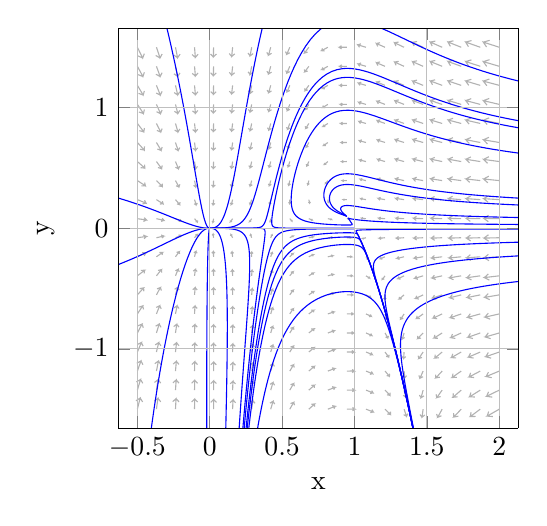
\begin{tikzpicture}
\begin{axis}[%
width=2in,
height=2in,
unbounded coords=jump,
view={0}{90},
scale only axis,
xmin=-0.631578947368421,
xmax=2.13157894736842,
xlabel={x},
xmajorgrids,
ymin=-1.65789473684211,
ymax=1.65789473684211,
ylabel={y},
ymajorgrids,
zmin=-1,
zmax=1
]
\addplot [color=white!70!black,solid,forget plot]
  table[row sep=crcr]{-0.5	-1.5\\
-0.480884910266225	-1.40761039962009\\
-0.509716837281336	-1.43054850730062\\
-0.480884910266225	-1.40761039962009\\
-0.463522037091379	-1.4401060521675\\
nan	0\\
-0.5	-1.34210526315789\\
-0.478442853929714	-1.2535413213858\\
-0.507050983193823	-1.27472121739986\\
-0.478442853929714	-1.2535413213858\\
-0.462769012307777	-1.285499790435\\
nan	0\\
-0.5	-1.18421052631579\\
-0.475583220905459	-1.0999145032513\\
-0.503982260399943	-1.11909911539701\\
-0.475583220905459	-1.0999145032513\\
-0.461834248867699	-1.13130750494428\\
nan	0\\
-0.5	-1.02631578947368\\
-0.47218711577924	-0.946880506509847\\
-0.500389801786427	-0.963757870343808\\
-0.47218711577924	-0.946880506509847\\
-0.460672160304509	-0.977664312454188\\
nan	0\\
-0.5	-0.868421052631579\\
-0.468097513171236	-0.79467544902016\\
-0.49610466012272	-0.808823508396394\\
-0.468097513171236	-0.79467544902016\\
-0.45923185831701	-0.824774751810777\\
nan	0\\
-0.5	-0.710526315789474\\
-0.463121575014064	-0.643684170502464\\
-0.490895638831597	-0.654517207842083\\
-0.463121575014064	-0.643684170502464\\
-0.457474566188092	-0.672956420335051\\
nan	0\\
-0.5	-0.552631578947368\\
-0.457079502120524	-0.494545838483811\\
-0.484477086600256	-0.501241436153009\\
-0.457079502120524	-0.494545838483811\\
-0.455434216368477	-0.522701685092747\\
nan	0\\
-0.5	-0.394736842105263\\
-0.450011418502081	-0.348273096482198\\
-0.476623929357223	-0.349715074794637\\
-0.450011418502081	-0.348273096482198\\
-0.45339205654569	-0.374709365543597\\
nan	0\\
-0.5	-0.236842105263158\\
-0.442747533508712	-0.206095410295614\\
-0.467609947197984	-0.201006302163055\\
-0.442747533508712	-0.206095410295614\\
-0.452236599714212	-0.229632535408699\\
nan	0\\
-0.5	-0.0789473684210527\\
-0.437555681889163	-0.0681682896995392\\
-0.458983747002793	-0.0557909337882841\\
-0.437555681889163	-0.0681682896995392\\
-0.453594207642036	-0.0870130928437024\\
nan	0\\
-0.5	0.0789473684210527\\
-0.436779620787438	0.0684106385522923\\
-0.453111552084016	0.0873767523160609\\
-0.436779620787438	0.0684106385522923\\
-0.458379917018397	0.0557665627097799\\
nan	0\\
-0.5	0.236842105263158\\
-0.439835751124137	0.207762718306491\\
-0.450615179047729	0.231527596612457\\
-0.439835751124137	0.207762718306491\\
-0.465154872526063	0.201445472174525\\
nan	0\\
-0.5	0.394736842105263\\
-0.444314716525178	0.351326271654461\\
-0.450167658954924	0.378270763658407\\
-0.444314716525178	0.351326271654461\\
-0.471872944180325	0.350428121920996\\
nan	0\\
-0.5	0.552631578947368\\
-0.448661714479067	0.498352037485132\\
-0.450493314769788	0.527470471304036\\
-0.448661714479067	0.498352037485132\\
-0.477633085500906	0.50180132854357\\
nan	0\\
-0.5	0.710526315789473\\
-0.452385563817994	0.647761831731374\\
-0.450978773658071	0.678494785994306\\
-0.452385563817994	0.647761831731374\\
-0.48236101568712	0.654687567903303\\
nan	0\\
-0.5	0.868421052631579\\
-0.455457208999619	0.798768354939807\\
-0.451406871876791	0.830799861997434\\
-0.455457208999619	0.798768354939807\\
-0.486233220722676	0.808528466497243\\
nan	0\\
-0.5	1.02631578947368\\
-0.457974720305252	0.950870406402637\\
-0.451720958445915	0.984010341247638\\
-0.457974720305252	0.950870406402637\\
-0.489443649981438	0.962997701400264\\
nan	0\\
-0.5	1.18421052631579\\
-0.460048797792527	1.10375324409241\\
-0.451919837898923	1.13787822931129\\
-0.460048797792527	1.10375324409241\\
-0.492148479010615	1.11790262820755\\
nan	0\\
-0.5	1.34210526315789\\
-0.461773243674815	1.25721431330062\\
-0.452018533108051	1.29223828733909\\
-0.461773243674815	1.25721431330062\\
-0.494464008036691	1.2731249091765\\
nan	0\\
-0.5	1.5\\
-0.46322149054043	1.41111860213937\\
-0.452034693913144	1.44697764886245\\
-0.46322149054043	1.41111860213937\\
-0.496475392843458	1.42858839413267\\
nan	0\\
-0.368421052631579	-1.5\\
-0.35829209439759	-1.40961151696535\\
-0.383927902626448	-1.43419582231725\\
-0.35829209439759	-1.40961151696535\\
-0.338733661109124	-1.43926030143424\\
nan	0\\
-0.368421052631579	-1.34210526315789\\
-0.356675443132785	-1.2551693080158\\
-0.381933114767947	-1.27831369218373\\
-0.356675443132785	-1.2551693080158\\
-0.3384651371969	-1.28418649693313\\
nan	0\\
-0.368421052631579	-1.18421052631579\\
-0.354760256697081	-1.10106422715239\\
-0.379645070268281	-1.12259291791779\\
-0.354760256697081	-1.10106422715239\\
-0.338071920686581	-1.12942331588503\\
nan	0\\
-0.368421052631579	-1.02631578947368\\
-0.352442692564091	-0.947399492613213\\
-0.376965274799455	-0.967079791654483\\
-0.352442692564091	-0.947399492613213\\
-0.33750712636922	-0.975068971688227\\
nan	0\\
-0.368421052631579	-0.868421052631579\\
-0.349565161040977	-0.794339147315009\\
-0.3737424048473	-0.811849746012329\\
-0.349565161040977	-0.794339147315009\\
-0.336701452189015	-0.82127769180763\\
nan	0\\
-0.368421052631579	-0.710526315789474\\
-0.345881099075558	-0.642165159771282\\
-0.369733374146912	-0.657038518187734\\
-0.345881099075558	-0.642165159771282\\
-0.335552796137816	-0.668308494965745\\
nan	0\\
-0.368421052631579	-0.552631578947368\\
-0.341001491752753	-0.491410281057092\\
-0.36453268448897	-0.502921780204468\\
-0.341001491752753	-0.491410281057092\\
-0.333922035543831	-0.516631560643881\\
nan	0\\
-0.368421052631579	-0.394736842105263\\
-0.334368358198648	-0.343185558420219\\
-0.357471987449789	-0.3501377699175\\
-0.334368358198648	-0.343185558420219\\
-0.331696345607267	-0.367164117133965\\
nan	0\\
-0.368421052631579	-0.236842105263158\\
-0.325663552590544	-0.199880894175883\\
-0.347731105374673	-0.200279882491807\\
-0.325663552590544	-0.199880894175883\\
-0.329250499831036	-0.221658632512324\\
nan	0\\
-0.368421052631579	-0.0789473684210527\\
-0.317360678222665	-0.0649125722634752\\
-0.336187489584734	-0.05635791750852\\
-0.317360678222665	-0.0649125722634752\\
-0.329170091505945	-0.0818881047129769\\
nan	0\\
-0.368421052631579	0.0789473684210527\\
-0.316483043932596	0.0653002721731288\\
-0.32865267248031	0.0823789032222517\\
-0.316483043932596	0.0653002721731288\\
-0.335476220604272	0.0564098988727601\\
nan	0\\
-0.368421052631579	0.236842105263158\\
-0.322067002380032	0.201844327532477\\
-0.327223773022826	0.223932173414568\\
-0.322067002380032	0.201844327532477\\
-0.344722661888166	0.200755148288795\\
nan	0\\
-0.368421052631579	0.394736842105263\\
-0.327945662185994	0.345866756151054\\
-0.327870757831117	0.370646629548713\\
-0.327945662185994	0.345866756151054\\
-0.352305800808222	0.35040893432592\\
nan	0\\
-0.368421052631579	0.552631578947368\\
-0.33243661182573	0.494171704326102\\
-0.328616975412168	0.520705776913944\\
-0.33243661182573	0.494171704326102\\
-0.357846912722801	0.502713556511019\\
nan	0\\
-0.368421052631579	0.710526315789473\\
-0.335729179436597	0.644798603244595\\
-0.329104813258872	0.672689885306804\\
-0.335729179436597	0.644798603244595\\
-0.361968669531311	0.656343948709313\\
nan	0\\
-0.368421052631579	0.868421052631579\\
-0.338182270324133	0.796797807846468\\
-0.329348093820089	0.825844476858863\\
-0.338182270324133	0.796797807846468\\
-0.365159716212645	0.81072508570514\\
nan	0\\
-0.368421052631579	1.02631578947368\\
-0.340057650153403	0.949686301813393\\
-0.329409298981783	0.979765998731024\\
-0.340057650153403	0.949686301813393\\
-0.367724042811928	0.965584297491936\\
nan	0\\
-0.368421052631579	1.18421052631579\\
-0.341527085766043	1.10319556705696\\
-0.329341536010997	1.13422354655099\\
-0.341527085766043	1.10319556705696\\
-0.369849015640411	1.12077656311823\\
nan	0\\
-0.368421052631579	1.34210526315789\\
-0.342703158800052	1.25716356666641\\
-0.329183102826639	1.28907554907174\\
-0.342703158800052	1.25716356666641\\
-0.371653951072382	1.27621660215597\\
nan	0\\
-0.368421052631579	1.5\\
-0.343661379718861	1.41148564571006\\
-0.328960693020192	1.44422987022522\\
-0.343661379718861	1.41148564571006\\
-0.373217870165161	1.43185003376886\\
nan	0\\
-0.236842105263158	-1.5\\
-0.232907704227502	-1.41241950136503\\
-0.255983149196942	-1.4377100506966\\
-0.232907704227502	-1.41241950136503\\
-0.212192899879455	-1.43967725121443\\
nan	0\\
-0.236842105263158	-1.34210526315789\\
-0.23201250740265	-1.25774770810589\\
-0.254550775523803	-1.28184757515637\\
-0.23201250740265	-1.25774770810589\\
-0.212371997997802	-1.28426237408662\\
nan	0\\
-0.236842105263158	-1.18421052631579\\
-0.230950351019269	-1.10335459723847\\
-0.252931859561767	-1.12613843740069\\
-0.230950351019269	-1.10335459723847\\
-0.212503895023105	-1.12908431452264\\
nan	0\\
-0.236842105263158	-1.02631578947368\\
-0.229658643645408	-0.949312703077175\\
-0.25106445372986	-0.97061776359169\\
-0.229658643645408	-0.949312703077175\\
-0.212562910531605	-0.974209494400565\\
nan	0\\
-0.236842105263158	-0.868421052631579\\
-0.228036942300761	-0.795731802704047\\
-0.248850803671363	-0.815337286941707\\
-0.228036942300761	-0.795731802704047\\
-0.212506178707597	-0.819739868422906\\
nan	0\\
-0.236842105263158	-0.710526315789474\\
-0.225912728809469	-0.642792111234268\\
-0.246125092884377	-0.660380028487408\\
-0.225912728809469	-0.642792111234268\\
-0.212257990606774	-0.665844716714252\\
nan	0\\
-0.236842105263158	-0.552631578947368\\
-0.222962899378127	-0.490826352028155\\
-0.24257796787344	-0.505898118632661\\
-0.222962899378127	-0.490826352028155\\
-0.211675354413833	-0.512837721575177\\
nan	0\\
-0.236842105263158	-0.394736842105263\\
-0.218514889521452	-0.340568136362066\\
-0.237555230679763	-0.352236944149598\\
-0.218514889521452	-0.340568136362066\\
-0.210470877808164	-0.361400552020452\\
nan	0\\
-0.236842105263158	-0.236842105263158\\
-0.211056037134856	-0.194136110328596\\
-0.229468356306987	-0.200501391776889\\
-0.211056037134856	-0.194136110328596\\
-0.208115358839706	-0.21339442584104\\
nan	0\\
-0.236842105263158	-0.0789473684210527\\
-0.199056163442176	-0.0593807902566829\\
-0.215283590529563	-0.0558042782507485\\
-0.199056163442176	-0.0593807902566829\\
-0.205500301447378	-0.0746972491612392\\
nan	0\\
-0.236842105263158	0.0789473684210527\\
-0.197977820618888	0.0599973254532165\\
-0.20489959527021	0.0753984095046349\\
-0.197977820618888	0.0599973254532165\\
-0.214374616754128	0.0559662671824998\\
nan	0\\
-0.236842105263158	0.236842105263158\\
-0.207056816604839	0.195675953890072\\
-0.205700865359063	0.215472121466577\\
-0.207056816604839	0.195675953890072\\
-0.226283941045606	0.200579477137418\\
nan	0\\
-0.236842105263158	0.394736842105263\\
-0.212698885813156	0.342030420147893\\
-0.206765246158814	0.363878151597604\\
-0.212698885813156	0.342030420147893\\
-0.233118457137499	0.351806541872603\\
nan	0\\
-0.236842105263158	0.552631578947368\\
-0.216003719593365	0.492107228393852\\
-0.207124147655924	0.515474129977355\\
-0.216003719593365	0.492107228393852\\
-0.237386322932682	0.505054937142459\\
nan	0\\
-0.236842105263158	0.710526315789473\\
-0.218119481724964	0.643919274093328\\
-0.207084508362386	0.66858204248672\\
-0.218119481724964	0.643919274093328\\
-0.240388029210459	0.659220730717623\\
nan	0\\
-0.236842105263158	0.868421052631579\\
-0.219576006199457	0.796738299299771\\
-0.206835147585615	0.822559650065238\\
-0.219576006199457	0.796738299299771\\
-0.242676524251519	0.813926600533388\\
nan	0\\
-0.236842105263158	1.02631578947368\\
-0.220632879732783	0.950223960716533\\
-0.206472690202608	0.977103815726272\\
-0.220632879732783	0.950223960716533\\
-0.244518604581183	0.968999202961085\\
nan	0\\
-0.236842105263158	1.18421052631579\\
-0.221429903687846	1.10418922523796\\
-0.206048238890982	1.13204866595514\\
-0.221429903687846	1.10418922523796\\
-0.246058889429897	1.12434256516748\\
nan	0\\
-0.236842105263158	1.34210526315789\\
-0.222048629348108	1.25851942742083\\
-0.205590213188355	1.28729354712071\\
-0.222048629348108	1.25851942742083\\
-0.24738313105689	1.27989680916318\\
nan	0\\
-0.236842105263158	1.5\\
-0.222539757271995	1.41313863105083\\
-0.205115119432052	1.44277262873337\\
-0.222539757271995	1.41313863105083\\
-0.248545803906635	1.43562145473779\\
nan	0\\
-0.105263157894737	-1.5\\
-0.104655400935292	-1.41572844328913\\
-0.125905617200843	-1.44085797106253\\
-0.104655400935292	-1.41572844328913\\
-0.0837698388454085	-1.44116184954225\\
nan	0\\
-0.105263157894737	-1.34210526315789\\
-0.104322759377592	-1.26090310506713\\
-0.124905418455426	-1.28502865286508\\
-0.104322759377592	-1.26090310506713\\
-0.0843043394100454	-1.28549885212365\\
nan	0\\
-0.105263157894737	-1.18421052631579\\
-0.103930235135004	-1.1063306297943\\
-0.123800086093296	-1.12936136806081\\
-0.103930235135004	-1.1063306297943\\
-0.0848601378325517	-1.13002782944068\\
nan	0\\
-0.105263157894737	-1.02631578947368\\
-0.103455143223473	-0.952071001271103\\
-0.122558744675498	-0.973892434064062\\
-0.103455143223473	-0.952071001271103\\
-0.0854363505742072	-0.974796441399694\\
nan	0\\
-0.105263157894737	-0.868421052631579\\
-0.102860525654389	-0.798211078631825\\
-0.121133808826432	-0.818673412771665\\
-0.102860525654389	-0.798211078631825\\
-0.0860288218265551	-0.819874728891838\\
nan	0\\
-0.105263157894737	-0.710526315789474\\
-0.102081166969782	-0.644884829713945\\
-0.119446135766151	-0.663781777805365\\
-0.102081166969782	-0.644884829713945\\
-0.0866253927283866	-0.665372773267843\\
nan	0\\
-0.105263157894737	-0.552631578947368\\
-0.100988443560823	-0.492318526150912\\
-0.117349121060112	-0.50934376340637\\
-0.100988443560823	-0.492318526150912\\
-0.0871925946618833	-0.511481120573327\\
nan	0\\
-0.105263157894737	-0.394736842105263\\
-0.0992826736074779	-0.34095342640103\\
-0.114522672819714	-0.355593330040485\\
-0.0992826736074779	-0.34095342640103\\
-0.0876309649675973	-0.358583572184115\\
nan	0\\
-0.105263157894737	-0.236842105263158\\
-0.0960408118811188	-0.191915599970475\\
-0.110039142008375	-0.203087965054876\\
-0.0960408118811188	-0.191915599970475\\
-0.0875758893620335	-0.207699138061685\\
nan	0\\
-0.105263157894737	-0.0789473684210527\\
-0.0864380763972793	-0.0510863940758449\\
-0.0990508444328185	-0.0547384160050429\\
-0.0864380763972793	-0.0510863940758449\\
-0.0851203572602146	-0.0641509567537716\\
nan	0\\
-0.105263157894737	0.0789473684210527\\
-0.0851520376336743	0.0516050013138015\\
-0.0843497819351803	0.0648354915112425\\
-0.0851520376336743	0.0516050013138015\\
-0.0980209654888059	0.0547799313807112\\
nan	0\\
-0.105263157894737	0.236842105263158\\
-0.0934573137129799	0.19231303257959\\
-0.0858667987966151	0.2086232154301\\
-0.0934573137129799	0.19231303257959\\
-0.108131335138399	0.202720293339221\\
nan	0\\
-0.105263157894737	0.394736842105263\\
-0.0961143213408421	0.341249284014314\\
-0.0854870827842733	0.359582760580073\\
-0.0961143213408421	0.341249284014314\\
-0.112230861829748	0.355008342303125\\
nan	0\\
-0.105263157894737	0.552631578947368\\
-0.0974099872032487	0.492557977041296\\
-0.0847475379341771	0.51254335028599\\
-0.0974099872032487	0.492557977041296\\
-0.114784338887213	0.508616764940245\\
nan	0\\
-0.105263157894737	0.710526315789473\\
-0.0981745533707286	0.645088418533715\\
-0.0839416604139915	0.666491938841445\\
-0.0981745533707286	0.645088418533715\\
-0.116660609041871	0.662947636579441\\
nan	0\\
-0.105263157894737	0.868421052631579\\
-0.0986752312269793	0.798389654090471\\
-0.0831437595920296	0.821046055319743\\
-0.0986752312269793	0.798389654090471\\
-0.118159458862583	0.817752091985864\\
nan	0\\
-0.105263157894737	1.02631578947368\\
-0.0990250375017233	0.952231004034019\\
-0.0823752772597111	0.976015969764172\\
-0.0990250375017233	0.952231004034019\\
-0.119417669979544	0.972896909567665\\
nan	0\\
-0.105263157894737	1.18421052631579\\
-0.0992802992528647	1.10647621527823\\
-0.081641579086037	1.13129222324997\\
-0.0992802992528647	1.10647621527823\\
-0.120508734604816	1.12830079392903\\
nan	0\\
-0.105263157894737	1.34210526315789\\
-0.0994723529039767	1.26103712277547\\
-0.0809425593055978	1.28680526613789\\
-0.0994723529039767	1.26103712277547\\
-0.121476629496812	1.28390986364251\\
nan	0\\
-0.105263157894737	1.5\\
-0.0996200657623935	1.4158529398259\\
-0.0802762283585716	1.44250783091122\\
-0.0996200657623935	1.4158529398259\\
-0.122349758445621	1.43968628484504\\
nan	0\\
0.0263157894736842	-1.5\\
0.0264476952712945	-1.41938625954503\\
0.00625468841826787	-1.44353740523212\\
0.0264476952712945	-1.41938625954503\\
0.0465615586457549	-1.44360335813092\\
nan	0\\
0.0263157894736842	-1.34210526315789\\
0.0263797386478205	-1.26442551616476\\
0.00694061714729563	-1.28771345296917\\
0.0263797386478205	-1.26442551616476\\
0.0457804906438636	-1.28774542755623\\
nan	0\\
0.0263157894736842	-1.18421052631579\\
0.0263003970456472	-1.10970496799255\\
0.00767862519324892	-1.13206048359653\\
0.0263003970456472	-1.10970496799255\\
0.0449314043548677	-1.13205278738251\\
nan	0\\
0.0263157894736842	-1.02631578947368\\
0.0262054506366539	-0.955280793280525\\
0.00847980323947304	-0.97661887684773\\
0.0262054506366539	-0.955280793280525\\
0.043997301336053	-0.976563707429215\\
nan	0\\
0.0263157894736842	-0.868421052631579\\
0.0260880429996848	-0.801233705770491\\
0.00935953022661264	-0.821446846447317\\
0.0260880429996848	-0.801233705770491\\
0.0429532036571565	-0.821332973210318\\
nan	0\\
0.0263157894736842	-0.710526315789474\\
0.0259360915475608	-0.647686658003111\\
0.0103400864788072	-0.666633479820551\\
0.0259360915475608	-0.647686658003111\\
0.0417599153719884	-0.666443630857489\\
nan	0\\
0.0263157894736842	-0.552631578947368\\
0.0257257262605938	-0.494842933541707\\
0.0114555838731056	-0.512327042966678\\
0.0257257262605938	-0.494842933541707\\
0.0403499065759363	-0.512032011360133\\
nan	0\\
0.0263157894736842	-0.394736842105263\\
0.0254008031861282	-0.343082974568205\\
0.0127618321881303	-0.358807881401211\\
0.0254008031861282	-0.343082974568205\\
0.0385887659566596	-0.358350388257433\\
nan	0\\
0.0263157894736842	-0.236842105263158\\
0.0247818050062519	-0.19328899186687\\
0.0143537219974096	-0.206738422002615\\
0.0247818050062519	-0.19328899186687\\
0.0361302786955535	-0.205971429768898\\
nan	0\\
0.0263157894736842	-0.0789473684210527\\
0.0226256785525904	-0.0488870878028426\\
0.016217641674366	-0.058827699718579\\
0.0226256785525904	-0.0488870878028426\\
0.031247781983471	-0.0569826442580321\\
nan	0\\
0.0263157894736842	0.0789473684210527\\
0.0221180065728032	0.0489312703160039\\
0.0308813659693297	0.0568866540222983\\
0.0221180065728032	0.0489312703160039\\
0.0158733169168053	0.0589855454727388\\
nan	0\\
0.0263157894736842	0.236842105263158\\
0.0240384412668522	0.193310666816577\\
0.035604505340547	0.205800761298843\\
0.0240384412668522	0.193310666816577\\
0.0138387861172565	0.206939435402259\\
nan	0\\
0.0263157894736842	0.394736842105263\\
0.0245183686733292	0.343098418853249\\
0.0379672007264391	0.358140590628765\\
0.0245183686733292	0.343098418853249\\
0.0121479891004323	0.359039301028942\\
nan	0\\
0.0263157894736842	0.552631578947368\\
0.0247382232865798	0.494855280061964\\
0.0396555678640621	0.511793778180809\\
0.0247382232865798	0.494855280061964\\
0.0107674184213601	0.512582561274361\\
nan	0\\
0.0263157894736842	0.710526315789473\\
0.0248621509965041	0.647697101887295\\
0.0410055460152028	0.666182456438653\\
0.0248621509965041	0.647697101887295\\
0.00959093906411339	0.666909275677243\\
nan	0\\
0.0263157894736842	0.868421052631579\\
0.0249397285034541	0.801242842750182\\
0.0421470992648722	0.821052290472044\\
0.0249397285034541	0.801242842750182\\
0.00855799432417396	0.821740320957159\\
nan	0\\
0.0263157894736842	1.02631578947368\\
0.0249913296291883	0.95528896773868\\
0.0431453730162882	0.976265899298057\\
0.0249913296291883	0.95528896773868\\
0.00763196214878598	0.976928129220305\\
nan	0\\
0.0263157894736842	1.18421052631579\\
0.0250269263172786	1.10971239889801\\
0.0440381171186451	1.13173962133424\\
0.0250269263172786	1.10971239889801\\
0.00678905340975534	1.13238405291245\\
nan	0\\
0.0263157894736842	1.34210526315789\\
0.025051990954718	1.26443235233891\\
0.0448493582151538	1.28741827595486\\
0.025051990954718	1.26443235233891\\
0.00601290280566192	1.28805017521435\\
nan	0\\
0.0263157894736842	1.5\\
0.0250697807352009	1.41939260725223\\
0.0455954315436878	1.44326332289194\\
0.0250697807352009	1.41939260725223\\
0.00529173516980388	1.44388632726118\\
nan	0\\
0.157894736842105	-1.5\\
0.160398836053555	-1.42343896330462\\
0.140507347116275	-1.44578124951037\\
0.160398836053555	-1.42343896330462\\
0.178787865463965	-1.4470332991161\\
nan	0\\
0.157894736842105	-1.34210526315789\\
0.160072686365102	-1.26832589504837\\
0.140974459480821	-1.28991521810048\\
0.160072686365102	-1.26832589504837\\
0.177864143535585	-1.29100419286197\\
nan	0\\
0.157894736842105	-1.18421052631579\\
0.159698114296359	-1.11344074822195\\
0.141464656536623	-1.13422083728654\\
0.159698114296359	-1.11344074822195\\
0.176849545583542	-1.13512252601367\\
nan	0\\
0.157894736842105	-1.02631578947368\\
0.159257979753808	-0.958837080581272\\
0.141979329657194	-0.97873988252107\\
0.159257979753808	-0.958837080581272\\
0.175718684103401	-0.979421503976921\\
nan	0\\
0.157894736842105	-0.868421052631579\\
0.158724699072834	-0.804592086894502\\
0.142518468969346	-0.823533286057943\\
0.158724699072834	-0.804592086894502\\
0.174432951837885	-0.823948267173307\\
nan	0\\
0.157894736842105	-0.710526315789474\\
0.158050166336438	-0.650823991141679\\
0.143077956326189	-0.668695831162434\\
0.158050166336438	-0.650823991141679\\
0.172929118650087	-0.6687735459096\\
nan	0\\
0.157894736842105	-0.552631578947368\\
0.157140464880465	-0.49773017996493\\
0.143641396723347	-0.514389167650072\\
0.157140464880465	-0.49773017996493\\
0.171092096214567	-0.514012031669252\\
nan	0\\
0.157894736842105	-0.394736842105263\\
0.15577804760478	-0.34568762918686\\
0.144150751146377	-0.360931565371712\\
0.15577804760478	-0.34568762918686\\
0.168675357605579	-0.35987322075305\\
nan	0\\
0.157894736842105	-0.236842105263158\\
0.153286220782341	-0.195617751750452\\
0.144362687222094	-0.209137186819205\\
0.153286220782341	-0.195617751750452\\
0.164974863978447	-0.206832928789323\\
nan	0\\
0.157894736842105	-0.0789473684210527\\
0.145629876873717	-0.0519901300816163\\
0.142570025279374	-0.0631435165755443\\
0.145629876873717	-0.0519901300816163\\
0.156048644449092	-0.0570110865913501\\
nan	0\\
0.157894736842105	0.0789473684210527\\
0.142899269767383	0.0528490494312973\\
0.153922489637239	0.0569296783595433\\
0.142899269767383	0.0528490494312973\\
0.140873330142361	0.0644274118969044\\
nan	0\\
0.157894736842105	0.236842105263158\\
0.1484812552168	0.196160215025032\\
0.161475772263923	0.206011411690143\\
0.1484812552168	0.196160215025032\\
0.14113482714486	0.210718152502796\\
nan	0\\
0.157894736842105	0.394736842105263\\
0.149976056002655	0.346083065009414\\
0.164515104528452	0.358699527928306\\
0.149976056002655	0.346083065009414\\
0.140188215980528	0.362658868348031\\
nan	0\\
0.157894736842105	0.552631578947368\\
0.150616604886994	0.498048316197466\\
0.166445860161003	0.512603762033659\\
0.150616604886994	0.498048316197466\\
0.139154228786052	0.516242828011214\\
nan	0\\
0.157894736842105	0.710526315789473\\
0.150941257112622	0.651093809121219\\
0.167885427698531	0.667185191189325\\
0.150941257112622	0.651093809121219\\
0.138169174364403	0.670661931054066\\
nan	0\\
0.157894736842105	0.868421052631579\\
0.151115866461021	0.804828455434497\\
0.169047676874617	0.82221151699835\\
0.151115866461021	0.804828455434497\\
0.137251378276076	0.825600952188893\\
nan	0\\
0.157894736842105	1.02631578947368\\
0.151208472335138	0.959048711354671\\
0.170031121216981	0.977557268663633\\
0.151208472335138	0.959048711354671\\
0.136397582157475	0.980900400917117\\
nan	0\\
0.157894736842105	1.18421052631579\\
0.15125207018896	1.11363322153005\\
0.170889196381338	1.13314574630249\\
0.15125207018896	1.11363322153005\\
0.13560054398847	1.13646707962906\\
nan	0\\
0.157894736842105	1.34210526315789\\
0.151264531653507	1.26850302074512\\
0.17165415381328	1.28892614217181\\
0.151264531653507	1.26850302074512\\
0.134853032606894	1.2922412447661\\
nan	0\\
0.157894736842105	1.5\\
0.151256328975007	1.42360346989549\\
0.172346983861264	1.44486282696007\\
0.151256328975007	1.42360346989549\\
0.134148718809008	1.44818203089362\\
nan	0\\
0.289473684210526	-1.5\\
0.297266942924258	-1.4281924989516\\
0.276977090048039	-1.44778643458769\\
0.297266942924258	-1.4281924989516\\
0.312880840572237	-1.45168306394456\\
nan	0\\
0.289473684210526	-1.34210526315789\\
0.296797916521869	-1.27289809693674\\
0.277298855273178	-1.29182918872525\\
0.296797916521869	-1.27289809693674\\
0.311902438383755	-1.29549130488092\\
nan	0\\
0.289473684210526	-1.18421052631579\\
0.296273265136614	-1.11781576497977\\
0.277634700524782	-1.13603429814905\\
0.296273265136614	-1.11781576497977\\
0.310832081192794	-1.1394340886121\\
nan	0\\
0.289473684210526	-1.02631578947368\\
0.295675335258911	-0.962995012127394\\
0.277984645607823	-0.980440832569185\\
0.295675335258911	-0.962995012127394\\
0.309645034280968	-0.983541658093377\\
nan	0\\
0.289473684210526	-0.868421052631579\\
0.294976379751291	-0.808507000042746\\
0.278347057941854	-0.825105541934204\\
0.294976379751291	-0.808507000042746\\
0.30830408423627	-0.827856889704587\\
nan	0\\
0.289473684210526	-0.710526315789474\\
0.294129199567741	-0.654460273520391\\
0.278716034393306	-0.670116207361812\\
0.294129199567741	-0.654460273520391\\
0.306749055527847	-0.67244396504042\\
nan	0\\
0.289473684210526	-0.552631578947368\\
0.293044013304524	-0.501034913949566\\
0.279073748326874	-0.515621331175407\\
0.293044013304524	-0.501034913949566\\
0.304872080825775	-0.517406495722406\\
nan	0\\
0.289473684210526	-0.394736842105263\\
0.291518182473	-0.348571064578099\\
0.279363388612467	-0.36190967327063\\
0.291518182473	-0.348571064578099\\
0.302446277376049	-0.362931922401867\\
nan	0\\
0.289473684210526	-0.236842105263158\\
0.288934492629516	-0.197881428750477\\
0.279356080975649	-0.209704429599534\\
0.288934492629516	-0.197881428750477\\
0.29883641923199	-0.209434833809029\\
nan	0\\
0.289473684210526	-0.0789473684210527\\
0.281487865006708	-0.0527184622344071\\
0.277326384221192	-0.0625835888913553\\
0.281487865006708	-0.0527184622344071\\
0.290440837314515	-0.0585906792894462\\
nan	0\\
0.289473684210526	0.0789473684210527\\
0.275506519986796	0.0543319189816697\\
0.285850531613761	0.058224762757552\\
0.275506519986796	0.0543319189816697\\
0.273542806894069	0.0652083448694172\\
nan	0\\
0.289473684210526	0.236842105263158\\
0.27895129161179	0.19882597624545\\
0.291612041645838	0.207600216801079\\
0.27895129161179	0.19882597624545\\
0.272603977136984	0.212861413100447\\
nan	0\\
0.289473684210526	0.394736842105263\\
0.279528422539692	0.349254532066705\\
0.293882578550582	0.360412909660564\\
0.279528422539692	0.349254532066705\\
0.271141423531303	0.365385540495981\\
nan	0\\
0.289473684210526	0.552631578947368\\
0.279583078232157	0.501583635320915\\
0.295312245932281	0.514425366914258\\
0.279583078232157	0.501583635320915\\
0.269788274119055	0.519370669903443\\
nan	0\\
0.289473684210526	0.710526315789473\\
0.279470389981607	0.654925254976287\\
0.29637164345358	0.669104749663013\\
0.279470389981607	0.654925254976287\\
0.268571113046986	0.674106396777472\\
nan	0\\
0.289473684210526	0.868421052631579\\
0.279291754087865	0.808914159549508\\
0.297223056395181	0.824220744943464\\
0.279291754087865	0.808914159549508\\
0.267469609854146	0.829311710004794\\
nan	0\\
0.289473684210526	1.02631578947368\\
0.279085388428546	0.963359467519095\\
0.297940957651787	0.979649290159976\\
0.279085388428546	0.963359467519095\\
0.266462796674493	0.984843438050967\\
nan	0\\
0.289473684210526	1.18421052631579\\
0.278868085398922	1.11814717635166\\
0.298565602533437	1.135314781638\\
0.278868085398922	1.11814717635166\\
0.26553392755137	1.1406175810438\\
nan	0\\
0.289473684210526	1.34210526315789\\
0.27864792970269	1.27320304968531\\
0.299121209423187	1.29116727510013\\
0.27864792970269	1.27320304968531\\
0.264670102686895	1.29658015235404\\
nan	0\\
0.289473684210526	1.5\\
0.278429021424187	1.42847570470747\\
0.29962349408322	1.44717182759865\\
0.278429021424187	1.42847570470747\\
0.263861346436957	1.45269415899182\\
nan	0\\
0.421052631578947	-1.5\\
0.437155394387696	-1.43434788514203\\
0.415911536830579	-1.45001782889723\\
0.437155394387696	-1.43434788514203\\
0.448737594259564	-1.45806921030161\\
nan	0\\
0.421052631578947	-1.34210526315789\\
0.436615623552623	-1.27885007985821\\
0.416132930135599	-1.2939358868547\\
0.436615623552623	-1.27885007985821\\
0.447760521785441	-1.30171738284153\\
nan	0\\
0.421052631578947	-1.18421052631579\\
0.436035918766792	-1.12354918020603\\
0.416375596082999	-1.138001762242\\
0.436035918766792	-1.12354918020603\\
0.446706269137878	-1.14549340583592\\
nan	0\\
0.421052631578947	-1.02631578947368\\
0.435408074243995	-0.968491417287\\
0.41664534839781	-0.982249868276744\\
0.435408074243995	-0.968491417287\\
0.445557534491152	-0.989427589609267\\
nan	0\\
0.421052631578947	-0.868421052631579\\
0.434720876202066	-0.813743301707321\\
0.416950965084066	-0.826729565828819\\
0.434720876202066	-0.813743301707321\\
0.444289840546195	-0.833563688140378\\
nan	0\\
0.421052631578947	-0.710526315789474\\
0.433958428761101	-0.659406330200838\\
0.417306693209296	-0.67151587658189\\
0.433958428761101	-0.659406330200838\\
0.442866686003614	-0.677968775172967\\
nan	0\\
0.421052631578947	-0.552631578947368\\
0.433097262160001	-0.505648732256225\\
0.417738161312899	-0.516732428618305\\
0.433097262160001	-0.505648732256225\\
0.441229584658471	-0.522754743908832\\
nan	0\\
0.421052631578947	-0.394736842105263\\
0.432101703197692	-0.352786545997111\\
0.418299407685031	-0.36260936692487\\
0.432101703197692	-0.352786545997111\\
0.439274555739107	-0.368133902734243\\
nan	0\\
0.421052631578947	-0.236842105263158\\
0.430924239120679	-0.201557473106663\\
0.419141598819036	-0.209674960868179\\
0.430924239120679	-0.201557473106663\\
0.436783914897283	-0.214610764639044\\
nan	0\\
0.421052631578947	-0.0789473684210527\\
0.42976236119963	-0.0548674040715916\\
0.42112945122606	-0.0599139609712591\\
0.42976236119963	-0.0548674040715916\\
0.433169433400791	-0.0642688257816007\\
nan	0\\
0.421052631578947	0.0789473684210527\\
0.41815762406215	0.0539713886620567\\
0.425270121256938	0.0607404307105562\\
0.41815762406215	0.0539713886620567\\
0.41278213137744	0.0621879344689548\\
nan	0\\
0.421052631578947	0.236842105263158\\
0.413985331093837	0.20112001923761\\
0.425036042745757	0.210069819923997\\
0.413985331093837	0.20112001923761\\
0.407174999732983	0.213603470166552\\
nan	0\\
0.421052631578947	0.394736842105263\\
0.411998991677008	0.352474964515415\\
0.425280553045052	0.362890117816885\\
0.411998991677008	0.352474964515415\\
0.404149614250128	0.367416937767855\\
nan	0\\
0.421052631578947	0.552631578947368\\
0.410602589484071	0.505399673741833\\
0.425545578413917	0.516956734779774\\
0.410602589484071	0.505399673741833\\
0.40192962581115	0.522181755827212\\
nan	0\\
0.421052631578947	0.710526315789473\\
0.409495481032569	0.659195661745334\\
0.425795289707517	0.671705570321981\\
0.409495481032569	0.659195661745334\\
0.400129962685447	0.677484145595171\\
nan	0\\
0.421052631578947	0.868421052631579\\
0.408564176107931	0.813558999590385\\
0.426026226009534	0.826895501634989\\
0.408564176107931	0.813558999590385\\
0.398595199488937	0.833139729370497\\
nan	0\\
0.421052631578947	1.02631578947368\\
0.407752646862889	0.9683265323427\\
0.426239956560453	0.982398313302981\\
0.407752646862889	0.9683265323427\\
0.397245327994961	0.98904830566101\\
nan	0\\
0.421052631578947	1.18421052631579\\
0.407028769954741	1.12339929449736\\
0.42643873639661	1.13813669863684\\
0.407028769954741	1.12339929449736\\
0.396033120487396	1.14514862944894\\
nan	0\\
0.421052631578947	1.34210526315789\\
0.406372260844455	1.27871219097835\\
0.42662464010969	1.29406001994859\\
0.406372260844455	1.27871219097835\\
0.394928104019916	1.30140020531583\\
nan	0\\
0.421052631578947	1.5\\
0.405769412867754	1.43421984936118\\
0.426799416140816	1.45013308987503\\
0.405769412867754	1.43421984936118\\
0.393909340821408	1.45777469923063\\
nan	0\\
0.552631578947368	-1.5\\
0.579917719189365	-1.44321620253755\\
0.557535927751153	-1.45342980671578\\
0.579917719189365	-1.44321620253755\\
0.585927826482379	-1.46707287683678\\
nan	0\\
0.552631578947368	-1.34210526315789\\
0.579280183740394	-1.2874946580499\\
0.557632951025488	-1.29721568838404\\
0.579280183740394	-1.2874946580499\\
0.584938253579485	-1.31053999078056\\
nan	0\\
0.552631578947368	-1.18421052631579\\
0.578620520380729	-1.13196190001547\\
0.557761681375641	-1.14113925254722\\
0.578620520380729	-1.13196190001547\\
0.583885994525801	-1.1541337232639\\
nan	0\\
0.552631578947368	-1.02631578947368\\
0.577940752924016	-0.976665239199804\\
0.557935363162551	-0.985233110787806\\
0.577940752924016	-0.976665239199804\\
0.582760638299492	-0.99788769777613\\
nan	0\\
0.552631578947368	-0.868421052631579\\
0.57724695408938	-0.821674354827587\\
0.558175667095778	-0.829544520383282\\
0.57724695408938	-0.821674354827587\\
0.581549015997774	-0.841852207954288\\
nan	0\\
0.552631578947368	-0.710526315789474\\
0.576554386139463	-0.667098953267886\\
0.558520703351437	-0.674146460226339\\
0.576554386139463	-0.667098953267886\\
0.580234384612231	-0.686107863822386\\
nan	0\\
0.552631578947368	-0.552631578947368\\
0.575900843030932	-0.513128905186574\\
0.559044395365664	-0.519162391293921\\
0.575900843030932	-0.513128905186574\\
0.578795732246061	-0.530797023335703\\
nan	0\\
0.552631578947368	-0.394736842105263\\
0.575386485316596	-0.360143886205882\\
0.559911774430982	-0.364833046383389\\
0.575386485316596	-0.360143886205882\\
0.577208252380673	-0.376210499568003\\
nan	0\\
0.552631578947368	-0.236842105263158\\
0.575316938761588	-0.209115196441661\\
0.561579603611947	-0.211761929134555\\
0.575316938761588	-0.209115196441661\\
0.575443058022696	-0.223104609041665\\
nan	0\\
0.552631578947368	-0.0789473684210527\\
0.576684166868244	-0.0641007946807356\\
0.565756747056902	-0.0625416198226117\\
0.576684166868244	-0.0641007946807356\\
0.573180033927061	-0.0745679137830497\\
nan	0\\
0.552631578947368	0.0789473684210527\\
0.56789602361251	0.0595180464404437\\
0.56817402070812	0.0691629542009119\\
0.56789602361251	0.0595180464404437\\
0.558459359717816	0.0615307318683409\\
nan	0\\
0.552631578947368	0.236842105263158\\
0.552096612482899	0.203953131265376\\
0.560479345921685	0.213686081848593\\
0.552096612482899	0.203953131265376\\
0.544034858922794	0.213953565080828\\
nan	0\\
0.552631578947368	0.394736842105263\\
0.545812965853803	0.356136603420496\\
0.557508609453064	0.366012021752535\\
0.545812965853803	0.356136603420496\\
0.538208490110681	0.369421328299318\\
nan	0\\
0.552631578947368	0.552631578947368\\
0.542133123716389	0.509847391365435\\
0.555978707181166	0.52005803383227\\
0.542133123716389	0.509847391365435\\
0.534586613390199	0.52530726144776\\
nan	0\\
0.552631578947368	0.710526315789473\\
0.539521979348862	0.664295371889853\\
0.555012595203319	0.674887255160113\\
0.539521979348862	0.664295371889853\\
0.531897123253509	0.681442054959366\\
nan	0\\
0.552631578947368	0.868421052631579\\
0.537480830829688	0.819209189740896\\
0.554329020987663	0.83018506157868\\
0.537480830829688	0.819209189740896\\
0.529723089542321	0.837760435637521\\
nan	0\\
0.552631578947368	1.02631578947368\\
0.53579230991161	0.974453343790225\\
0.553809702043202	0.985802260236323\\
0.53579230991161	0.974453343790225\\
0.527878479201472	0.994221894754202\\
nan	0\\
0.552631578947368	1.18421052631579\\
0.534343428905228	1.12994752734561\\
0.553395623660415	1.14165438952613\\
0.534343428905228	1.12994752734561\\
0.526264124175325	1.1507984645472\\
nan	0\\
0.552631578947368	1.34210526315789\\
0.533068238442729	1.28563924312992\\
0.553053745601115	1.29768821401215\\
0.533068238442729	1.28563924312992\\
0.524820735587126	1.30746988426447\\
nan	0\\
0.552631578947368	1.5\\
0.531924960241967	1.44149188823087\\
0.552763973795871	1.45386766708526\\
0.531924960241967	1.44149188823087\\
0.523509917911304	1.46422097643796\\
nan	0\\
0.684210526315789	-1.5\\
0.724311021442363	-1.45670918005537\\
0.701458167918233	-1.45967130225711\\
0.724311021442363	-1.45670918005537\\
0.723103577890549	-1.4797215498204\\
nan	0\\
0.684210526315789	-1.34210526315789\\
0.723370705868957	-1.30064072120518\\
0.701256516514829	-1.30329003890271\\
0.723370705868957	-1.30064072120518\\
0.721988787491185	-1.32287012867929\\
nan	0\\
0.684210526315789	-1.18421052631579\\
0.72239043538977	-1.14474314562576\\
0.701069617495069	-1.14703838256427\\
0.72239043538977	-1.14474314562576\\
0.720803307840083	-1.16612833710126\\
nan	0\\
0.684210526315789	-1.02631578947368\\
0.721367894387199	-0.989061354087564\\
0.700907075119246	-0.990948342685548\\
0.721367894387199	-0.989061354087564\\
0.719534292812306	-1.00952702672125\\
nan	0\\
0.684210526315789	-0.868421052631579\\
0.720301926358707	-0.833661797065106\\
0.700784692454214	-0.835066723724319\\
0.720301926358707	-0.833661797065106\\
0.71816432023745	-0.853112423745778\\
nan	0\\
0.684210526315789	-0.710526315789474\\
0.719194126043137	-0.678649047092047\\
0.700729728950576	-0.679466327769438\\
0.719194126043137	-0.678649047092047\\
0.716668363299289	-0.696958127633112\\
nan	0\\
0.684210526315789	-0.552631578947368\\
0.718052002190689	-0.524201776231451\\
0.70079210874924	-0.524270348077501\\
0.718052002190689	-0.524201776231451\\
0.715007010107198	-0.541191086014951\\
nan	0\\
0.684210526315789	-0.394736842105263\\
0.716893784220748	-0.370662232893066\\
0.701070154546211	-0.369713801180485\\
0.716893784220748	-0.370662232893066\\
0.71310745915231	-0.386055430132965\\
nan	0\\
0.684210526315789	-0.236842105263158\\
0.715739030203993	-0.218802988101124\\
0.701770699747023	-0.216332597277683\\
0.715739030203993	-0.218802988101124\\
0.710790258328041	-0.232096849221785\\
nan	0\\
0.684210526315789	-0.0789473684210527\\
0.714338564235474	-0.0708020169462885\\
0.703263814990878	-0.0657136129087965\\
0.714338564235474	-0.0708020169462885\\
0.70733649072826	-0.0807776318686391\\
nan	0\\
0.684210526315789	0.0789473684210527\\
0.708347275944083	0.0677431055916632\\
0.703907316762942	0.0771385718475535\\
0.708347275944083	0.0677431055916632\\
0.698305185348248	0.0650701970334065\\
nan	0\\
0.684210526315789	0.236842105263158\\
0.689978200520309	0.208462190395278\\
0.695342876975923	0.218418083406772\\
0.689978200520309	0.208462190395278\\
0.681152919541983	0.215534246304512\\
nan	0\\
0.684210526315789	0.394736842105263\\
0.677906430514797	0.361020120137302\\
0.688226839747085	0.369559112777442\\
0.677906430514797	0.361020120137302\\
0.671368478763104	0.372711160677938\\
nan	0\\
0.684210526315789	0.552631578947368\\
0.671218690669244	0.515952443125585\\
0.684286025318653	0.523708224960484\\
0.671218690669244	0.515952443125585\\
0.665946457407762	0.530204142783756\\
nan	0\\
0.684210526315789	0.710526315789473\\
0.666754696979495	0.671484664861328\\
0.68175185851242	0.678833202805698\\
0.666754696979495	0.671484664861328\\
0.662231033048347	0.687561117473845\\
nan	0\\
0.684210526315789	0.868421052631579\\
0.663400117681725	0.827312413678139\\
0.679920400010305	0.834442403205655\\
0.663400117681725	0.827312413678139\\
0.659366080533585	0.844847607522687\\
nan	0\\
0.684210526315789	1.02631578947368\\
0.660695474256526	0.98333923242442\\
0.678494129136621	0.990353436524383\\
0.660695474256526	0.98333923242442\\
0.657005850611989	1.00211096255402\\
nan	0\\
0.684210526315789	1.18421052631579\\
0.658415039953789	1.13951791316241\\
0.677326839150733	1.14647682551793\\
0.658415039953789	1.13951791316241\\
0.654980532574046	1.15937456869893\\
nan	0\\
0.684210526315789	1.34210526315789\\
0.656432951084502	1.2958192361495\\
0.676337730405986	1.3027606504442\\
0.656432951084502	1.2958192361495\\
0.653194716901791	1.31664943805984\\
nan	0\\
0.684210526315789	1.5\\
0.654672302925008	1.45222282126469\\
0.675478064626069	1.45917141903759\\
0.654672302925008	1.45222282126469\\
0.651589475258416	1.47394053073298\\
nan	0\\
0.81578947368421	-1.5\\
0.866857455316198	-1.47606830166229\\
0.845554136242173	-1.4704808157556\\
0.866857455316198	-1.47606830166229\\
0.85751998541103	-1.4960148065716\\
nan	0\\
0.81578947368421	-1.34210526315789\\
0.865377371491832	-1.31925812236212\\
0.844789216950602	-1.31371529014895\\
0.865377371491832	-1.31925812236212\\
0.85621278734849	-1.33850923905276\\
nan	0\\
0.81578947368421	-1.18421052631579\\
0.863802565219099	-1.16255054104423\\
0.843983641440741	-1.15704526374197\\
0.863802565219099	-1.16255054104423\\
0.854813634076523	-1.18105180950942\\
nan	0\\
0.81578947368421	-1.02631578947368\\
0.862115991341768	-1.00597176431801\\
0.843132029755582	-1.00049334245032\\
0.862115991341768	-1.00597176431801\\
0.853304042333419	-1.0236566012791\\
nan	0\\
0.81578947368421	-0.868421052631579\\
0.860294924599932	-0.849559881534857\\
0.842227996551035	-0.844091870134943\\
0.860294924599932	-0.849559881534857\\
0.851658582099396	-0.866344595592804\\
nan	0\\
0.81578947368421	-0.710526315789474\\
0.858307810597855	-0.693373302024722\\
0.841264056082574	-0.687889621925736\\
0.858307810597855	-0.693373302024722\\
0.84984056296495	-0.709148790382559\\
nan	0\\
0.81578947368421	-0.552631578947368\\
0.856108249950129	-0.537508136030591\\
0.840231756341159	-0.531965474839144\\
0.856108249950129	-0.537508136030591\\
0.847793477799548	-0.552124862972104\\
nan	0\\
0.81578947368421	-0.394736842105263\\
0.853621685617604	-0.382138528311919\\
0.83912244358925	-0.376459969466574\\
0.853621685617604	-0.382138528311919\\
0.845421600485922	-0.395376075433271\\
nan	0\\
0.81578947368421	-0.236842105263158\\
0.850708107374535	-0.227626908131483\\
0.837928717984519	-0.221661808848405\\
0.850708107374535	-0.227626908131483\\
0.842536316550356	-0.239121125693567\\
nan	0\\
0.81578947368421	-0.0789473684210527\\
0.847006336386503	-0.0749040864804197\\
0.836630457090657	-0.0683128553870364\\
0.847006336386503	-0.0749040864804197\\
0.838652098060974	-0.0839212867381828\\
nan	0\\
0.81578947368421	0.0789473684210527\\
0.840664771603212	0.072840926008408\\
0.834728792830673	0.0808916832119518\\
0.840664771603212	0.072840926008408\\
0.831675571624351	0.0684540342524509\\
nan	0\\
0.81578947368421	0.236842105263158\\
0.819024746812487	0.214088220624691\\
0.823742636033621	0.2217232042983\\
0.819024746812487	0.214088220624691\\
0.812365693714387	0.220105567734162\\
nan	0\\
0.81578947368421	0.394736842105263\\
0.800207665944157	0.37054526172696\\
0.810930103360749	0.373907283905437\\
0.800207665944157	0.37054526172696\\
0.798834313171597	0.381698187775464\\
nan	0\\
0.81578947368421	0.552631578947368\\
0.791982078535007	0.528365065027756\\
0.805190925559671	0.529693170416339\\
0.791982078535007	0.528365065027756\\
0.793057668599865	0.54159686799094\\
nan	0\\
0.81578947368421	0.710526315789473\\
0.786820039925054	0.685729898350462\\
0.801709974412553	0.685926465142376\\
0.786820039925054	0.685729898350462\\
0.789311765693048	0.700411182021955\\
nan	0\\
0.81578947368421	0.868421052631579\\
0.782959054315759	0.842920218970848\\
0.799183388541477	0.842362864226954\\
0.782959054315759	0.842920218970848\\
0.786432971711112	0.85877807391118\\
nan	0\\
0.81578947368421	1.02631578947368\\
0.779818241678356	1.00005755441992\\
0.797174170043553	0.998942216934587\\
0.779818241678356	1.00005755441992\\
0.784045052516672	1.01692783293751\\
nan	0\\
0.81578947368421	1.18421052631579\\
0.777139174524263	1.1571896468367\\
0.795489484142019	1.15563333589044\\
0.777139174524263	1.1571896468367\\
0.781979044402476	1.17495848547042\\
nan	0\\
0.81578947368421	1.34210526315789\\
0.774784197228551	1.31433592398007\\
0.794028114959704	1.31241540661951\\
0.774784197228551	1.31433592398007\\
0.780143445370793	1.33291804484734\\
nan	0\\
0.81578947368421	1.5\\
0.772670911142023	1.47150416908092\\
0.792730437634448	1.4692732777211\\
0.772670911142023	1.47150416908092\\
0.778482522174911	1.49083255899219\\
nan	0\\
0.947368421052631	-1.5\\
1.00292735881764	-1.49951651777714\\
0.986138806932422	-1.48577182800274\\
1.00292735881764	-1.49951651777714\\
0.986380548043853	-1.51355129688525\\
nan	0\\
0.947368421052631	-1.34210526315789\\
1.0010312599929	-1.34164156339926\\
0.984816483371162	-1.32836496359178\\
1.0010312599929	-1.34164156339926\\
0.985048333250479	-1.35519638306192\\
nan	0\\
0.947368421052631	-1.18421052631579\\
0.998990771406906	-1.18376839475397\\
0.98339353341017	-1.17099544663395\\
0.998990771406906	-1.18376839475397\\
0.983614599191077	-1.19680662181109\\
nan	0\\
0.947368421052631	-1.02631578947368\\
0.996774802223336	-1.02589746449942\\
0.981848306628559	-1.01367136669902\\
0.996774802223336	-1.02589746449942\\
0.98205746911569	-1.03837455728438\\
nan	0\\
0.947368421052631	-0.868421052631579\\
0.994339930920477	-0.868029436006305\\
0.980150573803804	-0.856404043526926\\
0.994339930920477	-0.868029436006305\\
0.980346382116442	-0.879889798460848\\
nan	0\\
0.947368421052631	-0.710526315789474\\
0.991622479636062	-0.710165342501086\\
0.978256018738936	-0.699210119841745\\
0.991622479636062	-0.710165342501086\\
0.97843650538313	-0.72133714913346\\
nan	0\\
0.947368421052631	-0.552631578947368\\
0.98852268792042	-0.552306933781685\\
0.976095246568663	-0.542115760614443\\
0.98852268792042	-0.552306933781685\\
0.976257569151504	-0.562692894048338\\
nan	0\\
0.947368421052631	-0.394736842105263\\
0.984868728525087	-0.394457559476705\\
0.973548815626211	-0.385166267397159\\
0.984868728525087	-0.394457559476705\\
0.973688456940489	-0.403916421133387\\
nan	0\\
0.947368421052631	-0.236842105263158\\
0.980317041951839	-0.236625037372352\\
0.970378188709375	-0.228453002514792\\
0.980317041951839	-0.236625037372352\\
0.970486722654778	-0.244927312964395\\
nan	0\\
0.947368421052631	-0.0789473684210527\\
0.973959889023009	-0.0788362782954068\\
0.965954676100484	-0.0722217383405062\\
0.973959889023009	-0.0788362782954068\\
0.966010221163307	-0.085517472325695\\
nan	0\\
0.947368421052631	0.0789473684210527\\
0.959605210573157	0.0784237220226518\\
0.956065085316599	0.0816400133223033\\
0.959605210573157	0.0784237220226518\\
0.955803262117399	0.0755216185620407\\
nan	0\\
0.947368421052631	0.236842105263158\\
0.922636191124436	0.236456931190506\\
0.930152153621057	0.230389425930252\\
0.922636191124436	0.236456931190506\\
0.929959566584731	0.24275554089435\\
nan	0\\
0.947368421052631	0.394736842105263\\
0.915589082225656	0.394347991359699\\
0.92522009656014	0.386519811876624\\
0.915589082225656	0.394347991359699\\
0.925025671187357	0.402409481290112\\
nan	0\\
0.947368421052631	0.552631578947368\\
0.910760166676702	0.552221324664254\\
0.92184520656026	0.543192337355206\\
0.910760166676702	0.552221324664254\\
0.921640079418703	0.56149646454317\\
nan	0\\
0.947368421052631	0.710526315789473\\
0.906950448102677	0.710093591435952\\
0.919184021076043	0.70011891550452\\
0.906950448102677	0.710093591435952\\
0.918967658899283	0.720327901979497\\
nan	0\\
0.947368421052631	0.868421052631579\\
0.903748849560178	0.867966953685478\\
0.916948245744439	0.857198290496195\\
0.903748849560178	0.867966953685478\\
0.916721196271388	0.879008076242421\\
nan	0\\
0.947368421052631	1.02631578947368\\
0.900958765191084	1.02584171234392\\
0.915000181231991	1.01438152151746\\
0.900958765191084	1.02584171234392\\
0.914763142667106	1.03758634944823\\
nan	0\\
0.947368421052631	1.18421052631579\\
0.89846901327549	1.1837177978751\\
0.913262017718805	1.17164076446302\\
0.89846901327549	1.1837177978751\\
0.91301565349846	1.19609046835159\\
nan	0\\
0.947368421052631	1.34210526315789\\
0.896209858421354	1.34159506753822\\
0.911684976115655	1.32895848556631\\
0.896209858421354	1.34159506753822\\
0.911429878305819	1.35453776688194\\
nan	0\\
0.947368421052631	1.5\\
0.894134342246495	1.49947337765951\\
0.910236221473457	1.48632284466013\\
0.894134342246495	1.49947337765951\\
0.909972910303214	1.51293988406319\\
nan	0\\
1.07894736842105	-1.5\\
1.13015213633254	-1.52315695504388\\
1.12057994472007	-1.50340867655284\\
1.13015213633254	-1.52315695504388\\
1.10900146719813	-1.52901106050859\\
nan	0\\
1.07894736842105	-1.34210526315789\\
1.12793522649585	-1.36461777273251\\
1.11886699646707	-1.34561705534143\\
1.12793522649585	-1.36461777273251\\
1.10761074167976	-1.37011098437883\\
nan	0\\
1.07894736842105	-1.18421052631579\\
1.12549652130097	-1.2060495009838\\
1.116991519104	-1.18786052036342\\
1.12549652130097	-1.2060495009838\\
1.10607203176999	-1.21113509680338\\
nan	0\\
1.07894736842105	-1.02631578947368\\
1.12277039858569	-1.04745360766604\\
1.11490794408439	-1.03015650466717\\
1.12277039858569	-1.04745360766604\\
1.10433903498821	-1.05206801974949\\
nan	0\\
1.07894736842105	-0.868421052631579\\
1.11965327271059	-0.888837800884551\\
1.11254568848697	-0.872536300336274\\
1.11965327271059	-0.888837800884551\\
1.10233731436049	-0.892889252481045\\
nan	0\\
1.07894736842105	-0.710526315789474\\
1.1159648707232	-0.73022713208709\\
1.10978482410696	-0.715062511622269\\
1.1159648707232	-0.73022713208709\\
1.09993441595815	-0.733571262773342\\
nan	0\\
1.07894736842105	-0.552631578947368\\
1.11133979308907	-0.57170126562862\\
1.10638948735898	-0.557882253457241\\
1.11133979308907	-0.57170126562862\\
1.09685464401835	-0.574078465791248\\
nan	0\\
1.07894736842105	-0.394736842105263\\
1.10480405974153	-0.413555306473125\\
1.10175166843736	-0.401445594332646\\
1.10480405974153	-0.413555306473125\\
1.09234243625342	-0.414373939992887\\
nan	0\\
1.07894736842105	-0.236842105263158\\
1.09146391695788	-0.25714333642654\\
1.09278426018767	-0.24792382994332\\
1.09146391695788	-0.25714333642654\\
1.08263364460598	-0.254182104211731\\
nan	0\\
1.07894736842105	-0.0789473684210527\\
1.05663992610992	-0.0859826762773073\\
1.06509098576732	-0.0894489444982138\\
1.05663992610992	-0.0859826762773073\\
1.0615733318392	-0.078295223342648\\
nan	0\\
1.07894736842105	0.0789473684210527\\
1.04751127151586	0.082785161001532\\
1.0559826524423	0.0737747990010898\\
1.04751127151586	0.082785161001532\\
1.05790154873254	0.0894928474536865\\
nan	0\\
1.07894736842105	0.236842105263158\\
1.04251438530728	0.245115058258017\\
1.0513760419927	0.233524926581116\\
1.04251438530728	0.245115058258017\\
1.05551251849013	0.251741418138002\\
nan	0\\
1.07894736842105	0.394736842105263\\
1.03868477339916	0.405778575334138\\
1.04800311859851	0.392400406610002\\
1.03868477339916	0.405778575334138\\
1.05352398521294	0.41253170412095\\
nan	0\\
1.07894736842105	0.552631578947368\\
1.03549116287271	0.565713807862675\\
1.04525746730838	0.550925087800997\\
1.03549116287271	0.565713807862675\\
1.05179858176604	0.572653190575169\\
nan	0\\
1.07894736842105	0.710526315789473\\
1.03271584230375	0.725243053018289\\
1.04290611583174	0.709270150320319\\
1.03271584230375	0.725243053018289\\
1.05026448444614	0.73238591337897\\
nan	0\\
1.07894736842105	0.868421052631579\\
1.0302422226906	0.884513109588141\\
1.04083075217059	0.867509206068558\\
1.0302422226906	0.884513109588141\\
1.04887678064887	0.891861778933786\\
nan	0\\
1.07894736842105	1.02631578947368\\
1.02799893257763	1.04360283514268\\
1.03896170191341	1.02567961248112\\
1.02799893257763	1.04360283514268\\
1.0476052247479	1.05115383040283\\
nan	0\\
1.07894736842105	1.18421052631579\\
1.0259385093697	1.20255944354393\\
1.03725393777807	1.18380255361265\\
1.0259385093697	1.20255944354393\\
1.04642839639214	1.21030698313833\\
nan	0\\
1.07894736842105	1.34210526315789\\
1.02402752666884	1.3614134584445\\
1.03567643037285	1.34189103942046\\
1.02402752666884	1.3614134584445\\
1.04533052801616	1.36935096029657\\
nan	0\\
1.07894736842105	1.5\\
1.02224142088516	1.52018577449011\\
1.0342067615234	1.4999535552591\\
1.02224142088516	1.52018577449011\\
1.04429964876845	1.52830652902705\\
nan	0\\
1.21052631578947	-1.5\\
1.24849864914253	-1.54388005933386\\
1.24807696397008	-1.52122295819544\\
1.24849864914253	-1.54388005933386\\
1.22613693430315	-1.54020912487197\\
nan	0\\
1.21052631578947	-1.34210526315789\\
1.2451867068046	-1.38525913688239\\
1.24557705793119	-1.36364787701126\\
1.2451867068046	-1.38525913688239\\
1.22400012106894	-1.38097807251882\\
nan	0\\
1.21052631578947	-1.18421052631579\\
1.24127898142427	-1.22666232485222\\
1.24266613136794	-1.2062386188826\\
1.24127898142427	-1.22666232485222\\
1.22144023209972	-1.22161495169999\\
nan	0\\
1.21052631578947	-1.02631578947368\\
1.23648942691102	-1.0680967719851\\
1.23914573920241	-1.04907169945129\\
1.23648942691102	-1.0680967719851\\
1.2182552479467	-1.06205325501206\\
nan	0\\
1.21052631578947	-0.868421052631579\\
1.23029793242756	-0.909530570939872\\
1.23464382701321	-0.892254811287863\\
1.23029793242756	-0.909530570939872\\
1.21408906785906	-0.902140619606905\\
nan	0\\
1.21052631578947	-0.710526315789474\\
1.22170465552602	-0.750727019669939\\
1.22840132957517	-0.735872223571663\\
1.22170465552602	-0.750727019669939\\
1.20830097763494	-0.741461393439936\\
nan	0\\
1.21052631578947	-0.552631578947368\\
1.20898244437132	-0.590510128567582\\
1.21891524320182	-0.579532531536056\\
1.20898244437132	-0.590510128567582\\
1.19997596839171	-0.578760595826979\\
nan	0\\
1.21052631578947	-0.394736842105263\\
1.19181302408684	-0.425182899387567\\
1.20503852591821	-0.420727405128534\\
1.19181302408684	-0.425182899387567\\
1.18981549727706	-0.411370759277219\\
nan	0\\
1.21052631578947	-0.236842105263158\\
1.17747103143565	-0.253761525618296\\
1.19161747183058	-0.25694952060021\\
1.17747103143565	-0.253761525618296\\
1.18315776165301	-0.240421878423299\\
nan	0\\
1.21052631578947	-0.0789473684210527\\
1.17003770144458	-0.0836287037230285\\
1.18335461957354	-0.0923464567186591\\
1.17003770144458	-0.0836287037230285\\
1.18101395192255	-0.0721021495462124\\
nan	0\\
1.21052631578947	0.0789473684210527\\
1.16600169566887	0.0828404613483291\\
1.17838580847323	0.0705413784399953\\
1.16600169566887	0.0828404613483291\\
1.18033235493687	0.0928036885002971\\
nan	0\\
1.21052631578947	0.236842105263158\\
1.16321313954143	0.246820487731118\\
1.17491249679885	0.231998678928718\\
1.16321313954143	0.246820487731118\\
1.17990168803283	0.255655267052742\\
nan	0\\
1.21052631578947	0.394736842105263\\
1.16095876379584	0.409304751935271\\
1.17218705193643	0.39254249098786\\
1.16095876379584	0.409304751935271\\
1.17947100685143	0.417326266984678\\
nan	0\\
1.21052631578947	0.552631578947368\\
1.15899028894741	0.570850962450047\\
1.16989625112436	0.552501140688728\\
1.15899028894741	0.570850962450047\\
1.1790059428757	0.578269154109758\\
nan	0\\
1.21052631578947	0.710526315789473\\
1.15720522594833	0.731771339480202\\
1.16789029697799	0.712067559912696\\
1.15720522594833	0.731771339480202\\
1.17851280882335	0.73872810483327\\
nan	0\\
1.21052631578947	0.868421052631579\\
1.15555328174631	0.892250583366373\\
1.16608780927556	0.871358465635145\\
1.15555328174631	0.892250583366373\\
1.17800257464296	0.898844982656725\\
nan	0\\
1.21052631578947	1.02631578947368\\
1.15400583171807	1.05240454673156\\
1.16443978762502	1.03044779853635\\
1.15400583171807	1.05240454673156\\
1.17748416625396	1.05870804057205\\
nan	0\\
1.21052631578947	1.18421052631579\\
1.15254455762928	1.2123097460629\\
1.16291428014056	1.18938454059872\\
1.15254455762928	1.2123097460629\\
1.17696389001411	1.21837541967882\\
nan	0\\
1.21052631578947	1.34210526315789\\
1.15115666216432	1.37201896969232\\
1.16148913161826	1.3482024443257\\
1.15115666216432	1.37201896969232\\
1.17644598488547	1.37788727113828\\
nan	0\\
1.21052631578947	1.5\\
1.14983261786638	1.53156999219031\\
1.16014822919573	1.50692557005245\\
1.14983261786638	1.53156999219031\\
1.17593322529088	1.53727241901399\\
nan	0\\
1.34210526315789	-1.5\\
1.35928661308161	-1.55896182410661\\
1.36887266413115	-1.53697793939369\\
1.35928661308161	-1.55896182410661\\
1.33939175207785	-1.54556861435555\\
nan	0\\
1.34210526315789	-1.34210526315789\\
1.35390313035155	-1.39969105975312\\
1.36476021934226	-1.37946585397614\\
1.35390313035155	-1.39969105975312\\
1.33596732104464	-1.38536478757297\\
nan	0\\
1.34210526315789	-1.18421052631579\\
1.34742432332806	-1.24003699446362\\
1.35978522231397	-1.22195928897673\\
1.34742432332806	-1.24003699446362\\
1.33187198824005	-1.22461881906181\\
nan	0\\
1.34210526315789	-1.02631578947368\\
1.33954256318774	-1.07966140429359\\
1.35364777688376	-1.06429839484016\\
1.33954256318774	-1.07966140429359\\
1.32697496947381	-1.06301704485508\\
nan	0\\
1.34210526315789	-0.868421052631579\\
1.33004481958917	-0.917956039861036\\
1.34604669946715	-0.906110654584381\\
1.33004481958917	-0.917956039861036\\
1.32127920585242	-0.900080432800017\\
nan	0\\
1.34210526315789	-0.710526315789474\\
1.31921455572899	-0.754064113235052\\
1.33696621731906	-0.746725450858604\\
1.31921455572899	-0.754064113235052\\
1.31519731859627	-0.735280097144153\\
nan	0\\
1.34210526315789	-0.552631578947368\\
1.30834569182834	-0.587457889464688\\
1.32718014085654	-0.58544988914188\\
1.30834569182834	-0.587457889464688\\
1.30976698559788	-0.568570103477105\\
nan	0\\
1.34210526315789	-0.394736842105263\\
1.29930933153506	-0.418944659085814\\
1.31820006526704	-0.422381296897358\\
1.29930933153506	-0.418944659085814\\
1.30609615677677	-0.400983331085939\\
nan	0\\
1.34210526315789	-0.236842105263158\\
1.29298624815304	-0.250369824130667\\
1.31110388237137	-0.258591262221628\\
1.29298624815304	-0.250369824130667\\
1.30434002293762	-0.2340317547192\\
nan	0\\
1.34210526315789	-0.0789473684210527\\
1.28889736007413	-0.0830571461584239\\
1.3058871754336	-0.0951261886081532\\
1.28889736007413	-0.0830571461584239\\
1.30383228656492	-0.0685222370662719\\
nan	0\\
1.34210526315789	0.0789473684210527\\
1.28619264067888	0.0826747888100251\\
1.30203457232534	0.0675784070735786\\
1.28619264067888	0.0826747888100251\\
1.30389828251982	0.095534718313088\\
nan	0\\
1.34210526315789	0.236842105263158\\
1.28425367265303	0.247018856674877\\
1.29906496195156	0.229502933625146\\
1.28425367265303	0.247018856674877\\
1.30415333765742	0.258428728877576\\
nan	0\\
1.34210526315789	0.394736842105263\\
1.28273078274615	0.410273607185093\\
1.29665893559971	0.390768957558207\\
1.28273078274615	0.410273607185093\\
1.30442731813963	0.420456197764081\\
nan	0\\
1.34210526315789	0.552631578947368\\
1.28144085200091	0.572698792606611\\
1.2946233719332	0.551512525719593\\
1.28144085200091	0.572698792606611\\
1.30465697876282	0.581844731298084\\
nan	0\\
1.34210526315789	0.710526315789473\\
1.28028864275146	0.734491284465648\\
1.29284238670435	0.711847638761187\\
1.28028864275146	0.734491284465648\\
1.30482487104243	0.742755948964404\\
nan	0\\
1.34210526315789	0.868421052631579\\
1.27922354403895	0.895794677311221\\
1.29124465360473	0.871862160127594\\
1.27922354403895	0.895794677311221\\
1.30493146594455	0.903303019687064\\
nan	0\\
1.34210526315789	1.02631578947368\\
1.27821775293108	1.05671335946564\\
1.28978461350113	1.03162221091135\\
1.27821775293108	1.05671335946564\\
1.30498339849711	1.06356596602476\\
nan	0\\
1.34210526315789	1.18421052631579\\
1.27725539765666	1.21732400737141\\
1.28843198704313	1.19117749667942\\
1.27725539765666	1.21732400737141\\
1.30498872757094	1.22360242943003\\
nan	0\\
1.34210526315789	1.34210526315789\\
1.27632703113983	1.37768382159182\\
1.28716586113677	1.35056569605712\\
1.27632703113983	1.37768382159182\\
1.30495514035373	1.38345481206616\\
nan	0\\
1.34210526315789	1.5\\
1.27542677202504	1.53783620305031\\
1.28597126860232	1.509815719352\\
1.27542677202504	1.53783620305031\\
1.30488937012747	1.54315496491843\\
nan	0\\
1.47368421052632	-1.5\\
1.46638011259407	-1.56645378563258\\
1.48518478838189	-1.54834367442587\\
1.46638011259407	-1.56645378563258\\
1.4519578955656	-1.54469162545974\\
nan	0\\
1.47368421052632	-1.34210526315789\\
1.4596284355215	-1.40537298374504\\
1.47966209816973	-1.3899066113201\\
1.4596284355215	-1.40537298374504\\
1.44802823787616	-1.38287872381769\\
nan	0\\
1.47368421052632	-1.18421052631579\\
1.45213113937418	-1.24336569619544\\
1.47338585318974	-1.23100741301958\\
1.45213113937418	-1.24336569619544\\
1.44380826824991	-1.22023087744351\\
nan	0\\
1.47368421052632	-1.02631578947368\\
1.4440623185118	-1.08014619683058\\
1.46640648795538	-1.07140254762714\\
1.4440623185118	-1.08014619683058\\
1.43949128427693	-1.05659160161989\\
nan	0\\
1.47368421052632	-0.868421052631579\\
1.43582728873314	-0.915516866052847\\
1.45895831862641	-0.910852352474759\\
1.43582728873314	-0.915516866052847\\
1.43541041191578	-0.891923891578173\\
nan	0\\
1.47368421052632	-0.710526315789474\\
1.42803444167605	-0.749541183787411\\
1.45148308933061	-0.749249165600597\\
1.42803444167605	-0.749541183787411\\
1.43197565533164	-0.726424281175462\\
nan	0\\
1.47368421052632	-0.552631578947368\\
1.4212921757283	-0.582645864336957\\
1.4445133575151	-0.586739587419583\\
1.4212921757283	-0.582645864336957\\
1.42950621482031	-0.560543570020577\\
nan	0\\
1.47368421052632	-0.394736842105263\\
1.41594219576453	-0.41549625160381\\
1.4384546525677	-0.423703932444693\\
1.41594219576453	-0.41549625160381\\
1.42807494781843	-0.394832925063799\\
nan	0\\
1.47368421052632	-0.236842105263158\\
1.41196548051675	-0.248714231746988\\
1.43344913114058	-0.260582276304231\\
1.41196548051675	-0.248714231746988\\
1.42751306789866	-0.229722911299448\\
nan	0\\
1.47368421052632	-0.0789473684210527\\
1.40910780233773	-0.0826834958442538\\
1.42941475665011	-0.0977067596644396\\
1.40910780233773	-0.0826834958442538\\
1.42754669293851	-0.0654185555701473\\
nan	0\\
1.47368421052632	0.0789473684210527\\
1.40705743416554	0.0824590758123218\\
1.42616754022596	0.0647488695047477\\
1.40705743416554	0.0824590758123218\\
1.42792339392159	0.0980622576851344\\
nan	0\\
1.47368421052632	0.236842105263158\\
1.40554897562578	0.246735320438232\\
1.42351624230217	0.226733547160575\\
1.40554897562578	0.246735320438232\\
1.42846284988971	0.260801164610844\\
nan	0\\
1.47368421052632	0.394736842105263\\
1.40439049212279	0.410239040183682\\
1.42130305812424	0.388264951159274\\
1.40439049212279	0.410239040183682\\
1.42905415716345	0.422911810361038\\
nan	0\\
1.47368421052632	0.552631578947368\\
1.40345405477014	0.573082920514998\\
1.41941026610508	0.549389979105665\\
1.40345405477014	0.573082920514998\\
1.4296359368889	0.584505056983753\\
nan	0\\
1.47368421052632	0.710526315789473\\
1.40265774258086	0.735373750587936\\
1.41775382426488	0.710162903162032\\
1.40265774258086	0.735373750587936\\
1.43017754166411	0.745676137134762\\
nan	0\\
1.47368421052632	0.868421052631579\\
1.40195002509157	0.897203723257653\\
1.41627461306548	0.870635375711145\\
1.40195002509157	0.897203723257653\\
1.43066594837852	0.906502468428516\\
nan	0\\
1.47368421052632	1.02631578947368\\
1.40129869149516	1.05864917203401\\
1.41493100156442	1.03085277750812\\
1.40129869149516	1.05864917203401\\
1.43109769284459	1.0670455370237\\
nan	0\\
1.47368421052632	1.18421052631579\\
1.40068362373177	1.21977216549717\\
1.41369338997479	1.19085352704412\\
1.40068362373177	1.21977216549717\\
1.43147420956548	1.22735382044139\\
nan	0\\
1.47368421052632	1.34210526315789\\
1.40009224399418	1.3806228746554\\
1.41254043107944	1.35066959957312\\
1.40009224399418	1.3806228746554\\
1.4317992368282	1.38746558283918\\
nan	0\\
1.47368421052632	1.5\\
1.39951668516573	1.54124187917502\\
1.41145647298015	1.51032743408237\\
1.39951668516573	1.54124187917502\\
1.43207741256766	1.54741119676266\\
nan	0\\
1.60526315789474	-1.5\\
1.57445048013533	-1.56750038484253\\
1.60056937967378	-1.55495343882963\\
1.57445048013533	-1.56750038484253\\
1.56681918725252	-1.53954709994992\\
nan	0\\
1.60526315789474	-1.34210526315789\\
1.56791763355552	-1.40469740999098\\
1.59476932756556	-1.39525614702586\\
1.56791763355552	-1.40469740999098\\
1.56347325414901	-1.37658338485625\\
nan	0\\
1.60526315789474	-1.18421052631579\\
1.56127332906787	-1.24103069964275\\
1.58867532104767	-1.23498210485138\\
1.56127332906787	-1.24103069964275\\
1.56026523438419	-1.21298719043795\\
nan	0\\
1.60526315789474	-1.02631578947368\\
1.55476659431087	-1.07649281307451\\
1.58245981928623	-1.07406384689023\\
1.55476659431087	-1.07649281307451\\
1.55737130748582	-1.0488155650983\\
nan	0\\
1.60526315789474	-0.868421052631579\\
1.54868104831945	-0.911190066280944\\
1.57634793460438	-0.912504889579955\\
1.54868104831945	-0.911190066280944\\
1.5549634277797	-0.884213834792314\\
nan	0\\
1.60526315789474	-0.710526315789474\\
1.54327137989486	-0.745347622631668\\
1.57057424000537	-0.750399175078977\\
1.54327137989486	-0.745347622631668\\
1.55316358658428	-0.719403286079041\\
nan	0\\
1.60526315789474	-0.552631578947368\\
1.53869972275217	-0.579268481693772\\
1.56532797898154	-0.587918269655493\\
1.53869972275217	-0.579268481693772\\
1.55200952760834	-0.554636552084208\\
nan	0\\
1.60526315789474	-0.394736842105263\\
1.53500630273284	-0.413262241264649\\
1.56071470907126	-0.425268835307306\\
1.53500630273284	-0.413262241264649\\
1.55145200949157	-0.39014040772636\\
nan	0\\
1.60526315789474	-0.236842105263158\\
1.53212574970365	-0.247580664348409\\
1.55675161193229	-0.262643448670606\\
1.53212574970365	-0.247580664348409\\
1.55138233238966	-0.226074744575062\\
nan	0\\
1.60526315789474	-0.0789473684210527\\
1.5299306279056	-0.0823868857478399\\
1.55339026623404	-0.100188163047087\\
1.5299306279056	-0.0823868857478399\\
1.55167050757065	-0.0625218980525203\\
nan	0\\
1.60526315789474	0.0789473684210527\\
1.52827525186081	0.0822413993459334\\
1.55054811593976	0.0620062135599864\\
1.52827525186081	0.0822413993459334\\
1.55219513140221	0.100500166576952\\
nan	0\\
1.60526315789474	0.236842105263158\\
1.52702460136838	0.246290512712065\\
1.54813406646406	0.223896351345804\\
1.52702460136838	0.246290512712065\\
1.55285827018852	0.263015629608981\\
nan	0\\
1.60526315789474	0.394736842105263\\
1.52606716683062	0.409786417423158\\
1.54606357032038	0.385472547061759\\
1.52606716683062	0.409786417423158\\
1.55358835797933	0.425070542593819\\
nan	0\\
1.60526315789474	0.552631578947368\\
1.52531705064372	0.572775238919106\\
1.54426496782609	0.54674561411483\\
1.52531705064372	0.572775238919106\\
1.55433679781196	0.586718667740339\\
nan	0\\
1.60526315789474	0.710526315789473\\
1.52471088988614	0.735310390252733\\
1.54268055167291	0.707737100911607\\
1.52471088988614	0.735310390252733\\
1.55507258890454	0.748013234915903\\
nan	0\\
1.60526315789474	0.868421052631579\\
1.52420319757488	0.89744516159939\\
1.54126515842889	0.868472938829083\\
1.52420319757488	0.89744516159939\\
1.55577721291279	0.90900291898901\\
nan	0\\
1.60526315789474	1.02631578947368\\
1.52376187616175	1.05922900707808\\
1.53998395628055	1.02897972136351\\
1.52376187616175	1.05922900707808\\
1.55644056508274	1.06973036223001\\
nan	0\\
1.60526315789474	1.18421052631579\\
1.52336452936871	1.22070604809288\\
1.53881023748225	1.18928273442825\\
1.52336452936871	1.22070604809288\\
1.55705799837079	1.23023204869126\\
nan	0\\
1.60526315789474	1.34210526315789\\
1.52299565555568	1.38191478561789\\
1.5377235256424	1.34940505329513\\
1.52299565555568	1.38191478561789\\
1.5576282868724	1.39053880446466\\
nan	0\\
1.60526315789474	1.5\\
1.52264459955528	1.54288840826472\\
1.53670806499094	1.50936724620044\\
1.52264459955528	1.54288840826472\\
1.5581522691233	1.55067652537017\\
nan	0\\
1.73684210526316	-1.5\\
1.68561085033592	-1.56506778087675\\
1.71724717203328	-1.55835526034554\\
1.68561085033592	-1.56506778087675\\
1.6847132815949	-1.53273963288192\\
nan	0\\
1.73684210526316	-1.34210526315789\\
1.68006647504023	-1.40137690989921\\
1.71191707579244	-1.39778932343255\\
1.68006647504023	-1.40137690989921\\
1.68228125242178	-1.36940150832109\\
nan	0\\
1.73684210526316	-1.18421052631579\\
1.67472636796486	-1.2371244611167\\
1.70658957285458	-1.236779215001\\
1.67472636796486	-1.2371244611167\\
1.68013260545412	-1.20572134635185\\
nan	0\\
1.73684210526316	-1.02631578947368\\
1.66973495453347	-1.07239385342838\\
1.70138661574105	-1.07534722192439\\
1.66973495453347	-1.07239385342838\\
1.67834758376371	-1.04179364655955\\
nan	0\\
1.73684210526316	-0.868421052631579\\
1.66521689814764	-0.907314457489471\\
1.69642781149677	-0.913552737810984\\
1.66521689814764	-0.907314457489471\\
1.67698110906782	-0.877740134253224\\
nan	0\\
1.73684210526316	-0.710526315789474\\
1.66125791060006	-0.742046341635919\\
1.6918131754606	-0.751486382547759\\
1.66125791060006	-0.742046341635919\\
1.67605316253738	-0.713694285216212\\
nan	0\\
1.73684210526316	-0.552631578947368\\
1.65789448001066	-0.576757531559497\\
1.68761025573944	-0.589256652088984\\
1.65789448001066	-0.576757531559497\\
1.67554727943337	-0.549782839462733\\
nan	0\\
1.73684210526316	-0.394736842105263\\
1.65511531970315	-0.411601221954973\\
1.68384945033358	-0.426973604390062\\
1.65511531970315	-0.411601221954973\\
1.67541726040873	-0.386110211610059\\
nan	0\\
1.73684210526316	-0.236842105263158\\
1.65287222562789	-0.246699650198505\\
1.68052757575231	-0.264734856626718\\
1.65287222562789	-0.246699650198505\\
1.67559880328463	-0.222749916809084\\
nan	0\\
1.73684210526316	-0.0789473684210527\\
1.65109501949153	-0.0821374326917801\\
1.6776166612907	-0.102617184853469\\
1.65109501949153	-0.0821374326917801\\
1.67602162915534	-0.0597436419676549\\
nan	0\\
1.73684210526316	0.0789473684210527\\
1.64970553220757	0.0820368974084131\\
1.6750741218774	0.0593258954483069\\
1.64970553220757	0.0820368974084131\\
1.67661888637108	0.102894181976103\\
nan	0\\
1.73684210526316	0.236842105263158\\
1.64862782067461	0.245804466230326\\
1.67285151580939	0.22106218679304\\
1.64862782067461	0.245804466230326\\
1.67733269629297	0.265169329087312\\
nan	0\\
1.73684210526316	0.394736842105263\\
1.64779409723706	0.409168010835259\\
1.67090070746239	0.382576658209736\\
1.64779409723706	0.409168010835259\\
1.67811629182739	0.427100662222784\\
nan	0\\
1.73684210526316	0.552631578947368\\
1.64714718924256	0.572144362048884\\
1.66917746827336	0.543866798113281\\
1.64714718924256	0.572144362048884\\
1.67893385982412	0.588714256123578\\
nan	0\\
1.73684210526316	0.710526315789473\\
1.64664073461813	0.734758437560522\\
1.66764311536888	0.704938458367951\\
1.64664073461813	0.734758437560522\\
1.6797591762544	0.750039143690464\\
nan	0\\
1.73684210526316	0.868421052631579\\
1.64623816579344	0.897038920980711\\
1.66626488054707	0.865802575608541\\
1.64623816579344	0.897038920980711\\
1.68057381472164	0.911104545343402\\
nan	0\\
1.73684210526316	1.02631578947368\\
1.64591120742247	1.05901540284578\\
1.66501557343165	1.02647279437398\\
1.64591120742247	1.05901540284578\\
1.6813653801177	1.07193824329433\\
nan	0\\
1.73684210526316	1.18421052631579\\
1.64563831080551	1.22071663426016\\
1.66387292215671	1.18696385326244\\
1.64563831080551	1.22071663426016\\
1.6821259761289	1.23256575049126\\
nan	0\\
1.73684210526316	1.34210526315789\\
1.6454032330088	1.3821695590217\\
1.66281882071915	1.34729055219897\\
1.6454032330088	1.3821695590217\\
1.68285096865106	1.39300998832615\\
nan	0\\
1.73684210526316	1.5\\
1.64519383835728	1.54339885708449\\
1.66183860415792	1.50746713323268\\
1.64519383835728	1.54339885708449\\
1.68353803270017	1.55329126668561\\
nan	0\\
1.86842105263158	-1.5\\
1.79972586815117	-1.56137921505115\\
1.83567922725808	-1.56013924665591\\
1.79972586815117	-1.56137921505115\\
1.8049896197325	-1.5257916544157\\
nan	0\\
1.86842105263158	-1.34210526315789\\
1.79522030029434	-1.39744866496017\\
1.83101637644608	-1.3991458325038\\
1.79522030029434	-1.39744866496017\\
1.80334467554494	-1.36254545633518\\
nan	0\\
1.86842105263158	-1.18421052631579\\
1.79099833733283	-1.23319999396207\\
1.82647251883403	-1.23785883249287\\
1.79099833733283	-1.23319999396207\\
1.80197778501089	-1.1991474748435\\
nan	0\\
1.86842105263158	-1.02631578947368\\
1.78712741145605	-1.06871303398178\\
1.82211481493573	-1.07631727092323\\
1.78712741145605	-1.06871303398178\\
1.80091619268169	-1.03567045033547\\
nan	0\\
1.86842105263158	-0.868421052631579\\
1.7836562086505	-0.904081227764085\\
1.81800070562795	-0.914574386219604\\
1.7836562086505	-0.904081227764085\\
1.80017061806169	-0.872191964229063\\
nan	0\\
1.86842105263158	-0.710526315789474\\
1.78061072167279	-0.739403041865041\\
1.81417300247932	-0.752692606782069\\
1.78061072167279	-0.739403041865041\\
1.79973463944153	-0.708787441302673\\
nan	0\\
1.86842105263158	-0.552631578947368\\
1.77799388123532	-0.574773046556696\\
1.81065739955653	-0.590737399122962\\
1.77799388123532	-0.574773046556696\\
1.79958666575187	-0.545523813424833\\
nan	0\\
1.86842105263158	-0.394736842105263\\
1.77578844931768	-0.410274491666499\\
1.80746264270216	-0.428771347626602\\
1.77578844931768	-0.410274491666499\\
1.79969381792154	-0.382455045969655\\
nan	0\\
1.86842105263158	-0.236842105263158\\
1.77396204337522	-0.245974547603853\\
1.8045828567373	-0.266849567215735\\
1.77396204337522	-0.245974547603853\\
1.80001663556695	-0.219620062587554\\
nan	0\\
1.86842105263158	-0.0789473684210527\\
1.77247288743679	-0.0819224740240239\\
1.80200111339597	-0.105016983641829\\
1.77247288743679	-0.0819224740240239\\
1.80051356059449	-0.0570429010444364\\
nan	0\\
1.86842105263158	0.0789473684210527\\
1.77127511739556	0.0818497622310337\\
1.79969329951387	0.0566925602790343\\
1.77127511739556	0.0818497622310337\\
1.80114449641886	0.105265527897045\\
nan	0\\
1.86842105263158	0.236842105263158\\
1.77032295260559	0.245325262556746\\
1.79763159328999	0.218255790362172\\
1.77032295260559	0.245325262556746\\
1.80187317193678	0.267304840375167\\
nan	0\\
1.86842105263158	0.394736842105263\\
1.76957352515862	0.4084992186385\\
1.7957871892672	0.37965862381029\\
1.76957352515862	0.4084992186385\\
1.80266837753382	0.429082387546767\\
nan	0\\
1.86842105263158	0.552631578947368\\
1.76898848744648	0.571375837838302\\
1.79413219227927	0.540894418874746\\
1.76898848744648	0.571375837838302\\
1.80350432172474	0.590610701467297\\
nan	0\\
1.86842105263158	0.710526315789473\\
1.76853467440852	0.733965574547953\\
1.79264077318582	0.701962202364644\\
1.76853467440852	0.733965574547953\\
1.80436040256506	0.751905391476174\\
nan	0\\
1.86842105263158	0.868421052631579\\
1.7681841235399	0.896282851625834\\
1.79128975251884	0.862865079654637\\
1.7681841235399	0.896282851625834\\
1.80522065201596	0.912983544200478\\
nan	0\\
1.86842105263158	1.02631578947368\\
1.76791371247526	1.05834430687968\\
1.79005878517066	1.0236089166188\\
1.76791371247526	1.05834430687968\\
1.80607304387365	1.07386258669696\\
nan	0\\
1.86842105263158	1.18421052631579\\
1.76770460674599	1.22016751648826\\
1.78893029296855	1.18420130796512\\
1.76770460674599	1.22016751648826\\
1.80690878805479	1.23455953090791\\
nan	0\\
1.86842105263158	1.34210526315789\\
1.7675416455116	1.38177011232466\\
1.78788925535591	1.34465080579464\\
1.7675416455116	1.38177011232466\\
1.80772167993929	1.39509050935462\\
nan	0\\
1.86842105263158	1.5\\
1.76741274159554	1.54316920438519\\
1.78692293381006	1.50496636531062\\
1.76741274159554	1.54316920438519\\
1.80850753600265	1.55547052082864\\
nan	0\\
2	-1.5\\
1.91603201726294	-1.5574998142656\\
1.95559736565045	-1.56124186567018\\
1.91603201726294	-1.5574998142656\\
1.92684745851766	-1.51925787430165\\
nan	0\\
2	-1.34210526315789\\
1.91238511058674	-1.39366325577416\\
1.95155907556478	-1.4000995803426\\
1.91238511058674	-1.39366325577416\\
1.92578007925665	-1.35629213563596\\
nan	0\\
2	-1.18421052631579\\
1.90900904255183	-1.22965791256765\\
1.94766817634925	-1.23877143605414\\
1.90900904255183	-1.22965791256765\\
1.92494448322331	-1.19327595733005\\
nan	0\\
2	-1.02631578947368\\
1.90593294988917	-1.06554232411766\\
1.94395969858341	-1.07729112625218\\
1.90593294988917	-1.06554232411766\\
1.92434643126142	-1.03025760119676\\
nan	0\\
2	-0.868421052631579\\
1.90317441264162	-0.901377895479985\\
1.94046129956124	-0.915697239465058\\
1.90317441264162	-0.901377895479985\\
1.92398287813703	-0.867284445785869\\
nan	0\\
2	-0.710526315789474\\
1.90073907302845	-0.737225056583054\\
1.93719203631831	-0.754030666087867\\
1.90073907302845	-0.737225056583054\\
1.92384266592152	-0.704400202602093\\
nan	0\\
2	-0.552631578947368\\
1.89862146544425	-0.573139805433189\\
1.93416208243243	-0.592331971126381\\
1.89862146544425	-0.573139805433189\\
1.92390796918952	-0.541642703848504\\
nan	0\\
2	-0.394736842105263\\
1.89680678800425	-0.409171061367546\\
1.93137330641855	-0.430639098587797\\
1.89680678800425	-0.409171061367546\\
1.92415619678741	-0.379042492589925\\
nan	0\\
2	-0.236842105263158\\
1.89527322002225	-0.245359042189059\\
1.92882048824705	-0.268985656105725\\
1.89527322002225	-0.245359042189059\\
1.9245620197841	-0.216622266116852\\
nan	0\\
2	-0.0789473684210527\\
1.89399438000777	-0.081734661434204\\
1.92649288925873	-0.107399878528317\\
1.89399438000777	-0.081734661434204\\
1.92509924275215	-0.0543970685322007\\
nan	0\\
2	0.0789473684210527\\
1.89294159841952	0.0816802206494037\\
1.92437590583657	0.0540957645857775\\
1.89294159841952	0.0816802206494037\\
1.92574233195075	0.107624965376019\\
nan	0\\
2	0.236842105263158\\
1.89208580121672	0.244871941314354\\
1.92245260183891	0.215484440803176\\
1.89208580121672	0.244871941314354\\
1.92646751986451	0.269441540194814\\
nan	0\\
2	0.394736842105263\\
1.89139892053082	0.407833832929456\\
1.92070499666553	0.376754465814903\\
1.89139892053082	0.407833832929456\\
1.92725349207762	0.431055005549493\\
nan	0\\
2	0.552631578947368\\
1.89085484092751	0.570564893087072\\
1.91911506011433	0.53789860907704\\
1.89085484092751	0.570564893087072\\
1.92808171718419	0.592471188613282\\
nan	0\\
2	0.710526315789473\\
1.89042994547963	0.733068485932089\\
1.91766541930009	0.698913321259213\\
1.89042994547963	0.733068485932089\\
1.9289365043714	0.753698348519396\\
nan	0\\
2	0.868421052631579\\
1.89010334949297	0.895351172434044\\
1.91633981469446	0.859797973866547\\
1.89010334949297	0.895351172434044\\
1.92980487459569	0.914746299120063\\
nan	0\\
2	1.02631578947368\\
1.88985691088587	1.05742171705454\\
1.9151233557249	1.02055416650175\\
1.88985691088587	1.05742171705454\\
1.93067631951532	1.07562571105881\\
nan	0\\
2	1.18421052631579\\
1.88967509480987	1.21929028250848\\
1.91400262731874	1.18118512935314\\
1.88967509480987	1.21929028250848\\
1.93154250541508	1.2363475819482\\
nan	0\\
2	1.34210526315789\\
1.88954475371653	1.3809678021755\\
1.91296569284717	1.34169522889935\\
1.88954475371653	1.3809678021755\\
1.93239696235597	1.39692285204109\\
nan	0\\
2	1.5\\
1.88945486750455	1.54246550821472\\
1.9120020301995	1.50208957262644\\
1.88945486750455	1.54246550821472\\
1.93323478430686	1.55736213887416\\
nan	0\\
};
\addplot3 [color=blue,solid]
 table[row sep=crcr] {5.79844225883185	0.444446586963378	-6.89975598934498\\
5.63964733082483	0.4467847006096	-6.89865555570108\\
5.49428588008144	0.44906003120793	-6.89755512205717\\
5.36063439053523	0.45127758356411	-6.89645468841327\\
5.23718373501551	0.453441874545921	-6.89535425476936\\
5.12263917524733	0.45555693308318	-6.89425382112546\\
5.01592036185153	0.457626300167746	-6.89315338748155\\
4.91616133434466	0.459653028853514	-6.89205295383765\\
4.82271052113905	0.461639684256419	-6.89095252019374\\
4.69297745132947	0.464550822100987	-6.88930129415299\\
4.57422612347849	0.467384519775676	-6.88765006811224\\
4.46504665646528	0.470146924175969	-6.88599884207149\\
4.36420461944252	0.472843582838304	-6.88434761603074\\
4.27064103183635	0.47547944394007	-6.88269638998999\\
4.18347236334637	0.478058856299612	-6.88104516394923\\
4.10199053394567	0.480585569376229	-6.87939393790848\\
4.0256629138808	0.483062733270172	-6.87774271186773\\
3.91967733021514	0.486694251666662	-6.87526436642006\\
3.82266739893159	0.490229866890996	-6.87278602097239\\
3.7334799358322	0.493677133521202	-6.87030767552472\\
3.65110532822065	0.497042869474981	-6.86782933007705\\
3.57467753490223	0.500333156009709	-6.86535098462938\\
3.50347408618383	0.503553337722434	-6.86287263918171\\
3.43691608387398	0.506708022549876	-6.86039429373404\\
3.37456820128279	0.509801081768431	-6.85791594828637\\
3.28798166092329	0.514336479182654	-6.85419563137852\\
3.20872725160616	0.518752340024004	-6.85047531447068\\
3.13586222101458	0.523057953043051	-6.84675499756283\\
3.06856123920393	0.527261701262654	-6.84303468065499\\
3.00611639860179	0.53137106197797	-6.83931436374714\\
2.94793721400793	0.535392606756446	-6.83559404683929\\
2.8935506225943	0.539332001437825	-6.83187372993145\\
2.84260098390507	0.543194006134141	-6.8281534130236\\
2.77184496373158	0.54885532654462	-6.82256934775738\\
2.70707197245881	0.554366066342693	-6.81698528249116\\
2.6475121815321	0.559737645057508	-6.81140121722494\\
2.59249167303077	0.564980368870515	-6.80581715195872\\
2.54143243966816	0.57010343061547	-6.80023308669249\\
2.49385238479164	0.575114909778435	-6.79464902142627\\
2.44936532238259	0.580021772497778	-6.78906495616005\\
2.40768097705639	0.58482987156417	-6.78348089089383\\
2.3498390691084	0.591865514403058	-6.77510891477815\\
2.29686453884465	0.59870831567322	-6.76673693866247\\
2.24813108627474	0.605372274280408	-6.75836496254679\\
2.20309041140231	0.611870025037798	-6.74999298643111\\
2.1612722142251	0.618212838665991	-6.74162101031543\\
2.12228419473491	0.624410621793013	-6.73324903419975\\
2.08581205291761	0.630471916954312	-6.72487705808407\\
2.05161948875314	0.636403902592764	-6.71650508196839\\
2.0042204386218	0.645055084818271	-6.70397531840787\\
1.96076657422897	0.65345225064097	-6.69144555484735\\
1.92075058012336	0.661612491050439	-6.67891579128683\\
1.88372825481982	0.669551233693421	-6.66638602772631\\
1.84931851079933	0.67728224287383	-6.65385626416579\\
1.81720337450903	0.684817619552749	-6.64132650060527\\
1.78712798636218	0.692167801348428	-6.62879673704476\\
1.75890060073819	0.699341562536287	-6.61626697348424\\
1.72016539863749	0.709643461080646	-6.59773967172456\\
1.68455697950935	0.719601907964664	-6.57921236996488\\
1.65167695793669	0.729237133178757	-6.5606850682052\\
1.62117615723176	0.738567421405157	-6.54215776644552\\
1.59275460943615	0.747609112017911	-6.52363046468584\\
1.56616155532079	0.756376599082886	-6.50510316292616\\
1.54119544438593	0.764882331357764	-6.48657586116648\\
1.51770393486118	0.773136812292046	-6.4680485594068\\
1.48525330741242	0.784944989616303	-6.44055328239401\\
1.45531931557595	0.796251063207319	-6.41305800538122\\
1.42758249075	0.807079716996034	-6.38556272836843\\
1.40176276234578	0.817453346345506	-6.35806745135564\\
1.37761945778748	0.82739205805091	-6.33057217434285\\
1.35495130251227	0.836913670339543	-6.30307689733005\\
1.33359641997028	0.846033712870817	-6.27558162031726\\
1.31343233162463	0.854765426736267	-6.24808634330447\\
1.28539865401232	0.867060578101478	-6.20719403923394\\
1.25940935528321	0.878562628164385	-6.1663017351634\\
1.23520718639397	0.889304081315047	-6.12540943109286\\
1.21256672277288	0.899314911602694	-6.08451712702233\\
1.19129436431986	0.908622562735727	-6.04362482295179\\
1.17122833540648	0.917251948081724	-6.00273251888126\\
1.15223868487593	0.925225450667433	-5.96184021481072\\
1.13422728604305	0.932562923178776	-5.92094791074018\\
1.10619910028799	0.943405578503226	-5.85296876359369\\
1.08025421471283	0.952627206487932	-5.78498961644719\\
1.05611904804536	0.960303008212902	-5.7170104693007\\
1.03355622696994	0.966504897316779	-5.6490313221542\\
1.01236458612743	0.971301499996843	-5.5810521750077\\
0.992379168115231	0.974758155009009	-5.51307302786121\\
0.973471223487273	0.976936913667829	-5.44509388071471\\
0.955548210754016	0.977896539846489	-5.37711473356822\\
0.924863198796053	0.976672291788319	-5.25211473356822\\
0.896750965284822	0.971877110818332	-5.12711473356822\\
0.870885756327671	0.963852322944945	-5.00211473356822\\
0.846987283092406	0.952926441062749	-4.87711473356822\\
0.824820721807282	0.939415164952502	-4.75211473356822\\
0.80419671376101	0.923621381281135	-4.62711473356822\\
0.784971365302753	0.905835163601749	-4.50211473356822\\
0.767046247842129	0.886333772353615	-4.37711473356822\\
0.750330591579658	0.865379357639115	-4.25211473356822\\
0.734723513505305	0.843216258584477	-4.12711473356822\\
0.720150128526633	0.820072975832013	-4.00211473356822\\
0.706541704242466	0.796161432027566	-3.87711473356822\\
0.693835660942889	0.77167697182051	-3.75211473356822\\
0.681975571609247	0.74679836186375	-3.62711473356822\\
0.670911161914145	0.721687790813721	-3.50211473356822\\
0.66059831022145	0.696490869330391	-3.37711473356822\\
0.650995856252441	0.671338441254042	-3.25211473356822\\
0.642064098273697	0.646345252137208	-3.12711473356822\\
0.633767301711977	0.621611664955402	-3.00211473356822\\
0.626071844962709	0.597226487010167	-2.87711473356822\\
0.618946219389991	0.573266969929076	-2.75211473356822\\
0.61236102932659	0.549798809665735	-2.62711473356822\\
0.606288992073944	0.526876146499781	-2.50211473356822\\
0.600704937902158	0.504541565036879	-2.37711473356822\\
0.595585243067278	0.482830184933734	-2.25211473356822\\
0.590907587014815	0.461770187739925	-2.12711473356822\\
0.586651255633294	0.441381284347422	-2.00211473356822\\
0.582796756288203	0.421678119251493	-1.87711473356822\\
0.57932581782199	0.402670270550703	-1.75211473356822\\
0.576221390554064	0.384362249946915	-1.62711473356822\\
0.573467646280791	0.366753502745289	-1.50211473356822\\
0.571049978275503	0.349838407854281	-1.37711473356822\\
0.568954726198063	0.333608917701232	-1.25211473356822\\
0.567169085024124	0.318055179204222	-1.12711473356822\\
0.565681228047133	0.303164094400039	-1.00211473356822\\
0.564480103145495	0.288921273578477	-0.877114733568217\\
0.563555432782576	0.275311035282329	-0.752114733568217\\
0.5628977140067	0.262316406307396	-0.627114733568217\\
0.562498218451151	0.249919121702477	-0.502114733568217\\
0.562348992334172	0.238099624769377	-0.377114733568217\\
0.562356181410324	0.233788206831574	-0.32997539187219\\
0.56239752494454	0.229555121727634	-0.282836050176163\\
0.562472659631639	0.2253993001271	-0.235696708480136\\
0.562581233242417	0.221319671395012	-0.188557366784109\\
0.562722904623653	0.217315163591905	-0.141418025088081\\
0.562897343698104	0.21338470347381	-0.0942786833920543\\
0.563104231464504	0.209527216492254	-0.0471393416960271\\
0.563343259997569	0.205741626794258	0\\
0.563343259997569	0.205741626794258	0\\
0.563614130529461	0.202026859965884	0.0471393416960271\\
0.563916554314298	0.198381845141235	0.0942786833920543\\
0.564250253304077	0.194805514511171	0.141418025088081\\
0.564614958167275	0.191296805200084	0.188557366784109\\
0.565010408288853	0.187854659265897	0.235696708480136\\
0.565436351770252	0.184478023700066	0.282836050176163\\
0.565892545429394	0.181165850427577	0.32997539187219\\
0.566378754800684	0.177917096306948	0.377114733568217\\
0.567811596950078	0.169601592096557	0.502114733568217\\
0.569449927967781	0.161705685481027	0.627114733568217\\
0.571290279291228	0.154210867092237	0.752114733568217\\
0.573329417605796	0.147099125387049	0.877114733568217\\
0.575564344844803	0.140352946647304	1.00211473356822\\
0.577992298189506	0.133955314979823	1.12711473356822\\
0.580610750069106	0.127889712316411	1.25211473356822\\
0.583417408160743	0.12214011841385	1.37711473356822\\
0.586410144224285	0.116691146024348	1.50211473356822\\
0.589587092092962	0.111528213085267	1.62711473356822\\
0.592946522458977	0.106637288238371	1.75211473356822\\
0.596486697306609	0.102004883776787	1.87711473356822\\
0.600205869912214	0.0976180556450024	2.00211473356822\\
0.604102284844223	0.0934644034388644	2.12711473356822\\
0.608174177963144	0.0895320704055814	2.25211473356822\\
0.612419776421561	0.0858097434437221	2.37711473356822\\
0.616837181323676	0.0822866471014266	2.50211473356822\\
0.621424436794389	0.0789526018250713	2.62711473356822\\
0.626179458800321	0.0757979209095287	2.75211473356822\\
0.631099871060003	0.0728133507302421	2.87711473356822\\
0.636183005043874	0.0699900707432252	3.00211473356822\\
0.641425899974282	0.0673196934850626	3.12711473356822\\
0.646825302825484	0.0647942645729098	3.25211473356822\\
0.652377668323648	0.0624062627044925	3.37711473356822\\
0.658079034424082	0.0601485459777584	3.50211473356822\\
0.663925014152683	0.0580143615064613	3.62711473356822\\
0.669910801847704	0.0559973244550198	3.75211473356822\\
0.676031053437097	0.0540913541645923	3.87711473356822\\
0.682279886438506	0.0522906741530772	4.00211473356822\\
0.688650879959274	0.0505898121151126	4.12711473356822\\
0.695137074696438	0.0489835999220768	4.25211473356822\\
0.701730972936732	0.0474671736220876	4.37711473356822\\
0.708424539979343	0.0460359145920655	4.50211473356822\\
0.715209066103266	0.044685443536078	4.62711473356822\\
0.722075267413565	0.0434116328451934	4.75211473356822\\
0.72901336689044	0.042210553870046	4.87711473356822\\
0.736013094389225	0.041078476920836	5.00211473356822\\
0.743063686640391	0.0400118712673297	5.12711473356822\\
0.750153887249542	0.0390074051388594	5.25211473356822\\
0.757271946697417	0.0380619457243233	5.37711473356822\\
0.76440587828287	0.0371725118174393	5.50211473356822\\
0.771543302974846	0.036336265048999	5.62711473356822\\
0.778671541447441	0.0355505298445223	5.75211473356822\\
0.78577795241724	0.0348127556446445	5.87711473356822\\
0.792849932643324	0.0341205169051162	6.00211473356822\\
0.799874916927263	0.0334715130968033	6.12711473356822\\
0.806840378113118	0.0328635687056869	6.25211473356822\\
0.813733827087445	0.0322946332328638	6.37711473356822\\
0.82054320355333	0.0317627482372585	6.50211473356822\\
0.827256927887938	0.0312660423706715	6.62711473356822\\
0.833863789003033	0.0308027483045629	6.75211473356822\\
0.840353280453337	0.0303711770700101	6.87711473356822\\
0.846715600436534	0.0299697180577076	7.00211473356822\\
0.852941651793269	0.0295968390179671	7.12711473356822\\
0.859023042007146	0.0292510860607174	7.25211473356822\\
0.86495208320473	0.0289310836555047	7.37711473356822\\
0.870721984177699	0.028635513513533	7.50211473356822\\
0.876327005340325	0.0283631191017984	7.62711473356822\\
0.881762222180066	0.0281127140111816	7.75211473356822\\
0.887023586777429	0.0278831621231417	7.87711473356822\\
0.892107927805974	0.0276733776097162	8.00211473356822\\
0.897012950532306	0.0274823249335209	8.12711473356822\\
0.901737236816081	0.0273090188477503	8.25211473356822\\
0.906280245110006	0.0271525243961771	8.37711473356822\\
0.910642189307992	0.0270119461574557	8.50211473356822\\
0.914823992740418	0.0268864421675091	8.62711473356822\\
0.918827238030008	0.0267752198014208	8.75211473356822\\
0.922654044560199	0.0266775190042406	8.87711473356822\\
0.926307068475141	0.0265926122909838	9.00211473356822\\
0.929789502679697	0.0265198047466319	9.12711473356822\\
0.933105076839439	0.0264584340261323	9.25211473356822\\
0.936258057380654	0.0264078703543982	9.37711473356822\\
0.939253001331933	0.0263675149277151	9.50211473356822\\
0.942094496145309	0.0263368171312183	9.62711473356822\\
0.94478736304822	0.0263152594801671	9.75211473356822\\
0.947336565395366	0.0263023452626162	9.87711473356822\\
0.949747208668707	0.0262975985394156	10.0021147335682\\
0.952024540477467	0.0263005641442105	10.1271147335682\\
0.954173950558131	0.0263108076834413	10.2521147335682\\
0.956200970774444	0.0263279155363438	10.3771147335682\\
0.958111064072292	0.0263514987097955	10.5021147335682\\
0.959909325286291	0.0263812078700626	10.6271147335682\\
0.96160079307772	0.026416714194939	10.7521147335682\\
0.963190442599854	0.0264577018353893	10.8771147335682\\
0.964683185497955	0.0265038679155498	11.0021147335682\\
0.96608386990928	0.0265549225327278	11.1271147335682\\
0.967397280463077	0.0266105887574016	11.2521147335682\\
0.968628138280585	0.0266706026332209	11.3771147335682\\
0.969780955750961	0.0267347184570562	11.5021147335682\\
0.970859805163498	0.0268027197326883	11.6271147335682\\
0.971868614568502	0.0268744020203912	11.7521147335682\\
0.972811198296093	0.026949568848946	11.8771147335682\\
0.973691256956213	0.0270280317156408	12.0021147335682\\
0.974512377438619	0.0271096100862711	12.1271147335682\\
0.975278032912886	0.0271941313951392	12.2521147335682\\
0.975991582828408	0.0272814310450545	12.3771147335682\\
0.976656178939983	0.0273713569477551	12.5021147335682\\
0.977274615096559	0.0274637767719124	12.6271147335682\\
0.977849555016049	0.027558565160286	12.7521147335682\\
0.978383564306274	0.0276556015931956	12.8771147335682\\
0.978879110464966	0.0277547703885202	13.0021147335682\\
0.979338562879764	0.0278559607016985	13.1271147335682\\
0.979764192828217	0.0279590665257292	13.2521147335682\\
0.980158173477785	0.0280639866911702	13.3771147335682\\
0.980522521065665	0.02817062812033	13.5021147335682\\
0.980859004704575	0.0282789103829688	13.6271147335682\\
0.98116930177164	0.0283887570935228	13.7521147335682\\
0.981455020949272	0.0285000947791358	13.8771147335682\\
0.981717702225163	0.0286128528796597	14.0021147335682\\
0.981958816892291	0.0287269637476539	14.1271147335682\\
0.982179767548916	0.0288423626483857	14.2521147335682\\
0.982381888098582	0.02895898775983	14.3771147335682\\
0.982566408060179	0.0290767823043884	14.5021147335682\\
0.982734400148404	0.0291956973353013	14.6271147335682\\
0.982886878688163	0.0293156862683809	14.7521147335682\\
0.983024814202625	0.0294367042621688	14.8771147335682\\
0.983149133413215	0.0295587082179366	15.0021147335682\\
0.983260719239618	0.0296816567796858	15.1271147335682\\
0.98336041079978	0.0298055103341478	15.2521147335682\\
0.983449003409905	0.0299302310107837	15.3771147335682\\
0.983527227468735	0.0300557840133558	15.5021147335682\\
0.983595718360912	0.0301821393001866	15.6271147335682\\
0.983655076055912	0.0303092682170288	15.7521147335682\\
0.983705873890854	0.0304371431461732	15.8771147335682\\
0.983748658570503	0.0305657375064493	16.0021147335682\\
0.983783950167266	0.0306950257532248	16.1271147335682\\
0.983812242121195	0.0308249833784059	16.2521147335682\\
0.983834001239987	0.0309555869104371	16.3771147335682\\
0.983849655416941	0.0310868147250559	16.5021147335682\\
0.983859576406703	0.0312186480517356	16.6271147335682\\
0.983864114994661	0.0313510689359189	16.7521147335682\\
0.983863606179459	0.0314840600350356	16.8771147335682\\
0.983858369172999	0.0316176046185029	17.0021147335682\\
0.983848707400435	0.0317516865677253	17.1271147335682\\
0.983834908500179	0.0318862903760944	17.2521147335682\\
0.983817244323897	0.0320214011489894	17.3771147335682\\
0.983795963861654	0.0321570050908828	17.5021147335682\\
0.983771283373189	0.0322930901070002	17.6271147335682\\
0.983743406853872	0.0324296445808223	17.7521147335682\\
0.983712529071412	0.0325666572531392	17.8771147335682\\
0.983678835565847	0.0327041172220502	18.0021147335682\\
0.983642502649553	0.0328420139429636	18.1271147335682\\
0.983603697407238	0.0329803372285971	18.2521147335682\\
0.983562577695944	0.0331190772489775	18.3771147335682\\
0.983519288085828	0.0332582248223854	18.5021147335682\\
0.98347395418176	0.0333977717756858	18.6271147335682\\
0.983426694459762	0.0335377102133178	18.7521147335682\\
0.983377622046068	0.0336780324444585	18.8771147335682\\
0.983326844717125	0.0338187309830235	19.0021147335682\\
0.983274464899593	0.0339597985476664	19.1271147335682\\
0.983220579670342	0.0341012280617794	19.2521147335682\\
0.983165280756456	0.0342430126534929	19.3771147335682\\
0.983108652204268	0.0343851458293733	19.5021147335682\\
0.983050767086442	0.0345276216914897	19.6271147335682\\
0.982991694344217	0.0346704344998822	19.7521147335682\\
0.982931499834827	0.0348135786280605	19.8771147335682\\
0.982870246331504	0.0349570485630042	20.0021147335682\\
0.982807993523474	0.0351008389051625	20.1271147335682\\
0.98274479801596	0.0352449443684546	20.2521147335682\\
0.982680713330183	0.0353893597802693	20.3771147335682\\
0.982615788557018	0.0355340801856526	20.5021147335682\\
0.9825500664223	0.0356791009795569	20.6271147335682\\
0.982483587260768	0.0358244176435999	20.7521147335682\\
0.982416389639264	0.0359700257184222	20.8771147335682\\
0.982348510356736	0.036115920803687	21.0021147335682\\
0.982279984444237	0.0362620985580808	21.1271147335682\\
0.982210845164927	0.0364085546993124	21.2521147335682\\
0.982141124014068	0.0365552850041137	21.3771147335682\\
0.982070849931824	0.0367022853714357	21.5021147335682\\
0.982000048142131	0.0368495519046014	21.6271147335682\\
0.981928742485986	0.0369970807512186	21.7521147335682\\
0.981856955799038	0.0371448680856292	21.8771147335682\\
0.981784709911594	0.0372929101089091	22.0021147335682\\
0.981712025648611	0.0374412030488686	22.1271147335682\\
0.981638922829704	0.037589743160052	22.2521147335682\\
0.981565420269141	0.0377385267237378	22.3771147335682\\
0.981491535305538	0.0378875500870686	22.5021147335682\\
0.981417283081345	0.0380368097157061	22.6271147335682\\
0.981342677939726	0.0381863020946255	22.7521147335682\\
0.981267733660046	0.0383360237166257	22.8771147335682\\
0.981192463457875	0.0384859710823294	23.0021147335682\\
0.981116879984986	0.0386361407001831	23.1271147335682\\
0.981040995329356	0.0387865290864567	23.2521147335682\\
0.980964821015165	0.0389371327652442	23.3771147335682\\
0.980888367711824	0.0390879482935362	23.5021147335682\\
0.980811644764273	0.0392389722965923	23.6271147335682\\
0.980734661056135	0.0393902014045507	23.7521147335682\\
0.980657425163032	0.039541632244581	23.8771147335682\\
0.980579945352584	0.0396932614408837	24.0021147335682\\
0.980502229584412	0.0398450856146909	24.1271147335682\\
0.980424285510136	0.0399971013842659	24.2521147335682\\
0.980346120473374	0.0401493053649029	24.3771147335682\\
0.980267741320057	0.0403016941858528	24.5021147335682\\
0.980189154071245	0.0404542645156585	24.6271147335682\\
0.980110364482492	0.0406070130197266	24.7521147335682\\
0.980031378149684	0.0407599363546642	24.8771147335682\\
0.979952200509031	0.0409130311682789	25.0021147335682\\
0.979872836837075	0.041066294099579	25.1271147335682\\
0.979793292250684	0.0412197217787734	25.2521147335682\\
0.979713571707057	0.0413733108272714	25.3771147335682\\
0.979633679871054	0.0415270578699448	25.5021147335682\\
0.979553620868701	0.0416809595547288	25.6271147335682\\
0.979473398674011	0.0418350125223535	25.7521147335682\\
0.979393017187416	0.0419892134019822	25.8771147335682\\
0.979312480235771	0.0421435588112115	26.0021147335682\\
0.979231791572347	0.0422980453560714	26.1271147335682\\
0.979150954876839	0.0424526696310252	26.2521147335682\\
0.97906997375536	0.0426074282189697	26.3771147335682\\
0.978988851639693	0.0427623177008864	26.5021147335682\\
0.978907591586196	0.0429173346722628	26.6271147335682\\
0.978826196564954	0.0430724757197657	26.7521147335682\\
0.978744669522449	0.0432277374176451	26.8771147335682\\
0.978663013381556	0.0433831163277337	27.0021147335682\\
0.978581231041544	0.0435386089994472	27.1271147335682\\
0.978499325378079	0.0436942119697842	27.2521147335682\\
0.978417299243218	0.0438499217633263	27.3771147335682\\
0.978335155382353	0.044005734900487	27.5021147335682\\
0.978252896258394	0.0441616479122678	27.6271147335682\\
0.978170524285977	0.044317657320783	27.7521147335682\\
0.978088041885084	0.0444737596360986	27.8771147335682\\
0.978005451481042	0.0446299513562328	28.0021147335682\\
0.97792275550452	0.0447862289671555	28.1271147335682\\
0.977839956391533	0.0449425889427887	28.2521147335682\\
0.977757056583438	0.045099027745006	28.3771147335682\\
0.977674058453521	0.0452555418311869	28.5021147335682\\
0.977590964145037	0.0454121276682053	28.6271147335682\\
0.977507775774802	0.0455687817149746	28.7521147335682\\
0.977424495481634	0.0457255004195191	28.8771147335682\\
0.977341125426355	0.0458822802189744	29.0021147335682\\
0.977257667791783	0.0460391175395873	29.1271147335682\\
0.977174124782741	0.0461960087967158	29.2521147335682\\
0.97709049862605	0.046352950394829	29.3771147335682\\
0.977006791502237	0.0465099387347756	29.5021147335682\\
0.976923005390999	0.0466669702275357	29.6271147335682\\
0.976839142257983	0.0468240412777027	29.7521147335682\\
0.976755204100263	0.0469811482806617	29.8771147335682\\
0.976671192946336	0.0471382876225892	30.0021147335682\\
0.976587110856125	0.0472954556804536	30.1271147335682\\
0.976502959920979	0.0474526488220149	30.2521147335682\\
0.976418742263673	0.0476098634058248	30.3771147335682\\
0.976334459972707	0.0477670957884431	30.5021147335682\\
0.976250114951653	0.0479243423382602	30.6271147335682\\
0.976165709096873	0.0480815994192813	30.7521147335682\\
0.976081244341288	0.0482388633883315	30.8771147335682\\
0.975996722654371	0.048396130595055	31.0021147335682\\
0.975912146042155	0.0485533973819154	31.1271147335682\\
0.975827516547227	0.0487106600841962	31.2521147335682\\
0.975742836248729	0.0488679150299999	31.3771147335682\\
0.97565810719789	0.0490251585475414	31.5021147335682\\
0.975573331269348	0.0491823869792134	31.6271147335682\\
0.975488510334106	0.0493395966653079	31.7521147335682\\
0.975403646302272	0.0494967839411941	31.8771147335682\\
0.97531874112306	0.0496539451373187	32.0021147335682\\
0.975233796784789	0.0498110765792056	32.1271147335682\\
0.975148815314882	0.0499681745874561	32.2521147335682\\
0.975063798779868	0.0501252354777487	32.3771147335682\\
0.974978749221422	0.0502822555682723	32.5021147335682\\
0.974893668508743	0.0504392311941263	32.6271147335682\\
0.97480855850903	0.0505961586907748	32.7521147335682\\
0.974723421129553	0.0507530343911636	32.8771147335682\\
0.974638258317662	0.05090985462572	33.0021147335682\\
0.974553072060777	0.0510666157223526	33.1271147335682\\
0.974467864386395	0.051223314006452	33.2521147335682\\
0.974382637362087	0.05137994580089	33.3771147335682\\
0.974297393031717	0.0515365074336179	33.5021147335682\\
0.974212133268495	0.051692995252443	33.6271147335682\\
0.974126859944109	0.051849405608109	33.7521147335682\\
0.974041574970303	0.0520057348513279	33.8771147335682\\
0.973956280298872	0.0521619793327801	34.0021147335682\\
0.973870977921671	0.0523181354031142	34.1271147335682\\
0.973785669870605	0.0524741994129476	34.2521147335682\\
0.973700358217635	0.0526301677128657	34.3771147335682\\
0.973615045011056	0.0527860366611864	34.5021147335682\\
0.973529732129172	0.052941802639121	34.6271147335682\\
0.973444421448553	0.053097462033436	34.7521147335682\\
0.973359114885166	0.053253011233384	34.8771147335682\\
0.973273814394374	0.053408446630704	35.0021147335682\\
0.973188521970937	0.0535637646196208	35.1271147335682\\
0.973103239649012	0.0537189615968454	35.2521147335682\\
0.973017969502151	0.0538740339615747	35.3771147335682\\
0.972932713579651	0.0540289781234082	35.5021147335682\\
0.972847473760993	0.05418379051788	35.6271147335682\\
0.972762251923292	0.0543384675886971	35.7521147335682\\
0.97267704998198	0.054493005784557	35.8771147335682\\
0.972591869890801	0.0546474015591477	36.0021147335682\\
0.972506713641813	0.0548016513711473	36.1271147335682\\
0.972421583265389	0.0549557516842248	36.2521147335682\\
0.972336480830216	0.0551096989670393	36.3771147335682\\
0.972251408379791	0.0552634897012855	36.5021147335682\\
0.972166367787869	0.0554171203975712	36.6271147335682\\
0.972081360924965	0.0555705875772496	36.7521147335682\\
0.971996389698533	0.0557238877691161	36.8771147335682\\
0.971911456052967	0.0558770175094085	37.0021147335682\\
0.971826561969602	0.0560299733418069	37.1271147335682\\
0.971741709466711	0.0561827518174334	37.2521147335682\\
0.971656900599511	0.0563353494948527	37.3771147335682\\
0.971572137396925	0.0564877629482165	37.5021147335682\\
0.971487421718337	0.0566399887834489	37.6271147335682\\
0.971402755418876	0.0567920236197091	37.7521147335682\\
0.971318140389033	0.0569438640859628	37.8771147335682\\
0.971233578554658	0.0570955068209817	38.0021147335682\\
0.971149071876963	0.0572469484733439	38.1271147335682\\
0.97106462235252	0.0573981857014335	38.2521147335682\\
0.970980232013261	0.0575492151734412	38.3771147335682\\
0.970895902863673	0.0577000335755757	38.5021147335682\\
0.970811636739165	0.0578506376285128	38.6271147335682\\
0.970727435469813	0.0580010240685357	38.7521147335682\\
0.970643300919325	0.0581511896439776	38.8771147335682\\
0.970559234985045	0.0583011311152225	39.0021147335682\\
0.970475239597955	0.0584508452547043	39.1271147335682\\
0.970391316722673	0.0586003288469075	39.2521147335682\\
0.97030746835745	0.058749578688367	39.3771147335682\\
0.970223696471945	0.0588985915959128	39.5021147335682\\
0.970140002867557	0.0590473644233323	39.6271147335682\\
0.970056389339243	0.0591958940422432	39.7521147335682\\
0.969972857713764	0.0593441773384091	39.8771147335682\\
0.969889409849694	0.0594922112117395	40.0021147335682\\
0.969806047637416	0.0596399925762898	40.1271147335682\\
0.969722772999123	0.0597875183602612	40.2521147335682\\
0.969639587888815	0.059934785506001	40.3771147335682\\
0.969556494230812	0.0600817909782446	40.5021147335682\\
0.969473493782385	0.0602285317809374	40.6271147335682\\
0.969390588293258	0.0603750049379016	40.7521147335682\\
0.969307779543074	0.0605212074890269	40.8771147335682\\
0.969225069341392	0.0606671364902704	41.0021147335682\\
0.969142459527685	0.0608127890136569	41.1271147335682\\
0.969059951971345	0.0609581621472786	41.2521147335682\\
0.968977548571679	0.0611032529952951	41.3771147335682\\
0.968895251197314	0.0612480586861384	41.5021147335682\\
0.968813061551455	0.0613925763894374	41.6271147335682\\
0.968730981328698	0.0615368032965432	41.7521147335682\\
0.968649012251626	0.0616807366166006	41.8771147335682\\
0.968567156070807	0.0618243735765475	42.0021147335682\\
0.968485414564791	0.0619677114211155	42.1271147335682\\
0.968403789540115	0.0621107474128297	42.2521147335682\\
0.968322282831302	0.0622534788320086	42.3771147335682\\
0.968240896241316	0.0623959029848967	42.5021147335682\\
0.968159631409743	0.0625380172206344	42.6271147335682\\
0.968078489966558	0.0626798189117086	42.7521147335682\\
0.967997473567775	0.062821305449912	42.8771147335682\\
0.96791658389545	0.0629624742463432	43.0021147335682\\
0.967835822657681	0.0631033227314067	43.1271147335682\\
0.967755191588604	0.0632438483548132	43.2521147335682\\
0.9676746924484	0.0633840485855788	43.3771147335682\\
0.967594326964945	0.0635239209200536	43.5021147335682\\
0.967514096705206	0.0636634628988761	43.6271147335682\\
0.967434003225603	0.0638026720874182	43.7521147335682\\
0.967354048106665	0.0639415460716429	43.8771147335682\\
0.967274232953026	0.0640800824581043	44.0021147335682\\
0.967194559393428	0.0642182788739472	44.1271147335682\\
0.967115029080718	0.0643561329669077	44.2521147335682\\
0.967035643691853	0.0644936424053128	44.3771147335682\\
0.966956404870891	0.0646308048859721	44.5021147335682\\
0.966877314103855	0.0647676181510585	44.6271147335682\\
0.966798372865378	0.0649040799686164	44.7521147335682\\
0.966719582652294	0.0650401881283294	44.8771147335682\\
0.966640944983641	0.0651759404415202	45.0021147335682\\
0.966562461400661	0.0653113347411504	45.1271147335682\\
0.966484133466797	0.0654463688818208	45.2521147335682\\
0.966405962767697	0.0655810407397715	45.3771147335682\\
0.966327950855676	0.0657153482206081	45.5021147335682\\
0.966250099128279	0.0658492892760496	45.6271147335682\\
0.966172408970915	0.0659828618845684	45.7521147335682\\
0.966094881789339	0.0661160640470815	45.8771147335682\\
0.966017519009653	0.0662488937869506	46.0021147335682\\
0.96594032207831	0.0663813491499823	46.1271147335682\\
0.965863292462109	0.0665134282044277	46.2521147335682\\
0.965786431648197	0.0666451290409827	46.3771147335682\\
0.965709741090117	0.0667764497803241	46.5021147335682\\
0.965633222090282	0.0669073885896649	46.6271147335682\\
0.965556875938327	0.0670379436635942	46.7521147335682\\
0.965480703942443	0.0671681132197079	46.8771147335682\\
0.96540470742938	0.0672978954986083	47.0021147335682\\
0.965328887744446	0.0674272887639043	47.1271147335682\\
0.965253246251506	0.0675562913022116	47.2521147335682\\
0.965177784332984	0.0676849014231524	47.3771147335682\\
0.965102503337594	0.0678131174666776	47.5021147335682\\
0.965027404466908	0.067940937819375	47.6271147335682\\
0.964952488909189	0.0680683608955732	47.7521147335682\\
0.96487775786955	0.068195385132928	47.8771147335682\\
0.964803212569948	0.0683220089924232	48.0021147335682\\
0.96472885424919	0.0684482309583697	48.1271147335682\\
0.964654684162928	0.0685740495384064	48.2521147335682\\
0.964580703583661	0.0686994632634994	48.3771147335682\\
0.964506913750246	0.0688244706950303	48.5021147335682\\
0.964433315758697	0.0689490704408038	48.6271147335682\\
0.964359910691313	0.0690732611364769	48.7521147335682\\
0.964286699645622	0.0691970414411211	48.8771147335682\\
0.964213683734377	0.0693204100372216	49.0021147335682\\
0.964140864085562	0.0694433656306778	49.1271147335682\\
0.964068241842385	0.0695659069508031	49.2521147335682\\
0.963995818163285	0.0696880327503251	49.3771147335682\\
0.963923594173284	0.0698097418122215	49.5021147335682\\
0.963851570859158	0.0699310329653776	49.6271147335682\\
0.963779749193675	0.0700519050664	49.7521147335682\\
0.963708130163313	0.0701723569951714	49.8771147335682\\
0.963636714768261	0.0702923876548505	50.0021147335682\\
0.963565504022415	0.0704119959718722	50.1271147335682\\
0.963494498953382	0.0705311808959473	50.2521147335682\\
0.963423700602479	0.0706499414000629	50.3771147335682\\
0.963353109978	0.0707682764870526	50.5021147335682\\
0.963282727954835	0.0708861852048575	50.6271147335682\\
0.963212555393701	0.0710036666287778	50.7521147335682\\
0.963142593167613	0.0711207198570401	50.8771147335682\\
0.963072842161887	0.0712373440107982	51.0021147335682\\
0.96300330327414	0.071353538234132	51.1271147335682\\
0.962933977414286	0.0714693016940486	51.2521147335682\\
0.962864865504542	0.0715846335804815	51.3771147335682\\
0.962795968434653	0.0716995331125852	51.5021147335682\\
0.962727286966018	0.0718139995535565	51.6271147335682\\
0.962658821845815	0.0719280321933743	51.7521147335682\\
0.962590573832226	0.0720416303443988	51.8771147335682\\
0.962522543694437	0.0721547933413718	52.0021147335682\\
0.962454732212641	0.0722675205414168	52.1271147335682\\
0.962387140178033	0.0723798113240387	52.2521147335682\\
0.962319768392815	0.0724916650911242	52.3771147335682\\
0.962252617627413	0.0726030812729511	52.5021147335682\\
0.962185688529152	0.0727140593425336	52.6271147335682\\
0.9621189817312	0.0728245987988934	52.7521147335682\\
0.962052497876554	0.0729346991627106	52.8771147335682\\
0.961986237618036	0.0730443599763237	53.0021147335682\\
0.961920201618295	0.0731535808037301	53.1271147335682\\
0.961854390549808	0.0732623612305857	53.2521147335682\\
0.961788805094879	0.0733707008642048	53.3771147335682\\
0.961723445904873	0.0734785993392805	53.5021147335682\\
0.961658313513435	0.0735860563317206	53.6271147335682\\
0.961593408440237	0.0736930715424883	53.7521147335682\\
0.961528731213717	0.073799644693324	53.8771147335682\\
0.96146428237108	0.0739057755267455	54.0021147335682\\
0.961400062458301	0.0740114638060477	54.1271147335682\\
0.961336072030119	0.0741167093153026	54.2521147335682\\
0.961272311650043	0.0742215118593595	54.3771147335682\\
0.961208781851606	0.0743258712692729	54.5021147335682\\
0.961145483056111	0.0744297874156015	54.6271147335682\\
0.961082415671172	0.0745332601928522	54.7521147335682\\
0.961019580112227	0.0746362895152899	54.8771147335682\\
0.96095697680254	0.074738875316938	55.0021147335682\\
0.960894606173203	0.0748410175515777	55.1271147335682\\
0.960832468663133	0.0749427161927483	55.2521147335682\\
0.960770564719073	0.0750439712337473	55.3771147335682\\
0.960708894758864	0.0751447826927664	55.5021147335682\\
0.96064745909368	0.0752451506256301	55.6271147335682\\
0.960586258021387	0.075345075110871	55.7521147335682\\
0.960525291846848	0.0754445562456443	55.8771147335682\\
0.960464560881926	0.075543594145728	56.0021147335682\\
0.960404065445486	0.0756421889455225	56.1271147335682\\
0.960343805863392	0.0757403407980509	56.2521147335682\\
0.960283782468506	0.075838049874959	56.3771147335682\\
0.960223995565965	0.0759353163713611	56.5021147335682\\
0.960164445359834	0.0760321405180019	56.6271147335682\\
0.960105132041335	0.0761285225669835	56.7521147335682\\
0.960046055807976	0.0762244627878002	56.8771147335682\\
0.959987216863552	0.0763199614673386	57.0021147335682\\
0.959928615418139	0.0764150189098776	57.1271147335682\\
0.959870251688101	0.0765096354370883	57.2521147335682\\
0.959812125896085	0.076603811388034	57.3771147335682\\
0.95975423823827	0.076697547123731	57.5021147335682\\
0.959696588815359	0.0767908430387193	57.6271147335682\\
0.959639177715762	0.0768836995474586	57.7521147335682\\
0.959582005033562	0.0769761170804968	57.8771147335682\\
0.959525070868521	0.0770680960844701	58.0021147335682\\
0.959468375326076	0.0771596370221033	58.1271147335682\\
0.959411918517337	0.0772507403722091	58.2521147335682\\
0.959355700559095	0.0773414066296888	58.3771147335682\\
0.959299721542994	0.077431636309813	58.5021147335682\\
0.959243981470771	0.0775214299591945	58.6271147335682\\
0.95918848033248	0.0776107881428626	58.7521147335682\\
0.959133218123346	0.0776997114405782	58.8771147335682\\
0.959078194843755	0.0777882004468335	59.0021147335682\\
0.959023410499262	0.0778762557708524	59.1271147335682\\
0.958968865100587	0.0779638780365901	59.2521147335682\\
0.958914558663617	0.0780510678827336	59.3771147335682\\
0.958860491180477	0.0781378259667101	59.5021147335682\\
0.958806662558886	0.0782241529750588	59.6271147335682\\
0.958753072695554	0.0783100496111888	59.7521147335682\\
0.958699721491937	0.0783955165918509	59.8771147335682\\
0.958646608854244	0.0784805546471374	60.0021147335682\\
0.958593734693429	0.0785651645204818	60.1271147335682\\
0.958541098925195	0.0786493469686597	60.2521147335682\\
0.958488701469994	0.0787331027617876	60.3771147335682\\
};
 \addplot3 [color=blue,solid]
 table[row sep=crcr] {6.14620889398786	0.17500493112919	-4.93317073978857\\
5.97726655704868	0.175875391662357	-4.9321999153667\\
5.8226248016594	0.176722448773117	-4.93122909094484\\
5.68044877336841	0.177547972046696	-4.93025826652298\\
5.54913186349818	0.178353648776899	-4.92928744210112\\
5.42729570914518	0.179140983966113	-4.92831661767925\\
5.31379019317994	0.179911300325308	-4.92734579325739\\
5.20769344424703	0.180665738274036	-4.92637496883553\\
5.10831183676508	0.181405255940428	-4.92540414441367\\
4.97033963648859	0.182489040149198	-4.92394721685407\\
4.84406014726829	0.183543999519645	-4.92249028929447\\
4.7279719656282	0.184572430740968	-4.92103336173487\\
4.62076055006121	0.185576406522009	-4.91957643417527\\
4.52129822102907	0.186557775591257	-4.91811950661567\\
4.42864416096236	0.18751816269684	-4.91666257905607\\
4.34204441426054	0.188458968606534	-4.91520565149647\\
4.26093188729191	0.189381370107754	-4.91374872393687\\
4.14828674517343	0.19073409626331	-4.91156135884071\\
4.04520203870774	0.192051213440185	-4.90937399374454\\
3.95044898416675	0.1933355459435	-4.90718662864838\\
3.86295182561641	0.194589642602441	-4.90499926355221\\
3.7817878349167	0.195815776770259	-4.90281189845605\\
3.70618731172165	0.197015946324271	-4.90062453335988\\
3.63553358347934	0.19819187366586	-4.89843716826371\\
3.56936300543191	0.199345005720474	-4.89624980316755\\
3.47743431058228	0.201037303592829	-4.89296412226924\\
3.39332217792051	0.202685403326098	-4.88967844137094\\
3.316020751747	0.204292782847361	-4.88639276047263\\
3.24464953749146	0.20586258084072	-4.88310707957433\\
3.17845340171291	0.207397596747302	-4.87982139867603\\
3.1168025720997	0.208900290765256	-4.87653571777772\\
3.05919263746951	0.210372783849757	-4.87325003687942\\
3.00524454776932	0.211816857713002	-4.86996435598111\\
2.93027012130595	0.213937377220257	-4.86502635753778\\
2.86168434713588	0.216002633221286	-4.86008835909445\\
2.79866391622093	0.218016915388356	-4.85515036065111\\
2.74048822097334	0.219984095059709	-4.85021236220778\\
2.68653935525578	0.221907625239568	-4.84527436376444\\
2.63630211438133	0.22379054059813	-4.84033636532111\\
2.58936399511349	0.225635457471574	-4.83539836687778\\
2.54541519566617	0.227444573862051	-4.83046036843444\\
2.48430108770616	0.230102743958743	-4.82303332044814\\
2.42840781460207	0.232690965982658	-4.81560627246184\\
2.37706121774445	0.235214545612345	-4.80817922447554\\
2.32967133330939	0.237678271377066	-4.80075217648923\\
2.28573239225846	0.240086414656804	-4.79332512850293\\
2.24482282033874	0.242442729682261	-4.78589808051663\\
2.20660523808285	0.244750453534856	-4.77847103253033\\
2.17082646080887	0.247012306146729	-4.77104398454402\\
2.12111685177386	0.250331079088933	-4.75988165878714\\
2.07565820896653	0.253559884875034	-4.74871933303026\\
2.03390085135309	0.256705280403533	-4.73755700727337\\
1.99536378608191	0.259773184892519	-4.72639468151649\\
1.95963470848352	0.262768879879673	-4.71523235575961\\
1.92637000207062	0.26569700922226	-4.70407003000272\\
1.89529473853808	0.26856157909714	-4.69290770424584\\
1.86620267776294	0.271365958000756	-4.68174537848896\\
1.82559521696979	0.275494184844255	-4.66488773619539\\
1.78847402769859	0.279502257409907	-4.64803009390183\\
1.75438568235273	0.283398418966031	-4.63117245160826\\
1.72293360997401	0.287190112385887	-4.6143148093147\\
1.69377809624268	0.290883980147678	-4.59745716702113\\
1.6666362834774	0.29448586433455	-4.58059952472756\\
1.64128217063524	0.298000806634589	-4.563741882434\\
1.61754661331171	0.301433048340827	-4.54688424014044\\
1.58521454167548	0.30634378055394	-4.52206730399093\\
1.55559133748347	0.311095545884865	-4.49725036784143\\
1.52832995625016	0.315698045300013	-4.47243343169193\\
1.50312637368834	0.320160060827576	-4.44761649554243\\
1.47971958570908	0.32448945555752	-4.42279955939293\\
1.45789160842174	0.328693173641588	-4.39798262324343\\
1.43746747813396	0.332777240293301	-4.37316568709392\\
1.41831525135168	0.336746761787956	-4.34834875094442\\
1.38992920526078	0.342888860452927	-4.30852921741379\\
1.36404846506649	0.348766503844154	-4.26870968388317\\
1.34033242094417	0.354394698260195	-4.22889015035254\\
1.31848448952556	0.359787021382523	-4.18907061682191\\
1.29825211389878	0.364955622275527	-4.14925108329129\\
1.27942676360832	0.36991122138651	-4.10943154976066\\
1.26184393465504	0.374663110545694	-4.06961201623003\\
1.2453831494962	0.379219152966212	-4.0297924826994\\
1.22407232537287	0.385264241699344	-3.97422135073171\\
1.20444517681339	0.390961239289996	-3.91865021876401\\
1.18628935182036	0.396326184561991	-3.86307908679631\\
1.16941867994363	0.401373848879448	-3.80750795482861\\
1.15367317228032	0.406117736146777	-3.75193682286091\\
1.13891902147482	0.410570082808683	-3.69636569089321\\
1.12504860171875	0.414741857850164	-3.64079455892551\\
1.11198046875103	0.418642762796512	-3.58522342695782\\
1.08510646974367	0.42647682873815	-3.46022342695782\\
1.06119295870154	0.433084434945184	-3.33522342695782\\
1.03974290426085	0.438548999845832	-3.21022342695782\\
1.02033591844967	0.442948374196525	-3.08522342695782\\
1.00262825668792	0.446354841081905	-2.96022342695782\\
0.986352817787359	0.448835115914826	-2.83522342695782\\
0.971319143951614	0.450450346436356	-2.71022342695782\\
0.957413420776157	0.451256112715772	-2.58522342695782\\
0.944529643428133	0.451306670415422	-2.46022342695782\\
0.932539165807703	0.450656657916397	-2.33522342695782\\
0.921358794243093	0.449356649779328	-2.21022342695782\\
0.910914801848307	0.447455348787619	-2.08522342695782\\
0.901142928523129	0.44499958594744	-1.96022342695782\\
0.891988380953122	0.442034320487735	-1.83522342695782\\
0.88340583260963	0.438602639860216	-1.71022342695782\\
0.875359423749774	0.434745759739367	-1.58522342695782\\
0.867816497312937	0.430503263491709	-1.46022342695782\\
0.860745105223656	0.425913123362701	-1.33522342695782\\
0.854119138859647	0.421011456578705	-1.21022342695782\\
0.847914606336648	0.415832676454608	-1.08522342695782\\
0.842109632508428	0.410409492393822	-0.960223426957816\\
0.836684458966779	0.404772909888285	-0.835223426957816\\
0.831621444041522	0.39895223051846	-0.710223426957816\\
0.826905062800501	0.392975051953336	-0.585223426957816\\
0.824299978007272	0.389414921842381	-0.512070498588089\\
0.821805774545069	0.385815084040284	-0.438917570218362\\
0.81941981960884	0.382180300850975	-0.365764641848635\\
0.817139574324809	0.378515155705563	-0.292611713478908\\
0.814962593750479	0.374824053162338	-0.219458785109181\\
0.812886526874624	0.371111218906767	-0.146305856739454\\
0.810909116617298	0.3673806997515	-0.0731529283697269\\
0.809028199829829	0.363636363636364	0\\
0.809028199829829	0.363636363636364	0\\
0.807241689107689	0.359881914166979	0.0731529283697269\\
0.805547557911784	0.356120890496116	0.146305856739454\\
0.803943845823955	0.352356665626973	0.219458785109181\\
0.802428647071247	0.348592460425769	0.292611713478908\\
0.801000110525918	0.344831343621738	0.365764641848635\\
0.799656439705433	0.341076231807133	0.438917570218362\\
0.798395892772464	0.337329889437225	0.512070498588089\\
0.797216782534893	0.333594928830301	0.585223426957816\\
0.795385746790455	0.327246232413888	0.710223426957816\\
0.793779704639776	0.320949415187214	0.835223426957816\\
0.792390940529601	0.31471478949233	0.960223426957816\\
0.791211976383185	0.308551726693929	1.08522342695782\\
0.790235571600291	0.302468657179343	1.21022342695782\\
0.789454723057195	0.296473070358548	1.33522342695782\\
0.788862665106678	0.290571514664159	1.46022342695782\\
0.788452869578031	0.284769597551433	1.58522342695782\\
0.788218911301489	0.279072279850915	1.71022342695782\\
0.788154404287427	0.273483866855002	1.83522342695782\\
0.788253131128953	0.268007882029412	1.96022342695782\\
0.788508972934147	0.262647322240784	2.08522342695782\\
0.788915909326059	0.257404657756686	2.21022342695782\\
0.789468018442704	0.252281832245613	2.33522342695782\\
0.79015947693707	0.247280262776985	2.46022342695782\\
0.790984559977111	0.242400839821149	2.58522342695782\\
0.791937586473541	0.237644116379147	2.71022342695782\\
0.793012890449336	0.233010298269638	2.83522342695782\\
0.794204879907371	0.228499178229274	2.96022342695782\\
0.795508011224245	0.224110306313621	3.08522342695782\\
0.796916789150287	0.219842989897165	3.21022342695782\\
0.798425766809553	0.215696293673305	3.33522342695782\\
0.800029545699824	0.211669039654359	3.46022342695782\\
0.80172277569261	0.207759807171558	3.58522342695782\\
0.803500148943964	0.203967034889365	3.71022342695782\\
0.805356391000485	0.200289007271398	3.83522342695782\\
0.807286280020571	0.19672383200556	3.96022342695782\\
0.809284650056983	0.193269539004749	4.08522342695782\\
0.811346391056842	0.189924080406861	4.21022342695782\\
0.813466448861631	0.186685330574786	4.33522342695782\\
0.815639825207194	0.183551086096415	4.46022342695782\\
0.817861577723736	0.180519065784631	4.58522342695782\\
0.820126844650535	0.177586955008829	4.71022342695782\\
0.822430854839117	0.174752389821356	4.83522342695782\\
0.824768917519921	0.172012960653136	4.96022342695782\\
0.827136440271508	0.169366263168239	5.08522342695782\\
0.829528929020556	0.166809898263889	5.21022342695782\\
0.831941988041862	0.164341472070457	5.33522342695782\\
0.834371319958345	0.161958595951464	5.46022342695782\\
0.83681272574104	0.159658886503579	5.58522342695782\\
0.839262139407694	0.157439977316595	5.71022342695782\\
0.841715655858106	0.155299504486447	5.83522342695782\\
0.844169497963382	0.153235122447763	5.96022342695782\\
0.846620031015841	0.151244525840363	6.08522342695782\\
0.849063762729011	0.149325449509251	6.21022342695782\\
0.85149734323763	0.147475668504622	6.33522342695782\\
0.853917565097648	0.145692998081855	6.46022342695782\\
0.856321363286223	0.143975293701517	6.58522342695782\\
0.858705839737291	0.14232044732044	6.71022342695782\\
0.861068299274523	0.140726377590082	6.83522342695782\\
0.863406206426315	0.139191047648102	6.96022342695782\\
0.865717183588703	0.137712470607167	7.08522342695782\\
0.867999011025369	0.136288709554951	7.21022342695782\\
0.870249626867633	0.134917877554137	7.33522342695782\\
0.872467127114458	0.133598137642414	7.46022342695782\\
0.874649765632451	0.132327702832483	7.58522342695782\\
0.876795958862376	0.131104827231684	7.71022342695782\\
0.878904315136741	0.129927802211736	7.83522342695782\\
0.880973597065357	0.128794969998191	7.96022342695782\\
0.883002703931178	0.127704720596654	8.08522342695782\\
0.884990671690298	0.126655491792783	8.21022342695782\\
0.886936672971955	0.125645769152286	8.33522342695782\\
0.888840017078527	0.124674086020923	8.46022342695782\\
0.890700149985535	0.123739023524507	8.58522342695782\\
0.8925166424802	0.122839201938527	8.71022342695782\\
0.894289203290169	0.121973282001569	8.83522342695782\\
0.896017657813355	0.121139971910078	8.96022342695782\\
0.897701924790181	0.120338020581772	9.08522342695782\\
0.899342016303591	0.119566217655634	9.21022342695782\\
0.900938037779041	0.118823393491921	9.33522342695782\\
0.902490187984505	0.118108419172158	9.46022342695782\\
0.903998759030472	0.117420206499138	9.58522342695782\\
0.905464117176423	0.1167577017459	9.71022342695782\\
0.906886699737694	0.116119890167256	9.83522342695782\\
0.908267011778776	0.11550579691881	9.96022342695782\\
0.90960560684861	0.114914479608438	10.0852234269578\\
0.910903086980588	0.114345028296278	10.2102234269578\\
0.912160102692548	0.113796565494738	10.3352234269578\\
0.91337735298678	0.113268246168492	10.4602234269578\\
0.914555585350019	0.112759257734481	10.5852234269578\\
0.915695576805051	0.112268816381034	10.7102234269578\\
0.916798120495863	0.111796172836448	10.8352234269578\\
0.917864035638975	0.11134060921589	10.9602234269578\\
0.918894156363766	0.110901432366616	11.0852234269578\\
0.919889331712472	0.110477973867974	11.2102234269578\\
0.920850425640186	0.110069590031404	11.3352234269578\\
0.921778317014858	0.109675661900437	11.4602234269578\\
0.922673899617296	0.109295595250694	11.5852234269578\\
0.923538066854762	0.108928818843647	11.7102234269578\\
0.924371694503579	0.108574790109491	11.8352234269578\\
0.92517565758025	0.108232990074873	11.9602234269578\\
0.925950826431231	0.107902918031611	12.0852234269578\\
0.926698066732931	0.107584091536693	12.2102234269578\\
0.927418239491711	0.107276046412275	12.3352234269578\\
0.928112201043883	0.106978336745682	12.4602234269578\\
0.928780803055715	0.106690534889409	12.5852234269578\\
0.929424881356191	0.106412230893443	12.7102234269578\\
0.930045239177896	0.106143037418536	12.8352234269578\\
0.930642665828968	0.105882584324029	12.9602234269578\\
0.931217937336225	0.105630514658361	13.0852234269578\\
0.93177181644516	0.105386484659064	13.2102234269578\\
0.932305052619946	0.105150163752766	13.3352234269578\\
0.932818382043435	0.104921234555192	13.4602234269578\\
0.933312527617156	0.10469939287116	13.5852234269578\\
0.933788191170069	0.104484347726834	13.7102234269578\\
0.934246039221134	0.104275825300202	13.8352234269578\\
0.934686720335046	0.104073564044472	13.9602234269578\\
0.935110867862034	0.103877311784624	14.0852234269578\\
0.935519099937864	0.103686825717408	14.2102234269578\\
0.935912019483839	0.103501872411344	14.3352234269578\\
0.936290214206798	0.103322227806724	14.4602234269578\\
0.936654256599117	0.10314767721561	14.5852234269578\\
0.937004698596036	0.102978015597711	14.7102234269578\\
0.937342060360391	0.102813050552346	14.8352234269578\\
0.937666844906603	0.102652598317956	14.9602234269578\\
0.937979541371089	0.102496481717177	15.0852234269578\\
0.938280625012259	0.102344530156831	15.2102234269578\\
0.938570557210524	0.102196579627933	15.3352234269578\\
0.938849785468286	0.102052472705685	15.4602234269578\\
0.939118743409947	0.101912058549481	15.5852234269578\\
0.939377847130517	0.101775193235305	15.7102234269578\\
0.939627486756888	0.101641741959482	15.8352234269578\\
0.939868038025938	0.101511575942523	15.9602234269578\\
0.940099865305427	0.101384570994898	16.0852234269578\\
0.940323321593991	0.101260607517032	16.2102234269578\\
0.940538748521148	0.101139570499305	16.3352234269578\\
0.940746476347296	0.101021349522057	16.4602234269578\\
0.94094682396371	0.100905838755582	16.5852234269578\\
0.94114009639181	0.100792937265716	16.7102234269578\\
0.941326578615305	0.10068255060121	16.8352234269578\\
0.941506544371736	0.100574588487024	16.9602234269578\\
0.941680258638198	0.100468963831887	17.0852234269578\\
0.941847977631349	0.100365592728296	17.2102234269578\\
0.9420099488074	0.100264394452517	17.3352234269578\\
0.942166410862123	0.100165291464586	17.4602234269578\\
0.942317593730848	0.100068209408305	17.5852234269578\\
0.942463716870093	0.09997307736185	17.7102234269578\\
0.942604984834239	0.0998798289638166	17.8352234269578\\
0.942741593761515	0.0997884007381713	17.9602234269578\\
0.942873733292071	0.0996987314111593	18.0852234269578\\
0.943001586567978	0.0996107619113036	18.2102234269578\\
0.943125330233229	0.0995244353694055	18.3352234269578\\
0.943245134433738	0.0994396971185443	18.4602234269578\\
0.943361162817339	0.0993564946940775	18.5852234269578\\
0.943473571349644	0.0992747780268635	18.7102234269578\\
0.943582505181864	0.0991945002337096	18.8352234269578\\
0.943688103340249	0.0991156164221616	18.9602234269578\\
0.943790500149145	0.0990380832218405	19.0852234269578\\
0.943889825231005	0.0989618587844424	19.2102234269578\\
0.943986203506379	0.0988869027837387	19.3352234269578\\
0.944079755193918	0.0988131764155757	19.4602234269578\\
0.944170595810374	0.0987406423978752	19.5852234269578\\
0.944258835352943	0.0986692651141565	19.7102234269578\\
0.944344576100414	0.0985990111644664	19.8352234269578\\
0.94442791595572	0.0985298485227882	19.9602234269578\\
0.944508949475412	0.0984617462160578	20.0852234269578\\
0.944587767869657	0.0983946743241638	20.2102234269578\\
0.944664459002243	0.0983286039799474	20.3352234269578\\
0.944739107390572	0.0982635073692026	20.4602234269578\\
0.944811794205666	0.0981993577306759	20.5852234269578\\
};
 \addplot3 [color=blue,solid]
 table[row sep=crcr] {5.23605086850758	0.139048913135205	-1.71591949407179\\
5.09430409147182	0.139859879860264	-1.71453959724736\\
4.9645701010787	0.140649255527737	-1.71315970042294\\
4.84530648773664	0.141418761743974	-1.71177980359851\\
4.73516279988612	0.142169952218059	-1.71039990677408\\
4.63298054399966	0.142904212761803	-1.70902000994965\\
4.53779318458185	0.14362276128975	-1.70764011312522\\
4.44882614416936	0.144326647819172	-1.70626021630079\\
4.36549680333087	0.145016754470073	-1.70488031947637\\
4.2497742854784	0.146028795195361	-1.70280861071627\\
4.14387447822371	0.147014179633193	-1.70073690195617\\
4.04653494955159	0.147975024834392	-1.69866519319607\\
3.95665048145389	0.148913241351892	-1.69659348443597\\
3.87327306992943	0.149830533240741	-1.69452177567587\\
3.79561192498408	0.150728398058097	-1.69245006691577\\
3.72303347063071	0.151608126863233	-1.69037835815567\\
3.6550613448892	0.152470804217532	-1.68830664939557\\
3.56063263952625	0.153736836109084	-1.6851947292736\\
3.47423522392277	0.15496981819721	-1.68208280915163\\
3.39483566531088	0.156172357273083	-1.67897088902967\\
3.32152932620738	0.157346805848783	-1.6758589689077\\
3.25354036441378	0.15849526215729	-1.67274704878573\\
3.19022173301626	0.159619570152493	-1.66963512866376\\
3.13105518038568	0.160721319509181	-1.66652320854179\\
3.0756512501776	0.161801845623049	-1.66341128841982\\
2.99863654818134	0.163389035943432	-1.65873314069351\\
2.92818981439961	0.16493495792935	-1.6540549929672\\
2.86346449628092	0.166442829073915	-1.64937684524088\\
2.80371965744028	0.167915553042853	-1.64469869751457\\
2.74831997765922	0.169355719674501	-1.64002054978826\\
2.69673575288576	0.170765604979814	-1.63534240206195\\
2.64854289523443	0.172147171142359	-1.63066425433564\\
2.6034229329863	0.173502066518318	-1.62598610660933\\
2.54072363378992	0.175491902712795	-1.6189542171939\\
2.48338488325189	0.177429744297351	-1.61192232777847\\
2.43071478442703	0.179319563295051	-1.60489043836304\\
2.38210782927968	0.18116494471855	-1.5978585489476\\
2.33704489868365	0.182969086570096	-1.59082665953217\\
2.29509326242226	0.184734799841529	-1.58379477011674\\
2.25590657918832	0.186464508514284	-1.57676288070131\\
2.21922489658414	0.188160249559384	-1.56973099128588\\
2.16802805252556	0.190661300336176	-1.55911033235847\\
2.1212383239473	0.19309521212978	-1.54848967343106\\
2.07828381952064	0.195466963318613	-1.53786901450365\\
2.03866429898007	0.197781046977193	-1.52724835557624\\
2.00195117312331	0.200041470876134	-1.51662769664883\\
1.9677875038113	0.202251757482149	-1.50600703772142\\
1.93588800396819	0.204414943958054	-1.49538637879401\\
1.90603903758136	0.206533582162759	-1.4847657198666\\
1.86512663205037	0.209598035944256	-1.46901853743127\\
1.827695042962	0.21257694447317	-1.45327135499594\\
1.79329717712185	0.215476241129961	-1.43752417256061\\
1.76154152152198	0.21830128893124	-1.42177699012528\\
1.73209214334094	0.221056880529766	-1.40602980768995\\
1.70466868994373	0.223747238214445	-1.39028262525462\\
1.67904638888185	0.226376013910329	-1.3745354428193\\
1.65505604789324	0.228946289178621	-1.35878826038397\\
1.61947105513403	0.232967110450446	-1.33344697695241\\
1.58711769346002	0.236854863379014	-1.30810569352086\\
1.55755539872544	0.24061857722333	-1.2827644100893\\
1.53040067118299	0.244266385605974	-1.25742312665775\\
1.50532707548389	0.247805526513103	-1.2320818432262\\
1.48206524067787	0.251242342294447	-1.20674055979464\\
1.46040286021317	0.254582279663314	-1.18139927636309\\
1.44018469193651	0.257829889696586	-1.15605799293153\\
1.41966182804737	0.261263233290709	-1.1284879517851\\
1.40049543447821	0.264597584705581	-1.10091791063867\\
1.38254539972474	0.267837421261376	-1.07334786949224\\
1.36568645003993	0.270986871222416	-1.04577782834582\\
1.34980814943406	0.274049713797171	-1.01820778719939\\
1.33481489967473	0.277029379138257	-0.990637746052957\\
1.32062594028683	0.279928948342437	-0.963067704906527\\
1.30717534855257	0.282751153450622	-0.935497663760098\\
1.26498551477719	0.292055175950279	-0.839049543233576\\
1.22908154800625	0.300537714754106	-0.742601422707054\\
1.19815114899706	0.308269547386192	-0.646153302180532\\
1.17110726372396	0.315313024056672	-0.549705181654011\\
1.14708808337831	0.321722067661725	-0.453257061127489\\
1.12545704436848	0.327542173783574	-0.356808940600967\\
1.1058028283199	0.332810410690487	-0.260360820074445\\
1.087939362075	0.337555419336775	-0.163912699547923\\
1.08436710880535	0.338498358761735	-0.143423612104433\\
1.08086064815743	0.339419318270432	-0.122934524660942\\
1.07741793120214	0.34031855581257	-0.102445437217452\\
1.07403699154429	0.341196324557724	-0.0819563497739615\\
1.07071594532261	0.34205287289534	-0.0614672623304711\\
1.06745299120976	0.342888444434737	-0.0409781748869808\\
1.0642464104123	0.343703278005104	-0.0204890874434904\\
1.06109456667072	0.344497607655503	0\\
1.06109456667072	0.344497607655503	0\\
1.05799588542287	0.345271664162297	0.0204890874434904\\
1.05494885324558	0.346025674556959	0.0409781748869808\\
1.05195202717246	0.346759861278065	0.0614672623304711\\
1.04900401714939	0.347474443553451	0.0819563497739615\\
1.04610348603455	0.348169637400214	0.102445437217452\\
1.04324914959835	0.348845655624715	0.122934524660942\\
1.04043977652352	0.349502707822572	0.143423612104433\\
1.03767418840504	0.350141000378667	0.163912699547923\\
1.02473758956031	0.352999455397983	0.264129361801899\\
1.01270378275792	0.355436716025593	0.364346024055874\\
1.00147867448293	0.357474308849865	0.46456268630985\\
0.99097825099104	0.359132735547677	0.564779348563826\\
0.981128578308609	0.360431472884411	0.664996010817801\\
0.971865802232639	0.361388972713959	0.765212673071777\\
0.963136148330782	0.362022661978721	0.865429335325753\\
0.954895921941337	0.362348942709603	0.965645997579729\\
0.945635844832611	0.362358170394941	1.08544774249864\\
0.936966298832563	0.361978556746444	1.20524948741755\\
0.928839547380016	0.361235960218519	1.32505123233645\\
0.921212649750967	0.360155182030621	1.44485297725536\\
0.914047461058586	0.358759966167251	1.56465472217427\\
0.90731063225322	0.357072999377952	1.68445646709318\\
0.900973610122384	0.355115911177315	1.80425821201209\\
0.895012637290773	0.352909273844974	1.924059956931\\
0.88917071911748	0.350362512736974	2.049059956931\\
0.883691820719348	0.347588112192876	2.174059956931\\
0.878556052401671	0.344607077829154	2.299059956931\\
0.873745096333753	0.3414394323133	2.424059956931\\
0.869242206548907	0.338104215363819	2.549059956931\\
0.865032208944457	0.334619483750232	2.674059956931\\
0.861101501281733	0.331002311293075	2.799059956931\\
0.857438053186076	0.327268788863896	2.924059956931\\
0.854030561006813	0.323434285471936	3.049059956931\\
0.850868056530043	0.319513481090483	3.174059956931\\
0.847940591440902	0.315520100130862	3.299059956931\\
0.845238750766699	0.311467072744978	3.424059956931\\
0.842753652876909	0.307366534825317	3.549059956931\\
0.84047694948318	0.303229828004946	3.674059956931\\
0.838400825639329	0.299067499657515	3.799059956931\\
0.836517999741344	0.294889302897251	3.924059956931\\
0.834821443860494	0.290704393015538	4.049059956931\\
0.833304246311169	0.2865213251799	4.174059956931\\
0.831959861051388	0.282347928581274	4.299059956931\\
0.830781956960138	0.278191461686677	4.424059956931\\
0.829764417837372	0.274058612239207	4.549059956931\\
0.828901342404011	0.269955497258037	4.674059956931\\
0.828187044301941	0.265887663038423	4.799059956931\\
0.827616052094017	0.261860085151698	4.924059956931\\
0.827182999303723	0.257877323973686	5.049059956931\\
0.826882565532141	0.253943512672922	5.174059956931\\
0.826709587131026	0.250062287647889	5.299059956931\\
0.826659003761171	0.246236924871769	5.424059956931\\
0.826725858392405	0.242470339892445	5.549059956931\\
0.826905297303595	0.2387650878325	5.674059956931\\
0.827192570082645	0.235123363389214	5.799059956931\\
0.827583029626493	0.23154700083457	5.924059956931\\
0.828072090113562	0.228037582367751	6.049059956931\\
0.82865520317601	0.224596422879072	6.174059956931\\
0.829327907516276	0.221224536060709	6.299059956931\\
0.830085811360946	0.217922736541476	6.424059956931\\
0.830924592460755	0.214691639886825	6.549059956931\\
0.831839998090583	0.211531662598847	6.674059956931\\
0.83282784504946	0.20844302211627	6.799059956931\\
0.833884019660563	0.20542573681446	6.924059956931\\
0.835004470197032	0.202479691320127	7.049059956931\\
0.836185204354294	0.199604620178941	7.174059956931\\
0.837422303632952	0.196800098407739	7.299059956931\\
0.838711921401466	0.194065609104091	7.424059956931\\
0.840050282896148	0.191400543446301	7.549059956931\\
0.841433685221169	0.188804200693406	7.674059956931\\
0.842858497348554	0.186275788185177	7.799059956931\\
0.84432116011818	0.183814421342117	7.924059956931\\
0.845818195761105	0.181419156991439	8.049059956931\\
0.847346220698671	0.179088977871163	8.174059956931\\
0.848901936673866	0.176822797957521	8.299059956931\\
0.850482133052061	0.174619502732015	8.424059956931\\
0.85208368682101	0.172477949181424	8.549059956931\\
0.85370356259085	0.1703969657978	8.674059956931\\
0.8553388125941	0.16837535257847	8.799059956931\\
0.856986576685664	0.166411881026035	8.924059956931\\
0.858644096044041	0.164505307129766	9.049059956931\\
0.860308735458332	0.162654358644252	9.174059956931\\
0.861977960421087	0.160857747102583	9.299059956931\\
0.863649335764803	0.159114189042592	9.424059956931\\
0.865320525661919	0.157422406006853	9.549059956931\\
0.86698929362482	0.155781124542681	9.674059956931\\
0.868653502505839	0.154189076202134	9.799059956931\\
0.87031111449725	0.152644997542009	9.924059956931\\
0.871960200248726	0.151147632012301	10.049059956931\\
0.87359896318168	0.149695721266568	10.174059956931\\
0.875225711883803	0.148288017971398	10.299059956931\\
0.876838851919914	0.146923294861217	10.424059956931\\
0.878436885831956	0.145600344738297	10.549059956931\\
0.880018413139	0.144317980472751	10.674059956931\\
0.881582130337239	0.143075035002535	10.799059956931\\
0.883126830899999	0.141870361333445	10.924059956931\\
0.884651406596768	0.140702829587	11.049059956931\\
0.886154866917385	0.139571322526906	11.174059956931\\
0.887636314928388	0.138474745688468	11.299059956931\\
0.889094934069445	0.137412029294124	11.424059956931\\
0.890529988153359	0.13638212825344	11.549059956931\\
0.891940821366065	0.135384022163112	11.674059956931\\
0.893326858266632	0.134416715306964	11.799059956931\\
0.894687603787259	0.133479236655951	11.924059956931\\
0.896022638159174	0.132570635718299	12.049059956931\\
0.897331627781455	0.131689981553437	12.174059956931\\
0.898614309338443	0.130836368915483	12.299059956931\\
0.899870475808497	0.130008916479903	12.424059956931\\
0.901099976463999	0.129206766843508	12.549059956931\\
0.902302716871349	0.128429086524456	12.674059956931\\
0.903478658890967	0.127675065962252	12.799059956931\\
0.904627820677293	0.126943919517747	12.924059956931\\
0.905750268469561	0.126234881853962	13.049059956931\\
0.906846119020334	0.125547209281074	13.174059956931\\
0.9079155329008	0.12488018215525	13.299059956931\\
0.908958703250474	0.124233101610755	13.424059956931\\
0.909975855777196	0.123605289559954	13.549059956931\\
0.910967248757131	0.12299608869331	13.674059956931\\
0.911933173034771	0.122404862479383	13.799059956931\\
0.912873952022931	0.121830995164835	13.924059956931\\
0.913789933137245	0.121273889221903	14.049059956931\\
0.914681484182396	0.120732967903071	14.174059956931\\
0.915548994130534	0.120207674910079	14.299059956931\\
0.916392866019829	0.119697470879523	14.424059956931\\
0.917213516954471	0.11920183338285	14.549059956931\\
0.918011378104671	0.118720256926365	14.674059956931\\
0.918786894706661	0.118252252951223	14.799059956931\\
0.919540526062694	0.117797349833437	14.924059956931\\
0.920272738105392	0.117355091336598	15.049059956931\\
0.920983996590849	0.116925039539797	15.174059956931\\
0.921674772662333	0.116506772925906	15.299059956931\\
0.922345539538171	0.116099883221099	15.424059956931\\
0.922996772511751	0.115703975394847	15.549059956931\\
0.923628948951519	0.115318667659924	15.674059956931\\
0.924242548300982	0.114943591472402	15.799059956931\\
0.924838052078704	0.114578391531654	15.924059956931\\
0.925415938009403	0.114222724971438	16.049059956931\\
0.925976672253105	0.113876264154256	16.174059956931\\
0.926520717258618	0.113538694105644	16.299059956931\\
0.927048531102731	0.113209709918563	16.424059956931\\
0.927560567490211	0.112889016753401	16.549059956931\\
0.928057275753804	0.112576329837968	16.674059956931\\
0.928539100854235	0.112271374467505	16.799059956931\\
0.929006483380208	0.111973886004674	16.924059956931\\
0.929459855139319	0.111683609536963	17.049059956931\\
0.92989963177127	0.111400302294462	17.174059956931\\
0.93032622108431	0.111123731031969	17.299059956931\\
0.930740023887226	0.110853670007826	17.424059956931\\
0.931141433989346	0.110589900983918	17.549059956931\\
0.931530838200536	0.110332213225675	17.674059956931\\
0.931908616331204	0.110080403502069	17.799059956931\\
0.932275141192297	0.109834276085617	17.924059956931\\
0.932630775360168	0.109593642670246	18.049059956931\\
0.932975864803597	0.109358324340207	18.174059956931\\
0.933310746628232	0.109128149218604	18.299059956931\\
0.933635750547277	0.108902950945133	18.424059956931\\
0.933951198881483	0.108682568676081	18.549059956931\\
0.934257406559155	0.108466847084328	18.674059956931\\
0.934554681116148	0.108255636359343	18.799059956931\\
0.934843322695868	0.108048792207187	18.924059956931\\
0.935123621698306	0.107846175895623	19.049059956931\\
0.935395853595547	0.107647655794488	19.174059956931\\
0.935660285580962	0.107453105414534	19.299059956931\\
0.9359171781628	0.107262402285365	19.424059956931\\
0.936166785164185	0.10707542795543	19.549059956931\\
0.936409353723122	0.106892067992031	19.674059956931\\
0.93664512429249	0.106712211981316	19.799059956931\\
0.936874330640044	0.106535753528285	19.924059956931\\
};
 \addplot3 [color=blue,solid]
 table[row sep=crcr] {5.31663862385723	0.0635936511638365	-0.954908061629375\\
5.17255504264172	0.0639591966246728	-0.953573157079944\\
5.04068499719755	0.0643150081180875	-0.952238252530513\\
4.91946026289632	0.0646618624029658	-0.950903347981082\\
4.80750778944066	0.0650004604829799	-0.949568443431651\\
4.70364970086422	0.0653314276065885	-0.948233538882221\\
4.60690329553164	0.0656553132670373	-0.94689863433279\\
4.51648104613857	0.0659725912023587	-0.945563729783359\\
4.43179059971168	0.0662836593953717	-0.944228825233928\\
4.31417658546685	0.0667398627741294	-0.942224583455264\\
4.20654993893503	0.067184055149747	-0.940220341676601\\
4.10762699182741	0.0676171917572769	-0.938216099897937\\
4.01628394151192	0.0680401346527335	-0.936211858119274\\
3.93155685101327	0.0684536527130936	-0.93420761634061\\
3.85264164901291	0.0688584216362967	-0.932203374561946\\
3.77889412984903	0.0692550239412444	-0.930199132783283\\
3.70982995351658	0.0696439489678006	-0.928194891004619\\
3.61387322229005	0.0702148375959825	-0.925183791824907\\
3.52608458500197	0.0707708459559487	-0.922172692645194\\
3.44541281101888	0.0713131507423794	-0.919161593465482\\
3.37093770160711	0.0718428138564317	-0.916150494285769\\
3.30187008993275	0.0723607824057397	-0.913139395106057\\
3.23755184106168	0.0728678887044151	-0.910128295926345\\
3.17745585195954	0.0733648502730464	-0.907117196746632\\
3.12118605149176	0.0738522698386994	-0.90410609756692\\
3.04297879181752	0.0745682729708004	-0.899579707704814\\
2.97144967356581	0.0752657349562125	-0.895053317842707\\
2.90573786473652	0.0759461078177815	-0.890526927980601\\
2.84508994089198	0.0766107019611976	-0.886000538118495\\
2.78885988515697	0.0772606861749954	-0.881474148256389\\
2.7365090882187	0.0778970876305543	-0.876947758394282\\
2.68760634832682	0.0785207918820977	-0.872421368532176\\
2.6418278712934	0.0791325428666938	-0.86789497867007\\
2.57810280093523	0.0800329158424432	-0.86107760377053\\
2.51984810704316	0.0809099226900159	-0.85426022887099\\
2.46635655898191	0.0817653661226048	-0.847442853971449\\
2.41700933754022	0.0826008730684432	-0.840625479071909\\
2.3712760349308	0.0834178946708051	-0.833808104172369\\
2.32871465479035	0.0842177062880049	-0.826990729272829\\
2.28897161217957	0.0850014074933978	-0.820173354373289\\
2.25178173358313	0.0857699220753793	-0.813355979473749\\
2.20019563177778	0.0868970791244797	-0.80312117289156\\
2.15304982565659	0.087994630083525	-0.792886366309372\\
2.10977028839929	0.0890647955805794	-0.782651559727184\\
2.06985473024895	0.090109580632188	-0.772416753144995\\
2.03287259851195	0.0911307746433765	-0.762181946562807\\
1.998465077558	0.0921299514076517	-0.751947139980618\\
1.96634508882012	0.0931084691070009	-0.74171233339843\\
1.93629729079466	0.0940674703118926	-0.731477526816241\\
1.89370955319339	0.0955050987384779	-0.715755436671086\\
1.85488211593328	0.0969027392175076	-0.70003334652593\\
1.81931948444891	0.0982633249621186	-0.684311256380774\\
1.78658889879947	0.099589502534036	-0.668589166235619\\
1.75632033366877	0.100883631843573	-0.652867076090463\\
1.72820649836524	0.10214778614963	-0.637144985945307\\
1.70200283682191	0.103383752059697	-0.621422895800152\\
1.67752752759645	0.10459302952985	-0.605700805654996\\
1.64588549424545	0.10624149362731	-0.583722123123885\\
1.61686321902019	0.107844098354185	-0.561743440592774\\
1.59013604235468	0.10940381532067	-0.539764758061664\\
1.56541863209389	0.110923342847462	-0.517786075530553\\
1.54246498349383	0.112405105965751	-0.495807392999442\\
1.52106841922147	0.113851256417224	-0.473828710468331\\
1.5010615893548	0.115263672654066	-0.451850027937221\\
1.4823164713828	0.116643959838957	-0.42987134540611\\
1.44784410827422	0.119336630840497	-0.385539429905062\\
1.4171869804857	0.121915758756383	-0.341207514404015\\
1.38973981185028	0.124390209861516	-0.296875598902967\\
1.36498422086957	0.126767901586019	-0.25254368340192\\
1.34248872071366	0.12905580251525	-0.208211767900872\\
1.32190871922116	0.131259932389793	-0.163879852399825\\
1.30298651889922	0.133385362105461	-0.119547936898777\\
1.28555131692348	0.135436213713298	-0.0752160213977296\\
1.28203280814504	0.135861916571807	-0.0658140187230134\\
1.27857123670678	0.136284485600108	-0.0564120160482972\\
1.27516513758049	0.136703955511526	-0.047010013373581\\
1.27181309364219	0.137120360270523	-0.0376080106988648\\
1.26851373567216	0.137533733092695	-0.0282060080241486\\
1.26526574235494	0.137944106444772	-0.0188040053494324\\
1.26206784027929	0.138351512044621	-0.0094020026747162\\
1.25891880393825	0.138755980861244	0\\
1.25891880393825	0.138755980861244	0\\
1.25581744521435	0.139157543320686	0.0094020026747162\\
1.25276261401473	0.139556229221102	0.0188040053494324\\
1.24975320273664	0.139952067621381	0.0282060080241486\\
1.24678813702944	0.14034508703824	0.0376080106988648\\
1.24386637579461	0.140735315446228	0.047010013373581\\
1.24098691118575	0.141122780277722	0.0564120160482972\\
1.23814876860861	0.14150750842293	0.0658140187230134\\
1.23535100672102	0.141889526229889	0.0752160213977296\\
1.21911325066591	0.14416068325	0.132513253674437\\
1.20415586644995	0.146337695417536	0.189810485951144\\
1.19033661416752	0.148425242889131	0.247107718227852\\
1.17752705043134	0.150427689307869	0.304404950504559\\
1.16561252837244	0.152349081803286	0.361702182781266\\
1.15449219764021	0.154193150991371	0.418999415057974\\
1.14407900440236	0.155963310974565	0.476296647334681\\
1.13429969134494	0.157662659341761	0.533593879611388\\
1.12392724041821	0.159503495981378	0.598419907040842\\
1.1142242825069	0.16126102215602	0.663245934470297\\
1.10512831292875	0.162938619232031	0.728071961899751\\
1.09658247401072	0.164539498503567	0.792897989329205\\
1.08853555508896	0.166066701192601	0.857724016758659\\
1.08094199250883	0.167523098448922	0.922550044188113\\
1.07376186962488	0.168911391350133	0.987376071617567\\
1.06696091680088	0.170234110901655	1.05220209904702\\
1.05829723190402	0.171925981410923	1.14003914140636\\
1.05021123401249	0.173507195895568	1.22787618376569\\
1.0426489644423	0.174982687600587	1.31571322612503\\
1.03556137258097	0.176357160280625	1.40355026848437\\
1.0289043158875	0.177635088199979	1.4913873108437\\
1.0226385598924	0.178820716132598	1.57922435320304\\
1.01672977819768	0.17991805936208	1.66706139556238\\
1.01114855247682	0.180930903681675	1.75489843792171\\
1.00431872565789	0.182130939922892	1.86946763772479\\
0.997954488974552	0.183200637047967	1.98403683752787\\
0.992014383197063	0.18414681672542	2.09860603733094\\
0.986460676372009	0.184975999376613	2.21317523713402\\
0.98125936382229	0.185694404175746	2.3277444369371\\
0.976380168147128	0.186307949049861	2.44231363674017\\
0.971796539222063	0.186822250678839	2.55688283654325\\
0.967485654198953	0.187242624495402	2.67145203634633\\
0.963070185147262	0.187600057111441	2.79645203634633\\
0.958933289547082	0.187857833980633	2.92145203634633\\
0.955054857522806	0.188021766619014	3.04645203634633\\
0.951416381483963	0.188097427296899	3.17145203634633\\
0.948000956125215	0.188090149038884	3.29645203634633\\
0.944793278426359	0.188005025623845	3.42145203634633\\
0.941779647652326	0.187846911584938	3.54645203634633\\
0.938947965353184	0.1876204222096	3.67145203634633\\
0.936287310922732	0.187329953902369	3.79645203634633\\
0.933787685428136	0.18697966134021	3.92145203634633\\
0.93144001324297	0.186573496041211	4.04645203634633\\
0.929235803540284	0.186115247198537	4.17145203634633\\
0.927167150292603	0.185608541680428	4.29645203634633\\
0.925226732271928	0.185056844030198	4.42145203634633\\
0.923407813049735	0.184463456466239	4.54645203634633\\
0.921704240996974	0.183831518882015	4.67145203634633\\
0.920110279733814	0.183164024824326	4.79645203634633\\
0.918620551924386	0.182463805078605	4.92145203634633\\
0.917230072445084	0.181733545155178	5.04645203634633\\
0.915934108625488	0.180975812567837	5.17145203634633\\
0.914728180248371	0.180193056833839	5.29645203634633\\
0.913608059549691	0.179387609473908	5.42145203634633\\
0.912569771218597	0.178561684012233	5.54645203634633\\
0.911609592397426	0.177717375976468	5.67145203634633\\
0.910723985560402	0.176856676606098	5.79645203634633\\
0.909909587163401	0.175981459633978	5.92145203634633\\
0.909163219881366	0.175093491593082	6.04645203634633\\
0.908481833349554	0.174194453366603	6.17145203634633\\
0.907862504163542	0.173285940187953	6.29645203634633\\
0.907302435879221	0.172369461640759	6.42145203634633\\
0.906798959012803	0.171446441658869	6.54645203634633\\
0.906349531040814	0.170518218526348	6.67145203634633\\
0.905951709743759	0.16958605574396	6.79645203634633\\
0.90560315601953	0.168651130903502	6.92145203634633\\
0.905301633334325	0.167714543919902	7.04645203634633\\
0.905044979945489	0.166777334350293	7.17145203634633\\
0.904831108901505	0.165840481394014	7.29645203634633\\
0.904658008042002	0.164904903892612	7.42145203634633\\
0.904523739997749	0.163971460329838	7.54645203634633\\
0.90442644219066	0.163040948831649	7.67145203634633\\
0.904364317169344	0.162114115028955	7.79645203634633\\
0.904335640906757	0.161191642739403	7.92145203634633\\
0.9043387554712	0.160274161519958	8.04645203634633\\
0.904372054153004	0.159362260153255	8.17145203634633\\
0.904433981464528	0.158456486647595	8.29645203634633\\
0.904523033140155	0.157557348236944	8.42145203634633\\
0.904637756136301	0.156665311380936	8.54645203634633\\
0.904776748631404	0.15578080176487	8.67145203634633\\
0.90493865762067	0.154904209467715	8.79645203634633\\
0.90512218919205	0.154035881380439	8.92145203634633\\
0.905326097927302	0.153176128209432	9.04645203634633\\
0.905549177538416	0.152325234506194	9.17145203634633\\
0.905790260867618	0.151483458667334	9.29645203634633\\
0.906048219887368	0.150651032934568	9.42145203634633\\
0.906321965700361	0.149828163394726	9.54645203634633\\
0.906610448539523	0.149015029979745	9.67145203634633\\
0.906912658216211	0.148211789510124	9.79645203634633\\
0.907227634472305	0.147418569774228	9.92145203634633\\
0.907554455384863	0.146635475758955	10.0464520363463\\
0.907892230498505	0.145862596743655	10.1714520363463\\
0.908240100825409	0.145100006300126	10.2964520363463\\
0.908597238845314	0.144347762292615	10.4214520363463\\
0.908962848505521	0.143605906877818	10.5464520363463\\
0.909336165220889	0.142874466504881	10.6714520363463\\
0.90971645711824	0.142153453461097	10.7964520363463\\
0.910103034317648	0.141442861467905	10.9214520363463\\
0.910495237871727	0.140742670913429	11.0464520363463\\
0.910892434229366	0.140052853610358	11.1714520363463\\
0.911294015235732	0.139373372795942	11.2964520363463\\
0.911699398132266	0.138704183131997	11.4214520363463\\
0.912108025556687	0.138045230704905	11.5464520363463\\
0.912519365542991	0.137396453025608	11.6714520363463\\
0.912932912663379	0.136757779628507	11.7964520363463\\
0.91334819562271	0.136129128973557	11.9214520363463\\
0.913764767680675	0.13551041257529	12.0464520363463\\
0.914182202069648	0.134901538010682	12.1714520363463\\
0.91460009199468	0.134302408919153	12.2964520363463\\
0.915018050633503	0.133712925002562	12.4214520363463\\
0.91543571113653	0.133132982025213	12.5464520363463\\
0.915852726626852	0.132562471813853	12.6714520363463\\
0.916268770935178	0.13200128232767	12.7964520363463\\
0.916683544310401	0.131449295618756	12.9214520363463\\
0.917096765780651	0.130906390885977	13.0464520363463\\
0.917508169438397	0.130372446242775	13.1714520363463\\
0.91791750444044	0.129847338717163	13.2964520363463\\
0.918324535007918	0.129330944251729	13.4214520363463\\
0.918729040426306	0.128823137703635	13.5464520363463\\
0.919130815045412	0.128323792844618	13.6714520363463\\
0.919529668588534	0.127832782183083	13.7964520363463\\
0.919925430083288	0.127349975732053	13.9214520363463\\
0.920317942232816	0.126875243115498	14.0464520363463\\
0.920707058538389	0.126408454503224	14.1714520363463\\
0.921092643299408	0.125949480610879	14.2964520363463\\
0.921474571613409	0.125498192699945	14.4214520363463\\
0.921852729376053	0.125054462577745	14.5464520363463\\
0.922227013281138	0.124618162597441	14.6714520363463\\
0.92259733079718	0.124189165400268	14.7964520363463\\
0.92296360259826	0.123767343263691	14.9214520363463\\
0.923325758758686	0.123352569439373	15.0464520363463\\
0.923683736650859	0.122944718558692	15.1714520363463\\
0.924037480945277	0.122543666632738	15.2964520363463\\
0.92438694361053	0.12214929105231	15.4214520363463\\
0.924732083913301	0.121761470587922	15.5464520363463\\
0.92507286841837	0.121380085389798	15.6714520363463\\
0.925409270747789	0.121005016737803	15.7964520363463\\
0.925741272857975	0.120636146781291	15.9214520363463\\
0.926068862735174	0.12027335929795	16.0464520363463\\
0.92639203296076	0.119916539783392	16.1714520363463\\
0.92671078071124	0.119565575451152	16.2964520363463\\
0.927025107758253	0.119220355232689	16.4214520363463\\
0.927335020468569	0.118880769777384	16.5464520363463\\
0.927640529804089	0.118546711452544	16.6714520363463\\
0.927941650962091	0.118218074137783	16.7964520363463\\
0.928238403835025	0.117894753211315	16.9214520363463\\
0.928530811844731	0.117576645901283	17.0464520363463\\
0.928818901040822	0.117263651201835	17.1714520363463\\
0.929102700100683	0.116955669873123	17.2964520363463\\
0.929382240329473	0.1166526044413	17.4214520363463\\
0.929657555660121	0.116354359198525	17.5464520363463\\
0.929928682653329	0.116060840202961	17.6714520363463\\
0.930195660090112	0.115771955126074	17.7964520363463\\
0.930458528899427	0.115487613380397	17.9214520363463\\
0.930717331792923	0.11520772620375	18.0464520363463\\
0.930972112759847	0.114932206492029	18.1714520363463\\
0.931222917067042	0.114660968799207	18.2964520363463\\
0.931469791258948	0.114393929337335	18.4214520363463\\
0.931712783157603	0.114131005976539	18.5464520363463\\
0.931951941862641	0.113872118245023	18.6714520363463\\
0.932187317342121	0.113617187224222	18.7964520363463\\
0.932418960047388	0.113366135746658	18.9214520363463\\
0.932646921066398	0.113118888319105	19.0464520363463\\
0.932871251894039	0.112875370926171	19.1714520363463\\
0.933092004432123	0.112635511030299	19.2964520363463\\
0.933309230989391	0.112399237571769	19.4214520363463\\
0.933522984281508	0.112166480968698	19.5464520363463\\
0.93373331743107	0.111937173117039	19.6714520363463\\
0.93394028358342	0.111711247323679	19.7964520363463\\
0.934143935364849	0.111488638528788	19.9214520363463\\
0.934344325338645	0.111269283142761	20.0464520363463\\
0.934541505953538	0.111053118850849	20.1714520363463\\
0.934735529543697	0.110840084613161	20.2964520363463\\
0.934926448328731	0.110630120664664	20.4214520363463\\
0.935114314413687	0.110423168515184	20.5464520363463\\
0.935299179789056	0.110219170949402	20.6714520363463\\
0.935481095985024	0.110018071987615	20.7964520363463\\
0.93566011347633	0.109819817105458	20.9214520363463\\
0.935836282287302	0.109624353034175	21.0464520363463\\
0.936009652046183	0.109431627581554	21.1714520363463\\
0.936180271985134	0.109241589631929	21.2964520363463\\
0.936348190940228	0.109054189146181	21.4214520363463\\
0.936513457351457	0.108869377161736	21.5464520363463\\
0.936676119262726	0.108687105792564	21.6714520363463\\
0.936836224019504	0.108507328208821	21.7964520363463\\
0.936993817683563	0.108329998839398	21.9214520363463\\
0.937148945684889	0.108155073166133	22.0464520363463\\
0.93730165293171	0.107982507567334	22.1714520363463\\
0.937451983810505	0.107812259317776	22.2964520363463\\
0.937599982185999	0.107644286588705	22.4214520363463\\
0.937745691401162	0.107478548447834	22.5464520363463\\
0.937889154277214	0.107315004859348	22.6714520363463\\
0.938030412854511	0.107153616675684	22.7964520363463\\
0.938169507852109	0.106994345816418	22.9214520363463\\
0.938306479303766	0.106837155073763	23.0464520363463\\
0.938441366690995	0.106682007979884	23.1714520363463\\
0.938574208943056	0.106528868806899	23.2964520363463\\
0.938705044436965	0.106377702566881	23.4214520363463\\
0.938833910997487	0.106228475011856	23.5464520363463\\
0.938960845897137	0.106081152633804	23.6714520363463\\
0.939085885637372	0.105935702663775	23.7964520363463\\
0.939209065469088	0.105792093225474	23.9214520363463\\
0.939330419978012	0.105650293160596	24.0464520363463\\
0.939449983220853	0.105510271918534	24.1714520363463\\
0.939567788725309	0.105371999556373	24.2964520363463\\
0.939683869490062	0.105235446738894	24.4214520363463\\
0.93979825798478	0.105100584738574	24.5464520363463\\
0.939910986150116	0.104967385435581	24.6714520363463\\
0.940022085214897	0.10483582132097	24.7964520363463\\
0.94013158528199	0.104705865626029	24.9214520363463\\
0.940239515847137	0.104577492170562	25.0464520363463\\
0.940345905927129	0.104450675272374	25.1714520363463\\
0.940450784059809	0.104325389747276	25.2964520363463\\
0.94055417830407	0.104201610909083	25.4214520363463\\
0.940656116239857	0.104079314569613	25.5464520363463\\
0.940756624968163	0.103958477038689	25.6714520363463\\
0.940855730959475	0.103839075129293	25.7964520363463\\
0.940953459702693	0.103721086265112	25.9214520363463\\
0.941049836153259	0.103604488351643	26.0464520363463\\
0.941144884848008	0.103489259702536	26.1714520363463\\
0.941238629905167	0.103375379039596	26.2964520363463\\
0.941331095024351	0.103262825492785	26.4214520363463\\
0.941422303486567	0.103151578600215	26.5464520363463\\
0.941512278154211	0.103041618308156	26.6714520363463\\
0.941601041346102	0.102932924976869	26.7964520363463\\
0.941688614543665	0.102825479469251	26.9214520363463\\
0.941775018771088	0.102719263042998	27.0464520363463\\
0.941860274695004	0.102614257290943	27.1714520363463\\
0.94194440262449	0.102510444141063	27.2964520363463\\
0.942027422511069	0.102407805856475	27.4214520363463\\
0.942109353948705	0.102306325035437	27.5464520363463\\
0.942190216173809	0.10220598461135	27.6714520363463\\
0.94227002796255	0.102106767858534	27.7964520363463\\
0.942348807387122	0.102008658464914	27.9214520363463\\
0.942426572134183	0.10191164044271	28.0464520363463\\
0.942503339589565	0.101815698080228	28.1714520363463\\
0.94257912683827	0.101720815941856	28.2964520363463\\
0.942653950664474	0.101626978868067	28.4214520363463\\
0.942727827551524	0.101534171975418	28.5464520363463\\
0.942800773681937	0.101442380656552	28.6714520363463\\
0.942872804853197	0.101351590585532	28.7964520363463\\
0.942943936276696	0.10126178777727	28.9214520363463\\
0.943014182842192	0.101172958514055	29.0464520363463\\
0.943083559188763	0.101085089306592	29.1714520363463\\
0.943152079704814	0.100998166893998	29.2964520363463\\
0.943219758528069	0.100912178243809	29.4214520363463\\
0.943286609545579	0.100827110551973	29.5464520363463\\
0.943352646393715	0.100742951242857	29.6714520363463\\
0.943417882389163	0.100659687973964	29.7964520363463\\
0.943482330363617	0.100577308684491	29.9214520363463\\
0.943546002882164	0.100495801535109	30.0464520363463\\
0.943608912302172	0.100415154876429	30.1714520363463\\
0.943671070773286	0.100335357249003	30.2964520363463\\
0.943732490237431	0.100256397383322	30.4214520363463\\
0.943793182428813	0.100178264199817	30.5464520363463\\
0.943853158873916	0.100100946808859	30.6714520363463\\
0.943912430834928	0.100024434514826	30.7964520363463\\
0.943971009174016	0.0999487168558082	30.9214520363463\\
0.94402890453307	0.0998737835543249	31.0464520363463\\
0.944086127382294	0.0997996244917331	31.1714520363463\\
0.944142688020199	0.0997262297082261	31.2964520363463\\
0.944198596573608	0.0996535894028336	31.4214520363463\\
0.944253862997653	0.0995816939334221	31.5464520363463\\
0.944308497075775	0.0995105338166941	31.6714520363463\\
0.944362508373288	0.099440099731625	31.7964520363463\\
0.94441590612592	0.0993703825519976	31.9214520363463\\
0.944468699387554	0.0993013733060684	32.0464520363463\\
0.944520897070183	0.099233063155714	32.1714520363463\\
0.944572507943913	0.0991654433964307	32.2964520363463\\
0.944623540636961	0.0990985054573347	32.4214520363463\\
0.944674003635654	0.0990322409011622	32.5464520363463\\
0.944723905284432	0.0989666414242692	32.6714520363463\\
0.944773253747651	0.0989016988594972	32.7964520363463\\
0.944822056917945	0.0988374052029148	32.9214520363463\\
0.944870322537658	0.0987737525807559	33.0464520363463\\
0.94491805823167	0.0987107332323506	33.1714520363463\\
0.944965271507398	0.0986483395101253	33.2964520363463\\
0.945011969754796	0.0985865638796023	33.4214520363463\\
0.945058160246354	0.0985253989194005	33.5464520363463\\
0.9451038501371	0.0984648373212346	33.6714520363463\\
0.945149046433106	0.0984048718922838	33.7964520363463\\
0.945193755915981	0.098345495577254	33.9214520363463\\
0.945237985242796	0.0982867014312081	34.0464520363463\\
0.945281740973065	0.0982284826055225	34.1714520363463\\
0.945325029568754	0.098170832347887	34.2964520363463\\
0.945367857394271	0.0981137440023049	34.4214520363463\\
0.945410230716473	0.098057211009093	34.5464520363463\\
0.945452155704662	0.0980012269048816	34.6714520363463\\
0.945493638404546	0.0979457853245585	34.7964520363463\\
0.945534684675846	0.0978908800195507	34.9214520363463\\
0.945575300274693	0.0978365048354194	35.0464520363463\\
0.945615490875847	0.0977826537002438	35.1714520363463\\
0.945655262072701	0.0977293206246197	35.2964520363463\\
0.945694619377279	0.0976764997016607	35.4214520363463\\
0.945733568220238	0.0976241851069975	35.5464520363463\\
0.945772113950864	0.0975723710987782	35.6714520363463\\
0.945810261815474	0.0975210520192572	35.7964520363463\\
0.94584801690569	0.0974702223100131	35.9214520363463\\
0.945885384226564	0.097419876493402	36.0464520363463\\
0.94592236871493	0.0973700091628913	36.1714520363463\\
0.945958975239403	0.0973206149830603	36.2964520363463\\
0.945995208600382	0.0972716886895999	36.4214520363463\\
0.946031073530047	0.0972232250893125	36.5464520363463\\
0.946066574692359	0.0971752190601122	36.6714520363463\\
0.946101716665083	0.0971276655523193	36.7964520363463\\
0.946136503896749	0.0970805596013896	36.9214520363463\\
0.946170940763163	0.0970338963124934	37.0464520363463\\
0.946205031582609	0.0969876708524276	37.1714520363463\\
0.946238780615852	0.096941878449615	37.2964520363463\\
0.946272192066139	0.0968965143941047	37.4214520363463\\
0.946305270079195	0.0968515740375722	37.5464520363463\\
0.946338018743224	0.0968070527933189	37.6714520363463\\
0.9463704420739	0.0967629461373248	37.7964520363463\\
0.946402543978414	0.096719249618948	37.9214520363463\\
0.946434328302519	0.0966759588480446	38.0464520363463\\
0.94646579884317	0.0966330694881608	38.1714520363463\\
0.946496959348534	0.0965905772565329	38.2964520363463\\
0.946527813517981	0.0965484779240869	38.4214520363463\\
0.94655836500209	0.0965067673154393	38.5464520363463\\
0.946588617402644	0.0964654413088964	38.6714520363463\\
};
 \addplot3 [color=blue,solid]
 table[row sep=crcr] {5.45188192552214	-0.00439484708552067	-0.903287656101931\\
5.30381915665534	-0.00441950002570208	-0.902024064974845\\
5.16830821676708	-0.00444349587910658	-0.900760473847759\\
5.04373750712991	-0.00446688712130376	-0.899496882720673\\
4.92869599642206	-0.00448972110997878	-0.898233291593587\\
4.82197322072741	-0.00451204008493238	-0.896969700466501\\
4.72255928353551	-0.00453388116808083	-0.895706109339415\\
4.62964485574158	-0.004555276363456	-0.894442518212329\\
4.54262117564653	-0.00457625255720532	-0.893178927085243\\
4.42176785017099	-0.00460701543538532	-0.891281743227921\\
4.31117906798268	-0.00463696801873386	-0.8893845593706\\
4.20953556333086	-0.00466617483923529	-0.887487375513278\\
4.11568236784889	-0.00469469413380162	-0.885590191655956\\
4.02862881055426	-0.00472257784427246	-0.883693007798634\\
3.94754851784861	-0.00474987161741507	-0.881795823941313\\
3.87177941351765	-0.00477661480492435	-0.879898640083991\\
3.80082371873126	-0.00480284046342283	-0.878001456226669\\
3.70223794501652	-0.00484133817361368	-0.875151075439999\\
3.61204783046891	-0.00487883305917545	-0.872300694653329\\
3.5291728397557	-0.00491540461729451	-0.86945031386666\\
3.45266712543103	-0.00495112458920582	-0.86659993307999\\
3.38171952793588	-0.00498605696019291	-0.86374955229332\\
3.31565357559806	-0.00502025795958793	-0.860899171506651\\
3.25392748463224	-0.00505377606077157	-0.858048790719981\\
3.19613415913992	-0.00508665198117315	-0.855198409933311\\
3.11580154181652	-0.0051349563826418	-0.850912900820728\\
3.04233522873782	-0.00518201331793148	-0.846627391708145\\
2.97485001828905	-0.0052279209215933	-0.842341882595562\\
2.9125711704365	-0.00527276775592986	-0.838056373482979\\
2.85483440672754	-0.00531663281099527	-0.833770864370396\\
2.80108591029062	-0.0053595855045951	-0.829485355257813\\
2.75088232583528	-0.00540168568228644	-0.82519984614523\\
2.70389075965214	-0.00544298361737787	-0.820914337032646\\
2.63847282677511	-0.00550378671412495	-0.814458473820598\\
2.57868091951824	-0.0055630227182504	-0.80800261060855\\
2.52378753388002	-0.00562081351824974	-0.801546747396502\\
2.47315613081731	-0.00567726911688158	-0.795090884184454\\
2.4262411362454	-0.00573248763116764	-0.788635020972406\\
2.38258794103794	-0.00578655529239279	-0.782179157760358\\
2.34183290102701	-0.00583954644610497	-0.77572329454831\\
2.30370333700309	-0.00589152355211526	-0.769267431336262\\
2.250754962317	-0.00596788819840664	-0.759561588077881\\
2.20238463357166	-0.00604227447408179	-0.7498557448195\\
2.15799981919127	-0.00611483312515578	-0.740149901561118\\
2.11708210894174	-0.00618570025642882	-0.730444058302737\\
2.07918721393071	-0.00625499733148624	-0.720738215044356\\
2.04394496660747	-0.00632283117269851	-0.711032371785975\\
2.01105932076307	-0.00638929396122124	-0.701326528527593\\
1.98030835153021	-0.00645446323699515	-0.691620685269212\\
1.93679869790867	-0.00655210339106929	-0.676729396402324\\
1.89715315943968	-0.00664710907931466	-0.661838107535437\\
1.86086276181876	-0.00673967874067291	-0.646946818668549\\
1.82748297167145	-0.00682999145876865	-0.632055529801661\\
1.79663369655332	-0.00691820696190942	-0.617164240934774\\
1.76799928494994	-0.00700446562308572	-0.602272952067886\\
1.74132852627691	-0.00708888845997097	-0.587381663200998\\
1.71643465087984	-0.00717157713492155	-0.572490374334111\\
1.68373930591546	-0.00728640471045251	-0.551307134327711\\
1.65382684167523	-0.00739816903231146	-0.530123894321312\\
1.62634772385789	-0.00750708171380424	-0.508940654314912\\
1.60099518707804	-0.00761333478257188	-0.487757414308513\\
1.5775052348662	-0.00771710068059063	-0.466574174302113\\
1.55565663966872	-0.00781853226417197	-0.445390934295714\\
1.53527094284788	-0.0079177628039626	-0.424207694289314\\
1.51621245468182	-0.00801490598494443	-0.403024454282915\\
1.48241988436007	-0.00819847805738366	-0.361778886586544\\
1.45237848473908	-0.00837524809116262	-0.320533318890173\\
1.42550394890321	-0.00854578636112562	-0.279287751193803\\
1.40129486806164	-0.00871060330066023	-0.238042183497432\\
1.37933273154839	-0.00887014950169728	-0.196796615801062\\
1.35928192682229	-0.00902481571471088	-0.155551048104691\\
1.34088973946701	-0.00917493284871837	-0.11430548040832\\
1.32398635319104	-0.0093207719712804	-0.0730599127119498\\
1.32043220470262	-0.00935250857343939	-0.063927423622956\\
1.31694028751618	-0.0093840513180779	-0.0547949345339623\\
1.31350895638278	-0.00941540279840397	-0.0456624454449686\\
1.3101366211705	-0.00944656555037994	-0.0365299563559749\\
1.30682174686444	-0.00947754205272247	-0.0273974672669812\\
1.30356285356673	-0.00950833472690253	-0.0182649781779874\\
1.30035851649653	-0.0095389459371454	-0.00913248908899372\\
1.29720736599003	-0.00956937799043067	0\\
1.29720736599003	-0.00956937799043067	0\\
1.29410807488266	-0.00959963315303563	0.00913248908899372\\
1.29105935942862	-0.0096297136432832	0.0182649781779874\\
1.28805998478773	-0.00965962162250671	0.0273974672669812\\
1.2851087539301	-0.00968935921099894	0.0365299563559749\\
1.28220450763611	-0.00971892848801206	0.0456624454449686\\
1.27934612449645	-0.00974833149175767	0.0547949345339623\\
1.27653252091208	-0.00977757021940679	0.063927423622956\\
1.27376265109425	-0.00980664662708986	0.0730599127119498\\
1.25784950762359	-0.00997945035625217	0.128385524981261\\
1.24330128919695	-0.0101467750816365	0.183711137250573\\
1.2299660678856	-0.0103089557116792	0.239036749519884\\
1.21770594224018	-0.0104663056137636	0.294362361789196\\
1.20639703729068	-0.0106191166142202	0.349687974058507\\
1.19592950454644	-0.0107676589983263	0.405013586327818\\
1.18620752199617	-0.0109121815103065	0.46033919859713\\
1.17714929410792	-0.0110529113533321	0.515664810866441\\
1.16772110825493	-0.0112061907567397	0.577593808198336\\
1.15897987852273	-0.0113552203394167	0.63952280553023\\
1.15086128615931	-0.0115002271220537	0.701451802862124\\
1.14330650983101	-0.0116414271982968	0.763380800194018\\
1.13626222562253	-0.011779025734747	0.825309797525912\\
1.12968060703691	-0.0119132169709607	0.887238794857806\\
1.12351932499555	-0.0120441842194496	0.949167792189701\\
1.1177415478382	-0.0121720998656805	1.01109678952159\\
1.11058385751492	-0.0123380796955859	1.09361590036309\\
1.10398892828792	-0.0124992504844889	1.17613501120459\\
1.09790381933844	-0.0126559039818605	1.25865412204609\\
1.09227988056745	-0.0128083191908306	1.34117323288759\\
1.08707275259561	-0.0129567623681877	1.42369234372909\\
1.08224236676333	-0.0131014870243792	1.50621145457059\\
1.0777529451307	-0.0132427339235112	1.58873056541209\\
1.07357300047754	-0.0133807310833486	1.67124967625359\\
1.06869256129611	-0.0135507774694943	1.77551710668248\\
1.06422067599391	-0.0137163230248735	1.87978453711137\\
1.0601196429455	-0.013877685873441	1.98405196754026\\
1.05635453000819	-0.0140351719399599	2.08831939796915\\
1.05289317452209	-0.0141890749500021	2.19258682839804\\
1.04970618331001	-0.014339676429948	2.29685425882693\\
1.04676693267756	-0.0144872457069865	2.40112168925582\\
1.0440515684131	-0.014632039909115	2.50538911968471\\
1.04106334148743	-0.0148022945807811	2.63038911968471\\
1.03834147181906	-0.0149692161690351	2.75538911968471\\
1.03586196187509	-0.0151330963539262	2.88038911968471\\
1.03360234956022	-0.0152942174244571	3.00538911968471\\
1.03154170821681	-0.0154528522785831	3.13038911968471\\
1.02966064662482	-0.0156092644232129	3.25538911968471\\
1.02794130900186	-0.0157637079742085	3.38038911968471\\
1.02636737500317	-0.0159164276563848	3.50538911968471\\
1.02492554386024	-0.0160676349172808	3.63038911968471\\
1.02360577144778	-0.0162174920346739	3.75538911968471\\
1.02239819536016	-0.0163661592551037	3.88038911968471\\
1.0212935150532	-0.0165137919179804	4.00538911968471\\
1.02028299184417	-0.0166605404555844	4.13038911968471\\
1.0193584489118	-0.0168065503930664	4.25538911968471\\
1.01851227129626	-0.0169519623484471	4.38038911968471\\
1.01773740589919	-0.0170969120326178	4.50538911968471\\
1.01702781161238	-0.0172415193187671	4.63038911968471\\
1.01637869838904	-0.0173858795899857	4.75538911968471\\
1.01578549015961	-0.0175300861564698	4.88038911968471\\
1.01524384957543	-0.0176742296814805	5.00538911968471\\
1.01474967800868	-0.0178183981813439	5.13038911968471\\
1.01429911555242	-0.0179626770254512	5.25538911968471\\
1.01388854102056	-0.0181071489362587	5.38038911968471\\
1.01351457194788	-0.0182518939892873	5.50538911968471\\
1.01317425210165	-0.0183969841368278	5.63038911968471\\
1.01286519364043	-0.018542478432513	5.75538911968471\\
1.01258512962628	-0.0186884345652221	5.88038911968471\\
1.01233190498758	-0.0188349088192287	6.00538911968471\\
1.01210347651904	-0.0189819560742009	6.13038911968471\\
1.01189791288168	-0.0191296298052009	6.25538911968471\\
1.01171339460284	-0.0192779820826856	6.38038911968471\\
1.01154821407617	-0.019427063572506	6.50538911968471\\
1.01140086518062	-0.0195769206285473	6.63038911968471\\
1.01127012189695	-0.0197275926184965	6.75538911968471\\
1.01115482236568	-0.0198791181489438	6.88038911968471\\
1.01105386031975	-0.0200315351244663	7.00538911968471\\
1.01096618508456	-0.020184880747628	7.13038911968471\\
1.01089080157796	-0.02033919151898	7.25538911968471\\
1.01082677031025	-0.0204945032370601	7.38038911968471\\
1.01077320738417	-0.0206508509983934	7.50538911968471\\
1.01072933009254	-0.0208082676046911	7.63038911968471\\
1.01069449960568	-0.0209667820511225	7.75538911968471\\
1.01066811096739	-0.021126422976018	7.88038911968471\\
1.01064958779545	-0.0212872187218804	8.00538911968471\\
1.01063838228159	-0.0214491973353845	8.13038911968471\\
1.01063397519149	-0.0216123865673772	8.25538911968471\\
1.01063587586479	-0.0217768138728778	8.38038911968471\\
1.01064362221509	-0.0219425064110772	8.50538911968471\\
1.0106568046307	-0.0221094901607148	8.63038911968471\\
1.01067508898328	-0.022277789060335	8.75538911968471\\
1.01069815907521	-0.0224474269469851	8.88038911968471\\
1.01072571368654	-0.0226184276044042	9.00538911968471\\
1.01075746657503	-0.0227908147630231	9.13038911968471\\
1.01079314647615	-0.0229646120999647	9.25538911968471\\
1.01083249710305	-0.0231398432390437	9.38038911968471\\
1.01087527714656	-0.0233165317507664	9.50538911968471\\
1.01092127297982	-0.0234947006611496	9.63038911968471\\
1.01097031098365	-0.023674371960389	9.75538911968471\\
1.01102222706183	-0.0238555677001508	9.88038911968471\\
1.01107686507554	-0.0240383100319305	10.0053891196847\\
1.01113407684339	-0.0242226212070529	10.1303891196847\\
1.0111937221414	-0.0244085235766723	10.2553891196847\\
1.01125566870302	-0.0245960395917721	10.3803891196847\\
1.01131979221911	-0.0247851918031655	10.5053891196847\\
1.01138598312719	-0.0249760025933286	10.6303891196847\\
1.01145415315116	-0.0251684938939504	10.7553891196847\\
1.01152421909528	-0.025362687808882	10.8803891196847\\
1.01159610205151	-0.0255586066477705	11.0053891196847\\
1.01166972739942	-0.0257562729260587	11.1303891196847\\
1.0117450248063	-0.0259557093649852	11.2553891196847\\
1.01182192822709	-0.0261569388915844	11.3803891196847\\
1.01190037590439	-0.0263599846386866	11.5053891196847\\
1.01198031399306	-0.0265648698053886	11.6303891196847\\
1.01206169996426	-0.0267716174930936	11.7553891196847\\
1.01214449402332	-0.0269802510592023	11.8803891196847\\
1.01222865873889	-0.0271907941501332	12.0053891196847\\
1.01231415904296	-0.027403270701323	12.1303891196847\\
1.01240096223086	-0.0276177049372267	12.2553891196847\\
1.01248903796124	-0.0278341213713171	12.3803891196847\\
1.01257835825608	-0.0280525448060854	12.5053891196847\\
1.0126688994197	-0.0282730002694457	12.6303891196847\\
1.01276064373575	-0.0284955129178427	12.7553891196847\\
1.01285357498761	-0.0287201082364018	12.8803891196847\\
1.01294767831842	-0.0289468120743486	13.0053891196847\\
1.01304294023107	-0.029175650645009	13.1303891196847\\
1.01313934858819	-0.0294066505258092	13.2553891196847\\
1.01323689261219	-0.0296398386582754	13.3803891196847\\
1.01333556288522	-0.0298752423480341	13.5053891196847\\
1.01343535234342	-0.0301128892478592	13.6303891196847\\
1.0135362570341	-0.0303528072985098	13.7553891196847\\
1.01363827386045	-0.030595024840919	13.8803891196847\\
1.01374140057171	-0.0308395706563564	14.0053891196847\\
1.01384563576311	-0.0310864739664288	14.1303891196847\\
1.01395097887593	-0.0313357644330797	14.2553891196847\\
1.01405743019745	-0.0315874721585894	14.3803891196847\\
1.01416499086098	-0.0318416276855752	14.5053891196847\\
1.01427366333474	-0.0320982620107893	14.6303891196847\\
1.01438345164799	-0.0323574065469012	14.7553891196847\\
1.01449436035661	-0.0326190931838993	14.8803891196847\\
1.01460639461178	-0.0328833543360947	15.0053891196847\\
1.01471956015997	-0.0331502229421218	15.1303891196847\\
1.01483386334298	-0.0334197324649377	15.2553891196847\\
1.01494931109787	-0.0336919168918227	15.3803891196847\\
1.01506591095705	-0.0339668107343803	15.5053891196847\\
1.01518367125683	-0.0342444490650414	15.6303891196847\\
1.01530260104737	-0.0345248674901316	15.7553891196847\\
1.0154227097444	-0.0348081021814759	15.8803891196847\\
1.01554400725186	-0.0350941899324164	16.0053891196847\\
1.01566650396183	-0.0353831681578121	16.1303891196847\\
1.0157902107546	-0.035675074894039	16.2553891196847\\
1.01591513899865	-0.0359699487989902	16.3803891196847\\
1.01604130055061	-0.0362678291520759	16.5053891196847\\
1.01616870780385	-0.0365687559101641	16.6303891196847\\
1.01629737339101	-0.0368727696863076	16.7553891196847\\
1.01642731024049	-0.0371799117632664	16.8803891196847\\
1.01655853174298	-0.0374902241610468	17.0053891196847\\
1.01669105175148	-0.037803749636902	17.1303891196847\\
1.01682488458128	-0.038120531685332	17.2553891196847\\
1.01696004500997	-0.0384406145380832	17.3803891196847\\
1.01709654827742	-0.0387640431641488	17.5053891196847\\
1.01723441003745	-0.0390908633450005	17.6303891196847\\
1.01737364590337	-0.0394211216556143	17.7553891196847\\
1.01751427176542	-0.0397548654662601	17.8803891196847\\
1.01765630399969	-0.0400921430246544	18.0053891196847\\
1.0177997594681	-0.0404330034559604	18.1303891196847\\
1.01794465551843	-0.0407774967627884	18.2553891196847\\
1.0180910099843	-0.0411256738251949	18.3803891196847\\
1.01823884118514	-0.0414775864006834	18.5053891196847\\
1.0183881678131	-0.0418332872209028	18.6303891196847\\
1.01853900833836	-0.0421928299728518	18.7553891196847\\
1.01869138151962	-0.042556269292127	18.8803891196847\\
1.01884530665922	-0.042923660863635	19.0053891196847\\
1.0190008036031	-0.0432950614215928	19.1303891196847\\
1.01915789274088	-0.0436705287495278	19.2553891196847\\
1.01931659500579	-0.0440501216802774	19.3803891196847\\
1.01947693187468	-0.0444339000959895	19.5053891196847\\
1.01963892520487	-0.0448219250505181	19.6303891196847\\
1.01980259649555	-0.0452142587493232	19.7553891196847\\
1.01996796756643	-0.045610964535434	19.8803891196847\\
1.02013506086701	-0.0460121070138649	20.0053891196847\\
1.0203038994766	-0.0464177520516161	20.1303891196847\\
1.02047450710428	-0.0468279667776732	20.2553891196847\\
1.02064690808894	-0.0472428195830075	20.3803891196847\\
1.02082112739925	-0.0476623801205758	20.5053891196847\\
1.02099719042544	-0.0480867194598162	20.6303891196847\\
1.02117512207814	-0.0485159100640238	20.7553891196847\\
1.02135494763699	-0.0489500257690054	20.8803891196847\\
1.02153669312567	-0.0493891419380023	21.0053891196847\\
1.02172038531195	-0.0498333354616908	21.1303891196847\\
1.02190605170763	-0.0502826847581815	21.2553891196847\\
1.02209372056854	-0.0507372697730197	21.3803891196847\\
1.02228342089459	-0.0511971719791854	21.5053891196847\\
1.02247518217536	-0.0516624745727182	21.6303891196847\\
1.02266903329519	-0.0521332624463532	21.7553891196847\\
1.02286500357178	-0.0526096221598782	21.8803891196847\\
1.02306312321284	-0.0530916421346649	22.0053891196847\\
1.02326342331615	-0.0535794126536694	22.1303891196847\\
1.02346593586954	-0.0540730258614322	22.2553891196847\\
1.02367069375086	-0.054572575764078	22.3803891196847\\
1.02387773072802	-0.0550781582293156	22.5053891196847\\
1.02408708115316	-0.0555898712356643	22.6303891196847\\
1.02429877862985	-0.056107814840928	22.7553891196847\\
1.02451285727676	-0.0566320911423855	22.8803891196847\\
1.0247293522873	-0.0571628045232562	23.0053891196847\\
1.02494829992961	-0.0577000616527	23.1303891196847\\
1.02516973754656	-0.058243971485817	23.2553891196847\\
1.02539370355578	-0.0587946452636478	23.3803891196847\\
1.0256202374496	-0.0593521965131735	23.5053891196847\\
1.0258493794292	-0.0599167413673408	23.6303891196847\\
1.02608116877392	-0.0604883985265143	23.7553891196847\\
1.02631564538097	-0.0610672892056936	23.8803891196847\\
1.02655285045616	-0.061653537449794	24.0053891196847\\
1.02679282651394	-0.0622472701336462	24.1303891196847\\
1.0270356173774	-0.0628486169619968	24.2553891196847\\
1.02728126817824	-0.0634577104695076	24.3803891196847\\
1.0275298253568	-0.0640746860207565	24.5053891196847\\
1.02778133622403	-0.0646996822249302	24.6303891196847\\
1.02803584695281	-0.06533284088766	24.7553891196847\\
1.02829340446288	-0.0659743069413164	24.8803891196847\\
1.02855405728057	-0.0666242288525213	25.0053891196847\\
1.02881785553885	-0.0672827586221488	25.1303891196847\\
1.02908485097732	-0.0679500517853248	25.2553891196847\\
1.02935509694221	-0.0686262674114269	25.3803891196847\\
1.02962864838637	-0.0693115681040847	25.5053891196847\\
1.02990556134351	-0.0700061205440178	25.6303891196847\\
1.03018589043364	-0.0707100954274876	25.7553891196847\\
1.03046969118627	-0.0714236673742323	25.8803891196847\\
1.03075702112051	-0.072147015460132	26.0053891196847\\
1.03104793974504	-0.0728803232172088	26.1303891196847\\
1.03134250855812	-0.073623778633627	26.2553891196847\\
1.03164079104762	-0.0743775741536928	26.3803891196847\\
1.03194285269097	-0.0751419066778544	26.5053891196847\\
1.03224876032157	-0.0759169782812419	26.6303891196847\\
1.03255857900214	-0.0767029961331092	26.7553891196847\\
1.03287237491137	-0.0775001723749653	26.8803891196847\\
1.03319021671476	-0.0783087248253439	27.0053891196847\\
1.03351217556459	-0.0791288769798036	27.1303891196847\\
1.03383832509998	-0.0799608580109276	27.2553891196847\\
1.0341687414468	-0.0808049027683242	27.3803891196847\\
1.03450350321776	-0.0816612517786262	27.5053891196847\\
1.0348426907453	-0.0825301522082878	27.6303891196847\\
1.03518638212173	-0.0834118577554079	27.7553891196847\\
1.03553465681957	-0.0843066284878534	27.8803891196847\\
1.03588759745122	-0.0852147317881557	28.0053891196847\\
1.03624528976896	-0.0861364423535107	28.1303891196847\\
1.03660782266492	-0.0870720421957787	28.2553891196847\\
1.03697528817114	-0.0880218206414845	28.3803891196847\\
1.03734778145949	-0.0889860743318176	28.5053891196847\\
1.03772539990871	-0.0899651085301194	28.6303891196847\\
1.03810823803059	-0.0909592369726239	28.7553891196847\\
1.03849639205812	-0.0919687816525336	28.8803891196847\\
1.03888996223306	-0.0929940741052845	29.0053891196847\\
1.03928905280596	-0.0940354554085466	29.1303891196847\\
1.03969377203611	-0.0950932761822238	29.2553891196847\\
1.04010423219159	-0.0961678965884536	29.3803891196847\\
1.04052054954923	-0.0972596863316079	29.5053891196847\\
1.04094284325432	-0.0983690264602567	29.6303891196847\\
1.04137122873415	-0.0994963091552939	29.7553891196847\\
1.04180582358126	-0.100641937440575	29.8803891196847\\
1.04224675056958	-0.101806326959053	30.0053891196847\\
1.04269413765448	-0.102989905972779	30.1303891196847\\
1.04314811797273	-0.104193115362903	30.2553891196847\\
1.04360882984252	-0.105416408629671	30.3803891196847\\
1.04407641676346	-0.106660251892429	30.5053891196847\\
1.04455102601683	-0.107925126413878	30.6303891196847\\
1.04503279998873	-0.109211528290356	30.7553891196847\\
1.04552188381404	-0.110519968062193	30.8803891196847\\
1.04601842941691	-0.111850973211342	31.0053891196847\\
1.04652259551078	-0.113205088161378	31.1303891196847\\
1.04703454759837	-0.114582874277497	31.2553891196847\\
1.04755445797165	-0.115984909866518	31.3803891196847\\
1.04808250571189	-0.117411790176879	31.5053891196847\\
1.04861887496554	-0.118864130999308	31.6303891196847\\
1.04916374332118	-0.12034256820017	31.7553891196847\\
1.04971729189017	-0.121847757194446	31.8803891196847\\
1.05027971081705	-0.123380376526288	32.0053891196847\\
1.05085119927959	-0.124941127869013	32.1303891196847\\
1.05143196548875	-0.126530736025105	32.2553891196847\\
1.0520222266887	-0.128149948926215	32.3803891196847\\
1.05262220915684	-0.129799537633163	32.5053891196847\\
1.05323214607686	-0.131480301576841	32.6303891196847\\
1.05385226167	-0.13319306783299	32.7553891196847\\
1.05448278471558	-0.134938690406897	32.8803891196847\\
1.05512395622063	-0.136718055477605	33.0053891196847\\
1.05577602941981	-0.138532081397911	33.1303891196847\\
1.05643926977546	-0.140381718694368	33.2553891196847\\
1.05711395497757	-0.142267950067284	33.3803891196847\\
1.05780037494383	-0.144191790390722	33.5053891196847\\
1.05849882920108	-0.146154294515886	33.6303891196847\\
1.05920960474118	-0.148156556107434	33.7553891196847\\
1.05993299450896	-0.150199706671473	33.8803891196847\\
1.06066930832786	-0.152284923422828	34.0053891196847\\
1.0614188728999	-0.154413429285044	34.1303891196847\\
1.06218203180567	-0.156586492890383	34.2553891196847\\
1.06295914550436	-0.158805428579829	34.3803891196847\\
1.06375059133376	-0.161071596403085	34.5053891196847\\
1.06455676031579	-0.163386414039127	34.6303891196847\\
1.0653780254632	-0.165751354865667	34.7553891196847\\
1.06621476762822	-0.168167946643003	34.8803891196847\\
1.06706739148878	-0.17063778363937	35.0053891196847\\
1.06793632554852	-0.173162526630943	35.1303891196847\\
1.06882202213675	-0.175743902901833	35.2553891196847\\
1.0697249574085	-0.178383706244092	35.3803891196847\\
1.07064563134449	-0.181083796957709	35.5053891196847\\
1.07158456394579	-0.183846120600149	35.6303891196847\\
1.07254224851216	-0.186672704668468	35.7553891196847\\
1.07351918872646	-0.189565656840853	35.8803891196847\\
1.07451592278471	-0.192527184245956	36.0053891196847\\
1.07553302339604	-0.195559593462896	36.1303891196847\\
1.07657109778274	-0.19866529052126	36.2553891196847\\
1.07763078768024	-0.201846780901104	36.3803891196847\\
1.07871276933709	-0.205106669532949	36.5053891196847\\
1.0798177492389	-0.208447691293663	36.6303891196847\\
1.08094639278441	-0.211872705082942	36.7553891196847\\
1.08209937912332	-0.21538469155499	36.8803891196847\\
1.08327743893409	-0.218986784832796	37.0053891196847\\
1.08448135442396	-0.222682272508137	37.1303891196847\\
1.08571195932894	-0.226474595641576	37.2553891196847\\
1.0869701389138	-0.230367348762463	37.3803891196847\\
1.08825682997211	-0.234364279868934	37.5053891196847\\
1.08957301673868	-0.238469341993031	37.6303891196847\\
1.09091961736671	-0.242686682173641	37.7553891196847\\
1.09229756797795	-0.247020638787009	37.8803891196847\\
1.09370788443288	-0.251475795897714	38.0053891196847\\
1.09515166233073	-0.256056983258665	38.1303891196847\\
1.09663007700946	-0.260769276311104	38.2553891196847\\
1.09814438354576	-0.265617996184603	38.3803891196847\\
1.09969591675508	-0.27060870969707	38.5053891196847\\
1.1012860894352	-0.275747320599828	38.6303891196847\\
1.10291620229018	-0.28104004806927	38.7553891196847\\
1.10458757842307	-0.286493424392793	38.8803891196847\\
1.10630166976922	-0.292114392611986	39.0053891196847\\
1.10806005709623	-0.297910306522628	39.1303891196847\\
1.10986445000395	-0.303888930674688	39.2553891196847\\
1.11171668692453	-0.31005844037233	39.3803891196847\\
1.11361873512234	-0.316427421673904	39.5053891196847\\
1.11557269773799	-0.323005041775257	39.6303891196847\\
1.11758047499861	-0.329801004790338	39.7553891196847\\
1.11964399103757	-0.336825552723297	39.8803891196847\\
1.12176538947483	-0.344089650915632	40.0053891196847\\
1.12394703341696	-0.351604988046185	40.1303891196847\\
1.12619150545711	-0.359383976131142	40.2553891196847\\
1.12850160767504	-0.367439750524035	40.3803891196847\\
1.13088036163708	-0.375786169915739	40.5053891196847\\
1.13333104411031	-0.384438155669432	40.6303891196847\\
1.13585653362426	-0.393411595360319	40.7553891196847\\
1.13845971884127	-0.402723357284652	40.8803891196847\\
1.14114388820676	-0.41239166678445	41.0053891196847\\
1.14391272994926	-0.4224361062475	41.1303891196847\\
1.14677033208039	-0.432877615107356	41.2553891196847\\
1.14972118239486	-0.443738489843341	41.3803891196847\\
1.15277016847049	-0.455042383980545	41.5053891196847\\
1.15592270764604	-0.466815038736879	41.6303891196847\\
1.15918335084302	-0.479084058616556	41.7553891196847\\
1.1625565816971	-0.491878975710682	41.8803891196847\\
1.1660476783059	-0.505232076580018	42.0053891196847\\
1.16966271322902	-0.519178402254974	42.1303891196847\\
1.17340855348799	-0.533755748235616	42.2553891196847\\
1.17729286056632	-0.54900466449166	42.3803891196847\\
1.18132409040945	-0.564968455462475	42.5053891196847\\
1.18551196289803	-0.581694909650834	42.6303891196847\\
1.18986403814532	-0.599235745829237	42.7553891196847\\
1.1943874615529	-0.617646864872985	42.8803891196847\\
1.19909115620344	-0.636990347896188	43.0053891196847\\
1.20398582286064	-0.657334456251763	43.1303891196847\\
1.20908393996926	-0.678753631531435	43.2553891196847\\
1.21439976365511	-0.701328495565736	43.3803891196847\\
1.21994932772505	-0.725145850424007	43.5053891196847\\
1.22575236299094	-0.75030325741926	43.6303891196847\\
1.2318220960697	-0.776907674899758	43.7553891196847\\
1.23816968070083	-0.805076489226286	43.8803891196847\\
1.24481099457627	-0.834942891505578	44.0053891196847\\
1.25176663934039	-0.866655877590312	44.1303891196847\\
1.25906194058997	-0.900380248079115	44.2553891196847\\
1.26672694787422	-0.936296608316558	44.3803891196847\\
1.2747964346948	-0.974601368393165	44.5053891196847\\
1.28332003318983	-1.01552020432205	44.6303891196847\\
1.29232135958301	-1.05930638611442	44.7553891196847\\
1.30181207083086	-1.10624562054536	44.8803891196847\\
1.31182030970624	-1.15667168389396	45.0053891196847\\
1.32239070479828	-1.21096642194329	45.1303891196847\\
1.33358437051244	-1.26955974998041	45.2553891196847\\
1.34547890707048	-1.33292965279636	45.3803891196847\\
1.35816840051048	-1.40160218468618	45.5053891196847\\
1.36705890469764	-1.45033165531893	45.5882217192473\\
1.37634669393282	-1.50188174181827	45.6710543188098\\
1.38604846246734	-1.55648099696375	45.7538869183723\\
1.39618766335566	-1.61438864598825	45.8367195179349\\
1.40679450845544	-1.67589458657806	45.9195521174974\\
1.4179059684275	-1.74131938887281	46.00238471706\\
1.42956577273582	-1.81101429546551	46.0852173166225\\
1.44182440964759	-1.88536122140256	46.1680499161851\\
1.45227293519931	-1.94954977702807	46.2354086838457\\
1.46317296820002	-2.01736907273516	46.3027674515064\\
1.47454306580149	-2.08910600504003	46.370126219167\\
1.48640896736321	-2.16508458083389	46.4374849868277\\
1.49880359445233	-2.24566591738292	46.5048437544883\\
1.5117670508437	-2.33124824232833	46.572202522149\\
1.52534662251982	-2.42226689368628	46.6395612898097\\
1.53959677767092	-2.51919431984798	46.7069200574703\\
1.55170232010546	-2.60261399883489	46.7616145492729\\
1.56430961252498	-2.69060837785221	46.8163090410755\\
1.57743848445413	-2.78352741154076	46.871003532878\\
1.59111625795145	-2.88176412500952	46.9256980246806\\
1.60537774760933	-2.98575461383569	46.9803925164832\\
1.62026526055402	-3.09597804406461	47.0350870082857\\
1.63582859644562	-3.21295665220981	47.0897815000883\\
1.65212504747808	-3.33725574525301	47.1444759918909\\
1.66599197940984	-3.44441164555484	47.1890504007064\\
1.68040861201312	-3.55724343175124	47.2336248095218\\
1.69539542836027	-3.67617013974914	47.2781992183373\\
1.71098073139021	-3.80165952809943	47.3227736271527\\
1.72720064390838	-3.93422807799702	47.3673480359682\\
1.74409910858678	-4.07444099328082	47.4119224447837\\
1.76172788796398	-4.22291220043373	47.4564968535991\\
1.78014656444507	-4.38030434858264	47.5010712624146\\
1.79585518653726	-4.51628367886476	47.5375543782598\\
1.81215787153883	-4.65919646493153	47.5740374941051\\
1.82907508415351	-4.809535301862	47.6105206099503\\
1.84663545881095	-4.96784655827144	47.6470037257956\\
1.86487579966675	-5.13473037631145	47.6834868416408\\
1.88384108060241	-5.31084067166985	47.7199699574861\\
1.90358444522538	-5.49688513357075	47.7564530733313\\
1.92416720686903	-5.69362522477452	47.7929361891765\\
};
 \addplot3 [color=blue,solid]
 table[row sep=crcr] {5.12660148112561	0.0224556741538433	-1.20729702003499\\
4.98823782799016	0.0225895444290127	-1.20584962067374\\
4.86160890115993	0.0227198596298405	-1.2044022213125\\
4.74520759464232	0.022846903390333	-1.20295482195126\\
4.63771440029869	0.022970931680348	-1.20150742259002\\
4.5379974078443	0.0230921728055943	-1.20006002322877\\
4.44511230484831	0.0232108274076319	-1.19861262386753\\
4.35830237673383	0.0233270684638717	-1.19716522450629\\
4.27699850677784	0.0234410412875762	-1.19571782514505\\
4.16407690446492	0.0236082273007421	-1.1935443555821\\
4.06075144613448	0.0237710245446067	-1.19137088601916\\
3.96578835794965	0.0239297819468456	-1.18919741645621\\
3.87810755038419	0.0240848143966535	-1.18702394689327\\
3.7967826182225	0.0242364027447443	-1.18485047733032\\
3.72104084055962	0.0243847938033511	-1.18267700776738\\
3.65026318080122	0.0245302003462264	-1.18050353820443\\
3.58398428666363	0.0246728011086418	-1.17833006864149\\
3.49187662270244	0.0248822001738878	-1.17506370146792\\
3.40761911713117	0.025086157305385	-1.17179733429436\\
3.33020093902279	0.0252851026889521	-1.1685309671208\\
3.25873729743783	0.0254794245399418	-1.16526459994723\\
3.19246944142444	0.0256694691032415	-1.16199823277367\\
3.13076466001835	0.0258555406532725	-1.1587318656001\\
3.07311628224291	0.0260379014939908	-1.15546549842654\\
3.01914367710903	0.0262167719588864	-1.15219913125297\\
2.94413975482648	0.0264795418738314	-1.14728909663622\\
2.87555044278441	0.0267355292727591	-1.14237906201947\\
2.81254854655834	0.0269852649785143	-1.13746902740273\\
2.75441010977402	0.0272292280560288	-1.13255899278598\\
2.70051441410747	0.0274678458123216	-1.12764895816923\\
2.65034397928496	0.0277014937964987	-1.12273892355248\\
2.60348456308302	0.0279304957997532	-1.11782888893573\\
2.55962516132842	0.0281551238553653	-1.11291885431898\\
2.49843504514503	0.0284865816621641	-1.10550496536618\\
2.44252192841411	0.0288094471567395	-1.09809107641337\\
2.39120195410651	0.0291243843130221	-1.09067718746056\\
2.34387689735313	0.0294319923154479	-1.08326329850776\\
2.30003416544496	0.029732805558958	-1.07584940955495\\
2.25924679783306	0.0300272936489985	-1.06843552060215\\
2.22117346612856	0.0303158614015208	-1.06102163164934\\
2.18555847410264	0.0305988488429812	-1.05360774269654\\
2.13656355809249	0.0310105763184452	-1.04256826282258\\
2.09177703768902	0.0314115983188136	-1.03152878294862\\
2.05065748234314	0.0318027141551561	-1.02048930307467\\
2.01273089462804	0.0321846459815224	-1.00944982320071\\
1.97759071023914	0.0325580387949418	-0.998410343326759\\
1.94489779799415	0.0329234604354232	-0.987370863452804\\
1.91438045983306	0.0332814015859553	-0.976331383578849\\
1.88583443081811	0.0336322757725063	-0.965291903704893\\
1.84370252503005	0.0341809787103115	-0.947595262921188\\
1.80544626327305	0.0347139678973604	-0.929898622137484\\
1.7705390533274	0.0352324396496644	-0.912201981353779\\
1.73852242380144	0.0357374712299746	-0.894505340570074\\
1.70900602413154	0.0362300208477811	-0.876808699786369\\
1.68166762458213	0.0367109276593133	-0.859112059002664\\
1.65625311624571	0.03718091176754	-0.841415418218959\\
1.63257651104281	0.0376405742221693	-0.823718777435254\\
1.60750663752889	0.0381522808640239	-0.80356197709486\\
1.58421873455579	0.0386521151238474	-0.783405176754465\\
1.56252226071599	0.0391407476669658	-0.76324837641407\\
1.542247404939	0.0396187945484903	-0.743091576073675\\
1.52324508649133	0.040086817213318	-0.722934775733281\\
1.50538695497651	0.0405453224961315	-0.702777975392886\\
1.48856539033507	0.0409947626213989	-0.682621175052491\\
1.47269350284458	0.0414355352033741	-0.662464374712097\\
1.42473264770814	0.0428727658732341	-0.594028788953366\\
1.38436809746578	0.0442267917215976	-0.525593203194634\\
1.35001216824447	0.0455067851936554	-0.457157617435903\\
1.32034904087971	0.0467207460400844	-0.388722031677172\\
1.29433476091554	0.0478755013170477	-0.320286445918441\\
1.27119723860458	0.0489767053861946	-0.25185086015971\\
1.25043624890798	0.0500288399146607	-0.183415274400979\\
1.23182343149545	0.0510352138750678	-0.114979688642248\\
1.22817755789607	0.0512410037103502	-0.100607227561967\\
1.22460846460638	0.0514449560626959	-0.0862347664816859\\
1.22111371713051	0.0516470985148521	-0.0718623054014049\\
1.21769097689778	0.0518474579535435	-0.0574898443211239\\
1.21433800126264	0.0520460605694723	-0.043117383240843\\
1.21105264350472	0.0522429318573183	-0.028744922160562\\
1.20783285282882	0.0524380966157387	-0.014372461080281\\
1.2046766743649	0.0526315789473684	0\\
1.2046766743649	0.0526315789473684	0\\
1.20158222347197	0.0528234024958186	0.014372461080281\\
1.19854768698187	0.0530135903388262	0.028744922160562\\
1.19557133517814	0.0532021648555304	0.043117383240843\\
1.19265149967847	0.0533891479548487	0.0574898443211239\\
1.18978657343459	0.0535745610754766	0.0718623054014049\\
1.18697501073238	0.0537584251858876	0.0862347664816859\\
1.18421532719177	0.0539407607843334	0.100607227561967\\
1.18150609976682	0.0541215878988437	0.114979688642248\\
1.1690074929482	0.0549796151334821	0.184827554468285\\
1.15752607952405	0.0558046350370917	0.254675420294321\\
1.14695284945522	0.0565984472561815	0.324523286120358\\
1.13718878823185	0.0573627454497863	0.394371151946394\\
1.12814487687346	0.0580991172894672	0.464219017772431\\
1.11974209192884	0.058809044459311	0.534066883598468\\
1.11191140547613	0.0594939026559304	0.603914749424504\\
1.10459378512277	0.0601549615884642	0.673762615250541\\
1.09691288038009	0.0608720300982736	0.752384923303105\\
1.0897701639111	0.0615618388841949	0.831007231355669\\
1.08311639218539	0.0622257107287059	0.909629539408233\\
1.07690648084752	0.0628649068289765	0.988251847460797\\
1.07109950471704	0.0634806267968693	1.06687415551336\\
1.06565869778845	0.064074008658939	1.14549646356592\\
1.06055145323122	0.0646461288564329	1.22411877161849\\
1.05574932338981	0.0651980022452905	1.30274107967105\\
1.04983381203476	0.065897314234348	1.40655814188613\\
1.04435987222312	0.0665648707488191	1.51037520410121\\
1.03928680399134	0.0672023898363337	1.6141922663163\\
1.03457721297433	0.0678115121806554	1.71800932853138\\
1.03019701040552	0.0683938011016816	1.82182639074646\\
1.02611541311679	0.0689507425554429	1.92564345296154\\
1.02230494353854	0.069483745134104	2.02946051517662\\
1.01874142969963	0.069994140065963	2.1332775773917\\
1.01474935718958	0.070580415388607	2.2582775773917\\
1.01105599911996	0.0711375263055759	2.3832775773917\\
1.00763516484078	0.0716671569562572	2.5082775773917\\
1.00446262670317	0.0721709184717829	2.6332775773917\\
1.00151612005938	0.0726503489750294	2.7582775773917\\
0.998775343262777	0.0731069135806176	2.8832775773917\\
0.996221957667854	0.073542004394913	3.0082775773917\\
0.993839587630224	0.0739569405160254	3.1332775773917\\
0.99161434109661	0.0743529123782975	3.2582775773917\\
0.989534679587018	0.0747309369364406	3.3832775773917\\
0.987589761001021	0.0750919880909494	3.5082775773917\\
0.985769451149114	0.0754369994463493	3.6332775773917\\
0.984064323752717	0.0757668643111968	3.7582775773917\\
0.982465660444173	0.0760824356980795	3.8832775773917\\
0.980965450766745	0.076384526323616	4.0082775773917\\
0.979556392174623	0.0766739086084558	4.1332775773917\\
0.978231984613419	0.0769512912259603	4.2582775773917\\
0.976986597741052	0.077217294629095	4.3832775773917\\
0.975814991499211	0.0774725106539429	4.5082775773917\\
0.974712228477381	0.0777175070939252	4.6332775773917\\
0.973673673912846	0.0779528276998017	4.7582775773917\\
0.972694995690687	0.0781789921796707	4.8832775773917\\
0.971772164343783	0.0783964961989688	5.0082775773917\\
0.970901453052814	0.0786058113804713	5.1332775773917\\
0.970079472006341	0.0788073744726195	5.2582775773917\\
0.96930322773123	0.0790015734888952	5.3832775773917\\
0.968569924700134	0.0791887777830361	5.5082775773917\\
0.967876913783938	0.0793693418626445	5.6332775773917\\
0.967221692251757	0.0795436053891875	5.7582775773917\\
0.96660190377094	0.0797118931779963	5.8832775773917\\
0.96601533840707	0.0798745151982672	6.0082775773917\\
0.96545993262396	0.0800317665730607	6.1332775773917\\
0.964933787114278	0.080183922099182	6.2582775773917\\
0.964435206038721	0.0803312280845555	6.3832775773917\\
0.963962598875213	0.0804739187782611	6.5082775773917\\
0.963514452452868	0.080612219087968	6.6332775773917\\
0.96308933095199	0.0807463445799343	6.7582775773917\\
0.962685875904071	0.0808765014790076	6.8832775773917\\
0.962302806191795	0.0810028866686244	7.0082775773917\\
0.961938918049032	0.0811256876908104	7.1332775773917\\
0.961593095587839	0.081245079771779	7.2582775773917\\
0.961264335566733	0.0813612208722908	7.3832775773917\\
0.960951693830606	0.0814742611711359	7.5082775773917\\
0.960654269728267	0.0815843449017735	7.6332775773917\\
0.960371206112437	0.0816916103523317	7.7582775773917\\
0.960101689339752	0.0817961898656073	7.8832775773917\\
0.959844949270764	0.0818982098390663	8.0082775773917\\
0.959600259269938	0.0819977907248435	8.1332775773917\\
0.959366942700317	0.0820950453305569	8.2582775773917\\
0.959144388466522	0.0821900757560807	8.3832775773917\\
0.958932020043234	0.082282979073909	8.5082775773917\\
0.958729286465026	0.0823738485444998	8.6332775773917\\
0.958535662326359	0.0824627736162754	8.7582775773917\\
0.958350647781583	0.0825498399256221	8.8832775773917\\
0.958173768544936	0.0826351292968903	9.0082775773917\\
0.958004575890548	0.0827187197423947	9.1332775773917\\
0.957842650726464	0.0828006844558547	9.2582775773917\\
0.957687613379371	0.0828810898900307	9.3832775773917\\
0.957539105029783	0.0829599992442958	9.5082775773917\\
0.957396782336236	0.0830374732613878	9.6332775773917\\
0.957260317435285	0.0831135702274092	9.7582775773917\\
0.957129397941505	0.0831883459718275	9.8832775773917\\
0.957003726947489	0.0832618538674747	10.0082775773917\\
0.956883023023852	0.0833341448305477	10.1332775773917\\
0.956767022793483	0.0834052667090939	10.2582775773917\\
0.956655487119452	0.0834752630651733	10.3832775773917\\
0.956548189718589	0.0835441753517571	10.5082775773917\\
0.956444913877639	0.0836120434327929	10.6332775773917\\
0.956345452453256	0.0836789055832046	10.7582775773917\\
0.956249607872009	0.0837447984888924	10.8832775773917\\
0.956157192130377	0.0838097572467327	11.0082775773917\\
0.956068026794754	0.0838738153645781	11.1332775773917\\
0.95598194463399	0.0839370043832433	11.2582775773917\\
0.955898793548313	0.0839993531000817	11.3832775773917\\
0.955818429480535	0.08406088894285	11.5082775773917\\
0.95574071437602	0.0841216383084566	11.6332775773917\\
0.955665516182688	0.0841816265629612	11.7582775773917\\
0.95559270885101	0.0842408780415749	11.8832775773917\\
0.955522172334012	0.0842994160486604	12.0082775773917\\
0.955453792587273	0.0843572628577319	12.1332775773917\\
0.955387462606272	0.0844144394750154	12.2582775773917\\
0.955323084928479	0.0844709651423707	12.3832775773917\\
0.955260567176573	0.0845268582107548	12.5082775773917\\
0.95519982077616	0.0845821363606296	12.6332775773917\\
0.955140760955771	0.0846368166019623	12.7582775773917\\
0.955083306746866	0.0846909152742248	12.8832775773917\\
0.955027380983833	0.0847444480463943	13.0082775773917\\
0.954972910303985	0.0847974299169527	13.1332775773917\\
0.954919825807289	0.084849875064839	13.2582775773917\\
0.954868064652917	0.0849017965303789	13.3832775773917\\
0.954817567239203	0.0849532067733024	13.5082775773917\\
0.954768276391167	0.0850041178160579	13.6332775773917\\
0.95472013736051	0.0850545412438125	13.7582775773917\\
0.95467309782562	0.0851044882044516	13.8832775773917\\
0.954627107891569	0.0851539694085793	14.0082775773917\\
0.954582120090112	0.0852029951295183	14.1332775773917\\
0.954538089799234	0.0852515751088856	14.2582775773917\\
0.954494976262852	0.0852997183515027	14.3832775773917\\
0.954452740799208	0.0853474334829729	14.5082775773917\\
0.95441134628332	0.0853947288428135	14.6332775773917\\
0.95437075714698	0.0854416124844559	14.7582775773917\\
0.954330939378755	0.0854880921752453	14.8832775773917\\
0.954291860523986	0.085534175396441	15.0082775773917\\
0.954253489684789	0.0855798693432163	15.1332775773917\\
0.954215797786567	0.0856251808646758	15.2582775773917\\
0.95417875822919	0.0856701163319909	15.3832775773917\\
0.954142345746256	0.0857146818679134	15.5082775773917\\
0.954106536074292	0.0857588834072533	15.6332775773917\\
0.95407130595276	0.0858027266968783	15.7582775773917\\
0.954036633124053	0.0858462172957142	15.8832775773917\\
0.954002496333496	0.0858893605747446	16.0082775773917\\
0.953968875329348	0.0859321617170111	16.1332775773917\\
0.953935751031685	0.0859746256794781	16.2582775773917\\
0.953903105947672	0.0860167571083168	16.3832775773917\\
0.95387092344476	0.0860585604862875	16.5082775773917\\
0.953839187538882	0.0861000401719704	16.6332775773917\\
0.953807882894457	0.0861412003997656	16.7582775773917\\
0.953776994824383	0.0861820452798932	16.8832775773917\\
0.953746509290045	0.0862225787983933	17.0082775773917\\
0.953716412901309	0.086262804817126	17.1332775773917\\
0.953686693023081	0.0863027270495522	17.2582775773917\\
0.953657338039356	0.0863423490064184	17.3832775773917\\
0.953628336890565	0.0863816740903298	17.5082775773917\\
0.953599678937908	0.0864207056211592	17.6332775773917\\
0.953571353963352	0.0864594468360479	17.7582775773917\\
0.953543352169632	0.0864979008894052	17.8832775773917\\
0.953515664180249	0.0865360708529087	18.0082775773917\\
0.953488281039473	0.086573959715504	18.1332775773917\\
0.9534611942791	0.0866115703680735	18.2582775773917\\
0.953434396085491	0.0866489055687365	18.3832775773917\\
0.95340787900587	0.08668596800341	18.5082775773917\\
0.953381635861502	0.0867227603022316	18.6332775773917\\
0.953355659747689	0.086759285039559	18.7582775773917\\
0.953329944033775	0.0867955447339705	18.8832775773917\\
0.953304482363142	0.0868315418482644	19.0082775773917\\
0.953279268653211	0.0868672787894596	19.1332775773917\\
};
 \addplot3 [color=blue,solid]
 table[row sep=crcr] {0.063734406139002	-6.45712948945147	-10.2267165006348\\
0.067865089472489	-6.23571638790281	-10.1872559642712\\
0.072092777930677	-6.02288880475078	-10.1477954279076\\
0.0764111202630051	-5.81830670403992	-10.108334891544\\
0.0808136721656875	-5.62164147519509	-10.0688743551803\\
0.085293896281713	-5.43257593302139	-10.0294138188167\\
0.0898451622008454	-5.25080431770425	-9.98995328245306\\
0.0944607464596238	-5.07603229480935	-9.95049274608943\\
0.0991338325413617	-4.90797695528269	-9.9110322097258\\
0.105034987954725	-4.70730734978396	-9.86179928536529\\
0.111004241140922	-4.51616265801414	-9.81256636100479\\
0.117030726193648	-4.33406082235977	-9.76333343664429\\
0.123103989931566	-4.16054177239118	-9.71410051228378\\
0.129213991898307	-3.99516742486244	-9.66486758792328\\
0.13535110436247	-3.83752168371136	-9.61563466356277\\
0.141506112317623	-3.68721044005951	-9.56640173920227\\
0.1476702134823	-3.54386157221224	-9.51716881484177\\
0.155359195422333	-3.37428615289593	-9.45576154856775\\
0.163036841372102	-3.2143428464468	-9.39435428229374\\
0.170691481137175	-3.06342653858111	-9.33294701601973\\
0.178312471595649	-2.92096773868258	-9.27153974974572\\
0.18589019669815	-2.78643257980236	-9.2101324834717\\
0.193416067467833	-2.65932281865902	-9.14872521719769\\
0.200882522000382	-2.53917583563857	-9.08731795092368\\
0.208283025464008	-2.42556463479446	-9.02591068464967\\
0.217459988588449	-2.29174239108147	-8.94892088564477\\
0.226517375721291	-2.16682622986864	-8.87193108663988\\
0.235449862986157	-2.050145099095	-8.79494128763498\\
0.244253305704034	-1.94107605947841	-8.71795148863009\\
0.252924738393272	-1.83904428451557	-8.64096168962519\\
0.261462374769586	-1.74352306048207	-8.5639718906203\\
0.269865607746055	-1.65403378643233	-8.4869820916154\\
0.278135009433122	-1.57014597419964	-8.40999229261051\\
0.288392320317953	-1.47155929428123	-8.31273582416534\\
0.298444667835223	-1.38052842509278	-8.21547935572018\\
0.308299997225262	-1.29639305904606	-8.11822288727502\\
0.317966783937211	-1.21854768907456	-8.02096641882986\\
0.327454033629022	-1.14644160863345	-7.92370995038469\\
0.336771282167458	-1.07957891169963	-7.82645348193953\\
0.34592859562809	-1.0175184927717	-7.72919701349437\\
0.354936570295302	-0.959874046869949	-7.6319405450492\\
0.366312447267766	-0.891695947680578	-7.5069405450492\\
0.377485186970744	-0.82953162579151	-7.3819405450492\\
0.388480822632411	-0.772783054927691	-7.2569405450492\\
0.399324505419405	-0.720907860296728	-7.1319405450492\\
0.410040504436826	-0.673419318588888	-7.0069405450492\\
0.420652206728236	-0.629886357977099	-6.8819405450492\\
0.431182117275661	-0.589933558116947	-6.7569405450492\\
0.441651858999586	-0.553241150146676	-6.6319405450492\\
0.452082976341492	-0.519516613077163	-6.5069405450492\\
0.462497619253826	-0.488484829663076	-6.3819405450492\\
0.4729166900231	-0.459908918247533	-6.2569405450492\\
0.483359801130122	-0.43357205447658	-6.1319405450492\\
0.493845275250002	-0.409277471299189	-6.0069405450492\\
0.504390145252152	-0.386848458967253	-5.8819405450492\\
0.515010154200279	-0.366128365035593	-5.7569405450492\\
0.525719755352393	-0.346980594361954	-5.6319405450492\\
0.536532347001154	-0.329279239185146	-5.5069405450492\\
0.547460768947834	-0.312906126886439	-5.3819405450492\\
0.558516208286513	-0.297757363906605	-5.2569405450492\\
0.56970790401451	-0.283737131209281	-5.1319405450492\\
0.581043147032383	-0.27075768428097	-5.0069405450492\\
0.592527280143927	-0.258739353131035	-4.8819405450492\\
0.604163698056175	-0.247610542291707	-4.7569405450492\\
0.615953847379398	-0.23730773081808	-4.6319405450492\\
0.627897035762035	-0.227772075625754	-4.5069405450492\\
0.639990185829719	-0.21894840894681	-4.3819405450492\\
0.652227679345948	-0.210787440257962	-4.2569405450492\\
0.664601196420907	-0.203243427775593	-4.1319405450492\\
0.677099715511464	-0.19627417845576	-4.0069405450492\\
0.68970951342117	-0.18984104799419	-3.8819405450492\\
0.702414165300263	-0.183908940826278	-3.7569405450492\\
0.715194544645663	-0.178446310127095	-3.6319405450492\\
0.728029350228881	-0.173423769950394	-3.5069405450492\\
0.740893950581956	-0.168813652324781	-3.3819405450492\\
0.75376124918268	-0.164590872342366	-3.2569405450492\\
0.766602884948937	-0.160731976295265	-3.1319405450492\\
0.779389232238698	-0.157215141675606	-3.0069405450492\\
0.792089400850026	-0.15402017717552	-2.8819405450492\\
0.804671236021073	-0.151128522687151	-2.7569405450492\\
0.817101318430078	-0.148523249302649	-2.6319405450492\\
0.829347031275429	-0.146188458939995	-2.5069405450492\\
0.841376434355743	-0.144108979109944	-2.3819405450492\\
0.85315801354933	-0.14227079499847	-2.2569405450492\\
0.864662706360697	-0.140660694864425	-2.1319405450492\\
0.875863901920545	-0.139266270039536	-2.0069405450492\\
0.886737440985776	-0.13807591492841	-1.8819405450492\\
0.897261615939488	-0.137078827008531	-1.7569405450492\\
0.907417170790975	-0.13626500683026	-1.6319405450492\\
0.917188422534002	-0.135625018837079	-1.5069405450492\\
0.926564190603243	-0.135149774012214	-1.3819405450492\\
0.93553617672779	-0.134830765307194	-1.2569405450492\\
0.944099236421781	-0.134659979389412	-1.1319405450492\\
0.952251378984401	-0.134629896642125	-1.0069405450492\\
0.959993767499881	-0.134733491164451	-0.881940545049204\\
0.9673307188375	-0.134964230771371	-0.756940545049204\\
0.974269703651581	-0.135316076993729	-0.631940545049204\\
0.978453828583702	-0.135598292525578	-0.552947976918054\\
0.982485486423768	-0.135925200116797	-0.473955408786903\\
0.986367799946344	-0.136295489819317	-0.394962840655753\\
0.9901040808358	-0.13670791109996	-0.315970272524602\\
0.993697829686312	-0.137161272840435	-0.236977704393452\\
0.997152736001863	-0.137654443337336	-0.157985136262301\\
1.00047267819624	-0.138186350302149	-0.0789925681311505\\
1.00366172359305	-0.138755980861244	0\\
1.00366172359305	-0.138755980861244	0\\
1.00672412231161	-0.139362345057756	0.0789925681311505\\
1.00966408783292	-0.140004522074335	0.157985136262301\\
1.01248580622698	-0.1406816737099	0.236977704393452\\
1.01519350625921	-0.141392996966187	0.315970272524602\\
1.01779145939043	-0.142137724047749	0.394962840655753\\
1.02028397977689	-0.142915122361956	0.473955408786903\\
1.02267542427026	-0.143724494518994	0.552947976918054\\
1.02497019241761	-0.144565178331866	0.631940545049204\\
1.02841532606548	-0.145957772825962	0.756940545049204\\
1.03164604023582	-0.147424994134027	0.881940545049204\\
1.03467670191794	-0.148965332655615	1.0069405450492\\
1.03752160855723	-0.150577350719926	1.1319405450492\\
1.04019498805509	-0.152259682585802	1.2569405450492\\
1.04271099876899	-0.15401103444173	1.3819405450492\\
1.04508372951244	-0.155830184405838	1.5069405450492\\
1.04732719955501	-0.157715982525899	1.6319405450492\\
1.04945414863064	-0.159667664742695	1.7569405450492\\
1.05147421037892	-0.161685195589976	1.8819405450492\\
1.05339657351364	-0.163768617870593	2.0069405450492\\
1.05523026774027	-0.165918035611923	2.1319405450492\\
1.05698416375594	-0.168133614065875	2.2569405450492\\
1.05866697324944	-0.170415579708882	2.3819405450492\\
1.06028724890126	-0.172764220241909	2.5069405450492\\
1.06185338438353	-0.175179884590445	2.6319405450492\\
1.06337268409871	-0.177663223558746	2.7569405450492\\
1.0648503548461	-0.180215390614081	2.8819405450492\\
1.06629146983263	-0.182837595394359	3.0069405450492\\
1.06770102919288	-0.1855311286035	3.1319405450492\\
1.06908395998905	-0.188297362011428	3.2569405450492\\
1.07044511621104	-0.191137748454078	3.3819405450492\\
1.07178927877635	-0.194053821833391	3.5069405450492\\
1.07312115553017	-0.197047197117316	3.6319405450492\\
1.07444478118095	-0.200119738786757	3.7569405450492\\
1.07576296303973	-0.203273672127711	3.8819405450492\\
1.0770785148533	-0.206511308118947	4.0069405450492\\
1.07839425277116	-0.209835083077473	4.1319405450492\\
1.07971299534551	-0.213247558658532	4.2569405450492\\
1.08103756353121	-0.216751421855601	4.3819405450492\\
1.08237078068583	-0.220349485000397	4.5069405450492\\
1.08371547256965	-0.22404468576287	4.6319405450492\\
1.08507411867177	-0.227840215339645	4.7569405450492\\
1.08644850655676	-0.231739575194998	4.8819405450492\\
1.08784046788221	-0.235746414529055	5.0069405450492\\
1.08925189028199	-0.239864585375295	5.1319405450492\\
1.09068471736617	-0.244098142600551	5.2569405450492\\
1.09214094872106	-0.248451343905014	5.3819405450492\\
1.0936226399092	-0.252928649822226	5.5069405450492\\
1.09513190246935	-0.257534723719089	5.6319405450492\\
1.09667071209092	-0.262274556334091	5.7569405450492\\
1.09824062355715	-0.267153485827822	5.8819405450492\\
1.09984324014762	-0.272177103035742	6.0069405450492\\
1.10148027329904	-0.277351337740515	6.1319405450492\\
1.10315354260528	-0.282682458672006	6.2569405450492\\
1.10486497581737	-0.288177073507283	6.3819405450492\\
1.10661660884344	-0.293842128870616	6.5069405450492\\
1.1084105857488	-0.299684910333478	6.6319405450492\\
1.11024906029706	-0.305713208286801	6.7569405450492\\
1.11213385508376	-0.311935304626284	6.8819405450492\\
1.11406683712569	-0.318359919072407	7.0069405450492\\
1.11605005822048	-0.324996361587604	7.1319405450492\\
1.11808575494666	-0.331854532376257	7.2569405450492\\
1.12017634866361	-0.338944921884696	7.3819405450492\\
1.12232444551162	-0.346278610801205	7.5069405450492\\
1.12453283641182	-0.353867270056013	7.6319405450492\\
1.12680446523628	-0.361723444247637	7.7569405450492\\
1.12914187779458	-0.369860490238617	7.8819405450492\\
1.13154765149705	-0.378292554409445	8.0069405450492\\
1.134024690417	-0.387034868970953	8.1319405450492\\
1.13657622529071	-0.396103751964316	8.2569405450492\\
1.13920581351743	-0.405516607261053	8.3819405450492\\
1.14191733915937	-0.415291924563023	8.5069405450492\\
1.14471501294174	-0.42544927940243	8.6319405450492\\
1.14760342815134	-0.436009901176928	8.7569405450492\\
1.15058647798311	-0.446996512887997	8.8819405450492\\
1.15366803681819	-0.45843335317474	9.0069405450492\\
1.15685260409967	-0.470346805114121	9.1319405450492\\
1.16014530433261	-0.482765396220965	9.2569405450492\\
1.16355188708407	-0.495719798447963	9.3819405450492\\
1.16707872698306	-0.509242828185667	9.5069405450492\\
1.17073282372055	-0.523369446262492	9.6319405450492\\
1.17452208799536	-0.538138040780087	9.7569405450492\\
1.17845285119212	-0.55359002561564	9.8819405450492\\
1.1825312132317	-0.569769988433553	10.0069405450492\\
1.18676460790771	-0.586727156690603	10.1319405450492\\
1.19116180288655	-0.604515397635939	10.2569405450492\\
1.19573289970743	-0.623193218311088	10.3819405450492\\
1.20048933378229	-0.642823765549946	10.5069405450492\\
1.20544387439588	-0.663474825978789	10.6319405450492\\
1.21061178274801	-0.6852220796504	10.7569405450492\\
1.21600394387664	-0.708148086856156	10.8819405450492\\
1.22163004871682	-0.732342914117348	11.0069405450492\\
1.2275031021882	-0.757907934212391	11.1319405450492\\
1.23363942319499	-0.784955826176824	11.2569405450492\\
1.24005864462601	-0.813610575303311	11.3819405450492\\
1.24678371335467	-0.844007473141641	11.5069405450492\\
1.25384089023896	-0.876293117498729	11.6319405450492\\
1.26126529344456	-0.910634690017429	11.7569405450492\\
1.26907641173821	-0.947217931443394	11.8819405450492\\
1.27728732719761	-0.986249947692394	12.0069405450492\\
1.28592149500662	-1.02797009769594	12.1319405450492\\
1.29501274345528	-1.07264999340128	12.2569405450492\\
1.30460527393976	-1.12059349977142	12.3819405450492\\
1.31475366096244	-1.17213673478509	12.5069405450492\\
1.32552285213181	-1.22764806943678	12.6319405450492\\
1.33379290421004	-1.27081047216326	12.7229601644395\\
1.34243957931877	-1.31649991880638	12.8139797838297\\
1.35147865932531	-1.36492384987681	12.90499940322\\
1.36093259000033	-1.41631803215308	12.9960190226102\\
1.37083048101781	-1.47094655868159	13.0870386420005\\
1.3812081059551	-1.5291018487766	13.1780582613908\\
1.39210790229287	-1.59110464802023	13.269077880781\\
1.40357897141515	-1.65730402826247	13.3600975001713\\
1.41333849811471	-1.71434656700865	13.433912997444\\
1.42352718038644	-1.77465427180599	13.5077284947167\\
1.43416283813053	-1.83848848759121	13.5815439919894\\
1.44527032640485	-1.90614501446041	13.6553594892621\\
1.45688153542493	-1.97795410766903	13.7291749865348\\
1.46903539056401	-2.05428047763186	13.8029904838075\\
1.48177785235297	-2.13552328992305	13.8768059810802\\
1.49516191648038	-2.22211616527611	13.950621478353\\
1.50652893731297	-2.29661905556581	14.0104924442197\\
1.5183759692041	-2.37526490864933	14.0703634100865\\
1.53072235525021	-2.45837527585918	14.1302343759533\\
1.54359478934617	-2.54631218801726	14.19010534182\\
1.55702731618533	-2.63947815543484	14.2499763076868\\
1.5710613312595	-2.73831616791256	14.3098472735536\\
1.58574558085894	-2.84330969474047	14.3697182394203\\
1.60113616207237	-2.95498268469798	14.4295892052871\\
1.61422270396709	-3.05118461651388	14.4783039743823\\
1.62783839312273	-3.15256228087882	14.5270187434775\\
1.64200350741869	-3.25950390507869	14.5757335125727\\
1.65674599903115	-3.37244402909074	14.6244482816679\\
1.67210149443307	-3.49186350558356	14.673163050763\\
1.68811329439421	-3.61828949991706	14.7218778198582\\
1.70483237398106	-3.75229549014253	14.7705925889534\\
1.72231738255691	-3.89450126700258	14.8193073580486\\
1.73721366217991	-4.01723593754561	14.8591014715722\\
1.75268515036053	-4.14633605499605	14.8988955850957\\
1.76875240389061	-4.28226165426724	14.9386896986193\\
1.7854439926886	-4.42552442851493	14.9784838121428\\
1.80279649979961	-4.57668772913731	15.0182779256664\\
1.82085452139536	-4.73636656577498	15.0580720391899\\
1.83967066677424	-4.90522760631094	15.0978661527135\\
1.85930555836124	-5.08398917687062	15.1376602662371\\
1.87607811158136	-5.23865937917699	15.1703194233706\\
1.89346777331146	-5.40103877155929	15.2029785805041\\
1.9114946967856	-5.57166274831033	15.2356377376376\\
1.93018741796528	-5.75112297181422	15.2682968947712\\
1.94958285553946	-5.94006737254629	15.3009560519047\\
1.9697263109245	-6.13920014907315	15.3336152090382\\
1.99067146826425	-6.34928176805263	15.3662743661717\\
2.01248039442997	-6.57112896423384	15.3989335233052\\
};
 \addplot3 [color=blue,solid]
 table[row sep=crcr] {0.0817782310380358	-5.4933570020258	-9.44234737436295\\
0.0868485283385135	-5.28194179826152	-9.39701300316311\\
0.0920001025373309	-5.07984045813169	-9.35167863196328\\
0.0972235487083979	-4.8866222400513	-9.30634426076345\\
0.102509644636934	-4.70187399181716	-9.26100988956362\\
0.107849350819467	-4.52520015060785	-9.21567551836378\\
0.113233810463836	-4.35622274298374	-9.17034114716395\\
0.118654349489189	-4.19458138488696	-9.12500677596412\\
0.124102476525982	-4.03993328164146	-9.07967240476429\\
0.130936130224982	-3.85604515300665	-9.0230318722484\\
0.13778717507254	-3.68195524052143	-8.96639133973251\\
0.144643213362699	-3.51709289002291	-8.90975080721661\\
0.151492681422301	-3.36091823676193	-8.85311027470072\\
0.158324849610988	-3.21292220540311	-8.79646974218483\\
0.165129822321199	-3.07262651002481	-8.73982920966894\\
0.171898537978173	-2.93958365411912	-8.68318867715305\\
0.178622769039948	-2.81337693059191	-8.62654814463716\\
0.186980191601749	-2.66418751684432	-8.55552867908363\\
0.195245292896741	-2.52440134270362	-8.4845092135301\\
0.203408860329345	-2.39335120111132	-8.41348974797657\\
0.211462938025032	-2.27041478942494	-8.34247028242304\\
0.219400826830328	-2.15501470941798	-8.27145081686952\\
0.227217084312811	-2.04661846727997	-8.20043135131599\\
0.234907524761113	-1.94473847361643	-8.12941188576246\\
0.242469219184916	-1.84893204344886	-8.05839242020893\\
0.251824253011941	-1.73606580261557	-7.96877794812228\\
0.260970870247676	-1.63144431592718	-7.87916347603562\\
0.269910568091878	-1.53437980529442	-7.78954900394897\\
0.278645778777166	-1.44423910924102	-7.69993453186232\\
0.287179869569028	-1.3604436829037	-7.61032005977566\\
0.295517142765816	-1.28246959803215	-7.52070558768901\\
0.303662835698749	-1.20984754298907	-7.43109111560236\\
0.311623120731913	-1.14216282275015	-7.3414766435157\\
0.32242966667865	-1.05527018817828	-7.2164766435157\\
0.332909923849545	-0.976290588370149	-7.0914766435157\\
0.343086779009333	-0.904406332610121	-6.9664766435157\\
0.352982790094175	-0.838878037281674	-6.8414766435157\\
0.362620186211666	-0.779044625867418	-6.7164766435157\\
0.372020867640828	-0.724323328949089	-6.5914766435157\\
0.381206405832114	-0.674209684207552	-6.4664766435157\\
0.390198043407408	-0.628277536422798	-6.3414766435157\\
0.39901730577209	-0.586137922364092	-6.2164766435157\\
0.407686132355236	-0.547424239715257	-6.0914766435157\\
0.416225500463401	-0.511823067308571	-5.9664766435157\\
0.424655534430548	-0.479048267117774	-5.8414766435157\\
0.432995505618047	-0.448840984258075	-5.7164766435157\\
0.441263832414673	-0.420969646986143	-5.5914766435157\\
0.449478080236612	-0.395229966700115	-5.4664766435157\\
0.457654961527453	-0.371444937939592	-5.3414766435157\\
0.465810804734834	-0.349451514767724	-5.2164766435157\\
0.473961913484958	-0.329096119206116	-5.0914766435157\\
0.482123706329184	-0.310244401847783	-4.9664766435157\\
0.490310779244671	-0.29277266896525	-4.8414766435157\\
0.498536905634386	-0.276567882510551	-4.7164766435157\\
0.5068150363271	-0.261527660115229	-4.5914766435157\\
0.515157299577389	-0.247560275090339	-4.4664766435157\\
0.523575001065633	-0.234584656426443	-4.3414766435157\\
0.532078764064711	-0.222525638516126	-4.2164766435157\\
0.540678829150407	-0.211312492862403	-4.0914766435157\\
0.549384500352279	-0.200882250994302	-3.9664766435157\\
0.558204000800505	-0.191176551258422	-3.8414766435157\\
0.56714447272588	-0.182141638818938	-3.7164766435157\\
0.576211977459816	-0.173728365657598	-3.5914766435157\\
0.585411495434342	-0.165892190573725	-3.4664766435157\\
0.594746926182106	-0.158593179184216	-3.3414766435157\\
0.604220935228385	-0.151794138966226	-3.2164766435157\\
0.613834998374978	-0.14546009442504	-3.0914766435157\\
0.623589202821388	-0.139559507644994	-2.9664766435157\\
0.633482013002588	-0.134062995126512	-2.8414766435157\\
0.643510270589027	-0.128943327786106	-2.7164766435157\\
0.653669194486626	-0.124175430956371	-2.5914766435157\\
0.66395238083678	-0.119736384385994	-2.4664766435157\\
0.674351803016357	-0.115605422239744	-2.3414766435157\\
0.684857790337809	-0.111763129597831	-2.2164766435157\\
0.695458558750757	-0.108191223082923	-2.0914766435157\\
0.706140542522808	-0.104873042444161	-1.9664766435157\\
0.716888639932739	-0.10179298404216	-1.8414766435157\\
0.727686213270494	-0.0989365008490179	-1.7164766435157\\
0.738515088837189	-0.0962901024483072	-1.5914766435157\\
0.749355556945105	-0.0938413550350807	-1.4664766435157\\
0.760186371917697	-0.0915788814158688	-1.3414766435157\\
0.770985571515665	-0.0894919852146583	-1.2164766435157\\
0.781729961835996	-0.0875705265723726	-1.0914766435157\\
0.792395486782748	-0.0858051554172685	-0.966476643515703\\
0.802958342350372	-0.0841870548612202	-0.841476643515703\\
0.813394976623718	-0.0827079411997193	-0.716476643515703\\
0.823682089778032	-0.0813600639118748	-0.591476643515703\\
0.833796634078954	-0.080136205660413	-0.466476643515703\\
0.843715813882524	-0.0790296822916776	-0.341476643515703\\
0.847054292371241	-0.0786775734652587	-0.29879206307624\\
0.850366714971809	-0.078338152685608	-0.256107482636777\\
0.853652296501634	-0.07801118107159	-0.213422902197314\\
0.856910275345448	-0.0776964243746006	-0.170738321757852\\
0.860139913455315	-0.0773936529785672	-0.128053741318389\\
0.863340496350628	-0.0771026418999482	-0.0853691608789258\\
0.86651133311811	-0.0768231707877336	-0.0426845804394629\\
0.869651756411815	-0.0765550239234447	0\\
0.869651756411815	-0.0765550239234447	0\\
0.872761127054664	-0.0762979895108097	0.0426845804394629\\
0.875838833972384	-0.0760518598770446	0.0853691608789258\\
0.878884291894095	-0.0758164317811524	0.128053741318389\\
0.88189694520939	-0.0755915057392713	0.170738321757852\\
0.88487626796834	-0.0753768860246748	0.213422902197314\\
0.887821763881491	-0.0751723806677715	0.256107482636777\\
0.890732966319866	-0.0749778014561054	0.29879206307624\\
0.893609438314963	-0.0747929639343558	0.341476643515703\\
0.901829682192533	-0.0743059527965862	0.466476643515703\\
0.909740274857452	-0.0738965362752135	0.591476643515703\\
0.917334723634517	-0.0735606676835189	0.716476643515703\\
0.924608680087113	-0.0732944795917937	0.841476643515703\\
0.931559940017216	-0.0730942838273389	0.966476643515703\\
0.938188443465391	-0.0729565714744655	1.0914766435157\\
0.944496274710793	-0.0728780128744946	1.2164766435157\\
0.950487662271168	-0.0728554576257568	1.3414766435157\\
0.956168457273277	-0.0728859114871463	1.4664766435157\\
0.961545344572885	-0.0729667052616798	1.5914766435157\\
0.966626107992686	-0.0730953838465294	1.7164766435157\\
0.971419460065384	-0.0732695898587342	1.8414766435157\\
0.975935042033692	-0.0734870636351999	1.9664766435157\\
0.980183423850333	-0.073745643232699	2.0914766435157\\
0.984176104178039	-0.0740432644278707	2.2164766435157\\
0.98792551038955	-0.0743779607172211	2.3414766435157\\
0.991444212726442	-0.0747479175135584	2.4664766435157\\
0.994743526819358	-0.0751516409973089	2.5914766435157\\
0.99783471999517	-0.0755877580779542	2.7164766435157\\
1.00072909336478	-0.0760549476271735	2.8414766435157\\
1.00343798182311	-0.0765519404788434	2.9664766435157\\
1.00597275404911	-0.0770775194290381	3.0914766435157\\
1.00834481250577	-0.0776305192360296	3.2164766435157\\
1.01056559344009	-0.0782098266202871	3.3414766435157\\
1.01264590577201	-0.0788144626040934	3.4664766435157\\
1.01459480818177	-0.0794437050538796	3.5914766435157\\
1.01642098552752	-0.0800968867242009	3.7164766435157\\
1.01813292084437	-0.080773369431233	3.8414766435157\\
1.0197388953444	-0.0814725440527718	3.9664766435157\\
1.02124698841664	-0.082193830528234	4.0914766435157\\
1.02266507762707	-0.0829366778586564	4.2164766435157\\
1.02400083871862	-0.0837005641066964	4.3414766435157\\
1.02526124624364	-0.0844850668058001	4.4664766435157\\
1.02645189806415	-0.0852899396767514	4.5914766435157\\
1.02757812564896	-0.0861149609616053	4.7164766435157\\
1.02864508997177	-0.0869599277053179	4.8414766435157\\
1.02965778151111	-0.0878246557557471	4.9664766435157\\
1.03062102025038	-0.0887089797636517	5.0914766435157\\
1.03153945567783	-0.089612753182692	5.2164766435157\\
1.03241756678656	-0.0905358482694296	5.3414766435157\\
1.03325932585677	-0.0914782047600137	5.4664766435157\\
1.03406783185252	-0.0924398748566507	5.5914766435157\\
1.03484605052675	-0.0934209250371811	5.7164766435157\\
1.03559684710625	-0.0944214370061347	5.8414766435157\\
1.03632298629168	-0.0954415076947308	5.9664766435157\\
1.03702713225757	-0.096481249260878	6.0914766435157\\
1.0377118486523	-0.0975407890891745	6.2164766435157\\
1.03837959859811	-0.0986202697909077	6.3414766435157\\
1.03903254030252	-0.0997198803040155	6.4664766435157\\
1.03967233207031	-0.100839881473448	6.5914766435157\\
1.04030057430561	-0.10198054684364	6.7164766435157\\
1.04091881745342	-0.10314216549584	6.8414766435157\\
1.04152856199961	-0.104325042048111	6.9664766435157\\
1.04213125847091	-0.105529496655331	7.0914766435157\\
1.0427283074349	-0.106755865009194	7.2164766435157\\
1.04332105950002	-0.108004498338207	7.3414766435157\\
1.04391069857538	-0.109275783280939	7.4664766435157\\
1.04449813568976	-0.110570156130122	7.5914766435157\\
1.04508425941371	-0.111888068230372	7.7164766435157\\
1.04566993798694	-0.113229989569303	7.8414766435157\\
1.04625601931835	-0.114596408777531	7.9664766435157\\
1.04684333098603	-0.115987833128672	8.0914766435157\\
1.04743268023723	-0.117404788539343	8.2164766435157\\
1.04802485398841	-0.118847819569161	8.3414766435157\\
1.04862055399185	-0.12031750313692	8.4664766435157\\
1.04922033468875	-0.121814456209788	8.5914766435157\\
1.04982474407769	-0.12333931573706	8.7164766435157\\
1.05043432655321	-0.124892743114514	8.8414766435157\\
1.05104962290576	-0.126475424184413	8.9664766435157\\
1.0516711703217	-0.128088069235507	9.0914766435157\\
1.05229950238334	-0.129731413003029	9.2164766435157\\
1.05293514906889	-0.131406214668698	9.3414766435157\\
1.05357860074266	-0.13311326903752	9.4664766435157\\
1.05423026588964	-0.134853410353132	9.5914766435157\\
1.05489055403937	-0.136627500504338	9.7164766435157\\
1.05555988148585	-0.138436434998968	9.8414766435157\\
1.05623867128756	-0.140281142963881	9.9664766435157\\
1.05692735326743	-0.142162587144958	10.0914766435157\\
1.05762636401285	-0.144081763907112	10.2164766435157\\
1.05833614687571	-0.146039703234279	10.3414766435157\\
1.05905713132815	-0.148037480157639	10.4664766435157\\
1.05978969665811	-0.150076216085393	10.5914766435157\\
1.06053422722672	-0.152157071560648	10.7164766435157\\
1.06129112234476	-0.154281254832339	10.8414766435157\\
1.06206079627272	-0.156450021855226	10.9664766435157\\
1.06284367822076	-0.158664676289895	11.0914766435157\\
1.06364021234872	-0.160926569502758	11.2164766435157\\
1.06445085776611	-0.163237100566053	11.3414766435157\\
1.06527607578128	-0.165597730646995	11.4664766435157\\
1.06611629000433	-0.168009982388234	11.5914766435157\\
1.06697193202811	-0.170475435032307	11.7164766435157\\
1.06784345720341	-0.172995737392132	11.8414766435157\\
1.06873134463899	-0.175572607851005	11.9664766435157\\
1.06963609720157	-0.178207834362597	12.0914766435157\\
1.0705582415158	-0.180903274450962	12.2164766435157\\
1.0714983279643	-0.183660855210528	12.3414766435157\\
1.07245692182067	-0.186482594160574	12.4664766435157\\
1.07343455078674	-0.189370596504803	12.5914766435157\\
1.07443175347051	-0.192327051335673	12.7164766435157\\
1.07544910416623	-0.195354252137116	12.8414766435157\\
1.07648721285436	-0.198454596784544	12.9664766435157\\
1.07754672520158	-0.201630587544843	13.0914766435157\\
1.07862832256078	-0.204884831076375	13.2164766435157\\
1.07973272197107	-0.208220038428979	13.3414766435157\\
1.08086066922821	-0.211639057992655	13.4664766435157\\
1.08201286198998	-0.215144869593347	13.5914766435157\\
1.08319001233337	-0.218740581048551	13.7164766435157\\
1.08439288630881	-0.222429461935932	13.8414766435157\\
1.08562230394023	-0.226214943593331	13.9664766435157\\
1.08687913922503	-0.230100619118758	14.0914766435157\\
1.08816432013409	-0.234090243370396	14.2164766435157\\
1.08947882861175	-0.238187732966602	14.3414766435157\\
1.09082369522404	-0.242397221600416	14.4664766435157\\
1.09219987804136	-0.246723048402962	14.5914766435157\\
1.09360835381413	-0.251169754622375	14.7164766435157\\
1.09505018338526	-0.255742141710167	14.8414766435157\\
1.09652651169013	-0.260445271321227	14.9664766435157\\
1.09803856775661	-0.265284465313817	15.0914766435157\\
1.09958766470504	-0.270265305749577	15.2164766435157\\
1.10117519974825	-0.275393634893522	15.3414766435157\\
1.10280265226621	-0.280675653251965	15.4664766435157\\
1.10447138073487	-0.286117896389695	15.5914766435157\\
1.10618276659461	-0.291727232417287	15.7164766435157\\
1.10793832797136	-0.297510966919067	15.8414766435157\\
1.10973971967667	-0.30347684295311	15.9664766435157\\
1.11158873320766	-0.309633041051241	16.0914766435157\\
1.11348729674703	-0.315988179219038	16.2164766435157\\
1.1154374751631	-0.322551312935827	16.3414766435157\\
1.11744147855748	-0.329332119236766	16.4664766435157\\
1.11950129791152	-0.336340848522448	16.5914766435157\\
1.12161894780294	-0.343588326133698	16.7164766435157\\
1.12379667731035	-0.351086153022066	16.8414766435157\\
1.1260369700132	-0.35884670574982	16.9664766435157\\
1.12834254399183	-0.366883136489953	17.0914766435157\\
1.13071635182746	-0.375209373026174	17.2164766435157\\
1.13316158060217	-0.383840118752919	17.3414766435157\\
1.13568169348637	-0.392791222197401	17.4664766435157\\
1.13827971988293	-0.402079570993429	17.5914766435157\\
1.14095869531461	-0.411723109329808	17.7164766435157\\
1.14372208625933	-0.42174124863059	17.8414766435157\\
1.14657379015015	-0.432154867555078	17.9664766435157\\
1.1495181353753	-0.442986311997827	18.0914766435157\\
1.15255988127814	-0.45425939508864	18.2164766435157\\
1.1557042181572	-0.46599939719257	18.3414766435157\\
1.15895691772351	-0.478233869545475	18.4664766435157\\
1.16232279530554	-0.490992385642616	18.5914766435157\\
1.16580657983265	-0.504306616680196	18.7164766435157\\
1.16941386688541	-0.51821124320856	18.8414766435157\\
1.17315111869562	-0.5327439551322	18.9664766435157\\
1.17702566414626	-0.547945451709747	19.0914766435157\\
1.18104569877153	-0.563859441553978	19.2164766435157\\
1.18522028475684	-0.580532642631813	19.3414766435157\\
1.18955989931329	-0.598016707974404	19.4664766435157\\
1.19407259076911	-0.616367608995953	19.5914766435157\\
1.19876590686812	-0.635645930951858	19.7164766435157\\
1.20364936721321	-0.655919102695255	19.8414766435157\\
1.20873446326631	-0.677261396677014	19.9664766435157\\
1.21403465834847	-0.699753928945744	20.0914766435157\\
1.21956538763974	-0.723484659147784	20.2164766435157\\
1.2253440581793	-0.748548390527215	20.3414766435157\\
1.23139234134653	-0.775051938338791	20.4664766435157\\
1.23772439378838	-0.803112634012444	20.5914766435157\\
1.24435185968994	-0.832859549062586	20.7164766435157\\
1.25129175703676	-0.864439570082657	20.8414766435157\\
1.25856647761484	-0.898017398745127	20.9664766435157\\
1.26620378701057	-0.933775551801491	21.0914766435157\\
1.27423682461083	-0.97191436108227	21.2164766435157\\
1.2827041036029	-1.01265197349702	21.3414766435157\\
1.29166212588747	-1.05623964391128	21.4664766435157\\
1.30113602004991	-1.1029605850879	21.5914766435157\\
1.31113594493446	-1.15313584031558	21.7164766435157\\
1.3216916264247	-1.20714191718159	21.8414766435157\\
1.33285235744362	-1.26541078757177	21.9664766435157\\
1.34468699795361	-1.32842988767053	22.0914766435157\\
1.35728397495642	-1.39674211796086	22.2164766435157\\
1.3707512824932	-1.4709458432243	22.3414766435157\\
1.37987505187978	-1.52186310205475	22.4214912738013\\
1.38940353469209	-1.57571432181748	22.501505904087\\
1.3993537380437	-1.63273603755761	22.5815205343726\\
1.40974945984436	-1.6931963069604	22.6615351646582\\
1.4206212888	-1.75739471035124	22.7415497949438\\
1.43200660441278	-1.82566235069562	22.8215644252294\\
1.44394957698105	-1.89836185359919	22.9015790555151\\
1.45650116759934	-1.9758873673077	22.9815936858007\\
1.46720840705957	-2.04287953534458	23.0467377629652\\
1.47837530301492	-2.11364375337685	23.1118818401297\\
1.49002065818787	-2.18847663401715	23.1770259172942\\
1.50217051218989	-2.26771287477152	23.2421699944587\\
1.51485814152149	-2.35172525803936	23.3073140716231\\
1.5281240595722	-2.44092465111347	23.3724581487876\\
1.54201601662058	-2.53576000617999	23.4376022259521\\
1.55658899983418	-2.63671836031849	23.5027463031166\\
1.56897034181859	-2.72361932285174	23.5556659712036\\
1.58186129451275	-2.81526075128851	23.6085856392906\\
1.59528183632156	-2.91200330395248	23.6615053073776\\
1.60925949063937	-3.01425164526112	23.7144249754646\\
1.62382932585	-3.12245444572575	23.7673446435516\\
1.63903395532668	-3.23710438195152	23.8202643116386\\
1.65492353743214	-3.35873813663739	23.8731839797256\\
1.67155577551854	-3.48793639857615	23.9261036478126\\
1.68571274895003	-3.59934858311257	23.9692586454471\\
1.70042679021394	-3.71662750829522	24.0124136430816\\
1.7157184255125	-3.84020372600488	24.0555686407162\\
1.73161605525809	-3.97055736643632	24.0987236383507\\
1.74815595407332	-4.10821813809823	24.1418786359852\\
1.765382270791	-4.25376532781326	24.1850336336198\\
1.78334702845411	-4.40782780071804	24.2281886312543\\
1.80211012431586	-4.57108400026311	24.2713436288888\\
1.81811933902295	-4.71218595679467	24.3066914352128\\
1.8347293143649	-4.8604368759917	24.3420392415368\\
1.85196044858472	-5.0163414320676	24.3773870478608\\
1.86984136882623	-5.18045880950294	24.4127348541848\\
1.88840893113402	-5.35340270304547	24.4480826605088\\
1.9077082204535	-5.53584131771005	24.4834304668328\\
1.92779255063086	-5.72849736877875	24.5187782731568\\
1.94872346441309	-5.93214808180077	24.5541260794808\\
};
 \addplot3 [color=blue,solid]
 table[row sep=crcr] {0.0816857300943774	-5.43085749840503	-8.70073056865065\\
0.0867364031690857	-5.21941939797533	-8.65486431445118\\
0.0918638204458698	-5.01738477442105	-8.60899806025171\\
0.0970583018749465	-4.8243135719479	-8.56313180605224\\
0.102310377593751	-4.63978397844635	-8.51726555185277\\
0.107610787926937	-4.46339242549157	-8.4713992976533\\
0.112950483386377	-4.29475358834348	-8.42553304345383\\
0.118320624671161	-4.13350038594671	-8.37966678925436\\
0.1237125826676	-3.97928398093063	-8.33380053505489\\
0.13047982919367	-3.79567004525654	-8.27639329933402\\
0.137255073663751	-3.62193763778129	-8.21898606361315\\
0.144025677064318	-3.45750423219642	-8.16157882789228\\
0.150779879677068	-3.30181917876677	-8.10417159217142\\
0.157506801078913	-3.15436370433054	-8.04676435645055\\
0.164196440141984	-3.01465091229927	-7.98935712072968\\
0.170839675033633	-2.88222578265779	-7.93194988500881\\
0.177428263216428	-2.75666517196431	-7.87454264928794\\
0.185529410773072	-2.60958759250783	-7.80319884496048\\
0.193524278600389	-2.47177829399474	-7.73185504063302\\
0.201403884386036	-2.34257849542198	-7.66051123630555\\
0.209160497071801	-2.22137392570836	-7.58916743197809\\
0.216787636853608	-2.10759482369464	-7.51782362765063\\
0.224280075181515	-2.00071593814349	-7.44647982332316\\
0.231633834759714	-1.90025652773946	-7.3751360189957\\
0.238846189546532	-1.80578036108905	-7.30379221466824\\
0.250803090284719	-1.65742948924108	-7.18223741675814\\
0.262343769250373	-1.5234486120668	-7.06068261884804\\
0.273475272835923	-1.40226489633652	-6.93912782093794\\
0.28420667135009	-1.29246157042212	-6.81757302302784\\
0.294549059017884	-1.19277792429706	-6.69601822511774\\
0.30451555398061	-1.10210930953632	-6.57446342720764\\
0.314121298295861	-1.01950713931648	-6.45290862929754\\
0.323383457937525	-0.94417888841566	-6.33135383138745\\
0.332570113083844	-0.873544473777851	-6.20635383138745\\
0.341436249212673	-0.809110052326743	-6.08135383138745\\
0.350003948579713	-0.750257790993681	-5.95635383138745\\
0.358294722415368	-0.696427489434208	-5.83135383138745\\
0.366329510924751	-0.647116580028069	-5.70635383138745\\
0.374128683287681	-0.601880127879202	-5.58135383138745\\
0.381712037658687	-0.560330830815747	-5.45635383138745\\
0.389098801167	-0.522139019390041	-5.33135383138745\\
0.396308071504977	-0.487002749494465	-5.20635383138745\\
0.403358845138543	-0.454637137523981	-5.08135383138745\\
0.410269217191225	-0.424796895108344	-4.95635383138745\\
0.417056546923758	-0.397257488251185	-4.83135383138745\\
0.423737457734085	-0.37181513733001	-4.70635383138745\\
0.430327837157357	-0.348286817096195	-4.58135383138745\\
0.436842836865935	-0.326510256674995	-4.45635383138745\\
0.443296872669385	-0.306343939565535	-4.33135383138745\\
0.449704006942102	-0.287657137391091	-4.20635383138745\\
0.456078155135747	-0.270326545428324	-4.08135383138745\\
0.462432548217536	-0.254243631806408	-3.95635383138745\\
0.468779867073139	-0.239308242480612	-3.83135383138745\\
0.475132242506678	-0.225428601232299	-3.70635383138745\\
0.48150125524073	-0.212521309668927	-3.58135383138745\\
0.487897935916325	-0.200511347224048	-3.45635383138745\\
0.494332765092944	-0.189332071157305	-3.33135383138745\\
0.500815862095508	-0.178921530386251	-3.20635383138745\\
0.507357194248049	-0.169221300873253	-3.08135383138745\\
0.513966207947376	-0.160179112062177	-2.95635383138745\\
0.520651824790055	-0.151746424393451	-2.83135383138745\\
0.527422441572409	-0.143878429304067	-2.70635383138745\\
0.534285930290514	-0.136534049227581	-2.58135383138745\\
0.541249638140205	-0.129675937594109	-2.45635383138745\\
0.548320387517071	-0.123270478830332	-2.33135383138745\\
0.555504456008981	-0.117286284309455	-2.20635383138745\\
0.562807740984749	-0.111693758136325	-2.08135383138745\\
0.570235516661111	-0.106466117461531	-1.95635383138745\\
0.577792278254683	-0.101578373274357	-1.83135383138745\\
0.585481741981965	-0.0970073304027808	-1.70635383138745\\
0.593306845059336	-0.0927315875134778	-1.58135383138745\\
0.601269745703058	-0.0887315371118167	-1.45635383138745\\
0.609371823129272	-0.0849893655418615	-1.33135383138745\\
0.61761350313084	-0.0814883879933295	-1.20635383138745\\
0.625994262556774	-0.0782128748565037	-1.08135383138745\\
0.634512577192616	-0.0751484735690371	-0.956353831387445\\
0.64316572847093	-0.0722817421202086	-0.831353831387445\\
0.651949803471302	-0.0696001490509231	-0.706353831387445\\
0.660859694920335	-0.0670920734537116	-0.581353831387445\\
0.669889101191658	-0.0647468049727308	-0.456353831387445\\
0.679030526305915	-0.0625545438037634	-0.331353831387445\\
0.68208281627727	-0.0618603052015371	-0.289934602464014\\
0.685146091158407	-0.06118151971127	-0.248515373540584\\
0.688219981629276	-0.0605178740580021	-0.207096144617153\\
0.691304102834964	-0.0598690619556237	-0.165676915693723\\
0.694398054385694	-0.059234784106876	-0.124257686770292\\
0.697501420356828	-0.0586147482033503	-0.0828384578468613\\
0.700613769288862	-0.0580086689254886	-0.0414192289234306\\
0.703734654187432	-0.0574162679425834	0\\
0.703734654187432	-0.0574162679425834	0\\
0.706863613403788	-0.0568372729592646	0.0414192289234306\\
0.71000016979488	-0.0562714178198397	0.0828384578468613\\
0.713143831014887	-0.0557184428452276	0.124257686770292\\
0.716294090772847	-0.0551780939569772	0.165676915693723\\
0.71945042883266	-0.0546501226772672	0.207096144617153\\
0.722612311013086	-0.0541342861289064	0.248515373540584\\
0.725779189187744	-0.0536303470353335	0.289934602464014\\
0.728950501285113	-0.0531380737206172	0.331353831387445\\
0.738542514278568	-0.0517208527917646	0.456353831387445\\
0.748153166775293	-0.0504018893295792	0.581353831387445\\
0.757764720852666	-0.0491756565394284	0.706353831387445\\
0.767359012810138	-0.0480369321977325	0.831353831387445\\
0.776917453169241	-0.0469807986519656	0.956353831387445\\
0.786421026673581	-0.0460026428206548	1.08135383138745\\
0.795850292288843	-0.0450981561933806	1.20635383138745\\
0.805185383202787	-0.0442633348307768	1.33135383138745\\
0.814406835254985	-0.043494392576887	1.45635383138745\\
0.823495494572889	-0.0427877502162119	1.58135383138745\\
0.83243250312244	-0.0421400665203975	1.70635383138745\\
0.841200153109302	-0.0415481654238056	1.83135383138745\\
0.849781886978869	-0.0410090360235137	1.95635383138745\\
0.858162297416262	-0.0405198325793149	2.08135383138745\\
0.86632712734633	-0.040077874513718	2.20635383138745\\
0.874263269933647	-0.0396806464119476	2.33135383138745\\
0.881959275119982	-0.0393257486575136	2.45635383138745\\
0.889405647715038	-0.0390109182763599	2.58135383138745\\
0.896594345148034	-0.0387340395304466	2.70635383138745\\
0.90351901722545	-0.0384930911364633	2.83135383138745\\
0.910175006131023	-0.038286146265829	2.95635383138745\\
0.916559346425755	-0.0381113725446923	3.08135383138745\\
0.922670765047906	-0.0379670320539314	3.20635383138745\\
0.928509681312996	-0.0378514813291541	3.33135383138745\\
0.934077938845256	-0.0377631519909951	3.45635383138745\\
0.939378516751825	-0.0377006041644383	3.58135383138745\\
0.944415506002217	-0.0376624992874868	3.70635383138745\\
0.949193929761518	-0.0376475538712438	3.83135383138745\\
0.953719743390382	-0.0376545394999121	3.95635383138745\\
0.957999834445036	-0.0376822828307948	4.08135383138745\\
0.962042022677279	-0.0377296655942946	4.20635383138745\\
0.965855060034479	-0.0377956245939143	4.33135383138745\\
0.969448072679859	-0.0378791613848237	4.45635383138745\\
0.972829727784333	-0.0379794028026052	4.58135383138745\\
0.976008897559376	-0.0380955384297442	4.70635383138745\\
0.97899460035766	-0.0382267892534455	4.83135383138745\\
0.981796000673044	-0.0383724076656331	4.95635383138745\\
0.984422409140584	-0.0385316774629503	5.08135383138745\\
0.986883282536526	-0.0387039138467597	5.20635383138745\\
0.989188223778308	-0.0388884634231432	5.33135383138745\\
0.991346507866285	-0.039084728677516	5.45635383138745\\
0.993366288694756	-0.0392922158133009	5.58135383138745\\
0.995255480562743	-0.0395104638816363	5.70635383138745\\
0.997021842348977	-0.0397390296863357	5.83135383138745\\
0.998672977511887	-0.039977487783888	5.95635383138745\\
1.00021633408961	-0.0402254304834571	6.08135383138745\\
1.00165920469999	-0.040482467846882	6.20635383138745\\
1.00300872654056	-0.040748227688677	6.33135383138745\\
1.00427153535489	-0.0410223796058998	6.45635383138745\\
1.00545324010572	-0.0413046666709908	6.58135383138745\\
1.00655918947566	-0.041594847896687	6.70635383138745\\
1.00759455644262	-0.0418926925232479	6.83135383138745\\
1.00856433827981	-0.0421979800184557	6.95635383138745\\
1.00947335655576	-0.0425105000776156	7.08135383138745\\
1.01032625713429	-0.0428300526235553	7.20635383138745\\
1.01112751017454	-0.0431564478066255	7.33135383138745\\
1.01188117570139	-0.0434895236955108	7.45635383138745\\
1.01259060325545	-0.0438291655822136	7.58135383138745\\
1.01325897388729	-0.044175266764404	7.70635383138745\\
1.0138893465094	-0.0445277267286867	7.83135383138745\\
1.01448465789616	-0.0448864511506014	7.95635383138745\\
1.01504772268384	-0.0452513518946225	8.08135383138745\\
1.0155812333706	-0.0456223470141591	8.20635383138745\\
1.01608776031651	-0.0459993607515554	8.33135383138745\\
1.01656960545144	-0.0463823350148451	8.45635383138745\\
1.01702863936988	-0.0467712406781487	8.58135383138745\\
1.01746663981054	-0.0471660531537229	8.70635383138745\\
1.01788531249252	-0.047566751959267	8.83135383138745\\
1.01828629111527	-0.0479733207179231	8.95635383138745\\
1.01867113735865	-0.0483857471582756	9.08135383138745\\
1.01904134088284	-0.0488040231143518	9.20635383138745\\
1.01939831932842	-0.0492281445256214	9.33135383138745\\
1.01974333265374	-0.0496581184784216	9.45635383138745\\
1.0200773959867	-0.0500939696905904	9.58135383138745\\
1.02040147629188	-0.0505357259776187	9.70635383138745\\
1.02071650131303	-0.0509834182879162	9.83135383138745\\
1.02102335957306	-0.0514370807028103	9.95635383138745\\
1.02132290037406	-0.0518967504365469	10.0813538313874\\
1.02161593379728	-0.0523624678362903	10.2063538313874\\
1.02190323070314	-0.0528342763821226	10.3313538313874\\
1.02218547448794	-0.0533122269373975	10.4563538313874\\
1.02246321432864	-0.0537963814267061	10.5813538313874\\
1.02273697514721	-0.054286804382855	10.7063538313874\\
1.02300726160714	-0.0547835631535573	10.8313538313874\\
1.0232745581134	-0.055286727901432	10.9563538313874\\
1.02353932881246	-0.0557963716040043	11.0813538313874\\
1.02380201759232	-0.0563125700537055	11.2063538313874\\
1.02406304808245	-0.0568354018578731	11.3313538313874\\
1.02432279701743	-0.0573649510459068	11.4563538313874\\
1.02458156874353	-0.0579013091346992	11.5813538313874\\
1.02483965572887	-0.0584445702594593	11.7063538313874\\
1.02509734059489	-0.0589948314693331	11.8313538313874\\
1.02535489611632	-0.059552192727404	11.9563538313874\\
1.02561258522119	-0.0601167569106919	12.0813538313874\\
1.02587066099081	-0.0606886298101541	12.2063538313874\\
1.02612936665981	-0.0612679201306849	12.3313538313874\\
1.02638892098477	-0.0618547411826203	12.4563538313874\\
1.02664950380083	-0.0624492120253378	12.5813538313874\\
1.02691128941676	-0.0630514546624351	12.7063538313874\\
1.02717444792979	-0.0636615944170948	12.8313538313874\\
1.02743914522561	-0.0642797599320846	12.9563538313874\\
1.02770554297838	-0.0649060831697568	13.0813538313874\\
1.0279737986507	-0.0655406994120485	13.2063538313874\\
1.02824406549363	-0.066183747260482	13.3313538313874\\
1.02851648442792	-0.0668353698610088	13.4563538313874\\
1.02879117518819	-0.0674957155191254	13.5813538313874\\
1.02906825526315	-0.0681649360652071	13.7063538313874\\
1.02934784104217	-0.0688431873294258	13.8313538313874\\
1.02963004781526	-0.06953062914175	13.9563538313874\\
1.02991498977307	-0.070227425331945	14.0813538313874\\
1.03020278000691	-0.0709337437295726	14.2063538313874\\
1.03049353050873	-0.0716497561639912	14.3313538313874\\
1.03078734751563	-0.0723756395065561	14.4563538313874\\
1.03108432527894	-0.073111575978064	14.5813538313874\\
1.03138455754901	-0.0738577521651428	14.7063538313874\\
1.03168813882494	-0.0746143596320996	14.8313538313874\\
1.03199516435462	-0.0753815949209207	14.9563538313874\\
1.03230573013472	-0.0761596595512721	15.0813538313874\\
1.03261993291066	-0.0769487600204988	15.2063538313874\\
1.03293787017665	-0.0777491078036252	15.3313538313874\\
1.0332596373118	-0.0785609204092917	15.4563538313874\\
1.03358532230723	-0.079384421500358	15.5813538313874\\
1.03391501365502	-0.0802198402598922	15.7063538313874\\
1.03424880187168	-0.0810674121955689	15.8313538313874\\
1.03458677949811	-0.0819273791396692	15.9563538313874\\
1.03492904109964	-0.0827999892490807	16.0813538313874\\
1.03527568326596	-0.0836854970052979	16.2063538313874\\
1.03562680461121	-0.0845841632144216	16.3313538313874\\
1.03598250378433	-0.0854962562376622	16.4563538313874\\
1.03634287413281	-0.0864220519867902	16.5813538313874\\
1.03670801017633	-0.0873618334615803	16.7063538313874\\
1.03707800955385	-0.0883158918276455	16.8313538313874\\
1.0374529730236	-0.0892845264164372	16.9563538313874\\
1.03783300446306	-0.0902680447252453	17.0813538313874\\
1.03821821086902	-0.0912667624171981	17.2063538313874\\
1.03860870235751	-0.0922810033212622	17.3313538313874\\
1.03900459053605	-0.0933111010015184	17.4563538313874\\
1.03940598236378	-0.0943573986517557	17.5813538313874\\
1.03981298653404	-0.0954202486939864	17.7063538313874\\
1.04022571602069	-0.0965000142490289	17.8313538313874\\
1.04064428807812	-0.0975970691365077	17.9563538313874\\
1.04106882424128	-0.0987117978748534	18.0813538313874\\
1.0414994503256	-0.0998445956813027	18.2063538313874\\
1.04193629642709	-0.100995868471898	18.3313538313874\\
1.04237949535611	-0.102166034973382	18.4563538313874\\
1.04282917501179	-0.103355526513471	18.5813538313874\\
1.04328546561022	-0.104564786604912	18.7063538313874\\
1.04374850306968	-0.105794272988641	18.8313538313874\\
1.04421842901065	-0.107044457633775	18.9563538313874\\
1.04469539075582	-0.108315826737621	19.0813538313874\\
1.04517954133005	-0.109608880725668	19.2063538313874\\
1.0456710394604	-0.110924134251594	19.3313538313874\\
1.0461700478788	-0.112262119139238	19.4563538313874\\
1.0466767234183	-0.11362338403792	19.5813538313874\\
1.04719122592393	-0.115008493931213	19.7063538313874\\
1.047713722827	-0.116418033030076	19.8313538313874\\
1.0482443891451	-0.117852604772854	19.9563538313874\\
1.04878340748209	-0.119312831825277	20.0813538313874\\
1.04933096802809	-0.120799356080461	20.2063538313874\\
1.04988726855949	-0.122312838658908	20.3313538313874\\
1.05045251246779	-0.12385396411683	20.4563538313874\\
1.05102689550397	-0.125423439900044	20.5813538313874\\
1.05161061732104	-0.127021995718113	20.7063538313874\\
1.05220388776871	-0.128650387726096	20.8313538313874\\
1.0528069268935	-0.130309398524546	20.9563538313874\\
1.05341996493868	-0.131999837159511	21.0813538313874\\
1.05404324234426	-0.133722539122531	21.2063538313874\\
1.05467700974705	-0.135478366350641	21.3313538313874\\
1.05532152561369	-0.137268213394402	21.4563538313874\\
1.05597703804548	-0.139093006546185	21.5813538313874\\
1.0566438002236	-0.140953703012381	21.7063538313874\\
1.05732207925576	-0.142851297096069	21.8313538313874\\
1.05801215617619	-0.144786820197018	21.9563538313874\\
1.05871432594565	-0.146761340811684	22.0813538313874\\
1.05942889745142	-0.148775964533212	22.2063538313874\\
1.06015619350729	-0.150831834051435	22.3313538313874\\
1.06089654798086	-0.152930138423226	22.4563538313874\\
1.06165028017972	-0.155072111647681	22.5813538313874\\
1.06241771607435	-0.157259031554615	22.7063538313874\\
1.06319920103774	-0.159492229179357	22.8313538313874\\
1.06399509984532	-0.161773088762745	22.9563538313874\\
1.064805796675	-0.164103047751131	23.0813538313874\\
1.06563169510717	-0.166483596796377	23.2063538313874\\
1.06647321812466	-0.168916279755858	23.3313538313874\\
1.06733080465118	-0.171402708014572	23.4563538313874\\
1.06820487247985	-0.17394455808321	23.5813538313874\\
1.06909584820434	-0.176543570105966	23.7063538313874\\
1.07000418609143	-0.179201562485897	23.8313538313874\\
1.07093036808102	-0.181920431884913	23.9563538313874\\
1.0718749037861	-0.184702153223789	24.0813538313874\\
1.07283833049279	-0.187548779682156	24.2063538313874\\
1.07382121316031	-0.190462442698504	24.3313538313874\\
1.07482414037922	-0.193445374795374	24.4563538313874\\
1.07584766897651	-0.196499905385087	24.5813538313874\\
1.07689236744663	-0.199628458801164	24.7063538313874\\
1.07795884485174	-0.202833577865415	24.8313538313874\\
1.07904775082164	-0.206117923887938	24.9563538313874\\
1.08015977555384	-0.209484276667115	25.0813538313874\\
1.08129564981353	-0.212935534489621	25.2063538313874\\
1.08245614493358	-0.216474714130416	25.3313538313874\\
1.08364206848117	-0.220104988549632	25.4563538313874\\
1.08485417830722	-0.223829679276401	25.5813538313874\\
1.08609324766473	-0.227652253939806	25.7063538313874\\
1.08736011123167	-0.231576365681481	25.8313538313874\\
1.08865566511105	-0.235605853155606	25.9563538313874\\
1.08998086683086	-0.239744740528913	26.0813538313874\\
1.09133673534412	-0.243997237480679	26.2063538313874\\
1.09272435102883	-0.248367739202732	26.3313538313874\\
1.09414485215444	-0.252860891290149	26.4563538313874\\
1.09559929535911	-0.257481575295772	26.5813538313874\\
1.09708875714116	-0.262234906045436	26.7063538313874\\
1.09861441066353	-0.267126300448909	26.8313538313874\\
1.10017752575379	-0.272161477499893	26.9563538313874\\
1.10177946890416	-0.27734645827602	27.0813538313874\\
1.10342170327147	-0.28268756593886	27.2063538313874\\
1.10510578867722	-0.288191425733913	27.3313538313874\\
1.10683338226285	-0.293865082263259	27.4563538313874\\
1.10860599916457	-0.299715970712047	27.5813538313874\\
1.11042517825779	-0.305751915305567	27.7063538313874\\
1.11229261783561	-0.311981255658759	27.8313538313874\\
1.11421017560885	-0.318412846776214	27.9563538313874\\
1.11617986870603	-0.325056059052173	28.0813538313874\\
1.11820387367339	-0.331920778270527	28.2063538313874\\
1.12028452647487	-0.339017405604819	28.3313538313874\\
1.1224243375644	-0.346357082186791	28.4563538313874\\
1.12462555219772	-0.353951628532579	28.5813538313874\\
1.1268904370926	-0.361813549076194	28.7063538313874\\
1.12922153761731	-0.369956278440507	28.8313538313874\\
1.13162167779057	-0.378394181437252	28.9563538313874\\
1.13409396028155	-0.387142553067021	29.0813538313874\\
1.1366417664099	-0.396217618519272	29.2063538313874\\
1.13926875614573	-0.405636533172319	29.3313538313874\\
1.14197892976876	-0.415417843646879	29.4563538313874\\
1.1447757461674	-0.425581352159265	29.5813538313874\\
1.14766265565958	-0.436148144315412	29.7063538313874\\
1.15064363315919	-0.447141104644708	29.8313538313874\\
1.15372317817607	-0.458584916599988	29.9563538313874\\
1.156906314816	-0.470506062557537	30.0813538313874\\
1.16019859178071	-0.482932823817091	30.2063538313874\\
1.16360608236787	-0.495895280601833	30.3313538313874\\
1.16713560376184	-0.509426342169781	30.4563538313874\\
1.17079273319957	-0.523561422817311	30.5813538313874\\
1.17458289478406	-0.538338555139998	30.7063538313874\\
1.17851260232442	-0.553799565896442	30.8313538313874\\
1.18258945933576	-0.56999007600827	30.9563538313874\\
1.1868221590393	-0.586959500560135	31.0813538313874\\
1.19122048436229	-0.604761048799715	31.2063538313874\\
1.19579530793805	-0.623451724137715	31.3313538313874\\
1.20055941407225	-0.643094873472415	31.4563538313874\\
1.20552227198588	-0.663759376474728	31.5813538313874\\
1.21069254609404	-0.685520091392723	31.7063538313874\\
1.21608149698431	-0.708460823216007	31.8313538313874\\
1.22170298141667	-0.732674323675725	31.9563538313874\\
1.22757345232358	-0.758262291244558	32.0813538313874\\
1.2337119588099	-0.785335371136724	32.2063538313874\\
1.24014014615297	-0.814013155307981	32.3313538313874\\
1.24688592176065	-0.844431264123148	32.4563538313874\\
1.25396613718906	-0.876739510717654	32.5813538313874\\
1.261393497188	-0.911103813278849	32.7063538313874\\
1.26918830133478	-0.947714526020127	32.8313538313874\\
1.27737844403429	-0.986786439180923	32.9563538313874\\
1.28599941451901	-1.02855877902672	33.0813538313874\\
1.29509429684895	-1.07329520784903	33.2063538313874\\
1.30471376991169	-1.12128382396543	33.3313538313874\\
1.31265969229404	-1.16140778587347	33.4293790886\\
1.32097605672307	-1.2039229916805	33.5274043458126\\
1.32967812658208	-1.24902956518747	33.6254296030251\\
1.33878816346147	-1.29695559263603	33.7234548602377\\
1.34833542715867	-1.34795712270855	33.8214801174503\\
1.3583561756782	-1.40231816652814	33.9195053746629\\
1.36889366523165	-1.46035069765863	34.0175306318754\\
1.37999815023765	-1.52239465210457	34.115555889088\\
1.38932037839988	-1.57514313798422	34.1939234902587\\
1.39905698751854	-1.63093271636526	34.2722910914295\\
1.4092252636442	-1.69000871882103	34.3506586926002\\
1.41984942846192	-1.75264918985578	34.4290262937709\\
1.43096063929129	-1.81916488690472	34.5073938949416\\
1.44259698908639	-1.88989928033397	34.5857614961124\\
1.4548035064358	-1.96522855344056	34.6641290972831\\
1.46763215556263	-2.04556160245248	34.7424966984538\\
1.47852848696064	-2.11468134830893	34.8060305617532\\
1.48989044485148	-2.18767818314293	34.8695644250526\\
1.5017369937789	-2.2648557781603	34.933098288352\\
1.51409435761626	-2.34655657131891	34.9966321516514\\
1.52699601956653	-2.43316176732864	35.0601660149508\\
1.5404827221623	-2.52509133765138	35.1236998782502\\
1.5546024672658	-2.62280402050107	35.1872337415496\\
1.56941051606884	-2.72679732084367	35.250767604849\\
1.58199668436803	-2.81634698862797	35.3024125722393\\
1.59509825328238	-2.91076198752571	35.3540575396296\\
1.60873529877257	-3.01041095062353	35.4057025070199\\
1.62293547773105	-3.11570719823172	35.4573474744102\\
1.63773402798194	-3.22710873788426	35.5089924418005\\
1.65317376828108	-3.34511826433881	35.5606374091908\\
1.66930509831604	-3.47028315957671	35.6122823765812\\
1.68618599870608	-3.60319549280296	35.6639273439715\\
1.70055856379999	-3.71784055091681	35.70606440032\\
1.71549359022809	-3.83849600820552	35.7482014566685\\
1.73101162441398	-3.96560099607584	35.790338513017\\
1.74714112691134	-4.09964484563787	35.8324755693656\\
1.76391847240391	-4.24116708770511	35.8746126257141\\
1.78138794970555	-4.39075745279443	35.9167496820626\\
1.79960176176015	-4.54905587112606	35.9588867384111\\
1.81862002564173	-4.71675247262362	36.0010237947597\\
1.83485237944531	-4.86173735854544	36.0355575184576\\
1.85169037287045	-5.01403306189669	36.0700912421555\\
1.86915434365146	-5.1741532315174	36.1046249658534\\
1.88727290271394	-5.34266655716545	36.1391586895513\\
1.90608293417478	-5.52019676951659	36.1736924132492\\
1.92562959534217	-5.70742264016441	36.2082261369471\\
1.9459663167156	-5.9050779816204	36.2427598606451\\
1.96715480198584	-6.11395164731387	36.277293584343\\
};
 \addplot3 [color=blue,solid]
 table[row sep=crcr] {5.42795752268691	0.604016437380397	-9.83809802953325\\
5.28005614049077	0.607403873430219	-9.83682789591789\\
5.14466151020969	0.610700533745051	-9.83555776230253\\
5.02016894962595	0.613913638277334	-9.83428762868717\\
4.9051733883279	0.617049703118219	-9.83301749507182\\
4.79846936770996	0.620114540497577	-9.83174736145646\\
4.69905104097262	0.623113258783986	-9.8304772278411\\
4.6061121731224	0.626050262484744	-9.82920709422575\\
4.51904614097191	0.62892925224586	-9.82793696061039\\
4.39817836554183	0.633147722948212	-9.82603124355883\\
4.2875328314247	0.637254037793656	-9.82412552650728\\
4.18579722194394	0.64125706324484	-9.82221980945572\\
4.0918225221035	0.645164801332258	-9.82031409240417\\
4.00462301858781	0.648984389654258	-9.81840837535261\\
3.92337629976182	0.652722101377039	-9.81650265830105\\
3.84742325567101	0.656383345234651	-9.8145969412495\\
3.77626807804134	0.659972665528993	-9.81269122419794\\
3.67747466237424	0.665233132651931	-9.80983156519931\\
3.58703284666049	0.67035431290032	-9.80697190620068\\
3.50386985364939	0.675347098040096	-9.80411224720205\\
3.42704644201313	0.680221317952562	-9.80125258820342\\
3.35575690634671	0.684985740634393	-9.79839292920479\\
3.289329077168	0.68964807219763	-9.79553327020616\\
3.2272243209177	0.694214956869685	-9.79267361120753\\
3.16903753995936	0.698691976993339	-9.7898139522089\\
3.08825786866395	0.705251506222344	-9.78552381945063\\
3.01429414343241	0.711636613372806	-9.78123368669237\\
2.94627051273794	0.717860670795942	-9.77694355393411\\
2.88342015942111	0.723935747256449	-9.77265342117585\\
2.82508530068987	0.729872607932502	-9.76836328841759\\
2.77071718811951	0.735680714415755	-9.76407315565932\\
2.71987610765274	0.741368224711343	-9.75978302290106\\
2.67223137959959	0.746941993237878	-9.7554928901428\\
2.60610585482962	0.75509981420891	-9.74906066613173\\
2.54553367155428	0.763036089319106	-9.74262844212066\\
2.48980116373162	0.770767211215098	-9.7361962181096\\
2.43828348761963	0.778307974594594	-9.72976399409853\\
2.39044462177622	0.785671576206377	-9.72333177008746\\
2.34583736705921	0.792869614850303	-9.71689954607639\\
2.30410334662634	0.799912091377308	-9.71046732206532\\
2.26497300593529	0.8068074086894	-9.70403509805425\\
2.21081767017091	0.816851117967764	-9.69442627920779\\
2.16115471112959	0.826607908848918	-9.68481746036134\\
2.11540814885573	0.836097674929111	-9.67520864151488\\
2.07307353536244	0.845338373198524	-9.66559982266842\\
2.03371795463154	0.854346024041266	-9.65599100382196\\
1.99698002261359	0.863134711235378	-9.6463821849755\\
1.96256988722784	0.871716581952827	-9.63677336612904\\
1.9302692283623	0.880101846759515	-9.62716454728258\\
1.88551150114127	0.892279894309941	-9.61281399164359\\
1.84439282237018	0.904069818451787	-9.59846343600459\\
1.80644711928735	0.91549578532519	-9.58411288036559\\
1.77126612234307	0.926579612207723	-9.56976232472659\\
1.73849936519954	0.937340767514399	-9.5554117690876\\
1.70785418473094	0.947796370797666	-9.5410612134486\\
1.67909572102339	0.957961192747409	-9.5267106578096\\
1.65204691737495	0.967847655190952	-9.51236010217061\\
1.61596228885981	0.981542691706142	-9.4918116725757\\
1.58260452428572	0.994722261640322	-9.4712632429808\\
1.55163624722064	1.00741261895479	-9.4507148133859\\
1.52276091732199	1.01963756947257	-9.430166383791\\
1.49572283033661	1.03141847087843	-9.40961795419609\\
1.47030711810078	1.04277423271883	-9.38906952460119\\
1.44633974854023	1.053721316402	-9.36852109500629\\
1.42368752567011	1.06427373519788	-9.34797266541139\\
1.39054124392821	1.08004544083428	-9.3157776632035\\
1.35989551434104	1.09492716043369	-9.2835826609956\\
1.33142700713636	1.10895794586919	-9.25138765878771\\
1.30485300667891	1.12217343584576	-9.21919265657982\\
1.27993141147046	1.13460585590035	-9.18699765437193\\
1.25646073414979	1.14628401840181	-9.15480265216404\\
1.23428010149267	1.15723332255096	-9.12260764995615\\
1.21326925441193	1.16747575438052	-9.09041264774826\\
1.1875327064838	1.17976308788456	-9.04857980021731\\
1.16335587032469	1.19093665858348	-9.00674695268637\\
1.14056453424986	1.20103559085872	-8.96491410515542\\
1.1190047065924	1.21009697961156	-8.92308125762448\\
1.09854261570318	1.21815589026316	-8.88124841009354\\
1.07906470995086	1.22524535875453	-8.83941556256259\\
1.06047765772189	1.23139639154655	-8.79758271503165\\
1.04270834742054	1.23663796561997	-8.75574986750071\\
1.00522090528887	1.24527786948492	-8.66128113406312\\
0.970916206040044	1.24974011994451	-8.56681240062553\\
0.93933784490855	1.25032347774152	-8.47234366718794\\
0.910096459437683	1.2473178736817	-8.37787493375035\\
0.88286972947955	1.24100440863376	-8.28340620031276\\
0.857402377195068	1.23165535352934	-8.18893746687518\\
0.833506167053965	1.219534149363	-8.09446873343759\\
0.81105990583478	1.2048954071923	-8\\
0.783388957738637	1.18207638315197	-7.875\\
0.757783011566029	1.15583883965197	-7.75\\
0.734049864618149	1.12670851807776	-7.625\\
0.71201783444836	1.09517723175402	-7.5\\
0.691535758862195	1.06170286594461	-7.375\\
0.672472995917355	1.02670937785262	-7.25\\
0.65471942392371	0.99058679662032	-7.125\\
0.638185441443298	0.953691223329206	-7\\
0.622787708800556	0.916343628094838	-6.875\\
0.608441919770212	0.878823673033905	-6.75\\
0.595075940483166	0.84137895668457	-6.625\\
0.582622340009387	0.804228951585776	-6.5\\
0.571018390357911	0.767565004277247	-6.375\\
0.560206066476839	0.731550335299487	-6.25\\
0.550132046253341	0.696320039193781	-6.125\\
0.540747710513653	0.661981084502192	-6\\
0.532007539327824	0.628622134362392	-5.875\\
0.523868302818242	0.596314636963665	-5.75\\
0.516290158424822	0.565109654415688	-5.625\\
0.509235682695311	0.535046262814287	-5.5\\
0.502669871285296	0.506151552241439	-5.375\\
0.496560138958196	0.478440626765271	-5.25\\
0.490876319585266	0.451916604440057	-5.125\\
0.485590666145596	0.426570617306224	-5\\
0.480677172269277	0.402388472459242	-4.875\\
0.476111284031636	0.379352389369178	-4.75\\
0.471870301198501	0.357437168450749	-4.625\\
0.467932928586378	0.336614995882384	-4.5\\
0.464279276062446	0.316855443606226	-4.375\\
0.460890858544561	0.298125469328132	-4.25\\
0.457750596001255	0.280389416517675	-4.125\\
0.454842813451733	0.263609014408137	-4\\
0.45215281268153	0.247745826568528	-3.875\\
0.449666710062466	0.232762019200403	-3.75\\
0.447371712136951	0.218618783348696	-3.625\\
0.445255833255087	0.205278001445054	-3.5\\
0.443307895574665	0.19270224730784	-3.375\\
0.441517529061168	0.180854786142132	-3.25\\
0.439875171487768	0.169699574539724	-3.125\\
0.438372068435329	0.159201260479126	-3\\
0.437000014567293	0.149325625806812	-2.875\\
0.435751263358196	0.140039758968777	-2.75\\
0.434618703194875	0.13131176812842	-2.625\\
0.433595687442263	0.123111070443235	-2.5\\
0.43267603444339	0.11540839206481	-2.375\\
0.431854027519381	0.108175768138829	-2.25\\
0.431124414969458	0.101386542805074	-2.125\\
0.430482410070935	0.0950153691974172	-2\\
0.429923541158042	0.0890380229387998	-1.875\\
0.42944360352309	0.0834313651030308	-1.75\\
0.429038764381699	0.078173482834879	-1.625\\
0.428705463972956	0.0732435620644703	-1.5\\
0.428440415559415	0.068621887507288	-1.375\\
0.428240605427104	0.0642898426641721	-1.25\\
0.428103292885516	0.06022990982132	-1.125\\
0.428026010267615	0.0564256700502863	-1\\
0.42800647801687	0.0528615223875359	-0.875\\
0.428042580597697	0.0495226065725178	-0.75\\
0.428132426431452	0.0463950075776837	-0.625\\
0.428274290991986	0.0434655687186916	-0.5\\
0.428466616805649	0.0407218916544052	-0.375\\
0.428708013451284	0.0381523363868943	-0.25\\
0.428997257560235	0.0357460212614346	-0.125\\
0.429333292816337	0.0334928229665075	0\\
0.429333292816337	0.0334928229665075	0\\
0.429715146919264	0.0313829239909558	0.125\\
0.430141998219598	0.0294072234248848	0.25\\
0.430613209875707	0.0275575151069337	0.375\\
0.431128235991006	0.0258259575302207	0.5\\
0.431686621613968	0.0242050738423434	0.625\\
0.432288002738116	0.0226877518453784	0.75\\
0.432932106302029	0.0212672439958815	0.875\\
0.433618750189336	0.0199371674048876	1\\
0.434309775073918	0.0187530274192827	1.11864429092351\\
0.435039138337676	0.0176406171783957	1.23728858184703\\
0.435806968561402	0.0165957008532142	1.35593287277054\\
0.436613453969298	0.0156142324607722	1.47457716369406\\
0.437458842428974	0.0146923558641503	1.59322145461757\\
0.43834344145145	0.0138264047724758	1.71186574554109\\
0.439267618191154	0.0130129027409222	1.8305100364646\\
0.440231799445923	0.0122485631707098	1.94915432738811\\
0.44125728184967	0.0115162250873422	2.07020474238349\\
0.442325545066342	0.0108289901878734	2.19125515737887\\
0.443437267217414	0.0101841322721752	2.31230557237424\\
0.444593185509926	0.00957905181109587	2.43335598736962\\
0.445794096236475	0.00901127594645981	2.55440640236499\\
0.447040854775224	0.00847845849106798	2.67545681736037\\
0.448334375589896	0.00797837992869764	2.79650723235574\\
0.449675632229779	0.00750894741410245	2.91755764735112\\
0.451101570944669	0.00705739895854572	3.04167863759812\\
0.452579997091172	0.00663416526068794	3.16579962784511\\
0.454112176153182	0.0062374932502478	3.28992061809211\\
0.455699439668094	0.00586571433616684	3.41404160833911\\
0.457343185226809	0.00551724440660938	3.53816259858611\\
0.459044876473727	0.00519058382896258	3.6622835888331\\
0.460806043106752	0.00488431744983643	3.7864045790801\\
0.46262828087729	0.00459711459506371	3.9105255693271\\
0.464526835649336	0.00432589905259655	4.0355255693271\\
0.466490800553617	0.00407164848345651	4.1605255693271\\
0.468522019003156	0.00383330727752375	4.2855255693271\\
0.470622404042267	0.00360987204959597	4.4105255693271\\
0.472793938346557	0.00340039163938841	4.5355255693271\\
0.475038674222925	0.00320396711153382	4.6605255693271\\
0.477358733609561	0.00301975175558247	4.7855255693271\\
0.479756308075947	0.00284695108600218	4.9105255693271\\
0.482233657336184	0.00268483076529933	5.0355255693271\\
0.484793108930498	0.00253273036178188	5.1605255693271\\
0.487437053713753	0.00239002898071231	5.2855255693271\\
0.490167942971122	0.00225613714522525	5.4105255693271\\
0.49298828841808	0.00213049679632754	5.5355255693271\\
0.495900662200412	0.00201258129289817	5.6605255693271\\
0.498907696894204	0.00190189541168829	5.7855255693271\\
0.502012085505853	0.00179797534732126	5.9105255693271\\
0.505216560253811	0.00170039142683878	6.0355255693271\\
0.508523901770878	0.00160875413908812	6.1605255693271\\
0.511936933523076	0.00152269768779424	6.2855255693271\\
0.515458495663595	0.00144187521400103	6.4105255693271\\
0.519091445032788	0.00136595879607125	6.5355255693271\\
0.522838655158176	0.00129463944968661	6.6605255693271\\
0.526703016254446	0.0012276271278477	6.7855255693271\\
0.530687435223452	0.00116465072087403	6.9105255693271\\
0.534794773364291	0.00110545835577898	7.0355255693271\\
0.539027876336978	0.00104981969036402	7.1605255693271\\
0.54338956236443	0.000997518689809724	7.2855255693271\\
0.547882546021977	0.000948350753549659	7.4105255693271\\
0.552509438237362	0.000902122715270411	7.5355255693271\\
0.55727274629074	0.000858652842911564	7.6605255693271\\
0.56217487381468	0.000817770838665711	7.7855255693271\\
0.567218120794165	0.000779317838978449	7.9105255693271\\
0.572404554164421	0.000743145759740165	8.0355255693271\\
0.577736057753221	0.000709117953274858	8.1605255693271\\
0.583214318171276	0.000677106461570923	8.2855255693271\\
0.588840674059428	0.000646990226886928	8.4105255693271\\
0.594616116088649	0.000618655091751617	8.5355255693271\\
0.600541286960042	0.000591993798963902	8.6605255693271\\
0.606616481404842	0.000566905991592872	8.7855255693271\\
0.612841646184413	0.000543298212977785	8.9105255693271\\
0.619216193512984	0.000521083020930317	9.0355255693271\\
0.625739014645285	0.000500179044190125	9.1605255693271\\
0.63240850094135	0.000480510213226894	9.2855255693271\\
0.639222359781631	0.000462004599224732	9.4105255693271\\
0.646177614566998	0.000444594414082171	9.5355255693271\\
0.653270604718741	0.000428216010412165	9.6605255693271\\
0.660496985678568	0.000412809881542094	9.7855255693271\\
0.667851728908607	0.000398320661513758	9.9105255693271\\
0.675329010844234	0.000384696331254378	10.0355255693271\\
0.682922062191017	0.000371888122734088	10.1605255693271\\
0.690623301817038	0.000359850490174363	10.2855255693271\\
0.698424320570849	0.000348540338569322	10.4105255693271\\
0.706315881281473	0.000337917023685731	10.5355255693271\\
0.714287918758403	0.000327942352062998	10.6605255693271\\
0.722329539791604	0.000318580581013179	10.7855255693271\\
0.730429023151509	0.000309798418620971	10.9105255693271\\
0.738574027588822	0.000301564433847599	11.0355255693271\\
0.746751294502834	0.000293848954215924	11.1605255693271\\
0.754946865930832	0.000286624232557469	11.2855255693271\\
0.763146464321601	0.000279863946803599	11.4105255693271\\
0.771335492535422	0.000273543199985518	11.5355255693271\\
0.779499033844067	0.000267638520234272	11.6605255693271\\
0.787621851930807	0.000262127860780746	11.7855255693271\\
0.795688390890407	0.00025699059995567	11.9105255693271\\
0.803683309609364	0.00025220715492047	12.0355255693271\\
0.811591409782589	0.000247758918942314	12.1605255693271\\
0.819397630277406	0.000243628426249262	12.2855255693271\\
0.827087603629574	0.000239799041621172	12.4105255693271\\
0.834647656043281	0.000236254960389694	12.5355255693271\\
0.842064807391146	0.000232981208438275	12.6605255693271\\
0.84932677121422	0.000229963642202159	12.7855255693271\\
0.856421954721984	0.000227188948668383	12.9105255693271\\
0.863339854297259	0.000224644409398969	13.0355255693271\\
0.87007126860041	0.000222317935435	13.1605255693271\\
0.876607978848304	0.000220198157346677	13.2855255693271\\
0.882942966710791	0.000218274207638494	13.4105255693271\\
0.889070414310704	0.000216535720749243	13.5355255693271\\
0.894985704223862	0.00021497283305201	13.6605255693271\\
0.900685419479068	0.000213576182854175	13.7855255693271\\
0.906167343558107	0.000212336910397415	13.9105255693271\\
0.911430373690088	0.000211246537711012	14.0355255693271\\
0.916474498645867	0.000210297121330616	14.1605255693271\\
0.921300659374169	0.000209481213069537	14.2855255693271\\
0.925910623243149	0.000208791675889553	14.4105255693271\\
0.930306984040395	0.000208221683900915	14.5355255693271\\
0.934493161972927	0.000207764722362345	14.6605255693271\\
0.938473403667195	0.000207414587681037	14.7855255693271\\
0.942252782169084	0.000207165387412654	14.9105255693271\\
0.945836849381826	0.000207011527566784	15.0355255693271\\
0.949231238644654	0.000206947915892415	15.1605255693271\\
0.952441947113703	0.000206969788949909	15.2855255693271\\
0.955475214800682	0.000207072574011947	15.4105255693271\\
0.958337524572867	0.000207251889063529	15.5355255693271\\
0.96103560215311	0.000207503542801974	15.6605255693271\\
0.963576416119832	0.00020782353463692	15.7855255693271\\
0.965967177907027	0.000208208054690323	15.9105255693271\\
0.968215019497578	0.000208653539999281	16.0355255693271\\
0.970326511448196	0.000209156854047115	16.1605255693271\\
0.972308151422724	0.000209715055543051	16.2855255693271\\
0.974166365388252	0.000210325317707892	16.4105255693271\\
0.975907507615109	0.000210984928274024	16.5355255693271\\
0.977537860676874	0.000211691289485413	16.6605255693271\\
0.979063635450365	0.000212441918097605	16.7855255693271\\
0.980490971115647	0.000213234445377727	16.9105255693271\\
0.981825705346357	0.000214066690030139	17.0355255693271\\
0.983073006983455	0.000214936787065623	17.1605255693271\\
0.984237849189895	0.000215842978960831	17.2855255693271\\
0.98532505980126	0.000216783576014029	17.4105255693271\\
0.986339321325766	0.000217756956345086	17.5355255693271\\
0.987285170944257	0.000218761565895484	17.6605255693271\\
0.98816700051021	0.000219795918428311	17.7855255693271\\
0.98898905654973	0.000220858595528265	17.9105255693271\\
0.989755287142412	0.000221948307340851	18.0355255693271\\
0.990469111893331	0.000223063975759267	18.1605255693271\\
0.991133784141849	0.0002242045807601	18.2855255693271\\
0.991752435254731	0.000225369142192133	18.4105255693271\\
0.992328074626149	0.000226556719776341	18.5355255693271\\
0.992863589677682	0.000227766413105896	18.6605255693271\\
0.993361745858314	0.000228997361646165	18.7855255693271\\
0.993825186644436	0.000230248744734707	18.9105255693271\\
0.994256336490759	0.000231519823823838	19.0355255693271\\
0.994657268253048	0.000232809993358801	19.1605255693271\\
0.995029945252069	0.000234118679601088	19.2855255693271\\
0.995376249104913	0.000235445332186059	19.4105255693271\\
0.995697979724994	0.000236789424122943	19.5355255693271\\
0.995996855322046	0.00023815045179483	19.6605255693271\\
0.99627451240213	0.000239527934958683	19.7855255693271\\
0.996532505767627	0.000240921416745326	19.9105255693271\\
0.996772249940253	0.000242330490561628	20.0355255693271\\
0.99699494516374	0.000243754830360334	20.1605255693271\\
0.997201726295834	0.000245194127914879	20.2855255693271\\
0.997393678527747	0.000246648088723216	20.4105255693271\\
0.997571837384156	0.000248116432007816	20.5355255693271\\
0.997737188723205	0.000249598890715669	20.6605255693271\\
0.997890668736503	0.000251095211518282	20.7855255693271\\
0.998033163949125	0.000252605154811683	20.9105255693271\\
};
 \addplot3 [color=blue,solid]
 table[row sep=crcr] {5.92330967960053	0.876595720713265	-6.42166475719248\\
5.76044128930325	0.881099138375185	-6.42061704215408\\
5.61133019253013	0.885481105484138	-6.41956932711567\\
5.47421218365476	0.889751285628729	-6.41852161207726\\
5.34754243644881	0.893918400517307	-6.41747389703886\\
5.22999550408209	0.897990229977963	-6.41642618200045\\
5.12046531912248	0.901973611958528	-6.41537846696204\\
5.01806519353598	0.905874442526575	-6.41433075192364\\
4.9221278186867	0.909697675869418	-6.41328303688523\\
4.7889736276732	0.915296901593843	-6.41171156339772\\
4.66706295768317	0.920746226809883	-6.4101400899102\\
4.55495340499946	0.926057510657431	-6.40856861642268\\
4.45138197205197	0.931241456375234	-6.40699714293517\\
4.35526506741765	0.936307611300887	-6.40542566944765\\
4.2656985058205	0.941264366870842	-6.40385419596014\\
4.18195750813156	0.9461189586204	-6.40228272247262\\
4.10349670136895	0.950877466183714	-6.4007112489851\\
3.9945919369269	0.957847025819957	-6.39835424004686\\
3.89487205572357	0.96463071403658	-6.39599723110861\\
3.8031584024514	0.971243083887335	-6.39364022217036\\
3.71841894344784	0.977697270024275	-6.39128321323211\\
3.63976826669527	0.98400498869776	-6.38892620429386\\
3.56646758182107	0.990176537756452	-6.38656919535561\\
3.49792472009758	0.996220796647321	-6.38421218641736\\
3.4336941344421	1.00214522641564	-6.38185517747912\\
3.34455561301212	1.01081866463559	-6.37832128530049\\
3.26291237691781	1.01925987119366	-6.37478739312187\\
3.18780258086423	1.02748668833931	-6.37125350094324\\
3.11838401499673	1.03551521955882	-6.36771960876462\\
3.05393410490087	1.0433598295753	-6.36418571658599\\
2.99384991160248	1.05103314434864	-6.36065182440737\\
2.93764813156765	1.05854605107556	-6.35711793222874\\
2.8849650967027	1.0659076981896	-6.35358404005012\\
2.81189762692146	1.07666903922875	-6.34829138375695\\
2.74493347135971	1.08713652021273	-6.34299872746378\\
2.68328992398866	1.09733195259672	-6.33770607117062\\
2.62628156263139	1.107275022577	-6.33241341487745\\
2.5733202489629	1.11698329109099	-6.32712075858428\\
2.52391512851007	1.12647219381724	-6.32182810229112\\
2.47767263065166	1.13575504117539	-6.31653544599795\\
2.43429646861835	1.14484301832622	-6.31124278970478\\
2.37426268410279	1.15807240232692	-6.30334035951932\\
2.31917245295421	1.17092248120043	-6.29543792933385\\
2.26839340938405	1.18341969218311	-6.28753549914838\\
2.22137161061076	1.19558789829656	-6.27963306896291\\
2.1776315368598	1.20744838834759	-6.27173063877745\\
2.13677609136357	1.21901987692826	-6.26382820859198\\
2.09848660036151	1.23031850441585	-6.25592577840651\\
2.0625228131	1.24135783697288	-6.24802334822104\\
2.01292551329018	1.25729969892969	-6.23628866499237\\
1.96730026378889	1.27273576429637	-6.2245539817637\\
1.92514185523327	1.28769761616324	-6.21281929853503\\
1.88600745042466	1.30221377274	-6.20108461530636\\
1.84951658432859	1.31630968735571	-6.18934993207769\\
1.81535116407475	1.33000774845884	-6.17761524884902\\
1.78325546895704	1.34332727961725	-6.16588056562034\\
1.7530361504335	1.35628453951815	-6.15414588239167\\
1.71205744139852	1.37451643943073	-6.1370771298785\\
1.67416579034748	1.39205702453488	-6.12000837736532\\
1.63897669336491	1.40894214985377	-6.10293962485214\\
1.6061524412254	1.42520428535516	-6.08587087233896\\
1.57540211939367	1.44087251595142	-6.06880211982579\\
1.5464816080245	1.45597254149955	-6.05173336731261\\
1.5191935819628	1.47052667680114	-6.03466461479943\\
1.49338751074353	1.48455385160239	-6.01759586228625\\
1.45841893108721	1.50393486128698	-5.99292335778066\\
1.42587260380897	1.52230160603965	-5.96825085327507\\
1.39545422688636	1.53969602687604	-5.94357834876948\\
1.36690490586891	1.5561564993398	-5.91890584426389\\
1.34000115387812	1.57171783350261	-5.8942333397583\\
1.31455489160746	1.58641127396421	-5.86956083525271\\
1.29041344732239	1.60026449985233	-5.84488833074712\\
1.26745955686033	1.61330162482276	-5.82021582624153\\
1.23506826591936	1.63134890385886	-5.78326947958619\\
1.20476957017553	1.64769046642708	-5.74632313293085\\
1.17631258365553	1.66239025517429	-5.70937678627551\\
1.14947710066833	1.67550854785597	-5.67243043962018\\
1.12407359580518	1.68710195733619	-5.63548409296484\\
1.09994322393965	1.69722343158764	-5.5985377463095\\
1.07695782022758	1.70592225369161	-5.56159139965416\\
1.05501990010711	1.71324404183797	-5.52464505299882\\
1.0246866842633	1.72155334551292	-5.4707096820076\\
0.996141911304767	1.72716053737844	-5.41677431101637\\
0.96919342660997	1.7301953450947	-5.36283894002515\\
0.943672286810674	1.73078467916227	-5.30890356903392\\
0.91943275979193	1.72905263292201	-5.2549681980427\\
0.896352324692079	1.72512048255514	-5.20103282705147\\
0.874331671902754	1.71910668708324	-5.14709745606025\\
0.853294703068877	1.7111268883682	-5.09316208506902\\
0.807911200644992	1.68569488465606	-4.96816208506902\\
0.76670315378873	1.65169584706165	-4.84316208506902\\
0.729153519564836	1.61045633670562	-4.71816208506902\\
0.694812908104537	1.5632152326987	-4.59316208506902\\
0.66329958260554	1.51112373214171	-4.46816208506902\\
0.634299459332029	1.45524535012554	-4.34316208506902\\
0.607566107614668	1.39655591973118	-4.21816208506902\\
0.582920749850602	1.33594359202968	-4.09316208506902\\
0.560194472060511	1.27419937622185	-3.96816208506902\\
0.539198186946243	1.21199243560199	-3.84316208506902\\
0.519782016241517	1.14990570792493	-3.71816208506902\\
0.501807307700016	1.08844655368009	-3.59316208506902\\
0.48514663509538	1.02804675609147	-3.46816208506902\\
0.46968379822121	0.969062521117643	-3.34316208506902\\
0.455313822891066	0.911774477451764	-3.21816208506902\\
0.441942960938468	0.856387676521571	-3.09316208506902\\
0.429484414515656	0.803063634312169	-2.96816208506902\\
0.417856109525477	0.751926366358466	-2.84316208506902\\
0.406983863630378	0.703048912722183	-2.71816208506902\\
0.396798908743528	0.656478876476157	-2.59316208506902\\
0.387237891028824	0.612238423704348	-2.46816208506902\\
0.378242870900886	0.570324283501832	-2.34316208506902\\
0.369761323025061	0.530707747974806	-2.21816208506902\\
0.361746136317422	0.493334672240588	-2.09316208506902\\
0.354721590953539	0.46076393544767	-1.97774238799054\\
0.348024951760163	0.430003041721019	-1.86232269091205\\
0.341626784255853	0.400990984144021	-1.74690299383356\\
0.335499712661823	0.373664746862889	-1.63148329675508\\
0.329618419901936	0.347959305086664	-1.51606359967659\\
0.323959647602713	0.323807625087214	-1.4006439025981\\
0.318502196093326	0.301140664199232	-1.28522420551962\\
0.313226924405598	0.279887370820237	-1.16980450844113\\
0.308625829204776	0.261931696057615	-1.06605490484486\\
0.304145285708714	0.245012658369655	-0.962305301248594\\
0.299774129270094	0.22908104446695	-0.858555697652327\\
0.295501950325208	0.214089035449224	-0.75480609405606\\
0.291319094393957	0.199990206805323	-0.651056490459792\\
0.287216662079851	0.186739528413221	-0.547306886863525\\
0.283186509070007	0.174293364540016	-0.443557283267258\\
0.279221246135154	0.162609473841933	-0.33980767967099\\
0.277614961338354	0.158036397765031	-0.297331719712117\\
0.27601793101844	0.153581486767478	-0.254855759753243\\
0.274429722774629	0.149242058729311	-0.212379799794369\\
0.272849918855089	0.14501547887543	-0.169903839835495\\
0.271278116156938	0.140899159775593	-0.127427879876621\\
0.269713926226245	0.136890561344416	-0.0849519199177476\\
0.268156975258032	0.132987190841378	-0.0424759599588738\\
0.266606904096269	0.129186602870814	0\\
0.266606904096269	0.129186602870814	0\\
0.26506336467828	0.125486379905735	0.0424759599588738\\
0.263526022210941	0.121884155196473	0.0849519199177476\\
0.261994556925125	0.118377623616714	0.127427879876621\\
0.260468660379531	0.114964518166436	0.169903839835495\\
0.258948035460676	0.111642609971914	0.212379799794369\\
0.2574323963829	0.108409708285717	0.254855759753243\\
0.255921468688364	0.105263660486707	0.297331719712117\\
0.254414989247051	0.102202352080045	0.33980767967099\\
0.251107280156497	0.0957401336637729	0.433476931855169\\
0.247817441526103	0.0896581449012747	0.527146184039347\\
0.244543293534955	0.0839368322506587	0.620815436223526\\
0.241282835870349	0.0785571852862622	0.714484688407704\\
0.238034247727792	0.0735007366986518	0.808153940591883\\
0.234795887811003	0.0687495622946235	0.901823192776061\\
0.231566294331911	0.0642862809972025	0.995492444960239\\
0.228344185010656	0.0600940548456432	1.08916169714442\\
0.225363848402551	0.0564372914878227	1.17596961179175\\
0.222388382325696	0.0529890249720695	1.26277752643908\\
0.219417249480331	0.0497386745807779	1.34958544108642\\
0.216450005241841	0.0466759780190162	1.43639335573375\\
0.213486297660752	0.0437909914145262	1.52320127038108\\
0.210525867462737	0.0410740893177235	1.61000918502842\\
0.207568548048612	0.0385159647016972	1.69681709967575\\
0.204614265494339	0.0361076289622103	1.78362501432308\\
0.201757320792487	0.0339110424900929	1.86765852355148\\
0.198903386587277	0.0318402497809442	1.95169203277988\\
0.196052669729585	0.029888790843975	2.03572554200829\\
0.193205430575524	0.028050407913224	2.11975905123669\\
0.190361982986453	0.0263190454475587	2.20379256046509\\
0.187522694328973	0.0246888501306749	2.28782606969349\\
0.184687985474929	0.0231541708710966	2.37185957892189\\
0.181858330801407	0.0217095588021763	2.45589308815029\\
0.179114033634068	0.0203872583557305	2.53755035559123\\
0.176375553176625	0.0191410951306488	2.61920762303216\\
0.173643472786397	0.0179671177333269	2.7008648904731\\
0.170918400985997	0.0168615018506458	2.78252215791403\\
0.168200971463338	0.0158205502499709	2.86417942535497\\
0.165491843071629	0.0148406927791526	2.9458366927959\\
0.162791699829376	0.0139184863665261	3.02749396023684\\
0.160101250920384	0.0130506150209115	3.10915122767777\\
0.157482844993813	0.0122522481921502	3.18892730903333\\
0.154875096175864	0.0115002516080827	3.26870339038889\\
0.152278726318373	0.0107921868590157	3.34847947174445\\
0.149694461314711	0.0101256959427095	3.42825555310001\\
0.147123031099782	0.00949850126437791	3.50803163445556\\
0.144565169650027	0.00890840563668847	3.58780771581112\\
0.142021614983421	0.00835329227976219	3.66758379716668\\
0.139493109159473	0.0078311248211737	3.74735987852224\\
0.137023216322363	0.00734815350842187	3.8257720263286\\
0.13456928412086	0.00689359266622414	3.90418417413495\\
0.13213201569612	0.00646592236289616	3.98259632194131\\
0.129712103117962	0.00606367416209797	4.06100846974767\\
0.127310227384871	0.00568543112283403	4.13942061755403\\
0.124927058424	0.00532982779945316	4.21783276536038\\
0.122563255091164	0.00499555024164863	4.29624491316674\\
0.120219465170843	0.00468133599445806	4.3746570609731\\
0.117918060308111	0.00438870260145371	4.45233214958722\\
0.115637516841307	0.00411360083342107	4.53000723820135\\
0.113378421052993	0.00385507111217153	4.60768232681547\\
0.111141338459233	0.00361218737430103	4.68535741542959\\
0.108926813809598	0.0033840570711901	4.76303250404372\\
0.106735371087158	0.00316982116900382	4.84070759265784\\
0.10456751350849	0.00296865414869185	4.91838268127196\\
0.102423723523673	0.00277976400598841	4.99605776988609\\
0.100302804095609	0.00260228028722519	5.07379393439361\\
0.0982068886128434	0.00243571001626471	5.15153009890113\\
0.0961363919507074	0.00227943752736629	5.22926626340865\\
0.0940917031070142	0.00213286939734891	5.30700242791617\\
0.0920731852020575	0.00199543444559123	5.38473859242369\\
0.0900811754786116	0.00186658373403157	5.46247475693121\\
0.0881159853019319	0.00174579056716792	5.54021092143873\\
0.0861779001597543	0.00163255049205794	5.61794708594625\\
0.0842407464766806	0.00152496482772828	5.69676658566875\\
0.0823319697830045	0.00142423960564024	5.77558608539125\\
0.0804517867903797	0.00132997217279147	5.85440558511375\\
0.0786003867763958	0.00124177496312613	5.93322508483625\\
0.0767779315845782	0.00115927549753486	6.01204458455875\\
0.0749845556243881	0.00108211638385483	6.09086408428125\\
0.0732203658712225	0.00100995531686973	6.16968358400375\\
0.0714854418664141	0.000942465078309713	6.24850308372625\\
0.0697290758906917	0.000877512829202261	6.32968938887816\\
0.0680038500590447	0.000816911311323581	6.41087569403006\\
0.0663097685450164	0.000760391900874538	6.49206199918197\\
0.0646468092226093	0.000707696420434033	6.57324830433388\\
0.0630149236662857	0.000658577138959004	6.65443460948579\\
0.0614140371509674	0.00061279677178442	6.73562091463769\\
0.0598440486520357	0.000570128480623287	6.8168072197896\\
0.0583048308453314	0.000530355873566644	6.89799352494151\\
0.0567239685500808	0.00049155051809397	6.98311056186732\\
0.0551765689477859	0.000455515776915466	7.06822759879313\\
0.0536624097751035	0.000422069563303503	7.15334463571894\\
0.0521812459134735	0.000391037114113005	7.23846167264475\\
0.0507328093891181	0.000362250989781437	7.32357870957056\\
0.0493168093730421	0.000335551074328815	7.40869574649637\\
0.0479329321810331	0.0003107845753577	7.49381278342219\\
0.046580841273661	0.000287806024053199	7.578929820348\\
0.0451714173429854	0.000265088652367167	7.6698409521149\\
0.0437974048598205	0.000244126730490899	7.76075208388181\\
0.0424583357265914	0.000224796106684823	7.85166321564872\\
0.0411537249469685	0.00020697773017207	7.94257434741562\\
0.0398830706258675	0.000190557651138482	8.03348547918253\\
0.0386458539694495	0.000175427020732604	8.12439661094944\\
0.0374415392851212	0.00016148209106569	8.21530774271635\\
0.0362695739815344	0.0001486242152117	8.30621887448325\\
0.0350303871056236	0.000135764483318849	8.40514450891225\\
0.0338281126960832	0.000123996430042392	8.50407014334125\\
0.0326620123062255	0.000113236289643141	8.60299577777024\\
0.0315313397166982	0.00010340370493621	8.70192141219924\\
0.0304353409354846	9.44217272910177e-05	8.80084704662823\\
0.0293732541979037	8.62168166312801e-05	8.89977268105723\\
0.0283443099666098	7.87188414350172e-05	8.99869831548623\\
0.0273477309315929	7.18610787345495e-05	9.09762394991522\\
0.0262798958994751	6.49365221074326e-05	9.20728414681739\\
0.0252498394811075	5.86669274215194e-05	9.31694434371955\\
0.0242565285945273	5.29976086712396e-05	9.42660454062172\\
0.0232989354927144	4.78759216508434e-05	9.53626473752388\\
0.0223760377635921	4.32512639544018e-05	9.64592493442605\\
0.0214868183300268	3.90750749758068e-05	9.75558513132822\\
0.020630265449828	3.53008359087709e-05	9.86524532823038\\
0.0198053727157482	3.18840697468275e-05	9.97490552513255\\
0.0189102802306776	2.84067179861329e-05	10.0987962045223\\
0.0180529582566176	2.53006741025793e-05	10.222686883912\\
0.0172320632714581	2.25324401401662e-05	10.3465775633017\\
0.0164462747223087	2.00694239368865e-05	10.4704682426915\\
0.0156942950254986	1.78799391247263e-05	10.5943589220812\\
0.0149748495665771	1.59332051296656e-05	10.7182496014709\\
0.0142866867003131	1.41993471716773e-05	10.8421402808606\\
0.013628577750695	1.26493962647281e-05	10.9660309602504\\
0.0129938255598618	1.12494990328646e-05	11.0910309602504\\
0.0123873036447097	1.0001501772974e-05	11.2160309602504\\
0.0118078920558027	8.89152047815444e-06	11.3410309602504\\
0.011254498653455	7.90603684640198e-06	11.4660309602504\\
0.0107260591077304	7.03189828061e-06	11.5910309602504\\
0.010221536898443	6.25631788856951e-06	11.7160309602504\\
0.00973992331515677	5.5668744829691e-06	11.8410309602504\\
0.00928023745718548	4.95151258139487e-06	11.9660309602504\\
0.00884153731848719	4.40117071738424e-06	12.0910309602504\\
0.00842294136097382	3.9108845917319e-06	12.2160309602504\\
0.00802359909943443	3.47512926868517e-06	12.3410309602504\\
0.00764268519030047	3.08852716862748e-06	12.4660309602504\\
0.0072793994316458	2.74584806807838e-06	12.5910309602504\\
0.00693296676318668	2.44200909969349e-06	12.7160309602504\\
0.00660263726628177	2.1720747522646e-06	12.8410309602504\\
0.00628768616393214	1.93125687071954e-06	12.9660309602504\\
0.00598742094188967	1.71597136846569e-06	13.0910309602504\\
0.0057011968230818	1.5242703568746e-06	13.2160309602504\\
0.005428394618001	1.35397445959756e-06	13.3410309602504\\
0.00516841530446818	1.20296291985262e-06	13.4660309602504\\
0.00492068002763261	1.06917360042458e-06	13.5910309602504\\
0.00468463009997198	9.50602983664996e-07	13.7160309602504\\
0.0044597270012924	8.45306171492169e-07	13.8410309602504\\
0.00424545237872834	7.51396885391158e-07	13.9660309602504\\
0.00404131264014233	6.67467303074052e-07	14.0910309602504\\
0.00384684976904919	5.92756602734351e-07	14.2160309602504\\
0.00366162525555639	5.26410306969465e-07	14.3410309602504\\
0.00348521572843569	4.67597052663691e-07	14.4660309602504\\
0.00331721295512308	4.15508590988216e-07	14.5910309602504\\
0.00315722384171883	3.69359787401113e-07	14.7160309602504\\
0.00300487043298747	3.28388621647346e-07	14.8410309602504\\
0.00285978991235781	2.91856187758763e-07	14.9660309602504\\
0.00272163758754059	2.59212118695719e-07	15.0910309602504\\
0.0025900943319076	2.3016014596911e-07	15.2160309602504\\
0.00246485521974415	2.04366641717086e-07	15.3410309602504\\
0.00234562624315789	1.81507037498217e-07	15.4660309602504\\
0.00223212431207882	1.612658242915e-07	15.5910309602504\\
0.00212407725425925	1.43336552496354e-07	15.7160309602504\\
0.00202122381527383	1.27421831932622e-07	15.8410309602504\\
0.00192331365851955	1.13233331840569e-07	15.9660309602504\\
};
 \addplot3 [color=blue,solid]
 table[row sep=crcr] {5.93473495232563	1.57280315198571	-5.67353762245529\\
5.77096034606431	1.58083376563742	-5.67249863916714\\
5.62098827622731	1.58864668359771	-5.67145965587899\\
5.4830499076616	1.59625916828589	-5.67042067259085\\
5.35559626354673	1.60368680030713	-5.6693816893027\\
5.23729822539486	1.6109434784524	-5.66834270601455\\
5.12704653305076	1.61804141969852	-5.66730372272641\\
5.02395178469178	1.62499115920815	-5.66626473943826\\
4.92734443682789	1.63180155032977	-5.66522575615011\\
4.79330323961784	1.64176766206903	-5.66366830442955\\
4.67053787799081	1.65146467378692	-5.66211085270898\\
4.5576033445381	1.66091374579157	-5.66055340098842\\
4.45323423222916	1.67013397713759	-5.65899594926785\\
4.35634473441159	1.67914240562597	-5.65743849754729\\
4.26602864481114	1.68795400780415	-5.65588104582672\\
4.1815593575317	1.69658169896599	-5.65432359410616\\
4.10238986705531	1.70503633315177	-5.65276614238559\\
3.99256386257591	1.71740260230581	-5.65043256567605\\
3.89194164503732	1.72943427924242	-5.6480989889665\\
3.79934419485596	1.74115727489664	-5.64576541225696\\
3.71373898290007	1.75259497688226	-5.64343183554741\\
3.63423997048981	1.76376824949186	-5.64109825883787\\
3.56010760939716	1.7746954336968	-5.63876468212832\\
3.49074884184601	1.78539234714723	-5.63643110541878\\
3.42571710051208	1.79587228417206	-5.63409752870923\\
3.3355623050381	1.81117802253714	-5.63060520975107\\
3.25290584434436	1.82606366469798	-5.6271128907929\\
3.17678831036617	1.84056084353168	-5.62362057183474\\
3.10636938179031	1.85469811266575	-5.62012825287658\\
3.04092782405505	1.86850094647805	-5.61663593391842\\
2.97986148935009	1.88199174009684	-5.61314361496025\\
2.92268731661663	1.89518980940073	-5.60965129600209\\
2.86904133154732	1.90811139101873	-5.60615897704393\\
2.7947830875836	1.9269191138761	-5.6009457431738\\
2.72661145447978	1.94519065947461	-5.59573250930368\\
2.66374980603475	1.96296438797526	-5.59051927543355\\
2.60551770240136	1.98027492796565	-5.58530604156343\\
2.55133089008646	1.99715317645995	-5.5800928076933\\
2.50070130195085	2.0136262988989	-5.57487957382318\\
2.45323705720931	2.02971772914981	-5.56966633995305\\
2.4086424614306	2.04544716950657	-5.56445310608293\\
2.347180086856	2.06815405695287	-5.55671950110403\\
2.29061351667592	2.09015983354805	-5.54898589612512\\
2.23832236661621	2.1115102406344	-5.54125229114622\\
2.18976269457632	2.13224658375445	-5.53351868616732\\
2.1444670006293	2.15240573265094	-5.52578508118842\\
2.10204422702179	2.1720201212668	-5.51805147620952\\
2.06217975817403	2.19111774774519	-5.51031787123061\\
2.02463542067986	2.20972217442948	-5.50258426625171\\
1.97319333939971	2.23621923529925	-5.49121706535029\\
1.92564804923313	2.26176242720154	-5.47984986444888\\
1.88151210932678	2.28640515664538	-5.46848266354746\\
1.84035762837547	2.31019572042484	-5.45711546264604\\
1.80181626462216	2.33317730561899	-5.44574826174462\\
1.765579225858	2.35538798959196	-5.4343810608432\\
1.73139726942227	2.37686073999288	-5.42301385994178\\
1.69908070220243	2.39762341475594	-5.41164665904036\\
1.65625699971235	2.42579948524543	-5.39558600564942\\
1.61635334071282	2.45267810889583	-5.37952535225848\\
1.57902080195489	2.47831656155009	-5.36346469886755\\
1.54395192935931	2.50276706566577	-5.34740404547661\\
1.51088073801659	2.52607679031498	-5.33134339208567\\
1.47958271218697	2.54828785118441	-5.31528273869473\\
1.44987480530039	2.56943731057534	-5.29922208530379\\
1.42161543995656	2.5895571774036	-5.28316143191285\\
1.38261230385907	2.61719737306298	-5.25966798556018\\
1.34605920154095	2.64278781359487	-5.23617453920752\\
1.31167000050846	2.66640519777857	-5.21268109285486\\
1.27919273145859	2.68812093368522	-5.18918764650219\\
1.24840958827907	2.70800113867776	-5.16569420014953\\
1.2191369280484	2.72610663941096	-5.14220075379686\\
1.19122527103579	2.74249297183138	-5.1187073074442\\
1.1645593007012	2.75721038117739	-5.09521386109154\\
1.12948281740329	2.77492991662653	-5.06267340659188\\
1.09633570641796	2.78966702898619	-5.03013295209222\\
1.06491861157884	2.8015380611941	-4.99759249759256\\
1.03505526677967	2.81065567189322	-4.96505204309291\\
1.00659249597429	2.81712883543171	-4.93251158859325\\
0.979400213176623	2.82106284186297	-4.89997113409359\\
0.953371422460684	2.82255929694559	-4.86743067959393\\
0.928422217960585	2.82171612214341	-4.83489022509428\\
0.879442331131585	2.81283178807549	-4.76692761807728\\
0.834237830083717	2.79502790988288	-4.69896501106029\\
0.792373576779824	2.76914141423731	-4.6310024040433\\
0.753471188716683	2.73597886924953	-4.56303979702631\\
0.717209038925001	2.69631648446942	-4.49507719000931\\
0.683322255969419	2.65090011088589	-4.42711458299232\\
0.651602723948512	2.60044524092695	-4.35915197597533\\
0.621899082494785	2.54563700845968	-4.29118936895833\\
0.572036758319582	2.43560787398059	-4.16618936895833\\
0.527663274714312	2.31665521564548	-4.04118936895833\\
0.488115246202119	2.19195528375632	-3.91618936895833\\
0.452798450268008	2.06426275786888	-3.79118936895833\\
0.421187827358848	1.93591074679273	-3.66618936895833\\
0.392827480883368	1.80881078859118	-3.54118936895833\\
0.367330677212163	1.68445285058137	-3.41618936895833\\
0.344379845677687	1.5639053293342	-3.29118936895833\\
0.326589534847656	1.46466220475857	-3.18450919020106\\
0.31026514448039	1.36922121036608	-3.07782901144378\\
0.295257354762492	1.27784167269571	-2.97114883268651\\
0.281430098373556	1.19071302304436	-2.86446865392923\\
0.268660560486171	1.10795479746682	-2.75778847517196\\
0.256839178765918	1.02961663677578	-2.65110829641468\\
0.245869643371371	0.955678286541833	-2.54442811765741\\
0.235668896954096	0.886049597093447	-2.43774793890013\\
0.227064893534962	0.826850487303893	-2.34152590022203\\
0.218972634390602	0.770987283297154	-2.24530386154392\\
0.211346580704155	0.718351106111654	-2.14908182286581\\
0.20414502232758	0.668827986191121	-2.05285978418771\\
0.197330077781659	0.622298863384587	-1.9566377455096\\
0.190867694255993	0.578639586946388	-1.8604157068315\\
0.184727647609007	0.537720915536159	-1.76419366815339\\
0.178883542367945	0.499408517218843	-1.66797162947528\\
0.173614870874342	0.465503867676249	-1.57711044340738\\
0.168569280140067	0.433698116114768	-1.48624925733947\\
0.163729867934093	0.40388353858719	-1.39538807127156\\
0.159081101140643	0.37595572904433	-1.30452688520365\\
0.154608815759195	0.349813599335029	-1.21366569913575\\
0.150300216904475	0.325359379206155	-1.12280451306784\\
0.146143878806464	0.302498616302601	-1.03194332699993\\
0.142129744810391	0.281140176167284	-0.941082140932021\\
0.13857096391026	0.262825888759594	-0.857883683129504\\
0.135116928410912	0.245633224720329	-0.774685225326986\\
0.131761675643135	0.229500224777624	-0.691486767524468\\
0.128499696740695	0.214367648580081	-0.60828830972195\\
0.125325936640331	0.200178974696761	-0.525089851919432\\
0.12223579408176	0.186880400617191	-0.441891394116915\\
0.119225121607675	0.174420842751358	-0.358692936314397\\
0.116290225563746	0.162751936429711	-0.275494478511879\\
0.115096808640524	0.158142467099213	-0.241057668697894\\
0.113915542055785	0.15365726989555	-0.206620858883909\\
0.112746204163624	0.149293238672772	-0.172184049069925\\
0.111588581052359	0.145047335080742	-0.13774723925594\\
0.110442466544535	0.140916588565138	-0.103310429441955\\
0.10930766219692	0.136898096367446	-0.0688736196279698\\
0.108183977300507	0.132989023524967	-0.0344368098139849\\
0.107071228880515	0.129186602870814	0\\
0.107071228880515	0.129186602870814	0\\
0.105969239409714	0.125488110431949	0.0344368098139849\\
0.104877837803157	0.121890888666803	0.0688736196279698\\
0.103796860492722	0.118392359675326	0.103310429441955\\
0.102726149167043	0.114989997254513	0.13774723925594\\
0.101665550771509	0.111681326898399	0.172184049069925\\
0.100614917508267	0.108463925798059	0.206620858883909\\
0.0995741068362179	0.105335422841612	0.241057668697894\\
0.0985429814710199	0.102293498614217	0.275494478511879\\
0.096307989901521	0.0958945386199483	0.35125314843361\\
0.0941178920717186	0.0898801774454383	0.427011818355341\\
0.0919714980124228	0.084229337565539	0.502770488277072\\
0.0898676807903949	0.0789216717764831	0.578529158198803\\
0.0878053765083475	0.0739375631958838	0.654287828120535\\
0.0857835843049445	0.0692581252627346	0.730046498042266\\
0.0838013663548009	0.0648652017374097	0.805805167963997\\
0.0818578478684829	0.0607413667016635	0.881563837885728\\
0.0800632265863455	0.0570913552797044	0.952868353831207\\
0.0783015659168372	0.0536535787085699	1.02417286977669\\
0.076572289867132	0.0504166132092134	1.09547738572217\\
0.0748748434147436	0.047369447009121	1.16678190166765\\
0.0732086925075257	0.0445014803423125	1.23808641761312\\
0.0715733240636716	0.0418025254493406	1.3093909335586\\
0.0699682459717147	0.0392628065772911	1.38069544950408\\
0.0683929870905281	0.0368729599797832	1.45199996544956\\
0.0668685429505388	0.0346548132742194	1.52230610175761\\
0.065372250817358	0.0325664632921762	1.59261223806566\\
0.0639037216169435	0.0306008221019933	1.6629183743737\\
0.0624625730059205	0.0287510666118238	1.73322451068175\\
0.0610484293715818	0.0270106385696338	1.8035306469898\\
0.0596609218318879	0.0253732445632023	1.87383678329784\\
0.0582996882354664	0.0238328560201217	1.94414291960589\\
0.0569643731616126	0.0223837092077973	2.01444905591394\\
0.0556698936718139	0.0210360030097158	2.08392792643346\\
0.0544000652521443	0.0197675696900035	2.15340679695298\\
0.0531545691636848	0.0185740300664661	2.2228856674725\\
0.0519330878514156	0.017451173071269	2.29236453799202\\
0.0507353049442152	0.016394955750937	2.36184340851155\\
0.0495609052548609	0.0154015032663547	2.43132227903107\\
0.0484095747800289	0.0144671088927661	2.50080114955059\\
0.0472810007002938	0.013588234019775	2.57028002007011\\
0.0461823109297342	0.0127670335910337	2.63928700353003\\
0.0451054665244276	0.0119944931884955	2.70829398698995\\
0.0440501705388296	0.0112678914273935	2.77730097044987\\
0.0430161257859073	0.0105846138255942	2.84630795390979\\
0.0420030348371399	0.00994215280359729	2.91531493736971\\
0.0410106000225186	0.00933810768453599	2.98432192082964\\
0.0400385234305461	0.00877018469417673	3.05332890428956\\
0.0390865069082372	0.00823619696091932	3.12233588774948\\
0.0381554552936355	0.00773474650892809	3.19125300463736\\
0.0372438243722609	0.00726332164658075	3.26017012152524\\
0.0363513228750871	0.00682021900911238	3.32908723841312\\
0.0354776596109568	0.00640380355397198	3.398004355301\\
0.0346225434665816	0.0060125085608225	3.46692147218889\\
0.0337856834065423	0.00564483563154079	3.53583858907677\\
0.0329667884732886	0.00529935469021761	3.60475570596465\\
0.0321655677871392	0.00497470398315767	3.67367282285253\\
0.031377390773046	0.00466796367870766	3.74297591257771\\
0.0306065040396987	0.00437987218037541	3.81227900230289\\
0.0298526183459292	0.00410935238871757	3.88158209202806\\
0.0291154454542387	0.00385537128857381	3.95088518175324\\
0.0283946981307984	0.00361693994906687	4.02018827147842\\
0.0276900901454489	0.00339311352360254	4.0894913612036\\
0.0270013362717006	0.00318299124986965	4.15879445092878\\
0.0263281522867335	0.0029857164498401	4.22809754065396\\
0.0256607727098553	0.00279787899917234	4.29841142110984\\
0.0250088407648685	0.00262171819708195	4.36872530156572\\
0.0243720687590227	0.00245654346431316	4.4390391820216\\
0.0237501710513788	0.00230169307983061	4.50935306247748\\
0.023142864052809	0.00215653418081928	4.57966694293336\\
0.0225498662259966	0.00202046276268455	4.64998082338924\\
0.0219708980854364	0.0018929036790522	4.72029470384512\\
0.0214056821974344	0.00177331064176835	4.790608584301\\
0.0208396750020104	0.00165833787887526	4.86276373383321\\
0.0202875703821427	0.00155074343285508	4.93491888336542\\
0.0197490809267459	0.00145007683837129	5.00707403289763\\
0.0192239223033669	0.0013559068761518	5.07922918242984\\
0.018711813258184	0.00126782157298896	5.15138433196205\\
0.0182124756160077	0.00118542820173954	5.22353948149425\\
0.0177256342802802	0.00110835328132478	5.29569463102646\\
0.0172510172330757	0.00103624257673035	5.36784978055867\\
0.0167698485632664	0.000966127467073161	5.44293011685532\\
0.0163013304237195	0.00090071442619305	5.51801045315196\\
0.0158451724497423	0.000839704060275122	5.59309078944861\\
0.0154010883830663	0.000782810067914627	5.66817112574526\\
0.0149687960718474	0.000729759240116958	5.7432514620419\\
0.0145480174706658	0.00068029146029765	5.81833179833855\\
0.0141384786405261	0.000634159704282383	5.89341213463519\\
0.0137399097488571	0.00059113004030698	5.96849247093184\\
0.0133301781822083	0.000548774783704253	6.04786743583109\\
0.0129321069995942	0.000509430059947955	6.12724240073035\\
0.0125453978940902	0.000472893645396026	6.20661736562961\\
0.0121697577863273	0.000438972355175609	6.28599233052887\\
0.0118048988244925	0.000407482043183039	6.36536729542813\\
0.0114505383843289	0.000378247602083855	6.44474226032738\\
0.0111063990691351	0.000351102963312788	6.52411722522664\\
0.0107722087097659	0.000325891097073771	6.6034921901259\\
0.0104236578224513	0.000300774560563028	6.68884221302498\\
0.0100859821725875	0.000277578942945559	6.77419223592405\\
0.00975886959362277	0.000256166577678533	6.85954225882313\\
0.00944201447259166	0.000236406039004888	6.94489228172221\\
0.00913511775011461	0.000218172141953336	7.03024230462129\\
0.00883788692039809	0.000201345942338355	7.11559232752037\\
0.00855003603123458	0.000185814736760195	7.20094235041944\\
0.00827128568400257	0.000171472062604877	7.28629237331852\\
0.00797645649883159	0.000157030604391628	7.37965843987221\\
0.00769184944549453	0.000143795598287355	7.47302450642589\\
0.00741713260809804	0.000131673935407946	7.56639057297957\\
0.0071519822601197	0.000120576695971135	7.65975663953326\\
0.00689608286440803	0.000110419149296507	7.75312270608694\\
0.00664912707318246	0.000101120753805493	7.84648877264062\\
0.00641081572803338	9.26051570213751e-05	7.9398548391943\\
0.00618085785992209	8.48001955692848e-05	8.03322090574799\\
0.00593442992682958	7.68724599957169e-05	8.13712152989485\\
0.00569762688055115	6.96786752056689e-05	8.24102215404171\\
0.00547009204010021	6.3157533240104e-05	8.34492277818857\\
0.00525147894261275	5.72503196307226e-05	8.44882340233543\\
0.00504145134334736	5.19009133999629e-05	8.55272402648229\\
0.00483968321568524	4.70557870610002e-05	8.65662465062915\\
0.0046458587511302	4.26640066177474e-05	8.76052527477601\\
0.00445967235930864	3.86772315648545e-05	8.86442589892287\\
0.00425767423904415	3.4599301075682e-05	8.98208948299816\\
0.00406469035129415	3.09454926087531e-05	9.09975306707345\\
0.00388033582926081	2.76775764332626e-05	9.21741665114874\\
0.00370423848907616	2.47586281354657e-05	9.33508023522403\\
0.00353603882980213	2.21530286186772e-05	9.45274381929932\\
0.00337539003343049	1.98264641032727e-05	9.57040740337461\\
0.00322195796488286	1.77459261266876e-05	9.6880709874499\\
0.00307542117201077	1.58797115434174e-05	9.80573457152519\\
0.00292695777943817	1.41039432883939e-05	9.93073457152519\\
0.00278558689531855	1.25235228474581e-05	10.0557345715252\\
0.00265098216269172	1.11203124399309e-05	10.1807345715252\\
0.0025228288479381	9.87666651187082e-06	10.3057345715252\\
0.00240082384077868	8.7754317360747e-06	10.4307345715252\\
0.00228467565427507	7.79994701207726e-06	10.5557345715252\\
0.00217410442482947	6.93404346615126e-06	10.6807345715252\\
0.00206884191218468	6.16204445130749e-06	10.8057345715252\\
0.00196863361499656	5.47228702920028e-06	10.9307345715252\\
0.00187324421489617	4.85850715869027e-06	11.0557345715252\\
0.00178244911608314	4.31363990276164e-06	11.1807345715252\\
0.00169603192607524	3.83081258321245e-06	11.3057345715252\\
0.00161378445570838	3.40334478065471e-06	11.4307345715252\\
0.00153550671913658	3.0247483345143e-06	11.5557345715252\\
0.00146100693383202	2.68872734303104e-06	11.6807345715252\\
0.00139010152058499	2.38917816325864e-06	11.8057345715252\\
0.00132261649546827	2.12156447722446e-06	11.9307345715252\\
0.00125839116179927	1.88345467088958e-06	12.0557345715252\\
0.00119727229076528	1.67210250523975e-06	12.1807345715252\\
0.00113911234294225	1.48483661315552e-06	12.3057345715252\\
0.00108376946829472	1.31906049941219e-06	12.4307345715252\\
0.00103110750617587	1.17225254067983e-06	12.5557345715252\\
0.000980995985327474	1.04196598552327e-06	12.6807345715252\\
0.000933310123879946	9.25828954402105e-07	12.8057345715252\\
0.00088793175048371	8.22079842688652e-07	12.9307345715252\\
0.000844751797875072	7.29775634179767e-07	13.0557345715252\\
0.000803666333094821	6.47850310401189e-07	13.1807345715252\\
0.000764575324170525	5.75266952222969e-07	13.3057345715252\\
0.000727382640116536	5.11017739859463e-07	13.4307345715252\\
0.000691996050933988	4.54123952869339e-07	13.5557345715252\\
0.000658327227610796	4.03635970155571e-07	13.6807345715252\\
0.000626291742121656	3.58633269965444e-07	13.8057345715252\\
0.000595809679460018	3.18432494396506e-07	13.9307345715252\\
0.000566807317425247	2.8266816090253e-07	14.0557345715252\\
0.000539214433913423	2.50926856082559e-07	14.1807345715252\\
0.000512963461450517	2.22806460947881e-07	14.3057345715252\\
0.000487989487192389	1.97916150922034e-07	14.4307345715252\\
0.000464230252924788	1.75876395840804e-07	14.5557345715252\\
0.000441626155063355	1.56318959952224e-07	14.6807345715252\\
0.000420120244653619	1.38886901916577e-07	14.8057345715252\\
};
 \addplot3 [color=blue,solid]
 table[row sep=crcr] {-2.77512485782026	5.54851837054237	-3.35356247677743\\
-2.67533025900419	5.49265171220859	-3.35080856204252\\
-2.58383874628171	5.43877901212104	-3.3480546473076\\
-2.49960275991556	5.38674131709907	-3.34530073257269\\
-2.42170363755387	5.33639500075726	-3.34254681783778\\
-2.34935161423024	5.28761176350546	-3.33979290310286\\
-2.28188582236366	5.24027863254879	-3.33703898836795\\
-2.21877429175854	5.19429796188761	-3.33428507363303\\
-2.15961394960474	5.14958743231754	-3.33153115889812\\
-2.07812045583227	5.08527345359049	-3.32743533088284\\
-2.00342065746944	5.02336837104615	-3.32333950286757\\
-1.93466022704496	4.96367912453143	-3.31924367485229\\
-1.87108970929968	4.90603125949015	-3.31514784683702\\
-1.81206452118654	4.85026892696302	-3.31105201882175\\
-1.75704495187062	4.79625488358765	-3.30695619080647\\
-1.70559616272909	4.74387049159852	-3.3028603627912\\
-1.65738818735127	4.69301571882701	-3.29876453477592\\
-1.59117062418689	4.62017991840516	-3.29268757304963\\
-1.53050383119299	4.55022763496735	-3.28661061132334\\
-1.47469231146965	4.48292591407286	-3.28053364959705\\
-1.42312567597719	4.41806426255166	-3.27445668787076\\
-1.37527864353613	4.35545464850438	-3.26837972614447\\
-1.33071104082723	4.29493150130237	-3.26230276441818\\
-1.28906780239144	4.23635171158765	-3.25622580269189\\
-1.25007897062994	4.17959463127293	-3.2501488409656\\
-1.19680675617333	4.09885175834961	-3.24117241532136\\
-1.1480453121201	4.02150926292376	-3.23219598967712\\
-1.10323171800957	3.94728990020734	-3.22321956403288\\
-1.06187163214256	3.8759431900204	-3.21424313838864\\
-1.0235392915814	3.80724541679108	-3.2052667127444\\
-0.987877512149947	3.7409996295556	-3.19629028710016\\
-0.954597688433557	3.67703564195826	-3.18731386145592\\
-0.9234797937791	3.61521003225146	-3.17833743581168\\
-0.881366303826747	3.52821744341611	-3.16518721016455\\
-0.842870348277194	3.44514328349385	-3.15203698451743\\
-0.807542581026411	3.36566591140937	-3.1388867588703\\
-0.774988036756657	3.28949473834874	-3.12573653322317\\
-0.744866130936484	3.21637022775937	-3.11258630757604\\
-0.716890659820732	3.14606389535008	-3.09943608192892\\
-0.690829800450535	3.07837830909103	-3.08628585628179\\
-0.666506110653317	3.01314708921375	-3.07313563063466\\
-0.634091976749464	2.92291200960861	-3.05413458238684\\
-0.604508727474719	2.83704981859657	-3.03513353413902\\
-0.577406690902931	2.75520168261219	-3.0161324858912\\
-0.552478112465847	2.67704322266117	-2.99713143764338\\
-0.529457154953116	2.60228451432039	-2.97813038939556\\
-0.508119898512286	2.53067008773786	-2.95912934114774\\
-0.488284340648806	2.46197892763276	-2.94012829289992\\
-0.469810396226027	2.39602447329543	-2.9211272446521\\
-0.445700428037411	2.30687854124885	-2.89419216164174\\
-0.423728280180803	2.22242874223898	-2.86725707863138\\
-0.403631493617096	2.14229273666497	-2.84032199562102\\
-0.385178702191457	2.06612428931895	-2.81338691261066\\
-0.368169632633324	1.993613269386	-2.78645182960031\\
-0.35243510455641	1.9244856504442	-2.75951674658995\\
-0.337837030458698	1.85850351046459	-2.73258166357959\\
-0.324268415722445	1.79546503181119	-2.70564658056923\\
-0.306975366840578	1.71259210807289	-2.66830697586268\\
-0.291229362704938	1.63455330964037	-2.63096737115614\\
-0.276841616988601	1.56095715337564	-2.59362776644959\\
-0.263645438390523	1.49144801391556	-2.55628816174305\\
-0.251496230635532	1.42570612367185	-2.5189485570365\\
-0.240271492474335	1.3634475728311	-2.48160895232996\\
-0.229870817683513	1.30442430935474	-2.44426934762341\\
-0.220215895065522	1.24842413897908	-2.40692974291686\\
-0.20807566440783	1.17630283790059	-2.35581378271855\\
-0.197027828662045	1.1090065241665	-2.30469782252023\\
-0.186938914407501	1.04613354928558	-2.25358186232192\\
-0.177691002090699	0.987318048739133	-2.2024659021236\\
-0.169181726025302	0.932229941980933	-2.15134994192529\\
-0.161324274392137	0.880574932437275	-2.10023398172697\\
-0.154047389239198	0.832094507506952	-2.04911802152866\\
-0.14729536648164	0.786565938561257	-1.99800206133034\\
-0.138763967318598	0.728335796957502	-1.92763582172249\\
-0.131007571938184	0.674804963991555	-1.85726958211463\\
-0.123930045371771	0.625543604225108	-1.78690334250678\\
-0.117446591456217	0.580160627891325	-1.71653710289892\\
-0.111483752833869	0.538303690894839	-1.64617086329107\\
-0.105979410952565	0.499659194811755	-1.57580462368321\\
-0.100882786065628	0.463952286889644	-1.50543838407536\\
-0.0961544372318718	0.43094686004755	-1.4350721444675\\
-0.0916463619716908	0.399648728256502	-1.36284528860461\\
-0.0874503067335913	0.370741008466943	-1.29061843274172\\
-0.083535925079589	0.344027636683063	-1.21839157687883\\
-0.0798758806789504	0.319327926436844	-1.14616472101594\\
-0.0764458473081934	0.296476568788063	-1.07393786515304\\
-0.0732245088510863	0.275323632324289	-1.00171100929015\\
-0.0701935592986489	0.255734563160882	-0.92948415342726\\
-0.0673377027491517	0.237590184940997	-0.857257297564369\\
-0.0647394098031986	0.221375950607094	-0.787688732191033\\
-0.0622784957151331	0.206304885999	-0.718120166817697\\
-0.0599447079783114	0.192292709413103	-0.64855160144436\\
-0.057728631667344	0.179261006267589	-0.578983036071024\\
-0.055621689438096	0.167137229102443	-0.509414470697688\\
-0.0536161415276866	0.15585469757945	-0.439845905324352\\
-0.0517050857544895	0.145352598482191	-0.370277339951016\\
-0.0498824575181328	0.135575985716048	-0.30070877457768\\
-0.0489324993302458	0.130577382431511	-0.26312017775547\\
-0.0480058235157153	0.125767526559039	-0.22553158093326\\
-0.0471016305745157	0.121139029015022	-0.18794298411105\\
-0.0462191549974032	0.116684788867337	-0.15035438728884\\
-0.0453576652659151	0.112397993335349	-0.11276579046663\\
-0.0445164638523703	0.10827211778991	-0.07517719364442\\
-0.0436948872198689	0.104300925753359	-0.03758859682221\\
-0.0428923058222924	0.100478468899522	0\\
-0.0428923058222924	0.100478468899522	0\\
-0.0421081131294744	0.0967989724805806	0.03758859682221\\
-0.0413417275055907	0.0932569030345237	0.07517719364442\\
-0.0405925976773918	0.089847024403079	0.11276579046663\\
-0.0398601929559872	0.0865642792620806	0.15035438728884\\
-0.0391440032368453	0.0834037891214692	0.18794298411105\\
-0.0384435389997934	0.0803608543252913	0.22553158093326\\
-0.0377583313090177	0.0774309540516997	0.26312017775547\\
-0.0370879318130636	0.0746097463129531	0.30070877457768\\
-0.0359972722150206	0.0701171447212516	0.363653381643555\\
-0.0349450155899369	0.0658991287743262	0.42659798870943\\
-0.033929398297711	0.0619390436886081	0.489542595775305\\
-0.0329487471097992	0.0582210204953851	0.55248720284118\\
-0.032001479209215	0.0547299760408012	0.615431809907055\\
-0.0310861021905298	0.0514516129858567	0.678376416972931\\
-0.0302012140598721	0.0483724198064085	0.741321024038806\\
-0.0293455032349283	0.0454796707931695	0.804265631104681\\
-0.0285346259783423	0.0428163003907769	0.865904972843929\\
-0.0277494638603092	0.040310688449886	0.927544314583177\\
-0.026988997371619	0.0379535937198036	0.989183656322425\\
-0.0262522525243591	0.0357361965729769	1.05082299806167\\
-0.0255383008519149	0.0336500990049929	1.11246233980092\\
-0.0248462594089696	0.0316873246345789	1.17410168154017\\
-0.024175290771504	0.0298403187036022	1.23574102327942\\
-0.0235246030367967	0.0281019480770704	1.29738036501867\\
-0.0228849070787625	0.0264437997236773	1.35986634647739\\
-0.0222645411995752	0.0248843437548672	1.42235232793611\\
-0.0216628050558044	0.0234177970070647	1.48483830939483\\
-0.0210790265215738	0.0220386376372373	1.54732429085356\\
-0.020512561688561	0.0207416051228956	1.60981027231228\\
-0.0199627948659979	0.0195217002620934	1.672296253771\\
-0.0194291385806702	0.0183741851734274	1.73478223522973\\
-0.018911033576918	0.0172945832960373	1.79726821668845\\
-0.0184026594786471	0.0162682393868003	1.86042056473147\\
-0.0179091013664469	0.0153032080094367	1.92357291277448\\
-0.017429860451537	0.0143958954475658	1.98672526081749\\
-0.016964456222414	0.0135428691629381	2.04987760886051\\
-0.0165124264448513	0.0127408577954351	2.11302995690352\\
-0.0160733271618993	0.0119867511630691	2.17618230494654\\
-0.0156467326938854	0.0112776002619836	2.23933465298955\\
-0.0152322356384137	0.0106106172664531	2.30248700103257\\
-0.0148245790821118	0.0099757625197419	2.36641339407429\\
-0.0144285313313205	0.0093790821682604	2.43033978711601\\
-0.0140437222830806	0.00881833057837397	2.49426618015773\\
-0.0136697943449922	0.00829136243188665	2.55819257319945\\
-0.0133064024352151	0.00779613272604125	2.62211896624117\\
-0.0129532139824691	0.00733069677351929	2.68604535928289\\
-0.0126099089260335	0.00689321020244102	2.74997175232461\\
-0.0122761797157473	0.00648192895636544	2.81389814536634\\
-0.011946813144586	0.00608947551252633	2.87880731270226\\
-0.0116267174235927	0.00572087065067765	2.94371648003819\\
-0.0113156077337132	0.00537470046182144	3.00862564737412\\
-0.0110132082836183	0.00504961416153347	3.07353481471005\\
-0.0107192523097035	0.00474432408996321	3.13844398204598\\
-0.0104334820760894	0.00445760571183385	3.20335314938191\\
-0.0101556488746211	0.0041882976164423	3.26826231671784\\
-0.00988551302486878	0.00393530151765916	3.33317148405376\\
-0.00961747057953255	0.0036928233375133	3.39942742178649\\
-0.00935697142243895	0.00346532402885139	3.46568335951921\\
-0.00910378849978359	0.00325190340433274	3.53193929725193\\
-0.00885770162602861	0.00305170159375764	3.59819523498465\\
-0.00861849748390264	0.0028638990440674	3.66445117271737\\
-0.00838596962440083	0.0026877165193443	3.7307071104501\\
-0.00815991846678484	0.00252241510081161	3.79696304818282\\
-0.00794015129858281	0.0023672961868336	3.86321898591554\\
-0.00772040435342275	0.0022176477947286	3.93138695252611\\
-0.00750691746254099	0.00207747452295005	3.99955491913668\\
-0.00729950293230476	0.00194619467734594	4.06772288574725\\
-0.00709797858784601	0.00182325280720587	4.13589085235782\\
-0.00690216777306133	0.00170811970526107	4.2040588189684\\
-0.00671189935061199	0.00160029240768439	4.27222678557897\\
-0.00652700770192397	0.00149929419409027	4.34039475218954\\
-0.00634733272718789	0.00140467458753477	4.40856271880011\\
-0.00616583711393528	0.00131258956842341	4.4794577936207\\
-0.00598964917688752	0.00122654547663771	4.55035286844128\\
-0.0058186076471865	0.00114615971223028	4.62124794326187\\
-0.0056525559526207	0.00107106713290215	4.69214301808246\\
-0.00549134221762506	0.00100092005400283	4.76303809290305\\
-0.00533481926328108	0.000935388248530247	4.83393316772363\\
-0.00518284460731678	0.000874158947130776	4.90482824254422\\
-0.0050352804641067	0.000816936838099233	4.97572331736481\\
-0.00488437087307036	0.000760661856157623	5.05044887080945\\
-0.00473806345865379	0.000708262486024528	5.1251744242541\\
-0.0045962139313083	0.000659482564902636	5.19989997769874\\
-0.00445868224329414	0.000614077782248696	5.27462553114339\\
-0.00432533258868049	0.000571815679773516	5.34935108458803\\
-0.0041960334033455	0.000532475651441961	5.42407663803268\\
-0.00407065736497623	0.00049584894347296	5.49880219147732\\
-0.00394908139306869	0.000461738654339496	5.57352774492197\\
-0.0038230424054049	0.000427816800467589	5.65350098151851\\
-0.0037010800096173	0.000396383772838885	5.73347421811506\\
-0.00358305984894539	0.000367265804301093	5.8134474547116\\
-0.00346885162794682	0.000340297268581529	5.89342069130815\\
-0.00335832911249733	0.000315320680287125	5.97339392790469\\
-0.0032513701297908	0.000292186694904421	6.05336716450124\\
-0.00314785656833923	0.000270754108799572	6.13334040109778\\
-0.00304767437797275	0.000250889859218342	6.21331363769433\\
-0.00294236668855216	0.000230924789199506	6.30029483373521\\
-0.00284073436965507	0.000212544173911538	6.3872760297761\\
-0.00274264772312777	0.000195629846087576	6.47425722581699\\
-0.00264798115142658	0.00018006918661431	6.56123842185788\\
-0.00255661315761787	0.000165755124531983	6.64821961789877\\
-0.00246842634537807	0.00015258613703439	6.73520081393965\\
-0.00238330741899363	0.000140466249468879	6.82218200998054\\
-0.00230114718336107	0.000129305035336348	6.90916320602143\\
-0.00221363224772708	0.000117984470108811	7.00532471173136\\
-0.00212947001986084	0.00010765028168391	7.10148621744129\\
-0.00204853156562932	9.8223232582893e-05	7.19764772315121\\
-0.00197069227874749	8.96277064289197e-05	7.29380922886114\\
-0.00189583188077833	8.17917079470674e-05	7.38997073457107\\
-0.00182383442113278	7.46468629643288e-05	7.486132240281\\
-0.00175458827706982	6.8128418409612e-05	7.58229374599092\\
-0.00168798615369638	6.21752423137407e-05	7.67845525170085\\
-0.0016161570210277	5.60926998523681e-05	7.78653516339572\\
-0.0015473999915626	5.06003567952182e-05	7.89461507509058\\
-0.00148158412161213	4.56469937131345e-05	8.00269498678544\\
-0.00141858319095067	4.11835021633693e-05	8.1107748984803\\
-0.00135827570281586	3.71628846895829e-05	8.21885481017517\\
-0.00130054488390864	3.35402548218438e-05	8.32693472187003\\
-0.00124527868439322	3.02728370766289e-05	8.43501463356489\\
-0.00119236977789713	2.73199669568233e-05	8.54309454525976\\
-0.00113462374487575	2.42849130333644e-05	8.66668789739509\\
-0.00107968321397103	2.15822223133154e-05	8.79028124953044\\
-0.00102741344603155	1.91809815964735e-05	8.91387460166577\\
-0.000977684969911032	1.70511743705274e-05	9.03746795380112\\
-0.000930373582468402	1.5163680811058e-05	9.16106130593645\\
-0.000885360348567739	1.34902777815374e-05	9.2846546580718\\
-0.000842531601078301	1.20036388333299e-05	9.40824801020714\\
-0.000801778940874514	1.06773342056913e-05	9.53184136234248\\
-0.000762569494929949	9.47879621020075e-06	9.65684136234248\\
-0.000725281148880645	8.4127700966813e-06	9.78184136234248\\
-0.000689821114070508	7.46688156410671e-06	9.90684136234248\\
-0.000656100224711296	6.62909567606982e-06	10.0318413623425\\
-0.000624032937882619	5.8877168607826e-06	10.1568413623425\\
-0.000593537333531942	5.23138891107613e-06	10.2818413623425\\
-0.000564535114474582	4.64909498440064e-06	10.4068413623425\\
-0.000536951606393711	4.13015760282546e-06	10.5318413623425\\
-0.000510716263066725	3.66666430645515e-06	10.6568413623425\\
-0.000485764126399753	3.25439786363481e-06	10.7818413623425\\
-0.000462033419788742	2.88857644859288e-06	10.9068413623425\\
-0.000439464764454692	2.56454928400305e-06	11.0318413623425\\
-0.000418001179443657	2.27779664098432e-06	11.1568413623425\\
-0.000397588081626742	2.02392983910092e-06	11.2818413623425\\
-0.000378173285700107	1.7986912463624e-06	11.4068413623425\\
-0.000359707004184964	1.59795427922353e-06	11.5318413623425\\
-0.000342142187721169	1.41866013284912e-06	11.6568413623425\\
-0.000325435501231608	1.2591776406474e-06	11.7818413623425\\
-0.000309545722300845	1.11765794637951e-06	11.9068413623425\\
-0.000294433222206807	9.92302838616311e-07	12.0318413623425\\
-0.000280059965920783	8.81364750738333e-07	12.1568413623425\\
-0.00026638951210742	7.83146760935797e-07	12.2818413623425\\
-0.000253387013124729	6.96002592208617e-07	12.4068413623425\\
-0.000241019215024083	6.18336612366391e-07	12.5318413623425\\
-0.000229254686428484	5.48965853486726e-07	12.6568413623425\\
-0.000218064471724962	4.87259251285373e-07	12.7818413623425\\
-0.000207421022539352	4.32501699376411e-07	12.9068413623425\\
-0.000197297852708702	3.83997673693916e-07	13.0318413623425\\
-0.000187669538281277	3.41071232491958e-07	13.1568413623425\\
-0.000178511717516551	3.03066016344602e-07	13.2818413623425\\
-0.000169801090885214	2.69345248145908e-07	13.4068413623425\\
-0.000161515421069169	2.39291733109932e-07	13.5318413623425\\
-0.000153633686740479	2.12447840366136e-07	13.6568413623425\\
-0.000146136519888503	1.88569384900321e-07	13.7818413623425\\
-0.000139005491808726	1.67379708206053e-07	13.9068413623425\\
-0.000132222883102268	1.48609726116898e-07	14.0318413623425\\
-0.000125771683675884	1.31997928806426e-07	14.1568413623425\\
-0.000119635592741965	1.17290380788209e-07	14.2818413623425\\
-0.000113799018818537	1.04240720915822e-07	14.4068413623425\\
-0.000108247079729261	9.26101623828419e-08	14.5318413623425\\
};
 \addplot3 [color=blue,solid]
 table[row sep=crcr] {-0.556905125933728	-6.23050877014141	-2.84219162192942\\
-0.564394332607724	-5.83704052323188	-2.79901360455103\\
-0.568810110497143	-5.46700053291137	-2.75583558717264\\
-0.570441341430212	-5.11969786722966	-2.71265756979426\\
-0.56957903347888	-4.7943474425162	-2.66947955241587\\
-0.566516320958819	-4.49007002338009	-2.62630153503748\\
-0.561548464429424	-4.2058922227101	-2.58312351765909\\
-0.554972850693814	-3.94074650167465	-2.53994550028071\\
-0.547088992798833	-3.69347116972181	-2.49676748290232\\
-0.538023224359177	-3.45972190850797	-2.45296572281388\\
-0.528086476180361	-3.24211684814368	-2.40916396272545\\
-0.517474020183484	-3.03956074818733	-2.36536220263701\\
-0.506358372979019	-2.85101205222699	-2.32156044254857\\
-0.49488929586682	-2.67548288788048	-2.27775868246013\\
-0.483193794836114	-2.5120390667953	-2.23395692237169\\
-0.471376120565509	-2.35980008464868	-2.19015516228326\\
-0.45951776842299	-2.21793912114753	-2.14635340219482\\
-0.443756726341622	-2.04351598992127	-2.08791962037647\\
-0.428181965634529	-1.8845409903794	-2.02948583855812\\
-0.412887973529352	-1.73952100307577	-1.97105205673977\\
-0.397951006074493	-1.6070917992542	-1.91261827492142\\
-0.383429088139114	-1.48601804084846	-1.85418449310308\\
-0.369362013413137	-1.37519328048225	-1.79575071128473\\
-0.355771344407244	-1.27363996146924	-1.73731692946638\\
-0.342660412452876	-1.18050941781305	-1.67888314764803\\
-0.32923010022663	-1.08974784875475	-1.61667481950791\\
-0.316346423555419	-1.006791292323	-1.55446649136778\\
-0.304000106496285	-0.930892520730505	-1.49225816322765\\
-0.292179558645042	-0.861370786265601	-1.43004983508752\\
-0.280870875136277	-0.797611821292283	-1.3678415069474\\
-0.270057836643348	-0.739067838250184	-1.30563317880727\\
-0.259721909378385	-0.685257529654579	-1.24342485066714\\
-0.249842245092291	-0.635766068096386	-1.18121652252702\\
-0.240001703240851	-0.588333845651719	-1.1163303674079\\
-0.230615019865236	-0.544781572268261	-1.05144421228879\\
-0.221660583803908	-0.504758994119909	-0.986558057169673\\
-0.213117468223944	-0.467945628720933	-0.921671902050559\\
-0.204965430621041	-0.434050764925976	-0.856785746931444\\
-0.197184912819515	-0.402813462930052	-0.79189959181233\\
-0.189757040972298	-0.374002554268552	-0.727013436693216\\
-0.182663625560942	-0.347416641817235	-0.662127281574102\\
-0.176187247328108	-0.323938611636906	-0.60017546191649\\
-0.169986005926008	-0.3021663692731	-0.538223642258878\\
-0.164046438925441	-0.281965055674597	-0.476271822601266\\
-0.158355711606185	-0.26321000220408	-0.414320002943654\\
-0.152901616956995	-0.245786730638143	-0.352368183286041\\
-0.147672575675605	-0.229590953167286	-0.290416363628429\\
-0.142657636168726	-0.214528572395916	-0.228464543970817\\
-0.137846474552048	-0.200515681342345	-0.166512724313205\\
-0.13627407093681	-0.196029727990282	-0.145698633774055\\
-0.134723198895372	-0.191650366758051	-0.124884543234904\\
-0.133193506506534	-0.187374851991559	-0.104070452695753\\
-0.131684648060885	-0.183200512859296	-0.0832563621566027\\
-0.130196284060799	-0.179124753352327	-0.062442271617452\\
-0.12872808122044	-0.175145052284297	-0.0416281810783014\\
-0.127279712465756	-0.171258963291432	-0.0208140905391507\\
-0.125850856934484	-0.167464114832536	0\\
-0.125850856934484	-0.167464114832536	0\\
-0.124441199507272	-0.163758191318838	0.0208140905391507\\
-0.123050430792759	-0.160138941696338	0.0416281810783014\\
-0.121678247206932	-0.156604188542079	0.062442271617452\\
-0.120324350535668	-0.153151809365299	0.0832563621566027\\
-0.118988447934738	-0.149779736607439	0.104070452695753\\
-0.117670251929806	-0.146485957642137	0.124884543234904\\
-0.116369480416426	-0.14326851477523	0.145698633774055\\
-0.115085856660049	-0.140125505244755	0.166512724313205\\
-0.11155587560847	-0.131645956758758	0.225211432791705\\
-0.10815424784023	-0.12370394646799	0.283910141270204\\
-0.104875399941267	-0.116264264878013	0.342608849748703\\
-0.101714013089443	-0.109293604053981	0.401307558227202\\
-0.0986650230545502	-0.102760557620647	0.460006266705702\\
-0.0957236201983048	-0.0966356207623577	0.518704975184201\\
-0.0928852494743515	-0.0908911902230563	0.5774036836627\\
-0.0901456104282617	-0.0855015643062816	0.636102392141199\\
-0.0875818326371864	-0.0805964769470283	0.692967226865985\\
-0.0851032762014645	-0.0759833414688852	0.749832061590771\\
-0.0827065620719092	-0.0716443556875109	0.806696896315556\\
-0.0803884532570417	-0.0675626142876053	0.863561731040342\\
-0.0781458548230906	-0.0637221088229085	0.920426565765128\\
-0.0759758138939924	-0.0601077277162019	0.977291400489913\\
-0.0738755196513911	-0.0567052562593072	1.0341562352147\\
-0.0718423033346385	-0.0535013766130871	1.09102106993948\\
-0.0698153326402948	-0.0503957042226745	1.14959724756758\\
-0.0678541572975939	-0.0474756328675406	1.20817342519567\\
-0.0659562479410088	-0.0447299219399765	1.26674960282376\\
-0.0641191783104282	-0.0421478831965769	1.32532578045185\\
-0.0623406252511566	-0.0397193807582397	1.38390195807994\\
-0.0606183687139148	-0.0374348311101664	1.44247813570803\\
-0.0589502917548394	-0.0352852031018619	1.50105431333612\\
-0.0573343805354829	-0.0332620179471345	1.55963049096422\\
-0.0557371648880533	-0.0313196237362831	1.61940577550123\\
-0.0541903058782421	-0.0294932877805076	1.67918106003824\\
-0.0526919431387128	-0.0277760434566149	1.73895634457525\\
-0.0512402890646569	-0.0261612585334626	1.79873162911226\\
-0.0498336288137946	-0.0246426351719587	1.85850691364927\\
-0.0484703203063742	-0.0232142099250619	1.91828219818628\\
-0.0471487942251727	-0.0218703537377817	1.9780574827233\\
-0.045867554015495	-0.0206057719471777	2.03783276726031\\
-0.0446022766788997	-0.0193939677329941	2.09872658664093\\
-0.0433758681377541	-0.0182547219321249	2.15962040602155\\
-0.0421869474037457	-0.0171837012334328	2.22051422540217\\
-0.041034185222928	-0.0161767765344541	2.28140804478279\\
-0.0399163040757206	-0.0152300229413992	2.34230186416341\\
-0.0388320781769092	-0.0143397197691522	2.40319568354403\\
-0.0377803334756455	-0.0135023505412715	2.46408950292465\\
-0.0367599476554473	-0.0127146029899891	2.52498332230527\\
-0.0357523113384185	-0.0119604903978505	2.58697197997894\\
-0.0347749679715425	-0.0112517381219104	2.6489606376526\\
-0.0338268794880357	-0.0105856410896428	2.71094929532627\\
-0.0329070450773041	-0.00995961997231002	2.77293795299994\\
-0.0320145011849435	-0.00937122118496273	2.83492661067361\\
-0.0311483215127394	-0.00881811688644009	2.89691526834728\\
-0.0303076170186666	-0.00829810497936966	2.95890392602095\\
-0.02949153591689	-0.00780910911016741	3.02089258369462\\
-0.0286843189500259	-0.0073406737238698	3.08406789591673\\
-0.0279009968391106	-0.0069006460543256	3.14724320813885\\
-0.0271407755742768	-0.00648732694002331	3.21041852036097\\
-0.0264028885203827	-0.00609909549582693	3.27359383258309\\
-0.0256865964170122	-0.00573440911297596	3.3367691448052\\
-0.0249911873784748	-0.00539180345908543	3.39994445702732\\
-0.0243159768938053	-0.00506989247814589	3.46311976924944\\
-0.0236603078267643	-0.0047673683905234	3.52629508147156\\
-0.0230093935547602	-0.00447680546603848	3.59089578116374\\
-0.0223776030813578	-0.00420410042346593	3.65549648085593\\
-0.0217643153096772	-0.0039481758546892	3.72009718054811\\
-0.0211689298208272	-0.00370800377859633	3.78469788024029\\
-0.0205908668739051	-0.00348260564108003	3.84929857993248\\
-0.0200295674059971	-0.00327105231503762	3.91389927962466\\
-0.0194844930321777	-0.00307246410037104	3.97849997931684\\
-0.0189551260455104	-0.00288601072398686	4.04310067900903\\
-0.0184264207732971	-0.00270605648252158	4.10955665042776\\
-0.017913289544248	-0.00253739332817169	4.1760126218465\\
-0.0174152327590379	-0.0023793290512027	4.24246859326524\\
-0.0169317670089619	-0.00223120322612009	4.30892456468397\\
-0.0164624250759363	-0.00209238721166933	4.37538053610271\\
-0.0160067559324977	-0.00196228415083589	4.44183650752144\\
-0.0155643247418035	-0.00184032897084522	4.50829247894018\\
-0.015134712857632	-0.00172598838316275	4.57474845035892\\
-0.0147019066806578	-0.00161483096122573	4.64372903956273\\
-0.0142820445519642	-0.00151086410664497	4.71270962876655\\
-0.0138747108686704	-0.00141363566516249	4.78169021797036\\
-0.0134795032803439	-0.00132271436833293	4.85067080717418\\
-0.0130960326889997	-0.00123768983352363	4.91965139637799\\
-0.0127239232491009	-0.00115817256391454	4.9886319855818\\
-0.0123628123675584	-0.00108379394849827	5.05761257478562\\
-0.012012350703731	-0.00101420626208009	5.12659316398943\\
-0.0116553276607768	-0.000945920927757302	5.19904970070411\\
-0.0113093081851283	-0.000882246065018963	5.27150623741878\\
-0.0109739330509583	-0.000822880955172591	5.34396277413345\\
-0.0106488544539694	-0.000767538911540367	5.41641931084812\\
-0.010333736011394	-0.000715947279459147	5.4888758475628\\
-0.0100282527619941	-0.000667847436280456	5.56133238427747\\
-0.00973209116606197	-0.000622994791370491	5.63378892099214\\
-0.00944494910541926	-0.00058115878611012	5.70624545770682\\
-0.00914862458146137	-0.000539668580797425	5.78344045399764\\
-0.00886187012138269	-0.000501144052962768	5.86063545028846\\
-0.00858436242751253	-0.000465382082464087	5.93783044657928\\
-0.00831578860604947	-0.000432189135400083	6.0150254428701\\
-0.00805584616706132	-0.000401381264110219	6.09222043916092\\
-0.00780424302448515	-0.000372784107174722	6.16941543545174\\
-0.00756069749612724	-0.000346232889414578	6.24661043174256\\
-0.00732493830366312	-0.000321572421891537	6.32380542803338\\
-0.0070782975582411	-0.000296854715754008	6.40733622629996\\
-0.00684015172935348	-0.000274035972006371	6.49086702456654\\
-0.00661019834253895	-0.000252977981099062	6.57439782283312\\
-0.00638814492906776	-0.000233549095500748	6.6579286210997\\
-0.00617370902594179	-0.000215624229698325	6.74145941936627\\
-0.00596661817589449	-0.000199084860196924	6.82499021763285\\
-0.00576660992739094	-0.000183819025519907	6.90852101589943\\
-0.00557343183462777	-0.000169721326208867	6.99205181416601\\
-0.00536861794109805	-0.000155455828960412	7.08389764970262\\
-0.00517146141355195	-0.000142386209449151	7.17574348523924\\
-0.00498166955711419	-0.000130419057926771	7.26758932077585\\
-0.00479895977910316	-0.000119465341512934	7.35943515631246\\
-0.0046230595890309	-0.000109440404195268	7.45128099184908\\
-0.00445370659860315	-0.000100263966829379	7.54312682738569\\
-0.00429064852171929	-9.18601271388399e-05	7.6349726629223\\
-0.00413364317447238	-8.41573597151987e-05	7.72681849845892\\
-0.00396506971188913	-7.63017651113716e-05	7.829453320233\\
-0.00380345821312312	-6.91752646742614e-05	7.93208814200709\\
-0.00364851785029238	-6.27163917346129e-05	8.03472296378117\\
-0.00349996840987738	-5.6866381622229e-05	8.13735778555526\\
-0.003357540292721	-5.15691716659705e-05	8.23999260732934\\
-0.00322097451402855	-4.67714011937561e-05	8.34262742910343\\
-0.00309002270336772	-4.24224115325626e-05	8.44526225087751\\
-0.00296444710466867	-3.84742460084244e-05	8.5478970726516\\
-0.00282799725829893	-3.44226051397057e-05	8.66451655137453\\
-0.00269788321956818	-3.07930648231154e-05	8.78113603009747\\
-0.00257381062667043	-2.7547308357926e-05	8.89775550882041\\
-0.00245549660372537	-2.46483863588923e-05	9.01437498754334\\
-0.00234266976077839	-2.20607167562513e-05	9.13099446626628\\
-0.00223507019380058	-1.97500847957221e-05	9.24761394498922\\
-0.0021324494846887	-1.76836430385062e-05	9.36423342371215\\
-0.00203457070126522	-1.58299113612869e-05	9.48085290243509\\
-0.00193466771733019	-1.40508579263583e-05	9.60585290243509\\
-0.00183969828585492	-1.24688126995724e-05	9.73085290243509\\
-0.00174942058945916	-1.10653450623666e-05	9.85585290243509\\
-0.00166360250170856	-9.82253151563653e-06	9.98085290243509\\
-0.00158202158711469	-8.72295567973597e-06	10.1058529024351\\
-0.00150446510113499	-7.74970829447664e-06	10.2308529024351\\
-0.00143072999017279	-6.88638721912837e-06	10.3558529024351\\
-0.00136062289157734	-6.11709743241906e-06	10.4808529024351\\
-0.00129396137291651	-5.43007505175088e-06	10.6058529024351\\
-0.00123057766513707	-4.81906565857346e-06	10.7308529024351\\
-0.00117031239185957	-4.27696510839613e-06	10.8558529024351\\
-0.00111301247402945	-3.79686437821702e-06	10.9808529024351\\
-0.00105853112991695	-3.37204956652309e-06	11.1058529024351\\
-0.00100672787511721	-2.99600189329015e-06	11.2308529024351\\
-0.000957468522550181	-2.6623976999828e-06	11.3558529024351\\
-0.000910625182460677	-2.36510844955449e-06	11.4808529024351\\
-0.000866077106447482	-2.09959525474211e-06	11.6058529024351\\
-0.00082371317398945	-1.86344166912548e-06	11.7308529024351\\
-0.000783427760088224	-1.65390557625718e-06	11.8558529024351\\
-0.000745119373002892	-1.46832008398066e-06	11.9808529024351\\
-0.000708690654249987	-1.30409352443027e-06	12.1058529024351\\
-0.000674048378603489	-1.15870945403117e-06	12.2308529024351\\
-0.000641103454094821	-1.02972665349944e-06	12.3558529024351\\
-0.000609770922012852	-9.14779127841999e-07	12.4808529024351\\
-0.000579970528373492	-8.12113771800189e-07	12.6058529024351\\
-0.000551628383426129	-7.20796408697979e-07	12.7308529024351\\
-0.000524674223365213	-6.39767634033414e-07	12.8558529024351\\
-0.000499040515868217	-5.67997082503226e-07	12.9808529024351\\
-0.000474662460095635	-5.04483428002832e-07	13.1058529024351\\
-0.000451477986690991	-4.48254383626334e-07	13.2308529024351\\
-0.000429427757780828	-3.98366701666518e-07	13.3558529024351\\
-0.000408455166974717	-3.53906173614859e-07	13.4808529024351\\
};
 \addplot3 [color=blue,solid]
 table[row sep=crcr] {-4.07848180674259	0.640363238775495	-1.01786076226032\\
-3.94440663711716	0.635619043062209	-1.01636174384786\\
-3.82158587501213	0.631031399800233	-1.01486272543539\\
-3.70858681822665	0.626587864240566	-1.01336370702293\\
-3.60415400217496	0.622277197192113	-1.01186468861046\\
-3.50720919988635	0.618089365021688	-1.010365670198\\
-3.4168514220052	0.614015539654015	-1.00886665178553\\
-3.33235691679099	0.610048098571727	-1.00736763337307\\
-3.25317917011825	0.606180624815363	-1.0058686149606\\
-3.14378442391403	0.600581358909978	-1.00363135818613\\
-3.0435688356167	0.595173257782528	-1.00139410141166\\
-2.95136517350275	0.589941143440372	-0.999156844637182\\
-2.86615048596003	0.584871306237711	-0.996919587862709\\
-2.78704610148769	0.57995150487558	-0.994682331088236\\
-2.71331762869624	0.575170966401856	-0.992445074313763\\
-2.64437495630748	0.570520386211253	-0.99020781753929\\
-2.57977225315459	0.565991928045322	-0.987970560764817\\
-2.49059814034644	0.559450451137632	-0.984634601563379\\
-2.40890545296965	0.553142105957558	-0.981298642361942\\
-2.33374415088161	0.547048396425027	-0.977962683160504\\
-2.26428150633316	0.541152612716809	-0.974626723959066\\
-2.19980210396867	0.53543983126651	-0.971290764757629\\
-2.13970784082596	0.529896914764577	-0.967954805556191\\
-2.08351792633635	0.524512512158294	-0.964618846354754\\
-2.03086888232465	0.519277058651786	-0.961282887153316\\
-1.95829047727108	0.511737110814773	-0.956314982113344\\
-1.89180308242193	0.504480784992705	-0.951347077073372\\
-1.83063455142598	0.497485571270186	-0.9463791720334\\
-1.77410795602619	0.490731128895206	-0.941411266993428\\
-1.72164158605978	0.484199286279133	-0.936443361953456\\
-1.67274894945818	0.477874040996717	-0.931475456913484\\
-1.62703877224704	0.471741559786091	-0.926507551873512\\
-1.58421499854624	0.465790178548768	-0.92153964683354\\
-1.52528919120009	0.45725381892211	-0.914154176405703\\
-1.47131410869798	0.449061002368417	-0.906768705977866\\
-1.42166347781276	0.441184389228456	-0.899383235550029\\
-1.37578812076073	0.433599267476527	-0.891997765122192\\
-1.33321595520161	0.426283552720462	-0.884612294694354\\
-1.29355199423854	0.419217788201627	-0.877226824266517\\
-1.25647834641815	0.41238514479492	-0.86984135383868\\
-1.22175421573045	0.405771421008774	-0.862455883410843\\
-1.17412996001366	0.396343718018869	-0.851510254132582\\
-1.13051361805302	0.387328366934124	-0.840564624854321\\
-1.09039974903049	0.378692336468293	-0.82961899557606\\
-1.05334496762777	0.370405759090333	-0.818673366297799\\
-1.01896794402636	0.362441931024401	-0.807727737019539\\
-0.986949403907507	0.354777312249857	-0.796782107741278\\
-0.957032128452238	0.347391526501261	-0.785836478463017\\
-0.929020954341341	0.340267361268376	-0.774890849184756\\
-0.890618129425519	0.330154718236668	-0.758667327858348\\
-0.855468657750605	0.320533797840046	-0.742443806531939\\
-0.823162489060877	0.311364515386023	-0.726220285205531\\
-0.793339856196701	0.302610621526692	-0.709996763879122\\
-0.765691275094524	0.294239702258721	-0.693773242552714\\
-0.739957544786879	0.286223178923362	-0.677549721226305\\
-0.715929747402386	0.27853630820644	-0.661326199899897\\
-0.693449248165745	0.271158182138362	-0.645102678573488\\
-0.663989524291065	0.261205842005681	-0.622142363451205\\
-0.636951613074085	0.251782090255541	-0.599182048328922\\
-0.612040890309397	0.242844083755388	-0.576221733206639\\
-0.588997912488683	0.234352971436513	-0.553261418084357\\
-0.567598416800712	0.226273894294055	-0.530301102962074\\
-0.547653321131345	0.218575985386999	-0.507340787839791\\
-0.52900872406353	0.211232369838177	-0.484380472717508\\
-0.511545904877306	0.204220164834267	-0.461420157595225\\
-0.479193135754546	0.190886711983465	-0.414708464682206\\
-0.450484353979602	0.178678811272387	-0.367996771769186\\
-0.424842490135175	0.167469026841196	-0.321285078856167\\
-0.401773095157017	0.157144583736197	-0.274573385943147\\
-0.380864340333933	0.147607367909832	-0.227861693030128\\
-0.361787017307777	0.138773926220684	-0.181150000117108\\
-0.344294538073458	0.130575466433475	-0.134438307204089\\
-0.328222934978934	0.122957857219067	-0.0877266142910694\\
-0.324642702907508	0.121248794737375	-0.0767607875046857\\
-0.321128910404675	0.119568138297425	-0.0657949607183021\\
-0.317679664247041	0.117915280232647	-0.0548291339319184\\
-0.314293138837697	0.116289629300522	-0.0438633071455347\\
-0.310967576206211	0.114690610682582	-0.032897480359151\\
-0.307701286008633	0.113117665984408	-0.0219316535727674\\
-0.304492645527496	0.111570253235637	-0.0109658267863837\\
-0.301340099671812	0.110047846889952	0\\
-0.301340099671812	0.110047846889952	0\\
-0.29824214470276	0.108549934257929	0.0109658267863837\\
-0.295197329117583	0.107076016207462	0.0219316535727674\\
-0.292204260864416	0.105625608773044	0.032897480359151\\
-0.289261593178284	0.104198239891558	0.0438633071455347\\
-0.286368024581099	0.102793449402276	0.0548291339319184\\
-0.283522298881662	0.101410789046858	0.0657949607183021\\
-0.280723205175662	0.100049822469352	0.0767607875046857\\
-0.277969577845676	0.0987101252161959	0.0877266142910694\\
-0.266780961905446	0.0932605053274293	0.134180979987947\\
-0.256309722745435	0.0881555707988148	0.180635345684824\\
-0.246490726959477	0.0833698918544682	0.227089711381702\\
-0.237264553017395	0.0788797799136251	0.273544077078579\\
-0.228577491265001	0.0746632875906407	0.319998442775457\\
-0.220381543924094	0.0707002086949896	0.366452808472334\\
-0.212634425092461	0.0669720782312664	0.412907174169211\\
-0.205299560743876	0.063462172399185	0.459361539866089\\
-0.198251203175167	0.0601110033316515	0.506460455376324\\
-0.191564666251629	0.0569550098732963	0.55355937088656\\
-0.185213566953294	0.0539814674634317	0.600658286396795\\
-0.179173514759287	0.0511784171907864	0.64775720190703\\
-0.173422111647832	0.0485346657935051	0.694856117417266\\
-0.167938952096249	0.046039785659149	0.741955032927501\\
-0.162705623080954	0.0436841148246955	0.789053948437737\\
-0.157705704077458	0.0414587569765384	0.836152863947972\\
-0.152474401361007	0.0391589686747679	0.887791278692832\\
-0.147487920154925	0.0369963571374217	0.939429693437692\\
-0.142730259702744	0.0349620868965899	0.991068108182552\\
-0.138186527218115	0.0330478263426642	1.04270652292741\\
-0.133842937884806	0.0312457477243372	1.09434493767227\\
-0.129686814856705	0.0295485271486032	1.14598335241713\\
-0.125706589257819	0.0279493445807577	1.19762176716199\\
-0.121891800182273	0.0264418838443976	1.24926018190685\\
-0.11802773675968	0.0249413796756824	1.30385673473949\\
-0.114327446252178	0.0235307785084693	1.35845328757212\\
-0.110781447597791	0.0222044131612381	1.41304984040476\\
-0.107380853312106	0.0209569226453062	1.46764639323739\\
-0.10411736948827	0.0197832521648286	1.52224294607003\\
-0.100983295796995	0.0186786531167982	1.57683949890267\\
-0.0979715254865512	0.0176386830910455	1.6314360517353\\
-0.0950755453827746	0.0166592058702387	1.68603260456794\\
-0.0921681216872656	0.0156967154843438	1.7430515878494\\
-0.0893740142390496	0.0147921672141193	1.80007057113087\\
-0.0866873515825421	0.0139419616404601	1.85708955441234\\
-0.0841025954723926	0.0131426856839489	1.9141085376938\\
-0.0816145408734854	0.012391112604856	1.97112752097527\\
-0.0792183159609391	0.0116842020031391	2.02814650425674\\
-0.0769093821201065	0.0110190998184437	2.08516548753821\\
-0.0746835339465749	0.0103931383301028	2.14218447081967\\
-0.0724603364007234	0.00978312020115296	2.20127338364872\\
-0.0703180475514319	0.0092100476595931	2.26036229647777\\
-0.0682528682595323	0.00867164533714771	2.31945120930681\\
-0.0662611957623326	0.0081657518627312	2.37854012213586\\
-0.0643396236736174	0.00769031986244788	2.43762903496491\\
-0.0624849419836476	0.00724341595959199	2.49671794779396\\
-0.0606941370591604	0.00682322077464764	2.555806860623\\
-0.0589643916433693	0.00642802892528887	2.61489577345205\\
-0.0572385379953831	0.006044307714784	2.67594611638789\\
-0.0555722797228292	0.0056840498768339	2.73699645932374\\
-0.0539630427106785	0.00534581314483948	2.79804680225958\\
-0.0524083749548992	0.00502822582980307	2.85909714519542\\
-0.0509059465624567	0.00472998682032836	2.92014748813127\\
-0.0494535497513138	0.00444986558262042	2.98119783106711\\
-0.0480490988504305	0.00418670216048574	3.04224817400296\\
-0.0466906302997641	0.00393940717533217	3.1032985169388\\
-0.0453321306982507	0.00369928321785973	3.16643478583726\\
-0.0440188776750583	0.00347406740563751	3.22957105473573\\
-0.0427490431248765	0.00326283805292747	3.29270732363419\\
-0.0415208793331138	0.00306471790345206	3.35584359253265\\
-0.0403327189758974	0.00287887413039431	3.41897986143111\\
-0.0391829751200733	0.00270451833639773	3.48211613032958\\
-0.0380701412232063	0.00254090655356641	3.54525239922804\\
-0.0369927911335799	0.00238733924346492	3.6083886681265\\
-0.0359094965159296	0.00223772205673721	3.67399075009966\\
-0.0348616052747897	0.00209761304749148	3.73959283207282\\
-0.0338477544549453	0.00196641553592903	3.80519491404598\\
-0.0328666373609068	0.00184356140016479	3.87079699601914\\
-0.0319170035569089	0.00172851107622739	3.9363990779923\\
-0.0309976588669113	0.0016207535580591	4.00200115996546\\
-0.0301074653745983	0.00151980639751584	4.06760324193863\\
-0.029245341423379	0.00142521570436718	4.13320532391179\\
-0.0283710266814208	0.00133247063128358	4.20194071765559\\
-0.0275252668735973	0.0012458233915406	4.2706761113994\\
-0.0267069932197785	0.00116488131171438	4.33941150514321\\
-0.0259151789729047	0.00108927051047374	4.40814689888701\\
-0.0251488394189866	0.00101863589858009	4.47688229263082\\
-0.0244070318771054	0.000952641178887524	4.54561768637463\\
-0.0236888556994128	0.00089096884634275	4.61435308011844\\
-0.022993452271131	0.000833320187985126	4.68308847386224\\
-0.0222803358303684	0.000776305296526814	4.75594141755816\\
-0.0215909511839814	0.00072321959573371	4.82879436125408\\
-0.0209244159513833	0.000673800230620865	4.90164730495\\
-0.0202798813778882	0.000627796989120725	4.97450024864591\\
-0.0196565323347109	0.000584972302083131	5.04735319234183\\
-0.019053587318967	0.00054510124327532	5.12020613603775\\
-0.0184702984536724	0.000507971529381926	5.19305907973367\\
-0.017905951487744	0.000473383520004979	5.26591202342958\\
-0.0173198101866935	0.00043883877071359	5.34420337322937\\
-0.0167539489487452	0.000406826125693675	5.42249472302916\\
-0.016207601879246	0.000377167345839134	5.50078607282895\\
-0.015680031878274	0.000349692815920347	5.57907742262874\\
-0.0151705306406391	0.000324241544584168	5.65736877242853\\
-0.0146784186558826	0.00030066116435393	5.73566012222832\\
-0.0142030452082776	0.000278807931629443	5.81395147202811\\
-0.0137437883768284	0.000258546726686996	5.8922428218279\\
-0.0132604482723835	0.000238115129322658	5.97765394038677\\
-0.0127948481201375	0.000219300856420609	6.06306505894564\\
-0.0123462922037967	0.000201982693879976	6.14847617750452\\
-0.0119141110816532	0.000186045281298536	6.23388729606339\\
-0.0114976615865854	0.000171379111972715	6.31929841462226\\
-0.0110963268260575	0.000157880532897588	6.40470953318113\\
-0.0107095161821197	0.000145451744766879	6.49012065174001\\
-0.0103366653114083	0.000134000801972961	6.57553177029888\\
-0.00993920078874556	0.000122356033239748	6.67016598025037\\
-0.00955751798260718	0.000111721744845683	6.76480019020187\\
-0.00919096026793517	0.000102016569481708	6.85943440015336\\
-0.00883889636108132	9.31629620801924e-05	6.95406861010485\\
-0.00850072031980726	8.50871998149407e-05	7.04870282005635\\
-0.0081758515432844	7.77193821011864e-05	7.14333703000784\\
-0.00786373477209399	7.09934305955944e-05	7.23797123995933\\
-0.0075638400882271	6.48470891962609e-05	7.33260544991083\\
-0.00724025272773233	5.8554133996144e-05	7.43913104276157\\
-0.00693083440934224	5.28684467664609e-05	7.54565663561232\\
-0.00663494664797895	4.77372889182555e-05	7.65218222846307\\
-0.00635197653360891	4.31101707994213e-05	7.75870782131382\\
-0.00608133673124293	3.89388516947013e-05	7.86523341416457\\
-0.00582246548093615	3.51773398256881e-05	7.97175900701532\\
-0.00557482659778803	3.17818923508241e-05	8.07828459986607\\
-0.00533790947194239	2.87110153654008e-05	8.18481019271682\\
-0.00507927218049087	2.55495663072016e-05	8.30673723719444\\
-0.00483336841579715	2.27319956469424e-05	8.42866428167207\\
-0.00459956406476422	2.02263050586235e-05	8.5505913261497\\
-0.00437725171919059	1.80014904883348e-05	8.67251837062732\\
-0.00416585067577024	1.60275421542557e-05	8.79444541510495\\
-0.00396480693609268	1.42754445466552e-05	8.91637245958258\\
-0.00377359320664289	1.27171764278919e-05	9.0382995040602\\
-0.00359170889880136	1.13257108324138e-05	9.16022654853783\\
-0.00341443163636256	1.00509355338342e-05	9.28522654853783\\
-0.00324599701534303	8.91761014985851e-06	9.41022654853783\\
-0.00308596350357226	7.91247129853822e-06	9.53522654853783\\
-0.00293390783644555	7.02262203872029e-06	9.66022654853783\\
-0.00278942501692407	6.23553187004748e-06	9.78522654853783\\
-0.00265212831553483	5.53903673295828e-06	9.91022654853783\\
-0.00252164927037067	4.92133900868693e-06	10.0352265485378\\
-0.00239763768709028	4.37100751926339e-06	10.1602265485378\\
-0.00227976374478681	3.8795957944923e-06	10.2852265485378\\
-0.00216772463980834	3.44262739453204e-06	10.4102265485378\\
-0.00206123310575723	3.05500628183639e-06	10.5352265485378\\
-0.00196001347808501	2.71177677125434e-06	10.6602265485378\\
-0.00186380169409237	2.40812353003007e-06	10.7852265485378\\
-0.00177234529292921	2.13937157780297e-06	10.9102265485378\\
-0.00168540341559458	1.90098628660762e-06	11.0352265485378\\
-0.00160274680493673	1.6885733808738e-06	11.1602265485378\\
-0.00152415925575949	1.49888189004661e-06	11.2852265485378\\
-0.0014494420226009	1.33018466713394e-06	11.4102265485378\\
-0.00137840636200494	1.18051889510152e-06	11.5352265485378\\
-0.00131087102745903	1.0479757021087e-06	11.6602265485378\\
-0.00124666226939403	9.30700161508516e-07	11.7852265485378\\
-0.00118561383518422	8.26891291847657e-07	11.9102265485378\\
-0.00112756696914732	7.34802056866486e-07	12.0352265485378\\
-0.00107237041254449	6.52739365499028e-07	12.1602265485378\\
-0.00101988139262764	5.79449602746723e-07	12.2852265485378\\
-0.000969968555765568	5.14265685747985e-07	12.4102265485378\\
-0.0009225070712354	4.56430367396404e-07	12.5352265485378\\
-0.00087737701049162	4.05207183064045e-07	12.6602265485378\\
-0.00083446334716608	3.59880450601446e-07	12.7852265485378\\
-0.000793655957068	3.19755270337615e-07	12.9102265485378\\
-0.000754849618183968	2.84157525080038e-07	13.0352265485378\\
-0.000717944010677937	2.52433880114671e-07	13.1602265485378\\
};
 \addplot3 [color=blue,solid]
 table[row sep=crcr] {-4.39258262452337	-0.840837245090429	-0.914378243114908\\
-4.25020534275919	-0.834986753805368	-0.913053487716617\\
-4.1198071214142	-0.829326690967381	-0.911728732318325\\
-3.99986064126946	-0.82384190764492	-0.910403976920033\\
-3.88902769964483	-0.818518724071002	-0.909079221521742\\
-3.78615921039898	-0.81334492964321	-0.90775446612345\\
-3.69029520392936	-0.808309782923687	-0.906429710725158\\
-3.60066482717223	-0.803404011639144	-0.905104955326867\\
-3.51668634360267	-0.798619812680854	-0.903780199928575\\
-3.40060204979132	-0.79168504650299	-0.901801673149693\\
-3.29428372935717	-0.784983068639746	-0.899823146370811\\
-3.19648695593195	-0.778495394564217	-0.89784461959193\\
-3.1061213147806	-0.772205330319854	-0.895866092813048\\
-3.02225040280132	-0.766097972520469	-0.893887566034166\\
-2.94409182852552	-0.760160208350231	-0.891909039255284\\
-2.87101721211786	-0.754380715563665	-0.889930512476402\\
-2.80255218537622	-0.748749962485658	-0.88795198569752\\
-2.70798134391	-0.740603751659495	-0.884999198411593\\
-2.62136529556582	-0.732742030236667	-0.882046411125665\\
-2.54169115146716	-0.725142254128872	-0.879093623839738\\
-2.46807130041612	-0.717784059395746	-0.87614083655381\\
-2.39974340889342	-0.710649262244863	-0.873188049267882\\
-2.33607042105838	-0.70372185903173	-0.870235261981955\\
-2.27654055874893	-0.696988026259795	-0.867282474696027\\
-2.22076732148161	-0.690436120580437	-0.8643296874101\\
-2.1438038133356	-0.680981832555327	-0.859927281763809\\
-2.07331176240138	-0.671874922993771	-0.855524876117518\\
-2.00846798010776	-0.663087910388718	-0.851122470471227\\
-1.94855100863645	-0.654595964359099	-0.846720064824937\\
-1.89294112092208	-0.646376905649829	-0.842317659178646\\
-1.8411203206522	-0.638411206131804	-0.837915253532355\\
-1.79267234226728	-0.630681988801903	-0.833512847886065\\
-1.74728265096069	-0.623175027782986	-0.829110442239774\\
-1.68472457838989	-0.612379674982598	-0.822554941846821\\
-1.62742349934188	-0.602007684925637	-0.815999441453869\\
-1.57471161695153	-0.592025562740792	-0.809443941060916\\
-1.52600357414998	-0.582403033827064	-0.802888440667963\\
-1.48079645366458	-0.573113043853775	-0.796332940275011\\
-1.43866977801892	-0.56413175876056	-0.789777439882058\\
-1.39928550953282	-0.555438564757372	-0.783221939489105\\
-1.36238805032233	-0.547016068324479	-0.776666439096153\\
-1.31166192486228	-0.534971359639041	-0.766930097181939\\
-1.26519086545149	-0.523439400656347	-0.757193755267726\\
-1.22243582666774	-0.512379474881496	-0.747457413353513\\
-1.18292417862959	-0.501754761197868	-0.7377210714393\\
-1.14624970699639	-0.491532333867123	-0.727984729525086\\
-1.11207261296829	-0.4816831625292	-0.718248387610873\\
-1.08011951328623	-0.472182112202318	-0.70851204569666\\
-1.05018344023192	-0.463007943282977	-0.698775703782446\\
-1.008899381364	-0.449901303868159	-0.684268071138127\\
-0.971089508676224	-0.437416541388738	-0.669760438493807\\
-0.936313342881887	-0.425503399015121	-0.655252805849487\\
-0.904184716741549	-0.414116421283536	-0.640745173205168\\
-0.874371775063032	-0.40321495409603	-0.626237540560848\\
-0.846596974701425	-0.392763144720469	-0.611729907916528\\
-0.82063708455908	-0.382729941790535	-0.597222275272209\\
-0.796323185585613	-0.373089095305735	-0.582714642627889\\
-0.764559262577926	-0.360125905085486	-0.562277173787869\\
-0.73534824590491	-0.347829837324187	-0.541839704947848\\
-0.708380741349923	-0.336147705705647	-0.521402236107828\\
-0.683384309753052	-0.325031237553587	-0.500964767267808\\
-0.660123467011122	-0.314437073831637	-0.480527298427787\\
-0.638399684077688	-0.304326769143335	-0.460089829587767\\
-0.618051386963042	-0.294666791732128	-0.439652360747747\\
-0.598953956734207	-0.285428523481374	-0.419214891907726\\
-0.56177185752243	-0.266969617583057	-0.375530192705067\\
-0.528822101141855	-0.250087727425184	-0.331845493502408\\
-0.499417170703882	-0.23460009993176	-0.288160794299749\\
-0.472970108626267	-0.220345411311177	-0.244476095097089\\
-0.448994516633112	-0.207183767056208	-0.20079139589443\\
-0.427104555754868	-0.194996701944009	-0.157106696691771\\
-0.407014946328338	-0.183687180036119	-0.113421997489112\\
-0.388540967996673	-0.173179594678462	-0.0697372982864524\\
-0.38503628328755	-0.17117325158898	-0.0610201360006458\\
-0.381586323558414	-0.169195281361502	-0.0523029737148393\\
-0.378189747935293	-0.167245158515517	-0.0435858114290327\\
-0.374845257764686	-0.165322370051257	-0.0348686491432262\\
-0.371551596613561	-0.163426415449697	-0.0261514868574196\\
-0.368307550269356	-0.161556806672554	-0.0174343245716131\\
-0.365111946739976	-0.15971306816229	-0.00871716228580655\\
-0.361963656253798	-0.157894736842105	0\\
-0.361963656253798	-0.157894736842105	0\\
-0.358861582280358	-0.156101359753452	0.00871716228580655\\
-0.355804662127985	-0.154332494521962	0.0174343245716131\\
-0.352791870705261	-0.152587710377542	0.0261514868574196\\
-0.349822212596319	-0.150866585976611	0.0348686491432262\\
-0.346894722060842	-0.149168709402093	0.0435858114290327\\
-0.34400846303406	-0.147493678163421	0.0523029737148393\\
-0.341162529126755	-0.145841099196536	0.0610201360006458\\
-0.338356043625258	-0.144210588863885	0.0697372982864524\\
-0.324861860890738	-0.136362497780575	0.113394726771812\\
-0.312238225206601	-0.129014276646302	0.157052155257172\\
-0.300404552661453	-0.122128073780908	0.200709583742532\\
-0.28928750089817	-0.115668719372512	0.244367012227891\\
-0.278820969113892	-0.109603725477503	0.288024440713251\\
-0.268946098060032	-0.103903286020544	0.331681869198611\\
-0.259611270042268	-0.0985402767945721	0.375339297683971\\
-0.250772108920546	-0.0934902554607975	0.418996726169331\\
-0.242240139357479	-0.088646529443059	0.463456879721495\\
-0.234146519735364	-0.0840845407336125	0.50791703327366\\
-0.226458996386532	-0.0797855899130155	0.552377186825824\\
-0.219147796479756	-0.0757321410237494	0.596837340377989\\
-0.212185628020252	-0.0719078215702189	0.641297493930153\\
-0.205547679849671	-0.0682974225187524	0.685757647482317\\
-0.199211621646111	-0.064886898297602	0.730217801034482\\
-0.193157603924106	-0.0616633667969432	0.774677954586646\\
-0.186743727492446	-0.0582886764547203	0.824046613233266\\
-0.180632944468784	-0.0551154894124515	0.873415271879886\\
-0.174805192289808	-0.0521305871773114	0.922783930526506\\
-0.169241823939853	-0.0493215325594671	0.972152589173126\\
-0.163925607950908	-0.0466766696720782	1.02152124781975\\
-0.158840728402606	-0.0441851239312965	1.07088990646637\\
-0.153972784922234	-0.0418368020562666	1.12025856511299\\
-0.149308792684725	-0.0396223920691251	1.16962722375961\\
-0.144549216270363	-0.0374001726189356	1.22224176304834\\
-0.139994462018382	-0.0353110865082747	1.27485630233707\\
-0.135632483799714	-0.033346615958548	1.3274708416258\\
-0.13145200344823	-0.0314987189738494	1.38008538091454\\
-0.127442510760737	-0.0297598293409608	1.43269992020327\\
-0.123594263496984	-0.0281228566293521	1.485314459492\\
-0.119898287379653	-0.0265811861911816	1.53792899878073\\
-0.116346376094367	-0.0251286791612952	1.59054353806947\\
-0.112762142899067	-0.0236927560586916	1.64581121655247\\
-0.109320263863248	-0.0223431218764516	1.70107889503547\\
-0.10601321562479	-0.0210743582694261	1.75634657351848\\
-0.102833909935455	-0.019881335609967	1.81161425200148\\
-0.0997756936608808	-0.0187592129879277	1.86688193048449\\
-0.0968323487805864	-0.0177034382106624	1.92214960896749\\
-0.0939980923879689	-0.0167097478030267	1.9774172874505\\
-0.0912675766903043	-0.0157741670073771	2.0326849659335\\
-0.0885330405679294	-0.0148590421918998	2.09015174347479\\
-0.085899991240147	-0.0139990991100033	2.14761852101607\\
-0.0833635532616598	-0.0131909186743568	2.20508529855736\\
-0.0809191084284344	-0.0124312571432548	2.26255207609864\\
-0.0785622957777015	-0.011717046120617	2.32001885363992\\
-0.0762890115879557	-0.0110453925559883	2.37748563118121\\
-0.0740954093789555	-0.010413578744539	2.43495240872249\\
-0.0719778999117235	-0.0098190623270648	2.49241918626378\\
-0.0698646053678645	-0.00924100054506064	2.55184572274324\\
-0.0678255504914113	-0.00869799843482983	2.6112722592227\\
-0.0658574519467049	-0.00818789961989594	2.67069879570217\\
-0.0639571856272627	-0.00770865509530487	2.73012533218163\\
-0.0621217866557791	-0.00725832322762482	2.78955186866109\\
-0.0603484493841249	-0.00683506975494634	2.84897840514056\\
-0.0586345273933479	-0.00643716778688226	2.90840494162002\\
-0.0569775334936724	-0.00606299780456773	2.96783147809948\\
-0.0553242494115264	-0.00570005299277714	3.02917691279472\\
-0.0537266732257514	-0.00535933926381148	3.09052234748995\\
-0.0521825058308311	-0.00503949030775436	3.15186778218518\\
-0.0506895515062542	-0.00473920641691534	3.21321321688042\\
-0.0492457179165146	-0.00445725448582992	3.27455865157565\\
-0.0478490161111115	-0.00419246801125955	3.33590408627089\\
-0.0464975605245495	-0.00394374709219162	3.39724952096612\\
-0.0451895689763382	-0.00371005842983947	3.45859495566135\\
-0.0438808314312151	-0.00348318682322154	3.52203479898334\\
-0.0426149889825957	-0.00327043504351852	3.58547464230532\\
-0.0413903650051144	-0.00307092922759783	3.6489144856273\\
-0.0402053535016112	-0.00288383754469644	3.71235432894928\\
-0.0390584191031327	-0.00270837019642086	3.77579417227126\\
-0.0379480970689313	-0.00254377941674715	3.83923401559324\\
-0.0368729932864655	-0.00238935947202091	3.90267385891523\\
-0.0358317842714001	-0.00224444666095728	3.96611370223721\\
-0.0347838200562396	-0.00210320343539022	4.03207219158586\\
-0.0337697837198525	-0.00197096814310299	4.09803068093451\\
-0.0327883984838911	-0.00184717415040197	4.16398917028317\\
-0.0318384385663254	-0.00173128191963436	4.22994765963182\\
-0.0309187291814427	-0.00162277900918815	4.29590614898047\\
-0.0300281465398478	-0.00152118007349214	4.36186463832913\\
-0.0291656178484632	-0.00142602686301592	4.42782312767778\\
-0.0283301213105285	-0.00133688822426988	4.49378161702643\\
-0.0274817031936406	-0.00124941553238371	4.56296921901449\\
-0.0266608820568724	-0.00116772283783293	4.63215682100255\\
-0.0258666395183672	-0.00109143649088568	4.7013444229906\\
-0.0250979963082148	-0.00102020072517578	4.77053202497866\\
-0.0243540122684507	-0.000953677657702704	4.83971962696672\\
-0.0236337863530565	-0.000891547288831582	4.90890722895477\\
-0.0229364566279599	-0.000833507502293198	4.97809483094283\\
-0.0222612002710346	-0.000779274065183995	5.04728243293089\\
-0.021567673770203	-0.000725577858088578	5.12072644125929\\
-0.020897236225774	-0.000675607022372999	5.1941704495877\\
-0.0202490352825876	-0.000629110973723254	5.26761445791611\\
-0.0196222505619591	-0.00058585118788659	5.34105846624451\\
-0.0190160936616798	-0.000545601200671503	5.41450247457292\\
-0.0184298081560163	-0.000508146607947735	5.48794648290133\\
-0.0178626695957108	-0.000473285065646282	5.56139049122973\\
-0.0173139855079813	-0.000440826289759382	5.63483449955814\\
-0.0167431735830183	-0.000408370029517592	5.71389957599556\\
-0.0161921938543352	-0.000378313196104506	5.79296465243299\\
-0.0156602984134257	-0.000350485703113667	5.87202972887041\\
-0.0151467672212468	-0.000324725696092317	5.95109480530783\\
-0.0146509081082185	-0.000300879552541397	6.03015988174526\\
-0.014172056774224	-0.000278801881915547	6.10922495818268\\
-0.0137095767886097	-0.000258355525623106	6.18829003462011\\
-0.0132628595901851	-0.000239411557026112	6.26735511105753\\
-0.0127919550132926	-0.000220287542834521	6.35377033032972\\
-0.0123384626446251	-0.000202693158031347	6.44018554960192\\
-0.0119016974137764	-0.000186512805301532	6.52660076887411\\
-0.0114810000346764	-0.000171636461095401	6.6130159881463\\
-0.0110757370055902	-0.00015795967562866	6.6994312074185\\
-0.0106853006091185	-0.0001453835728824	6.78584642669069\\
-0.0103091089121979	-0.000133814850603092	6.87226164596288\\
-0.00994660576610036	-0.00012316578030259	6.95867686523508\\
-0.00955958206608197	-0.000112326686902454	7.05460499327538\\
-0.00918808421498757	-0.000102439682041523	7.15053312131568\\
-0.00883146166162451	-9.34273979514535e-05	7.24646124935598\\
-0.00848908898304452	-8.52160766689045e-05	7.34238937739628\\
-0.00816036588454367	-7.77355700355414e-05	7.43831750543658\\
-0.00784471719966243	-7.09193396980337e-05	7.53424563347688\\
-0.00754159289018561	-6.47044571080556e-05	7.63017376151718\\
-0.00725046804614241	-5.90316035222855e-05	7.72610188955748\\
-0.00693589022270403	-5.32192733199782e-05	7.83429578866025\\
-0.00663526577800344	-4.79756642588188e-05	7.94248968776302\\
-0.00634795944415742	-4.32509368927401e-05	8.05068358686579\\
-0.00607336150165345	-3.89973325184657e-05	8.15887748596857\\
-0.00581088777934975	-3.51691731755102e-05	8.26707138507134\\
-0.00555997965447523	-3.1722861646179e-05	8.37526528417411\\
-0.00532010405262955	-2.86168814555683e-05	8.48345918327688\\
-0.00509075344778305	-2.58117968715653e-05	8.59165308237965\\
-0.00484001956347525	-2.29221830710331e-05	8.71575349402904\\
-0.00460182266225197	-2.0351768641727e-05	8.83985390567844\\
-0.00437553015224359	-1.80706423845121e-05	8.96395431732783\\
-0.00416053624592927	-1.60497530200242e-05	9.08805472897722\\
-0.00395626196013693	-1.42609091886702e-05	9.21215514062661\\
-0.00376215511604328	-1.26767794506277e-05	9.336255552276\\
-0.00357769033917379	-1.1270892285845e-05	9.46035596392539\\
-0.00340236905940271	-1.00176360940414e-05	9.58445637557478\\
-0.00323454459661455	-8.89029972233295e-06	9.70945637557478\\
-0.00307508080089941	-7.88802275859102e-06	9.83445637557478\\
-0.00292356117909798	-6.99908198236854e-06	9.95945637557478\\
-0.00277958640162576	-6.21207790207291e-06	10.0844563755748\\
-0.00264277430247305	-5.51593475496594e-06	10.2094563755748\\
-0.00251275987920497	-4.89990050716384e-06	10.3344563755748\\
-0.00238919529296143	-4.35354685363726e-06	10.4594563755748\\
-0.00227174986845714	-3.86676921821125e-06	10.5844563755748\\
-0.00216011209394299	-3.43209987180957e-06	10.7094563755748\\
-0.00205399590977754	-3.04557954856754e-06	10.8344563755748\\
-0.00195312989100904	-2.70270221003926e-06	10.9594563755748\\
-0.0018572535453403	-2.39908587947332e-06	11.0844563755748\\
-0.00176611731312866	-2.13047264181283e-06	11.2094563755748\\
-0.00167948256738602	-1.89272864369542e-06	11.3344563755748\\
-0.00159712161377881	-1.68184409345318e-06	11.4594563755748\\
-0.00151881769062804	-1.49393326111277e-06	11.5844563755748\\
-0.00144436634607239	-1.32612103171969e-06	11.7094563755748\\
-0.0013735796117082	-1.17687954887266e-06	11.8344563755748\\
-0.0013062789592609	-1.04447279271877e-06	11.9594563755748\\
-0.00124229293875865	-9.27212444764804e-07	12.0844563755748\\
-0.00118145717853233	-8.23457887877269e-07	12.2094563755748\\
-0.00112361438521557	-7.31616206282383e-07	12.3344563755748\\
-0.00106861434374474	-6.50142185566078e-07	12.4594563755748\\
-0.00101631391735892	-5.77538312673996e-07	12.5844563755748\\
};
 \addplot3 [color=blue,solid]
 table[row sep=crcr] {0.0356457062604136	-6.32882700429774	-3.63957729124405\\
0.0380307971802693	-6.086070378704	-3.59674571578577\\
0.0404571047421131	-5.85322913530107	-3.5539141403275\\
0.0429181831191195	-5.6298859681359	-3.51108256486922\\
0.045407601716007	-5.4156392517111	-3.46825098941094\\
0.0479189451690373	-5.21010304098491	-3.42541941395267\\
0.0504458133460158	-5.01290707137119	-3.38258783849439\\
0.0529818213462914	-4.82369675873945	-3.33975626303611\\
0.0555205995007566	-4.64213319941483	-3.29692468757783\\
0.0587429045666141	-4.42182489122363	-3.24246922264398\\
0.0619484828810225	-4.21271115135806	-3.18801375771013\\
0.0651263442225232	-4.01418655566447	-3.13355829277627\\
0.0682661851145386	-3.82567615751242	-3.07910282784242\\
0.0713583888253725	-3.64663548779473	-3.02464736290856\\
0.0743940253682097	-3.47655055492741	-2.97019189797471\\
0.077364851501116	-3.31493784484975	-2.91573643304085\\
0.0802633107270385	-3.16134432102423	-2.861280968107\\
0.084748538771134	-2.93044437024091	-2.77385373638981\\
0.0890073493259167	-2.71745439223513	-2.68642650467262\\
0.0930217399310032	-2.52087350228969	-2.59899927295544\\
0.0967772040575416	-2.33931757118724	-2.51157204123825\\
0.100262731108212	-2.17151922521024	-2.42414480952106\\
0.103470806417226	-2.01632784614095	-2.33671757780387\\
0.106397411250327	-1.87270957126145	-2.24929034608669\\
0.10904202280479	-1.73974729335363	-2.1618631143695\\
0.111422375462445	-1.6157528993269	-2.07381623773951\\
0.113522803796249	-1.50089529064742	-1.98576936110951\\
0.115349317873808	-1.39445190954028	-1.89772248447952\\
0.116908944117876	-1.29575510965164	-1.80967560784953\\
0.118209725306356	-1.20419215604875	-1.72162873121954\\
0.119260720572298	-1.11920522521991	-1.63358185458954\\
0.120072005403899	-1.04029140507451	-1.54553497795955\\
0.120654671644506	-0.967002694942992	-1.45748810132956\\
0.121017264936558	-0.899634360909426	-1.37039656830962\\
0.121178267853859	-0.836980075407645	-1.28330503528968\\
0.121148961300723	-0.778697118136533	-1.19621350226974\\
0.120940486976716	-0.724466755806453	-1.10912196924979\\
0.120563847376662	-0.673994242139232	-1.02203043622985\\
0.120029905790639	-0.627008817868173	-0.934938903209911\\
0.119349386303979	-0.583263710738048	-0.847847370189969\\
0.118532873797268	-0.542536135505099	-0.760755837170028\\
0.117676414626089	-0.507774733536757	-0.681157921940068\\
0.11672249082361	-0.47520692785707	-0.601560006710107\\
0.115678444401747	-0.444693534089347	-0.521962091480147\\
0.11455134048099	-0.416103772595771	-0.442364176250187\\
0.113347967290398	-0.389315268477393	-0.362766261020227\\
0.112074836167604	-0.364214051574137	-0.283168345790267\\
0.110738181558811	-0.340694556464794	-0.203570430560306\\
0.109343961018796	-0.318659622467028	-0.123972515330346\\
0.109066320739014	-0.31453460134691	-0.108475950914053\\
0.108786757264226	-0.310461638170415	-0.0929793864977595\\
0.108505311078238	-0.306440084542723	-0.0774828220814663\\
0.108222022271527	-0.302469300267519	-0.061986257665173\\
0.107936930541241	-0.298548653346993	-0.0464896932488798\\
0.107650075191203	-0.294677519981835	-0.0309931288325865\\
0.107361495131906	-0.290855284571244	-0.0154965644162933\\
0.107071228880515	-0.287081339712919	0\\
0.107071228880515	-0.287081339712919	0\\
0.10677931460279	-0.283355084767575	0.0154965644162933\\
0.106485790078072	-0.279675926767875	0.0309931288325865\\
0.106190692672138	-0.276043281210632	0.0464896932488798\\
0.10589405938174	-0.272456570582421	0.061986257665173\\
0.105595926834603	-0.268915224359579	0.0774828220814663\\
0.105296331289427	-0.2654186790082	0.0929793864977595\\
0.104995308635885	-0.261966377984142	0.108475950914053\\
0.104692894394626	-0.258557771733023	0.123972515330346\\
0.103181185741476	-0.242354618950827	0.200455564806118\\
0.101640556977581	-0.227138661421916	0.276938614281891\\
0.100074814820684	-0.212853268704525	0.353421663757663\\
0.0984875945007904	-0.199444063417177	0.429904713233436\\
0.0968823597601703	-0.18685892123869	0.506387762709208\\
0.0952624028533551	-0.175047970908166	0.58287081218498\\
0.0936308445471395	-0.163963594225001	0.659353861660753\\
0.0919906341205812	-0.15356042604888	0.735836911136525\\
0.0904618951384678	-0.144471884686762	0.806872799230961\\
0.0889300673258486	-0.135905767459283	0.877908687325397\\
0.0873970456252389	-0.127833863477806	0.948944575419832\\
0.0858646273423482	-0.120229032138644	1.01998046351427\\
0.0843345121460797	-0.113065203123054	1.0910163516087\\
0.0828083020685307	-0.106317376397242	1.16205223970314\\
0.0812875015049924	-0.099961622212361	1.23308812779757\\
0.0797735172139502	-0.0939750811045101	1.30412401589201\\
0.0782764006034583	-0.0883683530366926	1.37474607750359\\
0.0767884709786245	-0.0830869255834866	1.44536813911517\\
0.0753108053031087	-0.0781131035288482	1.51599020072675\\
0.0738444129810887	-0.0734298615483787	1.58661226233833\\
0.0723902358572606	-0.069020844209324	1.6572343239499\\
0.0709491482168389	-0.0648703659705748	1.72785638556148\\
0.0695219567855561	-0.060963411182667	1.79847844717306\\
0.0681094007296631	-0.057285634087781	1.86910050878464\\
0.0667278361858257	-0.0538616104180436	1.93892540246123\\
0.0653618097251432	-0.0506371124290638	2.00875029613782\\
0.0640118412462628	-0.047601222010581	2.07857518981441\\
0.0626784071270427	-0.044743437691381	2.148400083491\\
0.0613619402245526	-0.0420536746392953	2.21822497716759\\
0.0600628298750731	-0.039522264661201	2.28804987084418\\
0.0587814218940963	-0.0371399562030217	2.35787476452077\\
0.0575180185763252	-0.0348979143497263	2.42769965819736\\
0.0562849149632473	-0.0328078525578002	2.49684473374542\\
0.05506993215957	-0.0308401875569431	2.56598980929349\\
0.0538732448165201	-0.0289881681015482	2.63513488484156\\
0.0526950006838809	-0.027245304178024	2.70427996038962\\
0.0515353206099919	-0.0256053670047939	2.77342503593769\\
0.0503942985417494	-0.0240623890322964	2.84257011148576\\
0.0492720015246058	-0.022610663942985	2.91171518703382\\
0.0481684697025702	-0.0212447466513284	2.98086026258189\\
0.0470916131042419	-0.0199687249092652	3.04949779113932\\
0.046033253440237	-0.0187678655916341	3.11813531969675\\
0.0449933604312131	-0.0176379841833753	3.18677284825418\\
0.0439718880105086	-0.0165750607107944	3.25541037681161\\
0.0429687743241431	-0.0155752397415622	3.32404790536904\\
0.0419839417308171	-0.0146348303847154	3.39268543392647\\
0.0410172968019123	-0.0137503062906561	3.4613229624839\\
0.0400687303214911	-0.0129183056511517	3.52996049104133\\
0.0391416134473307	-0.0121385805843042	3.59833786270285\\
0.0382321825566003	-0.0114051372662515	3.66671523436438\\
0.0373402917766141	-0.0107153707538004	3.7350926060259\\
0.0364657867312234	-0.0100667802615309	3.80346997768743\\
0.0356085045408162	-0.00945696916179585	3.87184734934896\\
0.0347682738223178	-0.00888364498472118	3.94022472101048\\
0.0339449146891903	-0.00834461941820591	4.00860209267201\\
0.0331382387514326	-0.00783780830792205	4.07697946433353\\
0.0323472034147684	-0.00736077488368973	4.14543097563312\\
0.0315724913540449	-0.0069123635027131	4.2138824869327\\
0.0308138958227931	-0.00649094128473622	4.28233399823228\\
0.03007120629086	-0.00609494176085733	4.35078550953187\\
0.0293442084444084	-0.00572286487352882	4.41923702083145\\
0.0286326841859173	-0.00537327697655723	4.48768853213104\\
0.0279364116341816	-0.00504481083510328	4.55614004343062\\
0.0272551651243124	-0.00473616562568182	4.62459155473021\\
0.0265836338244447	-0.00444396668517612	4.69357100716187\\
0.0259268960880655	-0.00416957707186482	4.76255045959352\\
0.0252847161098617	-0.00391196271969365	4.83152991202518\\
0.0246568573533476	-0.00367013237120392	4.90050936445684\\
0.0240430825508646	-0.00344313757753259	4.9694888168885\\
0.0234431537035812	-0.00323007269841223	5.03846826932015\\
0.0228568320814933	-0.00303007490217105	5.10744772175181\\
0.022283878223424	-0.00284232416573286	5.17642717418347\\
0.0217148505261792	-0.00266322156915457	5.24655407238511\\
0.0211591433797601	-0.00249528806194444	5.31668097058676\\
0.0206165087052207	-0.00233785955256314	5.38680786878841\\
0.0200866997050992	-0.00219029997177788	5.45693476699005\\
0.0195694708634182	-0.00205200127266242	5.5270616651917\\
0.0190645779456849	-0.00192238343059707	5.59718856339334\\
0.0185717779988905	-0.00180089444326869	5.66731546159499\\
0.0180908293515109	-0.00168701033067066	5.73744235979664\\
0.017608382291273	-0.00157732541203358	5.80955306254433\\
0.0171379575219465	-0.00147470829125416	5.88166376529202\\
0.0166793017039246	-0.00137872499878726	5.95377446803972\\
0.016232164194181	-0.00128896026447284	6.02588517078741\\
0.0157962970462696	-0.00120501751753598	6.09799587353511\\
0.0153714550103249	-0.00112651888658688	6.1701065762828\\
0.0149573955330619	-0.00105310519962087	6.24221727903049\\
0.0145538787577759	-0.000984435984018392	6.31432798177819\\
0.0141440939470065	-0.000917546966065016	6.38951971426253\\
0.0137452531194406	-0.000855167086575663	6.46471144674688\\
0.0133570985224955	-0.000797007426826137	6.53990317923122\\
0.0129793762338541	-0.000742791796916856	6.61509491171556\\
0.0126118361614648	-0.000692256735772855	6.6902866441999\\
0.0122542320435415	-0.000645151511143786	6.76547837668425\\
0.0119063214485633	-0.000601238119603917	6.84067010916859\\
0.0115678657752749	-0.000560291286552132	6.91586184165293\\
0.0112193493694846	-0.000519917639107245	6.99552231070534\\
0.010880911766062	-0.000482432264915448	7.07518277975776\\
0.0105522880671516	-0.000447639794502828	7.15484324881017\\
0.0102332182862108	-0.000415353645611632	7.23450371786258\\
0.00992344734800964	-0.000385396023200269	7.31416418691499\\
0.00962272508863118	-0.000357597919443311	7.3938246559674\\
0.00933080625547124	-0.000331799113731492	7.47348512501981\\
0.00904745050723848	-0.000307848172671705	7.55314559407222\\
0.00875145345050937	-0.000283951655834193	7.63897853091206\\
0.00846484129582788	-0.000261896950145329	7.72481146775191\\
0.00818733758785067	-0.000241551049784706	7.81064440459175\\
0.0079186719775553	-0.000222787004987502	7.8964773414316\\
0.00765858022224028	-0.000205483922044475	7.98231027827145\\
0.00740680418552506	-0.000189526963301961	8.06814321511129\\
0.00716309183735002	-0.000174807347161881	8.15397615195113\\
0.00692719725397646	-0.000161222348081733	8.23980908879098\\
0.00667733782650844	-0.000147526423439604	8.33388767416205\\
0.00643628036612842	-0.000134984996210763	8.42796625953313\\
0.00620373213554574	-0.000123508250256228	8.5220448449042\\
0.00597940793341535	-0.000113010413844185	8.61612343027527\\
0.00576303009433779	-0.000103409759649983	8.71020201564634\\
0.0055543284888592	-9.46286047561418e-05	8.80428060101741\\
0.0053530405234713	-8.65933106523452e-05	8.89835918638848\\
0.00515891114061141	-7.92342832354446e-05	8.99243777175955\\
0.00495060649711715	-7.1751847618186e-05	9.0973295579543\\
0.00475056762826426	-6.496921916709e-05	9.20222134414904\\
0.00455848142476911	-5.88274763802163e-05	9.30711313034378\\
0.0043740440601629	-5.3270172470002e-05	9.41200491653852\\
0.00419696099079168	-4.82433353632618e-05	9.51689670273326\\
0.00402694695581636	-4.3695467701188e-05	9.621788488928\\
0.00386372597721269	-3.95775468393502e-05	9.72668027512274\\
0.00370703135977129	-3.58430248476956e-05	9.83157206131749\\
0.00353682114087071	-3.20199098114114e-05	9.95058404459513\\
0.00337432886924573	-2.85989280255695e-05	10.0695960278728\\
0.00321921830429336	-2.55435832273586e-05	10.1886080111504\\
0.00307116459094612	-2.28185857563269e-05	10.3076199944281\\
0.00292985425967203	-2.03898525543822e-05	10.4266319777057\\
0.0027949852264746	-1.82245071657919e-05	10.5456439609834\\
0.00266626679289282	-1.62908797371827e-05	10.664655944261\\
0.0025434196460012	-1.4558507017541e-05	10.7836679275387\\
0.00242042165008832	-1.29296358868525e-05	10.9086679275387\\
0.00230331981606397	-1.14800764145527e-05	11.0336679275387\\
0.00219184103119415	-1.01931666296021e-05	11.1586679275387\\
0.0020857220381685	-9.05269739699403e-06	11.2836679275387\\
0.00198470943510031	-8.04291241775435e-06	11.4086679275387\\
0.00188855967552649	-7.14850822894152e-06	11.5336679275387\\
0.00179703906840763	-6.35463420364663e-06	11.6586679275387\\
0.00170992377812794	-5.64689255099333e-06	11.7836679275387\\
0.00162700154976438	-5.01457749396764e-06	11.9086679275387\\
0.00154807623150387	-4.45194504603452e-06	12.0336679275387\\
0.00147296070420765	-3.95251217607238e-06	12.1586679275387\\
0.00140147474239609	-3.50997244897532e-06	12.2836679275387\\
0.00133344501424869	-3.11819602565315e-06	12.4086679275387\\
0.00126870508160411	-2.77122966303141e-06	12.5336679275387\\
0.00120709539996013	-2.46329671405135e-06	12.6586679275387\\
0.00114846331847365	-2.18879712766991e-06	12.7836679275387\\
0.00109266422015084	-1.94357037417195e-06	12.9086679275387\\
0.00103956458188475	-1.72538784807484e-06	13.0336679275387\\
0.000989037128455384	-1.53173135640659e-06	13.1586679275387\\
0.000940959337373872	-1.36015140580929e-06	13.2836679275387\\
0.000895213438882526	-1.20826720253903e-06	13.4086679275387\\
0.000851686415954818	-1.07376665246597e-06	13.5336679275387\\
0.000810270004295384	-9.54406361074307e-07	13.6586679275387\\
0.000770860692340019	-8.4801163346228e-07	13.7836679275387\\
};
 \addplot3 [color=blue,solid]
 table[row sep=crcr] {-0.00810042804298584	-6.65625093205977	-2.72028356655651\\
-0.00886304562281823	-6.29138942317028	-2.66146706496444\\
-0.00963621309151459	-5.94626292330709	-2.60265056337236\\
-0.0104141727647382	-5.61981692103562	-2.54383406178029\\
-0.0111913444286317	-5.31105011738863	-2.48501756018821\\
-0.0119623253398175	-5.01901442586624	-2.42620105859614\\
-0.0127218902253971	-4.74281497243592	-2.36738455700407\\
-0.0134649912829519	-4.48161009553248	-2.30856805541199\\
-0.0141867581805427	-4.2346113460581	-2.24975155381992\\
-0.0148602411055225	-4.00860494215484	-2.19288595348739\\
-0.0155065524426348	-3.79452042574975	-2.13602035315485\\
-0.0161227510683763	-3.59174247597176	-2.07915475282232\\
-0.016706303452472	-3.39968497208524	-2.02228915248979\\
-0.0172550836578752	-3.21779099348998	-1.96542355215726\\
-0.0177673733407675	-3.04553281972124	-1.90855795182472\\
-0.0182418617505588	-2.88241193044967	-1.85169235149219\\
-0.0186776457298873	-2.72795900548138	-1.79482675115966\\
-0.019200881085249	-2.53344852521987	-1.7184840632875\\
-0.0196532124400295	-2.35272297000247	-1.64214137541535\\
-0.0200354099924751	-2.18482544364451	-1.56579868754319\\
-0.0203488330432451	-2.02885756950022	-1.48945599967104\\
-0.0205954299954123	-1.88397949046264	-1.41311331179888\\
-0.0207777383544628	-1.74940986896368	-1.33677062392673\\
-0.020898884728296	-1.62442588697412	-1.26042793605457\\
-0.0209625848272247	-1.50836324600354	-1.18408524818242\\
-0.020972951369191	-1.40229599660028	-1.10899162295364\\
-0.0209350848397495	-1.30369058810559	-1.03389799772486\\
-0.020852780087435	-1.21202734868614	-0.958804372496079\\
-0.020729752606293	-1.1268187948217	-0.8837107472673\\
-0.0205696385358792	-1.04760963130515	-0.80861712203852\\
-0.0203759946612599	-0.97397675124245	-0.733523496809741\\
-0.0201522984130121	-0.905529236052693	-0.658429871580962\\
-0.0199019478672231	-0.84190835546806	-0.583336246352182\\
-0.0196669057966922	-0.79061749312196	-0.518521107868606\\
-0.019416303853139	-0.742463757804134	-0.45370596938503\\
-0.0191519703041783	-0.697255442171319	-0.388890830901455\\
-0.0188756270311468	-0.654811541256231	-0.324075692417879\\
-0.0185888895291024	-0.61496175246756	-0.259260553934303\\
-0.018293266906825	-0.577546475589973	-0.194445415450727\\
-0.0179901618868159	-0.542416812784113	-0.129630276967152\\
-0.017680870805298	-0.509434568586598	-0.0648151384835758\\
-0.017641835052301	-0.505456273655991	-0.0567132461731288\\
-0.0176027239384146	-0.501509204974207	-0.0486113538626818\\
-0.0175635396904637	-0.497593116480538	-0.0405094615522349\\
-0.0175242845125467	-0.49370776404017	-0.0324075692417879\\
-0.0174849605860359	-0.489852905444174	-0.0243056769313409\\
-0.0174455700695776	-0.486028300409518	-0.0162037846208939\\
-0.0174061150990916	-0.482233710579055	-0.00810189231044697\\
-0.0173665977877718	-0.478468899521531	0\\
-0.0173665977877718	-0.478468899521531	0\\
-0.0173270202275863	-0.474733632544689	0.00810189231044697\\
-0.0172873844883863	-0.471027676808241	0.0162037846208939\\
-0.0172476926171271	-0.467350801427713	0.0243056769313409\\
-0.0172079466394051	-0.463702777284515	0.0324075692417879\\
-0.0171681485594581	-0.460083377025935	0.0405094615522349\\
-0.0171283003601648	-0.456492375065145	0.0486113538626818\\
-0.0170884040030456	-0.452929547581198	0.0567132461731288\\
-0.0170484614282619	-0.449394672519027	0.0648151384835758\\
-0.0167275007948364	-0.422093194312201	0.129630276967152\\
-0.0164046448617372	-0.396456268738884	0.194445415450727\\
-0.0160807249148625	-0.372385111919011	0.259260553934303\\
-0.0157565100384796	-0.349785327739459	0.324075692417879\\
-0.0154327071152241	-0.328566907854044	0.388890830901455\\
-0.0151099608261005	-0.308644231683528	0.45370596938503\\
-0.0147888536504818	-0.289936066415609	0.518521107868606\\
-0.0144699058661098	-0.27236556700493	0.583336246352182\\
-0.0141633139853647	-0.256356543170166	0.646148178420271\\
-0.0138595470301255	-0.241291940306135	0.708960110488359\\
-0.0135589227032038	-0.227117351533501	0.771772042556447\\
-0.0132617285995115	-0.213780752113695	0.834583974624536\\
-0.0129682222060607	-0.201232499448921	0.897395906692624\\
-0.0126786309019639	-0.189425333082154	0.960207838760712\\
-0.0123931519584338	-0.178314374697139	1.0230197708288\\
-0.0121119525387833	-0.167857128118392	1.08583170289689\\
-0.0118338083424753	-0.157966643733031	1.14895600374372\\
-0.0115602406015847	-0.148660777226098	1.21208030459055\\
-0.0112913384901865	-0.139905795127824	1.27520460543738\\
-0.0110271764249752	-0.131669441758512	1.33832890628421\\
-0.010767814065265	-0.123920939228526	1.40145320713104\\
-0.0105132963129894	-0.116630987438303	1.46457750797787\\
-0.0102636533127017	-0.109771764078341	1.5277018088247\\
-0.0100189004515747	-0.10331692462921	1.59082610967153\\
-0.00977839086285086	-0.0972258882343308	1.65412314529307\\
-0.00954278960072684	-0.0914948703425952	1.71742018091461\\
-0.00931207512719823	-0.0861031113146722	1.78071721653615\\
-0.00908621979664542	-0.0810307592409397	1.84401425215769\\
-0.00886518985583357	-0.076258869941484	1.90731128777923\\
-0.00864894544391262	-0.0717694069660997	1.97060832340078\\
-0.00843744059241727	-0.0675452415942903	2.03390535902232\\
-0.008230623225267	-0.0635701528352671	2.09720239464386\\
-0.00802777290660773	-0.0598170400560538	2.16070949195811\\
-0.00782952068025331	-0.0562859406083487	2.22421658927236\\
-0.00763579985378716	-0.052964052677589	2.2877236865866\\
-0.00744654196363932	-0.0498391331722233	2.35123078390085\\
-0.00726167677508645	-0.0468994977237114	2.4147378812151\\
-0.00708113228225182	-0.0441340206865243	2.47824497852935\\
-0.00690483470810534	-0.0415321351381442	2.5417520758436\\
-0.00673270850446353	-0.0390838328790645	2.60525917315785\\
-0.00656403291022044	-0.0367711548914946	2.66901262953503\\
-0.006399404845298	-0.0345955144130704	2.73276608591222\\
-0.00623874494075483	-0.0325490030207319	2.79651954228941\\
-0.00608197404971425	-0.0306240569617196	2.86027299866659\\
-0.00592901324736431	-0.0288134571535741	2.92402645504378\\
-0.00577978383095775	-0.0271103291841365	2.98777991142097\\
-0.00563420731981202	-0.0255081433115481	3.05153336779815\\
-0.0054922054553093	-0.0240007144642506	3.11528682417534\\
-0.00535302954005251	-0.0225755545825323	3.17935299757861\\
-0.00521730661292658	-0.021235097058444	3.24341917098189\\
-0.00508495927624428	-0.0199744433867924	3.30748534438516\\
-0.00495591116124898	-0.018788908437672	3.37155151778843\\
-0.00483008692811468	-0.0176740204564661	3.43561769119171\\
-0.00470741226594601	-0.0166255210638459	3.49968386459498\\
-0.0045878138927782	-0.0156393652557713	3.56375003799826\\
-0.00447121955557711	-0.0147117214034902	3.62781621140153\\
-0.0043568082352538	-0.0138333788795673	3.69231053453949\\
-0.0042452980260369	-0.0130075014923078	3.75680485767745\\
-0.00413661913195015	-0.0122310427703638	3.82129918081541\\
-0.00403070302999389	-0.0115010890403175	3.88579350395338\\
-0.00392748247014506	-0.010814859426682	3.95028782709134\\
-0.0038268914753572	-0.0101697058519004	4.0147821502293\\
-0.00372886534156044	-0.0095631130363467	4.07927647336726\\
-0.00363334063766149	-0.00899269849832506	4.14377079650522\\
-0.00353937225338792	-0.00845125447740479	4.2088849522375\\
-0.00344782797971122	-0.00794241362454737	4.27399910796978\\
-0.00335864694198585	-0.00746426958760597	4.33911326370206\\
-0.00327176953786244	-0.00701499931864244	4.40422741943434\\
-0.00318713743728772	-0.00659286307392733	4.46934157516662\\
-0.00310469358250459	-0.00619620441393987	4.5344557308989\\
-0.00302438218805206	-0.005823450203368	4.59956988663118\\
-0.00294614874076528	-0.00547311061110833	4.66468404236345\\
-0.00286887234149792	-0.00513927420190012	4.73072265960665\\
-0.00279362461869357	-0.00482579537252741	4.79676127684984\\
-0.00272035301415638	-0.0045314703524614	4.86279989409303\\
-0.00264900615245322	-0.00425514822765393	4.92883851133623\\
-0.00257953384091364	-0.00399573094053744	4.99487712857942\\
-0.00251188706962994	-0.00375217329002498	5.06091574582261\\
-0.0024460180114571	-0.00352348293151021	5.12695436306581\\
-0.00238188002201284	-0.00330872037686742	5.192992980309\\
-0.00231813220561227	-0.00310290850098999	5.26042019313907\\
-0.00225609473041042	-0.00290989124046957	5.32784740596913\\
-0.00219572198687891	-0.00272889880926557	5.3952746187992\\
-0.00213696944342073	-0.00255919548800676	5.46270183162927\\
-0.00207979364637025	-0.00240007962399123	5.53012904445933\\
-0.00202415221999317	-0.00225088363118642	5.5975562572894\\
-0.00197000386648657	-0.00211097399022907	5.66498347011947\\
-0.00191730836597887	-0.0019797512484253	5.73241068294954\\
-0.00186447847124175	-0.00185301551376321	5.80190215606214\\
-0.00181310871740968	-0.00173438520988225	5.87139362917475\\
-0.0017631588588013	-0.00162336003856048	5.94088510228736\\
-0.00171458964073112	-0.0015194620947022	6.01037657539996\\
-0.00166736279950962	-0.00142223586633789	6.07986804851257\\
-0.00162144106244317	-0.00133124823462422	6.14935952162518\\
-0.00157678814783408	-0.00124608847384407	6.21885099473779\\
-0.00153336876498059	-0.00116636825140654	6.28834246785039\\
-0.00148935279109349	-0.00108861719895908	6.36083328349809\\
-0.00144660420596666	-0.00101604192171321	6.43332409914578\\
-0.00140508657672024	-0.000948311266047112	6.50581491479348\\
-0.00136476440646122	-0.000885109117728809	6.57830573044117\\
-0.00132560313428335	-0.000826134401916231	6.65079654608887\\
-0.00128756913526718	-0.000771101083157187	6.72328736173656\\
-0.00125062972048008	-0.000719738165389366	6.79577817738426\\
-0.0012147531369762	-0.000671789691940343	6.86826899303195\\
-0.0011779073016316	-0.000624502772733466	6.94498812499165\\
-0.00114218219554072	-0.00058053780537038	7.02170725695135\\
-0.0011075437973437	-0.000539671868465226	7.09842638891105\\
-0.0010739590038606	-0.000501692324538738	7.17514552087075\\
-0.0010413956300913	-0.000466396820018238	7.25186465283045\\
-0.00100982240921557	-0.000433593285237637	7.32858378479015\\
-0.000979208992593033	-0.000403099934437438	7.40530291674985\\
-0.000949525949763175	-0.00037474526576473	7.48202204870955\\
-0.000918613741974882	-0.000346463616072174	7.56451676685367\\
-0.000888710262689858	-0.00032031033967322	7.64701148499778\\
-0.000859782704263742	-0.000296133848963078	7.72950620314189\\
-0.000831799198177855	-0.000273789629957693	7.812000921286\\
-0.000804728815039196	-0.000253140242293747	7.89449563943011\\
-0.00077854156458044	-0.000234055319228659	7.97699035757422\\
-0.000753208395659945	-0.000216411567640583	8.05948507571833\\
-0.000728701196261745	-0.000200092768028413	8.14197979386244\\
-0.000702825223019659	-0.000183646950665472	8.23215469365195\\
-0.000677869791697123	-0.000168547224707074	8.32232959344146\\
-0.000653802333964205	-0.000154690783264814	8.41250449323097\\
-0.000630591280550323	-0.000141979596328621	8.50267939302048\\
-0.000608206061244243	-0.000130320410766764	8.59285429280999\\
-0.000586617104894082	-0.000119624750325844	8.6830291925995\\
-0.000565795839407307	-0.000109808915630801	8.77320409238901\\
-0.000545714691750734	-0.000100793984184911	8.86337899217852\\
-0.000524234442342878	-9.16302349623486e-05	8.96359027187263\\
-0.000503600792383419	-8.32943115275883e-05	9.06380155156674\\
-0.000483780661405079	-7.57179584227488e-05	9.16401283126085\\
-0.000464742066809208	-6.88359505700995e-05	9.26422411095496\\
-0.00044645412386578	-6.25860932720612e-05	9.36443539064906\\
-0.000428887045713397	-5.69092222112055e-05	9.46464667034317\\
-0.000412012143359286	-5.17492034502549e-05	9.56485795003728\\
-0.000395801825679299	-4.70529334320833e-05	9.66506922973139\\
-0.000378248716763822	-4.22462494785882e-05	9.77832092202132\\
-0.000361474628106251	-3.79255266461878e-05	9.89157261431125\\
-0.000345445432174213	-3.4047512582289e-05	10.0048243066012\\
-0.000330128236168035	-3.05705961941564e-05	10.1180759988911\\
-0.000315491382020736	-2.74548076489126e-05	10.2313276911811\\
-0.000301504446398033	-2.4661818373538e-05	10.344579383471\\
-0.000288138240698336	-2.21549410548711e-05	10.4578310757609\\
-0.00027536481105275	-1.98991296396081e-05	10.5710827680508\\
-0.000261922473485029	-1.76665851876668e-05	10.6960827680508\\
-0.000249136472913007	-1.56807056302548e-05	10.8210827680508\\
-0.000236975317144993	-1.3918474659664e-05	10.9460827680508\\
-0.000225408728905932	-1.23575062999371e-05	11.0710827680508\\
-0.000214407645837401	-1.09760449068667e-05	11.1960827680508\\
-0.000203944220497606	-9.75296516799581e-06	11.3210827680508\\
-0.000193991820361391	-8.6677721026175e-06	11.4460827680508\\
-0.000184525027820228	-7.70060106177518e-06	11.5710827680508\\
-0.000175519815345798	-6.83672354059705e-06	11.6960827680508\\
-0.000166954045307357	-6.06828116772615e-06	11.8210827680508\\
-0.000158806654418578	-5.38637008163093e-06	11.9460827680508\\
-0.000151057390444287	-4.78233020523325e-06	12.0710827680508\\
-0.000143686812200463	-4.24774524590843e-06	12.1960827680508\\
-0.00013667628955424	-3.77444269548524e-06	12.3210827680508\\
-0.0001300080034239	-3.35449383024586e-06	12.4460827680508\\
-0.000123664945778882	-2.98021371092591e-06	12.5710827680508\\
};
 \addplot3 [color=blue,solid]
 table[row sep=crcr] {0.0942333624891434	-5.4838647261676	-4.32177108482544\\
0.100026517887762	-5.27964202094414	-4.27727276863501\\
0.105925813977726	-5.0843474781296	-4.23277445244458\\
0.111922708355877	-4.89757409944236	-4.18827613625415\\
0.118008817956861	-4.71893117761215	-4.14377782006372\\
0.124175919053131	-4.54804429638006	-4.09927950387328\\
0.130415947254946	-4.3845553304985	-4.05478118768285\\
0.136720997510373	-4.22812244573125	-4.01028287149242\\
0.143083324105285	-4.07842009885342	-3.96578455530199\\
0.150949581081684	-3.90364779021262	-3.91124093241389\\
0.158880211431882	-3.73797582377637	-3.85669730952579\\
0.166865273040811	-3.5808914661888	-3.8021536866377\\
0.17489552039329	-3.43190871399917	-3.7476100637496\\
0.182962404574033	-3.29056829366185	-3.6930664408615\\
0.191058073267645	-3.15643766153632	-3.6385228179734\\
0.199175370758621	-3.02911100388718	-3.58397919508531\\
0.207307837931351	-2.90820923688416	-3.52943557219721\\
0.220589509146447	-2.72385144538288	-3.44046556764166\\
0.233879080434893	-2.55420060780444	-3.35149556308611\\
0.247168678763389	-2.397968087318	-3.26252555853057\\
0.26045244581685	-2.25396873895093	-3.17355555397502\\
0.273726537998412	-2.12112090958883	-3.08458554941947\\
0.286989126429427	-1.9984464379755	-2.99561554486392\\
0.300240396949467	-1.885070654713	-2.90664554030837\\
0.313482550116322	-1.78022238226158	-2.81767553575282\\
0.326339735336393	-1.68589165319945	-2.73127307931688\\
0.339205432377659	-1.59833567122632	-2.64487062288094\\
0.352091323573969	-1.51702050339089	-2.558468166445\\
0.365009273794218	-1.44145311603837	-2.47206571000906\\
0.37797133044235	-1.37118137481047	-2.38566325357312\\
0.390989723457356	-1.30579404464538	-2.29926079713718\\
0.404076865313276	-1.24492078977777	-2.21285834070124\\
0.417245351019197	-1.18823217373883	-2.12645588426529\\
0.436462967618288	-1.11299997193907	-2.00145588426529\\
0.455919350496122	-1.04505258192017	-1.87645588426529\\
0.475663120422905	-0.98367638924859	-1.75145588426529\\
0.495736389204342	-0.928225970132592	-1.62645588426529\\
0.516174759681631	-0.87812409142222	-1.50145588426529\\
0.537007325731466	-0.832861710609313	-1.37645588426529\\
0.558256672266035	-0.791997975827503	-1.25145588426529\\
0.579938875233023	-0.755160225852216	-1.12645588426529\\
0.602064885865782	-0.722014368669536	-1.00145588426529\\
0.624640167678794	-0.692254938803725	-0.876455884265295\\
0.647656932994971	-0.66562156337053	-0.751455884265295\\
0.671093060373105	-0.641878143554642	-0.626455884265295\\
0.694912094607865	-0.620812854609699	-0.501455884265295\\
0.719063246729797	-0.602238145858285	-0.376455884265295\\
0.743481394005331	-0.585990740691933	-0.251455884265295\\
0.76808707993677	-0.571931636571119	-0.126455884265295\\
0.771207396273053	-0.57030347548456	-0.110648898732133\\
0.774329029895299	-0.568708005072544	-0.0948419131989709\\
0.777451772683231	-0.567144987637834	-0.0790349276658091\\
0.780575413550995	-0.565614188864902	-0.0632279421326473\\
0.783699738447166	-0.564115377819928	-0.0474209565994854\\
0.786824530354743	-0.562648326950802	-0.0316139710663236\\
0.789949569291155	-0.561212812087121	-0.0158069855331618\\
0.793074632308254	-0.559808612440191	0\\
0.793074632308254	-0.559808612440191	0\\
0.796199493950695	-0.558435510312768	0.0158069855331618\\
0.799323926073251	-0.557093291147621	0.0316139710663236\\
0.802447697800592	-0.555781743602045	0.0474209565994854\\
0.805570576033154	-0.554500659266252	0.0632279421326473\\
0.808692325447132	-0.55324983266337	0.0790349276658091\\
0.81181270849449	-0.552029061249446	0.0948419131989709\\
0.814931485402952	-0.55083814541344	0.110648898732133\\
0.818048414176006	-0.549676888477235	0.126455884265295\\
0.842610490046174	-0.54151316027796	0.251455884265295\\
0.866919608958646	-0.535100921907986	0.376455884265295\\
0.890839379480696	-0.530363594645679	0.501455884265295\\
0.914244175079634	-0.52722997091422	0.626455884265295\\
0.937019134122799	-0.525634214281603	0.751455884265295\\
0.959060159877567	-0.525515859460633	0.876455884265295\\
0.980273920511345	-0.52681981230893	1.00145588426529\\
1.00057784909158	-0.529496349828924	1.12645588426529\\
1.01991826461934	-0.533494578364845	1.25145588426529\\
1.03826211008666	-0.538781546777087	1.37645588426529\\
1.05558206568544	-0.545338719260455	1.50145588426529\\
1.07187246155841	-0.553147886755775	1.62645588426529\\
1.08714927779904	-0.562191166949892	1.75145588426529\\
1.10145014445162	-0.572451004275675	1.87645588426529\\
1.11483434151117	-0.583910169912009	2.00145588426529\\
1.12738279892355	-0.596551761783803	2.12645588426529\\
1.13741402391482	-0.608166089025818	2.23220811677688\\
1.14694801111507	-0.620641288284295	2.33796034928847\\
1.15601951357087	-0.633997687949718	2.44371258180006\\
1.16466861510611	-0.648256317937553	2.54946481431165\\
1.17294073032199	-0.66343890968824	2.65521704682323\\
1.18088660459703	-0.679567896167199	2.76096927933482\\
1.18856231408707	-0.696666411864826	2.86672151184641\\
1.19602926572526	-0.714758292796496	2.972473744358\\
1.20258218089206	-0.731828377884098	3.06715684423912\\
1.20903118651115	-0.749763870216515	3.16183994412024\\
1.2153978752089	-0.768605400794797	3.25652304400136\\
1.22170631484774	-0.788396656520407	3.35120614388248\\
1.22798304852613	-0.80918438019522	3.4458892437636\\
1.23425709457857	-0.831018370521521	3.54057234364472\\
1.24055994657558	-0.85395148210201	3.63525544352584\\
1.24692557332374	-0.878039625439799	3.72993854340696\\
1.25362507264706	-0.904300593504478	3.82809554936987\\
1.2604437308784	-0.931960651956596	3.92625255533278\\
1.26739749971358	-0.961115008285232	4.02440956129568\\
1.27450688198008	-0.991868502844029	4.12256656725859\\
1.28179693163705	-1.02433560885119	4.22072357322149\\
1.28929725377536	-1.05864043238949	4.3188805791844\\
1.29704200461751	-1.09491671240626	4.41703758514731\\
1.30506989151771	-1.13330782071338	4.51519459111021\\
1.31362411641815	-1.17497189174451	4.61567732679644\\
1.3225368421355	-1.21922918423527	4.71616006248266\\
1.33182322363288	-1.26630420895217	4.81664279816889\\
1.34150894165948	-1.31645225348314	4.91712553385511\\
1.35163020275058	-1.36995938223751	5.01760826954133\\
1.36223373922755	-1.42714243644601	5.11809100522756\\
1.37337680919781	-1.48834903416078	5.21857374091378\\
1.38512719655486	-1.55395757025536	5.3190564766\\
1.39683371139754	-1.62021111479778	5.41375009978039\\
1.40918132622069	-1.69119391535438	5.50844372296078\\
1.42218103787336	-1.76738567551119	5.60313734614117\\
1.43586896930255	-1.84934572363236	5.69783096932156\\
1.45030636955315	-1.93771301286016	5.79252459250194\\
1.465579613768	-2.03320612111502	5.88721821568233\\
1.48180020318787	-2.1366232510955	5.98191183886272\\
1.49910476515143	-2.24884223027826	6.07660546204311\\
1.5105494085957	-2.32406805929469	6.13591259293249\\
1.52247289651797	-2.40347000128489	6.19521972382188\\
1.53489465563399	-2.4873713426953	6.25452685471127\\
1.54784150858286	-2.57613586999557	6.31383398560065\\
1.56134767392701	-2.67016786967867	6.37314111649004\\
1.57545476615222	-2.76991212826078	6.43244824737942\\
1.59021179566762	-2.87585393228136	6.49175537826881\\
1.60567516880566	-2.98851906830314	6.55106250915819\\
1.61884245695436	-3.08572095653068	6.59939550179254\\
1.63254062035712	-3.18814751520239	6.64772849442689\\
1.6467899836	-3.29619019883489	6.69606148706123\\
1.6616185907881	-3.41028705309726	6.74439447969558\\
1.6770622055456	-3.530922714811	6.79272747232992\\
1.69316431101573	-3.65862841195008	6.84106046496427\\
1.7099761098608	-3.7939819636409	6.88939345759861\\
1.72755652426217	-3.93760778016228	6.93772645023296\\
1.74253001299099	-4.06153587258204	6.97720126701499\\
1.75808041814737	-4.19188187312882	7.01667608379702\\
1.77422829845623	-4.32910890288354	7.05615090057904\\
1.791002246985	-4.4737319523585	7.09562571736107\\
1.80843889114358	-4.62631788149739	7.1351005341431\\
1.82658289268436	-4.78748541967531	7.17457535092513\\
1.84548694770223	-4.95790516569874	7.21405016770715\\
1.86521178663458	-5.13829958780558	7.25352498448918\\
1.88206220280413	-5.29439130056026	7.28592673503978\\
1.8995313044645	-5.45825019729669	7.31832848559039\\
1.91763921522753	-5.63041480512689	7.35073023614099\\
1.93641445903229	-5.81148008953978	7.38313198669159\\
1.95589396014518	-6.00209745440121	7.4155337372422\\
1.97612304315983	-6.20297474195389	7.4479354877928\\
1.99715543299719	-6.41487623281747	7.4803372383434\\
2.01905325490545	-6.63862264598851	7.51273898889401\\
};
 \addplot3 [color=blue,solid]
 table[row sep=crcr] {5.57892510400697	-0.162103196552482	-0.361010646167665\\
5.42720247309619	-0.162992951325136	-0.359808173202521\\
5.28834759255405	-0.16385898864964	-0.358605700237376\\
5.16070816717172	-0.16470320497532	-0.357403227272232\\
5.04283754535599	-0.165527311777214	-0.356200754307088\\
4.93349471912925	-0.166332835556082	-0.354998281341944\\
4.83164432412947	-0.1671211178384	-0.353795808376799\\
4.73645663961026	-0.167893315176361	-0.352593335411655\\
4.64730758844082	-0.168650399147878	-0.351390862446511\\
4.5235101779291	-0.169760721220164	-0.349585456446688\\
4.4102346354164	-0.17084182526021	-0.347780050446866\\
4.30612852921502	-0.171896043124475	-0.345974644447043\\
4.21000786390891	-0.172925479184278	-0.344169238447221\\
4.12085708035366	-0.173932010325789	-0.342363832447398\\
4.03782905567652	-0.174917285950036	-0.340558426447576\\
3.9602451032764	-0.175882727972899	-0.338753020447753\\
3.88759497282385	-0.176829530825116	-0.336947614447931\\
3.78658765683604	-0.178220552205005	-0.334232977751106\\
3.69419854725981	-0.179575420671142	-0.331518341054281\\
3.60931768860965	-0.180897014907513	-0.328803704357457\\
3.5309735507973	-0.182187932613891	-0.326089067660632\\
3.45833302913174	-0.183450490505833	-0.323374430963807\\
3.39070144431916	-0.184686724314684	-0.320659794266982\\
3.327522542463	-0.185898388787571	-0.317945157570158\\
3.26837849506392	-0.18708695768741	-0.315230520873333\\
3.18638822335928	-0.188829088777484	-0.311159656274432\\
3.11140756573527	-0.19052662431098	-0.307088791675531\\
3.04253427213976	-0.192183090716802	-0.30301792707663\\
2.97897856011903	-0.193801670946812	-0.298947062477728\\
2.9200631148178	-0.195385204475833	-0.294876197878827\\
2.86522308897922	-0.196936187301648	-0.290805333279926\\
2.81400610294489	-0.198456771945002	-0.286734468681025\\
2.76607224465481	-0.199948767449599	-0.282663604082124\\
2.69832063321603	-0.202181345421724	-0.276431608953313\\
2.63649637314365	-0.204356421115405	-0.270199613824502\\
2.57982393364561	-0.206478581540065	-0.263967618695691\\
2.527625571319	-0.208551962806763	-0.25773562356688\\
2.47932133015001	-0.210580250128192	-0.251503628438069\\
2.43442904151397	-0.212566677818679	-0.245271633309258\\
2.3925643241753	-0.214514029294185	-0.239039638180447\\
2.35344058428757	-0.216424637072307	-0.232807643051637\\
2.30295807503421	-0.219031428311503	-0.224118320221573\\
2.25661837833631	-0.221576483220237	-0.21542899739151\\
2.21391285414051	-0.224064366538164	-0.206739674561446\\
2.17439416098748	-0.226499217894032	-0.198050351731383\\
2.13767625601191	-0.228884751805676	-0.189361028901319\\
2.1034343949425	-0.231224257680025	-0.180671706071256\\
2.07140513210199	-0.233520599813095	-0.171982383241192\\
2.0413863204071	-0.235776217389994	-0.163293060411129\\
1.98433130231757	-0.240365111098562	-0.145149387032115\\
1.93377256652813	-0.244804794768704	-0.1270057136531\\
1.88866292849888	-0.249109891061966	-0.108862040274086\\
1.84810749256734	-0.253293381048639	-0.0907183668950717\\
1.81136365194843	-0.257366604207763	-0.0725746935160573\\
1.7778410887345	-0.26133925842712	-0.054431020137043\\
1.74710177389531	-0.265219400003241	-0.0362873467580287\\
1.71885996727803	-0.269013443641402	-0.0181436733790143\\
1.71549562971099	-0.269481913357935	-0.0158757142066375\\
1.71216482288275	-0.269949149403048	-0.0136077550342608\\
1.7088670284237	-0.270415162941369	-0.011339795861884\\
1.70560173856133	-0.270879964979442	-0.00907183668950717\\
1.70236845612016	-0.271343566365732	-0.00680387751713038\\
1.69916669452178	-0.271805977790616	-0.00453591834475358\\
1.69599597778486	-0.272267209786392	-0.00226795917237679\\
1.6928558405251	-0.272727272727273	0\\
1.6928558405251	-0.272727272727273	0\\
1.68974582646534	-0.273186176855666	0.00226795917237679\\
1.68666548862739	-0.273643932271683	0.00453591834475358\\
1.68361438986871	-0.274100548920144	0.00680387751713038\\
1.68059210150739	-0.274556036616018	0.00907183668950717\\
1.67759820332212	-0.275010405044426	0.011339795861884\\
1.67463228355225	-0.275463663760641	0.0136077550342608\\
1.67169393889772	-0.275915822190086	0.0158757142066375\\
1.66878277451911	-0.276366889628333	0.0181436733790143\\
1.64642052273603	-0.279937382679169	0.0362873467580287\\
1.62559184065634	-0.283443123869847	0.054431020137043\\
1.60614909556588	-0.286887928354014	0.0725746935160573\\
1.58795818422884	-0.290275373801742	0.0907183668950717\\
1.57089853288769	-0.293608800399518	0.108862040274086\\
1.55486309726326	-0.296891310850256	0.1270057136531\\
1.53975836255469	-0.300125770373287	0.145149387032115\\
1.52550434343941	-0.303314806704365	0.163293060411129\\
1.50610680976405	-0.307886808477392	0.189739297997118\\
1.48818910703447	-0.312373930067556	0.216185535583108\\
1.47160205543838	-0.316781877432519	0.242631773169097\\
1.45621018619025	-0.321116017980891	0.269078010755086\\
1.44189174153133	-0.325381380572228	0.295524248341075\\
1.42853867472964	-0.329582655517035	0.321970485927065\\
1.41605665007998	-0.333724194576763	0.348416723513054\\
1.40436504290393	-0.337810010963814	0.374862961099043\\
1.39005419554144	-0.343114106448392	0.409705246955015\\
1.37687166568067	-0.348335050962649	0.444547532810986\\
1.36470872258858	-0.353479325614929	0.479389818666958\\
1.35346614060453	-0.358553098035761	0.51423210452293\\
1.3430541991402	-0.363562222377871	0.549074390378901\\
1.33339268267961	-0.368512239316169	0.583916676234873\\
1.32441088077914	-0.37340837604776	0.618758962090845\\
1.31604758806751	-0.378255546291936	0.653601247946816\\
1.30597045313843	-0.384519945544525	0.699106538922298\\
1.29676697405372	-0.390717248082152	0.744611829897781\\
1.28835668954356	-0.396855340375599	0.790117120873263\\
1.28066563856534	-0.40294184975479	0.835622411848745\\
1.2736263603036	-0.408984144408794	0.881127702824227\\
1.26717789417008	-0.414989333385825	0.92663299379971\\
1.26126577980368	-0.420964266593243	0.972138284775192\\
1.25584205707051	-0.42691553479755	1.01764357575067\\
1.24957806178807	-0.434470226651195	1.0755963061991\\
1.24397526890667	-0.442007426921959	1.13354903664753\\
1.23897660955507	-0.449537196585256	1.19150176709597\\
1.23452900097588	-0.457069505248089	1.2494544975444\\
1.23058334652555	-0.464614231149053	1.30740722799283\\
1.22709453567436	-0.472181161158333	1.36535995844126\\
1.22402144400646	-0.479779990777703	1.42331268888969\\
1.22132693321982	-0.487420324140529	1.48126541933812\\
1.21847069710967	-0.496945429668472	1.55297408378417\\
1.21610379656978	-0.506563020859332	1.62468274823023\\
1.21418853286547	-0.516287261123114	1.69639141267629\\
1.21268915107489	-0.526132690634918	1.76810007712234\\
1.21157184008905	-0.536114226334941	1.8398087415684\\
1.21080473261178	-0.546247161928475	1.91151740601446\\
1.21035790515975	-0.556547167885908	1.98322607046051\\
1.21020337806246	-0.567030291442726	2.05493473490657\\
1.21037040645791	-0.57981348304759	2.1405833644407\\
1.21089859820683	-0.592904274229322	2.22623199397482\\
1.2117672320062	-0.606326353522602	2.31188062350894\\
1.2129560032729	-0.620105070858399	2.39752925304307\\
1.21444502414375	-0.634267437563974	2.48317788257719\\
1.21621482347544	-0.648842126362877	2.56882651211132\\
1.21824634684461	-0.663859471374952	2.65447514164544\\
1.22052095654777	-0.67935146811633	2.74012377117957\\
1.22343341672558	-0.697879303673922	2.83905068560141\\
1.2266464761462	-0.717131998834538	2.93797760002326\\
1.23015521480488	-0.737159448711486	3.03690451444511\\
1.23395448275056	-0.758017016223315	3.13583142886696\\
1.23803890008586	-0.779765532093824	3.23475834328881\\
1.24240285696706	-0.802471294852058	3.33368525771066\\
1.24704051360415	-0.826206070832305	3.43261217213251\\
1.25194580026079	-0.851047094174105	3.53153908655436\\
1.25795366866324	-0.881259682513528	3.64592548991486\\
1.26433586135294	-0.913193574776293	3.76031189327537\\
1.27110447012405	-0.946990937015674	3.87469829663587\\
1.27827387275057	-0.982815695364241	3.98908469999638\\
1.2858607329863	-1.02085353603386	4.10347110335688\\
1.29388400056488	-1.06131190531571	4.21785750671738\\
1.30236491119976	-1.10442000958024	4.33224391007789\\
1.31132698658421	-1.15042881527722	4.44663031343839\\
1.32174304405056	-1.20435824017635	4.57163031343839\\
1.3328485310069	-1.26249276207349	4.69663031343839\\
1.34464938503348	-1.32530160195704	4.82163031343839\\
1.35718187376264	-1.39334662584859	4.94663031343839\\
1.37051259487885	-1.4672823448029	5.07163031343839\\
1.38473847611866	-1.54785591490792	5.19663031343839\\
1.39998677527071	-1.63590713728478	5.32163031343839\\
1.41641508017578	-1.73236845808778	5.44663031343839\\
1.42623565363562	-1.79078221847275	5.51699451736311\\
1.43647859890264	-1.85246893333894	5.58735872128782\\
1.44716159991439	-1.91768485774987	5.65772292521253\\
1.458308768691	-1.98671916512323	5.72808712913724\\
1.46995064533525	-2.05989394723088	5.79845133306195\\
1.48212419803254	-2.13756421419886	5.86881553698667\\
1.4948728230509	-2.22011789450741	5.93917974091138\\
1.50824634474097	-2.30797583499094	6.00954394483609\\
1.51983268898041	-2.38507995128911	6.0678081575512\\
1.53190586208698	-2.4664542375703	6.12607237026632\\
1.54448536319868	-2.55242872923746	6.18433658298143\\
1.55759808234907	-2.64337474223441	6.24260079569654\\
1.57127830046731	-2.73970487304585	6.30086500841166\\
1.58556768937812	-2.84187299869735	6.35912922112677\\
1.60051531180178	-2.95037427675537	6.41739343384188\\
1.61617762135418	-3.06574514532724	6.475657646557\\
1.62949660409081	-3.16514250766898	6.5230822144889\\
1.64335100048988	-3.2698626731105	6.5705067824208\\
1.65776116189127	-3.38030301149863	6.61793135035271\\
1.67275515502064	-3.49690793762407	6.66535591828461\\
1.68836876198945	-3.62016891122136	6.71278048621652\\
1.70464548029497	-3.75062443696889	6.76020505414842\\
1.72163652282025	-3.88886006448891	6.80762962208032\\
1.73940081783414	-4.03550838834753	6.85505419001223\\
1.75454014041945	-4.16211768722741	6.8938176535599\\
1.77026043857279	-4.29526021773733	6.93258111710757\\
1.78658225476083	-4.4354057414225	6.97134458065523\\
1.80353419051032	-4.58307632966258	7.0101080442029\\
1.8211529064081	-4.7388463636717	7.04887150775057\\
1.83948312210109	-4.90334253449846	7.08763497129824\\
1.85857761629628	-5.07724384302592	7.12639843484591\\
1.87849722676078	-5.2612815999716	7.16516189839358\\
};
 \addplot3 [color=blue,solid]
 table[row sep=crcr] {6.01460005431997	-0.306462053661332	-0.286732552763825\\
5.84997117423928	-0.308024006596279	-0.285711973601476\\
5.69930127427808	-0.309544161792448	-0.284691394439127\\
5.56079836915067	-0.311025865490557	-0.283670815276777\\
5.432893466622	-0.312472137560339	-0.282650236114428\\
5.31424056750765	-0.313885671500542	-0.281629656952079\\
5.20371666567385	-0.315268834438931	-0.28060907778973\\
5.10042174803747	-0.316623667132286	-0.279588498627381\\
5.00367879456605	-0.317951883966403	-0.278567919465031\\
4.86933860560741	-0.319899586006432	-0.277035659004508\\
4.74641469338412	-0.321795851766468	-0.275503398543985\\
4.63343996060648	-0.32364479539748	-0.273971138083462\\
4.52913000314842	-0.325450129667132	-0.272438877622939\\
4.43238311004757	-0.327215165959782	-0.270906617162416\\
4.34228026350518	-0.328942814276482	-0.269374356701893\\
4.25808513888621	-0.330635583234981	-0.26784209624137\\
4.17924410471925	-0.33229558006972	-0.266309835780847\\
4.06968811690647	-0.334732912615391	-0.264007196925879\\
3.96947515800261	-0.337106782299636	-0.261704558070912\\
3.87740265786438	-0.339422259485525	-0.259401919215944\\
3.79241796041039	-0.341683919694247	-0.257099280360976\\
3.71361832362108	-0.343895843605105	-0.254796641506009\\
3.64025091953872	-0.34606161705552	-0.252494002651041\\
3.57171283426748	-0.348184331041028	-0.250191363796074\\
3.50755106797334	-0.350266581715281	-0.247888724941106\\
3.41841022600342	-0.353325498288819	-0.244427830762912\\
3.33690555688814	-0.356306011258446	-0.240966936584718\\
3.26205282871867	-0.359214371350304	-0.237506042406524\\
3.19299061939568	-0.362056219551735	-0.23404514822833\\
3.12898031662939	-0.364836587111282	-0.230584254050136\\
3.06940611793949	-0.367559895538685	-0.227123359871942\\
3.01377503065522	-0.370229956604886	-0.223662465693748\\
2.96171687191532	-0.372849972342024	-0.220201571515554\\
2.88896731485832	-0.376725729269739	-0.214965128523913\\
2.82252747882698	-0.380503239403543	-0.209728685532273\\
2.7615788120848	-0.384190359888013	-0.204492242540632\\
2.70540536509068	-0.387794179922092	-0.199255799548992\\
2.65339379049892	-0.391321020759085	-0.194019356557351\\
2.6050333431592	-0.394776435706666	-0.18878291356571\\
2.55991588011661	-0.398165210126869	-0.18354647057407\\
2.51773586061162	-0.401491361436097	-0.178310027582429\\
2.460062637966	-0.406309409756876	-0.170556515313251\\
2.4073651387316	-0.411009574243199	-0.162803003044073\\
2.35900595753089	-0.415601148909655	-0.155049490774895\\
2.31442687899732	-0.42009253324165	-0.147295978505716\\
2.27314887777534	-0.42449123219541	-0.139542466236538\\
2.2347721185204	-0.428803856197976	-0.13178895396736\\
2.19897595589894	-0.433036121147211	-0.124035441698182\\
2.16551893458843	-0.437192848411791	-0.116281929429003\\
2.11434123017085	-0.443964140412684	-0.103361715048003\\
2.06811039014607	-0.450557132630978	-0.0904415006670026\\
2.02613627469397	-0.45698735346493	-0.0775212862860023\\
1.98781978194343	-0.463268759253565	-0.0646010719050019\\
1.95265284797231	-0.469413734276674	-0.0516808575240015\\
1.92021844680747	-0.475433090754814	-0.0387606431430011\\
1.89019059042477	-0.481336068849311	-0.0258404287620008\\
1.86233432874906	-0.487130336662257	-0.0129202143810004\\
1.85899607169728	-0.487847308122561	-0.0113051875833753\\
1.85568752987607	-0.488562712555541	-0.00969016078575028\\
1.85240829482183	-0.489276563296568	-0.00807513398812524\\
1.84915796554796	-0.489988873511683	-0.00646010719050019\\
1.84593614854488	-0.490699656197593	-0.00484508039287514\\
1.84274245777997	-0.491408924181672	-0.00323005359525009\\
1.83957651469764	-0.492116690121964	-0.00161502679762505\\
1.83643794821928	-0.492822966507177	0\\
1.83643794821928	-0.492822966507177	0\\
1.83332639379799	-0.493527765681632	0.00161502679762505\\
1.830241493552	-0.49423109983539	0.00323005359525009\\
1.82718289659441	-0.494932980992171	0.00484508039287514\\
1.82415025815337	-0.495633421033561	0.00646010719050019\\
1.82114323957206	-0.496332431699015	0.00807513398812524\\
1.81816150830873	-0.497030024585854	0.00969016078575028\\
1.81520473793664	-0.497726211149265	0.0113051875833753\\
1.81227260814413	-0.498421002702305	0.0129202143810004\\
1.78966166249313	-0.503930587137257	0.0258404287620008\\
1.76845914821688	-0.509357085533781	0.0387606431430011\\
1.7485407496216	-0.514705252474004	0.0516808575240015\\
1.72979302322647	-0.519979562732708	0.0646010719050019\\
1.71211339776353	-0.525184211277327	0.0775212862860023\\
1.69541017417779	-0.530323113267948	0.0904415006670026\\
1.67960252562713	-0.535399904057311	0.103361715048003\\
1.66462049748237	-0.540417939190812	0.116281929429003\\
1.64217071145033	-0.548345997368075	0.136989878182948\\
1.62146307552389	-0.556142423660672	0.157697826936893\\
1.60232067185617	-0.563816995053252	0.178405775690837\\
1.58458291109311	-0.57137890056585	0.199113724444782\\
1.5681055323735	-0.57883674125389	0.219821673198726\\
1.55276060332899	-0.586198530208184	0.240529621952671\\
1.53843652008404	-0.593471692554931	0.261237570706615\\
1.52503800725598	-0.600663065455716	0.28194551946056\\
1.50883562531529	-0.609922092074845	0.30893118724609\\
1.49392721992502	-0.619064628493105	0.335916855031619\\
1.48018903723163	-0.628101360972278	0.362902522817149\\
1.46750813818694	-0.637042470666827	0.389888190602678\\
1.45578239854804	-0.645897633623901	0.416873858388208\\
1.44492050887738	-0.65467602078333	0.443859526173738\\
1.43484197454271	-0.663386297977627	0.470845193959267\\
1.4254771157171	-0.672036625931989	0.497830861744797\\
1.41411444489447	-0.683369771507438	0.53343190636656\\
1.40378197104096	-0.694626727929878	0.569032950988323\\
1.39438575479921	-0.705821149332169	0.604633995610086\\
1.38583942454303	-0.716966304374576	0.64023504023185\\
1.37806417637739	-0.728075076244769	0.675836084853613\\
1.3709887741384	-0.739159962657822	0.711437129475376\\
1.36454954939331	-0.750233075856213	0.747038174097139\\
1.35869040144057	-0.761306142609828	0.782639218718902\\
1.35203031940404	-0.775344495759871	0.827718423468599\\
1.34615080116227	-0.789419944162899	0.872797628218295\\
1.34098705788674	-0.803550722365179	0.917876832967992\\
1.33647874599127	-0.817755092795722	0.962956037717688\\
1.332569967132	-0.83205134576628	1.00803524246738\\
1.32920926820742	-0.846457799471353	1.05311444721708\\
1.32634964135832	-0.86099279998818	1.09819365196678\\
1.32394852396782	-0.875674721276745	1.14327285671647\\
1.32158938924593	-0.89380741630715	1.19825661732406\\
1.31981404692123	-0.912213867034111	1.25324037793165\\
1.31858206728825	-0.930921972404271	1.30822413853923\\
1.317854997446	-0.949960770227271	1.36320789914682\\
1.31759636129796	-0.96936043717575	1.4181916597544\\
1.31777165955211	-0.989152288785346	1.47317542036199\\
1.31834836972091	-1.0093687794547	1.52815918096958\\
1.3192959461213	-1.03004350244544	1.58314294157716\\
1.3208479212034	-1.05493349194023	1.64766073983108\\
1.32285440271457	-1.08055174798634	1.712178538085\\
1.32529578484788	-1.10694980824045	1.77669633633893\\
1.32815279685009	-1.1341834213731	1.84121413459285\\
1.33140650302156	-1.16231254706863	1.90573193284677\\
1.33503830271632	-1.19140135602524	1.97024973110069\\
1.33902993034204	-1.22151822995495	2.03476752935461\\
1.34336345536002	-1.25273576158362	2.09928532760853\\
1.34871445425291	-1.28982252068735	2.17294791749346\\
1.35449521073418	-1.32855544827019	2.24661050737839\\
1.36070611207807	-1.36905256897285	2.32027309726331\\
1.36734769366812	-1.4114460310602	2.39393568714824\\
1.37442063899721	-1.45588210642129	2.46759827703317\\
1.3819257796675	-1.50252119056936	2.5412608669181\\
1.38986409539046	-1.5515378026418	2.61492345680302\\
1.39823671398691	-1.60312058540019	2.68858604668795\\
1.40849666551727	-1.66634535555714	2.77389929559444\\
1.41938966600963	-1.73362680767244	2.85921254450094\\
1.4309381997695	-1.80533518855975	2.94452579340743\\
1.44317312725917	-1.88190339856318	3.02983904231392\\
1.45613368509771	-1.9638269915573	3.11515229122041\\
1.46986748606092	-2.05166417494712	3.2004655401269\\
1.4844305190814	-2.14603580966808	3.28577878903339\\
1.49988714924847	-2.2476254101861	3.37109203793988\\
1.51032901209536	-2.31708957778229	3.42592568226728\\
1.52118983269865	-2.39009371992229	3.48075932659468\\
1.53248620146845	-2.46689039828615	3.53559297092208\\
1.54423918539745	-2.54776119503217	3.59042661524948\\
1.55647432806081	-2.63301671279691	3.64526025957688\\
1.56922164961626	-2.72299657469516	3.70009390390427\\
1.58251564680402	-2.81806942431994	3.75492754823167\\
1.59639529294685	-2.91863292574253	3.80976119255907\\
1.60935870159634	-3.01370683849332	3.85886233089576\\
1.62285166583321	-3.11389401601427	3.90796346923246\\
1.63689431787001	-3.21957832408698	3.95706460756915\\
1.65151429713409	-3.33118958979492	4.00616574590584\\
1.66674675026765	-3.44920360152352	4.05526688424253\\
1.68263433112769	-3.5741421089601	4.10436802257923\\
1.69922720078603	-3.70657282309392	4.15346916091592\\
1.71658302752931	-3.84710941621616	4.20257029925261\\
1.73138144569987	-3.96849130271914	4.24270756504069\\
1.74675352501984	-4.0961754100104	4.28284483082877\\
1.76271979106572	-4.23061783248544	4.32298209661685\\
1.77930872015282	-4.37232603152619	4.36311936240492\\
1.79655673933531	-4.52185883550105	4.403256628193\\
1.81450822640617	-4.67982643976486	4.44339389398108\\
1.83321550989724	-4.84689040665891	4.48353115976916\\
1.85273886907919	-5.02376366551096	4.52366842555724\\
1.86942146620374	-5.17684642334389	4.5566164870086\\
1.886719529686	-5.33757260220328	4.58956454845997\\
1.90465323843418	-5.50647399056626	4.62251260991134\\
1.923251125591	-5.6841384448974	4.65546067136271\\
1.94255007853376	-5.87120988964878	4.68840873281407\\
1.96259533887428	-6.06838831725994	4.72135679426544\\
1.98344050245892	-6.2764297881579	4.75430485571681\\
2.00514751936859	-6.49614643075718	4.78725291716817\\
};
 \addplot3 [color=blue,solid]
 table[row sep=crcr] {5.22457057696365	-0.0831677472998318	-0.640590862989031\\
5.08337927217026	-0.0836547537082762	-0.639201737200393\\
4.95416625420602	-0.0841288257643257	-0.637812611411755\\
4.83539308071343	-0.0845909964915052	-0.636423485623118\\
4.7257128127358	-0.0850421981526474	-0.63503435983448\\
4.62397001471718	-0.085483262249893	-0.633645234045842\\
4.5292007545024	-0.0859149195246908	-0.632256108257204\\
4.44063260333707	-0.0863377999577978	-0.630866982468566\\
4.35768463586755	-0.0867524327692788	-0.629477856679929\\
4.2424715071649	-0.0873607330571043	-0.627391653082004\\
4.13705542917366	-0.087953075764087	-0.625305449484079\\
4.04017663598838	-0.0885307320358138	-0.623219245886155\\
3.95073229857696	-0.0890948490022723	-0.62113304228823\\
3.86777652478061	-0.0896464497778516	-0.619046838690306\\
3.79052035931388	-0.0901864334613416	-0.616960635092381\\
3.71833178376462	-0.0907155751359339	-0.614874431494456\\
3.65073571659406	-0.0912345258692207	-0.612788227896532\\
3.55680788068018	-0.091996580181669	-0.609653117148448\\
3.47089302938568	-0.0927388793728053	-0.606518006400364\\
3.39195929352888	-0.0934629902615634	-0.603382895652281\\
3.31910347532937	-0.0941703268015203	-0.600247784904197\\
3.25155104840796	-0.0948621500808964	-0.597112674156114\\
3.18865615778673	-0.0955395683225552	-0.59397756340803\\
3.12990161988901	-0.0962035368840037	-0.590842452659946\\
3.07489892253934	-0.0968548582573918	-0.587707341911863\\
2.99837036764417	-0.0978131314610606	-0.582987971634767\\
2.92840626764379	-0.0987467828693925	-0.578268601357672\\
2.86415911036325	-0.0996577534034514	-0.573549231080577\\
2.80488724937625	-0.100547794608336	-0.568829860803482\\
2.74995490400512	-0.101418468653179	-0.564110490526386\\
2.6988321593208	-0.10227114833115	-0.559391120249291\\
2.65109496614289	-0.10310701705945	-0.554671749972196\\
2.60642514103958	-0.103927068879319	-0.549952379695101\\
2.54439277476672	-0.105132019785939	-0.54285855617668\\
2.48770935174831	-0.106306219776198	-0.535764732658259\\
2.43568366566342	-0.107452064927706	-0.528670909139838\\
2.38771089665266	-0.10857171817242	-0.521577085621417\\
2.3432726113182	-0.109667109296641	-0.514483262102996\\
2.30193676272376	-0.110739934941013	-0.507389438584575\\
2.26335769039461	-0.111791658600529	-0.500295615066154\\
2.22727612031757	-0.112823510624522	-0.493201791547733\\
2.17636064512502	-0.114366041239942	-0.482351053400657\\
2.12994277478616	-0.11586853424755	-0.471500315253582\\
2.08743252337563	-0.117334107464388	-0.460649577106506\\
2.04831441562236	-0.118765573910803	-0.44979883895943\\
2.01214748690952	-0.120165441810443	-0.438948100812355\\
1.97856528327456	-0.121535914590257	-0.428097362665279\\
1.94727586140916	-0.122878890880501	-0.417246624518203\\
1.91806178865929	-0.12419596451473	-0.406395886371128\\
1.87942675296914	-0.126040272326455	-0.390854518484135\\
1.84408743001451	-0.127838544852908	-0.375313150597142\\
1.81162919198519	-0.129594155586792	-0.35977178271015\\
1.78168824072791	-0.131310162500718	-0.344230414823157\\
1.75395160774634	-0.1329893080472	-0.328689046936164\\
1.72815715420111	-0.134634019158658	-0.313147679049172\\
1.70409357090977	-0.136246407247417	-0.297606311162179\\
1.68160037834682	-0.13782826820571	-0.282064943275186\\
1.64237210490989	-0.1407767696044	-0.252322344572939\\
1.60744464260144	-0.14363021962716	-0.222579745870693\\
1.57615728497605	-0.146397164916435	-0.192837147168446\\
1.54794231358149	-0.149085250863519	-0.163094548466199\\
1.52232499795866	-0.151701221608555	-0.133351949763952\\
1.49892359564163	-0.154250920040538	-0.103609351061705\\
1.47744935215763	-0.15673928779731	-0.0738667523594583\\
1.45770650102706	-0.159170365265564	-0.0441241536572115\\
1.45422403555049	-0.159615172396684	-0.0386086344500601\\
1.45079268107044	-0.160058170821058	-0.0330931152429086\\
1.44741131663566	-0.160499383350682	-0.0275775960357572\\
1.44407885302811	-0.160938832366692	-0.0220620768286058\\
1.44079423276293	-0.161376539819369	-0.0165465576214543\\
1.43755643008849	-0.161812527228134	-0.0110310384143029\\
1.43436445098635	-0.16224681568155	-0.00551551920715144\\
1.43121733317127	-0.162679425837321	0\\
1.43121733317127	-0.162679425837321	0\\
1.42811413990228	-0.163110378026874	0.00551551920715144\\
1.42505396059433	-0.163539692210425	0.0110310384143029\\
1.42203591334193	-0.163967387921506	0.0165465576214543\\
1.41905913936749	-0.164393484368029	0.0220620768286058\\
1.41612280302139	-0.164818000432287	0.0275775960357572\\
1.41322609178191	-0.165240954670956	0.0330931152429086\\
1.4103682162553	-0.165662365315094	0.0386086344500601\\
1.40754841017573	-0.16608225027014	0.0441241536572115\\
1.38817141886257	-0.169081108977313	0.0840905225839248\\
1.3704981672838	-0.172007185360356	0.124056891510638\\
1.35433839382952	-0.174865690966795	0.164023260437351\\
1.33951936483647	-0.177661501011139	0.203989629364065\\
1.32588587458795	-0.180399154374877	0.243955998290778\\
1.31330024531387	-0.183082853606477	0.283922367217491\\
1.30164232719074	-0.185716464921388	0.323888736144205\\
1.29080949834166	-0.188303518202039	0.363855105070918\\
1.27963885946976	-0.191129517920173	0.408298523212824\\
1.26931294451605	-0.193905507148205	0.452741941354729\\
1.25975353331784	-0.196634907006854	0.497185359496635\\
1.25088904931008	-0.199320982960627	0.54162877763854\\
1.24265455952536	-0.201966844817829	0.586072195780446\\
1.23499177459391	-0.204575446730555	0.630515613922351\\
1.22784904874359	-0.207149587194694	0.674959032064257\\
1.22118137979988	-0.209691909049927	0.719402450206162\\
1.21295632591469	-0.21303925965766	0.778710567023128\\
1.20543283022307	-0.21633934520297	0.838018683840093\\
1.19854644470108	-0.219596687375394	0.897326800657058\\
1.19223781442122	-0.222815653923797	0.956634917474023\\
1.18645267755242	-0.226000458656381	1.01594303429099\\
1.18114186536003	-0.229155161440677	1.07525115110795\\
1.17626130220582	-0.232283668203553	1.13455926792492\\
1.17177200554802	-0.235389730931206	1.19386738474188\\
1.16663193838989	-0.239268753701286	1.26843987536236\\
1.1620071101884	-0.243123637497318	1.34301236598283\\
1.15785245451483	-0.246959732394963	1.41758485660331\\
1.15412598492	-0.250782303955006	1.49215734722378\\
1.15078879493428	-0.254596533223349	1.56672983784426\\
1.14780505806758	-0.258407516731016	1.64130232846473\\
1.14514202780934	-0.262220266494151	1.71587481908521\\
1.14277003762855	-0.266039710014018	1.79044730970568\\
1.14020981030827	-0.270763997208788	1.88237182050048\\
1.13801971537434	-0.275512688205434	1.97429633129527\\
1.13616946227857	-0.280292499749866	2.06622084209007\\
1.13463032149507	-0.285110240677638	2.15814535288486\\
1.13337512452029	-0.289972811913951	2.25006986367966\\
1.132378263873	-0.294887206473651	2.34199437447445\\
1.13161569309428	-0.299860509461228	2.43391888526925\\
1.13106492674758	-0.304899898070819	2.52584339606404\\
1.13065822496173	-0.311036522849465	2.63601745077853\\
1.13050947778942	-0.317287879765576	2.74619150549301\\
1.13060093896796	-0.323663623097224	2.85636556020749\\
1.13091527339414	-0.330173940210606	2.96653961492197\\
1.13143555712415	-0.33682955156004	3.07671366963645\\
1.13214527737366	-0.343641710687968	3.18688772435093\\
1.13302833251777	-0.350622204224954	3.29706177906541\\
1.134069032091	-0.357783351889684	3.40723583377989\\
1.13542622887922	-0.366142374323411	3.53223583377989\\
1.13696478303069	-0.374765511293352	3.65723583377989\\
1.13867811853757	-0.383669278693739	3.78223583377989\\
1.14055953705989	-0.392871656633281	3.90723583377989\\
1.14260221792552	-0.402392089435167	4.03223583377989\\
1.14479921813019	-0.412251485637065	4.15723583377989\\
1.14714347233748	-0.422472217991124	4.28223583377989\\
1.14962779287882	-0.43307812346397	4.40723583377989\\
1.15224942824027	-0.444093740755529	4.53223583377989\\
1.15501096057825	-0.455543221127106	4.65723583377989\\
1.15791335301942	-0.467452802986073	4.78223583377989\\
1.16095789140877	-0.479851237323546	4.90723583377989\\
1.16414618430966	-0.492769787714387	5.03223583377989\\
1.16748016300378	-0.50624223031721	5.15723583377989\\
1.1709620814912	-0.52030485387437	5.28223583377989\\
1.1745945164903	-0.534996459711972	5.40723583377989\\
1.17838282378354	-0.550358975291671	5.53223583377989\\
1.18233355418167	-0.566436453678301	5.65723583377989\\
1.18645222405855	-0.583276661357123	5.78223583377989\\
1.19074555655364	-0.600932554568835	5.90723583377989\\
1.19522148157203	-0.619462279309564	6.03223583377989\\
1.19988913578439	-0.638929171330872	6.15723583377989\\
1.20475886262704	-0.659401756139753	6.28223583377989\\
1.20984221230189	-0.680953748998636	6.40723583377989\\
1.21515440841526	-0.703667174359046	6.53223583377989\\
1.22070729021118	-0.727630894556475	6.65723583377989\\
1.22651086554507	-0.752942207945579	6.78223583377989\\
1.23257864776931	-0.779710991480629	6.90723583377989\\
1.23892765573325	-0.808059700715509	7.03223583377989\\
1.24557841378322	-0.838123369803712	7.15723583377989\\
1.2525549517625	-0.870049611498347	7.28223583377989\\
1.25988480501135	-0.903998617152135	7.40723583377989\\
1.26760626024258	-0.940153217695719	7.53223583377989\\
1.27574035286491	-0.978716591439916	7.65723583377989\\
1.28430017291873	-1.01991614123289	7.78223583377989\\
1.29331054715595	-1.06401561189013	7.90723583377989\\
1.30280803903991	-1.11131509019439	8.03223583377989\\
1.31284094874545	-1.16215100489577	8.15723583377989\\
1.32346931315887	-1.21689612671166	8.28223583377989\\
1.33476490587793	-1.27595956832674	8.40723583377989\\
1.34320541266108	-1.32065029065298	8.49574148172909\\
1.35202825486785	-1.36794728744016	8.58424712967829\\
1.36124947317923	-1.41806357600229	8.67275277762749\\
1.3708917677552	-1.47124110582743	8.76125842557669\\
1.38098449823478	-1.52775075857773	8.84976407352589\\
1.39156368373598	-1.58789234808941	8.93826972147509\\
1.40267200285586	-1.65199462037275	9.02677536942429\\
1.41435879367048	-1.72041525361213	9.11528101737349\\
1.42431380453991	-1.77944473043824	9.18716388085518\\
1.43470443618267	-1.84184158115891	9.25904674433687\\
1.44554872912194	-1.90787433849887	9.33092960781856\\
1.45687179754198	-1.97784674896854	9.40281247130025\\
1.46870582928814	-2.05209777286396	9.47469533478194\\
1.48109008586685	-2.13100158426684	9.54657819826364\\
1.49407090244561	-2.21496757104453	9.61846106174533\\
1.507701687853	-2.30444033485005	9.69034392522702\\
1.51927951981333	-2.3814308706592	9.74866827752903\\
1.53134367877173	-2.46268582732768	9.80699262983104\\
1.54391365957413	-2.54853482112592	9.86531698213305\\
1.55701634788037	-2.63934869920167	9.92364133443506\\
1.57068602016414	-2.73553953957999	9.98196568673707\\
1.584964343713	-2.83756065116327	10.0402900390391\\
1.59990037662838	-2.94590657373124	10.0986143913411\\
1.61555056782558	-3.06111307794092	10.1569387436431\\
1.62886058556531	-3.16037925312438	10.2044168083342\\
1.64270574818874	-3.26496240168393	10.2518948730253\\
1.65710640573006	-3.3752595444168	10.2993729377164\\
1.67209062402939	-3.49171472065742	10.3468510024075\\
1.68769418473273	-3.61481898827737	10.3943290670986\\
1.70396058529198	-3.7451104236854	10.4418071317897\\
1.72094103896493	-3.88317412182745	10.4892851964808\\
1.73869447481527	-4.0296421961866	10.5367632611719\\
1.75382395552093	-4.1560912109768	10.5755685303832\\
1.76953417147053	-4.28906658494634	10.6143737995946\\
1.78584566627557	-4.42903768530746	10.6531790688059\\
1.80278704116602	-4.57652616318313	10.6919843380172\\
1.82039495499035	-4.73210595360697	10.7307896072286\\
1.83871412421548	-4.89640327552332	10.7695948764399\\
1.85779732292681	-5.07009663178719	10.8084001456512\\
1.87770538282822	-5.25391680916428	10.8472054148626\\
};
 \addplot3 [color=blue,solid]
 table[row sep=crcr] {0.0616317525652192	-5.95098294648315	-4.92907518669713\\
0.0655842325968951	-5.72703898605878	-4.88580147426831\\
0.0696068801700613	-5.51247406752968	-4.84252776183949\\
0.0736914178078608	-5.30687956554651	-4.79925404941067\\
0.0778296262325042	-5.10986245636344	-4.75598033698185\\
0.0820133443652694	-4.92104531783817	-4.71270662455303\\
0.0862344693265021	-4.74006632943188	-4.66943291212421\\
0.0904849564356154	-4.56657927220928	-4.62615919969539\\
0.0947568192110899	-4.40025352883858	-4.58288548726657\\
0.100172414846838	-4.19987759106595	-4.52821726068888\\
0.105596454474583	-4.00981566726926	-4.4735490341112\\
0.111015943871901	-3.82949215126842	-4.41888080753351\\
0.116418636044095	-3.65836105008078	-4.36421258095582\\
0.121793031224194	-3.49590598392113	-4.30954435437813\\
0.12712837687295	-3.34164018620168	-4.25487612780044\\
0.13241466767884	-3.19510650353207	-4.20020790122275\\
0.137642645558068	-3.05587739571939	-4.14553967464506\\
0.144106391455661	-2.89091451870301	-4.07695464009966\\
0.150451679483192	-2.73606084535057	-4.00836960555425\\
0.156666554834202	-2.5906229682722	-3.93978457100884\\
0.162740461212745	-2.45395266906301	-3.87119953646344\\
0.168664240833382	-2.32544691830313	-3.80261450191803\\
0.174430134421187	-2.20454787555767	-3.73402946737262\\
0.180031781211742	-2.09074288937676	-3.66544443282722\\
0.185464218951139	-1.98356449729551	-3.59685939828181\\
0.193296311497726	-1.83409296452872	-3.49385973064078\\
0.200730719531173	-1.6972250082015	-3.39086006299974\\
0.207764354639653	-1.57176161953064	-3.28786039535871\\
0.214396499170206	-1.45661029657819	-3.18486072771767\\
0.22062880622874	-1.35078504425146	-3.08186106007664\\
0.226465299680028	-1.25340637430299	-2.97886139243561\\
0.231912374147706	-1.16370130533061	-2.87586172479457\\
0.23697879501428	-1.08100336277738	-2.77286205715354\\
0.241820195221403	-1.00233745130117	-2.66653724472839\\
0.246278446463452	-0.929858566233961	-2.56021243230323\\
0.250366119704631	-0.863021145005634	-2.45388761987808\\
0.25409589690816	-0.80132595088118	-2.34756280745293\\
0.25748057103627	-0.744320072960699	-2.24123799502778\\
0.260533046050208	-0.691596926179395	-2.13491318260263\\
0.263266336910235	-0.642796251307579	-2.02858837017747\\
0.265693569575623	-0.597604114950669	-1.92226355775232\\
0.267838458173201	-0.55551297437341	-1.81536491788425\\
0.269699844744657	-0.516498211165448	-1.70846627801618\\
0.271290192674763	-0.480315267631744	-1.6015676381481\\
0.272621525175699	-0.446738566461805	-1.49466899828003\\
0.273705425287052	-0.415561510729681	-1.38777035841196\\
0.274553035875815	-0.386596483893963	-1.28087171854388\\
0.275175059636389	-0.359674849797787	-1.17397307867581\\
0.27558175909058	-0.334646952668831	-1.06707443880774\\
0.275775503242089	-0.312931708307996	-0.96757926928576\\
0.275798949289139	-0.292629151686424	-0.868084099763783\\
0.275659409310681	-0.273643068010874	-0.768588930241806\\
0.275363884035371	-0.255883662013648	-0.669093760719829\\
0.274919062841567	-0.239267557952594	-0.569598591197852\\
0.274331323757332	-0.223717799611101	-0.470103421675875\\
0.273606733460433	-0.209163850298103	-0.370608252153898\\
0.272751047278343	-0.195541592848077	-0.271113082631921\\
0.272430647761828	-0.191103724993971	-0.237223947302931\\
0.272095901178501	-0.186764505037209	-0.203334811973941\\
0.271747016741687	-0.182521699245756	-0.16944567664495\\
0.271384200355839	-0.178373127083158	-0.13555654131596\\
0.271007654616536	-0.174316661208532	-0.10166740598697\\
0.270617578810483	-0.170350227476575	-0.0677782706579802\\
0.270214168915512	-0.166471804937555	-0.0338891353289901\\
0.269797617600584	-0.162679425837321	0\\
0.269797617600584	-0.162679425837321	0\\
0.269368115294212	-0.158971160047657	0.0338891353289901\\
0.268925849318594	-0.155345124742392	0.0677782706579802\\
0.268471003291317	-0.15179949238967	0.10166740598697\\
0.268003758282989	-0.148332474621043	0.13555654131596\\
0.267524292817232	-0.144942322231464	0.16944567664495\\
0.267032782870689	-0.141627325179296	0.203334811973941\\
0.266529401873019	-0.138385812586304	0.237223947302931\\
0.266014320706902	-0.13521615273766	0.271113082631921\\
0.264546935702912	-0.126898924562353	0.363817986337397\\
0.262996640472402	-0.119075796574551	0.456522890042873\\
0.261366552656751	-0.111718768187062	0.549227793748349\\
0.259659712810185	-0.10480098191478	0.641932697453826\\
0.257879084399772	-0.0982967233746799	0.734637601159302\\
0.256027553805427	-0.0921814212858229	0.827342504864778\\
0.254107930319907	-0.0864316474693533	0.920047408570254\\
0.252122946148815	-0.0810251168484995	1.01275231227573\\
0.250197817701538	-0.0762329194019083	1.09998329379788\\
0.24821914386645	-0.0717115520182118	1.18721427532003\\
0.246188901458906	-0.0674466753872986	1.27444525684219\\
0.244109036754788	-0.063424483436215	1.36167623836434\\
0.241981465490506	-0.0596317033291643	1.44890721988649\\
0.239808072862997	-0.0560555954675073	1.53613820140864\\
0.237590713529724	-0.0526839534897622	1.6233691829308\\
0.235331211608679	-0.0495051042716043	1.71060016445295\\
0.233057848686981	-0.046541450212368	1.7968342089606\\
0.230746673915791	-0.0437463170548041	1.88306825346825\\
0.228399304457483	-0.041110864410645	1.9693022979759\\
0.22601734841302	-0.0386265634081663	2.05553634248355\\
0.223602404821949	-0.0362851966921869	2.1417703869912\\
0.221156063662406	-0.0340788584240688	2.22800443149885\\
0.218679905851113	-0.0319999542817171	2.3142384760065\\
0.216175503243379	-0.0300412014595801	2.40047252051415\\
0.213693665692285	-0.028230525131247	2.48503659022967\\
0.211187581494202	-0.0265232327150862	2.56960065994518\\
0.208658671557388	-0.0249139296481937	2.6541647296607\\
0.206108357030787	-0.0233974048447072	2.73872879937621\\
0.203538059304023	-0.0219686306958053	2.82329286909173\\
0.200949200007405	-0.0206227630697082	2.90785693880724\\
0.198343201011925	-0.0193551413116772	2.99242100852275\\
0.195721484429258	-0.0181612882440152	3.07698507823827\\
0.193138787047319	-0.0170590610197588	3.15984270710665\\
0.19054366485664	-0.0160201945756695	3.24270033597503\\
0.187937428580674	-0.0150413769727178	3.32555796484341\\
0.185321388444341	-0.01411940700194	3.40841559371179\\
0.182696854174028	-0.0132511941844381	3.49127322258017\\
0.180065134997591	-0.0124337587713796	3.57413085144855\\
0.17742753964435	-0.0116642317439979	3.65698848031693\\
0.174785376345096	-0.0109398548135919	3.7398461091853\\
0.172189339079903	-0.010270410429262	3.82115729084684\\
0.169591364943885	-0.00963983451040931	3.90246847250837\\
0.166992663716396	-0.00904607834973624	3.98377965416991\\
0.164394437834881	-0.00848716163933138	4.06509083583144\\
0.16179788239487	-0.00796117247066946	4.14640201749298\\
0.159204185149982	-0.00746626733461141	4.22771319915451\\
0.156614526511925	-0.00700067112140432	4.30902438081605\\
0.154030079550493	-0.00656267712068144	4.39033556247758\\
0.151489229699012	-0.00615647653271982	4.47047096657461\\
0.148955654511153	-0.00577420495141737	4.55060637067163\\
0.146430432494387	-0.00541458170362805	4.63074177476865\\
0.143914625724065	-0.00507636937231771	4.71087717886567\\
0.141409279843417	-0.00475837379656415	4.7910125829627\\
0.138915424063552	-0.00445944407155704	4.87114798705972\\
0.136434071163457	-0.00417847254859799	4.95128339115674\\
0.133966217489998	-0.0039143948351005	5.03141879525376\\
0.131530762425232	-0.00366798495340466	5.11096685403516\\
0.129110493980855	-0.0034363973659731	5.19051491281655\\
0.126706318550944	-0.00321882023762052	5.27006297159794\\
0.124319117608682	-0.00301446976213068	5.34961103037934\\
0.121949747706355	-0.00282259016225634	5.42915908916073\\
0.119599040475356	-0.00264245368971935	5.50870714794213\\
0.117267802626184	-0.00247336062521058	5.58825520672352\\
0.114956815948441	-0.00231463927838993	5.66780326550491\\
0.112659848897071	-0.00216522425902647	5.74759505752612\\
0.110384740782684	-0.00202506763092038	5.82738684954733\\
0.108132190523755	-0.00189364559952064	5.90717864156854\\
0.105902865756717	-0.00177045300121158	5.98697043358974\\
0.103697402835966	-0.00165500330331282	6.06676222561095\\
0.101516406833856	-0.00154682860407928	6.14655401763216\\
0.0993604515407048	-0.00144547963270122	6.22634580965337\\
0.0972300794647883	-0.0013505257493042	6.30613760167457\\
0.095090556543078	-0.00126011815377903	6.38727436000421\\
0.0929785115300363	-0.00117554753380918	6.46841111833384\\
0.0908944087000836	-0.00109646903756259	6.54954787666348\\
0.0888386773036908	-0.0010225505155537	6.63068463499311\\
0.0868117115673798	-0.000953472520643413	6.71182139332275\\
0.0848138706937235	-0.000888928308039145	6.79295815165238\\
0.0828454788613453	-0.000828623835294784	6.87409490998202\\
0.0809068252249198	-0.000772277762310707	6.95523166831165\\
0.0789343947888737	-0.000717918860443427	7.03910159883838\\
0.0769942551374103	-0.000667267251054075	7.1229715293651\\
0.0750866110637528	-0.000620091416003601	7.20684145989182\\
0.0732116312988894	-0.000576168680704085	7.29071139041855\\
0.0713694485115738	-0.000535285214118742	7.37458132094527\\
0.0695601593083247	-0.00049723602876192	7.45845125147199\\
0.0677838242334262	-0.000461824980699099	7.54232118199872\\
0.0660404677689276	-0.000428864769546893	7.62619111252544\\
0.0642409629619323	-0.000396629009845284	7.71447585135718\\
0.0624779454001677	-0.000366750936861057	7.80276059018893\\
0.0607513302285624	-0.000339073020679335	7.89104532902067\\
0.0590609984848866	-0.000313443939778	7.97933006785241\\
0.0574067970997533	-0.000289718581027689	8.06761480668415\\
0.0557885388966171	-0.000267758039691796	8.1558995455159\\
0.0542060025917753	-0.000247429619426472	8.24418428434764\\
0.0526589327943671	-0.000228606832280621	8.33246902317938\\
0.051038614326069	-0.000209960422272094	8.42716513235135\\
0.0494583967527304	-0.000192799127426079	8.52186124152332\\
0.0479178664140481	-0.000177015669187709	8.61655735069529\\
0.0464165813163221	-0.000162507055542523	8.71125345986726\\
0.0449540711324559	-0.000149174581016472	8.80594956903923\\
0.0435298372019562	-0.000136923826675915	8.9006456782112\\
0.0421433525309332	-0.000125664660127621	8.99534178738317\\
0.0407940617921004	-0.000115311235518767	9.09003789655514\\
0.0393612043321608	-0.000104941198669455	9.19353704419759\\
0.0379713283877408	-9.54839013465511e-05	9.29703619184003\\
0.0366236464442571	-8.68675828631332e-05	9.40053533948248\\
0.0353173535511138	-7.90232649873546e-05	9.50403448712493\\
0.0340516273217024	-7.18847519424445e-05	9.60753363476738\\
0.0328256279334016	-6.53886304067079e-05	9.71103278240983\\
0.0316384981275778	-5.9474269513526e-05	9.81453193005228\\
0.0304893632095846	-5.40838208513552e-05	9.91803107769473\\
0.029253141849302	-4.86355101173179e-05	10.0333052929755\\
0.0280617608045851	-4.37244793242175e-05	10.1485795082563\\
0.0269140171756783	-3.93047528549207e-05	10.2638537235371\\
0.0258087080191716	-3.53318973999504e-05	10.3791279388178\\
0.0247446303480003	-3.17630219574857e-05	10.4944021540986\\
0.0237205811314447	-2.85567778333618e-05	10.6096763693794\\
0.0227353572951307	-2.56733586410699e-05	10.7249505846602\\
0.0217877557210294	-2.30745003017576e-05	10.840224799941\\
0.0208013424960267	-2.05415528876036e-05	10.965224799941\\
0.019856313477987	-1.82805343468438e-05	11.090224799941\\
0.018951235625524	-1.62668911647602e-05	11.215224799941\\
0.0180846965773294	-1.44767012589624e-05	11.340224799941\\
0.0172553046521724	-1.28866739793876e-05	11.465224799941\\
0.0164616888489	-1.14741501083003e-05	11.590224799941\\
0.0157024988464369	-1.02171018602925e-05	11.715224799941\\
0.0149764050037856	-9.09413288228382e-06	11.840224799941\\
0.0142821173211	-8.08903921282528e-06	11.965224799941\\
0.0136184160581142	-7.19281455063685e-06	12.090224799941\\
0.0129841131877818	-6.39552802470977e-06	12.215224799941\\
0.01237804830242	-5.68750932079901e-06	12.340224799941\\
0.0117990886137093	-5.05934868142329e-06	12.465224799941\\
0.0112461289526936	-4.50189690586506e-06	12.590224799941\\
0.01071809176978	-4.00626535017055e-06	12.715224799941\\
0.0102139271347391	-3.5638259271497e-06	12.840224799941\\
0.00973262508229325	-3.16808514569105e-06	12.965224799941\\
0.00927323890281885	-2.81547689822038e-06	13.090224799941\\
0.00883485386942433	-2.50203864369422e-06	13.215224799941\\
0.00841658139566311	-2.2239132454262e-06	13.340224799941\\
0.00801755903553361	-1.97734897108709e-06	13.465224799941\\
0.00763695048347931	-1.75869949270478e-06	13.590224799941\\
0.00727394557438868	-1.56442388666427e-06	13.715224799941\\
0.00692776028359523	-1.3910866337077e-06	13.840224799941\\
0.00659764466739654	-1.23611382155817e-06	13.965224799941\\
0.00628289971718582	-1.09810414201984e-06	14.090224799941\\
0.00598285351216858	-9.75491570044397e-07	14.215224799941\\
0.00569685559274351	-8.667521270104e-07	14.340224799941\\
0.0054242769605024	-7.70403880723297e-07	14.465224799941\\
0.00516451007823018	-6.85006945415409e-07	14.590224799941\\
0.00491696886990493	-6.09163481745942e-07	14.715224799941\\
0.00468108872069783	-5.41517696800978e-07	14.840224799941\\
0.00445633159316431	-4.81057059068108e-07	14.965224799941\\
0.00424219786839236	-4.27233705435297e-07	15.090224799941\\
0.00403820890096681	-3.79432838427789e-07	15.215224799941\\
0.00384390237309913	-3.37056271262074e-07	15.340224799941\\
0.00365883229462738	-2.99522427845888e-07	15.465224799941\\
0.0034825690030162	-2.6626634277821e-07	15.590224799941\\
0.00331469916335689	-2.36739661349268e-07	15.715224799941\\
0.0031548257683673	-2.10410639540535e-07	15.840224799941\\
};
 \addplot3 [color=blue,solid]
 table[row sep=crcr] {0.0543809245522357	-6.75718678539274	-6.19405257683724\\
0.0579573379394744	-6.53048427305984	-6.15587397159141\\
0.0616225008508805	-6.31226028120293	-6.11769536634559\\
0.0653708199329102	-6.1021925430683	-6.07951676109976\\
0.0691965635870331	-5.8999691301972	-6.04133815585393\\
0.0730938619697321	-5.70528845242582	-6.00315955060811\\
0.0770567069925037	-5.51785925788533	-5.96498094536228\\
0.0810789523218579	-5.33740063300183	-5.92680234011646\\
0.0851543133793179	-5.16364200249642	-5.88862373487063\\
0.0903365699914838	-4.95458574252962	-5.84069329196961\\
0.0955821133734747	-4.75518238779147	-5.79276284906858\\
0.100880305618762	-4.56495901462264	-5.74483240616756\\
0.10622083596315	-4.38346345924135	-5.69690196326654\\
0.111593720784776	-4.21026431774335	-5.64897152036552\\
0.116989303604113	-4.04495094610192	-5.6010410774645\\
0.122398255083966	-3.88713346016789	-5.55311063456347\\
0.127811573029473	-3.73644273566961	-5.50518019166245\\
0.13459704433808	-3.55691520780654	-5.4450429301824\\
0.141362217178265	-3.38739525438664	-5.38490566870235\\
0.148094139492683	-3.22726751826387	-5.3247684072223\\
0.15478088544473	-3.07595200182816	-5.26463114574225\\
0.161411555418547	-2.93290406700546	-5.2044938842622\\
0.167976276019012	-2.79761443525772	-5.14435662278215\\
0.174466200071749	-2.66960918758289	-5.0842193613021\\
0.180873506623121	-2.54844976451492	-5.02408209982205\\
0.188772168780391	-2.40571836942746	-4.94875771136952\\
0.196520617971065	-2.27232236229632	-4.87343332291698\\
0.204110739164306	-2.14757008934362	-4.79810893446445\\
0.211535753687819	-2.03081871434225	-4.72278454601191\\
0.218790219227856	-1.92147421861585	-4.64746015755938\\
0.225870029829212	-1.81899140103885	-4.57213576910684\\
0.232772415895226	-1.72287387803642	-4.4968113806543\\
0.239495944187784	-1.63267408358451	-4.42148699220177\\
0.249592317587906	-1.50321080708682	-4.30438363868556\\
0.259259243581707	-1.38562261573642	-4.18728028516935\\
0.26850504907384	-1.2786735446518	-4.07017693165314\\
0.277339531475075	-1.18124605795908	-3.95307357813693\\
0.285773958702301	-1.09234104879198	-3.83597022462072\\
0.293821069178523	-1.01107783929182	-3.71886687110451\\
0.301495071832868	-0.936694180607539	-3.6017635175883\\
0.308811646100576	-0.868546252895662	-3.48466016407209\\
0.316246073691132	-0.802020415161762	-3.35966016407209\\
0.323312999611658	-0.741264743869442	-3.23466016407209\\
0.330032924378518	-0.685713057451852	-3.10966016407209\\
0.336425757416793	-0.634851452857436	-2.98466016407209\\
0.342510817060286	-0.588218305549923	-2.85966016407209\\
0.348306830551514	-0.545404269508335	-2.73466016407209\\
0.353831934041719	-0.506052277226979	-2.60966016407209\\
0.359103672590856	-0.469857539715455	-2.48466016407209\\
0.364139216265972	-0.436540403901369	-2.35966016407209\\
0.368955202500966	-0.405836708377007	-2.23466016407209\\
0.373567389217295	-0.377518401321027	-2.10966016407209\\
0.377990807842638	-0.351376485292849	-1.98466016407209\\
0.382239763310905	-0.327221017232653	-1.85966016407209\\
0.386327834062231	-0.304881108461383	-1.73466016407209\\
0.390267872042979	-0.284204924680743	-1.60966016407209\\
0.394072002705739	-0.265059685973199	-1.48466016407209\\
0.397751915525876	-0.247322507848185	-1.35966016407209\\
0.401318913409454	-0.230877280031953	-1.23466016407209\\
0.404783631202684	-0.215621527231629	-1.10966016407209\\
0.408156215908971	-0.201460577506147	-0.98466016407209\\
0.411446326688923	-0.188307562266251	-0.85966016407209\\
0.414663134860341	-0.176083416274491	-0.73466016407209\\
0.417815323898227	-0.164716877645229	-0.60966016407209\\
0.420911089434781	-0.154144487844634	-0.48466016407209\\
0.422393542148546	-0.149288668236935	-0.424077643563079\\
0.423865509700427	-0.144598765896624	-0.363495123054068\\
0.425327851171638	-0.140068660996198	-0.302912602545056\\
0.426781408088543	-0.135692466861736	-0.242330082036045\\
0.428227004422657	-0.131464529972896	-0.181747561527034\\
0.429665446590644	-0.127379429962916	-0.121165041018023\\
0.43109752345432	-0.123431979618613	-0.0605825205090113\\
0.432524006320652	-0.119617224880382	0\\
0.432524006320652	-0.119617224880382	0\\
0.433945657885237	-0.115930365875403	0.0605825205090113\\
0.4353632258411	-0.11236679035684	0.121165041018023\\
0.436777437809695	-0.108922112908325	0.181747561527034\\
0.438189010725117	-0.105592097898905	0.242330082036045\\
0.439598650834105	-0.102372659483046	0.302912602545056\\
0.441007053696043	-0.0992598616006328	0.363495123054068\\
0.442414904182959	-0.0962499179769676	0.424077643563079\\
0.443822876479521	-0.0933391921227715	0.48466016407209\\
0.446646637109125	-0.0877920368539246	0.606028344164088\\
0.449478777580393	-0.0826024495771891	0.727396524256086\\
0.452324225559884	-0.0777466860885883	0.848764704348083\\
0.455187831642662	-0.0732023098433361	0.970132884440081\\
0.458074369352292	-0.0689481919558376	1.09150106453208\\
0.460988535140846	-0.0649645111996885	1.21286924462408\\
0.463934948388896	-0.0612327540076754	1.33423742471607\\
0.466918151405517	-0.0577357144717756	1.45560560480807\\
0.469953746860561	-0.0544459939684894	1.57741926390209\\
0.473035129786138	-0.0513626449617208	1.6992329229961\\
0.476166518468559	-0.0484723826818362	1.82104658209012\\
0.479352100390526	-0.0457626402639527	1.94286024118413\\
0.482596032231133	-0.0432215687479381	2.06467390027814\\
0.485902439865863	-0.0408380370784105	2.18648755937216\\
0.489275418366591	-0.038601632104739	2.30830121846617\\
0.492719032001584	-0.036502658581043	2.43011487756019\\
0.496330341276748	-0.0344822793761115	2.55511487756019\\
0.500024442635455	-0.0325884981574393	2.68011487756019\\
0.503805508081943	-0.0308131931959444	2.80511487756019\\
0.507677670669528	-0.029148686523418	2.93011487756019\\
0.511645024500599	-0.027587743932525	3.05511487756019\\
0.515711624726618	-0.0261235749768036	3.18011487756019\\
0.519881487548123	-0.0247498329706654	3.30511487756019\\
0.524158590214728	-0.0234606149893953	3.43011487756019\\
0.528546796037999	-0.0222504672711125	3.55511487756019\\
0.533049863761407	-0.0211144298288944	3.68011487756019\\
0.537671480275629	-0.0200478640945675	3.80511487756019\\
0.542415193413225	-0.0190463859978896	3.93011487756019\\
0.547284411948629	-0.0181058659665503	4.05511487756019\\
0.552282405598157	-0.0172224289261705	4.18011487756019\\
0.557412305020003	-0.0163924543003025	4.30511487756019\\
0.56267710181424	-0.0156125760104305	4.43011487756019\\
0.56807950988592	-0.0148796674013632	4.55511487756019\\
0.573622007148781	-0.0141908532921946	4.68011487756019\\
0.579306842259567	-0.0135434470851583	4.80511487756019\\
0.585135884324667	-0.0129349107103194	4.93011487756019\\
0.591110622900118	-0.0123628546255741	5.05511487756019\\
0.597232167991599	-0.0118250378166497	5.18011487756019\\
0.603501250054437	-0.0113193677971048	5.30511487756019\\
0.609918219993605	-0.0108439006083292	5.43011487756019\\
0.616482851970208	-0.010396821524656	5.55511487756019\\
0.623194352634865	-0.00997644550567565	5.68011487756019\\
0.630051392879676	-0.00958119989527533	5.80511487756019\\
0.637051918150903	-0.00920959920899382	5.93011487756019\\
0.644193148448974	-0.00886024513402132	6.05511487756019\\
0.651471578328477	-0.00853182652919949	6.18011487756019\\
0.658882976898168	-0.00822311942502146	6.30511487756019\\
0.666422387820965	-0.00793298702363179	6.43011487756019\\
0.674084011925001	-0.00766036283403858	6.55511487756019\\
0.681861042678877	-0.00740424842753936	6.68011487756019\\
0.689745813576624	-0.00716371257726838	6.80511487756019\\
0.697729784718674	-0.00693787485478239	6.93011487756019\\
0.70580354281185	-0.00672590563006068	7.05511487756019\\
0.713956801169373	-0.00652702607150507	7.18011487756019\\
0.722178399710859	-0.00634050814593991	7.30511487756019\\
0.73045630496232	-0.00616567461861206	7.43011487756019\\
0.738777832157373	-0.00600188672048205	7.55511487756019\\
0.747129324727944	-0.00584854197611175	7.68011487756019\\
0.755496390610132	-0.00570507757924875	7.80511487756019\\
0.763864309950481	-0.00557095990934971	7.93011487756019\\
0.77221803510598	-0.00544568453158042	8.05511487756019\\
0.780542190644059	-0.00532877619681572	8.18011487756019\\
0.788821073342596	-0.00521978884163958	8.30511487756019\\
0.797038652189909	-0.00511830558834502	8.43011487756019\\
0.805179133916963	-0.00502393077174728	8.55511487756019\\
0.813226889986956	-0.00493628868130425	8.68011487756019\\
0.821166449090588	-0.00485502689784085	8.80511487756019\\
0.828983084513491	-0.00477980985189675	8.93011487756019\\
0.836662814136226	-0.00471031882372634	9.05511487756019\\
0.844192400434288	-0.00464625194329877	9.18011487756019\\
0.851559350478098	-0.00458732419029792	9.30511487756019\\
0.858751915933012	-0.0045332673941224	9.43011487756019\\
0.865759499787444	-0.00448382541523671	9.55511487756019\\
0.872572880133174	-0.00443875500494299	9.68011487756019\\
0.879183871138971	-0.00439782755123353	9.80511487756019\\
0.885585542176503	-0.00436082455550219	9.93011487756019\\
0.891772217820331	-0.00432753763254443	10.0551148775602\\
0.897739477847915	-0.00429776851055724	10.1801148775602\\
0.903484157239611	-0.00427132903113923	10.3051148775602\\
0.909004346178671	-0.00424804114929057	10.4301148775602\\
0.914299283503769	-0.00422773454569039	10.5551148775602\\
0.91936931104705	-0.00421024997881316	10.6801148775602\\
0.924215743892721	-0.00419543827500832	10.8051148775602\\
0.928840735803074	-0.00418315648676552	10.9301148775602\\
0.933247279218493	-0.00417326789271465	11.0551148775602\\
0.937439205257448	-0.00416564199762577	11.1801148775602\\
0.941421183716498	-0.00416015453240918	11.3051148775602\\
0.945198723070294	-0.00415668745411538	11.4301148775602\\
0.948777799922628	-0.00415512882103749	11.5551148775602\\
0.952164418337559	-0.00415537714267489	11.6801148775602\\
0.955364929789878	-0.0041573375613338	11.8051148775602\\
0.958385916155942	-0.00416091900444193	11.9301148775602\\
0.961234189713676	-0.00416603418454852	12.0551148775602\\
0.96391679314257	-0.00417259959932428	12.1801148775602\\
0.966440999523683	-0.00418053553156147	12.3051148775602\\
0.968814312339639	-0.00418976604917382	12.4301148775602\\
0.971044128074361	-0.00420022029261159	12.5551148775602\\
0.973137221811072	-0.00421183625443575	12.6801148775602\\
0.975100275053138	-0.00422455581087947	12.8051148775602\\
0.976939885731421	-0.00423832309325882	12.9301148775602\\
0.978662568204274	-0.00425308448797281	13.0551148775602\\
0.980274753257543	-0.00426878863650332	13.1801148775602\\
0.981782788104566	-0.00428538643541517	13.3051148775602\\
0.983192936386176	-0.00430283103635611	13.4301148775602\\
0.984511137695763	-0.00432107943226664	13.5551148775602\\
0.985742623580271	-0.00434009513910316	13.6801148775602\\
0.986892420042577	-0.00435984377987079	13.8051148775602\\
0.987965402567021	-0.0043802923049364	13.9301148775602\\
0.988966296119405	-0.00440140899202866	14.0551148775602\\
0.989899675146993	-0.00442316344623802	14.1801148775602\\
0.990769963578513	-0.00444552660001669	14.3051148775602\\
0.991581434824156	-0.0044684707131787	14.4301148775602\\
0.992338051191377	-0.00449197066746517	14.5551148775602\\
0.993043226616206	-0.0045160056831526	14.6801148775602\\
0.993700206893942	-0.00454055610634505	14.8051148775602\\
0.994312114928091	-0.00456560306043396	14.9301148775602\\
0.99488195073037	-0.00459112844609817	15.0551148775602\\
0.995412591420703	-0.00461711494130396	15.1801148775602\\
0.995906791227224	-0.004643546001305	15.3051148775602\\
0.996367181486275	-0.00467040585864239	15.4301148775602\\
0.996796168988413	-0.00469768041308886	15.5551148775602\\
0.997195800475135	-0.00472535827490402	15.6801148775602\\
0.997568014302256	-0.00475342866689651	15.8051148775602\\
0.997914667841481	-0.00478188126730383	15.9301148775602\\
0.998237537480396	-0.00481070620979238	16.0551148775602\\
0.998538318622473	-0.00483989408345744	16.1801148775602\\
0.998818625687071	-0.00486943593282318	16.3051148775602\\
0.999079992109432	-0.00489932325784264	16.4301148775602\\
0.999323809208541	-0.00492954857645628	16.5551148775602\\
0.999551251075415	-0.00496010604207706	16.6801148775602\\
0.999763428094513	-0.00499099015108421	16.8051148775602\\
0.99996140202264	-0.00502219566871801	16.9301148775602\\
1.00014618598894	-0.00505371762907978	17.0551148775602\\
1.00031874449491	-0.00508555133513188	17.1801148775602\\
1.00047999341438	-0.00511769235869774	17.3051148775602\\
1.00063079999353	-0.00515013654046182	17.4301148775602\\
1.00077194746069	-0.00518288033059403	17.5551148775602\\
1.000904093816	-0.00521592114918342	17.6801148775602\\
1.00102786107736	-0.00524925661460251	17.8051148775602\\
1.0011438433756	-0.00528288450677528	17.9301148775602\\
1.00125260695456	-0.00531680276717711	18.0551148775602\\
1.00135469017107	-0.00535100949883486	18.1801148775602\\
1.00145060349491	-0.00538550296632681	18.3051148775602\\
1.00154082950885	-0.00542028159578269	18.4301148775602\\
1.00162580291281	-0.00545534417657595	18.5551148775602\\
1.00170588798763	-0.00549069007008431	18.6801148775602\\
1.00178142906304	-0.00552631875685153	18.8051148775602\\
1.00185275485667	-0.00556222981774691	18.9301148775602\\
1.00192017847403	-0.00559842293396524	19.0551148775602\\
1.00198399740848	-0.00563489788702681	19.1801148775602\\
1.00204449354128	-0.00567165455877742	19.3051148775602\\
1.00210193314152	-0.00570869293138836	19.4301148775602\\
1.00215655572992	-0.00574601320546576	19.5551148775602\\
1.00220856176644	-0.00578361592036203	19.6801148775602\\
1.00225814075048	-0.00582150169095073	19.8051148775602\\
1.00230547355545	-0.00585967119789033	19.9301148775602\\
1.00235073242881	-0.00589812518762425	20.0551148775602\\
1.002394080992	-0.0059368644723808	20.1801148775602\\
1.00243567424048	-0.00597588993017325	20.3051148775602\\
1.00247565854376	-0.00601520250479977	20.4301148775602\\
};
 \addplot3 [color=blue,solid]
 table[row sep=crcr] {5.87203582745506	0.637576243746092	-8.13429423087215\\
5.71088872360657	0.64088478757427	-8.13322494763182\\
5.56336451209439	0.644104300510646	-8.13215566439149\\
5.42771577951382	0.647241874018212	-8.13108638115116\\
5.30241244040838	0.650303908274118	-8.13001709791083\\
5.18614173726981	0.653296112169672	-8.1289478146705\\
5.07780824053807	0.656223503310341	-8.12787853143017\\
4.97653384860132	0.659090408015751	-8.12680924818984\\
4.88165778779595	0.661900461319687	-8.12573996494951\\
4.74996064726369	0.666017071864305	-8.12413579157824\\
4.62939875993342	0.670023839307601	-8.12253161820696\\
4.5185430444711	0.673929469998878	-8.12092744483569\\
4.41614221637481	0.677741821512165	-8.11932327146441\\
4.32112278797474	0.681467902646218	-8.11771909809314\\
4.2325890684332	0.685113873424518	-8.11611492472186\\
4.14982316374459	0.688685045095273	-8.11451075135059\\
4.07228497673542	0.692185880131417	-8.11290657797931\\
3.96463845720992	0.697315893980738	-8.11049963524245\\
3.86609090127125	0.702309808240684	-8.10809269250558\\
3.77547393768545	0.707178315461661	-8.10568574976871\\
3.69176460121522	0.71193106577201	-8.10327880703185\\
3.61408533261988	0.716576666878004	-8.10087186429498\\
3.54170397865543	0.721122684063854	-8.09846492155811\\
3.47403379207446	0.725575640191701	-8.09605797882124\\
3.41063343162624	0.729941015701624	-8.09365103608438\\
3.32261379763588	0.736337398915508	-8.09003992235557\\
3.24202354781613	0.742563974008927	-8.08642880862675\\
3.16790829329036	0.748633870383669	-8.08281769489794\\
3.09943244080772	0.754558937530727	-8.07920658116913\\
3.03587919274316	0.760349745030302	-8.07559546744032\\
2.97665054709738	0.766015582551806	-8.07198435371151\\
2.92126729749689	0.771564459853856	-8.06837323998269\\
2.86936903319395	0.777003106784277	-8.06476212625388\\
2.79734060133702	0.784965249708678	-8.05934755212298\\
2.73136847735087	0.79271308274555	-8.05393297799209\\
2.67067460845309	0.800262703485221	-8.04851840386119\\
2.61457776953234	0.807628640431477	-8.0431038297303\\
2.56249356314835	0.814823853001567	-8.0376892555994\\
2.51393441953192	0.8218597315262	-8.0322746814685\\
2.46850959658492	0.828746097249546	-8.0268601073376\\
2.42592517988029	0.835491202329236	-8.02144553320671\\
2.36690004789052	0.845338562765939	-8.01334243662731\\
2.31279278606318	0.854910467989833	-8.00523934004792\\
2.26297227146098	0.864226551383459	-7.99713624346852\\
2.21688583110863	0.873304533398244	-7.98903314688913\\
2.17405924199287	0.882160221554503	-7.98093005030973\\
2.13409673106242	0.890807510441436	-7.97282695373034\\
2.09668097522801	0.899258381717131	-7.96472385715094\\
2.06157310136238	0.907522904108564	-7.95662076057155\\
2.01304169155126	0.919516221277373	-7.94454270328018\\
1.96847665607691	0.931144960784749	-7.93246464598881\\
1.92737065635166	0.942432814096879	-7.92038658869744\\
1.88927923233891	0.953401169015505	-7.90830853140607\\
1.85382080255308	0.964069109677921	-7.8962304741147\\
1.82067666405965	0.974453416556979	-7.88415241682333\\
1.78959099247513	0.984568566461082	-7.87207435953196\\
1.76037084196708	0.994426732534188	-7.85999630224059\\
1.72041632172927	1.0084784470798	-7.8422382021855\\
1.68358880739051	1.02203244225534	-7.82448010213042\\
1.64949341767521	1.03511634373641	-7.80672200207534\\
1.61778375770655	1.04775513406954	-7.78896390202026\\
1.58816191900644	1.05997115267215	-7.77120580196518\\
1.56037847949555	1.07178409583257	-7.75344770191009\\
1.5342325034933	1.08321101671003	-7.73568960185501\\
1.50957154171788	1.09426632533468	-7.71793150179993\\
1.47613332400781	1.10967643424414	-7.6921614892441\\
1.44513144658293	1.12437049731118	-7.66639147668827\\
1.41626480842165	1.13838048335726	-7.64062146413244\\
1.38926882429105	1.15173550688962	-7.61485145157661\\
1.36391542474694	1.16446182810125	-7.58908143902078\\
1.34001305613383	1.17658285287093	-7.56331142646495\\
1.31740668058496	1.18811913276317	-7.53754141390911\\
1.29597777602224	1.19908836502828	-7.51177140135328\\
1.26517973975161	1.21483149673793	-7.47229355403886\\
1.23653348742925	1.22933944778796	-7.43281570672443\\
1.20976934701685	1.24266062417136	-7.39333785941001\\
1.18465121601302	1.25484006995746	-7.35386001209559\\
1.16097656145324	1.26591946729195	-7.31438216478116\\
1.13857641990986	1.27593713639682	-7.27490431746674\\
1.11731539749216	1.28492803557045	-7.23542647015231\\
1.09709166984626	1.2929237611875	-7.19594862283789\\
1.06974162546948	1.30270461786088	-7.13940243161277\\
1.04407535248856	1.31059513537296	-7.08285624038765\\
1.01990241167807	1.31667703857735	-7.02631004916254\\
0.997055585380354	1.32102968634409	-6.96976385793742\\
0.97539087750557	1.32373007155959	-6.91321766671231\\
0.954787513531664	1.32485282112663	-6.85667147548719\\
0.935147940504376	1.3244701959644	-6.80012528426207\\
0.916397827037242	1.32265209100848	-6.74357909303696\\
0.877746394837681	1.31387877630836	-6.61857909303696\\
0.842487579733144	1.2991592490344	-6.49357909303696\\
0.810187390341355	1.27920237927349	-6.36857909303696\\
0.780472187896081	1.25468335574126	-6.24357909303696\\
0.753028686247131	1.22624368578215	-6.11857909303696\\
0.727603951860353	1.19449119536941	-5.99357909303696\\
0.70400540381764	1.16000002910506	-5.86857909303696\\
0.682100813816923	1.12331065021991	-5.74357909303696\\
0.661766063956354	1.08492174039376	-5.61857909303696\\
0.642859261877102	1.04527926639149	-5.49357909303696\\
0.625272812347027	1.00478966010065	-5.36857909303696\\
0.608907160525165	0.963819756152152	-5.24357909303696\\
0.593670791961722	0.92269679192033	-5.11857909303696\\
0.579480232598073	0.881708407522886	-4.99357909303696\\
0.566260048766767	0.841102645820916	-4.86857909303696\\
0.553942847191524	0.801087952418904	-4.74357909303696\\
0.542465678911259	0.761843295396256	-4.61857909303696\\
0.531768146692213	0.7235175369499	-4.49357909303696\\
0.521795276233743	0.686229151373477	-4.36857909303696\\
0.512495508023572	0.65007646023442	-4.24357909303696\\
0.503820697337783	0.615137632373947	-4.11857909303696\\
0.495726114240824	0.581470683907068	-3.99357909303696\\
0.488170443585508	0.549113478222577	-3.86857909303696\\
0.48111578501301	0.518083725983061	-3.74357909303696\\
0.474526655373546	0.488389123436781	-3.61857909303696\\
0.468369535198197	0.460029806530421	-3.49357909303696\\
0.462613473803487	0.43299287665719	-3.36857909303696\\
0.45722944458965	0.407259896180517	-3.24357909303696\\
0.452190345040635	0.382806888434042	-3.11857909303696\\
0.447470996724099	0.359604337721622	-2.99357909303696\\
0.443048145291415	0.337617189317327	-2.86857909303696\\
0.438900460477665	0.316804849465444	-2.74357909303696\\
0.43500793243018	0.297125441420523	-2.61857909303696\\
0.431351631926778	0.278537132413712	-2.49357909303696\\
0.42791409926174	0.260995390488864	-2.36857909303696\\
0.424678950130255	0.244455883832509	-2.24357909303696\\
0.421630875628425	0.22887448077386	-2.11857909303696\\
0.418755642253265	0.214207249784808	-1.99357909303696\\
0.416040091902699	0.200410459479923	-1.86857909303696\\
0.413472141875562	0.187440578616457	-1.74357909303696\\
0.411040422869271	0.175255256192478	-1.61857909303696\\
0.408734144904622	0.163813692819432	-1.49357909303696\\
0.406543345420275	0.15307597801312	-1.36857909303696\\
0.404458654660305	0.143003725597976	-1.24357909303696\\
0.402471295674202	0.133560073707068	-1.11857909303696\\
0.400573084316872	0.124709684782093	-0.993579093036959\\
0.398756429248638	0.116418745573383	-0.868579093036959\\
0.397014331935239	0.108654967139904	-0.743579093036959\\
0.395763354388691	0.103205349018709	-0.650631706407339\\
0.394547308305249	0.0980178566956953	-0.557684319777719\\
0.393363728315426	0.0930807353446118	-0.464736933148099\\
0.392210255984333	0.0883826738631919	-0.371789546518479\\
0.391084639811673	0.0839128048731521	-0.278842159888859\\
0.389984735231744	0.0796607047201924	-0.18589477325924\\
0.388908504613438	0.0756163934739961	-0.0929473866296198\\
0.387854017260241	0.0717703349282297	0\\
0.387854017260241	0.0717703349282297	0\\
0.386819393049304	0.0681131895061022	0.0929473866296198\\
0.38580284363739	0.0646361045813386	0.18589477325924\\
0.384802697564325	0.061330809641027	0.278842159888859\\
0.383817338524575	0.0581893041384679	0.371789546518479\\
0.382845205367242	0.0552038574931748	0.464736933148099\\
0.38188479209607	0.0523670090908737	0.557684319777719\\
0.380934647869436	0.0496715682835034	0.650631706407339\\
0.379993377000359	0.0471106143892153	0.743579093036959\\
0.378886950936923	0.0442392070504835	0.853787964748281\\
0.377789040892079	0.0415375210272481	0.963996836459603\\
0.376697690447632	0.0389961879679464	1.07420570817093\\
0.375611003229636	0.0366061914053528	1.18441457988225\\
0.374527142908396	0.0343588667565787	1.29462345159357\\
0.373444333198467	0.0322459013230726	1.40483232330489\\
0.372360857858653	0.03025933429062	1.51504119501622\\
0.371275060692009	0.0283915567293436	1.62525006672754\\
0.370216653850668	0.0266843142201462	1.73230175686031\\
0.369153239024043	0.0250767434168224	1.83935344699309\\
0.368083523293535	0.0235633691724319	1.94640513712586\\
0.367006243993997	0.0221389259900714	2.05345682725864\\
0.365920168713733	0.0207983580228739	2.16050851739142\\
0.364824095294496	0.0195368190740095	2.26756020752419\\
0.363716851831492	0.0183496725966847	2.37461189765697\\
0.362597296673377	0.0172324916941427	2.48166358778974\\
0.361477740652371	0.0161931580156576	2.58745599947217\\
0.3603440888323	0.0152146079695177	2.6932484111546\\
0.359195365375139	0.0142934916941809	2.79904082283703\\
0.358030611068758	0.0134265884647646	2.90483323451946\\
0.356848883326914	0.0126108066930458	3.01062564620189\\
0.355649256189257	0.0118431839274611	3.11641805788432\\
0.354430820321326	0.0111208868531071	3.22221046956675\\
0.353192683014549	0.0104412112917396	3.32800288124918\\
0.351945666920739	0.00980735872065466	3.43282088753044\\
0.350677652943938	0.00921071553738906	3.5376388938117\\
0.349387848452283	0.00864922672136379	3.64245690009296\\
0.348075471727029	0.00812091621306476	3.74727490637421\\
0.346739751962549	0.00762388691404277	3.85209291265547\\
0.345379929266334	0.00715632068691355	3.95691091893673\\
0.343995254658993	0.00671647835535776	4.06172892521798\\
0.342584990074254	0.00630269970412093	4.16654693149924\\
0.341156514983148	0.00591555153155894	4.2707794124755\\
0.339701340786238	0.00555131371709659	4.37501189345175\\
0.33821879587296	0.00520871594480924	4.47924437442801\\
0.336708219541384	0.00488653624782381	4.58347685540426\\
0.335168961998214	0.00458360100831881	4.68770933638052\\
0.333600384358785	0.00429878495752435	4.79194181735677\\
0.332001858647067	0.00403101117572207	4.89617429833303\\
0.330372767795662	0.00377925109224523	5.00040677930929\\
0.328713814455802	0.00354272822097633	5.10455832245371\\
0.32702317057895	0.00332040451510025	5.20870986559813\\
0.325300274287283	0.0031114862668622	5.31286140874255\\
0.32354457964303	0.00291520955421019	5.41701295188697\\
0.321755556648477	0.00273084024079499	5.5211644950314\\
0.319932691245966	0.00255767397597014	5.62531603817582\\
0.318075485317893	0.00239503619479198	5.72946758132024\\
0.316183456686709	0.00224228211801959	5.83361912446466\\
0.314244202020712	0.00209796055564709	5.93841026252961\\
0.312268792785372	0.00196250847974786	6.04320140059455\\
0.310256810215259	0.00183542262771018	6.1479925386595\\
0.308207861915515	0.00171621827359433	6.25278367672444\\
0.306121581861852	0.00160442922813261	6.35757481478939\\
0.303997630400553	0.00149960783872934	6.46236595285433\\
0.301835694248476	0.00140132498946086	6.56715709091928\\
0.299635486493046	0.00130917010107549	6.67194822898422\\
0.297361416115895	0.00122145503248144	6.77837921438487\\
0.295047385389846	0.00113932613549284	6.88481019978552\\
0.292693205707793	0.00106245853803622	6.99124118518617\\
0.290298731714384	0.000990539033664959	7.09767217058682\\
0.287863861306019	0.000923266081559271	7.20410315598748\\
0.285388535630849	0.000860349806526237	7.31053414138813\\
0.282872739088778	0.000801511998999787	7.41696512678878\\
0.280316499331462	0.000746486115040702	7.52339611218943\\
0.277647563939541	0.000693652744692304	7.6327685557287\\
0.274936156343549	0.000644359206466728	7.74214099926798\\
0.272182483829604	0.000598391944417961	7.85151344280725\\
0.269386821101865	0.000555544781394454	7.96088588634653\\
0.266549510282527	0.000515618919039126	8.07025832988581\\
0.263670960911829	0.000478422937789359	8.17963077342508\\
0.260751649948045	0.000443772796877006	8.28900321696436\\
0.257792121767489	0.000411491834328382	8.39837566050363\\
0.2546680422427	0.000380219037020974	8.51227427367009\\
0.251501819015224	0.0003511888139957	8.62617288683655\\
0.248294336798882	0.000324258946374238	8.74007150000301\\
0.245046576611972	0.000299291814701505	8.85397011316947\\
0.241759615777263	0.000276154398945656	8.96786872633593\\
0.238434627922002	0.000254718278498082	9.08176733950238\\
0.235072882977911	0.000234859632173414	9.19566595266884\\
0.231675747181184	0.00021645923820952	9.3095645658353\\
0.228051640637258	0.000198492383891699	9.42983925577724\\
0.224391558865976	0.000181929788486671	9.55011394571919\\
0.220697481020589	0.000166676643238875	9.67038863566113\\
0.21697150187057	0.000152640838358507	9.79066332560307\\
0.213215831801603	0.00013973296302153	9.91093801554501\\
0.209432796815592	0.000127866305369666	10.031212705487\\
0.205624838530653	0.000116956852510399	10.1514873954289\\
0.201794514181121	0.000106923290516978	10.2717620853708\\
0.197792849295121	9.73465632062896e-05	10.3967620853708\\
0.193772996287169	8.85774867792449e-05	10.5217620853708\\
0.189738179763877	8.05585239004079e-05	10.6467620853708\\
0.185691701480597	7.32335060403587e-05	10.7717620853708\\
0.181636940341425	6.65476334756927e-05	10.8967620853708\\
0.1775773523992	6.0447475289021e-05	11.0217620853708\\
0.173516470855502	5.48809693689706e-05	11.1467620853708\\
0.169457906060655	4.97974224101838e-05	11.2717620853708\\
0.165405289982992	4.51535261999552e-05	11.3967620853708\\
0.161362294590174	4.09186551815823e-05	11.5217620853708\\
0.157332626092088	3.70626590299036e-05	11.6467620853708\\
0.153319961363982	3.35560439419956e-05	11.7717620853708\\
0.149327947946463	3.03699726371731e-05	11.8967620853708\\
0.145360204045495	2.74762643569896e-05	12.0217620853708\\
0.141420318532402	2.48473948652366e-05	12.1467620853708\\
0.137511850943867	2.2456496447944e-05	12.2717620853708\\
0.13363826923283	2.02810102258148e-05	12.3967620853708\\
0.129802948688086	1.83055858864002e-05	12.5217620853708\\
0.126009185500575	1.65149005202252e-05	12.6467620853708\\
0.12226013939651	1.48939506345382e-05	12.7717620853708\\
0.118558833637381	1.3428052153312e-05	12.8967620853708\\
0.11490815501995	1.21028404172433e-05	13.0217620853708\\
0.111310853876255	1.09042701837528e-05	13.1467620853708\\
0.107769544073608	9.81861562698517e-06	13.2717620853708\\
0.104286665776736	8.83456666925818e-06	13.3967620853708\\
0.100864471038517	7.94472273814814e-06	13.5217620853708\\
0.0975050480405912	7.14157990924993e-06	13.6467620853708\\
0.0942102967387823	6.41779169951724e-06	13.7717620853708\\
0.0909819288631008	5.76616906726258e-06	13.8967620853708\\
0.0878214679177426	5.17968041215729e-06	14.0217620853708\\
0.0847302491810894	4.65145157523154e-06	14.1467620853708\\
0.0817094197057086	4.17476583887429e-06	14.2717620853708\\
0.0787599411994726	3.74419249427441e-06	14.3967620853708\\
0.0758825828007582	3.35630978661216e-06	14.5217620853708\\
0.0730779352540625	3.00759030333877e-06	14.6467620853708\\
0.0703464209245933	2.69458368931345e-06	14.7717620853708\\
0.0676882937982695	2.41391664680341e-06	14.8967620853708\\
0.0651036394817206	2.16229293548383e-06	15.0217620853708\\
0.0625923752022874	1.93649337243792e-06	15.1467620853708\\
0.060154249808021	1.73337583215683e-06	15.2717620853708\\
0.0577888765098141	1.55044477366209e-06	15.3967620853708\\
0.0554957464105106	1.38618140272233e-06	15.5217620853708\\
0.0532742189823711	1.23899396972206e-06	15.6467620853708\\
0.051123547125321	1.1073273420013e-06	15.7717620853708\\
0.0490428771669507	9.89663003855631e-07	15.8967620853708\\
0.0470312488625153	8.84519056536146e-07	16.0217620853708\\
0.0450875953949349	7.90450218249484e-07	16.1467620853708\\
0.0432107433747942	7.0604782415781e-07	16.2717620853708\\
0.0413994548912679	6.30210694782028e-07	16.3967620853708\\
0.0396524590851179	5.62288687945877e-07	16.5217620853708\\
0.0379684209920527	5.01589682925967e-07	16.6467620853708\\
0.0363459626837729	4.47438259590281e-07	16.7717620853708\\
0.0347836632679714	3.99175698398173e-07	16.8967620853708\\
0.0332800588883335	3.56159980400368e-07	17.0217620853708\\
0.0318336427245363	3.17765787238966e-07	17.1467620853708\\
0.0304428649922495	2.83384501147437e-07	17.2717620853708\\
0.0291061699118408	2.52546666320923e-07	17.3967620853708\\
0.0278220344159614	2.24982069357997e-07	17.5217620853708\\
0.0265889259491144	2.00398965220987e-07	17.6467620853708\\
0.0254053124670215	1.78512920445793e-07	17.7717620853708\\
0.0242696624366234	1.59046813141888e-07	17.8967620853708\\
0.0231804448360797	1.41730832992319e-07	18.0217620853708\\
0.0221361291547688	1.26302481253703e-07	18.1467620853708\\
0.0211351853932881	1.12506570756233e-07	18.2717620853708\\
0.020176111273799	1.00148360314456e-07	18.3967620853708\\
0.0192574688098688	8.91180209997383e-08	18.5217620853708\\
0.0183778411550398	7.92955369862928e-08	18.6467620853708\\
0.0175358332394162	7.05639848198277e-08	18.7717620853708\\
0.0167300717696641	6.28095334175433e-08	18.8967620853708\\
0.015959205229012	5.59214440681326e-08	19.0217620853708\\
0.01522190387725	4.9792070431782e-08	19.1467620853708\\
0.0145168597507306	4.43168585401702e-08	19.2717620853708\\
};
 \addplot3 [color=blue,solid]
 table[row sep=crcr] {0.0578664561994782	-6.45236657336273	-8.7414571276578\\
0.061638929785603	-6.22702891322374	-8.70152740738614\\
0.0654963299803299	-6.01047656424394	-8.66159768711447\\
0.0694321134212923	-5.80235842603031	-8.62166796684281\\
0.0734396565009236	-5.60233540135108	-8.58173824657114\\
0.0775122553664581	-5.41008039613572	-8.54180852629947\\
0.0816431259199301	-5.22527831947492	-8.50187880602781\\
0.0858254038181746	-5.04762608362065	-8.46194908575614\\
0.0900521444728269	-4.87683260398611	-8.42201936548448\\
0.0954206232305933	-4.67134779060565	-8.37180376042155\\
0.100836977665603	-4.47573388225229	-8.32158815535862\\
0.106289643071928	-4.28948350395079	-8.2713725502957\\
0.111767520244011	-4.11211290189575	-8.22115694523277\\
0.117259975476663	-3.94316194345159	-8.17094134016985\\
0.122756840565065	-3.78219411715255	-8.12072573510692\\
0.128248412804768	-3.62879653270273	-8.070510130044\\
0.133725454991692	-3.48257992097601	-8.02029452498107\\
0.14057566364483	-3.30842444024908	-7.95718180768289\\
0.147375341368736	-3.14433421587445	-7.89406909038471\\
0.154111589284853	-2.98966340436474	-7.83095637308653\\
0.160772676961891	-2.84380512425704	-7.76784365578835\\
0.167348042415836	-2.70619145611295	-7.70473093849017\\
0.173828292109942	-2.57629344251855	-7.64161822119199\\
0.180205200954737	-2.45362108808441	-7.57850550389381\\
0.186471712308018	-2.33772335944559	-7.51539278659563\\
0.19423243447163	-2.20014194012209	-7.43554593818135\\
0.201798259163126	-2.07192803224479	-7.35569908976707\\
0.209162563807191	-1.95235704406806	-7.27585224135279\\
0.216320117117616	-1.84075784169224	-7.19600539293851\\
0.2232670790973	-1.73651274906354	-7.11615854452423\\
0.23000100103825	-1.63905754797413	-7.03631169610995\\
0.236520825521578	-1.54788147806206	-6.95646484769567\\
0.242826886417506	-1.46252723681133	-6.87661799928139\\
0.251477772078089	-1.34971264233829	-6.76240943160607\\
0.259701568148286	-1.24680648218946	-6.64820086393075\\
0.267508562822202	-1.15282014262923	-6.53399229625543\\
0.274909989148471	-1.0668569970275	-6.41978372858011\\
0.28191802503026	-0.988112405859685	-6.30557516090479\\
0.288545793225267	-0.915873716706723	-6.19136659322947\\
0.294807361345722	-0.849520264255055	-6.07715802555416\\
0.300717741858384	-0.788523370296639	-5.96294945787884\\
0.306592064717305	-0.729419100161965	-5.84240713892514\\
0.312110470956993	-0.675210934579278	-5.72186481997144\\
0.31729075618568	-0.625442521308035	-5.60132250101775\\
0.322150143686701	-0.579697994678143	-5.48078018206405\\
0.326705284418494	-0.537601975589956	-5.36023786311036\\
0.330972257014602	-0.498819571514272	-5.23969554415666\\
0.33496656778367	-0.463056376492337	-5.11915322520297\\
0.338703150709451	-0.430058471135843	-4.99861090624927\\
0.342316335743855	-0.398552722597946	-4.87378454296811\\
0.345684058274148	-0.369517077615582	-4.74895817968695\\
0.348820836669378	-0.342739000726371	-4.6241318164058\\
0.351740439493859	-0.318023477015317	-4.49930545312464\\
0.354455885507173	-0.295193012114814	-4.37447908984348\\
0.35697944366417	-0.274087632204639	-4.24965272656232\\
0.359322633114965	-0.254564884011958	-4.12482636328116\\
0.361496223204939	-0.236499834811323	-4\\
0.363513165888872	-0.219754304725539	-3.875\\
0.365380118197177	-0.204244469490675	-3.75\\
0.367106179987556	-0.189873054994911	-3.625\\
0.368699923609458	-0.176550101264635	-3.5\\
0.370169393904088	-0.164192962464439	-3.375\\
0.371522108204401	-0.152726306897121	-3.25\\
0.372765056335105	-0.142082117003688	-3.125\\
0.373904700612658	-0.132199689363349	-3\\
0.374947151738479	-0.123022406576551	-2.875\\
0.375898203828346	-0.114496680309274	-2.75\\
0.376763200726827	-0.10657435746553	-2.625\\
0.377547155662148	-0.0992106464464584	-2.5\\
0.378254751246198	-0.0923641171503272	-2.375\\
0.37889033947453	-0.0859967009725314	-2.25\\
0.379457941726355	-0.0800736908055937	-2.125\\
0.379961248764549	-0.0745637410391645	-2\\
0.380403731059072	-0.0694374884717925	-1.875\\
0.380788665067072	-0.0646671132883096	-1.75\\
0.381119052003102	-0.0602273600175027	-1.625\\
0.381397692325909	-0.0560946451039813	-1.5\\
0.381627185738433	-0.0522470569081763	-1.375\\
0.381809931187813	-0.0486643557063407	-1.25\\
0.381948126865378	-0.0453279736905494	-1.125\\
0.382043770206654	-0.042221014968699	-1\\
0.38209872333032	-0.0393276079553503	-0.875\\
0.382114728743443	-0.0366327036879277	-0.75\\
0.382093362515673	-0.0341225534651392	-0.625\\
0.382036078874525	-0.0317842876785583	-0.5\\
0.381944210205375	-0.0296059158126242	-0.375\\
0.381818967051462	-0.0275763264446414	-0.25\\
0.381661438113886	-0.0256852872447803	-0.125\\
0.381472590251611	-0.0239234449760766	0\\
0.381472590251611	-0.0239234449760766	0\\
0.381253341793467	-0.022281717208677	0.125\\
0.3810044953443	-0.0207517848350676	0.25\\
0.380726710093395	-0.0193263479610579	0.375\\
0.380420588293908	-0.0179984387452778	0.5\\
0.380086675262864	-0.0167614213991777	0.625\\
0.379725459381157	-0.0156089921870284	0.75\\
0.379337372093554	-0.0145351794259213	0.875\\
0.37892278790869	-0.013534343485768	1\\
0.378548586061798	-0.0127348192180523	1.10657952209674\\
0.378155436999891	-0.0119819739098223	1.21315904419347\\
0.377743434799294	-0.011273172878186	1.31973856629021\\
0.377312651123901	-0.0106058921863005	1.42631808838694\\
0.376863135225175	-0.00997771864337285	1.53289761048368\\
0.376394913942151	-0.00938634980465932	1.63947713258042\\
0.37590799170143	-0.00882959397146583	1.74605665467715\\
0.375402350517184	-0.00830537019114779	1.85263617677389\\
0.374867905523793	-0.00780274338743567	1.96121953180671\\
0.374313898088134	-0.00733005797463966	2.06980288683952\\
0.373740220530749	-0.00688560059791335	2.17838624187234\\
0.373146747115464	-0.00646772944197658	2.28696959690516\\
0.372533334049389	-0.00607487423111545	2.39555295193797\\
0.371899819482918	-0.00570553622918234	2.50413630697079\\
0.37124602350973	-0.00535828823959589	2.61271966200361\\
0.370571748166789	-0.00503177460534103	2.72130301703642\\
0.369872175800899	-0.00472279832311625	2.83059411662652\\
0.369151382919243	-0.00443242201325781	2.93988521621662\\
0.368409102105591	-0.00415957584495537	3.04917631580671\\
0.367645051545188	-0.00390323416742902	3.15846741539681\\
0.36685893502476	-0.00366241550992935	3.26775851498691\\
0.366050441932508	-0.00343618258173744	3.377049614577\\
0.365219247258111	-0.00322364227216483	3.4863407141671\\
0.364365011592726	-0.00302394565055353	3.5956318137572\\
0.363476085756802	-0.00283399821958579	3.70631039398296\\
0.362562776562908	-0.00265569767982146	3.81698897420873\\
0.361624681671653	-0.0024883659484293	3.92766755443449\\
0.360661387230947	-0.00233135267921027	4.03834613466026\\
0.359672467876001	-0.00218403526259747	4.14902471488602\\
0.358657486729326	-0.00204581882565619	4.25970329511179\\
0.357615995400734	-0.00191613623208388	4.37038187533755\\
0.356547533987337	-0.00179444808221014	4.48106045556332\\
0.355429064804443	-0.00167800837425225	4.59398900476743\\
0.354281512151427	-0.00156890943477161	4.70691755397154\\
0.353104350862245	-0.00146671528490212	4.81984610317566\\
0.351897047934733	-0.00137100759147627	4.93277465237977\\
0.350659062530608	-0.00128138566702513	5.04570320158389\\
0.349389845975467	-0.00119746646977839	5.158631750788\\
0.348088841758788	-0.00111888460366435	5.27156029999212\\
0.346755485533929	-0.0010452923183099	5.38448884919623\\
0.345346690535961	-0.00097432123183224	5.50088800271982\\
0.34390228717983	-0.000908007265579637	5.61728715624342\\
0.3424216383355	-0.000846065525622086	5.73368630976701\\
0.340904105990938	-0.000788222466690657	5.85008546329061\\
0.339349051252108	-0.000734215892177486	5.9664846168142\\
0.337755834342977	-0.000683794954135782	6.08288377033779\\
0.336123814605511	-0.00063672015327982	6.19928292386139\\
0.334452350499676	-0.000592763338984947	6.31568207738498\\
0.332666070513666	-0.000550006778080047	6.43710188123124\\
0.330835458979741	-0.000510213532526083	6.55852168507751\\
0.32895980256055	-0.000473194906227148	6.67994148892377\\
0.327038402396744	-0.000438769490870821	6.80136129277004\\
0.32507057410697	-0.00040676316592817	6.9227810966163\\
0.323055647787876	-0.000377009098653749	7.04420090046257\\
0.32099296801411	-0.000349347744085601	7.16562070430883\\
0.318881893838317	-0.000323626845045254	7.2870405081551\\
0.316657369511642	-0.000299028822786777	7.4120405081551\\
0.314380260793236	-0.000276216202639972	7.5370405081551\\
0.312049951596358	-0.000255071831420313	7.6620405081551\\
0.309665869538111	-0.000235482839213998	7.7870405081551\\
0.307227485939446	-0.000217340639377954	7.9120405081551\\
0.304734315825155	-0.000200540928539835	8.03704050815509\\
0.302185917923875	-0.000184983686598024	8.16204050815509\\
0.29958189466809	-0.000170573176721631	8.28704050815509\\
0.296921912656056	-0.00015722365340948	8.41204050815509\\
0.294205699005113	-0.000144866123029879	8.53704050815509\\
0.291433040418586	-0.000133434875673502	8.66204050815509\\
0.288603804552249	-0.000122866450316748	8.78704050815509\\
0.285717940014326	-0.000113099634821743	8.91204050815509\\
0.282775476365488	-0.000104075465936337	9.03704050815509\\
0.279776524118859	-9.57372292941053e-05	9.16204050815509\\
0.276721274740007	-8.80304594143502e-05	9.28704050815509\\
0.273610023216236	-8.09066715888304e-05	9.41204050815509\\
0.270443168399618	-7.43276185267012e-05	9.53704050815509\\
0.267221208221821	-6.82567404283984e-05	9.66204050815509\\
0.263944760553984	-6.26586280153511e-05	9.78704050815509\\
0.260614563206719	-5.74990225299818e-05	9.91204050815509\\
0.25723147393011	-5.27448157357062e-05	10.0370405081551\\
0.253796470413712	-4.83640499169337e-05	10.1620405081551\\
0.250310650286555	-4.43259178790665e-05	10.2870405081551\\
0.24677524582642	-4.06032154593941e-05	10.4120405081551\\
0.243191633677822	-3.71749997078173e-05	10.5370405081551\\
0.239561324041044	-3.40211472295315e-05	10.6620405081551\\
0.235885968538432	-3.11221067499059e-05	10.7870405081551\\
0.232167360214396	-2.84588991144839e-05	10.9120405081551\\
0.228407433535409	-2.60131172889827e-05	11.0370405081551\\
0.224608264390006	-2.37669263592937e-05	11.1620405081551\\
0.220772070088788	-2.17030635314821e-05	11.2870405081551\\
0.21690120168604	-1.9806444046979e-05	11.4120405081551\\
0.212998165079684	-1.80657890498763e-05	11.5370405081551\\
0.209065605075166	-1.64701817802876e-05	11.6620405081551\\
0.205106285361731	-1.50089829315614e-05	11.7870405081551\\
0.201123088512427	-1.36718306502813e-05	11.9120405081551\\
0.197119015984097	-1.24486405362657e-05	12.0370405081551\\
0.193097188117387	-1.13296056425685e-05	12.1620405081551\\
0.189060844136741	-1.03051964754781e-05	12.2870405081551\\
0.185013302589612	-9.36719549689312e-06	12.4120405081551\\
0.180957985521226	-8.50966181867847e-06	12.5370405081551\\
0.176898405519698	-7.726788658179e-06	12.6620405081551\\
0.172838113778683	-7.01290209431305e-06	12.7870405081551\\
0.168780700097382	-6.36246106757252e-06	12.9120405081551\\
0.164729792880539	-5.7700573800228e-06	13.0370405081551\\
0.160689059138444	-5.23041569530285e-06	13.1620405081551\\
0.156662204486926	-4.73839353862509e-06	13.2870405081551\\
0.152652910936136	-4.28962663844182e-06	13.4120405081551\\
0.148664848083602	-3.88107484418067e-06	13.5370405081551\\
0.144701675383598	-3.50972950656676e-06	13.6620405081551\\
0.140766976961341	-3.17264597348456e-06	13.7870405081551\\
0.136864261612999	-2.86694358997784e-06	13.9120405081551\\
0.132996962805683	-2.58980569824969e-06	14.0370405081551\\
0.129168438677456	-2.33847963766253e-06	14.1620405081551\\
0.125381972037322	-2.11027674473808e-06	14.2870405081551\\
0.121640714502352	-1.9029560448202e-06	14.4120405081551\\
0.117947678119491	-1.71501615855984e-06	14.5370405081551\\
0.114305755509606	-1.54494931852199e-06	14.6620405081551\\
0.110717673512011	-1.39127909755577e-06	14.7870405081551\\
0.107185993184467	-1.25256040879436e-06	14.9120405081551\\
0.103713109803184	-1.12737950565509e-06	15.0370405081551\\
0.100301252862816	-1.01435398183939e-06	15.1620405081551\\
0.0969524860764668	-9.12132771332768e-07	15.2870405081551\\
0.0936686856940497	-8.1961097532075e-07	15.4120405081551\\
0.0904515263753528	-7.3607654442568e-07	15.5370405081551\\
0.0873025040755678	-6.60802779675736e-07	15.6620405081551\\
0.0842229267011398	-5.93078432331494e-07	15.7870405081551\\
0.0812139141097674	-5.32207703885927e-07	15.9120405081551\\
0.0782763981104031	-4.77510246064408e-07	16.0370405081551\\
0.0754111224632524	-4.28321160824708e-07	16.1620405081551\\
0.0726186428797747	-3.83991000356995e-07	16.2870405081551\\
0.0698993439762102	-3.43998461107736e-07	16.4120405081551\\
0.0672534395717773	-3.08019705953438e-07	16.5370405081551\\
0.0646809782634294	-2.75718692382035e-07	16.6620405081551\\
0.0621818621382354	-2.46766868519335e-07	16.7870405081551\\
0.0597558467733798	-2.20843173129021e-07	16.9120405081551\\
0.0574025412361621	-1.97634035612647e-07	17.0370405081551\\
0.0551214080839976	-1.76833376009646e-07	17.1620405081551\\
0.0529117633644168	-1.5814260499732e-07	17.2870405081551\\
0.0507728153869116	-1.4132612650093e-07	17.4120405081551\\
0.0487036864453421	-1.26242348300095e-07	17.5370405081551\\
0.0467033937841839	-1.12741933107434e-07	17.6620405081551\\
0.0447708747849871	-1.00679048002715e-07	17.7870405081551\\
0.0429049869663765	-8.99113644328561e-08	17.9120405081551\\
0.0411045079840515	-8.03000582119257e-08	18.0370405081551\\
0.0393681356307863	-7.17098095211433e-08	18.1620405081551\\
0.0376944878364295	-6.40088029088785e-08	18.2870405081551\\
0.0360821438340164	-5.70945713798909e-08	18.4120405081551\\
0.0345296799231684	-5.09072597366949e-08	18.5370405081551\\
0.0330356325630219	-4.53827773907233e-08	18.6620405081551\\
0.0315985153148501	-4.04586056081656e-08	18.7870405081551\\
0.0302168188420629	-3.60737975099683e-08	18.9120405081551\\
0.028889010910207	-3.21689780718351e-08	19.0370405081551\\
0.0276135363869657	-2.86863441242264e-08	19.1620405081551\\
0.0263888172421592	-2.55696643523597e-08	19.2870405081551\\
0.025213285788162	-2.27757618412046e-08	19.4120405081551\\
0.0240854233832852	-2.02799987061241e-08	19.5370405081551\\
0.0230037168533968	-1.80556397105847e-08	19.6620405081551\\
0.0219666643050855	-1.60766278068402e-08	19.7870405081551\\
0.0209727751256608	-1.4317584135932e-08	19.9120405081551\\
0.0200205699831527	-1.27538080276886e-08	20.0370405081551\\
0.0191085808263123	-1.13612770007261e-08	20.1620405081551\\
0.0182353508846111	-1.0116646762448e-08	20.2870405081551\\
};
 \end{axis}
\end{tikzpicture}%
\end{document}
%% This file was created by matlab2tikz v0.4.7 running on MATLAB 7.8.
% Copyright (c) 2008--2014, Nico Schlömer <nico.schloemer@gmail.com>
% All rights reserved.
% Minimal pgfplots version: 1.3
% 
% The latest updates can be retrieved from
%   http://www.mathworks.com/matlabcentral/fileexchange/22022-matlab2tikz
% where you can also make suggestions and rate matlab2tikz.
% 
\documentclass[tikz]{standalone}
\usepackage{pgfplots}
\usepackage{grffile}
\pgfplotsset{compat=newest}
\usetikzlibrary{plotmarks}
\usepackage{amsmath}

\begin{document}
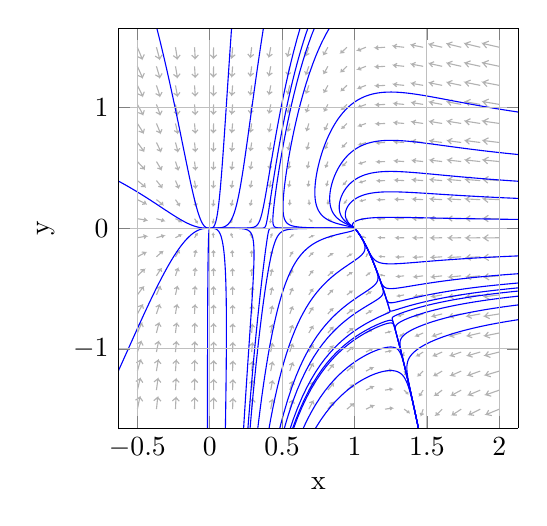
\begin{tikzpicture}
\begin{axis}[%
width=2in,
height=2in,
unbounded coords=jump,
view={0}{90},
scale only axis,
xmin=-0.631578947368421,
xmax=2.13157894736842,
xlabel={x},
xmajorgrids,
ymin=-1.65789473684211,
ymax=1.65789473684211,
ylabel={y},
ymajorgrids,
zmin=-1,
zmax=1
]
\addplot [color=white!70!black,solid,forget plot]
  table[row sep=crcr]{-0.5	-1.5\\
-0.482879622388944	-1.40013113060218\\
-0.512982953021717	-1.42581169701876\\
-0.482879622388944	-1.40013113060218\\
-0.463048518322805	-1.43437188582429\\
nan	0\\
-0.5	-1.34210526315789\\
-0.480661885255912	-1.24622044421846\\
-0.510434524413998	-1.27015136121427\\
-0.480661885255912	-1.24622044421846\\
-0.462492114944279	-1.27982041858631\\
nan	0\\
-0.5	-1.18421052631579\\
-0.478046364649637	-1.09273704568928\\
-0.507500825411374	-1.11469068103964\\
-0.478046364649637	-1.09273704568928\\
-0.461764085098117	-1.12566749871482\\
nan	0\\
-0.5	-1.02631578947368\\
-0.474907113409724	-0.939821369787505\\
-0.504058584308351	-0.95949647404579\\
-0.474907113409724	-0.939821369787505\\
-0.460811374465262	-0.972042917340928\\
nan	0\\
-0.5	-0.868421052631579\\
-0.471065020185518	-0.78769665242451\\
-0.49992661418163	-0.80468022753301\\
-0.471065020185518	-0.78769665242451\\
-0.459564414078095	-0.819147717440251\\
nan	0\\
-0.5	-0.710526315789474\\
-0.46626880578784	-0.636739328450373\\
-0.494834910886263	-0.650442626099063\\
-0.46626880578784	-0.636739328450373\\
-0.457941417216713	-0.667308223205143\\
nan	0\\
-0.5	-0.552631578947368\\
-0.460197348974563	-0.487620582272488\\
-0.488390893450914	-0.497173218518593\\
-0.460197348974563	-0.487620582272488\\
-0.455885395113474	-0.517074544031311\\
nan	0\\
-0.5	-0.394736842105263\\
-0.452598839561892	-0.341562463408667\\
-0.480112782367473	-0.345664486908119\\
-0.452598839561892	-0.341562463408667\\
-0.453525593019175	-0.369365067127173\\
nan	0\\
-0.5	-0.236842105263158\\
-0.443970722954707	-0.200526833104172\\
-0.469858324108041	-0.197414095490544\\
-0.443970722954707	-0.200526833104172\\
-0.451700688028548	-0.225428734013191\\
nan	0\\
-0.5	-0.0789473684210527\\
-0.437150521000412	-0.0658537269628052\\
-0.45927877506485	-0.0540694496503825\\
-0.437150521000412	-0.0658537269628052\\
-0.452731954335727	-0.0854941891501764\\
nan	0\\
-0.5	0.0789473684210527\\
-0.436351175753608	0.0661444440036749\\
-0.452245091923181	0.0858975273904863\\
-0.436351175753608	0.0661444440036749\\
-0.45864655413187	0.0540731152672902\\
nan	0\\
-0.5	0.236842105263158\\
-0.440838140794418	0.202331020726568\\
-0.449958927421945	0.227474810888941\\
-0.440838140794418	0.202331020726568\\
-0.46721446969024	0.197893881286149\\
nan	0\\
-0.5	0.394736842105263\\
-0.446617401434799	0.344511278939079\\
-0.450075790212813	0.372924597530235\\
-0.446617401434799	0.344511278939079\\
-0.475188571795905	0.346233298247634\\
nan	0\\
-0.5	0.552631578947368\\
-0.451706095196908	0.491006544172589\\
-0.450788007944141	0.521567530805796\\
-0.451706095196908	0.491006544172589\\
-0.48160052533153	0.49742057840425\\
nan	0\\
-0.5	0.710526315789473\\
-0.455781356668029	0.640178474124974\\
-0.451459989251495	0.672337487457317\\
-0.455781356668029	0.640178474124974\\
-0.486633910083745	0.650228165791331\\
nan	0\\
-0.5	0.868421052631579\\
-0.458993810536157	0.791031920555208\\
-0.451948384356217	0.82450020754408\\
-0.458993810536157	0.791031920555208\\
-0.490642950394402	0.803997112812159\\
nan	0\\
-0.5	1.02631578947368\\
-0.46154626205707	0.942999357264003\\
-0.452253275387529	0.97760772141264\\
-0.46154626205707	0.942999357264003\\
-0.493911491492369	0.958380852441175\\
nan	0\\
-0.5	1.18421052631579\\
-0.463603627503499	1.09574712094235\\
-0.45240668790909	1.13138523567851\\
-0.463603627503499	1.09574712094235\\
-0.496638390595809	1.11318704943026\\
nan	0\\
-0.5	1.34210526315789\\
-0.465287204689107	1.24906871716699\\
-0.452441906784648	1.28565787979198\\
-0.465287204689107	1.24906871716699\\
-0.498960179780102	1.26830148213654\\
nan	0\\
-0.5	1.5\\
-0.46668443257536	1.40282959501147\\
-0.452386501555618	1.44030960836419\\
-0.46668443257536	1.40282959501147\\
-0.500971704049885	1.42365182465187\\
nan	0\\
-0.368421052631579	-1.5\\
-0.359477284870317	-1.40202704189748\\
-0.386653654724327	-1.42918298738792\\
-0.359477284870317	-1.40202704189748\\
-0.337667175673065	-1.43365487126855\\
nan	0\\
-0.368421052631579	-1.34210526315789\\
-0.358043338646227	-1.24781584428519\\
-0.384729007560009	-1.27350824145066\\
-0.358043338646227	-1.24781584428519\\
-0.337584298123656	-1.27869709844334\\
nan	0\\
-0.368421052631579	-1.18421052631579\\
-0.356339794129617	-1.09394612903547\\
-0.382530271000285	-1.11800513359408\\
-0.356339794129617	-1.09394612903547\\
-0.337398072360126	-1.12404576284506\\
nan	0\\
-0.368421052631579	-1.02631578947368\\
-0.354269202698541	-0.940516221953337\\
-0.379964649558539	-0.962718129726181\\
-0.354269202698541	-0.940516221953337\\
-0.337064865798365	-0.9697940546927\\
nan	0\\
-0.368421052631579	-0.868421052631579\\
-0.351679678748453	-0.787680158164724\\
-0.376887314530104	-0.807717083033999\\
-0.351679678748453	-0.787680158164724\\
-0.336516867296677	-0.816087769975562\\
nan	0\\
-0.368421052631579	-0.710526315789474\\
-0.348322775056283	-0.635700301727757\\
-0.373058761844301	-0.653123536552448\\
-0.348322775056283	-0.635700301727757\\
-0.335645754813442	-0.663172675340096\\
nan	0\\
-0.368421052631579	-0.552631578947368\\
-0.343772895241816	-0.485075585413504\\
-0.368056340842211	-0.499180344126222\\
-0.343772895241816	-0.485075585413504\\
-0.334278344075279	-0.511504422821104\\
nan	0\\
-0.368421052631579	-0.394736842105263\\
-0.337296265988612	-0.336896377094914\\
-0.361093818234089	-0.346467319937277\\
-0.337296265988612	-0.336896377094914\\
-0.332173585728915	-0.362029713258761\\
nan	0\\
-0.368421052631579	-0.236842105263158\\
-0.327933835593052	-0.193879639016344\\
-0.350820617266313	-0.196646574630757\\
-0.327933835593052	-0.193879639016344\\
-0.329339384142907	-0.21689018315002\\
nan	0\\
-0.368421052631579	-0.0789473684210527\\
-0.317402496617092	-0.061733135827372\\
-0.337011621569858	-0.0541427666018543\\
-0.317402496617092	-0.061733135827372\\
-0.328404505273018	-0.0796520446090981\\
nan	0\\
-0.368421052631579	0.0789473684210527\\
-0.316477554416106	0.0621931742587866\\
-0.327872055340181	0.0802053070613346\\
-0.316477554416106	0.0621931742587866\\
-0.336249152421315	0.0542335579535982\\
nan	0\\
-0.368421052631579	0.236842105263158\\
-0.324127318440136	0.195790280496761\\
-0.32715248250597	0.21917926147454\\
-0.324127318440136	0.195790280496761\\
-0.347678394889168	0.197032394378819\\
nan	0\\
-0.368421052631579	0.394736842105263\\
-0.330936921376949	0.339180083952281\\
-0.328292971215092	0.365218144211834\\
-0.330936921376949	0.339180083952281\\
-0.356071350291583	0.346476078584518\\
nan	0\\
-0.368421052631579	0.552631578947368\\
-0.33564890230332	0.487275581122979\\
-0.3291415479457	0.51507541805236\\
-0.33564890230332	0.487275581122979\\
-0.361819546857895	0.498689342888231\\
nan	0\\
-0.368421052631579	0.710526315789473\\
-0.338923564797256	0.637726357059482\\
-0.329572821465055	0.66694071663706\\
-0.338923564797256	0.637726357059482\\
-0.365972800830051	0.652191972719899\\
nan	0\\
-0.368421052631579	0.868421052631579\\
-0.341289446885968	0.78953457200592\\
-0.329707308453237	0.81998341763002\\
-0.341289446885968	0.78953457200592\\
-0.369150548766066	0.806417614757215\\
nan	0\\
-0.368421052631579	1.02631578947368\\
-0.343064014981723	0.942220145687903\\
-0.329647215330234	0.973788098236101\\
-0.343064014981723	0.942220145687903\\
-0.371695037223125	0.961109579411173\\
nan	0\\
-0.368421052631579	1.18421052631579\\
-0.344437061699671	1.09552164157922\\
-0.329460037795101	1.12812430473317\\
-0.344437061699671	1.09552164157922\\
-0.373804480163385	1.11613230926721\\
nan	0\\
-0.368421052631579	1.34210526315789\\
-0.345526411039727	1.24928201307258\\
-0.329188990995953	1.28285264849614\\
-0.345526411039727	1.24928201307258\\
-0.375600616038612	1.27140532770021\\
nan	0\\
-0.368421052631579	1.5\\
-0.346408369159295	1.403399542983\\
-0.328862059946731	1.43788285095617\\
-0.346408369159295	1.403399542983\\
-0.377162288455229	1.42687650922003\\
nan	0\\
-0.236842105263158	-1.5\\
-0.233418802243135	-1.40453459112949\\
-0.258312145366769	-1.43231838803564\\
-0.233418802243135	-1.40453459112949\\
-0.210579440931515	-1.43403003954565\\
nan	0\\
-0.236842105263158	-1.34210526315789\\
-0.232639258417387	-1.25013901194459\\
-0.256891675274444	-1.27667817559714\\
-0.232639258417387	-1.25013901194459\\
-0.210908549667793	-1.27877959902003\\
nan	0\\
-0.236842105263158	-1.18421052631579\\
-0.231713689850164	-1.09604021968784\\
-0.255294791131049	-1.12120920782298\\
-0.231713689850164	-1.09604021968784\\
-0.211209637817075	-1.12377341552947\\
nan	0\\
-0.236842105263158	-1.02631578947368\\
-0.230586799549227	-0.942312788231611\\
-0.253464141573925	-0.96594986217575\\
-0.230586799549227	-0.942312788231611\\
-0.211462640952888	-0.969077515032716\\
nan	0\\
-0.236842105263158	-0.868421052631579\\
-0.229169199423741	-0.789067830872296\\
-0.251309376615387	-0.810955570940227\\
-0.229169199423741	-0.789067830872296\\
-0.211632765735746	-0.814792023859935\\
nan	0\\
-0.236842105263158	-0.710526315789474\\
-0.22730546749576	-0.636484025698094\\
-0.248677031348824	-0.656312553283658\\
-0.22730546749576	-0.636484025698094\\
-0.211655886303135	-0.661080872167357\\
nan	0\\
-0.236842105263158	-0.552631578947368\\
-0.224697893426463	-0.484882744614152\\
-0.245278365560776	-0.502171341954943\\
-0.224697893426463	-0.484882744614152\\
-0.211403948394167	-0.50824344787329\\
nan	0\\
-0.236842105263158	-0.394736842105263\\
-0.220696456926925	-0.334953614011494\\
-0.240485958451237	-0.348852170355567\\
-0.220696456926925	-0.334953614011494\\
-0.210594344404353	-0.356924994523683\\
nan	0\\
-0.236842105263158	-0.236842105263158\\
-0.213635753396046	-0.188693634584099\\
-0.232634776625944	-0.197336587821039\\
-0.213635753396046	-0.188693634584099\\
-0.208560541286415	-0.208939763754595\\
nan	0\\
-0.236842105263158	-0.0789473684210527\\
-0.20006473392546	-0.0550891933358346\\
-0.217062489098074	-0.0530523030269755\\
-0.20006473392546	-0.0550891933358346\\
-0.205133401555465	-0.0714409886958245\\
nan	0\\
-0.236842105263158	0.0789473684210527\\
-0.198890257164166	0.0557646502383576\\
-0.20448013204819	0.0722074277179142\\
-0.198890257164166	0.0557646502383576\\
-0.216071491139537	0.0532315036684181\\
nan	0\\
-0.236842105263158	0.236842105263158\\
-0.209756432406635	0.189944573309162\\
-0.206157751275093	0.210785251109491\\
-0.209756432406635	0.189944573309162\\
-0.229606517252091	0.19724241468123\\
nan	0\\
-0.236842105263158	0.394736842105263\\
-0.215380360325743	0.33604127706319\\
-0.207144992546449	0.359015382810165\\
-0.215380360325743	0.33604127706319\\
-0.236492775067486	0.348284510341458\\
nan	0\\
-0.236842105263158	0.552631578947368\\
-0.218476667244069	0.485806533433887\\
-0.207280037271426	0.510445406592703\\
-0.218476667244069	0.485806533433887\\
-0.240692560028166	0.501262687583159\\
nan	0\\
-0.236842105263158	0.710526315789473\\
-0.220408766363646	0.637285839833374\\
-0.207028649044475	0.663366317345082\\
-0.220408766363646	0.637285839833374\\
-0.243648887022525	0.655149647895326\\
nan	0\\
-0.236842105263158	0.868421052631579\\
-0.221721665782994	0.789778650587219\\
-0.206597197115953	0.817151481070568\\
-0.221721665782994	0.789778650587219\\
-0.245918398138133	0.809591261330486\\
nan	0\\
-0.236842105263158	1.02631578947368\\
-0.222667162030103	0.942953623317382\\
-0.206079103460944	0.971506008972537\\
-0.222667162030103	0.942953623317382\\
-0.247760186539095	0.964418537356009\\
nan	0\\
-0.236842105263158	1.18421052631579\\
-0.22337678772791	1.09662558706416\\
-0.205520148175578	1.12626739822346\\
-0.22337678772791	1.09662558706416\\
-0.249312617801391	1.11953473945584\\
nan	0\\
-0.236842105263158	1.34210526315789\\
-0.223925889685033	1.25067927751171\\
-0.204944257946924	1.2813361271001\\
-0.223925889685033	1.25067927751171\\
-0.250657250770017	1.27487801931103\\
nan	0\\
-0.236842105263158	1.5\\
-0.224360760555067	1.40503739654634\\
-0.204364513104078	1.43664651375946\\
-0.224360760555067	1.40503739654634\\
-0.25184581483091	1.43040584140541\\
nan	0\\
-0.105263157894737	-1.5\\
-0.104743162101709	-1.40739940817933\\
-0.128049308794785	-1.43504958677727\\
-0.104743162101709	-1.40739940817933\\
-0.0817490128844501	-1.43530958467379\\
nan	0\\
-0.105263157894737	-1.34210526315789\\
-0.104458545896991	-1.25287647464791\\
-0.127007126623812	-1.27944395820147\\
-0.104458545896991	-1.25287647464791\\
-0.0823927323688182	-1.27984626420034\\
nan	0\\
-0.105263157894737	-1.18421052631579\\
-0.104122675460706	-1.09863061360881\\
-0.12585979836766	-1.1240194668124\\
-0.104122675460706	-1.09863061360881\\
-0.0830698420141708	-1.12458970802941\\
nan	0\\
-0.105263157894737	-1.02631578947368\\
-0.103716113917047	-0.94472717870167\\
-0.124577379803357	-0.968817000938852\\
-0.103716113917047	-0.94472717870167\\
-0.0837830744173501	-0.969590522927697\\
nan	0\\
-0.105263157894737	-0.868421052631579\\
-0.103207168316587	-0.791260509310731\\
-0.123114101020244	-0.813894674912448\\
-0.103207168316587	-0.791260509310731\\
-0.0845338293598198	-0.814922669701523\\
nan	0\\
-0.105263157894737	-0.710526315789474\\
-0.102539832453881	-0.638375396731429\\
-0.121394559850649	-0.659339841088629\\
-0.102539832453881	-0.638375396731429\\
-0.0853191003216268	-0.660701503809056\\
nan	0\\
-0.105263157894737	-0.552631578947368\\
-0.101603342457054	-0.486314367729361\\
-0.119280589892861	-0.505294577235343\\
-0.101603342457054	-0.486314367729361\\
-0.0861219842838573	-0.507124484954184\\
nan	0\\
-0.105263157894737	-0.394736842105263\\
-0.100138072760227	-0.335543076711997\\
-0.116474039648897	-0.352019935046349\\
-0.100138072760227	-0.335543076711997\\
-0.0868771569522635	-0.354582477613604\\
nan	0\\
-0.105263157894737	-0.236842105263158\\
-0.0973302665002875	-0.187210812235865\\
-0.112117957175446	-0.20011697729544\\
-0.0973302665002875	-0.187210812235865\\
-0.087302310661799	-0.204083422992665\\
nan	0\\
-0.105263157894737	-0.0789473684210527\\
-0.0884336539662878	-0.0469588882462519\\
-0.101479625188523	-0.0523480563165799\\
-0.0884336539662878	-0.0469588882462519\\
-0.0854853851011223	-0.0607628082808044\\
nan	0\\
-0.105263157894737	0.0789473684210527\\
-0.0871814963094607	0.0473754450427645\\
-0.0847130139404715	0.06136743745257\\
-0.0871814963094607	0.0473754450427645\\
-0.100498975629616	0.0523266066599319\\
nan	0\\
-0.105263157894737	0.236842105263158\\
-0.0950735726151002	0.1874831488467\\
-0.0857907090948768	0.204838232091547\\
-0.0950735726151002	0.1874831488467\\
-0.110470187303106	0.199743439451728\\
nan	0\\
-0.105263157894737	0.394736842105263\\
-0.0974060618186001	0.335742301662509\\
-0.0850145555307525	0.355404937814369\\
-0.0974060618186001	0.335742301662509\\
-0.11451182575213	0.351476389776301\\
nan	0\\
-0.105263157894737	0.552631578947368\\
-0.0985291626320802	0.486474808219361\\
-0.0840101685288754	0.508005338253427\\
-0.0985291626320802	0.486474808219361\\
-0.117088553892879	0.504638340622099\\
nan	0\\
-0.105263157894737	0.710526315789473\\
-0.0991889415906495	0.63851152596456\\
-0.0830075090256474	0.661634516988056\\
-0.0991889415906495	0.63851152596456\\
-0.119014903938104	0.658597408836012\\
nan	0\\
-0.105263157894737	0.868421052631579\\
-0.0996200740149365	0.791379787613528\\
-0.0820526829243639	0.815902938088893\\
-0.0996200740149365	0.791379787613528\\
-0.120573315433389	0.813081396148993\\
nan	0\\
-0.105263157894737	1.02631578947368\\
-0.0999209289230636	0.944833986555016\\
-0.0811531468848986	0.970614084673535\\
-0.0999209289230636	0.944833986555016\\
-0.121894048344233	0.967942970187698\\
nan	0\\
-0.105263157894737	1.18421052631579\\
-0.10014030720437	1.09872776027685\\
-0.0803064709017448	1.12565330276112\\
-0.10014030720437	1.09872776027685\\
-0.123047853921216	1.12309187741594\\
nan	0\\
-0.105263157894737	1.34210526315789\\
-0.100305283731671	1.25296587949435\\
-0.0795078000647043	1.28094716313418\\
-0.100305283731671	1.25296587949435\\
-0.124077491896478	1.27846822605265\\
nan	0\\
-0.105263157894737	1.5\\
-0.10043213075935	1.40748244644876\\
-0.0787520505121556	1.43644546929798\\
-0.10043213075935	1.40748244644876\\
-0.125010827287776	1.43402995573028\\
nan	0\\
0.0263157894736842	-1.5\\
0.0264263352929923	-1.41049787479987\\
0.00401764024716646	-1.43732087590508\\
0.0264263352929923	-1.41049787479987\\
0.0487687028472333	-1.43737614881473\\
nan	0\\
0.0263157894736842	-1.34210526315789\\
0.0263693831136139	-1.25586065513022\\
0.00479215301471637	-1.28172063912854\\
0.0263693831136139	-1.25586065513022\\
0.0479144570285537	-1.28174743594851\\
nan	0\\
0.0263157894736842	-1.18421052631579\\
0.0263028896015299	-1.10149009612626\\
0.0056266520157928	-1.12630945015115\\
0.0263028896015299	-1.10149009612626\\
0.0469868671105595	-1.12630300021508\\
nan	0\\
0.0263157894736842	-1.02631578947368\\
0.0262233182032843	-0.94744855361891\\
0.00653425062071078	-0.971131842192942\\
0.0262233182032843	-0.94744855361891\\
0.0459678685480978	-0.971085606557743\\
nan	0\\
0.0263157894736842	-0.868421052631579\\
0.0261249225608043	-0.793825606539494\\
0.00753332111164695	-0.816251957095339\\
0.0261249225608043	-0.793825606539494\\
0.0448310441576896	-0.816156523638899\\
nan	0\\
0.0263157894736842	-0.710526315789474\\
0.0259975758489922	-0.640757686099998\\
0.00865088251403087	-0.661767828413014\\
0.0259975758489922	-0.640757686099998\\
0.0435351973587687	-0.661608721600668\\
nan	0\\
0.0263157894736842	-0.552631578947368\\
0.0258212701071397	-0.488470284771264\\
0.00992930237307693	-0.507842302865732\\
0.0258212701071397	-0.488470284771264\\
0.0420099494611292	-0.507595043182459\\
nan	0\\
0.0263157894736842	-0.394736842105263\\
0.0255489359901823	-0.337385116427448\\
0.011441060615779	-0.354782347501668\\
0.0255489359901823	-0.337385116427448\\
0.0401169234546867	-0.354398920759917\\
nan	0\\
0.0263157894736842	-0.236842105263158\\
0.025029980599317	-0.188478296064811\\
0.0133247709620404	-0.203308891042907\\
0.025029980599317	-0.188478296064811\\
0.037506675561214	-0.202665986605723\\
nan	0\\
0.0263157894736842	-0.0789473684210527\\
0.0232166205551052	-0.0455013292569904\\
0.0157848614396633	-0.0563099332358538\\
0.0232166205551052	-0.0455013292569904\\
0.0325078810216944	-0.0547603487765643\\
nan	0\\
0.0263157894736842	0.0789473684210527\\
0.0227880383559549	0.0455295544913116\\
0.0322008171737089	0.0546729608908016\\
0.0227880383559549	0.0455295544913116\\
0.0154919102088384	0.0564368364496663\\
nan	0\\
0.0263157894736842	0.236842105263158\\
0.0244064735312464	0.188492023364133\\
0.037066788788734	0.202519718948231\\
0.0244064735312464	0.188492023364133\\
0.0128917478392215	0.20347437691945\\
nan	0\\
0.0263157894736842	0.394736842105263\\
0.0248091705387667	0.337394890827279\\
0.039596644038738	0.354220821476945\\
0.0248091705387667	0.337394890827279\\
0.0109256683997458	0.354974130944403\\
nan	0\\
0.0263157894736842	0.552631578947368\\
0.0249935434585061	0.488478097141387\\
0.0414285877145549	0.507393580179387\\
0.0249935434585061	0.488478097141387\\
0.00935184681156414	0.508054703186976\\
nan	0\\
0.0263157894736842	0.710526315789473\\
0.0250974508682458	0.64076429403376\\
0.0429034578888057	0.661388315909114\\
0.0250974508682458	0.64076429403376\\
0.0080224470109489	0.661997485211834\\
nan	0\\
0.0263157894736842	0.868421052631579\\
0.0251624900581814	0.793831387350545\\
0.0441558962030908	0.815919962080979\\
0.0251624900581814	0.793831387350545\\
0.00686106356257372	0.816496611788731\\
nan	0\\
0.0263157894736842	1.02631578947368\\
0.0252057492459967	0.947453725339019\\
0.0452542773479693	0.970834834522496\\
0.0252057492459967	0.947453725339019\\
0.00582324528063659	0.97138985463634\\
nan	0\\
0.0263157894736842	1.18421052631579\\
0.0252355906061483	1.10149479735574\\
0.0462385825064214	1.12603946632687\\
0.0252355906061483	1.10149479735574\\
0.00488071802639671	1.12657956576064\\
nan	0\\
0.0263157894736842	1.34210526315789\\
0.0252566025795605	1.25586498005549\\
0.0471344294233992	1.28147226826268\\
0.0252566025795605	1.25586498005549\\
0.00401428787219597	1.28200186170974\\
nan	0\\
0.0263157894736842	1.5\\
0.0252715160189507	1.41050189066772\\
0.0479593253884419	1.43709025510372\\
0.0252715160189507	1.41050189066772\\
0.00321027072229958	1.43761239183108\\
nan	0\\
0.157894736842105	-1.5\\
0.159938572457498	-1.41384433519415\\
0.137786505571416	-1.43918007573205\\
0.159938572457498	-1.41384433519415\\
0.180864337974344	-1.44020199353975\\
nan	0\\
0.157894736842105	-1.34210526315789\\
0.159672314787024	-1.25908246328798\\
0.138383341436069	-1.28354490876272\\
0.159672314787024	-1.25908246328798\\
0.179894741371028	-1.28443369773518\\
nan	0\\
0.157894736842105	-1.18421052631579\\
0.159366548574403	-1.10457716280367\\
0.139016664176683	-1.12809921892423\\
0.159366548574403	-1.10457716280367\\
0.178833345932744	-1.12883512479038\\
nan	0\\
0.157894736842105	-1.02631578947368\\
0.159007294012991	-0.950388577222242\\
0.139691723798865	-0.972888601604953\\
0.159007294012991	-0.950388577222242\\
0.177655329924586	-0.973444880190396\\
nan	0\\
0.157894736842105	-0.868421052631579\\
0.158572052356013	-0.796603251777339\\
0.14041440748828	-0.817979263155134\\
0.158572052356013	-0.796603251777339\\
0.1763233079154	-0.818317920912088\\
nan	0\\
0.157894736842105	-0.710526315789474\\
0.158021576480239	-0.643353368624246\\
0.141190287797492	-0.663473542864281\\
0.158021576480239	-0.643353368624246\\
0.174776761380106	-0.663536962683348\\
nan	0\\
0.157894736842105	-0.552631578947368\\
0.157279188724442	-0.490858527393842\\
0.142020590271359	-0.509544329889316\\
0.157279188724442	-0.490858527393842\\
0.172907116048122	-0.509236555830484\\
nan	0\\
0.157894736842105	-0.394736842105263\\
0.156166887837081	-0.339533886657065\\
0.142884503676539	-0.356526735542781\\
0.156166887837081	-0.339533886657065\\
0.170485981400638	-0.355662811040269\\
nan	0\\
0.157894736842105	-0.236842105263158\\
0.154126557754786	-0.190368551399483\\
0.143638623015063	-0.205252662330415\\
0.154126557754786	-0.190368551399483\\
0.166875399946901	-0.203368572786756\\
nan	0\\
0.157894736842105	-0.0789473684210527\\
0.147599031711734	-0.0477476624437366\\
0.142887816756516	-0.0596815005195242\\
0.147599031711734	-0.0477476624437366\\
0.158487669745174	-0.0545336479543386\\
nan	0\\
0.157894736842105	0.0789473684210527\\
0.145136296075398	0.0483325463134801\\
0.156617533832304	0.0543273827540752\\
0.145136296075398	0.0483325463134801\\
0.141310122778517	0.0607066031374286\\
nan	0\\
0.157894736842105	0.236842105263158\\
0.150150103077835	0.190696182922146\\
0.164009973792369	0.202603801183382\\
0.150150103077835	0.190696182922146\\
0.140937012621863	0.206476118065517\\
nan	0\\
0.157894736842105	0.394736842105263\\
0.151406071455055	0.339770010802203\\
0.167094378896935	0.354637893846358\\
0.151406071455055	0.339770010802203\\
0.139610963245405	0.357882226539883\\
nan	0\\
0.157894736842105	0.552631578947368\\
0.151938875921474	0.491047887768227\\
0.169121556992448	0.508034029891811\\
0.151938875921474	0.491047887768227\\
0.138329711402878	0.511011960352127\\
nan	0\\
0.157894736842105	0.710526315789473\\
0.152208135979907	0.643513756808088\\
0.170667255983913	0.662195874286954\\
0.152208135979907	0.643513756808088\\
0.13716097649322	0.665039174718053\\
nan	0\\
0.157894736842105	0.868421052631579\\
0.152352930425243	0.796743662299558\\
0.171934819933307	0.816861427794949\\
0.152352930425243	0.796743662299558\\
0.136096124767296	0.81963233100338\\
nan	0\\
0.157894736842105	1.02631578947368\\
0.152429896882255	0.950514244130721\\
0.17301973520595	0.971888497743647\\
0.152429896882255	0.950514244130721\\
0.135118962534469	0.974620917723573\\
nan	0\\
0.157894736842105	1.18421052631579\\
0.152466394300232	1.10469142622413\\
0.173974672085708	1.12719007061616\\
0.152466394300232	1.10469142622413\\
0.13421512203988	1.1299042418871\\
nan	0\\
0.157894736842105	1.34210526315789\\
0.152477206103175	1.25918759840567\\
0.174831881512909	1.28270851514661\\
0.152477206103175	1.25918759840567\\
0.133373049136799	1.28541728051607\\
nan	0\\
0.157894736842105	1.5\\
0.152470981350685	1.41394196897403\\
0.175612615754602	1.43840343940897\\
0.152470981350685	1.41394196897403\\
0.132583600241619	1.44111531715468\\
nan	0\\
0.289473684210526	-1.5\\
0.29562412484773	-1.41759072497852\\
0.2731766739012	-1.44077589732567\\
0.29562412484773	-1.41759072497852\\
0.314381311411938	-1.44385111764427\\
nan	0\\
0.289473684210526	-1.34210526315789\\
0.295253391341561	-1.26268818014935\\
0.273665208450115	-1.28506837826916\\
0.295253391341561	-1.26268818014935\\
0.313373749954385	-1.28795823183467\\
nan	0\\
0.289473684210526	-1.18421052631579\\
0.294838717172194	-1.10803013403659\\
0.274184109213893	-1.12954299347993\\
0.294838717172194	-1.10803013403659\\
0.312274305353494	-1.13222550996077\\
nan	0\\
0.289473684210526	-1.02631578947368\\
0.294366177250434	-0.953673709432034\\
0.274737909328049	-0.974243210184552\\
0.294366177250434	-0.953673709432034\\
0.311058949348874	-0.976689456704506\\
nan	0\\
0.289473684210526	-0.868421052631579\\
0.293813899163646	-0.799700982540523\\
0.275331817154946	-0.81923194982956\\
0.293813899163646	-0.799700982540523\\
0.309691852200474	-0.82140205730612\\
nan	0\\
0.289473684210526	-0.710526315789474\\
0.293144708940012	-0.646237031701135\\
0.275971080499081	-0.664606060745265\\
0.293144708940012	-0.646237031701135\\
0.308115722543251	-0.666441573110008\\
nan	0\\
0.289473684210526	-0.552631578947368\\
0.292287971344883	-0.493488908411718\\
0.276658017570663	-0.510528137788824\\
0.292287971344883	-0.493488908411718\\
0.306229352838489	-0.511935281356002\\
nan	0\\
0.289473684210526	-0.394736842105263\\
0.291084449468763	-0.341845473422167\\
0.277378377720518	-0.357310192712537\\
0.291084449468763	-0.341845473422167\\
0.303824062062066	-0.358115575341655\\
nan	0\\
0.289473684210526	-0.236842105263158\\
0.289049012058822	-0.192219357201482\\
0.278020726688914	-0.205712349657911\\
0.289049012058822	-0.192219357201482\\
0.300332100719752	-0.205500013582059\\
nan	0\\
0.289473684210526	-0.0789473684210527\\
0.283087546667906	-0.0484460847722432\\
0.27737806701849	-0.0591930042525411\\
0.283087546667906	-0.0484460847722432\\
0.292628708842895	-0.055999935481231\\
nan	0\\
0.289473684210526	0.0789473684210527\\
0.2779578733258	0.049434379328083\\
0.28879086386446	0.0554093233347923\\
0.2779578733258	0.049434379328083\\
0.274034369317976	0.0611672287771554\\
nan	0\\
0.289473684210526	0.236842105263158\\
0.281080147547735	0.192744244084025\\
0.294622673841356	0.203875218272067\\
0.281080147547735	0.192744244084025\\
0.272573743251789	0.208071986603462\\
nan	0\\
0.289473684210526	0.394736842105263\\
0.281577144523952	0.342221975662618\\
0.297074823040586	0.356002300673768\\
0.281577144523952	0.342221975662618\\
0.270817389819263	0.359950570517055\\
nan	0\\
0.289473684210526	0.552631578947368\\
0.281633856571737	0.493790448346716\\
0.298696087513537	0.509482830617215\\
0.281633856571737	0.493790448346716\\
0.269275522213211	0.513402744436609\\
nan	0\\
0.289473684210526	0.710526315789473\\
0.281551378816465	0.646492297248898\\
0.299936575069827	0.663721926462555\\
0.281551378816465	0.646492297248898\\
0.26791956579954	0.667683079159586\\
nan	0\\
0.289473684210526	0.868421052631579\\
0.281414091453995	0.799924391152973\\
0.300956134650606	0.818458491407422\\
0.281414091453995	0.799924391152973\\
0.266707803911303	0.822488287785687\\
nan	0\\
0.289473684210526	1.02631578947368\\
0.281253581992129	0.953873627645763\\
0.301830153114628	0.97355125063954\\
0.281253581992129	0.953873627645763\\
0.265609072200668	0.977661301748739\\
nan	0\\
0.289473684210526	1.18421052631579\\
0.281083698083625	1.1082118928387\\
0.302600352290968	1.1289139863501\\
0.281083698083625	1.1082118928387\\
0.264601035552423	1.13310897941355\\
nan	0\\
0.289473684210526	1.34210526315789\\
0.280911110207243	1.26285540744137\\
0.303292346337358	1.28448972065551\\
0.280911110207243	1.26285540744137\\
0.263667418479098	1.28877100765715\\
nan	0\\
0.289473684210526	1.5\\
0.280739211627711	1.41774601344521\\
0.303923050041254	1.44023859126594\\
0.280739211627711	1.41774601344521\\
0.262796056763857	1.44460582755735\\
nan	0\\
0.421052631578947	-1.5\\
0.433256195806627	-1.4220260541195\\
0.410101640068198	-1.44236734682673\\
0.433256195806627	-1.4220260541195\\
0.449088613008448	-1.44846912894057\\
nan	0\\
0.421052631578947	-1.34210526315789\\
0.432847929719453	-1.26697300464543\\
0.410526275649185	-1.28656385766404\\
0.432847929719453	-1.26697300464543\\
0.448092404905418	-1.2924615067343\\
nan	0\\
0.421052631578947	-1.18421052631579\\
0.432409548599218	-1.11215291049209\\
0.410988069537212	-1.13093096598413\\
0.432409548599218	-1.11215291049209\\
0.447016877449061	-1.13660942449427\\
nan	0\\
0.421052631578947	-1.02631578947368\\
0.431934893809045	-0.957620331921805\\
0.411496350752046	-0.975508403629844\\
0.431934893809045	-0.957620331921805\\
0.445844079527986	-0.980949534744893\\
nan	0\\
0.421052631578947	-0.868421052631579\\
0.431415568049794	-0.803453690783096\\
0.412064846646419	-0.820353165219929\\
0.431415568049794	-0.803453690783096\\
0.444548527570661	-0.825534633455353\\
nan	0\\
0.421052631578947	-0.710526315789474\\
0.430839710835357	-0.649772509995087\\
0.412715135609837	-0.6655518819193\\
0.430839710835357	-0.649772509995087\\
0.443092038507031	-0.670445421547505\\
nan	0\\
0.421052631578947	-0.552631578947368\\
0.430189926748269	-0.496774529173236\\
0.413484475753939	-0.511247320313145\\
0.430189926748269	-0.496774529173236\\
0.441413000641006	-0.515815967897806\\
nan	0\\
0.421052631578947	-0.394736842105263\\
0.429440189440354	-0.344830094557027\\
0.414447235194873	-0.357705229356147\\
0.429440189440354	-0.344830094557027\\
0.439400608968991	-0.36189900828685\\
nan	0\\
0.421052631578947	-0.236842105263158\\
0.428558279385917	-0.1947984572679\\
0.415795673045011	-0.205535139714735\\
0.428558279385917	-0.1947984572679\\
0.43681749704264	-0.20928796361822\\
nan	0\\
0.421052631578947	-0.0789473684210527\\
0.427734884414519	-0.0499947019966578\\
0.418492041957749	-0.0570099387150833\\
0.427734884414519	-0.0499947019966578\\
0.432968375169946	-0.0603510651328692\\
nan	0\\
0.421052631578947	0.0789473684210527\\
0.418877805864228	0.0495430041832621\\
0.426881344638091	0.0578206070259195\\
0.418877805864228	0.0495430041832621\\
0.412179162519196	0.0589080198832791\\
nan	0\\
0.421052631578947	0.236842105263158\\
0.415717374874138	0.1945798107919\\
0.427883525503395	0.205924684957075\\
0.415717374874138	0.1945798107919\\
0.406752378267767	0.20859231330948\\
nan	0\\
0.421052631578947	0.394736842105263\\
0.41420924035306	0.344674468628727\\
0.42877785108996	0.357982332865216\\
0.41420924035306	0.344674468628727\\
0.403746664351692	0.36140402847816\\
nan	0\\
0.421052631578947	0.552631578947368\\
0.41314926697273	0.496650155337563\\
0.429515632257047	0.511468741268951\\
0.41314926697273	0.496650155337563\\
0.401524920452144	0.515420423572059\\
nan	0\\
0.421052631578947	0.710526315789473\\
0.412309152193544	0.64966731547571\\
0.430146946087606	0.665739145723488\\
0.412309152193544	0.64966731547571\\
0.399717445930724	0.67011088541619\\
nan	0\\
0.421052631578947	0.868421052631579\\
0.411602624261636	0.803361665598481\\
0.430702473215104	0.820516979879082\\
0.411602624261636	0.803361665598481\\
0.398172779698555	0.825241983537738\\
nan	0\\
0.421052631578947	1.02631578947368\\
0.410987086717605	0.957538003940595\\
0.43120119655928	0.975654953385186\\
0.410987086717605	0.957538003940595\\
0.396812303792735	0.980687725815858\\
nan	0\\
0.421052631578947	1.18421052631579\\
0.410438119750011	1.1120780727851\\
0.431655586681364	1.13106418088707\\
0.410438119750011	1.1120780727851\\
0.39558935991602	1.13637143680154\\
nan	0\\
0.421052631578947	1.34210526315789\\
0.409940306107485	1.2669041575956\\
0.432074280139498	1.28668640789642\\
0.409940306107485	1.2669041575956\\
0.394473727358349	1.29224257063215\\
nan	0\\
0.421052631578947	1.5\\
0.409483230121053	1.42196212708887\\
0.432463518786204	1.44248113859774\\
0.409483230121053	1.42196212708887\\
0.393444582330639	1.44826583932668\\
nan	0\\
0.552631578947368	-1.5\\
0.572465760122543	-1.42756215384733\\
0.548406044231823	-1.44433496239934\\
0.572465760122543	-1.42756215384733\\
0.584624967308159	-1.45425205298692\\
nan	0\\
0.552631578947368	-1.34210526315789\\
0.57202602886601	-1.27235450934335\\
0.548770005436782	-1.28843112300805\\
0.57202602886601	-1.27235450934335\\
0.583645382344053	-1.29812834796738\\
nan	0\\
0.552631578947368	-1.18421052631579\\
0.571575481188743	-1.11737233997645\\
0.549182763931497	-1.13268782031791\\
0.571575481188743	-1.11737233997645\\
0.582601857101164	-1.1421597714386\\
nan	0\\
0.552631578947368	-1.02631578947368\\
0.571118052576117	-0.962670085109612\\
0.549660684396474	-0.977142178011647\\
0.571118052576117	-0.962670085109612\\
0.58148353657851	-0.986385414826021\\
nan	0\\
0.552631578947368	-0.868421052631579\\
0.570662520334815	-0.808326956546386\\
0.550229713897283	-0.821847450025083\\
0.570662520334815	-0.808326956546386\\
0.580276761939879	-0.830862920718806\\
nan	0\\
0.552631578947368	-0.710526315789474\\
0.570228508621698	-0.654465793559985\\
0.550934299162027	-0.666884717810249\\
0.570228508621698	-0.654465793559985\\
0.578964560276771	-0.675683182647414\\
nan	0\\
0.552631578947368	-0.552631578947368\\
0.569862649765351	-0.501295222989651\\
0.551859239530527	-0.512388362072471\\
0.569862649765351	-0.501295222989651\\
0.577527417509386	-0.521003897481462\\
nan	0\\
0.552631578947368	-0.394736842105263\\
0.569690765493277	-0.349223380755831\\
0.553194644192146	-0.358612622524184\\
0.569690765493277	-0.349223380755831\\
0.575951374866862	-0.367142215797138\\
nan	0\\
0.552631578947368	-0.236842105263158\\
0.570143122845524	-0.199280067407202\\
0.555499150212088	-0.20617079278945\\
0.570143122845524	-0.199280067407202\\
0.574280169140066	-0.214926564738528\\
nan	0\\
0.552631578947368	-0.0789473684210527\\
0.573535060407546	-0.0563034292747544\\
0.561603031182918	-0.0578707406535995\\
0.573535060407546	-0.0563034292747544\\
0.572925000756067	-0.0683224813836883\\
nan	0\\
0.552631578947368	0.0789473684210527\\
0.564345217769855	0.0527813651064034\\
0.567372626951771	0.0635595758064198\\
0.564345217769855	0.0527813651064034\\
0.554289625294447	0.0577027563951766\\
nan	0\\
0.552631578947368	0.236842105263158\\
0.552259859487494	0.196736230681676\\
0.562397843970826	0.208675063191152\\
0.552259859487494	0.196736230681676\\
0.542344906680086	0.208860922921089\\
nan	0\\
0.552631578947368	0.394736842105263\\
0.547861255414554	0.347344223739592\\
0.561140507065816	0.36036942836609\\
0.547861255414554	0.347344223739592\\
0.53744419788298	0.362754590132497\\
nan	0\\
0.552631578947368	0.552631578947368\\
0.545241489432788	0.499777742717379\\
0.560671975344659	0.513786371207731\\
0.545241489432788	0.499777742717379\\
0.534245057229665	0.517481415965021\\
nan	0\\
0.552631578947368	0.710526315789473\\
0.543365040227673	0.653176793516463\\
0.560482382411834	0.668065015518442\\
0.543365040227673	0.653176793516463\\
0.531807621275329	0.67269828487829\\
nan	0\\
0.552631578947368	0.868421052631579\\
0.541891230680399	0.807196866879611\\
0.560419381598481	0.822879035538459\\
0.541891230680399	0.807196866879611\\
0.529807288722498	0.828249209671944\\
nan	0\\
0.552631578947368	1.02631578947368\\
0.540669037783768	0.961657809963904\\
0.560422295010293	0.978064568525938\\
0.540669037783768	0.961657809963904\\
0.528093305255403	0.984045839107738\\
nan	0\\
0.552631578947368	1.18421052631579\\
0.539618962923242	1.11645143742844\\
0.560462519952318	1.13352601008861\\
0.539618962923242	1.11645143742844\\
0.526582975508642	1.14003231810067\\
nan	0\\
0.552631578947368	1.34210526315789\\
0.538694181661619	1.27150687751026\\
0.560524997259252	1.28920204388311\\
0.538694181661619	1.27150687751026\\
0.525225804435436	1.29617074252599\\
nan	0\\
0.552631578947368	1.5\\
0.537864836139615	1.42677480558243\\
0.560601157586333	1.44505067820576\\
0.537864836139615	1.42677480558243\\
0.523988560377549	1.45243404960964\\
nan	0\\
0.684210526315789	-1.5\\
0.712635183689677	-1.4346781612461\\
0.687777326789035	-1.4471685485288\\
0.712635183689677	-1.4346781612461\\
0.720438246165986	-1.46138087721574\\
nan	0\\
0.684210526315789	-1.34210526315789\\
0.712078144326241	-1.27929232149169\\
0.688014623506554	-1.29116929948894\\
0.712078144326241	-1.27929232149169\\
0.719421094339657	-1.30510310849416\\
nan	0\\
0.684210526315789	-1.18421052631579\\
0.711515564729255	-1.12412590989745\\
0.68830289910063	-1.13532503521958\\
0.711515564729255	-1.12412590989745\\
0.7183452073098	-1.14897755442632\\
nan	0\\
0.684210526315789	-1.02631578947368\\
0.710955613152906	-0.969234452101886\\
0.688661752758822	-0.979672581604146\\
0.710955613152906	-0.969234452101886\\
0.717202421444721	-0.993045125022705\\
nan	0\\
0.684210526315789	-0.868421052631579\\
0.710414087973571	-0.814700045099302\\
0.689122767593168	-0.82426545694454\\
0.710414087973571	-0.814700045099302\\
0.715983271359306	-0.837367237773431\\
nan	0\\
0.684210526315789	-0.710526315789474\\
0.709922646015298	-0.660652617322004\\
0.689740585488578	-0.669186696937368\\
0.709922646015298	-0.660652617322004\\
0.714677434722312	-0.682042756787122\\
nan	0\\
0.684210526315789	-0.552631578947368\\
0.709549030340358	-0.507318600674538\\
0.69061923456478	-0.514577868150245\\
0.709549030340358	-0.507318600674538\\
0.713275723701195	-0.52724712016253\\
nan	0\\
0.684210526315789	-0.394736842105263\\
0.709453882005207	-0.355154810786643\\
0.691985367468726	-0.360718581259874\\
0.709453882005207	-0.355154810786643\\
0.711776383128037	-0.373340259104583\\
nan	0\\
0.684210526315789	-0.236842105263158\\
0.710076338271218	-0.205338872753341\\
0.694440786557135	-0.208323389517429\\
0.710076338271218	-0.205338872753341\\
0.710192402812044	-0.221256295495143\\
nan	0\\
0.684210526315789	-0.0789473684210527\\
0.712555492113712	-0.0626344372736148\\
0.699973769587476	-0.0604420751683655\\
0.712555492113712	-0.0626344372736148\\
0.708130235161195	-0.0746145580673268\\
nan	0\\
0.684210526315789	0.0789473684210527\\
0.704960116430799	0.0584437216818624\\
0.703861151081093	0.0697822132323718\\
0.704960116430799	0.0584437216818624\\
0.693609327711498	0.0594074181748672\\
nan	0\\
0.684210526315789	0.236842105263158\\
0.687771020787801	0.199548208037086\\
0.696026346752715	0.211626500822911\\
0.687771020787801	0.199548208037086\\
0.67737939813968	0.209846253586905\\
nan	0\\
0.684210526315789	0.394736842105263\\
0.680325010242956	0.350499570205811\\
0.692549983039669	0.362799372757438\\
0.680325010242956	0.350499570205811\\
0.670431347089943	0.364742130793855\\
nan	0\\
0.684210526315789	0.552631578947368\\
0.67602981630799	0.503466509028697\\
0.690775296789997	0.516170852502349\\
0.67602981630799	0.503466509028697\\
0.666192761830662	0.520261207506248\\
nan	0\\
0.684210526315789	0.710526315789473\\
0.673040931213706	0.657347066381537\\
0.689686622096315	0.670508442428397\\
0.673040931213706	0.657347066381537\\
0.663096997392347	0.676093239979438\\
nan	0\\
0.684210526315789	0.868421052631579\\
0.670742364238489	0.811786964764883\\
0.688941334828353	0.825410150605567\\
0.670742364238489	0.811786964764883\\
0.660624290895005	0.832144231644217\\
nan	0\\
0.684210526315789	1.02631578947368\\
0.66886573964226	0.966617262272381\\
0.688393807444644	0.98069062376439\\
0.66886573964226	0.966617262272381\\
0.658544543843993	0.988363017101154\\
nan	0\\
0.684210526315789	1.18421052631579\\
0.667272505144621	1.12174048615307\\
0.68797142153665	1.1362469929091\\
0.667272505144621	1.12174048615307\\
0.656736401455293	1.14471600349468\\
nan	0\\
0.684210526315789	1.34210526315789\\
0.66588247056095	1.27709393248597\\
0.687633719955382	1.29201531774884\\
0.66588247056095	1.27709393248597\\
0.655128054619421	1.30117934562626\\
nan	0\\
0.684210526315789	1.5\\
0.664645273085956	1.4326343212921\\
0.687356268731881	1.44795271159701\\
0.664645273085956	1.4326343212921\\
0.65367342937793	1.45773533821193\\
nan	0\\
0.81578947368421	-1.5\\
0.852842010446051	-1.44382325892436\\
0.827682064148589	-1.45141314705659\\
0.852842010446051	-1.44382325892436\\
0.855770434686409	-1.46993941543751\\
nan	0\\
0.81578947368421	-1.34210526315789\\
0.851978604215919	-1.28816065067363\\
0.82763571193534	-1.29529675178598\\
0.851978604215919	-1.28816065067363\\
0.854608018177472	-1.31339131705184\\
nan	0\\
0.81578947368421	-1.18421052631579\\
0.851082919987906	-1.1326987741867\\
0.827616948064524	-1.1393289382495\\
0.851082919987906	-1.1326987741867\\
0.85337282412907	-1.15697566140135\\
nan	0\\
0.81578947368421	-1.02631578947368\\
0.850155828736637	-0.977489415943832\\
0.827639328838446	-0.983545739239681\\
0.850155828736637	-0.977489415943832\\
0.852052515603372	-1.00072891676589\\
nan	0\\
0.81578947368421	-0.868421052631579\\
0.849201841199707	-0.822609346409037\\
0.827725204389422	-0.827999766396925\\
0.849201841199707	-0.822609346409037\\
0.850631057500693	-0.844705950154674\\
nan	0\\
0.81578947368421	-0.710526315789474\\
0.848233584862354	-0.668180177032397\\
0.827913816819641	-0.672772990864984\\
0.848233584862354	-0.668180177032397\\
0.84908688619818	-0.688995046454056\\
nan	0\\
0.81578947368421	-0.552631578947368\\
0.847282608197013	-0.514413136354735\\
0.828280057195014	-0.518005385504324\\
0.847282608197013	-0.514413136354735\\
0.847389278491331	-0.533751952760726\\
nan	0\\
0.81578947368421	-0.394736842105263\\
0.846427547564401	-0.361728332569524\\
0.828983998016409	-0.363971366960198\\
0.846427547564401	-0.361728332569524\\
0.845488252784279	-0.379290403900293\\
nan	0\\
0.81578947368421	-0.236842105263158\\
0.845867439873639	-0.211161241738534\\
0.830423834135654	-0.211346009248564\\
0.845867439873639	-0.211161241738534\\
0.843264265897966	-0.226384992343278\\
nan	0\\
0.81578947368421	-0.0789473684210527\\
0.845856261278011	-0.0663480930102659\\
0.833686406147174	-0.0626111787350517\\
0.845856261278011	-0.0663480930102659\\
0.839986043852568	-0.0776445725319522\\
nan	0\\
0.81578947368421	0.0789473684210527\\
0.837574144573455	0.0616458290093535\\
0.835364128159606	0.0722824585551743\\
0.837574144573455	0.0616458290093535\\
0.826713358453757	0.0613901231105522\\
nan	0\\
0.81578947368421	0.236842105263158\\
0.817293638449352	0.202616291675682\\
0.825398842416678	0.21326007694321\\
0.817293638449352	0.202616291675682\\
0.808285935622941	0.212507994560639\\
nan	0\\
0.81578947368421	0.394736842105263\\
0.807809608422519	0.354654256767615\\
0.820224214335438	0.364684066053487\\
0.807809608422519	0.354654256767615\\
0.800182921666614	0.368673998684333\\
nan	0\\
0.81578947368421	0.552631578947368\\
0.802412813894357	0.508519557445413\\
0.817453817206801	0.518408998948536\\
0.802412813894357	0.508519557445413\\
0.795397806455824	0.525097328843463\\
nan	0\\
0.81578947368421	0.710526315789473\\
0.798666984522671	0.663109804139976\\
0.815657859183507	0.67305413534444\\
0.798666984522671	0.663109804139976\\
0.791949603358758	0.68161537992521\\
nan	0\\
0.81578947368421	0.868421052631579\\
0.795779246863988	0.818135442067886\\
0.814353717550978	0.828218568531938\\
0.795779246863988	0.818135442067886\\
0.789210912269131	0.838223681942049\\
nan	0\\
0.81578947368421	1.02631578947368\\
0.793412063208499	0.973467149492751\\
0.813337446346445	0.983727388868103\\
0.793412063208499	0.973467149492751\\
0.786913126355979	0.994916094105959\\
nan	0\\
0.81578947368421	1.18421052631579\\
0.791393590186558	1.12903113068263\\
0.812507204144143	1.13948597849817\\
0.791393590186558	1.12903113068263\\
0.784917506327565	1.15168392024699\\
nan	0\\
0.81578947368421	1.34210526315789\\
0.789625159060829	1.2847796205515\\
0.811805864099443	1.29543623467757\\
0.789625159060829	1.2847796205515\\
0.783143042796244	1.30851839198926\\
nan	0\\
0.81578947368421	1.5\\
0.788045066444392	1.44067929965876\\
0.811198563701647	1.45153940795118\\
0.788045066444392	1.44067929965876\\
0.781538213531028	1.46541161157109\\
nan	0\\
0.947368421052631	-1.5\\
0.991936325489427	-1.45539879103525\\
0.967415651917201	-1.45763717761548\\
0.991936325489427	-1.45539879103525\\
0.989716256399575	-1.47992112983388\\
nan	0\\
0.947368421052631	-1.34210526315789\\
0.990516359437796	-1.29922858655766\\
0.966852808772187	-1.30130460494144\\
0.990516359437796	-1.29922858655766\\
0.988291147072306	-1.32287857413402\\
nan	0\\
0.947368421052631	-1.18421052631579\\
0.988997171122948	-1.14320853438303\\
0.966258048118662	-1.14510194444528\\
0.988997171122948	-1.14320853438303\\
0.986759044085044	-1.16591631948043\\
nan	0\\
0.947368421052631	-1.02631578947368\\
0.987359643336567	-0.987376029807731\\
0.965627336734898	-0.989060152136533\\
0.987359643336567	-0.987376029807731\\
0.985097216567875	-1.0090557632785\\
nan	0\\
0.947368421052631	-0.868421052631579\\
0.985578135808209	-0.831785880533673\\
0.964956428357059	-0.83322400347415\\
0.985578135808209	-0.831785880533673\\
0.983274014406013	-0.852328860851939\\
nan	0\\
0.947368421052631	-0.710526315789474\\
0.983617112866111	-0.676523714925513\\
0.964241855106077	-0.677662322231331\\
0.983617112866111	-0.676523714925513\\
0.981243155538057	-0.695786668138071\\
nan	0\\
0.947368421052631	-0.552631578947368\\
0.98142540833111	-0.521735871923386\\
0.963484385391571	-0.522490337210961\\
0.98142540833111	-0.521735871923386\\
0.978932238903562	-0.539518830850201\\
nan	0\\
0.947368421052631	-0.394736842105263\\
0.978926347920869	-0.36770874936181\\
0.962701946674534	-0.367927695467787\\
0.978926347920869	-0.36770874936181\\
0.976215993046261	-0.383706658901905\\
nan	0\\
0.947368421052631	-0.236842105263158\\
0.976002555051866	-0.215148075170118\\
0.961988807328836	-0.214497750698221\\
0.976002555051866	-0.215148075170118\\
0.972835822375356	-0.228814817697838\\
nan	0\\
0.947368421052631	-0.0789473684210527\\
0.972452002039647	-0.0668964395607558\\
0.961914195528468	-0.0642408229720909\\
0.972452002039647	-0.0668964395607558\\
0.967939659958617	-0.0767826134655989\\
nan	0\\
0.947368421052631	0.0789473684210527\\
0.951589317717635	0.0581756134367447\\
0.955515987464211	0.065462364098288\\
0.951589317717635	0.0581756134367447\\
0.945130109972057	0.0633519157657862\\
nan	0\\
0.947368421052631	0.236842105263158\\
0.9318804344841	0.209103375220338\\
0.943461512965365	0.213552997591051\\
0.9318804344841	0.209103375220338\\
0.929592147943955	0.221296990875316\\
nan	0\\
0.947368421052631	0.394736842105263\\
0.925042889967114	0.363321794821739\\
0.93959431111365	0.367164926235417\\
0.925042889967114	0.363321794821739\\
0.923886787471888	0.378327691778176\\
nan	0\\
0.947368421052631	0.552631578947368\\
0.920661134803646	0.518212305002455\\
0.93727813916457	0.521861265623683\\
0.920661134803646	0.518212305002455\\
0.920068502192113	0.535214908748175\\
nan	0\\
0.947368421052631	0.710526315789473\\
0.91732594357269	0.673537502889208\\
0.935585890041739	0.677123527389302\\
0.91732594357269	0.673537502889208\\
0.917091483591606	0.692144766129273\\
nan	0\\
0.947368421052631	0.868421052631579\\
0.9145834609282	0.829170877467666\\
0.934231492756508	0.832749689985732\\
0.9145834609282	0.829170877467666\\
0.914606405174551	0.849142170047948\\
nan	0\\
0.947368421052631	1.02631578947368\\
0.912227994053189	0.985035234100683\\
0.933090260996272	0.988634293962722\\
0.912227994053189	0.985035234100683\\
0.912449983309771	1.00620450746244\\
nan	0\\
0.947368421052631	1.18421052631579\\
0.910147809501355	1.14107993857738\\
0.93209663990134	1.14471396201109\\
0.910147809501355	1.14107993857738\\
0.910531346032137	1.16332426778672\\
nan	0\\
0.947368421052631	1.34210526315789\\
0.90827493891758	1.29726991074631\\
0.931211821660992	1.30094714593602\\
0.90827493891758	1.29726991074631\\
0.908794145455199	1.32049388700355\\
nan	0\\
0.947368421052631	1.5\\
0.906564696968034	1.45357978172279\\
0.930410868762716	1.4573049161848\\
0.906564696968034	1.45357978172279\\
0.907200759624109	1.4777067782271\\
nan	0\\
1.07894736842105	-1.5\\
1.12865873789581	-1.4701774994957\\
1.10628970192731	-1.4666964072783\\
1.12865873789581	-1.4701774994957\\
1.12120095217946	-1.49155209201568\\
nan	0\\
1.07894736842105	-1.34210526315789\\
1.12645784469126	-1.31314235812616\\
1.10496397555227	-1.30995361056813\\
1.12645784469126	-1.31314235812616\\
1.11944542806813	-1.33370884870323\\
nan	0\\
1.07894736842105	-1.18421052631579\\
1.12403190499939	-1.15615196822556\\
1.10349190450333	-1.15329840150805\\
1.12403190499939	-1.15615196822556\\
1.11752118354844	-1.17584066979722\\
nan	0\\
1.07894736842105	-1.02631578947368\\
1.12131299547501	-0.999208339196655\\
1.10182644478956	-0.996749167516276\\
1.12131299547501	-0.999208339196655\\
1.11538016992808	-1.01793198104325\\
nan	0\\
1.07894736842105	-0.868421052631579\\
1.11819326673832	-0.84230901772904\\
1.0998914885175	-0.840331153620486\\
1.11819326673832	-0.84230901772904\\
1.11294750596877	-0.859954102779118\\
nan	0\\
1.07894736842105	-0.710526315789474\\
1.11448387769904	-0.685438136125804\\
1.09755087999973	-0.684080462705408\\
1.11448387769904	-0.685438136125804\\
1.11009496983156	-0.701848717344401\\
nan	0\\
1.07894736842105	-0.552631578947368\\
1.10980051335087	-0.528537140111032\\
1.09452096016284	-0.528052185529479\\
1.10980051335087	-0.528537140111032\\
1.10656817958101	-0.543478757994386\\
nan	0\\
1.07894736842105	-0.394736842105263\\
1.10312835514353	-0.371391377281738\\
1.0900376929209	-0.372349770048177\\
1.10312835514353	-0.371391377281738\\
1.10171042533267	-0.384440263409414\\
nan	0\\
1.07894736842105	-0.236842105263158\\
1.08987957573286	-0.213320718451172\\
1.08071956683632	-0.217644082666816\\
1.08987957573286	-0.213320718451172\\
1.09248026024231	-0.223110186322719\\
nan	0\\
1.07894736842105	-0.0789473684210527\\
1.05689087121493	-0.0697198026861069\\
1.06120092894303	-0.0780021967081209\\
1.05689087121493	-0.0697198026861069\\
1.0658147118105	-0.0669739481050604\\
nan	0\\
1.07894736842105	0.0789473684210527\\
1.04728587648051	0.0738199172609991\\
1.05806618685269	0.0674427796238799\\
1.04728587648051	0.0738199172609991\\
1.05550246127266	0.0832735255941504\\
nan	0\\
1.07894736842105	0.236842105263158\\
1.04256348563348	0.225882569838122\\
1.05621853432601	0.22007445976874\\
1.04256348563348	0.225882569838122\\
1.05073876661349	0.238266401162525\\
nan	0\\
1.07894736842105	0.394736842105263\\
1.03894226425768	0.380183317997283\\
1.05458217653368	0.374548099188833\\
1.03894226425768	0.380183317997283\\
1.04730541447969	0.394550651270521\\
nan	0\\
1.07894736842105	0.552631578947368\\
1.03590472883347	0.535442756920638\\
1.05311472621643	0.529838743631761\\
1.03590472883347	0.535442756920638\\
1.04452031520306	0.551360063425553\\
nan	0\\
1.07894736842105	0.710526315789473\\
1.03325261392441	0.691230776080097\\
1.05178492520075	0.685595749368749\\
1.03325261392441	0.691230776080097\\
1.04213715534606	0.708443126617071\\
nan	0\\
1.07894736842105	0.868421052631579\\
1.03088053125943	0.847354205850038\\
1.0505672941033	0.841657550594095\\
1.03088053125943	0.847354205850038\\
1.04003387071253	0.865690969174906\\
nan	0\\
1.07894736842105	1.02631578947368\\
1.02872364659689	1.00371018661731\\
1.04944216385823	0.997935937018178\\
1.02872364659689	1.00371018661731\\
1.03813936243004	1.02304779793026\\
nan	0\\
1.07894736842105	1.18421052631579\\
1.02673854228319	1.16023748189273\\
1.04839445123031	1.15437718868518\\
1.02673854228319	1.16023748189273\\
1.03640792901878	1.18048160175411\\
nan	0\\
1.07894736842105	1.34210526315789\\
1.02489443684011	1.31689665107957\\
1.04741246933397	1.31094600180783\\
1.02489443684011	1.31689665107957\\
1.03480816329481	1.33797246759831\\
nan	0\\
1.07894736842105	1.5\\
1.02316857864898	1.47366076426786\\
1.04648702451364	1.46761783754448\\
1.02316857864898	1.47366076426786\\
1.03331740664757	1.49550723243052\\
nan	0\\
1.21052631578947	-1.5\\
1.26094480154713	-1.4911723362168\\
1.24361233987403	-1.48121601391234\\
1.26094480154713	-1.4911723362168\\
1.24802617176564	-1.50642525679117\\
nan	0\\
1.21052631578947	-1.34210526315789\\
1.25784164416398	-1.33317952275655\\
1.24141561055129	-1.32402841278333\\
1.25784164416398	-1.33317952275655\\
1.24587848075196	-1.34768607697058\\
nan	0\\
1.21052631578947	-1.18421052631579\\
1.25425879968158	-1.1750636346051\\
1.23885233158627	-1.16687458114528\\
1.25425879968158	-1.1750636346051\\
1.24342577744162	-1.18874082309133\\
nan	0\\
1.21052631578947	-1.02631578947368\\
1.24994692777236	-1.01670406433461\\
1.23571781289273	-1.00973242888061\\
1.24994692777236	-1.01670406433461\\
1.24052367546226	-1.02944273487205\\
nan	0\\
1.21052631578947	-0.868421052631579\\
1.24434128457957	-0.857768216111487\\
1.23153358481252	-0.852510324869991\\
1.24434128457957	-0.857768216111487\\
1.23686000307256	-0.869417809265038\\
nan	0\\
1.21052631578947	-0.710526315789474\\
1.23546088602999	-0.696939605833322\\
1.2245838374688	-0.694781976260039\\
1.23546088602999	-0.696939605833322\\
1.23137719244687	-0.707249261380297\\
nan	0\\
1.21052631578947	-0.552631578947368\\
1.20515836190216	-0.532676793844544\\
1.20178005179265	-0.540005217847219\\
1.20515836190216	-0.532676793844544\\
1.21175744434406	-0.537321240903564\\
nan	0\\
1.21052631578947	-0.394736842105263\\
1.18197456727488	-0.387698511756982\\
1.18878050924219	-0.396947947990115\\
1.18197456727488	-0.387698511756982\\
1.19229967441633	-0.382672073732818\\
nan	0\\
1.21052631578947	-0.236842105263158\\
1.17448777021105	-0.234047194777318\\
1.18460060626312	-0.243895304317677\\
1.17448777021105	-0.234047194777318\\
1.18599806150604	-0.225876031528464\\
nan	0\\
1.21052631578947	-0.0789473684210527\\
1.16941894029172	-0.0782272355265196\\
1.18157111971741	-0.0887201192693177\\
1.16941894029172	-0.0782272355265196\\
1.18193118616468	-0.0681664315204414\\
nan	0\\
1.21052631578947	0.0789473684210527\\
1.16540453886319	0.0783495947176226\\
1.17909051536694	0.0672484825970819\\
1.16540453886319	0.0783495947176226\\
1.17879162851522	0.0898093710602214\\
nan	0\\
1.21052631578947	0.236842105263158\\
1.1620149938876	0.235291942802982\\
1.1769559310732	0.223629161065566\\
1.1620149938876	0.235291942802982\\
1.17618084984312	0.247884822016504\\
nan	0\\
1.21052631578947	0.394736842105263\\
1.15904933323701	0.392444555481945\\
1.17506549965858	0.380262995830826\\
1.15904933323701	0.392444555481945\\
1.17391935634692	0.406001487107055\\
nan	0\\
1.21052631578947	0.552631578947368\\
1.1563943931269	0.549732017872534\\
1.17335886019438	0.537068905529342\\
1.1563943931269	0.549732017872534\\
1.17190907965697	0.564134866860627\\
nan	0\\
1.21052631578947	0.710526315789473\\
1.15397909569611	0.707112614421121\\
1.1717966870662	0.693999919808284\\
1.15397909569611	0.707112614421121\\
1.17008983638203	0.722273529854968\\
nan	0\\
1.21052631578947	0.868421052631579\\
1.15175542193362	0.864561080727541\\
1.17035168306638	0.851026348834789\\
1.15175542193362	0.864561080727541\\
1.16842169711436	0.880411795762717\\
nan	0\\
1.21052631578947	1.02631578947368\\
1.14968918473815	1.0220610564992\\
1.16900400729717	1.00812819362871\\
1.14968918473815	1.0220610564992\\
1.16687664080993	1.03854675915437\\
nan	0\\
1.21052631578947	1.18421052631579\\
1.14775505905289	1.17960138770724\\
1.167738720726	1.16529131510566\\
1.14775505905289	1.17960138770724\\
1.16543415142172	1.19667694347395\\
nan	0\\
1.21052631578947	1.34210526315789\\
1.14593369046812	1.33717415288632\\
1.16654425563242	1.32250532963745\\
1.14593369046812	1.33717415288632\\
1.16407870049663	1.35480164229813\\
nan	0\\
1.21052631578947	1.5\\
1.14420991033117	1.49477353654236\\
1.16541144783308	1.47976237421508\\
1.14420991033117	1.49477353654236\\
1.16279821610425	1.51292057694422\\
nan	0\\
1.34210526315789	-1.5\\
1.37646856660483	-1.52770067239071\\
1.37308474366842	-1.51079964481176\\
1.37646856660483	-1.52770067239071\\
1.35923440747307	-1.52798129653523\\
nan	0\\
1.34210526315789	-1.34210526315789\\
1.36840683495356	-1.37226137564776\\
1.36805539153733	-1.35663914895188\\
1.36840683495356	-1.37226137564776\\
1.3529773352924	-1.36978993484971\\
nan	0\\
1.34210526315789	-1.18421052631579\\
1.35557052492316	-1.21740775471632\\
1.35983025349371	-1.20408227075484\\
1.35557052492316	-1.21740775471632\\
1.34323163929345	-1.21081490163748\\
nan	0\\
1.34210526315789	-1.02631578947368\\
1.3353875590104	-1.0591633869596\\
1.34561476962613	-1.0509885337507\\
1.3353875590104	-1.0591633869596\\
1.32919097088317	-1.04762968167695\\
nan	0\\
1.34210526315789	-0.868421052631579\\
1.31650791822651	-0.893116987500098\\
1.33036110542305	-0.89210754327239\\
1.31650791822651	-0.893116987500098\\
1.31801313798879	-0.879308870806695\\
nan	0\\
1.34210526315789	-0.710526315789474\\
1.30583989362614	-0.726728781947101\\
1.32077012102507	-0.730934384482753\\
1.30583989362614	-0.726728781947101\\
1.31266888794626	-0.712801699716873\\
nan	0\\
1.34210526315789	-0.552631578947368\\
1.29947065341116	-0.562962870377407\\
1.31484385919269	-0.570522135385078\\
1.29947065341116	-0.562962870377407\\
1.30967821347767	-0.549204830511712\\
nan	0\\
1.34210526315789	-0.394736842105263\\
1.29492443516675	-0.401005873957507\\
1.31064594152715	-0.41092037139962\\
1.29492443516675	-0.401005873957507\\
1.30751142560103	-0.387329957404048\\
nan	0\\
1.34210526315789	-0.236842105263158\\
1.29129661382273	-0.240129064710063\\
1.30736094848501	-0.251845139209783\\
1.29129661382273	-0.240129064710063\\
1.30571746876155	-0.2264408145422\\
nan	0\\
1.34210526315789	-0.0789473684210527\\
1.28821647358936	-0.0799251061997026\\
1.30462754490458	-0.0931039822582425\\
1.28821647358936	-0.0799251061997026\\
1.30413867601525	-0.0661595874739727\\
nan	0\\
1.34210526315789	0.0789473684210527\\
1.28550412814895	0.0798337187903115\\
1.30226288105932	0.0654175299272979\\
1.28550412814895	0.0798337187903115\\
1.30270605624395	0.0937180974317699\\
nan	0\\
1.34210526315789	0.236842105263158\\
1.28305946908471	0.23928196357252\\
1.30016324272933	0.223788557561416\\
1.28305946908471	0.23928196357252\\
1.30138317188401	0.253311454598006\\
nan	0\\
1.34210526315789	0.394736842105263\\
1.28082076571339	0.398503820956946\\
1.29826437023382	0.382052602940317\\
1.28082076571339	0.398503820956946\\
1.30014785965967	0.412694851662566\\
nan	0\\
1.34210526315789	0.552631578947368\\
1.27874693500094	0.557554677992081\\
1.29652365868685	0.540238166239427\\
1.27874693500094	0.557554677992081\\
1.2989852082092	0.571917330317907\\
nan	0\\
1.34210526315789	0.710526315789473\\
1.27680901871243	0.716472544191015\\
1.29491133494568	0.698364614559185\\
1.27680901871243	0.716472544191015\\
1.29788444914645	0.73101273678192\\
nan	0\\
1.34210526315789	0.868421052631579\\
1.2749856850758	0.875284446079221\\
1.29340571013852	0.856445533524404\\
1.2749856850758	0.875284446079221\\
1.29683740686234	0.890005322565453\\
nan	0\\
1.34210526315789	1.02631578947368\\
1.27326066820794	1.03401018537986\\
1.29199044771638	1.01449071787052\\
1.27326066820794	1.03401018537986\\
1.29583764566947	1.04891301534549\\
nan	0\\
1.34210526315789	1.18421052631579\\
1.27162121808373	1.1926646452809\\
1.2906529018647	1.17250739832283\\
1.27162121808373	1.1926646452809\\
1.29487996134726	1.20774942085991\\
nan	0\\
1.34210526315789	1.34210526315789\\
1.27005711357301	1.35125926000045\\
1.28938305923784	1.33050102355146\\
1.27005711357301	1.35125926000045\\
1.29396005765912	1.36652509834391\\
nan	0\\
1.34210526315789	1.5\\
1.268560007063	1.50980298243268\\
1.2881728382833	1.48847577367915\\
1.268560007063	1.50980298243268\\
1.29307432949964	1.5252484017266\\
nan	0\\
1.47368421052632	-1.5\\
1.460889763358	-1.54972107540019\\
1.47715836635854	-1.53800336457221\\
1.460889763358	-1.54972107540019\\
1.45229782865844	-1.53160614098805\\
nan	0\\
1.47368421052632	-1.34210526315789\\
1.45017890394706	-1.38729701330729\\
1.46852843345819	-1.37961581490728\\
1.45017890394706	-1.38729701330729\\
1.44593255838349	-1.36786316161766\\
nan	0\\
1.47368421052632	-1.18421052631579\\
1.44031060530383	-1.22333536112583\\
1.46010389557309	-1.21994131198844\\
1.44031060530383	-1.22333536112583\\
1.44054147816807	-1.2032545093772\\
nan	0\\
1.47368421052632	-1.02631578947368\\
1.43206517550941	-1.0586210113082\\
1.45262719147311	-1.05933420351207\\
1.43206517550941	-1.0586210113082\\
1.43647458055585	-1.03852468600362\\
nan	0\\
1.47368421052632	-0.868421052631579\\
1.42557471577145	-0.893985337577745\\
1.44639863543445	-0.898343425782612\\
1.42557471577145	-0.893985337577745\\
1.43361649296137	-0.874288678405178\\
nan	0\\
1.47368421052632	-0.710526315789474\\
1.42054412066066	-0.72992533141629\\
1.44133590152706	-0.737390649194659\\
1.42054412066066	-0.72992533141629\\
1.43163639371365	-0.710820604261831\\
nan	0\\
1.47368421052632	-0.552631578947368\\
1.41658338244468	-0.566603978546132\\
1.43720673076886	-0.576687465686912\\
1.41658338244468	-0.566603978546132\\
1.43022053096948	-0.548137051646094\\
nan	0\\
1.47368421052632	-0.394736842105263\\
1.41336941430543	-0.403999012717687\\
1.4337793958248	-0.416299060589182\\
1.41336941430543	-0.403999012717687\\
1.42914831051859	-0.386141662478737\\
nan	0\\
1.47368421052632	-0.236842105263158\\
1.41067389473379	-0.242019234893038\\
1.43087127187902	-0.256218674952206\\
1.41067389473379	-0.242019234893038\\
1.42828270706408	-0.224713517055943\\
nan	0\\
1.47368421052632	-0.0789473684210527\\
1.408344365945	-0.0805620680323703\\
1.42834999422222	-0.0964126192943052\\
1.408344365945	-0.0805620680323703\\
1.42754264441656	-0.0637426970036449\\
nan	0\\
1.47368421052632	0.0789473684210527\\
1.40628017764355	0.0804648423965414\\
1.42612201901451	0.0631585919832041\\
1.40628017764355	0.0804648423965414\\
1.42688075600225	0.0968606084245854\\
nan	0\\
1.47368421052632	0.236842105263158\\
1.40441421460337	0.241138228282188\\
1.4241211826255	0.222531892395744\\
1.40441421460337	0.241138228282188\\
1.42626924413501	0.257166890357215\\
nan	0\\
1.47368421052632	0.394736842105263\\
1.40270082323603	0.401519844713057\\
1.42230008877117	0.381739097108148\\
1.40270082323603	0.401519844713057\\
1.42569159007506	0.41723079075329\\
nan	0\\
1.47368421052632	0.552631578947368\\
1.40110819161586	0.561658864109135\\
1.42062417599855	0.540806673832991\\
1.40110819161586	0.561658864109135\\
1.42513781857944	0.577094683288219\\
nan	0\\
1.47368421052632	0.710526315789473\\
1.39961358477	0.721594419101507\\
1.41906774666888	0.699756331668817\\
1.39961358477	0.721594419101507\\
1.4246017983249	0.736791644546976\\
nan	0\\
1.47368421052632	0.868421052631579\\
1.39820034383446	0.881357794274907\\
1.41761131843118	0.858605805108944\\
1.39820034383446	0.881357794274907\\
1.42407968925285	0.896347738454873\\
nan	0\\
1.47368421052632	1.02631578947368\\
1.39685596764221	1.04097417696325\\
1.41623984363505	1.01736959999535\\
1.39685596764221	1.04097417696325\\
1.42356903737983	1.05578372143741\\
nan	0\\
1.47368421052632	1.18421052631579\\
1.39557086344307	1.20046401213565\\
1.41494149611308	1.17605962961888\\
1.39557086344307	1.20046401213565\\
1.42306823902301	1.2151163031605\\
nan	0\\
1.47368421052632	1.34210526315789\\
1.39433751708782	1.35984403806143\\
1.41370683139349	1.33468573223075\\
1.39433751708782	1.35984403806143\\
1.42257621884526	1.37435907894999\\
nan	0\\
1.47368421052632	1.5\\
1.3931499306944	1.51912807586106\\
1.41252819567871	1.49325608314476\\
1.3931499306944	1.51912807586106\\
1.42209223360924	1.53352322306072\\
nan	0\\
1.60526315789474	-1.5\\
1.56352710027378	-1.54957042603838\\
1.58844052406966	-1.5451333126321\\
1.56352710027378	-1.54957042603838\\
1.56365531105047	-1.52426528382162\\
nan	0\\
1.60526315789474	-1.34210526315789\\
1.55702294716444	-1.38594065609124\\
1.58245385861686	-1.38485009089381\\
1.55702294716444	-1.38594065609124\\
1.56053616215019	-1.36072998552866\\
nan	0\\
1.60526315789474	-1.18421052631579\\
1.55126547386445	-1.2220251546979\\
1.57691843616906	-1.22418018719084\\
1.55126547386445	-1.2220251546979\\
1.55801112197801	-1.19718134517569\\
nan	0\\
1.60526315789474	-1.02631578947368\\
1.54630988374883	-1.05807614997424\\
1.57193595611774	-1.06328636036055\\
1.54630988374883	-1.05807614997424\\
1.55605577586747	-1.0338097232876\\
nan	0\\
1.60526315789474	-0.868421052631579\\
1.54211832713878	-0.894298553039903\\
1.56753115146765	-0.902321510606395\\
1.54211832713878	-0.894298553039903\\
1.55459240126349	-0.870749095228417\\
nan	0\\
1.60526315789474	-0.710526315789474\\
1.53859751665727	-0.73082871932805\\
1.56367280991316	-0.741404408575844\\
1.53859751665727	-0.73082871932805\\
1.55352160814387	-0.708071587957111\\
nan	0\\
1.60526315789474	-0.552631578947368\\
1.53563434912799	-0.567738340876802\\
1.56029968224038	-0.580613514489658\\
1.53563434912799	-0.567738340876802\\
1.55274630127566	-0.545799110106287\\
nan	0\\
1.60526315789474	-0.394736842105263\\
1.53311929109176	-0.405050499623673\\
1.55734086551226	-0.419992369068894\\
1.53311929109176	-0.405050499623673\\
1.55218403675305	-0.383920435667406\\
nan	0\\
1.60526315789474	-0.236842105263158\\
1.53095754398103	-0.242757210738437\\
1.55472800452396	-0.25955908257428\\
1.53095754398103	-0.242757210738437\\
1.55177045178632	-0.222406275617426\\
nan	0\\
1.60526315789474	-0.0789473684210527\\
1.52907207092061	-0.0808334198862516\\
1.55240090987915	-0.0993153761902226\\
1.52907207092061	-0.0808334198862516\\
1.55145788414655	-0.0612198327031612\\
nan	0\\
1.60526315789474	0.0789473684210527\\
1.52740247087604	0.0807535350644332\\
1.5503091353208	0.0607465133167436\\
1.52740247087604	0.0807535350644332\\
1.55121221864249	0.0996768568260944\\
nan	0\\
1.60526315789474	0.236842105263158\\
1.5259022935862	0.242038218351145\\
1.54841152460676	0.220639168347614\\
1.5259022935862	0.242038218351145\\
1.55100958115076	0.260319600501884\\
nan	0\\
1.60526315789474	0.394736842105263\\
1.52453613489649	0.40305398964051\\
1.54667495491215	0.380377089630374\\
1.52453613489649	0.40305398964051\\
1.55083352867977	0.420740601129498\\
nan	0\\
1.60526315789474	0.552631578947368\\
1.52327706912287	0.563831517755234\\
1.54507291105246	0.539975013919907\\
1.52327706912287	0.563831517755234\\
1.5506728804564	0.580968058305841\\
nan	0\\
1.60526315789474	0.710526315789473\\
1.52210457360404	0.724398231493197\\
1.54358416996532	0.699447010709406\\
1.52210457360404	0.724398231493197\\
1.55052012781718	0.741026302854754\\
nan	0\\
1.60526315789474	0.868421052631579\\
1.5210029265347	0.884778275753651\\
1.54219169016219	0.858806050977019\\
1.5210029265347	0.884778275753651\\
1.55037030172323	0.900936166657039\\
nan	0\\
1.60526315789474	1.02631578947368\\
1.5199600000456	1.04499271695172\\
1.54088171553083	1.01806384924602\\
1.5199600000456	1.04499271695172\\
1.55022017926985	1.06071542817059\\
nan	0\\
1.60526315789474	1.18421052631579\\
1.51896636220247	1.20505985325274\\
1.53964306917591	1.17723085624859\\
1.51896636220247	1.20505985325274\\
1.55006773264439	1.22037925409472\\
nan	0\\
1.60526315789474	1.34210526315789\\
1.51801461224831	1.36499555203614\\
1.53846660372268	1.33631632896106\\
1.51801461224831	1.36499555203614\\
1.5499117481618	1.37994060178427\\
nan	0\\
1.60526315789474	1.5\\
1.51709888877142	1.52481357553992\\
1.53734477562344	1.49532843559711\\
1.51709888877142	1.52481357553992\\
1.54975156339339	1.53941057015877\\
nan	0\\
1.73684210526316	-1.5\\
1.67607369253566	-1.54775396470014\\
1.70624270752894	-1.54861987847197\\
1.67607369253566	-1.54775396470014\\
1.68236572517888	-1.51823567210822\\
nan	0\\
1.73684210526316	-1.34210526315789\\
1.67151450143661	-1.38430233338442\\
1.7016620501412	-1.3879751132731\\
1.67151450143661	-1.38430233338442\\
1.68056351502794	-1.35531131135982\\
nan	0\\
1.73684210526316	-1.18421052631579\\
1.6674343461002	-1.22079332918148\\
1.69740237456551	-1.22717042811251\\
1.6674343461002	-1.22079332918148\\
1.67911097313266	-1.19246654853104\\
nan	0\\
1.73684210526316	-1.02631578947368\\
1.66383355677783	-1.05733278145045\\
1.69349036931762	-1.06627982097875\\
1.66383355677783	-1.05733278145045\\
1.67798187332924	-1.02977554673609\\
nan	0\\
1.73684210526316	-0.868421052631579\\
1.66068687626527	-0.894007520795178\\
1.68993006200554	-0.90537038759557\\
1.66068687626527	-0.894007520795178\\
1.67713682792374	-0.867292773096627\\
nan	0\\
1.73684210526316	-0.710526315789474\\
1.65795241160755	-0.730881563157425\\
1.68670813154622	-0.74449741236094\\
1.65795241160755	-0.730881563157425\\
1.67653050786225	-0.705052565533139\\
nan	0\\
1.73684210526316	-0.552631578947368\\
1.65558010705247	-0.567996609808615\\
1.68379996423099	-0.583702600102913\\
1.65558010705247	-0.567996609808615\\
1.67611744880037	-0.543071600997569\\
nan	0\\
1.73684210526316	-0.394736842105263\\
1.65351831484917	-0.405375222512123\\
1.68117504707508	-0.423014655993564\\
1.65351831484917	-0.405375222512123\\
1.67585585687165	-0.381352760786567\\
nan	0\\
1.73684210526316	-0.236842105263158\\
1.65171810227035	-0.243025084857581\\
1.6788010480668	-0.262451191727455\\
1.65171810227035	-0.243025084857581\\
1.67570955826959	-0.219889190231053\\
nan	0\\
1.73684210526316	-0.0789473684210527\\
1.65013558835928	-0.080943238854427\\
1.67664651103879	-0.102021106950384\\
1.65013558835928	-0.080943238854427\\
1.6756485758221	-0.058667848498445\\
nan	0\\
1.73684210526316	0.0789473684210527\\
1.64873285071102	0.0808802883575846\\
1.67468239709253	0.0582730987385899\\
1.64873285071102	0.0808802883575846\\
1.67564885706079	0.10232772601466\\
nan	0\\
1.73684210526316	0.236842105263158\\
1.64747793223029	0.242459662369755\\
1.6728827948635	0.218433351979558\\
1.64747793223029	0.242459662369755\\
1.6756915734168	0.263115438495993\\
nan	0\\
1.73684210526316	0.394736842105263\\
1.64634435918698	0.4038111936194\\
1.6712250951313	0.378464451646114\\
1.64634435918698	0.4038111936194\\
1.67576227088837	0.423713324684204\\
nan	0\\
1.73684210526316	0.552631578947368\\
1.64531044720334	0.564951935004665\\
1.66968985560696	0.538372913672522\\
1.64531044720334	0.564951935004665\\
1.67585003363561	0.58413874270243\\
nan	0\\
1.73684210526316	0.710526315789473\\
1.64435856114918	0.725898773613823\\
1.66826050992728	0.698166150238023\\
1.64435856114918	0.725898773613823\\
1.67594673883946	0.744407922295013\\
nan	0\\
1.73684210526316	0.868421052631579\\
1.64347441737561	0.886667879214739\\
1.66692301709609	0.857851909267905\\
1.64347441737561	0.886667879214739\\
1.67604643038767	0.904535753211676\\
nan	0\\
1.73684210526316	1.02631578947368\\
1.64264646787322	1.04727439905898\\
1.66566550669388	1.01743790683591\\
1.64264646787322	1.04727439905898\\
1.67614481148653	1.06453572553088\\
nan	0\\
1.73684210526316	1.18421052631579\\
1.64186537781989	1.20773231628848\\
1.6644779485597	1.17693159743586\\
1.64186537781989	1.20773231628848\\
1.67623884354604	1.22441996115749\\
nan	0\\
1.73684210526316	1.34210526315789\\
1.64112359330285	1.36805441287429\\
1.66335185946184	1.33634003996929\\
1.64112359330285	1.36805441287429\\
1.67632643432004	1.38419929594945\\
nan	0\\
1.73684210526316	1.5\\
1.64041498937041	1.52825229635125\\
1.66228005005042	1.49566982847269\\
1.64041498937041	1.52825229635125\\
1.67640619822604	1.54388338641907\\
nan	0\\
1.86842105263158	-1.5\\
1.79223596153919	-1.54583607933579\\
1.82655050870086	-1.55113152830815\\
1.79223596153919	-1.54583607933579\\
1.80363246903296	-1.51303898276196\\
nan	0\\
1.86842105263158	-1.34210526315789\\
1.78874804285352	-1.38266582524511\\
1.82279008630874	-1.39041590906346\\
1.78874804285352	-1.38266582524511\\
1.80250980526514	-1.35057940417443\\
nan	0\\
1.86842105263158	-1.18421052631579\\
1.78559308736497	-1.21950069625695\\
1.81926401943025	-1.22962063659125\\
1.78559308736497	-1.21950069625695\\
1.80161893445967	-1.18820665395795\\
nan	0\\
1.86842105263158	-1.02631578947368\\
1.78276482011574	-1.05639610998323\\
1.81598176999788	-1.06878607195932\\
1.78276482011574	-1.05639610998323\\
1.80094160974311	-1.02595795570141\\
nan	0\\
1.86842105263158	-0.868421052631579\\
1.78024701916383	-0.893398660767189\\
1.81294363123806	-0.907948886693442\\
1.78024701916383	-0.893398660767189\\
1.80045482717026	-0.86386186995957\\
nan	0\\
1.86842105263158	-0.710526315789474\\
1.77801652472399	-0.730544973650383\\
1.81014254756149	-0.747140508269007\\
1.77801652472399	-0.730544973650383\\
1.80013321863104	-0.701938244315213\\
nan	0\\
1.86842105263158	-0.552631578947368\\
1.77604612921978	-0.567861722067249\\
1.80756614202329	-0.586386409984235\\
1.77604612921978	-0.567861722067249\\
1.79995107046335	-0.540198948278335\\
nan	0\\
1.86842105263158	-0.394736842105263\\
1.77430702068555	-0.405366475033845\\
1.8051986385015	-0.425706093141779\\
1.77430702068555	-0.405366475033845\\
1.79988382203721	-0.378649077168762\\
nan	0\\
1.86842105263158	-0.236842105263158\\
1.77277063711032	-0.243069018996317\\
1.80302249019998	-0.265113548756685\\
1.77277063711032	-0.243069018996317\\
1.79990903333341	-0.217288340996054\\
nan	0\\
1.86842105263158	-0.0789473684210527\\
1.77140993035357	-0.0809728564266422\\
1.80101963903837	-0.104617990594469\\
1.77140993035357	-0.0809728564266422\\
1.80000689503557	-0.0561124294554619\\
nan	0\\
1.86842105263158	0.0789473684210527\\
1.77020012129307	0.0809233286024771\\
1.79917241064927	0.0557753077134229\\
1.77020012129307	0.0809233286024771\\
1.80016039073998	0.104885773382677\\
nan	0\\
1.86842105263158	0.236842105263158\\
1.76911906120495	0.242624361284544\\
1.79746409462759	0.21606418662147\\
1.76911906120495	0.242624361284544\\
1.80035522263828	0.265715182334786\\
nan	0\\
1.86842105263158	0.394736842105263\\
1.76814731468238	0.404137478720429\\
1.79587927691335	0.37624885324858\\
1.76814731468238	0.404137478720429\\
1.80057959522093	0.426385722223178\\
nan	0\\
1.86842105263158	0.552631578947368\\
1.76726806255198	0.56547145379888\\
1.79440399086298	0.536331243823525\\
1.76726806255198	0.56547145379888\\
1.80082392828873	0.586907738863327\\
nan	0\\
1.86842105263158	0.710526315789473\\
1.76646690059812	0.726635923292814\\
1.79302574433232	0.696314503033447\\
1.76646690059812	0.726635923292814\\
1.80108054808399	0.747291579050176\\
nan	0\\
1.86842105263158	0.868421052631579\\
1.76573158800903	0.887640890808125\\
1.79173346785166	0.856202573199523\\
1.76573158800903	0.887640890808125\\
1.80134338693993	0.907547305510799\\
nan	0\\
1.86842105263158	1.02631578947368\\
1.76505178125266	1.04849637191866\\
1.79051741705509	1.01599987934043\\
1.76505178125266	1.04849637191866\\
1.80160770827758	1.06768451502989\\
nan	0\\
1.86842105263158	1.18421052631579\\
1.76441877530901	1.20921215056985\\
1.78936905244226	1.17571109396299\\
1.76441877530901	1.20921215056985\\
1.80186986456929	1.22771223262428\\
nan	0\\
1.86842105263158	1.34210526315789\\
1.7638252644478	1.36979761993084\\
1.7882809117097	1.33534096585301\\
1.7638252644478	1.36979761993084\\
1.80212709009617	1.3876388599449\\
nan	0\\
1.86842105263158	1.5\\
1.7632651282521	1.53026168567917\\
1.78724648414615	1.49489419888055\\
1.7632651282521	1.53026168567917\\
1.80237732698574	1.54747216107029\\
nan	0\\
2	-1.5\\
1.91016687689654	-1.54394011456147\\
1.94810184246795	-1.5532163609689\\
1.91016687689654	-1.54394011456147\\
1.92613178518721	-1.50829979941717\\
nan	0\\
2	-1.34210526315789\\
1.90736391273709	-1.38104295917774\\
1.94488916292093	-1.39252067218751\\
1.90736391273709	-1.38104295917774\\
1.925420314911	-1.34620262855606\\
nan	0\\
2	-1.18421052631579\\
1.904806984725	-1.2181720936047\\
1.94185528112973	-1.23178187723678\\
1.904806984725	-1.2181720936047\\
1.92487449748527	-1.18418536959928\\
nan	0\\
2	-1.02631578947368\\
1.9024897214756	-1.05536034799546\\
1.93900394466336	-1.07102455007003\\
1.9024897214756	-1.05536034799546\\
1.92448166540248	-1.02226941080783\\
nan	0\\
2	-0.868421052631579\\
1.90040110627923	-0.892635911370175\\
1.93633448908011	-0.910271177178788\\
1.90040110627923	-0.892635911370175\\
1.92422705971081	-0.860471730318404\\
nan	0\\
2	-0.710526315789474\\
1.89852671507987	-0.730021894723371\\
1.93384259528938	-0.749541542273235\\
1.89852671507987	-0.730021894723371\\
1.92409480582243	-0.698804899813168\\
nan	0\\
2	-0.552631578947368\\
1.89684991636341	-0.567536292867334\\
1.93152111993438	-0.588852399600491\\
1.89684991636341	-0.567536292867334\\
1.9240687629744	-0.537277357782198\\
nan	0\\
2	-0.394736842105263\\
1.89535293601144	-0.405192254803942\\
1.92936090838268	-0.428217396991477\\
1.89535293601144	-0.405192254803942\\
1.92413320203334	-0.3758938649972\\
nan	0\\
2	-0.236842105263158\\
1.8940177334463	-0.242998562227336\\
1.92735152765346	-0.267647191776507\\
1.8940177334463	-0.242998562227336\\
1.92427329917137	-0.214656058499658\\
nan	0\\
2	-0.0789473684210527\\
1.89282667232107	-0.0809602230727855\\
1.92548188428768	-0.107149698596998\\
1.89282667232107	-0.0809602230727855\\
1.92447545696182	-0.0535630347575335\\
nan	0\\
2	0.0789473684210527\\
1.89176299552604	0.0809208956501159\\
1.92374071506096	0.0532695863629077\\
1.89176299552604	0.0809208956501159\\
1.9247274786755	0.107388088599886\\
nan	0\\
2	0.236842105263158\\
1.89081113004583	0.242645450713478\\
1.9221169546695	0.21360722958984\\
1.89081113004583	0.242645450713478\\
1.92501862739466	0.268201664566923\\
nan	0\\
2	0.394736842105263\\
1.8899568540484	0.404216056438767\\
1.9205999942505	0.373861505650814\\
1.8899568540484	0.404216056438767\\
1.92533960141725	0.428883078626617\\
nan	0\\
2	0.552631578947368\\
1.88918735916028	0.56563678828586\\
1.91917984907757	0.534032065274382\\
1.88918735916028	0.56563678828586\\
1.92568245374682	0.589438385694243\\
nan	0\\
2	0.710526315789473\\
1.88849123771348	0.726912763077586\\
1.91784725457741	0.694119638319524\\
1.88849123771348	0.726912763077586\\
1.92604047822147	0.749874019462781\\
nan	0\\
2	0.868421052631579\\
1.8878584198242	0.888049794564754\\
1.91659370839365	0.854125776940852\\
1.8878584198242	0.888049794564754\\
1.92640807936024	0.91019656702875\\
nan	0\\
2	1.02631578947368\\
1.88728007982646	1.04905411819835\\
1.91541147369736	1.01405263953756\\
1.88728007982646	1.04905411819835\\
1.92678063805969	1.07041259962433\\
nan	0\\
2	1.18421052631579\\
1.88674852661782	1.20993217656242\\
1.91429355607082	1.17390281314288\\
1.88674852661782	1.20993217656242\\
1.92715438119413	1.23052854983397\\
nan	0\\
2	1.34210526315789\\
1.88625708825266	1.37069045615616\\
1.9132336635273	1.33367917031984\\
1.88625708825266	1.37069045615616\\
1.92752626002643	1.39055062619351\\
nan	0\\
2	1.5\\
1.88579999774757	1.5313353664717\\
1.91222615680537	1.49338475596708\\
1.88579999774757	1.5313353664717\\
1.92789384004122	1.5504847570933\\
nan	0\\
};
\addplot3 [color=blue,solid]
 table[row sep=crcr] {-4.23692208610766	-4.64723558487094	-1.29946618331188\\
-4.1020644288452	-4.61074159940765	-1.29801126410143\\
-3.97862053174656	-4.57539323258284	-1.29655634489097\\
-3.86512993225927	-4.54110037725369	-1.29510142568051\\
-3.76031336484892	-4.50778165797096	-1.29364650647006\\
-3.66307276099921	-4.47536443097892	-1.2921915872596\\
-3.57249124921191	-4.44378478421539	-1.29073666804914\\
-3.48783315500688	-4.41298753731173	-1.28928174883869\\
-3.40854400092206	-4.38292624159282	-1.28782682962823\\
-3.29885937201072	-4.3392510346143	-1.28565116020171\\
-3.19846352126414	-4.29699227609007	-1.28347549077518\\
-3.10616698761252	-4.25603945844793	-1.28129982134866\\
-3.02092792358887	-4.21629275573147	-1.27912415192214\\
-2.94185209532896	-4.17766302360008	-1.27694848249562\\
-2.8681928825714	-4.14007179932894	-1.2747728130691\\
-2.79935127865755	-4.103451301809	-1.27259714364257\\
-2.7348758905316	-4.06774443154704	-1.27042147421605\\
-2.64571431480864	-4.01595500700715	-1.26716917828611\\
-2.56409928256371	-3.96592549577763	-1.26391688235617\\
-2.48906357971872	-3.91751999933235	-1.26066458642623\\
-2.41976006736811	-3.87061569672157	-1.25741229049629\\
-2.35546168177886	-3.82510284457197	-1.25415999456634\\
-2.29556143439046	-3.7808847770866	-1.2509076986364\\
-2.23957241181498	-3.73787790604492	-1.24765540270646\\
-2.18712777583697	-3.69601172080279	-1.24440310677652\\
-2.1146286707435	-3.63544363078414	-1.23954408183302\\
-2.04824742689484	-3.57707420860289	-1.23468505688951\\
-1.98719939763671	-3.52073548894215	-1.22982603194601\\
-1.93079738517823	-3.46627554857962	-1.22496700700251\\
-1.87845164059189	-3.41355850638761	-1.220107982059\\
-1.82966986381356	-3.36246452333301	-1.2152489571155\\
-1.78405720364251	-3.31288980247734	-1.21038993217199\\
-1.74131625774139	-3.26474658897667	-1.20553090722849\\
-1.68226679963837	-3.1953834708494	-1.19827953935713\\
-1.62816294036157	-3.12877689333784	-1.19102817148578\\
-1.5783707497038	-3.0647176594298	-1.18377680361442\\
-1.53233503538136	-3.00301631986673	-1.17652543574306\\
-1.48957934303396	-2.94350317314372	-1.1692740678717\\
-1.44970595622476	-2.88602826550953	-1.16202270000034\\
-1.41239589644034	-2.83046139096654	-1.15477133212899\\
-1.37740892309074	-2.77669209127077	-1.14751996425763\\
-1.32905027412238	-2.69960487370619	-1.13670376624411\\
-1.28469056696831	-2.62597395076568	-1.12588756823059\\
-1.24381866783209	-2.55553497557819	-1.11507137021707\\
-1.20598692149691	-2.48804821100199	-1.10425517220355\\
-1.17081115132558	-2.42329852962459	-1.09343897419002\\
-1.13797065926059	-2.36109541376283	-1.0826227761765\\
-1.10720822582402	-2.30127295546283	-1.07180657816298\\
-1.07833011011761	-2.24368985649999	-1.06099038014946\\
-1.03877853835584	-2.1625385352165	-1.04503189070438\\
-1.00241087598599	-2.08558560556796	-1.02907340125929\\
-0.96882686628597	-2.01250140794052	-1.01311491181421\\
-0.937675588314878	-1.94298649684094	-0.99715642236912\\
-0.908655456912963	-1.87677164089654	-0.981197932924035\\
-0.881514222701643	-1.81361782285529	-0.96523944347895\\
-0.856048972083499	-1.75331623958571	-0.949280954033864\\
-0.832106127242278	-1.69568830207695	-0.933322464588779\\
-0.797391567597086	-1.61057955558317	-0.908381929650829\\
-0.765557206684228	-1.53101372523975	-0.883441394712879\\
-0.736232418689262	-1.45650115565348	-0.85850085977493\\
-0.709093303992882	-1.38659900955572	-0.83356032483698\\
-0.683862689170929	-1.32091126780234	-0.80861978989903\\
-0.660310126994379	-1.2590887293738	-0.78367925496108\\
-0.638251896429353	-1.20082901137506	-0.75873872002313\\
-0.617551002637111	-1.14587654903565	-0.73379818508518\\
-0.584633734725158	-1.05810896388477	-0.690753226949981\\
-0.554797685081976	-0.978388048624032	-0.647708268814782\\
-0.52761414893206	-0.905813555759452	-0.604663310679584\\
-0.502711635955757	-0.839583124447718	-0.561618352544385\\
-0.479775870289253	-0.77899228049617	-0.518573394409186\\
-0.458549790524583	-0.723434436362807	-0.475528436273987\\
-0.438833549709629	-0.672400891156285	-0.432483478138789\\
-0.420484515348115	-0.625480830635915	-0.38943852000359\\
-0.40398698344932	-0.583838283715908	-0.347990842076906\\
-0.388511714962856	-0.545330490195604	-0.306543164150222\\
-0.373965715494716	-0.509684295181331	-0.265095486223539\\
-0.360265034005528	-0.476650069646558	-0.223647808296855\\
-0.347334762810549	-0.446001710431891	-0.182200130370171\\
-0.335109037579671	-0.417536640245072	-0.140752452443488\\
-0.323531037337414	-0.391075807660981	-0.0993047745168041\\
-0.312552984462932	-0.366463687121636	-0.0578570965901205\\
-0.310695795382927	-0.362348177018582	-0.0506249595163554\\
-0.30885524886216	-0.358283676328877	-0.0433928224425903\\
-0.307031124365844	-0.354269462538469	-0.0361606853688253\\
-0.305223205253963	-0.35030482485589	-0.0289285482950602\\
-0.303431278781272	-0.346389064212259	-0.0216964112212952\\
-0.301655136097302	-0.342521493261285	-0.0144642741475301\\
-0.299894572246353	-0.338701436379262	-0.00723213707376506\\
-0.298149386167497	-0.334928229665072	0\\
-0.298149386167497	-0.334928229665072	0\\
-0.296419380237778	-0.331201219272764	0.00723213707376506\\
-0.29470436031377	-0.327519762014517	0.0144642741475301\\
-0.293004135878085	-0.323883226097038	0.0216964112212952\\
-0.291318519617558	-0.320290989498627	0.0289285482950602\\
-0.289647327423242	-0.316742439969173	0.0361606853688253\\
-0.287990378390411	-0.313236975030159	0.0433928224425903\\
-0.286347494818562	-0.309774001974658	0.0506249595163554\\
-0.28471850221141	-0.306352937867336	0.0578570965901205\\
-0.275833456995267	-0.287917651902866	0.0984093393576683\\
-0.267351343090373	-0.270685287998259	0.138961582125216\\
-0.259246510831568	-0.254571159736323	0.179513824892764\\
-0.251495107492952	-0.239495743047819	0.220066067660312\\
-0.24407507728788	-0.225384676211465	0.26061831042786\\
-0.236966161368969	-0.212168759853936	0.301170553195408\\
-0.230149897828093	-0.199783956949859	0.341722795962955\\
-0.223609621696383	-0.18817139282182	0.382275038730503\\
-0.217548010314387	-0.177651881087438	0.42139081405022\\
-0.211715714970281	-0.167758792412726	0.460506589369937\\
-0.206100802808355	-0.158452546425404	0.499622364689654\\
-0.200692039233867	-0.149695733062847	0.538738140009371\\
-0.195478887913045	-0.141453112572085	0.577853915329088\\
-0.190451510773086	-0.133691615509803	0.616969690648805\\
-0.185600768002158	-0.126380342742342	0.656085465968522\\
-0.180918218049398	-0.119490565445698	0.695201241288239\\
-0.176167515882525	-0.1126719230519	0.736328649576615\\
-0.171585250661735	-0.106262304779971	0.777456057864992\\
-0.167163360915847	-0.100236143754598	0.818583466153369\\
-0.162894219133434	-0.0945692250412799	0.859710874441746\\
-0.158770631762821	-0.0892386856463242	0.900838282730122\\
-0.154785839212089	-0.0842230145168501	0.941965691018499\\
-0.150933515849072	-0.0795020525407873	0.983093099306876\\
-0.147207770001359	-0.0750569925468759	1.02422050759525\\
-0.143487979705939	-0.070738708297489	1.06668287552321\\
-0.139891368401924	-0.0666789241901665	1.10914524345117\\
-0.136412518143175	-0.0628617388992128	1.15160761137913\\
-0.13304627934657	-0.0592720623564948	1.19406997930708\\
-0.129787770792001	-0.0558956157514423	1.23653234723504\\
-0.126632379622378	-0.0527189315310474	1.278994715163\\
-0.123575761343627	-0.0497293533998653	1.32145708309096\\
-0.120613839824688	-0.0469150363200134	1.36391945101891\\
-0.117665949224725	-0.0441952040251879	1.40753572109478\\
-0.114809901085234	-0.0416381254297032	1.45115199117064\\
-0.112041952341361	-0.0392339035787826	1.49476826124651\\
-0.109358531899556	-0.0369731320440137	1.53838453132237\\
-0.106756240637578	-0.0348468949233484	1.58200080139824\\
-0.104231851404489	-0.032846766841103	1.6256170714741\\
-0.101782309020659	-0.0309648129479578	1.66923334154997\\
-0.0994047302777606	-0.0291935889209576	1.71284961162583\\
-0.0970441698843894	-0.0274890980461034	1.75746703833442\\
-0.0947532373049049	-0.0258866864098947	1.80208446504301\\
-0.0925292870288165	-0.0243801968164621	1.8467018917516\\
-0.0903697869377319	-0.0229637702373635	1.89131931846018\\
-0.0882723183053569	-0.0216318458115839	1.93593674516877\\
-0.086234575797496	-0.020379160845536	1.98055417187736\\
-0.0842543674720517	-0.0192007508130595	2.02517159858595\\
-0.082329614779025	-0.0180919493554214	2.06978902529453\\
-0.0804202740425198	-0.0170275659654988	2.11532689170566\\
-0.0785646139737579	-0.0160270958222431	2.16086475811678\\
-0.0767607215867914	-0.0150867015581227	2.2064026245279\\
-0.0750067607788514	-0.0142027283216528	2.25194049093902\\
-0.0733009723303478	-0.0133717037773954	2.29747835735014\\
-0.0716416739048697	-0.0125903381059596	2.34301622376127\\
-0.070027260049185	-0.0118555240040009	2.38855409017239\\
-0.0684562021932405	-0.0111643366842221	2.43409195658351\\
-0.0668966924575067	-0.0105013881001305	2.48054588384021\\
-0.0653792881064993	-0.00987845999130822	2.52699981109691\\
-0.0639025724680414	-0.00929315128144483	2.57345373835361\\
-0.0624651825242147	-0.00874317361015503	2.61990766561031\\
-0.06106580891136	-0.00822635133297876	2.66636159286701\\
-0.0597031959200768	-0.00774062152138113	2.71281552012372\\
-0.0583761414952236	-0.00728403396275248	2.75926944738042\\
-0.0570834972359174	-0.0068547511604083	2.80572337463712\\
-0.0557972660580402	-0.00644260649449491	2.85318260344294\\
-0.054544671505116	-0.00605557286323994	2.90064183224876\\
-0.0533246366782204	-0.00569213769987025	2.94810106105459\\
-0.0521361233304675	-0.00535085885572406	2.99556028986041\\
-0.0509781318670099	-0.00503036460025098	3.04301951866623\\
-0.0498497013450392	-0.00472935362101197	3.09047874747205\\
-0.0487499094737852	-0.00444659502367939	3.13793797627788\\
-0.0476778726145166	-0.00418092833203695	3.1853972050837\\
-0.0466063409752172	-0.00392509227050982	3.23407088341854\\
-0.0455622276137785	-0.00368507791173909	3.28274456175338\\
-0.0445446892053286	-0.00345992263208374	3.33141824008822\\
-0.0435529113101799	-0.00324870847164765	3.38009191842306\\
-0.0425861083738291	-0.00305056213427958	3.4287655967579\\
-0.0416435237269577	-0.00286465498757312	3.47743927509273\\
-0.0407244295854313	-0.00269020306286677	3.52611295342757\\
-0.0398281270503002	-0.00252646705524389	3.57478663176241\\
-0.0389259718351223	-0.00236794240545013	3.62503783260701\\
-0.038046678741493	-0.00221944785406865	3.6752890334516\\
-0.0371895641736631	-0.00208036214333234	3.7255402342962\\
-0.0363539670784006	-0.00195009289084773	3.7757914351408\\
-0.0355392489449906	-0.00182807658959505	3.82604263598539\\
-0.0347447938052356	-0.00171377860792815	3.87629383682999\\
-0.0339700082334547	-0.00160669318957455	3.92654503767458\\
-0.0332143213464846	-0.00150634345363543	3.97679623851918\\
-0.0324463280369018	-0.00140843427715943	4.02917813276991\\
-0.0316978882690429	-0.00131692967375561	4.08156002702065\\
-0.0309684254779441	-0.00123142179237963	4.13394192127139\\
-0.0302573816067916	-0.00115152186652477	4.18632381552212\\
-0.0295642171069212	-0.00107686021422195	4.23870570977286\\
-0.0288884109378182	-0.00100708623803977	4.2910876040236\\
-0.0282294605671179	-0.000941868425084448	4.34346949827433\\
-0.027586881970605	-0.000880894346999845	4.39585139252507\\
-0.0269259185270352	-0.000820825754007709	4.45113749767871\\
-0.0262821429247706	-0.000764871916922117	4.50642360283236\\
-0.0256550470233406	-0.00071276030375212	4.561709707986\\
-0.0250441387693357	-0.000664231269180324	4.61699581313964\\
-0.024448942196408	-0.000619038054562898	4.67228191829328\\
-0.0238689974252709	-0.000576946787929568	4.72756802344693\\
-0.023303860663699	-0.000537736483983622	4.78285412860057\\
-0.0227531042065286	-0.000501199044101903	4.83814023375422\\
-0.0221787864166413	-0.000464819803832159	4.8973449877691\\
-0.021619997832631	-0.000431088308718898	4.95654974178399\\
-0.0210762697075994	-0.000399819908990465	5.01575449579887\\
-0.0205471481425457	-0.000370838779146278	5.07495924981376\\
-0.0200321940863661	-0.00034397791795683	5.13416400382864\\
-0.0195309833358542	-0.000319079148463692	5.19336875784353\\
-0.0190431065357008	-0.000295993117979507	5.25257351185841\\
-0.018568169178494	-0.000274579298087993	5.3117782658733\\
-0.0180658072661116	-0.000253036596089097	5.37617766157363\\
-0.0175778332702333	-0.000233185244185738	5.44057705727395\\
-0.0171037953435071	-0.000214899603162445	5.50497645297428\\
-0.0166432561731526	-0.000198060055502527	5.56937584867461\\
-0.0161957929809618	-0.000182553005388069	5.63377524437493\\
-0.0157609975232983	-0.000168270878699929	5.69817464007526\\
-0.0153384760910976	-0.000155112123017744	5.76257403577558\\
-0.0149278495098674	-0.000142981207619928	5.82697343147591\\
-0.0144874028689926	-0.000130666525882578	5.89815074367281\\
-0.0140605664580738	-0.000119410531207247	5.9693280558697\\
-0.0136468871256308	-0.000109128693385606	6.0405053680666\\
-0.0132459267401291	-9.97404484325394e-05	6.1116826802635\\
-0.0128572621899799	-9.11691985861428e-05	6.18285999246039\\
-0.0124804853835396	-8.33423123077248e-05	6.25403730465729\\
-0.0121152032491104	-7.61911242818059e-05	6.32521461685419\\
-0.0117610377349401	-6.96509354161185e-05	6.39639192905108\\
-0.0113760257172378	-6.29629966693371e-05	6.47634168740292\\
-0.0110040872486301	-5.69137230988879e-05	6.55629144575475\\
-0.0106447521172887	-5.14480738439402e-05	6.63624120410659\\
-0.0102975663973027	-4.65133810711705e-05	6.71619096245843\\
-0.00996209244867925	-4.20593499747622e-05	6.79614072081026\\
-0.00963790891734309	-3.80380587764057e-05	6.8760904791621\\
-0.00932461073513676	-3.44039587252987e-05	6.95604023751393\\
-0.00902180911982052	-3.11138740981456e-05	7.03598999586577\\
-0.00868827471708806	-2.77296762519417e-05	7.12731884782949\\
-0.0083674213176264	-2.47093490658747e-05	7.21864769979321\\
-0.00805874672901656	-2.20192284451182e-05	7.30997655175694\\
-0.00776176717896764	-1.96267494267703e-05	7.40130540372066\\
-0.00747601731531679	-1.7500446179854e-05	7.49263425568438\\
-0.00720105020602924	-1.56099520053167e-05	7.5839631076481\\
-0.00693643733919827	-1.3925999336031e-05	7.67529195961182\\
-0.00668176862304522	-1.24204197367937e-05	7.76662081157554\\
-0.00639739760588841	-1.08630696744577e-05	7.87290401411555\\
-0.00612537958815889	-9.49654000223996e-06	7.97918721665556\\
-0.0058651649155215	-8.30240777336623e-06	8.08547041919557\\
-0.00561622555124279	-7.26233694462638e-06	8.19175362173558\\
-0.00537805507619104	-6.35807837637448e-06	8.2980368242756\\
-0.00515016868883621	-5.57146983252885e-06	8.4043200268156\\
-0.00493210320524999	-4.88443598057199e-06	8.51060322935562\\
-0.00472341705910577	-4.27898839155062e-06	8.61688643189563\\
-0.00448941194573577	-3.65398114653433e-06	8.74188643189563\\
-0.0042671628387661	-3.11614791122006e-06	8.86688643189563\\
-0.00405607504179681	-2.65747211302736e-06	8.99188643189563\\
-0.00385557900311473	-2.26934488456725e-06	9.11688643189563\\
-0.00366513031569348	-1.9425650636423e-06	9.24188643189563\\
-0.00348420971719344	-1.66733919324653e-06	9.36688643189563\\
-0.00331232308996179	-1.43328152156548e-06	9.49188643189563\\
-0.00314900146103247	-1.2294140019762e-06	9.61688643189563\\
};
 \addplot3 [color=blue,solid]
 table[row sep=crcr] {-3.75006379741265	1.09240409584511	-1.07727556853055\\
-3.6254324693886	1.08309034178629	-1.07554124264518\\
-3.51125385819079	1.07407824843488	-1.07380691675981\\
-3.40619848739988	1.06534414863469	-1.07207259087444\\
-3.30910125697911	1.0568666588639	-1.07033826498907\\
-3.21896144327427	1.04862667923504	-1.0686039391037\\
-3.13494269901375	1.04060739349494	-1.06686961321833\\
-3.05637305330848	1.03279426902478	-1.06513528733296\\
-2.98274491165196	1.02517505684009	-1.06340096144759\\
-2.88106035087301	1.01414438937957	-1.06081374017256\\
-2.78790146199723	1.0034851477816	-1.05822651889754\\
-2.70218533847139	0.993168341904109	-1.05563929762251\\
-2.62296283327635	0.983167770255643	-1.05305207634749\\
-2.54941855892701	0.973460019995434	-1.05046485507246\\
-2.48087088747236	0.964024466933369	-1.04787763379743\\
-2.41677195049543	0.954843275529996	-1.04529041252241\\
-2.35670763911333	0.945901398896525	-1.04270319124738\\
-2.27384793859117	0.932990057220524	-1.03884782421717\\
-2.19793711000651	0.920536490155209	-1.03499245718696\\
-2.12809399473117	0.908505146427927	-1.03113709015675\\
-2.06354613757142	0.896863880505092	-1.02728172312655\\
-2.00362978676789	0.885583952592188	-1.02342635609634\\
-1.94778989399563	0.874640028633765	-1.01957098906613\\
-1.89558011436407	0.864010180313442	-1.01571562203592\\
-1.84666280641705	0.853675885053907	-1.01186025500571\\
-1.77928863148366	0.838808723817664	-1.00612373427689\\
-1.71757104248784	0.824505572618719	-1.00038721354808\\
-1.66079418566184	0.810722774594891	-0.994650692819259\\
-1.60833037454895	0.797420832727251	-0.988914172090441\\
-1.55964009000345	0.784564409840118	-0.983177651361624\\
-1.51427198019065	0.772122328601065	-0.977441130632807\\
-1.47186286058687	0.760067571520912	-0.97170460990399\\
-1.43213771397944	0.74837728095373	-0.965968089175173\\
-1.37755552586897	0.731647100428724	-0.957451171351932\\
-1.32756712373492	0.715609424553277	-0.948934253528692\\
-1.28159253482494	0.700210587709247	-0.940417335705451\\
-1.23912306444444	0.685402003591595	-0.931900417882211\\
-1.19972129595665	0.671140165208383	-0.92338350005897\\
-1.16302109078256	0.657386644880779	-0.91486658223573\\
-1.12872758840092	0.644108094243054	-0.906349664412489\\
-1.09661720634828	0.631276244242581	-0.897832746589248\\
-1.05265279212341	0.613048046614386	-0.885227517294707\\
-1.01240394134176	0.595662237043036	-0.872622288000166\\
-0.975402802873126	0.579052850701367	-0.860017058705625\\
-0.941238863444249	0.563160119294838	-0.847411829411084\\
-0.909558947638806	0.547930471061533	-0.834806600116542\\
-0.880067217897415	0.533316530772157	-0.822201370822001\\
-0.852525174517631	0.519277119730037	-0.80959614152746\\
-0.826751655653948	0.505777255771126	-0.796990912232919\\
-0.791708134487544	0.486837319510948	-0.778455557114616\\
-0.759638509232961	0.46889827824629	-0.759920201996314\\
-0.730169947153523	0.451879752338875	-0.741384846878012\\
-0.702975097665705	0.435708856366185	-0.72284949175971\\
-0.677772092339132	0.420320199121456	-0.704314136641408\\
-0.654324544896577	0.405655883613682	-0.685778781523106\\
-0.632441551213965	0.391665507067612	-0.667243426404804\\
-0.61197768932037	0.378306160923753	-0.648708071286502\\
-0.584041283686086	0.35963105496656	-0.621312820301435\\
-0.55851442218684	0.342128570350949	-0.593917569316368\\
-0.535093419294435	0.325698560116926	-0.566522318331301\\
-0.51351170162002	0.310250281131505	-0.539127067346234\\
-0.4935398079141	0.295702394088711	-0.511731816361167\\
-0.474985389066525	0.28198296350958	-0.4843365653761\\
-0.457693208106499	0.269029457742157	-0.456941314391033\\
-0.441545140202576	0.256788748961496	-0.429546063405966\\
-0.419093814444173	0.239553345674223	-0.38819895380791\\
-0.398657890491006	0.223673521899334	-0.346851844209855\\
-0.379976759368048	0.209018647816948	-0.305504734611799\\
-0.3628221871007	0.19547088469165	-0.264157625013743\\
-0.346998314714789	0.18292518487249	-0.222810515415687\\
-0.332341658236571	0.171289291792982	-0.181463405817632\\
-0.318721108692727	0.160483739971104	-0.140116296219576\\
-0.306037932110366	0.1504418550093	-0.0987691866215202\\
-0.30242026009071	0.147582595864457	-0.0864230382938302\\
-0.298874978289462	0.144784081917779	-0.0740768899661402\\
-0.295399867210172	0.14204479245235	-0.0617307416384501\\
-0.291992791854595	0.139363251260097	-0.0493845933107601\\
-0.288651701722688	0.136738026641788	-0.0370384449830701\\
-0.28537463081261	0.13416773140703	-0.0246922966553801\\
-0.282159697620728	0.131651022874275	-0.01234614832769\\
-0.279005105141607	0.129186602870814	0\\
-0.279005105141607	0.129186602870814	0\\
-0.275909119181442	0.126773206676888	0.01234614832769\\
-0.272870069443259	0.124409606097126	0.0246922966553801\\
-0.269886359430564	0.122094614709334	0.0370384449830701\\
-0.266956447700253	0.119827077534386	0.0493845933107601\\
-0.26407884786261	0.117605871036226	0.0617307416384501\\
-0.261252128581311	0.115429903121865	0.0740768899661402\\
-0.258474913573419	0.113298113141382	0.0864230382938302\\
-0.255745881609387	0.111209471887926	0.0987691866215202\\
-0.24719792813132	0.104710141800827	0.138871896222761\\
-0.239104504142815	0.0986229634696112	0.178974605824001\\
-0.231430640103345	0.0929194707347922	0.219077315425242\\
-0.224144117739239	0.0875729275913494	0.259180025026482\\
-0.217215470043684	0.0825583281887297	0.299282734627722\\
-0.210617981276724	0.077852396830847	0.339385444228963\\
-0.204327686965261	0.0734335879760825	0.379488153830203\\
-0.198323373903054	0.069282086237284	0.419590863431444\\
-0.192653260263852	0.0654253159157103	0.459212521681336\\
-0.187226945423851	0.061796574278749	0.498834179931229\\
-0.182029272426354	0.058381549510059	0.538455838181121\\
-0.177046101798562	0.0551667115179739	0.578077496431013\\
-0.172264311551583	0.0521393119355022	0.617699154680906\\
-0.167671797180425	0.0492873841203274	0.657320812930798\\
-0.163257471664001	0.0465997431548078	0.696942471180691\\
-0.159011265465125	0.0440659858459765	0.736564129430583\\
-0.154701480631233	0.0415479238072025	0.778384800079178\\
-0.150558549503582	0.0391804995898347	0.820205470727772\\
-0.146573264932785	0.0369543537620032	0.862026141376366\\
-0.142736981114461	0.03486061703433	0.903846812024961\\
-0.139041613589234	0.0328909102599291	0.945667482673555\\
-0.135479639242733	0.0310373444344066	0.987488153322149\\
-0.132044096305594	0.0292925206958605	1.02930882397074\\
-0.12872858435346	0.0276495303248808	1.07112949461934\\
-0.12541830000963	0.026050064981929	1.11439755561222\\
-0.122223964661914	0.0245464640521697	1.1576656166051\\
-0.119139901024921	0.0231328516121143	1.20093367759799\\
-0.116160744797617	0.0218036482220541	1.24420173859087\\
-0.113281444663329	0.0205535709260609	1.28746979958375\\
-0.110497262289741	0.0193776332519865	1.33073786057664\\
-0.107803772328898	0.018271145211463	1.37400592156952\\
-0.105196862417202	0.0172297132999025	1.4172739825624\\
-0.102600990700297	0.0162218391559824	1.46179100861292\\
-0.100088732676488	0.0152745833766768	1.50630803466344\\
-0.0976564106574911	0.0143842602275579	1.55082506071396\\
-0.0953005313223909	0.0135473648722113	1.59534208676448\\
-0.0930177857176368	0.0127605733722364	1.639859112815\\
-0.0908050492570445	0.0120207426872455	1.68437613886552\\
-0.0886593817217953	0.0113249106748648	1.72889316491605\\
-0.0865780272604365	0.0106702960907337	1.77341019096657\\
-0.0845069918657997	0.0100389010983849	1.81907735171529\\
-0.082498238224746	0.00944569847274507	1.86474451246402\\
-0.0805492737205736	0.00888837350353188	1.91041167321275\\
-0.0786577201175264	0.0083647228323678	1.95607883396148\\
-0.0768213135607933	0.00787265445278019	2.00174599471021\\
-0.0750379045765087	0.00741018771020129	2.04741315545894\\
-0.0733054580717522	0.00697545330196826	2.09308031620767\\
-0.0716220533345489	0.0065666932773231	2.13874747695639\\
-0.0699440419404597	0.00617262147621114	2.1855989516445\\
-0.0683138572212471	0.00580261533070916	2.23245042633261\\
-0.066729732904419	0.00545521297058266	2.27930190102072\\
-0.0651899775216069	0.00512902192177437	2.32615337570884\\
-0.0636929744085663	0.00482271910640422	2.37300485039695\\
-0.0622371817051764	0.00453505084276937	2.41985632508506\\
-0.0608211323554406	0.00426483284534422	2.46670779977317\\
-0.0594434341074858	0.00401095022478034	2.51355927446128\\
-0.0580643586326726	0.0037656613027771	2.56177147076639\\
-0.0567231078680961	0.00353558280356094	2.60998366707151\\
-0.055418373046952	0.00331978246065844	2.65819586337662\\
-0.0541488970719576	0.00311737195523982	2.70640805968174\\
-0.052913474515352	0.00292750691611899	2.75462025598685\\
-0.0517109516188956	0.00274938691975348	2.80283245229197\\
-0.0505402262938709	0.00258225549024452	2.85104464859708\\
-0.0494002481210816	0.00242540009933696	2.8992568449022\\
-0.0482512537537883	0.00227312034776963	2.94917515432192\\
-0.047133076127377	0.0021305066828213	2.99909346374164\\
-0.0460446994548665	0.00199695631853492	3.04901177316135\\
-0.0449851457812691	0.00187189486015605	3.09893008258107\\
-0.0439534749835905	0.00175477630413283	3.14884839200079\\
-0.0429487847708298	0.00164508303811601	3.19876670142051\\
-0.0419702106839798	0.00154232584095893	3.24868501084023\\
-0.0410169260960264	0.00144604388271753	3.29860332025994\\
-0.0400468013449074	0.00135187774662107	3.35077356355009\\
-0.0391025652605659	0.00126389551295407	3.40294380684023\\
-0.0381833899266481	0.00118170077708773	3.45511405013037\\
-0.037288476923388	0.00110491589477316	3.50728429342052\\
-0.0364170573276075	0.00103318198214139	3.55945453671066\\
-0.0355683917127164	0.000966158915703353	3.6116247800008\\
-0.0347417701487123	0.000903525332349887	3.66379502329094\\
-0.0339365122021806	0.000844978629351749	3.71596526658109\\
-0.0331070901830771	0.000787177835475921	3.7711607346736\\
-0.032300106128209	0.00073335529055894	3.82635620276611\\
-0.0315148499971226	0.000683245738774392	3.88155167085862\\
-0.0307506363284127	0.000636596590061153	3.93674713895114\\
-0.0300068042397232	0.000593167920123385	3.99194260704365\\
-0.029282717427747	0.000552732470430542	4.04713807513616\\
-0.0285777641682256	0.000515075648217364	4.10233354322867\\
-0.0278913573159497	0.00047999552648388	4.15752901132119\\
-0.0271746409738303	0.000445001472166447	4.21676916525412\\
-0.0264779678836716	0.000412568773896586	4.27600931918705\\
-0.0258006973876105	0.000382517572354686	4.33524947311998\\
-0.0251422107344262	0.000354676674781604	4.39448962705291\\
-0.02450191107954	0.000328883554978668	4.45372978098585\\
-0.0238792234850148	0.000304984353307677	4.51296993491878\\
-0.023273594919556	0.000282833876690895	4.57221008885171\\
-0.0226844942585107	0.00026229559861106	4.63145024278464\\
-0.022060606054957	0.000241600496622719	4.69602137758536\\
-0.0214551124599132	0.000222540884449821	4.76059251238608\\
-0.0208674071811089	0.000204994409056373	4.8251636471868\\
-0.0202969047463084	0.000188844618833233	4.88973478198752\\
-0.0197430405033104	0.000173980963598114	4.95430591678823\\
-0.0192052706199485	0.000160298794595584	5.01887705158895\\
-0.0186830720840908	0.000147699364497063	5.08344818638967\\
-0.0181759427036401	0.000136089827400826	5.14801932119039\\
-0.0176313671358732	0.000124288776737413	5.2195226494374\\
-0.0171040501663595	0.000113509821064503	5.2910259776844\\
-0.0165933932062962	0.000103670769265085	5.36252930593141\\
-0.0160988186409157	9.46932987794977e-05	5.43403263417842\\
-0.0156197698294854	8.65029556054324e-05	5.50553596242543\\
-0.015155711105308	7.90291542979327e-05	5.57703929067244\\
-0.0147061277757213	7.2205177969394e-05	5.64854261891945\\
-0.0142705261220984	6.59681782895631e-05	5.72004594716645\\
-0.0137964842286496	5.95833888924603e-05	5.80050635934055\\
-0.0133389016081397	5.38133723930187e-05	5.88096677151465\\
-0.0128971654702708	4.86047874422199e-05	5.96142718368875\\
-0.0124706852655037	4.39065835112757e-05	6.04188759586285\\
-0.0120588926850577	3.96700008916282e-05	6.12234800803694\\
-0.0116612416609113	3.58485706949494e-05	6.20280842021104\\
-0.0112772083658015	3.23981148531416e-05	6.28326883238514\\
-0.0109062912132242	2.92767461183373e-05	6.36372924455924\\
-0.0104973056824906	2.60631825183048e-05	6.45580406799058\\
-0.0101041836200886	2.31982801691876e-05	6.54787889142193\\
-0.00972627814413086	2.0649603598535e-05	6.63995371485328\\
-0.00936296703990209	1.83857475120575e-05	6.73202853828462\\
-0.00901365275985923	1.63763367936271e-05	6.82410336171597\\
-0.00867776242363136	1.45920265052775e-05	6.91617818514732\\
-0.00835474781801968	1.30045018872037e-05	7.00825300857866\\
-0.00804408539699753	1.15864783577622e-05	7.10032783201001\\
-0.00769681535276952	1.01184049235571e-05	7.20767684726181\\
-0.00736491068013241	8.83196068147799e-06	7.31502586251361\\
-0.00704767038399467	7.70957902730574e-06	7.42237487776541\\
-0.006744421923848	6.73372514498763e-06	7.5297238930172\\
-0.00645452121376734	5.88689600663737e-06	7.637072908269\\
-0.00617735262241087	5.15162037253512e-06	7.7444219235208\\
-0.00591232897302001	4.51045879112749e-06	7.8517709387726\\
-0.0056588915434194	3.94600359902752e-06	7.9591199540244\\
-0.00537767538997122	3.36923461190436e-06	8.0841199540244\\
-0.00511067103970594	2.87297341312894e-06	8.2091199540244\\
-0.00485715180537284	2.4498140469371e-06	8.3341199540244\\
-0.00461642226635671	2.09180167728158e-06	8.4591199540244\\
-0.00438781826867783	1.79043258783203e-06	8.5841199540244\\
-0.00417070692499195	1.53665418197504e-06	8.7091199540244\\
-0.00396448661459036	1.32086498281409e-06	8.8341199540244\\
-0.00376858698339981	1.13291463316959e-06	8.9591199540244\\
-0.00358247207508563	9.67553218446537e-07	9.0841199540244\\
-0.00340565089240131	8.25237777987868e-07	9.2091199540244\\
-0.00323765844708415	7.03849697855734e-07	9.3341199540244\\
-0.003078049053807	6.01114327508419e-07	9.4591199540244\\
-0.00292639633017825	5.14600979800336e-07	9.5841199540244\\
-0.00278229319674186	4.41722930982032e-07	9.7091199540244\\
-0.00264535187697735	3.79737420700186e-07	9.8341199540244\\
-0.00251520389729978	3.25745651997609e-07	9.9591199540244\\
-0.00239150228421267	2.78243607291772e-07	10.0841199540244\\
-0.00227392854160019	2.37354969622742e-07	10.2091199540244\\
-0.00216218056181493	2.02472036534978e-07	10.3341199540244\\
-0.00205596846742935	1.72942533600469e-07	10.4591199540244\\
-0.00195501461123581	1.48069614418742e-07	10.5841199540244\\
-0.00185905357624655	1.27111860616853e-07	10.7091199540244\\
-0.00176783217569368	1.09283281849396e-07	10.8341199540244\\
-0.00168110945302922	9.3753315798497e-08	10.9591199540244\\
};
 \addplot3 [color=blue,solid]
 table[row sep=crcr] {5.37081098907126	2.79982160066576	-2.73299374792219\\
5.22261609220748	2.81434418561187	-2.73171500156342\\
5.08684123212869	2.82842901582682	-2.73043625520465\\
4.96189705430342	2.84210998211804	-2.72915750884589\\
4.84639156721559	2.85541768563276	-2.72787876248712\\
4.73913014236443	2.86837943785801	-2.72660001612835\\
4.63911551426454	2.88101926062062	-2.72532126976958\\
4.54554778044589	2.89335788608722	-2.72404252341081\\
4.45782440145378	2.90541275676427	-2.72276377705205\\
4.33620541611055	2.92296220359234	-2.7208497364441\\
4.22472066972797	2.93996236541038	-2.71893569583616\\
4.1220747859645	2.95645483870086	-2.71702165522821\\
4.02713311997201	2.97247719243731	-2.71510761462027\\
3.93892175839577	2.98806296808426	-2.71319357401233\\
3.85662751937444	3.00324167959726	-2.71127953340438\\
3.77959795254012	3.01803881342291	-2.70936549279644\\
3.70734133901829	3.03247582849882	-2.70745145218849\\
3.60726421261343	3.05342082998741	-2.70459144597015\\
3.51543924712315	3.07366773872476	-2.7017314397518\\
3.43081421456674	3.09326755027313	-2.69887143353346\\
3.35246723017675	3.11226634562639	-2.69601142731511\\
3.27960675239903	3.13070529120999	-2.69315142109677\\
3.21157158289268	3.14862063888097	-2.69029141487842\\
3.14783086653009	3.16604372592799	-2.68743140866007\\
3.08798409139691	3.1830009750713	-2.68457140244173\\
3.00526733305639	3.20744362310393	-2.68031235496817\\
2.92924476493957	3.23098266111403	-2.6760533074946\\
2.85906705645623	3.253680447506	-2.67179426002104\\
2.79398974175512	3.27559338783776	-2.66753521254748\\
2.73337321972396	3.29677193482071	-2.66327616507392\\
2.67668275398943	3.3172605883198	-2.65901711760036\\
2.62348847291717	3.33709789535346	-2.6547580701268\\
2.57346536961178	3.35631645009364	-2.65049902265323\\
2.50469350125209	3.38365251677217	-2.64420443037042\\
2.44130387464061	3.40979397690905	-2.6379098380876\\
2.38262108394166	3.43481656276349	-2.63161524580478\\
2.32805254684192	3.4587889378799	-2.62532065352196\\
2.27708850455035	3.48177269708799	-2.61902606123914\\
2.22930202179823	3.50382236650271	-2.61273146895633\\
2.18434898683917	3.52498540352429	-2.60643687667351\\
2.14196811144907	3.5453021968382	-2.60014228439069\\
2.08414091259969	3.57355521631637	-2.59094174373215\\
2.03060301867542	3.60019015382367	-2.58174120307362\\
1.98082720943819	3.62529922799819	-2.57254066241508\\
1.93435019184178	3.64896650724114	-2.56334012175654\\
1.89077260003187	3.67126790971686	-2.554139581098\\
1.84975899534597	3.69227120335274	-2.54493904043947\\
1.8110378663135	3.71203600583932	-2.53573849978093\\
1.77440162865574	3.73061378463022	-2.52653795912239\\
1.72638358745625	3.75465270938919	-2.51369559148531\\
1.68157512292102	3.77659648471153	-2.50085322384823\\
1.6396060185371	3.79655163262021	-2.48801085621114\\
1.6001493963058	3.8146165552474	-2.47516848857406\\
1.56292171674267	3.83088153483444	-2.46232612093697\\
1.52768277887749	3.84542873373189	-2.44948375329989\\
1.4942357202543	3.85833219439947	-2.4366413856628\\
1.46242701693138	3.86965783940612	-2.42379901802572\\
1.41929009486005	3.88329948377093	-2.40534024296219\\
1.37886402278447	3.89398696059431	-2.38688146789866\\
1.34085085210168	3.90187732658127	-2.36842269283513\\
1.30498713805993	3.90711804030538	-2.3499639177716\\
1.27104393975867	3.90984696220887	-2.33150514270807\\
1.23882682014854	3.91019235460252	-2.31304636764454\\
1.20817584603139	3.90827288166573	-2.29458759258101\\
1.17896558806026	3.90419760944651	-2.27612881751747\\
1.13726436444318	3.89417247439475	-2.24821167202577\\
1.0982345596293	3.87980169720477	-2.22029452653406\\
1.06159591720503	3.86140266483784	-2.19237738104235\\
1.02710060225841	3.83927600469099	-2.16446023555065\\
0.994533201379136	3.81370558459698	-2.13654309005894\\
0.963710722658564	3.78495851282439	-2.10862594456723\\
0.934482595689701	3.75328513807751	-2.08070879907552\\
0.906730671567209	3.71891904949644	-2.05279165358382\\
0.854600088238455	3.6420180414266	-1.9962721238885\\
0.807286553266826	3.55671142221898	-1.93975259419319\\
0.76420007410761	3.46453339658412	-1.88323306449788\\
0.72482370970285	3.36688022211385	-1.82671353480256\\
0.688713570481346	3.26501020928127	-1.77019400510725\\
0.655498818358654	3.16004372144076	-1.71367447541194\\
0.624881666737087	3.05296317482799	-1.65715494571662\\
0.596637380505714	2.94461303855987	-1.60063541602131\\
0.561862064686651	2.79751513580141	-1.52425452441502\\
0.530534268994736	2.65106368208759	-1.44787363280873\\
0.502254406129619	2.50652508009014	-1.37149274120244\\
0.476664722192853	2.36496657666746	-1.29511184959615\\
0.453449296687891	2.22725626286457	-1.21873095798986\\
0.432334042520087	2.09406307391311	-1.14235006638357\\
0.413086705996698	1.96585678923139	-1.06596917477728\\
0.395516866826882	1.84290803242433	-0.98958828317099\\
0.37930269539166	1.72429781078798	-0.912468983862462\\
0.36445067240086	1.61138899953682	-0.835349684553935\\
0.350817563295092	1.50420359084132	-0.758230385245408\\
0.338273631111978	1.40271867062442	-0.681111085936881\\
0.326702636486151	1.30686641856154	-0.603991786628354\\
0.316001837649257	1.21653410808058	-0.526872487319827\\
0.306081990429954	1.13156410636193	-0.449753188011299\\
0.296867348253912	1.05175387433844	-0.372633888702772\\
0.292187245169457	1.01095821655518	-0.331230123291353\\
0.287679583098003	0.971560239644227	-0.289826357879934\\
0.283334936133528	0.93352630438787	-0.248422592468515\\
0.279144379092725	0.896822559961186	-0.207018827057096\\
0.275099487514996	0.861414943932015	-0.165615061645677\\
0.271192337662459	0.827269182260964	-0.124211296234257\\
0.26741550651994	0.794350789301413	-0.0828075308228383\\
0.263762071794981	0.762625067799508	-0.0414037654114191\\
0.263313741986289	0.758741478976005	-0.0362282947349917\\
0.26286722396299	0.754875918918949	-0.0310528240585644\\
0.262422505359049	0.751028320641044	-0.025877353382137\\
0.261979573897992	0.747198617224772	-0.0207018827057096\\
0.2615384173929	0.743386741822394	-0.0155264120292822\\
0.261099023746417	0.739592627655952	-0.0103509413528548\\
0.260661380950743	0.735816208017268	-0.00517547067642739\\
0.260225477087638	0.732057416267943	0\\
0.260225477087638	0.732057416267943	0\\
0.259791300323633	0.728316185834767	0.00517547067642739\\
0.259358838911678	0.724592450223065	0.0103509413528548\\
0.258928081192958	0.72088614302679	0.0155264120292822\\
0.25849901559216	0.71719719792285	0.0207018827057096\\
0.25807163061747	0.713525548671102	0.025877353382137\\
0.257645914860576	0.709871129114361	0.0310528240585644\\
0.257221856996668	0.706233873178392	0.0362282947349917\\
0.256799445784433	0.702613714871913	0.0414037654114191\\
0.253478067023313	0.674259821171609	0.0828075308228383\\
0.250255833457181	0.646962205330999	0.124211296234257\\
0.247127585828815	0.620688134389509	0.165615061645677\\
0.24408841204097	0.59540530789738	0.207018827057096\\
0.24113364715637	0.57108185791567	0.248422592468515\\
0.238258873397718	0.547686349016253	0.289826357879934\\
0.235459920147689	0.52518777828182	0.331230123291353\\
0.232732863948931	0.503555575305877	0.372633888702772\\
0.228612496840338	0.471460923678766	0.437235896854583\\
0.224645049394085	0.441293457314138	0.501837905006394\\
0.220818967455019	0.412952689000118	0.566439913158205\\
0.217123426839331	0.386340825251758	0.631041921310016\\
0.213548333334554	0.361362766311045	0.695643929461827\\
0.210084322699565	0.337926106146893	0.760245937613637\\
0.206722760664583	0.315941132455152	0.824847945765448\\
0.203455742931171	0.2953208266586	0.889449953917259\\
0.20049892493192	0.277314908381103	0.949470173229587\\
0.197612567467136	0.260359659520425	1.00949039254191\\
0.194792018846303	0.24439952707279	1.06951061185424\\
0.192032907615569	0.229380787484296	1.12953083116657\\
0.189331142557737	0.215251546650914	1.1895510504789\\
0.186682912692273	0.201961739918486	1.24957126979123\\
0.184084687275304	0.189463132082726	1.30959148910355\\
0.181533215799615	0.177709317389221	1.36961170841588\\
0.179102399425326	0.166988413843619	1.42777747375154\\
0.176710360840983	0.156891400575151	1.4859432390872\\
0.174354919991798	0.147384780390024	1.54410900442286\\
0.172034031845398	0.138436246868257	1.60227476975852\\
0.169745786391819	0.130014684363677	1.66044053509418\\
0.167488408643506	0.122090168003921	1.71860630042984\\
0.165260258635318	0.114633963690437	1.7767720657655\\
0.163059831424523	0.107618528098481	1.83493783110116\\
0.160933023731081	0.101158239979833	1.89183197824208\\
0.15883033228253	0.0950737976457327	1.94872612538301\\
0.156750743535445	0.0893448361394568	2.00562027252393\\
0.154693312650324	0.083951742118772	2.06251441966485\\
0.152657163491589	0.0788756538559375	2.11940856680577\\
0.150641488627586	0.0740984612377039	2.17630271394669\\
0.148645549330582	0.0696028057653136	2.23319686108761\\
0.146668675576769	0.0653720805545006	2.29009100822853\\
0.144742636422698	0.0614549687929837	2.34604060065975\\
0.142833977691824	0.0577660581834923	2.40199019309096\\
0.140942267631546	0.0542928984957321	2.45793978552217\\
0.13906710934127	0.0510235092273714	2.51388937795339\\
0.137208140772405	0.0479463796040413	2.5698389703846\\
0.135365034728364	0.0450504685793353	2.62578856281582\\
0.133537498864565	0.0423252048348098	2.68173815524703\\
0.13172527568843	0.0397604867799837	2.73768774767825\\
0.129951571825541	0.0373775715862674	2.7929049776142\\
0.128192400421755	0.0351338487049779	2.84812220755015\\
0.126447618873864	0.0330216762514406	2.9033394374861\\
0.124717100994413	0.0310337050946588	2.95855666742205\\
0.123000737011705	0.0291628788573148	3.013773897358\\
0.121298433569802	0.027402433915769	3.06899112729395\\
0.11961011372852	0.0257458994000605	3.1242083572299\\
0.117935716963434	0.0241870971939066	3.17942558716585\\
0.116291770458603	0.0227345418527539	3.23408951019927\\
0.114661406768955	0.0213671885519054	3.28875343323268\\
0.113044616641369	0.0200803275621749	3.3434173562661\\
0.111441396923956	0.0188694318531825	3.39808127929951\\
0.109851750566058	0.0177301570933548	3.45274520233293\\
0.108275686618248	0.0166583416499245	3.50740912536635\\
0.10671322023233	0.0156500065889309	3.56207304839976\\
0.105164372661341	0.0147013556752196	3.61673697143318\\
0.103639339001583	0.0138146189648377	3.67103725284332\\
0.102127807078495	0.0129802230542456	3.72533753425347\\
0.100629816290571	0.0121952503945801	3.77963781566361\\
0.0991454064067513	0.0114568979602521	3.83393809707375\\
0.097674617566428	0.0107624772489465	3.8882383784839\\
0.0962174902794412	0.0101094142816221	3.94253865989404\\
0.0947740654260806	0.00949524960251141	3.99683894130418\\
0.0933443842570852	0.00891763827912115	4.05113922271433\\
0.0919318262438209	0.00837564950904852	4.10531087697864\\
0.0905330322132731	0.00786595541324487	4.15948253124295\\
0.0891480447290183	0.00738673581683065	4.21365418550726\\
0.0877769036846285	0.0069362428828036	4.26782583977157\\
0.0864196463036716	0.00651280111203872	4.32199749403588\\
0.0850763071397108	0.00611480734328832	4.37616914830019\\
0.0837469180763051	0.00574073075318196	4.4303408025645\\
0.0824315083270091	0.00538911285622648	4.48451245682881\\
0.0811256299154462	0.00505749215529616	4.53887138980617\\
0.0798338803231385	0.00474591237218653	4.59323032278352\\
0.0785562818019974	0.00445322660418256	4.64758925576087\\
0.0772928524892407	0.00417833416583987	4.70194818873822\\
0.076043606407393	0.00392018058898471	4.75630712171557\\
0.0748085534642851	0.003677757622714	4.81066605469293\\
0.0735876994530544	0.00345010323339529	4.86502498767028\\
0.072381046052145	0.00323630160466678	4.91938392064763\\
0.0711749923219325	0.00303327207521356	4.97436652682895\\
0.0699834596452767	0.00284277187397341	5.02934913301027\\
0.068806438322891	0.00266406848284268	5.08433173919159\\
0.0676439140292533	0.00249645938252591	5.13931434537292\\
0.0664958678126055	0.00233927205253582	5.19429695155424\\
0.0653622760949539	0.00219186397119333	5.24927955773556\\
0.0642431106720691	0.00205362261562752	5.30426216391688\\
0.0631383387134858	0.00192396546177567	5.35924477009821\\
0.0620238573977253	0.00179973865487337	5.41544907498054\\
0.0609243346207888	0.00168341393286777	5.47165337986288\\
0.0598397224228261	0.00157451537860942	5.52785768474522\\
0.0587699682418837	0.00147258693559328	5.58406198962755\\
0.0577150149139047	0.00137719240795865	5.64026629450989\\
0.0566748006727293	0.00128791546048926	5.69647059939223\\
0.0556492591500941	0.00120435961861321	5.75267490427456\\
0.0546383193756326	0.00112614826840299	5.8088792091569\\
0.0536064227910165	0.00105039555802456	5.8671002093613\\
0.0525900274492724	0.000979669539765969	5.92532120956571\\
0.0515890417492452	0.000913655073919983	5.98354220977012\\
0.0506033698385095	0.000852050451342702	6.04176320997453\\
0.0496329116133704	0.000794567393453554	6.09998421017893\\
0.0486775627188625	0.000740931052235295	6.15820521038334\\
0.0477372145487509	0.000690880010234011	6.21642621058775\\
0.0468117542455304	0.000644166280559118	6.27464721079215\\
0.0458540465810999	0.000598372662931801	6.33589990461651\\
0.0449125505876645	0.000555793870836463	6.39715259844087\\
0.0439871235425662	0.000516217616162391	6.45840529226523\\
0.0430776190958675	0.000479440847625801	6.51965798608959\\
0.0421838872703513	0.000445269750769837	6.58091067991395\\
0.0413057744615214	0.000413519747964569	6.64216337373831\\
0.0404431234376019	0.000384015498406997	6.70341606756267\\
0.0395957733395375	0.000356590898121046	6.76466876138703\\
0.0387059418661651	0.000329380418083292	6.83020370001185\\
0.0378332364423329	0.000304221793134901	6.89573863863667\\
0.0369774516220612	0.000280970626309184	6.96127357726149\\
0.0361383793216647	0.000259488893868101	7.02680851588631\\
0.0353158088197525	0.000239644945302268	7.09234345451113\\
0.0345095267572283	0.00022131350333095	7.15787839313595\\
0.0337193171372904	0.000204375663902065	7.22341333176077\\
0.0329449613254311	0.000188718896192185	7.28894827038559\\
0.0321198532058119	0.000173014388659579	7.36028174454797\\
0.0313129845085472	0.000158601427068914	7.43161521871036\\
0.030524070056644	0.000145382182099902	7.50294869287275\\
0.0297528236360744	0.000133263118933846	7.57428216703513\\
0.0289989579957753	0.000122154997253636	7.64561564119752\\
0.0282621848476492	0.000111972871243752	7.71694911535991\\
0.0275422148665633	0.000102636089590262	7.78828258952229\\
0.02683875769035	9.40682954808227e-05	7.85961606368468\\
0.0260786923968493	8.53963092420462e-05	7.93860812019394\\
0.0253381312428335	7.75136127618457e-05	8.0176001767032\\
0.0246166860830483	7.03554734729528e-05	8.09659223321245\\
0.0239139703693162	6.38598473512243e-05	8.17558428972171\\
0.0232295991505369	5.79673789156423e-05	8.25457634623097\\
0.0225631890726872	5.26214012283145e-05	8.33356840274022\\
0.0219143583788209	4.77679358944735e-05	8.41256045924948\\
0.0212827269090691	4.33556930624775e-05	8.49155251575874\\
0.0205910790378765	3.88572409713613e-05	8.58056915010055\\
0.0199202665790038	3.48182030231217e-05	8.66958578444237\\
0.0192697683418375	3.11978489978288e-05	8.75860241878419\\
0.0186390690420049	2.79568421038283e-05	8.847619053126\\
0.0180276593013743	2.50572389777415e-05	8.93663568746782\\
0.0174350356480548	2.24624896844647e-05	9.02565232180963\\
0.0168607005163965	2.01374377171702e-05	9.11466895615145\\
0.0163041622469903	1.80483199973052e-05	9.20368559049327\\
0.0156864814435704	1.5904837478748e-05	9.3058922261643\\
0.0150909167572352	1.40101049471006e-05	9.40809886183534\\
0.014516776550249	1.23407100211982e-05	9.51030549750637\\
0.0139633819918108	1.08735816781802e-05	9.61251213317741\\
0.0134300670580546	9.58599025348984e-06	9.71471876884845\\
0.0129161785320492	8.45554744087491e-06	9.81692540451949\\
0.0124210760037983	7.46020629238718e-06	9.91913204019052\\
0.0119441318702403	6.57826121838258e-06	10.0213386758616\\
};
 \addplot3 [color=blue,solid]
 table[row sep=crcr] {0.074303926103321	-6.88069772206806	-3.68629489467233\\
0.0789953095716353	-6.59972985225354	-3.6507632106542\\
0.083754634238201	-6.33129920641438	-3.61523152663608\\
0.0885712692218659	-6.07482131340242	-3.57969984261795\\
0.0934347908492334	-5.82973624555267	-3.54416815859982\\
0.0983349826546626	-5.59550861868333	-3.50863647458169\\
0.103261835380268	-5.37162759209581	-3.47310479056357\\
0.108205546975921	-5.15760686857468	-3.43757310654544\\
0.113156522599246	-4.95298469438772	-3.40204142252731\\
0.119402830011052	-4.707419253859	-3.35718871693028\\
0.125630428757991	-4.4752830368161	-3.31233601133325\\
0.131824271643497	-4.25578338838338	-3.26748330573622\\
0.137970386500326	-4.0481713506121	-3.22263060013919\\
0.144055876190556	-3.85174166248039	-3.17777789454216\\
0.150068918605587	-3.66583275989323	-3.13292518894513\\
0.155998766666141	-3.48982677568249	-3.0880724833481\\
0.161835748322264	-3.3231495396069	-3.04321977775107\\
0.169108095770687	-3.12389162447702	-2.98620569542624\\
0.176202724321205	-2.93778828438775	-2.92919161310141\\
0.183107894768786	-2.76388319584996	-2.87217753077658\\
0.189813671076827	-2.6012860382913	-2.81516344845175\\
0.196311920377158	-2.44917249405627	-2.75814936612692\\
0.202596312970035	-2.30678424840618	-2.70113528380209\\
0.208662322324146	-2.17342898951918	-2.64412120147726\\
0.214507225076608	-2.04848040849022	-2.58710711915243\\
0.221824541510638	-1.89659526593771	-2.51244710833401\\
0.228760824579396	-1.75691171875562	-2.43778709751559\\
0.235319364613579	-1.62835141066952	-2.36312708669717\\
0.241505014667802	-1.50992569278772	-2.28846707587876\\
0.247324190520605	-1.40073562360131	-2.21380706506034\\
0.252784870674449	-1.29997196898415	-2.13914705424192\\
0.257896596355717	-1.20691520219285	-2.0644870434235\\
0.262670471514714	-1.12093550386681	-1.98982703260508\\
0.26722476128653	-1.03955317305089	-1.91331126935288\\
0.271449322215042	-0.964405733489276	-1.83679550610068\\
0.275357422628539	-0.894975745841239	-1.76027974284848\\
0.278962220978297	-0.830786741784364	-1.68376397959628\\
0.282276765838579	-0.771403224014564	-1.60724821634408\\
0.28531399590663	-0.716430666246076	-1.53073245309188\\
0.288086740002685	-0.665515513211463	-1.45421668983968\\
0.290607717069961	-0.618345180661613	-1.37770092658748\\
0.292898999052588	-0.574441704414873	-1.30084393410774\\
0.294960879820549	-0.533745849858544	-1.223986941628\\
0.296805066010255	-0.496010202000606	-1.14712994914826\\
0.298442780824635	-0.461005525330262	-1.07027295666851\\
0.299884764033133	-0.428520763817936	-0.993415964188773\\
0.301141271971713	-0.398363040915278	-0.916558971709031\\
0.302222077542854	-0.370357659555156	-0.839701979229289\\
0.303136470215553	-0.344348102151664	-0.762844986749547\\
0.30384696249851	-0.321765943143615	-0.691182887604273\\
0.304427380361038	-0.300679045949446	-0.619520788458999\\
0.304884233211699	-0.280985327007934	-0.547858689313725\\
0.305223709832731	-0.262589330426482	-0.476196590168452\\
0.305451678380046	-0.245402227981122	-0.404534491023178\\
0.305573686383232	-0.229341819116512	-0.332872391877904\\
0.305594960745549	-0.214332530945936	-0.26121029273263\\
0.305520407743935	-0.200305418251308	-0.189548193587356\\
0.305475479438889	-0.195872656213413	-0.165854669388937\\
0.305420756170484	-0.191537767539405	-0.142161145190517\\
0.305356397886394	-0.187298552251115	-0.118467620992098\\
0.305282561487846	-0.183152860905703	-0.094774096793678\\
0.305199400829623	-0.179098594595657	-0.0710805725952585\\
0.305107066720062	-0.175133704948795	-0.047387048396839\\
0.305005706921056	-0.171256194128262	-0.0236935241984195\\
0.304895466148049	-0.167464114832536	0\\
0.304895466148049	-0.167464114832536	0\\
0.304776486893069	-0.163755556630235	0.0236935241984195\\
0.304648908776325	-0.160128654384365	0.047387048396839\\
0.304512868086452	-0.156581595281225	0.0710805725952585\\
0.304368498666403	-0.153112604700122	0.094774096793678\\
0.304215931913457	-0.149719946213366	0.118467620992098\\
0.304055296779215	-0.146401921586273	0.142161145190517\\
0.3038867197696	-0.143156870777166	0.165854669388937\\
0.303710324944859	-0.139983171937371	0.189548193587356\\
0.303169090912506	-0.131362250010131	0.256692807291224\\
0.302568742393011	-0.123266690660714	0.323837420995092\\
0.301911705344505	-0.115665461783623	0.39098203469896\\
0.301200308197214	-0.108528887987953	0.458126648402829\\
0.300436781853453	-0.101828650597391	0.525271262106697\\
0.299623259687635	-0.0955377876502171	0.592415875810565\\
0.298761777546262	-0.0896306938993027	0.659560489514433\\
0.297854273747933	-0.0840831208121126	0.726705103218301\\
0.296953715144568	-0.0791389786909766	0.790315490684247\\
0.296014828001054	-0.0744808176097406	0.853925878150193\\
0.295038915716252	-0.0700927041439795	0.917536265616139\\
0.294027230329838	-0.0659593635185049	0.981146653082085\\
0.292980972522304	-0.0620661796073647	1.04475704054803\\
0.291901291614954	-0.0583991949338432	1.10836742801398\\
0.290789285569908	-0.0549451106704613	1.17197781547992\\
0.289646000990101	-0.051691286638976	1.23558820294587\\
0.288471456797532	-0.0486235703282717	1.29925003929796\\
0.28726745112852	-0.0457342064369529	1.36291187565006\\
0.286034826577964	-0.0430132832891115	1.42657371200215\\
0.284774394982533	-0.040451290232084	1.49023554835425\\
0.283486937420663	-0.0380391176364518	1.55389738470634\\
0.282173204212562	-0.035768056896041	1.61755922105843\\
0.280833914920208	-0.0336298004279226	1.68122105741053\\
0.279469758347349	-0.0316164416724121	1.74488289376262\\
0.278089398034434	-0.0297311659837323	1.8081803421351\\
0.276685677082561	-0.0279556925068772	1.87147779050759\\
0.27525915280218	-0.0262839409792223	1.93477523888007\\
0.273810366557549	-0.0247100730341267	1.99807268725255\\
0.272339843766735	-0.023228492200933	2.06137013562503\\
0.270848093901611	-0.0218338439049675	2.12466758399751\\
0.269335610487859	-0.02052101546754	2.18796503236999\\
0.267802871104969	-0.0192851361059441	2.25126248074248\\
0.266259691189595	-0.0181284430549601	2.3141807354683\\
0.264697365835932	-0.0170393659693127	2.37709899019412\\
0.263116301098689	-0.0160141623308786	2.44001724491994\\
0.261516896826095	-0.0150492367895153	2.50293549964576\\
0.259899546659899	-0.0141411411630608	2.56585375437158\\
0.258264638035373	-0.0132865744373336	2.6287720090974\\
0.256612552181308	-0.012482382766133	2.69169026382322\\
0.254943664120018	-0.0117255594712386	2.75460851854905\\
0.253266907967423	-0.0110168072740021	2.81720842293991\\
0.251574226991466	-0.0103497432273123	2.87980832733078\\
0.249865963341146	-0.00972205340356231	2.94240823172165\\
0.24814245911247	-0.00913151418397869	3.00500813611251\\
0.246404056348459	-0.00857599225862153	3.06760804050338\\
0.244651097039143	-0.00805344462638441	3.13020794489425\\
0.242883923121565	-0.00756191859499439	3.19280784928512\\
0.24110287647978	-0.00709955178101204	3.25540775367598\\
0.239312440511016	-0.00666558479601223	3.31786366345272\\
0.237508866666528	-0.00625740291947808	3.38031957322947\\
0.235692489113948	-0.00587356471378623	3.44277548300621\\
0.233863645587311	-0.00551268478685622	3.50523139278295\\
0.232022677387055	-0.00517343379215046	3.56768730255969\\
0.230169929380023	-0.00485453842867422	3.63014321233643\\
0.228305749999461	-0.00455478144097564	3.69259912211318\\
0.226430491245016	-0.00427300161914574	3.75505503188992\\
0.224539389154292	-0.00400742645384775	3.81767996655998\\
0.222637861386055	-0.0037578850644414	3.88030490123003\\
0.220726269945883	-0.00352346939901329	3.94292983590009\\
0.218804982167298	-0.00330330671299098	4.00555477057015\\
0.216874370711772	-0.00309655956914299	4.06817970524021\\
0.214934813568721	-0.00290242583757882	4.13080463991027\\
0.212986694055512	-0.00272013869574888	4.19342957458033\\
0.211030400817456	-0.00254896662844456	4.25605450925039\\
0.209045704920985	-0.00238660022807133	4.31933569963026\\
0.207053472365368	-0.0022342774457456	4.38261689001013\\
0.205054117184652	-0.00209141740650142	4.44589808039001\\
0.203048059006499	-0.00195746190919719	4.50917927076988\\
0.20103572305218	-0.00183187542651574	4.57246046114975\\
0.199017540136582	-0.00171414510496423	4.63574165152963\\
0.196993946668204	-0.00160378076487423	4.6990228419095\\
0.194965384649159	-0.00150031490040167	4.76230403228937\\
0.192888803763657	-0.00140130965110901	4.82693764005359\\
0.190807983934044	-0.00130864908139317	4.8915712478178\\
0.188723409718282	-0.00122195458277979	4.95620485558202\\
0.186635570094132	-0.00114086243331567	5.02083846334623\\
0.184544958459154	-0.00106502379756878	5.08547207111045\\
0.182452072630708	-0.000994104726628292	5.15010567887466\\
0.18035741484595	-0.000927786158104534	5.21473928663888\\
0.178261491761839	-0.000865763916129018	5.27937289440309\\
0.176090840962418	-0.000805781457222105	5.34628655501883\\
0.173919946511573	-0.000749836042319439	5.41320021563458\\
0.171749379234359	-0.000697676055960903	5.48011387625032\\
0.169579711439427	-0.000649059861492039	5.54702753686606\\
0.167411516919027	-0.000603755801064047	5.61394119748181\\
0.165245370949009	-0.000561542195633785	5.68085485809755\\
0.163081850288818	-0.000522207344963769	5.74776851871329\\
0.1609215331815	-0.000485549527622172	5.81468217932903\\
0.158654057389427	-0.00044968876079626	5.88504158780902\\
0.156391430115314	-0.000416402223621555	5.955400996289\\
0.154134319736859	-0.000385520144426763	6.02576040476899\\
0.151883390582768	-0.000356879515559931	6.09611981324897\\
0.149639302932752	-0.000330324093388448	6.16647922172896\\
0.147402713017529	-0.000305704398299047	6.23683863020895\\
0.145174273018823	-0.000282877714697802	6.30719803868893\\
0.142954631069366	-0.00026170809101013	6.37755744716892\\
0.140592262600151	-0.000240770578837579	6.45277244281653\\
0.138241452287455	-0.000221462055929071	6.52798743846414\\
0.135902963692403	-0.000203667461097265	6.60320243411175\\
0.133577546765349	-0.000187276266573403	6.67841742975936\\
0.13126593784588	-0.000172182478007309	6.75363242540697\\
0.128968859662814	-0.000158284634467389	6.82884742105458\\
0.126687021334199	-0.000145485808440631	6.90406241670219\\
0.124421118367313	-0.000133693605832609	6.9792774123498\\
0.121976786319335	-0.000121920173903051	7.06104150894363\\
0.119552931559939	-0.000111155279422554	7.14280560553746\\
0.11715037640799	-0.000101321935457121	7.22456970213129\\
0.114769914154786	-9.23460310674228e-05	7.30633379872512\\
0.11241230906406	-8.41563313088001e-05	7.38809789531895\\
0.110078296371975	-7.66844772312621e-05	7.46986199191279\\
0.107768582287127	-6.98649858794872e-05	7.55162608850662\\
0.105483843990544	-6.36352502928221e-05	7.63339018510045\\
0.10298755064786	-5.73679592982786e-05	7.72379341404631\\
0.100523399488398	-5.17006263653799e-05	7.81419664299218\\
0.0980921658687839	-4.65836099353861e-05	7.90459987193804\\
0.0956945736207084	-4.19688367338666e-05	7.9950031008839\\
0.0933312950509317	-3.78098017706998e-05	8.08540632982977\\
0.0910029509412811	-3.40615683400734e-05	8.17580955877563\\
0.0887101105486514	-3.06807680204841e-05	8.2662127877215\\
0.0864532916050051	-2.76256006747376e-05	8.35661601666736\\
0.0839567010950554	-2.45325331202701e-05	8.45837331315525\\
0.0815069211683668	-2.17749168366319e-05	8.56013060964314\\
0.0791044544304868	-1.93229490884553e-05	8.66188790613102\\
0.0767497242783982	-1.71473319742821e-05	8.76364520261891\\
0.0744430749005189	-1.52192724265644e-05	8.8654024991068\\
0.0721847712767021	-1.35104822116641e-05	8.96715979559468\\
0.0699749991782361	-1.1993177929853e-05	9.06891709208257\\
0.0678138651678443	-1.06400810153129e-05	9.17067438857046\\
0.0653920312854034	-9.26100277802073e-06	9.28753407962284\\
0.0630343332121802	-8.05332468370595e-06	9.40439377067521\\
0.0607405971406494	-7.0013426568509e-06	9.52125346172759\\
0.0585105467771715	-6.08900540840105e-06	9.63811315277997\\
0.0563438033419922	-5.29991443576498e-06	9.75497284383235\\
0.0542398855692425	-4.61732402281439e-06	9.87183253488473\\
0.0521982097069392	-4.0241412398841e-06	9.98869222593711\\
0.0502180895169841	-3.50292594377203e-06	10.1055519169895\\
0.048167311279993	-3.01215642336039e-06	10.2305519169895\\
0.0461850885647883	-2.58678355423598e-06	10.3555519169895\\
0.044270327125796	-2.22091081863763e-06	10.4805519169895\\
0.0424218630964534	-1.90828188145121e-06	10.6055519169895\\
0.0406384629892089	-1.64228059020967e-06	10.7305519169895\\
0.0389188236955225	-1.415930975093e-06	10.8555519169895\\
0.0372615724858652	-1.22189724892827e-06	10.9805519169895\\
0.0356652670097195	-1.05248380718958e-06	11.1055519169895\\
0.034128435591444	-9.03360866246725e-07	11.2305519169895\\
0.0326496141518713	-7.74352339303931e-07	11.3555519169895\\
0.0312273075747958	-6.63635241583174e-07	11.4805519169895\\
0.0298600048178032	-5.6926917165425e-07	11.6055519169895\\
0.0285461789122695	-4.89196311434775e-07	11.7305519169895\\
0.0272842869633618	-4.21241426190184e-07	11.8555519169895\\
0.0260727701500377	-3.63111864533734e-07	11.9805519169895\\
0.0249100537250457	-3.12397558426501e-07	12.1055519169895\\
0.0237945786729779	-2.6777001551481e-07	12.2305519169895\\
0.0227248400693612	-2.29216234959996e-07	12.3555519169895\\
0.021699343360959	-1.96183599063664e-07	12.4805519169895\\
0.0207166086642267	-1.68082524203604e-07	12.6055519169895\\
0.0197751707653126	-1.44286460833799e-07	12.7305519169895\\
0.0188735791200568	-1.24131893484421e-07	12.8555519169895\\
0.0180103978539922	-1.06918340761831e-07	12.9805519169895\\
0.0171842057623439	-9.19083553485795e-08	13.1055519169895\\
};
 \addplot3 [color=blue,solid]
 table[row sep=crcr] {5.55399620549382	1.33411136052932	-3.53316644019612\\
5.40170311384443	1.3409047573023	-3.53196481774402\\
5.26225178433285	1.34749676395626	-3.53076319529191\\
5.13399605255638	1.35390314123896	-3.52956157283981\\
5.01549440418072	1.36013811789181	-3.5283599503877\\
4.90550997493992	1.36621439064982	-3.5271583279356\\
4.80301055063641	1.37214312424164	-3.5259567054835\\
4.707168567141	1.37793395138951	-3.52475508303139\\
4.61736111039286	1.38359497280931	-3.52355346057929\\
4.49274325650296	1.39185567331764	-3.52175194780048\\
4.37861627797053	1.39986491981006	-3.51995043502166\\
4.27363533397276	1.40764210752123	-3.51814892224285\\
4.17662277284965	1.41520474942254	-3.51634740946404\\
4.08656813210404	1.4225684762221	-3.51454589668522\\
4.00262813840158	1.42974703636474	-3.51274438390641\\
3.92412670757073	1.43675229603202	-3.5109428711276\\
3.85055494460279	1.44359423914224	-3.50914135834879\\
3.74848731697315	1.45356205036422	-3.5064417011567\\
3.65498247456343	1.46321275597873	-3.50374204396461\\
3.56894316386802	1.47257025246999	-3.50104238677252\\
3.48940849899825	1.48165612393269	-3.49834272958043\\
3.41555396168237	1.49048964207203	-3.49564307238834\\
3.34669140126561	1.49908776620367	-3.49294341519625\\
3.28226903471011	1.50746514325377	-3.49024375800416\\
3.22187144659496	1.515634107759	-3.48754410081207\\
3.13814094680411	1.52749686353642	-3.48350341395455\\
3.06138633924602	1.53895391642908	-3.47946272709703\\
2.99071489077464	1.5500347395098	-3.47542204023951\\
2.92534471158265	1.5607659694651	-3.47138135338199\\
2.86460475520153	1.57117140659524	-3.46734066652447\\
2.8079348185015	1.58127201481414	-3.46329997966694\\
2.75488554169152	1.59108592164949	-3.45925929280942\\
2.70511840831934	1.60062841824266	-3.4552186059519\\
2.63624909147082	1.61439853194056	-3.44918720779352\\
2.57304145271668	1.62763935069813	-3.44315580963514\\
2.51477336024775	1.64038725328917	-3.43712441147675\\
2.4608121389308	1.65267515687155	-3.43109301331837\\
2.41061457030854	1.66453251698723	-3.42506161515999\\
2.36372689259963	1.67598532756223	-3.41903021700161\\
2.31978480069868	1.68705612090666	-3.41299881884323\\
2.27851344617624	1.69776396771473	-3.40696742068484\\
2.2216642323652	1.71301643656362	-3.39802138509929\\
2.16937185622882	1.72756319356381	-3.38907534951374\\
2.12105989472498	1.74144912217797	-3.38012931392818\\
2.0762229580326	1.75471494391525	-3.37118327834263\\
2.03442668955174	1.76739721833127	-3.36223724275707\\
1.99530776590353	1.77952834302812	-3.35329120717152\\
1.95857389693021	1.79113655365438	-3.34434517158597\\
1.9240038256951	1.80224592390506	-3.33539913600041\\
1.87683350667991	1.81766774722458	-3.32229337870459\\
1.83327893789996	1.83213303088856	-3.30918762140876\\
1.79289121626967	1.8456973609978	-3.29608186411293\\
1.75527616740173	1.85841147508683	-3.2829761068171\\
1.72009434560704	1.87032126212394	-3.26987034952127\\
1.6870610338947	1.88146776251119	-3.25676459222544\\
1.65594624397207	1.8918871680844	-3.24365883492962\\
1.62657471624473	1.90161082211315	-3.23055307763379\\
1.58775732308809	1.91421234086105	-3.21204953094659\\
1.55167356706927	1.9255636493514	-3.19354598425939\\
1.5180012721576	1.93573214701673	-3.17504243757219\\
1.48645641172035	1.94478014247076	-3.15653889088499\\
1.45679310852275	1.9527648535084	-3.13803534419779\\
1.42880363472793	1.95973840710577	-3.11953179751059\\
1.402318411897	1.9657478394202	-3.10102825082339\\
1.37720601098897	1.9708350957902	-3.08252470413619\\
1.34209717658862	1.97678715757756	-3.05497649615662\\
1.3094006930961	1.98090777480608	-3.02742828817706\\
1.27883680421052	1.98330751247916	-2.99988008019749\\
1.25015913481565	1.98408992071679	-2.97233187221792\\
1.22315469097987	1.98335153475557	-2.94478366423835\\
1.19764385995623	1.9811818749487	-2.91723545625879\\
1.1734804101824	1.97766344676598	-2.88968724827922\\
1.15055149128071	1.97287174079382	-2.86213904029965\\
1.11457999028124	1.96217891880816	-2.8159437968033\\
1.08135185655445	1.94843058889443	-2.76974855330696\\
1.05053801190743	1.93191763930186	-2.72355330981061\\
1.02185073305805	1.91291240768917	-2.67735806631426\\
0.995043651634976	1.89166868112459	-2.63116282281792\\
0.969911754177671	1.86842169608586	-2.58496757932157\\
0.946291382136401	1.84338813846024	-2.53877233582522\\
0.924060231872227	1.81676614354448	-2.49257709232888\\
0.888504976910767	1.76745966785743	-2.41258078818361\\
0.856246468447623	1.71483899947865	-2.33258448403835\\
0.826889545353032	1.65968226472476	-2.25258817989309\\
0.800087731580261	1.60268884759016	-2.17259187574782\\
0.775543236165602	1.54447938974701	-2.09259557160256\\
0.753006953228377	1.48559579054524	-2.0125992674573\\
0.732278461970932	1.42650120701256	-1.93260296331203\\
0.713206026678645	1.36758005385443	-1.85260665916677\\
0.687359940862612	1.28015784624581	-1.73246045095427\\
0.664479902379834	1.19481603862541	-1.61231424274177\\
0.644207319385283	1.11223576500688	-1.49216803452927\\
0.626224656394457	1.03295822943195	-1.37202182631677\\
0.610255434283382	0.957384705970455	-1.25187561810426\\
0.596064230288611	0.885776538720352	-1.13172940989176\\
0.583456678007223	0.818255141807693	-1.01158320167926\\
0.572279467396825	0.754801999386638	-0.891436993466758\\
0.564075795241158	0.705717269529051	-0.792821399826457\\
0.556659869032513	0.659316200454526	-0.694205806186156\\
0.549966230526574	0.615533114257202	-0.595590212545855\\
0.54393487095735	0.574293703137559	-0.496974618905554\\
0.538511231037171	0.535515029402417	-0.398359025265253\\
0.533646200956694	0.499105525464938	-0.299743431624952\\
0.529296120384899	0.464964993844622	-0.201127837984651\\
0.525422778469089	0.432984607167312	-0.10251224434435\\
0.52495267935544	0.428981761424946	-0.0896982138013062\\
0.524489939333314	0.425013380983441	-0.0768841832582625\\
0.524034484847236	0.421079233608618	-0.0640701527152187\\
0.523586243247811	0.417179087224291	-0.051256122172175\\
0.523145142791722	0.413312709912272	-0.0384420916291312\\
0.522711112641729	0.409479869912365	-0.0256280610860875\\
0.522284082866674	0.405680335622371	-0.0128140305430437\\
0.521863984441473	0.401913875598086	0\\
0.521863984441473	0.401913875598086	0\\
0.52145074915922	0.398180258580024	0.0128140305430437\\
0.52104430966531	0.394479253634945	0.0256280610860875\\
0.520644599493807	0.390810630224101	0.0384420916291312\\
0.520251552980278	0.387174158205524	0.051256122172175\\
0.519865105261796	0.383569607834028	0.0640701527152187\\
0.519485192276937	0.37999674976121	0.0768841832582625\\
0.51911175076578	0.376455355035446	0.0896982138013062\\
0.51874471826991	0.372945195101895	0.10251224434435\\
0.516213345868291	0.347836095170971	0.197651687572119\\
0.514007593487024	0.324341967565376	0.292791130799888\\
0.512106639535023	0.302375357343078	0.387930574027657\\
0.510490936661521	0.281850868002605	0.483070017255427\\
0.509142211756066	0.262685161483041	0.578209460483196\\
0.508043465948522	0.244796958164031	0.673348903710965\\
0.507178974609068	0.228107036865776	0.768488346938734\\
0.506534287348202	0.212538234849038	0.863627790166503\\
0.50613068054763	0.199395298788248	0.949454089144434\\
0.505887645110714	0.187058896188783	1.03528038812236\\
0.505797702632485	0.175483407704115	1.1211066871003\\
0.505853806839168	0.164624909876596	1.20693298607823\\
0.50604934358818	0.154441175137455	1.29275928505616\\
0.506378130868132	0.1448916718068	1.37858558403409\\
0.50683441879883	0.135937564093619	1.46441188301202\\
0.507412889631272	0.127541712095775	1.55023818198995\\
0.508089986001514	0.119860108584781	1.63391934875894\\
0.508874935724127	0.112647489856231	1.71760051552792\\
0.509764253142509	0.105876476353996	1.80128168229691\\
0.510754667059023	0.0995208503593713	1.8849628490659\\
0.511843120734999	0.0935555559910763	1.96864401583489\\
0.513026771890733	0.0879566992052546	2.05232518260387\\
0.514302992705484	0.082701547795474	2.13600634937286\\
0.515669369817479	0.0777685313927266	2.21968751614185\\
0.517121883042021	0.073143201408825	2.30326376383617\\
0.518660422463135	0.068801240754126	2.38684001153048\\
0.520283383386726	0.0647257013287154	2.4704162592248\\
0.52198927928558	0.0609004064273384	2.55399250691912\\
0.523776741799361	0.0573099507393995	2.63756875461343\\
0.525644520734609	0.0539397003489629	2.72114500230775\\
0.527591484064746	0.0507757927347522	2.80472125000207\\
0.529616617930069	0.0478051367701502	2.88829749769638\\
0.531745923840571	0.0449816680861109	2.97292245185308\\
0.533953801995942	0.0423325340691021	3.05754740600978\\
0.536239663635579	0.0398470760241602	3.14217236016648\\
0.538602980263713	0.0375151451149568	3.22679731432318\\
0.541043283649412	0.0353271023637996	3.31142226847988\\
0.543560165826577	0.0332738186516315	3.39604722263658\\
0.546153279093948	0.0313466747180315	3.48067217679328\\
0.548822336015099	0.0295375611612139	3.56529713094998\\
0.551633340631509	0.0277998286904162	3.6519354099296\\
0.554523604335879	0.0261706755536766	3.73857368890922\\
0.557493057017586	0.0246433063632451	3.82521196788884\\
0.560541637762483	0.0232112653247211	3.91185024686846\\
0.563669294852898	0.0218684362370533	3.99848852584807\\
0.566875985767631	0.0206090424925399	4.08512680482769\\
0.570161677181959	0.0194276470768284	4.17176508380731\\
0.573526344967635	0.0183191525689158	4.25840336278693\\
0.577092933836126	0.0172433110915883	4.34809913961386\\
0.58074415834608	0.0162358355719421	4.43779491644078\\
0.584480014283831	0.0152923274932199	4.52749069326771\\
0.588300440067842	0.0144086182490006	4.61718647009464\\
0.592205316748711	0.0135807691431999	4.70688224692156\\
0.596194468009167	0.0128050713900697	4.79657802374849\\
0.60026766016407	0.0120780461141983	4.88627380057542\\
0.60442460216041	0.0113964443505107	4.97596957740235\\
0.608874519569864	0.0107270226578298	5.07005398572337\\
0.613415667869305	0.0101011511426634	5.16413839404439\\
0.618047438530361	0.00951592830556593	5.25822280236541\\
0.622769060870151	0.00896861221257314	5.35230721068643\\
0.62757960205129	0.00845662049520168	5.44639161900745\\
0.63247796708189	0.00797753035044927	5.54047602732847\\
0.637462898815554	0.00752907854079469	5.63456043564949\\
0.642532977951383	0.00710916139419776	5.72864484397051\\
0.64803202389093	0.0066905897364218	5.82898235862288\\
0.653623864420444	0.00630014112130529	5.92931987327524\\
0.659306034178304	0.00593585395812875	6.0296573879276\\
0.665075751595793	0.00559588126361232	6.12999490257996\\
0.670929918897098	0.00527849066191579	6.23033241723232\\
0.676865122099304	0.0049820643846386	6.33066993188468\\
0.682877631012399	0.00470509927081982	6.43100744653705\\
0.688963399239276	0.00444620676693814	6.53134496118941\\
0.695673602373451	0.0041831584674176	6.64068686841625\\
0.70245946800569	0.0039385617829262	6.75002877564309\\
0.709314367480993	0.00371104842186146	6.85937068286993\\
0.716231232563504	0.00349933614773366	6.96871259009677\\
0.723202555436503	0.00330222877916589	7.07805449732362\\
0.730220388702415	0.00311861618989407	7.18739640455046\\
0.737276345382802	0.00294747430876689	7.2967383117773\\
0.744361598918369	0.00278786511974585	7.40608021900414\\
0.752323270829475	0.00262167729704976	7.52858338704364\\
0.760296887992833	0.00246779366626414	7.65108655508314\\
0.768268509794735	0.00232522465154807	7.77358972312264\\
0.776224072769896	0.0021930487455034	7.89609289116214\\
0.784149390601448	0.00207041250917473	8.01859605920164\\
0.79203015412095	0.00195653057204939	8.14109922724114\\
0.799851931308378	0.00185068563205749	8.26360239528064\\
0.807600167292132	0.00175222845557186	8.38610556332014\\
0.815415823665936	0.00165876427937738	8.51110556332014\\
0.823125515460107	0.00157180612961394	8.63610556332014\\
0.830714930245997	0.00149083789711712	8.76110556332014\\
0.838170599475921	0.0014153793573355	8.88610556332014\\
0.845479898483163	0.00134498617033063	9.01110556332014\\
0.852631046481972	0.00127924988077704	9.13610556332014\\
0.859613106567567	0.00121779791796224	9.26110556332014\\
0.866415985716131	0.00116029359578673	9.38610556332014\\
0.873030755108094	0.00110642812516579	9.51110556332014\\
0.879449864314298	0.00105592136433513	9.63610556332014\\
0.885666801552458	0.0010085195168545	9.76110556332014\\
0.891676229367197	0.000963986126575666	9.88610556332014\\
0.89747398463005	0.000922102077642359	10.0111055633201\\
0.903057078539458	0.000882665594490289	10.1361055633201\\
0.908423696620775	0.000845492241847146	10.2611055633201\\
0.913573198726263	0.000810414924732596	10.3861055633201\\
0.918505965540528	0.000777280125515318	10.5111055633201\\
0.923223305176584	0.000745948768507466	10.6361055633201\\
0.927727382416245	0.00071629468075243	10.7611055633201\\
0.932021072763661	0.00068820002781296	10.8861055633201\\
0.936107962445321	0.000661555313771172	11.0111055633201\\
0.939992348410053	0.000636259381228542	11.1361055633201\\
0.94367923832902	0.000612219411305912	11.2611055633201\\
0.947174350595726	0.000589350923643484	11.3861055633201\\
0.950483763612072	0.000567576335026957	11.5111055633201\\
0.953613487620342	0.000546825586889947	11.6361055633201\\
0.956569795401034	0.000527034735655816	11.7611055633201\\
0.95935912451421	0.000508143832310282	11.8861055633201\\
0.961988077299499	0.00049009692240141	12.0111055633201\\
0.964463420876091	0.000472842046039621	12.1361055633201\\
0.966792087142745	0.000456331237897685	12.2611055633201\\
0.968981172777781	0.000440520527210725	12.3861055633201\\
0.971037636730381	0.000425369455456022	12.5111055633201\\
0.972967836207486	0.000410841443437171	12.6361055633201\\
0.974778017373079	0.000396902783271272	12.7611055633201\\
0.976474331076944	0.000383521697703081	12.8861055633201\\
0.978062832854664	0.000370668340105008	13.0111055633201\\
0.979549482927621	0.000358314794477117	13.1361055633201\\
0.980940146202999	0.000346435075447129	13.2611055633201\\
0.982240592273779	0.000335005128270419	13.3861055633201\\
0.983456282838718	0.000324002674089883	13.5111055633201\\
0.984592033285672	0.000313407413074652	13.6361055633201\\
0.985652464909933	0.000303200428438386	13.7611055633201\\
0.98664205587919	0.000293363765325676	13.8861055633201\\
0.987565141233533	0.000283880430812047	14.0111055633201\\
0.988425912885451	0.000274734393903952	14.1361055633201\\
0.989228419619833	0.000265910585538777	14.2611055633201\\
0.989976567093968	0.000257394898584838	14.3861055633201\\
0.990673977101868	0.000249174136808665	14.5111055633201\\
0.991323779378042	0.000241236131142345	14.6361055633201\\
0.99192894874164	0.000233569416552027	14.7611055633201\\
0.992492346140893	0.000226163034538909	14.8861055633201\\
0.993016718653115	0.000219006533139252	15.0111055633201\\
0.993504699484702	0.000212089966924367	15.1361055633201\\
0.993958807971134	0.000205403897000625	15.2611055633201\\
0.994381449576972	0.00019893939100945	15.3861055633201\\
0.994774827343778	0.000192688005609577	15.5111055633201\\
0.9951408226243	0.000186641857901408	15.6361055633201\\
0.99548121688756	0.000180793451850536	15.7611055633201\\
0.995797716857087	0.000175135579103042	15.8861055633201\\
0.99609195451091	0.000169661318985496	16.0111055633201\\
0.996365487081559	0.000164364038504957	16.1361055633201\\
0.996619797056068	0.000159237392348973	16.2611055633201\\
0.996856292175972	0.000154275322885583	16.3861055633201\\
0.997076252308516	0.000149472054160001	16.5111055633201\\
0.997280762972698	0.000144822139130804	16.6361055633201\\
0.997470850551818	0.000140320362453205	16.7611055633201\\
0.997647496393528	0.000135961686324774	16.8861055633201\\
0.997811636809825	0.000131741250485437	17.0111055633201\\
0.997964163077058	0.000127654372217475	17.1361055633201\\
0.998105921435922	0.000123696546345525	17.2611055633201\\
0.998237713091462	0.000119863445236581	17.3861055633201\\
};
 \addplot3 [color=blue,solid]
 table[row sep=crcr] {5.19731110364427	0.29676489823732	-0.980908746626317\\
5.05657095471271	0.298380736377068	-0.979507824872085\\
4.9277503281929	0.299948788134296	-0.978106903117852\\
4.80931906682235	0.30147280349012	-0.97670598136362\\
4.69993742382985	0.302956167749972	-0.975305059609388\\
4.59845606293547	0.304401901543598	-0.973904137855155\\
4.50391605835059	0.305812660825061	-0.972503216100923\\
4.41554889477785	0.307190736872739	-0.97110229434669\\
4.33277646741118	0.308538056289324	-0.969701372592458\\
4.21784042253984	0.310506703387722	-0.967598512798202\\
4.11264911514707	0.312415668574878	-0.965495653003947\\
4.01595054343719	0.314269580231149	-0.963392793209691\\
3.92664858677474	0.316072617291865	-0.961289933415435\\
3.84380300568452	0.317828509247335	-0.959187073621179\\
3.76662944185154	0.319540536142845	-0.957084213826924\\
3.69449941812105	0.321211528578657	-0.954981354032668\\
3.62694033849854	0.32284386771001	-0.952878494238412\\
3.53309868748493	0.325227439962822	-0.949720672014466\\
3.44722311804075	0.32753575307575	-0.94656284979052\\
3.36828912181792	0.329774539806764	-0.943405027566574\\
3.29539982936179	0.331948977676458	-0.940247205342628\\
3.22778601011118	0.334063688968052	-0.937089383118682\\
3.16480607239836	0.336122740727392	-0.933931560894736\\
3.10594606344902	0.338129644762948	-0.93077373867079\\
3.05081966938235	0.340087357645818	-0.927615916446844\\
2.97424525180775	0.342941239108307	-0.922873367486117\\
2.90417728958275	0.345698966883242	-0.91813081852539\\
2.83977821427884	0.348367673686018	-0.913388269564663\\
2.78031486480396	0.350953804826957	-0.908645720603936\\
2.72515848740241	0.353463118211303	-0.903903171643209\\
2.67378473565489	0.355900684339229	-0.899160622682482\\
2.62577367047847	0.358270886305829	-0.894418073721755\\
2.58080976012664	0.360577419801122	-0.889675524761028\\
2.51828023834867	0.363933585433375	-0.882544145226245\\
2.4610717848556	0.367164367465902	-0.875412765691462\\
2.40849815930067	0.370278740726186	-0.868281386156679\\
2.35995876585867	0.373284822511598	-0.861150006621896\\
2.31493865322586	0.376189872589398	-0.854018627087113\\
2.27300851462002	0.37900029319674	-0.84688724755233\\
2.23382468778042	0.381721629040667	-0.839755868017547\\
2.19712915496782	0.384358567298114	-0.832624488482764\\
2.1463864099432	0.388152706301558	-0.821963972584824\\
2.09993949795534	0.391781509785755	-0.811303456686884\\
2.05723619241802	0.395256240228802	-0.800642940788944\\
2.01779302306637	0.398587106151037	-0.789982424891004\\
1.98119527595682	0.401783262115034	-0.779321908993064\\
1.94709699346713	0.404852808725608	-0.768661393095124\\
1.91522097429641	0.40780279262981	-0.758000877197184\\
1.88535877346506	0.41063920651693	-0.747340361299244\\
1.84310908644034	0.414773107239458	-0.731025494941865\\
1.80449386273998	0.41867268204312	-0.714710628584485\\
1.7690381378246	0.422353475993449	-0.698395762227106\\
1.73632679317662	0.42582961080285	-0.682080895869726\\
1.7060045563003	0.429113784830596	-0.665766029512346\\
1.67777600072168	0.432217273082829	-0.649451163154967\\
1.65140554598865	0.435149927212563	-0.633136296797587\\
1.62671745767091	0.437920175519681	-0.616821430440208\\
1.59570895310618	0.441423011313435	-0.594753796221137\\
1.56710409956387	0.444661555154175	-0.572686162002066\\
1.54061577893909	0.447651548126131	-0.550618527782995\\
1.51599086263088	0.450407464033701	-0.528550893563925\\
1.49301021154218	0.452942509401443	-0.506483259344854\\
1.47148867607989	0.455268623474082	-0.484415625125783\\
1.4512750961548	0.457396478216508	-0.462347990906712\\
1.43225230118165	0.459335478313773	-0.440280356687642\\
1.39578879928602	0.462823228446495	-0.394085232858711\\
1.36322283610884	0.465596137372809	-0.347890109029781\\
1.33394102132924	0.46771611089846	-0.301694985200851\\
1.30741839521029	0.469239389302082	-0.255499861371921\\
1.28321842859902	0.470216547335194	-0.209304737542991\\
1.26099302292644	0.47069249422221	-0.163109613714061\\
1.2404825102075	0.470706473660426	-0.116914489885131\\
1.22151565304115	0.470292063820033	-0.0707193660562007\\
1.21805177938186	0.470166444124506	-0.0618794452991756\\
1.21463642114685	0.470026566477718	-0.0530395245421505\\
1.211268492012	0.469872642826872	-0.0441996037851254\\
1.20794693811539	0.469704881817275	-0.0353596830281004\\
1.20467073805739	0.469523488792336	-0.0265197622710753\\
1.20143890290056	0.469328665793567	-0.0176798415140502\\
1.19825047616973	0.469120611560583	-0.00883992075702509\\
1.19510453385195	0.468899521531101	0\\
1.19510453385195	0.468899521531101	0\\
1.19200017813227	0.468665588412993	0.00883992075702509\\
1.18893653759516	0.468419002021087	0.0176798415140502\\
1.18591276967879	0.468159948998494	0.0265197622710753\\
1.18292805516171	0.46788861335017	0.0353596830281004\\
1.1799815981628	0.467605176442912	0.0441996037851254\\
1.1770726261413	0.467309817005359	0.0530395245421505\\
1.1742003898968	0.467002711127995	0.0618794452991756\\
1.17136416356928	0.466684032263144	0.0707193660562007\\
1.15283806678447	0.464203100620971	0.131286180567681\\
1.1357675237422	0.461238703220337	0.191852995079161\\
1.11999447283375	0.457837838050623	0.252419809590641\\
1.10537737918582	0.454044117487545	0.312986624102121\\
1.09179123466056	0.449897768293159	0.373553438613601\\
1.07912755785557	0.445435631615858	0.434120253125081\\
1.06729439410387	0.440691162990377	0.494687067636561\\
1.05621631547395	0.435694432337787	0.555253882148041\\
1.04412801713734	0.429565228135969	0.62613062433712\\
1.03290252082256	0.423172858911768	0.697007366526199\\
1.02246442702736	0.4165555992562	0.767884108715278\\
1.0127454543809	0.409748897093927	0.838760850904357\\
1.00368443964371	0.402785373683262	0.909637593093436\\
0.995227337707703	0.395694823616164	0.980514335282515\\
0.987327221596163	0.38850421481824	1.05139107747159\\
0.979944282463758	0.381237688548747	1.12226781966067\\
0.970615990724615	0.371213953138974	1.2192378548268\\
0.962107838802363	0.361141802206972	1.31620788999293\\
0.954350812784978	0.351065531736908	1.41317792515906\\
0.947282043764267	0.341024750265376	1.51014796032518\\
0.94084480783586	0.331054378881393	1.60711799549131\\
0.93498852609922	0.321184651226403	1.70408803065744\\
0.929668764657634	0.311441113494271	1.80105806582357\\
0.924847234618221	0.301844624431291	1.89802810098969\\
0.919379101396811	0.289879369013892	2.02137721847783\\
0.914596430996388	0.27821311596909	2.14472633596596\\
0.91044324941038	0.266868343470604	2.2680754534541\\
0.906867668998706	0.255863173837001	2.39142457094224\\
0.903821888487766	0.245211373531693	2.51477368843037\\
0.901262192970448	0.234922353162944	2.63812280591851\\
0.899148953906125	0.225001167483863	2.76147192340665\\
0.897446629120659	0.215448515392408	2.88482104089478\\
0.896107627724896	0.206142554795499	3.00982104089478\\
0.895127081205647	0.197210243209587	3.13482104089478\\
0.894477096032037	0.188645327373567	3.25982104089478\\
0.89413116054275	0.180440626111499	3.38482104089478\\
0.894064144946035	0.172588030332612	3.50982104089478\\
0.894252301319696	0.1650785030313	3.63482104089478\\
0.894673263611103	0.157902079287124	3.75982104089478\\
0.895306047637182	0.151047866264811	3.88482104089478\\
0.896131295980714	0.144504536642735	4.00982104089478\\
0.897131776196758	0.138260537206578	4.13482104089478\\
0.898291220028654	0.132304074760854	4.25982104089478\\
0.899594015307513	0.126623535330014	4.38482104089478\\
0.901025205952212	0.12120748415844	4.50982104089478\\
0.902570491969403	0.116044665710448	4.63482104089478\\
0.904216229453501	0.111124003670288	4.75982104089478\\
0.905949430586696	0.106434600942142	4.88482104089478\\
0.907758153906949	0.101965749944719	5.00982104089478\\
0.909631994998348	0.0977070425357939	5.13482104089478\\
0.911561100294395	0.0936484494881872	5.25982104089478\\
0.913536065050331	0.0897803206348321	5.38482104089478\\
0.915547933343134	0.0860933848687752	5.50982104089478\\
0.917588198071521	0.082578750143176	5.63482104089478\\
0.919648800955946	0.079227903471308	5.75982104089478\\
0.921722132538601	0.0760327109265572	5.88482104089478\\
0.923801330883253	0.0729853385902166	6.00982104089478\\
0.925880641419075	0.0700783125388965	6.13482104089478\\
0.927954704607438	0.0673045628016793	6.25982104089478\\
0.930018497249402	0.0646573389644943	6.38482104089478\\
0.93206733248571	0.0621302101701175	6.50982104089478\\
0.934096859796798	0.0597170651181716	6.63482104089478\\
0.936103065002785	0.0574121120651258	6.75982104089478\\
0.938082270263478	0.0552098788242961	6.88482104089478\\
0.940031306702373	0.0531051453462898	7.00982104089478\\
0.941947723531348	0.0510929800025902	7.13482104089478\\
0.943829338849488	0.0491687479455479	7.25982104089478\\
0.945674192825123	0.0473280343809613	7.38482104089478\\
0.947480547695829	0.0455666445680759	7.50982104089478\\
0.949246887768426	0.0438806038195849	7.63482104089478\\
0.95097191941898	0.0422661575016288	7.75982104089478\\
0.952654571092802	0.0407197710337954	7.88482104089478\\
0.954294071295796	0.0392380882446916	8.00982104089478\\
0.955890034628187	0.0378179547805874	8.13482104089478\\
0.957442223237295	0.036456408736078	8.25982104089478\\
0.958950516615238	0.0351506280836612	8.38482104089478\\
0.960414911598927	0.0338979306737373	8.50982104089478\\
0.961835522370068	0.032695774234609	8.63482104089478\\
0.963212580455165	0.031541756372482	8.75982104089478\\
0.964546434725514	0.030433614571464	8.88482104089478\\
0.965837575111644	0.029369203586992	9.00982104089478\\
0.967086643489418	0.0283465108646038	9.13482104089478\\
0.968294337407775	0.0273636424987329	9.25982104089478\\
0.969461398083701	0.0264187908061422	9.38482104089478\\
0.97058861040224	0.0255102343259237	9.50982104089478\\
0.971676802916485	0.0246363378194988	9.63482104089478\\
0.972726847847584	0.0237955522706185	9.75982104089478\\
0.973739661084738	0.0229864148853626	9.88482104089478\\
0.974716200199753	0.0222075375187459	10.0098210408948\\
0.975657442038639	0.02145761691463	10.1348210408948\\
0.976564366699549	0.0207354220213634	10.2598210408948\\
0.977437957676113	0.0200397747769639	10.3848210408948\\
0.978279201857431	0.0193695501091179	10.5098210408948\\
0.979089089528078	0.018723675935181	10.6348210408948\\
0.979868614368105	0.0181011331621775	10.7598210408948\\
0.980618773453035	0.0175009556868006	10.8848210408948\\
0.981340555695986	0.0169222245910469	11.0098210408948\\
0.982034911388789	0.0163640750301912	11.1348210408948\\
0.982702772284166	0.0158256865400114	11.2598210408948\\
0.98334505688488	0.0153062717055057	11.3848210408948\\
0.983962670443733	0.0148050761608923	11.5098210408948\\
0.984556504963568	0.0143213785896098	11.6348210408948\\
0.985127439197267	0.0138544907243167	11.7598210408948\\
0.985676338647754	0.0134037573468919	11.8848210408948\\
0.986204042431019	0.0129685533747098	12.0098210408948\\
0.986711335972579	0.0125482885852435	12.1348210408948\\
0.987198981480848	0.0121424006969017	12.2598210408948\\
0.987667724069144	0.0117503485740478	12.3848210408948\\
0.988118291755687	0.0113716122270004	12.5098210408948\\
0.988551395463597	0.011005692812033	12.6348210408948\\
0.988967729020901	0.0106521126313741	12.7598210408948\\
0.989367969160523	0.0103104151332074	12.8848210408948\\
0.989752764158939	0.00998016343261281	13.0098210408948\\
0.99012271288994	0.00966094362698361	13.1348210408948\\
0.990478393547148	0.00935235996027875	13.2598210408948\\
0.9908203688389	0.00905403062690987	13.3848210408948\\
0.991149185988248	0.00876558777174121	13.5098210408948\\
0.991465376732959	0.00848667749008963	13.6348210408948\\
0.991769457325517	0.00821695982772463	13.7598210408948\\
0.992061928533121	0.00795610878086834	13.8848210408948\\
0.99234326697937	0.00770381153528253	14.0098210408948\\
0.992613910294613	0.00745977084516462	14.1348210408948\\
0.992874279929081	0.00722370164247158	14.2598210408948\\
0.993124785048829	0.00699532835281619	14.3848210408948\\
0.993365822535739	0.00677438489546706	14.5098210408948\\
0.993597776987517	0.00656061468334863	14.6348210408948\\
0.993821020717696	0.00635377062304114	14.7598210408948\\
0.994035913755634	0.00615361511478068	14.8848210408948\\
0.99424279772132	0.00595991965707233	15.0098210408948\\
0.994441985754258	0.0057724665869888	15.1348210408948\\
0.994633779091883	0.0055910466676812	15.2598210408948\\
0.994818469827545	0.00541545730872965	15.3848210408948\\
0.994996340910509	0.00524550256614323	15.5098210408948\\
0.995167666145954	0.00508099314236	15.6348210408948\\
0.995332710194974	0.00492174638624699	15.7598210408948\\
0.995491728574575	0.00476758629310022	15.8848210408948\\
0.995644963528585	0.004618343298716	16.0098210408948\\
0.995792637368448	0.00447385557258882	16.1348210408948\\
0.995934963907739	0.0043339672701732	16.2598210408948\\
0.996072150364299	0.00419852731330954	16.3848210408948\\
0.996204397360241	0.0040673893902242	16.5098210408948\\
0.996331898921946	0.00394041195552943	16.6348210408948\\
0.996454842480061	0.00381745823022342	16.7598210408948\\
0.996573408869504	0.00369839620169027	16.8848210408948\\
0.996687769635491	0.00358309851747915	17.0098210408948\\
0.996798082689743	0.00347144345791199	17.1348210408948\\
0.996904499950169	0.00336331364815766	17.2598210408948\\
0.997007168641373	0.00325859519849991	17.3848210408948\\
0.997106231294655	0.00315717770433736	17.5098210408948\\
0.997201825748013	0.00305895424618352	17.6348210408948\\
0.997294085146145	0.0029638213896668	17.7598210408948\\
0.997383137940443	0.00287167918553048	17.8848210408948\\
0.997469106170616	0.00278243111638	18.0098210408948\\
0.997552102646745	0.00269598483480263	18.1348210408948\\
0.997632235958137	0.00261225120070621	18.2598210408948\\
0.997709611363873	0.00253114366113961	18.3848210408948\\
0.997784330792812	0.00245257825029262	18.5098210408948\\
0.997856492843588	0.00237647358949605	18.6348210408948\\
0.99792619278461	0.00230275088722166	18.7598210408948\\
0.997993522554064	0.00223133393908217	18.8848210408948\\
};
 \addplot3 [color=blue,solid]
 table[row sep=crcr] {5.23400196500187	0.187588806442978	-0.628068865367327\\
5.0922711743806	0.188604719457248	-0.626688327071024\\
4.96254924049531	0.189590641671463	-0.625307788774721\\
4.84329436502927	0.190548929151675	-0.623927250478418\\
4.73315662311824	0.191481708812958	-0.622546712182115\\
4.63097796335046	0.192390878419406	-0.621166173885812\\
4.53579220776663	0.193278106584136	-0.619785635589509\\
4.44682505185997	0.194144832769286	-0.618405097293206\\
4.36349406457616	0.194992267286015	-0.617024558996903\\
4.24777146979118	0.196230787666988	-0.614951978389662\\
4.14186829534365	0.197431871685392	-0.612879397782421\\
4.04452265993552	0.198598428010716	-0.61080681717518\\
3.95462981776088	0.199733082796437	-0.608734236567939\\
3.8712421585059	0.200838179680032	-0.606661655960698\\
3.79356920734889	0.201915779782966	-0.604589075353457\\
3.72097762496025	0.202967661710703	-0.602516494746216\\
3.65299120750252	0.203995321552696	-0.600443914138975\\
3.55855744221794	0.205496252711541	-0.597331313522532\\
3.47215014567295	0.206950035086606	-0.594218712906089\\
3.39273677927782	0.208360271066701	-0.591106112289647\\
3.31941346643751	0.209730214037758	-0.587993511673204\\
3.25140499255167	0.211062768382838	-0.584880911056761\\
3.18806480501464	0.212360489482126	-0.581768310440319\\
3.12887501321542	0.213625583712935	-0.578655709823876\\
3.07344638853773	0.214859908449702	-0.575543109207433\\
2.99637168484806	0.216661921161178	-0.570862628601419\\
2.92586629262227	0.218403684302939	-0.566182147995405\\
2.86108350827471	0.220089693712182	-0.561501667389391\\
2.80128226580289	0.221724011471887	-0.556821186783377\\
2.7458271367874	0.223310265910816	-0.552140706177363\\
2.69418833039199	0.224851651603515	-0.547460225571349\\
2.64594169336352	0.226350929370313	-0.542779744965335\\
2.60076871003196	0.227810426277323	-0.53809926435932\\
2.53815829535939	0.229928434199754	-0.531083463651081\\
2.48088218447378	0.231968665434567	-0.524067662942842\\
2.42825352375369	0.233936719859974	-0.517051862234603\\
2.37967108268004	0.235837662720749	-0.510036061526364\\
2.33461925383611	0.237676024628225	-0.503020260818125\\
2.29266805290756	0.239455801560296	-0.496004460109886\\
2.25347311868238	0.241180454861418	-0.488988659401647\\
2.21677571305096	0.242852911242605	-0.481972858693407\\
2.16500484831542	0.245312290816945	-0.471259905318456\\
2.1177209747838	0.247665287868991	-0.460546951943505\\
2.07433792026342	0.249919359123392	-0.449833998568555\\
2.03434332456463	0.252081254062838	-0.439121045193604\\
1.99729863950074	0.254157014928063	-0.428408091818653\\
1.96283912888806	0.256151976717845	-0.417695138443702\\
1.93067386854589	0.258070767189002	-0.406982185068751\\
1.9005857462965	0.259917306856399	-0.3962692316938\\
1.86157439439477	0.262387496580235	-0.381275038914652\\
1.82572572386358	0.264732691631633	-0.366280846135505\\
1.79265058357602	0.266960796406211	-0.351286653356358\\
1.76200678535181	0.269079020999798	-0.33629246057721\\
1.73349910395733	0.271093881208431	-0.321298267798063\\
1.70687927710559	0.27301119852836	-0.306304075018916\\
1.68194600545625	0.274836100156044	-0.291309882239768\\
1.65854495261561	0.27657301898815	-0.276315689460621\\
1.61607162996887	0.279775337379559	-0.246568055185879\\
1.57810587373808	0.282677030852595	-0.216820420911137\\
1.54394782195454	0.285302194792638	-0.187072786636394\\
1.51299694128184	0.287672535603366	-0.157325152361652\\
1.48475202701588	0.289807370706755	-0.12757751808691\\
1.45881120308489	0.291723628543078	-0.0978298838121679\\
1.43487192204936	0.293435848570909	-0.0680822495374258\\
1.41273096510211	0.294956181267118	-0.0383346152626836\\
1.40932270548884	0.295183856262224	-0.0335427883548481\\
1.40595459535708	0.295406910927561	-0.0287509614470127\\
1.40262586534022	0.295625390848447	-0.0239591345391772\\
1.39933576542826	0.295839340937783	-0.0191673076313418\\
1.39608356496782	0.296048805436064	-0.0143754807235063\\
1.39286855266212	0.296253827911373	-0.0095836538156709\\
1.38969003657099	0.296454451259381	-0.00479182690783545\\
1.38654734411085	0.296650717703349	0\\
1.38654734411085	0.296650717703349	0\\
1.38343981880491	0.296842668912056	0.00479182690783545\\
1.38036682055797	0.297030345959577	0.0095836538156709\\
1.37732772688052	0.297213789267856	0.0143754807235063\\
1.37432192995535	0.297393038718899	0.0191673076313418\\
1.37134883663748	0.297568133654771	0.0239591345391772\\
1.36840786845419	0.297739112877598	0.0287509614470127\\
1.36549846160503	0.297906014649566	0.0335427883548481\\
1.36262006696181	0.298068876692921	0.0383346152626836\\
1.34063585089657	0.299231090747864	0.0766692305253672\\
1.32035614175188	0.300155144187823	0.115003845788051\\
1.30159101925109	0.300856855862901	0.153338461050734\\
1.28416963125752	0.301350966092413	0.191673076313418\\
1.26794019377449	0.301651136664885	0.230007691576102\\
1.25276999094527	0.301769950838052	0.268342306838785\\
1.23854537505315	0.301718913338859	0.306676922101469\\
1.22517176652138	0.301508450363463	0.345011537364152\\
1.21020797404457	0.301061779114112	0.390798499934077\\
1.19624294967579	0.300417038004426	0.436585462504001\\
1.18318135576174	0.299588245008904	0.482372425073925\\
1.17093687634929	0.298588594016528	0.52815938764385\\
1.15943221718552	0.297430454830757	0.573946350213774\\
1.14859910571766	0.296125373169536	0.619733312783698\\
1.13837829109317	0.294684070665286	0.665520275353623\\
1.12871954415966	0.293116444864911	0.711307237923547\\
1.11628676628906	0.290774108380102	0.774206414139994\\
1.1047345345492	0.288233320654913	0.837105590356441\\
1.09398061760995	0.285514342698466	0.900004766572889\\
1.08395053704189	0.282636092486083	0.962903942789336\\
1.07457756731634	0.279616144959292	1.02580311900578\\
1.06580273580534	0.276470732025824	1.08870229522223\\
1.05757482278165	0.273214742559612	1.15160147143868\\
1.04985036141875	0.269861722400793	1.21450064765513\\
1.04031685613206	0.265286603882419	1.29792484323415\\
1.03152550326998	0.260590127342655	1.38134903881318\\
1.02341089786322	0.255796228223242	1.46477323439221\\
1.01591352759555	0.250926870796393	1.54819742997124\\
1.00897977280381	0.246002048164804	1.63162162555027\\
1.00256190647793	0.241039782261642	1.71504582112929\\
0.996618094260898	0.236056123850556	1.79847001670832\\
0.991112394448784	0.231065152525668	1.88189421228735\\
0.984556765752624	0.224586504429965	1.9903581786801\\
0.978626694393124	0.218142144349374	2.09882214507285\\
0.973269326079888	0.211752723318586	2.20728611146561\\
0.968436067864397	0.205436474928105	2.31575007785836\\
0.964082588140009	0.199209215324254	2.42421404425111\\
0.96016881664196	0.193084343209166	2.53267801064386\\
0.956658944447365	0.187072839840795	2.64114197703661\\
0.953521423975216	0.181183269032905	2.74960594342936\\
0.950330649638824	0.174556481587656	2.87460594342936\\
0.947558933106135	0.168109733521372	2.99960594342936\\
0.94517223469122	0.161848544810665	3.12460594342936\\
0.943138665568058	0.155777045663224	3.24960594342936\\
0.941428487770536	0.14989797651782	3.37460594342936\\
0.940014114192447	0.144212688044302	3.49960594342936\\
0.938870108587492	0.138721141143601	3.62460594342936\\
0.93797318556928	0.133421906947726	3.74960594342936\\
0.937302381763844	0.128312725955715	3.87460594342936\\
0.936839300823686	0.123390575793354	3.99960594342936\\
0.936566750849592	0.118651648861487	4.12460594342936\\
0.93646837967907	0.114091881434827	4.24960594342936\\
0.936528674886346	0.109706953661953	4.37460594342936\\
0.93673296378237	0.105492289565314	4.49960594342936\\
0.937067413414814	0.101443057041226	4.62460594342936\\
0.93751903056807	0.0975541678598742	4.74960594342936\\
0.938075960709016	0.0938203837971151	4.87460594342936\\
0.938727909479277	0.0902363685469318	4.99960594342936\\
0.939465189188108	0.0867967619623963	5.12460594342936\\
0.940278559425029	0.083496293630311	5.24960594342936\\
0.941159227059823	0.0803297828712091	5.37460594342936\\
0.942098846242537	0.0772921387393541	5.49960594342936\\
0.943089518403486	0.0743783600227401	5.62460594342936\\
0.944123792253245	0.0715835352430918	5.74960594342936\\
0.945194917079516	0.0689028333047928	5.87460594342936\\
0.946297175857253	0.0663315396183428	5.99960594342936\\
0.947425214178991	0.0638650998342399	6.12460594342936\\
0.948573958825095	0.0614991130287173	6.24960594342936\\
0.949738617763766	0.0592293317037435	6.37460594342936\\
0.950914680151036	0.057051661787022	6.49960594342936\\
0.952097916330771	0.0549621626319915	6.62460594342936\\
0.953284377834668	0.0529570470178258	6.74960594342936\\
0.954470566099768	0.0510326530104605	6.87460594342936\\
0.95565364652856	0.0491854692167531	6.99960594342936\\
0.956831009579865	0.0474121482932858	7.12460594342936\\
0.958000221829944	0.0457094748922723	7.24960594342936\\
0.959159025972494	0.0440743656615585	7.37460594342936\\
0.960305340818648	0.0425038692446223	7.49960594342936\\
0.961437261296978	0.0409951662805732	7.62460594342936\\
0.962553058453492	0.0395455694041529	7.74960594342936\\
0.963651276388324	0.0381525007772074	7.87460594342936\\
0.96473084765565	0.0368135098660255	7.99960594342936\\
0.965790832369298	0.03552627090583	8.12460594342937\\
0.966830389708008	0.0342885536613024	8.24960594342937\\
0.967848777915427	0.0330982234265821	8.37460594342937\\
0.968845354300113	0.0319532410252667	8.49960594342937\\
0.969819575235534	0.0308516628104123	8.62460594342937\\
0.970770996160067	0.0297916406645328	8.74960594342937\\
0.971699320458664	0.0287714079052615	8.87460594342937\\
0.972604449257683	0.0277892917640328	8.99960594342937\\
0.973486343767607	0.0268437051352897	9.12460594342937\\
0.974345011680675	0.0259331255723194	9.24960594342937\\
0.975180507170879	0.0250560952872535	9.37460594342937\\
0.97599293089397	0.0242112211510679	9.49960594342937\\
0.976782429987448	0.0233971746935829	9.62460594342937\\
0.977549198070574	0.022612692103463	9.74960594342937\\
0.978293496073071	0.0218565662092639	9.87460594342937\\
0.979015665751743	0.0211276552161046	9.99960594342937\\
0.979716068305875	0.0204248739364918	10.1246059434294\\
0.980395080238879	0.019747179936083	10.2496059434294\\
0.981053093358293	0.019093573533687	10.3746059434294\\
0.981690514775781	0.0184630978012639	10.4996059434294\\
0.982307766907135	0.017854838563925	10.6246059434294\\
0.982905287472271	0.0172679243999326	10.7496059434294\\
0.983483535691244	0.0167015222715214	10.8746059434294\\
0.984042989306006	0.0161548436644814	10.9996059434294\\
0.984584125006308	0.0156271372020287	11.1246059434294\\
0.985107419093771	0.0151176797670564	11.2496059434294\\
0.985613347481877	0.0146257765021341	11.3746059434294\\
0.986102385695973	0.0141507608095082	11.4996059434294\\
0.986575008873271	0.0136919943511015	11.6246059434294\\
0.987031691762849	0.0132488670485138	11.7496059434294\\
0.987472908256691	0.0128207947418305	11.8746059434294\\
0.987899122878949	0.0124072235475115	11.9996059434294\\
0.988310791008627	0.0120076241840345	12.1246059434294\\
0.988708361321775	0.0116214862866226	12.2496059434294\\
0.989092275791487	0.0112483184072443	12.3746059434294\\
0.989462969687903	0.0108876480146132	12.4996059434294\\
0.989820871578207	0.0105390214941886	12.6246059434294\\
0.99016640332663	0.0102020041481749	12.7496059434294\\
0.990499977235503	0.009876178945685	12.8746059434294\\
0.990821987086298	0.00956114965841239	12.9996059434294\\
0.991132815808677	0.00925653666092333	13.1246059434294\\
0.991432838164225	0.00896197323569323	13.2496059434294\\
0.991722420746441	0.0086771055731067	13.3746059434294\\
0.992001921980748	0.00840159277145753	13.4996059434294\\
0.992271692124483	0.00813510683694868	13.6246059434294\\
0.992532073266906	0.00787733268369229	13.7496059434294\\
0.992783396115237	0.00762796746590417	13.8746059434294\\
0.99302597245979	0.00738672286702917	13.9996059434294\\
0.993260104245824	0.00715332202436195	14.1246059434294\\
0.993486085895165	0.00692749707307307	14.2496059434294\\
0.993704204306205	0.0067089891462091	14.3746059434294\\
0.993914738853902	0.00649754837469253	14.4996059434294\\
0.994117961389781	0.00629293388732185	14.6246059434294\\
0.994314136241932	0.00609491381077147	14.7496059434294\\
0.994503517451279	0.00590326491285199	14.8746059434294\\
0.994686343036948	0.00571777429622051	14.9996059434294\\
0.994862843005358	0.00553823714066319	15.1246059434294\\
0.995033241167724	0.00536445502921292	15.2496059434294\\
0.995197755140056	0.0051962359481493	15.3746059434294\\
0.995356596343161	0.00503339428699865	15.4996059434294\\
0.995509970002639	0.00487575083853404	15.6246059434294\\
0.995658075148888	0.00472313279877521	15.7496059434294\\
0.9958011025065	0.00457537357752364	15.8746059434294\\
0.99593923035681	0.00443231406597623	15.9996059434294\\
0.99607263079923	0.00429380096571568	16.1246059434294\\
0.996201471106914	0.0041596856197042	16.2496059434294\\
0.996325913726751	0.00402982401228354	16.3746059434294\\
0.996446116279373	0.00390407676917498	16.4996059434294\\
0.996562231559148	0.00378230915747935	16.6246059434294\\
0.996674407534182	0.00366439108567701	16.7496059434294\\
0.996782785839303	0.00355019700461672	16.8746059434294\\
0.996887498879581	0.00343960686507616	16.9996059434294\\
0.996988674418764	0.00333250486904697	17.1246059434294\\
0.997086436567226	0.00322877863529858	17.2496059434294\\
0.997180905781965	0.00312831919937817	17.3746059434294\\
0.997272198866608	0.00303102101361069	17.4996059434294\\
0.997360428971406	0.00293678194709884	17.6246059434294\\
0.997445705593236	0.00284550328572311	17.7496059434294\\
};
 \addplot3 [color=blue,solid]
 table[row sep=crcr] {5.78618297349593	0.457970796821519	-0.512950433628264\\
5.62774370801147	0.460232211055694	-0.511845011420272\\
5.48270742890272	0.462427296711083	-0.51073958921228\\
5.34935456483691	0.464561279632284	-0.509634167004288\\
5.22617944077532	0.466638877262434	-0.508528744796296\\
5.11189027797331	0.468664298643214	-0.507423322588304\\
5.00540919398029	0.470641244414842	-0.506317900380312\\
4.90587220263974	0.472572906816079	-0.50521247817232\\
4.8126292140892	0.474461969684226	-0.504107055964328\\
4.68318171195521	0.4772222324292	-0.502448308692106\\
4.56469172658364	0.479899959040533	-0.500789561419885\\
4.45575250052702	0.48250158888823	-0.499130814147663\\
4.35513233861223	0.485032935547417	-0.497472066875441\\
4.26177460794047	0.487499186798346	-0.495813319603219\\
4.17479773788724	0.489904904626393	-0.494154572330998\\
4.09349522010239	0.492254025222056	-0.492495825058776\\
4.01733560851007	0.494549858980959	-0.490837077786554\\
3.91160288893695	0.497901898709368	-0.488347922761359\\
3.8148230072432	0.501150460508642	-0.485858767736164\\
3.72584593290271	0.504303494012818	-0.48336961271097\\
3.64366479862267	0.507368177888719	-0.480880457685775\\
3.56741590034348	0.510350919835952	-0.47839130266058\\
3.49637869723883	0.513257356586907	-0.475902147635385\\
3.42997581171565	0.51609235390676	-0.473412992610191\\
3.36777302941412	0.518860006593471	-0.470923837584996\\
3.28131516329589	0.522900143830313	-0.467184009807236\\
3.20218438089908	0.526808766492872	-0.463444182029476\\
3.12943811701951	0.530595753961588	-0.459704354251717\\
3.06225125474568	0.534270030379434	-0.455964526473957\\
2.99991612545884	0.53783956465191	-0.452224698696197\\
2.94184250883293	0.541311370447048	-0.448484870918437\\
2.88755763283463	0.544691506195407	-0.444745043140677\\
2.83670617372332	0.547985075090076	-0.441005215362918\\
2.76641189702181	0.552754370064151	-0.435418479758596\\
2.70204147493985	0.557355697003466	-0.429831744154273\\
2.64283549521556	0.561801200802955	-0.424245008549951\\
2.58812893040889	0.56610186346399	-0.418658272945629\\
2.53735113790169	0.570267504094387	-0.413071537341307\\
2.49002585989766	0.574306778908402	-0.407484801736985\\
2.44577122342239	0.578227181226731	-0.401898066132663\\
2.40429974032333	0.582035041476511	-0.396311330528341\\
2.34545965476861	0.587672409427789	-0.387739523302378\\
2.29166987306791	0.593078345780941	-0.379167716076415\\
2.24227047244475	0.598269150617698	-0.370595908850453\\
2.19668465927001	0.603259561258515	-0.36202410162449\\
2.15441876906197	0.608062752262577	-0.353452294398527\\
2.1150622664863	0.612690335427794	-0.344880487172564\\
2.07828774535606	0.617152359790807	-0.336308679946601\\
2.0438509286317	0.621457311626979	-0.327736872720638\\
2.00126880507658	0.626954742420923	-0.31633321586744\\
1.96192410676101	0.632205662704416	-0.304929559014242\\
1.92543495810607	0.637224849175708	-0.293525902161044\\
1.89146420682087	0.642025801085274	-0.282122245307846\\
1.85971942390259	0.646620740235813	-0.270718588454648\\
1.82995290363646	0.651020610982249	-0.25931493160145\\
1.80196166359578	0.655235080231733	-0.247911274748252\\
1.7755874446419	0.659272537443637	-0.236507617895054\\
1.72013003679663	0.667947082828514	-0.210228993684493\\
1.67098767518184	0.675808728602954	-0.183950369473931\\
1.6270963464028	0.682926037882851	-0.157671745263369\\
1.58755163422957	0.689360234592696	-0.131393121052808\\
1.55160871959704	0.695165203465582	-0.105114496842246\\
1.51868238060487	0.700387490043203	-0.0788358726316847\\
1.48834699251754	0.705066300675853	-0.0525572484211232\\
1.46033652776433	0.709233502522427	-0.0262786242105616\\
1.45699012568541	0.709719788139672	-0.0229937961842414\\
1.45367478064852	0.71019863668946	-0.0197089681579212\\
1.45038999992061	0.710670104588615	-0.016424140131601\\
1.44713530121744	0.711134247559295	-0.0131393121052808\\
1.44391021270356	0.71159112062899	-0.00985448407896059\\
1.44071427299237	0.712040778130525	-0.00656965605264039\\
1.43754703114605	0.712483273702058	-0.0032848280263202\\
1.43440804667558	0.712918660287082	0\\
1.43440804667558	0.712918660287082	0\\
1.43129688808273	0.713346990235652	0.0032848280263202\\
1.4282131329924	0.713768315271748	0.00656965605264039\\
1.42515636865624	0.714182686446402	0.00985448407896059\\
1.4221261906182	0.714590154234193	0.0131393121052808\\
1.41912220271459	0.714990768533247	0.016424140131601\\
1.41614401707405	0.715384578665237	0.0197089681579212\\
1.41319125411757	0.715771633375381	0.0229937961842414\\
1.41026354255847	0.716151980832445	0.0262786242105616\\
1.3876962451707	0.71895929499275	0.0525572484211232\\
1.36654010271713	0.721363596152305	0.0788358726316847\\
1.34665648411929	0.723385737303322	0.105114496842246\\
1.32792025902656	0.72504534630502	0.131393121052808\\
1.31021979781621	0.726360825883624	0.157671745263369\\
1.29345697159337	0.727349353632363	0.183950369473931\\
1.27754715219104	0.72802688201147	0.210228993684493\\
1.26241921217009	0.728408138348184	0.236507617895054\\
1.24172380802259	0.728462903420469	0.274650916633087\\
1.22238072510622	0.727962246492624	0.31279421537112\\
1.20425433328073	0.726942309619627	0.350937514109154\\
1.18722270685985	0.725437112491757	0.389080812847187\\
1.17117762461137	0.723478552434592	0.42722411158522\\
1.15602456975705	0.721096404409008	0.465367410323253\\
1.1416827299727	0.718318321011184	0.503510709061286\\
1.12808499738811	0.715169832472593	0.541654007799319\\
1.11058782034881	0.710308747661132	0.593815753735849\\
1.09424291025898	0.704858850461793	0.645977499672379\\
1.07894153663579	0.698873751201696	0.698139245608909\\
1.06458592637584	0.692403742497575	0.750300991545439\\
1.05108926375517	0.685495799255772	0.802462737481969\\
1.03837569042926	0.678193578672245	0.854624483418499\\
1.026380305433	0.670537420232561	0.906786229355029\\
1.01504916518076	0.662564345711899	0.958947975291558\\
1.00036883041144	0.65106861335629	1.03116176278839\\
0.986757051402314	0.639119604691891	1.10337555028522\\
0.974119552903581	0.626795378401859	1.17558933778205\\
0.962371374144282	0.614167789136878	1.24780312527888\\
0.951436868832287	0.601302487515163	1.32001691277571\\
0.941249705154296	0.588258920122451	1.39223070027254\\
0.931752865775843	0.575090329512012	1.46444448776938\\
0.922898647841293	0.561843754204639	1.53665827526621\\
0.911875533483187	0.543893572714975	1.63426221463839\\
0.90185057309705	0.525976978673521	1.73186615401058\\
0.892741754235363	0.508174751514413	1.82947009338277\\
0.884474533991563	0.490558025742392	1.92707403275495\\
0.876981839000041	0.473188290932812	2.02467797212714\\
0.870204065436145	0.456117391731633	2.12228191149933\\
0.864089079016178	0.439387527855425	2.21988585087151\\
0.8585922149974	0.423031254091367	2.3174897902437\\
0.852502631478808	0.403069275598585	2.44002549897017\\
0.84724682666686	0.383783313780959	2.56256120769665\\
0.842759857150891	0.365200081123831	2.68509691642313\\
0.838981546583222	0.347338695531046	2.8076326251496\\
0.835856485679166	0.330210680324944	2.93016833387608\\
0.833334032217022	0.31381996424637	3.05270404260255\\
0.831368311038083	0.298162881454665	3.17523975132903\\
0.829918214046628	0.283228171527671	3.2977754600555\\
0.828930820620241	0.268722480887552	3.4227754600555\\
0.828403597519086	0.254935900609165	3.5477754600555\\
0.828303034881354	0.241846325680021	3.6727754600555\\
0.828597129633215	0.229430692517536	3.7977754600555\\
0.829255385488805	0.217664978969029	3.9227754600555\\
0.830248812950238	0.206524204311725	4.0477754600555\\
0.831549929307596	0.195982429252754	4.1727754600555\\
0.833132758638935	0.186012755929148	4.2977754600555\\
0.834973141331299	0.176588161668666	4.4227754600555\\
0.837049367114206	0.167682182692368	4.5477754600555\\
0.83934072480589	0.159268660224936	4.6727754600555\\
0.841827117405238	0.151322261724736	4.7977754600555\\
0.844489062091791	0.143818480883819	4.9227754600555\\
0.847307690225738	0.136733637627921	5.0477754600555\\
0.850264747347922	0.130044878116463	5.1727754600555\\
0.853342593179837	0.123730174742551	5.2977754600555\\
0.856524794951045	0.117768238722111	5.4227754600555\\
0.859796707915316	0.112138798033943	5.5477754600555\\
0.863144204524758	0.106822657496394	5.6727754600555\\
0.866553650643232	0.101801538735348	5.7977754600555\\
0.870011905546351	0.0970580801842352	5.9227754600555\\
0.873506321921481	0.0925758370840282	6.0477754600555\\
0.87702474586774	0.0883392814832415	6.1727754600555\\
0.880555516896	0.0843338022379326	6.2977754600555\\
0.884087952325513	0.0805454952478189	6.4227754600555\\
0.887612811464431	0.0769612771034238	6.5477754600555\\
0.891121350211791	0.0735689446824118	6.6727754600555\\
0.89460533559463	0.0703569473687691	6.7977754600555\\
0.898057045767984	0.0673143870528033	6.9227754600555\\
0.901469270014889	0.0644310181311435	7.0477754600555\\
0.904835308746382	0.0616972475067404	7.1727754600555\\
0.908148973501497	0.0591041345888661	7.2977754600555\\
0.91140485885416	0.056643236585186	7.4227754600555\\
0.914598637403324	0.0543066649620484	7.5477754600555\\
0.917726438932865	0.0520871023100374	7.6727754600555\\
0.920784817041713	0.0499776344377982	7.7977754600555\\
0.923770749143855	0.0479717503720375	7.9227754600555\\
0.926681636468335	0.0460633423575232	8.0477754600555\\
0.929515304059254	0.0442467058570845	8.1727754600555\\
0.932270000775768	0.0425165395516121	8.2977754600555\\
0.934944489265981	0.0408678575947143	8.4227754600555\\
0.937538151059509	0.0392960231396415	8.5477754600555\\
0.940050669427881	0.0377967363130472	8.6727754600555\\
0.942481978614378	0.0363659312852572	8.7977754600555\\
0.94483226383403	0.0349997762702695	8.9227754600555\\
0.947101961273618	0.0336946735257545	9.0477754600555\\
0.949291758091676	0.0324472593530545	9.1727754600555\\
0.951402592418484	0.0312544040971844	9.2977754600555\\
0.953435645119814	0.030113168519577	9.4227754600555\\
0.955392310030053	0.0290208248574768	9.5477754600555\\
0.957274104337582	0.0279748355067799	9.6727754600555\\
0.959082640399273	0.0269727952692626	9.7977754600555\\
0.960819625740482	0.026012431352581	9.9227754600555\\
0.962486863055051	0.0250916033702714	10.0477754600555\\
0.96408625020531	0.0242083033417502	10.1727754600555\\
0.965619780222074	0.0233606556923137	10.2977754600555\\
0.967089498684158	0.0225468969866684	10.4227754600555\\
0.96849741865686	0.0217653891908992	10.5477754600555\\
0.96984555909449	0.0210146002799162	10.6727754600555\\
0.971135943374555	0.0202930730861451	10.7977754600555\\
0.972370599297762	0.0195994252995277	10.9227754600555\\
0.973551559088019	0.0189323494675209	11.0477754600555\\
0.97468085939243	0.0182906129950977	11.1727754600555\\
0.975760541281301	0.0176730581447467	11.2977754600555\\
0.976792603548168	0.017078592833673	11.4227754600555\\
0.977778915401392	0.0165061990398552	11.5477754600555\\
0.978721303552657	0.0159549186109494	11.6727754600555\\
0.979621563649302	0.0154238365291066	11.7977754600555\\
0.980481460274325	0.0149120809109728	11.9227754600555\\
0.981302726946377	0.0144188230076888	12.0477754600555\\
0.98208706611977	0.0139432772048903	12.1727754600555\\
0.982836149184469	0.0134847010227079	12.2977754600555\\
0.983551576821696	0.0130423909051297	12.4227754600555\\
0.984234810100054	0.0126156876701561	12.5477754600555\\
0.984887260216141	0.0122039670311511	12.6727754600555\\
0.985510301731645	0.011806630409936	12.7977754600555\\
0.986105272573343	0.0114231049367893	12.9227754600555\\
0.986673474033102	0.0110528434504471	13.0477754600555\\
0.987216170767876	0.0106953244981026	13.1727754600555\\
0.987734590799708	0.0103500523354067	13.2977754600555\\
0.98822989569671	0.0100165549541036	13.4227754600555\\
0.988703132393692	0.00969438773313576	13.5477754600555\\
0.989155306392333	0.00938312728030252	13.6727754600555\\
0.989587392402016	0.00908236619008108	13.7977754600555\\
0.990000334339823	0.00879171304362654	13.9227754600555\\
0.990395045330539	0.00851079240877188	14.0477754600555\\
0.990772407706649	0.00823924484002795	14.1727754600555\\
0.991133273008338	0.00797672687858349	14.2977754600555\\
0.991478441221355	0.00772291010222569	14.4227754600555\\
0.991808629176143	0.00747748365653235	14.5477754600555\\
0.992124523562882	0.00724015022015022	14.6727754600555\\
0.992426788374646	0.00701062286607755	14.7977754600555\\
0.992716064907405	0.00678862506166408	14.9227754600555\\
0.992992971760024	0.00657389066861106	15.0477754600555\\
0.993258104834262	0.00636616394297124	15.1727754600555\\
0.993512037334774	0.00616519953514886	15.2977754600555\\
0.993755306066636	0.0059707620209991	15.4227754600555\\
0.99398839143144	0.00578262771051209	15.5477754600555\\
0.994211753221873	0.00560058193324323	15.6727754600555\\
0.994425835518734	0.00542441706166143	15.7977754600555\\
0.994631066690932	0.00525393251114906	15.9227754600555\\
0.994827859395489	0.00508893474000198	16.0477754600555\\
0.995016610577539	0.00492923724942955	16.1727754600555\\
0.995197701470327	0.00477466058355457	16.2977754600555\\
0.995371488885089	0.00462503209448132	16.4227754600555\\
0.995538292794442	0.00448018726612228	16.5477754600555\\
0.995698419472707	0.00433996782808521	16.6727754600555\\
0.99585216463811	0.00420422045076114	16.7977754600555\\
0.995999813452776	0.00407279674532437	16.9227754600555\\
0.99614164052273	0.00394555326373249	17.0477754600555\\
0.9962779098979	0.00382235149872633	17.1727754600555\\
0.996408875072113	0.00370305788383002	17.2977754600555\\
};
 \addplot3 [color=blue,solid]
 table[row sep=crcr] {5.69062840120163	0.727878848343632	-0.506142322080783\\
5.53480439845199	0.731520969791196	-0.504997996960574\\
5.39215002794432	0.735055896639553	-0.503853671840365\\
5.2609760519267	0.738492056416814	-0.502709346720156\\
5.13980332335991	0.74183705698776	-0.501565021599947\\
5.02736278591736	0.745097686553847	-0.500420696479739\\
4.92259547398516	0.748279913653205	-0.49927637135953\\
4.82465251266207	0.751388887160634	-0.498132046239321\\
4.73289511775954	0.754428936287613	-0.496987721119112\\
4.60552725981667	0.758869230624075	-0.495271028073745\\
4.48892376933957	0.763175984055765	-0.493554335028379\\
4.38170326383798	0.767359577662401	-0.491837641983012\\
4.28265621679726	0.771429384103971	-0.490120948937645\\
4.19074495767833	0.775393767620727	-0.488404255892279\\
4.10510367191768	0.779260084033193	-0.486687562846912\\
4.02503840092741	0.783034680742159	-0.484970869801546\\
3.95002704209516	0.78672289672868	-0.483254176756179\\
3.84590889614729	0.792104394176561	-0.48067907890698\\
3.75058315780269	0.797318139683016	-0.478103981057781\\
3.66292117880877	0.80237694264158	-0.475528883208582\\
3.58193474644196	0.807292371030224	-0.472953785359383\\
3.50677608350776	0.812074751411359	-0.470378687510184\\
3.43673784834068	0.816733168931833	-0.467803589660985\\
3.37125313480428	0.821275467322931	-0.465228491811786\\
3.30989547229117	0.825708248900378	-0.462653393962587\\
3.22467849255449	0.832168874127471	-0.458788820707278\\
3.14664721820013	0.838415811653329	-0.454924247451969\\
3.07487866301915	0.844464945293326	-0.45105967419666\\
3.00856472953682	0.85033062526323	-0.447195100941351\\
2.94701220901262	0.856025668179209	-0.443330527686042\\
2.88964278144029	0.861561357057826	-0.439465954430733\\
2.83599301554774	0.866947441316044	-0.435601381175423\\
2.78571436879714	0.872192136771223	-0.431736807920114\\
2.71618248424072	0.879779393989005	-0.425964483184344\\
2.65246764213027	0.887091795696147	-0.420192158448573\\
2.59382513759403	0.89414889827202	-0.414419833712802\\
2.53960273854134	0.900968388837257	-0.408647508977031\\
2.48924068566258	0.907566085253748	-0.402875184241261\\
2.44227169242921	0.913955936124645	-0.39710285950549\\
2.39832094509375	0.920150020794358	-0.391330534769719\\
2.3571061026898	0.926158549348557	-0.385558210033948\\
2.29915801200221	0.934949106286228	-0.376793174907234\\
2.24608132176034	0.943364480822016	-0.368028139780519\\
2.19724562126053	0.951430245682378	-0.359263104653804\\
2.15209938611377	0.959169545328909	-0.35049806952709\\
2.11016997824568	0.966603095958342	-0.341733034400375\\
2.07106364589649	0.973749185502552	-0.33296799927366\\
2.03446552362112	0.980623673628549	-0.324202964146946\\
2.00013963228908	0.987239991738484	-0.315437929020231\\
1.95633223798687	0.995921897743346	-0.3034105236146\\
1.91586677590449	1.00417156972813	-0.291383118208969\\
1.87834210352603	1.01201459899406	-0.279355712803338\\
1.84340468862462	1.01947435185778	-0.267328307397708\\
1.81074860926254	1.0265719696514	-0.255300901992077\\
1.78011555379109	1.03332636872246	-0.243273496586446\\
1.75129482085072	1.03975424043395	-0.231246091180815\\
1.72412331937093	1.0458700511643	-0.219218685775184\\
1.67350531971766	1.05735706129918	-0.194861054022386\\
1.62795999817683	1.06772143329687	-0.170503422269588\\
1.58670433433392	1.07704677957503	-0.146145790516789\\
1.54906638004608	1.08540850267759	-0.121788158763991\\
1.51448525944208	1.09287379527471	-0.097430527011193\\
1.48251116892239	1.09950164016278	-0.0730728952583947\\
1.4528053771591	1.10534281026446	-0.0487152635055965\\
1.42514022509596	1.11043986862862	-0.0243576317527982\\
1.42181755571112	1.11102654102189	-0.0213129277836985\\
1.41852251067748	1.11160232458639	-0.0182682238145987\\
1.41525468429722	1.11216729491824	-0.0152235198454989\\
1.41201367894906	1.11272152678403	-0.0121788158763991\\
1.40879910508816	1.11326509412083	-0.00913411190729934\\
1.40561058124619	1.11379807003619	-0.00608940793819956\\
1.4024477340313	1.11432052680813	-0.00304470396909978\\
1.39931019812812	1.11483253588517	0\\
1.39931019812812	1.11483253588517	0\\
1.39619761525576	1.11533416799563	0.00304470396909978\\
1.39310963425615	1.11582549311485	0.00608940793819956\\
1.39004591143707	1.11630658041632	0.00913411190729934\\
1.3870061096152	1.11677749837569	0.0121788158763991\\
1.38398989811606	1.11723831477079	0.0152235198454989\\
1.38099695277406	1.1176890966816	0.0182682238145987\\
1.37802695593245	1.11812991049028	0.0213129277836985\\
1.37507959644335	1.11856082188116	0.0243576317527982\\
1.35227651876554	1.12165969932445	0.0487152635055965\\
1.3307604989562	1.12416077778937	0.0730728952583947\\
1.31041247220642	1.12609312045715	0.097430527011193\\
1.29112476703123	1.12748422827367	0.121788158763991\\
1.2728011052696	1.12836003994952	0.146145790516789\\
1.25535660208442	1.12874493195993	0.170503422269588\\
1.23871776596254	1.12866171854483	0.194861054022386\\
1.22282249871472	1.12813165170884	0.219218685775184\\
1.19922012814315	1.1264452979165	0.257480611240588\\
1.17712926781423	1.12377956493564	0.295742536705991\\
1.15639744311262	1.12020219130842	0.334004462171394\\
1.13688812991917	1.11577698868095	0.372266387636797\\
1.11848075461092	1.11056384180323	0.410528313102201\\
1.1010706940611	1.10461870852914	0.448790238567604\\
1.08456927563913	1.09799361981648	0.487052164033007\\
1.06890377721063	1.09073667972696	0.52531408949841\\
1.04858159397423	1.0797944163289	0.578002037707637\\
1.02957577911295	1.06785561458224	0.630689985916863\\
1.01176412152734	1.05502515583579	0.683377934126089\\
0.995037025990444	1.04140122817608	0.736065882335316\\
0.979297513147835	1.02707532642743	0.788753830544542\\
0.964461219517581	1.01213225215188	0.841441778753769\\
0.950456397490258	0.996650113649246	0.894129726962995\\
0.937223915328955	0.980700325957094	0.946817675172221\\
0.919762473642345	0.957530592800997	1.02116118668483\\
0.903596822869223	0.933741012247965	1.09550469819745\\
0.888614264083391	0.909488143288861	1.16984820971006\\
0.874713313704198	0.88491445077612	1.24419172122267\\
0.861803703496535	0.860148305423747	1.31853523273528\\
0.84980638057084	0.835303983807315	1.3928787442479\\
0.838653507383096	0.81048166836397	1.46722225576051\\
0.82828846173483	0.785767447392426	1.54156576727312\\
0.815748394334942	0.753509818371351	1.63949848152785\\
0.804373632182397	0.721732039120106	1.73743119578257\\
0.794070221351182	0.69055797841775	1.8353639100373\\
0.78475262478259	0.660093204627442	1.93329662429202\\
0.776343722285213	0.630424985696441	2.03122933854675\\
0.768774810534948	0.601622289156109	2.12916205280148\\
0.761985603074992	0.573735782121908	2.2270947670562\\
0.755924230315847	0.5467978312934	2.32502748131093\\
0.749564255298971	0.515869168995727	2.44211728595208\\
0.744098278809932	0.486354019820487	2.55920709059323\\
0.739460523565361	0.458252871508123	2.67629689523438\\
0.735590085368332	0.431556906792749	2.79338669987553\\
0.732430933108355	0.406248003402138	2.91047650451668\\
0.729931908761383	0.382298734057733	3.02756630915783\\
0.728046727389808	0.359672366474641	3.14465611379898\\
0.726733977142462	0.338322863361634	3.26174591844013\\
0.725921033500686	0.316884604975951	3.38674591844013\\
0.725675494473987	0.296784904746043	3.51174591844013\\
0.725960636862762	0.277959427044909	3.63674591844013\\
0.726741468837507	0.260344335131784	3.76174591844013\\
0.727984729938823	0.243876291152132	3.88674591844013\\
0.729658891077411	0.228492456137652	4.01174591844013\\
0.731734154534072	0.214130490006271	4.13674591844013\\
0.734182453959712	0.200728551562152	4.26174591844013\\
0.736978058332233	0.188226455603828	4.38674591844013\\
0.74009849616626	0.176567906056063	4.51174591844013\\
0.743522137862791	0.165699129689975	4.63674591844013\\
0.747227685712732	0.155568833427263	4.76174591844013\\
0.751194173896896	0.146128204340203	4.88674591844013\\
0.755400968486002	0.137330909651652	5.01174591844013\\
0.759827767440682	0.129133096735046	5.13674591844013\\
0.764454600611472	0.121493393114399	5.26174591844013\\
0.769262577789673	0.114372717748214	5.38674591844013\\
0.774234430899004	0.107734997383492	5.51174591844013\\
0.779352929910145	0.101546672754336	5.63674591844013\\
0.784600922132561	0.0957761064807105	5.76174591844013\\
0.789961332214502	0.0903935830684488	5.88674591844013\\
0.795417162143003	0.0853713089092472	6.01174591844013\\
0.800951491243884	0.0806834122806676	6.13674591844013\\
0.806547476181751	0.0763059433461372	6.26174591844013\\
0.812189051085228	0.0722165135278573	6.38674591844013\\
0.817861304791448	0.0683944965761107	6.51174591844013\\
0.823549485177144	0.0648209046493706	6.63674591844013\\
0.829239241646081	0.0614779193574778	6.76174591844013\\
0.834916625129056	0.0583488917616398	6.88674591844013\\
0.840568088083897	0.0554183423744315	7.01174591844013\\
0.846180484495464	0.0526719611597948	7.13674591844013\\
0.851741069875651	0.0500966075330387	7.26174591844013\\
0.857238046834185	0.0476800386178777	7.38674591844013\\
0.862660933326671	0.04541097509397	7.51174591844013\\
0.867999808588331	0.0432790864328577	7.63674591844013\\
0.873245484600044	0.0412746922844718	7.76174591844013\\
0.878389506088349	0.0393887624771324	7.88674591844013\\
0.88342415052544	0.0376129170175487	8.01174591844013\\
0.888342428129172	0.0359394260908187	8.13674591844013\\
0.893138081863056	0.0343612100604296	8.26174591844013\\
0.897805817883771	0.0328716836869173	8.38674591844013\\
0.902341537974087	0.0314647907565653	8.51174591844013\\
0.906741833640112	0.0301349922921682	8.63674591844013\\
0.911003970446927	0.0288770952990461	8.76174591844013\\
0.91512588801858	0.0276862527650444	8.88674591844013\\
0.919106200038088	0.0265579636605345	9.01174591844013\\
0.922944194247437	0.0254880729384128	9.13674591844013\\
0.926639832447584	0.0244727715341015	9.26174591844013\\
0.930193707117131	0.0235085214020935	9.38674591844013\\
0.933607010918994	0.0225920784615364	9.51174591844013\\
0.936881379433528	0.0217204689373833	9.63674591844013\\
0.940018805519366	0.0208908988621263	9.76174591844013\\
0.943021639313418	0.0201007540757971	9.88674591844013\\
0.94589258823087	0.0193476002259665	10.0117459184401\\
0.948634716965187	0.0186291827677446	10.1367459184401\\
0.951251447488108	0.017943426963781	10.2617459184401\\
0.95374641337403	0.0172884059938501	10.3867459184401\\
0.956123254889613	0.0166623555659683	10.5117459184401\\
0.958385733615957	0.0160636491619771	10.6367459184401\\
0.960537693283839	0.0154907530252848	10.7617459184401\\
0.962583059773711	0.0149422261608666	10.8867459184401\\
0.964525841115701	0.0144167203352644	11.0117459184401\\
0.966370127489613	0.0139129800765867	11.1367459184401\\
0.968120091224926	0.0134298426745089	11.2617459184401\\
0.969779845080854	0.012966225474043	11.3867459184401\\
0.971353211982586	0.0125211346610598	11.5117459184401\\
0.972843954880891	0.0120936466613929	11.6367459184401\\
0.974255788406628	0.0116828863058013	11.7617459184401\\
0.975592378870751	0.0112880268299694	11.8867459184401\\
0.976857344264304	0.0109082898745076	12.0117459184401\\
0.978054254258425	0.0105429454849516	12.1367459184401\\
0.979186630204342	0.0101913121117629	12.2617459184401\\
0.98025783517662	0.00985275159202832	12.3867459184401\\
0.981270893673461	0.00952667439761479	12.5117459184401\\
0.982228724160873	0.00921252778826053	12.6367459184401\\
0.983134166730535	0.0089097850949205	12.7617459184401\\
0.9839899830998	0.0086179457197664	12.8867459184401\\
0.984798856611693	0.00833653513618669	13.0117459184401\\
0.985563392234911	0.00806510488878653	13.1367459184401\\
0.986286116563821	0.00780323259338786	13.2617459184401\\
0.986969399874449	0.00755051989762533	13.3867459184401\\
0.987615335707764	0.00730659572232662	13.5117459184401\\
0.988225926184116	0.00707110921297571	13.6367459184401\\
0.988803105969601	0.00684372427033652	13.7617459184401\\
0.989348742276058	0.00662411955045291	13.8867459184401\\
0.989864634861072	0.00641198846464869	14.0117459184401\\
0.990352516027974	0.00620703917952758	14.1367459184401\\
0.990814050625836	0.00600899461697325	14.2617459184401\\
0.991250784207258	0.00581759158943247	14.3867459184401\\
0.991664068547527	0.00563258290547517	14.5117459184401\\
0.992055191319654	0.00545373320146238	14.6367459184401\\
0.992425392304104	0.00528081598553206	14.7617459184401\\
0.992775863388796	0.0051136136375991	14.8867459184401\\
0.993107748569104	0.00495191740935528	15.0117459184401\\
0.993422143947856	0.0047955274242693	15.1367459184401\\
0.993720097735334	0.00464425267758676	15.2617459184401\\
0.994002577480636	0.00449791065486395	15.3867459184401\\
0.994270425716911	0.00435632877017862	15.5117459184401\\
0.994524443829406	0.00421934182126309	15.6367459184401\\
0.994765402027769	0.00408679028034547	15.7617459184401\\
0.994994039346047	0.0039585202941496	15.8867459184401\\
0.995211063642688	0.00383438368389511	16.0117459184401\\
0.995417151600536	0.00371423794529737	16.1367459184401\\
0.995612948726837	0.00359794624856755	16.2617459184401\\
0.995799049411892	0.00348537726556187	16.3867459184401\\
0.995975971011706	0.00337640619347061	16.5117459184401\\
0.99614420551089	0.00327091312146319	16.6367459184401\\
0.99630422544139	0.00316878197215632	16.7617459184401\\
0.996456483882487	0.00306990050161399	16.8867459184401\\
0.996601414460803	0.00297416029934746	17.0117459184401\\
0.996739431350291	0.00288145678831527	17.1367459184401\\
0.996870929272246	0.00279168922492324	17.2617459184401\\
};
 \addplot3 [color=blue,solid]
 table[row sep=crcr] {5.24238970964099	-0.172845450482869	-0.458167226871245\\
5.10074359469762	-0.173783012675418	-0.456787464168305\\
4.97111934705979	-0.174692997206699	-0.455407701465366\\
4.8519727075392	-0.175577576145895	-0.454027938762426\\
4.74195166276566	-0.176438710233853	-0.452648176059487\\
4.63989644518708	-0.177278148883083	-0.451268413356547\\
4.54483953306945	-0.178097430177762	-0.449888650653608\\
4.45600565049689	-0.178897880873729	-0.448508887950668\\
4.37281176737159	-0.179680616398489	-0.447129125247729\\
4.25728301650204	-0.180824951434971	-0.445057373774873\\
4.15158206352581	-0.181934918811069	-0.442985622302017\\
4.05444522528766	-0.183013200113382	-0.440913870829161\\
3.9647662391132	-0.184062216382896	-0.438842119356305\\
3.88159626280886	-0.185084128114989	-0.436770367883449\\
3.80414387466193	-0.186080835259425	-0.434698616410593\\
3.73177507344056	-0.187053977220356	-0.432626864937738\\
3.6640132783937	-0.188004932856324	-0.430555113464882\\
3.5697032897281	-0.189397536433918	-0.427436283314085\\
3.48345772051721	-0.190746797533496	-0.424317453163288\\
3.40423660544308	-0.192056058034715	-0.421198623012491\\
3.33112978857137	-0.193328335524699	-0.418079792861694\\
3.2633569233513	-0.194566323298043	-0.414960962710897\\
3.20026747261567	-0.195772390356807	-0.4118421325601\\
3.14134070858089	-0.196948581410522	-0.408723302409303\\
3.08618571284694	-0.198096616876186	-0.405604472258506\\
3.01002340652735	-0.199762607577531	-0.400945632397993\\
2.94036442182461	-0.201374267964162	-0.39628679253748\\
2.87637343589905	-0.202935685265545	-0.391627952676967\\
2.81731908849747	-0.204450553560086	-0.386969112816454\\
2.76257398195321	-0.205922173775146	-0.382310272955941\\
2.7116146811861	-0.207353453687026	-0.377651433095428\\
2.6640217137025	-0.208746907920979	-0.372992593234915\\
2.61947956959526	-0.210104657951204	-0.368333753374402\\
2.55518307632342	-0.212162681790356	-0.361042612251203\\
2.49662717606916	-0.214145051454392	-0.353751471128005\\
2.44304838317068	-0.216057520619343	-0.346460330004807\\
2.39378057897832	-0.217905280370654	-0.339169188881609\\
2.34825501185457	-0.219692959203181	-0.331878047758411\\
2.30600029717405	-0.22142462302119	-0.324586906635213\\
2.26664241732353	-0.223103775138363	-0.317295765512015\\
2.22990472170193	-0.224733356277792	-0.310004624388817\\
2.18747749132548	-0.226695277375333	-0.300935614907542\\
2.14823638834777	-0.22858972309781	-0.291866605426268\\
2.11182095368385	-0.230420906221655	-0.282797595944993\\
2.07791165631685	-0.23219268140878	-0.273728586463719\\
2.04622989329796	-0.233908545206573	-0.264659576982444\\
2.01653798974644	-0.235571636047902	-0.25559056750117\\
1.98863919884962	-0.237184734251114	-0.246521558019895\\
1.96237770186291	-0.238750262020033	-0.237452548538621\\
1.89385989974156	-0.243056558299993	-0.21106893203433\\
1.8351584467225	-0.247027437002311	-0.184685315530038\\
1.78436620124014	-0.250699507991354	-0.158301699025747\\
1.73988856779287	-0.254104874272322	-0.131918082521456\\
1.70044349694303	-0.257271131991247	-0.105534466017165\\
1.66506148531694	-0.260221370434995	-0.0791508495128736\\
1.63308557560488	-0.262974172031261	-0.0527672330085824\\
1.60417135656109	-0.265543612348575	-0.0263836165042912\\
1.60076403068324	-0.265852462502379	-0.0230856644412548\\
1.59739657650985	-0.266158698523387	-0.0197877123782184\\
1.59406827650888	-0.266462345274686	-0.016489760315182\\
1.59077842998972	-0.266763427241342	-0.0131918082521456\\
1.58752635310321	-0.267061968530397	-0.0098938561891092\\
1.58431137884165	-0.267357992870873	-0.0065959041260728\\
1.58113285703878	-0.267651523613767	-0.0032979520630364\\
1.57799015436976	-0.267942583732057	0\\
1.57799015436976	-0.267942583732057	0\\
1.57488265162447	-0.268231195887856	0.0032979520630364\\
1.57180974403116	-0.268517382406783	0.0065959041260728\\
1.56877084229211	-0.268801165244766	0.0098938561891092\\
1.56576537009422	-0.26908256605268	0.0131918082521456\\
1.56279276410903	-0.269361606176347	0.016489760315182\\
1.55985247399265	-0.269638306656536	0.0197877123782184\\
1.55694396238583	-0.269912688228964	0.0230856644412548\\
1.55406670491394	-0.270184771324291	0.0263836165042912\\
1.53210291640523	-0.272281382570524	0.0527672330085824\\
1.5118686233735	-0.274241984493472	0.0791508495128736\\
1.49317918956873	-0.276074890405981	0.105534466017165\\
1.47586731448	-0.277787862766011	0.131918082521456\\
1.45978303333546	-0.279388113176634	0.158301699025747\\
1.4447937171023	-0.280882302386035	0.184685315530038\\
1.43078407248681	-0.282276540287508	0.21106893203433\\
1.41765614193431	-0.283576385919464	0.237452548538621\\
1.40223033510643	-0.285089334078872	0.270734988960181\\
1.38795271243613	-0.286469074640065	0.304017429381742\\
1.37470984311236	-0.287723663168944	0.337299869803302\\
1.3623983800999	-0.288860672584947	0.370582310224863\\
1.35092506013942	-0.28988719316105	0.403864750646423\\
1.34020670374745	-0.290809832523762	0.437147191067984\\
1.33017021521636	-0.291634715653132	0.470429631489544\\
1.32075258261441	-0.292367484882745	0.503712071911105\\
1.30909133812449	-0.293208500232858	0.547988888614483\\
1.29832836608393	-0.29390644069754	0.592265705317862\\
1.2883757066407	-0.294470918738063	0.63654252202124\\
1.27915282884216	-0.294910977137922	0.680819338724619\\
1.27058663063505	-0.295235089002833	0.725096155427997\\
1.26261143886546	-0.295451157760735	0.769372972131375\\
1.25516900927886	-0.295566517161788	0.813649788834754\\
1.2482085265201	-0.295587931278372	0.857926605538132\\
1.23987161622074	-0.295486842981735	0.915048269127136\\
1.23219250841949	-0.295251225098307	0.97216993271614\\
1.22510742190514	-0.294891343892251	1.02929159630514\\
1.21855755545706	-0.294416852319212	1.08641325989415\\
1.2124890878452	-0.293836790026314	1.14353492348315\\
1.20685317783013	-0.293159583352169	1.20065658707216\\
1.20160596416297	-0.292393045326866	1.25777825066116\\
1.19670856558547	-0.291544375671982	1.31489991425016\\
1.19095350681077	-0.290360997410217	1.3872959749641\\
1.18565710145727	-0.289067363264515	1.45969203567803\\
1.18077445273818	-0.287673358935674	1.53208809639196\\
1.17626381389479	-0.286188267449402	1.60448415710589\\
1.17208658819655	-0.284620769156314	1.67688021781983\\
1.16820732894101	-0.282978941731933	1.74927627853376\\
1.1645937394539	-0.281270260176688	1.82167233924769\\
1.16121667308902	-0.279501596815917	1.89406839996162\\
1.15730899358262	-0.277226414196218	1.98414740289441\\
1.15369696093687	-0.274877285736997	2.0742264058272\\
1.15035078514955	-0.272462509055494	2.16430540875998\\
1.14724248774238	-0.269989877706978	2.25438441169277\\
1.14434590176104	-0.267466681184736	2.34446341462555\\
1.14163667177514	-0.264899704920084	2.43454241755834\\
1.13909225387825	-0.26229523028236	2.52462142049112\\
1.13669191568789	-0.259659034578925	2.61470042342391\\
1.1339095782803	-0.25637618582125	2.72563734587564\\
1.13130077631438	-0.253059780473517	2.83657426832737\\
1.12884737527448	-0.249715986439849	2.9475111907791\\
1.12653213012076	-0.246350622005163	3.05844811323083\\
1.12433868528918	-0.242969155835161	3.16938503568257\\
1.12225157469154	-0.239576706976335	3.2803219581343\\
1.12025622171544	-0.236178044855966	3.39125888058603\\
1.11833893922429	-0.232777589282125	3.50219580303776\\
1.1162600143825	-0.2289483657225	3.62719580303776\\
1.11426017573862	-0.225125055267032	3.75219580303776\\
1.11233140309771	-0.221311153424935	3.87719580303776\\
1.1104660554021	-0.217509968102413	4.00219580303776\\
1.10865687073138	-0.213724619602661	4.12719580303776\\
1.10689696630242	-0.209958040625867	4.25219580303776\\
1.10517983846936	-0.206212976269204	4.37719580303776\\
1.10349936272363	-0.202491984026841	4.50219580303776\\
1.10185150225857	-0.198797113903849	4.62719580303776\\
1.10023436136929	-0.195129908144701	4.75219580303776\\
1.09864544219778	-0.191491951329919	4.87719580303776\\
1.09708242107936	-0.187884733946045	5.00219580303776\\
1.09554314854271	-0.184309652385638	5.12719580303776\\
1.09402564930984	-0.180768008947277	5.25219580303776\\
1.09252812229611	-0.177261011835558	5.37719580303776\\
1.09104894061019	-0.173789775161098	5.50219580303776\\
1.08958700528931	-0.170355257208527	5.62719580303776\\
1.08814167500349	-0.166958279769464	5.75219580303776\\
1.08671220623244	-0.163599636152359	5.87719580303776\\
1.08529794382484	-0.160280059009449	6.00219580303776\\
1.08389832099841	-0.157000220336755	6.12719580303776\\
1.08251285933987	-0.153760731474081	6.25219580303776\\
1.08114116880492	-0.15056214310502	6.37719580303776\\
1.07978294771831	-0.147404945256947	6.50219580303776\\
1.0784380158118	-0.144289566774159	6.62719580303776\\
1.0771062048091	-0.141216396264934	6.75219580303776\\
1.0757873356159	-0.138185783799563	6.87719580303776\\
1.07448128022629	-0.135198033967137	7.00219580303776\\
1.0731879617228	-0.132253405875552	7.12719580303776\\
1.07190735427634	-0.129352113151502	7.25219580303776\\
1.07063948314626	-0.126494323940482	7.37719580303776\\
1.06938442468032	-0.123680160906792	7.50219580303776\\
1.06814226105849	-0.120909714172721	7.62719580303776\\
1.06691297046419	-0.118183059370399	7.75219580303776\\
1.06569653630331	-0.11550023689091	7.87719580303776\\
1.06449297496383	-0.112861251889234	8.00219580303776\\
1.06330233581586	-0.110266074284249	8.12719580303776\\
1.06212470121165	-0.107714638758729	8.25219580303776\\
1.06096018648556	-0.105206844759347	8.37719580303776\\
1.05980893995408	-0.102742556496671	8.50219580303776\\
1.05867108351164	-0.100321617481509	8.62719580303776\\
1.05754661522459	-0.0979438652182575	8.75219580303776\\
1.05643553959833	-0.0956091088298629	8.87719580303776\\
1.05533788406421	-0.0933171312380333	9.00219580303776\\
1.05425369897952	-0.0910676891632367	9.12719580303776\\
1.05318305762746	-0.0888605131247013	9.25219580303776\\
1.05212605621717	-0.0866953074404161	9.37719580303776\\
1.05108281388375	-0.08457175022713	9.50219580303776\\
1.05005341687267	-0.0824895065238056	9.62719580303776\\
1.04903783677645	-0.0804482401614261	9.75219580303776\\
1.04803605046543	-0.0784475944212664	9.87719580303776\\
1.0470480515037	-0.0764871947545012	10.0021958030378\\
1.04607385014904	-0.0745666487822052	10.1271958030378\\
1.04511347335296	-0.0726855462953524	10.2521958030378\\
1.04416696476068	-0.0708434592548168	10.3771958030378\\
1.04323438471115	-0.069039941791372	10.5021958030378\\
1.04231576256775	-0.0672745412034159	10.6271958030378\\
1.04141103034113	-0.0655468076424125	10.7521958030378\\
1.04052012429491	-0.0638562783155171	10.8771958030378\\
1.0396429932707	-0.0622024799890304	11.0021958030378\\
1.03877959868805	-0.0605849289883973	11.1271958030378\\
1.0379299145445	-0.0590031311982079	11.2521958030378\\
1.03709392741553	-0.0574565820621966	11.3771958030378\\
1.03627163645462	-0.055944766583243	11.5021958030378\\
1.0354630144236	-0.0544671681502145	11.6271958030378\\
1.03466795517101	-0.0530232765516298	11.7521958030378\\
1.03388635625358	-0.051612575261914	11.8771958030378\\
1.03311812501435	-0.0502345433591071	12.0021958030378\\
1.0323631785827	-0.0488886555248635	12.1271958030378\\
1.0316214438743	-0.0475743820444524	12.2521958030378\\
1.03089285759112	-0.0462911888067575	12.3771958030378\\
1.03017736622147	-0.0450385373042773	12.5021958030378\\
1.02947489505097	-0.0438158914805957	12.6271958030378\\
1.02878530753603	-0.0426227244336745	12.7521958030378\\
1.02810847066591	-0.0414585081963318	12.8771958030378\\
1.02744425930327	-0.0403227149427747	13.0021958030378\\
1.02679255618414	-0.0392148169886	13.1271958030378\\
1.02615325191796	-0.0381342867907933	13.2521958030378\\
1.02552624498754	-0.0370805969477297	13.3771958030378\\
1.02491144174906	-0.0360532201991735	13.5021958030378\\
1.02430873231906	-0.0350516345814937	13.6271958030378\\
1.02371795981866	-0.0340753290649321	13.7521958030378\\
1.02313897092555	-0.0331237953164425	13.8771958030378\\
1.0225716188635	-0.032196528230096	14.0021958030378\\
1.02201576340236	-0.0312930259270807	14.1271958030378\\
1.02147127085809	-0.0304127897557018	14.2521958030378\\
1.02093801409269	-0.0295553242913818	14.3771958030378\\
1.02041587251427	-0.02872013733666	14.5021958030378\\
1.01990471367121	-0.0279067436995327	14.6271958030378\\
1.01940437045699	-0.0271146699335964	14.7521958030378\\
1.01891467940522	-0.0263434476789762	14.8771958030378\\
1.01843548264729	-0.0255926136409266	15.0021958030378\\
1.01796662791229	-0.024861709589831	15.1271958030378\\
1.01750796852706	-0.0241502823612023	15.2521958030378\\
1.01705936341618	-0.0234578838556823	15.3771958030378\\
1.01662067710196	-0.0227840710390422	15.5021958030378\\
1.01619176590408	-0.0221284086463613	15.6271958030378\\
1.01577246139963	-0.0214904731508922	15.7521958030378\\
1.01536259885787	-0.0208698473712789	15.8771958030378\\
1.0149620184314	-0.020266120055186	16.0021958030378\\
1.01457056515621	-0.0196788858792992	16.1271958030378\\
1.01418808895164	-0.0191077454493249	16.2521958030378\\
1.01381444462039	-0.0185523052999903	16.3771958030378\\
1.01344949184853	-0.0180121778950435	16.5021958030378\\
};
 \addplot3 [color=blue,solid]
 table[row sep=crcr] {5.96691414304736	0.0538038679633484	-0.52910571390267\\
5.8034199581024	0.0540628595280894	-0.52806947999791\\
5.65377297100962	0.0543142935606094	-0.527033246093149\\
5.51619610955157	0.0545587673623054	-0.525997012188389\\
5.38913339196208	0.0547968201032519	-0.524960778283629\\
5.27124992692629	0.0550289328222005	-0.523924544378869\\
5.16143191358062	0.0552555284265804	-0.522888310474109\\
5.05878664151276	0.0554769716924978	-0.521852076569349\\
4.96264249076172	0.0556935692647363	-0.520815842664588\\
4.82914342931776	0.0560102313879463	-0.519260400159737\\
4.70696860550424	0.0563175057540618	-0.517704957654886\\
4.59466339846128	0.056616128652226	-0.516149515150035\\
4.4909542718097	0.0569067647711413	-0.514594072645184\\
4.39474877365098	0.057190007199069	-0.513038630140332\\
4.30513553656725	0.0574663774238298	-0.511483187635481\\
4.22138427762131	0.0577363253328033	-0.50992774513063\\
4.14294579835665	0.0580002292129281	-0.508372302625779\\
4.03402931553807	0.0583858587702282	-0.506037135570749\\
3.93436776096074	0.0587597553178214	-0.503701968515719\\
3.84277130882759	0.0591228281514177	-0.501366801460689\\
3.7581983352654	0.0594758982967061	-0.499031634405659\\
3.67975541832477	0.0598196985093551	-0.496696467350629\\
3.60669733798011	0.0601548732750128	-0.494361300295599\\
3.5384270761297	0.0604819788093062	-0.492026133240569\\
3.47449581659562	0.060801483057842	-0.489690966185539\\
3.38551548244838	0.0612690466770942	-0.486176039066006\\
3.30412892143992	0.0617217423036698	-0.482661111946472\\
3.22935710535081	0.0621607042213753	-0.479146184826939\\
3.16034318597872	0.0625869567993381	-0.475631257707405\\
3.09635249513844	0.0630014144920066	-0.472116330587872\\
3.03677254466187	0.0634048818391509	-0.468601403468339\\
2.98111302639802	0.0637980534658618	-0.465086476348805\\
2.92900581221304	0.0641815140825516	-0.461571549229272\\
2.85714310725434	0.0647365631766747	-0.456329348570651\\
2.79138761773555	0.0652728885796422	-0.451087147912031\\
2.73095606586242	0.0657918744171531	-0.445844947253411\\
2.67516255359589	0.0662947720993599	-0.440602746594791\\
2.62341856265212	0.0667827003208676	-0.43536054593617\\
2.57523295450243	0.0672566450607347	-0.43011834527755\\
2.53021197037334	0.0677174595824726	-0.42487614461893\\
2.48805923124655	0.0681658644340459	-0.41963394396031\\
2.42703110462229	0.0688460351493856	-0.411408966610756\\
2.37142734162635	0.0694996901914486	-0.403183989261202\\
2.32052584881402	0.0701288006521451	-0.394959011911648\\
2.27369667724695	0.0707351454730979	-0.386734034562095\\
2.2304020224931	0.071320311445642	-0.378509057212541\\
2.19019622462678	0.0718856932108249	-0.370284079862987\\
2.15272576822865	0.0724324932594065	-0.362059102513433\\
2.11772928238568	0.072961721931859	-0.35383412516388\\
2.07824644869742	0.0735815213061509	-0.343856103558227\\
2.04163333904806	0.0741784394856499	-0.333878081952575\\
2.00757182643371	0.0747538285723969	-0.323900060346922\\
1.97577937126304	0.0753089283518504	-0.313922038741269\\
1.94600902135733	0.0758448662928867	-0.303944017135617\\
1.9180494119504	0.0763626575478001	-0.293965995529964\\
1.89172476568868	0.0768632049523024	-0.283987973924312\\
1.86689489263115	0.0773472990255236	-0.274009952318659\\
1.79893101655981	0.0787308885069372	-0.24356440206103\\
1.74077717223808	0.0799862277155084	-0.213118851803402\\
1.69048980069065	0.0811270479532715	-0.182673301545773\\
1.64644794505578	0.0821653909528486	-0.152227751288144\\
1.60735325058536	0.0831116088774498	-0.121782201030515\\
1.57222996464487	0.0839743643208733	-0.0913366507728864\\
1.54042493671338	0.0847606303075049	-0.0608911005152576\\
1.51160761838357	0.0854756902923185	-0.0304455502576288\\
1.50820812888682	0.0855602776085088	-0.0266398564754252\\
1.50484743002804	0.0856438469531952	-0.0228341626932216\\
1.50152481545299	0.0857264077198779	-0.019028468911018\\
1.49823959564045	0.0858079691628876	-0.0152227751288144\\
1.49499109790215	0.0858885403973854	-0.0114170813466108\\
1.49177866638279	0.0859681303993628	-0.0076113875644072\\
1.48860166206006	0.086046748005642	-0.0038056937822036\\
1.48545946274462	0.0861244019138756	0\\
1.48545946274462	0.0861244019138756	0\\
1.48235146036115	0.0862011007067263	0.0038056937822036\\
1.47927706122851	0.0862768528431361	0.0076113875644072\\
1.47623568707914	0.0863516666465113	0.0114170813466108\\
1.47322677258648	0.0864255503278742	0.0152227751288144\\
1.47024976536499	0.086498511985863	0.019028468911018\\
1.46730412597019	0.0865705596067322	0.0228341626932216\\
1.46438932789857	0.086641701064352	0.0266398564754252\\
1.46150485758767	0.0867119441202089	0.0304455502576288\\
1.43945223757039	0.0872425451048095	0.0608911005152576\\
1.41907652989713	0.0877198538304216	0.0913366507728864\\
1.40019675214878	0.0881470823815994	0.121782201030515\\
1.38264948750556	0.0885272288293557	0.152227751288144\\
1.36628888474692	0.0888630772311614	0.182673301545773\\
1.35098665825163	0.0891571976309457	0.213118851803402\\
1.33663208799776	0.0894119460590959	0.24356440206103\\
1.32313201956262	0.0896294645324577	0.274009952318659\\
1.3072670680219	0.0898530024925036	0.31225646477334\\
1.29250652290407	0.0900244596940436	0.350502977228021\\
1.27874168104237	0.0901470503588926	0.388749489682702\\
1.26587393561328	0.0902237972212713	0.426996002137383\\
1.25381477613655	0.0902575315278069	0.465242514592064\\
1.24248578847516	0.0902508930375326	0.503489027046745\\
1.23181865483537	0.0902063300218877	0.541735539501426\\
1.22175515376666	0.0901260992647177	0.579982051956107\\
1.20903244975767	0.0899648636380956	0.631639141370837\\
1.19721632024551	0.0897471334314069	0.683296230785567\\
1.18621891626048	0.0894771830828285	0.734953320200298\\
1.17596040709927	0.0891590256309286	0.786610409615028\\
1.16636898032487	0.0887964127146667	0.838267499029759\\
1.15738084176663	0.0883928345733938	0.889924588444489\\
1.14894021552023	0.0879515200468521	0.94158167785922\\
1.14099934394769	0.0874754365751752	0.99323876727395\\
1.13124197146471	0.0868006210602128	1.0612175592142\\
1.12220090118059	0.0860761203808055	1.12919635115445\\
1.1138090234371	0.0853070860612347	1.19717514309469\\
1.10600513896769	0.0844983250818893	1.26515393503494\\
1.09873395889752	0.0836542998792659	1.33313272697519\\
1.09194610474342	0.0827791283459686	1.40111151891543\\
1.08559810841393	0.0818765838307094	1.46909031085568\\
1.07965241220926	0.0809500951383076	1.53706910279593\\
1.07247792261087	0.0797163196717466	1.62535524092956\\
1.06586809770606	0.0784537317215042	1.71364137906319\\
1.05977171668759	0.0771678058806856	1.80192751719682\\
1.05414180873032	0.0758635802940425	1.89021365533045\\
1.0489356529912	0.074545656657973	1.97849979346408\\
1.04411477860924	0.0732182002205218	2.06678593159771\\
1.03964496470555	0.0718849397813799	2.15507206973134\\
1.03549624038329	0.0705491676918848	2.24335820786497\\
1.03065071355029	0.0688542672077654	2.35545194974127\\
1.02623707118962	0.067165367429576	2.46754569161757\\
1.02221691741018	0.0654868600809722	2.57963943349387\\
1.01855472058959	0.0638226752202735	2.69173317537017\\
1.01521781337423	0.0621762812404639	2.80382691724647\\
1.01217639267925	0.0605506848691916	2.91592065912277\\
1.00940351968853	0.0589484311687691	3.02801440099907\\
1.00687511985472	0.057371603536173	3.14010814287537\\
1.00431874896041	0.0556453490476329	3.26510814287537\\
1.00201736057935	0.0539547405665379	3.39010814287537\\
0.999949492147068	0.0523011517073914	3.51510814287537\\
0.998095034029689	0.0506857097183881	3.64010814287537\\
0.996435229523924	0.0491092954814139	3.76510814287537\\
0.994952674857073	0.0475725435120459	3.89010814287537\\
0.993631319187022	0.0460758419595523	4.01510814287537\\
0.992456464602244	0.0446193326068926	4.14010814287537\\
0.991415371387631	0.0432029560752115	4.26510814287537\\
0.990497517712783	0.0418264501570391	4.39010814287537\\
0.989692950390104	0.0404894182567963	4.51510814287537\\
0.988992253830564	0.0391913979643905	4.64010814287537\\
0.988386550043697	0.0379318610552159	4.76510814287537\\
0.987867498637599	0.0367102134901531	4.89010814287537\\
0.987427296818933	0.0355257954155695	5.01510814287537\\
0.987058679392925	0.0343778811633189	5.14010814287537\\
0.986755186917248	0.0332656898894315	5.26510814287537\\
0.986511418559496	0.0321883894528931	5.39010814287537\\
0.986322291732945	0.0311451261253165	5.51510814287537\\
0.986182979176534	0.0301350438399289	5.64010814287537\\
0.98608890895486	0.0291572841915728	5.76510814287537\\
0.986035764458182	0.028210986436705	5.89010814287537\\
0.986019484402416	0.027295287493397	6.01510814287537\\
0.986036262829143	0.0264093219413353	6.14010814287537\\
0.986082699565331	0.0255522230581347	6.26510814287537\\
0.986155968827611	0.0247231281141716	6.39010814287537\\
0.986253418061638	0.0239211882869537	6.51510814287537\\
0.986372528480174	0.0231455712372796	6.64010814287537\\
0.986510915063096	0.0223954611092391	6.76510814287537\\
0.986666326557393	0.0216700585302132	6.89010814287537\\
0.986836645477166	0.0209685806108737	7.01510814287537\\
0.987019888103628	0.0202902609451837	7.14010814287537\\
0.987214292461058	0.0196343483333268	7.26510814287537\\
0.987418420230279	0.0190001117823711	7.39010814287537\\
0.98763092763353	0.0183868418395095	7.51510814287537\\
0.987850543067549	0.0177938480925136	7.64010814287537\\
0.988076067103573	0.0172204591697345	7.76510814287537\\
0.988306372487339	0.0166660227401022	7.89010814287537\\
0.988540404139083	0.0161299055131258	8.01510814287537\\
0.988777179153538	0.0156114932388934	8.14010814287537\\
0.98901583779242	0.0151101892955262	8.26510814287537\\
0.989255701542556	0.0146254188626111	8.39010814287537\\
0.989496142118114	0.0141566270358495	8.51510814287537\\
0.989736569434437	0.0137032753949166	8.64010814287537\\
0.989976431608044	0.0132648420034613	8.76510814287537\\
0.99021521495663	0.0128408214091058	8.89010814287537\\
0.990452443999065	0.0124307246434464	9.01510814287537\\
0.990687681455397	0.0120340792220528	9.14010814287537\\
0.99092055713048	0.0116504280991445	9.26510814287537\\
0.99115079934047	0.0112793329663354	9.39010814287537\\
0.991378161540812	0.0109203715201912	9.51510814287537\\
0.991602416277027	0.0105731344065112	9.64010814287537\\
0.991823355184711	0.0102372252203282	9.76510814287537\\
0.992040788989536	0.00991226050590839	9.89010814287537\\
0.992254547507251	0.00959786975675126	10.0151081428754\\
0.99246447964368	0.00929369541558983	10.1401081428754\\
0.992670469301703	0.00899939219995044	10.2651081428754\\
0.992872451522023	0.00871462964547139	10.3901081428754\\
0.993070372654083	0.00843908947072497	10.5151081428754\\
0.993264187606428	0.00817246317661176	10.6401081428754\\
0.993453859846702	0.00791445204636063	10.7651081428754\\
0.993639361401652	0.00766476714552874	10.8901081428754\\
0.993820672857125	0.00742312932200153	11.0151081428754\\
0.99399778335807	0.00718926920599277	11.1401081428754\\
0.994170699101256	0.00696292680362511	11.2651081428754\\
0.994339451115388	0.00674385343786512	11.3901081428754\\
0.994504074473475	0.00653180951466071	11.5151081428754\\
0.994664607262979	0.00632656272492265	11.6401081428754\\
0.994821090585809	0.00612788804452448	11.7651081428754\\
0.994973568558324	0.00593556773430257	11.8901081428754\\
0.995122088311333	0.0057493913400561	12.0151081428754\\
0.995266699990094	0.00556915569254708	12.1401081428754\\
0.995407461134935	0.005394664672892	12.2651081428754\\
0.99554444009523	0.00522573068981605	12.3901081428754\\
0.995677705710369	0.00506217288822698	12.5151081428754\\
0.995807327112724	0.00490381582504676	12.6401081428754\\
0.995933373727646	0.00475048946921153	12.7651081428754\\
0.996055915273464	0.00460202920167169	12.8901081428754\\
0.996175021761487	0.00445827581539179	13.0151081428754\\
0.996290763496001	0.00431907551535061	13.1401081428754\\
0.996403213243998	0.00418427978781439	13.2651081428754\\
0.996512447482241	0.00405374652584477	13.3901081428754\\
0.996618541627856	0.00392733862881612	13.5151081428754\\
0.996721570202553	0.00380492302969196	13.6401081428754\\
0.996821606832629	0.00368637069502497	13.7651081428754\\
0.996918724248961	0.00357155662495697	13.8901081428754\\
0.997012994287017	0.00346035985321891	14.0151081428754\\
0.997104487886845	0.0033526634471309	14.1401081428754\\
0.997193276112605	0.00324835443756476	14.2651081428754\\
0.997279430393673	0.00314732467872128	14.3901081428754\\
0.997363020575105	0.00304946976540396	14.5151081428754\\
0.997444115206951	0.00295468831548035	14.6401081428754\\
0.997522781544258	0.00286288196988204	14.7651081428754\\
0.997599085547063	0.00277395539260465	14.8901081428754\\
0.9976730918804	0.00268781627070787	15.0151081428754\\
0.997744863914297	0.00260437531431543	15.1401081428754\\
0.997814464166655	0.00252354622115255	15.2651081428754\\
0.997881954125405	0.0024452463353669	15.3901081428754\\
0.99794739365599	0.00236939581380065	15.5151081428754\\
0.998010841306029	0.00229591709301171	15.6401081428754\\
0.998072354305313	0.00222473488927372	15.7651081428754\\
0.99813198856581	0.00215577619857605	15.8901081428754\\
0.99818979868166	0.00208897029662381	16.0151081428754\\
0.998245837929178	0.00202424873883784	16.1401081428754\\
0.998300158433537	0.00196154534411408	16.2651081428754\\
0.998352810853878	0.0019007967011677	16.3901081428754\\
0.998403844392792	0.00184194152687389	16.5151081428754\\
0.998453307071127	0.00178492026735951	16.6401081428754\\
0.998501245727992	0.00172967509800308	16.7651081428754\\
0.998547706020755	0.0016761499234348	16.8901081428754\\
0.998592732425042	0.00162429037753652	17.0151081428754\\
0.998636368234739	0.00157404382344176	17.1401081428754\\
};
 \addplot3 [color=blue,solid]
 table[row sep=crcr] {0.121627258598464	-6.6287331104284	-3.39854567681818\\
0.129070659399801	-6.37474694928879	-3.36380710559625\\
0.136655925733667	-6.13209345535531	-3.32906853437433\\
0.144373140285263	-5.90024603980844	-3.2943299631524\\
0.152212565305992	-5.6786998454456	-3.25959139193047\\
0.16016464261345	-5.46697174668111	-3.22485282070854\\
0.168219993591435	-5.26460034954623	-3.19011424948661\\
0.176369419189942	-5.07114599168915	-3.15537567826469\\
0.184603899925163	-4.88619074237497	-3.12063710704276\\
0.194841892328706	-4.66965623238458	-3.07788710325917\\
0.205183377192397	-4.46468228820649	-3.03513709947558\\
0.215616822354959	-4.27060503770889	-2.99238709569199\\
0.226131452565087	-4.08679593707308	-2.9496370919084\\
0.236717249481452	-3.91266177079344	-2.90688708812481\\
0.247364951672701	-3.74764465167747	-2.86413708434122\\
0.258066054617454	-3.59122202084578	-2.82138708055763\\
0.268812810704306	-3.44290664773206	-2.77863707677404\\
0.282091970672306	-3.27081913695429	-2.72602346492817\\
0.295421731027615	-3.10951087287184	-2.67340985308231\\
0.308795597946585	-2.95824154335806	-2.62079624123645\\
0.32220794754373	-2.81631894027437	-2.56818262939059\\
0.335654025871731	-2.68309895947024	-2.51556901754473\\
0.349129948921431	-2.55798560078323	-2.46295540569886\\
0.36263270262184	-2.44043096803893	-2.410341793853\\
0.376160142840133	-2.32993526905101	-2.35772818200714\\
0.392621167466223	-2.20455317463903	-2.29382700954107\\
0.409118396576599	-2.08811815467142	-2.22992583707501\\
0.425654671653782	-1.97992972818136	-2.16602466460894\\
0.44223246193378	-1.87933958293107	-2.10212349214288\\
0.458853864406089	-1.78575157541176	-2.03822231967681\\
0.475520603813692	-1.69862173084372	-1.97432114721075\\
0.492234032653058	-1.61745824317622	-1.91041997474468\\
0.508995131174146	-1.54182147508759	-1.84651880227862\\
0.537654932859527	-1.42454033018429	-1.73767249305679\\
0.566455291485499	-1.32030986352559	-1.62882618383496\\
0.595387973342887	-1.22759896525156	-1.51997987461314\\
0.624427542494723	-1.145035532316	-1.41113356539131\\
0.653531360776252	-1.07140646848642	-1.30228725616948\\
0.682639587794926	-1.00565768434403	-1.19344094694766\\
0.711675180930408	-0.946894097283783	-1.08459463772583\\
0.740543895334573	-0.894379631514338	-0.975748328504004\\
0.768369922693419	-0.848661960345742	-0.869868482473238\\
0.795828081936199	-0.807646704176294	-0.763988636442471\\
0.822789003937941	-0.770841809152823	-0.658108790411705\\
0.849126560878846	-0.73779904086565	-0.552228944380938\\
0.874717866244291	-0.70811398434858	-0.446349098350172\\
0.899443274824827	-0.681426044078909	-0.340469252319405\\
0.923186382716179	-0.657418443977417	-0.234589406288639\\
0.945834027319248	-0.635818227408374	-0.128709560257872\\
0.949172803687158	-0.632731383927188	-0.112620865225638\\
0.952483894882011	-0.629693211059345	-0.0965321701934042\\
0.955767029409829	-0.626702870388072	-0.0804434751611701\\
0.959021946330859	-0.623759536153658	-0.0643547801289361\\
0.962248395259573	-0.620862395253455	-0.0482660850967021\\
0.965446136364665	-0.618010647241876	-0.032177390064468\\
0.968614940369058	-0.615203504330398	-0.016088695032234\\
0.971754588549897	-0.61244019138756	0\\
0.971754588549897	-0.61244019138756	0\\
0.974864873710494	-0.609719944475407	0.016088695032234\\
0.977945599891569	-0.607042011423757	0.032177390064468\\
0.9809965817249	-0.604405652471304	0.0482660850967021\\
0.984017645286064	-0.601810138824353	0.0643547801289361\\
0.98700862809444	-0.599254752656822	0.0804434751611701\\
0.989969379113204	-0.596738787110238	0.0965321701934042\\
0.992899758749335	-0.594261546293739	0.112620865225638\\
0.995799638853612	-0.591822345284075	0.128709560257872\\
1.01378757127103	-0.576933168659702	0.232600636911538\\
1.03048701157119	-0.563425844738953	0.336491713565205\\
1.04589378286229	-0.551158243441756	0.440382790218871\\
1.06001907955979	-0.539996414488314	0.544273866872537\\
1.07288946738638	-0.529814587399097	0.648164943526203\\
1.08454688337201	-0.520495171494846	0.752056020179869\\
1.09504863585389	-0.511928755896571	0.855947096833535\\
1.10446740447647	-0.504014109525554	0.959838173487201\\
1.11211691145237	-0.497348098786193	1.05377657014101\\
1.11899311653804	-0.491101564663681	1.14771496679482\\
1.12514470878315	-0.485232022663703	1.24165336344863\\
1.13062104280268	-0.479699052626893	1.33559176010243\\
1.13547213877685	-0.474464298728831	1.42953015675624\\
1.13974868245119	-0.469491469480046	1.52346855341005\\
1.14350202513652	-0.464746337726014	1.61740695006386\\
1.14678418370892	-0.460196740647159	1.71134534671767\\
1.14962734487173	-0.455842646180157	1.80472048286794\\
1.15208725921942	-0.451639702913906	1.89809561901821\\
1.15419598348505	-0.447571657481504	1.99147075516849\\
1.15598465699653	-0.443623024925782	2.08484589131876\\
1.15748350167663	-0.439779088699304	2.17822102746904\\
1.15872182204298	-0.436025900664367	2.27159616361931\\
1.15972800520804	-0.432350281093002	2.36497129976958\\
1.16052952087915	-0.428739818666972	2.45834643591986\\
1.16121070880267	-0.424780624300855	2.56241661543259\\
1.16168881557902	-0.420881998148403	2.66648679494532\\
1.16198291676393	-0.417036345920157	2.77055697445805\\
1.16211157651388	-0.413236377645303	2.87462715397079\\
1.16209284758607	-0.409475107671669	2.97869733348352\\
1.16194427133845	-0.405745854665724	3.08276751299625\\
1.16168287772969	-0.402042241612581	3.18683769250898\\
1.1613251853192	-0.398358195815994	3.29090787202171\\
1.16080105370549	-0.394061014378599	3.41283717647658\\
1.1601734593921	-0.389781711347078	3.53476648093145\\
1.15945210710943	-0.385517466677143	3.65669578538631\\
1.15864678270019	-0.381265506135454	3.77862508984118\\
1.15776735311943	-0.377023101299613	3.90055439429604\\
1.15682376643452	-0.372787569558172	4.02248369875091\\
1.15582605182514	-0.368556274110629	4.14441300320578\\
1.15478431958332	-0.364326623967426	4.26634230766064\\
1.15367722035137	-0.359991001433167	4.39134230766064\\
1.15253211950198	-0.355656556085043	4.51634230766064\\
1.15135220056463	-0.351323329880572	4.64134230766064\\
1.15014071727065	-0.346991379908808	4.76634230766064\\
1.14890099355326	-0.342660778390339	4.89134230766064\\
1.14763642354752	-0.338331612677288	5.01634230766064\\
1.14635047159041	-0.334003985253312	5.14134230766064\\
1.14504667222073	-0.329678013733604	5.26634230766064\\
1.14372725187871	-0.325354264486284	5.39134230766064\\
1.14239273722354	-0.32103385188413	5.51634230766064\\
1.14104420971935	-0.316717722249097	5.64134230766064\\
1.13968280942431	-0.312406815704628	5.76634230766064\\
1.13830973499056	-0.308102066175661	5.89134230766064\\
1.13692624366426	-0.303804401388624	6.01634230766064\\
1.13553365128559	-0.29951474287144	6.14134230766064\\
1.1341333322887	-0.295234005953519	6.26634230766064\\
1.13272627130419	-0.290963225432987	6.39134230766064\\
1.13131279842268	-0.286703624494105	6.51634230766064\\
1.12989339568622	-0.282456379471084	6.64134230766064\\
1.12846860576659	-0.278222644130769	6.76634230766064\\
1.12703903196532	-0.274003549672641	6.89134230766064\\
1.12560533821372	-0.269800204728815	7.01634230766064\\
1.12416824907282	-0.265613695364041	7.14134230766064\\
1.12272854973343	-0.261445085075704	7.26634230766064\\
1.12128687659166	-0.257295467260643	7.39134230766064\\
1.11984349346474	-0.253166020732787	7.51634230766064\\
1.11839871646146	-0.24905789488002	7.64134230766064\\
1.11695292077611	-0.244972205344076	7.76634230766064\\
1.11550654068844	-0.240910034020536	7.89134230766064\\
1.11406006956369	-0.236872429058829	8.01634230766064\\
1.11261405985254	-0.232860404862235	8.14134230766064\\
1.11116912309115	-0.228874942087879	8.26634230766064\\
1.10972578548831	-0.224917020941822	8.39134230766064\\
1.10828428708741	-0.220987667011764	8.51634230766064\\
1.10684489485037	-0.217087873201128	8.64134230766064\\
1.10540792955215	-0.213218591724608	8.76634230766064\\
1.10397376578077	-0.20938073410817	8.89134230766064\\
1.10254283193726	-0.205575171189049	9.01634230766064\\
1.10111561023571	-0.201802733115751	9.14134230766064\\
1.09969263670323	-0.198064209348054	9.26634230766064\\
1.0982743800043	-0.194360375420874	9.39134230766064\\
1.09686106083386	-0.190692030257719	9.51634230766064\\
1.0954529185616	-0.187059935182233	9.64134230766064\\
1.09405023913999	-0.183464807914769	9.76634230766064\\
1.0926533551043	-0.179907322572389	9.89134230766064\\
1.09126264557261	-0.176388109668863	10.0163423076606\\
1.08987853624579	-0.172907756114669	10.1413423076606\\
1.08850149940749	-0.169466805216994	10.2663423076606\\
1.08713194687322	-0.166065779976891	10.3913423076606\\
1.0857700700039	-0.162705212867269	10.5163423076606\\
1.08441607442156	-0.159385596703738	10.6413423076606\\
1.08307020452564	-0.156107381639386	10.7663423076606\\
1.08173274349306	-0.15287097516478	10.8913423076606\\
1.08040401327813	-0.149676742107968	11.0163423076606\\
1.07908437461265	-0.146525004634473	11.1413423076606\\
1.07777422700581	-0.143416042247299	11.2663423076606\\
1.0764739143381	-0.140350112391095	11.3913423076606\\
1.07518358588164	-0.137327473876595	11.5163423076606\\
1.07390340179209	-0.134348347439162	11.6413423076606\\
1.07263355352628	-0.131412915387652	11.7663423076606\\
1.07137426384218	-0.128521321604413	11.8913423076606\\
1.07012578679892	-0.125673671545291	12.0163423076606\\
1.06888840775682	-0.122870032239623	12.1413423076606\\
1.0676624433773	-0.120110432290242	12.2663423076606\\
1.06644815973923	-0.117394879963037	12.3913423076606\\
1.06524565404574	-0.114723381531935	12.5163423076606\\
1.06405503163904	-0.112095909898585	12.6413423076606\\
1.06287642255264	-0.109512406106819	12.7663423076606\\
1.06170998151135	-0.106972779342653	12.8913423076606\\
1.06055588793129	-0.10447690693429	13.0163423076606\\
1.05941434591987	-0.102024634352115	13.1413423076606\\
1.05828558427581	-0.0996157752087007	13.2663423076606\\
1.05716978686324	-0.0972501268544055	13.3913423076606\\
1.05606699395642	-0.0949274848347758	13.5163423076606\\
1.05497725188957	-0.0926476180746908	13.6413423076606\\
1.05390062619935	-0.0904102713828809	13.7663423076606\\
1.05283720162489	-0.0882151654519278	13.8913423076606\\
1.05178708210774	-0.0860619968582643	14.0163423076606\\
1.05075039079192	-0.0839504380621745	14.1413423076606\\
1.04972727002387	-0.0818801374077937	14.2663423076606\\
1.0487178233214	-0.0798507322418388	14.3913423076606\\
1.04772203474387	-0.0778618604742261	14.5163423076606\\
1.04673989300975	-0.075913140979577	14.6413423076606\\
1.04577140171453	-0.0740041763295773	14.7663423076606\\
1.04481657933078	-0.0721345527929769	14.8913423076606\\
1.04387545920814	-0.0703038403355903	15.0163423076606\\
1.04294808957327	-0.068511592620296	15.1413423076606\\
1.04203453352994	-0.0667573470070369	15.2663423076606\\
1.04113482162323	-0.0650406352799769	15.3913423076606\\
1.0402488872574	-0.0633609930600993	15.5163423076606\\
1.03937666769398	-0.0617179442847511	15.6413423076606\\
1.03851811180938	-0.0601110036237817	15.7663423076606\\
1.03767318009497	-0.0585396764795429	15.8913423076606\\
1.03684184465705	-0.0570034589868891	16.0163423076606\\
1.03602408921683	-0.055501838013177	16.1413423076606\\
1.03521990911046	-0.0540342911582657	16.2663423076606\\
1.03442927323905	-0.0526002952679915	16.3913423076606\\
1.03365207337436	-0.0511993342243813	16.5163423076606\\
1.03288820479803	-0.0498308865903251	16.6413423076606\\
1.0321375720294	-0.0484944274078707	16.7663423076606\\
1.03140008882558	-0.0471894281982232	16.8913423076606\\
1.03067567818137	-0.0459153569617452	17.0163423076606\\
1.0299642723293	-0.0446716781779569	17.1413423076606\\
1.02926581273965	-0.0434578528055359	17.2663423076606\\
1.02858022015523	-0.04227334484123	17.3913423076606\\
1.02790735559802	-0.0411176278396936	17.5163423076606\\
1.02724708354143	-0.039990175018831	17.6413423076606\\
1.02659927600044	-0.0388904603472114	17.7663423076606\\
1.0259638125315	-0.0378179585440689	17.8913423076606\\
1.02534058023263	-0.0367721450793024	18.0163423076606\\
1.02472947374333	-0.0357524961734756	18.1413423076606\\
1.02413039524466	-0.0347584887978171	18.2663423076606\\
1.02354323128122	-0.0337896055865184	18.3913423076606\\
1.02296782337523	-0.0328453403197961	18.5163423076606\\
1.02240401658023	-0.0319251899575502	18.6413423076606\\
1.021851662283	-0.0310286550685275	18.7663423076606\\
1.02131061820364	-0.0301552398303217	18.8913423076606\\
1.0207807483955	-0.0293044520293733	19.0163423076606\\
1.02026192324523	-0.0284758030609699	19.1413423076606\\
1.01975401947274	-0.0276688079292458	19.2663423076606\\
1.0192569025151	-0.0268829888320009	19.3913423076606\\
1.01877040483409	-0.026117879768475	19.5163423076606\\
1.0182943625253	-0.025373020101199	19.6413423076606\\
1.01782861713581	-0.0246479544588378	19.7663423076606\\
1.01737301566425	-0.0239422327361909	19.8913423076606\\
1.01692741056072	-0.0232554100941919	20.0163423076606\\
1.01649165972685	-0.0225870469599091	20.1413423076606\\
1.01606562651578	-0.0219367090265449	20.2663423076606\\
1.01564916656995	-0.0213039698097767	20.3913423076606\\
1.0152421121412	-0.0206884145018355	20.5163423076606\\
1.01484429916592	-0.0200896347584973	20.6413423076606\\
1.01445556835456	-0.0195072282330622	20.7663423076606\\
1.01407576519164	-0.0189407985763536	20.8913423076606\\
1.01370473993573	-0.0183899554367187	21.0163423076606\\
1.01334234761947	-0.0178543144600284	21.1413423076606\\
1.01298844804953	-0.017333497289677	21.2663423076606\\
1.01264289613358	-0.0168271333535476	21.3913423076606\\
1.0123055307883	-0.0163348630651704	21.5163423076606\\
1.01197619457728	-0.015856333602398	21.6413423076606\\
1.01165473428113	-0.0153911982202092	21.7663423076606\\
1.01134100089752	-0.0149391162507092	21.8913423076606\\
1.01103484964115	-0.0144997531031294	22.0163423076606\\
1.01073613994375	-0.0140727802638272	22.1413423076606\\
1.01044473545409	-0.0136578752962866	22.2663423076606\\
1.01016049704128	-0.0132547230697013	22.3913423076606\\
1.00988327512287	-0.0128630183966373	22.5163423076606\\
1.00961292362966	-0.0124824626196687	22.6413423076606\\
1.00934930022117	-0.012112762822953	22.7663423076606\\
1.00909226628564	-0.0117536318322313	22.8913423076606\\
1.00884168694005	-0.0114047882148281	23.0163423076606\\
1.0085974310301	-0.0110659562796515	23.1413423076606\\
1.00835937113022	-0.0107368660771931	23.2663423076606\\
1.00812737855916	-0.0104172542331256	23.3913423076606\\
1.0079013181994	-0.0101068661041447	23.5163423076606\\
1.00768105822862	-0.0098054530249637	23.6413423076606\\
1.007466470106	-0.00951277150562964	23.7663423076606\\
1.00725742857221	-0.00922858323152285	23.8913423076606\\
1.00705381164938	-0.00895265506335713	24.0163423076606\\
1.00685550064117	-0.00868475903717975	24.1413423076606\\
1.00666238013269	-0.00842467236437144	24.2663423076606\\
1.00647433449072	-0.00817217799171515	24.3913423076606\\
1.00629124445672	-0.00792706635003232	24.5163423076606\\
1.00611299378673	-0.00768913314100291	24.6413423076606\\
1.00593946910056	-0.00745817857662883	24.7663423076606\\
1.00577055988175	-0.00723400737923394	24.8913423076606\\
1.00560615847758	-0.00701642878146402	25.0163423076606\\
1.00544616009908	-0.00680525652628679	25.1413423076606\\
1.00529046282104	-0.00660030886699193	25.2663423076606\\
1.00513896515802	-0.00640140894105333	25.3913423076606\\
1.00499156389123	-0.00620838617874221	25.5163423076606\\
1.00484815849814	-0.00602107453032164	25.6413423076606\\
1.00470865092949	-0.00583931177943606	25.7663423076606\\
1.00457294560929	-0.00566293954311123	25.8913423076606\\
1.00444094943481	-0.00549180327175428	26.0163423076606\\
1.00431257177659	-0.00532575224915365	26.1413423076606\\
1.00418772447846	-0.00516463959247916	26.2663423076606\\
1.0040663202003	-0.00500832250104617	26.3913423076606\\
1.00394827108306	-0.00485666338421066	26.5163423076606\\
1.00383349163119	-0.00470952844651858	26.6413423076606\\
1.00372189846128	-0.00456678708888832	26.7663423076606\\
1.00361341030213	-0.0044283119086107	26.8913423076606\\
1.00350794799469	-0.00429397869934892	27.0163423076606\\
1.00340543449206	-0.00416366645113864	27.1413423076606\\
1.00330579485954	-0.0040372573503879	27.2663423076606\\
1.0032089551554	-0.00391463694539435	27.3913423076606\\
1.00311484165099	-0.00379569504482728	27.5163423076606\\
1.00302338265305	-0.00368032459254581	27.6413423076606\\
1.00293450825195	-0.00356842115856148	27.7663423076606\\
1.00284815032172	-0.00345988293903824	27.8913423076606\\
1.00276424252005	-0.00335461075629249	28.0163423076606\\
1.00268272028824	-0.00325250805879301	28.1413423076606\\
1.00260352085127	-0.00315348092116101	28.2663423076606\\
1.00252658247062	-0.00305743815462373	28.3913423076606\\
1.00245184402186	-0.00296429201965487	28.5163423076606\\
1.00237924610648	-0.00287395733408464	28.6413423076606\\
1.00230873081611	-0.00278635104870982	28.7663423076606\\
1.00224024173257	-0.00270139224729379	28.8913423076606\\
1.00217372392784	-0.00261900214656652	29.0163423076606\\
1.00210912396404	-0.00253910409622456	29.1413423076606\\
1.0020463898935	-0.00246162357893107	29.2663423076606\\
1.00198547076538	-0.00238648828444672	29.3913423076606\\
1.00192631642611	-0.00231362867284283	29.5163423076606\\
1.00186887816603	-0.00224297726961068	29.6413423076606\\
1.0018131085082	-0.00217446831709127	29.7663423076606\\
1.00175896120834	-0.00210803777447535	29.8913423076606\\
1.00170639125491	-0.00204362331780337	30.0163423076606\\
1.00165535486906	-0.00198116433996552	30.1413423076606\\
1.00160580950463	-0.00192060195070172	30.2663423076606\\
1.00155771352588	-0.00186187902676222	30.3913423076606\\
1.00151102614105	-0.0018049406557165	30.5163423076606\\
1.0014657077525	-0.00174973358028938	30.6413423076606\\
1.00142171977316	-0.00169620591536408	30.7663423076606\\
1.00137902462664	-0.00164430714798223	30.8913423076606\\
1.00133758574715	-0.00159398813734384	31.0163423076606\\
1.00129736757954	-0.00154520111480733	31.1413423076606\\
1.00125833557927	-0.00149789968388953	31.2663423076606\\
1.00122045600404	-0.00145203885455397	31.3913423076606\\
1.00118369592241	-0.00140757539209336	31.5163423076606\\
1.00114802338071	-0.00136446738007024	31.6413423076606\\
1.00111340724721	-0.00132267399262472	31.7663423076606\\
1.00107981721223	-0.00128215549447452	31.8913423076606\\
1.00104722378804	-0.00124287324091494	32.0163423076606\\
1.00101559830892	-0.00120478967781888	32.1413423076606\\
1.00098491293116	-0.00116786834163679	32.2663423076606\\
1.0009551404996	-0.00113207388311063	32.3913423076606\\
1.00092625459493	-0.00109737234100385	32.5163423076606\\
1.00089822959165	-0.00106373079897409	32.6413423076606\\
1.00087104052817	-0.00103111720366789	32.7663423076606\\
1.00084466310683	-0.000999500364720746	32.8913423076606\\
1.00081907369391	-0.000968849954757037	33.0163423076606\\
1.00079424931959	-0.000939136509390082	33.1413423076606\\
1.000770167678	-0.000910331427222112	33.2663423076606\\
1.00074680704263	-0.000882406986452958	33.3913423076606\\
1.00072414633005	-0.000855336559313256	33.5163423076606\\
1.00070216509665	-0.000829094343101684	33.6413423076606\\
1.00068084343188	-0.000803655215661647	33.7663423076606\\
1.00066016195821	-0.000778994735381273	33.8913423076606\\
1.0006401018311	-0.000755089141193418	34.0163423076606\\
1.00062064473909	-0.000731915352575661	34.1413423076606\\
1.0006017729037	-0.000709450969550309	34.2663423076606\\
1.0005834690265	-0.000687674284468366	34.3913423076606\\
1.00056571635628	-0.000666564449783148	34.5163423076606\\
1.0005484986545	-0.000646101267493146	34.6413423076606\\
1.00053180010833	-0.000626265074815741	34.7663423076606\\
1.00051560533068	-0.000607036744187206	34.8913423076606\\
1.00049989936016	-0.000588397683262707	35.0163423076606\\
1.00048466766112	-0.000570329834916302	35.1413423076606\\
1.00046989612363	-0.000552815677240938	35.2663423076606\\
1.00045557103063	-0.000535838232016512	35.3913423076606\\
1.00044167912177	-0.000519381195847584	35.5163423076606\\
1.00042820754534	-0.000503428775502166	35.6413423076606\\
1.00041514378816	-0.000487965597780116	35.7663423076606\\
1.0004024756756	-0.000472976709513142	35.8913423076606\\
1.00039019137154	-0.000458447577564799	36.0163423076606\\
1.00037827937837	-0.000444364088830493	36.1413423076606\\
1.00036672853703	-0.000430712550237476	36.2663423076606\\
1.0003555280069	-0.000417479694904039	36.3913423076606\\
1.00034466732289	-0.000404652784561432	36.5163423076606\\
1.00033413634431	-0.000392219480894029	36.6413423076606\\
1.00032392519864	-0.000380167774671266	36.7663423076606\\
1.00031402428157	-0.000368485985747639	36.8913423076606\\
1.00030442425696	-0.000357162763062703	37.0163423076606\\
1.00029511605689	-0.000346187084641075	37.1413423076606\\
1.00028609088161	-0.000335548257592432	37.2663423076606\\
1.00027734018746	-0.00032523592264132	37.3913423076606\\
1.00026885573614	-0.000315240134072045	37.5163423076606\\
1.00026062954588	-0.000305551259267737	37.6413423076606\\
1.00025265384675	-0.000296159923104881	37.7663423076606\\
1.00024492108061	-0.000287057007953321	37.8913423076606\\
1.00023742390113	-0.000278233653676255	38.0163423076606\\
1.00023015517381	-0.000269681257630238	38.1413423076606\\
1.00022310797593	-0.000261391474665183	38.2663423076606\\
1.00021627558945	-0.000253356220488944	38.3913423076606\\
1.00020965154238	-0.00024556773403762	38.5163423076606\\
1.00020322956506	-0.000238018499076011	38.6413423076606\\
1.00019700355467	-0.000230701200638922	38.7663423076606\\
1.00019096757526	-0.000223608725031166	38.8913423076606\\
1.00018511585771	-0.000216734159827563	39.0163423076606\\
1.00017944279975	-0.000210070793872941	39.1413423076606\\
1.00017394296596	-0.000203612117282135	39.2663423076606\\
};
 \addplot3 [color=blue,solid]
 table[row sep=crcr] {0.128720132927682	-6.00681434185496	-3.64670565388351\\
0.136387836575945	-5.7586368341606	-3.6089469761759\\
0.144163350645937	-5.52232382358413	-3.57118829846828\\
0.152034682228797	-5.29727487668065	-3.53342962076066\\
0.159990260692799	-5.08291706361689	-3.49567094305304\\
0.168018937683356	-4.8787049581713	-3.45791226534542\\
0.176109987123017	-4.68412063773398	-3.4201535876378\\
0.184253105211468	-4.49867368330672	-3.38239490993018\\
0.192438410425535	-4.32190117950297	-3.34463623222256\\
0.20263609083339	-4.1140354186814	-3.29780283535497\\
0.212870744265708	-3.91804324902206	-3.25096943848738\\
0.2231297544379	-3.73318382646498	-3.20413604161978\\
0.233401553518048	-3.55875954914939	-3.15730264475219\\
0.243675622126902	-3.39411605741369	-3.1104692478846\\
0.253942489337887	-3.23864223379551	-3.063635851017\\
0.264193732677093	-3.09177020303162	-3.01680245414941\\
0.274421978123284	-2.95297533205801	-2.96996905728182\\
0.287114936214761	-2.79071497891088	-2.9116606031455\\
0.299754800754933	-2.63932193802484	-2.85335214900917\\
0.312335794090105	-2.49798599973742	-2.79504369487285\\
0.32485322908458	-2.36595410506391	-2.73673524073653\\
0.337303509120668	-2.24253034569732	-2.67842678660021\\
0.349684128098676	-2.12707596400841	-2.62011833246389\\
0.361993670436917	-2.01900935304563	-2.56180987832756\\
0.374231811071705	-1.91780605653519	-2.50350142419124\\
0.389451242814537	-1.80005089798352	-2.43051417059209\\
0.404564600931428	-1.69140063512007	-2.35752691699293\\
0.419578031444486	-1.59106810479666	-2.28453966339378\\
0.434497607000476	-1.49833016712676	-2.21155240979462\\
0.449329326870814	-1.41252770548544	-2.13856515619547\\
0.464079116951574	-1.33306562650942	-2.06557790259631\\
0.478752829763482	-1.25941286009703	-1.99259064899716\\
0.493356244451921	-1.19110235940827	-1.919603395398\\
0.512317306365424	-1.1092755135037	-1.82435563977714\\
0.531181466767038	-1.03493651980284	-1.72910788415627\\
0.549959199098121	-0.967327163415644	-1.6338601285354\\
0.568657172885216	-0.905759599240318	-1.53861237291453\\
0.587278253740049	-0.849616351963333	-1.44336461729366\\
0.605821503359533	-0.798350316059416	-1.3481168616728\\
0.62428217952576	-0.751484755791551	-1.25286910605193\\
0.642651736106012	-0.708613305210979	-1.15762135043106\\
0.666603932885223	-0.657784460769947	-1.03262135043106\\
0.690343006500151	-0.61242913618044	-0.907621350431061\\
0.713816242576647	-0.571903060628252	-0.782621350431061\\
0.736964394630517	-0.535628048425758	-0.657621350431061\\
0.759721684067523	-0.503091999011918	-0.532621350431061\\
0.782015800183384	-0.473848896952274	-0.407621350431061\\
0.803767900163775	-0.447518811938951	-0.282621350431061\\
0.824892609084329	-0.423787898790656	-0.157621350431061\\
0.828159275563229	-0.420266717242174	-0.137918681627178\\
0.83140803374462	-0.416801544876513	-0.118216012823295\\
0.83463857526038	-0.413391330145366	-0.0985133440194129\\
0.837850595105467	-0.4100350410688	-0.0788106752155303\\
0.841043791637914	-0.406731665235261	-0.0591080064116477\\
0.844217866578833	-0.403480209801566	-0.0394053376077651\\
0.847372525012414	-0.400279701492913	-0.0197026688038826\\
0.850507475385925	-0.397129186602871	0\\
0.850507475385925	-0.397129186602871	0\\
0.853622431055007	-0.39402772849523	0.0197026688038826\\
0.856717109849317	-0.390974408198995	0.0394053376077651\\
0.859791233556093	-0.387968325383615	0.0591080064116477\\
0.86284452943809	-0.385008595987573	0.0788106752155303\\
0.865876730233585	-0.382094352218381	0.0985133440194129\\
0.868887574156378	-0.379224742552586	0.118216012823295\\
0.871876804895785	-0.376398931735768	0.137918681627178\\
0.874844171616647	-0.373616100782537	0.157621350431061\\
0.893148818352013	-0.356904501865576	0.282621350431061\\
0.91051164806163	-0.341697302334786	0.407621350431061\\
0.926884710187132	-0.327833615467799	0.532621350431061\\
0.942234178161597	-0.315164973365454	0.657621350431061\\
0.956540349409546	-0.303555326951796	0.782621350431061\\
0.969797645346942	-0.292881045974078	0.907621350431061\\
0.98201461138119	-0.283030919002758	1.03262135043106\\
0.993213916911139	-0.273906153431502	1.15762135043106\\
1.00316959368876	-0.265639523102346	1.27930337690174\\
1.0122251471825	-0.257917818263834	1.40098540337241\\
1.02041852330102	-0.250685585374562	1.52266742984309\\
1.0277912052691	-0.243891222178143	1.64434945631377\\
1.03438821362766	-0.237486977703201	1.76603148278444\\
1.04025810623377	-0.231428952263377	1.88771350925512\\
1.04545297826062	-0.225677097457326	2.0093955357258\\
1.05002846219754	-0.220195216168716	2.13107756219647\\
1.05398391701329	-0.21502973882053	2.25095763296803\\
1.05743387353866	-0.210077284864143	2.37083770373958\\
1.06041822681237	-0.205318819346903	2.49071777451113\\
1.06297584205242	-0.200736580412658	2.61059784528269\\
1.06514455465603	-0.196314079301762	2.73047791605424\\
1.06696117019972	-0.192036100351072	2.85035798682579\\
1.06846146443924	-0.187888700993945	2.97023805759734\\
1.0696801833096	-0.183859211760246	3.0901181283689\\
1.0706849230674	-0.179772354989264	3.2151181283689\\
1.07144388831089	-0.175795031598149	3.3401181283689\\
1.07198076251251	-0.171919931146819	3.4651181283689\\
1.07231820928727	-0.168140231778821	3.5901181283689\\
1.07247787239282	-0.164449600221324	3.7151181283689\\
1.0724803757294	-0.160842191785122	3.8401181283689\\
1.07234532333986	-0.157312650364636	3.9651181283689\\
1.07209129940966	-0.153856108437909	4.0901181283689\\
1.07173366441748	-0.150468858989414	4.2151181283689\\
1.07128282900653	-0.147148516736655	4.3401181283689\\
1.07074883377169	-0.143892677208575	4.4651181283689\\
1.07014124738208	-0.140699087952281	4.5901181283689\\
1.06946916658106	-0.137565648533054	4.7151181283689\\
1.06874121618621	-0.134490410534341	4.8401181283689\\
1.06796554908936	-0.131471577557759	4.9651181283689\\
1.06714984625659	-0.128507505223093	5.0901181283689\\
1.0663002889928	-0.125596900166387	5.2151181283689\\
1.06542097495406	-0.122738876546021	5.3401181283689\\
1.06451596553696	-0.119932541540701	5.4651181283689\\
1.06358913526898	-0.117177037344843	5.5901181283689\\
1.06264417180848	-0.114471541168574	5.7151181283689\\
1.06168457594469	-0.111815265237734	5.8401181283689\\
1.06071366159772	-0.109207456793874	5.9651181283689\\
1.05973455581856	-0.106647398094255	6.0901181283689\\
1.05874977614013	-0.104134471289568	6.2151181283689\\
1.05776097578662	-0.101668184888699	6.3401181283689\\
1.05676979488743	-0.0992480357057595	6.4651181283689\\
1.0557778064965	-0.096873518898557	6.5901181283689\\
1.05478651659226	-0.0945441279685948	6.7151181283689\\
1.05379736407765	-0.0922593547610723	6.8401181283689\\
1.05281172078015	-0.0900186894648853	6.9651181283689\\
1.05183089145172	-0.0878216206126252	7.0901181283689\\
1.05085592878089	-0.085667662146313	7.2151181283689\\
1.04988749270584	-0.0835563692745473	7.3401181283689\\
1.04892623342016	-0.0814872839334126	7.4651181283689\\
1.04797278094907	-0.0794599383867981	7.5901181283689\\
1.0470277451494	-0.0774738552263984	7.7151181283689\\
1.04609171570962	-0.0755285473717129	7.8401181283689\\
1.04516526214982	-0.0736235180700464	7.9651181283689\\
1.04424893382174	-0.0717582608965083	8.0901181283689\\
1.04334316512307	-0.0699322748832975	8.2151181283689\\
1.04244818462383	-0.0681450757232789	8.3401181283689\\
1.04156421580411	-0.0663961686529095	8.4651181283689\\
1.04069147947223	-0.0646850508079713	8.5901181283689\\
1.03983019376474	-0.0630112112235715	8.7151181283689\\
1.03898057414645	-0.0613741308341424	8.8401181283689\\
1.03814283341036	-0.0597732824734416	8.9651181283689\\
1.03731718167774	-0.0582081308745518	9.0901181283689\\
1.03650376911919	-0.056678142921734	9.2151181283689\\
1.03570262211642	-0.055182796337974	9.3401181283689\\
1.03491376565398	-0.053721563020343	9.4651181283689\\
1.03413722811706	-0.0522939108411226	9.5901181283689\\
1.03337304129148	-0.0508993036478043	9.7151181283689\\
1.0326212403637	-0.04953720126309	9.8401181283689\\
1.0318818639208	-0.0482070594848917	9.9651181283689\\
1.03115495395052	-0.0469083300863317	10.0901181283689\\
1.03044051703591	-0.0456404682988585	10.2151181283689\\
1.0297384778853	-0.0444029398768401	10.3401181283689\\
1.02904876210573	-0.0431952093213342	10.4651181283689\\
1.02837130047883	-0.0420167410829299	10.5901181283689\\
1.02770602896087	-0.0408669995617482	10.7151181283689\\
1.02705288868274	-0.0397454491074416	10.8401181283689\\
1.02641182594992	-0.0386515540191944	10.9651181283689\\
1.02578279224254	-0.0375847785457222	11.0901181283689\\
1.02516571634639	-0.0365445924111538	11.2151181283689\\
1.02456047023871	-0.035530476686193	11.3401181283689\\
1.02396692812214	-0.0345419148275391	11.4651181283689\\
1.02338496960533	-0.0335783932598526	11.5901181283689\\
1.02281447970288	-0.0326394013757558	11.7151181283689\\
1.02225534883538	-0.0317244315358328	11.8401181283689\\
1.02170747282938	-0.0308329790686292	11.9651181283689\\
1.02117075291742	-0.0299645422706521	12.0901181283689\\
1.02064507528599	-0.0291186264383937	12.2151181283689\\
1.02013028617387	-0.0282947487831669	12.3401181283689\\
1.0196262347928	-0.0274924313678696	12.4651181283689\\
1.01913277548297	-0.0267112011463173	12.5901181283689\\
1.018649767713	-0.0259505899632426	12.7151181283689\\
1.01817707608	-0.0252101345542958	12.8401181283689\\
1.01771457030949	-0.0244893765460443	12.9651181283689\\
1.01726212525545	-0.0237878624559732	13.0901181283689\\
1.01681960585686	-0.0231051465801184	13.2151181283689\\
1.01638684919594	-0.0224407951036821	13.3401181283689\\
1.01596369571939	-0.0217943804436907	13.4651181283689\\
1.0155499905827	-0.0211654808806421	13.5901181283689\\
1.01514558365008	-0.0205536805585053	13.7151181283689\\
1.01475032949448	-0.019958569484721	13.8401181283689\\
1.01436408739762	-0.0193797435302013	13.9651181283689\\
1.01398672134995	-0.0188168044293296	14.0901181283689\\
1.01361808906188	-0.0182693618091165	14.2151181283689\\
1.01325802925559	-0.0177370366091989	14.3401181283689\\
1.0129063841688	-0.0172194565211236	14.4651181283689\\
1.01256300030334	-0.0167162553572653	14.5901181283689\\
1.01222772842512	-0.0162270730508263	14.7151181283689\\
1.01190042356416	-0.0157515556558369	14.8401181283689\\
1.01158094501456	-0.0152893553471551	14.9651181283689\\
1.01126915633451	-0.0148401304204666	15.0901181283689\\
1.01096491740772	-0.0144035466941962	15.2151181283689\\
1.01066807561783	-0.013979280334268	15.3401181283689\\
1.01037848184018	-0.0135670141716662	15.4651181283689\\
1.01009599077572	-0.0131664369352796	15.5901181283689\\
1.00982046095093	-0.0127772432519019	15.7151181283689\\
1.00955175471788	-0.0123991336462312	15.8401181283689\\
1.00928973825417	-0.0120318145408702	15.9651181283689\\
1.00903428156302	-0.0116749982563263	16.0901181283689\\
1.00878525281079	-0.0113284039660337	16.2151181283689\\
1.00854251233104	-0.0109917600110781	16.3401181283689\\
1.00830592379662	-0.0106648009301403	16.4651181283689\\
1.00807535427997	-0.0103472666529233	16.5901181283689\\
1.00785067425307	-0.0100389025001527	16.7151181283689\\
1.00763175758749	-0.00973945918357672	16.8401181283689\\
1.00741848155437	-0.00944869280596598	16.9651181283689\\
1.00721072682441	-0.00916636486111361	17.0901181283689\\
1.00700837348212	-0.00889224287738832	17.2151181283689\\
1.00681129705115	-0.00862610229990358	17.3401181283689\\
1.00661937615214	-0.00836772410111728	17.4651181283689\\
1.00643249239442	-0.00811689400052824	17.5901181283689\\
1.00625053037599	-0.00787340246467623	17.7151181283689\\
1.00607337768358	-0.00763704470714196	17.8401181283689\\
1.00590092489258	-0.00740762068854706	17.9651181283689\\
1.00573306556706	-0.00718493511655412	18.0901181283689\\
1.00556969349072	-0.00696879787625516	18.2151181283689\\
1.00541070010573	-0.00675902554976403	18.3401181283689\\
1.0052559796531	-0.00655543950024917	18.4651181283689\\
1.00510542897071	-0.00635786515713561	18.5901181283689\\
1.00495894749338	-0.00616613201610496	18.7151181283689\\
1.00481643725277	-0.00598007363909539	18.8401181283689\\
1.00467780287749	-0.00579952765430165	18.9651181283689\\
1.00454295159302	-0.00562433575617508	19.0901181283689\\
1.00441179132223	-0.00545434399201427	19.2151181283689\\
1.0042842290907	-0.00528940398111756	19.3401181283689\\
1.00416017439777	-0.00512937138390586	19.4651181283689\\
1.00403953897222	-0.00497410527183686	19.5901181283689\\
1.00392223677224	-0.00482346812740507	19.7151181283689\\
1.00380818398548	-0.00467732584414174	19.8401181283689\\
1.00369729902901	-0.00453554772661496	19.9651181283689\\
1.00358950254935	-0.00439800649042955	20.0901181283689\\
};
 \addplot3 [color=blue,solid]
 table[row sep=crcr] {0.105654162676085	-6.32761588515389	-3.60474954105331\\
0.112085335085843	-6.06637228847569	-3.56780162149426\\
0.118605269711148	-5.81730722907052	-3.53085370193521\\
0.125201952766507	-5.57982170056168	-3.49390578237616\\
0.131863719357639	-5.35334327918965	-3.45695786281711\\
0.13857925348148	-5.13732612381206	-3.42000994325806\\
0.14533758802618	-4.9312509759037	-3.38306202369901\\
0.152128104771107	-4.73462515955655	-3.34611410413996\\
0.158940534386842	-4.54698258147971	-3.30916618458091\\
0.167478705110645	-4.32422940852011	-3.26294793476478\\
0.176020499240678	-4.11401449640485	-3.21672968494864\\
0.184551337719393	-3.91556774879353	-3.1705114351325\\
0.193057764031137	-3.72816325776226	-3.12429318531637\\
0.201527444202158	-3.55111930380373	-3.07807493550023\\
0.209949166800601	-3.38379835582719	-3.03185668568409\\
0.21831284293651	-3.22560707115844	-2.98563843586795\\
0.226609506261829	-3.07599629553981	-2.93942018605182\\
0.236850926375754	-2.90065267208006	-2.88178065138736\\
0.246964862188564	-2.7369127889679	-2.8241411167229\\
0.256942148144282	-2.58391978199879	-2.76650158205845\\
0.266775084361857	-2.44087675138523	-2.70886204739399\\
0.276457436635169	-2.30704676175675	-2.65122251272953\\
0.285984436433022	-2.18175284215986	-2.59358297806507\\
0.295352780899151	-2.06437798605809	-2.53594344340062\\
0.304560632852216	-1.95436515133199	-2.47830390873616\\
0.318854837595646	-1.79346820041153	-2.38674688417932\\
0.33274669395091	-1.64795151797067	-2.29518985962248\\
0.346246135646094	-1.51617622907443	-2.20363283506564\\
0.359364752014063	-1.39666196953787	-2.1120758105088\\
0.372115787992454	-1.28808688592603	-2.02051878595195\\
0.384514144123679	-1.18928763555395	-1.92896176139511\\
0.396576376554925	-1.09925938648666	-1.83740473683827\\
0.408320697038154	-1.01715581753919	-1.74584771228143\\
0.420807240494351	-0.935631026552028	-1.6458539401921\\
0.432964507634674	-0.861705990169721	-1.54586016810276\\
0.444818202692143	-0.794591447696416	-1.44586639601342\\
0.45639299478427	-0.733573390156824	-1.34587262392409\\
0.467712517913067	-0.678013060296217	-1.24587885183475\\
0.478799370965041	-0.627346952580426	-1.14588507974541\\
0.489675117711195	-0.58108681319585	-1.04589130765608\\
0.500360286807031	-0.538819640049445	-0.94589753556674\\
0.510624768170151	-0.501054438172601	-0.848298662349357\\
0.520744221698661	-0.466401292390703	-0.750699789131975\\
0.530734759823018	-0.434575578656911	-0.653100915914592\\
0.540611263474804	-0.405317036382791	-0.555502042697209\\
0.55038738208672	-0.378389768438315	-0.457903169479827\\
0.560075533592592	-0.353582241151859	-0.360304296262444\\
0.569686904427365	-0.330707284310207	-0.262705423045061\\
0.57923144952711	-0.309602091158546	-0.165106549827678\\
0.581242042176661	-0.305351970303323	-0.144468231099219\\
0.58325013883986	-0.301172683529732	-0.123829912370759\\
0.585255815503765	-0.297062902361887	-0.103191593642299\\
0.587259145822001	-0.293021325149184	-0.0825532749138392\\
0.589260201114765	-0.289046677066297	-0.0619149561853794\\
0.591259050368822	-0.285137710113182	-0.0412766374569196\\
0.593255760237506	-0.281293203115074	-0.0206383187284598\\
0.59525039504072	-0.277511961722488	0\\
0.59525039504072	-0.277511961722488	0\\
0.597243017096315	-0.273792814131126	0.0206383187284598\\
0.599233686427977	-0.270134612486597	0.0412766374569196\\
0.601222460537064	-0.266536234763866	0.0619149561853794\\
0.603209394755289	-0.262996580645405	0.0825532749138392\\
0.605194542244729	-0.259514571521189	0.103191593642299\\
0.607177953997819	-0.256089150488702	0.123829912370759\\
0.609159678837356	-0.252719282352933	0.144468231099219\\
0.611139763416495	-0.249403953626374	0.165106549827678\\
0.620349892728234	-0.234638509373714	0.261312586729346\\
0.629529404902819	-0.220941321660307	0.357518623631013\\
0.638680750218654	-0.208228579676453	0.453724660532681\\
0.647805555513223	-0.196422108959683	0.549930697434348\\
0.656904624183084	-0.185449371394762	0.646136734336016\\
0.665977936183871	-0.17524346521369	0.742342771237683\\
0.675024648030295	-0.165743124995698	0.838548808139351\\
0.684043092796145	-0.156892721667252	0.934754845041018\\
0.693185645258261	-0.14850455582124	1.03262232601269\\
0.702292167269471	-0.140690000171732	1.13048980698437\\
0.711357661192859	-0.13340581908249	1.22835728795604\\
0.7203765853158	-0.126611629422346	1.32622476892772\\
0.729342853849965	-0.120269900565199	1.42409224989939\\
0.738249836931315	-0.114345954390019	1.52195973087107\\
0.747090360620105	-0.10880796528084	1.61982721184274\\
0.755856706900883	-0.10362696012677	1.71769469281442\\
0.765784871303774	-0.0981031902657379	1.82966265704604\\
0.775592286156297	-0.092976236795764	1.94163062127766\\
0.785265096152744	-0.0882138535080322	2.05359858550928\\
0.794789742706443	-0.0837860674197118	2.1655665497409\\
0.804152963949761	-0.0796651787739569	2.27753451397252\\
0.813341794734103	-0.0758257610399074	2.38950247820414\\
0.822343566629915	-0.072244660912688	2.50147044243576\\
0.831145907926677	-0.0689009983134086	2.61343840666738\\
0.840722993320128	-0.0654252736951277	2.73843840666738\\
0.850021756643963	-0.0621980187814893	2.86343840666738\\
0.859028021487203	-0.059197993855447	2.98843840666738\\
0.867729654775694	-0.0564055342405724	3.11343840666738\\
0.876116566772106	-0.0538025503010548	3.23843840666738\\
0.884180711075934	-0.0513725274417012	3.36343840666738\\
0.891916084623497	-0.0491005261079365	3.48843840666738\\
0.899318727687941	-0.0469731817858032	3.61343840666738\\
0.906386490563124	-0.0449783951754415	3.73843840666738\\
0.913118929092152	-0.0431053774054495	3.86343840666738\\
0.919517360768049	-0.0413444325348152	3.98843840666738\\
0.925584684941696	-0.0396865601555863	4.11343840666738\\
0.931325382821829	-0.0381234553928696	4.23843840666738\\
0.936745517475038	-0.036647508904832	4.36343840666738\\
0.941852733825771	-0.0352518068826997	4.48843840666738\\
0.946656258656327	-0.0339301310507584	4.61343840666738\\
0.951166105604681	-0.032676852995196	4.73843840666738\\
0.955392191188411	-0.0314869888165885	4.86343840666738\\
0.959345077896	-0.0303560391258253	4.98843840666738\\
0.963035721540434	-0.0292798118207645	5.11343840666738\\
0.966475471259204	-0.0282544220862331	5.23843840666738\\
0.969676069514306	-0.0272762923940269	5.36343840666738\\
0.972649652092238	-0.0263421525029105	5.48843840666738\\
0.975408748104006	-0.0254490394586173	5.61343840666738\\
0.97796562429646	-0.0245942749861493	5.73843840666738\\
0.980331284021895	-0.0237754967975303	5.86343840666738\\
0.982516513181342	-0.0229905483585855	5.98843840666738\\
0.984531906860459	-0.0222374091009169	6.11343840666738\\
0.98638786932954	-0.0215141944219033	6.23843840666738\\
0.988094614043511	-0.0208191556847005	6.36343840666738\\
0.98966216364193	-0.0201506802182406	6.48843840666738\\
0.991100349948987	-0.0195072913172329	6.61343840666738\\
0.992418392374038	-0.0188876459947718	6.73843840666738\\
0.993624222833191	-0.0182905502603992	6.86343840666738\\
0.994725395988875	-0.0177148989269757	6.98843840666738\\
0.995729196089696	-0.0171596482062242	7.11343840666738\\
0.996642636970437	-0.0166238157087303	7.23843840666738\\
0.997472462052056	-0.0161064804439422	7.36343840666738\\
0.998225144341689	-0.0156067828201709	7.48843840666738\\
0.998906886432647	-0.0151239246445897	7.61343840666738\\
0.999523357016765	-0.0146571698641569	7.73843840666738\\
1.00007931875061	-0.01420585224343	7.86343840666738\\
1.00057926576879	-0.0137693462668006	7.98843840666738\\
1.00102749674536	-0.0133470556208904	8.11343840666738\\
1.00142811489378	-0.0129384131945515	8.23843840666738\\
1.00178502796695	-0.0125428810788662	8.36343840666738\\
1.0021019482572	-0.0121599505671467	8.48843840666738\\
1.0023823925963	-0.0117891421549357	8.61343840666738\\
1.00262952547919	-0.0114300062992323	8.73843840666738\\
1.00284596616325	-0.0110821277027678	8.86343840666738\\
1.00303417965044	-0.0107451115186033	8.98843840666738\\
1.00319651443857	-0.0104185780827977	9.11343840666738\\
1.00333520252134	-0.010102162914407	9.23843840666738\\
1.00345235938835	-0.00979551671548482	9.36343840666738\\
1.00354998402508	-0.00949830537108208	9.48843840666738\\
1.00362995891289	-0.0092102099492472	9.61343840666738\\
1.00369396139341	-0.00893092722928757	9.73843840666738\\
1.00374336418349	-0.00866017238813759	9.86343840666738\\
1.00377945748785	-0.00839767212240214	9.98843840666738\\
1.00380346756266	-0.00814316198850988	10.1134384066674\\
1.00381655671551	-0.00789638640271324	10.2384384066674\\
1.00381982330542	-0.00765709864108843	10.3634384066674\\
1.00381430174288	-0.00742506083953544	10.4884384066674\\
1.00380096248979	-0.00720004399377803	10.6134384066674\\
1.00378066353069	-0.00698182831906281	10.7384384066674\\
1.00375409850006	-0.0067702051006206	10.8634384066674\\
1.00372191815615	-0.00656497293055112	10.9884384066674\\
1.00368473963433	-0.00636593619632992	11.1134384066674\\
1.0036431464471	-0.00617290508080836	11.2384384066674\\
1.00359768848411	-0.0059856955622136	11.3634384066674\\
1.00354888201214	-0.0058041294141486	11.4884384066674\\
1.00349720967509	-0.00562803420559214	11.6134384066674\\
1.00344309424847	-0.00545724354815298	11.7384384066674\\
1.0033868712692	-0.00529159845210325	11.8634384066674\\
1.00332885444956	-0.00513094503504503	11.9884384066674\\
1.00326934035979	-0.00497513355337563	12.1134384066674\\
1.00320860842805	-0.00482401840228754	12.2384384066674\\
1.00314692094041	-0.00467745811576845	12.3634384066674\\
1.00308452304091	-0.00453531536660129	12.4884384066674\\
1.00302164273148	-0.00439745696636415	12.6134384066674\\
1.00295847668775	-0.00426375403579686	12.7384384066674\\
1.00289517569398	-0.00413408303436096	12.8634384066674\\
1.00283187972648	-0.00400832422734159	12.9884384066674\\
1.00276872031881	-0.00388636100206134	13.1134384066674\\
1.00270582056174	-0.00376807986788021	13.2384384066674\\
1.0026432951033	-0.00365337045619563	13.3634384066674\\
1.00258125014875	-0.00354212552044249	13.4884384066674\\
1.00251978346059	-0.00343424093609307	13.6134384066674\\
1.00245897665403	-0.0033296158177851	13.7384384066674\\
1.00239888741478	-0.00322815331546856	13.8634384066674\\
1.00233956832771	-0.00312975951712501	13.9884384066674\\
1.00228106804269	-0.0030343429347531	14.1134384066674\\
1.00222343127456	-0.00294181450436854	14.2384384066674\\
1.00216669880312	-0.00285208758600416	14.3634384066674\\
1.00211090747316	-0.00276507796370984	14.4884384066674\\
1.00205609019444	-0.00268070384555258	14.6134384066674\\
1.0020022717261	-0.00259888594399399	14.7384384066674\\
1.00194946452314	-0.00251954809686636	14.8634384066674\\
1.00189767885588	-0.00244261644825804	14.9884384066674\\
1.00184692335199	-0.00236801904886078	15.1134384066674\\
1.00179720499652	-0.00229568585596973	15.2384384066674\\
1.0017485291319	-0.00222554873348344	15.3634384066674\\
1.00170089945792	-0.00215754145190384	15.4884384066674\\
1.00165431803173	-0.00209159968833629	15.6134384066674\\
1.00160878294337	-0.00202766108169807	15.7384384066674\\
1.00156428611573	-0.00196566571876698	15.8634384066674\\
1.00152081874144	-0.00190555550816167	15.9884384066674\\
1.00147837150399	-0.00184727386486072	16.1134384066674\\
1.0014369345777	-0.00179076571020267	16.2384384066674\\
1.00139649762777	-0.00173597747188596	16.3634384066674\\
1.00135704981021	-0.00168285708396901	16.4884384066674\\
1.0013185797719	-0.00163135398687015	16.6134384066674\\
1.00128107435951	-0.00158141916544917	16.7384384066674\\
1.00124451747367	-0.00153300552981923	16.8634384066674\\
1.00120889297815	-0.0014860674310047	16.9884384066674\\
1.0011741847604	-0.0014405604106378	17.1134384066674\\
1.00114037673152	-0.00139644120095867	17.2384384066674\\
1.00110745282631	-0.00135366772481532	17.3634384066674\\
1.00107539700323	-0.00131219909566367	17.4884384066674\\
1.00104419324442	-0.00127199561756754	17.6134384066674\\
1.00101382483405	-0.00123301881165595	17.7384384066674\\
1.00098427378028	-0.00119523171442898	17.8634384066674\\
1.00095552235609	-0.00115859850079298	17.9884384066674\\
1.000927553084	-0.00112308428542785	18.1134384066674\\
1.00090034873606	-0.00108865512278694	18.2384384066674\\
1.00087389233386	-0.00105527800709712	18.3634384066674\\
1.00084816714851	-0.00102292087235875	18.4884384066674\\
1.00082315670066	-0.000991552592345694	18.6134384066674\\
1.00079884435506	-0.000961142999161107	18.7384384066674\\
1.00077521304573	-0.000931663116759266	18.8634384066674\\
1.00075224607626	-0.000903084866785095	18.9884384066674\\
1.00072992707259	-0.000875380911235904	19.1134384066674\\
1.00070823998315	-0.000848524652461386	19.2384384066674\\
1.00068716907873	-0.000822490233163618	19.3634384066674\\
1.00066669895256	-0.000797252536397061	19.4884384066674\\
1.0006468145203	-0.000772787185568562	19.6134384066674\\
};
 \addplot3 [color=blue,solid]
 table[row sep=crcr] {6.15679444083919	-0.275331599554513	-2.11456964988503\\
5.98788952425924	-0.276621774681312	-2.11360000521082\\
5.83330142277271	-0.277874453827399	-2.11263036053661\\
5.69119247132026	-0.279092607692101	-2.1116607158624\\
5.55995366019316	-0.280278917769189	-2.11069107118819\\
5.4382046350333	-0.281435776346873	-2.10972142651397\\
5.32479369683323	-0.282565286507804	-2.10875178183976\\
5.2187978019361	-0.283669262129072	-2.10778213716555\\
5.11952256203569	-0.284749227882209	-2.10681249249134\\
4.98167120270362	-0.286328600908534	-2.10535681103524\\
4.85552881953863	-0.287861472788302	-2.10390112957915\\
4.73959095196033	-0.28935150525818	-2.10244544812305\\
4.63254046328944	-0.290802003807006	-2.10098976666695\\
4.53324754074785	-0.292215917675792	-2.09953408521086\\
4.4407696954586	-0.293595839857724	-2.09807840375476\\
4.35435176244586	-0.294944007098157	-2.09662272229867\\
4.27342590063496	-0.296262299894623	-2.09516704084257\\
4.16099986465567	-0.298190528771909	-2.09298015084145\\
4.05815255712334	-0.300060740567325	-2.09079326084033\\
3.96365152545042	-0.301877463043983	-2.0886063708392\\
3.87641791509345	-0.303644784005269	-2.08641948083808\\
3.79552646955312	-0.30536635129484	-2.08423259083696\\
3.72020553037422	-0.30704537279663	-2.08204570083584\\
3.64983703714569	-0.308684616434841	-2.07985881083472\\
3.58395652750057	-0.31028641017395	-2.07767192083359\\
3.49237059808751	-0.312629575131088	-2.07438318988323\\
3.40862432176302	-0.314899728799299	-2.07109445893287\\
3.33170704568179	-0.317102497716908	-2.0678057279825\\
3.26073423669896	-0.319242962937063	-2.06451699703214\\
3.19494748137017	-0.321325660027733	-2.06122826608178\\
3.1337144859515	-0.323354579071712	-2.05793953513141\\
3.07652907639953	-0.325333164666614	-2.05465080418105\\
3.02301119837127	-0.327264315924876	-2.05136207323069\\
2.94853443945145	-0.330089550903165	-2.04640854420302\\
2.88047992162874	-0.332821792038593	-2.04145501517534\\
2.81801734103578	-0.335468089172022	-2.03650148614767\\
2.76042020734911	-0.338034811472564	-2.03154795712\\
2.70706584378914	-0.340527647437578	-2.02659442809233\\
2.65743538712015	-0.342951604892669	-2.02164089906466\\
2.61111378765034	-0.345311010991689	-2.01668737003698\\
2.56778980923176	-0.347609512216738	-2.01173384100931\\
2.50740320810633	-0.350972342233139	-2.00425431122686\\
2.45228619999956	-0.35421484109574	-1.99677478144441\\
2.40175451309338	-0.35734596367079	-1.98929525166196\\
2.35520968145131	-0.360373806519507	-1.98181572187952\\
2.31213904501845	-0.363305607898074	-1.97433619209707\\
2.27211574962146	-0.366147747757644	-1.96685666231462\\
2.2347987469686	-0.368905747744336	-1.95937713253217\\
2.19993279464968	-0.371584271199237	-1.95189760274972\\
2.15117327078071	-0.375506436788878	-1.94054909712134\\
2.10675670971937	-0.37926966964814	-1.92920059149297\\
2.06611484684099	-0.382885634683698	-1.9178520858646\\
2.02875103692633	-0.386364891896602	-1.90650358023622\\
1.99424025416157	-0.389716896382281	-1.89515507460785\\
1.96222909213833	-0.392949998330539	-1.88380656897947\\
1.93243576385364	-0.396071443025557	-1.8724580633511\\
1.90465010170999	-0.399087370845893	-1.86110955772273\\
1.86565113454338	-0.403501569280595	-1.84378342306042\\
1.83024369074419	-0.407702050950367	-1.8264572883981\\
1.79795228860911	-0.411704559119017	-1.80913115373579\\
1.76836181513361	-0.415523372215653	-1.79180501907348\\
1.74111752601195	-0.419171303834675	-1.77447888441117\\
1.71592504563713	-0.422659702735783	-1.75715274974886\\
1.69255036710093	-0.42599845284397	-1.73982661508654\\
1.6708198521939	-0.429195973249526	-1.72250048042423\\
1.639795510304	-0.43392385465979	-1.69545527624053\\
1.61182550712597	-0.438354505379024	-1.66841007205682\\
1.58649341454503	-0.442511078044708	-1.64136486787311\\
1.56343662702364	-0.446414592342642	-1.61431966368941\\
1.54234636160143	-0.45008393500695	-1.5872744595057\\
1.52296765789527	-0.45353585982008	-1.56022925532199\\
1.50509937809922	-0.456784987612803	-1.53318405113829\\
1.48859420698456	-0.459843806264214	-1.50613884695458\\
1.465437724725	-0.46422516529625	-1.46433365639517\\
1.44474567191698	-0.468219674093669	-1.42252846583576\\
1.42617421879119	-0.471860774501806	-1.38072327527635\\
1.40942430615626	-0.475178829520925	-1.33891808471694\\
1.39424164539877	-0.478201123306217	-1.29711289415753\\
1.38041671848329	-0.480951861167801	-1.25530770359812\\
1.36778477795231	-0.483452169570721	-1.21350251303871\\
1.35622584692631	-0.48572009613495	-1.1716973224793\\
1.33810136372788	-0.489206227131523	-1.09797118699837\\
1.32241618874454	-0.492105537635671	-1.02424505151745\\
1.30877570274869	-0.494485931437564	-0.950518916036519\\
1.29684076185221	-0.496408112511634	-0.876792780555591\\
1.28632769750644	-0.497925585016571	-0.803066645074664\\
1.27700831650218	-0.499084653295327	-0.729340509593736\\
1.26870990096973	-0.499924421875111	-0.655614374112809\\
1.26131520837882	-0.500476795467394	-0.581888238631881\\
1.25480076875577	-0.500768395855735	-0.509152208802896\\
1.24894804632545	-0.500835110689753	-0.436416178973911\\
1.24367619025416	-0.500699010786999	-0.363680149144926\\
1.23891321869803	-0.500380151060259	-0.290944119315941\\
1.23459601880298	-0.499896570517555	-0.218208089486955\\
1.23067034670475	-0.499264292262142	-0.14547205965797\\
1.2270908275289	-0.498497323492512	-0.0727360298289851\\
1.22382095539079	-0.497607655502392	0\\
1.22382095539079	-0.497607655502392	0\\
1.22082530492258	-0.496606930405323	0.0727360298289851\\
1.21807208016506	-0.49550537039646	0.14547205965797\\
1.21553783070169	-0.494311014229617	0.218208089486955\\
1.21320038559975	-0.493031486346926	0.290944119315941\\
1.21103885341026	-0.491673996878839	0.363680149144926\\
1.20903362216803	-0.49024534164413	0.436416178973911\\
1.20716635939166	-0.488751902149888	0.509152208802896\\
1.20542001208351	-0.487199645591526	0.581888238631881\\
1.20327593420428	-0.485069712023398	0.677890021076562\\
1.20129621329912	-0.482854788050182	0.773891803521243\\
1.19946326164935	-0.480561729861585	0.869893585965925\\
1.19775992775752	-0.478197168681777	0.965895368410606\\
1.19616949634733	-0.475767510769391	1.06189715085529\\
1.19467568836368	-0.473278937417526	1.15789893329997\\
1.19326266097264	-0.470737404953744	1.25390071574465\\
1.19191500756147	-0.468148644740072	1.34990249818933\\
1.19036640305107	-0.464980137770647	1.46530992171291\\
1.18888878326349	-0.461753513650545	1.58071734523649\\
1.18747387765722	-0.458472510440199	1.69612476876007\\
1.18611325713393	-0.45514088084039	1.81153219228365\\
1.1847983340385	-0.451762392192246	1.92693961580723\\
1.18352036215898	-0.448340826477246	2.04234703933081\\
1.18227043672659	-0.444879980317212	2.15775446285439\\
1.18103949441576	-0.441383664974317	2.27316188637797\\
1.17972191118823	-0.437559555603919	2.39816188637797\\
1.17841994980069	-0.433697964542325	2.52316188637797\\
1.17713086872573	-0.429800754051909	2.64816188637797\\
1.17585186229099	-0.425869815658965	2.77316188637797\\
1.17458006067919	-0.421907070153706	2.89816188637797\\
1.1733125299281	-0.417914467590267	3.02316188637797\\
1.17204627193055	-0.413893987286704	3.14816188637797\\
1.17077822443445	-0.409847637824993	3.27316188637797\\
1.16950694945381	-0.405776893149437	3.39816188637797\\
1.16823255989168	-0.401682726290465	3.52316188637797\\
1.16695430908837	-0.397566418251716	3.64816188637797\\
1.16567150020776	-0.39342925249621	3.77316188637797\\
1.16438348623724	-0.389272514946351	3.89816188637797\\
1.16308966998775	-0.385097493983927	4.02316188637797\\
1.16178950409378	-0.380905480450106	4.14816188637797\\
1.16048249101333	-0.376697767645441	4.27316188637797\\
1.15916848413132	-0.37247555213545	4.39816188637797\\
1.15784750859264	-0.368239994787259	4.52316188637797\\
1.15651941444696	-0.363992332457283	4.64816188637797\\
1.15518412185592	-0.359733795680492	4.77316188637797\\
1.15384162109318	-0.355465608670406	4.89816188637797\\
1.15249197254438	-0.351188989319103	5.02316188637797\\
1.15113530670718	-0.34690514919721	5.14816188637797\\
1.14977182419123	-0.342615293553911	5.27316188637797\\
1.14840177340841	-0.338320625932264	5.39816188637797\\
1.14702523811274	-0.334022413719949	5.52316188637797\\
1.14564227878774	-0.329721942266469	5.64816188637797\\
1.14425302828587	-0.32542048235395	5.77316188637797\\
1.14285769182853	-0.321119290197146	5.89816188637797\\
1.14145654700607	-0.316819607443438	6.02316188637797\\
1.14004994377776	-0.312522661172832	6.14816188637797\\
1.13863830447182	-0.30822966389796	6.27316188637797\\
1.13722202172198	-0.303941840307853	6.39816188637797\\
1.13580123925756	-0.299660489711739	6.52316188637797\\
1.13437611269171	-0.295386907840571	6.64816188637797\\
1.13294686745744	-0.29112236671004	6.77316188637797\\
1.13151379880763	-0.286868114620572	6.89816188637797\\
1.13007727181496	-0.282625376157329	7.02316188637797\\
1.12863772137202	-0.27839535219021	7.14816188637797\\
1.12719565219119	-0.27417921987385	7.27316188637797\\
1.12575151743159	-0.26997816260661	7.39816188637797\\
1.12430550439755	-0.265793426158708	7.52316188637797\\
1.1228578199825	-0.261626239083168	7.64816188637797\\
1.12140873587765	-0.257477797435745	7.77316188637797\\
1.11995858857191	-0.253349264774921	7.89816188637797\\
1.11850777935195	-0.249241772161912	8.02316188637797\\
1.11705677430216	-0.24515641816066	8.14816188637797\\
1.11560610430469	-0.241094268837838	8.27316188637797\\
1.11415624189694	-0.237056386446385	8.39816188637797\\
1.11270739868021	-0.233043877770276	8.52316188637797\\
1.1112598062581	-0.229057821748284	8.64816188637797\\
1.10981375427049	-0.225099257917179	8.77316188637797\\
1.10836959039363	-0.221169186411727	8.89816188637797\\
1.10692772034006	-0.217268567964685	9.02316188637797\\
1.10548860785868	-0.213398323906811	9.14816188637797\\
1.10405277473468	-0.209559336166854	9.27316188637797\\
1.10262068274765	-0.205752473649793	9.39816188637797\\
1.10119254730115	-0.201978632417531	9.52316188637797\\
1.09976860180035	-0.198238673129998	9.64816188637797\\
1.0983491298594	-0.194533413176857	9.77316188637797\\
1.09693446530143	-0.190863626677502	9.89816188637797\\
1.09552499215858	-0.18723004448106	10.023161886378\\
1.09412114467195	-0.183633354166391	10.148161886378\\
1.09272340729164	-0.180074200042083	10.273161886378\\
1.09133220538631	-0.176553207053209	10.398161886378\\
1.08994773794764	-0.17307101322528	10.523161886378\\
1.08857021904508	-0.169628217367201	10.648161886378\\
1.0871999047856	-0.166225374731009	10.773161886378\\
1.08583709331369	-0.162862997011878	10.898161886378\\
1.08448212481133	-0.159541552348116	11.023161886378\\
1.08313538149802	-0.156261465321166	11.148161886378\\
1.08179728763077	-0.153023116955604	11.273161886378\\
1.08046821111245	-0.149826866170669	11.398161886378\\
1.07914831671228	-0.146673075453845	11.523161886378\\
1.07783778114948	-0.143562068205482	11.648161886378\\
1.0765368153227	-0.140494127413994	11.773161886378\\
1.07524566431002	-0.137469495655857	11.898161886378\\
1.07396460736894	-0.134488375095614	12.023161886378\\
1.07269395793638	-0.131550927485871	12.148161886378\\
1.07143406362869	-0.128657274167297	12.273161886378\\
1.07018521983919	-0.125807515073743	12.398161886378\\
1.06894754372394	-0.12300174885717	12.523161886378\\
1.06772116152431	-0.120240038694583	12.648161886378\\
1.06650622661022	-0.117522413187139	12.773161886378\\
1.06530291948014	-0.11484886636015	12.898161886378\\
1.06411144776108	-0.112219357663086	13.023161886378\\
1.06293204620856	-0.109633811969569	13.148161886378\\
1.06176497670668	-0.107092119577377	13.273161886378\\
1.06061045410449	-0.104594152744536	13.398161886378\\
1.05946854027022	-0.102139781496156	13.523161886378\\
1.05833930384192	-0.09972884649812	13.648161886378\\
1.05722283462933	-0.0973611612821258	13.773161886378\\
1.05611924361394	-0.0950365122456857	13.898161886378\\
1.05502866294894	-0.0927546586521262	14.023161886378\\
1.05395124595925	-0.0905153326305886	14.148161886378\\
1.0528871671415	-0.0883182391760283	14.273161886378\\
1.05183655984312	-0.0861630702035303	14.398161886378\\
1.05079942899389	-0.084049517110231	14.523161886378\\
1.04977578464158	-0.0819772493423203	14.648161886378\\
1.0487656532325	-0.0799459171177159	14.773161886378\\
1.04776907761148	-0.0779551514260626	14.898161886378\\
1.0467861170219	-0.0760045640287334	15.023161886378\\
1.04581684710563	-0.0740937474588286	15.148161886378\\
1.04486135990311	-0.072222275021176	15.273161886378\\
1.04391971252412	-0.0703897124139174	15.398161886378\\
1.04299185670521	-0.0685956278859355	15.523161886378\\
1.04207774828488	-0.0668395752847946	15.648161886378\\
1.04117735584702	-0.0651210966418307	15.773161886378\\
1.04029066072094	-0.063439722172151	15.898161886378\\
1.03941765698132	-0.0617949702746348	16.023161886378\\
1.03855835144825	-0.0601863475319325	16.148161886378\\
1.03771276368723	-0.0586133487104664	16.273161886378\\
1.03688088453782	-0.057075466090242	16.398161886378\\
1.03606262039019	-0.0555721978233065	16.523161886378\\
1.03525788123458	-0.0541030344670731	16.648161886378\\
1.03446658711432	-0.0526674610390871	16.773161886378\\
1.0336886681258	-0.051264957017026	16.898161886378\\
1.03292406441846	-0.0498949963386998	17.023161886378\\
1.03217272619485	-0.0485570474020505	17.148161886378\\
1.03143461371056	-0.0472505730651524	17.273161886378\\
1.03070966438554	-0.045975037915109	17.398161886378\\
1.02999774960843	-0.0447299152389592	17.523161886378\\
1.02929874421818	-0.0435146762631265	17.648161886378\\
1.02861253117449	-0.0423287915118288	17.773161886378\\
1.02793900155778	-0.0411717308070789	17.898161886378\\
1.02727805456916	-0.0400429632686842	18.023161886378\\
1.0266295975305	-0.0389419573142469	18.148161886378\\
1.02599354588437	-0.0378681806591636	18.273161886378\\
1.02536979758083	-0.0368211058183267	18.398161886378\\
1.02475820026895	-0.035800215962012	18.523161886378\\
1.02415860509091	-0.0348049962685822	18.648161886378\\
1.02357086993621	-0.0338349345917924	18.773161886378\\
1.02299485944173	-0.0328895214607902	18.898161886378\\
1.02243044499165	-0.0319682500801156	19.023161886378\\
1.02187750471752	-0.0310706163297013	19.148161886378\\
1.02133592349824	-0.0301961187648722	19.273161886378\\
1.02080557336324	-0.0293442626699139	19.398161886378\\
1.02028628908124	-0.0285145649833012	19.523161886378\\
1.0197779090188	-0.0277065473177649	19.648161886378\\
1.01928027730015	-0.0269197360454719	19.773161886378\\
1.01879324380718	-0.0261536622980262	19.898161886378\\
1.01831666417947	-0.0254078619664678	20.023161886378\\
1.01785039981425	-0.0246818757012737	20.148161886378\\
1.01739431786643	-0.0239752489123571	20.273161886378\\
1.01694827651175	-0.0232875346841688	20.398161886378\\
1.01651210715875	-0.022618297904152	20.523161886378\\
1.01608564489042	-0.0219671096138528	20.648161886378\\
1.01566872980395	-0.0213335466649063	20.773161886378\\
1.01526120701075	-0.0207171917190368	20.898161886378\\
1.01486292663642	-0.0201176332480578	21.023161886378\\
1.01447374382075	-0.019534465533872	21.148161886378\\
1.01409351871774	-0.0189672886684712	21.273161886378\\
1.01372210559758	-0.0184157106064199	21.398161886378\\
1.01335934015849	-0.01787935060369	21.523161886378\\
1.01300506177139	-0.0173578346425907	21.648161886378\\
1.01265911422615	-0.0168507948129506	21.773161886378\\
1.0123213457316	-0.0163578693121179	21.898161886378\\
1.01199160891553	-0.0158787024449601	22.023161886378\\
1.01166976082467	-0.0154129446238644	22.148161886378\\
1.01135566292471	-0.0149602523687376	22.273161886378\\
1.01104917317028	-0.014520289726526	22.398161886378\\
1.01075013715228	-0.0140927311135098	22.523161886378\\
1.01045840403667	-0.0136772576132955	22.648161886378\\
1.01017382689822	-0.0132735562149021	22.773161886378\\
1.00989626272058	-0.0128813198127614	22.898161886378\\
1.0096255723962	-0.0125002472067178	23.023161886378\\
1.00936162072639	-0.0121300431020285	23.148161886378\\
1.00910427642129	-0.0117704181093634	23.273161886378\\
1.00885340641825	-0.0114210897124251	23.398161886378\\
1.00860886984759	-0.0110817845981419	23.523161886378\\
1.00837052922661	-0.0107522356676422	23.648161886378\\
1.00813825052064	-0.0104321812308011	23.773161886378\\
1.007911903143	-0.0101213650062407	23.898161886378\\
1.00769135995504	-0.00981953612133009	24.023161886378\\
1.00747649726615	-0.00952644911218508	24.148161886378\\
1.00726719483371	-0.00924186392366853	24.273161886378\\
1.00706333185204	-0.00896554656168287	24.398161886378\\
1.00686478294232	-0.00869727098858319	24.523161886378\\
1.00667142585303	-0.00843681671713179	24.648161886378\\
1.00648314135234	-0.00818396802897147	24.773161886378\\
1.00629981322809	-0.00793851397462545	24.898161886378\\
1.00612132828779	-0.00770024837349746	25.023161886378\\
1.00594757635864	-0.00746896981387165	25.148161886378\\
1.00577845028752	-0.00724448165291267	25.273161886378\\
1.00561384314863	-0.00702659245299595	25.398161886378\\
1.0054536456541	-0.0068151175124161	25.523161886378\\
1.00529775133646	-0.00660987693540259	25.648161886378\\
1.00514605634698	-0.00641069491488597	25.773161886378\\
1.00499845945563	-0.00621739973249788	25.898161886378\\
1.0048548620511	-0.00602982375857099	26.023161886378\\
1.00471516814077	-0.00584780345213906	26.148161886378\\
1.00457928435076	-0.00567117936093691	26.273161886378\\
1.00444711800756	-0.00549979641197518	26.398161886378\\
1.00431857552256	-0.00533350513988534	26.523161886378\\
1.0041935657978	-0.00517216014448075	26.648161886378\\
1.00407199998139	-0.00501561945773665	26.773161886378\\
1.00395379146746	-0.00486374454379023	26.898161886378\\
1.00383885589621	-0.00471640029894056	27.023161886378\\
1.00372711115388	-0.00457345505164865	27.148161886378\\
1.00361847737275	-0.00443478056253741	27.273161886378\\
1.00351287562968	-0.00430025221766102	27.398161886378\\
1.00341022698207	-0.00416975000882814	27.523161886378\\
1.00331045464615	-0.00404315730532926	27.648161886378\\
1.00321348374292	-0.00392036031100751	27.773161886378\\
1.00311924129813	-0.0038012480642586	27.898161886378\\
1.00302765624229	-0.00368571243803089	28.023161886378\\
1.00293865941068	-0.00357364813982532	28.148161886378\\
1.00285218354333	-0.00346495271169547	28.273161886378\\
1.00276816241243	-0.00335952665903204	28.398161886378\\
1.00268653028255	-0.00325727422932784	28.523161886378\\
1.0026072232592	-0.00315810243739078	28.648161886378\\
1.0025301790456	-0.00306192060961112	28.773161886378\\
1.00245533694272	-0.0029686403839614	28.898161886378\\
1.00238263784925	-0.00287817570999648	29.023161886378\\
1.00231202426161	-0.00279044284885353	29.148161886378\\
1.00224344027395	-0.00270536037325204	29.273161886378\\
1.0021768309996	-0.00262284925371301	29.398161886378\\
1.00211214229928	-0.00254283347482347	29.523161886378\\
1.00204932158142	-0.00246523926399792	29.648161886378\\
1.00198831758095	-0.00238999471519651	29.773161886378\\
1.00192908035937	-0.00231702978892501	29.898161886378\\
1.00187156130472	-0.0022462763122348	30.023161886378\\
1.00181571313154	-0.00217766797872291	30.148161886378\\
1.00176148988094	-0.00211114034853199	30.273161886378\\
1.00170884654106	-0.00204663090649409	30.398161886378\\
1.00165773893825	-0.00198407954825488	30.523161886378\\
1.00160812418416	-0.00192342797173672	30.648161886378\\
1.00155996048161	-0.00186461937039538	30.773161886378\\
1.00151320712456	-0.00180759843322002	30.898161886378\\
1.00146782449809	-0.00175231134473319	31.023161886378\\
1.00142377407846	-0.00169870578499085	31.148161886378\\
1.00138101843307	-0.00164673092958235	31.273161886378\\
1.00133952097409	-0.00159633748921384	31.398161886378\\
1.00129924594387	-0.00154747809218139	31.523161886378\\
1.00126015864098	-0.00150010680534017	31.648161886378\\
1.00122222525404	-0.00145417888651976	31.773161886378\\
1.00118541286177	-0.00140965078452421	31.898161886378\\
1.00114968943294	-0.00136648013913197	32.023161886378\\
1.00111502382642	-0.00132462578109597	32.148161886378\\
1.00108138579114	-0.00128404773214355	32.273161886378\\
1.00104874580778	-0.00124470723222706	32.398161886378\\
1.00101707512461	-0.00120656703981524	32.523161886378\\
1.00098634585009	-0.00116959105556092	32.648161886378\\
1.00095653081339	-0.00113374412401034	32.773161886378\\
1.00092760356446	-0.00109899203360317	32.898161886378\\
1.00089953837396	-0.00106530151667246	33.023161886378\\
1.00087231023332	-0.00103264024944472	33.148161886378\\
1.00084589485469	-0.00100097685203983	33.273161886378\\
1.00082026857025	-0.000970280907463977	33.398161886378\\
1.00079540839159	-0.000940523196979887	33.523161886378\\
1.00077129202542	-0.000911675404950774	33.648161886378\\
1.0007478977584	-0.000883709960991105	33.773161886378\\
1.00072520445706	-0.000856600039966597	33.898161886378\\
1.00070319156788	-0.000830319561994225	34.023161886378\\
1.00068183911724	-0.000804843192442213	34.148161886378\\
1.00066112771141	-0.000780146341930041	34.273161886378\\
1.00064103847319	-0.000756205179737653	34.398161886378\\
1.00062155310884	-0.000732996818041171	34.523161886378\\
1.00060265388277	-0.00071049908074396	34.648161886378\\
1.00058432352345	-0.000688690378417619	34.773161886378\\
1.0005665452234	-0.000667549708301987	34.898161886378\\
1.00054930263916	-0.000647056654305139	35.023161886378\\
1.00053257989132	-0.000627191387003388	35.148161886378\\
1.00051636156452	-0.000607934663641286	35.273161886378\\
1.00050063266794	-0.000589267837721448	35.398161886378\\
1.00048537870103	-0.000571173003059819	35.523161886378\\
1.00047058560897	-0.000553632812937701	35.648161886378\\
1.00045623970654	-0.000536630381390498	35.773161886378\\
1.00044232767811	-0.000520149283207718	35.898161886378\\
1.00042883657762	-0.000504173553932972	36.023161886378\\
1.0004157538286	-0.000488687689863975	36.148161886378\\
1.00040306722417	-0.000473676648052545	36.273161886378\\
1.00039076490276	-0.000459125853248383	36.398161886378\\
1.00037883540801	-0.00044502131044095	36.523161886378\\
1.00036726763794	-0.000431349463509122	36.648161886378\\
1.00035605078375	-0.000418097117534238	36.773161886378\\
1.00034517432984	-0.000405251438800096	36.898161886378\\
1.00033462805377	-0.000392799954792951	37.023161886378\\
1.00032440202634	-0.000380730554201519	37.148161886378\\
1.00031448661149	-0.000369031486916977	37.273161886378\\
1.00030487245166	-0.000357691369118948	37.398161886378\\
1.00029555052007	-0.000346699271138581	37.523161886378\\
1.00028651207057	-0.000336044607061696	37.648161886378\\
1.00027774858882	-0.000325717073728125	37.773161886378\\
1.00026925179231	-0.000315706650731712	37.898161886378\\
1.00026101363032	-0.000306003600420312	38.023161886378\\
1.00025302628395	-0.000296598467895794	38.148161886378\\
1.00024528216611	-0.000287482081014038	38.273161886378\\
1.00023777391277	-0.00027864555414899	38.398161886378\\
1.00023049442726	-0.000270080356752202	38.523161886378\\
1.00022343683451	-0.000261778227182573	38.648161886378\\
1.00021659444218	-0.000253731124893812	38.773161886378\\
1.00020996074073	-0.000245931230434433	38.898161886378\\
1.00020352940338	-0.000238370945447756	39.023161886378\\
1.00019729428614	-0.000231042892671909	39.148161886378\\
1.00019124942777	-0.000223939915939826	39.273161886378\\
1.00018538904473	-0.000217055082990427	39.398161886378\\
1.00017970756794	-0.000210381738943252	39.523161886378\\
1.00017419960282	-0.000203913439070279	39.648161886378\\
1.00016885989855	-0.00019764391137284	39.773161886378\\
1.00016368334807	-0.000191567056581617	39.898161886378\\
1.00015866498814	-0.000185676948156643	40.023161886378\\
1.00015379999924	-0.000179967832287304	40.148161886378\\
1.00014908370567	-0.000174434127892338	40.273161886378\\
};
 \addplot3 [color=blue,solid]
 table[row sep=crcr] {0.129789462628946	-6.48232272555001	-4.73261246203531\\
0.137668372763882	-6.23283210803762	-4.6974529993232\\
0.145695866985607	-5.9946203054632	-4.66229353661109\\
0.153862055688762	-5.76715582992818	-4.62713407389899\\
0.162157264119236	-5.54992951058603	-4.59197461118688\\
0.170572032374165	-5.34245449364229	-4.55681514847477\\
0.17909711540193	-5.14426624235452	-4.52165568576266\\
0.18772348300216	-4.95492253703235	-4.48649622305055\\
0.19644231982573	-4.77400347503743	-4.45133676033844\\
0.20725333430329	-4.56296499118512	-4.40820196082896\\
0.218179408736394	-4.36330179803512	-4.36506716131949\\
0.229209876750511	-4.17435511486071	-4.32193236181001\\
0.240334818603528	-3.99550160825842	-4.27879756230053\\
0.251545061185752	-3.8261533921481	-4.23566276279106\\
0.262832178019908	-3.66575802777284	-4.19252796328158\\
0.274188489261142	-3.51379852369901	-4.1493931637721\\
0.285607061697018	-3.36979333581627	-4.10625836426262\\
0.29967629682178	-3.20350119442325	-4.05339859573714\\
0.313823499269348	-3.04768884204163	-4.00053882721166\\
0.328043919677505	-2.90163581714623	-3.94767905868617\\
0.342333498640867	-2.76466863759949	-3.89481929016069\\
0.356688866710888	-2.63616080065144	-3.84195952163521\\
0.371107344395859	-2.51553278293975	-3.78909975310973\\
0.385586942160906	-2.40225204048967	-3.73623998458424\\
0.400126360427993	-2.29583300871409	-3.68338021605876\\
0.417861241144077	-2.1751784993351	-3.61919232178512\\
0.435686201707874	-2.06321993179513	-3.55500442751148\\
0.453604811418079	-1.95927857238846	-3.49081653323784\\
0.471619579844634	-1.86272623755474	-3.4266286389642\\
0.489731956828728	-1.77298529387903	-3.36244074469056\\
0.507942332482803	-1.68952865809177	-3.29825285041692\\
0.526250037190544	-1.61187979706884	-3.23406495614328\\
0.544653341606891	-1.53961272783148	-3.16987706186964\\
0.573925042860284	-1.43541074675311	-3.06843686723469\\
0.603411992411742	-1.34226162993038	-2.96699667259974\\
0.633083247878826	-1.25895912659248	-2.86555647796479\\
0.662890442845928	-1.18441525495518	-2.76411628332984\\
0.692767786864277	-1.11766030222078	-2.66267608869489\\
0.722632065451931	-1.05784282457812	-2.56123589405994\\
0.752382640093787	-1.00422964720258	-2.45979569942499\\
0.781901448241573	-0.956205864256109	-2.35835550479004\\
0.812987310279531	-0.910527229852759	-2.25018876690367\\
0.843496722333508	-0.869931928336952	-2.1420220290173\\
0.873236427014931	-0.833871589731556	-2.03385529113093\\
0.902027690713373	-0.801846593930488	-1.92568855324456\\
0.929706303596561	-0.773406070698714	-1.81752181535819\\
0.956122579610368	-0.748147899672249	-1.70935507747182\\
0.981141356478822	-0.725718710358158	-1.60118833958545\\
1.0046419957041	-0.705813882134553	-1.49302160169908\\
1.02732867221192	-0.687533496864678	-1.3808087712792\\
1.04825263523677	-0.671372141948122	-1.26859594085932\\
1.06739400752416	-0.65706965647276	-1.15638311043943\\
1.08476137021918	-0.644390160246625	-1.04417028001955\\
1.10039176286649	-0.633122053797901	-0.931957449599668\\
1.11435068341031	-0.623078018374931	-0.819744619179785\\
1.12673208819443	-0.614095015946207	-0.707531788759903\\
1.13765839196221	-0.606034289200379	-0.59531895834002\\
1.14416318522575	-0.601136617216671	-0.520904088547517\\
1.15011062527463	-0.596554940337823	-0.446489218755015\\
1.15553516085771	-0.592258881092344	-0.372074348962512\\
1.16047038750715	-0.588220391173921	-0.29765947917001\\
1.16494904753835	-0.584413751441422	-0.223244609377507\\
1.16900303005003	-0.580815571918894	-0.148829739585005\\
1.17266337092418	-0.577404791795563	-0.0744148697925025\\
1.17596025282606	-0.574162679425837	0\\
1.17596025282606	-0.574162679425837	0\\
1.17892404821348	-0.57107093403429	0.0744148697925025\\
1.18158096970157	-0.568113616690614	0.148829739585005\\
1.18395382128049	-0.565277747936701	0.223244609377507\\
1.18606474160893	-0.56255096504234	0.29765947917001\\
1.1879352040141	-0.55992152200522	0.372074348962512\\
1.18958601649172	-0.557378289550926	0.446489218755015\\
1.19103732170607	-0.554910755132944	0.520904088547517\\
1.19230859698993	-0.552509022932656	0.59531895834002\\
1.1937062598823	-0.549507820649905	0.690854535099314\\
1.194864789382	-0.546587615146842	0.786390111858608\\
1.19580615763727	-0.543738091749641	0.881925688617902\\
1.19655194472035	-0.540949174146134	0.977461265377196\\
1.19712333862756	-0.53821102438582	1.07299684213649\\
1.1975411352792	-0.535514042879858	1.16853241889578\\
1.19782573851964	-0.532848868401071	1.26406799565508\\
1.19799716011727	-0.530206378083943	1.35960357241437\\
1.19807380767501	-0.527258499684734	1.46686416294951\\
1.19803790203994	-0.524326785248128	1.57412475348465\\
1.19789966352715	-0.521406864356423	1.68138534401978\\
1.19766942378083	-0.518494355703135	1.78864593455492\\
1.19735762577417	-0.515584867092991	1.89590652509006\\
1.19697482380946	-0.512673995441935	2.00316711562519\\
1.19653168351803	-0.509757326777126	2.11042770616033\\
1.19603898186025	-0.506830436236936	2.21768829669547\\
1.19541180603036	-0.503402888544279	2.34268829669547\\
1.19473029945437	-0.4999566594668	2.46768829669547\\
1.19399826797064	-0.49649037373697	2.59268829669547\\
1.19321994142395	-0.493002537578014	2.71768829669547\\
1.19239997366551	-0.489491538703911	2.84268829669547\\
1.191543442553	-0.485955646319394	2.96768829669547\\
1.1906558499505	-0.482393011119949	3.09268829669547\\
1.18974312172856	-0.478801665291817	3.21768829669547\\
1.18880806217306	-0.47518092116974	3.34268829669547\\
1.18784989226801	-0.471531509703971	3.46768829669547\\
1.18686958090185	-0.467853492594931	3.59268829669547\\
1.18586823025086	-0.46414691884016	3.71768829669547\\
1.18484707577916	-0.460411824734325	3.84268829669547\\
1.1838074862387	-0.456648233869213	3.96768829669547\\
1.18275096366929	-0.452856157133737	4.09268829669547\\
1.18167914339857	-0.449035592713932	4.21768829669547\\
1.18059287953164	-0.445186864465844	4.34268829669547\\
1.17949199176453	-0.441310706061231	4.46768829669547\\
1.17837672171354	-0.437407724059199	4.59268829669547\\
1.17724738824348	-0.433478529254391	4.71768829669547\\
1.17610438746763	-0.42952373667699	4.84268829669547\\
1.17494819274782	-0.425543965592722	4.96768829669547\\
1.17377935469434	-0.421539839502849	5.09268829669547\\
1.17259850116603	-0.417511986144174	5.21768829669547\\
1.17140604292622	-0.4134611411903	5.34268829669547\\
1.17020195324519	-0.40938822219389	5.46768829669547\\
1.16898631445762	-0.405294135155004	5.59268829669547\\
1.16775927927026	-0.401179789097714	5.71768829669547\\
1.16652107076199	-0.397046096070102	5.84268829669547\\
1.1652719823838	-0.392893971144261	5.96768829669547\\
1.16401237795879	-0.388724332416297	6.09268829669547\\
1.16274269168214	-0.384538101006326	6.21768829669547\\
1.16146327101547	-0.380336252614146	6.34268829669547\\
1.16017415626119	-0.376119889071714	6.46768829669547\\
1.15887542728381	-0.371890120583575	6.59268829669547\\
1.15756723545328	-0.367648054178528	6.71768829669547\\
1.15624980364495	-0.363394793709623	6.84268829669547\\
1.1549234262396	-0.35913143985416	6.96768829669547\\
1.15358846912342	-0.354859090113694	7.09268829669547\\
1.15224536968803	-0.350578838814029	7.21768829669547\\
1.15089450583241	-0.346291816335283	7.34268829669547\\
1.14953597210385	-0.341999258066744	7.46768829669547\\
1.14816988849807	-0.337702404718805	7.59268829669547\\
1.14679644701427	-0.333402485338733	7.71768829669547\\
1.14541591165512	-0.329100717310665	7.84268829669547\\
1.1440286184268	-0.324798306355604	7.96768829669547\\
1.14263497533894	-0.320496446531428	8.09268829669547\\
1.14123546240467	-0.31619632023288	8.21768829669547\\
1.13983050329292	-0.31189913330195	8.34268829669547\\
1.13842024192472	-0.307606179459876	8.46768829669547\\
1.13700484531429	-0.303318748280242	8.59268829669547\\
1.13558455063628	-0.29903810814638	8.71768829669547\\
1.13415966522574	-0.294765506251371	8.84268829669547\\
1.13273056657817	-0.290502168598045	8.96768829669547\\
1.13129770234948	-0.286249299998982	9.09268829669547\\
1.129861590356	-0.28200808407651	9.21768829669547\\
1.12842269028329	-0.277779715631383	9.34268829669547\\
1.12698118625857	-0.273565458643803	9.46768829669547\\
1.12553728479519	-0.269366561787204	9.59268829669547\\
1.12409125829212	-0.265184243301185	9.71768829669547\\
1.1226434450339	-0.261019690991504	9.84268829669547\\
1.12119424919071	-0.256874062230083	9.96768829669547\\
1.11974414081831	-0.252748483955007	10.0926882966955\\
1.11829365585807	-0.248644052670522	10.2176882966955\\
1.11684327025594	-0.244561864172648	10.3426882966955\\
1.11539319381151	-0.240503063827437	10.4676882966955\\
1.11394365737395	-0.236468771178333	10.5926882966955\\
1.11249495140985	-0.232460067781474	10.7176882966955\\
1.11104742600324	-0.228477997205696	10.8426882966955\\
1.10960149085554	-0.224523565032535	10.9676882966955\\
1.10815761528562	-0.22059773885622	11.0926882966955\\
1.10671632822978	-0.216701448283681	11.2176882966955\\
1.10527809799881	-0.212835612019641	11.3426882966955\\
1.10384314172348	-0.209001179943238	11.4676882966955\\
1.10241169531127	-0.205199067932932	11.5926882966955\\
1.1009840467073	-0.201430149201035	11.7176882966955\\
1.09956053589438	-0.197695254293713	11.8426882966955\\
1.09814155489294	-0.193995171090984	11.9676882966955\\
1.09672754776108	-0.190330644806716	12.0926882966955\\
1.09531901059454	-0.186702377988633	12.2176882966955\\
1.09391637980242	-0.183111055033279	12.3426882966955\\
1.09251986017802	-0.179557376356553	12.4676882966955\\
1.09112967235335	-0.176042003681055	12.5926882966955\\
1.08974608086932	-0.172565554923323	12.7176882966955\\
1.08836939417579	-0.169128604193836	12.8426882966955\\
1.08699996463152	-0.165731681797017	12.9676882966955\\
1.08563818850422	-0.162375274231226	13.0926882966955\\
1.08428450597051	-0.159059824188764	13.2176882966955\\
1.08293930001832	-0.155785752582983	13.3426882966955\\
1.08160274483901	-0.152553485688284	13.4676882966955\\
1.08027502729885	-0.149363410324382	13.5926882966955\\
1.07895637020126	-0.146215871898155	13.7176882966955\\
1.0776470322868	-0.14311117440365	13.8426882966955\\
1.07634730823315	-0.140049580422078	13.9676882966955\\
1.07505752865512	-0.137031311121819	14.0926882966955\\
1.07377806010467	-0.134056546258417	14.2176882966955\\
1.07250921582586	-0.131125443750154	14.3426882966955\\
1.07125112495588	-0.128238160976631	14.4676882966955\\
1.07000392634155	-0.125394818740953	14.5926882966955\\
1.0687677874994	-0.122595501733159	14.7176882966955\\
1.06754290461572	-0.119840258530223	14.8426882966955\\
1.06632950254655	-0.117129101596056	14.9676882966955\\
1.06512783481766	-0.114462007281503	15.0926882966955\\
1.06393818362457	-0.111838915824345	15.2176882966955\\
1.06276078284311	-0.109259748460543	15.3426882966955\\
1.06159570753394	-0.106724424128735	15.4676882966955\\
1.06044304000677	-0.104232830830973	15.5926882966955\\
1.05930288501752	-0.101784827629386	15.7176882966955\\
1.05817536976833	-0.0993802446461832	15.8426882966955\\
1.05706064390756	-0.0970188830636506	15.9676882966955\\
1.05595887952976	-0.0947005151241524	16.0926882966955\\
1.05487027117571	-0.092424884130131	16.2176882966955\\
1.05379497082775	-0.090191719072304	16.3426882966955\\
1.05273299646398	-0.0880007478598073	16.4676882966955\\
1.05168437150373	-0.0858516746826822	16.5926882966955\\
1.05064913676655	-0.0837441826841885	16.7176882966955\\
1.0496273504723	-0.0816779339608041	16.8426882966955\\
1.04861908824108	-0.0796525695622254	16.9676882966955\\
1.04762444309326	-0.0776677094913666	17.0926882966955\\
1.04664352544949	-0.0757229527043606	17.2176882966955\\
1.04567640934694	-0.0738178892869501	17.3426882966955\\
1.04472305827849	-0.0719521111071086	17.4676882966955\\
1.04378344002312	-0.0701251939213059	17.5926882966955\\
1.04285753585923	-0.0683367000354483	17.7176882966955\\
1.04194534056467	-0.0665861783048788	17.8426882966955\\
1.04104686241668	-0.0648731641343766	17.9676882966955\\
1.04016212319195	-0.0631971794781576	18.0926882966955\\
1.03929115816661	-0.0615577328398742	18.2176882966955\\
1.0384339724706	-0.0599543291159643	18.3426882966955\\
1.0375904821476	-0.0583864783281546	18.4676882966955\\
1.03676060692011	-0.0568536814259732	18.5926882966955\\
1.03594427711232	-0.0553554324867686	18.7176882966955\\
1.0351414336501	-0.0538912187157099	18.8426882966955\\
1.03435202806097	-0.0524605204457866	18.9676882966955\\
1.03357602247415	-0.0510628111378087	19.0926882966955\\
1.03281338962053	-0.0496975573804068	19.2176882966955\\
1.03206407807165	-0.0483642266120936	19.3426882966955\\
1.03132796633508	-0.0470622943852799	19.4676882966955\\
1.03060493638081	-0.045791233037568	19.5926882966955\\
1.02989487869046	-0.0445505132162398	19.7176882966955\\
1.02919769225734	-0.0433396038782566	19.8426882966955\\
1.02851328458641	-0.0421579722902593	19.9676882966955\\
1.02784157169429	-0.0410050840285685	20.0926882966955\\
1.02718247810927	-0.0398804029791839	20.2176882966955\\
1.02653590968693	-0.038783397220921	20.3426882966955\\
1.02590171857848	-0.0377135451207722	20.4676882966955\\
1.02527976040862	-0.0366703262413054	20.5926882966955\\
1.02466989782766	-0.0356532221611451	20.7176882966955\\
1.0240720005115	-0.0346617164749721	20.8426882966955\\
1.02348594516163	-0.033695294793524	20.9676882966955\\
1.02291161550514	-0.0327534447435946	21.0926882966955\\
1.02234890229473	-0.0318356559680344	21.2176882966955\\
1.02179768242499	-0.0309414244865145	21.3426882966955\\
1.02125779274182	-0.0300702578231395	21.4676882966955\\
1.02072907366454	-0.0292216676735149	21.5926882966955\\
1.0202113715732	-0.0283951701119952	21.7176882966955\\
1.01970453880857	-0.0275902855916841	21.8426882966955\\
1.01920843367213	-0.0268065389444346	21.9676882966955\\
1.01872292042609	-0.0260434593808489	22.0926882966955\\
1.01824786929338	-0.0253005804902782	22.2176882966955\\
1.01778314069078	-0.0245774433936749	22.3426882966955\\
1.01732856605106	-0.023873601046446	22.4676882966955\\
1.01688398046946	-0.0231886123064773	22.5926882966955\\
1.01644922421152	-0.0225220416753755	22.7176882966955\\
1.01602414271312	-0.0218734592984686	22.8426882966955\\
1.01560858658046	-0.0212424409648052	22.9676882966955\\
1.01520241159006	-0.0206285681071549	23.0926882966955\\
1.01480547868877	-0.0200314278020083	23.2176882966955\\
1.01441764228926	-0.0194506149997305	23.3426882966955\\
1.01403873652196	-0.0188857361145338	23.4676882966955\\
1.01366859919878	-0.0183364042201983	23.5926882966955\\
1.01330707267913	-0.0178022384821413	23.7176882966955\\
1.01295400386993	-0.0172828641574175	23.8426882966955\\
1.0126092442256	-0.0167779125947184	23.9676882966955\\
1.01227264974809	-0.0162870212343728	24.0926882966955\\
1.01194408098684	-0.0158098336083468	24.2176882966955\\
1.01162339449049	-0.0153460008885831	24.3426882966955\\
1.01131043316463	-0.0148951848597478	24.4676882966955\\
1.01100504352104	-0.0144570540304343	24.5926882966955\\
1.01070707609324	-0.0140312828943224	24.7176882966955\\
1.01041638543645	-0.0136175519301786	24.8426882966955\\
1.01013283012763	-0.0132155476018561	24.9676882966955\\
1.00985627276544	-0.0128249623582945	25.0926882966955\\
1.00958657997026	-0.0124454946335198	25.2176882966955\\
1.00932361623792	-0.0120768499053083	25.3426882966955\\
1.0090672373307	-0.0117187431369134	25.4676882966955\\
1.00881730244864	-0.0113708956353528	25.5926882966955\\
1.0085736743433	-0.0110330342489244	25.7176882966955\\
1.0083362193178	-0.0107048913672072	25.8426882966955\\
1.00810480722679	-0.0103862049210602	25.9676882966955\\
1.00787931147646	-0.0100767183826234	26.0926882966955\\
1.00765960902454	-0.00977618076531703	26.2176882966955\\
1.0074455760266	-0.00948434733913358	26.3426882966955\\
1.00723708341709	-0.00920098162029491	26.4676882966955\\
1.00703400532303	-0.00892585284038063	26.5926882966955\\
1.00683621898794	-0.00865873515477678	26.7176882966955\\
1.00664360477173	-0.00839940764267576	26.8426882966955\\
1.00645604615081	-0.00814765430707639	26.9676882966955\\
1.00627342971801	-0.00790326407478387	27.0926882966955\\
1.00609564518262	-0.00766603079640979	27.2176882966955\\
1.00592258232989	-0.00743575372556119	27.3426882966955\\
1.00575412814733	-0.00721223912822576	27.4676882966955\\
1.00559017251689	-0.00699529825095763	27.5926882966955\\
1.0054306080297	-0.00678474658633334	27.7176882966955\\
1.00527532998613	-0.00658040387295182	27.8426882966955\\
1.00512423639572	-0.00638209409543437	27.9676882966955\\
1.00497722797723	-0.00618964548442469	28.0926882966955\\
1.00483420815861	-0.00600289051658888	28.2176882966955\\
1.00469508098194	-0.00582166623396832	28.3426882966955\\
1.00455974929497	-0.00564581553726322	28.4676882966955\\
1.0044281185134	-0.00547518556062593	28.5926882966955\\
1.00430009638267	-0.00530962701818387	28.7176882966955\\
1.00417559297794	-0.00514899420403949	28.8426882966955\\
1.00405452070413	-0.00499314499227029	28.9676882966955\\
1.00393679429589	-0.00484194083692882	29.0926882966955\\
1.0038223308176	-0.00469524677204266	29.2176882966955\\
1.00371104823793	-0.00455293162402659	29.3426882966955\\
1.00360286433815	-0.00441486904506328	29.4676882966955\\
1.0034976991345	-0.00428093621785786	29.5926882966955\\
1.00339547462411	-0.00415101329184135	29.7176882966955\\
1.00329611478502	-0.00402498338317069	29.8426882966955\\
1.00319954557613	-0.0039027325747287	29.9676882966955\\
1.00310569493725	-0.00378414991612409	30.0926882966955\\
1.00301449278908	-0.00366912742369149	30.2176882966955\\
1.0029258700749	-0.00355756022193431	30.3426882966955\\
1.00283975813868	-0.00344934736526102	30.4676882966955\\
1.00275609023712	-0.00334439080926547	30.5926882966955\\
1.00267480129261	-0.003242594935351	30.7176882966955\\
1.00259582789329	-0.00314386655073046	30.8426882966955\\
1.00251910829302	-0.00304811488842621	30.9676882966955\\
1.00244458241135	-0.00295525160727014	31.0926882966955\\
1.0023721918336	-0.00286519079190364	31.2176882966955\\
1.0023018791738	-0.00277784904734554	31.3426882966955\\
1.0022335877518	-0.00269314614980163	31.4676882966955\\
1.00216726250052	-0.00261100423219989	31.5926882966955\\
1.00210284973903	-0.00253134739033367	31.7176882966955\\
1.00204029717259	-0.00245410168286165	31.8426882966955\\
1.00197955389261	-0.00237919513130789	31.9676882966955\\
1.00192057037668	-0.00230655772006178	32.0926882966955\\
1.00186329848854	-0.00223612139637809	32.2176882966955\\
1.00180769105929	-0.00216782013403002	32.3426882966955\\
1.00175370174795	-0.00210159044703317	32.4676882966955\\
1.00170128555678	-0.00203737074661745	32.5926882966955\\
1.00165039863057	-0.00197510101929617	32.7176882966955\\
1.0016009982567	-0.00191472282686608	32.8426882966955\\
1.0015530428651	-0.0018561793064073	32.9676882966955\\
1.00150649202827	-0.00179941517028341	33.0926882966955\\
1.00146130646128	-0.00174437670614135	33.2176882966955\\
1.00141744774921	-0.0016910118201432	33.3426882966955\\
1.00137487831536	-0.00163927044137815	33.4676882966955\\
1.00133356168935	-0.00158910401542101	33.5926882966955\\
1.00129346233453	-0.00154046524394606	33.7176882966955\\
1.001254545648	-0.00149330808472713	33.8426882966955\\
1.00121677796059	-0.00144758775163753	33.9676882966955\\
1.00118012653686	-0.00140326071465006	34.0926882966955\\
1.00114455957512	-0.00136028469983704	34.2176882966955\\
1.00111004603184	-0.00131861871905183	34.3426882966955\\
1.00107655564873	-0.00127822338758706	34.4676882966955\\
1.00104405907023	-0.00123906052613574	34.5926882966955\\
1.00101252769812	-0.00120109295190712	34.7176882966955\\
1.00098193369147	-0.0011642844786267	34.8426882966955\\
1.00095224996669	-0.00112859991653619	34.9676882966955\\
1.00092345019752	-0.00109400507239354	35.0926882966955\\
1.000895508815	-0.00106046674947296	35.2176882966955\\
1.00086840089555	-0.00102795276819159	35.3426882966955\\
1.00084210221663	-0.000996432215181338	35.4676882966955\\
1.00081658928645	-0.000965875130995597	35.5926882966955\\
1.00079183922344	-0.000936252343614315	35.7176882966955\\
1.00076782975622	-0.000907535468443979	35.8426882966955\\
1.0007445392236	-0.000879696908317615	35.9676882966955\\
1.00072194657458	-0.000852709853494791	36.0926882966955\\
1.00070003136837	-0.000826548281661615	36.2176882966955\\
1.0006787737037	-0.000801186972449756	36.3426882966955\\
1.00065815428505	-0.000776601702452837	36.4676882966955\\
1.0006381544045	-0.000752769000562653	36.5926882966955\\
1.00061875584299	-0.000729666015928135	36.7176882966955\\
1.00059994087031	-0.000707270517955345	36.8426882966955\\
1.00058169224512	-0.000685560896307483	36.9676882966955\\
1.00056399321492	-0.000664516160904879	37.0926882966955\\
1.0005468275161	-0.000644115941924998	37.2176882966955\\
1.00053017932978	-0.000624340500155301	37.3426882966955\\
1.00051403334834	-0.000605170879512707	37.4676882966955\\
1.00049837473395	-0.000586588715591813	37.5926882966955\\
1.00048318903856	-0.00056857613136067	37.7176882966955\\
1.00046846220386	-0.000551115737160783	37.8426882966955\\
1.00045418056126	-0.000534190630707112	37.9676882966955\\
1.00044033083195	-0.000517784397088074	38.0926882966955\\
1.00042690012685	-0.000501881108765537	38.2176882966955\\
1.00041387591944	-0.000486465333050121	38.3426882966955\\
1.00040124610722	-0.000471522251277125	38.4676882966955\\
1.00038899896155	-0.000457037509138821	38.5926882966955\\
1.00037712306323	-0.000442997134545199	38.7176882966955\\
1.00036560730252	-0.000429387537623968	38.8426882966955\\
1.00035444087914	-0.000416195510720558	38.9676882966955\\
1.00034361330223	-0.000403408228398114	39.0926882966955\\
1.00033311439041	-0.000391013247437502	39.2176882966955\\
1.00032293425521	-0.000378998512298547	39.3426882966955\\
1.00031306335515	-0.000367352448175654	39.4676882966955\\
1.00030349244513	-0.00035606384408645	39.5926882966955\\
1.00029421252486	-0.000345121788344025	39.7176882966955\\
1.00028521483889	-0.00033451566855693	39.8426882966955\\
1.00027649087664	-0.000324235171629181	39.9676882966955\\
1.00026803237236	-0.000314270283760257	40.0926882966955\\
1.00025983130514	-0.000304611290445097	40.2176882966955\\
};
 \addplot3 [color=blue,solid]
 table[row sep=crcr] {5.63057838605663	-0.336229420640703	-1.00964584536108\\
5.47746459881397	-0.337940634825937	-1.00846610402855\\
5.33734374239486	-0.339601870069301	-1.00728636269603\\
5.20854721567114	-0.341217076899294	-1.0061066213635\\
5.08961410924733	-0.342789821333439	-1.00492688003097\\
4.97929120546057	-0.344323284878281	-1.00374713869845\\
4.8765329783807	-0.345820264529386	-1.00256739736592\\
4.78050159381017	-0.347283172771344	-1.00138765603339\\
4.6905669092841	-0.34871403757777	-1.00020791470087\\
4.56565665173321	-0.350806887619116	-0.998436196415279\\
4.45137397492336	-0.352837602782032	-0.996664478129691\\
4.34635240229443	-0.354811059456522	-0.994892759844103\\
4.24939568101717	-0.356731659823099	-0.993121041558515\\
4.15947778199316	-0.358603331852781	-0.991349323272926\\
4.07574289985481	-0.360429529307095	-0.989577604987338\\
3.9975054529654	-0.362213231738077	-0.98780588670175\\
3.92425008341903	-0.363956944488267	-0.986034168416162\\
3.82243594898617	-0.366508151082416	-0.983370814417086\\
3.72931975947717	-0.368981546226897	-0.98070746041801\\
3.64378117600002	-0.371383175093015	-0.978044106418934\\
3.56483958748943	-0.373718495907051	-0.975380752419858\\
3.49165411070682	-0.375992379950266	-0.972717398420782\\
3.42352359024034	-0.378209111558898	-0.970054044421706\\
3.35988659850483	-0.380372388124164	-0.96739069042263\\
3.30032143574187	-0.38248532009226	-0.964727336423553\\
3.2175037412169	-0.385575808908142	-0.96072036009547\\
3.14180256622719	-0.388567976343767	-0.956713383767387\\
3.07229935234987	-0.391469354279066	-0.952706407439304\\
3.00819026283196	-0.394286745670256	-0.948699431111221\\
2.94878618259038	-0.397026224549839	-0.944692454783138\\
2.89351271821195	-0.399693136026603	-0.940685478455055\\
2.8419101979534	-0.402292096285624	-0.936678502126972\\
2.79363367174133	-0.404826992588262	-0.932671525798888\\
2.72624750439594	-0.408545446749847	-0.926614325907744\\
2.66472295677123	-0.412137299228503	-0.920557126016599\\
2.60829920393362	-0.415612109662689	-0.914499926125455\\
2.55631080705216	-0.418978516144812	-0.90844272623431\\
2.50818771339854	-0.422244235221232	-0.902385526343165\\
2.46345525634707	-0.425416061892261	-0.896328326452021\\
2.42173415537471	-0.42849986961216	-0.890271126560876\\
2.38274051606103	-0.431500610289143	-0.884213926669732\\
2.32885564598196	-0.435849848957829	-0.875141657043721\\
2.27968939993982	-0.440037416522278	-0.86606938741771\\
2.23463112985739	-0.444075226092015	-0.8569971177917\\
2.19314656821064	-0.447974060464765	-0.847924848165689\\
2.15477782802879	-0.451743572126448	-0.838852578539678\\
2.11914340289424	-0.455392283251179	-0.829780308913668\\
2.08593816694262	-0.458927585701272	-0.820708039287657\\
2.05493337486278	-0.462355741027236	-0.811635769661647\\
2.00937132691015	-0.46763163779766	-0.797123334310259\\
1.96811273473117	-0.472670284250222	-0.782610898958871\\
1.93057130702366	-0.477489883525754	-0.768098463607483\\
1.89623673682191	-0.482106882411842	-0.753586028256096\\
1.86467470149664	-0.486535971342826	-0.739073592904708\\
1.83552686275501	-0.490790084399798	-0.72456115755332\\
1.80851086664065	-0.494880399310607	-0.710048722201933\\
1.78342034353359	-0.498816337449851	-0.695536286850545\\
1.75526438535955	-0.503401101025335	-0.677913209414509\\
1.72933402593998	-0.507786146348907	-0.660290131978473\\
1.70537731552041	-0.511984209379526	-0.642667054542437\\
1.68317086418118	-0.516006990237594	-0.625043977106401\\
1.66251984183738	-0.519865153204967	-0.607420899670365\\
1.64325797823888	-0.523568326724945	-0.58979782223433\\
1.62524756297032	-0.52712510340228	-0.572174744798294\\
1.60837944545112	-0.530543040003172	-0.554551667362258\\
1.56192995252014	-0.540392192797869	-0.499600155062525\\
1.52320518246755	-0.549145368771725	-0.444648642762793\\
1.49061812902522	-0.556942895024398	-0.38969713046306\\
1.46284909472348	-0.563907784748714	-0.334745618163327\\
1.43884569089106	-0.570145737230663	-0.279794105863595\\
1.4178228376551	-0.575745137849404	-0.224842593563862\\
1.39926276394116	-0.580777058077263	-0.16989108126413\\
1.3829150074732	-0.58529525547973	-0.114939568964397\\
1.37898796995623	-0.586397402098685	-0.100572122843848\\
1.37518226095592	-0.587468991458456	-0.086204676723298\\
1.37149303053394	-0.588510853612295	-0.0718372306027483\\
1.36791565589213	-0.589523791859888	-0.0574697844821986\\
1.36444574137243	-0.590508582747354	-0.043102338361649\\
1.36107911845696	-0.591465976067247	-0.0287348922410993\\
1.35781184576793	-0.592396694858554	-0.0143674461205497\\
1.3546402090677	-0.593301435406698	0\\
1.3546402090677	-0.593301435406698	0\\
1.3515606420904	-0.594180877147213	0.0143674461205497\\
1.34856973679691	-0.595035677922163	0.0287348922410993\\
1.34566428434327	-0.595866468648602	0.043102338361649\\
1.34284120615	-0.596673863026267	0.0574697844821986\\
1.34009755390209	-0.597458457537578	0.0718372306027483\\
1.33743050954905	-0.598220831447636	0.086204676723298\\
1.33483738530486	-0.598961546804225	0.100572122843848\\
1.332315623648	-0.599681148437811	0.114939568964397\\
1.32318921325958	-0.602274303269344	0.170447424656594\\
1.31496049014891	-0.604589602373947	0.22595528034879\\
1.30753590110212	-0.606649960524067	0.281463136040986\\
1.30082816169587	-0.608477010821284	0.336970991733183\\
1.29475625629744	-0.610091104696316	0.392478847425379\\
1.28924543806463	-0.611511311909014	0.447986703117576\\
1.28422722894584	-0.612755420548365	0.503494558809772\\
1.27963941968004	-0.61383993703249	0.559002414501969\\
1.27513706743527	-0.614843491385827	0.618660669593853\\
1.2710433967815	-0.615691884461795	0.678318924685737\\
1.26731975658253	-0.616397482867889	0.737977179777622\\
1.2639298204514	-0.616972026342664	0.797635434869506\\
1.26083958675044	-0.61742662775573	0.857293689961391\\
1.25801737859121	-0.617771773107753	0.916951945053275\\
1.25543384383455	-0.618017321530455	0.976610200145159\\
1.25306195509055	-0.618172505286616	1.03626845523704\\
1.25034910288962	-0.618251853123591	1.11117940847726\\
1.24790427823596	-0.618213219603706	1.18609036171749\\
1.24570087235599	-0.618066658613364	1.26100131495771\\
1.24371336862178	-0.617821812544317	1.33591226819793\\
1.24191734255108	-0.617487912293671	1.41082322143815\\
1.24028946180728	-0.617073777263885	1.48573417467837\\
1.23880748619942	-0.616587815362769	1.56064512791859\\
1.23745026768221	-0.616038023003488	1.63555608115881\\
1.23596211105238	-0.615302233205003	1.72554941230513\\
1.23461523209637	-0.614490369661237	1.81554274345145\\
1.23339508815601	-0.613608370535401	1.90553607459777\\
1.23228728587832	-0.612662074030709	1.99552940574409\\
1.23127758121547	-0.611657218390378	2.08552273689041\\
1.23035187942479	-0.610599441897629	2.17551606803673\\
1.22949623506878	-0.609494282875687	2.26550939918304\\
1.22869685201511	-0.608347179687779	2.35550273032936\\
1.22778643087429	-0.606900828895444	2.46498058409643\\
1.22693859977528	-0.605401049741321	2.5744584378635\\
1.22614678568354	-0.603850475583066	2.68393629163057\\
1.22540393008446	-0.602251909418924	2.79341414539764\\
1.22470248898341	-0.600608323887732	2.90289199916471\\
1.22403443290573	-0.598922861268919	3.01236985293179\\
1.22339124689669	-0.597198833482506	3.12184770669886\\
1.22276393052154	-0.595439722089105	3.23132556046593\\
1.22206101482022	-0.593390601089124	3.35632556046593\\
1.22137266372769	-0.591297894376056	3.48132556046593\\
1.22069686155551	-0.589162176211306	3.60632556046593\\
1.22003116779795	-0.586984192784924	3.73132556046593\\
1.21937271713196	-0.584764862215613	3.85632556046593\\
1.21871821941719	-0.582505274550721	3.98132556046593\\
1.21806395969595	-0.580206691766244	4.10632556046593\\
1.21740579819328	-0.577870547766828	4.23132556046593\\
1.21674214115742	-0.575497245902449	4.35632556046593\\
1.21607398392614	-0.573086144049269	4.48132556046593\\
1.21540070062384	-0.570637265688975	4.60632556046593\\
1.21472159721242	-0.568150672758303	4.73132556046593\\
1.21403591149127	-0.565626465649035	4.85632556046593\\
1.21334281309727	-0.563064783207999	4.98132556046593\\
1.21264140350475	-0.560465802737071	5.10632556046593\\
1.21193071602557	-0.557829739993173	5.23132556046593\\
1.21121033852564	-0.555156600281456	5.35632556046593\\
1.21048034779435	-0.552446206467207	5.48132556046593\\
1.20974046861322	-0.549698538829681	5.60632556046593\\
1.20899043803878	-0.546913590102602	5.73132556046593\\
1.20823000540265	-0.544091365474153	5.85632556046593\\
1.2074589323115	-0.541231882586985	5.98132556046593\\
1.20667699264706	-0.53833517153821	6.10632556046593\\
1.2058839725661	-0.535401274879408	6.23132556046593\\
1.20507977020223	-0.532430211530529	6.35632556046593\\
1.20426428456876	-0.529422020674937	6.48132556046593\\
1.20343733876963	-0.526376791237536	6.60632556046593\\
1.20259879113699	-0.523294620993032	6.73132556046593\\
1.20174853523125	-0.520175616565934	6.85632556046593\\
1.20088649984104	-0.517019893430553	6.98132556046593\\
1.20001264898326	-0.513827575911007	7.10632556046593\\
1.19912698190305	-0.510598797181214	7.23132556046593\\
1.19822950680188	-0.507333713015161	7.35632556046593\\
1.19732010173787	-0.504032554876732	7.48132556046593\\
1.19639863182476	-0.500695583048169	7.60632556046593\\
1.1954650083929	-0.497323067059882	7.73132556046593\\
1.19451918898927	-0.493915285690454	7.85632556046593\\
1.19356117737744	-0.490472526966634	7.98132556046593\\
1.19259102353764	-0.486995088163342	8.10632556046593\\
1.19160882366667	-0.483483275803669	8.23132556046593\\
1.19061465567133	-0.479937433085202	8.35632556046593\\
1.18960841668009	-0.476358000042165	8.48132556046593\\
1.18859000726904	-0.472745442406753	8.60632556046593\\
1.1875593825265	-0.469100235268536	8.73132556046593\\
1.18651655205303	-0.465422863074454	8.85632556046593\\
1.18546157996144	-0.461713819628819	8.98132556046593\\
1.1843945848768	-0.457973608093315	9.10632556046593\\
1.18331573993641	-0.454202740986998	9.23132556046593\\
1.18222518949177	-0.450401772770368	9.35632556046593\\
1.18112286573919	-0.446571365525917	9.48132556046593\\
1.18000871065564	-0.442712206104137	9.60632556046593\\
1.17888272780237	-0.438824989196084	9.73132556046593\\
1.17774498232493	-0.434910417333379	9.85632556046593\\
1.17659560095315	-0.430969200888208	9.98132556046593\\
1.17543477200118	-0.427002058073321	10.1063255604659\\
1.17426274536745	-0.423009714942033	10.2313255604659\\
1.17307973520309	-0.418992940476331	10.3563255604659\\
1.17188571885453	-0.414952615880012	10.4813255604659\\
1.17068068760852	-0.410889644499183	10.6063255604659\\
1.16946469996137	-0.406804933786149	10.7313255604659\\
1.16823788161891	-0.402699395299415	10.8563255604659\\
1.16700042549654	-0.398573944703685	10.9813255604659\\
1.16575259171919	-0.394429501769863	11.1063255604659\\
1.16449470762135	-0.390266990375053	11.2313255604659\\
1.16322705858648	-0.386087374601647	11.3563255604659\\
1.16194967375596	-0.381891729287216	11.4813255604659\\
1.16066259965277	-0.37768114601688	11.6063255604659\\
1.15936595365926	-0.373456714369897	11.7313255604659\\
1.15805992401714	-0.369219521919661	11.8563255604659\\
1.1567447698275	-0.364970654233702	11.9813255604659\\
1.15542082105078	-0.360711194873687	12.1063255604659\\
1.1540884785068	-0.356442225395417	12.2313255604659\\
1.15274809528795	-0.352164861221934	12.3563255604659\\
1.15139975479481	-0.347880320833224	12.4813255604659\\
1.15004356052046	-0.343589831233893	12.6063255604659\\
1.14867968804651	-0.339294609252251	12.7313255604659\\
1.14730838504313	-0.334995861540318	12.8563255604659\\
1.14592997126903	-0.330694784573819	12.9813255604659\\
1.14454483857151	-0.326392564652187	13.1063255604659\\
1.14315345088637	-0.322090377898564	13.2313255604659\\
1.14175621933124	-0.317789424865624	13.3563255604659\\
1.14035327875666	-0.31349099580493	13.4813255604659\\
1.13894478578659	-0.309196379076491	13.6063255604659\\
1.13753096774143	-0.304906843467996	13.7313255604659\\
1.13611212263801	-0.30062363819481	13.8563255604659\\
1.13468861918957	-0.296347992899976	13.9813255604659\\
1.13326089680579	-0.292081117654217	14.1063255604659\\
1.13182946559277	-0.287824202955931	14.2313255604659\\
1.13039477880427	-0.28357845231109	14.3563255604659\\
1.1289570141125	-0.279345141427145	14.4813255604659\\
1.12751637137169	-0.275125532716884	14.6063255604659\\
1.12607311723353	-0.270920859648318	14.7313255604659\\
1.1246275851472	-0.266732326744675	14.8563255604659\\
1.12318017535934	-0.262561109584407	14.9813255604659\\
1.12173135491408	-0.258408354801182	15.1063255604659\\
1.12028165765303	-0.25427518008389	15.2313255604659\\
1.11883155791431	-0.250162704299782	15.3563255604659\\
1.1173812621447	-0.246072099147251	15.4813255604659\\
1.11593099805778	-0.242004512197664	15.6063255604659\\
1.11448105418165	-0.237961054148198	15.7313255604659\\
1.1130317798589	-0.233942798821833	15.8563255604659\\
1.11158358524665	-0.229950783167358	15.9813255604659\\
1.1101369413165	-0.225986007259365	16.1063255604659\\
1.10869237985458	-0.222049434298256	16.2313255604659\\
1.10725037208888	-0.218142018130606	16.3563255604659\\
1.10581113522056	-0.214264746728093	16.4813255604659\\
1.10437490565643	-0.210418575242798	16.6063255604659\\
1.10294197320337	-0.206604416719695	16.7313255604659\\
1.10151268106832	-0.202823142096654	16.8563255604659\\
1.1000874258583	-0.199075580204439	16.9813255604659\\
1.09866665758039	-0.195362517766708	17.1063255604659\\
1.09725087964176	-0.191684699400012	17.2313255604659\\
1.09584053550802	-0.188042852559287	17.3563255604659\\
1.09443583342992	-0.184437723013206	17.4813255604659\\
1.09303699802476	-0.180870018365402	17.6063255604659\\
1.09164429921974	-0.177340402348574	17.7313255604659\\
1.09025805225195	-0.173849494824482	17.8563255604659\\
1.0888786176684	-0.170397871783948	17.9813255604659\\
1.08750640132599	-0.166986065346861	18.1063255604659\\
1.08614185439155	-0.163614563762171	18.2313255604659\\
1.08478537031655	-0.16028383385619	18.3563255604659\\
1.08343712968305	-0.156994349297805	18.4813255604659\\
1.08209732628572	-0.153746544156572	18.6063255604659\\
1.0807661911854	-0.150540810448647	18.7313255604659\\
1.07944399270906	-0.147377498136782	18.8563255604659\\
1.07813103644984	-0.144256915130328	18.9813255604659\\
1.07682766526704	-0.141179327285236	19.1063255604659\\
1.07553425928608	-0.138144958404051	19.2313255604659\\
1.07425114457432	-0.135154010231212	19.3563255604659\\
1.07297845878862	-0.132206684662638	19.4813255604659\\
1.07171634977405	-0.129303146298627	19.6063255604659\\
1.07046499522332	-0.126443522553579	19.7313255604659\\
1.0692246026768	-0.123627903655999	19.8563255604659\\
1.06799540952249	-0.120856342648495	19.9813255604659\\
1.06677768299606	-0.118128855387781	20.1063255604659\\
1.06557172018079	-0.115445420544673	20.2313255604659\\
1.06437776892166	-0.112805997139393	20.3563255604659\\
1.06319591392273	-0.110210541948426	20.4813255604659\\
1.06202624751438	-0.107658979698948	20.6063255604659\\
1.06086888545729	-0.105151204866656	20.7313255604659\\
1.05972396694242	-0.102687081675763	20.8563255604659\\
1.05859165459105	-0.100266444099003	20.9813255604659\\
1.05747213445473	-0.0978890958576274	21.1063255604659\\
1.05636561601532	-0.0955548104214064	21.2313255604659\\
1.05527226516996	-0.0932633460620365	21.3563255604659\\
1.05419210963556	-0.0910144596081173	21.4813255604659\\
1.05312518283198	-0.088807882873874	21.6063255604659\\
1.05207153636003	-0.0866433252704788	21.7313255604659\\
1.05103124000142	-0.084520473806051	21.8563255604659\\
1.05000438171877	-0.0824389930856571	21.9813255604659\\
1.04899106765564	-0.0803985253113105	22.1063255604659\\
1.04799142213649	-0.0783986902819718	22.2313255604659\\
1.04700553203061	-0.0764390979842514	22.3563255604659\\
1.04603336977054	-0.074519359633566	22.4813255604659\\
1.04507491223012	-0.0726390690482483	22.6063255604659\\
1.04413015037482	-0.0707978053512361	22.7313255604659\\
1.04319908926179	-0.0689951329700711	22.8563255604659\\
1.04228174803984	-0.0672306016368999	22.9813255604659\\
1.04137815994944	-0.0655037463884733	23.1063255604659\\
1.04048837232272	-0.0638140875661466	23.2313255604659\\
1.03961240128686	-0.0621611410463321	23.3563255604659\\
1.03875017036996	-0.0605444272648517	23.4813255604659\\
1.03790160685063	-0.0589634564508218	23.6063255604659\\
1.03706664904255	-0.0574177309269495	23.7313255604659\\
1.03624524629448	-0.0559067451095322	23.8563255604659\\
1.03543735899028	-0.0544299855084583	23.9813255604659\\
1.03464295854887	-0.0529869307272067	24.1063255604659\\
1.03386202742428	-0.0515770514628467	24.2313255604659\\
1.03309452291498	-0.0501998185730276	24.3563255604659\\
1.03234032918165	-0.0488547105668137	24.4813255604659\\
1.03159933386396	-0.0475412018343226	24.6063255604659\\
1.03087143342293	-0.0462587642933163	24.7313255604659\\
1.03015653314096	-0.0450068673892004	24.8563255604659\\
1.02945454712183	-0.0437849780950249	24.9813255604659\\
1.02876539829068	-0.0425925609114836	25.1063255604659\\
1.02808901839402	-0.0414290778669143	25.2313255604659\\
1.02742531960961	-0.0402939946934821	25.3563255604659\\
1.02677415780094	-0.0391867871063617	25.4813255604659\\
1.02613539229338	-0.0381069313656643	25.6063255604659\\
1.02550888965795	-0.0370539052135369	25.7313255604659\\
1.02489452371131	-0.0360271878741614	25.8563255604659\\
1.02429217551579	-0.035026260053755	25.9813255604659\\
1.02370173337936	-0.0340506039405704	26.1063255604659\\
1.02312309285562	-0.0330997032048954	26.2313255604659\\
1.02255613486785	-0.0321730475978555	26.3563255604659\\
1.02200069813972	-0.0312701382334906	26.4813255604659\\
1.02145662494977	-0.0303904799826143	26.6063255604659\\
1.02092376369666	-0.0295335817755431	26.7313255604659\\
1.02040196889918	-0.0286989566020966	26.8563255604659\\
1.01989110119622	-0.0278861215115975	26.9813255604659\\
1.01939102734682	-0.0270945976128716	27.1063255604659\\
1.01890162023011	-0.0263239100742476	27.2313255604659\\
1.0184227422806	-0.0255735914620459	27.3563255604659\\
1.01795422522831	-0.0248431861761778	27.4813255604659\\
1.01749590445424	-0.0241322442995588	27.6063255604659\\
1.01704762063081	-0.023440321407868	27.7313255604659\\
1.01660921972178	-0.0227669785695474	27.8563255604659\\
1.01618055298231	-0.0221117823458025	27.9813255604659\\
1.01576147695892	-0.0214743047906023	28.1063255604659\\
1.01535185348952	-0.0208541234506787	28.2313255604659\\
1.01495153737143	-0.0202508237353309	28.3563255604659\\
1.01456036178426	-0.0196640026214158	28.4813255604659\\
1.0141781635922	-0.0190932636723636	28.6063255604659\\
1.01380478430522	-0.0185382165126552	28.7313255604659\\
1.0134400700791	-0.0179984768278231	28.8563255604659\\
1.01308387171539	-0.0174736663644508	28.9813255604659\\
1.01273604466142	-0.016963412930173	29.1063255604659\\
1.01239644901033	-0.0164673503936754	29.2313255604659\\
1.01206494046967	-0.0159851203348654	29.3563255604659\\
1.01174136009863	-0.0155163751170311	29.4813255604659\\
1.01142555258239	-0.0150607738541907	29.6063255604659\\
1.01111736671313	-0.0146179816929931	29.7313255604659\\
1.01081665539006	-0.0141876698127178	29.8563255604659\\
1.01052327561941	-0.013769515425275	29.9813255604659\\
1.01023708851443	-0.0133632017752058	30.1063255604659\\
1.00995795929537	-0.0129684181396817	30.2313255604659\\
1.0096857507788	-0.0125848609594812	30.3563255604659\\
1.00942031631482	-0.0122122363658987	30.4813255604659\\
1.00916151272614	-0.011850256921481	30.6063255604659\\
1.00890920046473	-0.01149864082228	30.7313255604659\\
1.00866324361181	-0.0111571118978517	30.8563255604659\\
1.00842350987782	-0.0108253996112573	30.9813255604659\\
1.00818987060246	-0.0105032390590622	31.1063255604659\\
1.00796220075467	-0.0101903709713366	31.2313255604659\\
1.00774037430922	-0.00988654247718064	31.3563255604659\\
1.00752425950338	-0.00959150916653368	31.4813255604659\\
1.00731372781348	-0.00930503246318507	31.6063255604659\\
1.00710865390479	-0.00902687882736553	31.7313255604659\\
1.0069089156315	-0.00875681975574726	31.8563255604659\\
1.00671439403678	-0.00849463178144393	31.9813255604659\\
1.00652497335267	-0.00824009647401064	32.1063255604659\\
1.00634054100022	-0.00799300043944395	32.2313255604659\\
1.00616098435282	-0.00775313583365085	32.3563255604659\\
1.00598618763607	-0.007520302032213	32.4813255604659\\
1.00581603802374	-0.00729430352011643	32.6063255604659\\
1.00565042546669	-0.00707494914520894	32.7313255604659\\
1.00548924269281	-0.00686205211820009	32.8563255604659\\
1.00533238520704	-0.00665543001266124	32.9813255604659\\
1.00517975129142	-0.00645490476502551	33.1063255604659\\
1.005031242005	-0.00626030267458778	33.2313255604659\\
1.00488675894873	-0.0060714547459289	33.3563255604659\\
1.00474620230248	-0.00588819803214463	33.4813255604659\\
1.004609474871	-0.0057103739458172	33.6063255604659\\
1.00447648185173	-0.0055378275906871	33.7313255604659\\
1.00434713083474	-0.00537040776165308	33.8563255604659\\
1.00422133180281	-0.00520796694477214	33.9813255604659\\
1.00409899713137	-0.00505036131725954	34.1063255604659\\
1.00398004158853	-0.00489745074748879	34.2313255604659\\
1.00386438081107	-0.00474909902277497	34.3563255604659\\
1.00375193010993	-0.00460517492364193	34.4813255604659\\
1.00364260708775	-0.00446555087688579	34.6063255604659\\
1.00353633138549	-0.00433010237629032	34.7313255604659\\
1.00343302468247	-0.00419870798262695	34.8563255604659\\
1.00333261069634	-0.00407124932365481	34.9813255604659\\
1.0032350151831	-0.00394761109412065	35.1063255604659\\
1.0031401659371	-0.00382768105575892	35.2313255604659\\
1.0030479917644	-0.00371135018890822	35.3563255604659\\
1.00295842179438	-0.00359851354741649	35.4813255604659\\
1.00287138712299	-0.00348906918825429	35.6063255604659\\
1.00278682056342	-0.00338291768136738	35.7313255604659\\
1.00270465664606	-0.00327996210967671	35.8563255604659\\
1.00262483161856	-0.00318010806907844	35.9813255604659\\
1.00254728344577	-0.00308326366844393	36.1063255604659\\
1.00247195180976	-0.00298933952961971	36.2313255604659\\
1.00239877742619	-0.00289824888870716	36.3563255604659\\
1.00232770167955	-0.00280990827357371	36.4813255604659\\
1.00225866761681	-0.00272423665596144	36.6063255604659\\
1.0021916197164	-0.00264115504429923	36.7313255604659\\
1.00212650388829	-0.00256058648370275	36.8563255604659\\
1.00206326747391	-0.00248245605597441	36.9813255604659\\
1.00200185924623	-0.00240669087960343	37.1063255604659\\
1.00194222940968	-0.00233322010976578	37.2313255604659\\
1.00188432914985	-0.00226197500640479	37.3563255604659\\
1.00182811046896	-0.00219288946931294	37.4813255604659\\
1.00177352675635	-0.00212589936840891	37.6063255604659\\
1.00172053258316	-0.00206094221021659	37.7313255604659\\
1.00166908370229	-0.00199795713786508	37.8563255604659\\
1.00161913704845	-0.00193688493108869	37.9813255604659\\
1.00157065073813	-0.00187766800622691	38.1063255604659\\
1.00152358406957	-0.00182025041622446	38.2313255604659\\
};
 \addplot3 [color=blue,solid]
 table[row sep=crcr] {5.65182051357592	-0.468836806955226	-1.02158612063229\\
5.49818604896904	-0.471216905991991	-1.02041505262572\\
5.35759470040823	-0.473527582653772	-1.01924398461914\\
5.22837120944985	-0.475774329070293	-1.01807291661257\\
5.10904885559142	-0.477962102755617	-1.01690184860599\\
4.9983694562716	-0.480095326608151	-1.01573078059941\\
4.89528336687019	-0.482177888910645	-1.01455971259284\\
4.79894948070815	-0.484213143330191	-1.01338864458626\\
4.70873522904756	-0.486203908918222	-1.01221757657968\\
4.58342810206043	-0.489116227076857	-1.01045866249766\\
4.46879068658138	-0.491942273961094	-1.00869974841565\\
4.36345079389374	-0.494688830254889	-1.00694083433363\\
4.26620719555981	-0.497362017134455	-1.00518192025161\\
4.17602962342088	-0.499967296268264	-1.00342300616959\\
4.09205876959716	-0.502509469817051	-1.00166409208757\\
4.01360628648785	-0.504992680433806	-0.999905178005552\\
3.94015478677112	-0.507420411263781	-0.998146263923533\\
3.83805575574873	-0.51097352434561	-0.995501578025654\\
3.74469077464869	-0.514418676879012	-0.992856892127775\\
3.65893444736738	-0.517764278015766	-0.990212206229897\\
3.57980177154254	-0.521017920218686	-0.987567520332018\\
3.50644813855335	-0.524186379261616	-0.984922834434139\\
3.43816933352034	-0.527275614229435	-0.98227814853626\\
3.37440153530545	-0.530290767518051	-0.979633462638382\\
3.31472131651201	-0.533236164834406	-0.976988776740503\\
3.23171968935818	-0.537547011534771	-0.973008035662842\\
3.15586766889476	-0.54172158575974	-0.969027294585181\\
3.08624180456376	-0.545770374752533	-0.96504655350752\\
3.02203403331313	-0.549702850346579	-0.961065812429859\\
2.96255167959678	-0.553527468965504	-0.957085071352197\\
2.90721745537458	-0.557251671623142	-0.953104330274536\\
2.85556946011238	-0.560881883923528	-0.949123589196875\\
2.80726118078196	-0.564423516060901	-0.945142848119214\\
2.73981088035396	-0.569623554318558	-0.939121676787056\\
2.67825205672552	-0.574648520095057	-0.933100505454898\\
2.62181923084218	-0.579511738735056	-0.92707933412274\\
2.56984296309703	-0.584225250177686	-0.921058162790582\\
2.52174985333078	-0.588799808956541	-0.915036991458424\\
2.47706254083171	-0.593244884199683	-0.909015820126267\\
2.43539970433568	-0.597568659629644	-0.902994648794109\\
2.39647606202614	-0.601778033563421	-0.896973477461951\\
2.34258011777513	-0.607898673188568	-0.887931465319175\\
2.29344515915532	-0.613795924365874	-0.8788894531764\\
2.24845325723355	-0.619486500335377	-0.869847441033624\\
2.20706393494498	-0.624985525327738	-0.860805428890849\\
2.1688141670931	-0.630306534564245	-0.851763416748073\\
2.13331838034972	-0.635461474256811	-0.842721404605298\\
2.10026845325494	-0.640460701607976	-0.833679392462522\\
2.06943371621722	-0.645312984810903	-0.824637380319747\\
2.02424049192101	-0.65277814335021	-0.810197154031482\\
1.98336339417357	-0.659920018362061	-0.795756927743218\\
1.94621386678942	-0.66676396704463	-0.781316701454953\\
1.91227967774903	-0.673332898059487	-0.766876475166689\\
1.88112491919874	-0.679647271531592	-0.752436248878424\\
1.85239000745082	-0.685725099049301	-0.73799602259016\\
1.82579168298342	-0.69158194366436	-0.723555796301895\\
1.80112301044061	-0.697230919891911	-0.709115570013631\\
1.77261698959145	-0.704040579767193	-0.691005577881079\\
1.74647990717252	-0.710565403846885	-0.672895585748528\\
1.72243595770073	-0.71682478485013	-0.654785593615976\\
1.70024123467479	-0.722836500983153	-0.636675601483425\\
1.67968373057521	-0.728616715939265	-0.618565609350873\\
1.66058333686432	-0.734179978898856	-0.600455617218322\\
1.64279184398628	-0.739539224529403	-0.58234562508577\\
1.62619294136703	-0.744705772985467	-0.564235632953219\\
1.58304675037019	-0.758940065483371	-0.510783704624959\\
1.54715630494535	-0.771824176446185	-0.4573317762967\\
1.51705774070243	-0.783537654708207	-0.40387984796844\\
1.49153048875972	-0.794238096502917	-0.350427919640181\\
1.46959727574385	-0.804061145462967	-0.296975991311921\\
1.45052412378988	-0.813120492620191	-0.243524062983662\\
1.4338203505412	-0.8215078764056	-0.190072134655402\\
1.41923856914958	-0.829293082649382	-0.136620206327143\\
1.41500105636342	-0.831663050663736	-0.11954268053625\\
1.41093616913798	-0.833980672496207	-0.102465154745357\\
1.4070355899027	-0.836247877695123	-0.0853876289544642\\
1.40329145621571	-0.838466521005602	-0.0683101031635714\\
1.39969636076375	-0.840638382369552	-0.0512325773726785\\
1.39624335136221	-0.842765166925665	-0.0341550515817857\\
1.39292593095512	-0.844848505009427	-0.0170775257908928\\
1.38973805761517	-0.84688995215311	0\\
1.38973805761517	-0.84688995215311	0\\
1.38667395255305	-0.848891023096042	0.0170775257908928\\
1.3837281319292	-0.850853173299093	0.0341550515817857\\
1.38089551187145	-0.852777780834339	0.0512325773726785\\
1.37817124088637	-0.854666180520389	0.0683101031635714\\
1.37555069985926	-0.856519663922386	0.0853876289544642\\
1.37302950205416	-0.858339479352007	0.102465154745357\\
1.37060349311383	-0.860126831867462	0.11954268053625\\
1.36826875105978	-0.861882883273496	0.136620206327143\\
1.3615345472433	-0.867164791975029	0.189794453059858\\
1.35554369875796	-0.872186943351434	0.242968699792573\\
1.35022245666276	-0.876973947932761	0.296142946525288\\
1.34550113870877	-0.881549365031737	0.349317193258003\\
1.34131412933918	-0.885935702743771	0.402491439990718\\
1.33759987968925	-0.89015441794695	0.455665686723433\\
1.33430090758634	-0.89422591630204	0.508839933456148\\
1.33136379754989	-0.898169552252486	0.562014180188863\\
1.32857866530589	-0.902265002767709	0.618901458609872\\
1.32613513809312	-0.90624594444096	0.675788737030882\\
1.32400229536695	-0.910125637149963	0.732676015451893\\
1.32215063911762	-0.913916895723193	0.789563293872902\\
1.32055209387022	-0.917632089939877	0.846450572293912\\
1.31918000668471	-0.921283144529994	0.903337850714922\\
1.31800914715588	-0.924881539174275	0.960225129135932\\
1.31701570741338	-0.928438308504201	1.01711240755694\\
1.31600960469557	-0.932765935983972	1.08701521705063\\
1.31522050906756	-0.937057042631202	1.15691802654432\\
1.31462928194272	-0.941322003916908	1.226820836038\\
1.31421701067926	-0.945571183601873	1.29672364553169\\
1.31396500858021	-0.949814933736642	1.36662645502537\\
1.31385481489346	-0.954063594661523	1.43652926451906\\
1.31386819481177	-0.958327495006587	1.50643207401275\\
1.31398713947271	-0.962616951691671	1.57633488350643\\
1.31424707354492	-0.967745417312071	1.65918536532206\\
1.31462851332211	-0.972929189272844	1.74203584713769\\
1.31512294830966	-0.978175724500016	1.82488632895331\\
1.31572129720516	-0.983492935732958	1.90773681076894\\
1.31641390789843	-0.988889191524382	1.99058729258457\\
1.31719055747148	-0.994373316240342	2.07343777440019\\
1.31804045219855	-0.999954590060235	2.15628825621582\\
1.31895222754607	-1.0056427489768	2.23913873803144\\
1.32012344281883	-1.01264970537945	2.33896954961421\\
1.32137435982717	-1.01983090105724	2.43880036119698\\
1.32270366411287	-1.0271948008686	2.53863117277975\\
1.32410898575538	-1.03475090713147	2.63846198436252\\
1.32558689937182	-1.04250975962336	2.73829279594529\\
1.32713292411699	-1.05048293558132	2.83812360752806\\
1.32874152368336	-1.05868304970194	2.93795441911083\\
1.33040610630107	-1.06712375414136	3.0377852306936\\
1.33254030611937	-1.07791499807783	3.16127294073177\\
1.33476429848893	-1.08910998427995	3.28476065076994\\
1.33708148936419	-1.10072923239505	3.4082483608081\\
1.33949456433468	-1.11279551748042	3.53173607084627\\
1.34200548862501	-1.12533387000327	3.65522378088444\\
1.34461550709484	-1.13837157584078	3.77871149092261\\
1.34732514423894	-1.15193817628004	3.90219920096078\\
1.35013420418717	-1.16606546801811	4.02568691099895\\
1.35308573987499	-1.18096815431062	4.15068691099895\\
1.35615380619731	-1.19650999445715	4.27568691099895\\
1.35934054860093	-1.21272989964333	4.40068691099895\\
1.36264992319254	-1.22966958126254	4.52568691099895\\
1.36608769673873	-1.24737355091591	4.65068691099895\\
1.36966144666598	-1.26588912041234	4.77568691099895\\
1.3733805610607	-1.28526640176845	4.90068691099895\\
1.37725623866916	-1.30555830720867	5.02568691099895\\
1.38130373453496	-1.32682144657934	5.15068691099895\\
1.38552725000297	-1.34912306069787	5.27568691099895\\
1.38992672711431	-1.3725381590138	5.40068691099895\\
1.39450739570738	-1.39714715179372	5.52568691099895\\
1.39927977341786	-1.42303585012123	5.65068691099895\\
1.40425966567872	-1.45029546589698	5.77568691099895\\
1.4094681657202	-1.47902261183864	5.90068691099895\\
1.41493165456985	-1.50931930148093	6.02568691099895\\
1.42068606885754	-1.54129642902173	6.15068691099895\\
1.42673225481347	-1.57509586283276	6.27568691099895\\
1.43305944757463	-1.6108793702031	6.40068691099895\\
1.43967224742604	-1.64882104092959	6.52568691099895\\
1.44659061980082	-1.68910728731682	6.65068691099895\\
1.45384989528009	-1.73193684417716	6.77568691099895\\
1.46150076959308	-1.77752076883074	6.90068691099895\\
1.46960930361704	-1.82608244110542	7.02568691099895\\
1.47739554717126	-1.87273475725814	7.13863677662137\\
1.48560703346863	-1.92228051300582	7.25158664224379\\
1.49421600303355	-1.97500750355879	7.36453650786622\\
1.50322416635073	-2.03122689564526	7.47748637348864\\
1.51266270386527	-2.09127322751129	7.59043623911107\\
1.52259226598261	-2.15550440892078	7.70338610473349\\
1.53310297306855	-2.22430172115552	7.81633597035592\\
1.54431441544925	-2.29806981701515	7.92928583597834\\
1.55386913161991	-2.36103105343313	8.0197048080706\\
1.5639168055376	-2.42783165403894	8.11012378016285\\
1.57443477613551	-2.49883811168847	8.2005427522551\\
1.58542989679164	-2.57445047112362	8.29096172434736\\
1.59693853532878	-2.65510232897222	8.38138069643961\\
1.60902657401455	-2.74126083374811	8.47179966853187\\
1.62178940956133	-2.83342668585106	8.56221864062412\\
1.63535195312634	-2.93213413756684	8.65263761271638\\
1.646922921055	-3.01670828737549	8.72536898777342\\
1.65906736751803	-3.10636100022662	8.79810036283046\\
1.6717667161091	-3.20156065368605	8.8708317378875\\
1.68503243361362	-3.30282182698068	8.94356311294454\\
1.69890603000874	-3.41070530099854	9.01629448800158\\
1.71345905846339	-3.52581805828877	9.08902586305861\\
1.72879311533821	-3.6488132830616	9.16175723811565\\
1.74503984018561	-3.78039036118839	9.23448861317269\\
1.75894213519072	-3.89367440509207	9.29332813564557\\
1.77351182020988	-4.01366899639539	9.35216765811844\\
1.78873050126237	-4.14097799810693	9.41100718059132\\
1.80461240791024	-4.27626605715023	9.46984670306419\\
1.82120439325835	-4.42025860436379	9.52868622553706\\
1.83858593395433	-4.5737418545011	9.58752574800994\\
1.8568691301886	-4.73756280623059	9.64636527048281\\
1.87619870569437	-4.91262924213569	9.70520479295569\\
1.89260875268529	-5.06234361568515	9.75254050206927\\
1.90977515655438	-5.22071634459315	9.79987621118285\\
1.92767862733769	-5.38850171720152	9.84721192029644\\
1.94633487457575	-5.56652854968992	9.89454762941002\\
1.96579460731354	-5.75570018607588	9.94188333852361\\
1.98614353410049	-5.95699449821477	9.98921904763719\\
2.00750236299047	-6.17146388579981	10.0365547567508\\
2.03002680154184	-6.40023527636208	10.0838904658644\\
};
 \addplot3 [color=blue,solid]
 table[row sep=crcr] {0.194182793939958	-5.25017560283475	-3.3721775859772\\
0.205185504660035	-5.03480242225762	-3.33229784481883\\
0.216362001099046	-4.83040047071488	-3.29241810366046\\
0.227703614979395	-4.6363807767537	-3.25253836250209\\
0.239202189873634	-4.45218352345928	-3.21265862134373\\
0.250850081204466	-4.27727804845484	-3.17277888018536\\
0.262640156244739	-4.11116284390162	-3.13289913902699\\
0.274565794117454	-3.95336555649889	-3.09301939786862\\
0.286620885795756	-3.80344298748392	-3.05313965671025\\
0.301362601487828	-3.63208290653516	-3.00491949047391\\
0.31628094659217	-3.4709250968583	-2.95669932423757\\
0.331372752479093	-3.31932358114757	-2.90847915800122\\
0.346635259015607	-3.17667135473253	-2.86025899176488\\
0.362066114565413	-3.04240038557804	-2.81203882552854\\
0.377663375988908	-2.91598161428426	-2.76381865929219\\
0.393425508643182	-2.7969249540867	-2.71559849305585\\
0.409351386382019	-2.68477929085616	-2.66737832681951\\
0.428652674724563	-2.55888675722577	-2.60958835198473\\
0.448191233592084	-2.44163669370805	-2.55179837714996\\
0.46797073113838	-2.33241407437274	-2.49400840231519\\
0.487993009368113	-2.23064648313629	-2.43621842748041\\
0.508258084136807	-2.13580411376179	-2.37842845264564\\
0.528764145150848	-2.04739976985902	-2.32063847781087\\
0.549507555967485	-1.96498886488444	-2.26284850297609\\
0.570482853994829	-1.88816942214119	-2.20505852814132\\
0.601678584338395	-1.78474313891654	-2.12022362226365\\
0.633327061187092	-1.69148887477331	-2.03538871638599\\
0.665380372436172	-1.60746445669811	-1.95055381050832\\
0.697770888018522	-1.53180980712004	-1.86571890463065\\
0.730411259904665	-1.46374694391066	-1.78088399875299\\
0.763194422102761	-1.40257998038403	-1.69604909287532\\
0.795993590658606	-1.34769512529667	-1.61121418699765\\
0.828662263655631	-1.29856068284761	-1.52637928111999\\
0.861216201991111	-1.25447607660903	-1.44110538325603\\
0.893305234717078	-1.2152391605526	-1.35583148539207\\
0.924734413572876	-1.1804294065002	-1.27055758752812\\
0.955322042799412	-1.14965630086953	-1.18528368966416\\
0.98489967913916	-1.12255934467411	-1.1000097918002\\
1.01331213183616	-1.09880805352322	-1.01473589393624\\
1.040417462636	-1.07810195762199	-0.929461996072286\\
1.06608698578587	-1.06017060177134	-0.844188098208329\\
1.0886890854025	-1.04570098843266	-0.76451180143919\\
1.109912394051	-1.03323420929216	-0.684835504670051\\
1.12972767437527	-1.0225875388279	-0.605159207900912\\
1.14812570190483	-1.01359136889227	-0.525482911131772\\
1.16511726505483	-1.00608920871196	-0.445806614362633\\
1.18073316512607	-0.999937684888003	-0.366130317593494\\
1.19502421630498	-0.995006541395729	-0.286454020824355\\
1.20806124566362	-0.991178639584789	-0.206777724055216\\
1.21203447966831	-0.990155894367265	-0.180930508548314\\
1.21588570927525	-0.989234233675625	-0.155083293041412\\
1.2196176278486	-0.988410288110377	-0.12923607753451\\
1.22323295713037	-0.987680796483695	-0.103388862027608\\
1.22673444724048	-0.987042605819417	-0.0775416465207061\\
1.2301248766767	-0.986492671353046	-0.0516944310138041\\
1.2334070523147	-0.986028056531748	-0.025847215506902\\
1.23658380940805	-0.985645933014354	0\\
1.23658380940805	-0.985645933014354	0\\
1.23965802072637	-0.985343537134162	0.025847215506902\\
1.24263252914185	-0.985118213983811	0.0516944310138041\\
1.24551014035688	-0.984967436589137	0.0775416465207061\\
1.2482936520893	-0.98488875406831	0.103388862027608\\
1.25098585407244	-0.984879791631831	0.12923607753451\\
1.25358952805507	-0.984938250582533	0.155083293041412\\
1.25610744780144	-0.985061908315578	0.180930508548314\\
1.25854237909126	-0.985248618318465	0.206777724055216\\
1.26504223891498	-0.986099088147547	0.280244576601539\\
1.27096099686932	-0.987393925136723	0.353711429147861\\
1.27634473219512	-0.989103232706206	0.427178281694184\\
1.28124019652588	-0.991197101134672	0.500645134240507\\
1.28569481388779	-0.993645607559263	0.574111986786829\\
1.28975668069967	-0.996418815975584	0.647578839333152\\
1.29347456577306	-0.999486777237704	0.721045691879475\\
1.29689791031212	-1.00281952905816	0.794512544425797\\
1.29993233876919	-1.00623381142553	0.864743912688998\\
1.30275363810814	-1.00986475202545	0.934975280952199\\
1.3053819684701	-1.01370349054126	1.0052066492154\\
1.30783749794085	-1.01774120148448	1.0754380174786\\
1.31014040255085	-1.02196909419474	1.1456693857418\\
1.31231086627526	-1.02637841283981	1.215900754005\\
1.31436908103388	-1.03096043641559	1.2861321222682\\
1.31633524669121	-1.03570647874612	1.35636349053141\\
1.3185092547471	-1.04137385186848	1.43733175151824\\
1.32059506389642	-1.04725012476535	1.51830001250508\\
1.32260330357463	-1.05333478682024	1.59926827349192\\
1.32454538552007	-1.05962701619951	1.68023653447876\\
1.32643350377396	-1.06612567985232	1.7612047954656\\
1.32828063468037	-1.07282933351067	1.84217305645244\\
1.33010053688624	-1.07973622168936	1.92314131743927\\
1.33190775134139	-1.08684427768602	2.00410957842611\\
1.33400523331512	-1.09535775976704	2.09819492601816\\
1.3361026292933	-1.10415320748149	2.1922802736102\\
1.33820388765003	-1.11323964378059	2.28636562120224\\
1.34031441650501	-1.12262584333525	2.38045096879429\\
1.34244108372356	-1.13232033253607	2.47453631638633\\
1.34459221691655	-1.14233138949336	2.56862166397837\\
1.34677760344047	-1.1526670440371	2.66270701157042\\
1.34900849039739	-1.163335077717	2.75679235916246\\
1.35174845336251	-1.17655288075174	2.86937772071946\\
1.35456404316978	-1.19028975573224	2.98196308227645\\
1.3574559351699	-1.20457422380965	3.09454844383344\\
1.36042753119387	-1.2194355523484	3.20713380539044\\
1.36348495955302	-1.2349037549263	3.31971916694743\\
1.36663707503898	-1.25100959133446	3.43230452850443\\
1.36989545892369	-1.26778456757733	3.54488989006142\\
1.37327441895942	-1.28526093587269	3.65747525161842\\
1.37718229920807	-1.30553137343325	3.78247525161842\\
1.3812532147802	-1.32677715583807	3.90747525161842\\
1.38548596297615	-1.3490681086714	4.03247525161842\\
1.38988502237059	-1.37247832130968	4.15747525161842\\
1.39446055281247	-1.39708614692154	4.28247525161842\\
1.39922839542506	-1.42297420246786	4.40747525161842\\
1.40421007260593	-1.45022936870168	4.53247525161842\\
1.40943278802696	-1.47894279016827	4.65747525161842\\
1.41492876994355	-1.50921566820554	4.78247525161842\\
1.42069656572043	-1.54117830996913	4.90747525161842\\
1.42672733406234	-1.57497683853993	5.03247525161842\\
1.43302585422482	-1.61076820628535	5.15747525161842\\
1.43961052601425	-1.6487201948593	5.28247525161842\\
1.44651336978783	-1.68901141520222	5.40747525161842\\
1.45378002645361	-1.73183130754107	5.53247525161842\\
1.46146975747044	-1.7773801413893	5.65747525161842\\
1.46900515737093	-1.82203653144167	5.7728445717576\\
1.47695167454347	-1.86945096692417	5.88821389189678\\
1.48528268210655	-1.91989661927431	6.00358321203597\\
1.49399987099988	-1.97366851620076	6.11895253217515\\
1.50313324998435	-2.03108354168337	6.23432185231433\\
1.51274114564209	-2.0924804359732	6.34969117245352\\
1.52291020237639	-2.15821979559246	6.4650604925927\\
1.53375538241177	-2.22868407333456	6.58042981273188\\
1.54306420764968	-2.28924124360592	6.67343698451103\\
1.55285611977371	-2.35349751902101	6.76644415629017\\
1.56310790150403	-2.42180759656044	6.85945132806932\\
1.57382577346741	-2.49455822178659	6.95245849984847\\
1.58504539419724	-2.57216818884366	7.04546567162761\\
1.5968318601335	-2.65508834045759	7.13847284340676\\
1.60927970562279	-2.74380156793616	7.23148001518591\\
1.62251290291832	-2.8388228111689	7.32448718696505\\
1.63380230795267	-2.92021024182664	7.399267149601\\
1.6456537292215	-3.00649303164382	7.47404711223695\\
1.65804833790351	-3.09812426004322	7.54882707487289\\
1.67099712141815	-3.19560143517967	7.62360703750884\\
1.68454088342559	-3.29946649394007	7.69838700014479\\
1.69875024382676	-3.41030580194336	7.77316696278074\\
1.71372563876331	-3.52875015354055	7.84794692541668\\
1.72959732061765	-3.65547477181474	7.92272688805263\\
1.74318579338027	-3.76461683812623	7.98323609715351\\
1.75742967704431	-3.88023965244961	8.0437453062544\\
1.77231060294473	-4.00292855211142	8.10425451535528\\
1.78784250502046	-4.13332778418292	8.16476372445616\\
1.80407161981437	-4.2721405054801	8.22527293355704\\
1.82107648647329	-4.42012878256365	8.28578214265793\\
1.83896794674798	-4.57811359173902	8.34629135175881\\
1.85788914499318	-4.74697481905635	8.40680056085969\\
1.87396623135956	-4.89148757352894	8.45550559201164\\
1.89078863500814	-5.04438907955624	8.50421062316359\\
1.90833723071717	-5.20641359162602	8.55291565431554\\
1.92662761297229	-5.37836821913001	8.60162068546748\\
1.94571009596653	-5.56113292636389	8.65032571661943\\
1.96566971360034	-5.75566053252725	8.69903074777138\\
1.98662621948153	-5.96297671172364	8.74773577892332\\
2.00873408692534	-6.18417999296053	8.79644081007527\\
};
 \addplot3 [color=blue,solid]
 table[row sep=crcr] {0.176485712257639	-5.43576815746781	-3.53633697082488\\
0.186608601686695	-5.21205512240538	-3.4970036225826\\
0.196885557885984	-4.99955513651466	-3.45767027434032\\
0.207306622462505	-4.79767403211525	-3.41833692609804\\
0.217862346454469	-4.60584649304196	-3.37900357785576\\
0.228543790331312	-4.42353605464483	-3.33967022961348\\
0.239342523993682	-4.25023510378912	-3.3003368813712\\
0.250250626773452	-4.08546487885533	-3.26100353312891\\
0.26126068743371	-3.92877546973917	-3.22167018488663\\
0.274795588166481	-3.74827200640514	-3.17377512301713\\
0.2884642637576	-3.57839301872169	-3.12588006114763\\
0.302260720892586	-3.41846573003091	-3.07798499927813\\
0.316179629622134	-3.26785765361062	-3.03008993740863\\
0.330216323362114	-3.12597659267436	-2.98219487553912\\
0.344366798893571	-2.99227064037143	-2.93429981366962\\
0.358627716362723	-2.86622817978685	-2.88640475180012\\
0.372996399280965	-2.74737788394137	-2.83850968993062\\
0.390362505633524	-2.61374560100142	-2.78108803053447\\
0.407881769063486	-2.48910609370413	-2.72366637113833\\
0.425556397061091	-2.37281324934161	-2.66624471174218\\
0.443387954177455	-2.26426562250499	-2.60882305234604\\
0.461377362024569	-2.16290643508441	-2.55140139294989\\
0.479524899275305	-2.06822357626903	-2.49397973355375\\
0.497830201663408	-1.97974960254701	-2.4365580741576\\
0.516292261983505	-1.8970617377055	-2.37913641476146\\
0.546504301902329	-1.77445865955892	-2.2861825231936\\
0.577112847802197	-1.66448177766551	-2.19322863162575\\
0.608099108393337	-1.56582755631115	-2.1002747400579\\
0.63942492271204	-1.47731565785423	-2.00732084849004\\
0.671032760120654	-1.39788894272563	-1.91436695692219\\
0.702845720307589	-1.32661346942872	-1.82141306535433\\
0.734767533287314	-1.26267849453938	-1.72845917378648\\
0.766682559400359	-1.20539647270597	-1.63550528221862\\
0.798191586588002	-1.15456618884814	-1.54336043066844\\
0.829421845019473	-1.10908658778849	-1.45121557911826\\
0.86020375070125	-1.06845665770254	-1.35907072756808\\
0.890371761813752	-1.03221522855059	-1.2669258760179\\
0.919764378711334	-0.999940972077639	-1.17478102446772\\
0.948224143922288	-0.971252401813489	-1.08263617291754\\
0.975597642148845	-0.945807873072671	-0.990491321367354\\
1.00173550026717	-0.923305582954479	-0.898346469817173\\
1.02505485232789	-0.904597148023451	-0.811783853106711\\
1.04710562126865	-0.888013237501871	-0.725221236396249\\
1.06782763762818	-0.873350495763125	-0.638658619685787\\
1.08718235562255	-0.860420554346975	-0.552096002975325\\
1.10515285314513	-0.849050031959558	-0.465533386264863\\
1.12174383176664	-0.839080534473383	-0.378970769554401\\
1.1369816167351	-0.830368654927335	-0.292408152843939\\
1.15091415697588	-0.82278597352667	-0.205845536133478\\
1.15481289559513	-0.820732275932355	-0.180114844116793\\
1.15860261559035	-0.818764690574452	-0.154384152100108\\
1.16228502986198	-0.816880345019566	-0.128653460083423\\
1.16586190130257	-0.815076449135301	-0.102922768066739\\
1.16933504279682	-0.813350295090257	-0.0771920760500541\\
1.17270631722154	-0.81169925735403	-0.0514613840333694\\
1.1759776374457	-0.810120792697211	-0.0257306920166847\\
1.17915096633038	-0.808612440191387	0\\
1.17915096633038	-0.808612440191387	0\\
1.182228314653	-0.807171794506817	0.0257306920166847\\
1.18521170538726	-0.805796530074658	0.0514613840333694\\
1.18810316898339	-0.804484413344236	0.0771920760500541\\
1.1909047516258	-0.8032332721124	0.102922768066739\\
1.19361851523307	-0.802040995523519	0.128653460083423\\
1.19624653745796	-0.800905534069482	0.154384152100108\\
1.19879091168743	-0.799824899589702	0.180114844116793\\
1.20125374704259	-0.798797165271112	0.205845536133478\\
1.20847376443619	-0.79589255491067	0.286473329888422\\
1.2149845136937	-0.793431330734953	0.367101123643367\\
1.22083795894	-0.791374379605886	0.447728917398311\\
1.22608666775241	-0.789683282759742	0.528356711153256\\
1.2307838111607	-0.788320315807142	0.608984504908201\\
1.23498316364708	-0.787248448733054	0.689612298663145\\
1.23873910314623	-0.786431345896796	0.77024009241809\\
1.24210661104527	-0.785833366032031	0.850867886173035\\
1.24497319626741	-0.785445876868703	0.927027364141014\\
1.24755962378673	-0.785219313557913	1.00318684210899\\
1.24989027043485	-0.785140509957865	1.07934632007697\\
1.25198913088871	-0.785196571685958	1.15550579804495\\
1.25387981767056	-0.785374876118789	1.23166527601293\\
1.25558556114797	-0.78566307239215	1.30782475398091\\
1.25712920953385	-0.786049081401028	1.38398423194889\\
1.25853322888641	-0.786521095799608	1.46014370991687\\
1.25999205136174	-0.787154587105493	1.54725375468198\\
1.26130855476074	-0.787881649480788	1.63436379944708\\
1.26249645897601	-0.78869599158891	1.72147384421219\\
1.26356970821994	-0.789591177981049	1.8085838889773\\
1.26454247102462	-0.790560629096172	1.89569393374241\\
1.26542914024193	-0.791597621261022	1.98280397850751\\
1.26624433304347	-0.792695286690119	2.06991402327262\\
1.26700289092061	-0.793846613485757	2.15702406803773\\
1.26783007244401	-0.795250711906968	2.25859779485697\\
1.26860029368988	-0.796720038220365	2.36017152167621\\
1.26931911266505	-0.79825288466476	2.46174524849545\\
1.26999285299374	-0.799847162723312	2.5633189753147\\
1.27062860391759	-0.801500403123526	2.66489270213394\\
1.27123422029557	-0.803209755837251	2.76646642895318\\
1.2718183226041	-0.804971990080684	2.86804015577242\\
1.27239029693693	-0.806783494314369	2.96961388259166\\
1.27307689690631	-0.809048866195447	3.09304387645879\\
1.27375323138246	-0.811387076946174	3.21647387032592\\
1.27442014672911	-0.813799842187822	3.33990386419305\\
1.2750796870771	-0.816288356950254	3.46333385806018\\
1.27573509432438	-0.818853295671928	3.58676385192731\\
1.27639080813601	-0.821494812199896	3.71019384579444\\
1.27705246594416	-0.824212539789802	3.83362383966158\\
1.27772690294811	-0.827005591105885	3.95705383352871\\
1.27842516448343	-0.829912514819917	4.08205383352871\\
1.27913587310097	-0.83290252894452	4.20705383352871\\
1.27985947671563	-0.835978324914503	4.33205383352871\\
1.28059678356539	-0.839142544898341	4.45705383352871\\
1.28134896221124	-0.842397781798178	4.58205383352871\\
1.28211754153724	-0.845746579249824	4.70705383352871\\
1.28290441075053	-0.849191431622756	4.83205383352871\\
1.28371181938126	-0.852734784020118	4.95705383352871\\
1.28454088867559	-0.85637981088186	5.08205383352871\\
1.28539132926875	-0.860130532057888	5.20705383352871\\
1.28626367476086	-0.863990709069046	5.33205383352871\\
1.28715863174415	-0.867964217106202	5.45705383352871\\
1.28807707980293	-0.872055045030247	5.58205383352871\\
1.2890200715136	-0.876267295372096	5.70705383352871\\
1.28998883244468	-0.880605184332687	5.83205383352871\\
1.29098476115675	-0.885073041782979	5.95705383352871\\
1.29200903489308	-0.889675568227864	6.08205383352871\\
1.29306218218494	-0.894418005591544	6.20705383352871\\
1.29414489887399	-0.899305746515721	6.33205383352871\\
1.29525806827509	-0.90434440416111	6.45705383352871\\
1.29640276117634	-0.909539812207436	6.58205383352871\\
1.29758023583906	-0.914898024853433	6.70705383352871\\
1.29879193799782	-0.920425316816849	6.83205383352871\\
1.3000395008604	-0.92612818333444	6.95705383352871\\
1.3013245609023	-0.93201353524564	7.08205383352871\\
1.3026480322628	-0.938088992709453	7.20705383352871\\
1.30401082456311	-0.944362555140582	7.33205383352871\\
1.30541413984162	-0.950842588366163	7.45705383352871\\
1.30685947255385	-0.957537824625767	7.58205383352871\\
1.30834860957249	-0.9644573625714	7.70705383352871\\
1.3098836301874	-0.971610667267505	7.83205383352871\\
1.31146690610556	-0.979007570190958	7.95705383352871\\
1.313100916462	-0.986658551661515	8.08205383352871\\
1.31478694262471	-0.994575280412916	8.20705383352871\\
1.31652616089913	-1.00277011265551	8.33205383352871\\
1.3183202568389	-1.01125602767054	8.45705383352871\\
1.32017142524584	-1.02004662781014	8.58205383352871\\
1.32208237016997	-1.02915613849736	8.70705383352871\\
1.32405630490948	-1.0385994082261	8.83205383352871\\
1.32609695201073	-1.04839190856121	8.95705383352871\\
1.32820829858078	-1.05855023098791	9.08205383352871\\
1.33039209182722	-1.06909314824314	9.20705383352871\\
1.3326497911251	-1.08004070989456	9.33205383352871\\
1.33498380883844	-1.0914140839393	9.45705383352871\\
1.33739751032023	-1.10323555680403	9.58205383352871\\
1.33989521391239	-1.11552853334492	9.70705383352871\\
1.34248219094585	-1.12831753684763	9.83205383352871\\
1.34516466574046	-1.14162820902736	9.95705383352871\\
1.34794953029611	-1.15548824626781	10.0820538335287\\
1.35083910849191	-1.16992968757539	10.2070538335287\\
1.35383494329311	-1.18498713937653	10.3320538335287\\
1.35694051911131	-1.20069735737115	10.4570538335287\\
1.36016126180443	-1.21709924653267	10.5820538335287\\
1.36350453867675	-1.23423386110797	10.7070538335287\\
1.36697965847888	-1.25214440461746	10.8320538335287\\
1.37059787140777	-1.27087622985501	10.9570538335287\\
1.37437235351052	-1.29047867376288	11.0820538335287\\
1.37830587283178	-1.31101067916549	11.2070538335287\\
1.38239885468462	-1.33253697753233	11.3320538335287\\
1.38665616576206	-1.35512677752923	11.4570538335287\\
1.39108711413708	-1.37885376501838	11.5820538335287\\
1.3957054492626	-1.40379610305834	11.7070538335287\\
1.4005293619715	-1.430036431904	11.8320538335287\\
1.40558148447662	-1.45766186900663	11.9570538335287\\
1.41089118227989	-1.48676746539216	12.0820538335287\\
1.41645995363457	-1.51747302457198	12.2070538335287\\
1.42228098671363	-1.54991378494559	12.3320538335287\\
1.42835950408766	-1.58423516400945	12.4570538335287\\
1.43471276272486	-1.62059275835697	12.5820538335287\\
1.44137005399101	-1.65915234367856	12.7070538335287\\
1.44837270364951	-1.70008987476158	12.8320538335287\\
1.45577407186138	-1.74359148549037	12.9570538335287\\
1.46320657468772	-1.78729320899702	13.0753096474405\\
1.47104987787769	-1.8337121086796	13.1935654613523\\
1.47927553327738	-1.8831204095634	13.3118212752641\\
1.48788431218495	-1.9358117612641	13.4300770891759\\
1.49690620535067	-1.99210123798774	13.5483329030877\\
1.50640042297691	-2.05232533853075	13.6665887169995\\
1.51645539471811	-2.11684198627994	13.7848445309113\\
1.52718876968084	-2.18603052921248	13.9031003448231\\
1.53635337425942	-2.24515365427996	13.9978654239985\\
1.54599559338573	-2.30789538157162	14.092630503174\\
1.55609138232491	-2.37460429497804	14.1873955823494\\
1.5666463754341	-2.44566006446176	14.2821606615249\\
1.57769588616252	-2.5214734460572	14.3769257407003\\
1.58930490705143	-2.60248628187071	14.4716908198758\\
1.60156810973414	-2.68917150008053	14.5664558990512\\
1.61460984493602	-2.78203311493685	14.6612209782266\\
1.62571268183415	-2.86138741565837	14.7372342181287\\
1.63736892031422	-2.94551438185797	14.8132474580307\\
1.64955981217051	-3.03485607916024	14.8892606979327\\
1.66229610174562	-3.1298977205774	14.9652739378347\\
1.67561802593048	-3.23116766650931	15.0412871777367\\
1.68959531416436	-3.33923742474344	15.1173004176388\\
1.70432718843485	-3.4547216504549	15.1933136575408\\
1.71994236327787	-3.57827814620643	15.2693268974428\\
1.7333297611284	-3.68482734036266	15.3309107922363\\
1.74736463975689	-3.79771124136006	15.3924946870299\\
1.76202869908781	-3.91750315192022	15.4540785818234\\
1.7773356914874	-4.04483405243274	15.5156624766169\\
1.79333142176369	-4.18039260095519	15.5772463714105\\
1.81009374716652	-4.32492513321315	15.638830266204\\
1.82773257738748	-4.47923566260021	15.7004141609975\\
1.84638987455998	-4.64418588017792	15.7619980557911\\
1.86225592181211	-4.78545734217253	15.8115997808443\\
1.87886023355936	-4.9349486225632	15.8612015058976\\
1.89618376869616	-5.09338135193417	15.9108032309508\\
1.91424203227071	-5.26154894012756	15.960404956004\\
1.93308507548494	-5.44031657624345	16.0100066810573\\
1.95279749569457	-5.63062122863981	16.0596084061105\\
1.97349843640904	-5.83347164493256	16.1092101311638\\
1.99534158729156	-6.04994835199551	16.158811856217\\
};
 \addplot3 [color=blue,solid]
 table[row sep=crcr] {5.4947227597406	-0.417900588091593	-1.09609361464921\\
5.34575050448057	-0.420076778437042	-1.09484786499686\\
5.20942759660384	-0.422189344625959	-1.09360211534452\\
5.0841291756363	-0.424243314189027	-1.09235636569217\\
4.96843266046001	-0.426243225331224	-1.09111061603982\\
4.86111774931314	-0.428193126931818	-1.08986486638747\\
4.76116641979003	-0.430096578544374	-1.08861911673512\\
4.66776292884115	-0.431956650396747	-1.08737336708278\\
4.5802938127731	-0.43377592339109	-1.08612761743043\\
4.45879361107949	-0.436437275005115	-1.08425641203371\\
4.34764110033212	-0.439019480082674	-1.08238520663698\\
4.24550532576813	-0.441528748213321	-1.08051400124026\\
4.15122117061034	-0.443970685169806	-1.07864279584354\\
4.06378935606727	-0.446350292908069	-1.07677159044681\\
3.98237644133308	-0.448671969567242	-1.07490038505009\\
3.90631482358763	-0.45093950946965	-1.07302917965337\\
3.83510273799646	-0.453156103120811	-1.07115797425664\\
3.73610993591862	-0.456399955272546	-1.06834420467798\\
3.64558776875337	-0.459544613597508	-1.06553043509932\\
3.56244459055101	-0.462597783878369	-1.06271666552066\\
3.48572495453172	-0.465566423834851	-1.059902895942\\
3.41460961308551	-0.468456743123732	-1.05708912636334\\
3.34841551777228	-0.471274203338838	-1.05427535678468\\
3.28659581932176	-0.474023518011052	-1.05146158720601\\
3.22873986763355	-0.476708652608306	-1.04864781762735\\
3.14827105378187	-0.480637825059749	-1.04441224012748\\
3.07473596874206	-0.484441528633776	-1.04017666262761\\
3.0072388608357	-0.488129382038763	-1.03594108512774\\
2.94499591954381	-0.49171007337651	-1.03170550762787\\
2.88733527550677	-0.495191360142243	-1.027469930128\\
2.83369700052441	-0.498580069224611	-1.02323435262813\\
2.78363310755593	-0.501882096905687	-1.01899877512826\\
2.73680755071997	-0.505102408860972	-1.01476319762839\\
2.67141334709065	-0.509829720645951	-1.00835493368965\\
2.61173418119601	-0.514395324006649	-1.00194666975091\\
2.55702721322765	-0.518811464008506	-0.995538405812179\\
2.50664282520628	-0.523089205985689	-0.989130141873442\\
2.46002462098172	-0.527238435541101	-0.982721877934706\\
2.4167094262329	-0.531267858546371	-0.97631361399597\\
2.37632728846786	-0.535185001141864	-0.969905350057234\\
2.33860147702375	-0.538996209736674	-0.963497086118497\\
2.28638192032818	-0.544531986319446	-0.953876787662455\\
2.2387761630977	-0.549860834973998	-0.944256489206413\\
2.19518532477664	-0.554998130518549	-0.93463619075037\\
2.15508558954745	-0.559957789582921	-0.925015892294328\\
2.11802820633064	-0.564752270608545	-0.915395593838286\\
2.0836394887848	-0.569392573848458	-0.905775295382243\\
2.05162081530662	-0.573888241367301	-0.896154996926201\\
2.02174862903088	-0.578247357041324	-0.886534698470159\\
1.97787338846439	-0.58495955237033	-0.871136442907217\\
1.93819757208828	-0.59136967537839	-0.855738187344275\\
1.90214738590804	-0.597501280399347	-0.840339931781333\\
1.86922353897604	-0.60337565253424	-0.824941676218391\\
1.8390012433915	-0.609011807651305	-0.809543420655449\\
1.81113021430056	-0.614426492385974	-0.794145165092507\\
1.78533466989621	-0.619634184140876	-0.778746909529565\\
1.76141333141832	-0.624647091085837	-0.763348653966623\\
1.73399113146689	-0.630627928952862	-0.744195395882325\\
1.7088333926565	-0.636345819402083	-0.725042137798026\\
1.68567777182804	-0.641818423067349	-0.705888879713728\\
1.66429214683196	-0.647061942885093	-0.686735621629429\\
1.64447461652828	-0.652091124094333	-0.667582363545131\\
1.62605350078657	-0.65691925423667	-0.648429105460832\\
1.60888734048595	-0.661558163156289	-0.629275847376534\\
1.59286489751512	-0.666018222999958	-0.610122589292236\\
1.55060954986243	-0.678413075072283	-0.552740850703247\\
1.51550663398582	-0.689515959324562	-0.495359112114259\\
1.48610119879784	-0.699498640344663	-0.437977373525271\\
1.46118112440248	-0.708511786045377	-0.380595634936283\\
1.43977712209513	-0.716684967664418	-0.323213896347295\\
1.42116273436256	-0.724126659764422	-0.265832157758307\\
1.40485433488298	-0.730924240232949	-0.208450419169319\\
1.39061112852597	-0.737143990282481	-0.151068680580331\\
1.386349088917	-0.739073933734243	-0.132185095507789\\
1.38226454237764	-0.740950541826704	-0.113301510435248\\
1.37834859476602	-0.742775808366108	-0.0944179253627067\\
1.37459285323193	-0.744551646748172	-0.0755343402901653\\
1.37098942621686	-0.74627988995808	-0.056650755217624\\
1.36753092345403	-0.74796229057049	-0.0377671701450827\\
1.36421045596832	-0.749600520749532	-0.0188835850725413\\
1.36102163607633	-0.751196172248804	0\\
1.36102163607633	-0.751196172248804	0\\
1.35795836009512	-0.752750793414801	0.0188835850725413\\
1.35501484374284	-0.754265869272258	0.0377671701450827\\
1.35218574212345	-0.755742801862079	0.056650755217624\\
1.34946596063016	-0.757182947328964	0.0755343402901653\\
1.3468506549454	-0.758587615921402	0.0944179253627067\\
1.34433523104085	-0.759958071991675	0.113301510435248\\
1.34191534517739	-0.761295533995858	0.132185095507789\\
1.33958690390517	-0.762601174493817	0.151068680580331\\
1.33305744767394	-0.766367728638903	0.208146063534412\\
1.32722767267765	-0.769884013221776	0.265223446488492\\
1.32202738705309	-0.773172610583149	0.322300829442573\\
1.31739028017467	-0.776255071812457	0.379378212396654\\
1.31325392265442	-0.779151916747856	0.436455595350735\\
1.30955976634195	-0.781882633976229	0.493532978304816\\
1.30625314432449	-0.784465680833179	0.550610361258897\\
1.3032832709269	-0.786918483403034	0.607687744212978\\
1.30042624591399	-0.789424661556884	0.66900551412629\\
1.29788824268558	-0.791809296736615	0.730323284039602\\
1.29563959331072	-0.794084284113374	0.791641053952915\\
1.29365201532522	-0.796261061657823	0.852958823866227\\
1.2918986117316	-0.798350610140147	0.914276593779539\\
1.29035387099914	-0.800363453130048	0.975594363692851\\
1.28899366706385	-0.802309656996744	1.03691213360616\\
1.28779525932847	-0.804198830908976	1.09822990351948\\
1.28651344896253	-0.806461466748285	1.17382142376451\\
1.28542873562943	-0.808660003451597	1.24941294400955\\
1.28452269387261	-0.810803107434677	1.32500446425459\\
1.283777155103	-0.812899354151029	1.40059598449963\\
1.28317420759904	-0.814957228091898	1.47618750474467\\
1.2826961965067	-0.816985122786269	1.55177902498971\\
1.28232572383942	-0.818991340800869	1.62737054523474\\
1.2820456484782	-0.820984093740166	1.70296206547978\\
1.28181286335359	-0.82335083768109	1.79307387140616\\
1.2816825836462	-0.825712752874048	1.88318567733254\\
1.28164635963634	-0.828074814609723	1.97329748325892\\
1.28169523833996	-0.830442270802609	2.0634092891853\\
1.2818197635086	-0.832820641991011	2.15352109511167\\
1.28200997562944	-0.835215721337046	2.24363290103805\\
1.28225541192528	-0.837633574626646	2.33374470696443\\
1.28254510635454	-0.840080540269552	2.42385651289081\\
1.28294667138521	-0.843096714632032	2.53325187092092\\
1.28340262360623	-0.846165237244498	2.64264722895103\\
1.28391097445869	-0.849289335093056	2.75204258698113\\
1.28446872126511	-0.852472839009518	2.86143794501124\\
1.28507184722949	-0.855720183671402	2.97083330304135\\
1.28571532143726	-0.859036407601931	3.08022866107146\\
1.28639309885533	-0.862427153170037	3.18962401910157\\
1.28709812033206	-0.865898666590354	3.29901937713167\\
1.28793402703432	-0.869969511335714	3.42401937713167\\
1.28880621918798	-0.874153799636165	3.54901937713167\\
1.28971546112253	-0.878455795535762	3.67401937713167\\
1.29066188966849	-0.882880333877629	3.79901937713167\\
1.29164501415743	-0.887432820303951	3.92401937713167\\
1.29266371642195	-0.892119231255984	4.04901937713167\\
1.29371625079569	-0.896946113974045	4.17401937713167\\
1.29480024411333	-0.901920586497518	4.29901937713167\\
1.29591625777194	-0.907048602055978	4.42401937713167\\
1.29706730219513	-0.912335120793608	4.54901937713167\\
1.29825423923725	-0.91778647848538	4.67401937713167\\
1.29947797355807	-0.923409383258753	4.79901937713167\\
1.30073945262283	-0.929210915593682	4.92401937713167\\
1.30203966670217	-0.93519852832261	5.04901937713167\\
1.30337964887218	-0.941380046630474	5.17401937713167\\
1.30476047501441	-0.947763668054703	5.29901937713167\\
1.30618394032148	-0.954357739599505	5.42401937713167\\
1.30765163673784	-0.961171129033725	5.54901937713167\\
1.30916461371199	-0.968213456860652	5.67401937713167\\
1.31072424913932	-0.975494826989626	5.79901937713167\\
1.31233224936209	-0.983025826736036	5.92401937713167\\
1.31399064916946	-0.990817526821323	6.04901937713167\\
1.31570181179745	-0.998881481372975	6.17401937713167\\
1.31746842892898	-1.00722972792453	6.29901937713167\\
1.31929350399098	-1.01587504301949	6.42401937713167\\
1.32117862996982	-1.02483166020561	6.54901937713167\\
1.3231251208756	-1.03411476959858	6.67401937713167\\
1.32513494625553	-1.04374036734228	6.79901937713167\\
1.32721073119399	-1.05372525560885	6.92401937713167\\
1.32935575631247	-1.06408704259866	7.04901937713167\\
1.3315739577696	-1.0748441425403	7.17401937713167\\
1.33386992726117	-1.0860157756906	7.29901937713167\\
1.33624868351355	-1.09762259695499	7.42401937713167\\
1.33871224733987	-1.10968816525668	7.54901937713167\\
1.34126217020923	-1.1222377712754	7.67401937713167\\
1.34390129024457	-1.13529818552439	7.79901937713167\\
1.34663373222268	-1.14889765835042	7.92401937713167\\
1.34946490757419	-1.16306591993373	8.04901937713167\\
1.35240151438357	-1.17783418028808	8.17401937713167\\
1.35545153738916	-1.19323512926072	8.29901937713167\\
1.3586240141197	-1.20930418679813	8.42401937713167\\
1.36192152496355	-1.22608283981014	8.54901937713167\\
1.36534539635384	-1.24361619352346	8.67401937713167\\
1.36889970461043	-1.26195229324393	8.79901937713167\\
1.37259127593988	-1.28114212435648	8.92401937713167\\
1.37642968643546	-1.30123961232516	9.04901937713167\\
1.38042726207716	-1.32230162269311	9.17401937713167\\
1.38459907873168	-1.3443879610826	9.29901937713167\\
1.38896346728273	-1.36756383729886	9.42401937713167\\
1.39352307009499	-1.39190871607861	9.54901937713167\\
1.39827653482613	-1.41751076470276	9.67401937713167\\
1.40322923200642	-1.44446451605497	9.79901937713167\\
1.40839325503878	-1.47287086862165	9.92401937713167\\
1.41378742019873	-1.50283708649199	10.0490193771317\\
1.41943726663444	-1.53447679935792	10.1740193771317\\
1.42537505636669	-1.56791000251413	10.2990193771317\\
1.43164577044662	-1.60326713937762	10.4240193771317\\
1.43824809396223	-1.64071895908654	10.5490193771317\\
1.44516501537023	-1.68046190466616	10.6740193771317\\
1.45239969409557	-1.72270737240408	10.7990193771317\\
1.45997546053139	-1.7676817118503	10.9240193771317\\
1.46793581603908	-1.81562622581716	11.0490193771317\\
1.47634443294823	-1.86679717037939	11.1740193771317\\
1.48528515455667	-1.92146575487407	11.2990193771317\\
1.49345220797591	-1.97142113164509	11.4063158135217\\
1.50205851156771	-2.02446132392029	11.5136122499118\\
1.51107736874343	-2.08089015380555	11.6209086863019\\
1.52051159918546	-2.14103681598316	11.7282051226919\\
1.53039353884719	-2.20525587771175	11.835501559082\\
1.54078503995303	-2.27392727882635	11.942797995472\\
1.5517774709984	-2.34745633173834	12.0500944318621\\
1.56349171674975	-2.4262737214355	12.1573908682522\\
1.57346754818836	-2.49354407955526	12.2433063114941\\
1.58395215058281	-2.56489669802635	12.3292217547361\\
1.59492443942601	-2.64071716888788	12.4151371979781\\
1.60639257060421	-2.72142723011023	12.5010526412201\\
1.61839394039702	-2.80748476559504	12.5869680844621\\
1.63099518547737	-2.89938380517524	12.6728835277041\\
1.64429218291155	-2.99765452461502	12.758798970946\\
1.65841005015919	-3.10286324560982	12.844714414188\\
1.67049074328134	-3.19332376773885	12.9140807497657\\
1.68316637488946	-3.28920454241782	12.9834470853434\\
1.69641851088814	-3.39100300527885	13.052813420921\\
1.71025934453538	-3.49926609438548	13.1221797564987\\
1.72473169644255	-3.61459025023268	13.1915460920764\\
1.73990901457442	-3.73762141574682	13.260912427654\\
1.75589537424915	-3.8690550362857	13.3302787632317\\
1.77282547813828	-4.00963605963856	13.3996450988094\\
1.78728487235211	-4.13047752959028	13.4556829811454\\
1.80243264638929	-4.25844580799693	13.5117208634814\\
1.81825025503354	-4.39417808595492	13.5677587458174\\
1.83475237302623	-4.53837561320848	13.6237966281535\\
1.85198689506638	-4.69180369814965	13.6798345104895\\
1.87003493581068	-4.8552917078183	13.7358723928255\\
1.8890108298735	-5.02973306790209	13.7919102751615\\
1.90906213182685	-5.21608526273651	13.8479481574976\\
1.92605716524269	-5.37522399361727	13.8929815979196\\
1.94382737231143	-5.54350272604377	13.9380150383416\\
1.96235313309976	-5.72171092827312	13.9830484787635\\
1.98165029763014	-5.91071540838625	14.0280819191855\\
2.00177018588078	-6.11146031428792	14.0731153596075\\
2.02279958778562	-6.32496713370672	14.1181488000295\\
2.0448607632344	-6.5523346941951	14.1631822404515\\
2.06811144207257	-6.79473916312932	14.2082156808735\\
};
 \addplot3 [color=blue,solid]
 table[row sep=crcr] {0.165173102203877	-5.62643567249256	-3.58369654874203\\
0.174756728109602	-5.39684233358191	-3.5451224346519\\
0.184489594598305	-5.17854735926344	-3.50654832056177\\
0.194361363383434	-4.97096369700313	-3.46797420647164\\
0.204362163421337	-4.77353210447243	-3.42940009238151\\
0.214482590911259	-4.58572114954831	-3.39082597829138\\
0.224713709295348	-4.4070272103132	-3.35225186420124\\
0.235047049258649	-4.23697447505505	-3.31367775011111\\
0.245474608729109	-4.07511494226726	-3.27510363602098\\
0.25832455385718	-3.88796800410067	-3.22800297888389\\
0.271295221578775	-3.71167311005415	-3.1809023217468\\
0.284379147766984	-3.54555154152218	-3.13380166460971\\
0.297569617037717	-3.38896457272471	-3.08670100747262\\
0.310860662749707	-3.24131347070711	-3.03960035033553\\
0.324247067004507	-3.10203949534015	-2.99249969319844\\
0.337724360646491	-2.97062389932005	-2.94539903606135\\
0.351288823262859	-2.84658792816845	-2.89829837892426\\
0.36767759353292	-2.70684987561103	-2.84177664939342\\
0.384187211682291	-2.57636704698367	-2.78525491986257\\
0.400818510695485	-2.45447846344411	-2.72873319033173\\
0.417572160246799	-2.34056838950312	-2.67221146080088\\
0.434448666700309	-2.23406633302451	-2.61568973127003\\
0.451448373109875	-2.13444704522512	-2.55916800173919\\
0.468571459219136	-2.04123052067479	-2.50264627220834\\
0.485817941461515	-1.95398199729643	-2.4461245426775\\
0.51560681247486	-1.81737626691823	-2.34942148090196\\
0.545755462995873	-1.69523080158155	-2.25271841912642\\
0.576260488257637	-1.58597793762432	-2.15601535735089\\
0.607099805469865	-1.48820360953462	-2.05931229557535\\
0.638232653818896	-1.40064734995076	-1.96260923379981\\
0.669599594467704	-1.32220228966119	-1.86590617202428\\
0.701122510555887	-1.25191515760459	-1.76920311024874\\
0.732704607199677	-1.18898628086981	-1.6725000484732\\
0.763696313057671	-1.13361570370075	-1.57746903649519\\
0.794513678386812	-1.08400850313764	-1.48243802451719\\
0.825005668944839	-1.03960779873044	-1.38740701253918\\
0.855020146394359	-0.999903145001239	-1.29237600056117\\
0.884403868302851	-0.964430531444263	-1.19734498858316\\
0.913002488142663	-0.932772382525856	-1.10231397660515\\
0.940660555291013	-0.904557557684488	-1.00728296462714\\
0.967221515029988	-0.879461351330754	-0.912251952649132\\
0.991130223249756	-0.858393639781513	-0.822685124861909\\
1.01385847901757	-0.839585902582234	-0.733118297074686\\
1.03532769098762	-0.822819620866978	-0.643551469287463\\
1.05548111591754	-0.807892604699115	-0.55398464150024\\
1.07428385866834	-0.794618993071332	-0.464417813713017\\
1.09172287220443	-0.782829253905624	-0.374850985925794\\
1.10780695759365	-0.772370184053304	-0.285284158138571\\
1.12256676400721	-0.763104909294993	-0.195717330351348\\
1.12637398362482	-0.760765128020848	-0.17125266405743\\
1.1300863876519	-0.758502288386172	-0.146787997763511\\
1.1337050705655	-0.756313999264636	-0.122323331469593\\
1.13723117783786	-0.754197931834497	-0.0978586651756742\\
1.14066590593642	-0.752151819578599	-0.0733939988817556\\
1.1440105023238	-0.750173458284373	-0.0489293325878371\\
1.14726626545784	-0.748260706043835	-0.0244646662939185\\
1.15043454479154	-0.746411483253588	0\\
1.15043454479154	-0.746411483253588	0\\
1.15351673688892	-0.744623755365777	0.0244646662939185\\
1.15651426554715	-0.742895547426858	0.0489293325878371\\
1.15942857805155	-0.741224952210342	0.0733939988817556\\
1.16226114666916	-0.739610110832405	0.0978586651756742\\
1.16501346864865	-0.738049212751887	0.122323331469593\\
1.16768706622035	-0.736540495770293	0.146787997763511\\
1.17028348659626	-0.735082246031791	0.17125266405743\\
1.17280430197004	-0.733672798023215	0.195717330351348\\
1.18091843928832	-0.729173312238538	0.279775903152621\\
1.18823039355264	-0.72516512544545	0.363834475953894\\
1.19479498409781	-0.721602196899111	0.447893048755167\\
1.20066804106586	-0.718439651425995	0.53195162155644\\
1.20590640540608	-0.71563377942389	0.616010194357712\\
1.21056792887496	-0.713142036861898	0.700068767158985\\
1.21471147403625	-0.710923045280437	0.784127339960258\\
1.21839691426092	-0.708936591791236	0.868185912761531\\
1.22147215673557	-0.707264202628898	0.946702229871372\\
1.22422169998352	-0.705754866750806	1.02521854698121\\
1.22667298793594	-0.704393278179927	1.10373486409106\\
1.22885292560787	-0.703164561406924	1.1822511812009\\
1.23078787909824	-0.702054271390157	1.26076749831074\\
1.23250367558984	-0.701048393555684	1.33928381542058\\
1.23402560334932	-0.700133343797261	1.41780013253042\\
1.23537841172721	-0.699295968476341	1.49631644964026\\
1.23673242899066	-0.698428476836349	1.58521273611809\\
1.23791496571133	-0.697638694584924	1.67410902259591\\
1.23894203519273	-0.696918813023427	1.76300530907374\\
1.2398296285374	-0.696261019823031	1.85190159555156\\
1.24059371464696	-0.695657499024728	1.94079788202939\\
1.24125024022207	-0.695100431039321	2.02969416850721\\
1.24181512976247	-0.694581992647431	2.11859045498504\\
1.24230428556696	-0.694094356999491	2.20748674146287\\
1.24279348503955	-0.693558760284767	2.3108473539121\\
1.24320378469776	-0.693054086987409	2.41420796636132\\
1.24354225877459	-0.692576996478006	2.51756857881055\\
1.24381651126271	-0.692123884589465	2.62092919125978\\
1.24403467591447	-0.691690883617016	2.72428980370901\\
1.24420541624187	-0.691273862318208	2.82765041615824\\
1.24433792551658	-0.690868425912908	2.93101102860747\\
1.24444192676995	-0.690469916083305	3.0343716410567\\
1.24453804494989	-0.689993268070482	3.1593716410567\\
1.2446018093142	-0.689522342029864	3.2843716410567\\
1.24463487673195	-0.689056211833698	3.4093716410567\\
1.24463982850217	-0.688593521699885	3.5343716410567\\
1.2446201703539	-0.688132486191988	3.6593716410567\\
1.24458033244612	-0.687670890219223	3.7843716410567\\
1.24452566936783	-0.687206089036468	3.9093716410567\\
1.24446246013799	-0.686735008244256	4.0343716410567\\
1.24439267051771	-0.686256564483175	4.1593716410567\\
1.24431373817952	-0.685771748627927	4.2843716410567\\
1.24422599792697	-0.685280203039788	4.4093716410567\\
1.2441299906902	-0.684781473613809	4.5343716410567\\
1.24402646352592	-0.684275009778816	4.6593716410567\\
1.24391636961744	-0.683760164497413	4.7843716410567\\
1.24380086827467	-0.683236194265976	4.9093716410567\\
1.24368132493411	-0.682702259114659	5.0343716410567\\
1.24355813455847	-0.682157954926526	5.1593716410567\\
1.24343067624513	-0.681603333110386	5.2843716410567\\
1.24329898051743	-0.681038146404914	5.4093716410567\\
1.24316312361872	-0.680462123241546	5.5343716410567\\
1.24302322751233	-0.679874967744474	5.6593716410567\\
1.24287945988159	-0.679276359730652	5.7843716410567\\
1.24273203412979	-0.678665954709796	5.9093716410567\\
1.24258120938024	-0.678043383884377	6.0343716410567\\
1.24242702819463	-0.677408371970424	6.1593716410567\\
1.24226930160249	-0.676760744237763	6.2843716410567\\
1.24210798377076	-0.676100257866575	6.4093716410567\\
1.24194303960239	-0.675426661206961	6.5343716410567\\
1.24177444473626	-0.674739693778946	6.6593716410567\\
1.24160218554725	-0.674039086272476	6.7843716410567\\
1.24142625914621	-0.673324560547419	6.9093716410567\\
1.24124667337996	-0.672595829633565	7.0343716410567\\
1.24106338657601	-0.671852624791847	7.1593716410567\\
1.24087629719771	-0.671094700637957	7.2843716410567\\
1.24068533403264	-0.670321794363562	7.4093716410567\\
1.24049042944843	-0.66953363749671	7.5343716410567\\
1.24029151939282	-0.668729955901835	7.6593716410567\\
1.24008854339361	-0.667910469779755	7.7843716410567\\
1.23988144455868	-0.667074893667672	7.9093716410567\\
1.23967016957598	-0.666222936439171	8.0343716410567\\
1.23945465223983	-0.665354308906457	8.1593716410567\\
1.23923480160671	-0.664468729625876	8.2843716410567\\
1.23901053200677	-0.66356591102539	8.4093716410567\\
1.23878176052193	-0.662645560447454	8.5343716410567\\
1.23854840698595	-0.661707380149018	8.6593716410567\\
1.23831039398435	-0.660751067301528	8.7843716410567\\
1.23806764685447	-0.659776313990922	8.9093716410567\\
1.23782009368545	-0.658782807217634	9.0343716410567\\
1.23756765737212	-0.657770232885005	9.1593716410567\\
1.23731024009504	-0.656738283186715	9.2843716410567\\
1.23704774363274	-0.655686647050446	9.4093716410567\\
1.23678007335961	-0.654615008478377	9.5343716410567\\
1.23650713824596	-0.653523046547182	9.6593716410567\\
1.23622885085799	-0.65241043540803	9.7843716410567\\
1.23594512735779	-0.651276844286584	9.9093716410567\\
1.23565588750336	-0.650121937483001	10.0343716410567\\
1.23536104706304	-0.648945378442236	10.1593716410567\\
1.23506049710603	-0.647746839323092	10.2843716410567\\
1.23475412691748	-0.646525990311276	10.4093716410567\\
1.23444183095456	-0.645282496937695	10.5343716410567\\
1.23412350884645	-0.64401602007845	10.6593716410567\\
1.23379906539431	-0.642726215954845	10.7843716410567\\
1.23346841057132	-0.64141273613338	10.9093716410567\\
1.23313145952265	-0.640075227525753	11.0343716410567\\
1.23278812304379	-0.638713337612943	11.1593716410567\\
1.23243828008229	-0.637326726809295	11.2843716410567\\
1.23208180741417	-0.635915054861109	11.4093716410567\\
1.2317185891804	-0.634477977415554	11.5343716410567\\
1.23134851688692	-0.633015146020669	11.6593716410567\\
1.23097148940461	-0.631526208125362	11.7843716410567\\
1.23058741296931	-0.630010807079411	11.9093716410567\\
1.23019620118183	-0.628468582133463	12.0343716410567\\
1.22979776242012	-0.626899175358693	12.1593716410567\\
1.22939196369049	-0.625302247500411	12.2843716410567\\
1.22897866974393	-0.623677460371418	12.4093716410567\\
1.22855775557677	-0.622024472618245	12.5343716410567\\
1.22812910643064	-0.620342939721151	12.6593716410567\\
1.22769261779248	-0.618632513994123	12.7843716410567\\
1.22724819539452	-0.616892844584881	12.9093716410567\\
1.22679575521434	-0.615123577474872	13.0343716410567\\
1.22633520680357	-0.61332436455887	13.1593716410567\\
1.22586640633947	-0.611494883764167	13.2843716410567\\
1.22538920786142	-0.609634816396016	13.4093716410567\\
1.224903479328	-0.607743841959316	13.5343716410567\\
1.22440910261695	-0.605821638158608	13.6593716410567\\
1.22390597352519	-0.603867880898078	13.7843716410567\\
1.22339400176884	-0.601882244281555	13.9093716410567\\
1.22287311098321	-0.599864400612512	14.0343716410567\\
1.222343216824	-0.597814032102124	14.1593716410567\\
1.22180416683224	-0.595730856079661	14.2843716410567\\
1.22125580677038	-0.593614596181748	14.4093716410567\\
1.22069800088066	-0.59146497605337	14.5343716410567\\
1.22013063188504	-0.58928171934788	14.6593716410567\\
1.21955360098522	-0.58706454972699	14.7843716410567\\
1.21896682786265	-0.58481319086078	14.9093716410567\\
1.21837025067851	-0.582527366427689	15.0343716410567\\
1.21776379763422	-0.580206814910423	15.1593716410567\\
1.21714731114261	-0.577851320710874	15.2843716410567\\
1.21652063252314	-0.575460678039964	15.4093716410567\\
1.21588362707029	-0.573034683305198	15.5343716410567\\
1.21523618405357	-0.570573135110657	15.6593716410567\\
1.21457821671755	-0.568075834257004	15.7843716410567\\
1.21390966228179	-0.565542583741479	15.9093716410567\\
1.21323048194093	-0.562973188757903	16.0343716410567\\
1.21254062442978	-0.56036747498179	16.1593716410567\\
1.211839932069	-0.557725326296959	16.2843716410567\\
1.21112824719441	-0.555046640303938	16.4093716410567\\
1.21040544251668	-0.552331319199016	16.5343716410567\\
1.20967142112133	-0.549579269774242	16.6593716410567\\
1.20892611646875	-0.546790403417425	16.7843716410567\\
1.20816949239417	-0.543964636112137	16.9093716410567\\
1.2074015431077	-0.541101888437705	17.0343716410567\\
1.20662224724761	-0.538202107617569	17.1593716410567\\
1.20583145371733	-0.535265312334579	17.2843716410567\\
1.20502901305838	-0.532291538982702	17.4093716410567\\
1.20421481334894	-0.529280830860839	17.5343716410567\\
1.20338878020391	-0.52623323817282	17.6593716410567\\
1.20255087677491	-0.523148818027408	17.7843716410567\\
1.20170110375021	-0.520027634438297	17.9093716410567\\
1.20083949935483	-0.516869758324114	18.0343716410567\\
1.19996608244691	-0.513675293387761	18.1593716410567\\
1.19908071674759	-0.510444428123802	18.2843716410567\\
1.198183269812	-0.507177372328812	18.4093716410567\\
1.19727365437287	-0.503874344481707	18.5343716410567\\
1.19635182834048	-0.500535571743749	18.6593716410567\\
1.19541779480271	-0.497161289958544	18.7843716410567\\
1.19447160202499	-0.493751743652042	18.9093716410567\\
1.19351334345034	-0.490307186032536	19.0343716410567\\
1.1925430886527	-0.486827908490562	19.1593716410567\\
1.19156072560197	-0.483314299387727	19.2843716410567\\
1.19056614886521	-0.479766770930558	19.4093716410567\\
1.18955930587207	-0.476185744698731	19.5343716410567\\
1.18854019691478	-0.472571651645076	19.6593716410567\\
1.18750887514814	-0.468924932095574	19.7843716410567\\
1.18646544658955	-0.465246035749357	19.9093716410567\\
1.18541007011898	-0.461535421678711	20.0343716410567\\
1.18434287558894	-0.457793590918591	20.1593716410567\\
1.18326378511816	-0.454021151009183	20.2843716410567\\
1.18217273064962	-0.450218734101557	20.4093716410567\\
1.18106970414852	-0.446386980734883	20.5343716410567\\
1.17995475760231	-0.442526539836436	20.6593716410567\\
1.17882800302065	-0.438638068721597	20.7843716410567\\
1.17768961243543	-0.434722233093846	20.9093716410567\\
1.1765398179008	-0.430779707044769	21.0343716410567\\
1.17537881677922	-0.42681120789313	21.1593716410567\\
1.17420657459135	-0.422817564810734	21.2843716410567\\
1.17302307015061	-0.418799629887364	21.4093716410567\\
1.17182834827755	-0.414758260449551	21.5343716410567\\
1.17062251979978	-0.410694319060568	21.6593716410567\\
1.16940576155203	-0.406608673520436	21.7843716410567\\
1.16817831637611	-0.402502196865923	21.9093716410567\\
1.16694049312094	-0.398375767370539	22.0343716410567\\
1.16569256003403	-0.394230304563808	22.1593716410567\\
1.16443453321021	-0.390066839713637	22.2843716410567\\
1.16316644540929	-0.38588642240098	22.4093716410567\\
1.16188839957054	-0.381690101903201	22.5343716410567\\
1.16060056881265	-0.377478927194073	22.6593716410567\\
1.15930319643377	-0.373253946943776	22.7843716410567\\
1.15799659591145	-0.369016209518901	22.9093716410567\\
1.15668115090275	-0.364766762982448	23.0343716410567\\
1.15535719866566	-0.360506691137491	23.1593716410567\\
1.15402480940725	-0.356237183293791	23.2843716410567\\
1.15268407286349	-0.351959439524673	23.4093716410567\\
1.15133515079813	-0.34767465187411	23.5343716410567\\
1.14997827700268	-0.343384004356724	23.6593716410567\\
1.14861375729645	-0.339088672957786	23.7843716410567\\
1.14724196952648	-0.334789825633218	23.9093716410567\\
1.14586336356763	-0.330488622309586	24.0343716410567\\
1.14447833762754	-0.32618624988373	24.1593716410567\\
1.14308701457682	-0.321883988668726	24.2843716410567\\
1.14168953876348	-0.317583119771904	24.4093716410567\\
1.14028612581266	-0.313284907071802	24.5343716410567\\
1.13887706262661	-0.308990597218175	24.6593716410567\\
1.13746270738473	-0.304701419631992	24.7843716410567\\
1.13604348954356	-0.300418586505434	24.9093716410567\\
1.13461990983675	-0.296143292801898	25.0343716410567\\
1.13319241301129	-0.291876749383015	25.1593716410567\\
1.13176116739656	-0.287620243850283	25.2843716410567\\
1.13032636352901	-0.283375053302747	25.4093716410567\\
1.12888825990695	-0.279142428102707	25.5343716410567\\
1.12744718299055	-0.274923591875718	25.6593716410567\\
1.12600352720184	-0.270719741510587	25.7843716410567\\
1.1245577549247	-0.266532047159381	25.9093716410567\\
1.1231103965049	-0.262361652237416	26.0343716410567\\
1.1216619232897	-0.258209704168854	26.1593716410567\\
1.12021253624852	-0.254077407970603	26.2843716410567\\
1.11876245795731	-0.249965947034942	26.4093716410567\\
1.11731197342614	-0.245876469608019	26.5343716410567\\
1.11586143009925	-0.241810088789844	26.6593716410567\\
1.11441123785503	-0.237767882534297	26.7843716410567\\
1.11296186900599	-0.233750893649123	26.9093716410567\\
1.11151385829881	-0.229760129795935	27.0343716410567\\
1.11006768002557	-0.225796591647584	27.1593716410567\\
1.10862355056035	-0.221861318374501	27.2843716410567\\
1.10718170607414	-0.217955318176792	27.4093716410567\\
1.10574243803883	-0.214079558123535	27.5343716410567\\
1.10430609322717	-0.210234964152776	27.6593716410567\\
1.10287307371283	-0.206422421071534	27.7843716410567\\
1.10144383687034	-0.202642772555795	27.9093716410567\\
1.10001889537515	-0.19889682115052	28.0343716410567\\
1.0985987016577	-0.195185353836302	28.1593716410567\\
1.09718346796198	-0.191509179404246	28.2843716410567\\
1.09577342363858	-0.187869069433139	28.4093716410567\\
1.09436884534367	-0.184265751723559	28.5343716410567\\
1.09297005703895	-0.180699910297871	28.6593716410567\\
1.09157742999171	-0.177172185400225	28.7843716410567\\
1.09019138277478	-0.173683173496564	28.9093716410567\\
1.08881238126657	-0.170233427274615	29.0343716410567\\
1.08744083294638	-0.166823478695363	29.1593716410567\\
1.08607692672366	-0.163453868920237	29.2843716410567\\
1.08472086549377	-0.160125099497942	29.4093716410567\\
1.0833728913423	-0.156837629169147	29.5343716410567\\
1.08203328554502	-0.153591873866481	29.6593716410567\\
1.0807023685679	-0.150388206714539	29.7843716410567\\
1.07938050006711	-0.147226958029878	29.9093716410567\\
1.07806807888901	-0.144108415321014	30.0343716410567\\
1.07676544881075	-0.141032843881263	30.1593716410567\\
1.07547275910898	-0.138000510360145	30.2843716410567\\
1.07419016995415	-0.135011643239272	30.4093716410567\\
1.07291787309293	-0.132066432393336	30.5343716410567\\
1.07165609184817	-0.129165029090104	30.6593716410567\\
1.07040508111898	-0.126307545990423	30.7843716410567\\
1.06916512738065	-0.123494057148216	30.9093716410567\\
1.06793654868467	-0.120724598010486	31.0343716410567\\
1.06671961257798	-0.117999183555242	31.1593716410567\\
1.06551441728973	-0.115317826757652	31.2843716410567\\
1.06432106924562	-0.112680507051209	31.4093716410567\\
1.06313969976285	-0.110087171797336	31.5343716410567\\
1.06197046505018	-0.107537736285388	31.6593716410567\\
1.06081354620786	-0.105032083732651	31.7843716410567\\
1.0596691492277	-0.102570065284342	31.9093716410567\\
1.05853750499301	-0.10015150001361	32.0343716410567\\
1.05741879936511	-0.0977761905812447	32.1593716410567\\
1.05631307401568	-0.0954439377860612	32.2843716410567\\
1.05522037672627	-0.0931545155978528	32.4093716410567\\
1.05414077463047	-0.0909076736446309	32.5343716410567\\
1.05307435421391	-0.0887031372126242	32.6593716410567\\
1.05202122131425	-0.0865406072462793	32.7843716410567\\
1.0509815011212	-0.0844197603482602	32.9093716410567\\
1.04995533817652	-0.0823402487794483	33.0343716410567\\
1.04894283804675	-0.0803017136447381	33.1593716410567\\
1.04794398622129	-0.0783037965230261	33.2843716410567\\
1.04695877288109	-0.0763461197432348	33.4093716410567\\
1.045987203195	-0.0744282891187857	33.5343716410567\\
1.04502929731976	-0.072549893947599	33.6593716410567\\
1.0440850904	-0.0707105070120943	33.7843716410567\\
1.04315463256824	-0.0689096845791899	33.9093716410567\\
1.04223798894488	-0.0671469664003033	34.0343716410567\\
1.04133519192731	-0.0654218865030556	34.1593716410567\\
1.04044617619015	-0.0637339826557751	34.2843716410567\\
1.03957088028204	-0.0620827807475904	34.4093716410567\\
1.03870925444695	-0.060467797218665	34.5343716410567\\
1.03786126062422	-0.0588885390601974	34.6593716410567\\
1.03702687244854	-0.0573445038144212	34.7843716410567\\
1.03620607524993	-0.0558351795746047	34.9093716410567\\
1.03539886605377	-0.0543600449850514	35.0343716410567\\
1.03460521528765	-0.0529185778132235	35.1593716410567\\
1.03382501572935	-0.0515102627798597	35.2843716410567\\
1.03305816367227	-0.0501345791259255	35.4093716410567\\
1.03230456470475	-0.0487910024303469	35.5343716410567\\
1.03156413371007	-0.0474790046100107	35.6593716410567\\
1.03083679486649	-0.0461980539197643	35.7843716410567\\
1.0301224816472	-0.0449476149524156	35.9093716410567\\
1.02942113682034	-0.0437271486387335	36.0343716410567\\
1.02873268227616	-0.0425361188569973	36.1593716410567\\
1.02805697973566	-0.0413739989847711	36.2843716410567\\
1.02739389437078	-0.0402402619434455	36.4093716410567\\
1.02674329893538	-0.0391343813053773	36.5343716410567\\
1.02610507376525	-0.0380558312938896	36.6593716410567\\
1.02547910677811	-0.0370040867832719	36.7843716410567\\
1.02486529347359	-0.0359786232987799	36.9093716410567\\
1.02426353693325	-0.0349789170166354	37.0343716410567\\
1.02367372447008	-0.0340044497180436	37.1593716410567\\
1.02309569800078	-0.0330547142988283	37.2843716410567\\
1.02252930297056	-0.0321292067551252	37.4093716410567\\
1.0219743911868	-0.0312274266294175	37.5343716410567\\
1.02143082081906	-0.0303488770105361	37.6593716410567\\
1.02089845639909	-0.0294930645336595	37.7843716410567\\
1.02037716882079	-0.0286594993803135	37.9093716410567\\
1.01986683534025	-0.0278476952783718	38.0343716410567\\
1.01936732181974	-0.027057173119817	38.1593716410567\\
1.01887846084401	-0.0262874655912325	38.2843716410567\\
1.01840008862928	-0.0255381106973914	38.4093716410567\\
1.0179320468648	-0.0248086516767163	38.5343716410567\\
1.01747418271283	-0.0240986370012802	38.6593716410567\\
1.01702634880868	-0.0234076203768058	38.7843716410567\\
1.01658840326064	-0.0227351607426656	38.9093716410567\\
1.01616020965005	-0.0220808222718824	39.0343716410567\\
};
 \addplot3 [color=blue,solid]
 table[row sep=crcr] {5.77387449653854	-0.364090472420426	-1.42144108609068\\
5.6164954334889	-0.365901606842165	-1.42032456115688\\
5.47246879002403	-0.367659942712533	-1.41920803622308\\
5.34007998590417	-0.369369657298561	-1.41809151128928\\
5.21782783985043	-0.371034521247277	-1.41697498635549\\
5.10442456954478	-0.372657898585704	-1.41585846142169\\
4.99879579163004	-0.374242746720862	-1.41474193648789\\
4.90008052170992	-0.375791616439769	-1.41362541155409\\
4.80763117434898	-0.377306651909438	-1.41250888662029\\
4.67923273954251	-0.379522670387824	-1.41083219320616\\
4.5617560928499	-0.381673101737405	-1.40915549979203\\
4.45379710678214	-0.383763100590277	-1.4074788063779\\
4.35412655302323	-0.385797320214314	-1.40580211296377\\
4.2616901024301	-0.387779912513174	-1.40412541954964\\
4.1756083250327	-0.389714528026296	-1.40244872613552\\
4.09517669003394	-0.391604315928903	-1.40077203272139\\
4.0198655658097	-0.393451924031995	-1.39909533930726\\
3.91520964303656	-0.396155018815299	-1.39657527546728\\
3.81949070059875	-0.398776093673517	-1.3940552116273\\
3.73155789011835	-0.401321533562306	-1.39153514778733\\
3.65040387261832	-0.403797103324737	-1.38901508394735\\
3.5751648185225	-0.40620794769129	-1.38649502010737\\
3.50512040765562	-0.408558591279863	-1.3839749562674\\
3.43969382924327	-0.410852938595764	-1.38145489242742\\
3.37845178191194	-0.413094274031715	-1.37893482858744\\
3.29327294210931	-0.416374333845376	-1.37514219145045\\
3.21541246752734	-0.419550842532271	-1.37134955431346\\
3.14392567971632	-0.422631758581271	-1.36755691717647\\
3.07798589145292	-0.425624269630099	-1.36376428003948\\
3.01688440674015	-0.428534792465337	-1.35997164290249\\
2.96003052080738	-0.431368973022426	-1.3561790057655\\
2.90695152011034	-0.434131686385661	-1.35238636862851\\
2.85729268233113	-0.436827036788194	-1.34859373149152\\
2.78813783376975	-0.440772692680022	-1.34287461291462\\
2.72498303336989	-0.444585935456172	-1.33715549433772\\
2.6670510110407	-0.448276785564686	-1.33143637576082\\
2.61366181207901	-0.451854297645131	-1.32571725718392\\
2.56423279716935	-0.455326560528594	-1.31999813860701\\
2.51827864238394	-0.458700697237683	-1.31427902003011\\
2.47541133918268	-0.461982864986532	-1.30855990145321\\
2.43534019441317	-0.465178255180795	-1.30284078287631\\
2.37937907912348	-0.469862202623527	-1.29418142089583\\
2.32835624257793	-0.474373787207131	-1.28552205891535\\
2.2816279504765	-0.478725873146043	-1.27686269693487\\
2.23863140487582	-0.482930094725455	-1.26820333495439\\
2.19888474418925	-0.486996856301322	-1.25954397297391\\
2.1619870431868	-0.490935332300356	-1.25088461099342\\
2.12761831299519	-0.494753467220027	-1.24222524901294\\
2.09553950109781	-0.498457975628568	-1.23356588703246\\
2.05065407111064	-0.503886036835397	-1.22040233804246\\
2.00983652562541	-0.5090863223689	-1.20723878905246\\
1.97255206767	-0.514075750322804	-1.19407524006246\\
1.93833351044753	-0.518869643911172	-1.18091169107246\\
1.90678127733634	-0.523481731468408	-1.16774814208246\\
1.87756340188997	-0.527924146449254	-1.15458459309246\\
1.85041552783721	-0.53220742742879	-1.14142104410246\\
1.82514090908208	-0.536340518102436	-1.12825749511246\\
1.78913018026863	-0.542487639212196	-1.10779324319663\\
1.75658042289337	-0.54832097080538	-1.0873289912808\\
1.72702464677142	-0.553864679568032	-1.06686473936497\\
1.70005589454597	-0.55914067434986	-1.04640048744914\\
1.6753272416882	-0.564168606164235	-1.02593623553331\\
1.65255179649732	-0.568965868188192	-1.00547198361748\\
1.63150270010057	-0.573547595762429	-0.985007731701647\\
1.6120131264532	-0.577926666391307	-0.964543479785816\\
1.58510888413984	-0.584201189753143	-0.933545212373945\\
1.5609308163087	-0.590077192118391	-0.902546944962074\\
1.5391097400323	-0.595587195019803	-0.871548677550202\\
1.51932381437676	-0.600760754541401	-0.840550410138331\\
1.50129854040184	-0.605624461318468	-0.80955214272646\\
1.48480676116093	-0.610201940537559	-0.778553875314588\\
1.46966866170105	-0.61451385193649	-0.747555607902717\\
1.45575176906284	-0.618577889804346	-0.716557340490846\\
1.4329611711046	-0.625448518884991	-0.65966415699681\\
1.41319385634856	-0.631632606914011	-0.602770973502774\\
1.39596442817284	-0.637205564496407	-0.545877790008737\\
1.38085630149025	-0.642234970886832	-0.488984606514702\\
1.36752170274819	-0.646780573989588	-0.432091423020665\\
1.35568166992872	-0.650894290358626	-0.375198239526629\\
1.34512605254853	-0.654620205197546	-0.318305056032593\\
1.33571351165892	-0.657994572359598	-0.261411872538557\\
1.33077742139047	-0.659786313739665	-0.228735388471238\\
1.32614380362502	-0.661479526691568	-0.196058904403918\\
1.32179088701556	-0.663079724420978	-0.163382420336598\\
1.31769852834132	-0.66459210602501	-0.130705936269279\\
1.31384821250773	-0.666021556492222	-0.098029452201959\\
1.31022305254647	-0.667372646702612	-0.0653529681346394\\
1.30680778961541	-0.668649633427624	-0.0326764840673197\\
1.30358879299866	-0.669856459330143	0\\
1.30358879299866	-0.669856459330143	0\\
1.30055310145485	-0.670996940618258	0.0326764840673197\\
1.29768862541632	-0.672074654953824	0.0653529681346394\\
1.29498471418396	-0.673092846783596	0.098029452201959\\
1.29243131894067	-0.674054620800503	0.130705936269279\\
1.29001899275133	-0.674962941943647	0.163382420336598\\
1.28773889056287	-0.675820635398306	0.196058904403918\\
1.28558276920417	-0.676630386595932	0.228735388471238\\
1.28354298738618	-0.677394741214149	0.261411872538557\\
1.27954387941195	-0.678885760000345	0.331093070970117\\
1.27597836406938	-0.68020308421877	0.400774269401677\\
1.27280309411052	-0.681362493777298	0.470455467833237\\
1.26997656183493	-0.682379131665566	0.540136666264797\\
1.2674590990897	-0.683267503954977	0.609817864696357\\
1.26521287726943	-0.684041479798693	0.679499063127916\\
1.26320190731625	-0.684714291431644	0.749180261559476\\
1.26139203971982	-0.685298534170522	0.818861459991036\\
1.25959965684458	-0.685852151995132	0.89572669908799\\
1.25800453367904	-0.686318279377263	0.972591938184945\\
1.25658735160799	-0.686704897710987	1.0494571772819\\
1.25532935962462	-0.687019750696734	1.12632241637885\\
1.25421237433055	-0.687270344341289	1.20318765547581\\
1.25321877993583	-0.687463946957789	1.28005289457276\\
1.25233152825894	-0.687607589165729	1.35691813366972\\
1.25153413872678	-0.687708063890957	1.43378337276667\\
1.25065921170855	-0.687780333821666	1.52821462991578\\
1.24988968520202	-0.68780084119607	1.62264588706489\\
1.2492152460644	-0.68777409249763	1.71707714421401\\
1.24862529107564	-0.687704692836795	1.81150840136312\\
1.24810892693834	-0.687597345950995	1.90593965851223\\
1.24765497027784	-0.687456854204646	2.00037091566134\\
1.24725194764216	-0.687288118589149	2.09480217281045\\
1.24688809550204	-0.687096138722888	2.18923342995956\\
1.24648877689205	-0.686836888203826	2.30372866959388\\
1.24613332717199	-0.686549593958839	2.41822390922819\\
1.24581814203967	-0.686235760329756	2.5327191488625\\
1.24553882385398	-0.685897227433683	2.64721438849681\\
1.2452901816349	-0.685536171163004	2.76170962813112\\
1.24506623106355	-0.685155103185379	2.87620486776544\\
1.24486019448214	-0.684756870943742	2.99070010739975\\
1.24466450089397	-0.684344657656307	3.10519534703406\\
1.24445894586493	-0.683880152826657	3.23019534703406\\
1.24426389737507	-0.683399480794683	3.35519534703406\\
1.24407856156561	-0.682902788397968	3.48019534703406\\
1.24390174865317	-0.682390393498156	3.60519534703406\\
1.24373187292965	-0.681862784980948	3.73019534703406\\
1.24356695276235	-0.681320622756105	3.85519534703406\\
1.24340461059389	-0.680764737757449	3.98019534703406\\
1.24324207294222	-0.680196131942859	4.10519534703406\\
1.24307843862988	-0.679614969821952	4.23019534703406\\
1.24291474187497	-0.679020549873538	4.35519534703406\\
1.24275075105766	-0.678412728775436	4.48019534703406\\
1.24258614884118	-0.677791397202929	4.60519534703406\\
1.24242053217186	-0.677156479828767	4.73019534703406\\
1.24225341227906	-0.676507935323164	4.85519534703406\\
1.24208421467526	-0.675845756353801	4.98019534703406\\
1.24191227915597	-0.675169969585824	5.10519534703406\\
1.24173735453362	-0.674480414808349	5.23019534703406\\
1.24155960794871	-0.673776741565991	5.35519534703406\\
1.24137892906293	-0.673058719471715	5.48019534703406\\
1.24119518975382	-0.672326121893787	5.60519534703406\\
1.24100824411467	-0.671578725955771	5.73019534703406\\
1.24081792845457	-0.670816312536533	5.85519534703406\\
1.2406240612984	-0.670038666270238	5.98019534703406\\
1.24042644338682	-0.669245575546352	6.10519534703406\\
1.2402249639529	-0.668436785362199	6.23019534703406\\
1.24001959461005	-0.667612000688987	6.35519534703406\\
1.23981024461336	-0.666770950441804	6.48019534703406\\
1.23959682092742	-0.665913360533503	6.60519534703406\\
1.2393792282263	-0.665038953874706	6.73019534703406\\
1.23915736889357	-0.664147450373798	6.85519534703406\\
1.23893114302227	-0.663238566936931	6.98019534703406\\
1.23870044841496	-0.662312017468023	7.10519534703406\\
1.23846520030183	-0.66136750449898	7.23019534703406\\
1.23822531875437	-0.660404725336318	7.35519534703406\\
1.237980708609	-0.659423380410954	7.48019534703406\\
1.23773127668861	-0.658423165642814	7.60519534703406\\
1.23747693180258	-0.657403772440826	7.73019534703406\\
1.23721758474673	-0.656364887702931	7.85519534703406\\
1.23695314830339	-0.655306193816075	7.98019534703406\\
1.23668353724134	-0.654227368656209	8.10519534703406\\
1.23640866759208	-0.653128086514994	8.23019534703406\\
1.23612843873143	-0.652008026504346	8.35519534703406\\
1.23584274503636	-0.65086686682122	8.48019534703406\\
1.23555148501972	-0.649704280961058	8.60519534703406\\
1.23525456133022	-0.648519937717788	8.73019534703406\\
1.23495188075242	-0.647313501183824	8.85519534703406\\
1.23464335420672	-0.646084630750066	8.98019534703406\\
1.23432889674939	-0.644832981105898	9.10519534703406\\
1.23400842055562	-0.643558206220222	9.23019534703406\\
1.23368181078149	-0.64225997032982	9.35519534703406\\
1.23334894973219	-0.640937936720912	9.48019534703406\\
1.23300972594707	-0.639591764307906	9.60519534703406\\
1.23266403419966	-0.638221107633401	9.73019534703406\\
1.23231177549766	-0.636825616868183	9.85519534703406\\
1.23195285708296	-0.635404937811228	9.98019534703406\\
1.23158719243161	-0.633958711889703	10.1051953470341\\
1.23121469050779	-0.632486582108115	10.2301953470341\\
1.23083522381662	-0.630988207216154	10.3551953470341\\
1.23044866244385	-0.629463246251838	10.4801953470341\\
1.23005488530553	-0.627911354615762	10.6051953470341\\
1.22965378014794	-0.626332184071101	10.7301953470341\\
1.22924524354766	-0.624725382743611	10.8551953470341\\
1.22882918091152	-0.623090595121624	10.9801953470341\\
1.22840550647659	-0.621427462056054	11.1051953470341\\
1.2279741287021	-0.619735628768103	11.2301953470341\\
1.22753490852531	-0.618014762924415	11.3551953470341\\
1.22708770462714	-0.616264534458254	11.4801953470341\\
1.22663238782717	-0.614484610825889	11.6051953470341\\
1.22616884108366	-0.612674657006593	11.7301953470341\\
1.22569695949355	-0.61083433550265	11.8551953470341\\
1.22521665029247	-0.608963306339344	11.9801953470341\\
1.2247278328547	-0.607061227064969	12.1051953470341\\
1.22423041934352	-0.605127763196849	12.2301953470341\\
1.22372426088888	-0.603162611009683	12.3551953470341\\
1.22320920663509	-0.601165471679079	12.4801953470341\\
1.22268512201451	-0.599136045512648	12.6051953470341\\
1.22215188874747	-0.597074031949997	12.7301953470341\\
1.22160940484235	-0.594979129562732	12.8551953470341\\
1.22105758459552	-0.592851036054461	12.9801953470341\\
1.22049635859134	-0.59068944826079	13.1051953470341\\
1.21992564841781	-0.588494075482938	13.2301953470341\\
1.21934529829597	-0.58626466781721	13.3551953470341\\
1.21875515099299	-0.584000983511627	13.4801953470341\\
1.21815507063237	-0.581702781975262	13.6051953470341\\
1.21754494269391	-0.579369823778247	13.7301953470341\\
1.21692467401373	-0.577001870651763	13.8551953470341\\
1.21629419278424	-0.574598685488052	13.9801953470341\\
1.21565344855417	-0.572160032340404	14.1051953470341\\
1.21500237962213	-0.569685693075643	14.2301953470341\\
1.21434082762274	-0.567175502013749	14.3551953470341\\
1.21366863364178	-0.564629305378297	14.4801953470341\\
1.21298566611951	-0.562046952885859	14.6051953470341\\
1.21229182085068	-0.559428297746008	14.7301953470341\\
1.21158702098449	-0.556773196661315	14.8551953470341\\
1.21087121702463	-0.554081509827352	14.9801953470341\\
1.21014438682926	-0.551353100932688	15.1051953470341\\
1.20940649418318	-0.54858785747084	15.2301953470341\\
1.20865738406022	-0.545785732288848	15.3551953470341\\
1.2078969022645	-0.542946694142523	15.4801953470341\\
1.20712492879558	-0.540070717677281	15.6051953470341\\
1.20634137784852	-0.537157783428148	15.7301953470341\\
1.20554619781381	-0.534207877819758	15.8551953470341\\
1.2047393712774	-0.53122099316635	15.9801953470341\\
1.2039209150207	-0.528197127671774	16.1051953470341\\
1.20309082827413	-0.525136309572204	16.2301953470341\\
1.20224896690129	-0.522038645885446	16.3551953470341\\
1.20139518952718	-0.518904263384264	16.4801953470341\\
1.20052939643986	-0.515733296813779	16.6051953470341\\
1.19965152959035	-0.512525888891467	16.7301953470341\\
1.19876157259271	-0.50928219030716	16.8551953470341\\
1.197859550724	-0.506002359723049	16.9801953470341\\
1.19694553092427	-0.502686563773677	17.1051953470341\\
1.19601955840123	-0.499335004963246	17.2301953470341\\
1.1950815088616	-0.49594797745501	17.3551953470341\\
1.19413126328461	-0.492525798274964	17.4801953470341\\
1.19316875204079	-0.489068793680577	17.6051953470341\\
1.19219395489191	-0.485577299160786	17.7301953470341\\
1.191206900991	-0.482051659436004	17.8551953470341\\
1.19020766888237	-0.478492228458113	17.9801953470341\\
1.18919638650157	-0.474899369410469	18.1051953470341\\
1.18817315517998	-0.471273485977105	18.2301953470341\\
1.18713788026926	-0.467615084434282	18.3551953470341\\
1.18609047542958	-0.463924695587297	18.4801953470341\\
1.18503091118873	-0.460202859321443	18.6051953470341\\
1.18395921494208	-0.456450124602012	18.7301953470341\\
1.18287547095263	-0.452667049474294	18.8551953470341\\
1.18177982035098	-0.448854201063577	18.9801953470341\\
1.18067246113533	-0.445012155575146	19.1051953470341\\
1.17955355924018	-0.441141532230477	19.2301953470341\\
1.17842305937159	-0.437243060279834	19.3551953470341\\
1.17728091793817	-0.433317493003875	19.4801953470341\\
1.17612715481826	-0.429365590646188	19.6051953470341\\
1.1749618533599	-0.425388120413285	19.7301953470341\\
1.17378516038088	-0.421385856474612	19.8551953470341\\
1.17259728616869	-0.417359579962538	19.9801953470341\\
1.17139850448056	-0.413310078972362	20.1051953470341\\
1.17018905117297	-0.40923818418618	20.2301953470341\\
1.16896891861786	-0.405144838814355	20.3551953470341\\
1.16773811435381	-0.401031006852271	20.4801953470341\\
1.16649671446063	-0.396897654809293	20.6051953470341\\
1.16524486355939	-0.392745751708768	20.7301953470341\\
1.16398277481234	-0.38857626908802	20.8551953470341\\
1.162710729923	-0.384390180998358	20.9801953470341\\
1.1614290791361	-0.380188464005069	21.1051953470341\\
1.16013812889766	-0.375972133361786	21.2301953470341\\
1.15883792462682	-0.371742313432225	21.3551953470341\\
1.15752853005777	-0.367500143126955	21.4801953470341\\
1.15621008042315	-0.363246757082772	21.6051953470341\\
1.15488278245405	-0.358983285662703	21.7301953470341\\
1.15354691438001	-0.354710854956007	21.8551953470341\\
1.15220282592904	-0.350430586778167	21.9801953470341\\
1.1508509383276	-0.346143598670902	22.1051953470341\\
1.14949162344079	-0.341851039497273	22.2301953470341\\
1.14812498069654	-0.337554157710428	22.3551953470341\\
1.14675113024933	-0.333254207339995	22.4801953470341\\
1.14537026420037	-0.328952429493082	22.6051953470341\\
1.14398264659752	-0.324650052354281	22.7301953470341\\
1.14258861343532	-0.320348291185664	22.8551953470341\\
1.14118857265504	-0.316048348326786	22.9801953470341\\
1.13978300414457	-0.311751413194682	23.1051953470341\\
1.13837233362949	-0.307458696346677	23.2301953470341\\
1.13695671000611	-0.303171493123041	23.3551953470341\\
1.13553630420902	-0.298891093580941	23.4801953470341\\
1.13411135694686	-0.294618765321008	23.6051953470341\\
1.13268217870232	-0.290355753487336	23.7301953470341\\
1.13124914973213	-0.286103280767485	23.8551953470341\\
1.12981272006707	-0.281862547392476	23.9801953470341\\
1.12837340951199	-0.277634731136796	24.1051953470341\\
1.12693168006371	-0.273421019190688	24.2301953470341\\
1.12548771973993	-0.269222665204427	24.3551953470341\\
1.12404173860102	-0.265040906142379	24.4801953470341\\
1.12259401189897	-0.260876947425222	24.6051953470341\\
1.12114488007739	-0.256731962929944	24.7301953470341\\
1.11969474877154	-0.252607094989842	24.8551953470341\\
1.11824408880828	-0.248503454394525	24.9801953470341\\
1.11679343620612	-0.244422120389911	25.1051953470341\\
1.11534326698875	-0.240364170023893	25.2301953470341\\
1.11389379285727	-0.236330727369682	25.3551953470341\\
1.11244524626671	-0.232322889470193	25.4801953470341\\
1.11099791837442	-0.228341714590711	25.6051953470341\\
1.10955215904011	-0.224388222218896	25.7301953470341\\
1.10810837682583	-0.22046339306478	25.8551953470341\\
1.10666703899594	-0.216568169060767	25.9801953470341\\
1.10522867151715	-0.212703453361635	26.1051953470341\\
1.10379373980796	-0.208870137083429	26.2301953470341\\
1.10236246045771	-0.205069140325506	26.3551953470341\\
1.10093506846947	-0.20130134836893	26.4801953470341\\
1.09951184985057	-0.197567603474156	26.6051953470341\\
1.09809314161269	-0.193868704881034	26.7301953470341\\
1.09667933177178	-0.190205408808804	26.8551953470341\\
1.09527085934815	-0.186578428456098	26.9801953470341\\
1.09386821436638	-0.182988434000942	27.1051953470341\\
1.09247182741566	-0.179436076787838	27.2301953470341\\
1.09108190028229	-0.17592202253034	27.3551953470341\\
1.08969865018247	-0.172446897928481	27.4801953470341\\
1.08832233718942	-0.169011285994143	27.6051953470341\\
1.08695326423332	-0.165615726051062	27.7301953470341\\
1.08559177710134	-0.162260713734822	27.8551953470341\\
1.08423826443763	-0.158946700992858	27.9801953470341\\
1.08289315774334	-0.155674096084457	28.1051953470341\\
1.08155683176404	-0.152443285289561	28.2301953470341\\
1.08022945556901	-0.149254659222958	28.3551953470341\\
1.07891121049937	-0.146108569225832	28.4801953470341\\
1.07760231284521	-0.143005325767032	28.6051953470341\\
1.07630301384554	-0.139945198443067	28.7301953470341\\
1.07501359968831	-0.136928415978111	28.8551953470341\\
1.07373439151043	-0.133955166224	28.9801953470341\\
1.07246574539775	-0.131025596160231	29.1051953470341\\
1.0712079647188	-0.12813983115218	29.2301953470341\\
1.06996117199794	-0.125297995586707	29.3551953470341\\
1.06872549911777	-0.122500177871289	29.4801953470341\\
1.06750110576259	-0.119746431146744	29.6051953470341\\
1.06628817941844	-0.117036773287227	29.7301953470341\\
1.06508693537312	-0.114371186900233	29.8551953470341\\
1.06389761671612	-0.111749619326594	29.9801953470341\\
1.06272049433869	-0.109171982640483	30.1051953470341\\
1.06155579152171	-0.106638170440104	30.2301953470341\\
1.06040357598697	-0.104148074044104	30.3551953470341\\
1.05926392243346	-0.101701554705215	30.4801953470341\\
1.05813692728706	-0.0992984457400284	30.6051953470341\\
1.05702270870048	-0.0969385525289916	30.7301953470341\\
1.05592140655331	-0.0946216525164106	30.8551953470341\\
1.05483318245199	-0.0923474952104492	30.9801953470341\\
1.05375821972981	-0.0901158021831287	31.1051953470341\\
1.05269665994454	-0.0879262813781503	31.2301953470341\\
1.05164851377511	-0.0857786399624874	31.3551953470341\\
1.05061379715696	-0.0836725623689717	31.4801953470341\\
1.0495925428592	-0.0816077130011132	31.6051953470341\\
1.04858480048463	-0.0795837362330993	31.7301953470341\\
1.04759063646968	-0.0776002564097958	31.8551953470341\\
1.04661013408447	-0.0756568778467459	31.9801953470341\\
1.04564339343277	-0.073753184830171	32.1051953470341\\
1.044690479045	-0.0718887534829756	32.2301953470341\\
1.0437513478057	-0.070063162136942	32.3551953470341\\
1.04282596077922	-0.0682759739710944	32.4801953470341\\
1.04191429210204	-0.0665267396330944	32.6051953470341\\
1.04101632898278	-0.0648149972392403	32.7301953470341\\
1.04013207170223	-0.0631402723744678	32.8551953470341\\
1.03926153361333	-0.0615020780923493	32.9801953470341\\
1.03840474114114	-0.0598999149150946	33.1051953470341\\
1.03756169135877	-0.0583332803889052	33.2301953470341\\
1.03673229485638	-0.0568016776049728	33.3551953470341\\
1.03591646585654	-0.0553046014150102	33.4801953470341\\
1.03511412887224	-0.0538415405514516	33.6051953470341\\
1.03432521870682	-0.0524119776274519	33.7301953470341\\
1.03354968045401	-0.0510153891368875	33.8551953470341\\
1.03278746949792	-0.0496512454543555	33.9801953470341\\
1.03203855151307	-0.0483190108351741	34.1051953470341\\
1.03130286875658	-0.0470181508826826	34.2301953470341\\
1.0305802956893	-0.0457481396468643	34.3551953470341\\
1.02987071022638	-0.044508448616652	34.4801953470341\\
1.02917399857264	-0.0432985481517878	34.6051953470341\\
1.02849005522263	-0.0421179074828236	34.7301953470341\\
1.02781878296059	-0.0409659947111205	34.8551953470341\\
1.0271600928605	-0.0398422768088492	34.9801953470341\\
1.026513904286	-0.0387462196189901	35.1051953470341\\
1.02588011859108	-0.0376772935235309	35.2301953470341\\
1.0252585853421	-0.0366349794039713	35.3551953470341\\
1.02464915758937	-0.0356187598001921	35.4801953470341\\
1.02405169525093	-0.0346281196447758	35.6051953470341\\
1.02346606511249	-0.0336625462630065	35.7301953470341\\
1.02289214082751	-0.0327215293728699	35.8551953470341\\
1.02232980291714	-0.0318045610850532	35.9801953470341\\
1.02177893877023	-0.0309111359029453	36.1051953470341\\
1.02123942248544	-0.0300407549099278	36.2301953470341\\
1.02071108968522	-0.0291929307831722	36.3551953470341\\
1.02019377957924	-0.028367180659933	36.4801953470341\\
1.01968733722292	-0.0275630262756707	36.6051953470341\\
1.0191916135174	-0.0267799939640519	36.7301953470341\\
1.01870646520956	-0.026017614656949	36.8551953470341\\
1.01823175489201	-0.0252754238844404	36.9801953470341\\
1.01776735100308	-0.0245529617748108	37.1051953470341\\
1.01731311264156	-0.0238497760728912	37.2301953470341\\
1.01686887117447	-0.0231654263448949	37.3551953470341\\
1.01643446163849	-0.022499478206123	37.4801953470341\\
1.01600972415251	-0.0218515030135944	37.6051953470341\\
1.01559450391761	-0.0212210778660461	37.7301953470341\\
1.01518865121707	-0.0206077856039331	37.8551953470341\\
1.01479202141637	-0.0200112148094285	37.9801953470341\\
1.01440447496317	-0.0194309598064233	38.1051953470341\\
1.01402586613867	-0.0188666227899959	38.2301953470341\\
1.01365602990945	-0.0183178173314395	38.3551953470341\\
1.01329480491931	-0.0177841637032206	38.4801953470341\\
1.01294203428724	-0.017265288281758	38.6051953470341\\
1.01259756560745	-0.0167608235474229	38.7301953470341\\
1.01226125094933	-0.0162704080845386	38.8551953470341\\
1.01193294685747	-0.0157936865813809	38.9801953470341\\
1.01161251435167	-0.0153303098301779	39.1051953470341\\
};
 \addplot3 [color=blue,solid]
 table[row sep=crcr] {5.61680926230158	-0.385389538995073	-1.64094249346244\\
5.46415111621322	-0.387356028183347	-1.63975597226738\\
5.32445002648363	-0.38926509643803	-1.63856945107232\\
5.19604188735077	-0.391121283429241	-1.63738292987725\\
5.07746973451563	-0.392928686962426	-1.63619640868219\\
4.96748374514216	-0.39469096297836	-1.63500988748712\\
4.86504123785734	-0.396411325553144	-1.63382336629206\\
4.76930667275114	-0.398092546898206	-1.632636845097\\
4.67965165137653	-0.399736957360305	-1.63145032390193\\
4.55512347572101	-0.402142360975854	-1.62966828497286\\
4.44119433072657	-0.40447637789895	-1.62788624604379\\
4.33650124558675	-0.406744612788202	-1.62610420711471\\
4.2398510505099	-0.408952125245357	-1.62432216818564\\
4.15022037671915	-0.411103429815302	-1.62254012925657\\
4.0667556564525	-0.413202495986064	-1.62075809032749\\
3.9887731229627	-0.41525274818881	-1.61897605139842\\
3.91575881051735	-0.417257065797847	-1.61719401246935\\
3.81428169874322	-0.420189683125687	-1.61451508464807\\
3.72147844100762	-0.423032925752254	-1.6118361568268\\
3.63623166850395	-0.425793741766286	-1.60915722900553\\
3.55756338109043	-0.428478404637489	-1.60647830118425\\
3.48463494729012	-0.431092513216536	-1.60379937336298\\
3.41674710429094	-0.433640991735072	-1.60112044554171\\
3.35333995794565	-0.436128089805705	-1.59844151772044\\
3.29399298277185	-0.438557382422014	-1.59576258989916\\
3.21143350938067	-0.44211297823626	-1.59172960288619\\
3.13597841973611	-0.44555556157551	-1.58769661587322\\
3.06671015341247	-0.448893804653336	-1.58366362886024\\
3.00282579694714	-0.452135540129006	-1.57963064184727\\
2.94363708384051	-0.455287761107477	-1.57559765483429\\
2.88857039455606	-0.458356621139399	-1.57156466782132\\
2.83716675652029	-0.461347434221116	-1.56753168080835\\
2.78908184412276	-0.464264674794661	-1.56349869379537\\
2.72209407952963	-0.468536332605038	-1.55741370466429\\
2.66093374491007	-0.472663177851934	-1.55132871553321\\
2.60484524816275	-0.476656156417276	-1.54524372640212\\
2.55316765691403	-0.480525160108771	-1.53915873727104\\
2.50533469851797	-0.484279026659907	-1.53307374813996\\
2.46087476005636	-0.487925539729955	-1.52698875900887\\
2.41941088833868	-0.491471428903966	-1.52090376987779\\
2.3806607899021	-0.494922369692774	-1.51481878074671\\
2.32651538374105	-0.499983069270129	-1.50559737251407\\
2.27716950404003	-0.504854843336645	-1.49637596428144\\
2.23199659381731	-0.509551799415959	-1.48715455604881\\
2.19044894995208	-0.514086698238763	-1.47793314781618\\
2.15205772318447	-0.518470953742804	-1.46871173958355\\
2.11643291811555	-0.522714633072881	-1.45949033135092\\
2.08326339320733	-0.526826456580847	-1.45026892311829\\
2.05231686078275	-0.53081379782561	-1.44104751488565\\
2.0089425282283	-0.536665739859743	-1.42699688107954\\
1.9695328446689	-0.542267133008109	-1.41294624727342\\
1.93356495275225	-0.547636694497327	-1.3988956134673\\
1.90058223225578	-0.55279137973251	-1.38484497966118\\
1.87019430008659	-0.557746382297263	-1.37079434585506\\
1.84207701028149	-0.562515133953682	-1.35674371204894\\
1.815972454007	-0.567109304642358	-1.34269307824282\\
1.79168895955935	-0.571538802482374	-1.3286424444367\\
1.75709260452279	-0.578126746699462	-1.30677654462793\\
1.7258644083415	-0.584370546305513	-1.28491064481916\\
1.69754823720362	-0.590297074193194	-1.26304474501039\\
1.67174671563879	-0.595930696724151	-1.24117884520162\\
1.64812122651814	-0.601293273729019	-1.21931294539285\\
1.62639191105431	-0.606404158507416	-1.19744704558408\\
1.60633766880142	-0.611280197827945	-1.17558114577531\\
1.58779615765511	-0.615935731928193	-1.15371524596653\\
1.56188426997857	-0.622695050011101	-1.12009535883191\\
1.53868750143916	-0.629009940134929	-1.08647547169729\\
1.51783205904831	-0.63491813185404	-1.05285558456267\\
1.49899255244215	-0.640453876865702	-1.01923569742805\\
1.48189199388155	-0.645647949010082	-0.985615810293424\\
1.46630179825207	-0.650527644270253	-0.951995923158802\\
1.45204178306402	-0.65511678077219	-0.91837603602418\\
1.43898016845241	-0.659435698784771	-0.884756148889558\\
1.41831261661895	-0.666510866605506	-0.824955035204871\\
1.40043057610391	-0.672888226402602	-0.765153921520184\\
1.38488967405549	-0.678646697671893	-0.705352807835497\\
1.37130794284645	-0.683856989633103	-0.64555169415081\\
1.35936582007417	-0.688581601229852	-0.585750580466123\\
1.34880614856059	-0.692874821129652	-0.525949466781436\\
1.33943417635228	-0.696782727723909	-0.466148353096749\\
1.33111755672037	-0.700343189127923	-0.406347239412062\\
1.32479372194045	-0.703120096461754	-0.355553834485555\\
1.31905847875667	-0.705692019788619	-0.304760429559047\\
1.31385092308786	-0.708076470258402	-0.253967024632539\\
1.30911614853652	-0.710289585153633	-0.203173619706031\\
1.30480524638887	-0.712346127889491	-0.152380214779523\\
1.30087530561483	-0.714259488013798	-0.101586809853016\\
1.29728941286801	-0.716041681207027	-0.0507934049265078\\
1.29401665248572	-0.717703349282297	0\\
1.29401665248572	-0.717703349282297	0\\
1.29102732841235	-0.71925484595886	0.0507934049265078\\
1.28829439660574	-0.720705470345238	0.101586809853016\\
1.28579636247389	-0.722062974272329	0.152380214779523\\
1.2835129911418	-0.723334739350228	0.203173619706031\\
1.28142530745147	-0.72452777696823	0.253967024632539\\
1.2795155959619	-0.725648728294829	0.304760429559047\\
1.27776740094909	-0.726703864277716	0.355553834485555\\
1.27616552640604	-0.727699085643779	0.406347239412062\\
1.27402494214295	-0.729079430559363	0.481820336301543\\
1.27214312965648	-0.730353538688771	0.557293433191024\\
1.270494833141	-0.731531985308488	0.632766530080505\\
1.26905544320986	-0.732625078155378	0.708239626969986\\
1.26780099689534	-0.733642857426694	0.783712723859467\\
1.26670817764869	-0.734595095780067	0.859185820748948\\
1.26575431534013	-0.735491298333516	0.934658917638429\\
1.26491738625882	-0.73634070266544	1.01013201452791\\
1.26407593865493	-0.737272554554957	1.09728609198914\\
1.26335828502364	-0.738157055693521	1.18444016945037\\
1.26275265109011	-0.738999635249287	1.2715942469116\\
1.26224712928626	-0.739805771641621	1.35874832437283\\
1.26182967875077	-0.740580992541094	1.44590240183406\\
1.26148812532912	-0.741330874869486	1.53305647929529\\
1.26121016157357	-0.742061044799786	1.62021055675652\\
1.26098334674313	-0.742777177756189	1.70736463421775\\
1.26076355169541	-0.743638427522525	1.8137800389667\\
1.26060315712719	-0.744487307156263	1.92019544371565\\
1.26049760474359	-0.745326250059593	2.0266108484646\\
1.26044155421109	-0.746158049694222	2.13302625321354\\
1.2604288831575	-0.746985859581379	2.23944165796249\\
1.26045268717201	-0.74781319330181	2.34585706271144\\
1.26050527980517	-0.748643924495782	2.45227246746039\\
1.26057819256888	-0.749482286863081	2.55868787220934\\
1.26068428043017	-0.750479907261585	2.68368787220934\\
1.26081448827358	-0.751491127992311	2.80868787220934\\
1.2609682554214	-0.752516840483877	2.93368787220934\\
1.26114424365355	-0.753558321687265	3.05868787220934\\
1.26134033720756	-0.754617234075817	3.18368787220934\\
1.26155364277859	-0.75569562564524	3.30868787220934\\
1.26178048951939	-0.756795929913601	3.43368787220934\\
1.26201642904036	-0.757920965921331	3.55868787220934\\
1.26226039178199	-0.759072003648606	3.68368787220934\\
1.26251475103628	-0.760248720608164	3.80868787220934\\
1.26277951849183	-0.761451914645055	3.93368787220934\\
1.26305454444765	-0.76268248808968	4.05868787220933\\
1.26333951781314	-0.763941447757781	4.18368787220933\\
1.26363396610809	-0.765229904950452	4.30868787220933\\
1.26393725546272	-0.766549075454128	4.43368787220933\\
1.26424859061762	-0.767900279540593	4.55868787220933\\
1.26456791421402	-0.769284520284852	4.68368787220933\\
1.26489589435159	-0.770702483469204	4.80868787220933\\
1.26523268648069	-0.772155127429314	4.93368787220933\\
1.2655784241375	-0.773643458019417	5.05868787220933\\
1.26593321894399	-0.775168528612318	5.18368787220933\\
1.26629716060793	-0.776731440099391	5.30868787220933\\
1.26667031692289	-0.77833334089058	5.43368787220933\\
1.26705273376824	-0.779975426914401	5.55868787220933\\
1.26744462279143	-0.781658858634756	5.68368787220933\\
1.26784631570154	-0.783384776171821	5.80868787220933\\
1.26825803340771	-0.785154413182958	5.93368787220933\\
1.26868001198308	-0.786969046799536	6.05868787220933\\
1.2691125026648	-0.788829997626935	6.18368787220933\\
1.269555771854	-0.790738629744543	6.30868787220933\\
1.27001010111581	-0.792696350705758	6.43368787220933\\
1.27047578717937	-0.794704611537986	6.55868787220933\\
1.27095316868437	-0.796764904041685	6.68368787220933\\
1.27144255068858	-0.798878787906976	6.80868787220933\\
1.27194421554718	-0.801047890170751	6.93368787220933\\
1.27245847844995	-0.80327389329588	7.05868787220933\\
1.27298568742121	-0.805558535171207	7.18368787220933\\
1.27352622331986	-0.807903609111555	7.30868787220933\\
1.27408049983938	-0.81031096385772	7.43368787220933\\
1.27464896350781	-0.812782503576478	7.55868787220933\\
1.27523207794703	-0.815320211196402	7.68368787220933\\
1.27583020583032	-0.817926192270358	7.80868787220933\\
1.2764437055495	-0.820602634686061	7.93368787220933\\
1.27707298704403	-0.823351803951262	8.05868787220933\\
1.27771851180102	-0.826176043193747	8.18368787220933\\
1.27838079285525	-0.829077773161335	8.30868787220933\\
1.27906039478914	-0.832059492221882	8.43368787220933\\
1.27975793373274	-0.835123776363277	8.55868787220933\\
1.28047404154128	-0.838273321603647	8.68368787220933\\
1.28120917915843	-0.841511015138668	8.80868787220933\\
1.28196380467058	-0.844839862809426	8.93368787220933\\
1.28273845571467	-0.848262983619479	9.05868787220933\\
1.28353374947814	-0.851783609734852	9.18368787220933\\
1.28435038269893	-0.855405086484039	9.30868787220933\\
1.28518913166553	-0.859130872358003	9.43368787220933\\
1.28605085221694	-0.862964539010176	9.55868787220933\\
1.28693642314631	-0.866909840005198	9.68368787220933\\
1.2878464438635	-0.870970828731868	9.80868787220933\\
1.28878150495052	-0.875151739523743	9.93368787220933\\
1.28974232252952	-0.879456977477093	10.0586878722093\\
1.29072973826277	-0.883891118450897	10.1836878722093\\
1.29174471935266	-0.888458909066848	10.3086878722093\\
1.29278835854173	-0.893165266709351	10.4336878722093\\
1.29386187411263	-0.898015279525521	10.5586878722093\\
1.29496652378963	-0.903014319008604	10.6836878722093\\
1.29610309909473	-0.90816824151378	10.8086878722093\\
1.29727236678049	-0.913483191297797	10.9336878722093\\
1.29847529842368	-0.918965580276983	11.0586878722093\\
1.29971307042526	-0.92462208802725	11.1836878722093\\
1.30098706401041	-0.930459661784096	11.3086878722093\\
1.30229886522849	-0.936485516442601	11.4336878722093\\
1.3036502649531	-0.942707134557428	11.5586878722093\\
1.30504312886612	-0.949132456476834	11.6836878722093\\
1.30647851653804	-0.955770239082082	11.8086878722093\\
1.30795742468021	-0.962629719294086	11.9336878722093\\
1.3094811985196	-0.96972057246317	12.0586878722093\\
1.31105153179878	-0.977052912369061	12.1836878722093\\
1.31267046677594	-0.984637291220893	12.3086878722093\\
1.3143403942249	-0.992484699657208	12.4336878722093\\
1.31606405343508	-1.00060656674595	12.5586878722093\\
1.31784433969205	-1.00901509374167	12.6836878722093\\
1.31968268609197	-1.01772392836879	12.8086878722093\\
1.32158036909541	-1.02674756545698	12.9336878722093\\
1.32353929058778	-1.03610125614898	13.0586878722093\\
1.32556197787925	-1.04580100790065	13.1836878722093\\
1.32765158370483	-1.05586358448093	13.3086878722093\\
1.32981188622431	-1.06630650597188	13.4336878722093\\
1.33204728902229	-1.07714804876863	13.5586878722093\\
1.33436255651655	-1.0884078579235	13.6836878722093\\
1.33675962552326	-1.10010831139807	13.8086878722093\\
1.33924002935774	-1.112273392612	13.9336878722093\\
1.34180650408792	-1.12492847221928	14.0586878722093\\
1.3444629885344	-1.13810030810828	14.1836878722093\\
1.34721462427045	-1.15181704540173	14.3086878722093\\
1.35006775562194	-1.16610821645671	14.4336878722093\\
1.35302992966745	-1.18100474086467	14.5586878722093\\
1.35610963662919	-1.19654010063302	14.6836878722093\\
1.359309397875	-1.21275339932741	14.8086878722093\\
1.36263061323334	-1.2296870818043	14.9336878722093\\
1.3660772211553	-1.24738632958914	15.0586878722093\\
1.36965569871456	-1.26589906087647	15.1836878722093\\
1.37337506160747	-1.28527593052985	15.3086878722093\\
1.37724686415299	-1.3055703300819	15.4336878722093\\
1.3812851992927	-1.32683838773428	15.5586878722093\\
1.38550704252468	-1.34914127839652	15.6836878722093\\
1.38991509995397	-1.37255318966876	15.8086878722093\\
1.39450854514236	-1.39715622689409	15.9336878722093\\
1.39929265930863	-1.42303836955387	16.0586878722093\\
1.40427883132853	-1.45029347126773	16.1836878722093\\
1.40948455773482	-1.47902125979355	16.3086878722093\\
1.41493344271727	-1.50932733702749	16.4336878722093\\
1.42065519812261	-1.54132317900399	16.5586878722093\\
1.42669050613018	-1.57513012988474	16.6836878722093\\
1.43303892648722	-1.61090550144404	16.8086878722093\\
1.43968647577809	-1.64882941022878	16.9336878722093\\
1.44663704744446	-1.68909568410557	17.0586878722093\\
1.45391241178531	-1.7319118622608	17.1836878722093\\
1.46155221595694	-1.77749919520057	17.3086878722093\\
1.46961398397293	-1.82609264475075	17.4336878722093\\
1.47817311670421	-1.87794088405696	17.5586878722093\\
1.48616555969568	-1.92637660386319	17.6684449321236\\
1.49459062968218	-1.97780816588008	17.7782019920379\\
1.50342126361088	-2.03253177282186	17.8879590519522\\
1.51265982404995	-2.09086807943311	17.9977161118665\\
1.52233809918854	-2.15316219248865	18.1074731717808\\
1.53251730283675	-2.21978367079363	18.2172302316951\\
1.54328807442571	-2.29112652518346	18.3269872916094\\
1.55477047900747	-2.36760921852388	18.4367443515236\\
1.56455618555673	-2.43291532512747	18.5246587280938\\
1.57484359926341	-2.50219340118134	18.6125731046639\\
1.58561094173904	-2.57582040304009	18.700487481234\\
1.59686579436476	-2.65420827550854	18.7884018578042\\
1.60864509829137	-2.73780395184178	18.8763162343743\\
1.62101515443926	-2.82708935374515	18.9642306109444\\
1.63407162349846	-2.92258139137421	19.0521449875146\\
1.64793952592864	-3.02483196333479	19.1400593640847\\
1.65979078199628	-3.11261385800058	19.2109230123056\\
1.67222742255287	-3.20566126074064	19.2817866605265\\
1.68523094136002	-3.30445853182089	19.3526503087473\\
1.69881320795528	-3.40953805827259	19.4235139569682\\
1.71301646765209	-3.52148025389235	19.4943776051891\\
1.72791334153982	-3.64091355924218	19.56524125341\\
1.74360682648378	-3.76851444164939	19.6361049016309\\
1.76023029512516	-3.90500739520669	19.7069685498517\\
1.77443895091659	-4.0224113053126	19.7642479533634\\
1.7893266193688	-4.14675347047819	19.821527356875\\
1.80487482664811	-4.27865606223045	19.8788067603866\\
1.8210980552793	-4.41880384962747	19.9360861638983\\
1.83804374414565	-4.56794419925844	19.9933655674099\\
1.85579228848892	-4.72688707524364	20.0506449709215\\
1.87445703990938	-4.89650503923444	20.1079243744332\\
1.89418430636575	-5.07773325041333	20.1652037779448\\
1.91091634955038	-5.23259031001977	20.2112554474975\\
1.92841518620814	-5.39636954425946	20.2573071170501\\
1.94666135323956	-5.56984459743974	20.3033587866028\\
1.96567064776433	-5.75386520793904	20.3494104561554\\
1.98549412712129	-5.94935720820685	20.395462125708\\
2.00621810886841	-6.15732252476376	20.4415137952607\\
2.02796417078281	-6.37883917820141	20.4875654648133\\
2.05088915086073	-6.61506128318253	20.533617134366\\
};
 \addplot3 [color=blue,solid]
 table[row sep=crcr] {0.138408297943795	-6.41654503072313	-4.48857038439253\\
0.146765200225446	-6.17145529267267	-4.45340329652301\\
0.155284421528463	-5.93748905989926	-4.41823620865348\\
0.163956564945252	-5.71412136506784	-4.38306912078395\\
0.172772452321883	-5.5008493405144	-4.34790203291442\\
0.181723124258094	-5.29719221824604	-4.3127349450449\\
0.190799840107286	-5.10269132994094	-4.27756785717537\\
0.199994077976529	-4.91691010694835	-4.24240076930584\\
0.209297534726555	-4.73943408028861	-4.20723368143631\\
0.22078942768962	-4.5335028925076	-4.16431216170563\\
0.232422143828395	-4.33867298308854	-4.12139064197494\\
0.24418644516481	-4.15430487787748	-4.07846912224425\\
0.256073773072158	-3.97979340274489	-4.03554760251356\\
0.268076248275095	-3.81456768358577	-3.99262608278288\\
0.280186670849637	-3.65809114631953	-3.94970456305219\\
0.292398520223166	-3.50986151689009	-3.9067830433215\\
0.304705955174423	-3.36941082126583	-3.86386152359081\\
0.31979880296518	-3.2084111678016	-3.81165085028485\\
0.335021427787131	-3.05752443517591	-3.75944017697888\\
0.35037126572277	-2.91606596094361	-3.70722950367291\\
0.365846144234208	-2.78339526121006	-3.65501883036694\\
0.381444282163174	-2.65891603063115	-3.60280815706097\\
0.397164289731021	-2.54207614241329	-3.55059748375501\\
0.413005168538718	-2.4323676483134	-3.49838681044904\\
0.428966311566855	-2.32932677863894	-3.44617613714307\\
0.448539476563306	-2.21236997885556	-3.38267908810019\\
0.468293470035049	-2.10391213242567	-3.3191820390573\\
0.488231738253369	-2.00330216901594	-3.25568499001442\\
0.508355463912447	-1.90993700655968	-3.19218794097153\\
0.528663566129361	-1.82326155125677	-3.12869089192865\\
0.549152700444085	-1.74276869757372	-3.06519384288577\\
0.56981725881949	-1.66799932824363	-3.00169679384288\\
0.590649369641344	-1.59854231426623	-2.9381997448\\
0.621029019579555	-1.50678298274394	-2.84644349824932\\
0.651697021956789	-1.42427929647939	-2.75468725169865\\
0.68259353415695	-1.35012103635064	-2.66293100514797\\
0.713641461744924	-1.28348003349183	-2.57117475859729\\
0.744746458466578	-1.22361016929314	-2.47941851204662\\
0.775796926248762	-1.16984737540082	-2.38766226549594\\
0.806664015199307	-1.12160963371716	-2.29590601894527\\
0.837201623607026	-1.07839697640054	-2.20414977239459\\
0.869728912673659	-1.03674550443805	-2.104800851232\\
0.901493557798904	-0.999899866837901	-2.00545193006941\\
0.932274834311247	-0.967374142837262	-1.90610300890682\\
0.961877076400437	-0.938721830756583	-1.80675408774423\\
0.990129677117483	-0.913535847999577	-1.70740516658164\\
1.01688708837466	-0.891448531053223	-1.60805624541905\\
1.0420288209455	-0.872131635487769	-1.50870732425646\\
1.06545944446481	-0.855296335956726	-1.40935840309387\\
1.08811745943053	-0.840028032607378	-1.30525589729221\\
1.10883586786855	-0.826901653851927	-1.20115339149054\\
1.12763609108791	-0.815659111806182	-1.09705088568888\\
1.14456554907463	-0.806065989767333	-0.99294837988721\\
1.15969766049178	-0.797911542213957	-0.888845874085544\\
1.17313184267939	-0.791008694806017	-0.784743368283878\\
1.18499351165453	-0.785194044384857	-0.680640862482212\\
1.19543408211125	-0.780327858973208	-0.576538356680546\\
1.20190692947579	-0.777449334144206	-0.504471062095478\\
1.20780454563069	-0.77492679969824	-0.432403767510409\\
1.2131699704279	-0.772726153051678	-0.360336472925341\\
1.21804442196276	-0.77081604294734	-0.288269178340273\\
1.22246729657397	-0.769167869454496	-0.216201883755205\\
1.22647616884365	-0.767755783968873	-0.144134589170136\\
1.23010679159728	-0.766556689212647	-0.0720672945850682\\
1.23339309590373	-0.76555023923445	0\\
1.23339309590373	-0.76555023923445	0\\
1.23636948485147	-0.764716119045384	0.0720672945850682\\
1.23906439333465	-0.764037316555987	0.144134589170136\\
1.2415010415546	-0.763500812236594	0.216201883755205\\
1.24370212670111	-0.763093997994502	0.288269178340273\\
1.24568982295248	-0.762804677173971	0.360336472925341\\
1.24748578147545	-0.762621064556217	0.432403767510409\\
1.24911113042527	-0.762531786359421	0.504471062095478\\
1.25058647494567	-0.762525880238722	0.576538356680546\\
1.25219069267911	-0.762616401510583	0.663363677528024\\
1.25362364548484	-0.76280517713448	0.750188998375503\\
1.25490154591772	-0.763084439366437	0.837014319222982\\
1.25604073031862	-0.763446325912754	0.923839640070461\\
1.25705765881444	-0.763882879930007	1.01066496091794\\
1.25796891531811	-0.764386050025048	1.09749028176542\\
1.25879120752858	-0.764947690255007	1.1843156026129\\
1.2595413669308	-0.765559560127288	1.27114092346038\\
1.26032695309423	-0.766314077659559	1.37048467354258\\
1.26104095499873	-0.767124645797811	1.46982842362479\\
1.2616902123339	-0.767988516993264	1.569172173707\\
1.26228217605216	-0.768902629617525	1.66851592378921\\
1.26282490836876	-0.769863607962586	1.76785967387142\\
1.26332708276177	-0.770867762240826	1.86720342395362\\
1.26379798397208	-0.771911088585009	1.96654717403583\\
1.26424750800343	-0.772989269048285	2.06589092411804\\
1.26477270881353	-0.774340206595839	2.1863674159305\\
1.26527604575606	-0.775739846277383	2.30684390774295\\
1.26575904560753	-0.777188537536134	2.42732039955541\\
1.26622431498015	-0.778686128936261	2.54779689136787\\
1.26667554032179	-0.780231968162881	2.66827338318032\\
1.26711748791599	-0.78182490202206	2.78874987499278\\
1.26755600388196	-0.783463276440814	2.90922636680523\\
1.26799801417461	-0.785144936467111	3.02970285861769\\
1.2684628057258	-0.786935640127085	3.15470285861769\\
1.2689310817905	-0.788775913645787	3.27970285861769\\
1.26940324855203	-0.790667054376127	3.40470285861769\\
1.26988007269761	-0.792610239549506	3.52970285861769\\
1.2703626814184	-0.794606526275816	3.65470285861769\\
1.27085256240943	-0.79665685154344	3.77970285861769\\
1.27135156386968	-0.798762032219251	3.90470285861769\\
1.271861894502	-0.800922765048615	4.02970285861769\\
1.27238440274793	-0.803140476601482	4.15470285861769\\
1.27291844856893	-0.805417377272927	4.27970285861769\\
1.27346436445469	-0.807755267940846	4.40470285861769\\
1.2740225977335	-0.8101559741311	4.52970285861769\\
1.27459371057229	-0.812621346017512	4.65470285861769\\
1.27517837997656	-0.81515325842187	4.77970285861769\\
1.27577739779044	-0.817753610813928	4.90470285861769\\
1.27639167069668	-0.8204243273114	5.02970285861769\\
1.27702181463142	-0.823167574057375	5.15470285861769\\
1.27766800779684	-0.825985816113967	5.27970285861769\\
1.27833064441515	-0.828881504609911	5.40470285861769\\
1.27901019605707	-0.831857170869277	5.52970285861769\\
1.27970721164192	-0.834915426411474	5.65470285861769\\
1.28042231743755	-0.838058962951245	5.77970285861769\\
1.28115621706039	-0.841290552398671	5.90470285861769\\
1.28190969147541	-0.844613046859168	6.02970285861769\\
1.28268347185161	-0.84802947123026	6.15470285861769\\
1.28347801600755	-0.851543109563504	6.27970285861769\\
1.28429382605535	-0.855157359651261	6.40470285861769\\
1.28513150165554	-0.858875748365078	6.52970285861769\\
1.2859917400171	-0.862701931655687	6.65470285861769\\
1.28687533589741	-0.866639694553006	6.77970285861769\\
1.28778318160233	-0.870692951166141	6.90470285861769\\
1.2887162669861	-0.874865744683381	7.02970285861769\\
1.28967559469869	-0.879162338924461	7.15470285861769\\
1.29066181632504	-0.883587361486032	7.27970285861769\\
1.29167558111155	-0.888145647991269	7.40470285861769\\
1.29271768874229	-0.892842234010172	7.52970285861769\\
1.29378908933903	-0.897682355059564	7.65470285861769\\
1.29489088346123	-0.902671446603093	7.77970285861769\\
1.29602432210605	-0.907815144051232	7.90470285861769\\
1.29719080670834	-0.913119282761279	8.02970285861769\\
1.29839178475855	-0.9185900360412	8.15470285861769\\
1.29962813326728	-0.924234162821206	8.27970285861769\\
1.30090069658543	-0.930058766004209	8.40470285861769\\
1.30221056680739	-0.936071267362629	8.52970285861769\\
1.30355908377102	-0.9422794075384	8.65470285861769\\
1.30494783505766	-0.948691246042965	8.77970285861769\\
1.30637865599212	-0.955315161257277	8.90470285861769\\
1.30785362964268	-0.962159850431799	9.02970285861769\\
1.30937493518304	-0.969234562737148	9.15470285861769\\
1.31094375459838	-0.976549548145862	9.27970285861769\\
1.31256118265996	-0.98411564322182	9.40470285861769\\
1.3142287430432	-0.991944216473433	9.52970285861769\\
1.31594838832765	-1.00004716835364	9.65470285861769\\
1.31772249999707	-1.00843693125993	9.77970285861769\\
1.31955388843933	-1.01712646953429	9.90470285861769\\
1.32144579294648	-1.02612927946328	10.0297028586177\\
1.32340166208777	-1.03545980407582	10.1547028586177\\
1.32542309794833	-1.04513429763296	10.2797028586177\\
1.32751148251527	-1.05517007527714	10.4047028586177\\
1.32966898543317	-1.06558538954993	10.5297028586177\\
1.33189856400408	-1.07639943039202	10.6547028586177\\
1.33420396318754	-1.08763232514321	10.7797028586177\\
1.33658971560054	-1.09930513854243	10.9047028586177\\
1.33906114151756	-1.11143987272775	11.0297028586177\\
1.34162406641296	-1.12406024106601	11.1547028586177\\
1.34428064079038	-1.13719347699873	11.2797028586177\\
1.3470324347653	-1.15086888838413	11.4047028586177\\
1.34988258052527	-1.16511754649219	11.5297028586177\\
1.35283577232989	-1.17997228600463	11.6547028586177\\
1.35589826651082	-1.19546770501498	11.7797028586177\\
1.35907788147178	-1.21164016502851	11.9047028586177\\
1.36238399768853	-1.22852779096225	12.0297028586177\\
1.36582738702444	-1.24617197665191	12.1547028586177\\
1.3694107443151	-1.26462164072741	12.2797028586177\\
1.37313508631927	-1.28393020570914	12.4047028586177\\
1.37700487015661	-1.30415467792174	12.5297028586177\\
1.38102799330767	-1.32535564749406	12.6547028586177\\
1.38521579361389	-1.34759728835923	12.7797028586177\\
1.38958304927758	-1.3709473582546	12.9047028586177\\
1.39414797886197	-1.39547719872175	13.0297028586177\\
1.39893336592014	-1.42126465899727	13.1547028586177\\
1.40394150652303	-1.44840600934549	13.2797028586177\\
1.40916907414317	-1.47700887047235	13.4047028586177\\
1.4146215500691	-1.50718880944317	13.5297028586177\\
1.42031322340535	-1.53906933968267	13.6547028586177\\
1.42626719107241	-1.57278192097498	13.7797028586177\\
1.43251535780677	-1.60846595946365	13.9047028586177\\
1.43909843616088	-1.6462688076516	14.0297028586177\\
1.44607646030167	-1.68634971405941	14.1547028586177\\
1.45344462258783	-1.72892365969864	14.2797028586177\\
1.46117431251185	-1.77424172833438	14.4047028586177\\
1.46926536462009	-1.82257390073986	14.5297028586177\\
1.47774605851283	-1.87420905469651	14.6547028586177\\
1.48667311884419	-1.92945496499391	14.7797028586177\\
1.49613171532218	-1.9886383034298	14.9047028586177\\
1.50623546270872	-2.05210463881011	15.0297028586177\\
1.51311225927136	-2.09541386030202	15.110147368277\\
1.52026371844956	-2.14083718417532	15.1905918779363\\
1.52769331172515	-2.18852635103655	15.2710363875956\\
1.53541151058248	-2.23864613757738	15.3514808972549\\
1.54343578650846	-2.2913743565746	15.4319254069142\\
1.55179061099253	-2.34690185689014	15.5123699165735\\
1.56050745552669	-2.40543252347107	15.5928144262328\\
1.56962479160547	-2.46718327734958	15.6732589358921\\
1.57973870550206	-2.5360441799212	15.7580850037419\\
1.59037248752899	-2.60908705870684	15.8429110715918\\
1.6015069028787	-2.68670555541452	15.9277371394416\\
1.6131511948258	-2.76933165807259	16.0125632072914\\
1.62534308472707	-2.85743570102975	16.0973892751412\\
1.63814877202144	-2.95152636495503	16.182215342991\\
1.65166293423002	-3.05215067683779	16.2670414108408\\
1.66600872695605	-3.15989400998772	16.3518674786906\\
1.6758088345739	-3.23398296546748	16.4069369407959\\
1.68598097795785	-3.31162084596032	16.4620064029012\\
1.69653238089871	-3.39305466044165	16.5170758650066\\
1.70747795819288	-3.47855392467791	16.5721453271119\\
1.71884031564235	-3.56841066122656	16.6272147892172\\
1.73064975005468	-3.66293939943613	16.6822842513226\\
1.74294424924304	-3.76247717544614	16.7373537134279\\
1.7557694920262	-3.86738353218718	16.7924231755332\\
1.76996713218422	-3.98439135799007	16.8505614778313\\
1.78485395553854	-4.10836516039354	16.9086997801294\\
1.80041067608157	-4.23993505410597	16.9668380824276\\
1.816651622548	-4.37979550880863	17.0249763847257\\
1.83362473841483	-4.52870534915566	17.0831146870238\\
1.85141158190133	-4.68748775477408	17.1412529893219\\
1.87012732596909	-4.85703026026379	17.19939129162\\
1.88992075832196	-5.03828475519758	17.2575295939181\\
1.90318320248604	-5.16075337045868	17.2946796279447\\
1.91691404290472	-5.28883908405167	17.3318296619713\\
1.93112269667053	-5.42291268758818	17.3689796959979\\
1.9458270540615	-5.56337748107831	17.4061297300245\\
1.96105347854122	-5.71066927293066	17.4432797640511\\
1.97683680675879	-5.86525637995232	17.4804297980777\\
1.99322034854884	-6.02763962734887	17.5175798321043\\
2.01025588693154	-6.19835234872439	17.5547298661309\\
};
 \addplot3 [color=blue,solid]
 table[row sep=crcr] {0.179922209869456	-5.74817131793436	-2.52261518621284\\
0.193642951011394	-5.45762944635438	-2.47383443466872\\
0.207693074886201	-5.18528260803787	-2.42505368312459\\
0.222057848662456	-4.92995015300333	-2.37627293158047\\
0.236722980876433	-4.69051942819686	-2.32749218003634\\
0.2516746214321	-4.46594577749214	-2.27871142849222\\
0.266899361601125	-4.25525254169045	-2.22993067694809\\
0.282384234022866	-4.05753105852064	-2.18114992540397\\
0.298116712704379	-3.87194066263917	-2.13236917385984\\
0.313554674875436	-3.70330286919763	-2.08520679989647\\
0.329215012487705	-3.54460850991612	-2.03804442593309\\
0.345096433939965	-3.39524342782191	-1.99088205196972\\
0.361197844164001	-3.25462984689543	-1.94371967800634\\
0.377518344624606	-3.12222637207031	-1.89655730404296\\
0.394057233319581	-2.99752798923334	-1.84939493007959\\
0.410814004779738	-2.88006606522449	-1.80223255611621\\
0.427788350068893	-2.76940834783692	-1.75507018215284\\
0.448389883119564	-2.64534405161395	-1.69862392345862\\
0.469306914364543	-2.52980024681187	-1.6421776647644\\
0.490543643741813	-2.42218945050215	-1.58573140607018\\
0.512101519003148	-2.32196421346486	-1.52928514737596\\
0.533979235714116	-2.2286171201887	-1.47283888868174\\
0.556172737254079	-2.14168078887096	-1.41639262998752\\
0.578675214816192	-2.06072787141757	-1.3599463712933\\
0.601477107407406	-1.98537105344307	-1.30350011259908\\
0.633726112429215	-1.8890175591663	-1.22484585848561\\
0.666487707816625	-1.80194466950688	-1.14619160437215\\
0.699697139723485	-1.72336613367943	-1.06753735025868\\
0.733269401893365	-1.65256001863733	-0.988883096145218\\
0.767099235659556	-1.58886870907272	-0.910228842031753\\
0.801061129945072	-1.53169890741648	-0.831574587918288\\
0.83500932126265	-1.48052163383825	-0.752920333804824\\
0.868777793714748	-1.43487222624643	-0.674266079691359\\
0.900292918684629	-1.39651622255856	-0.600119822647396\\
0.931336124067615	-1.36234592742517	-0.525973565603434\\
0.961737760760347	-1.33204717293915	-0.451827308559472\\
0.991340663640237	-1.30532500834351	-0.377681051515509\\
1.02000015156547	-1.28190370003135	-0.303534794471547\\
1.04758402737499	-1.2615267315459	-0.229388537427585\\
1.07397257788852	-1.24395680358047	-0.155242280383622\\
1.09905857390657	-1.22897583397849	-0.0810960233396598\\
1.1023817994891	-1.22711751980359	-0.0709590204222023\\
1.10567904030099	-1.22530313124148	-0.0608220175047448\\
1.10895014310741	-1.22353215828646	-0.0506850145872874\\
1.11219496342951	-1.22180409560949	-0.0405480116698299\\
1.11541336554442	-1.22011844255821	-0.0304110087523724\\
1.11860522248524	-1.2184747031569	-0.0202740058349149\\
1.12177041604109	-1.21687238610652	-0.0101370029174575\\
1.12490883675702	-1.21531100478469	0\\
1.12490883675702	-1.21531100478469	0\\
1.1280203842474	-1.21379007672552	0.0101370029174575\\
1.1311049669593	-1.21230912405074	0.0202740058349149\\
1.1341625017868	-1.21086767379672	0.0304110087523724\\
1.13719291433454	-1.20946525735967	0.0405480116698299\\
1.14019613891774	-1.20810141049556	0.0506850145872874\\
1.14317211856219	-1.2067756733202	0.0608220175047448\\
1.14612080500424	-1.20548759030918	0.0709590204222023\\
1.14904215869082	-1.20423671029789	0.0810960233396598\\
1.1690656053393	-1.19635048875738	0.153302132061471\\
1.1877136778069	-1.19016406486017	0.225508240783283\\
1.20499924450561	-1.18555193034653	0.297714349505094\\
1.22095108163129	-1.18239119954115	0.369920458226905\\
1.23561387316368	-1.18056160935312	0.442126566948717\\
1.24904821086638	-1.17994551927591	0.514332675670528\\
1.26133059428688	-1.18042791138741	0.58653878439234\\
1.27255343075655	-1.18189639034992	0.658744893114151\\
1.28154221190944	-1.18390712165663	0.721658575915349\\
1.28984381884739	-1.18656026120333	0.784572258716548\\
1.29750392094134	-1.18981866066699	0.847485941517746\\
1.30456957951497	-1.19364568655924	0.910399624318945\\
1.31108924784473	-1.19800522022635	0.973313307120143\\
1.3171127711598	-1.20286165784926	1.03622698992134\\
1.32269138664215	-1.20817991044356	1.09914067272254\\
1.32787772342646	-1.21392540385948	1.16205435552374\\
1.33266407547275	-1.21999755847693	1.22423258466918\\
1.3371423289565	-1.22644955281732	1.28641081381462\\
1.34134005177081	-1.23326932588747	1.34858904296005\\
1.34528499632993	-1.24044491564469	1.41076727210549\\
1.34900509956928	-1.2479644589968	1.47294550125093\\
1.3525284829454	-1.25581619180211	1.53512373039637\\
1.35588345243602	-1.26398844886944	1.59730195954181\\
1.35909849853998	-1.2724696639581	1.65948018868724\\
1.36249160618787	-1.28211637300263	1.72766375340968\\
1.36576204366711	-1.29212635804453	1.79584731813212\\
1.36892499965793	-1.30250096218346	1.86403088285455\\
1.37199644728213	-1.31324139825795	1.93221444757699\\
1.37499314410315	-1.32434874884546	2.00039801229943\\
1.37793263212601	-1.33582396626229	2.06858157702186\\
1.38083323779734	-1.34766787256368	2.1367651417443\\
1.3837140720054	-1.35988115954373	2.20494870646674\\
1.38698001183966	-1.37420352865811	2.28237458135665\\
1.39024653952728	-1.38902458645018	2.35980045624656\\
1.39352067222354	-1.40436167189701	2.43722633113647\\
1.39681111409829	-1.42023232928605	2.51465220602638\\
1.40012825633603	-1.43665430821514	2.59207808091629\\
1.40348417713585	-1.45364556359252	2.66950395580621\\
1.4068926417115	-1.47122425563679	2.74692983069612\\
1.4103691022913	-1.48940874987698	2.82435570558603\\
1.41449617163602	-1.5112578722917	2.91403265339148\\
1.4187328479558	-1.53399823577285	3.00370960119694\\
1.42308201394434	-1.55768052106602	3.09338654900239\\
1.42754997283892	-1.58235778958574	3.18306349680785\\
1.43214644842038	-1.6080854834155	3.2727404446133\\
1.43688458501317	-1.63492142530773	3.36241739241876\\
1.4417809474853	-1.66292581868381	3.45209434022421\\
1.44685552124837	-1.6921612476341	3.54177128802967\\
1.45281745633833	-1.72669201560863	3.64289217550392\\
1.45903486300631	-1.7630020217511	3.74401306297817\\
1.46550573305894	-1.80122924504771	3.84513395045242\\
1.47223774608143	-1.8415221971878	3.94625483792667\\
1.47924826943756	-1.88403992256376	4.04737572540092\\
1.4865643582697	-1.92895199827109	4.14849661287517\\
1.49422275549879	-1.97643853410841	4.24961750034942\\
1.50226989182435	-2.0266901725774	4.35073838782367\\
1.51057709638603	-2.07874933614217	4.44969742751731\\
1.51931019815206	-2.13391656199739	4.54865646721096\\
1.52845264409036	-2.19248116755871	4.6476155069046\\
1.53801152155761	-2.2547584514577	4.74657454659824\\
1.54801755829929	-2.32108969354187	4.84553358629189\\
1.55852512244968	-2.39184215487466	4.94449262598553\\
1.56961222253185	-2.46740907773544	5.04345166567917\\
1.58138050745766	-2.54820968561951	5.14241070537282\\
1.59183789002572	-2.62026250389181	5.22528824915829\\
1.60283137534957	-2.69671054114669	5.30816579294377\\
1.61433916570333	-2.77797034202541	5.39104333672925\\
1.62636999874489	-2.86449853027468	5.47392088051472\\
1.63896314751596	-2.95679180874675	5.5567984243002\\
1.65218842044207	-3.05538695939935	5.63967596808567\\
1.66614616133256	-3.16086084329572	5.72255351187115\\
1.68096724938057	-3.2738304006046	5.80543105565662\\
1.69358018279903	-3.37045741297121	5.871979026654\\
1.70681286449165	-3.47287942327125	5.93852699765138\\
1.72064593486174	-3.58162812160848	6.00507496864875\\
1.73509193223847	-3.6972884004835	6.07162293964613\\
1.75019529287685	-3.82049835479375	6.1381709106435\\
1.76603235095774	-3.95194928183354	6.20471888164088\\
1.78271133858783	-4.09238568129402	6.27126685263825\\
1.80037238579966	-4.2426052552632	6.33781482363563\\
1.81536647480898	-4.37099285875508	6.39127358940855\\
1.83106802106719	-4.50691429323317	6.44473235518147\\
1.84745835079606	-4.65103846398672	6.49819112095439\\
1.86455251301987	-4.8041012976695	6.55164988672731\\
1.88239927956542	-4.96690574229974	6.60510865250023\\
1.901081145062	-5.14032176726016	6.65856741827315\\
1.92071432694143	-5.32528636329798	6.71202618404607\\
1.94144876543806	-5.52280354252488	6.76548494981899\\
};
 \addplot3 [color=blue,solid]
 table[row sep=crcr] {5.99560940055655	-0.552065083379147	-0.475939992703036\\
5.83174789303997	-0.554720630824858	-0.474910823547078\\
5.68179166186408	-0.557299037441928	-0.473881654391121\\
5.54395516676624	-0.559806418379973	-0.472852485235163\\
5.41667509503856	-0.562248293398223	-0.471823316079206\\
5.29861036152793	-0.564629586865522	-0.470794146923248\\
5.18864210863603	-0.566954627760327	-0.469764977767291\\
5.08587370631928	-0.569227149670712	-0.468735808611333\\
4.9896307520889	-0.571450290794361	-0.467706639455376\\
4.85596208787015	-0.574702666392823	-0.466161062463617\\
4.73366850419704	-0.577859353181643	-0.464615485471858\\
4.62128754238626	-0.580927895340909	-0.463069908480099\\
4.51753891347072	-0.58391510297588	-0.46152433148834\\
4.42132449819948	-0.586827052116981	-0.459978754496581\\
4.33172834703779	-0.589669084719805	-0.458433177504821\\
4.24801668016708	-0.592445808665116	-0.456887600513062\\
4.16963788748497	-0.595161097758842	-0.455342023521303\\
4.06072335616588	-0.599134706898734	-0.453018984526426\\
3.96111666654453	-0.602988934486668	-0.450695945531548\\
3.8696191405582	-0.606733120248709	-0.448372906536671\\
3.78518158073366	-0.610375696264427	-0.446049867541793\\
3.70690427018717	-0.613924186966903	-0.443726828546916\\
3.63403697262449	-0.617385209142727	-0.441403789552038\\
3.56597893234086	-0.620764471931999	-0.439080750557161\\
3.50227887422102	-0.624066776828326	-0.436757711562284\\
3.4136361141797	-0.628904639048986	-0.433259349412464\\
3.33262404986557	-0.633592155449699	-0.429760987262645\\
3.25825711618072	-0.6381409771397	-0.426262625112826\\
3.18967289795297	-0.642561625185468	-0.422764262963006\\
3.12613212993589	-0.646863490610725	-0.419265900813187\\
3.06701869680877	-0.651054834396441	-0.415767538663368\\
3.01183963317663	-0.655142787480827	-0.412269176513548\\
2.96022512357024	-0.659133350759343	-0.408770814363729\\
2.88847091698964	-0.664970253806595	-0.40350375730594\\
2.82295096653478	-0.670616631743911	-0.39823670024815\\
2.76285834047136	-0.676087062647282	-0.392969643190361\\
2.70748707963712	-0.681394718301332	-0.387702586132572\\
2.65623219744185	-0.686551364199317	-0.382435529074783\\
2.60858967986737	-0.691567359543126	-0.377168472016993\\
2.56415648546755	-0.696451657243279	-0.371901414959204\\
2.52263054536829	-0.701211803918926	-0.366634357901415\\
2.46402631617061	-0.708276661939536	-0.358568948337221\\
2.41066640348237	-0.715090139446137	-0.350503538773027\\
2.36186137974162	-0.721671513792953	-0.342438129208833\\
2.31700902254524	-0.728038202970411	-0.334372719644638\\
2.275594314649	-0.734205765605146	-0.326307310080444\\
2.23718944396755	-0.740187900959995	-0.31824190051625\\
2.20145380357439	-0.745996448934002	-0.310176490952056\\
2.1681339917019	-0.751641390062417	-0.302111081387862\\
2.12361453405582	-0.759557014193844	-0.290413518768789\\
2.08301998050907	-0.767174429730128	-0.278715956149716\\
2.04585051460469	-0.774515653046811	-0.267018393530643\\
2.01166811052284	-0.781600666164337	-0.25532083091157\\
1.98009653308084	-0.788447416748059	-0.243623268292497\\
1.95082133773313	-0.795071818108231	-0.231925705673424\\
1.9235898705713	-0.801487749200017	-0.220228143054352\\
1.89821126832409	-0.807707054623484	-0.208530580435279\\
1.8544636050321	-0.81901658723775	-0.186317811170993\\
1.81570221156405	-0.829725481064677	-0.164105041906708\\
1.78115797820912	-0.839889329911624	-0.141892272642423\\
1.75017017178832	-0.849557963033334	-0.119679503378138\\
1.72218643565451	-0.858775445131938	-0.0974667341138523\\
1.69676278969234	-0.867580076356957	-0.075253964849567\\
1.67356363031834	-0.876004392305298	-0.0530411955852818\\
1.65236173048081	-0.884075164021257	-0.0308284263209965\\
1.64887451682107	-0.885441041396455	-0.0269748730308719\\
1.64543890300359	-0.886797200420361	-0.0231213197407474\\
1.64205381833652	-0.888143764762366	-0.0192677664506228\\
1.63871822068362	-0.889480855912325	-0.0154142131604982\\
1.63543109646422	-0.890808593180565	-0.0115606598703737\\
1.63219146065328	-0.89212709369788	-0.00770710658024912\\
1.62899835678132	-0.893436472415536	-0.00385355329012456\\
1.62585085693448	-0.894736842105263	0\\
1.62585085693448	-0.894736842105263	0\\
1.62274805632311	-0.896028313825564	0.00385355329012456\\
1.6196890740123	-0.897310996725458	0.00770710658024912\\
1.6166730551517	-0.898584997804587	0.0115606598703737\\
1.6136991660439	-0.899850422364951	0.0154142131604982\\
1.6107665941444	-0.901107374010918	0.0192677664506228\\
1.60787454806163	-0.90235595464922	0.0231213197407474\\
1.60502225755692	-0.903596264488952	0.0269748730308719\\
1.60220897354456	-0.904828402041573	0.0308284263209965\\
1.58235992220438	-0.913775544498737	0.0595823054864189\\
1.56436537474411	-0.92231168045675	0.0883361846518413\\
1.54802294600775	-0.930468009010822	0.117090063817264\\
1.5331473810301	-0.938273767379809	0.145843942982686\\
1.51957055503675	-0.945756230906214	0.174597822148109\\
1.50714147344409	-0.952940713056183	0.203351701313531\\
1.49572627185931	-0.959850565419507	0.232105580478953\\
1.48520821608037	-0.966507177709626	0.260859459644376\\
1.47472333281707	-0.973457021340105	0.29202182172475\\
1.46511333473908	-0.980151013060489	0.323184183805124\\
1.45629844715759	-0.986607604001974	0.354346545885497\\
1.4482050357371	-0.992844312572387	0.385508907965871\\
1.4407656064954	-0.99887772445618	0.416671270046245\\
1.43391880580364	-1.00472349261443	0.447833632126619\\
1.42760942038625	-1.01039633728485	0.478995994206993\\
1.42178837732099	-1.01591004598176	0.510158356287366\\
1.41485233728634	-1.02289170644014	0.550852536373733\\
1.40860419042943	-1.02964681947299	0.591546716460099\\
1.402980832705	-1.0361959394485	0.632240896546465\\
1.39792331265736	-1.04255871960908	0.672935076632831\\
1.39337683142035	-1.04875391207136	0.713629256719198\\
1.38929074271731	-1.05479936782616	0.754323436805564\\
1.38561855286114	-1.0607120367385	0.79501761689193\\
1.38231792075427	-1.06650796754763	0.835711796978296\\
1.37876018862814	-1.07340821513827	0.885116387060414\\
1.37565411707366	-1.08017728231597	0.934520977142532\\
1.37295953716742	-1.08683290050299	0.983925567224649\\
1.37063826442245	-1.09339226336495	1.03333015730677\\
1.36865409878818	-1.09987202681073	1.08273474738888\\
1.36697282465047	-1.10628830899253	1.132139337471\\
1.36556221083162	-1.11265669030584	1.18154392755312\\
1.36439201059032	-1.11899221338949	1.23094851763524\\
1.36327266807958	-1.12655717206925	1.29013340721412\\
1.36243719028047	-1.13410999946422	1.349318296793\\
1.36186178466333	-1.14166527732395	1.40850318637188\\
1.36152318603767	-1.14923757125404	1.46768807595076\\
1.36139865655219	-1.15684143071618	1.52687296552964\\
1.36146598569473	-1.16449138902814	1.58605785510852\\
1.36170349029232	-1.17220196336376	1.64524274468739\\
1.36209001451112	-1.17998765475295	1.70442763426627\\
1.36271807176544	-1.18931271404116	1.77444729182106\\
1.36352042232734	-1.1987740466535	1.84446694937585\\
1.36448573613018	-1.20838480750237	1.91448660693064\\
1.36560223097219	-1.21815882853879	1.98450626448543\\
1.36685767251642	-1.22811061875236	2.05452592204022\\
1.36823937429079	-1.23825536417128	2.12454557959501\\
1.36973419768808	-1.24860892786236	2.1945652371498\\
1.37132855196592	-1.25918784993099	2.26458489470459\\
1.37333971945906	-1.27206526816551	2.34774724936698\\
1.37547790152745	-1.28529870547931	2.43090960402937\\
1.37774100928483	-1.29890676982603	2.51407195869176\\
1.38012598413757	-1.31290985374765	2.59723431335416\\
1.38262879778462	-1.32733013437449	2.68039666801655\\
1.38524445221757	-1.3421915734252	2.76355902267894\\
1.38796697972058	-1.35751991720678	2.84672137734133\\
1.39078944287044	-1.37334269661454	2.92988373200372\\
1.39436243776389	-1.39332870231695	3.03121702436002\\
1.39809065639565	-1.41413015602191	3.13255031671631\\
1.40197872593174	-1.43579493777841	3.23388360907261\\
1.40603120429467	-1.45837585346333	3.3352169014289\\
1.41025258016346	-1.48193063478147	3.43655019378519\\
1.41464727297363	-1.50652193926551	3.53788348614149\\
1.41921963291718	-1.53221735027605	3.63921677849778\\
1.42397394094263	-1.55908937700158	3.74055007085408\\
1.43012420116833	-1.59396214348106	3.86555007085408\\
1.43660368372826	-1.63088572518381	3.99055007085408\\
1.44340321615139	-1.67004620496922	4.11555007085408\\
1.45052938517588	-1.71164675004784	4.24055007085408\\
1.45800453674899	-1.75590761198132	4.36555007085408\\
1.46586677602717	-1.80306612668249	4.49055007085408\\
1.47416996737598	-1.85337671441529	4.61555007085408\\
1.48298373437016	-1.90711087979484	4.74055007085408\\
1.48936001011978	-1.94615825488647	4.82638545955589\\
1.49599527856683	-1.9871077279993	4.9122208482577\\
1.50289268580339	-2.03009571997613	4.99805623695952\\
1.51006185590316	-2.075270334404	5.08389162566133\\
1.51751889092151	-2.12279135761414	5.16972701436315\\
1.52528637089539	-2.17283025868202	5.25556240306496\\
1.53339335384342	-2.22557018942734	5.34139779176677\\
1.54187537576585	-2.28120598441399	5.42723318046859\\
1.55145306427705	-2.34430837395117	5.5192594848429\\
1.56153725685885	-2.4113005510867	5.61128578921721\\
1.57210496667821	-2.48255786123106	5.70331209359152\\
1.58316321595912	-2.5584913863184	5.79533839796583\\
1.59474903598259	-2.6395479448066	5.88736470234014\\
1.60692946708665	-2.72621009167723	5.97939100671445\\
1.61980155866635	-2.81899611843554	6.07141731108876\\
1.63349236917378	-2.9184600531105	6.16344361546307\\
1.64272697882508	-2.98594553414041	6.22235405254393\\
1.65231526874605	-3.05667721557854	6.28126448962479\\
1.66226390143628	-3.13088238858961	6.34017492670565\\
1.67258707067571	-3.20880899058432	6.3990853637865\\
1.68330650152458	-3.2907256052193	6.45799580086736\\
1.69445145032348	-3.37692146239715	6.51690623794822\\
1.70605870469332	-3.46770643826643	6.57581667502907\\
1.71817258353533	-3.56341105522166	6.63472711210993\\
1.7315962906989	-3.67023089403591	6.69694773280816\\
1.74567899942847	-3.78344521457689	6.75916835350639\\
1.76040169833021	-3.90363730605762	6.82138897420461\\
1.77577806694694	-4.03145007276598	6.88360959490284\\
1.79185447575826	-4.16758603406479	6.94583021560107\\
1.80870998618043	-4.31280732439179	7.00805083629929\\
1.82645635056645	-4.46793569325963	7.07027145699752\\
1.84523801220603	-4.63385250525586	7.13249207769575\\
1.85785351640674	-4.74620823128655	7.17232293996629\\
1.87092077200427	-4.8637647744214	7.21215380223682\\
1.88444896617467	-4.98686911322771	7.25198466450736\\
1.89845560850874	-5.11589900291415	7.2918155267779\\
1.91296653101208	-5.25126297533065	7.33164638904843\\
1.92801588810504	-5.39340033896852	7.37147725131897\\
1.94364615662277	-5.54278117896037	7.41130811358951\\
1.95990813581519	-5.69990635708014	7.45113897586004\\
};
 \addplot3 [color=blue,solid]
 table[row sep=crcr] {-0.00597638804667879	-7.79410646901967	-2.01991500804381\\
-0.00653183785759599	-7.34019477332523	-1.9721519856777\\
-0.00709364539234772	-6.91253896764726	-1.92438896331158\\
-0.00765773324979768	-6.50963104923468	-1.87662594094546\\
-0.00822018947016831	-6.13004351207279	-1.82886291857935\\
-0.00877726753504076	-5.77242934688326	-1.78109989621323\\
-0.0093253863673549	-5.4355220411241	-1.73333687384711\\
-0.00986113033140934	-5.11813557898967	-1.68557385148099\\
-0.0103812492328614	-4.81916444141072	-1.63781082911488\\
-0.0108673021877845	-4.54623659480614	-1.59156331299251\\
-0.0113339829797684	-4.28867421477872	-1.54531579687014\\
-0.0117794088145291	-4.04562183228026	-1.49906828074777\\
-0.0122019743715789	-3.81626781745631	-1.4528207646254\\
-0.0126003518042267	-3.59984437964619	-1.40657324850303\\
-0.0129734907395776	-3.39562756738299	-1.36032573238066\\
-0.0133206182785333	-3.20293726839356	-1.31407821625829\\
-0.0136412389957918	-3.02113720959852	-1.26783070013592\\
-0.0140073196635756	-2.80649003954243	-1.20951720840475\\
-0.0143308770211912	-2.60704479823261	-1.15120371667357\\
-0.0146124190101367	-2.42173715612038	-1.0928902249424\\
-0.0148527454502245	-2.24956931357608	-1.03457673321123\\
-0.0150529480395814	-2.08961000088903	-0.976263241480054\\
-0.0152144103546482	-1.94099447826755	-0.917949749748881\\
-0.0153388078501802	-1.80292453583894	-0.859636258017708\\
-0.0154281078592468	-1.67466849364953	-0.801322766286535\\
-0.0154828969118386	-1.55964382858772	-0.745092239439428\\
-0.0155087678163318	-1.45251837939188	-0.688861712592321\\
-0.0155076284702562	-1.35275319739737	-0.632631185745214\\
-0.0154813590675434	-1.25984240707633	-0.576400658898107\\
-0.0154318120985271	-1.17331320603768	-0.520170132051\\
-0.0153608123499426	-1.09272586502713	-0.463939605203893\\
-0.0152701569049271	-1.01767372792713	-0.407709078356786\\
-0.0151616151430198	-0.94778321175696	-0.351478551509679\\
-0.0150766065046802	-0.902094169906539	-0.312425379119715\\
-0.0149843203154574	-0.858610922070005	-0.273372206729751\\
-0.0148852789293983	-0.81722704101651	-0.234319034339786\\
-0.0147799845349147	-0.777840911419584	-0.195265861949822\\
-0.0146689191547827	-0.740355729857133	-0.156212689559858\\
-0.0145525446461432	-0.70467950481144	-0.117159517169893\\
-0.0144313027005017	-0.670725056669162	-0.0781063447799288\\
-0.0143056148437283	-0.638410017721336	-0.0390531723899644\\
-0.014289611491692	-0.634481978354089	-0.0341715258412188\\
-0.0142735457815626	-0.630578156987887	-0.0292898792924733\\
-0.0142574184743245	-0.626698404184176	-0.0244082327437277\\
-0.0142412303262123	-0.622842571420671	-0.0195265861949822\\
-0.0142249820887104	-0.619010511091353	-0.0146449396462366\\
-0.0142086745085528	-0.615202076506471	-0.0097632930974911\\
-0.0141923083277236	-0.61141712189254	-0.00488164654874555\\
-0.0141758842834568	-0.607655502392344	0\\
-0.0141758842834568	-0.607655502392344	0\\
-0.0141594031084768	-0.603917073993498	0.00488164654874555\\
-0.0141428655308215	-0.600201693571418	0.0097632930974911\\
-0.0141262722736891	-0.596509218929513	0.0146449396462366\\
-0.0141096240556875	-0.592839508726818	0.0195265861949822\\
-0.0140929215908334	-0.589192422478	0.0244082327437277\\
-0.0140761655885527	-0.585567820553352	0.0292898792924733\\
-0.0140593567536807	-0.581965564178797	0.0341715258412188\\
-0.0140424957864618	-0.578385515435886	0.0390531723899644\\
-0.0139058172279705	-0.550527347359698	0.0781063447799288\\
-0.0137661934716353	-0.52401298890368	0.117159517169893\\
-0.0136239476458345	-0.498778708584533	0.156212689559858\\
-0.0134793875145186	-0.474763210014714	0.195265861949822\\
-0.0133328054772101	-0.451907631902441	0.234319034339786\\
-0.0131844785690037	-0.430155548051685	0.273372206729751\\
-0.0130346684605661	-0.409452967362177	0.312425379119715\\
-0.0128836214581362	-0.389748333829404	0.351478551509679\\
-0.0126934715704032	-0.366450961979962	0.400283763299907\\
-0.0125021636699454	-0.344547554181152	0.449088975090135\\
-0.0123100707965102	-0.323957053175102	0.497894186880363\\
-0.0121175410654049	-0.304601935852958	0.546699398670591\\
-0.0119248976674971	-0.286408213254885	0.595504610460819\\
-0.0117324388692143	-0.269305430570067	0.644309822251047\\
-0.0115404380125445	-0.253226667136707	0.693115034041275\\
-0.0113491435150358	-0.238108536442026	0.741920245831503\\
-0.0111614243262055	-0.224084421323035	0.790045584844209\\
-0.0109747976401684	-0.210887154537394	0.838170923856914\\
-0.0107894318324413	-0.198469291418603	0.886296262869619\\
-0.0106054817545264	-0.186785442587918	0.934421601882325\\
-0.0104230887339107	-0.175792273954353	0.98254694089503\\
-0.010242380574067	-0.16544850671468	1.03067227990774\\
-0.0100634715544531	-0.155714917353425	1.07879761892044\\
-0.00988646243051209	-0.146554337642873	1.12692295793315\\
-0.00971097471784379	-0.137909814636043	1.17517737947128\\
-0.00953755958362657	-0.12977563379839	1.22343180100941\\
-0.00936628031685297	-0.122122477015752	1.27168622254754\\
-0.00919719306258367	-0.1149222970122	1.31994064408567\\
-0.00903034682194743	-0.108148317350039	1.3681950656238\\
-0.00886578345214111	-0.101775032429806	1.41644948716193\\
-0.00870353766642971	-0.0957782074902761	1.46470390870006\\
-0.00854363703414629	-0.0901348786084537	1.5129583302382\\
-0.00838580966505434	-0.0848140706368568	1.56130316294086\\
-0.00823037080994602	-0.0798075621397067	1.60964799564352\\
-0.00807732867469643	-0.0750972915143494	1.65799282834618\\
-0.00792668804727193	-0.0706659798155128	1.70633766104884\\
-0.00777845029773018	-0.0664971307553065	1.7546824937515\\
-0.00763261337822011	-0.062575030703222	1.80302732645416\\
-0.00748917182298198	-0.0588847486861325	1.85137215915682\\
-0.00734811674834728	-0.0554121363882929	1.89971699185949\\
-0.0072090934745863	-0.0521361562232815	1.94818232822965\\
-0.00707244090669136	-0.0490539320197935	1.99664766459982\\
-0.00693814103837096	-0.0461543193792116	2.04511300096998\\
-0.00680617445711134	-0.0434266567306828	2.09357833734015\\
-0.00667652034417647	-0.0408607653311192	2.14204367371032\\
-0.00654915647460806	-0.0384469492651974	2.19050901008048\\
-0.00642405921722556	-0.0361759954453588	2.23897434645065\\
-0.00630120353462616	-0.0340391736118094	2.28743968282082\\
-0.00618016665636948	-0.0320219099837495	2.3360657750263\\
-0.00606133181616335	-0.0301242163436794	2.38469186723178\\
-0.00594467020369849	-0.0283392033831384	2.43331795943726\\
-0.00583015263300498	-0.0266602803406521	2.48194405164274\\
-0.00571774954245223	-0.0250811550017321	2.53057014384822\\
-0.00560743099474901	-0.023595833698876	2.5791962360537\\
-0.00549916667694343	-0.0221986213115678	2.62782232825918\\
-0.00539292590042295	-0.0208841212662775	2.67644842046466\\
-0.00528819470472104	-0.0196417142754902	2.72530195518265\\
-0.00518544297011242	-0.0184732152754361	2.77415548990064\\
-0.00508463884782386	-0.0173743527913617	2.82300902461864\\
-0.00498575061199664	-0.0163410406350341	2.87186255933663\\
-0.0048887466596865	-0.0153693779047412	2.92071609405462\\
-0.00479359551086369	-0.0144556489852919	2.96956962877261\\
-0.00470026580841295	-0.0135963235480156	3.01842316349061\\
-0.00460872631813347	-0.0127880565507628	3.0672766982086\\
-0.00451833460204374	-0.0120226746617496	3.1164661747035\\
-0.00442969474060711	-0.0113030901467026	3.16565565119839\\
-0.00434277546343483	-0.0106266425087509	3.21484512769329\\
-0.00425754584535177	-0.0099907869058597	3.26403460418819\\
-0.00417397530639645	-0.00939309415083057	3.31322408068308\\
-0.00409203361182099	-0.00883125071130135	3.36241355717798\\
-0.00401169087209114	-0.00830305870974611	3.41160303367288\\
-0.00393291754288628	-0.00780643592347523	3.46079251016778\\
-0.0038548938785981	-0.00733477123669547	3.51049054554893\\
-0.00377841275033954	-0.00689159136793728	3.56018858093008\\
-0.00370344489786813	-0.00647522773612287	3.60988661631124\\
-0.00362996149182192	-0.00608408457587405	3.65958465169239\\
-0.0035579341337195	-0.00571663893751214	3.70928268707354\\
-0.00348733485596002	-0.00537144068705802	3.7589807224547\\
-0.00341813612182316	-0.00504711250623214	3.80867875783585\\
-0.00335031082546916	-0.00474234989245447	3.858376793217\\
-0.00328280554760856	-0.00445161422886721	3.90885027024457\\
-0.0032166619471485	-0.00417869043471959	3.95932374727214\\
-0.00315185307901133	-0.00392252146647641	4.00979722429971\\
-0.00308835245257471	-0.00368209669806571	4.06027070132728\\
-0.00302613403167156	-0.00345645192087874	4.11074417835485\\
-0.00296517223459014	-0.00324466934376995	4.16121765538241\\
-0.00290544193407399	-0.00304587759305701	4.21169113240998\\
-0.00284691845732194	-0.0028592517125208	4.26216460943755\\
-0.00278825793867527	-0.00268008284437764	4.31381189346679\\
-0.00273081025328817	-0.00251213089383581	4.36545917749604\\
-0.00267455050341459	-0.00235471697910675	4.41710646152528\\
-0.00261945424671081	-0.00220719230868188	4.46875374555452\\
-0.00256549749623541	-0.00206893818133259	4.52040102958376\\
-0.00251265672044929	-0.00193936598611023	4.572048313613\\
-0.00246090884321568	-0.00181791720234611	4.62369559764225\\
-0.00241023124380012	-0.00170406339965154	4.67534288167149\\
-0.00235894458150653	-0.00159383171210121	4.72873346133479\\
-0.00230875404177147	-0.00149072192901316	4.78212404099809\\
-0.00225963621770839	-0.00139429054891258	4.83551462066139\\
-0.00221156815731328	-0.0013041139796973	4.88890520032469\\
-0.00216452736346476	-0.0012197885386378	4.94229577998799\\
-0.00211849179392402	-0.00114093045237719	4.99568635965129\\
-0.00207343986133484	-0.00106717585693125	5.04907693931459\\
-0.0020293504332236	-0.000998180797688367	5.10246751897789\\
-0.00198419080141744	-0.000930688694530255	5.15837610265084\\
-0.00194004075625599	-0.000867752618977093	5.2142846863238\\
-0.00189687768207285	-0.000809077477324278	5.27019326999675\\
-0.00185467942808203	-0.00075438162981451	5.3261018536697\\
-0.00181342430837799	-0.000703396890637787	5.38201043734265\\
-0.00177309110193563	-0.000655868527931408	5.43791902101561\\
-0.00173365905261027	-0.000611555263779975	5.49382760468856\\
-0.00169510786913771	-0.000570229274215386	5.54973618836151\\
-0.00165507234381708	-0.000529342470082486	5.60916590373037\\
-0.00161598653609236	-0.000491380793147618	5.66859561909923\\
-0.00157782785416492	-0.000456144824380038	5.72802533446809\\
-0.00154057419941772	-0.00042344437817079	5.78745504983695\\
-0.00150420396641531	-0.000393098502332706	5.84688476520581\\
-0.00146869604290383	-0.000364935478100409	5.90631448057467\\
-0.00143402980981101	-0.000338792820130311	5.96574419594353\\
-0.00140018514124617	-0.000314517276500613	6.02517391131239\\
-0.00136452340241819	-0.000290229950133509	6.08937554983938\\
-0.00132977349983796	-0.000267812180769841	6.15357718836637\\
-0.00129591206723868	-0.000247128250445954	6.21777882689336\\
-0.00126291628462297	-0.000228048780011014	6.28198046542036\\
-0.00123076387826288	-0.000210450729127014	6.34618210394735\\
-0.00119943312069983	-0.000194217396268771	6.41038374247434\\
-0.00116890283074469	-0.000179238418723924	6.47458538100133\\
-0.00113915237347771	-0.000165409772592939	6.53878701952832\\
-0.00110735309929132	-0.000151436652129139	6.60929744199981\\
-0.0010764444467015	-0.000138638408540545	6.6798078644713\\
-0.00104640145445062	-0.000126923359001986	6.7503182869428\\
-0.00101719979261447	-0.000116204050299177	6.82082870941429\\
-0.000988815762602219	-0.000106397258828713	6.89133913188578\\
-0.000961226297156448	-9.74239905980753e-05	6.96184955435728\\
-0.000934408960353138	-8.92094812256285e-05	7.03235997682877\\
-0.000908341947601672	-8.16831959406201e-05	7.10287039930026\\
-0.000880096005620195	-7.40163893340797e-05	7.18160276331619\\
-0.000852730754859776	-6.7063971054558e-05	7.26033512733212\\
-0.000826218780675774	-6.07657020925643e-05	7.33906749134804\\
-0.000800533426476174	-5.50639438549823e-05	7.41779985536397\\
-0.000775648793721585	-4.99036581650703e-05	7.4965322193799\\
-0.000751539741925239	-4.52324072624609e-05	7.57526458339583\\
-0.000728181888652994	-4.1000353803161e-05	7.65399694741175\\
-0.000705551609523333	-3.71602608595522e-05	7.73272931142768\\
-0.000680701998036323	-3.32230800348732e-05	7.82215207108442\\
-0.000656729355157999	-2.96980545917384e-05	7.91157483074115\\
-0.000633602880379917	-2.65477484234761e-05	8.00099759039788\\
-0.000611292713663114	-2.37360200468488e-05	8.09042035005461\\
-0.000589769935438097	-2.12280226020531e-05	8.17984310971135\\
-0.000569006566604854	-1.89902038527197e-05	8.26926586936808\\
-0.000548975568532847	-1.69903061859134e-05	8.35868862902481\\
-0.000529650843061014	-1.51973666121332e-05	8.44811138868155\\
-0.000508141445210337	-1.33483670033127e-05	8.55156815333578\\
-0.000487506722787616	-1.17195382446434e-05	8.65502491799002\\
-0.000467711434343366	-1.02898083985095e-05	8.75848168264425\\
-0.000448721537219458	-9.03835239699927e-06	8.86193844729849\\
-0.000430504187549115	-7.94459204190461e-06	8.96539521195272\\
-0.000413027740256916	-6.98819600472147e-06	9.06885197660696\\
-0.000396261749058797	-6.14907982664964e-06	9.1723087412612\\
-0.000380176966462046	-5.40740591859274e-06	9.27576550591543\\
};
 \addplot3 [color=blue,solid]
 table[row sep=crcr] {0.0430527029206303	-6.63403352426728	-2.11134375255114\\
0.0457829011974423	-6.33463362363697	-2.07303779423028\\
0.0485295589302577	-6.04938238323571	-2.03473183590942\\
0.0512836644379573	-5.77758678429535	-1.99642587758856\\
0.0540365448312855	-5.51858518833448	-1.9581199192677\\
0.0567798660128506	-5.27174733715842	-1.91981396094684\\
0.0595056326771247	-5.03647435285926	-1.88150800262598\\
0.0622061883104437	-4.81219873781581	-1.84320204430512\\
0.0648742151910071	-4.59838437469365	-1.80489608598426\\
0.0681421588191722	-4.3458964062606	-1.7571787347076\\
0.0713378588108711	-4.10790869599346	-1.70946138343094\\
0.074450976085013	-3.88354267862509	-1.66174403215429\\
0.0774722833213509	-3.67197008335769	-1.61402668087763\\
0.0803936649604825	-3.47241293386279	-1.56630932960097\\
0.0832081172038496	-3.28414354828126	-1.51859197832431\\
0.0859097480137388	-3.1064845392233	-1.47087462704766\\
0.0884937771132805	-2.93880881376845	-1.423157275771\\
0.0917772206053866	-2.72798792538562	-1.35897768547111\\
0.0948350599344541	-2.5328115421174	-1.29479809517122\\
0.0976638685488986	-2.35205587564742	-1.23061850487132\\
0.100262035106647	-2.18458679200789	-1.16643891457143\\
0.102629763475135	-2.02935981157964	-1.10225932427154\\
0.104769072731311	-1.88542010909212	-1.03807973397165\\
0.106683797161634	-1.75190251362337	-0.973900143671758\\
0.108379586262073	-1.62803150860004	-0.909720553371866\\
0.109825195007871	-1.51611772602754	-0.847297192238344\\
0.111076413818527	-1.41201844669974	-0.784873831104823\\
0.112140554150893	-1.31516693813529	-0.722450469971301\\
0.113025147372958	-1.22503542672067	-0.660027108837779\\
0.113737944763849	-1.1411350977102	-0.597603747704258\\
0.114286917513833	-1.06301609522598	-0.535180386570736\\
0.114680256724315	-0.990267522257965	-0.472757025437214\\
0.114926373407837	-0.92251744066391	-0.410333664303692\\
0.115017912724897	-0.875992588121268	-0.364741034936616\\
0.115038500699154	-0.831816640134617	-0.319148405569539\\
0.114991289920591	-0.789868500856621	-0.273555776202462\\
0.114879368383356	-0.750033161700349	-0.227963146835385\\
0.114705759485756	-0.712201701339273	-0.182370517468308\\
0.114473422030264	-0.676271285707267	-0.136777888101231\\
0.114185250223514	-0.642145167998612	-0.0911852587341539\\
0.113844073676306	-0.60973268866799	-0.0455926293670769\\
0.113797838145167	-0.605797318653166	-0.0398935506961923\\
0.113750823047437	-0.601887188602721	-0.0341944720253077\\
0.113703033663417	-0.598002135016053	-0.0284953933544231\\
0.113654475253829	-0.594141995491171	-0.0227963146835385\\
0.113605153059822	-0.590306608724694	-0.0170972360126539\\
0.113555072302969	-0.586495814511852	-0.0113981573417692\\
0.11350423818527	-0.582709453746487	-0.00569907867088462\\
0.113452655889146	-0.578947368421052	0\\
0.113452655889146	-0.578947368421052	0\\
0.113400330578785	-0.575209401531723	0.00569907867088462\\
0.11334726739873	-0.571495397133113	0.0113981573417692\\
0.113293471472698	-0.567805200390069	0.0170972360126539\\
0.113238947904998	-0.56413865748181	0.0227963146835385\\
0.113183701780534	-0.560495615601929	0.0284953933544231\\
0.113127738164805	-0.556875922958393	0.0341944720253077\\
0.113071062103901	-0.553279428773539	0.0398935506961923\\
0.113013678624509	-0.549705983284079	0.0455926293670769\\
0.112529765656344	-0.521929238766699	0.0911852587341539\\
0.112003432377351	-0.495543569063099	0.136777888101231\\
0.111437082305166	-0.470480550639149	0.182370517468308\\
0.110833048970287	-0.446674466781278	0.227963146835385\\
0.110193595916071	-0.424062307596472	0.273555776202462\\
0.109520916698731	-0.402583770012272	0.319148405569539\\
0.108817134887342	-0.382181257776779	0.364741034936616\\
0.108084304063836	-0.362799881458647	0.410333664303692\\
0.107187523278783	-0.34123237497808	0.463978538586648\\
0.106256249030931	-0.320929519476595	0.517623412869604\\
0.105293308720533	-0.301819941643267	0.57126828715256\\
0.104301415636746	-0.283835246062351	0.624913161435516\\
0.103283168957639	-0.266910015213284	0.678558035718472\\
0.102241053750186	-0.250981809470683	0.732202910001428\\
0.101177440970269	-0.235991167104347	0.785847784284383\\
0.100094587462678	-0.221881604279254	0.839492658567339\\
0.0990097553101009	-0.208776935621637	0.892404295674139\\
0.0979101291689507	-0.196433883466327	0.945315932780939\\
0.0967974714233467	-0.184810091532231	0.998227569887739\\
0.0956734644282119	-0.173864926050438	1.05113920699454\\
0.0945397105092731	-0.163559475764225	1.10405084410134\\
0.0933977319630607	-0.153856551929051	1.15696248120814\\
0.0922489710569088	-0.144720688312561	1.20987411831494\\
0.0910947900289551	-0.136118141194585	1.26278575542174\\
0.0899410149161686	-0.128048396530356	1.31548976593457\\
0.0887842741891071	-0.120449102821559	1.36819377644741\\
0.0876256471683833	-0.113294100756811	1.42089778696024\\
0.0864661592476533	-0.106558285225797	1.47360179747308\\
0.0853067818936173	-0.100217605319278	1.52630580798591\\
0.0841484326460192	-0.0942490643290856	1.57900981849875\\
0.0829919751176466	-0.0886307197481228	1.63171382901158\\
0.0818382189943311	-0.0833416832703655	1.68441783952442\\
0.0806945658809059	-0.078390513406399	1.73681669897266\\
0.0795549978882836	-0.0737286853484118	1.78921555842091\\
0.0784201414140423	-0.0693400878172787	1.84161441786916\\
0.0772905880660926	-0.0652092574958987	1.89401327731741\\
0.0761668946626775	-0.061321379029195	1.94641213676566\\
0.0750495832323725	-0.0576622850241149	1.99881099621391\\
0.0739391410140856	-0.05421845604963	2.05120985566216\\
0.072836020457057	-0.0509770206367361	2.10360871511041\\
0.0717467367218614	-0.0479425549080246	2.15571479402544\\
0.0706654733686469	-0.0450859309375397	2.20782087294047\\
0.069592570199658	-0.0423972153559738	2.2599269518555\\
0.0685283449031856	-0.0398668753324515	2.31203303077053\\
0.0674730930535671	-0.0374857785745307	2.36413910968556\\
0.0664270881111866	-0.0352451933282013	2.41624518860059\\
0.0653905814224743	-0.0331367883778864	2.46835126751562\\
0.0643638022199072	-0.0311526330464413	2.52045734643065\\
0.0633515434333284	-0.0292935662397538	2.57232728008776\\
0.0623493087322221	-0.0275438545392131	2.62419721374487\\
0.061357259388893	-0.0258973622969265	2.67606714740198\\
0.0603755426583882	-0.0243482025963061	2.72793708105909\\
0.0594042917784978	-0.0228907372520687	2.77980701471619\\
0.0584436259697546	-0.0215195768102356	2.8316769483733\\
0.0574936504354339	-0.0202295805481332	2.88354688203041\\
0.0565544563615541	-0.019015856474392	2.93541681568752\\
0.0556284929756838	-0.0178767055189648	2.9871534604686\\
0.05471339479587	-0.016804903445875	3.03889010524968\\
0.0538092122732868	-0.0157966482170465	3.09062675003076\\
0.0529159869739525	-0.0148482930275176	3.14236339481184\\
0.0520337515787296	-0.013956346305441	3.19410003959292\\
0.0511625298833247	-0.0131174717120833	3.245836684374\\
0.0503023367982886	-0.0123284881418258	3.29757332915508\\
0.0494531783490164	-0.0115863697221635	3.34930997393616\\
0.0486146651227575	-0.0108879912518043	3.40107067683686\\
0.0477871831116544	-0.0102312090195508	3.45283137973756\\
0.0469707136783217	-0.00961365500819722	3.50459208263826\\
0.0461652325877551	-0.00903305871941982	3.55635278553896\\
0.0453707100073314	-0.00848724717377682	3.60811348843966\\
0.0445871105068082	-0.00797414491070843	3.65987419134036\\
0.0438143930583243	-0.00749177398853693	3.71163489424107\\
0.0430525110363996	-0.00703825398446656	3.76339559714177\\
0.0422977362645979	-0.00660980141623268	3.81541149987609\\
0.0415537941077157	-0.006207151634829	3.86742740261041\\
0.040820622256256	-0.00582881836704301	3.91944330534473\\
0.0400981549580631	-0.00547337717626269	3.97145920807905\\
0.0393863230183224	-0.00513946546247659	4.02347511081338\\
0.0386850537995609	-0.00482578246227373	4.0754910135477\\
0.0379942712216466	-0.00453108924884368	4.12750691628202\\
0.0373138957617887	-0.00425420873197651	4.17952281901634\\
0.036636307629915	-0.00399119176586222	4.23212841863672\\
0.0359691914055983	-0.00374427884003392	4.2847340182571\\
0.0353124561395921	-0.00351252671882885	4.33733961787748\\
0.0346660089028038	-0.00329503189703758	4.38994521749786\\
0.0340297547862949	-0.00309093059990403	4.44255081711824\\
0.0334035969012807	-0.00289939878312545	4.49515641673862\\
0.0327874363791304	-0.0027196521328524	4.547762016359\\
0.0321811723713671	-0.00255094606568879	4.60036761597938\\
0.0315727309251868	-0.00238948839746917	4.65403790948996\\
0.0309743741163393	-0.00223816057979744	4.70770820300054\\
0.0303859904821149	-0.00209635506099471	4.76137849651112\\
0.0298074676284525	-0.00196349026654198	4.8150487900217\\
0.0292386922299399	-0.00183901059908016	4.86871908353227\\
0.0286795500298137	-0.00172238643841001	4.92238937704285\\
0.0281299258399594	-0.0016131141414922	4.97605967055343\\
0.0275897035409112	-0.00151071604244728	5.02972996406401\\
0.0270419191399641	-0.00141177978193243	5.08511867147159\\
0.026503895852826	-0.00131927102457401	5.14050737887917\\
0.0259755049306582	-0.00123279136677483	5.19589608628674\\
0.0254566175155334	-0.00115195974469844	5.25128479369432\\
0.0249471046404354	-0.00107641243426904	5.3066735011019\\
0.0244468372292595	-0.00100580305117156	5.36206220850948\\
0.0239556860968122	-0.000939802550851647	5.41745091591706\\
0.0234735219488111	-0.000878099228515611	5.47283962332464\\
0.0229783709281583	-0.000817810557225832	5.53080976375527\\
0.0224927758662001	-0.000761630298820758	5.5887799041859\\
0.0220165902454861	-0.000709292340699838	5.64675004461653\\
0.0215496681794251	-0.000660542379438975	5.70472018504717\\
0.0210918644122855	-0.000615137920790521	5.7626903254778\\
0.0206430343191949	-0.000572848279683285	5.82066046590843\\
0.0202030339061404	-0.000533454580222522	5.87863060633906\\
0.0197717198099683	-0.000496749755689945	5.9366007467697\\
0.019322445118982	-0.000460456814978674	5.99824421136212\\
0.0188826624037297	-0.000426796281759738	6.05988767595456\\
0.0184522039443523	-0.000395587847940927	6.12153114054698\\
0.0180309034378783	-0.000366659347627543	6.18317460513941\\
0.0176185959982237	-0.000339846757122398	6.24481806973184\\
0.017215118156192	-0.000314994194925812	6.30646153432427\\
0.0168203078594742	-0.000291953921735618	6.3681049989167\\
0.0164340044726489	-0.000270586340447156	6.42974846350913\\
0.0160256681367386	-0.000249216777611324	6.49640608537355\\
0.0156268958192632	-0.000229522284272399	6.56306370723796\\
0.0152374927217524	-0.000211380173482036	6.62972132910237\\
0.0148572664276996	-0.000194673338154175	6.69637895096678\\
0.014486026902561	-0.00017929025106505	6.76303657283119\\
0.0141235864937562	-0.000165124964853179	6.8296941946956\\
0.0137697599306679	-0.000152077112019372	6.89635181656001\\
0.0134243643246419	-0.000140051904926727	6.96300943842443\\
0.0130540223641874	-0.000127906461304775	7.03631870395568\\
0.0126934259127857	-0.000116805394663796	7.10962796948693\\
0.0123423450743191	-0.000106666210990761	7.18293723501818\\
0.0120005536342394	-9.74100899510551e-05	7.25624650054943\\
0.0116678290595674	-8.89618848884835e-05	7.32955576608068\\
0.0113439524988934	-8.12501228252667e-05	7.40286503161193\\
0.0110287087823769	-7.42070044620425e-05	7.47617429714318\\
0.0107218864217466	-6.77684041778661e-05	7.54948356267443\\
0.0103883947633761	-6.12133633410008e-05	7.63148817085293\\
0.0100648992878121	-5.52855456485163e-05	7.71349277903144\\
0.0097511249141558	-4.99313391978928e-05	7.79549738720995\\
0.00944680207558415	-4.50993071943465e-05	7.87750199538845\\
0.00915166671934991	-4.07401879508299e-05	7.95950660356696\\
0.00886546030678161	-3.68068948880317e-05	8.04151121174547\\
0.00858792981328353	-3.32545165343771e-05	8.12351581992398\\
0.00831882772833572	-3.00403165260273e-05	8.20552042810248\\
0.00802241431978731	-2.67467676288453e-05	8.29888051192709\\
0.0077362687612545	-2.38086265457323e-05	8.3922405957517\\
0.00746005848664675	-2.11932415067325e-05	8.48560067957631\\
0.00719345907542431	-1.88689233554559e-05	8.57896076340092\\
0.00693615425259825	-1.68049455490777e-05	8.67232084722552\\
0.00668783588873044	-1.49715441583387e-05	8.76568093105013\\
0.00644820399993357	-1.33399178675454e-05	8.85904101487474\\
0.00621696674787113	-1.18822279745696e-05	8.95240109869935\\
0.00595872256965767	-1.037918926928e-05	9.06076384709688\\
0.00571098431259074	-9.06123450493589e-06	9.1691265954944\\
0.00547334714018851	-7.91064864064973e-06	9.27748934389192\\
0.00524541814926678	-6.90970864126544e-06	9.38585209228945\\
0.00502681636993894	-6.04068347735844e-06	9.49421484068697\\
0.00481717276561605	-5.28583412523573e-06	9.6025775890845\\
0.00461613023300675	-4.62741356693583e-06	9.71094033748202\\
0.0044233436021173	-4.04766679022876e-06	9.81930308587954\\
};
 \addplot3 [color=blue,solid]
 table[row sep=crcr] {0.114108447224046	-5.30706934490604	-4.47271960122293\\
0.120623789458719	-5.05733277306883	-4.43016362256117\\
0.12715666928787	-4.82068844442969	-4.38760764389942\\
0.133692394058742	-4.59639843222785	-4.34505166523766\\
0.140217133483553	-4.38376333886259	-4.30249568657591\\
0.146717919639499	-4.1821222958932	-4.25993970791416\\
0.153182646968749	-3.99085296403904	-4.2173837292524\\
0.159600072278449	-3.80937153317945	-4.17482775059065\\
0.165959814740723	-3.63713272235386	-4.1322717719289\\
0.173837053770339	-3.43347322383509	-4.07892198515608\\
0.181594002822619	-3.2425729393536	-4.02557219838327\\
0.189217475704306	-3.06355017703175	-3.97222241161046\\
0.19669588197536	-2.89558097045987	-3.91887262483764\\
0.204019226948959	-2.73789907869621	-3.86552283806483\\
0.211179111691497	-2.58979598626699	-3.81217305129202\\
0.218168733022585	-2.45062090316639	-3.7588232645192\\
0.224982883515051	-2.31978076485653	-3.70547347774639\\
0.234561213870804	-2.14341884532515	-3.62797282359885\\
0.243754731866285	-1.98191323117445	-3.5504721694513\\
0.252561362080971	-1.83387762864634	-3.47297151530376\\
0.260981416595996	-1.69804593223153	-3.39547086115622\\
0.269017594994147	-1.57327222466959	-3.31797020700867\\
0.276674984359866	-1.45853077694894	-3.24046955286113\\
0.283961059279251	-1.3529160483068	-3.16296889871358\\
0.290885681840052	-1.25564268622924	-3.08546824456604\\
0.297741321830406	-1.1622091876354	-3.00455938432323\\
0.304228669925355	-1.07631238747572	-2.92365052408041\\
0.310361998365854	-0.997283180900595	-2.8427416638376\\
0.316155655719196	-0.924508672549462	-2.76183280359479\\
0.321624066879013	-0.857432176550786	-2.68092394335197\\
0.326781733065273	-0.795553216522064	-2.60001508310916\\
0.331643231824286	-0.738427525569823	-2.51910622286634\\
0.336223217028697	-0.685667046289624	-2.43819736262353\\
0.340668540206962	-0.635430246305204	-2.35472577273762\\
0.344844926742742	-0.589087642722041	-2.27125418285171\\
0.348767255624919	-0.546313764124794	-2.1877825929658\\
0.352449823273562	-0.506808957093924	-2.10431100307989\\
0.355906343539919	-0.470299386205697	-2.02083941319397\\
0.359149947706424	-0.43653703403218	-1.93736782330806\\
0.362193184486693	-0.405299701141245	-1.85389623342215\\
0.365048020025526	-0.376391006096567	-1.77042464353624\\
0.367768000384207	-0.349210847759207	-1.68559830136588\\
0.370316746131719	-0.324066567411932	-1.60077195919552\\
0.372705078753526	-0.300797516344069	-1.51594561702517\\
0.374943256054683	-0.279254993371872	-1.43111927485481\\
0.377040972159835	-0.259302244838513	-1.34629293268445\\
0.379007357513213	-0.24081446461409	-1.26146659051409\\
0.380850978878639	-0.223678794095625	-1.17664024834373\\
0.382579839339524	-0.207794322207062	-1.09181390617337\\
0.384156605161988	-0.193472691061471	-1.00941218040274\\
0.385638879128716	-0.180161152047922	-0.927010454632102\\
0.387032843075921	-0.167786021567503	-0.844608728861465\\
0.388344335679318	-0.156278653465129	-0.762207003090829\\
0.38957885245412	-0.145575439029538	-0.679805277320192\\
0.39074154575504	-0.135617806993292	-0.597403551549555\\
0.391837224776293	-0.126352223532779	-0.515001825778919\\
0.392870355551593	-0.117730192268209	-0.432600100008282\\
0.393516380348896	-0.112399982773495	-0.378525087507247\\
0.394138454681585	-0.107314810448466	-0.324450075006212\\
0.394737672282575	-0.102463122493934	-0.270375062505177\\
0.39531508356777	-0.0978338962908726	-0.216300050004141\\
0.39587169563606	-0.0934166394004249	-0.162225037503106\\
0.396408472269319	-0.0892013895638975	-0.108150025002071\\
0.396926333932412	-0.0851787147027632	-0.0540750125010353\\
0.397426157773186	-0.0813397129186602	0\\
0.397426157773186	-0.0813397129186602	0\\
0.397908799379249	-0.0776757584534165	0.0540750125010353\\
0.398375074363128	-0.0741786676480276	0.108150025002071\\
0.398825748289911	-0.0708408200463643	0.162225037503106\\
0.39926156121483	-0.0676548894034419	0.216300050004141\\
0.399683227683268	-0.0646138436854195	0.270375062505177\\
0.400091436730754	-0.0617109450696005	0.324450075006212\\
0.400486851882965	-0.0589397499444323	0.378525087507247\\
0.400870111155729	-0.0562941089095065	0.432600100008282\\
0.401366578413071	-0.0529295631864115	0.505191918146673\\
0.401843619268816	-0.0497675912625166	0.577783736285063\\
0.40230250201996	-0.0467962110513586	0.650375554423453\\
0.402744444784001	-0.0440039828874423	0.722967372561843\\
0.403170615498943	-0.0413800095262412	0.795559190700233\\
0.403582131923294	-0.0389139361441967	0.868151008838623\\
0.403980061636065	-0.0365959503387187	0.940742826977013\\
0.404365422036771	-0.0344167821281856	1.0133346451154\\
0.404735097572503	-0.0323897895956108	1.08512551753868\\
0.405094228494887	-0.0304828222249955	1.15691638996195\\
0.405443597310638	-0.0286889177429668	1.22870726238522\\
0.405783956530369	-0.0270014226337938	1.30049813480849\\
0.406116028668589	-0.0254139921393883	1.37228900723177\\
0.406440506243706	-0.0239205902593038	1.44407987965504\\
0.406758051778027	-0.0225154897507366	1.51587075207831\\
0.407069297797756	-0.0211932721285247	1.58766162450159\\
0.407377959628921	-0.0199364678218094	1.66019272139191\\
0.407681347576088	-0.0187545135144074	1.73272381828223\\
0.407979986438639	-0.0176430547604964	1.80525491517255\\
0.408274382102989	-0.0165979294071909	1.87778601206288\\
0.408565021542591	-0.0156151675945426	1.9503171089532\\
0.408852372817931	-0.0146909917555404	2.02284820584352\\
0.409136885076534	-0.0138218166161104	2.09537930273385\\
0.409418988552958	-0.0130042491951157	2.16791039962417\\
0.409701812097565	-0.0122278681821163	2.2411490528704\\
0.409982971407851	-0.0114980144158471	2.31438770611664\\
0.410262828948048	-0.0108119691683964	2.38762635936287\\
0.410541735706588	-0.0101671336725847	2.4608650126091\\
0.41082003119611	-0.00956102912196425	2.53410366585534\\
0.411098043453455	-0.00899129667081951	2.60734231910157\\
0.411376089039667	-0.00845569743416688	2.6805809723478\\
0.411654473039995	-0.00795211248775473	2.75381962559404\\
0.411937065916103	-0.00747269545312264	2.82799683217829\\
0.412220579866368	-0.00702228913209248	2.90217403876255\\
0.412505281812218	-0.00659918415504134	2.97635124534681\\
0.412791432089163	-0.00620174680994897	3.05052845193106\\
0.413079284446798	-0.00582841904239778	3.12470565851532\\
0.413369086048805	-0.00547771845557284	3.19888286509958\\
0.413661077472947	-0.00514823831026187	3.27306007168383\\
0.413955492711076	-0.00483864752485528	3.34723727826809\\
0.414257885527226	-0.00454268091001513	3.4227387661626\\
0.414563244572333	-0.00426488934830739	3.4982402540571\\
0.414871786303849	-0.00400418744929917	3.57374174195161\\
0.4151837239036	-0.00375953820088421	3.64924322984612\\
0.415499267277786	-0.00352995296928293	3.72474471774063\\
0.415818623056984	-0.00331449149904237	3.80024620563513\\
0.416141994596145	-0.00311226191303624	3.87574769352964\\
0.416469581974596	-0.00292242071246491	3.95124918142415\\
0.41681011180655	-0.00273978430908842	4.02867732410301\\
0.417155482117796	-0.00256861207664042	4.10610546678188\\
0.417505891652926	-0.00240820529915382	4.18353360946074\\
0.417861538310425	-0.00225789676039453	4.26096175213961\\
0.418222619142676	-0.00211705074386147	4.33838989481847\\
0.418589330355954	-0.00198506303278656	4.41581803749733\\
0.418961867310432	-0.00186136091013473	4.4932461801762\\
0.419340424520178	-0.00174540315860392	4.57067432285506\\
0.419739249074956	-0.0016328823798333	4.65090670738041\\
0.420144954175225	-0.00152765205048869	4.73113909190576\\
0.420557748902751	-0.001429254544742	4.81137147643111\\
0.420977843599834	-0.00133725320368568	4.89160386095646\\
0.421405449869312	-0.00125123233533275	4.97183624548181\\
0.421840780574556	-0.00117079721461678	5.05206863000716\\
0.422284049839474	-0.0010955740833919	5.13230101453251\\
0.42273547304851	-0.00102521015043276	5.21253339905786\\
0.423218497054482	-0.000956200142004076	5.29678041656982\\
0.423710998272348	-0.000891862507602073	5.38102743408178\\
0.424213227262536	-0.000831891810384849	5.46527445159373\\
0.42472543819332	-0.000775996901260619	5.54952146910569\\
0.42524788884081	-0.000723900918887717	5.63376848661765\\
0.42578084058896	-0.000675341289674596	5.7180155041296\\
0.426324558429566	-0.000630069727779823	5.80226252164156\\
0.426879310962264	-0.000587852235112085	5.88650953915352\\
0.427483451759462	-0.000545949422075127	5.97636352361839\\
0.42810078634957	-0.000507053729175916	6.06621750808327\\
0.428731651693495	-0.000470957880784204	6.15607149254814\\
0.429376391740122	-0.000437464530497013	6.24592547701302\\
0.430035357426312	-0.000406386261138626	6.33577946147789\\
0.430708906676908	-0.000377545584760595	6.42563344594277\\
0.431397404404729	-0.000350774942641738	6.51548743040765\\
0.432101222510572	-0.000325916705288136	6.60534141487252\\
0.432882621397873	-0.000300942578973938	6.70283123855306\\
0.433682992694233	-0.000277897212134888	6.80032106223361\\
0.434502837475833	-0.000256638667041953	6.89781088591415\\
0.435342669673333	-0.00023703196195417	6.99530070959469\\
0.436203016071877	-0.000218949071118646	7.09279053327523\\
0.43708441631109	-0.000202268924770556	7.19028035695577\\
0.43798742288508	-0.000186877409133145	7.28777018063631\\
0.438912601142432	-0.000172667366417726	7.38526000431686\\
0.43996109514656	-0.00015822766750347	7.4929546544766\\
0.441038148714833	-0.000145006533925352	7.60064930463634\\
0.442144577478319	-0.000132907153030644	7.70834395479608\\
0.443281221345511	-0.000121837523806755	7.81603860495582\\
0.44444894450233	-0.00011171045688123	7.92373325511556\\
0.445648635412121	-0.000102443574521749	8.0314279052753\\
0.446881206815657	-9.39593106361279e-05	8.13912255543504\\
0.448147595731136	-8.61849107723175e-05	8.24681720559478\\
0.449614847811944	-7.82026696813483e-05	8.36805023811444\\
0.451127583265368	-7.09675085810381e-05	8.48928327063408\\
0.452687248378223	-6.44147947772635e-05	8.61051630315374\\
0.454295337376985	-5.84830792678507e-05	8.73174933567339\\
0.455953392427783	-5.31140967425755e-05	8.85298236819304\\
0.457663003636402	-4.8252765583163e-05	8.97421540071269\\
0.459425809048285	-4.38471878632881e-05	9.09544843323234\\
0.46124349464853	-3.98486493485747e-05	9.21668146575199\\
0.463176961615016	-3.61089386954609e-05	9.34168146575199\\
0.465172569648001	-3.27257445213311e-05	9.46668146575199\\
0.46723232411483	-2.96675884997615e-05	9.59168146575199\\
0.46935829202548	-2.69045863335852e-05	9.71668146575199\\
0.471552602032561	-2.4408447754892e-05	9.84168146575199\\
0.473817444431316	-2.21524765250288e-05	9.96668146575199\\
0.476155071159621	-2.01115704345995e-05	10.091681465752\\
0.478567795797984	-1.82622213034648e-05	10.216681465752\\
0.481057989878677	-1.65849523252079e-05	10.341681465752\\
0.48362807868508	-1.50655103137415e-05	10.466681465752\\
0.486280544906168	-1.3689975176921e-05	10.591681465752\\
0.489017927564035	-1.24451696700125e-05	10.716681465752\\
0.491842822013883	-1.13186593956933e-05	10.841681465752\\
0.494757879944031	-1.02987528040511e-05	10.966681465752\\
0.497765809375911	-9.37450119258487e-06	11.091681465752\\
0.500869374664069	-8.53569870620402e-06	11.216681465752\\
0.504071374813099	-7.77381306246537e-06	11.341681465752\\
0.507374650275632	-7.08243222861666e-06	11.466681465752\\
0.510782081793745	-6.45535080900858e-06	11.591681465752\\
0.514296566063693	-5.88671400712043e-06	11.716681465752\\
0.51792101573591	-5.3710176255601e-06	11.841681465752\\
0.521658359415011	-4.90310806606406e-06	11.966681465752\\
0.525511541659791	-4.47818232949742e-06	12.091681465752\\
0.529483522983224	-4.09178801585386e-06	12.216681465752\\
0.533577218437186	-3.7401618999185e-06	12.341681465752\\
0.537795525900804	-3.42038828278895e-06	12.466681465752\\
0.542141316669044	-3.12967453037501e-06	12.591681465752\\
0.546617361470839	-2.86539537805435e-06	12.716681465752\\
0.551226330469085	-2.62509293067253e-06	12.841681465752\\
0.555970793260647	-2.40647666254303e-06	12.966681465752\\
0.560853218876358	-2.20742341744719e-06	13.091681465752\\
0.565875975781014	-2.02597740863423e-06	13.216681465752\\
0.571041204065842	-1.86046400838983e-06	13.341681465752\\
0.576350864802898	-1.70954142877753e-06	13.466681465752\\
0.581806726763339	-1.57193910574934e-06	13.591681465752\\
0.587410217731186	-1.44646705650383e-06	13.716681465752\\
0.593162424503317	-1.33201587948618e-06	13.841681465752\\
0.599064092889473	-1.22755675438816e-06	13.966681465752\\
0.605115627712255	-1.13214144214813e-06	14.091681465752\\
0.611317092807125	-1.04490228495106e-06	14.216681465752\\
0.617668024495824	-9.65085275660202e-07	14.341681465752\\
0.624167447518662	-8.9206491347467e-07	14.466681465752\\
0.630813894696965	-8.25255952882174e-07	14.591681465752\\
0.637605221649891	-7.64112104189175e-07	14.716681465752\\
0.644538606794427	-7.0812603352088e-07	14.841681465752\\
0.651610551345391	-6.56829362821237e-07	14.966681465752\\
0.658816879315432	-6.09792669852941e-07	15.091681465752\\
0.66615273751503	-5.66625488197431e-07	15.216681465752\\
0.673612478917211	-5.26983054656337e-07	15.341681465752\\
0.68118951718537	-4.90569782370827e-07	15.466681465752\\
0.688876457359313	-4.5711230426072e-07	15.591681465752\\
0.696665071272725	-4.263560771992e-07	15.716681465752\\
0.70454629755317	-3.98065382012815e-07	15.841681465752\\
0.712510241622085	-3.72023323481475e-07	15.966681465752\\
0.720546175694787	-3.48031830338454e-07	16.091681465752\\
0.728642538780469	-3.25911655270387e-07	16.216681465752\\
0.736787134227143	-3.05502057181334e-07	16.341681465752\\
0.744966831408909	-2.86661355998723e-07	16.466681465752\\
0.753167785376058	-2.69259819149114e-07	16.591681465752\\
0.761375807054297	-2.5317678771219e-07	16.716681465752\\
0.769576363244742	-2.38300676420762e-07	16.841681465752\\
0.777754576623922	-2.24528973660764e-07	16.966681465752\\
0.785895225743778	-2.11768241471261e-07	17.091681465752\\
0.793982745031663	-1.99934115544439e-07	17.216681465752\\
0.802001756318387	-1.88949957268978e-07	17.341681465752\\
0.809936986048368	-1.78746909738102e-07	17.466681465752\\
0.817773270001877	-1.69262365203491e-07	17.591681465752\\
0.825496113993793	-1.60438087600602e-07	17.716681465752\\
0.833091693873603	-1.5222021254867e-07	17.841681465752\\
0.840546855525399	-1.44559247350705e-07	17.966681465752\\
0.847849114867881	-1.37410070993494e-07	18.091681465752\\
0.854986657854356	-1.30731934147602e-07	18.216681465752\\
0.861948747531281	-1.24487514817911e-07	18.341681465752\\
0.868725936181444	-1.18642985388263e-07	18.466681465752\\
0.8753097480407	-1.13167697686188e-07	18.591681465752\\
0.881692909881033	-1.08033111306803e-07	18.716681465752\\
0.887869351010551	-1.03212793612812e-07	18.841681465752\\
0.893834203273494	-9.86824197345115e-08	18.966681465752\\
0.899583801050225	-9.44197725697829e-08	19.091681465752\\
0.905115681257235	-9.04047427840975e-08	19.216681465752\\
0.910428507960536	-8.66188614516364e-08	19.341681465752\\
0.915522060720288	-8.30453918416549e-08	19.466681465752\\
0.920397084447536	-7.96691632802538e-08	19.591681465752\\
0.925055167854974	-7.64760178166357e-08	19.716681465752\\
0.929498743456944	-7.34528102231051e-08	19.841681465752\\
0.933731087569437	-7.05874079950681e-08	19.966681465752\\
0.937756320310093	-6.78686913510328e-08	20.091681465752\\
0.9415794055982	-6.52865532326092e-08	20.216681465752\\
0.945205804820788	-6.283171424439e-08	20.341681465752\\
0.948641084344185	-6.04957945311551e-08	20.466681465752\\
0.95189118999129	-5.82711591047764e-08	20.591681465752\\
0.954962323029591	-5.61506572673334e-08	20.716681465752\\
0.957860940171157	-5.41276226111126e-08	20.841681465752\\
0.960593753572641	-5.2195873018608e-08	20.966681465752\\
0.96316773083528	-5.03497106625209e-08	21.091681465752\\
0.965590095004896	-4.85839220057598e-08	21.216681465752\\
0.967867999195263	-4.68937150154149e-08	21.341681465752\\
0.970008041718631	-4.52747623558822e-08	21.466681465752\\
0.972016754332673	-4.37230854003147e-08	21.591681465752\\
0.973900601235998	-4.22349383840393e-08	21.716681465752\\
0.975665979068154	-4.08068084045572e-08	21.841681465752\\
0.977319216909624	-3.94354154215432e-08	21.966681465752\\
0.978866576281828	-3.81177122568461e-08	22.091681465752\\
0.980314251147122	-3.68508845944889e-08	22.216681465752\\
};
 \addplot3 [color=blue,solid]
 table[row sep=crcr] {6.01501475703747	1.73394920754477	-5.50777802256593\\
5.8487378892448	1.74215205640638	-5.50676975091023\\
5.69646907558108	1.75011291036975	-5.50576147925452\\
5.55641347078459	1.75785075534861	-5.50475320759881\\
5.42699929684129	1.76538273141283	-5.5037449359431\\
5.30687784298486	1.77272413278842	-5.5027366642874\\
5.19492346569662	1.77988840785753	-5.50172839263169\\
5.09023358870561	1.78688715915845	-5.50072012097598\\
4.99212870298855	1.7937301433856	-5.49971184932027\\
4.85602062525368	1.80371504241628	-5.49820061608817\\
4.73135605656198	1.81339852103479	-5.49668938285607\\
4.61666892476907	1.82280391771692	-5.49517814962397\\
4.51067534721384	1.83195230512508	-5.49366691639187\\
4.41227363071844	1.84086249010833	-5.49215568315977\\
4.32054427158825	1.84955101370239	-5.49064444992766\\
4.23474995561191	1.8580321511296	-5.48913321669556\\
4.15433555806132	1.86631791179899	-5.48762198346346\\
4.04279687359349	1.87838961215662	-5.48535806632649\\
3.9405988133394	1.89008250859147	-5.48309414918951\\
3.84654540194537	1.90142530984522	-5.48083023205253\\
3.75958922575563	1.91244394444575	-5.47856631491556\\
3.67883143281225	1.92316156070711	-5.47630239777858\\
3.60352173285514	1.93359852672959	-5.47403848064161\\
3.53305839732211	1.94377243039963	-5.47177456350463\\
3.46698825934882	1.95369807938991	-5.46951064636766\\
3.37541501660335	1.96811486902271	-5.46612355922708\\
3.29145191089812	1.98204933154967	-5.4627364720865\\
3.21412606760641	1.99553678687554	-5.45934938494591\\
3.14258532566181	2.00860915047506	-5.45596229780533\\
3.07609823755818	2.02129493339304	-5.45257521066475\\
3.01405406934964	2.03361924224431	-5.44918812352417\\
2.95596280065062	2.04560377921375	-5.44580103638359\\
2.90145512463581	2.05726684205627	-5.44241394924301\\
2.82603093326268	2.07410998867948	-5.43735976760685\\
2.7567864681743	2.09032746237797	-5.43230558597068\\
2.69293448287409	2.10596270469468	-5.42725140433451\\
2.63378517932198	2.12105500925146	-5.42219722269834\\
2.5787462079344	2.13563952174908	-5.41714304106218\\
2.52732266758435	2.1497472399672	-5.41208885942601\\
2.4791171056013	2.16340501376441	-5.40703467778984\\
2.43382951777128	2.17663554507818	-5.40198049615367\\
2.37147585523888	2.19550394095935	-5.39448989349247\\
2.31409507031614	2.21354401618976	-5.38699929083127\\
2.26105922298532	2.23080895426166	-5.37950868817006\\
2.21181766385078	2.24734697153576	-5.37201808550886\\
2.16589703413898	2.26320131724128	-5.36452748284765\\
2.12290126569849	2.27841027347589	-5.35703688018645\\
2.08251158099996	2.29300715520575	-5.34954627752525\\
2.04448649313617	2.30702031026553	-5.34205567486404\\
1.9924156517745	2.32661283696452	-5.33104644863167\\
1.94432175102139	2.34507961787259	-5.3200372223993\\
1.89971045194369	2.36248639316114	-5.30902799616693\\
1.85814773041104	2.37889306708667	-5.29801876993456\\
1.81925987709584	2.39435370799076	-5.28700954370219\\
1.78273349747326	2.40891654830002	-5.27600031746982\\
1.74831551182124	2.42262398452619	-5.26499109123744\\
1.7158131552205	2.43551257726604	-5.25398186500507\\
1.67329238097815	2.45220539800003	-5.23860896788827\\
1.63371324039882	2.46745626798475	-5.22323607077147\\
1.59673178464484	2.48134079240816	-5.20786317365467\\
1.56204453991828	2.49392874205281	-5.19249027653787\\
1.52938850746097	2.50528405329584	-5.17711737942107\\
1.49854116355448	2.51546482810898	-5.16174448230428\\
1.46932045952015	2.52452333405855	-5.14637158518748\\
1.44158482171906	2.53250600430545	-5.13099868807068\\
1.40310967965156	2.54240979416773	-5.10832592437604\\
1.3672017360342	2.55020266534627	-5.0856531606814\\
1.33356669175863	2.55600293964892	-5.06298039698676\\
1.30194503695378	2.5599213314217	-5.04030763329213\\
1.27211205098574	2.56206094754885	-5.01763486959749\\
1.24387780245786	2.56251728745278	-4.99496210590285\\
1.21708714921071	2.56137824309411	-4.97228934220822\\
1.19161973832206	2.55872409897162	-4.94961657851358\\
1.15468178870153	2.55184110970057	-4.91465549968816\\
1.12026081322723	2.54180669105197	-4.87969442086275\\
1.08807548279338	2.52886491112186	-4.84473334203733\\
1.05787811314969	2.51324596532777	-4.80977226321191\\
1.02945466490127	2.49516617640872	-4.7748111843865\\
1.00262474350866	2.47482799442524	-4.73985010556108\\
0.977241599287847	2.45241999675933	-4.70488902673566\\
0.953192127410243	2.42811688811451	-4.66992794791025\\
0.910157712079737	2.37648679832948	-4.60247104175695\\
0.871044518272534	2.31952755659449	-4.53501413560365\\
0.835365111901975	2.2582236702455	-4.46755722945036\\
0.802693960949835	2.19347077575653	-4.40010032329706\\
0.772667435466323	2.12607563873965	-4.33264341714376\\
0.744983807570082	2.05675615394496	-4.26518651099046\\
0.719403251448188	1.9861413452606	-4.19772960483717\\
0.695747843356152	1.91477136571275	-4.13027269868387\\
0.660847150463335	1.79797466804748	-4.02021570220364\\
0.629952722662061	1.68219454242781	-3.9101587057234\\
0.602537571013885	1.5687634520417	-3.80010170924317\\
0.578137659468241	1.45876960657893	-3.69004471276293\\
0.556351904862439	1.35305696223114	-3.5799877162827\\
0.536842176921666	1.25222522169177	-3.46993071980246\\
0.51933329825899	1.15662983415611	-3.35987372332223\\
0.503613044375351	1.06638199532126	-3.249816726842\\
0.491658936557243	0.994791046083628	-3.15745193156409\\
0.480705706537625	0.92702440997009	-3.06508713628619\\
0.470657019108412	0.863027930570662	-2.97272234100829\\
0.461424945321767	0.802727799876948	-2.88035754573039\\
0.452929962490101	0.746030558282139	-2.78799275045249\\
0.445100954186071	0.692823094581015	-2.69562795517459\\
0.437875210242586	0.642972645969941	-2.60326315989668\\
0.431198426752797	0.596326798046871	-2.51089836461878\\
0.425364610087771	0.555168927059303	-2.42386659446666\\
0.419933875146625	0.516598701965081	-2.33683482431454\\
0.414871155758972	0.480487296033551	-2.24980305416241\\
0.410144074333763	0.44670850339632	-2.16277128401029\\
0.405722941859285	0.415138739047259	-2.07573951385817\\
0.401580757903161	0.385657038842501	-1.98870774370605\\
0.397693210612353	0.358145059500442	-1.90167597355392\\
0.394038676713156	0.332487078601742	-1.8146442034018\\
0.390705006889159	0.309317556323825	-1.73042110995216\\
0.387553455296823	0.287684331701874	-1.64619801650253\\
0.384568505428269	0.267494960729772	-1.56197492305289\\
0.381735729130147	0.248661305192386	-1.47775182960325\\
0.379041786603633	0.231099532665558	-1.39352873615361\\
0.376474426404431	0.214730116516117	-1.30930564270398\\
0.374022485442767	0.19947783590187	-1.22508254925434\\
0.371675888983398	0.185271775771605	-1.1408594558047\\
0.369518752726603	0.17258599771802	-1.0602048547656\\
0.367441717390801	0.160741572228884	-0.9795502537265\\
0.365437627180999	0.149685544848034	-0.898895652687399\\
0.363499786885236	0.139367800934861	-0.818241051648299\\
0.361621961874582	0.129741065664311	-0.737586450609198\\
0.359798378103135	0.120760904026885	-0.656931849570098\\
0.358023722108024	0.112385720828638	-0.576277248530997\\
0.356293141009409	0.104576760691181	-0.495622647491897\\
0.354990907782185	0.0989399799745397	-0.433669816555409\\
0.353709987173935	0.0935995889518579	-0.371716985618922\\
0.352448527754019	0.0885405162250669	-0.309764154682435\\
0.351204769424613	0.0837483792223259	-0.247811323745948\\
0.349977043420707	0.0792094841980218	-0.185858492809461\\
0.34876377231011	0.0749108262327691	-0.123905661872974\\
0.347563469993443	0.0708400892334101	-0.0619528309364871\\
0.346374741704145	0.0669856459330147	0\\
0.346374741704145	0.0669856459330147	0\\
0.345196235312852	0.0633361549834012	0.0619528309364871\\
0.344026675667853	0.0598809519895601	0.123905661872974\\
0.342864886861691	0.0566102146757327	0.185858492809461\\
0.341709739510916	0.0535144846884832	0.247811323745948\\
0.340560150756087	0.0505846675966981	0.309764154682435\\
0.339415084261774	0.047812032891587	0.371716985618922\\
0.338273550216555	0.0451882139866822	0.433669816555409\\
0.337134605333018	0.0427052082178384	0.495622647491897\\
0.335886837013456	0.0401338067740641	0.563599293568092\\
0.334640034576396	0.0377138265710815	0.631575939644287\\
0.333393185858706	0.0354368270386486	0.699552585720482\\
0.332145319614529	0.0332947005658692	0.767529231796677\\
0.33089550551528	0.0312796725011938	0.835505877872873\\
0.329642854149651	0.0293843011524189	0.903482523949068\\
0.328386517023605	0.0276014777866877	0.971459170025263\\
0.327125686560381	0.0259244266304892	1.03943581610146\\
0.325880147154741	0.02437163137963	1.10631212214232\\
0.324628875252909	0.0229098051165731	1.17318842818318\\
0.32337124965092	0.0215338928273039	1.24006473422403\\
0.322106673982678	0.0202390396250959	1.30694104026489\\
0.320834576719952	0.0190205907505109	1.37381734630575\\
0.319554411172381	0.0178740915713989	1.44069365234661\\
0.318265655487472	0.0167952875828979	1.50756995838747\\
0.3169678126506	0.0157801244074341	1.57444626442833\\
0.315668339243006	0.0148304282130712	1.64091884602772\\
0.314359012272748	0.0139366000441756	1.70739142762711\\
0.313039436637406	0.0130955232249036	1.7738640092265\\
0.31170923415732	0.0123042047408744	1.84033659082589\\
0.310368043575582	0.011559775239169	1.90680917242528\\
0.309015520558037	0.0108594890283312	1.97328175402468\\
0.307651337693288	0.0102007240783669	2.03975433562407\\
0.306275184492689	0.00958098202074445	2.10622691722346\\
0.304891633455179	0.00899991332361679	2.172467772492\\
0.303495649513864	0.00845325676687311	2.23870862776053\\
0.302086988885532	0.00793908231104296	2.30494948302907\\
0.300665420772728	0.00745553650152625	2.37119033829761\\
0.299230727363751	0.0070008424685933	2.43743119356615\\
0.297782703832658	0.00657329992738476	2.50367204883469\\
0.296321158339263	0.0061712851779117	2.56991290410323\\
0.294845912029135	0.00579325110505554	2.63615375937176\\
0.293355570009725	0.00543747757136945	2.70244916680326\\
0.291851198406336	0.00510301334767828	2.76874457423476\\
0.290332666388959	0.00478865242141119	2.83503998166626\\
0.288799854603235	0.00449323662809419	2.90133538909775\\
0.287252655170458	0.00421565565135016	2.96763079652925\\
0.285690971687575	0.00395484702289881	3.03392620396075\\
0.284114719227183	0.00370979612255673	3.10022161139225\\
0.282523824337533	0.00347953617823737	3.16651701882375\\
0.2809068794457	0.00326169557040174	3.23327882798476\\
0.279274980561983	0.00305713957599521	3.30004063714578\\
0.277628095070999	0.00286510513635622	3.36680244630679\\
0.275966201878687	0.00268485948974917	3.43356425546781\\
0.274289291412305	0.00251570017136445	3.50032606462882\\
0.272597365620431	0.00235695501331841	3.56708787378984\\
0.270890437972965	0.0022079821446534	3.63384968295085\\
0.269168533461125	0.00206816999133772	3.70061149211187\\
0.267404064113988	0.0019349403754135	3.76843060769704\\
0.265624235251498	0.00181006031581466	3.83624972328221\\
0.263829115307241	0.00169303907966412	3.90406883886738\\
0.262018785372926	0.00158340546006997	3.97188795445256\\
0.26019333919839	0.00148070777612551	4.03970707003773\\
0.258352883191596	0.00138451387290923	4.1075261856229\\
0.256497536418632	0.00129441112148479	4.17534530120807\\
0.254627430603714	0.00121000641890106	4.24316441679325\\
0.252690638045109	0.00112883280763733	4.31284994450417\\
0.250738591652996	0.00105295066814264	4.3825354722151\\
0.248771480722359	0.000982038410964994	4.45222099992602\\
0.246789509160411	0.000915787276855991	4.52190652763695\\
0.244792895486603	0.000853901336770835	4.59159205534788\\
0.242781872832617	0.000796097491868326	4.6612775830588\\
0.240756688942371	0.000742105473510868	4.73096311076973\\
0.238717606172016	0.000691667843264459	4.80064863848065\\
0.236578818158509	0.000642647378764388	4.87324664038096\\
0.23442557976871	0.000596999156774395	4.94584464228127\\
0.232258241472401	0.000554508649733528	5.01844264418157\\
0.230077170776279	0.000514969887020508	5.09104064608188\\
0.22788275222396	0.000478185454953727	5.16363864798219\\
0.225675387395978	0.00044396649679125	5.2362366498825\\
0.223455494909785	0.000412132712730814	5.3088346517828\\
0.221223510419751	0.000382512359909828	5.38143265368311\\
0.21884984708011	0.000353414983759478	5.45822719374424\\
0.216463717240647	0.000326463860961491	5.53502173380537\\
0.214065699246881	0.000301514280899554	5.6118162738665\\
0.211656390433902	0.000278427238647525	5.68861081392763\\
0.209236407126372	0.000257069434969435	5.76540535398876\\
0.206806384638526	0.000237313276319486	5.84219989404989\\
0.204366977274171	0.000219036874842052	5.91899443411102\\
0.201918858326683	0.000202124048371679	5.99578897417215\\
0.199279253951462	0.000185350102282273	6.07831030523868\\
0.19663126711778	0.000169924518133244	6.16083163630522\\
0.193975800826164	0.000155749888313443	6.24335296737176\\
0.191313775917469	0.000142732488570493	6.3258742984383\\
0.188646131072881	0.000130782278010792	6.40839562950483\\
0.185973822813912	0.000119812899099511	6.49091696057137\\
0.183297825502405	0.000109741677660596	6.57343829163791\\
0.18061913134053	0.000100489622876769	6.65595962270444\\
0.177693182307727	9.12428757842208e-05	6.74603954531967\\
0.17476654133698	8.28190825794104e-05	6.8361194679349\\
0.171840552622993	7.51541107906786e-05	6.92619939055012\\
0.168916567655469	6.81859811857179e-05	7.01627931316535\\
0.165995945219105	6.18548677715723e-05	7.10635923578057\\
0.163080051393593	5.61030977946375e-05	7.1964391583958\\
0.160170259553623	5.08751517406612e-05	7.28651908101102\\
0.157267950368876	4.61176633347424e-05	7.37659900362625\\
0.15405910945656	4.13352156214529e-05	7.47651621980763\\
0.150863040639643	3.70311375647309e-05	7.57643343598902\\
0.147681614461828	3.31652723855827e-05	7.6763506521704\\
0.144516676384442	2.96984029653162e-05	7.77626786835178\\
0.141370046786431	2.65922518455415e-05	7.87618508453316\\
0.138243520964367	2.38094812281706e-05	7.97610230071455\\
0.135138869132443	2.13136929754173e-05	8.07601951689593\\
0.132057836422472	1.90694286097976e-05	8.17593673307731\\
0.128611091866038	1.68022323763738e-05	8.28870287377759\\
0.125198971917964	1.47934087083332e-05	8.40146901447787\\
0.121823786204423	1.30200589548065e-05	8.51423515517815\\
0.118487746867292	1.14592509927049e-05	8.62700129587843\\
0.115192968564149	1.00880192267203e-05	8.73976743657871\\
0.111941468468275	8.88336458932547e-06	8.85253357727899\\
0.108735166268655	7.82225454077354e-06	8.96529971797927\\
0.105575884169975	6.88162306909848e-06	9.07806585867955\\
0.102130863059678	5.95919122869868e-06	9.20306585867955\\
0.0987478532265701	5.15408033038987e-06	9.32806585867955\\
0.0954288276876033	4.45588836384518e-06	9.45306585867955\\
0.0921755703583052	3.85372242401824e-06	9.57806585867955\\
0.0889896760527809	3.33619871114316e-06	9.70306585867955\\
0.0858725504837126	2.89144253073459e-06	9.82806585867955\\
0.0828254102623599	2.50708829358767e-06	9.95306585867955\\
0.0798492828985597	2.17027951577805e-06	10.0780658586796\\
0.0769450127469712	1.87324199493496e-06	10.2030658586796\\
0.0741132551307731	1.61481240374505e-06	10.3280658586796\\
0.0713544888210284	1.39154314432834e-06	10.4530658586796\\
0.0686690281014855	1.19980094480203e-06	10.5780658586796\\
0.0660570227685783	1.03576685928041e-06	10.7030658586796\\
0.0635184581314261	8.9543626787494e-07	10.8280658586796\\
0.0610531550118337	7.74618876694198e-07	10.9530658586796\\
0.0586607697442915	6.68938717843902e-07	11.0780658586796\\
0.0563408284054697	5.75834405024662e-07	11.2030658586796\\
0.0540927420378854	4.95049026018813e-07	11.3280658586796\\
0.0519157951483554	4.25475038795458e-07	11.4530658586796\\
0.0498091710290853	3.65939528314286e-07	11.5780658586796\\
0.0477719517576701	3.15204206525571e-07	11.7030658586796\\
0.0458031181970938	2.71965412370179e-07	11.8280658586796\\
0.0439015499957294	2.3485411177956e-07	11.9530658586796\\
0.0420660255873391	2.02435897675753e-07	12.0780658586796\\
0.040295264230727	1.73894365043455e-07	12.2030658586796\\
0.038587958561323	1.49182121866314e-07	12.3280658586796\\
0.0369427421428027	1.27952909380429e-07	12.4530658586796\\
0.0353582098400854	1.09838680252167e-07	12.5780658586796\\
0.0338329178193341	9.44495985781605e-08	12.7030658586796\\
0.0323653835479553	8.13740398853092e-08	12.8280658586796\\
0.0309540857945992	7.01785911307786e-08	12.9530658586796\\
0.0295974646291599	6.04080507020004e-08	13.0780658586796\\
0.0282939576907353	5.18092041028172e-08	13.2030658586796\\
0.0270420390022427	4.4376094058532e-08	13.3280658586796\\
0.0258401763748664	3.80028371966132e-08	13.4530658586796\\
0.0246868405392955	3.25765819247243e-08	13.5780658586796\\
0.0235805051457237	2.79775084307232e-08	13.7030658586796\\
0.0225196467638496	2.40788286826628e-08	13.8280658586796\\
0.0215027448828765	2.07467864287909e-08	13.9530658586796\\
0.0205282819115126	1.78406571975501e-08	14.0780658586796\\
0.0195947696212424	1.52835489346478e-08	14.2030658586796\\
0.0187007853009574	1.3075730301758e-08	14.3280658586796\\
0.017844928842916	1.11853706244907e-08	14.4530658586796\\
0.017025822829791	9.57847774588418e-09	14.5780658586796\\
0.01624211253467	8.21889802640577e-09	14.7030658586796\\
0.015492465921055	7.06831634395123e-09	14.8280658586796\\
0.0147755736428627	6.08625609384506e-09	14.9530658586796\\
0.0140901490444244	5.23007918884039e-09	15.0780658586796\\
};
 \addplot3 [color=blue,solid]
 table[row sep=crcr] {5.30645322469951	1.6313520882678	-5.1511014484041\\
5.16121917325322	1.63997937008266	-5.14977717946879\\
5.02821323459873	1.64834886823588	-5.14845291053347\\
4.90586842409627	1.65648066149927	-5.14712864159815\\
4.79281252066839	1.66439287798831	-5.14580437266284\\
4.6878680667999	1.67210169516209	-5.14448010372752\\
4.59005236853786	1.67962133982333	-5.1431558347922\\
4.49857749549163	1.6869640881184	-5.14183156585688\\
4.41285028083284	1.69414026553729	-5.14050729692157\\
4.29391845439774	1.70460417377213	-5.13852269318915\\
4.18497229337143	1.71474531144448	-5.13653808945673\\
4.08473252539887	1.72458837986061	-5.13455348572431\\
3.99207884779897	1.73415568537144	-5.13256888199189\\
3.9060499275646	1.7434671393725	-5.13058427825947\\
3.82584340136257	1.75254025830397	-5.12859967452705\\
3.75081587553366	1.76139016365066	-5.12661507079463\\
3.68048292609259	1.77002958194201	-5.12463046706221\\
3.58295331052335	1.78259851095049	-5.12165880241237\\
3.49356735326337	1.79475867699152	-5.11868713776254\\
3.41128276500322	1.8065404873097	-5.1157154731127\\
3.33518668638629	1.81797141170936	-5.11274380846286\\
3.26449568800879	1.82907598255462	-5.10977214381302\\
3.19855577041973	1.83987579476937	-5.10680047916319\\
3.13684236412095	1.85038950583725	-5.10382881451335\\
3.07896032956708	1.86063283580169	-5.10085714986351\\
2.99878650558719	1.87547043979278	-5.09641577430872\\
2.92523745425789	1.88978179733846	-5.09197439875393\\
2.85746726787759	1.90360435120905	-5.08753302319913\\
2.79473491054569	1.91697195261429	-5.08309164764434\\
2.73640421816261	1.92991486120331	-5.07865027208955\\
2.68194389842977	1.94245974506468	-5.07420889653475\\
2.63092753084958	1.95462968072636	-5.06976752097996\\
2.58303356672547	1.96644415315574	-5.06532614542517\\
2.51691280224737	1.98340145525734	-5.05871906546283\\
2.45614733599053	1.99966744814794	-5.05211198550049\\
2.40005737694455	2.01528813462176	-5.04550490553815\\
2.34804708394918	2.03030517344812	-5.03889782557581\\
2.29960456569425	2.04475587937151	-5.03229074561347\\
2.25430188071969	2.05867322311156	-5.02568366565113\\
2.21179503741558	2.07208583136302	-5.01907658568879\\
2.17182399402207	2.0850179867958	-5.01246950572645\\
2.11689510649961	2.10329284849316	-5.00270850027927\\
2.06626626475845	2.12063617458459	-4.99294749483208\\
2.01939779610337	2.13710472876956	-4.98318648938489\\
1.97581622716072	2.15275010222069	-4.9734254839377\\
1.93511428387841	2.16761871358372	-4.96366447849052\\
1.8969508915259	2.18175180897754	-4.95390347304333\\
1.86105117469423	2.19518546199417	-4.94414246759614\\
1.82720645729597	2.20795057369876	-4.93438146214895\\
1.78192559490914	2.22512615298255	-4.92040219003846\\
1.73994398275434	2.24106921310804	-4.90642291792796\\
1.70086314885734	2.25584740711338	-4.89244364581746\\
1.66433240377064	2.26952278722367	-4.87846437370696\\
1.63004884057337	2.28215180485097	-4.86448510159646\\
1.59775733487137	2.29378531059427	-4.85050582948596\\
1.56725054479714	2.30446855423954	-4.83652655737547\\
1.53836891100987	2.31424118475969	-4.82254728526497\\
1.49911740111009	2.32685740967937	-4.8023011915055\\
1.46255826345619	2.33774910404459	-4.78205509774604\\
1.42837670315761	2.34700987067462	-4.76180900398657\\
1.39629529211756	2.35472673230397	-4.74156291022711\\
1.36607396903294	2.3609801315824	-4.72131681646764\\
1.3375100393944	2.36584393107493	-4.70107072270817\\
1.31043817548634	2.36938541326181	-4.68082462894871\\
1.28473041638686	2.37166528053856	-4.66057853518924\\
1.24950264526809	2.37284920580222	-4.63110861136211\\
1.21658480752077	2.3716529095054	-4.60163868753497\\
1.18572097919233	2.36822991456298	-4.57216876370784\\
1.1566852462997	2.36272496177179	-4.5426988398807\\
1.1292817048293	2.3552740098106	-4.51322891605357\\
1.10334446073709	2.3460042352401	-4.48375899222643\\
1.0787376299485	2.33503403250292	-4.4542890683993\\
1.0553553383585	2.32247301392364	-4.42481914457216\\
1.01313664713669	2.2939857756192	-4.36768878810689\\
0.974537437738251	2.26063010166534	-4.31055843164162\\
0.93910039568557	2.22305031324474	-4.25342807517635\\
0.906427952742865	2.18184244879274	-4.19629771871108\\
0.876182286916202	2.13755426399728	-4.13916736224581\\
0.84808532245349	2.09068523179894	-4.08203700578054\\
0.82191872984448	2.04168654239094	-4.02490664931527\\
0.797523925820766	1.99096110321912	-3.96777629285\\
0.764587990909773	1.91410334907953	-3.88386046059848\\
0.734706888884836	1.8353715375547	-3.79994462834697\\
0.707538908058631	1.75565557100636	-3.71602879609545\\
0.682780234341177	1.67573541294317	-3.63211296384393\\
0.660164951239833	1.59628108802072	-3.54819713159241\\
0.639465039859301	1.51785268204153	-3.46428129934089\\
0.620490378901623	1.44090034195506	-3.38036546708938\\
0.603088744666182	1.36576427585767	-3.29644963483786\\
0.583735080124773	1.27673720905101	-3.1937971413733\\
0.566278752936836	1.19125771021286	-3.09114464790873\\
0.550515698273061	1.10958452420145	-2.98849215444417\\
0.536262083564888	1.03190351070681	-2.88583966097961\\
0.5233543085045	0.958327644250699	-2.78318716751504\\
0.511649005044825	0.88889701418664	-2.68053467405048\\
0.501023037399537	0.823578824699927	-2.57788218058592\\
0.491373502043055	0.762267394807609	-2.47522968712135\\
0.483384907909604	0.710005502886255	-2.38209923133149\\
0.476053841343245	0.660855070192134	-2.28896877554164\\
0.469321828514083	0.614700624582613	-2.19583831975178\\
0.463135184590637	0.571422765708566	-2.10270786396192\\
0.457445013739836	0.530898165014376	-2.00957740817206\\
0.452207209127024	0.492999565737929	-1.9164469523822\\
0.447382452915954	0.457595782910619	-1.82331649659234\\
0.442936216268794	0.424551703357345	-1.73018604080248\\
0.439005999029823	0.395015410038252	-1.64105666032517\\
0.435366639184492	0.367410294185457	-1.55192727984785\\
0.431994509721164	0.341627117050411	-1.46279789937053\\
0.428867728140315	0.317560732135236	-1.37366851889322\\
0.425966156454535	0.295110085192718	-1.2845391384159\\
0.423271401188529	0.274178214226313	-1.19540975793858\\
0.420766813379114	0.254672249490142	-1.10628037746127\\
0.418437488575224	0.236503413488994	-1.01715099698395\\
0.416408929945416	0.220674355688046	-0.933946573604309\\
0.414510267065648	0.205871301383517	-0.850742150224668\\
0.412731787077545	0.192031980638774	-0.767537726845027\\
0.411064422387019	0.179097240038004	-0.684333303465386\\
0.409499750664276	0.167011042686219	-0.601128880085745\\
0.408029994843811	0.155720468209251	-0.517924456706104\\
0.406648023124409	0.145175712753754	-0.434720033326462\\
0.405347348969148	0.135330088987204	-0.351515609946821\\
0.404691210395781	0.130397684743384	-0.307576158703469\\
0.404055160214326	0.125641499693133	-0.263636707460116\\
0.403438377801447	0.121055467116506	-0.219697256216763\\
0.402840072688501	0.116633709047272	-0.175757804973411\\
0.40225948456154	0.11237053627291	-0.131818353730058\\
0.40169588326131	0.108260448334611	-0.0878789024867053\\
0.401148568783252	0.104298133527277	-0.0439394512433527\\
0.400616871277501	0.100478468899522	0\\
0.400616871277501	0.100478468899522	0\\
0.400100139382492	0.0967964440786984	0.0439394512433527\\
0.399597747572346	0.0932472286814173	0.0878789024867053\\
0.399109101743028	0.0898262087572887	0.131818353730058\\
0.398633626958872	0.086528900291695	0.175757804973411\\
0.398170767452584	0.0833509492057902	0.219697256216763\\
0.397719986625237	0.0802881313565001	0.263636707460116\\
0.397280767046279	0.0773363525365221	0.307576158703469\\
0.396852610453522	0.0744916484743252	0.351515609946821\\
0.396152115467607	0.0699120841887002	0.425847253194928\\
0.395479702740351	0.0656103074354442	0.500178896443035\\
0.394833384127691	0.0615703274869722	0.574510539691143\\
0.394211259184699	0.0577768044865867	0.64884218293925\\
0.393611515165588	0.0542150494484787	0.723173826187357\\
0.393032427023707	0.050871024257727	0.797505469435464\\
0.392472357411544	0.0477313416702986	0.871837112683571\\
0.391929756680725	0.0447832653130484	0.946168755931678\\
0.3914228429721	0.0421166280736526	1.01768755797091\\
0.390929637543054	0.0396071543549253	1.08920636001015\\
0.390449058008995	0.0372459752230553	1.16072516204939\\
0.389980066412635	0.0350245861242152	1.23224396408862\\
0.389521669223994	0.032934846884561	1.30376276612786\\
0.389072917340397	0.0309689817102322	1.3752815681671\\
0.388632906086475	0.029119579187352	1.44680037020633\\
0.388200775214167	0.027379592282027	1.51831917224557\\
0.38777640382564	0.0257450379661909	1.58972227661315\\
0.387358366930929	0.0242072092470501	1.66112538098073\\
0.386945980403516	0.0227606080626027	1.73252848534831\\
0.386538586141821	0.0213999653206906	1.80393158971588\\
0.386135552069197	0.0201202408989997	1.87533469408346\\
0.385736272133933	0.0189166236450597	1.94673779845104\\
0.385340166309249	0.0177845313762444	2.01814090281862\\
0.384946680593304	0.0167196108797713	2.0895440071862\\
0.384555485842704	0.0157182937821394	2.16091218929081\\
0.384165917592924	0.0147764521624135	2.23228037139542\\
0.383777525453669	0.0138906874618536	2.30364855350002\\
0.383389874221546	0.0130577437464681	2.37501673560463\\
0.383002543880072	0.0122745077070139	2.44638491770924\\
0.38261512959967	0.0115380086589968	2.51775309981385\\
0.382227241737672	0.0108454185426708	2.58912128191846\\
0.381838505838315	0.0101940519230386	2.66048946402307\\
0.381447268963161	0.00957944126268617	2.73209486373255\\
0.381054492782251	0.0090015823330679	2.80370026344202\\
0.380659860971701	0.00845836038163733	2.8753056631515\\
0.380263065969055	0.00794774990559657	2.94691106286098\\
0.379863808973288	0.00746781465189629	3.01851646257046\\
0.379461799944804	0.00701670761723576	3.09012186227993\\
0.379056757605439	0.0065926710480628	3.16172726198941\\
0.378648409438455	0.00619403644057379	3.23333266169889\\
0.37823320650931	0.00581636923273515	3.30550706450625\\
0.377814131010532	0.005461531779162	3.37768146731361\\
0.377390941154822	0.00512819707165788	3.44985587012096\\
0.37696340001301	0.00481509440299219	3.52203027292832\\
0.376531275514054	0.00452100936690011	3.59420467573568\\
0.376094340445044	0.00424478385808264	3.66637907854304\\
0.3756523724512	0.00398531607220659	3.7385534813504\\
0.375205154035872	0.00374156050590457	3.81072788415775\\
0.374745945453164	0.00350936832342494	3.88393677466535\\
0.374280909222779	0.00329145184892867	3.95714566517295\\
0.37380984059699	0.00308696858159631	4.03035455568054\\
0.37333253725778	0.00289511198773655	4.10356344618814\\
0.372848799316845	0.00271511150078621	4.17677233669574\\
0.372358429315596	0.00254623252131021	4.24998122720333\\
0.371861232225155	0.0023877764170016	4.32319011771093\\
0.371357015446358	0.00223908052268155	4.39639900821852\\
0.370833679162959	0.00209640873308885	4.47130049425172\\
0.370302601666575	0.00196273484162677	4.54620198028491\\
0.369763589541523	0.0018375157372627	4.6211034663181\\
0.36921645024293	0.00172023167746648	4.6960049523513\\
0.368660992096734	0.00161038628821041	4.77090643838449\\
0.368097024299685	0.00150750656396927	4.84580792441768\\
0.367524356919341	0.00141114286772029	4.92070941045088\\
0.366942800894074	0.0013208689309432	4.99561089648407\\
0.366331537135229	0.00123345796854613	5.07310790740024\\
0.36571035432803	0.00115176521795148	5.15060491831641\\
0.365079049917266	0.00107543429492871	5.22810192923258\\
0.364437421186636	0.00100412429092579	5.30559894014876\\
0.363785265258744	0.000937509773069192	5.38309595106493\\
0.363122379095107	0.000875280784163889	5.4605929619811\\
0.362448559496149	0.000817142842693359	5.53808997289727\\
0.361763603101202	0.000762816942819584	5.61558698381344\\
0.361033087365867	0.000709659339485818	5.69685998890733\\
0.360289868817499	0.000660157680109258	5.77813299400121\\
0.359533715876703	0.000614074057741703	5.8594059990951\\
0.358764396158842	0.0005711809805646	5.94067900418898\\
0.357981676474033	0.000531261371889048	6.02195200928287\\
0.357185322827149	0.000494108570155796	6.10322501437675\\
0.356375100417818	0.000459526328935243	6.18449801947064\\
0.355550773640425	0.000427328816927439	6.26577102456452\\
0.354657482926179	0.000395483441284076	6.35228922919186\\
0.353747659050634	0.000365975358578161	6.4388074338192\\
0.352821018704762	0.000338643928241578	6.52532563844654\\
0.351877277654569	0.000313335546487377	6.61184384307388\\
0.350916150741097	0.000289903646309768	6.69836204770122\\
0.34993735188042	0.000268208697484124	6.78488025232855\\
0.348940594063649	0.000248118206566982	6.87139845695589\\
0.347925589356926	0.000229506716896039	6.95791666158323\\
0.346807469730578	0.000210919548998811	7.05144645922982\\
0.345667328192494	0.000193810804951904	7.1449762568764\\
0.344504802825784	0.000178072088159446	7.23850605452299\\
0.343319531956512	0.000163599649230347	7.33203585216958\\
0.342111154153705	0.000150294385978295	7.42556564981616\\
0.340879308229346	0.000138061843421755	7.51909544746275\\
0.339623633238377	0.000126812213783976	7.61262524510934\\
0.3383437684787	0.000116460336492981	7.70615504275592\\
0.336910886292885	0.000106042635417372	7.8088013650447\\
0.335447968893286	9.65365692948494e-05	7.91144768733349\\
0.333954550146514	8.78703946491513e-05	8.01409400962227\\
0.332430169125698	7.99752115356373e-05	8.11674033191105\\
0.33087437011048	7.27849635412903e-05	8.21938665419983\\
0.329286702587019	6.62364377847161e-05	8.32203297648861\\
0.327666721247989	6.02692649161435e-05	8.42467929877739\\
0.326013985992581	5.48259191174241e-05	8.52732562106617\\
0.324134246475359	4.9319154033334e-05	8.64164359097653\\
0.322212769717765	4.43502430796605e-05	8.75596156088689\\
0.320248990860541	3.98738278225999e-05	8.87027953079725\\
0.318242366609336	3.58459570908868e-05	8.98459750070761\\
0.316192375234703	3.22240869757944e-05	9.09891547061797\\
0.314098516572103	2.89670808311339e-05	9.21323344052832\\
0.311960312021903	2.60352092732549e-05	9.32755141043868\\
0.309777304549378	2.33901501810454e-05	9.44186938034904\\
0.307338538482135	2.07889654099416e-05	9.56686938034904\\
0.304845190781903	1.84668734491348e-05	9.69186938034904\\
0.302296795309039	1.63993708335766e-05	9.81686938034904\\
0.299692947788333	1.4562333131587e-05	9.94186938034904\\
0.297033305809011	1.29320149448538e-05	10.066869380349\\
0.294317588824731	1.14850499084335e-05	10.191869380349\\
0.291545578153586	1.01984506907506e-05	10.316869380349\\
0.288717116978105	9.0496089935976e-06	10.441869380349\\
0.285832133494932	8.0216059940679e-06	10.566869380349\\
0.282890639249596	7.1058036740427e-06	10.691869380349\\
0.279892724829201	6.29236675792559e-06	10.816869380349\\
0.276838582131416	5.57155002399033e-06	10.941869380349\\
0.273728504364482	4.93369830438089e-06	11.066869380349\\
0.270562886047205	4.3692464851114e-06	11.191869380349\\
0.267342223008962	3.86871950606618e-06	11.316869380349\\
0.264067112389697	3.42273236099971e-06	11.441869380349\\
0.260738273367709	3.02438690674872e-06	11.566869380349\\
0.257356551833661	2.67040518457754e-06	11.691869380349\\
0.253922911919872	2.35690433859633e-06	11.816869380349\\
0.250438452346545	2.08000729066401e-06	11.941869380349\\
0.246904406421761	1.83584274038824e-06	12.066869380349\\
0.243322142041483	1.62054516512549e-06	12.191869380349\\
0.239693161689554	1.43025481998097e-06	12.316869380349\\
0.236019102437697	1.26111773780864e-06	12.441869380349\\
0.232301741597278	1.11036367957163e-06	12.566869380349\\
0.228543012509361	9.76792846941436e-07	12.691869380349\\
0.22474499023931	8.5890284919933e-07	12.816869380349\\
0.22090988719673	7.5518007169734e-07	12.941869380349\\
0.217040053135471	6.64099675858273e-07	13.066869380349\\
0.213137975153629	5.84125599175707e-07	13.191869380349\\
0.209206277693541	5.13710555213993e-07	13.316869380349\\
0.205247722541789	4.51296033608258e-07	13.441869380349\\
0.201265185747778	3.95791636740423e-07	13.566869380349\\
0.19726168211162	3.46778106903318e-07	13.691869380349\\
0.193240349004382	3.03687828319752e-07	13.816869380349\\
0.18920440973078	2.65943322103527e-07	13.941869380349\\
0.185157173529185	2.32957246259434e-07	14.066869380349\\
0.18110203557162	2.04132395683255e-07	14.191869380349\\
0.177042476963759	1.78861702161761e-07	14.316869380349\\
0.172982064744928	1.56528234372715e-07	14.441869380349\\
0.168924398513348	1.36713764086256e-07	14.566869380349\\
0.164873130111579	1.19280076019572e-07	14.691869380349\\
0.160831956787459	1.04018545408255e-07	14.816869380349\\
0.156804558977855	9.07147934465698e-08	14.941869380349\\
0.152794600308656	7.91486872874569e-08	15.066869380349\\
0.148805727594777	6.90943400425316e-08	15.191869380349\\
0.144841570840159	6.03201107820844e-08	15.316869380349\\
0.140905743237766	5.25886045350805e-08	15.441869380349\\
0.137001777899811	4.57444303697857e-08	15.566869380349\\
0.133133128885665	3.97451534702245e-08	15.691869380349\\
0.129303183100411	3.45164188530172e-08	15.816869380349\\
0.125515200648607	2.99810999947963e-08	15.941869380349\\
0.12177231483428	2.60592988322068e-08	16.066869380349\\
0.118077532160934	2.26683457619062e-08	16.191869380349\\
0.114433732331544	1.97227996405646e-08	16.316869380349\\
0.110843668248558	1.71344477848642e-08	16.441869380349\\
0.107309924781348	1.48476301321297e-08	16.566869380349\\
0.103834904852679	1.285037410629e-08	16.691869380349\\
0.100420853626252	1.11170394361463e-08	16.816869380349\\
0.0970698299745123	9.62081230010246e-09	16.941869380349\\
0.0937837064786463	8.33370532616549e-09	17.066869380349\\
0.0905641694285844	7.22655759194536e-09	17.191869380349\\
0.0874127188229996	6.26903462465501e-09	17.316869380349\\
0.0843306683693078	5.4296284011104e-09	17.441869380349\\
0.0813191440918119	4.68916221926563e-09	17.566869380349\\
0.0783790753696687	4.04457661124111e-09	17.691869380349\\
0.0755112112081717	3.48732110499948e-09	17.816869380349\\
0.0727161272580017	3.00839437876339e-09	17.941869380349\\
0.0699942258152261	2.59834426101541e-09	18.066869380349\\
0.0673457358212997	2.24726773049811e-09	18.191869380349\\
0.0647707128630641	1.94481091621402e-09	18.316869380349\\
0.0622690391727477	1.68016909742564e-09	18.441869380349\\
0.0598404541038849	1.44698131497493e-09	18.566869380349\\
0.0574845652714856	1.24455403416213e-09	18.691869380349\\
0.0552008417859928	1.07012504108288e-09	18.816869380349\\
0.0529886387604639	9.20771465100385e-10	18.941869380349\\
0.0508471973105709	7.93409778845511e-10	19.066869380349\\
0.0487756445545996	6.8479579821672e-10	19.191869380349\\
0.0467729936134507	5.91524682380097e-10	19.316869380349\\
0.0448381436106389	5.10030933769342e-10	19.441869380349\\
0.0429699215914761	4.38275330759216e-10	19.566869380349\\
0.0411671126191338	3.76124561182368e-10	19.691869380349\\
0.0394284305252574	3.22710970636537e-10	19.816869380349\\
0.037752540047333	2.7711286675478e-10	19.941869380349\\
0.0361380568286867	2.38354519205473e-10	20.066869380349\\
0.0345835474184856	2.05406159692314e-10	20.191869380349\\
0.0330875292717369	1.77183981954317e-10	20.316869380349\\
0.0316484707492882	1.52550141765819e-10	20.441869380349\\
0.0302648290123408	1.30869222045114e-10	20.566869380349\\
0.0289350884843082	1.12122542413548e-10	20.691869380349\\
0.0276577193057786	9.60437849301287e-11	20.816869380349\\
0.0264311885600606	8.23492312586779e-11	20.941869380349\\
0.0252539602731841	7.07377626678276e-11	21.066869380349\\
0.0241244954139001	6.08908600310226e-11	21.191869380349\\
0.0230412518936803	5.24726038265199e-11	21.316869380349\\
0.0220026845667174	4.51296741373884e-11	21.441869380349\\
0.0210072735141276	3.86684384378694e-11	21.566869380349\\
0.0200535611445601	3.30886984078005e-11	21.691869380349\\
0.0191401087767016	2.83101667186189e-11	21.816869380349\\
0.0182654980841092	2.42471314769147e-11	21.941869380349\\
0.0174283310952107	2.08084562244302e-11	22.066869380349\\
0.0166272301933048	1.78975799380606e-11	22.191869380349\\
0.0158608381165605	1.5412517029854e-11	22.316869380349\\
0.0151278179580177	1.32458573470107e-11	22.441869380349\\
0.0144268723623133	1.1339567854473e-11	22.566869380349\\
0.0137567743378799	9.69483853936113e-12	22.691869380349\\
0.0131163284782965	8.28778656115286e-12	22.816869380349\\
0.0125043669620651	7.09287734951993e-12	22.941869380349\\
0.0119197495526112	6.08292460432827e-12	23.066869380349\\
0.0113613635982837	5.22909029563796e-12	23.191869380349\\
0.0108281240323544	4.50088466370324e-12	23.316869380349\\
0.0103189733730188	3.86616621897247e-12	23.441869380349\\
0.00983289422110194	3.30774922375095e-12	23.566869380349\\
0.00936893273791245	2.82625787539775e-12	23.691869380349\\
0.00892616715197447	2.41465588487875e-12	23.816869380349\\
0.00850370193302746	2.06541242354814e-12	23.941869380349\\
0.00810066779202618	1.7705021231484e-12	24.066869380349\\
0.00771622168114063	1.52140507581034e-12	24.191869380349\\
0.00734954679375611	1.30910683405307e-12	24.316869380349\\
0.00699985256447318	1.12409841078401e-12	24.441869380349\\
0.00666638270544668	9.61333166399434e-13	24.566869380349\\
0.00634843221321465	8.21051542602972e-13	24.691869380349\\
0.00604532332974929	7.01194524848494e-13	24.816869380349\\
0.00575639989687003	5.99556772315426e-13	24.941869380349\\
0.00548102735624351	5.13786617908748e-13	25.066869380349\\
0.00521859274938356	4.41386068258998e-13	25.191869380349\\
0.00496850471765125	3.7971080372227e-13	25.316869380349\\
0.00473019350225484	3.25970178380214e-13	25.441869380349\\
0.0045031161206402	2.78690841924352e-13	25.566869380349\\
0.00428676832217443	2.37954705210844e-13	25.691869380349\\
0.00408066698924546	2.03162063266279e-13	25.816869380349\\
0.00388434546212455	1.73670269655665e-13	25.941869380349\\
0.00369735353896624	1.48793736482424e-13	26.066869380349\\
0.0035192574758084	1.2780393438839e-13	26.191869380349\\
0.00334963998657218	1.09929392553818e-13	26.316869380349\\
0.00318810024306203	9.43556986973733e-14	26.441869380349\\
0.00303425723253305	8.06544241386483e-14	26.566869380349\\
0.00288775801311617	6.88517456013344e-14	26.691869380349\\
0.00274826519046698	5.8773554651189e-14	26.816869380349\\
0.00261545334907428	5.0233211970141e-14	26.941869380349\\
0.00248900905226008	4.30315473562902e-14	27.066869380349\\
0.00236863084217957	3.69568597239076e-14	27.191869380349\\
0.00225402923982117	3.17849171034354e-14	27.316869380349\\
0.00214492674500646	2.72789566414868e-14	27.441869380349\\
0.00204106003128455	2.33147344850419e-14	27.566869380349\\
0.00194218558462589	1.99003105455721e-14	27.691869380349\\
0.00184807096257362	1.69852474711296e-14	27.816869380349\\
0.00175849219595694	1.45154652665306e-14	27.941869380349\\
0.00167323378889109	1.2433241293355e-14	28.066869380349\\
0.00159208871877742	1.06772102699468e-14	28.191869380349\\
0.00151485843630329	9.1823642714136e-15	28.316869380349\\
0.00144135286544218	7.88005272962716e-15	28.441869380349\\
0.00137139184811072	6.7343109902753e-15	28.566869380349\\
0.00130480896976246	5.74756446795589e-15	28.691869380349\\
0.00124144553826106	4.90522361475319e-15	28.816869380349\\
0.00118114874629728	4.19164274845087e-15	28.941869380349\\
0.00112377167138899	3.59012005253203e-15	29.066869380349\\
0.00106917327588113	3.08289757617923e-15	29.191869380349\\
0.00101721840694574	2.65116123427445e-15	29.316869380349\\
0.000967777796581959	2.27504080739909e-15	29.441869380349\\
0.000920729017569362	1.94413851685373e-15	29.566869380349\\
0.000875959068014809	1.65917365326581e-15	29.691869380349\\
0.000833360260468376	1.41593024600316e-15	29.816869380349\\
0.000792828946066376	1.20988665179572e-15	29.941869380349\\
0.000754265514531354	1.0362155547355e-15	30.066869380349\\
0.00071757439417209	8.89783966276626e-16	30.191869380349\\
0.0006826640518836	7.65153225235284e-16	30.316869380349\\
0.000649446993147132	6.5657899778976e-16	30.441869380349\\
0.000617840397101866	5.61057668299195e-16	30.566869380349\\
0.000587767857943155	4.78800543423669e-16	30.691869380349\\
0.000559156595070813	4.08590144854707e-16	30.816869380349\\
0.000531936577744159	3.49120629670852e-16	30.941869380349\\
0.000506040525082008	2.98997790337665e-16	31.066869380349\\
0.000481403906062681	2.56739054707729e-16	31.191869380349\\
0.000457964939524	2.20773486020645e-16	31.316869380349\\
0.000435664594163285	1.89441782903032e-16	31.441869380349\\
0.000414447011626168	1.61876772641215e-16	31.566869380349\\
0.000394260677766813	1.38140146778847e-16	31.691869380349\\
0.00037505653697192	1.17880483666429e-16	31.816869380349\\
0.000356787396270788	1.00720837384614e-16	31.941869380349\\
0.000339407925335318	8.62587377442147e-17	32.066869380349\\
0.000322874656480014	7.40661902861986e-17	32.191869380349\\
0.000307145984661981	6.36896762816901e-17	32.316869380349\\
0.000292182167480921	5.46501527319696e-17	32.441869380349\\
0.000277945607598062	4.66973524052968e-17	32.566869380349\\
0.000264401639624012	3.98492125525184e-17	32.691869380349\\
0.000251517259050305	3.40043271164152e-17	32.816869380349\\
0.000239260718682872	2.90539212664366e-17	32.941869380349\\
0.000227601528642043	2.48818513987013e-17	33.066869380349\\
0.00021651045636255	2.13646051359969e-17	33.191869380349\\
0.000205959526593521	1.83713013277801e-17	33.316869380349\\
0.000195922021398487	1.57636900501766e-17	33.441869380349\\
0.00018637266892998	1.34695620122356e-17	33.566869380349\\
0.000177288171687033	1.1494118401253e-17	33.691869380349\\
0.00016864635130061	9.80810349994736e-18	33.816869380349\\
0.000160425876150862	8.38013501666681e-18	33.941869380349\\
0.000152606261367128	7.17670408538833e-18	34.066869380349\\
0.000145167868827932	6.162175265718e-18	34.191869380349\\
0.000138091907160984	5.298786542891e-18	34.316869380349\\
0.000131360431743182	4.54664932777156e-18	34.441869380349\\
0.000124956470997949	3.88493268113668e-18	34.566869380349\\
0.00011886438085108	3.31514203293617e-18	34.691869380349\\
0.000113069270023162	2.82883824288326e-18	34.816869380349\\
0.000107556816605771	2.41696860518181e-18	34.941869380349\\
0.00010231326806147	2.06986684852628e-18	35.066869380349\\
9.73254412238119e-05	1.77725313610171e-18	35.191869380349\\
9.25807222973385e-05	1.52823406558379e-18	35.316869380349\\
8.80670668575793e-05	1.31130266913879e-18	35.441869380349\\
};
 \addplot3 [color=blue,solid]
 table[row sep=crcr] {5.96170623480519	1.4987756161927	-4.88255775345909\\
5.79719602975159	1.50593274678403	-4.88152847597691\\
5.64655455460538	1.51287890142907	-4.88049919849473\\
5.5080044161	1.51963064223561	-4.87946992101255\\
5.37998915172631	1.52620292094592	-4.87844064353036\\
5.26117322973261	1.53260907893675	-4.87741136604818\\
5.15044204912459	1.53886084721929	-4.876382088566\\
5.0469019396654	1.54496834643924	-4.87535281108381\\
4.94988016187556	1.55094008687673	-4.87432353360163\\
4.81526101714858	1.55965560393998	-4.87278053441736\\
4.69197273398093	1.56810836069269	-4.87123753523309\\
4.57856316472883	1.57631872401722	-4.86969453604881\\
4.47376066234554	1.58430508317544	-4.86815153686454\\
4.37647408038134	1.59208384980878	-4.86660853768027\\
4.28579277298356	1.59966945793816	-4.865065538496\\
4.20098659489653	1.60707436396404	-4.86352253931172\\
4.12150590146162	1.61430904666641	-4.86197954012745\\
4.01124345431103	1.62485321878335	-4.85966733757299\\
3.91023149602078	1.63506724229165	-4.85735513501853\\
3.81728493320114	1.64497618725235	-4.85504293246407\\
3.73136593662759	1.65460269531513	-4.85273072990961\\
3.65158394124084	1.66396697971835	-4.85041852735514\\
3.57719564614683	1.67308682528903	-4.84810632480068\\
3.50760501461668	1.68197758844285	-4.84579412224622\\
3.44236327408676	1.69065219718415	-4.84348191969176\\
3.35191124182364	1.70325971591286	-4.84002081808305\\
3.26899872136205	1.71544703605576	-4.83655971647434\\
3.19266098788272	1.72724503667162	-4.83309861486563\\
3.12205309101503	1.73868161922523	-4.82963751325692\\
3.05644985483708	1.7497817075874	-4.82617641164821\\
2.99524587787561	1.76056724803493	-4.82271531003949\\
2.93795553310609	1.77105720925066	-4.81925420843078\\
2.88421296795264	1.78126758232343	-4.81579310682207\\
2.80980713472508	1.79602915666803	-4.8106238614694\\
2.74152803675579	1.81024602634332	-4.80545461611673\\
2.67859396765572	1.82395624720059	-4.80028537076406\\
2.62032008124228	1.83719423832331	-4.79511612541138\\
2.56611839153933	1.84999078202712	-4.78994688005871\\
2.51549777277717	1.86237302385982	-4.78477763470604\\
2.46806395939257	1.8743644726014	-4.77960838935337\\
2.42351954602874	1.885985000264	-4.77443914400069\\
2.36212618429783	1.9025910065052	-4.76676579852773\\
2.3056696405553	1.91847646217741	-4.75909245305477\\
2.25352480683983	1.93368811254604	-4.75141910758181\\
2.2051436496749	1.9482683274405	-4.74374576210885\\
2.16005521006882	1.96225510125424	-4.73607241663588\\
2.11786560351471	1.97568205294469	-4.72839907116292\\
2.07825801999049	1.98857842603333	-4.72072572568996\\
2.0409927239589	2.00096908860561	-4.713052380217\\
1.98986145273682	2.01835980651179	-4.70174233921894\\
1.94268765417817	2.03477128448516	-4.69043229822089\\
1.89897687358829	2.05026158817392	-4.67912225722283\\
1.85829516507151	2.06488359599639	-4.66781221622478\\
1.82026909153112	2.07868499914098	-4.65650217522672\\
1.78458572466937	2.09170830156623	-4.64519213422867\\
1.7509926449875	2.10399082000074	-4.63388209323062\\
1.71929794178571	2.11556468394327	-4.62257205223256\\
1.67762736713631	2.13068823198655	-4.60668017864798\\
1.63890197462457	2.14455059917789	-4.59078830506339\\
1.60277361386753	2.15721919331054	-4.57489643147881\\
1.56893535082046	2.16875612805323	-4.55900455789422\\
1.53712146777682	2.17921822295025	-4.54311268430964\\
1.50710746336828	2.18865700342137	-4.52722081072506\\
1.47871005256472	2.19711870076188	-4.51132893714047\\
1.45178716667422	2.20464425214259	-4.49543706355589\\
1.41431731867876	2.21415864634882	-4.47188621859561\\
1.37941175481257	2.22182128990174	-4.44833537363534\\
1.34677164329195	2.22773726066358	-4.42478452867506\\
1.31613375313675	2.23200466286134	-4.40123368371478\\
1.28727045417031	2.23471462708674	-4.37768283875451\\
1.25998971701949	2.23595131029623	-4.35413199379423\\
1.23413511311469	2.23579189581104	-4.33058114883396\\
1.20958581468981	2.23430659331709	-4.30703030387368\\
1.17431931055671	2.22962638463882	-4.27102438281893\\
1.14148477835342	2.22223213759373	-4.23501846176417\\
1.1108067914287	2.21233067504854	-4.19901254070942\\
1.08204300982437	2.20011683036397	-4.16300661965467\\
1.05498418027524	2.18577344739476	-4.12700069859992\\
1.02945413620919	2.16947138048967	-4.09099477754516\\
1.0053097977471	2.15136949449143	-4.05498885649041\\
0.982441171702858	2.13161466473681	-4.01898293543566\\
0.941415980324186	2.08921332832979	-3.94930269497252\\
0.904147283227675	2.04208524930207	-3.87962245450939\\
0.870160686383718	1.99106606218787	-3.80994221404625\\
0.839043153951971	1.93691729389877	-3.74026197358312\\
0.810443008281343	1.8803263637238	-3.67058173311998\\
0.784069929910003	1.82190658332934	-3.60090149265685\\
0.759694957565377	1.76219715675921	-3.53122125219372\\
0.737150488164148	1.70166318043461	-3.46154101173058\\
0.702380206417351	1.59743978266806	-3.3423787263091\\
0.671777220186621	1.49376375096811	-3.22321644088762\\
0.644781149537283	1.39196582794364	-3.10405415546614\\
0.620901074353683	1.29313309511372	-2.98489187004466\\
0.599715534339187	1.19810897290762	-2.86572958462318\\
0.58087252901618	1.10749322066483	-2.7465672992017\\
0.564089517726072	1.02164193663505	-2.62740501378022\\
0.54915341962929	0.940667557978172	-2.50824272835874\\
0.537971777457578	0.876909922044536	-2.40889512232755\\
0.527813229831706	0.816606802402009	-2.30954751629636\\
0.518581749346465	0.759710088759153	-2.21019991026517\\
0.510189771604846	0.706153005468715	-2.11085230423397\\
0.502558195218035	0.655850111527623	-2.01150469820278\\
0.495616381805416	0.608697300576984	-1.91215709217159\\
0.489302155994569	0.564571800902087	-1.8128094861404\\
0.483561805421269	0.523332175432403	-1.7134618801092\\
0.478635106500229	0.486997629901319	-1.61987903382456\\
0.474134307327638	0.452986087467918	-1.52629618753991\\
0.470024835902085	0.421178878176052	-1.43271334125527\\
0.46627480740453	0.391459897427616	-1.33913049497062\\
0.462855024198299	0.363715605982545	-1.24554764868598\\
0.459738975829086	0.337835029958816	-1.15196480240133\\
0.456902839024952	0.313709760832448	-1.05838195611669\\
0.454325477696326	0.291233955437501	-0.964799109832044\\
0.452166163704103	0.271927085204432	-0.878709465134713\\
0.450194738739703	0.253855214939197	-0.792619820437381\\
0.448398176917773	0.236945941739275	-0.70653017574005\\
0.446764358385462	0.221130175974895	-0.620440531042718\\
0.445282069322427	0.206342141289035	-0.534350886345387\\
0.443941001940825	0.192519374597422	-0.448261241648055\\
0.442731754485321	0.179602726088532	-0.362171596950724\\
0.441645831233081	0.167536359223587	-0.276081952253393\\
0.441243371419044	0.162926132339251	-0.241571708221719\\
0.440858937606419	0.158440622178183	-0.207061464190044\\
0.440492057374459	0.154076605837421	-0.17255122015837\\
0.440142272704286	0.149830934157308	-0.138040976126696\\
0.439809139978889	0.145700531721498	-0.103530732095022\\
0.439492229983126	0.141682396856951	-0.0690204880633482\\
0.439191127903725	0.137773601633936	-0.0345102440316741\\
0.438905433329282	0.133971291866029	0\\
0.438905433329282	0.133971291866029	0\\
0.438634755975816	0.130272664619116	0.0345102440316741\\
0.438378718175546	0.126674987892129	0.0690204880633482\\
0.438136956952168	0.123175612351291	0.103530732095022\\
0.437909119608577	0.119771946190278	0.138040976126696\\
0.437694863726869	0.116461455130226	0.17255122015837\\
0.437493857168341	0.113241662419726	0.207061464190044\\
0.437305778073492	0.110110148834828	0.241571708221719\\
0.437130314862019	0.107064552679037	0.276081952253393\\
0.436773861565329	0.100391572210819	0.35522439849521\\
0.436478689499865	0.0941314622784745	0.434366844737028\\
0.436241729488716	0.0882600271660977	0.513509290978845\\
0.43606007077937	0.082754066611391	0.592651737220663\\
0.435930961043722	0.0775913758056644	0.671794183462481\\
0.435851806378063	0.0727507453938358	0.750936629704298\\
0.435820171303091	0.0682119614744309	0.830079075946116\\
0.435833778763903	0.063955805599583	0.909221522187934\\
0.43588682817279	0.0601531081560238	0.98450784478316\\
0.435977414980574	0.056576534363965	1.05979416737839\\
0.436104092938551	0.0532131460740033	1.13508048997361\\
0.436265493638735	0.0500505501870618	1.21036681256884\\
0.436460326513865	0.0470768986543901	1.28565313516407\\
0.4366873788374	0.044280888477564	1.36093945775929\\
0.436945515723522	0.0416517617084861	1.43622578035452\\
0.437233680127132	0.039179305449385	1.51151210294975\\
0.437551629545943	0.0368491565238348	1.58696092411042\\
0.437897946869688	0.0346582831997561	1.66240974527109\\
0.438271868960767	0.0325986169248268	1.73785856643176\\
0.438672681279394	0.030662438505183	1.81330738759243\\
0.439099717883597	0.0288423781054186	1.8887562087531\\
0.439552361429222	0.027131415248586	1.96420502991377\\
0.440030043169927	0.0255228788161953	2.03965385107444\\
0.440532242957188	0.0240104470482151	2.11510267223511\\
0.441060816295517	0.0225823220285597	2.19087582104717\\
0.441613279033807	0.0212399022154955	2.26664896985923\\
0.442189294442048	0.0199781776281266	2.34242211867129\\
0.442788557932096	0.0187923593345586	2.41819526748334\\
0.443410797057675	0.0176778794518986	2.4939684162954\\
0.444055771514382	0.0166303911462549	2.56974156510746\\
0.444723273139677	0.0156457686327375	2.64551471391952\\
0.445413125912893	0.0147201071754577	2.72128786273157\\
0.446132038719737	0.0138417998164687	2.7977780683015\\
0.446873507047425	0.0130165576509732	2.87426827387143\\
0.447637476722621	0.0122412466224574	2.95075847944136\\
0.44842391671023	0.0115128732396716	3.02724868501129\\
0.449232819113398	0.01082858457663	3.10373889058122\\
0.450064199173508	0.0101856682726113	3.18022909615115\\
0.450918095270186	0.00958155253215794	3.25671930172108\\
0.451794568921297	0.00901380612507659	3.33320950729101\\
0.452707358146244	0.00847242540253313	3.41084602127293\\
0.453643633263124	0.00796408916786808	3.48848253525485\\
0.454603549535164	0.00748682030200179	3.56611904923677\\
0.455587280660857	0.00703873185317465	3.64375556321868\\
0.456595018773961	0.00661802703694713	3.7213920772006\\
0.457626974443499	0.00622299923619975	3.79902859118252\\
0.458683376673758	0.00585203200113307	3.87666510516444\\
0.459764472904292	0.00550359904926771	3.95430161914636\\
0.460895183120138	0.00516930267677304	4.03364851767263\\
0.46205228620287	0.00485572463894721	4.11299541619891\\
0.463236117644058	0.00456160335574409	4.19234231472518\\
0.464447029280202	0.00428573590201578	4.27168921325146\\
0.465685389292728	0.00402697800751262	4.35103611177773\\
0.466951582207986	0.0037842440568832	4.43038301030401\\
0.468246008897252	0.00355650708967431	4.50972990883028\\
0.469569086576731	0.00334279880033101	4.58907680735656\\
0.470964244362425	0.00313611988265152	4.67091864250763\\
0.472390849543463	0.00294254056199992	4.7527604776587\\
0.473849421696292	0.0027612434701716	4.83460231280977\\
0.475340496145076	0.00259145016813446	4.91644414796085\\
0.476864623961699	0.00243242114602891	4.99828598311192\\
0.478422371965761	0.00228345582316791	5.08012781826299\\
0.480014322724578	0.00214389254803689	5.16196965341406\\
0.481641074553188	0.00201310859829383	5.24381148856514\\
0.483377252436561	0.00188531154501517	5.32925686765864\\
0.485152755299819	0.00176587927562093	5.41470224675215\\
0.486968321494617	0.00165427186205043	5.50014762584565\\
0.488824704674499	0.00154997590911207	5.58559300493916\\
0.490722673794897	0.00145250455448327	5.67103838403267\\
0.492663013113131	0.00136139746871053	5.75648376312617\\
0.494646522188411	0.00127622085520936	5.84192914221968\\
0.496674015881836	0.00119656745026435	5.92737452131318\\
0.498872918406659	0.00111771998631483	6.01797977756776\\
0.501123217191048	0.00104426917738525	6.10858503382234\\
0.503425935209164	0.000975850217870637	6.19919029007692\\
0.505782107055838	0.000912116980496034	6.2897955463315\\
0.508192778946573	0.000852742016316459	6.38040080258608\\
0.510659008717541	0.000797416554716922	6.47100605884066\\
0.513181865825585	0.000745850503412423	6.56161131509524\\
0.515762431348217	0.000697772448447951	6.65221657134982\\
0.518617716444356	0.000649443840887858	6.75014498021056\\
0.521543063788409	0.000604626470040181	6.84807338907129\\
0.524539860888688	0.000563068032515915	6.94600179793202\\
0.527609488319441	0.000524529855815103	7.04393020679276\\
0.530753319720853	0.000488786898326843	7.14185861565349\\
0.533972721799044	0.00045562774932928	7.23978702451423\\
0.53726905432607	0.000424854628989613	7.33771543337496\\
0.540643670139925	0.000396283388364089	7.43564384223569\\
0.544467487267119	0.000367055380546186	7.54391723279112\\
0.548390373039135	0.000340120042618646	7.65219062334655\\
0.552414048565744	0.000315299206171486	7.76046401390197\\
0.556540151602731	0.000292425029046744	7.8687374044574\\
0.560770236551889	0.00027133999533848	7.97701079501283\\
0.565105774461019	0.000251896915392778	8.08528418556825\\
0.569548153023937	0.000233958925807743	8.19355757612368\\
0.574098676580466	0.0002173994894335	8.30183096667911\\
0.579400560863571	0.000200116772506829	8.42482600496338\\
0.584844959619418	0.000184325236714418	8.54782104324764\\
0.590433133809104	0.000169897011373974	8.67081608153191\\
0.596165969564227	0.000156712361763412	8.79381111981618\\
0.602043978186887	0.000144659689120854	8.91680615810045\\
0.608067296149683	0.000133635530644628	9.03980119638472\\
0.614235685095717	0.000123544559493271	9.16279623466899\\
0.62054853183859	0.000114299584785525	9.28579127295326\\
0.627111093636662	0.000105692035651211	9.41079127295326\\
0.633819860562307	9.78121445228503e-05	9.53579127295326\\
0.640672476760261	9.05974225889882e-05	9.66079127295326\\
0.647665854914503	8.39895708004672e-05	9.78579127295326\\
0.654796176248256	7.79344798704304e-05	9.91079127295326\\
0.662058890523982	7.23822302743209e-05	10.0357912729533\\
0.669448716043392	6.72870922498814e-05	10.1607912729533\\
0.676959639647434	6.26075257971545e-05	10.2857912729533\\
0.684584839101047	5.83067462273655e-05	10.4107912729533\\
0.692316499518724	5.43530416497949e-05	10.5357912729533\\
0.700145967955834	5.07171415400302e-05	10.6607912729533\\
0.708063788515279	4.73717993159753e-05	10.7857912729533\\
0.716059702347495	4.42917923378501e-05	10.9107912729533\\
0.724122647650451	4.1453921908191e-05	11.0357912729533\\
0.732240759669651	3.88370132718505e-05	11.1607912729533\\
0.740401370698131	3.64219156159973e-05	11.2857912729533\\
0.748591280918949	3.41914105564558e-05	11.4107912729533\\
0.756796466074118	3.21302580255116e-05	11.5357912729533\\
0.765002286177669	3.02245241598097e-05	11.6607912729533\\
0.773193923372842	2.8461250453391e-05	11.7857912729533\\
0.781356381932087	2.68284537576926e-05	11.9107912729533\\
0.789474488257066	2.53151262815479e-05	12.0357912729533\\
0.797532890878647	2.39112355911864e-05	12.1607912729533\\
0.805516060456913	2.26077246102334e-05	12.2857912729533\\
0.813408842065959	2.13963501670204e-05	12.4107912729533\\
0.821196443900466	2.02696885236808e-05	12.5357912729533\\
0.828864371673482	1.92209958027743e-05	12.6607912729533\\
0.836398962798306	1.82439981671065e-05	12.7857912729533\\
0.843787386388486	1.73328918197279e-05	12.9107912729533\\
0.85101764325782	1.64823430039345e-05	13.0357912729533\\
0.858078565920356	1.56874880032679e-05	13.1607912729533\\
0.86495981859039	1.49439331415147e-05	13.2857912729533\\
0.871652227018388	1.42476507369121e-05	13.4107912729533\\
0.878147991324073	1.35949883170701e-05	13.5357912729533\\
0.884440355248301	1.29826374867054e-05	13.6607912729533\\
0.890523754795245	1.24075164327829e-05	13.7857912729533\\
0.896393818232394	1.1866769924516e-05	13.9107912729533\\
0.902047366090557	1.13577693133662e-05	14.0357912729533\\
0.907482411163855	1.08781125330431e-05	14.1607912729533\\
0.912698158509731	1.04256240995049e-05	14.2857912729533\\
0.917694854171068	9.99830589067148e-06	14.4107912729533\\
0.922473696253185	9.59434825448826e-06	14.5357912729533\\
0.927036761052553	9.21210991536179e-06	14.6607912729533\\
0.931386856796157	8.85005835333076e-06	14.7857912729533\\
0.935527523641505	8.50676980406597e-06	14.9107912729533\\
0.939463033676619	8.18092925887037e-06	15.0357912729533\\
0.94319839092004	7.87133046467904e-06	15.1607912729533\\
0.946739331320827	7.57687592405919e-06	15.2857912729533\\
0.950091965435754	7.29655804693136e-06	15.4107912729533\\
0.953262345405695	7.02946729711959e-06	15.5357912729533\\
0.956256798703892	6.77477382688428e-06	15.6607912729533\\
0.959081826403779	6.53169979130418e-06	15.7857912729533\\
0.961744103178975	6.29951934827644e-06	15.9107912729533\\
0.964250477303292	6.07755865851657e-06	16.0357912729533\\
0.966607970650729	5.86519588555849e-06	16.1607912729533\\
0.968823778695477	5.66186119575448e-06	16.2857912729533\\
0.970904961244409	5.46703047980209e-06	16.4107912729533\\
0.97285796924482	5.28023012394456e-06	16.5357912729533\\
0.974689143753284	5.10102384862541e-06	16.6607912729533\\
0.976404730721864	4.92900045250012e-06	16.7857912729533\\
0.97801088099811	4.76377381243609e-06	16.9107912729533\\
0.97951365032506	4.6049828835127e-06	17.0357912729533\\
0.980918999341238	4.45229169902125e-06	17.1607912729533\\
0.982232793580658	4.30538937046497e-06	17.2857912729533\\
};
 \addplot3 [color=blue,solid]
 table[row sep=crcr] {0.093326669169552	-6.38237026461351	-5.61322398169446\\
0.0990471889759677	-6.11427055945404	-5.57603096512343\\
0.104838466071939	-5.85868810219902	-5.53883794855239\\
0.110688366860163	-5.61500652304002	-5.50164493198136\\
0.11658511999123	-5.38263693366941	-5.46445191541032\\
0.122517316363624	-5.16101792728031	-5.42725889883929\\
0.128473909123722	-4.94961557856664	-5.39006588226825\\
0.134444213665795	-4.7479234437231	-5.35287286569722\\
0.140417907632006	-4.55546256044517	-5.31567984912618\\
0.14791687099672	-4.3259367171219	-5.2689293886005\\
0.15538970633006	-4.10941596810922	-5.22217892807482\\
0.162821238907378	-3.90509731248203	-5.17542846754913\\
0.170197507088054	-3.71222419077405	-5.12867800702345\\
0.177505762315498	-3.53008648497785	-5.08192754649777\\
0.184734469117148	-3.35802051854478	-5.03517708597209\\
0.19187330510447	-3.19540905638502	-4.9884266254464\\
0.19891316097296	-3.04168130486758	-4.94167616492072\\
0.207690045084321	-2.85858803025789	-4.88236363577364\\
0.216282710875874	-2.68790421108229	-4.82305110662655\\
0.22468119823748	-2.52869483509004	-4.76373857747947\\
0.23287727039135	-2.38009170983102	-4.70442604833239\\
0.240864413892046	-2.24129346265575	-4.6451135191853\\
0.248637838626477	-2.1115655407154	-4.58580099003822\\
0.256194477813902	-1.99024021096181	-4.52648846089114\\
0.26353298800593	-1.87671656014743	-4.46717593174406\\
0.27320390868631	-1.73324678775548	-4.38616295580975\\
0.282471644272575	-1.60197946858567	-4.30514997987544\\
0.291343010576322	-1.48176121821976	-4.22413700394113\\
0.299826236175914	-1.37154024940344	-4.14312402800682\\
0.307930962416474	-1.27036637204634	-4.06211105207252\\
0.315668243409893	-1.17739099322202	-3.98109807613821\\
0.323050546034822	-1.09186711716799	-3.9000851002039\\
0.330091749936678	-1.01314934528569	-3.81907212426959\\
0.337146374393463	-0.937038186249034	-3.73385305197203\\
0.343856624383288	-0.867156080901842	-3.64863397967448\\
0.350239642166208	-0.802942168604003	-3.56341490737692\\
0.35631223730853	-0.743883246453564	-3.47819583507936\\
0.36209088668281	-0.689513769286731	-3.3929767627818\\
0.367591734467857	-0.639415849677865	-3.30775769048424\\
0.372830592148731	-0.593219257939483	-3.22253861818668\\
0.377822938516741	-0.55060142212226	-3.13731954588912\\
0.382783142404163	-0.509645621502116	-3.04844481989093\\
0.387508064048376	-0.471940679361432	-2.95957009389274\\
0.392013399901322	-0.437208349872918	-2.87069536789455\\
0.396314135369895	-0.405192843262143	-2.78182064189635\\
0.400424544815936	-0.375660825807537	-2.69294591589816\\
0.404358191556234	-0.348401419840392	-2.60407118989997\\
0.408127927862527	-0.32322620374486	-2.51519646390178\\
0.411745894961505	-0.299969211957953	-2.42632173790359\\
0.415356137596838	-0.277675063509999	-2.33399478852684\\
0.418827542205578	-0.257122543747992	-2.2416678391501\\
0.422171730326187	-0.238167898686737	-2.14934088977335\\
0.425399706655137	-0.220678453211493	-2.0570139403966\\
0.428521859046909	-0.204532611077973	-1.96468699101986\\
0.431547958514	-0.189619854912339	-1.87236004164311\\
0.434487159226912	-0.175840746211211	-1.78003309226636\\
0.437347998514163	-0.163106925341656	-1.68770614288961\\
0.440288291818128	-0.150722945399239	-1.59036571004351\\
0.443159591011268	-0.13931897635922	-1.49302527719741\\
0.445970330439323	-0.128814371453478	-1.39568484435131\\
0.448728486347402	-0.119134587381148	-1.29834441150521\\
0.451441576879985	-0.110211184308622	-1.20100397865911\\
0.454116662080921	-0.101981825869549	-1.10366354581301\\
0.45676034389343	-0.0943902791648348	-1.0063231129669\\
0.459378766160102	-0.087386414762641	-0.908982680120803\\
0.462411062417509	-0.0798919454145713	-0.795359845105703\\
0.465425799880077	-0.0730655689486625	-0.681737010090603\\
0.468431204598438	-0.0668461272094718	-0.568114175075502\\
0.471435063674514	-0.0611774591413158	-0.454491340060402\\
0.474444725261522	-0.0560084007882701	-0.340868505045301\\
0.47746709856397	-0.0512927852941694	-0.227245670030201\\
0.480508653837662	-0.0469894429026075	-0.1136228350151\\
0.483575422389693	-0.0430622009569375	0\\
0.483575422389693	-0.0430622009569375	0\\
0.485718032167313	-0.0405441027217118	0.0787213829938221\\
0.487877444405383	-0.0381795372641293	0.157442765987644\\
0.490055412209197	-0.0359590993036489	0.236164148981466\\
0.492253650798767	-0.0338738444864136	0.314885531975288\\
0.494473837508831	-0.0319152893852501	0.393606914969111\\
0.496717611788849	-0.0300754114996694	0.472328297962933\\
0.498986575203003	-0.028346649255866	0.551049680956755\\
0.501282291430199	-0.0267219020067187	0.629771063950577\\
0.503661455430699	-0.0251596863852729	0.710349893314893\\
0.506071752770368	-0.0236932632356341	0.79092872267921\\
0.508514670646566	-0.0223167262082006	0.871507552043526\\
0.510991668693031	-0.0210244609173695	0.952086381407843\\
0.513504178979882	-0.0198111449415369	1.03266521077216\\
0.516053606013619	-0.0186717478230981	1.11324404013648\\
0.518641326737122	-0.017601531068447	1.19382286950079\\
0.521268690529648	-0.0165960481479766	1.27440169886511\\
0.52402374732488	-0.0156216757551182	1.35757906411884\\
0.526823803095426	-0.0147078391512871	1.44075642937258\\
0.52967019304032	-0.0138507464858305	1.52393379462631\\
0.532564222160204	-0.0130467971081862	1.60711115988005\\
0.535507165257331	-0.0122925815678817	1.69028852513378\\
0.538500266935564	-0.0115848816145352	1.77346589038752\\
0.541544741600375	-0.0109206701978545	1.85664325564125\\
0.544641773458846	-0.0102971114676381	1.93982062089499\\
0.547917055766484	-0.00968937833555922	2.0262570240543\\
0.551251524640508	-0.00912007564823276	2.11269342721361\\
0.554646342826513	-0.00858674202091725	2.19912983037292\\
0.55810262069262	-0.00808704384059934	2.28556623353223\\
0.561621416229475	-0.0076187752659938	2.37200263669155\\
0.565203735050254	-0.00717985822754355	2.45843903985086\\
0.568850530390654	-0.00676834242741966	2.54487544301017\\
0.572562703108903	-0.0063824053395213	2.63131184616948\\
0.576532624674292	-0.0060027771034757	2.72209007375417\\
0.580576410563549	-0.00564775630642258	2.81286830133885\\
0.58469482866366	-0.00531571684685475	2.90364652892353\\
0.588888537200127	-0.00500512048363794	2.99442475650821\\
0.593158084736967	-0.00471451683601086	3.0852029840929\\
0.597503910176711	-0.00444254338358517	3.17598121167758\\
0.601926342760405	-0.00418792546634549	3.26675943926226\\
0.60642560206761	-0.00394947628464938	3.35753766684694\\
0.611307317286121	-0.00371182323066573	3.45432366349741\\
0.616276327493762	-0.00349011675784799	3.55110966014788\\
0.621332341917142	-0.0032832562904404	3.64789565679835\\
0.626474841177077	-0.0030902039877372	3.74468165344882\\
0.631703077288587	-0.00290998474408251	3.84146765009929\\
0.637016073660904	-0.00274168618887044	3.93825364674976\\
0.642412625097465	-0.00258445868654502	4.03503964340023\\
0.647891297795913	-0.00243751533660023	4.1318256400507\\
0.653947353928819	-0.00228838180993763	4.23719773681347\\
0.660096101092509	-0.0021497434927247	4.34256983357623\\
0.666334543935519	-0.00202083123573204	4.447941930339\\
0.672659261601436	-0.00190092292422092	4.55331402710177\\
0.679066407728901	-0.00178934347794336	4.65868612386453\\
0.685551710451607	-0.00168546485114203	4.7640582206273\\
0.692110472398304	-0.00158870603255035	4.86943031739006\\
0.698737570692793	-0.00149853304539243	4.97480241415283\\
0.70623257784616	-0.00140477296569712	5.09279350691175\\
0.713797785695176	-0.00131804256424729	5.21078459967066\\
0.721423957923006	-0.00123778266592714	5.32877569242958\\
0.729101308972026	-0.00116347152539984	5.4467667851885\\
0.736819504043819	-0.00109462482710751	5.56475787794742\\
0.744567659099181	-0.00103079568527126	5.68274897070633\\
0.752334340858117	-0.000971574643891135	5.80074006346525\\
0.760107566799843	-0.000916589676746181	5.91873115622417\\
0.76833609148518	-0.000862582503262458	6.04373115622417\\
0.776543148449024	-0.000812588674682633	6.16873115622417\\
0.784713244420678	-0.000766280569972564	6.29373115622417\\
0.792831019859183	-0.000723353529803566	6.41873115622417\\
0.800881248953316	-0.000683525856552408	6.54373115622417\\
0.80884883962159	-0.000646538814301315	6.66873115622417\\
0.81671883351226	-0.000612156628837967	6.79373115622417\\
0.824476406003313	-0.0005801664876555	6.91873115622417\\
0.832107409747375	-0.000550374202025611	7.04373115622417\\
0.839598474366441	-0.000522604359270507	7.16873115622417\\
0.846936830464082	-0.000496697824237271	7.29373115622417\\
0.854110761276159	-0.000472506517771757	7.41873115622417\\
0.86110960267083	-0.000449893416718601	7.54373115622417\\
0.867923743148545	-0.000428732553921213	7.66873115622417\\
0.874544623842052	-0.000408909018221781	7.79373115622417\\
0.880964738516389	-0.000390318954461269	7.91873115622417\\
0.887177811669651	-0.000372867068396957	8.04373115622417\\
0.89317896423084	-0.000356466933635205	8.16873115622417\\
0.898964410114358	-0.000341040279146153	8.29373115622417\\
0.904531477939655	-0.000326514154375242	8.41873115622417\\
0.909878611031224	-0.000312820929243205	8.54373115622417\\
0.915005367418606	-0.000299898294146077	8.66873115622417\\
0.919912419836384	-0.000287689259955188	8.79373115622417\\
0.924601555724191	-0.000276142158017168	8.91873115622417\\
0.92907542005143	-0.00026520954200939	9.04373115622417\\
0.933337293564377	-0.000254848496062151	9.16873115622417\\
0.937391159818563	-0.00024502004808701	9.29373115622417\\
0.941241544265258	-0.000235687773367629	9.41873115622417\\
0.944893514251472	-0.000226817794559769	9.54373115622417\\
0.948352679019958	-0.000218378781691294	9.66873115622417\\
0.951625189709208	-0.000210341952162167	9.79373115622417\\
0.954717739353454	-0.000202681070744452	9.91873115622417\\
0.957637202719232	-0.000195372051075062	10.0437311562242\\
0.96039015643711	-0.000188393161826279	10.1687311562242\\
0.962983296409073	-0.000181724524457841	10.2937311562242\\
0.965423376736965	-0.000175347478570201	10.4187311562242\\
0.967717209722491	-0.000169244581904525	10.5437311562242\\
0.969871665867214	-0.000163399610342698	10.6687311562242\\
0.971893673872558	-0.000157797557907318	10.7937311562242\\
0.973790220639807	-0.000152424636761696	10.9187311562242\\
0.975568069431934	-0.000147268147975756	11.0437311562242\\
0.977233315351194	-0.000142316598393815	11.1687311562242\\
0.978791891246843	-0.000137559365647378	11.2937311562242\\
0.980249602687011	-0.000132986418302704	11.4187311562242\\
0.981612127958704	-0.00012858831586081	11.5437311562242\\
0.982885018067801	-0.000124356208757463	11.6687311562242\\
0.984073696739055	-0.000120281838363188	11.7937311562242\\
0.985183460416095	-0.000116357536983263	11.9187311562242\\
0.986219285129019	-0.000112576186732738	12.0437311562242\\
0.987185523795385	-0.000108931284211883	12.1687311562242\\
0.988086337067458	-0.00010541674990775	12.2937311562242\\
0.988925744715237	-0.000102026801977886	12.4187311562242\\
0.98970762562645	-9.87559562503386e-05	12.5437311562242\\
0.99043571780656	-9.5599026223651e-05	12.6687311562242\\
0.991113618378757	-9.25511230668653e-05	12.7937311562242\\
0.991744783583965	-8.96076556195211e-05	12.9187311562242\\
0.992332403033231	-8.6764316817839e-05	13.0437311562242\\
0.992879219223133	-8.40171213073667e-05	13.1687311562242\\
0.993387834386177	-8.13623034478723e-05	13.2937311562242\\
0.993860747188194	-7.87962572036109e-05	13.4187311562242\\
0.994300352728338	-7.63155361433242e-05	13.5437311562242\\
0.994708942539087	-7.39168534402405e-05	13.6687311562242\\
0.995088704586244	-7.15970818720749e-05	13.7937311562242\\
0.995441723268931	-6.93532538210293e-05	13.9187311562242\\
0.995769901621601	-6.71825566576013e-05	14.0437311562242\\
0.996074859345141	-6.50823563272081e-05	14.1687311562242\\
0.996358128933635	-6.30501423116872e-05	14.2937311562242\\
0.996621177241582	-6.10834968047302e-05	14.4187311562242\\
0.996865405483895	-5.91800947118836e-05	14.5437311562242\\
0.997092149235905	-5.7337703650548e-05	14.6687311562242\\
0.997302678433354	-5.5554183949979e-05	14.7937311562242\\
0.997498197372402	-5.38274886512864e-05	14.9187311562242\\
0.997679798665867	-5.21556619918978e-05	15.0437311562242\\
0.997848406764473	-5.05368552956142e-05	15.1687311562242\\
0.998004895374352	-4.89692956622254e-05	15.2937311562242\\
0.998150099378703	-4.74512687184935e-05	15.4187311562242\\
0.998284814837791	-4.5981118618153e-05	15.5437311562242\\
0.998409798988946	-4.45572480419108e-05	15.6687311562242\\
0.998525770246568	-4.31781181974458e-05	15.7937311562242\\
0.998633408202119	-4.18422488194095e-05	15.9187311562242\\
0.998733327204162	-4.05482177703058e-05	16.0437311562242\\
0.998826045283645	-3.9294672349984e-05	16.1687311562242\\
0.998912051811611	-3.80803101160584e-05	16.2937311562242\\
0.998991813990022	-3.6903868321764e-05	16.4187311562242\\
0.999065776851762	-3.57641239159565e-05	16.5437311562242\\
0.999134363260637	-3.46598935431126e-05	16.6687311562242\\
0.999197973911375	-3.35900335433294e-05	16.7937311562242\\
0.999256987329622	-3.2553439952325e-05	16.9187311562242\\
0.99931174500036	-3.15490484995096e-05	17.0437311562242\\
0.999362534306035	-3.05758429596626e-05	17.1687311562242\\
0.999409626672285	-2.96328425024354e-05	17.2937311562242\\
0.999453281098869	-2.87190946896979e-05	17.4187311562242\\
0.999493744159674	-2.7833675475539e-05	17.5437311562242\\
0.999531250002709	-2.69756892062658e-05	17.6687311562242\\
0.99956602035011	-2.61442686204043e-05	17.7937311562242\\
0.999598264498136	-2.53385748486993e-05	17.9187311562242\\
0.999628171039438	-2.4557797538649e-05	18.0437311562242\\
0.999655898500794	-2.38011611639233e-05	18.1687311562242\\
0.999681596589209	-2.30679161635625e-05	18.2937311562242\\
0.999705408116965	-2.23573340097717e-05	18.4187311562242\\
0.999727469001618	-2.1668707207921e-05	18.5437311562242\\
0.999747908266	-2.10013492965459e-05	18.6687311562242\\
0.999766848038219	-2.03545948473466e-05	18.7937311562242\\
0.999784403551659	-1.97277994651885e-05	18.9187311562242\\
};
 \addplot3 [color=blue,solid]
 table[row sep=crcr] {-2.21995167433826	5.26376666312595	-1.76424848325108\\
-2.13665362456913	5.19356022571358	-1.76033134644753\\
-2.06030542014078	5.12589180643588	-1.75641420964398\\
-1.99003303786646	5.06056233815275	-1.75249707284043\\
-1.92506974665738	4.99739180967033	-1.74857993603688\\
-1.86475610752272	4.93621926574105	-1.74466279923333\\
-1.80853997356966	4.8769028070636	-1.74074566242978\\
-1.75597649000332	4.81931959028293	-1.73682852562623\\
-1.70672809412681	4.76336582799026	-1.73291138882268\\
-1.63908406544338	4.68313568233258	-1.72709915679095\\
-1.57711855032066	4.60599065176967	-1.72128692475923\\
-1.52011989370971	4.53168818317064	-1.71547469272751\\
-1.46746352689749	4.46000888858772	-1.70966246069578\\
-1.41861196750687	4.39075654525627	-1.70385022866406\\
-1.37311481949665	4.3237580955948	-1.69803799663233\\
-1.33060877316151	4.25886364720495	-1.69222576460061\\
-1.29081760513206	4.19594647287148	-1.68641353256888\\
-1.23644827246214	4.1063578485254	-1.67782647254408\\
-1.1866935830759	4.02047847879747	-1.66923941251928\\
-1.1409772345433	3.93801562513794	-1.66065235249448\\
-1.09879314303707	3.8587044376324	-1.65206529246968\\
-1.05970544333278	3.78230795500178	-1.64347823244488\\
-1.02334848880876	3.70861710460232	-1.63489117242008\\
-0.989426851446169	3.63745070242561	-1.62630411239528\\
-0.957715321828946	3.56865545309857	-1.61771705237049\\
-0.914783711962133	3.47179491690421	-1.6051294708132\\
-0.875553207598423	3.3793102083509	-1.59254188925591\\
-0.839563138712418	3.29085469708017	-1.57995430769862\\
-0.806408625029514	3.20611461655322	-1.56736672614133\\
-0.775740576025903	3.12480906405085	-1.55477914458404\\
-0.74726569092857	3.04669000067351	-1.54219156302675\\
-0.720746458715296	2.97154225134131	-1.52960398146946\\
-0.696001158114654	2.89918350479395	-1.51701639991217\\
-0.662979916941031	2.79904084753169	-1.49879671408294\\
-0.63285648963114	2.70391257760182	-1.48057702825371\\
-0.605271214366366	2.61340002116334	-1.46235734242448\\
-0.579907643302938	2.52714188326026	-1.44413765659525\\
-0.556492542571931	2.44481424782156	-1.42591797076602\\
-0.534795892279268	2.36613057766125	-1.40769828493679\\
-0.514630886505712	2.29084171447831	-1.38947859910756\\
-0.495853933306876	2.21873587885671	-1.37125891327833\\
-0.471297462529519	2.12136274979033	-1.34536973680495\\
-0.448926631890639	2.02949646330612	-1.31948056033156\\
-0.428470932396975	1.9426950352882	-1.29359138385818\\
-0.409692054852985	1.86055706011916	-1.26770220738479\\
-0.39238388986085	1.78272171068001	-1.24181303091141\\
-0.376372527820469	1.70886873835021	-1.21592385443803\\
-0.361516258929461	1.63871847300764	-1.19003467796464\\
-0.347705573183166	1.57203182302863	-1.16414550149126\\
-0.329725520027087	1.48302193817323	-1.12745681972651\\
-0.31337905175216	1.39993490101585	-1.09076813796176\\
-0.298461490924267	1.32227186178587	-1.05407945619701\\
-0.284792583444684	1.24957923327219	-1.01739077443226\\
-0.272216498550082	1.18144869082326	-0.980702092667511\\
-0.260601828812525	1.11751717234703	-0.944013410902761\\
-0.249841590139474	1.05746687831099	-0.907324729138012\\
-0.239853221773783	1.00102527174218	-0.870636047373262\\
-0.227043308531931	0.927717623883843	-0.819369925986383\\
-0.215401439078085	0.860319912946202	-0.768103804599504\\
-0.204779717807901	0.798285645192417	-0.716837683212625\\
-0.195048000510353	0.741118424665106	-0.665571561825746\\
-0.186093894367737	0.688371953186342	-0.614305440438867\\
-0.17782275795567	0.639650030357656	-0.563039319051989\\
-0.170157701243087	0.594606553560037	-0.51177319766511\\
-0.163039585592246	0.552945517953929	-0.460507076278231\\
-0.156803197884159	0.51664607095909	-0.41234760069798\\
-0.150957113437389	0.482870817561238	-0.364188125117729\\
-0.145465800134548	0.451429062088637	-0.316028649537479\\
-0.140297071740148	0.422144197376987	-0.267869173957228\\
-0.1354220879006	0.394853704769425	-0.219709698376977\\
-0.130815354144209	0.369409154116524	-0.171550222796726\\
-0.126454721881182	0.345676203776292	-0.123390747216476\\
-0.122321388403622	0.323534600614176	-0.075231271636225\\
-0.12153938843464	0.319387328834394	-0.0658273626816969\\
-0.12076524314759	0.315295526697474	-0.0564234537271688\\
-0.119998831639991	0.311258401213196	-0.0470195447726406\\
-0.119240035398142	0.307275171673974	-0.0376156358181125\\
-0.118488738297123	0.303345069654857	-0.0282117268635844\\
-0.117744826600794	0.299467339013528	-0.0188078179090563\\
-0.117008188961793	0.295641235890304	-0.00940390895452813\\
-0.116278716421539	0.291866028708134	0\\
-0.116278716421539	0.291866028708134	0\\
-0.115556302066291	0.288140996220955	0.00940390895452813\\
-0.114840841099117	0.284465428441448	0.0188078179090563\\
-0.114132230973638	0.280838627594705	0.0282117268635844\\
-0.113430371070685	0.277259906175211	0.0376156358181125\\
-0.112735162698292	0.273728586946842	0.0470195447726406\\
-0.112046509091703	0.270244002942873	0.0564234537271688\\
-0.111364315413367	0.266805497465968	0.0658273626816969\\
-0.11068848875294	0.263412424088186	0.075231271636225\\
-0.107426857471288	0.247228975306303	0.121880252858777\\
-0.104309161261612	0.232072759669905	0.168529234081328\\
-0.101326086903364	0.217877458148057	0.21517821530388\\
-0.0984689535342795	0.204580196763404	0.261827196526432\\
-0.0957297126503696	0.192121546592168	0.308476177748984\\
-0.0931009481059254	0.180445523764149	0.355125158971536\\
-0.0905758761135161	0.169499589462725	0.401774140194087\\
-0.0881483452439898	0.159234649924851	0.448423121416639\\
-0.0859280496070136	0.150075453856998	0.492726837511399\\
-0.0837862695180761	0.141456128452852	0.537030553606158\\
-0.0817189431560319	0.133344573131194	0.581334269700918\\
-0.0797222433487795	0.125710230393906	0.625637985795677\\
-0.0777925775732604	0.118524085825964	0.669941701890437\\
-0.0759265879554599	0.111758668095446	0.714245417985196\\
-0.0741211512704066	0.105388048953528	0.758549134079956\\
-0.0723733789421727	0.0993878432344813	0.802852850174715\\
-0.0706382146398269	0.0935960223903863	0.848283349948398\\
-0.0689581598929134	0.0881481370333943	0.89371384972208\\
-0.0673307136712986	0.0830237768464572	0.939144349495762\\
-0.0657535056360863	0.0782034928791546	0.984574849269445\\
-0.0642242961396177	0.073668797547694	1.03000534904313\\
-0.0627409762254719	0.0694021646349107	1.07543584881681\\
-0.0613015676284652	0.0653870292902679	1.12086634859049\\
-0.0599042227746514	0.0616077880298567	1.16629684836417\\
-0.0585286134687023	0.0580020126880118	1.21235894043227\\
-0.0571927666233661	0.0546104210747784	1.25842103250036\\
-0.0558950948066674	0.0514203790910191	1.30448312456845\\
-0.0546340850971899	0.0484198372540741	1.35054521663654\\
-0.0534082990840763	0.0455973306977614	1.39660730870464\\
-0.0522163728670281	0.0429419791723764	1.44266940077273\\
-0.051057017056306	0.0404434870446927	1.48873149284082\\
-0.0499290167727295	0.0380921432979611	1.53479358490891\\
-0.0488179379482842	0.0358526195246508	1.58142065337303\\
-0.0477366837805028	0.0337463199765295	1.62804772183714\\
-0.0466841909383118	0.0317654115816259	1.67467479030125\\
-0.0456594410093122	0.0299024191902515	1.72130185876536\\
-0.0446614604997795	0.0281502255750003	1.76792892722948\\
-0.043689320834664	0.0265020714307489	1.81455599569359\\
-0.0427421383575905	0.0249515553746564	1.8611830641577\\
-0.0418190743308583	0.0234926339461647	1.90781013262181\\
-0.0409091999883073	0.0221045221800819	1.95496889992143\\
-0.0400223940372098	0.0207992052738648	2.00212766722104\\
-0.0391579096839853	0.0195718202708354	2.04928643452065\\
-0.0383150286636206	0.018417724451723	2.09644520182026\\
-0.0374930612396693	0.0173324953346635	2.14360396911988\\
-0.0366913462042525	0.0163119306751997	2.19076273641949\\
-0.0359092508780582	0.0153520484662814	2.2379215037191\\
-0.0351461711103414	0.0144490869382651	2.28508027101872\\
-0.0343927617261798	0.0135897418103581	2.33280107729377\\
-0.0336576583112057	0.0127818919679171	2.38052188356883\\
-0.0329403133602846	0.0120225080561885	2.42824268984389\\
-0.0322401984405762	0.0113086971351886	2.47596349611895\\
-0.0315568041915348	0.0106377026797038	2.52368430239401\\
-0.0308896403249094	0.0100069045792906	2.57140510866907\\
-0.0302382356247431	0.0094138191382755	2.61912591494412\\
-0.0296021379473737	0.00885609907575509	2.66684672121918\\
-0.0289723581125089	0.00832448352933723	2.71523251984281\\
-0.0283574326693643	0.00782497206465861	2.76361831846645\\
-0.0277569441077197	0.00735566664501946	2.81200411709008\\
-0.0271704883303242	0.00691475448193893	2.86038991571371\\
-0.0265976746528967	0.00650050803515509	2.90877571433734\\
-0.0260381258041255	0.00611128501262492	2.95716151296097\\
-0.0254914779256687	0.00574552837052434	3.0055473115846\\
-0.0249573805721536	0.00540176631324815	3.05393311020823\\
-0.0244262908757726	0.00507304815351313	3.10318236754146\\
-0.0239075098759349	0.00476442830461953	3.15243162487468\\
-0.0234007070016537	0.00447470702542279	3.20168088220791\\
-0.022905561610312	0.00420273850059971	3.25093013954113\\
-0.0224217629876631	0.00394743084064842	3.30017939687436\\
-0.0219490103478297	0.00370774608188835	3.34942865420758\\
-0.0214870128333048	0.00348270018646027	3.3986779115408\\
-0.0210354895149514	0.00327136304232627	3.44792716887403\\
-0.0205836313386772	0.00306823084485425	3.49836613876656\\
-0.020142192694806	0.00287775735655601	3.54880510865908\\
-0.0197109017136455	0.00269917472318188	3.59924407855161\\
-0.0192894942777055	0.00253174976153887	3.64968304844413\\
-0.0188777140216975	0.00237478395949068	3.70012201833666\\
-0.0184753123325347	0.00222761347595769	3.75056098822918\\
-0.0180820483493322	0.00208960914091696	3.80099995812171\\
-0.0176976889634071	0.00196017645540224	3.85143892801424\\
-0.0173096313818727	0.00183485078364743	3.90355931094544\\
-0.016930599857342	0.00171755851800286	3.95567969387664\\
-0.0165603616079317	0.00160780027765494	4.00780007680785\\
-0.0161986902611322	0.00150509942681821	4.05992045973905\\
-0.0158453658538074	0.00140900207473529	4.11204084267025\\
-0.0155001748321947	0.00131907707567694	4.16416122560146\\
-0.0151629100519051	0.00123491602894202	4.21628160853266\\
-0.0148333707779234	0.0011561332788575	4.26840199146386\\
-0.0144968720317415	0.00107912800717579	4.32289625467785\\
-0.0141683904287793	0.00100725975411539	4.37739051789183\\
-0.013847717845993	0.000940197809083218	4.43188478110582\\
-0.0135346517950309	0.000877626711656589	4.48637904431981\\
-0.0132289954222334	0.000819246251583224	4.54087330753379\\
-0.0129305575086328	0.000764771468781253	4.59536757074778\\
-0.0126391524699535	0.00071393265333921	4.64986183396176\\
-0.0123546003566121	0.000666475345516033	4.70435609717575\\
-0.0120601456232869	0.000619584551657449	4.76214324552735\\
-0.011772999290483	0.00057599442243089	4.81993039387896\\
-0.0114929667009125	0.00053548227027895	4.87771754223057\\
-0.0112198584778658	0.000497835820487355	4.93550469058218\\
-0.0109534905252124	0.000462853211184954	4.99329183893378\\
-0.0106936840274003	0.000430342993343725	5.05107898728539\\
-0.0104402654494559	0.000400124130778774	5.108866135637\\
-0.0101930665369847	0.000372026000148332	5.1666532839886\\
-0.0099335718370124	0.000343954870958712	5.22889746253344\\
-0.00968090677382121	0.000318000149505872	5.29114164107827\\
-0.00943488105091154	0.000294010396113721	5.3533858196231\\
-0.00919530964188418	0.000271841324244422	5.41562999816794\\
-0.00896201279044024	0.000251355800498386	5.47787417671277\\
-0.00873481601038124	0.000232423844614278	5.5401183552576\\
-0.00851355008560904	0.000214922629469012	5.60236253380244\\
-0.00829805107012588	0.000198736481077755	5.66460671234727\\
-0.00806856248997321	0.000182401687031497	5.73274711277938\\
-0.00784559370101272	0.000167406131874664	5.80088751321149\\
-0.00762895099681266	0.000153647121280134	5.86902791364361\\
-0.00741844624549106	0.000141026786472362	5.93716831407572\\
-0.00721389688971569	0.000129452084227378	6.00530871450783\\
-0.0070151259467041	0.00011883479687279	6.07344911493995\\
-0.0068219620082236	0.000109091532287779	6.14158951537206\\
-0.00663423924059126	0.000100143723903102	6.20972991580417\\
-0.0064315523366531	9.10373234016311e-05	6.28555255465838\\
-0.00623519148494227	8.27548035492742e-05	6.36137519351259\\
-0.00604495253676039	7.5228001641581e-05	6.4371978323668\\
-0.00586063754871608	6.83918145167271e-05	6.51302047122101\\
-0.00568205478272493	6.21841985555144e-05	6.58884311007521\\
-0.00550901870600956	5.65461696813712e-05	6.66466574892942\\
-0.00534134999109956	5.14218033603521e-05	6.74048838778363\\
-0.00517887551583155	4.6758234601138e-05	6.81631102663784\\
-0.00500110198298091	4.19800810064396e-05	6.90209782313481\\
-0.00482953218612093	3.7685651163451e-05	6.98788461963177\\
-0.00466394468804244	3.38317672227673e-05	7.07367141612874\\
-0.00450412526614423	3.03769096013421e-05	7.15945821262571\\
-0.00434986691243307	2.7281216982488e-05	7.24524500912268\\
-0.00420096983352368	2.45064863158761e-05	7.33103180561964\\
-0.00405724145063877	2.20161728175362e-05	7.41681860211661\\
-0.003918496399609	1.9775389969857e-05	7.50260539861358\\
-0.0037646455495113	1.74664458051147e-05	7.60140622933077\\
-0.0036169094779419	1.54224579827883e-05	7.70020706004796\\
-0.00347504226124079	1.36182808835336e-05	7.79900789076515\\
-0.00333880667694513	1.20293010598728e-05	7.89780872148234\\
-0.00320797420378926	1.06314372361942e-05	7.99660955219953\\
-0.00308232502170465	9.40114030875213e-06	8.09541038291672\\
-0.00296164801181998	8.31539334566715e-06	8.19421121363391\\
-0.00284574075646105	7.35171158692592e-06	8.2930120443511\\
-0.00271536192155802	6.35206802492614e-06	8.40912118756628\\
-0.00259100720651982	5.4838007194344e-06	8.52523033078146\\
-0.00247239819026476	4.73435460428178e-06	8.64133947399664\\
-0.00235926726271406	4.09082893953931e-06	8.75744861721181\\
-0.0022513576247918	3.53997731151799e-06	8.87355776042699\\
-0.00214842328842494	3.06820763276876e-06	8.98966690364217\\
-0.00205022907654331	2.66158214208255e-06	9.10577604685735\\
-0.00195655062307963	2.30581740449021e-06	9.22188519007253\\
-0.00186050229406827	1.96970953420209e-06	9.34688519007253\\
-0.00176919497380441	1.68037430524561e-06	9.47188519007253\\
-0.00168239647402479	1.43351464952451e-06	9.59688519007253\\
-0.00159988389807274	1.22451891304453e-06	9.72188519007253\\
-0.00152144364089819	1.04846085591344e-06	9.84688519007253\\
-0.00144687138905762	9.00099652341032e-07	9.97188519007253\\
-0.00137597212071407	7.73879890639101e-07	10.0968851900725\\
-0.0013085601056372	6.63931573221461e-07	10.2218851900725\\
};
 \addplot3 [color=blue,solid]
 table[row sep=crcr] {0.863280975808832	6.19561657750694	-2.29317132525671\\
0.807612636332555	6.09975486689916	-2.25559036991027\\
0.756727922356921	5.99337711298744	-2.21800941456383\\
0.710111403128279	5.87807203346358	-2.1804284592174\\
0.667304846516507	5.7553021640125	-2.14284750387096\\
0.627907219015013	5.62640385831228	-2.10526654852452\\
0.591574685740737	5.4925872880341	-2.06768559317809\\
0.558020610434147	5.35493644284228	-2.03010463783165\\
0.527015555459241	5.21440913039427	-1.99252368248521\\
0.473437927360822	4.93756748132113	-1.91979304683898\\
0.427215740815624	4.65848708330368	-1.84706241119275\\
0.387244376341009	4.38123467324495	-1.77433177554652\\
0.352557105518168	4.10916977238892	-1.7016011399003\\
0.322325090992123	3.84494468632057	-1.62887050425407\\
0.295857386471727	3.59050450496585	-1.55613986860784\\
0.27260093672966	3.34708710259168	-1.48340923296161\\
0.252140577602435	3.11522313780597	-1.41067859731538\\
0.234932850234111	2.90565265113271	-1.34148492125878\\
0.21960198883393	2.70713020414334	-1.27229124520217\\
0.205904661516884	2.51960037027375	-1.20309756914557\\
0.193625081523633	2.34292511934166	-1.13390389308897\\
0.182575007220508	2.17688381754664	-1.06471021703236\\
0.172593742099508	2.02117322747012	-0.995516540975761\\
0.163548134778302	1.87540750807536	-0.926322864919158\\
0.155332579000229	1.73911821470747	-0.857129188862555\\
0.148503435873485	1.623028790863	-0.794216214382704\\
0.142212122416598	1.51406461224395	-0.731303239902853\\
0.136402273655985	1.41187444488801	-0.668390265423002\\
0.131023029180052	1.31611438044085	-0.605477290943151\\
0.126029033139194	1.22644783615615	-0.542564316463299\\
0.121380434245792	1.14254555489557	-0.479651341983448\\
0.117042885774216	1.06408560512875	-0.416738367503597\\
0.112987545560826	0.990753380933332	-0.353825393023746\\
0.110585086786091	0.947396675336218	-0.314511460465552\\
0.108276105930291	0.905853622130901	-0.275197527907358\\
0.106055063345762	0.866055066562877	-0.235883595349164\\
0.103916762193631	0.827933932744352	-0.19656966279097\\
0.101856348443813	0.791425223654236	-0.157255730232776\\
0.0998693108750177	0.756466021138143	-0.117941797674582\\
0.0979514810747441	0.722995485908398	-0.078627865116388\\
0.0960990334392828	0.690954857544029	-0.039313932558194\\
0.0958718962463875	0.687047468985371	-0.0343996909884198\\
0.0956457166538748	0.68316141599808	-0.0294854494186455\\
0.095420487914406	0.679296589711033	-0.0245712078488712\\
0.0951962033378906	0.675452881725244	-0.019656966279097\\
0.0949728562914869	0.671630184113863	-0.0147427247093228\\
0.0947504401996015	0.667828389422175	-0.0098284831395485\\
0.0945289485438898	0.664047390667606	-0.00491424156977425\\
0.0943083748632553	0.660287081339713	0\\
0.0943083748632553	0.660287081339713	0\\
0.0940887127502343	0.656547355365972	0.00491424156977425\\
0.0938699558521717	0.652828107138739	0.0098284831395485\\
0.0936520978725822	0.649129231538885	0.0147427247093228\\
0.0934351325675962	0.645450623900465	0.019656966279097\\
0.0932190537459596	0.641792180010719	0.0245712078488712\\
0.0930038552690338	0.638153796110064	0.0294854494186455\\
0.0927895310507957	0.634535368892106	0.0343996909884198\\
0.092576075057838	0.630936795503628	0.039313932558194\\
0.0908989441909756	0.602850164997428	0.078627865116388\\
0.0892740503320476	0.575975908908904	0.117941797674582\\
0.0876986783124082	0.550265215490355	0.157255730232776\\
0.0861702593608122	0.525670700438738	0.19656966279097\\
0.0846863711034154	0.502146406895666	0.235883595349164\\
0.0832447375637745	0.479647805447408	0.275197527907358\\
0.0818432291628472	0.458131794124889	0.314511460465552\\
0.080479862718992	0.43755669840369	0.353825393023746\\
0.0786661404582124	0.41075806182627	0.407818946129192\\
0.0769164221169013	0.385561333897298	0.461812499234638\\
0.0752267506184058	0.361877227803441	0.515806052340084\\
0.0735934203864325	0.339619823644445	0.56979960544553\\
0.0720129773450481	0.318706568433129	0.623793158550976\\
0.070482218918679	0.299058276095393	0.677786711656422\\
0.0689981940321117	0.280599127470212	0.731780264761869\\
0.0675582031104925	0.263256670309636	0.785773817867315\\
0.0662103880932841	0.247543644035385	0.837786425911105\\
0.0648991920210158	0.232751164230879	0.889799033954896\\
0.0636227970684153	0.218828280007883	0.941811641998687\\
0.0623794909236472	0.205726030317564	0.993824250042477\\
0.0611676667883128	0.193397443950491	1.04583685808627\\
0.05998582337745	0.181797539536633	1.09784946613006\\
0.0588325649195337	0.170883325545361	1.14986207417385\\
0.0577066011564756	0.16061380028545	1.20187468221764\\
0.056618004420986	0.151047909823939	1.2533485971839\\
0.0555539344080701	0.142043134548846	1.30482251215017\\
0.0545134228834997	0.133568182144328	1.35629642711643\\
0.0534955530995997	0.125593011391717	1.40777034208269\\
0.0524994597952475	0.11808883216953	1.45924425704896\\
0.0515243291958738	0.111028105453458	1.51071817201522\\
0.0505693990134617	0.104384543316377	1.56219208698148\\
0.0496339584465474	0.0981331089283393	1.61366600194775\\
0.0487247171591588	0.0922968748957824	1.66472184776729\\
0.047833411454558	0.086803294608515	1.71577769358682\\
0.0469594894366826	0.0816331651192261	1.76683353940636\\
0.0461024251783925	0.0767680624168045	1.8178893852259\\
0.04526171872147	0.0721903414263381	1.86894523104544\\
0.0444368960766196	0.0678831360091146	1.92000107686498\\
0.0436275092234681	0.0638303589626213	1.97105692268452\\
0.0428331361105644	0.0600167020205447	2.02211276850406\\
0.0420576956361022	0.0564473818485419	2.07288343404805\\
0.0412963487196459	0.0530879882554885	2.12365409959204\\
0.0405487536563464	0.0499267042318034	2.17442476513603\\
0.0398145822108517	0.0469521971119532	2.22519543068002\\
0.0390935196173062	0.0441536185744512	2.27596609622401\\
0.0383852645793516	0.041520604641858	2.326736761768\\
0.0376895292701262	0.0390432756807814	2.37750742731199\\
0.0370060393322654	0.0367122364018762	2.42827809285598\\
0.0363368474356872	0.0345261519569057	2.47887227815343\\
0.0356793141098659	0.0324689803428464	2.52946646345088\\
0.0350332068576052	0.0305334316770055	2.58006064874834\\
0.0343983003922243	0.0287125173746571	2.63065483404579\\
0.0337743766375585	0.0269995501490417	2.68124901934324\\
0.0331612247279589	0.0253881440113664	2.73184320464069\\
0.032558641008292	0.0238722142708047	2.78243738993814\\
0.0319664290339406	0.0224459775344968	2.83303157523559\\
0.0313850909146718	0.0211056203175531	2.88356514470716\\
0.0308137312246415	0.0198446179550252	2.93409871417872\\
0.0302521758144773	0.0186584588646235	2.98463228365029\\
0.0297002546029916	0.0175428193380293	3.03516585312185\\
0.0291578015771816	0.0164935635408949	3.08569942259342\\
0.0286246547922293	0.0155067435128435	3.13623299206498\\
0.0281006563715017	0.0145785991674695	3.18676656153655\\
0.0275856525065504	0.0137055582923378	3.23730013100812\\
0.0270786564429266	0.0128829748695741	3.28791800848048\\
0.0265803897088253	0.0121093865118682	3.33853588595284\\
0.0260907104816418	0.0113819881700047	3.3891537634252\\
0.0256094794493765	0.010698092485473	3.43977164089757\\
0.0251365598106342	0.0100551297904665	3.49038951836993\\
0.0246718172746245	0.00945064810788349	3.54100739584229\\
0.0242151200611617	0.00888231315132648	3.59162527331466\\
0.0237663389006647	0.00834790832510251	3.64224315078702\\
0.0233228989283562	0.00784264764911261	3.69314453580318\\
0.0228872105778737	0.00736776051872605	3.74404592081933\\
0.0224591507401475	0.00692149102112006	3.79494730583549\\
0.0220385980694346	0.00650215752988291	3.84584869085165\\
0.0216254329833188	0.00610815270501391	3.8967500758678\\
0.0212195376627109	0.00573794349292341	3.94765146088396\\
0.0208207960518487	0.00539007112643282	3.99855284590012\\
0.0204290938582965	0.00506315112477456	4.04945423091627\\
0.0200400609239453	0.00475257502463146	4.10092399086867\\
0.0196579969504436	0.0044609333252039	4.15239375082108\\
0.0192827900032609	0.00418711601512685	4.20386351077348\\
0.0189143295805474	0.00393006051099486	4.25533327072588\\
0.0185525066131339	0.00368875165736201	4.30680303067828\\
0.018197213464532	0.00346222172674194	4.35827279063069\\
0.0178483439309336	0.00324955041960786	4.40974255058309\\
0.0175057932412114	0.0030498648643925	4.46121231053549\\
0.0171631346215014	0.00285891067231893	4.51365887170713\\
0.0168268227794346	0.00267984561250578	4.56610543287877\\
0.0164967522022943	0.00251195848057523	4.61855199405041\\
0.0161728187008253	0.00235456883638639	4.67099855522205\\
0.0158549194092342	0.00220702700403533	4.72344511639369\\
0.0155429527851888	0.00206871407185503	4.77589167756533\\
0.0152368186098187	0.00193904189241544	4.82833823873697\\
0.0149364179877152	0.00181745308252344	4.88078479990861\\
0.0146330308034008	0.00170017416400699	4.93478064026671\\
0.014335513340264	0.00159042396362364	4.98877648062482\\
0.0140437628300923	0.0014877390324199	5.04277232098293\\
0.0137576778513157	0.00139167627575289	5.09676816134104\\
0.0134771583290065	0.00130181295329034	5.15076400169914\\
0.0132021055348791	0.00121774667901056	5.20475984205725\\
0.0129324220872902	0.00113909542120251	5.25875568241536\\
0.0126680119512389	0.00106549750246573	5.31275152277347\\
0.012397751416309	0.000993759603147489	5.36906852866811\\
0.0121330192760556	0.000926827693989045	5.42538553456276\\
0.0118737120364101	0.000864394119381906	5.4817025404574\\
0.0116197276750135	0.000806164976174776	5.53801954635204\\
0.0113709656412166	0.000751860113673563	5.59433655224669\\
0.0111273268560801	0.000701213133641374	5.65065355814133\\
0.010888713712374	0.000653971390298516	5.70697056403598\\
0.0106550300745787	0.000609895990322496	5.76328756993062\\
0.0104128528538404	0.000566433109051218	5.82292117578574\\
0.0101759869789577	0.000526052041794511	5.88255478164086\\
0.00994432455767354	0.000488545202068524	5.94218838749598\\
0.00971775940007831	0.000453714447356574	6.0018219933511\\
0.00949618701861029	0.000421371079109143	6.06145559920622\\
0.00927950462805546	0.000391335842743877	6.12108920506134\\
0.0090676111455475	0.000363438927645588	6.18072281091646\\
0.00886040719056784	0.000337519967166254	6.24035641677158\\
0.00864250857545082	0.000311664861053395	6.30454397127702\\
0.00842981125864208	0.000287779663899024	6.36873152578246\\
0.00822219890420404	0.000265723123284283	6.43291908028791\\
0.00801955724135334	0.00024536048626187	6.49710663479335\\
0.00782177406446074	0.000226563499356045	6.56129418929879\\
0.0076287392330512	0.000209210408562626	6.62548174380423\\
0.00744034467180383	0.000193185959348988	6.68966929830967\\
0.00725648437055192	0.000178381396654068	6.75385685281511\\
0.00706031806124673	0.000163460076373136	6.82411218634096\\
0.00686932694671051	0.000149778938300879	6.89436751986682\\
0.00668338174542043	0.000137242391609917	6.96462285339267\\
0.00650235578237672	0.000125759207933115	7.03487818691852\\
0.00632612498910266	0.000115242521363593	7.10513352044437\\
0.00615456790364457	0.000105609828454716	7.17538885397022\\
0.00598756567057181	9.67829882201021e-05	7.24564418749607\\
0.00582500204097681	8.86882221336169e-05	7.31589952102193\\
0.00564914407485571	8.0459913360127e-05	7.39409612862741\\
0.00547849262570722	7.29885797968059e-05	7.4722927362329\\
0.00531290041102031	6.62111457963693e-05	7.55048934383839\\
0.00515222354380403	6.00672515527701e-05	7.62868595144387\\
0.00499632153258747	5.44992531011985e-05	7.70688255904936\\
0.00484505728141981	4.94522223180817e-05	7.78507916665485\\
0.00469829708987025	4.48739469210843e-05	7.86327577426033\\
0.00455591065302807	4.07149304691078e-05	7.94147238186582\\
0.00439981149781919	3.6458495227443e-05	8.03001157444871\\
0.00424897995516143	3.26414785167645e-05	8.1185507670316\\
0.00410324496994788	2.92243791161582e-05	8.20708995961449\\
0.00396244001869275	2.61690910213982e-05	8.29562915219739\\
0.00382640310953148	2.34389034449478e-05	8.38416834478028\\
0.00369497678222061	2.09985008159584e-05	8.47270753736317\\
0.00356800810813788	1.88139627802702e-05	8.56124672994606\\
0.00344534869028219	1.68527642004121e-05	8.64978592252895\\
0.00330904743940155	1.48336141633206e-05	8.75189908485747\\
0.00317807656369584	1.30513405620649e-05	8.85401224718599\\
0.00305223452296359	1.14834094630394e-05	8.95612540951451\\
0.00293132593203859	1.01076176489082e-05	9.05823857184302\\
0.00281516156078985	8.90209261860447e-06	9.16035173417154\\
0.00270355833412165	7.84529258733115e-06	9.26246489650006\\
0.00259633933197349	6.91600648656053e-06	9.36457805882858\\
0.00249333378932011	6.09335396403437e-06	9.4666912211571\\
};
 \end{axis}
\end{tikzpicture}%
\end{document}
\caption{Phase plane topology found by \texttt{pplane} for $c = 0.425, 0.6, 0.7, 0.8, 0.95$. In the plot for $c = 0.8$ the separatrices have been drawn in red.}
\label{fig:NumTop}
\end{figure}

\section{Bifurcation Analysis}
\begin{figure}
\centering
% This file was created by matlab2tikz.
% Minimal pgfplots version: 1.3
%
%The latest updates can be retrieved from
%  http://www.mathworks.com/matlabcentral/fileexchange/22022-matlab2tikz
%where you can also make suggestions and rate matlab2tikz.
%
\documentclass[tikz]{standalone}
\usepackage{pgfplots}
\usepackage{grffile}
\pgfplotsset{compat=newest}
\usetikzlibrary{plotmarks}
\usepackage{amsmath}

\begin{document}
\definecolor{mycolor1}{rgb}{0.00000,0.44700,0.74100}%
\definecolor{mycolor2}{rgb}{0.85000,0.32500,0.09800}%
%
\begin{tikzpicture}

\begin{axis}[%
width=2in,
height=2in,
at={(1.312316in,0.398648in)},
scale only axis,
xmin=0,
xmax=1.5,
xmajorgrids,
xlabel={c},
ymin=-3,
ymax=0.5,
ymajorgrids,
ylabel={$\text{Re(}\lambda\text{)}$}
]
\addplot [color=mycolor1,solid,forget plot]
  table[row sep=crcr]{%
0	0\\
0.05	0.165470861469722\\
0.1	0.234928556845359\\
0.15	0.279175494152169\\
0.2	0.304939015319192\\
0.25	0.314443680267544\\
0.3	0.308148877222268\\
0.35	0.284923058707808\\
0.4	0.24\\
0.45	0.129270509831248\\
0.5	0.1\\
0.55	0.0824999999999999\\
0.6	0.0599999999999999\\
0.65	0.0325\\
0.7	-7.7715611723761e-17\\
0.75	-0.0375\\
0.8	-0.08\\
0.85	-0.1275\\
0.9	-0.18\\
0.95	-0.411515085552948\\
1	-0.6\\
1.05	-0.778816483987695\\
1.1	-0.960192272145599\\
1.15	-1.14772317475637\\
1.2	-1.34296702484027\\
1.25	-1.54673294280422\\
1.3	-1.75948966303887\\
1.35	-1.98152955123493\\
1.4	-2.21304501134387\\
1.45	-2.45416793699128\\
1.5	-2.70499169432924\\
};
\addplot [color=mycolor2,solid,forget plot]
  table[row sep=crcr]{%
0	0\\
0.05	-0.100470861469722\\
0.1	-0.114928556845359\\
0.15	-0.114175494152169\\
0.2	-0.104939015319192\\
0.25	-0.0894436802675439\\
0.3	-0.0681488772222678\\
0.35	-0.0399230587078079\\
0.4	0\\
0.45	0.0957294901687517\\
0.5	0.1\\
0.55	0.0824999999999999\\
0.6	0.0599999999999999\\
0.65	0.0325\\
0.7	-7.7715611723761e-17\\
0.75	-0.0375\\
0.8	-0.08\\
0.85	-0.1275\\
0.9	-0.18\\
0.95	-0.0634849144470515\\
1	0\\
1.05	0.0438164839876953\\
1.1	0.0801922721455982\\
1.15	0.112723174756371\\
1.2	0.142967024840268\\
1.25	0.17173294280422\\
1.3	0.199489663038871\\
1.35	0.22652955123493\\
1.4	0.253045011343868\\
1.45	0.27916793699128\\
1.5	0.304991694329241\\
};
\end{axis}
\end{tikzpicture}%
\end{document}
\documentclass[tikz]{standalone}
\usepackage{pgfplots}
\usepackage{grffile}
\pgfplotsset{compat=newest}
\usetikzlibrary{plotmarks}
\usepackage{amsmath}

\begin{document}
\definecolor{mycolor1}{rgb}{0.00000,0.44700,0.74100}%
\definecolor{mycolor2}{rgb}{0.85000,0.32500,0.09800}%
%
\begin{tikzpicture}
\begin{axis}[%
width=2in,
height=2in,
at={(5.757441in,0.398648in)},
scale only axis,
xmin=0,
xmax=1.5,
xmajorgrids,
xlabel={c},
ymin=-0.3,
ymax=0.3,
ymajorgrids,
ylabel={$\text{Im(}\lambda\text{)}$}
]
\addplot [color=mycolor1,solid,forget plot]
  table[row sep=crcr]{%
0	0\\
0.05	0\\
0.1	0\\
0.15	0\\
0.2	0\\
0.25	0\\
0.3	0\\
0.35	0\\
0.4	0\\
0.45	0\\
0.5	0.122474487139159\\
0.55	0.174122801493659\\
0.6	0.210713075057055\\
0.65	0.236259920426635\\
0.7	0.250998007960223\\
0.75	0.253414186658916\\
0.8	0.24\\
0.85	0.202777587518937\\
0.9	0.112249721603218\\
0.95	0\\
1	0\\
1.05	0\\
1.1	0\\
1.15	0\\
1.2	0\\
1.25	0\\
1.3	0\\
1.35	0\\
1.4	0\\
1.45	0\\
1.5	0\\
};
\addplot [color=mycolor2,solid,forget plot]
  table[row sep=crcr]{%
0	0\\
0.05	0\\
0.1	0\\
0.15	0\\
0.2	0\\
0.25	0\\
0.3	0\\
0.35	0\\
0.4	0\\
0.45	0\\
0.5	-0.122474487139159\\
0.55	-0.174122801493659\\
0.6	-0.210713075057055\\
0.65	-0.236259920426635\\
0.7	-0.250998007960223\\
0.75	-0.253414186658916\\
0.8	-0.24\\
0.85	-0.202777587518937\\
0.9	-0.112249721603218\\
0.95	0\\
1	0\\
1.05	0\\
1.1	0\\
1.15	0\\
1.2	0\\
1.25	0\\
1.3	0\\
1.35	0\\
1.4	0\\
1.45	0\\
1.5	0\\
};
\end{axis}
\end{tikzpicture}%
\end{document}
\caption{Evolution of real and complex part of \texttt{eig}($J(\mathbf{x}_2^*)$)}
\label{fig:eigsJx2}
\end{figure}

Figure~\ref{fig:eigsJx2} shows the evolution of the real and imaginary part of $J(\mathbf{x}_2^*)$'s two eigenvalues. Originally both eigenvalues are real with one being positive and one negative. Therefore $\mathbf{x}_2^*$ is initially a saddle point. The situation changes when the second eigenvalues becomes positive. The node now turns into an unstable one. When the eigenvalues' imaginary parts start to have nonzero values spiraling will start to occur. With the spirals stability determined by the real parts. At $0.7$ the both real parts turn negative causing a reverse Hopf-bifurcation\footnote{Strogatz p.252} which ultimately results in stable spiral. When the eigenvalues turn real again at $0.9$ the spiraling stops and a stable node is created. Finally as the real parts take opposing signs $\mathbf{x}_2^*$ turns into a saddle point again, just like it was in the beginning.

As $c$ increases from $0.65$ to $0.75$ , most importantly at $0.7$ the reverse Hopf-bifurcation occurs. For $c = 0.7$ initial conditions close the the fixed points $\mathbf{x}_2^*$ will keep oscillating almost undamped see figures~\ref{[fig:incC]} and~\ref{fig:NumTop} . The period of the solutions decreases, which can be observed in figure~\ref{fig:incC}. Perhaps not very surprisingly before the bifurcation both species die out as the node at $(0,0)$ is the only fixed point, that can be reached from positive initial conditions. At $c = 0.7$ the two animal races have at least the option of eternal oscillation instead of mutual extinction. Finally after the bifurcation all three initial conditions tried out here converge to the stable spiral at $\mathbf{x}_2^*$. However it is important that $\mathbf{x}_1^*$ at $(0,0)$ remains stable and is indeed approached from other initial conditions. 


\begin{figure}
\centering
% This file was created by matlab2tikz.
% Minimal pgfplots version: 1.3
%
%The latest updates can be retrieved from
%  http://www.mathworks.com/matlabcentral/fileexchange/22022-matlab2tikz
%where you can also make suggestions and rate matlab2tikz.
%
\documentclass[tikz]{standalone}
\usepackage{pgfplots}
\usepackage{grffile}
\pgfplotsset{compat=newest}
\usetikzlibrary{plotmarks}
\usepackage{amsmath}

\begin{document}
\definecolor{mycolor1}{rgb}{0.00000,0.44700,0.74100}%
\definecolor{mycolor2}{rgb}{0.85000,0.32500,0.09800}%
\definecolor{mycolor3}{rgb}{0.92900,0.69400,0.12500}%
\definecolor{mycolor4}{rgb}{0.49400,0.18400,0.55600}%
\definecolor{mycolor5}{rgb}{0.46600,0.67400,0.18800}%
\definecolor{mycolor6}{rgb}{0.30100,0.74500,0.93300}%
%
\begin{tikzpicture}

\begin{axis}[%
width=2in,
height=2in,
at={(0.766316in,0.486316in)},
scale only axis,
xmin=0,
xmax=400,
xlabel={t},
ymin=-0.2,
ymax=1,
ylabel={x,y}
]
\addplot [color=mycolor1,solid,forget plot]
  table[row sep=crcr]{%
0	1\\
0.143536367514833	0.98737578628088\\
0.287072735029666	0.975265364484329\\
0.4306091025445	0.963569532630965\\
0.574145470059333	0.952205473019277\\
1.03106810164021	0.91751051373318\\
1.4879907332211	0.884012479389356\\
1.94491336480198	0.85076093487677\\
2.40183599638286	0.817253485316871\\
3.10019733309002	0.765259463670894\\
3.79855866979717	0.712696253971898\\
4.49692000650433	0.660414063771463\\
5.19528134321149	0.609531655472484\\
5.9752568758415	0.55580694207936\\
6.75523240847151	0.506405182796297\\
7.53520794110152	0.461801073457247\\
8.31518347373152	0.421779973059296\\
9.0852463032849	0.386108820727439\\
9.85530913283827	0.353457973894794\\
10.6253719623916	0.322968799008779\\
11.395434791945	0.293876087482911\\
11.9021133842226	0.275171899504033\\
12.4087919765001	0.256661059815018\\
12.9154705687777	0.238273306478953\\
13.4221491610552	0.219982004052075\\
13.9288277533328	0.201811318903843\\
14.4355063456104	0.183857081937707\\
14.9421849378879	0.166248112837261\\
15.4488635301655	0.149133549228105\\
15.886915002372	0.13486579612628\\
16.3249664745786	0.121210559696614\\
16.7630179467851	0.108270347964425\\
17.2010694189917	0.096129857308801\\
17.5827811325853	0.0862550658017319\\
17.9644928461788	0.0770681616611565\\
18.3462045597723	0.0685848891796474\\
18.7279162733659	0.0608066215401482\\
19.0780901580102	0.0542813605778084\\
19.4282640426545	0.0483239561471297\\
19.7784379272988	0.0429124547754843\\
20.128611811943	0.0380193100561214\\
20.4600954074334	0.0338361952352213\\
20.7915790029238	0.030061488000548\\
21.1230625984142	0.0266665312972052\\
21.4545461939045	0.0236217733591728\\
21.7747465659214	0.0209853886575071\\
22.0949469379382	0.0186232754687097\\
22.4151473099551	0.0165114050084533\\
22.7353476819719	0.0146264717616006\\
23.0522164588247	0.012962881698908\\
23.3690852356774	0.0114807344643544\\
23.6859540125302	0.0101621152991123\\
24.0028227893829	0.00899014433957442\\
24.3700400592192	0.00779492590917975\\
24.7372573290555	0.00675483176984944\\
25.1044745988918	0.00585099015443223\\
25.4716918687281	0.00506598817475438\\
25.8953339191261	0.00428773921208339\\
26.3189759695241	0.00362756547539712\\
26.7426180199221	0.0030684178036086\\
27.1662600703201	0.00259475613867831\\
27.6694729894068	0.00212467434208595\\
28.1726859084936	0.00173929072454493\\
28.6758988275803	0.00142414121608045\\
29.1791117466671	0.0011659971241688\\
29.6756535787953	0.000956437649963709\\
30.1721954109234	0.0007844667188999\\
30.6687372430516	0.000643646592080668\\
31.1652790751798	0.000528114445637267\\
31.6590453800707	0.00043350627631755\\
32.1528116849616	0.000355839265064251\\
32.6465779898525	0.000292207498929715\\
33.1403442947434	0.000239969385896273\\
33.6999433614653	0.000191782564812973\\
34.2595424281871	0.000153275847425164\\
34.819141494909	0.000122620415372478\\
35.3787405616309	9.81198215592164e-05\\
36.0282086994709	7.5591212402175e-05\\
36.6776768373109	5.82384543819776e-05\\
37.3271449751509	4.4984170988452e-05\\
37.9766131129909	3.4774457771214e-05\\
38.7450339090718	2.54941911895662e-05\\
39.5134547051527	1.86893022576655e-05\\
40.2818755012336	1.38059460786337e-05\\
41.0502962973145	1.02290599720064e-05\\
41.9834329075354	6.97196052234279e-06\\
42.9165695177564	4.74520127751068e-06\\
43.8497061279773	3.32243719323216e-06\\
44.7828427381983	2.35808146395872e-06\\
45.9540424202496	1.41473385954121e-06\\
47.1252421023009	8.35779509817424e-07\\
48.2964417843522	5.71213093771462e-07\\
49.4676414664035	4.20996952403907e-07\\
51.0009433865328	1.73471962668376e-07\\
52.5342453066622	4.75396089453848e-08\\
54.0675472267916	6.86395578545751e-08\\
55.6008491469209	9.56689759130975e-08\\
57.6919583609753	-4.11082133354495e-08\\
59.7830675750297	-9.15660344755955e-08\\
61.8741767890841	2.60414642749301e-08\\
63.9652860031385	1.0279408037902e-07\\
65.6223239521253	3.16888506449438e-08\\
67.279361901112	-2.02170125498176e-09\\
68.9363998500987	1.57446130083657e-08\\
70.5934377990855	3.11697764577783e-08\\
71.9153982602182	1.67090995639905e-08\\
73.2373587213508	8.469744483474e-09\\
74.5593191824835	6.29391414056214e-09\\
75.8812796436162	5.45640758716948e-09\\
77.2032401047489	2.92500276618419e-09\\
78.5252005658816	1.48266810766596e-09\\
79.8471610270143	1.10177900587396e-09\\
81.1691214881469	9.55168876268621e-10\\
82.4838190983678	5.15313289402347e-10\\
83.7985167085887	2.63764447137757e-10\\
85.1132143188095	1.94518635979115e-10\\
86.4279119290304	1.66745085008664e-10\\
87.6828634585678	9.44158647022232e-11\\
88.9378149881053	5.17929914018164e-11\\
90.1927665176427	3.64650947288636e-11\\
91.4477180471801	2.88873808437047e-11\\
92.6622753286215	1.68404606755408e-11\\
93.8768326100628	9.59946742442587e-12\\
95.0913898915041	6.63524144452157e-12\\
96.3059471729454	5.05016590579523e-12\\
97.5469721395384	2.88925208771755e-12\\
98.7879971061313	1.60707590587376e-12\\
100.029022072724	1.12319095789048e-12\\
101.270047039317	8.76571962780935e-13\\
102.576726977028	4.76188254702974e-13\\
103.883406914739	2.46278578600137e-13\\
105.19008685245	1.8020415338168e-13\\
106.496766790161	1.5263036473069e-13\\
107.830844051648	8.09314993718514e-14\\
109.164921313135	4.03319020131504e-14\\
110.498998574622	3.03885285319681e-14\\
111.833075836109	2.68668089054286e-14\\
113.119037070948	1.48486362932389e-14\\
114.404998305788	7.87502355588577e-15\\
115.690959540627	5.66067587881526e-15\\
116.976920775467	4.65759267173901e-15\\
118.197220134657	2.70442005488084e-15\\
119.417519493846	1.53370525158932e-15\\
120.637818853036	1.06234392736163e-15\\
121.858118212226	8.12674788690368e-16\\
123.07267995577	4.73763082010796e-16\\
124.287241699315	2.70055215483979e-16\\
125.501803442859	1.86664957233942e-16\\
126.716365186404	1.42073619498055e-16\\
127.993636437693	7.90696591728468e-17\\
129.270907688983	4.23517678182064e-17\\
130.548178940272	3.02465153936059e-17\\
131.825450191562	2.46077917615085e-17\\
133.163770066492	1.29972652445679e-17\\
134.502089941422	6.43711000803571e-18\\
135.840409816352	4.87541599370019e-18\\
137.178729691282	4.34117707604752e-18\\
138.499334048446	2.32996093751803e-18\\
139.819938405611	1.18322430685159e-18\\
141.140542762776	8.7797868074948e-19\\
142.461147119941	7.59527072044291e-19\\
143.704378343912	4.33831796152864e-19\\
144.947609567884	2.40790351546468e-19\\
146.190840791856	1.68472652720837e-19\\
147.434072015827	1.3178205043279e-19\\
148.633466442587	7.76216411345341e-20\\
149.832860869347	4.48281338451654e-20\\
151.032255296107	3.08363692701908e-20\\
152.231649722867	2.31794655571411e-20\\
153.471693838753	1.32707087765103e-20\\
154.71173795464	7.38852390613008e-21\\
155.951782070526	5.1614099627134e-21\\
157.191826186413	4.02406644568313e-21\\
158.51429579959	2.15619622685336e-21\\
159.836765412767	1.09220453714189e-21\\
161.159235025944	8.12071831541209e-22\\
162.481704639122	7.04578491346569e-22\\
163.830193254627	3.68604426897884e-22\\
165.178681870132	1.79766331500308e-22\\
166.527170485637	1.37973242670692e-22\\
167.875659101142	1.25030808188972e-22\\
169.156651056998	6.93786326583937e-23\\
170.437643012853	3.70055986680835e-23\\
171.718634968709	2.65000356083298e-23\\
172.999626924564	2.16626850117053e-23\\
174.20215228468	1.27328248513886e-23\\
175.404677644795	7.33405349306014e-24\\
176.60720300491	5.0495607944011e-24\\
177.809728365025	3.80507168976972e-24\\
179.014383603137	2.23331588973005e-24\\
180.219038841249	1.28404759607096e-24\\
181.423694079361	8.8464909782426e-25\\
182.628349317473	6.67762042733437e-25\\
183.915882540019	3.68585080246177e-25\\
185.203415762565	1.95122830588594e-25\\
186.490948985111	1.40429726590765e-25\\
187.778482207657	1.15787733177606e-25\\
189.136908300239	5.99964662680503e-26\\
190.495334392821	2.87994496762457e-26\\
191.853760485403	2.24188247999967e-26\\
193.212186577985	2.06819293465578e-26\\
194.537940558164	1.1049488034125e-26\\
195.863694538344	5.57178378552236e-27\\
197.189448518523	4.15774597011989e-27\\
198.515202498702	3.62629074450422e-27\\
199.742726499425	2.09490837506969e-27\\
200.970250500147	1.18023715189028e-27\\
202.19777450087	8.19862425328256e-28\\
203.425298501593	6.31375333108546e-28\\
204.60715746085	3.76211571885957e-28\\
205.789016420108	2.20407337561034e-28\\
206.970875379366	1.50952491515214e-28\\
208.152734338624	1.12030876856634e-28\\
209.393684745661	6.40975087368999e-29\\
210.634635152699	3.56552450476818e-29\\
211.875585559737	2.49186681794108e-29\\
213.116535966775	1.94457879512906e-29\\
214.459360323223	1.02277801925001e-29\\
215.802184679671	5.03151306805563e-30\\
217.14500903612	3.83275757521165e-30\\
218.487833392568	3.43911882904294e-30\\
219.852401534324	1.77123302015405e-30\\
221.21696967608	8.41570886744864e-31\\
222.581537817836	6.61276954148469e-31\\
223.946105959592	6.17025583194994e-31\\
225.218795707676	3.44643674127441e-31\\
226.49148545576	1.8553960685201e-31\\
227.764175203844	1.32084353882766e-31\\
229.036864951928	1.06845429151608e-31\\
230.217847312942	6.37011076298897e-32\\
231.398829673957	3.7345943257002e-32\\
232.579812034971	2.55727057163882e-32\\
233.760794395986	1.89677760757679e-32\\
234.9554689858	1.12075412145243e-32\\
236.150143575614	6.49812166932019e-33\\
237.344818165428	4.46412233931043e-33\\
238.539492755243	3.34357244469442e-33\\
239.841344979008	1.8238077031602e-33\\
241.143197202774	9.48987333474529e-34\\
242.445049426539	6.91296041830063e-34\\
243.746901650305	5.81424518041437e-34\\
245.129318046503	2.94033048828423e-34\\
246.511734442701	1.3533306420586e-34\\
247.8941508389	1.09591944234863e-34\\
249.276567235098	1.05851576811772e-34\\
250.605962192003	5.63670231192307e-35\\
251.935357148909	2.82789342343929e-35\\
253.264752105814	2.11897118432336e-35\\
254.594147062719	1.85902406880768e-35\\
255.801573846947	1.08906809774988e-35\\
257.009000631175	6.24672760564522e-36\\
258.216427415404	4.30745442898204e-36\\
259.423854199632	3.2587651506524e-36\\
260.586145431959	1.96609856096114e-36\\
261.748436664286	1.16940674311947e-36\\
262.910727896613	7.98105144418432e-37\\
264.07301912894	5.85097168300909e-37\\
265.317409615943	3.33914893914814e-37\\
266.561800102946	1.85122512632406e-37\\
267.806190589949	1.29599315734372e-37\\
269.050581076952	1.01497945086801e-37\\
270.418686813436	5.20890998936025e-38\\
271.786792549919	2.45998760588644e-38\\
273.154898286403	1.94385894423119e-38\\
274.523004022887	1.8259263644797e-38\\
275.904745062214	9.24046488239842e-39\\
277.28648610154	4.25844245770415e-39\\
278.668227140867	3.44423993504772e-39\\
280.049968180194	3.32220662881996e-39\\
281.310412144094	1.87331087094062e-39\\
282.570856107994	1.02181065393021e-39\\
283.831300071894	7.2172618302757e-40\\
285.091744035795	5.75328518036036e-40\\
286.247667278944	3.4848743849951e-40\\
287.403590522093	2.08259775218316e-40\\
288.559513765242	1.42013595662333e-40\\
289.715437008391	1.03740645553638e-40\\
290.900699518616	6.16783328349255e-41\\
292.085962028841	3.60366497840627e-41\\
293.271224539065	2.4699345301694e-41\\
294.45648704929	1.83738726181233e-41\\
295.777091975	9.86146098748321e-42\\
297.097696900709	5.00793151667272e-42\\
298.418301826418	3.71600046754692e-42\\
299.738906752127	3.21467027015049e-42\\
301.148826726415	1.57751356265401e-42\\
302.558746700703	6.86514159801917e-43\\
303.96866667499	5.88106320251584e-43\\
305.378586649278	6.01581131909953e-43\\
306.709334035797	3.19955700236992e-43\\
308.040081422317	1.60212181367629e-43\\
309.370828808837	1.20237585527929e-43\\
310.701576195356	1.05720551524977e-43\\
311.884671155732	6.29442173909311e-44\\
313.067766116107	3.68402217260166e-44\\
314.250861076483	2.52378972739639e-44\\
315.433956036858	1.87463600547626e-44\\
316.575384795442	1.14559314084778e-44\\
317.716813554026	6.91829955745861e-45\\
318.85824231261	4.7107615109088e-45\\
319.999671071194	3.41592810143686e-45\\
321.25045659217	1.94024948354753e-45\\
322.501242113147	1.06885491771779e-45\\
323.752027634124	7.50791823247219e-46\\
325.0028131551	5.92038873791119e-46\\
326.40081845073	2.94429359135641e-46\\
327.798823746359	1.31432262021521e-46\\
329.196829041988	1.09705200994868e-46\\
330.594834337617	1.09397496046107e-46\\
331.993899888375	5.43415320732118e-47\\
333.392965439132	2.4204987444791e-47\\
334.79203098989	2.02482479333706e-47\\
336.191096540648	2.02364148293142e-47\\
337.435265836177	1.1550809295333e-47\\
338.679435131706	6.40517871011781e-48\\
339.923604427235	4.48359525682293e-48\\
341.167773722763	3.51058341895961e-48\\
342.296050455544	2.16221435863628e-48\\
343.424327188324	1.31779498670451e-48\\
344.552603921104	8.96604968139899e-49\\
345.680880653884	6.46379316355374e-49\\
346.857993848253	3.86332669424465e-49\\
348.035107042622	2.27186705014058e-49\\
349.212220236991	1.55443685651703e-49\\
350.38933343136	1.14999795126953e-49\\
351.732762083612	6.04514114180746e-50\\
353.076190735864	2.97116147490526e-50\\
354.419619388116	2.26506607077953e-50\\
355.763048040367	2.03455687652635e-50\\
357.202827815346	9.63367319716866e-51\\
358.642607590325	3.89637567788463e-51\\
360.082387365304	3.6083794639457e-51\\
361.522167140283	3.94957754032285e-51\\
362.851461902634	2.10338128035111e-51\\
364.180756664985	1.05540234940462e-51\\
365.510051427336	7.90732566075462e-52\\
366.839346189688	6.93614327069459e-52\\
367.994946511196	4.20219285745769e-52\\
369.150546832704	2.51187372455784e-52\\
370.306147154212	1.71279457893724e-52\\
371.46174747572	1.25097350492709e-52\\
372.582185266676	7.74039463833221e-53\\
373.702623057633	4.74265403353007e-53\\
374.823060848589	3.2260559907093e-53\\
375.943498639545	2.31852045791625e-53\\
377.203480763643	1.30781622836194e-53\\
378.463462887741	7.13699752629368e-54\\
379.723445011839	5.03961007425898e-54\\
380.983427135936	4.01522470153244e-54\\
382.414536479693	1.92172471410394e-54\\
383.845645823449	7.95200552916243e-55\\
385.276755167206	7.18444229059713e-55\\
386.707864510962	7.70647730360967e-55\\
388.123208307427	3.75823314322684e-55\\
389.538552103892	1.61565778093841e-55\\
390.953895900357	1.40177595704688e-55\\
392.369239696822	1.45104001232821e-55\\
393.593969363324	8.39925589909593e-56\\
394.818699029825	4.74418615892706e-56\\
396.043428696326	3.2918299799526e-56\\
397.268158362827	2.52841015133654e-56\\
397.95111877212	1.92104348280515e-56\\
398.634079181413	1.45967173997428e-56\\
399.317039590707	1.11306514131543e-56\\
400	8.49785372171578e-57\\
};
\addplot [color=mycolor2,solid,forget plot]
  table[row sep=crcr]{%
0	0.67\\
1.63846264267084	0.667406320260657\\
3.27692528534168	0.661740111218862\\
4.91538792801252	0.653591576726323\\
6.55385057068336	0.644060170645348\\
8.1923132133542	0.63457312620606\\
9.83077585602505	0.626471793863341\\
11.4692384986959	0.62094736885455\\
13.1077011413667	0.618975883790344\\
14.5904005488706	0.620773384494614\\
16.0730999563745	0.626331580694321\\
17.5557993638783	0.635596252246619\\
19.0384987713822	0.647832448524306\\
20.5500851457096	0.662092081459528\\
22.061671520037	0.676358087856016\\
23.5732578943644	0.688485487242121\\
25.0848442686918	0.69623093186272\\
26.4095236510623	0.697926896096263\\
27.7342030334327	0.694419591882007\\
29.0588824158031	0.68579447934615\\
30.3835617981735	0.672678202673699\\
31.815768832862	0.65503829830717\\
33.2479758675505	0.635568634722674\\
34.680182902239	0.616017107965794\\
36.1123899369275	0.598508864610129\\
37.3952592590193	0.58612274046398\\
38.6781285811111	0.577766650236523\\
39.960997903203	0.574229922676958\\
41.2438672252948	0.575943878858666\\
42.7835743995555	0.585194741985726\\
44.3232815738163	0.603300052001692\\
45.8629887480771	0.630239661047467\\
47.4026959223379	0.664168364604415\\
48.6946900389042	0.695447948761697\\
49.9866841554705	0.725272425085163\\
51.2786782720367	0.749427118303964\\
52.5706723886031	0.764092320217323\\
53.9437631791692	0.766206605817149\\
55.3168539697354	0.754473805156065\\
56.6899447603016	0.730290907488737\\
58.0630355508677	0.695889134006256\\
59.2747478940458	0.660327315923584\\
60.4864602372238	0.622986902101748\\
61.6981725804019	0.586026360153512\\
62.9098849235799	0.551900472088608\\
63.9589194327391	0.526193276283069\\
65.0079539418982	0.504366922759974\\
66.0569884510574	0.486493924328222\\
67.1060229602165	0.472332013423218\\
68.1550574693757	0.461493313313739\\
69.2040919785348	0.453703141319394\\
70.253126487694	0.448709897682435\\
71.3021609968531	0.446337931992728\\
72.8362203649486	0.447432182669195\\
74.3702797330441	0.454358117222744\\
75.9043391011396	0.468359723391334\\
77.438398469235	0.491492833072838\\
78.663739048362	0.518437686844252\\
79.8890796274889	0.555662927875059\\
81.1144202066159	0.605098074791257\\
82.3397607857428	0.667127399989993\\
83.5651013648698	0.739761918834856\\
84.7904419439967	0.812667797885204\\
86.0157825231237	0.875021627207066\\
87.2411231022507	0.919291364262288\\
87.7839880946059	0.932265273599781\\
88.3268530869612	0.941684926049965\\
88.8697180793165	0.947899394105952\\
89.4125830716718	0.951290431076334\\
89.9554480640271	0.952227336736605\\
90.4983130563823	0.950939779040182\\
91.0411780487376	0.947582869686548\\
91.5840430410929	0.942256114391714\\
92.3963676364274	0.93066714233169\\
93.2086922317619	0.914585162548599\\
94.0210168270964	0.893778763737222\\
94.8333414224309	0.868001108390221\\
95.8088776977367	0.830306266328257\\
96.7844139730424	0.785769500286259\\
97.7599502483482	0.735724657734651\\
98.7354865236539	0.682369987170328\\
99.8687893778707	0.62045210700343\\
101.002092232087	0.561400419940236\\
102.135395086304	0.506767292062652\\
103.268697940521	0.457985383712182\\
104.05130505225	0.428116817664375\\
104.833912163979	0.400813721153234\\
105.616519275708	0.375436312669074\\
106.399126387436	0.351315171472664\\
107.018882702431	0.332650765118486\\
107.638639017425	0.314046107275104\\
108.25839533242	0.295257212573944\\
108.878151647414	0.276085581861015\\
109.367013610607	0.260604713264337\\
109.8558755738	0.244793787329866\\
110.344737536993	0.228676308407238\\
110.833599500186	0.212310554625397\\
111.322461463379	0.195792426144812\\
111.811323426572	0.179264179257842\\
112.300185389765	0.162890106464558\\
112.789047352958	0.146848366716782\\
113.218804540598	0.13316959699974\\
113.648561728237	0.120018256664554\\
114.078318915877	0.107505298951308\\
114.508076103516	0.0957233502603175\\
114.888333546679	0.0859668546683586\\
115.268590989842	0.0768744366664324\\
115.648848433005	0.0684659196389515\\
116.029105876168	0.0607463191562174\\
116.379021611121	0.0542441819048087\\
116.728937346075	0.0483039754912737\\
117.078853081029	0.0429050687156033\\
117.428768815982	0.0380210273176915\\
117.760207208237	0.0338417067188261\\
118.091645600492	0.0300694121948167\\
118.423083992748	0.0266758591059067\\
118.754522385003	0.0236317968773767\\
119.074719081274	0.0209953078356158\\
119.394915777546	0.018632830900974\\
119.715112473817	0.016520432795296\\
120.035309170089	0.0146348822682787\\
120.401735332926	0.0127270638999984\\
120.768161495763	0.0110580564877087\\
121.1345876586	0.00960083877700885\\
121.501013821437	0.00833004332028877\\
121.921573103068	0.0070714444483509\\
122.342132384699	0.00599899898946182\\
122.76269166633	0.00508693882310204\\
123.183250947962	0.00431156602895284\\
123.680183283297	0.0035432010806587\\
124.177115618633	0.00291042935709948\\
124.674047953968	0.00239070277016386\\
125.170980289304	0.00196335090496182\\
125.671803847734	0.00160854538811503\\
126.172627406164	0.00131760660960435\\
126.673450964594	0.001079604128763\\
127.174274523024	0.00088455886434091\\
127.669562206747	0.000725816730795534\\
128.16484989047	0.000595525323227878\\
128.660137574194	0.000488808872089664\\
129.155425257917	0.000401230640405513\\
129.660894314118	0.000327779276714242\\
130.166363370319	0.000267773178979724\\
130.67183242652	0.000218860758105804\\
131.177301482721	0.000178899043242685\\
131.767380275535	0.000141213260061379\\
132.357459068349	0.000111470634918161\\
132.947537861163	8.81138677747217e-05\\
133.537616653977	6.96773352963873e-05\\
134.22382624851	5.28718829571459e-05\\
134.910035843043	4.01216241289147e-05\\
135.596245437576	3.05575171405563e-05\\
136.282455032109	2.33021578492837e-05\\
137.101903184841	1.67136881481508e-05\\
137.921351337574	1.19849397928848e-05\\
138.740799490307	8.69539486892187e-06\\
139.560247643039	6.33988819551262e-06\\
140.565619619442	4.17315999993284e-06\\
141.570991595844	2.73812758038435e-06\\
142.576363572247	1.88436037635241e-06\\
143.581735548649	1.32863660591381e-06\\
144.860963895185	7.38289891416994e-07\\
146.140192241722	3.94576900876917e-07\\
147.419420588258	2.821907284987e-07\\
148.698648934794	2.30155683323277e-07\\
150.400379668625	6.04765645903467e-08\\
152.102110402456	-1.79025759144572e-08\\
153.803841136286	3.51592767521853e-08\\
155.505571870117	7.86683545624446e-08\\
157.829729000774	-9.994168120567e-08\\
160.153886131432	-1.58232385698896e-07\\
162.47804326209	4.24647768752011e-08\\
164.802200392748	1.63171025202919e-07\\
166.203398028063	8.08614595051994e-08\\
167.604595663379	3.58575867025749e-08\\
169.005793298695	3.01313635204702e-08\\
170.406990934011	3.02499590834612e-08\\
171.808188569326	1.49907638373407e-08\\
173.209386204642	6.64760333669719e-09\\
174.610583839958	5.58602400952792e-09\\
176.011781475274	5.60799273832214e-09\\
177.44684295816	2.67104994171061e-09\\
178.881904441045	1.09401927659719e-09\\
180.316965923931	9.99385973906062e-10\\
181.752027406817	1.08185933744427e-09\\
183.019234224304	6.06869737997893e-10\\
184.286441041791	3.28659598393368e-10\\
185.553647859278	2.33120407415874e-10\\
186.820854676765	1.87319355469703e-10\\
187.935522130657	1.16292264518117e-10\\
189.050189584549	7.15287918673545e-11\\
190.164857038441	4.86520130984938e-11\\
191.279524492333	3.48917349200121e-11\\
192.422684654925	2.13001187315067e-11\\
193.565844817518	1.28474409394389e-11\\
194.70900498011	8.7492154698004e-12\\
195.852165142703	6.34959450185853e-12\\
197.177698992409	3.39298712154671e-12\\
198.503232842116	1.711455291291e-12\\
199.828766691822	1.27679954841862e-12\\
201.154300541529	1.11320614012007e-12\\
202.619105483945	5.10114056209215e-13\\
204.083910426362	1.91449792446986e-13\\
205.548715368778	1.92620268132661e-13\\
207.013520311194	2.24025847635736e-13\\
208.381040332662	1.15038848430925e-13\\
209.74856035413	5.438410300278e-14\\
211.116080375599	4.29332405755683e-14\\
212.483600397067	4.02834823622483e-14\\
213.644687274078	2.43223721386672e-14\\
214.80577415109	1.44796714994545e-14\\
215.966861028101	9.88050473242691e-15\\
217.127947905113	7.23847757652155e-15\\
218.21929673505	4.55363961028857e-15\\
219.310645564987	2.84325361550826e-15\\
220.401994394924	1.93495397531877e-15\\
221.493343224861	1.37782945244416e-15\\
222.720023461562	7.96448168799029e-16\\
223.946703698263	4.49054720687161e-16\\
225.173383934965	3.11830844820861e-16\\
226.400064171666	2.39950050150617e-16\\
227.833010374966	1.14584490574316e-16\\
229.265956578267	4.71911214510142e-17\\
230.698902781567	4.28533502875103e-17\\
232.131848984867	4.61627302397051e-17\\
233.588358926559	2.139120798109e-17\\
235.044868868251	8.24313858546524e-18\\
236.501378809943	8.05204984237085e-18\\
237.957888751635	9.17490011169257e-18\\
239.209927933005	5.20647360666792e-18\\
240.461967114374	2.86455422520118e-18\\
241.714006295744	2.01352008934658e-18\\
242.966045477113	1.58994586751619e-18\\
244.052062667469	1.0031810857904e-18\\
245.138079857824	6.28464623459031e-19\\
246.224097048179	4.27824298056664e-19\\
247.310114238534	3.04237746219386e-19\\
248.44248437332	1.86930577870888e-19\\
249.574854508107	1.13606976701224e-19\\
250.707224642894	7.73108652459294e-20\\
251.839594777681	5.58312901295816e-20\\
253.185339075867	2.92845995076567e-20\\
254.531083374053	1.43425410500245e-20\\
255.876827672239	1.09674818930483e-20\\
257.222571970424	9.8910232600033e-21\\
258.719083495341	4.32939684825646e-21\\
260.215595020259	1.44138550069524e-21\\
261.712106545176	1.66227747960106e-21\\
263.208618070093	2.09726186812934e-21\\
264.577937234605	1.07500903522693e-21\\
265.947256399116	5.06626862439787e-22\\
267.316575563628	4.01117735395213e-22\\
268.68589472814	3.7764997640299e-22\\
269.821610120238	2.31575013592832e-22\\
270.957325512335	1.40412823813204e-22\\
272.093040904433	9.55708633866889e-23\\
273.228756296531	6.91195674605916e-23\\
274.298513813026	4.40006756489654e-23\\
275.368271329522	2.78397349525847e-23\\
276.438028846018	1.89759168381966e-23\\
277.507786362514	1.34484105871602e-23\\
278.739578720738	7.74553401604204e-24\\
279.971371078962	4.34638719261414e-24\\
281.203163437187	3.02476161418055e-24\\
282.434955795411	2.3389142850805e-24\\
283.897608095434	1.07492399060873e-24\\
285.360260395457	4.06267911040022e-25\\
286.822912695479	4.05544405745705e-25\\
288.285564995502	4.69150025730608e-25\\
289.760395870186	2.12007723688364e-25\\
291.235226744869	7.68797256045669e-26\\
292.710057619553	8.04112874053488e-26\\
294.184888494237	9.5910928259143e-26\\
295.422015020654	5.50275560715288e-26\\
296.659141547072	3.07230220680827e-26\\
297.89626807349	2.14325700727997e-26\\
299.133394599908	1.66603908076854e-26\\
300.19419343166	1.06569925564357e-26\\
301.254992263411	6.77877324968142e-27\\
302.315791095163	4.62476755872921e-27\\
303.376589926915	3.27277192777473e-27\\
304.500449640263	2.02098308875468e-27\\
305.624309353612	1.23543069376305e-27\\
306.74816906696	8.40436205845058e-28\\
307.872028780309	6.04807781299981e-28\\
309.235887942553	3.11710735079279e-28\\
310.599747104797	1.48281043028579e-28\\
311.963606267042	1.16385553938674e-28\\
313.327465429286	1.08453703138554e-28\\
314.851191200135	4.54349294252317e-29\\
316.374916970984	1.32012998171897e-29\\
317.898642741833	1.78155296318698e-29\\
319.422368512682	2.41845366555841e-29\\
320.792147720287	1.23906900186677e-29\\
322.161926927892	5.8347772339703e-30\\
323.531706135497	4.62310235740712e-30\\
324.901485343101	4.35644027583787e-30\\
326.015558861461	2.70550784068083e-30\\
327.129632379821	1.6647530076019e-30\\
328.243705898182	1.13231947051535e-30\\
329.357779416542	8.11895096723851e-31\\
330.409952864079	5.21722521879182e-31\\
331.462126311616	3.33535641649828e-31\\
332.514299759152	2.27786051064425e-31\\
333.566473206689	1.61006744331545e-31\\
334.802861375993	9.24246391300112e-32\\
336.039249545297	5.16387958513831e-32\\
337.275637714601	3.60111541558681e-32\\
338.512025883904	2.7972269118559e-32\\
339.999166868881	1.24174888359503e-32\\
341.486307853858	4.29847629864199e-33\\
342.973448838835	4.74040104396989e-33\\
344.460589823812	5.83594158916236e-33\\
345.949803547835	2.58275612722172e-33\\
347.439017271858	8.86651666611123e-34\\
348.928230995881	9.87166234371788e-34\\
350.417444719904	1.22186481295139e-33\\
351.642182611012	7.07265095099019e-34\\
352.866920502119	3.9948489785057e-34\\
354.091658393227	2.77190071982216e-34\\
355.316396284334	2.12907426598153e-34\\
356.357341883104	1.37622219744925e-34\\
357.398287481874	8.85490867667939e-35\\
358.439233080645	6.05666768304469e-35\\
359.480178679415	4.27604852499387e-35\\
360.597605400336	2.65043726935502e-35\\
361.715032121257	1.62723754123845e-35\\
362.832458842178	1.10682913639344e-35\\
363.9498855631	7.94571758642537e-36\\
365.327635791244	4.03782337617118e-36\\
366.705386019389	1.87455885281944e-36\\
368.083136247533	1.50543580246328e-36\\
369.460886475678	1.44068990271709e-36\\
371.005489452215	5.81674287222986e-37\\
372.550092428751	1.47399166296227e-37\\
374.094695405288	2.32928612839331e-37\\
375.639298381825	3.35006152874978e-37\\
377.009299974331	1.71598290928742e-37\\
378.379301566838	8.07743967536324e-38\\
379.749303159344	6.40236896871143e-38\\
381.119304751851	6.03563538827335e-38\\
382.217224961357	3.78299867778572e-38\\
383.315145170864	2.35228232502854e-38\\
384.413065380371	1.60037940539265e-38\\
385.510985589878	1.14162863845573e-38\\
386.550080947352	7.38653479424544e-39\\
387.589176304825	4.75763230170828e-39\\
388.628271662299	3.25505647439673e-39\\
389.667367019772	2.29773344668146e-39\\
390.906811772895	1.31607275777718e-39\\
392.146256526018	7.33152882877929e-40\\
393.385701279142	5.12011900211472e-40\\
394.625146032265	3.98943339063467e-40\\
395.968859524199	2.09654519347535e-40\\
397.312573016132	1.02999742650066e-40\\
398.656286508066	7.85511554169777e-41\\
400	7.05920293602102e-41\\
};
\addplot [color=mycolor3,solid,forget plot]
  table[row sep=crcr]{%
0	1\\
0.143536367514833	0.983200598746408\\
0.287072735029666	0.967139527490861\\
0.430609102544499	0.951670431854455\\
0.574145470059333	0.93667500968308\\
1.00306299525178	0.893826580491099\\
1.43198052044422	0.852774104622912\\
1.86089804563667	0.812562676911385\\
2.28981557082911	0.772773390529707\\
2.97358066661237	0.710204186172074\\
3.65734576239563	0.649380323382683\\
4.34111085817888	0.591316128033171\\
5.02487595396214	0.537023546159733\\
5.72229735643491	0.486380442584393\\
6.41971875890768	0.440711273894644\\
7.11714016138045	0.399771211823671\\
7.81456156385322	0.362908743623319\\
8.48942499154521	0.33030055580844\\
9.16428841923721	0.300014918545912\\
9.8391518469292	0.271446560514175\\
10.5140152746212	0.244128668717502\\
10.8858205565234	0.229494306241329\\
11.2576258384255	0.21512782421062\\
11.6294311203277	0.201027019407838\\
12.0012364022299	0.187203754329298\\
12.373041684132	0.173684425766734\\
12.7448469660342	0.160511620423557\\
13.1166522479363	0.147734077503663\\
13.4884575298385	0.135403259617162\\
13.9111038638386	0.121996349072357\\
14.3337501978387	0.109313545121666\\
14.7563965318389	0.0974202010373529\\
15.179042865839	0.0863640241535759\\
15.552494783101	0.0773166017980632\\
15.925946700363	0.0689577396845014\\
16.299398617625	0.0612860823142995\\
16.672850534887	0.0542887155740341\\
17.0177264316822	0.0484060747885845\\
17.3626023284774	0.0430568050639902\\
17.7074782252726	0.0382142841275117\\
18.0523541220677	0.0338480257426787\\
18.3805663702063	0.0301048174353792\\
18.7087786183448	0.0267349097994477\\
19.0369908664834	0.023709937346765\\
19.3652031146219	0.0210013010715545\\
19.6833987046408	0.0186507912022172\\
20.0015942946597	0.0165476965772082\\
20.3197898846786	0.0146695438996714\\
20.6379854746975	0.01299474355661\\
20.9500927483151	0.011529966169378\\
21.2622000219327	0.0102243158854559\\
21.5743072955503	0.00906195283101078\\
21.8864145691679	0.00802801895242442\\
22.2344300387092	0.00700988997316378\\
22.5824455082506	0.006118120971041\\
22.9304609777919	0.00533790505389268\\
23.2784764473333	0.00465559727370908\\
23.6806650339215	0.00397306537596689\\
24.0828536205098	0.00338944270912073\\
24.485042207098	0.00289101849374057\\
24.8872307936862	0.00246531101685864\\
25.3609415942454	0.00204244255782831\\
25.8346523948045	0.00169172290541804\\
26.3083631953637	0.00140139920816654\\
26.7820739959228	0.00116078306389471\\
27.2800992849757	0.000951590294435681\\
27.7781245740286	0.00078002370500259\\
28.2761498630815	0.000639623584021378\\
28.7741751521344	0.000524505252964554\\
29.2678403387424	0.000430560105717516\\
29.7615055253504	0.000353434602155217\\
30.2551707119584	0.000290244033216128\\
30.7488358985664	0.000238366156162449\\
31.3091994987635	0.000190442113897892\\
31.8695630989607	0.000152157331167818\\
32.4299266991578	0.000121688915178356\\
32.9902902993549	9.7345370940312e-05\\
33.6405684842305	7.49696118952946e-05\\
34.290846669106	5.77403207708191e-05\\
34.9411248539816	4.45854798217146e-05\\
35.5914030388571	3.44557652643324e-05\\
36.3609710338094	2.52482499284824e-05\\
37.1305390287616	1.84999404847417e-05\\
37.9001070237139	1.36604016967421e-05\\
38.6696750186661	1.01173832561082e-05\\
39.6044148344531	6.89068049433606e-06\\
40.53915465024	4.68623848231612e-06\\
41.4738944660269	3.27971382514564e-06\\
42.4086342818138	2.32716385571629e-06\\
43.5822126016509	1.39407208032566e-06\\
44.7557909214881	8.22059865307947e-07\\
45.9293692413252	5.62076484758524e-07\\
47.1029475611623	4.14882911728344e-07\\
48.6399421206976	1.69835868088197e-07\\
50.1769366802328	4.54217436770463e-08\\
51.713931239768	6.74536054545308e-08\\
53.2509257993033	9.49828942069124e-08\\
55.3474559066666	-4.22276152172637e-08\\
57.44398601403	-9.26942400396558e-08\\
59.5405161213934	2.62322179987779e-08\\
61.6370462287568	1.0368517187904e-07\\
63.1397534463605	4.49506982213217e-08\\
64.6424606639642	1.45555807157578e-08\\
66.1451678815679	1.73314748918508e-08\\
67.6478750991716	2.22290892624765e-08\\
69.1505823167753	9.63702950971564e-09\\
70.653289534379	3.12064102626586e-09\\
72.1559967519826	3.71572733750917e-09\\
73.6587039695863	4.76568624755783e-09\\
75.0427949667735	2.40582687470732e-09\\
76.4268859639607	1.10384049046028e-09\\
77.8109769611479	8.96624465603394e-10\\
79.1950679583351	8.68923000319858e-10\\
80.3357295127416	5.31245882988614e-10\\
81.4763910671481	3.20996986071767e-10\\
82.6170526215546	2.18558403743018e-10\\
83.7577141759611	1.58426542431714e-10\\
84.8190964822907	1.01307590960944e-10\\
85.8804787886204	6.44182780021046e-11\\
86.94186109495	4.39460290956604e-11\\
88.0032434012797	3.1101662886194e-11\\
89.2218518205097	1.80804237982309e-11\\
90.4404602397397	1.02691794595765e-11\\
91.6590686589698	7.10857587240751e-12\\
92.8776770781998	5.42971345224624e-12\\
94.336683720504	2.50768866627302e-12\\
95.7956903628081	9.58856605860297e-13\\
97.2546970051123	9.44785075691128e-13\\
98.7137036474164	1.08316317356119e-12\\
100.201792879668	4.80166632185091e-13\\
101.68988211192	1.65589340550586e-13\\
103.177971344171	1.83405398174794e-13\\
104.666060576423	2.263465519462e-13\\
105.915602401499	1.28684448845804e-13\\
107.165144226575	7.09792618929202e-14\\
108.414686051651	4.98242937421642e-14\\
109.664227876727	3.92358175411574e-14\\
110.723571473001	2.51171017820546e-14\\
111.782915069275	1.59903302045574e-14\\
112.842258665549	1.09110739955421e-14\\
113.901602261823	7.71969404651924e-15\\
115.012651258024	4.80256010595048e-15\\
116.123700254226	2.96100368755462e-15\\
117.234749250428	2.01399303297407e-15\\
118.345798246629	1.44256621046932e-15\\
119.698041970425	7.51977754850635e-16\\
121.050285694222	3.64578005060229e-16\\
122.402529418018	2.81279063857097e-16\\
123.754773141814	2.56600017005119e-16\\
125.283748907151	1.06535378075889e-16\\
126.812724672488	3.00030558736235e-17\\
128.341700437825	4.19773240232951e-17\\
129.870676203162	5.78113889055745e-17\\
131.256912792875	2.91183527457781e-17\\
132.643149382588	1.33056353530117e-17\\
134.0293859723	1.08510803277223e-17\\
135.415622562013	1.0561353526679e-17\\
136.536501080878	6.53315724817896e-18\\
137.657379599743	4.00178048886195e-18\\
138.778258118607	2.72212583757252e-18\\
139.899136637472	1.95668102704301e-18\\
140.943254793863	1.26269544437676e-18\\
141.987372950254	8.10981289331864e-19\\
143.031491106645	5.54451099473361e-19\\
144.075609263036	3.91560086308717e-19\\
145.297128203202	2.27164306570301e-19\\
146.518647143368	1.28685287574151e-19\\
147.740166083534	8.91773952760725e-20\\
148.961685023701	6.82945066481683e-20\\
150.442827517038	3.05845434747334e-20\\
151.923970010376	1.08363959421084e-20\\
153.405112503714	1.16371689498842e-20\\
154.886254997051	1.41062063043848e-20\\
156.389066643761	6.1145211786971e-21\\
157.89187829047	1.97906748292292e-21\\
159.39468993718	2.35773893543886e-21\\
160.897501583889	3.02478016076473e-21\\
162.136734719795	1.73277292449585e-21\\
163.3759678557	9.65488156216111e-22\\
164.615200991605	6.74200517394919e-22\\
165.854434127511	5.25200593815126e-22\\
166.895343710245	3.3949321747426e-22\\
167.936253292979	2.18441680763546e-22\\
168.977162875712	1.49412688087211e-22\\
170.018072458446	1.05486048153126e-22\\
171.122071588694	6.58894329517424e-23\\
172.226070718941	4.08108435731164e-23\\
173.330069849188	2.77609029511449e-23\\
174.434068979436	1.98389999995857e-23\\
175.797869142811	1.0225383640841e-23\\
177.161669306186	4.86470628167868e-24\\
178.525469469561	3.81795050789909e-24\\
179.889269632937	3.55735993748182e-24\\
181.437837030482	1.42572648265881e-24\\
182.986404428026	3.50478913711287e-25\\
184.534971825571	5.73514533778306e-25\\
186.083539223116	8.34054653084544e-25\\
187.190164571496	5.20195155847207e-25\\
188.296789919876	3.21652932714494e-25\\
189.403415268257	2.18788875721964e-25\\
190.510040616637	1.56484225443747e-25\\
191.616665965017	9.75983176857826e-26\\
192.723291313397	6.03480615147328e-26\\
193.829916661777	4.10488246285659e-26\\
194.936542010158	2.93593158303473e-26\\
196.284860259435	1.53619745912545e-26\\
197.633178508712	7.49390965176076e-27\\
198.981496757989	5.75035539873971e-27\\
200.329815007267	5.20940296108008e-27\\
201.860628660276	2.15594520558831e-27\\
203.391442313285	6.0029369374621e-28\\
204.922255966294	8.50994122648202e-28\\
206.453069619304	1.17794505487514e-27\\
207.844974808074	5.89716975754965e-28\\
209.236879996845	2.66511828443219e-28\\
210.628785185615	2.19728721465502e-28\\
212.020690374385	2.16349128748234e-28\\
213.143868103866	1.33652030679861e-28\\
214.267045833346	8.17395661627315e-29\\
215.390223562827	5.5604657400538e-29\\
216.513401292307	4.00044114646429e-29\\
217.554745734239	2.58532643837441e-29\\
218.596090176171	1.66307802201545e-29\\
219.637434618102	1.13746210056593e-29\\
220.678779060034	8.03083773371984e-30\\
221.895240564136	4.67556397012848e-30\\
223.111702068239	2.66068528227461e-30\\
224.328163572341	1.84034109652018e-30\\
225.544625076443	1.4030348138462e-30\\
227.023690693844	6.30209408952421e-31\\
228.502756311245	2.25031020939279e-31\\
229.981821928646	2.39530800635078e-31\\
231.460887546047	2.88808328300795e-31\\
232.968329546798	1.24275308688538e-31\\
234.475771547548	3.93525305486075e-32\\
235.983213548298	4.8081562015252e-32\\
237.490655549049	6.24525649740389e-32\\
238.734878220378	3.5646126687317e-32\\
239.979100891706	1.9765565861797e-32\\
241.223323563035	1.38361838053788e-32\\
242.467546234364	1.08341027205215e-32\\
243.508470871506	7.0031823710899e-33\\
244.549395508649	4.50605141347366e-33\\
245.590320145791	3.08210316727876e-33\\
246.631244782933	2.17598196238151e-33\\
247.730695140784	1.36268055223256e-33\\
248.830145498635	8.46492156305461e-34\\
249.929595856486	5.75881888861441e-34\\
251.029046214336	4.10985471600167e-34\\
252.388082463825	2.1282833778856e-34\\
253.747118713314	1.02059127088601e-34\\
255.106154962802	7.95198152620683e-35\\
256.465191212291	7.34413606876036e-35\\
258.014991602855	2.93658712411819e-35\\
259.564791993419	7.14854599783583e-36\\
261.114592383983	1.18298194336192e-35\\
262.664392774547	1.72635639035324e-35\\
263.774057223173	1.07485033524189e-35\\
264.883721671798	6.63297753341891e-36\\
265.993386120423	4.51160821439889e-36\\
267.103050569048	3.23003705000172e-36\\
268.212715017673	2.01105993758768e-36\\
269.322379466298	1.24103869963212e-36\\
270.432043914923	8.44127140276167e-37\\
271.541708363548	6.04343525984944e-37\\
272.890303566124	3.16133439310573e-37\\
274.238898768701	1.54150468471707e-37\\
275.587493971277	1.18330048958308e-37\\
276.936089173853	1.07250731572349e-37\\
278.463385519911	4.46577008689958e-38\\
279.990681865968	1.27055637978539e-38\\
281.517978212026	1.75682531656165e-38\\
283.045274558084	2.4083580863144e-38\\
284.434281137817	1.20946277495741e-38\\
285.82328771755	5.49715396481954e-39\\
287.212294297284	4.50671301546733e-39\\
288.601300877017	4.41112005281585e-39\\
289.725355253532	2.72361921228148e-39\\
290.849409630048	1.66473601454122e-39\\
291.973464006564	1.13249140713312e-39\\
293.097518383079	8.15043948726995e-40\\
294.141886315177	5.25899630204277e-40\\
295.186254247276	3.3771723900913e-40\\
296.230622179374	2.30882193579621e-40\\
297.274990111472	1.63055754177109e-40\\
298.493576262318	9.47911639797184e-41\\
299.712162413164	5.38398245927071e-41\\
300.93074856401	3.72689270224782e-41\\
302.149334714856	2.84664033798756e-41\\
303.627234259551	1.28078094069567e-41\\
305.105133804245	4.59304391740312e-42\\
306.58303334894	4.86512925339045e-42\\
308.060932893635	5.84853348031206e-42\\
309.56473853311	2.53117276150561e-42\\
311.068544172586	8.15483644798302e-43\\
312.572349812061	9.76700981384982e-43\\
314.076155451536	1.25634916719015e-42\\
315.318999276138	7.17814740087934e-43\\
316.56184310074	3.98561921726478e-43\\
317.804686925342	2.78806277847948e-43\\
319.047530749945	2.17998317103655e-43\\
320.090218363696	1.40784986207729e-43\\
321.132905977448	9.04945431901363e-44\\
322.175593591199	6.18818091591826e-44\\
323.218281204951	4.36957977627315e-44\\
324.320574988635	2.73199853848548e-44\\
325.422868772319	1.69401639213105e-44\\
326.525162556003	1.15237235579242e-44\\
327.627456339688	8.23099649220182e-45\\
328.987683590223	4.25742673968307e-45\\
330.347910840758	2.03758867950526e-45\\
331.708138091294	1.59043411590848e-45\\
333.068365341829	1.47208438016421e-45\\
334.615726708564	5.91316915968882e-46\\
336.163088075298	1.46734979047955e-46\\
337.710449442033	2.37532214758802e-46\\
339.257810808768	3.44274467364993e-46\\
340.367352964426	2.1436445472609e-46\\
341.476895120085	1.32296409505963e-46\\
342.586437275744	8.99852485853745e-47\\
343.695979431402	6.44213453901282e-47\\
344.805521587061	4.01123143503502e-47\\
345.915063742719	2.47555616352153e-47\\
347.024605898378	1.6838202687506e-47\\
348.134148054037	1.20546356161864e-47\\
349.482240240768	6.30882735161566e-48\\
350.8303324275	3.07866555176368e-48\\
352.178424614232	2.36164814329872e-48\\
353.526516800964	2.13862974253278e-48\\
355.053495587276	8.90981765785345e-49\\
356.580474373588	2.53976525251078e-49\\
358.1074531599	3.50406542189212e-49\\
359.634431946212	4.79938675677999e-49\\
361.023757891904	2.40939890168398e-49\\
362.413083837595	1.09441933675719e-49\\
363.802409783286	8.97785545011382e-50\\
365.191735728977	8.79315249105525e-50\\
366.316255512253	5.42779771136085e-50\\
367.440775295529	3.31654245651713e-50\\
368.565295078805	2.25621847677785e-50\\
369.689814862081	1.62407909687412e-50\\
370.73428901473	1.0478639014768e-50\\
371.778763167379	6.72866535536122e-51\\
372.823237320027	4.6000196385542e-51\\
373.867711472676	3.24870199254962e-51\\
375.085936936367	1.88908148095365e-51\\
376.304162400058	1.07331384740894e-51\\
377.522387863749	7.42868379901087e-52\\
378.740613327439	5.6722882549188e-52\\
380.218030860035	2.55387533341187e-52\\
381.695448392631	9.17470666282291e-53\\
383.172865925228	9.69871751712813e-53\\
384.650283457824	1.16448022875312e-52\\
386.15414209732	5.03930601522713e-53\\
387.658000736817	1.62314281466482e-53\\
389.161859376314	1.94458539449309e-53\\
390.665718015811	2.50171113138834e-53\\
391.909036242625	1.42885433147012e-53\\
393.15235446944	7.92994029535869e-54\\
394.395672696255	5.54854949559733e-54\\
395.63899092307	4.34055097133538e-54\\
396.729243192302	2.73225675022815e-54\\
397.819495461535	1.70717130792733e-54\\
398.909747730767	1.16186821580782e-54\\
400	8.27102397533411e-55\\
};
\addplot [color=mycolor4,solid,forget plot]
  table[row sep=crcr]{%
0	0.3\\
0.143536367514833	0.315168538533957\\
0.287072735029666	0.330517201639212\\
0.4306091025445	0.346021952844062\\
0.574145470059333	0.361655337684877\\
1.03106810164021	0.411895656307045\\
1.4879907332211	0.461880014548229\\
1.94491336480198	0.510129814763518\\
2.40183599638286	0.554912176178852\\
3.10019733309002	0.612529586986965\\
3.79855866979717	0.651904828854754\\
4.49692000650433	0.669028723114656\\
5.19528134321149	0.662238057111615\\
5.9752568758415	0.628242541070012\\
6.75523240847151	0.572580794523599\\
7.53520794110152	0.502662694975719\\
8.31518347373152	0.426740725479334\\
9.0852463032849	0.353112048638776\\
9.85530913283827	0.284559016427414\\
10.6253719623916	0.22368020839181\\
11.395434791945	0.171861058249486\\
11.9021133842226	0.142790049036004\\
12.4087919765001	0.117519457000063\\
12.9154705687777	0.0958473007889562\\
13.4221491610552	0.0774601060886062\\
13.9288277533328	0.0619797146974229\\
14.4355063456104	0.0491391070465492\\
14.9421849378879	0.0386500670367723\\
15.4488635301655	0.0301472718846001\\
15.886915002372	0.0241211722892071\\
16.3249664745786	0.0191816254303792\\
16.7630179467851	0.015180593416588\\
17.2010694189917	0.0119530339028965\\
17.5827811325853	0.00965346980128538\\
17.9644928461788	0.00776800642203094\\
18.3462045597723	0.00623440594973739\\
18.7279162733659	0.00498936953641667\\
19.0780901580102	0.00405332903395117\\
19.4282640426545	0.00328575405479633\\
19.7784379272988	0.00265987026547494\\
20.128611811943	0.00214974073287306\\
20.4600954074334	0.00175332818296782\\
20.7915790029238	0.00142816266137644\\
21.1230625984142	0.00116255400553477\\
21.4545461939045	0.000945479943346628\\
21.7747465659214	0.000773129226151187\\
22.0949469379382	0.000631709172091051\\
22.4151473099551	0.00051605045855409\\
22.7353476819719	0.000421353705746278\\
23.0522164588247	0.000344335401553601\\
23.3690852356774	0.00028126471827004\\
23.6859540125302	0.00022976453674753\\
24.0028227893829	0.000187644408539542\\
24.3700400592192	0.00014816042544817\\
24.7372573290555	0.000116943142883081\\
25.1044745988918	9.23974752929122e-05\\
25.4716918687281	7.30106090638831e-05\\
25.8953339191261	5.54609827010405e-05\\
26.3189759695241	4.21188331425341e-05\\
26.7426180199221	3.20918431926353e-05\\
27.1662600703201	2.44766556230528e-05\\
27.6694729894068	1.75915121776847e-05\\
28.1726859084936	1.26371234532377e-05\\
28.6758988275803	9.17909809445162e-06\\
29.1791117466671	6.69805516845072e-06\\
29.6756535787953	4.83305107137203e-06\\
30.1721954109234	3.48631712309874e-06\\
30.6687372430516	2.54107728201395e-06\\
31.1652790751798	1.86003355868558e-06\\
31.6590453800707	1.34431368040271e-06\\
32.1528116849616	9.71373545063448e-07\\
32.6465779898525	7.09024255079164e-07\\
33.1403442947434	5.19676189077555e-07\\
33.6999433614653	3.58165508628531e-07\\
34.2595424281871	2.46584803673029e-07\\
34.819141494909	1.73827178834636e-07\\
35.3787405616309	1.2390153688618e-07\\
36.0282086994709	7.94895392312762e-08\\
36.6776768373109	5.07257674299258e-08\\
37.3271449751509	3.46281783466057e-08\\
37.9766131129909	2.4484907293609e-08\\
38.7450339090718	1.3929774200551e-08\\
39.5134547051527	7.69014795070578e-09\\
40.2818755012336	5.39534363570269e-09\\
41.0502962973145	4.24451774015167e-09\\
41.9834329075354	1.80027656745179e-09\\
42.9165695177564	5.44887628605202e-10\\
43.8497061279773	7.01375866047956e-10\\
44.7828427381983	9.33160325840283e-10\\
45.9540424202496	-1.45974032038872e-11\\
47.1252421023009	-4.03655319756429e-10\\
48.2964417843522	1.6839324244024e-10\\
49.4676414664035	5.73640721420846e-10\\
51.0009433865328	-1.26518947602911e-09\\
52.5342453066622	-1.8188892462615e-09\\
54.0675472267916	5.17328191828117e-10\\
55.6008491469209	1.84924969308199e-09\\
57.6919583609753	-3.37237027171351e-08\\
59.7830675750297	-4.11067386948287e-08\\
61.8741767890841	1.78072226163341e-08\\
63.9652860031385	4.33172152167026e-08\\
65.6223239521253	-1.67104226338238e-07\\
67.279361901112	-2.25032667224503e-07\\
68.9363998500987	7.06335878943809e-08\\
70.5934377990855	2.29083531658327e-07\\
71.9153982602182	-1.36595976936007e-07\\
73.2373587213508	-2.67359137066313e-07\\
74.5593191824835	7.29972661266775e-08\\
75.8812796436162	2.90445663238675e-07\\
77.2032401047489	-1.73184382117336e-07\\
78.5252005658816	-3.38973606134157e-07\\
79.8471610270143	9.25502914511e-08\\
81.1691214881469	3.68244154332608e-07\\
82.4838190983678	-2.06213409252455e-07\\
83.7985167085887	-4.12948888241623e-07\\
85.1132143188095	1.13486671853468e-07\\
86.4279119290304	4.5127031795565e-07\\
87.6828634585678	-1.33811005441892e-07\\
88.9378149881053	-3.5597084513259e-07\\
90.1927665176427	1.07594384852075e-07\\
91.4477180471801	4.1636296734888e-07\\
92.6622753286215	-6.23074882429376e-08\\
93.8768326100628	-2.50963987101398e-07\\
95.0913898915041	8.55519084786596e-08\\
96.3059471729454	3.16044835578654e-07\\
97.5469721395384	-7.68863881606463e-08\\
98.7879971061313	-2.2800233982981e-07\\
100.029022072724	7.13955975091072e-08\\
101.270047039317	2.72686206213775e-07\\
102.576726977028	-1.42089704737389e-07\\
103.883406914739	-2.92420006918332e-07\\
105.19008685245	8.10330052269297e-08\\
106.496766790161	3.21811130186125e-07\\
107.830844051648	-2.12086103532531e-07\\
109.164921313135	-4.00992777620208e-07\\
110.498998574622	1.08507440967105e-07\\
111.833075836109	4.31716977842913e-07\\
113.119037070948	-1.83824575552965e-07\\
114.404998305788	-4.1107903276705e-07\\
115.690959540627	1.17071000025978e-07\\
116.976920775467	4.61937743750993e-07\\
118.197220134657	-7.81378818561878e-08\\
119.417519493846	-2.89861968286369e-07\\
120.637818853036	9.67989628830278e-08\\
121.858118212226	3.60543512169336e-07\\
123.07267995577	-5.39596758769948e-08\\
124.287241699315	-2.17325503786362e-07\\
125.501803442859	7.40835577029502e-08\\
126.716365186404	2.73680398662354e-07\\
127.993636437693	-1.06191900363672e-07\\
129.270907688983	-2.47539320016085e-07\\
130.548178940272	7.15085030338157e-08\\
131.825450191562	2.8097680202576e-07\\
133.163770066492	-1.91540977130418e-07\\
134.502089941422	-3.58115217233226e-07\\
135.840409816352	9.66534115341498e-08\\
137.178729691282	3.84434264230587e-07\\
138.499334048446	-2.26593892827622e-07\\
139.819938405611	-4.4535119809388e-07\\
141.140542762776	1.21734698446549e-07\\
142.461147119941	4.84327415749041e-07\\
143.704378343912	-1.21819306783033e-07\\
144.947609567884	-3.54462596727601e-07\\
146.190840791856	1.10330879684336e-07\\
147.434072015827	4.22352323910628e-07\\
148.633466442587	-4.23132451453685e-08\\
149.832860869347	-2.28062396431114e-07\\
151.032255296107	8.26146265025883e-08\\
152.231649722867	2.9781973785108e-07\\
153.471693838753	-7.13675606090654e-08\\
154.71173795464	-2.13480134386624e-07\\
155.951782070526	6.70300594887593e-08\\
157.191826186413	2.557481398865e-07\\
158.51429579959	-1.53155227312953e-07\\
159.836765412767	-2.99309512731277e-07\\
161.159235025944	8.16861299169664e-08\\
162.481704639122	3.25025149700004e-07\\
163.830193254627	-2.39699999381254e-07\\
165.178681870132	-4.37038229432109e-07\\
166.527170485637	1.17345156412824e-07\\
167.875659101142	4.66117739840834e-07\\
169.156651056998	-1.88329857375755e-07\\
170.437643012853	-4.31029578028007e-07\\
171.718634968709	1.23730482885724e-07\\
172.999626924564	4.87100623940135e-07\\
174.20215228468	-5.36591348365828e-08\\
175.404677644795	-2.69194023602347e-07\\
176.60720300491	9.62219578427743e-08\\
177.809728365025	3.48746253197964e-07\\
179.014383603137	-4.08089619228084e-08\\
180.219038841249	-1.95768042293562e-07\\
181.423694079361	6.9360866477637e-08\\
182.628349317473	2.52288363108014e-07\\
183.915882540019	-1.09182401731299e-07\\
185.203415762565	-2.42447346656281e-07\\
186.490948985111	6.88814344124877e-08\\
187.778482207657	2.71971444298981e-07\\
189.136908300239	-2.15963757746085e-07\\
190.495334392821	-3.85020999002936e-07\\
191.853760485403	1.02994140809187e-07\\
193.212186577985	4.08283322491622e-07\\
194.537940558164	-2.51346332961416e-07\\
195.863694538344	-4.86440683541528e-07\\
197.189448518523	1.32408056587067e-07\\
198.515202498702	5.26898579718376e-07\\
199.742726499425	-1.0238644950398e-07\\
200.970250500147	-3.47435523608932e-07\\
202.19777450087	1.13258246164874e-07\\
203.425298501593	4.25895269768784e-07\\
204.60715746085	-1.98092461227747e-08\\
205.789016420108	-2.00939082393534e-07\\
206.970875379366	7.9097672106836e-08\\
208.152734338624	2.75753218653821e-07\\
209.393684745661	-6.70078660801102e-08\\
210.634635152699	-1.98838113845429e-07\\
211.875585559737	6.22760402597753e-08\\
213.116535966775	2.37836680686186e-07\\
214.459360323223	-1.67947893104056e-07\\
215.802184679671	-3.1044028203973e-07\\
217.14500903612	8.35793387032419e-08\\
218.487833392568	3.32270736818149e-07\\
219.852401534324	-2.75816349177393e-07\\
221.21696967608	-4.85402276737245e-07\\
222.581537817836	1.29626997486555e-07\\
223.946105959592	5.13042674725206e-07\\
225.218795707676	-1.89103204243785e-07\\
226.49148545576	-4.51449341488469e-07\\
227.764175203844	1.31492498771321e-07\\
229.036864951928	5.15333330407265e-07\\
230.217847312942	-2.26356111287791e-08\\
231.398829673957	-2.41441501747888e-07\\
232.579812034971	9.54746188193237e-08\\
233.760794395986	3.32240680350049e-07\\
234.9554689858	-2.83650307824599e-08\\
236.150143575614	-1.7315582610228e-07\\
237.344818165428	6.40523071841968e-08\\
238.539492755243	2.28960085583676e-07\\
239.841344979008	-1.14068342663924e-07\\
241.143197202774	-2.38928242319248e-07\\
242.445049426539	6.65806307762109e-08\\
243.746901650305	2.64129120567731e-07\\
245.129318046503	-2.48155998473048e-07\\
246.511734442701	-4.22077531717281e-07\\
247.8941508389	1.12432596181282e-07\\
249.276567235098	4.42353623438725e-07\\
250.605962192003	-2.80649461199754e-07\\
251.935357148909	-5.37512117932537e-07\\
253.264752105814	1.45913055324862e-07\\
254.594147062719	5.80639760441503e-07\\
255.801573846947	-7.31740614827045e-08\\
257.009000631175	-3.32578444756856e-07\\
258.216427415404	1.16520012624628e-07\\
259.423854199632	4.25739747081434e-07\\
260.586145431959	3.91328476689684e-09\\
261.748436664286	-1.70712551317821e-07\\
262.910727896613	7.51347175135191e-08\\
264.07301912894	2.5061773555417e-07\\
265.317409615943	-6.41289466479705e-08\\
266.561800102946	-1.84802307135818e-07\\
267.806190589949	5.73445024210148e-08\\
269.050581076952	2.19773203484047e-07\\
270.418686813436	-1.8707506306261e-07\\
271.786792549919	-3.26880120712545e-07\\
273.154898286403	8.72259958765584e-08\\
274.523004022887	3.44872137594446e-07\\
275.904745062214	-3.22542714917545e-07\\
277.28648610154	-5.49259647188749e-07\\
278.668227140867	1.46316335744828e-07\\
280.049968180194	5.75814001439304e-07\\
281.310412144094	-1.83290555881706e-07\\
282.570856107994	-4.70088119544948e-07\\
283.831300071894	1.40339187809399e-07\\
285.091744035795	5.4546553110739e-07\\
286.247667278944	1.44097096399432e-08\\
287.403590522093	-2.06765933274588e-07\\
288.559513765242	9.48317502428778e-08\\
289.715437008391	3.11312138534687e-07\\
290.900699518616	-1.76340026434162e-08\\
292.085962028841	-1.50886514542496e-07\\
293.271224539065	5.83762907271831e-08\\
294.45648704929	2.0493170594061e-07\\
295.777091975	-1.20791778967503e-07\\
297.097696900709	-2.37405646012105e-07\\
298.418301826418	6.48937079746487e-08\\
299.738906752127	2.58182781136155e-07\\
301.148826726415	-2.89872927328676e-07\\
302.558746700703	-4.71730833736831e-07\\
303.96866667499	1.25923627628742e-07\\
305.378586649278	4.89317028501564e-07\\
306.709334035797	-3.13899452032509e-07\\
308.040081422317	-5.98923339965834e-07\\
309.370828808837	1.62428622055479e-07\\
310.701576195356	6.4634205501679e-07\\
311.884671155732	-3.24308005293157e-08\\
313.067766116107	-3.079561870345e-07\\
314.250861076483	1.20456495755113e-07\\
315.433956036858	4.21010760885025e-07\\
316.575384795442	2.69681833948936e-08\\
317.716813554026	-1.39419854539465e-07\\
318.85824231261	7.09552602103158e-08\\
319.999671071194	2.23974090255158e-07\\
321.25045659217	-6.27784118478647e-08\\
322.501242113147	-1.7207608130635e-07\\
323.752027634124	5.25319374366323e-08\\
325.0028131551	2.02551194808617e-07\\
326.40081845073	-2.10880428673758e-07\\
327.798823746359	-3.4942513276889e-07\\
329.196829041988	9.31158246607261e-08\\
330.594834337617	3.6394171430928e-07\\
331.993899888375	-3.81499345959868e-07\\
333.392965439132	-6.31083644926245e-07\\
334.79203098989	1.6819070849821e-07\\
336.191096540648	6.57047315435059e-07\\
337.435265836177	-1.67579876692532e-07\\
338.679435131706	-4.83804823304254e-07\\
339.923604427235	1.50213612751381e-07\\
341.167773722763	5.7556787377842e-07\\
342.296050455544	5.54857236957489e-08\\
343.424327188324	-1.66891736851393e-07\\
344.552603921104	9.46577770819336e-08\\
345.680880653884	2.8735453527704e-07\\
346.857993848253	-9.36991956453524e-09\\
348.035107042622	-1.30496701556496e-07\\
349.212220236991	5.26755730039316e-08\\
350.38933343136	1.81803886525822e-07\\
351.732762083612	-1.2898249338668e-07\\
353.076190735864	-2.38059024919695e-07\\
354.419619388116	6.40724009455987e-08\\
355.763048040367	2.54700919492852e-07\\
357.202827815346	-3.42154226736671e-07\\
358.642607590325	-5.35448079434233e-07\\
360.082387365304	1.44193625994861e-07\\
361.522167140283	5.50888739597555e-07\\
362.851461902634	-3.49221797462622e-07\\
364.180756664985	-6.69033704178892e-07\\
365.510051427336	1.81628960603299e-07\\
366.839346189688	7.22767126064174e-07\\
367.994946511196	1.97166261576617e-08\\
369.150546832704	-2.73181591846323e-07\\
370.306147154212	1.25563698363167e-07\\
371.46174747572	4.11856595210815e-07\\
372.582185266676	4.73222904778826e-08\\
373.702623057633	-1.09715223608194e-07\\
374.823060848589	6.68659682010378e-08\\
375.943498639545	1.98014738287808e-07\\
377.203480763643	-6.26647687480163e-08\\
378.463462887741	-1.61193621577833e-07\\
379.723445011839	4.81709737931684e-08\\
380.983427135936	1.87163279562422e-07\\
382.414536479693	-2.38979226664885e-07\\
383.845645823449	-3.77957120631568e-07\\
385.276755167206	1.01462469426059e-07\\
386.707864510962	3.89669902153361e-07\\
388.123208307427	-4.52437428742206e-07\\
389.538552103892	-7.30626222541802e-07\\
390.953895900357	1.95256491739673e-07\\
392.369239696822	7.56578466533207e-07\\
393.593969363324	-1.39589883912783e-07\\
394.818699029825	-4.89470337644383e-07\\
396.043428696326	1.61019602311778e-07\\
397.268158362827	6.03327208811771e-07\\
397.95111877212	3.75607296738013e-07\\
398.634079181413	2.31767523355805e-07\\
399.317039590707	1.57642889943058e-07\\
400	1.12868160553386e-07\\
};
\addplot [color=mycolor5,solid,forget plot]
  table[row sep=crcr]{%
0	0.3\\
1.63846264267084	0.309522481500056\\
3.27692528534168	0.317044289115769\\
4.91538792801252	0.320961683039297\\
6.55385057068336	0.320300774063812\\
8.1923132133542	0.314747147760593\\
9.83077585602505	0.304910262891949\\
11.4692384986959	0.292038451722915\\
13.1077011413667	0.27786541149792\\
14.5904005488706	0.265651743493326\\
16.0730999563745	0.255315247898311\\
17.5557993638783	0.247973235738542\\
19.0384987713822	0.244750361113463\\
20.5500851457096	0.246409599921308\\
22.061671520037	0.253685233841872\\
23.5732578943644	0.26678514748586\\
25.0848442686918	0.284806210693045\\
26.4095236510623	0.303333394288216\\
27.7342030334327	0.322558979296039\\
29.0588824158031	0.340165379573091\\
30.3835617981735	0.353689372219403\\
31.815768832862	0.360752569744334\\
33.2479758675505	0.358509521874385\\
34.680182902239	0.346891990826557\\
36.1123899369275	0.326654880543403\\
37.3952592590193	0.303306790177294\\
38.6781285811111	0.277832069998339\\
39.960997903203	0.252331596410566\\
41.2438672252948	0.228878891645658\\
42.7835743995555	0.205571815247512\\
44.3232815738163	0.188370690782506\\
45.8629887480771	0.178398755693796\\
47.4026959223379	0.177228113268545\\
48.6946900389042	0.184045746106296\\
49.9866841554705	0.199095149646845\\
51.2786782720367	0.223324478347934\\
52.5706723886031	0.256776125551111\\
53.9437631791692	0.301390599528267\\
55.3168539697354	0.350899633079461\\
56.6899447603016	0.398195435427905\\
58.0630355508677	0.434456656718344\\
59.2747478940458	0.448893432910713\\
60.4864602372238	0.444795224548417\\
61.6981725804019	0.423342376117164\\
62.9098849235799	0.385475239441108\\
63.9589194327391	0.34310317164626\\
65.0079539418982	0.297785507255222\\
66.0569884510574	0.252839633051417\\
67.1060229602165	0.211085744145058\\
68.1550574693757	0.174164438022366\\
69.2040919785348	0.142280958902566\\
70.253126487694	0.115457945869042\\
71.3021609968531	0.0933558615099427\\
72.8362203649486	0.068333077776103\\
74.3702797330441	0.0502494433590756\\
75.9043391011396	0.0374363080117193\\
77.438398469235	0.0286992973927021\\
78.663739048362	0.0240033336833767\\
79.8890796274889	0.0208806152335927\\
81.1144202066159	0.0191654994419495\\
82.3397607857428	0.0188376559673055\\
83.5651013648698	0.0201287906191755\\
84.7904419439967	0.0235142525327549\\
86.0157825231237	0.0298362545556449\\
87.2411231022507	0.0404544682088172\\
87.7839880946059	0.0469919197266917\\
88.3268530869612	0.0549196457058212\\
88.8697180793165	0.0644628768700608\\
89.4125830716718	0.0758604392725724\\
89.9554480640271	0.0893677791755479\\
90.4983130563823	0.105273810548117\\
91.0411780487376	0.123858864667028\\
91.5840430410929	0.145378082363958\\
92.3963676364274	0.183464247828185\\
93.2086922317619	0.229032695159506\\
94.0210168270964	0.281708101513633\\
94.8333414224309	0.339939813050906\\
95.8088776977367	0.413402837807764\\
96.7844139730424	0.482446473447788\\
97.7599502483482	0.537485799085906\\
98.7354865236539	0.569669610498049\\
99.8687893778707	0.56798531441189\\
101.002092232087	0.53209468353202\\
102.135395086304	0.473361768183326\\
103.268697940521	0.39638485500683\\
104.05130505225	0.337114859881638\\
104.833912163979	0.280339280679622\\
105.616519275708	0.228286383449988\\
106.399126387436	0.182348829778829\\
107.018882702431	0.150639314661037\\
107.638639017425	0.123008778326985\\
108.25839533242	0.0993186072405608\\
108.878151647414	0.0792690385378188\\
109.367013610607	0.0657669388519573\\
109.8558755738	0.0541483211814045\\
110.344737536993	0.0442513668593218\\
110.833599500186	0.0358822907089045\\
111.322461463379	0.0288412214749919\\
111.811323426572	0.02299489543304\\
112.300185389765	0.0182046213722425\\
112.789047352958	0.0143039181518537\\
113.218804540598	0.0114836478351124\\
113.648561728237	0.00916637049364613\\
114.078318915877	0.00728334766177824\\
114.508076103516	0.00575904067025781\\
114.888333546679	0.00465429092968396\\
115.268590989842	0.00374802134084339\\
115.648848433005	0.00301040304058378\\
116.029105876168	0.00241115790956188\\
116.379021611121	0.00195907592771993\\
116.728937346075	0.00158831924834104\\
117.078853081029	0.00128596384099157\\
117.428768815982	0.00103949335538458\\
117.760207208237	0.000847835303263791\\
118.091645600492	0.000690620019964073\\
118.423083992748	0.000562196413395027\\
118.754522385003	0.000457236437722676\\
119.074719081274	0.000373889271580051\\
119.394915777546	0.000305499478451117\\
119.715112473817	0.000249567348798103\\
120.035309170089	0.00020377205874805\\
120.401735332926	0.000161294798957044\\
120.768161495763	0.000127594538811325\\
121.1345876586	0.000101007015976855\\
121.501013821437	7.9950193300654e-05\\
121.921573103068	6.09374539613714e-05\\
122.342132384699	4.64251303870512e-05\\
122.76269166633	3.54700400650749e-05\\
123.183250947962	2.71211534459137e-05\\
123.680183283297	1.95943606927917e-05\\
124.177115618633	1.41484050388833e-05\\
124.674047953968	1.03173273970813e-05\\
125.170980289304	7.55379337298811e-06\\
125.671803847734	5.43634587281181e-06\\
126.172627406164	3.91089763719827e-06\\
126.673450964594	2.84414802854878e-06\\
127.174274523024	2.07766930534649e-06\\
127.669562206747	1.50027214623114e-06\\
128.16484989047	1.08305686640949e-06\\
128.660137574194	7.89922489862298e-07\\
129.155425257917	5.7855445704736e-07\\
129.660894314118	4.14697164475997e-07\\
130.166363370319	2.97158891354832e-07\\
130.67183242652	2.15471377517742e-07\\
131.177301482721	1.57019703577924e-07\\
131.767380275535	1.05740263583857e-07\\
132.357459068349	7.1069053831868e-08\\
132.947537861163	4.94253817246633e-08\\
133.537616653977	3.49541671140762e-08\\
134.22382624851	2.169635128261e-08\\
134.910035843043	1.33418385262697e-08\\
135.596245437576	9.07443701411203e-09\\
136.282455032109	6.50844516504335e-09\\
137.101903184841	3.45897735077861e-09\\
137.921351337574	1.72994977770714e-09\\
138.740799490307	1.29952536016359e-09\\
139.560247643039	1.14416880201979e-09\\
140.565619619442	3.77769524867741e-10\\
141.570991595844	9.4896907695162e-12\\
142.576363572247	1.76310890337947e-10\\
143.581735548649	3.26811318350989e-10\\
144.860963895185	-1.29556059927738e-10\\
146.140192241722	-2.99068447717143e-10\\
147.419420588258	8.6100354305416e-11\\
148.698648934794	3.38668814882137e-10\\
150.400379668625	-1.57047476172424e-09\\
152.102110402456	-2.08006885725961e-09\\
153.803841136286	6.77585275484513e-10\\
155.505571870117	2.12321772112604e-09\\
157.829729000774	-7.71333776452537e-08\\
160.153886131432	-9.13492369024923e-08\\
162.47804326209	4.50893643633588e-08\\
164.802200392748	9.76701260584475e-08\\
166.203398028063	-1.03789198474405e-07\\
167.604595663379	-1.71121563161869e-07\\
169.005793298695	4.56165268122796e-08\\
170.406990934011	1.78025308026502e-07\\
171.808188569326	-1.89178111569774e-07\\
173.209386204642	-3.11905897298635e-07\\
174.610583839958	8.31462495457814e-08\\
176.011781475274	3.24489848620055e-07\\
177.44684295816	-4.24078900125164e-07\\
178.881904441045	-6.67430191499211e-07\\
180.316965923931	1.79418487560141e-07\\
181.752027406817	6.874399107188e-07\\
183.019234224304	-2.37709563978991e-07\\
184.286441041791	-5.85098624913986e-07\\
185.553647859278	1.72228162095129e-07\\
186.820854676765	6.7264895455462e-07\\
187.935522130657	8.62046041176211e-08\\
189.050189584549	-1.67824018025956e-07\\
190.164857038441	1.08262114395878e-07\\
191.279524492333	3.14579604049069e-07\\
192.422684654925	1.87714960194617e-08\\
193.565844817518	-1.05930572429534e-07\\
194.70900498011	5.32030349830354e-08\\
195.852165142703	1.68762290330103e-07\\
197.177698992409	-1.03702281228393e-07\\
198.503232842116	-2.00828319759875e-07\\
199.828766691822	5.46743592052492e-08\\
201.154300541529	2.17567834274109e-07\\
202.619105483945	-3.36622745212026e-07\\
204.083910426362	-5.12551756850987e-07\\
205.548715368778	1.39602920784055e-07\\
207.013520311194	5.24746325333155e-07\\
208.381040332662	-4.44828667705179e-07\\
209.74856035413	-7.78168957668224e-07\\
211.116080375599	2.07674289434543e-07\\
212.483600397067	8.21241850430677e-07\\
213.644687274078	1.02512533569532e-08\\
214.80577415109	-3.25862417459293e-07\\
215.966861028101	1.4451383435619e-07\\
217.127947905113	4.80613578207941e-07\\
218.21929673505	8.59191241196088e-08\\
219.310645564987	-8.88974518431691e-08\\
220.401994394924	7.52072610674577e-08\\
221.493343224861	2.01212020854344e-07\\
222.720023461562	-3.85005957087836e-08\\
223.946703698263	-1.31919749673213e-07\\
225.173383934965	4.31208545561453e-08\\
226.400064171666	1.61977819610014e-07\\
227.833010374966	-2.09075714089833e-07\\
229.265956578267	-3.29907556783224e-07\\
230.698902781567	8.86192781209396e-08\\
232.131848984867	3.39974546758498e-07\\
233.588358926559	-5.02356551991947e-07\\
235.044868868251	-7.71520898462431e-07\\
236.501378809943	2.09277401071734e-07\\
237.957888751635	7.9102926465725e-07\\
239.209927933005	-2.25561347250392e-07\\
240.461967114374	-6.12597517805723e-07\\
241.714006295744	1.86445795890602e-07\\
242.966045477113	7.19694742633438e-07\\
244.052062667469	1.36529844944302e-07\\
245.138079857824	-1.23080746921786e-07\\
246.224097048179	1.12069373178435e-07\\
247.310114238534	2.93855859177629e-07\\
248.44248437332	2.54223915878584e-08\\
249.574854508107	-8.89079213077044e-08\\
250.707224642894	4.8678527302807e-08\\
251.839594777681	1.49632663948204e-07\\
253.185339075867	-1.08067426819623e-07\\
254.531083374053	-1.98331668331593e-07\\
255.876827672239	5.33191654943804e-08\\
257.222571970424	2.11886198526572e-07\\
258.719083495341	-3.88304697624736e-07\\
260.215595020259	-5.74173783916064e-07\\
261.712106545176	1.59267748864057e-07\\
263.208618070093	5.8535427685539e-07\\
264.577937234605	-5.02542925874487e-07\\
265.947256399116	-8.75991750201363e-07\\
267.316575563628	2.33698678880248e-07\\
268.68589472814	9.23650591574669e-07\\
269.821610120238	7.23337220954254e-08\\
270.957325512335	-2.89102886582392e-07\\
272.093040904433	1.53953969483959e-07\\
273.228756296531	4.77984670447011e-07\\
274.298513813026	1.05958672269181e-07\\
275.368271329522	-6.22454628798769e-08\\
276.438028846018	7.35815279249284e-08\\
277.507786362514	1.80965543755765e-07\\
278.739578720738	-3.79162494668049e-08\\
279.971371078962	-1.22814854223659e-07\\
281.203163437187	3.95034077740158e-08\\
282.434955795411	1.49328034852394e-07\\
283.897608095434	-2.28316001951064e-07\\
285.360260395457	-3.48404260006131e-07\\
286.822912695479	9.47904710845958e-08\\
288.285564995502	3.56822960988129e-07\\
289.760395870186	-5.83070264466116e-07\\
291.235226744869	-8.79094652463583e-07\\
292.710057619553	2.4072460251306e-07\\
294.184888494237	8.98610621059464e-07\\
295.422015020654	-2.05671318824852e-07\\
296.659141547072	-6.31890335804048e-07\\
297.89626807349	2.00052499877145e-07\\
299.133394599908	7.60874846506815e-07\\
300.19419343166	1.81426283143412e-07\\
301.254992263411	-8.28036535501701e-08\\
302.315791095163	1.16643499910256e-07\\
303.376589926915	2.76490703732021e-07\\
304.500449640263	2.95554749713852e-08\\
305.624309353612	-7.64750034100384e-08\\
306.74816906696	4.51353465671061e-08\\
307.872028780309	1.35135874957119e-07\\
309.235887942553	-1.11608014469909e-07\\
310.599747104797	-1.96703176612891e-07\\
311.963606267042	5.25387719943891e-08\\
313.327465429286	2.07980763638008e-07\\
314.851191200135	-4.37566352898923e-07\\
316.374916970984	-6.3336139817632e-07\\
317.898642741833	1.78914889692097e-07\\
319.422368512682	6.44269534870448e-07\\
320.792147720287	-5.54914130839915e-07\\
322.161926927892	-9.66404340541847e-07\\
323.531706135497	2.57797445785265e-07\\
324.901485343101	1.01875114702389e-06\\
326.015558861461	1.31932788025971e-07\\
327.129632379821	-2.52425857535658e-07\\
328.243705898182	1.63826779594287e-07\\
329.357779416542	4.75090385696276e-07\\
330.409952864079	1.20693138393548e-07\\
331.462126311616	-4.22433085125987e-08\\
332.514299759152	7.26426373311707e-08\\
333.566473206689	1.6603223950389e-07\\
334.802861375993	-3.75521822066877e-08\\
336.039249545297	-1.16183041147284e-07\\
337.275637714601	3.68614840408982e-08\\
338.512025883904	1.4008293542476e-07\\
339.999166868881	-2.4443815575205e-07\\
341.486307853858	-3.64386015211639e-07\\
342.973448838835	1.00493658862622e-07\\
344.460589823812	3.71870069772913e-07\\
345.949803547835	-6.56015057034494e-07\\
347.439017271858	-9.76138374783554e-07\\
348.928230995881	2.69545543752239e-07\\
350.417444719904	9.95942999881867e-07\\
351.642182611012	-1.83781630244197e-07\\
352.866920502119	-6.44364110380699e-07\\
354.091658393227	2.11968774524283e-07\\
355.316396284334	7.94238108722726e-07\\
356.357341883104	2.17286366616021e-07\\
357.398287481874	-5.08113711713216e-08\\
358.439233080645	1.21270638549352e-07\\
359.480178679415	2.64016678310703e-07\\
360.597605400336	3.21718008778529e-08\\
361.715032121257	-6.79918131115374e-08\\
362.832458842178	4.26663494894496e-08\\
363.9498855631	1.25115606299645e-07\\
365.327635791244	-1.13882921388578e-07\\
366.705386019389	-1.95342520264461e-07\\
368.083136247533	5.20525169089214e-08\\
369.460886475678	2.05149815295309e-07\\
371.005489452215	-4.7795751640724e-07\\
372.550092428751	-6.81914621329866e-07\\
374.094695405288	1.95568315605564e-07\\
375.639298381825	6.92979455764963e-07\\
377.009299974331	-5.97800646433524e-07\\
378.379301566838	-1.04063793232868e-06\\
379.749303159344	2.77588908678036e-07\\
381.119304751851	1.09688591730995e-06\\
382.217224961357	1.80956133624375e-07\\
383.315145170864	-2.22187601102021e-07\\
384.413065380371	1.72816274480882e-07\\
385.510985589878	4.7368253282185e-07\\
386.550080947352	1.31075906261405e-07\\
387.589176304825	-2.84056777876272e-08\\
388.628271662299	7.23240428922093e-08\\
389.667367019772	1.56179856216089e-07\\
390.906811772895	-3.70792569684359e-08\\
392.146256526018	-1.11512228537869e-07\\
393.385701279142	3.5072144887168e-08\\
394.625146032265	1.33729657216342e-07\\
395.968859524199	-9.5084859486002e-08\\
397.312573016132	-1.75372010713869e-07\\
398.656286508066	4.71936962836954e-08\\
400	1.87597576317758e-07\\
};
\addplot [color=mycolor6,solid,forget plot]
  table[row sep=crcr]{%
0	0.4\\
0.143536367514833	0.420097581391725\\
0.287072735029666	0.440166438733305\\
0.430609102544499	0.460152222514142\\
0.574145470059333	0.479995525068394\\
1.00306299525178	0.537792175810292\\
1.43198052044422	0.591803550513227\\
1.86089804563667	0.640019738056382\\
2.28981557082911	0.680427225298691\\
2.97358066661237	0.724149740675344\\
3.65734576239563	0.73922947462495\\
4.34111085817888	0.725101623898021\\
5.02487595396214	0.684141486649314\\
5.72229735643491	0.62121404790164\\
6.41971875890768	0.545354220453773\\
7.11714016138045	0.463958192469627\\
7.81456156385322	0.384058801590831\\
8.48942499154521	0.312929138858315\\
9.16428841923721	0.249584651388613\\
9.8391518469292	0.195144270310345\\
10.5140152746212	0.149771394111139\\
10.8858205565234	0.128436407517437\\
11.2576258384255	0.10954757939526\\
11.6294311203277	0.0929518972212402\\
12.0012364022299	0.0784651401200178\\
12.373041684132	0.0658881054952633\\
12.7448469660342	0.0550528815554872\\
13.1166522479363	0.0457880991597347\\
13.4884575298385	0.0379081515552345\\
13.9111038638386	0.030398664951599\\
14.3337501978387	0.024242362745339\\
14.7563965318389	0.0192506996843561\\
15.179042865839	0.0152183649968619\\
15.552494783101	0.0123045711286652\\
15.925946700363	0.00991642485053728\\
16.299398617625	0.00797358124169409\\
16.672850534887	0.00639540972660128\\
17.0177264316822	0.00520083914319471\\
17.3626023284774	0.00422128314018338\\
17.7074782252726	0.00342223965044498\\
18.0523541220677	0.00277054959878702\\
18.3805663702063	0.0022612813747304\\
18.7087786183448	0.00184351730378505\\
19.0369908664834	0.00150216057947236\\
19.3652031146219	0.00122304185728639\\
19.6833987046408	0.00100056809719765\\
20.0015942946597	0.000818008160402242\\
20.3197898846786	0.000668669941720065\\
20.6379854746975	0.000546356794687593\\
20.9500927483151	0.000447638057412527\\
21.2622000219327	0.000366610478133526\\
21.5743072955503	0.000300279568501399\\
21.8864145691679	0.000245894385950179\\
22.2344300387092	0.000196533436106913\\
22.5824455082506	0.000157037240728272\\
22.9304609777919	0.000125566747793709\\
23.2784764473333	0.000100404665599202\\
23.6806650339215	7.73533212476843e-05\\
24.0828536205098	5.95827208464578e-05\\
24.485042207098	4.60021280855338e-05\\
24.8872307936862	3.55398116193934e-05\\
25.3609415942454	2.60689775140239e-05\\
25.8346523948045	1.91170777231181e-05\\
26.3083631953637	1.41231241135902e-05\\
26.7820739959228	1.04634602329713e-05\\
27.2800992849757	7.54216912508869e-06\\
27.7781245740286	5.43482131327696e-06\\
28.2761498630815	3.95795614003733e-06\\
28.7741751521344	2.89502833542924e-06\\
29.2678403387424	2.09248602250633e-06\\
29.7615055253504	1.51209323531059e-06\\
30.2551707119584	1.10376861517486e-06\\
30.7488358985664	8.09043145796174e-07\\
31.3091994987635	5.57281986852592e-07\\
31.8695630989607	3.83444500900056e-07\\
32.4299266991578	2.70206467816366e-07\\
32.9902902993549	1.92552122152344e-07\\
33.6405684842305	1.23446243427289e-07\\
34.290846669106	7.87160022044972e-08\\
34.9411248539816	5.37273389280428e-08\\
35.5914030388571	3.7996258321885e-08\\
36.3609710338094	2.15865611635851e-08\\
37.1305390287616	1.1894950922529e-08\\
37.9001070237139	8.3537462978403e-09\\
38.6696750186661	6.58519634080693e-09\\
39.6044148344531	2.78102400773012e-09\\
40.53915465024	8.29990220595416e-10\\
41.4738944660269	1.08584573745842e-09\\
42.4086342818138	1.45495101936623e-09\\
43.5822126016509	-3.26216882792595e-11\\
44.7557909214881	-6.41904306553764e-10\\
45.9293692413252	2.64191206794061e-10\\
47.1029475611623	9.04814042331928e-10\\
48.6399421206976	-2.03187736724508e-09\\
50.1769366802328	-2.9137073946957e-09\\
51.713931239768	8.30945273654066e-10\\
53.2509257993033	2.96184473643202e-09\\
55.3474559066666	-5.4934960805149e-08\\
57.44398601403	-6.69104953325694e-08\\
59.5405161213934	2.90825950868201e-08\\
61.6370462287568	7.05366543998229e-08\\
63.1397534463605	-1.33466362483577e-07\\
64.6424606639642	-1.96341705954111e-07\\
66.1451678815679	5.46788954723231e-08\\
67.6478750991716	2.00043393419596e-07\\
69.1505823167753	-3.78512469464543e-07\\
70.653289534379	-5.56827883354219e-07\\
72.1559967519826	1.55070411006841e-07\\
73.6587039695863	5.67326268555465e-07\\
75.0427949667735	-5.39053274029852e-07\\
76.4268859639607	-9.14142971217296e-07\\
77.8109769611479	2.43492156637268e-07\\
79.1950679583351	9.57370255947188e-07\\
80.3357295127416	6.31758458429592e-08\\
81.4763910671481	-3.14681571110795e-07\\
82.6170526215546	1.611049082241e-07\\
83.7577141759611	5.07425249147206e-07\\
84.8190964822907	1.20447581535771e-07\\
85.8804787886204	-5.59172404662653e-08\\
86.94186109495	7.78067553816764e-08\\
88.0032434012797	1.84881480165801e-07\\
89.2218518205097	-3.02028305675579e-08\\
90.4404602397397	-1.1465423303178e-07\\
91.6590686589698	3.85163208829739e-08\\
92.8776770781998	1.43122017486641e-07\\
94.336683720504	-2.14448096689347e-07\\
95.7956903628081	-3.28482092797792e-07\\
97.2546970051123	8.92089134329534e-08\\
98.7137036474164	3.36634491976282e-07\\
100.201792879668	-5.90353975877633e-07\\
101.68988211192	-8.79306490012791e-07\\
103.177971344171	2.42641584630434e-07\\
104.666060576423	8.97264907393355e-07\\
105.915602401499	-2.47195464563806e-07\\
107.165144226575	-6.8391139591759e-07\\
108.414686051651	2.0942947178695e-07\\
109.664227876727	8.06601017139934e-07\\
110.723571473001	1.94481893375158e-07\\
111.782915069275	-8.50325292604761e-08\\
112.842258665549	1.23587273751369e-07\\
113.901602261823	2.91173446833041e-07\\
115.012651258024	3.96921595956413e-08\\
116.123700254226	-6.96181579466121e-08\\
117.234749250428	4.6625861871638e-08\\
118.345798246629	1.33839033073171e-07\\
119.698041970425	-1.01532917936547e-07\\
121.050285694222	-1.83516458468341e-07\\
122.402529418018	4.91977036057835e-08\\
123.754773141814	1.95289072017366e-07\\
125.283748907151	-4.21665907643759e-07\\
126.812724672488	-6.08047110368844e-07\\
128.341700437825	1.72404775215778e-07\\
129.870676203162	6.18333874841347e-07\\
131.256912792875	-5.96006563415711e-07\\
132.643149382588	-1.00695768474404e-06\\
134.0293859723	2.68202051303867e-07\\
135.415622562013	1.05362416132621e-06\\
136.536501080878	1.19981407474459e-07\\
137.657379599743	-2.82052950555752e-07\\
138.778258118607	1.71176882639189e-07\\
139.899136637472	5.07640148358339e-07\\
140.943254793863	1.3612083321884e-07\\
141.987372950254	-3.59983142462805e-08\\
143.031491106645	7.75240799319007e-08\\
144.075609263036	1.71134661557203e-07\\
145.297128203202	-2.96664456135863e-08\\
146.518647143368	-1.0829673928513e-07\\
147.740166083534	3.60135988001339e-08\\
148.961685023701	1.34363087963583e-07\\
150.442827517038	-2.27116856268936e-07\\
151.923970010376	-3.40405687798827e-07\\
153.405112503714	9.35484789968639e-08\\
154.886254997051	3.47659660612256e-07\\
156.389066643761	-6.58177162991103e-07\\
157.89187829047	-9.68158953120442e-07\\
159.39468993718	2.69640001272005e-07\\
160.897501583889	9.86403164290263e-07\\
162.136734719795	-2.3341394032948e-07\\
163.3759678557	-7.03313149659938e-07\\
164.615200991605	2.21333271611799e-07\\
165.854434127511	8.43749561856383e-07\\
166.895343710245	2.30883356200955e-07\\
167.936253292979	-5.39128198547596e-08\\
168.977162875712	1.28830316704514e-07\\
170.018072458446	2.80430422439175e-07\\
171.122071588694	4.25941612744973e-08\\
172.226070718941	-6.14830920578009e-08\\
173.330069849188	4.44962785969079e-08\\
174.434068979436	1.24643834358775e-07\\
175.797869142811	-1.02899185740113e-07\\
177.161669306186	-1.81376440264522e-07\\
178.525469469561	4.84457590552851e-08\\
179.889269632937	1.91781205626037e-07\\
181.437837030482	-4.55391299508414e-07\\
182.986404428026	-6.4804836404329e-07\\
184.534971825571	1.86407682284918e-07\\
186.083539223116	6.5848108683934e-07\\
187.190164571496	9.62294537693331e-08\\
188.296789919876	-1.49196122151613e-07\\
189.403415268257	1.04826623030633e-07\\
190.510040616637	2.96356500156793e-07\\
191.616665965017	4.33091013562209e-08\\
192.723291313397	-6.71473205252514e-08\\
193.829916661777	4.71783499108968e-08\\
194.936542010158	1.33378432487327e-07\\
196.284860259435	-9.82371267482146e-08\\
197.633178508712	-1.79185016707894e-07\\
198.981496757989	4.8114947523875e-08\\
200.329815007267	1.91127382504446e-07\\
201.860628660276	-4.16425704602202e-07\\
203.391442313285	-5.99712176653256e-07\\
204.922255966294	1.70265670437232e-07\\
206.453069619304	6.09799291496538e-07\\
207.844974808074	-6.10212639780085e-07\\
209.236879996845	-1.02113104934464e-06\\
210.628785185615	2.72000633992085e-07\\
212.020690374385	1.06601491579191e-06\\
213.143868103866	1.15661529455141e-07\\
214.267045833346	-2.92672181704464e-07\\
215.390223562827	1.73827065928372e-07\\
216.513401292307	5.19313658137436e-07\\
217.554745734239	1.4172012115186e-07\\
218.596090176171	-3.36736223419756e-08\\
219.637434618102	7.92939552716407e-08\\
220.678779060034	1.72932101457249e-07\\
221.895240564136	-2.6989065393052e-08\\
223.111702068239	-1.05643660740277e-07\\
224.328163572341	3.57631809106277e-08\\
225.544625076443	1.32484637014351e-07\\
227.023690693844	-2.21470787334398e-07\\
228.502756311245	-3.32581660559502e-07\\
229.981821928646	9.128917096357e-08\\
231.460887546047	3.39763291798357e-07\\
232.968329546798	-6.58637651298932e-07\\
234.475771547548	-9.65235779813424e-07\\
235.983213548298	2.696444542931e-07\\
237.490655549049	9.83020914783874e-07\\
238.734878220378	-2.50917094036083e-07\\
239.979100891706	-7.24079821490962e-07\\
241.223323563035	2.24783288472052e-07\\
242.467546234364	8.61339564234045e-07\\
243.508470871506	2.35674607434334e-07\\
244.549395508649	-5.50649440973624e-08\\
245.590320145791	1.31516150499337e-07\\
246.631244782933	2.86295706224338e-07\\
247.730695140784	4.62964589231564e-08\\
248.830145498635	-5.91843146906105e-08\\
249.929595856486	4.51836636568793e-08\\
251.029046214336	1.24533690006462e-07\\
252.388082463825	-9.93293614867071e-08\\
253.747118713314	-1.76851825476252e-07\\
255.106154962802	4.72994292765699e-08\\
256.465191212291	1.87474072085758e-07\\
258.014991602855	-4.47795403924797e-07\\
259.564791993419	-6.36735398981661e-07\\
261.114592383983	1.83323537260119e-07\\
262.664392774547	6.46963137351261e-07\\
263.774057223173	9.01931514036193e-08\\
264.883721671798	-1.52135724913972e-07\\
265.993386120423	1.03404345848519e-07\\
267.103050569048	2.95420670056736e-07\\
268.212715017673	4.11846049394298e-08\\
269.322379466298	-6.94692405160193e-08\\
270.432043914923	4.72171896260034e-08\\
271.541708363548	1.34896978294742e-07\\
272.890303566124	-9.95644032570147e-08\\
274.238898768701	-1.81487350736644e-07\\
275.587493971277	4.87272386244382e-08\\
276.936089173853	1.93550563137884e-07\\
278.463385519911	-4.14466766049566e-07\\
279.990681865968	-5.98381179010677e-07\\
281.517978212026	1.69461034118214e-07\\
283.045274558084	6.0856029024721e-07\\
284.434281137817	-5.97467608948627e-07\\
285.82328771755	-1.00466055749151e-06\\
287.212294297284	2.67591568489157e-07\\
288.601300877017	1.05002926962895e-06\\
289.725355253532	1.11761316063716e-07\\
290.849409630048	-2.91042833391561e-07\\
291.973464006564	1.71465217494059e-07\\
293.097518383079	5.13686293701374e-07\\
294.141886315177	1.37520844394719e-07\\
295.186254247276	-3.67095176501779e-08\\
296.230622179374	7.84490698563336e-08\\
297.274990111472	1.73365127153713e-07\\
298.493576262318	-2.83083088678432e-08\\
299.712162413164	-1.07495661200425e-07\\
300.93074856401	3.61143553463264e-08\\
302.149334714856	1.34192386524259e-07\\
303.627234259551	-2.22928350517985e-07\\
305.105133804245	-3.3513520904055e-07\\
306.58303334894	9.19290417222416e-08\\
308.060932893635	3.42426689074018e-07\\
309.56473853311	-6.5158329322714e-07\\
311.068544172586	-9.57686228363024e-07\\
312.572349812061	2.66896043673979e-07\\
314.076155451536	9.75644156654378e-07\\
315.318999276138	-2.43979005717066e-07\\
316.56184310074	-7.12245472474054e-07\\
317.804686925342	2.21926420361022e-07\\
319.047530749945	8.4921180063322e-07\\
320.090218363696	2.29799164944972e-07\\
321.132905977448	-5.75545420431446e-08\\
322.175593591199	1.29674095554298e-07\\
323.218281204951	2.84474142177203e-07\\
324.320574988635	4.42615162851562e-08\\
325.422868772319	-6.10268839155472e-08\\
326.525162556003	4.50449059638766e-08\\
327.627456339688	1.25421118752629e-07\\
328.987683590223	-1.00907358702714e-07\\
330.347910840758	-1.7920389682518e-07\\
331.708138091294	4.79115133994063e-08\\
333.068365341829	1.89844285668807e-07\\
334.615726708564	-4.48196184754214e-07\\
336.163088075298	-6.38305618084631e-07\\
337.710449442033	1.83439161723676e-07\\
339.257810808768	6.48604997582787e-07\\
340.367352964426	9.05986639307233e-08\\
341.476895120085	-1.52296669482043e-07\\
342.586437275744	1.03649761065354e-07\\
343.695979431402	2.95997662526034e-07\\
344.805521587061	4.13456461967099e-08\\
345.915063742719	-6.95021751993677e-08\\
347.024605898378	4.73016506364667e-08\\
348.134148054037	1.350816237115e-07\\
349.482240240768	-9.93210515111208e-08\\
350.8303324275	-1.81258965900969e-07\\
352.178424614232	4.86767216009745e-08\\
353.526516800964	1.93366202800634e-07\\
355.053495587276	-4.13423332134803e-07\\
356.580474373588	-5.9701044064094e-07\\
358.1074531599	1.69034672222736e-07\\
359.634431946212	6.07177035183046e-07\\
361.023757891904	-5.97368385261168e-07\\
362.413083837595	-1.00395223682059e-06\\
363.802409783286	2.67404295256727e-07\\
365.191735728977	1.04915399489287e-06\\
366.316255512253	1.10516274577495e-07\\
367.440775295529	-2.92267829029781e-07\\
368.565295078805	1.7145339611239e-07\\
369.689814862081	5.14407996451409e-07\\
370.73428901473	1.37619776348645e-07\\
371.778763167379	-3.68814610784725e-08\\
372.823237320027	7.85600173309111e-08\\
373.867711472676	1.7369063600095e-07\\
375.085936936367	-2.81478455754287e-08\\
376.304162400058	-1.07426583981549e-07\\
377.522387863749	3.61373457611015e-08\\
378.740613327439	1.34209347133596e-07\\
380.218030860035	-2.22380549919164e-07\\
381.695448392631	-3.34462918897742e-07\\
383.172865925228	9.17195973375701e-08\\
384.650283457824	3.41762618236142e-07\\
386.15414209732	-6.50496299580929e-07\\
387.658000736817	-9.56047552078734e-07\\
389.161859376314	2.66448584808595e-07\\
390.665718015811	9.73970063832722e-07\\
391.909036242625	-2.4529362211405e-07\\
393.15235446944	-7.13218016435376e-07\\
394.395672696255	2.21946140933272e-07\\
395.63899092307	8.49696101549266e-07\\
396.729243192302	1.5382686069722e-07\\
397.819495461535	-1.54707610139854e-07\\
398.909747730767	1.32822051575885e-07\\
400	3.53900589128743e-07\\
};
\end{axis}
\end{tikzpicture}%
\end{document}
% This file was created by matlab2tikz.
% Minimal pgfplots version: 1.3
%
%The latest updates can be retrieved from
%  http://www.mathworks.com/matlabcentral/fileexchange/22022-matlab2tikz
%where you can also make suggestions and rate matlab2tikz.
%
\documentclass[tikz]{standalone}
\usepackage{pgfplots}
\usepackage{grffile}
\pgfplotsset{compat=newest}
\usetikzlibrary{plotmarks}
\usepackage{amsmath}

\begin{document}
\definecolor{mycolor1}{rgb}{0.00000,0.44700,0.74100}%
\definecolor{mycolor2}{rgb}{0.85000,0.32500,0.09800}%
\definecolor{mycolor3}{rgb}{0.92900,0.69400,0.12500}%
\definecolor{mycolor4}{rgb}{0.49400,0.18400,0.55600}%
\definecolor{mycolor5}{rgb}{0.46600,0.67400,0.18800}%
\definecolor{mycolor6}{rgb}{0.30100,0.74500,0.93300}%
%
\begin{tikzpicture}

\begin{axis}[%
width=2in,
height=2in,
at={(0.766316in,0.486316in)},
scale only axis,
xmin=-0.2,
xmax=1,
xlabel={x},
ymin=-0.1,
ymax=0.8,
ylabel={y}
]
\addplot [color=mycolor1,solid,forget plot]
  table[row sep=crcr]{%
1	0.3\\
0.98737578628088	0.315168538533957\\
0.975265364484329	0.330517201639212\\
0.963569532630965	0.346021952844062\\
0.952205473019277	0.361655337684877\\
0.91751051373318	0.411895656307045\\
0.884012479389356	0.461880014548229\\
0.85076093487677	0.510129814763518\\
0.817253485316871	0.554912176178852\\
0.765259463670894	0.612529586986965\\
0.712696253971898	0.651904828854754\\
0.660414063771463	0.669028723114656\\
0.609531655472484	0.662238057111615\\
0.55580694207936	0.628242541070012\\
0.506405182796297	0.572580794523599\\
0.461801073457247	0.502662694975719\\
0.421779973059296	0.426740725479334\\
0.386108820727439	0.353112048638776\\
0.353457973894794	0.284559016427414\\
0.322968799008779	0.22368020839181\\
0.293876087482911	0.171861058249486\\
0.275171899504033	0.142790049036004\\
0.256661059815018	0.117519457000063\\
0.238273306478953	0.0958473007889562\\
0.219982004052075	0.0774601060886062\\
0.201811318903843	0.0619797146974229\\
0.183857081937707	0.0491391070465492\\
0.166248112837261	0.0386500670367723\\
0.149133549228105	0.0301472718846001\\
0.13486579612628	0.0241211722892071\\
0.121210559696614	0.0191816254303792\\
0.108270347964425	0.015180593416588\\
0.096129857308801	0.0119530339028965\\
0.0862550658017319	0.00965346980128538\\
0.0770681616611565	0.00776800642203094\\
0.0685848891796474	0.00623440594973739\\
0.0608066215401482	0.00498936953641667\\
0.0542813605778084	0.00405332903395117\\
0.0483239561471297	0.00328575405479633\\
0.0429124547754843	0.00265987026547494\\
0.0380193100561214	0.00214974073287306\\
0.0338361952352213	0.00175332818296782\\
0.030061488000548	0.00142816266137644\\
0.0266665312972052	0.00116255400553477\\
0.0236217733591728	0.000945479943346628\\
0.0209853886575071	0.000773129226151187\\
0.0186232754687097	0.000631709172091051\\
0.0165114050084533	0.00051605045855409\\
0.0146264717616006	0.000421353705746278\\
0.012962881698908	0.000344335401553601\\
0.0114807344643544	0.00028126471827004\\
0.0101621152991123	0.00022976453674753\\
0.00899014433957442	0.000187644408539542\\
0.00779492590917975	0.00014816042544817\\
0.00675483176984944	0.000116943142883081\\
0.00585099015443223	9.23974752929122e-05\\
0.00506598817475438	7.30106090638831e-05\\
0.00428773921208339	5.54609827010405e-05\\
0.00362756547539712	4.21188331425341e-05\\
0.0030684178036086	3.20918431926353e-05\\
0.00259475613867831	2.44766556230528e-05\\
0.00212467434208595	1.75915121776847e-05\\
0.00173929072454493	1.26371234532377e-05\\
0.00142414121608045	9.17909809445162e-06\\
0.0011659971241688	6.69805516845072e-06\\
0.000956437649963709	4.83305107137203e-06\\
0.0007844667188999	3.48631712309874e-06\\
0.000643646592080668	2.54107728201395e-06\\
0.000528114445637267	1.86003355868558e-06\\
0.00043350627631755	1.34431368040271e-06\\
0.000355839265064251	9.71373545063448e-07\\
0.000292207498929715	7.09024255079164e-07\\
0.000239969385896273	5.19676189077555e-07\\
0.000191782564812973	3.58165508628531e-07\\
0.000153275847425164	2.46584803673029e-07\\
0.000122620415372478	1.73827178834636e-07\\
9.81198215592164e-05	1.2390153688618e-07\\
7.5591212402175e-05	7.94895392312762e-08\\
5.82384543819776e-05	5.07257674299258e-08\\
4.4984170988452e-05	3.46281783466057e-08\\
3.4774457771214e-05	2.4484907293609e-08\\
2.54941911895662e-05	1.3929774200551e-08\\
1.86893022576655e-05	7.69014795070578e-09\\
1.38059460786337e-05	5.39534363570269e-09\\
1.02290599720064e-05	4.24451774015167e-09\\
6.97196052234279e-06	1.80027656745179e-09\\
4.74520127751068e-06	5.44887628605202e-10\\
3.32243719323216e-06	7.01375866047956e-10\\
2.35808146395872e-06	9.33160325840283e-10\\
1.41473385954121e-06	-1.45974032038872e-11\\
8.35779509817424e-07	-4.03655319756429e-10\\
5.71213093771462e-07	1.6839324244024e-10\\
4.20996952403907e-07	5.73640721420846e-10\\
1.73471962668376e-07	-1.26518947602911e-09\\
4.75396089453848e-08	-1.8188892462615e-09\\
6.86395578545751e-08	5.17328191828117e-10\\
9.56689759130975e-08	1.84924969308199e-09\\
-4.11082133354495e-08	-3.37237027171351e-08\\
-9.15660344755955e-08	-4.11067386948287e-08\\
2.60414642749301e-08	1.78072226163341e-08\\
1.0279408037902e-07	4.33172152167026e-08\\
3.16888506449438e-08	-1.67104226338238e-07\\
-2.02170125498176e-09	-2.25032667224503e-07\\
1.57446130083657e-08	7.06335878943809e-08\\
3.11697764577783e-08	2.29083531658327e-07\\
1.67090995639905e-08	-1.36595976936007e-07\\
8.469744483474e-09	-2.67359137066313e-07\\
6.29391414056214e-09	7.29972661266775e-08\\
5.45640758716948e-09	2.90445663238675e-07\\
2.92500276618419e-09	-1.73184382117336e-07\\
1.48266810766596e-09	-3.38973606134157e-07\\
1.10177900587396e-09	9.25502914511e-08\\
9.55168876268621e-10	3.68244154332608e-07\\
5.15313289402347e-10	-2.06213409252455e-07\\
2.63764447137757e-10	-4.12948888241623e-07\\
1.94518635979115e-10	1.13486671853468e-07\\
1.66745085008664e-10	4.5127031795565e-07\\
9.44158647022232e-11	-1.33811005441892e-07\\
5.17929914018164e-11	-3.5597084513259e-07\\
3.64650947288636e-11	1.07594384852075e-07\\
2.88873808437047e-11	4.1636296734888e-07\\
1.68404606755408e-11	-6.23074882429376e-08\\
9.59946742442587e-12	-2.50963987101398e-07\\
6.63524144452157e-12	8.55519084786596e-08\\
5.05016590579523e-12	3.16044835578654e-07\\
2.88925208771755e-12	-7.68863881606463e-08\\
1.60707590587376e-12	-2.2800233982981e-07\\
1.12319095789048e-12	7.13955975091072e-08\\
8.76571962780935e-13	2.72686206213775e-07\\
4.76188254702974e-13	-1.42089704737389e-07\\
2.46278578600137e-13	-2.92420006918332e-07\\
1.8020415338168e-13	8.10330052269297e-08\\
1.5263036473069e-13	3.21811130186125e-07\\
8.09314993718514e-14	-2.12086103532531e-07\\
4.03319020131504e-14	-4.00992777620208e-07\\
3.03885285319681e-14	1.08507440967105e-07\\
2.68668089054286e-14	4.31716977842913e-07\\
1.48486362932389e-14	-1.83824575552965e-07\\
7.87502355588577e-15	-4.1107903276705e-07\\
5.66067587881526e-15	1.17071000025978e-07\\
4.65759267173901e-15	4.61937743750993e-07\\
2.70442005488084e-15	-7.81378818561878e-08\\
1.53370525158932e-15	-2.89861968286369e-07\\
1.06234392736163e-15	9.67989628830278e-08\\
8.12674788690368e-16	3.60543512169336e-07\\
4.73763082010796e-16	-5.39596758769948e-08\\
2.70055215483979e-16	-2.17325503786362e-07\\
1.86664957233942e-16	7.40835577029502e-08\\
1.42073619498055e-16	2.73680398662354e-07\\
7.90696591728468e-17	-1.06191900363672e-07\\
4.23517678182064e-17	-2.47539320016085e-07\\
3.02465153936059e-17	7.15085030338157e-08\\
2.46077917615085e-17	2.8097680202576e-07\\
1.29972652445679e-17	-1.91540977130418e-07\\
6.43711000803571e-18	-3.58115217233226e-07\\
4.87541599370019e-18	9.66534115341498e-08\\
4.34117707604752e-18	3.84434264230587e-07\\
2.32996093751803e-18	-2.26593892827622e-07\\
1.18322430685159e-18	-4.4535119809388e-07\\
8.7797868074948e-19	1.21734698446549e-07\\
7.59527072044291e-19	4.84327415749041e-07\\
4.33831796152864e-19	-1.21819306783033e-07\\
2.40790351546468e-19	-3.54462596727601e-07\\
1.68472652720837e-19	1.10330879684336e-07\\
1.3178205043279e-19	4.22352323910628e-07\\
7.76216411345341e-20	-4.23132451453685e-08\\
4.48281338451654e-20	-2.28062396431114e-07\\
3.08363692701908e-20	8.26146265025883e-08\\
2.31794655571411e-20	2.9781973785108e-07\\
1.32707087765103e-20	-7.13675606090654e-08\\
7.38852390613008e-21	-2.13480134386624e-07\\
5.1614099627134e-21	6.70300594887593e-08\\
4.02406644568313e-21	2.557481398865e-07\\
2.15619622685336e-21	-1.53155227312953e-07\\
1.09220453714189e-21	-2.99309512731277e-07\\
8.12071831541209e-22	8.16861299169664e-08\\
7.04578491346569e-22	3.25025149700004e-07\\
3.68604426897884e-22	-2.39699999381254e-07\\
1.79766331500308e-22	-4.37038229432109e-07\\
1.37973242670692e-22	1.17345156412824e-07\\
1.25030808188972e-22	4.66117739840834e-07\\
6.93786326583937e-23	-1.88329857375755e-07\\
3.70055986680835e-23	-4.31029578028007e-07\\
2.65000356083298e-23	1.23730482885724e-07\\
2.16626850117053e-23	4.87100623940135e-07\\
1.27328248513886e-23	-5.36591348365828e-08\\
7.33405349306014e-24	-2.69194023602347e-07\\
5.0495607944011e-24	9.62219578427743e-08\\
3.80507168976972e-24	3.48746253197964e-07\\
2.23331588973005e-24	-4.08089619228084e-08\\
1.28404759607096e-24	-1.95768042293562e-07\\
8.8464909782426e-25	6.9360866477637e-08\\
6.67762042733437e-25	2.52288363108014e-07\\
3.68585080246177e-25	-1.09182401731299e-07\\
1.95122830588594e-25	-2.42447346656281e-07\\
1.40429726590765e-25	6.88814344124877e-08\\
1.15787733177606e-25	2.71971444298981e-07\\
5.99964662680503e-26	-2.15963757746085e-07\\
2.87994496762457e-26	-3.85020999002936e-07\\
2.24188247999967e-26	1.02994140809187e-07\\
2.06819293465578e-26	4.08283322491622e-07\\
1.1049488034125e-26	-2.51346332961416e-07\\
5.57178378552236e-27	-4.86440683541528e-07\\
4.15774597011989e-27	1.32408056587067e-07\\
3.62629074450422e-27	5.26898579718376e-07\\
2.09490837506969e-27	-1.0238644950398e-07\\
1.18023715189028e-27	-3.47435523608932e-07\\
8.19862425328256e-28	1.13258246164874e-07\\
6.31375333108546e-28	4.25895269768784e-07\\
3.76211571885957e-28	-1.98092461227747e-08\\
2.20407337561034e-28	-2.00939082393534e-07\\
1.50952491515214e-28	7.9097672106836e-08\\
1.12030876856634e-28	2.75753218653821e-07\\
6.40975087368999e-29	-6.70078660801102e-08\\
3.56552450476818e-29	-1.98838113845429e-07\\
2.49186681794108e-29	6.22760402597753e-08\\
1.94457879512906e-29	2.37836680686186e-07\\
1.02277801925001e-29	-1.67947893104056e-07\\
5.03151306805563e-30	-3.1044028203973e-07\\
3.83275757521165e-30	8.35793387032419e-08\\
3.43911882904294e-30	3.32270736818149e-07\\
1.77123302015405e-30	-2.75816349177393e-07\\
8.41570886744864e-31	-4.85402276737245e-07\\
6.61276954148469e-31	1.29626997486555e-07\\
6.17025583194994e-31	5.13042674725206e-07\\
3.44643674127441e-31	-1.89103204243785e-07\\
1.8553960685201e-31	-4.51449341488469e-07\\
1.32084353882766e-31	1.31492498771321e-07\\
1.06845429151608e-31	5.15333330407265e-07\\
6.37011076298897e-32	-2.26356111287791e-08\\
3.7345943257002e-32	-2.41441501747888e-07\\
2.55727057163882e-32	9.54746188193237e-08\\
1.89677760757679e-32	3.32240680350049e-07\\
1.12075412145243e-32	-2.83650307824599e-08\\
6.49812166932019e-33	-1.7315582610228e-07\\
4.46412233931043e-33	6.40523071841968e-08\\
3.34357244469442e-33	2.28960085583676e-07\\
1.8238077031602e-33	-1.14068342663924e-07\\
9.48987333474529e-34	-2.38928242319248e-07\\
6.91296041830063e-34	6.65806307762109e-08\\
5.81424518041437e-34	2.64129120567731e-07\\
2.94033048828423e-34	-2.48155998473048e-07\\
1.3533306420586e-34	-4.22077531717281e-07\\
1.09591944234863e-34	1.12432596181282e-07\\
1.05851576811772e-34	4.42353623438725e-07\\
5.63670231192307e-35	-2.80649461199754e-07\\
2.82789342343929e-35	-5.37512117932537e-07\\
2.11897118432336e-35	1.45913055324862e-07\\
1.85902406880768e-35	5.80639760441503e-07\\
1.08906809774988e-35	-7.31740614827045e-08\\
6.24672760564522e-36	-3.32578444756856e-07\\
4.30745442898204e-36	1.16520012624628e-07\\
3.2587651506524e-36	4.25739747081434e-07\\
1.96609856096114e-36	3.91328476689684e-09\\
1.16940674311947e-36	-1.70712551317821e-07\\
7.98105144418432e-37	7.51347175135191e-08\\
5.85097168300909e-37	2.5061773555417e-07\\
3.33914893914814e-37	-6.41289466479705e-08\\
1.85122512632406e-37	-1.84802307135818e-07\\
1.29599315734372e-37	5.73445024210148e-08\\
1.01497945086801e-37	2.19773203484047e-07\\
5.20890998936025e-38	-1.8707506306261e-07\\
2.45998760588644e-38	-3.26880120712545e-07\\
1.94385894423119e-38	8.72259958765584e-08\\
1.8259263644797e-38	3.44872137594446e-07\\
9.24046488239842e-39	-3.22542714917545e-07\\
4.25844245770415e-39	-5.49259647188749e-07\\
3.44423993504772e-39	1.46316335744828e-07\\
3.32220662881996e-39	5.75814001439304e-07\\
1.87331087094062e-39	-1.83290555881706e-07\\
1.02181065393021e-39	-4.70088119544948e-07\\
7.2172618302757e-40	1.40339187809399e-07\\
5.75328518036036e-40	5.4546553110739e-07\\
3.4848743849951e-40	1.44097096399432e-08\\
2.08259775218316e-40	-2.06765933274588e-07\\
1.42013595662333e-40	9.48317502428778e-08\\
1.03740645553638e-40	3.11312138534687e-07\\
6.16783328349255e-41	-1.76340026434162e-08\\
3.60366497840627e-41	-1.50886514542496e-07\\
2.4699345301694e-41	5.83762907271831e-08\\
1.83738726181233e-41	2.0493170594061e-07\\
9.86146098748321e-42	-1.20791778967503e-07\\
5.00793151667272e-42	-2.37405646012105e-07\\
3.71600046754692e-42	6.48937079746487e-08\\
3.21467027015049e-42	2.58182781136155e-07\\
1.57751356265401e-42	-2.89872927328676e-07\\
6.86514159801917e-43	-4.71730833736831e-07\\
5.88106320251584e-43	1.25923627628742e-07\\
6.01581131909953e-43	4.89317028501564e-07\\
3.19955700236992e-43	-3.13899452032509e-07\\
1.60212181367629e-43	-5.98923339965834e-07\\
1.20237585527929e-43	1.62428622055479e-07\\
1.05720551524977e-43	6.4634205501679e-07\\
6.29442173909311e-44	-3.24308005293157e-08\\
3.68402217260166e-44	-3.079561870345e-07\\
2.52378972739639e-44	1.20456495755113e-07\\
1.87463600547626e-44	4.21010760885025e-07\\
1.14559314084778e-44	2.69681833948936e-08\\
6.91829955745861e-45	-1.39419854539465e-07\\
4.7107615109088e-45	7.09552602103158e-08\\
3.41592810143686e-45	2.23974090255158e-07\\
1.94024948354753e-45	-6.27784118478647e-08\\
1.06885491771779e-45	-1.7207608130635e-07\\
7.50791823247219e-46	5.25319374366323e-08\\
5.92038873791119e-46	2.02551194808617e-07\\
2.94429359135641e-46	-2.10880428673758e-07\\
1.31432262021521e-46	-3.4942513276889e-07\\
1.09705200994868e-46	9.31158246607261e-08\\
1.09397496046107e-46	3.6394171430928e-07\\
5.43415320732118e-47	-3.81499345959868e-07\\
2.4204987444791e-47	-6.31083644926245e-07\\
2.02482479333706e-47	1.6819070849821e-07\\
2.02364148293142e-47	6.57047315435059e-07\\
1.1550809295333e-47	-1.67579876692532e-07\\
6.40517871011781e-48	-4.83804823304254e-07\\
4.48359525682293e-48	1.50213612751381e-07\\
3.51058341895961e-48	5.7556787377842e-07\\
2.16221435863628e-48	5.54857236957489e-08\\
1.31779498670451e-48	-1.66891736851393e-07\\
8.96604968139899e-49	9.46577770819336e-08\\
6.46379316355374e-49	2.8735453527704e-07\\
3.86332669424465e-49	-9.36991956453524e-09\\
2.27186705014058e-49	-1.30496701556496e-07\\
1.55443685651703e-49	5.26755730039316e-08\\
1.14999795126953e-49	1.81803886525822e-07\\
6.04514114180746e-50	-1.2898249338668e-07\\
2.97116147490526e-50	-2.38059024919695e-07\\
2.26506607077953e-50	6.40724009455987e-08\\
2.03455687652635e-50	2.54700919492852e-07\\
9.63367319716866e-51	-3.42154226736671e-07\\
3.89637567788463e-51	-5.35448079434233e-07\\
3.6083794639457e-51	1.44193625994861e-07\\
3.94957754032285e-51	5.50888739597555e-07\\
2.10338128035111e-51	-3.49221797462622e-07\\
1.05540234940462e-51	-6.69033704178892e-07\\
7.90732566075462e-52	1.81628960603299e-07\\
6.93614327069459e-52	7.22767126064174e-07\\
4.20219285745769e-52	1.97166261576617e-08\\
2.51187372455784e-52	-2.73181591846323e-07\\
1.71279457893724e-52	1.25563698363167e-07\\
1.25097350492709e-52	4.11856595210815e-07\\
7.74039463833221e-53	4.73222904778826e-08\\
4.74265403353007e-53	-1.09715223608194e-07\\
3.2260559907093e-53	6.68659682010378e-08\\
2.31852045791625e-53	1.98014738287808e-07\\
1.30781622836194e-53	-6.26647687480163e-08\\
7.13699752629368e-54	-1.61193621577833e-07\\
5.03961007425898e-54	4.81709737931684e-08\\
4.01522470153244e-54	1.87163279562422e-07\\
1.92172471410394e-54	-2.38979226664885e-07\\
7.95200552916243e-55	-3.77957120631568e-07\\
7.18444229059713e-55	1.01462469426059e-07\\
7.70647730360967e-55	3.89669902153361e-07\\
3.75823314322684e-55	-4.52437428742206e-07\\
1.61565778093841e-55	-7.30626222541802e-07\\
1.40177595704688e-55	1.95256491739673e-07\\
1.45104001232821e-55	7.56578466533207e-07\\
8.39925589909593e-56	-1.39589883912783e-07\\
4.74418615892706e-56	-4.89470337644383e-07\\
3.2918299799526e-56	1.61019602311778e-07\\
2.52841015133654e-56	6.03327208811771e-07\\
1.92104348280515e-56	3.75607296738013e-07\\
1.45967173997428e-56	2.31767523355805e-07\\
1.11306514131543e-56	1.57642889943058e-07\\
8.49785372171578e-57	1.12868160553386e-07\\
};
\addplot [color=mycolor2,solid,forget plot]
  table[row sep=crcr]{%
0.67	0.3\\
0.667406320260657	0.309522481500056\\
0.661740111218862	0.317044289115769\\
0.653591576726323	0.320961683039297\\
0.644060170645348	0.320300774063812\\
0.63457312620606	0.314747147760593\\
0.626471793863341	0.304910262891949\\
0.62094736885455	0.292038451722915\\
0.618975883790344	0.27786541149792\\
0.620773384494614	0.265651743493326\\
0.626331580694321	0.255315247898311\\
0.635596252246619	0.247973235738542\\
0.647832448524306	0.244750361113463\\
0.662092081459528	0.246409599921308\\
0.676358087856016	0.253685233841872\\
0.688485487242121	0.26678514748586\\
0.69623093186272	0.284806210693045\\
0.697926896096263	0.303333394288216\\
0.694419591882007	0.322558979296039\\
0.68579447934615	0.340165379573091\\
0.672678202673699	0.353689372219403\\
0.65503829830717	0.360752569744334\\
0.635568634722674	0.358509521874385\\
0.616017107965794	0.346891990826557\\
0.598508864610129	0.326654880543403\\
0.58612274046398	0.303306790177294\\
0.577766650236523	0.277832069998339\\
0.574229922676958	0.252331596410566\\
0.575943878858666	0.228878891645658\\
0.585194741985726	0.205571815247512\\
0.603300052001692	0.188370690782506\\
0.630239661047467	0.178398755693796\\
0.664168364604415	0.177228113268545\\
0.695447948761697	0.184045746106296\\
0.725272425085163	0.199095149646845\\
0.749427118303964	0.223324478347934\\
0.764092320217323	0.256776125551111\\
0.766206605817149	0.301390599528267\\
0.754473805156065	0.350899633079461\\
0.730290907488737	0.398195435427905\\
0.695889134006256	0.434456656718344\\
0.660327315923584	0.448893432910713\\
0.622986902101748	0.444795224548417\\
0.586026360153512	0.423342376117164\\
0.551900472088608	0.385475239441108\\
0.526193276283069	0.34310317164626\\
0.504366922759974	0.297785507255222\\
0.486493924328222	0.252839633051417\\
0.472332013423218	0.211085744145058\\
0.461493313313739	0.174164438022366\\
0.453703141319394	0.142280958902566\\
0.448709897682435	0.115457945869042\\
0.446337931992728	0.0933558615099427\\
0.447432182669195	0.068333077776103\\
0.454358117222744	0.0502494433590756\\
0.468359723391334	0.0374363080117193\\
0.491492833072838	0.0286992973927021\\
0.518437686844252	0.0240033336833767\\
0.555662927875059	0.0208806152335927\\
0.605098074791257	0.0191654994419495\\
0.667127399989993	0.0188376559673055\\
0.739761918834856	0.0201287906191755\\
0.812667797885204	0.0235142525327549\\
0.875021627207066	0.0298362545556449\\
0.919291364262288	0.0404544682088172\\
0.932265273599781	0.0469919197266917\\
0.941684926049965	0.0549196457058212\\
0.947899394105952	0.0644628768700608\\
0.951290431076334	0.0758604392725724\\
0.952227336736605	0.0893677791755479\\
0.950939779040182	0.105273810548117\\
0.947582869686548	0.123858864667028\\
0.942256114391714	0.145378082363958\\
0.93066714233169	0.183464247828185\\
0.914585162548599	0.229032695159506\\
0.893778763737222	0.281708101513633\\
0.868001108390221	0.339939813050906\\
0.830306266328257	0.413402837807764\\
0.785769500286259	0.482446473447788\\
0.735724657734651	0.537485799085906\\
0.682369987170328	0.569669610498049\\
0.62045210700343	0.56798531441189\\
0.561400419940236	0.53209468353202\\
0.506767292062652	0.473361768183326\\
0.457985383712182	0.39638485500683\\
0.428116817664375	0.337114859881638\\
0.400813721153234	0.280339280679622\\
0.375436312669074	0.228286383449988\\
0.351315171472664	0.182348829778829\\
0.332650765118486	0.150639314661037\\
0.314046107275104	0.123008778326985\\
0.295257212573944	0.0993186072405608\\
0.276085581861015	0.0792690385378188\\
0.260604713264337	0.0657669388519573\\
0.244793787329866	0.0541483211814045\\
0.228676308407238	0.0442513668593218\\
0.212310554625397	0.0358822907089045\\
0.195792426144812	0.0288412214749919\\
0.179264179257842	0.02299489543304\\
0.162890106464558	0.0182046213722425\\
0.146848366716782	0.0143039181518537\\
0.13316959699974	0.0114836478351124\\
0.120018256664554	0.00916637049364613\\
0.107505298951308	0.00728334766177824\\
0.0957233502603175	0.00575904067025781\\
0.0859668546683586	0.00465429092968396\\
0.0768744366664324	0.00374802134084339\\
0.0684659196389515	0.00301040304058378\\
0.0607463191562174	0.00241115790956188\\
0.0542441819048087	0.00195907592771993\\
0.0483039754912737	0.00158831924834104\\
0.0429050687156033	0.00128596384099157\\
0.0380210273176915	0.00103949335538458\\
0.0338417067188261	0.000847835303263791\\
0.0300694121948167	0.000690620019964073\\
0.0266758591059067	0.000562196413395027\\
0.0236317968773767	0.000457236437722676\\
0.0209953078356158	0.000373889271580051\\
0.018632830900974	0.000305499478451117\\
0.016520432795296	0.000249567348798103\\
0.0146348822682787	0.00020377205874805\\
0.0127270638999984	0.000161294798957044\\
0.0110580564877087	0.000127594538811325\\
0.00960083877700885	0.000101007015976855\\
0.00833004332028877	7.9950193300654e-05\\
0.0070714444483509	6.09374539613714e-05\\
0.00599899898946182	4.64251303870512e-05\\
0.00508693882310204	3.54700400650749e-05\\
0.00431156602895284	2.71211534459137e-05\\
0.0035432010806587	1.95943606927917e-05\\
0.00291042935709948	1.41484050388833e-05\\
0.00239070277016386	1.03173273970813e-05\\
0.00196335090496182	7.55379337298811e-06\\
0.00160854538811503	5.43634587281181e-06\\
0.00131760660960435	3.91089763719827e-06\\
0.001079604128763	2.84414802854878e-06\\
0.00088455886434091	2.07766930534649e-06\\
0.000725816730795534	1.50027214623114e-06\\
0.000595525323227878	1.08305686640949e-06\\
0.000488808872089664	7.89922489862298e-07\\
0.000401230640405513	5.7855445704736e-07\\
0.000327779276714242	4.14697164475997e-07\\
0.000267773178979724	2.97158891354832e-07\\
0.000218860758105804	2.15471377517742e-07\\
0.000178899043242685	1.57019703577924e-07\\
0.000141213260061379	1.05740263583857e-07\\
0.000111470634918161	7.1069053831868e-08\\
8.81138677747217e-05	4.94253817246633e-08\\
6.96773352963873e-05	3.49541671140762e-08\\
5.28718829571459e-05	2.169635128261e-08\\
4.01216241289147e-05	1.33418385262697e-08\\
3.05575171405563e-05	9.07443701411203e-09\\
2.33021578492837e-05	6.50844516504335e-09\\
1.67136881481508e-05	3.45897735077861e-09\\
1.19849397928848e-05	1.72994977770714e-09\\
8.69539486892187e-06	1.29952536016359e-09\\
6.33988819551262e-06	1.14416880201979e-09\\
4.17315999993284e-06	3.77769524867741e-10\\
2.73812758038435e-06	9.4896907695162e-12\\
1.88436037635241e-06	1.76310890337947e-10\\
1.32863660591381e-06	3.26811318350989e-10\\
7.38289891416994e-07	-1.29556059927738e-10\\
3.94576900876917e-07	-2.99068447717143e-10\\
2.821907284987e-07	8.6100354305416e-11\\
2.30155683323277e-07	3.38668814882137e-10\\
6.04765645903467e-08	-1.57047476172424e-09\\
-1.79025759144572e-08	-2.08006885725961e-09\\
3.51592767521853e-08	6.77585275484513e-10\\
7.86683545624446e-08	2.12321772112604e-09\\
-9.994168120567e-08	-7.71333776452537e-08\\
-1.58232385698896e-07	-9.13492369024923e-08\\
4.24647768752011e-08	4.50893643633588e-08\\
1.63171025202919e-07	9.76701260584475e-08\\
8.08614595051994e-08	-1.03789198474405e-07\\
3.58575867025749e-08	-1.71121563161869e-07\\
3.01313635204702e-08	4.56165268122796e-08\\
3.02499590834612e-08	1.78025308026502e-07\\
1.49907638373407e-08	-1.89178111569774e-07\\
6.64760333669719e-09	-3.11905897298635e-07\\
5.58602400952792e-09	8.31462495457814e-08\\
5.60799273832214e-09	3.24489848620055e-07\\
2.67104994171061e-09	-4.24078900125164e-07\\
1.09401927659719e-09	-6.67430191499211e-07\\
9.99385973906062e-10	1.79418487560141e-07\\
1.08185933744427e-09	6.874399107188e-07\\
6.06869737997893e-10	-2.37709563978991e-07\\
3.28659598393368e-10	-5.85098624913986e-07\\
2.33120407415874e-10	1.72228162095129e-07\\
1.87319355469703e-10	6.7264895455462e-07\\
1.16292264518117e-10	8.62046041176211e-08\\
7.15287918673545e-11	-1.67824018025956e-07\\
4.86520130984938e-11	1.08262114395878e-07\\
3.48917349200121e-11	3.14579604049069e-07\\
2.13001187315067e-11	1.87714960194617e-08\\
1.28474409394389e-11	-1.05930572429534e-07\\
8.7492154698004e-12	5.32030349830354e-08\\
6.34959450185853e-12	1.68762290330103e-07\\
3.39298712154671e-12	-1.03702281228393e-07\\
1.711455291291e-12	-2.00828319759875e-07\\
1.27679954841862e-12	5.46743592052492e-08\\
1.11320614012007e-12	2.17567834274109e-07\\
5.10114056209215e-13	-3.36622745212026e-07\\
1.91449792446986e-13	-5.12551756850987e-07\\
1.92620268132661e-13	1.39602920784055e-07\\
2.24025847635736e-13	5.24746325333155e-07\\
1.15038848430925e-13	-4.44828667705179e-07\\
5.438410300278e-14	-7.78168957668224e-07\\
4.29332405755683e-14	2.07674289434543e-07\\
4.02834823622483e-14	8.21241850430677e-07\\
2.43223721386672e-14	1.02512533569532e-08\\
1.44796714994545e-14	-3.25862417459293e-07\\
9.88050473242691e-15	1.4451383435619e-07\\
7.23847757652155e-15	4.80613578207941e-07\\
4.55363961028857e-15	8.59191241196088e-08\\
2.84325361550826e-15	-8.88974518431691e-08\\
1.93495397531877e-15	7.52072610674577e-08\\
1.37782945244416e-15	2.01212020854344e-07\\
7.96448168799029e-16	-3.85005957087836e-08\\
4.49054720687161e-16	-1.31919749673213e-07\\
3.11830844820861e-16	4.31208545561453e-08\\
2.39950050150617e-16	1.61977819610014e-07\\
1.14584490574316e-16	-2.09075714089833e-07\\
4.71911214510142e-17	-3.29907556783224e-07\\
4.28533502875103e-17	8.86192781209396e-08\\
4.61627302397051e-17	3.39974546758498e-07\\
2.139120798109e-17	-5.02356551991947e-07\\
8.24313858546524e-18	-7.71520898462431e-07\\
8.05204984237085e-18	2.09277401071734e-07\\
9.17490011169257e-18	7.9102926465725e-07\\
5.20647360666792e-18	-2.25561347250392e-07\\
2.86455422520118e-18	-6.12597517805723e-07\\
2.01352008934658e-18	1.86445795890602e-07\\
1.58994586751619e-18	7.19694742633438e-07\\
1.0031810857904e-18	1.36529844944302e-07\\
6.28464623459031e-19	-1.23080746921786e-07\\
4.27824298056664e-19	1.12069373178435e-07\\
3.04237746219386e-19	2.93855859177629e-07\\
1.86930577870888e-19	2.54223915878584e-08\\
1.13606976701224e-19	-8.89079213077044e-08\\
7.73108652459294e-20	4.8678527302807e-08\\
5.58312901295816e-20	1.49632663948204e-07\\
2.92845995076567e-20	-1.08067426819623e-07\\
1.43425410500245e-20	-1.98331668331593e-07\\
1.09674818930483e-20	5.33191654943804e-08\\
9.8910232600033e-21	2.11886198526572e-07\\
4.32939684825646e-21	-3.88304697624736e-07\\
1.44138550069524e-21	-5.74173783916064e-07\\
1.66227747960106e-21	1.59267748864057e-07\\
2.09726186812934e-21	5.8535427685539e-07\\
1.07500903522693e-21	-5.02542925874487e-07\\
5.06626862439787e-22	-8.75991750201363e-07\\
4.01117735395213e-22	2.33698678880248e-07\\
3.7764997640299e-22	9.23650591574669e-07\\
2.31575013592832e-22	7.23337220954254e-08\\
1.40412823813204e-22	-2.89102886582392e-07\\
9.55708633866889e-23	1.53953969483959e-07\\
6.91195674605916e-23	4.77984670447011e-07\\
4.40006756489654e-23	1.05958672269181e-07\\
2.78397349525847e-23	-6.22454628798769e-08\\
1.89759168381966e-23	7.35815279249284e-08\\
1.34484105871602e-23	1.80965543755765e-07\\
7.74553401604204e-24	-3.79162494668049e-08\\
4.34638719261414e-24	-1.22814854223659e-07\\
3.02476161418055e-24	3.95034077740158e-08\\
2.3389142850805e-24	1.49328034852394e-07\\
1.07492399060873e-24	-2.28316001951064e-07\\
4.06267911040022e-25	-3.48404260006131e-07\\
4.05544405745705e-25	9.47904710845958e-08\\
4.69150025730608e-25	3.56822960988129e-07\\
2.12007723688364e-25	-5.83070264466116e-07\\
7.68797256045669e-26	-8.79094652463583e-07\\
8.04112874053488e-26	2.4072460251306e-07\\
9.5910928259143e-26	8.98610621059464e-07\\
5.50275560715288e-26	-2.05671318824852e-07\\
3.07230220680827e-26	-6.31890335804048e-07\\
2.14325700727997e-26	2.00052499877145e-07\\
1.66603908076854e-26	7.60874846506815e-07\\
1.06569925564357e-26	1.81426283143412e-07\\
6.77877324968142e-27	-8.28036535501701e-08\\
4.62476755872921e-27	1.16643499910256e-07\\
3.27277192777473e-27	2.76490703732021e-07\\
2.02098308875468e-27	2.95554749713852e-08\\
1.23543069376305e-27	-7.64750034100384e-08\\
8.40436205845058e-28	4.51353465671061e-08\\
6.04807781299981e-28	1.35135874957119e-07\\
3.11710735079279e-28	-1.11608014469909e-07\\
1.48281043028579e-28	-1.96703176612891e-07\\
1.16385553938674e-28	5.25387719943891e-08\\
1.08453703138554e-28	2.07980763638008e-07\\
4.54349294252317e-29	-4.37566352898923e-07\\
1.32012998171897e-29	-6.3336139817632e-07\\
1.78155296318698e-29	1.78914889692097e-07\\
2.41845366555841e-29	6.44269534870448e-07\\
1.23906900186677e-29	-5.54914130839915e-07\\
5.8347772339703e-30	-9.66404340541847e-07\\
4.62310235740712e-30	2.57797445785265e-07\\
4.35644027583787e-30	1.01875114702389e-06\\
2.70550784068083e-30	1.31932788025971e-07\\
1.6647530076019e-30	-2.52425857535658e-07\\
1.13231947051535e-30	1.63826779594287e-07\\
8.11895096723851e-31	4.75090385696276e-07\\
5.21722521879182e-31	1.20693138393548e-07\\
3.33535641649828e-31	-4.22433085125987e-08\\
2.27786051064425e-31	7.26426373311707e-08\\
1.61006744331545e-31	1.6603223950389e-07\\
9.24246391300112e-32	-3.75521822066877e-08\\
5.16387958513831e-32	-1.16183041147284e-07\\
3.60111541558681e-32	3.68614840408982e-08\\
2.7972269118559e-32	1.4008293542476e-07\\
1.24174888359503e-32	-2.4443815575205e-07\\
4.29847629864199e-33	-3.64386015211639e-07\\
4.74040104396989e-33	1.00493658862622e-07\\
5.83594158916236e-33	3.71870069772913e-07\\
2.58275612722172e-33	-6.56015057034494e-07\\
8.86651666611123e-34	-9.76138374783554e-07\\
9.87166234371788e-34	2.69545543752239e-07\\
1.22186481295139e-33	9.95942999881867e-07\\
7.07265095099019e-34	-1.83781630244197e-07\\
3.9948489785057e-34	-6.44364110380699e-07\\
2.77190071982216e-34	2.11968774524283e-07\\
2.12907426598153e-34	7.94238108722726e-07\\
1.37622219744925e-34	2.17286366616021e-07\\
8.85490867667939e-35	-5.08113711713216e-08\\
6.05666768304469e-35	1.21270638549352e-07\\
4.27604852499387e-35	2.64016678310703e-07\\
2.65043726935502e-35	3.21718008778529e-08\\
1.62723754123845e-35	-6.79918131115374e-08\\
1.10682913639344e-35	4.26663494894496e-08\\
7.94571758642537e-36	1.25115606299645e-07\\
4.03782337617118e-36	-1.13882921388578e-07\\
1.87455885281944e-36	-1.95342520264461e-07\\
1.50543580246328e-36	5.20525169089214e-08\\
1.44068990271709e-36	2.05149815295309e-07\\
5.81674287222986e-37	-4.7795751640724e-07\\
1.47399166296227e-37	-6.81914621329866e-07\\
2.32928612839331e-37	1.95568315605564e-07\\
3.35006152874978e-37	6.92979455764963e-07\\
1.71598290928742e-37	-5.97800646433524e-07\\
8.07743967536324e-38	-1.04063793232868e-06\\
6.40236896871143e-38	2.77588908678036e-07\\
6.03563538827335e-38	1.09688591730995e-06\\
3.78299867778572e-38	1.80956133624375e-07\\
2.35228232502854e-38	-2.22187601102021e-07\\
1.60037940539265e-38	1.72816274480882e-07\\
1.14162863845573e-38	4.7368253282185e-07\\
7.38653479424544e-39	1.31075906261405e-07\\
4.75763230170828e-39	-2.84056777876272e-08\\
3.25505647439673e-39	7.23240428922093e-08\\
2.29773344668146e-39	1.56179856216089e-07\\
1.31607275777718e-39	-3.70792569684359e-08\\
7.33152882877929e-40	-1.11512228537869e-07\\
5.12011900211472e-40	3.5072144887168e-08\\
3.98943339063467e-40	1.33729657216342e-07\\
2.09654519347535e-40	-9.5084859486002e-08\\
1.02999742650066e-40	-1.75372010713869e-07\\
7.85511554169777e-41	4.71936962836954e-08\\
7.05920293602102e-41	1.87597576317758e-07\\
};
\addplot [color=mycolor3,solid,forget plot]
  table[row sep=crcr]{%
1	0.4\\
0.983200598746408	0.420097581391725\\
0.967139527490861	0.440166438733305\\
0.951670431854455	0.460152222514142\\
0.93667500968308	0.479995525068394\\
0.893826580491099	0.537792175810292\\
0.852774104622912	0.591803550513227\\
0.812562676911385	0.640019738056382\\
0.772773390529707	0.680427225298691\\
0.715518663864401	0.721585615921627\\
0.659651317799482	0.738822414749293\\
0.605971376609343	0.731229232650625\\
0.555271378014929	0.700317347422155\\
0.508242756764152	0.65034193661373\\
0.465189361088525	0.587164885693358\\
0.426081903574436	0.516435873300987\\
0.39057798954845	0.443689363103876\\
0.358140179857912	0.373464440481671\\
0.328208627432852	0.308265054328394\\
0.300229413778027	0.249844336079162\\
0.27372451173023	0.199099128803519\\
0.248290790378863	0.156020046781768\\
0.223714397155118	0.120339665656267\\
0.199920702592382	0.0915652187379655\\
0.176918492803894	0.0687234919678051\\
0.162710553549135	0.056736588167772\\
0.148947043564481	0.0465795564161239\\
0.135693474814392	0.0380502281553995\\
0.1230143261781	0.0309269586155259\\
0.110972326531415	0.024996341984607\\
0.0996252424616303	0.0201088648955757\\
0.0890176332781845	0.0161182771770584\\
0.0791784565263933	0.0128705461122332\\
0.0708194958881118	0.0104197884854418\\
0.063124117613991	0.00841095106842348\\
0.0560833467502903	0.00677570621113266\\
0.0496783817301095	0.00544619097768361\\
0.0442698968299827	0.0044325451172947\\
0.039362961203874	0.00360128544744387\\
0.0349294522404004	0.00292295495403417\\
0.0309383534000741	0.00236940103833423\\
0.0275074195788251	0.00193488745086118\\
0.0244229835759196	0.00157842220906009\\
0.0216575176243356	0.00128708025553513\\
0.0191836068089247	0.00104876875695858\\
0.0170330164726924	0.00085828342865528\\
0.0151104563519331	0.000701964657292444\\
0.0133947550980984	0.000574071367040063\\
0.0118656907134744	0.000469297249136555\\
0.0105268699682077	0.000384583346857736\\
0.00933412390563016	0.0003150482284674\\
0.00827273713682885	0.000258119302237835\\
0.00732894879715886	0.000211435769704789\\
0.00637212357837205	0.000167839623088555\\
0.00553780636087628	0.000133197382560825\\
0.00481113885629665	0.000105802480106887\\
0.00417846712767867	8.40498859165174e-05\\
0.00362488286576367	6.65633070162512e-05\\
0.00314385449644657	5.27082522603966e-05\\
0.00272621870272193	4.178383878771e-05\\
0.00236362695093825	3.31309070568437e-05\\
};
\addplot [color=mycolor4,only marks,mark=asterisk,mark options={solid},forget plot]
  table[row sep=crcr]{%
1	0.3\\
};
\addplot [color=mycolor5,only marks,mark=asterisk,mark options={solid},forget plot]
  table[row sep=crcr]{%
0.67	0.3\\
};
\addplot [color=mycolor6,only marks,mark=asterisk,mark options={solid},forget plot]
  table[row sep=crcr]{%
1	0.4\\
};
\end{axis}
\end{tikzpicture}%
\end{document}
% This file was created by matlab2tikz.
% Minimal pgfplots version: 1.3
%
%The latest updates can be retrieved from
%  http://www.mathworks.com/matlabcentral/fileexchange/22022-matlab2tikz
%where you can also make suggestions and rate matlab2tikz.
%
\documentclass[tikz]{standalone}
\usepackage{pgfplots}
\usepackage{grffile}
\pgfplotsset{compat=newest}
\usetikzlibrary{plotmarks}
\usepackage{amsmath}

\begin{document}
\definecolor{mycolor1}{rgb}{0.00000,0.44700,0.74100}%
\definecolor{mycolor2}{rgb}{0.85000,0.32500,0.09800}%
\definecolor{mycolor3}{rgb}{0.92900,0.69400,0.12500}%
\definecolor{mycolor4}{rgb}{0.49400,0.18400,0.55600}%
\definecolor{mycolor5}{rgb}{0.46600,0.67400,0.18800}%
\definecolor{mycolor6}{rgb}{0.30100,0.74500,0.93300}%
%
\begin{tikzpicture}

\begin{axis}[%
width=2in,
height=2in,
at={(0.766316in,0.486316in)},
scale only axis,
xmin=0,
xmax=400,
xlabel={t},
ymin=-0.2,
ymax=1,
ylabel={x,y}
]
\addplot [color=mycolor1,solid,forget plot]
  table[row sep=crcr]{%
0	1\\
0.167459095433972	0.985386615627401\\
0.334918190867944	0.9715726635493\\
0.502377286301916	0.958405662337532\\
0.669836381735888	0.945762694269876\\
1.13243654387174	0.91281377255661\\
1.5950367060076	0.881787245225567\\
2.05763686814345	0.851832403950297\\
2.5202370302793	0.822502720894521\\
3.2369028241033	0.777959274862218\\
3.95356861792729	0.73475253614102\\
4.67023441175129	0.693425881071955\\
5.38690020557528	0.65451078331837\\
6.17217072901131	0.61529901973084\\
6.95744125244733	0.580464985778637\\
7.74271177588335	0.550379603390634\\
8.52798229931937	0.524818992180987\\
9.37896074952544	0.501755836098845\\
10.2299391997315	0.48317938437393\\
11.0809176499376	0.468541224937575\\
11.9318961001436	0.457294622160644\\
12.8475308012786	0.448379509982345\\
13.7631655024135	0.442307017837102\\
14.6788002035484	0.438718839888232\\
15.5944349046834	0.437321739802652\\
16.4969159413334	0.437915879785037\\
17.3993969779835	0.440474236831254\\
18.3018780146335	0.445096605135391\\
19.2043590512836	0.451974110117572\\
20.0111461419103	0.460287277235286\\
20.817933232537	0.470993754765274\\
21.6247203231637	0.484523811022187\\
22.4315074137904	0.501412949446497\\
23.4603094852372	0.528763968527244\\
24.489111556684	0.5642337588756\\
25.5179136281307	0.609012188506125\\
26.5467156995775	0.663283528854764\\
27.5696410592156	0.725548916211573\\
28.5925664188536	0.790314710252884\\
29.6154917784916	0.850639237713905\\
30.6384171381297	0.900418858033378\\
31.0990680779473	0.918184379173722\\
31.5597190177649	0.933085899842006\\
32.0203699575826	0.945275900036925\\
32.4810208974002	0.95501658793787\\
32.9416718372179	0.96264535235859\\
33.4023227770355	0.968445924963247\\
33.8629737168532	0.972682255354154\\
34.3236246566708	0.975618201149338\\
34.9957804384411	0.978090785992098\\
35.6679362202115	0.978716443811731\\
36.3400920019818	0.977736217496242\\
37.0122477837522	0.975442558032173\\
37.7702706912759	0.971502151440662\\
38.5282935987996	0.966011656976174\\
39.2863165063233	0.958858388552568\\
40.0443394138471	0.949929370270013\\
41.1992703363734	0.932548430255656\\
42.3542012588997	0.909827229295996\\
43.509132181426	0.881219487009995\\
44.6640631039523	0.846665708819412\\
45.7794592200708	0.808206631866124\\
46.8948553361893	0.766329113435578\\
48.0102514523078	0.723075243016009\\
49.1256475684263	0.680785777372208\\
50.1960723483043	0.643201541094257\\
51.2664971281823	0.610780933541238\\
52.3369219080602	0.584916908618189\\
53.4073466879382	0.565400282970371\\
54.3653895825723	0.552926219815882\\
55.3234324772064	0.545588883792304\\
56.2814753718406	0.543382971878664\\
57.2395182664747	0.54631841587611\\
58.7190836820767	0.561036989739886\\
60.1986490976788	0.589508952885497\\
61.6782145132809	0.632145173434393\\
63.1577799288829	0.687214090746593\\
64.1883199469141	0.730452225342746\\
65.2188599649453	0.773328737045156\\
66.2493999829764	0.81169727294659\\
67.2799400010076	0.841914594092573\\
68.3104800190387	0.861456827108028\\
69.3410200370699	0.870317216596871\\
70.3715600551011	0.869230018143594\\
71.4021000731322	0.859228796807239\\
72.5332731978989	0.839485734245706\\
73.6644463226656	0.812384351769729\\
74.7956194474323	0.779902697195696\\
75.9267925721989	0.744039775509162\\
77.1579918560476	0.703724294040352\\
78.3891911398964	0.665558598860072\\
79.6203904237451	0.632097805272352\\
80.8515897075938	0.604315714751952\\
81.8888657190057	0.585916317903495\\
82.9261417304177	0.573189004955333\\
83.9634177418296	0.566391084007394\\
85.0006937532415	0.565475806367319\\
86.3625993997161	0.573069173236828\\
87.7245050461906	0.591403366743158\\
89.0864106926652	0.620685352616247\\
90.4483163391398	0.660130431534875\\
91.6549626326125	0.701886825518753\\
92.8616089260853	0.745721255126748\\
94.068255219558	0.786491062374145\\
95.2749015130308	0.81906973547933\\
96.6877411740229	0.841524866491434\\
98.100580835015	0.846194147498431\\
99.513420496007	0.834403168162907\\
100.926260156999	0.80922032016602\\
102.082451985876	0.781442910499622\\
103.238643814752	0.749329647775766\\
104.394835643629	0.715154048201074\\
105.551027472506	0.681360335618198\\
106.707219301382	0.650116256708693\\
107.863411130259	0.623667514144655\\
109.019602959135	0.603561816312432\\
110.175794788012	0.589824898039514\\
111.221065359232	0.582696565194399\\
112.266335930451	0.581224991541819\\
113.311606501671	0.585571544191638\\
114.356877072891	0.595791449690171\\
115.687885421422	0.617251828736114\\
117.018893769954	0.648046038973043\\
118.349902118485	0.686511840952948\\
119.680910467017	0.72897352839344\\
120.808659131083	0.76395570097801\\
121.936407795148	0.793864104724477\\
123.064156459214	0.815595515173935\\
124.19190512328	0.827163192023394\\
125.27475400068	0.82831186195785\\
126.35760287808	0.820672444642869\\
127.440451755481	0.805423960069929\\
128.523300632881	0.784049452304688\\
129.879412346858	0.751538964270592\\
131.235524060836	0.715514766703947\\
132.591635774813	0.678928037053387\\
133.947747488791	0.645211023061376\\
135.270774420787	0.617825638742028\\
136.593801352784	0.598578994679878\\
137.91682828478	0.589197261803473\\
139.239855216777	0.588933438074775\\
140.37266913732	0.595147036255201\\
141.505483057863	0.60809555061681\\
142.638296978406	0.627709311339346\\
143.771110898949	0.653470263444091\\
144.924977127887	0.684956695291553\\
146.078843356825	0.719308960531936\\
147.232709585763	0.753270049131087\\
148.386575814702	0.783132980590378\\
149.562499720146	0.805669877303751\\
150.73842362559	0.818248186716402\\
151.914347531034	0.820178082412387\\
153.090271436478	0.812028223238857\\
154.194575414172	0.796619213580309\\
155.298879391866	0.775245262412269\\
156.40318336956	0.749625933007416\\
157.507487347253	0.721719164548141\\
158.648279071215	0.692532778148751\\
159.789070795177	0.665119212418826\\
160.929862519139	0.641226350685004\\
162.070654243101	0.621739732071867\\
163.153175749509	0.607873720105834\\
164.235697255916	0.599364283816897\\
165.318218762324	0.596597584350569\\
166.400740268731	0.599598063081884\\
167.777957194801	0.611578327251538\\
169.155174120871	0.632983191214982\\
170.532391046941	0.66296777982832\\
171.909607973012	0.699107742412997\\
173.0273954335	0.730246238733725\\
174.145182893988	0.759676316214806\\
175.262970354476	0.784360084168567\\
176.380757814964	0.801764931383435\\
177.926965365521	0.811400584377741\\
179.473172916079	0.804631505844183\\
181.019380466637	0.783569359177421\\
182.565588017195	0.752300290551692\\
183.835818923467	0.722687941982676\\
185.10604982974	0.692380326150268\\
186.376280736012	0.663770883188131\\
187.646511642285	0.638809760770479\\
188.818244757494	0.620423918791291\\
189.989977872704	0.607858310073848\\
191.161710987914	0.601868661315249\\
192.333444103124	0.602416239895849\\
193.584450146224	0.609967141970053\\
194.835456189325	0.625099620445831\\
196.086462232426	0.647451883620759\\
197.337468275527	0.675826053615835\\
198.461646392567	0.704788402107547\\
199.585824509606	0.734424325728091\\
200.710002626646	0.761847140447684\\
201.834180743686	0.784196960502019\\
203.159930444818	0.800931936555666\\
204.48568014595	0.805990258499341\\
205.811429847082	0.799424890074388\\
207.137179548215	0.782654068177616\\
208.328177463286	0.761064161240941\\
209.519175378357	0.735414986315677\\
210.710173293429	0.707789014294164\\
211.9011712085	0.68048008255565\\
213.026529054	0.656822976780632\\
214.1518868995	0.636825777396041\\
215.277244745001	0.621662344846627\\
216.402602590501	0.61165007467314\\
217.533092869653	0.606867530428077\\
218.663583148805	0.607955927844558\\
219.794073427956	0.615090894742413\\
220.924563707108	0.628127838283362\\
222.151593337601	0.648518244724507\\
223.378622968094	0.674507254890444\\
224.605652598587	0.704213543900473\\
225.83268222908	0.734755642858847\\
226.931503315318	0.759848663194556\\
228.030324401557	0.780205665020098\\
229.129145487796	0.793933276315634\\
230.227966574035	0.79989355939528\\
231.408571245802	0.797546312832718\\
232.589175917569	0.787027214025043\\
233.769780589335	0.76965055338192\\
234.950385261102	0.747331529203371\\
236.124656275097	0.722365299396095\\
237.298927289092	0.696623755876115\\
238.473198303087	0.671986252535716\\
239.647469317082	0.650014924198781\\
240.757479133431	0.632848553011379\\
241.86748894978	0.620278198877042\\
242.977498766129	0.612986812603713\\
244.087508582477	0.611076730146494\\
245.33255562258	0.6152402016598\\
246.577602662683	0.626426450176397\\
247.822649702786	0.644401267735074\\
249.067696742888	0.668222587130663\\
250.201296507027	0.69365713863373\\
251.334896271166	0.720575186174977\\
252.468496035305	0.746488914209981\\
253.602095799444	0.768750396996797\\
254.815177616984	0.785814426792301\\
256.028259434524	0.794372884340378\\
257.241341252064	0.793870557270256\\
258.454423069604	0.784755941942785\\
259.621543543261	0.769232902082661\\
260.788664016918	0.748739953931742\\
261.955784490575	0.725042041991755\\
263.122904964232	0.700213099313345\\
264.248556549636	0.677026690804929\\
265.37420813504	0.656192341549949\\
266.499859720445	0.639020129970325\\
267.625511305849	0.62612082720284\\
268.759674888955	0.617808905824094\\
269.89383847206	0.614900623550527\\
271.028002055166	0.617699985001144\\
272.162165638272	0.626122387523743\\
273.491661297015	0.64275297381565\\
274.821156955759	0.666044813070282\\
276.150652614503	0.694244768648714\\
277.480148273246	0.724375022607074\\
278.583590059268	0.748039991750288\\
279.687031845289	0.767999689036802\\
280.79047363131	0.782350336822595\\
281.893915417331	0.789798957466172\\
283.188647309351	0.789312802668854\\
284.483379201372	0.779624622597381\\
285.778111093392	0.762164681653251\\
287.072842985413	0.739273349773171\\
288.252553794485	0.715970254866697\\
289.432264603558	0.692235304620263\\
290.611975412631	0.669830506136632\\
291.791686221703	0.650174636410981\\
292.910469469053	0.635107298242781\\
294.029252716403	0.624528495319947\\
295.148035963753	0.619063754728671\\
296.266819211103	0.618806678728891\\
297.552098974665	0.624806599651334\\
298.837378738226	0.637765127496874\\
300.122658501787	0.657206953482018\\
301.407938265348	0.681789207506334\\
302.534355255417	0.705910665390209\\
303.660772245485	0.730267153914381\\
304.787189235554	0.752536846014004\\
305.913606225622	0.7704619236186\\
307.23494672551	0.783547304488159\\
308.556287225398	0.787048353362172\\
309.877627725286	0.780966566085562\\
311.198968225174	0.766356920916968\\
312.412383948109	0.747295979551654\\
313.625799671044	0.724829374618884\\
314.839215393979	0.700865679744448\\
316.052631116915	0.67749466786384\\
317.18474236435	0.657864253250548\\
318.316853611784	0.641659375529254\\
319.448964859219	0.629888400689016\\
320.581076106654	0.622876969957555\\
321.774048744969	0.620745784470005\\
322.967021383283	0.624534039991331\\
324.159994021598	0.634310071933735\\
325.352966659912	0.649654214904261\\
326.546033380244	0.669788391032906\\
327.739100100576	0.693399297146387\\
328.932166820907	0.718498956570967\\
330.125233541239	0.742561126336843\\
331.245349553715	0.761733247382509\\
332.365465566191	0.775702576264885\\
333.485581578668	0.783228480497058\\
334.605697591144	0.783762541039069\\
335.821606255216	0.776831549280681\\
337.037514919289	0.76318801324491\\
338.253423583361	0.744308293227335\\
339.469332247434	0.722241341910557\\
340.622150141755	0.700320060208302\\
341.774968036077	0.679084012446918\\
342.927785930398	0.660025490782425\\
344.08060382472	0.644169344005648\\
345.212295373523	0.63245186531107\\
346.343986922326	0.625403471856485\\
347.475678471129	0.623509389695208\\
348.607370019932	0.626786082771565\\
349.972225707908	0.637333534003138\\
351.337081395883	0.654941471079838\\
352.701937083858	0.678471416084892\\
354.066792771833	0.705595204394628\\
355.182499409983	0.728155413116651\\
356.298206048134	0.748781331219641\\
357.413912686284	0.765464706153473\\
358.529619324435	0.776573710504331\\
359.793532561606	0.781300189314067\\
361.057445798777	0.777693327305164\\
362.321359035948	0.76646503657274\\
363.585272273119	0.749178363150354\\
364.84918551029	0.727984802608524\\
366.113098747461	0.70491657801468\\
367.377011984632	0.681964889595952\\
368.640925221803	0.661079220905315\\
369.788241109408	0.645304458854677\\
370.935556997012	0.633677607592193\\
372.082872884617	0.626961471376454\\
373.230188772221	0.625304322318726\\
374.497518684412	0.629263695164032\\
375.764848596602	0.639580030352484\\
377.032178508793	0.655897666663655\\
378.299508420983	0.677116351814802\\
379.441149121815	0.699013378702183\\
380.582789822647	0.72165685147695\\
381.724430523479	0.742921810595358\\
382.866071224312	0.760650358254234\\
384.118117888577	0.77384003434625\\
385.370164552843	0.779329223440938\\
386.622211217109	0.776771169089961\\
387.874257881374	0.766692671953534\\
389.092396552452	0.751090883649237\\
390.31053522353	0.731474031095388\\
391.528673894608	0.70960075422501\\
392.746812565686	0.68751999420804\\
393.884846287612	0.668366175319886\\
395.022880009538	0.651968248719186\\
396.160913731464	0.639397965215011\\
397.29894745339	0.631108119639774\\
397.974210590042	0.628299093209825\\
398.649473726695	0.627214204191753\\
399.324736863347	0.627891749010143\\
400	0.630341499872932\\
};
\addplot [color=mycolor2,solid,forget plot]
  table[row sep=crcr]{%
0	0.67\\
1.67459095433972	0.67126412301074\\
3.34918190867945	0.677493215355774\\
5.02377286301917	0.688178583956818\\
6.69836381735889	0.701298945054114\\
8.03883234457819	0.71174952119526\\
9.37930087179748	0.720949182558525\\
10.7197693990168	0.727760848379305\\
12.0602379262361	0.731295175506161\\
13.6021011341823	0.730845458580471\\
15.1439643421284	0.725826345023202\\
16.6858275500746	0.71699434833935\\
18.2276907580208	0.705811719695095\\
19.5864707370093	0.695420868773034\\
20.9452507159977	0.68569403946097\\
22.3040306949861	0.67766549080879\\
23.6628106739746	0.67207912059868\\
25.0188218321294	0.669402844612566\\
26.3748329902843	0.670089085745994\\
27.7308441484392	0.674230822485862\\
29.086855306594	0.681340336454947\\
30.530807509814	0.691268742235006\\
31.9747597130339	0.702510402508787\\
33.4187119162539	0.713613576941408\\
34.8626641194738	0.722985973236552\\
36.1393076402578	0.728692286746566\\
37.4159511610418	0.731375235598777\\
38.6925946818257	0.730742692408156\\
39.9692382026097	0.726901087523105\\
41.4968999397585	0.7189076219292\\
43.0245616769073	0.708301638329292\\
44.5522234140562	0.696442796913788\\
46.079885151205	0.68517597645943\\
47.3725765939683	0.677364569804388\\
48.6652680367316	0.671866598563496\\
49.9579594794949	0.669267817644392\\
51.2506509222582	0.669703954851381\\
52.7633102244685	0.673859631049849\\
54.2759695266787	0.681741568397817\\
55.7886288288889	0.692528795472949\\
57.3012881310992	0.704646632991382\\
58.5787978223358	0.714497653438517\\
59.8563075135724	0.722902430800014\\
61.133817204809	0.72890786470527\\
62.4113268960456	0.731812561830657\\
64.0466954846702	0.730664150651816\\
65.6820640732947	0.72446612336618\\
67.3174326619192	0.714252371525313\\
68.9528012505437	0.701881013966267\\
70.3103492812008	0.69152120425194\\
71.6678973118578	0.682249268990148\\
73.0254453425149	0.675059392651202\\
74.3829933731719	0.670576388963238\\
75.7706790505086	0.669132684438606\\
77.1583647278453	0.671255323097325\\
78.546050405182	0.676904646774998\\
79.9337360825187	0.685402782350512\\
81.3228576931233	0.695740049581456\\
82.711979303728	0.706761041314703\\
84.1011009143326	0.717100313491395\\
85.4902225249373	0.725365855111639\\
86.7978305754741	0.730225495231447\\
88.1054386260108	0.731751502567494\\
89.4130466765476	0.729777882562095\\
90.7206547270844	0.7245772600202\\
92.1963874727326	0.715761401183615\\
93.6721202183809	0.704963345681304\\
95.1478529640292	0.693489019737771\\
96.6235857096775	0.682942269645437\\
97.9097644877022	0.6756204520176\\
99.1959432657269	0.67074621266612\\
100.482122043752	0.668847541584968\\
101.768300821776	0.670001882757995\\
103.287768706075	0.675013746477664\\
104.807236590374	0.683647682789056\\
106.326704474673	0.694951749038184\\
107.846172358972	0.70724992007703\\
109.11385409867	0.716831049250755\\
110.381535838368	0.724731058436709\\
111.649217578066	0.730064620188428\\
112.916899317764	0.732221347286993\\
114.530469154805	0.730195992175734\\
116.144038991847	0.723327526245802\\
117.757608828888	0.712703238658051\\
119.371178665929	0.700237395548153\\
120.711937389967	0.690016000572351\\
122.052696114006	0.681013947495481\\
123.393454838044	0.674176941951224\\
124.734213562082	0.670072606925627\\
126.1379527497	0.669000092174241\\
127.541691937318	0.671598481294078\\
128.945431124935	0.677783613520331\\
130.349170312553	0.686797163291864\\
131.72427254351	0.697293460315054\\
133.099374774466	0.708276377104575\\
134.474477005423	0.718398025834134\\
135.849579236379	0.726316059827485\\
137.169193143977	0.730850257010295\\
138.488807051575	0.731923335239999\\
139.808420959172	0.729421819306022\\
141.12803486677	0.72368750721606\\
142.586064722364	0.714563985115188\\
144.044094577958	0.703675698587\\
145.502124433551	0.692312783813866\\
146.960154289145	0.682001380064086\\
148.243998661355	0.674856576215594\\
149.527843033566	0.670219594275881\\
150.811687405776	0.668597257098271\\
152.095531777987	0.670044098287054\\
153.617095062415	0.675415563577605\\
155.138658346844	0.684372702043801\\
156.660221631273	0.695908355855809\\
158.181784915701	0.70830295662814\\
159.445074129944	0.717796742792003\\
160.708363344186	0.725515684064106\\
161.971652558429	0.730599628915932\\
163.234941772671	0.732472323473965\\
164.839793840989	0.730106036695243\\
166.444645909307	0.722963951622333\\
168.049497977624	0.712156331658623\\
169.654350045942	0.69961854873147\\
170.988455403019	0.689414334259954\\
172.322560760097	0.680480738551951\\
173.656666117175	0.673748076618111\\
174.990771474252	0.669764858337774\\
176.399928968521	0.668824002458836\\
177.80908646279	0.67160484663442\\
179.218243957058	0.678006656682814\\
180.627401451327	0.687239322839817\\
181.996602357845	0.697824954604049\\
183.365803264363	0.708831922395493\\
184.735004170881	0.718915729340126\\
186.1042050774	0.726747835558776\\
187.427538551118	0.731193650728142\\
188.750872024837	0.732121212057455\\
190.074205498556	0.729434761220056\\
191.397538972275	0.723500853358895\\
192.848649932818	0.714248544793065\\
194.29976089336	0.703294923772847\\
195.750871853903	0.691927379714698\\
197.201982814445	0.681649851959781\\
198.484168578005	0.67452628859848\\
199.766354341564	0.669934383026071\\
201.048540105124	0.668376159050486\\
202.330725868683	0.669900467496335\\
203.851459206018	0.675379213084477\\
205.372192543353	0.684447834320089\\
206.892925880688	0.696084338218499\\
208.413659218022	0.70855586797043\\
209.674764174075	0.718076416037477\\
210.935869130128	0.725798575715098\\
212.196974086181	0.730864221367818\\
213.458079042233	0.732701344528422\\
215.060043563455	0.730274479123034\\
216.662008084677	0.723062386478953\\
218.2639726059	0.712182416318636\\
219.865937127122	0.699577685686284\\
221.197692362064	0.689324811877318\\
222.529447597006	0.680348986656627\\
223.861202831949	0.673581115108653\\
225.192958066891	0.669569669220263\\
226.600744360402	0.668607688856695\\
228.008530653912	0.671384159586406\\
229.416316947423	0.677800565177629\\
230.824103240933	0.687067697461755\\
232.192020080026	0.697705930939256\\
233.559936919119	0.70878115991471\\
234.927853758211	0.718943271417639\\
236.295770597304	0.726855844332234\\
237.617029385524	0.731370561036308\\
238.938288173744	0.732356846173773\\
240.259546961963	0.729712850213371\\
241.580805750183	0.723799427655294\\
243.031155062324	0.714530293958939\\
244.481504374465	0.703526281134362\\
245.931853686607	0.692079649768288\\
247.382202998748	0.681705274464708\\
248.662962356397	0.674494647481645\\
249.943721714046	0.669813782349707\\
251.224481071696	0.668170929611427\\
252.505240429345	0.669621166530877\\
254.023032101102	0.67502842093225\\
255.540823772859	0.684058631585038\\
257.058615444616	0.69570386687893\\
258.576407116372	0.708239801990763\\
259.836800492259	0.717869078507276\\
261.097193868145	0.725725859623657\\
262.357587244032	0.730937707356624\\
263.617980619918	0.732915841196171\\
265.22106600508	0.730627655466162\\
266.824151390242	0.723490637915807\\
268.427236775403	0.712617920183877\\
270.030322160565	0.699951413829874\\
271.362637231589	0.68960543358618\\
272.694952302613	0.680510753716208\\
274.027267373636	0.673609793621339\\
275.35958244466	0.669464191924843\\
276.761250244401	0.668371108819727\\
278.162918044142	0.671007977526027\\
279.564585843884	0.677291891340121\\
280.966253643625	0.686457953924341\\
282.336240882153	0.69711930380582\\
283.70622812068	0.708291196996911\\
285.076215359208	0.718611793302368\\
286.446202597735	0.726721588746671\\
287.761366839071	0.731415416546094\\
289.076531080408	0.732605327201939\\
290.391695321744	0.730166584631254\\
291.70685956308	0.724432778614542\\
293.160860710318	0.715230811685556\\
294.614861857555	0.704191587890028\\
296.068863004793	0.692617381777882\\
297.52286415203	0.682057259998528\\
298.802470300764	0.674686109349042\\
300.082076449497	0.669824160016457\\
301.36168259823	0.667993488721598\\
302.641288746964	0.669263580146642\\
304.154800229269	0.674473203898053\\
305.668311711574	0.683356712454545\\
307.18182319388	0.694940166436523\\
308.695334676185	0.707523346001913\\
309.956150023434	0.71731164149417\\
311.216965370683	0.725388623091698\\
312.477780717932	0.730856743899252\\
313.738596065181	0.733096244434825\\
315.345811279595	0.731085471353092\\
316.953026494009	0.724126688836771\\
318.560241708423	0.713320848694577\\
320.167456922837	0.700601208369601\\
321.502542678219	0.690135558140219\\
322.8376284336	0.680873795057711\\
324.172714188981	0.673777365790336\\
325.507799944362	0.669430115744074\\
326.900669229759	0.668138956703317\\
328.293538515155	0.670552962021046\\
329.686407800552	0.676612418081727\\
331.079277085949	0.685590097250045\\
332.45364930889	0.696249628479114\\
333.828021531832	0.707529123839542\\
335.202393754774	0.718051750633264\\
336.576765977716	0.726425737864125\\
337.883793467128	0.731358986217601\\
339.190820956541	0.732834151414148\\
340.497848445954	0.730694537456586\\
341.804875935367	0.725234726880955\\
343.265470925754	0.716156015336678\\
344.726065916141	0.705096896127623\\
346.186660906527	0.693372609067029\\
347.647255896914	0.682580603186454\\
348.926085618143	0.675013901139164\\
350.204915339372	0.669925338492706\\
351.483745060601	0.667854760801551\\
352.76257478183	0.668890169676995\\
354.271329732637	0.673836365679028\\
355.780084683443	0.682513395765547\\
357.28883963425	0.693991001294037\\
358.797594585056	0.706601225672219\\
360.059588775834	0.716564400702625\\
361.321582966612	0.724896385853485\\
362.58357715739	0.730669840049884\\
363.845571348168	0.733227392555543\\
365.458762996961	0.731563335169271\\
367.071954645753	0.724837056802323\\
368.685146294546	0.714133232173162\\
370.298337943339	0.701370837031214\\
371.637614114097	0.690776981432009\\
372.976890284855	0.681329876329385\\
374.316166455613	0.674013825826281\\
375.655442626371	0.66943935669966\\
377.038901605989	0.667929438144915\\
378.422360585607	0.670093599180169\\
379.805819565225	0.675897009891361\\
381.189278544843	0.684653256552749\\
382.569121959817	0.695294691479356\\
383.94896537479	0.706677563235383\\
385.328808789763	0.717409523688837\\
386.708652204736	0.726063644585919\\
388.007370337755	0.731246888741015\\
389.306088470774	0.733024700066181\\
390.604806603793	0.731206928514605\\
391.903524736811	0.72604707378718\\
393.371976893503	0.717114242471339\\
394.840429050195	0.706046437401171\\
396.308881206886	0.694172675662497\\
397.777333363578	0.683143413890637\\
398.333000022683	0.679541523547223\\
398.888666681789	0.676327084649136\\
399.444333340894	0.673554579024805\\
400	0.671269215173297\\
};
\addplot [color=mycolor3,solid,forget plot]
  table[row sep=crcr]{%
0	1\\
0.167459095433972	0.980558971816836\\
0.334918190867944	0.962250981340821\\
0.502377286301916	0.944850869742759\\
0.669836381735888	0.928183444082546\\
1.10405520969489	0.887495906489336\\
1.53827403765388	0.849394318924605\\
1.97249286561288	0.813007658981945\\
2.40671169357188	0.77793144136809\\
3.12375564423659	0.722614272684191\\
3.8407995949013	0.671054688184458\\
4.557843545566	0.623891038177224\\
5.27488749623071	0.581312542830683\\
5.97612896452457	0.544206682267396\\
6.67737043281844	0.511729322930228\\
7.3786119011123	0.483597377655115\\
8.07985336940616	0.459254691284293\\
8.8401901176263	0.436374147434465\\
9.60052686584645	0.416434837547298\\
10.3608636140666	0.398675223995774\\
11.1212003622867	0.382373085404899\\
11.655978209056	0.371413329253964\\
12.1907560558252	0.36063442697087\\
12.7255339025944	0.349845524965049\\
13.2603117493636	0.338864002514369\\
13.7950895961328	0.327523066935775\\
14.3298674429021	0.315686859911946\\
14.8646452896713	0.303239343491685\\
15.3994231364405	0.290083155151808\\
15.921478884245	0.27649030071964\\
16.4435346320495	0.262135634494912\\
16.965590379854	0.247035343927014\\
17.4876461276585	0.231244365449752\\
17.9400764790911	0.217076301264609\\
18.3925068305237	0.202562915904264\\
18.8449371819563	0.187825197363328\\
19.2973675333889	0.173003806040683\\
19.6981354243284	0.159931460322782\\
20.0989033152678	0.147033866810046\\
20.4996712062073	0.134425939070502\\
20.9004390971467	0.122217420755183\\
21.2624047237633	0.111619213440377\\
21.6243703503799	0.101495106539783\\
21.9863359769965	0.091898767867013\\
22.348301603613	0.0828713948891104\\
22.6825281081687	0.0750659478374164\\
23.0167546127244	0.0677826364691385\\
23.3509811172801	0.0610255764349471\\
23.6852076218358	0.054790631585329\\
24.0094776895831	0.0492295187104315\\
24.3337477573305	0.0441336714653282\\
24.6580178250779	0.0394838376599236\\
24.9822878928252	0.0352571821548114\\
25.3504180244085	0.0309392280441685\\
25.7185481559917	0.0270955712276715\\
26.086678287575	0.0236874820345908\\
26.4548084191582	0.0206753547787517\\
26.8741986444156	0.01767622022334\\
27.2935888696729	0.0150879796111128\\
27.7129790949302	0.0128620302380264\\
28.1323693201875	0.0109518010741439\\
28.6272917649215	0.00904515098017216\\
29.1222142096555	0.00746156377506609\\
29.6171366543895	0.0061510635577259\\
30.1120590991235	0.00506707770339954\\
30.6288516076025	0.0041333847369232\\
31.1456441160815	0.00336976159773378\\
31.6624366245605	0.00274724691287786\\
32.1792291330395	0.00223913608876673\\
32.680529227922	0.00183446915042256\\
33.1818293228044	0.00150259847854121\\
33.6831294176868	0.00123108870780385\\
34.1844295125692	0.00100857945828416\\
34.6803102232693	0.000827449190396554\\
35.1761909339695	0.000678795882715218\\
35.6720716446696	0.000557054992350823\\
36.1679523553698	0.000457161177483533\\
36.6614134162962	0.000375293056581401\\
37.1548744772226	0.000308082060557183\\
37.648335538149	0.000253013633787387\\
38.1417965990754	0.000207802401932906\\
38.7176173148633	0.000164983401124363\\
39.2934380306511	0.000130991933805216\\
39.8692587464389	0.000104126148593552\\
40.4450794622268	8.27958526457412e-05\\
41.1121942915852	6.33239825890769e-05\\
41.7793091209437	4.84340870386796e-05\\
42.4464239503022	3.71582512341987e-05\\
43.1135387796607	2.85359159382497e-05\\
43.9069056568093	2.06991328664024e-05\\
44.700272533958	1.50123815893779e-05\\
45.4936394111067	1.09913292870391e-05\\
46.2870062882554	8.07817327517544e-06\\
47.2551621393717	5.41531638456367e-06\\
48.223317990488	3.62245082894179e-06\\
49.1914738416043	2.51347025270012e-06\\
50.1596296927206	1.77585161842325e-06\\
51.3830083351974	1.02892150595845e-06\\
52.6063869776742	5.8188392296117e-07\\
53.8297656201509	4.03526286958054e-07\\
55.0531442626277	3.09554432292075e-07\\
56.6676468855957	1.07520318514273e-07\\
58.2821495085636	9.35794712053235e-09\\
59.8966521315316	4.80484851551281e-08\\
61.5111547544996	8.43094914621505e-08\\
63.7186171388068	-6.6955932175715e-08\\
65.9260795231141	-1.1936509220973e-07\\
68.1335419074213	3.19297894118228e-08\\
70.3410042917286	1.26575268270277e-07\\
72.085493741109	2.7142113230358e-08\\
73.8299831904893	-1.76533246088499e-08\\
75.5744726398697	1.95279433340852e-08\\
77.3189620892501	4.87634368905107e-08\\
78.5006899531637	2.90586719372711e-08\\
79.6824178170773	1.70260856620898e-08\\
80.8641456809908	1.16604820966218e-08\\
82.0458735449044	8.65316731105602e-09\\
83.227601408818	5.156517866322e-09\\
84.4093292727316	3.02131209307361e-09\\
85.5910571366452	2.06917577724414e-09\\
86.7727850005587	1.5355220811102e-09\\
88.0443979256605	8.58399975774096e-10\\
89.3160108507622	4.62665848475656e-10\\
90.5876237758639	3.29127754716916e-10\\
91.8592367009657	2.65884232477683e-10\\
93.1137124234506	1.50605317148586e-10\\
94.3681881459354	8.26566347306238e-11\\
95.6226638684203	5.81790532801849e-11\\
96.8771395909051	4.60644626660095e-11\\
98.0248776819816	2.80426369009979e-11\\
99.1726157730581	1.68589016570389e-11\\
100.320353864135	1.14858138182731e-11\\
101.468091955211	8.35445922032419e-12\\
102.54991108047	5.28348823932851e-12\\
103.631730205729	3.31854575085126e-12\\
104.713549330989	2.25970966839945e-12\\
105.795368456248	1.60538138025699e-12\\
106.925885793511	9.87467079283383e-13\\
108.056403130775	6.00901204934536e-13\\
109.186920468039	4.0888271268819e-13\\
110.317437805302	2.95047430659082e-13\\
111.562027051697	1.68358928809692e-13\\
112.806616298092	9.33200308263475e-14\\
114.051205544487	6.53374165108713e-14\\
115.295794790882	5.11807945423315e-14\\
116.585911769523	2.81908270764027e-14\\
117.876028748164	1.48785875389332e-14\\
119.166145726805	1.07302161200103e-14\\
120.456262705445	8.87814393029473e-15\\
121.658046696133	5.22097731809126e-15\\
122.859830686821	3.00915489773969e-15\\
124.061614677508	2.07137317771819e-15\\
125.263398668196	1.55995381928777e-15\\
126.354111750145	9.81696032923108e-16\\
127.444824832094	6.13207251949925e-16\\
128.535537914044	4.17326978159933e-16\\
129.626250995993	2.97118667404063e-16\\
130.711293065959	1.87568981202193e-16\\
131.796335135925	1.17577652187589e-16\\
132.881377205892	8.00452664390634e-17\\
133.966419275858	5.69092116853968e-17\\
135.159394649894	3.36640008615753e-17\\
136.35237002393	1.95457554787196e-17\\
137.545345397966	1.34216915476365e-17\\
138.738320772002	1.00399510678843e-17\\
140.036085457805	5.4952591907596e-18\\
141.333850143607	2.87379532116408e-18\\
142.63161482941	2.08587003675527e-18\\
143.929379515212	1.74417845130342e-18\\
145.192408792066	9.81555595677775e-19\\
146.455438068921	5.33944813712295e-19\\
147.718467345775	3.77731558144292e-19\\
148.981496622629	3.02018271688345e-19\\
150.110707853182	1.85914468266221e-19\\
151.239919083735	1.13235911705748e-19\\
152.369130314288	7.70467979192201e-20\\
153.498341544841	5.55660144843311e-20\\
154.557848218225	3.55679090478894e-20\\
155.61735489161	2.26414706340381e-20\\
156.676861564994	1.5449215855474e-20\\
157.736368238378	1.09307296081459e-20\\
158.865879820605	6.72747252467586e-21\\
159.995391402832	4.09668817606056e-21\\
161.124902985059	2.7874601437432e-21\\
162.254414567286	2.01056390018537e-21\\
163.523194792697	1.12644905624936e-21\\
164.791975018108	6.09011341804265e-22\\
166.060755243519	4.32417999835702e-22\\
167.32953546893	3.48121514735453e-22\\
168.64145774954	1.88264159208333e-22\\
169.953380030149	9.67142657041334e-23\\
171.265302310759	7.11258841618182e-23\\
172.577224591368	6.07143473775799e-23\\
173.770818422522	3.59002020216768e-23\\
174.964412253675	2.08335379950248e-23\\
176.158006084828	1.43082943188882e-23\\
177.351599915982	1.07080685872246e-23\\
178.416754929616	6.83355931505143e-24\\
179.48190994325	4.33555935063942e-24\\
180.547064956884	2.95651964309671e-24\\
181.612219970518	2.09365000516432e-24\\
182.683555860071	1.33165400812816e-24\\
183.754891749624	8.41755006727278e-25\\
184.826227639177	5.73666559110408e-25\\
185.89756352873	4.06680404202081e-25\\
187.105271611606	2.38198985741651e-25\\
188.312979694482	1.36593940222452e-25\\
189.520687777358	9.41972755293835e-26\\
190.728395860235	7.12806427066239e-26\\
192.055661142833	3.80306170821461e-26\\
193.382926425432	1.91368504654079e-26\\
194.71019170803	1.43045262634274e-26\\
196.037456990629	1.25064596439631e-26\\
197.307435936203	7.00040234350827e-27\\
198.577414881776	3.77984858435707e-27\\
199.84739382735	2.68593952131182e-27\\
201.117372772924	2.16548167844296e-27\\
202.224541781214	1.35018017370043e-27\\
203.331710789504	8.34563998670404e-28\\
204.438879797795	5.6766756945101e-28\\
205.546048806085	4.06083305874098e-28\\
206.582133547921	2.63153649795108e-28\\
207.618218289757	1.69783776715878e-28\\
208.654303031593	1.16214770309819e-28\\
209.690387773429	8.2016630429347e-29\\
210.821037141793	5.04443302527599e-29\\
211.951686510157	3.06939823134583e-29\\
213.082335878522	2.08858216340997e-29\\
214.212985246886	1.5071932628178e-29\\
215.509486162573	8.25814349702488e-30\\
216.80598707826	4.32531371255147e-30\\
218.102487993948	3.13599301449771e-30\\
219.398988909635	2.61763220102534e-30\\
220.733049679822	1.38800862792377e-30\\
222.067110450009	6.9172641090267e-31\\
223.401171220196	5.21177907932211e-31\\
224.735231990383	4.60764964513249e-31\\
225.917518728224	2.74475659357142e-31\\
227.099805466066	1.6074984188167e-31\\
228.282092203907	1.10104474060607e-31\\
229.464378941748	8.17388036025372e-32\\
230.502246948026	5.29201466552122e-32\\
231.540114954305	3.41092430847438e-32\\
232.577982960583	2.33410108841501e-32\\
233.615850966861	1.64747360148713e-32\\
234.674537957054	1.05501179382558e-32\\
235.733224947246	6.7191193160747e-33\\
236.791911937439	4.58516306613198e-33\\
237.850598927632	3.24374010083613e-33\\
239.075656569692	1.87718294318694e-33\\
240.300714211752	1.05997586760534e-33\\
241.525771853813	7.35577548961641e-34\\
242.750829495873	5.65160006566838e-34\\
244.109126718892	2.92879825276499e-34\\
245.46742394191	1.40617648174392e-34\\
246.825721164929	1.09442245180425e-34\\
248.184018387947	1.0093930402084e-34\\
249.458802297317	5.62875124250633e-35\\
250.733586206687	3.02326937869683e-35\\
252.008370116057	2.15535201377536e-35\\
253.283154025427	1.74804737361912e-35\\
254.36637526311	1.10463937569149e-35\\
255.449596500792	6.93223077940227e-36\\
256.532817738475	4.71993648878733e-36\\
257.616038976157	3.35428214134678e-36\\
258.629201262865	2.19927844467764e-36\\
259.642363549572	1.43697938228927e-36\\
260.655525836279	9.8744880225298e-37\\
261.668688122987	6.96238432297611e-37\\
262.802351063261	4.27456078102507e-37\\
263.936014003536	2.59553458941955e-37\\
265.069676943811	1.76641423865148e-37\\
266.203339884085	1.27636128699915e-37\\
267.528937687763	6.82001172677498e-38\\
268.85453549144	3.43977674895931e-38\\
270.180133295118	2.56636332297191e-38\\
271.505731098795	2.23776788431319e-38\\
272.860598401227	1.16354893658593e-38\\
274.215465703659	5.61763156832413e-39\\
275.570333006092	4.35031883143863e-39\\
276.925200308524	3.98736304619734e-39\\
278.09422334381	2.39551947914285e-39\\
279.263246379097	1.41756928988145e-39\\
280.432269414383	9.68489780318077e-40\\
281.601292449669	7.12848778739557e-40\\
282.612426552501	4.67866207085868e-40\\
283.623560655333	3.06032243375867e-40\\
284.634694758165	2.10376615405334e-40\\
285.645828860997	1.48332287464934e-40\\
286.693687363301	9.55350534248835e-41\\
287.741545865606	6.12273734603777e-41\\
288.789404367911	4.18383846811474e-41\\
289.837262870216	2.95580835152543e-41\\
291.080378789436	1.68846064508948e-41\\
292.323494708656	9.37253209892252e-42\\
293.566610627877	6.55725321024991e-42\\
294.809726547097	5.12857784051579e-42\\
296.197843570198	2.57798287435316e-42\\
297.585960593299	1.17374051757169e-42\\
298.9740776164	9.60630162594421e-43\\
300.362194639501	9.38559672504536e-43\\
301.639681435305	5.22257586181838e-43\\
302.917168231109	2.79668493437637e-43\\
304.194655026913	1.99762392508415e-43\\
305.472141822718	1.62565239974561e-43\\
306.532047763056	1.04036153522483e-43\\
307.591953703395	6.62108205045058e-44\\
308.651859643733	4.51763850241488e-44\\
309.711765584072	3.19653699623016e-44\\
310.704316455349	2.11750165985926e-44\\
311.696867326625	1.39879006378706e-44\\
312.689418197901	9.65191643673245e-45\\
313.681969069178	6.80789056636396e-45\\
314.819597900277	4.1698239210548e-45\\
315.957226731375	2.52493679306998e-45\\
317.094855562474	1.71878693566901e-45\\
318.232484393573	1.24414935247172e-45\\
319.585443552606	6.48100943901245e-46\\
320.938402711638	3.13859310596725e-46\\
322.291361870671	2.42393147347824e-46\\
323.644321029704	2.21409074887331e-46\\
325.017097891393	1.13091597504005e-46\\
326.389874753082	5.29747536740619e-47\\
327.762651614771	4.2182540302246e-47\\
329.135428476459	3.99789740944483e-47\\
330.291238077276	2.42177410297655e-47\\
331.447047678092	1.44740143116469e-47\\
332.602857278908	9.86978602472997e-48\\
333.758666879724	7.20940638225288e-48\\
334.746156951198	4.78767499081598e-48\\
335.733647022671	3.17102159825239e-48\\
336.721137094145	2.19046812867321e-48\\
337.708627165619	1.54540502447089e-48\\
338.747854610927	9.99835190007635e-49\\
339.787082056236	6.43941062691702e-49\\
340.826309501545	4.40560094522915e-49\\
341.865536946854	3.10993175935574e-49\\
343.124946587879	1.75499570485347e-49\\
344.384356228905	9.58305265214859e-50\\
345.643765869931	6.76451384457641e-50\\
346.903175510957	5.3859632323743e-50\\
348.317026138056	2.6311235038823e-50\\
349.730876765155	1.13497566153611e-50\\
351.144727392254	9.81228507591463e-51\\
352.558578019353	1.01237773567888e-50\\
353.837358094003	5.62754464683715e-51\\
355.116138168652	3.00917753913657e-51\\
356.394918243301	2.15140624487579e-51\\
357.673698317951	1.75368454036469e-51\\
358.713594146958	1.13419209412349e-51\\
359.753489975965	7.30197766803643e-52\\
360.793385804973	4.99524932828794e-52\\
361.83328163398	3.52636460876495e-52\\
362.808966748968	2.35533659844125e-52\\
363.784651863956	1.56952299377909e-52\\
364.760336978944	1.08709404882181e-52\\
365.736022093933	7.67569193612658e-53\\
366.877325009004	4.69098358850113e-53\\
368.018627924075	2.8331622475081e-53\\
369.159930839146	1.92911753091437e-53\\
370.301233754217	1.39878292883049e-53\\
371.676849699531	7.12395520056328e-54\\
373.052465644845	3.3201186161042e-54\\
374.42808159016	2.65650475577049e-54\\
375.803697535474	2.53165392442637e-54\\
377.190604832522	1.27423034260357e-54\\
378.57751212957	5.81508851271758e-55\\
379.964419426617	4.74834181016167e-55\\
381.351326723665	4.62784589349597e-55\\
382.496058052917	2.82244535242663e-55\\
383.640789382169	1.70049029387778e-55\\
384.785520711421	1.15820610685277e-55\\
385.930252040674	8.41189418521561e-56\\
386.899054000054	5.63721126621915e-56\\
387.867855959435	3.76962894349291e-56\\
388.836657918816	2.6152100858146e-56\\
389.805459878196	1.84764510244492e-56\\
390.83814249356	1.19943414663613e-56\\
391.870825108923	7.75337431161218e-57\\
392.903507724286	5.30989950197097e-57\\
393.936190339649	3.74651240119651e-57\\
395.208155743627	2.09382639286293e-57\\
396.480121147605	1.12810755774317e-57\\
397.752086551582	8.0269614631809e-58\\
399.02405195556	6.48736406448943e-58\\
399.26803896667	5.88411667193326e-58\\
399.51202597778	5.3369734697948e-58\\
399.75601298889	4.84074498755495e-58\\
400	4.39065699708616e-58\\
};
\addplot [color=mycolor4,solid,forget plot]
  table[row sep=crcr]{%
0	0.3\\
0.167459095433972	0.315066794617914\\
0.334918190867944	0.330104351207839\\
0.502377286301916	0.34507969092319\\
0.669836381735888	0.359956243293327\\
1.13243654387174	0.400195585752135\\
1.5950367060076	0.438409135064345\\
2.05763686814345	0.47357120065613\\
2.5202370302793	0.504603957834826\\
3.2369028241033	0.542188059506308\\
3.95356861792729	0.564586060997289\\
4.67023441175129	0.570393752193657\\
5.38690020557528	0.55983943997754\\
6.17217072901131	0.531875785022948\\
6.95744125244733	0.49082279804256\\
7.74271177588335	0.441215317852519\\
8.52798229931937	0.387951541406983\\
9.37896074952544	0.330912520364117\\
10.2299391997315	0.277250643633734\\
11.0809176499376	0.228940349479896\\
11.9318961001436	0.187014199273509\\
12.8475308012786	0.149092069701609\\
13.7631655024135	0.1180165021576\\
14.6788002035484	0.0930235007612107\\
15.5944349046834	0.0731890287471053\\
16.4969159413334	0.0577292700594756\\
17.3993969779835	0.0455954132466213\\
18.3018780146335	0.0361505988440387\\
19.2043590512836	0.0288193765601558\\
20.0111461419103	0.0236658402423922\\
20.817933232537	0.0195846381912532\\
21.6247203231637	0.0163701804382587\\
22.4315074137904	0.0138514432866292\\
23.4603094852372	0.0114427612711013\\
24.489111556684	0.00976717188984298\\
25.5179136281307	0.00869519904837593\\
26.5467156995775	0.00814359302289058\\
27.5696410592156	0.00809382703600553\\
28.5925664188536	0.00858737814390246\\
29.6154917784916	0.00971766503752814\\
30.6384171381297	0.0116404016150667\\
31.0990680779473	0.0128196533151541\\
31.5597190177649	0.0142250604970215\\
32.0203699575826	0.0158839257628046\\
32.4810208974002	0.0178259375274496\\
32.9416718372179	0.0200839898735572\\
33.4023227770355	0.0226981626941479\\
33.8629737168532	0.0257130707546985\\
34.3236246566708	0.0291764731877433\\
34.9957804384411	0.035140271633782\\
35.6679362202115	0.0423698259801761\\
36.3400920019818	0.0510928237394526\\
37.0122477837522	0.0615434745931828\\
37.7702706912759	0.0757164144695679\\
38.5282935987996	0.0928341071920959\\
39.2863165063233	0.113289624565634\\
40.0443394138471	0.137403304300265\\
41.1992703363734	0.181459294806916\\
42.3542012588997	0.234396464939759\\
43.509132181426	0.294179426954715\\
44.6640631039523	0.355874053864555\\
45.7794592200708	0.410501799770263\\
46.8948553361893	0.452849589996862\\
48.0102514523078	0.476848748506441\\
49.1256475684263	0.478539665020586\\
50.1960723483043	0.45945967489448\\
51.2664971281823	0.425000767937826\\
52.3369219080602	0.380498748092908\\
53.4073466879382	0.332210926308727\\
54.3653895825723	0.290185642161843\\
55.3234324772064	0.251031714127211\\
56.2814753718406	0.21611972083736\\
57.2395182664747	0.186161285768728\\
58.7190836820767	0.149740255350275\\
60.1986490976788	0.124239539728968\\
61.6782145132809	0.108608528795459\\
63.1577799288829	0.102189917510197\\
64.1883199469141	0.103113525559264\\
65.2188599649453	0.108825413081201\\
66.2493999829764	0.119793999604806\\
67.2799400010076	0.136616114580993\\
68.3104800190387	0.15982348647351\\
69.3410200370699	0.189816250915915\\
70.3715600551011	0.226376803914007\\
71.4021000731322	0.268336405951693\\
72.5332731978989	0.318161759005501\\
73.6644463226656	0.367159292011091\\
74.7956194474323	0.409573751069743\\
75.9267925721989	0.439607255442674\\
77.1579918560476	0.451982361255949\\
78.3891911398964	0.444277811625574\\
79.6203904237451	0.419981078198287\\
80.8515897075938	0.381544247610865\\
81.8888657190057	0.34213302728157\\
82.9261417304177	0.301763664890339\\
83.9634177418296	0.263208847281595\\
85.0006937532415	0.22868419337298\\
86.3625993997161	0.191181351306673\\
87.7245050461906	0.162554565013944\\
89.0864106926652	0.142756226059229\\
90.4483163391398	0.131500014636668\\
91.6549626326125	0.128455024103915\\
92.8616089260853	0.132232864032106\\
94.068255219558	0.143337840514493\\
95.2749015130308	0.162426101180042\\
96.6877411740229	0.195615597758828\\
98.100580835015	0.240238437054636\\
99.513420496007	0.293397743430334\\
100.926260156999	0.348927979162509\\
102.082451985876	0.389800404912842\\
103.238643814752	0.420789593103637\\
104.394835643629	0.437634093592821\\
105.551027472506	0.437396700052549\\
106.707219301382	0.420415197820004\\
107.863411130259	0.390906460756133\\
109.019602959135	0.353332057052391\\
110.175794788012	0.312936166730896\\
111.221065359232	0.277739651999494\\
112.266335930451	0.245337347492751\\
113.311606501671	0.216991065770921\\
114.356877072891	0.193424967180478\\
115.687885421422	0.17064383563603\\
117.018893769954	0.155811791020753\\
118.349902118485	0.148950259146909\\
119.680910467017	0.150400601245463\\
120.808659131083	0.158522246014246\\
121.936407795148	0.173441230868186\\
123.064156459214	0.195417346755127\\
124.19190512328	0.22429139833967\\
125.27475400068	0.257821598906707\\
126.35760287808	0.29525839247934\\
127.440451755481	0.33389005802179\\
128.523300632881	0.370158488550117\\
129.879412346858	0.405166508933448\\
131.235524060836	0.424798691672707\\
132.591635774813	0.426843272323896\\
133.947747488791	0.408159904323598\\
135.270774420787	0.373141031843341\\
136.593801352784	0.3302464539339\\
137.91682828478	0.284982035334472\\
139.239855216777	0.244216339485078\\
140.37266913732	0.21596879787625\\
141.505483057863	0.193028928605185\\
142.638296978406	0.17574402619535\\
143.771110898949	0.164225932327607\\
144.924977127887	0.158411376915132\\
146.078843356825	0.158788142787675\\
147.232709585763	0.165654807586137\\
148.386575814702	0.179335752783003\\
149.562499720146	0.200569739492211\\
150.73842362559	0.229037140797101\\
151.914347531034	0.263694230001506\\
153.090271436478	0.302448701905831\\
154.194575414172	0.33970054340349\\
155.298879391866	0.373743419940112\\
156.40318336956	0.400637675185817\\
157.507487347253	0.416948471455711\\
158.648279071215	0.420254039240643\\
159.789070795177	0.410464644470806\\
160.929862519139	0.3895952128704\\
162.070654243101	0.360436432940993\\
163.153175749509	0.328592024193671\\
164.235697255916	0.295859405395416\\
165.318218762324	0.264550902770179\\
166.400740268731	0.236603154235029\\
167.777957194801	0.207550724885409\\
169.155174120871	0.186188356510641\\
170.532391046941	0.172999723586286\\
171.909607973012	0.168388998849185\\
173.0273954335	0.171143452048333\\
174.145182893988	0.180048211221342\\
175.262970354476	0.195338252448937\\
176.380757814964	0.216950828098441\\
177.926965365521	0.256612027868632\\
179.473172916079	0.303547213396016\\
181.019380466637	0.350820188360082\\
182.565588017195	0.389794726793717\\
183.835818923467	0.408519171481273\\
185.10604982974	0.41296312398973\\
186.376280736012	0.403400846211739\\
187.646511642285	0.3803494187707\\
188.818244757494	0.350212814581512\\
189.989977872704	0.316504371702618\\
191.161710987914	0.282446158524964\\
192.333444103124	0.251235723680095\\
193.584450146224	0.223243320169512\\
194.835456189325	0.201136225654544\\
196.086462232426	0.185512925924169\\
197.337468275527	0.176710947461451\\
198.461646392567	0.174730685835205\\
199.585824509606	0.178650832899836\\
200.710002626646	0.188725074664638\\
201.834180743686	0.205032541945273\\
203.159930444818	0.232114772087164\\
204.48568014595	0.266514472360176\\
205.811429847082	0.305506885333487\\
207.137179548215	0.344881936031167\\
208.328177463286	0.375894013399869\\
209.519175378357	0.398428390932102\\
210.710173293429	0.409441917825929\\
211.9011712085	0.40703577171861\\
213.026529054	0.392907642138034\\
214.1518868995	0.370087145187917\\
215.277244745001	0.341482865906561\\
216.402602590501	0.310518962873334\\
217.533092869653	0.280112882305575\\
218.663583148805	0.252083901164497\\
219.794073427956	0.227837657125661\\
220.924563707108	0.208332411086889\\
222.151593337601	0.19301096338506\\
223.378622968094	0.183991903736721\\
224.605652598587	0.181560347659861\\
225.83268222908	0.185981732481428\\
226.931503315318	0.195944467779706\\
228.030324401557	0.211749182229128\\
229.129145487796	0.2331978044607\\
230.227966574035	0.259584407870887\\
231.408571245802	0.292024942474714\\
232.589175917569	0.325852891758423\\
233.769780589335	0.357507251612317\\
234.950385261102	0.383210177588436\\
236.124656275097	0.399200001065742\\
237.298927289092	0.403961457773884\\
238.473198303087	0.397279308504078\\
239.647469317082	0.37987200360925\\
240.757479133431	0.355912119625128\\
241.86748894978	0.327924807186661\\
242.977498766129	0.298527862244344\\
244.087508582477	0.270351955064693\\
245.33255562258	0.242474783427489\\
246.577602662683	0.219486432663948\\
247.822649702786	0.202292698393409\\
249.067696742888	0.191447386597995\\
250.201296507027	0.187275065761232\\
251.334896271166	0.188791252221602\\
252.468496035305	0.196220834240538\\
253.602095799444	0.209608188694876\\
254.815177616984	0.230396126608764\\
256.028259434524	0.257209336049338\\
257.241341252064	0.288464913731855\\
258.454423069604	0.321645455789122\\
259.621543543261	0.352167814975108\\
260.788664016918	0.377492982764263\\
261.955784490575	0.394373024891685\\
263.122904964232	0.400444065328026\\
264.248556549636	0.395322278825965\\
265.37420813504	0.380817820879112\\
266.499859720445	0.35899663786894\\
267.625511305849	0.332573241223982\\
268.759674888955	0.304293565470522\\
269.89383847206	0.276569935562433\\
271.028002055166	0.251209212466759\\
272.162165638272	0.229663277800906\\
273.491661297015	0.210307945493781\\
274.821156955759	0.197751906011061\\
276.150652614503	0.192490005877166\\
277.480148273246	0.194887048594867\\
278.583590059268	0.202848953391679\\
279.687031845289	0.216369035473611\\
280.79047363131	0.235268566627641\\
281.893915417331	0.258894724512499\\
283.188647309351	0.29117699683921\\
284.483379201372	0.325039588786419\\
285.778111093392	0.356255227257234\\
287.072842985413	0.380526549982091\\
288.252553794485	0.393126412438179\\
289.432264603558	0.39527844381485\\
290.611975412631	0.387072130070566\\
291.791686221703	0.369490384239611\\
292.910469469053	0.346466039316389\\
294.029252716403	0.32017461034943\\
295.148035963753	0.292978959030924\\
296.266819211103	0.267216383537602\\
297.552098974665	0.241487350540564\\
298.837378738226	0.220840580205891\\
300.122658501787	0.206191213430671\\
301.407938265348	0.198136595252778\\
302.534355255417	0.196703852356825\\
303.660772245485	0.200777024688619\\
304.787189235554	0.210509794239677\\
305.913606225622	0.225775411453881\\
307.23494672551	0.250250466289671\\
308.556287225398	0.280317476699641\\
309.877627725286	0.313269844676826\\
311.198968225174	0.345425932795115\\
312.412383948109	0.370251616112907\\
313.625799671044	0.387076970277056\\
314.839215393979	0.393668502005336\\
316.052631116915	0.388865363609459\\
317.18474236435	0.374870666310914\\
318.316853611784	0.354116546236534\\
319.448964859219	0.329014277574556\\
320.581076106654	0.302361109444891\\
321.774048744969	0.275292820668644\\
322.967021383283	0.250820117054562\\
324.159994021598	0.230299699374747\\
325.352966659912	0.214708616659158\\
326.546033380244	0.204513561918872\\
327.739100100576	0.200006441673973\\
328.932166820907	0.201481018663886\\
330.125233541239	0.209053299948479\\
331.245349553715	0.221699283918271\\
332.365465566191	0.239570545688233\\
333.485581578668	0.262036824265336\\
334.605697591144	0.287895765322396\\
335.821606255216	0.317776883719686\\
337.037514919289	0.346205762121468\\
338.253423583361	0.369652650984603\\
339.469332247434	0.38502445134969\\
340.622150141755	0.390060018262513\\
341.774968036077	0.385614379006441\\
342.927785930398	0.372567109652648\\
344.08060382472	0.352586792504408\\
345.212295373523	0.32873351157348\\
346.343986922326	0.303181036933963\\
347.475678471129	0.277998603569108\\
348.607370019932	0.255109770394496\\
349.972225707908	0.23231500118211\\
351.337081395883	0.215605904359274\\
352.701937083858	0.205816012560347\\
354.066792771833	0.203508649487558\\
355.182499409983	0.207353600254401\\
356.298206048134	0.216515871342087\\
357.413912686284	0.23094181312897\\
358.529619324435	0.250169707767327\\
359.793532561606	0.276753590002258\\
361.057445798777	0.306186065314645\\
362.321359035948	0.335370681219741\\
363.585272273119	0.360872499393056\\
364.84918551029	0.378936832918736\\
366.113098747461	0.387202010645281\\
367.377011984632	0.384755424158635\\
368.640925221803	0.371600025903037\\
369.788241109408	0.352128653903772\\
370.935556997012	0.328412263517915\\
372.082872884617	0.302815148269064\\
373.230188772221	0.277832888544696\\
374.497518684412	0.253206192510747\\
375.764848596602	0.232794136879198\\
377.032178508793	0.217642979633729\\
378.299508420983	0.208461088762731\\
379.441149121815	0.205563057731275\\
380.582789822647	0.208009796003199\\
381.724430523479	0.215956352985456\\
382.866071224312	0.229266951748205\\
384.118117888577	0.249608724088696\\
385.370164552843	0.274905085693397\\
386.622211217109	0.303221005739384\\
387.874257881374	0.331859872871679\\
389.092396552452	0.356766344716053\\
390.31053522353	0.375390612397623\\
391.528673894608	0.385225854766758\\
392.746812565686	0.384770708948965\\
393.884846287612	0.375214270176619\\
395.022880009538	0.3585931881703\\
396.160913731464	0.336935954192127\\
397.29894745339	0.312738327580026\\
397.974210590042	0.298210362198693\\
398.649473726695	0.283982081729913\\
399.324736863347	0.270395537778935\\
400	0.257732151571421\\
};
\addplot [color=mycolor5,solid,forget plot]
  table[row sep=crcr]{%
0	0.3\\
1.67459095433972	0.28550725547385\\
3.34918190867945	0.273294388542377\\
5.02377286301917	0.265015392945859\\
6.69836381735889	0.262284128473887\\
8.03883234457819	0.264532745331019\\
9.37930087179748	0.270418733308418\\
10.7197693990168	0.279584160299012\\
12.0602379262361	0.291086825360133\\
13.6021011341823	0.305664825950937\\
15.1439643421284	0.319394423059347\\
16.6858275500746	0.329945379841872\\
18.2276907580208	0.335706176060575\\
19.5864707370093	0.336028372199447\\
20.9452507159977	0.331817085044482\\
22.3040306949861	0.323662830100891\\
23.6628106739746	0.312695144953564\\
25.0188218321294	0.300455262550247\\
26.3748329902843	0.288266930006624\\
27.7308441484392	0.277369085158974\\
29.086855306594	0.268945787194159\\
30.530807509814	0.263506775293706\\
31.9747597130339	0.262265041536929\\
33.4187119162539	0.265534590821059\\
34.8626641194738	0.272883035205401\\
36.1393076402578	0.282114621669505\\
37.4159511610418	0.293207630992391\\
38.6925946818257	0.305133497848553\\
39.9692382026097	0.316664841864153\\
41.4968999397585	0.328131363315242\\
43.0245616769073	0.335172238686123\\
44.5522234140562	0.336516203131971\\
46.079885151205	0.331860017957025\\
47.3725765939683	0.323900745095326\\
48.6652680367316	0.313406787185604\\
49.9579594794949	0.301539287832092\\
51.2506509222582	0.289677446685792\\
52.7633102244685	0.277408266607687\\
54.2759695266787	0.26808602530227\\
55.7886288288889	0.26279254462006\\
57.3012881310992	0.262182359954352\\
58.5787978223358	0.265383625441494\\
59.8563075135724	0.271831295031476\\
61.133817204809	0.281123041717274\\
62.4113268960456	0.292406973809403\\
64.0466954846702	0.308114854436739\\
65.6820640732947	0.322385155606534\\
67.3174326619192	0.332439347692682\\
68.9528012505437	0.336650675894389\\
70.3103492812008	0.335176327453135\\
71.6678973118578	0.329317530019984\\
73.0254453425149	0.319874827817255\\
74.3829933731719	0.308149021618353\\
75.7706790505086	0.295434518823079\\
77.1583647278453	0.283337788386152\\
78.546050405182	0.27310272922049\\
79.9337360825187	0.265866006356198\\
81.3228576931233	0.2622707718649\\
82.711979303728	0.262692711812772\\
84.1011009143326	0.26727467176739\\
85.4902225249373	0.27549886144976\\
86.7978305754741	0.285800015988512\\
88.1054386260108	0.297690221358963\\
89.4130466765476	0.309958527078272\\
90.7206547270844	0.321254256387169\\
92.1963874727326	0.331110122014599\\
93.6721202183809	0.336360345847551\\
95.1478529640292	0.3361222287432\\
96.6235857096775	0.33036400233738\\
97.9097644877022	0.321648626132277\\
99.1959432657269	0.310695385775772\\
100.482122043752	0.2986827183329\\
101.768300821776	0.286966341417598\\
103.287768706075	0.275048295718959\\
104.807236590374	0.266384695109755\\
106.326704474673	0.262001184368411\\
107.846172358972	0.262430914628117\\
109.11385409867	0.266455829290433\\
110.381535838368	0.273605839683587\\
111.649217578066	0.283412048799278\\
112.916899317764	0.294982249686687\\
114.530469154805	0.310581753842534\\
116.144038991847	0.324362218031214\\
117.757608828888	0.333669417168965\\
119.371178665929	0.337000102378022\\
120.711937389967	0.334829613134132\\
122.052696114006	0.328433453925744\\
123.393454838044	0.318658650594088\\
124.734213562082	0.306821924466586\\
126.1379527497	0.293883465130949\\
127.541691937318	0.281749639685424\\
128.945431124935	0.27168234040925\\
130.349170312553	0.264821545958459\\
131.72427254351	0.261814750851931\\
133.099374774466	0.262792809608491\\
134.474477005423	0.267848174627615\\
135.849579236379	0.276431285736409\\
137.169193143977	0.287171310867062\\
138.488807051575	0.299388962395745\\
139.808420959172	0.311795841039695\\
141.12803486677	0.322991969876956\\
142.586064722364	0.332263353416749\\
144.044094577958	0.336856792449374\\
145.502124433551	0.33602038890252\\
146.960154289145	0.329820322661223\\
148.243998661355	0.32078057858842\\
149.527843033566	0.309615360096164\\
150.811687405776	0.297513050224903\\
152.095531777987	0.285823711283691\\
153.617095062415	0.274023783770355\\
155.138658346844	0.265608779791867\\
156.660221631273	0.26158273056747\\
158.181784915701	0.262429969094758\\
159.445074129944	0.266785884768707\\
160.708363344186	0.274225006601249\\
161.971652558429	0.284252296336429\\
163.234941772671	0.295959365983187\\
164.839793840989	0.311559004787705\\
166.444645909307	0.325193219564464\\
168.049497977624	0.334248502940506\\
169.654350045942	0.33726242642554\\
170.988455403019	0.334826205735955\\
172.322560760097	0.32820906831326\\
173.656666117175	0.318277686999735\\
174.990771474252	0.306357775378202\\
176.399928968521	0.293288316104587\\
177.80908646279	0.281096849611833\\
179.218243957058	0.271054868230081\\
180.627401451327	0.264306175952076\\
181.996602357845	0.261495085578646\\
183.365803264363	0.262665653350407\\
184.735004170881	0.267893698942647\\
186.1042050774	0.276620213943748\\
187.427538551118	0.287549572227908\\
188.750872024837	0.299926592594537\\
190.074205498556	0.312431839785691\\
191.397538972275	0.323643405390538\\
192.848649932818	0.332764259263254\\
194.29976089336	0.337172309075919\\
195.750871853903	0.336153618378086\\
197.201982814445	0.329803361638882\\
198.484168578005	0.320634401966756\\
199.766354341564	0.309364843409459\\
201.048540105124	0.297189364002105\\
202.330725868683	0.285459752765005\\
203.851459206018	0.273641832739007\\
205.372192543353	0.26525037414797\\
206.892925880688	0.261285162610126\\
208.413659218022	0.262220239249515\\
209.674764174075	0.266655711424955\\
210.935869130128	0.27417616731971\\
212.196974086181	0.284281835029411\\
213.458079042233	0.296061235801115\\
215.060043563455	0.311737461731579\\
216.662008084677	0.325425203809543\\
218.2639726059	0.334506174493391\\
219.865937127122	0.337514585744459\\
221.197692362064	0.33505141016454\\
222.529447597006	0.328392723364494\\
223.861202831949	0.318409334672764\\
225.192958066891	0.306430751508599\\
226.600744360402	0.293285379525423\\
228.008530653912	0.28101838027258\\
229.416316947423	0.270905695834907\\
230.824103240933	0.264095532322481\\
232.192020080026	0.261236755009675\\
233.559936919119	0.262374290870277\\
234.927853758211	0.267587517447867\\
236.295770597304	0.27632164541733\\
237.617029385524	0.287275751187317\\
238.938288173744	0.299703315173462\\
240.259546961963	0.312286234891281\\
241.580805750183	0.323598985623495\\
243.031155062324	0.332855293379308\\
244.481504374465	0.337388457757113\\
245.931853686607	0.336464476716433\\
247.382202998748	0.330162905983445\\
248.662962356397	0.320999291176287\\
249.943721714046	0.309699552390645\\
251.224481071696	0.297462049360996\\
252.505240429345	0.285645117842612\\
254.023032101102	0.273711993449282\\
255.540823772859	0.265184167972859\\
257.058615444616	0.261069186076967\\
258.576407116372	0.261857836285877\\
259.836800492259	0.26619512446524\\
261.097193868145	0.273649627548661\\
262.357587244032	0.283731995594843\\
263.617980619918	0.295537150030483\\
265.22106600508	0.311343467784851\\
266.824151390242	0.325225870718036\\
268.427236775403	0.334529399275953\\
270.030322160565	0.337753926840922\\
271.362637231589	0.335435068550322\\
272.694952302613	0.32886518787022\\
274.027267373636	0.318907873125714\\
275.35958244466	0.306892229424538\\
276.761250244401	0.293713425167859\\
278.162918044142	0.281360620960172\\
279.564585843884	0.271110494734585\\
280.966253643625	0.264115994115987\\
282.336240882153	0.261035651657085\\
283.70622812068	0.261978433354834\\
285.076215359208	0.267041506725204\\
286.446202597735	0.275683952118629\\
287.761366839071	0.286541792368252\\
289.076531080408	0.298937150707666\\
290.391695321744	0.311576641618955\\
291.70685956308	0.323044939311034\\
293.160860710318	0.33263639158115\\
294.614861857555	0.337514146431712\\
296.068863004793	0.336882738971269\\
297.52286415203	0.330774230173407\\
298.802470300764	0.321715008027044\\
300.082076449497	0.310442132176529\\
301.36168259823	0.298155489152721\\
302.641288746964	0.28622306257164\\
304.154800229269	0.274112316250812\\
305.668311711574	0.265341524862489\\
307.18182319388	0.26093415195735\\
308.695334676185	0.2614156849039\\
309.956150023434	0.265530139369656\\
311.216965370683	0.272813441643392\\
312.477780717932	0.282796971936237\\
313.738596065181	0.294588720014921\\
315.345811279595	0.310552900499067\\
316.953026494009	0.324718489352143\\
318.560241708423	0.334373080230799\\
320.167456922837	0.337961649351999\\
321.502542678219	0.335902751539954\\
322.8376284336	0.329510643140319\\
324.172714188981	0.319633859183858\\
325.507799944362	0.307598065084872\\
326.900669229759	0.294416944582662\\
328.293538515155	0.281977292820268\\
329.686407800552	0.271554230981325\\
331.079277085949	0.264305543717714\\
332.45364930889	0.260896978167718\\
333.828021531832	0.261545189562445\\
335.202393754774	0.266373923913605\\
336.576765977716	0.27486193647266\\
337.883793467128	0.285549165864597\\
339.190820956541	0.297857211307248\\
340.497848445954	0.310530522676684\\
341.804875935367	0.322172760481577\\
343.265470925754	0.332208339379642\\
344.726065916141	0.337554116749584\\
346.186660906527	0.337328163698261\\
347.647255896914	0.331496356785403\\
348.926085618143	0.322600210336765\\
350.204915339372	0.31139122810413\\
351.483745060601	0.299069254696559\\
352.76257478183	0.287013251261195\\
354.271329732637	0.274700846835592\\
355.780084683443	0.265639904713748\\
357.28883963425	0.260873789717465\\
358.797594585056	0.260970768233336\\
360.059588775834	0.264798415076761\\
361.321582966612	0.271854161142701\\
362.58357715739	0.281694981146758\\
363.845571348168	0.293445252817138\\
365.458762996961	0.309568991245552\\
367.071954645753	0.32404950695436\\
368.685146294546	0.334108262105735\\
370.298337943339	0.338126212503537\\
371.637614114097	0.336379637820609\\
372.976890284855	0.33020611586023\\
374.316166455613	0.320435491417067\\
375.655442626371	0.308388561458127\\
377.038901605989	0.295221693006105\\
378.422360585607	0.282701669826364\\
379.805819565225	0.272101214365903\\
381.189278544843	0.26458277691821\\
382.569121959817	0.260811543846082\\
383.94896537479	0.261132291249051\\
385.328808789763	0.265698345081936\\
386.708652204736	0.274009901091836\\
388.007370337755	0.28450285153845\\
389.306088470774	0.296701299066778\\
390.604806603793	0.309390275071195\\
391.903524736811	0.321195456538479\\
393.371976893503	0.331694281220735\\
394.840429050195	0.337533975610529\\
396.308881206886	0.337738586851814\\
397.777333363578	0.332202982876776\\
398.333000022683	0.328771126801446\\
398.888666681789	0.32475866614905\\
399.444333340894	0.320260999341812\\
400	0.31538101437789\\
};
\addplot [color=mycolor6,solid,forget plot]
  table[row sep=crcr]{%
0	0.4\\
0.167459095433972	0.419917114504063\\
0.334918190867944	0.439436210435619\\
0.502377286301916	0.458490900610742\\
0.669836381735888	0.477010410953228\\
1.10405520969489	0.522005347574562\\
1.53827403765388	0.561562324907991\\
1.97249286561288	0.594450392281174\\
2.40671169357188	0.619601277471729\\
3.12375564423659	0.642185540947717\\
3.8407995949013	0.640825943411289\\
4.557843545566	0.617321635098933\\
5.27488749623071	0.575601465918877\\
5.97612896452457	0.522729406472617\\
6.67737043281844	0.463215605746785\\
7.3786119011123	0.401577629633119\\
8.07985336940616	0.341777650058922\\
8.8401901176263	0.282116359844791\\
9.60052686584645	0.229078689378008\\
10.3608636140666	0.183355328662744\\
11.1212003622867	0.144911672033266\\
11.655978209056	0.121905531760594\\
12.1907560558252	0.10195548337815\\
12.7255339025944	0.084793955503583\\
13.2603117493636	0.0701185622725768\\
13.7950895961328	0.0576170162483298\\
14.3298674429021	0.0470513918248158\\
14.8646452896713	0.0381927760114569\\
15.3994231364405	0.0307963104697419\\
15.921478884245	0.0247646044532689\\
16.4435346320495	0.0197693727080909\\
16.965590379854	0.0156767527043997\\
17.4876461276585	0.012336199322023\\
17.9400764790911	0.0099427763720416\\
18.3925068305237	0.00796192374976517\\
18.8449371819563	0.00633959060132007\\
19.2973675333889	0.00501583471902516\\
19.6981354243284	0.00404868667226835\\
20.0989033152678	0.00325108259640462\\
20.4996712062073	0.00259949604042113\\
20.9004390971467	0.00206879225721694\\
21.2624047237633	0.00167457626706637\\
21.6243703503799	0.00135041896553183\\
21.9863359769965	0.00108592607080077\\
22.348301603613	0.000870510531998677\\
22.6825281081687	0.000707120959488037\\
23.0167546127244	0.000572961106935393\\
23.3509811172801	0.000463461237804253\\
23.6852076218358	0.000374149477560668\\
24.0094776895831	0.000303141062235365\\
24.3337477573305	0.00024519074875281\\
24.6580178250779	0.000198138976650614\\
24.9822878928252	0.000159918242625956\\
25.3504180244085	0.000125003294668904\\
25.7185481559917	9.7567359733113e-05\\
26.086678287575	7.618651733664e-05\\
26.4548084191582	5.94560315291189e-05\\
26.8741986444156	4.45993678391353e-05\\
27.2935888696729	3.34147758265241e-05\\
27.7129790949302	2.51267849689589e-05\\
28.1323693201875	1.89117626951951e-05\\
28.6272917649215	1.33623559295157e-05\\
29.1222142096555	9.42750822088462e-06\\
29.6171366543895	6.74912111565505e-06\\
30.1120590991235	4.86245357862835e-06\\
30.6288516076025	3.3675101474935e-06\\
31.1456441160815	2.32882046013848e-06\\
31.6624366245605	1.64531366680602e-06\\
32.1792291330395	1.17400757855349e-06\\
32.680529227922	8.21806304862992e-07\\
33.1818293228044	5.74764773844623e-07\\
33.6831294176868	4.0929268990024e-07\\
34.1844295125692	2.93834563282292e-07\\
34.6803102232693	2.06426199334705e-07\\
35.1761909339695	1.44922128356371e-07\\
35.6720716446696	1.0348890160958e-07\\
36.1679523553698	7.44645668567465e-08\\
36.6614134162962	5.23972375730653e-08\\
37.1548744772226	3.68478254424195e-08\\
37.648335538149	2.63462291541255e-08\\
38.1417965990754	1.8976886315159e-08\\
38.7176173148633	1.24784101411316e-08\\
39.2934380306511	8.17818791541385e-09\\
39.8692587464389	5.6256366316299e-09\\
40.4450794622268	3.96629641715029e-09\\
41.1121942915852	2.38540468317569e-09\\
41.7793091209437	1.41336784115064e-09\\
42.4464239503022	9.65309216445194e-10\\
43.1135387796607	7.09760653082855e-10\\
43.9069056568093	3.56685013822009e-10\\
44.700272533958	1.6231695779436e-10\\
45.4936394111067	1.32901854030377e-10\\
46.2870062882554	1.29911892399511e-10\\
47.2551621393717	3.51683717150285e-11\\
48.223317990488	-8.78771558303537e-12\\
49.1914738416043	1.98360527209561e-11\\
50.1596296927206	4.35055326757064e-11\\
51.3830083351974	-2.49637891028106e-11\\
52.6063869776742	-4.95442931291871e-11\\
53.8297656201509	1.35796723364708e-11\\
55.0531442626277	5.40157979464799e-11\\
56.6676468855957	-2.90052879874522e-10\\
58.2821495085636	-3.79618416837731e-10\\
59.8966521315316	1.27482179250745e-10\\
61.5111547544996	3.88532335432754e-10\\
63.7186171388068	-1.63545115594277e-08\\
65.9260795231141	-1.92588195200123e-08\\
68.1335419074213	9.75876949322631e-09\\
70.3410042917286	2.06441276122192e-08\\
72.085493741109	-1.86218047754219e-07\\
73.8299831904893	-2.35333847715588e-07\\
75.5744726398697	8.81985793719951e-08\\
77.3189620892501	2.43713112706009e-07\\
78.5006899531637	-8.97694607704219e-08\\
79.6824178170773	-2.14376912221645e-07\\
80.8641456809908	6.24478708702878e-08\\
82.0458735449044	2.44731436622049e-07\\
83.227601408818	-9.01445170615937e-08\\
84.4093292727316	-2.15272592661041e-07\\
85.5910571366452	6.27088391221366e-08\\
86.7727850005587	2.45754014333717e-07\\
88.0443979256605	-2.11150096561396e-07\\
89.3160108507622	-3.67979588446938e-07\\
90.5876237758639	9.81682669447371e-08\\
91.8592367009657	3.8797863224848e-07\\
93.1137124234506	-2.91542027198816e-07\\
94.3681881459354	-5.28487477266413e-07\\
95.6226638684203	1.4175033904601e-07\\
96.8771395909051	5.62811201002491e-07\\
98.0248776819816	-1.26547928010154e-07\\
99.1726157730581	-3.92889646833236e-07\\
100.320353864135	1.24784053066279e-07\\
101.468091955211	4.74018111446933e-07\\
102.54991108047	7.7425006955563e-10\\
103.631730205729	-1.94628440346261e-07\\
104.713549330989	8.42180599238348e-08\\
105.795368456248	2.82786547097929e-07\\
106.925885793511	-4.51105806885066e-08\\
108.056403130775	-1.73992310734942e-07\\
109.186920468039	5.86852938236033e-08\\
110.317437805302	2.17718376247192e-07\\
111.562027051697	-1.50778813613606e-07\\
112.806616298092	-2.80457509954552e-07\\
114.051205544487	7.56079705867641e-08\\
115.295794790882	3.00667668868314e-07\\
116.585911769523	-2.95870685071047e-07\\
117.876028748164	-4.97221844751731e-07\\
119.166145726805	1.32435912092548e-07\\
120.456262705445	5.19602233840648e-07\\
121.658046696133	-2.4053639700312e-07\\
122.859830686821	-5.19106303558056e-07\\
124.061614677508	1.46075753881472e-07\\
125.263398668196	5.78204371910565e-07\\
126.354111750145	-1.46798058271978e-08\\
127.444824832094	-2.57274578238017e-07\\
128.535537914044	1.0528385876679e-07\\
129.626250995993	3.6139639607497e-07\\
130.711293065959	-2.90625258592692e-09\\
131.796335135925	-1.52833701793528e-07\\
132.881377205892	6.47695680675616e-08\\
133.966419275858	2.19270264841167e-07\\
135.159394649894	-9.21867013012348e-08\\
136.35237002393	-2.0730068916274e-07\\
137.545345397966	5.91489359404229e-08\\
138.738320772002	2.33265107204546e-07\\
140.036085457805	-2.42212695000683e-07\\
141.333850143607	-4.01604253124412e-07\\
142.63161482941	1.07016560967789e-07\\
143.929379515212	4.18352027907016e-07\\
145.192408792066	-3.36482179571459e-07\\
146.455438068921	-5.97620410964219e-07\\
147.718467345775	1.59780268720521e-07\\
148.981496622629	6.33118998356559e-07\\
150.110707853182	-9.79788331717782e-08\\
151.239919083735	-3.85717067410643e-07\\
152.369130314288	1.30759380497066e-07\\
153.498341544841	4.84125420876862e-07\\
154.557848218225	3.15256500245116e-08\\
155.61735489161	-1.59665370118973e-07\\
156.676861564994	8.1523829833218e-08\\
157.736368238378	2.57025613310451e-07\\
158.865879820605	-4.00572999841141e-08\\
159.995391402832	-1.56945057970456e-07\\
161.124902985059	5.31424641560443e-08\\
162.254414567286	1.96847800534927e-07\\
163.523194792697	-1.65523802541835e-07\\
164.791975018108	-2.90228180003532e-07\\
166.060755243519	7.74735416877755e-08\\
167.32953546893	3.06469674773096e-07\\
168.64145774954	-3.50381966805309e-07\\
169.953380030149	-5.67818300723857e-07\\
171.265302310759	1.51662509251422e-07\\
172.577224591368	5.88441204431157e-07\\
173.770818422522	-2.49121983616208e-07\\
174.964412253675	-5.58498930904005e-07\\
176.158006084828	1.59190567321605e-07\\
177.351599915982	6.2798250493979e-07\\
178.416754929616	3.11538716531237e-08\\
179.48190994325	-2.19509171698291e-07\\
180.547064956884	1.07075325590177e-07\\
181.612219970518	3.43369266923572e-07\\
182.683555860071	1.10591596940959e-08\\
183.754891749624	-1.27628558678447e-07\\
184.826227639177	5.94022980520194e-08\\
185.89756352873	1.93909651097098e-07\\
187.105271611606	-9.54767863268946e-08\\
188.312979694482	-2.00927867339758e-07\\
189.520687777358	5.60760622781412e-08\\
190.728395860235	2.2238590819184e-07\\
192.055661142833	-2.81028552860515e-07\\
193.382926425432	-4.45439874347059e-07\\
194.71019170803	1.19509037986546e-07\\
196.037456990629	4.59449547516187e-07\\
197.307435936203	-3.89888792374573e-07\\
198.577414881776	-6.81854571807493e-07\\
199.84739382735	1.81964763759849e-07\\
201.117372772924	7.19542199764637e-07\\
202.224541781214	-5.62228373628314e-08\\
203.331710789504	-3.68393535382016e-07\\
204.438879797795	1.37746524644534e-07\\
205.546048806085	4.90253666639792e-07\\
206.582133547921	6.15837577075275e-08\\
207.618218289757	-1.23904462944432e-07\\
208.654303031593	7.90342001860573e-08\\
209.690387773429	2.30506353157829e-07\\
210.821037141793	-3.68821423807409e-08\\
211.951686510157	-1.4196673138467e-07\\
213.082335878522	4.78591280874233e-08\\
214.212985246886	1.77590120627031e-07\\
215.509486162573	-1.82788267450921e-07\\
216.80598707826	-3.03732486347969e-07\\
218.102487993948	8.09270005827418e-08\\
219.398988909635	3.16558666071486e-07\\
220.733049679822	-4.17651483564372e-07\\
222.067110450009	-6.56023029694126e-07\\
223.401171220196	1.76456426361937e-07\\
224.735231990383	6.75428470000126e-07\\
225.917518728224	-2.50497616577833e-07\\
227.099805466066	-5.96286277801971e-07\\
228.282092203907	1.73504840083642e-07\\
229.464378941748	6.8020237499286e-07\\
230.502246948026	8.24528526419285e-08\\
231.540114954305	-1.75723719245261e-07\\
232.577982960583	1.09969819470767e-07\\
233.615850966861	3.22771643956429e-07\\
234.674537957054	2.17350611433756e-08\\
235.733224947246	-1.05538224975253e-07\\
236.791911937439	5.42579646222825e-08\\
237.850598927632	1.70631382406302e-07\\
239.075656569692	-9.94491782305605e-08\\
240.300714211752	-1.96253501480608e-07\\
241.525771853813	5.37063199357937e-08\\
242.750829495873	2.13653866861422e-07\\
244.109126718892	-3.26900818595414e-07\\
245.46742394191	-4.98775966336172e-07\\
246.825721164929	1.35711003134811e-07\\
248.184018387947	5.10816896040574e-07\\
249.458802297317	-4.49491657693118e-07\\
250.733586206687	-7.78159489613641e-07\\
252.008370116057	2.07477441280954e-07\\
253.283154025427	8.19093485946668e-07\\
254.36637526311	-2.09648289447473e-09\\
255.449596500792	-3.40681975466742e-07\\
256.532817738475	1.46074448673815e-07\\
257.616038976157	4.9225114294358e-07\\
258.629201262865	8.82555039007535e-08\\
259.642363549572	-9.07235812151111e-08\\
260.655525836279	7.70096072036963e-08\\
261.668688122987	2.05840906349968e-07\\
262.802351063261	-3.52208278994882e-08\\
263.936014003536	-1.29673591869052e-07\\
265.069676943811	4.32191130720635e-08\\
266.203339884085	1.61102686111493e-07\\
267.528937687763	-2.01420693760068e-07\\
268.85453549144	-3.19990827730274e-07\\
270.180133295118	8.58024336438758e-08\\
271.505731098795	3.30210055026417e-07\\
272.860598401227	-4.94996742270642e-07\\
274.215465703659	-7.58149499886241e-07\\
275.570333006092	2.05905807564706e-07\\
276.925200308524	7.76954228933775e-07\\
278.09422334381	-2.42668682361719e-07\\
279.263246379097	-6.28418182923622e-07\\
280.432269414383	1.88224532072467e-07\\
281.601292449669	7.30741568664602e-07\\
282.612426552501	1.34305015790899e-07\\
283.623560655333	-1.30481009165174e-07\\
284.634694758165	1.1408443908449e-07\\
285.645828860997	3.02447249429368e-07\\
286.693687363301	2.90213784678527e-08\\
287.741545865606	-8.78696866469979e-08\\
288.789404367911	4.9756425627558e-08\\
289.837262870216	1.51133534428849e-07\\
291.080378789436	-1.03369471537463e-07\\
292.323494708656	-1.93055406641698e-07\\
293.566610627877	5.20919770925982e-08\\
294.809726547097	2.0718529990206e-07\\
296.197843570198	-3.76514973484756e-07\\
297.585960593299	-5.57503174923054e-07\\
298.9740776164	1.54486495758313e-07\\
300.362194639501	5.6845517169268e-07\\
301.639681435305	-5.10383744838632e-07\\
302.917168231109	-8.78711671566479e-07\\
304.194655026913	2.34197767411786e-07\\
305.472141822718	9.23671602499941e-07\\
306.532047763056	5.91469301322516e-08\\
307.591953703395	-3.05903502020635e-07\\
308.651859643733	1.55674070925124e-07\\
309.711765584072	4.91405315351383e-07\\
310.704316455349	1.09734034390595e-07\\
311.696867326625	-6.29718747111465e-08\\
312.689418197901	7.5612483757747e-08\\
313.681969069178	1.85314699154932e-07\\
314.819597900277	-3.44559573448758e-08\\
315.957226731375	-1.20225893647485e-07\\
317.094855562474	3.94969443263429e-08\\
318.232484393573	1.48070781205924e-07\\
319.585443552606	-2.19434520307303e-07\\
320.938402711638	-3.36820896930381e-07\\
322.291361870671	9.13864765925484e-08\\
323.644321029704	3.45304218288113e-07\\
325.017097891393	-5.75104304349381e-07\\
326.389874753082	-8.64187795660805e-07\\
327.762651614771	2.37114494278265e-07\\
329.135428476459	8.82931957196099e-07\\
330.291238077276	-2.2701875315047e-07\\
331.447047678092	-6.52444044551116e-07\\
332.602857278908	2.02279433104028e-07\\
333.758666879724	7.75489269845377e-07\\
334.746156951198	1.81109315466948e-07\\
335.733647022671	-8.92462990136121e-08\\
336.721137094145	1.19011860177638e-07\\
337.708627165619	2.85230247155629e-07\\
338.747854610927	3.36123913183521e-08\\
339.787082056236	-7.49132833020666e-08\\
340.826309501545	4.62167377114125e-08\\
341.865536946854	1.36301685229499e-07\\
343.124946587879	-1.06548763957915e-07\\
344.384356228905	-1.9084441930311e-07\\
345.643765869931	5.10869304664624e-08\\
346.903175510957	2.02616098657741e-07\\
348.317026138056	-4.23920384147425e-07\\
349.730876765155	-6.14110565236452e-07\\
351.144727392254	1.73340752846442e-07\\
352.558578019353	6.24730077658495e-07\\
353.837358094003	-5.66301849852547e-07\\
355.116138168652	-9.72456153354328e-07\\
356.394918243301	2.5914372002343e-07\\
357.673698317951	1.02155875321082e-06\\
358.713594146958	1.18681082315063e-07\\
359.753489975965	-2.70473145119128e-07\\
360.793385804973	1.65710561736049e-07\\
361.83328163398	4.89856233312572e-07\\
362.808966748968	1.25691324213572e-07\\
363.784651863956	-4.1964286286958e-08\\
364.760336978944	7.4877654776967e-08\\
365.736022093933	1.70092056315758e-07\\
366.877325009004	-3.39991925600713e-08\\
368.018627924075	-1.13358587329508e-07\\
369.159930839146	3.67686808864106e-08\\
370.301233754217	1.38536162925816e-07\\
371.676849699531	-2.3453304334142e-07\\
373.052465644845	-3.51427496087381e-07\\
374.42808159016	9.65936756266632e-08\\
375.803697535474	3.58902658438729e-07\\
377.190604832522	-6.47818244898246e-07\\
378.57751212957	-9.60287486925726e-07\\
379.964419426617	2.65883471680396e-07\\
381.351326723665	9.79288824615181e-07\\
382.496058052917	-2.08689299062007e-07\\
383.640789382169	-6.69051898280341e-07\\
384.785520711421	2.14549654680982e-07\\
385.930252040674	8.11981888396348e-07\\
386.899054000054	2.18836290653226e-07\\
387.867855959435	-5.61655435412105e-08\\
388.836657918816	1.23994099691417e-07\\
389.805459878196	2.72772305818514e-07\\
390.83814249356	3.65283211612423e-08\\
391.870825108923	-6.60539844050354e-08\\
392.903507724286	4.37439541781271e-08\\
393.936190339649	1.26023702782532e-07\\
395.208155743627	-1.08567777119293e-07\\
396.480121147605	-1.89063926326268e-07\\
397.752086551582	5.04343107688701e-08\\
399.02405195556	1.99301961643561e-07\\
399.26803896667	1.67993699169847e-07\\
399.51202597778	1.41606922989754e-07\\
399.75601298889	1.19388132804255e-07\\
400	1.00658990570201e-07\\
};
\end{axis}
\end{tikzpicture}%
\end{document}
% This file was created by matlab2tikz.
% Minimal pgfplots version: 1.3
%
%The latest updates can be retrieved from
%  http://www.mathworks.com/matlabcentral/fileexchange/22022-matlab2tikz
%where you can also make suggestions and rate matlab2tikz.
%
\documentclass[tikz]{standalone}
\usepackage{pgfplots}
\usepackage{grffile}
\pgfplotsset{compat=newest}
\usetikzlibrary{plotmarks}
\usepackage{amsmath}

\begin{document}
\definecolor{mycolor1}{rgb}{0.00000,0.44700,0.74100}%
\definecolor{mycolor2}{rgb}{0.85000,0.32500,0.09800}%
\definecolor{mycolor3}{rgb}{0.92900,0.69400,0.12500}%
\definecolor{mycolor4}{rgb}{0.49400,0.18400,0.55600}%
\definecolor{mycolor5}{rgb}{0.46600,0.67400,0.18800}%
\definecolor{mycolor6}{rgb}{0.30100,0.74500,0.93300}%
%
\begin{tikzpicture}

\begin{axis}[%
width=2in,
height=2in,
at={(0.78in,0.488632in)},
scale only axis,
xmin=0,
xmax=1,
xlabel={x},
ymin=0,
ymax=0.7,
ylabel={x,y}
]
\addplot [color=mycolor1,solid,forget plot]
  table[row sep=crcr]{%
1	0.3\\
0.985386615627401	0.315066794617914\\
0.9715726635493	0.330104351207839\\
0.958405662337532	0.34507969092319\\
0.945762694269876	0.359956243293327\\
0.91281377255661	0.400195585752135\\
0.881787245225567	0.438409135064345\\
0.851832403950297	0.47357120065613\\
0.822502720894521	0.504603957834826\\
0.777959274862218	0.542188059506308\\
0.73475253614102	0.564586060997289\\
0.693425881071955	0.570393752193657\\
0.65451078331837	0.55983943997754\\
0.61529901973084	0.531875785022948\\
0.580464985778637	0.49082279804256\\
0.550379603390634	0.441215317852519\\
0.524818992180987	0.387951541406983\\
0.501755836098845	0.330912520364117\\
0.48317938437393	0.277250643633734\\
0.468541224937575	0.228940349479896\\
0.457294622160644	0.187014199273509\\
0.448379509982345	0.149092069701609\\
0.442307017837102	0.1180165021576\\
0.438718839888232	0.0930235007612107\\
0.437321739802652	0.0731890287471053\\
0.437915879785037	0.0577292700594756\\
0.440474236831254	0.0455954132466213\\
0.445096605135391	0.0361505988440387\\
0.451974110117572	0.0288193765601558\\
0.460287277235286	0.0236658402423922\\
0.470993754765274	0.0195846381912532\\
0.484523811022187	0.0163701804382587\\
0.501412949446497	0.0138514432866292\\
0.528763968527244	0.0114427612711013\\
0.5642337588756	0.00976717188984298\\
0.609012188506125	0.00869519904837593\\
0.663283528854764	0.00814359302289058\\
0.725548916211573	0.00809382703600553\\
0.790314710252884	0.00858737814390246\\
0.850639237713905	0.00971766503752814\\
0.900418858033378	0.0116404016150667\\
0.918184379173722	0.0128196533151541\\
0.933085899842006	0.0142250604970215\\
0.945275900036925	0.0158839257628046\\
0.95501658793787	0.0178259375274496\\
0.96264535235859	0.0200839898735572\\
0.968445924963247	0.0226981626941479\\
0.972682255354154	0.0257130707546985\\
0.975618201149338	0.0291764731877433\\
0.978090785992098	0.035140271633782\\
0.978716443811731	0.0423698259801761\\
0.977736217496242	0.0510928237394526\\
0.975442558032173	0.0615434745931828\\
0.971502151440662	0.0757164144695679\\
0.966011656976174	0.0928341071920959\\
0.958858388552568	0.113289624565634\\
0.949929370270013	0.137403304300265\\
0.932548430255656	0.181459294806916\\
0.909827229295996	0.234396464939759\\
0.881219487009995	0.294179426954715\\
0.846665708819412	0.355874053864555\\
0.808206631866124	0.410501799770263\\
0.766329113435578	0.452849589996862\\
0.723075243016009	0.476848748506441\\
0.680785777372208	0.478539665020586\\
0.643201541094257	0.45945967489448\\
0.610780933541238	0.425000767937826\\
0.584916908618189	0.380498748092908\\
0.565400282970371	0.332210926308727\\
0.552926219815882	0.290185642161843\\
0.545588883792304	0.251031714127211\\
0.543382971878664	0.21611972083736\\
0.54631841587611	0.186161285768728\\
0.561036989739886	0.149740255350275\\
0.589508952885497	0.124239539728968\\
0.632145173434393	0.108608528795459\\
0.687214090746593	0.102189917510197\\
0.730452225342746	0.103113525559264\\
0.773328737045156	0.108825413081201\\
0.81169727294659	0.119793999604806\\
0.841914594092573	0.136616114580993\\
0.861456827108028	0.15982348647351\\
0.870317216596871	0.189816250915915\\
0.869230018143594	0.226376803914007\\
0.859228796807239	0.268336405951693\\
0.839485734245706	0.318161759005501\\
0.812384351769729	0.367159292011091\\
0.779902697195696	0.409573751069743\\
0.744039775509162	0.439607255442674\\
0.703724294040352	0.451982361255949\\
0.665558598860072	0.444277811625574\\
0.632097805272352	0.419981078198287\\
0.604315714751952	0.381544247610865\\
0.585916317903495	0.34213302728157\\
0.573189004955333	0.301763664890339\\
0.566391084007394	0.263208847281595\\
0.565475806367319	0.22868419337298\\
0.573069173236828	0.191181351306673\\
0.591403366743158	0.162554565013944\\
0.620685352616247	0.142756226059229\\
0.660130431534875	0.131500014636668\\
0.701886825518753	0.128455024103915\\
0.745721255126748	0.132232864032106\\
0.786491062374145	0.143337840514493\\
0.81906973547933	0.162426101180042\\
0.841524866491434	0.195615597758828\\
0.846194147498431	0.240238437054636\\
0.834403168162907	0.293397743430334\\
0.80922032016602	0.348927979162509\\
0.781442910499622	0.389800404912842\\
0.749329647775766	0.420789593103637\\
0.715154048201074	0.437634093592821\\
0.681360335618198	0.437396700052549\\
0.650116256708693	0.420415197820004\\
0.623667514144655	0.390906460756133\\
0.603561816312432	0.353332057052391\\
0.589824898039514	0.312936166730896\\
0.582696565194399	0.277739651999494\\
0.581224991541819	0.245337347492751\\
0.585571544191638	0.216991065770921\\
0.595791449690171	0.193424967180478\\
0.617251828736114	0.17064383563603\\
0.648046038973043	0.155811791020753\\
0.686511840952948	0.148950259146909\\
0.72897352839344	0.150400601245463\\
0.76395570097801	0.158522246014246\\
0.793864104724477	0.173441230868186\\
0.815595515173935	0.195417346755127\\
0.827163192023394	0.22429139833967\\
0.82831186195785	0.257821598906707\\
0.820672444642869	0.29525839247934\\
0.805423960069929	0.33389005802179\\
0.784049452304688	0.370158488550117\\
0.751538964270592	0.405166508933448\\
0.715514766703947	0.424798691672707\\
0.678928037053387	0.426843272323896\\
0.645211023061376	0.408159904323598\\
0.617825638742028	0.373141031843341\\
0.598578994679878	0.3302464539339\\
0.589197261803473	0.284982035334472\\
0.588933438074775	0.244216339485078\\
0.595147036255201	0.21596879787625\\
0.60809555061681	0.193028928605185\\
0.627709311339346	0.17574402619535\\
0.653470263444091	0.164225932327607\\
0.684956695291553	0.158411376915132\\
0.719308960531936	0.158788142787675\\
0.753270049131087	0.165654807586137\\
0.783132980590378	0.179335752783003\\
0.805669877303751	0.200569739492211\\
0.818248186716402	0.229037140797101\\
0.820178082412387	0.263694230001506\\
0.812028223238857	0.302448701905831\\
0.796619213580309	0.33970054340349\\
0.775245262412269	0.373743419940112\\
0.749625933007416	0.400637675185817\\
0.721719164548141	0.416948471455711\\
0.692532778148751	0.420254039240643\\
0.665119212418826	0.410464644470806\\
0.641226350685004	0.3895952128704\\
0.621739732071867	0.360436432940993\\
0.607873720105834	0.328592024193671\\
0.599364283816897	0.295859405395416\\
0.596597584350569	0.264550902770179\\
0.599598063081884	0.236603154235029\\
0.611578327251538	0.207550724885409\\
0.632983191214982	0.186188356510641\\
0.66296777982832	0.172999723586286\\
0.699107742412997	0.168388998849185\\
0.730246238733725	0.171143452048333\\
0.759676316214806	0.180048211221342\\
0.784360084168567	0.195338252448937\\
0.801764931383435	0.216950828098441\\
0.811400584377741	0.256612027868632\\
0.804631505844183	0.303547213396016\\
0.783569359177421	0.350820188360082\\
0.752300290551692	0.389794726793717\\
0.722687941982676	0.408519171481273\\
0.692380326150268	0.41296312398973\\
0.663770883188131	0.403400846211739\\
0.638809760770479	0.3803494187707\\
0.620423918791291	0.350212814581512\\
0.607858310073848	0.316504371702618\\
0.601868661315249	0.282446158524964\\
0.602416239895849	0.251235723680095\\
0.609967141970053	0.223243320169512\\
0.625099620445831	0.201136225654544\\
0.647451883620759	0.185512925924169\\
0.675826053615835	0.176710947461451\\
0.704788402107547	0.174730685835205\\
0.734424325728091	0.178650832899836\\
0.761847140447684	0.188725074664638\\
0.784196960502019	0.205032541945273\\
0.800931936555666	0.232114772087164\\
0.805990258499341	0.266514472360176\\
0.799424890074388	0.305506885333487\\
0.782654068177616	0.344881936031167\\
0.761064161240941	0.375894013399869\\
0.735414986315677	0.398428390932102\\
0.707789014294164	0.409441917825929\\
0.68048008255565	0.40703577171861\\
0.656822976780632	0.392907642138034\\
0.636825777396041	0.370087145187917\\
0.621662344846627	0.341482865906561\\
0.61165007467314	0.310518962873334\\
0.606867530428077	0.280112882305575\\
0.607955927844558	0.252083901164497\\
0.615090894742413	0.227837657125661\\
0.628127838283362	0.208332411086889\\
0.648518244724507	0.19301096338506\\
0.674507254890444	0.183991903736721\\
0.704213543900473	0.181560347659861\\
0.734755642858847	0.185981732481428\\
0.759848663194556	0.195944467779706\\
0.780205665020098	0.211749182229128\\
0.793933276315634	0.2331978044607\\
0.79989355939528	0.259584407870887\\
0.797546312832718	0.292024942474714\\
0.787027214025043	0.325852891758423\\
0.76965055338192	0.357507251612317\\
0.747331529203371	0.383210177588436\\
0.722365299396095	0.399200001065742\\
0.696623755876115	0.403961457773884\\
0.671986252535716	0.397279308504078\\
0.650014924198781	0.37987200360925\\
0.632848553011379	0.355912119625128\\
0.620278198877042	0.327924807186661\\
0.612986812603713	0.298527862244344\\
0.611076730146494	0.270351955064693\\
0.6152402016598	0.242474783427489\\
0.626426450176397	0.219486432663948\\
0.644401267735074	0.202292698393409\\
0.668222587130663	0.191447386597995\\
0.69365713863373	0.187275065761232\\
0.720575186174977	0.188791252221602\\
0.746488914209981	0.196220834240538\\
0.768750396996797	0.209608188694876\\
0.785814426792301	0.230396126608764\\
0.794372884340378	0.257209336049338\\
0.793870557270256	0.288464913731855\\
0.784755941942785	0.321645455789122\\
0.769232902082661	0.352167814975108\\
0.748739953931742	0.377492982764263\\
0.725042041991755	0.394373024891685\\
0.700213099313345	0.400444065328026\\
0.677026690804929	0.395322278825965\\
0.656192341549949	0.380817820879112\\
0.639020129970325	0.35899663786894\\
0.62612082720284	0.332573241223982\\
0.617808905824094	0.304293565470522\\
0.614900623550527	0.276569935562433\\
0.617699985001144	0.251209212466759\\
0.626122387523743	0.229663277800906\\
0.64275297381565	0.210307945493781\\
0.666044813070282	0.197751906011061\\
0.694244768648714	0.192490005877166\\
0.724375022607074	0.194887048594867\\
0.748039991750288	0.202848953391679\\
0.767999689036802	0.216369035473611\\
0.782350336822595	0.235268566627641\\
0.789798957466172	0.258894724512499\\
0.789312802668854	0.29117699683921\\
0.779624622597381	0.325039588786419\\
0.762164681653251	0.356255227257234\\
0.739273349773171	0.380526549982091\\
0.715970254866697	0.393126412438179\\
0.692235304620263	0.39527844381485\\
0.669830506136632	0.387072130070566\\
0.650174636410981	0.369490384239611\\
0.635107298242781	0.346466039316389\\
0.624528495319947	0.32017461034943\\
0.619063754728671	0.292978959030924\\
0.618806678728891	0.267216383537602\\
0.624806599651334	0.241487350540564\\
0.637765127496874	0.220840580205891\\
0.657206953482018	0.206191213430671\\
0.681789207506334	0.198136595252778\\
0.705910665390209	0.196703852356825\\
0.730267153914381	0.200777024688619\\
0.752536846014004	0.210509794239677\\
0.7704619236186	0.225775411453881\\
0.783547304488159	0.250250466289671\\
0.787048353362172	0.280317476699641\\
0.780966566085562	0.313269844676826\\
0.766356920916968	0.345425932795115\\
0.747295979551654	0.370251616112907\\
0.724829374618884	0.387076970277056\\
0.700865679744448	0.393668502005336\\
0.67749466786384	0.388865363609459\\
0.657864253250548	0.374870666310914\\
0.641659375529254	0.354116546236534\\
0.629888400689016	0.329014277574556\\
0.622876969957555	0.302361109444891\\
0.620745784470005	0.275292820668644\\
0.624534039991331	0.250820117054562\\
0.634310071933735	0.230299699374747\\
0.649654214904261	0.214708616659158\\
0.669788391032906	0.204513561918872\\
0.693399297146387	0.200006441673973\\
0.718498956570967	0.201481018663886\\
0.742561126336843	0.209053299948479\\
0.761733247382509	0.221699283918271\\
0.775702576264885	0.239570545688233\\
0.783228480497058	0.262036824265336\\
0.783762541039069	0.287895765322396\\
0.776831549280681	0.317776883719686\\
0.76318801324491	0.346205762121468\\
0.744308293227335	0.369652650984603\\
0.722241341910557	0.38502445134969\\
0.700320060208302	0.390060018262513\\
0.679084012446918	0.385614379006441\\
0.660025490782425	0.372567109652648\\
0.644169344005648	0.352586792504408\\
0.63245186531107	0.32873351157348\\
0.625403471856485	0.303181036933963\\
0.623509389695208	0.277998603569108\\
0.626786082771565	0.255109770394496\\
0.637333534003138	0.23231500118211\\
0.654941471079838	0.215605904359274\\
0.678471416084892	0.205816012560347\\
0.705595204394628	0.203508649487558\\
0.728155413116651	0.207353600254401\\
0.748781331219641	0.216515871342087\\
0.765464706153473	0.23094181312897\\
0.776573710504331	0.250169707767327\\
0.781300189314067	0.276753590002258\\
0.777693327305164	0.306186065314645\\
0.76646503657274	0.335370681219741\\
0.749178363150354	0.360872499393056\\
0.727984802608524	0.378936832918736\\
0.70491657801468	0.387202010645281\\
0.681964889595952	0.384755424158635\\
0.661079220905315	0.371600025903037\\
0.645304458854677	0.352128653903772\\
0.633677607592193	0.328412263517915\\
0.626961471376454	0.302815148269064\\
0.625304322318726	0.277832888544696\\
0.629263695164032	0.253206192510747\\
0.639580030352484	0.232794136879198\\
0.655897666663655	0.217642979633729\\
0.677116351814802	0.208461088762731\\
0.699013378702183	0.205563057731275\\
0.72165685147695	0.208009796003199\\
0.742921810595358	0.215956352985456\\
0.760650358254234	0.229266951748205\\
0.77384003434625	0.249608724088696\\
0.779329223440938	0.274905085693397\\
0.776771169089961	0.303221005739384\\
0.766692671953534	0.331859872871679\\
0.751090883649237	0.356766344716053\\
0.731474031095388	0.375390612397623\\
0.70960075422501	0.385225854766758\\
0.68751999420804	0.384770708948965\\
0.668366175319886	0.375214270176619\\
0.651968248719186	0.3585931881703\\
0.639397965215011	0.336935954192127\\
0.631108119639774	0.312738327580026\\
0.628299093209825	0.298210362198693\\
0.627214204191753	0.283982081729913\\
0.627891749010143	0.270395537778935\\
0.630341499872932	0.257732151571421\\
};
\addplot [color=mycolor2,solid,forget plot]
  table[row sep=crcr]{%
0.67	0.3\\
0.67126412301074	0.28550725547385\\
0.677493215355774	0.273294388542377\\
0.688178583956818	0.265015392945859\\
0.701298945054114	0.262284128473887\\
0.71174952119526	0.264532745331019\\
0.720949182558525	0.270418733308418\\
0.727760848379305	0.279584160299012\\
0.731295175506161	0.291086825360133\\
0.730845458580471	0.305664825950937\\
0.725826345023202	0.319394423059347\\
0.71699434833935	0.329945379841872\\
0.705811719695095	0.335706176060575\\
0.695420868773034	0.336028372199447\\
0.68569403946097	0.331817085044482\\
0.67766549080879	0.323662830100891\\
0.67207912059868	0.312695144953564\\
0.669402844612566	0.300455262550247\\
0.670089085745994	0.288266930006624\\
0.674230822485862	0.277369085158974\\
0.681340336454947	0.268945787194159\\
0.691268742235006	0.263506775293706\\
0.702510402508787	0.262265041536929\\
0.713613576941408	0.265534590821059\\
0.722985973236552	0.272883035205401\\
0.728692286746566	0.282114621669505\\
0.731375235598777	0.293207630992391\\
0.730742692408156	0.305133497848553\\
0.726901087523105	0.316664841864153\\
0.7189076219292	0.328131363315242\\
0.708301638329292	0.335172238686123\\
0.696442796913788	0.336516203131971\\
0.68517597645943	0.331860017957025\\
0.677364569804388	0.323900745095326\\
0.671866598563496	0.313406787185604\\
0.669267817644392	0.301539287832092\\
0.669703954851381	0.289677446685792\\
0.673859631049849	0.277408266607687\\
0.681741568397817	0.26808602530227\\
0.692528795472949	0.26279254462006\\
0.704646632991382	0.262182359954352\\
0.714497653438517	0.265383625441494\\
0.722902430800014	0.271831295031476\\
0.72890786470527	0.281123041717274\\
0.731812561830657	0.292406973809403\\
0.730664150651816	0.308114854436739\\
0.72446612336618	0.322385155606534\\
0.714252371525313	0.332439347692682\\
0.701881013966267	0.336650675894389\\
0.69152120425194	0.335176327453135\\
0.682249268990148	0.329317530019984\\
0.675059392651202	0.319874827817255\\
0.670576388963238	0.308149021618353\\
0.669132684438606	0.295434518823079\\
0.671255323097325	0.283337788386152\\
0.676904646774998	0.27310272922049\\
0.685402782350512	0.265866006356198\\
0.695740049581456	0.2622707718649\\
0.706761041314703	0.262692711812772\\
0.717100313491395	0.26727467176739\\
0.725365855111639	0.27549886144976\\
0.730225495231447	0.285800015988512\\
0.731751502567494	0.297690221358963\\
0.729777882562095	0.309958527078272\\
0.7245772600202	0.321254256387169\\
0.715761401183615	0.331110122014599\\
0.704963345681304	0.336360345847551\\
0.693489019737771	0.3361222287432\\
0.682942269645437	0.33036400233738\\
0.6756204520176	0.321648626132277\\
0.67074621266612	0.310695385775772\\
0.668847541584968	0.2986827183329\\
0.670001882757995	0.286966341417598\\
0.675013746477664	0.275048295718959\\
0.683647682789056	0.266384695109755\\
0.694951749038184	0.262001184368411\\
0.70724992007703	0.262430914628117\\
0.716831049250755	0.266455829290433\\
0.724731058436709	0.273605839683587\\
0.730064620188428	0.283412048799278\\
0.732221347286993	0.294982249686687\\
0.730195992175734	0.310581753842534\\
0.723327526245802	0.324362218031214\\
0.712703238658051	0.333669417168965\\
0.700237395548153	0.337000102378022\\
0.690016000572351	0.334829613134132\\
0.681013947495481	0.328433453925744\\
0.674176941951224	0.318658650594088\\
0.670072606925627	0.306821924466586\\
0.669000092174241	0.293883465130949\\
0.671598481294078	0.281749639685424\\
0.677783613520331	0.27168234040925\\
0.686797163291864	0.264821545958459\\
0.697293460315054	0.261814750851931\\
0.708276377104575	0.262792809608491\\
0.718398025834134	0.267848174627615\\
0.726316059827485	0.276431285736409\\
0.730850257010295	0.287171310867062\\
0.731923335239999	0.299388962395745\\
0.729421819306022	0.311795841039695\\
0.72368750721606	0.322991969876956\\
0.714563985115188	0.332263353416749\\
0.703675698587	0.336856792449374\\
0.692312783813866	0.33602038890252\\
0.682001380064086	0.329820322661223\\
0.674856576215594	0.32078057858842\\
0.670219594275881	0.309615360096164\\
0.668597257098271	0.297513050224903\\
0.670044098287054	0.285823711283691\\
0.675415563577605	0.274023783770355\\
0.684372702043801	0.265608779791867\\
0.695908355855809	0.26158273056747\\
0.70830295662814	0.262429969094758\\
0.717796742792003	0.266785884768707\\
0.725515684064106	0.274225006601249\\
0.730599628915932	0.284252296336429\\
0.732472323473965	0.295959365983187\\
0.730106036695243	0.311559004787705\\
0.722963951622333	0.325193219564464\\
0.712156331658623	0.334248502940506\\
0.69961854873147	0.33726242642554\\
0.689414334259954	0.334826205735955\\
0.680480738551951	0.32820906831326\\
0.673748076618111	0.318277686999735\\
0.669764858337774	0.306357775378202\\
0.668824002458836	0.293288316104587\\
0.67160484663442	0.281096849611833\\
0.678006656682814	0.271054868230081\\
0.687239322839817	0.264306175952076\\
0.697824954604049	0.261495085578646\\
0.708831922395493	0.262665653350407\\
0.718915729340126	0.267893698942647\\
0.726747835558776	0.276620213943748\\
0.731193650728142	0.287549572227908\\
0.732121212057455	0.299926592594537\\
0.729434761220056	0.312431839785691\\
0.723500853358895	0.323643405390538\\
0.714248544793065	0.332764259263254\\
0.703294923772847	0.337172309075919\\
0.691927379714698	0.336153618378086\\
0.681649851959781	0.329803361638882\\
0.67452628859848	0.320634401966756\\
0.669934383026071	0.309364843409459\\
0.668376159050486	0.297189364002105\\
0.669900467496335	0.285459752765005\\
0.675379213084477	0.273641832739007\\
0.684447834320089	0.26525037414797\\
0.696084338218499	0.261285162610126\\
0.70855586797043	0.262220239249515\\
0.718076416037477	0.266655711424955\\
0.725798575715098	0.27417616731971\\
0.730864221367818	0.284281835029411\\
0.732701344528422	0.296061235801115\\
0.730274479123034	0.311737461731579\\
0.723062386478953	0.325425203809543\\
0.712182416318636	0.334506174493391\\
0.699577685686284	0.337514585744459\\
0.689324811877318	0.33505141016454\\
0.680348986656627	0.328392723364494\\
0.673581115108653	0.318409334672764\\
0.669569669220263	0.306430751508599\\
0.668607688856695	0.293285379525423\\
0.671384159586406	0.28101838027258\\
0.677800565177629	0.270905695834907\\
0.687067697461755	0.264095532322481\\
0.697705930939256	0.261236755009675\\
0.70878115991471	0.262374290870277\\
0.718943271417639	0.267587517447867\\
0.726855844332234	0.27632164541733\\
0.731370561036308	0.287275751187317\\
0.732356846173773	0.299703315173462\\
0.729712850213371	0.312286234891281\\
0.723799427655294	0.323598985623495\\
0.714530293958939	0.332855293379308\\
0.703526281134362	0.337388457757113\\
0.692079649768288	0.336464476716433\\
0.681705274464708	0.330162905983445\\
0.674494647481645	0.320999291176287\\
0.669813782349707	0.309699552390645\\
0.668170929611427	0.297462049360996\\
0.669621166530877	0.285645117842612\\
0.67502842093225	0.273711993449282\\
0.684058631585038	0.265184167972859\\
0.69570386687893	0.261069186076967\\
0.708239801990763	0.261857836285877\\
0.717869078507276	0.26619512446524\\
0.725725859623657	0.273649627548661\\
0.730937707356624	0.283731995594843\\
0.732915841196171	0.295537150030483\\
0.730627655466162	0.311343467784851\\
0.723490637915807	0.325225870718036\\
0.712617920183877	0.334529399275953\\
0.699951413829874	0.337753926840922\\
0.68960543358618	0.335435068550322\\
0.680510753716208	0.32886518787022\\
0.673609793621339	0.318907873125714\\
0.669464191924843	0.306892229424538\\
0.668371108819727	0.293713425167859\\
0.671007977526027	0.281360620960172\\
0.677291891340121	0.271110494734585\\
0.686457953924341	0.264115994115987\\
0.69711930380582	0.261035651657085\\
0.708291196996911	0.261978433354834\\
0.718611793302368	0.267041506725204\\
0.726721588746671	0.275683952118629\\
0.731415416546094	0.286541792368252\\
0.732605327201939	0.298937150707666\\
0.730166584631254	0.311576641618955\\
0.724432778614542	0.323044939311034\\
0.715230811685556	0.33263639158115\\
0.704191587890028	0.337514146431712\\
0.692617381777882	0.336882738971269\\
0.682057259998528	0.330774230173407\\
0.674686109349042	0.321715008027044\\
0.669824160016457	0.310442132176529\\
0.667993488721598	0.298155489152721\\
0.669263580146642	0.28622306257164\\
0.674473203898053	0.274112316250812\\
0.683356712454545	0.265341524862489\\
0.694940166436523	0.26093415195735\\
0.707523346001913	0.2614156849039\\
0.71731164149417	0.265530139369656\\
0.725388623091698	0.272813441643392\\
0.730856743899252	0.282796971936237\\
0.733096244434825	0.294588720014921\\
0.731085471353092	0.310552900499067\\
0.724126688836771	0.324718489352143\\
0.713320848694577	0.334373080230799\\
0.700601208369601	0.337961649351999\\
0.690135558140219	0.335902751539954\\
0.680873795057711	0.329510643140319\\
0.673777365790336	0.319633859183858\\
0.669430115744074	0.307598065084872\\
0.668138956703317	0.294416944582662\\
0.670552962021046	0.281977292820268\\
0.676612418081727	0.271554230981325\\
0.685590097250045	0.264305543717714\\
0.696249628479114	0.260896978167718\\
0.707529123839542	0.261545189562445\\
0.718051750633264	0.266373923913605\\
0.726425737864125	0.27486193647266\\
0.731358986217601	0.285549165864597\\
0.732834151414148	0.297857211307248\\
0.730694537456586	0.310530522676684\\
0.725234726880955	0.322172760481577\\
0.716156015336678	0.332208339379642\\
0.705096896127623	0.337554116749584\\
0.693372609067029	0.337328163698261\\
0.682580603186454	0.331496356785403\\
0.675013901139164	0.322600210336765\\
0.669925338492706	0.31139122810413\\
0.667854760801551	0.299069254696559\\
0.668890169676995	0.287013251261195\\
0.673836365679028	0.274700846835592\\
0.682513395765547	0.265639904713748\\
0.693991001294037	0.260873789717465\\
0.706601225672219	0.260970768233336\\
0.716564400702625	0.264798415076761\\
0.724896385853485	0.271854161142701\\
0.730669840049884	0.281694981146758\\
0.733227392555543	0.293445252817138\\
0.731563335169271	0.309568991245552\\
0.724837056802323	0.32404950695436\\
0.714133232173162	0.334108262105735\\
0.701370837031214	0.338126212503537\\
0.690776981432009	0.336379637820609\\
0.681329876329385	0.33020611586023\\
0.674013825826281	0.320435491417067\\
0.66943935669966	0.308388561458127\\
0.667929438144915	0.295221693006105\\
0.670093599180169	0.282701669826364\\
0.675897009891361	0.272101214365903\\
0.684653256552749	0.26458277691821\\
0.695294691479356	0.260811543846082\\
0.706677563235383	0.261132291249051\\
0.717409523688837	0.265698345081936\\
0.726063644585919	0.274009901091836\\
0.731246888741015	0.28450285153845\\
0.733024700066181	0.296701299066778\\
0.731206928514605	0.309390275071195\\
0.72604707378718	0.321195456538479\\
0.717114242471339	0.331694281220735\\
0.706046437401171	0.337533975610529\\
0.694172675662497	0.337738586851814\\
0.683143413890637	0.332202982876776\\
0.679541523547223	0.328771126801446\\
0.676327084649136	0.32475866614905\\
0.673554579024805	0.320260999341812\\
0.671269215173297	0.31538101437789\\
};
\addplot [color=mycolor3,solid,forget plot]
  table[row sep=crcr]{%
1	0.4\\
0.980558971816836	0.419917114504063\\
0.962250981340821	0.439436210435619\\
0.944850869742759	0.458490900610742\\
0.928183444082546	0.477010410953228\\
0.887495906489336	0.522005347574562\\
0.849394318924605	0.561562324907991\\
0.813007658981945	0.594450392281174\\
0.77793144136809	0.619601277471729\\
0.729563856856434	0.640688086810157\\
0.683962475369473	0.643409877048767\\
0.641531656148036	0.628604724613222\\
0.602494617963849	0.59858936514955\\
0.567034285334713	0.556915319779404\\
0.535319692123111	0.507369283033481\\
0.507257664064045	0.453540698178646\\
0.48254209128995	0.398766945937765\\
0.460766571104145	0.345701884528295\\
0.441542447681465	0.295870293974747\\
0.42443448098551	0.250347991023643\\
0.409012699280965	0.209705592716277\\
0.394851981023724	0.174040629663977\\
0.381569414469627	0.14319930142257\\
0.368811001761618	0.116889883954144\\
0.356234355646	0.0946787269313904\\
0.343522663376686	0.0760400858602423\\
0.330420509833729	0.06057638869675\\
0.316700804721494	0.0478970025755584\\
0.302155781166115	0.0375542326364001\\
0.288711393830752	0.030129457858151\\
0.274464864206923	0.02399111780794\\
0.259396617869455	0.0189722146628323\\
0.243527005964536	0.0148838149883594\\
0.229359663368444	0.0119927043448214\\
0.214738123039369	0.00959874109718522\\
0.199771215704336	0.00763725118826018\\
0.184593051971737	0.00603617823391818\\
0.171151788992956	0.00487033898101415\\
0.157789792310481	0.00390814950722741\\
0.144630506416045	0.00312173951173848\\
0.131796160698825	0.0024810548259631\\
0.120628443781831	0.00200692686471705\\
0.109896633903507	0.00161687318089741\\
0.0996675257543964	0.00129858088872521\\
0.0899955463747577	0.00103938789753961\\
0.081633443694657	0.000843686091354164\\
0.0737984877714559	0.000682963704880251\\
0.0665025998943239	0.000551802455197122\\
0.0597482846238344	0.000444861710947992\\
0.053889564555226	0.000362314480474879\\
0.0484930893456555	0.000294561947328703\\
0.0435438553315905	0.000239223193672105\\
0.0390227597860622	0.000194020986024356\\
0.0379804514215279	0.000184278807416401\\
0.0369620645056992	0.000175011768891628\\
0.0359672528329726	0.000166197761944408\\
0.0349956643362196	0.000157815566817951\\
};
\addplot [color=mycolor4,only marks,mark=asterisk,mark options={solid},forget plot]
  table[row sep=crcr]{%
1	0.3\\
};
\addplot [color=mycolor5,only marks,mark=asterisk,mark options={solid},forget plot]
  table[row sep=crcr]{%
0.67	0.3\\
};
\addplot [color=mycolor6,only marks,mark=asterisk,mark options={solid},forget plot]
  table[row sep=crcr]{%
1	0.4\\
};
\end{axis}
\end{tikzpicture}%
\end{document}
% This file was created by matlab2tikz.
% Minimal pgfplots version: 1.3
%
%The latest updates can be retrieved from
%  http://www.mathworks.com/matlabcentral/fileexchange/22022-matlab2tikz
%where you can also make suggestions and rate matlab2tikz.
%
\documentclass[tikz]{standalone}
\usepackage{pgfplots}
\usepackage{grffile}
\pgfplotsset{compat=newest}
\usetikzlibrary{plotmarks}
\usepackage{amsmath}

\begin{document}
\definecolor{mycolor1}{rgb}{0.00000,0.44700,0.74100}%
\definecolor{mycolor2}{rgb}{0.85000,0.32500,0.09800}%
\definecolor{mycolor3}{rgb}{0.92900,0.69400,0.12500}%
\definecolor{mycolor4}{rgb}{0.49400,0.18400,0.55600}%
\definecolor{mycolor5}{rgb}{0.46600,0.67400,0.18800}%
\definecolor{mycolor6}{rgb}{0.30100,0.74500,0.93300}%
%
\begin{tikzpicture}

\begin{axis}[%
width=2in,
height=2in,
at={(0.766316in,0.486316in)},
scale only axis,
xmin=0,
xmax=400,
xlabel={t},
ymin=0,
ymax=1,
ylabel={x,y}
]
\addplot [color=mycolor1,solid,forget plot]
  table[row sep=crcr]{%
0	1\\
0.200950914520766	0.982653239091879\\
0.401901829041533	0.96658637521537\\
0.602852743562299	0.95154603745707\\
0.803803658083065	0.93733651855081\\
1.27226290502198	0.906667934755305\\
1.7407221519609	0.878533077444415\\
2.20918139889981	0.852174320281392\\
2.67764064583873	0.827183959371259\\
3.4332017999378	0.789324489269105\\
4.18876295403687	0.754591797088308\\
4.94432410813595	0.723273887478792\\
5.69988526223502	0.695473879342525\\
6.53322813265881	0.669067535530407\\
7.36657100308261	0.647716785967164\\
8.1999138735064	0.631674674489976\\
9.03325674393019	0.620734827311467\\
10.0098042646325	0.614073653143593\\
10.9863517853349	0.614124943309602\\
11.9628993060372	0.620717510032635\\
12.9394468267396	0.633564154378406\\
14.0427277032039	0.655113281470412\\
15.1460085796682	0.683220368826765\\
16.2492894561325	0.716106701529901\\
17.3525703325969	0.751079431036027\\
18.4277315847227	0.783840052337541\\
19.5028928368485	0.812153617966732\\
20.5780540889743	0.833761191064077\\
21.6532153411001	0.847326383884337\\
22.6452080725727	0.85260651492324\\
23.6372008040454	0.851872360447461\\
24.629193535518	0.846045351303343\\
25.6211862669907	0.835994492472893\\
27.0813844163344	0.815256647270393\\
28.5415825656781	0.790678482169655\\
30.0017807150219	0.765379278499266\\
31.4619788643656	0.741351966191332\\
32.7000988859758	0.723313486524408\\
33.938218907586	0.709654700836001\\
35.1763389291962	0.701455008752645\\
36.4144589508063	0.698356956657626\\
37.6048411345281	0.699625048350717\\
38.7952233182498	0.705187524017635\\
39.9856055019716	0.714427420156846\\
41.1759876856933	0.726332966022195\\
42.2766060198341	0.738632332410695\\
43.3772243539749	0.751098268586772\\
44.4778426881156	0.762678362570416\\
45.5784610222564	0.772433260431458\\
47.0152679708299	0.78134638421381\\
48.4520749194033	0.785377998715543\\
49.8888818679768	0.784509212229416\\
51.3256888165502	0.779426036972074\\
52.5956760793883	0.772389050656906\\
53.8656633422264	0.763965827405971\\
55.1356506050644	0.755108607855839\\
56.4056378679025	0.746654412623001\\
57.7069653239037	0.739100279194944\\
59.008292779905	0.733438552104749\\
60.3096202359062	0.730169388551988\\
61.6109476919074	0.729258327441525\\
63.1229514479633	0.730825965212091\\
64.6349552040193	0.734954901081556\\
66.1469589600752	0.740928758265602\\
67.6589627161312	0.747652998358533\\
68.9516040026623	0.753131673366001\\
70.2442452891935	0.757809969428683\\
71.5368865757247	0.761232853350296\\
72.8295278622559	0.763147226761083\\
74.59734993891	0.763380612021734\\
76.3651720155642	0.761075527078598\\
78.1329940922184	0.756817884671792\\
79.9008161688725	0.751824315594381\\
81.3651256632754	0.747986377343851\\
82.8294351576783	0.744835966425503\\
84.2937446520811	0.742766143955239\\
85.758054146484	0.741865247187386\\
87.573771806446	0.742205055843481\\
89.389489466408	0.744075083814775\\
91.2052071263699	0.747065889079737\\
93.0209247863319	0.750322195897569\\
94.5812064950773	0.752692479635399\\
96.1414882038226	0.754410295411337\\
97.7017699125679	0.755252797970558\\
99.2620516213132	0.755200005817097\\
101.329230103082	0.754077149674748\\
103.396408584851	0.752057580449357\\
105.46358706662	0.749619249917088\\
107.530765548389	0.747597988153864\\
109.249489188183	0.746683365900352\\
110.968212827977	0.746477056536125\\
112.686936467772	0.746996800914918\\
114.405660107566	0.748013399953015\\
116.453316540105	0.749476622264615\\
118.500972972644	0.750894697469365\\
120.548629405183	0.751911671367737\\
122.596285837721	0.752269933659062\\
124.555694231032	0.752006612821007\\
126.515102624344	0.751312917006932\\
128.474511017655	0.750350720086044\\
130.433919410966	0.749429123375572\\
132.46029021425	0.748755149248045\\
134.486661017534	0.748477778019238\\
136.513031820817	0.748676203889163\\
138.539402624101	0.749196025353521\\
141.173476613779	0.749988467354601\\
143.807550603456	0.75071958662565\\
146.441624593134	0.75113201287285\\
149.075698582812	0.750950466768396\\
151.301477928608	0.750386445808062\\
153.527257274404	0.749780637968679\\
155.7530366202	0.749299320028651\\
157.978815965997	0.749100669838243\\
160.283223081359	0.749199779051113\\
162.58763019672	0.749538447737203\\
164.892037312082	0.750039015916486\\
167.196444427444	0.750464990002559\\
169.613815105678	0.75067704972703\\
172.031185783912	0.75063448940676\\
174.448556462146	0.750320513323861\\
176.86592714038	0.749919891422395\\
179.870954699856	0.749483995761493\\
182.875982259332	0.749325484654537\\
185.881009818808	0.749626428923725\\
188.886037378284	0.750163960357636\\
192.039028956259	0.750679827930259\\
195.192020534234	0.750864710028059\\
198.345012112209	0.750494087149385\\
201.498003690184	0.749753720486992\\
204.54910018483	0.748939062042747\\
207.600196679477	0.748715256550488\\
210.651293174123	0.74946302113252\\
213.70238966877	0.750575007762347\\
216.474880530981	0.751253715172608\\
219.247371393193	0.75136357562592\\
222.019862255404	0.750737445942975\\
224.792353117616	0.74976782531604\\
227.512762611811	0.74892423958372\\
230.233172106006	0.748629919128807\\
232.953581600201	0.749154724737187\\
235.673991094396	0.750072529129615\\
238.356104453252	0.750811392130335\\
241.038217812109	0.751169421445724\\
243.720331170966	0.750952457984597\\
246.402444529822	0.750276475635235\\
249.144001761289	0.749444766654785\\
251.885558992755	0.748934076889191\\
254.627116224221	0.749016382858347\\
257.368673455688	0.749584597738087\\
259.853710396232	0.75021461836164\\
262.338747336775	0.750702761212321\\
264.823784277319	0.750874497347987\\
267.308821217863	0.750658367225917\\
269.778629122709	0.750198148615554\\
272.248437027554	0.749720514624219\\
274.7182449324	0.749372229357769\\
277.188052837246	0.749312157499321\\
279.621578663502	0.74952276975826\\
282.055104489757	0.749874801241839\\
284.488630316013	0.750276818507128\\
286.922156142269	0.750523255314235\\
289.411226477711	0.750533734696609\\
291.900296813152	0.750350774689328\\
294.389367148594	0.750002745787961\\
296.878437484035	0.749691740727941\\
299.623962491387	0.749517125115886\\
302.36948749874	0.749565908714259\\
305.115012506092	0.74988649219457\\
307.860537513444	0.75024822612288\\
311.237293895458	0.750612322837318\\
314.614050277472	0.75065633827978\\
317.990806659487	0.750145260089726\\
321.367563041501	0.749467893354454\\
324.635346997455	0.748842254981664\\
327.903130953409	0.748885715442566\\
331.170914909364	0.750027787556343\\
334.438698865318	0.751268426827773\\
337.323346966773	0.751702282001402\\
340.207995068229	0.751348356427463\\
343.092643169685	0.750094359520493\\
345.97729127114	0.748873529944802\\
348.406353484044	0.748490318644433\\
350.835415696948	0.748682214274165\\
353.264477909852	0.749480428451841\\
355.693540122756	0.750402743028454\\
358.156495594906	0.751015112031524\\
360.619451067056	0.751208980956112\\
363.082406539206	0.750875122783821\\
365.545362011356	0.750225273906092\\
368.309509935769	0.749466099236442\\
371.073657860182	0.749011350311908\\
373.837805784595	0.749112617865905\\
376.601953709008	0.749660882710055\\
379.14392254636	0.750260888475765\\
381.685891383713	0.750705588802934\\
384.227860221066	0.750826496159718\\
386.769829058418	0.750567486499917\\
389.290321011543	0.750087876290487\\
391.810812964668	0.74962961777179\\
394.331304917793	0.749342714599468\\
396.851796870918	0.749359516252882\\
397.638847653188	0.749435049812633\\
398.425898435459	0.749528486246297\\
399.212949217729	0.749635116800966\\
400	0.749750035981517\\
};
\addplot [color=mycolor2,solid,forget plot]
  table[row sep=crcr]{%
0	0.67\\
0.627971607877396	0.670558897862371\\
1.25594321575479	0.672954771803238\\
1.88391482363219	0.677106757634051\\
2.51188643150958	0.682902479058887\\
3.59356689775102	0.696311135394409\\
4.67524736399246	0.713147822296882\\
5.7569278302339	0.732090067608529\\
6.83860829647533	0.751547874232693\\
7.91970132649683	0.769794057402996\\
9.00079435651832	0.785345391264853\\
10.0818873865398	0.797074151190077\\
11.1629804165613	0.804290114708193\\
12.3639777765674	0.806895924243402\\
13.5649751365735	0.804348074632154\\
14.7659724965797	0.797468414686884\\
15.9669698565858	0.787402961052836\\
17.1555210523563	0.775476532273451\\
18.3440722481269	0.762775900123674\\
19.5326234438974	0.750435998542294\\
20.721174639668	0.739264834008045\\
21.987976710806	0.729309910808192\\
23.2547787819439	0.722357033007588\\
24.5215808530819	0.718954646276462\\
25.7883829242199	0.718894057687241\\
27.1918504411861	0.722187027816568\\
28.5953179581522	0.728609397194037\\
29.9987854751184	0.737213164387885\\
31.4022529920846	0.746710367197219\\
32.5971519167893	0.754479895206242\\
33.7920508414941	0.761239963220191\\
34.9869497661988	0.766415340294965\\
36.1818486909035	0.769647732113306\\
37.8608644067553	0.770848257183505\\
39.539880122607	0.768379663616699\\
41.2188958384588	0.762957256039811\\
42.8979115543106	0.756049228328835\\
44.261056746418	0.750400957356462\\
45.6242019385254	0.745311227277291\\
46.9873471306328	0.741343128875298\\
48.3504923227402	0.738745804262381\\
49.9983466469144	0.73747654217846\\
51.6462009710885	0.738446557758029\\
53.2940552952627	0.741432407644457\\
54.9419096194369	0.745580144582414\\
56.4214632919438	0.749479033148383\\
57.9010169644507	0.753068333796486\\
59.3805706369576	0.755862759200447\\
60.8601243094645	0.757550218121769\\
62.6645051662214	0.75805333643927\\
64.4688860229783	0.756918198411774\\
66.2732668797351	0.754449206130844\\
68.077647736492	0.751410142417035\\
69.7006687591677	0.748822340375821\\
71.3236897818434	0.746730812876343\\
72.9467108045191	0.745464840960036\\
74.5697318271948	0.74507972829263\\
76.5874837741473	0.745616177781949\\
78.6052357210998	0.747163894396263\\
80.6229876680523	0.74935799663795\\
82.6407396150049	0.751444215048131\\
84.3559539431051	0.752645549300445\\
86.0711682712053	0.753235936044129\\
87.7863825993055	0.75313834125048\\
89.5015969274057	0.752475911533353\\
91.7961004394495	0.751118969734541\\
94.0906039514934	0.749588270196975\\
96.3851074635373	0.748303154942751\\
98.6796109755811	0.747730221370688\\
100.602901511035	0.74792168633189\\
102.526192046489	0.748554745422185\\
104.449482581943	0.749483536150352\\
106.372773117398	0.75041633914119\\
108.38831233525	0.751147562773684\\
110.403851553103	0.751510233128184\\
112.419390770956	0.751417413289221\\
114.434929988809	0.750970134321725\\
117.06457635444	0.750186108439732\\
119.694222720071	0.749409301465942\\
122.323869085702	0.748893483444311\\
124.953515451334	0.748918402949488\\
127.182493812968	0.749358186242205\\
129.411472174602	0.749932964234932\\
131.640450536237	0.750487983240818\\
133.869428897871	0.750811923015622\\
136.129458385394	0.750834140367485\\
138.389487872918	0.750601694913972\\
140.649517360441	0.750162901433163\\
142.909546847965	0.749726516184234\\
145.425174935152	0.74940724266647\\
147.940803022339	0.749344190289018\\
150.456431109526	0.749605338282966\\
152.972059196713	0.750008953259262\\
156.085073883772	0.750449795438185\\
159.198088570832	0.750673063040299\\
162.311103257892	0.750499046781379\\
165.424117944952	0.74996536441135\\
168.325580320765	0.749340892489581\\
171.227042696578	0.749073177931509\\
174.128505072391	0.749397367304579\\
177.029967448204	0.750061534154104\\
179.878026742452	0.750654305941736\\
182.7260860367	0.750930459664907\\
185.574145330947	0.750705193425327\\
188.422204625195	0.750084243807798\\
191.254522038353	0.749355878231302\\
194.086839451511	0.748982436391564\\
196.919156864669	0.749219869715213\\
199.751474277826	0.749870015567859\\
202.40631894691	0.750487712000556\\
205.061163615994	0.750861301362264\\
207.716008285077	0.750818259192278\\
210.370852954161	0.750377013549327\\
213.017142957459	0.749768527180532\\
215.663432960758	0.749316558391915\\
218.309722964056	0.749209570404712\\
220.956012967355	0.749478637303614\\
223.476961397176	0.749925004621333\\
225.997909826998	0.750353035556676\\
228.518858256819	0.750621338251789\\
231.039806686641	0.750590828883422\\
233.520490795904	0.750313450960582\\
236.001174905168	0.749954672755656\\
238.481859014432	0.749614311395606\\
240.962543123696	0.749466941641925\\
243.498336103166	0.749550824035663\\
246.034129082636	0.749793809244232\\
248.569922062106	0.750145450587664\\
251.105715041577	0.750399023904242\\
253.76822271387	0.750458537942415\\
256.430730386163	0.750326856370195\\
259.093238058456	0.750004467047004\\
261.755745730749	0.749707407211176\\
264.707786028321	0.749531843900503\\
267.659826325893	0.749593484089904\\
270.611866623465	0.749968493344082\\
273.563906921037	0.750360854288555\\
276.989064835459	0.750720860951929\\
280.414222749881	0.750684080571699\\
283.839380664303	0.749977120295487\\
287.264538578726	0.749224201524023\\
290.502638801538	0.74874224990602\\
293.740739024351	0.748985653627727\\
296.978839247163	0.750326507549451\\
300.216939469976	0.751553177737206\\
302.94845777854	0.75171491870435\\
305.679976087103	0.751147243898945\\
308.411494395667	0.749866220528752\\
311.143012704231	0.74876745386944\\
313.383318480096	0.74853198894856\\
315.623624255961	0.748767145307641\\
317.863930031826	0.74944528319247\\
320.104235807692	0.750223775012444\\
322.456977155623	0.750819633765525\\
324.809718503555	0.751083015231509\\
327.162459851487	0.750907203509212\\
329.515201199419	0.75042111432215\\
332.319860414668	0.749746259643023\\
335.124519629917	0.749240284699881\\
337.929178845166	0.749130289901071\\
340.733838060415	0.749480785403455\\
343.188397650565	0.750005216509913\\
345.642957240716	0.75047100940482\\
348.097516830867	0.75072359354672\\
350.552076421018	0.750651330843697\\
353.010619092859	0.750329344570438\\
355.469161764699	0.749927850812676\\
357.92770443654	0.7495599714461\\
360.38624710838	0.749407085434827\\
362.869768296808	0.749505125307598\\
365.353289485236	0.749770571123618\\
367.836810673664	0.750145007243288\\
370.320331862092	0.750419633803974\\
372.926166000628	0.750494413693315\\
375.532000139164	0.750369050294107\\
378.1378342777	0.750044789524147\\
380.743668416236	0.749730689086263\\
383.680718781909	0.749519790859814\\
386.617769147583	0.749552430130714\\
389.554819513256	0.749915658925232\\
392.49186987893	0.750326725382915\\
394.368902409197	0.750441799757419\\
396.245934939465	0.750448565613888\\
398.122967469732	0.750347573194668\\
400	0.750182320782764\\
};
\addplot [color=mycolor3,solid,forget plot]
  table[row sep=crcr]{%
0	1\\
0.200950914520766	0.976931121500743\\
0.401901829041533	0.955655732613804\\
0.602852743562299	0.935800501074357\\
0.803803658083066	0.917088264012771\\
1.24556228298407	0.879057566527939\\
1.68732090788507	0.844298343485585\\
2.12907953278608	0.812015790427044\\
2.57083815768708	0.781808734721402\\
3.36043054143844	0.732378888705101\\
4.15002292518981	0.689254235619538\\
4.93961530894117	0.652831245955238\\
5.72920769269253	0.622504775795225\\
6.46777665179728	0.599177211947878\\
7.20634561090203	0.580973938883002\\
7.94491457000678	0.567674594715977\\
8.68348352911153	0.558959748951179\\
9.67582990170007	0.553964080240906\\
10.6681762742886	0.556387263216946\\
11.6605226468771	0.566063804162489\\
12.6528690194657	0.583010315203501\\
13.9076577132009	0.615014108096921\\
15.1624464069362	0.658723638050335\\
16.4172351006714	0.711775179026386\\
17.6720237944067	0.768900348613356\\
18.5361161424016	0.806486884853343\\
19.4002084903966	0.839486660713894\\
20.2643008383915	0.866040815635618\\
21.1283931863864	0.885205025227918\\
21.9924855343814	0.897045880356268\\
22.8565778823763	0.902527976451116\\
23.7206702303713	0.902586399867525\\
24.5847625783662	0.897951572656026\\
25.4061146473598	0.889866661825884\\
26.2274667163534	0.878920996318499\\
27.0488187853469	0.865623948164349\\
27.8701708543405	0.850359260722028\\
28.9553975372487	0.827751016766385\\
30.0406242201569	0.803704661107566\\
31.1258509030651	0.779567726517193\\
32.2110775859732	0.75629222316138\\
33.3276990482797	0.734123547203765\\
34.4443205105862	0.715483999096449\\
35.5609419728926	0.701492770960264\\
36.6775634351991	0.692151928220077\\
37.7667349717491	0.687355872778547\\
38.8559065082991	0.687292094933046\\
39.945078044849	0.691801734909591\\
41.034249581399	0.700325057850851\\
42.1389257692625	0.712268136396289\\
43.243601957126	0.726563469553841\\
44.3482781449894	0.74198245838697\\
45.4529543328529	0.757169439116976\\
46.5895745052316	0.771148354935146\\
47.7261946776104	0.78233346302138\\
48.8628148499891	0.789937824376263\\
49.9994350223678	0.793591946809539\\
51.2575582920654	0.793190107901974\\
52.515681561763	0.788742802717904\\
53.7738048314606	0.781106993276187\\
55.0319281011582	0.771415139659721\\
56.2498498863195	0.761130771827143\\
57.4677716714809	0.750957268597216\\
58.6856934566422	0.741809769527428\\
59.9036152418036	0.734245357316255\\
61.2664213035069	0.728067854027264\\
62.6292273652102	0.725004456583666\\
63.9920334269134	0.725290527717602\\
65.3548394886167	0.728420819527093\\
66.7783765932187	0.733915290419336\\
68.2019136978206	0.740972145359447\\
69.6254508024225	0.748572406261813\\
71.0489879070244	0.755647784609103\\
72.335566678802	0.760834265065021\\
73.6221454505796	0.764433700928079\\
74.9087242223571	0.766181585268381\\
76.1953029941347	0.766082796480846\\
77.765446592408	0.763830355226323\\
79.3355901906814	0.759779632989961\\
80.9057337889547	0.754667481403994\\
82.4758773872281	0.749452937520906\\
83.8891258749872	0.745356075318272\\
85.3023743627463	0.742263230840227\\
86.7156228505054	0.740513050722114\\
88.1288713382644	0.740107564659229\\
89.8969709613384	0.741214733010564\\
91.6650705844124	0.743874467580021\\
93.4331702074864	0.747519918385524\\
95.2012698305603	0.751234261153662\\
96.6927614904436	0.75379175242139\\
98.1842531503268	0.755568185348796\\
99.6757448102101	0.756365672516392\\
101.167236470093	0.756191713800165\\
103.186243861182	0.754780135074144\\
105.205251252271	0.752384045171904\\
107.22425864336	0.7495600027022\\
109.243266034448	0.747209786145189\\
110.907250227281	0.746108097439215\\
112.571234420113	0.745795196499799\\
114.235218612946	0.74629812326287\\
115.899202805779	0.747386975781545\\
117.882143177602	0.74903548265121\\
119.865083549425	0.750714047829834\\
121.848023921248	0.752021270786639\\
123.83096429307	0.752639208291898\\
125.705496186767	0.752545849690219\\
127.580028080463	0.751924027397186\\
129.45455997416	0.750918882251745\\
131.329091867856	0.749841008274126\\
133.306783150841	0.748903906812148\\
135.284474433826	0.748348398098552\\
137.262165716811	0.748312884439959\\
139.239856999795	0.748699468253712\\
141.756900751139	0.749460407654854\\
144.273944502483	0.750341586582687\\
146.790988253827	0.751073189141047\\
149.308032005171	0.751253323317649\\
151.418249410121	0.750908836318795\\
153.528466815071	0.750366249753585\\
155.638684220022	0.74975940705277\\
157.748901624972	0.749299429123311\\
159.994083537412	0.749083566823871\\
162.239265449851	0.749170741400737\\
164.484447362291	0.749560942560359\\
166.729629274731	0.75004797743178\\
169.405928384106	0.750516833726062\\
172.08222749348	0.750739128653881\\
174.758526602855	0.750588353842029\\
177.43482571223	0.750158284729926\\
180.460721311195	0.749579950972731\\
183.48661691016	0.749236215770491\\
186.512512509125	0.749356207677731\\
189.538408108091	0.74987814833842\\
192.196276010146	0.750418654487194\\
194.8541439122	0.750747595350436\\
197.512011814255	0.750712371715753\\
200.16987971631	0.750329992662539\\
202.882081260291	0.74978977958052\\
205.594282804272	0.749388827727084\\
208.306484348253	0.749300310046312\\
211.018685892234	0.749561991833132\\
213.593048545298	0.749986041984299\\
216.167411198363	0.750374460721968\\
218.741773851427	0.750593208009786\\
221.316136504492	0.75051938448857\\
223.853775247976	0.750219594134144\\
226.391413991461	0.749869945971302\\
228.929052734946	0.749573219779781\\
231.46669147843	0.749488211792048\\
234.036855301516	0.749628435537101\\
236.607019124602	0.749896573679229\\
239.177182947688	0.750229002988651\\
241.747346770774	0.750426685527065\\
244.390443797331	0.750414782732297\\
247.033540823888	0.750237593403422\\
249.676637850445	0.749917113933055\\
252.319734877002	0.749663775488058\\
255.15643675203	0.749572712616575\\
257.993138627058	0.749682990854953\\
260.829840502086	0.750024400032563\\
263.666542377114	0.750339614846149\\
266.771581586732	0.750515663083045\\
269.876620796351	0.7504228253392\\
272.981660005969	0.749964809505914\\
276.086699215588	0.749525943982932\\
279.31636835607	0.749253322012051\\
282.546037496553	0.749404405052103\\
285.775706637035	0.750185103188671\\
289.005375777518	0.750891142498356\\
291.997324468298	0.751069738586714\\
294.989273159078	0.750719113256543\\
297.981221849858	0.749750884064426\\
300.973170540638	0.748966799019074\\
303.489533285487	0.748916542013977\\
306.005896030335	0.74927382895302\\
308.522258775184	0.749996922408421\\
311.038621520032	0.750652660501415\\
313.435932416048	0.750914943505736\\
315.833243312065	0.750840891004688\\
318.230554208081	0.750417179959355\\
320.627865104097	0.74988713649938\\
323.407058070332	0.749383358094294\\
326.186251036567	0.749196068738075\\
328.965444002802	0.749491704179799\\
331.744636969038	0.750041324978813\\
334.742145310665	0.750574825059961\\
337.739653652293	0.75082847852741\\
340.737161993921	0.750608841413661\\
343.734670335549	0.749994847187278\\
346.579822451451	0.749296181754779\\
349.424974567354	0.748978502358789\\
352.270126683256	0.749291562285459\\
355.115278799158	0.74998282816194\\
357.874347325424	0.750608234020507\\
360.63341585169	0.750937734180243\\
363.392484377956	0.750788493257529\\
366.151552904222	0.750226014277266\\
368.876867889458	0.74953238770413\\
371.602182874694	0.749105499961013\\
374.327497859931	0.749168198978814\\
377.052812845167	0.749639666546052\\
379.627855663053	0.750193822365424\\
382.202898480938	0.750622193537493\\
384.777941298824	0.750762702080636\\
387.352984116709	0.750539753545474\\
389.876460685091	0.750097600414292\\
392.399937253472	0.749668587604088\\
394.923413821854	0.749392048103278\\
397.446890390235	0.749398514597956\\
398.085167792676	0.749452974526523\\
398.723445195118	0.749519144082093\\
399.361722597559	0.749594748875174\\
400	0.7496773994371\\
};
\addplot [color=mycolor4,solid,forget plot]
  table[row sep=crcr]{%
0	0.3\\
0.200950914520766	0.314899743207232\\
0.401901829041533	0.329433093012136\\
0.602852743562299	0.343562720449743\\
0.803803658083065	0.357248009879147\\
1.27226290502198	0.387177611195576\\
1.7407221519609	0.41388667385786\\
2.20918139889981	0.4368476709777\\
2.67764064583873	0.455581527290652\\
3.4332017999378	0.476025155438361\\
4.18876295403687	0.483972837443508\\
4.94432410813595	0.47986037363712\\
5.69988526223502	0.465198077572377\\
6.53322813265881	0.439583642799427\\
7.36657100308261	0.407142915652295\\
8.1999138735064	0.371019584622667\\
9.03325674393019	0.334296224522385\\
10.0098042646325	0.293535546937287\\
10.9863517853349	0.256854932003982\\
11.9628993060372	0.225486484044372\\
12.9394468267396	0.199899919524594\\
14.0427277032039	0.177777197441207\\
15.1460085796682	0.162503822799221\\
16.2492894561325	0.153690191296356\\
17.3525703325969	0.150955370529681\\
18.4277315847227	0.153884723352613\\
19.5028928368485	0.162158247206125\\
20.5780540889743	0.17548510195568\\
21.6532153411001	0.193514957328136\\
22.6452080725727	0.213801767317686\\
23.6372008040454	0.236751304036978\\
24.629193535518	0.261313683367616\\
25.6211862669907	0.286127757239384\\
27.0813844163344	0.31966591845453\\
28.5415825656781	0.346115554939839\\
30.0017807150219	0.362248887145857\\
31.4619788643656	0.36514901979842\\
32.7000988859758	0.357255868234638\\
33.938218907586	0.342709747469592\\
35.1763389291962	0.323932000388794\\
36.4144589508063	0.303944805163734\\
37.6048411345281	0.285867076956935\\
38.7952233182498	0.269956668267449\\
39.9856055019716	0.257263465038246\\
41.1759876856933	0.248331626662153\\
42.2766060198341	0.243546267640171\\
43.3772243539749	0.242173544546177\\
44.4778426881156	0.244098153744082\\
45.5784610222564	0.248958883349048\\
47.0152679708299	0.258982210571446\\
48.4520749194033	0.271815478482988\\
49.8888818679768	0.285748947864219\\
51.3256888165502	0.299168620436252\\
52.5956760793883	0.309289217060476\\
53.8656633422264	0.316621700207898\\
55.1356506050644	0.320531404366536\\
56.4056378679025	0.320875503130805\\
57.7069653239037	0.317900862278566\\
59.008292779905	0.31225155831072\\
60.3096202359062	0.304817707816647\\
61.6109476919074	0.29671500108455\\
63.1229514479633	0.287710361747758\\
64.6349552040193	0.280217809423235\\
66.1469589600752	0.275156736439524\\
67.6589627161312	0.272851354569178\\
68.9516040026623	0.272984563277219\\
70.2442452891935	0.274934346791295\\
71.5368865757247	0.278402212958619\\
72.8295278622559	0.282902505142529\\
74.59734993891	0.289830154186111\\
76.3651720155642	0.296252038580463\\
78.1329940922184	0.300870980461428\\
79.9008161688725	0.303081524704119\\
81.3651256632754	0.303059884791892\\
82.8294351576783	0.301488996007271\\
84.2937446520811	0.298706207207883\\
85.758054146484	0.295272041169348\\
87.573771806446	0.290902693608487\\
89.389489466408	0.287205039255504\\
91.2052071263699	0.284889314460034\\
93.0209247863319	0.284237122277906\\
94.5812064950773	0.28490102842815\\
96.1414882038226	0.286484964862021\\
97.7017699125679	0.28870342932277\\
99.2620516213132	0.291134251299381\\
101.329230103082	0.294089413979446\\
103.396408584851	0.296052129090422\\
105.46358706662	0.296511707884711\\
107.530765548389	0.295564084779968\\
109.249489188183	0.294096815469305\\
110.968212827977	0.292359251651333\\
112.686936467772	0.290682963097861\\
114.405660107566	0.289393945000603\\
116.453316540105	0.288531277456066\\
118.500972972644	0.288572180499062\\
120.548629405183	0.289544244877481\\
122.596285837721	0.290962910490973\\
124.555694231032	0.292237395470467\\
126.515102624344	0.293218878623942\\
128.474511017655	0.293677499670678\\
130.433919410966	0.293584367079433\\
132.46029021425	0.293062269353962\\
134.486661017534	0.29225941454828\\
136.513031820817	0.291370147498348\\
138.539402624101	0.29067954540057\\
141.173476613779	0.29015840339507\\
143.807550603456	0.290302412418177\\
146.441624593134	0.291239461071361\\
149.075698582812	0.292315407680766\\
151.301477928608	0.292813602000559\\
153.527257274404	0.292914086602243\\
155.7530366202	0.292568197021245\\
157.978815965997	0.291976972314158\\
160.283223081359	0.291372736466819\\
162.58763019672	0.290934089700132\\
164.892037312082	0.290804361677831\\
167.196444427444	0.2909902656971\\
169.613815105678	0.291379439527255\\
172.031185783912	0.291819904058098\\
174.448556462146	0.292181023909954\\
176.86592714038	0.292303742961355\\
179.870954699856	0.292227736986044\\
182.875982259332	0.291868353683969\\
185.881009818808	0.291236479926902\\
188.886037378284	0.290901712514935\\
192.039028956259	0.291003427657363\\
195.192020534234	0.291471808630165\\
198.345012112209	0.292351987624172\\
201.498003690184	0.292821257249094\\
204.54910018483	0.292612599692358\\
207.600196679477	0.291902843363612\\
210.651293174123	0.290732629825176\\
213.70238966877	0.290244486699826\\
216.474880530981	0.290816060765397\\
219.247371393193	0.29170415225378\\
222.019862255404	0.292703945439256\\
224.792353117616	0.293139962962498\\
227.512762611811	0.292828730200094\\
230.233172106006	0.292047127363238\\
232.953581600201	0.290950633268966\\
235.673991094396	0.290338441702593\\
238.356104453252	0.290508966237657\\
241.038217812109	0.291142326926455\\
243.720331170966	0.292154830009377\\
246.402444529822	0.292881696166992\\
249.144001761289	0.29298104521119\\
251.885558992755	0.292517768861787\\
254.627116224221	0.291522321824118\\
257.368673455688	0.290700425459334\\
259.853710396232	0.290515804425251\\
262.338747336775	0.29077027492529\\
264.823784277319	0.291462873556283\\
267.308821217863	0.29217503370223\\
269.778629122709	0.29256298236668\\
272.248437027554	0.292591339766186\\
274.7182449324	0.292204282800329\\
277.188052837246	0.291642180912095\\
279.621578663502	0.291180921900037\\
282.055104489757	0.290941861493746\\
284.488630316013	0.291031326164562\\
286.922156142269	0.291360676712176\\
289.411226477711	0.291757127715952\\
291.900296813152	0.292075982808416\\
294.389367148594	0.292202804744731\\
296.878437484035	0.292093674072919\\
299.623962491387	0.2918183626388\\
302.36948749874	0.29149668855141\\
305.115012506092	0.29122386200756\\
307.860537513444	0.291202354396177\\
311.237293895458	0.291369612299232\\
314.614050277472	0.291746645778152\\
317.990806659487	0.292345733771884\\
321.367563041501	0.292468665340998\\
324.635346997455	0.292064606131151\\
327.903130953409	0.291349815814298\\
331.170914909364	0.290398820898688\\
334.438698865318	0.290424931189076\\
337.323346966773	0.291581667328703\\
340.207995068229	0.292683793980646\\
343.092643169685	0.293319379610269\\
345.97729127114	0.293012795490097\\
348.406353484044	0.292105614184853\\
350.835415696948	0.291141946549578\\
353.264477909852	0.290407540524459\\
355.693540122756	0.290260432360188\\
358.156495594906	0.290694901673913\\
360.619451067056	0.291420950196228\\
363.082406539206	0.292255922916244\\
365.545362011356	0.29277666206598\\
368.309509935769	0.292854403031296\\
371.073657860182	0.292416839247736\\
373.837805784595	0.291488944636654\\
376.601953709008	0.290741328173048\\
379.14392254636	0.290594225623425\\
381.685891383713	0.29086888686468\\
384.227860221066	0.291563505058129\\
386.769829058418	0.29224443231856\\
389.290321011543	0.292573162727805\\
391.810812964668	0.292535302010508\\
394.331304917793	0.292088701931191\\
396.851796870918	0.291511078863959\\
397.638847653188	0.29137233184907\\
398.425898435459	0.291253135131455\\
399.212949217729	0.291157168288585\\
400	0.291086723397331\\
};
\addplot [color=mycolor5,solid,forget plot]
  table[row sep=crcr]{%
0	0.3\\
0.627971607877396	0.285321318550975\\
1.25594321575479	0.271612619025518\\
1.88391482363219	0.259099787924557\\
2.51188643150958	0.247940478463253\\
3.59356689775102	0.232139423734067\\
4.67524736399246	0.220967526202582\\
5.7569278302339	0.214559803862367\\
6.83860829647533	0.212748938664732\\
7.91970132649683	0.215259540652808\\
9.00079435651832	0.221845962222022\\
10.0818873865398	0.232036105560202\\
11.1629804165613	0.245195124966063\\
12.3639777765674	0.26233171535333\\
13.5649751365735	0.280605092317577\\
14.7659724965797	0.298348671423497\\
15.9669698565858	0.313997414926131\\
17.1555210523563	0.326044421601292\\
18.3440722481269	0.333660197391613\\
19.5326234438974	0.336375809031763\\
20.721174639668	0.334312127443857\\
21.987976710806	0.327689370464966\\
23.2547787819439	0.317752899096047\\
24.5215808530819	0.305928187253904\\
25.7883829242199	0.293863426070844\\
27.1918504411861	0.281750425251498\\
28.5953179581522	0.27202826012127\\
29.9987854751184	0.265614873659458\\
31.4022529920846	0.262734276212011\\
32.5971519167893	0.262923149557252\\
33.7920508414941	0.26542651736557\\
34.9869497661988	0.269913994158635\\
36.1818486909035	0.275872186127245\\
37.8608644067553	0.285695968081674\\
39.539880122607	0.29536897911694\\
41.2188958384588	0.303087945364043\\
42.8979115543106	0.307839071679589\\
44.261056746418	0.309227490608721\\
45.6242019385254	0.308357540934528\\
46.9873471306328	0.305519900012572\\
48.3504923227402	0.301309492910322\\
49.9983466469144	0.295365284677729\\
51.6462009710885	0.289463341903345\\
53.2940552952627	0.284572858669362\\
54.9419096194369	0.281445393746149\\
56.4214632919438	0.280370825055774\\
57.9010169644507	0.280883846895223\\
59.3805706369576	0.282835763181442\\
60.8601243094645	0.285768111587439\\
62.6645051662214	0.289945455841392\\
64.4688860229783	0.293940462188132\\
66.2732668797351	0.296922350973292\\
68.077647736492	0.298454077079873\\
69.7006687591677	0.298542264070652\\
71.3236897818434	0.297494567794307\\
72.9467108045191	0.29555995179963\\
74.5697318271948	0.293211569143974\\
76.5874837741473	0.290346102650312\\
78.6052357210998	0.288158972170755\\
80.6229876680523	0.287181207191074\\
82.6407396150049	0.287477224769062\\
84.3559539431051	0.288495978983028\\
86.0711682712053	0.289957918949111\\
87.7863825993055	0.291576988604288\\
89.5015969274057	0.293025885727796\\
91.7961004394495	0.294393610582911\\
94.0906039514934	0.294762587983622\\
96.3851074635373	0.293980617249371\\
98.6796109755811	0.292502251967401\\
100.602901511035	0.291233766330803\\
102.526192046489	0.290219146281451\\
104.449482581943	0.289683328297623\\
106.372773117398	0.289677098958169\\
108.38831233525	0.290115236108719\\
110.403851553103	0.290874848272707\\
112.419390770956	0.291776319534495\\
114.434929988809	0.292537816987426\\
117.06457635444	0.29314698754888\\
119.694222720071	0.293122831928511\\
122.323869085702	0.29236447271857\\
124.953515451334	0.291354679083077\\
127.182493812968	0.290730939017155\\
129.411472174602	0.290463092828779\\
131.640450536237	0.290654118837855\\
133.869428897871	0.291147208968173\\
136.129458385394	0.291709128656889\\
138.389487872918	0.292187104837077\\
140.649517360441	0.292436403636642\\
142.909546847965	0.292397892933311\\
145.425174935152	0.292125724398149\\
147.940803022339	0.291712235373014\\
150.456431109526	0.291266579913111\\
152.972059196713	0.291042077436238\\
156.085073883772	0.291011937545708\\
159.198088570832	0.291336227807253\\
162.311103257892	0.292092804165431\\
165.424117944952	0.292601463359039\\
168.325580320765	0.292526481032906\\
171.227042696578	0.29204802746142\\
174.128505072391	0.291199531153211\\
177.029967448204	0.290683623746774\\
179.878026742452	0.290784012106923\\
182.7260860367	0.291283625405591\\
185.574145330947	0.292157707679695\\
188.422204625195	0.29274782596408\\
191.254522038353	0.292738397183439\\
194.086839451511	0.292247241704606\\
196.919156864669	0.291308382312016\\
199.751474277826	0.290647539157835\\
202.40631894691	0.290640538551008\\
205.061163615994	0.291052953086192\\
207.716008285077	0.291856926616725\\
210.370852954161	0.292521825221956\\
213.017142957459	0.292710393189081\\
215.663432960758	0.29246656984276\\
218.309722964056	0.291787846968155\\
220.956012967355	0.291120045451962\\
223.476961397176	0.290809086994997\\
225.997909826998	0.290851893257664\\
228.518858256819	0.291302503686343\\
231.039806686641	0.291866156512131\\
233.520490795904	0.292247931541001\\
236.001174905168	0.292379871464528\\
238.481859014432	0.292184513919209\\
240.962543123696	0.29179677771991\\
243.498336103166	0.291405045066219\\
246.034129082636	0.291152264711232\\
248.569922062106	0.291144849100372\\
251.105715041577	0.291363975474314\\
253.76822271387	0.291694333228166\\
256.430730386163	0.29198211297442\\
259.093238058456	0.292120485985165\\
261.755745730749	0.292028587006587\\
264.707786028321	0.291766902199492\\
267.659826325893	0.291460532354588\\
270.611866623465	0.29119678452765\\
273.563906921037	0.291230959778573\\
276.989064835459	0.291525962883644\\
280.414222749881	0.291957887078303\\
283.839380664303	0.292464950540858\\
287.264538578726	0.292369339957442\\
290.502638801538	0.29170003257277\\
293.740739024351	0.290917538982429\\
296.978839247163	0.290234564567391\\
300.216939469976	0.290634424289595\\
302.94845777854	0.291946001462877\\
305.679976087103	0.293010682136561\\
308.411494395667	0.293390169549059\\
311.143012704231	0.292869767910237\\
313.383318480096	0.291976803828703\\
315.623624255961	0.291098222034905\\
317.863930031826	0.290480164172717\\
320.104235807692	0.290331121826079\\
322.456977155623	0.290630446744524\\
324.809718503555	0.291230268045386\\
327.162459851487	0.291985779557685\\
329.515201199419	0.2925439875221\\
332.319860414668	0.292806317046499\\
335.124519629917	0.292553604536681\\
337.929178845166	0.29173858111501\\
340.733838060415	0.29094828095597\\
343.188397650565	0.290672308025142\\
345.642957240716	0.290781352970165\\
348.097516830867	0.291304827917028\\
350.552076421018	0.291920621879495\\
353.010619092859	0.292332207543046\\
355.469161764699	0.292463799448283\\
357.92770443654	0.292236929257393\\
360.38624710838	0.291804995575818\\
362.869768296808	0.291380190584955\\
365.353289485236	0.291105364288407\\
367.836810673664	0.29109128754907\\
370.320331862092	0.291315998327481\\
372.926166000628	0.291660180740241\\
375.532000139164	0.291971631575857\\
378.1378342777	0.29214002270422\\
380.743668416236	0.292075903004143\\
383.680718781909	0.291832975241199\\
386.617769147583	0.291514296953332\\
389.554819513256	0.291200169024879\\
392.49186987893	0.291181854645223\\
394.368902409197	0.291395111208473\\
396.245934939465	0.291639798352717\\
398.122967469732	0.291862283358362\\
400	0.292013291060569\\
};
\addplot [color=mycolor6,solid,forget plot]
  table[row sep=crcr]{%
0	0.4\\
0.200950914520766	0.41962083503919\\
0.401901829041533	0.438250007569772\\
0.602852743562299	0.455821032972302\\
0.803803658083066	0.472265079833752\\
1.24556228298407	0.504116919445502\\
1.68732090788507	0.529549061859813\\
2.12907953278608	0.548110395195035\\
2.57083815768708	0.559558469749847\\
3.36043054143844	0.562593850918475\\
4.15002292518981	0.545442752217244\\
4.93961530894117	0.51207225604959\\
5.72920769269253	0.468038036550404\\
6.46777665179728	0.422226469872713\\
7.20634561090203	0.375054047326036\\
7.94491457000678	0.32918676923133\\
8.68348352911153	0.286610110868016\\
9.67582990170007	0.23640736749779\\
10.6681762742886	0.194691222757047\\
11.6605226468771	0.161316925102136\\
12.6528690194657	0.135502551396113\\
13.9076577132009	0.111986783297045\\
15.1624464069362	0.0970659908224621\\
16.4172351006714	0.089432283660838\\
17.6720237944067	0.0883519610534425\\
18.5361161424016	0.0913126704695662\\
19.4002084903966	0.0973117157911308\\
20.2643008383915	0.106387874297229\\
21.1283931863864	0.118626060138017\\
21.9924855343814	0.134017374893369\\
22.8565778823763	0.152589223867343\\
23.7206702303713	0.17424928468695\\
24.5847625783662	0.198550175295571\\
25.4061146473598	0.223509460447752\\
26.2274667163534	0.249641011203196\\
27.0488187853469	0.276068062461661\\
27.8701708543405	0.301725906849842\\
28.9553975372487	0.33248546831637\\
30.0406242201569	0.357234597194668\\
31.1258509030651	0.373913914122737\\
32.2110775859732	0.381330362849015\\
33.3276990482797	0.379286103242232\\
34.4443205105862	0.368794656435324\\
35.5609419728926	0.351877946478795\\
36.6775634351991	0.331254175675547\\
37.7667349717491	0.310075224413824\\
38.8559065082991	0.289446926501755\\
39.945078044849	0.270817941424966\\
41.034249581399	0.255235992307851\\
42.1389257692625	0.243098265693586\\
43.243601957126	0.234963946417428\\
44.3482781449894	0.230983075052631\\
45.4529543328529	0.230972045429685\\
46.5895745052316	0.234774710974378\\
47.7261946776104	0.242093348450937\\
48.8628148499891	0.252316350733861\\
49.9994350223678	0.264666653533112\\
51.2575582920654	0.279715431883649\\
52.515681561763	0.294648124061935\\
53.7738048314606	0.307918476467376\\
55.0319281011582	0.318284292838306\\
56.2498498863195	0.32471172813581\\
57.4677716714809	0.327185243047146\\
58.6856934566422	0.325760349285941\\
59.9036152418036	0.320978236845242\\
61.2664213035069	0.312777652286983\\
62.6292273652102	0.302840026252425\\
63.9920334269134	0.292518501223924\\
65.3548394886167	0.283208436268049\\
66.7783765932187	0.275544236699874\\
68.2019136978206	0.270571518788486\\
69.6254508024225	0.268711709121151\\
71.0489879070244	0.269707627383366\\
72.335566678802	0.272622932689524\\
73.6221454505796	0.277128202187407\\
74.9087242223571	0.282682734451657\\
76.1953029941347	0.288667058187502\\
77.765446592408	0.295687119374984\\
79.3355901906814	0.301331544153959\\
80.9057337889547	0.304763001159944\\
82.4758773872281	0.305701206235279\\
83.8891258749872	0.304583420924606\\
85.3023743627463	0.301929000434888\\
86.7156228505054	0.298205897436993\\
88.1288713382644	0.294053524090605\\
89.8969709613384	0.289072627458116\\
91.6650705844124	0.285172981244022\\
93.4331702074864	0.283052947450859\\
95.2012698305603	0.282828888738209\\
96.6927614904436	0.28389833050623\\
98.1842531503268	0.285896290810295\\
99.6757448102101	0.288494574568444\\
101.167236470093	0.291265495518873\\
103.186243861182	0.294672380466753\\
105.205251252271	0.296917625636961\\
107.22425864336	0.297452957985212\\
109.243266034448	0.296385318189421\\
110.907250227281	0.294721494116569\\
112.571234420113	0.292725789607638\\
114.235218612946	0.290761445225857\\
115.899202805779	0.28918880294878\\
117.882143177602	0.288040324294723\\
119.865083549425	0.287899609663112\\
121.848023921248	0.288826227208088\\
123.83096429307	0.290343420461291\\
125.705496186767	0.291807362410406\\
127.580028080463	0.293059033218341\\
129.45455997416	0.293828079241228\\
131.329091867856	0.294018344463944\\
133.306783150841	0.2936837374372\\
135.284474433826	0.292913829088842\\
137.262165716811	0.291893404602134\\
139.239856999795	0.2909556043968\\
141.756900751139	0.290104861292555\\
144.273944502483	0.28993289384443\\
146.790988253827	0.29063320328757\\
149.308032005171	0.291706535995077\\
151.418249410121	0.292418752677635\\
153.528466815071	0.292840762228327\\
155.638684220022	0.292853862001335\\
157.748901624972	0.292524356241808\\
159.994083537412	0.291995362568007\\
162.239265449851	0.291431981990176\\
164.484447362291	0.290990504025262\\
166.729629274731	0.290828860167334\\
169.405928384106	0.290940443872687\\
172.08222749348	0.291340700282874\\
174.758526602855	0.291971419762958\\
177.43482571223	0.292416397262863\\
180.460721311195	0.292549145191448\\
183.48661691016	0.292237110257582\\
186.512512509125	0.291413410841957\\
189.538408108091	0.29078233235008\\
192.196276010146	0.290769549648322\\
194.8541439122	0.291124590545393\\
197.512011814255	0.29182442012288\\
200.16987971631	0.292405209834669\\
202.882081260291	0.292586465724417\\
205.594282804272	0.292371014466005\\
208.306484348253	0.291741815828707\\
211.018685892234	0.291130728748434\\
213.593048545298	0.290866366509169\\
216.167411198363	0.290939281133058\\
218.741773851427	0.291398260977588\\
221.316136504492	0.291938249427522\\
223.853775247976	0.29227336519184\\
226.391413991461	0.292347932466668\\
228.929052734946	0.292095325362205\\
231.46669147843	0.291682533141977\\
234.036855301516	0.291311422536732\\
236.607019124602	0.291114512852168\\
239.177182947688	0.291190550823724\\
241.747346770774	0.291471794180193\\
244.390443797331	0.291809528953253\\
247.033540823888	0.292057547570254\\
249.676637850445	0.292112888364299\\
252.319734877002	0.291950824814159\\
255.15643675203	0.291658425692685\\
257.993138627058	0.291384755939751\\
260.829840502086	0.291228500337415\\
263.666542377114	0.291326682392801\\
266.771581586732	0.291637501890024\\
269.876620796351	0.291965419935211\\
272.981660005969	0.292203639857959\\
276.086699215588	0.292083214081931\\
279.31636835607	0.291664414044159\\
282.546037496553	0.291200438960361\\
285.775706637035	0.290830486030653\\
289.005375777518	0.291083267776819\\
291.997324468298	0.291894613382585\\
294.989273159078	0.292560446787815\\
297.981221849858	0.292784659197462\\
300.973170540638	0.292308330799391\\
303.489533285487	0.291515346635258\\
306.005896030335	0.290858777895729\\
308.522258775184	0.290568765499851\\
311.038621520032	0.29077743702408\\
313.435932416048	0.291313114773424\\
315.833243312065	0.291901872817543\\
318.230554208081	0.292367635750612\\
320.627865104097	0.292516274808824\\
323.407058070332	0.292361065635662\\
326.186251036567	0.291910597489503\\
328.965444002802	0.291238075819186\\
331.744636969038	0.290851008264729\\
334.742145310665	0.290885094580235\\
337.739653652293	0.291312155212585\\
340.737161993921	0.292165878040706\\
343.734670335549	0.292731151595767\\
346.579822451451	0.292656276779767\\
349.424974567354	0.292134471287712\\
352.270126683256	0.291215082629806\\
355.115278799158	0.29062478346701\\
357.874347325424	0.290684946745938\\
360.63341585169	0.2911681521587\\
363.392484377956	0.292044626725863\\
366.151552904222	0.292694546217176\\
368.876867889458	0.29277113434143\\
371.602182874694	0.292378586510453\\
374.327497859931	0.291543508829617\\
377.052812845167	0.290851453974951\\
379.627855663053	0.290670625114084\\
382.202898480938	0.290894665616037\\
384.777941298824	0.291539721242274\\
387.352984116709	0.292189905359642\\
389.876460685091	0.292506615018432\\
392.399937253472	0.292481574984373\\
394.923413821854	0.292071220008705\\
397.446890390235	0.291532320482616\\
398.085167792676	0.291425251543278\\
398.723445195118	0.291329481670693\\
399.361722597559	0.291247006427666\\
400	0.291179302223427\\
};
\end{axis}
\end{tikzpicture}%
\end{document}
% This file was created by matlab2tikz.
% Minimal pgfplots version: 1.3
%
%The latest updates can be retrieved from
%  http://www.mathworks.com/matlabcentral/fileexchange/22022-matlab2tikz
%where you can also make suggestions and rate matlab2tikz.
%
\documentclass[tikz]{standalone}
\usepackage{pgfplots}
\usepackage{grffile}
\pgfplotsset{compat=newest}
\usetikzlibrary{plotmarks}
\usepackage{amsmath}

\begin{document}
\definecolor{mycolor1}{rgb}{0.00000,0.44700,0.74100}%
\definecolor{mycolor2}{rgb}{0.85000,0.32500,0.09800}%
\definecolor{mycolor3}{rgb}{0.92900,0.69400,0.12500}%
\definecolor{mycolor4}{rgb}{0.49400,0.18400,0.55600}%
\definecolor{mycolor5}{rgb}{0.46600,0.67400,0.18800}%
\definecolor{mycolor6}{rgb}{0.30100,0.74500,0.93300}%
%
\begin{tikzpicture}

\begin{axis}[%
width=2in,
height=2in,
at={(0.766316in,0.486316in)},
scale only axis,
xmin=0.55,
xmax=1,
xlabel={x},
ymin=0,
ymax=0.6,
ylabel={y}
]
\addplot [color=mycolor1,solid,forget plot]
  table[row sep=crcr]{%
1	0.3\\
0.982653239091879	0.314899743207232\\
0.96658637521537	0.329433093012136\\
0.95154603745707	0.343562720449743\\
0.93733651855081	0.357248009879147\\
0.906667934755305	0.387177611195576\\
0.878533077444415	0.41388667385786\\
0.852174320281392	0.4368476709777\\
0.827183959371259	0.455581527290652\\
0.789324489269105	0.476025155438361\\
0.754591797088308	0.483972837443508\\
0.723273887478792	0.47986037363712\\
0.695473879342525	0.465198077572377\\
0.669067535530407	0.439583642799427\\
0.647716785967164	0.407142915652295\\
0.631674674489976	0.371019584622667\\
0.620734827311467	0.334296224522385\\
0.614073653143593	0.293535546937287\\
0.614124943309602	0.256854932003982\\
0.620717510032635	0.225486484044372\\
0.633564154378406	0.199899919524594\\
0.655113281470412	0.177777197441207\\
0.683220368826765	0.162503822799221\\
0.716106701529901	0.153690191296356\\
0.751079431036027	0.150955370529681\\
0.783840052337541	0.153884723352613\\
0.812153617966732	0.162158247206125\\
0.833761191064077	0.17548510195568\\
0.847326383884337	0.193514957328136\\
0.85260651492324	0.213801767317686\\
0.851872360447461	0.236751304036978\\
0.846045351303343	0.261313683367616\\
0.835994492472893	0.286127757239384\\
0.815256647270393	0.31966591845453\\
0.790678482169655	0.346115554939839\\
0.765379278499266	0.362248887145857\\
0.741351966191332	0.36514901979842\\
0.723313486524408	0.357255868234638\\
0.709654700836001	0.342709747469592\\
0.701455008752645	0.323932000388794\\
0.698356956657626	0.303944805163734\\
0.699625048350717	0.285867076956935\\
0.705187524017635	0.269956668267449\\
0.714427420156846	0.257263465038246\\
0.726332966022195	0.248331626662153\\
0.738632332410695	0.243546267640171\\
0.751098268586772	0.242173544546177\\
0.762678362570416	0.244098153744082\\
0.772433260431458	0.248958883349048\\
0.78134638421381	0.258982210571446\\
0.785377998715543	0.271815478482988\\
0.784509212229416	0.285748947864219\\
0.779426036972074	0.299168620436252\\
0.772389050656906	0.309289217060476\\
0.763965827405971	0.316621700207898\\
0.755108607855839	0.320531404366536\\
0.746654412623001	0.320875503130805\\
0.739100279194944	0.317900862278566\\
0.733438552104749	0.31225155831072\\
0.730169388551988	0.304817707816647\\
0.729258327441525	0.29671500108455\\
0.730825965212091	0.287710361747758\\
0.734954901081556	0.280217809423235\\
0.740928758265602	0.275156736439524\\
0.747652998358533	0.272851354569178\\
0.753131673366001	0.272984563277219\\
0.757809969428683	0.274934346791295\\
0.761232853350296	0.278402212958619\\
0.763147226761083	0.282902505142529\\
0.763380612021734	0.289830154186111\\
0.761075527078598	0.296252038580463\\
0.756817884671792	0.300870980461428\\
0.751824315594381	0.303081524704119\\
0.747986377343851	0.303059884791892\\
0.744835966425503	0.301488996007271\\
0.742766143955239	0.298706207207883\\
0.741865247187386	0.295272041169348\\
0.742205055843481	0.290902693608487\\
0.744075083814775	0.287205039255504\\
0.747065889079737	0.284889314460034\\
0.750322195897569	0.284237122277906\\
0.752692479635399	0.28490102842815\\
0.754410295411337	0.286484964862021\\
0.755252797970558	0.28870342932277\\
0.755200005817097	0.291134251299381\\
0.754077149674748	0.294089413979446\\
0.752057580449357	0.296052129090422\\
0.749619249917088	0.296511707884711\\
0.747597988153864	0.295564084779968\\
0.746683365900352	0.294096815469305\\
0.746477056536125	0.292359251651333\\
0.746996800914918	0.290682963097861\\
0.748013399953015	0.289393945000603\\
0.749476622264615	0.288531277456066\\
0.750894697469365	0.288572180499062\\
0.751911671367737	0.289544244877481\\
0.752269933659062	0.290962910490973\\
0.752006612821007	0.292237395470467\\
0.751312917006932	0.293218878623942\\
0.750350720086044	0.293677499670678\\
0.749429123375572	0.293584367079433\\
0.748755149248045	0.293062269353962\\
0.748477778019238	0.29225941454828\\
0.748676203889163	0.291370147498348\\
0.749196025353521	0.29067954540057\\
0.749988467354601	0.29015840339507\\
0.75071958662565	0.290302412418177\\
0.75113201287285	0.291239461071361\\
0.750950466768396	0.292315407680766\\
0.750386445808062	0.292813602000559\\
0.749780637968679	0.292914086602243\\
0.749299320028651	0.292568197021245\\
0.749100669838243	0.291976972314158\\
0.749199779051113	0.291372736466819\\
0.749538447737203	0.290934089700132\\
0.750039015916486	0.290804361677831\\
0.750464990002559	0.2909902656971\\
0.75067704972703	0.291379439527255\\
0.75063448940676	0.291819904058098\\
0.750320513323861	0.292181023909954\\
0.749919891422395	0.292303742961355\\
0.749483995761493	0.292227736986044\\
0.749325484654537	0.291868353683969\\
0.749626428923725	0.291236479926902\\
0.750163960357636	0.290901712514935\\
0.750679827930259	0.291003427657363\\
0.750864710028059	0.291471808630165\\
0.750494087149385	0.292351987624172\\
0.749753720486992	0.292821257249094\\
0.748939062042747	0.292612599692358\\
0.748715256550488	0.291902843363612\\
0.74946302113252	0.290732629825176\\
0.750575007762347	0.290244486699826\\
0.751253715172608	0.290816060765397\\
0.75136357562592	0.29170415225378\\
0.750737445942975	0.292703945439256\\
0.74976782531604	0.293139962962498\\
0.74892423958372	0.292828730200094\\
0.748629919128807	0.292047127363238\\
0.749154724737187	0.290950633268966\\
0.750072529129615	0.290338441702593\\
0.750811392130335	0.290508966237657\\
0.751169421445724	0.291142326926455\\
0.750952457984597	0.292154830009377\\
0.750276475635235	0.292881696166992\\
0.749444766654785	0.29298104521119\\
0.748934076889191	0.292517768861787\\
0.749016382858347	0.291522321824118\\
0.749584597738087	0.290700425459334\\
0.75021461836164	0.290515804425251\\
0.750702761212321	0.29077027492529\\
0.750874497347987	0.291462873556283\\
0.750658367225917	0.29217503370223\\
0.750198148615554	0.29256298236668\\
0.749720514624219	0.292591339766186\\
0.749372229357769	0.292204282800329\\
0.749312157499321	0.291642180912095\\
0.74952276975826	0.291180921900037\\
0.749874801241839	0.290941861493746\\
0.750276818507128	0.291031326164562\\
0.750523255314235	0.291360676712176\\
0.750533734696609	0.291757127715952\\
0.750350774689328	0.292075982808416\\
0.750002745787961	0.292202804744731\\
0.749691740727941	0.292093674072919\\
0.749517125115886	0.2918183626388\\
0.749565908714259	0.29149668855141\\
0.74988649219457	0.29122386200756\\
0.75024822612288	0.291202354396177\\
0.750612322837318	0.291369612299232\\
0.75065633827978	0.291746645778152\\
0.750145260089726	0.292345733771884\\
0.749467893354454	0.292468665340998\\
0.748842254981664	0.292064606131151\\
0.748885715442566	0.291349815814298\\
0.750027787556343	0.290398820898688\\
0.751268426827773	0.290424931189076\\
0.751702282001402	0.291581667328703\\
0.751348356427463	0.292683793980646\\
0.750094359520493	0.293319379610269\\
0.748873529944802	0.293012795490097\\
0.748490318644433	0.292105614184853\\
0.748682214274165	0.291141946549578\\
0.749480428451841	0.290407540524459\\
0.750402743028454	0.290260432360188\\
0.751015112031524	0.290694901673913\\
0.751208980956112	0.291420950196228\\
0.750875122783821	0.292255922916244\\
0.750225273906092	0.29277666206598\\
0.749466099236442	0.292854403031296\\
0.749011350311908	0.292416839247736\\
0.749112617865905	0.291488944636654\\
0.749660882710055	0.290741328173048\\
0.750260888475765	0.290594225623425\\
0.750705588802934	0.29086888686468\\
0.750826496159718	0.291563505058129\\
0.750567486499917	0.29224443231856\\
0.750087876290487	0.292573162727805\\
0.74962961777179	0.292535302010508\\
0.749342714599468	0.292088701931191\\
0.749359516252882	0.291511078863959\\
0.749435049812633	0.29137233184907\\
0.749528486246297	0.291253135131455\\
0.749635116800966	0.291157168288585\\
0.749750035981517	0.291086723397331\\
};
\addplot [color=mycolor2,solid,forget plot]
  table[row sep=crcr]{%
0.67	0.3\\
0.670558897862371	0.285321318550975\\
0.672954771803238	0.271612619025518\\
0.677106757634051	0.259099787924557\\
0.682902479058887	0.247940478463253\\
0.696311135394409	0.232139423734067\\
0.713147822296882	0.220967526202582\\
0.732090067608529	0.214559803862367\\
0.751547874232693	0.212748938664732\\
0.769794057402996	0.215259540652808\\
0.785345391264853	0.221845962222022\\
0.797074151190077	0.232036105560202\\
0.804290114708193	0.245195124966063\\
0.806895924243402	0.26233171535333\\
0.804348074632154	0.280605092317577\\
0.797468414686884	0.298348671423497\\
0.787402961052836	0.313997414926131\\
0.775476532273451	0.326044421601292\\
0.762775900123674	0.333660197391613\\
0.750435998542294	0.336375809031763\\
0.739264834008045	0.334312127443857\\
0.729309910808192	0.327689370464966\\
0.722357033007588	0.317752899096047\\
0.718954646276462	0.305928187253904\\
0.718894057687241	0.293863426070844\\
0.722187027816568	0.281750425251498\\
0.728609397194037	0.27202826012127\\
0.737213164387885	0.265614873659458\\
0.746710367197219	0.262734276212011\\
0.754479895206242	0.262923149557252\\
0.761239963220191	0.26542651736557\\
0.766415340294965	0.269913994158635\\
0.769647732113306	0.275872186127245\\
0.770848257183505	0.285695968081674\\
0.768379663616699	0.29536897911694\\
0.762957256039811	0.303087945364043\\
0.756049228328835	0.307839071679589\\
0.750400957356462	0.309227490608721\\
0.745311227277291	0.308357540934528\\
0.741343128875298	0.305519900012572\\
0.738745804262381	0.301309492910322\\
0.73747654217846	0.295365284677729\\
0.738446557758029	0.289463341903345\\
0.741432407644457	0.284572858669362\\
0.745580144582414	0.281445393746149\\
0.749479033148383	0.280370825055774\\
0.753068333796486	0.280883846895223\\
0.755862759200447	0.282835763181442\\
0.757550218121769	0.285768111587439\\
0.75805333643927	0.289945455841392\\
0.756918198411774	0.293940462188132\\
0.754449206130844	0.296922350973292\\
0.751410142417035	0.298454077079873\\
0.748822340375821	0.298542264070652\\
0.746730812876343	0.297494567794307\\
0.745464840960036	0.29555995179963\\
0.74507972829263	0.293211569143974\\
0.745616177781949	0.290346102650312\\
0.747163894396263	0.288158972170755\\
0.74935799663795	0.287181207191074\\
0.751444215048131	0.287477224769062\\
0.752645549300445	0.288495978983028\\
0.753235936044129	0.289957918949111\\
0.75313834125048	0.291576988604288\\
0.752475911533353	0.293025885727796\\
0.751118969734541	0.294393610582911\\
0.749588270196975	0.294762587983622\\
0.748303154942751	0.293980617249371\\
0.747730221370688	0.292502251967401\\
0.74792168633189	0.291233766330803\\
0.748554745422185	0.290219146281451\\
0.749483536150352	0.289683328297623\\
0.75041633914119	0.289677098958169\\
0.751147562773684	0.290115236108719\\
0.751510233128184	0.290874848272707\\
0.751417413289221	0.291776319534495\\
0.750970134321725	0.292537816987426\\
0.750186108439732	0.29314698754888\\
0.749409301465942	0.293122831928511\\
0.748893483444311	0.29236447271857\\
0.748918402949488	0.291354679083077\\
0.749358186242205	0.290730939017155\\
0.749932964234932	0.290463092828779\\
0.750487983240818	0.290654118837855\\
0.750811923015622	0.291147208968173\\
0.750834140367485	0.291709128656889\\
0.750601694913972	0.292187104837077\\
0.750162901433163	0.292436403636642\\
0.749726516184234	0.292397892933311\\
0.74940724266647	0.292125724398149\\
0.749344190289018	0.291712235373014\\
0.749605338282966	0.291266579913111\\
0.750008953259262	0.291042077436238\\
0.750449795438185	0.291011937545708\\
0.750673063040299	0.291336227807253\\
0.750499046781379	0.292092804165431\\
0.74996536441135	0.292601463359039\\
0.749340892489581	0.292526481032906\\
0.749073177931509	0.29204802746142\\
0.749397367304579	0.291199531153211\\
0.750061534154104	0.290683623746774\\
0.750654305941736	0.290784012106923\\
0.750930459664907	0.291283625405591\\
0.750705193425327	0.292157707679695\\
0.750084243807798	0.29274782596408\\
0.749355878231302	0.292738397183439\\
0.748982436391564	0.292247241704606\\
0.749219869715213	0.291308382312016\\
0.749870015567859	0.290647539157835\\
0.750487712000556	0.290640538551008\\
0.750861301362264	0.291052953086192\\
0.750818259192278	0.291856926616725\\
0.750377013549327	0.292521825221956\\
0.749768527180532	0.292710393189081\\
0.749316558391915	0.29246656984276\\
0.749209570404712	0.291787846968155\\
0.749478637303614	0.291120045451962\\
0.749925004621333	0.290809086994997\\
0.750353035556676	0.290851893257664\\
0.750621338251789	0.291302503686343\\
0.750590828883422	0.291866156512131\\
0.750313450960582	0.292247931541001\\
0.749954672755656	0.292379871464528\\
0.749614311395606	0.292184513919209\\
0.749466941641925	0.29179677771991\\
0.749550824035663	0.291405045066219\\
0.749793809244232	0.291152264711232\\
0.750145450587664	0.291144849100372\\
0.750399023904242	0.291363975474314\\
0.750458537942415	0.291694333228166\\
0.750326856370195	0.29198211297442\\
0.750004467047004	0.292120485985165\\
0.749707407211176	0.292028587006587\\
0.749531843900503	0.291766902199492\\
0.749593484089904	0.291460532354588\\
0.749968493344082	0.29119678452765\\
0.750360854288555	0.291230959778573\\
0.750720860951929	0.291525962883644\\
0.750684080571699	0.291957887078303\\
0.749977120295487	0.292464950540858\\
0.749224201524023	0.292369339957442\\
0.74874224990602	0.29170003257277\\
0.748985653627727	0.290917538982429\\
0.750326507549451	0.290234564567391\\
0.751553177737206	0.290634424289595\\
0.75171491870435	0.291946001462877\\
0.751147243898945	0.293010682136561\\
0.749866220528752	0.293390169549059\\
0.74876745386944	0.292869767910237\\
0.74853198894856	0.291976803828703\\
0.748767145307641	0.291098222034905\\
0.74944528319247	0.290480164172717\\
0.750223775012444	0.290331121826079\\
0.750819633765525	0.290630446744524\\
0.751083015231509	0.291230268045386\\
0.750907203509212	0.291985779557685\\
0.75042111432215	0.2925439875221\\
0.749746259643023	0.292806317046499\\
0.749240284699881	0.292553604536681\\
0.749130289901071	0.29173858111501\\
0.749480785403455	0.29094828095597\\
0.750005216509913	0.290672308025142\\
0.75047100940482	0.290781352970165\\
0.75072359354672	0.291304827917028\\
0.750651330843697	0.291920621879495\\
0.750329344570438	0.292332207543046\\
0.749927850812676	0.292463799448283\\
0.7495599714461	0.292236929257393\\
0.749407085434827	0.291804995575818\\
0.749505125307598	0.291380190584955\\
0.749770571123618	0.291105364288407\\
0.750145007243288	0.29109128754907\\
0.750419633803974	0.291315998327481\\
0.750494413693315	0.291660180740241\\
0.750369050294107	0.291971631575857\\
0.750044789524147	0.29214002270422\\
0.749730689086263	0.292075903004143\\
0.749519790859814	0.291832975241199\\
0.749552430130714	0.291514296953332\\
0.749915658925232	0.291200169024879\\
0.750326725382915	0.291181854645223\\
0.750441799757419	0.291395111208473\\
0.750448565613888	0.291639798352717\\
0.750347573194668	0.291862283358362\\
0.750182320782764	0.292013291060569\\
};
\addplot [color=mycolor3,solid,forget plot]
  table[row sep=crcr]{%
1	0.4\\
0.976931121500743	0.41962083503919\\
0.955655732613804	0.438250007569772\\
0.935800501074357	0.455821032972302\\
0.917088264012771	0.472265079833752\\
0.879057566527939	0.504116919445502\\
0.844298343485585	0.529549061859813\\
0.812015790427044	0.548110395195035\\
0.781808734721402	0.559558469749847\\
0.732378888705101	0.562593850918475\\
0.689254235619538	0.545442752217244\\
0.652831245955238	0.51207225604959\\
0.622504775795225	0.468038036550404\\
0.599177211947878	0.422226469872713\\
0.580973938883002	0.375054047326036\\
0.567674594715977	0.32918676923133\\
0.558959748951179	0.286610110868016\\
0.553964080240906	0.23640736749779\\
0.556387263216946	0.194691222757047\\
0.566063804162489	0.161316925102136\\
0.583010315203501	0.135502551396113\\
0.615014108096921	0.111986783297045\\
0.658723638050335	0.0970659908224621\\
0.711775179026386	0.089432283660838\\
0.768900348613356	0.0883519610534425\\
0.806486884853343	0.0913126704695662\\
0.839486660713894	0.0973117157911308\\
0.866040815635618	0.106387874297229\\
0.885205025227918	0.118626060138017\\
0.897045880356268	0.134017374893369\\
0.902527976451116	0.152589223867343\\
0.902586399867525	0.17424928468695\\
0.897951572656026	0.198550175295571\\
0.889866661825884	0.223509460447752\\
0.878920996318499	0.249641011203196\\
0.865623948164349	0.276068062461661\\
0.850359260722028	0.301725906849842\\
0.827751016766385	0.33248546831637\\
0.803704661107566	0.357234597194668\\
0.779567726517193	0.373913914122737\\
0.75629222316138	0.381330362849015\\
0.734123547203765	0.379286103242232\\
0.715483999096449	0.368794656435324\\
0.701492770960264	0.351877946478795\\
0.692151928220077	0.331254175675547\\
0.687355872778547	0.310075224413824\\
0.687292094933046	0.289446926501755\\
0.691801734909591	0.270817941424966\\
0.700325057850851	0.255235992307851\\
0.712268136396289	0.243098265693586\\
0.726563469553841	0.234963946417428\\
0.74198245838697	0.230983075052631\\
0.757169439116976	0.230972045429685\\
0.771148354935146	0.234774710974378\\
0.78233346302138	0.242093348450937\\
0.789937824376263	0.252316350733861\\
0.793591946809539	0.264666653533112\\
0.793190107901974	0.279715431883649\\
0.788742802717904	0.294648124061935\\
0.781106993276187	0.307918476467376\\
0.771415139659721	0.318284292838306\\
0.761130771827143	0.32471172813581\\
0.750957268597216	0.327185243047146\\
0.741809769527428	0.325760349285941\\
0.734245357316255	0.320978236845242\\
0.728067854027264	0.312777652286983\\
0.725004456583666	0.302840026252425\\
0.725290527717602	0.292518501223924\\
0.728420819527093	0.283208436268049\\
0.733915290419336	0.275544236699874\\
0.740972145359447	0.270571518788486\\
0.748572406261813	0.268711709121151\\
0.755647784609103	0.269707627383366\\
0.760834265065021	0.272622932689524\\
0.764433700928079	0.277128202187407\\
0.766181585268381	0.282682734451657\\
0.766082796480846	0.288667058187502\\
0.763830355226323	0.295687119374984\\
0.759779632989961	0.301331544153959\\
0.754667481403994	0.304763001159944\\
0.749452937520906	0.305701206235279\\
0.745356075318272	0.304583420924606\\
0.742263230840227	0.301929000434888\\
0.740513050722114	0.298205897436993\\
0.740107564659229	0.294053524090605\\
0.741214733010564	0.289072627458116\\
0.743874467580021	0.285172981244022\\
0.747519918385524	0.283052947450859\\
0.751234261153662	0.282828888738209\\
0.75379175242139	0.28389833050623\\
0.755568185348796	0.285896290810295\\
0.756365672516392	0.288494574568444\\
0.756191713800165	0.291265495518873\\
0.754780135074144	0.294672380466753\\
0.752384045171904	0.296917625636961\\
0.7495600027022	0.297452957985212\\
0.747209786145189	0.296385318189421\\
0.746108097439215	0.294721494116569\\
0.745795196499799	0.292725789607638\\
0.74629812326287	0.290761445225857\\
0.747386975781545	0.28918880294878\\
0.74903548265121	0.288040324294723\\
0.750714047829834	0.287899609663112\\
0.752021270786639	0.288826227208088\\
0.752639208291898	0.290343420461291\\
0.752545849690219	0.291807362410406\\
0.751924027397186	0.293059033218341\\
0.750918882251745	0.293828079241228\\
0.749841008274126	0.294018344463944\\
0.748903906812148	0.2936837374372\\
0.748348398098552	0.292913829088842\\
0.748312884439959	0.291893404602134\\
0.748699468253712	0.2909556043968\\
0.749460407654854	0.290104861292555\\
0.750341586582687	0.28993289384443\\
0.751073189141047	0.29063320328757\\
0.751253323317649	0.291706535995077\\
0.750908836318795	0.292418752677635\\
0.750366249753585	0.292840762228327\\
0.74975940705277	0.292853862001335\\
0.749299429123311	0.292524356241808\\
0.749083566823871	0.291995362568007\\
0.749170741400737	0.291431981990176\\
0.749560942560359	0.290990504025262\\
0.75004797743178	0.290828860167334\\
0.750516833726062	0.290940443872687\\
0.750739128653881	0.291340700282874\\
0.750588353842029	0.291971419762958\\
0.750158284729926	0.292416397262863\\
0.749579950972731	0.292549145191448\\
0.749236215770491	0.292237110257582\\
0.749356207677731	0.291413410841957\\
0.74987814833842	0.29078233235008\\
0.750418654487194	0.290769549648322\\
0.750747595350436	0.291124590545393\\
0.750712371715753	0.29182442012288\\
0.750329992662539	0.292405209834669\\
0.74978977958052	0.292586465724417\\
0.749388827727084	0.292371014466005\\
0.749300310046312	0.291741815828707\\
0.749561991833132	0.291130728748434\\
0.749986041984299	0.290866366509169\\
0.750374460721968	0.290939281133058\\
0.750593208009786	0.291398260977588\\
0.75051938448857	0.291938249427522\\
0.750219594134144	0.29227336519184\\
0.749869945971302	0.292347932466668\\
0.749573219779781	0.292095325362205\\
0.749488211792048	0.291682533141977\\
0.749628435537101	0.291311422536732\\
0.749896573679229	0.291114512852168\\
0.750229002988651	0.291190550823724\\
0.750426685527065	0.291471794180193\\
0.750414782732297	0.291809528953253\\
0.750237593403422	0.292057547570254\\
0.749917113933055	0.292112888364299\\
0.749663775488058	0.291950824814159\\
0.749572712616575	0.291658425692685\\
0.749682990854953	0.291384755939751\\
0.750024400032563	0.291228500337415\\
0.750339614846149	0.291326682392801\\
0.750515663083045	0.291637501890024\\
0.7504228253392	0.291965419935211\\
0.749964809505914	0.292203639857959\\
0.749525943982932	0.292083214081931\\
0.749253322012051	0.291664414044159\\
0.749404405052103	0.291200438960361\\
0.750185103188671	0.290830486030653\\
0.750891142498356	0.291083267776819\\
0.751069738586714	0.291894613382585\\
0.750719113256543	0.292560446787815\\
0.749750884064426	0.292784659197462\\
0.748966799019074	0.292308330799391\\
0.748916542013977	0.291515346635258\\
0.74927382895302	0.290858777895729\\
0.749996922408421	0.290568765499851\\
0.750652660501415	0.29077743702408\\
0.750914943505736	0.291313114773424\\
0.750840891004688	0.291901872817543\\
0.750417179959355	0.292367635750612\\
0.74988713649938	0.292516274808824\\
0.749383358094294	0.292361065635662\\
0.749196068738075	0.291910597489503\\
0.749491704179799	0.291238075819186\\
0.750041324978813	0.290851008264729\\
0.750574825059961	0.290885094580235\\
0.75082847852741	0.291312155212585\\
0.750608841413661	0.292165878040706\\
0.749994847187278	0.292731151595767\\
0.749296181754779	0.292656276779767\\
0.748978502358789	0.292134471287712\\
0.749291562285459	0.291215082629806\\
0.74998282816194	0.29062478346701\\
0.750608234020507	0.290684946745938\\
0.750937734180243	0.2911681521587\\
0.750788493257529	0.292044626725863\\
0.750226014277266	0.292694546217176\\
0.74953238770413	0.29277113434143\\
0.749105499961013	0.292378586510453\\
0.749168198978814	0.291543508829617\\
0.749639666546052	0.290851453974951\\
0.750193822365424	0.290670625114084\\
0.750622193537493	0.290894665616037\\
0.750762702080636	0.291539721242274\\
0.750539753545474	0.292189905359642\\
0.750097600414292	0.292506615018432\\
0.749668587604088	0.292481574984373\\
0.749392048103278	0.292071220008705\\
0.749398514597956	0.291532320482616\\
0.749452974526523	0.291425251543278\\
0.749519144082093	0.291329481670693\\
0.749594748875174	0.291247006427666\\
0.7496773994371	0.291179302223427\\
};
\addplot [color=mycolor4,only marks,mark=asterisk,mark options={solid},forget plot]
  table[row sep=crcr]{%
1	0.3\\
};
\addplot [color=mycolor5,only marks,mark=asterisk,mark options={solid},forget plot]
  table[row sep=crcr]{%
0.67	0.3\\
};
\addplot [color=mycolor6,only marks,mark=asterisk,mark options={solid},forget plot]
  table[row sep=crcr]{%
1	0.4\\
};
\end{axis}
\end{tikzpicture}%
\end{document}
\caption{System solutions for $c = 0.65, 0.7, 0.75$ in time and phase plane representation.}
\label{[fig:incC]}
\end{figure}

\begin{figure}
% This file was created by matlab2tikz.
% Minimal pgfplots version: 1.3
%
%The latest updates can be retrieved from
%  http://www.mathworks.com/matlabcentral/fileexchange/22022-matlab2tikz
%where you can also make suggestions and rate matlab2tikz.
%
\documentclass[tikz]{standalone}
\usepackage{pgfplots}
\usepackage{grffile}
\pgfplotsset{compat=newest}
\usetikzlibrary{plotmarks}
\usepackage{amsmath}

\begin{document}
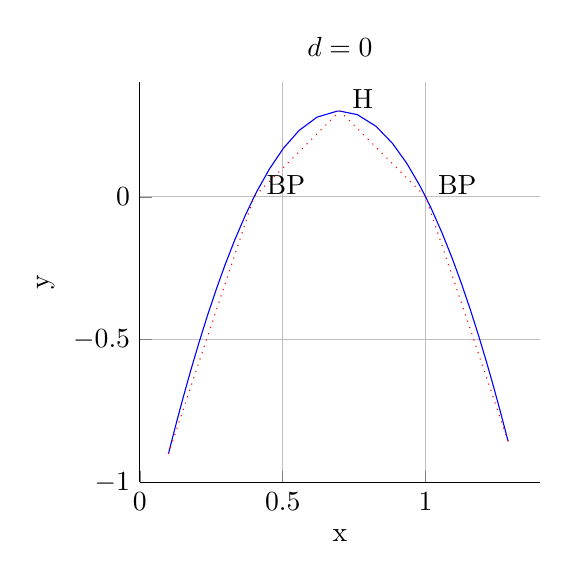
\begin{tikzpicture}

\begin{axis}[%
width=2in,
height=2in,
scale only axis,
xmin=0,
xmax=1.4,
xlabel={x},
xmajorgrids,
ymin=-1,
ymax=0.4,
ylabel={y},
ymajorgrids,
title={$d = 0$},
axis x line*=bottom,
axis y line*=left
]
\addplot [color=blue,solid,forget plot]
  table[row sep=crcr]{%
0.1	-0.9\\
0.10236115226321	-0.890573974413809\\
0.105443092647942	-0.878326386933239\\
0.10947092930252	-0.862415277794992\\
0.114743783525674	-0.841749463067742\\
0.121661927761337	-0.814916419312817\\
0.130766088868157	-0.780090818505233\\
0.142796224400937	-0.734920158015229\\
0.158783169468408	-0.676385523478996\\
0.180199591604542	-0.600641539603537\\
0.20753363910917	-0.508410388696859\\
0.236211998778287	-0.416997700257441\\
0.266438360478569	-0.326585650881704\\
0.298469829310147	-0.237421593247408\\
0.332637113130149	-0.149851635497837\\
0.369374395637926	-0.0643776341992891\\
0.4	8.47132627481197e-16\\
0.409263687297719	0.0182413215876043\\
0.453098471934554	0.0967987847964914\\
0.501960851083189	0.169268318321016\\
0.557241217341693	0.232066433246394\\
0.620237474529508	0.278793131768563\\
0.69022769581949	0.299681673570011\\
0.699999924534922	0.299999999999981\\
0.76141250523283	0.287428347336759\\
0.826654190368506	0.246529053540681\\
0.883959858523856	0.187195901507415\\
0.934411581210212	0.116837368648854\\
0.97947640696869	0.0396431264930012\\
1	6.20587407806507e-25\\
1.02033298033098	-0.0420440609590649\\
1.05784763879348	-0.126849775300215\\
1.09265294926701	-0.213921128560277\\
1.12521794369405	-0.302700998797998\\
1.15589771069024	-0.392809075375353\\
1.18496677409863	-0.483975906598774\\
1.21264154042604	-0.576004496567949\\
1.23909561413569	-0.668746933022548\\
1.264470443226	-0.762089601344311\\
1.28888288313087	-0.855943498105124\\
};
\addplot [color=red,dotted,forget plot]
  table[row sep=crcr]{%
0.1	-0.9\\
0.4	8.47132627481197e-16\\
0.699999924534922	0.299999999999981\\
1	6.20587407806507e-25\\
1.28888288313087	-0.855943498105124\\
};
\node[right, align=left, inner sep=0mm, text=black]
at (axis cs:0.442,0.0420000000000008,0) {BP};
\node[right, align=left, inner sep=0mm, text=black]
at (axis cs:0.741999924534922,0.341999999999981,0) {H};
\node[right, align=left, inner sep=0mm, text=black]
at (axis cs:1.042,0.042,0) {BP};
\addplot [color=blue,solid,forget plot]
  table[row sep=crcr]{%
1	0\\
1	0\\
1	0\\
1	0\\
1	0\\
1	0\\
1	0\\
1	0\\
1	0\\
1	0\\
1	0\\
1	0\\
1	0\\
1	0\\
1	0\\
1	0\\
1	0\\
1	0\\
1	0\\
1	0\\
1	0\\
1	0\\
1	0\\
1	0\\
1	0\\
1	0\\
1	0\\
1	0\\
1	0\\
1	0\\
1	0\\
1	0\\
1	0\\
1	0\\
1	0\\
1	0\\
1	0\\
1	0\\
1	0\\
1	0\\
};
\addplot [color=red,dotted,forget plot]
  table[row sep=crcr]{%
1	0\\
1	0\\
};
\end{axis}
\end{tikzpicture}%
\end{document}
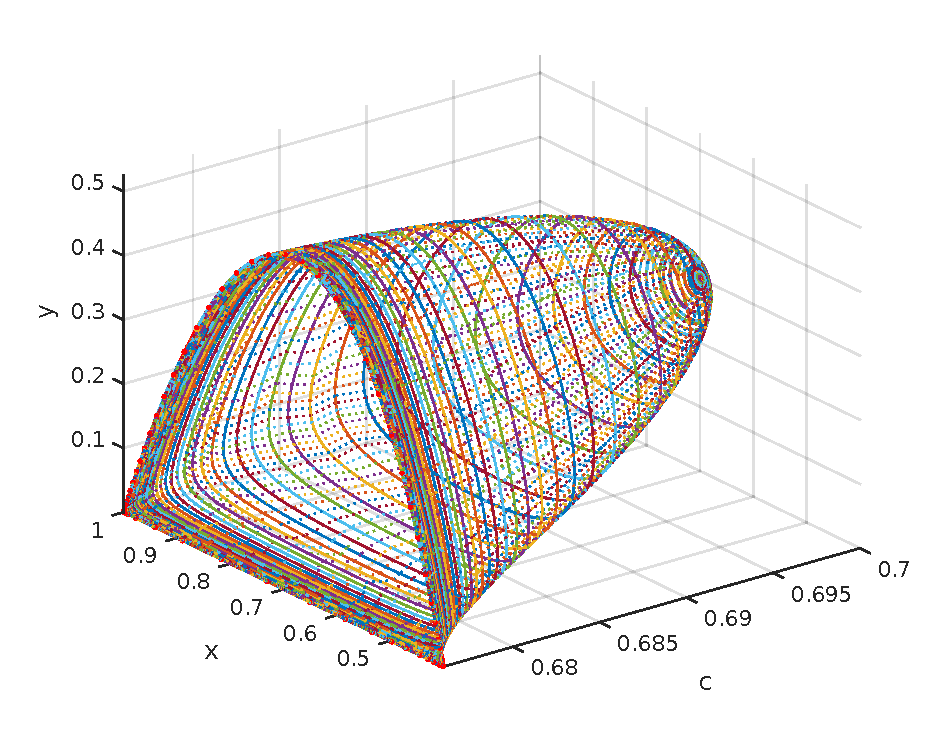
\includegraphics{./plots/hcCont.pdf}
\caption{Matcont continuation for $\mathbf{x}_2^*$ starting from $c=0.1$. Limit cycle continuation troughout its short lifetime.} 
\end{figure}

\end{document}